% Appendix C

\chapter{Fit Results for The Systematics (1)} % Main appendix title

\label{AppendixB} % For referencing this appendix elsewhere, use \ref{AppendixA}

Here all fits for first systematic on the tag and probe invariant mass presented for all $p_T-|\eta|$ bins. In the first systematic the fitting range reduced by 10 GeV as compare to the nominal.
%The first twenty fits belongs to CR1 ($Z\rightarrow e^+e^-$) shown in figure\ref{fig:fit_cr1_sys1}. The fits for CR2 ($Z\rightarrow e\gamma$) are given in figure\ref{fig:fit_cr2_sys1}.

\begin{figure}[H]
\begin{center}
\scalebox{0.35}{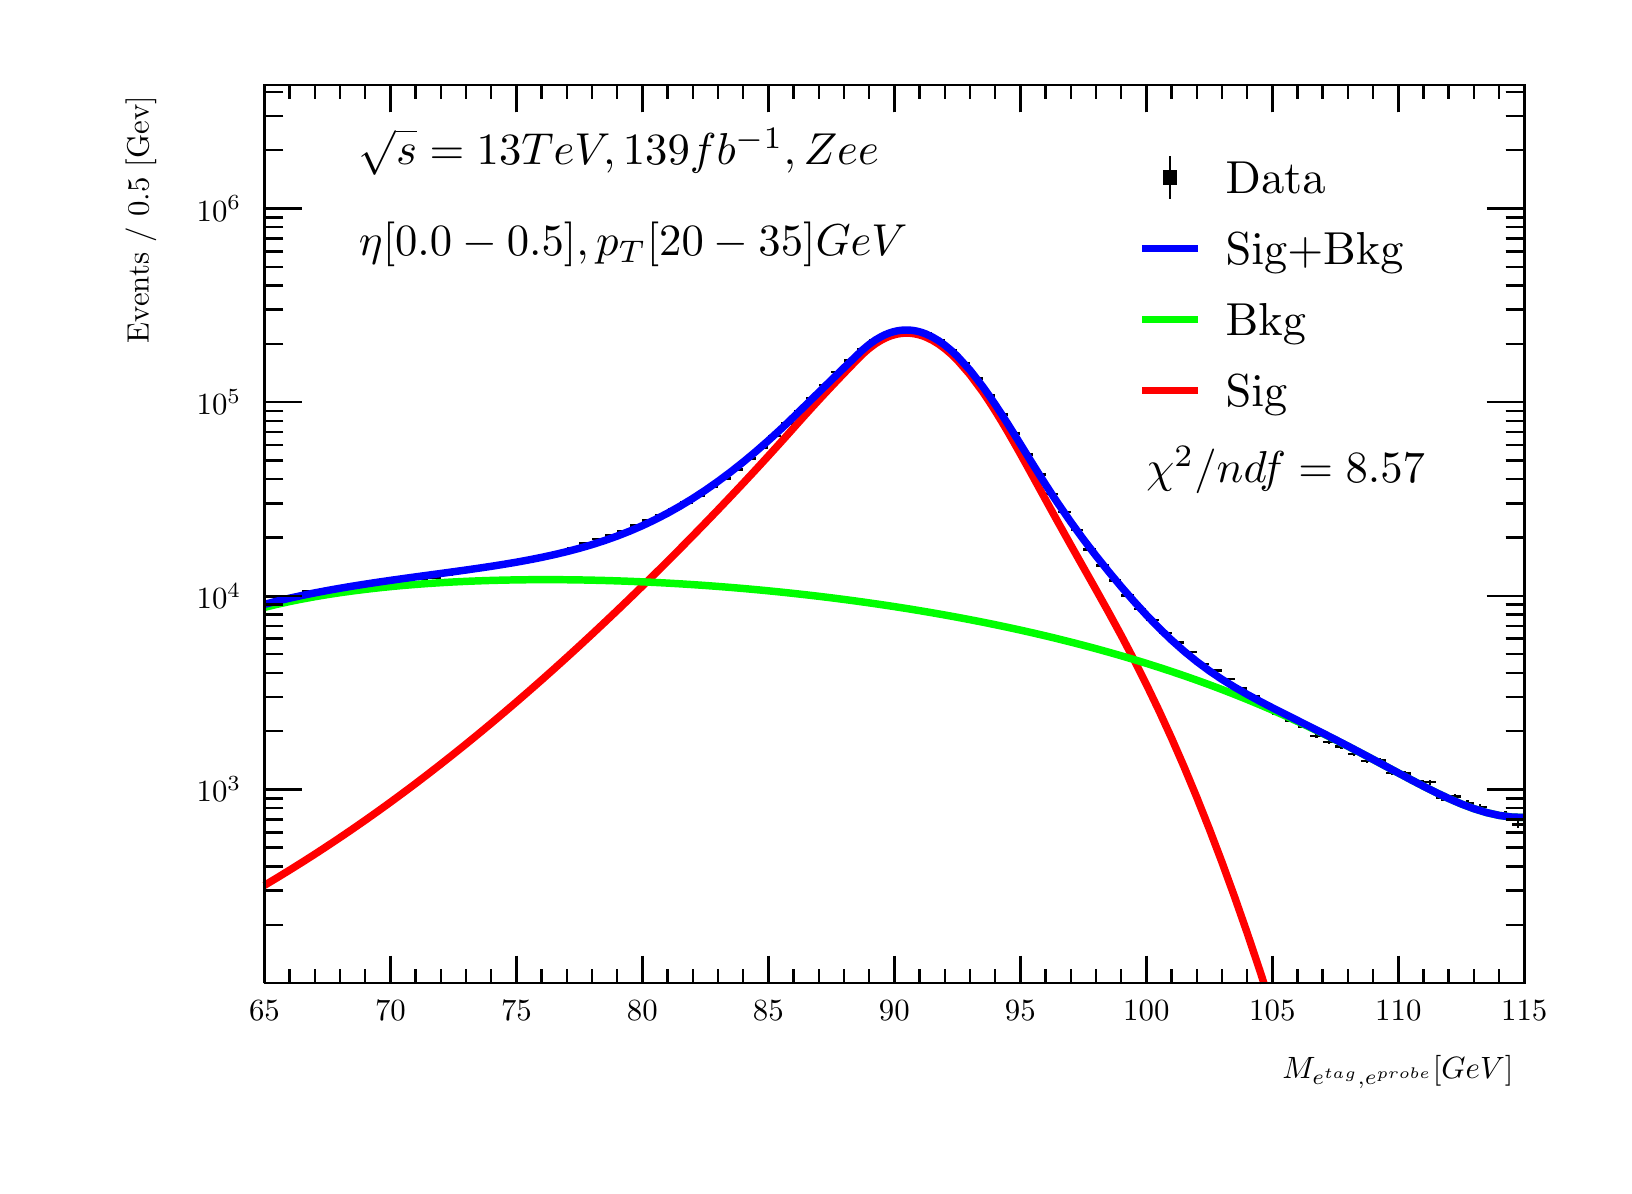
\begin{tikzpicture}
\pgfdeclareplotmark{cross} {
\pgfpathmoveto{\pgfpoint{-0.3\pgfplotmarksize}{\pgfplotmarksize}}
\pgfpathlineto{\pgfpoint{+0.3\pgfplotmarksize}{\pgfplotmarksize}}
\pgfpathlineto{\pgfpoint{+0.3\pgfplotmarksize}{0.3\pgfplotmarksize}}
\pgfpathlineto{\pgfpoint{+1\pgfplotmarksize}{0.3\pgfplotmarksize}}
\pgfpathlineto{\pgfpoint{+1\pgfplotmarksize}{-0.3\pgfplotmarksize}}
\pgfpathlineto{\pgfpoint{+0.3\pgfplotmarksize}{-0.3\pgfplotmarksize}}
\pgfpathlineto{\pgfpoint{+0.3\pgfplotmarksize}{-1.\pgfplotmarksize}}
\pgfpathlineto{\pgfpoint{-0.3\pgfplotmarksize}{-1.\pgfplotmarksize}}
\pgfpathlineto{\pgfpoint{-0.3\pgfplotmarksize}{-0.3\pgfplotmarksize}}
\pgfpathlineto{\pgfpoint{-1.\pgfplotmarksize}{-0.3\pgfplotmarksize}}
\pgfpathlineto{\pgfpoint{-1.\pgfplotmarksize}{0.3\pgfplotmarksize}}
\pgfpathlineto{\pgfpoint{-0.3\pgfplotmarksize}{0.3\pgfplotmarksize}}
\pgfpathclose
\pgfusepathqstroke
}
\pgfdeclareplotmark{cross*} {
\pgfpathmoveto{\pgfpoint{-0.3\pgfplotmarksize}{\pgfplotmarksize}}
\pgfpathlineto{\pgfpoint{+0.3\pgfplotmarksize}{\pgfplotmarksize}}
\pgfpathlineto{\pgfpoint{+0.3\pgfplotmarksize}{0.3\pgfplotmarksize}}
\pgfpathlineto{\pgfpoint{+1\pgfplotmarksize}{0.3\pgfplotmarksize}}
\pgfpathlineto{\pgfpoint{+1\pgfplotmarksize}{-0.3\pgfplotmarksize}}
\pgfpathlineto{\pgfpoint{+0.3\pgfplotmarksize}{-0.3\pgfplotmarksize}}
\pgfpathlineto{\pgfpoint{+0.3\pgfplotmarksize}{-1.\pgfplotmarksize}}
\pgfpathlineto{\pgfpoint{-0.3\pgfplotmarksize}{-1.\pgfplotmarksize}}
\pgfpathlineto{\pgfpoint{-0.3\pgfplotmarksize}{-0.3\pgfplotmarksize}}
\pgfpathlineto{\pgfpoint{-1.\pgfplotmarksize}{-0.3\pgfplotmarksize}}
\pgfpathlineto{\pgfpoint{-1.\pgfplotmarksize}{0.3\pgfplotmarksize}}
\pgfpathlineto{\pgfpoint{-0.3\pgfplotmarksize}{0.3\pgfplotmarksize}}
\pgfpathclose
\pgfusepathqfillstroke
}
\pgfdeclareplotmark{newstar} {
\pgfpathmoveto{\pgfqpoint{0pt}{\pgfplotmarksize}}
\pgfpathlineto{\pgfqpointpolar{44}{0.5\pgfplotmarksize}}
\pgfpathlineto{\pgfqpointpolar{18}{\pgfplotmarksize}}
\pgfpathlineto{\pgfqpointpolar{-20}{0.5\pgfplotmarksize}}
\pgfpathlineto{\pgfqpointpolar{-54}{\pgfplotmarksize}}
\pgfpathlineto{\pgfqpointpolar{-90}{0.5\pgfplotmarksize}}
\pgfpathlineto{\pgfqpointpolar{234}{\pgfplotmarksize}}
\pgfpathlineto{\pgfqpointpolar{198}{0.5\pgfplotmarksize}}
\pgfpathlineto{\pgfqpointpolar{162}{\pgfplotmarksize}}
\pgfpathlineto{\pgfqpointpolar{134}{0.5\pgfplotmarksize}}
\pgfpathclose
\pgfusepathqstroke
}
\pgfdeclareplotmark{newstar*} {
\pgfpathmoveto{\pgfqpoint{0pt}{\pgfplotmarksize}}
\pgfpathlineto{\pgfqpointpolar{44}{0.5\pgfplotmarksize}}
\pgfpathlineto{\pgfqpointpolar{18}{\pgfplotmarksize}}
\pgfpathlineto{\pgfqpointpolar{-20}{0.5\pgfplotmarksize}}
\pgfpathlineto{\pgfqpointpolar{-54}{\pgfplotmarksize}}
\pgfpathlineto{\pgfqpointpolar{-90}{0.5\pgfplotmarksize}}
\pgfpathlineto{\pgfqpointpolar{234}{\pgfplotmarksize}}
\pgfpathlineto{\pgfqpointpolar{198}{0.5\pgfplotmarksize}}
\pgfpathlineto{\pgfqpointpolar{162}{\pgfplotmarksize}}
\pgfpathlineto{\pgfqpointpolar{134}{0.5\pgfplotmarksize}}
\pgfpathclose
\pgfusepathqfillstroke
}
\definecolor{c}{rgb}{1,1,1};
\draw [color=c, fill=c] (0,0) rectangle (20,14.4361);
\draw [color=c, fill=c] (3,2.30977) rectangle (19,13.7143);
\definecolor{c}{rgb}{0,0,0};
\draw [c,line width=0.9] (3,2.30977) -- (3,13.7143) -- (19,13.7143) -- (19,2.30977) -- (3,2.30977);
\definecolor{c}{rgb}{1,1,1};
\draw [color=c, fill=c] (3,2.30977) rectangle (19,13.7143);
\definecolor{c}{rgb}{0,0,0};
\draw [c,line width=0.9] (3,2.30977) -- (3,13.7143) -- (19,13.7143) -- (19,2.30977) -- (3,2.30977);
\draw [c,line width=0.9] (3,2.30977) -- (19,2.30977);
\draw [c,line width=0.9] (3,2.65624) -- (3,2.30977);
\draw [c,line width=0.9] (3.32,2.48301) -- (3.32,2.30977);
\draw [c,line width=0.9] (3.64,2.48301) -- (3.64,2.30977);
\draw [c,line width=0.9] (3.96,2.48301) -- (3.96,2.30977);
\draw [c,line width=0.9] (4.28,2.48301) -- (4.28,2.30977);
\draw [c,line width=0.9] (4.6,2.65624) -- (4.6,2.30977);
\draw [c,line width=0.9] (4.92,2.48301) -- (4.92,2.30977);
\draw [c,line width=0.9] (5.24,2.48301) -- (5.24,2.30977);
\draw [c,line width=0.9] (5.56,2.48301) -- (5.56,2.30977);
\draw [c,line width=0.9] (5.88,2.48301) -- (5.88,2.30977);
\draw [c,line width=0.9] (6.2,2.65624) -- (6.2,2.30977);
\draw [c,line width=0.9] (6.52,2.48301) -- (6.52,2.30977);
\draw [c,line width=0.9] (6.84,2.48301) -- (6.84,2.30977);
\draw [c,line width=0.9] (7.16,2.48301) -- (7.16,2.30977);
\draw [c,line width=0.9] (7.48,2.48301) -- (7.48,2.30977);
\draw [c,line width=0.9] (7.8,2.65624) -- (7.8,2.30977);
\draw [c,line width=0.9] (8.12,2.48301) -- (8.12,2.30977);
\draw [c,line width=0.9] (8.44,2.48301) -- (8.44,2.30977);
\draw [c,line width=0.9] (8.76,2.48301) -- (8.76,2.30977);
\draw [c,line width=0.9] (9.08,2.48301) -- (9.08,2.30977);
\draw [c,line width=0.9] (9.4,2.65624) -- (9.4,2.30977);
\draw [c,line width=0.9] (9.72,2.48301) -- (9.72,2.30977);
\draw [c,line width=0.9] (10.04,2.48301) -- (10.04,2.30977);
\draw [c,line width=0.9] (10.36,2.48301) -- (10.36,2.30977);
\draw [c,line width=0.9] (10.68,2.48301) -- (10.68,2.30977);
\draw [c,line width=0.9] (11,2.65624) -- (11,2.30977);
\draw [c,line width=0.9] (11.32,2.48301) -- (11.32,2.30977);
\draw [c,line width=0.9] (11.64,2.48301) -- (11.64,2.30977);
\draw [c,line width=0.9] (11.96,2.48301) -- (11.96,2.30977);
\draw [c,line width=0.9] (12.28,2.48301) -- (12.28,2.30977);
\draw [c,line width=0.9] (12.6,2.65624) -- (12.6,2.30977);
\draw [c,line width=0.9] (12.92,2.48301) -- (12.92,2.30977);
\draw [c,line width=0.9] (13.24,2.48301) -- (13.24,2.30977);
\draw [c,line width=0.9] (13.56,2.48301) -- (13.56,2.30977);
\draw [c,line width=0.9] (13.88,2.48301) -- (13.88,2.30977);
\draw [c,line width=0.9] (14.2,2.65624) -- (14.2,2.30977);
\draw [c,line width=0.9] (14.52,2.48301) -- (14.52,2.30977);
\draw [c,line width=0.9] (14.84,2.48301) -- (14.84,2.30977);
\draw [c,line width=0.9] (15.16,2.48301) -- (15.16,2.30977);
\draw [c,line width=0.9] (15.48,2.48301) -- (15.48,2.30977);
\draw [c,line width=0.9] (15.8,2.65624) -- (15.8,2.30977);
\draw [c,line width=0.9] (16.12,2.48301) -- (16.12,2.30977);
\draw [c,line width=0.9] (16.44,2.48301) -- (16.44,2.30977);
\draw [c,line width=0.9] (16.76,2.48301) -- (16.76,2.30977);
\draw [c,line width=0.9] (17.08,2.48301) -- (17.08,2.30977);
\draw [c,line width=0.9] (17.4,2.65624) -- (17.4,2.30977);
\draw [c,line width=0.9] (17.72,2.48301) -- (17.72,2.30977);
\draw [c,line width=0.9] (18.04,2.48301) -- (18.04,2.30977);
\draw [c,line width=0.9] (18.36,2.48301) -- (18.36,2.30977);
\draw [c,line width=0.9] (18.68,2.48301) -- (18.68,2.30977);
\draw [c,line width=0.9] (19,2.65624) -- (19,2.30977);
\draw [c,line width=0.9] (19,2.65624) -- (19,2.30977);
\draw [anchor=base] (3,1.83338) node[scale=1.11327, color=c, rotate=0]{65};
\draw [anchor=base] (4.6,1.83338) node[scale=1.11327, color=c, rotate=0]{70};
\draw [anchor=base] (6.2,1.83338) node[scale=1.11327, color=c, rotate=0]{75};
\draw [anchor=base] (7.8,1.83338) node[scale=1.11327, color=c, rotate=0]{80};
\draw [anchor=base] (9.4,1.83338) node[scale=1.11327, color=c, rotate=0]{85};
\draw [anchor=base] (11,1.83338) node[scale=1.11327, color=c, rotate=0]{90};
\draw [anchor=base] (12.6,1.83338) node[scale=1.11327, color=c, rotate=0]{95};
\draw [anchor=base] (14.2,1.83338) node[scale=1.11327, color=c, rotate=0]{100};
\draw [anchor=base] (15.8,1.83338) node[scale=1.11327, color=c, rotate=0]{105};
\draw [anchor=base] (17.4,1.83338) node[scale=1.11327, color=c, rotate=0]{110};
\draw [anchor=base] (19,1.83338) node[scale=1.11327, color=c, rotate=0]{115};
\draw [anchor= east] (19,1.17798) node[scale=1.11327, color=c, rotate=0]{$M_{e^{tag}, e^{probe}}  [GeV]$};
\draw [c,line width=0.9] (3,13.7143) -- (19,13.7143);
\draw [c,line width=0.9] (3,13.3678) -- (3,13.7143);
\draw [c,line width=0.9] (3.32,13.5411) -- (3.32,13.7143);
\draw [c,line width=0.9] (3.64,13.5411) -- (3.64,13.7143);
\draw [c,line width=0.9] (3.96,13.5411) -- (3.96,13.7143);
\draw [c,line width=0.9] (4.28,13.5411) -- (4.28,13.7143);
\draw [c,line width=0.9] (4.6,13.3678) -- (4.6,13.7143);
\draw [c,line width=0.9] (4.92,13.5411) -- (4.92,13.7143);
\draw [c,line width=0.9] (5.24,13.5411) -- (5.24,13.7143);
\draw [c,line width=0.9] (5.56,13.5411) -- (5.56,13.7143);
\draw [c,line width=0.9] (5.88,13.5411) -- (5.88,13.7143);
\draw [c,line width=0.9] (6.2,13.3678) -- (6.2,13.7143);
\draw [c,line width=0.9] (6.52,13.5411) -- (6.52,13.7143);
\draw [c,line width=0.9] (6.84,13.5411) -- (6.84,13.7143);
\draw [c,line width=0.9] (7.16,13.5411) -- (7.16,13.7143);
\draw [c,line width=0.9] (7.48,13.5411) -- (7.48,13.7143);
\draw [c,line width=0.9] (7.8,13.3678) -- (7.8,13.7143);
\draw [c,line width=0.9] (8.12,13.5411) -- (8.12,13.7143);
\draw [c,line width=0.9] (8.44,13.5411) -- (8.44,13.7143);
\draw [c,line width=0.9] (8.76,13.5411) -- (8.76,13.7143);
\draw [c,line width=0.9] (9.08,13.5411) -- (9.08,13.7143);
\draw [c,line width=0.9] (9.4,13.3678) -- (9.4,13.7143);
\draw [c,line width=0.9] (9.72,13.5411) -- (9.72,13.7143);
\draw [c,line width=0.9] (10.04,13.5411) -- (10.04,13.7143);
\draw [c,line width=0.9] (10.36,13.5411) -- (10.36,13.7143);
\draw [c,line width=0.9] (10.68,13.5411) -- (10.68,13.7143);
\draw [c,line width=0.9] (11,13.3678) -- (11,13.7143);
\draw [c,line width=0.9] (11.32,13.5411) -- (11.32,13.7143);
\draw [c,line width=0.9] (11.64,13.5411) -- (11.64,13.7143);
\draw [c,line width=0.9] (11.96,13.5411) -- (11.96,13.7143);
\draw [c,line width=0.9] (12.28,13.5411) -- (12.28,13.7143);
\draw [c,line width=0.9] (12.6,13.3678) -- (12.6,13.7143);
\draw [c,line width=0.9] (12.92,13.5411) -- (12.92,13.7143);
\draw [c,line width=0.9] (13.24,13.5411) -- (13.24,13.7143);
\draw [c,line width=0.9] (13.56,13.5411) -- (13.56,13.7143);
\draw [c,line width=0.9] (13.88,13.5411) -- (13.88,13.7143);
\draw [c,line width=0.9] (14.2,13.3678) -- (14.2,13.7143);
\draw [c,line width=0.9] (14.52,13.5411) -- (14.52,13.7143);
\draw [c,line width=0.9] (14.84,13.5411) -- (14.84,13.7143);
\draw [c,line width=0.9] (15.16,13.5411) -- (15.16,13.7143);
\draw [c,line width=0.9] (15.48,13.5411) -- (15.48,13.7143);
\draw [c,line width=0.9] (15.8,13.3678) -- (15.8,13.7143);
\draw [c,line width=0.9] (16.12,13.5411) -- (16.12,13.7143);
\draw [c,line width=0.9] (16.44,13.5411) -- (16.44,13.7143);
\draw [c,line width=0.9] (16.76,13.5411) -- (16.76,13.7143);
\draw [c,line width=0.9] (17.08,13.5411) -- (17.08,13.7143);
\draw [c,line width=0.9] (17.4,13.3678) -- (17.4,13.7143);
\draw [c,line width=0.9] (17.72,13.5411) -- (17.72,13.7143);
\draw [c,line width=0.9] (18.04,13.5411) -- (18.04,13.7143);
\draw [c,line width=0.9] (18.36,13.5411) -- (18.36,13.7143);
\draw [c,line width=0.9] (18.68,13.5411) -- (18.68,13.7143);
\draw [c,line width=0.9] (19,13.3678) -- (19,13.7143);
\draw [c,line width=0.9] (19,13.3678) -- (19,13.7143);
\draw [c,line width=0.9] (3,2.30977) -- (3,13.7143);
\draw [c,line width=0.9] (3.237,3.05008) -- (3,3.05008);
\draw [c,line width=0.9] (3.237,3.48313) -- (3,3.48313);
\draw [c,line width=0.9] (3.237,3.79038) -- (3,3.79038);
\draw [c,line width=0.9] (3.237,4.02871) -- (3,4.02871);
\draw [c,line width=0.9] (3.237,4.22343) -- (3,4.22343);
\draw [c,line width=0.9] (3.237,4.38807) -- (3,4.38807);
\draw [c,line width=0.9] (3.237,4.53069) -- (3,4.53069);
\draw [c,line width=0.9] (3.237,4.65649) -- (3,4.65649);
\draw [c,line width=0.9] (3.474,4.76901) -- (3,4.76901);
\draw [anchor= east] (2.844,4.76901) node[scale=1.11327, color=c, rotate=0]{$10^{3}$};
\draw [c,line width=0.9] (3.237,5.50932) -- (3,5.50932);
\draw [c,line width=0.9] (3.237,5.94237) -- (3,5.94237);
\draw [c,line width=0.9] (3.237,6.24963) -- (3,6.24963);
\draw [c,line width=0.9] (3.237,6.48795) -- (3,6.48795);
\draw [c,line width=0.9] (3.237,6.68268) -- (3,6.68268);
\draw [c,line width=0.9] (3.237,6.84731) -- (3,6.84731);
\draw [c,line width=0.9] (3.237,6.98993) -- (3,6.98993);
\draw [c,line width=0.9] (3.237,7.11573) -- (3,7.11573);
\draw [c,line width=0.9] (3.474,7.22826) -- (3,7.22826);
\draw [anchor= east] (2.844,7.22826) node[scale=1.11327, color=c, rotate=0]{$10^{4}$};
\draw [c,line width=0.9] (3.237,7.96856) -- (3,7.96856);
\draw [c,line width=0.9] (3.237,8.40161) -- (3,8.40161);
\draw [c,line width=0.9] (3.237,8.70887) -- (3,8.70887);
\draw [c,line width=0.9] (3.237,8.94719) -- (3,8.94719);
\draw [c,line width=0.9] (3.237,9.14192) -- (3,9.14192);
\draw [c,line width=0.9] (3.237,9.30656) -- (3,9.30656);
\draw [c,line width=0.9] (3.237,9.44917) -- (3,9.44917);
\draw [c,line width=0.9] (3.237,9.57497) -- (3,9.57497);
\draw [c,line width=0.9] (3.474,9.6875) -- (3,9.6875);
\draw [anchor= east] (2.844,9.6875) node[scale=1.11327, color=c, rotate=0]{$10^{5}$};
\draw [c,line width=0.9] (3.237,10.4278) -- (3,10.4278);
\draw [c,line width=0.9] (3.237,10.8609) -- (3,10.8609);
\draw [c,line width=0.9] (3.237,11.1681) -- (3,11.1681);
\draw [c,line width=0.9] (3.237,11.4064) -- (3,11.4064);
\draw [c,line width=0.9] (3.237,11.6012) -- (3,11.6012);
\draw [c,line width=0.9] (3.237,11.7658) -- (3,11.7658);
\draw [c,line width=0.9] (3.237,11.9084) -- (3,11.9084);
\draw [c,line width=0.9] (3.237,12.0342) -- (3,12.0342);
\draw [c,line width=0.9] (3.474,12.1467) -- (3,12.1467);
\draw [anchor= east] (2.844,12.1467) node[scale=1.11327, color=c, rotate=0]{$10^{6}$};
\draw [c,line width=0.9] (3.237,12.887) -- (3,12.887);
\draw [c,line width=0.9] (3.237,13.3201) -- (3,13.3201);
\draw [c,line width=0.9] (3.237,13.6274) -- (3,13.6274);
\draw [anchor= east] (1.432,13.7143) node[scale=1.11327, color=c, rotate=90]{Events / 0.5 [Gev]};
\draw [c,line width=0.9] (19,2.30977) -- (19,13.7143);
\draw [c,line width=0.9] (18.763,3.05008) -- (19,3.05008);
\draw [c,line width=0.9] (18.763,3.48313) -- (19,3.48313);
\draw [c,line width=0.9] (18.763,3.79038) -- (19,3.79038);
\draw [c,line width=0.9] (18.763,4.02871) -- (19,4.02871);
\draw [c,line width=0.9] (18.763,4.22343) -- (19,4.22343);
\draw [c,line width=0.9] (18.763,4.38807) -- (19,4.38807);
\draw [c,line width=0.9] (18.763,4.53069) -- (19,4.53069);
\draw [c,line width=0.9] (18.763,4.65649) -- (19,4.65649);
\draw [c,line width=0.9] (18.526,4.76901) -- (19,4.76901);
\draw [c,line width=0.9] (18.763,5.50932) -- (19,5.50932);
\draw [c,line width=0.9] (18.763,5.94237) -- (19,5.94237);
\draw [c,line width=0.9] (18.763,6.24963) -- (19,6.24963);
\draw [c,line width=0.9] (18.763,6.48795) -- (19,6.48795);
\draw [c,line width=0.9] (18.763,6.68268) -- (19,6.68268);
\draw [c,line width=0.9] (18.763,6.84731) -- (19,6.84731);
\draw [c,line width=0.9] (18.763,6.98993) -- (19,6.98993);
\draw [c,line width=0.9] (18.763,7.11573) -- (19,7.11573);
\draw [c,line width=0.9] (18.526,7.22826) -- (19,7.22826);
\draw [c,line width=0.9] (18.763,7.96856) -- (19,7.96856);
\draw [c,line width=0.9] (18.763,8.40161) -- (19,8.40161);
\draw [c,line width=0.9] (18.763,8.70887) -- (19,8.70887);
\draw [c,line width=0.9] (18.763,8.94719) -- (19,8.94719);
\draw [c,line width=0.9] (18.763,9.14192) -- (19,9.14192);
\draw [c,line width=0.9] (18.763,9.30656) -- (19,9.30656);
\draw [c,line width=0.9] (18.763,9.44917) -- (19,9.44917);
\draw [c,line width=0.9] (18.763,9.57497) -- (19,9.57497);
\draw [c,line width=0.9] (18.526,9.6875) -- (19,9.6875);
\draw [c,line width=0.9] (18.763,10.4278) -- (19,10.4278);
\draw [c,line width=0.9] (18.763,10.8609) -- (19,10.8609);
\draw [c,line width=0.9] (18.763,11.1681) -- (19,11.1681);
\draw [c,line width=0.9] (18.763,11.4064) -- (19,11.4064);
\draw [c,line width=0.9] (18.763,11.6012) -- (19,11.6012);
\draw [c,line width=0.9] (18.763,11.7658) -- (19,11.7658);
\draw [c,line width=0.9] (18.763,11.9084) -- (19,11.9084);
\draw [c,line width=0.9] (18.763,12.0342) -- (19,12.0342);
\draw [c,line width=0.9] (18.526,12.1467) -- (19,12.1467);
\draw [c,line width=0.9] (18.763,12.887) -- (19,12.887);
\draw [c,line width=0.9] (18.763,13.3201) -- (19,13.3201);
\draw [c,line width=0.9] (18.763,13.6274) -- (19,13.6274);
\draw [c,line width=0.9] (3.08,7.21114) -- (3,7.21114);
\draw [c,line width=0.9] (3,7.21114) -- (3,7.21114);
\draw [c,line width=0.9] (3.08,7.21114) -- (3.16,7.21114);
\draw [c,line width=0.9] (3.16,7.21114) -- (3.16,7.21114);
\draw [c,line width=0.9] (3.08,7.21114) -- (3.08,7.22191);
\draw [c,line width=0.9] (3.08,7.22191) -- (3.08,7.22191);
\draw [c,line width=0.9] (3.08,7.21114) -- (3.08,7.20037);
\draw [c,line width=0.9] (3.08,7.20037) -- (3.08,7.20037);
\draw [c,line width=0.9] (3.24,7.21979) -- (3.16,7.21979);
\draw [c,line width=0.9] (3.16,7.21979) -- (3.16,7.21979);
\draw [c,line width=0.9] (3.24,7.21979) -- (3.32,7.21979);
\draw [c,line width=0.9] (3.32,7.21979) -- (3.32,7.21979);
\draw [c,line width=0.9] (3.24,7.21979) -- (3.24,7.23051);
\draw [c,line width=0.9] (3.24,7.23051) -- (3.24,7.23051);
\draw [c,line width=0.9] (3.24,7.21979) -- (3.24,7.20906);
\draw [c,line width=0.9] (3.24,7.20906) -- (3.24,7.20906);
\draw [c,line width=0.9] (3.4,7.23878) -- (3.32,7.23878);
\draw [c,line width=0.9] (3.32,7.23878) -- (3.32,7.23878);
\draw [c,line width=0.9] (3.4,7.23878) -- (3.48,7.23878);
\draw [c,line width=0.9] (3.48,7.23878) -- (3.48,7.23878);
\draw [c,line width=0.9] (3.4,7.23878) -- (3.4,7.24941);
\draw [c,line width=0.9] (3.4,7.24941) -- (3.4,7.24941);
\draw [c,line width=0.9] (3.4,7.23878) -- (3.4,7.22815);
\draw [c,line width=0.9] (3.4,7.22815) -- (3.4,7.22815);
\draw [c,line width=0.9] (3.56,7.28756) -- (3.48,7.28756);
\draw [c,line width=0.9] (3.48,7.28756) -- (3.48,7.28756);
\draw [c,line width=0.9] (3.56,7.28756) -- (3.64,7.28756);
\draw [c,line width=0.9] (3.64,7.28756) -- (3.64,7.28756);
\draw [c,line width=0.9] (3.56,7.28756) -- (3.56,7.29795);
\draw [c,line width=0.9] (3.56,7.29795) -- (3.56,7.29795);
\draw [c,line width=0.9] (3.56,7.28756) -- (3.56,7.27718);
\draw [c,line width=0.9] (3.56,7.27718) -- (3.56,7.27718);
\draw [c,line width=0.9] (3.72,7.27425) -- (3.64,7.27425);
\draw [c,line width=0.9] (3.64,7.27425) -- (3.64,7.27425);
\draw [c,line width=0.9] (3.72,7.27425) -- (3.8,7.27425);
\draw [c,line width=0.9] (3.8,7.27425) -- (3.8,7.27425);
\draw [c,line width=0.9] (3.72,7.27425) -- (3.72,7.2847);
\draw [c,line width=0.9] (3.72,7.2847) -- (3.72,7.2847);
\draw [c,line width=0.9] (3.72,7.27425) -- (3.72,7.26379);
\draw [c,line width=0.9] (3.72,7.26379) -- (3.72,7.26379);
\draw [c,line width=0.9] (3.88,7.30986) -- (3.8,7.30986);
\draw [c,line width=0.9] (3.8,7.30986) -- (3.8,7.30986);
\draw [c,line width=0.9] (3.88,7.30986) -- (3.96,7.30986);
\draw [c,line width=0.9] (3.96,7.30986) -- (3.96,7.30986);
\draw [c,line width=0.9] (3.88,7.30986) -- (3.88,7.32014);
\draw [c,line width=0.9] (3.88,7.32014) -- (3.88,7.32014);
\draw [c,line width=0.9] (3.88,7.30986) -- (3.88,7.29958);
\draw [c,line width=0.9] (3.88,7.29958) -- (3.88,7.29958);
\draw [c,line width=0.9] (4.04,7.31065) -- (3.96,7.31065);
\draw [c,line width=0.9] (3.96,7.31065) -- (3.96,7.31065);
\draw [c,line width=0.9] (4.04,7.31065) -- (4.12,7.31065);
\draw [c,line width=0.9] (4.12,7.31065) -- (4.12,7.31065);
\draw [c,line width=0.9] (4.04,7.31065) -- (4.04,7.32093);
\draw [c,line width=0.9] (4.04,7.32093) -- (4.04,7.32093);
\draw [c,line width=0.9] (4.04,7.31065) -- (4.04,7.30038);
\draw [c,line width=0.9] (4.04,7.30038) -- (4.04,7.30038);
\draw [c,line width=0.9] (4.2,7.34844) -- (4.12,7.34844);
\draw [c,line width=0.9] (4.12,7.34844) -- (4.12,7.34844);
\draw [c,line width=0.9] (4.2,7.34844) -- (4.28,7.34844);
\draw [c,line width=0.9] (4.28,7.34844) -- (4.28,7.34844);
\draw [c,line width=0.9] (4.2,7.34844) -- (4.2,7.35853);
\draw [c,line width=0.9] (4.2,7.35853) -- (4.2,7.35853);
\draw [c,line width=0.9] (4.2,7.34844) -- (4.2,7.33834);
\draw [c,line width=0.9] (4.2,7.33834) -- (4.2,7.33834);
\draw [c,line width=0.9] (4.36,7.35358) -- (4.28,7.35358);
\draw [c,line width=0.9] (4.28,7.35358) -- (4.28,7.35358);
\draw [c,line width=0.9] (4.36,7.35358) -- (4.44,7.35358);
\draw [c,line width=0.9] (4.44,7.35358) -- (4.44,7.35358);
\draw [c,line width=0.9] (4.36,7.35358) -- (4.36,7.36365);
\draw [c,line width=0.9] (4.36,7.36365) -- (4.36,7.36365);
\draw [c,line width=0.9] (4.36,7.35358) -- (4.36,7.34351);
\draw [c,line width=0.9] (4.36,7.34351) -- (4.36,7.34351);
\draw [c,line width=0.9] (4.52,7.38401) -- (4.44,7.38401);
\draw [c,line width=0.9] (4.44,7.38401) -- (4.44,7.38401);
\draw [c,line width=0.9] (4.52,7.38401) -- (4.6,7.38401);
\draw [c,line width=0.9] (4.6,7.38401) -- (4.6,7.38401);
\draw [c,line width=0.9] (4.52,7.38401) -- (4.52,7.39394);
\draw [c,line width=0.9] (4.52,7.39394) -- (4.52,7.39394);
\draw [c,line width=0.9] (4.52,7.38401) -- (4.52,7.37408);
\draw [c,line width=0.9] (4.52,7.37408) -- (4.52,7.37408);
\draw [c,line width=0.9] (4.68,7.39649) -- (4.6,7.39649);
\draw [c,line width=0.9] (4.6,7.39649) -- (4.6,7.39649);
\draw [c,line width=0.9] (4.68,7.39649) -- (4.76,7.39649);
\draw [c,line width=0.9] (4.76,7.39649) -- (4.76,7.39649);
\draw [c,line width=0.9] (4.68,7.39649) -- (4.68,7.40636);
\draw [c,line width=0.9] (4.68,7.40636) -- (4.68,7.40636);
\draw [c,line width=0.9] (4.68,7.39649) -- (4.68,7.38662);
\draw [c,line width=0.9] (4.68,7.38662) -- (4.68,7.38662);
\draw [c,line width=0.9] (4.84,7.39722) -- (4.76,7.39722);
\draw [c,line width=0.9] (4.76,7.39722) -- (4.76,7.39722);
\draw [c,line width=0.9] (4.84,7.39722) -- (4.92,7.39722);
\draw [c,line width=0.9] (4.92,7.39722) -- (4.92,7.39722);
\draw [c,line width=0.9] (4.84,7.39722) -- (4.84,7.40709);
\draw [c,line width=0.9] (4.84,7.40709) -- (4.84,7.40709);
\draw [c,line width=0.9] (4.84,7.39722) -- (4.84,7.38735);
\draw [c,line width=0.9] (4.84,7.38735) -- (4.84,7.38735);
\draw [c,line width=0.9] (5,7.44378) -- (4.92,7.44378);
\draw [c,line width=0.9] (4.92,7.44378) -- (4.92,7.44378);
\draw [c,line width=0.9] (5,7.44378) -- (5.08,7.44378);
\draw [c,line width=0.9] (5.08,7.44378) -- (5.08,7.44378);
\draw [c,line width=0.9] (5,7.44378) -- (5,7.45344);
\draw [c,line width=0.9] (5,7.45344) -- (5,7.45344);
\draw [c,line width=0.9] (5,7.44378) -- (5,7.43413);
\draw [c,line width=0.9] (5,7.43413) -- (5,7.43413);
\draw [c,line width=0.9] (5.16,7.45403) -- (5.08,7.45403);
\draw [c,line width=0.9] (5.08,7.45403) -- (5.08,7.45403);
\draw [c,line width=0.9] (5.16,7.45403) -- (5.24,7.45403);
\draw [c,line width=0.9] (5.24,7.45403) -- (5.24,7.45403);
\draw [c,line width=0.9] (5.16,7.45403) -- (5.16,7.46364);
\draw [c,line width=0.9] (5.16,7.46364) -- (5.16,7.46364);
\draw [c,line width=0.9] (5.16,7.45403) -- (5.16,7.44443);
\draw [c,line width=0.9] (5.16,7.44443) -- (5.16,7.44443);
\draw [c,line width=0.9] (5.32,7.5008) -- (5.24,7.5008);
\draw [c,line width=0.9] (5.24,7.5008) -- (5.24,7.5008);
\draw [c,line width=0.9] (5.32,7.5008) -- (5.4,7.5008);
\draw [c,line width=0.9] (5.4,7.5008) -- (5.4,7.5008);
\draw [c,line width=0.9] (5.32,7.5008) -- (5.32,7.5102);
\draw [c,line width=0.9] (5.32,7.5102) -- (5.32,7.5102);
\draw [c,line width=0.9] (5.32,7.5008) -- (5.32,7.4914);
\draw [c,line width=0.9] (5.32,7.4914) -- (5.32,7.4914);
\draw [c,line width=0.9] (5.48,7.52162) -- (5.4,7.52162);
\draw [c,line width=0.9] (5.4,7.52162) -- (5.4,7.52162);
\draw [c,line width=0.9] (5.48,7.52162) -- (5.56,7.52162);
\draw [c,line width=0.9] (5.56,7.52162) -- (5.56,7.52162);
\draw [c,line width=0.9] (5.48,7.52162) -- (5.48,7.53093);
\draw [c,line width=0.9] (5.48,7.53093) -- (5.48,7.53093);
\draw [c,line width=0.9] (5.48,7.52162) -- (5.48,7.51231);
\draw [c,line width=0.9] (5.48,7.51231) -- (5.48,7.51231);
\draw [c,line width=0.9] (5.64,7.54941) -- (5.56,7.54941);
\draw [c,line width=0.9] (5.56,7.54941) -- (5.56,7.54941);
\draw [c,line width=0.9] (5.64,7.54941) -- (5.72,7.54941);
\draw [c,line width=0.9] (5.72,7.54941) -- (5.72,7.54941);
\draw [c,line width=0.9] (5.64,7.54941) -- (5.64,7.5586);
\draw [c,line width=0.9] (5.64,7.5586) -- (5.64,7.5586);
\draw [c,line width=0.9] (5.64,7.54941) -- (5.64,7.54022);
\draw [c,line width=0.9] (5.64,7.54022) -- (5.64,7.54022);
\draw [c,line width=0.9] (5.8,7.58211) -- (5.72,7.58211);
\draw [c,line width=0.9] (5.72,7.58211) -- (5.72,7.58211);
\draw [c,line width=0.9] (5.8,7.58211) -- (5.88,7.58211);
\draw [c,line width=0.9] (5.88,7.58211) -- (5.88,7.58211);
\draw [c,line width=0.9] (5.8,7.58211) -- (5.8,7.59116);
\draw [c,line width=0.9] (5.8,7.59116) -- (5.8,7.59116);
\draw [c,line width=0.9] (5.8,7.58211) -- (5.8,7.57306);
\draw [c,line width=0.9] (5.8,7.57306) -- (5.8,7.57306);
\draw [c,line width=0.9] (5.96,7.61094) -- (5.88,7.61094);
\draw [c,line width=0.9] (5.88,7.61094) -- (5.88,7.61094);
\draw [c,line width=0.9] (5.96,7.61094) -- (6.04,7.61094);
\draw [c,line width=0.9] (6.04,7.61094) -- (6.04,7.61094);
\draw [c,line width=0.9] (5.96,7.61094) -- (5.96,7.61987);
\draw [c,line width=0.9] (5.96,7.61987) -- (5.96,7.61987);
\draw [c,line width=0.9] (5.96,7.61094) -- (5.96,7.60201);
\draw [c,line width=0.9] (5.96,7.60201) -- (5.96,7.60201);
\draw [c,line width=0.9] (6.12,7.6331) -- (6.04,7.6331);
\draw [c,line width=0.9] (6.04,7.6331) -- (6.04,7.6331);
\draw [c,line width=0.9] (6.12,7.6331) -- (6.2,7.6331);
\draw [c,line width=0.9] (6.2,7.6331) -- (6.2,7.6331);
\draw [c,line width=0.9] (6.12,7.6331) -- (6.12,7.64194);
\draw [c,line width=0.9] (6.12,7.64194) -- (6.12,7.64194);
\draw [c,line width=0.9] (6.12,7.6331) -- (6.12,7.62426);
\draw [c,line width=0.9] (6.12,7.62426) -- (6.12,7.62426);
\draw [c,line width=0.9] (6.28,7.66734) -- (6.2,7.66734);
\draw [c,line width=0.9] (6.2,7.66734) -- (6.2,7.66734);
\draw [c,line width=0.9] (6.28,7.66734) -- (6.36,7.66734);
\draw [c,line width=0.9] (6.36,7.66734) -- (6.36,7.66734);
\draw [c,line width=0.9] (6.28,7.66734) -- (6.28,7.67604);
\draw [c,line width=0.9] (6.28,7.67604) -- (6.28,7.67604);
\draw [c,line width=0.9] (6.28,7.66734) -- (6.28,7.65865);
\draw [c,line width=0.9] (6.28,7.65865) -- (6.28,7.65865);
\draw [c,line width=0.9] (6.44,7.71829) -- (6.36,7.71829);
\draw [c,line width=0.9] (6.36,7.71829) -- (6.36,7.71829);
\draw [c,line width=0.9] (6.44,7.71829) -- (6.52,7.71829);
\draw [c,line width=0.9] (6.52,7.71829) -- (6.52,7.71829);
\draw [c,line width=0.9] (6.44,7.71829) -- (6.44,7.72678);
\draw [c,line width=0.9] (6.44,7.72678) -- (6.44,7.72678);
\draw [c,line width=0.9] (6.44,7.71829) -- (6.44,7.7098);
\draw [c,line width=0.9] (6.44,7.7098) -- (6.44,7.7098);
\draw [c,line width=0.9] (6.6,7.73961) -- (6.52,7.73961);
\draw [c,line width=0.9] (6.52,7.73961) -- (6.52,7.73961);
\draw [c,line width=0.9] (6.6,7.73961) -- (6.68,7.73961);
\draw [c,line width=0.9] (6.68,7.73961) -- (6.68,7.73961);
\draw [c,line width=0.9] (6.6,7.73961) -- (6.6,7.74801);
\draw [c,line width=0.9] (6.6,7.74801) -- (6.6,7.74801);
\draw [c,line width=0.9] (6.6,7.73961) -- (6.6,7.7312);
\draw [c,line width=0.9] (6.6,7.7312) -- (6.6,7.7312);
\draw [c,line width=0.9] (6.76,7.78235) -- (6.68,7.78235);
\draw [c,line width=0.9] (6.68,7.78235) -- (6.68,7.78235);
\draw [c,line width=0.9] (6.76,7.78235) -- (6.84,7.78235);
\draw [c,line width=0.9] (6.84,7.78235) -- (6.84,7.78235);
\draw [c,line width=0.9] (6.76,7.78235) -- (6.76,7.79059);
\draw [c,line width=0.9] (6.76,7.79059) -- (6.76,7.79059);
\draw [c,line width=0.9] (6.76,7.78235) -- (6.76,7.77411);
\draw [c,line width=0.9] (6.76,7.77411) -- (6.76,7.77411);
\draw [c,line width=0.9] (6.92,7.83343) -- (6.84,7.83343);
\draw [c,line width=0.9] (6.84,7.83343) -- (6.84,7.83343);
\draw [c,line width=0.9] (6.92,7.83343) -- (7,7.83343);
\draw [c,line width=0.9] (7,7.83343) -- (7,7.83343);
\draw [c,line width=0.9] (6.92,7.83343) -- (6.92,7.84147);
\draw [c,line width=0.9] (6.92,7.84147) -- (6.92,7.84147);
\draw [c,line width=0.9] (6.92,7.83343) -- (6.92,7.82538);
\draw [c,line width=0.9] (6.92,7.82538) -- (6.92,7.82538);
\draw [c,line width=0.9] (7.08,7.89025) -- (7,7.89025);
\draw [c,line width=0.9] (7,7.89025) -- (7,7.89025);
\draw [c,line width=0.9] (7.08,7.89025) -- (7.16,7.89025);
\draw [c,line width=0.9] (7.16,7.89025) -- (7.16,7.89025);
\draw [c,line width=0.9] (7.08,7.89025) -- (7.08,7.89808);
\draw [c,line width=0.9] (7.08,7.89808) -- (7.08,7.89808);
\draw [c,line width=0.9] (7.08,7.89025) -- (7.08,7.88242);
\draw [c,line width=0.9] (7.08,7.88242) -- (7.08,7.88242);
\draw [c,line width=0.9] (7.24,7.94824) -- (7.16,7.94824);
\draw [c,line width=0.9] (7.16,7.94824) -- (7.16,7.94824);
\draw [c,line width=0.9] (7.24,7.94824) -- (7.32,7.94824);
\draw [c,line width=0.9] (7.32,7.94824) -- (7.32,7.94824);
\draw [c,line width=0.9] (7.24,7.94824) -- (7.24,7.95586);
\draw [c,line width=0.9] (7.24,7.95586) -- (7.24,7.95586);
\draw [c,line width=0.9] (7.24,7.94824) -- (7.24,7.94061);
\draw [c,line width=0.9] (7.24,7.94061) -- (7.24,7.94061);
\draw [c,line width=0.9] (7.4,7.99107) -- (7.32,7.99107);
\draw [c,line width=0.9] (7.32,7.99107) -- (7.32,7.99107);
\draw [c,line width=0.9] (7.4,7.99107) -- (7.48,7.99107);
\draw [c,line width=0.9] (7.48,7.99107) -- (7.48,7.99107);
\draw [c,line width=0.9] (7.4,7.99107) -- (7.4,7.99855);
\draw [c,line width=0.9] (7.4,7.99855) -- (7.4,7.99855);
\draw [c,line width=0.9] (7.4,7.99107) -- (7.4,7.9836);
\draw [c,line width=0.9] (7.4,7.9836) -- (7.4,7.9836);
\draw [c,line width=0.9] (7.56,8.04883) -- (7.48,8.04883);
\draw [c,line width=0.9] (7.48,8.04883) -- (7.48,8.04883);
\draw [c,line width=0.9] (7.56,8.04883) -- (7.64,8.04883);
\draw [c,line width=0.9] (7.64,8.04883) -- (7.64,8.04883);
\draw [c,line width=0.9] (7.56,8.04883) -- (7.56,8.0561);
\draw [c,line width=0.9] (7.56,8.0561) -- (7.56,8.0561);
\draw [c,line width=0.9] (7.56,8.04883) -- (7.56,8.04156);
\draw [c,line width=0.9] (7.56,8.04156) -- (7.56,8.04156);
\draw [c,line width=0.9] (7.72,8.11821) -- (7.64,8.11821);
\draw [c,line width=0.9] (7.64,8.11821) -- (7.64,8.11821);
\draw [c,line width=0.9] (7.72,8.11821) -- (7.8,8.11821);
\draw [c,line width=0.9] (7.8,8.11821) -- (7.8,8.11821);
\draw [c,line width=0.9] (7.72,8.11821) -- (7.72,8.12525);
\draw [c,line width=0.9] (7.72,8.12525) -- (7.72,8.12525);
\draw [c,line width=0.9] (7.72,8.11821) -- (7.72,8.11116);
\draw [c,line width=0.9] (7.72,8.11116) -- (7.72,8.11116);
\draw [c,line width=0.9] (7.88,8.18278) -- (7.8,8.18278);
\draw [c,line width=0.9] (7.8,8.18278) -- (7.8,8.18278);
\draw [c,line width=0.9] (7.88,8.18278) -- (7.96,8.18278);
\draw [c,line width=0.9] (7.96,8.18278) -- (7.96,8.18278);
\draw [c,line width=0.9] (7.88,8.18278) -- (7.88,8.18961);
\draw [c,line width=0.9] (7.88,8.18961) -- (7.88,8.18961);
\draw [c,line width=0.9] (7.88,8.18278) -- (7.88,8.17595);
\draw [c,line width=0.9] (7.88,8.17595) -- (7.88,8.17595);
\draw [c,line width=0.9] (8.04,8.25148) -- (7.96,8.25148);
\draw [c,line width=0.9] (7.96,8.25148) -- (7.96,8.25148);
\draw [c,line width=0.9] (8.04,8.25148) -- (8.12,8.25148);
\draw [c,line width=0.9] (8.12,8.25148) -- (8.12,8.25148);
\draw [c,line width=0.9] (8.04,8.25148) -- (8.04,8.2581);
\draw [c,line width=0.9] (8.04,8.2581) -- (8.04,8.2581);
\draw [c,line width=0.9] (8.04,8.25148) -- (8.04,8.24487);
\draw [c,line width=0.9] (8.04,8.24487) -- (8.04,8.24487);
\draw [c,line width=0.9] (8.2,8.3296) -- (8.12,8.3296);
\draw [c,line width=0.9] (8.12,8.3296) -- (8.12,8.3296);
\draw [c,line width=0.9] (8.2,8.3296) -- (8.28,8.3296);
\draw [c,line width=0.9] (8.28,8.3296) -- (8.28,8.3296);
\draw [c,line width=0.9] (8.2,8.3296) -- (8.2,8.33598);
\draw [c,line width=0.9] (8.2,8.33598) -- (8.2,8.33598);
\draw [c,line width=0.9] (8.2,8.3296) -- (8.2,8.32323);
\draw [c,line width=0.9] (8.2,8.32323) -- (8.2,8.32323);
\draw [c,line width=0.9] (8.36,8.41062) -- (8.28,8.41062);
\draw [c,line width=0.9] (8.28,8.41062) -- (8.28,8.41062);
\draw [c,line width=0.9] (8.36,8.41062) -- (8.44,8.41062);
\draw [c,line width=0.9] (8.44,8.41062) -- (8.44,8.41062);
\draw [c,line width=0.9] (8.36,8.41062) -- (8.36,8.41676);
\draw [c,line width=0.9] (8.36,8.41676) -- (8.36,8.41676);
\draw [c,line width=0.9] (8.36,8.41062) -- (8.36,8.40448);
\draw [c,line width=0.9] (8.36,8.40448) -- (8.36,8.40448);
\draw [c,line width=0.9] (8.52,8.50328) -- (8.44,8.50328);
\draw [c,line width=0.9] (8.44,8.50328) -- (8.44,8.50328);
\draw [c,line width=0.9] (8.52,8.50328) -- (8.6,8.50328);
\draw [c,line width=0.9] (8.6,8.50328) -- (8.6,8.50328);
\draw [c,line width=0.9] (8.52,8.50328) -- (8.52,8.50916);
\draw [c,line width=0.9] (8.52,8.50916) -- (8.52,8.50916);
\draw [c,line width=0.9] (8.52,8.50328) -- (8.52,8.4974);
\draw [c,line width=0.9] (8.52,8.4974) -- (8.52,8.4974);
\draw [c,line width=0.9] (8.68,8.60958) -- (8.6,8.60958);
\draw [c,line width=0.9] (8.6,8.60958) -- (8.6,8.60958);
\draw [c,line width=0.9] (8.68,8.60958) -- (8.76,8.60958);
\draw [c,line width=0.9] (8.76,8.60958) -- (8.76,8.60958);
\draw [c,line width=0.9] (8.68,8.60958) -- (8.68,8.61517);
\draw [c,line width=0.9] (8.68,8.61517) -- (8.68,8.61517);
\draw [c,line width=0.9] (8.68,8.60958) -- (8.68,8.60398);
\draw [c,line width=0.9] (8.68,8.60398) -- (8.68,8.60398);
\draw [c,line width=0.9] (8.84,8.71741) -- (8.76,8.71741);
\draw [c,line width=0.9] (8.76,8.71741) -- (8.76,8.71741);
\draw [c,line width=0.9] (8.84,8.71741) -- (8.92,8.71741);
\draw [c,line width=0.9] (8.92,8.71741) -- (8.92,8.71741);
\draw [c,line width=0.9] (8.84,8.71741) -- (8.84,8.72272);
\draw [c,line width=0.9] (8.84,8.72272) -- (8.84,8.72272);
\draw [c,line width=0.9] (8.84,8.71741) -- (8.84,8.71209);
\draw [c,line width=0.9] (8.84,8.71209) -- (8.84,8.71209);
\draw [c,line width=0.9] (9,8.83352) -- (8.92,8.83352);
\draw [c,line width=0.9] (8.92,8.83352) -- (8.92,8.83352);
\draw [c,line width=0.9] (9,8.83352) -- (9.08,8.83352);
\draw [c,line width=0.9] (9.08,8.83352) -- (9.08,8.83352);
\draw [c,line width=0.9] (9,8.83352) -- (9,8.83856);
\draw [c,line width=0.9] (9,8.83856) -- (9,8.83856);
\draw [c,line width=0.9] (9,8.83352) -- (9,8.82849);
\draw [c,line width=0.9] (9,8.82849) -- (9,8.82849);
\draw [c,line width=0.9] (9.16,8.97016) -- (9.08,8.97016);
\draw [c,line width=0.9] (9.08,8.97016) -- (9.08,8.97016);
\draw [c,line width=0.9] (9.16,8.97016) -- (9.24,8.97016);
\draw [c,line width=0.9] (9.24,8.97016) -- (9.24,8.97016);
\draw [c,line width=0.9] (9.16,8.97016) -- (9.16,8.97489);
\draw [c,line width=0.9] (9.16,8.97489) -- (9.16,8.97489);
\draw [c,line width=0.9] (9.16,8.97016) -- (9.16,8.96544);
\draw [c,line width=0.9] (9.16,8.96544) -- (9.16,8.96544);
\draw [c,line width=0.9] (9.32,9.10987) -- (9.24,9.10987);
\draw [c,line width=0.9] (9.24,9.10987) -- (9.24,9.10987);
\draw [c,line width=0.9] (9.32,9.10987) -- (9.4,9.10987);
\draw [c,line width=0.9] (9.4,9.10987) -- (9.4,9.10987);
\draw [c,line width=0.9] (9.32,9.10987) -- (9.32,9.11429);
\draw [c,line width=0.9] (9.32,9.11429) -- (9.32,9.11429);
\draw [c,line width=0.9] (9.32,9.10987) -- (9.32,9.10544);
\draw [c,line width=0.9] (9.32,9.10544) -- (9.32,9.10544);
\draw [c,line width=0.9] (9.48,9.25465) -- (9.4,9.25465);
\draw [c,line width=0.9] (9.4,9.25465) -- (9.4,9.25465);
\draw [c,line width=0.9] (9.48,9.25465) -- (9.56,9.25465);
\draw [c,line width=0.9] (9.56,9.25465) -- (9.56,9.25465);
\draw [c,line width=0.9] (9.48,9.25465) -- (9.48,9.25878);
\draw [c,line width=0.9] (9.48,9.25878) -- (9.48,9.25878);
\draw [c,line width=0.9] (9.48,9.25465) -- (9.48,9.25051);
\draw [c,line width=0.9] (9.48,9.25051) -- (9.48,9.25051);
\draw [c,line width=0.9] (9.64,9.41402) -- (9.56,9.41402);
\draw [c,line width=0.9] (9.56,9.41402) -- (9.56,9.41402);
\draw [c,line width=0.9] (9.64,9.41402) -- (9.72,9.41402);
\draw [c,line width=0.9] (9.72,9.41402) -- (9.72,9.41402);
\draw [c,line width=0.9] (9.64,9.41402) -- (9.64,9.41786);
\draw [c,line width=0.9] (9.64,9.41786) -- (9.64,9.41786);
\draw [c,line width=0.9] (9.64,9.41402) -- (9.64,9.41018);
\draw [c,line width=0.9] (9.64,9.41018) -- (9.64,9.41018);
\draw [c,line width=0.9] (9.8,9.57757) -- (9.72,9.57757);
\draw [c,line width=0.9] (9.72,9.57757) -- (9.72,9.57757);
\draw [c,line width=0.9] (9.8,9.57757) -- (9.88,9.57757);
\draw [c,line width=0.9] (9.88,9.57757) -- (9.88,9.57757);
\draw [c,line width=0.9] (9.8,9.57757) -- (9.8,9.58112);
\draw [c,line width=0.9] (9.8,9.58112) -- (9.8,9.58112);
\draw [c,line width=0.9] (9.8,9.57757) -- (9.8,9.57401);
\draw [c,line width=0.9] (9.8,9.57401) -- (9.8,9.57401);
\draw [c,line width=0.9] (9.96,9.74181) -- (9.88,9.74181);
\draw [c,line width=0.9] (9.88,9.74181) -- (9.88,9.74181);
\draw [c,line width=0.9] (9.96,9.74181) -- (10.04,9.74181);
\draw [c,line width=0.9] (10.04,9.74181) -- (10.04,9.74181);
\draw [c,line width=0.9] (9.96,9.74181) -- (9.96,9.74511);
\draw [c,line width=0.9] (9.96,9.74511) -- (9.96,9.74511);
\draw [c,line width=0.9] (9.96,9.74181) -- (9.96,9.73852);
\draw [c,line width=0.9] (9.96,9.73852) -- (9.96,9.73852);
\draw [c,line width=0.9] (10.12,9.90267) -- (10.04,9.90267);
\draw [c,line width=0.9] (10.04,9.90267) -- (10.04,9.90267);
\draw [c,line width=0.9] (10.12,9.90267) -- (10.2,9.90267);
\draw [c,line width=0.9] (10.2,9.90267) -- (10.2,9.90267);
\draw [c,line width=0.9] (10.12,9.90267) -- (10.12,9.90572);
\draw [c,line width=0.9] (10.12,9.90572) -- (10.12,9.90572);
\draw [c,line width=0.9] (10.12,9.90267) -- (10.12,9.89961);
\draw [c,line width=0.9] (10.12,9.89961) -- (10.12,9.89961);
\draw [c,line width=0.9] (10.28,10.0673) -- (10.2,10.0673);
\draw [c,line width=0.9] (10.2,10.0673) -- (10.2,10.0673);
\draw [c,line width=0.9] (10.28,10.0673) -- (10.36,10.0673);
\draw [c,line width=0.9] (10.36,10.0673) -- (10.36,10.0673);
\draw [c,line width=0.9] (10.28,10.0673) -- (10.28,10.0701);
\draw [c,line width=0.9] (10.28,10.0701) -- (10.28,10.0701);
\draw [c,line width=0.9] (10.28,10.0673) -- (10.28,10.0645);
\draw [c,line width=0.9] (10.28,10.0645) -- (10.28,10.0645);
\draw [c,line width=0.9] (10.44,10.217) -- (10.36,10.217);
\draw [c,line width=0.9] (10.36,10.217) -- (10.36,10.217);
\draw [c,line width=0.9] (10.44,10.217) -- (10.52,10.217);
\draw [c,line width=0.9] (10.52,10.217) -- (10.52,10.217);
\draw [c,line width=0.9] (10.44,10.217) -- (10.44,10.2197);
\draw [c,line width=0.9] (10.44,10.2197) -- (10.44,10.2197);
\draw [c,line width=0.9] (10.44,10.217) -- (10.44,10.2144);
\draw [c,line width=0.9] (10.44,10.2144) -- (10.44,10.2144);
\draw [c,line width=0.9] (10.6,10.3535) -- (10.52,10.3535);
\draw [c,line width=0.9] (10.52,10.3535) -- (10.52,10.3535);
\draw [c,line width=0.9] (10.6,10.3535) -- (10.68,10.3535);
\draw [c,line width=0.9] (10.68,10.3535) -- (10.68,10.3535);
\draw [c,line width=0.9] (10.6,10.3535) -- (10.6,10.356);
\draw [c,line width=0.9] (10.6,10.356) -- (10.6,10.356);
\draw [c,line width=0.9] (10.6,10.3535) -- (10.6,10.351);
\draw [c,line width=0.9] (10.6,10.351) -- (10.6,10.351);
\draw [c,line width=0.9] (10.76,10.4675) -- (10.68,10.4675);
\draw [c,line width=0.9] (10.68,10.4675) -- (10.68,10.4675);
\draw [c,line width=0.9] (10.76,10.4675) -- (10.84,10.4675);
\draw [c,line width=0.9] (10.84,10.4675) -- (10.84,10.4675);
\draw [c,line width=0.9] (10.76,10.4675) -- (10.76,10.4698);
\draw [c,line width=0.9] (10.76,10.4698) -- (10.76,10.4698);
\draw [c,line width=0.9] (10.76,10.4675) -- (10.76,10.4652);
\draw [c,line width=0.9] (10.76,10.4652) -- (10.76,10.4652);
\draw [c,line width=0.9] (10.92,10.546) -- (10.84,10.546);
\draw [c,line width=0.9] (10.84,10.546) -- (10.84,10.546);
\draw [c,line width=0.9] (10.92,10.546) -- (11,10.546);
\draw [c,line width=0.9] (11,10.546) -- (11,10.546);
\draw [c,line width=0.9] (10.92,10.546) -- (10.92,10.5482);
\draw [c,line width=0.9] (10.92,10.5482) -- (10.92,10.5482);
\draw [c,line width=0.9] (10.92,10.546) -- (10.92,10.5437);
\draw [c,line width=0.9] (10.92,10.5437) -- (10.92,10.5437);
\draw [c,line width=0.9] (11.08,10.5926) -- (11,10.5926);
\draw [c,line width=0.9] (11,10.5926) -- (11,10.5926);
\draw [c,line width=0.9] (11.08,10.5926) -- (11.16,10.5926);
\draw [c,line width=0.9] (11.16,10.5926) -- (11.16,10.5926);
\draw [c,line width=0.9] (11.08,10.5926) -- (11.08,10.5948);
\draw [c,line width=0.9] (11.08,10.5948) -- (11.08,10.5948);
\draw [c,line width=0.9] (11.08,10.5926) -- (11.08,10.5904);
\draw [c,line width=0.9] (11.08,10.5904) -- (11.08,10.5904);
\draw [c,line width=0.9] (11.24,10.6009) -- (11.16,10.6009);
\draw [c,line width=0.9] (11.16,10.6009) -- (11.16,10.6009);
\draw [c,line width=0.9] (11.24,10.6009) -- (11.32,10.6009);
\draw [c,line width=0.9] (11.32,10.6009) -- (11.32,10.6009);
\draw [c,line width=0.9] (11.24,10.6009) -- (11.24,10.6031);
\draw [c,line width=0.9] (11.24,10.6031) -- (11.24,10.6031);
\draw [c,line width=0.9] (11.24,10.6009) -- (11.24,10.5987);
\draw [c,line width=0.9] (11.24,10.5987) -- (11.24,10.5987);
\draw [c,line width=0.9] (11.4,10.5575) -- (11.32,10.5575);
\draw [c,line width=0.9] (11.32,10.5575) -- (11.32,10.5575);
\draw [c,line width=0.9] (11.4,10.5575) -- (11.48,10.5575);
\draw [c,line width=0.9] (11.48,10.5575) -- (11.48,10.5575);
\draw [c,line width=0.9] (11.4,10.5575) -- (11.4,10.5597);
\draw [c,line width=0.9] (11.4,10.5597) -- (11.4,10.5597);
\draw [c,line width=0.9] (11.4,10.5575) -- (11.4,10.5552);
\draw [c,line width=0.9] (11.4,10.5552) -- (11.4,10.5552);
\draw [c,line width=0.9] (11.56,10.4745) -- (11.48,10.4745);
\draw [c,line width=0.9] (11.48,10.4745) -- (11.48,10.4745);
\draw [c,line width=0.9] (11.56,10.4745) -- (11.64,10.4745);
\draw [c,line width=0.9] (11.64,10.4745) -- (11.64,10.4745);
\draw [c,line width=0.9] (11.56,10.4745) -- (11.56,10.4768);
\draw [c,line width=0.9] (11.56,10.4768) -- (11.56,10.4768);
\draw [c,line width=0.9] (11.56,10.4745) -- (11.56,10.4721);
\draw [c,line width=0.9] (11.56,10.4721) -- (11.56,10.4721);
\draw [c,line width=0.9] (11.72,10.348) -- (11.64,10.348);
\draw [c,line width=0.9] (11.64,10.348) -- (11.64,10.348);
\draw [c,line width=0.9] (11.72,10.348) -- (11.8,10.348);
\draw [c,line width=0.9] (11.8,10.348) -- (11.8,10.348);
\draw [c,line width=0.9] (11.72,10.348) -- (11.72,10.3505);
\draw [c,line width=0.9] (11.72,10.3505) -- (11.72,10.3505);
\draw [c,line width=0.9] (11.72,10.348) -- (11.72,10.3456);
\draw [c,line width=0.9] (11.72,10.3456) -- (11.72,10.3456);
\draw [c,line width=0.9] (11.88,10.1848) -- (11.8,10.1848);
\draw [c,line width=0.9] (11.8,10.1848) -- (11.8,10.1848);
\draw [c,line width=0.9] (11.88,10.1848) -- (11.96,10.1848);
\draw [c,line width=0.9] (11.96,10.1848) -- (11.96,10.1848);
\draw [c,line width=0.9] (11.88,10.1848) -- (11.88,10.1875);
\draw [c,line width=0.9] (11.88,10.1875) -- (11.88,10.1875);
\draw [c,line width=0.9] (11.88,10.1848) -- (11.88,10.1821);
\draw [c,line width=0.9] (11.88,10.1821) -- (11.88,10.1821);
\draw [c,line width=0.9] (12.04,9.9901) -- (11.96,9.9901);
\draw [c,line width=0.9] (11.96,9.9901) -- (11.96,9.9901);
\draw [c,line width=0.9] (12.04,9.9901) -- (12.12,9.9901);
\draw [c,line width=0.9] (12.12,9.9901) -- (12.12,9.9901);
\draw [c,line width=0.9] (12.04,9.9901) -- (12.04,9.99303);
\draw [c,line width=0.9] (12.04,9.99303) -- (12.04,9.99303);
\draw [c,line width=0.9] (12.04,9.9901) -- (12.04,9.98717);
\draw [c,line width=0.9] (12.04,9.98717) -- (12.04,9.98717);
\draw [c,line width=0.9] (12.2,9.7739) -- (12.12,9.7739);
\draw [c,line width=0.9] (12.12,9.7739) -- (12.12,9.7739);
\draw [c,line width=0.9] (12.2,9.7739) -- (12.28,9.7739);
\draw [c,line width=0.9] (12.28,9.7739) -- (12.28,9.7739);
\draw [c,line width=0.9] (12.2,9.7739) -- (12.2,9.77714);
\draw [c,line width=0.9] (12.2,9.77714) -- (12.2,9.77714);
\draw [c,line width=0.9] (12.2,9.7739) -- (12.2,9.77066);
\draw [c,line width=0.9] (12.2,9.77066) -- (12.2,9.77066);
\draw [c,line width=0.9] (12.36,9.52728) -- (12.28,9.52728);
\draw [c,line width=0.9] (12.28,9.52728) -- (12.28,9.52728);
\draw [c,line width=0.9] (12.36,9.52728) -- (12.44,9.52728);
\draw [c,line width=0.9] (12.44,9.52728) -- (12.44,9.52728);
\draw [c,line width=0.9] (12.36,9.52728) -- (12.36,9.53092);
\draw [c,line width=0.9] (12.36,9.53092) -- (12.36,9.53092);
\draw [c,line width=0.9] (12.36,9.52728) -- (12.36,9.52364);
\draw [c,line width=0.9] (12.36,9.52364) -- (12.36,9.52364);
\draw [c,line width=0.9] (12.52,9.2891) -- (12.44,9.2891);
\draw [c,line width=0.9] (12.44,9.2891) -- (12.44,9.2891);
\draw [c,line width=0.9] (12.52,9.2891) -- (12.6,9.2891);
\draw [c,line width=0.9] (12.6,9.2891) -- (12.6,9.2891);
\draw [c,line width=0.9] (12.52,9.2891) -- (12.52,9.29317);
\draw [c,line width=0.9] (12.52,9.29317) -- (12.52,9.29317);
\draw [c,line width=0.9] (12.52,9.2891) -- (12.52,9.28503);
\draw [c,line width=0.9] (12.52,9.28503) -- (12.52,9.28503);
\draw [c,line width=0.9] (12.68,9.02525) -- (12.6,9.02525);
\draw [c,line width=0.9] (12.6,9.02525) -- (12.6,9.02525);
\draw [c,line width=0.9] (12.68,9.02525) -- (12.76,9.02525);
\draw [c,line width=0.9] (12.76,9.02525) -- (12.76,9.02525);
\draw [c,line width=0.9] (12.68,9.02525) -- (12.68,9.02985);
\draw [c,line width=0.9] (12.68,9.02985) -- (12.68,9.02985);
\draw [c,line width=0.9] (12.68,9.02525) -- (12.68,9.02064);
\draw [c,line width=0.9] (12.68,9.02064) -- (12.68,9.02064);
\draw [c,line width=0.9] (12.84,8.76954) -- (12.76,8.76954);
\draw [c,line width=0.9] (12.76,8.76954) -- (12.76,8.76954);
\draw [c,line width=0.9] (12.84,8.76954) -- (12.92,8.76954);
\draw [c,line width=0.9] (12.92,8.76954) -- (12.92,8.76954);
\draw [c,line width=0.9] (12.84,8.76954) -- (12.84,8.77473);
\draw [c,line width=0.9] (12.84,8.77473) -- (12.84,8.77473);
\draw [c,line width=0.9] (12.84,8.76954) -- (12.84,8.76435);
\draw [c,line width=0.9] (12.84,8.76435) -- (12.84,8.76435);
\draw [c,line width=0.9] (13,8.51756) -- (12.92,8.51756);
\draw [c,line width=0.9] (12.92,8.51756) -- (12.92,8.51756);
\draw [c,line width=0.9] (13,8.51756) -- (13.08,8.51756);
\draw [c,line width=0.9] (13.08,8.51756) -- (13.08,8.51756);
\draw [c,line width=0.9] (13,8.51756) -- (13,8.5234);
\draw [c,line width=0.9] (13,8.5234) -- (13,8.5234);
\draw [c,line width=0.9] (13,8.51756) -- (13,8.51171);
\draw [c,line width=0.9] (13,8.51171) -- (13,8.51171);
\draw [c,line width=0.9] (13.16,8.29134) -- (13.08,8.29134);
\draw [c,line width=0.9] (13.08,8.29134) -- (13.08,8.29134);
\draw [c,line width=0.9] (13.16,8.29134) -- (13.24,8.29134);
\draw [c,line width=0.9] (13.24,8.29134) -- (13.24,8.29134);
\draw [c,line width=0.9] (13.16,8.29134) -- (13.16,8.29783);
\draw [c,line width=0.9] (13.16,8.29783) -- (13.16,8.29783);
\draw [c,line width=0.9] (13.16,8.29134) -- (13.16,8.28484);
\draw [c,line width=0.9] (13.16,8.28484) -- (13.16,8.28484);
\draw [c,line width=0.9] (13.32,8.06525) -- (13.24,8.06525);
\draw [c,line width=0.9] (13.24,8.06525) -- (13.24,8.06525);
\draw [c,line width=0.9] (13.32,8.06525) -- (13.4,8.06525);
\draw [c,line width=0.9] (13.4,8.06525) -- (13.4,8.06525);
\draw [c,line width=0.9] (13.32,8.06525) -- (13.32,8.07247);
\draw [c,line width=0.9] (13.32,8.07247) -- (13.32,8.07247);
\draw [c,line width=0.9] (13.32,8.06525) -- (13.32,8.05803);
\draw [c,line width=0.9] (13.32,8.05803) -- (13.32,8.05803);
\draw [c,line width=0.9] (13.48,7.81878) -- (13.4,7.81878);
\draw [c,line width=0.9] (13.4,7.81878) -- (13.4,7.81878);
\draw [c,line width=0.9] (13.48,7.81878) -- (13.56,7.81878);
\draw [c,line width=0.9] (13.56,7.81878) -- (13.56,7.81878);
\draw [c,line width=0.9] (13.48,7.81878) -- (13.48,7.82688);
\draw [c,line width=0.9] (13.48,7.82688) -- (13.48,7.82688);
\draw [c,line width=0.9] (13.48,7.81878) -- (13.48,7.81068);
\draw [c,line width=0.9] (13.48,7.81068) -- (13.48,7.81068);
\draw [c,line width=0.9] (13.64,7.61355) -- (13.56,7.61355);
\draw [c,line width=0.9] (13.56,7.61355) -- (13.56,7.61355);
\draw [c,line width=0.9] (13.64,7.61355) -- (13.72,7.61355);
\draw [c,line width=0.9] (13.72,7.61355) -- (13.72,7.61355);
\draw [c,line width=0.9] (13.64,7.61355) -- (13.64,7.62247);
\draw [c,line width=0.9] (13.64,7.62247) -- (13.64,7.62247);
\draw [c,line width=0.9] (13.64,7.61355) -- (13.64,7.60463);
\draw [c,line width=0.9] (13.64,7.60463) -- (13.64,7.60463);
\draw [c,line width=0.9] (13.8,7.42102) -- (13.72,7.42102);
\draw [c,line width=0.9] (13.72,7.42102) -- (13.72,7.42102);
\draw [c,line width=0.9] (13.8,7.42102) -- (13.88,7.42102);
\draw [c,line width=0.9] (13.88,7.42102) -- (13.88,7.42102);
\draw [c,line width=0.9] (13.8,7.42102) -- (13.8,7.43078);
\draw [c,line width=0.9] (13.8,7.43078) -- (13.8,7.43078);
\draw [c,line width=0.9] (13.8,7.42102) -- (13.8,7.41126);
\draw [c,line width=0.9] (13.8,7.41126) -- (13.8,7.41126);
\draw [c,line width=0.9] (13.96,7.22943) -- (13.88,7.22943);
\draw [c,line width=0.9] (13.88,7.22943) -- (13.88,7.22943);
\draw [c,line width=0.9] (13.96,7.22943) -- (14.04,7.22943);
\draw [c,line width=0.9] (14.04,7.22943) -- (14.04,7.22943);
\draw [c,line width=0.9] (13.96,7.22943) -- (13.96,7.24011);
\draw [c,line width=0.9] (13.96,7.24011) -- (13.96,7.24011);
\draw [c,line width=0.9] (13.96,7.22943) -- (13.96,7.21876);
\draw [c,line width=0.9] (13.96,7.21876) -- (13.96,7.21876);
\draw [c,line width=0.9] (14.12,7.05982) -- (14.04,7.05982);
\draw [c,line width=0.9] (14.04,7.05982) -- (14.04,7.05982);
\draw [c,line width=0.9] (14.12,7.05982) -- (14.2,7.05982);
\draw [c,line width=0.9] (14.2,7.05982) -- (14.2,7.05982);
\draw [c,line width=0.9] (14.12,7.05982) -- (14.12,7.07138);
\draw [c,line width=0.9] (14.12,7.07138) -- (14.12,7.07138);
\draw [c,line width=0.9] (14.12,7.05982) -- (14.12,7.04826);
\draw [c,line width=0.9] (14.12,7.04826) -- (14.12,7.04826);
\draw [c,line width=0.9] (14.28,6.92171) -- (14.2,6.92171);
\draw [c,line width=0.9] (14.2,6.92171) -- (14.2,6.92171);
\draw [c,line width=0.9] (14.28,6.92171) -- (14.36,6.92171);
\draw [c,line width=0.9] (14.36,6.92171) -- (14.36,6.92171);
\draw [c,line width=0.9] (14.28,6.92171) -- (14.28,6.93404);
\draw [c,line width=0.9] (14.28,6.93404) -- (14.28,6.93404);
\draw [c,line width=0.9] (14.28,6.92171) -- (14.28,6.90939);
\draw [c,line width=0.9] (14.28,6.90939) -- (14.28,6.90939);
\draw [c,line width=0.9] (14.44,6.75727) -- (14.36,6.75727);
\draw [c,line width=0.9] (14.36,6.75727) -- (14.36,6.75727);
\draw [c,line width=0.9] (14.44,6.75727) -- (14.52,6.75727);
\draw [c,line width=0.9] (14.52,6.75727) -- (14.52,6.75727);
\draw [c,line width=0.9] (14.44,6.75727) -- (14.44,6.77058);
\draw [c,line width=0.9] (14.44,6.77058) -- (14.44,6.77058);
\draw [c,line width=0.9] (14.44,6.75727) -- (14.44,6.74395);
\draw [c,line width=0.9] (14.44,6.74395) -- (14.44,6.74395);
\draw [c,line width=0.9] (14.6,6.63648) -- (14.52,6.63648);
\draw [c,line width=0.9] (14.52,6.63648) -- (14.52,6.63648);
\draw [c,line width=0.9] (14.6,6.63648) -- (14.68,6.63648);
\draw [c,line width=0.9] (14.68,6.63648) -- (14.68,6.63648);
\draw [c,line width=0.9] (14.6,6.63648) -- (14.6,6.65057);
\draw [c,line width=0.9] (14.6,6.65057) -- (14.6,6.65057);
\draw [c,line width=0.9] (14.6,6.63648) -- (14.6,6.62239);
\draw [c,line width=0.9] (14.6,6.62239) -- (14.6,6.62239);
\draw [c,line width=0.9] (14.76,6.51266) -- (14.68,6.51266);
\draw [c,line width=0.9] (14.68,6.51266) -- (14.68,6.51266);
\draw [c,line width=0.9] (14.76,6.51266) -- (14.84,6.51266);
\draw [c,line width=0.9] (14.84,6.51266) -- (14.84,6.51266);
\draw [c,line width=0.9] (14.76,6.51266) -- (14.76,6.52759);
\draw [c,line width=0.9] (14.76,6.52759) -- (14.76,6.52759);
\draw [c,line width=0.9] (14.76,6.51266) -- (14.76,6.49773);
\draw [c,line width=0.9] (14.76,6.49773) -- (14.76,6.49773);
\draw [c,line width=0.9] (14.92,6.36253) -- (14.84,6.36253);
\draw [c,line width=0.9] (14.84,6.36253) -- (14.84,6.36253);
\draw [c,line width=0.9] (14.92,6.36253) -- (15,6.36253);
\draw [c,line width=0.9] (15,6.36253) -- (15,6.36253);
\draw [c,line width=0.9] (14.92,6.36253) -- (14.92,6.37855);
\draw [c,line width=0.9] (14.92,6.37855) -- (14.92,6.37855);
\draw [c,line width=0.9] (14.92,6.36253) -- (14.92,6.34651);
\draw [c,line width=0.9] (14.92,6.34651) -- (14.92,6.34651);
\draw [c,line width=0.9] (15.08,6.27626) -- (15,6.27626);
\draw [c,line width=0.9] (15,6.27626) -- (15,6.27626);
\draw [c,line width=0.9] (15.08,6.27626) -- (15.16,6.27626);
\draw [c,line width=0.9] (15.16,6.27626) -- (15.16,6.27626);
\draw [c,line width=0.9] (15.08,6.27626) -- (15.08,6.29294);
\draw [c,line width=0.9] (15.08,6.29294) -- (15.08,6.29294);
\draw [c,line width=0.9] (15.08,6.27626) -- (15.08,6.25958);
\draw [c,line width=0.9] (15.08,6.25958) -- (15.08,6.25958);
\draw [c,line width=0.9] (15.24,6.17039) -- (15.16,6.17039);
\draw [c,line width=0.9] (15.16,6.17039) -- (15.16,6.17039);
\draw [c,line width=0.9] (15.24,6.17039) -- (15.32,6.17039);
\draw [c,line width=0.9] (15.32,6.17039) -- (15.32,6.17039);
\draw [c,line width=0.9] (15.24,6.17039) -- (15.24,6.18792);
\draw [c,line width=0.9] (15.24,6.18792) -- (15.24,6.18792);
\draw [c,line width=0.9] (15.24,6.17039) -- (15.24,6.15287);
\draw [c,line width=0.9] (15.24,6.15287) -- (15.24,6.15287);
\draw [c,line width=0.9] (15.4,6.05223) -- (15.32,6.05223);
\draw [c,line width=0.9] (15.32,6.05223) -- (15.32,6.05223);
\draw [c,line width=0.9] (15.4,6.05223) -- (15.48,6.05223);
\draw [c,line width=0.9] (15.48,6.05223) -- (15.48,6.05223);
\draw [c,line width=0.9] (15.4,6.05223) -- (15.4,6.07075);
\draw [c,line width=0.9] (15.4,6.07075) -- (15.4,6.07075);
\draw [c,line width=0.9] (15.4,6.05223) -- (15.4,6.03371);
\draw [c,line width=0.9] (15.4,6.03371) -- (15.4,6.03371);
\draw [c,line width=0.9] (15.56,5.94841) -- (15.48,5.94841);
\draw [c,line width=0.9] (15.48,5.94841) -- (15.48,5.94841);
\draw [c,line width=0.9] (15.56,5.94841) -- (15.64,5.94841);
\draw [c,line width=0.9] (15.64,5.94841) -- (15.64,5.94841);
\draw [c,line width=0.9] (15.56,5.94841) -- (15.56,5.96785);
\draw [c,line width=0.9] (15.56,5.96785) -- (15.56,5.96785);
\draw [c,line width=0.9] (15.56,5.94841) -- (15.56,5.92896);
\draw [c,line width=0.9] (15.56,5.92896) -- (15.56,5.92896);
\draw [c,line width=0.9] (15.72,5.82389) -- (15.64,5.82389);
\draw [c,line width=0.9] (15.64,5.82389) -- (15.64,5.82389);
\draw [c,line width=0.9] (15.72,5.82389) -- (15.8,5.82389);
\draw [c,line width=0.9] (15.8,5.82389) -- (15.8,5.82389);
\draw [c,line width=0.9] (15.72,5.82389) -- (15.72,5.8445);
\draw [c,line width=0.9] (15.72,5.8445) -- (15.72,5.8445);
\draw [c,line width=0.9] (15.72,5.82389) -- (15.72,5.80328);
\draw [c,line width=0.9] (15.72,5.80328) -- (15.72,5.80328);
\draw [c,line width=0.9] (15.88,5.72607) -- (15.8,5.72607);
\draw [c,line width=0.9] (15.8,5.72607) -- (15.8,5.72607);
\draw [c,line width=0.9] (15.88,5.72607) -- (15.96,5.72607);
\draw [c,line width=0.9] (15.96,5.72607) -- (15.96,5.72607);
\draw [c,line width=0.9] (15.88,5.72607) -- (15.88,5.74765);
\draw [c,line width=0.9] (15.88,5.74765) -- (15.88,5.74765);
\draw [c,line width=0.9] (15.88,5.72607) -- (15.88,5.70449);
\draw [c,line width=0.9] (15.88,5.70449) -- (15.88,5.70449);
\draw [c,line width=0.9] (16.04,5.64598) -- (15.96,5.64598);
\draw [c,line width=0.9] (15.96,5.64598) -- (15.96,5.64598);
\draw [c,line width=0.9] (16.04,5.64598) -- (16.12,5.64598);
\draw [c,line width=0.9] (16.12,5.64598) -- (16.12,5.64598);
\draw [c,line width=0.9] (16.04,5.64598) -- (16.04,5.66838);
\draw [c,line width=0.9] (16.04,5.66838) -- (16.04,5.66838);
\draw [c,line width=0.9] (16.04,5.64598) -- (16.04,5.62358);
\draw [c,line width=0.9] (16.04,5.62358) -- (16.04,5.62358);
\draw [c,line width=0.9] (16.2,5.566) -- (16.12,5.566);
\draw [c,line width=0.9] (16.12,5.566) -- (16.12,5.566);
\draw [c,line width=0.9] (16.2,5.566) -- (16.28,5.566);
\draw [c,line width=0.9] (16.28,5.566) -- (16.28,5.566);
\draw [c,line width=0.9] (16.2,5.566) -- (16.2,5.58925);
\draw [c,line width=0.9] (16.2,5.58925) -- (16.2,5.58925);
\draw [c,line width=0.9] (16.2,5.566) -- (16.2,5.54274);
\draw [c,line width=0.9] (16.2,5.54274) -- (16.2,5.54274);
\draw [c,line width=0.9] (16.36,5.44777) -- (16.28,5.44777);
\draw [c,line width=0.9] (16.28,5.44777) -- (16.28,5.44777);
\draw [c,line width=0.9] (16.36,5.44777) -- (16.44,5.44777);
\draw [c,line width=0.9] (16.44,5.44777) -- (16.44,5.44777);
\draw [c,line width=0.9] (16.36,5.44777) -- (16.36,5.47235);
\draw [c,line width=0.9] (16.36,5.47235) -- (16.36,5.47235);
\draw [c,line width=0.9] (16.36,5.44777) -- (16.36,5.42319);
\draw [c,line width=0.9] (16.36,5.42319) -- (16.36,5.42319);
\draw [c,line width=0.9] (16.52,5.36793) -- (16.44,5.36793);
\draw [c,line width=0.9] (16.44,5.36793) -- (16.44,5.36793);
\draw [c,line width=0.9] (16.52,5.36793) -- (16.6,5.36793);
\draw [c,line width=0.9] (16.6,5.36793) -- (16.6,5.36793);
\draw [c,line width=0.9] (16.52,5.36793) -- (16.52,5.39344);
\draw [c,line width=0.9] (16.52,5.39344) -- (16.52,5.39344);
\draw [c,line width=0.9] (16.52,5.36793) -- (16.52,5.34241);
\draw [c,line width=0.9] (16.52,5.34241) -- (16.52,5.34241);
\draw [c,line width=0.9] (16.68,5.31353) -- (16.6,5.31353);
\draw [c,line width=0.9] (16.6,5.31353) -- (16.6,5.31353);
\draw [c,line width=0.9] (16.68,5.31353) -- (16.76,5.31353);
\draw [c,line width=0.9] (16.76,5.31353) -- (16.76,5.31353);
\draw [c,line width=0.9] (16.68,5.31353) -- (16.68,5.3397);
\draw [c,line width=0.9] (16.68,5.3397) -- (16.68,5.3397);
\draw [c,line width=0.9] (16.68,5.31353) -- (16.68,5.28735);
\draw [c,line width=0.9] (16.68,5.28735) -- (16.68,5.28735);
\draw [c,line width=0.9] (16.84,5.22042) -- (16.76,5.22042);
\draw [c,line width=0.9] (16.76,5.22042) -- (16.76,5.22042);
\draw [c,line width=0.9] (16.84,5.22042) -- (16.92,5.22042);
\draw [c,line width=0.9] (16.92,5.22042) -- (16.92,5.22042);
\draw [c,line width=0.9] (16.84,5.22042) -- (16.84,5.24776);
\draw [c,line width=0.9] (16.84,5.24776) -- (16.84,5.24776);
\draw [c,line width=0.9] (16.84,5.22042) -- (16.84,5.19308);
\draw [c,line width=0.9] (16.84,5.19308) -- (16.84,5.19308);
\draw [c,line width=0.9] (17,5.13143) -- (16.92,5.13143);
\draw [c,line width=0.9] (16.92,5.13143) -- (16.92,5.13143);
\draw [c,line width=0.9] (17,5.13143) -- (17.08,5.13143);
\draw [c,line width=0.9] (17.08,5.13143) -- (17.08,5.13143);
\draw [c,line width=0.9] (17,5.13143) -- (17,5.15993);
\draw [c,line width=0.9] (17,5.15993) -- (17,5.15993);
\draw [c,line width=0.9] (17,5.13143) -- (17,5.10292);
\draw [c,line width=0.9] (17,5.10292) -- (17,5.10292);
\draw [c,line width=0.9] (17.16,5.13447) -- (17.08,5.13447);
\draw [c,line width=0.9] (17.08,5.13447) -- (17.08,5.13447);
\draw [c,line width=0.9] (17.16,5.13447) -- (17.24,5.13447);
\draw [c,line width=0.9] (17.24,5.13447) -- (17.24,5.13447);
\draw [c,line width=0.9] (17.16,5.13447) -- (17.16,5.16293);
\draw [c,line width=0.9] (17.16,5.16293) -- (17.16,5.16293);
\draw [c,line width=0.9] (17.16,5.13447) -- (17.16,5.106);
\draw [c,line width=0.9] (17.16,5.106) -- (17.16,5.106);
\draw [c,line width=0.9] (17.32,4.97877) -- (17.24,4.97877);
\draw [c,line width=0.9] (17.24,4.97877) -- (17.24,4.97877);
\draw [c,line width=0.9] (17.32,4.97877) -- (17.4,4.97877);
\draw [c,line width=0.9] (17.4,4.97877) -- (17.4,4.97877);
\draw [c,line width=0.9] (17.32,4.97877) -- (17.32,5.00938);
\draw [c,line width=0.9] (17.32,5.00938) -- (17.32,5.00938);
\draw [c,line width=0.9] (17.32,4.97877) -- (17.32,4.94815);
\draw [c,line width=0.9] (17.32,4.94815) -- (17.32,4.94815);
\draw [c,line width=0.9] (17.48,4.97349) -- (17.4,4.97349);
\draw [c,line width=0.9] (17.4,4.97349) -- (17.4,4.97349);
\draw [c,line width=0.9] (17.48,4.97349) -- (17.56,4.97349);
\draw [c,line width=0.9] (17.56,4.97349) -- (17.56,4.97349);
\draw [c,line width=0.9] (17.48,4.97349) -- (17.48,5.00418);
\draw [c,line width=0.9] (17.48,5.00418) -- (17.48,5.00418);
\draw [c,line width=0.9] (17.48,4.97349) -- (17.48,4.9428);
\draw [c,line width=0.9] (17.48,4.9428) -- (17.48,4.9428);
\draw [c,line width=0.9] (17.64,4.87275) -- (17.56,4.87275);
\draw [c,line width=0.9] (17.56,4.87275) -- (17.56,4.87275);
\draw [c,line width=0.9] (17.64,4.87275) -- (17.72,4.87275);
\draw [c,line width=0.9] (17.72,4.87275) -- (17.72,4.87275);
\draw [c,line width=0.9] (17.64,4.87275) -- (17.64,4.90492);
\draw [c,line width=0.9] (17.64,4.90492) -- (17.64,4.90492);
\draw [c,line width=0.9] (17.64,4.87275) -- (17.64,4.84058);
\draw [c,line width=0.9] (17.64,4.84058) -- (17.64,4.84058);
\draw [c,line width=0.9] (17.8,4.86008) -- (17.72,4.86008);
\draw [c,line width=0.9] (17.72,4.86008) -- (17.72,4.86008);
\draw [c,line width=0.9] (17.8,4.86008) -- (17.88,4.86008);
\draw [c,line width=0.9] (17.88,4.86008) -- (17.88,4.86008);
\draw [c,line width=0.9] (17.8,4.86008) -- (17.8,4.89244);
\draw [c,line width=0.9] (17.8,4.89244) -- (17.8,4.89244);
\draw [c,line width=0.9] (17.8,4.86008) -- (17.8,4.82771);
\draw [c,line width=0.9] (17.8,4.82771) -- (17.8,4.82771);
\draw [c,line width=0.9] (17.96,4.65886) -- (17.88,4.65886);
\draw [c,line width=0.9] (17.88,4.65886) -- (17.88,4.65886);
\draw [c,line width=0.9] (17.96,4.65886) -- (18.04,4.65886);
\draw [c,line width=0.9] (18.04,4.65886) -- (18.04,4.65886);
\draw [c,line width=0.9] (17.96,4.65886) -- (17.96,4.69442);
\draw [c,line width=0.9] (17.96,4.69442) -- (17.96,4.69442);
\draw [c,line width=0.9] (17.96,4.65886) -- (17.96,4.6233);
\draw [c,line width=0.9] (17.96,4.6233) -- (17.96,4.6233);
\draw [c,line width=0.9] (18.12,4.6788) -- (18.04,4.6788);
\draw [c,line width=0.9] (18.04,4.6788) -- (18.04,4.6788);
\draw [c,line width=0.9] (18.12,4.6788) -- (18.2,4.6788);
\draw [c,line width=0.9] (18.2,4.6788) -- (18.2,4.6788);
\draw [c,line width=0.9] (18.12,4.6788) -- (18.12,4.71403);
\draw [c,line width=0.9] (18.12,4.71403) -- (18.12,4.71403);
\draw [c,line width=0.9] (18.12,4.6788) -- (18.12,4.64357);
\draw [c,line width=0.9] (18.12,4.64357) -- (18.12,4.64357);
\draw [c,line width=0.9] (18.28,4.59166) -- (18.2,4.59166);
\draw [c,line width=0.9] (18.2,4.59166) -- (18.2,4.59166);
\draw [c,line width=0.9] (18.28,4.59166) -- (18.36,4.59166);
\draw [c,line width=0.9] (18.36,4.59166) -- (18.36,4.59166);
\draw [c,line width=0.9] (18.28,4.59166) -- (18.28,4.62836);
\draw [c,line width=0.9] (18.28,4.62836) -- (18.28,4.62836);
\draw [c,line width=0.9] (18.28,4.59166) -- (18.28,4.55497);
\draw [c,line width=0.9] (18.28,4.55497) -- (18.28,4.55497);
\draw [c,line width=0.9] (18.44,4.54791) -- (18.36,4.54791);
\draw [c,line width=0.9] (18.36,4.54791) -- (18.36,4.54791);
\draw [c,line width=0.9] (18.44,4.54791) -- (18.52,4.54791);
\draw [c,line width=0.9] (18.52,4.54791) -- (18.52,4.54791);
\draw [c,line width=0.9] (18.44,4.54791) -- (18.44,4.58536);
\draw [c,line width=0.9] (18.44,4.58536) -- (18.44,4.58536);
\draw [c,line width=0.9] (18.44,4.54791) -- (18.44,4.51045);
\draw [c,line width=0.9] (18.44,4.51045) -- (18.44,4.51045);
\draw [c,line width=0.9] (18.6,4.45318) -- (18.52,4.45318);
\draw [c,line width=0.9] (18.52,4.45318) -- (18.52,4.45318);
\draw [c,line width=0.9] (18.6,4.45318) -- (18.68,4.45318);
\draw [c,line width=0.9] (18.68,4.45318) -- (18.68,4.45318);
\draw [c,line width=0.9] (18.6,4.45318) -- (18.6,4.49234);
\draw [c,line width=0.9] (18.6,4.49234) -- (18.6,4.49234);
\draw [c,line width=0.9] (18.6,4.45318) -- (18.6,4.41403);
\draw [c,line width=0.9] (18.6,4.41403) -- (18.6,4.41403);
\draw [c,line width=0.9] (18.76,4.45462) -- (18.68,4.45462);
\draw [c,line width=0.9] (18.68,4.45462) -- (18.68,4.45462);
\draw [c,line width=0.9] (18.76,4.45462) -- (18.84,4.45462);
\draw [c,line width=0.9] (18.84,4.45462) -- (18.84,4.45462);
\draw [c,line width=0.9] (18.76,4.45462) -- (18.76,4.49374);
\draw [c,line width=0.9] (18.76,4.49374) -- (18.76,4.49374);
\draw [c,line width=0.9] (18.76,4.45462) -- (18.76,4.41549);
\draw [c,line width=0.9] (18.76,4.41549) -- (18.76,4.41549);
\draw [c,line width=0.9] (18.92,4.32199) -- (18.84,4.32199);
\draw [c,line width=0.9] (18.84,4.32199) -- (18.84,4.32199);
\draw [c,line width=0.9] (18.92,4.32199) -- (19,4.32199);
\draw [c,line width=0.9] (19,4.32199) -- (19,4.32199);
\draw [c,line width=0.9] (18.92,4.32199) -- (18.92,4.36362);
\draw [c,line width=0.9] (18.92,4.36362) -- (18.92,4.36362);
\draw [c,line width=0.9] (18.92,4.32199) -- (18.92,4.28036);
\draw [c,line width=0.9] (18.92,4.28036) -- (18.92,4.28036);
\foreach \P in {(3.08,7.21114), (3.24,7.21979), (3.4,7.23878), (3.56,7.28756), (3.72,7.27425), (3.88,7.30986), (4.04,7.31065), (4.2,7.34844), (4.36,7.35358), (4.52,7.38401), (4.68,7.39649), (4.84,7.39722), (5,7.44378), (5.16,7.45403), (5.32,7.5008),
 (5.48,7.52162), (5.64,7.54941), (5.8,7.58211), (5.96,7.61094), (6.12,7.6331), (6.28,7.66734), (6.44,7.71829), (6.6,7.73961), (6.76,7.78235), (6.92,7.83343), (7.08,7.89025), (7.24,7.94824), (7.4,7.99107), (7.56,8.04883), (7.72,8.11821),
 (7.88,8.18278), (8.04,8.25148), (8.2,8.3296), (8.36,8.41062), (8.52,8.50328), (8.68,8.60958), (8.84,8.71741), (9,8.83352), (9.16,8.97016), (9.32,9.10987), (9.48,9.25465), (9.64,9.41402), (9.8,9.57757), (9.96,9.74181), (10.12,9.90267),
 (10.28,10.0673), (10.44,10.217), (10.6,10.3535), (10.76,10.4675), (10.92,10.546), (11.08,10.5926), (11.24,10.6009), (11.4,10.5575), (11.56,10.4745), (11.72,10.348), (11.88,10.1848), (12.04,9.9901), (12.2,9.7739), (12.36,9.52728), (12.52,9.2891),
 (12.68,9.02525), (12.84,8.76954), (13,8.51756), (13.16,8.29134), (13.32,8.06525), (13.48,7.81878), (13.64,7.61355), (13.8,7.42102), (13.96,7.22943), (14.12,7.05982), (14.28,6.92171), (14.44,6.75727), (14.6,6.63648), (14.76,6.51266), (14.92,6.36253),
 (15.08,6.27626), (15.24,6.17039), (15.4,6.05223), (15.56,5.94841), (15.72,5.82389), (15.88,5.72607), (16.04,5.64598), (16.2,5.566), (16.36,5.44777), (16.52,5.36793), (16.68,5.31353), (16.84,5.22042), (17,5.13143), (17.16,5.13447), (17.32,4.97877),
 (17.48,4.97349), (17.64,4.87275), (17.8,4.86008), (17.96,4.65886), (18.12,4.6788), (18.28,4.59166), (18.44,4.54791), (18.6,4.45318), (18.76,4.45462), (18.92,4.32199)}{\draw[mark options={color=c,fill=c},mark size=2.402402pt,mark=] plot coordinates
 {\P};}
\definecolor{c}{rgb}{1,0,0};
\draw [c,line width=2.7] (3,3.55063) -- (3,3.55063);
\draw [c,line width=2.7] (3,3.55063) -- (3.16,3.64641) -- (3.32,3.74433) -- (3.48,3.84439) -- (3.64,3.94663) -- (3.8,4.05105) -- (3.96,4.15768) -- (4.12,4.26652) -- (4.28,4.37757) -- (4.44,4.49085) -- (4.6,4.60633) -- (4.76,4.72401) -- (4.92,4.84389)
 -- (5.08,4.96595) -- (5.24,5.09016) -- (5.4,5.21652) -- (5.56,5.34499) -- (5.72,5.47555) -- (5.88,5.60817) -- (6.04,5.74284) -- (6.2,5.87951) -- (6.36,6.01816) -- (6.52,6.15876) -- (6.68,6.30129) -- (6.84,6.44571) -- (7,6.592) -- (7.16,6.74013) --
 (7.32,6.89009) -- (7.48,7.04185) -- (7.64,7.1954) -- (7.8,7.35074) -- (7.96,7.50784) -- (8.12,7.66671) -- (8.28,7.82737) -- (8.44,7.9898) -- (8.6,8.15405) -- (8.76,8.32015) -- (8.92,8.48812) -- (9.08,8.65805) -- (9.24,8.82999) -- (9.4,9.00406) --
 (9.56,9.18038) -- (9.64,9.26943) -- (9.72,9.3591) -- (9.8,9.44901) -- (9.88,9.53806) -- (9.96,9.62619) -- (10.04,9.7134) -- (10.12,9.79972) -- (10.2,9.88516) -- (10.28,9.96976) -- (10.36,10.0536) -- (10.44,10.1367) -- (10.52,10.2191) --
 (10.6,10.2994) -- (10.68,10.37) -- (10.76,10.4298) -- (10.84,10.4786) -- (10.88,10.4988) -- (10.92,10.5164) -- (10.96,10.5312) -- (11,10.5432) -- (11.04,10.5524) -- (11.08,10.559) -- (11.12,10.5627) -- (11.16,10.5638) -- (11.2,10.562) --
 (11.24,10.5576) -- (11.28,10.5505) -- (11.32,10.5406) -- (11.36,10.5281) -- (11.4,10.5129) -- (11.48,10.4747) -- (11.56,10.426) -- (11.64,10.3673) -- (11.72,10.2986) -- (11.8,10.2204) -- (11.96,10.0371) -- (12.12,9.82098) -- (12.2,9.70215) --
 (12.28,9.57706) -- (12.36,9.44648) -- (12.44,9.31123) -- (12.52,9.17217) -- (12.6,9.03018) -- (12.68,8.8861) -- (12.76,8.74073) -- (12.84,8.59481) -- (12.92,8.44894) -- (13,8.30359) -- (13.08,8.15906) -- (13.24,7.87285) -- (13.4,7.58954) --
 (13.56,7.30642) -- (13.72,7.01978) -- (13.88,6.72583) -- (14.04,6.4212) -- (14.2,6.10329) -- (14.36,5.7702) -- (14.52,5.42063) -- (14.68,5.05377) -- (14.84,4.66911) -- (15,4.26636) -- (15.16,3.84535) -- (15.32,3.40599) -- (15.48,2.94824) --
 (15.64,2.47207) -- (15.6925,2.30977);
\definecolor{c}{rgb}{0,1,0};
\draw [c,line width=2.7] (3,7.08111) -- (3,7.08111);
\draw [c,line width=2.7] (3,7.08111) -- (3.16,7.11959) -- (3.32,7.15472) -- (3.48,7.18679) -- (3.64,7.21608) -- (3.8,7.24282) -- (3.96,7.2672) -- (4.12,7.28941) -- (4.28,7.30958) -- (4.44,7.32787) -- (4.6,7.34438) -- (4.76,7.35921) -- (4.92,7.37247)
 -- (5.08,7.38423) -- (5.24,7.39457) -- (5.4,7.40355) -- (5.56,7.41124) -- (5.72,7.41769) -- (5.88,7.42294) -- (6.04,7.42704) -- (6.2,7.43003) -- (6.36,7.43195) -- (6.52,7.43282) -- (6.68,7.43267) -- (6.84,7.43154) -- (7,7.42944) -- (7.16,7.42639) --
 (7.32,7.42242) -- (7.48,7.41753) -- (7.64,7.41174) -- (7.8,7.40507) -- (7.96,7.39752) -- (8.12,7.3891) -- (8.28,7.37983) -- (8.44,7.36969) -- (8.6,7.35871) -- (8.76,7.34688) -- (8.92,7.33421) -- (9.08,7.32068) -- (9.24,7.30631) -- (9.4,7.29109) --
 (9.56,7.27502) -- (9.72,7.25808) -- (9.88,7.24028) -- (10.04,7.22161) -- (10.2,7.20205) -- (10.36,7.1816) -- (10.52,7.16024) -- (10.68,7.13797) -- (10.84,7.11477) -- (11,7.09062) -- (11.16,7.0655) -- (11.32,7.0394) -- (11.48,7.0123) --
 (11.64,6.98418) -- (11.8,6.955) -- (11.96,6.92475) -- (12.12,6.89341) -- (12.28,6.86093) -- (12.44,6.8273) -- (12.6,6.79247) -- (12.76,6.75642) -- (12.92,6.71911) -- (13.08,6.68049) -- (13.24,6.64053) -- (13.4,6.59918) -- (13.56,6.5564) --
 (13.72,6.51214) -- (13.88,6.46635) -- (14.04,6.41897) -- (14.2,6.36994) -- (14.36,6.31922) -- (14.52,6.26674) -- (14.68,6.21243) -- (14.84,6.15624) -- (15,6.0981) -- (15.16,6.03795) -- (15.32,5.97573) -- (15.48,5.91138) -- (15.64,5.84485) --
 (15.8,5.7761) -- (15.96,5.7051) -- (16.12,5.63184) -- (16.28,5.55634) -- (16.44,5.47865) -- (16.6,5.39888) -- (16.76,5.31717) -- (16.92,5.23379) -- (17.08,5.14907) -- (17.24,5.0635) -- (17.4,4.97773) -- (17.56,4.89261) -- (17.72,4.80921) --
 (17.88,4.72891) -- (18.04,4.65333) -- (18.2,4.58438) -- (18.36,4.52419) -- (18.52,4.47497) -- (18.68,4.43889) -- (18.84,4.41782) -- (19,4.41312) -- (19,4.41312) -- (19,4.41312);
\definecolor{c}{rgb}{0,0,1};
\draw [c,line width=2.7] (3,7.11958) -- (3,7.11958);
\draw [c,line width=2.7] (3,7.11958) -- (3.16,7.16015) -- (3.32,7.19767) -- (3.48,7.23251) -- (3.64,7.26496) -- (3.8,7.2953) -- (3.96,7.32377) -- (4.12,7.35063) -- (4.28,7.37607) -- (4.44,7.40034) -- (4.6,7.42363) -- (4.76,7.44616) -- (4.92,7.46814)
 -- (5.08,7.48981) -- (5.24,7.5114) -- (5.4,7.53317) -- (5.56,7.55537) -- (5.72,7.5783) -- (5.88,7.60228) -- (6.04,7.62763) -- (6.2,7.65474) -- (6.36,7.68397) -- (6.52,7.71577) -- (6.68,7.75058) -- (6.84,7.78885) -- (7,7.83108) -- (7.16,7.87776) --
 (7.32,7.92938) -- (7.48,7.98643) -- (7.64,8.04935) -- (7.8,8.11855) -- (7.96,8.19441) -- (8.12,8.27721) -- (8.28,8.36717) -- (8.44,8.46444) -- (8.6,8.56907) -- (8.76,8.68105) -- (8.92,8.80027) -- (9.08,8.9266) -- (9.24,9.05984) -- (9.4,9.19978) --
 (9.56,9.3462) -- (9.64,9.42178) -- (9.72,9.4989) -- (9.8,9.57718) -- (9.88,9.65559) -- (9.96,9.73397) -- (10.04,9.81228) -- (10.12,9.89044) -- (10.2,9.96843) -- (10.28,10.0462) -- (10.36,10.1238) -- (10.44,10.2012) -- (10.52,10.2784) --
 (10.6,10.354) -- (10.68,10.4206) -- (10.76,10.4772) -- (10.84,10.5234) -- (10.88,10.5426) -- (10.92,10.5592) -- (10.96,10.5732) -- (11,10.5845) -- (11.04,10.5932) -- (11.08,10.5992) -- (11.12,10.6026) -- (11.16,10.6034) -- (11.2,10.6015) --
 (11.24,10.597) -- (11.28,10.5899) -- (11.32,10.5802) -- (11.36,10.5679) -- (11.4,10.553) -- (11.48,10.5156) -- (11.56,10.4683) -- (11.64,10.4113) -- (11.72,10.3449) -- (11.8,10.2695) -- (11.96,10.0935) -- (12.12,9.88773) -- (12.2,9.77542) --
 (12.28,9.65789) -- (12.36,9.53604) -- (12.44,9.4108) -- (12.52,9.28317) -- (12.6,9.15412) -- (12.68,9.02462) -- (12.76,8.89556) -- (12.84,8.76775) -- (12.92,8.64186) -- (13,8.51842) -- (13.08,8.39779) -- (13.24,8.16566) -- (13.4,7.94557) --
 (13.56,7.73624) -- (13.72,7.53615) -- (13.88,7.34425) -- (14.04,7.16039) -- (14.2,6.98522) -- (14.36,6.81991) -- (14.52,6.66567) -- (14.68,6.52338) -- (14.84,6.39326) -- (15,6.27483) -- (15.16,6.16693) -- (15.32,6.06794) -- (15.48,5.97601) --
 (15.64,5.88931) -- (15.8,5.80614) -- (15.96,5.72506) -- (16.12,5.64488) -- (16.28,5.56472) -- (16.44,5.48395) -- (16.6,5.40218) -- (16.76,5.3192) -- (16.92,5.23501) -- (17.08,5.1498) -- (17.24,5.06393) -- (17.4,4.97797) -- (17.56,4.89274) --
 (17.72,4.80929) -- (17.88,4.72895) -- (18.04,4.65335) -- (18.2,4.58439) -- (18.36,4.52419) -- (18.52,4.47497) -- (18.68,4.43889) -- (18.84,4.41782) -- (19,4.41312) -- (19,4.41312) -- (19,4.41312);
\definecolor{c}{rgb}{0,0,0};
\draw [c,line width=0.9] (3,2.30977) -- (19,2.30977);
\draw [c,line width=0.9] (3,2.65624) -- (3,2.30977);
\draw [c,line width=0.9] (3.32,2.48301) -- (3.32,2.30977);
\draw [c,line width=0.9] (3.64,2.48301) -- (3.64,2.30977);
\draw [c,line width=0.9] (3.96,2.48301) -- (3.96,2.30977);
\draw [c,line width=0.9] (4.28,2.48301) -- (4.28,2.30977);
\draw [c,line width=0.9] (4.6,2.65624) -- (4.6,2.30977);
\draw [c,line width=0.9] (4.92,2.48301) -- (4.92,2.30977);
\draw [c,line width=0.9] (5.24,2.48301) -- (5.24,2.30977);
\draw [c,line width=0.9] (5.56,2.48301) -- (5.56,2.30977);
\draw [c,line width=0.9] (5.88,2.48301) -- (5.88,2.30977);
\draw [c,line width=0.9] (6.2,2.65624) -- (6.2,2.30977);
\draw [c,line width=0.9] (6.52,2.48301) -- (6.52,2.30977);
\draw [c,line width=0.9] (6.84,2.48301) -- (6.84,2.30977);
\draw [c,line width=0.9] (7.16,2.48301) -- (7.16,2.30977);
\draw [c,line width=0.9] (7.48,2.48301) -- (7.48,2.30977);
\draw [c,line width=0.9] (7.8,2.65624) -- (7.8,2.30977);
\draw [c,line width=0.9] (8.12,2.48301) -- (8.12,2.30977);
\draw [c,line width=0.9] (8.44,2.48301) -- (8.44,2.30977);
\draw [c,line width=0.9] (8.76,2.48301) -- (8.76,2.30977);
\draw [c,line width=0.9] (9.08,2.48301) -- (9.08,2.30977);
\draw [c,line width=0.9] (9.4,2.65624) -- (9.4,2.30977);
\draw [c,line width=0.9] (9.72,2.48301) -- (9.72,2.30977);
\draw [c,line width=0.9] (10.04,2.48301) -- (10.04,2.30977);
\draw [c,line width=0.9] (10.36,2.48301) -- (10.36,2.30977);
\draw [c,line width=0.9] (10.68,2.48301) -- (10.68,2.30977);
\draw [c,line width=0.9] (11,2.65624) -- (11,2.30977);
\draw [c,line width=0.9] (11.32,2.48301) -- (11.32,2.30977);
\draw [c,line width=0.9] (11.64,2.48301) -- (11.64,2.30977);
\draw [c,line width=0.9] (11.96,2.48301) -- (11.96,2.30977);
\draw [c,line width=0.9] (12.28,2.48301) -- (12.28,2.30977);
\draw [c,line width=0.9] (12.6,2.65624) -- (12.6,2.30977);
\draw [c,line width=0.9] (12.92,2.48301) -- (12.92,2.30977);
\draw [c,line width=0.9] (13.24,2.48301) -- (13.24,2.30977);
\draw [c,line width=0.9] (13.56,2.48301) -- (13.56,2.30977);
\draw [c,line width=0.9] (13.88,2.48301) -- (13.88,2.30977);
\draw [c,line width=0.9] (14.2,2.65624) -- (14.2,2.30977);
\draw [c,line width=0.9] (14.52,2.48301) -- (14.52,2.30977);
\draw [c,line width=0.9] (14.84,2.48301) -- (14.84,2.30977);
\draw [c,line width=0.9] (15.16,2.48301) -- (15.16,2.30977);
\draw [c,line width=0.9] (15.48,2.48301) -- (15.48,2.30977);
\draw [c,line width=0.9] (15.8,2.65624) -- (15.8,2.30977);
\draw [c,line width=0.9] (16.12,2.48301) -- (16.12,2.30977);
\draw [c,line width=0.9] (16.44,2.48301) -- (16.44,2.30977);
\draw [c,line width=0.9] (16.76,2.48301) -- (16.76,2.30977);
\draw [c,line width=0.9] (17.08,2.48301) -- (17.08,2.30977);
\draw [c,line width=0.9] (17.4,2.65624) -- (17.4,2.30977);
\draw [c,line width=0.9] (17.72,2.48301) -- (17.72,2.30977);
\draw [c,line width=0.9] (18.04,2.48301) -- (18.04,2.30977);
\draw [c,line width=0.9] (18.36,2.48301) -- (18.36,2.30977);
\draw [c,line width=0.9] (18.68,2.48301) -- (18.68,2.30977);
\draw [c,line width=0.9] (19,2.65624) -- (19,2.30977);
\draw [c,line width=0.9] (19,2.65624) -- (19,2.30977);
\draw [c,line width=0.9] (3,13.7143) -- (19,13.7143);
\draw [c,line width=0.9] (3,13.3678) -- (3,13.7143);
\draw [c,line width=0.9] (3.32,13.5411) -- (3.32,13.7143);
\draw [c,line width=0.9] (3.64,13.5411) -- (3.64,13.7143);
\draw [c,line width=0.9] (3.96,13.5411) -- (3.96,13.7143);
\draw [c,line width=0.9] (4.28,13.5411) -- (4.28,13.7143);
\draw [c,line width=0.9] (4.6,13.3678) -- (4.6,13.7143);
\draw [c,line width=0.9] (4.92,13.5411) -- (4.92,13.7143);
\draw [c,line width=0.9] (5.24,13.5411) -- (5.24,13.7143);
\draw [c,line width=0.9] (5.56,13.5411) -- (5.56,13.7143);
\draw [c,line width=0.9] (5.88,13.5411) -- (5.88,13.7143);
\draw [c,line width=0.9] (6.2,13.3678) -- (6.2,13.7143);
\draw [c,line width=0.9] (6.52,13.5411) -- (6.52,13.7143);
\draw [c,line width=0.9] (6.84,13.5411) -- (6.84,13.7143);
\draw [c,line width=0.9] (7.16,13.5411) -- (7.16,13.7143);
\draw [c,line width=0.9] (7.48,13.5411) -- (7.48,13.7143);
\draw [c,line width=0.9] (7.8,13.3678) -- (7.8,13.7143);
\draw [c,line width=0.9] (8.12,13.5411) -- (8.12,13.7143);
\draw [c,line width=0.9] (8.44,13.5411) -- (8.44,13.7143);
\draw [c,line width=0.9] (8.76,13.5411) -- (8.76,13.7143);
\draw [c,line width=0.9] (9.08,13.5411) -- (9.08,13.7143);
\draw [c,line width=0.9] (9.4,13.3678) -- (9.4,13.7143);
\draw [c,line width=0.9] (9.72,13.5411) -- (9.72,13.7143);
\draw [c,line width=0.9] (10.04,13.5411) -- (10.04,13.7143);
\draw [c,line width=0.9] (10.36,13.5411) -- (10.36,13.7143);
\draw [c,line width=0.9] (10.68,13.5411) -- (10.68,13.7143);
\draw [c,line width=0.9] (11,13.3678) -- (11,13.7143);
\draw [c,line width=0.9] (11.32,13.5411) -- (11.32,13.7143);
\draw [c,line width=0.9] (11.64,13.5411) -- (11.64,13.7143);
\draw [c,line width=0.9] (11.96,13.5411) -- (11.96,13.7143);
\draw [c,line width=0.9] (12.28,13.5411) -- (12.28,13.7143);
\draw [c,line width=0.9] (12.6,13.3678) -- (12.6,13.7143);
\draw [c,line width=0.9] (12.92,13.5411) -- (12.92,13.7143);
\draw [c,line width=0.9] (13.24,13.5411) -- (13.24,13.7143);
\draw [c,line width=0.9] (13.56,13.5411) -- (13.56,13.7143);
\draw [c,line width=0.9] (13.88,13.5411) -- (13.88,13.7143);
\draw [c,line width=0.9] (14.2,13.3678) -- (14.2,13.7143);
\draw [c,line width=0.9] (14.52,13.5411) -- (14.52,13.7143);
\draw [c,line width=0.9] (14.84,13.5411) -- (14.84,13.7143);
\draw [c,line width=0.9] (15.16,13.5411) -- (15.16,13.7143);
\draw [c,line width=0.9] (15.48,13.5411) -- (15.48,13.7143);
\draw [c,line width=0.9] (15.8,13.3678) -- (15.8,13.7143);
\draw [c,line width=0.9] (16.12,13.5411) -- (16.12,13.7143);
\draw [c,line width=0.9] (16.44,13.5411) -- (16.44,13.7143);
\draw [c,line width=0.9] (16.76,13.5411) -- (16.76,13.7143);
\draw [c,line width=0.9] (17.08,13.5411) -- (17.08,13.7143);
\draw [c,line width=0.9] (17.4,13.3678) -- (17.4,13.7143);
\draw [c,line width=0.9] (17.72,13.5411) -- (17.72,13.7143);
\draw [c,line width=0.9] (18.04,13.5411) -- (18.04,13.7143);
\draw [c,line width=0.9] (18.36,13.5411) -- (18.36,13.7143);
\draw [c,line width=0.9] (18.68,13.5411) -- (18.68,13.7143);
\draw [c,line width=0.9] (19,13.3678) -- (19,13.7143);
\draw [c,line width=0.9] (19,13.3678) -- (19,13.7143);
\draw [c,line width=0.9] (3,2.30977) -- (3,13.7143);
\draw [c,line width=0.9] (3.237,3.05008) -- (3,3.05008);
\draw [c,line width=0.9] (3.237,3.48313) -- (3,3.48313);
\draw [c,line width=0.9] (3.237,3.79038) -- (3,3.79038);
\draw [c,line width=0.9] (3.237,4.02871) -- (3,4.02871);
\draw [c,line width=0.9] (3.237,4.22343) -- (3,4.22343);
\draw [c,line width=0.9] (3.237,4.38807) -- (3,4.38807);
\draw [c,line width=0.9] (3.237,4.53069) -- (3,4.53069);
\draw [c,line width=0.9] (3.237,4.65649) -- (3,4.65649);
\draw [c,line width=0.9] (3.474,4.76901) -- (3,4.76901);
\draw [c,line width=0.9] (3.237,5.50932) -- (3,5.50932);
\draw [c,line width=0.9] (3.237,5.94237) -- (3,5.94237);
\draw [c,line width=0.9] (3.237,6.24963) -- (3,6.24963);
\draw [c,line width=0.9] (3.237,6.48795) -- (3,6.48795);
\draw [c,line width=0.9] (3.237,6.68268) -- (3,6.68268);
\draw [c,line width=0.9] (3.237,6.84731) -- (3,6.84731);
\draw [c,line width=0.9] (3.237,6.98993) -- (3,6.98993);
\draw [c,line width=0.9] (3.237,7.11573) -- (3,7.11573);
\draw [c,line width=0.9] (3.474,7.22826) -- (3,7.22826);
\draw [c,line width=0.9] (3.237,7.96856) -- (3,7.96856);
\draw [c,line width=0.9] (3.237,8.40161) -- (3,8.40161);
\draw [c,line width=0.9] (3.237,8.70887) -- (3,8.70887);
\draw [c,line width=0.9] (3.237,8.94719) -- (3,8.94719);
\draw [c,line width=0.9] (3.237,9.14192) -- (3,9.14192);
\draw [c,line width=0.9] (3.237,9.30656) -- (3,9.30656);
\draw [c,line width=0.9] (3.237,9.44917) -- (3,9.44917);
\draw [c,line width=0.9] (3.237,9.57497) -- (3,9.57497);
\draw [c,line width=0.9] (3.474,9.6875) -- (3,9.6875);
\draw [c,line width=0.9] (3.237,10.4278) -- (3,10.4278);
\draw [c,line width=0.9] (3.237,10.8609) -- (3,10.8609);
\draw [c,line width=0.9] (3.237,11.1681) -- (3,11.1681);
\draw [c,line width=0.9] (3.237,11.4064) -- (3,11.4064);
\draw [c,line width=0.9] (3.237,11.6012) -- (3,11.6012);
\draw [c,line width=0.9] (3.237,11.7658) -- (3,11.7658);
\draw [c,line width=0.9] (3.237,11.9084) -- (3,11.9084);
\draw [c,line width=0.9] (3.237,12.0342) -- (3,12.0342);
\draw [c,line width=0.9] (3.474,12.1467) -- (3,12.1467);
\draw [c,line width=0.9] (3.237,12.887) -- (3,12.887);
\draw [c,line width=0.9] (3.237,13.3201) -- (3,13.3201);
\draw [c,line width=0.9] (3.237,13.6274) -- (3,13.6274);
\draw [c,line width=0.9] (19,2.30977) -- (19,13.7143);
\draw [c,line width=0.9] (18.763,3.05008) -- (19,3.05008);
\draw [c,line width=0.9] (18.763,3.48313) -- (19,3.48313);
\draw [c,line width=0.9] (18.763,3.79038) -- (19,3.79038);
\draw [c,line width=0.9] (18.763,4.02871) -- (19,4.02871);
\draw [c,line width=0.9] (18.763,4.22343) -- (19,4.22343);
\draw [c,line width=0.9] (18.763,4.38807) -- (19,4.38807);
\draw [c,line width=0.9] (18.763,4.53069) -- (19,4.53069);
\draw [c,line width=0.9] (18.763,4.65649) -- (19,4.65649);
\draw [c,line width=0.9] (18.526,4.76901) -- (19,4.76901);
\draw [c,line width=0.9] (18.763,5.50932) -- (19,5.50932);
\draw [c,line width=0.9] (18.763,5.94237) -- (19,5.94237);
\draw [c,line width=0.9] (18.763,6.24963) -- (19,6.24963);
\draw [c,line width=0.9] (18.763,6.48795) -- (19,6.48795);
\draw [c,line width=0.9] (18.763,6.68268) -- (19,6.68268);
\draw [c,line width=0.9] (18.763,6.84731) -- (19,6.84731);
\draw [c,line width=0.9] (18.763,6.98993) -- (19,6.98993);
\draw [c,line width=0.9] (18.763,7.11573) -- (19,7.11573);
\draw [c,line width=0.9] (18.526,7.22826) -- (19,7.22826);
\draw [c,line width=0.9] (18.763,7.96856) -- (19,7.96856);
\draw [c,line width=0.9] (18.763,8.40161) -- (19,8.40161);
\draw [c,line width=0.9] (18.763,8.70887) -- (19,8.70887);
\draw [c,line width=0.9] (18.763,8.94719) -- (19,8.94719);
\draw [c,line width=0.9] (18.763,9.14192) -- (19,9.14192);
\draw [c,line width=0.9] (18.763,9.30656) -- (19,9.30656);
\draw [c,line width=0.9] (18.763,9.44917) -- (19,9.44917);
\draw [c,line width=0.9] (18.763,9.57497) -- (19,9.57497);
\draw [c,line width=0.9] (18.526,9.6875) -- (19,9.6875);
\draw [c,line width=0.9] (18.763,10.4278) -- (19,10.4278);
\draw [c,line width=0.9] (18.763,10.8609) -- (19,10.8609);
\draw [c,line width=0.9] (18.763,11.1681) -- (19,11.1681);
\draw [c,line width=0.9] (18.763,11.4064) -- (19,11.4064);
\draw [c,line width=0.9] (18.763,11.6012) -- (19,11.6012);
\draw [c,line width=0.9] (18.763,11.7658) -- (19,11.7658);
\draw [c,line width=0.9] (18.763,11.9084) -- (19,11.9084);
\draw [c,line width=0.9] (18.763,12.0342) -- (19,12.0342);
\draw [c,line width=0.9] (18.526,12.1467) -- (19,12.1467);
\draw [c,line width=0.9] (18.763,12.887) -- (19,12.887);
\draw [c,line width=0.9] (18.763,13.3201) -- (19,13.3201);
\draw [c,line width=0.9] (18.763,13.6274) -- (19,13.6274);
\definecolor{c}{rgb}{1,1,1};
\draw [color=c, fill=c] (14,9.38346) rectangle (18,12.9925);
\definecolor{c}{rgb}{0,0,0};
\draw [anchor=base west] (15,12.3383) node[scale=1.6699, color=c, rotate=0]{Data};
\draw [c,line width=0.9] (14.5,12.6416) -- (14.5,12.812);
\draw [c,line width=0.9] (14.5,12.4411) -- (14.5,12.2707);
\foreach \P in {(14.5,12.5414)}{\draw[mark options={color=c,fill=c},mark size=2.402402pt,mark=square*] plot coordinates {\P};}
\draw [anchor=base west] (15,11.4361) node[scale=1.6699, color=c, rotate=0]{Sig+Bkg};
\definecolor{c}{rgb}{0,0,1};
\draw [c,line width=2.7] (14.15,11.6391) -- (14.85,11.6391);
\definecolor{c}{rgb}{0,0,0};
\draw [anchor=base west] (15,10.5338) node[scale=1.6699, color=c, rotate=0]{Bkg};
\definecolor{c}{rgb}{0,1,0};
\draw [c,line width=2.7] (14.15,10.7368) -- (14.85,10.7368);
\definecolor{c}{rgb}{0,0,0};
\draw [anchor=base west] (15,9.63158) node[scale=1.6699, color=c, rotate=0]{Sig};
\definecolor{c}{rgb}{1,0,0};
\draw [c,line width=2.7] (14.15,9.83459) -- (14.85,9.83459);
\definecolor{c}{rgb}{0,0,0};
\draw [anchor=base west] (4,12.7038) node[scale=1.61424, color=c, rotate=0]{$\sqrt{s}= 13 TeV, 139fb^{-1}, Zee$};
\draw [anchor=base west] (4,11.5489) node[scale=1.61424, color=c, rotate=0]{$\eta[0.0-0.5], p_{T}[20-35]GeV$};
\draw [anchor=base west] (14,8.66165) node[scale=1.61424, color=c, rotate=0]{$\chi^{2}/ndf= 8.57$};
\end{tikzpicture}
}\scalebox{0.35}{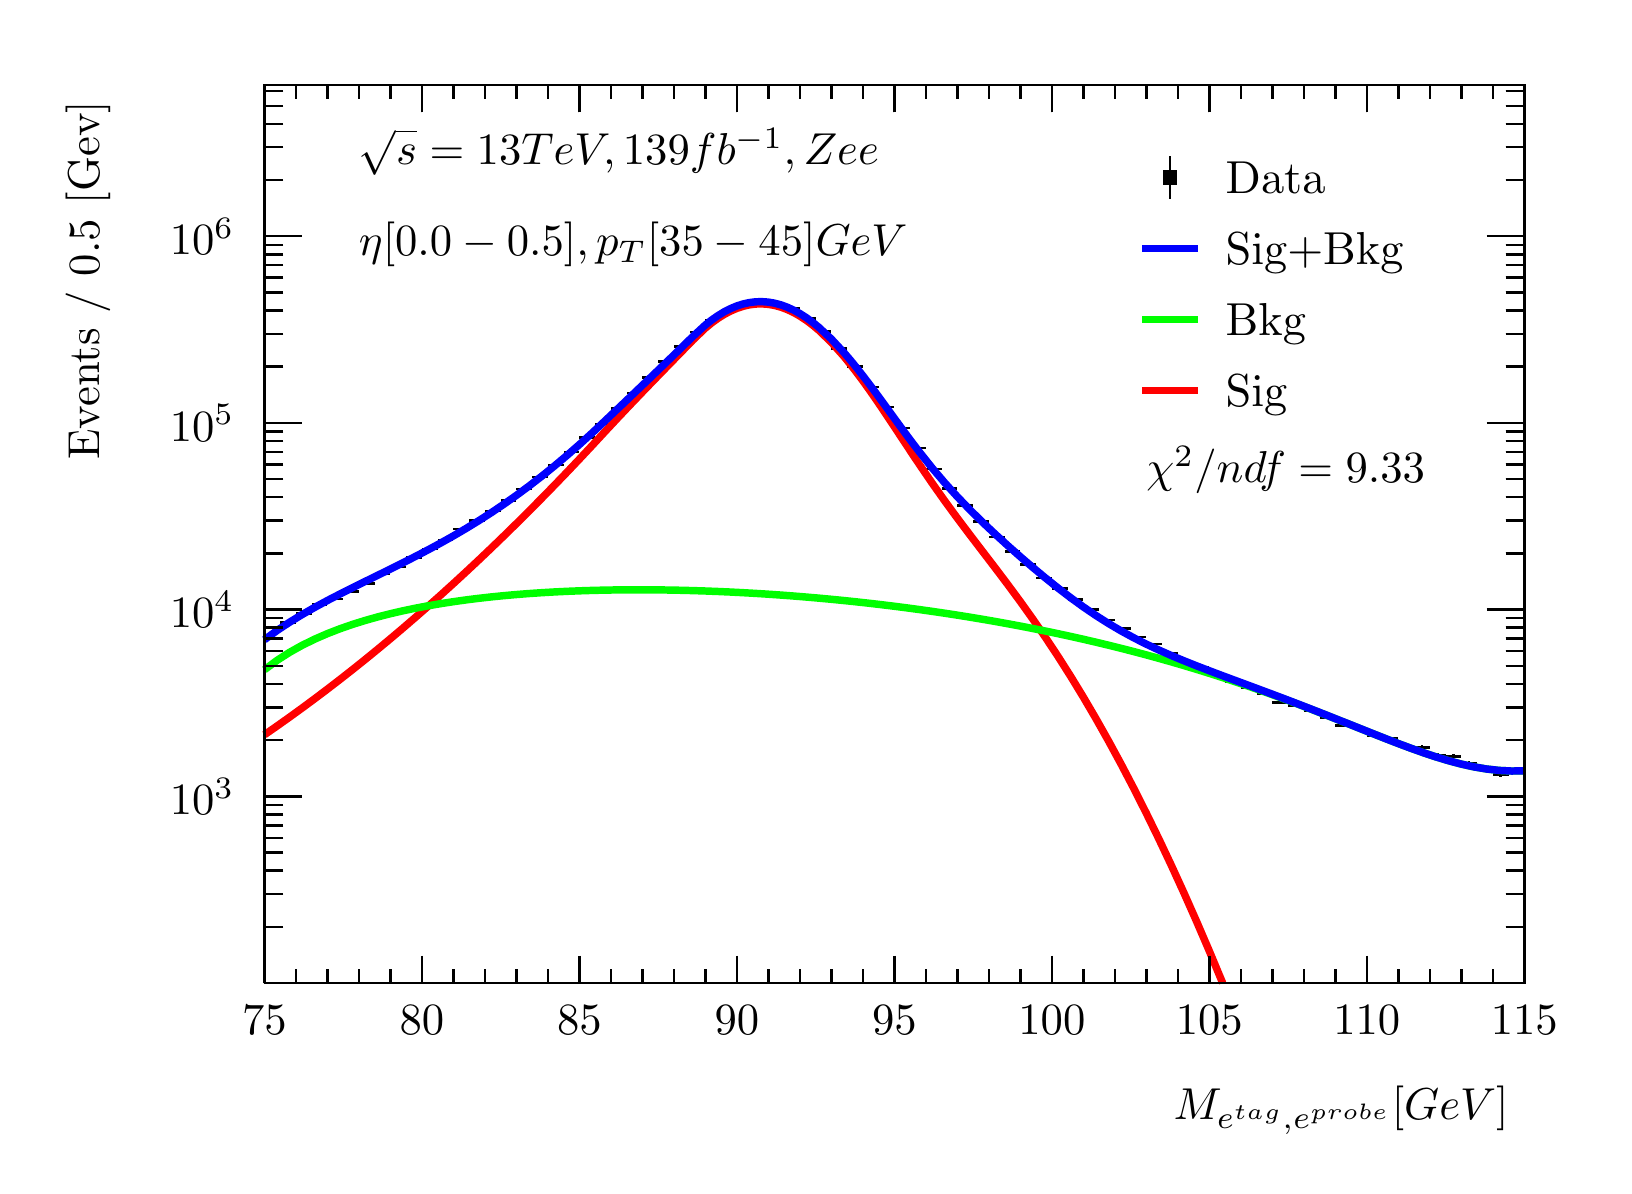
\begin{tikzpicture}
\pgfdeclareplotmark{cross} {
\pgfpathmoveto{\pgfpoint{-0.3\pgfplotmarksize}{\pgfplotmarksize}}
\pgfpathlineto{\pgfpoint{+0.3\pgfplotmarksize}{\pgfplotmarksize}}
\pgfpathlineto{\pgfpoint{+0.3\pgfplotmarksize}{0.3\pgfplotmarksize}}
\pgfpathlineto{\pgfpoint{+1\pgfplotmarksize}{0.3\pgfplotmarksize}}
\pgfpathlineto{\pgfpoint{+1\pgfplotmarksize}{-0.3\pgfplotmarksize}}
\pgfpathlineto{\pgfpoint{+0.3\pgfplotmarksize}{-0.3\pgfplotmarksize}}
\pgfpathlineto{\pgfpoint{+0.3\pgfplotmarksize}{-1.\pgfplotmarksize}}
\pgfpathlineto{\pgfpoint{-0.3\pgfplotmarksize}{-1.\pgfplotmarksize}}
\pgfpathlineto{\pgfpoint{-0.3\pgfplotmarksize}{-0.3\pgfplotmarksize}}
\pgfpathlineto{\pgfpoint{-1.\pgfplotmarksize}{-0.3\pgfplotmarksize}}
\pgfpathlineto{\pgfpoint{-1.\pgfplotmarksize}{0.3\pgfplotmarksize}}
\pgfpathlineto{\pgfpoint{-0.3\pgfplotmarksize}{0.3\pgfplotmarksize}}
\pgfpathclose
\pgfusepathqstroke
}
\pgfdeclareplotmark{cross*} {
\pgfpathmoveto{\pgfpoint{-0.3\pgfplotmarksize}{\pgfplotmarksize}}
\pgfpathlineto{\pgfpoint{+0.3\pgfplotmarksize}{\pgfplotmarksize}}
\pgfpathlineto{\pgfpoint{+0.3\pgfplotmarksize}{0.3\pgfplotmarksize}}
\pgfpathlineto{\pgfpoint{+1\pgfplotmarksize}{0.3\pgfplotmarksize}}
\pgfpathlineto{\pgfpoint{+1\pgfplotmarksize}{-0.3\pgfplotmarksize}}
\pgfpathlineto{\pgfpoint{+0.3\pgfplotmarksize}{-0.3\pgfplotmarksize}}
\pgfpathlineto{\pgfpoint{+0.3\pgfplotmarksize}{-1.\pgfplotmarksize}}
\pgfpathlineto{\pgfpoint{-0.3\pgfplotmarksize}{-1.\pgfplotmarksize}}
\pgfpathlineto{\pgfpoint{-0.3\pgfplotmarksize}{-0.3\pgfplotmarksize}}
\pgfpathlineto{\pgfpoint{-1.\pgfplotmarksize}{-0.3\pgfplotmarksize}}
\pgfpathlineto{\pgfpoint{-1.\pgfplotmarksize}{0.3\pgfplotmarksize}}
\pgfpathlineto{\pgfpoint{-0.3\pgfplotmarksize}{0.3\pgfplotmarksize}}
\pgfpathclose
\pgfusepathqfillstroke
}
\pgfdeclareplotmark{newstar} {
\pgfpathmoveto{\pgfqpoint{0pt}{\pgfplotmarksize}}
\pgfpathlineto{\pgfqpointpolar{44}{0.5\pgfplotmarksize}}
\pgfpathlineto{\pgfqpointpolar{18}{\pgfplotmarksize}}
\pgfpathlineto{\pgfqpointpolar{-20}{0.5\pgfplotmarksize}}
\pgfpathlineto{\pgfqpointpolar{-54}{\pgfplotmarksize}}
\pgfpathlineto{\pgfqpointpolar{-90}{0.5\pgfplotmarksize}}
\pgfpathlineto{\pgfqpointpolar{234}{\pgfplotmarksize}}
\pgfpathlineto{\pgfqpointpolar{198}{0.5\pgfplotmarksize}}
\pgfpathlineto{\pgfqpointpolar{162}{\pgfplotmarksize}}
\pgfpathlineto{\pgfqpointpolar{134}{0.5\pgfplotmarksize}}
\pgfpathclose
\pgfusepathqstroke
}
\pgfdeclareplotmark{newstar*} {
\pgfpathmoveto{\pgfqpoint{0pt}{\pgfplotmarksize}}
\pgfpathlineto{\pgfqpointpolar{44}{0.5\pgfplotmarksize}}
\pgfpathlineto{\pgfqpointpolar{18}{\pgfplotmarksize}}
\pgfpathlineto{\pgfqpointpolar{-20}{0.5\pgfplotmarksize}}
\pgfpathlineto{\pgfqpointpolar{-54}{\pgfplotmarksize}}
\pgfpathlineto{\pgfqpointpolar{-90}{0.5\pgfplotmarksize}}
\pgfpathlineto{\pgfqpointpolar{234}{\pgfplotmarksize}}
\pgfpathlineto{\pgfqpointpolar{198}{0.5\pgfplotmarksize}}
\pgfpathlineto{\pgfqpointpolar{162}{\pgfplotmarksize}}
\pgfpathlineto{\pgfqpointpolar{134}{0.5\pgfplotmarksize}}
\pgfpathclose
\pgfusepathqfillstroke
}
\definecolor{c}{rgb}{1,1,1};
\draw [color=c, fill=c] (0,0) rectangle (20,14.4361);
\draw [color=c, fill=c] (3,2.30977) rectangle (19,13.7143);
\definecolor{c}{rgb}{0,0,0};
\draw [c,line width=0.9] (3,2.30977) -- (3,13.7143) -- (19,13.7143) -- (19,2.30977) -- (3,2.30977);
\definecolor{c}{rgb}{1,1,1};
\draw [color=c, fill=c] (3,2.30977) rectangle (19,13.7143);
\definecolor{c}{rgb}{0,0,0};
\draw [c,line width=0.9] (3,2.30977) -- (3,13.7143) -- (19,13.7143) -- (19,2.30977) -- (3,2.30977);
\draw [c,line width=0.9] (3,2.30977) -- (19,2.30977);
\draw [c,line width=0.9] (3,2.65624) -- (3,2.30977);
\draw [c,line width=0.9] (3.4,2.48301) -- (3.4,2.30977);
\draw [c,line width=0.9] (3.8,2.48301) -- (3.8,2.30977);
\draw [c,line width=0.9] (4.2,2.48301) -- (4.2,2.30977);
\draw [c,line width=0.9] (4.6,2.48301) -- (4.6,2.30977);
\draw [c,line width=0.9] (5,2.65624) -- (5,2.30977);
\draw [c,line width=0.9] (5.4,2.48301) -- (5.4,2.30977);
\draw [c,line width=0.9] (5.8,2.48301) -- (5.8,2.30977);
\draw [c,line width=0.9] (6.2,2.48301) -- (6.2,2.30977);
\draw [c,line width=0.9] (6.6,2.48301) -- (6.6,2.30977);
\draw [c,line width=0.9] (7,2.65624) -- (7,2.30977);
\draw [c,line width=0.9] (7.4,2.48301) -- (7.4,2.30977);
\draw [c,line width=0.9] (7.8,2.48301) -- (7.8,2.30977);
\draw [c,line width=0.9] (8.2,2.48301) -- (8.2,2.30977);
\draw [c,line width=0.9] (8.6,2.48301) -- (8.6,2.30977);
\draw [c,line width=0.9] (9,2.65624) -- (9,2.30977);
\draw [c,line width=0.9] (9.4,2.48301) -- (9.4,2.30977);
\draw [c,line width=0.9] (9.8,2.48301) -- (9.8,2.30977);
\draw [c,line width=0.9] (10.2,2.48301) -- (10.2,2.30977);
\draw [c,line width=0.9] (10.6,2.48301) -- (10.6,2.30977);
\draw [c,line width=0.9] (11,2.65624) -- (11,2.30977);
\draw [c,line width=0.9] (11.4,2.48301) -- (11.4,2.30977);
\draw [c,line width=0.9] (11.8,2.48301) -- (11.8,2.30977);
\draw [c,line width=0.9] (12.2,2.48301) -- (12.2,2.30977);
\draw [c,line width=0.9] (12.6,2.48301) -- (12.6,2.30977);
\draw [c,line width=0.9] (13,2.65624) -- (13,2.30977);
\draw [c,line width=0.9] (13.4,2.48301) -- (13.4,2.30977);
\draw [c,line width=0.9] (13.8,2.48301) -- (13.8,2.30977);
\draw [c,line width=0.9] (14.2,2.48301) -- (14.2,2.30977);
\draw [c,line width=0.9] (14.6,2.48301) -- (14.6,2.30977);
\draw [c,line width=0.9] (15,2.65624) -- (15,2.30977);
\draw [c,line width=0.9] (15.4,2.48301) -- (15.4,2.30977);
\draw [c,line width=0.9] (15.8,2.48301) -- (15.8,2.30977);
\draw [c,line width=0.9] (16.2,2.48301) -- (16.2,2.30977);
\draw [c,line width=0.9] (16.6,2.48301) -- (16.6,2.30977);
\draw [c,line width=0.9] (17,2.65624) -- (17,2.30977);
\draw [c,line width=0.9] (17.4,2.48301) -- (17.4,2.30977);
\draw [c,line width=0.9] (17.8,2.48301) -- (17.8,2.30977);
\draw [c,line width=0.9] (18.2,2.48301) -- (18.2,2.30977);
\draw [c,line width=0.9] (18.6,2.48301) -- (18.6,2.30977);
\draw [c,line width=0.9] (19,2.65624) -- (19,2.30977);
\draw [c,line width=0.9] (19,2.65624) -- (19,2.30977);
\draw [anchor=base] (3,1.66015) node[scale=1.61424, color=c, rotate=0]{75};
\draw [anchor=base] (5,1.66015) node[scale=1.61424, color=c, rotate=0]{80};
\draw [anchor=base] (7,1.66015) node[scale=1.61424, color=c, rotate=0]{85};
\draw [anchor=base] (9,1.66015) node[scale=1.61424, color=c, rotate=0]{90};
\draw [anchor=base] (11,1.66015) node[scale=1.61424, color=c, rotate=0]{95};
\draw [anchor=base] (13,1.66015) node[scale=1.61424, color=c, rotate=0]{100};
\draw [anchor=base] (15,1.66015) node[scale=1.61424, color=c, rotate=0]{105};
\draw [anchor=base] (17,1.66015) node[scale=1.61424, color=c, rotate=0]{110};
\draw [anchor=base] (19,1.66015) node[scale=1.61424, color=c, rotate=0]{115};
\draw [anchor= east] (19,0.692932) node[scale=1.61424, color=c, rotate=0]{$M_{e^{tag}, e^{probe}}  [GeV]$};
\draw [c,line width=0.9] (3,13.7143) -- (19,13.7143);
\draw [c,line width=0.9] (3,13.3678) -- (3,13.7143);
\draw [c,line width=0.9] (3.4,13.5411) -- (3.4,13.7143);
\draw [c,line width=0.9] (3.8,13.5411) -- (3.8,13.7143);
\draw [c,line width=0.9] (4.2,13.5411) -- (4.2,13.7143);
\draw [c,line width=0.9] (4.6,13.5411) -- (4.6,13.7143);
\draw [c,line width=0.9] (5,13.3678) -- (5,13.7143);
\draw [c,line width=0.9] (5.4,13.5411) -- (5.4,13.7143);
\draw [c,line width=0.9] (5.8,13.5411) -- (5.8,13.7143);
\draw [c,line width=0.9] (6.2,13.5411) -- (6.2,13.7143);
\draw [c,line width=0.9] (6.6,13.5411) -- (6.6,13.7143);
\draw [c,line width=0.9] (7,13.3678) -- (7,13.7143);
\draw [c,line width=0.9] (7.4,13.5411) -- (7.4,13.7143);
\draw [c,line width=0.9] (7.8,13.5411) -- (7.8,13.7143);
\draw [c,line width=0.9] (8.2,13.5411) -- (8.2,13.7143);
\draw [c,line width=0.9] (8.6,13.5411) -- (8.6,13.7143);
\draw [c,line width=0.9] (9,13.3678) -- (9,13.7143);
\draw [c,line width=0.9] (9.4,13.5411) -- (9.4,13.7143);
\draw [c,line width=0.9] (9.8,13.5411) -- (9.8,13.7143);
\draw [c,line width=0.9] (10.2,13.5411) -- (10.2,13.7143);
\draw [c,line width=0.9] (10.6,13.5411) -- (10.6,13.7143);
\draw [c,line width=0.9] (11,13.3678) -- (11,13.7143);
\draw [c,line width=0.9] (11.4,13.5411) -- (11.4,13.7143);
\draw [c,line width=0.9] (11.8,13.5411) -- (11.8,13.7143);
\draw [c,line width=0.9] (12.2,13.5411) -- (12.2,13.7143);
\draw [c,line width=0.9] (12.6,13.5411) -- (12.6,13.7143);
\draw [c,line width=0.9] (13,13.3678) -- (13,13.7143);
\draw [c,line width=0.9] (13.4,13.5411) -- (13.4,13.7143);
\draw [c,line width=0.9] (13.8,13.5411) -- (13.8,13.7143);
\draw [c,line width=0.9] (14.2,13.5411) -- (14.2,13.7143);
\draw [c,line width=0.9] (14.6,13.5411) -- (14.6,13.7143);
\draw [c,line width=0.9] (15,13.3678) -- (15,13.7143);
\draw [c,line width=0.9] (15.4,13.5411) -- (15.4,13.7143);
\draw [c,line width=0.9] (15.8,13.5411) -- (15.8,13.7143);
\draw [c,line width=0.9] (16.2,13.5411) -- (16.2,13.7143);
\draw [c,line width=0.9] (16.6,13.5411) -- (16.6,13.7143);
\draw [c,line width=0.9] (17,13.3678) -- (17,13.7143);
\draw [c,line width=0.9] (17.4,13.5411) -- (17.4,13.7143);
\draw [c,line width=0.9] (17.8,13.5411) -- (17.8,13.7143);
\draw [c,line width=0.9] (18.2,13.5411) -- (18.2,13.7143);
\draw [c,line width=0.9] (18.6,13.5411) -- (18.6,13.7143);
\draw [c,line width=0.9] (19,13.3678) -- (19,13.7143);
\draw [c,line width=0.9] (19,13.3678) -- (19,13.7143);
\draw [c,line width=0.9] (3,2.30977) -- (3,13.7143);
\draw [c,line width=0.9] (3.237,3.02354) -- (3,3.02354);
\draw [c,line width=0.9] (3.237,3.44107) -- (3,3.44107);
\draw [c,line width=0.9] (3.237,3.73731) -- (3,3.73731);
\draw [c,line width=0.9] (3.237,3.96709) -- (3,3.96709);
\draw [c,line width=0.9] (3.237,4.15484) -- (3,4.15484);
\draw [c,line width=0.9] (3.237,4.31357) -- (3,4.31357);
\draw [c,line width=0.9] (3.237,4.45108) -- (3,4.45108);
\draw [c,line width=0.9] (3.237,4.57236) -- (3,4.57236);
\draw [c,line width=0.9] (3.474,4.68086) -- (3,4.68086);
\draw [anchor= east] (2.82,4.68086) node[scale=1.61424, color=c, rotate=0]{$10^{3}$};
\draw [c,line width=0.9] (3.237,5.39463) -- (3,5.39463);
\draw [c,line width=0.9] (3.237,5.81216) -- (3,5.81216);
\draw [c,line width=0.9] (3.237,6.1084) -- (3,6.1084);
\draw [c,line width=0.9] (3.237,6.33818) -- (3,6.33818);
\draw [c,line width=0.9] (3.237,6.52593) -- (3,6.52593);
\draw [c,line width=0.9] (3.237,6.68466) -- (3,6.68466);
\draw [c,line width=0.9] (3.237,6.82217) -- (3,6.82217);
\draw [c,line width=0.9] (3.237,6.94345) -- (3,6.94345);
\draw [c,line width=0.9] (3.474,7.05195) -- (3,7.05195);
\draw [anchor= east] (2.82,7.05195) node[scale=1.61424, color=c, rotate=0]{$10^{4}$};
\draw [c,line width=0.9] (3.237,7.76572) -- (3,7.76572);
\draw [c,line width=0.9] (3.237,8.18324) -- (3,8.18324);
\draw [c,line width=0.9] (3.237,8.47948) -- (3,8.47948);
\draw [c,line width=0.9] (3.237,8.70927) -- (3,8.70927);
\draw [c,line width=0.9] (3.237,8.89701) -- (3,8.89701);
\draw [c,line width=0.9] (3.237,9.05575) -- (3,9.05575);
\draw [c,line width=0.9] (3.237,9.19325) -- (3,9.19325);
\draw [c,line width=0.9] (3.237,9.31454) -- (3,9.31454);
\draw [c,line width=0.9] (3.474,9.42304) -- (3,9.42304);
\draw [anchor= east] (2.82,9.42304) node[scale=1.61424, color=c, rotate=0]{$10^{5}$};
\draw [c,line width=0.9] (3.237,10.1368) -- (3,10.1368);
\draw [c,line width=0.9] (3.237,10.5543) -- (3,10.5543);
\draw [c,line width=0.9] (3.237,10.8506) -- (3,10.8506);
\draw [c,line width=0.9] (3.237,11.0804) -- (3,11.0804);
\draw [c,line width=0.9] (3.237,11.2681) -- (3,11.2681);
\draw [c,line width=0.9] (3.237,11.4268) -- (3,11.4268);
\draw [c,line width=0.9] (3.237,11.5643) -- (3,11.5643);
\draw [c,line width=0.9] (3.237,11.6856) -- (3,11.6856);
\draw [c,line width=0.9] (3.474,11.7941) -- (3,11.7941);
\draw [anchor= east] (2.82,11.7941) node[scale=1.61424, color=c, rotate=0]{$10^{6}$};
\draw [c,line width=0.9] (3.237,12.5079) -- (3,12.5079);
\draw [c,line width=0.9] (3.237,12.9254) -- (3,12.9254);
\draw [c,line width=0.9] (3.237,13.2217) -- (3,13.2217);
\draw [c,line width=0.9] (3.237,13.4514) -- (3,13.4514);
\draw [c,line width=0.9] (3.237,13.6392) -- (3,13.6392);
\draw [anchor= east] (0.76,13.7143) node[scale=1.61424, color=c, rotate=90]{Events / 0.5 [Gev]};
\draw [c,line width=0.9] (19,2.30977) -- (19,13.7143);
\draw [c,line width=0.9] (18.763,3.02354) -- (19,3.02354);
\draw [c,line width=0.9] (18.763,3.44107) -- (19,3.44107);
\draw [c,line width=0.9] (18.763,3.73731) -- (19,3.73731);
\draw [c,line width=0.9] (18.763,3.96709) -- (19,3.96709);
\draw [c,line width=0.9] (18.763,4.15484) -- (19,4.15484);
\draw [c,line width=0.9] (18.763,4.31357) -- (19,4.31357);
\draw [c,line width=0.9] (18.763,4.45108) -- (19,4.45108);
\draw [c,line width=0.9] (18.763,4.57236) -- (19,4.57236);
\draw [c,line width=0.9] (18.526,4.68086) -- (19,4.68086);
\draw [c,line width=0.9] (18.763,5.39463) -- (19,5.39463);
\draw [c,line width=0.9] (18.763,5.81216) -- (19,5.81216);
\draw [c,line width=0.9] (18.763,6.1084) -- (19,6.1084);
\draw [c,line width=0.9] (18.763,6.33818) -- (19,6.33818);
\draw [c,line width=0.9] (18.763,6.52593) -- (19,6.52593);
\draw [c,line width=0.9] (18.763,6.68466) -- (19,6.68466);
\draw [c,line width=0.9] (18.763,6.82217) -- (19,6.82217);
\draw [c,line width=0.9] (18.763,6.94345) -- (19,6.94345);
\draw [c,line width=0.9] (18.526,7.05195) -- (19,7.05195);
\draw [c,line width=0.9] (18.763,7.76572) -- (19,7.76572);
\draw [c,line width=0.9] (18.763,8.18324) -- (19,8.18324);
\draw [c,line width=0.9] (18.763,8.47948) -- (19,8.47948);
\draw [c,line width=0.9] (18.763,8.70927) -- (19,8.70927);
\draw [c,line width=0.9] (18.763,8.89701) -- (19,8.89701);
\draw [c,line width=0.9] (18.763,9.05575) -- (19,9.05575);
\draw [c,line width=0.9] (18.763,9.19325) -- (19,9.19325);
\draw [c,line width=0.9] (18.763,9.31454) -- (19,9.31454);
\draw [c,line width=0.9] (18.526,9.42304) -- (19,9.42304);
\draw [c,line width=0.9] (18.763,10.1368) -- (19,10.1368);
\draw [c,line width=0.9] (18.763,10.5543) -- (19,10.5543);
\draw [c,line width=0.9] (18.763,10.8506) -- (19,10.8506);
\draw [c,line width=0.9] (18.763,11.0804) -- (19,11.0804);
\draw [c,line width=0.9] (18.763,11.2681) -- (19,11.2681);
\draw [c,line width=0.9] (18.763,11.4268) -- (19,11.4268);
\draw [c,line width=0.9] (18.763,11.5643) -- (19,11.5643);
\draw [c,line width=0.9] (18.763,11.6856) -- (19,11.6856);
\draw [c,line width=0.9] (18.526,11.7941) -- (19,11.7941);
\draw [c,line width=0.9] (18.763,12.5079) -- (19,12.5079);
\draw [c,line width=0.9] (18.763,12.9254) -- (19,12.9254);
\draw [c,line width=0.9] (18.763,13.2217) -- (19,13.2217);
\draw [c,line width=0.9] (18.763,13.4514) -- (19,13.4514);
\draw [c,line width=0.9] (18.763,13.6392) -- (19,13.6392);
\draw [c,line width=0.9] (3.1,6.83216) -- (3,6.83216);
\draw [c,line width=0.9] (3,6.83216) -- (3,6.83216);
\draw [c,line width=0.9] (3.1,6.83216) -- (3.2,6.83216);
\draw [c,line width=0.9] (3.2,6.83216) -- (3.2,6.83216);
\draw [c,line width=0.9] (3.1,6.83216) -- (3.1,6.84362);
\draw [c,line width=0.9] (3.1,6.84362) -- (3.1,6.84362);
\draw [c,line width=0.9] (3.1,6.83216) -- (3.1,6.8207);
\draw [c,line width=0.9] (3.1,6.8207) -- (3.1,6.8207);
\draw [c,line width=0.9] (3.3,6.88786) -- (3.2,6.88786);
\draw [c,line width=0.9] (3.2,6.88786) -- (3.2,6.88786);
\draw [c,line width=0.9] (3.3,6.88786) -- (3.4,6.88786);
\draw [c,line width=0.9] (3.4,6.88786) -- (3.4,6.88786);
\draw [c,line width=0.9] (3.3,6.88786) -- (3.3,6.89901);
\draw [c,line width=0.9] (3.3,6.89901) -- (3.3,6.89901);
\draw [c,line width=0.9] (3.3,6.88786) -- (3.3,6.87671);
\draw [c,line width=0.9] (3.3,6.87671) -- (3.3,6.87671);
\draw [c,line width=0.9] (3.5,7.00162) -- (3.4,7.00162);
\draw [c,line width=0.9] (3.4,7.00162) -- (3.4,7.00162);
\draw [c,line width=0.9] (3.5,7.00162) -- (3.6,7.00162);
\draw [c,line width=0.9] (3.6,7.00162) -- (3.6,7.00162);
\draw [c,line width=0.9] (3.5,7.00162) -- (3.5,7.01217);
\draw [c,line width=0.9] (3.5,7.01217) -- (3.5,7.01217);
\draw [c,line width=0.9] (3.5,7.00162) -- (3.5,6.99107);
\draw [c,line width=0.9] (3.5,6.99107) -- (3.5,6.99107);
\draw [c,line width=0.9] (3.7,7.11506) -- (3.6,7.11506);
\draw [c,line width=0.9] (3.6,7.11506) -- (3.6,7.11506);
\draw [c,line width=0.9] (3.7,7.11506) -- (3.8,7.11506);
\draw [c,line width=0.9] (3.8,7.11506) -- (3.8,7.11506);
\draw [c,line width=0.9] (3.7,7.11506) -- (3.7,7.12504);
\draw [c,line width=0.9] (3.7,7.12504) -- (3.7,7.12504);
\draw [c,line width=0.9] (3.7,7.11506) -- (3.7,7.10507);
\draw [c,line width=0.9] (3.7,7.10507) -- (3.7,7.10507);
\draw [c,line width=0.9] (3.9,7.18416) -- (3.8,7.18416);
\draw [c,line width=0.9] (3.8,7.18416) -- (3.8,7.18416);
\draw [c,line width=0.9] (3.9,7.18416) -- (4,7.18416);
\draw [c,line width=0.9] (4,7.18416) -- (4,7.18416);
\draw [c,line width=0.9] (3.9,7.18416) -- (3.9,7.19382);
\draw [c,line width=0.9] (3.9,7.19382) -- (3.9,7.19382);
\draw [c,line width=0.9] (3.9,7.18416) -- (3.9,7.1745);
\draw [c,line width=0.9] (3.9,7.1745) -- (3.9,7.1745);
\draw [c,line width=0.9] (4.1,7.28543) -- (4,7.28543);
\draw [c,line width=0.9] (4,7.28543) -- (4,7.28543);
\draw [c,line width=0.9] (4.1,7.28543) -- (4.2,7.28543);
\draw [c,line width=0.9] (4.2,7.28543) -- (4.2,7.28543);
\draw [c,line width=0.9] (4.1,7.28543) -- (4.1,7.29463);
\draw [c,line width=0.9] (4.1,7.29463) -- (4.1,7.29463);
\draw [c,line width=0.9] (4.1,7.28543) -- (4.1,7.27624);
\draw [c,line width=0.9] (4.1,7.27624) -- (4.1,7.27624);
\draw [c,line width=0.9] (4.3,7.38674) -- (4.2,7.38674);
\draw [c,line width=0.9] (4.2,7.38674) -- (4.2,7.38674);
\draw [c,line width=0.9] (4.3,7.38674) -- (4.4,7.38674);
\draw [c,line width=0.9] (4.4,7.38674) -- (4.4,7.38674);
\draw [c,line width=0.9] (4.3,7.38674) -- (4.3,7.3955);
\draw [c,line width=0.9] (4.3,7.3955) -- (4.3,7.3955);
\draw [c,line width=0.9] (4.3,7.38674) -- (4.3,7.37799);
\draw [c,line width=0.9] (4.3,7.37799) -- (4.3,7.37799);
\draw [c,line width=0.9] (4.5,7.50696) -- (4.4,7.50696);
\draw [c,line width=0.9] (4.4,7.50696) -- (4.4,7.50696);
\draw [c,line width=0.9] (4.5,7.50696) -- (4.6,7.50696);
\draw [c,line width=0.9] (4.6,7.50696) -- (4.6,7.50696);
\draw [c,line width=0.9] (4.5,7.50696) -- (4.5,7.51521);
\draw [c,line width=0.9] (4.5,7.51521) -- (4.5,7.51521);
\draw [c,line width=0.9] (4.5,7.50696) -- (4.5,7.4987);
\draw [c,line width=0.9] (4.5,7.4987) -- (4.5,7.4987);
\draw [c,line width=0.9] (4.7,7.59618) -- (4.6,7.59618);
\draw [c,line width=0.9] (4.6,7.59618) -- (4.6,7.59618);
\draw [c,line width=0.9] (4.7,7.59618) -- (4.8,7.59618);
\draw [c,line width=0.9] (4.8,7.59618) -- (4.8,7.59618);
\draw [c,line width=0.9] (4.7,7.59618) -- (4.7,7.60409);
\draw [c,line width=0.9] (4.7,7.60409) -- (4.7,7.60409);
\draw [c,line width=0.9] (4.7,7.59618) -- (4.7,7.58827);
\draw [c,line width=0.9] (4.7,7.58827) -- (4.7,7.58827);
\draw [c,line width=0.9] (4.9,7.71447) -- (4.8,7.71447);
\draw [c,line width=0.9] (4.8,7.71447) -- (4.8,7.71447);
\draw [c,line width=0.9] (4.9,7.71447) -- (5,7.71447);
\draw [c,line width=0.9] (5,7.71447) -- (5,7.71447);
\draw [c,line width=0.9] (4.9,7.71447) -- (4.9,7.72193);
\draw [c,line width=0.9] (4.9,7.72193) -- (4.9,7.72193);
\draw [c,line width=0.9] (4.9,7.71447) -- (4.9,7.707);
\draw [c,line width=0.9] (4.9,7.707) -- (4.9,7.707);
\draw [c,line width=0.9] (5.1,7.82212) -- (5,7.82212);
\draw [c,line width=0.9] (5,7.82212) -- (5,7.82212);
\draw [c,line width=0.9] (5.1,7.82212) -- (5.2,7.82212);
\draw [c,line width=0.9] (5.2,7.82212) -- (5.2,7.82212);
\draw [c,line width=0.9] (5.1,7.82212) -- (5.1,7.8292);
\draw [c,line width=0.9] (5.1,7.8292) -- (5.1,7.8292);
\draw [c,line width=0.9] (5.1,7.82212) -- (5.1,7.81503);
\draw [c,line width=0.9] (5.1,7.81503) -- (5.1,7.81503);
\draw [c,line width=0.9] (5.3,7.93472) -- (5.2,7.93472);
\draw [c,line width=0.9] (5.2,7.93472) -- (5.2,7.93472);
\draw [c,line width=0.9] (5.3,7.93472) -- (5.4,7.93472);
\draw [c,line width=0.9] (5.4,7.93472) -- (5.4,7.93472);
\draw [c,line width=0.9] (5.3,7.93472) -- (5.3,7.94142);
\draw [c,line width=0.9] (5.3,7.94142) -- (5.3,7.94142);
\draw [c,line width=0.9] (5.3,7.93472) -- (5.3,7.92801);
\draw [c,line width=0.9] (5.3,7.92801) -- (5.3,7.92801);
\draw [c,line width=0.9] (5.5,8.07448) -- (5.4,8.07448);
\draw [c,line width=0.9] (5.4,8.07448) -- (5.4,8.07448);
\draw [c,line width=0.9] (5.5,8.07448) -- (5.6,8.07448);
\draw [c,line width=0.9] (5.6,8.07448) -- (5.6,8.07448);
\draw [c,line width=0.9] (5.5,8.07448) -- (5.5,8.08075);
\draw [c,line width=0.9] (5.5,8.08075) -- (5.5,8.08075);
\draw [c,line width=0.9] (5.5,8.07448) -- (5.5,8.06822);
\draw [c,line width=0.9] (5.5,8.06822) -- (5.5,8.06822);
\draw [c,line width=0.9] (5.7,8.18149) -- (5.6,8.18149);
\draw [c,line width=0.9] (5.6,8.18149) -- (5.6,8.18149);
\draw [c,line width=0.9] (5.7,8.18149) -- (5.8,8.18149);
\draw [c,line width=0.9] (5.8,8.18149) -- (5.8,8.18149);
\draw [c,line width=0.9] (5.7,8.18149) -- (5.7,8.18744);
\draw [c,line width=0.9] (5.7,8.18744) -- (5.7,8.18744);
\draw [c,line width=0.9] (5.7,8.18149) -- (5.7,8.17554);
\draw [c,line width=0.9] (5.7,8.17554) -- (5.7,8.17554);
\draw [c,line width=0.9] (5.9,8.30533) -- (5.8,8.30533);
\draw [c,line width=0.9] (5.8,8.30533) -- (5.8,8.30533);
\draw [c,line width=0.9] (5.9,8.30533) -- (6,8.30533);
\draw [c,line width=0.9] (6,8.30533) -- (6,8.30533);
\draw [c,line width=0.9] (5.9,8.30533) -- (5.9,8.31093);
\draw [c,line width=0.9] (5.9,8.31093) -- (5.9,8.31093);
\draw [c,line width=0.9] (5.9,8.30533) -- (5.9,8.29972);
\draw [c,line width=0.9] (5.9,8.29972) -- (5.9,8.29972);
\draw [c,line width=0.9] (6.1,8.44101) -- (6,8.44101);
\draw [c,line width=0.9] (6,8.44101) -- (6,8.44101);
\draw [c,line width=0.9] (6.1,8.44101) -- (6.2,8.44101);
\draw [c,line width=0.9] (6.2,8.44101) -- (6.2,8.44101);
\draw [c,line width=0.9] (6.1,8.44101) -- (6.1,8.44626);
\draw [c,line width=0.9] (6.1,8.44626) -- (6.1,8.44626);
\draw [c,line width=0.9] (6.1,8.44101) -- (6.1,8.43576);
\draw [c,line width=0.9] (6.1,8.43576) -- (6.1,8.43576);
\draw [c,line width=0.9] (6.3,8.58649) -- (6.2,8.58649);
\draw [c,line width=0.9] (6.2,8.58649) -- (6.2,8.58649);
\draw [c,line width=0.9] (6.3,8.58649) -- (6.4,8.58649);
\draw [c,line width=0.9] (6.4,8.58649) -- (6.4,8.58649);
\draw [c,line width=0.9] (6.3,8.58649) -- (6.3,8.59138);
\draw [c,line width=0.9] (6.3,8.59138) -- (6.3,8.59138);
\draw [c,line width=0.9] (6.3,8.58649) -- (6.3,8.5816);
\draw [c,line width=0.9] (6.3,8.5816) -- (6.3,8.5816);
\draw [c,line width=0.9] (6.5,8.7375) -- (6.4,8.7375);
\draw [c,line width=0.9] (6.4,8.7375) -- (6.4,8.7375);
\draw [c,line width=0.9] (6.5,8.7375) -- (6.6,8.7375);
\draw [c,line width=0.9] (6.6,8.7375) -- (6.6,8.7375);
\draw [c,line width=0.9] (6.5,8.7375) -- (6.5,8.74205);
\draw [c,line width=0.9] (6.5,8.74205) -- (6.5,8.74205);
\draw [c,line width=0.9] (6.5,8.7375) -- (6.5,8.73296);
\draw [c,line width=0.9] (6.5,8.73296) -- (6.5,8.73296);
\draw [c,line width=0.9] (6.7,8.88897) -- (6.6,8.88897);
\draw [c,line width=0.9] (6.6,8.88897) -- (6.6,8.88897);
\draw [c,line width=0.9] (6.7,8.88897) -- (6.8,8.88897);
\draw [c,line width=0.9] (6.8,8.88897) -- (6.8,8.88897);
\draw [c,line width=0.9] (6.7,8.88897) -- (6.7,8.89319);
\draw [c,line width=0.9] (6.7,8.89319) -- (6.7,8.89319);
\draw [c,line width=0.9] (6.7,8.88897) -- (6.7,8.88475);
\draw [c,line width=0.9] (6.7,8.88475) -- (6.7,8.88475);
\draw [c,line width=0.9] (6.9,9.05543) -- (6.8,9.05543);
\draw [c,line width=0.9] (6.8,9.05543) -- (6.8,9.05543);
\draw [c,line width=0.9] (6.9,9.05543) -- (7,9.05543);
\draw [c,line width=0.9] (7,9.05543) -- (7,9.05543);
\draw [c,line width=0.9] (6.9,9.05543) -- (6.9,9.05932);
\draw [c,line width=0.9] (6.9,9.05932) -- (6.9,9.05932);
\draw [c,line width=0.9] (6.9,9.05543) -- (6.9,9.05153);
\draw [c,line width=0.9] (6.9,9.05153) -- (6.9,9.05153);
\draw [c,line width=0.9] (7.1,9.23782) -- (7,9.23782);
\draw [c,line width=0.9] (7,9.23782) -- (7,9.23782);
\draw [c,line width=0.9] (7.1,9.23782) -- (7.2,9.23782);
\draw [c,line width=0.9] (7.2,9.23782) -- (7.2,9.23782);
\draw [c,line width=0.9] (7.1,9.23782) -- (7.1,9.24138);
\draw [c,line width=0.9] (7.1,9.24138) -- (7.1,9.24138);
\draw [c,line width=0.9] (7.1,9.23782) -- (7.1,9.23425);
\draw [c,line width=0.9] (7.1,9.23425) -- (7.1,9.23425);
\draw [c,line width=0.9] (7.3,9.41066) -- (7.2,9.41066);
\draw [c,line width=0.9] (7.2,9.41066) -- (7.2,9.41066);
\draw [c,line width=0.9] (7.3,9.41066) -- (7.4,9.41066);
\draw [c,line width=0.9] (7.4,9.41066) -- (7.4,9.41066);
\draw [c,line width=0.9] (7.3,9.41066) -- (7.3,9.41393);
\draw [c,line width=0.9] (7.3,9.41393) -- (7.3,9.41393);
\draw [c,line width=0.9] (7.3,9.41066) -- (7.3,9.40738);
\draw [c,line width=0.9] (7.3,9.40738) -- (7.3,9.40738);
\draw [c,line width=0.9] (7.5,9.60518) -- (7.4,9.60518);
\draw [c,line width=0.9] (7.4,9.60518) -- (7.4,9.60518);
\draw [c,line width=0.9] (7.5,9.60518) -- (7.6,9.60518);
\draw [c,line width=0.9] (7.6,9.60518) -- (7.6,9.60518);
\draw [c,line width=0.9] (7.5,9.60518) -- (7.5,9.60816);
\draw [c,line width=0.9] (7.5,9.60816) -- (7.5,9.60816);
\draw [c,line width=0.9] (7.5,9.60518) -- (7.5,9.6022);
\draw [c,line width=0.9] (7.5,9.6022) -- (7.5,9.6022);
\draw [c,line width=0.9] (7.7,9.80488) -- (7.6,9.80488);
\draw [c,line width=0.9] (7.6,9.80488) -- (7.6,9.80488);
\draw [c,line width=0.9] (7.7,9.80488) -- (7.8,9.80488);
\draw [c,line width=0.9] (7.8,9.80488) -- (7.8,9.80488);
\draw [c,line width=0.9] (7.7,9.80488) -- (7.7,9.80758);
\draw [c,line width=0.9] (7.7,9.80758) -- (7.7,9.80758);
\draw [c,line width=0.9] (7.7,9.80488) -- (7.7,9.80217);
\draw [c,line width=0.9] (7.7,9.80217) -- (7.7,9.80217);
\draw [c,line width=0.9] (7.9,10.0023) -- (7.8,10.0023);
\draw [c,line width=0.9] (7.8,10.0023) -- (7.8,10.0023);
\draw [c,line width=0.9] (7.9,10.0023) -- (8,10.0023);
\draw [c,line width=0.9] (8,10.0023) -- (8,10.0023);
\draw [c,line width=0.9] (7.9,10.0023) -- (7.9,10.0048);
\draw [c,line width=0.9] (7.9,10.0048) -- (7.9,10.0048);
\draw [c,line width=0.9] (7.9,10.0023) -- (7.9,9.99984);
\draw [c,line width=0.9] (7.9,9.99984) -- (7.9,9.99984);
\draw [c,line width=0.9] (8.1,10.2031) -- (8,10.2031);
\draw [c,line width=0.9] (8,10.2031) -- (8,10.2031);
\draw [c,line width=0.9] (8.1,10.2031) -- (8.2,10.2031);
\draw [c,line width=0.9] (8.2,10.2031) -- (8.2,10.2031);
\draw [c,line width=0.9] (8.1,10.2031) -- (8.1,10.2053);
\draw [c,line width=0.9] (8.1,10.2053) -- (8.1,10.2053);
\draw [c,line width=0.9] (8.1,10.2031) -- (8.1,10.2008);
\draw [c,line width=0.9] (8.1,10.2008) -- (8.1,10.2008);
\draw [c,line width=0.9] (8.3,10.3968) -- (8.2,10.3968);
\draw [c,line width=0.9] (8.2,10.3968) -- (8.2,10.3968);
\draw [c,line width=0.9] (8.3,10.3968) -- (8.4,10.3968);
\draw [c,line width=0.9] (8.4,10.3968) -- (8.4,10.3968);
\draw [c,line width=0.9] (8.3,10.3968) -- (8.3,10.3988);
\draw [c,line width=0.9] (8.3,10.3988) -- (8.3,10.3988);
\draw [c,line width=0.9] (8.3,10.3968) -- (8.3,10.3948);
\draw [c,line width=0.9] (8.3,10.3948) -- (8.3,10.3948);
\draw [c,line width=0.9] (8.5,10.5752) -- (8.4,10.5752);
\draw [c,line width=0.9] (8.4,10.5752) -- (8.4,10.5752);
\draw [c,line width=0.9] (8.5,10.5752) -- (8.6,10.5752);
\draw [c,line width=0.9] (8.6,10.5752) -- (8.6,10.5752);
\draw [c,line width=0.9] (8.5,10.5752) -- (8.5,10.5771);
\draw [c,line width=0.9] (8.5,10.5771) -- (8.5,10.5771);
\draw [c,line width=0.9] (8.5,10.5752) -- (8.5,10.5734);
\draw [c,line width=0.9] (8.5,10.5734) -- (8.5,10.5734);
\draw [c,line width=0.9] (8.7,10.7326) -- (8.6,10.7326);
\draw [c,line width=0.9] (8.6,10.7326) -- (8.6,10.7326);
\draw [c,line width=0.9] (8.7,10.7326) -- (8.8,10.7326);
\draw [c,line width=0.9] (8.8,10.7326) -- (8.8,10.7326);
\draw [c,line width=0.9] (8.7,10.7326) -- (8.7,10.7344);
\draw [c,line width=0.9] (8.7,10.7344) -- (8.7,10.7344);
\draw [c,line width=0.9] (8.7,10.7326) -- (8.7,10.7309);
\draw [c,line width=0.9] (8.7,10.7309) -- (8.7,10.7309);
\draw [c,line width=0.9] (8.9,10.8566) -- (8.8,10.8566);
\draw [c,line width=0.9] (8.8,10.8566) -- (8.8,10.8566);
\draw [c,line width=0.9] (8.9,10.8566) -- (9,10.8566);
\draw [c,line width=0.9] (9,10.8566) -- (9,10.8566);
\draw [c,line width=0.9] (8.9,10.8566) -- (8.9,10.8582);
\draw [c,line width=0.9] (8.9,10.8582) -- (8.9,10.8582);
\draw [c,line width=0.9] (8.9,10.8566) -- (8.9,10.855);
\draw [c,line width=0.9] (8.9,10.855) -- (8.9,10.855);
\draw [c,line width=0.9] (9.1,10.9355) -- (9,10.9355);
\draw [c,line width=0.9] (9,10.9355) -- (9,10.9355);
\draw [c,line width=0.9] (9.1,10.9355) -- (9.2,10.9355);
\draw [c,line width=0.9] (9.2,10.9355) -- (9.2,10.9355);
\draw [c,line width=0.9] (9.1,10.9355) -- (9.1,10.9371);
\draw [c,line width=0.9] (9.1,10.9371) -- (9.1,10.9371);
\draw [c,line width=0.9] (9.1,10.9355) -- (9.1,10.934);
\draw [c,line width=0.9] (9.1,10.934) -- (9.1,10.934);
\draw [c,line width=0.9] (9.3,10.9682) -- (9.2,10.9682);
\draw [c,line width=0.9] (9.2,10.9682) -- (9.2,10.9682);
\draw [c,line width=0.9] (9.3,10.9682) -- (9.4,10.9682);
\draw [c,line width=0.9] (9.4,10.9682) -- (9.4,10.9682);
\draw [c,line width=0.9] (9.3,10.9682) -- (9.3,10.9698);
\draw [c,line width=0.9] (9.3,10.9698) -- (9.3,10.9698);
\draw [c,line width=0.9] (9.3,10.9682) -- (9.3,10.9667);
\draw [c,line width=0.9] (9.3,10.9667) -- (9.3,10.9667);
\draw [c,line width=0.9] (9.5,10.9489) -- (9.4,10.9489);
\draw [c,line width=0.9] (9.4,10.9489) -- (9.4,10.9489);
\draw [c,line width=0.9] (9.5,10.9489) -- (9.6,10.9489);
\draw [c,line width=0.9] (9.6,10.9489) -- (9.6,10.9489);
\draw [c,line width=0.9] (9.5,10.9489) -- (9.5,10.9505);
\draw [c,line width=0.9] (9.5,10.9505) -- (9.5,10.9505);
\draw [c,line width=0.9] (9.5,10.9489) -- (9.5,10.9474);
\draw [c,line width=0.9] (9.5,10.9474) -- (9.5,10.9474);
\draw [c,line width=0.9] (9.7,10.8741) -- (9.6,10.8741);
\draw [c,line width=0.9] (9.6,10.8741) -- (9.6,10.8741);
\draw [c,line width=0.9] (9.7,10.8741) -- (9.8,10.8741);
\draw [c,line width=0.9] (9.8,10.8741) -- (9.8,10.8741);
\draw [c,line width=0.9] (9.7,10.8741) -- (9.7,10.8757);
\draw [c,line width=0.9] (9.7,10.8757) -- (9.7,10.8757);
\draw [c,line width=0.9] (9.7,10.8741) -- (9.7,10.8725);
\draw [c,line width=0.9] (9.7,10.8725) -- (9.7,10.8725);
\draw [c,line width=0.9] (9.9,10.7496) -- (9.8,10.7496);
\draw [c,line width=0.9] (9.8,10.7496) -- (9.8,10.7496);
\draw [c,line width=0.9] (9.9,10.7496) -- (10,10.7496);
\draw [c,line width=0.9] (10,10.7496) -- (10,10.7496);
\draw [c,line width=0.9] (9.9,10.7496) -- (9.9,10.7513);
\draw [c,line width=0.9] (9.9,10.7513) -- (9.9,10.7513);
\draw [c,line width=0.9] (9.9,10.7496) -- (9.9,10.7479);
\draw [c,line width=0.9] (9.9,10.7479) -- (9.9,10.7479);
\draw [c,line width=0.9] (10.1,10.5813) -- (10,10.5813);
\draw [c,line width=0.9] (10,10.5813) -- (10,10.5813);
\draw [c,line width=0.9] (10.1,10.5813) -- (10.2,10.5813);
\draw [c,line width=0.9] (10.2,10.5813) -- (10.2,10.5813);
\draw [c,line width=0.9] (10.1,10.5813) -- (10.1,10.5831);
\draw [c,line width=0.9] (10.1,10.5831) -- (10.1,10.5831);
\draw [c,line width=0.9] (10.1,10.5813) -- (10.1,10.5794);
\draw [c,line width=0.9] (10.1,10.5794) -- (10.1,10.5794);
\draw [c,line width=0.9] (10.3,10.3716) -- (10.2,10.3716);
\draw [c,line width=0.9] (10.2,10.3716) -- (10.2,10.3716);
\draw [c,line width=0.9] (10.3,10.3716) -- (10.4,10.3716);
\draw [c,line width=0.9] (10.4,10.3716) -- (10.4,10.3716);
\draw [c,line width=0.9] (10.3,10.3716) -- (10.3,10.3737);
\draw [c,line width=0.9] (10.3,10.3737) -- (10.3,10.3737);
\draw [c,line width=0.9] (10.3,10.3716) -- (10.3,10.3696);
\draw [c,line width=0.9] (10.3,10.3696) -- (10.3,10.3696);
\draw [c,line width=0.9] (10.5,10.14) -- (10.4,10.14);
\draw [c,line width=0.9] (10.4,10.14) -- (10.4,10.14);
\draw [c,line width=0.9] (10.5,10.14) -- (10.6,10.14);
\draw [c,line width=0.9] (10.6,10.14) -- (10.6,10.14);
\draw [c,line width=0.9] (10.5,10.14) -- (10.5,10.1423);
\draw [c,line width=0.9] (10.5,10.1423) -- (10.5,10.1423);
\draw [c,line width=0.9] (10.5,10.14) -- (10.5,10.1377);
\draw [c,line width=0.9] (10.5,10.1377) -- (10.5,10.1377);
\draw [c,line width=0.9] (10.7,9.88095) -- (10.6,9.88095);
\draw [c,line width=0.9] (10.6,9.88095) -- (10.6,9.88095);
\draw [c,line width=0.9] (10.7,9.88095) -- (10.8,9.88095);
\draw [c,line width=0.9] (10.8,9.88095) -- (10.8,9.88095);
\draw [c,line width=0.9] (10.7,9.88095) -- (10.7,9.88355);
\draw [c,line width=0.9] (10.7,9.88355) -- (10.7,9.88355);
\draw [c,line width=0.9] (10.7,9.88095) -- (10.7,9.87834);
\draw [c,line width=0.9] (10.7,9.87834) -- (10.7,9.87834);
\draw [c,line width=0.9] (10.9,9.62369) -- (10.8,9.62369);
\draw [c,line width=0.9] (10.8,9.62369) -- (10.8,9.62369);
\draw [c,line width=0.9] (10.9,9.62369) -- (11,9.62369);
\draw [c,line width=0.9] (11,9.62369) -- (11,9.62369);
\draw [c,line width=0.9] (10.9,9.62369) -- (10.9,9.62665);
\draw [c,line width=0.9] (10.9,9.62665) -- (10.9,9.62665);
\draw [c,line width=0.9] (10.9,9.62369) -- (10.9,9.62074);
\draw [c,line width=0.9] (10.9,9.62074) -- (10.9,9.62074);
\draw [c,line width=0.9] (11.1,9.3557) -- (11,9.3557);
\draw [c,line width=0.9] (11,9.3557) -- (11,9.3557);
\draw [c,line width=0.9] (11.1,9.3557) -- (11.2,9.3557);
\draw [c,line width=0.9] (11.2,9.3557) -- (11.2,9.3557);
\draw [c,line width=0.9] (11.1,9.3557) -- (11.1,9.35906);
\draw [c,line width=0.9] (11.1,9.35906) -- (11.1,9.35906);
\draw [c,line width=0.9] (11.1,9.3557) -- (11.1,9.35233);
\draw [c,line width=0.9] (11.1,9.35233) -- (11.1,9.35233);
\draw [c,line width=0.9] (11.3,9.10165) -- (11.2,9.10165);
\draw [c,line width=0.9] (11.2,9.10165) -- (11.2,9.10165);
\draw [c,line width=0.9] (11.3,9.10165) -- (11.4,9.10165);
\draw [c,line width=0.9] (11.4,9.10165) -- (11.4,9.10165);
\draw [c,line width=0.9] (11.3,9.10165) -- (11.3,9.10546);
\draw [c,line width=0.9] (11.3,9.10546) -- (11.3,9.10546);
\draw [c,line width=0.9] (11.3,9.10165) -- (11.3,9.09785);
\draw [c,line width=0.9] (11.3,9.09785) -- (11.3,9.09785);
\draw [c,line width=0.9] (11.5,8.83731) -- (11.4,8.83731);
\draw [c,line width=0.9] (11.4,8.83731) -- (11.4,8.83731);
\draw [c,line width=0.9] (11.5,8.83731) -- (11.6,8.83731);
\draw [c,line width=0.9] (11.6,8.83731) -- (11.6,8.83731);
\draw [c,line width=0.9] (11.5,8.83731) -- (11.5,8.84163);
\draw [c,line width=0.9] (11.5,8.84163) -- (11.5,8.84163);
\draw [c,line width=0.9] (11.5,8.83731) -- (11.5,8.83298);
\draw [c,line width=0.9] (11.5,8.83298) -- (11.5,8.83298);
\draw [c,line width=0.9] (11.7,8.59072) -- (11.6,8.59072);
\draw [c,line width=0.9] (11.6,8.59072) -- (11.6,8.59072);
\draw [c,line width=0.9] (11.7,8.59072) -- (11.8,8.59072);
\draw [c,line width=0.9] (11.8,8.59072) -- (11.8,8.59072);
\draw [c,line width=0.9] (11.7,8.59072) -- (11.7,8.5956);
\draw [c,line width=0.9] (11.7,8.5956) -- (11.7,8.5956);
\draw [c,line width=0.9] (11.7,8.59072) -- (11.7,8.58585);
\draw [c,line width=0.9] (11.7,8.58585) -- (11.7,8.58585);
\draw [c,line width=0.9] (11.9,8.3747) -- (11.8,8.3747);
\draw [c,line width=0.9] (11.8,8.3747) -- (11.8,8.3747);
\draw [c,line width=0.9] (11.9,8.3747) -- (12,8.3747);
\draw [c,line width=0.9] (12,8.3747) -- (12,8.3747);
\draw [c,line width=0.9] (11.9,8.3747) -- (11.9,8.38012);
\draw [c,line width=0.9] (11.9,8.38012) -- (11.9,8.38012);
\draw [c,line width=0.9] (11.9,8.3747) -- (11.9,8.36929);
\draw [c,line width=0.9] (11.9,8.36929) -- (11.9,8.36929);
\draw [c,line width=0.9] (12.1,8.16838) -- (12,8.16838);
\draw [c,line width=0.9] (12,8.16838) -- (12,8.16838);
\draw [c,line width=0.9] (12.1,8.16838) -- (12.2,8.16838);
\draw [c,line width=0.9] (12.2,8.16838) -- (12.2,8.16838);
\draw [c,line width=0.9] (12.1,8.16838) -- (12.1,8.17437);
\draw [c,line width=0.9] (12.1,8.17437) -- (12.1,8.17437);
\draw [c,line width=0.9] (12.1,8.16838) -- (12.1,8.16239);
\draw [c,line width=0.9] (12.1,8.16239) -- (12.1,8.16239);
\draw [c,line width=0.9] (12.3,7.97272) -- (12.2,7.97272);
\draw [c,line width=0.9] (12.2,7.97272) -- (12.2,7.97272);
\draw [c,line width=0.9] (12.3,7.97272) -- (12.4,7.97272);
\draw [c,line width=0.9] (12.4,7.97272) -- (12.4,7.97272);
\draw [c,line width=0.9] (12.3,7.97272) -- (12.3,7.9793);
\draw [c,line width=0.9] (12.3,7.9793) -- (12.3,7.9793);
\draw [c,line width=0.9] (12.3,7.97272) -- (12.3,7.96613);
\draw [c,line width=0.9] (12.3,7.96613) -- (12.3,7.96613);
\draw [c,line width=0.9] (12.5,7.79195) -- (12.4,7.79195);
\draw [c,line width=0.9] (12.4,7.79195) -- (12.4,7.79195);
\draw [c,line width=0.9] (12.5,7.79195) -- (12.6,7.79195);
\draw [c,line width=0.9] (12.6,7.79195) -- (12.6,7.79195);
\draw [c,line width=0.9] (12.5,7.79195) -- (12.5,7.79914);
\draw [c,line width=0.9] (12.5,7.79914) -- (12.5,7.79914);
\draw [c,line width=0.9] (12.5,7.79195) -- (12.5,7.78476);
\draw [c,line width=0.9] (12.5,7.78476) -- (12.5,7.78476);
\draw [c,line width=0.9] (12.7,7.62302) -- (12.6,7.62302);
\draw [c,line width=0.9] (12.6,7.62302) -- (12.6,7.62302);
\draw [c,line width=0.9] (12.7,7.62302) -- (12.8,7.62302);
\draw [c,line width=0.9] (12.8,7.62302) -- (12.8,7.62302);
\draw [c,line width=0.9] (12.7,7.62302) -- (12.7,7.63083);
\draw [c,line width=0.9] (12.7,7.63083) -- (12.7,7.63083);
\draw [c,line width=0.9] (12.7,7.62302) -- (12.7,7.61522);
\draw [c,line width=0.9] (12.7,7.61522) -- (12.7,7.61522);
\draw [c,line width=0.9] (12.9,7.4535) -- (12.8,7.4535);
\draw [c,line width=0.9] (12.8,7.4535) -- (12.8,7.4535);
\draw [c,line width=0.9] (12.9,7.4535) -- (13,7.4535);
\draw [c,line width=0.9] (13,7.4535) -- (13,7.4535);
\draw [c,line width=0.9] (12.9,7.4535) -- (12.9,7.46197);
\draw [c,line width=0.9] (12.9,7.46197) -- (12.9,7.46197);
\draw [c,line width=0.9] (12.9,7.4535) -- (12.9,7.44502);
\draw [c,line width=0.9] (12.9,7.44502) -- (12.9,7.44502);
\draw [c,line width=0.9] (13.1,7.31974) -- (13,7.31974);
\draw [c,line width=0.9] (13,7.31974) -- (13,7.31974);
\draw [c,line width=0.9] (13.1,7.31974) -- (13.2,7.31974);
\draw [c,line width=0.9] (13.2,7.31974) -- (13.2,7.31974);
\draw [c,line width=0.9] (13.1,7.31974) -- (13.1,7.32878);
\draw [c,line width=0.9] (13.1,7.32878) -- (13.1,7.32878);
\draw [c,line width=0.9] (13.1,7.31974) -- (13.1,7.3107);
\draw [c,line width=0.9] (13.1,7.3107) -- (13.1,7.3107);
\draw [c,line width=0.9] (13.3,7.18008) -- (13.2,7.18008);
\draw [c,line width=0.9] (13.2,7.18008) -- (13.2,7.18008);
\draw [c,line width=0.9] (13.3,7.18008) -- (13.4,7.18008);
\draw [c,line width=0.9] (13.4,7.18008) -- (13.4,7.18008);
\draw [c,line width=0.9] (13.3,7.18008) -- (13.3,7.18975);
\draw [c,line width=0.9] (13.3,7.18975) -- (13.3,7.18975);
\draw [c,line width=0.9] (13.3,7.18008) -- (13.3,7.1704);
\draw [c,line width=0.9] (13.3,7.1704) -- (13.3,7.1704);
\draw [c,line width=0.9] (13.5,7.05668) -- (13.4,7.05668);
\draw [c,line width=0.9] (13.4,7.05668) -- (13.4,7.05668);
\draw [c,line width=0.9] (13.5,7.05668) -- (13.6,7.05668);
\draw [c,line width=0.9] (13.6,7.05668) -- (13.6,7.05668);
\draw [c,line width=0.9] (13.5,7.05668) -- (13.5,7.06695);
\draw [c,line width=0.9] (13.5,7.06695) -- (13.5,7.06695);
\draw [c,line width=0.9] (13.5,7.05668) -- (13.5,7.0464);
\draw [c,line width=0.9] (13.5,7.0464) -- (13.5,7.0464);
\draw [c,line width=0.9] (13.7,6.92078) -- (13.6,6.92078);
\draw [c,line width=0.9] (13.6,6.92078) -- (13.6,6.92078);
\draw [c,line width=0.9] (13.7,6.92078) -- (13.8,6.92078);
\draw [c,line width=0.9] (13.8,6.92078) -- (13.8,6.92078);
\draw [c,line width=0.9] (13.7,6.92078) -- (13.7,6.93176);
\draw [c,line width=0.9] (13.7,6.93176) -- (13.7,6.93176);
\draw [c,line width=0.9] (13.7,6.92078) -- (13.7,6.90981);
\draw [c,line width=0.9] (13.7,6.90981) -- (13.7,6.90981);
\draw [c,line width=0.9] (13.9,6.81221) -- (13.8,6.81221);
\draw [c,line width=0.9] (13.8,6.81221) -- (13.8,6.81221);
\draw [c,line width=0.9] (13.9,6.81221) -- (14,6.81221);
\draw [c,line width=0.9] (14,6.81221) -- (14,6.81221);
\draw [c,line width=0.9] (13.9,6.81221) -- (13.9,6.82378);
\draw [c,line width=0.9] (13.9,6.82378) -- (13.9,6.82378);
\draw [c,line width=0.9] (13.9,6.81221) -- (13.9,6.80064);
\draw [c,line width=0.9] (13.9,6.80064) -- (13.9,6.80064);
\draw [c,line width=0.9] (14.1,6.70188) -- (14,6.70188);
\draw [c,line width=0.9] (14,6.70188) -- (14,6.70188);
\draw [c,line width=0.9] (14.1,6.70188) -- (14.2,6.70188);
\draw [c,line width=0.9] (14.2,6.70188) -- (14.2,6.70188);
\draw [c,line width=0.9] (14.1,6.70188) -- (14.1,6.71408);
\draw [c,line width=0.9] (14.1,6.71408) -- (14.1,6.71408);
\draw [c,line width=0.9] (14.1,6.70188) -- (14.1,6.68967);
\draw [c,line width=0.9] (14.1,6.68967) -- (14.1,6.68967);
\draw [c,line width=0.9] (14.3,6.6142) -- (14.2,6.6142);
\draw [c,line width=0.9] (14.2,6.6142) -- (14.2,6.6142);
\draw [c,line width=0.9] (14.3,6.6142) -- (14.4,6.6142);
\draw [c,line width=0.9] (14.4,6.6142) -- (14.4,6.6142);
\draw [c,line width=0.9] (14.3,6.6142) -- (14.3,6.62693);
\draw [c,line width=0.9] (14.3,6.62693) -- (14.3,6.62693);
\draw [c,line width=0.9] (14.3,6.6142) -- (14.3,6.60146);
\draw [c,line width=0.9] (14.3,6.60146) -- (14.3,6.60146);
\draw [c,line width=0.9] (14.5,6.49332) -- (14.4,6.49332);
\draw [c,line width=0.9] (14.4,6.49332) -- (14.4,6.49332);
\draw [c,line width=0.9] (14.5,6.49332) -- (14.6,6.49332);
\draw [c,line width=0.9] (14.6,6.49332) -- (14.6,6.49332);
\draw [c,line width=0.9] (14.5,6.49332) -- (14.5,6.50683);
\draw [c,line width=0.9] (14.5,6.50683) -- (14.5,6.50683);
\draw [c,line width=0.9] (14.5,6.49332) -- (14.5,6.47982);
\draw [c,line width=0.9] (14.5,6.47982) -- (14.5,6.47982);
\draw [c,line width=0.9] (14.7,6.38783) -- (14.6,6.38783);
\draw [c,line width=0.9] (14.6,6.38783) -- (14.6,6.38783);
\draw [c,line width=0.9] (14.7,6.38783) -- (14.8,6.38783);
\draw [c,line width=0.9] (14.8,6.38783) -- (14.8,6.38783);
\draw [c,line width=0.9] (14.7,6.38783) -- (14.7,6.40205);
\draw [c,line width=0.9] (14.7,6.40205) -- (14.7,6.40205);
\draw [c,line width=0.9] (14.7,6.38783) -- (14.7,6.37362);
\draw [c,line width=0.9] (14.7,6.37362) -- (14.7,6.37362);
\draw [c,line width=0.9] (14.9,6.31464) -- (14.8,6.31464);
\draw [c,line width=0.9] (14.8,6.31464) -- (14.8,6.31464);
\draw [c,line width=0.9] (14.9,6.31464) -- (15,6.31464);
\draw [c,line width=0.9] (15,6.31464) -- (15,6.31464);
\draw [c,line width=0.9] (14.9,6.31464) -- (14.9,6.32937);
\draw [c,line width=0.9] (14.9,6.32937) -- (14.9,6.32937);
\draw [c,line width=0.9] (14.9,6.31464) -- (14.9,6.29991);
\draw [c,line width=0.9] (14.9,6.29991) -- (14.9,6.29991);
\draw [c,line width=0.9] (15.1,6.22625) -- (15,6.22625);
\draw [c,line width=0.9] (15,6.22625) -- (15,6.22625);
\draw [c,line width=0.9] (15.1,6.22625) -- (15.2,6.22625);
\draw [c,line width=0.9] (15.2,6.22625) -- (15.2,6.22625);
\draw [c,line width=0.9] (15.1,6.22625) -- (15.1,6.24162);
\draw [c,line width=0.9] (15.1,6.24162) -- (15.1,6.24162);
\draw [c,line width=0.9] (15.1,6.22625) -- (15.1,6.21087);
\draw [c,line width=0.9] (15.1,6.21087) -- (15.1,6.21087);
\draw [c,line width=0.9] (15.3,6.13257) -- (15.2,6.13257);
\draw [c,line width=0.9] (15.2,6.13257) -- (15.2,6.13257);
\draw [c,line width=0.9] (15.3,6.13257) -- (15.4,6.13257);
\draw [c,line width=0.9] (15.4,6.13257) -- (15.4,6.13257);
\draw [c,line width=0.9] (15.3,6.13257) -- (15.3,6.14866);
\draw [c,line width=0.9] (15.3,6.14866) -- (15.3,6.14866);
\draw [c,line width=0.9] (15.3,6.13257) -- (15.3,6.11648);
\draw [c,line width=0.9] (15.3,6.11648) -- (15.3,6.11648);
\draw [c,line width=0.9] (15.5,6.05639) -- (15.4,6.05639);
\draw [c,line width=0.9] (15.4,6.05639) -- (15.4,6.05639);
\draw [c,line width=0.9] (15.5,6.05639) -- (15.6,6.05639);
\draw [c,line width=0.9] (15.6,6.05639) -- (15.6,6.05639);
\draw [c,line width=0.9] (15.5,6.05639) -- (15.5,6.07309);
\draw [c,line width=0.9] (15.5,6.07309) -- (15.5,6.07309);
\draw [c,line width=0.9] (15.5,6.05639) -- (15.5,6.03969);
\draw [c,line width=0.9] (15.5,6.03969) -- (15.5,6.03969);
\draw [c,line width=0.9] (15.7,5.98608) -- (15.6,5.98608);
\draw [c,line width=0.9] (15.6,5.98608) -- (15.6,5.98608);
\draw [c,line width=0.9] (15.7,5.98608) -- (15.8,5.98608);
\draw [c,line width=0.9] (15.8,5.98608) -- (15.8,5.98608);
\draw [c,line width=0.9] (15.7,5.98608) -- (15.7,6.00336);
\draw [c,line width=0.9] (15.7,6.00336) -- (15.7,6.00336);
\draw [c,line width=0.9] (15.7,5.98608) -- (15.7,5.9688);
\draw [c,line width=0.9] (15.7,5.9688) -- (15.7,5.9688);
\draw [c,line width=0.9] (15.9,5.87378) -- (15.8,5.87378);
\draw [c,line width=0.9] (15.8,5.87378) -- (15.8,5.87378);
\draw [c,line width=0.9] (15.9,5.87378) -- (16,5.87378);
\draw [c,line width=0.9] (16,5.87378) -- (16,5.87378);
\draw [c,line width=0.9] (15.9,5.87378) -- (15.9,5.89202);
\draw [c,line width=0.9] (15.9,5.89202) -- (15.9,5.89202);
\draw [c,line width=0.9] (15.9,5.87378) -- (15.9,5.85553);
\draw [c,line width=0.9] (15.9,5.85553) -- (15.9,5.85553);
\draw [c,line width=0.9] (16.1,5.8349) -- (16,5.8349);
\draw [c,line width=0.9] (16,5.8349) -- (16,5.8349);
\draw [c,line width=0.9] (16.1,5.8349) -- (16.2,5.8349);
\draw [c,line width=0.9] (16.2,5.8349) -- (16.2,5.8349);
\draw [c,line width=0.9] (16.1,5.8349) -- (16.1,5.8535);
\draw [c,line width=0.9] (16.1,5.8535) -- (16.1,5.8535);
\draw [c,line width=0.9] (16.1,5.8349) -- (16.1,5.81631);
\draw [c,line width=0.9] (16.1,5.81631) -- (16.1,5.81631);
\draw [c,line width=0.9] (16.3,5.77012) -- (16.2,5.77012);
\draw [c,line width=0.9] (16.2,5.77012) -- (16.2,5.77012);
\draw [c,line width=0.9] (16.3,5.77012) -- (16.4,5.77012);
\draw [c,line width=0.9] (16.4,5.77012) -- (16.4,5.77012);
\draw [c,line width=0.9] (16.3,5.77012) -- (16.3,5.78931);
\draw [c,line width=0.9] (16.3,5.78931) -- (16.3,5.78931);
\draw [c,line width=0.9] (16.3,5.77012) -- (16.3,5.75093);
\draw [c,line width=0.9] (16.3,5.75093) -- (16.3,5.75093);
\draw [c,line width=0.9] (16.5,5.68091) -- (16.4,5.68091);
\draw [c,line width=0.9] (16.4,5.68091) -- (16.4,5.68091);
\draw [c,line width=0.9] (16.5,5.68091) -- (16.6,5.68091);
\draw [c,line width=0.9] (16.6,5.68091) -- (16.6,5.68091);
\draw [c,line width=0.9] (16.5,5.68091) -- (16.5,5.70095);
\draw [c,line width=0.9] (16.5,5.70095) -- (16.5,5.70095);
\draw [c,line width=0.9] (16.5,5.68091) -- (16.5,5.66087);
\draw [c,line width=0.9] (16.5,5.66087) -- (16.5,5.66087);
\draw [c,line width=0.9] (16.7,5.58238) -- (16.6,5.58238);
\draw [c,line width=0.9] (16.6,5.58238) -- (16.6,5.58238);
\draw [c,line width=0.9] (16.7,5.58238) -- (16.8,5.58238);
\draw [c,line width=0.9] (16.8,5.58238) -- (16.8,5.58238);
\draw [c,line width=0.9] (16.7,5.58238) -- (16.7,5.60339);
\draw [c,line width=0.9] (16.7,5.60339) -- (16.7,5.60339);
\draw [c,line width=0.9] (16.7,5.58238) -- (16.7,5.56136);
\draw [c,line width=0.9] (16.7,5.56136) -- (16.7,5.56136);
\draw [c,line width=0.9] (16.9,5.55057) -- (16.8,5.55057);
\draw [c,line width=0.9] (16.8,5.55057) -- (16.8,5.55057);
\draw [c,line width=0.9] (16.9,5.55057) -- (17,5.55057);
\draw [c,line width=0.9] (17,5.55057) -- (17,5.55057);
\draw [c,line width=0.9] (16.9,5.55057) -- (16.9,5.57191);
\draw [c,line width=0.9] (16.9,5.57191) -- (16.9,5.57191);
\draw [c,line width=0.9] (16.9,5.55057) -- (16.9,5.52922);
\draw [c,line width=0.9] (16.9,5.52922) -- (16.9,5.52922);
\draw [c,line width=0.9] (17.1,5.44634) -- (17,5.44634);
\draw [c,line width=0.9] (17,5.44634) -- (17,5.44634);
\draw [c,line width=0.9] (17.1,5.44634) -- (17.2,5.44634);
\draw [c,line width=0.9] (17.2,5.44634) -- (17.2,5.44634);
\draw [c,line width=0.9] (17.1,5.44634) -- (17.1,5.4688);
\draw [c,line width=0.9] (17.1,5.4688) -- (17.1,5.4688);
\draw [c,line width=0.9] (17.1,5.44634) -- (17.1,5.42389);
\draw [c,line width=0.9] (17.1,5.42389) -- (17.1,5.42389);
\draw [c,line width=0.9] (17.3,5.41351) -- (17.2,5.41351);
\draw [c,line width=0.9] (17.2,5.41351) -- (17.2,5.41351);
\draw [c,line width=0.9] (17.3,5.41351) -- (17.4,5.41351);
\draw [c,line width=0.9] (17.4,5.41351) -- (17.4,5.41351);
\draw [c,line width=0.9] (17.3,5.41351) -- (17.3,5.43632);
\draw [c,line width=0.9] (17.3,5.43632) -- (17.3,5.43632);
\draw [c,line width=0.9] (17.3,5.41351) -- (17.3,5.39069);
\draw [c,line width=0.9] (17.3,5.39069) -- (17.3,5.39069);
\draw [c,line width=0.9] (17.5,5.31713) -- (17.4,5.31713);
\draw [c,line width=0.9] (17.4,5.31713) -- (17.4,5.31713);
\draw [c,line width=0.9] (17.5,5.31713) -- (17.6,5.31713);
\draw [c,line width=0.9] (17.6,5.31713) -- (17.6,5.31713);
\draw [c,line width=0.9] (17.5,5.31713) -- (17.5,5.34104);
\draw [c,line width=0.9] (17.5,5.34104) -- (17.5,5.34104);
\draw [c,line width=0.9] (17.5,5.31713) -- (17.5,5.29322);
\draw [c,line width=0.9] (17.5,5.29322) -- (17.5,5.29322);
\draw [c,line width=0.9] (17.7,5.30372) -- (17.6,5.30372);
\draw [c,line width=0.9] (17.6,5.30372) -- (17.6,5.30372);
\draw [c,line width=0.9] (17.7,5.30372) -- (17.8,5.30372);
\draw [c,line width=0.9] (17.8,5.30372) -- (17.8,5.30372);
\draw [c,line width=0.9] (17.7,5.30372) -- (17.7,5.32778);
\draw [c,line width=0.9] (17.7,5.32778) -- (17.7,5.32778);
\draw [c,line width=0.9] (17.7,5.30372) -- (17.7,5.27965);
\draw [c,line width=0.9] (17.7,5.27965) -- (17.7,5.27965);
\draw [c,line width=0.9] (17.9,5.20152) -- (17.8,5.20152);
\draw [c,line width=0.9] (17.8,5.20152) -- (17.8,5.20152);
\draw [c,line width=0.9] (17.9,5.20152) -- (18,5.20152);
\draw [c,line width=0.9] (18,5.20152) -- (18,5.20152);
\draw [c,line width=0.9] (17.9,5.20152) -- (17.9,5.2268);
\draw [c,line width=0.9] (17.9,5.2268) -- (17.9,5.2268);
\draw [c,line width=0.9] (17.9,5.20152) -- (17.9,5.17623);
\draw [c,line width=0.9] (17.9,5.17623) -- (17.9,5.17623);
\draw [c,line width=0.9] (18.1,5.18776) -- (18,5.18776);
\draw [c,line width=0.9] (18,5.18776) -- (18,5.18776);
\draw [c,line width=0.9] (18.1,5.18776) -- (18.2,5.18776);
\draw [c,line width=0.9] (18.2,5.18776) -- (18.2,5.18776);
\draw [c,line width=0.9] (18.1,5.18776) -- (18.1,5.21322);
\draw [c,line width=0.9] (18.1,5.21322) -- (18.1,5.21322);
\draw [c,line width=0.9] (18.1,5.18776) -- (18.1,5.1623);
\draw [c,line width=0.9] (18.1,5.1623) -- (18.1,5.1623);
\draw [c,line width=0.9] (18.3,5.1025) -- (18.2,5.1025);
\draw [c,line width=0.9] (18.2,5.1025) -- (18.2,5.1025);
\draw [c,line width=0.9] (18.3,5.1025) -- (18.4,5.1025);
\draw [c,line width=0.9] (18.4,5.1025) -- (18.4,5.1025);
\draw [c,line width=0.9] (18.3,5.1025) -- (18.3,5.12903);
\draw [c,line width=0.9] (18.3,5.12903) -- (18.3,5.12903);
\draw [c,line width=0.9] (18.3,5.1025) -- (18.3,5.07597);
\draw [c,line width=0.9] (18.3,5.07597) -- (18.3,5.07597);
\draw [c,line width=0.9] (18.5,5.0207) -- (18.4,5.0207);
\draw [c,line width=0.9] (18.4,5.0207) -- (18.4,5.0207);
\draw [c,line width=0.9] (18.5,5.0207) -- (18.6,5.0207);
\draw [c,line width=0.9] (18.6,5.0207) -- (18.6,5.0207);
\draw [c,line width=0.9] (18.5,5.0207) -- (18.5,5.04831);
\draw [c,line width=0.9] (18.5,5.04831) -- (18.5,5.04831);
\draw [c,line width=0.9] (18.5,5.0207) -- (18.5,4.99309);
\draw [c,line width=0.9] (18.5,4.99309) -- (18.5,4.99309);
\draw [c,line width=0.9] (18.7,4.95892) -- (18.6,4.95892);
\draw [c,line width=0.9] (18.6,4.95892) -- (18.6,4.95892);
\draw [c,line width=0.9] (18.7,4.95892) -- (18.8,4.95892);
\draw [c,line width=0.9] (18.8,4.95892) -- (18.8,4.95892);
\draw [c,line width=0.9] (18.7,4.95892) -- (18.7,4.98737);
\draw [c,line width=0.9] (18.7,4.98737) -- (18.7,4.98737);
\draw [c,line width=0.9] (18.7,4.95892) -- (18.7,4.93047);
\draw [c,line width=0.9] (18.7,4.93047) -- (18.7,4.93047);
\draw [c,line width=0.9] (18.9,5.00429) -- (18.8,5.00429);
\draw [c,line width=0.9] (18.8,5.00429) -- (18.8,5.00429);
\draw [c,line width=0.9] (18.9,5.00429) -- (19,5.00429);
\draw [c,line width=0.9] (19,5.00429) -- (19,5.00429);
\draw [c,line width=0.9] (18.9,5.00429) -- (18.9,5.03212);
\draw [c,line width=0.9] (18.9,5.03212) -- (18.9,5.03212);
\draw [c,line width=0.9] (18.9,5.00429) -- (18.9,4.97646);
\draw [c,line width=0.9] (18.9,4.97646) -- (18.9,4.97646);
\foreach \P in {(3.1,6.83216), (3.3,6.88786), (3.5,7.00162), (3.7,7.11506), (3.9,7.18416), (4.1,7.28543), (4.3,7.38674), (4.5,7.50696), (4.7,7.59618), (4.9,7.71447), (5.1,7.82212), (5.3,7.93472), (5.5,8.07448), (5.7,8.18149), (5.9,8.30533),
 (6.1,8.44101), (6.3,8.58649), (6.5,8.7375), (6.7,8.88897), (6.9,9.05543), (7.1,9.23782), (7.3,9.41066), (7.5,9.60518), (7.7,9.80488), (7.9,10.0023), (8.1,10.2031), (8.3,10.3968), (8.5,10.5752), (8.7,10.7326), (8.9,10.8566), (9.1,10.9355),
 (9.3,10.9682), (9.5,10.9489), (9.7,10.8741), (9.9,10.7496), (10.1,10.5813), (10.3,10.3716), (10.5,10.14), (10.7,9.88095), (10.9,9.62369), (11.1,9.3557), (11.3,9.10165), (11.5,8.83731), (11.7,8.59072), (11.9,8.3747), (12.1,8.16838), (12.3,7.97272),
 (12.5,7.79195), (12.7,7.62302), (12.9,7.4535), (13.1,7.31974), (13.3,7.18008), (13.5,7.05668), (13.7,6.92078), (13.9,6.81221), (14.1,6.70188), (14.3,6.6142), (14.5,6.49332), (14.7,6.38783), (14.9,6.31464), (15.1,6.22625), (15.3,6.13257),
 (15.5,6.05639), (15.7,5.98608), (15.9,5.87378), (16.1,5.8349), (16.3,5.77012), (16.5,5.68091), (16.7,5.58238), (16.9,5.55057), (17.1,5.44634), (17.3,5.41351), (17.5,5.31713), (17.7,5.30372), (17.9,5.20152), (18.1,5.18776), (18.3,5.1025),
 (18.5,5.0207), (18.7,4.95892), (18.9,5.00429)}{\draw[mark options={color=c,fill=c},mark size=2.882883pt,mark=] plot coordinates {\P};}
\definecolor{c}{rgb}{1,0,0};
\draw [c,line width=2.7] (3,5.46282) -- (3,5.46282);
\draw [c,line width=2.7] (3,5.46282) -- (3.16,5.57406) -- (3.32,5.68765) -- (3.48,5.80361) -- (3.64,5.92196) -- (3.8,6.04272) -- (3.96,6.16591) -- (4.12,6.29152) -- (4.28,6.41956) -- (4.44,6.55005) -- (4.6,6.68297) -- (4.76,6.81833) -- (4.92,6.95611)
 -- (5.08,7.09631) -- (5.24,7.23892) -- (5.4,7.38392) -- (5.56,7.53132) -- (5.72,7.68109) -- (5.88,7.83322) -- (6.04,7.98771) -- (6.2,8.14454) -- (6.36,8.30371) -- (6.52,8.46523) -- (6.68,8.62908) -- (6.84,8.79527) -- (7,8.96383) -- (7.16,9.13478) --
 (7.32,9.30774) -- (7.48,9.47908) -- (7.64,9.64815) -- (7.8,9.81531) -- (7.88,9.89831) -- (7.96,9.981) -- (8.04,10.0634) -- (8.12,10.1457) -- (8.2,10.2279) -- (8.28,10.31) -- (8.36,10.3922) -- (8.44,10.4745) -- (8.6,10.6281) -- (8.68,10.6938) --
 (8.76,10.7518) -- (8.84,10.802) -- (8.92,10.8442) -- (9,10.8785) -- (9.08,10.9048) -- (9.16,10.923) -- (9.24,10.9331) -- (9.32,10.9352) -- (9.4,10.9291) -- (9.48,10.9151) -- (9.56,10.8932) -- (9.64,10.8633) -- (9.72,10.8257) -- (9.8,10.7804) --
 (9.88,10.7277) -- (9.96,10.6676) -- (10.04,10.6005) -- (10.2,10.4459) -- (10.36,10.2664) -- (10.44,10.1683) -- (10.52,10.0652) -- (10.6,9.95768) -- (10.68,9.84627) -- (10.76,9.7316) -- (10.84,9.6143) -- (10.92,9.49504) -- (11,9.37451) --
 (11.08,9.25337) -- (11.16,9.13226) -- (11.24,9.01175) -- (11.32,8.89234) -- (11.48,8.65836) -- (11.64,8.43214) -- (11.8,8.21359) -- (11.96,8.00102) -- (12.12,7.79172) -- (12.28,7.58263) -- (12.44,7.37083) -- (12.6,7.15387) -- (12.76,6.92983) --
 (12.92,6.69732) -- (13.08,6.45538) -- (13.24,6.20337) -- (13.4,5.9409) -- (13.56,5.66772) -- (13.72,5.38369) -- (13.88,5.08872) -- (14.04,4.78277) -- (14.2,4.46581) -- (14.36,4.13783) -- (14.52,3.79882) -- (14.68,3.44878) -- (14.84,3.08772) --
 (15,2.71562) -- (15.16,2.33248) -- (15.1692,2.30977);
\definecolor{c}{rgb}{0,1,0};
\draw [c,line width=2.7] (3,6.28817) -- (3,6.28817);
\draw [c,line width=2.7] (3,6.28817) -- (3.16,6.40774) -- (3.32,6.51038) -- (3.48,6.59965) -- (3.64,6.67809) -- (3.8,6.74759) -- (3.96,6.80954) -- (4.12,6.86504) -- (4.28,6.91496) -- (4.44,6.95998) -- (4.6,7.00068) -- (4.76,7.03751) -- (4.92,7.07088)
 -- (5.08,7.10111) -- (5.24,7.12848) -- (5.4,7.15322) -- (5.56,7.17554) -- (5.72,7.19563) -- (5.88,7.21363) -- (6.04,7.22969) -- (6.2,7.24392) -- (6.36,7.25643) -- (6.52,7.26731) -- (6.68,7.27665) -- (6.84,7.28453) -- (7,7.29099) -- (7.16,7.29612) --
 (7.32,7.29995) -- (7.48,7.30254) -- (7.64,7.30392) -- (7.8,7.30415) -- (7.96,7.30324) -- (8.12,7.30123) -- (8.28,7.29814) -- (8.44,7.294) -- (8.6,7.28884) -- (8.76,7.28266) -- (8.92,7.27548) -- (9.08,7.26732) -- (9.24,7.25819) -- (9.4,7.2481) --
 (9.56,7.23704) -- (9.72,7.22504) -- (9.88,7.21209) -- (10.04,7.1982) -- (10.2,7.18336) -- (10.36,7.16757) -- (10.52,7.15084) -- (10.68,7.13315) -- (10.84,7.11451) -- (11,7.0949) -- (11.16,7.07432) -- (11.32,7.05275) -- (11.48,7.03019) --
 (11.64,7.00662) -- (11.8,6.98203) -- (11.96,6.9564) -- (12.12,6.92972) -- (12.28,6.90197) -- (12.44,6.87312) -- (12.6,6.84316) -- (12.76,6.81207) -- (12.92,6.77983) -- (13.08,6.7464) -- (13.24,6.71176) -- (13.4,6.67589) -- (13.56,6.63876) --
 (13.72,6.60033) -- (13.88,6.56059) -- (14.04,6.5195) -- (14.2,6.47704) -- (14.36,6.43317) -- (14.52,6.38787) -- (14.68,6.34111) -- (14.84,6.29288) -- (15,6.24315) -- (15.16,6.19192) -- (15.32,6.13917) -- (15.48,6.08492) -- (15.64,6.02919) --
 (15.8,5.972) -- (15.96,5.91342) -- (16.12,5.85352) -- (16.28,5.79242) -- (16.44,5.73028) -- (16.6,5.66728) -- (16.76,5.60369) -- (16.92,5.53984) -- (17.08,5.47614) -- (17.24,5.41309) -- (17.4,5.3513) -- (17.56,5.29149) -- (17.72,5.23451) --
 (17.88,5.1813) -- (18.04,5.13293) -- (18.2,5.09052) -- (18.36,5.05522) -- (18.52,5.02814) -- (18.68,5.01028) -- (18.84,5.00243) -- (19,5.00513) -- (19,5.00513) -- (19,5.00513);
\definecolor{c}{rgb}{0,0,1};
\draw [c,line width=2.7] (3,6.66983) -- (3,6.66983);
\draw [c,line width=2.7] (3,6.66983) -- (3.16,6.78683) -- (3.32,6.89285) -- (3.48,6.99047) -- (3.64,7.08169) -- (3.8,7.16809) -- (3.96,7.25098) -- (4.12,7.33147) -- (4.28,7.41054) -- (4.44,7.48905) -- (4.6,7.5678) -- (4.76,7.64751) -- (4.92,7.72886)
 -- (5.08,7.81248) -- (5.24,7.89894) -- (5.4,7.98879) -- (5.56,8.08249) -- (5.72,8.18047) -- (5.88,8.28311) -- (6.04,8.3907) -- (6.2,8.50347) -- (6.36,8.62161) -- (6.52,8.74521) -- (6.68,8.87433) -- (6.84,9.00894) -- (7,9.14901) -- (7.16,9.29443) --
 (7.32,9.44474) -- (7.48,9.59651) -- (7.64,9.74877) -- (7.8,9.90148) -- (7.88,9.97803) -- (7.96,10.0547) -- (8.04,10.1316) -- (8.12,10.2088) -- (8.2,10.2862) -- (8.28,10.3639) -- (8.36,10.4419) -- (8.44,10.5204) -- (8.6,10.6676) -- (8.68,10.7307) --
 (8.76,10.7866) -- (8.84,10.8351) -- (8.92,10.8759) -- (9,10.9091) -- (9.08,10.9345) -- (9.16,10.952) -- (9.24,10.9617) -- (9.32,10.9636) -- (9.4,10.9576) -- (9.48,10.9438) -- (9.56,10.9223) -- (9.64,10.8931) -- (9.72,10.8564) -- (9.8,10.8123) --
 (9.88,10.761) -- (9.96,10.7027) -- (10.04,10.6376) -- (10.2,10.4883) -- (10.36,10.316) -- (10.44,10.2223) -- (10.52,10.1242) -- (10.6,10.0225) -- (10.68,9.91762) -- (10.76,9.81035) -- (10.84,9.70139) -- (10.92,9.59147) -- (11,9.48132) --
 (11.08,9.37166) -- (11.16,9.26315) -- (11.24,9.15638) -- (11.32,9.05186) -- (11.48,8.85102) -- (11.64,8.66232) -- (11.8,8.48566) -- (11.96,8.31962) -- (12.12,8.16217) -- (12.28,8.01131) -- (12.44,7.86553) -- (12.6,7.72396) -- (12.76,7.5864) --
 (12.92,7.45317) -- (13.08,7.3249) -- (13.24,7.20239) -- (13.4,7.08639) -- (13.56,6.97746) -- (13.72,6.87589) -- (13.88,6.78166) -- (14.04,6.69443) -- (14.2,6.61362) -- (14.36,6.53843) -- (14.52,6.468) -- (14.68,6.40139) -- (14.84,6.3377) --
 (15,6.27611) -- (15.16,6.2159) -- (15.32,6.15645) -- (15.48,6.09724) -- (15.64,6.03788) -- (15.8,5.97808) -- (15.96,5.91763) -- (16.12,5.85641) -- (16.28,5.79438) -- (16.44,5.73159) -- (16.6,5.66815) -- (16.76,5.60427) -- (16.92,5.54022) --
 (17.08,5.47638) -- (17.24,5.41324) -- (17.4,5.3514) -- (17.56,5.29155) -- (17.72,5.23454) -- (17.88,5.18132) -- (18.04,5.13295) -- (18.2,5.09053) -- (18.36,5.05523) -- (18.52,5.02815) -- (18.68,5.01028) -- (18.84,5.00243) -- (19,5.00513) --
 (19,5.00513) -- (19,5.00513);
\definecolor{c}{rgb}{0,0,0};
\draw [c,line width=0.9] (3,2.30977) -- (19,2.30977);
\draw [c,line width=0.9] (3,2.65624) -- (3,2.30977);
\draw [c,line width=0.9] (3.4,2.48301) -- (3.4,2.30977);
\draw [c,line width=0.9] (3.8,2.48301) -- (3.8,2.30977);
\draw [c,line width=0.9] (4.2,2.48301) -- (4.2,2.30977);
\draw [c,line width=0.9] (4.6,2.48301) -- (4.6,2.30977);
\draw [c,line width=0.9] (5,2.65624) -- (5,2.30977);
\draw [c,line width=0.9] (5.4,2.48301) -- (5.4,2.30977);
\draw [c,line width=0.9] (5.8,2.48301) -- (5.8,2.30977);
\draw [c,line width=0.9] (6.2,2.48301) -- (6.2,2.30977);
\draw [c,line width=0.9] (6.6,2.48301) -- (6.6,2.30977);
\draw [c,line width=0.9] (7,2.65624) -- (7,2.30977);
\draw [c,line width=0.9] (7.4,2.48301) -- (7.4,2.30977);
\draw [c,line width=0.9] (7.8,2.48301) -- (7.8,2.30977);
\draw [c,line width=0.9] (8.2,2.48301) -- (8.2,2.30977);
\draw [c,line width=0.9] (8.6,2.48301) -- (8.6,2.30977);
\draw [c,line width=0.9] (9,2.65624) -- (9,2.30977);
\draw [c,line width=0.9] (9.4,2.48301) -- (9.4,2.30977);
\draw [c,line width=0.9] (9.8,2.48301) -- (9.8,2.30977);
\draw [c,line width=0.9] (10.2,2.48301) -- (10.2,2.30977);
\draw [c,line width=0.9] (10.6,2.48301) -- (10.6,2.30977);
\draw [c,line width=0.9] (11,2.65624) -- (11,2.30977);
\draw [c,line width=0.9] (11.4,2.48301) -- (11.4,2.30977);
\draw [c,line width=0.9] (11.8,2.48301) -- (11.8,2.30977);
\draw [c,line width=0.9] (12.2,2.48301) -- (12.2,2.30977);
\draw [c,line width=0.9] (12.6,2.48301) -- (12.6,2.30977);
\draw [c,line width=0.9] (13,2.65624) -- (13,2.30977);
\draw [c,line width=0.9] (13.4,2.48301) -- (13.4,2.30977);
\draw [c,line width=0.9] (13.8,2.48301) -- (13.8,2.30977);
\draw [c,line width=0.9] (14.2,2.48301) -- (14.2,2.30977);
\draw [c,line width=0.9] (14.6,2.48301) -- (14.6,2.30977);
\draw [c,line width=0.9] (15,2.65624) -- (15,2.30977);
\draw [c,line width=0.9] (15.4,2.48301) -- (15.4,2.30977);
\draw [c,line width=0.9] (15.8,2.48301) -- (15.8,2.30977);
\draw [c,line width=0.9] (16.2,2.48301) -- (16.2,2.30977);
\draw [c,line width=0.9] (16.6,2.48301) -- (16.6,2.30977);
\draw [c,line width=0.9] (17,2.65624) -- (17,2.30977);
\draw [c,line width=0.9] (17.4,2.48301) -- (17.4,2.30977);
\draw [c,line width=0.9] (17.8,2.48301) -- (17.8,2.30977);
\draw [c,line width=0.9] (18.2,2.48301) -- (18.2,2.30977);
\draw [c,line width=0.9] (18.6,2.48301) -- (18.6,2.30977);
\draw [c,line width=0.9] (19,2.65624) -- (19,2.30977);
\draw [c,line width=0.9] (19,2.65624) -- (19,2.30977);
\draw [c,line width=0.9] (3,13.7143) -- (19,13.7143);
\draw [c,line width=0.9] (3,13.3678) -- (3,13.7143);
\draw [c,line width=0.9] (3.4,13.5411) -- (3.4,13.7143);
\draw [c,line width=0.9] (3.8,13.5411) -- (3.8,13.7143);
\draw [c,line width=0.9] (4.2,13.5411) -- (4.2,13.7143);
\draw [c,line width=0.9] (4.6,13.5411) -- (4.6,13.7143);
\draw [c,line width=0.9] (5,13.3678) -- (5,13.7143);
\draw [c,line width=0.9] (5.4,13.5411) -- (5.4,13.7143);
\draw [c,line width=0.9] (5.8,13.5411) -- (5.8,13.7143);
\draw [c,line width=0.9] (6.2,13.5411) -- (6.2,13.7143);
\draw [c,line width=0.9] (6.6,13.5411) -- (6.6,13.7143);
\draw [c,line width=0.9] (7,13.3678) -- (7,13.7143);
\draw [c,line width=0.9] (7.4,13.5411) -- (7.4,13.7143);
\draw [c,line width=0.9] (7.8,13.5411) -- (7.8,13.7143);
\draw [c,line width=0.9] (8.2,13.5411) -- (8.2,13.7143);
\draw [c,line width=0.9] (8.6,13.5411) -- (8.6,13.7143);
\draw [c,line width=0.9] (9,13.3678) -- (9,13.7143);
\draw [c,line width=0.9] (9.4,13.5411) -- (9.4,13.7143);
\draw [c,line width=0.9] (9.8,13.5411) -- (9.8,13.7143);
\draw [c,line width=0.9] (10.2,13.5411) -- (10.2,13.7143);
\draw [c,line width=0.9] (10.6,13.5411) -- (10.6,13.7143);
\draw [c,line width=0.9] (11,13.3678) -- (11,13.7143);
\draw [c,line width=0.9] (11.4,13.5411) -- (11.4,13.7143);
\draw [c,line width=0.9] (11.8,13.5411) -- (11.8,13.7143);
\draw [c,line width=0.9] (12.2,13.5411) -- (12.2,13.7143);
\draw [c,line width=0.9] (12.6,13.5411) -- (12.6,13.7143);
\draw [c,line width=0.9] (13,13.3678) -- (13,13.7143);
\draw [c,line width=0.9] (13.4,13.5411) -- (13.4,13.7143);
\draw [c,line width=0.9] (13.8,13.5411) -- (13.8,13.7143);
\draw [c,line width=0.9] (14.2,13.5411) -- (14.2,13.7143);
\draw [c,line width=0.9] (14.6,13.5411) -- (14.6,13.7143);
\draw [c,line width=0.9] (15,13.3678) -- (15,13.7143);
\draw [c,line width=0.9] (15.4,13.5411) -- (15.4,13.7143);
\draw [c,line width=0.9] (15.8,13.5411) -- (15.8,13.7143);
\draw [c,line width=0.9] (16.2,13.5411) -- (16.2,13.7143);
\draw [c,line width=0.9] (16.6,13.5411) -- (16.6,13.7143);
\draw [c,line width=0.9] (17,13.3678) -- (17,13.7143);
\draw [c,line width=0.9] (17.4,13.5411) -- (17.4,13.7143);
\draw [c,line width=0.9] (17.8,13.5411) -- (17.8,13.7143);
\draw [c,line width=0.9] (18.2,13.5411) -- (18.2,13.7143);
\draw [c,line width=0.9] (18.6,13.5411) -- (18.6,13.7143);
\draw [c,line width=0.9] (19,13.3678) -- (19,13.7143);
\draw [c,line width=0.9] (19,13.3678) -- (19,13.7143);
\draw [c,line width=0.9] (3,2.30977) -- (3,13.7143);
\draw [c,line width=0.9] (3.237,3.02354) -- (3,3.02354);
\draw [c,line width=0.9] (3.237,3.44107) -- (3,3.44107);
\draw [c,line width=0.9] (3.237,3.73731) -- (3,3.73731);
\draw [c,line width=0.9] (3.237,3.96709) -- (3,3.96709);
\draw [c,line width=0.9] (3.237,4.15484) -- (3,4.15484);
\draw [c,line width=0.9] (3.237,4.31357) -- (3,4.31357);
\draw [c,line width=0.9] (3.237,4.45108) -- (3,4.45108);
\draw [c,line width=0.9] (3.237,4.57236) -- (3,4.57236);
\draw [c,line width=0.9] (3.474,4.68086) -- (3,4.68086);
\draw [c,line width=0.9] (3.237,5.39463) -- (3,5.39463);
\draw [c,line width=0.9] (3.237,5.81216) -- (3,5.81216);
\draw [c,line width=0.9] (3.237,6.1084) -- (3,6.1084);
\draw [c,line width=0.9] (3.237,6.33818) -- (3,6.33818);
\draw [c,line width=0.9] (3.237,6.52593) -- (3,6.52593);
\draw [c,line width=0.9] (3.237,6.68466) -- (3,6.68466);
\draw [c,line width=0.9] (3.237,6.82217) -- (3,6.82217);
\draw [c,line width=0.9] (3.237,6.94345) -- (3,6.94345);
\draw [c,line width=0.9] (3.474,7.05195) -- (3,7.05195);
\draw [c,line width=0.9] (3.237,7.76572) -- (3,7.76572);
\draw [c,line width=0.9] (3.237,8.18324) -- (3,8.18324);
\draw [c,line width=0.9] (3.237,8.47948) -- (3,8.47948);
\draw [c,line width=0.9] (3.237,8.70927) -- (3,8.70927);
\draw [c,line width=0.9] (3.237,8.89701) -- (3,8.89701);
\draw [c,line width=0.9] (3.237,9.05575) -- (3,9.05575);
\draw [c,line width=0.9] (3.237,9.19325) -- (3,9.19325);
\draw [c,line width=0.9] (3.237,9.31454) -- (3,9.31454);
\draw [c,line width=0.9] (3.474,9.42304) -- (3,9.42304);
\draw [c,line width=0.9] (3.237,10.1368) -- (3,10.1368);
\draw [c,line width=0.9] (3.237,10.5543) -- (3,10.5543);
\draw [c,line width=0.9] (3.237,10.8506) -- (3,10.8506);
\draw [c,line width=0.9] (3.237,11.0804) -- (3,11.0804);
\draw [c,line width=0.9] (3.237,11.2681) -- (3,11.2681);
\draw [c,line width=0.9] (3.237,11.4268) -- (3,11.4268);
\draw [c,line width=0.9] (3.237,11.5643) -- (3,11.5643);
\draw [c,line width=0.9] (3.237,11.6856) -- (3,11.6856);
\draw [c,line width=0.9] (3.474,11.7941) -- (3,11.7941);
\draw [c,line width=0.9] (3.237,12.5079) -- (3,12.5079);
\draw [c,line width=0.9] (3.237,12.9254) -- (3,12.9254);
\draw [c,line width=0.9] (3.237,13.2217) -- (3,13.2217);
\draw [c,line width=0.9] (3.237,13.4514) -- (3,13.4514);
\draw [c,line width=0.9] (3.237,13.6392) -- (3,13.6392);
\draw [c,line width=0.9] (19,2.30977) -- (19,13.7143);
\draw [c,line width=0.9] (18.763,3.02354) -- (19,3.02354);
\draw [c,line width=0.9] (18.763,3.44107) -- (19,3.44107);
\draw [c,line width=0.9] (18.763,3.73731) -- (19,3.73731);
\draw [c,line width=0.9] (18.763,3.96709) -- (19,3.96709);
\draw [c,line width=0.9] (18.763,4.15484) -- (19,4.15484);
\draw [c,line width=0.9] (18.763,4.31357) -- (19,4.31357);
\draw [c,line width=0.9] (18.763,4.45108) -- (19,4.45108);
\draw [c,line width=0.9] (18.763,4.57236) -- (19,4.57236);
\draw [c,line width=0.9] (18.526,4.68086) -- (19,4.68086);
\draw [c,line width=0.9] (18.763,5.39463) -- (19,5.39463);
\draw [c,line width=0.9] (18.763,5.81216) -- (19,5.81216);
\draw [c,line width=0.9] (18.763,6.1084) -- (19,6.1084);
\draw [c,line width=0.9] (18.763,6.33818) -- (19,6.33818);
\draw [c,line width=0.9] (18.763,6.52593) -- (19,6.52593);
\draw [c,line width=0.9] (18.763,6.68466) -- (19,6.68466);
\draw [c,line width=0.9] (18.763,6.82217) -- (19,6.82217);
\draw [c,line width=0.9] (18.763,6.94345) -- (19,6.94345);
\draw [c,line width=0.9] (18.526,7.05195) -- (19,7.05195);
\draw [c,line width=0.9] (18.763,7.76572) -- (19,7.76572);
\draw [c,line width=0.9] (18.763,8.18324) -- (19,8.18324);
\draw [c,line width=0.9] (18.763,8.47948) -- (19,8.47948);
\draw [c,line width=0.9] (18.763,8.70927) -- (19,8.70927);
\draw [c,line width=0.9] (18.763,8.89701) -- (19,8.89701);
\draw [c,line width=0.9] (18.763,9.05575) -- (19,9.05575);
\draw [c,line width=0.9] (18.763,9.19325) -- (19,9.19325);
\draw [c,line width=0.9] (18.763,9.31454) -- (19,9.31454);
\draw [c,line width=0.9] (18.526,9.42304) -- (19,9.42304);
\draw [c,line width=0.9] (18.763,10.1368) -- (19,10.1368);
\draw [c,line width=0.9] (18.763,10.5543) -- (19,10.5543);
\draw [c,line width=0.9] (18.763,10.8506) -- (19,10.8506);
\draw [c,line width=0.9] (18.763,11.0804) -- (19,11.0804);
\draw [c,line width=0.9] (18.763,11.2681) -- (19,11.2681);
\draw [c,line width=0.9] (18.763,11.4268) -- (19,11.4268);
\draw [c,line width=0.9] (18.763,11.5643) -- (19,11.5643);
\draw [c,line width=0.9] (18.763,11.6856) -- (19,11.6856);
\draw [c,line width=0.9] (18.526,11.7941) -- (19,11.7941);
\draw [c,line width=0.9] (18.763,12.5079) -- (19,12.5079);
\draw [c,line width=0.9] (18.763,12.9254) -- (19,12.9254);
\draw [c,line width=0.9] (18.763,13.2217) -- (19,13.2217);
\draw [c,line width=0.9] (18.763,13.4514) -- (19,13.4514);
\draw [c,line width=0.9] (18.763,13.6392) -- (19,13.6392);
\definecolor{c}{rgb}{1,1,1};
\draw [color=c, fill=c] (14,9.38346) rectangle (18,12.9925);
\definecolor{c}{rgb}{0,0,0};
\draw [anchor=base west] (15,12.3383) node[scale=1.6699, color=c, rotate=0]{Data};
\draw [c,line width=0.9] (14.5,12.6416) -- (14.5,12.812);
\draw [c,line width=0.9] (14.5,12.4411) -- (14.5,12.2707);
\foreach \P in {(14.5,12.5414)}{\draw[mark options={color=c,fill=c},mark size=2.402402pt,mark=square*] plot coordinates {\P};}
\draw [anchor=base west] (15,11.4361) node[scale=1.6699, color=c, rotate=0]{Sig+Bkg};
\definecolor{c}{rgb}{0,0,1};
\draw [c,line width=2.7] (14.15,11.6391) -- (14.85,11.6391);
\definecolor{c}{rgb}{0,0,0};
\draw [anchor=base west] (15,10.5338) node[scale=1.6699, color=c, rotate=0]{Bkg};
\definecolor{c}{rgb}{0,1,0};
\draw [c,line width=2.7] (14.15,10.7368) -- (14.85,10.7368);
\definecolor{c}{rgb}{0,0,0};
\draw [anchor=base west] (15,9.63158) node[scale=1.6699, color=c, rotate=0]{Sig};
\definecolor{c}{rgb}{1,0,0};
\draw [c,line width=2.7] (14.15,9.83459) -- (14.85,9.83459);
\definecolor{c}{rgb}{0,0,0};
\draw [anchor=base west] (4,12.7038) node[scale=1.61424, color=c, rotate=0]{$\sqrt{s}= 13 TeV, 139fb^{-1}, Zee$};
\draw [anchor=base west] (4,11.5489) node[scale=1.61424, color=c, rotate=0]{$\eta[0.0-0.5], p_{T}[35-45]GeV$};
\draw [anchor=base west] (14,8.66165) node[scale=1.61424, color=c, rotate=0]{$\chi^{2}/ndf= 9.33$};
\end{tikzpicture}
}
\scalebox{0.35}{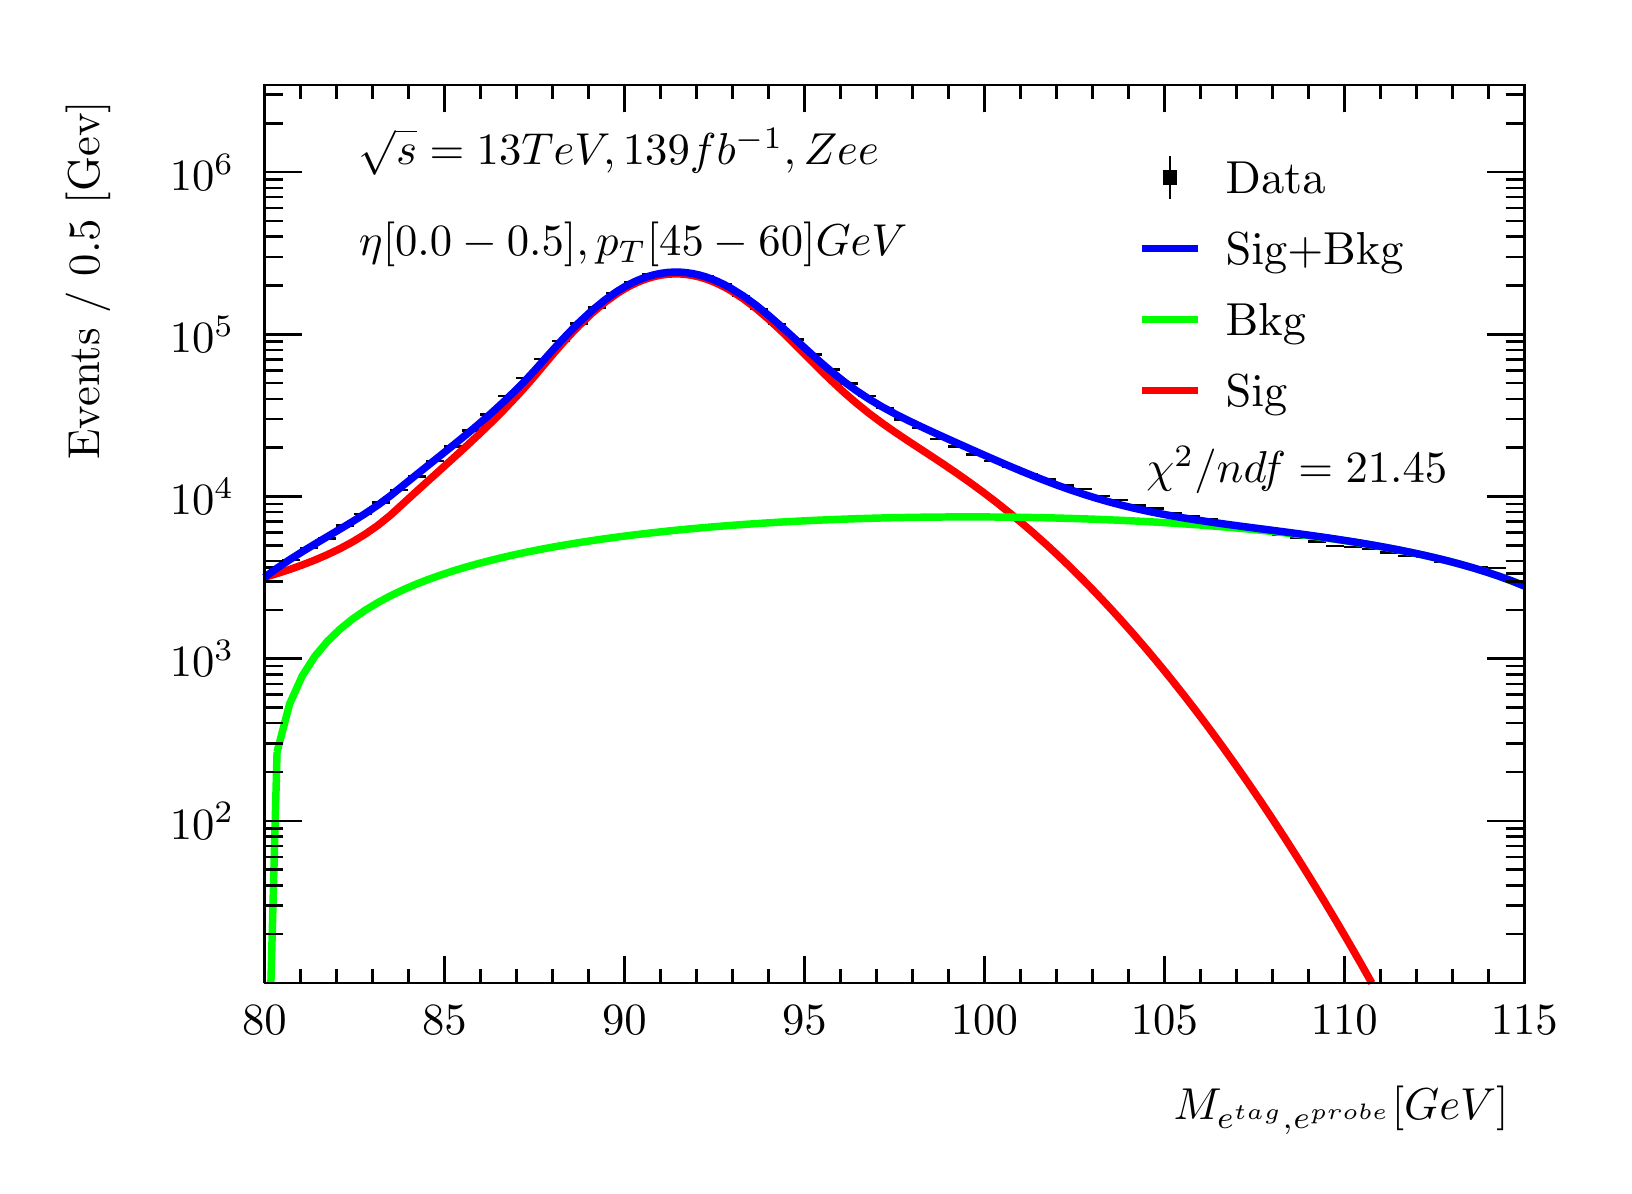
\begin{tikzpicture}
\pgfdeclareplotmark{cross} {
\pgfpathmoveto{\pgfpoint{-0.3\pgfplotmarksize}{\pgfplotmarksize}}
\pgfpathlineto{\pgfpoint{+0.3\pgfplotmarksize}{\pgfplotmarksize}}
\pgfpathlineto{\pgfpoint{+0.3\pgfplotmarksize}{0.3\pgfplotmarksize}}
\pgfpathlineto{\pgfpoint{+1\pgfplotmarksize}{0.3\pgfplotmarksize}}
\pgfpathlineto{\pgfpoint{+1\pgfplotmarksize}{-0.3\pgfplotmarksize}}
\pgfpathlineto{\pgfpoint{+0.3\pgfplotmarksize}{-0.3\pgfplotmarksize}}
\pgfpathlineto{\pgfpoint{+0.3\pgfplotmarksize}{-1.\pgfplotmarksize}}
\pgfpathlineto{\pgfpoint{-0.3\pgfplotmarksize}{-1.\pgfplotmarksize}}
\pgfpathlineto{\pgfpoint{-0.3\pgfplotmarksize}{-0.3\pgfplotmarksize}}
\pgfpathlineto{\pgfpoint{-1.\pgfplotmarksize}{-0.3\pgfplotmarksize}}
\pgfpathlineto{\pgfpoint{-1.\pgfplotmarksize}{0.3\pgfplotmarksize}}
\pgfpathlineto{\pgfpoint{-0.3\pgfplotmarksize}{0.3\pgfplotmarksize}}
\pgfpathclose
\pgfusepathqstroke
}
\pgfdeclareplotmark{cross*} {
\pgfpathmoveto{\pgfpoint{-0.3\pgfplotmarksize}{\pgfplotmarksize}}
\pgfpathlineto{\pgfpoint{+0.3\pgfplotmarksize}{\pgfplotmarksize}}
\pgfpathlineto{\pgfpoint{+0.3\pgfplotmarksize}{0.3\pgfplotmarksize}}
\pgfpathlineto{\pgfpoint{+1\pgfplotmarksize}{0.3\pgfplotmarksize}}
\pgfpathlineto{\pgfpoint{+1\pgfplotmarksize}{-0.3\pgfplotmarksize}}
\pgfpathlineto{\pgfpoint{+0.3\pgfplotmarksize}{-0.3\pgfplotmarksize}}
\pgfpathlineto{\pgfpoint{+0.3\pgfplotmarksize}{-1.\pgfplotmarksize}}
\pgfpathlineto{\pgfpoint{-0.3\pgfplotmarksize}{-1.\pgfplotmarksize}}
\pgfpathlineto{\pgfpoint{-0.3\pgfplotmarksize}{-0.3\pgfplotmarksize}}
\pgfpathlineto{\pgfpoint{-1.\pgfplotmarksize}{-0.3\pgfplotmarksize}}
\pgfpathlineto{\pgfpoint{-1.\pgfplotmarksize}{0.3\pgfplotmarksize}}
\pgfpathlineto{\pgfpoint{-0.3\pgfplotmarksize}{0.3\pgfplotmarksize}}
\pgfpathclose
\pgfusepathqfillstroke
}
\pgfdeclareplotmark{newstar} {
\pgfpathmoveto{\pgfqpoint{0pt}{\pgfplotmarksize}}
\pgfpathlineto{\pgfqpointpolar{44}{0.5\pgfplotmarksize}}
\pgfpathlineto{\pgfqpointpolar{18}{\pgfplotmarksize}}
\pgfpathlineto{\pgfqpointpolar{-20}{0.5\pgfplotmarksize}}
\pgfpathlineto{\pgfqpointpolar{-54}{\pgfplotmarksize}}
\pgfpathlineto{\pgfqpointpolar{-90}{0.5\pgfplotmarksize}}
\pgfpathlineto{\pgfqpointpolar{234}{\pgfplotmarksize}}
\pgfpathlineto{\pgfqpointpolar{198}{0.5\pgfplotmarksize}}
\pgfpathlineto{\pgfqpointpolar{162}{\pgfplotmarksize}}
\pgfpathlineto{\pgfqpointpolar{134}{0.5\pgfplotmarksize}}
\pgfpathclose
\pgfusepathqstroke
}
\pgfdeclareplotmark{newstar*} {
\pgfpathmoveto{\pgfqpoint{0pt}{\pgfplotmarksize}}
\pgfpathlineto{\pgfqpointpolar{44}{0.5\pgfplotmarksize}}
\pgfpathlineto{\pgfqpointpolar{18}{\pgfplotmarksize}}
\pgfpathlineto{\pgfqpointpolar{-20}{0.5\pgfplotmarksize}}
\pgfpathlineto{\pgfqpointpolar{-54}{\pgfplotmarksize}}
\pgfpathlineto{\pgfqpointpolar{-90}{0.5\pgfplotmarksize}}
\pgfpathlineto{\pgfqpointpolar{234}{\pgfplotmarksize}}
\pgfpathlineto{\pgfqpointpolar{198}{0.5\pgfplotmarksize}}
\pgfpathlineto{\pgfqpointpolar{162}{\pgfplotmarksize}}
\pgfpathlineto{\pgfqpointpolar{134}{0.5\pgfplotmarksize}}
\pgfpathclose
\pgfusepathqfillstroke
}
\definecolor{c}{rgb}{1,1,1};
\draw [color=c, fill=c] (0,0) rectangle (20,14.4361);
\draw [color=c, fill=c] (3,2.30977) rectangle (19,13.7143);
\definecolor{c}{rgb}{0,0,0};
\draw [c,line width=0.9] (3,2.30977) -- (3,13.7143) -- (19,13.7143) -- (19,2.30977) -- (3,2.30977);
\definecolor{c}{rgb}{1,1,1};
\draw [color=c, fill=c] (3,2.30977) rectangle (19,13.7143);
\definecolor{c}{rgb}{0,0,0};
\draw [c,line width=0.9] (3,2.30977) -- (3,13.7143) -- (19,13.7143) -- (19,2.30977) -- (3,2.30977);
\draw [c,line width=0.9] (3,2.30977) -- (19,2.30977);
\draw [c,line width=0.9] (3,2.65624) -- (3,2.30977);
\draw [c,line width=0.9] (3.45714,2.48301) -- (3.45714,2.30977);
\draw [c,line width=0.9] (3.91429,2.48301) -- (3.91429,2.30977);
\draw [c,line width=0.9] (4.37143,2.48301) -- (4.37143,2.30977);
\draw [c,line width=0.9] (4.82857,2.48301) -- (4.82857,2.30977);
\draw [c,line width=0.9] (5.28571,2.65624) -- (5.28571,2.30977);
\draw [c,line width=0.9] (5.74286,2.48301) -- (5.74286,2.30977);
\draw [c,line width=0.9] (6.2,2.48301) -- (6.2,2.30977);
\draw [c,line width=0.9] (6.65714,2.48301) -- (6.65714,2.30977);
\draw [c,line width=0.9] (7.11429,2.48301) -- (7.11429,2.30977);
\draw [c,line width=0.9] (7.57143,2.65624) -- (7.57143,2.30977);
\draw [c,line width=0.9] (8.02857,2.48301) -- (8.02857,2.30977);
\draw [c,line width=0.9] (8.48571,2.48301) -- (8.48571,2.30977);
\draw [c,line width=0.9] (8.94286,2.48301) -- (8.94286,2.30977);
\draw [c,line width=0.9] (9.4,2.48301) -- (9.4,2.30977);
\draw [c,line width=0.9] (9.85714,2.65624) -- (9.85714,2.30977);
\draw [c,line width=0.9] (10.3143,2.48301) -- (10.3143,2.30977);
\draw [c,line width=0.9] (10.7714,2.48301) -- (10.7714,2.30977);
\draw [c,line width=0.9] (11.2286,2.48301) -- (11.2286,2.30977);
\draw [c,line width=0.9] (11.6857,2.48301) -- (11.6857,2.30977);
\draw [c,line width=0.9] (12.1429,2.65624) -- (12.1429,2.30977);
\draw [c,line width=0.9] (12.6,2.48301) -- (12.6,2.30977);
\draw [c,line width=0.9] (13.0571,2.48301) -- (13.0571,2.30977);
\draw [c,line width=0.9] (13.5143,2.48301) -- (13.5143,2.30977);
\draw [c,line width=0.9] (13.9714,2.48301) -- (13.9714,2.30977);
\draw [c,line width=0.9] (14.4286,2.65624) -- (14.4286,2.30977);
\draw [c,line width=0.9] (14.8857,2.48301) -- (14.8857,2.30977);
\draw [c,line width=0.9] (15.3429,2.48301) -- (15.3429,2.30977);
\draw [c,line width=0.9] (15.8,2.48301) -- (15.8,2.30977);
\draw [c,line width=0.9] (16.2571,2.48301) -- (16.2571,2.30977);
\draw [c,line width=0.9] (16.7143,2.65624) -- (16.7143,2.30977);
\draw [c,line width=0.9] (17.1714,2.48301) -- (17.1714,2.30977);
\draw [c,line width=0.9] (17.6286,2.48301) -- (17.6286,2.30977);
\draw [c,line width=0.9] (18.0857,2.48301) -- (18.0857,2.30977);
\draw [c,line width=0.9] (18.5429,2.48301) -- (18.5429,2.30977);
\draw [c,line width=0.9] (19,2.65624) -- (19,2.30977);
\draw [anchor=base] (3,1.66015) node[scale=1.61424, color=c, rotate=0]{80};
\draw [anchor=base] (5.28571,1.66015) node[scale=1.61424, color=c, rotate=0]{85};
\draw [anchor=base] (7.57143,1.66015) node[scale=1.61424, color=c, rotate=0]{90};
\draw [anchor=base] (9.85714,1.66015) node[scale=1.61424, color=c, rotate=0]{95};
\draw [anchor=base] (12.1429,1.66015) node[scale=1.61424, color=c, rotate=0]{100};
\draw [anchor=base] (14.4286,1.66015) node[scale=1.61424, color=c, rotate=0]{105};
\draw [anchor=base] (16.7143,1.66015) node[scale=1.61424, color=c, rotate=0]{110};
\draw [anchor=base] (19,1.66015) node[scale=1.61424, color=c, rotate=0]{115};
\draw [anchor= east] (19,0.692932) node[scale=1.61424, color=c, rotate=0]{$M_{e^{tag}, e^{probe}}  [GeV]$};
\draw [c,line width=0.9] (3,13.7143) -- (19,13.7143);
\draw [c,line width=0.9] (3,13.3678) -- (3,13.7143);
\draw [c,line width=0.9] (3.45714,13.5411) -- (3.45714,13.7143);
\draw [c,line width=0.9] (3.91429,13.5411) -- (3.91429,13.7143);
\draw [c,line width=0.9] (4.37143,13.5411) -- (4.37143,13.7143);
\draw [c,line width=0.9] (4.82857,13.5411) -- (4.82857,13.7143);
\draw [c,line width=0.9] (5.28571,13.3678) -- (5.28571,13.7143);
\draw [c,line width=0.9] (5.74286,13.5411) -- (5.74286,13.7143);
\draw [c,line width=0.9] (6.2,13.5411) -- (6.2,13.7143);
\draw [c,line width=0.9] (6.65714,13.5411) -- (6.65714,13.7143);
\draw [c,line width=0.9] (7.11429,13.5411) -- (7.11429,13.7143);
\draw [c,line width=0.9] (7.57143,13.3678) -- (7.57143,13.7143);
\draw [c,line width=0.9] (8.02857,13.5411) -- (8.02857,13.7143);
\draw [c,line width=0.9] (8.48571,13.5411) -- (8.48571,13.7143);
\draw [c,line width=0.9] (8.94286,13.5411) -- (8.94286,13.7143);
\draw [c,line width=0.9] (9.4,13.5411) -- (9.4,13.7143);
\draw [c,line width=0.9] (9.85714,13.3678) -- (9.85714,13.7143);
\draw [c,line width=0.9] (10.3143,13.5411) -- (10.3143,13.7143);
\draw [c,line width=0.9] (10.7714,13.5411) -- (10.7714,13.7143);
\draw [c,line width=0.9] (11.2286,13.5411) -- (11.2286,13.7143);
\draw [c,line width=0.9] (11.6857,13.5411) -- (11.6857,13.7143);
\draw [c,line width=0.9] (12.1429,13.3678) -- (12.1429,13.7143);
\draw [c,line width=0.9] (12.6,13.5411) -- (12.6,13.7143);
\draw [c,line width=0.9] (13.0571,13.5411) -- (13.0571,13.7143);
\draw [c,line width=0.9] (13.5143,13.5411) -- (13.5143,13.7143);
\draw [c,line width=0.9] (13.9714,13.5411) -- (13.9714,13.7143);
\draw [c,line width=0.9] (14.4286,13.3678) -- (14.4286,13.7143);
\draw [c,line width=0.9] (14.8857,13.5411) -- (14.8857,13.7143);
\draw [c,line width=0.9] (15.3429,13.5411) -- (15.3429,13.7143);
\draw [c,line width=0.9] (15.8,13.5411) -- (15.8,13.7143);
\draw [c,line width=0.9] (16.2571,13.5411) -- (16.2571,13.7143);
\draw [c,line width=0.9] (16.7143,13.3678) -- (16.7143,13.7143);
\draw [c,line width=0.9] (17.1714,13.5411) -- (17.1714,13.7143);
\draw [c,line width=0.9] (17.6286,13.5411) -- (17.6286,13.7143);
\draw [c,line width=0.9] (18.0857,13.5411) -- (18.0857,13.7143);
\draw [c,line width=0.9] (18.5429,13.5411) -- (18.5429,13.7143);
\draw [c,line width=0.9] (19,13.3678) -- (19,13.7143);
\draw [c,line width=0.9] (3,2.30977) -- (3,13.7143);
\draw [c,line width=0.9] (3.237,2.92982) -- (3,2.92982);
\draw [c,line width=0.9] (3.237,3.29252) -- (3,3.29252);
\draw [c,line width=0.9] (3.237,3.54986) -- (3,3.54986);
\draw [c,line width=0.9] (3.237,3.74947) -- (3,3.74947);
\draw [c,line width=0.9] (3.237,3.91257) -- (3,3.91257);
\draw [c,line width=0.9] (3.237,4.05046) -- (3,4.05046);
\draw [c,line width=0.9] (3.237,4.16991) -- (3,4.16991);
\draw [c,line width=0.9] (3.237,4.27527) -- (3,4.27527);
\draw [c,line width=0.9] (3.474,4.36952) -- (3,4.36952);
\draw [anchor= east] (2.82,4.36952) node[scale=1.61424, color=c, rotate=0]{$10^{2}$};
\draw [c,line width=0.9] (3.237,4.98956) -- (3,4.98956);
\draw [c,line width=0.9] (3.237,5.35227) -- (3,5.35227);
\draw [c,line width=0.9] (3.237,5.60961) -- (3,5.60961);
\draw [c,line width=0.9] (3.237,5.80922) -- (3,5.80922);
\draw [c,line width=0.9] (3.237,5.97231) -- (3,5.97231);
\draw [c,line width=0.9] (3.237,6.11021) -- (3,6.11021);
\draw [c,line width=0.9] (3.237,6.22966) -- (3,6.22966);
\draw [c,line width=0.9] (3.237,6.33502) -- (3,6.33502);
\draw [c,line width=0.9] (3.474,6.42927) -- (3,6.42927);
\draw [anchor= east] (2.82,6.42927) node[scale=1.61424, color=c, rotate=0]{$10^{3}$};
\draw [c,line width=0.9] (3.237,7.04931) -- (3,7.04931);
\draw [c,line width=0.9] (3.237,7.41202) -- (3,7.41202);
\draw [c,line width=0.9] (3.237,7.66936) -- (3,7.66936);
\draw [c,line width=0.9] (3.237,7.86897) -- (3,7.86897);
\draw [c,line width=0.9] (3.237,8.03206) -- (3,8.03206);
\draw [c,line width=0.9] (3.237,8.16995) -- (3,8.16995);
\draw [c,line width=0.9] (3.237,8.2894) -- (3,8.2894);
\draw [c,line width=0.9] (3.237,8.39476) -- (3,8.39476);
\draw [c,line width=0.9] (3.474,8.48901) -- (3,8.48901);
\draw [anchor= east] (2.82,8.48901) node[scale=1.61424, color=c, rotate=0]{$10^{4}$};
\draw [c,line width=0.9] (3.237,9.10906) -- (3,9.10906);
\draw [c,line width=0.9] (3.237,9.47176) -- (3,9.47176);
\draw [c,line width=0.9] (3.237,9.7291) -- (3,9.7291);
\draw [c,line width=0.9] (3.237,9.92871) -- (3,9.92871);
\draw [c,line width=0.9] (3.237,10.0918) -- (3,10.0918);
\draw [c,line width=0.9] (3.237,10.2297) -- (3,10.2297);
\draw [c,line width=0.9] (3.237,10.3491) -- (3,10.3491);
\draw [c,line width=0.9] (3.237,10.4545) -- (3,10.4545);
\draw [c,line width=0.9] (3.474,10.5488) -- (3,10.5488);
\draw [anchor= east] (2.82,10.5488) node[scale=1.61424, color=c, rotate=0]{$10^{5}$};
\draw [c,line width=0.9] (3.237,11.1688) -- (3,11.1688);
\draw [c,line width=0.9] (3.237,11.5315) -- (3,11.5315);
\draw [c,line width=0.9] (3.237,11.7889) -- (3,11.7889);
\draw [c,line width=0.9] (3.237,11.9885) -- (3,11.9885);
\draw [c,line width=0.9] (3.237,12.1516) -- (3,12.1516);
\draw [c,line width=0.9] (3.237,12.2894) -- (3,12.2894);
\draw [c,line width=0.9] (3.237,12.4089) -- (3,12.4089);
\draw [c,line width=0.9] (3.237,12.5143) -- (3,12.5143);
\draw [c,line width=0.9] (3.474,12.6085) -- (3,12.6085);
\draw [anchor= east] (2.82,12.6085) node[scale=1.61424, color=c, rotate=0]{$10^{6}$};
\draw [c,line width=0.9] (3.237,13.2286) -- (3,13.2286);
\draw [c,line width=0.9] (3.237,13.5913) -- (3,13.5913);
\draw [anchor= east] (0.76,13.7143) node[scale=1.61424, color=c, rotate=90]{Events / 0.5 [Gev]};
\draw [c,line width=0.9] (19,2.30977) -- (19,13.7143);
\draw [c,line width=0.9] (18.763,2.92982) -- (19,2.92982);
\draw [c,line width=0.9] (18.763,3.29252) -- (19,3.29252);
\draw [c,line width=0.9] (18.763,3.54986) -- (19,3.54986);
\draw [c,line width=0.9] (18.763,3.74947) -- (19,3.74947);
\draw [c,line width=0.9] (18.763,3.91257) -- (19,3.91257);
\draw [c,line width=0.9] (18.763,4.05046) -- (19,4.05046);
\draw [c,line width=0.9] (18.763,4.16991) -- (19,4.16991);
\draw [c,line width=0.9] (18.763,4.27527) -- (19,4.27527);
\draw [c,line width=0.9] (18.526,4.36952) -- (19,4.36952);
\draw [c,line width=0.9] (18.763,4.98956) -- (19,4.98956);
\draw [c,line width=0.9] (18.763,5.35227) -- (19,5.35227);
\draw [c,line width=0.9] (18.763,5.60961) -- (19,5.60961);
\draw [c,line width=0.9] (18.763,5.80922) -- (19,5.80922);
\draw [c,line width=0.9] (18.763,5.97231) -- (19,5.97231);
\draw [c,line width=0.9] (18.763,6.11021) -- (19,6.11021);
\draw [c,line width=0.9] (18.763,6.22966) -- (19,6.22966);
\draw [c,line width=0.9] (18.763,6.33502) -- (19,6.33502);
\draw [c,line width=0.9] (18.526,6.42927) -- (19,6.42927);
\draw [c,line width=0.9] (18.763,7.04931) -- (19,7.04931);
\draw [c,line width=0.9] (18.763,7.41202) -- (19,7.41202);
\draw [c,line width=0.9] (18.763,7.66936) -- (19,7.66936);
\draw [c,line width=0.9] (18.763,7.86897) -- (19,7.86897);
\draw [c,line width=0.9] (18.763,8.03206) -- (19,8.03206);
\draw [c,line width=0.9] (18.763,8.16995) -- (19,8.16995);
\draw [c,line width=0.9] (18.763,8.2894) -- (19,8.2894);
\draw [c,line width=0.9] (18.763,8.39476) -- (19,8.39476);
\draw [c,line width=0.9] (18.526,8.48901) -- (19,8.48901);
\draw [c,line width=0.9] (18.763,9.10906) -- (19,9.10906);
\draw [c,line width=0.9] (18.763,9.47176) -- (19,9.47176);
\draw [c,line width=0.9] (18.763,9.7291) -- (19,9.7291);
\draw [c,line width=0.9] (18.763,9.92871) -- (19,9.92871);
\draw [c,line width=0.9] (18.763,10.0918) -- (19,10.0918);
\draw [c,line width=0.9] (18.763,10.2297) -- (19,10.2297);
\draw [c,line width=0.9] (18.763,10.3491) -- (19,10.3491);
\draw [c,line width=0.9] (18.763,10.4545) -- (19,10.4545);
\draw [c,line width=0.9] (18.526,10.5488) -- (19,10.5488);
\draw [c,line width=0.9] (18.763,11.1688) -- (19,11.1688);
\draw [c,line width=0.9] (18.763,11.5315) -- (19,11.5315);
\draw [c,line width=0.9] (18.763,11.7889) -- (19,11.7889);
\draw [c,line width=0.9] (18.763,11.9885) -- (19,11.9885);
\draw [c,line width=0.9] (18.763,12.1516) -- (19,12.1516);
\draw [c,line width=0.9] (18.763,12.2894) -- (19,12.2894);
\draw [c,line width=0.9] (18.763,12.4089) -- (19,12.4089);
\draw [c,line width=0.9] (18.763,12.5143) -- (19,12.5143);
\draw [c,line width=0.9] (18.526,12.6085) -- (19,12.6085);
\draw [c,line width=0.9] (18.763,13.2286) -- (19,13.2286);
\draw [c,line width=0.9] (18.763,13.5913) -- (19,13.5913);
\draw [c,line width=0.9] (3.11429,7.58647) -- (3,7.58647);
\draw [c,line width=0.9] (3,7.58647) -- (3,7.58647);
\draw [c,line width=0.9] (3.11429,7.58647) -- (3.22857,7.58647);
\draw [c,line width=0.9] (3.22857,7.58647) -- (3.22857,7.58647);
\draw [c,line width=0.9] (3.11429,7.58647) -- (3.11429,7.60128);
\draw [c,line width=0.9] (3.11429,7.60128) -- (3.11429,7.60128);
\draw [c,line width=0.9] (3.11429,7.58647) -- (3.11429,7.57165);
\draw [c,line width=0.9] (3.11429,7.57165) -- (3.11429,7.57165);
\draw [c,line width=0.9] (3.34286,7.68466) -- (3.22857,7.68466);
\draw [c,line width=0.9] (3.22857,7.68466) -- (3.22857,7.68466);
\draw [c,line width=0.9] (3.34286,7.68466) -- (3.45714,7.68466);
\draw [c,line width=0.9] (3.45714,7.68466) -- (3.45714,7.68466);
\draw [c,line width=0.9] (3.34286,7.68466) -- (3.34286,7.69868);
\draw [c,line width=0.9] (3.34286,7.69868) -- (3.34286,7.69868);
\draw [c,line width=0.9] (3.34286,7.68466) -- (3.34286,7.67063);
\draw [c,line width=0.9] (3.34286,7.67063) -- (3.34286,7.67063);
\draw [c,line width=0.9] (3.57143,7.83413) -- (3.45714,7.83413);
\draw [c,line width=0.9] (3.45714,7.83413) -- (3.45714,7.83413);
\draw [c,line width=0.9] (3.57143,7.83413) -- (3.68571,7.83413);
\draw [c,line width=0.9] (3.68571,7.83413) -- (3.68571,7.83413);
\draw [c,line width=0.9] (3.57143,7.83413) -- (3.57143,7.84703);
\draw [c,line width=0.9] (3.57143,7.84703) -- (3.57143,7.84703);
\draw [c,line width=0.9] (3.57143,7.83413) -- (3.57143,7.82123);
\draw [c,line width=0.9] (3.57143,7.82123) -- (3.57143,7.82123);
\draw [c,line width=0.9] (3.8,7.95861) -- (3.68571,7.95861);
\draw [c,line width=0.9] (3.68571,7.95861) -- (3.68571,7.95861);
\draw [c,line width=0.9] (3.8,7.95861) -- (3.91429,7.95861);
\draw [c,line width=0.9] (3.91429,7.95861) -- (3.91429,7.95861);
\draw [c,line width=0.9] (3.8,7.95861) -- (3.8,7.97064);
\draw [c,line width=0.9] (3.8,7.97064) -- (3.8,7.97064);
\draw [c,line width=0.9] (3.8,7.95861) -- (3.8,7.94658);
\draw [c,line width=0.9] (3.8,7.94658) -- (3.8,7.94658);
\draw [c,line width=0.9] (4.02857,8.118) -- (3.91429,8.118);
\draw [c,line width=0.9] (3.91429,8.118) -- (3.91429,8.118);
\draw [c,line width=0.9] (4.02857,8.118) -- (4.14286,8.118);
\draw [c,line width=0.9] (4.14286,8.118) -- (4.14286,8.118);
\draw [c,line width=0.9] (4.02857,8.118) -- (4.02857,8.129);
\draw [c,line width=0.9] (4.02857,8.129) -- (4.02857,8.129);
\draw [c,line width=0.9] (4.02857,8.118) -- (4.02857,8.10699);
\draw [c,line width=0.9] (4.02857,8.10699) -- (4.02857,8.10699);
\draw [c,line width=0.9] (4.25714,8.26354) -- (4.14286,8.26354);
\draw [c,line width=0.9] (4.14286,8.26354) -- (4.14286,8.26354);
\draw [c,line width=0.9] (4.25714,8.26354) -- (4.37143,8.26354);
\draw [c,line width=0.9] (4.37143,8.26354) -- (4.37143,8.26354);
\draw [c,line width=0.9] (4.25714,8.26354) -- (4.25714,8.27369);
\draw [c,line width=0.9] (4.25714,8.27369) -- (4.25714,8.27369);
\draw [c,line width=0.9] (4.25714,8.26354) -- (4.25714,8.25339);
\draw [c,line width=0.9] (4.25714,8.25339) -- (4.25714,8.25339);
\draw [c,line width=0.9] (4.48571,8.41189) -- (4.37143,8.41189);
\draw [c,line width=0.9] (4.37143,8.41189) -- (4.37143,8.41189);
\draw [c,line width=0.9] (4.48571,8.41189) -- (4.6,8.41189);
\draw [c,line width=0.9] (4.6,8.41189) -- (4.6,8.41189);
\draw [c,line width=0.9] (4.48571,8.41189) -- (4.48571,8.42123);
\draw [c,line width=0.9] (4.48571,8.42123) -- (4.48571,8.42123);
\draw [c,line width=0.9] (4.48571,8.41189) -- (4.48571,8.40256);
\draw [c,line width=0.9] (4.48571,8.40256) -- (4.48571,8.40256);
\draw [c,line width=0.9] (4.71429,8.5702) -- (4.6,8.5702);
\draw [c,line width=0.9] (4.6,8.5702) -- (4.6,8.5702);
\draw [c,line width=0.9] (4.71429,8.5702) -- (4.82857,8.5702);
\draw [c,line width=0.9] (4.82857,8.5702) -- (4.82857,8.5702);
\draw [c,line width=0.9] (4.71429,8.5702) -- (4.71429,8.57875);
\draw [c,line width=0.9] (4.71429,8.57875) -- (4.71429,8.57875);
\draw [c,line width=0.9] (4.71429,8.5702) -- (4.71429,8.56165);
\draw [c,line width=0.9] (4.71429,8.56165) -- (4.71429,8.56165);
\draw [c,line width=0.9] (4.94286,8.74338) -- (4.82857,8.74338);
\draw [c,line width=0.9] (4.82857,8.74338) -- (4.82857,8.74338);
\draw [c,line width=0.9] (4.94286,8.74338) -- (5.05714,8.74338);
\draw [c,line width=0.9] (5.05714,8.74338) -- (5.05714,8.74338);
\draw [c,line width=0.9] (4.94286,8.74338) -- (4.94286,8.75114);
\draw [c,line width=0.9] (4.94286,8.75114) -- (4.94286,8.75114);
\draw [c,line width=0.9] (4.94286,8.74338) -- (4.94286,8.73562);
\draw [c,line width=0.9] (4.94286,8.73562) -- (4.94286,8.73562);
\draw [c,line width=0.9] (5.17143,8.93957) -- (5.05714,8.93957);
\draw [c,line width=0.9] (5.05714,8.93957) -- (5.05714,8.93957);
\draw [c,line width=0.9] (5.17143,8.93957) -- (5.28571,8.93957);
\draw [c,line width=0.9] (5.28571,8.93957) -- (5.28571,8.93957);
\draw [c,line width=0.9] (5.17143,8.93957) -- (5.17143,8.94653);
\draw [c,line width=0.9] (5.17143,8.94653) -- (5.17143,8.94653);
\draw [c,line width=0.9] (5.17143,8.93957) -- (5.17143,8.93262);
\draw [c,line width=0.9] (5.17143,8.93262) -- (5.17143,8.93262);
\draw [c,line width=0.9] (5.4,9.12594) -- (5.28571,9.12594);
\draw [c,line width=0.9] (5.28571,9.12594) -- (5.28571,9.12594);
\draw [c,line width=0.9] (5.4,9.12594) -- (5.51429,9.12594);
\draw [c,line width=0.9] (5.51429,9.12594) -- (5.51429,9.12594);
\draw [c,line width=0.9] (5.4,9.12594) -- (5.4,9.13221);
\draw [c,line width=0.9] (5.4,9.13221) -- (5.4,9.13221);
\draw [c,line width=0.9] (5.4,9.12594) -- (5.4,9.11967);
\draw [c,line width=0.9] (5.4,9.11967) -- (5.4,9.11967);
\draw [c,line width=0.9] (5.62857,9.32751) -- (5.51429,9.32751);
\draw [c,line width=0.9] (5.51429,9.32751) -- (5.51429,9.32751);
\draw [c,line width=0.9] (5.62857,9.32751) -- (5.74286,9.32751);
\draw [c,line width=0.9] (5.74286,9.32751) -- (5.74286,9.32751);
\draw [c,line width=0.9] (5.62857,9.32751) -- (5.62857,9.3331);
\draw [c,line width=0.9] (5.62857,9.3331) -- (5.62857,9.3331);
\draw [c,line width=0.9] (5.62857,9.32751) -- (5.62857,9.32191);
\draw [c,line width=0.9] (5.62857,9.32191) -- (5.62857,9.32191);
\draw [c,line width=0.9] (5.85714,9.53) -- (5.74286,9.53);
\draw [c,line width=0.9] (5.74286,9.53) -- (5.74286,9.53);
\draw [c,line width=0.9] (5.85714,9.53) -- (5.97143,9.53);
\draw [c,line width=0.9] (5.97143,9.53) -- (5.97143,9.53);
\draw [c,line width=0.9] (5.85714,9.53) -- (5.85714,9.535);
\draw [c,line width=0.9] (5.85714,9.535) -- (5.85714,9.535);
\draw [c,line width=0.9] (5.85714,9.53) -- (5.85714,9.525);
\draw [c,line width=0.9] (5.85714,9.525) -- (5.85714,9.525);
\draw [c,line width=0.9] (6.08571,9.76837) -- (5.97143,9.76837);
\draw [c,line width=0.9] (5.97143,9.76837) -- (5.97143,9.76837);
\draw [c,line width=0.9] (6.08571,9.76837) -- (6.2,9.76837);
\draw [c,line width=0.9] (6.2,9.76837) -- (6.2,9.76837);
\draw [c,line width=0.9] (6.08571,9.76837) -- (6.08571,9.77275);
\draw [c,line width=0.9] (6.08571,9.77275) -- (6.08571,9.77275);
\draw [c,line width=0.9] (6.08571,9.76837) -- (6.08571,9.764);
\draw [c,line width=0.9] (6.08571,9.764) -- (6.08571,9.764);
\draw [c,line width=0.9] (6.31429,9.99199) -- (6.2,9.99199);
\draw [c,line width=0.9] (6.2,9.99199) -- (6.2,9.99199);
\draw [c,line width=0.9] (6.31429,9.99199) -- (6.42857,9.99199);
\draw [c,line width=0.9] (6.42857,9.99199) -- (6.42857,9.99199);
\draw [c,line width=0.9] (6.31429,9.99199) -- (6.31429,9.99585);
\draw [c,line width=0.9] (6.31429,9.99585) -- (6.31429,9.99585);
\draw [c,line width=0.9] (6.31429,9.99199) -- (6.31429,9.98813);
\draw [c,line width=0.9] (6.31429,9.98813) -- (6.31429,9.98813);
\draw [c,line width=0.9] (6.54286,10.2354) -- (6.42857,10.2354);
\draw [c,line width=0.9] (6.42857,10.2354) -- (6.42857,10.2354);
\draw [c,line width=0.9] (6.54286,10.2354) -- (6.65714,10.2354);
\draw [c,line width=0.9] (6.65714,10.2354) -- (6.65714,10.2354);
\draw [c,line width=0.9] (6.54286,10.2354) -- (6.54286,10.2387);
\draw [c,line width=0.9] (6.54286,10.2387) -- (6.54286,10.2387);
\draw [c,line width=0.9] (6.54286,10.2354) -- (6.54286,10.232);
\draw [c,line width=0.9] (6.54286,10.232) -- (6.54286,10.232);
\draw [c,line width=0.9] (6.77143,10.4629) -- (6.65714,10.4629);
\draw [c,line width=0.9] (6.65714,10.4629) -- (6.65714,10.4629);
\draw [c,line width=0.9] (6.77143,10.4629) -- (6.88571,10.4629);
\draw [c,line width=0.9] (6.88571,10.4629) -- (6.88571,10.4629);
\draw [c,line width=0.9] (6.77143,10.4629) -- (6.77143,10.4658);
\draw [c,line width=0.9] (6.77143,10.4658) -- (6.77143,10.4658);
\draw [c,line width=0.9] (6.77143,10.4629) -- (6.77143,10.4599);
\draw [c,line width=0.9] (6.77143,10.4599) -- (6.77143,10.4599);
\draw [c,line width=0.9] (7,10.6841) -- (6.88571,10.6841);
\draw [c,line width=0.9] (6.88571,10.6841) -- (6.88571,10.6841);
\draw [c,line width=0.9] (7,10.6841) -- (7.11429,10.6841);
\draw [c,line width=0.9] (7.11429,10.6841) -- (7.11429,10.6841);
\draw [c,line width=0.9] (7,10.6841) -- (7,10.6867);
\draw [c,line width=0.9] (7,10.6867) -- (7,10.6867);
\draw [c,line width=0.9] (7,10.6841) -- (7,10.6815);
\draw [c,line width=0.9] (7,10.6815) -- (7,10.6815);
\draw [c,line width=0.9] (7.22857,10.8887) -- (7.11429,10.8887);
\draw [c,line width=0.9] (7.11429,10.8887) -- (7.11429,10.8887);
\draw [c,line width=0.9] (7.22857,10.8887) -- (7.34286,10.8887);
\draw [c,line width=0.9] (7.34286,10.8887) -- (7.34286,10.8887);
\draw [c,line width=0.9] (7.22857,10.8887) -- (7.22857,10.891);
\draw [c,line width=0.9] (7.22857,10.891) -- (7.22857,10.891);
\draw [c,line width=0.9] (7.22857,10.8887) -- (7.22857,10.8863);
\draw [c,line width=0.9] (7.22857,10.8863) -- (7.22857,10.8863);
\draw [c,line width=0.9] (7.45714,11.0725) -- (7.34286,11.0725);
\draw [c,line width=0.9] (7.34286,11.0725) -- (7.34286,11.0725);
\draw [c,line width=0.9] (7.45714,11.0725) -- (7.57143,11.0725);
\draw [c,line width=0.9] (7.57143,11.0725) -- (7.57143,11.0725);
\draw [c,line width=0.9] (7.45714,11.0725) -- (7.45714,11.0746);
\draw [c,line width=0.9] (7.45714,11.0746) -- (7.45714,11.0746);
\draw [c,line width=0.9] (7.45714,11.0725) -- (7.45714,11.0704);
\draw [c,line width=0.9] (7.45714,11.0704) -- (7.45714,11.0704);
\draw [c,line width=0.9] (7.68571,11.2095) -- (7.57143,11.2095);
\draw [c,line width=0.9] (7.57143,11.2095) -- (7.57143,11.2095);
\draw [c,line width=0.9] (7.68571,11.2095) -- (7.8,11.2095);
\draw [c,line width=0.9] (7.8,11.2095) -- (7.8,11.2095);
\draw [c,line width=0.9] (7.68571,11.2095) -- (7.68571,11.2115);
\draw [c,line width=0.9] (7.68571,11.2115) -- (7.68571,11.2115);
\draw [c,line width=0.9] (7.68571,11.2095) -- (7.68571,11.2076);
\draw [c,line width=0.9] (7.68571,11.2076) -- (7.68571,11.2076);
\draw [c,line width=0.9] (7.91429,11.3058) -- (7.8,11.3058);
\draw [c,line width=0.9] (7.8,11.3058) -- (7.8,11.3058);
\draw [c,line width=0.9] (7.91429,11.3058) -- (8.02857,11.3058);
\draw [c,line width=0.9] (8.02857,11.3058) -- (8.02857,11.3058);
\draw [c,line width=0.9] (7.91429,11.3058) -- (7.91429,11.3076);
\draw [c,line width=0.9] (7.91429,11.3076) -- (7.91429,11.3076);
\draw [c,line width=0.9] (7.91429,11.3058) -- (7.91429,11.3039);
\draw [c,line width=0.9] (7.91429,11.3039) -- (7.91429,11.3039);
\draw [c,line width=0.9] (8.14286,11.3499) -- (8.02857,11.3499);
\draw [c,line width=0.9] (8.02857,11.3499) -- (8.02857,11.3499);
\draw [c,line width=0.9] (8.14286,11.3499) -- (8.25714,11.3499);
\draw [c,line width=0.9] (8.25714,11.3499) -- (8.25714,11.3499);
\draw [c,line width=0.9] (8.14286,11.3499) -- (8.14286,11.3517);
\draw [c,line width=0.9] (8.14286,11.3517) -- (8.14286,11.3517);
\draw [c,line width=0.9] (8.14286,11.3499) -- (8.14286,11.348);
\draw [c,line width=0.9] (8.14286,11.348) -- (8.14286,11.348);
\draw [c,line width=0.9] (8.37143,11.3424) -- (8.25714,11.3424);
\draw [c,line width=0.9] (8.25714,11.3424) -- (8.25714,11.3424);
\draw [c,line width=0.9] (8.37143,11.3424) -- (8.48571,11.3424);
\draw [c,line width=0.9] (8.48571,11.3424) -- (8.48571,11.3424);
\draw [c,line width=0.9] (8.37143,11.3424) -- (8.37143,11.3442);
\draw [c,line width=0.9] (8.37143,11.3442) -- (8.37143,11.3442);
\draw [c,line width=0.9] (8.37143,11.3424) -- (8.37143,11.3406);
\draw [c,line width=0.9] (8.37143,11.3406) -- (8.37143,11.3406);
\draw [c,line width=0.9] (8.6,11.2839) -- (8.48571,11.2839);
\draw [c,line width=0.9] (8.48571,11.2839) -- (8.48571,11.2839);
\draw [c,line width=0.9] (8.6,11.2839) -- (8.71429,11.2839);
\draw [c,line width=0.9] (8.71429,11.2839) -- (8.71429,11.2839);
\draw [c,line width=0.9] (8.6,11.2839) -- (8.6,11.2858);
\draw [c,line width=0.9] (8.6,11.2858) -- (8.6,11.2858);
\draw [c,line width=0.9] (8.6,11.2839) -- (8.6,11.2821);
\draw [c,line width=0.9] (8.6,11.2821) -- (8.6,11.2821);
\draw [c,line width=0.9] (8.82857,11.1805) -- (8.71429,11.1805);
\draw [c,line width=0.9] (8.71429,11.1805) -- (8.71429,11.1805);
\draw [c,line width=0.9] (8.82857,11.1805) -- (8.94286,11.1805);
\draw [c,line width=0.9] (8.94286,11.1805) -- (8.94286,11.1805);
\draw [c,line width=0.9] (8.82857,11.1805) -- (8.82857,11.1825);
\draw [c,line width=0.9] (8.82857,11.1825) -- (8.82857,11.1825);
\draw [c,line width=0.9] (8.82857,11.1805) -- (8.82857,11.1785);
\draw [c,line width=0.9] (8.82857,11.1785) -- (8.82857,11.1785);
\draw [c,line width=0.9] (9.05714,11.0348) -- (8.94286,11.0348);
\draw [c,line width=0.9] (8.94286,11.0348) -- (8.94286,11.0348);
\draw [c,line width=0.9] (9.05714,11.0348) -- (9.17143,11.0348);
\draw [c,line width=0.9] (9.17143,11.0348) -- (9.17143,11.0348);
\draw [c,line width=0.9] (9.05714,11.0348) -- (9.05714,11.037);
\draw [c,line width=0.9] (9.05714,11.037) -- (9.05714,11.037);
\draw [c,line width=0.9] (9.05714,11.0348) -- (9.05714,11.0326);
\draw [c,line width=0.9] (9.05714,11.0326) -- (9.05714,11.0326);
\draw [c,line width=0.9] (9.28571,10.8686) -- (9.17143,10.8686);
\draw [c,line width=0.9] (9.17143,10.8686) -- (9.17143,10.8686);
\draw [c,line width=0.9] (9.28571,10.8686) -- (9.4,10.8686);
\draw [c,line width=0.9] (9.4,10.8686) -- (9.4,10.8686);
\draw [c,line width=0.9] (9.28571,10.8686) -- (9.28571,10.8709);
\draw [c,line width=0.9] (9.28571,10.8709) -- (9.28571,10.8709);
\draw [c,line width=0.9] (9.28571,10.8686) -- (9.28571,10.8662);
\draw [c,line width=0.9] (9.28571,10.8662) -- (9.28571,10.8662);
\draw [c,line width=0.9] (9.51429,10.6793) -- (9.4,10.6793);
\draw [c,line width=0.9] (9.4,10.6793) -- (9.4,10.6793);
\draw [c,line width=0.9] (9.51429,10.6793) -- (9.62857,10.6793);
\draw [c,line width=0.9] (9.62857,10.6793) -- (9.62857,10.6793);
\draw [c,line width=0.9] (9.51429,10.6793) -- (9.51429,10.6819);
\draw [c,line width=0.9] (9.51429,10.6819) -- (9.51429,10.6819);
\draw [c,line width=0.9] (9.51429,10.6793) -- (9.51429,10.6766);
\draw [c,line width=0.9] (9.51429,10.6766) -- (9.51429,10.6766);
\draw [c,line width=0.9] (9.74286,10.4843) -- (9.62857,10.4843);
\draw [c,line width=0.9] (9.62857,10.4843) -- (9.62857,10.4843);
\draw [c,line width=0.9] (9.74286,10.4843) -- (9.85714,10.4843);
\draw [c,line width=0.9] (9.85714,10.4843) -- (9.85714,10.4843);
\draw [c,line width=0.9] (9.74286,10.4843) -- (9.74286,10.4872);
\draw [c,line width=0.9] (9.74286,10.4872) -- (9.74286,10.4872);
\draw [c,line width=0.9] (9.74286,10.4843) -- (9.74286,10.4814);
\draw [c,line width=0.9] (9.74286,10.4814) -- (9.74286,10.4814);
\draw [c,line width=0.9] (9.97143,10.2927) -- (9.85714,10.2927);
\draw [c,line width=0.9] (9.85714,10.2927) -- (9.85714,10.2927);
\draw [c,line width=0.9] (9.97143,10.2927) -- (10.0857,10.2927);
\draw [c,line width=0.9] (10.0857,10.2927) -- (10.0857,10.2927);
\draw [c,line width=0.9] (9.97143,10.2927) -- (9.97143,10.296);
\draw [c,line width=0.9] (9.97143,10.296) -- (9.97143,10.296);
\draw [c,line width=0.9] (9.97143,10.2927) -- (9.97143,10.2895);
\draw [c,line width=0.9] (9.97143,10.2895) -- (9.97143,10.2895);
\draw [c,line width=0.9] (10.2,10.1023) -- (10.0857,10.1023);
\draw [c,line width=0.9] (10.0857,10.1023) -- (10.0857,10.1023);
\draw [c,line width=0.9] (10.2,10.1023) -- (10.3143,10.1023);
\draw [c,line width=0.9] (10.3143,10.1023) -- (10.3143,10.1023);
\draw [c,line width=0.9] (10.2,10.1023) -- (10.2,10.1059);
\draw [c,line width=0.9] (10.2,10.1059) -- (10.2,10.1059);
\draw [c,line width=0.9] (10.2,10.1023) -- (10.2,10.0987);
\draw [c,line width=0.9] (10.2,10.0987) -- (10.2,10.0987);
\draw [c,line width=0.9] (10.4286,9.92126) -- (10.3143,9.92126);
\draw [c,line width=0.9] (10.3143,9.92126) -- (10.3143,9.92126);
\draw [c,line width=0.9] (10.4286,9.92126) -- (10.5429,9.92126);
\draw [c,line width=0.9] (10.5429,9.92126) -- (10.5429,9.92126);
\draw [c,line width=0.9] (10.4286,9.92126) -- (10.4286,9.92528);
\draw [c,line width=0.9] (10.4286,9.92528) -- (10.4286,9.92528);
\draw [c,line width=0.9] (10.4286,9.92126) -- (10.4286,9.91724);
\draw [c,line width=0.9] (10.4286,9.91724) -- (10.4286,9.91724);
\draw [c,line width=0.9] (10.6571,9.7638) -- (10.5429,9.7638);
\draw [c,line width=0.9] (10.5429,9.7638) -- (10.5429,9.7638);
\draw [c,line width=0.9] (10.6571,9.7638) -- (10.7714,9.7638);
\draw [c,line width=0.9] (10.7714,9.7638) -- (10.7714,9.7638);
\draw [c,line width=0.9] (10.6571,9.7638) -- (10.6571,9.76819);
\draw [c,line width=0.9] (10.6571,9.76819) -- (10.6571,9.76819);
\draw [c,line width=0.9] (10.6571,9.7638) -- (10.6571,9.75942);
\draw [c,line width=0.9] (10.6571,9.75942) -- (10.6571,9.75942);
\draw [c,line width=0.9] (10.8857,9.61001) -- (10.7714,9.61001);
\draw [c,line width=0.9] (10.7714,9.61001) -- (10.7714,9.61001);
\draw [c,line width=0.9] (10.8857,9.61001) -- (11,9.61001);
\draw [c,line width=0.9] (11,9.61001) -- (11,9.61001);
\draw [c,line width=0.9] (10.8857,9.61001) -- (10.8857,9.61479);
\draw [c,line width=0.9] (10.8857,9.61479) -- (10.8857,9.61479);
\draw [c,line width=0.9] (10.8857,9.61001) -- (10.8857,9.60523);
\draw [c,line width=0.9] (10.8857,9.60523) -- (10.8857,9.60523);
\draw [c,line width=0.9] (11.1143,9.46485) -- (11,9.46485);
\draw [c,line width=0.9] (11,9.46485) -- (11,9.46485);
\draw [c,line width=0.9] (11.1143,9.46485) -- (11.2286,9.46485);
\draw [c,line width=0.9] (11.2286,9.46485) -- (11.2286,9.46485);
\draw [c,line width=0.9] (11.1143,9.46485) -- (11.1143,9.47003);
\draw [c,line width=0.9] (11.1143,9.47003) -- (11.1143,9.47003);
\draw [c,line width=0.9] (11.1143,9.46485) -- (11.1143,9.45966);
\draw [c,line width=0.9] (11.1143,9.45966) -- (11.1143,9.45966);
\draw [c,line width=0.9] (11.3429,9.35677) -- (11.2286,9.35677);
\draw [c,line width=0.9] (11.2286,9.35677) -- (11.2286,9.35677);
\draw [c,line width=0.9] (11.3429,9.35677) -- (11.4571,9.35677);
\draw [c,line width=0.9] (11.4571,9.35677) -- (11.4571,9.35677);
\draw [c,line width=0.9] (11.3429,9.35677) -- (11.3429,9.36228);
\draw [c,line width=0.9] (11.3429,9.36228) -- (11.3429,9.36228);
\draw [c,line width=0.9] (11.3429,9.35677) -- (11.3429,9.35126);
\draw [c,line width=0.9] (11.3429,9.35126) -- (11.3429,9.35126);
\draw [c,line width=0.9] (11.5714,9.22135) -- (11.4571,9.22135);
\draw [c,line width=0.9] (11.4571,9.22135) -- (11.4571,9.22135);
\draw [c,line width=0.9] (11.5714,9.22135) -- (11.6857,9.22135);
\draw [c,line width=0.9] (11.6857,9.22135) -- (11.6857,9.22135);
\draw [c,line width=0.9] (11.5714,9.22135) -- (11.5714,9.22729);
\draw [c,line width=0.9] (11.5714,9.22729) -- (11.5714,9.22729);
\draw [c,line width=0.9] (11.5714,9.22135) -- (11.5714,9.21541);
\draw [c,line width=0.9] (11.5714,9.21541) -- (11.5714,9.21541);
\draw [c,line width=0.9] (11.8,9.12374) -- (11.6857,9.12374);
\draw [c,line width=0.9] (11.6857,9.12374) -- (11.6857,9.12374);
\draw [c,line width=0.9] (11.8,9.12374) -- (11.9143,9.12374);
\draw [c,line width=0.9] (11.9143,9.12374) -- (11.9143,9.12374);
\draw [c,line width=0.9] (11.8,9.12374) -- (11.8,9.13002);
\draw [c,line width=0.9] (11.8,9.13002) -- (11.8,9.13002);
\draw [c,line width=0.9] (11.8,9.12374) -- (11.8,9.11747);
\draw [c,line width=0.9] (11.8,9.11747) -- (11.8,9.11747);
\draw [c,line width=0.9] (12.0286,9.02361) -- (11.9143,9.02361);
\draw [c,line width=0.9] (11.9143,9.02361) -- (11.9143,9.02361);
\draw [c,line width=0.9] (12.0286,9.02361) -- (12.1429,9.02361);
\draw [c,line width=0.9] (12.1429,9.02361) -- (12.1429,9.02361);
\draw [c,line width=0.9] (12.0286,9.02361) -- (12.0286,9.03025);
\draw [c,line width=0.9] (12.0286,9.03025) -- (12.0286,9.03025);
\draw [c,line width=0.9] (12.0286,9.02361) -- (12.0286,9.01698);
\draw [c,line width=0.9] (12.0286,9.01698) -- (12.0286,9.01698);
\draw [c,line width=0.9] (12.2571,8.9379) -- (12.1429,8.9379);
\draw [c,line width=0.9] (12.1429,8.9379) -- (12.1429,8.9379);
\draw [c,line width=0.9] (12.2571,8.9379) -- (12.3714,8.9379);
\draw [c,line width=0.9] (12.3714,8.9379) -- (12.3714,8.9379);
\draw [c,line width=0.9] (12.2571,8.9379) -- (12.2571,8.94486);
\draw [c,line width=0.9] (12.2571,8.94486) -- (12.2571,8.94486);
\draw [c,line width=0.9] (12.2571,8.9379) -- (12.2571,8.93094);
\draw [c,line width=0.9] (12.2571,8.93094) -- (12.2571,8.93094);
\draw [c,line width=0.9] (12.4857,8.86144) -- (12.3714,8.86144);
\draw [c,line width=0.9] (12.3714,8.86144) -- (12.3714,8.86144);
\draw [c,line width=0.9] (12.4857,8.86144) -- (12.6,8.86144);
\draw [c,line width=0.9] (12.6,8.86144) -- (12.6,8.86144);
\draw [c,line width=0.9] (12.4857,8.86144) -- (12.4857,8.86871);
\draw [c,line width=0.9] (12.4857,8.86871) -- (12.4857,8.86871);
\draw [c,line width=0.9] (12.4857,8.86144) -- (12.4857,8.85418);
\draw [c,line width=0.9] (12.4857,8.85418) -- (12.4857,8.85418);
\draw [c,line width=0.9] (12.7143,8.77297) -- (12.6,8.77297);
\draw [c,line width=0.9] (12.6,8.77297) -- (12.6,8.77297);
\draw [c,line width=0.9] (12.7143,8.77297) -- (12.8286,8.77297);
\draw [c,line width=0.9] (12.8286,8.77297) -- (12.8286,8.77297);
\draw [c,line width=0.9] (12.7143,8.77297) -- (12.7143,8.7806);
\draw [c,line width=0.9] (12.7143,8.7806) -- (12.7143,8.7806);
\draw [c,line width=0.9] (12.7143,8.77297) -- (12.7143,8.76534);
\draw [c,line width=0.9] (12.7143,8.76534) -- (12.7143,8.76534);
\draw [c,line width=0.9] (12.9429,8.70325) -- (12.8286,8.70325);
\draw [c,line width=0.9] (12.8286,8.70325) -- (12.8286,8.70325);
\draw [c,line width=0.9] (12.9429,8.70325) -- (13.0571,8.70325);
\draw [c,line width=0.9] (13.0571,8.70325) -- (13.0571,8.70325);
\draw [c,line width=0.9] (12.9429,8.70325) -- (12.9429,8.71118);
\draw [c,line width=0.9] (12.9429,8.71118) -- (12.9429,8.71118);
\draw [c,line width=0.9] (12.9429,8.70325) -- (12.9429,8.69531);
\draw [c,line width=0.9] (12.9429,8.69531) -- (12.9429,8.69531);
\draw [c,line width=0.9] (13.1714,8.62785) -- (13.0571,8.62785);
\draw [c,line width=0.9] (13.0571,8.62785) -- (13.0571,8.62785);
\draw [c,line width=0.9] (13.1714,8.62785) -- (13.2857,8.62785);
\draw [c,line width=0.9] (13.2857,8.62785) -- (13.2857,8.62785);
\draw [c,line width=0.9] (13.1714,8.62785) -- (13.1714,8.63613);
\draw [c,line width=0.9] (13.1714,8.63613) -- (13.1714,8.63613);
\draw [c,line width=0.9] (13.1714,8.62785) -- (13.1714,8.61958);
\draw [c,line width=0.9] (13.1714,8.61958) -- (13.1714,8.61958);
\draw [c,line width=0.9] (13.4,8.58309) -- (13.2857,8.58309);
\draw [c,line width=0.9] (13.2857,8.58309) -- (13.2857,8.58309);
\draw [c,line width=0.9] (13.4,8.58309) -- (13.5143,8.58309);
\draw [c,line width=0.9] (13.5143,8.58309) -- (13.5143,8.58309);
\draw [c,line width=0.9] (13.4,8.58309) -- (13.4,8.59158);
\draw [c,line width=0.9] (13.4,8.59158) -- (13.4,8.59158);
\draw [c,line width=0.9] (13.4,8.58309) -- (13.4,8.57461);
\draw [c,line width=0.9] (13.4,8.57461) -- (13.4,8.57461);
\draw [c,line width=0.9] (13.6286,8.49676) -- (13.5143,8.49676);
\draw [c,line width=0.9] (13.5143,8.49676) -- (13.5143,8.49676);
\draw [c,line width=0.9] (13.6286,8.49676) -- (13.7429,8.49676);
\draw [c,line width=0.9] (13.7429,8.49676) -- (13.7429,8.49676);
\draw [c,line width=0.9] (13.6286,8.49676) -- (13.6286,8.50567);
\draw [c,line width=0.9] (13.6286,8.50567) -- (13.6286,8.50567);
\draw [c,line width=0.9] (13.6286,8.49676) -- (13.6286,8.48786);
\draw [c,line width=0.9] (13.6286,8.48786) -- (13.6286,8.48786);
\draw [c,line width=0.9] (13.8571,8.44238) -- (13.7429,8.44238);
\draw [c,line width=0.9] (13.7429,8.44238) -- (13.7429,8.44238);
\draw [c,line width=0.9] (13.8571,8.44238) -- (13.9714,8.44238);
\draw [c,line width=0.9] (13.9714,8.44238) -- (13.9714,8.44238);
\draw [c,line width=0.9] (13.8571,8.44238) -- (13.8571,8.45156);
\draw [c,line width=0.9] (13.8571,8.45156) -- (13.8571,8.45156);
\draw [c,line width=0.9] (13.8571,8.44238) -- (13.8571,8.4332);
\draw [c,line width=0.9] (13.8571,8.4332) -- (13.8571,8.4332);
\draw [c,line width=0.9] (14.0857,8.37558) -- (13.9714,8.37558);
\draw [c,line width=0.9] (13.9714,8.37558) -- (13.9714,8.37558);
\draw [c,line width=0.9] (14.0857,8.37558) -- (14.2,8.37558);
\draw [c,line width=0.9] (14.2,8.37558) -- (14.2,8.37558);
\draw [c,line width=0.9] (14.0857,8.37558) -- (14.0857,8.38511);
\draw [c,line width=0.9] (14.0857,8.38511) -- (14.0857,8.38511);
\draw [c,line width=0.9] (14.0857,8.37558) -- (14.0857,8.36605);
\draw [c,line width=0.9] (14.0857,8.36605) -- (14.0857,8.36605);
\draw [c,line width=0.9] (14.3143,8.3373) -- (14.2,8.3373);
\draw [c,line width=0.9] (14.2,8.3373) -- (14.2,8.3373);
\draw [c,line width=0.9] (14.3143,8.3373) -- (14.4286,8.3373);
\draw [c,line width=0.9] (14.4286,8.3373) -- (14.4286,8.3373);
\draw [c,line width=0.9] (14.3143,8.3373) -- (14.3143,8.34704);
\draw [c,line width=0.9] (14.3143,8.34704) -- (14.3143,8.34704);
\draw [c,line width=0.9] (14.3143,8.3373) -- (14.3143,8.32756);
\draw [c,line width=0.9] (14.3143,8.32756) -- (14.3143,8.32756);
\draw [c,line width=0.9] (14.5429,8.2777) -- (14.4286,8.2777);
\draw [c,line width=0.9] (14.4286,8.2777) -- (14.4286,8.2777);
\draw [c,line width=0.9] (14.5429,8.2777) -- (14.6571,8.2777);
\draw [c,line width=0.9] (14.6571,8.2777) -- (14.6571,8.2777);
\draw [c,line width=0.9] (14.5429,8.2777) -- (14.5429,8.28777);
\draw [c,line width=0.9] (14.5429,8.28777) -- (14.5429,8.28777);
\draw [c,line width=0.9] (14.5429,8.2777) -- (14.5429,8.26763);
\draw [c,line width=0.9] (14.5429,8.26763) -- (14.5429,8.26763);
\draw [c,line width=0.9] (14.7714,8.23821) -- (14.6571,8.23821);
\draw [c,line width=0.9] (14.6571,8.23821) -- (14.6571,8.23821);
\draw [c,line width=0.9] (14.7714,8.23821) -- (14.8857,8.23821);
\draw [c,line width=0.9] (14.8857,8.23821) -- (14.8857,8.23821);
\draw [c,line width=0.9] (14.7714,8.23821) -- (14.7714,8.2485);
\draw [c,line width=0.9] (14.7714,8.2485) -- (14.7714,8.2485);
\draw [c,line width=0.9] (14.7714,8.23821) -- (14.7714,8.22792);
\draw [c,line width=0.9] (14.7714,8.22792) -- (14.7714,8.22792);
\draw [c,line width=0.9] (15,8.19739) -- (14.8857,8.19739);
\draw [c,line width=0.9] (14.8857,8.19739) -- (14.8857,8.19739);
\draw [c,line width=0.9] (15,8.19739) -- (15.1143,8.19739);
\draw [c,line width=0.9] (15.1143,8.19739) -- (15.1143,8.19739);
\draw [c,line width=0.9] (15,8.19739) -- (15,8.20792);
\draw [c,line width=0.9] (15,8.20792) -- (15,8.20792);
\draw [c,line width=0.9] (15,8.19739) -- (15,8.18686);
\draw [c,line width=0.9] (15,8.18686) -- (15,8.18686);
\draw [c,line width=0.9] (15.2286,8.13689) -- (15.1143,8.13689);
\draw [c,line width=0.9] (15.1143,8.13689) -- (15.1143,8.13689);
\draw [c,line width=0.9] (15.2286,8.13689) -- (15.3429,8.13689);
\draw [c,line width=0.9] (15.3429,8.13689) -- (15.3429,8.13689);
\draw [c,line width=0.9] (15.2286,8.13689) -- (15.2286,8.14778);
\draw [c,line width=0.9] (15.2286,8.14778) -- (15.2286,8.14778);
\draw [c,line width=0.9] (15.2286,8.13689) -- (15.2286,8.126);
\draw [c,line width=0.9] (15.2286,8.126) -- (15.2286,8.126);
\draw [c,line width=0.9] (15.4571,8.06772) -- (15.3429,8.06772);
\draw [c,line width=0.9] (15.3429,8.06772) -- (15.3429,8.06772);
\draw [c,line width=0.9] (15.4571,8.06772) -- (15.5714,8.06772);
\draw [c,line width=0.9] (15.5714,8.06772) -- (15.5714,8.06772);
\draw [c,line width=0.9] (15.4571,8.06772) -- (15.4571,8.07904);
\draw [c,line width=0.9] (15.4571,8.07904) -- (15.4571,8.07904);
\draw [c,line width=0.9] (15.4571,8.06772) -- (15.4571,8.0564);
\draw [c,line width=0.9] (15.4571,8.0564) -- (15.4571,8.0564);
\draw [c,line width=0.9] (15.6857,8.05138) -- (15.5714,8.05138);
\draw [c,line width=0.9] (15.5714,8.05138) -- (15.5714,8.05138);
\draw [c,line width=0.9] (15.6857,8.05138) -- (15.8,8.05138);
\draw [c,line width=0.9] (15.8,8.05138) -- (15.8,8.05138);
\draw [c,line width=0.9] (15.6857,8.05138) -- (15.6857,8.06281);
\draw [c,line width=0.9] (15.6857,8.06281) -- (15.6857,8.06281);
\draw [c,line width=0.9] (15.6857,8.05138) -- (15.6857,8.03996);
\draw [c,line width=0.9] (15.6857,8.03996) -- (15.6857,8.03996);
\draw [c,line width=0.9] (15.9143,8.00742) -- (15.8,8.00742);
\draw [c,line width=0.9] (15.8,8.00742) -- (15.8,8.00742);
\draw [c,line width=0.9] (15.9143,8.00742) -- (16.0286,8.00742);
\draw [c,line width=0.9] (16.0286,8.00742) -- (16.0286,8.00742);
\draw [c,line width=0.9] (15.9143,8.00742) -- (15.9143,8.01913);
\draw [c,line width=0.9] (15.9143,8.01913) -- (15.9143,8.01913);
\draw [c,line width=0.9] (15.9143,8.00742) -- (15.9143,7.99572);
\draw [c,line width=0.9] (15.9143,7.99572) -- (15.9143,7.99572);
\draw [c,line width=0.9] (16.1429,7.96442) -- (16.0286,7.96442);
\draw [c,line width=0.9] (16.0286,7.96442) -- (16.0286,7.96442);
\draw [c,line width=0.9] (16.1429,7.96442) -- (16.2571,7.96442);
\draw [c,line width=0.9] (16.2571,7.96442) -- (16.2571,7.96442);
\draw [c,line width=0.9] (16.1429,7.96442) -- (16.1429,7.97641);
\draw [c,line width=0.9] (16.1429,7.97641) -- (16.1429,7.97641);
\draw [c,line width=0.9] (16.1429,7.96442) -- (16.1429,7.95242);
\draw [c,line width=0.9] (16.1429,7.95242) -- (16.1429,7.95242);
\draw [c,line width=0.9] (16.3714,7.91432) -- (16.2571,7.91432);
\draw [c,line width=0.9] (16.2571,7.91432) -- (16.2571,7.91432);
\draw [c,line width=0.9] (16.3714,7.91432) -- (16.4857,7.91432);
\draw [c,line width=0.9] (16.4857,7.91432) -- (16.4857,7.91432);
\draw [c,line width=0.9] (16.3714,7.91432) -- (16.3714,7.92665);
\draw [c,line width=0.9] (16.3714,7.92665) -- (16.3714,7.92665);
\draw [c,line width=0.9] (16.3714,7.91432) -- (16.3714,7.90198);
\draw [c,line width=0.9] (16.3714,7.90198) -- (16.3714,7.90198);
\draw [c,line width=0.9] (16.6,7.85907) -- (16.4857,7.85907);
\draw [c,line width=0.9] (16.4857,7.85907) -- (16.4857,7.85907);
\draw [c,line width=0.9] (16.6,7.85907) -- (16.7143,7.85907);
\draw [c,line width=0.9] (16.7143,7.85907) -- (16.7143,7.85907);
\draw [c,line width=0.9] (16.6,7.85907) -- (16.6,7.8718);
\draw [c,line width=0.9] (16.6,7.8718) -- (16.6,7.8718);
\draw [c,line width=0.9] (16.6,7.85907) -- (16.6,7.84635);
\draw [c,line width=0.9] (16.6,7.84635) -- (16.6,7.84635);
\draw [c,line width=0.9] (16.8286,7.84962) -- (16.7143,7.84962);
\draw [c,line width=0.9] (16.7143,7.84962) -- (16.7143,7.84962);
\draw [c,line width=0.9] (16.8286,7.84962) -- (16.9429,7.84962);
\draw [c,line width=0.9] (16.9429,7.84962) -- (16.9429,7.84962);
\draw [c,line width=0.9] (16.8286,7.84962) -- (16.8286,7.86241);
\draw [c,line width=0.9] (16.8286,7.86241) -- (16.8286,7.86241);
\draw [c,line width=0.9] (16.8286,7.84962) -- (16.8286,7.83683);
\draw [c,line width=0.9] (16.8286,7.83683) -- (16.8286,7.83683);
\draw [c,line width=0.9] (17.0571,7.82214) -- (16.9429,7.82214);
\draw [c,line width=0.9] (16.9429,7.82214) -- (16.9429,7.82214);
\draw [c,line width=0.9] (17.0571,7.82214) -- (17.1714,7.82214);
\draw [c,line width=0.9] (17.1714,7.82214) -- (17.1714,7.82214);
\draw [c,line width=0.9] (17.0571,7.82214) -- (17.0571,7.83513);
\draw [c,line width=0.9] (17.0571,7.83513) -- (17.0571,7.83513);
\draw [c,line width=0.9] (17.0571,7.82214) -- (17.0571,7.80916);
\draw [c,line width=0.9] (17.0571,7.80916) -- (17.0571,7.80916);
\draw [c,line width=0.9] (17.2857,7.77512) -- (17.1714,7.77512);
\draw [c,line width=0.9] (17.1714,7.77512) -- (17.1714,7.77512);
\draw [c,line width=0.9] (17.2857,7.77512) -- (17.4,7.77512);
\draw [c,line width=0.9] (17.4,7.77512) -- (17.4,7.77512);
\draw [c,line width=0.9] (17.2857,7.77512) -- (17.2857,7.78845);
\draw [c,line width=0.9] (17.2857,7.78845) -- (17.2857,7.78845);
\draw [c,line width=0.9] (17.2857,7.77512) -- (17.2857,7.76179);
\draw [c,line width=0.9] (17.2857,7.76179) -- (17.2857,7.76179);
\draw [c,line width=0.9] (17.5143,7.73218) -- (17.4,7.73218);
\draw [c,line width=0.9] (17.4,7.73218) -- (17.4,7.73218);
\draw [c,line width=0.9] (17.5143,7.73218) -- (17.6286,7.73218);
\draw [c,line width=0.9] (17.6286,7.73218) -- (17.6286,7.73218);
\draw [c,line width=0.9] (17.5143,7.73218) -- (17.5143,7.74583);
\draw [c,line width=0.9] (17.5143,7.74583) -- (17.5143,7.74583);
\draw [c,line width=0.9] (17.5143,7.73218) -- (17.5143,7.71852);
\draw [c,line width=0.9] (17.5143,7.71852) -- (17.5143,7.71852);
\draw [c,line width=0.9] (17.7429,7.71852) -- (17.6286,7.71852);
\draw [c,line width=0.9] (17.6286,7.71852) -- (17.6286,7.71852);
\draw [c,line width=0.9] (17.7429,7.71852) -- (17.8571,7.71852);
\draw [c,line width=0.9] (17.8571,7.71852) -- (17.8571,7.71852);
\draw [c,line width=0.9] (17.7429,7.71852) -- (17.7429,7.73228);
\draw [c,line width=0.9] (17.7429,7.73228) -- (17.7429,7.73228);
\draw [c,line width=0.9] (17.7429,7.71852) -- (17.7429,7.70476);
\draw [c,line width=0.9] (17.7429,7.70476) -- (17.7429,7.70476);
\draw [c,line width=0.9] (17.9714,7.65448) -- (17.8571,7.65448);
\draw [c,line width=0.9] (17.8571,7.65448) -- (17.8571,7.65448);
\draw [c,line width=0.9] (17.9714,7.65448) -- (18.0857,7.65448);
\draw [c,line width=0.9] (18.0857,7.65448) -- (18.0857,7.65448);
\draw [c,line width=0.9] (17.9714,7.65448) -- (17.9714,7.66874);
\draw [c,line width=0.9] (17.9714,7.66874) -- (17.9714,7.66874);
\draw [c,line width=0.9] (17.9714,7.65448) -- (17.9714,7.64021);
\draw [c,line width=0.9] (17.9714,7.64021) -- (17.9714,7.64021);
\draw [c,line width=0.9] (18.2,7.63284) -- (18.0857,7.63284);
\draw [c,line width=0.9] (18.0857,7.63284) -- (18.0857,7.63284);
\draw [c,line width=0.9] (18.2,7.63284) -- (18.3143,7.63284);
\draw [c,line width=0.9] (18.3143,7.63284) -- (18.3143,7.63284);
\draw [c,line width=0.9] (18.2,7.63284) -- (18.2,7.64728);
\draw [c,line width=0.9] (18.2,7.64728) -- (18.2,7.64728);
\draw [c,line width=0.9] (18.2,7.63284) -- (18.2,7.61841);
\draw [c,line width=0.9] (18.2,7.61841) -- (18.2,7.61841);
\draw [c,line width=0.9] (18.4286,7.58916) -- (18.3143,7.58916);
\draw [c,line width=0.9] (18.3143,7.58916) -- (18.3143,7.58916);
\draw [c,line width=0.9] (18.4286,7.58916) -- (18.5429,7.58916);
\draw [c,line width=0.9] (18.5429,7.58916) -- (18.5429,7.58916);
\draw [c,line width=0.9] (18.4286,7.58916) -- (18.4286,7.60395);
\draw [c,line width=0.9] (18.4286,7.60395) -- (18.4286,7.60395);
\draw [c,line width=0.9] (18.4286,7.58916) -- (18.4286,7.57437);
\draw [c,line width=0.9] (18.4286,7.57437) -- (18.4286,7.57437);
\draw [c,line width=0.9] (18.6571,7.57932) -- (18.5429,7.57932);
\draw [c,line width=0.9] (18.5429,7.57932) -- (18.5429,7.57932);
\draw [c,line width=0.9] (18.6571,7.57932) -- (18.7714,7.57932);
\draw [c,line width=0.9] (18.7714,7.57932) -- (18.7714,7.57932);
\draw [c,line width=0.9] (18.6571,7.57932) -- (18.6571,7.5942);
\draw [c,line width=0.9] (18.6571,7.5942) -- (18.6571,7.5942);
\draw [c,line width=0.9] (18.6571,7.57932) -- (18.6571,7.56445);
\draw [c,line width=0.9] (18.6571,7.56445) -- (18.6571,7.56445);
\draw [c,line width=0.9] (18.8857,7.51099) -- (18.7714,7.51099);
\draw [c,line width=0.9] (18.7714,7.51099) -- (18.7714,7.51099);
\draw [c,line width=0.9] (18.8857,7.51099) -- (19,7.51099);
\draw [c,line width=0.9] (19,7.51099) -- (19,7.51099);
\draw [c,line width=0.9] (18.8857,7.51099) -- (18.8857,7.52645);
\draw [c,line width=0.9] (18.8857,7.52645) -- (18.8857,7.52645);
\draw [c,line width=0.9] (18.8857,7.51099) -- (18.8857,7.49554);
\draw [c,line width=0.9] (18.8857,7.49554) -- (18.8857,7.49554);
\foreach \P in {(3.11429,7.58647), (3.34286,7.68466), (3.57143,7.83413), (3.8,7.95861), (4.02857,8.118), (4.25714,8.26354), (4.48571,8.41189), (4.71429,8.5702), (4.94286,8.74338), (5.17143,8.93957), (5.4,9.12594), (5.62857,9.32751), (5.85714,9.53),
 (6.08571,9.76837), (6.31429,9.99199), (6.54286,10.2354), (6.77143,10.4629), (7,10.6841), (7.22857,10.8887), (7.45714,11.0725), (7.68571,11.2095), (7.91429,11.3058), (8.14286,11.3499), (8.37143,11.3424), (8.6,11.2839), (8.82857,11.1805),
 (9.05714,11.0348), (9.28571,10.8686), (9.51429,10.6793), (9.74286,10.4843), (9.97143,10.2927), (10.2,10.1023), (10.4286,9.92126), (10.6571,9.7638), (10.8857,9.61001), (11.1143,9.46485), (11.3429,9.35677), (11.5714,9.22135), (11.8,9.12374),
 (12.0286,9.02361), (12.2571,8.9379), (12.4857,8.86144), (12.7143,8.77297), (12.9429,8.70325), (13.1714,8.62785), (13.4,8.58309), (13.6286,8.49676), (13.8571,8.44238), (14.0857,8.37558), (14.3143,8.3373), (14.5429,8.2777), (14.7714,8.23821),
 (15,8.19739), (15.2286,8.13689), (15.4571,8.06772), (15.6857,8.05138), (15.9143,8.00742), (16.1429,7.96442), (16.3714,7.91432), (16.6,7.85907), (16.8286,7.84962), (17.0571,7.82214), (17.2857,7.77512), (17.5143,7.73218), (17.7429,7.71852),
 (17.9714,7.65448), (18.2,7.63284), (18.4286,7.58916), (18.6571,7.57932), (18.8857,7.51099)}{\draw[mark options={color=c,fill=c},mark size=2.882883pt,mark=] plot coordinates {\P};}
\definecolor{c}{rgb}{1,0,0};
\draw [c,line width=2.7] (3,7.46241) -- (3,7.46241);
\draw [c,line width=2.7] (3,7.46241) -- (3.16,7.5104) -- (3.32,7.56244) -- (3.48,7.61919) -- (3.64,7.68149) -- (3.8,7.75034) -- (3.96,7.82699) -- (4.12,7.91301) -- (4.28,8.01041) -- (4.44,8.12186) -- (4.6,8.25113) -- (4.76,8.39774) -- (4.92,8.544) --
 (5.08,8.68886) -- (5.24,8.83318) -- (5.4,8.97799) -- (5.56,9.12449) -- (5.72,9.27408) -- (5.88,9.4283) -- (6.04,9.58878) -- (6.2,9.75724) -- (6.28,9.84498) -- (6.36,9.9353) -- (6.44,10.0284) -- (6.52,10.1243) -- (6.6,10.22) -- (6.68,10.314) --
 (6.76,10.4059) -- (6.84,10.495) -- (6.92,10.581) -- (7,10.6635) -- (7.16,10.8166) -- (7.32,10.9518) -- (7.48,11.0674) -- (7.56,11.1174) -- (7.64,11.162) -- (7.72,11.201) -- (7.8,11.2345) -- (7.88,11.2623) -- (7.96,11.2843) -- (8.04,11.3006) --
 (8.12,11.3111) -- (8.2,11.3158) -- (8.28,11.3148) -- (8.36,11.308) -- (8.44,11.2954) -- (8.52,11.2773) -- (8.6,11.2535) -- (8.68,11.2243) -- (8.76,11.1897) -- (8.84,11.1499) -- (8.92,11.105) -- (9.08,11.0009) -- (9.24,10.8793) -- (9.4,10.7426) --
 (9.56,10.5941) -- (9.64,10.5165) -- (9.72,10.4373) -- (9.8,10.3571) -- (9.88,10.2764) -- (9.96,10.1959) -- (10.04,10.1159) -- (10.12,10.037) -- (10.2,9.95975) -- (10.36,9.81124) -- (10.52,9.67238) -- (10.68,9.5436) -- (10.84,9.424) -- (11,9.31166)
 -- (11.16,9.20416) -- (11.32,9.09908) -- (11.48,8.99428) -- (11.64,8.888) -- (11.8,8.77893) -- (11.96,8.66613) -- (12.12,8.54898) -- (12.28,8.42705) -- (12.44,8.30009) -- (12.6,8.16793) -- (12.76,8.03049) -- (12.92,7.88771) -- (13.08,7.73956) --
 (13.24,7.58603) -- (13.4,7.42711) -- (13.56,7.26279) -- (13.72,7.09307) -- (13.88,6.91796) -- (14.04,6.73744) -- (14.2,6.55153) -- (14.36,6.36021) -- (14.52,6.1635) -- (14.68,5.96138) -- (14.84,5.75387) -- (15,5.54095) -- (15.16,5.32264) --
 (15.32,5.09892) -- (15.48,4.86981) -- (15.64,4.6353) -- (15.8,4.39538) -- (15.96,4.15007) -- (16.12,3.89936) -- (16.28,3.64325) -- (16.44,3.38173) -- (16.6,3.11482) -- (16.76,2.84251) -- (16.92,2.5648) -- (17.0641,2.30977);
\definecolor{c}{rgb}{0,1,0};
\draw [c,line width=2.7] (3.08186,2.30977) -- (3.16,5.24426);
\draw [c,line width=2.7] (3.16,5.24426) -- (3.32,5.85566) -- (3.48,6.20999) -- (3.64,6.45898) -- (3.8,6.65019) -- (3.96,6.80482) -- (4.12,6.93419) -- (4.28,7.04503) -- (4.44,7.14171) -- (4.6,7.2272) -- (4.76,7.30361) -- (4.92,7.37251) --
 (5.08,7.43508) -- (5.24,7.49226) -- (5.4,7.54477) -- (5.56,7.5932) -- (5.72,7.63803) -- (5.88,7.67966) -- (6.04,7.71843) -- (6.2,7.75461) -- (6.36,7.78844) -- (6.52,7.82014) -- (6.68,7.84987) -- (6.84,7.8778) -- (7,7.90405) -- (7.16,7.92876) --
 (7.32,7.95202) -- (7.48,7.97393) -- (7.64,7.99457) -- (7.8,8.01401) -- (7.96,8.03232) -- (8.12,8.04957) -- (8.28,8.0658) -- (8.44,8.08107) -- (8.6,8.09541) -- (8.76,8.10887) -- (8.92,8.12149) -- (9.08,8.13329) -- (9.24,8.1443) -- (9.4,8.15456) --
 (9.56,8.16409) -- (9.72,8.1729) -- (9.88,8.18102) -- (10.04,8.18847) -- (10.2,8.19526) -- (10.36,8.20141) -- (10.52,8.20693) -- (10.68,8.21183) -- (10.84,8.21612) -- (11,8.21982) -- (11.16,8.22291) -- (11.32,8.22542) -- (11.48,8.22736) --
 (11.64,8.22871) -- (11.8,8.22948) -- (11.96,8.22969) -- (12.12,8.22931) -- (12.28,8.22837) -- (12.44,8.22685) -- (12.6,8.22475) -- (12.76,8.22206) -- (12.92,8.21879) -- (13.08,8.21492) -- (13.24,8.21045) -- (13.4,8.20537) -- (13.56,8.19967) --
 (13.72,8.19333) -- (13.88,8.18635) -- (14.04,8.17871) -- (14.2,8.17038) -- (14.36,8.16136) -- (14.52,8.15162) -- (14.68,8.14114) -- (14.84,8.1299) -- (15,8.11786) -- (15.16,8.10501) -- (15.32,8.09129) -- (15.48,8.07668) -- (15.64,8.06113) --
 (15.8,8.04461) -- (15.96,8.02706) -- (16.12,8.00842) -- (16.28,7.98863) -- (16.44,7.96762) -- (16.6,7.94533) -- (16.76,7.92165) -- (16.92,7.8965) -- (17.08,7.86977) -- (17.24,7.84132) -- (17.4,7.81103) -- (17.56,7.77873) -- (17.72,7.74423) --
 (17.88,7.70731) -- (18.04,7.66774) -- (18.2,7.6252) -- (18.36,7.57936) -- (18.52,7.52979) -- (18.68,7.47597) -- (18.84,7.41729) -- (19,7.35296) -- (19,7.35296) -- (19,7.35296);
\definecolor{c}{rgb}{0,0,1};
\draw [c,line width=2.7] (3,7.4625) -- (3,7.4625);
\draw [c,line width=2.7] (3,7.4625) -- (3.16,7.57874) -- (3.32,7.6862) -- (3.48,7.78744) -- (3.64,7.88464) -- (3.8,7.97974) -- (3.96,8.07464) -- (4.12,8.17134) -- (4.28,8.27213) -- (4.44,8.37986) -- (4.6,8.49835) -- (4.76,8.62851) -- (4.92,8.75776)
 -- (5.08,8.88575) -- (5.24,9.01351) -- (5.4,9.14216) -- (5.56,9.27296) -- (5.72,9.4073) -- (5.88,9.54676) -- (6.04,9.69302) -- (6.2,9.84785) -- (6.28,9.92902) -- (6.36,10.013) -- (6.44,10.0999) -- (6.52,10.1899) -- (6.6,10.2801) -- (6.68,10.3692) --
 (6.76,10.4566) -- (6.84,10.5417) -- (6.92,10.6242) -- (7,10.7035) -- (7.16,10.8514) -- (7.32,10.9826) -- (7.48,11.0952) -- (7.56,11.1439) -- (7.64,11.1875) -- (7.72,11.2258) -- (7.8,11.2586) -- (7.88,11.2859) -- (7.96,11.3076) -- (8.04,11.3237) --
 (8.12,11.3342) -- (8.2,11.339) -- (8.28,11.3381) -- (8.36,11.3317) -- (8.44,11.3197) -- (8.52,11.3022) -- (8.6,11.2794) -- (8.68,11.2512) -- (8.76,11.2178) -- (8.84,11.1795) -- (8.92,11.1363) -- (9.08,11.0364) -- (9.24,10.9204) -- (9.4,10.7909) --
 (9.56,10.6513) -- (9.64,10.579) -- (9.72,10.5058) -- (9.8,10.4321) -- (9.88,10.3585) -- (9.96,10.2857) -- (10.04,10.214) -- (10.12,10.1441) -- (10.2,10.0763) -- (10.36,9.94814) -- (10.52,9.83123) -- (10.68,9.72561) -- (10.84,9.63015) -- (11,9.54295)
 -- (11.16,9.46188) -- (11.32,9.38497) -- (11.48,9.31065) -- (11.64,9.23781) -- (11.8,9.16579) -- (11.96,9.09431) -- (12.12,9.0234) -- (12.28,8.95326) -- (12.44,8.88426) -- (12.6,8.81684) -- (12.76,8.75144) -- (12.92,8.68853) -- (13.08,8.6285) --
 (13.24,8.5717) -- (13.4,8.51838) -- (13.56,8.4687) -- (13.72,8.42271) -- (13.88,8.38037) -- (14.04,8.34154) -- (14.2,8.306) -- (14.36,8.27347) -- (14.52,8.24363) -- (14.68,8.21613) -- (14.84,8.19061) -- (15,8.16669) -- (15.16,8.14402) --
 (15.32,8.12228) -- (15.48,8.10115) -- (15.64,8.08035) -- (15.8,8.05962) -- (15.96,8.03871) -- (16.12,8.01742) -- (16.28,7.99555) -- (16.44,7.97292) -- (16.6,7.94936) -- (16.76,7.92471) -- (16.92,7.89881) -- (17.08,7.8715) -- (17.24,7.84262) --
 (17.4,7.812) -- (17.56,7.77944) -- (17.72,7.74476) -- (17.88,7.7077) -- (18.04,7.66802) -- (18.2,7.62541) -- (18.36,7.57951) -- (18.52,7.5299) -- (18.68,7.47605) -- (18.84,7.41735) -- (19,7.353) -- (19,7.353) -- (19,7.353);
\definecolor{c}{rgb}{0,0,0};
\draw [c,line width=0.9] (3,2.30977) -- (19,2.30977);
\draw [c,line width=0.9] (3,2.65624) -- (3,2.30977);
\draw [c,line width=0.9] (3.45714,2.48301) -- (3.45714,2.30977);
\draw [c,line width=0.9] (3.91429,2.48301) -- (3.91429,2.30977);
\draw [c,line width=0.9] (4.37143,2.48301) -- (4.37143,2.30977);
\draw [c,line width=0.9] (4.82857,2.48301) -- (4.82857,2.30977);
\draw [c,line width=0.9] (5.28571,2.65624) -- (5.28571,2.30977);
\draw [c,line width=0.9] (5.74286,2.48301) -- (5.74286,2.30977);
\draw [c,line width=0.9] (6.2,2.48301) -- (6.2,2.30977);
\draw [c,line width=0.9] (6.65714,2.48301) -- (6.65714,2.30977);
\draw [c,line width=0.9] (7.11429,2.48301) -- (7.11429,2.30977);
\draw [c,line width=0.9] (7.57143,2.65624) -- (7.57143,2.30977);
\draw [c,line width=0.9] (8.02857,2.48301) -- (8.02857,2.30977);
\draw [c,line width=0.9] (8.48571,2.48301) -- (8.48571,2.30977);
\draw [c,line width=0.9] (8.94286,2.48301) -- (8.94286,2.30977);
\draw [c,line width=0.9] (9.4,2.48301) -- (9.4,2.30977);
\draw [c,line width=0.9] (9.85714,2.65624) -- (9.85714,2.30977);
\draw [c,line width=0.9] (10.3143,2.48301) -- (10.3143,2.30977);
\draw [c,line width=0.9] (10.7714,2.48301) -- (10.7714,2.30977);
\draw [c,line width=0.9] (11.2286,2.48301) -- (11.2286,2.30977);
\draw [c,line width=0.9] (11.6857,2.48301) -- (11.6857,2.30977);
\draw [c,line width=0.9] (12.1429,2.65624) -- (12.1429,2.30977);
\draw [c,line width=0.9] (12.6,2.48301) -- (12.6,2.30977);
\draw [c,line width=0.9] (13.0571,2.48301) -- (13.0571,2.30977);
\draw [c,line width=0.9] (13.5143,2.48301) -- (13.5143,2.30977);
\draw [c,line width=0.9] (13.9714,2.48301) -- (13.9714,2.30977);
\draw [c,line width=0.9] (14.4286,2.65624) -- (14.4286,2.30977);
\draw [c,line width=0.9] (14.8857,2.48301) -- (14.8857,2.30977);
\draw [c,line width=0.9] (15.3429,2.48301) -- (15.3429,2.30977);
\draw [c,line width=0.9] (15.8,2.48301) -- (15.8,2.30977);
\draw [c,line width=0.9] (16.2571,2.48301) -- (16.2571,2.30977);
\draw [c,line width=0.9] (16.7143,2.65624) -- (16.7143,2.30977);
\draw [c,line width=0.9] (17.1714,2.48301) -- (17.1714,2.30977);
\draw [c,line width=0.9] (17.6286,2.48301) -- (17.6286,2.30977);
\draw [c,line width=0.9] (18.0857,2.48301) -- (18.0857,2.30977);
\draw [c,line width=0.9] (18.5429,2.48301) -- (18.5429,2.30977);
\draw [c,line width=0.9] (19,2.65624) -- (19,2.30977);
\draw [c,line width=0.9] (3,13.7143) -- (19,13.7143);
\draw [c,line width=0.9] (3,13.3678) -- (3,13.7143);
\draw [c,line width=0.9] (3.45714,13.5411) -- (3.45714,13.7143);
\draw [c,line width=0.9] (3.91429,13.5411) -- (3.91429,13.7143);
\draw [c,line width=0.9] (4.37143,13.5411) -- (4.37143,13.7143);
\draw [c,line width=0.9] (4.82857,13.5411) -- (4.82857,13.7143);
\draw [c,line width=0.9] (5.28571,13.3678) -- (5.28571,13.7143);
\draw [c,line width=0.9] (5.74286,13.5411) -- (5.74286,13.7143);
\draw [c,line width=0.9] (6.2,13.5411) -- (6.2,13.7143);
\draw [c,line width=0.9] (6.65714,13.5411) -- (6.65714,13.7143);
\draw [c,line width=0.9] (7.11429,13.5411) -- (7.11429,13.7143);
\draw [c,line width=0.9] (7.57143,13.3678) -- (7.57143,13.7143);
\draw [c,line width=0.9] (8.02857,13.5411) -- (8.02857,13.7143);
\draw [c,line width=0.9] (8.48571,13.5411) -- (8.48571,13.7143);
\draw [c,line width=0.9] (8.94286,13.5411) -- (8.94286,13.7143);
\draw [c,line width=0.9] (9.4,13.5411) -- (9.4,13.7143);
\draw [c,line width=0.9] (9.85714,13.3678) -- (9.85714,13.7143);
\draw [c,line width=0.9] (10.3143,13.5411) -- (10.3143,13.7143);
\draw [c,line width=0.9] (10.7714,13.5411) -- (10.7714,13.7143);
\draw [c,line width=0.9] (11.2286,13.5411) -- (11.2286,13.7143);
\draw [c,line width=0.9] (11.6857,13.5411) -- (11.6857,13.7143);
\draw [c,line width=0.9] (12.1429,13.3678) -- (12.1429,13.7143);
\draw [c,line width=0.9] (12.6,13.5411) -- (12.6,13.7143);
\draw [c,line width=0.9] (13.0571,13.5411) -- (13.0571,13.7143);
\draw [c,line width=0.9] (13.5143,13.5411) -- (13.5143,13.7143);
\draw [c,line width=0.9] (13.9714,13.5411) -- (13.9714,13.7143);
\draw [c,line width=0.9] (14.4286,13.3678) -- (14.4286,13.7143);
\draw [c,line width=0.9] (14.8857,13.5411) -- (14.8857,13.7143);
\draw [c,line width=0.9] (15.3429,13.5411) -- (15.3429,13.7143);
\draw [c,line width=0.9] (15.8,13.5411) -- (15.8,13.7143);
\draw [c,line width=0.9] (16.2571,13.5411) -- (16.2571,13.7143);
\draw [c,line width=0.9] (16.7143,13.3678) -- (16.7143,13.7143);
\draw [c,line width=0.9] (17.1714,13.5411) -- (17.1714,13.7143);
\draw [c,line width=0.9] (17.6286,13.5411) -- (17.6286,13.7143);
\draw [c,line width=0.9] (18.0857,13.5411) -- (18.0857,13.7143);
\draw [c,line width=0.9] (18.5429,13.5411) -- (18.5429,13.7143);
\draw [c,line width=0.9] (19,13.3678) -- (19,13.7143);
\draw [c,line width=0.9] (3,2.30977) -- (3,13.7143);
\draw [c,line width=0.9] (3.237,2.92982) -- (3,2.92982);
\draw [c,line width=0.9] (3.237,3.29252) -- (3,3.29252);
\draw [c,line width=0.9] (3.237,3.54986) -- (3,3.54986);
\draw [c,line width=0.9] (3.237,3.74947) -- (3,3.74947);
\draw [c,line width=0.9] (3.237,3.91257) -- (3,3.91257);
\draw [c,line width=0.9] (3.237,4.05046) -- (3,4.05046);
\draw [c,line width=0.9] (3.237,4.16991) -- (3,4.16991);
\draw [c,line width=0.9] (3.237,4.27527) -- (3,4.27527);
\draw [c,line width=0.9] (3.474,4.36952) -- (3,4.36952);
\draw [c,line width=0.9] (3.237,4.98956) -- (3,4.98956);
\draw [c,line width=0.9] (3.237,5.35227) -- (3,5.35227);
\draw [c,line width=0.9] (3.237,5.60961) -- (3,5.60961);
\draw [c,line width=0.9] (3.237,5.80922) -- (3,5.80922);
\draw [c,line width=0.9] (3.237,5.97231) -- (3,5.97231);
\draw [c,line width=0.9] (3.237,6.11021) -- (3,6.11021);
\draw [c,line width=0.9] (3.237,6.22966) -- (3,6.22966);
\draw [c,line width=0.9] (3.237,6.33502) -- (3,6.33502);
\draw [c,line width=0.9] (3.474,6.42927) -- (3,6.42927);
\draw [c,line width=0.9] (3.237,7.04931) -- (3,7.04931);
\draw [c,line width=0.9] (3.237,7.41202) -- (3,7.41202);
\draw [c,line width=0.9] (3.237,7.66936) -- (3,7.66936);
\draw [c,line width=0.9] (3.237,7.86897) -- (3,7.86897);
\draw [c,line width=0.9] (3.237,8.03206) -- (3,8.03206);
\draw [c,line width=0.9] (3.237,8.16995) -- (3,8.16995);
\draw [c,line width=0.9] (3.237,8.2894) -- (3,8.2894);
\draw [c,line width=0.9] (3.237,8.39476) -- (3,8.39476);
\draw [c,line width=0.9] (3.474,8.48901) -- (3,8.48901);
\draw [c,line width=0.9] (3.237,9.10906) -- (3,9.10906);
\draw [c,line width=0.9] (3.237,9.47176) -- (3,9.47176);
\draw [c,line width=0.9] (3.237,9.7291) -- (3,9.7291);
\draw [c,line width=0.9] (3.237,9.92871) -- (3,9.92871);
\draw [c,line width=0.9] (3.237,10.0918) -- (3,10.0918);
\draw [c,line width=0.9] (3.237,10.2297) -- (3,10.2297);
\draw [c,line width=0.9] (3.237,10.3491) -- (3,10.3491);
\draw [c,line width=0.9] (3.237,10.4545) -- (3,10.4545);
\draw [c,line width=0.9] (3.474,10.5488) -- (3,10.5488);
\draw [c,line width=0.9] (3.237,11.1688) -- (3,11.1688);
\draw [c,line width=0.9] (3.237,11.5315) -- (3,11.5315);
\draw [c,line width=0.9] (3.237,11.7889) -- (3,11.7889);
\draw [c,line width=0.9] (3.237,11.9885) -- (3,11.9885);
\draw [c,line width=0.9] (3.237,12.1516) -- (3,12.1516);
\draw [c,line width=0.9] (3.237,12.2894) -- (3,12.2894);
\draw [c,line width=0.9] (3.237,12.4089) -- (3,12.4089);
\draw [c,line width=0.9] (3.237,12.5143) -- (3,12.5143);
\draw [c,line width=0.9] (3.474,12.6085) -- (3,12.6085);
\draw [c,line width=0.9] (3.237,13.2286) -- (3,13.2286);
\draw [c,line width=0.9] (3.237,13.5913) -- (3,13.5913);
\draw [c,line width=0.9] (19,2.30977) -- (19,13.7143);
\draw [c,line width=0.9] (18.763,2.92982) -- (19,2.92982);
\draw [c,line width=0.9] (18.763,3.29252) -- (19,3.29252);
\draw [c,line width=0.9] (18.763,3.54986) -- (19,3.54986);
\draw [c,line width=0.9] (18.763,3.74947) -- (19,3.74947);
\draw [c,line width=0.9] (18.763,3.91257) -- (19,3.91257);
\draw [c,line width=0.9] (18.763,4.05046) -- (19,4.05046);
\draw [c,line width=0.9] (18.763,4.16991) -- (19,4.16991);
\draw [c,line width=0.9] (18.763,4.27527) -- (19,4.27527);
\draw [c,line width=0.9] (18.526,4.36952) -- (19,4.36952);
\draw [c,line width=0.9] (18.763,4.98956) -- (19,4.98956);
\draw [c,line width=0.9] (18.763,5.35227) -- (19,5.35227);
\draw [c,line width=0.9] (18.763,5.60961) -- (19,5.60961);
\draw [c,line width=0.9] (18.763,5.80922) -- (19,5.80922);
\draw [c,line width=0.9] (18.763,5.97231) -- (19,5.97231);
\draw [c,line width=0.9] (18.763,6.11021) -- (19,6.11021);
\draw [c,line width=0.9] (18.763,6.22966) -- (19,6.22966);
\draw [c,line width=0.9] (18.763,6.33502) -- (19,6.33502);
\draw [c,line width=0.9] (18.526,6.42927) -- (19,6.42927);
\draw [c,line width=0.9] (18.763,7.04931) -- (19,7.04931);
\draw [c,line width=0.9] (18.763,7.41202) -- (19,7.41202);
\draw [c,line width=0.9] (18.763,7.66936) -- (19,7.66936);
\draw [c,line width=0.9] (18.763,7.86897) -- (19,7.86897);
\draw [c,line width=0.9] (18.763,8.03206) -- (19,8.03206);
\draw [c,line width=0.9] (18.763,8.16995) -- (19,8.16995);
\draw [c,line width=0.9] (18.763,8.2894) -- (19,8.2894);
\draw [c,line width=0.9] (18.763,8.39476) -- (19,8.39476);
\draw [c,line width=0.9] (18.526,8.48901) -- (19,8.48901);
\draw [c,line width=0.9] (18.763,9.10906) -- (19,9.10906);
\draw [c,line width=0.9] (18.763,9.47176) -- (19,9.47176);
\draw [c,line width=0.9] (18.763,9.7291) -- (19,9.7291);
\draw [c,line width=0.9] (18.763,9.92871) -- (19,9.92871);
\draw [c,line width=0.9] (18.763,10.0918) -- (19,10.0918);
\draw [c,line width=0.9] (18.763,10.2297) -- (19,10.2297);
\draw [c,line width=0.9] (18.763,10.3491) -- (19,10.3491);
\draw [c,line width=0.9] (18.763,10.4545) -- (19,10.4545);
\draw [c,line width=0.9] (18.526,10.5488) -- (19,10.5488);
\draw [c,line width=0.9] (18.763,11.1688) -- (19,11.1688);
\draw [c,line width=0.9] (18.763,11.5315) -- (19,11.5315);
\draw [c,line width=0.9] (18.763,11.7889) -- (19,11.7889);
\draw [c,line width=0.9] (18.763,11.9885) -- (19,11.9885);
\draw [c,line width=0.9] (18.763,12.1516) -- (19,12.1516);
\draw [c,line width=0.9] (18.763,12.2894) -- (19,12.2894);
\draw [c,line width=0.9] (18.763,12.4089) -- (19,12.4089);
\draw [c,line width=0.9] (18.763,12.5143) -- (19,12.5143);
\draw [c,line width=0.9] (18.526,12.6085) -- (19,12.6085);
\draw [c,line width=0.9] (18.763,13.2286) -- (19,13.2286);
\draw [c,line width=0.9] (18.763,13.5913) -- (19,13.5913);
\definecolor{c}{rgb}{1,1,1};
\draw [color=c, fill=c] (14,9.38346) rectangle (18,12.9925);
\definecolor{c}{rgb}{0,0,0};
\draw [anchor=base west] (15,12.3383) node[scale=1.6699, color=c, rotate=0]{Data};
\draw [c,line width=0.9] (14.5,12.6416) -- (14.5,12.812);
\draw [c,line width=0.9] (14.5,12.4411) -- (14.5,12.2707);
\foreach \P in {(14.5,12.5414)}{\draw[mark options={color=c,fill=c},mark size=2.402402pt,mark=square*] plot coordinates {\P};}
\draw [anchor=base west] (15,11.4361) node[scale=1.6699, color=c, rotate=0]{Sig+Bkg};
\definecolor{c}{rgb}{0,0,1};
\draw [c,line width=2.7] (14.15,11.6391) -- (14.85,11.6391);
\definecolor{c}{rgb}{0,0,0};
\draw [anchor=base west] (15,10.5338) node[scale=1.6699, color=c, rotate=0]{Bkg};
\definecolor{c}{rgb}{0,1,0};
\draw [c,line width=2.7] (14.15,10.7368) -- (14.85,10.7368);
\definecolor{c}{rgb}{0,0,0};
\draw [anchor=base west] (15,9.63158) node[scale=1.6699, color=c, rotate=0]{Sig};
\definecolor{c}{rgb}{1,0,0};
\draw [c,line width=2.7] (14.15,9.83459) -- (14.85,9.83459);
\definecolor{c}{rgb}{0,0,0};
\draw [anchor=base west] (4,12.7038) node[scale=1.61424, color=c, rotate=0]{$\sqrt{s}= 13 TeV, 139fb^{-1}, Zee$};
\draw [anchor=base west] (4,11.5489) node[scale=1.61424, color=c, rotate=0]{$\eta[0.0-0.5], p_{T}[45-60]GeV$};
\draw [anchor=base west] (14,8.66165) node[scale=1.61424, color=c, rotate=0]{$\chi^{2}/ndf= 21.45$};
\end{tikzpicture}
}\scalebox{0.35}{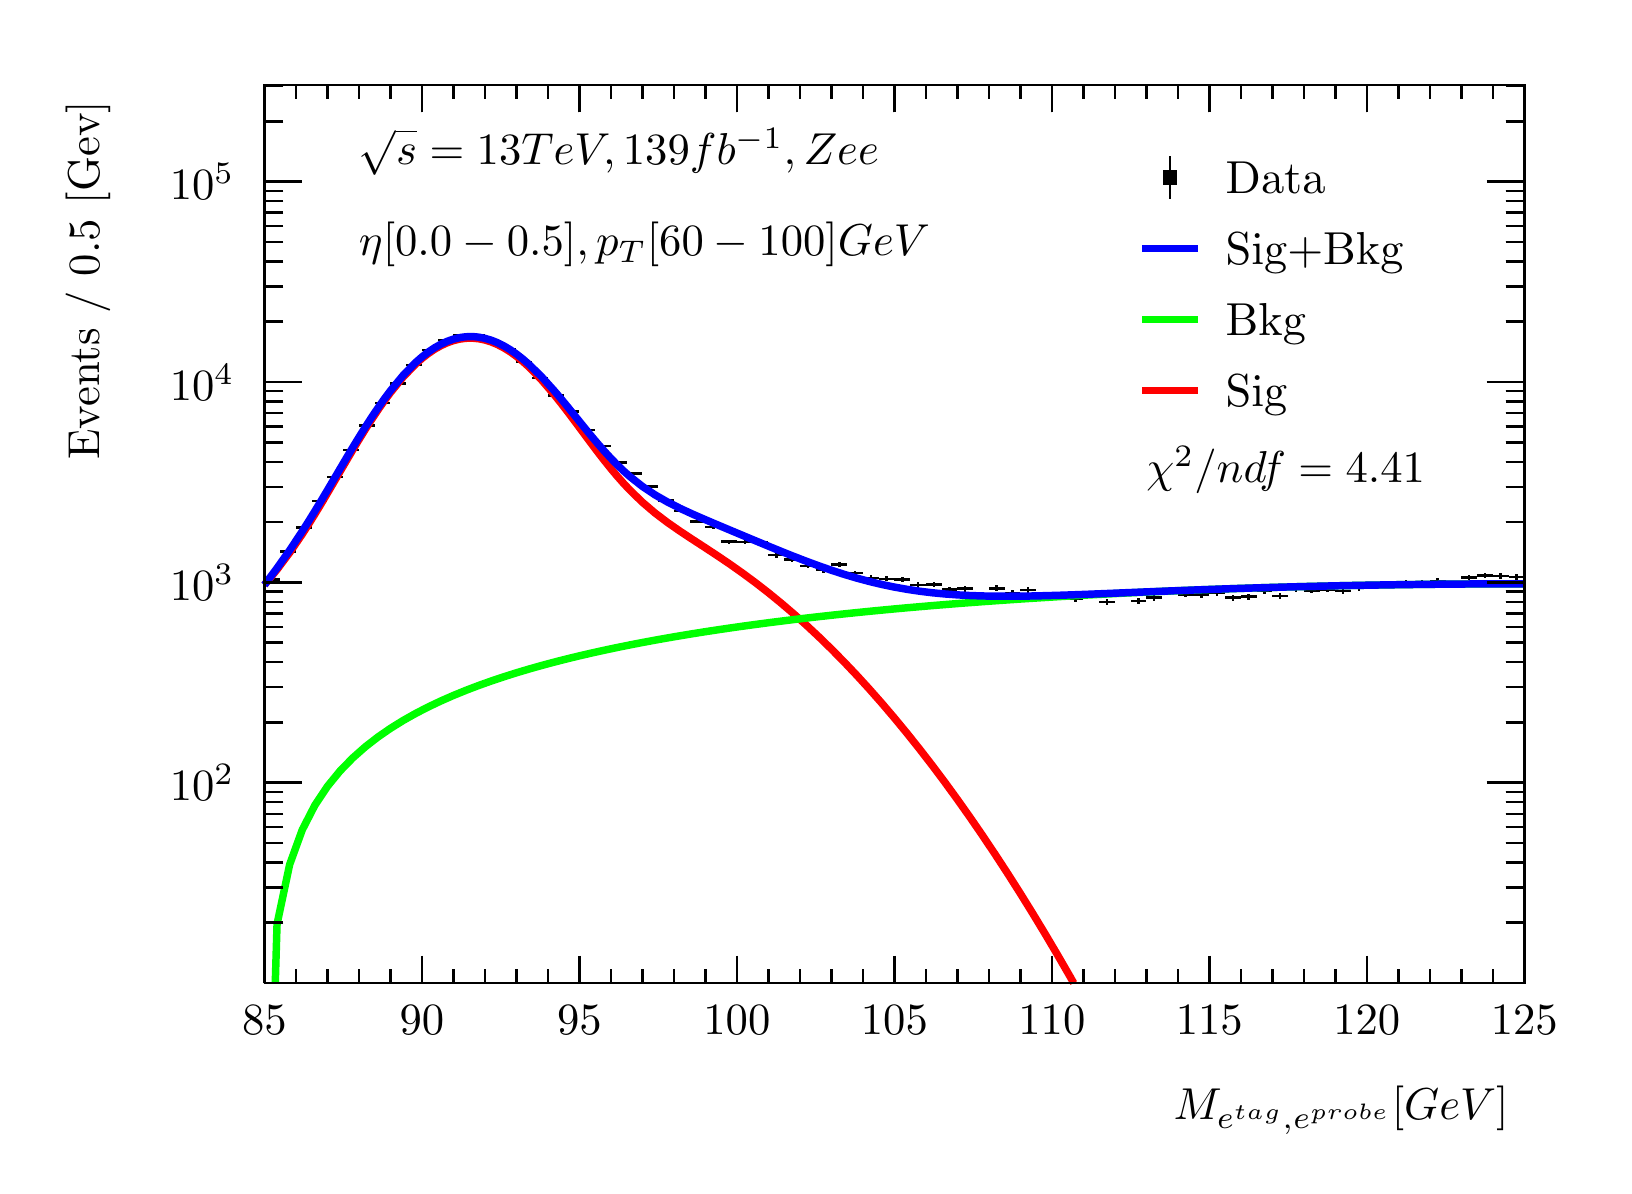
\begin{tikzpicture}
\pgfdeclareplotmark{cross} {
\pgfpathmoveto{\pgfpoint{-0.3\pgfplotmarksize}{\pgfplotmarksize}}
\pgfpathlineto{\pgfpoint{+0.3\pgfplotmarksize}{\pgfplotmarksize}}
\pgfpathlineto{\pgfpoint{+0.3\pgfplotmarksize}{0.3\pgfplotmarksize}}
\pgfpathlineto{\pgfpoint{+1\pgfplotmarksize}{0.3\pgfplotmarksize}}
\pgfpathlineto{\pgfpoint{+1\pgfplotmarksize}{-0.3\pgfplotmarksize}}
\pgfpathlineto{\pgfpoint{+0.3\pgfplotmarksize}{-0.3\pgfplotmarksize}}
\pgfpathlineto{\pgfpoint{+0.3\pgfplotmarksize}{-1.\pgfplotmarksize}}
\pgfpathlineto{\pgfpoint{-0.3\pgfplotmarksize}{-1.\pgfplotmarksize}}
\pgfpathlineto{\pgfpoint{-0.3\pgfplotmarksize}{-0.3\pgfplotmarksize}}
\pgfpathlineto{\pgfpoint{-1.\pgfplotmarksize}{-0.3\pgfplotmarksize}}
\pgfpathlineto{\pgfpoint{-1.\pgfplotmarksize}{0.3\pgfplotmarksize}}
\pgfpathlineto{\pgfpoint{-0.3\pgfplotmarksize}{0.3\pgfplotmarksize}}
\pgfpathclose
\pgfusepathqstroke
}
\pgfdeclareplotmark{cross*} {
\pgfpathmoveto{\pgfpoint{-0.3\pgfplotmarksize}{\pgfplotmarksize}}
\pgfpathlineto{\pgfpoint{+0.3\pgfplotmarksize}{\pgfplotmarksize}}
\pgfpathlineto{\pgfpoint{+0.3\pgfplotmarksize}{0.3\pgfplotmarksize}}
\pgfpathlineto{\pgfpoint{+1\pgfplotmarksize}{0.3\pgfplotmarksize}}
\pgfpathlineto{\pgfpoint{+1\pgfplotmarksize}{-0.3\pgfplotmarksize}}
\pgfpathlineto{\pgfpoint{+0.3\pgfplotmarksize}{-0.3\pgfplotmarksize}}
\pgfpathlineto{\pgfpoint{+0.3\pgfplotmarksize}{-1.\pgfplotmarksize}}
\pgfpathlineto{\pgfpoint{-0.3\pgfplotmarksize}{-1.\pgfplotmarksize}}
\pgfpathlineto{\pgfpoint{-0.3\pgfplotmarksize}{-0.3\pgfplotmarksize}}
\pgfpathlineto{\pgfpoint{-1.\pgfplotmarksize}{-0.3\pgfplotmarksize}}
\pgfpathlineto{\pgfpoint{-1.\pgfplotmarksize}{0.3\pgfplotmarksize}}
\pgfpathlineto{\pgfpoint{-0.3\pgfplotmarksize}{0.3\pgfplotmarksize}}
\pgfpathclose
\pgfusepathqfillstroke
}
\pgfdeclareplotmark{newstar} {
\pgfpathmoveto{\pgfqpoint{0pt}{\pgfplotmarksize}}
\pgfpathlineto{\pgfqpointpolar{44}{0.5\pgfplotmarksize}}
\pgfpathlineto{\pgfqpointpolar{18}{\pgfplotmarksize}}
\pgfpathlineto{\pgfqpointpolar{-20}{0.5\pgfplotmarksize}}
\pgfpathlineto{\pgfqpointpolar{-54}{\pgfplotmarksize}}
\pgfpathlineto{\pgfqpointpolar{-90}{0.5\pgfplotmarksize}}
\pgfpathlineto{\pgfqpointpolar{234}{\pgfplotmarksize}}
\pgfpathlineto{\pgfqpointpolar{198}{0.5\pgfplotmarksize}}
\pgfpathlineto{\pgfqpointpolar{162}{\pgfplotmarksize}}
\pgfpathlineto{\pgfqpointpolar{134}{0.5\pgfplotmarksize}}
\pgfpathclose
\pgfusepathqstroke
}
\pgfdeclareplotmark{newstar*} {
\pgfpathmoveto{\pgfqpoint{0pt}{\pgfplotmarksize}}
\pgfpathlineto{\pgfqpointpolar{44}{0.5\pgfplotmarksize}}
\pgfpathlineto{\pgfqpointpolar{18}{\pgfplotmarksize}}
\pgfpathlineto{\pgfqpointpolar{-20}{0.5\pgfplotmarksize}}
\pgfpathlineto{\pgfqpointpolar{-54}{\pgfplotmarksize}}
\pgfpathlineto{\pgfqpointpolar{-90}{0.5\pgfplotmarksize}}
\pgfpathlineto{\pgfqpointpolar{234}{\pgfplotmarksize}}
\pgfpathlineto{\pgfqpointpolar{198}{0.5\pgfplotmarksize}}
\pgfpathlineto{\pgfqpointpolar{162}{\pgfplotmarksize}}
\pgfpathlineto{\pgfqpointpolar{134}{0.5\pgfplotmarksize}}
\pgfpathclose
\pgfusepathqfillstroke
}
\definecolor{c}{rgb}{1,1,1};
\draw [color=c, fill=c] (0,0) rectangle (20,14.4361);
\draw [color=c, fill=c] (3,2.30977) rectangle (19,13.7143);
\definecolor{c}{rgb}{0,0,0};
\draw [c,line width=0.9] (3,2.30977) -- (3,13.7143) -- (19,13.7143) -- (19,2.30977) -- (3,2.30977);
\definecolor{c}{rgb}{1,1,1};
\draw [color=c, fill=c] (3,2.30977) rectangle (19,13.7143);
\definecolor{c}{rgb}{0,0,0};
\draw [c,line width=0.9] (3,2.30977) -- (3,13.7143) -- (19,13.7143) -- (19,2.30977) -- (3,2.30977);
\draw [c,line width=0.9] (3,2.30977) -- (19,2.30977);
\draw [c,line width=0.9] (3,2.65624) -- (3,2.30977);
\draw [c,line width=0.9] (3.4,2.48301) -- (3.4,2.30977);
\draw [c,line width=0.9] (3.8,2.48301) -- (3.8,2.30977);
\draw [c,line width=0.9] (4.2,2.48301) -- (4.2,2.30977);
\draw [c,line width=0.9] (4.6,2.48301) -- (4.6,2.30977);
\draw [c,line width=0.9] (5,2.65624) -- (5,2.30977);
\draw [c,line width=0.9] (5.4,2.48301) -- (5.4,2.30977);
\draw [c,line width=0.9] (5.8,2.48301) -- (5.8,2.30977);
\draw [c,line width=0.9] (6.2,2.48301) -- (6.2,2.30977);
\draw [c,line width=0.9] (6.6,2.48301) -- (6.6,2.30977);
\draw [c,line width=0.9] (7,2.65624) -- (7,2.30977);
\draw [c,line width=0.9] (7.4,2.48301) -- (7.4,2.30977);
\draw [c,line width=0.9] (7.8,2.48301) -- (7.8,2.30977);
\draw [c,line width=0.9] (8.2,2.48301) -- (8.2,2.30977);
\draw [c,line width=0.9] (8.6,2.48301) -- (8.6,2.30977);
\draw [c,line width=0.9] (9,2.65624) -- (9,2.30977);
\draw [c,line width=0.9] (9.4,2.48301) -- (9.4,2.30977);
\draw [c,line width=0.9] (9.8,2.48301) -- (9.8,2.30977);
\draw [c,line width=0.9] (10.2,2.48301) -- (10.2,2.30977);
\draw [c,line width=0.9] (10.6,2.48301) -- (10.6,2.30977);
\draw [c,line width=0.9] (11,2.65624) -- (11,2.30977);
\draw [c,line width=0.9] (11.4,2.48301) -- (11.4,2.30977);
\draw [c,line width=0.9] (11.8,2.48301) -- (11.8,2.30977);
\draw [c,line width=0.9] (12.2,2.48301) -- (12.2,2.30977);
\draw [c,line width=0.9] (12.6,2.48301) -- (12.6,2.30977);
\draw [c,line width=0.9] (13,2.65624) -- (13,2.30977);
\draw [c,line width=0.9] (13.4,2.48301) -- (13.4,2.30977);
\draw [c,line width=0.9] (13.8,2.48301) -- (13.8,2.30977);
\draw [c,line width=0.9] (14.2,2.48301) -- (14.2,2.30977);
\draw [c,line width=0.9] (14.6,2.48301) -- (14.6,2.30977);
\draw [c,line width=0.9] (15,2.65624) -- (15,2.30977);
\draw [c,line width=0.9] (15.4,2.48301) -- (15.4,2.30977);
\draw [c,line width=0.9] (15.8,2.48301) -- (15.8,2.30977);
\draw [c,line width=0.9] (16.2,2.48301) -- (16.2,2.30977);
\draw [c,line width=0.9] (16.6,2.48301) -- (16.6,2.30977);
\draw [c,line width=0.9] (17,2.65624) -- (17,2.30977);
\draw [c,line width=0.9] (17.4,2.48301) -- (17.4,2.30977);
\draw [c,line width=0.9] (17.8,2.48301) -- (17.8,2.30977);
\draw [c,line width=0.9] (18.2,2.48301) -- (18.2,2.30977);
\draw [c,line width=0.9] (18.6,2.48301) -- (18.6,2.30977);
\draw [c,line width=0.9] (19,2.65624) -- (19,2.30977);
\draw [anchor=base] (3,1.66015) node[scale=1.61424, color=c, rotate=0]{85};
\draw [anchor=base] (5,1.66015) node[scale=1.61424, color=c, rotate=0]{90};
\draw [anchor=base] (7,1.66015) node[scale=1.61424, color=c, rotate=0]{95};
\draw [anchor=base] (9,1.66015) node[scale=1.61424, color=c, rotate=0]{100};
\draw [anchor=base] (11,1.66015) node[scale=1.61424, color=c, rotate=0]{105};
\draw [anchor=base] (13,1.66015) node[scale=1.61424, color=c, rotate=0]{110};
\draw [anchor=base] (15,1.66015) node[scale=1.61424, color=c, rotate=0]{115};
\draw [anchor=base] (17,1.66015) node[scale=1.61424, color=c, rotate=0]{120};
\draw [anchor=base] (19,1.66015) node[scale=1.61424, color=c, rotate=0]{125};
\draw [anchor= east] (19,0.692932) node[scale=1.61424, color=c, rotate=0]{$M_{e^{tag}, e^{probe}}  [GeV]$};
\draw [c,line width=0.9] (3,13.7143) -- (19,13.7143);
\draw [c,line width=0.9] (3,13.3678) -- (3,13.7143);
\draw [c,line width=0.9] (3.4,13.5411) -- (3.4,13.7143);
\draw [c,line width=0.9] (3.8,13.5411) -- (3.8,13.7143);
\draw [c,line width=0.9] (4.2,13.5411) -- (4.2,13.7143);
\draw [c,line width=0.9] (4.6,13.5411) -- (4.6,13.7143);
\draw [c,line width=0.9] (5,13.3678) -- (5,13.7143);
\draw [c,line width=0.9] (5.4,13.5411) -- (5.4,13.7143);
\draw [c,line width=0.9] (5.8,13.5411) -- (5.8,13.7143);
\draw [c,line width=0.9] (6.2,13.5411) -- (6.2,13.7143);
\draw [c,line width=0.9] (6.6,13.5411) -- (6.6,13.7143);
\draw [c,line width=0.9] (7,13.3678) -- (7,13.7143);
\draw [c,line width=0.9] (7.4,13.5411) -- (7.4,13.7143);
\draw [c,line width=0.9] (7.8,13.5411) -- (7.8,13.7143);
\draw [c,line width=0.9] (8.2,13.5411) -- (8.2,13.7143);
\draw [c,line width=0.9] (8.6,13.5411) -- (8.6,13.7143);
\draw [c,line width=0.9] (9,13.3678) -- (9,13.7143);
\draw [c,line width=0.9] (9.4,13.5411) -- (9.4,13.7143);
\draw [c,line width=0.9] (9.8,13.5411) -- (9.8,13.7143);
\draw [c,line width=0.9] (10.2,13.5411) -- (10.2,13.7143);
\draw [c,line width=0.9] (10.6,13.5411) -- (10.6,13.7143);
\draw [c,line width=0.9] (11,13.3678) -- (11,13.7143);
\draw [c,line width=0.9] (11.4,13.5411) -- (11.4,13.7143);
\draw [c,line width=0.9] (11.8,13.5411) -- (11.8,13.7143);
\draw [c,line width=0.9] (12.2,13.5411) -- (12.2,13.7143);
\draw [c,line width=0.9] (12.6,13.5411) -- (12.6,13.7143);
\draw [c,line width=0.9] (13,13.3678) -- (13,13.7143);
\draw [c,line width=0.9] (13.4,13.5411) -- (13.4,13.7143);
\draw [c,line width=0.9] (13.8,13.5411) -- (13.8,13.7143);
\draw [c,line width=0.9] (14.2,13.5411) -- (14.2,13.7143);
\draw [c,line width=0.9] (14.6,13.5411) -- (14.6,13.7143);
\draw [c,line width=0.9] (15,13.3678) -- (15,13.7143);
\draw [c,line width=0.9] (15.4,13.5411) -- (15.4,13.7143);
\draw [c,line width=0.9] (15.8,13.5411) -- (15.8,13.7143);
\draw [c,line width=0.9] (16.2,13.5411) -- (16.2,13.7143);
\draw [c,line width=0.9] (16.6,13.5411) -- (16.6,13.7143);
\draw [c,line width=0.9] (17,13.3678) -- (17,13.7143);
\draw [c,line width=0.9] (17.4,13.5411) -- (17.4,13.7143);
\draw [c,line width=0.9] (17.8,13.5411) -- (17.8,13.7143);
\draw [c,line width=0.9] (18.2,13.5411) -- (18.2,13.7143);
\draw [c,line width=0.9] (18.6,13.5411) -- (18.6,13.7143);
\draw [c,line width=0.9] (19,13.3678) -- (19,13.7143);
\draw [c,line width=0.9] (3,2.30977) -- (3,13.7143);
\draw [c,line width=0.9] (3.237,3.07568) -- (3,3.07568);
\draw [c,line width=0.9] (3.237,3.5237) -- (3,3.5237);
\draw [c,line width=0.9] (3.237,3.84158) -- (3,3.84158);
\draw [c,line width=0.9] (3.237,4.08815) -- (3,4.08815);
\draw [c,line width=0.9] (3.237,4.2896) -- (3,4.2896);
\draw [c,line width=0.9] (3.237,4.45994) -- (3,4.45994);
\draw [c,line width=0.9] (3.237,4.60748) -- (3,4.60748);
\draw [c,line width=0.9] (3.237,4.73763) -- (3,4.73763);
\draw [c,line width=0.9] (3.474,4.85405) -- (3,4.85405);
\draw [anchor= east] (2.82,4.85405) node[scale=1.61424, color=c, rotate=0]{$10^{2}$};
\draw [c,line width=0.9] (3.237,5.61995) -- (3,5.61995);
\draw [c,line width=0.9] (3.237,6.06798) -- (3,6.06798);
\draw [c,line width=0.9] (3.237,6.38586) -- (3,6.38586);
\draw [c,line width=0.9] (3.237,6.63242) -- (3,6.63242);
\draw [c,line width=0.9] (3.237,6.83388) -- (3,6.83388);
\draw [c,line width=0.9] (3.237,7.00421) -- (3,7.00421);
\draw [c,line width=0.9] (3.237,7.15176) -- (3,7.15176);
\draw [c,line width=0.9] (3.237,7.28191) -- (3,7.28191);
\draw [c,line width=0.9] (3.474,7.39833) -- (3,7.39833);
\draw [anchor= east] (2.82,7.39833) node[scale=1.61424, color=c, rotate=0]{$10^{3}$};
\draw [c,line width=0.9] (3.237,8.16423) -- (3,8.16423);
\draw [c,line width=0.9] (3.237,8.61226) -- (3,8.61226);
\draw [c,line width=0.9] (3.237,8.93013) -- (3,8.93013);
\draw [c,line width=0.9] (3.237,9.1767) -- (3,9.1767);
\draw [c,line width=0.9] (3.237,9.37816) -- (3,9.37816);
\draw [c,line width=0.9] (3.237,9.54849) -- (3,9.54849);
\draw [c,line width=0.9] (3.237,9.69604) -- (3,9.69604);
\draw [c,line width=0.9] (3.237,9.82618) -- (3,9.82618);
\draw [c,line width=0.9] (3.474,9.9426) -- (3,9.9426);
\draw [anchor= east] (2.82,9.9426) node[scale=1.61424, color=c, rotate=0]{$10^{4}$};
\draw [c,line width=0.9] (3.237,10.7085) -- (3,10.7085);
\draw [c,line width=0.9] (3.237,11.1565) -- (3,11.1565);
\draw [c,line width=0.9] (3.237,11.4744) -- (3,11.4744);
\draw [c,line width=0.9] (3.237,11.721) -- (3,11.721);
\draw [c,line width=0.9] (3.237,11.9224) -- (3,11.9224);
\draw [c,line width=0.9] (3.237,12.0928) -- (3,12.0928);
\draw [c,line width=0.9] (3.237,12.2403) -- (3,12.2403);
\draw [c,line width=0.9] (3.237,12.3705) -- (3,12.3705);
\draw [c,line width=0.9] (3.474,12.4869) -- (3,12.4869);
\draw [anchor= east] (2.82,12.4869) node[scale=1.61424, color=c, rotate=0]{$10^{5}$};
\draw [c,line width=0.9] (3.237,13.2528) -- (3,13.2528);
\draw [c,line width=0.9] (3.237,13.7008) -- (3,13.7008);
\draw [anchor= east] (0.76,13.7143) node[scale=1.61424, color=c, rotate=90]{Events / 0.5 [Gev]};
\draw [c,line width=0.9] (19,2.30977) -- (19,13.7143);
\draw [c,line width=0.9] (18.763,3.07568) -- (19,3.07568);
\draw [c,line width=0.9] (18.763,3.5237) -- (19,3.5237);
\draw [c,line width=0.9] (18.763,3.84158) -- (19,3.84158);
\draw [c,line width=0.9] (18.763,4.08815) -- (19,4.08815);
\draw [c,line width=0.9] (18.763,4.2896) -- (19,4.2896);
\draw [c,line width=0.9] (18.763,4.45994) -- (19,4.45994);
\draw [c,line width=0.9] (18.763,4.60748) -- (19,4.60748);
\draw [c,line width=0.9] (18.763,4.73763) -- (19,4.73763);
\draw [c,line width=0.9] (18.526,4.85405) -- (19,4.85405);
\draw [c,line width=0.9] (18.763,5.61995) -- (19,5.61995);
\draw [c,line width=0.9] (18.763,6.06798) -- (19,6.06798);
\draw [c,line width=0.9] (18.763,6.38586) -- (19,6.38586);
\draw [c,line width=0.9] (18.763,6.63242) -- (19,6.63242);
\draw [c,line width=0.9] (18.763,6.83388) -- (19,6.83388);
\draw [c,line width=0.9] (18.763,7.00421) -- (19,7.00421);
\draw [c,line width=0.9] (18.763,7.15176) -- (19,7.15176);
\draw [c,line width=0.9] (18.763,7.28191) -- (19,7.28191);
\draw [c,line width=0.9] (18.526,7.39833) -- (19,7.39833);
\draw [c,line width=0.9] (18.763,8.16423) -- (19,8.16423);
\draw [c,line width=0.9] (18.763,8.61226) -- (19,8.61226);
\draw [c,line width=0.9] (18.763,8.93013) -- (19,8.93013);
\draw [c,line width=0.9] (18.763,9.1767) -- (19,9.1767);
\draw [c,line width=0.9] (18.763,9.37816) -- (19,9.37816);
\draw [c,line width=0.9] (18.763,9.54849) -- (19,9.54849);
\draw [c,line width=0.9] (18.763,9.69604) -- (19,9.69604);
\draw [c,line width=0.9] (18.763,9.82618) -- (19,9.82618);
\draw [c,line width=0.9] (18.526,9.9426) -- (19,9.9426);
\draw [c,line width=0.9] (18.763,10.7085) -- (19,10.7085);
\draw [c,line width=0.9] (18.763,11.1565) -- (19,11.1565);
\draw [c,line width=0.9] (18.763,11.4744) -- (19,11.4744);
\draw [c,line width=0.9] (18.763,11.721) -- (19,11.721);
\draw [c,line width=0.9] (18.763,11.9224) -- (19,11.9224);
\draw [c,line width=0.9] (18.763,12.0928) -- (19,12.0928);
\draw [c,line width=0.9] (18.763,12.2403) -- (19,12.2403);
\draw [c,line width=0.9] (18.763,12.3705) -- (19,12.3705);
\draw [c,line width=0.9] (18.526,12.4869) -- (19,12.4869);
\draw [c,line width=0.9] (18.763,13.2528) -- (19,13.2528);
\draw [c,line width=0.9] (18.763,13.7008) -- (19,13.7008);
\draw [c,line width=0.9] (3.1,7.4342) -- (3,7.4342);
\draw [c,line width=0.9] (3,7.4342) -- (3,7.4342);
\draw [c,line width=0.9] (3.1,7.4342) -- (3.2,7.4342);
\draw [c,line width=0.9] (3.2,7.4342) -- (3.2,7.4342);
\draw [c,line width=0.9] (3.1,7.4342) -- (3.1,7.46858);
\draw [c,line width=0.9] (3.1,7.46858) -- (3.1,7.46858);
\draw [c,line width=0.9] (3.1,7.4342) -- (3.1,7.39983);
\draw [c,line width=0.9] (3.1,7.39983) -- (3.1,7.39983);
\draw [c,line width=0.9] (3.3,7.7889) -- (3.2,7.7889);
\draw [c,line width=0.9] (3.2,7.7889) -- (3.2,7.7889);
\draw [c,line width=0.9] (3.3,7.7889) -- (3.4,7.7889);
\draw [c,line width=0.9] (3.4,7.7889) -- (3.4,7.7889);
\draw [c,line width=0.9] (3.3,7.7889) -- (3.3,7.81818);
\draw [c,line width=0.9] (3.3,7.81818) -- (3.3,7.81818);
\draw [c,line width=0.9] (3.3,7.7889) -- (3.3,7.75962);
\draw [c,line width=0.9] (3.3,7.75962) -- (3.3,7.75962);
\draw [c,line width=0.9] (3.5,8.09645) -- (3.4,8.09645);
\draw [c,line width=0.9] (3.4,8.09645) -- (3.4,8.09645);
\draw [c,line width=0.9] (3.5,8.09645) -- (3.6,8.09645);
\draw [c,line width=0.9] (3.6,8.09645) -- (3.6,8.09645);
\draw [c,line width=0.9] (3.5,8.09645) -- (3.5,8.12193);
\draw [c,line width=0.9] (3.5,8.12193) -- (3.5,8.12193);
\draw [c,line width=0.9] (3.5,8.09645) -- (3.5,8.07097);
\draw [c,line width=0.9] (3.5,8.07097) -- (3.5,8.07097);
\draw [c,line width=0.9] (3.7,8.43008) -- (3.6,8.43008);
\draw [c,line width=0.9] (3.6,8.43008) -- (3.6,8.43008);
\draw [c,line width=0.9] (3.7,8.43008) -- (3.8,8.43008);
\draw [c,line width=0.9] (3.8,8.43008) -- (3.8,8.43008);
\draw [c,line width=0.9] (3.7,8.43008) -- (3.7,8.45198);
\draw [c,line width=0.9] (3.7,8.45198) -- (3.7,8.45198);
\draw [c,line width=0.9] (3.7,8.43008) -- (3.7,8.40817);
\draw [c,line width=0.9] (3.7,8.40817) -- (3.7,8.40817);
\draw [c,line width=0.9] (3.9,8.73386) -- (3.8,8.73386);
\draw [c,line width=0.9] (3.8,8.73386) -- (3.8,8.73386);
\draw [c,line width=0.9] (3.9,8.73386) -- (4,8.73386);
\draw [c,line width=0.9] (4,8.73386) -- (4,8.73386);
\draw [c,line width=0.9] (3.9,8.73386) -- (3.9,8.75295);
\draw [c,line width=0.9] (3.9,8.75295) -- (3.9,8.75295);
\draw [c,line width=0.9] (3.9,8.73386) -- (3.9,8.71476);
\draw [c,line width=0.9] (3.9,8.71476) -- (3.9,8.71476);
\draw [c,line width=0.9] (4.1,9.07903) -- (4,9.07903);
\draw [c,line width=0.9] (4,9.07903) -- (4,9.07903);
\draw [c,line width=0.9] (4.1,9.07903) -- (4.2,9.07903);
\draw [c,line width=0.9] (4.2,9.07903) -- (4.2,9.07903);
\draw [c,line width=0.9] (4.1,9.07903) -- (4.1,9.09536);
\draw [c,line width=0.9] (4.1,9.09536) -- (4.1,9.09536);
\draw [c,line width=0.9] (4.1,9.07903) -- (4.1,9.0627);
\draw [c,line width=0.9] (4.1,9.0627) -- (4.1,9.0627);
\draw [c,line width=0.9] (4.3,9.39261) -- (4.2,9.39261);
\draw [c,line width=0.9] (4.2,9.39261) -- (4.2,9.39261);
\draw [c,line width=0.9] (4.3,9.39261) -- (4.4,9.39261);
\draw [c,line width=0.9] (4.4,9.39261) -- (4.4,9.39261);
\draw [c,line width=0.9] (4.3,9.39261) -- (4.3,9.40679);
\draw [c,line width=0.9] (4.3,9.40679) -- (4.3,9.40679);
\draw [c,line width=0.9] (4.3,9.39261) -- (4.3,9.37844);
\draw [c,line width=0.9] (4.3,9.37844) -- (4.3,9.37844);
\draw [c,line width=0.9] (4.5,9.67681) -- (4.4,9.67681);
\draw [c,line width=0.9] (4.4,9.67681) -- (4.4,9.67681);
\draw [c,line width=0.9] (4.5,9.67681) -- (4.6,9.67681);
\draw [c,line width=0.9] (4.6,9.67681) -- (4.6,9.67681);
\draw [c,line width=0.9] (4.5,9.67681) -- (4.5,9.68927);
\draw [c,line width=0.9] (4.5,9.68927) -- (4.5,9.68927);
\draw [c,line width=0.9] (4.5,9.67681) -- (4.5,9.66435);
\draw [c,line width=0.9] (4.5,9.66435) -- (4.5,9.66435);
\draw [c,line width=0.9] (4.7,9.9213) -- (4.6,9.9213);
\draw [c,line width=0.9] (4.6,9.9213) -- (4.6,9.9213);
\draw [c,line width=0.9] (4.7,9.9213) -- (4.8,9.9213);
\draw [c,line width=0.9] (4.8,9.9213) -- (4.8,9.9213);
\draw [c,line width=0.9] (4.7,9.9213) -- (4.7,9.93245);
\draw [c,line width=0.9] (4.7,9.93245) -- (4.7,9.93245);
\draw [c,line width=0.9] (4.7,9.9213) -- (4.7,9.91014);
\draw [c,line width=0.9] (4.7,9.91014) -- (4.7,9.91014);
\draw [c,line width=0.9] (4.9,10.1618) -- (4.8,10.1618);
\draw [c,line width=0.9] (4.8,10.1618) -- (4.8,10.1618);
\draw [c,line width=0.9] (4.9,10.1618) -- (5,10.1618);
\draw [c,line width=0.9] (5,10.1618) -- (5,10.1618);
\draw [c,line width=0.9] (4.9,10.1618) -- (4.9,10.1718);
\draw [c,line width=0.9] (4.9,10.1718) -- (4.9,10.1718);
\draw [c,line width=0.9] (4.9,10.1618) -- (4.9,10.1518);
\draw [c,line width=0.9] (4.9,10.1518) -- (4.9,10.1518);
\draw [c,line width=0.9] (5.1,10.3471) -- (5,10.3471);
\draw [c,line width=0.9] (5,10.3471) -- (5,10.3471);
\draw [c,line width=0.9] (5.1,10.3471) -- (5.2,10.3471);
\draw [c,line width=0.9] (5.2,10.3471) -- (5.2,10.3471);
\draw [c,line width=0.9] (5.1,10.3471) -- (5.1,10.3563);
\draw [c,line width=0.9] (5.1,10.3563) -- (5.1,10.3563);
\draw [c,line width=0.9] (5.1,10.3471) -- (5.1,10.3379);
\draw [c,line width=0.9] (5.1,10.3379) -- (5.1,10.3379);
\draw [c,line width=0.9] (5.3,10.4746) -- (5.2,10.4746);
\draw [c,line width=0.9] (5.2,10.4746) -- (5.2,10.4746);
\draw [c,line width=0.9] (5.3,10.4746) -- (5.4,10.4746);
\draw [c,line width=0.9] (5.4,10.4746) -- (5.4,10.4746);
\draw [c,line width=0.9] (5.3,10.4746) -- (5.3,10.4833);
\draw [c,line width=0.9] (5.3,10.4833) -- (5.3,10.4833);
\draw [c,line width=0.9] (5.3,10.4746) -- (5.3,10.466);
\draw [c,line width=0.9] (5.3,10.466) -- (5.3,10.466);
\draw [c,line width=0.9] (5.5,10.5373) -- (5.4,10.5373);
\draw [c,line width=0.9] (5.4,10.5373) -- (5.4,10.5373);
\draw [c,line width=0.9] (5.5,10.5373) -- (5.6,10.5373);
\draw [c,line width=0.9] (5.6,10.5373) -- (5.6,10.5373);
\draw [c,line width=0.9] (5.5,10.5373) -- (5.5,10.5457);
\draw [c,line width=0.9] (5.5,10.5457) -- (5.5,10.5457);
\draw [c,line width=0.9] (5.5,10.5373) -- (5.5,10.5288);
\draw [c,line width=0.9] (5.5,10.5288) -- (5.5,10.5288);
\draw [c,line width=0.9] (5.7,10.5319) -- (5.6,10.5319);
\draw [c,line width=0.9] (5.6,10.5319) -- (5.6,10.5319);
\draw [c,line width=0.9] (5.7,10.5319) -- (5.8,10.5319);
\draw [c,line width=0.9] (5.8,10.5319) -- (5.8,10.5319);
\draw [c,line width=0.9] (5.7,10.5319) -- (5.7,10.5403);
\draw [c,line width=0.9] (5.7,10.5403) -- (5.7,10.5403);
\draw [c,line width=0.9] (5.7,10.5319) -- (5.7,10.5234);
\draw [c,line width=0.9] (5.7,10.5234) -- (5.7,10.5234);
\draw [c,line width=0.9] (5.9,10.4613) -- (5.8,10.4613);
\draw [c,line width=0.9] (5.8,10.4613) -- (5.8,10.4613);
\draw [c,line width=0.9] (5.9,10.4613) -- (6,10.4613);
\draw [c,line width=0.9] (6,10.4613) -- (6,10.4613);
\draw [c,line width=0.9] (5.9,10.4613) -- (5.9,10.4701);
\draw [c,line width=0.9] (5.9,10.4701) -- (5.9,10.4701);
\draw [c,line width=0.9] (5.9,10.4613) -- (5.9,10.4526);
\draw [c,line width=0.9] (5.9,10.4526) -- (5.9,10.4526);
\draw [c,line width=0.9] (6.1,10.3639) -- (6,10.3639);
\draw [c,line width=0.9] (6,10.3639) -- (6,10.3639);
\draw [c,line width=0.9] (6.1,10.3639) -- (6.2,10.3639);
\draw [c,line width=0.9] (6.2,10.3639) -- (6.2,10.3639);
\draw [c,line width=0.9] (6.1,10.3639) -- (6.1,10.373);
\draw [c,line width=0.9] (6.1,10.373) -- (6.1,10.373);
\draw [c,line width=0.9] (6.1,10.3639) -- (6.1,10.3547);
\draw [c,line width=0.9] (6.1,10.3547) -- (6.1,10.3547);
\draw [c,line width=0.9] (6.3,10.1946) -- (6.2,10.1946);
\draw [c,line width=0.9] (6.2,10.1946) -- (6.2,10.1946);
\draw [c,line width=0.9] (6.3,10.1946) -- (6.4,10.1946);
\draw [c,line width=0.9] (6.4,10.1946) -- (6.4,10.1946);
\draw [c,line width=0.9] (6.3,10.1946) -- (6.3,10.2044);
\draw [c,line width=0.9] (6.3,10.2044) -- (6.3,10.2044);
\draw [c,line width=0.9] (6.3,10.1946) -- (6.3,10.1847);
\draw [c,line width=0.9] (6.3,10.1847) -- (6.3,10.1847);
\draw [c,line width=0.9] (6.5,9.9942) -- (6.4,9.9942);
\draw [c,line width=0.9] (6.4,9.9942) -- (6.4,9.9942);
\draw [c,line width=0.9] (6.5,9.9942) -- (6.6,9.9942);
\draw [c,line width=0.9] (6.6,9.9942) -- (6.6,9.9942);
\draw [c,line width=0.9] (6.5,9.9942) -- (6.5,10.005);
\draw [c,line width=0.9] (6.5,10.005) -- (6.5,10.005);
\draw [c,line width=0.9] (6.5,9.9942) -- (6.5,9.9834);
\draw [c,line width=0.9] (6.5,9.9834) -- (6.5,9.9834);
\draw [c,line width=0.9] (6.7,9.77273) -- (6.6,9.77273);
\draw [c,line width=0.9] (6.6,9.77273) -- (6.6,9.77273);
\draw [c,line width=0.9] (6.7,9.77273) -- (6.8,9.77273);
\draw [c,line width=0.9] (6.8,9.77273) -- (6.8,9.77273);
\draw [c,line width=0.9] (6.7,9.77273) -- (6.7,9.78467);
\draw [c,line width=0.9] (6.7,9.78467) -- (6.7,9.78467);
\draw [c,line width=0.9] (6.7,9.77273) -- (6.7,9.7608);
\draw [c,line width=0.9] (6.7,9.7608) -- (6.7,9.7608);
\draw [c,line width=0.9] (6.9,9.57099) -- (6.8,9.57099);
\draw [c,line width=0.9] (6.8,9.57099) -- (6.8,9.57099);
\draw [c,line width=0.9] (6.9,9.57099) -- (7,9.57099);
\draw [c,line width=0.9] (7,9.57099) -- (7,9.57099);
\draw [c,line width=0.9] (6.9,9.57099) -- (6.9,9.58406);
\draw [c,line width=0.9] (6.9,9.58406) -- (6.9,9.58406);
\draw [c,line width=0.9] (6.9,9.57099) -- (6.9,9.55792);
\draw [c,line width=0.9] (6.9,9.55792) -- (6.9,9.55792);
\draw [c,line width=0.9] (7.1,9.33075) -- (7,9.33075);
\draw [c,line width=0.9] (7,9.33075) -- (7,9.33075);
\draw [c,line width=0.9] (7.1,9.33075) -- (7.2,9.33075);
\draw [c,line width=0.9] (7.2,9.33075) -- (7.2,9.33075);
\draw [c,line width=0.9] (7.1,9.33075) -- (7.1,9.34532);
\draw [c,line width=0.9] (7.1,9.34532) -- (7.1,9.34532);
\draw [c,line width=0.9] (7.1,9.33075) -- (7.1,9.31617);
\draw [c,line width=0.9] (7.1,9.31617) -- (7.1,9.31617);
\draw [c,line width=0.9] (7.3,9.13159) -- (7.2,9.13159);
\draw [c,line width=0.9] (7.2,9.13159) -- (7.2,9.13159);
\draw [c,line width=0.9] (7.3,9.13159) -- (7.4,9.13159);
\draw [c,line width=0.9] (7.4,9.13159) -- (7.4,9.13159);
\draw [c,line width=0.9] (7.3,9.13159) -- (7.3,9.14754);
\draw [c,line width=0.9] (7.3,9.14754) -- (7.3,9.14754);
\draw [c,line width=0.9] (7.3,9.13159) -- (7.3,9.11565);
\draw [c,line width=0.9] (7.3,9.11565) -- (7.3,9.11565);
\draw [c,line width=0.9] (7.5,8.91903) -- (7.4,8.91903);
\draw [c,line width=0.9] (7.4,8.91903) -- (7.4,8.91903);
\draw [c,line width=0.9] (7.5,8.91903) -- (7.6,8.91903);
\draw [c,line width=0.9] (7.6,8.91903) -- (7.6,8.91903);
\draw [c,line width=0.9] (7.5,8.91903) -- (7.5,8.93659);
\draw [c,line width=0.9] (7.5,8.93659) -- (7.5,8.93659);
\draw [c,line width=0.9] (7.5,8.91903) -- (7.5,8.90147);
\draw [c,line width=0.9] (7.5,8.90147) -- (7.5,8.90147);
\draw [c,line width=0.9] (7.7,8.77911) -- (7.6,8.77911);
\draw [c,line width=0.9] (7.6,8.77911) -- (7.6,8.77911);
\draw [c,line width=0.9] (7.7,8.77911) -- (7.8,8.77911);
\draw [c,line width=0.9] (7.8,8.77911) -- (7.8,8.77911);
\draw [c,line width=0.9] (7.7,8.77911) -- (7.7,8.79782);
\draw [c,line width=0.9] (7.7,8.79782) -- (7.7,8.79782);
\draw [c,line width=0.9] (7.7,8.77911) -- (7.7,8.7604);
\draw [c,line width=0.9] (7.7,8.7604) -- (7.7,8.7604);
\draw [c,line width=0.9] (7.9,8.61887) -- (7.8,8.61887);
\draw [c,line width=0.9] (7.8,8.61887) -- (7.8,8.61887);
\draw [c,line width=0.9] (7.9,8.61887) -- (8,8.61887);
\draw [c,line width=0.9] (8,8.61887) -- (8,8.61887);
\draw [c,line width=0.9] (7.9,8.61887) -- (7.9,8.63898);
\draw [c,line width=0.9] (7.9,8.63898) -- (7.9,8.63898);
\draw [c,line width=0.9] (7.9,8.61887) -- (7.9,8.59875);
\draw [c,line width=0.9] (7.9,8.59875) -- (7.9,8.59875);
\draw [c,line width=0.9] (8.1,8.43657) -- (8,8.43657);
\draw [c,line width=0.9] (8,8.43657) -- (8,8.43657);
\draw [c,line width=0.9] (8.1,8.43657) -- (8.2,8.43657);
\draw [c,line width=0.9] (8.2,8.43657) -- (8.2,8.43657);
\draw [c,line width=0.9] (8.1,8.43657) -- (8.1,8.45842);
\draw [c,line width=0.9] (8.1,8.45842) -- (8.1,8.45842);
\draw [c,line width=0.9] (8.1,8.43657) -- (8.1,8.41473);
\draw [c,line width=0.9] (8.1,8.41473) -- (8.1,8.41473);
\draw [c,line width=0.9] (8.3,8.30464) -- (8.2,8.30464);
\draw [c,line width=0.9] (8.2,8.30464) -- (8.2,8.30464);
\draw [c,line width=0.9] (8.3,8.30464) -- (8.4,8.30464);
\draw [c,line width=0.9] (8.4,8.30464) -- (8.4,8.30464);
\draw [c,line width=0.9] (8.3,8.30464) -- (8.3,8.32783);
\draw [c,line width=0.9] (8.3,8.32783) -- (8.3,8.32783);
\draw [c,line width=0.9] (8.3,8.30464) -- (8.3,8.28146);
\draw [c,line width=0.9] (8.3,8.28146) -- (8.3,8.28146);
\draw [c,line width=0.9] (8.5,8.17358) -- (8.4,8.17358);
\draw [c,line width=0.9] (8.4,8.17358) -- (8.4,8.17358);
\draw [c,line width=0.9] (8.5,8.17358) -- (8.6,8.17358);
\draw [c,line width=0.9] (8.6,8.17358) -- (8.6,8.17358);
\draw [c,line width=0.9] (8.5,8.17358) -- (8.5,8.19819);
\draw [c,line width=0.9] (8.5,8.19819) -- (8.5,8.19819);
\draw [c,line width=0.9] (8.5,8.17358) -- (8.5,8.14898);
\draw [c,line width=0.9] (8.5,8.14898) -- (8.5,8.14898);
\draw [c,line width=0.9] (8.7,8.10231) -- (8.6,8.10231);
\draw [c,line width=0.9] (8.6,8.10231) -- (8.6,8.10231);
\draw [c,line width=0.9] (8.7,8.10231) -- (8.8,8.10231);
\draw [c,line width=0.9] (8.8,8.10231) -- (8.8,8.10231);
\draw [c,line width=0.9] (8.7,8.10231) -- (8.7,8.12772);
\draw [c,line width=0.9] (8.7,8.12772) -- (8.7,8.12772);
\draw [c,line width=0.9] (8.7,8.10231) -- (8.7,8.0769);
\draw [c,line width=0.9] (8.7,8.0769) -- (8.7,8.0769);
\draw [c,line width=0.9] (8.9,7.9149) -- (8.8,7.9149);
\draw [c,line width=0.9] (8.8,7.9149) -- (8.8,7.9149);
\draw [c,line width=0.9] (8.9,7.9149) -- (9,7.9149);
\draw [c,line width=0.9] (9,7.9149) -- (9,7.9149);
\draw [c,line width=0.9] (8.9,7.9149) -- (8.9,7.94256);
\draw [c,line width=0.9] (8.9,7.94256) -- (8.9,7.94256);
\draw [c,line width=0.9] (8.9,7.9149) -- (8.9,7.88724);
\draw [c,line width=0.9] (8.9,7.88724) -- (8.9,7.88724);
\draw [c,line width=0.9] (9.1,7.90865) -- (9,7.90865);
\draw [c,line width=0.9] (9,7.90865) -- (9,7.90865);
\draw [c,line width=0.9] (9.1,7.90865) -- (9.2,7.90865);
\draw [c,line width=0.9] (9.2,7.90865) -- (9.2,7.90865);
\draw [c,line width=0.9] (9.1,7.90865) -- (9.1,7.93639);
\draw [c,line width=0.9] (9.1,7.93639) -- (9.1,7.93639);
\draw [c,line width=0.9] (9.1,7.90865) -- (9.1,7.88092);
\draw [c,line width=0.9] (9.1,7.88092) -- (9.1,7.88092);
\draw [c,line width=0.9] (9.3,7.90795) -- (9.2,7.90795);
\draw [c,line width=0.9] (9.2,7.90795) -- (9.2,7.90795);
\draw [c,line width=0.9] (9.3,7.90795) -- (9.4,7.90795);
\draw [c,line width=0.9] (9.4,7.90795) -- (9.4,7.90795);
\draw [c,line width=0.9] (9.3,7.90795) -- (9.3,7.9357);
\draw [c,line width=0.9] (9.3,7.9357) -- (9.3,7.9357);
\draw [c,line width=0.9] (9.3,7.90795) -- (9.3,7.88021);
\draw [c,line width=0.9] (9.3,7.88021) -- (9.3,7.88021);
\draw [c,line width=0.9] (9.5,7.74295) -- (9.4,7.74295);
\draw [c,line width=0.9] (9.4,7.74295) -- (9.4,7.74295);
\draw [c,line width=0.9] (9.5,7.74295) -- (9.6,7.74295);
\draw [c,line width=0.9] (9.6,7.74295) -- (9.6,7.74295);
\draw [c,line width=0.9] (9.5,7.74295) -- (9.5,7.77285);
\draw [c,line width=0.9] (9.5,7.77285) -- (9.5,7.77285);
\draw [c,line width=0.9] (9.5,7.74295) -- (9.5,7.71306);
\draw [c,line width=0.9] (9.5,7.71306) -- (9.5,7.71306);
\draw [c,line width=0.9] (9.7,7.68653) -- (9.6,7.68653);
\draw [c,line width=0.9] (9.6,7.68653) -- (9.6,7.68653);
\draw [c,line width=0.9] (9.7,7.68653) -- (9.8,7.68653);
\draw [c,line width=0.9] (9.8,7.68653) -- (9.8,7.68653);
\draw [c,line width=0.9] (9.7,7.68653) -- (9.7,7.7172);
\draw [c,line width=0.9] (9.7,7.7172) -- (9.7,7.7172);
\draw [c,line width=0.9] (9.7,7.68653) -- (9.7,7.65586);
\draw [c,line width=0.9] (9.7,7.65586) -- (9.7,7.65586);
\draw [c,line width=0.9] (9.9,7.60896) -- (9.8,7.60896);
\draw [c,line width=0.9] (9.8,7.60896) -- (9.8,7.60896);
\draw [c,line width=0.9] (9.9,7.60896) -- (10,7.60896);
\draw [c,line width=0.9] (10,7.60896) -- (10,7.60896);
\draw [c,line width=0.9] (9.9,7.60896) -- (9.9,7.64072);
\draw [c,line width=0.9] (9.9,7.64072) -- (9.9,7.64072);
\draw [c,line width=0.9] (9.9,7.60896) -- (9.9,7.57719);
\draw [c,line width=0.9] (9.9,7.57719) -- (9.9,7.57719);
\draw [c,line width=0.9] (10.1,7.55468) -- (10,7.55468);
\draw [c,line width=0.9] (10,7.55468) -- (10,7.55468);
\draw [c,line width=0.9] (10.1,7.55468) -- (10.2,7.55468);
\draw [c,line width=0.9] (10.2,7.55468) -- (10.2,7.55468);
\draw [c,line width=0.9] (10.1,7.55468) -- (10.1,7.58723);
\draw [c,line width=0.9] (10.1,7.58723) -- (10.1,7.58723);
\draw [c,line width=0.9] (10.1,7.55468) -- (10.1,7.52213);
\draw [c,line width=0.9] (10.1,7.52213) -- (10.1,7.52213);
\draw [c,line width=0.9] (10.3,7.62347) -- (10.2,7.62347);
\draw [c,line width=0.9] (10.2,7.62347) -- (10.2,7.62347);
\draw [c,line width=0.9] (10.3,7.62347) -- (10.4,7.62347);
\draw [c,line width=0.9] (10.4,7.62347) -- (10.4,7.62347);
\draw [c,line width=0.9] (10.3,7.62347) -- (10.3,7.65503);
\draw [c,line width=0.9] (10.3,7.65503) -- (10.3,7.65503);
\draw [c,line width=0.9] (10.3,7.62347) -- (10.3,7.59192);
\draw [c,line width=0.9] (10.3,7.59192) -- (10.3,7.59192);
\draw [c,line width=0.9] (10.5,7.51563) -- (10.4,7.51563);
\draw [c,line width=0.9] (10.4,7.51563) -- (10.4,7.51563);
\draw [c,line width=0.9] (10.5,7.51563) -- (10.6,7.51563);
\draw [c,line width=0.9] (10.6,7.51563) -- (10.6,7.51563);
\draw [c,line width=0.9] (10.5,7.51563) -- (10.5,7.54877);
\draw [c,line width=0.9] (10.5,7.54877) -- (10.5,7.54877);
\draw [c,line width=0.9] (10.5,7.51563) -- (10.5,7.4825);
\draw [c,line width=0.9] (10.5,7.4825) -- (10.5,7.4825);
\draw [c,line width=0.9] (10.7,7.45644) -- (10.6,7.45644);
\draw [c,line width=0.9] (10.6,7.45644) -- (10.6,7.45644);
\draw [c,line width=0.9] (10.7,7.45644) -- (10.8,7.45644);
\draw [c,line width=0.9] (10.8,7.45644) -- (10.8,7.45644);
\draw [c,line width=0.9] (10.7,7.45644) -- (10.7,7.49047);
\draw [c,line width=0.9] (10.7,7.49047) -- (10.7,7.49047);
\draw [c,line width=0.9] (10.7,7.45644) -- (10.7,7.42241);
\draw [c,line width=0.9] (10.7,7.42241) -- (10.7,7.42241);
\draw [c,line width=0.9] (10.9,7.44379) -- (10.8,7.44379);
\draw [c,line width=0.9] (10.8,7.44379) -- (10.8,7.44379);
\draw [c,line width=0.9] (10.9,7.44379) -- (11,7.44379);
\draw [c,line width=0.9] (11,7.44379) -- (11,7.44379);
\draw [c,line width=0.9] (10.9,7.44379) -- (10.9,7.47802);
\draw [c,line width=0.9] (10.9,7.47802) -- (10.9,7.47802);
\draw [c,line width=0.9] (10.9,7.44379) -- (10.9,7.40956);
\draw [c,line width=0.9] (10.9,7.40956) -- (10.9,7.40956);
\draw [c,line width=0.9] (11.1,7.43634) -- (11,7.43634);
\draw [c,line width=0.9] (11,7.43634) -- (11,7.43634);
\draw [c,line width=0.9] (11.1,7.43634) -- (11.2,7.43634);
\draw [c,line width=0.9] (11.2,7.43634) -- (11.2,7.43634);
\draw [c,line width=0.9] (11.1,7.43634) -- (11.1,7.47069);
\draw [c,line width=0.9] (11.1,7.47069) -- (11.1,7.47069);
\draw [c,line width=0.9] (11.1,7.43634) -- (11.1,7.402);
\draw [c,line width=0.9] (11.1,7.402) -- (11.1,7.402);
\draw [c,line width=0.9] (11.3,7.36695) -- (11.2,7.36695);
\draw [c,line width=0.9] (11.2,7.36695) -- (11.2,7.36695);
\draw [c,line width=0.9] (11.3,7.36695) -- (11.4,7.36695);
\draw [c,line width=0.9] (11.4,7.36695) -- (11.4,7.36695);
\draw [c,line width=0.9] (11.3,7.36695) -- (11.3,7.40239);
\draw [c,line width=0.9] (11.3,7.40239) -- (11.3,7.40239);
\draw [c,line width=0.9] (11.3,7.36695) -- (11.3,7.33151);
\draw [c,line width=0.9] (11.3,7.33151) -- (11.3,7.33151);
\draw [c,line width=0.9] (11.5,7.37262) -- (11.4,7.37262);
\draw [c,line width=0.9] (11.4,7.37262) -- (11.4,7.37262);
\draw [c,line width=0.9] (11.5,7.37262) -- (11.6,7.37262);
\draw [c,line width=0.9] (11.6,7.37262) -- (11.6,7.37262);
\draw [c,line width=0.9] (11.5,7.37262) -- (11.5,7.40797);
\draw [c,line width=0.9] (11.5,7.40797) -- (11.5,7.40797);
\draw [c,line width=0.9] (11.5,7.37262) -- (11.5,7.33727);
\draw [c,line width=0.9] (11.5,7.33727) -- (11.5,7.33727);
\draw [c,line width=0.9] (11.7,7.30739) -- (11.6,7.30739);
\draw [c,line width=0.9] (11.6,7.30739) -- (11.6,7.30739);
\draw [c,line width=0.9] (11.7,7.30739) -- (11.8,7.30739);
\draw [c,line width=0.9] (11.8,7.30739) -- (11.8,7.30739);
\draw [c,line width=0.9] (11.7,7.30739) -- (11.7,7.3438);
\draw [c,line width=0.9] (11.7,7.3438) -- (11.7,7.3438);
\draw [c,line width=0.9] (11.7,7.30739) -- (11.7,7.27099);
\draw [c,line width=0.9] (11.7,7.27099) -- (11.7,7.27099);
\draw [c,line width=0.9] (11.9,7.31814) -- (11.8,7.31814);
\draw [c,line width=0.9] (11.8,7.31814) -- (11.8,7.31814);
\draw [c,line width=0.9] (11.9,7.31814) -- (12,7.31814);
\draw [c,line width=0.9] (12,7.31814) -- (12,7.31814);
\draw [c,line width=0.9] (11.9,7.31814) -- (11.9,7.35437);
\draw [c,line width=0.9] (11.9,7.35437) -- (11.9,7.35437);
\draw [c,line width=0.9] (11.9,7.31814) -- (11.9,7.28191);
\draw [c,line width=0.9] (11.9,7.28191) -- (11.9,7.28191);
\draw [c,line width=0.9] (12.1,7.24445) -- (12,7.24445);
\draw [c,line width=0.9] (12,7.24445) -- (12,7.24445);
\draw [c,line width=0.9] (12.1,7.24445) -- (12.2,7.24445);
\draw [c,line width=0.9] (12.2,7.24445) -- (12.2,7.24445);
\draw [c,line width=0.9] (12.1,7.24445) -- (12.1,7.28191);
\draw [c,line width=0.9] (12.1,7.28191) -- (12.1,7.28191);
\draw [c,line width=0.9] (12.1,7.24445) -- (12.1,7.20699);
\draw [c,line width=0.9] (12.1,7.20699) -- (12.1,7.20699);
\draw [c,line width=0.9] (12.3,7.32288) -- (12.2,7.32288);
\draw [c,line width=0.9] (12.2,7.32288) -- (12.2,7.32288);
\draw [c,line width=0.9] (12.3,7.32288) -- (12.4,7.32288);
\draw [c,line width=0.9] (12.4,7.32288) -- (12.4,7.32288);
\draw [c,line width=0.9] (12.3,7.32288) -- (12.3,7.35904);
\draw [c,line width=0.9] (12.3,7.35904) -- (12.3,7.35904);
\draw [c,line width=0.9] (12.3,7.32288) -- (12.3,7.28673);
\draw [c,line width=0.9] (12.3,7.28673) -- (12.3,7.28673);
\draw [c,line width=0.9] (12.5,7.26209) -- (12.4,7.26209);
\draw [c,line width=0.9] (12.4,7.26209) -- (12.4,7.26209);
\draw [c,line width=0.9] (12.5,7.26209) -- (12.6,7.26209);
\draw [c,line width=0.9] (12.6,7.26209) -- (12.6,7.26209);
\draw [c,line width=0.9] (12.5,7.26209) -- (12.5,7.29925);
\draw [c,line width=0.9] (12.5,7.29925) -- (12.5,7.29925);
\draw [c,line width=0.9] (12.5,7.26209) -- (12.5,7.22493);
\draw [c,line width=0.9] (12.5,7.22493) -- (12.5,7.22493);
\draw [c,line width=0.9] (12.7,7.30379) -- (12.6,7.30379);
\draw [c,line width=0.9] (12.6,7.30379) -- (12.6,7.30379);
\draw [c,line width=0.9] (12.7,7.30379) -- (12.8,7.30379);
\draw [c,line width=0.9] (12.8,7.30379) -- (12.8,7.30379);
\draw [c,line width=0.9] (12.7,7.30379) -- (12.7,7.34026);
\draw [c,line width=0.9] (12.7,7.34026) -- (12.7,7.34026);
\draw [c,line width=0.9] (12.7,7.30379) -- (12.7,7.26732);
\draw [c,line width=0.9] (12.7,7.26732) -- (12.7,7.26732);
\draw [c,line width=0.9] (12.9,7.19775) -- (12.8,7.19775);
\draw [c,line width=0.9] (12.8,7.19775) -- (12.8,7.19775);
\draw [c,line width=0.9] (12.9,7.19775) -- (13,7.19775);
\draw [c,line width=0.9] (13,7.19775) -- (13,7.19775);
\draw [c,line width=0.9] (12.9,7.19775) -- (12.9,7.23601);
\draw [c,line width=0.9] (12.9,7.23601) -- (12.9,7.23601);
\draw [c,line width=0.9] (12.9,7.19775) -- (12.9,7.15949);
\draw [c,line width=0.9] (12.9,7.15949) -- (12.9,7.15949);
\draw [c,line width=0.9] (13.1,7.21484) -- (13,7.21484);
\draw [c,line width=0.9] (13,7.21484) -- (13,7.21484);
\draw [c,line width=0.9] (13.1,7.21484) -- (13.2,7.21484);
\draw [c,line width=0.9] (13.2,7.21484) -- (13.2,7.21484);
\draw [c,line width=0.9] (13.1,7.21484) -- (13.1,7.25281);
\draw [c,line width=0.9] (13.1,7.25281) -- (13.1,7.25281);
\draw [c,line width=0.9] (13.1,7.21484) -- (13.1,7.17688);
\draw [c,line width=0.9] (13.1,7.17688) -- (13.1,7.17688);
\draw [c,line width=0.9] (13.3,7.18576) -- (13.2,7.18576);
\draw [c,line width=0.9] (13.2,7.18576) -- (13.2,7.18576);
\draw [c,line width=0.9] (13.3,7.18576) -- (13.4,7.18576);
\draw [c,line width=0.9] (13.4,7.18576) -- (13.4,7.18576);
\draw [c,line width=0.9] (13.3,7.18576) -- (13.3,7.22423);
\draw [c,line width=0.9] (13.3,7.22423) -- (13.3,7.22423);
\draw [c,line width=0.9] (13.3,7.18576) -- (13.3,7.1473);
\draw [c,line width=0.9] (13.3,7.1473) -- (13.3,7.1473);
\draw [c,line width=0.9] (13.5,7.25078) -- (13.4,7.25078);
\draw [c,line width=0.9] (13.4,7.25078) -- (13.4,7.25078);
\draw [c,line width=0.9] (13.5,7.25078) -- (13.6,7.25078);
\draw [c,line width=0.9] (13.6,7.25078) -- (13.6,7.25078);
\draw [c,line width=0.9] (13.5,7.25078) -- (13.5,7.28813);
\draw [c,line width=0.9] (13.5,7.28813) -- (13.5,7.28813);
\draw [c,line width=0.9] (13.5,7.25078) -- (13.5,7.21343);
\draw [c,line width=0.9] (13.5,7.21343) -- (13.5,7.21343);
\draw [c,line width=0.9] (13.7,7.14761) -- (13.6,7.14761);
\draw [c,line width=0.9] (13.6,7.14761) -- (13.6,7.14761);
\draw [c,line width=0.9] (13.7,7.14761) -- (13.8,7.14761);
\draw [c,line width=0.9] (13.8,7.14761) -- (13.8,7.14761);
\draw [c,line width=0.9] (13.7,7.14761) -- (13.7,7.18675);
\draw [c,line width=0.9] (13.7,7.18675) -- (13.7,7.18675);
\draw [c,line width=0.9] (13.7,7.14761) -- (13.7,7.10847);
\draw [c,line width=0.9] (13.7,7.10847) -- (13.7,7.10847);
\draw [c,line width=0.9] (13.9,7.25582) -- (13.8,7.25582);
\draw [c,line width=0.9] (13.8,7.25582) -- (13.8,7.25582);
\draw [c,line width=0.9] (13.9,7.25582) -- (14,7.25582);
\draw [c,line width=0.9] (14,7.25582) -- (14,7.25582);
\draw [c,line width=0.9] (13.9,7.25582) -- (13.9,7.29309);
\draw [c,line width=0.9] (13.9,7.29309) -- (13.9,7.29309);
\draw [c,line width=0.9] (13.9,7.25582) -- (13.9,7.21855);
\draw [c,line width=0.9] (13.9,7.21855) -- (13.9,7.21855);
\draw [c,line width=0.9] (14.1,7.16002) -- (14,7.16002);
\draw [c,line width=0.9] (14,7.16002) -- (14,7.16002);
\draw [c,line width=0.9] (14.1,7.16002) -- (14.2,7.16002);
\draw [c,line width=0.9] (14.2,7.16002) -- (14.2,7.16002);
\draw [c,line width=0.9] (14.1,7.16002) -- (14.1,7.19894);
\draw [c,line width=0.9] (14.1,7.19894) -- (14.1,7.19894);
\draw [c,line width=0.9] (14.1,7.16002) -- (14.1,7.1211);
\draw [c,line width=0.9] (14.1,7.1211) -- (14.1,7.1211);
\draw [c,line width=0.9] (14.3,7.20567) -- (14.2,7.20567);
\draw [c,line width=0.9] (14.2,7.20567) -- (14.2,7.20567);
\draw [c,line width=0.9] (14.3,7.20567) -- (14.4,7.20567);
\draw [c,line width=0.9] (14.4,7.20567) -- (14.4,7.20567);
\draw [c,line width=0.9] (14.3,7.20567) -- (14.3,7.2438);
\draw [c,line width=0.9] (14.3,7.2438) -- (14.3,7.2438);
\draw [c,line width=0.9] (14.3,7.20567) -- (14.3,7.16755);
\draw [c,line width=0.9] (14.3,7.16755) -- (14.3,7.16755);
\draw [c,line width=0.9] (14.5,7.28191) -- (14.4,7.28191);
\draw [c,line width=0.9] (14.4,7.28191) -- (14.4,7.28191);
\draw [c,line width=0.9] (14.5,7.28191) -- (14.6,7.28191);
\draw [c,line width=0.9] (14.6,7.28191) -- (14.6,7.28191);
\draw [c,line width=0.9] (14.5,7.28191) -- (14.5,7.31874);
\draw [c,line width=0.9] (14.5,7.31874) -- (14.5,7.31874);
\draw [c,line width=0.9] (14.5,7.28191) -- (14.5,7.24508);
\draw [c,line width=0.9] (14.5,7.24508) -- (14.5,7.24508);
\draw [c,line width=0.9] (14.7,7.24572) -- (14.6,7.24572);
\draw [c,line width=0.9] (14.6,7.24572) -- (14.6,7.24572);
\draw [c,line width=0.9] (14.7,7.24572) -- (14.8,7.24572);
\draw [c,line width=0.9] (14.8,7.24572) -- (14.8,7.24572);
\draw [c,line width=0.9] (14.7,7.24572) -- (14.7,7.28316);
\draw [c,line width=0.9] (14.7,7.28316) -- (14.7,7.28316);
\draw [c,line width=0.9] (14.7,7.24572) -- (14.7,7.20828);
\draw [c,line width=0.9] (14.7,7.20828) -- (14.7,7.20828);
\draw [c,line width=0.9] (14.9,7.24318) -- (14.8,7.24318);
\draw [c,line width=0.9] (14.8,7.24318) -- (14.8,7.24318);
\draw [c,line width=0.9] (14.9,7.24318) -- (15,7.24318);
\draw [c,line width=0.9] (15,7.24318) -- (15,7.24318);
\draw [c,line width=0.9] (14.9,7.24318) -- (14.9,7.28066);
\draw [c,line width=0.9] (14.9,7.28066) -- (14.9,7.28066);
\draw [c,line width=0.9] (14.9,7.24318) -- (14.9,7.2057);
\draw [c,line width=0.9] (14.9,7.2057) -- (14.9,7.2057);
\draw [c,line width=0.9] (15.1,7.26583) -- (15,7.26583);
\draw [c,line width=0.9] (15,7.26583) -- (15,7.26583);
\draw [c,line width=0.9] (15.1,7.26583) -- (15.2,7.26583);
\draw [c,line width=0.9] (15.2,7.26583) -- (15.2,7.26583);
\draw [c,line width=0.9] (15.1,7.26583) -- (15.1,7.30293);
\draw [c,line width=0.9] (15.1,7.30293) -- (15.1,7.30293);
\draw [c,line width=0.9] (15.1,7.26583) -- (15.1,7.22873);
\draw [c,line width=0.9] (15.1,7.22873) -- (15.1,7.22873);
\draw [c,line width=0.9] (15.3,7.20567) -- (15.2,7.20567);
\draw [c,line width=0.9] (15.2,7.20567) -- (15.2,7.20567);
\draw [c,line width=0.9] (15.3,7.20567) -- (15.4,7.20567);
\draw [c,line width=0.9] (15.4,7.20567) -- (15.4,7.20567);
\draw [c,line width=0.9] (15.3,7.20567) -- (15.3,7.2438);
\draw [c,line width=0.9] (15.3,7.2438) -- (15.3,7.2438);
\draw [c,line width=0.9] (15.3,7.20567) -- (15.3,7.16755);
\draw [c,line width=0.9] (15.3,7.16755) -- (15.3,7.16755);
\draw [c,line width=0.9] (15.5,7.21745) -- (15.4,7.21745);
\draw [c,line width=0.9] (15.4,7.21745) -- (15.4,7.21745);
\draw [c,line width=0.9] (15.5,7.21745) -- (15.6,7.21745);
\draw [c,line width=0.9] (15.6,7.21745) -- (15.6,7.21745);
\draw [c,line width=0.9] (15.5,7.21745) -- (15.5,7.25537);
\draw [c,line width=0.9] (15.5,7.25537) -- (15.5,7.25537);
\draw [c,line width=0.9] (15.5,7.21745) -- (15.5,7.17953);
\draw [c,line width=0.9] (15.5,7.17953) -- (15.5,7.17953);
\draw [c,line width=0.9] (15.7,7.28681) -- (15.6,7.28681);
\draw [c,line width=0.9] (15.6,7.28681) -- (15.6,7.28681);
\draw [c,line width=0.9] (15.7,7.28681) -- (15.8,7.28681);
\draw [c,line width=0.9] (15.8,7.28681) -- (15.8,7.28681);
\draw [c,line width=0.9] (15.7,7.28681) -- (15.7,7.32356);
\draw [c,line width=0.9] (15.7,7.32356) -- (15.7,7.32356);
\draw [c,line width=0.9] (15.7,7.28681) -- (15.7,7.25006);
\draw [c,line width=0.9] (15.7,7.25006) -- (15.7,7.25006);
\draw [c,line width=0.9] (15.9,7.22523) -- (15.8,7.22523);
\draw [c,line width=0.9] (15.8,7.22523) -- (15.8,7.22523);
\draw [c,line width=0.9] (15.9,7.22523) -- (16,7.22523);
\draw [c,line width=0.9] (16,7.22523) -- (16,7.22523);
\draw [c,line width=0.9] (15.9,7.22523) -- (15.9,7.26302);
\draw [c,line width=0.9] (15.9,7.26302) -- (15.9,7.26302);
\draw [c,line width=0.9] (15.9,7.22523) -- (15.9,7.18744);
\draw [c,line width=0.9] (15.9,7.18744) -- (15.9,7.18744);
\draw [c,line width=0.9] (16.1,7.31695) -- (16,7.31695);
\draw [c,line width=0.9] (16,7.31695) -- (16,7.31695);
\draw [c,line width=0.9] (16.1,7.31695) -- (16.2,7.31695);
\draw [c,line width=0.9] (16.2,7.31695) -- (16.2,7.31695);
\draw [c,line width=0.9] (16.1,7.31695) -- (16.1,7.3532);
\draw [c,line width=0.9] (16.1,7.3532) -- (16.1,7.3532);
\draw [c,line width=0.9] (16.1,7.31695) -- (16.1,7.2807);
\draw [c,line width=0.9] (16.1,7.2807) -- (16.1,7.2807);
\draw [c,line width=0.9] (16.3,7.29654) -- (16.2,7.29654);
\draw [c,line width=0.9] (16.2,7.29654) -- (16.2,7.29654);
\draw [c,line width=0.9] (16.3,7.29654) -- (16.4,7.29654);
\draw [c,line width=0.9] (16.4,7.29654) -- (16.4,7.29654);
\draw [c,line width=0.9] (16.3,7.29654) -- (16.3,7.33313);
\draw [c,line width=0.9] (16.3,7.33313) -- (16.3,7.33313);
\draw [c,line width=0.9] (16.3,7.29654) -- (16.3,7.25996);
\draw [c,line width=0.9] (16.3,7.25996) -- (16.3,7.25996);
\draw [c,line width=0.9] (16.5,7.30979) -- (16.4,7.30979);
\draw [c,line width=0.9] (16.4,7.30979) -- (16.4,7.30979);
\draw [c,line width=0.9] (16.5,7.30979) -- (16.6,7.30979);
\draw [c,line width=0.9] (16.6,7.30979) -- (16.6,7.30979);
\draw [c,line width=0.9] (16.5,7.30979) -- (16.5,7.34616);
\draw [c,line width=0.9] (16.5,7.34616) -- (16.5,7.34616);
\draw [c,line width=0.9] (16.5,7.30979) -- (16.5,7.27342);
\draw [c,line width=0.9] (16.5,7.27342) -- (16.5,7.27342);
\draw [c,line width=0.9] (16.7,7.29169) -- (16.6,7.29169);
\draw [c,line width=0.9] (16.6,7.29169) -- (16.6,7.29169);
\draw [c,line width=0.9] (16.7,7.29169) -- (16.8,7.29169);
\draw [c,line width=0.9] (16.8,7.29169) -- (16.8,7.29169);
\draw [c,line width=0.9] (16.7,7.29169) -- (16.7,7.32835);
\draw [c,line width=0.9] (16.7,7.32835) -- (16.7,7.32835);
\draw [c,line width=0.9] (16.7,7.29169) -- (16.7,7.25502);
\draw [c,line width=0.9] (16.7,7.25502) -- (16.7,7.25502);
\draw [c,line width=0.9] (16.9,7.32996) -- (16.8,7.32996);
\draw [c,line width=0.9] (16.8,7.32996) -- (16.8,7.32996);
\draw [c,line width=0.9] (16.9,7.32996) -- (17,7.32996);
\draw [c,line width=0.9] (17,7.32996) -- (17,7.32996);
\draw [c,line width=0.9] (16.9,7.32996) -- (16.9,7.366);
\draw [c,line width=0.9] (16.9,7.366) -- (16.9,7.366);
\draw [c,line width=0.9] (16.9,7.32996) -- (16.9,7.29392);
\draw [c,line width=0.9] (16.9,7.29392) -- (16.9,7.29392);
\draw [c,line width=0.9] (17.1,7.37375) -- (17,7.37375);
\draw [c,line width=0.9] (17,7.37375) -- (17,7.37375);
\draw [c,line width=0.9] (17.1,7.37375) -- (17.2,7.37375);
\draw [c,line width=0.9] (17.2,7.37375) -- (17.2,7.37375);
\draw [c,line width=0.9] (17.1,7.37375) -- (17.1,7.40908);
\draw [c,line width=0.9] (17.1,7.40908) -- (17.1,7.40908);
\draw [c,line width=0.9] (17.1,7.37375) -- (17.1,7.33842);
\draw [c,line width=0.9] (17.1,7.33842) -- (17.1,7.33842);
\draw [c,line width=0.9] (17.3,7.38611) -- (17.2,7.38611);
\draw [c,line width=0.9] (17.2,7.38611) -- (17.2,7.38611);
\draw [c,line width=0.9] (17.3,7.38611) -- (17.4,7.38611);
\draw [c,line width=0.9] (17.4,7.38611) -- (17.4,7.38611);
\draw [c,line width=0.9] (17.3,7.38611) -- (17.3,7.42124);
\draw [c,line width=0.9] (17.3,7.42124) -- (17.3,7.42124);
\draw [c,line width=0.9] (17.3,7.38611) -- (17.3,7.35097);
\draw [c,line width=0.9] (17.3,7.35097) -- (17.3,7.35097);
\draw [c,line width=0.9] (17.5,7.39722) -- (17.4,7.39722);
\draw [c,line width=0.9] (17.4,7.39722) -- (17.4,7.39722);
\draw [c,line width=0.9] (17.5,7.39722) -- (17.6,7.39722);
\draw [c,line width=0.9] (17.6,7.39722) -- (17.6,7.39722);
\draw [c,line width=0.9] (17.5,7.39722) -- (17.5,7.43218);
\draw [c,line width=0.9] (17.5,7.43218) -- (17.5,7.43218);
\draw [c,line width=0.9] (17.5,7.39722) -- (17.5,7.36226);
\draw [c,line width=0.9] (17.5,7.36226) -- (17.5,7.36226);
\draw [c,line width=0.9] (17.7,7.38945) -- (17.6,7.38945);
\draw [c,line width=0.9] (17.6,7.38945) -- (17.6,7.38945);
\draw [c,line width=0.9] (17.7,7.38945) -- (17.8,7.38945);
\draw [c,line width=0.9] (17.8,7.38945) -- (17.8,7.38945);
\draw [c,line width=0.9] (17.7,7.38945) -- (17.7,7.42453);
\draw [c,line width=0.9] (17.7,7.42453) -- (17.7,7.42453);
\draw [c,line width=0.9] (17.7,7.38945) -- (17.7,7.35437);
\draw [c,line width=0.9] (17.7,7.35437) -- (17.7,7.35437);
\draw [c,line width=0.9] (17.9,7.41804) -- (17.8,7.41804);
\draw [c,line width=0.9] (17.8,7.41804) -- (17.8,7.41804);
\draw [c,line width=0.9] (17.9,7.41804) -- (18,7.41804);
\draw [c,line width=0.9] (18,7.41804) -- (18,7.41804);
\draw [c,line width=0.9] (17.9,7.41804) -- (17.9,7.45267);
\draw [c,line width=0.9] (17.9,7.45267) -- (17.9,7.45267);
\draw [c,line width=0.9] (17.9,7.41804) -- (17.9,7.38341);
\draw [c,line width=0.9] (17.9,7.38341) -- (17.9,7.38341);
\draw [c,line width=0.9] (18.1,7.36467) -- (18,7.36467);
\draw [c,line width=0.9] (18,7.36467) -- (18,7.36467);
\draw [c,line width=0.9] (18.1,7.36467) -- (18.2,7.36467);
\draw [c,line width=0.9] (18.2,7.36467) -- (18.2,7.36467);
\draw [c,line width=0.9] (18.1,7.36467) -- (18.1,7.40015);
\draw [c,line width=0.9] (18.1,7.40015) -- (18.1,7.40015);
\draw [c,line width=0.9] (18.1,7.36467) -- (18.1,7.3292);
\draw [c,line width=0.9] (18.1,7.3292) -- (18.1,7.3292);
\draw [c,line width=0.9] (18.3,7.46167) -- (18.2,7.46167);
\draw [c,line width=0.9] (18.2,7.46167) -- (18.2,7.46167);
\draw [c,line width=0.9] (18.3,7.46167) -- (18.4,7.46167);
\draw [c,line width=0.9] (18.4,7.46167) -- (18.4,7.46167);
\draw [c,line width=0.9] (18.3,7.46167) -- (18.3,7.49562);
\draw [c,line width=0.9] (18.3,7.49562) -- (18.3,7.49562);
\draw [c,line width=0.9] (18.3,7.46167) -- (18.3,7.42772);
\draw [c,line width=0.9] (18.3,7.42772) -- (18.3,7.42772);
\draw [c,line width=0.9] (18.5,7.48847) -- (18.4,7.48847);
\draw [c,line width=0.9] (18.4,7.48847) -- (18.4,7.48847);
\draw [c,line width=0.9] (18.5,7.48847) -- (18.6,7.48847);
\draw [c,line width=0.9] (18.6,7.48847) -- (18.6,7.48847);
\draw [c,line width=0.9] (18.5,7.48847) -- (18.5,7.52202);
\draw [c,line width=0.9] (18.5,7.52202) -- (18.5,7.52202);
\draw [c,line width=0.9] (18.5,7.48847) -- (18.5,7.45493);
\draw [c,line width=0.9] (18.5,7.45493) -- (18.5,7.45493);
\draw [c,line width=0.9] (18.7,7.47927) -- (18.6,7.47927);
\draw [c,line width=0.9] (18.6,7.47927) -- (18.6,7.47927);
\draw [c,line width=0.9] (18.7,7.47927) -- (18.8,7.47927);
\draw [c,line width=0.9] (18.8,7.47927) -- (18.8,7.47927);
\draw [c,line width=0.9] (18.7,7.47927) -- (18.7,7.51295);
\draw [c,line width=0.9] (18.7,7.51295) -- (18.7,7.51295);
\draw [c,line width=0.9] (18.7,7.47927) -- (18.7,7.44558);
\draw [c,line width=0.9] (18.7,7.44558) -- (18.7,7.44558);
\draw [c,line width=0.9] (18.9,7.4648) -- (18.8,7.4648);
\draw [c,line width=0.9] (18.8,7.4648) -- (18.8,7.4648);
\draw [c,line width=0.9] (18.9,7.4648) -- (19,7.4648);
\draw [c,line width=0.9] (19,7.4648) -- (19,7.4648);
\draw [c,line width=0.9] (18.9,7.4648) -- (18.9,7.4987);
\draw [c,line width=0.9] (18.9,7.4987) -- (18.9,7.4987);
\draw [c,line width=0.9] (18.9,7.4648) -- (18.9,7.43089);
\draw [c,line width=0.9] (18.9,7.43089) -- (18.9,7.43089);
\foreach \P in {(3.1,7.4342), (3.3,7.7889), (3.5,8.09645), (3.7,8.43008), (3.9,8.73386), (4.1,9.07903), (4.3,9.39261), (4.5,9.67681), (4.7,9.9213), (4.9,10.1618), (5.1,10.3471), (5.3,10.4746), (5.5,10.5373), (5.7,10.5319), (5.9,10.4613),
 (6.1,10.3639), (6.3,10.1946), (6.5,9.9942), (6.7,9.77273), (6.9,9.57099), (7.1,9.33075), (7.3,9.13159), (7.5,8.91903), (7.7,8.77911), (7.9,8.61887), (8.1,8.43657), (8.3,8.30464), (8.5,8.17358), (8.7,8.10231), (8.9,7.9149), (9.1,7.90865),
 (9.3,7.90795), (9.5,7.74295), (9.7,7.68653), (9.9,7.60896), (10.1,7.55468), (10.3,7.62347), (10.5,7.51563), (10.7,7.45644), (10.9,7.44379), (11.1,7.43634), (11.3,7.36695), (11.5,7.37262), (11.7,7.30739), (11.9,7.31814), (12.1,7.24445),
 (12.3,7.32288), (12.5,7.26209), (12.7,7.30379), (12.9,7.19775), (13.1,7.21484), (13.3,7.18576), (13.5,7.25078), (13.7,7.14761), (13.9,7.25582), (14.1,7.16002), (14.3,7.20567), (14.5,7.28191), (14.7,7.24572), (14.9,7.24318), (15.1,7.26583),
 (15.3,7.20567), (15.5,7.21745), (15.7,7.28681), (15.9,7.22523), (16.1,7.31695), (16.3,7.29654), (16.5,7.30979), (16.7,7.29169), (16.9,7.32996), (17.1,7.37375), (17.3,7.38611), (17.5,7.39722), (17.7,7.38945), (17.9,7.41804), (18.1,7.36467),
 (18.3,7.46167), (18.5,7.48847), (18.7,7.47927), (18.9,7.4648)}{\draw[mark options={color=c,fill=c},mark size=2.882883pt,mark=] plot coordinates {\P};}
\definecolor{c}{rgb}{1,0,0};
\draw [c,line width=2.7] (3,7.36574) -- (3,7.36574);
\draw [c,line width=2.7] (3,7.36574) -- (3.16,7.56116) -- (3.32,7.77548) -- (3.48,8.01029) -- (3.56,8.13498) -- (3.64,8.26391) -- (3.72,8.39635) -- (3.8,8.53141) -- (3.88,8.66813) -- (3.96,8.80547) -- (4.04,8.94235) -- (4.12,9.07774) -- (4.2,9.21066)
 -- (4.28,9.34018) -- (4.36,9.46546) -- (4.44,9.58574) -- (4.52,9.70037) -- (4.6,9.80875) -- (4.76,10.0049) -- (4.92,10.1708) -- (5,10.2418) -- (5.08,10.3044) -- (5.16,10.3586) -- (5.24,10.4041) -- (5.32,10.4409) -- (5.4,10.4689) -- (5.48,10.488) --
 (5.56,10.4983) -- (5.64,10.4998) -- (5.72,10.4924) -- (5.8,10.4764) -- (5.88,10.4517) -- (5.96,10.4185) -- (6.04,10.377) -- (6.12,10.3274) -- (6.2,10.2699) -- (6.28,10.2049) -- (6.36,10.1327) -- (6.52,9.96863) -- (6.68,9.782) -- (6.76,9.68195) --
 (6.84,9.57851) -- (6.92,9.47259) -- (7,9.36519) -- (7.08,9.25734) -- (7.16,9.15011) -- (7.24,9.04454) -- (7.32,8.9416) -- (7.4,8.84218) -- (7.48,8.74698) -- (7.56,8.65655) -- (7.64,8.57119) -- (7.8,8.41588) -- (7.96,8.27947) -- (8.12,8.1581) --
 (8.28,8.04693) -- (8.44,7.94128) -- (8.6,7.83725) -- (8.76,7.73194) -- (8.92,7.62334) -- (9.08,7.51015) -- (9.24,7.39158) -- (9.4,7.26715) -- (9.56,7.13662) -- (9.72,6.99984) -- (9.88,6.85674) -- (10.04,6.70727) -- (10.2,6.55143) -- (10.36,6.38921)
 -- (10.52,6.2206) -- (10.68,6.04561) -- (10.84,5.86422) -- (11,5.67644) -- (11.16,5.48227) -- (11.32,5.28172) -- (11.48,5.07477) -- (11.64,4.86143) -- (11.8,4.64171) -- (11.96,4.41559) -- (12.12,4.18309) -- (12.28,3.94419) -- (12.44,3.6989) --
 (12.6,3.44723) -- (12.76,3.18916) -- (12.92,2.92471) -- (13.08,2.65386) -- (13.24,2.37662) -- (13.2777,2.30977);
\definecolor{c}{rgb}{0,1,0};
\draw [c,line width=2.7] (3.13746,2.30977) -- (3.16,3.05882);
\draw [c,line width=2.7] (3.16,3.05882) -- (3.32,3.81469) -- (3.48,4.25563) -- (3.64,4.56715) -- (3.8,4.80762) -- (3.96,5.00311) -- (4.12,5.16753) -- (4.28,5.30919) -- (4.44,5.43345) -- (4.6,5.54398) -- (4.76,5.64339) -- (4.92,5.73362) --
 (5.08,5.81612) -- (5.24,5.89205) -- (5.4,5.9623) -- (5.56,6.02759) -- (5.72,6.08854) -- (5.88,6.14563) -- (6.04,6.19927) -- (6.2,6.24981) -- (6.36,6.29756) -- (6.52,6.34276) -- (6.68,6.38565) -- (6.84,6.42641) -- (7,6.46522) -- (7.16,6.50223) --
 (7.32,6.53756) -- (7.48,6.57134) -- (7.64,6.60368) -- (7.8,6.63466) -- (7.96,6.66438) -- (8.12,6.69291) -- (8.28,6.72032) -- (8.44,6.74668) -- (8.6,6.77204) -- (8.76,6.79646) -- (8.92,6.81998) -- (9.08,6.84266) -- (9.24,6.86453) -- (9.4,6.88563) --
 (9.56,6.906) -- (9.72,6.92566) -- (9.88,6.94466) -- (10.04,6.96301) -- (10.2,6.98075) -- (10.36,6.9979) -- (10.52,7.01448) -- (10.68,7.03051) -- (10.84,7.04601) -- (11,7.06101) -- (11.16,7.07551) -- (11.32,7.08954) -- (11.48,7.10311) --
 (11.64,7.11624) -- (11.8,7.12894) -- (11.96,7.14122) -- (12.12,7.15309) -- (12.28,7.16457) -- (12.44,7.17567) -- (12.6,7.1864) -- (12.76,7.19676) -- (12.92,7.20677) -- (13.08,7.21643) -- (13.24,7.22575) -- (13.4,7.23475) -- (13.56,7.24343) --
 (13.72,7.25179) -- (13.88,7.25984) -- (14.04,7.26759) -- (14.2,7.27504) -- (14.36,7.28221) -- (14.52,7.28909) -- (14.68,7.29568) -- (14.84,7.30201) -- (15,7.30806) -- (15.16,7.31384) -- (15.32,7.31937) -- (15.48,7.32463) -- (15.64,7.32964) --
 (15.8,7.33439) -- (15.96,7.3389) -- (16.12,7.34316) -- (16.28,7.34718) -- (16.44,7.35096) -- (16.6,7.3545) -- (16.76,7.3578) -- (16.92,7.36087) -- (17.08,7.36371) -- (17.24,7.36631) -- (17.4,7.36869) -- (17.56,7.37084) -- (17.72,7.37277) --
 (17.88,7.37447) -- (18.04,7.37595) -- (18.2,7.3772) -- (18.36,7.37824) -- (18.52,7.37905) -- (18.68,7.37964) -- (18.84,7.38001) -- (19,7.38016) -- (19,7.38016) -- (19,7.38016);
\definecolor{c}{rgb}{0,0,1};
\draw [c,line width=2.7] (3,7.36593) -- (3,7.36593);
\draw [c,line width=2.7] (3,7.36593) -- (3.16,7.57978) -- (3.32,7.80573) -- (3.48,8.04663) -- (3.56,8.17273) -- (3.64,8.30218) -- (3.72,8.43443) -- (3.8,8.56877) -- (3.88,8.70437) -- (3.96,8.8403) -- (4.04,8.97562) -- (4.12,9.10938) -- (4.2,9.24066)
 -- (4.28,9.36858) -- (4.36,9.49235) -- (4.44,9.61123) -- (4.52,9.72457) -- (4.6,9.8318) -- (4.76,10.026) -- (4.92,10.1906) -- (5,10.261) -- (5.08,10.3233) -- (5.16,10.3772) -- (5.24,10.4225) -- (5.32,10.4593) -- (5.4,10.4874) -- (5.48,10.5068) --
 (5.52,10.5132) -- (5.56,10.5175) -- (5.6,10.5195) -- (5.64,10.5194) -- (5.68,10.5172) -- (5.72,10.5128) -- (5.8,10.4975) -- (5.88,10.4739) -- (5.96,10.4419) -- (6.04,10.4019) -- (6.12,10.354) -- (6.2,10.2986) -- (6.28,10.236) -- (6.36,10.1666) --
 (6.52,10.0094) -- (6.68,9.83195) -- (6.76,9.73753) -- (6.84,9.64048) -- (6.92,9.54179) -- (7,9.4425) -- (7.08,9.34368) -- (7.16,9.2464) -- (7.24,9.15167) -- (7.32,9.06043) -- (7.4,8.97346) -- (7.48,8.89138) -- (7.56,8.81459) -- (7.64,8.74329) --
 (7.8,8.61687) -- (7.96,8.50988) -- (8.12,8.41831) -- (8.28,8.3377) -- (8.44,8.26402) -- (8.6,8.19423) -- (8.76,8.12628) -- (8.92,8.05902) -- (9.08,7.99196) -- (9.24,7.92509) -- (9.4,7.85868) -- (9.56,7.79322) -- (9.72,7.72928) -- (9.88,7.66747) --
 (10.04,7.60843) -- (10.2,7.55272) -- (10.36,7.50085) -- (10.52,7.45326) -- (10.68,7.41024) -- (10.84,7.37201) -- (11,7.33863) -- (11.16,7.31006) -- (11.32,7.28615) -- (11.48,7.26664) -- (11.64,7.25124) -- (11.8,7.23956) -- (11.96,7.23122) --
 (12.12,7.22581) -- (12.28,7.22293) -- (12.44,7.22219) -- (12.6,7.22325) -- (12.76,7.22576) -- (12.92,7.22946) -- (13.08,7.23407) -- (13.24,7.23939) -- (13.4,7.24523) -- (13.56,7.25143) -- (13.72,7.25787) -- (13.88,7.26443) -- (14.04,7.27104) --
 (14.2,7.27762) -- (14.36,7.28412) -- (14.52,7.2905) -- (14.68,7.29672) -- (14.84,7.30276) -- (15,7.30861) -- (15.16,7.31424) -- (15.32,7.31965) -- (15.48,7.32483) -- (15.64,7.32978) -- (15.8,7.3345) -- (15.96,7.33897) -- (16.12,7.34321) --
 (16.28,7.34721) -- (16.44,7.35098) -- (16.6,7.35451) -- (16.76,7.35781) -- (16.92,7.36088) -- (17.08,7.36371) -- (17.24,7.36632) -- (17.4,7.36869) -- (17.56,7.37084) -- (17.72,7.37277) -- (17.88,7.37447) -- (18.04,7.37595) -- (18.2,7.3772) --
 (18.36,7.37824) -- (18.52,7.37905) -- (18.68,7.37964) -- (18.84,7.38001) -- (19,7.38016) -- (19,7.38016) -- (19,7.38016);
\definecolor{c}{rgb}{0,0,0};
\draw [c,line width=0.9] (3,2.30977) -- (19,2.30977);
\draw [c,line width=0.9] (3,2.65624) -- (3,2.30977);
\draw [c,line width=0.9] (3.4,2.48301) -- (3.4,2.30977);
\draw [c,line width=0.9] (3.8,2.48301) -- (3.8,2.30977);
\draw [c,line width=0.9] (4.2,2.48301) -- (4.2,2.30977);
\draw [c,line width=0.9] (4.6,2.48301) -- (4.6,2.30977);
\draw [c,line width=0.9] (5,2.65624) -- (5,2.30977);
\draw [c,line width=0.9] (5.4,2.48301) -- (5.4,2.30977);
\draw [c,line width=0.9] (5.8,2.48301) -- (5.8,2.30977);
\draw [c,line width=0.9] (6.2,2.48301) -- (6.2,2.30977);
\draw [c,line width=0.9] (6.6,2.48301) -- (6.6,2.30977);
\draw [c,line width=0.9] (7,2.65624) -- (7,2.30977);
\draw [c,line width=0.9] (7.4,2.48301) -- (7.4,2.30977);
\draw [c,line width=0.9] (7.8,2.48301) -- (7.8,2.30977);
\draw [c,line width=0.9] (8.2,2.48301) -- (8.2,2.30977);
\draw [c,line width=0.9] (8.6,2.48301) -- (8.6,2.30977);
\draw [c,line width=0.9] (9,2.65624) -- (9,2.30977);
\draw [c,line width=0.9] (9.4,2.48301) -- (9.4,2.30977);
\draw [c,line width=0.9] (9.8,2.48301) -- (9.8,2.30977);
\draw [c,line width=0.9] (10.2,2.48301) -- (10.2,2.30977);
\draw [c,line width=0.9] (10.6,2.48301) -- (10.6,2.30977);
\draw [c,line width=0.9] (11,2.65624) -- (11,2.30977);
\draw [c,line width=0.9] (11.4,2.48301) -- (11.4,2.30977);
\draw [c,line width=0.9] (11.8,2.48301) -- (11.8,2.30977);
\draw [c,line width=0.9] (12.2,2.48301) -- (12.2,2.30977);
\draw [c,line width=0.9] (12.6,2.48301) -- (12.6,2.30977);
\draw [c,line width=0.9] (13,2.65624) -- (13,2.30977);
\draw [c,line width=0.9] (13.4,2.48301) -- (13.4,2.30977);
\draw [c,line width=0.9] (13.8,2.48301) -- (13.8,2.30977);
\draw [c,line width=0.9] (14.2,2.48301) -- (14.2,2.30977);
\draw [c,line width=0.9] (14.6,2.48301) -- (14.6,2.30977);
\draw [c,line width=0.9] (15,2.65624) -- (15,2.30977);
\draw [c,line width=0.9] (15.4,2.48301) -- (15.4,2.30977);
\draw [c,line width=0.9] (15.8,2.48301) -- (15.8,2.30977);
\draw [c,line width=0.9] (16.2,2.48301) -- (16.2,2.30977);
\draw [c,line width=0.9] (16.6,2.48301) -- (16.6,2.30977);
\draw [c,line width=0.9] (17,2.65624) -- (17,2.30977);
\draw [c,line width=0.9] (17.4,2.48301) -- (17.4,2.30977);
\draw [c,line width=0.9] (17.8,2.48301) -- (17.8,2.30977);
\draw [c,line width=0.9] (18.2,2.48301) -- (18.2,2.30977);
\draw [c,line width=0.9] (18.6,2.48301) -- (18.6,2.30977);
\draw [c,line width=0.9] (19,2.65624) -- (19,2.30977);
\draw [c,line width=0.9] (3,13.7143) -- (19,13.7143);
\draw [c,line width=0.9] (3,13.3678) -- (3,13.7143);
\draw [c,line width=0.9] (3.4,13.5411) -- (3.4,13.7143);
\draw [c,line width=0.9] (3.8,13.5411) -- (3.8,13.7143);
\draw [c,line width=0.9] (4.2,13.5411) -- (4.2,13.7143);
\draw [c,line width=0.9] (4.6,13.5411) -- (4.6,13.7143);
\draw [c,line width=0.9] (5,13.3678) -- (5,13.7143);
\draw [c,line width=0.9] (5.4,13.5411) -- (5.4,13.7143);
\draw [c,line width=0.9] (5.8,13.5411) -- (5.8,13.7143);
\draw [c,line width=0.9] (6.2,13.5411) -- (6.2,13.7143);
\draw [c,line width=0.9] (6.6,13.5411) -- (6.6,13.7143);
\draw [c,line width=0.9] (7,13.3678) -- (7,13.7143);
\draw [c,line width=0.9] (7.4,13.5411) -- (7.4,13.7143);
\draw [c,line width=0.9] (7.8,13.5411) -- (7.8,13.7143);
\draw [c,line width=0.9] (8.2,13.5411) -- (8.2,13.7143);
\draw [c,line width=0.9] (8.6,13.5411) -- (8.6,13.7143);
\draw [c,line width=0.9] (9,13.3678) -- (9,13.7143);
\draw [c,line width=0.9] (9.4,13.5411) -- (9.4,13.7143);
\draw [c,line width=0.9] (9.8,13.5411) -- (9.8,13.7143);
\draw [c,line width=0.9] (10.2,13.5411) -- (10.2,13.7143);
\draw [c,line width=0.9] (10.6,13.5411) -- (10.6,13.7143);
\draw [c,line width=0.9] (11,13.3678) -- (11,13.7143);
\draw [c,line width=0.9] (11.4,13.5411) -- (11.4,13.7143);
\draw [c,line width=0.9] (11.8,13.5411) -- (11.8,13.7143);
\draw [c,line width=0.9] (12.2,13.5411) -- (12.2,13.7143);
\draw [c,line width=0.9] (12.6,13.5411) -- (12.6,13.7143);
\draw [c,line width=0.9] (13,13.3678) -- (13,13.7143);
\draw [c,line width=0.9] (13.4,13.5411) -- (13.4,13.7143);
\draw [c,line width=0.9] (13.8,13.5411) -- (13.8,13.7143);
\draw [c,line width=0.9] (14.2,13.5411) -- (14.2,13.7143);
\draw [c,line width=0.9] (14.6,13.5411) -- (14.6,13.7143);
\draw [c,line width=0.9] (15,13.3678) -- (15,13.7143);
\draw [c,line width=0.9] (15.4,13.5411) -- (15.4,13.7143);
\draw [c,line width=0.9] (15.8,13.5411) -- (15.8,13.7143);
\draw [c,line width=0.9] (16.2,13.5411) -- (16.2,13.7143);
\draw [c,line width=0.9] (16.6,13.5411) -- (16.6,13.7143);
\draw [c,line width=0.9] (17,13.3678) -- (17,13.7143);
\draw [c,line width=0.9] (17.4,13.5411) -- (17.4,13.7143);
\draw [c,line width=0.9] (17.8,13.5411) -- (17.8,13.7143);
\draw [c,line width=0.9] (18.2,13.5411) -- (18.2,13.7143);
\draw [c,line width=0.9] (18.6,13.5411) -- (18.6,13.7143);
\draw [c,line width=0.9] (19,13.3678) -- (19,13.7143);
\draw [c,line width=0.9] (3,2.30977) -- (3,13.7143);
\draw [c,line width=0.9] (3.237,3.07568) -- (3,3.07568);
\draw [c,line width=0.9] (3.237,3.5237) -- (3,3.5237);
\draw [c,line width=0.9] (3.237,3.84158) -- (3,3.84158);
\draw [c,line width=0.9] (3.237,4.08815) -- (3,4.08815);
\draw [c,line width=0.9] (3.237,4.2896) -- (3,4.2896);
\draw [c,line width=0.9] (3.237,4.45994) -- (3,4.45994);
\draw [c,line width=0.9] (3.237,4.60748) -- (3,4.60748);
\draw [c,line width=0.9] (3.237,4.73763) -- (3,4.73763);
\draw [c,line width=0.9] (3.474,4.85405) -- (3,4.85405);
\draw [c,line width=0.9] (3.237,5.61995) -- (3,5.61995);
\draw [c,line width=0.9] (3.237,6.06798) -- (3,6.06798);
\draw [c,line width=0.9] (3.237,6.38586) -- (3,6.38586);
\draw [c,line width=0.9] (3.237,6.63242) -- (3,6.63242);
\draw [c,line width=0.9] (3.237,6.83388) -- (3,6.83388);
\draw [c,line width=0.9] (3.237,7.00421) -- (3,7.00421);
\draw [c,line width=0.9] (3.237,7.15176) -- (3,7.15176);
\draw [c,line width=0.9] (3.237,7.28191) -- (3,7.28191);
\draw [c,line width=0.9] (3.474,7.39833) -- (3,7.39833);
\draw [c,line width=0.9] (3.237,8.16423) -- (3,8.16423);
\draw [c,line width=0.9] (3.237,8.61226) -- (3,8.61226);
\draw [c,line width=0.9] (3.237,8.93013) -- (3,8.93013);
\draw [c,line width=0.9] (3.237,9.1767) -- (3,9.1767);
\draw [c,line width=0.9] (3.237,9.37816) -- (3,9.37816);
\draw [c,line width=0.9] (3.237,9.54849) -- (3,9.54849);
\draw [c,line width=0.9] (3.237,9.69604) -- (3,9.69604);
\draw [c,line width=0.9] (3.237,9.82618) -- (3,9.82618);
\draw [c,line width=0.9] (3.474,9.9426) -- (3,9.9426);
\draw [c,line width=0.9] (3.237,10.7085) -- (3,10.7085);
\draw [c,line width=0.9] (3.237,11.1565) -- (3,11.1565);
\draw [c,line width=0.9] (3.237,11.4744) -- (3,11.4744);
\draw [c,line width=0.9] (3.237,11.721) -- (3,11.721);
\draw [c,line width=0.9] (3.237,11.9224) -- (3,11.9224);
\draw [c,line width=0.9] (3.237,12.0928) -- (3,12.0928);
\draw [c,line width=0.9] (3.237,12.2403) -- (3,12.2403);
\draw [c,line width=0.9] (3.237,12.3705) -- (3,12.3705);
\draw [c,line width=0.9] (3.474,12.4869) -- (3,12.4869);
\draw [c,line width=0.9] (3.237,13.2528) -- (3,13.2528);
\draw [c,line width=0.9] (3.237,13.7008) -- (3,13.7008);
\draw [c,line width=0.9] (19,2.30977) -- (19,13.7143);
\draw [c,line width=0.9] (18.763,3.07568) -- (19,3.07568);
\draw [c,line width=0.9] (18.763,3.5237) -- (19,3.5237);
\draw [c,line width=0.9] (18.763,3.84158) -- (19,3.84158);
\draw [c,line width=0.9] (18.763,4.08815) -- (19,4.08815);
\draw [c,line width=0.9] (18.763,4.2896) -- (19,4.2896);
\draw [c,line width=0.9] (18.763,4.45994) -- (19,4.45994);
\draw [c,line width=0.9] (18.763,4.60748) -- (19,4.60748);
\draw [c,line width=0.9] (18.763,4.73763) -- (19,4.73763);
\draw [c,line width=0.9] (18.526,4.85405) -- (19,4.85405);
\draw [c,line width=0.9] (18.763,5.61995) -- (19,5.61995);
\draw [c,line width=0.9] (18.763,6.06798) -- (19,6.06798);
\draw [c,line width=0.9] (18.763,6.38586) -- (19,6.38586);
\draw [c,line width=0.9] (18.763,6.63242) -- (19,6.63242);
\draw [c,line width=0.9] (18.763,6.83388) -- (19,6.83388);
\draw [c,line width=0.9] (18.763,7.00421) -- (19,7.00421);
\draw [c,line width=0.9] (18.763,7.15176) -- (19,7.15176);
\draw [c,line width=0.9] (18.763,7.28191) -- (19,7.28191);
\draw [c,line width=0.9] (18.526,7.39833) -- (19,7.39833);
\draw [c,line width=0.9] (18.763,8.16423) -- (19,8.16423);
\draw [c,line width=0.9] (18.763,8.61226) -- (19,8.61226);
\draw [c,line width=0.9] (18.763,8.93013) -- (19,8.93013);
\draw [c,line width=0.9] (18.763,9.1767) -- (19,9.1767);
\draw [c,line width=0.9] (18.763,9.37816) -- (19,9.37816);
\draw [c,line width=0.9] (18.763,9.54849) -- (19,9.54849);
\draw [c,line width=0.9] (18.763,9.69604) -- (19,9.69604);
\draw [c,line width=0.9] (18.763,9.82618) -- (19,9.82618);
\draw [c,line width=0.9] (18.526,9.9426) -- (19,9.9426);
\draw [c,line width=0.9] (18.763,10.7085) -- (19,10.7085);
\draw [c,line width=0.9] (18.763,11.1565) -- (19,11.1565);
\draw [c,line width=0.9] (18.763,11.4744) -- (19,11.4744);
\draw [c,line width=0.9] (18.763,11.721) -- (19,11.721);
\draw [c,line width=0.9] (18.763,11.9224) -- (19,11.9224);
\draw [c,line width=0.9] (18.763,12.0928) -- (19,12.0928);
\draw [c,line width=0.9] (18.763,12.2403) -- (19,12.2403);
\draw [c,line width=0.9] (18.763,12.3705) -- (19,12.3705);
\draw [c,line width=0.9] (18.526,12.4869) -- (19,12.4869);
\draw [c,line width=0.9] (18.763,13.2528) -- (19,13.2528);
\draw [c,line width=0.9] (18.763,13.7008) -- (19,13.7008);
\definecolor{c}{rgb}{1,1,1};
\draw [color=c, fill=c] (14,9.38346) rectangle (18,12.9925);
\definecolor{c}{rgb}{0,0,0};
\draw [anchor=base west] (15,12.3383) node[scale=1.6699, color=c, rotate=0]{Data};
\draw [c,line width=0.9] (14.5,12.6416) -- (14.5,12.812);
\draw [c,line width=0.9] (14.5,12.4411) -- (14.5,12.2707);
\foreach \P in {(14.5,12.5414)}{\draw[mark options={color=c,fill=c},mark size=2.402402pt,mark=square*] plot coordinates {\P};}
\draw [anchor=base west] (15,11.4361) node[scale=1.6699, color=c, rotate=0]{Sig+Bkg};
\definecolor{c}{rgb}{0,0,1};
\draw [c,line width=2.7] (14.15,11.6391) -- (14.85,11.6391);
\definecolor{c}{rgb}{0,0,0};
\draw [anchor=base west] (15,10.5338) node[scale=1.6699, color=c, rotate=0]{Bkg};
\definecolor{c}{rgb}{0,1,0};
\draw [c,line width=2.7] (14.15,10.7368) -- (14.85,10.7368);
\definecolor{c}{rgb}{0,0,0};
\draw [anchor=base west] (15,9.63158) node[scale=1.6699, color=c, rotate=0]{Sig};
\definecolor{c}{rgb}{1,0,0};
\draw [c,line width=2.7] (14.15,9.83459) -- (14.85,9.83459);
\definecolor{c}{rgb}{0,0,0};
\draw [anchor=base west] (4,12.7038) node[scale=1.61424, color=c, rotate=0]{$\sqrt{s}= 13 TeV, 139fb^{-1}, Zee$};
\draw [anchor=base west] (4,11.5489) node[scale=1.61424, color=c, rotate=0]{$\eta[0.0-0.5], p_{T}[60-100]GeV$};
\draw [anchor=base west] (14,8.66165) node[scale=1.61424, color=c, rotate=0]{$\chi^{2}/ndf= 4.41$};
\end{tikzpicture}
}
\caption{The fits for systematics-1 (fitting range reduced by 10 GeV compare to nominal) in CR1 for all twenty $p_T-|\eta|$ bins (cont.)}
\label{fig:fit_cr1_sys1}
\end{center}
\end{figure}

\begin{figure}[H]
\begin{center}
\scalebox{0.35}{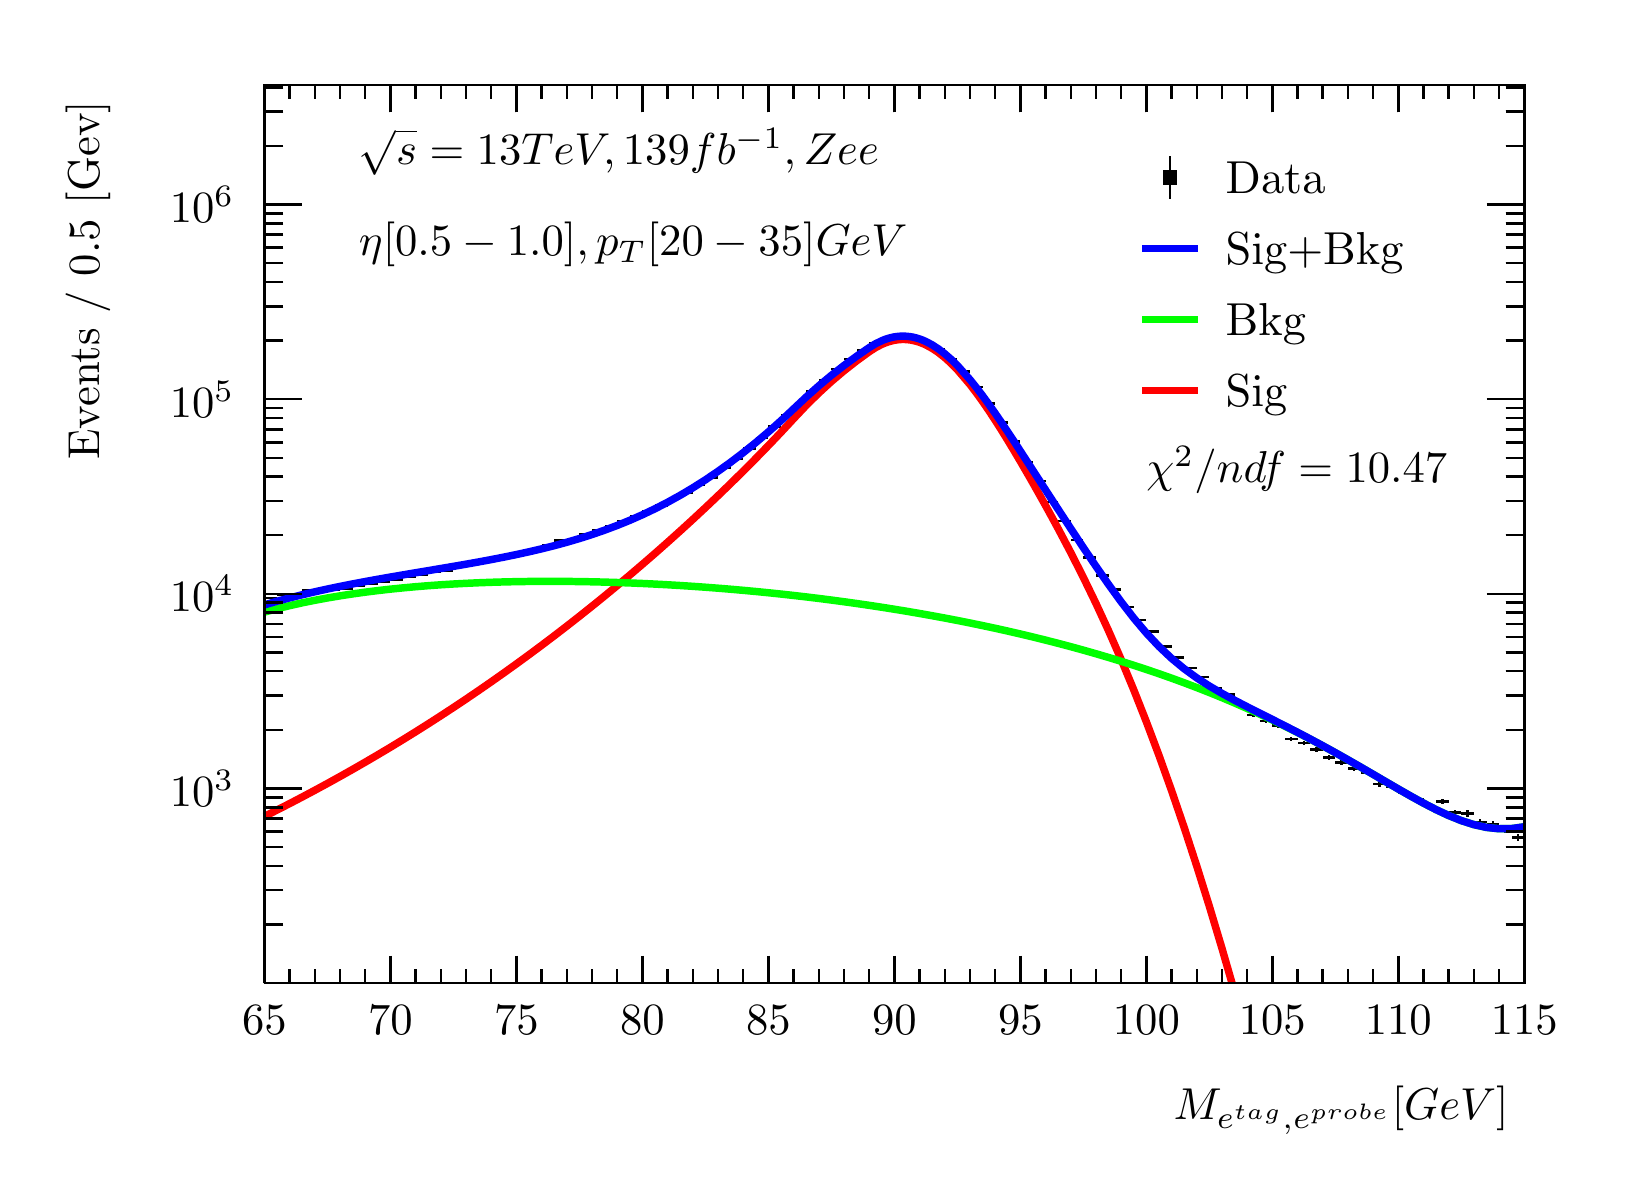
\begin{tikzpicture}
\pgfdeclareplotmark{cross} {
\pgfpathmoveto{\pgfpoint{-0.3\pgfplotmarksize}{\pgfplotmarksize}}
\pgfpathlineto{\pgfpoint{+0.3\pgfplotmarksize}{\pgfplotmarksize}}
\pgfpathlineto{\pgfpoint{+0.3\pgfplotmarksize}{0.3\pgfplotmarksize}}
\pgfpathlineto{\pgfpoint{+1\pgfplotmarksize}{0.3\pgfplotmarksize}}
\pgfpathlineto{\pgfpoint{+1\pgfplotmarksize}{-0.3\pgfplotmarksize}}
\pgfpathlineto{\pgfpoint{+0.3\pgfplotmarksize}{-0.3\pgfplotmarksize}}
\pgfpathlineto{\pgfpoint{+0.3\pgfplotmarksize}{-1.\pgfplotmarksize}}
\pgfpathlineto{\pgfpoint{-0.3\pgfplotmarksize}{-1.\pgfplotmarksize}}
\pgfpathlineto{\pgfpoint{-0.3\pgfplotmarksize}{-0.3\pgfplotmarksize}}
\pgfpathlineto{\pgfpoint{-1.\pgfplotmarksize}{-0.3\pgfplotmarksize}}
\pgfpathlineto{\pgfpoint{-1.\pgfplotmarksize}{0.3\pgfplotmarksize}}
\pgfpathlineto{\pgfpoint{-0.3\pgfplotmarksize}{0.3\pgfplotmarksize}}
\pgfpathclose
\pgfusepathqstroke
}
\pgfdeclareplotmark{cross*} {
\pgfpathmoveto{\pgfpoint{-0.3\pgfplotmarksize}{\pgfplotmarksize}}
\pgfpathlineto{\pgfpoint{+0.3\pgfplotmarksize}{\pgfplotmarksize}}
\pgfpathlineto{\pgfpoint{+0.3\pgfplotmarksize}{0.3\pgfplotmarksize}}
\pgfpathlineto{\pgfpoint{+1\pgfplotmarksize}{0.3\pgfplotmarksize}}
\pgfpathlineto{\pgfpoint{+1\pgfplotmarksize}{-0.3\pgfplotmarksize}}
\pgfpathlineto{\pgfpoint{+0.3\pgfplotmarksize}{-0.3\pgfplotmarksize}}
\pgfpathlineto{\pgfpoint{+0.3\pgfplotmarksize}{-1.\pgfplotmarksize}}
\pgfpathlineto{\pgfpoint{-0.3\pgfplotmarksize}{-1.\pgfplotmarksize}}
\pgfpathlineto{\pgfpoint{-0.3\pgfplotmarksize}{-0.3\pgfplotmarksize}}
\pgfpathlineto{\pgfpoint{-1.\pgfplotmarksize}{-0.3\pgfplotmarksize}}
\pgfpathlineto{\pgfpoint{-1.\pgfplotmarksize}{0.3\pgfplotmarksize}}
\pgfpathlineto{\pgfpoint{-0.3\pgfplotmarksize}{0.3\pgfplotmarksize}}
\pgfpathclose
\pgfusepathqfillstroke
}
\pgfdeclareplotmark{newstar} {
\pgfpathmoveto{\pgfqpoint{0pt}{\pgfplotmarksize}}
\pgfpathlineto{\pgfqpointpolar{44}{0.5\pgfplotmarksize}}
\pgfpathlineto{\pgfqpointpolar{18}{\pgfplotmarksize}}
\pgfpathlineto{\pgfqpointpolar{-20}{0.5\pgfplotmarksize}}
\pgfpathlineto{\pgfqpointpolar{-54}{\pgfplotmarksize}}
\pgfpathlineto{\pgfqpointpolar{-90}{0.5\pgfplotmarksize}}
\pgfpathlineto{\pgfqpointpolar{234}{\pgfplotmarksize}}
\pgfpathlineto{\pgfqpointpolar{198}{0.5\pgfplotmarksize}}
\pgfpathlineto{\pgfqpointpolar{162}{\pgfplotmarksize}}
\pgfpathlineto{\pgfqpointpolar{134}{0.5\pgfplotmarksize}}
\pgfpathclose
\pgfusepathqstroke
}
\pgfdeclareplotmark{newstar*} {
\pgfpathmoveto{\pgfqpoint{0pt}{\pgfplotmarksize}}
\pgfpathlineto{\pgfqpointpolar{44}{0.5\pgfplotmarksize}}
\pgfpathlineto{\pgfqpointpolar{18}{\pgfplotmarksize}}
\pgfpathlineto{\pgfqpointpolar{-20}{0.5\pgfplotmarksize}}
\pgfpathlineto{\pgfqpointpolar{-54}{\pgfplotmarksize}}
\pgfpathlineto{\pgfqpointpolar{-90}{0.5\pgfplotmarksize}}
\pgfpathlineto{\pgfqpointpolar{234}{\pgfplotmarksize}}
\pgfpathlineto{\pgfqpointpolar{198}{0.5\pgfplotmarksize}}
\pgfpathlineto{\pgfqpointpolar{162}{\pgfplotmarksize}}
\pgfpathlineto{\pgfqpointpolar{134}{0.5\pgfplotmarksize}}
\pgfpathclose
\pgfusepathqfillstroke
}
\definecolor{c}{rgb}{1,1,1};
\draw [color=c, fill=c] (0,0) rectangle (20,14.4361);
\draw [color=c, fill=c] (3,2.30977) rectangle (19,13.7143);
\definecolor{c}{rgb}{0,0,0};
\draw [c,line width=0.9] (3,2.30977) -- (3,13.7143) -- (19,13.7143) -- (19,2.30977) -- (3,2.30977);
\definecolor{c}{rgb}{1,1,1};
\draw [color=c, fill=c] (3,2.30977) rectangle (19,13.7143);
\definecolor{c}{rgb}{0,0,0};
\draw [c,line width=0.9] (3,2.30977) -- (3,13.7143) -- (19,13.7143) -- (19,2.30977) -- (3,2.30977);
\draw [c,line width=0.9] (3,2.30977) -- (19,2.30977);
\draw [c,line width=0.9] (3,2.65624) -- (3,2.30977);
\draw [c,line width=0.9] (3.32,2.48301) -- (3.32,2.30977);
\draw [c,line width=0.9] (3.64,2.48301) -- (3.64,2.30977);
\draw [c,line width=0.9] (3.96,2.48301) -- (3.96,2.30977);
\draw [c,line width=0.9] (4.28,2.48301) -- (4.28,2.30977);
\draw [c,line width=0.9] (4.6,2.65624) -- (4.6,2.30977);
\draw [c,line width=0.9] (4.92,2.48301) -- (4.92,2.30977);
\draw [c,line width=0.9] (5.24,2.48301) -- (5.24,2.30977);
\draw [c,line width=0.9] (5.56,2.48301) -- (5.56,2.30977);
\draw [c,line width=0.9] (5.88,2.48301) -- (5.88,2.30977);
\draw [c,line width=0.9] (6.2,2.65624) -- (6.2,2.30977);
\draw [c,line width=0.9] (6.52,2.48301) -- (6.52,2.30977);
\draw [c,line width=0.9] (6.84,2.48301) -- (6.84,2.30977);
\draw [c,line width=0.9] (7.16,2.48301) -- (7.16,2.30977);
\draw [c,line width=0.9] (7.48,2.48301) -- (7.48,2.30977);
\draw [c,line width=0.9] (7.8,2.65624) -- (7.8,2.30977);
\draw [c,line width=0.9] (8.12,2.48301) -- (8.12,2.30977);
\draw [c,line width=0.9] (8.44,2.48301) -- (8.44,2.30977);
\draw [c,line width=0.9] (8.76,2.48301) -- (8.76,2.30977);
\draw [c,line width=0.9] (9.08,2.48301) -- (9.08,2.30977);
\draw [c,line width=0.9] (9.4,2.65624) -- (9.4,2.30977);
\draw [c,line width=0.9] (9.72,2.48301) -- (9.72,2.30977);
\draw [c,line width=0.9] (10.04,2.48301) -- (10.04,2.30977);
\draw [c,line width=0.9] (10.36,2.48301) -- (10.36,2.30977);
\draw [c,line width=0.9] (10.68,2.48301) -- (10.68,2.30977);
\draw [c,line width=0.9] (11,2.65624) -- (11,2.30977);
\draw [c,line width=0.9] (11.32,2.48301) -- (11.32,2.30977);
\draw [c,line width=0.9] (11.64,2.48301) -- (11.64,2.30977);
\draw [c,line width=0.9] (11.96,2.48301) -- (11.96,2.30977);
\draw [c,line width=0.9] (12.28,2.48301) -- (12.28,2.30977);
\draw [c,line width=0.9] (12.6,2.65624) -- (12.6,2.30977);
\draw [c,line width=0.9] (12.92,2.48301) -- (12.92,2.30977);
\draw [c,line width=0.9] (13.24,2.48301) -- (13.24,2.30977);
\draw [c,line width=0.9] (13.56,2.48301) -- (13.56,2.30977);
\draw [c,line width=0.9] (13.88,2.48301) -- (13.88,2.30977);
\draw [c,line width=0.9] (14.2,2.65624) -- (14.2,2.30977);
\draw [c,line width=0.9] (14.52,2.48301) -- (14.52,2.30977);
\draw [c,line width=0.9] (14.84,2.48301) -- (14.84,2.30977);
\draw [c,line width=0.9] (15.16,2.48301) -- (15.16,2.30977);
\draw [c,line width=0.9] (15.48,2.48301) -- (15.48,2.30977);
\draw [c,line width=0.9] (15.8,2.65624) -- (15.8,2.30977);
\draw [c,line width=0.9] (16.12,2.48301) -- (16.12,2.30977);
\draw [c,line width=0.9] (16.44,2.48301) -- (16.44,2.30977);
\draw [c,line width=0.9] (16.76,2.48301) -- (16.76,2.30977);
\draw [c,line width=0.9] (17.08,2.48301) -- (17.08,2.30977);
\draw [c,line width=0.9] (17.4,2.65624) -- (17.4,2.30977);
\draw [c,line width=0.9] (17.72,2.48301) -- (17.72,2.30977);
\draw [c,line width=0.9] (18.04,2.48301) -- (18.04,2.30977);
\draw [c,line width=0.9] (18.36,2.48301) -- (18.36,2.30977);
\draw [c,line width=0.9] (18.68,2.48301) -- (18.68,2.30977);
\draw [c,line width=0.9] (19,2.65624) -- (19,2.30977);
\draw [c,line width=0.9] (19,2.65624) -- (19,2.30977);
\draw [anchor=base] (3,1.66015) node[scale=1.61424, color=c, rotate=0]{65};
\draw [anchor=base] (4.6,1.66015) node[scale=1.61424, color=c, rotate=0]{70};
\draw [anchor=base] (6.2,1.66015) node[scale=1.61424, color=c, rotate=0]{75};
\draw [anchor=base] (7.8,1.66015) node[scale=1.61424, color=c, rotate=0]{80};
\draw [anchor=base] (9.4,1.66015) node[scale=1.61424, color=c, rotate=0]{85};
\draw [anchor=base] (11,1.66015) node[scale=1.61424, color=c, rotate=0]{90};
\draw [anchor=base] (12.6,1.66015) node[scale=1.61424, color=c, rotate=0]{95};
\draw [anchor=base] (14.2,1.66015) node[scale=1.61424, color=c, rotate=0]{100};
\draw [anchor=base] (15.8,1.66015) node[scale=1.61424, color=c, rotate=0]{105};
\draw [anchor=base] (17.4,1.66015) node[scale=1.61424, color=c, rotate=0]{110};
\draw [anchor=base] (19,1.66015) node[scale=1.61424, color=c, rotate=0]{115};
\draw [anchor= east] (19,0.692932) node[scale=1.61424, color=c, rotate=0]{$M_{e^{tag}, e^{probe}}  [GeV]$};
\draw [c,line width=0.9] (3,13.7143) -- (19,13.7143);
\draw [c,line width=0.9] (3,13.3678) -- (3,13.7143);
\draw [c,line width=0.9] (3.32,13.5411) -- (3.32,13.7143);
\draw [c,line width=0.9] (3.64,13.5411) -- (3.64,13.7143);
\draw [c,line width=0.9] (3.96,13.5411) -- (3.96,13.7143);
\draw [c,line width=0.9] (4.28,13.5411) -- (4.28,13.7143);
\draw [c,line width=0.9] (4.6,13.3678) -- (4.6,13.7143);
\draw [c,line width=0.9] (4.92,13.5411) -- (4.92,13.7143);
\draw [c,line width=0.9] (5.24,13.5411) -- (5.24,13.7143);
\draw [c,line width=0.9] (5.56,13.5411) -- (5.56,13.7143);
\draw [c,line width=0.9] (5.88,13.5411) -- (5.88,13.7143);
\draw [c,line width=0.9] (6.2,13.3678) -- (6.2,13.7143);
\draw [c,line width=0.9] (6.52,13.5411) -- (6.52,13.7143);
\draw [c,line width=0.9] (6.84,13.5411) -- (6.84,13.7143);
\draw [c,line width=0.9] (7.16,13.5411) -- (7.16,13.7143);
\draw [c,line width=0.9] (7.48,13.5411) -- (7.48,13.7143);
\draw [c,line width=0.9] (7.8,13.3678) -- (7.8,13.7143);
\draw [c,line width=0.9] (8.12,13.5411) -- (8.12,13.7143);
\draw [c,line width=0.9] (8.44,13.5411) -- (8.44,13.7143);
\draw [c,line width=0.9] (8.76,13.5411) -- (8.76,13.7143);
\draw [c,line width=0.9] (9.08,13.5411) -- (9.08,13.7143);
\draw [c,line width=0.9] (9.4,13.3678) -- (9.4,13.7143);
\draw [c,line width=0.9] (9.72,13.5411) -- (9.72,13.7143);
\draw [c,line width=0.9] (10.04,13.5411) -- (10.04,13.7143);
\draw [c,line width=0.9] (10.36,13.5411) -- (10.36,13.7143);
\draw [c,line width=0.9] (10.68,13.5411) -- (10.68,13.7143);
\draw [c,line width=0.9] (11,13.3678) -- (11,13.7143);
\draw [c,line width=0.9] (11.32,13.5411) -- (11.32,13.7143);
\draw [c,line width=0.9] (11.64,13.5411) -- (11.64,13.7143);
\draw [c,line width=0.9] (11.96,13.5411) -- (11.96,13.7143);
\draw [c,line width=0.9] (12.28,13.5411) -- (12.28,13.7143);
\draw [c,line width=0.9] (12.6,13.3678) -- (12.6,13.7143);
\draw [c,line width=0.9] (12.92,13.5411) -- (12.92,13.7143);
\draw [c,line width=0.9] (13.24,13.5411) -- (13.24,13.7143);
\draw [c,line width=0.9] (13.56,13.5411) -- (13.56,13.7143);
\draw [c,line width=0.9] (13.88,13.5411) -- (13.88,13.7143);
\draw [c,line width=0.9] (14.2,13.3678) -- (14.2,13.7143);
\draw [c,line width=0.9] (14.52,13.5411) -- (14.52,13.7143);
\draw [c,line width=0.9] (14.84,13.5411) -- (14.84,13.7143);
\draw [c,line width=0.9] (15.16,13.5411) -- (15.16,13.7143);
\draw [c,line width=0.9] (15.48,13.5411) -- (15.48,13.7143);
\draw [c,line width=0.9] (15.8,13.3678) -- (15.8,13.7143);
\draw [c,line width=0.9] (16.12,13.5411) -- (16.12,13.7143);
\draw [c,line width=0.9] (16.44,13.5411) -- (16.44,13.7143);
\draw [c,line width=0.9] (16.76,13.5411) -- (16.76,13.7143);
\draw [c,line width=0.9] (17.08,13.5411) -- (17.08,13.7143);
\draw [c,line width=0.9] (17.4,13.3678) -- (17.4,13.7143);
\draw [c,line width=0.9] (17.72,13.5411) -- (17.72,13.7143);
\draw [c,line width=0.9] (18.04,13.5411) -- (18.04,13.7143);
\draw [c,line width=0.9] (18.36,13.5411) -- (18.36,13.7143);
\draw [c,line width=0.9] (18.68,13.5411) -- (18.68,13.7143);
\draw [c,line width=0.9] (19,13.3678) -- (19,13.7143);
\draw [c,line width=0.9] (19,13.3678) -- (19,13.7143);
\draw [c,line width=0.9] (3,2.30977) -- (3,13.7143);
\draw [c,line width=0.9] (3.237,3.05385) -- (3,3.05385);
\draw [c,line width=0.9] (3.237,3.48911) -- (3,3.48911);
\draw [c,line width=0.9] (3.237,3.79793) -- (3,3.79793);
\draw [c,line width=0.9] (3.237,4.03747) -- (3,4.03747);
\draw [c,line width=0.9] (3.237,4.23319) -- (3,4.23319);
\draw [c,line width=0.9] (3.237,4.39867) -- (3,4.39867);
\draw [c,line width=0.9] (3.237,4.54201) -- (3,4.54201);
\draw [c,line width=0.9] (3.237,4.66845) -- (3,4.66845);
\draw [c,line width=0.9] (3.474,4.78155) -- (3,4.78155);
\draw [anchor= east] (2.82,4.78155) node[scale=1.61424, color=c, rotate=0]{$10^{3}$};
\draw [c,line width=0.9] (3.237,5.52563) -- (3,5.52563);
\draw [c,line width=0.9] (3.237,5.96089) -- (3,5.96089);
\draw [c,line width=0.9] (3.237,6.26971) -- (3,6.26971);
\draw [c,line width=0.9] (3.237,6.50925) -- (3,6.50925);
\draw [c,line width=0.9] (3.237,6.70497) -- (3,6.70497);
\draw [c,line width=0.9] (3.237,6.87045) -- (3,6.87045);
\draw [c,line width=0.9] (3.237,7.01379) -- (3,7.01379);
\draw [c,line width=0.9] (3.237,7.14023) -- (3,7.14023);
\draw [c,line width=0.9] (3.474,7.25333) -- (3,7.25333);
\draw [anchor= east] (2.82,7.25333) node[scale=1.61424, color=c, rotate=0]{$10^{4}$};
\draw [c,line width=0.9] (3.237,7.99741) -- (3,7.99741);
\draw [c,line width=0.9] (3.237,8.43267) -- (3,8.43267);
\draw [c,line width=0.9] (3.237,8.74149) -- (3,8.74149);
\draw [c,line width=0.9] (3.237,8.98103) -- (3,8.98103);
\draw [c,line width=0.9] (3.237,9.17675) -- (3,9.17675);
\draw [c,line width=0.9] (3.237,9.34223) -- (3,9.34223);
\draw [c,line width=0.9] (3.237,9.48557) -- (3,9.48557);
\draw [c,line width=0.9] (3.237,9.61201) -- (3,9.61201);
\draw [c,line width=0.9] (3.474,9.72511) -- (3,9.72511);
\draw [anchor= east] (2.82,9.72511) node[scale=1.61424, color=c, rotate=0]{$10^{5}$};
\draw [c,line width=0.9] (3.237,10.4692) -- (3,10.4692);
\draw [c,line width=0.9] (3.237,10.9044) -- (3,10.9044);
\draw [c,line width=0.9] (3.237,11.2133) -- (3,11.2133);
\draw [c,line width=0.9] (3.237,11.4528) -- (3,11.4528);
\draw [c,line width=0.9] (3.237,11.6485) -- (3,11.6485);
\draw [c,line width=0.9] (3.237,11.814) -- (3,11.814);
\draw [c,line width=0.9] (3.237,11.9574) -- (3,11.9574);
\draw [c,line width=0.9] (3.237,12.0838) -- (3,12.0838);
\draw [c,line width=0.9] (3.474,12.1969) -- (3,12.1969);
\draw [anchor= east] (2.82,12.1969) node[scale=1.61424, color=c, rotate=0]{$10^{6}$};
\draw [c,line width=0.9] (3.237,12.941) -- (3,12.941);
\draw [c,line width=0.9] (3.237,13.3762) -- (3,13.3762);
\draw [c,line width=0.9] (3.237,13.6851) -- (3,13.6851);
\draw [anchor= east] (0.76,13.7143) node[scale=1.61424, color=c, rotate=90]{Events / 0.5 [Gev]};
\draw [c,line width=0.9] (19,2.30977) -- (19,13.7143);
\draw [c,line width=0.9] (18.763,3.05385) -- (19,3.05385);
\draw [c,line width=0.9] (18.763,3.48911) -- (19,3.48911);
\draw [c,line width=0.9] (18.763,3.79793) -- (19,3.79793);
\draw [c,line width=0.9] (18.763,4.03747) -- (19,4.03747);
\draw [c,line width=0.9] (18.763,4.23319) -- (19,4.23319);
\draw [c,line width=0.9] (18.763,4.39867) -- (19,4.39867);
\draw [c,line width=0.9] (18.763,4.54201) -- (19,4.54201);
\draw [c,line width=0.9] (18.763,4.66845) -- (19,4.66845);
\draw [c,line width=0.9] (18.526,4.78155) -- (19,4.78155);
\draw [c,line width=0.9] (18.763,5.52563) -- (19,5.52563);
\draw [c,line width=0.9] (18.763,5.96089) -- (19,5.96089);
\draw [c,line width=0.9] (18.763,6.26971) -- (19,6.26971);
\draw [c,line width=0.9] (18.763,6.50925) -- (19,6.50925);
\draw [c,line width=0.9] (18.763,6.70497) -- (19,6.70497);
\draw [c,line width=0.9] (18.763,6.87045) -- (19,6.87045);
\draw [c,line width=0.9] (18.763,7.01379) -- (19,7.01379);
\draw [c,line width=0.9] (18.763,7.14023) -- (19,7.14023);
\draw [c,line width=0.9] (18.526,7.25333) -- (19,7.25333);
\draw [c,line width=0.9] (18.763,7.99741) -- (19,7.99741);
\draw [c,line width=0.9] (18.763,8.43267) -- (19,8.43267);
\draw [c,line width=0.9] (18.763,8.74149) -- (19,8.74149);
\draw [c,line width=0.9] (18.763,8.98103) -- (19,8.98103);
\draw [c,line width=0.9] (18.763,9.17675) -- (19,9.17675);
\draw [c,line width=0.9] (18.763,9.34223) -- (19,9.34223);
\draw [c,line width=0.9] (18.763,9.48557) -- (19,9.48557);
\draw [c,line width=0.9] (18.763,9.61201) -- (19,9.61201);
\draw [c,line width=0.9] (18.526,9.72511) -- (19,9.72511);
\draw [c,line width=0.9] (18.763,10.4692) -- (19,10.4692);
\draw [c,line width=0.9] (18.763,10.9044) -- (19,10.9044);
\draw [c,line width=0.9] (18.763,11.2133) -- (19,11.2133);
\draw [c,line width=0.9] (18.763,11.4528) -- (19,11.4528);
\draw [c,line width=0.9] (18.763,11.6485) -- (19,11.6485);
\draw [c,line width=0.9] (18.763,11.814) -- (19,11.814);
\draw [c,line width=0.9] (18.763,11.9574) -- (19,11.9574);
\draw [c,line width=0.9] (18.763,12.0838) -- (19,12.0838);
\draw [c,line width=0.9] (18.526,12.1969) -- (19,12.1969);
\draw [c,line width=0.9] (18.763,12.941) -- (19,12.941);
\draw [c,line width=0.9] (18.763,13.3762) -- (19,13.3762);
\draw [c,line width=0.9] (18.763,13.6851) -- (19,13.6851);
\draw [c,line width=0.9] (3.08,7.19782) -- (3,7.19782);
\draw [c,line width=0.9] (3,7.19782) -- (3,7.19782);
\draw [c,line width=0.9] (3.08,7.19782) -- (3.16,7.19782);
\draw [c,line width=0.9] (3.16,7.19782) -- (3.16,7.19782);
\draw [c,line width=0.9] (3.08,7.19782) -- (3.08,7.20883);
\draw [c,line width=0.9] (3.08,7.20883) -- (3.08,7.20883);
\draw [c,line width=0.9] (3.08,7.19782) -- (3.08,7.1868);
\draw [c,line width=0.9] (3.08,7.1868) -- (3.08,7.1868);
\draw [c,line width=0.9] (3.24,7.24092) -- (3.16,7.24092);
\draw [c,line width=0.9] (3.16,7.24092) -- (3.16,7.24092);
\draw [c,line width=0.9] (3.24,7.24092) -- (3.32,7.24092);
\draw [c,line width=0.9] (3.32,7.24092) -- (3.32,7.24092);
\draw [c,line width=0.9] (3.24,7.24092) -- (3.24,7.25171);
\draw [c,line width=0.9] (3.24,7.25171) -- (3.24,7.25171);
\draw [c,line width=0.9] (3.24,7.24092) -- (3.24,7.23012);
\draw [c,line width=0.9] (3.24,7.23012) -- (3.24,7.23012);
\draw [c,line width=0.9] (3.4,7.25194) -- (3.32,7.25194);
\draw [c,line width=0.9] (3.32,7.25194) -- (3.32,7.25194);
\draw [c,line width=0.9] (3.4,7.25194) -- (3.48,7.25194);
\draw [c,line width=0.9] (3.48,7.25194) -- (3.48,7.25194);
\draw [c,line width=0.9] (3.4,7.25194) -- (3.4,7.26268);
\draw [c,line width=0.9] (3.4,7.26268) -- (3.4,7.26268);
\draw [c,line width=0.9] (3.4,7.25194) -- (3.4,7.24119);
\draw [c,line width=0.9] (3.4,7.24119) -- (3.4,7.24119);
\draw [c,line width=0.9] (3.56,7.30202) -- (3.48,7.30202);
\draw [c,line width=0.9] (3.48,7.30202) -- (3.48,7.30202);
\draw [c,line width=0.9] (3.56,7.30202) -- (3.64,7.30202);
\draw [c,line width=0.9] (3.64,7.30202) -- (3.64,7.30202);
\draw [c,line width=0.9] (3.56,7.30202) -- (3.56,7.31252);
\draw [c,line width=0.9] (3.56,7.31252) -- (3.56,7.31252);
\draw [c,line width=0.9] (3.56,7.30202) -- (3.56,7.29153);
\draw [c,line width=0.9] (3.56,7.29153) -- (3.56,7.29153);
\draw [c,line width=0.9] (3.72,7.31558) -- (3.64,7.31558);
\draw [c,line width=0.9] (3.64,7.31558) -- (3.64,7.31558);
\draw [c,line width=0.9] (3.72,7.31558) -- (3.8,7.31558);
\draw [c,line width=0.9] (3.8,7.31558) -- (3.8,7.31558);
\draw [c,line width=0.9] (3.72,7.31558) -- (3.72,7.32601);
\draw [c,line width=0.9] (3.72,7.32601) -- (3.72,7.32601);
\draw [c,line width=0.9] (3.72,7.31558) -- (3.72,7.30515);
\draw [c,line width=0.9] (3.72,7.30515) -- (3.72,7.30515);
\draw [c,line width=0.9] (3.88,7.30571) -- (3.8,7.30571);
\draw [c,line width=0.9] (3.8,7.30571) -- (3.8,7.30571);
\draw [c,line width=0.9] (3.88,7.30571) -- (3.96,7.30571);
\draw [c,line width=0.9] (3.96,7.30571) -- (3.96,7.30571);
\draw [c,line width=0.9] (3.88,7.30571) -- (3.88,7.31618);
\draw [c,line width=0.9] (3.88,7.31618) -- (3.88,7.31618);
\draw [c,line width=0.9] (3.88,7.30571) -- (3.88,7.29523);
\draw [c,line width=0.9] (3.88,7.29523) -- (3.88,7.29523);
\draw [c,line width=0.9] (4.04,7.32355) -- (3.96,7.32355);
\draw [c,line width=0.9] (3.96,7.32355) -- (3.96,7.32355);
\draw [c,line width=0.9] (4.04,7.32355) -- (4.12,7.32355);
\draw [c,line width=0.9] (4.12,7.32355) -- (4.12,7.32355);
\draw [c,line width=0.9] (4.04,7.32355) -- (4.04,7.33394);
\draw [c,line width=0.9] (4.04,7.33394) -- (4.04,7.33394);
\draw [c,line width=0.9] (4.04,7.32355) -- (4.04,7.31316);
\draw [c,line width=0.9] (4.04,7.31316) -- (4.04,7.31316);
\draw [c,line width=0.9] (4.2,7.35643) -- (4.12,7.35643);
\draw [c,line width=0.9] (4.12,7.35643) -- (4.12,7.35643);
\draw [c,line width=0.9] (4.2,7.35643) -- (4.28,7.35643);
\draw [c,line width=0.9] (4.28,7.35643) -- (4.28,7.35643);
\draw [c,line width=0.9] (4.2,7.35643) -- (4.2,7.36666);
\draw [c,line width=0.9] (4.2,7.36666) -- (4.2,7.36666);
\draw [c,line width=0.9] (4.2,7.35643) -- (4.2,7.3462);
\draw [c,line width=0.9] (4.2,7.3462) -- (4.2,7.3462);
\draw [c,line width=0.9] (4.36,7.38377) -- (4.28,7.38377);
\draw [c,line width=0.9] (4.28,7.38377) -- (4.28,7.38377);
\draw [c,line width=0.9] (4.36,7.38377) -- (4.44,7.38377);
\draw [c,line width=0.9] (4.44,7.38377) -- (4.44,7.38377);
\draw [c,line width=0.9] (4.36,7.38377) -- (4.36,7.39387);
\draw [c,line width=0.9] (4.36,7.39387) -- (4.36,7.39387);
\draw [c,line width=0.9] (4.36,7.38377) -- (4.36,7.37367);
\draw [c,line width=0.9] (4.36,7.37367) -- (4.36,7.37367);
\draw [c,line width=0.9] (4.52,7.40932) -- (4.44,7.40932);
\draw [c,line width=0.9] (4.44,7.40932) -- (4.44,7.40932);
\draw [c,line width=0.9] (4.52,7.40932) -- (4.6,7.40932);
\draw [c,line width=0.9] (4.6,7.40932) -- (4.6,7.40932);
\draw [c,line width=0.9] (4.52,7.40932) -- (4.52,7.4193);
\draw [c,line width=0.9] (4.52,7.4193) -- (4.52,7.4193);
\draw [c,line width=0.9] (4.52,7.40932) -- (4.52,7.39934);
\draw [c,line width=0.9] (4.52,7.39934) -- (4.52,7.39934);
\draw [c,line width=0.9] (4.68,7.43772) -- (4.6,7.43772);
\draw [c,line width=0.9] (4.6,7.43772) -- (4.6,7.43772);
\draw [c,line width=0.9] (4.68,7.43772) -- (4.76,7.43772);
\draw [c,line width=0.9] (4.76,7.43772) -- (4.76,7.43772);
\draw [c,line width=0.9] (4.68,7.43772) -- (4.68,7.44757);
\draw [c,line width=0.9] (4.68,7.44757) -- (4.68,7.44757);
\draw [c,line width=0.9] (4.68,7.43772) -- (4.68,7.42787);
\draw [c,line width=0.9] (4.68,7.42787) -- (4.68,7.42787);
\draw [c,line width=0.9] (4.84,7.4711) -- (4.76,7.4711);
\draw [c,line width=0.9] (4.76,7.4711) -- (4.76,7.4711);
\draw [c,line width=0.9] (4.84,7.4711) -- (4.92,7.4711);
\draw [c,line width=0.9] (4.92,7.4711) -- (4.92,7.4711);
\draw [c,line width=0.9] (4.84,7.4711) -- (4.84,7.4808);
\draw [c,line width=0.9] (4.84,7.4808) -- (4.84,7.4808);
\draw [c,line width=0.9] (4.84,7.4711) -- (4.84,7.4614);
\draw [c,line width=0.9] (4.84,7.4614) -- (4.84,7.4614);
\draw [c,line width=0.9] (5,7.49887) -- (4.92,7.49887);
\draw [c,line width=0.9] (4.92,7.49887) -- (4.92,7.49887);
\draw [c,line width=0.9] (5,7.49887) -- (5.08,7.49887);
\draw [c,line width=0.9] (5.08,7.49887) -- (5.08,7.49887);
\draw [c,line width=0.9] (5,7.49887) -- (5,7.50844);
\draw [c,line width=0.9] (5,7.50844) -- (5,7.50844);
\draw [c,line width=0.9] (5,7.49887) -- (5,7.48929);
\draw [c,line width=0.9] (5,7.48929) -- (5,7.48929);
\draw [c,line width=0.9] (5.16,7.53737) -- (5.08,7.53737);
\draw [c,line width=0.9] (5.08,7.53737) -- (5.08,7.53737);
\draw [c,line width=0.9] (5.16,7.53737) -- (5.24,7.53737);
\draw [c,line width=0.9] (5.24,7.53737) -- (5.24,7.53737);
\draw [c,line width=0.9] (5.16,7.53737) -- (5.16,7.54677);
\draw [c,line width=0.9] (5.16,7.54677) -- (5.16,7.54677);
\draw [c,line width=0.9] (5.16,7.53737) -- (5.16,7.52796);
\draw [c,line width=0.9] (5.16,7.52796) -- (5.16,7.52796);
\draw [c,line width=0.9] (5.32,7.55169) -- (5.24,7.55169);
\draw [c,line width=0.9] (5.24,7.55169) -- (5.24,7.55169);
\draw [c,line width=0.9] (5.32,7.55169) -- (5.4,7.55169);
\draw [c,line width=0.9] (5.4,7.55169) -- (5.4,7.55169);
\draw [c,line width=0.9] (5.32,7.55169) -- (5.32,7.56103);
\draw [c,line width=0.9] (5.32,7.56103) -- (5.32,7.56103);
\draw [c,line width=0.9] (5.32,7.55169) -- (5.32,7.54235);
\draw [c,line width=0.9] (5.32,7.54235) -- (5.32,7.54235);
\draw [c,line width=0.9] (5.48,7.59901) -- (5.4,7.59901);
\draw [c,line width=0.9] (5.4,7.59901) -- (5.4,7.59901);
\draw [c,line width=0.9] (5.48,7.59901) -- (5.56,7.59901);
\draw [c,line width=0.9] (5.56,7.59901) -- (5.56,7.59901);
\draw [c,line width=0.9] (5.48,7.59901) -- (5.48,7.60814);
\draw [c,line width=0.9] (5.48,7.60814) -- (5.48,7.60814);
\draw [c,line width=0.9] (5.48,7.59901) -- (5.48,7.58987);
\draw [c,line width=0.9] (5.48,7.58987) -- (5.48,7.58987);
\draw [c,line width=0.9] (5.64,7.6296) -- (5.56,7.6296);
\draw [c,line width=0.9] (5.56,7.6296) -- (5.56,7.6296);
\draw [c,line width=0.9] (5.64,7.6296) -- (5.72,7.6296);
\draw [c,line width=0.9] (5.72,7.6296) -- (5.72,7.6296);
\draw [c,line width=0.9] (5.64,7.6296) -- (5.64,7.63861);
\draw [c,line width=0.9] (5.64,7.63861) -- (5.64,7.63861);
\draw [c,line width=0.9] (5.64,7.6296) -- (5.64,7.6206);
\draw [c,line width=0.9] (5.64,7.6206) -- (5.64,7.6206);
\draw [c,line width=0.9] (5.8,7.67091) -- (5.72,7.67091);
\draw [c,line width=0.9] (5.72,7.67091) -- (5.72,7.67091);
\draw [c,line width=0.9] (5.8,7.67091) -- (5.88,7.67091);
\draw [c,line width=0.9] (5.88,7.67091) -- (5.88,7.67091);
\draw [c,line width=0.9] (5.8,7.67091) -- (5.8,7.67975);
\draw [c,line width=0.9] (5.8,7.67975) -- (5.8,7.67975);
\draw [c,line width=0.9] (5.8,7.67091) -- (5.8,7.66208);
\draw [c,line width=0.9] (5.8,7.66208) -- (5.8,7.66208);
\draw [c,line width=0.9] (5.96,7.69309) -- (5.88,7.69309);
\draw [c,line width=0.9] (5.88,7.69309) -- (5.88,7.69309);
\draw [c,line width=0.9] (5.96,7.69309) -- (6.04,7.69309);
\draw [c,line width=0.9] (6.04,7.69309) -- (6.04,7.69309);
\draw [c,line width=0.9] (5.96,7.69309) -- (5.96,7.70184);
\draw [c,line width=0.9] (5.96,7.70184) -- (5.96,7.70184);
\draw [c,line width=0.9] (5.96,7.69309) -- (5.96,7.68434);
\draw [c,line width=0.9] (5.96,7.68434) -- (5.96,7.68434);
\draw [c,line width=0.9] (6.12,7.73324) -- (6.04,7.73324);
\draw [c,line width=0.9] (6.04,7.73324) -- (6.04,7.73324);
\draw [c,line width=0.9] (6.12,7.73324) -- (6.2,7.73324);
\draw [c,line width=0.9] (6.2,7.73324) -- (6.2,7.73324);
\draw [c,line width=0.9] (6.12,7.73324) -- (6.12,7.74182);
\draw [c,line width=0.9] (6.12,7.74182) -- (6.12,7.74182);
\draw [c,line width=0.9] (6.12,7.73324) -- (6.12,7.72465);
\draw [c,line width=0.9] (6.12,7.72465) -- (6.12,7.72465);
\draw [c,line width=0.9] (6.28,7.76563) -- (6.2,7.76563);
\draw [c,line width=0.9] (6.2,7.76563) -- (6.2,7.76563);
\draw [c,line width=0.9] (6.28,7.76563) -- (6.36,7.76563);
\draw [c,line width=0.9] (6.36,7.76563) -- (6.36,7.76563);
\draw [c,line width=0.9] (6.28,7.76563) -- (6.28,7.77408);
\draw [c,line width=0.9] (6.28,7.77408) -- (6.28,7.77408);
\draw [c,line width=0.9] (6.28,7.76563) -- (6.28,7.75717);
\draw [c,line width=0.9] (6.28,7.75717) -- (6.28,7.75717);
\draw [c,line width=0.9] (6.44,7.8048) -- (6.36,7.8048);
\draw [c,line width=0.9] (6.36,7.8048) -- (6.36,7.8048);
\draw [c,line width=0.9] (6.44,7.8048) -- (6.52,7.8048);
\draw [c,line width=0.9] (6.52,7.8048) -- (6.52,7.8048);
\draw [c,line width=0.9] (6.44,7.8048) -- (6.44,7.81311);
\draw [c,line width=0.9] (6.44,7.81311) -- (6.44,7.81311);
\draw [c,line width=0.9] (6.44,7.8048) -- (6.44,7.7965);
\draw [c,line width=0.9] (6.44,7.7965) -- (6.44,7.7965);
\draw [c,line width=0.9] (6.6,7.8642) -- (6.52,7.8642);
\draw [c,line width=0.9] (6.52,7.8642) -- (6.52,7.8642);
\draw [c,line width=0.9] (6.6,7.8642) -- (6.68,7.8642);
\draw [c,line width=0.9] (6.68,7.8642) -- (6.68,7.8642);
\draw [c,line width=0.9] (6.6,7.8642) -- (6.6,7.87228);
\draw [c,line width=0.9] (6.6,7.87228) -- (6.6,7.87228);
\draw [c,line width=0.9] (6.6,7.8642) -- (6.6,7.85613);
\draw [c,line width=0.9] (6.6,7.85613) -- (6.6,7.85613);
\draw [c,line width=0.9] (6.76,7.92739) -- (6.68,7.92739);
\draw [c,line width=0.9] (6.68,7.92739) -- (6.68,7.92739);
\draw [c,line width=0.9] (6.76,7.92739) -- (6.84,7.92739);
\draw [c,line width=0.9] (6.84,7.92739) -- (6.84,7.92739);
\draw [c,line width=0.9] (6.76,7.92739) -- (6.76,7.93523);
\draw [c,line width=0.9] (6.76,7.93523) -- (6.76,7.93523);
\draw [c,line width=0.9] (6.76,7.92739) -- (6.76,7.91954);
\draw [c,line width=0.9] (6.76,7.91954) -- (6.76,7.91954);
\draw [c,line width=0.9] (6.92,7.94843) -- (6.84,7.94843);
\draw [c,line width=0.9] (6.84,7.94843) -- (6.84,7.94843);
\draw [c,line width=0.9] (6.92,7.94843) -- (7,7.94843);
\draw [c,line width=0.9] (7,7.94843) -- (7,7.94843);
\draw [c,line width=0.9] (6.92,7.94843) -- (6.92,7.9562);
\draw [c,line width=0.9] (6.92,7.9562) -- (6.92,7.9562);
\draw [c,line width=0.9] (6.92,7.94843) -- (6.92,7.94067);
\draw [c,line width=0.9] (6.92,7.94067) -- (6.92,7.94067);
\draw [c,line width=0.9] (7.08,8.00655) -- (7,8.00655);
\draw [c,line width=0.9] (7,8.00655) -- (7,8.00655);
\draw [c,line width=0.9] (7.08,8.00655) -- (7.16,8.00655);
\draw [c,line width=0.9] (7.16,8.00655) -- (7.16,8.00655);
\draw [c,line width=0.9] (7.08,8.00655) -- (7.08,8.01411);
\draw [c,line width=0.9] (7.08,8.01411) -- (7.08,8.01411);
\draw [c,line width=0.9] (7.08,8.00655) -- (7.08,7.99899);
\draw [c,line width=0.9] (7.08,7.99899) -- (7.08,7.99899);
\draw [c,line width=0.9] (7.24,8.05702) -- (7.16,8.05702);
\draw [c,line width=0.9] (7.16,8.05702) -- (7.16,8.05702);
\draw [c,line width=0.9] (7.24,8.05702) -- (7.32,8.05702);
\draw [c,line width=0.9] (7.32,8.05702) -- (7.32,8.05702);
\draw [c,line width=0.9] (7.24,8.05702) -- (7.24,8.0644);
\draw [c,line width=0.9] (7.24,8.0644) -- (7.24,8.0644);
\draw [c,line width=0.9] (7.24,8.05702) -- (7.24,8.04964);
\draw [c,line width=0.9] (7.24,8.04964) -- (7.24,8.04964);
\draw [c,line width=0.9] (7.4,8.11619) -- (7.32,8.11619);
\draw [c,line width=0.9] (7.32,8.11619) -- (7.32,8.11619);
\draw [c,line width=0.9] (7.4,8.11619) -- (7.48,8.11619);
\draw [c,line width=0.9] (7.48,8.11619) -- (7.48,8.11619);
\draw [c,line width=0.9] (7.4,8.11619) -- (7.4,8.12337);
\draw [c,line width=0.9] (7.4,8.12337) -- (7.4,8.12337);
\draw [c,line width=0.9] (7.4,8.11619) -- (7.4,8.10901);
\draw [c,line width=0.9] (7.4,8.10901) -- (7.4,8.10901);
\draw [c,line width=0.9] (7.56,8.17559) -- (7.48,8.17559);
\draw [c,line width=0.9] (7.48,8.17559) -- (7.48,8.17559);
\draw [c,line width=0.9] (7.56,8.17559) -- (7.64,8.17559);
\draw [c,line width=0.9] (7.64,8.17559) -- (7.64,8.17559);
\draw [c,line width=0.9] (7.56,8.17559) -- (7.56,8.18258);
\draw [c,line width=0.9] (7.56,8.18258) -- (7.56,8.18258);
\draw [c,line width=0.9] (7.56,8.17559) -- (7.56,8.1686);
\draw [c,line width=0.9] (7.56,8.1686) -- (7.56,8.1686);
\draw [c,line width=0.9] (7.72,8.23803) -- (7.64,8.23803);
\draw [c,line width=0.9] (7.64,8.23803) -- (7.64,8.23803);
\draw [c,line width=0.9] (7.72,8.23803) -- (7.8,8.23803);
\draw [c,line width=0.9] (7.8,8.23803) -- (7.8,8.23803);
\draw [c,line width=0.9] (7.72,8.23803) -- (7.72,8.24481);
\draw [c,line width=0.9] (7.72,8.24481) -- (7.72,8.24481);
\draw [c,line width=0.9] (7.72,8.23803) -- (7.72,8.23124);
\draw [c,line width=0.9] (7.72,8.23124) -- (7.72,8.23124);
\draw [c,line width=0.9] (7.88,8.29853) -- (7.8,8.29853);
\draw [c,line width=0.9] (7.8,8.29853) -- (7.8,8.29853);
\draw [c,line width=0.9] (7.88,8.29853) -- (7.96,8.29853);
\draw [c,line width=0.9] (7.96,8.29853) -- (7.96,8.29853);
\draw [c,line width=0.9] (7.88,8.29853) -- (7.88,8.30513);
\draw [c,line width=0.9] (7.88,8.30513) -- (7.88,8.30513);
\draw [c,line width=0.9] (7.88,8.29853) -- (7.88,8.29193);
\draw [c,line width=0.9] (7.88,8.29193) -- (7.88,8.29193);
\draw [c,line width=0.9] (8.04,8.37501) -- (7.96,8.37501);
\draw [c,line width=0.9] (7.96,8.37501) -- (7.96,8.37501);
\draw [c,line width=0.9] (8.04,8.37501) -- (8.12,8.37501);
\draw [c,line width=0.9] (8.12,8.37501) -- (8.12,8.37501);
\draw [c,line width=0.9] (8.04,8.37501) -- (8.04,8.38137);
\draw [c,line width=0.9] (8.04,8.38137) -- (8.04,8.38137);
\draw [c,line width=0.9] (8.04,8.37501) -- (8.04,8.36864);
\draw [c,line width=0.9] (8.04,8.36864) -- (8.04,8.36864);
\draw [c,line width=0.9] (8.2,8.45977) -- (8.12,8.45977);
\draw [c,line width=0.9] (8.12,8.45977) -- (8.12,8.45977);
\draw [c,line width=0.9] (8.2,8.45977) -- (8.28,8.45977);
\draw [c,line width=0.9] (8.28,8.45977) -- (8.28,8.45977);
\draw [c,line width=0.9] (8.2,8.45977) -- (8.2,8.46589);
\draw [c,line width=0.9] (8.2,8.46589) -- (8.2,8.46589);
\draw [c,line width=0.9] (8.2,8.45977) -- (8.2,8.45365);
\draw [c,line width=0.9] (8.2,8.45365) -- (8.2,8.45365);
\draw [c,line width=0.9] (8.36,8.54221) -- (8.28,8.54221);
\draw [c,line width=0.9] (8.28,8.54221) -- (8.28,8.54221);
\draw [c,line width=0.9] (8.36,8.54221) -- (8.44,8.54221);
\draw [c,line width=0.9] (8.44,8.54221) -- (8.44,8.54221);
\draw [c,line width=0.9] (8.36,8.54221) -- (8.36,8.5481);
\draw [c,line width=0.9] (8.36,8.5481) -- (8.36,8.5481);
\draw [c,line width=0.9] (8.36,8.54221) -- (8.36,8.53633);
\draw [c,line width=0.9] (8.36,8.53633) -- (8.36,8.53633);
\draw [c,line width=0.9] (8.52,8.63531) -- (8.44,8.63531);
\draw [c,line width=0.9] (8.44,8.63531) -- (8.44,8.63531);
\draw [c,line width=0.9] (8.52,8.63531) -- (8.6,8.63531);
\draw [c,line width=0.9] (8.6,8.63531) -- (8.6,8.63531);
\draw [c,line width=0.9] (8.52,8.63531) -- (8.52,8.64095);
\draw [c,line width=0.9] (8.52,8.64095) -- (8.52,8.64095);
\draw [c,line width=0.9] (8.52,8.63531) -- (8.52,8.62968);
\draw [c,line width=0.9] (8.52,8.62968) -- (8.52,8.62968);
\draw [c,line width=0.9] (8.68,8.73319) -- (8.6,8.73319);
\draw [c,line width=0.9] (8.6,8.73319) -- (8.6,8.73319);
\draw [c,line width=0.9] (8.68,8.73319) -- (8.76,8.73319);
\draw [c,line width=0.9] (8.76,8.73319) -- (8.76,8.73319);
\draw [c,line width=0.9] (8.68,8.73319) -- (8.68,8.73858);
\draw [c,line width=0.9] (8.68,8.73858) -- (8.68,8.73858);
\draw [c,line width=0.9] (8.68,8.73319) -- (8.68,8.72781);
\draw [c,line width=0.9] (8.68,8.72781) -- (8.68,8.72781);
\draw [c,line width=0.9] (8.84,8.8518) -- (8.76,8.8518);
\draw [c,line width=0.9] (8.76,8.8518) -- (8.76,8.8518);
\draw [c,line width=0.9] (8.84,8.8518) -- (8.92,8.8518);
\draw [c,line width=0.9] (8.92,8.8518) -- (8.92,8.8518);
\draw [c,line width=0.9] (8.84,8.8518) -- (8.84,8.8569);
\draw [c,line width=0.9] (8.84,8.8569) -- (8.84,8.8569);
\draw [c,line width=0.9] (8.84,8.8518) -- (8.84,8.8467);
\draw [c,line width=0.9] (8.84,8.8467) -- (8.84,8.8467);
\draw [c,line width=0.9] (9,8.9674) -- (8.92,8.9674);
\draw [c,line width=0.9] (8.92,8.9674) -- (8.92,8.9674);
\draw [c,line width=0.9] (9,8.9674) -- (9.08,8.9674);
\draw [c,line width=0.9] (9.08,8.9674) -- (9.08,8.9674);
\draw [c,line width=0.9] (9,8.9674) -- (9,8.97223);
\draw [c,line width=0.9] (9,8.97223) -- (9,8.97223);
\draw [c,line width=0.9] (9,8.9674) -- (9,8.96257);
\draw [c,line width=0.9] (9,8.96257) -- (9,8.96257);
\draw [c,line width=0.9] (9.16,9.09881) -- (9.08,9.09881);
\draw [c,line width=0.9] (9.08,9.09881) -- (9.08,9.09881);
\draw [c,line width=0.9] (9.16,9.09881) -- (9.24,9.09881);
\draw [c,line width=0.9] (9.24,9.09881) -- (9.24,9.09881);
\draw [c,line width=0.9] (9.16,9.09881) -- (9.16,9.10335);
\draw [c,line width=0.9] (9.16,9.10335) -- (9.16,9.10335);
\draw [c,line width=0.9] (9.16,9.09881) -- (9.16,9.09426);
\draw [c,line width=0.9] (9.16,9.09426) -- (9.16,9.09426);
\draw [c,line width=0.9] (9.32,9.22884) -- (9.24,9.22884);
\draw [c,line width=0.9] (9.24,9.22884) -- (9.24,9.22884);
\draw [c,line width=0.9] (9.32,9.22884) -- (9.4,9.22884);
\draw [c,line width=0.9] (9.4,9.22884) -- (9.4,9.22884);
\draw [c,line width=0.9] (9.32,9.22884) -- (9.32,9.23311);
\draw [c,line width=0.9] (9.32,9.23311) -- (9.32,9.23311);
\draw [c,line width=0.9] (9.32,9.22884) -- (9.32,9.22456);
\draw [c,line width=0.9] (9.32,9.22456) -- (9.32,9.22456);
\draw [c,line width=0.9] (9.48,9.37732) -- (9.4,9.37732);
\draw [c,line width=0.9] (9.4,9.37732) -- (9.4,9.37732);
\draw [c,line width=0.9] (9.48,9.37732) -- (9.56,9.37732);
\draw [c,line width=0.9] (9.56,9.37732) -- (9.56,9.37732);
\draw [c,line width=0.9] (9.48,9.37732) -- (9.48,9.38131);
\draw [c,line width=0.9] (9.48,9.38131) -- (9.48,9.38131);
\draw [c,line width=0.9] (9.48,9.37732) -- (9.48,9.37333);
\draw [c,line width=0.9] (9.48,9.37333) -- (9.48,9.37333);
\draw [c,line width=0.9] (9.64,9.52124) -- (9.56,9.52124);
\draw [c,line width=0.9] (9.56,9.52124) -- (9.56,9.52124);
\draw [c,line width=0.9] (9.64,9.52124) -- (9.72,9.52124);
\draw [c,line width=0.9] (9.72,9.52124) -- (9.72,9.52124);
\draw [c,line width=0.9] (9.64,9.52124) -- (9.64,9.52498);
\draw [c,line width=0.9] (9.64,9.52498) -- (9.64,9.52498);
\draw [c,line width=0.9] (9.64,9.52124) -- (9.64,9.51751);
\draw [c,line width=0.9] (9.64,9.51751) -- (9.64,9.51751);
\draw [c,line width=0.9] (9.8,9.66398) -- (9.72,9.66398);
\draw [c,line width=0.9] (9.72,9.66398) -- (9.72,9.66398);
\draw [c,line width=0.9] (9.8,9.66398) -- (9.88,9.66398);
\draw [c,line width=0.9] (9.88,9.66398) -- (9.88,9.66398);
\draw [c,line width=0.9] (9.8,9.66398) -- (9.8,9.66747);
\draw [c,line width=0.9] (9.8,9.66747) -- (9.8,9.66747);
\draw [c,line width=0.9] (9.8,9.66398) -- (9.8,9.66048);
\draw [c,line width=0.9] (9.8,9.66048) -- (9.8,9.66048);
\draw [c,line width=0.9] (9.96,9.82371) -- (9.88,9.82371);
\draw [c,line width=0.9] (9.88,9.82371) -- (9.88,9.82371);
\draw [c,line width=0.9] (9.96,9.82371) -- (10.04,9.82371);
\draw [c,line width=0.9] (10.04,9.82371) -- (10.04,9.82371);
\draw [c,line width=0.9] (9.96,9.82371) -- (9.96,9.82695);
\draw [c,line width=0.9] (9.96,9.82695) -- (9.96,9.82695);
\draw [c,line width=0.9] (9.96,9.82371) -- (9.96,9.82047);
\draw [c,line width=0.9] (9.96,9.82047) -- (9.96,9.82047);
\draw [c,line width=0.9] (10.12,9.96402) -- (10.04,9.96402);
\draw [c,line width=0.9] (10.04,9.96402) -- (10.04,9.96402);
\draw [c,line width=0.9] (10.12,9.96402) -- (10.2,9.96402);
\draw [c,line width=0.9] (10.2,9.96402) -- (10.2,9.96402);
\draw [c,line width=0.9] (10.12,9.96402) -- (10.12,9.96706);
\draw [c,line width=0.9] (10.12,9.96706) -- (10.12,9.96706);
\draw [c,line width=0.9] (10.12,9.96402) -- (10.12,9.96099);
\draw [c,line width=0.9] (10.12,9.96099) -- (10.12,9.96099);
\draw [c,line width=0.9] (10.28,10.107) -- (10.2,10.107);
\draw [c,line width=0.9] (10.2,10.107) -- (10.2,10.107);
\draw [c,line width=0.9] (10.28,10.107) -- (10.36,10.107);
\draw [c,line width=0.9] (10.36,10.107) -- (10.36,10.107);
\draw [c,line width=0.9] (10.28,10.107) -- (10.28,10.1099);
\draw [c,line width=0.9] (10.28,10.1099) -- (10.28,10.1099);
\draw [c,line width=0.9] (10.28,10.107) -- (10.28,10.1042);
\draw [c,line width=0.9] (10.28,10.1042) -- (10.28,10.1042);
\draw [c,line width=0.9] (10.44,10.236) -- (10.36,10.236);
\draw [c,line width=0.9] (10.36,10.236) -- (10.36,10.236);
\draw [c,line width=0.9] (10.44,10.236) -- (10.52,10.236);
\draw [c,line width=0.9] (10.52,10.236) -- (10.52,10.236);
\draw [c,line width=0.9] (10.44,10.236) -- (10.44,10.2386);
\draw [c,line width=0.9] (10.44,10.2386) -- (10.44,10.2386);
\draw [c,line width=0.9] (10.44,10.236) -- (10.44,10.2333);
\draw [c,line width=0.9] (10.44,10.2333) -- (10.44,10.2333);
\draw [c,line width=0.9] (10.6,10.3421) -- (10.52,10.3421);
\draw [c,line width=0.9] (10.52,10.3421) -- (10.52,10.3421);
\draw [c,line width=0.9] (10.6,10.3421) -- (10.68,10.3421);
\draw [c,line width=0.9] (10.68,10.3421) -- (10.68,10.3421);
\draw [c,line width=0.9] (10.6,10.3421) -- (10.6,10.3446);
\draw [c,line width=0.9] (10.6,10.3446) -- (10.6,10.3446);
\draw [c,line width=0.9] (10.6,10.3421) -- (10.6,10.3395);
\draw [c,line width=0.9] (10.6,10.3395) -- (10.6,10.3395);
\draw [c,line width=0.9] (10.76,10.4323) -- (10.68,10.4323);
\draw [c,line width=0.9] (10.68,10.4323) -- (10.68,10.4323);
\draw [c,line width=0.9] (10.76,10.4323) -- (10.84,10.4323);
\draw [c,line width=0.9] (10.84,10.4323) -- (10.84,10.4323);
\draw [c,line width=0.9] (10.76,10.4323) -- (10.76,10.4348);
\draw [c,line width=0.9] (10.76,10.4348) -- (10.76,10.4348);
\draw [c,line width=0.9] (10.76,10.4323) -- (10.76,10.4299);
\draw [c,line width=0.9] (10.76,10.4299) -- (10.76,10.4299);
\draw [c,line width=0.9] (10.92,10.4894) -- (10.84,10.4894);
\draw [c,line width=0.9] (10.84,10.4894) -- (10.84,10.4894);
\draw [c,line width=0.9] (10.92,10.4894) -- (11,10.4894);
\draw [c,line width=0.9] (11,10.4894) -- (11,10.4894);
\draw [c,line width=0.9] (10.92,10.4894) -- (10.92,10.4918);
\draw [c,line width=0.9] (10.92,10.4918) -- (10.92,10.4918);
\draw [c,line width=0.9] (10.92,10.4894) -- (10.92,10.4871);
\draw [c,line width=0.9] (10.92,10.4871) -- (10.92,10.4871);
\draw [c,line width=0.9] (11.08,10.5103) -- (11,10.5103);
\draw [c,line width=0.9] (11,10.5103) -- (11,10.5103);
\draw [c,line width=0.9] (11.08,10.5103) -- (11.16,10.5103);
\draw [c,line width=0.9] (11.16,10.5103) -- (11.16,10.5103);
\draw [c,line width=0.9] (11.08,10.5103) -- (11.08,10.5126);
\draw [c,line width=0.9] (11.08,10.5126) -- (11.08,10.5126);
\draw [c,line width=0.9] (11.08,10.5103) -- (11.08,10.5079);
\draw [c,line width=0.9] (11.08,10.5079) -- (11.08,10.5079);
\draw [c,line width=0.9] (11.24,10.5023) -- (11.16,10.5023);
\draw [c,line width=0.9] (11.16,10.5023) -- (11.16,10.5023);
\draw [c,line width=0.9] (11.24,10.5023) -- (11.32,10.5023);
\draw [c,line width=0.9] (11.32,10.5023) -- (11.32,10.5023);
\draw [c,line width=0.9] (11.24,10.5023) -- (11.24,10.5046);
\draw [c,line width=0.9] (11.24,10.5046) -- (11.24,10.5046);
\draw [c,line width=0.9] (11.24,10.5023) -- (11.24,10.4999);
\draw [c,line width=0.9] (11.24,10.4999) -- (11.24,10.4999);
\draw [c,line width=0.9] (11.4,10.4531) -- (11.32,10.4531);
\draw [c,line width=0.9] (11.32,10.4531) -- (11.32,10.4531);
\draw [c,line width=0.9] (11.4,10.4531) -- (11.48,10.4531);
\draw [c,line width=0.9] (11.48,10.4531) -- (11.48,10.4531);
\draw [c,line width=0.9] (11.4,10.4531) -- (11.4,10.4555);
\draw [c,line width=0.9] (11.4,10.4555) -- (11.4,10.4555);
\draw [c,line width=0.9] (11.4,10.4531) -- (11.4,10.4507);
\draw [c,line width=0.9] (11.4,10.4507) -- (11.4,10.4507);
\draw [c,line width=0.9] (11.56,10.3645) -- (11.48,10.3645);
\draw [c,line width=0.9] (11.48,10.3645) -- (11.48,10.3645);
\draw [c,line width=0.9] (11.56,10.3645) -- (11.64,10.3645);
\draw [c,line width=0.9] (11.64,10.3645) -- (11.64,10.3645);
\draw [c,line width=0.9] (11.56,10.3645) -- (11.56,10.367);
\draw [c,line width=0.9] (11.56,10.367) -- (11.56,10.367);
\draw [c,line width=0.9] (11.56,10.3645) -- (11.56,10.362);
\draw [c,line width=0.9] (11.56,10.362) -- (11.56,10.362);
\draw [c,line width=0.9] (11.72,10.2336) -- (11.64,10.2336);
\draw [c,line width=0.9] (11.64,10.2336) -- (11.64,10.2336);
\draw [c,line width=0.9] (11.72,10.2336) -- (11.8,10.2336);
\draw [c,line width=0.9] (11.8,10.2336) -- (11.8,10.2336);
\draw [c,line width=0.9] (11.72,10.2336) -- (11.72,10.2363);
\draw [c,line width=0.9] (11.72,10.2363) -- (11.72,10.2363);
\draw [c,line width=0.9] (11.72,10.2336) -- (11.72,10.2309);
\draw [c,line width=0.9] (11.72,10.2309) -- (11.72,10.2309);
\draw [c,line width=0.9] (11.88,10.0755) -- (11.8,10.0755);
\draw [c,line width=0.9] (11.8,10.0755) -- (11.8,10.0755);
\draw [c,line width=0.9] (11.88,10.0755) -- (11.96,10.0755);
\draw [c,line width=0.9] (11.96,10.0755) -- (11.96,10.0755);
\draw [c,line width=0.9] (11.88,10.0755) -- (11.88,10.0784);
\draw [c,line width=0.9] (11.88,10.0784) -- (11.88,10.0784);
\draw [c,line width=0.9] (11.88,10.0755) -- (11.88,10.0726);
\draw [c,line width=0.9] (11.88,10.0726) -- (11.88,10.0726);
\draw [c,line width=0.9] (12.04,9.87988) -- (11.96,9.87988);
\draw [c,line width=0.9] (11.96,9.87988) -- (11.96,9.87988);
\draw [c,line width=0.9] (12.04,9.87988) -- (12.12,9.87988);
\draw [c,line width=0.9] (12.12,9.87988) -- (12.12,9.87988);
\draw [c,line width=0.9] (12.04,9.87988) -- (12.04,9.88303);
\draw [c,line width=0.9] (12.04,9.88303) -- (12.04,9.88303);
\draw [c,line width=0.9] (12.04,9.87988) -- (12.04,9.87672);
\draw [c,line width=0.9] (12.04,9.87672) -- (12.04,9.87672);
\draw [c,line width=0.9] (12.2,9.66872) -- (12.12,9.66872);
\draw [c,line width=0.9] (12.12,9.66872) -- (12.12,9.66872);
\draw [c,line width=0.9] (12.2,9.66872) -- (12.28,9.66872);
\draw [c,line width=0.9] (12.28,9.66872) -- (12.28,9.66872);
\draw [c,line width=0.9] (12.2,9.66872) -- (12.2,9.6722);
\draw [c,line width=0.9] (12.2,9.6722) -- (12.2,9.6722);
\draw [c,line width=0.9] (12.2,9.66872) -- (12.2,9.66523);
\draw [c,line width=0.9] (12.2,9.66523) -- (12.2,9.66523);
\draw [c,line width=0.9] (12.36,9.42734) -- (12.28,9.42734);
\draw [c,line width=0.9] (12.28,9.42734) -- (12.28,9.42734);
\draw [c,line width=0.9] (12.36,9.42734) -- (12.44,9.42734);
\draw [c,line width=0.9] (12.44,9.42734) -- (12.44,9.42734);
\draw [c,line width=0.9] (12.36,9.42734) -- (12.36,9.43124);
\draw [c,line width=0.9] (12.36,9.43124) -- (12.36,9.43124);
\draw [c,line width=0.9] (12.36,9.42734) -- (12.36,9.42344);
\draw [c,line width=0.9] (12.36,9.42344) -- (12.36,9.42344);
\draw [c,line width=0.9] (12.52,9.19005) -- (12.44,9.19005);
\draw [c,line width=0.9] (12.44,9.19005) -- (12.44,9.19005);
\draw [c,line width=0.9] (12.52,9.19005) -- (12.6,9.19005);
\draw [c,line width=0.9] (12.6,9.19005) -- (12.6,9.19005);
\draw [c,line width=0.9] (12.52,9.19005) -- (12.52,9.19441);
\draw [c,line width=0.9] (12.52,9.19441) -- (12.52,9.19441);
\draw [c,line width=0.9] (12.52,9.19005) -- (12.52,9.1857);
\draw [c,line width=0.9] (12.52,9.1857) -- (12.52,9.1857);
\draw [c,line width=0.9] (12.68,8.9273) -- (12.6,8.9273);
\draw [c,line width=0.9] (12.6,8.9273) -- (12.6,8.9273);
\draw [c,line width=0.9] (12.68,8.9273) -- (12.76,8.9273);
\draw [c,line width=0.9] (12.76,8.9273) -- (12.76,8.9273);
\draw [c,line width=0.9] (12.68,8.9273) -- (12.68,8.93223);
\draw [c,line width=0.9] (12.68,8.93223) -- (12.68,8.93223);
\draw [c,line width=0.9] (12.68,8.9273) -- (12.68,8.92238);
\draw [c,line width=0.9] (12.68,8.92238) -- (12.68,8.92238);
\draw [c,line width=0.9] (12.84,8.6849) -- (12.76,8.6849);
\draw [c,line width=0.9] (12.76,8.6849) -- (12.76,8.6849);
\draw [c,line width=0.9] (12.84,8.6849) -- (12.92,8.6849);
\draw [c,line width=0.9] (12.92,8.6849) -- (12.92,8.6849);
\draw [c,line width=0.9] (12.84,8.6849) -- (12.84,8.69041);
\draw [c,line width=0.9] (12.84,8.69041) -- (12.84,8.69041);
\draw [c,line width=0.9] (12.84,8.6849) -- (12.84,8.67939);
\draw [c,line width=0.9] (12.84,8.67939) -- (12.84,8.67939);
\draw [c,line width=0.9] (13,8.41837) -- (12.92,8.41837);
\draw [c,line width=0.9] (12.92,8.41837) -- (12.92,8.41837);
\draw [c,line width=0.9] (13,8.41837) -- (13.08,8.41837);
\draw [c,line width=0.9] (13.08,8.41837) -- (13.08,8.41837);
\draw [c,line width=0.9] (13,8.41837) -- (13,8.42461);
\draw [c,line width=0.9] (13,8.42461) -- (13,8.42461);
\draw [c,line width=0.9] (13,8.41837) -- (13,8.41213);
\draw [c,line width=0.9] (13,8.41213) -- (13,8.41213);
\draw [c,line width=0.9] (13.16,8.17877) -- (13.08,8.17877);
\draw [c,line width=0.9] (13.08,8.17877) -- (13.08,8.17877);
\draw [c,line width=0.9] (13.16,8.17877) -- (13.24,8.17877);
\draw [c,line width=0.9] (13.24,8.17877) -- (13.24,8.17877);
\draw [c,line width=0.9] (13.16,8.17877) -- (13.16,8.18574);
\draw [c,line width=0.9] (13.16,8.18574) -- (13.16,8.18574);
\draw [c,line width=0.9] (13.16,8.17877) -- (13.16,8.17179);
\draw [c,line width=0.9] (13.16,8.17179) -- (13.16,8.17179);
\draw [c,line width=0.9] (13.32,7.93686) -- (13.24,7.93686);
\draw [c,line width=0.9] (13.24,7.93686) -- (13.24,7.93686);
\draw [c,line width=0.9] (13.32,7.93686) -- (13.4,7.93686);
\draw [c,line width=0.9] (13.4,7.93686) -- (13.4,7.93686);
\draw [c,line width=0.9] (13.32,7.93686) -- (13.32,7.94466);
\draw [c,line width=0.9] (13.32,7.94466) -- (13.32,7.94466);
\draw [c,line width=0.9] (13.32,7.93686) -- (13.32,7.92905);
\draw [c,line width=0.9] (13.32,7.92905) -- (13.32,7.92905);
\draw [c,line width=0.9] (13.48,7.71391) -- (13.4,7.71391);
\draw [c,line width=0.9] (13.4,7.71391) -- (13.4,7.71391);
\draw [c,line width=0.9] (13.48,7.71391) -- (13.56,7.71391);
\draw [c,line width=0.9] (13.56,7.71391) -- (13.56,7.71391);
\draw [c,line width=0.9] (13.48,7.71391) -- (13.48,7.72257);
\draw [c,line width=0.9] (13.48,7.72257) -- (13.48,7.72257);
\draw [c,line width=0.9] (13.48,7.71391) -- (13.48,7.70525);
\draw [c,line width=0.9] (13.48,7.70525) -- (13.48,7.70525);
\draw [c,line width=0.9] (13.64,7.48347) -- (13.56,7.48347);
\draw [c,line width=0.9] (13.56,7.48347) -- (13.56,7.48347);
\draw [c,line width=0.9] (13.64,7.48347) -- (13.72,7.48347);
\draw [c,line width=0.9] (13.72,7.48347) -- (13.72,7.48347);
\draw [c,line width=0.9] (13.64,7.48347) -- (13.64,7.49311);
\draw [c,line width=0.9] (13.64,7.49311) -- (13.64,7.49311);
\draw [c,line width=0.9] (13.64,7.48347) -- (13.64,7.47383);
\draw [c,line width=0.9] (13.64,7.47383) -- (13.64,7.47383);
\draw [c,line width=0.9] (13.8,7.30601) -- (13.72,7.30601);
\draw [c,line width=0.9] (13.72,7.30601) -- (13.72,7.30601);
\draw [c,line width=0.9] (13.8,7.30601) -- (13.88,7.30601);
\draw [c,line width=0.9] (13.88,7.30601) -- (13.88,7.30601);
\draw [c,line width=0.9] (13.8,7.30601) -- (13.8,7.31649);
\draw [c,line width=0.9] (13.8,7.31649) -- (13.8,7.31649);
\draw [c,line width=0.9] (13.8,7.30601) -- (13.8,7.29554);
\draw [c,line width=0.9] (13.8,7.29554) -- (13.8,7.29554);
\draw [c,line width=0.9] (13.96,7.08855) -- (13.88,7.08855);
\draw [c,line width=0.9] (13.88,7.08855) -- (13.88,7.08855);
\draw [c,line width=0.9] (13.96,7.08855) -- (14.04,7.08855);
\draw [c,line width=0.9] (14.04,7.08855) -- (14.04,7.08855);
\draw [c,line width=0.9] (13.96,7.08855) -- (13.96,7.10014);
\draw [c,line width=0.9] (13.96,7.10014) -- (13.96,7.10014);
\draw [c,line width=0.9] (13.96,7.08855) -- (13.96,7.07696);
\draw [c,line width=0.9] (13.96,7.07696) -- (13.96,7.07696);
\draw [c,line width=0.9] (14.12,6.9237) -- (14.04,6.9237);
\draw [c,line width=0.9] (14.04,6.9237) -- (14.04,6.9237);
\draw [c,line width=0.9] (14.12,6.9237) -- (14.2,6.9237);
\draw [c,line width=0.9] (14.2,6.9237) -- (14.2,6.9237);
\draw [c,line width=0.9] (14.12,6.9237) -- (14.12,6.93622);
\draw [c,line width=0.9] (14.12,6.93622) -- (14.12,6.93622);
\draw [c,line width=0.9] (14.12,6.9237) -- (14.12,6.91118);
\draw [c,line width=0.9] (14.12,6.91118) -- (14.12,6.91118);
\draw [c,line width=0.9] (14.28,6.77173) -- (14.2,6.77173);
\draw [c,line width=0.9] (14.2,6.77173) -- (14.2,6.77173);
\draw [c,line width=0.9] (14.28,6.77173) -- (14.36,6.77173);
\draw [c,line width=0.9] (14.36,6.77173) -- (14.36,6.77173);
\draw [c,line width=0.9] (14.28,6.77173) -- (14.28,6.78517);
\draw [c,line width=0.9] (14.28,6.78517) -- (14.28,6.78517);
\draw [c,line width=0.9] (14.28,6.77173) -- (14.28,6.7583);
\draw [c,line width=0.9] (14.28,6.7583) -- (14.28,6.7583);
\draw [c,line width=0.9] (14.44,6.58208) -- (14.36,6.58208);
\draw [c,line width=0.9] (14.36,6.58208) -- (14.36,6.58208);
\draw [c,line width=0.9] (14.44,6.58208) -- (14.52,6.58208);
\draw [c,line width=0.9] (14.52,6.58208) -- (14.52,6.58208);
\draw [c,line width=0.9] (14.44,6.58208) -- (14.44,6.59676);
\draw [c,line width=0.9] (14.44,6.59676) -- (14.44,6.59676);
\draw [c,line width=0.9] (14.44,6.58208) -- (14.44,6.56741);
\draw [c,line width=0.9] (14.44,6.56741) -- (14.44,6.56741);
\draw [c,line width=0.9] (14.6,6.44397) -- (14.52,6.44397);
\draw [c,line width=0.9] (14.52,6.44397) -- (14.52,6.44397);
\draw [c,line width=0.9] (14.6,6.44397) -- (14.68,6.44397);
\draw [c,line width=0.9] (14.68,6.44397) -- (14.68,6.44397);
\draw [c,line width=0.9] (14.6,6.44397) -- (14.6,6.45962);
\draw [c,line width=0.9] (14.6,6.45962) -- (14.6,6.45962);
\draw [c,line width=0.9] (14.6,6.44397) -- (14.6,6.42832);
\draw [c,line width=0.9] (14.6,6.42832) -- (14.6,6.42832);
\draw [c,line width=0.9] (14.76,6.31104) -- (14.68,6.31104);
\draw [c,line width=0.9] (14.68,6.31104) -- (14.68,6.31104);
\draw [c,line width=0.9] (14.76,6.31104) -- (14.84,6.31104);
\draw [c,line width=0.9] (14.84,6.31104) -- (14.84,6.31104);
\draw [c,line width=0.9] (14.76,6.31104) -- (14.76,6.32769);
\draw [c,line width=0.9] (14.76,6.32769) -- (14.76,6.32769);
\draw [c,line width=0.9] (14.76,6.31104) -- (14.76,6.29439);
\draw [c,line width=0.9] (14.76,6.29439) -- (14.76,6.29439);
\draw [c,line width=0.9] (14.92,6.1967) -- (14.84,6.1967);
\draw [c,line width=0.9] (14.84,6.1967) -- (14.84,6.1967);
\draw [c,line width=0.9] (14.92,6.1967) -- (15,6.1967);
\draw [c,line width=0.9] (15,6.1967) -- (15,6.1967);
\draw [c,line width=0.9] (14.92,6.1967) -- (14.92,6.21426);
\draw [c,line width=0.9] (14.92,6.21426) -- (14.92,6.21426);
\draw [c,line width=0.9] (14.92,6.1967) -- (14.92,6.17914);
\draw [c,line width=0.9] (14.92,6.17914) -- (14.92,6.17914);
\draw [c,line width=0.9] (15.08,6.04978) -- (15,6.04978);
\draw [c,line width=0.9] (15,6.04978) -- (15,6.04978);
\draw [c,line width=0.9] (15.08,6.04978) -- (15.16,6.04978);
\draw [c,line width=0.9] (15.16,6.04978) -- (15.16,6.04978);
\draw [c,line width=0.9] (15.08,6.04978) -- (15.08,6.06859);
\draw [c,line width=0.9] (15.08,6.06859) -- (15.08,6.06859);
\draw [c,line width=0.9] (15.08,6.04978) -- (15.08,6.03098);
\draw [c,line width=0.9] (15.08,6.03098) -- (15.08,6.03098);
\draw [c,line width=0.9] (15.24,5.97652) -- (15.16,5.97652);
\draw [c,line width=0.9] (15.16,5.97652) -- (15.16,5.97652);
\draw [c,line width=0.9] (15.24,5.97652) -- (15.32,5.97652);
\draw [c,line width=0.9] (15.32,5.97652) -- (15.32,5.97652);
\draw [c,line width=0.9] (15.24,5.97652) -- (15.24,5.99598);
\draw [c,line width=0.9] (15.24,5.99598) -- (15.24,5.99598);
\draw [c,line width=0.9] (15.24,5.97652) -- (15.24,5.95707);
\draw [c,line width=0.9] (15.24,5.95707) -- (15.24,5.95707);
\draw [c,line width=0.9] (15.4,5.85295) -- (15.32,5.85295);
\draw [c,line width=0.9] (15.32,5.85295) -- (15.32,5.85295);
\draw [c,line width=0.9] (15.4,5.85295) -- (15.48,5.85295);
\draw [c,line width=0.9] (15.48,5.85295) -- (15.48,5.85295);
\draw [c,line width=0.9] (15.4,5.85295) -- (15.4,5.87356);
\draw [c,line width=0.9] (15.4,5.87356) -- (15.4,5.87356);
\draw [c,line width=0.9] (15.4,5.85295) -- (15.4,5.83234);
\draw [c,line width=0.9] (15.4,5.83234) -- (15.4,5.83234);
\draw [c,line width=0.9] (15.56,5.71372) -- (15.48,5.71372);
\draw [c,line width=0.9] (15.48,5.71372) -- (15.48,5.71372);
\draw [c,line width=0.9] (15.56,5.71372) -- (15.64,5.71372);
\draw [c,line width=0.9] (15.64,5.71372) -- (15.64,5.71372);
\draw [c,line width=0.9] (15.56,5.71372) -- (15.56,5.73571);
\draw [c,line width=0.9] (15.56,5.73571) -- (15.56,5.73571);
\draw [c,line width=0.9] (15.56,5.71372) -- (15.56,5.69173);
\draw [c,line width=0.9] (15.56,5.69173) -- (15.56,5.69173);
\draw [c,line width=0.9] (15.72,5.63573) -- (15.64,5.63573);
\draw [c,line width=0.9] (15.64,5.63573) -- (15.64,5.63573);
\draw [c,line width=0.9] (15.72,5.63573) -- (15.8,5.63573);
\draw [c,line width=0.9] (15.8,5.63573) -- (15.8,5.63573);
\draw [c,line width=0.9] (15.72,5.63573) -- (15.72,5.65853);
\draw [c,line width=0.9] (15.72,5.65853) -- (15.72,5.65853);
\draw [c,line width=0.9] (15.72,5.63573) -- (15.72,5.61292);
\draw [c,line width=0.9] (15.72,5.61292) -- (15.72,5.61292);
\draw [c,line width=0.9] (15.88,5.57852) -- (15.8,5.57852);
\draw [c,line width=0.9] (15.8,5.57852) -- (15.8,5.57852);
\draw [c,line width=0.9] (15.88,5.57852) -- (15.96,5.57852);
\draw [c,line width=0.9] (15.96,5.57852) -- (15.96,5.57852);
\draw [c,line width=0.9] (15.88,5.57852) -- (15.88,5.60194);
\draw [c,line width=0.9] (15.88,5.60194) -- (15.88,5.60194);
\draw [c,line width=0.9] (15.88,5.57852) -- (15.88,5.5551);
\draw [c,line width=0.9] (15.88,5.5551) -- (15.88,5.5551);
\draw [c,line width=0.9] (16.04,5.40954) -- (15.96,5.40954);
\draw [c,line width=0.9] (15.96,5.40954) -- (15.96,5.40954);
\draw [c,line width=0.9] (16.04,5.40954) -- (16.12,5.40954);
\draw [c,line width=0.9] (16.12,5.40954) -- (16.12,5.40954);
\draw [c,line width=0.9] (16.04,5.40954) -- (16.04,5.43488);
\draw [c,line width=0.9] (16.04,5.43488) -- (16.04,5.43488);
\draw [c,line width=0.9] (16.04,5.40954) -- (16.04,5.38421);
\draw [c,line width=0.9] (16.04,5.38421) -- (16.04,5.38421);
\draw [c,line width=0.9] (16.2,5.35684) -- (16.12,5.35684);
\draw [c,line width=0.9] (16.12,5.35684) -- (16.12,5.35684);
\draw [c,line width=0.9] (16.2,5.35684) -- (16.28,5.35684);
\draw [c,line width=0.9] (16.28,5.35684) -- (16.28,5.35684);
\draw [c,line width=0.9] (16.2,5.35684) -- (16.2,5.38281);
\draw [c,line width=0.9] (16.2,5.38281) -- (16.2,5.38281);
\draw [c,line width=0.9] (16.2,5.35684) -- (16.2,5.33087);
\draw [c,line width=0.9] (16.2,5.33087) -- (16.2,5.33087);
\draw [c,line width=0.9] (16.36,5.27666) -- (16.28,5.27666);
\draw [c,line width=0.9] (16.28,5.27666) -- (16.28,5.27666);
\draw [c,line width=0.9] (16.36,5.27666) -- (16.44,5.27666);
\draw [c,line width=0.9] (16.44,5.27666) -- (16.44,5.27666);
\draw [c,line width=0.9] (16.36,5.27666) -- (16.36,5.30361);
\draw [c,line width=0.9] (16.36,5.30361) -- (16.36,5.30361);
\draw [c,line width=0.9] (16.36,5.27666) -- (16.36,5.2497);
\draw [c,line width=0.9] (16.36,5.2497) -- (16.36,5.2497);
\draw [c,line width=0.9] (16.52,5.17225) -- (16.44,5.17225);
\draw [c,line width=0.9] (16.44,5.17225) -- (16.44,5.17225);
\draw [c,line width=0.9] (16.52,5.17225) -- (16.6,5.17225);
\draw [c,line width=0.9] (16.6,5.17225) -- (16.6,5.17225);
\draw [c,line width=0.9] (16.52,5.17225) -- (16.52,5.20054);
\draw [c,line width=0.9] (16.52,5.20054) -- (16.52,5.20054);
\draw [c,line width=0.9] (16.52,5.17225) -- (16.52,5.14395);
\draw [c,line width=0.9] (16.52,5.14395) -- (16.52,5.14395);
\draw [c,line width=0.9] (16.68,5.11321) -- (16.6,5.11321);
\draw [c,line width=0.9] (16.6,5.11321) -- (16.6,5.11321);
\draw [c,line width=0.9] (16.68,5.11321) -- (16.76,5.11321);
\draw [c,line width=0.9] (16.76,5.11321) -- (16.76,5.11321);
\draw [c,line width=0.9] (16.68,5.11321) -- (16.68,5.1423);
\draw [c,line width=0.9] (16.68,5.1423) -- (16.68,5.1423);
\draw [c,line width=0.9] (16.68,5.11321) -- (16.68,5.08412);
\draw [c,line width=0.9] (16.68,5.08412) -- (16.68,5.08412);
\draw [c,line width=0.9] (16.84,5.03644) -- (16.76,5.03644);
\draw [c,line width=0.9] (16.76,5.03644) -- (16.76,5.03644);
\draw [c,line width=0.9] (16.84,5.03644) -- (16.92,5.03644);
\draw [c,line width=0.9] (16.92,5.03644) -- (16.92,5.03644);
\draw [c,line width=0.9] (16.84,5.03644) -- (16.84,5.06659);
\draw [c,line width=0.9] (16.84,5.06659) -- (16.84,5.06659);
\draw [c,line width=0.9] (16.84,5.03644) -- (16.84,5.0063);
\draw [c,line width=0.9] (16.84,5.0063) -- (16.84,5.0063);
\draw [c,line width=0.9] (17,4.98352) -- (16.92,4.98352);
\draw [c,line width=0.9] (16.92,4.98352) -- (16.92,4.98352);
\draw [c,line width=0.9] (17,4.98352) -- (17.08,4.98352);
\draw [c,line width=0.9] (17.08,4.98352) -- (17.08,4.98352);
\draw [c,line width=0.9] (17,4.98352) -- (17,5.01441);
\draw [c,line width=0.9] (17,5.01441) -- (17,5.01441);
\draw [c,line width=0.9] (17,4.98352) -- (17,4.95262);
\draw [c,line width=0.9] (17,4.95262) -- (17,4.95262);
\draw [c,line width=0.9] (17.16,4.83597) -- (17.08,4.83597);
\draw [c,line width=0.9] (17.08,4.83597) -- (17.08,4.83597);
\draw [c,line width=0.9] (17.16,4.83597) -- (17.24,4.83597);
\draw [c,line width=0.9] (17.24,4.83597) -- (17.24,4.83597);
\draw [c,line width=0.9] (17.16,4.83597) -- (17.16,4.86907);
\draw [c,line width=0.9] (17.16,4.86907) -- (17.16,4.86907);
\draw [c,line width=0.9] (17.16,4.83597) -- (17.16,4.80288);
\draw [c,line width=0.9] (17.16,4.80288) -- (17.16,4.80288);
\draw [c,line width=0.9] (17.32,4.80806) -- (17.24,4.80806);
\draw [c,line width=0.9] (17.24,4.80806) -- (17.24,4.80806);
\draw [c,line width=0.9] (17.32,4.80806) -- (17.4,4.80806);
\draw [c,line width=0.9] (17.4,4.80806) -- (17.4,4.80806);
\draw [c,line width=0.9] (17.32,4.80806) -- (17.32,4.84159);
\draw [c,line width=0.9] (17.32,4.84159) -- (17.32,4.84159);
\draw [c,line width=0.9] (17.32,4.80806) -- (17.32,4.77453);
\draw [c,line width=0.9] (17.32,4.77453) -- (17.32,4.77453);
\draw [c,line width=0.9] (17.48,4.72083) -- (17.4,4.72083);
\draw [c,line width=0.9] (17.4,4.72083) -- (17.4,4.72083);
\draw [c,line width=0.9] (17.48,4.72083) -- (17.56,4.72083);
\draw [c,line width=0.9] (17.56,4.72083) -- (17.56,4.72083);
\draw [c,line width=0.9] (17.48,4.72083) -- (17.48,4.75575);
\draw [c,line width=0.9] (17.48,4.75575) -- (17.48,4.75575);
\draw [c,line width=0.9] (17.48,4.72083) -- (17.48,4.68591);
\draw [c,line width=0.9] (17.48,4.68591) -- (17.48,4.68591);
\draw [c,line width=0.9] (17.64,4.6492) -- (17.56,4.6492);
\draw [c,line width=0.9] (17.56,4.6492) -- (17.56,4.6492);
\draw [c,line width=0.9] (17.64,4.6492) -- (17.72,4.6492);
\draw [c,line width=0.9] (17.72,4.6492) -- (17.72,4.6492);
\draw [c,line width=0.9] (17.64,4.6492) -- (17.64,4.6853);
\draw [c,line width=0.9] (17.64,4.6853) -- (17.64,4.6853);
\draw [c,line width=0.9] (17.64,4.6492) -- (17.64,4.61309);
\draw [c,line width=0.9] (17.64,4.61309) -- (17.64,4.61309);
\draw [c,line width=0.9] (17.8,4.55269) -- (17.72,4.55269);
\draw [c,line width=0.9] (17.72,4.55269) -- (17.72,4.55269);
\draw [c,line width=0.9] (17.8,4.55269) -- (17.88,4.55269);
\draw [c,line width=0.9] (17.88,4.55269) -- (17.88,4.55269);
\draw [c,line width=0.9] (17.8,4.55269) -- (17.8,4.59046);
\draw [c,line width=0.9] (17.8,4.59046) -- (17.8,4.59046);
\draw [c,line width=0.9] (17.8,4.55269) -- (17.8,4.51493);
\draw [c,line width=0.9] (17.8,4.51493) -- (17.8,4.51493);
\draw [c,line width=0.9] (17.96,4.61464) -- (17.88,4.61464);
\draw [c,line width=0.9] (17.88,4.61464) -- (17.88,4.61464);
\draw [c,line width=0.9] (17.96,4.61464) -- (18.04,4.61464);
\draw [c,line width=0.9] (18.04,4.61464) -- (18.04,4.61464);
\draw [c,line width=0.9] (17.96,4.61464) -- (17.96,4.65133);
\draw [c,line width=0.9] (17.96,4.65133) -- (17.96,4.65133);
\draw [c,line width=0.9] (17.96,4.61464) -- (17.96,4.57795);
\draw [c,line width=0.9] (17.96,4.57795) -- (17.96,4.57795);
\draw [c,line width=0.9] (18.12,4.47273) -- (18.04,4.47273);
\draw [c,line width=0.9] (18.04,4.47273) -- (18.04,4.47273);
\draw [c,line width=0.9] (18.12,4.47273) -- (18.2,4.47273);
\draw [c,line width=0.9] (18.2,4.47273) -- (18.2,4.47273);
\draw [c,line width=0.9] (18.12,4.47273) -- (18.12,4.51193);
\draw [c,line width=0.9] (18.12,4.51193) -- (18.12,4.51193);
\draw [c,line width=0.9] (18.12,4.47273) -- (18.12,4.43354);
\draw [c,line width=0.9] (18.12,4.43354) -- (18.12,4.43354);
\draw [c,line width=0.9] (18.28,4.46267) -- (18.2,4.46267);
\draw [c,line width=0.9] (18.2,4.46267) -- (18.2,4.46267);
\draw [c,line width=0.9] (18.28,4.46267) -- (18.36,4.46267);
\draw [c,line width=0.9] (18.36,4.46267) -- (18.36,4.46267);
\draw [c,line width=0.9] (18.28,4.46267) -- (18.28,4.50205);
\draw [c,line width=0.9] (18.28,4.50205) -- (18.28,4.50205);
\draw [c,line width=0.9] (18.28,4.46267) -- (18.28,4.42329);
\draw [c,line width=0.9] (18.28,4.42329) -- (18.28,4.42329);
\draw [c,line width=0.9] (18.44,4.35804) -- (18.36,4.35804);
\draw [c,line width=0.9] (18.36,4.35804) -- (18.36,4.35804);
\draw [c,line width=0.9] (18.44,4.35804) -- (18.52,4.35804);
\draw [c,line width=0.9] (18.52,4.35804) -- (18.52,4.35804);
\draw [c,line width=0.9] (18.44,4.35804) -- (18.44,4.39938);
\draw [c,line width=0.9] (18.44,4.39938) -- (18.44,4.39938);
\draw [c,line width=0.9] (18.44,4.35804) -- (18.44,4.31669);
\draw [c,line width=0.9] (18.44,4.31669) -- (18.44,4.31669);
\draw [c,line width=0.9] (18.6,4.32898) -- (18.52,4.32898);
\draw [c,line width=0.9] (18.52,4.32898) -- (18.52,4.32898);
\draw [c,line width=0.9] (18.6,4.32898) -- (18.68,4.32898);
\draw [c,line width=0.9] (18.68,4.32898) -- (18.68,4.32898);
\draw [c,line width=0.9] (18.6,4.32898) -- (18.6,4.37089);
\draw [c,line width=0.9] (18.6,4.37089) -- (18.6,4.37089);
\draw [c,line width=0.9] (18.6,4.32898) -- (18.6,4.28707);
\draw [c,line width=0.9] (18.6,4.28707) -- (18.6,4.28707);
\draw [c,line width=0.9] (18.76,4.26144) -- (18.68,4.26144);
\draw [c,line width=0.9] (18.68,4.26144) -- (18.68,4.26144);
\draw [c,line width=0.9] (18.76,4.26144) -- (18.84,4.26144);
\draw [c,line width=0.9] (18.84,4.26144) -- (18.84,4.26144);
\draw [c,line width=0.9] (18.76,4.26144) -- (18.76,4.30469);
\draw [c,line width=0.9] (18.76,4.30469) -- (18.76,4.30469);
\draw [c,line width=0.9] (18.76,4.26144) -- (18.76,4.21819);
\draw [c,line width=0.9] (18.76,4.21819) -- (18.76,4.21819);
\draw [c,line width=0.9] (18.92,4.15913) -- (18.84,4.15913);
\draw [c,line width=0.9] (18.84,4.15913) -- (18.84,4.15913);
\draw [c,line width=0.9] (18.92,4.15913) -- (19,4.15913);
\draw [c,line width=0.9] (19,4.15913) -- (19,4.15913);
\draw [c,line width=0.9] (18.92,4.15913) -- (18.92,4.20449);
\draw [c,line width=0.9] (18.92,4.20449) -- (18.92,4.20449);
\draw [c,line width=0.9] (18.92,4.15913) -- (18.92,4.11377);
\draw [c,line width=0.9] (18.92,4.11377) -- (18.92,4.11377);
\foreach \P in {(3.08,7.19782), (3.24,7.24092), (3.4,7.25194), (3.56,7.30202), (3.72,7.31558), (3.88,7.30571), (4.04,7.32355), (4.2,7.35643), (4.36,7.38377), (4.52,7.40932), (4.68,7.43772), (4.84,7.4711), (5,7.49887), (5.16,7.53737), (5.32,7.55169),
 (5.48,7.59901), (5.64,7.6296), (5.8,7.67091), (5.96,7.69309), (6.12,7.73324), (6.28,7.76563), (6.44,7.8048), (6.6,7.8642), (6.76,7.92739), (6.92,7.94843), (7.08,8.00655), (7.24,8.05702), (7.4,8.11619), (7.56,8.17559), (7.72,8.23803), (7.88,8.29853),
 (8.04,8.37501), (8.2,8.45977), (8.36,8.54221), (8.52,8.63531), (8.68,8.73319), (8.84,8.8518), (9,8.9674), (9.16,9.09881), (9.32,9.22884), (9.48,9.37732), (9.64,9.52124), (9.8,9.66398), (9.96,9.82371), (10.12,9.96402), (10.28,10.107), (10.44,10.236),
 (10.6,10.3421), (10.76,10.4323), (10.92,10.4894), (11.08,10.5103), (11.24,10.5023), (11.4,10.4531), (11.56,10.3645), (11.72,10.2336), (11.88,10.0755), (12.04,9.87988), (12.2,9.66872), (12.36,9.42734), (12.52,9.19005), (12.68,8.9273), (12.84,8.6849),
 (13,8.41837), (13.16,8.17877), (13.32,7.93686), (13.48,7.71391), (13.64,7.48347), (13.8,7.30601), (13.96,7.08855), (14.12,6.9237), (14.28,6.77173), (14.44,6.58208), (14.6,6.44397), (14.76,6.31104), (14.92,6.1967), (15.08,6.04978), (15.24,5.97652),
 (15.4,5.85295), (15.56,5.71372), (15.72,5.63573), (15.88,5.57852), (16.04,5.40954), (16.2,5.35684), (16.36,5.27666), (16.52,5.17225), (16.68,5.11321), (16.84,5.03644), (17,4.98352), (17.16,4.83597), (17.32,4.80806), (17.48,4.72083), (17.64,4.6492),
 (17.8,4.55269), (17.96,4.61464), (18.12,4.47273), (18.28,4.46267), (18.44,4.35804), (18.6,4.32898), (18.76,4.26144), (18.92,4.15913)}{\draw[mark options={color=c,fill=c},mark size=2.882883pt,mark=] plot coordinates {\P};}
\definecolor{c}{rgb}{1,0,0};
\draw [c,line width=2.7] (3,4.4265) -- (3,4.4265);
\draw [c,line width=2.7] (3,4.4265) -- (3.16,4.50704) -- (3.32,4.5891) -- (3.48,4.67271) -- (3.64,4.7579) -- (3.8,4.84471) -- (3.96,4.93319) -- (4.12,5.02335) -- (4.28,5.11524) -- (4.44,5.20888) -- (4.6,5.30431) -- (4.76,5.40156) -- (4.92,5.50065) --
 (5.08,5.60162) -- (5.24,5.70448) -- (5.4,5.80928) -- (5.56,5.91602) -- (5.72,6.02474) -- (5.88,6.13545) -- (6.04,6.24817) -- (6.2,6.36294) -- (6.36,6.47977) -- (6.52,6.59867) -- (6.68,6.71968) -- (6.84,6.84281) -- (7,6.96809) -- (7.16,7.09554) --
 (7.32,7.22519) -- (7.48,7.35708) -- (7.64,7.49123) -- (7.8,7.6277) -- (7.96,7.76654) -- (8.12,7.90779) -- (8.28,8.05152) -- (8.44,8.19783) -- (8.6,8.34678) -- (8.76,8.49851) -- (8.92,8.65314) -- (9.08,8.81082) -- (9.24,8.97175) -- (9.4,9.13613) --
 (9.48,9.2197) -- (9.56,9.30424) -- (9.64,9.38979) -- (9.72,9.47639) -- (9.88,9.64562) -- (10.04,9.80336) -- (10.2,9.94973) -- (10.36,10.0852) -- (10.52,10.2107) -- (10.68,10.3273) -- (10.76,10.3791) -- (10.84,10.4207) -- (10.88,10.4376) --
 (10.92,10.4519) -- (10.96,10.4636) -- (11,10.4725) -- (11.04,10.4788) -- (11.08,10.4824) -- (11.12,10.4833) -- (11.16,10.4814) -- (11.2,10.4769) -- (11.24,10.4697) -- (11.28,10.4597) -- (11.32,10.4471) -- (11.36,10.4319) -- (11.4,10.414) --
 (11.48,10.3704) -- (11.56,10.3168) -- (11.64,10.2533) -- (11.72,10.1806) -- (11.8,10.0989) -- (11.96,9.91139) -- (12.04,9.80675) -- (12.12,9.69577) -- (12.2,9.57917) -- (12.28,9.45764) -- (12.36,9.33186) -- (12.44,9.20245) -- (12.52,9.06997) --
 (12.6,8.93486) -- (12.68,8.79746) -- (12.76,8.658) -- (12.84,8.51659) -- (12.92,8.37322) -- (13,8.22777) -- (13.08,8.08008) -- (13.24,7.7769) -- (13.4,7.46138) -- (13.56,7.13114) -- (13.72,6.78411) -- (13.88,6.41867) -- (14.04,6.03365) --
 (14.2,5.62828) -- (14.36,5.20208) -- (14.52,4.75477) -- (14.68,4.28618) -- (14.84,3.79622) -- (15,3.28486) -- (15.16,2.75208) -- (15.2877,2.30977);
\definecolor{c}{rgb}{0,1,0};
\draw [c,line width=2.7] (3,7.02081) -- (3,7.02081);
\draw [c,line width=2.7] (3,7.02081) -- (3.16,7.06377) -- (3.32,7.10284) -- (3.48,7.13843) -- (3.64,7.17086) -- (3.8,7.2004) -- (3.96,7.2273) -- (4.12,7.25177) -- (4.28,7.27399) -- (4.44,7.29412) -- (4.6,7.31228) -- (4.76,7.32862) -- (4.92,7.34322)
 -- (5.08,7.3562) -- (5.24,7.36764) -- (5.4,7.3776) -- (5.56,7.38617) -- (5.72,7.3934) -- (5.88,7.39934) -- (6.04,7.40405) -- (6.2,7.40757) -- (6.36,7.40994) -- (6.52,7.41119) -- (6.68,7.41136) -- (6.84,7.41048) -- (7,7.40857) -- (7.16,7.40565) --
 (7.32,7.40175) -- (7.48,7.39688) -- (7.64,7.39105) -- (7.8,7.38429) -- (7.96,7.3766) -- (8.12,7.36799) -- (8.28,7.35847) -- (8.44,7.34804) -- (8.6,7.33672) -- (8.76,7.32449) -- (8.92,7.31137) -- (9.08,7.29736) -- (9.24,7.28244) -- (9.4,7.26663) --
 (9.56,7.2499) -- (9.72,7.23227) -- (9.88,7.21372) -- (10.04,7.19423) -- (10.2,7.17381) -- (10.36,7.15244) -- (10.52,7.1301) -- (10.68,7.10679) -- (10.84,7.08248) -- (11,7.05715) -- (11.16,7.0308) -- (11.32,7.00339) -- (11.48,6.9749) --
 (11.64,6.94531) -- (11.8,6.91459) -- (11.96,6.88271) -- (12.12,6.84964) -- (12.28,6.81534) -- (12.44,6.77979) -- (12.6,6.74294) -- (12.76,6.70475) -- (12.92,6.66518) -- (13.08,6.62419) -- (13.24,6.58171) -- (13.4,6.53771) -- (13.56,6.49212) --
 (13.72,6.44489) -- (13.88,6.39595) -- (14.04,6.34524) -- (14.2,6.29269) -- (14.36,6.23823) -- (14.52,6.18179) -- (14.68,6.12328) -- (14.84,6.06263) -- (15,5.99977) -- (15.16,5.9346) -- (15.32,5.86705) -- (15.48,5.79704) -- (15.64,5.72452) --
 (15.8,5.64942) -- (15.96,5.57172) -- (16.12,5.49139) -- (16.28,5.40846) -- (16.44,5.32302) -- (16.6,5.2352) -- (16.76,5.14525) -- (16.92,5.05352) -- (17.08,4.96053) -- (17.24,4.867) -- (17.4,4.77391) -- (17.56,4.68256) -- (17.72,4.59457) --
 (17.88,4.51196) -- (18.04,4.43714) -- (18.2,4.37277) -- (18.36,4.32166) -- (18.52,4.28646) -- (18.68,4.26936) -- (18.84,4.27179) -- (19,4.29411) -- (19,4.29411) -- (19,4.29411);
\definecolor{c}{rgb}{0,0,1};
\draw [c,line width=2.7] (3,7.11254) -- (3,7.11254);
\draw [c,line width=2.7] (3,7.11254) -- (3.16,7.15863) -- (3.32,7.20141) -- (3.48,7.24129) -- (3.64,7.27865) -- (3.8,7.3138) -- (3.96,7.34704) -- (4.12,7.37864) -- (4.28,7.40885) -- (4.44,7.43792) -- (4.6,7.46608) -- (4.76,7.49357) -- (4.92,7.52063)
 -- (5.08,7.54749) -- (5.24,7.57439) -- (5.4,7.60158) -- (5.56,7.62933) -- (5.72,7.65792) -- (5.88,7.68764) -- (6.04,7.71878) -- (6.2,7.75168) -- (6.36,7.78668) -- (6.52,7.82412) -- (6.68,7.86437) -- (6.84,7.90782) -- (7,7.95484) -- (7.16,8.00583) --
 (7.32,8.06117) -- (7.48,8.12124) -- (7.64,8.18639) -- (7.8,8.25696) -- (7.96,8.33326) -- (8.12,8.41555) -- (8.28,8.50406) -- (8.44,8.59899) -- (8.6,8.70049) -- (8.76,8.80867) -- (8.92,8.9236) -- (9.08,9.04535) -- (9.24,9.17396) -- (9.4,9.30948) --
 (9.48,9.37985) -- (9.56,9.45197) -- (9.64,9.52585) -- (9.72,9.60151) -- (9.88,9.75162) -- (10.04,9.89388) -- (10.2,10.0277) -- (10.36,10.1529) -- (10.52,10.2699) -- (10.68,10.3795) -- (10.76,10.4283) -- (10.84,10.4676) -- (10.88,10.4835) --
 (10.92,10.4969) -- (10.96,10.5079) -- (11,10.5162) -- (11.04,10.522) -- (11.08,10.5252) -- (11.12,10.5258) -- (11.16,10.5237) -- (11.2,10.5191) -- (11.24,10.5119) -- (11.28,10.5021) -- (11.32,10.4897) -- (11.36,10.4748) -- (11.4,10.4573) --
 (11.48,10.4149) -- (11.56,10.3629) -- (11.64,10.3015) -- (11.72,10.2313) -- (11.8,10.1528) -- (11.96,9.97346) -- (12.04,9.87397) -- (12.12,9.76896) -- (12.2,9.65921) -- (12.28,9.54552) -- (12.36,9.42865) -- (12.44,9.30932) -- (12.52,9.1882) --
 (12.6,9.06585) -- (12.68,8.94275) -- (12.76,8.81927) -- (12.84,8.6957) -- (12.92,8.57224) -- (13.08,8.32615) -- (13.24,8.08178) -- (13.4,7.84005) -- (13.56,7.60258) -- (13.72,7.37192) -- (13.88,7.15145) -- (14.04,6.94479) -- (14.2,6.75517) --
 (14.36,6.58468) -- (14.52,6.43384) -- (14.68,6.30152) -- (14.84,6.18533) -- (15,6.08212) -- (15.16,5.98858) -- (15.32,5.90167) -- (15.48,5.81879) -- (15.64,5.73791) -- (15.8,5.65752) -- (15.96,5.57652) -- (16.12,5.49418) -- (16.28,5.41006) --
 (16.44,5.32392) -- (16.6,5.2357) -- (16.76,5.14552) -- (16.92,5.05366) -- (17.08,4.9606) -- (17.24,4.86704) -- (17.4,4.77393) -- (17.56,4.68257) -- (17.72,4.59457) -- (17.88,4.51197) -- (18.04,4.43714) -- (18.2,4.37277) -- (18.36,4.32166) --
 (18.52,4.28646) -- (18.68,4.26936) -- (18.84,4.27179) -- (19,4.29411) -- (19,4.29411) -- (19,4.29411);
\definecolor{c}{rgb}{0,0,0};
\draw [c,line width=0.9] (3,2.30977) -- (19,2.30977);
\draw [c,line width=0.9] (3,2.65624) -- (3,2.30977);
\draw [c,line width=0.9] (3.32,2.48301) -- (3.32,2.30977);
\draw [c,line width=0.9] (3.64,2.48301) -- (3.64,2.30977);
\draw [c,line width=0.9] (3.96,2.48301) -- (3.96,2.30977);
\draw [c,line width=0.9] (4.28,2.48301) -- (4.28,2.30977);
\draw [c,line width=0.9] (4.6,2.65624) -- (4.6,2.30977);
\draw [c,line width=0.9] (4.92,2.48301) -- (4.92,2.30977);
\draw [c,line width=0.9] (5.24,2.48301) -- (5.24,2.30977);
\draw [c,line width=0.9] (5.56,2.48301) -- (5.56,2.30977);
\draw [c,line width=0.9] (5.88,2.48301) -- (5.88,2.30977);
\draw [c,line width=0.9] (6.2,2.65624) -- (6.2,2.30977);
\draw [c,line width=0.9] (6.52,2.48301) -- (6.52,2.30977);
\draw [c,line width=0.9] (6.84,2.48301) -- (6.84,2.30977);
\draw [c,line width=0.9] (7.16,2.48301) -- (7.16,2.30977);
\draw [c,line width=0.9] (7.48,2.48301) -- (7.48,2.30977);
\draw [c,line width=0.9] (7.8,2.65624) -- (7.8,2.30977);
\draw [c,line width=0.9] (8.12,2.48301) -- (8.12,2.30977);
\draw [c,line width=0.9] (8.44,2.48301) -- (8.44,2.30977);
\draw [c,line width=0.9] (8.76,2.48301) -- (8.76,2.30977);
\draw [c,line width=0.9] (9.08,2.48301) -- (9.08,2.30977);
\draw [c,line width=0.9] (9.4,2.65624) -- (9.4,2.30977);
\draw [c,line width=0.9] (9.72,2.48301) -- (9.72,2.30977);
\draw [c,line width=0.9] (10.04,2.48301) -- (10.04,2.30977);
\draw [c,line width=0.9] (10.36,2.48301) -- (10.36,2.30977);
\draw [c,line width=0.9] (10.68,2.48301) -- (10.68,2.30977);
\draw [c,line width=0.9] (11,2.65624) -- (11,2.30977);
\draw [c,line width=0.9] (11.32,2.48301) -- (11.32,2.30977);
\draw [c,line width=0.9] (11.64,2.48301) -- (11.64,2.30977);
\draw [c,line width=0.9] (11.96,2.48301) -- (11.96,2.30977);
\draw [c,line width=0.9] (12.28,2.48301) -- (12.28,2.30977);
\draw [c,line width=0.9] (12.6,2.65624) -- (12.6,2.30977);
\draw [c,line width=0.9] (12.92,2.48301) -- (12.92,2.30977);
\draw [c,line width=0.9] (13.24,2.48301) -- (13.24,2.30977);
\draw [c,line width=0.9] (13.56,2.48301) -- (13.56,2.30977);
\draw [c,line width=0.9] (13.88,2.48301) -- (13.88,2.30977);
\draw [c,line width=0.9] (14.2,2.65624) -- (14.2,2.30977);
\draw [c,line width=0.9] (14.52,2.48301) -- (14.52,2.30977);
\draw [c,line width=0.9] (14.84,2.48301) -- (14.84,2.30977);
\draw [c,line width=0.9] (15.16,2.48301) -- (15.16,2.30977);
\draw [c,line width=0.9] (15.48,2.48301) -- (15.48,2.30977);
\draw [c,line width=0.9] (15.8,2.65624) -- (15.8,2.30977);
\draw [c,line width=0.9] (16.12,2.48301) -- (16.12,2.30977);
\draw [c,line width=0.9] (16.44,2.48301) -- (16.44,2.30977);
\draw [c,line width=0.9] (16.76,2.48301) -- (16.76,2.30977);
\draw [c,line width=0.9] (17.08,2.48301) -- (17.08,2.30977);
\draw [c,line width=0.9] (17.4,2.65624) -- (17.4,2.30977);
\draw [c,line width=0.9] (17.72,2.48301) -- (17.72,2.30977);
\draw [c,line width=0.9] (18.04,2.48301) -- (18.04,2.30977);
\draw [c,line width=0.9] (18.36,2.48301) -- (18.36,2.30977);
\draw [c,line width=0.9] (18.68,2.48301) -- (18.68,2.30977);
\draw [c,line width=0.9] (19,2.65624) -- (19,2.30977);
\draw [c,line width=0.9] (19,2.65624) -- (19,2.30977);
\draw [c,line width=0.9] (3,13.7143) -- (19,13.7143);
\draw [c,line width=0.9] (3,13.3678) -- (3,13.7143);
\draw [c,line width=0.9] (3.32,13.5411) -- (3.32,13.7143);
\draw [c,line width=0.9] (3.64,13.5411) -- (3.64,13.7143);
\draw [c,line width=0.9] (3.96,13.5411) -- (3.96,13.7143);
\draw [c,line width=0.9] (4.28,13.5411) -- (4.28,13.7143);
\draw [c,line width=0.9] (4.6,13.3678) -- (4.6,13.7143);
\draw [c,line width=0.9] (4.92,13.5411) -- (4.92,13.7143);
\draw [c,line width=0.9] (5.24,13.5411) -- (5.24,13.7143);
\draw [c,line width=0.9] (5.56,13.5411) -- (5.56,13.7143);
\draw [c,line width=0.9] (5.88,13.5411) -- (5.88,13.7143);
\draw [c,line width=0.9] (6.2,13.3678) -- (6.2,13.7143);
\draw [c,line width=0.9] (6.52,13.5411) -- (6.52,13.7143);
\draw [c,line width=0.9] (6.84,13.5411) -- (6.84,13.7143);
\draw [c,line width=0.9] (7.16,13.5411) -- (7.16,13.7143);
\draw [c,line width=0.9] (7.48,13.5411) -- (7.48,13.7143);
\draw [c,line width=0.9] (7.8,13.3678) -- (7.8,13.7143);
\draw [c,line width=0.9] (8.12,13.5411) -- (8.12,13.7143);
\draw [c,line width=0.9] (8.44,13.5411) -- (8.44,13.7143);
\draw [c,line width=0.9] (8.76,13.5411) -- (8.76,13.7143);
\draw [c,line width=0.9] (9.08,13.5411) -- (9.08,13.7143);
\draw [c,line width=0.9] (9.4,13.3678) -- (9.4,13.7143);
\draw [c,line width=0.9] (9.72,13.5411) -- (9.72,13.7143);
\draw [c,line width=0.9] (10.04,13.5411) -- (10.04,13.7143);
\draw [c,line width=0.9] (10.36,13.5411) -- (10.36,13.7143);
\draw [c,line width=0.9] (10.68,13.5411) -- (10.68,13.7143);
\draw [c,line width=0.9] (11,13.3678) -- (11,13.7143);
\draw [c,line width=0.9] (11.32,13.5411) -- (11.32,13.7143);
\draw [c,line width=0.9] (11.64,13.5411) -- (11.64,13.7143);
\draw [c,line width=0.9] (11.96,13.5411) -- (11.96,13.7143);
\draw [c,line width=0.9] (12.28,13.5411) -- (12.28,13.7143);
\draw [c,line width=0.9] (12.6,13.3678) -- (12.6,13.7143);
\draw [c,line width=0.9] (12.92,13.5411) -- (12.92,13.7143);
\draw [c,line width=0.9] (13.24,13.5411) -- (13.24,13.7143);
\draw [c,line width=0.9] (13.56,13.5411) -- (13.56,13.7143);
\draw [c,line width=0.9] (13.88,13.5411) -- (13.88,13.7143);
\draw [c,line width=0.9] (14.2,13.3678) -- (14.2,13.7143);
\draw [c,line width=0.9] (14.52,13.5411) -- (14.52,13.7143);
\draw [c,line width=0.9] (14.84,13.5411) -- (14.84,13.7143);
\draw [c,line width=0.9] (15.16,13.5411) -- (15.16,13.7143);
\draw [c,line width=0.9] (15.48,13.5411) -- (15.48,13.7143);
\draw [c,line width=0.9] (15.8,13.3678) -- (15.8,13.7143);
\draw [c,line width=0.9] (16.12,13.5411) -- (16.12,13.7143);
\draw [c,line width=0.9] (16.44,13.5411) -- (16.44,13.7143);
\draw [c,line width=0.9] (16.76,13.5411) -- (16.76,13.7143);
\draw [c,line width=0.9] (17.08,13.5411) -- (17.08,13.7143);
\draw [c,line width=0.9] (17.4,13.3678) -- (17.4,13.7143);
\draw [c,line width=0.9] (17.72,13.5411) -- (17.72,13.7143);
\draw [c,line width=0.9] (18.04,13.5411) -- (18.04,13.7143);
\draw [c,line width=0.9] (18.36,13.5411) -- (18.36,13.7143);
\draw [c,line width=0.9] (18.68,13.5411) -- (18.68,13.7143);
\draw [c,line width=0.9] (19,13.3678) -- (19,13.7143);
\draw [c,line width=0.9] (19,13.3678) -- (19,13.7143);
\draw [c,line width=0.9] (3,2.30977) -- (3,13.7143);
\draw [c,line width=0.9] (3.237,3.05385) -- (3,3.05385);
\draw [c,line width=0.9] (3.237,3.48911) -- (3,3.48911);
\draw [c,line width=0.9] (3.237,3.79793) -- (3,3.79793);
\draw [c,line width=0.9] (3.237,4.03747) -- (3,4.03747);
\draw [c,line width=0.9] (3.237,4.23319) -- (3,4.23319);
\draw [c,line width=0.9] (3.237,4.39867) -- (3,4.39867);
\draw [c,line width=0.9] (3.237,4.54201) -- (3,4.54201);
\draw [c,line width=0.9] (3.237,4.66845) -- (3,4.66845);
\draw [c,line width=0.9] (3.474,4.78155) -- (3,4.78155);
\draw [c,line width=0.9] (3.237,5.52563) -- (3,5.52563);
\draw [c,line width=0.9] (3.237,5.96089) -- (3,5.96089);
\draw [c,line width=0.9] (3.237,6.26971) -- (3,6.26971);
\draw [c,line width=0.9] (3.237,6.50925) -- (3,6.50925);
\draw [c,line width=0.9] (3.237,6.70497) -- (3,6.70497);
\draw [c,line width=0.9] (3.237,6.87045) -- (3,6.87045);
\draw [c,line width=0.9] (3.237,7.01379) -- (3,7.01379);
\draw [c,line width=0.9] (3.237,7.14023) -- (3,7.14023);
\draw [c,line width=0.9] (3.474,7.25333) -- (3,7.25333);
\draw [c,line width=0.9] (3.237,7.99741) -- (3,7.99741);
\draw [c,line width=0.9] (3.237,8.43267) -- (3,8.43267);
\draw [c,line width=0.9] (3.237,8.74149) -- (3,8.74149);
\draw [c,line width=0.9] (3.237,8.98103) -- (3,8.98103);
\draw [c,line width=0.9] (3.237,9.17675) -- (3,9.17675);
\draw [c,line width=0.9] (3.237,9.34223) -- (3,9.34223);
\draw [c,line width=0.9] (3.237,9.48557) -- (3,9.48557);
\draw [c,line width=0.9] (3.237,9.61201) -- (3,9.61201);
\draw [c,line width=0.9] (3.474,9.72511) -- (3,9.72511);
\draw [c,line width=0.9] (3.237,10.4692) -- (3,10.4692);
\draw [c,line width=0.9] (3.237,10.9044) -- (3,10.9044);
\draw [c,line width=0.9] (3.237,11.2133) -- (3,11.2133);
\draw [c,line width=0.9] (3.237,11.4528) -- (3,11.4528);
\draw [c,line width=0.9] (3.237,11.6485) -- (3,11.6485);
\draw [c,line width=0.9] (3.237,11.814) -- (3,11.814);
\draw [c,line width=0.9] (3.237,11.9574) -- (3,11.9574);
\draw [c,line width=0.9] (3.237,12.0838) -- (3,12.0838);
\draw [c,line width=0.9] (3.474,12.1969) -- (3,12.1969);
\draw [c,line width=0.9] (3.237,12.941) -- (3,12.941);
\draw [c,line width=0.9] (3.237,13.3762) -- (3,13.3762);
\draw [c,line width=0.9] (3.237,13.6851) -- (3,13.6851);
\draw [c,line width=0.9] (19,2.30977) -- (19,13.7143);
\draw [c,line width=0.9] (18.763,3.05385) -- (19,3.05385);
\draw [c,line width=0.9] (18.763,3.48911) -- (19,3.48911);
\draw [c,line width=0.9] (18.763,3.79793) -- (19,3.79793);
\draw [c,line width=0.9] (18.763,4.03747) -- (19,4.03747);
\draw [c,line width=0.9] (18.763,4.23319) -- (19,4.23319);
\draw [c,line width=0.9] (18.763,4.39867) -- (19,4.39867);
\draw [c,line width=0.9] (18.763,4.54201) -- (19,4.54201);
\draw [c,line width=0.9] (18.763,4.66845) -- (19,4.66845);
\draw [c,line width=0.9] (18.526,4.78155) -- (19,4.78155);
\draw [c,line width=0.9] (18.763,5.52563) -- (19,5.52563);
\draw [c,line width=0.9] (18.763,5.96089) -- (19,5.96089);
\draw [c,line width=0.9] (18.763,6.26971) -- (19,6.26971);
\draw [c,line width=0.9] (18.763,6.50925) -- (19,6.50925);
\draw [c,line width=0.9] (18.763,6.70497) -- (19,6.70497);
\draw [c,line width=0.9] (18.763,6.87045) -- (19,6.87045);
\draw [c,line width=0.9] (18.763,7.01379) -- (19,7.01379);
\draw [c,line width=0.9] (18.763,7.14023) -- (19,7.14023);
\draw [c,line width=0.9] (18.526,7.25333) -- (19,7.25333);
\draw [c,line width=0.9] (18.763,7.99741) -- (19,7.99741);
\draw [c,line width=0.9] (18.763,8.43267) -- (19,8.43267);
\draw [c,line width=0.9] (18.763,8.74149) -- (19,8.74149);
\draw [c,line width=0.9] (18.763,8.98103) -- (19,8.98103);
\draw [c,line width=0.9] (18.763,9.17675) -- (19,9.17675);
\draw [c,line width=0.9] (18.763,9.34223) -- (19,9.34223);
\draw [c,line width=0.9] (18.763,9.48557) -- (19,9.48557);
\draw [c,line width=0.9] (18.763,9.61201) -- (19,9.61201);
\draw [c,line width=0.9] (18.526,9.72511) -- (19,9.72511);
\draw [c,line width=0.9] (18.763,10.4692) -- (19,10.4692);
\draw [c,line width=0.9] (18.763,10.9044) -- (19,10.9044);
\draw [c,line width=0.9] (18.763,11.2133) -- (19,11.2133);
\draw [c,line width=0.9] (18.763,11.4528) -- (19,11.4528);
\draw [c,line width=0.9] (18.763,11.6485) -- (19,11.6485);
\draw [c,line width=0.9] (18.763,11.814) -- (19,11.814);
\draw [c,line width=0.9] (18.763,11.9574) -- (19,11.9574);
\draw [c,line width=0.9] (18.763,12.0838) -- (19,12.0838);
\draw [c,line width=0.9] (18.526,12.1969) -- (19,12.1969);
\draw [c,line width=0.9] (18.763,12.941) -- (19,12.941);
\draw [c,line width=0.9] (18.763,13.3762) -- (19,13.3762);
\draw [c,line width=0.9] (18.763,13.6851) -- (19,13.6851);
\definecolor{c}{rgb}{1,1,1};
\draw [color=c, fill=c] (14,9.38346) rectangle (18,12.9925);
\definecolor{c}{rgb}{0,0,0};
\draw [anchor=base west] (15,12.3383) node[scale=1.6699, color=c, rotate=0]{Data};
\draw [c,line width=0.9] (14.5,12.6416) -- (14.5,12.812);
\draw [c,line width=0.9] (14.5,12.4411) -- (14.5,12.2707);
\foreach \P in {(14.5,12.5414)}{\draw[mark options={color=c,fill=c},mark size=2.402402pt,mark=square*] plot coordinates {\P};}
\draw [anchor=base west] (15,11.4361) node[scale=1.6699, color=c, rotate=0]{Sig+Bkg};
\definecolor{c}{rgb}{0,0,1};
\draw [c,line width=2.7] (14.15,11.6391) -- (14.85,11.6391);
\definecolor{c}{rgb}{0,0,0};
\draw [anchor=base west] (15,10.5338) node[scale=1.6699, color=c, rotate=0]{Bkg};
\definecolor{c}{rgb}{0,1,0};
\draw [c,line width=2.7] (14.15,10.7368) -- (14.85,10.7368);
\definecolor{c}{rgb}{0,0,0};
\draw [anchor=base west] (15,9.63158) node[scale=1.6699, color=c, rotate=0]{Sig};
\definecolor{c}{rgb}{1,0,0};
\draw [c,line width=2.7] (14.15,9.83459) -- (14.85,9.83459);
\definecolor{c}{rgb}{0,0,0};
\draw [anchor=base west] (4,12.7038) node[scale=1.61424, color=c, rotate=0]{$\sqrt{s}= 13 TeV, 139fb^{-1}, Zee$};
\draw [anchor=base west] (4,11.5489) node[scale=1.61424, color=c, rotate=0]{$\eta[0.5-1.0], p_{T}[20-35]GeV$};
\draw [anchor=base west] (14,8.66165) node[scale=1.61424, color=c, rotate=0]{$\chi^{2}/ndf= 10.47$};
\end{tikzpicture}
}\scalebox{0.35}{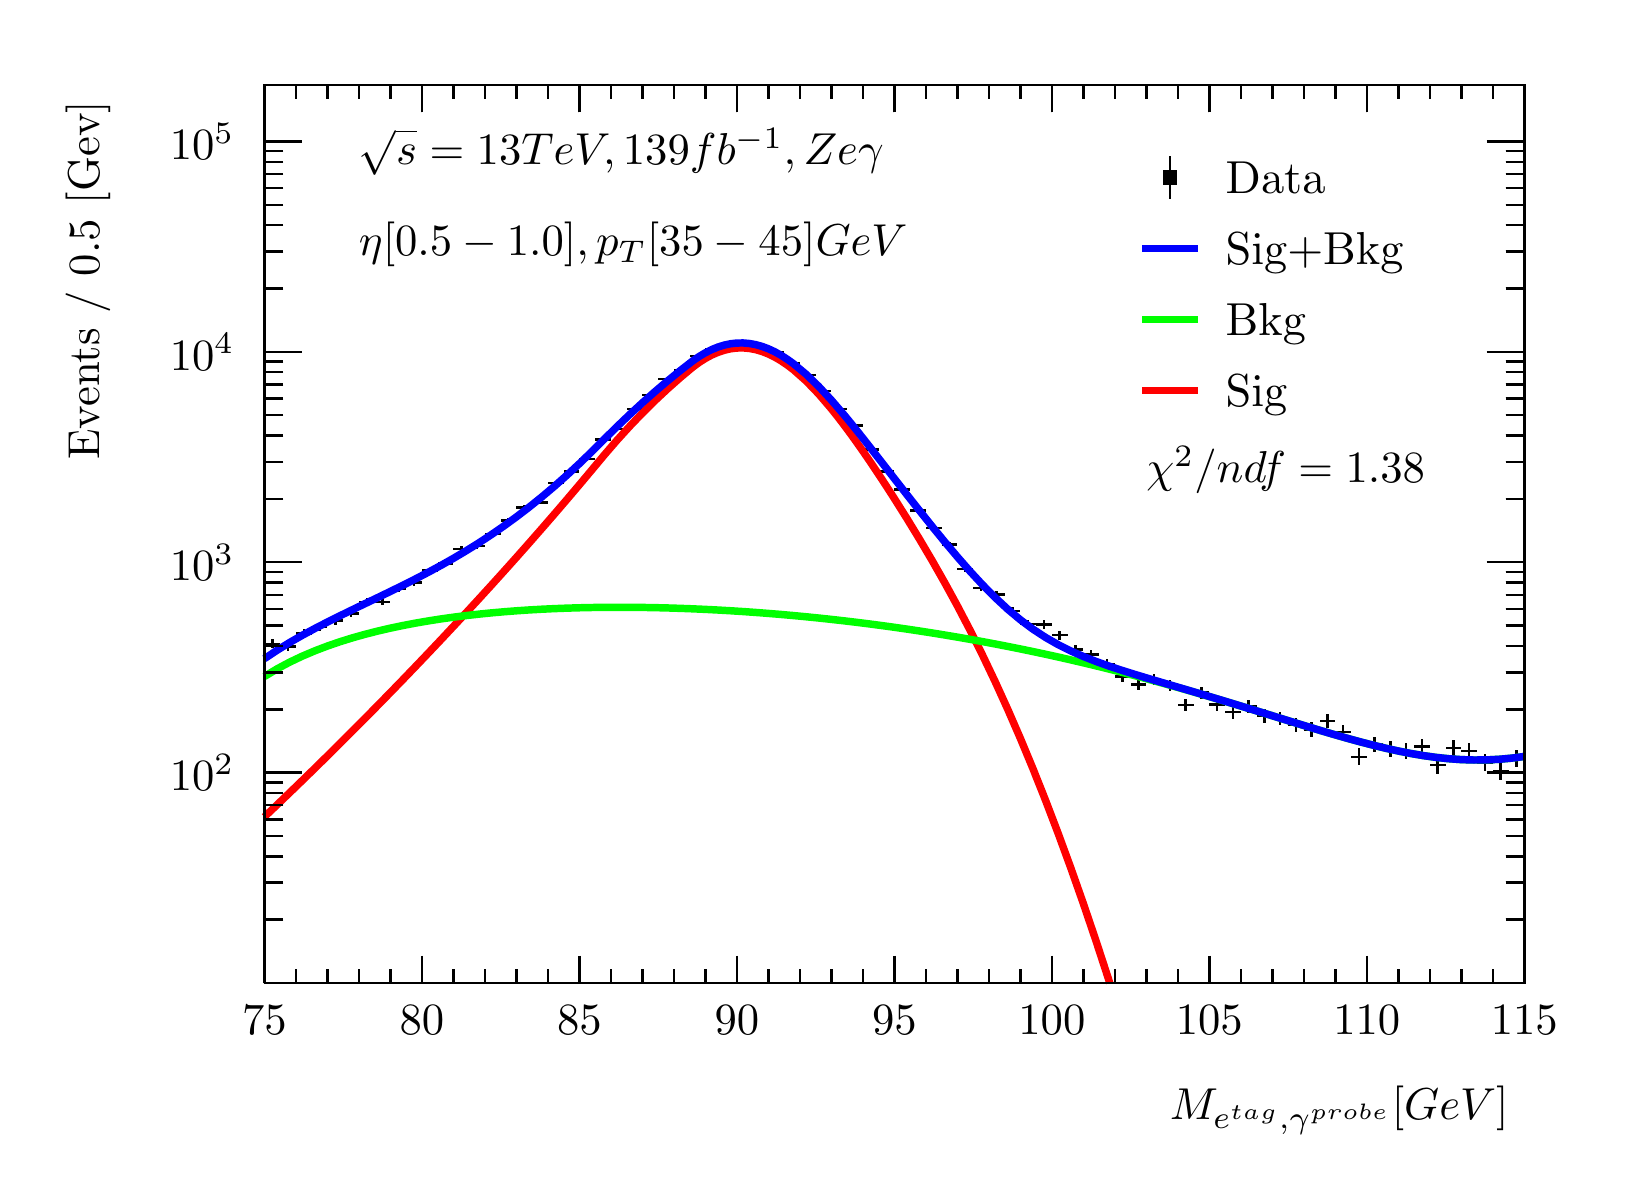
\begin{tikzpicture}
\pgfdeclareplotmark{cross} {
\pgfpathmoveto{\pgfpoint{-0.3\pgfplotmarksize}{\pgfplotmarksize}}
\pgfpathlineto{\pgfpoint{+0.3\pgfplotmarksize}{\pgfplotmarksize}}
\pgfpathlineto{\pgfpoint{+0.3\pgfplotmarksize}{0.3\pgfplotmarksize}}
\pgfpathlineto{\pgfpoint{+1\pgfplotmarksize}{0.3\pgfplotmarksize}}
\pgfpathlineto{\pgfpoint{+1\pgfplotmarksize}{-0.3\pgfplotmarksize}}
\pgfpathlineto{\pgfpoint{+0.3\pgfplotmarksize}{-0.3\pgfplotmarksize}}
\pgfpathlineto{\pgfpoint{+0.3\pgfplotmarksize}{-1.\pgfplotmarksize}}
\pgfpathlineto{\pgfpoint{-0.3\pgfplotmarksize}{-1.\pgfplotmarksize}}
\pgfpathlineto{\pgfpoint{-0.3\pgfplotmarksize}{-0.3\pgfplotmarksize}}
\pgfpathlineto{\pgfpoint{-1.\pgfplotmarksize}{-0.3\pgfplotmarksize}}
\pgfpathlineto{\pgfpoint{-1.\pgfplotmarksize}{0.3\pgfplotmarksize}}
\pgfpathlineto{\pgfpoint{-0.3\pgfplotmarksize}{0.3\pgfplotmarksize}}
\pgfpathclose
\pgfusepathqstroke
}
\pgfdeclareplotmark{cross*} {
\pgfpathmoveto{\pgfpoint{-0.3\pgfplotmarksize}{\pgfplotmarksize}}
\pgfpathlineto{\pgfpoint{+0.3\pgfplotmarksize}{\pgfplotmarksize}}
\pgfpathlineto{\pgfpoint{+0.3\pgfplotmarksize}{0.3\pgfplotmarksize}}
\pgfpathlineto{\pgfpoint{+1\pgfplotmarksize}{0.3\pgfplotmarksize}}
\pgfpathlineto{\pgfpoint{+1\pgfplotmarksize}{-0.3\pgfplotmarksize}}
\pgfpathlineto{\pgfpoint{+0.3\pgfplotmarksize}{-0.3\pgfplotmarksize}}
\pgfpathlineto{\pgfpoint{+0.3\pgfplotmarksize}{-1.\pgfplotmarksize}}
\pgfpathlineto{\pgfpoint{-0.3\pgfplotmarksize}{-1.\pgfplotmarksize}}
\pgfpathlineto{\pgfpoint{-0.3\pgfplotmarksize}{-0.3\pgfplotmarksize}}
\pgfpathlineto{\pgfpoint{-1.\pgfplotmarksize}{-0.3\pgfplotmarksize}}
\pgfpathlineto{\pgfpoint{-1.\pgfplotmarksize}{0.3\pgfplotmarksize}}
\pgfpathlineto{\pgfpoint{-0.3\pgfplotmarksize}{0.3\pgfplotmarksize}}
\pgfpathclose
\pgfusepathqfillstroke
}
\pgfdeclareplotmark{newstar} {
\pgfpathmoveto{\pgfqpoint{0pt}{\pgfplotmarksize}}
\pgfpathlineto{\pgfqpointpolar{44}{0.5\pgfplotmarksize}}
\pgfpathlineto{\pgfqpointpolar{18}{\pgfplotmarksize}}
\pgfpathlineto{\pgfqpointpolar{-20}{0.5\pgfplotmarksize}}
\pgfpathlineto{\pgfqpointpolar{-54}{\pgfplotmarksize}}
\pgfpathlineto{\pgfqpointpolar{-90}{0.5\pgfplotmarksize}}
\pgfpathlineto{\pgfqpointpolar{234}{\pgfplotmarksize}}
\pgfpathlineto{\pgfqpointpolar{198}{0.5\pgfplotmarksize}}
\pgfpathlineto{\pgfqpointpolar{162}{\pgfplotmarksize}}
\pgfpathlineto{\pgfqpointpolar{134}{0.5\pgfplotmarksize}}
\pgfpathclose
\pgfusepathqstroke
}
\pgfdeclareplotmark{newstar*} {
\pgfpathmoveto{\pgfqpoint{0pt}{\pgfplotmarksize}}
\pgfpathlineto{\pgfqpointpolar{44}{0.5\pgfplotmarksize}}
\pgfpathlineto{\pgfqpointpolar{18}{\pgfplotmarksize}}
\pgfpathlineto{\pgfqpointpolar{-20}{0.5\pgfplotmarksize}}
\pgfpathlineto{\pgfqpointpolar{-54}{\pgfplotmarksize}}
\pgfpathlineto{\pgfqpointpolar{-90}{0.5\pgfplotmarksize}}
\pgfpathlineto{\pgfqpointpolar{234}{\pgfplotmarksize}}
\pgfpathlineto{\pgfqpointpolar{198}{0.5\pgfplotmarksize}}
\pgfpathlineto{\pgfqpointpolar{162}{\pgfplotmarksize}}
\pgfpathlineto{\pgfqpointpolar{134}{0.5\pgfplotmarksize}}
\pgfpathclose
\pgfusepathqfillstroke
}
\definecolor{c}{rgb}{1,1,1};
\draw [color=c, fill=c] (0,0) rectangle (20,14.4361);
\draw [color=c, fill=c] (3,2.30977) rectangle (19,13.7143);
\definecolor{c}{rgb}{0,0,0};
\draw [c,line width=0.9] (3,2.30977) -- (3,13.7143) -- (19,13.7143) -- (19,2.30977) -- (3,2.30977);
\definecolor{c}{rgb}{1,1,1};
\draw [color=c, fill=c] (3,2.30977) rectangle (19,13.7143);
\definecolor{c}{rgb}{0,0,0};
\draw [c,line width=0.9] (3,2.30977) -- (3,13.7143) -- (19,13.7143) -- (19,2.30977) -- (3,2.30977);
\draw [c,line width=0.9] (3,2.30977) -- (19,2.30977);
\draw [c,line width=0.9] (3,2.65624) -- (3,2.30977);
\draw [c,line width=0.9] (3.4,2.48301) -- (3.4,2.30977);
\draw [c,line width=0.9] (3.8,2.48301) -- (3.8,2.30977);
\draw [c,line width=0.9] (4.2,2.48301) -- (4.2,2.30977);
\draw [c,line width=0.9] (4.6,2.48301) -- (4.6,2.30977);
\draw [c,line width=0.9] (5,2.65624) -- (5,2.30977);
\draw [c,line width=0.9] (5.4,2.48301) -- (5.4,2.30977);
\draw [c,line width=0.9] (5.8,2.48301) -- (5.8,2.30977);
\draw [c,line width=0.9] (6.2,2.48301) -- (6.2,2.30977);
\draw [c,line width=0.9] (6.6,2.48301) -- (6.6,2.30977);
\draw [c,line width=0.9] (7,2.65624) -- (7,2.30977);
\draw [c,line width=0.9] (7.4,2.48301) -- (7.4,2.30977);
\draw [c,line width=0.9] (7.8,2.48301) -- (7.8,2.30977);
\draw [c,line width=0.9] (8.2,2.48301) -- (8.2,2.30977);
\draw [c,line width=0.9] (8.6,2.48301) -- (8.6,2.30977);
\draw [c,line width=0.9] (9,2.65624) -- (9,2.30977);
\draw [c,line width=0.9] (9.4,2.48301) -- (9.4,2.30977);
\draw [c,line width=0.9] (9.8,2.48301) -- (9.8,2.30977);
\draw [c,line width=0.9] (10.2,2.48301) -- (10.2,2.30977);
\draw [c,line width=0.9] (10.6,2.48301) -- (10.6,2.30977);
\draw [c,line width=0.9] (11,2.65624) -- (11,2.30977);
\draw [c,line width=0.9] (11.4,2.48301) -- (11.4,2.30977);
\draw [c,line width=0.9] (11.8,2.48301) -- (11.8,2.30977);
\draw [c,line width=0.9] (12.2,2.48301) -- (12.2,2.30977);
\draw [c,line width=0.9] (12.6,2.48301) -- (12.6,2.30977);
\draw [c,line width=0.9] (13,2.65624) -- (13,2.30977);
\draw [c,line width=0.9] (13.4,2.48301) -- (13.4,2.30977);
\draw [c,line width=0.9] (13.8,2.48301) -- (13.8,2.30977);
\draw [c,line width=0.9] (14.2,2.48301) -- (14.2,2.30977);
\draw [c,line width=0.9] (14.6,2.48301) -- (14.6,2.30977);
\draw [c,line width=0.9] (15,2.65624) -- (15,2.30977);
\draw [c,line width=0.9] (15.4,2.48301) -- (15.4,2.30977);
\draw [c,line width=0.9] (15.8,2.48301) -- (15.8,2.30977);
\draw [c,line width=0.9] (16.2,2.48301) -- (16.2,2.30977);
\draw [c,line width=0.9] (16.6,2.48301) -- (16.6,2.30977);
\draw [c,line width=0.9] (17,2.65624) -- (17,2.30977);
\draw [c,line width=0.9] (17.4,2.48301) -- (17.4,2.30977);
\draw [c,line width=0.9] (17.8,2.48301) -- (17.8,2.30977);
\draw [c,line width=0.9] (18.2,2.48301) -- (18.2,2.30977);
\draw [c,line width=0.9] (18.6,2.48301) -- (18.6,2.30977);
\draw [c,line width=0.9] (19,2.65624) -- (19,2.30977);
\draw [c,line width=0.9] (19,2.65624) -- (19,2.30977);
\draw [anchor=base] (3,1.66015) node[scale=1.61424, color=c, rotate=0]{75};
\draw [anchor=base] (5,1.66015) node[scale=1.61424, color=c, rotate=0]{80};
\draw [anchor=base] (7,1.66015) node[scale=1.61424, color=c, rotate=0]{85};
\draw [anchor=base] (9,1.66015) node[scale=1.61424, color=c, rotate=0]{90};
\draw [anchor=base] (11,1.66015) node[scale=1.61424, color=c, rotate=0]{95};
\draw [anchor=base] (13,1.66015) node[scale=1.61424, color=c, rotate=0]{100};
\draw [anchor=base] (15,1.66015) node[scale=1.61424, color=c, rotate=0]{105};
\draw [anchor=base] (17,1.66015) node[scale=1.61424, color=c, rotate=0]{110};
\draw [anchor=base] (19,1.66015) node[scale=1.61424, color=c, rotate=0]{115};
\draw [anchor= east] (19,0.692932) node[scale=1.61424, color=c, rotate=0]{$M_{e^{tag}, \gamma^{probe}}  [GeV]$};
\draw [c,line width=0.9] (3,13.7143) -- (19,13.7143);
\draw [c,line width=0.9] (3,13.3678) -- (3,13.7143);
\draw [c,line width=0.9] (3.4,13.5411) -- (3.4,13.7143);
\draw [c,line width=0.9] (3.8,13.5411) -- (3.8,13.7143);
\draw [c,line width=0.9] (4.2,13.5411) -- (4.2,13.7143);
\draw [c,line width=0.9] (4.6,13.5411) -- (4.6,13.7143);
\draw [c,line width=0.9] (5,13.3678) -- (5,13.7143);
\draw [c,line width=0.9] (5.4,13.5411) -- (5.4,13.7143);
\draw [c,line width=0.9] (5.8,13.5411) -- (5.8,13.7143);
\draw [c,line width=0.9] (6.2,13.5411) -- (6.2,13.7143);
\draw [c,line width=0.9] (6.6,13.5411) -- (6.6,13.7143);
\draw [c,line width=0.9] (7,13.3678) -- (7,13.7143);
\draw [c,line width=0.9] (7.4,13.5411) -- (7.4,13.7143);
\draw [c,line width=0.9] (7.8,13.5411) -- (7.8,13.7143);
\draw [c,line width=0.9] (8.2,13.5411) -- (8.2,13.7143);
\draw [c,line width=0.9] (8.6,13.5411) -- (8.6,13.7143);
\draw [c,line width=0.9] (9,13.3678) -- (9,13.7143);
\draw [c,line width=0.9] (9.4,13.5411) -- (9.4,13.7143);
\draw [c,line width=0.9] (9.8,13.5411) -- (9.8,13.7143);
\draw [c,line width=0.9] (10.2,13.5411) -- (10.2,13.7143);
\draw [c,line width=0.9] (10.6,13.5411) -- (10.6,13.7143);
\draw [c,line width=0.9] (11,13.3678) -- (11,13.7143);
\draw [c,line width=0.9] (11.4,13.5411) -- (11.4,13.7143);
\draw [c,line width=0.9] (11.8,13.5411) -- (11.8,13.7143);
\draw [c,line width=0.9] (12.2,13.5411) -- (12.2,13.7143);
\draw [c,line width=0.9] (12.6,13.5411) -- (12.6,13.7143);
\draw [c,line width=0.9] (13,13.3678) -- (13,13.7143);
\draw [c,line width=0.9] (13.4,13.5411) -- (13.4,13.7143);
\draw [c,line width=0.9] (13.8,13.5411) -- (13.8,13.7143);
\draw [c,line width=0.9] (14.2,13.5411) -- (14.2,13.7143);
\draw [c,line width=0.9] (14.6,13.5411) -- (14.6,13.7143);
\draw [c,line width=0.9] (15,13.3678) -- (15,13.7143);
\draw [c,line width=0.9] (15.4,13.5411) -- (15.4,13.7143);
\draw [c,line width=0.9] (15.8,13.5411) -- (15.8,13.7143);
\draw [c,line width=0.9] (16.2,13.5411) -- (16.2,13.7143);
\draw [c,line width=0.9] (16.6,13.5411) -- (16.6,13.7143);
\draw [c,line width=0.9] (17,13.3678) -- (17,13.7143);
\draw [c,line width=0.9] (17.4,13.5411) -- (17.4,13.7143);
\draw [c,line width=0.9] (17.8,13.5411) -- (17.8,13.7143);
\draw [c,line width=0.9] (18.2,13.5411) -- (18.2,13.7143);
\draw [c,line width=0.9] (18.6,13.5411) -- (18.6,13.7143);
\draw [c,line width=0.9] (19,13.3678) -- (19,13.7143);
\draw [c,line width=0.9] (19,13.3678) -- (19,13.7143);
\draw [c,line width=0.9] (3,2.30977) -- (3,13.7143);
\draw [c,line width=0.9] (3.237,3.11414) -- (3,3.11414);
\draw [c,line width=0.9] (3.237,3.58467) -- (3,3.58467);
\draw [c,line width=0.9] (3.237,3.91852) -- (3,3.91852);
\draw [c,line width=0.9] (3.237,4.17747) -- (3,4.17747);
\draw [c,line width=0.9] (3.237,4.38904) -- (3,4.38904);
\draw [c,line width=0.9] (3.237,4.56793) -- (3,4.56793);
\draw [c,line width=0.9] (3.237,4.72289) -- (3,4.72289);
\draw [c,line width=0.9] (3.237,4.85957) -- (3,4.85957);
\draw [c,line width=0.9] (3.474,4.98184) -- (3,4.98184);
\draw [anchor= east] (2.82,4.98184) node[scale=1.61424, color=c, rotate=0]{$10^{2}$};
\draw [c,line width=0.9] (3.237,5.78621) -- (3,5.78621);
\draw [c,line width=0.9] (3.237,6.25674) -- (3,6.25674);
\draw [c,line width=0.9] (3.237,6.59058) -- (3,6.59058);
\draw [c,line width=0.9] (3.237,6.84953) -- (3,6.84953);
\draw [c,line width=0.9] (3.237,7.06111) -- (3,7.06111);
\draw [c,line width=0.9] (3.237,7.24) -- (3,7.24);
\draw [c,line width=0.9] (3.237,7.39496) -- (3,7.39496);
\draw [c,line width=0.9] (3.237,7.53164) -- (3,7.53164);
\draw [c,line width=0.9] (3.474,7.65391) -- (3,7.65391);
\draw [anchor= east] (2.82,7.65391) node[scale=1.61424, color=c, rotate=0]{$10^{3}$};
\draw [c,line width=0.9] (3.237,8.45828) -- (3,8.45828);
\draw [c,line width=0.9] (3.237,8.92881) -- (3,8.92881);
\draw [c,line width=0.9] (3.237,9.26265) -- (3,9.26265);
\draw [c,line width=0.9] (3.237,9.5216) -- (3,9.5216);
\draw [c,line width=0.9] (3.237,9.73318) -- (3,9.73318);
\draw [c,line width=0.9] (3.237,9.91207) -- (3,9.91207);
\draw [c,line width=0.9] (3.237,10.067) -- (3,10.067);
\draw [c,line width=0.9] (3.237,10.2037) -- (3,10.2037);
\draw [c,line width=0.9] (3.474,10.326) -- (3,10.326);
\draw [anchor= east] (2.82,10.326) node[scale=1.61424, color=c, rotate=0]{$10^{4}$};
\draw [c,line width=0.9] (3.237,11.1303) -- (3,11.1303);
\draw [c,line width=0.9] (3.237,11.6009) -- (3,11.6009);
\draw [c,line width=0.9] (3.237,11.9347) -- (3,11.9347);
\draw [c,line width=0.9] (3.237,12.1937) -- (3,12.1937);
\draw [c,line width=0.9] (3.237,12.4052) -- (3,12.4052);
\draw [c,line width=0.9] (3.237,12.5841) -- (3,12.5841);
\draw [c,line width=0.9] (3.237,12.7391) -- (3,12.7391);
\draw [c,line width=0.9] (3.237,12.8758) -- (3,12.8758);
\draw [c,line width=0.9] (3.474,12.998) -- (3,12.998);
\draw [anchor= east] (2.82,12.998) node[scale=1.61424, color=c, rotate=0]{$10^{5}$};
\draw [anchor= east] (0.76,13.7143) node[scale=1.61424, color=c, rotate=90]{Events / 0.5 [Gev]};
\draw [c,line width=0.9] (19,2.30977) -- (19,13.7143);
\draw [c,line width=0.9] (18.763,3.11414) -- (19,3.11414);
\draw [c,line width=0.9] (18.763,3.58467) -- (19,3.58467);
\draw [c,line width=0.9] (18.763,3.91852) -- (19,3.91852);
\draw [c,line width=0.9] (18.763,4.17747) -- (19,4.17747);
\draw [c,line width=0.9] (18.763,4.38904) -- (19,4.38904);
\draw [c,line width=0.9] (18.763,4.56793) -- (19,4.56793);
\draw [c,line width=0.9] (18.763,4.72289) -- (19,4.72289);
\draw [c,line width=0.9] (18.763,4.85957) -- (19,4.85957);
\draw [c,line width=0.9] (18.526,4.98184) -- (19,4.98184);
\draw [c,line width=0.9] (18.763,5.78621) -- (19,5.78621);
\draw [c,line width=0.9] (18.763,6.25674) -- (19,6.25674);
\draw [c,line width=0.9] (18.763,6.59058) -- (19,6.59058);
\draw [c,line width=0.9] (18.763,6.84953) -- (19,6.84953);
\draw [c,line width=0.9] (18.763,7.06111) -- (19,7.06111);
\draw [c,line width=0.9] (18.763,7.24) -- (19,7.24);
\draw [c,line width=0.9] (18.763,7.39496) -- (19,7.39496);
\draw [c,line width=0.9] (18.763,7.53164) -- (19,7.53164);
\draw [c,line width=0.9] (18.526,7.65391) -- (19,7.65391);
\draw [c,line width=0.9] (18.763,8.45828) -- (19,8.45828);
\draw [c,line width=0.9] (18.763,8.92881) -- (19,8.92881);
\draw [c,line width=0.9] (18.763,9.26265) -- (19,9.26265);
\draw [c,line width=0.9] (18.763,9.5216) -- (19,9.5216);
\draw [c,line width=0.9] (18.763,9.73318) -- (19,9.73318);
\draw [c,line width=0.9] (18.763,9.91207) -- (19,9.91207);
\draw [c,line width=0.9] (18.763,10.067) -- (19,10.067);
\draw [c,line width=0.9] (18.763,10.2037) -- (19,10.2037);
\draw [c,line width=0.9] (18.526,10.326) -- (19,10.326);
\draw [c,line width=0.9] (18.763,11.1303) -- (19,11.1303);
\draw [c,line width=0.9] (18.763,11.6009) -- (19,11.6009);
\draw [c,line width=0.9] (18.763,11.9347) -- (19,11.9347);
\draw [c,line width=0.9] (18.763,12.1937) -- (19,12.1937);
\draw [c,line width=0.9] (18.763,12.4052) -- (19,12.4052);
\draw [c,line width=0.9] (18.763,12.5841) -- (19,12.5841);
\draw [c,line width=0.9] (18.763,12.7391) -- (19,12.7391);
\draw [c,line width=0.9] (18.763,12.8758) -- (19,12.8758);
\draw [c,line width=0.9] (18.526,12.998) -- (19,12.998);
\draw [c,line width=0.9] (3.1,6.61641) -- (3,6.61641);
\draw [c,line width=0.9] (3,6.61641) -- (3,6.61641);
\draw [c,line width=0.9] (3.1,6.61641) -- (3.2,6.61641);
\draw [c,line width=0.9] (3.2,6.61641) -- (3.2,6.61641);
\draw [c,line width=0.9] (3.1,6.61641) -- (3.1,6.67378);
\draw [c,line width=0.9] (3.1,6.67378) -- (3.1,6.67378);
\draw [c,line width=0.9] (3.1,6.61641) -- (3.1,6.55903);
\draw [c,line width=0.9] (3.1,6.55903) -- (3.1,6.55903);
\draw [c,line width=0.9] (3.3,6.58477) -- (3.2,6.58477);
\draw [c,line width=0.9] (3.2,6.58477) -- (3.2,6.58477);
\draw [c,line width=0.9] (3.3,6.58477) -- (3.4,6.58477);
\draw [c,line width=0.9] (3.4,6.58477) -- (3.4,6.58477);
\draw [c,line width=0.9] (3.3,6.58477) -- (3.3,6.64293);
\draw [c,line width=0.9] (3.3,6.64293) -- (3.3,6.64293);
\draw [c,line width=0.9] (3.3,6.58477) -- (3.3,6.52661);
\draw [c,line width=0.9] (3.3,6.52661) -- (3.3,6.52661);
\draw [c,line width=0.9] (3.5,6.74772) -- (3.4,6.74772);
\draw [c,line width=0.9] (3.4,6.74772) -- (3.4,6.74772);
\draw [c,line width=0.9] (3.5,6.74772) -- (3.6,6.74772);
\draw [c,line width=0.9] (3.6,6.74772) -- (3.6,6.74772);
\draw [c,line width=0.9] (3.5,6.74772) -- (3.5,6.80194);
\draw [c,line width=0.9] (3.5,6.80194) -- (3.5,6.80194);
\draw [c,line width=0.9] (3.5,6.74772) -- (3.5,6.6935);
\draw [c,line width=0.9] (3.5,6.6935) -- (3.5,6.6935);
\draw [c,line width=0.9] (3.7,6.83317) -- (3.6,6.83317);
\draw [c,line width=0.9] (3.6,6.83317) -- (3.6,6.83317);
\draw [c,line width=0.9] (3.7,6.83317) -- (3.8,6.83317);
\draw [c,line width=0.9] (3.8,6.83317) -- (3.8,6.83317);
\draw [c,line width=0.9] (3.7,6.83317) -- (3.7,6.88543);
\draw [c,line width=0.9] (3.7,6.88543) -- (3.7,6.88543);
\draw [c,line width=0.9] (3.7,6.83317) -- (3.7,6.78091);
\draw [c,line width=0.9] (3.7,6.78091) -- (3.7,6.78091);
\draw [c,line width=0.9] (3.9,6.91277) -- (3.8,6.91277);
\draw [c,line width=0.9] (3.8,6.91277) -- (3.8,6.91277);
\draw [c,line width=0.9] (3.9,6.91277) -- (4,6.91277);
\draw [c,line width=0.9] (4,6.91277) -- (4,6.91277);
\draw [c,line width=0.9] (3.9,6.91277) -- (3.9,6.96327);
\draw [c,line width=0.9] (3.9,6.96327) -- (3.9,6.96327);
\draw [c,line width=0.9] (3.9,6.91277) -- (3.9,6.86227);
\draw [c,line width=0.9] (3.9,6.86227) -- (3.9,6.86227);
\draw [c,line width=0.9] (4.1,7.00565) -- (4,7.00565);
\draw [c,line width=0.9] (4,7.00565) -- (4,7.00565);
\draw [c,line width=0.9] (4.1,7.00565) -- (4.2,7.00565);
\draw [c,line width=0.9] (4.2,7.00565) -- (4.2,7.00565);
\draw [c,line width=0.9] (4.1,7.00565) -- (4.1,7.05417);
\draw [c,line width=0.9] (4.1,7.05417) -- (4.1,7.05417);
\draw [c,line width=0.9] (4.1,7.00565) -- (4.1,6.95714);
\draw [c,line width=0.9] (4.1,6.95714) -- (4.1,6.95714);
\draw [c,line width=0.9] (4.3,7.15042) -- (4.2,7.15042);
\draw [c,line width=0.9] (4.2,7.15042) -- (4.2,7.15042);
\draw [c,line width=0.9] (4.3,7.15042) -- (4.4,7.15042);
\draw [c,line width=0.9] (4.4,7.15042) -- (4.4,7.15042);
\draw [c,line width=0.9] (4.3,7.15042) -- (4.3,7.19601);
\draw [c,line width=0.9] (4.3,7.19601) -- (4.3,7.19601);
\draw [c,line width=0.9] (4.3,7.15042) -- (4.3,7.10484);
\draw [c,line width=0.9] (4.3,7.10484) -- (4.3,7.10484);
\draw [c,line width=0.9] (4.5,7.15042) -- (4.4,7.15042);
\draw [c,line width=0.9] (4.4,7.15042) -- (4.4,7.15042);
\draw [c,line width=0.9] (4.5,7.15042) -- (4.6,7.15042);
\draw [c,line width=0.9] (4.6,7.15042) -- (4.6,7.15042);
\draw [c,line width=0.9] (4.5,7.15042) -- (4.5,7.19601);
\draw [c,line width=0.9] (4.5,7.19601) -- (4.5,7.19601);
\draw [c,line width=0.9] (4.5,7.15042) -- (4.5,7.10484);
\draw [c,line width=0.9] (4.5,7.10484) -- (4.5,7.10484);
\draw [c,line width=0.9] (4.7,7.31696) -- (4.6,7.31696);
\draw [c,line width=0.9] (4.6,7.31696) -- (4.6,7.31696);
\draw [c,line width=0.9] (4.7,7.31696) -- (4.8,7.31696);
\draw [c,line width=0.9] (4.8,7.31696) -- (4.8,7.31696);
\draw [c,line width=0.9] (4.7,7.31696) -- (4.7,7.35939);
\draw [c,line width=0.9] (4.7,7.35939) -- (4.7,7.35939);
\draw [c,line width=0.9] (4.7,7.31696) -- (4.7,7.27454);
\draw [c,line width=0.9] (4.7,7.27454) -- (4.7,7.27454);
\draw [c,line width=0.9] (4.9,7.3993) -- (4.8,7.3993);
\draw [c,line width=0.9] (4.8,7.3993) -- (4.8,7.3993);
\draw [c,line width=0.9] (4.9,7.3993) -- (5,7.3993);
\draw [c,line width=0.9] (5,7.3993) -- (5,7.3993);
\draw [c,line width=0.9] (4.9,7.3993) -- (4.9,7.44025);
\draw [c,line width=0.9] (4.9,7.44025) -- (4.9,7.44025);
\draw [c,line width=0.9] (4.9,7.3993) -- (4.9,7.35835);
\draw [c,line width=0.9] (4.9,7.35835) -- (4.9,7.35835);
\draw [c,line width=0.9] (5.1,7.54701) -- (5,7.54701);
\draw [c,line width=0.9] (5,7.54701) -- (5,7.54701);
\draw [c,line width=0.9] (5.1,7.54701) -- (5.2,7.54701);
\draw [c,line width=0.9] (5.2,7.54701) -- (5.2,7.54701);
\draw [c,line width=0.9] (5.1,7.54701) -- (5.1,7.58544);
\draw [c,line width=0.9] (5.1,7.58544) -- (5.1,7.58544);
\draw [c,line width=0.9] (5.1,7.54701) -- (5.1,7.50859);
\draw [c,line width=0.9] (5.1,7.50859) -- (5.1,7.50859);
\draw [c,line width=0.9] (5.3,7.63755) -- (5.2,7.63755);
\draw [c,line width=0.9] (5.2,7.63755) -- (5.2,7.63755);
\draw [c,line width=0.9] (5.3,7.63755) -- (5.4,7.63755);
\draw [c,line width=0.9] (5.4,7.63755) -- (5.4,7.63755);
\draw [c,line width=0.9] (5.3,7.63755) -- (5.3,7.6745);
\draw [c,line width=0.9] (5.3,7.6745) -- (5.3,7.6745);
\draw [c,line width=0.9] (5.3,7.63755) -- (5.3,7.60059);
\draw [c,line width=0.9] (5.3,7.60059) -- (5.3,7.60059);
\draw [c,line width=0.9] (5.5,7.82113) -- (5.4,7.82113);
\draw [c,line width=0.9] (5.4,7.82113) -- (5.4,7.82113);
\draw [c,line width=0.9] (5.5,7.82113) -- (5.6,7.82113);
\draw [c,line width=0.9] (5.6,7.82113) -- (5.6,7.82113);
\draw [c,line width=0.9] (5.5,7.82113) -- (5.5,7.85528);
\draw [c,line width=0.9] (5.5,7.85528) -- (5.5,7.85528);
\draw [c,line width=0.9] (5.5,7.82113) -- (5.5,7.78699);
\draw [c,line width=0.9] (5.5,7.78699) -- (5.5,7.78699);
\draw [c,line width=0.9] (5.7,7.8587) -- (5.6,7.8587);
\draw [c,line width=0.9] (5.6,7.8587) -- (5.6,7.8587);
\draw [c,line width=0.9] (5.7,7.8587) -- (5.8,7.8587);
\draw [c,line width=0.9] (5.8,7.8587) -- (5.8,7.8587);
\draw [c,line width=0.9] (5.7,7.8587) -- (5.7,7.89229);
\draw [c,line width=0.9] (5.7,7.89229) -- (5.7,7.89229);
\draw [c,line width=0.9] (5.7,7.8587) -- (5.7,7.8251);
\draw [c,line width=0.9] (5.7,7.8251) -- (5.7,7.8251);
\draw [c,line width=0.9] (5.9,8.00988) -- (5.8,8.00988);
\draw [c,line width=0.9] (5.8,8.00988) -- (5.8,8.00988);
\draw [c,line width=0.9] (5.9,8.00988) -- (6,8.00988);
\draw [c,line width=0.9] (6,8.00988) -- (6,8.00988);
\draw [c,line width=0.9] (5.9,8.00988) -- (5.9,8.04136);
\draw [c,line width=0.9] (5.9,8.04136) -- (5.9,8.04136);
\draw [c,line width=0.9] (5.9,8.00988) -- (5.9,7.9784);
\draw [c,line width=0.9] (5.9,7.9784) -- (5.9,7.9784);
\draw [c,line width=0.9] (6.1,8.1862) -- (6,8.1862);
\draw [c,line width=0.9] (6,8.1862) -- (6,8.1862);
\draw [c,line width=0.9] (6.1,8.1862) -- (6.2,8.1862);
\draw [c,line width=0.9] (6.2,8.1862) -- (6.2,8.1862);
\draw [c,line width=0.9] (6.1,8.1862) -- (6.1,8.21538);
\draw [c,line width=0.9] (6.1,8.21538) -- (6.1,8.21538);
\draw [c,line width=0.9] (6.1,8.1862) -- (6.1,8.15703);
\draw [c,line width=0.9] (6.1,8.15703) -- (6.1,8.15703);
\draw [c,line width=0.9] (6.3,8.34756) -- (6.2,8.34756);
\draw [c,line width=0.9] (6.2,8.34756) -- (6.2,8.34756);
\draw [c,line width=0.9] (6.3,8.34756) -- (6.4,8.34756);
\draw [c,line width=0.9] (6.4,8.34756) -- (6.4,8.34756);
\draw [c,line width=0.9] (6.3,8.34756) -- (6.3,8.37478);
\draw [c,line width=0.9] (6.3,8.37478) -- (6.3,8.37478);
\draw [c,line width=0.9] (6.3,8.34756) -- (6.3,8.32034);
\draw [c,line width=0.9] (6.3,8.32034) -- (6.3,8.32034);
\draw [c,line width=0.9] (6.5,8.41513) -- (6.4,8.41513);
\draw [c,line width=0.9] (6.4,8.41513) -- (6.4,8.41513);
\draw [c,line width=0.9] (6.5,8.41513) -- (6.6,8.41513);
\draw [c,line width=0.9] (6.6,8.41513) -- (6.6,8.41513);
\draw [c,line width=0.9] (6.5,8.41513) -- (6.5,8.44157);
\draw [c,line width=0.9] (6.5,8.44157) -- (6.5,8.44157);
\draw [c,line width=0.9] (6.5,8.41513) -- (6.5,8.3887);
\draw [c,line width=0.9] (6.5,8.3887) -- (6.5,8.3887);
\draw [c,line width=0.9] (6.7,8.66307) -- (6.6,8.66307);
\draw [c,line width=0.9] (6.6,8.66307) -- (6.6,8.66307);
\draw [c,line width=0.9] (6.7,8.66307) -- (6.8,8.66307);
\draw [c,line width=0.9] (6.8,8.66307) -- (6.8,8.66307);
\draw [c,line width=0.9] (6.7,8.66307) -- (6.7,8.68683);
\draw [c,line width=0.9] (6.7,8.68683) -- (6.7,8.68683);
\draw [c,line width=0.9] (6.7,8.66307) -- (6.7,8.63931);
\draw [c,line width=0.9] (6.7,8.63931) -- (6.7,8.63931);
\draw [c,line width=0.9] (6.9,8.80439) -- (6.8,8.80439);
\draw [c,line width=0.9] (6.8,8.80439) -- (6.8,8.80439);
\draw [c,line width=0.9] (6.9,8.80439) -- (7,8.80439);
\draw [c,line width=0.9] (7,8.80439) -- (7,8.80439);
\draw [c,line width=0.9] (6.9,8.80439) -- (6.9,8.82674);
\draw [c,line width=0.9] (6.9,8.82674) -- (6.9,8.82674);
\draw [c,line width=0.9] (6.9,8.80439) -- (6.9,8.78204);
\draw [c,line width=0.9] (6.9,8.78204) -- (6.9,8.78204);
\draw [c,line width=0.9] (7.1,8.96761) -- (7,8.96761);
\draw [c,line width=0.9] (7,8.96761) -- (7,8.96761);
\draw [c,line width=0.9] (7.1,8.96761) -- (7.2,8.96761);
\draw [c,line width=0.9] (7.2,8.96761) -- (7.2,8.96761);
\draw [c,line width=0.9] (7.1,8.96761) -- (7.1,8.98844);
\draw [c,line width=0.9] (7.1,8.98844) -- (7.1,8.98844);
\draw [c,line width=0.9] (7.1,8.96761) -- (7.1,8.94677);
\draw [c,line width=0.9] (7.1,8.94677) -- (7.1,8.94677);
\draw [c,line width=0.9] (7.3,9.21377) -- (7.2,9.21377);
\draw [c,line width=0.9] (7.2,9.21377) -- (7.2,9.21377);
\draw [c,line width=0.9] (7.3,9.21377) -- (7.4,9.21377);
\draw [c,line width=0.9] (7.4,9.21377) -- (7.4,9.21377);
\draw [c,line width=0.9] (7.3,9.21377) -- (7.3,9.23251);
\draw [c,line width=0.9] (7.3,9.23251) -- (7.3,9.23251);
\draw [c,line width=0.9] (7.3,9.21377) -- (7.3,9.19503);
\draw [c,line width=0.9] (7.3,9.19503) -- (7.3,9.19503);
\draw [c,line width=0.9] (7.5,9.34523) -- (7.4,9.34523);
\draw [c,line width=0.9] (7.4,9.34523) -- (7.4,9.34523);
\draw [c,line width=0.9] (7.5,9.34523) -- (7.6,9.34523);
\draw [c,line width=0.9] (7.6,9.34523) -- (7.6,9.34523);
\draw [c,line width=0.9] (7.5,9.34523) -- (7.5,9.36294);
\draw [c,line width=0.9] (7.5,9.36294) -- (7.5,9.36294);
\draw [c,line width=0.9] (7.5,9.34523) -- (7.5,9.32752);
\draw [c,line width=0.9] (7.5,9.32752) -- (7.5,9.32752);
\draw [c,line width=0.9] (7.7,9.60055) -- (7.6,9.60055);
\draw [c,line width=0.9] (7.6,9.60055) -- (7.6,9.60055);
\draw [c,line width=0.9] (7.7,9.60055) -- (7.8,9.60055);
\draw [c,line width=0.9] (7.8,9.60055) -- (7.8,9.60055);
\draw [c,line width=0.9] (7.7,9.60055) -- (7.7,9.61641);
\draw [c,line width=0.9] (7.7,9.61641) -- (7.7,9.61641);
\draw [c,line width=0.9] (7.7,9.60055) -- (7.7,9.58469);
\draw [c,line width=0.9] (7.7,9.58469) -- (7.7,9.58469);
\draw [c,line width=0.9] (7.9,9.77553) -- (7.8,9.77553);
\draw [c,line width=0.9] (7.8,9.77553) -- (7.8,9.77553);
\draw [c,line width=0.9] (7.9,9.77553) -- (8,9.77553);
\draw [c,line width=0.9] (8,9.77553) -- (8,9.77553);
\draw [c,line width=0.9] (7.9,9.77553) -- (7.9,9.79024);
\draw [c,line width=0.9] (7.9,9.79024) -- (7.9,9.79024);
\draw [c,line width=0.9] (7.9,9.77553) -- (7.9,9.76082);
\draw [c,line width=0.9] (7.9,9.76082) -- (7.9,9.76082);
\draw [c,line width=0.9] (8.1,9.9814) -- (8,9.9814);
\draw [c,line width=0.9] (8,9.9814) -- (8,9.9814);
\draw [c,line width=0.9] (8.1,9.9814) -- (8.2,9.9814);
\draw [c,line width=0.9] (8.2,9.9814) -- (8.2,9.9814);
\draw [c,line width=0.9] (8.1,9.9814) -- (8.1,9.99487);
\draw [c,line width=0.9] (8.1,9.99487) -- (8.1,9.99487);
\draw [c,line width=0.9] (8.1,9.9814) -- (8.1,9.96794);
\draw [c,line width=0.9] (8.1,9.96794) -- (8.1,9.96794);
\draw [c,line width=0.9] (8.3,10.0927) -- (8.2,10.0927);
\draw [c,line width=0.9] (8.2,10.0927) -- (8.2,10.0927);
\draw [c,line width=0.9] (8.3,10.0927) -- (8.4,10.0927);
\draw [c,line width=0.9] (8.4,10.0927) -- (8.4,10.0927);
\draw [c,line width=0.9] (8.3,10.0927) -- (8.3,10.1055);
\draw [c,line width=0.9] (8.3,10.1055) -- (8.3,10.1055);
\draw [c,line width=0.9] (8.3,10.0927) -- (8.3,10.0799);
\draw [c,line width=0.9] (8.3,10.0799) -- (8.3,10.0799);
\draw [c,line width=0.9] (8.5,10.2741) -- (8.4,10.2741);
\draw [c,line width=0.9] (8.4,10.2741) -- (8.4,10.2741);
\draw [c,line width=0.9] (8.5,10.2741) -- (8.6,10.2741);
\draw [c,line width=0.9] (8.6,10.2741) -- (8.6,10.2741);
\draw [c,line width=0.9] (8.5,10.2741) -- (8.5,10.286);
\draw [c,line width=0.9] (8.5,10.286) -- (8.5,10.286);
\draw [c,line width=0.9] (8.5,10.2741) -- (8.5,10.2623);
\draw [c,line width=0.9] (8.5,10.2623) -- (8.5,10.2623);
\draw [c,line width=0.9] (8.7,10.3619) -- (8.6,10.3619);
\draw [c,line width=0.9] (8.6,10.3619) -- (8.6,10.3619);
\draw [c,line width=0.9] (8.7,10.3619) -- (8.8,10.3619);
\draw [c,line width=0.9] (8.8,10.3619) -- (8.8,10.3619);
\draw [c,line width=0.9] (8.7,10.3619) -- (8.7,10.3733);
\draw [c,line width=0.9] (8.7,10.3733) -- (8.7,10.3733);
\draw [c,line width=0.9] (8.7,10.3619) -- (8.7,10.3504);
\draw [c,line width=0.9] (8.7,10.3504) -- (8.7,10.3504);
\draw [c,line width=0.9] (8.9,10.4157) -- (8.8,10.4157);
\draw [c,line width=0.9] (8.8,10.4157) -- (8.8,10.4157);
\draw [c,line width=0.9] (8.9,10.4157) -- (9,10.4157);
\draw [c,line width=0.9] (9,10.4157) -- (9,10.4157);
\draw [c,line width=0.9] (8.9,10.4157) -- (8.9,10.4269);
\draw [c,line width=0.9] (8.9,10.4269) -- (8.9,10.4269);
\draw [c,line width=0.9] (8.9,10.4157) -- (8.9,10.4046);
\draw [c,line width=0.9] (8.9,10.4046) -- (8.9,10.4046);
\draw [c,line width=0.9] (9.1,10.4272) -- (9,10.4272);
\draw [c,line width=0.9] (9,10.4272) -- (9,10.4272);
\draw [c,line width=0.9] (9.1,10.4272) -- (9.2,10.4272);
\draw [c,line width=0.9] (9.2,10.4272) -- (9.2,10.4272);
\draw [c,line width=0.9] (9.1,10.4272) -- (9.1,10.4383);
\draw [c,line width=0.9] (9.1,10.4383) -- (9.1,10.4383);
\draw [c,line width=0.9] (9.1,10.4272) -- (9.1,10.416);
\draw [c,line width=0.9] (9.1,10.416) -- (9.1,10.416);
\draw [c,line width=0.9] (9.3,10.3971) -- (9.2,10.3971);
\draw [c,line width=0.9] (9.2,10.3971) -- (9.2,10.3971);
\draw [c,line width=0.9] (9.3,10.3971) -- (9.4,10.3971);
\draw [c,line width=0.9] (9.4,10.3971) -- (9.4,10.3971);
\draw [c,line width=0.9] (9.3,10.3971) -- (9.3,10.4083);
\draw [c,line width=0.9] (9.3,10.4083) -- (9.3,10.4083);
\draw [c,line width=0.9] (9.3,10.3971) -- (9.3,10.3858);
\draw [c,line width=0.9] (9.3,10.3858) -- (9.3,10.3858);
\draw [c,line width=0.9] (9.5,10.3206) -- (9.4,10.3206);
\draw [c,line width=0.9] (9.4,10.3206) -- (9.4,10.3206);
\draw [c,line width=0.9] (9.5,10.3206) -- (9.6,10.3206);
\draw [c,line width=0.9] (9.6,10.3206) -- (9.6,10.3206);
\draw [c,line width=0.9] (9.5,10.3206) -- (9.5,10.3323);
\draw [c,line width=0.9] (9.5,10.3323) -- (9.5,10.3323);
\draw [c,line width=0.9] (9.5,10.3206) -- (9.5,10.309);
\draw [c,line width=0.9] (9.5,10.309) -- (9.5,10.309);
\draw [c,line width=0.9] (9.7,10.1751) -- (9.6,10.1751);
\draw [c,line width=0.9] (9.6,10.1751) -- (9.6,10.1751);
\draw [c,line width=0.9] (9.7,10.1751) -- (9.8,10.1751);
\draw [c,line width=0.9] (9.8,10.1751) -- (9.8,10.1751);
\draw [c,line width=0.9] (9.7,10.1751) -- (9.7,10.1875);
\draw [c,line width=0.9] (9.7,10.1875) -- (9.7,10.1875);
\draw [c,line width=0.9] (9.7,10.1751) -- (9.7,10.1627);
\draw [c,line width=0.9] (9.7,10.1627) -- (9.7,10.1627);
\draw [c,line width=0.9] (9.9,10.0332) -- (9.8,10.0332);
\draw [c,line width=0.9] (9.8,10.0332) -- (9.8,10.0332);
\draw [c,line width=0.9] (9.9,10.0332) -- (10,10.0332);
\draw [c,line width=0.9] (10,10.0332) -- (10,10.0332);
\draw [c,line width=0.9] (9.9,10.0332) -- (9.9,10.0463);
\draw [c,line width=0.9] (9.9,10.0463) -- (9.9,10.0463);
\draw [c,line width=0.9] (9.9,10.0332) -- (9.9,10.02);
\draw [c,line width=0.9] (9.9,10.02) -- (9.9,10.02);
\draw [c,line width=0.9] (10.1,9.82821) -- (10,9.82821);
\draw [c,line width=0.9] (10,9.82821) -- (10,9.82821);
\draw [c,line width=0.9] (10.1,9.82821) -- (10.2,9.82821);
\draw [c,line width=0.9] (10.2,9.82821) -- (10.2,9.82821);
\draw [c,line width=0.9] (10.1,9.82821) -- (10.1,9.84259);
\draw [c,line width=0.9] (10.1,9.84259) -- (10.1,9.84259);
\draw [c,line width=0.9] (10.1,9.82821) -- (10.1,9.81383);
\draw [c,line width=0.9] (10.1,9.81383) -- (10.1,9.81383);
\draw [c,line width=0.9] (10.3,9.59925) -- (10.2,9.59925);
\draw [c,line width=0.9] (10.2,9.59925) -- (10.2,9.59925);
\draw [c,line width=0.9] (10.3,9.59925) -- (10.4,9.59925);
\draw [c,line width=0.9] (10.4,9.59925) -- (10.4,9.59925);
\draw [c,line width=0.9] (10.3,9.59925) -- (10.3,9.61512);
\draw [c,line width=0.9] (10.3,9.61512) -- (10.3,9.61512);
\draw [c,line width=0.9] (10.3,9.59925) -- (10.3,9.58338);
\draw [c,line width=0.9] (10.3,9.58338) -- (10.3,9.58338);
\draw [c,line width=0.9] (10.5,9.38975) -- (10.4,9.38975);
\draw [c,line width=0.9] (10.4,9.38975) -- (10.4,9.38975);
\draw [c,line width=0.9] (10.5,9.38975) -- (10.6,9.38975);
\draw [c,line width=0.9] (10.6,9.38975) -- (10.6,9.38975);
\draw [c,line width=0.9] (10.5,9.38975) -- (10.5,9.40713);
\draw [c,line width=0.9] (10.5,9.40713) -- (10.5,9.40713);
\draw [c,line width=0.9] (10.5,9.38975) -- (10.5,9.37238);
\draw [c,line width=0.9] (10.5,9.37238) -- (10.5,9.37238);
\draw [c,line width=0.9] (10.7,9.08628) -- (10.6,9.08628);
\draw [c,line width=0.9] (10.6,9.08628) -- (10.6,9.08628);
\draw [c,line width=0.9] (10.7,9.08628) -- (10.8,9.08628);
\draw [c,line width=0.9] (10.8,9.08628) -- (10.8,9.08628);
\draw [c,line width=0.9] (10.7,9.08628) -- (10.7,9.10608);
\draw [c,line width=0.9] (10.7,9.10608) -- (10.7,9.10608);
\draw [c,line width=0.9] (10.7,9.08628) -- (10.7,9.06648);
\draw [c,line width=0.9] (10.7,9.06648) -- (10.7,9.06648);
\draw [c,line width=0.9] (10.9,8.80439) -- (10.8,8.80439);
\draw [c,line width=0.9] (10.8,8.80439) -- (10.8,8.80439);
\draw [c,line width=0.9] (10.9,8.80439) -- (11,8.80439);
\draw [c,line width=0.9] (11,8.80439) -- (11,8.80439);
\draw [c,line width=0.9] (10.9,8.80439) -- (10.9,8.82674);
\draw [c,line width=0.9] (10.9,8.82674) -- (10.9,8.82674);
\draw [c,line width=0.9] (10.9,8.80439) -- (10.9,8.78204);
\draw [c,line width=0.9] (10.9,8.78204) -- (10.9,8.78204);
\draw [c,line width=0.9] (11.1,8.58043) -- (11,8.58043);
\draw [c,line width=0.9] (11,8.58043) -- (11,8.58043);
\draw [c,line width=0.9] (11.1,8.58043) -- (11.2,8.58043);
\draw [c,line width=0.9] (11.2,8.58043) -- (11.2,8.58043);
\draw [c,line width=0.9] (11.1,8.58043) -- (11.1,8.60505);
\draw [c,line width=0.9] (11.1,8.60505) -- (11.1,8.60505);
\draw [c,line width=0.9] (11.1,8.58043) -- (11.1,8.55581);
\draw [c,line width=0.9] (11.1,8.55581) -- (11.1,8.55581);
\draw [c,line width=0.9] (11.3,8.31257) -- (11.2,8.31257);
\draw [c,line width=0.9] (11.2,8.31257) -- (11.2,8.31257);
\draw [c,line width=0.9] (11.3,8.31257) -- (11.4,8.31257);
\draw [c,line width=0.9] (11.4,8.31257) -- (11.4,8.31257);
\draw [c,line width=0.9] (11.3,8.31257) -- (11.3,8.3402);
\draw [c,line width=0.9] (11.3,8.3402) -- (11.3,8.3402);
\draw [c,line width=0.9] (11.3,8.31257) -- (11.3,8.28494);
\draw [c,line width=0.9] (11.3,8.28494) -- (11.3,8.28494);
\draw [c,line width=0.9] (11.5,8.08829) -- (11.4,8.08829);
\draw [c,line width=0.9] (11.4,8.08829) -- (11.4,8.08829);
\draw [c,line width=0.9] (11.5,8.08829) -- (11.6,8.08829);
\draw [c,line width=0.9] (11.6,8.08829) -- (11.6,8.08829);
\draw [c,line width=0.9] (11.5,8.08829) -- (11.5,8.11872);
\draw [c,line width=0.9] (11.5,8.11872) -- (11.5,8.11872);
\draw [c,line width=0.9] (11.5,8.08829) -- (11.5,8.05786);
\draw [c,line width=0.9] (11.5,8.05786) -- (11.5,8.05786);
\draw [c,line width=0.9] (11.7,7.87703) -- (11.6,7.87703);
\draw [c,line width=0.9] (11.6,7.87703) -- (11.6,7.87703);
\draw [c,line width=0.9] (11.7,7.87703) -- (11.8,7.87703);
\draw [c,line width=0.9] (11.8,7.87703) -- (11.8,7.87703);
\draw [c,line width=0.9] (11.7,7.87703) -- (11.7,7.91037);
\draw [c,line width=0.9] (11.7,7.91037) -- (11.7,7.91037);
\draw [c,line width=0.9] (11.7,7.87703) -- (11.7,7.8437);
\draw [c,line width=0.9] (11.7,7.8437) -- (11.7,7.8437);
\draw [c,line width=0.9] (11.9,7.56594) -- (11.8,7.56594);
\draw [c,line width=0.9] (11.8,7.56594) -- (11.8,7.56594);
\draw [c,line width=0.9] (11.9,7.56594) -- (12,7.56594);
\draw [c,line width=0.9] (12,7.56594) -- (12,7.56594);
\draw [c,line width=0.9] (11.9,7.56594) -- (11.9,7.60406);
\draw [c,line width=0.9] (11.9,7.60406) -- (11.9,7.60406);
\draw [c,line width=0.9] (11.9,7.56594) -- (11.9,7.52783);
\draw [c,line width=0.9] (11.9,7.52783) -- (11.9,7.52783);
\draw [c,line width=0.9] (12.1,7.32777) -- (12,7.32777);
\draw [c,line width=0.9] (12,7.32777) -- (12,7.32777);
\draw [c,line width=0.9] (12.1,7.32777) -- (12.2,7.32777);
\draw [c,line width=0.9] (12.2,7.32777) -- (12.2,7.32777);
\draw [c,line width=0.9] (12.1,7.32777) -- (12.1,7.37001);
\draw [c,line width=0.9] (12.1,7.37001) -- (12.1,7.37001);
\draw [c,line width=0.9] (12.1,7.32777) -- (12.1,7.28554);
\draw [c,line width=0.9] (12.1,7.28554) -- (12.1,7.28554);
\draw [c,line width=0.9] (12.3,7.24166) -- (12.2,7.24166);
\draw [c,line width=0.9] (12.2,7.24166) -- (12.2,7.24166);
\draw [c,line width=0.9] (12.3,7.24166) -- (12.4,7.24166);
\draw [c,line width=0.9] (12.4,7.24166) -- (12.4,7.24166);
\draw [c,line width=0.9] (12.3,7.24166) -- (12.3,7.28548);
\draw [c,line width=0.9] (12.3,7.28548) -- (12.3,7.28548);
\draw [c,line width=0.9] (12.3,7.24166) -- (12.3,7.19783);
\draw [c,line width=0.9] (12.3,7.19783) -- (12.3,7.19783);
\draw [c,line width=0.9] (12.5,7.03371) -- (12.4,7.03371);
\draw [c,line width=0.9] (12.4,7.03371) -- (12.4,7.03371);
\draw [c,line width=0.9] (12.5,7.03371) -- (12.6,7.03371);
\draw [c,line width=0.9] (12.6,7.03371) -- (12.6,7.03371);
\draw [c,line width=0.9] (12.5,7.03371) -- (12.5,7.08165);
\draw [c,line width=0.9] (12.5,7.08165) -- (12.5,7.08165);
\draw [c,line width=0.9] (12.5,7.03371) -- (12.5,6.98578);
\draw [c,line width=0.9] (12.5,6.98578) -- (12.5,6.98578);
\draw [c,line width=0.9] (12.7,6.86796) -- (12.6,6.86796);
\draw [c,line width=0.9] (12.6,6.86796) -- (12.6,6.86796);
\draw [c,line width=0.9] (12.7,6.86796) -- (12.8,6.86796);
\draw [c,line width=0.9] (12.8,6.86796) -- (12.8,6.86796);
\draw [c,line width=0.9] (12.7,6.86796) -- (12.7,6.91944);
\draw [c,line width=0.9] (12.7,6.91944) -- (12.7,6.91944);
\draw [c,line width=0.9] (12.7,6.86796) -- (12.7,6.81647);
\draw [c,line width=0.9] (12.7,6.81647) -- (12.7,6.81647);
\draw [c,line width=0.9] (12.9,6.86338) -- (12.8,6.86338);
\draw [c,line width=0.9] (12.8,6.86338) -- (12.8,6.86338);
\draw [c,line width=0.9] (12.9,6.86338) -- (13,6.86338);
\draw [c,line width=0.9] (13,6.86338) -- (13,6.86338);
\draw [c,line width=0.9] (12.9,6.86338) -- (12.9,6.91496);
\draw [c,line width=0.9] (12.9,6.91496) -- (12.9,6.91496);
\draw [c,line width=0.9] (12.9,6.86338) -- (12.9,6.81179);
\draw [c,line width=0.9] (12.9,6.81179) -- (12.9,6.81179);
\draw [c,line width=0.9] (13.1,6.72727) -- (13,6.72727);
\draw [c,line width=0.9] (13,6.72727) -- (13,6.72727);
\draw [c,line width=0.9] (13.1,6.72727) -- (13.2,6.72727);
\draw [c,line width=0.9] (13.2,6.72727) -- (13.2,6.72727);
\draw [c,line width=0.9] (13.1,6.72727) -- (13.1,6.78197);
\draw [c,line width=0.9] (13.1,6.78197) -- (13.1,6.78197);
\draw [c,line width=0.9] (13.1,6.72727) -- (13.1,6.67257);
\draw [c,line width=0.9] (13.1,6.67257) -- (13.1,6.67257);
\draw [c,line width=0.9] (13.3,6.54321) -- (13.2,6.54321);
\draw [c,line width=0.9] (13.2,6.54321) -- (13.2,6.54321);
\draw [c,line width=0.9] (13.3,6.54321) -- (13.4,6.54321);
\draw [c,line width=0.9] (13.4,6.54321) -- (13.4,6.54321);
\draw [c,line width=0.9] (13.3,6.54321) -- (13.3,6.60243);
\draw [c,line width=0.9] (13.3,6.60243) -- (13.3,6.60243);
\draw [c,line width=0.9] (13.3,6.54321) -- (13.3,6.484);
\draw [c,line width=0.9] (13.3,6.484) -- (13.3,6.484);
\draw [c,line width=0.9] (13.5,6.48433) -- (13.4,6.48433);
\draw [c,line width=0.9] (13.4,6.48433) -- (13.4,6.48433);
\draw [c,line width=0.9] (13.5,6.48433) -- (13.6,6.48433);
\draw [c,line width=0.9] (13.6,6.48433) -- (13.6,6.48433);
\draw [c,line width=0.9] (13.5,6.48433) -- (13.5,6.54506);
\draw [c,line width=0.9] (13.5,6.54506) -- (13.5,6.54506);
\draw [c,line width=0.9] (13.5,6.48433) -- (13.5,6.42359);
\draw [c,line width=0.9] (13.5,6.42359) -- (13.5,6.42359);
\draw [c,line width=0.9] (13.7,6.35675) -- (13.6,6.35675);
\draw [c,line width=0.9] (13.6,6.35675) -- (13.6,6.35675);
\draw [c,line width=0.9] (13.7,6.35675) -- (13.8,6.35675);
\draw [c,line width=0.9] (13.8,6.35675) -- (13.8,6.35675);
\draw [c,line width=0.9] (13.7,6.35675) -- (13.7,6.42091);
\draw [c,line width=0.9] (13.7,6.42091) -- (13.7,6.42091);
\draw [c,line width=0.9] (13.7,6.35675) -- (13.7,6.29258);
\draw [c,line width=0.9] (13.7,6.29258) -- (13.7,6.29258);
\draw [c,line width=0.9] (13.9,6.20533) -- (13.8,6.20533);
\draw [c,line width=0.9] (13.8,6.20533) -- (13.8,6.20533);
\draw [c,line width=0.9] (13.9,6.20533) -- (14,6.20533);
\draw [c,line width=0.9] (14,6.20533) -- (14,6.20533);
\draw [c,line width=0.9] (13.9,6.20533) -- (13.9,6.27382);
\draw [c,line width=0.9] (13.9,6.27382) -- (13.9,6.27382);
\draw [c,line width=0.9] (13.9,6.20533) -- (13.9,6.13684);
\draw [c,line width=0.9] (13.9,6.13684) -- (13.9,6.13684);
\draw [c,line width=0.9] (14.1,6.09957) -- (14,6.09957);
\draw [c,line width=0.9] (14,6.09957) -- (14,6.09957);
\draw [c,line width=0.9] (14.1,6.09957) -- (14.2,6.09957);
\draw [c,line width=0.9] (14.2,6.09957) -- (14.2,6.09957);
\draw [c,line width=0.9] (14.1,6.09957) -- (14.1,6.17125);
\draw [c,line width=0.9] (14.1,6.17125) -- (14.1,6.17125);
\draw [c,line width=0.9] (14.1,6.09957) -- (14.1,6.02789);
\draw [c,line width=0.9] (14.1,6.02789) -- (14.1,6.02789);
\draw [c,line width=0.9] (14.3,6.15998) -- (14.2,6.15998);
\draw [c,line width=0.9] (14.2,6.15998) -- (14.2,6.15998);
\draw [c,line width=0.9] (14.3,6.15998) -- (14.4,6.15998);
\draw [c,line width=0.9] (14.4,6.15998) -- (14.4,6.15998);
\draw [c,line width=0.9] (14.3,6.15998) -- (14.3,6.22982);
\draw [c,line width=0.9] (14.3,6.22982) -- (14.3,6.22982);
\draw [c,line width=0.9] (14.3,6.15998) -- (14.3,6.09014);
\draw [c,line width=0.9] (14.3,6.09014) -- (14.3,6.09014);
\draw [c,line width=0.9] (14.5,6.09068) -- (14.4,6.09068);
\draw [c,line width=0.9] (14.4,6.09068) -- (14.4,6.09068);
\draw [c,line width=0.9] (14.5,6.09068) -- (14.6,6.09068);
\draw [c,line width=0.9] (14.6,6.09068) -- (14.6,6.09068);
\draw [c,line width=0.9] (14.5,6.09068) -- (14.5,6.16263);
\draw [c,line width=0.9] (14.5,6.16263) -- (14.5,6.16263);
\draw [c,line width=0.9] (14.5,6.09068) -- (14.5,6.01872);
\draw [c,line width=0.9] (14.5,6.01872) -- (14.5,6.01872);
\draw [c,line width=0.9] (14.7,5.84283) -- (14.6,5.84283);
\draw [c,line width=0.9] (14.6,5.84283) -- (14.6,5.84283);
\draw [c,line width=0.9] (14.7,5.84283) -- (14.8,5.84283);
\draw [c,line width=0.9] (14.8,5.84283) -- (14.8,5.84283);
\draw [c,line width=0.9] (14.7,5.84283) -- (14.7,5.9229);
\draw [c,line width=0.9] (14.7,5.9229) -- (14.7,5.9229);
\draw [c,line width=0.9] (14.7,5.84283) -- (14.7,5.76277);
\draw [c,line width=0.9] (14.7,5.76277) -- (14.7,5.76277);
\draw [c,line width=0.9] (14.9,5.99779) -- (14.8,5.99779);
\draw [c,line width=0.9] (14.8,5.99779) -- (14.8,5.99779);
\draw [c,line width=0.9] (14.9,5.99779) -- (15,5.99779);
\draw [c,line width=0.9] (15,5.99779) -- (15,5.99779);
\draw [c,line width=0.9] (14.9,5.99779) -- (14.9,6.07269);
\draw [c,line width=0.9] (14.9,6.07269) -- (14.9,6.07269);
\draw [c,line width=0.9] (14.9,5.99779) -- (14.9,5.9229);
\draw [c,line width=0.9] (14.9,5.9229) -- (14.9,5.9229);
\draw [c,line width=0.9] (15.1,5.84835) -- (15,5.84835);
\draw [c,line width=0.9] (15,5.84835) -- (15,5.84835);
\draw [c,line width=0.9] (15.1,5.84835) -- (15.2,5.84835);
\draw [c,line width=0.9] (15.2,5.84835) -- (15.2,5.84835);
\draw [c,line width=0.9] (15.1,5.84835) -- (15.1,5.92822);
\draw [c,line width=0.9] (15.1,5.92822) -- (15.1,5.92822);
\draw [c,line width=0.9] (15.1,5.84835) -- (15.1,5.76847);
\draw [c,line width=0.9] (15.1,5.76847) -- (15.1,5.76847);
\draw [c,line width=0.9] (15.3,5.75087) -- (15.2,5.75087);
\draw [c,line width=0.9] (15.2,5.75087) -- (15.2,5.75087);
\draw [c,line width=0.9] (15.3,5.75087) -- (15.4,5.75087);
\draw [c,line width=0.9] (15.4,5.75087) -- (15.4,5.75087);
\draw [c,line width=0.9] (15.3,5.75087) -- (15.3,5.83417);
\draw [c,line width=0.9] (15.3,5.83417) -- (15.3,5.83417);
\draw [c,line width=0.9] (15.3,5.75087) -- (15.3,5.66757);
\draw [c,line width=0.9] (15.3,5.66757) -- (15.3,5.66757);
\draw [c,line width=0.9] (15.5,5.82052) -- (15.4,5.82052);
\draw [c,line width=0.9] (15.4,5.82052) -- (15.4,5.82052);
\draw [c,line width=0.9] (15.5,5.82052) -- (15.6,5.82052);
\draw [c,line width=0.9] (15.6,5.82052) -- (15.6,5.82052);
\draw [c,line width=0.9] (15.5,5.82052) -- (15.5,5.90135);
\draw [c,line width=0.9] (15.5,5.90135) -- (15.5,5.90135);
\draw [c,line width=0.9] (15.5,5.82052) -- (15.5,5.73968);
\draw [c,line width=0.9] (15.5,5.73968) -- (15.5,5.73968);
\draw [c,line width=0.9] (15.7,5.702) -- (15.6,5.702);
\draw [c,line width=0.9] (15.6,5.702) -- (15.6,5.702);
\draw [c,line width=0.9] (15.7,5.702) -- (15.8,5.702);
\draw [c,line width=0.9] (15.8,5.702) -- (15.8,5.702);
\draw [c,line width=0.9] (15.7,5.702) -- (15.7,5.78707);
\draw [c,line width=0.9] (15.7,5.78707) -- (15.7,5.78707);
\draw [c,line width=0.9] (15.7,5.702) -- (15.7,5.61693);
\draw [c,line width=0.9] (15.7,5.61693) -- (15.7,5.61693);
\draw [c,line width=0.9] (15.9,5.67038) -- (15.8,5.67038);
\draw [c,line width=0.9] (15.8,5.67038) -- (15.8,5.67038);
\draw [c,line width=0.9] (15.9,5.67038) -- (16,5.67038);
\draw [c,line width=0.9] (16,5.67038) -- (16,5.67038);
\draw [c,line width=0.9] (15.9,5.67038) -- (15.9,5.75661);
\draw [c,line width=0.9] (15.9,5.75661) -- (15.9,5.75661);
\draw [c,line width=0.9] (15.9,5.67038) -- (15.9,5.58414);
\draw [c,line width=0.9] (15.9,5.58414) -- (15.9,5.58414);
\draw [c,line width=0.9] (16.1,5.59077) -- (16,5.59077);
\draw [c,line width=0.9] (16,5.59077) -- (16,5.59077);
\draw [c,line width=0.9] (16.1,5.59077) -- (16.2,5.59077);
\draw [c,line width=0.9] (16.2,5.59077) -- (16.2,5.59077);
\draw [c,line width=0.9] (16.1,5.59077) -- (16.1,5.68001);
\draw [c,line width=0.9] (16.1,5.68001) -- (16.1,5.68001);
\draw [c,line width=0.9] (16.1,5.59077) -- (16.1,5.50153);
\draw [c,line width=0.9] (16.1,5.50153) -- (16.1,5.50153);
\draw [c,line width=0.9] (16.3,5.52726) -- (16.2,5.52726);
\draw [c,line width=0.9] (16.2,5.52726) -- (16.2,5.52726);
\draw [c,line width=0.9] (16.3,5.52726) -- (16.4,5.52726);
\draw [c,line width=0.9] (16.4,5.52726) -- (16.4,5.52726);
\draw [c,line width=0.9] (16.3,5.52726) -- (16.3,5.61898);
\draw [c,line width=0.9] (16.3,5.61898) -- (16.3,5.61898);
\draw [c,line width=0.9] (16.3,5.52726) -- (16.3,5.43554);
\draw [c,line width=0.9] (16.3,5.43554) -- (16.3,5.43554);
\draw [c,line width=0.9] (16.5,5.63787) -- (16.4,5.63787);
\draw [c,line width=0.9] (16.4,5.63787) -- (16.4,5.63787);
\draw [c,line width=0.9] (16.5,5.63787) -- (16.6,5.63787);
\draw [c,line width=0.9] (16.6,5.63787) -- (16.6,5.63787);
\draw [c,line width=0.9] (16.5,5.63787) -- (16.5,5.72532);
\draw [c,line width=0.9] (16.5,5.72532) -- (16.5,5.72532);
\draw [c,line width=0.9] (16.5,5.63787) -- (16.5,5.55042);
\draw [c,line width=0.9] (16.5,5.55042) -- (16.5,5.55042);
\draw [c,line width=0.9] (16.7,5.49788) -- (16.6,5.49788);
\draw [c,line width=0.9] (16.6,5.49788) -- (16.6,5.49788);
\draw [c,line width=0.9] (16.7,5.49788) -- (16.8,5.49788);
\draw [c,line width=0.9] (16.8,5.49788) -- (16.8,5.49788);
\draw [c,line width=0.9] (16.7,5.49788) -- (16.7,5.59077);
\draw [c,line width=0.9] (16.7,5.59077) -- (16.7,5.59077);
\draw [c,line width=0.9] (16.7,5.49788) -- (16.7,5.405);
\draw [c,line width=0.9] (16.7,5.405) -- (16.7,5.405);
\draw [c,line width=0.9] (16.9,5.18371) -- (16.8,5.18371);
\draw [c,line width=0.9] (16.8,5.18371) -- (16.8,5.18371);
\draw [c,line width=0.9] (16.9,5.18371) -- (17,5.18371);
\draw [c,line width=0.9] (17,5.18371) -- (17,5.18371);
\draw [c,line width=0.9] (16.9,5.18371) -- (16.9,5.29005);
\draw [c,line width=0.9] (16.9,5.29005) -- (16.9,5.29005);
\draw [c,line width=0.9] (16.9,5.18371) -- (16.9,5.07737);
\draw [c,line width=0.9] (16.9,5.07737) -- (16.9,5.07737);
\draw [c,line width=0.9] (17.1,5.33867) -- (17,5.33867);
\draw [c,line width=0.9] (17,5.33867) -- (17,5.33867);
\draw [c,line width=0.9] (17.1,5.33867) -- (17.2,5.33867);
\draw [c,line width=0.9] (17.2,5.33867) -- (17.2,5.33867);
\draw [c,line width=0.9] (17.1,5.33867) -- (17.1,5.43814);
\draw [c,line width=0.9] (17.1,5.43814) -- (17.1,5.43814);
\draw [c,line width=0.9] (17.1,5.33867) -- (17.1,5.23919);
\draw [c,line width=0.9] (17.1,5.23919) -- (17.1,5.23919);
\draw [c,line width=0.9] (17.3,5.27734) -- (17.2,5.27734);
\draw [c,line width=0.9] (17.2,5.27734) -- (17.2,5.27734);
\draw [c,line width=0.9] (17.3,5.27734) -- (17.4,5.27734);
\draw [c,line width=0.9] (17.4,5.27734) -- (17.4,5.27734);
\draw [c,line width=0.9] (17.3,5.27734) -- (17.3,5.37948);
\draw [c,line width=0.9] (17.3,5.37948) -- (17.3,5.37948);
\draw [c,line width=0.9] (17.3,5.27734) -- (17.3,5.1752);
\draw [c,line width=0.9] (17.3,5.1752) -- (17.3,5.1752);
\draw [c,line width=0.9] (17.5,5.25921) -- (17.4,5.25921);
\draw [c,line width=0.9] (17.4,5.25921) -- (17.4,5.25921);
\draw [c,line width=0.9] (17.5,5.25921) -- (17.6,5.25921);
\draw [c,line width=0.9] (17.6,5.25921) -- (17.6,5.25921);
\draw [c,line width=0.9] (17.5,5.25921) -- (17.5,5.36215);
\draw [c,line width=0.9] (17.5,5.36215) -- (17.5,5.36215);
\draw [c,line width=0.9] (17.5,5.25921) -- (17.5,5.15627);
\draw [c,line width=0.9] (17.5,5.15627) -- (17.5,5.15627);
\draw [c,line width=0.9] (17.7,5.31278) -- (17.6,5.31278);
\draw [c,line width=0.9] (17.6,5.31278) -- (17.6,5.31278);
\draw [c,line width=0.9] (17.7,5.31278) -- (17.8,5.31278);
\draw [c,line width=0.9] (17.8,5.31278) -- (17.8,5.31278);
\draw [c,line width=0.9] (17.7,5.31278) -- (17.7,5.41337);
\draw [c,line width=0.9] (17.7,5.41337) -- (17.7,5.41337);
\draw [c,line width=0.9] (17.7,5.31278) -- (17.7,5.21219);
\draw [c,line width=0.9] (17.7,5.21219) -- (17.7,5.21219);
\draw [c,line width=0.9] (17.9,5.08185) -- (17.8,5.08185);
\draw [c,line width=0.9] (17.8,5.08185) -- (17.8,5.08185);
\draw [c,line width=0.9] (17.9,5.08185) -- (18,5.08185);
\draw [c,line width=0.9] (18,5.08185) -- (18,5.08185);
\draw [c,line width=0.9] (17.9,5.08185) -- (17.9,5.19296);
\draw [c,line width=0.9] (17.9,5.19296) -- (17.9,5.19296);
\draw [c,line width=0.9] (17.9,5.08185) -- (17.9,4.97074);
\draw [c,line width=0.9] (17.9,4.97074) -- (17.9,4.97074);
\draw [c,line width=0.9] (18.1,5.2952) -- (18,5.2952);
\draw [c,line width=0.9] (18,5.2952) -- (18,5.2952);
\draw [c,line width=0.9] (18.1,5.2952) -- (18.2,5.2952);
\draw [c,line width=0.9] (18.2,5.2952) -- (18.2,5.2952);
\draw [c,line width=0.9] (18.1,5.2952) -- (18.1,5.39656);
\draw [c,line width=0.9] (18.1,5.39656) -- (18.1,5.39656);
\draw [c,line width=0.9] (18.1,5.2952) -- (18.1,5.19384);
\draw [c,line width=0.9] (18.1,5.19384) -- (18.1,5.19384);
\draw [c,line width=0.9] (18.3,5.25921) -- (18.2,5.25921);
\draw [c,line width=0.9] (18.2,5.25921) -- (18.2,5.25921);
\draw [c,line width=0.9] (18.3,5.25921) -- (18.4,5.25921);
\draw [c,line width=0.9] (18.4,5.25921) -- (18.4,5.25921);
\draw [c,line width=0.9] (18.3,5.25921) -- (18.3,5.36215);
\draw [c,line width=0.9] (18.3,5.36215) -- (18.3,5.36215);
\draw [c,line width=0.9] (18.3,5.25921) -- (18.3,5.15627);
\draw [c,line width=0.9] (18.3,5.15627) -- (18.3,5.15627);
\draw [c,line width=0.9] (18.5,5.11336) -- (18.4,5.11336);
\draw [c,line width=0.9] (18.4,5.11336) -- (18.4,5.11336);
\draw [c,line width=0.9] (18.5,5.11336) -- (18.6,5.11336);
\draw [c,line width=0.9] (18.6,5.11336) -- (18.6,5.11336);
\draw [c,line width=0.9] (18.5,5.11336) -- (18.5,5.22297);
\draw [c,line width=0.9] (18.5,5.22297) -- (18.5,5.22297);
\draw [c,line width=0.9] (18.5,5.11336) -- (18.5,5.00374);
\draw [c,line width=0.9] (18.5,5.00374) -- (18.5,5.00374);
\draw [c,line width=0.9] (18.7,5.00482) -- (18.6,5.00482);
\draw [c,line width=0.9] (18.6,5.00482) -- (18.6,5.00482);
\draw [c,line width=0.9] (18.7,5.00482) -- (18.8,5.00482);
\draw [c,line width=0.9] (18.8,5.00482) -- (18.8,5.00482);
\draw [c,line width=0.9] (18.7,5.00482) -- (18.7,5.11968);
\draw [c,line width=0.9] (18.7,5.11968) -- (18.7,5.11968);
\draw [c,line width=0.9] (18.7,5.00482) -- (18.7,4.88997);
\draw [c,line width=0.9] (18.7,4.88997) -- (18.7,4.88997);
\draw [c,line width=0.9] (18.9,5.16404) -- (18.8,5.16404);
\draw [c,line width=0.9] (18.8,5.16404) -- (18.8,5.16404);
\draw [c,line width=0.9] (18.9,5.16404) -- (19,5.16404);
\draw [c,line width=0.9] (19,5.16404) -- (19,5.16404);
\draw [c,line width=0.9] (18.9,5.16404) -- (18.9,5.27129);
\draw [c,line width=0.9] (18.9,5.27129) -- (18.9,5.27129);
\draw [c,line width=0.9] (18.9,5.16404) -- (18.9,5.05679);
\draw [c,line width=0.9] (18.9,5.05679) -- (18.9,5.05679);
\foreach \P in {(3.1,6.61641), (3.3,6.58477), (3.5,6.74772), (3.7,6.83317), (3.9,6.91277), (4.1,7.00565), (4.3,7.15042), (4.5,7.15042), (4.7,7.31696), (4.9,7.3993), (5.1,7.54701), (5.3,7.63755), (5.5,7.82113), (5.7,7.8587), (5.9,8.00988),
 (6.1,8.1862), (6.3,8.34756), (6.5,8.41513), (6.7,8.66307), (6.9,8.80439), (7.1,8.96761), (7.3,9.21377), (7.5,9.34523), (7.7,9.60055), (7.9,9.77553), (8.1,9.9814), (8.3,10.0927), (8.5,10.2741), (8.7,10.3619), (8.9,10.4157), (9.1,10.4272),
 (9.3,10.3971), (9.5,10.3206), (9.7,10.1751), (9.9,10.0332), (10.1,9.82821), (10.3,9.59925), (10.5,9.38975), (10.7,9.08628), (10.9,8.80439), (11.1,8.58043), (11.3,8.31257), (11.5,8.08829), (11.7,7.87703), (11.9,7.56594), (12.1,7.32777),
 (12.3,7.24166), (12.5,7.03371), (12.7,6.86796), (12.9,6.86338), (13.1,6.72727), (13.3,6.54321), (13.5,6.48433), (13.7,6.35675), (13.9,6.20533), (14.1,6.09957), (14.3,6.15998), (14.5,6.09068), (14.7,5.84283), (14.9,5.99779), (15.1,5.84835),
 (15.3,5.75087), (15.5,5.82052), (15.7,5.702), (15.9,5.67038), (16.1,5.59077), (16.3,5.52726), (16.5,5.63787), (16.7,5.49788), (16.9,5.18371), (17.1,5.33867), (17.3,5.27734), (17.5,5.25921), (17.7,5.31278), (17.9,5.08185), (18.1,5.2952),
 (18.3,5.25921), (18.5,5.11336), (18.7,5.00482), (18.9,5.16404)}{\draw[mark options={color=c,fill=c},mark size=2.882883pt,mark=] plot coordinates {\P};}
\definecolor{c}{rgb}{1,0,0};
\draw [c,line width=2.7] (3,4.42078) -- (3,4.42078);
\draw [c,line width=2.7] (3,4.42078) -- (3.16,4.57318) -- (3.32,4.72679) -- (3.48,4.8816) -- (3.64,5.03763) -- (3.8,5.19489) -- (3.96,5.35339) -- (4.12,5.51315) -- (4.28,5.67418) -- (4.44,5.83651) -- (4.6,6.00014) -- (4.76,6.16512) -- (4.92,6.33146)
 -- (5.08,6.49919) -- (5.24,6.66836) -- (5.4,6.83899) -- (5.56,7.01113) -- (5.72,7.18483) -- (5.88,7.36014) -- (6.04,7.53712) -- (6.2,7.71584) -- (6.36,7.89636) -- (6.52,8.07877) -- (6.68,8.26315) -- (6.84,8.44961) -- (7,8.63825) -- (7.16,8.82919) --
 (7.32,9.02131) -- (7.48,9.20613) -- (7.64,9.38191) -- (7.8,9.54865) -- (7.96,9.70659) -- (8.12,9.85614) -- (8.28,9.99795) -- (8.44,10.1322) -- (8.52,10.1912) -- (8.6,10.2423) -- (8.68,10.2853) -- (8.76,10.3201) -- (8.84,10.3466) -- (8.92,10.3647) --
 (9,10.3744) -- (9.08,10.3758) -- (9.16,10.3688) -- (9.24,10.3536) -- (9.32,10.3302) -- (9.4,10.2989) -- (9.48,10.2597) -- (9.56,10.213) -- (9.64,10.1589) -- (9.72,10.0978) -- (9.88,9.95569) -- (10.04,9.78948) -- (10.2,9.60241) -- (10.28,9.5021) --
 (10.36,9.39784) -- (10.44,9.29004) -- (10.52,9.17906) -- (10.6,9.06526) -- (10.68,8.94894) -- (10.76,8.83035) -- (10.84,8.70968) -- (10.92,8.58708) -- (11,8.46261) -- (11.16,8.20811) -- (11.32,7.94576) -- (11.48,7.67454) -- (11.64,7.39307) --
 (11.8,7.09989) -- (11.96,6.79362) -- (12.12,6.47306) -- (12.28,6.13725) -- (12.44,5.78548) -- (12.6,5.4172) -- (12.76,5.03207) -- (12.92,4.62983) -- (13.08,4.21034) -- (13.24,3.77348) -- (13.4,3.31922) -- (13.56,2.8475) -- (13.72,2.35832) --
 (13.7353,2.30977);
\definecolor{c}{rgb}{0,1,0};
\draw [c,line width=2.7] (3,6.20261) -- (3,6.20261);
\draw [c,line width=2.7] (3,6.20261) -- (3.16,6.29959) -- (3.32,6.3851) -- (3.48,6.46106) -- (3.64,6.52895) -- (3.8,6.58991) -- (3.96,6.64484) -- (4.12,6.69449) -- (4.28,6.73945) -- (4.44,6.78022) -- (4.6,6.81721) -- (4.76,6.85078) -- (4.92,6.88124)
 -- (5.08,6.90882) -- (5.24,6.93377) -- (5.4,6.95628) -- (5.56,6.9765) -- (5.72,6.9946) -- (5.88,7.0107) -- (6.04,7.02492) -- (6.2,7.03736) -- (6.36,7.04812) -- (6.52,7.05727) -- (6.68,7.06489) -- (6.84,7.07104) -- (7,7.07579) -- (7.16,7.07918) --
 (7.32,7.08127) -- (7.48,7.08209) -- (7.64,7.08169) -- (7.8,7.0801) -- (7.96,7.07735) -- (8.12,7.07347) -- (8.28,7.06849) -- (8.44,7.06241) -- (8.6,7.05528) -- (8.76,7.04709) -- (8.92,7.03787) -- (9.08,7.02764) -- (9.24,7.01639) -- (9.4,7.00415) --
 (9.56,6.99092) -- (9.72,6.9767) -- (9.88,6.9615) -- (10.04,6.94533) -- (10.2,6.92819) -- (10.36,6.91007) -- (10.52,6.89099) -- (10.68,6.87092) -- (10.84,6.84989) -- (11,6.82788) -- (11.16,6.80489) -- (11.32,6.78091) -- (11.48,6.75594) --
 (11.64,6.72997) -- (11.8,6.70301) -- (11.96,6.67503) -- (12.12,6.64604) -- (12.28,6.61602) -- (12.44,6.58498) -- (12.6,6.5529) -- (12.76,6.51978) -- (12.92,6.48561) -- (13.08,6.45039) -- (13.24,6.41412) -- (13.4,6.37679) -- (13.56,6.33842) --
 (13.72,6.29899) -- (13.88,6.25852) -- (14.04,6.21703) -- (14.2,6.17452) -- (14.36,6.13103) -- (14.52,6.08659) -- (14.68,6.04123) -- (14.84,5.99502) -- (15,5.948) -- (15.16,5.90027) -- (15.32,5.8519) -- (15.48,5.80303) -- (15.64,5.75378) --
 (15.8,5.70432) -- (15.96,5.65483) -- (16.12,5.60553) -- (16.28,5.55668) -- (16.44,5.50857) -- (16.6,5.46153) -- (16.76,5.41593) -- (16.92,5.37218) -- (17.08,5.33073) -- (17.24,5.29206) -- (17.4,5.25669) -- (17.56,5.22513) -- (17.72,5.19793) --
 (17.88,5.17558) -- (18.04,5.15859) -- (18.2,5.14738) -- (18.36,5.14232) -- (18.52,5.14366) -- (18.68,5.15159) -- (18.84,5.16616) -- (19,5.18729) -- (19,5.18729) -- (19,5.18729);
\definecolor{c}{rgb}{0,0,1};
\draw [c,line width=2.7] (3,6.42894) -- (3,6.42894);
\draw [c,line width=2.7] (3,6.42894) -- (3.16,6.53594) -- (3.32,6.6343) -- (3.48,6.72593) -- (3.64,6.81236) -- (3.8,6.89487) -- (3.96,6.97457) -- (4.12,7.05244) -- (4.28,7.12936) -- (4.44,7.20613) -- (4.6,7.28352) -- (4.76,7.36224) -- (4.92,7.44298)
 -- (5.08,7.52636) -- (5.24,7.61301) -- (5.4,7.70349) -- (5.56,7.79832) -- (5.72,7.89798) -- (5.88,8.0029) -- (6.04,8.11343) -- (6.2,8.22987) -- (6.36,8.35245) -- (6.52,8.48133) -- (6.68,8.61663) -- (6.84,8.75839) -- (7,8.9066) -- (7.16,9.06123) --
 (7.32,9.22114) -- (7.48,9.37872) -- (7.64,9.53169) -- (7.8,9.67931) -- (7.96,9.82115) -- (8.12,9.95712) -- (8.28,10.0874) -- (8.44,10.2118) -- (8.52,10.2668) -- (8.6,10.3145) -- (8.68,10.3547) -- (8.76,10.3873) -- (8.84,10.412) -- (8.92,10.4289) --
 (9,10.4378) -- (9.08,10.4388) -- (9.16,10.4319) -- (9.24,10.4172) -- (9.32,10.3948) -- (9.4,10.3648) -- (9.48,10.3275) -- (9.56,10.2831) -- (9.64,10.2318) -- (9.72,10.1741) -- (9.88,10.0404) -- (10.04,9.88546) -- (10.2,9.71282) -- (10.36,9.52646) --
 (10.44,9.42938) -- (10.52,9.33032) -- (10.6,9.22973) -- (10.68,9.12801) -- (10.76,9.02552) -- (10.84,8.92258) -- (11,8.71641) -- (11.16,8.51118) -- (11.32,8.30811) -- (11.48,8.10822) -- (11.64,7.91262) -- (11.8,7.72271) -- (11.96,7.54021) --
 (12.12,7.36714) -- (12.28,7.20553) -- (12.44,7.05713) -- (12.6,6.92314) -- (12.76,6.80397) -- (12.92,6.69918) -- (13.08,6.60763) -- (13.24,6.52762) -- (13.4,6.45719) -- (13.56,6.39435) -- (13.72,6.33724) -- (13.88,6.28426) -- (14.04,6.23407) --
 (14.2,6.18564) -- (14.36,6.13817) -- (14.52,6.09111) -- (14.68,6.04405) -- (14.84,5.99675) -- (15,5.94905) -- (15.16,5.90089) -- (15.32,5.85227) -- (15.48,5.80324) -- (15.64,5.7539) -- (15.8,5.70439) -- (15.96,5.65486) -- (16.12,5.60555) --
 (16.28,5.55669) -- (16.44,5.50857) -- (16.6,5.46153) -- (16.76,5.41593) -- (16.92,5.37218) -- (17.08,5.33073) -- (17.24,5.29206) -- (17.4,5.25669) -- (17.56,5.22513) -- (17.72,5.19793) -- (17.88,5.17558) -- (18.04,5.15859) -- (18.2,5.14738) --
 (18.36,5.14232) -- (18.52,5.14366) -- (18.68,5.15159) -- (18.84,5.16616) -- (19,5.18729) -- (19,5.18729) -- (19,5.18729);
\definecolor{c}{rgb}{0,0,0};
\draw [c,line width=0.9] (3,2.30977) -- (19,2.30977);
\draw [c,line width=0.9] (3,2.65624) -- (3,2.30977);
\draw [c,line width=0.9] (3.4,2.48301) -- (3.4,2.30977);
\draw [c,line width=0.9] (3.8,2.48301) -- (3.8,2.30977);
\draw [c,line width=0.9] (4.2,2.48301) -- (4.2,2.30977);
\draw [c,line width=0.9] (4.6,2.48301) -- (4.6,2.30977);
\draw [c,line width=0.9] (5,2.65624) -- (5,2.30977);
\draw [c,line width=0.9] (5.4,2.48301) -- (5.4,2.30977);
\draw [c,line width=0.9] (5.8,2.48301) -- (5.8,2.30977);
\draw [c,line width=0.9] (6.2,2.48301) -- (6.2,2.30977);
\draw [c,line width=0.9] (6.6,2.48301) -- (6.6,2.30977);
\draw [c,line width=0.9] (7,2.65624) -- (7,2.30977);
\draw [c,line width=0.9] (7.4,2.48301) -- (7.4,2.30977);
\draw [c,line width=0.9] (7.8,2.48301) -- (7.8,2.30977);
\draw [c,line width=0.9] (8.2,2.48301) -- (8.2,2.30977);
\draw [c,line width=0.9] (8.6,2.48301) -- (8.6,2.30977);
\draw [c,line width=0.9] (9,2.65624) -- (9,2.30977);
\draw [c,line width=0.9] (9.4,2.48301) -- (9.4,2.30977);
\draw [c,line width=0.9] (9.8,2.48301) -- (9.8,2.30977);
\draw [c,line width=0.9] (10.2,2.48301) -- (10.2,2.30977);
\draw [c,line width=0.9] (10.6,2.48301) -- (10.6,2.30977);
\draw [c,line width=0.9] (11,2.65624) -- (11,2.30977);
\draw [c,line width=0.9] (11.4,2.48301) -- (11.4,2.30977);
\draw [c,line width=0.9] (11.8,2.48301) -- (11.8,2.30977);
\draw [c,line width=0.9] (12.2,2.48301) -- (12.2,2.30977);
\draw [c,line width=0.9] (12.6,2.48301) -- (12.6,2.30977);
\draw [c,line width=0.9] (13,2.65624) -- (13,2.30977);
\draw [c,line width=0.9] (13.4,2.48301) -- (13.4,2.30977);
\draw [c,line width=0.9] (13.8,2.48301) -- (13.8,2.30977);
\draw [c,line width=0.9] (14.2,2.48301) -- (14.2,2.30977);
\draw [c,line width=0.9] (14.6,2.48301) -- (14.6,2.30977);
\draw [c,line width=0.9] (15,2.65624) -- (15,2.30977);
\draw [c,line width=0.9] (15.4,2.48301) -- (15.4,2.30977);
\draw [c,line width=0.9] (15.8,2.48301) -- (15.8,2.30977);
\draw [c,line width=0.9] (16.2,2.48301) -- (16.2,2.30977);
\draw [c,line width=0.9] (16.6,2.48301) -- (16.6,2.30977);
\draw [c,line width=0.9] (17,2.65624) -- (17,2.30977);
\draw [c,line width=0.9] (17.4,2.48301) -- (17.4,2.30977);
\draw [c,line width=0.9] (17.8,2.48301) -- (17.8,2.30977);
\draw [c,line width=0.9] (18.2,2.48301) -- (18.2,2.30977);
\draw [c,line width=0.9] (18.6,2.48301) -- (18.6,2.30977);
\draw [c,line width=0.9] (19,2.65624) -- (19,2.30977);
\draw [c,line width=0.9] (19,2.65624) -- (19,2.30977);
\draw [c,line width=0.9] (3,13.7143) -- (19,13.7143);
\draw [c,line width=0.9] (3,13.3678) -- (3,13.7143);
\draw [c,line width=0.9] (3.4,13.5411) -- (3.4,13.7143);
\draw [c,line width=0.9] (3.8,13.5411) -- (3.8,13.7143);
\draw [c,line width=0.9] (4.2,13.5411) -- (4.2,13.7143);
\draw [c,line width=0.9] (4.6,13.5411) -- (4.6,13.7143);
\draw [c,line width=0.9] (5,13.3678) -- (5,13.7143);
\draw [c,line width=0.9] (5.4,13.5411) -- (5.4,13.7143);
\draw [c,line width=0.9] (5.8,13.5411) -- (5.8,13.7143);
\draw [c,line width=0.9] (6.2,13.5411) -- (6.2,13.7143);
\draw [c,line width=0.9] (6.6,13.5411) -- (6.6,13.7143);
\draw [c,line width=0.9] (7,13.3678) -- (7,13.7143);
\draw [c,line width=0.9] (7.4,13.5411) -- (7.4,13.7143);
\draw [c,line width=0.9] (7.8,13.5411) -- (7.8,13.7143);
\draw [c,line width=0.9] (8.2,13.5411) -- (8.2,13.7143);
\draw [c,line width=0.9] (8.6,13.5411) -- (8.6,13.7143);
\draw [c,line width=0.9] (9,13.3678) -- (9,13.7143);
\draw [c,line width=0.9] (9.4,13.5411) -- (9.4,13.7143);
\draw [c,line width=0.9] (9.8,13.5411) -- (9.8,13.7143);
\draw [c,line width=0.9] (10.2,13.5411) -- (10.2,13.7143);
\draw [c,line width=0.9] (10.6,13.5411) -- (10.6,13.7143);
\draw [c,line width=0.9] (11,13.3678) -- (11,13.7143);
\draw [c,line width=0.9] (11.4,13.5411) -- (11.4,13.7143);
\draw [c,line width=0.9] (11.8,13.5411) -- (11.8,13.7143);
\draw [c,line width=0.9] (12.2,13.5411) -- (12.2,13.7143);
\draw [c,line width=0.9] (12.6,13.5411) -- (12.6,13.7143);
\draw [c,line width=0.9] (13,13.3678) -- (13,13.7143);
\draw [c,line width=0.9] (13.4,13.5411) -- (13.4,13.7143);
\draw [c,line width=0.9] (13.8,13.5411) -- (13.8,13.7143);
\draw [c,line width=0.9] (14.2,13.5411) -- (14.2,13.7143);
\draw [c,line width=0.9] (14.6,13.5411) -- (14.6,13.7143);
\draw [c,line width=0.9] (15,13.3678) -- (15,13.7143);
\draw [c,line width=0.9] (15.4,13.5411) -- (15.4,13.7143);
\draw [c,line width=0.9] (15.8,13.5411) -- (15.8,13.7143);
\draw [c,line width=0.9] (16.2,13.5411) -- (16.2,13.7143);
\draw [c,line width=0.9] (16.6,13.5411) -- (16.6,13.7143);
\draw [c,line width=0.9] (17,13.3678) -- (17,13.7143);
\draw [c,line width=0.9] (17.4,13.5411) -- (17.4,13.7143);
\draw [c,line width=0.9] (17.8,13.5411) -- (17.8,13.7143);
\draw [c,line width=0.9] (18.2,13.5411) -- (18.2,13.7143);
\draw [c,line width=0.9] (18.6,13.5411) -- (18.6,13.7143);
\draw [c,line width=0.9] (19,13.3678) -- (19,13.7143);
\draw [c,line width=0.9] (19,13.3678) -- (19,13.7143);
\draw [c,line width=0.9] (3,2.30977) -- (3,13.7143);
\draw [c,line width=0.9] (3.237,3.11414) -- (3,3.11414);
\draw [c,line width=0.9] (3.237,3.58467) -- (3,3.58467);
\draw [c,line width=0.9] (3.237,3.91852) -- (3,3.91852);
\draw [c,line width=0.9] (3.237,4.17747) -- (3,4.17747);
\draw [c,line width=0.9] (3.237,4.38904) -- (3,4.38904);
\draw [c,line width=0.9] (3.237,4.56793) -- (3,4.56793);
\draw [c,line width=0.9] (3.237,4.72289) -- (3,4.72289);
\draw [c,line width=0.9] (3.237,4.85957) -- (3,4.85957);
\draw [c,line width=0.9] (3.474,4.98184) -- (3,4.98184);
\draw [c,line width=0.9] (3.237,5.78621) -- (3,5.78621);
\draw [c,line width=0.9] (3.237,6.25674) -- (3,6.25674);
\draw [c,line width=0.9] (3.237,6.59058) -- (3,6.59058);
\draw [c,line width=0.9] (3.237,6.84953) -- (3,6.84953);
\draw [c,line width=0.9] (3.237,7.06111) -- (3,7.06111);
\draw [c,line width=0.9] (3.237,7.24) -- (3,7.24);
\draw [c,line width=0.9] (3.237,7.39496) -- (3,7.39496);
\draw [c,line width=0.9] (3.237,7.53164) -- (3,7.53164);
\draw [c,line width=0.9] (3.474,7.65391) -- (3,7.65391);
\draw [c,line width=0.9] (3.237,8.45828) -- (3,8.45828);
\draw [c,line width=0.9] (3.237,8.92881) -- (3,8.92881);
\draw [c,line width=0.9] (3.237,9.26265) -- (3,9.26265);
\draw [c,line width=0.9] (3.237,9.5216) -- (3,9.5216);
\draw [c,line width=0.9] (3.237,9.73318) -- (3,9.73318);
\draw [c,line width=0.9] (3.237,9.91207) -- (3,9.91207);
\draw [c,line width=0.9] (3.237,10.067) -- (3,10.067);
\draw [c,line width=0.9] (3.237,10.2037) -- (3,10.2037);
\draw [c,line width=0.9] (3.474,10.326) -- (3,10.326);
\draw [c,line width=0.9] (3.237,11.1303) -- (3,11.1303);
\draw [c,line width=0.9] (3.237,11.6009) -- (3,11.6009);
\draw [c,line width=0.9] (3.237,11.9347) -- (3,11.9347);
\draw [c,line width=0.9] (3.237,12.1937) -- (3,12.1937);
\draw [c,line width=0.9] (3.237,12.4052) -- (3,12.4052);
\draw [c,line width=0.9] (3.237,12.5841) -- (3,12.5841);
\draw [c,line width=0.9] (3.237,12.7391) -- (3,12.7391);
\draw [c,line width=0.9] (3.237,12.8758) -- (3,12.8758);
\draw [c,line width=0.9] (3.474,12.998) -- (3,12.998);
\draw [c,line width=0.9] (19,2.30977) -- (19,13.7143);
\draw [c,line width=0.9] (18.763,3.11414) -- (19,3.11414);
\draw [c,line width=0.9] (18.763,3.58467) -- (19,3.58467);
\draw [c,line width=0.9] (18.763,3.91852) -- (19,3.91852);
\draw [c,line width=0.9] (18.763,4.17747) -- (19,4.17747);
\draw [c,line width=0.9] (18.763,4.38904) -- (19,4.38904);
\draw [c,line width=0.9] (18.763,4.56793) -- (19,4.56793);
\draw [c,line width=0.9] (18.763,4.72289) -- (19,4.72289);
\draw [c,line width=0.9] (18.763,4.85957) -- (19,4.85957);
\draw [c,line width=0.9] (18.526,4.98184) -- (19,4.98184);
\draw [c,line width=0.9] (18.763,5.78621) -- (19,5.78621);
\draw [c,line width=0.9] (18.763,6.25674) -- (19,6.25674);
\draw [c,line width=0.9] (18.763,6.59058) -- (19,6.59058);
\draw [c,line width=0.9] (18.763,6.84953) -- (19,6.84953);
\draw [c,line width=0.9] (18.763,7.06111) -- (19,7.06111);
\draw [c,line width=0.9] (18.763,7.24) -- (19,7.24);
\draw [c,line width=0.9] (18.763,7.39496) -- (19,7.39496);
\draw [c,line width=0.9] (18.763,7.53164) -- (19,7.53164);
\draw [c,line width=0.9] (18.526,7.65391) -- (19,7.65391);
\draw [c,line width=0.9] (18.763,8.45828) -- (19,8.45828);
\draw [c,line width=0.9] (18.763,8.92881) -- (19,8.92881);
\draw [c,line width=0.9] (18.763,9.26265) -- (19,9.26265);
\draw [c,line width=0.9] (18.763,9.5216) -- (19,9.5216);
\draw [c,line width=0.9] (18.763,9.73318) -- (19,9.73318);
\draw [c,line width=0.9] (18.763,9.91207) -- (19,9.91207);
\draw [c,line width=0.9] (18.763,10.067) -- (19,10.067);
\draw [c,line width=0.9] (18.763,10.2037) -- (19,10.2037);
\draw [c,line width=0.9] (18.526,10.326) -- (19,10.326);
\draw [c,line width=0.9] (18.763,11.1303) -- (19,11.1303);
\draw [c,line width=0.9] (18.763,11.6009) -- (19,11.6009);
\draw [c,line width=0.9] (18.763,11.9347) -- (19,11.9347);
\draw [c,line width=0.9] (18.763,12.1937) -- (19,12.1937);
\draw [c,line width=0.9] (18.763,12.4052) -- (19,12.4052);
\draw [c,line width=0.9] (18.763,12.5841) -- (19,12.5841);
\draw [c,line width=0.9] (18.763,12.7391) -- (19,12.7391);
\draw [c,line width=0.9] (18.763,12.8758) -- (19,12.8758);
\draw [c,line width=0.9] (18.526,12.998) -- (19,12.998);
\definecolor{c}{rgb}{1,1,1};
\draw [color=c, fill=c] (14,9.38346) rectangle (18,12.9925);
\definecolor{c}{rgb}{0,0,0};
\draw [anchor=base west] (15,12.3383) node[scale=1.6699, color=c, rotate=0]{Data};
\draw [c,line width=0.9] (14.5,12.6416) -- (14.5,12.812);
\draw [c,line width=0.9] (14.5,12.4411) -- (14.5,12.2707);
\foreach \P in {(14.5,12.5414)}{\draw[mark options={color=c,fill=c},mark size=2.402402pt,mark=square*] plot coordinates {\P};}
\draw [anchor=base west] (15,11.4361) node[scale=1.6699, color=c, rotate=0]{Sig+Bkg};
\definecolor{c}{rgb}{0,0,1};
\draw [c,line width=2.7] (14.15,11.6391) -- (14.85,11.6391);
\definecolor{c}{rgb}{0,0,0};
\draw [anchor=base west] (15,10.5338) node[scale=1.6699, color=c, rotate=0]{Bkg};
\definecolor{c}{rgb}{0,1,0};
\draw [c,line width=2.7] (14.15,10.7368) -- (14.85,10.7368);
\definecolor{c}{rgb}{0,0,0};
\draw [anchor=base west] (15,9.63158) node[scale=1.6699, color=c, rotate=0]{Sig};
\definecolor{c}{rgb}{1,0,0};
\draw [c,line width=2.7] (14.15,9.83459) -- (14.85,9.83459);
\definecolor{c}{rgb}{0,0,0};
\draw [anchor=base west] (4,12.7038) node[scale=1.61424, color=c, rotate=0]{$\sqrt{s}= 13 TeV, 139fb^{-1}, Ze\gamma$};
\draw [anchor=base west] (4,11.5489) node[scale=1.61424, color=c, rotate=0]{$\eta[0.5-1.0], p_{T}[35-45]GeV$};
\draw [anchor=base west] (14,8.66165) node[scale=1.61424, color=c, rotate=0]{$\chi^{2}/ndf= 1.38$};
\end{tikzpicture}
}
\scalebox{0.35}{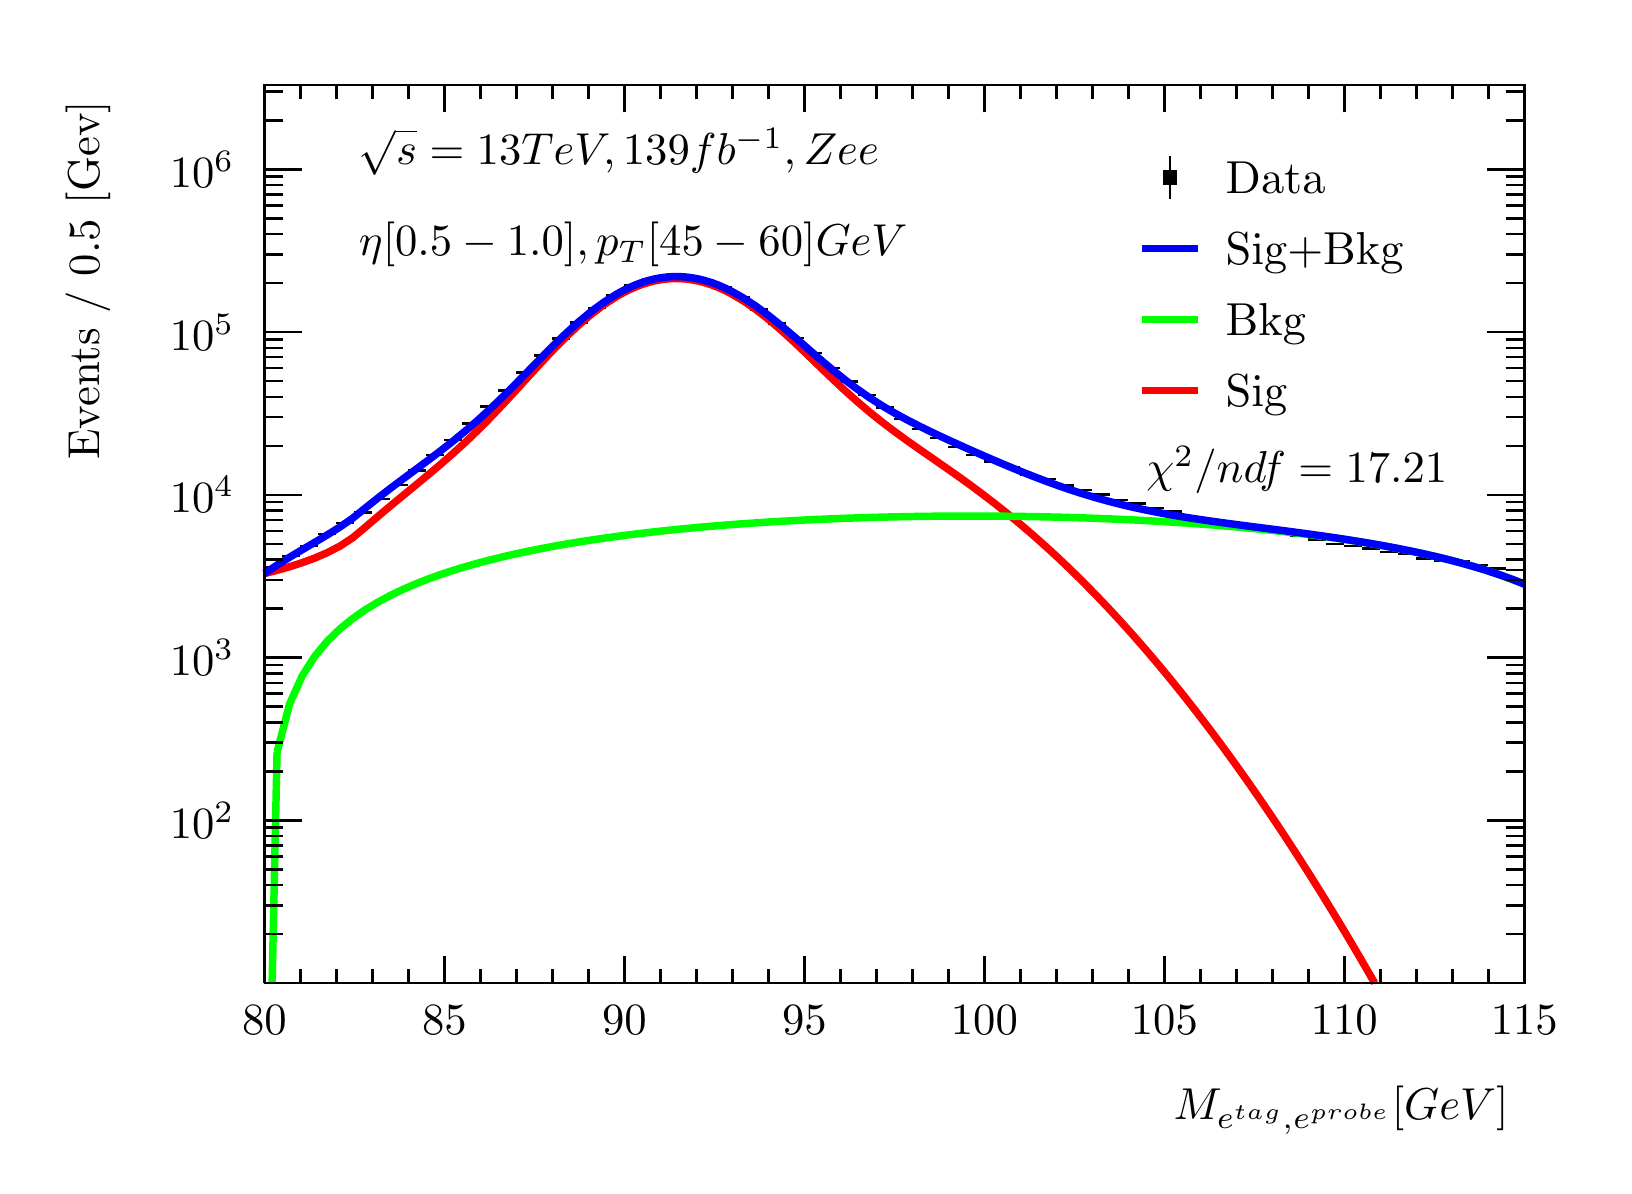
\begin{tikzpicture}
\pgfdeclareplotmark{cross} {
\pgfpathmoveto{\pgfpoint{-0.3\pgfplotmarksize}{\pgfplotmarksize}}
\pgfpathlineto{\pgfpoint{+0.3\pgfplotmarksize}{\pgfplotmarksize}}
\pgfpathlineto{\pgfpoint{+0.3\pgfplotmarksize}{0.3\pgfplotmarksize}}
\pgfpathlineto{\pgfpoint{+1\pgfplotmarksize}{0.3\pgfplotmarksize}}
\pgfpathlineto{\pgfpoint{+1\pgfplotmarksize}{-0.3\pgfplotmarksize}}
\pgfpathlineto{\pgfpoint{+0.3\pgfplotmarksize}{-0.3\pgfplotmarksize}}
\pgfpathlineto{\pgfpoint{+0.3\pgfplotmarksize}{-1.\pgfplotmarksize}}
\pgfpathlineto{\pgfpoint{-0.3\pgfplotmarksize}{-1.\pgfplotmarksize}}
\pgfpathlineto{\pgfpoint{-0.3\pgfplotmarksize}{-0.3\pgfplotmarksize}}
\pgfpathlineto{\pgfpoint{-1.\pgfplotmarksize}{-0.3\pgfplotmarksize}}
\pgfpathlineto{\pgfpoint{-1.\pgfplotmarksize}{0.3\pgfplotmarksize}}
\pgfpathlineto{\pgfpoint{-0.3\pgfplotmarksize}{0.3\pgfplotmarksize}}
\pgfpathclose
\pgfusepathqstroke
}
\pgfdeclareplotmark{cross*} {
\pgfpathmoveto{\pgfpoint{-0.3\pgfplotmarksize}{\pgfplotmarksize}}
\pgfpathlineto{\pgfpoint{+0.3\pgfplotmarksize}{\pgfplotmarksize}}
\pgfpathlineto{\pgfpoint{+0.3\pgfplotmarksize}{0.3\pgfplotmarksize}}
\pgfpathlineto{\pgfpoint{+1\pgfplotmarksize}{0.3\pgfplotmarksize}}
\pgfpathlineto{\pgfpoint{+1\pgfplotmarksize}{-0.3\pgfplotmarksize}}
\pgfpathlineto{\pgfpoint{+0.3\pgfplotmarksize}{-0.3\pgfplotmarksize}}
\pgfpathlineto{\pgfpoint{+0.3\pgfplotmarksize}{-1.\pgfplotmarksize}}
\pgfpathlineto{\pgfpoint{-0.3\pgfplotmarksize}{-1.\pgfplotmarksize}}
\pgfpathlineto{\pgfpoint{-0.3\pgfplotmarksize}{-0.3\pgfplotmarksize}}
\pgfpathlineto{\pgfpoint{-1.\pgfplotmarksize}{-0.3\pgfplotmarksize}}
\pgfpathlineto{\pgfpoint{-1.\pgfplotmarksize}{0.3\pgfplotmarksize}}
\pgfpathlineto{\pgfpoint{-0.3\pgfplotmarksize}{0.3\pgfplotmarksize}}
\pgfpathclose
\pgfusepathqfillstroke
}
\pgfdeclareplotmark{newstar} {
\pgfpathmoveto{\pgfqpoint{0pt}{\pgfplotmarksize}}
\pgfpathlineto{\pgfqpointpolar{44}{0.5\pgfplotmarksize}}
\pgfpathlineto{\pgfqpointpolar{18}{\pgfplotmarksize}}
\pgfpathlineto{\pgfqpointpolar{-20}{0.5\pgfplotmarksize}}
\pgfpathlineto{\pgfqpointpolar{-54}{\pgfplotmarksize}}
\pgfpathlineto{\pgfqpointpolar{-90}{0.5\pgfplotmarksize}}
\pgfpathlineto{\pgfqpointpolar{234}{\pgfplotmarksize}}
\pgfpathlineto{\pgfqpointpolar{198}{0.5\pgfplotmarksize}}
\pgfpathlineto{\pgfqpointpolar{162}{\pgfplotmarksize}}
\pgfpathlineto{\pgfqpointpolar{134}{0.5\pgfplotmarksize}}
\pgfpathclose
\pgfusepathqstroke
}
\pgfdeclareplotmark{newstar*} {
\pgfpathmoveto{\pgfqpoint{0pt}{\pgfplotmarksize}}
\pgfpathlineto{\pgfqpointpolar{44}{0.5\pgfplotmarksize}}
\pgfpathlineto{\pgfqpointpolar{18}{\pgfplotmarksize}}
\pgfpathlineto{\pgfqpointpolar{-20}{0.5\pgfplotmarksize}}
\pgfpathlineto{\pgfqpointpolar{-54}{\pgfplotmarksize}}
\pgfpathlineto{\pgfqpointpolar{-90}{0.5\pgfplotmarksize}}
\pgfpathlineto{\pgfqpointpolar{234}{\pgfplotmarksize}}
\pgfpathlineto{\pgfqpointpolar{198}{0.5\pgfplotmarksize}}
\pgfpathlineto{\pgfqpointpolar{162}{\pgfplotmarksize}}
\pgfpathlineto{\pgfqpointpolar{134}{0.5\pgfplotmarksize}}
\pgfpathclose
\pgfusepathqfillstroke
}
\definecolor{c}{rgb}{1,1,1};
\draw [color=c, fill=c] (0,0) rectangle (20,14.4361);
\draw [color=c, fill=c] (3,2.30977) rectangle (19,13.7143);
\definecolor{c}{rgb}{0,0,0};
\draw [c,line width=0.9] (3,2.30977) -- (3,13.7143) -- (19,13.7143) -- (19,2.30977) -- (3,2.30977);
\definecolor{c}{rgb}{1,1,1};
\draw [color=c, fill=c] (3,2.30977) rectangle (19,13.7143);
\definecolor{c}{rgb}{0,0,0};
\draw [c,line width=0.9] (3,2.30977) -- (3,13.7143) -- (19,13.7143) -- (19,2.30977) -- (3,2.30977);
\draw [c,line width=0.9] (3,2.30977) -- (19,2.30977);
\draw [c,line width=0.9] (3,2.65624) -- (3,2.30977);
\draw [c,line width=0.9] (3.45714,2.48301) -- (3.45714,2.30977);
\draw [c,line width=0.9] (3.91429,2.48301) -- (3.91429,2.30977);
\draw [c,line width=0.9] (4.37143,2.48301) -- (4.37143,2.30977);
\draw [c,line width=0.9] (4.82857,2.48301) -- (4.82857,2.30977);
\draw [c,line width=0.9] (5.28571,2.65624) -- (5.28571,2.30977);
\draw [c,line width=0.9] (5.74286,2.48301) -- (5.74286,2.30977);
\draw [c,line width=0.9] (6.2,2.48301) -- (6.2,2.30977);
\draw [c,line width=0.9] (6.65714,2.48301) -- (6.65714,2.30977);
\draw [c,line width=0.9] (7.11429,2.48301) -- (7.11429,2.30977);
\draw [c,line width=0.9] (7.57143,2.65624) -- (7.57143,2.30977);
\draw [c,line width=0.9] (8.02857,2.48301) -- (8.02857,2.30977);
\draw [c,line width=0.9] (8.48571,2.48301) -- (8.48571,2.30977);
\draw [c,line width=0.9] (8.94286,2.48301) -- (8.94286,2.30977);
\draw [c,line width=0.9] (9.4,2.48301) -- (9.4,2.30977);
\draw [c,line width=0.9] (9.85714,2.65624) -- (9.85714,2.30977);
\draw [c,line width=0.9] (10.3143,2.48301) -- (10.3143,2.30977);
\draw [c,line width=0.9] (10.7714,2.48301) -- (10.7714,2.30977);
\draw [c,line width=0.9] (11.2286,2.48301) -- (11.2286,2.30977);
\draw [c,line width=0.9] (11.6857,2.48301) -- (11.6857,2.30977);
\draw [c,line width=0.9] (12.1429,2.65624) -- (12.1429,2.30977);
\draw [c,line width=0.9] (12.6,2.48301) -- (12.6,2.30977);
\draw [c,line width=0.9] (13.0571,2.48301) -- (13.0571,2.30977);
\draw [c,line width=0.9] (13.5143,2.48301) -- (13.5143,2.30977);
\draw [c,line width=0.9] (13.9714,2.48301) -- (13.9714,2.30977);
\draw [c,line width=0.9] (14.4286,2.65624) -- (14.4286,2.30977);
\draw [c,line width=0.9] (14.8857,2.48301) -- (14.8857,2.30977);
\draw [c,line width=0.9] (15.3429,2.48301) -- (15.3429,2.30977);
\draw [c,line width=0.9] (15.8,2.48301) -- (15.8,2.30977);
\draw [c,line width=0.9] (16.2571,2.48301) -- (16.2571,2.30977);
\draw [c,line width=0.9] (16.7143,2.65624) -- (16.7143,2.30977);
\draw [c,line width=0.9] (17.1714,2.48301) -- (17.1714,2.30977);
\draw [c,line width=0.9] (17.6286,2.48301) -- (17.6286,2.30977);
\draw [c,line width=0.9] (18.0857,2.48301) -- (18.0857,2.30977);
\draw [c,line width=0.9] (18.5429,2.48301) -- (18.5429,2.30977);
\draw [c,line width=0.9] (19,2.65624) -- (19,2.30977);
\draw [anchor=base] (3,1.66015) node[scale=1.61424, color=c, rotate=0]{80};
\draw [anchor=base] (5.28571,1.66015) node[scale=1.61424, color=c, rotate=0]{85};
\draw [anchor=base] (7.57143,1.66015) node[scale=1.61424, color=c, rotate=0]{90};
\draw [anchor=base] (9.85714,1.66015) node[scale=1.61424, color=c, rotate=0]{95};
\draw [anchor=base] (12.1429,1.66015) node[scale=1.61424, color=c, rotate=0]{100};
\draw [anchor=base] (14.4286,1.66015) node[scale=1.61424, color=c, rotate=0]{105};
\draw [anchor=base] (16.7143,1.66015) node[scale=1.61424, color=c, rotate=0]{110};
\draw [anchor=base] (19,1.66015) node[scale=1.61424, color=c, rotate=0]{115};
\draw [anchor= east] (19,0.692932) node[scale=1.61424, color=c, rotate=0]{$M_{e^{tag}, e^{probe}}  [GeV]$};
\draw [c,line width=0.9] (3,13.7143) -- (19,13.7143);
\draw [c,line width=0.9] (3,13.3678) -- (3,13.7143);
\draw [c,line width=0.9] (3.45714,13.5411) -- (3.45714,13.7143);
\draw [c,line width=0.9] (3.91429,13.5411) -- (3.91429,13.7143);
\draw [c,line width=0.9] (4.37143,13.5411) -- (4.37143,13.7143);
\draw [c,line width=0.9] (4.82857,13.5411) -- (4.82857,13.7143);
\draw [c,line width=0.9] (5.28571,13.3678) -- (5.28571,13.7143);
\draw [c,line width=0.9] (5.74286,13.5411) -- (5.74286,13.7143);
\draw [c,line width=0.9] (6.2,13.5411) -- (6.2,13.7143);
\draw [c,line width=0.9] (6.65714,13.5411) -- (6.65714,13.7143);
\draw [c,line width=0.9] (7.11429,13.5411) -- (7.11429,13.7143);
\draw [c,line width=0.9] (7.57143,13.3678) -- (7.57143,13.7143);
\draw [c,line width=0.9] (8.02857,13.5411) -- (8.02857,13.7143);
\draw [c,line width=0.9] (8.48571,13.5411) -- (8.48571,13.7143);
\draw [c,line width=0.9] (8.94286,13.5411) -- (8.94286,13.7143);
\draw [c,line width=0.9] (9.4,13.5411) -- (9.4,13.7143);
\draw [c,line width=0.9] (9.85714,13.3678) -- (9.85714,13.7143);
\draw [c,line width=0.9] (10.3143,13.5411) -- (10.3143,13.7143);
\draw [c,line width=0.9] (10.7714,13.5411) -- (10.7714,13.7143);
\draw [c,line width=0.9] (11.2286,13.5411) -- (11.2286,13.7143);
\draw [c,line width=0.9] (11.6857,13.5411) -- (11.6857,13.7143);
\draw [c,line width=0.9] (12.1429,13.3678) -- (12.1429,13.7143);
\draw [c,line width=0.9] (12.6,13.5411) -- (12.6,13.7143);
\draw [c,line width=0.9] (13.0571,13.5411) -- (13.0571,13.7143);
\draw [c,line width=0.9] (13.5143,13.5411) -- (13.5143,13.7143);
\draw [c,line width=0.9] (13.9714,13.5411) -- (13.9714,13.7143);
\draw [c,line width=0.9] (14.4286,13.3678) -- (14.4286,13.7143);
\draw [c,line width=0.9] (14.8857,13.5411) -- (14.8857,13.7143);
\draw [c,line width=0.9] (15.3429,13.5411) -- (15.3429,13.7143);
\draw [c,line width=0.9] (15.8,13.5411) -- (15.8,13.7143);
\draw [c,line width=0.9] (16.2571,13.5411) -- (16.2571,13.7143);
\draw [c,line width=0.9] (16.7143,13.3678) -- (16.7143,13.7143);
\draw [c,line width=0.9] (17.1714,13.5411) -- (17.1714,13.7143);
\draw [c,line width=0.9] (17.6286,13.5411) -- (17.6286,13.7143);
\draw [c,line width=0.9] (18.0857,13.5411) -- (18.0857,13.7143);
\draw [c,line width=0.9] (18.5429,13.5411) -- (18.5429,13.7143);
\draw [c,line width=0.9] (19,13.3678) -- (19,13.7143);
\draw [c,line width=0.9] (3,2.30977) -- (3,13.7143);
\draw [c,line width=0.9] (3.237,2.932) -- (3,2.932);
\draw [c,line width=0.9] (3.237,3.29598) -- (3,3.29598);
\draw [c,line width=0.9] (3.237,3.55423) -- (3,3.55423);
\draw [c,line width=0.9] (3.237,3.75454) -- (3,3.75454);
\draw [c,line width=0.9] (3.237,3.9182) -- (3,3.9182);
\draw [c,line width=0.9] (3.237,4.05658) -- (3,4.05658);
\draw [c,line width=0.9] (3.237,4.17645) -- (3,4.17645);
\draw [c,line width=0.9] (3.237,4.28218) -- (3,4.28218);
\draw [c,line width=0.9] (3.474,4.37676) -- (3,4.37676);
\draw [anchor= east] (2.82,4.37676) node[scale=1.61424, color=c, rotate=0]{$10^{2}$};
\draw [c,line width=0.9] (3.237,4.99899) -- (3,4.99899);
\draw [c,line width=0.9] (3.237,5.36297) -- (3,5.36297);
\draw [c,line width=0.9] (3.237,5.62122) -- (3,5.62122);
\draw [c,line width=0.9] (3.237,5.82153) -- (3,5.82153);
\draw [c,line width=0.9] (3.237,5.9852) -- (3,5.9852);
\draw [c,line width=0.9] (3.237,6.12357) -- (3,6.12357);
\draw [c,line width=0.9] (3.237,6.24344) -- (3,6.24344);
\draw [c,line width=0.9] (3.237,6.34917) -- (3,6.34917);
\draw [c,line width=0.9] (3.474,6.44376) -- (3,6.44376);
\draw [anchor= east] (2.82,6.44376) node[scale=1.61424, color=c, rotate=0]{$10^{3}$};
\draw [c,line width=0.9] (3.237,7.06598) -- (3,7.06598);
\draw [c,line width=0.9] (3.237,7.42996) -- (3,7.42996);
\draw [c,line width=0.9] (3.237,7.68821) -- (3,7.68821);
\draw [c,line width=0.9] (3.237,7.88852) -- (3,7.88852);
\draw [c,line width=0.9] (3.237,8.05219) -- (3,8.05219);
\draw [c,line width=0.9] (3.237,8.19057) -- (3,8.19057);
\draw [c,line width=0.9] (3.237,8.31043) -- (3,8.31043);
\draw [c,line width=0.9] (3.237,8.41617) -- (3,8.41617);
\draw [c,line width=0.9] (3.474,8.51075) -- (3,8.51075);
\draw [anchor= east] (2.82,8.51075) node[scale=1.61424, color=c, rotate=0]{$10^{4}$};
\draw [c,line width=0.9] (3.237,9.13297) -- (3,9.13297);
\draw [c,line width=0.9] (3.237,9.49695) -- (3,9.49695);
\draw [c,line width=0.9] (3.237,9.7552) -- (3,9.7552);
\draw [c,line width=0.9] (3.237,9.95551) -- (3,9.95551);
\draw [c,line width=0.9] (3.237,10.1192) -- (3,10.1192);
\draw [c,line width=0.9] (3.237,10.2576) -- (3,10.2576);
\draw [c,line width=0.9] (3.237,10.3774) -- (3,10.3774);
\draw [c,line width=0.9] (3.237,10.4832) -- (3,10.4832);
\draw [c,line width=0.9] (3.474,10.5777) -- (3,10.5777);
\draw [anchor= east] (2.82,10.5777) node[scale=1.61424, color=c, rotate=0]{$10^{5}$};
\draw [c,line width=0.9] (3.237,11.2) -- (3,11.2);
\draw [c,line width=0.9] (3.237,11.5639) -- (3,11.5639);
\draw [c,line width=0.9] (3.237,11.8222) -- (3,11.8222);
\draw [c,line width=0.9] (3.237,12.0225) -- (3,12.0225);
\draw [c,line width=0.9] (3.237,12.1862) -- (3,12.1862);
\draw [c,line width=0.9] (3.237,12.3245) -- (3,12.3245);
\draw [c,line width=0.9] (3.237,12.4444) -- (3,12.4444);
\draw [c,line width=0.9] (3.237,12.5501) -- (3,12.5501);
\draw [c,line width=0.9] (3.474,12.6447) -- (3,12.6447);
\draw [anchor= east] (2.82,12.6447) node[scale=1.61424, color=c, rotate=0]{$10^{6}$};
\draw [c,line width=0.9] (3.237,13.267) -- (3,13.267);
\draw [c,line width=0.9] (3.237,13.6309) -- (3,13.6309);
\draw [anchor= east] (0.76,13.7143) node[scale=1.61424, color=c, rotate=90]{Events / 0.5 [Gev]};
\draw [c,line width=0.9] (19,2.30977) -- (19,13.7143);
\draw [c,line width=0.9] (18.763,2.932) -- (19,2.932);
\draw [c,line width=0.9] (18.763,3.29598) -- (19,3.29598);
\draw [c,line width=0.9] (18.763,3.55423) -- (19,3.55423);
\draw [c,line width=0.9] (18.763,3.75454) -- (19,3.75454);
\draw [c,line width=0.9] (18.763,3.9182) -- (19,3.9182);
\draw [c,line width=0.9] (18.763,4.05658) -- (19,4.05658);
\draw [c,line width=0.9] (18.763,4.17645) -- (19,4.17645);
\draw [c,line width=0.9] (18.763,4.28218) -- (19,4.28218);
\draw [c,line width=0.9] (18.526,4.37676) -- (19,4.37676);
\draw [c,line width=0.9] (18.763,4.99899) -- (19,4.99899);
\draw [c,line width=0.9] (18.763,5.36297) -- (19,5.36297);
\draw [c,line width=0.9] (18.763,5.62122) -- (19,5.62122);
\draw [c,line width=0.9] (18.763,5.82153) -- (19,5.82153);
\draw [c,line width=0.9] (18.763,5.9852) -- (19,5.9852);
\draw [c,line width=0.9] (18.763,6.12357) -- (19,6.12357);
\draw [c,line width=0.9] (18.763,6.24344) -- (19,6.24344);
\draw [c,line width=0.9] (18.763,6.34917) -- (19,6.34917);
\draw [c,line width=0.9] (18.526,6.44376) -- (19,6.44376);
\draw [c,line width=0.9] (18.763,7.06598) -- (19,7.06598);
\draw [c,line width=0.9] (18.763,7.42996) -- (19,7.42996);
\draw [c,line width=0.9] (18.763,7.68821) -- (19,7.68821);
\draw [c,line width=0.9] (18.763,7.88852) -- (19,7.88852);
\draw [c,line width=0.9] (18.763,8.05219) -- (19,8.05219);
\draw [c,line width=0.9] (18.763,8.19057) -- (19,8.19057);
\draw [c,line width=0.9] (18.763,8.31043) -- (19,8.31043);
\draw [c,line width=0.9] (18.763,8.41617) -- (19,8.41617);
\draw [c,line width=0.9] (18.526,8.51075) -- (19,8.51075);
\draw [c,line width=0.9] (18.763,9.13297) -- (19,9.13297);
\draw [c,line width=0.9] (18.763,9.49695) -- (19,9.49695);
\draw [c,line width=0.9] (18.763,9.7552) -- (19,9.7552);
\draw [c,line width=0.9] (18.763,9.95551) -- (19,9.95551);
\draw [c,line width=0.9] (18.763,10.1192) -- (19,10.1192);
\draw [c,line width=0.9] (18.763,10.2576) -- (19,10.2576);
\draw [c,line width=0.9] (18.763,10.3774) -- (19,10.3774);
\draw [c,line width=0.9] (18.763,10.4832) -- (19,10.4832);
\draw [c,line width=0.9] (18.526,10.5777) -- (19,10.5777);
\draw [c,line width=0.9] (18.763,11.2) -- (19,11.2);
\draw [c,line width=0.9] (18.763,11.5639) -- (19,11.5639);
\draw [c,line width=0.9] (18.763,11.8222) -- (19,11.8222);
\draw [c,line width=0.9] (18.763,12.0225) -- (19,12.0225);
\draw [c,line width=0.9] (18.763,12.1862) -- (19,12.1862);
\draw [c,line width=0.9] (18.763,12.3245) -- (19,12.3245);
\draw [c,line width=0.9] (18.763,12.4444) -- (19,12.4444);
\draw [c,line width=0.9] (18.763,12.5501) -- (19,12.5501);
\draw [c,line width=0.9] (18.526,12.6447) -- (19,12.6447);
\draw [c,line width=0.9] (18.763,13.267) -- (19,13.267);
\draw [c,line width=0.9] (18.763,13.6309) -- (19,13.6309);
\draw [c,line width=0.9] (3.11429,7.59238) -- (3,7.59238);
\draw [c,line width=0.9] (3,7.59238) -- (3,7.59238);
\draw [c,line width=0.9] (3.11429,7.59238) -- (3.22857,7.59238);
\draw [c,line width=0.9] (3.22857,7.59238) -- (3.22857,7.59238);
\draw [c,line width=0.9] (3.11429,7.59238) -- (3.11429,7.60735);
\draw [c,line width=0.9] (3.11429,7.60735) -- (3.11429,7.60735);
\draw [c,line width=0.9] (3.11429,7.59238) -- (3.11429,7.57741);
\draw [c,line width=0.9] (3.11429,7.57741) -- (3.11429,7.57741);
\draw [c,line width=0.9] (3.34286,7.73179) -- (3.22857,7.73179);
\draw [c,line width=0.9] (3.22857,7.73179) -- (3.22857,7.73179);
\draw [c,line width=0.9] (3.34286,7.73179) -- (3.45714,7.73179);
\draw [c,line width=0.9] (3.45714,7.73179) -- (3.45714,7.73179);
\draw [c,line width=0.9] (3.34286,7.73179) -- (3.34286,7.74565);
\draw [c,line width=0.9] (3.34286,7.74565) -- (3.34286,7.74565);
\draw [c,line width=0.9] (3.34286,7.73179) -- (3.34286,7.71794);
\draw [c,line width=0.9] (3.34286,7.71794) -- (3.34286,7.71794);
\draw [c,line width=0.9] (3.57143,7.85858) -- (3.45714,7.85858);
\draw [c,line width=0.9] (3.45714,7.85858) -- (3.45714,7.85858);
\draw [c,line width=0.9] (3.57143,7.85858) -- (3.68571,7.85858);
\draw [c,line width=0.9] (3.68571,7.85858) -- (3.68571,7.85858);
\draw [c,line width=0.9] (3.57143,7.85858) -- (3.57143,7.87149);
\draw [c,line width=0.9] (3.57143,7.87149) -- (3.57143,7.87149);
\draw [c,line width=0.9] (3.57143,7.85858) -- (3.57143,7.84567);
\draw [c,line width=0.9] (3.57143,7.84567) -- (3.57143,7.84567);
\draw [c,line width=0.9] (3.8,8.01054) -- (3.68571,8.01054);
\draw [c,line width=0.9] (3.68571,8.01054) -- (3.68571,8.01054);
\draw [c,line width=0.9] (3.8,8.01054) -- (3.91429,8.01054);
\draw [c,line width=0.9] (3.91429,8.01054) -- (3.91429,8.01054);
\draw [c,line width=0.9] (3.8,8.01054) -- (3.8,8.0224);
\draw [c,line width=0.9] (3.8,8.0224) -- (3.8,8.0224);
\draw [c,line width=0.9] (3.8,8.01054) -- (3.8,7.99868);
\draw [c,line width=0.9] (3.8,7.99868) -- (3.8,7.99868);
\draw [c,line width=0.9] (4.02857,8.15245) -- (3.91429,8.15245);
\draw [c,line width=0.9] (3.91429,8.15245) -- (3.91429,8.15245);
\draw [c,line width=0.9] (4.02857,8.15245) -- (4.14286,8.15245);
\draw [c,line width=0.9] (4.14286,8.15245) -- (4.14286,8.15245);
\draw [c,line width=0.9] (4.02857,8.15245) -- (4.02857,8.16341);
\draw [c,line width=0.9] (4.02857,8.16341) -- (4.02857,8.16341);
\draw [c,line width=0.9] (4.02857,8.15245) -- (4.02857,8.14149);
\draw [c,line width=0.9] (4.02857,8.14149) -- (4.02857,8.14149);
\draw [c,line width=0.9] (4.25714,8.28805) -- (4.14286,8.28805);
\draw [c,line width=0.9] (4.14286,8.28805) -- (4.14286,8.28805);
\draw [c,line width=0.9] (4.25714,8.28805) -- (4.37143,8.28805);
\draw [c,line width=0.9] (4.37143,8.28805) -- (4.37143,8.28805);
\draw [c,line width=0.9] (4.25714,8.28805) -- (4.25714,8.29822);
\draw [c,line width=0.9] (4.25714,8.29822) -- (4.25714,8.29822);
\draw [c,line width=0.9] (4.25714,8.28805) -- (4.25714,8.27789);
\draw [c,line width=0.9] (4.25714,8.27789) -- (4.25714,8.27789);
\draw [c,line width=0.9] (4.48571,8.45892) -- (4.37143,8.45892);
\draw [c,line width=0.9] (4.37143,8.45892) -- (4.37143,8.45892);
\draw [c,line width=0.9] (4.48571,8.45892) -- (4.6,8.45892);
\draw [c,line width=0.9] (4.6,8.45892) -- (4.6,8.45892);
\draw [c,line width=0.9] (4.48571,8.45892) -- (4.48571,8.46816);
\draw [c,line width=0.9] (4.48571,8.46816) -- (4.48571,8.46816);
\draw [c,line width=0.9] (4.48571,8.45892) -- (4.48571,8.44968);
\draw [c,line width=0.9] (4.48571,8.44968) -- (4.48571,8.44968);
\draw [c,line width=0.9] (4.71429,8.63738) -- (4.6,8.63738);
\draw [c,line width=0.9] (4.6,8.63738) -- (4.6,8.63738);
\draw [c,line width=0.9] (4.71429,8.63738) -- (4.82857,8.63738);
\draw [c,line width=0.9] (4.82857,8.63738) -- (4.82857,8.63738);
\draw [c,line width=0.9] (4.71429,8.63738) -- (4.71429,8.64575);
\draw [c,line width=0.9] (4.71429,8.64575) -- (4.71429,8.64575);
\draw [c,line width=0.9] (4.71429,8.63738) -- (4.71429,8.62901);
\draw [c,line width=0.9] (4.71429,8.62901) -- (4.71429,8.62901);
\draw [c,line width=0.9] (4.94286,8.81759) -- (4.82857,8.81759);
\draw [c,line width=0.9] (4.82857,8.81759) -- (4.82857,8.81759);
\draw [c,line width=0.9] (4.94286,8.81759) -- (5.05714,8.81759);
\draw [c,line width=0.9] (5.05714,8.81759) -- (5.05714,8.81759);
\draw [c,line width=0.9] (4.94286,8.81759) -- (4.94286,8.82516);
\draw [c,line width=0.9] (4.94286,8.82516) -- (4.94286,8.82516);
\draw [c,line width=0.9] (4.94286,8.81759) -- (4.94286,8.81002);
\draw [c,line width=0.9] (4.94286,8.81002) -- (4.94286,8.81002);
\draw [c,line width=0.9] (5.17143,9.01469) -- (5.05714,9.01469);
\draw [c,line width=0.9] (5.05714,9.01469) -- (5.05714,9.01469);
\draw [c,line width=0.9] (5.17143,9.01469) -- (5.28571,9.01469);
\draw [c,line width=0.9] (5.28571,9.01469) -- (5.28571,9.01469);
\draw [c,line width=0.9] (5.17143,9.01469) -- (5.17143,9.02147);
\draw [c,line width=0.9] (5.17143,9.02147) -- (5.17143,9.02147);
\draw [c,line width=0.9] (5.17143,9.01469) -- (5.17143,9.00791);
\draw [c,line width=0.9] (5.17143,9.00791) -- (5.17143,9.00791);
\draw [c,line width=0.9] (5.4,9.20339) -- (5.28571,9.20339);
\draw [c,line width=0.9] (5.28571,9.20339) -- (5.28571,9.20339);
\draw [c,line width=0.9] (5.4,9.20339) -- (5.51429,9.20339);
\draw [c,line width=0.9] (5.51429,9.20339) -- (5.51429,9.20339);
\draw [c,line width=0.9] (5.4,9.20339) -- (5.4,9.20949);
\draw [c,line width=0.9] (5.4,9.20949) -- (5.4,9.20949);
\draw [c,line width=0.9] (5.4,9.20339) -- (5.4,9.19729);
\draw [c,line width=0.9] (5.4,9.19729) -- (5.4,9.19729);
\draw [c,line width=0.9] (5.62857,9.41597) -- (5.51429,9.41597);
\draw [c,line width=0.9] (5.51429,9.41597) -- (5.51429,9.41597);
\draw [c,line width=0.9] (5.62857,9.41597) -- (5.74286,9.41597);
\draw [c,line width=0.9] (5.74286,9.41597) -- (5.74286,9.41597);
\draw [c,line width=0.9] (5.62857,9.41597) -- (5.62857,9.42139);
\draw [c,line width=0.9] (5.62857,9.42139) -- (5.62857,9.42139);
\draw [c,line width=0.9] (5.62857,9.41597) -- (5.62857,9.41055);
\draw [c,line width=0.9] (5.62857,9.41055) -- (5.62857,9.41055);
\draw [c,line width=0.9] (5.85714,9.63111) -- (5.74286,9.63111);
\draw [c,line width=0.9] (5.74286,9.63111) -- (5.74286,9.63111);
\draw [c,line width=0.9] (5.85714,9.63111) -- (5.97143,9.63111);
\draw [c,line width=0.9] (5.97143,9.63111) -- (5.97143,9.63111);
\draw [c,line width=0.9] (5.85714,9.63111) -- (5.85714,9.63592);
\draw [c,line width=0.9] (5.85714,9.63592) -- (5.85714,9.63592);
\draw [c,line width=0.9] (5.85714,9.63111) -- (5.85714,9.62631);
\draw [c,line width=0.9] (5.85714,9.62631) -- (5.85714,9.62631);
\draw [c,line width=0.9] (6.08571,9.83636) -- (5.97143,9.83636);
\draw [c,line width=0.9] (5.97143,9.83636) -- (5.97143,9.83636);
\draw [c,line width=0.9] (6.08571,9.83636) -- (6.2,9.83636);
\draw [c,line width=0.9] (6.2,9.83636) -- (6.2,9.83636);
\draw [c,line width=0.9] (6.08571,9.83636) -- (6.08571,9.84065);
\draw [c,line width=0.9] (6.08571,9.84065) -- (6.08571,9.84065);
\draw [c,line width=0.9] (6.08571,9.83636) -- (6.08571,9.83207);
\draw [c,line width=0.9] (6.08571,9.83207) -- (6.08571,9.83207);
\draw [c,line width=0.9] (6.31429,10.0623) -- (6.2,10.0623);
\draw [c,line width=0.9] (6.2,10.0623) -- (6.2,10.0623);
\draw [c,line width=0.9] (6.31429,10.0623) -- (6.42857,10.0623);
\draw [c,line width=0.9] (6.42857,10.0623) -- (6.42857,10.0623);
\draw [c,line width=0.9] (6.31429,10.0623) -- (6.31429,10.066);
\draw [c,line width=0.9] (6.31429,10.066) -- (6.31429,10.066);
\draw [c,line width=0.9] (6.31429,10.0623) -- (6.31429,10.0585);
\draw [c,line width=0.9] (6.31429,10.0585) -- (6.31429,10.0585);
\draw [c,line width=0.9] (6.54286,10.2775) -- (6.42857,10.2775);
\draw [c,line width=0.9] (6.42857,10.2775) -- (6.42857,10.2775);
\draw [c,line width=0.9] (6.54286,10.2775) -- (6.65714,10.2775);
\draw [c,line width=0.9] (6.65714,10.2775) -- (6.65714,10.2775);
\draw [c,line width=0.9] (6.54286,10.2775) -- (6.54286,10.2808);
\draw [c,line width=0.9] (6.54286,10.2808) -- (6.54286,10.2808);
\draw [c,line width=0.9] (6.54286,10.2775) -- (6.54286,10.2741);
\draw [c,line width=0.9] (6.54286,10.2741) -- (6.54286,10.2741);
\draw [c,line width=0.9] (6.77143,10.4972) -- (6.65714,10.4972);
\draw [c,line width=0.9] (6.65714,10.4972) -- (6.65714,10.4972);
\draw [c,line width=0.9] (6.77143,10.4972) -- (6.88571,10.4972);
\draw [c,line width=0.9] (6.88571,10.4972) -- (6.88571,10.4972);
\draw [c,line width=0.9] (6.77143,10.4972) -- (6.77143,10.5002);
\draw [c,line width=0.9] (6.77143,10.5002) -- (6.77143,10.5002);
\draw [c,line width=0.9] (6.77143,10.4972) -- (6.77143,10.4942);
\draw [c,line width=0.9] (6.77143,10.4942) -- (6.77143,10.4942);
\draw [c,line width=0.9] (7,10.6999) -- (6.88571,10.6999);
\draw [c,line width=0.9] (6.88571,10.6999) -- (6.88571,10.6999);
\draw [c,line width=0.9] (7,10.6999) -- (7.11429,10.6999);
\draw [c,line width=0.9] (7.11429,10.6999) -- (7.11429,10.6999);
\draw [c,line width=0.9] (7,10.6999) -- (7,10.7025);
\draw [c,line width=0.9] (7,10.7025) -- (7,10.7025);
\draw [c,line width=0.9] (7,10.6999) -- (7,10.6972);
\draw [c,line width=0.9] (7,10.6972) -- (7,10.6972);
\draw [c,line width=0.9] (7.22857,10.8818) -- (7.11429,10.8818);
\draw [c,line width=0.9] (7.11429,10.8818) -- (7.11429,10.8818);
\draw [c,line width=0.9] (7.22857,10.8818) -- (7.34286,10.8818);
\draw [c,line width=0.9] (7.34286,10.8818) -- (7.34286,10.8818);
\draw [c,line width=0.9] (7.22857,10.8818) -- (7.22857,10.8842);
\draw [c,line width=0.9] (7.22857,10.8842) -- (7.22857,10.8842);
\draw [c,line width=0.9] (7.22857,10.8818) -- (7.22857,10.8794);
\draw [c,line width=0.9] (7.22857,10.8794) -- (7.22857,10.8794);
\draw [c,line width=0.9] (7.45714,11.0387) -- (7.34286,11.0387);
\draw [c,line width=0.9] (7.34286,11.0387) -- (7.34286,11.0387);
\draw [c,line width=0.9] (7.45714,11.0387) -- (7.57143,11.0387);
\draw [c,line width=0.9] (7.57143,11.0387) -- (7.57143,11.0387);
\draw [c,line width=0.9] (7.45714,11.0387) -- (7.45714,11.0409);
\draw [c,line width=0.9] (7.45714,11.0409) -- (7.45714,11.0409);
\draw [c,line width=0.9] (7.45714,11.0387) -- (7.45714,11.0365);
\draw [c,line width=0.9] (7.45714,11.0365) -- (7.45714,11.0365);
\draw [c,line width=0.9] (7.68571,11.1677) -- (7.57143,11.1677);
\draw [c,line width=0.9] (7.57143,11.1677) -- (7.57143,11.1677);
\draw [c,line width=0.9] (7.68571,11.1677) -- (7.8,11.1677);
\draw [c,line width=0.9] (7.8,11.1677) -- (7.8,11.1677);
\draw [c,line width=0.9] (7.68571,11.1677) -- (7.68571,11.1697);
\draw [c,line width=0.9] (7.68571,11.1697) -- (7.68571,11.1697);
\draw [c,line width=0.9] (7.68571,11.1677) -- (7.68571,11.1656);
\draw [c,line width=0.9] (7.68571,11.1656) -- (7.68571,11.1656);
\draw [c,line width=0.9] (7.91429,11.2521) -- (7.8,11.2521);
\draw [c,line width=0.9] (7.8,11.2521) -- (7.8,11.2521);
\draw [c,line width=0.9] (7.91429,11.2521) -- (8.02857,11.2521);
\draw [c,line width=0.9] (8.02857,11.2521) -- (8.02857,11.2521);
\draw [c,line width=0.9] (7.91429,11.2521) -- (7.91429,11.254);
\draw [c,line width=0.9] (7.91429,11.254) -- (7.91429,11.254);
\draw [c,line width=0.9] (7.91429,11.2521) -- (7.91429,11.2501);
\draw [c,line width=0.9] (7.91429,11.2501) -- (7.91429,11.2501);
\draw [c,line width=0.9] (8.14286,11.291) -- (8.02857,11.291);
\draw [c,line width=0.9] (8.02857,11.291) -- (8.02857,11.291);
\draw [c,line width=0.9] (8.14286,11.291) -- (8.25714,11.291);
\draw [c,line width=0.9] (8.25714,11.291) -- (8.25714,11.291);
\draw [c,line width=0.9] (8.14286,11.291) -- (8.14286,11.2929);
\draw [c,line width=0.9] (8.14286,11.2929) -- (8.14286,11.2929);
\draw [c,line width=0.9] (8.14286,11.291) -- (8.14286,11.2891);
\draw [c,line width=0.9] (8.14286,11.2891) -- (8.14286,11.2891);
\draw [c,line width=0.9] (8.37143,11.2866) -- (8.25714,11.2866);
\draw [c,line width=0.9] (8.25714,11.2866) -- (8.25714,11.2866);
\draw [c,line width=0.9] (8.37143,11.2866) -- (8.48571,11.2866);
\draw [c,line width=0.9] (8.48571,11.2866) -- (8.48571,11.2866);
\draw [c,line width=0.9] (8.37143,11.2866) -- (8.37143,11.2886);
\draw [c,line width=0.9] (8.37143,11.2886) -- (8.37143,11.2886);
\draw [c,line width=0.9] (8.37143,11.2866) -- (8.37143,11.2847);
\draw [c,line width=0.9] (8.37143,11.2847) -- (8.37143,11.2847);
\draw [c,line width=0.9] (8.6,11.2338) -- (8.48571,11.2338);
\draw [c,line width=0.9] (8.48571,11.2338) -- (8.48571,11.2338);
\draw [c,line width=0.9] (8.6,11.2338) -- (8.71429,11.2338);
\draw [c,line width=0.9] (8.71429,11.2338) -- (8.71429,11.2338);
\draw [c,line width=0.9] (8.6,11.2338) -- (8.6,11.2358);
\draw [c,line width=0.9] (8.6,11.2358) -- (8.6,11.2358);
\draw [c,line width=0.9] (8.6,11.2338) -- (8.6,11.2318);
\draw [c,line width=0.9] (8.6,11.2318) -- (8.6,11.2318);
\draw [c,line width=0.9] (8.82857,11.1405) -- (8.71429,11.1405);
\draw [c,line width=0.9] (8.71429,11.1405) -- (8.71429,11.1405);
\draw [c,line width=0.9] (8.82857,11.1405) -- (8.94286,11.1405);
\draw [c,line width=0.9] (8.94286,11.1405) -- (8.94286,11.1405);
\draw [c,line width=0.9] (8.82857,11.1405) -- (8.82857,11.1426);
\draw [c,line width=0.9] (8.82857,11.1426) -- (8.82857,11.1426);
\draw [c,line width=0.9] (8.82857,11.1405) -- (8.82857,11.1384);
\draw [c,line width=0.9] (8.82857,11.1384) -- (8.82857,11.1384);
\draw [c,line width=0.9] (9.05714,11.0177) -- (8.94286,11.0177);
\draw [c,line width=0.9] (8.94286,11.0177) -- (8.94286,11.0177);
\draw [c,line width=0.9] (9.05714,11.0177) -- (9.17143,11.0177);
\draw [c,line width=0.9] (9.17143,11.0177) -- (9.17143,11.0177);
\draw [c,line width=0.9] (9.05714,11.0177) -- (9.05714,11.0199);
\draw [c,line width=0.9] (9.05714,11.0199) -- (9.05714,11.0199);
\draw [c,line width=0.9] (9.05714,11.0177) -- (9.05714,11.0155);
\draw [c,line width=0.9] (9.05714,11.0155) -- (9.05714,11.0155);
\draw [c,line width=0.9] (9.28571,10.8637) -- (9.17143,10.8637);
\draw [c,line width=0.9] (9.17143,10.8637) -- (9.17143,10.8637);
\draw [c,line width=0.9] (9.28571,10.8637) -- (9.4,10.8637);
\draw [c,line width=0.9] (9.4,10.8637) -- (9.4,10.8637);
\draw [c,line width=0.9] (9.28571,10.8637) -- (9.28571,10.8661);
\draw [c,line width=0.9] (9.28571,10.8661) -- (9.28571,10.8661);
\draw [c,line width=0.9] (9.28571,10.8637) -- (9.28571,10.8612);
\draw [c,line width=0.9] (9.28571,10.8612) -- (9.28571,10.8612);
\draw [c,line width=0.9] (9.51429,10.6849) -- (9.4,10.6849);
\draw [c,line width=0.9] (9.4,10.6849) -- (9.4,10.6849);
\draw [c,line width=0.9] (9.51429,10.6849) -- (9.62857,10.6849);
\draw [c,line width=0.9] (9.62857,10.6849) -- (9.62857,10.6849);
\draw [c,line width=0.9] (9.51429,10.6849) -- (9.51429,10.6876);
\draw [c,line width=0.9] (9.51429,10.6876) -- (9.51429,10.6876);
\draw [c,line width=0.9] (9.51429,10.6849) -- (9.51429,10.6823);
\draw [c,line width=0.9] (9.51429,10.6823) -- (9.51429,10.6823);
\draw [c,line width=0.9] (9.74286,10.5047) -- (9.62857,10.5047);
\draw [c,line width=0.9] (9.62857,10.5047) -- (9.62857,10.5047);
\draw [c,line width=0.9] (9.74286,10.5047) -- (9.85714,10.5047);
\draw [c,line width=0.9] (9.85714,10.5047) -- (9.85714,10.5047);
\draw [c,line width=0.9] (9.74286,10.5047) -- (9.74286,10.5076);
\draw [c,line width=0.9] (9.74286,10.5076) -- (9.74286,10.5076);
\draw [c,line width=0.9] (9.74286,10.5047) -- (9.74286,10.5017);
\draw [c,line width=0.9] (9.74286,10.5017) -- (9.74286,10.5017);
\draw [c,line width=0.9] (9.97143,10.3101) -- (9.85714,10.3101);
\draw [c,line width=0.9] (9.85714,10.3101) -- (9.85714,10.3101);
\draw [c,line width=0.9] (9.97143,10.3101) -- (10.0857,10.3101);
\draw [c,line width=0.9] (10.0857,10.3101) -- (10.0857,10.3101);
\draw [c,line width=0.9] (9.97143,10.3101) -- (9.97143,10.3134);
\draw [c,line width=0.9] (9.97143,10.3134) -- (9.97143,10.3134);
\draw [c,line width=0.9] (9.97143,10.3101) -- (9.97143,10.3068);
\draw [c,line width=0.9] (9.97143,10.3068) -- (9.97143,10.3068);
\draw [c,line width=0.9] (10.2,10.1238) -- (10.0857,10.1238);
\draw [c,line width=0.9] (10.0857,10.1238) -- (10.0857,10.1238);
\draw [c,line width=0.9] (10.2,10.1238) -- (10.3143,10.1238);
\draw [c,line width=0.9] (10.3143,10.1238) -- (10.3143,10.1238);
\draw [c,line width=0.9] (10.2,10.1238) -- (10.2,10.1274);
\draw [c,line width=0.9] (10.2,10.1274) -- (10.2,10.1274);
\draw [c,line width=0.9] (10.2,10.1238) -- (10.2,10.1201);
\draw [c,line width=0.9] (10.2,10.1201) -- (10.2,10.1201);
\draw [c,line width=0.9] (10.4286,9.95045) -- (10.3143,9.95045);
\draw [c,line width=0.9] (10.3143,9.95045) -- (10.3143,9.95045);
\draw [c,line width=0.9] (10.4286,9.95045) -- (10.5429,9.95045);
\draw [c,line width=0.9] (10.5429,9.95045) -- (10.5429,9.95045);
\draw [c,line width=0.9] (10.4286,9.95045) -- (10.4286,9.95448);
\draw [c,line width=0.9] (10.4286,9.95448) -- (10.4286,9.95448);
\draw [c,line width=0.9] (10.4286,9.95045) -- (10.4286,9.94643);
\draw [c,line width=0.9] (10.4286,9.94643) -- (10.4286,9.94643);
\draw [c,line width=0.9] (10.6571,9.78064) -- (10.5429,9.78064);
\draw [c,line width=0.9] (10.5429,9.78064) -- (10.5429,9.78064);
\draw [c,line width=0.9] (10.6571,9.78064) -- (10.7714,9.78064);
\draw [c,line width=0.9] (10.7714,9.78064) -- (10.7714,9.78064);
\draw [c,line width=0.9] (10.6571,9.78064) -- (10.6571,9.78507);
\draw [c,line width=0.9] (10.6571,9.78507) -- (10.6571,9.78507);
\draw [c,line width=0.9] (10.6571,9.78064) -- (10.6571,9.77622);
\draw [c,line width=0.9] (10.6571,9.77622) -- (10.6571,9.77622);
\draw [c,line width=0.9] (10.8857,9.62174) -- (10.7714,9.62174);
\draw [c,line width=0.9] (10.7714,9.62174) -- (10.7714,9.62174);
\draw [c,line width=0.9] (10.8857,9.62174) -- (11,9.62174);
\draw [c,line width=0.9] (11,9.62174) -- (11,9.62174);
\draw [c,line width=0.9] (10.8857,9.62174) -- (10.8857,9.62657);
\draw [c,line width=0.9] (10.8857,9.62657) -- (10.8857,9.62657);
\draw [c,line width=0.9] (10.8857,9.62174) -- (10.8857,9.6169);
\draw [c,line width=0.9] (10.8857,9.6169) -- (10.8857,9.6169);
\draw [c,line width=0.9] (11.1143,9.47211) -- (11,9.47211);
\draw [c,line width=0.9] (11,9.47211) -- (11,9.47211);
\draw [c,line width=0.9] (11.1143,9.47211) -- (11.2286,9.47211);
\draw [c,line width=0.9] (11.2286,9.47211) -- (11.2286,9.47211);
\draw [c,line width=0.9] (11.1143,9.47211) -- (11.1143,9.47736);
\draw [c,line width=0.9] (11.1143,9.47736) -- (11.1143,9.47736);
\draw [c,line width=0.9] (11.1143,9.47211) -- (11.1143,9.46685);
\draw [c,line width=0.9] (11.1143,9.46685) -- (11.1143,9.46685);
\draw [c,line width=0.9] (11.3429,9.34817) -- (11.2286,9.34817);
\draw [c,line width=0.9] (11.2286,9.34817) -- (11.2286,9.34817);
\draw [c,line width=0.9] (11.3429,9.34817) -- (11.4571,9.34817);
\draw [c,line width=0.9] (11.4571,9.34817) -- (11.4571,9.34817);
\draw [c,line width=0.9] (11.3429,9.34817) -- (11.3429,9.3538);
\draw [c,line width=0.9] (11.3429,9.3538) -- (11.3429,9.3538);
\draw [c,line width=0.9] (11.3429,9.34817) -- (11.3429,9.34254);
\draw [c,line width=0.9] (11.3429,9.34254) -- (11.3429,9.34254);
\draw [c,line width=0.9] (11.5714,9.23093) -- (11.4571,9.23093);
\draw [c,line width=0.9] (11.4571,9.23093) -- (11.4571,9.23093);
\draw [c,line width=0.9] (11.5714,9.23093) -- (11.6857,9.23093);
\draw [c,line width=0.9] (11.6857,9.23093) -- (11.6857,9.23093);
\draw [c,line width=0.9] (11.5714,9.23093) -- (11.5714,9.23694);
\draw [c,line width=0.9] (11.5714,9.23694) -- (11.5714,9.23694);
\draw [c,line width=0.9] (11.5714,9.23093) -- (11.5714,9.22492);
\draw [c,line width=0.9] (11.5714,9.22492) -- (11.5714,9.22492);
\draw [c,line width=0.9] (11.8,9.11658) -- (11.6857,9.11658);
\draw [c,line width=0.9] (11.6857,9.11658) -- (11.6857,9.11658);
\draw [c,line width=0.9] (11.8,9.11658) -- (11.9143,9.11658);
\draw [c,line width=0.9] (11.9143,9.11658) -- (11.9143,9.11658);
\draw [c,line width=0.9] (11.8,9.11658) -- (11.8,9.12298);
\draw [c,line width=0.9] (11.8,9.12298) -- (11.8,9.12298);
\draw [c,line width=0.9] (11.8,9.11658) -- (11.8,9.11017);
\draw [c,line width=0.9] (11.8,9.11017) -- (11.8,9.11017);
\draw [c,line width=0.9] (12.0286,9.01812) -- (11.9143,9.01812);
\draw [c,line width=0.9] (11.9143,9.01812) -- (11.9143,9.01812);
\draw [c,line width=0.9] (12.0286,9.01812) -- (12.1429,9.01812);
\draw [c,line width=0.9] (12.1429,9.01812) -- (12.1429,9.01812);
\draw [c,line width=0.9] (12.0286,9.01812) -- (12.0286,9.02489);
\draw [c,line width=0.9] (12.0286,9.02489) -- (12.0286,9.02489);
\draw [c,line width=0.9] (12.0286,9.01812) -- (12.0286,9.01135);
\draw [c,line width=0.9] (12.0286,9.01135) -- (12.0286,9.01135);
\draw [c,line width=0.9] (12.2571,8.93188) -- (12.1429,8.93188);
\draw [c,line width=0.9] (12.1429,8.93188) -- (12.1429,8.93188);
\draw [c,line width=0.9] (12.2571,8.93188) -- (12.3714,8.93188);
\draw [c,line width=0.9] (12.3714,8.93188) -- (12.3714,8.93188);
\draw [c,line width=0.9] (12.2571,8.93188) -- (12.2571,8.93898);
\draw [c,line width=0.9] (12.2571,8.93898) -- (12.2571,8.93898);
\draw [c,line width=0.9] (12.2571,8.93188) -- (12.2571,8.92478);
\draw [c,line width=0.9] (12.2571,8.92478) -- (12.2571,8.92478);
\draw [c,line width=0.9] (12.4857,8.86049) -- (12.3714,8.86049);
\draw [c,line width=0.9] (12.3714,8.86049) -- (12.3714,8.86049);
\draw [c,line width=0.9] (12.4857,8.86049) -- (12.6,8.86049);
\draw [c,line width=0.9] (12.6,8.86049) -- (12.6,8.86049);
\draw [c,line width=0.9] (12.4857,8.86049) -- (12.4857,8.86788);
\draw [c,line width=0.9] (12.4857,8.86788) -- (12.4857,8.86788);
\draw [c,line width=0.9] (12.4857,8.86049) -- (12.4857,8.8531);
\draw [c,line width=0.9] (12.4857,8.8531) -- (12.4857,8.8531);
\draw [c,line width=0.9] (12.7143,8.76472) -- (12.6,8.76472);
\draw [c,line width=0.9] (12.6,8.76472) -- (12.6,8.76472);
\draw [c,line width=0.9] (12.7143,8.76472) -- (12.8286,8.76472);
\draw [c,line width=0.9] (12.8286,8.76472) -- (12.8286,8.76472);
\draw [c,line width=0.9] (12.7143,8.76472) -- (12.7143,8.77251);
\draw [c,line width=0.9] (12.7143,8.77251) -- (12.7143,8.77251);
\draw [c,line width=0.9] (12.7143,8.76472) -- (12.7143,8.75693);
\draw [c,line width=0.9] (12.7143,8.75693) -- (12.7143,8.75693);
\draw [c,line width=0.9] (12.9429,8.70818) -- (12.8286,8.70818);
\draw [c,line width=0.9] (12.8286,8.70818) -- (12.8286,8.70818);
\draw [c,line width=0.9] (12.9429,8.70818) -- (13.0571,8.70818);
\draw [c,line width=0.9] (13.0571,8.70818) -- (13.0571,8.70818);
\draw [c,line width=0.9] (12.9429,8.70818) -- (12.9429,8.71622);
\draw [c,line width=0.9] (12.9429,8.71622) -- (12.9429,8.71622);
\draw [c,line width=0.9] (12.9429,8.70818) -- (12.9429,8.70014);
\draw [c,line width=0.9] (12.9429,8.70014) -- (12.9429,8.70014);
\draw [c,line width=0.9] (13.1714,8.62648) -- (13.0571,8.62648);
\draw [c,line width=0.9] (13.0571,8.62648) -- (13.0571,8.62648);
\draw [c,line width=0.9] (13.1714,8.62648) -- (13.2857,8.62648);
\draw [c,line width=0.9] (13.2857,8.62648) -- (13.2857,8.62648);
\draw [c,line width=0.9] (13.1714,8.62648) -- (13.1714,8.63489);
\draw [c,line width=0.9] (13.1714,8.63489) -- (13.1714,8.63489);
\draw [c,line width=0.9] (13.1714,8.62648) -- (13.1714,8.61806);
\draw [c,line width=0.9] (13.1714,8.61806) -- (13.1714,8.61806);
\draw [c,line width=0.9] (13.4,8.57366) -- (13.2857,8.57366);
\draw [c,line width=0.9] (13.2857,8.57366) -- (13.2857,8.57366);
\draw [c,line width=0.9] (13.4,8.57366) -- (13.5143,8.57366);
\draw [c,line width=0.9] (13.5143,8.57366) -- (13.5143,8.57366);
\draw [c,line width=0.9] (13.4,8.57366) -- (13.4,8.58233);
\draw [c,line width=0.9] (13.4,8.58233) -- (13.4,8.58233);
\draw [c,line width=0.9] (13.4,8.57366) -- (13.4,8.56499);
\draw [c,line width=0.9] (13.4,8.56499) -- (13.4,8.56499);
\draw [c,line width=0.9] (13.6286,8.51487) -- (13.5143,8.51487);
\draw [c,line width=0.9] (13.5143,8.51487) -- (13.5143,8.51487);
\draw [c,line width=0.9] (13.6286,8.51487) -- (13.7429,8.51487);
\draw [c,line width=0.9] (13.7429,8.51487) -- (13.7429,8.51487);
\draw [c,line width=0.9] (13.6286,8.51487) -- (13.6286,8.52382);
\draw [c,line width=0.9] (13.6286,8.52382) -- (13.6286,8.52382);
\draw [c,line width=0.9] (13.6286,8.51487) -- (13.6286,8.50591);
\draw [c,line width=0.9] (13.6286,8.50591) -- (13.6286,8.50591);
\draw [c,line width=0.9] (13.8571,8.44193) -- (13.7429,8.44193);
\draw [c,line width=0.9] (13.7429,8.44193) -- (13.7429,8.44193);
\draw [c,line width=0.9] (13.8571,8.44193) -- (13.9714,8.44193);
\draw [c,line width=0.9] (13.9714,8.44193) -- (13.9714,8.44193);
\draw [c,line width=0.9] (13.8571,8.44193) -- (13.8571,8.45125);
\draw [c,line width=0.9] (13.8571,8.45125) -- (13.8571,8.45125);
\draw [c,line width=0.9] (13.8571,8.44193) -- (13.8571,8.4326);
\draw [c,line width=0.9] (13.8571,8.4326) -- (13.8571,8.4326);
\draw [c,line width=0.9] (14.0857,8.39773) -- (13.9714,8.39773);
\draw [c,line width=0.9] (13.9714,8.39773) -- (13.9714,8.39773);
\draw [c,line width=0.9] (14.0857,8.39773) -- (14.2,8.39773);
\draw [c,line width=0.9] (14.2,8.39773) -- (14.2,8.39773);
\draw [c,line width=0.9] (14.0857,8.39773) -- (14.0857,8.40729);
\draw [c,line width=0.9] (14.0857,8.40729) -- (14.0857,8.40729);
\draw [c,line width=0.9] (14.0857,8.39773) -- (14.0857,8.38817);
\draw [c,line width=0.9] (14.0857,8.38817) -- (14.0857,8.38817);
\draw [c,line width=0.9] (14.3143,8.34023) -- (14.2,8.34023);
\draw [c,line width=0.9] (14.2,8.34023) -- (14.2,8.34023);
\draw [c,line width=0.9] (14.3143,8.34023) -- (14.4286,8.34023);
\draw [c,line width=0.9] (14.4286,8.34023) -- (14.4286,8.34023);
\draw [c,line width=0.9] (14.3143,8.34023) -- (14.3143,8.3501);
\draw [c,line width=0.9] (14.3143,8.3501) -- (14.3143,8.3501);
\draw [c,line width=0.9] (14.3143,8.34023) -- (14.3143,8.33036);
\draw [c,line width=0.9] (14.3143,8.33036) -- (14.3143,8.33036);
\draw [c,line width=0.9] (14.5429,8.29926) -- (14.4286,8.29926);
\draw [c,line width=0.9] (14.4286,8.29926) -- (14.4286,8.29926);
\draw [c,line width=0.9] (14.5429,8.29926) -- (14.6571,8.29926);
\draw [c,line width=0.9] (14.6571,8.29926) -- (14.6571,8.29926);
\draw [c,line width=0.9] (14.5429,8.29926) -- (14.5429,8.30936);
\draw [c,line width=0.9] (14.5429,8.30936) -- (14.5429,8.30936);
\draw [c,line width=0.9] (14.5429,8.29926) -- (14.5429,8.28916);
\draw [c,line width=0.9] (14.5429,8.28916) -- (14.5429,8.28916);
\draw [c,line width=0.9] (14.7714,8.22207) -- (14.6571,8.22207);
\draw [c,line width=0.9] (14.6571,8.22207) -- (14.6571,8.22207);
\draw [c,line width=0.9] (14.7714,8.22207) -- (14.8857,8.22207);
\draw [c,line width=0.9] (14.8857,8.22207) -- (14.8857,8.22207);
\draw [c,line width=0.9] (14.7714,8.22207) -- (14.7714,8.23261);
\draw [c,line width=0.9] (14.7714,8.23261) -- (14.7714,8.23261);
\draw [c,line width=0.9] (14.7714,8.22207) -- (14.7714,8.21152);
\draw [c,line width=0.9] (14.7714,8.21152) -- (14.7714,8.21152);
\draw [c,line width=0.9] (15,8.17895) -- (14.8857,8.17895);
\draw [c,line width=0.9] (14.8857,8.17895) -- (14.8857,8.17895);
\draw [c,line width=0.9] (15,8.17895) -- (15.1143,8.17895);
\draw [c,line width=0.9] (15.1143,8.17895) -- (15.1143,8.17895);
\draw [c,line width=0.9] (15,8.17895) -- (15,8.18975);
\draw [c,line width=0.9] (15,8.18975) -- (15,8.18975);
\draw [c,line width=0.9] (15,8.17895) -- (15,8.16815);
\draw [c,line width=0.9] (15,8.16815) -- (15,8.16815);
\draw [c,line width=0.9] (15.2286,8.1387) -- (15.1143,8.1387);
\draw [c,line width=0.9] (15.1143,8.1387) -- (15.1143,8.1387);
\draw [c,line width=0.9] (15.2286,8.1387) -- (15.3429,8.1387);
\draw [c,line width=0.9] (15.3429,8.1387) -- (15.3429,8.1387);
\draw [c,line width=0.9] (15.2286,8.1387) -- (15.2286,8.14974);
\draw [c,line width=0.9] (15.2286,8.14974) -- (15.2286,8.14974);
\draw [c,line width=0.9] (15.2286,8.1387) -- (15.2286,8.12765);
\draw [c,line width=0.9] (15.2286,8.12765) -- (15.2286,8.12765);
\draw [c,line width=0.9] (15.4571,8.10506) -- (15.3429,8.10506);
\draw [c,line width=0.9] (15.3429,8.10506) -- (15.3429,8.10506);
\draw [c,line width=0.9] (15.4571,8.10506) -- (15.5714,8.10506);
\draw [c,line width=0.9] (15.5714,8.10506) -- (15.5714,8.10506);
\draw [c,line width=0.9] (15.4571,8.10506) -- (15.4571,8.11631);
\draw [c,line width=0.9] (15.4571,8.11631) -- (15.4571,8.11631);
\draw [c,line width=0.9] (15.4571,8.10506) -- (15.4571,8.09381);
\draw [c,line width=0.9] (15.4571,8.09381) -- (15.4571,8.09381);
\draw [c,line width=0.9] (15.6857,8.06349) -- (15.5714,8.06349);
\draw [c,line width=0.9] (15.5714,8.06349) -- (15.5714,8.06349);
\draw [c,line width=0.9] (15.6857,8.06349) -- (15.8,8.06349);
\draw [c,line width=0.9] (15.8,8.06349) -- (15.8,8.06349);
\draw [c,line width=0.9] (15.6857,8.06349) -- (15.6857,8.075);
\draw [c,line width=0.9] (15.6857,8.075) -- (15.6857,8.075);
\draw [c,line width=0.9] (15.6857,8.06349) -- (15.6857,8.05197);
\draw [c,line width=0.9] (15.6857,8.05197) -- (15.6857,8.05197);
\draw [c,line width=0.9] (15.9143,8.02454) -- (15.8,8.02454);
\draw [c,line width=0.9] (15.8,8.02454) -- (15.8,8.02454);
\draw [c,line width=0.9] (15.9143,8.02454) -- (16.0286,8.02454);
\draw [c,line width=0.9] (16.0286,8.02454) -- (16.0286,8.02454);
\draw [c,line width=0.9] (15.9143,8.02454) -- (15.9143,8.03631);
\draw [c,line width=0.9] (15.9143,8.03631) -- (15.9143,8.03631);
\draw [c,line width=0.9] (15.9143,8.02454) -- (15.9143,8.01277);
\draw [c,line width=0.9] (15.9143,8.01277) -- (15.9143,8.01277);
\draw [c,line width=0.9] (16.1429,7.98672) -- (16.0286,7.98672);
\draw [c,line width=0.9] (16.0286,7.98672) -- (16.0286,7.98672);
\draw [c,line width=0.9] (16.1429,7.98672) -- (16.2571,7.98672);
\draw [c,line width=0.9] (16.2571,7.98672) -- (16.2571,7.98672);
\draw [c,line width=0.9] (16.1429,7.98672) -- (16.1429,7.99874);
\draw [c,line width=0.9] (16.1429,7.99874) -- (16.1429,7.99874);
\draw [c,line width=0.9] (16.1429,7.98672) -- (16.1429,7.9747);
\draw [c,line width=0.9] (16.1429,7.9747) -- (16.1429,7.9747);
\draw [c,line width=0.9] (16.3714,7.9459) -- (16.2571,7.9459);
\draw [c,line width=0.9] (16.2571,7.9459) -- (16.2571,7.9459);
\draw [c,line width=0.9] (16.3714,7.9459) -- (16.4857,7.9459);
\draw [c,line width=0.9] (16.4857,7.9459) -- (16.4857,7.9459);
\draw [c,line width=0.9] (16.3714,7.9459) -- (16.3714,7.95819);
\draw [c,line width=0.9] (16.3714,7.95819) -- (16.3714,7.95819);
\draw [c,line width=0.9] (16.3714,7.9459) -- (16.3714,7.9336);
\draw [c,line width=0.9] (16.3714,7.9336) -- (16.3714,7.9336);
\draw [c,line width=0.9] (16.6,7.88762) -- (16.4857,7.88762);
\draw [c,line width=0.9] (16.4857,7.88762) -- (16.4857,7.88762);
\draw [c,line width=0.9] (16.6,7.88762) -- (16.7143,7.88762);
\draw [c,line width=0.9] (16.7143,7.88762) -- (16.7143,7.88762);
\draw [c,line width=0.9] (16.6,7.88762) -- (16.6,7.90032);
\draw [c,line width=0.9] (16.6,7.90032) -- (16.6,7.90032);
\draw [c,line width=0.9] (16.6,7.88762) -- (16.6,7.87492);
\draw [c,line width=0.9] (16.6,7.87492) -- (16.6,7.87492);
\draw [c,line width=0.9] (16.8286,7.86007) -- (16.7143,7.86007);
\draw [c,line width=0.9] (16.7143,7.86007) -- (16.7143,7.86007);
\draw [c,line width=0.9] (16.8286,7.86007) -- (16.9429,7.86007);
\draw [c,line width=0.9] (16.9429,7.86007) -- (16.9429,7.86007);
\draw [c,line width=0.9] (16.8286,7.86007) -- (16.8286,7.87296);
\draw [c,line width=0.9] (16.8286,7.87296) -- (16.8286,7.87296);
\draw [c,line width=0.9] (16.8286,7.86007) -- (16.8286,7.84717);
\draw [c,line width=0.9] (16.8286,7.84717) -- (16.8286,7.84717);
\draw [c,line width=0.9] (17.0571,7.8303) -- (16.9429,7.8303);
\draw [c,line width=0.9] (16.9429,7.8303) -- (16.9429,7.8303);
\draw [c,line width=0.9] (17.0571,7.8303) -- (17.1714,7.8303);
\draw [c,line width=0.9] (17.1714,7.8303) -- (17.1714,7.8303);
\draw [c,line width=0.9] (17.0571,7.8303) -- (17.0571,7.84341);
\draw [c,line width=0.9] (17.0571,7.84341) -- (17.0571,7.84341);
\draw [c,line width=0.9] (17.0571,7.8303) -- (17.0571,7.81719);
\draw [c,line width=0.9] (17.0571,7.81719) -- (17.0571,7.81719);
\draw [c,line width=0.9] (17.2857,7.78552) -- (17.1714,7.78552);
\draw [c,line width=0.9] (17.1714,7.78552) -- (17.1714,7.78552);
\draw [c,line width=0.9] (17.2857,7.78552) -- (17.4,7.78552);
\draw [c,line width=0.9] (17.4,7.78552) -- (17.4,7.78552);
\draw [c,line width=0.9] (17.2857,7.78552) -- (17.2857,7.79897);
\draw [c,line width=0.9] (17.2857,7.79897) -- (17.2857,7.79897);
\draw [c,line width=0.9] (17.2857,7.78552) -- (17.2857,7.77208);
\draw [c,line width=0.9] (17.2857,7.77208) -- (17.2857,7.77208);
\draw [c,line width=0.9] (17.5143,7.75916) -- (17.4,7.75916);
\draw [c,line width=0.9] (17.4,7.75916) -- (17.4,7.75916);
\draw [c,line width=0.9] (17.5143,7.75916) -- (17.6286,7.75916);
\draw [c,line width=0.9] (17.6286,7.75916) -- (17.6286,7.75916);
\draw [c,line width=0.9] (17.5143,7.75916) -- (17.5143,7.77281);
\draw [c,line width=0.9] (17.5143,7.77281) -- (17.5143,7.77281);
\draw [c,line width=0.9] (17.5143,7.75916) -- (17.5143,7.74552);
\draw [c,line width=0.9] (17.5143,7.74552) -- (17.5143,7.74552);
\draw [c,line width=0.9] (17.7429,7.6987) -- (17.6286,7.6987);
\draw [c,line width=0.9] (17.6286,7.6987) -- (17.6286,7.6987);
\draw [c,line width=0.9] (17.7429,7.6987) -- (17.8571,7.6987);
\draw [c,line width=0.9] (17.8571,7.6987) -- (17.8571,7.6987);
\draw [c,line width=0.9] (17.7429,7.6987) -- (17.7429,7.71281);
\draw [c,line width=0.9] (17.7429,7.71281) -- (17.7429,7.71281);
\draw [c,line width=0.9] (17.7429,7.6987) -- (17.7429,7.68458);
\draw [c,line width=0.9] (17.7429,7.68458) -- (17.7429,7.68458);
\draw [c,line width=0.9] (17.9714,7.67236) -- (17.8571,7.67236);
\draw [c,line width=0.9] (17.8571,7.67236) -- (17.8571,7.67236);
\draw [c,line width=0.9] (17.9714,7.67236) -- (18.0857,7.67236);
\draw [c,line width=0.9] (18.0857,7.67236) -- (18.0857,7.67236);
\draw [c,line width=0.9] (17.9714,7.67236) -- (17.9714,7.68668);
\draw [c,line width=0.9] (17.9714,7.68668) -- (17.9714,7.68668);
\draw [c,line width=0.9] (17.9714,7.67236) -- (17.9714,7.65804);
\draw [c,line width=0.9] (17.9714,7.65804) -- (17.9714,7.65804);
\draw [c,line width=0.9] (18.2,7.6604) -- (18.0857,7.6604);
\draw [c,line width=0.9] (18.0857,7.6604) -- (18.0857,7.6604);
\draw [c,line width=0.9] (18.2,7.6604) -- (18.3143,7.6604);
\draw [c,line width=0.9] (18.3143,7.6604) -- (18.3143,7.6604);
\draw [c,line width=0.9] (18.2,7.6604) -- (18.2,7.67482);
\draw [c,line width=0.9] (18.2,7.67482) -- (18.2,7.67482);
\draw [c,line width=0.9] (18.2,7.6604) -- (18.2,7.64599);
\draw [c,line width=0.9] (18.2,7.64599) -- (18.2,7.64599);
\draw [c,line width=0.9] (18.4286,7.62041) -- (18.3143,7.62041);
\draw [c,line width=0.9] (18.3143,7.62041) -- (18.3143,7.62041);
\draw [c,line width=0.9] (18.4286,7.62041) -- (18.5429,7.62041);
\draw [c,line width=0.9] (18.5429,7.62041) -- (18.5429,7.62041);
\draw [c,line width=0.9] (18.4286,7.62041) -- (18.4286,7.63514);
\draw [c,line width=0.9] (18.4286,7.63514) -- (18.4286,7.63514);
\draw [c,line width=0.9] (18.4286,7.62041) -- (18.4286,7.60567);
\draw [c,line width=0.9] (18.4286,7.60567) -- (18.4286,7.60567);
\draw [c,line width=0.9] (18.6571,7.576) -- (18.5429,7.576);
\draw [c,line width=0.9] (18.5429,7.576) -- (18.5429,7.576);
\draw [c,line width=0.9] (18.6571,7.576) -- (18.7714,7.576);
\draw [c,line width=0.9] (18.7714,7.576) -- (18.7714,7.576);
\draw [c,line width=0.9] (18.6571,7.576) -- (18.6571,7.59111);
\draw [c,line width=0.9] (18.6571,7.59111) -- (18.6571,7.59111);
\draw [c,line width=0.9] (18.6571,7.576) -- (18.6571,7.56089);
\draw [c,line width=0.9] (18.6571,7.56089) -- (18.6571,7.56089);
\draw [c,line width=0.9] (18.8857,7.55672) -- (18.7714,7.55672);
\draw [c,line width=0.9] (18.7714,7.55672) -- (18.7714,7.55672);
\draw [c,line width=0.9] (18.8857,7.55672) -- (19,7.55672);
\draw [c,line width=0.9] (19,7.55672) -- (19,7.55672);
\draw [c,line width=0.9] (18.8857,7.55672) -- (18.8857,7.572);
\draw [c,line width=0.9] (18.8857,7.572) -- (18.8857,7.572);
\draw [c,line width=0.9] (18.8857,7.55672) -- (18.8857,7.54145);
\draw [c,line width=0.9] (18.8857,7.54145) -- (18.8857,7.54145);
\foreach \P in {(3.11429,7.59238), (3.34286,7.73179), (3.57143,7.85858), (3.8,8.01054), (4.02857,8.15245), (4.25714,8.28805), (4.48571,8.45892), (4.71429,8.63738), (4.94286,8.81759), (5.17143,9.01469), (5.4,9.20339), (5.62857,9.41597),
 (5.85714,9.63111), (6.08571,9.83636), (6.31429,10.0623), (6.54286,10.2775), (6.77143,10.4972), (7,10.6999), (7.22857,10.8818), (7.45714,11.0387), (7.68571,11.1677), (7.91429,11.2521), (8.14286,11.291), (8.37143,11.2866), (8.6,11.2338),
 (8.82857,11.1405), (9.05714,11.0177), (9.28571,10.8637), (9.51429,10.6849), (9.74286,10.5047), (9.97143,10.3101), (10.2,10.1238), (10.4286,9.95045), (10.6571,9.78064), (10.8857,9.62174), (11.1143,9.47211), (11.3429,9.34817), (11.5714,9.23093),
 (11.8,9.11658), (12.0286,9.01812), (12.2571,8.93188), (12.4857,8.86049), (12.7143,8.76472), (12.9429,8.70818), (13.1714,8.62648), (13.4,8.57366), (13.6286,8.51487), (13.8571,8.44193), (14.0857,8.39773), (14.3143,8.34023), (14.5429,8.29926),
 (14.7714,8.22207), (15,8.17895), (15.2286,8.1387), (15.4571,8.10506), (15.6857,8.06349), (15.9143,8.02454), (16.1429,7.98672), (16.3714,7.9459), (16.6,7.88762), (16.8286,7.86007), (17.0571,7.8303), (17.2857,7.78552), (17.5143,7.75916),
 (17.7429,7.6987), (17.9714,7.67236), (18.2,7.6604), (18.4286,7.62041), (18.6571,7.576), (18.8857,7.55672)}{\draw[mark options={color=c,fill=c},mark size=2.882883pt,mark=] plot coordinates {\P};}
\definecolor{c}{rgb}{1,0,0};
\draw [c,line width=2.7] (3,7.51022) -- (3,7.51022);
\draw [c,line width=2.7] (3,7.51022) -- (3.16,7.55128) -- (3.32,7.59695) -- (3.48,7.64842) -- (3.64,7.70737) -- (3.8,7.77637) -- (3.96,7.85954) -- (4.12,7.96412) -- (4.28,8.09821) -- (4.44,8.23514) -- (4.6,8.36911) -- (4.76,8.5011) -- (4.92,8.63244)
 -- (5.08,8.76478) -- (5.24,8.89997) -- (5.4,9.03995) -- (5.56,9.1864) -- (5.72,9.34042) -- (5.88,9.5022) -- (6.04,9.67084) -- (6.2,9.84432) -- (6.28,9.93202) -- (6.36,10.0198) -- (6.44,10.1073) -- (6.52,10.1939) -- (6.6,10.2794) -- (6.68,10.3632) --
 (6.76,10.4449) -- (6.84,10.5242) -- (7,10.6741) -- (7.16,10.8103) -- (7.32,10.9307) -- (7.48,11.0338) -- (7.56,11.0784) -- (7.64,11.1182) -- (7.72,11.1532) -- (7.8,11.1832) -- (7.88,11.2081) -- (7.96,11.228) -- (8.04,11.2427) -- (8.12,11.2522) --
 (8.2,11.2566) -- (8.28,11.2559) -- (8.36,11.2499) -- (8.44,11.2389) -- (8.52,11.2228) -- (8.6,11.2016) -- (8.68,11.1755) -- (8.76,11.1446) -- (8.84,11.1089) -- (8.92,11.0686) -- (9.08,10.9747) -- (9.24,10.8644) -- (9.4,10.7397) -- (9.56,10.6029) --
 (9.72,10.4568) -- (9.8,10.3812) -- (9.88,10.3046) -- (9.96,10.2273) -- (10.04,10.1497) -- (10.12,10.0725) -- (10.2,9.99577) -- (10.36,9.84572) -- (10.52,9.70193) -- (10.68,9.5657) -- (10.84,9.43723) -- (11,9.31571) -- (11.16,9.19961) --
 (11.32,9.08707) -- (11.48,8.97616) -- (11.64,8.86514) -- (11.8,8.75258) -- (11.96,8.63735) -- (12.12,8.5186) -- (12.28,8.39575) -- (12.44,8.26839) -- (12.6,8.13626) -- (12.76,7.99919) -- (12.92,7.85707) -- (13.08,7.70984) -- (13.24,7.55747) --
 (13.4,7.39993) -- (13.56,7.23722) -- (13.72,7.06932) -- (13.88,6.89623) -- (14.04,6.71795) -- (14.2,6.53448) -- (14.36,6.34581) -- (14.52,6.15196) -- (14.68,5.95292) -- (14.84,5.74868) -- (15,5.53926) -- (15.16,5.32464) -- (15.32,5.10483) --
 (15.48,4.87983) -- (15.64,4.64963) -- (15.8,4.41425) -- (15.96,4.17368) -- (16.12,3.92791) -- (16.28,3.67695) -- (16.44,3.4208) -- (16.6,3.15946) -- (16.76,2.89293) -- (16.92,2.6212) -- (17.08,2.34429) -- (17.0996,2.30977);
\definecolor{c}{rgb}{0,1,0};
\draw [c,line width=2.7] (3.09733,2.30977) -- (3.16,5.24196);
\draw [c,line width=2.7] (3.16,5.24196) -- (3.32,5.85595) -- (3.48,6.21169) -- (3.64,6.46165) -- (3.8,6.6536) -- (3.96,6.80882) -- (4.12,6.93869) -- (4.28,7.04996) -- (4.44,7.14701) -- (4.6,7.23283) -- (4.76,7.30954) -- (4.92,7.37871) --
 (5.08,7.44153) -- (5.24,7.49894) -- (5.4,7.55166) -- (5.56,7.60029) -- (5.72,7.64531) -- (5.88,7.68712) -- (6.04,7.72605) -- (6.2,7.76238) -- (6.36,7.79637) -- (6.52,7.8282) -- (6.68,7.85807) -- (6.84,7.88613) -- (7,7.91251) -- (7.16,7.93734) --
 (7.32,7.96071) -- (7.48,7.98273) -- (7.64,8.00347) -- (7.8,8.02302) -- (7.96,8.04144) -- (8.12,8.05878) -- (8.28,8.07511) -- (8.44,8.09046) -- (8.6,8.1049) -- (8.76,8.11845) -- (8.92,8.13115) -- (9.08,8.14303) -- (9.24,8.15413) -- (9.4,8.16447) --
 (9.56,8.17407) -- (9.72,8.18296) -- (9.88,8.19116) -- (10.04,8.19869) -- (10.2,8.20556) -- (10.36,8.21178) -- (10.52,8.21737) -- (10.68,8.22235) -- (10.84,8.22671) -- (11,8.23048) -- (11.16,8.23365) -- (11.32,8.23623) -- (11.48,8.23823) --
 (11.64,8.23966) -- (11.8,8.24051) -- (11.96,8.24079) -- (12.12,8.24049) -- (12.28,8.23962) -- (12.44,8.23817) -- (12.6,8.23615) -- (12.76,8.23355) -- (12.92,8.23035) -- (13.08,8.22657) -- (13.24,8.22218) -- (13.4,8.21719) -- (13.56,8.21157) --
 (13.72,8.20533) -- (13.88,8.19844) -- (14.04,8.19089) -- (14.2,8.18266) -- (14.36,8.17375) -- (14.52,8.16412) -- (14.68,8.15375) -- (14.84,8.14263) -- (15,8.13071) -- (15.16,8.11798) -- (15.32,8.10441) -- (15.48,8.08994) -- (15.64,8.07455) --
 (15.8,8.05819) -- (15.96,8.04081) -- (16.12,8.02236) -- (16.28,8.00277) -- (16.44,7.98198) -- (16.6,7.95991) -- (16.76,7.93649) -- (16.92,7.91161) -- (17.08,7.88517) -- (17.24,7.85706) -- (17.4,7.82712) -- (17.56,7.79521) -- (17.72,7.76115) --
 (17.88,7.72473) -- (18.04,7.6857) -- (18.2,7.64379) -- (18.36,7.59865) -- (18.52,7.54989) -- (18.68,7.49701) -- (18.84,7.43943) -- (19,7.3764) -- (19,7.3764) -- (19,7.3764);
\definecolor{c}{rgb}{0,0,1};
\draw [c,line width=2.7] (3,7.51024) -- (3,7.51024);
\draw [c,line width=2.7] (3,7.51024) -- (3.16,7.61732) -- (3.32,7.71755) -- (3.48,7.81343) -- (3.64,7.90743) -- (3.8,8.00238) -- (3.96,8.10209) -- (4.12,8.21272) -- (4.28,8.34134) -- (4.44,8.46897) -- (4.6,8.59213) -- (4.76,8.71224) -- (4.92,8.83091)
 -- (5.08,8.94987) -- (5.24,9.07108) -- (5.4,9.19651) -- (5.56,9.328) -- (5.72,9.46692) -- (5.88,9.61382) -- (6.04,9.76822) -- (6.2,9.92853) -- (6.28,10.0101) -- (6.36,10.0922) -- (6.44,10.1743) -- (6.52,10.2561) -- (6.6,10.337) -- (6.68,10.4166) --
 (6.76,10.4946) -- (6.84,10.5705) -- (7,10.7146) -- (7.16,10.8461) -- (7.32,10.963) -- (7.48,11.0633) -- (7.56,11.1068) -- (7.64,11.1458) -- (7.72,11.18) -- (7.8,11.2093) -- (7.88,11.2338) -- (7.96,11.2534) -- (8.04,11.2679) -- (8.12,11.2775) --
 (8.2,11.282) -- (8.28,11.2815) -- (8.36,11.2759) -- (8.44,11.2654) -- (8.52,11.25) -- (8.6,11.2297) -- (8.68,11.2046) -- (8.76,11.1749) -- (8.84,11.1406) -- (8.92,11.102) -- (9.08,11.0122) -- (9.24,10.9073) -- (9.4,10.7893) -- (9.56,10.661) --
 (9.72,10.5254) -- (9.8,10.4559) -- (9.88,10.386) -- (9.96,10.316) -- (10.04,10.2465) -- (10.12,10.1778) -- (10.2,10.1103) -- (10.36,9.9805) -- (10.52,9.85908) -- (10.68,9.74709) -- (10.84,9.64444) -- (11,9.55021) -- (11.16,9.46296) --
 (11.32,9.38112) -- (11.48,9.3032) -- (11.64,9.22804) -- (11.8,9.1548) -- (11.96,9.08302) -- (12.12,9.0125) -- (12.28,8.9433) -- (12.44,8.87564) -- (12.6,8.80982) -- (12.76,8.74622) -- (12.92,8.6852) -- (13.08,8.62711) -- (13.24,8.57222) --
 (13.4,8.52075) -- (13.56,8.4728) -- (13.72,8.4284) -- (13.88,8.38749) -- (14.04,8.34992) -- (14.2,8.31547) -- (14.36,8.28387) -- (14.52,8.2548) -- (14.68,8.22793) -- (14.84,8.20292) -- (15,8.17942) -- (15.16,8.15709) -- (15.32,8.13562) --
 (15.48,8.11472) -- (15.64,8.09411) -- (15.8,8.07355) -- (15.96,8.05281) -- (16.12,8.03169) -- (16.28,8.00999) -- (16.44,7.98754) -- (16.6,7.96418) -- (16.76,7.93974) -- (16.92,7.91408) -- (17.08,7.88705) -- (17.24,7.85847) -- (17.4,7.82818) --
 (17.56,7.796) -- (17.72,7.76174) -- (17.88,7.72517) -- (18.04,7.68603) -- (18.2,7.64403) -- (18.36,7.59883) -- (18.52,7.55002) -- (18.68,7.49711) -- (18.84,7.4395) -- (19,7.37645) -- (19,7.37645) -- (19,7.37645);
\definecolor{c}{rgb}{0,0,0};
\draw [c,line width=0.9] (3,2.30977) -- (19,2.30977);
\draw [c,line width=0.9] (3,2.65624) -- (3,2.30977);
\draw [c,line width=0.9] (3.45714,2.48301) -- (3.45714,2.30977);
\draw [c,line width=0.9] (3.91429,2.48301) -- (3.91429,2.30977);
\draw [c,line width=0.9] (4.37143,2.48301) -- (4.37143,2.30977);
\draw [c,line width=0.9] (4.82857,2.48301) -- (4.82857,2.30977);
\draw [c,line width=0.9] (5.28571,2.65624) -- (5.28571,2.30977);
\draw [c,line width=0.9] (5.74286,2.48301) -- (5.74286,2.30977);
\draw [c,line width=0.9] (6.2,2.48301) -- (6.2,2.30977);
\draw [c,line width=0.9] (6.65714,2.48301) -- (6.65714,2.30977);
\draw [c,line width=0.9] (7.11429,2.48301) -- (7.11429,2.30977);
\draw [c,line width=0.9] (7.57143,2.65624) -- (7.57143,2.30977);
\draw [c,line width=0.9] (8.02857,2.48301) -- (8.02857,2.30977);
\draw [c,line width=0.9] (8.48571,2.48301) -- (8.48571,2.30977);
\draw [c,line width=0.9] (8.94286,2.48301) -- (8.94286,2.30977);
\draw [c,line width=0.9] (9.4,2.48301) -- (9.4,2.30977);
\draw [c,line width=0.9] (9.85714,2.65624) -- (9.85714,2.30977);
\draw [c,line width=0.9] (10.3143,2.48301) -- (10.3143,2.30977);
\draw [c,line width=0.9] (10.7714,2.48301) -- (10.7714,2.30977);
\draw [c,line width=0.9] (11.2286,2.48301) -- (11.2286,2.30977);
\draw [c,line width=0.9] (11.6857,2.48301) -- (11.6857,2.30977);
\draw [c,line width=0.9] (12.1429,2.65624) -- (12.1429,2.30977);
\draw [c,line width=0.9] (12.6,2.48301) -- (12.6,2.30977);
\draw [c,line width=0.9] (13.0571,2.48301) -- (13.0571,2.30977);
\draw [c,line width=0.9] (13.5143,2.48301) -- (13.5143,2.30977);
\draw [c,line width=0.9] (13.9714,2.48301) -- (13.9714,2.30977);
\draw [c,line width=0.9] (14.4286,2.65624) -- (14.4286,2.30977);
\draw [c,line width=0.9] (14.8857,2.48301) -- (14.8857,2.30977);
\draw [c,line width=0.9] (15.3429,2.48301) -- (15.3429,2.30977);
\draw [c,line width=0.9] (15.8,2.48301) -- (15.8,2.30977);
\draw [c,line width=0.9] (16.2571,2.48301) -- (16.2571,2.30977);
\draw [c,line width=0.9] (16.7143,2.65624) -- (16.7143,2.30977);
\draw [c,line width=0.9] (17.1714,2.48301) -- (17.1714,2.30977);
\draw [c,line width=0.9] (17.6286,2.48301) -- (17.6286,2.30977);
\draw [c,line width=0.9] (18.0857,2.48301) -- (18.0857,2.30977);
\draw [c,line width=0.9] (18.5429,2.48301) -- (18.5429,2.30977);
\draw [c,line width=0.9] (19,2.65624) -- (19,2.30977);
\draw [c,line width=0.9] (3,13.7143) -- (19,13.7143);
\draw [c,line width=0.9] (3,13.3678) -- (3,13.7143);
\draw [c,line width=0.9] (3.45714,13.5411) -- (3.45714,13.7143);
\draw [c,line width=0.9] (3.91429,13.5411) -- (3.91429,13.7143);
\draw [c,line width=0.9] (4.37143,13.5411) -- (4.37143,13.7143);
\draw [c,line width=0.9] (4.82857,13.5411) -- (4.82857,13.7143);
\draw [c,line width=0.9] (5.28571,13.3678) -- (5.28571,13.7143);
\draw [c,line width=0.9] (5.74286,13.5411) -- (5.74286,13.7143);
\draw [c,line width=0.9] (6.2,13.5411) -- (6.2,13.7143);
\draw [c,line width=0.9] (6.65714,13.5411) -- (6.65714,13.7143);
\draw [c,line width=0.9] (7.11429,13.5411) -- (7.11429,13.7143);
\draw [c,line width=0.9] (7.57143,13.3678) -- (7.57143,13.7143);
\draw [c,line width=0.9] (8.02857,13.5411) -- (8.02857,13.7143);
\draw [c,line width=0.9] (8.48571,13.5411) -- (8.48571,13.7143);
\draw [c,line width=0.9] (8.94286,13.5411) -- (8.94286,13.7143);
\draw [c,line width=0.9] (9.4,13.5411) -- (9.4,13.7143);
\draw [c,line width=0.9] (9.85714,13.3678) -- (9.85714,13.7143);
\draw [c,line width=0.9] (10.3143,13.5411) -- (10.3143,13.7143);
\draw [c,line width=0.9] (10.7714,13.5411) -- (10.7714,13.7143);
\draw [c,line width=0.9] (11.2286,13.5411) -- (11.2286,13.7143);
\draw [c,line width=0.9] (11.6857,13.5411) -- (11.6857,13.7143);
\draw [c,line width=0.9] (12.1429,13.3678) -- (12.1429,13.7143);
\draw [c,line width=0.9] (12.6,13.5411) -- (12.6,13.7143);
\draw [c,line width=0.9] (13.0571,13.5411) -- (13.0571,13.7143);
\draw [c,line width=0.9] (13.5143,13.5411) -- (13.5143,13.7143);
\draw [c,line width=0.9] (13.9714,13.5411) -- (13.9714,13.7143);
\draw [c,line width=0.9] (14.4286,13.3678) -- (14.4286,13.7143);
\draw [c,line width=0.9] (14.8857,13.5411) -- (14.8857,13.7143);
\draw [c,line width=0.9] (15.3429,13.5411) -- (15.3429,13.7143);
\draw [c,line width=0.9] (15.8,13.5411) -- (15.8,13.7143);
\draw [c,line width=0.9] (16.2571,13.5411) -- (16.2571,13.7143);
\draw [c,line width=0.9] (16.7143,13.3678) -- (16.7143,13.7143);
\draw [c,line width=0.9] (17.1714,13.5411) -- (17.1714,13.7143);
\draw [c,line width=0.9] (17.6286,13.5411) -- (17.6286,13.7143);
\draw [c,line width=0.9] (18.0857,13.5411) -- (18.0857,13.7143);
\draw [c,line width=0.9] (18.5429,13.5411) -- (18.5429,13.7143);
\draw [c,line width=0.9] (19,13.3678) -- (19,13.7143);
\draw [c,line width=0.9] (3,2.30977) -- (3,13.7143);
\draw [c,line width=0.9] (3.237,2.932) -- (3,2.932);
\draw [c,line width=0.9] (3.237,3.29598) -- (3,3.29598);
\draw [c,line width=0.9] (3.237,3.55423) -- (3,3.55423);
\draw [c,line width=0.9] (3.237,3.75454) -- (3,3.75454);
\draw [c,line width=0.9] (3.237,3.9182) -- (3,3.9182);
\draw [c,line width=0.9] (3.237,4.05658) -- (3,4.05658);
\draw [c,line width=0.9] (3.237,4.17645) -- (3,4.17645);
\draw [c,line width=0.9] (3.237,4.28218) -- (3,4.28218);
\draw [c,line width=0.9] (3.474,4.37676) -- (3,4.37676);
\draw [c,line width=0.9] (3.237,4.99899) -- (3,4.99899);
\draw [c,line width=0.9] (3.237,5.36297) -- (3,5.36297);
\draw [c,line width=0.9] (3.237,5.62122) -- (3,5.62122);
\draw [c,line width=0.9] (3.237,5.82153) -- (3,5.82153);
\draw [c,line width=0.9] (3.237,5.9852) -- (3,5.9852);
\draw [c,line width=0.9] (3.237,6.12357) -- (3,6.12357);
\draw [c,line width=0.9] (3.237,6.24344) -- (3,6.24344);
\draw [c,line width=0.9] (3.237,6.34917) -- (3,6.34917);
\draw [c,line width=0.9] (3.474,6.44376) -- (3,6.44376);
\draw [c,line width=0.9] (3.237,7.06598) -- (3,7.06598);
\draw [c,line width=0.9] (3.237,7.42996) -- (3,7.42996);
\draw [c,line width=0.9] (3.237,7.68821) -- (3,7.68821);
\draw [c,line width=0.9] (3.237,7.88852) -- (3,7.88852);
\draw [c,line width=0.9] (3.237,8.05219) -- (3,8.05219);
\draw [c,line width=0.9] (3.237,8.19057) -- (3,8.19057);
\draw [c,line width=0.9] (3.237,8.31043) -- (3,8.31043);
\draw [c,line width=0.9] (3.237,8.41617) -- (3,8.41617);
\draw [c,line width=0.9] (3.474,8.51075) -- (3,8.51075);
\draw [c,line width=0.9] (3.237,9.13297) -- (3,9.13297);
\draw [c,line width=0.9] (3.237,9.49695) -- (3,9.49695);
\draw [c,line width=0.9] (3.237,9.7552) -- (3,9.7552);
\draw [c,line width=0.9] (3.237,9.95551) -- (3,9.95551);
\draw [c,line width=0.9] (3.237,10.1192) -- (3,10.1192);
\draw [c,line width=0.9] (3.237,10.2576) -- (3,10.2576);
\draw [c,line width=0.9] (3.237,10.3774) -- (3,10.3774);
\draw [c,line width=0.9] (3.237,10.4832) -- (3,10.4832);
\draw [c,line width=0.9] (3.474,10.5777) -- (3,10.5777);
\draw [c,line width=0.9] (3.237,11.2) -- (3,11.2);
\draw [c,line width=0.9] (3.237,11.5639) -- (3,11.5639);
\draw [c,line width=0.9] (3.237,11.8222) -- (3,11.8222);
\draw [c,line width=0.9] (3.237,12.0225) -- (3,12.0225);
\draw [c,line width=0.9] (3.237,12.1862) -- (3,12.1862);
\draw [c,line width=0.9] (3.237,12.3245) -- (3,12.3245);
\draw [c,line width=0.9] (3.237,12.4444) -- (3,12.4444);
\draw [c,line width=0.9] (3.237,12.5501) -- (3,12.5501);
\draw [c,line width=0.9] (3.474,12.6447) -- (3,12.6447);
\draw [c,line width=0.9] (3.237,13.267) -- (3,13.267);
\draw [c,line width=0.9] (3.237,13.6309) -- (3,13.6309);
\draw [c,line width=0.9] (19,2.30977) -- (19,13.7143);
\draw [c,line width=0.9] (18.763,2.932) -- (19,2.932);
\draw [c,line width=0.9] (18.763,3.29598) -- (19,3.29598);
\draw [c,line width=0.9] (18.763,3.55423) -- (19,3.55423);
\draw [c,line width=0.9] (18.763,3.75454) -- (19,3.75454);
\draw [c,line width=0.9] (18.763,3.9182) -- (19,3.9182);
\draw [c,line width=0.9] (18.763,4.05658) -- (19,4.05658);
\draw [c,line width=0.9] (18.763,4.17645) -- (19,4.17645);
\draw [c,line width=0.9] (18.763,4.28218) -- (19,4.28218);
\draw [c,line width=0.9] (18.526,4.37676) -- (19,4.37676);
\draw [c,line width=0.9] (18.763,4.99899) -- (19,4.99899);
\draw [c,line width=0.9] (18.763,5.36297) -- (19,5.36297);
\draw [c,line width=0.9] (18.763,5.62122) -- (19,5.62122);
\draw [c,line width=0.9] (18.763,5.82153) -- (19,5.82153);
\draw [c,line width=0.9] (18.763,5.9852) -- (19,5.9852);
\draw [c,line width=0.9] (18.763,6.12357) -- (19,6.12357);
\draw [c,line width=0.9] (18.763,6.24344) -- (19,6.24344);
\draw [c,line width=0.9] (18.763,6.34917) -- (19,6.34917);
\draw [c,line width=0.9] (18.526,6.44376) -- (19,6.44376);
\draw [c,line width=0.9] (18.763,7.06598) -- (19,7.06598);
\draw [c,line width=0.9] (18.763,7.42996) -- (19,7.42996);
\draw [c,line width=0.9] (18.763,7.68821) -- (19,7.68821);
\draw [c,line width=0.9] (18.763,7.88852) -- (19,7.88852);
\draw [c,line width=0.9] (18.763,8.05219) -- (19,8.05219);
\draw [c,line width=0.9] (18.763,8.19057) -- (19,8.19057);
\draw [c,line width=0.9] (18.763,8.31043) -- (19,8.31043);
\draw [c,line width=0.9] (18.763,8.41617) -- (19,8.41617);
\draw [c,line width=0.9] (18.526,8.51075) -- (19,8.51075);
\draw [c,line width=0.9] (18.763,9.13297) -- (19,9.13297);
\draw [c,line width=0.9] (18.763,9.49695) -- (19,9.49695);
\draw [c,line width=0.9] (18.763,9.7552) -- (19,9.7552);
\draw [c,line width=0.9] (18.763,9.95551) -- (19,9.95551);
\draw [c,line width=0.9] (18.763,10.1192) -- (19,10.1192);
\draw [c,line width=0.9] (18.763,10.2576) -- (19,10.2576);
\draw [c,line width=0.9] (18.763,10.3774) -- (19,10.3774);
\draw [c,line width=0.9] (18.763,10.4832) -- (19,10.4832);
\draw [c,line width=0.9] (18.526,10.5777) -- (19,10.5777);
\draw [c,line width=0.9] (18.763,11.2) -- (19,11.2);
\draw [c,line width=0.9] (18.763,11.5639) -- (19,11.5639);
\draw [c,line width=0.9] (18.763,11.8222) -- (19,11.8222);
\draw [c,line width=0.9] (18.763,12.0225) -- (19,12.0225);
\draw [c,line width=0.9] (18.763,12.1862) -- (19,12.1862);
\draw [c,line width=0.9] (18.763,12.3245) -- (19,12.3245);
\draw [c,line width=0.9] (18.763,12.4444) -- (19,12.4444);
\draw [c,line width=0.9] (18.763,12.5501) -- (19,12.5501);
\draw [c,line width=0.9] (18.526,12.6447) -- (19,12.6447);
\draw [c,line width=0.9] (18.763,13.267) -- (19,13.267);
\draw [c,line width=0.9] (18.763,13.6309) -- (19,13.6309);
\definecolor{c}{rgb}{1,1,1};
\draw [color=c, fill=c] (14,9.38346) rectangle (18,12.9925);
\definecolor{c}{rgb}{0,0,0};
\draw [anchor=base west] (15,12.3383) node[scale=1.6699, color=c, rotate=0]{Data};
\draw [c,line width=0.9] (14.5,12.6416) -- (14.5,12.812);
\draw [c,line width=0.9] (14.5,12.4411) -- (14.5,12.2707);
\foreach \P in {(14.5,12.5414)}{\draw[mark options={color=c,fill=c},mark size=2.402402pt,mark=square*] plot coordinates {\P};}
\draw [anchor=base west] (15,11.4361) node[scale=1.6699, color=c, rotate=0]{Sig+Bkg};
\definecolor{c}{rgb}{0,0,1};
\draw [c,line width=2.7] (14.15,11.6391) -- (14.85,11.6391);
\definecolor{c}{rgb}{0,0,0};
\draw [anchor=base west] (15,10.5338) node[scale=1.6699, color=c, rotate=0]{Bkg};
\definecolor{c}{rgb}{0,1,0};
\draw [c,line width=2.7] (14.15,10.7368) -- (14.85,10.7368);
\definecolor{c}{rgb}{0,0,0};
\draw [anchor=base west] (15,9.63158) node[scale=1.6699, color=c, rotate=0]{Sig};
\definecolor{c}{rgb}{1,0,0};
\draw [c,line width=2.7] (14.15,9.83459) -- (14.85,9.83459);
\definecolor{c}{rgb}{0,0,0};
\draw [anchor=base west] (4,12.7038) node[scale=1.61424, color=c, rotate=0]{$\sqrt{s}= 13 TeV, 139fb^{-1}, Zee$};
\draw [anchor=base west] (4,11.5489) node[scale=1.61424, color=c, rotate=0]{$\eta[0.5-1.0], p_{T}[45-60]GeV$};
\draw [anchor=base west] (14,8.66165) node[scale=1.61424, color=c, rotate=0]{$\chi^{2}/ndf= 17.21$};
\end{tikzpicture}
}\scalebox{0.35}{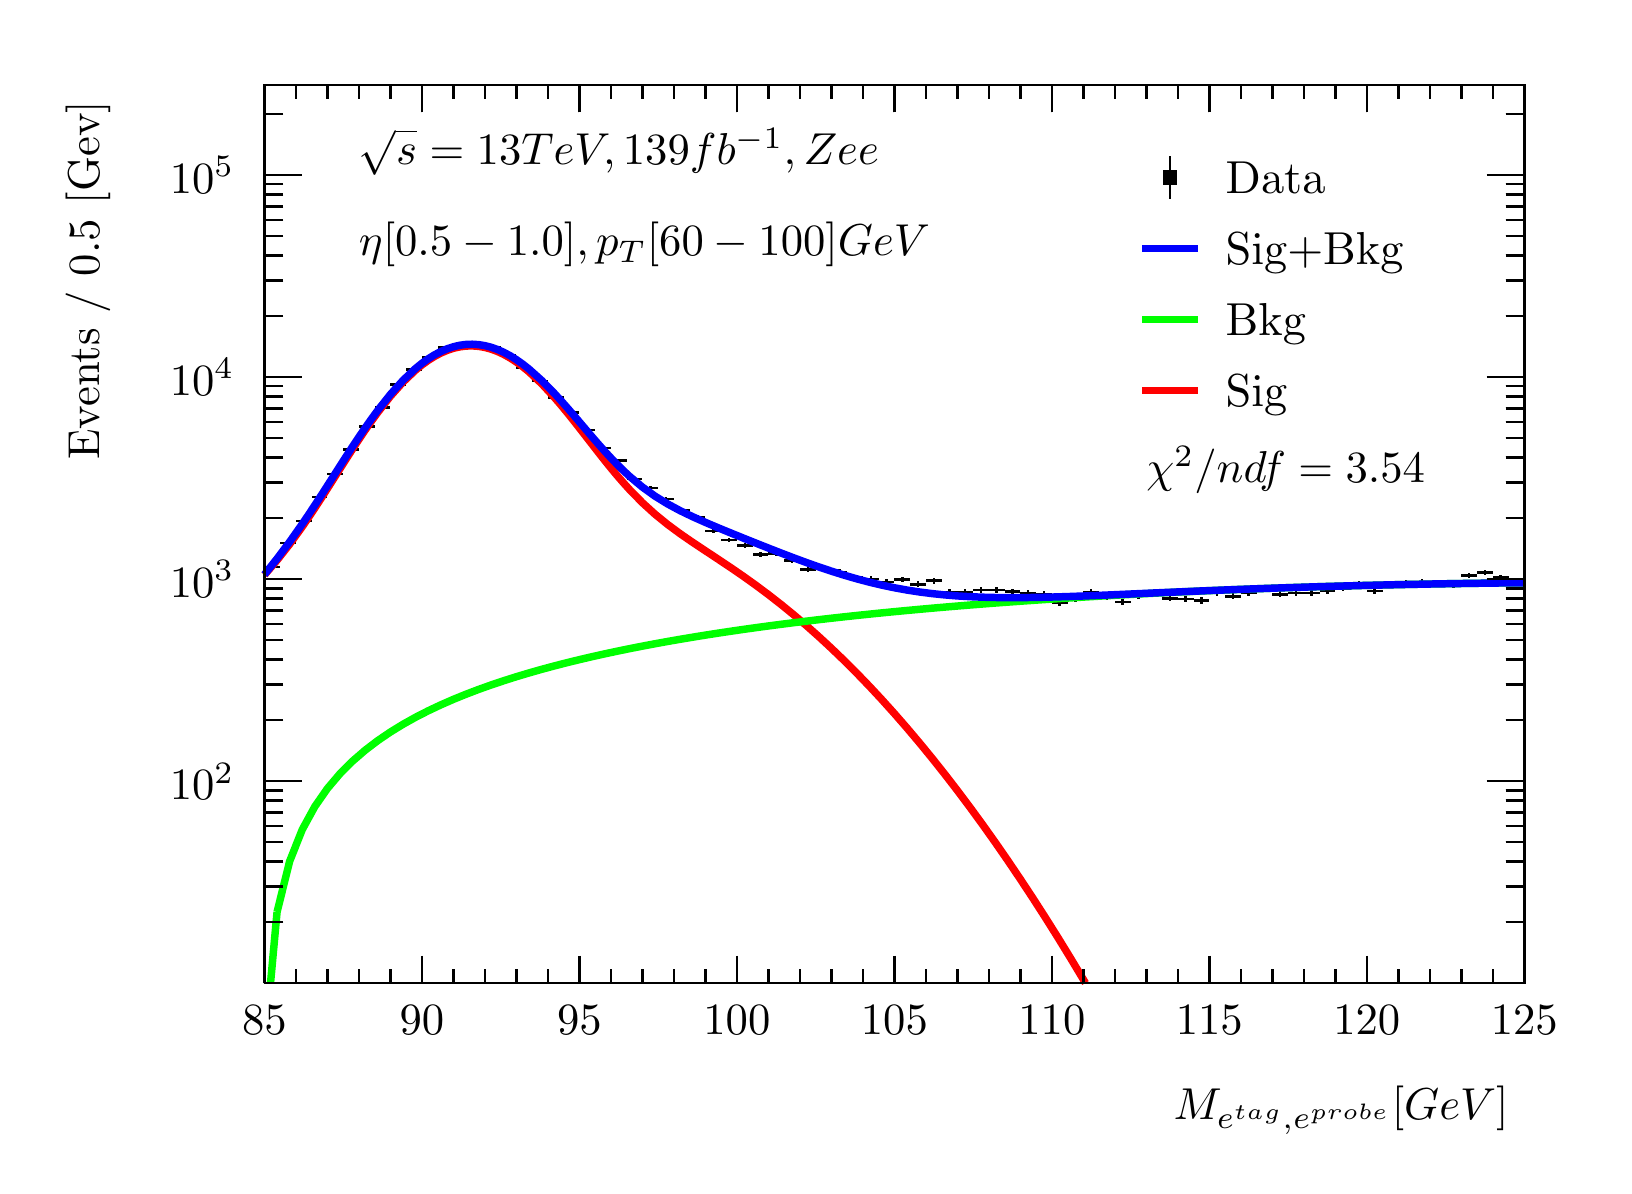
\begin{tikzpicture}
\pgfdeclareplotmark{cross} {
\pgfpathmoveto{\pgfpoint{-0.3\pgfplotmarksize}{\pgfplotmarksize}}
\pgfpathlineto{\pgfpoint{+0.3\pgfplotmarksize}{\pgfplotmarksize}}
\pgfpathlineto{\pgfpoint{+0.3\pgfplotmarksize}{0.3\pgfplotmarksize}}
\pgfpathlineto{\pgfpoint{+1\pgfplotmarksize}{0.3\pgfplotmarksize}}
\pgfpathlineto{\pgfpoint{+1\pgfplotmarksize}{-0.3\pgfplotmarksize}}
\pgfpathlineto{\pgfpoint{+0.3\pgfplotmarksize}{-0.3\pgfplotmarksize}}
\pgfpathlineto{\pgfpoint{+0.3\pgfplotmarksize}{-1.\pgfplotmarksize}}
\pgfpathlineto{\pgfpoint{-0.3\pgfplotmarksize}{-1.\pgfplotmarksize}}
\pgfpathlineto{\pgfpoint{-0.3\pgfplotmarksize}{-0.3\pgfplotmarksize}}
\pgfpathlineto{\pgfpoint{-1.\pgfplotmarksize}{-0.3\pgfplotmarksize}}
\pgfpathlineto{\pgfpoint{-1.\pgfplotmarksize}{0.3\pgfplotmarksize}}
\pgfpathlineto{\pgfpoint{-0.3\pgfplotmarksize}{0.3\pgfplotmarksize}}
\pgfpathclose
\pgfusepathqstroke
}
\pgfdeclareplotmark{cross*} {
\pgfpathmoveto{\pgfpoint{-0.3\pgfplotmarksize}{\pgfplotmarksize}}
\pgfpathlineto{\pgfpoint{+0.3\pgfplotmarksize}{\pgfplotmarksize}}
\pgfpathlineto{\pgfpoint{+0.3\pgfplotmarksize}{0.3\pgfplotmarksize}}
\pgfpathlineto{\pgfpoint{+1\pgfplotmarksize}{0.3\pgfplotmarksize}}
\pgfpathlineto{\pgfpoint{+1\pgfplotmarksize}{-0.3\pgfplotmarksize}}
\pgfpathlineto{\pgfpoint{+0.3\pgfplotmarksize}{-0.3\pgfplotmarksize}}
\pgfpathlineto{\pgfpoint{+0.3\pgfplotmarksize}{-1.\pgfplotmarksize}}
\pgfpathlineto{\pgfpoint{-0.3\pgfplotmarksize}{-1.\pgfplotmarksize}}
\pgfpathlineto{\pgfpoint{-0.3\pgfplotmarksize}{-0.3\pgfplotmarksize}}
\pgfpathlineto{\pgfpoint{-1.\pgfplotmarksize}{-0.3\pgfplotmarksize}}
\pgfpathlineto{\pgfpoint{-1.\pgfplotmarksize}{0.3\pgfplotmarksize}}
\pgfpathlineto{\pgfpoint{-0.3\pgfplotmarksize}{0.3\pgfplotmarksize}}
\pgfpathclose
\pgfusepathqfillstroke
}
\pgfdeclareplotmark{newstar} {
\pgfpathmoveto{\pgfqpoint{0pt}{\pgfplotmarksize}}
\pgfpathlineto{\pgfqpointpolar{44}{0.5\pgfplotmarksize}}
\pgfpathlineto{\pgfqpointpolar{18}{\pgfplotmarksize}}
\pgfpathlineto{\pgfqpointpolar{-20}{0.5\pgfplotmarksize}}
\pgfpathlineto{\pgfqpointpolar{-54}{\pgfplotmarksize}}
\pgfpathlineto{\pgfqpointpolar{-90}{0.5\pgfplotmarksize}}
\pgfpathlineto{\pgfqpointpolar{234}{\pgfplotmarksize}}
\pgfpathlineto{\pgfqpointpolar{198}{0.5\pgfplotmarksize}}
\pgfpathlineto{\pgfqpointpolar{162}{\pgfplotmarksize}}
\pgfpathlineto{\pgfqpointpolar{134}{0.5\pgfplotmarksize}}
\pgfpathclose
\pgfusepathqstroke
}
\pgfdeclareplotmark{newstar*} {
\pgfpathmoveto{\pgfqpoint{0pt}{\pgfplotmarksize}}
\pgfpathlineto{\pgfqpointpolar{44}{0.5\pgfplotmarksize}}
\pgfpathlineto{\pgfqpointpolar{18}{\pgfplotmarksize}}
\pgfpathlineto{\pgfqpointpolar{-20}{0.5\pgfplotmarksize}}
\pgfpathlineto{\pgfqpointpolar{-54}{\pgfplotmarksize}}
\pgfpathlineto{\pgfqpointpolar{-90}{0.5\pgfplotmarksize}}
\pgfpathlineto{\pgfqpointpolar{234}{\pgfplotmarksize}}
\pgfpathlineto{\pgfqpointpolar{198}{0.5\pgfplotmarksize}}
\pgfpathlineto{\pgfqpointpolar{162}{\pgfplotmarksize}}
\pgfpathlineto{\pgfqpointpolar{134}{0.5\pgfplotmarksize}}
\pgfpathclose
\pgfusepathqfillstroke
}
\definecolor{c}{rgb}{1,1,1};
\draw [color=c, fill=c] (0,0) rectangle (20,14.4361);
\draw [color=c, fill=c] (3,2.30977) rectangle (19,13.7143);
\definecolor{c}{rgb}{0,0,0};
\draw [c,line width=0.9] (3,2.30977) -- (3,13.7143) -- (19,13.7143) -- (19,2.30977) -- (3,2.30977);
\definecolor{c}{rgb}{1,1,1};
\draw [color=c, fill=c] (3,2.30977) rectangle (19,13.7143);
\definecolor{c}{rgb}{0,0,0};
\draw [c,line width=0.9] (3,2.30977) -- (3,13.7143) -- (19,13.7143) -- (19,2.30977) -- (3,2.30977);
\draw [c,line width=0.9] (3,2.30977) -- (19,2.30977);
\draw [c,line width=0.9] (3,2.65624) -- (3,2.30977);
\draw [c,line width=0.9] (3.4,2.48301) -- (3.4,2.30977);
\draw [c,line width=0.9] (3.8,2.48301) -- (3.8,2.30977);
\draw [c,line width=0.9] (4.2,2.48301) -- (4.2,2.30977);
\draw [c,line width=0.9] (4.6,2.48301) -- (4.6,2.30977);
\draw [c,line width=0.9] (5,2.65624) -- (5,2.30977);
\draw [c,line width=0.9] (5.4,2.48301) -- (5.4,2.30977);
\draw [c,line width=0.9] (5.8,2.48301) -- (5.8,2.30977);
\draw [c,line width=0.9] (6.2,2.48301) -- (6.2,2.30977);
\draw [c,line width=0.9] (6.6,2.48301) -- (6.6,2.30977);
\draw [c,line width=0.9] (7,2.65624) -- (7,2.30977);
\draw [c,line width=0.9] (7.4,2.48301) -- (7.4,2.30977);
\draw [c,line width=0.9] (7.8,2.48301) -- (7.8,2.30977);
\draw [c,line width=0.9] (8.2,2.48301) -- (8.2,2.30977);
\draw [c,line width=0.9] (8.6,2.48301) -- (8.6,2.30977);
\draw [c,line width=0.9] (9,2.65624) -- (9,2.30977);
\draw [c,line width=0.9] (9.4,2.48301) -- (9.4,2.30977);
\draw [c,line width=0.9] (9.8,2.48301) -- (9.8,2.30977);
\draw [c,line width=0.9] (10.2,2.48301) -- (10.2,2.30977);
\draw [c,line width=0.9] (10.6,2.48301) -- (10.6,2.30977);
\draw [c,line width=0.9] (11,2.65624) -- (11,2.30977);
\draw [c,line width=0.9] (11.4,2.48301) -- (11.4,2.30977);
\draw [c,line width=0.9] (11.8,2.48301) -- (11.8,2.30977);
\draw [c,line width=0.9] (12.2,2.48301) -- (12.2,2.30977);
\draw [c,line width=0.9] (12.6,2.48301) -- (12.6,2.30977);
\draw [c,line width=0.9] (13,2.65624) -- (13,2.30977);
\draw [c,line width=0.9] (13.4,2.48301) -- (13.4,2.30977);
\draw [c,line width=0.9] (13.8,2.48301) -- (13.8,2.30977);
\draw [c,line width=0.9] (14.2,2.48301) -- (14.2,2.30977);
\draw [c,line width=0.9] (14.6,2.48301) -- (14.6,2.30977);
\draw [c,line width=0.9] (15,2.65624) -- (15,2.30977);
\draw [c,line width=0.9] (15.4,2.48301) -- (15.4,2.30977);
\draw [c,line width=0.9] (15.8,2.48301) -- (15.8,2.30977);
\draw [c,line width=0.9] (16.2,2.48301) -- (16.2,2.30977);
\draw [c,line width=0.9] (16.6,2.48301) -- (16.6,2.30977);
\draw [c,line width=0.9] (17,2.65624) -- (17,2.30977);
\draw [c,line width=0.9] (17.4,2.48301) -- (17.4,2.30977);
\draw [c,line width=0.9] (17.8,2.48301) -- (17.8,2.30977);
\draw [c,line width=0.9] (18.2,2.48301) -- (18.2,2.30977);
\draw [c,line width=0.9] (18.6,2.48301) -- (18.6,2.30977);
\draw [c,line width=0.9] (19,2.65624) -- (19,2.30977);
\draw [anchor=base] (3,1.66015) node[scale=1.61424, color=c, rotate=0]{85};
\draw [anchor=base] (5,1.66015) node[scale=1.61424, color=c, rotate=0]{90};
\draw [anchor=base] (7,1.66015) node[scale=1.61424, color=c, rotate=0]{95};
\draw [anchor=base] (9,1.66015) node[scale=1.61424, color=c, rotate=0]{100};
\draw [anchor=base] (11,1.66015) node[scale=1.61424, color=c, rotate=0]{105};
\draw [anchor=base] (13,1.66015) node[scale=1.61424, color=c, rotate=0]{110};
\draw [anchor=base] (15,1.66015) node[scale=1.61424, color=c, rotate=0]{115};
\draw [anchor=base] (17,1.66015) node[scale=1.61424, color=c, rotate=0]{120};
\draw [anchor=base] (19,1.66015) node[scale=1.61424, color=c, rotate=0]{125};
\draw [anchor= east] (19,0.692932) node[scale=1.61424, color=c, rotate=0]{$M_{e^{tag}, e^{probe}}  [GeV]$};
\draw [c,line width=0.9] (3,13.7143) -- (19,13.7143);
\draw [c,line width=0.9] (3,13.3678) -- (3,13.7143);
\draw [c,line width=0.9] (3.4,13.5411) -- (3.4,13.7143);
\draw [c,line width=0.9] (3.8,13.5411) -- (3.8,13.7143);
\draw [c,line width=0.9] (4.2,13.5411) -- (4.2,13.7143);
\draw [c,line width=0.9] (4.6,13.5411) -- (4.6,13.7143);
\draw [c,line width=0.9] (5,13.3678) -- (5,13.7143);
\draw [c,line width=0.9] (5.4,13.5411) -- (5.4,13.7143);
\draw [c,line width=0.9] (5.8,13.5411) -- (5.8,13.7143);
\draw [c,line width=0.9] (6.2,13.5411) -- (6.2,13.7143);
\draw [c,line width=0.9] (6.6,13.5411) -- (6.6,13.7143);
\draw [c,line width=0.9] (7,13.3678) -- (7,13.7143);
\draw [c,line width=0.9] (7.4,13.5411) -- (7.4,13.7143);
\draw [c,line width=0.9] (7.8,13.5411) -- (7.8,13.7143);
\draw [c,line width=0.9] (8.2,13.5411) -- (8.2,13.7143);
\draw [c,line width=0.9] (8.6,13.5411) -- (8.6,13.7143);
\draw [c,line width=0.9] (9,13.3678) -- (9,13.7143);
\draw [c,line width=0.9] (9.4,13.5411) -- (9.4,13.7143);
\draw [c,line width=0.9] (9.8,13.5411) -- (9.8,13.7143);
\draw [c,line width=0.9] (10.2,13.5411) -- (10.2,13.7143);
\draw [c,line width=0.9] (10.6,13.5411) -- (10.6,13.7143);
\draw [c,line width=0.9] (11,13.3678) -- (11,13.7143);
\draw [c,line width=0.9] (11.4,13.5411) -- (11.4,13.7143);
\draw [c,line width=0.9] (11.8,13.5411) -- (11.8,13.7143);
\draw [c,line width=0.9] (12.2,13.5411) -- (12.2,13.7143);
\draw [c,line width=0.9] (12.6,13.5411) -- (12.6,13.7143);
\draw [c,line width=0.9] (13,13.3678) -- (13,13.7143);
\draw [c,line width=0.9] (13.4,13.5411) -- (13.4,13.7143);
\draw [c,line width=0.9] (13.8,13.5411) -- (13.8,13.7143);
\draw [c,line width=0.9] (14.2,13.5411) -- (14.2,13.7143);
\draw [c,line width=0.9] (14.6,13.5411) -- (14.6,13.7143);
\draw [c,line width=0.9] (15,13.3678) -- (15,13.7143);
\draw [c,line width=0.9] (15.4,13.5411) -- (15.4,13.7143);
\draw [c,line width=0.9] (15.8,13.5411) -- (15.8,13.7143);
\draw [c,line width=0.9] (16.2,13.5411) -- (16.2,13.7143);
\draw [c,line width=0.9] (16.6,13.5411) -- (16.6,13.7143);
\draw [c,line width=0.9] (17,13.3678) -- (17,13.7143);
\draw [c,line width=0.9] (17.4,13.5411) -- (17.4,13.7143);
\draw [c,line width=0.9] (17.8,13.5411) -- (17.8,13.7143);
\draw [c,line width=0.9] (18.2,13.5411) -- (18.2,13.7143);
\draw [c,line width=0.9] (18.6,13.5411) -- (18.6,13.7143);
\draw [c,line width=0.9] (19,13.3678) -- (19,13.7143);
\draw [c,line width=0.9] (3,2.30977) -- (3,13.7143);
\draw [c,line width=0.9] (3.237,3.08209) -- (3,3.08209);
\draw [c,line width=0.9] (3.237,3.53386) -- (3,3.53386);
\draw [c,line width=0.9] (3.237,3.8544) -- (3,3.8544);
\draw [c,line width=0.9] (3.237,4.10303) -- (3,4.10303);
\draw [c,line width=0.9] (3.237,4.30618) -- (3,4.30618);
\draw [c,line width=0.9] (3.237,4.47794) -- (3,4.47794);
\draw [c,line width=0.9] (3.237,4.62672) -- (3,4.62672);
\draw [c,line width=0.9] (3.237,4.75795) -- (3,4.75795);
\draw [c,line width=0.9] (3.474,4.87535) -- (3,4.87535);
\draw [anchor= east] (2.82,4.87535) node[scale=1.61424, color=c, rotate=0]{$10^{2}$};
\draw [c,line width=0.9] (3.237,5.64766) -- (3,5.64766);
\draw [c,line width=0.9] (3.237,6.09944) -- (3,6.09944);
\draw [c,line width=0.9] (3.237,6.41998) -- (3,6.41998);
\draw [c,line width=0.9] (3.237,6.66861) -- (3,6.66861);
\draw [c,line width=0.9] (3.237,6.87176) -- (3,6.87176);
\draw [c,line width=0.9] (3.237,7.04351) -- (3,7.04351);
\draw [c,line width=0.9] (3.237,7.1923) -- (3,7.1923);
\draw [c,line width=0.9] (3.237,7.32353) -- (3,7.32353);
\draw [c,line width=0.9] (3.474,7.44093) -- (3,7.44093);
\draw [anchor= east] (2.82,7.44093) node[scale=1.61424, color=c, rotate=0]{$10^{3}$};
\draw [c,line width=0.9] (3.237,8.21324) -- (3,8.21324);
\draw [c,line width=0.9] (3.237,8.66502) -- (3,8.66502);
\draw [c,line width=0.9] (3.237,8.98556) -- (3,8.98556);
\draw [c,line width=0.9] (3.237,9.23419) -- (3,9.23419);
\draw [c,line width=0.9] (3.237,9.43733) -- (3,9.43733);
\draw [c,line width=0.9] (3.237,9.60909) -- (3,9.60909);
\draw [c,line width=0.9] (3.237,9.75787) -- (3,9.75787);
\draw [c,line width=0.9] (3.237,9.88911) -- (3,9.88911);
\draw [c,line width=0.9] (3.474,10.0065) -- (3,10.0065);
\draw [anchor= east] (2.82,10.0065) node[scale=1.61424, color=c, rotate=0]{$10^{4}$};
\draw [c,line width=0.9] (3.237,10.7788) -- (3,10.7788);
\draw [c,line width=0.9] (3.237,11.2306) -- (3,11.2306);
\draw [c,line width=0.9] (3.237,11.5511) -- (3,11.5511);
\draw [c,line width=0.9] (3.237,11.7998) -- (3,11.7998);
\draw [c,line width=0.9] (3.237,12.0029) -- (3,12.0029);
\draw [c,line width=0.9] (3.237,12.1747) -- (3,12.1747);
\draw [c,line width=0.9] (3.237,12.3235) -- (3,12.3235);
\draw [c,line width=0.9] (3.237,12.4547) -- (3,12.4547);
\draw [c,line width=0.9] (3.474,12.5721) -- (3,12.5721);
\draw [anchor= east] (2.82,12.5721) node[scale=1.61424, color=c, rotate=0]{$10^{5}$};
\draw [c,line width=0.9] (3.237,13.3444) -- (3,13.3444);
\draw [anchor= east] (0.76,13.7143) node[scale=1.61424, color=c, rotate=90]{Events / 0.5 [Gev]};
\draw [c,line width=0.9] (19,2.30977) -- (19,13.7143);
\draw [c,line width=0.9] (18.763,3.08209) -- (19,3.08209);
\draw [c,line width=0.9] (18.763,3.53386) -- (19,3.53386);
\draw [c,line width=0.9] (18.763,3.8544) -- (19,3.8544);
\draw [c,line width=0.9] (18.763,4.10303) -- (19,4.10303);
\draw [c,line width=0.9] (18.763,4.30618) -- (19,4.30618);
\draw [c,line width=0.9] (18.763,4.47794) -- (19,4.47794);
\draw [c,line width=0.9] (18.763,4.62672) -- (19,4.62672);
\draw [c,line width=0.9] (18.763,4.75795) -- (19,4.75795);
\draw [c,line width=0.9] (18.526,4.87535) -- (19,4.87535);
\draw [c,line width=0.9] (18.763,5.64766) -- (19,5.64766);
\draw [c,line width=0.9] (18.763,6.09944) -- (19,6.09944);
\draw [c,line width=0.9] (18.763,6.41998) -- (19,6.41998);
\draw [c,line width=0.9] (18.763,6.66861) -- (19,6.66861);
\draw [c,line width=0.9] (18.763,6.87176) -- (19,6.87176);
\draw [c,line width=0.9] (18.763,7.04351) -- (19,7.04351);
\draw [c,line width=0.9] (18.763,7.1923) -- (19,7.1923);
\draw [c,line width=0.9] (18.763,7.32353) -- (19,7.32353);
\draw [c,line width=0.9] (18.526,7.44093) -- (19,7.44093);
\draw [c,line width=0.9] (18.763,8.21324) -- (19,8.21324);
\draw [c,line width=0.9] (18.763,8.66502) -- (19,8.66502);
\draw [c,line width=0.9] (18.763,8.98556) -- (19,8.98556);
\draw [c,line width=0.9] (18.763,9.23419) -- (19,9.23419);
\draw [c,line width=0.9] (18.763,9.43733) -- (19,9.43733);
\draw [c,line width=0.9] (18.763,9.60909) -- (19,9.60909);
\draw [c,line width=0.9] (18.763,9.75787) -- (19,9.75787);
\draw [c,line width=0.9] (18.763,9.88911) -- (19,9.88911);
\draw [c,line width=0.9] (18.526,10.0065) -- (19,10.0065);
\draw [c,line width=0.9] (18.763,10.7788) -- (19,10.7788);
\draw [c,line width=0.9] (18.763,11.2306) -- (19,11.2306);
\draw [c,line width=0.9] (18.763,11.5511) -- (19,11.5511);
\draw [c,line width=0.9] (18.763,11.7998) -- (19,11.7998);
\draw [c,line width=0.9] (18.763,12.0029) -- (19,12.0029);
\draw [c,line width=0.9] (18.763,12.1747) -- (19,12.1747);
\draw [c,line width=0.9] (18.763,12.3235) -- (19,12.3235);
\draw [c,line width=0.9] (18.763,12.4547) -- (19,12.4547);
\draw [c,line width=0.9] (18.526,12.5721) -- (19,12.5721);
\draw [c,line width=0.9] (18.763,13.3444) -- (19,13.3444);
\draw [c,line width=0.9] (3.1,7.59665) -- (3,7.59665);
\draw [c,line width=0.9] (3,7.59665) -- (3,7.59665);
\draw [c,line width=0.9] (3.1,7.59665) -- (3.2,7.59665);
\draw [c,line width=0.9] (3.2,7.59665) -- (3.2,7.59665);
\draw [c,line width=0.9] (3.1,7.59665) -- (3.1,7.62951);
\draw [c,line width=0.9] (3.1,7.62951) -- (3.1,7.62951);
\draw [c,line width=0.9] (3.1,7.59665) -- (3.1,7.5638);
\draw [c,line width=0.9] (3.1,7.5638) -- (3.1,7.5638);
\draw [c,line width=0.9] (3.3,7.89863) -- (3.2,7.89863);
\draw [c,line width=0.9] (3.2,7.89863) -- (3.2,7.89863);
\draw [c,line width=0.9] (3.3,7.89863) -- (3.4,7.89863);
\draw [c,line width=0.9] (3.4,7.89863) -- (3.4,7.89863);
\draw [c,line width=0.9] (3.3,7.89863) -- (3.3,7.92732);
\draw [c,line width=0.9] (3.3,7.92732) -- (3.3,7.92732);
\draw [c,line width=0.9] (3.3,7.89863) -- (3.3,7.86994);
\draw [c,line width=0.9] (3.3,7.86994) -- (3.3,7.86994);
\draw [c,line width=0.9] (3.5,8.1747) -- (3.4,8.1747);
\draw [c,line width=0.9] (3.4,8.1747) -- (3.4,8.1747);
\draw [c,line width=0.9] (3.5,8.1747) -- (3.6,8.1747);
\draw [c,line width=0.9] (3.6,8.1747) -- (3.6,8.1747);
\draw [c,line width=0.9] (3.5,8.1747) -- (3.5,8.20005);
\draw [c,line width=0.9] (3.5,8.20005) -- (3.5,8.20005);
\draw [c,line width=0.9] (3.5,8.1747) -- (3.5,8.14935);
\draw [c,line width=0.9] (3.5,8.14935) -- (3.5,8.14935);
\draw [c,line width=0.9] (3.7,8.48) -- (3.6,8.48);
\draw [c,line width=0.9] (3.6,8.48) -- (3.6,8.48);
\draw [c,line width=0.9] (3.7,8.48) -- (3.8,8.48);
\draw [c,line width=0.9] (3.8,8.48) -- (3.8,8.48);
\draw [c,line width=0.9] (3.7,8.48) -- (3.7,8.5021);
\draw [c,line width=0.9] (3.7,8.5021) -- (3.7,8.5021);
\draw [c,line width=0.9] (3.7,8.48) -- (3.7,8.45789);
\draw [c,line width=0.9] (3.7,8.45789) -- (3.7,8.45789);
\draw [c,line width=0.9] (3.9,8.77694) -- (3.8,8.77694);
\draw [c,line width=0.9] (3.8,8.77694) -- (3.8,8.77694);
\draw [c,line width=0.9] (3.9,8.77694) -- (4,8.77694);
\draw [c,line width=0.9] (4,8.77694) -- (4,8.77694);
\draw [c,line width=0.9] (3.9,8.77694) -- (3.9,8.79629);
\draw [c,line width=0.9] (3.9,8.79629) -- (3.9,8.79629);
\draw [c,line width=0.9] (3.9,8.77694) -- (3.9,8.75759);
\draw [c,line width=0.9] (3.9,8.75759) -- (3.9,8.75759);
\draw [c,line width=0.9] (4.1,9.08362) -- (4,9.08362);
\draw [c,line width=0.9] (4,9.08362) -- (4,9.08362);
\draw [c,line width=0.9] (4.1,9.08362) -- (4.2,9.08362);
\draw [c,line width=0.9] (4.2,9.08362) -- (4.2,9.08362);
\draw [c,line width=0.9] (4.1,9.08362) -- (4.1,9.10048);
\draw [c,line width=0.9] (4.1,9.10048) -- (4.1,9.10048);
\draw [c,line width=0.9] (4.1,9.08362) -- (4.1,9.06676);
\draw [c,line width=0.9] (4.1,9.06676) -- (4.1,9.06676);
\draw [c,line width=0.9] (4.3,9.3794) -- (4.2,9.3794);
\draw [c,line width=0.9] (4.2,9.3794) -- (4.2,9.3794);
\draw [c,line width=0.9] (4.3,9.3794) -- (4.4,9.3794);
\draw [c,line width=0.9] (4.4,9.3794) -- (4.4,9.3794);
\draw [c,line width=0.9] (4.3,9.3794) -- (4.3,9.39416);
\draw [c,line width=0.9] (4.3,9.39416) -- (4.3,9.39416);
\draw [c,line width=0.9] (4.3,9.3794) -- (4.3,9.36464);
\draw [c,line width=0.9] (4.3,9.36464) -- (4.3,9.36464);
\draw [c,line width=0.9] (4.5,9.62112) -- (4.4,9.62112);
\draw [c,line width=0.9] (4.4,9.62112) -- (4.4,9.62112);
\draw [c,line width=0.9] (4.5,9.62112) -- (4.6,9.62112);
\draw [c,line width=0.9] (4.6,9.62112) -- (4.6,9.62112);
\draw [c,line width=0.9] (4.5,9.62112) -- (4.5,9.63437);
\draw [c,line width=0.9] (4.5,9.63437) -- (4.5,9.63437);
\draw [c,line width=0.9] (4.5,9.62112) -- (4.5,9.60788);
\draw [c,line width=0.9] (4.5,9.60788) -- (4.5,9.60788);
\draw [c,line width=0.9] (4.7,9.91166) -- (4.6,9.91166);
\draw [c,line width=0.9] (4.6,9.91166) -- (4.6,9.91166);
\draw [c,line width=0.9] (4.7,9.91166) -- (4.8,9.91166);
\draw [c,line width=0.9] (4.8,9.91166) -- (4.8,9.91166);
\draw [c,line width=0.9] (4.7,9.91166) -- (4.7,9.92329);
\draw [c,line width=0.9] (4.7,9.92329) -- (4.7,9.92329);
\draw [c,line width=0.9] (4.7,9.91166) -- (4.7,9.90003);
\draw [c,line width=0.9] (4.7,9.90003) -- (4.7,9.90003);
\draw [c,line width=0.9] (4.9,10.1003) -- (4.8,10.1003);
\draw [c,line width=0.9] (4.8,10.1003) -- (4.8,10.1003);
\draw [c,line width=0.9] (4.9,10.1003) -- (5,10.1003);
\draw [c,line width=0.9] (5,10.1003) -- (5,10.1003);
\draw [c,line width=0.9] (4.9,10.1003) -- (4.9,10.111);
\draw [c,line width=0.9] (4.9,10.111) -- (4.9,10.111);
\draw [c,line width=0.9] (4.9,10.1003) -- (4.9,10.0896);
\draw [c,line width=0.9] (4.9,10.0896) -- (4.9,10.0896);
\draw [c,line width=0.9] (5.1,10.2518) -- (5,10.2518);
\draw [c,line width=0.9] (5,10.2518) -- (5,10.2518);
\draw [c,line width=0.9] (5.1,10.2518) -- (5.2,10.2518);
\draw [c,line width=0.9] (5.2,10.2518) -- (5.2,10.2518);
\draw [c,line width=0.9] (5.1,10.2518) -- (5.1,10.2618);
\draw [c,line width=0.9] (5.1,10.2618) -- (5.1,10.2618);
\draw [c,line width=0.9] (5.1,10.2518) -- (5.1,10.2419);
\draw [c,line width=0.9] (5.1,10.2419) -- (5.1,10.2419);
\draw [c,line width=0.9] (5.3,10.3798) -- (5.2,10.3798);
\draw [c,line width=0.9] (5.2,10.3798) -- (5.2,10.3798);
\draw [c,line width=0.9] (5.3,10.3798) -- (5.4,10.3798);
\draw [c,line width=0.9] (5.4,10.3798) -- (5.4,10.3798);
\draw [c,line width=0.9] (5.3,10.3798) -- (5.3,10.3892);
\draw [c,line width=0.9] (5.3,10.3892) -- (5.3,10.3892);
\draw [c,line width=0.9] (5.3,10.3798) -- (5.3,10.3704);
\draw [c,line width=0.9] (5.3,10.3704) -- (5.3,10.3704);
\draw [c,line width=0.9] (5.5,10.4278) -- (5.4,10.4278);
\draw [c,line width=0.9] (5.4,10.4278) -- (5.4,10.4278);
\draw [c,line width=0.9] (5.5,10.4278) -- (5.6,10.4278);
\draw [c,line width=0.9] (5.6,10.4278) -- (5.6,10.4278);
\draw [c,line width=0.9] (5.5,10.4278) -- (5.5,10.437);
\draw [c,line width=0.9] (5.5,10.437) -- (5.5,10.437);
\draw [c,line width=0.9] (5.5,10.4278) -- (5.5,10.4186);
\draw [c,line width=0.9] (5.5,10.4186) -- (5.5,10.4186);
\draw [c,line width=0.9] (5.7,10.428) -- (5.6,10.428);
\draw [c,line width=0.9] (5.6,10.428) -- (5.6,10.428);
\draw [c,line width=0.9] (5.7,10.428) -- (5.8,10.428);
\draw [c,line width=0.9] (5.8,10.428) -- (5.8,10.428);
\draw [c,line width=0.9] (5.7,10.428) -- (5.7,10.4372);
\draw [c,line width=0.9] (5.7,10.4372) -- (5.7,10.4372);
\draw [c,line width=0.9] (5.7,10.428) -- (5.7,10.4188);
\draw [c,line width=0.9] (5.7,10.4188) -- (5.7,10.4188);
\draw [c,line width=0.9] (5.9,10.3797) -- (5.8,10.3797);
\draw [c,line width=0.9] (5.8,10.3797) -- (5.8,10.3797);
\draw [c,line width=0.9] (5.9,10.3797) -- (6,10.3797);
\draw [c,line width=0.9] (6,10.3797) -- (6,10.3797);
\draw [c,line width=0.9] (5.9,10.3797) -- (5.9,10.3892);
\draw [c,line width=0.9] (5.9,10.3892) -- (5.9,10.3892);
\draw [c,line width=0.9] (5.9,10.3797) -- (5.9,10.3703);
\draw [c,line width=0.9] (5.9,10.3703) -- (5.9,10.3703);
\draw [c,line width=0.9] (6.1,10.2882) -- (6,10.2882);
\draw [c,line width=0.9] (6,10.2882) -- (6,10.2882);
\draw [c,line width=0.9] (6.1,10.2882) -- (6.2,10.2882);
\draw [c,line width=0.9] (6.2,10.2882) -- (6.2,10.2882);
\draw [c,line width=0.9] (6.1,10.2882) -- (6.1,10.298);
\draw [c,line width=0.9] (6.1,10.298) -- (6.1,10.298);
\draw [c,line width=0.9] (6.1,10.2882) -- (6.1,10.2783);
\draw [c,line width=0.9] (6.1,10.2783) -- (6.1,10.2783);
\draw [c,line width=0.9] (6.3,10.1239) -- (6.2,10.1239);
\draw [c,line width=0.9] (6.2,10.1239) -- (6.2,10.1239);
\draw [c,line width=0.9] (6.3,10.1239) -- (6.4,10.1239);
\draw [c,line width=0.9] (6.4,10.1239) -- (6.4,10.1239);
\draw [c,line width=0.9] (6.3,10.1239) -- (6.3,10.1345);
\draw [c,line width=0.9] (6.3,10.1345) -- (6.3,10.1345);
\draw [c,line width=0.9] (6.3,10.1239) -- (6.3,10.1133);
\draw [c,line width=0.9] (6.3,10.1133) -- (6.3,10.1133);
\draw [c,line width=0.9] (6.5,9.95811) -- (6.4,9.95811);
\draw [c,line width=0.9] (6.4,9.95811) -- (6.4,9.95811);
\draw [c,line width=0.9] (6.5,9.95811) -- (6.6,9.95811);
\draw [c,line width=0.9] (6.6,9.95811) -- (6.6,9.95811);
\draw [c,line width=0.9] (6.5,9.95811) -- (6.5,9.9695);
\draw [c,line width=0.9] (6.5,9.9695) -- (6.5,9.9695);
\draw [c,line width=0.9] (6.5,9.95811) -- (6.5,9.94673);
\draw [c,line width=0.9] (6.5,9.94673) -- (6.5,9.94673);
\draw [c,line width=0.9] (6.7,9.74569) -- (6.6,9.74569);
\draw [c,line width=0.9] (6.6,9.74569) -- (6.6,9.74569);
\draw [c,line width=0.9] (6.7,9.74569) -- (6.8,9.74569);
\draw [c,line width=0.9] (6.8,9.74569) -- (6.8,9.74569);
\draw [c,line width=0.9] (6.7,9.74569) -- (6.7,9.75822);
\draw [c,line width=0.9] (6.7,9.75822) -- (6.7,9.75822);
\draw [c,line width=0.9] (6.7,9.74569) -- (6.7,9.73317);
\draw [c,line width=0.9] (6.7,9.73317) -- (6.7,9.73317);
\draw [c,line width=0.9] (6.9,9.55679) -- (6.8,9.55679);
\draw [c,line width=0.9] (6.8,9.55679) -- (6.8,9.55679);
\draw [c,line width=0.9] (6.9,9.55679) -- (7,9.55679);
\draw [c,line width=0.9] (7,9.55679) -- (7,9.55679);
\draw [c,line width=0.9] (6.9,9.55679) -- (6.9,9.57042);
\draw [c,line width=0.9] (6.9,9.57042) -- (6.9,9.57042);
\draw [c,line width=0.9] (6.9,9.55679) -- (6.9,9.54315);
\draw [c,line width=0.9] (6.9,9.54315) -- (6.9,9.54315);
\draw [c,line width=0.9] (7.1,9.33429) -- (7,9.33429);
\draw [c,line width=0.9] (7,9.33429) -- (7,9.33429);
\draw [c,line width=0.9] (7.1,9.33429) -- (7.2,9.33429);
\draw [c,line width=0.9] (7.2,9.33429) -- (7.2,9.33429);
\draw [c,line width=0.9] (7.1,9.33429) -- (7.1,9.34936);
\draw [c,line width=0.9] (7.1,9.34936) -- (7.1,9.34936);
\draw [c,line width=0.9] (7.1,9.33429) -- (7.1,9.31923);
\draw [c,line width=0.9] (7.1,9.31923) -- (7.1,9.31923);
\draw [c,line width=0.9] (7.3,9.10435) -- (7.2,9.10435);
\draw [c,line width=0.9] (7.2,9.10435) -- (7.2,9.10435);
\draw [c,line width=0.9] (7.3,9.10435) -- (7.4,9.10435);
\draw [c,line width=0.9] (7.4,9.10435) -- (7.4,9.10435);
\draw [c,line width=0.9] (7.3,9.10435) -- (7.3,9.12105);
\draw [c,line width=0.9] (7.3,9.12105) -- (7.3,9.12105);
\draw [c,line width=0.9] (7.3,9.10435) -- (7.3,9.08764);
\draw [c,line width=0.9] (7.3,9.08764) -- (7.3,9.08764);
\draw [c,line width=0.9] (7.5,8.94413) -- (7.4,8.94413);
\draw [c,line width=0.9] (7.4,8.94413) -- (7.4,8.94413);
\draw [c,line width=0.9] (7.5,8.94413) -- (7.6,8.94413);
\draw [c,line width=0.9] (7.6,8.94413) -- (7.6,8.94413);
\draw [c,line width=0.9] (7.5,8.94413) -- (7.5,8.96208);
\draw [c,line width=0.9] (7.5,8.96208) -- (7.5,8.96208);
\draw [c,line width=0.9] (7.5,8.94413) -- (7.5,8.92618);
\draw [c,line width=0.9] (7.5,8.92618) -- (7.5,8.92618);
\draw [c,line width=0.9] (7.7,8.71015) -- (7.6,8.71015);
\draw [c,line width=0.9] (7.6,8.71015) -- (7.6,8.71015);
\draw [c,line width=0.9] (7.7,8.71015) -- (7.8,8.71015);
\draw [c,line width=0.9] (7.8,8.71015) -- (7.8,8.71015);
\draw [c,line width=0.9] (7.7,8.71015) -- (7.7,8.73008);
\draw [c,line width=0.9] (7.7,8.73008) -- (7.7,8.73008);
\draw [c,line width=0.9] (7.7,8.71015) -- (7.7,8.69021);
\draw [c,line width=0.9] (7.7,8.69021) -- (7.7,8.69021);
\draw [c,line width=0.9] (7.9,8.59647) -- (7.8,8.59647);
\draw [c,line width=0.9] (7.8,8.59647) -- (7.8,8.59647);
\draw [c,line width=0.9] (7.9,8.59647) -- (8,8.59647);
\draw [c,line width=0.9] (8,8.59647) -- (8,8.59647);
\draw [c,line width=0.9] (7.9,8.59647) -- (7.9,8.61745);
\draw [c,line width=0.9] (7.9,8.61745) -- (7.9,8.61745);
\draw [c,line width=0.9] (7.9,8.59647) -- (7.9,8.57549);
\draw [c,line width=0.9] (7.9,8.57549) -- (7.9,8.57549);
\draw [c,line width=0.9] (8.1,8.45741) -- (8,8.45741);
\draw [c,line width=0.9] (8,8.45741) -- (8,8.45741);
\draw [c,line width=0.9] (8.1,8.45741) -- (8.2,8.45741);
\draw [c,line width=0.9] (8.2,8.45741) -- (8.2,8.45741);
\draw [c,line width=0.9] (8.1,8.45741) -- (8.1,8.47974);
\draw [c,line width=0.9] (8.1,8.47974) -- (8.1,8.47974);
\draw [c,line width=0.9] (8.1,8.45741) -- (8.1,8.43508);
\draw [c,line width=0.9] (8.1,8.43508) -- (8.1,8.43508);
\draw [c,line width=0.9] (8.3,8.3108) -- (8.2,8.3108);
\draw [c,line width=0.9] (8.2,8.3108) -- (8.2,8.3108);
\draw [c,line width=0.9] (8.3,8.3108) -- (8.4,8.3108);
\draw [c,line width=0.9] (8.4,8.3108) -- (8.4,8.3108);
\draw [c,line width=0.9] (8.3,8.3108) -- (8.3,8.33464);
\draw [c,line width=0.9] (8.3,8.33464) -- (8.3,8.33464);
\draw [c,line width=0.9] (8.3,8.3108) -- (8.3,8.28695);
\draw [c,line width=0.9] (8.3,8.28695) -- (8.3,8.28695);
\draw [c,line width=0.9] (8.5,8.22323) -- (8.4,8.22323);
\draw [c,line width=0.9] (8.4,8.22323) -- (8.4,8.22323);
\draw [c,line width=0.9] (8.5,8.22323) -- (8.6,8.22323);
\draw [c,line width=0.9] (8.6,8.22323) -- (8.6,8.22323);
\draw [c,line width=0.9] (8.5,8.22323) -- (8.5,8.24803);
\draw [c,line width=0.9] (8.5,8.24803) -- (8.5,8.24803);
\draw [c,line width=0.9] (8.5,8.22323) -- (8.5,8.19842);
\draw [c,line width=0.9] (8.5,8.19842) -- (8.5,8.19842);
\draw [c,line width=0.9] (8.7,8.04907) -- (8.6,8.04907);
\draw [c,line width=0.9] (8.6,8.04907) -- (8.6,8.04907);
\draw [c,line width=0.9] (8.7,8.04907) -- (8.8,8.04907);
\draw [c,line width=0.9] (8.8,8.04907) -- (8.8,8.04907);
\draw [c,line width=0.9] (8.7,8.04907) -- (8.7,8.07589);
\draw [c,line width=0.9] (8.7,8.07589) -- (8.7,8.07589);
\draw [c,line width=0.9] (8.7,8.04907) -- (8.7,8.02225);
\draw [c,line width=0.9] (8.7,8.02225) -- (8.7,8.02225);
\draw [c,line width=0.9] (8.9,7.93712) -- (8.8,7.93712);
\draw [c,line width=0.9] (8.8,7.93712) -- (8.8,7.93712);
\draw [c,line width=0.9] (8.9,7.93712) -- (9,7.93712);
\draw [c,line width=0.9] (9,7.93712) -- (9,7.93712);
\draw [c,line width=0.9] (8.9,7.93712) -- (8.9,7.96532);
\draw [c,line width=0.9] (8.9,7.96532) -- (8.9,7.96532);
\draw [c,line width=0.9] (8.9,7.93712) -- (8.9,7.90892);
\draw [c,line width=0.9] (8.9,7.90892) -- (8.9,7.90892);
\draw [c,line width=0.9] (9.1,7.86716) -- (9,7.86716);
\draw [c,line width=0.9] (9,7.86716) -- (9,7.86716);
\draw [c,line width=0.9] (9.1,7.86716) -- (9.2,7.86716);
\draw [c,line width=0.9] (9.2,7.86716) -- (9.2,7.86716);
\draw [c,line width=0.9] (9.1,7.86716) -- (9.1,7.89626);
\draw [c,line width=0.9] (9.1,7.89626) -- (9.1,7.89626);
\draw [c,line width=0.9] (9.1,7.86716) -- (9.1,7.83806);
\draw [c,line width=0.9] (9.1,7.83806) -- (9.1,7.83806);
\draw [c,line width=0.9] (9.3,7.75448) -- (9.2,7.75448);
\draw [c,line width=0.9] (9.2,7.75448) -- (9.2,7.75448);
\draw [c,line width=0.9] (9.3,7.75448) -- (9.4,7.75448);
\draw [c,line width=0.9] (9.4,7.75448) -- (9.4,7.75448);
\draw [c,line width=0.9] (9.3,7.75448) -- (9.3,7.78509);
\draw [c,line width=0.9] (9.3,7.78509) -- (9.3,7.78509);
\draw [c,line width=0.9] (9.3,7.75448) -- (9.3,7.72387);
\draw [c,line width=0.9] (9.3,7.72387) -- (9.3,7.72387);
\draw [c,line width=0.9] (9.5,7.76202) -- (9.4,7.76202);
\draw [c,line width=0.9] (9.4,7.76202) -- (9.4,7.76202);
\draw [c,line width=0.9] (9.5,7.76202) -- (9.6,7.76202);
\draw [c,line width=0.9] (9.6,7.76202) -- (9.6,7.76202);
\draw [c,line width=0.9] (9.5,7.76202) -- (9.5,7.79253);
\draw [c,line width=0.9] (9.5,7.79253) -- (9.5,7.79253);
\draw [c,line width=0.9] (9.5,7.76202) -- (9.5,7.73152);
\draw [c,line width=0.9] (9.5,7.73152) -- (9.5,7.73152);
\draw [c,line width=0.9] (9.7,7.6734) -- (9.6,7.6734);
\draw [c,line width=0.9] (9.6,7.6734) -- (9.6,7.6734);
\draw [c,line width=0.9] (9.7,7.6734) -- (9.8,7.6734);
\draw [c,line width=0.9] (9.8,7.6734) -- (9.8,7.6734);
\draw [c,line width=0.9] (9.7,7.6734) -- (9.7,7.70514);
\draw [c,line width=0.9] (9.7,7.70514) -- (9.7,7.70514);
\draw [c,line width=0.9] (9.7,7.6734) -- (9.7,7.64165);
\draw [c,line width=0.9] (9.7,7.64165) -- (9.7,7.64165);
\draw [c,line width=0.9] (9.9,7.56221) -- (9.8,7.56221);
\draw [c,line width=0.9] (9.8,7.56221) -- (9.8,7.56221);
\draw [c,line width=0.9] (9.9,7.56221) -- (10,7.56221);
\draw [c,line width=0.9] (10,7.56221) -- (10,7.56221);
\draw [c,line width=0.9] (9.9,7.56221) -- (9.9,7.59558);
\draw [c,line width=0.9] (9.9,7.59558) -- (9.9,7.59558);
\draw [c,line width=0.9] (9.9,7.56221) -- (9.9,7.52885);
\draw [c,line width=0.9] (9.9,7.52885) -- (9.9,7.52885);
\draw [c,line width=0.9] (10.1,7.57907) -- (10,7.57907);
\draw [c,line width=0.9] (10,7.57907) -- (10,7.57907);
\draw [c,line width=0.9] (10.1,7.57907) -- (10.2,7.57907);
\draw [c,line width=0.9] (10.2,7.57907) -- (10.2,7.57907);
\draw [c,line width=0.9] (10.1,7.57907) -- (10.1,7.61219);
\draw [c,line width=0.9] (10.1,7.61219) -- (10.1,7.61219);
\draw [c,line width=0.9] (10.1,7.57907) -- (10.1,7.54596);
\draw [c,line width=0.9] (10.1,7.54596) -- (10.1,7.54596);
\draw [c,line width=0.9] (10.3,7.52977) -- (10.2,7.52977);
\draw [c,line width=0.9] (10.2,7.52977) -- (10.2,7.52977);
\draw [c,line width=0.9] (10.3,7.52977) -- (10.4,7.52977);
\draw [c,line width=0.9] (10.4,7.52977) -- (10.4,7.52977);
\draw [c,line width=0.9] (10.3,7.52977) -- (10.3,7.56363);
\draw [c,line width=0.9] (10.3,7.56363) -- (10.3,7.56363);
\draw [c,line width=0.9] (10.3,7.52977) -- (10.3,7.49591);
\draw [c,line width=0.9] (10.3,7.49591) -- (10.3,7.49591);
\draw [c,line width=0.9] (10.5,7.45971) -- (10.4,7.45971);
\draw [c,line width=0.9] (10.4,7.45971) -- (10.4,7.45971);
\draw [c,line width=0.9] (10.5,7.45971) -- (10.6,7.45971);
\draw [c,line width=0.9] (10.6,7.45971) -- (10.6,7.45971);
\draw [c,line width=0.9] (10.5,7.45971) -- (10.5,7.49465);
\draw [c,line width=0.9] (10.5,7.49465) -- (10.5,7.49465);
\draw [c,line width=0.9] (10.5,7.45971) -- (10.5,7.42477);
\draw [c,line width=0.9] (10.5,7.42477) -- (10.5,7.42477);
\draw [c,line width=0.9] (10.7,7.44427) -- (10.6,7.44427);
\draw [c,line width=0.9] (10.6,7.44427) -- (10.6,7.44427);
\draw [c,line width=0.9] (10.7,7.44427) -- (10.8,7.44427);
\draw [c,line width=0.9] (10.8,7.44427) -- (10.8,7.44427);
\draw [c,line width=0.9] (10.7,7.44427) -- (10.7,7.47945);
\draw [c,line width=0.9] (10.7,7.47945) -- (10.7,7.47945);
\draw [c,line width=0.9] (10.7,7.44427) -- (10.7,7.40908);
\draw [c,line width=0.9] (10.7,7.40908) -- (10.7,7.40908);
\draw [c,line width=0.9] (10.9,7.40354) -- (10.8,7.40354);
\draw [c,line width=0.9] (10.8,7.40354) -- (10.8,7.40354);
\draw [c,line width=0.9] (10.9,7.40354) -- (11,7.40354);
\draw [c,line width=0.9] (11,7.40354) -- (11,7.40354);
\draw [c,line width=0.9] (10.9,7.40354) -- (10.9,7.43937);
\draw [c,line width=0.9] (10.9,7.43937) -- (10.9,7.43937);
\draw [c,line width=0.9] (10.9,7.40354) -- (10.9,7.36771);
\draw [c,line width=0.9] (10.9,7.36771) -- (10.9,7.36771);
\draw [c,line width=0.9] (11.1,7.43422) -- (11,7.43422);
\draw [c,line width=0.9] (11,7.43422) -- (11,7.43422);
\draw [c,line width=0.9] (11.1,7.43422) -- (11.2,7.43422);
\draw [c,line width=0.9] (11.2,7.43422) -- (11.2,7.43422);
\draw [c,line width=0.9] (11.1,7.43422) -- (11.1,7.46956);
\draw [c,line width=0.9] (11.1,7.46956) -- (11.1,7.46956);
\draw [c,line width=0.9] (11.1,7.43422) -- (11.1,7.39888);
\draw [c,line width=0.9] (11.1,7.39888) -- (11.1,7.39888);
\draw [c,line width=0.9] (11.3,7.37317) -- (11.2,7.37317);
\draw [c,line width=0.9] (11.2,7.37317) -- (11.2,7.37317);
\draw [c,line width=0.9] (11.3,7.37317) -- (11.4,7.37317);
\draw [c,line width=0.9] (11.4,7.37317) -- (11.4,7.37317);
\draw [c,line width=0.9] (11.3,7.37317) -- (11.3,7.40949);
\draw [c,line width=0.9] (11.3,7.40949) -- (11.3,7.40949);
\draw [c,line width=0.9] (11.3,7.37317) -- (11.3,7.33685);
\draw [c,line width=0.9] (11.3,7.33685) -- (11.3,7.33685);
\draw [c,line width=0.9] (11.5,7.41955) -- (11.4,7.41955);
\draw [c,line width=0.9] (11.4,7.41955) -- (11.4,7.41955);
\draw [c,line width=0.9] (11.5,7.41955) -- (11.6,7.41955);
\draw [c,line width=0.9] (11.6,7.41955) -- (11.6,7.41955);
\draw [c,line width=0.9] (11.5,7.41955) -- (11.5,7.45513);
\draw [c,line width=0.9] (11.5,7.45513) -- (11.5,7.45513);
\draw [c,line width=0.9] (11.5,7.41955) -- (11.5,7.38398);
\draw [c,line width=0.9] (11.5,7.38398) -- (11.5,7.38398);
\draw [c,line width=0.9] (11.7,7.27288) -- (11.6,7.27288);
\draw [c,line width=0.9] (11.6,7.27288) -- (11.6,7.27288);
\draw [c,line width=0.9] (11.7,7.27288) -- (11.8,7.27288);
\draw [c,line width=0.9] (11.8,7.27288) -- (11.8,7.27288);
\draw [c,line width=0.9] (11.7,7.27288) -- (11.7,7.31087);
\draw [c,line width=0.9] (11.7,7.31087) -- (11.7,7.31087);
\draw [c,line width=0.9] (11.7,7.27288) -- (11.7,7.23489);
\draw [c,line width=0.9] (11.7,7.23489) -- (11.7,7.23489);
\draw [c,line width=0.9] (11.9,7.27028) -- (11.8,7.27028);
\draw [c,line width=0.9] (11.8,7.27028) -- (11.8,7.27028);
\draw [c,line width=0.9] (11.9,7.27028) -- (12,7.27028);
\draw [c,line width=0.9] (12,7.27028) -- (12,7.27028);
\draw [c,line width=0.9] (11.9,7.27028) -- (11.9,7.30832);
\draw [c,line width=0.9] (11.9,7.30832) -- (11.9,7.30832);
\draw [c,line width=0.9] (11.9,7.27028) -- (11.9,7.23225);
\draw [c,line width=0.9] (11.9,7.23225) -- (11.9,7.23225);
\draw [c,line width=0.9] (12.1,7.30355) -- (12,7.30355);
\draw [c,line width=0.9] (12,7.30355) -- (12,7.30355);
\draw [c,line width=0.9] (12.1,7.30355) -- (12.2,7.30355);
\draw [c,line width=0.9] (12.2,7.30355) -- (12.2,7.30355);
\draw [c,line width=0.9] (12.1,7.30355) -- (12.1,7.34102);
\draw [c,line width=0.9] (12.1,7.34102) -- (12.1,7.34102);
\draw [c,line width=0.9] (12.1,7.30355) -- (12.1,7.26607);
\draw [c,line width=0.9] (12.1,7.26607) -- (12.1,7.26607);
\draw [c,line width=0.9] (12.3,7.30229) -- (12.2,7.30229);
\draw [c,line width=0.9] (12.2,7.30229) -- (12.2,7.30229);
\draw [c,line width=0.9] (12.3,7.30229) -- (12.4,7.30229);
\draw [c,line width=0.9] (12.4,7.30229) -- (12.4,7.30229);
\draw [c,line width=0.9] (12.3,7.30229) -- (12.3,7.33978);
\draw [c,line width=0.9] (12.3,7.33978) -- (12.3,7.33978);
\draw [c,line width=0.9] (12.3,7.30229) -- (12.3,7.26479);
\draw [c,line width=0.9] (12.3,7.26479) -- (12.3,7.26479);
\draw [c,line width=0.9] (12.5,7.28062) -- (12.4,7.28062);
\draw [c,line width=0.9] (12.4,7.28062) -- (12.4,7.28062);
\draw [c,line width=0.9] (12.5,7.28062) -- (12.6,7.28062);
\draw [c,line width=0.9] (12.6,7.28062) -- (12.6,7.28062);
\draw [c,line width=0.9] (12.5,7.28062) -- (12.5,7.31849);
\draw [c,line width=0.9] (12.5,7.31849) -- (12.5,7.31849);
\draw [c,line width=0.9] (12.5,7.28062) -- (12.5,7.24276);
\draw [c,line width=0.9] (12.5,7.24276) -- (12.5,7.24276);
\draw [c,line width=0.9] (12.7,7.25853) -- (12.6,7.25853);
\draw [c,line width=0.9] (12.6,7.25853) -- (12.6,7.25853);
\draw [c,line width=0.9] (12.7,7.25853) -- (12.8,7.25853);
\draw [c,line width=0.9] (12.8,7.25853) -- (12.8,7.25853);
\draw [c,line width=0.9] (12.7,7.25853) -- (12.7,7.29677);
\draw [c,line width=0.9] (12.7,7.29677) -- (12.7,7.29677);
\draw [c,line width=0.9] (12.7,7.25853) -- (12.7,7.2203);
\draw [c,line width=0.9] (12.7,7.2203) -- (12.7,7.2203);
\draw [c,line width=0.9] (12.9,7.24666) -- (12.8,7.24666);
\draw [c,line width=0.9] (12.8,7.24666) -- (12.8,7.24666);
\draw [c,line width=0.9] (12.9,7.24666) -- (13,7.24666);
\draw [c,line width=0.9] (13,7.24666) -- (13,7.24666);
\draw [c,line width=0.9] (12.9,7.24666) -- (12.9,7.2851);
\draw [c,line width=0.9] (12.9,7.2851) -- (12.9,7.2851);
\draw [c,line width=0.9] (12.9,7.24666) -- (12.9,7.20822);
\draw [c,line width=0.9] (12.9,7.20822) -- (12.9,7.20822);
\draw [c,line width=0.9] (13.1,7.14099) -- (13,7.14099);
\draw [c,line width=0.9] (13,7.14099) -- (13,7.14099);
\draw [c,line width=0.9] (13.1,7.14099) -- (13.2,7.14099);
\draw [c,line width=0.9] (13.2,7.14099) -- (13.2,7.14099);
\draw [c,line width=0.9] (13.1,7.14099) -- (13.1,7.1813);
\draw [c,line width=0.9] (13.1,7.1813) -- (13.1,7.1813);
\draw [c,line width=0.9] (13.1,7.14099) -- (13.1,7.10069);
\draw [c,line width=0.9] (13.1,7.10069) -- (13.1,7.10069);
\draw [c,line width=0.9] (13.3,7.18671) -- (13.2,7.18671);
\draw [c,line width=0.9] (13.2,7.18671) -- (13.2,7.18671);
\draw [c,line width=0.9] (13.3,7.18671) -- (13.4,7.18671);
\draw [c,line width=0.9] (13.4,7.18671) -- (13.4,7.18671);
\draw [c,line width=0.9] (13.3,7.18671) -- (13.3,7.2262);
\draw [c,line width=0.9] (13.3,7.2262) -- (13.3,7.2262);
\draw [c,line width=0.9] (13.3,7.18671) -- (13.3,7.14722);
\draw [c,line width=0.9] (13.3,7.14722) -- (13.3,7.14722);
\draw [c,line width=0.9] (13.5,7.27158) -- (13.4,7.27158);
\draw [c,line width=0.9] (13.4,7.27158) -- (13.4,7.27158);
\draw [c,line width=0.9] (13.5,7.27158) -- (13.6,7.27158);
\draw [c,line width=0.9] (13.6,7.27158) -- (13.6,7.27158);
\draw [c,line width=0.9] (13.5,7.27158) -- (13.5,7.3096);
\draw [c,line width=0.9] (13.5,7.3096) -- (13.5,7.3096);
\draw [c,line width=0.9] (13.5,7.27158) -- (13.5,7.23357);
\draw [c,line width=0.9] (13.5,7.23357) -- (13.5,7.23357);
\draw [c,line width=0.9] (13.7,7.21026) -- (13.6,7.21026);
\draw [c,line width=0.9] (13.6,7.21026) -- (13.6,7.21026);
\draw [c,line width=0.9] (13.7,7.21026) -- (13.8,7.21026);
\draw [c,line width=0.9] (13.8,7.21026) -- (13.8,7.21026);
\draw [c,line width=0.9] (13.7,7.21026) -- (13.7,7.24933);
\draw [c,line width=0.9] (13.7,7.24933) -- (13.7,7.24933);
\draw [c,line width=0.9] (13.7,7.21026) -- (13.7,7.17118);
\draw [c,line width=0.9] (13.7,7.17118) -- (13.7,7.17118);
\draw [c,line width=0.9] (13.9,7.14681) -- (13.8,7.14681);
\draw [c,line width=0.9] (13.8,7.14681) -- (13.8,7.14681);
\draw [c,line width=0.9] (13.9,7.14681) -- (14,7.14681);
\draw [c,line width=0.9] (14,7.14681) -- (14,7.14681);
\draw [c,line width=0.9] (13.9,7.14681) -- (13.9,7.18702);
\draw [c,line width=0.9] (13.9,7.18702) -- (13.9,7.18702);
\draw [c,line width=0.9] (13.9,7.14681) -- (13.9,7.10661);
\draw [c,line width=0.9] (13.9,7.10661) -- (13.9,7.10661);
\draw [c,line width=0.9] (14.1,7.22388) -- (14,7.22388);
\draw [c,line width=0.9] (14,7.22388) -- (14,7.22388);
\draw [c,line width=0.9] (14.1,7.22388) -- (14.2,7.22388);
\draw [c,line width=0.9] (14.2,7.22388) -- (14.2,7.22388);
\draw [c,line width=0.9] (14.1,7.22388) -- (14.1,7.26272);
\draw [c,line width=0.9] (14.1,7.26272) -- (14.1,7.26272);
\draw [c,line width=0.9] (14.1,7.22388) -- (14.1,7.18504);
\draw [c,line width=0.9] (14.1,7.18504) -- (14.1,7.18504);
\draw [c,line width=0.9] (14.3,7.27288) -- (14.2,7.27288);
\draw [c,line width=0.9] (14.2,7.27288) -- (14.2,7.27288);
\draw [c,line width=0.9] (14.3,7.27288) -- (14.4,7.27288);
\draw [c,line width=0.9] (14.4,7.27288) -- (14.4,7.27288);
\draw [c,line width=0.9] (14.3,7.27288) -- (14.3,7.31087);
\draw [c,line width=0.9] (14.3,7.31087) -- (14.3,7.31087);
\draw [c,line width=0.9] (14.3,7.27288) -- (14.3,7.23489);
\draw [c,line width=0.9] (14.3,7.23489) -- (14.3,7.23489);
\draw [c,line width=0.9] (14.5,7.19647) -- (14.4,7.19647);
\draw [c,line width=0.9] (14.4,7.19647) -- (14.4,7.19647);
\draw [c,line width=0.9] (14.5,7.19647) -- (14.6,7.19647);
\draw [c,line width=0.9] (14.6,7.19647) -- (14.6,7.19647);
\draw [c,line width=0.9] (14.5,7.19647) -- (14.5,7.23579);
\draw [c,line width=0.9] (14.5,7.23579) -- (14.5,7.23579);
\draw [c,line width=0.9] (14.5,7.19647) -- (14.5,7.15715);
\draw [c,line width=0.9] (14.5,7.15715) -- (14.5,7.15715);
\draw [c,line width=0.9] (14.7,7.18531) -- (14.6,7.18531);
\draw [c,line width=0.9] (14.6,7.18531) -- (14.6,7.18531);
\draw [c,line width=0.9] (14.7,7.18531) -- (14.8,7.18531);
\draw [c,line width=0.9] (14.8,7.18531) -- (14.8,7.18531);
\draw [c,line width=0.9] (14.7,7.18531) -- (14.7,7.22483);
\draw [c,line width=0.9] (14.7,7.22483) -- (14.7,7.22483);
\draw [c,line width=0.9] (14.7,7.18531) -- (14.7,7.1458);
\draw [c,line width=0.9] (14.7,7.1458) -- (14.7,7.1458);
\draw [c,line width=0.9] (14.9,7.16694) -- (14.8,7.16694);
\draw [c,line width=0.9] (14.8,7.16694) -- (14.8,7.16694);
\draw [c,line width=0.9] (14.9,7.16694) -- (15,7.16694);
\draw [c,line width=0.9] (15,7.16694) -- (15,7.16694);
\draw [c,line width=0.9] (14.9,7.16694) -- (14.9,7.20678);
\draw [c,line width=0.9] (14.9,7.20678) -- (14.9,7.20678);
\draw [c,line width=0.9] (14.9,7.16694) -- (14.9,7.1271);
\draw [c,line width=0.9] (14.9,7.1271) -- (14.9,7.1271);
\draw [c,line width=0.9] (15.1,7.26768) -- (15,7.26768);
\draw [c,line width=0.9] (15,7.26768) -- (15,7.26768);
\draw [c,line width=0.9] (15.1,7.26768) -- (15.2,7.26768);
\draw [c,line width=0.9] (15.2,7.26768) -- (15.2,7.26768);
\draw [c,line width=0.9] (15.1,7.26768) -- (15.1,7.30577);
\draw [c,line width=0.9] (15.1,7.30577) -- (15.1,7.30577);
\draw [c,line width=0.9] (15.1,7.26768) -- (15.1,7.2296);
\draw [c,line width=0.9] (15.1,7.2296) -- (15.1,7.2296);
\draw [c,line width=0.9] (15.3,7.21981) -- (15.2,7.21981);
\draw [c,line width=0.9] (15.2,7.21981) -- (15.2,7.21981);
\draw [c,line width=0.9] (15.3,7.21981) -- (15.4,7.21981);
\draw [c,line width=0.9] (15.4,7.21981) -- (15.4,7.21981);
\draw [c,line width=0.9] (15.3,7.21981) -- (15.3,7.25872);
\draw [c,line width=0.9] (15.3,7.25872) -- (15.3,7.25872);
\draw [c,line width=0.9] (15.3,7.21981) -- (15.3,7.1809);
\draw [c,line width=0.9] (15.3,7.1809) -- (15.3,7.1809);
\draw [c,line width=0.9] (15.5,7.26116) -- (15.4,7.26116);
\draw [c,line width=0.9] (15.4,7.26116) -- (15.4,7.26116);
\draw [c,line width=0.9] (15.5,7.26116) -- (15.6,7.26116);
\draw [c,line width=0.9] (15.6,7.26116) -- (15.6,7.26116);
\draw [c,line width=0.9] (15.5,7.26116) -- (15.5,7.29935);
\draw [c,line width=0.9] (15.5,7.29935) -- (15.5,7.29935);
\draw [c,line width=0.9] (15.5,7.26116) -- (15.5,7.22296);
\draw [c,line width=0.9] (15.5,7.22296) -- (15.5,7.22296);
\draw [c,line width=0.9] (15.7,7.32105) -- (15.6,7.32105);
\draw [c,line width=0.9] (15.6,7.32105) -- (15.6,7.32105);
\draw [c,line width=0.9] (15.7,7.32105) -- (15.8,7.32105);
\draw [c,line width=0.9] (15.8,7.32105) -- (15.8,7.32105);
\draw [c,line width=0.9] (15.7,7.32105) -- (15.7,7.35823);
\draw [c,line width=0.9] (15.7,7.35823) -- (15.7,7.35823);
\draw [c,line width=0.9] (15.7,7.32105) -- (15.7,7.28387);
\draw [c,line width=0.9] (15.7,7.28387) -- (15.7,7.28387);
\draw [c,line width=0.9] (15.9,7.24666) -- (15.8,7.24666);
\draw [c,line width=0.9] (15.8,7.24666) -- (15.8,7.24666);
\draw [c,line width=0.9] (15.9,7.24666) -- (16,7.24666);
\draw [c,line width=0.9] (16,7.24666) -- (16,7.24666);
\draw [c,line width=0.9] (15.9,7.24666) -- (15.9,7.2851);
\draw [c,line width=0.9] (15.9,7.2851) -- (15.9,7.2851);
\draw [c,line width=0.9] (15.9,7.24666) -- (15.9,7.20822);
\draw [c,line width=0.9] (15.9,7.20822) -- (15.9,7.20822);
\draw [c,line width=0.9] (16.1,7.26377) -- (16,7.26377);
\draw [c,line width=0.9] (16,7.26377) -- (16,7.26377);
\draw [c,line width=0.9] (16.1,7.26377) -- (16.2,7.26377);
\draw [c,line width=0.9] (16.2,7.26377) -- (16.2,7.26377);
\draw [c,line width=0.9] (16.1,7.26377) -- (16.1,7.30192);
\draw [c,line width=0.9] (16.1,7.30192) -- (16.1,7.30192);
\draw [c,line width=0.9] (16.1,7.26377) -- (16.1,7.22562);
\draw [c,line width=0.9] (16.1,7.22562) -- (16.1,7.22562);
\draw [c,line width=0.9] (16.3,7.26377) -- (16.2,7.26377);
\draw [c,line width=0.9] (16.2,7.26377) -- (16.2,7.26377);
\draw [c,line width=0.9] (16.3,7.26377) -- (16.4,7.26377);
\draw [c,line width=0.9] (16.4,7.26377) -- (16.4,7.26377);
\draw [c,line width=0.9] (16.3,7.26377) -- (16.3,7.30192);
\draw [c,line width=0.9] (16.3,7.30192) -- (16.3,7.30192);
\draw [c,line width=0.9] (16.3,7.26377) -- (16.3,7.22562);
\draw [c,line width=0.9] (16.3,7.22562) -- (16.3,7.22562);
\draw [c,line width=0.9] (16.5,7.28704) -- (16.4,7.28704);
\draw [c,line width=0.9] (16.4,7.28704) -- (16.4,7.28704);
\draw [c,line width=0.9] (16.5,7.28704) -- (16.6,7.28704);
\draw [c,line width=0.9] (16.6,7.28704) -- (16.6,7.28704);
\draw [c,line width=0.9] (16.5,7.28704) -- (16.5,7.32479);
\draw [c,line width=0.9] (16.5,7.32479) -- (16.5,7.32479);
\draw [c,line width=0.9] (16.5,7.28704) -- (16.5,7.24929);
\draw [c,line width=0.9] (16.5,7.24929) -- (16.5,7.24929);
\draw [c,line width=0.9] (16.7,7.32353) -- (16.6,7.32353);
\draw [c,line width=0.9] (16.6,7.32353) -- (16.6,7.32353);
\draw [c,line width=0.9] (16.7,7.32353) -- (16.8,7.32353);
\draw [c,line width=0.9] (16.8,7.32353) -- (16.8,7.32353);
\draw [c,line width=0.9] (16.7,7.32353) -- (16.7,7.36067);
\draw [c,line width=0.9] (16.7,7.36067) -- (16.7,7.36067);
\draw [c,line width=0.9] (16.7,7.32353) -- (16.7,7.28639);
\draw [c,line width=0.9] (16.7,7.28639) -- (16.7,7.28639);
\draw [c,line width=0.9] (16.9,7.37554) -- (16.8,7.37554);
\draw [c,line width=0.9] (16.8,7.37554) -- (16.8,7.37554);
\draw [c,line width=0.9] (16.9,7.37554) -- (17,7.37554);
\draw [c,line width=0.9] (17,7.37554) -- (17,7.37554);
\draw [c,line width=0.9] (16.9,7.37554) -- (16.9,7.41182);
\draw [c,line width=0.9] (16.9,7.41182) -- (16.9,7.41182);
\draw [c,line width=0.9] (16.9,7.37554) -- (16.9,7.33925);
\draw [c,line width=0.9] (16.9,7.33925) -- (16.9,7.33925);
\draw [c,line width=0.9] (17.1,7.28832) -- (17,7.28832);
\draw [c,line width=0.9] (17,7.28832) -- (17,7.28832);
\draw [c,line width=0.9] (17.1,7.28832) -- (17.2,7.28832);
\draw [c,line width=0.9] (17.2,7.28832) -- (17.2,7.28832);
\draw [c,line width=0.9] (17.1,7.28832) -- (17.1,7.32605);
\draw [c,line width=0.9] (17.1,7.32605) -- (17.1,7.32605);
\draw [c,line width=0.9] (17.1,7.28832) -- (17.1,7.25059);
\draw [c,line width=0.9] (17.1,7.25059) -- (17.1,7.25059);
\draw [c,line width=0.9] (17.3,7.36246) -- (17.2,7.36246);
\draw [c,line width=0.9] (17.2,7.36246) -- (17.2,7.36246);
\draw [c,line width=0.9] (17.3,7.36246) -- (17.4,7.36246);
\draw [c,line width=0.9] (17.4,7.36246) -- (17.4,7.36246);
\draw [c,line width=0.9] (17.3,7.36246) -- (17.3,7.39896);
\draw [c,line width=0.9] (17.3,7.39896) -- (17.3,7.39896);
\draw [c,line width=0.9] (17.3,7.36246) -- (17.3,7.32597);
\draw [c,line width=0.9] (17.3,7.32597) -- (17.3,7.32597);
\draw [c,line width=0.9] (17.5,7.39196) -- (17.4,7.39196);
\draw [c,line width=0.9] (17.4,7.39196) -- (17.4,7.39196);
\draw [c,line width=0.9] (17.5,7.39196) -- (17.6,7.39196);
\draw [c,line width=0.9] (17.6,7.39196) -- (17.6,7.39196);
\draw [c,line width=0.9] (17.5,7.39196) -- (17.5,7.42797);
\draw [c,line width=0.9] (17.5,7.42797) -- (17.5,7.42797);
\draw [c,line width=0.9] (17.5,7.39196) -- (17.5,7.35594);
\draw [c,line width=0.9] (17.5,7.35594) -- (17.5,7.35594);
\draw [c,line width=0.9] (17.7,7.40584) -- (17.6,7.40584);
\draw [c,line width=0.9] (17.6,7.40584) -- (17.6,7.40584);
\draw [c,line width=0.9] (17.7,7.40584) -- (17.8,7.40584);
\draw [c,line width=0.9] (17.8,7.40584) -- (17.8,7.40584);
\draw [c,line width=0.9] (17.7,7.40584) -- (17.7,7.44163);
\draw [c,line width=0.9] (17.7,7.44163) -- (17.7,7.44163);
\draw [c,line width=0.9] (17.7,7.40584) -- (17.7,7.37005);
\draw [c,line width=0.9] (17.7,7.37005) -- (17.7,7.37005);
\draw [c,line width=0.9] (17.9,7.39312) -- (17.8,7.39312);
\draw [c,line width=0.9] (17.8,7.39312) -- (17.8,7.39312);
\draw [c,line width=0.9] (17.9,7.39312) -- (18,7.39312);
\draw [c,line width=0.9] (18,7.39312) -- (18,7.39312);
\draw [c,line width=0.9] (17.9,7.39312) -- (17.9,7.42912);
\draw [c,line width=0.9] (17.9,7.42912) -- (17.9,7.42912);
\draw [c,line width=0.9] (17.9,7.39312) -- (17.9,7.35712);
\draw [c,line width=0.9] (17.9,7.35712) -- (17.9,7.35712);
\draw [c,line width=0.9] (18.1,7.36366) -- (18,7.36366);
\draw [c,line width=0.9] (18,7.36366) -- (18,7.36366);
\draw [c,line width=0.9] (18.1,7.36366) -- (18.2,7.36366);
\draw [c,line width=0.9] (18.2,7.36366) -- (18.2,7.36366);
\draw [c,line width=0.9] (18.1,7.36366) -- (18.1,7.40013);
\draw [c,line width=0.9] (18.1,7.40013) -- (18.1,7.40013);
\draw [c,line width=0.9] (18.1,7.36366) -- (18.1,7.32718);
\draw [c,line width=0.9] (18.1,7.32718) -- (18.1,7.32718);
\draw [c,line width=0.9] (18.3,7.4857) -- (18.2,7.4857);
\draw [c,line width=0.9] (18.2,7.4857) -- (18.2,7.4857);
\draw [c,line width=0.9] (18.3,7.4857) -- (18.4,7.4857);
\draw [c,line width=0.9] (18.4,7.4857) -- (18.4,7.4857);
\draw [c,line width=0.9] (18.3,7.4857) -- (18.3,7.52023);
\draw [c,line width=0.9] (18.3,7.52023) -- (18.3,7.52023);
\draw [c,line width=0.9] (18.3,7.4857) -- (18.3,7.45117);
\draw [c,line width=0.9] (18.3,7.45117) -- (18.3,7.45117);
\draw [c,line width=0.9] (18.5,7.52668) -- (18.4,7.52668);
\draw [c,line width=0.9] (18.4,7.52668) -- (18.4,7.52668);
\draw [c,line width=0.9] (18.5,7.52668) -- (18.6,7.52668);
\draw [c,line width=0.9] (18.6,7.52668) -- (18.6,7.52668);
\draw [c,line width=0.9] (18.5,7.52668) -- (18.5,7.56058);
\draw [c,line width=0.9] (18.5,7.56058) -- (18.5,7.56058);
\draw [c,line width=0.9] (18.5,7.52668) -- (18.5,7.49278);
\draw [c,line width=0.9] (18.5,7.49278) -- (18.5,7.49278);
\draw [c,line width=0.9] (18.7,7.46299) -- (18.6,7.46299);
\draw [c,line width=0.9] (18.6,7.46299) -- (18.6,7.46299);
\draw [c,line width=0.9] (18.7,7.46299) -- (18.8,7.46299);
\draw [c,line width=0.9] (18.8,7.46299) -- (18.8,7.46299);
\draw [c,line width=0.9] (18.7,7.46299) -- (18.7,7.49788);
\draw [c,line width=0.9] (18.7,7.49788) -- (18.7,7.49788);
\draw [c,line width=0.9] (18.7,7.46299) -- (18.7,7.42811);
\draw [c,line width=0.9] (18.7,7.42811) -- (18.7,7.42811);
\draw [c,line width=0.9] (18.9,7.41157) -- (18.8,7.41157);
\draw [c,line width=0.9] (18.8,7.41157) -- (18.8,7.41157);
\draw [c,line width=0.9] (18.9,7.41157) -- (19,7.41157);
\draw [c,line width=0.9] (19,7.41157) -- (19,7.41157);
\draw [c,line width=0.9] (18.9,7.41157) -- (18.9,7.44728);
\draw [c,line width=0.9] (18.9,7.44728) -- (18.9,7.44728);
\draw [c,line width=0.9] (18.9,7.41157) -- (18.9,7.37587);
\draw [c,line width=0.9] (18.9,7.37587) -- (18.9,7.37587);
\foreach \P in {(3.1,7.59665), (3.3,7.89863), (3.5,8.1747), (3.7,8.48), (3.9,8.77694), (4.1,9.08362), (4.3,9.3794), (4.5,9.62112), (4.7,9.91166), (4.9,10.1003), (5.1,10.2518), (5.3,10.3798), (5.5,10.4278), (5.7,10.428), (5.9,10.3797), (6.1,10.2882),
 (6.3,10.1239), (6.5,9.95811), (6.7,9.74569), (6.9,9.55679), (7.1,9.33429), (7.3,9.10435), (7.5,8.94413), (7.7,8.71015), (7.9,8.59647), (8.1,8.45741), (8.3,8.3108), (8.5,8.22323), (8.7,8.04907), (8.9,7.93712), (9.1,7.86716), (9.3,7.75448),
 (9.5,7.76202), (9.7,7.6734), (9.9,7.56221), (10.1,7.57907), (10.3,7.52977), (10.5,7.45971), (10.7,7.44427), (10.9,7.40354), (11.1,7.43422), (11.3,7.37317), (11.5,7.41955), (11.7,7.27288), (11.9,7.27028), (12.1,7.30355), (12.3,7.30229),
 (12.5,7.28062), (12.7,7.25853), (12.9,7.24666), (13.1,7.14099), (13.3,7.18671), (13.5,7.27158), (13.7,7.21026), (13.9,7.14681), (14.1,7.22388), (14.3,7.27288), (14.5,7.19647), (14.7,7.18531), (14.9,7.16694), (15.1,7.26768), (15.3,7.21981),
 (15.5,7.26116), (15.7,7.32105), (15.9,7.24666), (16.1,7.26377), (16.3,7.26377), (16.5,7.28704), (16.7,7.32353), (16.9,7.37554), (17.1,7.28832), (17.3,7.36246), (17.5,7.39196), (17.7,7.40584), (17.9,7.39312), (18.1,7.36366), (18.3,7.4857),
 (18.5,7.52668), (18.7,7.46299), (18.9,7.41157)}{\draw[mark options={color=c,fill=c},mark size=2.882883pt,mark=] plot coordinates {\P};}
\definecolor{c}{rgb}{1,0,0};
\draw [c,line width=2.7] (3,7.49243) -- (3,7.49243);
\draw [c,line width=2.7] (3,7.49243) -- (3.16,7.6792) -- (3.32,7.88318) -- (3.48,8.10489) -- (3.56,8.22183) -- (3.64,8.34218) -- (3.72,8.46528) -- (3.8,8.59035) -- (3.88,8.71653) -- (3.96,8.84293) -- (4.04,8.96866) -- (4.12,9.09282) -- (4.2,9.21458)
 -- (4.28,9.33315) -- (4.36,9.4478) -- (4.44,9.55789) -- (4.6,9.76211) -- (4.76,9.94195) -- (4.92,10.0945) -- (5,10.1599) -- (5.08,10.2178) -- (5.16,10.2679) -- (5.24,10.3102) -- (5.32,10.3445) -- (5.4,10.3709) -- (5.48,10.3892) -- (5.56,10.3994) --
 (5.64,10.4015) -- (5.72,10.3956) -- (5.8,10.3817) -- (5.88,10.36) -- (5.96,10.3304) -- (6.04,10.2931) -- (6.12,10.2484) -- (6.2,10.1964) -- (6.28,10.1374) -- (6.36,10.0717) -- (6.52,9.92149) -- (6.68,9.74942) -- (6.76,9.65657) -- (6.84,9.56004) --
 (6.92,9.46059) -- (7,9.35901) -- (7.08,9.25618) -- (7.16,9.15298) -- (7.24,9.05031) -- (7.32,8.94906) -- (7.4,8.85006) -- (7.48,8.75405) -- (7.56,8.66165) -- (7.64,8.57333) -- (7.8,8.40995) -- (7.96,8.26422) -- (8.12,8.13407) -- (8.28,8.01591) --
 (8.44,7.90564) -- (8.6,7.79941) -- (8.76,7.69403) -- (8.92,7.58714) -- (9.08,7.47704) -- (9.24,7.36265) -- (9.4,7.24326) -- (9.56,7.11846) -- (9.72,6.98801) -- (9.88,6.85176) -- (10.04,6.70966) -- (10.2,6.56165) -- (10.36,6.40772) -- (10.52,6.24786)
 -- (10.68,6.08207) -- (10.84,5.91034) -- (11,5.73267) -- (11.16,5.54907) -- (11.32,5.35953) -- (11.48,5.16406) -- (11.64,4.96264) -- (11.8,4.75529) -- (11.96,4.54201) -- (12.12,4.32278) -- (12.28,4.09762) -- (12.44,3.86652) -- (12.6,3.62949) --
 (12.76,3.38651) -- (12.92,3.1376) -- (13.08,2.88276) -- (13.24,2.62197) -- (13.4,2.35525) -- (13.4267,2.30977);
\definecolor{c}{rgb}{0,1,0};
\draw [c,line width=2.7] (3.07722,2.30977) -- (3.16,3.21161);
\draw [c,line width=2.7] (3.16,3.21161) -- (3.32,3.85621) -- (3.48,4.25872) -- (3.64,4.55131) -- (3.8,4.78081) -- (3.96,4.96932) -- (4.12,5.12903) -- (4.28,5.26739) -- (4.44,5.38928) -- (4.6,5.49808) -- (4.76,5.59623) -- (4.92,5.68554) --
 (5.08,5.76738) -- (5.24,5.84284) -- (5.4,5.91279) -- (5.56,5.97791) -- (5.72,6.03878) -- (5.88,6.09589) -- (6.04,6.14961) -- (6.2,6.2003) -- (6.36,6.24825) -- (6.52,6.2937) -- (6.68,6.33687) -- (6.84,6.37794) -- (7,6.41709) -- (7.16,6.45447) --
 (7.32,6.49019) -- (7.48,6.52439) -- (7.64,6.55716) -- (7.8,6.58859) -- (7.96,6.61877) -- (8.12,6.64778) -- (8.28,6.67569) -- (8.44,6.70255) -- (8.6,6.72843) -- (8.76,6.75338) -- (8.92,6.77745) -- (9.08,6.80068) -- (9.24,6.82311) -- (9.4,6.84478) --
 (9.56,6.86573) -- (9.72,6.88599) -- (9.88,6.90559) -- (10.04,6.92455) -- (10.2,6.94291) -- (10.36,6.96068) -- (10.52,6.9779) -- (10.68,6.99458) -- (10.84,7.01073) -- (11,7.02639) -- (11.16,7.04157) -- (11.32,7.05628) -- (11.48,7.07054) --
 (11.64,7.08437) -- (11.8,7.09777) -- (11.96,7.11076) -- (12.12,7.12336) -- (12.28,7.13558) -- (12.44,7.14742) -- (12.6,7.1589) -- (12.76,7.17002) -- (12.92,7.18081) -- (13.08,7.19125) -- (13.24,7.20137) -- (13.4,7.21117) -- (13.56,7.22066) --
 (13.72,7.22985) -- (13.88,7.23874) -- (14.04,7.24733) -- (14.2,7.25565) -- (14.36,7.26368) -- (14.52,7.27144) -- (14.68,7.27894) -- (14.84,7.28617) -- (15,7.29314) -- (15.16,7.29986) -- (15.32,7.30633) -- (15.48,7.31255) -- (15.64,7.31853) --
 (15.8,7.32428) -- (15.96,7.32979) -- (16.12,7.33507) -- (16.28,7.34012) -- (16.44,7.34495) -- (16.6,7.34956) -- (16.76,7.35395) -- (16.92,7.35812) -- (17.08,7.36207) -- (17.24,7.36582) -- (17.4,7.36935) -- (17.56,7.37268) -- (17.72,7.3758) --
 (17.88,7.37871) -- (18.04,7.38142) -- (18.2,7.38393) -- (18.36,7.38624) -- (18.52,7.38835) -- (18.68,7.39027) -- (18.84,7.39198) -- (19,7.39351) -- (19,7.39351) -- (19,7.39351);
\definecolor{c}{rgb}{0,0,1};
\draw [c,line width=2.7] (3,7.49742) -- (3,7.49742);
\draw [c,line width=2.7] (3,7.49742) -- (3.16,7.69923) -- (3.32,7.91279) -- (3.48,8.13965) -- (3.56,8.25781) -- (3.64,8.37868) -- (3.72,8.50171) -- (3.8,8.62625) -- (3.88,8.75156) -- (3.96,8.87686) -- (4.04,9.00132) -- (4.12,9.12415) -- (4.2,9.24454)
 -- (4.28,9.36177) -- (4.36,9.47513) -- (4.44,9.58401) -- (4.6,9.78611) -- (4.76,9.96428) -- (4.92,10.1156) -- (5,10.1806) -- (5.08,10.2381) -- (5.16,10.288) -- (5.24,10.3302) -- (5.32,10.3646) -- (5.4,10.3911) -- (5.48,10.4096) -- (5.56,10.4202) --
 (5.64,10.4229) -- (5.72,10.4177) -- (5.8,10.4047) -- (5.88,10.384) -- (5.96,10.3556) -- (6.04,10.3198) -- (6.12,10.2768) -- (6.2,10.2268) -- (6.28,10.1702) -- (6.36,10.1071) -- (6.52,9.96363) -- (6.68,9.80034) -- (6.76,9.71282) -- (6.84,9.62234) --
 (6.92,9.52971) -- (7,9.43579) -- (7.08,9.34149) -- (7.16,9.24772) -- (7.24,9.1554) -- (7.32,9.06539) -- (7.4,8.97848) -- (7.48,8.89533) -- (7.56,8.81648) -- (7.64,8.74228) -- (7.8,8.60846) -- (7.96,8.4934) -- (8.12,8.39462) -- (8.28,8.30854) --
 (8.44,8.23147) -- (8.6,8.16024) -- (8.76,8.09247) -- (8.92,8.02659) -- (9.08,7.96173) -- (9.24,7.89754) -- (9.4,7.83406) -- (9.56,7.77156) -- (9.72,7.71048) -- (9.88,7.65132) -- (10.04,7.59459) -- (10.2,7.54082) -- (10.36,7.49047) -- (10.52,7.44395)
 -- (10.68,7.40155) -- (10.84,7.36351) -- (11,7.32993) -- (11.16,7.30082) -- (11.32,7.2761) -- (11.48,7.2556) -- (11.64,7.23906) -- (11.8,7.2262) -- (11.96,7.21667) -- (12.12,7.21013) -- (12.28,7.20621) -- (12.44,7.20456) -- (12.6,7.20485) --
 (12.76,7.20676) -- (12.92,7.21) -- (13.08,7.21432) -- (13.24,7.2195) -- (13.4,7.22535) -- (13.56,7.23168) -- (13.72,7.23837) -- (13.88,7.24529) -- (14.04,7.25235) -- (14.2,7.25946) -- (14.36,7.26657) -- (14.52,7.27362) -- (14.68,7.28057) --
 (14.84,7.28738) -- (15,7.29404) -- (15.16,7.30052) -- (15.32,7.30682) -- (15.48,7.31291) -- (15.64,7.31879) -- (15.8,7.32447) -- (15.96,7.32993) -- (16.12,7.33517) -- (16.28,7.34019) -- (16.44,7.345) -- (16.6,7.34959) -- (16.76,7.35397) --
 (16.92,7.35813) -- (17.08,7.36208) -- (17.24,7.36582) -- (17.4,7.36936) -- (17.56,7.37268) -- (17.72,7.3758) -- (17.88,7.37871) -- (18.04,7.38142) -- (18.2,7.38393) -- (18.36,7.38624) -- (18.52,7.38835) -- (18.68,7.39027) -- (18.84,7.39198) --
 (19,7.39351) -- (19,7.39351) -- (19,7.39351);
\definecolor{c}{rgb}{0,0,0};
\draw [c,line width=0.9] (3,2.30977) -- (19,2.30977);
\draw [c,line width=0.9] (3,2.65624) -- (3,2.30977);
\draw [c,line width=0.9] (3.4,2.48301) -- (3.4,2.30977);
\draw [c,line width=0.9] (3.8,2.48301) -- (3.8,2.30977);
\draw [c,line width=0.9] (4.2,2.48301) -- (4.2,2.30977);
\draw [c,line width=0.9] (4.6,2.48301) -- (4.6,2.30977);
\draw [c,line width=0.9] (5,2.65624) -- (5,2.30977);
\draw [c,line width=0.9] (5.4,2.48301) -- (5.4,2.30977);
\draw [c,line width=0.9] (5.8,2.48301) -- (5.8,2.30977);
\draw [c,line width=0.9] (6.2,2.48301) -- (6.2,2.30977);
\draw [c,line width=0.9] (6.6,2.48301) -- (6.6,2.30977);
\draw [c,line width=0.9] (7,2.65624) -- (7,2.30977);
\draw [c,line width=0.9] (7.4,2.48301) -- (7.4,2.30977);
\draw [c,line width=0.9] (7.8,2.48301) -- (7.8,2.30977);
\draw [c,line width=0.9] (8.2,2.48301) -- (8.2,2.30977);
\draw [c,line width=0.9] (8.6,2.48301) -- (8.6,2.30977);
\draw [c,line width=0.9] (9,2.65624) -- (9,2.30977);
\draw [c,line width=0.9] (9.4,2.48301) -- (9.4,2.30977);
\draw [c,line width=0.9] (9.8,2.48301) -- (9.8,2.30977);
\draw [c,line width=0.9] (10.2,2.48301) -- (10.2,2.30977);
\draw [c,line width=0.9] (10.6,2.48301) -- (10.6,2.30977);
\draw [c,line width=0.9] (11,2.65624) -- (11,2.30977);
\draw [c,line width=0.9] (11.4,2.48301) -- (11.4,2.30977);
\draw [c,line width=0.9] (11.8,2.48301) -- (11.8,2.30977);
\draw [c,line width=0.9] (12.2,2.48301) -- (12.2,2.30977);
\draw [c,line width=0.9] (12.6,2.48301) -- (12.6,2.30977);
\draw [c,line width=0.9] (13,2.65624) -- (13,2.30977);
\draw [c,line width=0.9] (13.4,2.48301) -- (13.4,2.30977);
\draw [c,line width=0.9] (13.8,2.48301) -- (13.8,2.30977);
\draw [c,line width=0.9] (14.2,2.48301) -- (14.2,2.30977);
\draw [c,line width=0.9] (14.6,2.48301) -- (14.6,2.30977);
\draw [c,line width=0.9] (15,2.65624) -- (15,2.30977);
\draw [c,line width=0.9] (15.4,2.48301) -- (15.4,2.30977);
\draw [c,line width=0.9] (15.8,2.48301) -- (15.8,2.30977);
\draw [c,line width=0.9] (16.2,2.48301) -- (16.2,2.30977);
\draw [c,line width=0.9] (16.6,2.48301) -- (16.6,2.30977);
\draw [c,line width=0.9] (17,2.65624) -- (17,2.30977);
\draw [c,line width=0.9] (17.4,2.48301) -- (17.4,2.30977);
\draw [c,line width=0.9] (17.8,2.48301) -- (17.8,2.30977);
\draw [c,line width=0.9] (18.2,2.48301) -- (18.2,2.30977);
\draw [c,line width=0.9] (18.6,2.48301) -- (18.6,2.30977);
\draw [c,line width=0.9] (19,2.65624) -- (19,2.30977);
\draw [c,line width=0.9] (3,13.7143) -- (19,13.7143);
\draw [c,line width=0.9] (3,13.3678) -- (3,13.7143);
\draw [c,line width=0.9] (3.4,13.5411) -- (3.4,13.7143);
\draw [c,line width=0.9] (3.8,13.5411) -- (3.8,13.7143);
\draw [c,line width=0.9] (4.2,13.5411) -- (4.2,13.7143);
\draw [c,line width=0.9] (4.6,13.5411) -- (4.6,13.7143);
\draw [c,line width=0.9] (5,13.3678) -- (5,13.7143);
\draw [c,line width=0.9] (5.4,13.5411) -- (5.4,13.7143);
\draw [c,line width=0.9] (5.8,13.5411) -- (5.8,13.7143);
\draw [c,line width=0.9] (6.2,13.5411) -- (6.2,13.7143);
\draw [c,line width=0.9] (6.6,13.5411) -- (6.6,13.7143);
\draw [c,line width=0.9] (7,13.3678) -- (7,13.7143);
\draw [c,line width=0.9] (7.4,13.5411) -- (7.4,13.7143);
\draw [c,line width=0.9] (7.8,13.5411) -- (7.8,13.7143);
\draw [c,line width=0.9] (8.2,13.5411) -- (8.2,13.7143);
\draw [c,line width=0.9] (8.6,13.5411) -- (8.6,13.7143);
\draw [c,line width=0.9] (9,13.3678) -- (9,13.7143);
\draw [c,line width=0.9] (9.4,13.5411) -- (9.4,13.7143);
\draw [c,line width=0.9] (9.8,13.5411) -- (9.8,13.7143);
\draw [c,line width=0.9] (10.2,13.5411) -- (10.2,13.7143);
\draw [c,line width=0.9] (10.6,13.5411) -- (10.6,13.7143);
\draw [c,line width=0.9] (11,13.3678) -- (11,13.7143);
\draw [c,line width=0.9] (11.4,13.5411) -- (11.4,13.7143);
\draw [c,line width=0.9] (11.8,13.5411) -- (11.8,13.7143);
\draw [c,line width=0.9] (12.2,13.5411) -- (12.2,13.7143);
\draw [c,line width=0.9] (12.6,13.5411) -- (12.6,13.7143);
\draw [c,line width=0.9] (13,13.3678) -- (13,13.7143);
\draw [c,line width=0.9] (13.4,13.5411) -- (13.4,13.7143);
\draw [c,line width=0.9] (13.8,13.5411) -- (13.8,13.7143);
\draw [c,line width=0.9] (14.2,13.5411) -- (14.2,13.7143);
\draw [c,line width=0.9] (14.6,13.5411) -- (14.6,13.7143);
\draw [c,line width=0.9] (15,13.3678) -- (15,13.7143);
\draw [c,line width=0.9] (15.4,13.5411) -- (15.4,13.7143);
\draw [c,line width=0.9] (15.8,13.5411) -- (15.8,13.7143);
\draw [c,line width=0.9] (16.2,13.5411) -- (16.2,13.7143);
\draw [c,line width=0.9] (16.6,13.5411) -- (16.6,13.7143);
\draw [c,line width=0.9] (17,13.3678) -- (17,13.7143);
\draw [c,line width=0.9] (17.4,13.5411) -- (17.4,13.7143);
\draw [c,line width=0.9] (17.8,13.5411) -- (17.8,13.7143);
\draw [c,line width=0.9] (18.2,13.5411) -- (18.2,13.7143);
\draw [c,line width=0.9] (18.6,13.5411) -- (18.6,13.7143);
\draw [c,line width=0.9] (19,13.3678) -- (19,13.7143);
\draw [c,line width=0.9] (3,2.30977) -- (3,13.7143);
\draw [c,line width=0.9] (3.237,3.08209) -- (3,3.08209);
\draw [c,line width=0.9] (3.237,3.53386) -- (3,3.53386);
\draw [c,line width=0.9] (3.237,3.8544) -- (3,3.8544);
\draw [c,line width=0.9] (3.237,4.10303) -- (3,4.10303);
\draw [c,line width=0.9] (3.237,4.30618) -- (3,4.30618);
\draw [c,line width=0.9] (3.237,4.47794) -- (3,4.47794);
\draw [c,line width=0.9] (3.237,4.62672) -- (3,4.62672);
\draw [c,line width=0.9] (3.237,4.75795) -- (3,4.75795);
\draw [c,line width=0.9] (3.474,4.87535) -- (3,4.87535);
\draw [c,line width=0.9] (3.237,5.64766) -- (3,5.64766);
\draw [c,line width=0.9] (3.237,6.09944) -- (3,6.09944);
\draw [c,line width=0.9] (3.237,6.41998) -- (3,6.41998);
\draw [c,line width=0.9] (3.237,6.66861) -- (3,6.66861);
\draw [c,line width=0.9] (3.237,6.87176) -- (3,6.87176);
\draw [c,line width=0.9] (3.237,7.04351) -- (3,7.04351);
\draw [c,line width=0.9] (3.237,7.1923) -- (3,7.1923);
\draw [c,line width=0.9] (3.237,7.32353) -- (3,7.32353);
\draw [c,line width=0.9] (3.474,7.44093) -- (3,7.44093);
\draw [c,line width=0.9] (3.237,8.21324) -- (3,8.21324);
\draw [c,line width=0.9] (3.237,8.66502) -- (3,8.66502);
\draw [c,line width=0.9] (3.237,8.98556) -- (3,8.98556);
\draw [c,line width=0.9] (3.237,9.23419) -- (3,9.23419);
\draw [c,line width=0.9] (3.237,9.43733) -- (3,9.43733);
\draw [c,line width=0.9] (3.237,9.60909) -- (3,9.60909);
\draw [c,line width=0.9] (3.237,9.75787) -- (3,9.75787);
\draw [c,line width=0.9] (3.237,9.88911) -- (3,9.88911);
\draw [c,line width=0.9] (3.474,10.0065) -- (3,10.0065);
\draw [c,line width=0.9] (3.237,10.7788) -- (3,10.7788);
\draw [c,line width=0.9] (3.237,11.2306) -- (3,11.2306);
\draw [c,line width=0.9] (3.237,11.5511) -- (3,11.5511);
\draw [c,line width=0.9] (3.237,11.7998) -- (3,11.7998);
\draw [c,line width=0.9] (3.237,12.0029) -- (3,12.0029);
\draw [c,line width=0.9] (3.237,12.1747) -- (3,12.1747);
\draw [c,line width=0.9] (3.237,12.3235) -- (3,12.3235);
\draw [c,line width=0.9] (3.237,12.4547) -- (3,12.4547);
\draw [c,line width=0.9] (3.474,12.5721) -- (3,12.5721);
\draw [c,line width=0.9] (3.237,13.3444) -- (3,13.3444);
\draw [c,line width=0.9] (19,2.30977) -- (19,13.7143);
\draw [c,line width=0.9] (18.763,3.08209) -- (19,3.08209);
\draw [c,line width=0.9] (18.763,3.53386) -- (19,3.53386);
\draw [c,line width=0.9] (18.763,3.8544) -- (19,3.8544);
\draw [c,line width=0.9] (18.763,4.10303) -- (19,4.10303);
\draw [c,line width=0.9] (18.763,4.30618) -- (19,4.30618);
\draw [c,line width=0.9] (18.763,4.47794) -- (19,4.47794);
\draw [c,line width=0.9] (18.763,4.62672) -- (19,4.62672);
\draw [c,line width=0.9] (18.763,4.75795) -- (19,4.75795);
\draw [c,line width=0.9] (18.526,4.87535) -- (19,4.87535);
\draw [c,line width=0.9] (18.763,5.64766) -- (19,5.64766);
\draw [c,line width=0.9] (18.763,6.09944) -- (19,6.09944);
\draw [c,line width=0.9] (18.763,6.41998) -- (19,6.41998);
\draw [c,line width=0.9] (18.763,6.66861) -- (19,6.66861);
\draw [c,line width=0.9] (18.763,6.87176) -- (19,6.87176);
\draw [c,line width=0.9] (18.763,7.04351) -- (19,7.04351);
\draw [c,line width=0.9] (18.763,7.1923) -- (19,7.1923);
\draw [c,line width=0.9] (18.763,7.32353) -- (19,7.32353);
\draw [c,line width=0.9] (18.526,7.44093) -- (19,7.44093);
\draw [c,line width=0.9] (18.763,8.21324) -- (19,8.21324);
\draw [c,line width=0.9] (18.763,8.66502) -- (19,8.66502);
\draw [c,line width=0.9] (18.763,8.98556) -- (19,8.98556);
\draw [c,line width=0.9] (18.763,9.23419) -- (19,9.23419);
\draw [c,line width=0.9] (18.763,9.43733) -- (19,9.43733);
\draw [c,line width=0.9] (18.763,9.60909) -- (19,9.60909);
\draw [c,line width=0.9] (18.763,9.75787) -- (19,9.75787);
\draw [c,line width=0.9] (18.763,9.88911) -- (19,9.88911);
\draw [c,line width=0.9] (18.526,10.0065) -- (19,10.0065);
\draw [c,line width=0.9] (18.763,10.7788) -- (19,10.7788);
\draw [c,line width=0.9] (18.763,11.2306) -- (19,11.2306);
\draw [c,line width=0.9] (18.763,11.5511) -- (19,11.5511);
\draw [c,line width=0.9] (18.763,11.7998) -- (19,11.7998);
\draw [c,line width=0.9] (18.763,12.0029) -- (19,12.0029);
\draw [c,line width=0.9] (18.763,12.1747) -- (19,12.1747);
\draw [c,line width=0.9] (18.763,12.3235) -- (19,12.3235);
\draw [c,line width=0.9] (18.763,12.4547) -- (19,12.4547);
\draw [c,line width=0.9] (18.526,12.5721) -- (19,12.5721);
\draw [c,line width=0.9] (18.763,13.3444) -- (19,13.3444);
\definecolor{c}{rgb}{1,1,1};
\draw [color=c, fill=c] (14,9.38346) rectangle (18,12.9925);
\definecolor{c}{rgb}{0,0,0};
\draw [anchor=base west] (15,12.3383) node[scale=1.6699, color=c, rotate=0]{Data};
\draw [c,line width=0.9] (14.5,12.6416) -- (14.5,12.812);
\draw [c,line width=0.9] (14.5,12.4411) -- (14.5,12.2707);
\foreach \P in {(14.5,12.5414)}{\draw[mark options={color=c,fill=c},mark size=2.402402pt,mark=square*] plot coordinates {\P};}
\draw [anchor=base west] (15,11.4361) node[scale=1.6699, color=c, rotate=0]{Sig+Bkg};
\definecolor{c}{rgb}{0,0,1};
\draw [c,line width=2.7] (14.15,11.6391) -- (14.85,11.6391);
\definecolor{c}{rgb}{0,0,0};
\draw [anchor=base west] (15,10.5338) node[scale=1.6699, color=c, rotate=0]{Bkg};
\definecolor{c}{rgb}{0,1,0};
\draw [c,line width=2.7] (14.15,10.7368) -- (14.85,10.7368);
\definecolor{c}{rgb}{0,0,0};
\draw [anchor=base west] (15,9.63158) node[scale=1.6699, color=c, rotate=0]{Sig};
\definecolor{c}{rgb}{1,0,0};
\draw [c,line width=2.7] (14.15,9.83459) -- (14.85,9.83459);
\definecolor{c}{rgb}{0,0,0};
\draw [anchor=base west] (4,12.7038) node[scale=1.61424, color=c, rotate=0]{$\sqrt{s}= 13 TeV, 139fb^{-1}, Zee$};
\draw [anchor=base west] (4,11.5489) node[scale=1.61424, color=c, rotate=0]{$\eta[0.5-1.0], p_{T}[60-100]GeV$};
\draw [anchor=base west] (14,8.66165) node[scale=1.61424, color=c, rotate=0]{$\chi^{2}/ndf= 3.54$};
\end{tikzpicture}
}
\scalebox{0.35}{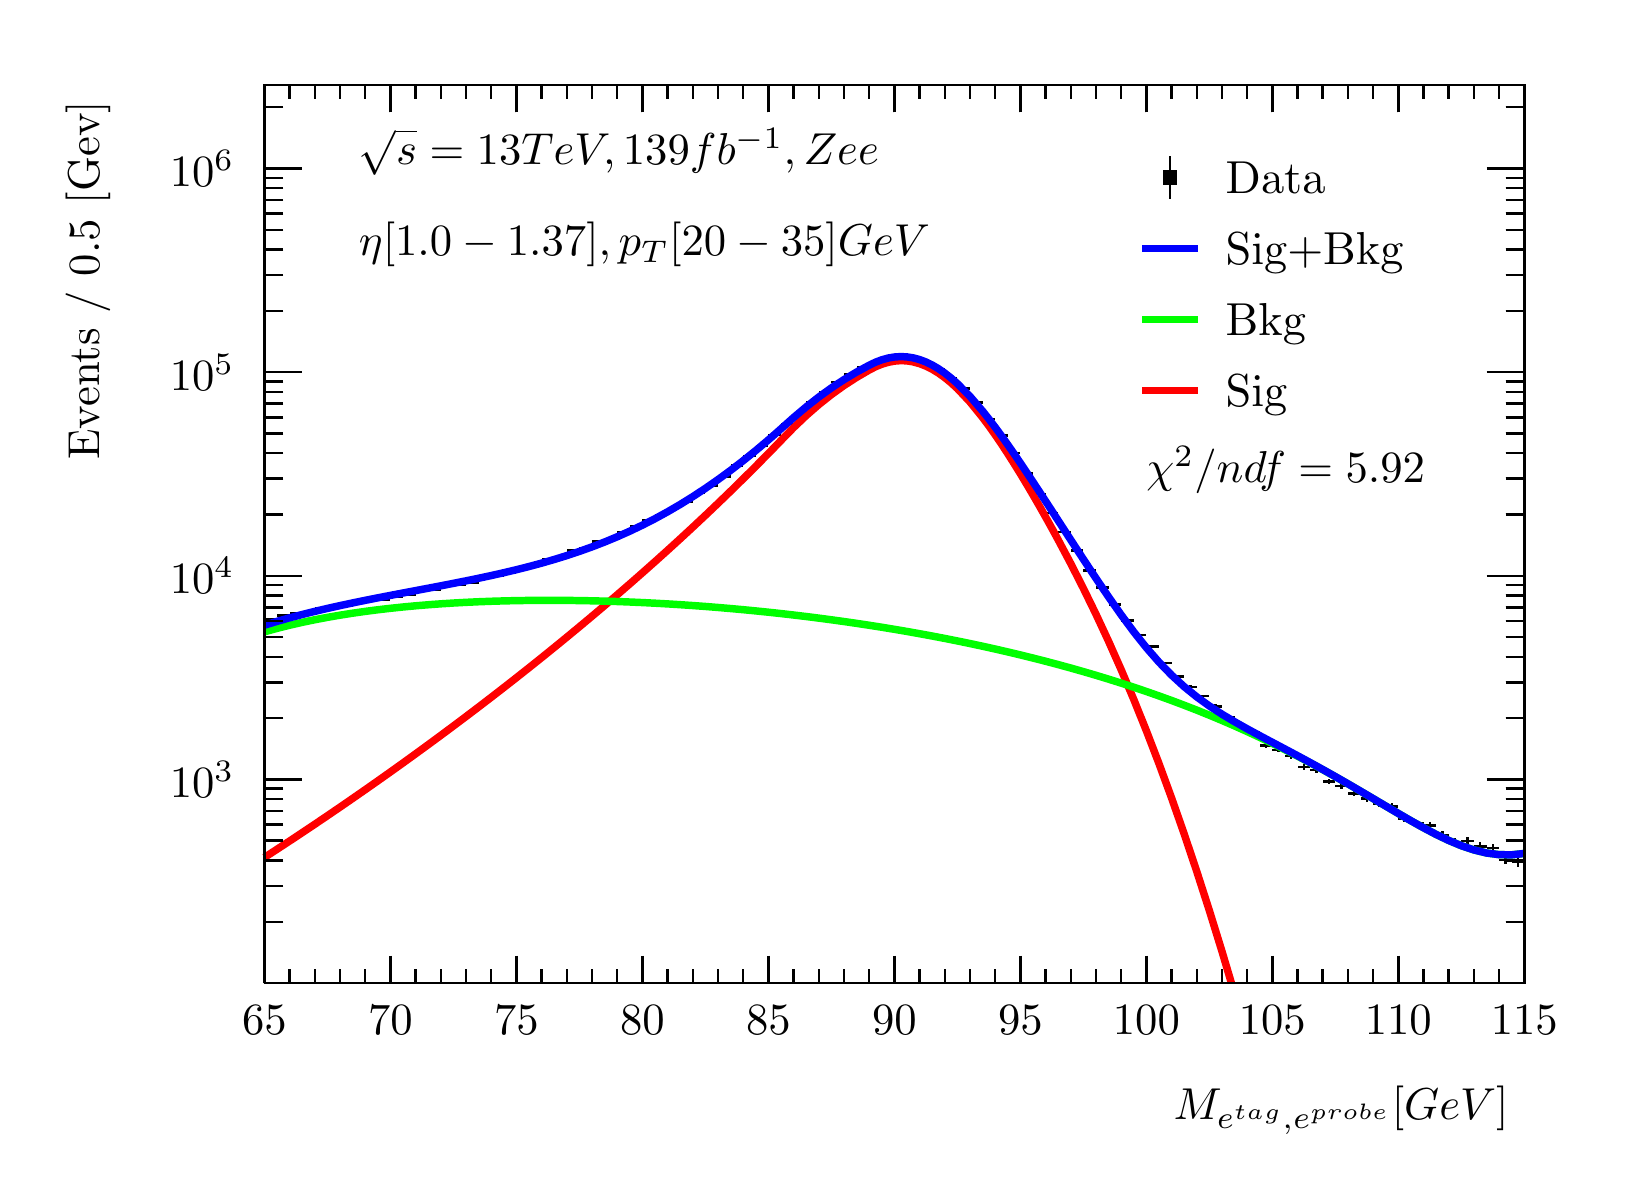
\begin{tikzpicture}
\pgfdeclareplotmark{cross} {
\pgfpathmoveto{\pgfpoint{-0.3\pgfplotmarksize}{\pgfplotmarksize}}
\pgfpathlineto{\pgfpoint{+0.3\pgfplotmarksize}{\pgfplotmarksize}}
\pgfpathlineto{\pgfpoint{+0.3\pgfplotmarksize}{0.3\pgfplotmarksize}}
\pgfpathlineto{\pgfpoint{+1\pgfplotmarksize}{0.3\pgfplotmarksize}}
\pgfpathlineto{\pgfpoint{+1\pgfplotmarksize}{-0.3\pgfplotmarksize}}
\pgfpathlineto{\pgfpoint{+0.3\pgfplotmarksize}{-0.3\pgfplotmarksize}}
\pgfpathlineto{\pgfpoint{+0.3\pgfplotmarksize}{-1.\pgfplotmarksize}}
\pgfpathlineto{\pgfpoint{-0.3\pgfplotmarksize}{-1.\pgfplotmarksize}}
\pgfpathlineto{\pgfpoint{-0.3\pgfplotmarksize}{-0.3\pgfplotmarksize}}
\pgfpathlineto{\pgfpoint{-1.\pgfplotmarksize}{-0.3\pgfplotmarksize}}
\pgfpathlineto{\pgfpoint{-1.\pgfplotmarksize}{0.3\pgfplotmarksize}}
\pgfpathlineto{\pgfpoint{-0.3\pgfplotmarksize}{0.3\pgfplotmarksize}}
\pgfpathclose
\pgfusepathqstroke
}
\pgfdeclareplotmark{cross*} {
\pgfpathmoveto{\pgfpoint{-0.3\pgfplotmarksize}{\pgfplotmarksize}}
\pgfpathlineto{\pgfpoint{+0.3\pgfplotmarksize}{\pgfplotmarksize}}
\pgfpathlineto{\pgfpoint{+0.3\pgfplotmarksize}{0.3\pgfplotmarksize}}
\pgfpathlineto{\pgfpoint{+1\pgfplotmarksize}{0.3\pgfplotmarksize}}
\pgfpathlineto{\pgfpoint{+1\pgfplotmarksize}{-0.3\pgfplotmarksize}}
\pgfpathlineto{\pgfpoint{+0.3\pgfplotmarksize}{-0.3\pgfplotmarksize}}
\pgfpathlineto{\pgfpoint{+0.3\pgfplotmarksize}{-1.\pgfplotmarksize}}
\pgfpathlineto{\pgfpoint{-0.3\pgfplotmarksize}{-1.\pgfplotmarksize}}
\pgfpathlineto{\pgfpoint{-0.3\pgfplotmarksize}{-0.3\pgfplotmarksize}}
\pgfpathlineto{\pgfpoint{-1.\pgfplotmarksize}{-0.3\pgfplotmarksize}}
\pgfpathlineto{\pgfpoint{-1.\pgfplotmarksize}{0.3\pgfplotmarksize}}
\pgfpathlineto{\pgfpoint{-0.3\pgfplotmarksize}{0.3\pgfplotmarksize}}
\pgfpathclose
\pgfusepathqfillstroke
}
\pgfdeclareplotmark{newstar} {
\pgfpathmoveto{\pgfqpoint{0pt}{\pgfplotmarksize}}
\pgfpathlineto{\pgfqpointpolar{44}{0.5\pgfplotmarksize}}
\pgfpathlineto{\pgfqpointpolar{18}{\pgfplotmarksize}}
\pgfpathlineto{\pgfqpointpolar{-20}{0.5\pgfplotmarksize}}
\pgfpathlineto{\pgfqpointpolar{-54}{\pgfplotmarksize}}
\pgfpathlineto{\pgfqpointpolar{-90}{0.5\pgfplotmarksize}}
\pgfpathlineto{\pgfqpointpolar{234}{\pgfplotmarksize}}
\pgfpathlineto{\pgfqpointpolar{198}{0.5\pgfplotmarksize}}
\pgfpathlineto{\pgfqpointpolar{162}{\pgfplotmarksize}}
\pgfpathlineto{\pgfqpointpolar{134}{0.5\pgfplotmarksize}}
\pgfpathclose
\pgfusepathqstroke
}
\pgfdeclareplotmark{newstar*} {
\pgfpathmoveto{\pgfqpoint{0pt}{\pgfplotmarksize}}
\pgfpathlineto{\pgfqpointpolar{44}{0.5\pgfplotmarksize}}
\pgfpathlineto{\pgfqpointpolar{18}{\pgfplotmarksize}}
\pgfpathlineto{\pgfqpointpolar{-20}{0.5\pgfplotmarksize}}
\pgfpathlineto{\pgfqpointpolar{-54}{\pgfplotmarksize}}
\pgfpathlineto{\pgfqpointpolar{-90}{0.5\pgfplotmarksize}}
\pgfpathlineto{\pgfqpointpolar{234}{\pgfplotmarksize}}
\pgfpathlineto{\pgfqpointpolar{198}{0.5\pgfplotmarksize}}
\pgfpathlineto{\pgfqpointpolar{162}{\pgfplotmarksize}}
\pgfpathlineto{\pgfqpointpolar{134}{0.5\pgfplotmarksize}}
\pgfpathclose
\pgfusepathqfillstroke
}
\definecolor{c}{rgb}{1,1,1};
\draw [color=c, fill=c] (0,0) rectangle (20,14.4361);
\draw [color=c, fill=c] (3,2.30977) rectangle (19,13.7143);
\definecolor{c}{rgb}{0,0,0};
\draw [c,line width=0.9] (3,2.30977) -- (3,13.7143) -- (19,13.7143) -- (19,2.30977) -- (3,2.30977);
\definecolor{c}{rgb}{1,1,1};
\draw [color=c, fill=c] (3,2.30977) rectangle (19,13.7143);
\definecolor{c}{rgb}{0,0,0};
\draw [c,line width=0.9] (3,2.30977) -- (3,13.7143) -- (19,13.7143) -- (19,2.30977) -- (3,2.30977);
\draw [c,line width=0.9] (3,2.30977) -- (19,2.30977);
\draw [c,line width=0.9] (3,2.65624) -- (3,2.30977);
\draw [c,line width=0.9] (3.32,2.48301) -- (3.32,2.30977);
\draw [c,line width=0.9] (3.64,2.48301) -- (3.64,2.30977);
\draw [c,line width=0.9] (3.96,2.48301) -- (3.96,2.30977);
\draw [c,line width=0.9] (4.28,2.48301) -- (4.28,2.30977);
\draw [c,line width=0.9] (4.6,2.65624) -- (4.6,2.30977);
\draw [c,line width=0.9] (4.92,2.48301) -- (4.92,2.30977);
\draw [c,line width=0.9] (5.24,2.48301) -- (5.24,2.30977);
\draw [c,line width=0.9] (5.56,2.48301) -- (5.56,2.30977);
\draw [c,line width=0.9] (5.88,2.48301) -- (5.88,2.30977);
\draw [c,line width=0.9] (6.2,2.65624) -- (6.2,2.30977);
\draw [c,line width=0.9] (6.52,2.48301) -- (6.52,2.30977);
\draw [c,line width=0.9] (6.84,2.48301) -- (6.84,2.30977);
\draw [c,line width=0.9] (7.16,2.48301) -- (7.16,2.30977);
\draw [c,line width=0.9] (7.48,2.48301) -- (7.48,2.30977);
\draw [c,line width=0.9] (7.8,2.65624) -- (7.8,2.30977);
\draw [c,line width=0.9] (8.12,2.48301) -- (8.12,2.30977);
\draw [c,line width=0.9] (8.44,2.48301) -- (8.44,2.30977);
\draw [c,line width=0.9] (8.76,2.48301) -- (8.76,2.30977);
\draw [c,line width=0.9] (9.08,2.48301) -- (9.08,2.30977);
\draw [c,line width=0.9] (9.4,2.65624) -- (9.4,2.30977);
\draw [c,line width=0.9] (9.72,2.48301) -- (9.72,2.30977);
\draw [c,line width=0.9] (10.04,2.48301) -- (10.04,2.30977);
\draw [c,line width=0.9] (10.36,2.48301) -- (10.36,2.30977);
\draw [c,line width=0.9] (10.68,2.48301) -- (10.68,2.30977);
\draw [c,line width=0.9] (11,2.65624) -- (11,2.30977);
\draw [c,line width=0.9] (11.32,2.48301) -- (11.32,2.30977);
\draw [c,line width=0.9] (11.64,2.48301) -- (11.64,2.30977);
\draw [c,line width=0.9] (11.96,2.48301) -- (11.96,2.30977);
\draw [c,line width=0.9] (12.28,2.48301) -- (12.28,2.30977);
\draw [c,line width=0.9] (12.6,2.65624) -- (12.6,2.30977);
\draw [c,line width=0.9] (12.92,2.48301) -- (12.92,2.30977);
\draw [c,line width=0.9] (13.24,2.48301) -- (13.24,2.30977);
\draw [c,line width=0.9] (13.56,2.48301) -- (13.56,2.30977);
\draw [c,line width=0.9] (13.88,2.48301) -- (13.88,2.30977);
\draw [c,line width=0.9] (14.2,2.65624) -- (14.2,2.30977);
\draw [c,line width=0.9] (14.52,2.48301) -- (14.52,2.30977);
\draw [c,line width=0.9] (14.84,2.48301) -- (14.84,2.30977);
\draw [c,line width=0.9] (15.16,2.48301) -- (15.16,2.30977);
\draw [c,line width=0.9] (15.48,2.48301) -- (15.48,2.30977);
\draw [c,line width=0.9] (15.8,2.65624) -- (15.8,2.30977);
\draw [c,line width=0.9] (16.12,2.48301) -- (16.12,2.30977);
\draw [c,line width=0.9] (16.44,2.48301) -- (16.44,2.30977);
\draw [c,line width=0.9] (16.76,2.48301) -- (16.76,2.30977);
\draw [c,line width=0.9] (17.08,2.48301) -- (17.08,2.30977);
\draw [c,line width=0.9] (17.4,2.65624) -- (17.4,2.30977);
\draw [c,line width=0.9] (17.72,2.48301) -- (17.72,2.30977);
\draw [c,line width=0.9] (18.04,2.48301) -- (18.04,2.30977);
\draw [c,line width=0.9] (18.36,2.48301) -- (18.36,2.30977);
\draw [c,line width=0.9] (18.68,2.48301) -- (18.68,2.30977);
\draw [c,line width=0.9] (19,2.65624) -- (19,2.30977);
\draw [c,line width=0.9] (19,2.65624) -- (19,2.30977);
\draw [anchor=base] (3,1.66015) node[scale=1.61424, color=c, rotate=0]{65};
\draw [anchor=base] (4.6,1.66015) node[scale=1.61424, color=c, rotate=0]{70};
\draw [anchor=base] (6.2,1.66015) node[scale=1.61424, color=c, rotate=0]{75};
\draw [anchor=base] (7.8,1.66015) node[scale=1.61424, color=c, rotate=0]{80};
\draw [anchor=base] (9.4,1.66015) node[scale=1.61424, color=c, rotate=0]{85};
\draw [anchor=base] (11,1.66015) node[scale=1.61424, color=c, rotate=0]{90};
\draw [anchor=base] (12.6,1.66015) node[scale=1.61424, color=c, rotate=0]{95};
\draw [anchor=base] (14.2,1.66015) node[scale=1.61424, color=c, rotate=0]{100};
\draw [anchor=base] (15.8,1.66015) node[scale=1.61424, color=c, rotate=0]{105};
\draw [anchor=base] (17.4,1.66015) node[scale=1.61424, color=c, rotate=0]{110};
\draw [anchor=base] (19,1.66015) node[scale=1.61424, color=c, rotate=0]{115};
\draw [anchor= east] (19,0.692932) node[scale=1.61424, color=c, rotate=0]{$M_{e^{tag}, e^{probe}}  [GeV]$};
\draw [c,line width=0.9] (3,13.7143) -- (19,13.7143);
\draw [c,line width=0.9] (3,13.3678) -- (3,13.7143);
\draw [c,line width=0.9] (3.32,13.5411) -- (3.32,13.7143);
\draw [c,line width=0.9] (3.64,13.5411) -- (3.64,13.7143);
\draw [c,line width=0.9] (3.96,13.5411) -- (3.96,13.7143);
\draw [c,line width=0.9] (4.28,13.5411) -- (4.28,13.7143);
\draw [c,line width=0.9] (4.6,13.3678) -- (4.6,13.7143);
\draw [c,line width=0.9] (4.92,13.5411) -- (4.92,13.7143);
\draw [c,line width=0.9] (5.24,13.5411) -- (5.24,13.7143);
\draw [c,line width=0.9] (5.56,13.5411) -- (5.56,13.7143);
\draw [c,line width=0.9] (5.88,13.5411) -- (5.88,13.7143);
\draw [c,line width=0.9] (6.2,13.3678) -- (6.2,13.7143);
\draw [c,line width=0.9] (6.52,13.5411) -- (6.52,13.7143);
\draw [c,line width=0.9] (6.84,13.5411) -- (6.84,13.7143);
\draw [c,line width=0.9] (7.16,13.5411) -- (7.16,13.7143);
\draw [c,line width=0.9] (7.48,13.5411) -- (7.48,13.7143);
\draw [c,line width=0.9] (7.8,13.3678) -- (7.8,13.7143);
\draw [c,line width=0.9] (8.12,13.5411) -- (8.12,13.7143);
\draw [c,line width=0.9] (8.44,13.5411) -- (8.44,13.7143);
\draw [c,line width=0.9] (8.76,13.5411) -- (8.76,13.7143);
\draw [c,line width=0.9] (9.08,13.5411) -- (9.08,13.7143);
\draw [c,line width=0.9] (9.4,13.3678) -- (9.4,13.7143);
\draw [c,line width=0.9] (9.72,13.5411) -- (9.72,13.7143);
\draw [c,line width=0.9] (10.04,13.5411) -- (10.04,13.7143);
\draw [c,line width=0.9] (10.36,13.5411) -- (10.36,13.7143);
\draw [c,line width=0.9] (10.68,13.5411) -- (10.68,13.7143);
\draw [c,line width=0.9] (11,13.3678) -- (11,13.7143);
\draw [c,line width=0.9] (11.32,13.5411) -- (11.32,13.7143);
\draw [c,line width=0.9] (11.64,13.5411) -- (11.64,13.7143);
\draw [c,line width=0.9] (11.96,13.5411) -- (11.96,13.7143);
\draw [c,line width=0.9] (12.28,13.5411) -- (12.28,13.7143);
\draw [c,line width=0.9] (12.6,13.3678) -- (12.6,13.7143);
\draw [c,line width=0.9] (12.92,13.5411) -- (12.92,13.7143);
\draw [c,line width=0.9] (13.24,13.5411) -- (13.24,13.7143);
\draw [c,line width=0.9] (13.56,13.5411) -- (13.56,13.7143);
\draw [c,line width=0.9] (13.88,13.5411) -- (13.88,13.7143);
\draw [c,line width=0.9] (14.2,13.3678) -- (14.2,13.7143);
\draw [c,line width=0.9] (14.52,13.5411) -- (14.52,13.7143);
\draw [c,line width=0.9] (14.84,13.5411) -- (14.84,13.7143);
\draw [c,line width=0.9] (15.16,13.5411) -- (15.16,13.7143);
\draw [c,line width=0.9] (15.48,13.5411) -- (15.48,13.7143);
\draw [c,line width=0.9] (15.8,13.3678) -- (15.8,13.7143);
\draw [c,line width=0.9] (16.12,13.5411) -- (16.12,13.7143);
\draw [c,line width=0.9] (16.44,13.5411) -- (16.44,13.7143);
\draw [c,line width=0.9] (16.76,13.5411) -- (16.76,13.7143);
\draw [c,line width=0.9] (17.08,13.5411) -- (17.08,13.7143);
\draw [c,line width=0.9] (17.4,13.3678) -- (17.4,13.7143);
\draw [c,line width=0.9] (17.72,13.5411) -- (17.72,13.7143);
\draw [c,line width=0.9] (18.04,13.5411) -- (18.04,13.7143);
\draw [c,line width=0.9] (18.36,13.5411) -- (18.36,13.7143);
\draw [c,line width=0.9] (18.68,13.5411) -- (18.68,13.7143);
\draw [c,line width=0.9] (19,13.3678) -- (19,13.7143);
\draw [c,line width=0.9] (19,13.3678) -- (19,13.7143);
\draw [c,line width=0.9] (3,2.30977) -- (3,13.7143);
\draw [c,line width=0.9] (3.237,3.08829) -- (3,3.08829);
\draw [c,line width=0.9] (3.237,3.54369) -- (3,3.54369);
\draw [c,line width=0.9] (3.237,3.8668) -- (3,3.8668);
\draw [c,line width=0.9] (3.237,4.11742) -- (3,4.11742);
\draw [c,line width=0.9] (3.237,4.3222) -- (3,4.3222);
\draw [c,line width=0.9] (3.237,4.49534) -- (3,4.49534);
\draw [c,line width=0.9] (3.237,4.64531) -- (3,4.64531);
\draw [c,line width=0.9] (3.237,4.7776) -- (3,4.7776);
\draw [c,line width=0.9] (3.474,4.89594) -- (3,4.89594);
\draw [anchor= east] (2.82,4.89594) node[scale=1.61424, color=c, rotate=0]{$10^{3}$};
\draw [c,line width=0.9] (3.237,5.67445) -- (3,5.67445);
\draw [c,line width=0.9] (3.237,6.12985) -- (3,6.12985);
\draw [c,line width=0.9] (3.237,6.45297) -- (3,6.45297);
\draw [c,line width=0.9] (3.237,6.70359) -- (3,6.70359);
\draw [c,line width=0.9] (3.237,6.90837) -- (3,6.90837);
\draw [c,line width=0.9] (3.237,7.0815) -- (3,7.0815);
\draw [c,line width=0.9] (3.237,7.23148) -- (3,7.23148);
\draw [c,line width=0.9] (3.237,7.36377) -- (3,7.36377);
\draw [c,line width=0.9] (3.474,7.48211) -- (3,7.48211);
\draw [anchor= east] (2.82,7.48211) node[scale=1.61424, color=c, rotate=0]{$10^{4}$};
\draw [c,line width=0.9] (3.237,8.26062) -- (3,8.26062);
\draw [c,line width=0.9] (3.237,8.71602) -- (3,8.71602);
\draw [c,line width=0.9] (3.237,9.03913) -- (3,9.03913);
\draw [c,line width=0.9] (3.237,9.28976) -- (3,9.28976);
\draw [c,line width=0.9] (3.237,9.49453) -- (3,9.49453);
\draw [c,line width=0.9] (3.237,9.66767) -- (3,9.66767);
\draw [c,line width=0.9] (3.237,9.81765) -- (3,9.81765);
\draw [c,line width=0.9] (3.237,9.94994) -- (3,9.94994);
\draw [c,line width=0.9] (3.474,10.0683) -- (3,10.0683);
\draw [anchor= east] (2.82,10.0683) node[scale=1.61424, color=c, rotate=0]{$10^{5}$};
\draw [c,line width=0.9] (3.237,10.8468) -- (3,10.8468);
\draw [c,line width=0.9] (3.237,11.3022) -- (3,11.3022);
\draw [c,line width=0.9] (3.237,11.6253) -- (3,11.6253);
\draw [c,line width=0.9] (3.237,11.8759) -- (3,11.8759);
\draw [c,line width=0.9] (3.237,12.0807) -- (3,12.0807);
\draw [c,line width=0.9] (3.237,12.2538) -- (3,12.2538);
\draw [c,line width=0.9] (3.237,12.4038) -- (3,12.4038);
\draw [c,line width=0.9] (3.237,12.5361) -- (3,12.5361);
\draw [c,line width=0.9] (3.474,12.6544) -- (3,12.6544);
\draw [anchor= east] (2.82,12.6544) node[scale=1.61424, color=c, rotate=0]{$10^{6}$};
\draw [c,line width=0.9] (3.237,13.433) -- (3,13.433);
\draw [anchor= east] (0.76,13.7143) node[scale=1.61424, color=c, rotate=90]{Events / 0.5 [Gev]};
\draw [c,line width=0.9] (19,2.30977) -- (19,13.7143);
\draw [c,line width=0.9] (18.763,3.08829) -- (19,3.08829);
\draw [c,line width=0.9] (18.763,3.54369) -- (19,3.54369);
\draw [c,line width=0.9] (18.763,3.8668) -- (19,3.8668);
\draw [c,line width=0.9] (18.763,4.11742) -- (19,4.11742);
\draw [c,line width=0.9] (18.763,4.3222) -- (19,4.3222);
\draw [c,line width=0.9] (18.763,4.49534) -- (19,4.49534);
\draw [c,line width=0.9] (18.763,4.64531) -- (19,4.64531);
\draw [c,line width=0.9] (18.763,4.7776) -- (19,4.7776);
\draw [c,line width=0.9] (18.526,4.89594) -- (19,4.89594);
\draw [c,line width=0.9] (18.763,5.67445) -- (19,5.67445);
\draw [c,line width=0.9] (18.763,6.12985) -- (19,6.12985);
\draw [c,line width=0.9] (18.763,6.45297) -- (19,6.45297);
\draw [c,line width=0.9] (18.763,6.70359) -- (19,6.70359);
\draw [c,line width=0.9] (18.763,6.90837) -- (19,6.90837);
\draw [c,line width=0.9] (18.763,7.0815) -- (19,7.0815);
\draw [c,line width=0.9] (18.763,7.23148) -- (19,7.23148);
\draw [c,line width=0.9] (18.763,7.36377) -- (19,7.36377);
\draw [c,line width=0.9] (18.526,7.48211) -- (19,7.48211);
\draw [c,line width=0.9] (18.763,8.26062) -- (19,8.26062);
\draw [c,line width=0.9] (18.763,8.71602) -- (19,8.71602);
\draw [c,line width=0.9] (18.763,9.03913) -- (19,9.03913);
\draw [c,line width=0.9] (18.763,9.28976) -- (19,9.28976);
\draw [c,line width=0.9] (18.763,9.49453) -- (19,9.49453);
\draw [c,line width=0.9] (18.763,9.66767) -- (19,9.66767);
\draw [c,line width=0.9] (18.763,9.81765) -- (19,9.81765);
\draw [c,line width=0.9] (18.763,9.94994) -- (19,9.94994);
\draw [c,line width=0.9] (18.526,10.0683) -- (19,10.0683);
\draw [c,line width=0.9] (18.763,10.8468) -- (19,10.8468);
\draw [c,line width=0.9] (18.763,11.3022) -- (19,11.3022);
\draw [c,line width=0.9] (18.763,11.6253) -- (19,11.6253);
\draw [c,line width=0.9] (18.763,11.8759) -- (19,11.8759);
\draw [c,line width=0.9] (18.763,12.0807) -- (19,12.0807);
\draw [c,line width=0.9] (18.763,12.2538) -- (19,12.2538);
\draw [c,line width=0.9] (18.763,12.4038) -- (19,12.4038);
\draw [c,line width=0.9] (18.763,12.5361) -- (19,12.5361);
\draw [c,line width=0.9] (18.526,12.6544) -- (19,12.6544);
\draw [c,line width=0.9] (18.763,13.433) -- (19,13.433);
\draw [c,line width=0.9] (3.08,6.93519) -- (3,6.93519);
\draw [c,line width=0.9] (3,6.93519) -- (3,6.93519);
\draw [c,line width=0.9] (3.08,6.93519) -- (3.16,6.93519);
\draw [c,line width=0.9] (3.16,6.93519) -- (3.16,6.93519);
\draw [c,line width=0.9] (3.08,6.93519) -- (3.08,6.94952);
\draw [c,line width=0.9] (3.08,6.94952) -- (3.08,6.94952);
\draw [c,line width=0.9] (3.08,6.93519) -- (3.08,6.92086);
\draw [c,line width=0.9] (3.08,6.92086) -- (3.08,6.92086);
\draw [c,line width=0.9] (3.24,6.9791) -- (3.16,6.9791);
\draw [c,line width=0.9] (3.16,6.9791) -- (3.16,6.9791);
\draw [c,line width=0.9] (3.24,6.9791) -- (3.32,6.9791);
\draw [c,line width=0.9] (3.32,6.9791) -- (3.32,6.9791);
\draw [c,line width=0.9] (3.24,6.9791) -- (3.24,6.99315);
\draw [c,line width=0.9] (3.24,6.99315) -- (3.24,6.99315);
\draw [c,line width=0.9] (3.24,6.9791) -- (3.24,6.96505);
\draw [c,line width=0.9] (3.24,6.96505) -- (3.24,6.96505);
\draw [c,line width=0.9] (3.4,7.00172) -- (3.32,7.00172);
\draw [c,line width=0.9] (3.32,7.00172) -- (3.32,7.00172);
\draw [c,line width=0.9] (3.4,7.00172) -- (3.48,7.00172);
\draw [c,line width=0.9] (3.48,7.00172) -- (3.48,7.00172);
\draw [c,line width=0.9] (3.4,7.00172) -- (3.4,7.01563);
\draw [c,line width=0.9] (3.4,7.01563) -- (3.4,7.01563);
\draw [c,line width=0.9] (3.4,7.00172) -- (3.4,6.98781);
\draw [c,line width=0.9] (3.4,6.98781) -- (3.4,6.98781);
\draw [c,line width=0.9] (3.56,6.99464) -- (3.48,6.99464);
\draw [c,line width=0.9] (3.48,6.99464) -- (3.48,6.99464);
\draw [c,line width=0.9] (3.56,6.99464) -- (3.64,6.99464);
\draw [c,line width=0.9] (3.64,6.99464) -- (3.64,6.99464);
\draw [c,line width=0.9] (3.56,6.99464) -- (3.56,7.00859);
\draw [c,line width=0.9] (3.56,7.00859) -- (3.56,7.00859);
\draw [c,line width=0.9] (3.56,6.99464) -- (3.56,6.98068);
\draw [c,line width=0.9] (3.56,6.98068) -- (3.56,6.98068);
\draw [c,line width=0.9] (3.72,7.07362) -- (3.64,7.07362);
\draw [c,line width=0.9] (3.64,7.07362) -- (3.64,7.07362);
\draw [c,line width=0.9] (3.72,7.07362) -- (3.8,7.07362);
\draw [c,line width=0.9] (3.8,7.07362) -- (3.8,7.07362);
\draw [c,line width=0.9] (3.72,7.07362) -- (3.72,7.08709);
\draw [c,line width=0.9] (3.72,7.08709) -- (3.72,7.08709);
\draw [c,line width=0.9] (3.72,7.07362) -- (3.72,7.06014);
\draw [c,line width=0.9] (3.72,7.06014) -- (3.72,7.06014);
\draw [c,line width=0.9] (3.88,7.08599) -- (3.8,7.08599);
\draw [c,line width=0.9] (3.8,7.08599) -- (3.8,7.08599);
\draw [c,line width=0.9] (3.88,7.08599) -- (3.96,7.08599);
\draw [c,line width=0.9] (3.96,7.08599) -- (3.96,7.08599);
\draw [c,line width=0.9] (3.88,7.08599) -- (3.88,7.09939);
\draw [c,line width=0.9] (3.88,7.09939) -- (3.88,7.09939);
\draw [c,line width=0.9] (3.88,7.08599) -- (3.88,7.07259);
\draw [c,line width=0.9] (3.88,7.07259) -- (3.88,7.07259);
\draw [c,line width=0.9] (4.04,7.10217) -- (3.96,7.10217);
\draw [c,line width=0.9] (3.96,7.10217) -- (3.96,7.10217);
\draw [c,line width=0.9] (4.04,7.10217) -- (4.12,7.10217);
\draw [c,line width=0.9] (4.12,7.10217) -- (4.12,7.10217);
\draw [c,line width=0.9] (4.04,7.10217) -- (4.04,7.11547);
\draw [c,line width=0.9] (4.04,7.11547) -- (4.04,7.11547);
\draw [c,line width=0.9] (4.04,7.10217) -- (4.04,7.08887);
\draw [c,line width=0.9] (4.04,7.08887) -- (4.04,7.08887);
\draw [c,line width=0.9] (4.2,7.1427) -- (4.12,7.1427);
\draw [c,line width=0.9] (4.12,7.1427) -- (4.12,7.1427);
\draw [c,line width=0.9] (4.2,7.1427) -- (4.28,7.1427);
\draw [c,line width=0.9] (4.28,7.1427) -- (4.28,7.1427);
\draw [c,line width=0.9] (4.2,7.1427) -- (4.2,7.15577);
\draw [c,line width=0.9] (4.2,7.15577) -- (4.2,7.15577);
\draw [c,line width=0.9] (4.2,7.1427) -- (4.2,7.12964);
\draw [c,line width=0.9] (4.2,7.12964) -- (4.2,7.12964);
\draw [c,line width=0.9] (4.36,7.18402) -- (4.28,7.18402);
\draw [c,line width=0.9] (4.28,7.18402) -- (4.28,7.18402);
\draw [c,line width=0.9] (4.36,7.18402) -- (4.44,7.18402);
\draw [c,line width=0.9] (4.44,7.18402) -- (4.44,7.18402);
\draw [c,line width=0.9] (4.36,7.18402) -- (4.36,7.19685);
\draw [c,line width=0.9] (4.36,7.19685) -- (4.36,7.19685);
\draw [c,line width=0.9] (4.36,7.18402) -- (4.36,7.1712);
\draw [c,line width=0.9] (4.36,7.1712) -- (4.36,7.1712);
\draw [c,line width=0.9] (4.52,7.18329) -- (4.44,7.18329);
\draw [c,line width=0.9] (4.44,7.18329) -- (4.44,7.18329);
\draw [c,line width=0.9] (4.52,7.18329) -- (4.6,7.18329);
\draw [c,line width=0.9] (4.6,7.18329) -- (4.6,7.18329);
\draw [c,line width=0.9] (4.52,7.18329) -- (4.52,7.19612);
\draw [c,line width=0.9] (4.52,7.19612) -- (4.52,7.19612);
\draw [c,line width=0.9] (4.52,7.18329) -- (4.52,7.17046);
\draw [c,line width=0.9] (4.52,7.17046) -- (4.52,7.17046);
\draw [c,line width=0.9] (4.68,7.21308) -- (4.6,7.21308);
\draw [c,line width=0.9] (4.6,7.21308) -- (4.6,7.21308);
\draw [c,line width=0.9] (4.68,7.21308) -- (4.76,7.21308);
\draw [c,line width=0.9] (4.76,7.21308) -- (4.76,7.21308);
\draw [c,line width=0.9] (4.68,7.21308) -- (4.68,7.22574);
\draw [c,line width=0.9] (4.68,7.22574) -- (4.68,7.22574);
\draw [c,line width=0.9] (4.68,7.21308) -- (4.68,7.20042);
\draw [c,line width=0.9] (4.68,7.20042) -- (4.68,7.20042);
\draw [c,line width=0.9] (4.84,7.23778) -- (4.76,7.23778);
\draw [c,line width=0.9] (4.76,7.23778) -- (4.76,7.23778);
\draw [c,line width=0.9] (4.84,7.23778) -- (4.92,7.23778);
\draw [c,line width=0.9] (4.92,7.23778) -- (4.92,7.23778);
\draw [c,line width=0.9] (4.84,7.23778) -- (4.84,7.2503);
\draw [c,line width=0.9] (4.84,7.2503) -- (4.84,7.2503);
\draw [c,line width=0.9] (4.84,7.23778) -- (4.84,7.22526);
\draw [c,line width=0.9] (4.84,7.22526) -- (4.84,7.22526);
\draw [c,line width=0.9] (5,7.29122) -- (4.92,7.29122);
\draw [c,line width=0.9] (4.92,7.29122) -- (4.92,7.29122);
\draw [c,line width=0.9] (5,7.29122) -- (5.08,7.29122);
\draw [c,line width=0.9] (5.08,7.29122) -- (5.08,7.29122);
\draw [c,line width=0.9] (5,7.29122) -- (5,7.30344);
\draw [c,line width=0.9] (5,7.30344) -- (5,7.30344);
\draw [c,line width=0.9] (5,7.29122) -- (5,7.27899);
\draw [c,line width=0.9] (5,7.27899) -- (5,7.27899);
\draw [c,line width=0.9] (5.16,7.30419) -- (5.08,7.30419);
\draw [c,line width=0.9] (5.08,7.30419) -- (5.08,7.30419);
\draw [c,line width=0.9] (5.16,7.30419) -- (5.24,7.30419);
\draw [c,line width=0.9] (5.24,7.30419) -- (5.24,7.30419);
\draw [c,line width=0.9] (5.16,7.30419) -- (5.16,7.31635);
\draw [c,line width=0.9] (5.16,7.31635) -- (5.16,7.31635);
\draw [c,line width=0.9] (5.16,7.30419) -- (5.16,7.29203);
\draw [c,line width=0.9] (5.16,7.29203) -- (5.16,7.29203);
\draw [c,line width=0.9] (5.32,7.35563) -- (5.24,7.35563);
\draw [c,line width=0.9] (5.24,7.35563) -- (5.24,7.35563);
\draw [c,line width=0.9] (5.32,7.35563) -- (5.4,7.35563);
\draw [c,line width=0.9] (5.4,7.35563) -- (5.4,7.35563);
\draw [c,line width=0.9] (5.32,7.35563) -- (5.32,7.36751);
\draw [c,line width=0.9] (5.32,7.36751) -- (5.32,7.36751);
\draw [c,line width=0.9] (5.32,7.35563) -- (5.32,7.34375);
\draw [c,line width=0.9] (5.32,7.34375) -- (5.32,7.34375);
\draw [c,line width=0.9] (5.48,7.37185) -- (5.4,7.37185);
\draw [c,line width=0.9] (5.4,7.37185) -- (5.4,7.37185);
\draw [c,line width=0.9] (5.48,7.37185) -- (5.56,7.37185);
\draw [c,line width=0.9] (5.56,7.37185) -- (5.56,7.37185);
\draw [c,line width=0.9] (5.48,7.37185) -- (5.48,7.38365);
\draw [c,line width=0.9] (5.48,7.38365) -- (5.48,7.38365);
\draw [c,line width=0.9] (5.48,7.37185) -- (5.48,7.36006);
\draw [c,line width=0.9] (5.48,7.36006) -- (5.48,7.36006);
\draw [c,line width=0.9] (5.64,7.39818) -- (5.56,7.39818);
\draw [c,line width=0.9] (5.56,7.39818) -- (5.56,7.39818);
\draw [c,line width=0.9] (5.64,7.39818) -- (5.72,7.39818);
\draw [c,line width=0.9] (5.72,7.39818) -- (5.72,7.39818);
\draw [c,line width=0.9] (5.64,7.39818) -- (5.64,7.40984);
\draw [c,line width=0.9] (5.64,7.40984) -- (5.64,7.40984);
\draw [c,line width=0.9] (5.64,7.39818) -- (5.64,7.38652);
\draw [c,line width=0.9] (5.64,7.38652) -- (5.64,7.38652);
\draw [c,line width=0.9] (5.8,7.45517) -- (5.72,7.45517);
\draw [c,line width=0.9] (5.72,7.45517) -- (5.72,7.45517);
\draw [c,line width=0.9] (5.8,7.45517) -- (5.88,7.45517);
\draw [c,line width=0.9] (5.88,7.45517) -- (5.88,7.45517);
\draw [c,line width=0.9] (5.8,7.45517) -- (5.8,7.46654);
\draw [c,line width=0.9] (5.8,7.46654) -- (5.8,7.46654);
\draw [c,line width=0.9] (5.8,7.45517) -- (5.8,7.4438);
\draw [c,line width=0.9] (5.8,7.4438) -- (5.8,7.4438);
\draw [c,line width=0.9] (5.96,7.48793) -- (5.88,7.48793);
\draw [c,line width=0.9] (5.88,7.48793) -- (5.88,7.48793);
\draw [c,line width=0.9] (5.96,7.48793) -- (6.04,7.48793);
\draw [c,line width=0.9] (6.04,7.48793) -- (6.04,7.48793);
\draw [c,line width=0.9] (5.96,7.48793) -- (5.96,7.49914);
\draw [c,line width=0.9] (5.96,7.49914) -- (5.96,7.49914);
\draw [c,line width=0.9] (5.96,7.48793) -- (5.96,7.47673);
\draw [c,line width=0.9] (5.96,7.47673) -- (5.96,7.47673);
\draw [c,line width=0.9] (6.12,7.52356) -- (6.04,7.52356);
\draw [c,line width=0.9] (6.04,7.52356) -- (6.04,7.52356);
\draw [c,line width=0.9] (6.12,7.52356) -- (6.2,7.52356);
\draw [c,line width=0.9] (6.2,7.52356) -- (6.2,7.52356);
\draw [c,line width=0.9] (6.12,7.52356) -- (6.12,7.53459);
\draw [c,line width=0.9] (6.12,7.53459) -- (6.12,7.53459);
\draw [c,line width=0.9] (6.12,7.52356) -- (6.12,7.51254);
\draw [c,line width=0.9] (6.12,7.51254) -- (6.12,7.51254);
\draw [c,line width=0.9] (6.28,7.56948) -- (6.2,7.56948);
\draw [c,line width=0.9] (6.2,7.56948) -- (6.2,7.56948);
\draw [c,line width=0.9] (6.28,7.56948) -- (6.36,7.56948);
\draw [c,line width=0.9] (6.36,7.56948) -- (6.36,7.56948);
\draw [c,line width=0.9] (6.28,7.56948) -- (6.28,7.58029);
\draw [c,line width=0.9] (6.28,7.58029) -- (6.28,7.58029);
\draw [c,line width=0.9] (6.28,7.56948) -- (6.28,7.55868);
\draw [c,line width=0.9] (6.28,7.55868) -- (6.28,7.55868);
\draw [c,line width=0.9] (6.44,7.62937) -- (6.36,7.62937);
\draw [c,line width=0.9] (6.36,7.62937) -- (6.36,7.62937);
\draw [c,line width=0.9] (6.44,7.62937) -- (6.52,7.62937);
\draw [c,line width=0.9] (6.52,7.62937) -- (6.52,7.62937);
\draw [c,line width=0.9] (6.44,7.62937) -- (6.44,7.63989);
\draw [c,line width=0.9] (6.44,7.63989) -- (6.44,7.63989);
\draw [c,line width=0.9] (6.44,7.62937) -- (6.44,7.61885);
\draw [c,line width=0.9] (6.44,7.61885) -- (6.44,7.61885);
\draw [c,line width=0.9] (6.6,7.6881) -- (6.52,7.6881);
\draw [c,line width=0.9] (6.52,7.6881) -- (6.52,7.6881);
\draw [c,line width=0.9] (6.6,7.6881) -- (6.68,7.6881);
\draw [c,line width=0.9] (6.68,7.6881) -- (6.68,7.6881);
\draw [c,line width=0.9] (6.6,7.6881) -- (6.6,7.69835);
\draw [c,line width=0.9] (6.6,7.69835) -- (6.6,7.69835);
\draw [c,line width=0.9] (6.6,7.6881) -- (6.6,7.67785);
\draw [c,line width=0.9] (6.6,7.67785) -- (6.6,7.67785);
\draw [c,line width=0.9] (6.76,7.71187) -- (6.68,7.71187);
\draw [c,line width=0.9] (6.68,7.71187) -- (6.68,7.71187);
\draw [c,line width=0.9] (6.76,7.71187) -- (6.84,7.71187);
\draw [c,line width=0.9] (6.84,7.71187) -- (6.84,7.71187);
\draw [c,line width=0.9] (6.76,7.71187) -- (6.76,7.72201);
\draw [c,line width=0.9] (6.76,7.72201) -- (6.76,7.72201);
\draw [c,line width=0.9] (6.76,7.71187) -- (6.76,7.70173);
\draw [c,line width=0.9] (6.76,7.70173) -- (6.76,7.70173);
\draw [c,line width=0.9] (6.92,7.80334) -- (6.84,7.80334);
\draw [c,line width=0.9] (6.84,7.80334) -- (6.84,7.80334);
\draw [c,line width=0.9] (6.92,7.80334) -- (7,7.80334);
\draw [c,line width=0.9] (7,7.80334) -- (7,7.80334);
\draw [c,line width=0.9] (6.92,7.80334) -- (6.92,7.81307);
\draw [c,line width=0.9] (6.92,7.81307) -- (6.92,7.81307);
\draw [c,line width=0.9] (6.92,7.80334) -- (6.92,7.7936);
\draw [c,line width=0.9] (6.92,7.7936) -- (6.92,7.7936);
\draw [c,line width=0.9] (7.08,7.83175) -- (7,7.83175);
\draw [c,line width=0.9] (7,7.83175) -- (7,7.83175);
\draw [c,line width=0.9] (7.08,7.83175) -- (7.16,7.83175);
\draw [c,line width=0.9] (7.16,7.83175) -- (7.16,7.83175);
\draw [c,line width=0.9] (7.08,7.83175) -- (7.08,7.84136);
\draw [c,line width=0.9] (7.08,7.84136) -- (7.08,7.84136);
\draw [c,line width=0.9] (7.08,7.83175) -- (7.08,7.82213);
\draw [c,line width=0.9] (7.08,7.82213) -- (7.08,7.82213);
\draw [c,line width=0.9] (7.24,7.92031) -- (7.16,7.92031);
\draw [c,line width=0.9] (7.16,7.92031) -- (7.16,7.92031);
\draw [c,line width=0.9] (7.24,7.92031) -- (7.32,7.92031);
\draw [c,line width=0.9] (7.32,7.92031) -- (7.32,7.92031);
\draw [c,line width=0.9] (7.24,7.92031) -- (7.24,7.92955);
\draw [c,line width=0.9] (7.24,7.92955) -- (7.24,7.92955);
\draw [c,line width=0.9] (7.24,7.92031) -- (7.24,7.91106);
\draw [c,line width=0.9] (7.24,7.91106) -- (7.24,7.91106);
\draw [c,line width=0.9] (7.4,7.94072) -- (7.32,7.94072);
\draw [c,line width=0.9] (7.32,7.94072) -- (7.32,7.94072);
\draw [c,line width=0.9] (7.4,7.94072) -- (7.48,7.94072);
\draw [c,line width=0.9] (7.48,7.94072) -- (7.48,7.94072);
\draw [c,line width=0.9] (7.4,7.94072) -- (7.4,7.94988);
\draw [c,line width=0.9] (7.4,7.94988) -- (7.4,7.94988);
\draw [c,line width=0.9] (7.4,7.94072) -- (7.4,7.93157);
\draw [c,line width=0.9] (7.4,7.93157) -- (7.4,7.93157);
\draw [c,line width=0.9] (7.56,8.03725) -- (7.48,8.03725);
\draw [c,line width=0.9] (7.48,8.03725) -- (7.48,8.03725);
\draw [c,line width=0.9] (7.56,8.03725) -- (7.64,8.03725);
\draw [c,line width=0.9] (7.64,8.03725) -- (7.64,8.03725);
\draw [c,line width=0.9] (7.56,8.03725) -- (7.56,8.04602);
\draw [c,line width=0.9] (7.56,8.04602) -- (7.56,8.04602);
\draw [c,line width=0.9] (7.56,8.03725) -- (7.56,8.02848);
\draw [c,line width=0.9] (7.56,8.02848) -- (7.56,8.02848);
\draw [c,line width=0.9] (7.72,8.10872) -- (7.64,8.10872);
\draw [c,line width=0.9] (7.64,8.10872) -- (7.64,8.10872);
\draw [c,line width=0.9] (7.72,8.10872) -- (7.8,8.10872);
\draw [c,line width=0.9] (7.8,8.10872) -- (7.8,8.10872);
\draw [c,line width=0.9] (7.72,8.10872) -- (7.72,8.11721);
\draw [c,line width=0.9] (7.72,8.11721) -- (7.72,8.11721);
\draw [c,line width=0.9] (7.72,8.10872) -- (7.72,8.10022);
\draw [c,line width=0.9] (7.72,8.10022) -- (7.72,8.10022);
\draw [c,line width=0.9] (7.88,8.18291) -- (7.8,8.18291);
\draw [c,line width=0.9] (7.8,8.18291) -- (7.8,8.18291);
\draw [c,line width=0.9] (7.88,8.18291) -- (7.96,8.18291);
\draw [c,line width=0.9] (7.96,8.18291) -- (7.96,8.18291);
\draw [c,line width=0.9] (7.88,8.18291) -- (7.88,8.19113);
\draw [c,line width=0.9] (7.88,8.19113) -- (7.88,8.19113);
\draw [c,line width=0.9] (7.88,8.18291) -- (7.88,8.17469);
\draw [c,line width=0.9] (7.88,8.17469) -- (7.88,8.17469);
\draw [c,line width=0.9] (8.04,8.25284) -- (7.96,8.25284);
\draw [c,line width=0.9] (7.96,8.25284) -- (7.96,8.25284);
\draw [c,line width=0.9] (8.04,8.25284) -- (8.12,8.25284);
\draw [c,line width=0.9] (8.12,8.25284) -- (8.12,8.25284);
\draw [c,line width=0.9] (8.04,8.25284) -- (8.04,8.26081);
\draw [c,line width=0.9] (8.04,8.26081) -- (8.04,8.26081);
\draw [c,line width=0.9] (8.04,8.25284) -- (8.04,8.24487);
\draw [c,line width=0.9] (8.04,8.24487) -- (8.04,8.24487);
\draw [c,line width=0.9] (8.2,8.34206) -- (8.12,8.34206);
\draw [c,line width=0.9] (8.12,8.34206) -- (8.12,8.34206);
\draw [c,line width=0.9] (8.2,8.34206) -- (8.28,8.34206);
\draw [c,line width=0.9] (8.28,8.34206) -- (8.28,8.34206);
\draw [c,line width=0.9] (8.2,8.34206) -- (8.2,8.34972);
\draw [c,line width=0.9] (8.2,8.34972) -- (8.2,8.34972);
\draw [c,line width=0.9] (8.2,8.34206) -- (8.2,8.3344);
\draw [c,line width=0.9] (8.2,8.3344) -- (8.2,8.3344);
\draw [c,line width=0.9] (8.36,8.42436) -- (8.28,8.42436);
\draw [c,line width=0.9] (8.28,8.42436) -- (8.28,8.42436);
\draw [c,line width=0.9] (8.36,8.42436) -- (8.44,8.42436);
\draw [c,line width=0.9] (8.44,8.42436) -- (8.44,8.42436);
\draw [c,line width=0.9] (8.36,8.42436) -- (8.36,8.43175);
\draw [c,line width=0.9] (8.36,8.43175) -- (8.36,8.43175);
\draw [c,line width=0.9] (8.36,8.42436) -- (8.36,8.41698);
\draw [c,line width=0.9] (8.36,8.41698) -- (8.36,8.41698);
\draw [c,line width=0.9] (8.52,8.53388) -- (8.44,8.53388);
\draw [c,line width=0.9] (8.44,8.53388) -- (8.44,8.53388);
\draw [c,line width=0.9] (8.52,8.53388) -- (8.6,8.53388);
\draw [c,line width=0.9] (8.6,8.53388) -- (8.6,8.53388);
\draw [c,line width=0.9] (8.52,8.53388) -- (8.52,8.54092);
\draw [c,line width=0.9] (8.52,8.54092) -- (8.52,8.54092);
\draw [c,line width=0.9] (8.52,8.53388) -- (8.52,8.52685);
\draw [c,line width=0.9] (8.52,8.52685) -- (8.52,8.52685);
\draw [c,line width=0.9] (8.68,8.62785) -- (8.6,8.62785);
\draw [c,line width=0.9] (8.6,8.62785) -- (8.6,8.62785);
\draw [c,line width=0.9] (8.68,8.62785) -- (8.76,8.62785);
\draw [c,line width=0.9] (8.76,8.62785) -- (8.76,8.62785);
\draw [c,line width=0.9] (8.68,8.62785) -- (8.68,8.6346);
\draw [c,line width=0.9] (8.68,8.6346) -- (8.68,8.6346);
\draw [c,line width=0.9] (8.68,8.62785) -- (8.68,8.62111);
\draw [c,line width=0.9] (8.68,8.62111) -- (8.68,8.62111);
\draw [c,line width=0.9] (8.84,8.7458) -- (8.76,8.7458);
\draw [c,line width=0.9] (8.76,8.7458) -- (8.76,8.7458);
\draw [c,line width=0.9] (8.84,8.7458) -- (8.92,8.7458);
\draw [c,line width=0.9] (8.92,8.7458) -- (8.92,8.7458);
\draw [c,line width=0.9] (8.84,8.7458) -- (8.84,8.7522);
\draw [c,line width=0.9] (8.84,8.7522) -- (8.84,8.7522);
\draw [c,line width=0.9] (8.84,8.7458) -- (8.84,8.7394);
\draw [c,line width=0.9] (8.84,8.7394) -- (8.84,8.7394);
\draw [c,line width=0.9] (9,8.88039) -- (8.92,8.88039);
\draw [c,line width=0.9] (8.92,8.88039) -- (8.92,8.88039);
\draw [c,line width=0.9] (9,8.88039) -- (9.08,8.88039);
\draw [c,line width=0.9] (9.08,8.88039) -- (9.08,8.88039);
\draw [c,line width=0.9] (9,8.88039) -- (9,8.88642);
\draw [c,line width=0.9] (9,8.88642) -- (9,8.88642);
\draw [c,line width=0.9] (9,8.88039) -- (9,8.87437);
\draw [c,line width=0.9] (9,8.87437) -- (9,8.87437);
\draw [c,line width=0.9] (9.16,9.00348) -- (9.08,9.00348);
\draw [c,line width=0.9] (9.08,9.00348) -- (9.08,9.00348);
\draw [c,line width=0.9] (9.16,9.00348) -- (9.24,9.00348);
\draw [c,line width=0.9] (9.24,9.00348) -- (9.24,9.00348);
\draw [c,line width=0.9] (9.16,9.00348) -- (9.16,9.00918);
\draw [c,line width=0.9] (9.16,9.00918) -- (9.16,9.00918);
\draw [c,line width=0.9] (9.16,9.00348) -- (9.16,8.99777);
\draw [c,line width=0.9] (9.16,8.99777) -- (9.16,8.99777);
\draw [c,line width=0.9] (9.32,9.1327) -- (9.24,9.1327);
\draw [c,line width=0.9] (9.24,9.1327) -- (9.24,9.1327);
\draw [c,line width=0.9] (9.32,9.1327) -- (9.4,9.1327);
\draw [c,line width=0.9] (9.4,9.1327) -- (9.4,9.1327);
\draw [c,line width=0.9] (9.32,9.1327) -- (9.32,9.13809);
\draw [c,line width=0.9] (9.32,9.13809) -- (9.32,9.13809);
\draw [c,line width=0.9] (9.32,9.1327) -- (9.32,9.12731);
\draw [c,line width=0.9] (9.32,9.12731) -- (9.32,9.12731);
\draw [c,line width=0.9] (9.48,9.26904) -- (9.4,9.26904);
\draw [c,line width=0.9] (9.4,9.26904) -- (9.4,9.26904);
\draw [c,line width=0.9] (9.48,9.26904) -- (9.56,9.26904);
\draw [c,line width=0.9] (9.56,9.26904) -- (9.56,9.26904);
\draw [c,line width=0.9] (9.48,9.26904) -- (9.48,9.27411);
\draw [c,line width=0.9] (9.48,9.27411) -- (9.48,9.27411);
\draw [c,line width=0.9] (9.48,9.26904) -- (9.48,9.26397);
\draw [c,line width=0.9] (9.48,9.26397) -- (9.48,9.26397);
\draw [c,line width=0.9] (9.64,9.40879) -- (9.56,9.40879);
\draw [c,line width=0.9] (9.56,9.40879) -- (9.56,9.40879);
\draw [c,line width=0.9] (9.64,9.40879) -- (9.72,9.40879);
\draw [c,line width=0.9] (9.72,9.40879) -- (9.72,9.40879);
\draw [c,line width=0.9] (9.64,9.40879) -- (9.64,9.41356);
\draw [c,line width=0.9] (9.64,9.41356) -- (9.64,9.41356);
\draw [c,line width=0.9] (9.64,9.40879) -- (9.64,9.40403);
\draw [c,line width=0.9] (9.64,9.40403) -- (9.64,9.40403);
\draw [c,line width=0.9] (9.8,9.55144) -- (9.72,9.55144);
\draw [c,line width=0.9] (9.72,9.55144) -- (9.72,9.55144);
\draw [c,line width=0.9] (9.8,9.55144) -- (9.88,9.55144);
\draw [c,line width=0.9] (9.88,9.55144) -- (9.88,9.55144);
\draw [c,line width=0.9] (9.8,9.55144) -- (9.8,9.55591);
\draw [c,line width=0.9] (9.8,9.55591) -- (9.8,9.55591);
\draw [c,line width=0.9] (9.8,9.55144) -- (9.8,9.54697);
\draw [c,line width=0.9] (9.8,9.54697) -- (9.8,9.54697);
\draw [c,line width=0.9] (9.96,9.68476) -- (9.88,9.68476);
\draw [c,line width=0.9] (9.88,9.68476) -- (9.88,9.68476);
\draw [c,line width=0.9] (9.96,9.68476) -- (10.04,9.68476);
\draw [c,line width=0.9] (10.04,9.68476) -- (10.04,9.68476);
\draw [c,line width=0.9] (9.96,9.68476) -- (9.96,9.68897);
\draw [c,line width=0.9] (9.96,9.68897) -- (9.96,9.68897);
\draw [c,line width=0.9] (9.96,9.68476) -- (9.96,9.68054);
\draw [c,line width=0.9] (9.96,9.68054) -- (9.96,9.68054);
\draw [c,line width=0.9] (10.12,9.80958) -- (10.04,9.80958);
\draw [c,line width=0.9] (10.04,9.80958) -- (10.04,9.80958);
\draw [c,line width=0.9] (10.12,9.80958) -- (10.2,9.80958);
\draw [c,line width=0.9] (10.2,9.80958) -- (10.2,9.80958);
\draw [c,line width=0.9] (10.12,9.80958) -- (10.12,9.81356);
\draw [c,line width=0.9] (10.12,9.81356) -- (10.12,9.81356);
\draw [c,line width=0.9] (10.12,9.80958) -- (10.12,9.80559);
\draw [c,line width=0.9] (10.12,9.80559) -- (10.12,9.80559);
\draw [c,line width=0.9] (10.28,9.94065) -- (10.2,9.94065);
\draw [c,line width=0.9] (10.2,9.94065) -- (10.2,9.94065);
\draw [c,line width=0.9] (10.28,9.94065) -- (10.36,9.94065);
\draw [c,line width=0.9] (10.36,9.94065) -- (10.36,9.94065);
\draw [c,line width=0.9] (10.28,9.94065) -- (10.28,9.94441);
\draw [c,line width=0.9] (10.28,9.94441) -- (10.28,9.94441);
\draw [c,line width=0.9] (10.28,9.94065) -- (10.28,9.93689);
\draw [c,line width=0.9] (10.28,9.93689) -- (10.28,9.93689);
\draw [c,line width=0.9] (10.44,10.0457) -- (10.36,10.0457);
\draw [c,line width=0.9] (10.36,10.0457) -- (10.36,10.0457);
\draw [c,line width=0.9] (10.44,10.0457) -- (10.52,10.0457);
\draw [c,line width=0.9] (10.52,10.0457) -- (10.52,10.0457);
\draw [c,line width=0.9] (10.44,10.0457) -- (10.44,10.0493);
\draw [c,line width=0.9] (10.44,10.0493) -- (10.44,10.0493);
\draw [c,line width=0.9] (10.44,10.0457) -- (10.44,10.0421);
\draw [c,line width=0.9] (10.44,10.0421) -- (10.44,10.0421);
\draw [c,line width=0.9] (10.6,10.1337) -- (10.52,10.1337);
\draw [c,line width=0.9] (10.52,10.1337) -- (10.52,10.1337);
\draw [c,line width=0.9] (10.6,10.1337) -- (10.68,10.1337);
\draw [c,line width=0.9] (10.68,10.1337) -- (10.68,10.1337);
\draw [c,line width=0.9] (10.6,10.1337) -- (10.6,10.1372);
\draw [c,line width=0.9] (10.6,10.1372) -- (10.6,10.1372);
\draw [c,line width=0.9] (10.6,10.1337) -- (10.6,10.1303);
\draw [c,line width=0.9] (10.6,10.1303) -- (10.6,10.1303);
\draw [c,line width=0.9] (10.76,10.1997) -- (10.68,10.1997);
\draw [c,line width=0.9] (10.68,10.1997) -- (10.68,10.1997);
\draw [c,line width=0.9] (10.76,10.1997) -- (10.84,10.1997);
\draw [c,line width=0.9] (10.84,10.1997) -- (10.84,10.1997);
\draw [c,line width=0.9] (10.76,10.1997) -- (10.76,10.2031);
\draw [c,line width=0.9] (10.76,10.2031) -- (10.76,10.2031);
\draw [c,line width=0.9] (10.76,10.1997) -- (10.76,10.1964);
\draw [c,line width=0.9] (10.76,10.1964) -- (10.76,10.1964);
\draw [c,line width=0.9] (10.92,10.2367) -- (10.84,10.2367);
\draw [c,line width=0.9] (10.84,10.2367) -- (10.84,10.2367);
\draw [c,line width=0.9] (10.92,10.2367) -- (11,10.2367);
\draw [c,line width=0.9] (11,10.2367) -- (11,10.2367);
\draw [c,line width=0.9] (10.92,10.2367) -- (10.92,10.24);
\draw [c,line width=0.9] (10.92,10.24) -- (10.92,10.24);
\draw [c,line width=0.9] (10.92,10.2367) -- (10.92,10.2334);
\draw [c,line width=0.9] (10.92,10.2334) -- (10.92,10.2334);
\draw [c,line width=0.9] (11.08,10.2503) -- (11,10.2503);
\draw [c,line width=0.9] (11,10.2503) -- (11,10.2503);
\draw [c,line width=0.9] (11.08,10.2503) -- (11.16,10.2503);
\draw [c,line width=0.9] (11.16,10.2503) -- (11.16,10.2503);
\draw [c,line width=0.9] (11.08,10.2503) -- (11.08,10.2536);
\draw [c,line width=0.9] (11.08,10.2536) -- (11.08,10.2536);
\draw [c,line width=0.9] (11.08,10.2503) -- (11.08,10.2471);
\draw [c,line width=0.9] (11.08,10.2471) -- (11.08,10.2471);
\draw [c,line width=0.9] (11.24,10.2396) -- (11.16,10.2396);
\draw [c,line width=0.9] (11.16,10.2396) -- (11.16,10.2396);
\draw [c,line width=0.9] (11.24,10.2396) -- (11.32,10.2396);
\draw [c,line width=0.9] (11.32,10.2396) -- (11.32,10.2396);
\draw [c,line width=0.9] (11.24,10.2396) -- (11.24,10.2429);
\draw [c,line width=0.9] (11.24,10.2429) -- (11.24,10.2429);
\draw [c,line width=0.9] (11.24,10.2396) -- (11.24,10.2363);
\draw [c,line width=0.9] (11.24,10.2363) -- (11.24,10.2363);
\draw [c,line width=0.9] (11.4,10.1911) -- (11.32,10.1911);
\draw [c,line width=0.9] (11.32,10.1911) -- (11.32,10.1911);
\draw [c,line width=0.9] (11.4,10.1911) -- (11.48,10.1911);
\draw [c,line width=0.9] (11.48,10.1911) -- (11.48,10.1911);
\draw [c,line width=0.9] (11.4,10.1911) -- (11.4,10.1945);
\draw [c,line width=0.9] (11.4,10.1945) -- (11.4,10.1945);
\draw [c,line width=0.9] (11.4,10.1911) -- (11.4,10.1878);
\draw [c,line width=0.9] (11.4,10.1878) -- (11.4,10.1878);
\draw [c,line width=0.9] (11.56,10.1112) -- (11.48,10.1112);
\draw [c,line width=0.9] (11.48,10.1112) -- (11.48,10.1112);
\draw [c,line width=0.9] (11.56,10.1112) -- (11.64,10.1112);
\draw [c,line width=0.9] (11.64,10.1112) -- (11.64,10.1112);
\draw [c,line width=0.9] (11.56,10.1112) -- (11.56,10.1147);
\draw [c,line width=0.9] (11.56,10.1147) -- (11.56,10.1147);
\draw [c,line width=0.9] (11.56,10.1112) -- (11.56,10.1077);
\draw [c,line width=0.9] (11.56,10.1077) -- (11.56,10.1077);
\draw [c,line width=0.9] (11.72,9.99107) -- (11.64,9.99107);
\draw [c,line width=0.9] (11.64,9.99107) -- (11.64,9.99107);
\draw [c,line width=0.9] (11.72,9.99107) -- (11.8,9.99107);
\draw [c,line width=0.9] (11.8,9.99107) -- (11.8,9.99107);
\draw [c,line width=0.9] (11.72,9.99107) -- (11.72,9.99474);
\draw [c,line width=0.9] (11.72,9.99474) -- (11.72,9.99474);
\draw [c,line width=0.9] (11.72,9.99107) -- (11.72,9.98739);
\draw [c,line width=0.9] (11.72,9.98739) -- (11.72,9.98739);
\draw [c,line width=0.9] (11.88,9.86209) -- (11.8,9.86209);
\draw [c,line width=0.9] (11.8,9.86209) -- (11.8,9.86209);
\draw [c,line width=0.9] (11.88,9.86209) -- (11.96,9.86209);
\draw [c,line width=0.9] (11.96,9.86209) -- (11.96,9.86209);
\draw [c,line width=0.9] (11.88,9.86209) -- (11.88,9.86598);
\draw [c,line width=0.9] (11.88,9.86598) -- (11.88,9.86598);
\draw [c,line width=0.9] (11.88,9.86209) -- (11.88,9.8582);
\draw [c,line width=0.9] (11.88,9.8582) -- (11.88,9.8582);
\draw [c,line width=0.9] (12.04,9.684) -- (11.96,9.684);
\draw [c,line width=0.9] (11.96,9.684) -- (11.96,9.684);
\draw [c,line width=0.9] (12.04,9.684) -- (12.12,9.684);
\draw [c,line width=0.9] (12.12,9.684) -- (12.12,9.684);
\draw [c,line width=0.9] (12.04,9.684) -- (12.04,9.68821);
\draw [c,line width=0.9] (12.04,9.68821) -- (12.04,9.68821);
\draw [c,line width=0.9] (12.04,9.684) -- (12.04,9.67978);
\draw [c,line width=0.9] (12.04,9.67978) -- (12.04,9.67978);
\draw [c,line width=0.9] (12.2,9.47184) -- (12.12,9.47184);
\draw [c,line width=0.9] (12.12,9.47184) -- (12.12,9.47184);
\draw [c,line width=0.9] (12.2,9.47184) -- (12.28,9.47184);
\draw [c,line width=0.9] (12.28,9.47184) -- (12.28,9.47184);
\draw [c,line width=0.9] (12.2,9.47184) -- (12.2,9.47648);
\draw [c,line width=0.9] (12.2,9.47648) -- (12.2,9.47648);
\draw [c,line width=0.9] (12.2,9.47184) -- (12.2,9.46721);
\draw [c,line width=0.9] (12.2,9.46721) -- (12.2,9.46721);
\draw [c,line width=0.9] (12.36,9.26468) -- (12.28,9.26468);
\draw [c,line width=0.9] (12.28,9.26468) -- (12.28,9.26468);
\draw [c,line width=0.9] (12.36,9.26468) -- (12.44,9.26468);
\draw [c,line width=0.9] (12.44,9.26468) -- (12.44,9.26468);
\draw [c,line width=0.9] (12.36,9.26468) -- (12.36,9.26976);
\draw [c,line width=0.9] (12.36,9.26976) -- (12.36,9.26976);
\draw [c,line width=0.9] (12.36,9.26468) -- (12.36,9.2596);
\draw [c,line width=0.9] (12.36,9.2596) -- (12.36,9.2596);
\draw [c,line width=0.9] (12.52,9.03894) -- (12.44,9.03894);
\draw [c,line width=0.9] (12.44,9.03894) -- (12.44,9.03894);
\draw [c,line width=0.9] (12.52,9.03894) -- (12.6,9.03894);
\draw [c,line width=0.9] (12.6,9.03894) -- (12.6,9.03894);
\draw [c,line width=0.9] (12.52,9.03894) -- (12.52,9.04455);
\draw [c,line width=0.9] (12.52,9.04455) -- (12.52,9.04455);
\draw [c,line width=0.9] (12.52,9.03894) -- (12.52,9.03332);
\draw [c,line width=0.9] (12.52,9.03332) -- (12.52,9.03332);
\draw [c,line width=0.9] (12.68,8.78016) -- (12.6,8.78016);
\draw [c,line width=0.9] (12.6,8.78016) -- (12.6,8.78016);
\draw [c,line width=0.9] (12.68,8.78016) -- (12.76,8.78016);
\draw [c,line width=0.9] (12.76,8.78016) -- (12.76,8.78016);
\draw [c,line width=0.9] (12.68,8.78016) -- (12.68,8.78646);
\draw [c,line width=0.9] (12.68,8.78646) -- (12.68,8.78646);
\draw [c,line width=0.9] (12.68,8.78016) -- (12.68,8.77386);
\draw [c,line width=0.9] (12.68,8.77386) -- (12.68,8.77386);
\draw [c,line width=0.9] (12.84,8.52371) -- (12.76,8.52371);
\draw [c,line width=0.9] (12.76,8.52371) -- (12.76,8.52371);
\draw [c,line width=0.9] (12.84,8.52371) -- (12.92,8.52371);
\draw [c,line width=0.9] (12.92,8.52371) -- (12.92,8.52371);
\draw [c,line width=0.9] (12.84,8.52371) -- (12.84,8.53078);
\draw [c,line width=0.9] (12.84,8.53078) -- (12.84,8.53078);
\draw [c,line width=0.9] (12.84,8.52371) -- (12.84,8.51665);
\draw [c,line width=0.9] (12.84,8.51665) -- (12.84,8.51665);
\draw [c,line width=0.9] (13,8.28104) -- (12.92,8.28104);
\draw [c,line width=0.9] (12.92,8.28104) -- (12.92,8.28104);
\draw [c,line width=0.9] (13,8.28104) -- (13.08,8.28104);
\draw [c,line width=0.9] (13.08,8.28104) -- (13.08,8.28104);
\draw [c,line width=0.9] (13,8.28104) -- (13,8.28891);
\draw [c,line width=0.9] (13,8.28891) -- (13,8.28891);
\draw [c,line width=0.9] (13,8.28104) -- (13,8.27317);
\draw [c,line width=0.9] (13,8.27317) -- (13,8.27317);
\draw [c,line width=0.9] (13.16,8.04053) -- (13.08,8.04053);
\draw [c,line width=0.9] (13.08,8.04053) -- (13.08,8.04053);
\draw [c,line width=0.9] (13.16,8.04053) -- (13.24,8.04053);
\draw [c,line width=0.9] (13.24,8.04053) -- (13.24,8.04053);
\draw [c,line width=0.9] (13.16,8.04053) -- (13.16,8.04929);
\draw [c,line width=0.9] (13.16,8.04929) -- (13.16,8.04929);
\draw [c,line width=0.9] (13.16,8.04053) -- (13.16,8.03177);
\draw [c,line width=0.9] (13.16,8.03177) -- (13.16,8.03177);
\draw [c,line width=0.9] (13.32,7.80283) -- (13.24,7.80283);
\draw [c,line width=0.9] (13.24,7.80283) -- (13.24,7.80283);
\draw [c,line width=0.9] (13.32,7.80283) -- (13.4,7.80283);
\draw [c,line width=0.9] (13.4,7.80283) -- (13.4,7.80283);
\draw [c,line width=0.9] (13.32,7.80283) -- (13.32,7.81257);
\draw [c,line width=0.9] (13.32,7.81257) -- (13.32,7.81257);
\draw [c,line width=0.9] (13.32,7.80283) -- (13.32,7.79309);
\draw [c,line width=0.9] (13.32,7.79309) -- (13.32,7.79309);
\draw [c,line width=0.9] (13.48,7.55125) -- (13.4,7.55125);
\draw [c,line width=0.9] (13.4,7.55125) -- (13.4,7.55125);
\draw [c,line width=0.9] (13.48,7.55125) -- (13.56,7.55125);
\draw [c,line width=0.9] (13.56,7.55125) -- (13.56,7.55125);
\draw [c,line width=0.9] (13.48,7.55125) -- (13.48,7.56215);
\draw [c,line width=0.9] (13.48,7.56215) -- (13.48,7.56215);
\draw [c,line width=0.9] (13.48,7.55125) -- (13.48,7.54036);
\draw [c,line width=0.9] (13.48,7.54036) -- (13.48,7.54036);
\draw [c,line width=0.9] (13.64,7.33033) -- (13.56,7.33033);
\draw [c,line width=0.9] (13.56,7.33033) -- (13.56,7.33033);
\draw [c,line width=0.9] (13.64,7.33033) -- (13.72,7.33033);
\draw [c,line width=0.9] (13.72,7.33033) -- (13.72,7.33033);
\draw [c,line width=0.9] (13.64,7.33033) -- (13.64,7.34235);
\draw [c,line width=0.9] (13.64,7.34235) -- (13.64,7.34235);
\draw [c,line width=0.9] (13.64,7.33033) -- (13.64,7.31832);
\draw [c,line width=0.9] (13.64,7.31832) -- (13.64,7.31832);
\draw [c,line width=0.9] (13.8,7.11517) -- (13.72,7.11517);
\draw [c,line width=0.9] (13.72,7.11517) -- (13.72,7.11517);
\draw [c,line width=0.9] (13.8,7.11517) -- (13.88,7.11517);
\draw [c,line width=0.9] (13.88,7.11517) -- (13.88,7.11517);
\draw [c,line width=0.9] (13.8,7.11517) -- (13.8,7.1284);
\draw [c,line width=0.9] (13.8,7.1284) -- (13.8,7.1284);
\draw [c,line width=0.9] (13.8,7.11517) -- (13.8,7.10195);
\draw [c,line width=0.9] (13.8,7.10195) -- (13.8,7.10195);
\draw [c,line width=0.9] (13.96,6.91695) -- (13.88,6.91695);
\draw [c,line width=0.9] (13.88,6.91695) -- (13.88,6.91695);
\draw [c,line width=0.9] (13.96,6.91695) -- (14.04,6.91695);
\draw [c,line width=0.9] (14.04,6.91695) -- (14.04,6.91695);
\draw [c,line width=0.9] (13.96,6.91695) -- (13.96,6.93139);
\draw [c,line width=0.9] (13.96,6.93139) -- (13.96,6.93139);
\draw [c,line width=0.9] (13.96,6.91695) -- (13.96,6.9025);
\draw [c,line width=0.9] (13.96,6.9025) -- (13.96,6.9025);
\draw [c,line width=0.9] (14.12,6.73089) -- (14.04,6.73089);
\draw [c,line width=0.9] (14.04,6.73089) -- (14.04,6.73089);
\draw [c,line width=0.9] (14.12,6.73089) -- (14.2,6.73089);
\draw [c,line width=0.9] (14.2,6.73089) -- (14.2,6.73089);
\draw [c,line width=0.9] (14.12,6.73089) -- (14.12,6.74658);
\draw [c,line width=0.9] (14.12,6.74658) -- (14.12,6.74658);
\draw [c,line width=0.9] (14.12,6.73089) -- (14.12,6.7152);
\draw [c,line width=0.9] (14.12,6.7152) -- (14.12,6.7152);
\draw [c,line width=0.9] (14.28,6.58551) -- (14.2,6.58551);
\draw [c,line width=0.9] (14.2,6.58551) -- (14.2,6.58551);
\draw [c,line width=0.9] (14.28,6.58551) -- (14.36,6.58551);
\draw [c,line width=0.9] (14.36,6.58551) -- (14.36,6.58551);
\draw [c,line width=0.9] (14.28,6.58551) -- (14.28,6.60225);
\draw [c,line width=0.9] (14.28,6.60225) -- (14.28,6.60225);
\draw [c,line width=0.9] (14.28,6.58551) -- (14.28,6.56877);
\draw [c,line width=0.9] (14.28,6.56877) -- (14.28,6.56877);
\draw [c,line width=0.9] (14.44,6.37236) -- (14.36,6.37236);
\draw [c,line width=0.9] (14.36,6.37236) -- (14.36,6.37236);
\draw [c,line width=0.9] (14.44,6.37236) -- (14.52,6.37236);
\draw [c,line width=0.9] (14.52,6.37236) -- (14.52,6.37236);
\draw [c,line width=0.9] (14.44,6.37236) -- (14.44,6.39077);
\draw [c,line width=0.9] (14.44,6.39077) -- (14.44,6.39077);
\draw [c,line width=0.9] (14.44,6.37236) -- (14.44,6.35396);
\draw [c,line width=0.9] (14.44,6.35396) -- (14.44,6.35396);
\draw [c,line width=0.9] (14.6,6.2034) -- (14.52,6.2034);
\draw [c,line width=0.9] (14.52,6.2034) -- (14.52,6.2034);
\draw [c,line width=0.9] (14.6,6.2034) -- (14.68,6.2034);
\draw [c,line width=0.9] (14.68,6.2034) -- (14.68,6.2034);
\draw [c,line width=0.9] (14.6,6.2034) -- (14.6,6.22324);
\draw [c,line width=0.9] (14.6,6.22324) -- (14.6,6.22324);
\draw [c,line width=0.9] (14.6,6.2034) -- (14.6,6.18355);
\draw [c,line width=0.9] (14.6,6.18355) -- (14.6,6.18355);
\draw [c,line width=0.9] (14.76,6.06988) -- (14.68,6.06988);
\draw [c,line width=0.9] (14.68,6.06988) -- (14.68,6.06988);
\draw [c,line width=0.9] (14.76,6.06988) -- (14.84,6.06988);
\draw [c,line width=0.9] (14.84,6.06988) -- (14.84,6.06988);
\draw [c,line width=0.9] (14.76,6.06988) -- (14.76,6.09094);
\draw [c,line width=0.9] (14.76,6.09094) -- (14.76,6.09094);
\draw [c,line width=0.9] (14.76,6.06988) -- (14.76,6.04882);
\draw [c,line width=0.9] (14.76,6.04882) -- (14.76,6.04882);
\draw [c,line width=0.9] (14.92,5.95216) -- (14.84,5.95216);
\draw [c,line width=0.9] (14.84,5.95216) -- (14.84,5.95216);
\draw [c,line width=0.9] (14.92,5.95216) -- (15,5.95216);
\draw [c,line width=0.9] (15,5.95216) -- (15,5.95216);
\draw [c,line width=0.9] (14.92,5.95216) -- (14.92,5.97435);
\draw [c,line width=0.9] (14.92,5.97435) -- (14.92,5.97435);
\draw [c,line width=0.9] (14.92,5.95216) -- (14.92,5.92996);
\draw [c,line width=0.9] (14.92,5.92996) -- (14.92,5.92996);
\draw [c,line width=0.9] (15.08,5.82457) -- (15,5.82457);
\draw [c,line width=0.9] (15,5.82457) -- (15,5.82457);
\draw [c,line width=0.9] (15.08,5.82457) -- (15.16,5.82457);
\draw [c,line width=0.9] (15.16,5.82457) -- (15.16,5.82457);
\draw [c,line width=0.9] (15.08,5.82457) -- (15.08,5.84806);
\draw [c,line width=0.9] (15.08,5.84806) -- (15.08,5.84806);
\draw [c,line width=0.9] (15.08,5.82457) -- (15.08,5.80108);
\draw [c,line width=0.9] (15.08,5.80108) -- (15.08,5.80108);
\draw [c,line width=0.9] (15.24,5.68619) -- (15.16,5.68619);
\draw [c,line width=0.9] (15.16,5.68619) -- (15.16,5.68619);
\draw [c,line width=0.9] (15.24,5.68619) -- (15.32,5.68619);
\draw [c,line width=0.9] (15.32,5.68619) -- (15.32,5.68619);
\draw [c,line width=0.9] (15.24,5.68619) -- (15.24,5.71117);
\draw [c,line width=0.9] (15.24,5.71117) -- (15.24,5.71117);
\draw [c,line width=0.9] (15.24,5.68619) -- (15.24,5.6612);
\draw [c,line width=0.9] (15.24,5.6612) -- (15.24,5.6612);
\draw [c,line width=0.9] (15.4,5.56358) -- (15.32,5.56358);
\draw [c,line width=0.9] (15.32,5.56358) -- (15.32,5.56358);
\draw [c,line width=0.9] (15.4,5.56358) -- (15.48,5.56358);
\draw [c,line width=0.9] (15.48,5.56358) -- (15.48,5.56358);
\draw [c,line width=0.9] (15.4,5.56358) -- (15.4,5.58997);
\draw [c,line width=0.9] (15.4,5.58997) -- (15.4,5.58997);
\draw [c,line width=0.9] (15.4,5.56358) -- (15.4,5.5372);
\draw [c,line width=0.9] (15.4,5.5372) -- (15.4,5.5372);
\draw [c,line width=0.9] (15.56,5.49654) -- (15.48,5.49654);
\draw [c,line width=0.9] (15.48,5.49654) -- (15.48,5.49654);
\draw [c,line width=0.9] (15.56,5.49654) -- (15.64,5.49654);
\draw [c,line width=0.9] (15.64,5.49654) -- (15.64,5.49654);
\draw [c,line width=0.9] (15.56,5.49654) -- (15.56,5.52372);
\draw [c,line width=0.9] (15.56,5.52372) -- (15.56,5.52372);
\draw [c,line width=0.9] (15.56,5.49654) -- (15.56,5.46935);
\draw [c,line width=0.9] (15.56,5.46935) -- (15.56,5.46935);
\draw [c,line width=0.9] (15.72,5.32559) -- (15.64,5.32559);
\draw [c,line width=0.9] (15.64,5.32559) -- (15.64,5.32559);
\draw [c,line width=0.9] (15.72,5.32559) -- (15.8,5.32559);
\draw [c,line width=0.9] (15.8,5.32559) -- (15.8,5.32559);
\draw [c,line width=0.9] (15.72,5.32559) -- (15.72,5.35492);
\draw [c,line width=0.9] (15.72,5.35492) -- (15.72,5.35492);
\draw [c,line width=0.9] (15.72,5.32559) -- (15.72,5.29626);
\draw [c,line width=0.9] (15.72,5.29626) -- (15.72,5.29626);
\draw [c,line width=0.9] (15.88,5.27144) -- (15.8,5.27144);
\draw [c,line width=0.9] (15.8,5.27144) -- (15.8,5.27144);
\draw [c,line width=0.9] (15.88,5.27144) -- (15.96,5.27144);
\draw [c,line width=0.9] (15.96,5.27144) -- (15.96,5.27144);
\draw [c,line width=0.9] (15.88,5.27144) -- (15.88,5.30149);
\draw [c,line width=0.9] (15.88,5.30149) -- (15.88,5.30149);
\draw [c,line width=0.9] (15.88,5.27144) -- (15.88,5.24139);
\draw [c,line width=0.9] (15.88,5.24139) -- (15.88,5.24139);
\draw [c,line width=0.9] (16.04,5.19062) -- (15.96,5.19062);
\draw [c,line width=0.9] (15.96,5.19062) -- (15.96,5.19062);
\draw [c,line width=0.9] (16.04,5.19062) -- (16.12,5.19062);
\draw [c,line width=0.9] (16.12,5.19062) -- (16.12,5.19062);
\draw [c,line width=0.9] (16.04,5.19062) -- (16.04,5.22177);
\draw [c,line width=0.9] (16.04,5.22177) -- (16.04,5.22177);
\draw [c,line width=0.9] (16.04,5.19062) -- (16.04,5.15947);
\draw [c,line width=0.9] (16.04,5.15947) -- (16.04,5.15947);
\draw [c,line width=0.9] (16.2,5.05389) -- (16.12,5.05389);
\draw [c,line width=0.9] (16.12,5.05389) -- (16.12,5.05389);
\draw [c,line width=0.9] (16.2,5.05389) -- (16.28,5.05389);
\draw [c,line width=0.9] (16.28,5.05389) -- (16.28,5.05389);
\draw [c,line width=0.9] (16.2,5.05389) -- (16.2,5.087);
\draw [c,line width=0.9] (16.2,5.087) -- (16.2,5.087);
\draw [c,line width=0.9] (16.2,5.05389) -- (16.2,5.02079);
\draw [c,line width=0.9] (16.2,5.02079) -- (16.2,5.02079);
\draw [c,line width=0.9] (16.36,5.01719) -- (16.28,5.01719);
\draw [c,line width=0.9] (16.28,5.01719) -- (16.28,5.01719);
\draw [c,line width=0.9] (16.36,5.01719) -- (16.44,5.01719);
\draw [c,line width=0.9] (16.44,5.01719) -- (16.44,5.01719);
\draw [c,line width=0.9] (16.36,5.01719) -- (16.36,5.05084);
\draw [c,line width=0.9] (16.36,5.05084) -- (16.36,5.05084);
\draw [c,line width=0.9] (16.36,5.01719) -- (16.36,4.98354);
\draw [c,line width=0.9] (16.36,4.98354) -- (16.36,4.98354);
\draw [c,line width=0.9] (16.52,4.87096) -- (16.44,4.87096);
\draw [c,line width=0.9] (16.44,4.87096) -- (16.44,4.87096);
\draw [c,line width=0.9] (16.52,4.87096) -- (16.6,4.87096);
\draw [c,line width=0.9] (16.6,4.87096) -- (16.6,4.87096);
\draw [c,line width=0.9] (16.52,4.87096) -- (16.52,4.90687);
\draw [c,line width=0.9] (16.52,4.90687) -- (16.52,4.90687);
\draw [c,line width=0.9] (16.52,4.87096) -- (16.52,4.83504);
\draw [c,line width=0.9] (16.52,4.83504) -- (16.52,4.83504);
\draw [c,line width=0.9] (16.68,4.8108) -- (16.6,4.8108);
\draw [c,line width=0.9] (16.6,4.8108) -- (16.6,4.8108);
\draw [c,line width=0.9] (16.68,4.8108) -- (16.76,4.8108);
\draw [c,line width=0.9] (16.76,4.8108) -- (16.76,4.8108);
\draw [c,line width=0.9] (16.68,4.8108) -- (16.68,4.84769);
\draw [c,line width=0.9] (16.68,4.84769) -- (16.68,4.84769);
\draw [c,line width=0.9] (16.68,4.8108) -- (16.68,4.77392);
\draw [c,line width=0.9] (16.68,4.77392) -- (16.68,4.77392);
\draw [c,line width=0.9] (16.84,4.71868) -- (16.76,4.71868);
\draw [c,line width=0.9] (16.76,4.71868) -- (16.76,4.71868);
\draw [c,line width=0.9] (16.84,4.71868) -- (16.92,4.71868);
\draw [c,line width=0.9] (16.92,4.71868) -- (16.92,4.71868);
\draw [c,line width=0.9] (16.84,4.71868) -- (16.84,4.75711);
\draw [c,line width=0.9] (16.84,4.75711) -- (16.84,4.75711);
\draw [c,line width=0.9] (16.84,4.71868) -- (16.84,4.68025);
\draw [c,line width=0.9] (16.84,4.68025) -- (16.84,4.68025);
\draw [c,line width=0.9] (17,4.65371) -- (16.92,4.65371);
\draw [c,line width=0.9] (16.92,4.65371) -- (16.92,4.65371);
\draw [c,line width=0.9] (17,4.65371) -- (17.08,4.65371);
\draw [c,line width=0.9] (17.08,4.65371) -- (17.08,4.65371);
\draw [c,line width=0.9] (17,4.65371) -- (17,4.69327);
\draw [c,line width=0.9] (17,4.69327) -- (17,4.69327);
\draw [c,line width=0.9] (17,4.65371) -- (17,4.61415);
\draw [c,line width=0.9] (17,4.61415) -- (17,4.61415);
\draw [c,line width=0.9] (17.16,4.58178) -- (17.08,4.58178);
\draw [c,line width=0.9] (17.08,4.58178) -- (17.08,4.58178);
\draw [c,line width=0.9] (17.16,4.58178) -- (17.24,4.58178);
\draw [c,line width=0.9] (17.24,4.58178) -- (17.24,4.58178);
\draw [c,line width=0.9] (17.16,4.58178) -- (17.16,4.62262);
\draw [c,line width=0.9] (17.16,4.62262) -- (17.16,4.62262);
\draw [c,line width=0.9] (17.16,4.58178) -- (17.16,4.54093);
\draw [c,line width=0.9] (17.16,4.54093) -- (17.16,4.54093);
\draw [c,line width=0.9] (17.32,4.55319) -- (17.24,4.55319);
\draw [c,line width=0.9] (17.24,4.55319) -- (17.24,4.55319);
\draw [c,line width=0.9] (17.32,4.55319) -- (17.4,4.55319);
\draw [c,line width=0.9] (17.4,4.55319) -- (17.4,4.55319);
\draw [c,line width=0.9] (17.32,4.55319) -- (17.32,4.59456);
\draw [c,line width=0.9] (17.32,4.59456) -- (17.32,4.59456);
\draw [c,line width=0.9] (17.32,4.55319) -- (17.32,4.51182);
\draw [c,line width=0.9] (17.32,4.51182) -- (17.32,4.51182);
\draw [c,line width=0.9] (17.48,4.39469) -- (17.4,4.39469);
\draw [c,line width=0.9] (17.4,4.39469) -- (17.4,4.39469);
\draw [c,line width=0.9] (17.48,4.39469) -- (17.56,4.39469);
\draw [c,line width=0.9] (17.56,4.39469) -- (17.56,4.39469);
\draw [c,line width=0.9] (17.48,4.39469) -- (17.48,4.43908);
\draw [c,line width=0.9] (17.48,4.43908) -- (17.48,4.43908);
\draw [c,line width=0.9] (17.48,4.39469) -- (17.48,4.3503);
\draw [c,line width=0.9] (17.48,4.3503) -- (17.48,4.3503);
\draw [c,line width=0.9] (17.64,4.34077) -- (17.56,4.34077);
\draw [c,line width=0.9] (17.56,4.34077) -- (17.56,4.34077);
\draw [c,line width=0.9] (17.64,4.34077) -- (17.72,4.34077);
\draw [c,line width=0.9] (17.72,4.34077) -- (17.72,4.34077);
\draw [c,line width=0.9] (17.64,4.34077) -- (17.64,4.38624);
\draw [c,line width=0.9] (17.64,4.38624) -- (17.64,4.38624);
\draw [c,line width=0.9] (17.64,4.34077) -- (17.64,4.2953);
\draw [c,line width=0.9] (17.64,4.2953) -- (17.64,4.2953);
\draw [c,line width=0.9] (17.8,4.3128) -- (17.72,4.3128);
\draw [c,line width=0.9] (17.72,4.3128) -- (17.72,4.3128);
\draw [c,line width=0.9] (17.8,4.3128) -- (17.88,4.3128);
\draw [c,line width=0.9] (17.88,4.3128) -- (17.88,4.3128);
\draw [c,line width=0.9] (17.8,4.3128) -- (17.8,4.35885);
\draw [c,line width=0.9] (17.8,4.35885) -- (17.8,4.35885);
\draw [c,line width=0.9] (17.8,4.3128) -- (17.8,4.26676);
\draw [c,line width=0.9] (17.8,4.26676) -- (17.8,4.26676);
\draw [c,line width=0.9] (17.96,4.1871) -- (17.88,4.1871);
\draw [c,line width=0.9] (17.88,4.1871) -- (17.88,4.1871);
\draw [c,line width=0.9] (17.96,4.1871) -- (18.04,4.1871);
\draw [c,line width=0.9] (18.04,4.1871) -- (18.04,4.1871);
\draw [c,line width=0.9] (17.96,4.1871) -- (17.96,4.23579);
\draw [c,line width=0.9] (17.96,4.23579) -- (17.96,4.23579);
\draw [c,line width=0.9] (17.96,4.1871) -- (17.96,4.13841);
\draw [c,line width=0.9] (17.96,4.13841) -- (17.96,4.13841);
\draw [c,line width=0.9] (18.12,4.10159) -- (18.04,4.10159);
\draw [c,line width=0.9] (18.04,4.10159) -- (18.04,4.10159);
\draw [c,line width=0.9] (18.12,4.10159) -- (18.2,4.10159);
\draw [c,line width=0.9] (18.2,4.10159) -- (18.2,4.10159);
\draw [c,line width=0.9] (18.12,4.10159) -- (18.12,4.15217);
\draw [c,line width=0.9] (18.12,4.15217) -- (18.12,4.15217);
\draw [c,line width=0.9] (18.12,4.10159) -- (18.12,4.05101);
\draw [c,line width=0.9] (18.12,4.05101) -- (18.12,4.05101);
\draw [c,line width=0.9] (18.28,4.11293) -- (18.2,4.11293);
\draw [c,line width=0.9] (18.2,4.11293) -- (18.2,4.11293);
\draw [c,line width=0.9] (18.28,4.11293) -- (18.36,4.11293);
\draw [c,line width=0.9] (18.36,4.11293) -- (18.36,4.11293);
\draw [c,line width=0.9] (18.28,4.11293) -- (18.28,4.16325);
\draw [c,line width=0.9] (18.28,4.16325) -- (18.28,4.16325);
\draw [c,line width=0.9] (18.28,4.11293) -- (18.28,4.0626);
\draw [c,line width=0.9] (18.28,4.0626) -- (18.28,4.0626);
\draw [c,line width=0.9] (18.44,4.04314) -- (18.36,4.04314);
\draw [c,line width=0.9] (18.36,4.04314) -- (18.36,4.04314);
\draw [c,line width=0.9] (18.44,4.04314) -- (18.52,4.04314);
\draw [c,line width=0.9] (18.52,4.04314) -- (18.52,4.04314);
\draw [c,line width=0.9] (18.44,4.04314) -- (18.44,4.09506);
\draw [c,line width=0.9] (18.44,4.09506) -- (18.44,4.09506);
\draw [c,line width=0.9] (18.44,4.04314) -- (18.44,3.99123);
\draw [c,line width=0.9] (18.44,3.99123) -- (18.44,3.99123);
\draw [c,line width=0.9] (18.6,4.02378) -- (18.52,4.02378);
\draw [c,line width=0.9] (18.52,4.02378) -- (18.52,4.02378);
\draw [c,line width=0.9] (18.6,4.02378) -- (18.68,4.02378);
\draw [c,line width=0.9] (18.68,4.02378) -- (18.68,4.02378);
\draw [c,line width=0.9] (18.6,4.02378) -- (18.6,4.07614);
\draw [c,line width=0.9] (18.6,4.07614) -- (18.6,4.07614);
\draw [c,line width=0.9] (18.6,4.02378) -- (18.6,3.97141);
\draw [c,line width=0.9] (18.6,3.97141) -- (18.6,3.97141);
\draw [c,line width=0.9] (18.76,3.8724) -- (18.68,3.8724);
\draw [c,line width=0.9] (18.68,3.8724) -- (18.68,3.8724);
\draw [c,line width=0.9] (18.76,3.8724) -- (18.84,3.8724);
\draw [c,line width=0.9] (18.84,3.8724) -- (18.84,3.8724);
\draw [c,line width=0.9] (18.76,3.8724) -- (18.76,3.92842);
\draw [c,line width=0.9] (18.76,3.92842) -- (18.76,3.92842);
\draw [c,line width=0.9] (18.76,3.8724) -- (18.76,3.81639);
\draw [c,line width=0.9] (18.76,3.81639) -- (18.76,3.81639);
\draw [c,line width=0.9] (18.92,3.84411) -- (18.84,3.84411);
\draw [c,line width=0.9] (18.84,3.84411) -- (18.84,3.84411);
\draw [c,line width=0.9] (18.92,3.84411) -- (19,3.84411);
\draw [c,line width=0.9] (19,3.84411) -- (19,3.84411);
\draw [c,line width=0.9] (18.92,3.84411) -- (18.92,3.90083);
\draw [c,line width=0.9] (18.92,3.90083) -- (18.92,3.90083);
\draw [c,line width=0.9] (18.92,3.84411) -- (18.92,3.78739);
\draw [c,line width=0.9] (18.92,3.78739) -- (18.92,3.78739);
\foreach \P in {(3.08,6.93519), (3.24,6.9791), (3.4,7.00172), (3.56,6.99464), (3.72,7.07362), (3.88,7.08599), (4.04,7.10217), (4.2,7.1427), (4.36,7.18402), (4.52,7.18329), (4.68,7.21308), (4.84,7.23778), (5,7.29122), (5.16,7.30419), (5.32,7.35563),
 (5.48,7.37185), (5.64,7.39818), (5.8,7.45517), (5.96,7.48793), (6.12,7.52356), (6.28,7.56948), (6.44,7.62937), (6.6,7.6881), (6.76,7.71187), (6.92,7.80334), (7.08,7.83175), (7.24,7.92031), (7.4,7.94072), (7.56,8.03725), (7.72,8.10872),
 (7.88,8.18291), (8.04,8.25284), (8.2,8.34206), (8.36,8.42436), (8.52,8.53388), (8.68,8.62785), (8.84,8.7458), (9,8.88039), (9.16,9.00348), (9.32,9.1327), (9.48,9.26904), (9.64,9.40879), (9.8,9.55144), (9.96,9.68476), (10.12,9.80958),
 (10.28,9.94065), (10.44,10.0457), (10.6,10.1337), (10.76,10.1997), (10.92,10.2367), (11.08,10.2503), (11.24,10.2396), (11.4,10.1911), (11.56,10.1112), (11.72,9.99107), (11.88,9.86209), (12.04,9.684), (12.2,9.47184), (12.36,9.26468), (12.52,9.03894),
 (12.68,8.78016), (12.84,8.52371), (13,8.28104), (13.16,8.04053), (13.32,7.80283), (13.48,7.55125), (13.64,7.33033), (13.8,7.11517), (13.96,6.91695), (14.12,6.73089), (14.28,6.58551), (14.44,6.37236), (14.6,6.2034), (14.76,6.06988), (14.92,5.95216),
 (15.08,5.82457), (15.24,5.68619), (15.4,5.56358), (15.56,5.49654), (15.72,5.32559), (15.88,5.27144), (16.04,5.19062), (16.2,5.05389), (16.36,5.01719), (16.52,4.87096), (16.68,4.8108), (16.84,4.71868), (17,4.65371), (17.16,4.58178), (17.32,4.55319),
 (17.48,4.39469), (17.64,4.34077), (17.8,4.3128), (17.96,4.1871), (18.12,4.10159), (18.28,4.11293), (18.44,4.04314), (18.6,4.02378), (18.76,3.8724), (18.92,3.84411)}{\draw[mark options={color=c,fill=c},mark size=2.882883pt,mark=] plot coordinates
 {\P};}
\definecolor{c}{rgb}{1,0,0};
\draw [c,line width=2.7] (3,3.90487) -- (3,3.90487);
\draw [c,line width=2.7] (3,3.90487) -- (3.16,4.00893) -- (3.32,4.11396) -- (3.48,4.21999) -- (3.64,4.32701) -- (3.8,4.43504) -- (3.96,4.5441) -- (4.12,4.6542) -- (4.28,4.76535) -- (4.44,4.87757) -- (4.6,4.99088) -- (4.76,5.10528) -- (4.92,5.22081)
 -- (5.08,5.33747) -- (5.24,5.45529) -- (5.4,5.57429) -- (5.56,5.69449) -- (5.72,5.81591) -- (5.88,5.93858) -- (6.04,6.06252) -- (6.2,6.18776) -- (6.36,6.31434) -- (6.52,6.44228) -- (6.68,6.57162) -- (6.84,6.70239) -- (7,6.83465) -- (7.16,6.96842) --
 (7.32,7.10375) -- (7.48,7.2407) -- (7.64,7.37932) -- (7.8,7.51967) -- (7.96,7.66181) -- (8.12,7.8058) -- (8.28,7.95173) -- (8.44,8.09967) -- (8.6,8.24971) -- (8.76,8.40196) -- (8.92,8.5565) -- (9.08,8.71346) -- (9.24,8.87295) -- (9.4,9.03512) --
 (9.48,9.11726) -- (9.56,9.20012) -- (9.72,9.36418) -- (9.88,9.51638) -- (10.04,9.65594) -- (10.2,9.78301) -- (10.36,9.898) -- (10.52,10.0016) -- (10.68,10.095) -- (10.76,10.1361) -- (10.84,10.1689) -- (10.92,10.1928) -- (11,10.2079) --
 (11.04,10.2119) -- (11.08,10.2137) -- (11.12,10.2132) -- (11.16,10.2104) -- (11.2,10.2053) -- (11.24,10.1979) -- (11.32,10.1761) -- (11.4,10.1452) -- (11.48,10.1053) -- (11.56,10.0565) -- (11.64,9.99908) -- (11.72,9.93335) -- (11.8,9.85963) --
 (11.96,9.68973) -- (12.12,9.49281) -- (12.2,9.3854) -- (12.28,9.27269) -- (12.36,9.15515) -- (12.44,9.03323) -- (12.52,8.90737) -- (12.6,8.77794) -- (12.68,8.64524) -- (12.76,8.50953) -- (12.84,8.37098) -- (12.92,8.2297) -- (13,8.08572) --
 (13.08,7.93901) -- (13.24,7.63703) -- (13.4,7.32263) -- (13.56,6.99433) -- (13.72,6.65061) -- (13.88,6.29009) -- (14.04,5.91162) -- (14.2,5.51437) -- (14.36,5.09772) -- (14.52,4.66128) -- (14.68,4.20478) -- (14.84,3.72806) -- (15,3.23104) --
 (15.16,2.71366) -- (15.2802,2.30977);
\definecolor{c}{rgb}{0,1,0};
\draw [c,line width=2.7] (3,6.77026) -- (3,6.77026);
\draw [c,line width=2.7] (3,6.77026) -- (3.16,6.81422) -- (3.32,6.85423) -- (3.48,6.8907) -- (3.64,6.92394) -- (3.8,6.95424) -- (3.96,6.98184) -- (4.12,7.00695) -- (4.28,7.02976) -- (4.44,7.05041) -- (4.6,7.06906) -- (4.76,7.08583) -- (4.92,7.10082)
 -- (5.08,7.11414) -- (5.24,7.12586) -- (5.4,7.13608) -- (5.56,7.14485) -- (5.72,7.15224) -- (5.88,7.15831) -- (6.04,7.1631) -- (6.2,7.16667) -- (6.36,7.16905) -- (6.52,7.17027) -- (6.68,7.17038) -- (6.84,7.1694) -- (7,7.16735) -- (7.16,7.16427) --
 (7.32,7.16016) -- (7.48,7.15506) -- (7.64,7.14896) -- (7.8,7.1419) -- (7.96,7.13388) -- (8.12,7.12491) -- (8.28,7.11499) -- (8.44,7.10414) -- (8.6,7.09236) -- (8.76,7.07965) -- (8.92,7.06601) -- (9.08,7.05144) -- (9.24,7.03595) -- (9.4,7.01952) --
 (9.56,7.00216) -- (9.72,6.98385) -- (9.88,6.96459) -- (10.04,6.94438) -- (10.2,6.92319) -- (10.36,6.90102) -- (10.52,6.87786) -- (10.68,6.85369) -- (10.84,6.82849) -- (11,6.80225) -- (11.16,6.77494) -- (11.32,6.74655) -- (11.48,6.71704) --
 (11.64,6.68641) -- (11.8,6.6546) -- (11.96,6.62161) -- (12.12,6.5874) -- (12.28,6.55193) -- (12.44,6.51517) -- (12.6,6.47707) -- (12.76,6.43761) -- (12.92,6.39673) -- (13.08,6.35439) -- (13.24,6.31054) -- (13.4,6.26514) -- (13.56,6.21811) --
 (13.72,6.16941) -- (13.88,6.11897) -- (14.04,6.06674) -- (14.2,6.01263) -- (14.36,5.95659) -- (14.52,5.89854) -- (14.68,5.83841) -- (14.84,5.77612) -- (15,5.71159) -- (15.16,5.64475) -- (15.32,5.57553) -- (15.48,5.50385) -- (15.64,5.42966) --
 (15.8,5.35291) -- (15.96,5.27357) -- (16.12,5.19165) -- (16.28,5.10717) -- (16.44,5.02022) -- (16.6,4.93096) -- (16.76,4.83963) -- (16.92,4.7466) -- (17.08,4.65237) -- (17.24,4.55766) -- (17.4,4.46342) -- (17.56,4.37088) -- (17.72,4.2816) --
 (17.88,4.19752) -- (18.04,4.12089) -- (18.2,4.05426) -- (18.36,4.0003) -- (18.52,3.9616) -- (18.68,3.94037) -- (18.84,3.93816) -- (19,3.95556) -- (19,3.95556) -- (19,3.95556);
\definecolor{c}{rgb}{0,0,1};
\draw [c,line width=2.7] (3,6.85461) -- (3,6.85461);
\draw [c,line width=2.7] (3,6.85461) -- (3.16,6.90302) -- (3.32,6.94811) -- (3.48,6.99032) -- (3.64,7.03001) -- (3.8,7.06754) -- (3.96,7.10322) -- (4.12,7.13734) -- (4.28,7.17018) -- (4.44,7.20199) -- (4.6,7.23304) -- (4.76,7.26357) -- (4.92,7.29386)
 -- (5.08,7.32414) -- (5.24,7.35468) -- (5.4,7.38575) -- (5.56,7.41763) -- (5.72,7.45061) -- (5.88,7.48498) -- (6.04,7.52106) -- (6.2,7.55916) -- (6.36,7.59962) -- (6.52,7.64277) -- (6.68,7.68895) -- (6.84,7.73851) -- (7,7.79179) -- (7.16,7.84912) --
 (7.32,7.91082) -- (7.48,7.97721) -- (7.64,8.04855) -- (7.8,8.12511) -- (7.96,8.20709) -- (8.12,8.29469) -- (8.28,8.38806) -- (8.44,8.48729) -- (8.6,8.59246) -- (8.76,8.70361) -- (8.92,8.82075) -- (9.08,8.94385) -- (9.24,9.07289) -- (9.4,9.20781) --
 (9.48,9.27745) -- (9.56,9.34855) -- (9.72,9.49158) -- (9.88,9.62659) -- (10.04,9.75215) -- (10.2,9.86776) -- (10.36,9.97333) -- (10.52,10.0692) -- (10.68,10.156) -- (10.76,10.1943) -- (10.84,10.2248) -- (10.92,10.247) -- (11,10.2607) --
 (11.08,10.2657) -- (11.16,10.262) -- (11.24,10.2493) -- (11.32,10.2279) -- (11.4,10.1977) -- (11.48,10.1589) -- (11.56,10.1118) -- (11.64,10.0564) -- (11.72,9.99322) -- (11.8,9.92257) -- (11.96,9.76057) -- (12.12,9.57431) -- (12.2,9.47343) --
 (12.28,9.36815) -- (12.36,9.25903) -- (12.44,9.14665) -- (12.52,9.03151) -- (12.6,8.91413) -- (12.68,8.79495) -- (12.76,8.67436) -- (12.84,8.55271) -- (12.92,8.4303) -- (13,8.30738) -- (13.08,8.18417) -- (13.24,7.9377) -- (13.4,7.69251) --
 (13.56,7.4505) -- (13.72,7.2141) -- (13.88,6.9863) -- (14.04,6.77037) -- (14.2,6.56942) -- (14.36,6.38584) -- (14.52,6.22082) -- (14.68,6.07413) -- (14.84,5.94424) -- (15,5.82866) -- (15.16,5.72447) -- (15.32,5.62869) -- (15.48,5.53861) --
 (15.64,5.45197) -- (15.8,5.36698) -- (15.96,5.28229) -- (16.12,5.19696) -- (16.28,5.11035) -- (16.44,5.0221) -- (16.6,4.93205) -- (16.76,4.84026) -- (16.92,4.74695) -- (17.08,4.65257) -- (17.24,4.55777) -- (17.4,4.46347) -- (17.56,4.37091) --
 (17.72,4.28162) -- (17.88,4.19753) -- (18.04,4.12089) -- (18.2,4.05426) -- (18.36,4.0003) -- (18.52,3.9616) -- (18.68,3.94037) -- (18.84,3.93816) -- (19,3.95556) -- (19,3.95556) -- (19,3.95556);
\definecolor{c}{rgb}{0,0,0};
\draw [c,line width=0.9] (3,2.30977) -- (19,2.30977);
\draw [c,line width=0.9] (3,2.65624) -- (3,2.30977);
\draw [c,line width=0.9] (3.32,2.48301) -- (3.32,2.30977);
\draw [c,line width=0.9] (3.64,2.48301) -- (3.64,2.30977);
\draw [c,line width=0.9] (3.96,2.48301) -- (3.96,2.30977);
\draw [c,line width=0.9] (4.28,2.48301) -- (4.28,2.30977);
\draw [c,line width=0.9] (4.6,2.65624) -- (4.6,2.30977);
\draw [c,line width=0.9] (4.92,2.48301) -- (4.92,2.30977);
\draw [c,line width=0.9] (5.24,2.48301) -- (5.24,2.30977);
\draw [c,line width=0.9] (5.56,2.48301) -- (5.56,2.30977);
\draw [c,line width=0.9] (5.88,2.48301) -- (5.88,2.30977);
\draw [c,line width=0.9] (6.2,2.65624) -- (6.2,2.30977);
\draw [c,line width=0.9] (6.52,2.48301) -- (6.52,2.30977);
\draw [c,line width=0.9] (6.84,2.48301) -- (6.84,2.30977);
\draw [c,line width=0.9] (7.16,2.48301) -- (7.16,2.30977);
\draw [c,line width=0.9] (7.48,2.48301) -- (7.48,2.30977);
\draw [c,line width=0.9] (7.8,2.65624) -- (7.8,2.30977);
\draw [c,line width=0.9] (8.12,2.48301) -- (8.12,2.30977);
\draw [c,line width=0.9] (8.44,2.48301) -- (8.44,2.30977);
\draw [c,line width=0.9] (8.76,2.48301) -- (8.76,2.30977);
\draw [c,line width=0.9] (9.08,2.48301) -- (9.08,2.30977);
\draw [c,line width=0.9] (9.4,2.65624) -- (9.4,2.30977);
\draw [c,line width=0.9] (9.72,2.48301) -- (9.72,2.30977);
\draw [c,line width=0.9] (10.04,2.48301) -- (10.04,2.30977);
\draw [c,line width=0.9] (10.36,2.48301) -- (10.36,2.30977);
\draw [c,line width=0.9] (10.68,2.48301) -- (10.68,2.30977);
\draw [c,line width=0.9] (11,2.65624) -- (11,2.30977);
\draw [c,line width=0.9] (11.32,2.48301) -- (11.32,2.30977);
\draw [c,line width=0.9] (11.64,2.48301) -- (11.64,2.30977);
\draw [c,line width=0.9] (11.96,2.48301) -- (11.96,2.30977);
\draw [c,line width=0.9] (12.28,2.48301) -- (12.28,2.30977);
\draw [c,line width=0.9] (12.6,2.65624) -- (12.6,2.30977);
\draw [c,line width=0.9] (12.92,2.48301) -- (12.92,2.30977);
\draw [c,line width=0.9] (13.24,2.48301) -- (13.24,2.30977);
\draw [c,line width=0.9] (13.56,2.48301) -- (13.56,2.30977);
\draw [c,line width=0.9] (13.88,2.48301) -- (13.88,2.30977);
\draw [c,line width=0.9] (14.2,2.65624) -- (14.2,2.30977);
\draw [c,line width=0.9] (14.52,2.48301) -- (14.52,2.30977);
\draw [c,line width=0.9] (14.84,2.48301) -- (14.84,2.30977);
\draw [c,line width=0.9] (15.16,2.48301) -- (15.16,2.30977);
\draw [c,line width=0.9] (15.48,2.48301) -- (15.48,2.30977);
\draw [c,line width=0.9] (15.8,2.65624) -- (15.8,2.30977);
\draw [c,line width=0.9] (16.12,2.48301) -- (16.12,2.30977);
\draw [c,line width=0.9] (16.44,2.48301) -- (16.44,2.30977);
\draw [c,line width=0.9] (16.76,2.48301) -- (16.76,2.30977);
\draw [c,line width=0.9] (17.08,2.48301) -- (17.08,2.30977);
\draw [c,line width=0.9] (17.4,2.65624) -- (17.4,2.30977);
\draw [c,line width=0.9] (17.72,2.48301) -- (17.72,2.30977);
\draw [c,line width=0.9] (18.04,2.48301) -- (18.04,2.30977);
\draw [c,line width=0.9] (18.36,2.48301) -- (18.36,2.30977);
\draw [c,line width=0.9] (18.68,2.48301) -- (18.68,2.30977);
\draw [c,line width=0.9] (19,2.65624) -- (19,2.30977);
\draw [c,line width=0.9] (19,2.65624) -- (19,2.30977);
\draw [c,line width=0.9] (3,13.7143) -- (19,13.7143);
\draw [c,line width=0.9] (3,13.3678) -- (3,13.7143);
\draw [c,line width=0.9] (3.32,13.5411) -- (3.32,13.7143);
\draw [c,line width=0.9] (3.64,13.5411) -- (3.64,13.7143);
\draw [c,line width=0.9] (3.96,13.5411) -- (3.96,13.7143);
\draw [c,line width=0.9] (4.28,13.5411) -- (4.28,13.7143);
\draw [c,line width=0.9] (4.6,13.3678) -- (4.6,13.7143);
\draw [c,line width=0.9] (4.92,13.5411) -- (4.92,13.7143);
\draw [c,line width=0.9] (5.24,13.5411) -- (5.24,13.7143);
\draw [c,line width=0.9] (5.56,13.5411) -- (5.56,13.7143);
\draw [c,line width=0.9] (5.88,13.5411) -- (5.88,13.7143);
\draw [c,line width=0.9] (6.2,13.3678) -- (6.2,13.7143);
\draw [c,line width=0.9] (6.52,13.5411) -- (6.52,13.7143);
\draw [c,line width=0.9] (6.84,13.5411) -- (6.84,13.7143);
\draw [c,line width=0.9] (7.16,13.5411) -- (7.16,13.7143);
\draw [c,line width=0.9] (7.48,13.5411) -- (7.48,13.7143);
\draw [c,line width=0.9] (7.8,13.3678) -- (7.8,13.7143);
\draw [c,line width=0.9] (8.12,13.5411) -- (8.12,13.7143);
\draw [c,line width=0.9] (8.44,13.5411) -- (8.44,13.7143);
\draw [c,line width=0.9] (8.76,13.5411) -- (8.76,13.7143);
\draw [c,line width=0.9] (9.08,13.5411) -- (9.08,13.7143);
\draw [c,line width=0.9] (9.4,13.3678) -- (9.4,13.7143);
\draw [c,line width=0.9] (9.72,13.5411) -- (9.72,13.7143);
\draw [c,line width=0.9] (10.04,13.5411) -- (10.04,13.7143);
\draw [c,line width=0.9] (10.36,13.5411) -- (10.36,13.7143);
\draw [c,line width=0.9] (10.68,13.5411) -- (10.68,13.7143);
\draw [c,line width=0.9] (11,13.3678) -- (11,13.7143);
\draw [c,line width=0.9] (11.32,13.5411) -- (11.32,13.7143);
\draw [c,line width=0.9] (11.64,13.5411) -- (11.64,13.7143);
\draw [c,line width=0.9] (11.96,13.5411) -- (11.96,13.7143);
\draw [c,line width=0.9] (12.28,13.5411) -- (12.28,13.7143);
\draw [c,line width=0.9] (12.6,13.3678) -- (12.6,13.7143);
\draw [c,line width=0.9] (12.92,13.5411) -- (12.92,13.7143);
\draw [c,line width=0.9] (13.24,13.5411) -- (13.24,13.7143);
\draw [c,line width=0.9] (13.56,13.5411) -- (13.56,13.7143);
\draw [c,line width=0.9] (13.88,13.5411) -- (13.88,13.7143);
\draw [c,line width=0.9] (14.2,13.3678) -- (14.2,13.7143);
\draw [c,line width=0.9] (14.52,13.5411) -- (14.52,13.7143);
\draw [c,line width=0.9] (14.84,13.5411) -- (14.84,13.7143);
\draw [c,line width=0.9] (15.16,13.5411) -- (15.16,13.7143);
\draw [c,line width=0.9] (15.48,13.5411) -- (15.48,13.7143);
\draw [c,line width=0.9] (15.8,13.3678) -- (15.8,13.7143);
\draw [c,line width=0.9] (16.12,13.5411) -- (16.12,13.7143);
\draw [c,line width=0.9] (16.44,13.5411) -- (16.44,13.7143);
\draw [c,line width=0.9] (16.76,13.5411) -- (16.76,13.7143);
\draw [c,line width=0.9] (17.08,13.5411) -- (17.08,13.7143);
\draw [c,line width=0.9] (17.4,13.3678) -- (17.4,13.7143);
\draw [c,line width=0.9] (17.72,13.5411) -- (17.72,13.7143);
\draw [c,line width=0.9] (18.04,13.5411) -- (18.04,13.7143);
\draw [c,line width=0.9] (18.36,13.5411) -- (18.36,13.7143);
\draw [c,line width=0.9] (18.68,13.5411) -- (18.68,13.7143);
\draw [c,line width=0.9] (19,13.3678) -- (19,13.7143);
\draw [c,line width=0.9] (19,13.3678) -- (19,13.7143);
\draw [c,line width=0.9] (3,2.30977) -- (3,13.7143);
\draw [c,line width=0.9] (3.237,3.08829) -- (3,3.08829);
\draw [c,line width=0.9] (3.237,3.54369) -- (3,3.54369);
\draw [c,line width=0.9] (3.237,3.8668) -- (3,3.8668);
\draw [c,line width=0.9] (3.237,4.11742) -- (3,4.11742);
\draw [c,line width=0.9] (3.237,4.3222) -- (3,4.3222);
\draw [c,line width=0.9] (3.237,4.49534) -- (3,4.49534);
\draw [c,line width=0.9] (3.237,4.64531) -- (3,4.64531);
\draw [c,line width=0.9] (3.237,4.7776) -- (3,4.7776);
\draw [c,line width=0.9] (3.474,4.89594) -- (3,4.89594);
\draw [c,line width=0.9] (3.237,5.67445) -- (3,5.67445);
\draw [c,line width=0.9] (3.237,6.12985) -- (3,6.12985);
\draw [c,line width=0.9] (3.237,6.45297) -- (3,6.45297);
\draw [c,line width=0.9] (3.237,6.70359) -- (3,6.70359);
\draw [c,line width=0.9] (3.237,6.90837) -- (3,6.90837);
\draw [c,line width=0.9] (3.237,7.0815) -- (3,7.0815);
\draw [c,line width=0.9] (3.237,7.23148) -- (3,7.23148);
\draw [c,line width=0.9] (3.237,7.36377) -- (3,7.36377);
\draw [c,line width=0.9] (3.474,7.48211) -- (3,7.48211);
\draw [c,line width=0.9] (3.237,8.26062) -- (3,8.26062);
\draw [c,line width=0.9] (3.237,8.71602) -- (3,8.71602);
\draw [c,line width=0.9] (3.237,9.03913) -- (3,9.03913);
\draw [c,line width=0.9] (3.237,9.28976) -- (3,9.28976);
\draw [c,line width=0.9] (3.237,9.49453) -- (3,9.49453);
\draw [c,line width=0.9] (3.237,9.66767) -- (3,9.66767);
\draw [c,line width=0.9] (3.237,9.81765) -- (3,9.81765);
\draw [c,line width=0.9] (3.237,9.94994) -- (3,9.94994);
\draw [c,line width=0.9] (3.474,10.0683) -- (3,10.0683);
\draw [c,line width=0.9] (3.237,10.8468) -- (3,10.8468);
\draw [c,line width=0.9] (3.237,11.3022) -- (3,11.3022);
\draw [c,line width=0.9] (3.237,11.6253) -- (3,11.6253);
\draw [c,line width=0.9] (3.237,11.8759) -- (3,11.8759);
\draw [c,line width=0.9] (3.237,12.0807) -- (3,12.0807);
\draw [c,line width=0.9] (3.237,12.2538) -- (3,12.2538);
\draw [c,line width=0.9] (3.237,12.4038) -- (3,12.4038);
\draw [c,line width=0.9] (3.237,12.5361) -- (3,12.5361);
\draw [c,line width=0.9] (3.474,12.6544) -- (3,12.6544);
\draw [c,line width=0.9] (3.237,13.433) -- (3,13.433);
\draw [c,line width=0.9] (19,2.30977) -- (19,13.7143);
\draw [c,line width=0.9] (18.763,3.08829) -- (19,3.08829);
\draw [c,line width=0.9] (18.763,3.54369) -- (19,3.54369);
\draw [c,line width=0.9] (18.763,3.8668) -- (19,3.8668);
\draw [c,line width=0.9] (18.763,4.11742) -- (19,4.11742);
\draw [c,line width=0.9] (18.763,4.3222) -- (19,4.3222);
\draw [c,line width=0.9] (18.763,4.49534) -- (19,4.49534);
\draw [c,line width=0.9] (18.763,4.64531) -- (19,4.64531);
\draw [c,line width=0.9] (18.763,4.7776) -- (19,4.7776);
\draw [c,line width=0.9] (18.526,4.89594) -- (19,4.89594);
\draw [c,line width=0.9] (18.763,5.67445) -- (19,5.67445);
\draw [c,line width=0.9] (18.763,6.12985) -- (19,6.12985);
\draw [c,line width=0.9] (18.763,6.45297) -- (19,6.45297);
\draw [c,line width=0.9] (18.763,6.70359) -- (19,6.70359);
\draw [c,line width=0.9] (18.763,6.90837) -- (19,6.90837);
\draw [c,line width=0.9] (18.763,7.0815) -- (19,7.0815);
\draw [c,line width=0.9] (18.763,7.23148) -- (19,7.23148);
\draw [c,line width=0.9] (18.763,7.36377) -- (19,7.36377);
\draw [c,line width=0.9] (18.526,7.48211) -- (19,7.48211);
\draw [c,line width=0.9] (18.763,8.26062) -- (19,8.26062);
\draw [c,line width=0.9] (18.763,8.71602) -- (19,8.71602);
\draw [c,line width=0.9] (18.763,9.03913) -- (19,9.03913);
\draw [c,line width=0.9] (18.763,9.28976) -- (19,9.28976);
\draw [c,line width=0.9] (18.763,9.49453) -- (19,9.49453);
\draw [c,line width=0.9] (18.763,9.66767) -- (19,9.66767);
\draw [c,line width=0.9] (18.763,9.81765) -- (19,9.81765);
\draw [c,line width=0.9] (18.763,9.94994) -- (19,9.94994);
\draw [c,line width=0.9] (18.526,10.0683) -- (19,10.0683);
\draw [c,line width=0.9] (18.763,10.8468) -- (19,10.8468);
\draw [c,line width=0.9] (18.763,11.3022) -- (19,11.3022);
\draw [c,line width=0.9] (18.763,11.6253) -- (19,11.6253);
\draw [c,line width=0.9] (18.763,11.8759) -- (19,11.8759);
\draw [c,line width=0.9] (18.763,12.0807) -- (19,12.0807);
\draw [c,line width=0.9] (18.763,12.2538) -- (19,12.2538);
\draw [c,line width=0.9] (18.763,12.4038) -- (19,12.4038);
\draw [c,line width=0.9] (18.763,12.5361) -- (19,12.5361);
\draw [c,line width=0.9] (18.526,12.6544) -- (19,12.6544);
\draw [c,line width=0.9] (18.763,13.433) -- (19,13.433);
\definecolor{c}{rgb}{1,1,1};
\draw [color=c, fill=c] (14,9.38346) rectangle (18,12.9925);
\definecolor{c}{rgb}{0,0,0};
\draw [anchor=base west] (15,12.3383) node[scale=1.6699, color=c, rotate=0]{Data};
\draw [c,line width=0.9] (14.5,12.6416) -- (14.5,12.812);
\draw [c,line width=0.9] (14.5,12.4411) -- (14.5,12.2707);
\foreach \P in {(14.5,12.5414)}{\draw[mark options={color=c,fill=c},mark size=2.402402pt,mark=square*] plot coordinates {\P};}
\draw [anchor=base west] (15,11.4361) node[scale=1.6699, color=c, rotate=0]{Sig+Bkg};
\definecolor{c}{rgb}{0,0,1};
\draw [c,line width=2.7] (14.15,11.6391) -- (14.85,11.6391);
\definecolor{c}{rgb}{0,0,0};
\draw [anchor=base west] (15,10.5338) node[scale=1.6699, color=c, rotate=0]{Bkg};
\definecolor{c}{rgb}{0,1,0};
\draw [c,line width=2.7] (14.15,10.7368) -- (14.85,10.7368);
\definecolor{c}{rgb}{0,0,0};
\draw [anchor=base west] (15,9.63158) node[scale=1.6699, color=c, rotate=0]{Sig};
\definecolor{c}{rgb}{1,0,0};
\draw [c,line width=2.7] (14.15,9.83459) -- (14.85,9.83459);
\definecolor{c}{rgb}{0,0,0};
\draw [anchor=base west] (4,12.7038) node[scale=1.61424, color=c, rotate=0]{$\sqrt{s}= 13 TeV, 139fb^{-1}, Zee$};
\draw [anchor=base west] (4,11.5489) node[scale=1.61424, color=c, rotate=0]{$\eta[1.0-1.37], p_{T}[20-35]GeV$};
\draw [anchor=base west] (14,8.66165) node[scale=1.61424, color=c, rotate=0]{$\chi^{2}/ndf= 5.92$};
\end{tikzpicture}
}\scalebox{0.35}{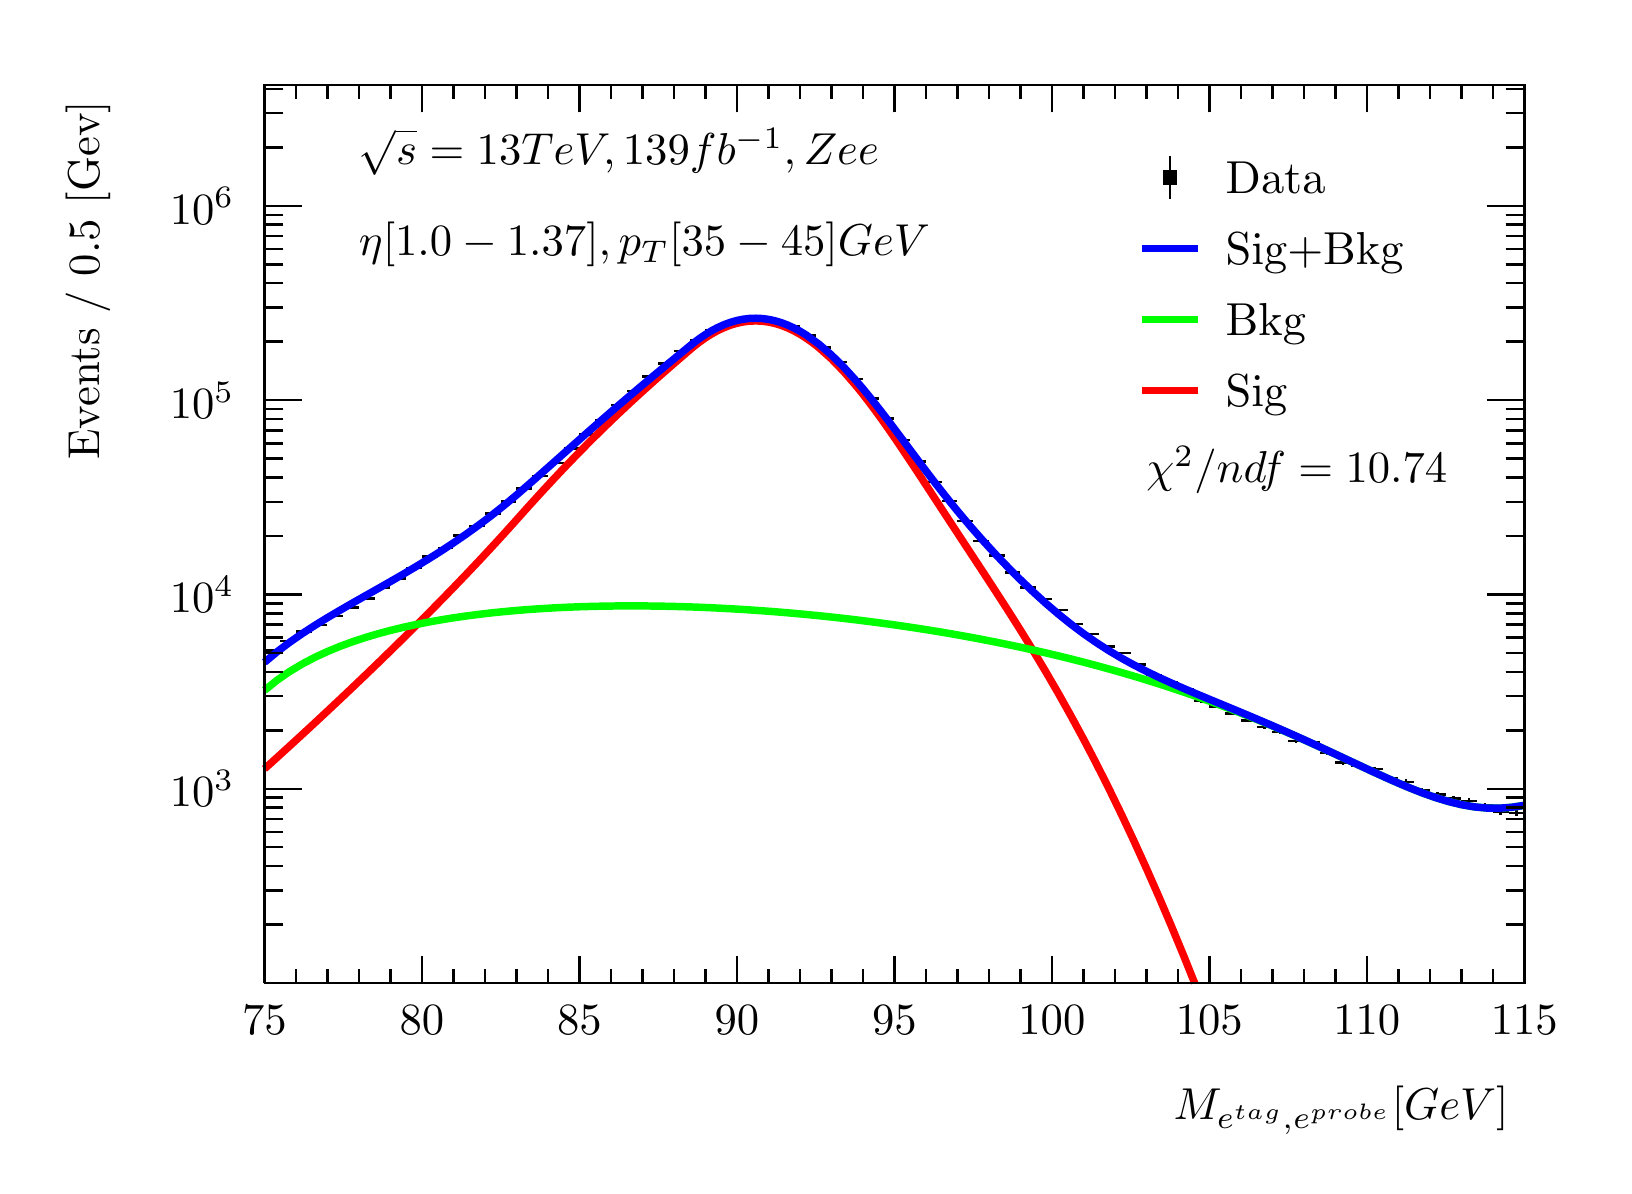
\begin{tikzpicture}
\pgfdeclareplotmark{cross} {
\pgfpathmoveto{\pgfpoint{-0.3\pgfplotmarksize}{\pgfplotmarksize}}
\pgfpathlineto{\pgfpoint{+0.3\pgfplotmarksize}{\pgfplotmarksize}}
\pgfpathlineto{\pgfpoint{+0.3\pgfplotmarksize}{0.3\pgfplotmarksize}}
\pgfpathlineto{\pgfpoint{+1\pgfplotmarksize}{0.3\pgfplotmarksize}}
\pgfpathlineto{\pgfpoint{+1\pgfplotmarksize}{-0.3\pgfplotmarksize}}
\pgfpathlineto{\pgfpoint{+0.3\pgfplotmarksize}{-0.3\pgfplotmarksize}}
\pgfpathlineto{\pgfpoint{+0.3\pgfplotmarksize}{-1.\pgfplotmarksize}}
\pgfpathlineto{\pgfpoint{-0.3\pgfplotmarksize}{-1.\pgfplotmarksize}}
\pgfpathlineto{\pgfpoint{-0.3\pgfplotmarksize}{-0.3\pgfplotmarksize}}
\pgfpathlineto{\pgfpoint{-1.\pgfplotmarksize}{-0.3\pgfplotmarksize}}
\pgfpathlineto{\pgfpoint{-1.\pgfplotmarksize}{0.3\pgfplotmarksize}}
\pgfpathlineto{\pgfpoint{-0.3\pgfplotmarksize}{0.3\pgfplotmarksize}}
\pgfpathclose
\pgfusepathqstroke
}
\pgfdeclareplotmark{cross*} {
\pgfpathmoveto{\pgfpoint{-0.3\pgfplotmarksize}{\pgfplotmarksize}}
\pgfpathlineto{\pgfpoint{+0.3\pgfplotmarksize}{\pgfplotmarksize}}
\pgfpathlineto{\pgfpoint{+0.3\pgfplotmarksize}{0.3\pgfplotmarksize}}
\pgfpathlineto{\pgfpoint{+1\pgfplotmarksize}{0.3\pgfplotmarksize}}
\pgfpathlineto{\pgfpoint{+1\pgfplotmarksize}{-0.3\pgfplotmarksize}}
\pgfpathlineto{\pgfpoint{+0.3\pgfplotmarksize}{-0.3\pgfplotmarksize}}
\pgfpathlineto{\pgfpoint{+0.3\pgfplotmarksize}{-1.\pgfplotmarksize}}
\pgfpathlineto{\pgfpoint{-0.3\pgfplotmarksize}{-1.\pgfplotmarksize}}
\pgfpathlineto{\pgfpoint{-0.3\pgfplotmarksize}{-0.3\pgfplotmarksize}}
\pgfpathlineto{\pgfpoint{-1.\pgfplotmarksize}{-0.3\pgfplotmarksize}}
\pgfpathlineto{\pgfpoint{-1.\pgfplotmarksize}{0.3\pgfplotmarksize}}
\pgfpathlineto{\pgfpoint{-0.3\pgfplotmarksize}{0.3\pgfplotmarksize}}
\pgfpathclose
\pgfusepathqfillstroke
}
\pgfdeclareplotmark{newstar} {
\pgfpathmoveto{\pgfqpoint{0pt}{\pgfplotmarksize}}
\pgfpathlineto{\pgfqpointpolar{44}{0.5\pgfplotmarksize}}
\pgfpathlineto{\pgfqpointpolar{18}{\pgfplotmarksize}}
\pgfpathlineto{\pgfqpointpolar{-20}{0.5\pgfplotmarksize}}
\pgfpathlineto{\pgfqpointpolar{-54}{\pgfplotmarksize}}
\pgfpathlineto{\pgfqpointpolar{-90}{0.5\pgfplotmarksize}}
\pgfpathlineto{\pgfqpointpolar{234}{\pgfplotmarksize}}
\pgfpathlineto{\pgfqpointpolar{198}{0.5\pgfplotmarksize}}
\pgfpathlineto{\pgfqpointpolar{162}{\pgfplotmarksize}}
\pgfpathlineto{\pgfqpointpolar{134}{0.5\pgfplotmarksize}}
\pgfpathclose
\pgfusepathqstroke
}
\pgfdeclareplotmark{newstar*} {
\pgfpathmoveto{\pgfqpoint{0pt}{\pgfplotmarksize}}
\pgfpathlineto{\pgfqpointpolar{44}{0.5\pgfplotmarksize}}
\pgfpathlineto{\pgfqpointpolar{18}{\pgfplotmarksize}}
\pgfpathlineto{\pgfqpointpolar{-20}{0.5\pgfplotmarksize}}
\pgfpathlineto{\pgfqpointpolar{-54}{\pgfplotmarksize}}
\pgfpathlineto{\pgfqpointpolar{-90}{0.5\pgfplotmarksize}}
\pgfpathlineto{\pgfqpointpolar{234}{\pgfplotmarksize}}
\pgfpathlineto{\pgfqpointpolar{198}{0.5\pgfplotmarksize}}
\pgfpathlineto{\pgfqpointpolar{162}{\pgfplotmarksize}}
\pgfpathlineto{\pgfqpointpolar{134}{0.5\pgfplotmarksize}}
\pgfpathclose
\pgfusepathqfillstroke
}
\definecolor{c}{rgb}{1,1,1};
\draw [color=c, fill=c] (0,0) rectangle (20,14.4361);
\draw [color=c, fill=c] (3,2.30977) rectangle (19,13.7143);
\definecolor{c}{rgb}{0,0,0};
\draw [c,line width=0.9] (3,2.30977) -- (3,13.7143) -- (19,13.7143) -- (19,2.30977) -- (3,2.30977);
\definecolor{c}{rgb}{1,1,1};
\draw [color=c, fill=c] (3,2.30977) rectangle (19,13.7143);
\definecolor{c}{rgb}{0,0,0};
\draw [c,line width=0.9] (3,2.30977) -- (3,13.7143) -- (19,13.7143) -- (19,2.30977) -- (3,2.30977);
\draw [c,line width=0.9] (3,2.30977) -- (19,2.30977);
\draw [c,line width=0.9] (3,2.65624) -- (3,2.30977);
\draw [c,line width=0.9] (3.4,2.48301) -- (3.4,2.30977);
\draw [c,line width=0.9] (3.8,2.48301) -- (3.8,2.30977);
\draw [c,line width=0.9] (4.2,2.48301) -- (4.2,2.30977);
\draw [c,line width=0.9] (4.6,2.48301) -- (4.6,2.30977);
\draw [c,line width=0.9] (5,2.65624) -- (5,2.30977);
\draw [c,line width=0.9] (5.4,2.48301) -- (5.4,2.30977);
\draw [c,line width=0.9] (5.8,2.48301) -- (5.8,2.30977);
\draw [c,line width=0.9] (6.2,2.48301) -- (6.2,2.30977);
\draw [c,line width=0.9] (6.6,2.48301) -- (6.6,2.30977);
\draw [c,line width=0.9] (7,2.65624) -- (7,2.30977);
\draw [c,line width=0.9] (7.4,2.48301) -- (7.4,2.30977);
\draw [c,line width=0.9] (7.8,2.48301) -- (7.8,2.30977);
\draw [c,line width=0.9] (8.2,2.48301) -- (8.2,2.30977);
\draw [c,line width=0.9] (8.6,2.48301) -- (8.6,2.30977);
\draw [c,line width=0.9] (9,2.65624) -- (9,2.30977);
\draw [c,line width=0.9] (9.4,2.48301) -- (9.4,2.30977);
\draw [c,line width=0.9] (9.8,2.48301) -- (9.8,2.30977);
\draw [c,line width=0.9] (10.2,2.48301) -- (10.2,2.30977);
\draw [c,line width=0.9] (10.6,2.48301) -- (10.6,2.30977);
\draw [c,line width=0.9] (11,2.65624) -- (11,2.30977);
\draw [c,line width=0.9] (11.4,2.48301) -- (11.4,2.30977);
\draw [c,line width=0.9] (11.8,2.48301) -- (11.8,2.30977);
\draw [c,line width=0.9] (12.2,2.48301) -- (12.2,2.30977);
\draw [c,line width=0.9] (12.6,2.48301) -- (12.6,2.30977);
\draw [c,line width=0.9] (13,2.65624) -- (13,2.30977);
\draw [c,line width=0.9] (13.4,2.48301) -- (13.4,2.30977);
\draw [c,line width=0.9] (13.8,2.48301) -- (13.8,2.30977);
\draw [c,line width=0.9] (14.2,2.48301) -- (14.2,2.30977);
\draw [c,line width=0.9] (14.6,2.48301) -- (14.6,2.30977);
\draw [c,line width=0.9] (15,2.65624) -- (15,2.30977);
\draw [c,line width=0.9] (15.4,2.48301) -- (15.4,2.30977);
\draw [c,line width=0.9] (15.8,2.48301) -- (15.8,2.30977);
\draw [c,line width=0.9] (16.2,2.48301) -- (16.2,2.30977);
\draw [c,line width=0.9] (16.6,2.48301) -- (16.6,2.30977);
\draw [c,line width=0.9] (17,2.65624) -- (17,2.30977);
\draw [c,line width=0.9] (17.4,2.48301) -- (17.4,2.30977);
\draw [c,line width=0.9] (17.8,2.48301) -- (17.8,2.30977);
\draw [c,line width=0.9] (18.2,2.48301) -- (18.2,2.30977);
\draw [c,line width=0.9] (18.6,2.48301) -- (18.6,2.30977);
\draw [c,line width=0.9] (19,2.65624) -- (19,2.30977);
\draw [c,line width=0.9] (19,2.65624) -- (19,2.30977);
\draw [anchor=base] (3,1.66015) node[scale=1.61424, color=c, rotate=0]{75};
\draw [anchor=base] (5,1.66015) node[scale=1.61424, color=c, rotate=0]{80};
\draw [anchor=base] (7,1.66015) node[scale=1.61424, color=c, rotate=0]{85};
\draw [anchor=base] (9,1.66015) node[scale=1.61424, color=c, rotate=0]{90};
\draw [anchor=base] (11,1.66015) node[scale=1.61424, color=c, rotate=0]{95};
\draw [anchor=base] (13,1.66015) node[scale=1.61424, color=c, rotate=0]{100};
\draw [anchor=base] (15,1.66015) node[scale=1.61424, color=c, rotate=0]{105};
\draw [anchor=base] (17,1.66015) node[scale=1.61424, color=c, rotate=0]{110};
\draw [anchor=base] (19,1.66015) node[scale=1.61424, color=c, rotate=0]{115};
\draw [anchor= east] (19,0.692932) node[scale=1.61424, color=c, rotate=0]{$M_{e^{tag}, e^{probe}}  [GeV]$};
\draw [c,line width=0.9] (3,13.7143) -- (19,13.7143);
\draw [c,line width=0.9] (3,13.3678) -- (3,13.7143);
\draw [c,line width=0.9] (3.4,13.5411) -- (3.4,13.7143);
\draw [c,line width=0.9] (3.8,13.5411) -- (3.8,13.7143);
\draw [c,line width=0.9] (4.2,13.5411) -- (4.2,13.7143);
\draw [c,line width=0.9] (4.6,13.5411) -- (4.6,13.7143);
\draw [c,line width=0.9] (5,13.3678) -- (5,13.7143);
\draw [c,line width=0.9] (5.4,13.5411) -- (5.4,13.7143);
\draw [c,line width=0.9] (5.8,13.5411) -- (5.8,13.7143);
\draw [c,line width=0.9] (6.2,13.5411) -- (6.2,13.7143);
\draw [c,line width=0.9] (6.6,13.5411) -- (6.6,13.7143);
\draw [c,line width=0.9] (7,13.3678) -- (7,13.7143);
\draw [c,line width=0.9] (7.4,13.5411) -- (7.4,13.7143);
\draw [c,line width=0.9] (7.8,13.5411) -- (7.8,13.7143);
\draw [c,line width=0.9] (8.2,13.5411) -- (8.2,13.7143);
\draw [c,line width=0.9] (8.6,13.5411) -- (8.6,13.7143);
\draw [c,line width=0.9] (9,13.3678) -- (9,13.7143);
\draw [c,line width=0.9] (9.4,13.5411) -- (9.4,13.7143);
\draw [c,line width=0.9] (9.8,13.5411) -- (9.8,13.7143);
\draw [c,line width=0.9] (10.2,13.5411) -- (10.2,13.7143);
\draw [c,line width=0.9] (10.6,13.5411) -- (10.6,13.7143);
\draw [c,line width=0.9] (11,13.3678) -- (11,13.7143);
\draw [c,line width=0.9] (11.4,13.5411) -- (11.4,13.7143);
\draw [c,line width=0.9] (11.8,13.5411) -- (11.8,13.7143);
\draw [c,line width=0.9] (12.2,13.5411) -- (12.2,13.7143);
\draw [c,line width=0.9] (12.6,13.5411) -- (12.6,13.7143);
\draw [c,line width=0.9] (13,13.3678) -- (13,13.7143);
\draw [c,line width=0.9] (13.4,13.5411) -- (13.4,13.7143);
\draw [c,line width=0.9] (13.8,13.5411) -- (13.8,13.7143);
\draw [c,line width=0.9] (14.2,13.5411) -- (14.2,13.7143);
\draw [c,line width=0.9] (14.6,13.5411) -- (14.6,13.7143);
\draw [c,line width=0.9] (15,13.3678) -- (15,13.7143);
\draw [c,line width=0.9] (15.4,13.5411) -- (15.4,13.7143);
\draw [c,line width=0.9] (15.8,13.5411) -- (15.8,13.7143);
\draw [c,line width=0.9] (16.2,13.5411) -- (16.2,13.7143);
\draw [c,line width=0.9] (16.6,13.5411) -- (16.6,13.7143);
\draw [c,line width=0.9] (17,13.3678) -- (17,13.7143);
\draw [c,line width=0.9] (17.4,13.5411) -- (17.4,13.7143);
\draw [c,line width=0.9] (17.8,13.5411) -- (17.8,13.7143);
\draw [c,line width=0.9] (18.2,13.5411) -- (18.2,13.7143);
\draw [c,line width=0.9] (18.6,13.5411) -- (18.6,13.7143);
\draw [c,line width=0.9] (19,13.3678) -- (19,13.7143);
\draw [c,line width=0.9] (19,13.3678) -- (19,13.7143);
\draw [c,line width=0.9] (3,2.30977) -- (3,13.7143);
\draw [c,line width=0.9] (3.237,3.05254) -- (3,3.05254);
\draw [c,line width=0.9] (3.237,3.48704) -- (3,3.48704);
\draw [c,line width=0.9] (3.237,3.79531) -- (3,3.79531);
\draw [c,line width=0.9] (3.237,4.03443) -- (3,4.03443);
\draw [c,line width=0.9] (3.237,4.22981) -- (3,4.22981);
\draw [c,line width=0.9] (3.237,4.395) -- (3,4.395);
\draw [c,line width=0.9] (3.237,4.53809) -- (3,4.53809);
\draw [c,line width=0.9] (3.237,4.6643) -- (3,4.6643);
\draw [c,line width=0.9] (3.474,4.77721) -- (3,4.77721);
\draw [anchor= east] (2.82,4.77721) node[scale=1.61424, color=c, rotate=0]{$10^{3}$};
\draw [c,line width=0.9] (3.237,5.51998) -- (3,5.51998);
\draw [c,line width=0.9] (3.237,5.95447) -- (3,5.95447);
\draw [c,line width=0.9] (3.237,6.26275) -- (3,6.26275);
\draw [c,line width=0.9] (3.237,6.50187) -- (3,6.50187);
\draw [c,line width=0.9] (3.237,6.69724) -- (3,6.69724);
\draw [c,line width=0.9] (3.237,6.86243) -- (3,6.86243);
\draw [c,line width=0.9] (3.237,7.00552) -- (3,7.00552);
\draw [c,line width=0.9] (3.237,7.13174) -- (3,7.13174);
\draw [c,line width=0.9] (3.474,7.24464) -- (3,7.24464);
\draw [anchor= east] (2.82,7.24464) node[scale=1.61424, color=c, rotate=0]{$10^{4}$};
\draw [c,line width=0.9] (3.237,7.98741) -- (3,7.98741);
\draw [c,line width=0.9] (3.237,8.4219) -- (3,8.4219);
\draw [c,line width=0.9] (3.237,8.73018) -- (3,8.73018);
\draw [c,line width=0.9] (3.237,8.9693) -- (3,8.9693);
\draw [c,line width=0.9] (3.237,9.16467) -- (3,9.16467);
\draw [c,line width=0.9] (3.237,9.32986) -- (3,9.32986);
\draw [c,line width=0.9] (3.237,9.47295) -- (3,9.47295);
\draw [c,line width=0.9] (3.237,9.59917) -- (3,9.59917);
\draw [c,line width=0.9] (3.474,9.71207) -- (3,9.71207);
\draw [anchor= east] (2.82,9.71207) node[scale=1.61424, color=c, rotate=0]{$10^{5}$};
\draw [c,line width=0.9] (3.237,10.4548) -- (3,10.4548);
\draw [c,line width=0.9] (3.237,10.8893) -- (3,10.8893);
\draw [c,line width=0.9] (3.237,11.1976) -- (3,11.1976);
\draw [c,line width=0.9] (3.237,11.4367) -- (3,11.4367);
\draw [c,line width=0.9] (3.237,11.6321) -- (3,11.6321);
\draw [c,line width=0.9] (3.237,11.7973) -- (3,11.7973);
\draw [c,line width=0.9] (3.237,11.9404) -- (3,11.9404);
\draw [c,line width=0.9] (3.237,12.0666) -- (3,12.0666);
\draw [c,line width=0.9] (3.474,12.1795) -- (3,12.1795);
\draw [anchor= east] (2.82,12.1795) node[scale=1.61424, color=c, rotate=0]{$10^{6}$};
\draw [c,line width=0.9] (3.237,12.9223) -- (3,12.9223);
\draw [c,line width=0.9] (3.237,13.3568) -- (3,13.3568);
\draw [c,line width=0.9] (3.237,13.665) -- (3,13.665);
\draw [anchor= east] (0.76,13.7143) node[scale=1.61424, color=c, rotate=90]{Events / 0.5 [Gev]};
\draw [c,line width=0.9] (19,2.30977) -- (19,13.7143);
\draw [c,line width=0.9] (18.763,3.05254) -- (19,3.05254);
\draw [c,line width=0.9] (18.763,3.48704) -- (19,3.48704);
\draw [c,line width=0.9] (18.763,3.79531) -- (19,3.79531);
\draw [c,line width=0.9] (18.763,4.03443) -- (19,4.03443);
\draw [c,line width=0.9] (18.763,4.22981) -- (19,4.22981);
\draw [c,line width=0.9] (18.763,4.395) -- (19,4.395);
\draw [c,line width=0.9] (18.763,4.53809) -- (19,4.53809);
\draw [c,line width=0.9] (18.763,4.6643) -- (19,4.6643);
\draw [c,line width=0.9] (18.526,4.77721) -- (19,4.77721);
\draw [c,line width=0.9] (18.763,5.51998) -- (19,5.51998);
\draw [c,line width=0.9] (18.763,5.95447) -- (19,5.95447);
\draw [c,line width=0.9] (18.763,6.26275) -- (19,6.26275);
\draw [c,line width=0.9] (18.763,6.50187) -- (19,6.50187);
\draw [c,line width=0.9] (18.763,6.69724) -- (19,6.69724);
\draw [c,line width=0.9] (18.763,6.86243) -- (19,6.86243);
\draw [c,line width=0.9] (18.763,7.00552) -- (19,7.00552);
\draw [c,line width=0.9] (18.763,7.13174) -- (19,7.13174);
\draw [c,line width=0.9] (18.526,7.24464) -- (19,7.24464);
\draw [c,line width=0.9] (18.763,7.98741) -- (19,7.98741);
\draw [c,line width=0.9] (18.763,8.4219) -- (19,8.4219);
\draw [c,line width=0.9] (18.763,8.73018) -- (19,8.73018);
\draw [c,line width=0.9] (18.763,8.9693) -- (19,8.9693);
\draw [c,line width=0.9] (18.763,9.16467) -- (19,9.16467);
\draw [c,line width=0.9] (18.763,9.32986) -- (19,9.32986);
\draw [c,line width=0.9] (18.763,9.47295) -- (19,9.47295);
\draw [c,line width=0.9] (18.763,9.59917) -- (19,9.59917);
\draw [c,line width=0.9] (18.526,9.71207) -- (19,9.71207);
\draw [c,line width=0.9] (18.763,10.4548) -- (19,10.4548);
\draw [c,line width=0.9] (18.763,10.8893) -- (19,10.8893);
\draw [c,line width=0.9] (18.763,11.1976) -- (19,11.1976);
\draw [c,line width=0.9] (18.763,11.4367) -- (19,11.4367);
\draw [c,line width=0.9] (18.763,11.6321) -- (19,11.6321);
\draw [c,line width=0.9] (18.763,11.7973) -- (19,11.7973);
\draw [c,line width=0.9] (18.763,11.9404) -- (19,11.9404);
\draw [c,line width=0.9] (18.763,12.0666) -- (19,12.0666);
\draw [c,line width=0.9] (18.526,12.1795) -- (19,12.1795);
\draw [c,line width=0.9] (18.763,12.9223) -- (19,12.9223);
\draw [c,line width=0.9] (18.763,13.3568) -- (19,13.3568);
\draw [c,line width=0.9] (18.763,13.665) -- (19,13.665);
\draw [c,line width=0.9] (3.1,6.53084) -- (3,6.53084);
\draw [c,line width=0.9] (3,6.53084) -- (3,6.53084);
\draw [c,line width=0.9] (3.1,6.53084) -- (3.2,6.53084);
\draw [c,line width=0.9] (3.2,6.53084) -- (3.2,6.53084);
\draw [c,line width=0.9] (3.1,6.53084) -- (3.1,6.54579);
\draw [c,line width=0.9] (3.1,6.54579) -- (3.1,6.54579);
\draw [c,line width=0.9] (3.1,6.53084) -- (3.1,6.51588);
\draw [c,line width=0.9] (3.1,6.51588) -- (3.1,6.51588);
\draw [c,line width=0.9] (3.3,6.65629) -- (3.2,6.65629);
\draw [c,line width=0.9] (3.2,6.65629) -- (3.2,6.65629);
\draw [c,line width=0.9] (3.3,6.65629) -- (3.4,6.65629);
\draw [c,line width=0.9] (3.4,6.65629) -- (3.4,6.65629);
\draw [c,line width=0.9] (3.3,6.65629) -- (3.3,6.67039);
\draw [c,line width=0.9] (3.3,6.67039) -- (3.3,6.67039);
\draw [c,line width=0.9] (3.3,6.65629) -- (3.3,6.64218);
\draw [c,line width=0.9] (3.3,6.64218) -- (3.3,6.64218);
\draw [c,line width=0.9] (3.5,6.77657) -- (3.4,6.77657);
\draw [c,line width=0.9] (3.4,6.77657) -- (3.4,6.77657);
\draw [c,line width=0.9] (3.5,6.77657) -- (3.6,6.77657);
\draw [c,line width=0.9] (3.6,6.77657) -- (3.6,6.77657);
\draw [c,line width=0.9] (3.5,6.77657) -- (3.5,6.7899);
\draw [c,line width=0.9] (3.5,6.7899) -- (3.5,6.7899);
\draw [c,line width=0.9] (3.5,6.77657) -- (3.5,6.76324);
\draw [c,line width=0.9] (3.5,6.76324) -- (3.5,6.76324);
\draw [c,line width=0.9] (3.7,6.85783) -- (3.6,6.85783);
\draw [c,line width=0.9] (3.6,6.85783) -- (3.6,6.85783);
\draw [c,line width=0.9] (3.7,6.85783) -- (3.8,6.85783);
\draw [c,line width=0.9] (3.8,6.85783) -- (3.8,6.85783);
\draw [c,line width=0.9] (3.7,6.85783) -- (3.7,6.87066);
\draw [c,line width=0.9] (3.7,6.87066) -- (3.7,6.87066);
\draw [c,line width=0.9] (3.7,6.85783) -- (3.7,6.84499);
\draw [c,line width=0.9] (3.7,6.84499) -- (3.7,6.84499);
\draw [c,line width=0.9] (3.9,6.97426) -- (3.8,6.97426);
\draw [c,line width=0.9] (3.8,6.97426) -- (3.8,6.97426);
\draw [c,line width=0.9] (3.9,6.97426) -- (4,6.97426);
\draw [c,line width=0.9] (4,6.97426) -- (4,6.97426);
\draw [c,line width=0.9] (3.9,6.97426) -- (3.9,6.98642);
\draw [c,line width=0.9] (3.9,6.98642) -- (3.9,6.98642);
\draw [c,line width=0.9] (3.9,6.97426) -- (3.9,6.9621);
\draw [c,line width=0.9] (3.9,6.9621) -- (3.9,6.9621);
\draw [c,line width=0.9] (4.1,7.07965) -- (4,7.07965);
\draw [c,line width=0.9] (4,7.07965) -- (4,7.07965);
\draw [c,line width=0.9] (4.1,7.07965) -- (4.2,7.07965);
\draw [c,line width=0.9] (4.2,7.07965) -- (4.2,7.07965);
\draw [c,line width=0.9] (4.1,7.07965) -- (4.1,7.09122);
\draw [c,line width=0.9] (4.1,7.09122) -- (4.1,7.09122);
\draw [c,line width=0.9] (4.1,7.07965) -- (4.1,7.06808);
\draw [c,line width=0.9] (4.1,7.06808) -- (4.1,7.06808);
\draw [c,line width=0.9] (4.3,7.19249) -- (4.2,7.19249);
\draw [c,line width=0.9] (4.2,7.19249) -- (4.2,7.19249);
\draw [c,line width=0.9] (4.3,7.19249) -- (4.4,7.19249);
\draw [c,line width=0.9] (4.4,7.19249) -- (4.4,7.19249);
\draw [c,line width=0.9] (4.3,7.19249) -- (4.3,7.20347);
\draw [c,line width=0.9] (4.3,7.20347) -- (4.3,7.20347);
\draw [c,line width=0.9] (4.3,7.19249) -- (4.3,7.18151);
\draw [c,line width=0.9] (4.3,7.18151) -- (4.3,7.18151);
\draw [c,line width=0.9] (4.5,7.33186) -- (4.4,7.33186);
\draw [c,line width=0.9] (4.4,7.33186) -- (4.4,7.33186);
\draw [c,line width=0.9] (4.5,7.33186) -- (4.6,7.33186);
\draw [c,line width=0.9] (4.6,7.33186) -- (4.6,7.33186);
\draw [c,line width=0.9] (4.5,7.33186) -- (4.5,7.34215);
\draw [c,line width=0.9] (4.5,7.34215) -- (4.5,7.34215);
\draw [c,line width=0.9] (4.5,7.33186) -- (4.5,7.32157);
\draw [c,line width=0.9] (4.5,7.32157) -- (4.5,7.32157);
\draw [c,line width=0.9] (4.7,7.44997) -- (4.6,7.44997);
\draw [c,line width=0.9] (4.6,7.44997) -- (4.6,7.44997);
\draw [c,line width=0.9] (4.7,7.44997) -- (4.8,7.44997);
\draw [c,line width=0.9] (4.8,7.44997) -- (4.8,7.44997);
\draw [c,line width=0.9] (4.7,7.44997) -- (4.7,7.45971);
\draw [c,line width=0.9] (4.7,7.45971) -- (4.7,7.45971);
\draw [c,line width=0.9] (4.7,7.44997) -- (4.7,7.44023);
\draw [c,line width=0.9] (4.7,7.44023) -- (4.7,7.44023);
\draw [c,line width=0.9] (4.9,7.57917) -- (4.8,7.57917);
\draw [c,line width=0.9] (4.8,7.57917) -- (4.8,7.57917);
\draw [c,line width=0.9] (4.9,7.57917) -- (5,7.57917);
\draw [c,line width=0.9] (5,7.57917) -- (5,7.57917);
\draw [c,line width=0.9] (4.9,7.57917) -- (4.9,7.58834);
\draw [c,line width=0.9] (4.9,7.58834) -- (4.9,7.58834);
\draw [c,line width=0.9] (4.9,7.57917) -- (4.9,7.57);
\draw [c,line width=0.9] (4.9,7.57) -- (4.9,7.57);
\draw [c,line width=0.9] (5.1,7.72896) -- (5,7.72896);
\draw [c,line width=0.9] (5,7.72896) -- (5,7.72896);
\draw [c,line width=0.9] (5.1,7.72896) -- (5.2,7.72896);
\draw [c,line width=0.9] (5.2,7.72896) -- (5.2,7.72896);
\draw [c,line width=0.9] (5.1,7.72896) -- (5.1,7.73751);
\draw [c,line width=0.9] (5.1,7.73751) -- (5.1,7.73751);
\draw [c,line width=0.9] (5.1,7.72896) -- (5.1,7.72042);
\draw [c,line width=0.9] (5.1,7.72042) -- (5.1,7.72042);
\draw [c,line width=0.9] (5.3,7.83275) -- (5.2,7.83275);
\draw [c,line width=0.9] (5.2,7.83275) -- (5.2,7.83275);
\draw [c,line width=0.9] (5.3,7.83275) -- (5.4,7.83275);
\draw [c,line width=0.9] (5.4,7.83275) -- (5.4,7.83275);
\draw [c,line width=0.9] (5.3,7.83275) -- (5.3,7.84089);
\draw [c,line width=0.9] (5.3,7.84089) -- (5.3,7.84089);
\draw [c,line width=0.9] (5.3,7.83275) -- (5.3,7.8246);
\draw [c,line width=0.9] (5.3,7.8246) -- (5.3,7.8246);
\draw [c,line width=0.9] (5.5,7.99542) -- (5.4,7.99542);
\draw [c,line width=0.9] (5.4,7.99542) -- (5.4,7.99542);
\draw [c,line width=0.9] (5.5,7.99542) -- (5.6,7.99542);
\draw [c,line width=0.9] (5.6,7.99542) -- (5.6,7.99542);
\draw [c,line width=0.9] (5.5,7.99542) -- (5.5,8.00297);
\draw [c,line width=0.9] (5.5,8.00297) -- (5.5,8.00297);
\draw [c,line width=0.9] (5.5,7.99542) -- (5.5,7.98787);
\draw [c,line width=0.9] (5.5,7.98787) -- (5.5,7.98787);
\draw [c,line width=0.9] (5.7,8.1162) -- (5.6,8.1162);
\draw [c,line width=0.9] (5.6,8.1162) -- (5.6,8.1162);
\draw [c,line width=0.9] (5.7,8.1162) -- (5.8,8.1162);
\draw [c,line width=0.9] (5.8,8.1162) -- (5.8,8.1162);
\draw [c,line width=0.9] (5.7,8.1162) -- (5.7,8.12333);
\draw [c,line width=0.9] (5.7,8.12333) -- (5.7,8.12333);
\draw [c,line width=0.9] (5.7,8.1162) -- (5.7,8.10906);
\draw [c,line width=0.9] (5.7,8.10906) -- (5.7,8.10906);
\draw [c,line width=0.9] (5.9,8.27538) -- (5.8,8.27538);
\draw [c,line width=0.9] (5.8,8.27538) -- (5.8,8.27538);
\draw [c,line width=0.9] (5.9,8.27538) -- (6,8.27538);
\draw [c,line width=0.9] (6,8.27538) -- (6,8.27538);
\draw [c,line width=0.9] (5.9,8.27538) -- (5.9,8.282);
\draw [c,line width=0.9] (5.9,8.282) -- (5.9,8.282);
\draw [c,line width=0.9] (5.9,8.27538) -- (5.9,8.26875);
\draw [c,line width=0.9] (5.9,8.26875) -- (5.9,8.26875);
\draw [c,line width=0.9] (6.1,8.42547) -- (6,8.42547);
\draw [c,line width=0.9] (6,8.42547) -- (6,8.42547);
\draw [c,line width=0.9] (6.1,8.42547) -- (6.2,8.42547);
\draw [c,line width=0.9] (6.2,8.42547) -- (6.2,8.42547);
\draw [c,line width=0.9] (6.1,8.42547) -- (6.1,8.43165);
\draw [c,line width=0.9] (6.1,8.43165) -- (6.1,8.43165);
\draw [c,line width=0.9] (6.1,8.42547) -- (6.1,8.41929);
\draw [c,line width=0.9] (6.1,8.41929) -- (6.1,8.41929);
\draw [c,line width=0.9] (6.3,8.58807) -- (6.2,8.58807);
\draw [c,line width=0.9] (6.2,8.58807) -- (6.2,8.58807);
\draw [c,line width=0.9] (6.3,8.58807) -- (6.4,8.58807);
\draw [c,line width=0.9] (6.4,8.58807) -- (6.4,8.58807);
\draw [c,line width=0.9] (6.3,8.58807) -- (6.3,8.5938);
\draw [c,line width=0.9] (6.3,8.5938) -- (6.3,8.5938);
\draw [c,line width=0.9] (6.3,8.58807) -- (6.3,8.58235);
\draw [c,line width=0.9] (6.3,8.58235) -- (6.3,8.58235);
\draw [c,line width=0.9] (6.5,8.75125) -- (6.4,8.75125);
\draw [c,line width=0.9] (6.4,8.75125) -- (6.4,8.75125);
\draw [c,line width=0.9] (6.5,8.75125) -- (6.6,8.75125);
\draw [c,line width=0.9] (6.6,8.75125) -- (6.6,8.75125);
\draw [c,line width=0.9] (6.5,8.75125) -- (6.5,8.75655);
\draw [c,line width=0.9] (6.5,8.75655) -- (6.5,8.75655);
\draw [c,line width=0.9] (6.5,8.75125) -- (6.5,8.74594);
\draw [c,line width=0.9] (6.5,8.74594) -- (6.5,8.74594);
\draw [c,line width=0.9] (6.7,8.91452) -- (6.6,8.91452);
\draw [c,line width=0.9] (6.6,8.91452) -- (6.6,8.91452);
\draw [c,line width=0.9] (6.7,8.91452) -- (6.8,8.91452);
\draw [c,line width=0.9] (6.8,8.91452) -- (6.8,8.91452);
\draw [c,line width=0.9] (6.7,8.91452) -- (6.7,8.91943);
\draw [c,line width=0.9] (6.7,8.91943) -- (6.7,8.91943);
\draw [c,line width=0.9] (6.7,8.91452) -- (6.7,8.9096);
\draw [c,line width=0.9] (6.7,8.9096) -- (6.7,8.9096);
\draw [c,line width=0.9] (6.9,9.09721) -- (6.8,9.09721);
\draw [c,line width=0.9] (6.8,9.09721) -- (6.8,9.09721);
\draw [c,line width=0.9] (6.9,9.09721) -- (7,9.09721);
\draw [c,line width=0.9] (7,9.09721) -- (7,9.09721);
\draw [c,line width=0.9] (6.9,9.09721) -- (6.9,9.10173);
\draw [c,line width=0.9] (6.9,9.10173) -- (6.9,9.10173);
\draw [c,line width=0.9] (6.9,9.09721) -- (6.9,9.0927);
\draw [c,line width=0.9] (6.9,9.0927) -- (6.9,9.0927);
\draw [c,line width=0.9] (7.1,9.27594) -- (7,9.27594);
\draw [c,line width=0.9] (7,9.27594) -- (7,9.27594);
\draw [c,line width=0.9] (7.1,9.27594) -- (7.2,9.27594);
\draw [c,line width=0.9] (7.2,9.27594) -- (7.2,9.27594);
\draw [c,line width=0.9] (7.1,9.27594) -- (7.1,9.2801);
\draw [c,line width=0.9] (7.1,9.2801) -- (7.1,9.2801);
\draw [c,line width=0.9] (7.1,9.27594) -- (7.1,9.27179);
\draw [c,line width=0.9] (7.1,9.27179) -- (7.1,9.27179);
\draw [c,line width=0.9] (7.3,9.46213) -- (7.2,9.46213);
\draw [c,line width=0.9] (7.2,9.46213) -- (7.2,9.46213);
\draw [c,line width=0.9] (7.3,9.46213) -- (7.4,9.46213);
\draw [c,line width=0.9] (7.4,9.46213) -- (7.4,9.46213);
\draw [c,line width=0.9] (7.3,9.46213) -- (7.3,9.46594);
\draw [c,line width=0.9] (7.3,9.46594) -- (7.3,9.46594);
\draw [c,line width=0.9] (7.3,9.46213) -- (7.3,9.45832);
\draw [c,line width=0.9] (7.3,9.45832) -- (7.3,9.45832);
\draw [c,line width=0.9] (7.5,9.64927) -- (7.4,9.64927);
\draw [c,line width=0.9] (7.4,9.64927) -- (7.4,9.64927);
\draw [c,line width=0.9] (7.5,9.64927) -- (7.6,9.64927);
\draw [c,line width=0.9] (7.6,9.64927) -- (7.6,9.64927);
\draw [c,line width=0.9] (7.5,9.64927) -- (7.5,9.65276);
\draw [c,line width=0.9] (7.5,9.65276) -- (7.5,9.65276);
\draw [c,line width=0.9] (7.5,9.64927) -- (7.5,9.64578);
\draw [c,line width=0.9] (7.5,9.64578) -- (7.5,9.64578);
\draw [c,line width=0.9] (7.7,9.82762) -- (7.6,9.82762);
\draw [c,line width=0.9] (7.6,9.82762) -- (7.6,9.82762);
\draw [c,line width=0.9] (7.7,9.82762) -- (7.8,9.82762);
\draw [c,line width=0.9] (7.8,9.82762) -- (7.8,9.82762);
\draw [c,line width=0.9] (7.7,9.82762) -- (7.7,9.83084);
\draw [c,line width=0.9] (7.7,9.83084) -- (7.7,9.83084);
\draw [c,line width=0.9] (7.7,9.82762) -- (7.7,9.82441);
\draw [c,line width=0.9] (7.7,9.82441) -- (7.7,9.82441);
\draw [c,line width=0.9] (7.9,10.0153) -- (7.8,10.0153);
\draw [c,line width=0.9] (7.8,10.0153) -- (7.8,10.0153);
\draw [c,line width=0.9] (7.9,10.0153) -- (8,10.0153);
\draw [c,line width=0.9] (8,10.0153) -- (8,10.0153);
\draw [c,line width=0.9] (7.9,10.0153) -- (7.9,10.0183);
\draw [c,line width=0.9] (7.9,10.0183) -- (7.9,10.0183);
\draw [c,line width=0.9] (7.9,10.0153) -- (7.9,10.0124);
\draw [c,line width=0.9] (7.9,10.0124) -- (7.9,10.0124);
\draw [c,line width=0.9] (8.1,10.1796) -- (8,10.1796);
\draw [c,line width=0.9] (8,10.1796) -- (8,10.1796);
\draw [c,line width=0.9] (8.1,10.1796) -- (8.2,10.1796);
\draw [c,line width=0.9] (8.2,10.1796) -- (8.2,10.1796);
\draw [c,line width=0.9] (8.1,10.1796) -- (8.1,10.1823);
\draw [c,line width=0.9] (8.1,10.1823) -- (8.1,10.1823);
\draw [c,line width=0.9] (8.1,10.1796) -- (8.1,10.1768);
\draw [c,line width=0.9] (8.1,10.1768) -- (8.1,10.1768);
\draw [c,line width=0.9] (8.3,10.3392) -- (8.2,10.3392);
\draw [c,line width=0.9] (8.2,10.3392) -- (8.2,10.3392);
\draw [c,line width=0.9] (8.3,10.3392) -- (8.4,10.3392);
\draw [c,line width=0.9] (8.4,10.3392) -- (8.4,10.3392);
\draw [c,line width=0.9] (8.3,10.3392) -- (8.3,10.3417);
\draw [c,line width=0.9] (8.3,10.3417) -- (8.3,10.3417);
\draw [c,line width=0.9] (8.3,10.3392) -- (8.3,10.3366);
\draw [c,line width=0.9] (8.3,10.3366) -- (8.3,10.3366);
\draw [c,line width=0.9] (8.5,10.477) -- (8.4,10.477);
\draw [c,line width=0.9] (8.4,10.477) -- (8.4,10.477);
\draw [c,line width=0.9] (8.5,10.477) -- (8.6,10.477);
\draw [c,line width=0.9] (8.6,10.477) -- (8.6,10.477);
\draw [c,line width=0.9] (8.5,10.477) -- (8.5,10.4794);
\draw [c,line width=0.9] (8.5,10.4794) -- (8.5,10.4794);
\draw [c,line width=0.9] (8.5,10.477) -- (8.5,10.4746);
\draw [c,line width=0.9] (8.5,10.4746) -- (8.5,10.4746);
\draw [c,line width=0.9] (8.7,10.5944) -- (8.6,10.5944);
\draw [c,line width=0.9] (8.6,10.5944) -- (8.6,10.5944);
\draw [c,line width=0.9] (8.7,10.5944) -- (8.8,10.5944);
\draw [c,line width=0.9] (8.8,10.5944) -- (8.8,10.5944);
\draw [c,line width=0.9] (8.7,10.5944) -- (8.7,10.5966);
\draw [c,line width=0.9] (8.7,10.5966) -- (8.7,10.5966);
\draw [c,line width=0.9] (8.7,10.5944) -- (8.7,10.5921);
\draw [c,line width=0.9] (8.7,10.5921) -- (8.7,10.5921);
\draw [c,line width=0.9] (8.9,10.6837) -- (8.8,10.6837);
\draw [c,line width=0.9] (8.8,10.6837) -- (8.8,10.6837);
\draw [c,line width=0.9] (8.9,10.6837) -- (9,10.6837);
\draw [c,line width=0.9] (9,10.6837) -- (9,10.6837);
\draw [c,line width=0.9] (8.9,10.6837) -- (8.9,10.6858);
\draw [c,line width=0.9] (8.9,10.6858) -- (8.9,10.6858);
\draw [c,line width=0.9] (8.9,10.6837) -- (8.9,10.6815);
\draw [c,line width=0.9] (8.9,10.6815) -- (8.9,10.6815);
\draw [c,line width=0.9] (9.1,10.7295) -- (9,10.7295);
\draw [c,line width=0.9] (9,10.7295) -- (9,10.7295);
\draw [c,line width=0.9] (9.1,10.7295) -- (9.2,10.7295);
\draw [c,line width=0.9] (9.2,10.7295) -- (9.2,10.7295);
\draw [c,line width=0.9] (9.1,10.7295) -- (9.1,10.7317);
\draw [c,line width=0.9] (9.1,10.7317) -- (9.1,10.7317);
\draw [c,line width=0.9] (9.1,10.7295) -- (9.1,10.7274);
\draw [c,line width=0.9] (9.1,10.7274) -- (9.1,10.7274);
\draw [c,line width=0.9] (9.3,10.743) -- (9.2,10.743);
\draw [c,line width=0.9] (9.2,10.743) -- (9.2,10.743);
\draw [c,line width=0.9] (9.3,10.743) -- (9.4,10.743);
\draw [c,line width=0.9] (9.4,10.743) -- (9.4,10.743);
\draw [c,line width=0.9] (9.3,10.743) -- (9.3,10.7451);
\draw [c,line width=0.9] (9.3,10.7451) -- (9.3,10.7451);
\draw [c,line width=0.9] (9.3,10.743) -- (9.3,10.741);
\draw [c,line width=0.9] (9.3,10.741) -- (9.3,10.741);
\draw [c,line width=0.9] (9.5,10.7145) -- (9.4,10.7145);
\draw [c,line width=0.9] (9.4,10.7145) -- (9.4,10.7145);
\draw [c,line width=0.9] (9.5,10.7145) -- (9.6,10.7145);
\draw [c,line width=0.9] (9.6,10.7145) -- (9.6,10.7145);
\draw [c,line width=0.9] (9.5,10.7145) -- (9.5,10.7166);
\draw [c,line width=0.9] (9.5,10.7166) -- (9.5,10.7166);
\draw [c,line width=0.9] (9.5,10.7145) -- (9.5,10.7124);
\draw [c,line width=0.9] (9.5,10.7124) -- (9.5,10.7124);
\draw [c,line width=0.9] (9.7,10.6478) -- (9.6,10.6478);
\draw [c,line width=0.9] (9.6,10.6478) -- (9.6,10.6478);
\draw [c,line width=0.9] (9.7,10.6478) -- (9.8,10.6478);
\draw [c,line width=0.9] (9.8,10.6478) -- (9.8,10.6478);
\draw [c,line width=0.9] (9.7,10.6478) -- (9.7,10.6499);
\draw [c,line width=0.9] (9.7,10.6499) -- (9.7,10.6499);
\draw [c,line width=0.9] (9.7,10.6478) -- (9.7,10.6456);
\draw [c,line width=0.9] (9.7,10.6456) -- (9.7,10.6456);
\draw [c,line width=0.9] (9.9,10.5347) -- (9.8,10.5347);
\draw [c,line width=0.9] (9.8,10.5347) -- (9.8,10.5347);
\draw [c,line width=0.9] (9.9,10.5347) -- (10,10.5347);
\draw [c,line width=0.9] (10,10.5347) -- (10,10.5347);
\draw [c,line width=0.9] (9.9,10.5347) -- (9.9,10.5371);
\draw [c,line width=0.9] (9.9,10.5371) -- (9.9,10.5371);
\draw [c,line width=0.9] (9.9,10.5347) -- (9.9,10.5324);
\draw [c,line width=0.9] (9.9,10.5324) -- (9.9,10.5324);
\draw [c,line width=0.9] (10.1,10.3841) -- (10,10.3841);
\draw [c,line width=0.9] (10,10.3841) -- (10,10.3841);
\draw [c,line width=0.9] (10.1,10.3841) -- (10.2,10.3841);
\draw [c,line width=0.9] (10.2,10.3841) -- (10.2,10.3841);
\draw [c,line width=0.9] (10.1,10.3841) -- (10.1,10.3865);
\draw [c,line width=0.9] (10.1,10.3865) -- (10.1,10.3865);
\draw [c,line width=0.9] (10.1,10.3841) -- (10.1,10.3816);
\draw [c,line width=0.9] (10.1,10.3816) -- (10.1,10.3816);
\draw [c,line width=0.9] (10.3,10.1974) -- (10.2,10.1974);
\draw [c,line width=0.9] (10.2,10.1974) -- (10.2,10.1974);
\draw [c,line width=0.9] (10.3,10.1974) -- (10.4,10.1974);
\draw [c,line width=0.9] (10.4,10.1974) -- (10.4,10.1974);
\draw [c,line width=0.9] (10.3,10.1974) -- (10.3,10.2001);
\draw [c,line width=0.9] (10.3,10.2001) -- (10.3,10.2001);
\draw [c,line width=0.9] (10.3,10.1974) -- (10.3,10.1947);
\draw [c,line width=0.9] (10.3,10.1947) -- (10.3,10.1947);
\draw [c,line width=0.9] (10.5,9.97898) -- (10.4,9.97898);
\draw [c,line width=0.9] (10.4,9.97898) -- (10.4,9.97898);
\draw [c,line width=0.9] (10.5,9.97898) -- (10.6,9.97898);
\draw [c,line width=0.9] (10.6,9.97898) -- (10.6,9.97898);
\draw [c,line width=0.9] (10.5,9.97898) -- (10.5,9.98197);
\draw [c,line width=0.9] (10.5,9.98197) -- (10.5,9.98197);
\draw [c,line width=0.9] (10.5,9.97898) -- (10.5,9.97599);
\draw [c,line width=0.9] (10.5,9.97599) -- (10.5,9.97599);
\draw [c,line width=0.9] (10.7,9.73439) -- (10.6,9.73439);
\draw [c,line width=0.9] (10.6,9.73439) -- (10.6,9.73439);
\draw [c,line width=0.9] (10.7,9.73439) -- (10.8,9.73439);
\draw [c,line width=0.9] (10.8,9.73439) -- (10.8,9.73439);
\draw [c,line width=0.9] (10.7,9.73439) -- (10.7,9.73774);
\draw [c,line width=0.9] (10.7,9.73774) -- (10.7,9.73774);
\draw [c,line width=0.9] (10.7,9.73439) -- (10.7,9.73103);
\draw [c,line width=0.9] (10.7,9.73103) -- (10.7,9.73103);
\draw [c,line width=0.9] (10.9,9.47883) -- (10.8,9.47883);
\draw [c,line width=0.9] (10.8,9.47883) -- (10.8,9.47883);
\draw [c,line width=0.9] (10.9,9.47883) -- (11,9.47883);
\draw [c,line width=0.9] (11,9.47883) -- (11,9.47883);
\draw [c,line width=0.9] (10.9,9.47883) -- (10.9,9.48261);
\draw [c,line width=0.9] (10.9,9.48261) -- (10.9,9.48261);
\draw [c,line width=0.9] (10.9,9.47883) -- (10.9,9.47505);
\draw [c,line width=0.9] (10.9,9.47505) -- (10.9,9.47505);
\draw [c,line width=0.9] (11.1,9.20557) -- (11,9.20557);
\draw [c,line width=0.9] (11,9.20557) -- (11,9.20557);
\draw [c,line width=0.9] (11.1,9.20557) -- (11.2,9.20557);
\draw [c,line width=0.9] (11.2,9.20557) -- (11.2,9.20557);
\draw [c,line width=0.9] (11.1,9.20557) -- (11.1,9.20986);
\draw [c,line width=0.9] (11.1,9.20986) -- (11.1,9.20986);
\draw [c,line width=0.9] (11.1,9.20557) -- (11.1,9.20128);
\draw [c,line width=0.9] (11.1,9.20128) -- (11.1,9.20128);
\draw [c,line width=0.9] (11.3,8.93635) -- (11.2,8.93635);
\draw [c,line width=0.9] (11.2,8.93635) -- (11.2,8.93635);
\draw [c,line width=0.9] (11.3,8.93635) -- (11.4,8.93635);
\draw [c,line width=0.9] (11.4,8.93635) -- (11.4,8.93635);
\draw [c,line width=0.9] (11.3,8.93635) -- (11.3,8.94122);
\draw [c,line width=0.9] (11.3,8.94122) -- (11.3,8.94122);
\draw [c,line width=0.9] (11.3,8.93635) -- (11.3,8.93149);
\draw [c,line width=0.9] (11.3,8.93149) -- (11.3,8.93149);
\draw [c,line width=0.9] (11.5,8.67318) -- (11.4,8.67318);
\draw [c,line width=0.9] (11.4,8.67318) -- (11.4,8.67318);
\draw [c,line width=0.9] (11.5,8.67318) -- (11.6,8.67318);
\draw [c,line width=0.9] (11.6,8.67318) -- (11.6,8.67318);
\draw [c,line width=0.9] (11.5,8.67318) -- (11.5,8.67869);
\draw [c,line width=0.9] (11.5,8.67869) -- (11.5,8.67869);
\draw [c,line width=0.9] (11.5,8.67318) -- (11.5,8.66768);
\draw [c,line width=0.9] (11.5,8.66768) -- (11.5,8.66768);
\draw [c,line width=0.9] (11.7,8.4338) -- (11.6,8.4338);
\draw [c,line width=0.9] (11.6,8.4338) -- (11.6,8.4338);
\draw [c,line width=0.9] (11.7,8.4338) -- (11.8,8.4338);
\draw [c,line width=0.9] (11.8,8.4338) -- (11.8,8.4338);
\draw [c,line width=0.9] (11.7,8.4338) -- (11.7,8.43996);
\draw [c,line width=0.9] (11.7,8.43996) -- (11.7,8.43996);
\draw [c,line width=0.9] (11.7,8.4338) -- (11.7,8.42765);
\draw [c,line width=0.9] (11.7,8.42765) -- (11.7,8.42765);
\draw [c,line width=0.9] (11.9,8.17786) -- (11.8,8.17786);
\draw [c,line width=0.9] (11.8,8.17786) -- (11.8,8.17786);
\draw [c,line width=0.9] (11.9,8.17786) -- (12,8.17786);
\draw [c,line width=0.9] (12,8.17786) -- (12,8.17786);
\draw [c,line width=0.9] (11.9,8.17786) -- (11.9,8.1848);
\draw [c,line width=0.9] (11.9,8.1848) -- (11.9,8.1848);
\draw [c,line width=0.9] (11.9,8.17786) -- (11.9,8.17093);
\draw [c,line width=0.9] (11.9,8.17093) -- (11.9,8.17093);
\draw [c,line width=0.9] (12.1,7.92622) -- (12,7.92622);
\draw [c,line width=0.9] (12,7.92622) -- (12,7.92622);
\draw [c,line width=0.9] (12.1,7.92622) -- (12.2,7.92622);
\draw [c,line width=0.9] (12.2,7.92622) -- (12.2,7.92622);
\draw [c,line width=0.9] (12.1,7.92622) -- (12.1,7.93402);
\draw [c,line width=0.9] (12.1,7.93402) -- (12.1,7.93402);
\draw [c,line width=0.9] (12.1,7.92622) -- (12.1,7.91843);
\draw [c,line width=0.9] (12.1,7.91843) -- (12.1,7.91843);
\draw [c,line width=0.9] (12.3,7.74144) -- (12.2,7.74144);
\draw [c,line width=0.9] (12.2,7.74144) -- (12.2,7.74144);
\draw [c,line width=0.9] (12.3,7.74144) -- (12.4,7.74144);
\draw [c,line width=0.9] (12.4,7.74144) -- (12.4,7.74144);
\draw [c,line width=0.9] (12.3,7.74144) -- (12.3,7.74994);
\draw [c,line width=0.9] (12.3,7.74994) -- (12.3,7.74994);
\draw [c,line width=0.9] (12.3,7.74144) -- (12.3,7.73294);
\draw [c,line width=0.9] (12.3,7.73294) -- (12.3,7.73294);
\draw [c,line width=0.9] (12.5,7.52521) -- (12.4,7.52521);
\draw [c,line width=0.9] (12.4,7.52521) -- (12.4,7.52521);
\draw [c,line width=0.9] (12.5,7.52521) -- (12.6,7.52521);
\draw [c,line width=0.9] (12.6,7.52521) -- (12.6,7.52521);
\draw [c,line width=0.9] (12.5,7.52521) -- (12.5,7.53461);
\draw [c,line width=0.9] (12.5,7.53461) -- (12.5,7.53461);
\draw [c,line width=0.9] (12.5,7.52521) -- (12.5,7.51581);
\draw [c,line width=0.9] (12.5,7.51581) -- (12.5,7.51581);
\draw [c,line width=0.9] (12.7,7.33246) -- (12.6,7.33246);
\draw [c,line width=0.9] (12.6,7.33246) -- (12.6,7.33246);
\draw [c,line width=0.9] (12.7,7.33246) -- (12.8,7.33246);
\draw [c,line width=0.9] (12.8,7.33246) -- (12.8,7.33246);
\draw [c,line width=0.9] (12.7,7.33246) -- (12.7,7.34274);
\draw [c,line width=0.9] (12.7,7.34274) -- (12.7,7.34274);
\draw [c,line width=0.9] (12.7,7.33246) -- (12.7,7.32217);
\draw [c,line width=0.9] (12.7,7.32217) -- (12.7,7.32217);
\draw [c,line width=0.9] (12.9,7.18447) -- (12.8,7.18447);
\draw [c,line width=0.9] (12.8,7.18447) -- (12.8,7.18447);
\draw [c,line width=0.9] (12.9,7.18447) -- (13,7.18447);
\draw [c,line width=0.9] (13,7.18447) -- (13,7.18447);
\draw [c,line width=0.9] (12.9,7.18447) -- (12.9,7.19549);
\draw [c,line width=0.9] (12.9,7.19549) -- (12.9,7.19549);
\draw [c,line width=0.9] (12.9,7.18447) -- (12.9,7.17345);
\draw [c,line width=0.9] (12.9,7.17345) -- (12.9,7.17345);
\draw [c,line width=0.9] (13.1,7.05012) -- (13,7.05012);
\draw [c,line width=0.9] (13,7.05012) -- (13,7.05012);
\draw [c,line width=0.9] (13.1,7.05012) -- (13.2,7.05012);
\draw [c,line width=0.9] (13.2,7.05012) -- (13.2,7.05012);
\draw [c,line width=0.9] (13.1,7.05012) -- (13.1,7.06186);
\draw [c,line width=0.9] (13.1,7.06186) -- (13.1,7.06186);
\draw [c,line width=0.9] (13.1,7.05012) -- (13.1,7.03839);
\draw [c,line width=0.9] (13.1,7.03839) -- (13.1,7.03839);
\draw [c,line width=0.9] (13.3,6.86717) -- (13.2,6.86717);
\draw [c,line width=0.9] (13.2,6.86717) -- (13.2,6.86717);
\draw [c,line width=0.9] (13.3,6.86717) -- (13.4,6.86717);
\draw [c,line width=0.9] (13.4,6.86717) -- (13.4,6.86717);
\draw [c,line width=0.9] (13.3,6.86717) -- (13.3,6.87994);
\draw [c,line width=0.9] (13.3,6.87994) -- (13.3,6.87994);
\draw [c,line width=0.9] (13.3,6.86717) -- (13.3,6.85439);
\draw [c,line width=0.9] (13.3,6.85439) -- (13.3,6.85439);
\draw [c,line width=0.9] (13.5,6.7439) -- (13.4,6.7439);
\draw [c,line width=0.9] (13.4,6.7439) -- (13.4,6.7439);
\draw [c,line width=0.9] (13.5,6.7439) -- (13.6,6.7439);
\draw [c,line width=0.9] (13.6,6.7439) -- (13.6,6.7439);
\draw [c,line width=0.9] (13.5,6.7439) -- (13.5,6.75743);
\draw [c,line width=0.9] (13.5,6.75743) -- (13.5,6.75743);
\draw [c,line width=0.9] (13.5,6.7439) -- (13.5,6.73036);
\draw [c,line width=0.9] (13.5,6.73036) -- (13.5,6.73036);
\draw [c,line width=0.9] (13.7,6.58394) -- (13.6,6.58394);
\draw [c,line width=0.9] (13.6,6.58394) -- (13.6,6.58394);
\draw [c,line width=0.9] (13.7,6.58394) -- (13.8,6.58394);
\draw [c,line width=0.9] (13.8,6.58394) -- (13.8,6.58394);
\draw [c,line width=0.9] (13.7,6.58394) -- (13.7,6.59853);
\draw [c,line width=0.9] (13.7,6.59853) -- (13.7,6.59853);
\draw [c,line width=0.9] (13.7,6.58394) -- (13.7,6.56936);
\draw [c,line width=0.9] (13.7,6.56936) -- (13.7,6.56936);
\draw [c,line width=0.9] (13.9,6.50358) -- (13.8,6.50358);
\draw [c,line width=0.9] (13.8,6.50358) -- (13.8,6.50358);
\draw [c,line width=0.9] (13.9,6.50358) -- (14,6.50358);
\draw [c,line width=0.9] (14,6.50358) -- (14,6.50358);
\draw [c,line width=0.9] (13.9,6.50358) -- (13.9,6.51872);
\draw [c,line width=0.9] (13.9,6.51872) -- (13.9,6.51872);
\draw [c,line width=0.9] (13.9,6.50358) -- (13.9,6.48844);
\draw [c,line width=0.9] (13.9,6.48844) -- (13.9,6.48844);
\draw [c,line width=0.9] (14.1,6.35657) -- (14,6.35657);
\draw [c,line width=0.9] (14,6.35657) -- (14,6.35657);
\draw [c,line width=0.9] (14.1,6.35657) -- (14.2,6.35657);
\draw [c,line width=0.9] (14.2,6.35657) -- (14.2,6.35657);
\draw [c,line width=0.9] (14.1,6.35657) -- (14.1,6.37279);
\draw [c,line width=0.9] (14.1,6.37279) -- (14.1,6.37279);
\draw [c,line width=0.9] (14.1,6.35657) -- (14.1,6.34035);
\draw [c,line width=0.9] (14.1,6.34035) -- (14.1,6.34035);
\draw [c,line width=0.9] (14.3,6.22179) -- (14.2,6.22179);
\draw [c,line width=0.9] (14.2,6.22179) -- (14.2,6.22179);
\draw [c,line width=0.9] (14.3,6.22179) -- (14.4,6.22179);
\draw [c,line width=0.9] (14.4,6.22179) -- (14.4,6.22179);
\draw [c,line width=0.9] (14.3,6.22179) -- (14.3,6.23906);
\draw [c,line width=0.9] (14.3,6.23906) -- (14.3,6.23906);
\draw [c,line width=0.9] (14.3,6.22179) -- (14.3,6.20452);
\draw [c,line width=0.9] (14.3,6.20452) -- (14.3,6.20452);
\draw [c,line width=0.9] (14.5,6.12759) -- (14.4,6.12759);
\draw [c,line width=0.9] (14.4,6.12759) -- (14.4,6.12759);
\draw [c,line width=0.9] (14.5,6.12759) -- (14.6,6.12759);
\draw [c,line width=0.9] (14.6,6.12759) -- (14.6,6.12759);
\draw [c,line width=0.9] (14.5,6.12759) -- (14.5,6.14564);
\draw [c,line width=0.9] (14.5,6.14564) -- (14.5,6.14564);
\draw [c,line width=0.9] (14.5,6.12759) -- (14.5,6.10954);
\draw [c,line width=0.9] (14.5,6.10954) -- (14.5,6.10954);
\draw [c,line width=0.9] (14.7,6.0376) -- (14.6,6.0376);
\draw [c,line width=0.9] (14.6,6.0376) -- (14.6,6.0376);
\draw [c,line width=0.9] (14.7,6.0376) -- (14.8,6.0376);
\draw [c,line width=0.9] (14.8,6.0376) -- (14.8,6.0376);
\draw [c,line width=0.9] (14.7,6.0376) -- (14.7,6.05642);
\draw [c,line width=0.9] (14.7,6.05642) -- (14.7,6.05642);
\draw [c,line width=0.9] (14.7,6.0376) -- (14.7,6.01878);
\draw [c,line width=0.9] (14.7,6.01878) -- (14.7,6.01878);
\draw [c,line width=0.9] (14.9,5.8912) -- (14.8,5.8912);
\draw [c,line width=0.9] (14.8,5.8912) -- (14.8,5.8912);
\draw [c,line width=0.9] (14.9,5.8912) -- (15,5.8912);
\draw [c,line width=0.9] (15,5.8912) -- (15,5.8912);
\draw [c,line width=0.9] (14.9,5.8912) -- (14.9,5.91135);
\draw [c,line width=0.9] (14.9,5.91135) -- (14.9,5.91135);
\draw [c,line width=0.9] (14.9,5.8912) -- (14.9,5.87105);
\draw [c,line width=0.9] (14.9,5.87105) -- (14.9,5.87105);
\draw [c,line width=0.9] (15.1,5.82073) -- (15,5.82073);
\draw [c,line width=0.9] (15,5.82073) -- (15,5.82073);
\draw [c,line width=0.9] (15.1,5.82073) -- (15.2,5.82073);
\draw [c,line width=0.9] (15.2,5.82073) -- (15.2,5.82073);
\draw [c,line width=0.9] (15.1,5.82073) -- (15.1,5.84155);
\draw [c,line width=0.9] (15.1,5.84155) -- (15.1,5.84155);
\draw [c,line width=0.9] (15.1,5.82073) -- (15.1,5.7999);
\draw [c,line width=0.9] (15.1,5.7999) -- (15.1,5.7999);
\draw [c,line width=0.9] (15.3,5.73263) -- (15.2,5.73263);
\draw [c,line width=0.9] (15.2,5.73263) -- (15.2,5.73263);
\draw [c,line width=0.9] (15.3,5.73263) -- (15.4,5.73263);
\draw [c,line width=0.9] (15.4,5.73263) -- (15.4,5.73263);
\draw [c,line width=0.9] (15.3,5.73263) -- (15.3,5.75432);
\draw [c,line width=0.9] (15.3,5.75432) -- (15.3,5.75432);
\draw [c,line width=0.9] (15.3,5.73263) -- (15.3,5.71093);
\draw [c,line width=0.9] (15.3,5.71093) -- (15.3,5.71093);
\draw [c,line width=0.9] (15.5,5.64667) -- (15.4,5.64667);
\draw [c,line width=0.9] (15.4,5.64667) -- (15.4,5.64667);
\draw [c,line width=0.9] (15.5,5.64667) -- (15.6,5.64667);
\draw [c,line width=0.9] (15.6,5.64667) -- (15.6,5.64667);
\draw [c,line width=0.9] (15.5,5.64667) -- (15.5,5.66926);
\draw [c,line width=0.9] (15.5,5.66926) -- (15.5,5.66926);
\draw [c,line width=0.9] (15.5,5.64667) -- (15.5,5.62408);
\draw [c,line width=0.9] (15.5,5.62408) -- (15.5,5.62408);
\draw [c,line width=0.9] (15.7,5.56252) -- (15.6,5.56252);
\draw [c,line width=0.9] (15.6,5.56252) -- (15.6,5.56252);
\draw [c,line width=0.9] (15.7,5.56252) -- (15.8,5.56252);
\draw [c,line width=0.9] (15.8,5.56252) -- (15.8,5.56252);
\draw [c,line width=0.9] (15.7,5.56252) -- (15.7,5.58601);
\draw [c,line width=0.9] (15.7,5.58601) -- (15.7,5.58601);
\draw [c,line width=0.9] (15.7,5.56252) -- (15.7,5.53903);
\draw [c,line width=0.9] (15.7,5.53903) -- (15.7,5.53903);
\draw [c,line width=0.9] (15.9,5.49724) -- (15.8,5.49724);
\draw [c,line width=0.9] (15.8,5.49724) -- (15.8,5.49724);
\draw [c,line width=0.9] (15.9,5.49724) -- (16,5.49724);
\draw [c,line width=0.9] (16,5.49724) -- (16,5.49724);
\draw [c,line width=0.9] (15.9,5.49724) -- (15.9,5.52145);
\draw [c,line width=0.9] (15.9,5.52145) -- (15.9,5.52145);
\draw [c,line width=0.9] (15.9,5.49724) -- (15.9,5.47302);
\draw [c,line width=0.9] (15.9,5.47302) -- (15.9,5.47302);
\draw [c,line width=0.9] (16.1,5.38177) -- (16,5.38177);
\draw [c,line width=0.9] (16,5.38177) -- (16,5.38177);
\draw [c,line width=0.9] (16.1,5.38177) -- (16.2,5.38177);
\draw [c,line width=0.9] (16.2,5.38177) -- (16.2,5.38177);
\draw [c,line width=0.9] (16.1,5.38177) -- (16.1,5.40733);
\draw [c,line width=0.9] (16.1,5.40733) -- (16.1,5.40733);
\draw [c,line width=0.9] (16.1,5.38177) -- (16.1,5.35622);
\draw [c,line width=0.9] (16.1,5.35622) -- (16.1,5.35622);
\draw [c,line width=0.9] (16.3,5.36395) -- (16.2,5.36395);
\draw [c,line width=0.9] (16.2,5.36395) -- (16.2,5.36395);
\draw [c,line width=0.9] (16.3,5.36395) -- (16.4,5.36395);
\draw [c,line width=0.9] (16.4,5.36395) -- (16.4,5.36395);
\draw [c,line width=0.9] (16.3,5.36395) -- (16.3,5.38972);
\draw [c,line width=0.9] (16.3,5.38972) -- (16.3,5.38972);
\draw [c,line width=0.9] (16.3,5.36395) -- (16.3,5.33818);
\draw [c,line width=0.9] (16.3,5.33818) -- (16.3,5.33818);
\draw [c,line width=0.9] (16.5,5.23152) -- (16.4,5.23152);
\draw [c,line width=0.9] (16.4,5.23152) -- (16.4,5.23152);
\draw [c,line width=0.9] (16.5,5.23152) -- (16.6,5.23152);
\draw [c,line width=0.9] (16.6,5.23152) -- (16.6,5.23152);
\draw [c,line width=0.9] (16.5,5.23152) -- (16.5,5.25893);
\draw [c,line width=0.9] (16.5,5.25893) -- (16.5,5.25893);
\draw [c,line width=0.9] (16.5,5.23152) -- (16.5,5.20411);
\draw [c,line width=0.9] (16.5,5.20411) -- (16.5,5.20411);
\draw [c,line width=0.9] (16.7,5.11142) -- (16.6,5.11142);
\draw [c,line width=0.9] (16.6,5.11142) -- (16.6,5.11142);
\draw [c,line width=0.9] (16.7,5.11142) -- (16.8,5.11142);
\draw [c,line width=0.9] (16.8,5.11142) -- (16.8,5.11142);
\draw [c,line width=0.9] (16.7,5.11142) -- (16.7,5.14042);
\draw [c,line width=0.9] (16.7,5.14042) -- (16.7,5.14042);
\draw [c,line width=0.9] (16.7,5.11142) -- (16.7,5.08243);
\draw [c,line width=0.9] (16.7,5.08243) -- (16.7,5.08243);
\draw [c,line width=0.9] (16.9,5.06329) -- (16.8,5.06329);
\draw [c,line width=0.9] (16.8,5.06329) -- (16.8,5.06329);
\draw [c,line width=0.9] (16.9,5.06329) -- (17,5.06329);
\draw [c,line width=0.9] (17,5.06329) -- (17,5.06329);
\draw [c,line width=0.9] (16.9,5.06329) -- (16.9,5.09294);
\draw [c,line width=0.9] (16.9,5.09294) -- (16.9,5.09294);
\draw [c,line width=0.9] (16.9,5.06329) -- (16.9,5.03364);
\draw [c,line width=0.9] (16.9,5.03364) -- (16.9,5.03364);
\draw [c,line width=0.9] (17.1,5.02571) -- (17,5.02571);
\draw [c,line width=0.9] (17,5.02571) -- (17,5.02571);
\draw [c,line width=0.9] (17.1,5.02571) -- (17.2,5.02571);
\draw [c,line width=0.9] (17.2,5.02571) -- (17.2,5.02571);
\draw [c,line width=0.9] (17.1,5.02571) -- (17.1,5.05589);
\draw [c,line width=0.9] (17.1,5.05589) -- (17.1,5.05589);
\draw [c,line width=0.9] (17.1,5.02571) -- (17.1,4.99554);
\draw [c,line width=0.9] (17.1,4.99554) -- (17.1,4.99554);
\draw [c,line width=0.9] (17.3,4.90628) -- (17.2,4.90628);
\draw [c,line width=0.9] (17.2,4.90628) -- (17.2,4.90628);
\draw [c,line width=0.9] (17.3,4.90628) -- (17.4,4.90628);
\draw [c,line width=0.9] (17.4,4.90628) -- (17.4,4.90628);
\draw [c,line width=0.9] (17.3,4.90628) -- (17.3,4.93818);
\draw [c,line width=0.9] (17.3,4.93818) -- (17.3,4.93818);
\draw [c,line width=0.9] (17.3,4.90628) -- (17.3,4.87437);
\draw [c,line width=0.9] (17.3,4.87437) -- (17.3,4.87437);
\draw [c,line width=0.9] (17.5,4.86265) -- (17.4,4.86265);
\draw [c,line width=0.9] (17.4,4.86265) -- (17.4,4.86265);
\draw [c,line width=0.9] (17.5,4.86265) -- (17.6,4.86265);
\draw [c,line width=0.9] (17.6,4.86265) -- (17.6,4.86265);
\draw [c,line width=0.9] (17.5,4.86265) -- (17.5,4.89521);
\draw [c,line width=0.9] (17.5,4.89521) -- (17.5,4.89521);
\draw [c,line width=0.9] (17.5,4.86265) -- (17.5,4.83009);
\draw [c,line width=0.9] (17.5,4.83009) -- (17.5,4.83009);
\draw [c,line width=0.9] (17.7,4.75774) -- (17.6,4.75774);
\draw [c,line width=0.9] (17.6,4.75774) -- (17.6,4.75774);
\draw [c,line width=0.9] (17.7,4.75774) -- (17.8,4.75774);
\draw [c,line width=0.9] (17.8,4.75774) -- (17.8,4.75774);
\draw [c,line width=0.9] (17.7,4.75774) -- (17.7,4.79194);
\draw [c,line width=0.9] (17.7,4.79194) -- (17.7,4.79194);
\draw [c,line width=0.9] (17.7,4.75774) -- (17.7,4.72355);
\draw [c,line width=0.9] (17.7,4.72355) -- (17.7,4.72355);
\draw [c,line width=0.9] (17.9,4.70633) -- (17.8,4.70633);
\draw [c,line width=0.9] (17.8,4.70633) -- (17.8,4.70633);
\draw [c,line width=0.9] (17.9,4.70633) -- (18,4.70633);
\draw [c,line width=0.9] (18,4.70633) -- (18,4.70633);
\draw [c,line width=0.9] (17.9,4.70633) -- (17.9,4.74136);
\draw [c,line width=0.9] (17.9,4.74136) -- (17.9,4.74136);
\draw [c,line width=0.9] (17.9,4.70633) -- (17.9,4.67131);
\draw [c,line width=0.9] (17.9,4.67131) -- (17.9,4.67131);
\draw [c,line width=0.9] (18.1,4.65233) -- (18,4.65233);
\draw [c,line width=0.9] (18,4.65233) -- (18,4.65233);
\draw [c,line width=0.9] (18.1,4.65233) -- (18.2,4.65233);
\draw [c,line width=0.9] (18.2,4.65233) -- (18.2,4.65233);
\draw [c,line width=0.9] (18.1,4.65233) -- (18.1,4.68825);
\draw [c,line width=0.9] (18.1,4.68825) -- (18.1,4.68825);
\draw [c,line width=0.9] (18.1,4.65233) -- (18.1,4.61641);
\draw [c,line width=0.9] (18.1,4.61641) -- (18.1,4.61641);
\draw [c,line width=0.9] (18.3,4.62304) -- (18.2,4.62304);
\draw [c,line width=0.9] (18.2,4.62304) -- (18.2,4.62304);
\draw [c,line width=0.9] (18.3,4.62304) -- (18.4,4.62304);
\draw [c,line width=0.9] (18.4,4.62304) -- (18.4,4.62304);
\draw [c,line width=0.9] (18.3,4.62304) -- (18.3,4.65945);
\draw [c,line width=0.9] (18.3,4.65945) -- (18.3,4.65945);
\draw [c,line width=0.9] (18.3,4.62304) -- (18.3,4.58662);
\draw [c,line width=0.9] (18.3,4.58662) -- (18.3,4.58662);
\draw [c,line width=0.9] (18.5,4.56324) -- (18.4,4.56324);
\draw [c,line width=0.9] (18.4,4.56324) -- (18.4,4.56324);
\draw [c,line width=0.9] (18.5,4.56324) -- (18.6,4.56324);
\draw [c,line width=0.9] (18.6,4.56324) -- (18.6,4.56324);
\draw [c,line width=0.9] (18.5,4.56324) -- (18.5,4.60068);
\draw [c,line width=0.9] (18.5,4.60068) -- (18.5,4.60068);
\draw [c,line width=0.9] (18.5,4.56324) -- (18.5,4.5258);
\draw [c,line width=0.9] (18.5,4.5258) -- (18.5,4.5258);
\draw [c,line width=0.9] (18.7,4.48453) -- (18.6,4.48453);
\draw [c,line width=0.9] (18.6,4.48453) -- (18.6,4.48453);
\draw [c,line width=0.9] (18.7,4.48453) -- (18.8,4.48453);
\draw [c,line width=0.9] (18.8,4.48453) -- (18.8,4.48453);
\draw [c,line width=0.9] (18.7,4.48453) -- (18.7,4.52338);
\draw [c,line width=0.9] (18.7,4.52338) -- (18.7,4.52338);
\draw [c,line width=0.9] (18.7,4.48453) -- (18.7,4.44569);
\draw [c,line width=0.9] (18.7,4.44569) -- (18.7,4.44569);
\draw [c,line width=0.9] (18.9,4.46893) -- (18.8,4.46893);
\draw [c,line width=0.9] (18.8,4.46893) -- (18.8,4.46893);
\draw [c,line width=0.9] (18.9,4.46893) -- (19,4.46893);
\draw [c,line width=0.9] (19,4.46893) -- (19,4.46893);
\draw [c,line width=0.9] (18.9,4.46893) -- (18.9,4.50806);
\draw [c,line width=0.9] (18.9,4.50806) -- (18.9,4.50806);
\draw [c,line width=0.9] (18.9,4.46893) -- (18.9,4.4298);
\draw [c,line width=0.9] (18.9,4.4298) -- (18.9,4.4298);
\foreach \P in {(3.1,6.53084), (3.3,6.65629), (3.5,6.77657), (3.7,6.85783), (3.9,6.97426), (4.1,7.07965), (4.3,7.19249), (4.5,7.33186), (4.7,7.44997), (4.9,7.57917), (5.1,7.72896), (5.3,7.83275), (5.5,7.99542), (5.7,8.1162), (5.9,8.27538),
 (6.1,8.42547), (6.3,8.58807), (6.5,8.75125), (6.7,8.91452), (6.9,9.09721), (7.1,9.27594), (7.3,9.46213), (7.5,9.64927), (7.7,9.82762), (7.9,10.0153), (8.1,10.1796), (8.3,10.3392), (8.5,10.477), (8.7,10.5944), (8.9,10.6837), (9.1,10.7295),
 (9.3,10.743), (9.5,10.7145), (9.7,10.6478), (9.9,10.5347), (10.1,10.3841), (10.3,10.1974), (10.5,9.97898), (10.7,9.73439), (10.9,9.47883), (11.1,9.20557), (11.3,8.93635), (11.5,8.67318), (11.7,8.4338), (11.9,8.17786), (12.1,7.92622), (12.3,7.74144),
 (12.5,7.52521), (12.7,7.33246), (12.9,7.18447), (13.1,7.05012), (13.3,6.86717), (13.5,6.7439), (13.7,6.58394), (13.9,6.50358), (14.1,6.35657), (14.3,6.22179), (14.5,6.12759), (14.7,6.0376), (14.9,5.8912), (15.1,5.82073), (15.3,5.73263),
 (15.5,5.64667), (15.7,5.56252), (15.9,5.49724), (16.1,5.38177), (16.3,5.36395), (16.5,5.23152), (16.7,5.11142), (16.9,5.06329), (17.1,5.02571), (17.3,4.90628), (17.5,4.86265), (17.7,4.75774), (17.9,4.70633), (18.1,4.65233), (18.3,4.62304),
 (18.5,4.56324), (18.7,4.48453), (18.9,4.46893)}{\draw[mark options={color=c,fill=c},mark size=2.882883pt,mark=] plot coordinates {\P};}
\definecolor{c}{rgb}{1,0,0};
\draw [c,line width=2.7] (3,5.02945) -- (3,5.02945);
\draw [c,line width=2.7] (3,5.02945) -- (3.16,5.17417) -- (3.32,5.31992) -- (3.48,5.46674) -- (3.64,5.61467) -- (3.8,5.76374) -- (3.96,5.914) -- (4.12,6.0655) -- (4.28,6.21829) -- (4.44,6.37245) -- (4.6,6.52805) -- (4.76,6.68519) -- (4.92,6.84395) --
 (5.08,7.00446) -- (5.24,7.16685) -- (5.4,7.33127) -- (5.56,7.4979) -- (5.72,7.66695) -- (5.88,7.83866) -- (6.04,8.01332) -- (6.2,8.19123) -- (6.36,8.36982) -- (6.52,8.54563) -- (6.68,8.71824) -- (6.84,8.88733) -- (7,9.05268) -- (7.16,9.21416) --
 (7.32,9.37173) -- (7.48,9.52548) -- (7.64,9.67555) -- (7.8,9.82224) -- (7.96,9.96588) -- (8.04,10.0367) -- (8.12,10.1069) -- (8.2,10.1767) -- (8.28,10.2459) -- (8.36,10.3148) -- (8.44,10.3831) -- (8.52,10.4464) -- (8.6,10.5033) -- (8.68,10.5537) --
 (8.76,10.5976) -- (8.84,10.6348) -- (8.92,10.6652) -- (9,10.6889) -- (9.08,10.7057) -- (9.16,10.7157) -- (9.24,10.7188) -- (9.32,10.7151) -- (9.4,10.7045) -- (9.48,10.6871) -- (9.56,10.6629) -- (9.64,10.632) -- (9.72,10.5946) -- (9.8,10.5506) --
 (9.88,10.5002) -- (9.96,10.4435) -- (10.04,10.3807) -- (10.2,10.2376) -- (10.36,10.0723) -- (10.52,9.88718) -- (10.6,9.78788) -- (10.68,9.68457) -- (10.76,9.5776) -- (10.84,9.46737) -- (10.92,9.35427) -- (11,9.23871) -- (11.08,9.12111) --
 (11.16,9.00186) -- (11.24,8.88134) -- (11.32,8.7599) -- (11.48,8.51552) -- (11.64,8.27065) -- (11.8,8.02638) -- (11.96,7.7828) -- (12.12,7.53922) -- (12.28,7.2943) -- (12.44,7.04642) -- (12.6,6.79385) -- (12.76,6.53498) -- (12.92,6.2684) --
 (13.08,5.993) -- (13.24,5.70789) -- (13.4,5.41243) -- (13.56,5.10614) -- (13.72,4.78871) -- (13.88,4.45993) -- (14.04,4.11964) -- (14.2,3.76777) -- (14.36,3.40425) -- (14.52,3.02906) -- (14.68,2.64217) -- (14.8134,2.30977);
\definecolor{c}{rgb}{0,1,0};
\draw [c,line width=2.7] (3,6.0263) -- (3,6.0263);
\draw [c,line width=2.7] (3,6.0263) -- (3.16,6.15575) -- (3.32,6.26632) -- (3.48,6.36211) -- (3.64,6.446) -- (3.8,6.5201) -- (3.96,6.58599) -- (4.12,6.64488) -- (4.28,6.69772) -- (4.44,6.74528) -- (4.6,6.78817) -- (4.76,6.82692) -- (4.92,6.86194) --
 (5.08,6.8936) -- (5.24,6.92218) -- (5.4,6.94796) -- (5.56,6.97116) -- (5.72,6.99195) -- (5.88,7.01053) -- (6.04,7.02702) -- (6.2,7.04156) -- (6.36,7.05427) -- (6.52,7.06523) -- (6.68,7.07455) -- (6.84,7.08229) -- (7,7.08854) -- (7.16,7.09334) --
 (7.32,7.09677) -- (7.48,7.09885) -- (7.64,7.09966) -- (7.8,7.09921) -- (7.96,7.09754) -- (8.12,7.09469) -- (8.28,7.09069) -- (8.44,7.08555) -- (8.6,7.07929) -- (8.76,7.07195) -- (8.92,7.06352) -- (9.08,7.05403) -- (9.24,7.04348) -- (9.4,7.03188) --
 (9.56,7.01923) -- (9.72,7.00555) -- (9.88,6.99083) -- (10.04,6.97508) -- (10.2,6.95828) -- (10.36,6.94045) -- (10.52,6.92156) -- (10.68,6.90162) -- (10.84,6.88062) -- (11,6.85854) -- (11.16,6.83537) -- (11.32,6.8111) -- (11.48,6.78572) --
 (11.64,6.7592) -- (11.8,6.73152) -- (11.96,6.70267) -- (12.12,6.67263) -- (12.28,6.64135) -- (12.44,6.60883) -- (12.6,6.57503) -- (12.76,6.53992) -- (12.92,6.50347) -- (13.08,6.46564) -- (13.24,6.4264) -- (13.4,6.38571) -- (13.56,6.34353) --
 (13.72,6.29982) -- (13.88,6.25455) -- (14.04,6.20765) -- (14.2,6.15911) -- (14.36,6.10886) -- (14.52,6.05687) -- (14.68,6.0031) -- (14.84,5.9475) -- (15,5.89006) -- (15.16,5.83074) -- (15.32,5.76953) -- (15.48,5.70642) -- (15.64,5.64143) --
 (15.8,5.5746) -- (15.96,5.50599) -- (16.12,5.43572) -- (16.28,5.36392) -- (16.44,5.29083) -- (16.6,5.21673) -- (16.76,5.14201) -- (16.92,5.06717) -- (17.08,4.99285) -- (17.24,4.91984) -- (17.4,4.84911) -- (17.56,4.78182) -- (17.72,4.7193) --
 (17.88,4.66305) -- (18.04,4.61466) -- (18.2,4.57577) -- (18.36,4.54791) -- (18.52,4.53237) -- (18.68,4.53012) -- (18.84,4.54163) -- (19,4.56685) -- (19,4.56685) -- (19,4.56685);
\definecolor{c}{rgb}{0,0,1};
\draw [c,line width=2.7] (3,6.38261) -- (3,6.38261);
\draw [c,line width=2.7] (3,6.38261) -- (3.16,6.5164) -- (3.32,6.63714) -- (3.48,6.74811) -- (3.64,6.85178) -- (3.8,6.95009) -- (3.96,7.0446) -- (4.12,7.13665) -- (4.28,7.22737) -- (4.44,7.31777) -- (4.6,7.40876) -- (4.76,7.50117) -- (4.92,7.59576)
 -- (5.08,7.69323) -- (5.24,7.79425) -- (5.4,7.89943) -- (5.56,8.00934) -- (5.72,8.12452) -- (5.88,8.24545) -- (6.04,8.37262) -- (6.2,8.50648) -- (6.36,8.64516) -- (6.52,8.78578) -- (6.68,8.92754) -- (6.84,9.06972) -- (7,9.21168) -- (7.16,9.35287) --
 (7.32,9.49286) -- (7.48,9.63138) -- (7.64,9.76827) -- (7.8,9.90349) -- (7.96,10.0372) -- (8.12,10.1695) -- (8.2,10.2353) -- (8.28,10.3009) -- (8.36,10.3663) -- (8.44,10.4314) -- (8.52,10.4918) -- (8.6,10.5463) -- (8.68,10.5947) -- (8.76,10.6368) --
 (8.84,10.6725) -- (8.92,10.7018) -- (9,10.7245) -- (9.08,10.7406) -- (9.16,10.7501) -- (9.24,10.753) -- (9.32,10.7492) -- (9.4,10.7387) -- (9.48,10.7217) -- (9.56,10.6981) -- (9.64,10.668) -- (9.72,10.6315) -- (9.8,10.5888) -- (9.88,10.54) --
 (10.04,10.4245) -- (10.2,10.2866) -- (10.36,10.1285) -- (10.52,9.95247) -- (10.6,9.85867) -- (10.68,9.76156) -- (10.76,9.66158) -- (10.84,9.55919) -- (10.92,9.45486) -- (11,9.34908) -- (11.08,9.24234) -- (11.16,9.13512) -- (11.24,9.02788) --
 (11.32,8.92103) -- (11.48,8.71004) -- (11.64,8.50464) -- (11.8,8.30645) -- (11.96,8.1162) -- (12.12,7.93401) -- (12.28,7.75958) -- (12.44,7.59258) -- (12.6,7.43279) -- (12.76,7.28022) -- (12.92,7.13514) -- (13.08,6.99794) -- (13.24,6.86904) --
 (13.4,6.74874) -- (13.56,6.63709) -- (13.72,6.53388) -- (13.88,6.43857) -- (14.04,6.3504) -- (14.2,6.26839) -- (14.36,6.19147) -- (14.52,6.11858) -- (14.68,6.04866) -- (14.84,5.98078) -- (15,5.9141) -- (15.16,5.84794) -- (15.32,5.7817) --
 (15.48,5.71496) -- (15.64,5.64736) -- (15.8,5.57868) -- (15.96,5.50877) -- (16.12,5.43759) -- (16.28,5.36518) -- (16.44,5.29166) -- (16.6,5.21727) -- (16.76,5.14236) -- (16.92,5.06739) -- (17.08,4.99299) -- (17.24,4.91993) -- (17.4,4.84917) --
 (17.56,4.78185) -- (17.72,4.71932) -- (17.88,4.66306) -- (18.04,4.61467) -- (18.2,4.57578) -- (18.36,4.54791) -- (18.52,4.53238) -- (18.68,4.53012) -- (18.84,4.54163) -- (19,4.56685) -- (19,4.56685) -- (19,4.56685);
\definecolor{c}{rgb}{0,0,0};
\draw [c,line width=0.9] (3,2.30977) -- (19,2.30977);
\draw [c,line width=0.9] (3,2.65624) -- (3,2.30977);
\draw [c,line width=0.9] (3.4,2.48301) -- (3.4,2.30977);
\draw [c,line width=0.9] (3.8,2.48301) -- (3.8,2.30977);
\draw [c,line width=0.9] (4.2,2.48301) -- (4.2,2.30977);
\draw [c,line width=0.9] (4.6,2.48301) -- (4.6,2.30977);
\draw [c,line width=0.9] (5,2.65624) -- (5,2.30977);
\draw [c,line width=0.9] (5.4,2.48301) -- (5.4,2.30977);
\draw [c,line width=0.9] (5.8,2.48301) -- (5.8,2.30977);
\draw [c,line width=0.9] (6.2,2.48301) -- (6.2,2.30977);
\draw [c,line width=0.9] (6.6,2.48301) -- (6.6,2.30977);
\draw [c,line width=0.9] (7,2.65624) -- (7,2.30977);
\draw [c,line width=0.9] (7.4,2.48301) -- (7.4,2.30977);
\draw [c,line width=0.9] (7.8,2.48301) -- (7.8,2.30977);
\draw [c,line width=0.9] (8.2,2.48301) -- (8.2,2.30977);
\draw [c,line width=0.9] (8.6,2.48301) -- (8.6,2.30977);
\draw [c,line width=0.9] (9,2.65624) -- (9,2.30977);
\draw [c,line width=0.9] (9.4,2.48301) -- (9.4,2.30977);
\draw [c,line width=0.9] (9.8,2.48301) -- (9.8,2.30977);
\draw [c,line width=0.9] (10.2,2.48301) -- (10.2,2.30977);
\draw [c,line width=0.9] (10.6,2.48301) -- (10.6,2.30977);
\draw [c,line width=0.9] (11,2.65624) -- (11,2.30977);
\draw [c,line width=0.9] (11.4,2.48301) -- (11.4,2.30977);
\draw [c,line width=0.9] (11.8,2.48301) -- (11.8,2.30977);
\draw [c,line width=0.9] (12.2,2.48301) -- (12.2,2.30977);
\draw [c,line width=0.9] (12.6,2.48301) -- (12.6,2.30977);
\draw [c,line width=0.9] (13,2.65624) -- (13,2.30977);
\draw [c,line width=0.9] (13.4,2.48301) -- (13.4,2.30977);
\draw [c,line width=0.9] (13.8,2.48301) -- (13.8,2.30977);
\draw [c,line width=0.9] (14.2,2.48301) -- (14.2,2.30977);
\draw [c,line width=0.9] (14.6,2.48301) -- (14.6,2.30977);
\draw [c,line width=0.9] (15,2.65624) -- (15,2.30977);
\draw [c,line width=0.9] (15.4,2.48301) -- (15.4,2.30977);
\draw [c,line width=0.9] (15.8,2.48301) -- (15.8,2.30977);
\draw [c,line width=0.9] (16.2,2.48301) -- (16.2,2.30977);
\draw [c,line width=0.9] (16.6,2.48301) -- (16.6,2.30977);
\draw [c,line width=0.9] (17,2.65624) -- (17,2.30977);
\draw [c,line width=0.9] (17.4,2.48301) -- (17.4,2.30977);
\draw [c,line width=0.9] (17.8,2.48301) -- (17.8,2.30977);
\draw [c,line width=0.9] (18.2,2.48301) -- (18.2,2.30977);
\draw [c,line width=0.9] (18.6,2.48301) -- (18.6,2.30977);
\draw [c,line width=0.9] (19,2.65624) -- (19,2.30977);
\draw [c,line width=0.9] (19,2.65624) -- (19,2.30977);
\draw [c,line width=0.9] (3,13.7143) -- (19,13.7143);
\draw [c,line width=0.9] (3,13.3678) -- (3,13.7143);
\draw [c,line width=0.9] (3.4,13.5411) -- (3.4,13.7143);
\draw [c,line width=0.9] (3.8,13.5411) -- (3.8,13.7143);
\draw [c,line width=0.9] (4.2,13.5411) -- (4.2,13.7143);
\draw [c,line width=0.9] (4.6,13.5411) -- (4.6,13.7143);
\draw [c,line width=0.9] (5,13.3678) -- (5,13.7143);
\draw [c,line width=0.9] (5.4,13.5411) -- (5.4,13.7143);
\draw [c,line width=0.9] (5.8,13.5411) -- (5.8,13.7143);
\draw [c,line width=0.9] (6.2,13.5411) -- (6.2,13.7143);
\draw [c,line width=0.9] (6.6,13.5411) -- (6.6,13.7143);
\draw [c,line width=0.9] (7,13.3678) -- (7,13.7143);
\draw [c,line width=0.9] (7.4,13.5411) -- (7.4,13.7143);
\draw [c,line width=0.9] (7.8,13.5411) -- (7.8,13.7143);
\draw [c,line width=0.9] (8.2,13.5411) -- (8.2,13.7143);
\draw [c,line width=0.9] (8.6,13.5411) -- (8.6,13.7143);
\draw [c,line width=0.9] (9,13.3678) -- (9,13.7143);
\draw [c,line width=0.9] (9.4,13.5411) -- (9.4,13.7143);
\draw [c,line width=0.9] (9.8,13.5411) -- (9.8,13.7143);
\draw [c,line width=0.9] (10.2,13.5411) -- (10.2,13.7143);
\draw [c,line width=0.9] (10.6,13.5411) -- (10.6,13.7143);
\draw [c,line width=0.9] (11,13.3678) -- (11,13.7143);
\draw [c,line width=0.9] (11.4,13.5411) -- (11.4,13.7143);
\draw [c,line width=0.9] (11.8,13.5411) -- (11.8,13.7143);
\draw [c,line width=0.9] (12.2,13.5411) -- (12.2,13.7143);
\draw [c,line width=0.9] (12.6,13.5411) -- (12.6,13.7143);
\draw [c,line width=0.9] (13,13.3678) -- (13,13.7143);
\draw [c,line width=0.9] (13.4,13.5411) -- (13.4,13.7143);
\draw [c,line width=0.9] (13.8,13.5411) -- (13.8,13.7143);
\draw [c,line width=0.9] (14.2,13.5411) -- (14.2,13.7143);
\draw [c,line width=0.9] (14.6,13.5411) -- (14.6,13.7143);
\draw [c,line width=0.9] (15,13.3678) -- (15,13.7143);
\draw [c,line width=0.9] (15.4,13.5411) -- (15.4,13.7143);
\draw [c,line width=0.9] (15.8,13.5411) -- (15.8,13.7143);
\draw [c,line width=0.9] (16.2,13.5411) -- (16.2,13.7143);
\draw [c,line width=0.9] (16.6,13.5411) -- (16.6,13.7143);
\draw [c,line width=0.9] (17,13.3678) -- (17,13.7143);
\draw [c,line width=0.9] (17.4,13.5411) -- (17.4,13.7143);
\draw [c,line width=0.9] (17.8,13.5411) -- (17.8,13.7143);
\draw [c,line width=0.9] (18.2,13.5411) -- (18.2,13.7143);
\draw [c,line width=0.9] (18.6,13.5411) -- (18.6,13.7143);
\draw [c,line width=0.9] (19,13.3678) -- (19,13.7143);
\draw [c,line width=0.9] (19,13.3678) -- (19,13.7143);
\draw [c,line width=0.9] (3,2.30977) -- (3,13.7143);
\draw [c,line width=0.9] (3.237,3.05254) -- (3,3.05254);
\draw [c,line width=0.9] (3.237,3.48704) -- (3,3.48704);
\draw [c,line width=0.9] (3.237,3.79531) -- (3,3.79531);
\draw [c,line width=0.9] (3.237,4.03443) -- (3,4.03443);
\draw [c,line width=0.9] (3.237,4.22981) -- (3,4.22981);
\draw [c,line width=0.9] (3.237,4.395) -- (3,4.395);
\draw [c,line width=0.9] (3.237,4.53809) -- (3,4.53809);
\draw [c,line width=0.9] (3.237,4.6643) -- (3,4.6643);
\draw [c,line width=0.9] (3.474,4.77721) -- (3,4.77721);
\draw [c,line width=0.9] (3.237,5.51998) -- (3,5.51998);
\draw [c,line width=0.9] (3.237,5.95447) -- (3,5.95447);
\draw [c,line width=0.9] (3.237,6.26275) -- (3,6.26275);
\draw [c,line width=0.9] (3.237,6.50187) -- (3,6.50187);
\draw [c,line width=0.9] (3.237,6.69724) -- (3,6.69724);
\draw [c,line width=0.9] (3.237,6.86243) -- (3,6.86243);
\draw [c,line width=0.9] (3.237,7.00552) -- (3,7.00552);
\draw [c,line width=0.9] (3.237,7.13174) -- (3,7.13174);
\draw [c,line width=0.9] (3.474,7.24464) -- (3,7.24464);
\draw [c,line width=0.9] (3.237,7.98741) -- (3,7.98741);
\draw [c,line width=0.9] (3.237,8.4219) -- (3,8.4219);
\draw [c,line width=0.9] (3.237,8.73018) -- (3,8.73018);
\draw [c,line width=0.9] (3.237,8.9693) -- (3,8.9693);
\draw [c,line width=0.9] (3.237,9.16467) -- (3,9.16467);
\draw [c,line width=0.9] (3.237,9.32986) -- (3,9.32986);
\draw [c,line width=0.9] (3.237,9.47295) -- (3,9.47295);
\draw [c,line width=0.9] (3.237,9.59917) -- (3,9.59917);
\draw [c,line width=0.9] (3.474,9.71207) -- (3,9.71207);
\draw [c,line width=0.9] (3.237,10.4548) -- (3,10.4548);
\draw [c,line width=0.9] (3.237,10.8893) -- (3,10.8893);
\draw [c,line width=0.9] (3.237,11.1976) -- (3,11.1976);
\draw [c,line width=0.9] (3.237,11.4367) -- (3,11.4367);
\draw [c,line width=0.9] (3.237,11.6321) -- (3,11.6321);
\draw [c,line width=0.9] (3.237,11.7973) -- (3,11.7973);
\draw [c,line width=0.9] (3.237,11.9404) -- (3,11.9404);
\draw [c,line width=0.9] (3.237,12.0666) -- (3,12.0666);
\draw [c,line width=0.9] (3.474,12.1795) -- (3,12.1795);
\draw [c,line width=0.9] (3.237,12.9223) -- (3,12.9223);
\draw [c,line width=0.9] (3.237,13.3568) -- (3,13.3568);
\draw [c,line width=0.9] (3.237,13.665) -- (3,13.665);
\draw [c,line width=0.9] (19,2.30977) -- (19,13.7143);
\draw [c,line width=0.9] (18.763,3.05254) -- (19,3.05254);
\draw [c,line width=0.9] (18.763,3.48704) -- (19,3.48704);
\draw [c,line width=0.9] (18.763,3.79531) -- (19,3.79531);
\draw [c,line width=0.9] (18.763,4.03443) -- (19,4.03443);
\draw [c,line width=0.9] (18.763,4.22981) -- (19,4.22981);
\draw [c,line width=0.9] (18.763,4.395) -- (19,4.395);
\draw [c,line width=0.9] (18.763,4.53809) -- (19,4.53809);
\draw [c,line width=0.9] (18.763,4.6643) -- (19,4.6643);
\draw [c,line width=0.9] (18.526,4.77721) -- (19,4.77721);
\draw [c,line width=0.9] (18.763,5.51998) -- (19,5.51998);
\draw [c,line width=0.9] (18.763,5.95447) -- (19,5.95447);
\draw [c,line width=0.9] (18.763,6.26275) -- (19,6.26275);
\draw [c,line width=0.9] (18.763,6.50187) -- (19,6.50187);
\draw [c,line width=0.9] (18.763,6.69724) -- (19,6.69724);
\draw [c,line width=0.9] (18.763,6.86243) -- (19,6.86243);
\draw [c,line width=0.9] (18.763,7.00552) -- (19,7.00552);
\draw [c,line width=0.9] (18.763,7.13174) -- (19,7.13174);
\draw [c,line width=0.9] (18.526,7.24464) -- (19,7.24464);
\draw [c,line width=0.9] (18.763,7.98741) -- (19,7.98741);
\draw [c,line width=0.9] (18.763,8.4219) -- (19,8.4219);
\draw [c,line width=0.9] (18.763,8.73018) -- (19,8.73018);
\draw [c,line width=0.9] (18.763,8.9693) -- (19,8.9693);
\draw [c,line width=0.9] (18.763,9.16467) -- (19,9.16467);
\draw [c,line width=0.9] (18.763,9.32986) -- (19,9.32986);
\draw [c,line width=0.9] (18.763,9.47295) -- (19,9.47295);
\draw [c,line width=0.9] (18.763,9.59917) -- (19,9.59917);
\draw [c,line width=0.9] (18.526,9.71207) -- (19,9.71207);
\draw [c,line width=0.9] (18.763,10.4548) -- (19,10.4548);
\draw [c,line width=0.9] (18.763,10.8893) -- (19,10.8893);
\draw [c,line width=0.9] (18.763,11.1976) -- (19,11.1976);
\draw [c,line width=0.9] (18.763,11.4367) -- (19,11.4367);
\draw [c,line width=0.9] (18.763,11.6321) -- (19,11.6321);
\draw [c,line width=0.9] (18.763,11.7973) -- (19,11.7973);
\draw [c,line width=0.9] (18.763,11.9404) -- (19,11.9404);
\draw [c,line width=0.9] (18.763,12.0666) -- (19,12.0666);
\draw [c,line width=0.9] (18.526,12.1795) -- (19,12.1795);
\draw [c,line width=0.9] (18.763,12.9223) -- (19,12.9223);
\draw [c,line width=0.9] (18.763,13.3568) -- (19,13.3568);
\draw [c,line width=0.9] (18.763,13.665) -- (19,13.665);
\definecolor{c}{rgb}{1,1,1};
\draw [color=c, fill=c] (14,9.38346) rectangle (18,12.9925);
\definecolor{c}{rgb}{0,0,0};
\draw [anchor=base west] (15,12.3383) node[scale=1.6699, color=c, rotate=0]{Data};
\draw [c,line width=0.9] (14.5,12.6416) -- (14.5,12.812);
\draw [c,line width=0.9] (14.5,12.4411) -- (14.5,12.2707);
\foreach \P in {(14.5,12.5414)}{\draw[mark options={color=c,fill=c},mark size=2.402402pt,mark=square*] plot coordinates {\P};}
\draw [anchor=base west] (15,11.4361) node[scale=1.6699, color=c, rotate=0]{Sig+Bkg};
\definecolor{c}{rgb}{0,0,1};
\draw [c,line width=2.7] (14.15,11.6391) -- (14.85,11.6391);
\definecolor{c}{rgb}{0,0,0};
\draw [anchor=base west] (15,10.5338) node[scale=1.6699, color=c, rotate=0]{Bkg};
\definecolor{c}{rgb}{0,1,0};
\draw [c,line width=2.7] (14.15,10.7368) -- (14.85,10.7368);
\definecolor{c}{rgb}{0,0,0};
\draw [anchor=base west] (15,9.63158) node[scale=1.6699, color=c, rotate=0]{Sig};
\definecolor{c}{rgb}{1,0,0};
\draw [c,line width=2.7] (14.15,9.83459) -- (14.85,9.83459);
\definecolor{c}{rgb}{0,0,0};
\draw [anchor=base west] (4,12.7038) node[scale=1.61424, color=c, rotate=0]{$\sqrt{s}= 13 TeV, 139fb^{-1}, Zee$};
\draw [anchor=base west] (4,11.5489) node[scale=1.61424, color=c, rotate=0]{$\eta[1.0-1.37], p_{T}[35-45]GeV$};
\draw [anchor=base west] (14,8.66165) node[scale=1.61424, color=c, rotate=0]{$\chi^{2}/ndf= 10.74$};
\end{tikzpicture}
}
\scalebox{0.35}{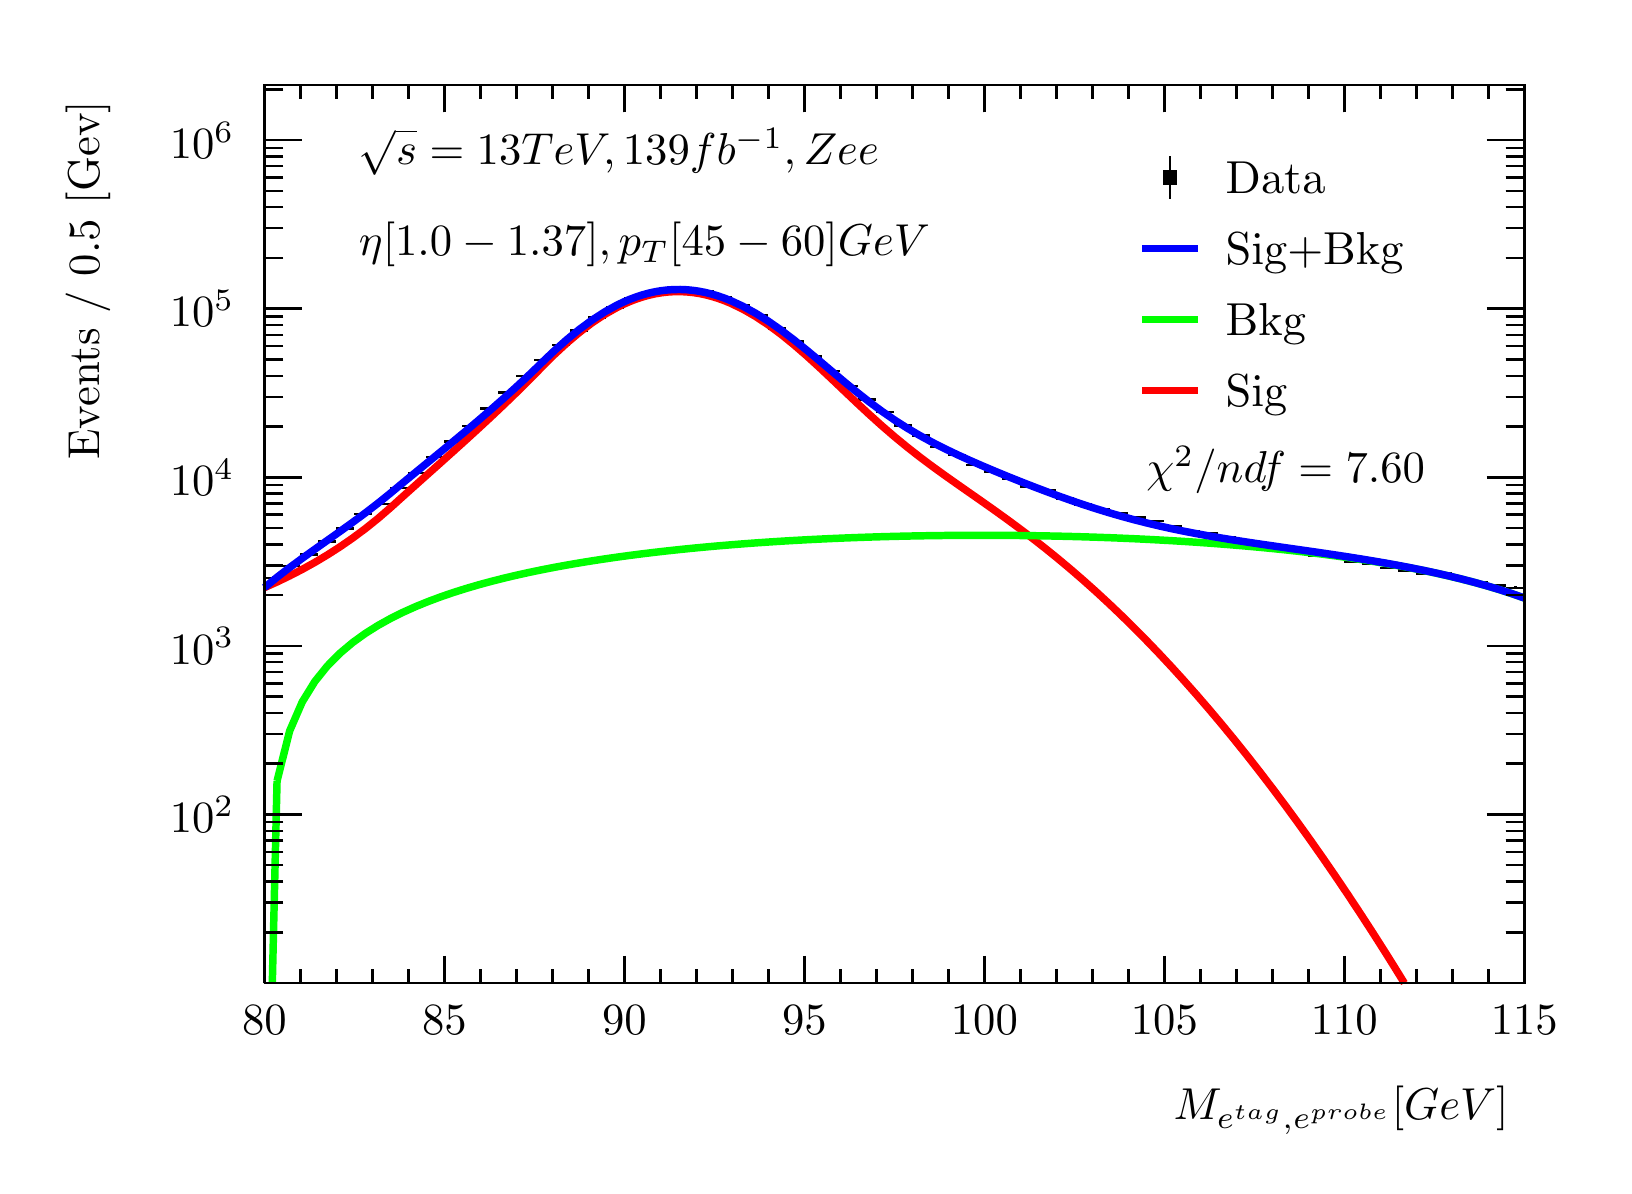
\begin{tikzpicture}
\pgfdeclareplotmark{cross} {
\pgfpathmoveto{\pgfpoint{-0.3\pgfplotmarksize}{\pgfplotmarksize}}
\pgfpathlineto{\pgfpoint{+0.3\pgfplotmarksize}{\pgfplotmarksize}}
\pgfpathlineto{\pgfpoint{+0.3\pgfplotmarksize}{0.3\pgfplotmarksize}}
\pgfpathlineto{\pgfpoint{+1\pgfplotmarksize}{0.3\pgfplotmarksize}}
\pgfpathlineto{\pgfpoint{+1\pgfplotmarksize}{-0.3\pgfplotmarksize}}
\pgfpathlineto{\pgfpoint{+0.3\pgfplotmarksize}{-0.3\pgfplotmarksize}}
\pgfpathlineto{\pgfpoint{+0.3\pgfplotmarksize}{-1.\pgfplotmarksize}}
\pgfpathlineto{\pgfpoint{-0.3\pgfplotmarksize}{-1.\pgfplotmarksize}}
\pgfpathlineto{\pgfpoint{-0.3\pgfplotmarksize}{-0.3\pgfplotmarksize}}
\pgfpathlineto{\pgfpoint{-1.\pgfplotmarksize}{-0.3\pgfplotmarksize}}
\pgfpathlineto{\pgfpoint{-1.\pgfplotmarksize}{0.3\pgfplotmarksize}}
\pgfpathlineto{\pgfpoint{-0.3\pgfplotmarksize}{0.3\pgfplotmarksize}}
\pgfpathclose
\pgfusepathqstroke
}
\pgfdeclareplotmark{cross*} {
\pgfpathmoveto{\pgfpoint{-0.3\pgfplotmarksize}{\pgfplotmarksize}}
\pgfpathlineto{\pgfpoint{+0.3\pgfplotmarksize}{\pgfplotmarksize}}
\pgfpathlineto{\pgfpoint{+0.3\pgfplotmarksize}{0.3\pgfplotmarksize}}
\pgfpathlineto{\pgfpoint{+1\pgfplotmarksize}{0.3\pgfplotmarksize}}
\pgfpathlineto{\pgfpoint{+1\pgfplotmarksize}{-0.3\pgfplotmarksize}}
\pgfpathlineto{\pgfpoint{+0.3\pgfplotmarksize}{-0.3\pgfplotmarksize}}
\pgfpathlineto{\pgfpoint{+0.3\pgfplotmarksize}{-1.\pgfplotmarksize}}
\pgfpathlineto{\pgfpoint{-0.3\pgfplotmarksize}{-1.\pgfplotmarksize}}
\pgfpathlineto{\pgfpoint{-0.3\pgfplotmarksize}{-0.3\pgfplotmarksize}}
\pgfpathlineto{\pgfpoint{-1.\pgfplotmarksize}{-0.3\pgfplotmarksize}}
\pgfpathlineto{\pgfpoint{-1.\pgfplotmarksize}{0.3\pgfplotmarksize}}
\pgfpathlineto{\pgfpoint{-0.3\pgfplotmarksize}{0.3\pgfplotmarksize}}
\pgfpathclose
\pgfusepathqfillstroke
}
\pgfdeclareplotmark{newstar} {
\pgfpathmoveto{\pgfqpoint{0pt}{\pgfplotmarksize}}
\pgfpathlineto{\pgfqpointpolar{44}{0.5\pgfplotmarksize}}
\pgfpathlineto{\pgfqpointpolar{18}{\pgfplotmarksize}}
\pgfpathlineto{\pgfqpointpolar{-20}{0.5\pgfplotmarksize}}
\pgfpathlineto{\pgfqpointpolar{-54}{\pgfplotmarksize}}
\pgfpathlineto{\pgfqpointpolar{-90}{0.5\pgfplotmarksize}}
\pgfpathlineto{\pgfqpointpolar{234}{\pgfplotmarksize}}
\pgfpathlineto{\pgfqpointpolar{198}{0.5\pgfplotmarksize}}
\pgfpathlineto{\pgfqpointpolar{162}{\pgfplotmarksize}}
\pgfpathlineto{\pgfqpointpolar{134}{0.5\pgfplotmarksize}}
\pgfpathclose
\pgfusepathqstroke
}
\pgfdeclareplotmark{newstar*} {
\pgfpathmoveto{\pgfqpoint{0pt}{\pgfplotmarksize}}
\pgfpathlineto{\pgfqpointpolar{44}{0.5\pgfplotmarksize}}
\pgfpathlineto{\pgfqpointpolar{18}{\pgfplotmarksize}}
\pgfpathlineto{\pgfqpointpolar{-20}{0.5\pgfplotmarksize}}
\pgfpathlineto{\pgfqpointpolar{-54}{\pgfplotmarksize}}
\pgfpathlineto{\pgfqpointpolar{-90}{0.5\pgfplotmarksize}}
\pgfpathlineto{\pgfqpointpolar{234}{\pgfplotmarksize}}
\pgfpathlineto{\pgfqpointpolar{198}{0.5\pgfplotmarksize}}
\pgfpathlineto{\pgfqpointpolar{162}{\pgfplotmarksize}}
\pgfpathlineto{\pgfqpointpolar{134}{0.5\pgfplotmarksize}}
\pgfpathclose
\pgfusepathqfillstroke
}
\definecolor{c}{rgb}{1,1,1};
\draw [color=c, fill=c] (0,0) rectangle (20,14.4361);
\draw [color=c, fill=c] (3,2.30977) rectangle (19,13.7143);
\definecolor{c}{rgb}{0,0,0};
\draw [c,line width=0.9] (3,2.30977) -- (3,13.7143) -- (19,13.7143) -- (19,2.30977) -- (3,2.30977);
\definecolor{c}{rgb}{1,1,1};
\draw [color=c, fill=c] (3,2.30977) rectangle (19,13.7143);
\definecolor{c}{rgb}{0,0,0};
\draw [c,line width=0.9] (3,2.30977) -- (3,13.7143) -- (19,13.7143) -- (19,2.30977) -- (3,2.30977);
\draw [c,line width=0.9] (3,2.30977) -- (19,2.30977);
\draw [c,line width=0.9] (3,2.65624) -- (3,2.30977);
\draw [c,line width=0.9] (3.45714,2.48301) -- (3.45714,2.30977);
\draw [c,line width=0.9] (3.91429,2.48301) -- (3.91429,2.30977);
\draw [c,line width=0.9] (4.37143,2.48301) -- (4.37143,2.30977);
\draw [c,line width=0.9] (4.82857,2.48301) -- (4.82857,2.30977);
\draw [c,line width=0.9] (5.28571,2.65624) -- (5.28571,2.30977);
\draw [c,line width=0.9] (5.74286,2.48301) -- (5.74286,2.30977);
\draw [c,line width=0.9] (6.2,2.48301) -- (6.2,2.30977);
\draw [c,line width=0.9] (6.65714,2.48301) -- (6.65714,2.30977);
\draw [c,line width=0.9] (7.11429,2.48301) -- (7.11429,2.30977);
\draw [c,line width=0.9] (7.57143,2.65624) -- (7.57143,2.30977);
\draw [c,line width=0.9] (8.02857,2.48301) -- (8.02857,2.30977);
\draw [c,line width=0.9] (8.48571,2.48301) -- (8.48571,2.30977);
\draw [c,line width=0.9] (8.94286,2.48301) -- (8.94286,2.30977);
\draw [c,line width=0.9] (9.4,2.48301) -- (9.4,2.30977);
\draw [c,line width=0.9] (9.85714,2.65624) -- (9.85714,2.30977);
\draw [c,line width=0.9] (10.3143,2.48301) -- (10.3143,2.30977);
\draw [c,line width=0.9] (10.7714,2.48301) -- (10.7714,2.30977);
\draw [c,line width=0.9] (11.2286,2.48301) -- (11.2286,2.30977);
\draw [c,line width=0.9] (11.6857,2.48301) -- (11.6857,2.30977);
\draw [c,line width=0.9] (12.1429,2.65624) -- (12.1429,2.30977);
\draw [c,line width=0.9] (12.6,2.48301) -- (12.6,2.30977);
\draw [c,line width=0.9] (13.0571,2.48301) -- (13.0571,2.30977);
\draw [c,line width=0.9] (13.5143,2.48301) -- (13.5143,2.30977);
\draw [c,line width=0.9] (13.9714,2.48301) -- (13.9714,2.30977);
\draw [c,line width=0.9] (14.4286,2.65624) -- (14.4286,2.30977);
\draw [c,line width=0.9] (14.8857,2.48301) -- (14.8857,2.30977);
\draw [c,line width=0.9] (15.3429,2.48301) -- (15.3429,2.30977);
\draw [c,line width=0.9] (15.8,2.48301) -- (15.8,2.30977);
\draw [c,line width=0.9] (16.2571,2.48301) -- (16.2571,2.30977);
\draw [c,line width=0.9] (16.7143,2.65624) -- (16.7143,2.30977);
\draw [c,line width=0.9] (17.1714,2.48301) -- (17.1714,2.30977);
\draw [c,line width=0.9] (17.6286,2.48301) -- (17.6286,2.30977);
\draw [c,line width=0.9] (18.0857,2.48301) -- (18.0857,2.30977);
\draw [c,line width=0.9] (18.5429,2.48301) -- (18.5429,2.30977);
\draw [c,line width=0.9] (19,2.65624) -- (19,2.30977);
\draw [anchor=base] (3,1.66015) node[scale=1.61424, color=c, rotate=0]{80};
\draw [anchor=base] (5.28571,1.66015) node[scale=1.61424, color=c, rotate=0]{85};
\draw [anchor=base] (7.57143,1.66015) node[scale=1.61424, color=c, rotate=0]{90};
\draw [anchor=base] (9.85714,1.66015) node[scale=1.61424, color=c, rotate=0]{95};
\draw [anchor=base] (12.1429,1.66015) node[scale=1.61424, color=c, rotate=0]{100};
\draw [anchor=base] (14.4286,1.66015) node[scale=1.61424, color=c, rotate=0]{105};
\draw [anchor=base] (16.7143,1.66015) node[scale=1.61424, color=c, rotate=0]{110};
\draw [anchor=base] (19,1.66015) node[scale=1.61424, color=c, rotate=0]{115};
\draw [anchor= east] (19,0.692932) node[scale=1.61424, color=c, rotate=0]{$M_{e^{tag}, e^{probe}}  [GeV]$};
\draw [c,line width=0.9] (3,13.7143) -- (19,13.7143);
\draw [c,line width=0.9] (3,13.3678) -- (3,13.7143);
\draw [c,line width=0.9] (3.45714,13.5411) -- (3.45714,13.7143);
\draw [c,line width=0.9] (3.91429,13.5411) -- (3.91429,13.7143);
\draw [c,line width=0.9] (4.37143,13.5411) -- (4.37143,13.7143);
\draw [c,line width=0.9] (4.82857,13.5411) -- (4.82857,13.7143);
\draw [c,line width=0.9] (5.28571,13.3678) -- (5.28571,13.7143);
\draw [c,line width=0.9] (5.74286,13.5411) -- (5.74286,13.7143);
\draw [c,line width=0.9] (6.2,13.5411) -- (6.2,13.7143);
\draw [c,line width=0.9] (6.65714,13.5411) -- (6.65714,13.7143);
\draw [c,line width=0.9] (7.11429,13.5411) -- (7.11429,13.7143);
\draw [c,line width=0.9] (7.57143,13.3678) -- (7.57143,13.7143);
\draw [c,line width=0.9] (8.02857,13.5411) -- (8.02857,13.7143);
\draw [c,line width=0.9] (8.48571,13.5411) -- (8.48571,13.7143);
\draw [c,line width=0.9] (8.94286,13.5411) -- (8.94286,13.7143);
\draw [c,line width=0.9] (9.4,13.5411) -- (9.4,13.7143);
\draw [c,line width=0.9] (9.85714,13.3678) -- (9.85714,13.7143);
\draw [c,line width=0.9] (10.3143,13.5411) -- (10.3143,13.7143);
\draw [c,line width=0.9] (10.7714,13.5411) -- (10.7714,13.7143);
\draw [c,line width=0.9] (11.2286,13.5411) -- (11.2286,13.7143);
\draw [c,line width=0.9] (11.6857,13.5411) -- (11.6857,13.7143);
\draw [c,line width=0.9] (12.1429,13.3678) -- (12.1429,13.7143);
\draw [c,line width=0.9] (12.6,13.5411) -- (12.6,13.7143);
\draw [c,line width=0.9] (13.0571,13.5411) -- (13.0571,13.7143);
\draw [c,line width=0.9] (13.5143,13.5411) -- (13.5143,13.7143);
\draw [c,line width=0.9] (13.9714,13.5411) -- (13.9714,13.7143);
\draw [c,line width=0.9] (14.4286,13.3678) -- (14.4286,13.7143);
\draw [c,line width=0.9] (14.8857,13.5411) -- (14.8857,13.7143);
\draw [c,line width=0.9] (15.3429,13.5411) -- (15.3429,13.7143);
\draw [c,line width=0.9] (15.8,13.5411) -- (15.8,13.7143);
\draw [c,line width=0.9] (16.2571,13.5411) -- (16.2571,13.7143);
\draw [c,line width=0.9] (16.7143,13.3678) -- (16.7143,13.7143);
\draw [c,line width=0.9] (17.1714,13.5411) -- (17.1714,13.7143);
\draw [c,line width=0.9] (17.6286,13.5411) -- (17.6286,13.7143);
\draw [c,line width=0.9] (18.0857,13.5411) -- (18.0857,13.7143);
\draw [c,line width=0.9] (18.5429,13.5411) -- (18.5429,13.7143);
\draw [c,line width=0.9] (19,13.3678) -- (19,13.7143);
\draw [c,line width=0.9] (3,2.30977) -- (3,13.7143);
\draw [c,line width=0.9] (3.237,2.95433) -- (3,2.95433);
\draw [c,line width=0.9] (3.237,3.33137) -- (3,3.33137);
\draw [c,line width=0.9] (3.237,3.59888) -- (3,3.59888);
\draw [c,line width=0.9] (3.237,3.80638) -- (3,3.80638);
\draw [c,line width=0.9] (3.237,3.97592) -- (3,3.97592);
\draw [c,line width=0.9] (3.237,4.11926) -- (3,4.11926);
\draw [c,line width=0.9] (3.237,4.24343) -- (3,4.24343);
\draw [c,line width=0.9] (3.237,4.35296) -- (3,4.35296);
\draw [c,line width=0.9] (3.474,4.45093) -- (3,4.45093);
\draw [anchor= east] (2.82,4.45093) node[scale=1.61424, color=c, rotate=0]{$10^{2}$};
\draw [c,line width=0.9] (3.237,5.09549) -- (3,5.09549);
\draw [c,line width=0.9] (3.237,5.47253) -- (3,5.47253);
\draw [c,line width=0.9] (3.237,5.74004) -- (3,5.74004);
\draw [c,line width=0.9] (3.237,5.94754) -- (3,5.94754);
\draw [c,line width=0.9] (3.237,6.11708) -- (3,6.11708);
\draw [c,line width=0.9] (3.237,6.26042) -- (3,6.26042);
\draw [c,line width=0.9] (3.237,6.38459) -- (3,6.38459);
\draw [c,line width=0.9] (3.237,6.49412) -- (3,6.49412);
\draw [c,line width=0.9] (3.474,6.59209) -- (3,6.59209);
\draw [anchor= east] (2.82,6.59209) node[scale=1.61424, color=c, rotate=0]{$10^{3}$};
\draw [c,line width=0.9] (3.237,7.23665) -- (3,7.23665);
\draw [c,line width=0.9] (3.237,7.61369) -- (3,7.61369);
\draw [c,line width=0.9] (3.237,7.8812) -- (3,7.8812);
\draw [c,line width=0.9] (3.237,8.0887) -- (3,8.0887);
\draw [c,line width=0.9] (3.237,8.25824) -- (3,8.25824);
\draw [c,line width=0.9] (3.237,8.40158) -- (3,8.40158);
\draw [c,line width=0.9] (3.237,8.52575) -- (3,8.52575);
\draw [c,line width=0.9] (3.237,8.63528) -- (3,8.63528);
\draw [c,line width=0.9] (3.474,8.73325) -- (3,8.73325);
\draw [anchor= east] (2.82,8.73325) node[scale=1.61424, color=c, rotate=0]{$10^{4}$};
\draw [c,line width=0.9] (3.237,9.37781) -- (3,9.37781);
\draw [c,line width=0.9] (3.237,9.75485) -- (3,9.75485);
\draw [c,line width=0.9] (3.237,10.0224) -- (3,10.0224);
\draw [c,line width=0.9] (3.237,10.2299) -- (3,10.2299);
\draw [c,line width=0.9] (3.237,10.3994) -- (3,10.3994);
\draw [c,line width=0.9] (3.237,10.5427) -- (3,10.5427);
\draw [c,line width=0.9] (3.237,10.6669) -- (3,10.6669);
\draw [c,line width=0.9] (3.237,10.7764) -- (3,10.7764);
\draw [c,line width=0.9] (3.474,10.8744) -- (3,10.8744);
\draw [anchor= east] (2.82,10.8744) node[scale=1.61424, color=c, rotate=0]{$10^{5}$};
\draw [c,line width=0.9] (3.237,11.519) -- (3,11.519);
\draw [c,line width=0.9] (3.237,11.896) -- (3,11.896);
\draw [c,line width=0.9] (3.237,12.1635) -- (3,12.1635);
\draw [c,line width=0.9] (3.237,12.371) -- (3,12.371);
\draw [c,line width=0.9] (3.237,12.5406) -- (3,12.5406);
\draw [c,line width=0.9] (3.237,12.6839) -- (3,12.6839);
\draw [c,line width=0.9] (3.237,12.8081) -- (3,12.8081);
\draw [c,line width=0.9] (3.237,12.9176) -- (3,12.9176);
\draw [c,line width=0.9] (3.474,13.0156) -- (3,13.0156);
\draw [anchor= east] (2.82,13.0156) node[scale=1.61424, color=c, rotate=0]{$10^{6}$};
\draw [c,line width=0.9] (3.237,13.6601) -- (3,13.6601);
\draw [anchor= east] (0.76,13.7143) node[scale=1.61424, color=c, rotate=90]{Events / 0.5 [Gev]};
\draw [c,line width=0.9] (19,2.30977) -- (19,13.7143);
\draw [c,line width=0.9] (18.763,2.95433) -- (19,2.95433);
\draw [c,line width=0.9] (18.763,3.33137) -- (19,3.33137);
\draw [c,line width=0.9] (18.763,3.59888) -- (19,3.59888);
\draw [c,line width=0.9] (18.763,3.80638) -- (19,3.80638);
\draw [c,line width=0.9] (18.763,3.97592) -- (19,3.97592);
\draw [c,line width=0.9] (18.763,4.11926) -- (19,4.11926);
\draw [c,line width=0.9] (18.763,4.24343) -- (19,4.24343);
\draw [c,line width=0.9] (18.763,4.35296) -- (19,4.35296);
\draw [c,line width=0.9] (18.526,4.45093) -- (19,4.45093);
\draw [c,line width=0.9] (18.763,5.09549) -- (19,5.09549);
\draw [c,line width=0.9] (18.763,5.47253) -- (19,5.47253);
\draw [c,line width=0.9] (18.763,5.74004) -- (19,5.74004);
\draw [c,line width=0.9] (18.763,5.94754) -- (19,5.94754);
\draw [c,line width=0.9] (18.763,6.11708) -- (19,6.11708);
\draw [c,line width=0.9] (18.763,6.26042) -- (19,6.26042);
\draw [c,line width=0.9] (18.763,6.38459) -- (19,6.38459);
\draw [c,line width=0.9] (18.763,6.49412) -- (19,6.49412);
\draw [c,line width=0.9] (18.526,6.59209) -- (19,6.59209);
\draw [c,line width=0.9] (18.763,7.23665) -- (19,7.23665);
\draw [c,line width=0.9] (18.763,7.61369) -- (19,7.61369);
\draw [c,line width=0.9] (18.763,7.8812) -- (19,7.8812);
\draw [c,line width=0.9] (18.763,8.0887) -- (19,8.0887);
\draw [c,line width=0.9] (18.763,8.25824) -- (19,8.25824);
\draw [c,line width=0.9] (18.763,8.40158) -- (19,8.40158);
\draw [c,line width=0.9] (18.763,8.52575) -- (19,8.52575);
\draw [c,line width=0.9] (18.763,8.63528) -- (19,8.63528);
\draw [c,line width=0.9] (18.526,8.73325) -- (19,8.73325);
\draw [c,line width=0.9] (18.763,9.37781) -- (19,9.37781);
\draw [c,line width=0.9] (18.763,9.75485) -- (19,9.75485);
\draw [c,line width=0.9] (18.763,10.0224) -- (19,10.0224);
\draw [c,line width=0.9] (18.763,10.2299) -- (19,10.2299);
\draw [c,line width=0.9] (18.763,10.3994) -- (19,10.3994);
\draw [c,line width=0.9] (18.763,10.5427) -- (19,10.5427);
\draw [c,line width=0.9] (18.763,10.6669) -- (19,10.6669);
\draw [c,line width=0.9] (18.763,10.7764) -- (19,10.7764);
\draw [c,line width=0.9] (18.526,10.8744) -- (19,10.8744);
\draw [c,line width=0.9] (18.763,11.519) -- (19,11.519);
\draw [c,line width=0.9] (18.763,11.896) -- (19,11.896);
\draw [c,line width=0.9] (18.763,12.1635) -- (19,12.1635);
\draw [c,line width=0.9] (18.763,12.371) -- (19,12.371);
\draw [c,line width=0.9] (18.763,12.5406) -- (19,12.5406);
\draw [c,line width=0.9] (18.763,12.6839) -- (19,12.6839);
\draw [c,line width=0.9] (18.763,12.8081) -- (19,12.8081);
\draw [c,line width=0.9] (18.763,12.9176) -- (19,12.9176);
\draw [c,line width=0.9] (18.526,13.0156) -- (19,13.0156);
\draw [c,line width=0.9] (18.763,13.6601) -- (19,13.6601);
\draw [c,line width=0.9] (3.11429,7.45524) -- (3,7.45524);
\draw [c,line width=0.9] (3,7.45524) -- (3,7.45524);
\draw [c,line width=0.9] (3.11429,7.45524) -- (3.22857,7.45524);
\draw [c,line width=0.9] (3.22857,7.45524) -- (3.22857,7.45524);
\draw [c,line width=0.9] (3.11429,7.45524) -- (3.11429,7.47373);
\draw [c,line width=0.9] (3.11429,7.47373) -- (3.11429,7.47373);
\draw [c,line width=0.9] (3.11429,7.45524) -- (3.11429,7.43675);
\draw [c,line width=0.9] (3.11429,7.43675) -- (3.11429,7.43675);
\draw [c,line width=0.9] (3.34286,7.60903) -- (3.22857,7.60903);
\draw [c,line width=0.9] (3.22857,7.60903) -- (3.22857,7.60903);
\draw [c,line width=0.9] (3.34286,7.60903) -- (3.45714,7.60903);
\draw [c,line width=0.9] (3.45714,7.60903) -- (3.45714,7.60903);
\draw [c,line width=0.9] (3.34286,7.60903) -- (3.34286,7.62605);
\draw [c,line width=0.9] (3.34286,7.62605) -- (3.34286,7.62605);
\draw [c,line width=0.9] (3.34286,7.60903) -- (3.34286,7.59201);
\draw [c,line width=0.9] (3.34286,7.59201) -- (3.34286,7.59201);
\draw [c,line width=0.9] (3.57143,7.7525) -- (3.45714,7.7525);
\draw [c,line width=0.9] (3.45714,7.7525) -- (3.45714,7.7525);
\draw [c,line width=0.9] (3.57143,7.7525) -- (3.68571,7.7525);
\draw [c,line width=0.9] (3.68571,7.7525) -- (3.68571,7.7525);
\draw [c,line width=0.9] (3.57143,7.7525) -- (3.57143,7.76826);
\draw [c,line width=0.9] (3.57143,7.76826) -- (3.57143,7.76826);
\draw [c,line width=0.9] (3.57143,7.7525) -- (3.57143,7.73675);
\draw [c,line width=0.9] (3.57143,7.73675) -- (3.57143,7.73675);
\draw [c,line width=0.9] (3.8,7.91856) -- (3.68571,7.91856);
\draw [c,line width=0.9] (3.68571,7.91856) -- (3.68571,7.91856);
\draw [c,line width=0.9] (3.8,7.91856) -- (3.91429,7.91856);
\draw [c,line width=0.9] (3.91429,7.91856) -- (3.91429,7.91856);
\draw [c,line width=0.9] (3.8,7.91856) -- (3.8,7.93298);
\draw [c,line width=0.9] (3.8,7.93298) -- (3.8,7.93298);
\draw [c,line width=0.9] (3.8,7.91856) -- (3.8,7.90415);
\draw [c,line width=0.9] (3.8,7.90415) -- (3.8,7.90415);
\draw [c,line width=0.9] (4.02857,8.08067) -- (3.91429,8.08067);
\draw [c,line width=0.9] (3.91429,8.08067) -- (3.91429,8.08067);
\draw [c,line width=0.9] (4.02857,8.08067) -- (4.14286,8.08067);
\draw [c,line width=0.9] (4.14286,8.08067) -- (4.14286,8.08067);
\draw [c,line width=0.9] (4.02857,8.08067) -- (4.02857,8.09388);
\draw [c,line width=0.9] (4.02857,8.09388) -- (4.02857,8.09388);
\draw [c,line width=0.9] (4.02857,8.08067) -- (4.02857,8.06746);
\draw [c,line width=0.9] (4.02857,8.06746) -- (4.02857,8.06746);
\draw [c,line width=0.9] (4.25714,8.26672) -- (4.14286,8.26672);
\draw [c,line width=0.9] (4.14286,8.26672) -- (4.14286,8.26672);
\draw [c,line width=0.9] (4.25714,8.26672) -- (4.37143,8.26672);
\draw [c,line width=0.9] (4.37143,8.26672) -- (4.37143,8.26672);
\draw [c,line width=0.9] (4.25714,8.26672) -- (4.25714,8.27868);
\draw [c,line width=0.9] (4.25714,8.27868) -- (4.25714,8.27868);
\draw [c,line width=0.9] (4.25714,8.26672) -- (4.25714,8.25478);
\draw [c,line width=0.9] (4.25714,8.25478) -- (4.25714,8.25478);
\draw [c,line width=0.9] (4.48571,8.39559) -- (4.37143,8.39559);
\draw [c,line width=0.9] (4.37143,8.39559) -- (4.37143,8.39559);
\draw [c,line width=0.9] (4.48571,8.39559) -- (4.6,8.39559);
\draw [c,line width=0.9] (4.6,8.39559) -- (4.6,8.39559);
\draw [c,line width=0.9] (4.48571,8.39559) -- (4.48571,8.40674);
\draw [c,line width=0.9] (4.48571,8.40674) -- (4.48571,8.40674);
\draw [c,line width=0.9] (4.48571,8.39559) -- (4.48571,8.38444);
\draw [c,line width=0.9] (4.48571,8.38444) -- (4.48571,8.38444);
\draw [c,line width=0.9] (4.71429,8.59958) -- (4.6,8.59958);
\draw [c,line width=0.9] (4.6,8.59958) -- (4.6,8.59958);
\draw [c,line width=0.9] (4.71429,8.59958) -- (4.82857,8.59958);
\draw [c,line width=0.9] (4.82857,8.59958) -- (4.82857,8.59958);
\draw [c,line width=0.9] (4.71429,8.59958) -- (4.71429,8.60957);
\draw [c,line width=0.9] (4.71429,8.60957) -- (4.71429,8.60957);
\draw [c,line width=0.9] (4.71429,8.59958) -- (4.71429,8.58958);
\draw [c,line width=0.9] (4.71429,8.58958) -- (4.71429,8.58958);
\draw [c,line width=0.9] (4.94286,8.78831) -- (4.82857,8.78831);
\draw [c,line width=0.9] (4.82857,8.78831) -- (4.82857,8.78831);
\draw [c,line width=0.9] (4.94286,8.78831) -- (5.05714,8.78831);
\draw [c,line width=0.9] (5.05714,8.78831) -- (5.05714,8.78831);
\draw [c,line width=0.9] (4.94286,8.78831) -- (4.94286,8.79734);
\draw [c,line width=0.9] (4.94286,8.79734) -- (4.94286,8.79734);
\draw [c,line width=0.9] (4.94286,8.78831) -- (4.94286,8.77929);
\draw [c,line width=0.9] (4.94286,8.77929) -- (4.94286,8.77929);
\draw [c,line width=0.9] (5.17143,8.99022) -- (5.05714,8.99022);
\draw [c,line width=0.9] (5.05714,8.99022) -- (5.05714,8.99022);
\draw [c,line width=0.9] (5.17143,8.99022) -- (5.28571,8.99022);
\draw [c,line width=0.9] (5.28571,8.99022) -- (5.28571,8.99022);
\draw [c,line width=0.9] (5.17143,8.99022) -- (5.17143,8.99832);
\draw [c,line width=0.9] (5.17143,8.99832) -- (5.17143,8.99832);
\draw [c,line width=0.9] (5.17143,8.99022) -- (5.17143,8.98212);
\draw [c,line width=0.9] (5.17143,8.98212) -- (5.17143,8.98212);
\draw [c,line width=0.9] (5.4,9.18804) -- (5.28571,9.18804);
\draw [c,line width=0.9] (5.28571,9.18804) -- (5.28571,9.18804);
\draw [c,line width=0.9] (5.4,9.18804) -- (5.51429,9.18804);
\draw [c,line width=0.9] (5.51429,9.18804) -- (5.51429,9.18804);
\draw [c,line width=0.9] (5.4,9.18804) -- (5.4,9.19532);
\draw [c,line width=0.9] (5.4,9.19532) -- (5.4,9.19532);
\draw [c,line width=0.9] (5.4,9.18804) -- (5.4,9.18076);
\draw [c,line width=0.9] (5.4,9.18076) -- (5.4,9.18076);
\draw [c,line width=0.9] (5.62857,9.38545) -- (5.51429,9.38545);
\draw [c,line width=0.9] (5.51429,9.38545) -- (5.51429,9.38545);
\draw [c,line width=0.9] (5.62857,9.38545) -- (5.74286,9.38545);
\draw [c,line width=0.9] (5.74286,9.38545) -- (5.74286,9.38545);
\draw [c,line width=0.9] (5.62857,9.38545) -- (5.62857,9.392);
\draw [c,line width=0.9] (5.62857,9.392) -- (5.62857,9.392);
\draw [c,line width=0.9] (5.62857,9.38545) -- (5.62857,9.3789);
\draw [c,line width=0.9] (5.62857,9.3789) -- (5.62857,9.3789);
\draw [c,line width=0.9] (5.85714,9.60441) -- (5.74286,9.60441);
\draw [c,line width=0.9] (5.74286,9.60441) -- (5.74286,9.60441);
\draw [c,line width=0.9] (5.85714,9.60441) -- (5.97143,9.60441);
\draw [c,line width=0.9] (5.97143,9.60441) -- (5.97143,9.60441);
\draw [c,line width=0.9] (5.85714,9.60441) -- (5.85714,9.61023);
\draw [c,line width=0.9] (5.85714,9.61023) -- (5.85714,9.61023);
\draw [c,line width=0.9] (5.85714,9.60441) -- (5.85714,9.59859);
\draw [c,line width=0.9] (5.85714,9.59859) -- (5.85714,9.59859);
\draw [c,line width=0.9] (6.08571,9.81131) -- (5.97143,9.81131);
\draw [c,line width=0.9] (5.97143,9.81131) -- (5.97143,9.81131);
\draw [c,line width=0.9] (6.08571,9.81131) -- (6.2,9.81131);
\draw [c,line width=0.9] (6.2,9.81131) -- (6.2,9.81131);
\draw [c,line width=0.9] (6.08571,9.81131) -- (6.08571,9.81652);
\draw [c,line width=0.9] (6.08571,9.81652) -- (6.08571,9.81652);
\draw [c,line width=0.9] (6.08571,9.81131) -- (6.08571,9.8061);
\draw [c,line width=0.9] (6.08571,9.8061) -- (6.08571,9.8061);
\draw [c,line width=0.9] (6.31429,10.0188) -- (6.2,10.0188);
\draw [c,line width=0.9] (6.2,10.0188) -- (6.2,10.0188);
\draw [c,line width=0.9] (6.31429,10.0188) -- (6.42857,10.0188);
\draw [c,line width=0.9] (6.42857,10.0188) -- (6.42857,10.0188);
\draw [c,line width=0.9] (6.31429,10.0188) -- (6.31429,10.0235);
\draw [c,line width=0.9] (6.31429,10.0235) -- (6.31429,10.0235);
\draw [c,line width=0.9] (6.31429,10.0188) -- (6.31429,10.0141);
\draw [c,line width=0.9] (6.31429,10.0141) -- (6.31429,10.0141);
\draw [c,line width=0.9] (6.54286,10.2222) -- (6.42857,10.2222);
\draw [c,line width=0.9] (6.42857,10.2222) -- (6.42857,10.2222);
\draw [c,line width=0.9] (6.54286,10.2222) -- (6.65714,10.2222);
\draw [c,line width=0.9] (6.65714,10.2222) -- (6.65714,10.2222);
\draw [c,line width=0.9] (6.54286,10.2222) -- (6.54286,10.2263);
\draw [c,line width=0.9] (6.54286,10.2263) -- (6.54286,10.2263);
\draw [c,line width=0.9] (6.54286,10.2222) -- (6.54286,10.218);
\draw [c,line width=0.9] (6.54286,10.218) -- (6.54286,10.218);
\draw [c,line width=0.9] (6.77143,10.4115) -- (6.65714,10.4115);
\draw [c,line width=0.9] (6.65714,10.4115) -- (6.65714,10.4115);
\draw [c,line width=0.9] (6.77143,10.4115) -- (6.88571,10.4115);
\draw [c,line width=0.9] (6.88571,10.4115) -- (6.88571,10.4115);
\draw [c,line width=0.9] (6.77143,10.4115) -- (6.77143,10.4153);
\draw [c,line width=0.9] (6.77143,10.4153) -- (6.77143,10.4153);
\draw [c,line width=0.9] (6.77143,10.4115) -- (6.77143,10.4078);
\draw [c,line width=0.9] (6.77143,10.4078) -- (6.77143,10.4078);
\draw [c,line width=0.9] (7,10.5993) -- (6.88571,10.5993);
\draw [c,line width=0.9] (6.88571,10.5993) -- (6.88571,10.5993);
\draw [c,line width=0.9] (7,10.5993) -- (7.11429,10.5993);
\draw [c,line width=0.9] (7.11429,10.5993) -- (7.11429,10.5993);
\draw [c,line width=0.9] (7,10.5993) -- (7,10.6027);
\draw [c,line width=0.9] (7,10.6027) -- (7,10.6027);
\draw [c,line width=0.9] (7,10.5993) -- (7,10.5958);
\draw [c,line width=0.9] (7,10.5958) -- (7,10.5958);
\draw [c,line width=0.9] (7.22857,10.7597) -- (7.11429,10.7597);
\draw [c,line width=0.9] (7.11429,10.7597) -- (7.11429,10.7597);
\draw [c,line width=0.9] (7.22857,10.7597) -- (7.34286,10.7597);
\draw [c,line width=0.9] (7.34286,10.7597) -- (7.34286,10.7597);
\draw [c,line width=0.9] (7.22857,10.7597) -- (7.22857,10.7629);
\draw [c,line width=0.9] (7.22857,10.7629) -- (7.22857,10.7629);
\draw [c,line width=0.9] (7.22857,10.7597) -- (7.22857,10.7566);
\draw [c,line width=0.9] (7.22857,10.7566) -- (7.22857,10.7566);
\draw [c,line width=0.9] (7.45714,10.8873) -- (7.34286,10.8873);
\draw [c,line width=0.9] (7.34286,10.8873) -- (7.34286,10.8873);
\draw [c,line width=0.9] (7.45714,10.8873) -- (7.57143,10.8873);
\draw [c,line width=0.9] (7.57143,10.8873) -- (7.57143,10.8873);
\draw [c,line width=0.9] (7.45714,10.8873) -- (7.45714,10.8902);
\draw [c,line width=0.9] (7.45714,10.8902) -- (7.45714,10.8902);
\draw [c,line width=0.9] (7.45714,10.8873) -- (7.45714,10.8843);
\draw [c,line width=0.9] (7.45714,10.8843) -- (7.45714,10.8843);
\draw [c,line width=0.9] (7.68571,11.0052) -- (7.57143,11.0052);
\draw [c,line width=0.9] (7.57143,11.0052) -- (7.57143,11.0052);
\draw [c,line width=0.9] (7.68571,11.0052) -- (7.8,11.0052);
\draw [c,line width=0.9] (7.8,11.0052) -- (7.8,11.0052);
\draw [c,line width=0.9] (7.68571,11.0052) -- (7.68571,11.008);
\draw [c,line width=0.9] (7.68571,11.008) -- (7.68571,11.008);
\draw [c,line width=0.9] (7.68571,11.0052) -- (7.68571,11.0025);
\draw [c,line width=0.9] (7.68571,11.0025) -- (7.68571,11.0025);
\draw [c,line width=0.9] (7.91429,11.0822) -- (7.8,11.0822);
\draw [c,line width=0.9] (7.8,11.0822) -- (7.8,11.0822);
\draw [c,line width=0.9] (7.91429,11.0822) -- (8.02857,11.0822);
\draw [c,line width=0.9] (8.02857,11.0822) -- (8.02857,11.0822);
\draw [c,line width=0.9] (7.91429,11.0822) -- (7.91429,11.0849);
\draw [c,line width=0.9] (7.91429,11.0849) -- (7.91429,11.0849);
\draw [c,line width=0.9] (7.91429,11.0822) -- (7.91429,11.0796);
\draw [c,line width=0.9] (7.91429,11.0796) -- (7.91429,11.0796);
\draw [c,line width=0.9] (8.14286,11.1221) -- (8.02857,11.1221);
\draw [c,line width=0.9] (8.02857,11.1221) -- (8.02857,11.1221);
\draw [c,line width=0.9] (8.14286,11.1221) -- (8.25714,11.1221);
\draw [c,line width=0.9] (8.25714,11.1221) -- (8.25714,11.1221);
\draw [c,line width=0.9] (8.14286,11.1221) -- (8.14286,11.1247);
\draw [c,line width=0.9] (8.14286,11.1247) -- (8.14286,11.1247);
\draw [c,line width=0.9] (8.14286,11.1221) -- (8.14286,11.1195);
\draw [c,line width=0.9] (8.14286,11.1195) -- (8.14286,11.1195);
\draw [c,line width=0.9] (8.37143,11.1288) -- (8.25714,11.1288);
\draw [c,line width=0.9] (8.25714,11.1288) -- (8.25714,11.1288);
\draw [c,line width=0.9] (8.37143,11.1288) -- (8.48571,11.1288);
\draw [c,line width=0.9] (8.48571,11.1288) -- (8.48571,11.1288);
\draw [c,line width=0.9] (8.37143,11.1288) -- (8.37143,11.1313);
\draw [c,line width=0.9] (8.37143,11.1313) -- (8.37143,11.1313);
\draw [c,line width=0.9] (8.37143,11.1288) -- (8.37143,11.1262);
\draw [c,line width=0.9] (8.37143,11.1262) -- (8.37143,11.1262);
\draw [c,line width=0.9] (8.6,11.0917) -- (8.48571,11.0917);
\draw [c,line width=0.9] (8.48571,11.0917) -- (8.48571,11.0917);
\draw [c,line width=0.9] (8.6,11.0917) -- (8.71429,11.0917);
\draw [c,line width=0.9] (8.71429,11.0917) -- (8.71429,11.0917);
\draw [c,line width=0.9] (8.6,11.0917) -- (8.6,11.0943);
\draw [c,line width=0.9] (8.6,11.0943) -- (8.6,11.0943);
\draw [c,line width=0.9] (8.6,11.0917) -- (8.6,11.0891);
\draw [c,line width=0.9] (8.6,11.0891) -- (8.6,11.0891);
\draw [c,line width=0.9] (8.82857,11.0159) -- (8.71429,11.0159);
\draw [c,line width=0.9] (8.71429,11.0159) -- (8.71429,11.0159);
\draw [c,line width=0.9] (8.82857,11.0159) -- (8.94286,11.0159);
\draw [c,line width=0.9] (8.94286,11.0159) -- (8.94286,11.0159);
\draw [c,line width=0.9] (8.82857,11.0159) -- (8.82857,11.0186);
\draw [c,line width=0.9] (8.82857,11.0186) -- (8.82857,11.0186);
\draw [c,line width=0.9] (8.82857,11.0159) -- (8.82857,11.0131);
\draw [c,line width=0.9] (8.82857,11.0131) -- (8.82857,11.0131);
\draw [c,line width=0.9] (9.05714,10.9127) -- (8.94286,10.9127);
\draw [c,line width=0.9] (8.94286,10.9127) -- (8.94286,10.9127);
\draw [c,line width=0.9] (9.05714,10.9127) -- (9.17143,10.9127);
\draw [c,line width=0.9] (9.17143,10.9127) -- (9.17143,10.9127);
\draw [c,line width=0.9] (9.05714,10.9127) -- (9.05714,10.9156);
\draw [c,line width=0.9] (9.05714,10.9156) -- (9.05714,10.9156);
\draw [c,line width=0.9] (9.05714,10.9127) -- (9.05714,10.9098);
\draw [c,line width=0.9] (9.05714,10.9098) -- (9.05714,10.9098);
\draw [c,line width=0.9] (9.28571,10.7886) -- (9.17143,10.7886);
\draw [c,line width=0.9] (9.17143,10.7886) -- (9.17143,10.7886);
\draw [c,line width=0.9] (9.28571,10.7886) -- (9.4,10.7886);
\draw [c,line width=0.9] (9.4,10.7886) -- (9.4,10.7886);
\draw [c,line width=0.9] (9.28571,10.7886) -- (9.28571,10.7917);
\draw [c,line width=0.9] (9.28571,10.7917) -- (9.28571,10.7917);
\draw [c,line width=0.9] (9.28571,10.7886) -- (9.28571,10.7855);
\draw [c,line width=0.9] (9.28571,10.7855) -- (9.28571,10.7855);
\draw [c,line width=0.9] (9.51429,10.6195) -- (9.4,10.6195);
\draw [c,line width=0.9] (9.4,10.6195) -- (9.4,10.6195);
\draw [c,line width=0.9] (9.51429,10.6195) -- (9.62857,10.6195);
\draw [c,line width=0.9] (9.62857,10.6195) -- (9.62857,10.6195);
\draw [c,line width=0.9] (9.51429,10.6195) -- (9.51429,10.6229);
\draw [c,line width=0.9] (9.51429,10.6229) -- (9.51429,10.6229);
\draw [c,line width=0.9] (9.51429,10.6195) -- (9.51429,10.6161);
\draw [c,line width=0.9] (9.51429,10.6161) -- (9.51429,10.6161);
\draw [c,line width=0.9] (9.74286,10.4579) -- (9.62857,10.4579);
\draw [c,line width=0.9] (9.62857,10.4579) -- (9.62857,10.4579);
\draw [c,line width=0.9] (9.74286,10.4579) -- (9.85714,10.4579);
\draw [c,line width=0.9] (9.85714,10.4579) -- (9.85714,10.4579);
\draw [c,line width=0.9] (9.74286,10.4579) -- (9.74286,10.4616);
\draw [c,line width=0.9] (9.74286,10.4616) -- (9.74286,10.4616);
\draw [c,line width=0.9] (9.74286,10.4579) -- (9.74286,10.4542);
\draw [c,line width=0.9] (9.74286,10.4542) -- (9.74286,10.4542);
\draw [c,line width=0.9] (9.97143,10.2673) -- (9.85714,10.2673);
\draw [c,line width=0.9] (9.85714,10.2673) -- (9.85714,10.2673);
\draw [c,line width=0.9] (9.97143,10.2673) -- (10.0857,10.2673);
\draw [c,line width=0.9] (10.0857,10.2673) -- (10.0857,10.2673);
\draw [c,line width=0.9] (9.97143,10.2673) -- (9.97143,10.2714);
\draw [c,line width=0.9] (9.97143,10.2714) -- (9.97143,10.2714);
\draw [c,line width=0.9] (9.97143,10.2673) -- (9.97143,10.2632);
\draw [c,line width=0.9] (9.97143,10.2632) -- (9.97143,10.2632);
\draw [c,line width=0.9] (10.2,10.0809) -- (10.0857,10.0809);
\draw [c,line width=0.9] (10.0857,10.0809) -- (10.0857,10.0809);
\draw [c,line width=0.9] (10.2,10.0809) -- (10.3143,10.0809);
\draw [c,line width=0.9] (10.3143,10.0809) -- (10.3143,10.0809);
\draw [c,line width=0.9] (10.2,10.0809) -- (10.2,10.0854);
\draw [c,line width=0.9] (10.2,10.0854) -- (10.2,10.0854);
\draw [c,line width=0.9] (10.2,10.0809) -- (10.2,10.0764);
\draw [c,line width=0.9] (10.2,10.0764) -- (10.2,10.0764);
\draw [c,line width=0.9] (10.4286,9.89297) -- (10.3143,9.89297);
\draw [c,line width=0.9] (10.3143,9.89297) -- (10.3143,9.89297);
\draw [c,line width=0.9] (10.4286,9.89297) -- (10.5429,9.89297);
\draw [c,line width=0.9] (10.5429,9.89297) -- (10.5429,9.89297);
\draw [c,line width=0.9] (10.4286,9.89297) -- (10.4286,9.89795);
\draw [c,line width=0.9] (10.4286,9.89795) -- (10.4286,9.89795);
\draw [c,line width=0.9] (10.4286,9.89297) -- (10.4286,9.88798);
\draw [c,line width=0.9] (10.4286,9.88798) -- (10.4286,9.88798);
\draw [c,line width=0.9] (10.6571,9.72017) -- (10.5429,9.72017);
\draw [c,line width=0.9] (10.5429,9.72017) -- (10.5429,9.72017);
\draw [c,line width=0.9] (10.6571,9.72017) -- (10.7714,9.72017);
\draw [c,line width=0.9] (10.7714,9.72017) -- (10.7714,9.72017);
\draw [c,line width=0.9] (10.6571,9.72017) -- (10.6571,9.72564);
\draw [c,line width=0.9] (10.6571,9.72564) -- (10.6571,9.72564);
\draw [c,line width=0.9] (10.6571,9.72017) -- (10.6571,9.7147);
\draw [c,line width=0.9] (10.6571,9.7147) -- (10.6571,9.7147);
\draw [c,line width=0.9] (10.8857,9.55989) -- (10.7714,9.55989);
\draw [c,line width=0.9] (10.7714,9.55989) -- (10.7714,9.55989);
\draw [c,line width=0.9] (10.8857,9.55989) -- (11,9.55989);
\draw [c,line width=0.9] (11,9.55989) -- (11,9.55989);
\draw [c,line width=0.9] (10.8857,9.55989) -- (10.8857,9.56585);
\draw [c,line width=0.9] (10.8857,9.56585) -- (10.8857,9.56585);
\draw [c,line width=0.9] (10.8857,9.55989) -- (10.8857,9.55393);
\draw [c,line width=0.9] (10.8857,9.55393) -- (10.8857,9.55393);
\draw [c,line width=0.9] (11.1143,9.38784) -- (11,9.38784);
\draw [c,line width=0.9] (11,9.38784) -- (11,9.38784);
\draw [c,line width=0.9] (11.1143,9.38784) -- (11.2286,9.38784);
\draw [c,line width=0.9] (11.2286,9.38784) -- (11.2286,9.38784);
\draw [c,line width=0.9] (11.1143,9.38784) -- (11.1143,9.39438);
\draw [c,line width=0.9] (11.1143,9.39438) -- (11.1143,9.39438);
\draw [c,line width=0.9] (11.1143,9.38784) -- (11.1143,9.3813);
\draw [c,line width=0.9] (11.1143,9.3813) -- (11.1143,9.3813);
\draw [c,line width=0.9] (11.3429,9.26078) -- (11.2286,9.26078);
\draw [c,line width=0.9] (11.2286,9.26078) -- (11.2286,9.26078);
\draw [c,line width=0.9] (11.3429,9.26078) -- (11.4571,9.26078);
\draw [c,line width=0.9] (11.4571,9.26078) -- (11.4571,9.26078);
\draw [c,line width=0.9] (11.3429,9.26078) -- (11.3429,9.26779);
\draw [c,line width=0.9] (11.3429,9.26779) -- (11.3429,9.26779);
\draw [c,line width=0.9] (11.3429,9.26078) -- (11.3429,9.25378);
\draw [c,line width=0.9] (11.3429,9.25378) -- (11.3429,9.25378);
\draw [c,line width=0.9] (11.5714,9.11783) -- (11.4571,9.11783);
\draw [c,line width=0.9] (11.4571,9.11783) -- (11.4571,9.11783);
\draw [c,line width=0.9] (11.5714,9.11783) -- (11.6857,9.11783);
\draw [c,line width=0.9] (11.6857,9.11783) -- (11.6857,9.11783);
\draw [c,line width=0.9] (11.5714,9.11783) -- (11.5714,9.12539);
\draw [c,line width=0.9] (11.5714,9.12539) -- (11.5714,9.12539);
\draw [c,line width=0.9] (11.5714,9.11783) -- (11.5714,9.11026);
\draw [c,line width=0.9] (11.5714,9.11026) -- (11.5714,9.11026);
\draw [c,line width=0.9] (11.8,9.01665) -- (11.6857,9.01665);
\draw [c,line width=0.9] (11.6857,9.01665) -- (11.6857,9.01665);
\draw [c,line width=0.9] (11.8,9.01665) -- (11.9143,9.01665);
\draw [c,line width=0.9] (11.9143,9.01665) -- (11.9143,9.01665);
\draw [c,line width=0.9] (11.8,9.01665) -- (11.8,9.02463);
\draw [c,line width=0.9] (11.8,9.02463) -- (11.8,9.02463);
\draw [c,line width=0.9] (11.8,9.01665) -- (11.8,9.00866);
\draw [c,line width=0.9] (11.8,9.00866) -- (11.8,9.00866);
\draw [c,line width=0.9] (12.0286,8.89047) -- (11.9143,8.89047);
\draw [c,line width=0.9] (11.9143,8.89047) -- (11.9143,8.89047);
\draw [c,line width=0.9] (12.0286,8.89047) -- (12.1429,8.89047);
\draw [c,line width=0.9] (12.1429,8.89047) -- (12.1429,8.89047);
\draw [c,line width=0.9] (12.0286,8.89047) -- (12.0286,8.89901);
\draw [c,line width=0.9] (12.0286,8.89901) -- (12.0286,8.89901);
\draw [c,line width=0.9] (12.0286,8.89047) -- (12.0286,8.88192);
\draw [c,line width=0.9] (12.0286,8.88192) -- (12.0286,8.88192);
\draw [c,line width=0.9] (12.2571,8.80447) -- (12.1429,8.80447);
\draw [c,line width=0.9] (12.1429,8.80447) -- (12.1429,8.80447);
\draw [c,line width=0.9] (12.2571,8.80447) -- (12.3714,8.80447);
\draw [c,line width=0.9] (12.3714,8.80447) -- (12.3714,8.80447);
\draw [c,line width=0.9] (12.2571,8.80447) -- (12.2571,8.81342);
\draw [c,line width=0.9] (12.2571,8.81342) -- (12.2571,8.81342);
\draw [c,line width=0.9] (12.2571,8.80447) -- (12.2571,8.79552);
\draw [c,line width=0.9] (12.2571,8.79552) -- (12.2571,8.79552);
\draw [c,line width=0.9] (12.4857,8.71323) -- (12.3714,8.71323);
\draw [c,line width=0.9] (12.3714,8.71323) -- (12.3714,8.71323);
\draw [c,line width=0.9] (12.4857,8.71323) -- (12.6,8.71323);
\draw [c,line width=0.9] (12.6,8.71323) -- (12.6,8.71323);
\draw [c,line width=0.9] (12.4857,8.71323) -- (12.4857,8.72263);
\draw [c,line width=0.9] (12.4857,8.72263) -- (12.4857,8.72263);
\draw [c,line width=0.9] (12.4857,8.71323) -- (12.4857,8.70383);
\draw [c,line width=0.9] (12.4857,8.70383) -- (12.4857,8.70383);
\draw [c,line width=0.9] (12.7143,8.61575) -- (12.6,8.61575);
\draw [c,line width=0.9] (12.6,8.61575) -- (12.6,8.61575);
\draw [c,line width=0.9] (12.7143,8.61575) -- (12.8286,8.61575);
\draw [c,line width=0.9] (12.8286,8.61575) -- (12.8286,8.61575);
\draw [c,line width=0.9] (12.7143,8.61575) -- (12.7143,8.62566);
\draw [c,line width=0.9] (12.7143,8.62566) -- (12.7143,8.62566);
\draw [c,line width=0.9] (12.7143,8.61575) -- (12.7143,8.60585);
\draw [c,line width=0.9] (12.7143,8.60585) -- (12.7143,8.60585);
\draw [c,line width=0.9] (12.9429,8.56557) -- (12.8286,8.56557);
\draw [c,line width=0.9] (12.8286,8.56557) -- (12.8286,8.56557);
\draw [c,line width=0.9] (12.9429,8.56557) -- (13.0571,8.56557);
\draw [c,line width=0.9] (13.0571,8.56557) -- (13.0571,8.56557);
\draw [c,line width=0.9] (12.9429,8.56557) -- (12.9429,8.57575);
\draw [c,line width=0.9] (12.9429,8.57575) -- (12.9429,8.57575);
\draw [c,line width=0.9] (12.9429,8.56557) -- (12.9429,8.5554);
\draw [c,line width=0.9] (12.9429,8.5554) -- (12.9429,8.5554);
\draw [c,line width=0.9] (13.1714,8.46301) -- (13.0571,8.46301);
\draw [c,line width=0.9] (13.0571,8.46301) -- (13.0571,8.46301);
\draw [c,line width=0.9] (13.1714,8.46301) -- (13.2857,8.46301);
\draw [c,line width=0.9] (13.2857,8.46301) -- (13.2857,8.46301);
\draw [c,line width=0.9] (13.1714,8.46301) -- (13.1714,8.47376);
\draw [c,line width=0.9] (13.1714,8.47376) -- (13.1714,8.47376);
\draw [c,line width=0.9] (13.1714,8.46301) -- (13.1714,8.45225);
\draw [c,line width=0.9] (13.1714,8.45225) -- (13.1714,8.45225);
\draw [c,line width=0.9] (13.4,8.38766) -- (13.2857,8.38766);
\draw [c,line width=0.9] (13.2857,8.38766) -- (13.2857,8.38766);
\draw [c,line width=0.9] (13.4,8.38766) -- (13.5143,8.38766);
\draw [c,line width=0.9] (13.5143,8.38766) -- (13.5143,8.38766);
\draw [c,line width=0.9] (13.4,8.38766) -- (13.4,8.39886);
\draw [c,line width=0.9] (13.4,8.39886) -- (13.4,8.39886);
\draw [c,line width=0.9] (13.4,8.38766) -- (13.4,8.37647);
\draw [c,line width=0.9] (13.4,8.37647) -- (13.4,8.37647);
\draw [c,line width=0.9] (13.6286,8.32087) -- (13.5143,8.32087);
\draw [c,line width=0.9] (13.5143,8.32087) -- (13.5143,8.32087);
\draw [c,line width=0.9] (13.6286,8.32087) -- (13.7429,8.32087);
\draw [c,line width=0.9] (13.7429,8.32087) -- (13.7429,8.32087);
\draw [c,line width=0.9] (13.6286,8.32087) -- (13.6286,8.33247);
\draw [c,line width=0.9] (13.6286,8.33247) -- (13.6286,8.33247);
\draw [c,line width=0.9] (13.6286,8.32087) -- (13.6286,8.30926);
\draw [c,line width=0.9] (13.6286,8.30926) -- (13.6286,8.30926);
\draw [c,line width=0.9] (13.8571,8.2762) -- (13.7429,8.2762);
\draw [c,line width=0.9] (13.7429,8.2762) -- (13.7429,8.2762);
\draw [c,line width=0.9] (13.8571,8.2762) -- (13.9714,8.2762);
\draw [c,line width=0.9] (13.9714,8.2762) -- (13.9714,8.2762);
\draw [c,line width=0.9] (13.8571,8.2762) -- (13.8571,8.28809);
\draw [c,line width=0.9] (13.8571,8.28809) -- (13.8571,8.28809);
\draw [c,line width=0.9] (13.8571,8.2762) -- (13.8571,8.26431);
\draw [c,line width=0.9] (13.8571,8.26431) -- (13.8571,8.26431);
\draw [c,line width=0.9] (14.0857,8.2198) -- (13.9714,8.2198);
\draw [c,line width=0.9] (13.9714,8.2198) -- (13.9714,8.2198);
\draw [c,line width=0.9] (14.0857,8.2198) -- (14.2,8.2198);
\draw [c,line width=0.9] (14.2,8.2198) -- (14.2,8.2198);
\draw [c,line width=0.9] (14.0857,8.2198) -- (14.0857,8.23205);
\draw [c,line width=0.9] (14.0857,8.23205) -- (14.0857,8.23205);
\draw [c,line width=0.9] (14.0857,8.2198) -- (14.0857,8.20754);
\draw [c,line width=0.9] (14.0857,8.20754) -- (14.0857,8.20754);
\draw [c,line width=0.9] (14.3143,8.1753) -- (14.2,8.1753);
\draw [c,line width=0.9] (14.2,8.1753) -- (14.2,8.1753);
\draw [c,line width=0.9] (14.3143,8.1753) -- (14.4286,8.1753);
\draw [c,line width=0.9] (14.4286,8.1753) -- (14.4286,8.1753);
\draw [c,line width=0.9] (14.3143,8.1753) -- (14.3143,8.18785);
\draw [c,line width=0.9] (14.3143,8.18785) -- (14.3143,8.18785);
\draw [c,line width=0.9] (14.3143,8.1753) -- (14.3143,8.16274);
\draw [c,line width=0.9] (14.3143,8.16274) -- (14.3143,8.16274);
\draw [c,line width=0.9] (14.5429,8.11456) -- (14.4286,8.11456);
\draw [c,line width=0.9] (14.4286,8.11456) -- (14.4286,8.11456);
\draw [c,line width=0.9] (14.5429,8.11456) -- (14.6571,8.11456);
\draw [c,line width=0.9] (14.6571,8.11456) -- (14.6571,8.11456);
\draw [c,line width=0.9] (14.5429,8.11456) -- (14.5429,8.12753);
\draw [c,line width=0.9] (14.5429,8.12753) -- (14.5429,8.12753);
\draw [c,line width=0.9] (14.5429,8.11456) -- (14.5429,8.10159);
\draw [c,line width=0.9] (14.5429,8.10159) -- (14.5429,8.10159);
\draw [c,line width=0.9] (14.7714,8.04666) -- (14.6571,8.04666);
\draw [c,line width=0.9] (14.6571,8.04666) -- (14.6571,8.04666);
\draw [c,line width=0.9] (14.7714,8.04666) -- (14.8857,8.04666);
\draw [c,line width=0.9] (14.8857,8.04666) -- (14.8857,8.04666);
\draw [c,line width=0.9] (14.7714,8.04666) -- (14.7714,8.06011);
\draw [c,line width=0.9] (14.7714,8.06011) -- (14.7714,8.06011);
\draw [c,line width=0.9] (14.7714,8.04666) -- (14.7714,8.03321);
\draw [c,line width=0.9] (14.7714,8.03321) -- (14.7714,8.03321);
\draw [c,line width=0.9] (15,8.02361) -- (14.8857,8.02361);
\draw [c,line width=0.9] (14.8857,8.02361) -- (14.8857,8.02361);
\draw [c,line width=0.9] (15,8.02361) -- (15.1143,8.02361);
\draw [c,line width=0.9] (15.1143,8.02361) -- (15.1143,8.02361);
\draw [c,line width=0.9] (15,8.02361) -- (15,8.03723);
\draw [c,line width=0.9] (15,8.03723) -- (15,8.03723);
\draw [c,line width=0.9] (15,8.02361) -- (15,8.00999);
\draw [c,line width=0.9] (15,8.00999) -- (15,8.00999);
\draw [c,line width=0.9] (15.2286,7.97468) -- (15.1143,7.97468);
\draw [c,line width=0.9] (15.1143,7.97468) -- (15.1143,7.97468);
\draw [c,line width=0.9] (15.2286,7.97468) -- (15.3429,7.97468);
\draw [c,line width=0.9] (15.3429,7.97468) -- (15.3429,7.97468);
\draw [c,line width=0.9] (15.2286,7.97468) -- (15.2286,7.98866);
\draw [c,line width=0.9] (15.2286,7.98866) -- (15.2286,7.98866);
\draw [c,line width=0.9] (15.2286,7.97468) -- (15.2286,7.96069);
\draw [c,line width=0.9] (15.2286,7.96069) -- (15.2286,7.96069);
\draw [c,line width=0.9] (15.4571,7.90212) -- (15.3429,7.90212);
\draw [c,line width=0.9] (15.3429,7.90212) -- (15.3429,7.90212);
\draw [c,line width=0.9] (15.4571,7.90212) -- (15.5714,7.90212);
\draw [c,line width=0.9] (15.5714,7.90212) -- (15.5714,7.90212);
\draw [c,line width=0.9] (15.4571,7.90212) -- (15.4571,7.91666);
\draw [c,line width=0.9] (15.4571,7.91666) -- (15.4571,7.91666);
\draw [c,line width=0.9] (15.4571,7.90212) -- (15.4571,7.88758);
\draw [c,line width=0.9] (15.4571,7.88758) -- (15.4571,7.88758);
\draw [c,line width=0.9] (15.6857,7.85813) -- (15.5714,7.85813);
\draw [c,line width=0.9] (15.5714,7.85813) -- (15.5714,7.85813);
\draw [c,line width=0.9] (15.6857,7.85813) -- (15.8,7.85813);
\draw [c,line width=0.9] (15.8,7.85813) -- (15.8,7.85813);
\draw [c,line width=0.9] (15.6857,7.85813) -- (15.6857,7.87302);
\draw [c,line width=0.9] (15.6857,7.87302) -- (15.6857,7.87302);
\draw [c,line width=0.9] (15.6857,7.85813) -- (15.6857,7.84325);
\draw [c,line width=0.9] (15.6857,7.84325) -- (15.6857,7.84325);
\draw [c,line width=0.9] (15.9143,7.83643) -- (15.8,7.83643);
\draw [c,line width=0.9] (15.8,7.83643) -- (15.8,7.83643);
\draw [c,line width=0.9] (15.9143,7.83643) -- (16.0286,7.83643);
\draw [c,line width=0.9] (16.0286,7.83643) -- (16.0286,7.83643);
\draw [c,line width=0.9] (15.9143,7.83643) -- (15.9143,7.8515);
\draw [c,line width=0.9] (15.9143,7.8515) -- (15.9143,7.8515);
\draw [c,line width=0.9] (15.9143,7.83643) -- (15.9143,7.82137);
\draw [c,line width=0.9] (15.9143,7.82137) -- (15.9143,7.82137);
\draw [c,line width=0.9] (16.1429,7.8024) -- (16.0286,7.8024);
\draw [c,line width=0.9] (16.0286,7.8024) -- (16.0286,7.8024);
\draw [c,line width=0.9] (16.1429,7.8024) -- (16.2571,7.8024);
\draw [c,line width=0.9] (16.2571,7.8024) -- (16.2571,7.8024);
\draw [c,line width=0.9] (16.1429,7.8024) -- (16.1429,7.81774);
\draw [c,line width=0.9] (16.1429,7.81774) -- (16.1429,7.81774);
\draw [c,line width=0.9] (16.1429,7.8024) -- (16.1429,7.78706);
\draw [c,line width=0.9] (16.1429,7.78706) -- (16.1429,7.78706);
\draw [c,line width=0.9] (16.3714,7.73634) -- (16.2571,7.73634);
\draw [c,line width=0.9] (16.2571,7.73634) -- (16.2571,7.73634);
\draw [c,line width=0.9] (16.3714,7.73634) -- (16.4857,7.73634);
\draw [c,line width=0.9] (16.4857,7.73634) -- (16.4857,7.73634);
\draw [c,line width=0.9] (16.3714,7.73634) -- (16.3714,7.75224);
\draw [c,line width=0.9] (16.3714,7.75224) -- (16.3714,7.75224);
\draw [c,line width=0.9] (16.3714,7.73634) -- (16.3714,7.72045);
\draw [c,line width=0.9] (16.3714,7.72045) -- (16.3714,7.72045);
\draw [c,line width=0.9] (16.6,7.71796) -- (16.4857,7.71796);
\draw [c,line width=0.9] (16.4857,7.71796) -- (16.4857,7.71796);
\draw [c,line width=0.9] (16.6,7.71796) -- (16.7143,7.71796);
\draw [c,line width=0.9] (16.7143,7.71796) -- (16.7143,7.71796);
\draw [c,line width=0.9] (16.6,7.71796) -- (16.6,7.73401);
\draw [c,line width=0.9] (16.6,7.73401) -- (16.6,7.73401);
\draw [c,line width=0.9] (16.6,7.71796) -- (16.6,7.70191);
\draw [c,line width=0.9] (16.6,7.70191) -- (16.6,7.70191);
\draw [c,line width=0.9] (16.8286,7.65906) -- (16.7143,7.65906);
\draw [c,line width=0.9] (16.7143,7.65906) -- (16.7143,7.65906);
\draw [c,line width=0.9] (16.8286,7.65906) -- (16.9429,7.65906);
\draw [c,line width=0.9] (16.9429,7.65906) -- (16.9429,7.65906);
\draw [c,line width=0.9] (16.8286,7.65906) -- (16.8286,7.67562);
\draw [c,line width=0.9] (16.8286,7.67562) -- (16.8286,7.67562);
\draw [c,line width=0.9] (16.8286,7.65906) -- (16.8286,7.64249);
\draw [c,line width=0.9] (16.8286,7.64249) -- (16.8286,7.64249);
\draw [c,line width=0.9] (17.0571,7.62967) -- (16.9429,7.62967);
\draw [c,line width=0.9] (16.9429,7.62967) -- (16.9429,7.62967);
\draw [c,line width=0.9] (17.0571,7.62967) -- (17.1714,7.62967);
\draw [c,line width=0.9] (17.1714,7.62967) -- (17.1714,7.62967);
\draw [c,line width=0.9] (17.0571,7.62967) -- (17.0571,7.6465);
\draw [c,line width=0.9] (17.0571,7.6465) -- (17.0571,7.6465);
\draw [c,line width=0.9] (17.0571,7.62967) -- (17.0571,7.61283);
\draw [c,line width=0.9] (17.0571,7.61283) -- (17.0571,7.61283);
\draw [c,line width=0.9] (17.2857,7.58152) -- (17.1714,7.58152);
\draw [c,line width=0.9] (17.1714,7.58152) -- (17.1714,7.58152);
\draw [c,line width=0.9] (17.2857,7.58152) -- (17.4,7.58152);
\draw [c,line width=0.9] (17.4,7.58152) -- (17.4,7.58152);
\draw [c,line width=0.9] (17.2857,7.58152) -- (17.2857,7.59879);
\draw [c,line width=0.9] (17.2857,7.59879) -- (17.2857,7.59879);
\draw [c,line width=0.9] (17.2857,7.58152) -- (17.2857,7.56425);
\draw [c,line width=0.9] (17.2857,7.56425) -- (17.2857,7.56425);
\draw [c,line width=0.9] (17.5143,7.54687) -- (17.4,7.54687);
\draw [c,line width=0.9] (17.4,7.54687) -- (17.4,7.54687);
\draw [c,line width=0.9] (17.5143,7.54687) -- (17.6286,7.54687);
\draw [c,line width=0.9] (17.6286,7.54687) -- (17.6286,7.54687);
\draw [c,line width=0.9] (17.5143,7.54687) -- (17.5143,7.56447);
\draw [c,line width=0.9] (17.5143,7.56447) -- (17.5143,7.56447);
\draw [c,line width=0.9] (17.5143,7.54687) -- (17.5143,7.52927);
\draw [c,line width=0.9] (17.5143,7.52927) -- (17.5143,7.52927);
\draw [c,line width=0.9] (17.7429,7.50741) -- (17.6286,7.50741);
\draw [c,line width=0.9] (17.6286,7.50741) -- (17.6286,7.50741);
\draw [c,line width=0.9] (17.7429,7.50741) -- (17.8571,7.50741);
\draw [c,line width=0.9] (17.8571,7.50741) -- (17.8571,7.50741);
\draw [c,line width=0.9] (17.7429,7.50741) -- (17.7429,7.52539);
\draw [c,line width=0.9] (17.7429,7.52539) -- (17.7429,7.52539);
\draw [c,line width=0.9] (17.7429,7.50741) -- (17.7429,7.48943);
\draw [c,line width=0.9] (17.7429,7.48943) -- (17.7429,7.48943);
\draw [c,line width=0.9] (17.9714,7.51157) -- (17.8571,7.51157);
\draw [c,line width=0.9] (17.8571,7.51157) -- (17.8571,7.51157);
\draw [c,line width=0.9] (17.9714,7.51157) -- (18.0857,7.51157);
\draw [c,line width=0.9] (18.0857,7.51157) -- (18.0857,7.51157);
\draw [c,line width=0.9] (17.9714,7.51157) -- (17.9714,7.52951);
\draw [c,line width=0.9] (17.9714,7.52951) -- (17.9714,7.52951);
\draw [c,line width=0.9] (17.9714,7.51157) -- (17.9714,7.49363);
\draw [c,line width=0.9] (17.9714,7.49363) -- (17.9714,7.49363);
\draw [c,line width=0.9] (18.2,7.43405) -- (18.0857,7.43405);
\draw [c,line width=0.9] (18.0857,7.43405) -- (18.0857,7.43405);
\draw [c,line width=0.9] (18.2,7.43405) -- (18.3143,7.43405);
\draw [c,line width=0.9] (18.3143,7.43405) -- (18.3143,7.43405);
\draw [c,line width=0.9] (18.2,7.43405) -- (18.2,7.45275);
\draw [c,line width=0.9] (18.2,7.45275) -- (18.2,7.45275);
\draw [c,line width=0.9] (18.2,7.43405) -- (18.2,7.41535);
\draw [c,line width=0.9] (18.2,7.41535) -- (18.2,7.41535);
\draw [c,line width=0.9] (18.4286,7.39919) -- (18.3143,7.39919);
\draw [c,line width=0.9] (18.3143,7.39919) -- (18.3143,7.39919);
\draw [c,line width=0.9] (18.4286,7.39919) -- (18.5429,7.39919);
\draw [c,line width=0.9] (18.5429,7.39919) -- (18.5429,7.39919);
\draw [c,line width=0.9] (18.4286,7.39919) -- (18.4286,7.41824);
\draw [c,line width=0.9] (18.4286,7.41824) -- (18.4286,7.41824);
\draw [c,line width=0.9] (18.4286,7.39919) -- (18.4286,7.38013);
\draw [c,line width=0.9] (18.4286,7.38013) -- (18.4286,7.38013);
\draw [c,line width=0.9] (18.6571,7.36134) -- (18.5429,7.36134);
\draw [c,line width=0.9] (18.5429,7.36134) -- (18.5429,7.36134);
\draw [c,line width=0.9] (18.6571,7.36134) -- (18.7714,7.36134);
\draw [c,line width=0.9] (18.7714,7.36134) -- (18.7714,7.36134);
\draw [c,line width=0.9] (18.6571,7.36134) -- (18.6571,7.38078);
\draw [c,line width=0.9] (18.6571,7.38078) -- (18.6571,7.38078);
\draw [c,line width=0.9] (18.6571,7.36134) -- (18.6571,7.3419);
\draw [c,line width=0.9] (18.6571,7.3419) -- (18.6571,7.3419);
\draw [c,line width=0.9] (18.8857,7.32781) -- (18.7714,7.32781);
\draw [c,line width=0.9] (18.7714,7.32781) -- (18.7714,7.32781);
\draw [c,line width=0.9] (18.8857,7.32781) -- (19,7.32781);
\draw [c,line width=0.9] (19,7.32781) -- (19,7.32781);
\draw [c,line width=0.9] (18.8857,7.32781) -- (18.8857,7.34761);
\draw [c,line width=0.9] (18.8857,7.34761) -- (18.8857,7.34761);
\draw [c,line width=0.9] (18.8857,7.32781) -- (18.8857,7.30801);
\draw [c,line width=0.9] (18.8857,7.30801) -- (18.8857,7.30801);
\foreach \P in {(3.11429,7.45524), (3.34286,7.60903), (3.57143,7.7525), (3.8,7.91856), (4.02857,8.08067), (4.25714,8.26672), (4.48571,8.39559), (4.71429,8.59958), (4.94286,8.78831), (5.17143,8.99022), (5.4,9.18804), (5.62857,9.38545),
 (5.85714,9.60441), (6.08571,9.81131), (6.31429,10.0188), (6.54286,10.2222), (6.77143,10.4115), (7,10.5993), (7.22857,10.7597), (7.45714,10.8873), (7.68571,11.0052), (7.91429,11.0822), (8.14286,11.1221), (8.37143,11.1288), (8.6,11.0917),
 (8.82857,11.0159), (9.05714,10.9127), (9.28571,10.7886), (9.51429,10.6195), (9.74286,10.4579), (9.97143,10.2673), (10.2,10.0809), (10.4286,9.89297), (10.6571,9.72017), (10.8857,9.55989), (11.1143,9.38784), (11.3429,9.26078), (11.5714,9.11783),
 (11.8,9.01665), (12.0286,8.89047), (12.2571,8.80447), (12.4857,8.71323), (12.7143,8.61575), (12.9429,8.56557), (13.1714,8.46301), (13.4,8.38766), (13.6286,8.32087), (13.8571,8.2762), (14.0857,8.2198), (14.3143,8.1753), (14.5429,8.11456),
 (14.7714,8.04666), (15,8.02361), (15.2286,7.97468), (15.4571,7.90212), (15.6857,7.85813), (15.9143,7.83643), (16.1429,7.8024), (16.3714,7.73634), (16.6,7.71796), (16.8286,7.65906), (17.0571,7.62967), (17.2857,7.58152), (17.5143,7.54687),
 (17.7429,7.50741), (17.9714,7.51157), (18.2,7.43405), (18.4286,7.39919), (18.6571,7.36134), (18.8857,7.32781)}{\draw[mark options={color=c,fill=c},mark size=2.882883pt,mark=] plot coordinates {\P};}
\definecolor{c}{rgb}{1,0,0};
\draw [c,line width=2.7] (3,7.33198) -- (3,7.33198);
\draw [c,line width=2.7] (3,7.33198) -- (3.16,7.40379) -- (3.32,7.48077) -- (3.48,7.56338) -- (3.64,7.65213) -- (3.8,7.74755) -- (3.96,7.85019) -- (4.12,7.96064) -- (4.28,8.07957) -- (4.44,8.20775) -- (4.6,8.34613) -- (4.76,8.49051) -- (4.92,8.63398)
 -- (5.08,8.77695) -- (5.24,8.9199) -- (5.4,9.06338) -- (5.56,9.20793) -- (5.72,9.35415) -- (5.88,9.5026) -- (6.04,9.65389) -- (6.2,9.80855) -- (6.28,9.88731) -- (6.36,9.96711) -- (6.44,10.048) -- (6.52,10.13) -- (6.68,10.2894) -- (6.84,10.4375) --
 (7,10.5728) -- (7.16,10.6941) -- (7.32,10.8003) -- (7.48,10.8908) -- (7.56,10.9299) -- (7.64,10.9649) -- (7.72,10.9957) -- (7.8,11.0222) -- (7.88,11.0444) -- (7.96,11.0624) -- (8.04,11.076) -- (8.12,11.0853) -- (8.2,11.0903) -- (8.28,11.091) --
 (8.36,11.0873) -- (8.44,11.0794) -- (8.52,11.0672) -- (8.6,11.0507) -- (8.68,11.0301) -- (8.76,11.0053) -- (8.84,10.9765) -- (8.92,10.9436) -- (9.08,10.8663) -- (9.24,10.774) -- (9.4,10.6679) -- (9.56,10.5493) -- (9.72,10.4196) -- (9.88,10.2809) --
 (10.04,10.1351) -- (10.2,9.98484) -- (10.36,9.83258) -- (10.52,9.68089) -- (10.68,9.53208) -- (10.84,9.38803) -- (11,9.24998) -- (11.16,9.11842) -- (11.32,8.99312) -- (11.48,8.87324) -- (11.64,8.75753) -- (11.8,8.64453) -- (11.96,8.5328) --
 (12.12,8.42098) -- (12.28,8.30791) -- (12.44,8.19265) -- (12.6,8.07447) -- (12.76,7.95281) -- (12.92,7.82728) -- (13.08,7.69758) -- (13.24,7.56352) -- (13.4,7.42497) -- (13.56,7.28184) -- (13.72,7.13408) -- (13.88,6.98164) -- (14.04,6.82452) --
 (14.2,6.66269) -- (14.36,6.49615) -- (14.52,6.32489) -- (14.68,6.14891) -- (14.84,5.96821) -- (15,5.78278) -- (15.16,5.59264) -- (15.32,5.39777) -- (15.48,5.19817) -- (15.64,4.99386) -- (15.8,4.78482) -- (15.96,4.57106) -- (16.12,4.35257) --
 (16.28,4.12936) -- (16.44,3.90143) -- (16.6,3.66877) -- (16.76,3.4314) -- (16.92,3.18929) -- (17.08,2.94247) -- (17.24,2.69092) -- (17.4,2.43465) -- (17.4766,2.30977);
\definecolor{c}{rgb}{0,1,0};
\draw [c,line width=2.7] (3.09992,2.30977) -- (3.16,4.87572);
\draw [c,line width=2.7] (3.16,4.87572) -- (3.32,5.51169) -- (3.48,5.88027) -- (3.64,6.1393) -- (3.8,6.33825) -- (3.96,6.49918) -- (4.12,6.63384) -- (4.28,6.74925) -- (4.44,6.84993) -- (4.6,6.93897) -- (4.76,7.01859) -- (4.92,7.0904) --
 (5.08,7.15564) -- (5.24,7.21527) -- (5.4,7.27005) -- (5.56,7.3206) -- (5.72,7.36741) -- (5.88,7.41089) -- (6.04,7.4514) -- (6.2,7.48923) -- (6.36,7.52463) -- (6.52,7.5578) -- (6.68,7.58894) -- (6.84,7.61821) -- (7,7.64575) -- (7.16,7.67168) --
 (7.32,7.69611) -- (7.48,7.71915) -- (7.64,7.74087) -- (7.8,7.76135) -- (7.96,7.78067) -- (8.12,7.79888) -- (8.28,7.81605) -- (8.44,7.83222) -- (8.6,7.84744) -- (8.76,7.86175) -- (8.92,7.87518) -- (9.08,7.88778) -- (9.24,7.89958) -- (9.4,7.91059) --
 (9.56,7.92086) -- (9.72,7.93039) -- (9.88,7.93921) -- (10.04,7.94735) -- (10.2,7.95482) -- (10.36,7.96163) -- (10.52,7.96779) -- (10.68,7.97333) -- (10.84,7.97825) -- (11,7.98256) -- (11.16,7.98626) -- (11.32,7.98938) -- (11.48,7.9919) --
 (11.64,7.99385) -- (11.8,7.99521) -- (11.96,7.99599) -- (12.12,7.9962) -- (12.28,7.99584) -- (12.44,7.9949) -- (12.6,7.99338) -- (12.76,7.99128) -- (12.92,7.9886) -- (13.08,7.98532) -- (13.24,7.98146) -- (13.4,7.97698) -- (13.56,7.9719) --
 (13.72,7.9662) -- (13.88,7.95986) -- (14.04,7.95287) -- (14.2,7.94523) -- (14.36,7.93691) -- (14.52,7.92789) -- (14.68,7.91817) -- (14.84,7.9077) -- (15,7.89648) -- (15.16,7.88447) -- (15.32,7.87165) -- (15.48,7.85798) -- (15.64,7.84343) --
 (15.8,7.82796) -- (15.96,7.81153) -- (16.12,7.79409) -- (16.28,7.77558) -- (16.44,7.75596) -- (16.6,7.73515) -- (16.76,7.71308) -- (16.92,7.68968) -- (17.08,7.66485) -- (17.24,7.6385) -- (17.4,7.61051) -- (17.56,7.58075) -- (17.72,7.54908) --
 (17.88,7.51533) -- (18.04,7.4793) -- (18.2,7.44078) -- (18.36,7.3995) -- (18.52,7.35515) -- (18.68,7.30738) -- (18.84,7.25575) -- (19,7.19973) -- (19,7.19973) -- (19,7.19973);
\definecolor{c}{rgb}{0,0,1};
\draw [c,line width=2.7] (3,7.33202) -- (3,7.33202);
\draw [c,line width=2.7] (3,7.33202) -- (3.16,7.46319) -- (3.32,7.58642) -- (3.48,7.70432) -- (3.64,7.81899) -- (3.8,7.93222) -- (3.96,8.04563) -- (4.12,8.16072) -- (4.28,8.27897) -- (4.44,8.4019) -- (4.6,8.53119) -- (4.76,8.66421) -- (4.92,8.79585)
 -- (5.08,8.92683) -- (5.24,9.05785) -- (5.4,9.18959) -- (5.56,9.32272) -- (5.72,9.45792) -- (5.88,9.59584) -- (6.04,9.7371) -- (6.2,9.88232) -- (6.28,9.95659) -- (6.36,10.032) -- (6.44,10.1087) -- (6.52,10.1867) -- (6.68,10.339) -- (6.84,10.4813) --
 (7,10.6119) -- (7.16,10.7294) -- (7.32,10.8328) -- (7.48,10.921) -- (7.56,10.9593) -- (7.64,10.9935) -- (7.72,11.0236) -- (7.8,11.0497) -- (7.88,11.0716) -- (7.96,11.0893) -- (8.04,11.1028) -- (8.12,11.1121) -- (8.2,11.1172) -- (8.28,11.118) --
 (8.36,11.1147) -- (8.44,11.1073) -- (8.52,11.0956) -- (8.6,11.0799) -- (8.68,11.0602) -- (8.76,11.0364) -- (8.84,11.0088) -- (8.92,10.9773) -- (9.08,10.9033) -- (9.24,10.8154) -- (9.4,10.7147) -- (9.56,10.6028) -- (9.72,10.4815) -- (9.88,10.3529) --
 (10.04,10.2196) -- (10.2,10.0841) -- (10.36,9.94929) -- (10.52,9.81767) -- (10.68,9.69154) -- (10.84,9.57261) -- (11,9.46185) -- (11.16,9.3595) -- (11.32,9.26513) -- (11.48,9.17785) -- (11.64,9.09653) -- (11.8,9.01998) -- (11.96,8.94716) --
 (12.12,8.87719) -- (12.28,8.80946) -- (12.44,8.74358) -- (12.6,8.67936) -- (12.76,8.6168) -- (12.92,8.55598) -- (13.08,8.49709) -- (13.24,8.44033) -- (13.4,8.3859) -- (13.56,8.33402) -- (13.72,8.28482) -- (13.88,8.23841) -- (14.04,8.19482) --
 (14.2,8.15405) -- (14.36,8.11599) -- (14.52,8.08052) -- (14.68,8.04746) -- (14.84,8.01658) -- (15,7.98764) -- (15.16,7.96037) -- (15.32,7.9345) -- (15.48,7.90975) -- (15.64,7.88586) -- (15.8,7.86256) -- (15.96,7.83961) -- (16.12,7.81678) --
 (16.28,7.79383) -- (16.44,7.77057) -- (16.6,7.7468) -- (16.76,7.72234) -- (16.92,7.69701) -- (17.08,7.67063) -- (17.24,7.64304) -- (17.4,7.61406) -- (17.56,7.58352) -- (17.72,7.55123) -- (17.88,7.517) -- (18.04,7.48059) -- (18.2,7.44177) --
 (18.36,7.40026) -- (18.52,7.35574) -- (18.68,7.30784) -- (18.84,7.2561) -- (19,7.2) -- (19,7.2) -- (19,7.2);
\definecolor{c}{rgb}{0,0,0};
\draw [c,line width=0.9] (3,2.30977) -- (19,2.30977);
\draw [c,line width=0.9] (3,2.65624) -- (3,2.30977);
\draw [c,line width=0.9] (3.45714,2.48301) -- (3.45714,2.30977);
\draw [c,line width=0.9] (3.91429,2.48301) -- (3.91429,2.30977);
\draw [c,line width=0.9] (4.37143,2.48301) -- (4.37143,2.30977);
\draw [c,line width=0.9] (4.82857,2.48301) -- (4.82857,2.30977);
\draw [c,line width=0.9] (5.28571,2.65624) -- (5.28571,2.30977);
\draw [c,line width=0.9] (5.74286,2.48301) -- (5.74286,2.30977);
\draw [c,line width=0.9] (6.2,2.48301) -- (6.2,2.30977);
\draw [c,line width=0.9] (6.65714,2.48301) -- (6.65714,2.30977);
\draw [c,line width=0.9] (7.11429,2.48301) -- (7.11429,2.30977);
\draw [c,line width=0.9] (7.57143,2.65624) -- (7.57143,2.30977);
\draw [c,line width=0.9] (8.02857,2.48301) -- (8.02857,2.30977);
\draw [c,line width=0.9] (8.48571,2.48301) -- (8.48571,2.30977);
\draw [c,line width=0.9] (8.94286,2.48301) -- (8.94286,2.30977);
\draw [c,line width=0.9] (9.4,2.48301) -- (9.4,2.30977);
\draw [c,line width=0.9] (9.85714,2.65624) -- (9.85714,2.30977);
\draw [c,line width=0.9] (10.3143,2.48301) -- (10.3143,2.30977);
\draw [c,line width=0.9] (10.7714,2.48301) -- (10.7714,2.30977);
\draw [c,line width=0.9] (11.2286,2.48301) -- (11.2286,2.30977);
\draw [c,line width=0.9] (11.6857,2.48301) -- (11.6857,2.30977);
\draw [c,line width=0.9] (12.1429,2.65624) -- (12.1429,2.30977);
\draw [c,line width=0.9] (12.6,2.48301) -- (12.6,2.30977);
\draw [c,line width=0.9] (13.0571,2.48301) -- (13.0571,2.30977);
\draw [c,line width=0.9] (13.5143,2.48301) -- (13.5143,2.30977);
\draw [c,line width=0.9] (13.9714,2.48301) -- (13.9714,2.30977);
\draw [c,line width=0.9] (14.4286,2.65624) -- (14.4286,2.30977);
\draw [c,line width=0.9] (14.8857,2.48301) -- (14.8857,2.30977);
\draw [c,line width=0.9] (15.3429,2.48301) -- (15.3429,2.30977);
\draw [c,line width=0.9] (15.8,2.48301) -- (15.8,2.30977);
\draw [c,line width=0.9] (16.2571,2.48301) -- (16.2571,2.30977);
\draw [c,line width=0.9] (16.7143,2.65624) -- (16.7143,2.30977);
\draw [c,line width=0.9] (17.1714,2.48301) -- (17.1714,2.30977);
\draw [c,line width=0.9] (17.6286,2.48301) -- (17.6286,2.30977);
\draw [c,line width=0.9] (18.0857,2.48301) -- (18.0857,2.30977);
\draw [c,line width=0.9] (18.5429,2.48301) -- (18.5429,2.30977);
\draw [c,line width=0.9] (19,2.65624) -- (19,2.30977);
\draw [c,line width=0.9] (3,13.7143) -- (19,13.7143);
\draw [c,line width=0.9] (3,13.3678) -- (3,13.7143);
\draw [c,line width=0.9] (3.45714,13.5411) -- (3.45714,13.7143);
\draw [c,line width=0.9] (3.91429,13.5411) -- (3.91429,13.7143);
\draw [c,line width=0.9] (4.37143,13.5411) -- (4.37143,13.7143);
\draw [c,line width=0.9] (4.82857,13.5411) -- (4.82857,13.7143);
\draw [c,line width=0.9] (5.28571,13.3678) -- (5.28571,13.7143);
\draw [c,line width=0.9] (5.74286,13.5411) -- (5.74286,13.7143);
\draw [c,line width=0.9] (6.2,13.5411) -- (6.2,13.7143);
\draw [c,line width=0.9] (6.65714,13.5411) -- (6.65714,13.7143);
\draw [c,line width=0.9] (7.11429,13.5411) -- (7.11429,13.7143);
\draw [c,line width=0.9] (7.57143,13.3678) -- (7.57143,13.7143);
\draw [c,line width=0.9] (8.02857,13.5411) -- (8.02857,13.7143);
\draw [c,line width=0.9] (8.48571,13.5411) -- (8.48571,13.7143);
\draw [c,line width=0.9] (8.94286,13.5411) -- (8.94286,13.7143);
\draw [c,line width=0.9] (9.4,13.5411) -- (9.4,13.7143);
\draw [c,line width=0.9] (9.85714,13.3678) -- (9.85714,13.7143);
\draw [c,line width=0.9] (10.3143,13.5411) -- (10.3143,13.7143);
\draw [c,line width=0.9] (10.7714,13.5411) -- (10.7714,13.7143);
\draw [c,line width=0.9] (11.2286,13.5411) -- (11.2286,13.7143);
\draw [c,line width=0.9] (11.6857,13.5411) -- (11.6857,13.7143);
\draw [c,line width=0.9] (12.1429,13.3678) -- (12.1429,13.7143);
\draw [c,line width=0.9] (12.6,13.5411) -- (12.6,13.7143);
\draw [c,line width=0.9] (13.0571,13.5411) -- (13.0571,13.7143);
\draw [c,line width=0.9] (13.5143,13.5411) -- (13.5143,13.7143);
\draw [c,line width=0.9] (13.9714,13.5411) -- (13.9714,13.7143);
\draw [c,line width=0.9] (14.4286,13.3678) -- (14.4286,13.7143);
\draw [c,line width=0.9] (14.8857,13.5411) -- (14.8857,13.7143);
\draw [c,line width=0.9] (15.3429,13.5411) -- (15.3429,13.7143);
\draw [c,line width=0.9] (15.8,13.5411) -- (15.8,13.7143);
\draw [c,line width=0.9] (16.2571,13.5411) -- (16.2571,13.7143);
\draw [c,line width=0.9] (16.7143,13.3678) -- (16.7143,13.7143);
\draw [c,line width=0.9] (17.1714,13.5411) -- (17.1714,13.7143);
\draw [c,line width=0.9] (17.6286,13.5411) -- (17.6286,13.7143);
\draw [c,line width=0.9] (18.0857,13.5411) -- (18.0857,13.7143);
\draw [c,line width=0.9] (18.5429,13.5411) -- (18.5429,13.7143);
\draw [c,line width=0.9] (19,13.3678) -- (19,13.7143);
\draw [c,line width=0.9] (3,2.30977) -- (3,13.7143);
\draw [c,line width=0.9] (3.237,2.95433) -- (3,2.95433);
\draw [c,line width=0.9] (3.237,3.33137) -- (3,3.33137);
\draw [c,line width=0.9] (3.237,3.59888) -- (3,3.59888);
\draw [c,line width=0.9] (3.237,3.80638) -- (3,3.80638);
\draw [c,line width=0.9] (3.237,3.97592) -- (3,3.97592);
\draw [c,line width=0.9] (3.237,4.11926) -- (3,4.11926);
\draw [c,line width=0.9] (3.237,4.24343) -- (3,4.24343);
\draw [c,line width=0.9] (3.237,4.35296) -- (3,4.35296);
\draw [c,line width=0.9] (3.474,4.45093) -- (3,4.45093);
\draw [c,line width=0.9] (3.237,5.09549) -- (3,5.09549);
\draw [c,line width=0.9] (3.237,5.47253) -- (3,5.47253);
\draw [c,line width=0.9] (3.237,5.74004) -- (3,5.74004);
\draw [c,line width=0.9] (3.237,5.94754) -- (3,5.94754);
\draw [c,line width=0.9] (3.237,6.11708) -- (3,6.11708);
\draw [c,line width=0.9] (3.237,6.26042) -- (3,6.26042);
\draw [c,line width=0.9] (3.237,6.38459) -- (3,6.38459);
\draw [c,line width=0.9] (3.237,6.49412) -- (3,6.49412);
\draw [c,line width=0.9] (3.474,6.59209) -- (3,6.59209);
\draw [c,line width=0.9] (3.237,7.23665) -- (3,7.23665);
\draw [c,line width=0.9] (3.237,7.61369) -- (3,7.61369);
\draw [c,line width=0.9] (3.237,7.8812) -- (3,7.8812);
\draw [c,line width=0.9] (3.237,8.0887) -- (3,8.0887);
\draw [c,line width=0.9] (3.237,8.25824) -- (3,8.25824);
\draw [c,line width=0.9] (3.237,8.40158) -- (3,8.40158);
\draw [c,line width=0.9] (3.237,8.52575) -- (3,8.52575);
\draw [c,line width=0.9] (3.237,8.63528) -- (3,8.63528);
\draw [c,line width=0.9] (3.474,8.73325) -- (3,8.73325);
\draw [c,line width=0.9] (3.237,9.37781) -- (3,9.37781);
\draw [c,line width=0.9] (3.237,9.75485) -- (3,9.75485);
\draw [c,line width=0.9] (3.237,10.0224) -- (3,10.0224);
\draw [c,line width=0.9] (3.237,10.2299) -- (3,10.2299);
\draw [c,line width=0.9] (3.237,10.3994) -- (3,10.3994);
\draw [c,line width=0.9] (3.237,10.5427) -- (3,10.5427);
\draw [c,line width=0.9] (3.237,10.6669) -- (3,10.6669);
\draw [c,line width=0.9] (3.237,10.7764) -- (3,10.7764);
\draw [c,line width=0.9] (3.474,10.8744) -- (3,10.8744);
\draw [c,line width=0.9] (3.237,11.519) -- (3,11.519);
\draw [c,line width=0.9] (3.237,11.896) -- (3,11.896);
\draw [c,line width=0.9] (3.237,12.1635) -- (3,12.1635);
\draw [c,line width=0.9] (3.237,12.371) -- (3,12.371);
\draw [c,line width=0.9] (3.237,12.5406) -- (3,12.5406);
\draw [c,line width=0.9] (3.237,12.6839) -- (3,12.6839);
\draw [c,line width=0.9] (3.237,12.8081) -- (3,12.8081);
\draw [c,line width=0.9] (3.237,12.9176) -- (3,12.9176);
\draw [c,line width=0.9] (3.474,13.0156) -- (3,13.0156);
\draw [c,line width=0.9] (3.237,13.6601) -- (3,13.6601);
\draw [c,line width=0.9] (19,2.30977) -- (19,13.7143);
\draw [c,line width=0.9] (18.763,2.95433) -- (19,2.95433);
\draw [c,line width=0.9] (18.763,3.33137) -- (19,3.33137);
\draw [c,line width=0.9] (18.763,3.59888) -- (19,3.59888);
\draw [c,line width=0.9] (18.763,3.80638) -- (19,3.80638);
\draw [c,line width=0.9] (18.763,3.97592) -- (19,3.97592);
\draw [c,line width=0.9] (18.763,4.11926) -- (19,4.11926);
\draw [c,line width=0.9] (18.763,4.24343) -- (19,4.24343);
\draw [c,line width=0.9] (18.763,4.35296) -- (19,4.35296);
\draw [c,line width=0.9] (18.526,4.45093) -- (19,4.45093);
\draw [c,line width=0.9] (18.763,5.09549) -- (19,5.09549);
\draw [c,line width=0.9] (18.763,5.47253) -- (19,5.47253);
\draw [c,line width=0.9] (18.763,5.74004) -- (19,5.74004);
\draw [c,line width=0.9] (18.763,5.94754) -- (19,5.94754);
\draw [c,line width=0.9] (18.763,6.11708) -- (19,6.11708);
\draw [c,line width=0.9] (18.763,6.26042) -- (19,6.26042);
\draw [c,line width=0.9] (18.763,6.38459) -- (19,6.38459);
\draw [c,line width=0.9] (18.763,6.49412) -- (19,6.49412);
\draw [c,line width=0.9] (18.526,6.59209) -- (19,6.59209);
\draw [c,line width=0.9] (18.763,7.23665) -- (19,7.23665);
\draw [c,line width=0.9] (18.763,7.61369) -- (19,7.61369);
\draw [c,line width=0.9] (18.763,7.8812) -- (19,7.8812);
\draw [c,line width=0.9] (18.763,8.0887) -- (19,8.0887);
\draw [c,line width=0.9] (18.763,8.25824) -- (19,8.25824);
\draw [c,line width=0.9] (18.763,8.40158) -- (19,8.40158);
\draw [c,line width=0.9] (18.763,8.52575) -- (19,8.52575);
\draw [c,line width=0.9] (18.763,8.63528) -- (19,8.63528);
\draw [c,line width=0.9] (18.526,8.73325) -- (19,8.73325);
\draw [c,line width=0.9] (18.763,9.37781) -- (19,9.37781);
\draw [c,line width=0.9] (18.763,9.75485) -- (19,9.75485);
\draw [c,line width=0.9] (18.763,10.0224) -- (19,10.0224);
\draw [c,line width=0.9] (18.763,10.2299) -- (19,10.2299);
\draw [c,line width=0.9] (18.763,10.3994) -- (19,10.3994);
\draw [c,line width=0.9] (18.763,10.5427) -- (19,10.5427);
\draw [c,line width=0.9] (18.763,10.6669) -- (19,10.6669);
\draw [c,line width=0.9] (18.763,10.7764) -- (19,10.7764);
\draw [c,line width=0.9] (18.526,10.8744) -- (19,10.8744);
\draw [c,line width=0.9] (18.763,11.519) -- (19,11.519);
\draw [c,line width=0.9] (18.763,11.896) -- (19,11.896);
\draw [c,line width=0.9] (18.763,12.1635) -- (19,12.1635);
\draw [c,line width=0.9] (18.763,12.371) -- (19,12.371);
\draw [c,line width=0.9] (18.763,12.5406) -- (19,12.5406);
\draw [c,line width=0.9] (18.763,12.6839) -- (19,12.6839);
\draw [c,line width=0.9] (18.763,12.8081) -- (19,12.8081);
\draw [c,line width=0.9] (18.763,12.9176) -- (19,12.9176);
\draw [c,line width=0.9] (18.526,13.0156) -- (19,13.0156);
\draw [c,line width=0.9] (18.763,13.6601) -- (19,13.6601);
\definecolor{c}{rgb}{1,1,1};
\draw [color=c, fill=c] (14,9.38346) rectangle (18,12.9925);
\definecolor{c}{rgb}{0,0,0};
\draw [anchor=base west] (15,12.3383) node[scale=1.6699, color=c, rotate=0]{Data};
\draw [c,line width=0.9] (14.5,12.6416) -- (14.5,12.812);
\draw [c,line width=0.9] (14.5,12.4411) -- (14.5,12.2707);
\foreach \P in {(14.5,12.5414)}{\draw[mark options={color=c,fill=c},mark size=2.402402pt,mark=square*] plot coordinates {\P};}
\draw [anchor=base west] (15,11.4361) node[scale=1.6699, color=c, rotate=0]{Sig+Bkg};
\definecolor{c}{rgb}{0,0,1};
\draw [c,line width=2.7] (14.15,11.6391) -- (14.85,11.6391);
\definecolor{c}{rgb}{0,0,0};
\draw [anchor=base west] (15,10.5338) node[scale=1.6699, color=c, rotate=0]{Bkg};
\definecolor{c}{rgb}{0,1,0};
\draw [c,line width=2.7] (14.15,10.7368) -- (14.85,10.7368);
\definecolor{c}{rgb}{0,0,0};
\draw [anchor=base west] (15,9.63158) node[scale=1.6699, color=c, rotate=0]{Sig};
\definecolor{c}{rgb}{1,0,0};
\draw [c,line width=2.7] (14.15,9.83459) -- (14.85,9.83459);
\definecolor{c}{rgb}{0,0,0};
\draw [anchor=base west] (4,12.7038) node[scale=1.61424, color=c, rotate=0]{$\sqrt{s}= 13 TeV, 139fb^{-1}, Zee$};
\draw [anchor=base west] (4,11.5489) node[scale=1.61424, color=c, rotate=0]{$\eta[1.0-1.37], p_{T}[45-60]GeV$};
\draw [anchor=base west] (14,8.66165) node[scale=1.61424, color=c, rotate=0]{$\chi^{2}/ndf= 7.60$};
\end{tikzpicture}
}\scalebox{0.35}{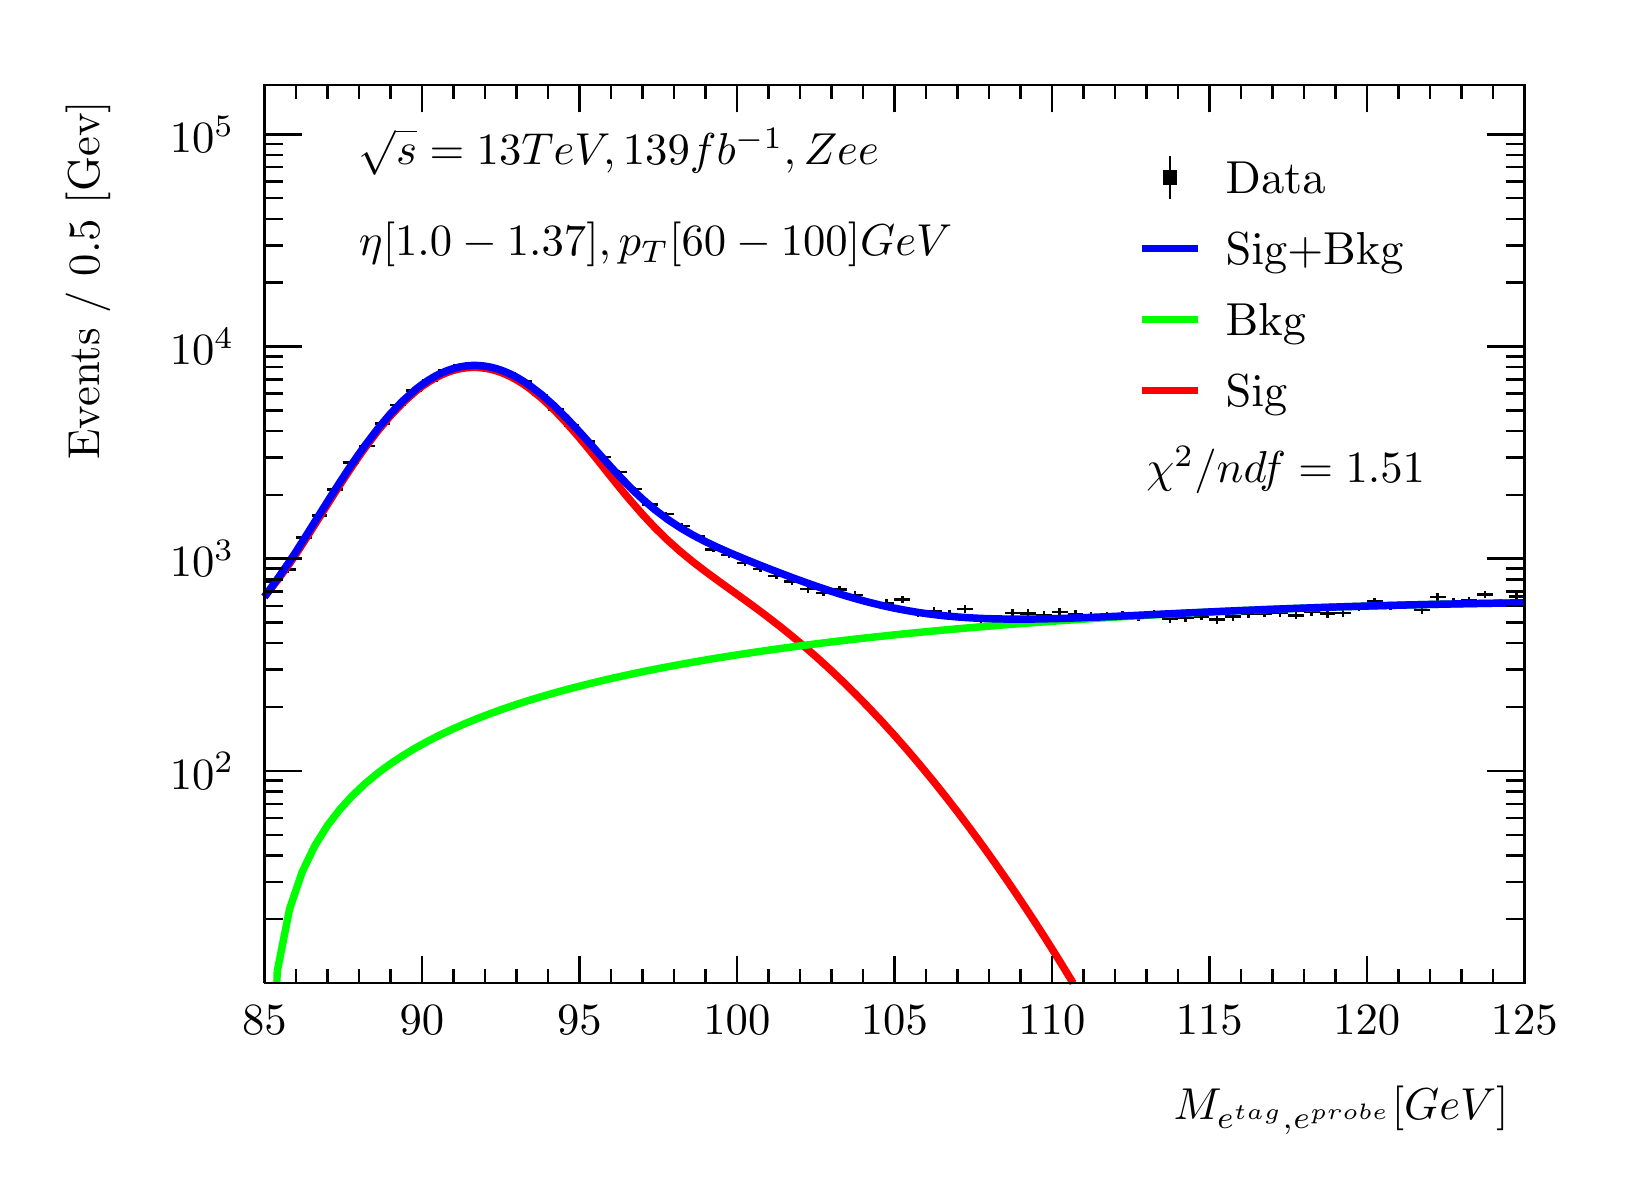
\begin{tikzpicture}
\pgfdeclareplotmark{cross} {
\pgfpathmoveto{\pgfpoint{-0.3\pgfplotmarksize}{\pgfplotmarksize}}
\pgfpathlineto{\pgfpoint{+0.3\pgfplotmarksize}{\pgfplotmarksize}}
\pgfpathlineto{\pgfpoint{+0.3\pgfplotmarksize}{0.3\pgfplotmarksize}}
\pgfpathlineto{\pgfpoint{+1\pgfplotmarksize}{0.3\pgfplotmarksize}}
\pgfpathlineto{\pgfpoint{+1\pgfplotmarksize}{-0.3\pgfplotmarksize}}
\pgfpathlineto{\pgfpoint{+0.3\pgfplotmarksize}{-0.3\pgfplotmarksize}}
\pgfpathlineto{\pgfpoint{+0.3\pgfplotmarksize}{-1.\pgfplotmarksize}}
\pgfpathlineto{\pgfpoint{-0.3\pgfplotmarksize}{-1.\pgfplotmarksize}}
\pgfpathlineto{\pgfpoint{-0.3\pgfplotmarksize}{-0.3\pgfplotmarksize}}
\pgfpathlineto{\pgfpoint{-1.\pgfplotmarksize}{-0.3\pgfplotmarksize}}
\pgfpathlineto{\pgfpoint{-1.\pgfplotmarksize}{0.3\pgfplotmarksize}}
\pgfpathlineto{\pgfpoint{-0.3\pgfplotmarksize}{0.3\pgfplotmarksize}}
\pgfpathclose
\pgfusepathqstroke
}
\pgfdeclareplotmark{cross*} {
\pgfpathmoveto{\pgfpoint{-0.3\pgfplotmarksize}{\pgfplotmarksize}}
\pgfpathlineto{\pgfpoint{+0.3\pgfplotmarksize}{\pgfplotmarksize}}
\pgfpathlineto{\pgfpoint{+0.3\pgfplotmarksize}{0.3\pgfplotmarksize}}
\pgfpathlineto{\pgfpoint{+1\pgfplotmarksize}{0.3\pgfplotmarksize}}
\pgfpathlineto{\pgfpoint{+1\pgfplotmarksize}{-0.3\pgfplotmarksize}}
\pgfpathlineto{\pgfpoint{+0.3\pgfplotmarksize}{-0.3\pgfplotmarksize}}
\pgfpathlineto{\pgfpoint{+0.3\pgfplotmarksize}{-1.\pgfplotmarksize}}
\pgfpathlineto{\pgfpoint{-0.3\pgfplotmarksize}{-1.\pgfplotmarksize}}
\pgfpathlineto{\pgfpoint{-0.3\pgfplotmarksize}{-0.3\pgfplotmarksize}}
\pgfpathlineto{\pgfpoint{-1.\pgfplotmarksize}{-0.3\pgfplotmarksize}}
\pgfpathlineto{\pgfpoint{-1.\pgfplotmarksize}{0.3\pgfplotmarksize}}
\pgfpathlineto{\pgfpoint{-0.3\pgfplotmarksize}{0.3\pgfplotmarksize}}
\pgfpathclose
\pgfusepathqfillstroke
}
\pgfdeclareplotmark{newstar} {
\pgfpathmoveto{\pgfqpoint{0pt}{\pgfplotmarksize}}
\pgfpathlineto{\pgfqpointpolar{44}{0.5\pgfplotmarksize}}
\pgfpathlineto{\pgfqpointpolar{18}{\pgfplotmarksize}}
\pgfpathlineto{\pgfqpointpolar{-20}{0.5\pgfplotmarksize}}
\pgfpathlineto{\pgfqpointpolar{-54}{\pgfplotmarksize}}
\pgfpathlineto{\pgfqpointpolar{-90}{0.5\pgfplotmarksize}}
\pgfpathlineto{\pgfqpointpolar{234}{\pgfplotmarksize}}
\pgfpathlineto{\pgfqpointpolar{198}{0.5\pgfplotmarksize}}
\pgfpathlineto{\pgfqpointpolar{162}{\pgfplotmarksize}}
\pgfpathlineto{\pgfqpointpolar{134}{0.5\pgfplotmarksize}}
\pgfpathclose
\pgfusepathqstroke
}
\pgfdeclareplotmark{newstar*} {
\pgfpathmoveto{\pgfqpoint{0pt}{\pgfplotmarksize}}
\pgfpathlineto{\pgfqpointpolar{44}{0.5\pgfplotmarksize}}
\pgfpathlineto{\pgfqpointpolar{18}{\pgfplotmarksize}}
\pgfpathlineto{\pgfqpointpolar{-20}{0.5\pgfplotmarksize}}
\pgfpathlineto{\pgfqpointpolar{-54}{\pgfplotmarksize}}
\pgfpathlineto{\pgfqpointpolar{-90}{0.5\pgfplotmarksize}}
\pgfpathlineto{\pgfqpointpolar{234}{\pgfplotmarksize}}
\pgfpathlineto{\pgfqpointpolar{198}{0.5\pgfplotmarksize}}
\pgfpathlineto{\pgfqpointpolar{162}{\pgfplotmarksize}}
\pgfpathlineto{\pgfqpointpolar{134}{0.5\pgfplotmarksize}}
\pgfpathclose
\pgfusepathqfillstroke
}
\definecolor{c}{rgb}{1,1,1};
\draw [color=c, fill=c] (0,0) rectangle (20,14.4361);
\draw [color=c, fill=c] (3,2.30977) rectangle (19,13.7143);
\definecolor{c}{rgb}{0,0,0};
\draw [c,line width=0.9] (3,2.30977) -- (3,13.7143) -- (19,13.7143) -- (19,2.30977) -- (3,2.30977);
\definecolor{c}{rgb}{1,1,1};
\draw [color=c, fill=c] (3,2.30977) rectangle (19,13.7143);
\definecolor{c}{rgb}{0,0,0};
\draw [c,line width=0.9] (3,2.30977) -- (3,13.7143) -- (19,13.7143) -- (19,2.30977) -- (3,2.30977);
\draw [c,line width=0.9] (3,2.30977) -- (19,2.30977);
\draw [c,line width=0.9] (3,2.65624) -- (3,2.30977);
\draw [c,line width=0.9] (3.4,2.48301) -- (3.4,2.30977);
\draw [c,line width=0.9] (3.8,2.48301) -- (3.8,2.30977);
\draw [c,line width=0.9] (4.2,2.48301) -- (4.2,2.30977);
\draw [c,line width=0.9] (4.6,2.48301) -- (4.6,2.30977);
\draw [c,line width=0.9] (5,2.65624) -- (5,2.30977);
\draw [c,line width=0.9] (5.4,2.48301) -- (5.4,2.30977);
\draw [c,line width=0.9] (5.8,2.48301) -- (5.8,2.30977);
\draw [c,line width=0.9] (6.2,2.48301) -- (6.2,2.30977);
\draw [c,line width=0.9] (6.6,2.48301) -- (6.6,2.30977);
\draw [c,line width=0.9] (7,2.65624) -- (7,2.30977);
\draw [c,line width=0.9] (7.4,2.48301) -- (7.4,2.30977);
\draw [c,line width=0.9] (7.8,2.48301) -- (7.8,2.30977);
\draw [c,line width=0.9] (8.2,2.48301) -- (8.2,2.30977);
\draw [c,line width=0.9] (8.6,2.48301) -- (8.6,2.30977);
\draw [c,line width=0.9] (9,2.65624) -- (9,2.30977);
\draw [c,line width=0.9] (9.4,2.48301) -- (9.4,2.30977);
\draw [c,line width=0.9] (9.8,2.48301) -- (9.8,2.30977);
\draw [c,line width=0.9] (10.2,2.48301) -- (10.2,2.30977);
\draw [c,line width=0.9] (10.6,2.48301) -- (10.6,2.30977);
\draw [c,line width=0.9] (11,2.65624) -- (11,2.30977);
\draw [c,line width=0.9] (11.4,2.48301) -- (11.4,2.30977);
\draw [c,line width=0.9] (11.8,2.48301) -- (11.8,2.30977);
\draw [c,line width=0.9] (12.2,2.48301) -- (12.2,2.30977);
\draw [c,line width=0.9] (12.6,2.48301) -- (12.6,2.30977);
\draw [c,line width=0.9] (13,2.65624) -- (13,2.30977);
\draw [c,line width=0.9] (13.4,2.48301) -- (13.4,2.30977);
\draw [c,line width=0.9] (13.8,2.48301) -- (13.8,2.30977);
\draw [c,line width=0.9] (14.2,2.48301) -- (14.2,2.30977);
\draw [c,line width=0.9] (14.6,2.48301) -- (14.6,2.30977);
\draw [c,line width=0.9] (15,2.65624) -- (15,2.30977);
\draw [c,line width=0.9] (15.4,2.48301) -- (15.4,2.30977);
\draw [c,line width=0.9] (15.8,2.48301) -- (15.8,2.30977);
\draw [c,line width=0.9] (16.2,2.48301) -- (16.2,2.30977);
\draw [c,line width=0.9] (16.6,2.48301) -- (16.6,2.30977);
\draw [c,line width=0.9] (17,2.65624) -- (17,2.30977);
\draw [c,line width=0.9] (17.4,2.48301) -- (17.4,2.30977);
\draw [c,line width=0.9] (17.8,2.48301) -- (17.8,2.30977);
\draw [c,line width=0.9] (18.2,2.48301) -- (18.2,2.30977);
\draw [c,line width=0.9] (18.6,2.48301) -- (18.6,2.30977);
\draw [c,line width=0.9] (19,2.65624) -- (19,2.30977);
\draw [anchor=base] (3,1.66015) node[scale=1.61424, color=c, rotate=0]{85};
\draw [anchor=base] (5,1.66015) node[scale=1.61424, color=c, rotate=0]{90};
\draw [anchor=base] (7,1.66015) node[scale=1.61424, color=c, rotate=0]{95};
\draw [anchor=base] (9,1.66015) node[scale=1.61424, color=c, rotate=0]{100};
\draw [anchor=base] (11,1.66015) node[scale=1.61424, color=c, rotate=0]{105};
\draw [anchor=base] (13,1.66015) node[scale=1.61424, color=c, rotate=0]{110};
\draw [anchor=base] (15,1.66015) node[scale=1.61424, color=c, rotate=0]{115};
\draw [anchor=base] (17,1.66015) node[scale=1.61424, color=c, rotate=0]{120};
\draw [anchor=base] (19,1.66015) node[scale=1.61424, color=c, rotate=0]{125};
\draw [anchor= east] (19,0.692932) node[scale=1.61424, color=c, rotate=0]{$M_{e^{tag}, e^{probe}}  [GeV]$};
\draw [c,line width=0.9] (3,13.7143) -- (19,13.7143);
\draw [c,line width=0.9] (3,13.3678) -- (3,13.7143);
\draw [c,line width=0.9] (3.4,13.5411) -- (3.4,13.7143);
\draw [c,line width=0.9] (3.8,13.5411) -- (3.8,13.7143);
\draw [c,line width=0.9] (4.2,13.5411) -- (4.2,13.7143);
\draw [c,line width=0.9] (4.6,13.5411) -- (4.6,13.7143);
\draw [c,line width=0.9] (5,13.3678) -- (5,13.7143);
\draw [c,line width=0.9] (5.4,13.5411) -- (5.4,13.7143);
\draw [c,line width=0.9] (5.8,13.5411) -- (5.8,13.7143);
\draw [c,line width=0.9] (6.2,13.5411) -- (6.2,13.7143);
\draw [c,line width=0.9] (6.6,13.5411) -- (6.6,13.7143);
\draw [c,line width=0.9] (7,13.3678) -- (7,13.7143);
\draw [c,line width=0.9] (7.4,13.5411) -- (7.4,13.7143);
\draw [c,line width=0.9] (7.8,13.5411) -- (7.8,13.7143);
\draw [c,line width=0.9] (8.2,13.5411) -- (8.2,13.7143);
\draw [c,line width=0.9] (8.6,13.5411) -- (8.6,13.7143);
\draw [c,line width=0.9] (9,13.3678) -- (9,13.7143);
\draw [c,line width=0.9] (9.4,13.5411) -- (9.4,13.7143);
\draw [c,line width=0.9] (9.8,13.5411) -- (9.8,13.7143);
\draw [c,line width=0.9] (10.2,13.5411) -- (10.2,13.7143);
\draw [c,line width=0.9] (10.6,13.5411) -- (10.6,13.7143);
\draw [c,line width=0.9] (11,13.3678) -- (11,13.7143);
\draw [c,line width=0.9] (11.4,13.5411) -- (11.4,13.7143);
\draw [c,line width=0.9] (11.8,13.5411) -- (11.8,13.7143);
\draw [c,line width=0.9] (12.2,13.5411) -- (12.2,13.7143);
\draw [c,line width=0.9] (12.6,13.5411) -- (12.6,13.7143);
\draw [c,line width=0.9] (13,13.3678) -- (13,13.7143);
\draw [c,line width=0.9] (13.4,13.5411) -- (13.4,13.7143);
\draw [c,line width=0.9] (13.8,13.5411) -- (13.8,13.7143);
\draw [c,line width=0.9] (14.2,13.5411) -- (14.2,13.7143);
\draw [c,line width=0.9] (14.6,13.5411) -- (14.6,13.7143);
\draw [c,line width=0.9] (15,13.3678) -- (15,13.7143);
\draw [c,line width=0.9] (15.4,13.5411) -- (15.4,13.7143);
\draw [c,line width=0.9] (15.8,13.5411) -- (15.8,13.7143);
\draw [c,line width=0.9] (16.2,13.5411) -- (16.2,13.7143);
\draw [c,line width=0.9] (16.6,13.5411) -- (16.6,13.7143);
\draw [c,line width=0.9] (17,13.3678) -- (17,13.7143);
\draw [c,line width=0.9] (17.4,13.5411) -- (17.4,13.7143);
\draw [c,line width=0.9] (17.8,13.5411) -- (17.8,13.7143);
\draw [c,line width=0.9] (18.2,13.5411) -- (18.2,13.7143);
\draw [c,line width=0.9] (18.6,13.5411) -- (18.6,13.7143);
\draw [c,line width=0.9] (19,13.3678) -- (19,13.7143);
\draw [c,line width=0.9] (3,2.30977) -- (3,13.7143);
\draw [c,line width=0.9] (3.237,3.1209) -- (3,3.1209);
\draw [c,line width=0.9] (3.237,3.59538) -- (3,3.59538);
\draw [c,line width=0.9] (3.237,3.93203) -- (3,3.93203);
\draw [c,line width=0.9] (3.237,4.19316) -- (3,4.19316);
\draw [c,line width=0.9] (3.237,4.40651) -- (3,4.40651);
\draw [c,line width=0.9] (3.237,4.5869) -- (3,4.5869);
\draw [c,line width=0.9] (3.237,4.74316) -- (3,4.74316);
\draw [c,line width=0.9] (3.237,4.881) -- (3,4.881);
\draw [c,line width=0.9] (3.474,5.00429) -- (3,5.00429);
\draw [anchor= east] (2.82,5.00429) node[scale=1.61424, color=c, rotate=0]{$10^{2}$};
\draw [c,line width=0.9] (3.237,5.81542) -- (3,5.81542);
\draw [c,line width=0.9] (3.237,6.2899) -- (3,6.2899);
\draw [c,line width=0.9] (3.237,6.62655) -- (3,6.62655);
\draw [c,line width=0.9] (3.237,6.88768) -- (3,6.88768);
\draw [c,line width=0.9] (3.237,7.10103) -- (3,7.10103);
\draw [c,line width=0.9] (3.237,7.28142) -- (3,7.28142);
\draw [c,line width=0.9] (3.237,7.43768) -- (3,7.43768);
\draw [c,line width=0.9] (3.237,7.57551) -- (3,7.57551);
\draw [c,line width=0.9] (3.474,7.69881) -- (3,7.69881);
\draw [anchor= east] (2.82,7.69881) node[scale=1.61424, color=c, rotate=0]{$10^{3}$};
\draw [c,line width=0.9] (3.237,8.50994) -- (3,8.50994);
\draw [c,line width=0.9] (3.237,8.98442) -- (3,8.98442);
\draw [c,line width=0.9] (3.237,9.32107) -- (3,9.32107);
\draw [c,line width=0.9] (3.237,9.58219) -- (3,9.58219);
\draw [c,line width=0.9] (3.237,9.79555) -- (3,9.79555);
\draw [c,line width=0.9] (3.237,9.97594) -- (3,9.97594);
\draw [c,line width=0.9] (3.237,10.1322) -- (3,10.1322);
\draw [c,line width=0.9] (3.237,10.27) -- (3,10.27);
\draw [c,line width=0.9] (3.474,10.3933) -- (3,10.3933);
\draw [anchor= east] (2.82,10.3933) node[scale=1.61424, color=c, rotate=0]{$10^{4}$};
\draw [c,line width=0.9] (3.237,11.2045) -- (3,11.2045);
\draw [c,line width=0.9] (3.237,11.6789) -- (3,11.6789);
\draw [c,line width=0.9] (3.237,12.0156) -- (3,12.0156);
\draw [c,line width=0.9] (3.237,12.2767) -- (3,12.2767);
\draw [c,line width=0.9] (3.237,12.4901) -- (3,12.4901);
\draw [c,line width=0.9] (3.237,12.6705) -- (3,12.6705);
\draw [c,line width=0.9] (3.237,12.8267) -- (3,12.8267);
\draw [c,line width=0.9] (3.237,12.9645) -- (3,12.9645);
\draw [c,line width=0.9] (3.474,13.0878) -- (3,13.0878);
\draw [anchor= east] (2.82,13.0878) node[scale=1.61424, color=c, rotate=0]{$10^{5}$};
\draw [anchor= east] (0.76,13.7143) node[scale=1.61424, color=c, rotate=90]{Events / 0.5 [Gev]};
\draw [c,line width=0.9] (19,2.30977) -- (19,13.7143);
\draw [c,line width=0.9] (18.763,3.1209) -- (19,3.1209);
\draw [c,line width=0.9] (18.763,3.59538) -- (19,3.59538);
\draw [c,line width=0.9] (18.763,3.93203) -- (19,3.93203);
\draw [c,line width=0.9] (18.763,4.19316) -- (19,4.19316);
\draw [c,line width=0.9] (18.763,4.40651) -- (19,4.40651);
\draw [c,line width=0.9] (18.763,4.5869) -- (19,4.5869);
\draw [c,line width=0.9] (18.763,4.74316) -- (19,4.74316);
\draw [c,line width=0.9] (18.763,4.881) -- (19,4.881);
\draw [c,line width=0.9] (18.526,5.00429) -- (19,5.00429);
\draw [c,line width=0.9] (18.763,5.81542) -- (19,5.81542);
\draw [c,line width=0.9] (18.763,6.2899) -- (19,6.2899);
\draw [c,line width=0.9] (18.763,6.62655) -- (19,6.62655);
\draw [c,line width=0.9] (18.763,6.88768) -- (19,6.88768);
\draw [c,line width=0.9] (18.763,7.10103) -- (19,7.10103);
\draw [c,line width=0.9] (18.763,7.28142) -- (19,7.28142);
\draw [c,line width=0.9] (18.763,7.43768) -- (19,7.43768);
\draw [c,line width=0.9] (18.763,7.57551) -- (19,7.57551);
\draw [c,line width=0.9] (18.526,7.69881) -- (19,7.69881);
\draw [c,line width=0.9] (18.763,8.50994) -- (19,8.50994);
\draw [c,line width=0.9] (18.763,8.98442) -- (19,8.98442);
\draw [c,line width=0.9] (18.763,9.32107) -- (19,9.32107);
\draw [c,line width=0.9] (18.763,9.58219) -- (19,9.58219);
\draw [c,line width=0.9] (18.763,9.79555) -- (19,9.79555);
\draw [c,line width=0.9] (18.763,9.97594) -- (19,9.97594);
\draw [c,line width=0.9] (18.763,10.1322) -- (19,10.1322);
\draw [c,line width=0.9] (18.763,10.27) -- (19,10.27);
\draw [c,line width=0.9] (18.526,10.3933) -- (19,10.3933);
\draw [c,line width=0.9] (18.763,11.2045) -- (19,11.2045);
\draw [c,line width=0.9] (18.763,11.6789) -- (19,11.6789);
\draw [c,line width=0.9] (18.763,12.0156) -- (19,12.0156);
\draw [c,line width=0.9] (18.763,12.2767) -- (19,12.2767);
\draw [c,line width=0.9] (18.763,12.4901) -- (19,12.4901);
\draw [c,line width=0.9] (18.763,12.6705) -- (19,12.6705);
\draw [c,line width=0.9] (18.763,12.8267) -- (19,12.8267);
\draw [c,line width=0.9] (18.763,12.9645) -- (19,12.9645);
\draw [c,line width=0.9] (18.526,13.0878) -- (19,13.0878);
\draw [c,line width=0.9] (3.1,7.40655) -- (3,7.40655);
\draw [c,line width=0.9] (3,7.40655) -- (3,7.40655);
\draw [c,line width=0.9] (3.1,7.40655) -- (3.2,7.40655);
\draw [c,line width=0.9] (3.2,7.40655) -- (3.2,7.40655);
\draw [c,line width=0.9] (3.1,7.40655) -- (3.1,7.44848);
\draw [c,line width=0.9] (3.1,7.44848) -- (3.1,7.44848);
\draw [c,line width=0.9] (3.1,7.40655) -- (3.1,7.36463);
\draw [c,line width=0.9] (3.1,7.36463) -- (3.1,7.36463);
\draw [c,line width=0.9] (3.3,7.55981) -- (3.2,7.55981);
\draw [c,line width=0.9] (3.2,7.55981) -- (3.2,7.55981);
\draw [c,line width=0.9] (3.3,7.55981) -- (3.4,7.55981);
\draw [c,line width=0.9] (3.4,7.55981) -- (3.4,7.55981);
\draw [c,line width=0.9] (3.3,7.55981) -- (3.3,7.59907);
\draw [c,line width=0.9] (3.3,7.59907) -- (3.3,7.59907);
\draw [c,line width=0.9] (3.3,7.55981) -- (3.3,7.52054);
\draw [c,line width=0.9] (3.3,7.52054) -- (3.3,7.52054);
\draw [c,line width=0.9] (3.5,7.96647) -- (3.4,7.96647);
\draw [c,line width=0.9] (3.4,7.96647) -- (3.4,7.96647);
\draw [c,line width=0.9] (3.5,7.96647) -- (3.6,7.96647);
\draw [c,line width=0.9] (3.6,7.96647) -- (3.6,7.96647);
\draw [c,line width=0.9] (3.5,7.96647) -- (3.5,7.99948);
\draw [c,line width=0.9] (3.5,7.99948) -- (3.5,7.99948);
\draw [c,line width=0.9] (3.5,7.96647) -- (3.5,7.93346);
\draw [c,line width=0.9] (3.5,7.93346) -- (3.5,7.93346);
\draw [c,line width=0.9] (3.7,8.24808) -- (3.6,8.24808);
\draw [c,line width=0.9] (3.6,8.24808) -- (3.6,8.24808);
\draw [c,line width=0.9] (3.7,8.24808) -- (3.8,8.24808);
\draw [c,line width=0.9] (3.8,8.24808) -- (3.8,8.24808);
\draw [c,line width=0.9] (3.7,8.24808) -- (3.7,8.27735);
\draw [c,line width=0.9] (3.7,8.27735) -- (3.7,8.27735);
\draw [c,line width=0.9] (3.7,8.24808) -- (3.7,8.21882);
\draw [c,line width=0.9] (3.7,8.21882) -- (3.7,8.21882);
\draw [c,line width=0.9] (3.9,8.57702) -- (3.8,8.57702);
\draw [c,line width=0.9] (3.8,8.57702) -- (3.8,8.57702);
\draw [c,line width=0.9] (3.9,8.57702) -- (4,8.57702);
\draw [c,line width=0.9] (4,8.57702) -- (4,8.57702);
\draw [c,line width=0.9] (3.9,8.57702) -- (3.9,8.60245);
\draw [c,line width=0.9] (3.9,8.60245) -- (3.9,8.60245);
\draw [c,line width=0.9] (3.9,8.57702) -- (3.9,8.55159);
\draw [c,line width=0.9] (3.9,8.55159) -- (3.9,8.55159);
\draw [c,line width=0.9] (4.1,8.91905) -- (4,8.91905);
\draw [c,line width=0.9] (4,8.91905) -- (4,8.91905);
\draw [c,line width=0.9] (4.1,8.91905) -- (4.2,8.91905);
\draw [c,line width=0.9] (4.2,8.91905) -- (4.2,8.91905);
\draw [c,line width=0.9] (4.1,8.91905) -- (4.1,8.94102);
\draw [c,line width=0.9] (4.1,8.94102) -- (4.1,8.94102);
\draw [c,line width=0.9] (4.1,8.91905) -- (4.1,8.89708);
\draw [c,line width=0.9] (4.1,8.89708) -- (4.1,8.89708);
\draw [c,line width=0.9] (4.3,9.13192) -- (4.2,9.13192);
\draw [c,line width=0.9] (4.2,9.13192) -- (4.2,9.13192);
\draw [c,line width=0.9] (4.3,9.13192) -- (4.4,9.13192);
\draw [c,line width=0.9] (4.4,9.13192) -- (4.4,9.13192);
\draw [c,line width=0.9] (4.3,9.13192) -- (4.3,9.15198);
\draw [c,line width=0.9] (4.3,9.15198) -- (4.3,9.15198);
\draw [c,line width=0.9] (4.3,9.13192) -- (4.3,9.11186);
\draw [c,line width=0.9] (4.3,9.11186) -- (4.3,9.11186);
\draw [c,line width=0.9] (4.5,9.41384) -- (4.4,9.41384);
\draw [c,line width=0.9] (4.4,9.41384) -- (4.4,9.41384);
\draw [c,line width=0.9] (4.5,9.41384) -- (4.6,9.41384);
\draw [c,line width=0.9] (4.6,9.41384) -- (4.6,9.41384);
\draw [c,line width=0.9] (4.5,9.41384) -- (4.5,9.43162);
\draw [c,line width=0.9] (4.5,9.43162) -- (4.5,9.43162);
\draw [c,line width=0.9] (4.5,9.41384) -- (4.5,9.39605);
\draw [c,line width=0.9] (4.5,9.39605) -- (4.5,9.39605);
\draw [c,line width=0.9] (4.7,9.6506) -- (4.6,9.6506);
\draw [c,line width=0.9] (4.6,9.6506) -- (4.6,9.6506);
\draw [c,line width=0.9] (4.7,9.6506) -- (4.8,9.6506);
\draw [c,line width=0.9] (4.8,9.6506) -- (4.8,9.6506);
\draw [c,line width=0.9] (4.7,9.6506) -- (4.7,9.66668);
\draw [c,line width=0.9] (4.7,9.66668) -- (4.7,9.66668);
\draw [c,line width=0.9] (4.7,9.6506) -- (4.7,9.63453);
\draw [c,line width=0.9] (4.7,9.63453) -- (4.7,9.63453);
\draw [c,line width=0.9] (4.9,9.83298) -- (4.8,9.83298);
\draw [c,line width=0.9] (4.8,9.83298) -- (4.8,9.83298);
\draw [c,line width=0.9] (4.9,9.83298) -- (5,9.83298);
\draw [c,line width=0.9] (5,9.83298) -- (5,9.83298);
\draw [c,line width=0.9] (4.9,9.83298) -- (4.9,9.84785);
\draw [c,line width=0.9] (4.9,9.84785) -- (4.9,9.84785);
\draw [c,line width=0.9] (4.9,9.83298) -- (4.9,9.81811);
\draw [c,line width=0.9] (4.9,9.81811) -- (4.9,9.81811);
\draw [c,line width=0.9] (5.1,9.96215) -- (5,9.96215);
\draw [c,line width=0.9] (5,9.96215) -- (5,9.96215);
\draw [c,line width=0.9] (5.1,9.96215) -- (5.2,9.96215);
\draw [c,line width=0.9] (5.2,9.96215) -- (5.2,9.96215);
\draw [c,line width=0.9] (5.1,9.96215) -- (5.1,9.97622);
\draw [c,line width=0.9] (5.1,9.97622) -- (5.1,9.97622);
\draw [c,line width=0.9] (5.1,9.96215) -- (5.1,9.94808);
\draw [c,line width=0.9] (5.1,9.94808) -- (5.1,9.94808);
\draw [c,line width=0.9] (5.3,10.0901) -- (5.2,10.0901);
\draw [c,line width=0.9] (5.2,10.0901) -- (5.2,10.0901);
\draw [c,line width=0.9] (5.3,10.0901) -- (5.4,10.0901);
\draw [c,line width=0.9] (5.4,10.0901) -- (5.4,10.0901);
\draw [c,line width=0.9] (5.3,10.0901) -- (5.3,10.1034);
\draw [c,line width=0.9] (5.3,10.1034) -- (5.3,10.1034);
\draw [c,line width=0.9] (5.3,10.0901) -- (5.3,10.0767);
\draw [c,line width=0.9] (5.3,10.0767) -- (5.3,10.0767);
\draw [c,line width=0.9] (5.5,10.1545) -- (5.4,10.1545);
\draw [c,line width=0.9] (5.4,10.1545) -- (5.4,10.1545);
\draw [c,line width=0.9] (5.5,10.1545) -- (5.6,10.1545);
\draw [c,line width=0.9] (5.6,10.1545) -- (5.6,10.1545);
\draw [c,line width=0.9] (5.5,10.1545) -- (5.5,10.1675);
\draw [c,line width=0.9] (5.5,10.1675) -- (5.5,10.1675);
\draw [c,line width=0.9] (5.5,10.1545) -- (5.5,10.1416);
\draw [c,line width=0.9] (5.5,10.1416) -- (5.5,10.1416);
\draw [c,line width=0.9] (5.7,10.1734) -- (5.6,10.1734);
\draw [c,line width=0.9] (5.6,10.1734) -- (5.6,10.1734);
\draw [c,line width=0.9] (5.7,10.1734) -- (5.8,10.1734);
\draw [c,line width=0.9] (5.8,10.1734) -- (5.8,10.1734);
\draw [c,line width=0.9] (5.7,10.1734) -- (5.7,10.1863);
\draw [c,line width=0.9] (5.7,10.1863) -- (5.7,10.1863);
\draw [c,line width=0.9] (5.7,10.1734) -- (5.7,10.1606);
\draw [c,line width=0.9] (5.7,10.1606) -- (5.7,10.1606);
\draw [c,line width=0.9] (5.9,10.1275) -- (5.8,10.1275);
\draw [c,line width=0.9] (5.8,10.1275) -- (5.8,10.1275);
\draw [c,line width=0.9] (5.9,10.1275) -- (6,10.1275);
\draw [c,line width=0.9] (6,10.1275) -- (6,10.1275);
\draw [c,line width=0.9] (5.9,10.1275) -- (5.9,10.1406);
\draw [c,line width=0.9] (5.9,10.1406) -- (5.9,10.1406);
\draw [c,line width=0.9] (5.9,10.1275) -- (5.9,10.1144);
\draw [c,line width=0.9] (5.9,10.1144) -- (5.9,10.1144);
\draw [c,line width=0.9] (6.1,10.0498) -- (6,10.0498);
\draw [c,line width=0.9] (6,10.0498) -- (6,10.0498);
\draw [c,line width=0.9] (6.1,10.0498) -- (6.2,10.0498);
\draw [c,line width=0.9] (6.2,10.0498) -- (6.2,10.0498);
\draw [c,line width=0.9] (6.1,10.0498) -- (6.1,10.0633);
\draw [c,line width=0.9] (6.1,10.0633) -- (6.1,10.0633);
\draw [c,line width=0.9] (6.1,10.0498) -- (6.1,10.0362);
\draw [c,line width=0.9] (6.1,10.0362) -- (6.1,10.0362);
\draw [c,line width=0.9] (6.3,9.94888) -- (6.2,9.94888);
\draw [c,line width=0.9] (6.2,9.94888) -- (6.2,9.94888);
\draw [c,line width=0.9] (6.3,9.94888) -- (6.4,9.94888);
\draw [c,line width=0.9] (6.4,9.94888) -- (6.4,9.94888);
\draw [c,line width=0.9] (6.3,9.94888) -- (6.3,9.96303);
\draw [c,line width=0.9] (6.3,9.96303) -- (6.3,9.96303);
\draw [c,line width=0.9] (6.3,9.94888) -- (6.3,9.93473);
\draw [c,line width=0.9] (6.3,9.93473) -- (6.3,9.93473);
\draw [c,line width=0.9] (6.5,9.77964) -- (6.4,9.77964);
\draw [c,line width=0.9] (6.4,9.77964) -- (6.4,9.77964);
\draw [c,line width=0.9] (6.5,9.77964) -- (6.6,9.77964);
\draw [c,line width=0.9] (6.6,9.77964) -- (6.6,9.77964);
\draw [c,line width=0.9] (6.5,9.77964) -- (6.5,9.79486);
\draw [c,line width=0.9] (6.5,9.79486) -- (6.5,9.79486);
\draw [c,line width=0.9] (6.5,9.77964) -- (6.5,9.76443);
\draw [c,line width=0.9] (6.5,9.76443) -- (6.5,9.76443);
\draw [c,line width=0.9] (6.7,9.59152) -- (6.6,9.59152);
\draw [c,line width=0.9] (6.6,9.59152) -- (6.6,9.59152);
\draw [c,line width=0.9] (6.7,9.59152) -- (6.8,9.59152);
\draw [c,line width=0.9] (6.8,9.59152) -- (6.8,9.59152);
\draw [c,line width=0.9] (6.7,9.59152) -- (6.7,9.608);
\draw [c,line width=0.9] (6.7,9.608) -- (6.7,9.608);
\draw [c,line width=0.9] (6.7,9.59152) -- (6.7,9.57504);
\draw [c,line width=0.9] (6.7,9.57504) -- (6.7,9.57504);
\draw [c,line width=0.9] (6.9,9.39284) -- (6.8,9.39284);
\draw [c,line width=0.9] (6.8,9.39284) -- (6.8,9.39284);
\draw [c,line width=0.9] (6.9,9.39284) -- (7,9.39284);
\draw [c,line width=0.9] (7,9.39284) -- (7,9.39284);
\draw [c,line width=0.9] (6.9,9.39284) -- (6.9,9.41078);
\draw [c,line width=0.9] (6.9,9.41078) -- (6.9,9.41078);
\draw [c,line width=0.9] (6.9,9.39284) -- (6.9,9.3749);
\draw [c,line width=0.9] (6.9,9.3749) -- (6.9,9.3749);
\draw [c,line width=0.9] (7.1,9.18798) -- (7,9.18798);
\draw [c,line width=0.9] (7,9.18798) -- (7,9.18798);
\draw [c,line width=0.9] (7.1,9.18798) -- (7.2,9.18798);
\draw [c,line width=0.9] (7.2,9.18798) -- (7.2,9.18798);
\draw [c,line width=0.9] (7.1,9.18798) -- (7.1,9.20757);
\draw [c,line width=0.9] (7.1,9.20757) -- (7.1,9.20757);
\draw [c,line width=0.9] (7.1,9.18798) -- (7.1,9.1684);
\draw [c,line width=0.9] (7.1,9.1684) -- (7.1,9.1684);
\draw [c,line width=0.9] (7.3,8.99297) -- (7.2,8.99297);
\draw [c,line width=0.9] (7.2,8.99297) -- (7.2,8.99297);
\draw [c,line width=0.9] (7.3,8.99297) -- (7.4,8.99297);
\draw [c,line width=0.9] (7.4,8.99297) -- (7.4,8.99297);
\draw [c,line width=0.9] (7.3,8.99297) -- (7.3,9.01426);
\draw [c,line width=0.9] (7.3,9.01426) -- (7.3,9.01426);
\draw [c,line width=0.9] (7.3,8.99297) -- (7.3,8.97168);
\draw [c,line width=0.9] (7.3,8.97168) -- (7.3,8.97168);
\draw [c,line width=0.9] (7.5,8.8011) -- (7.4,8.8011);
\draw [c,line width=0.9] (7.4,8.8011) -- (7.4,8.8011);
\draw [c,line width=0.9] (7.5,8.8011) -- (7.6,8.8011);
\draw [c,line width=0.9] (7.6,8.8011) -- (7.6,8.8011);
\draw [c,line width=0.9] (7.5,8.8011) -- (7.5,8.82421);
\draw [c,line width=0.9] (7.5,8.82421) -- (7.5,8.82421);
\draw [c,line width=0.9] (7.5,8.8011) -- (7.5,8.778);
\draw [c,line width=0.9] (7.5,8.778) -- (7.5,8.778);
\draw [c,line width=0.9] (7.7,8.58198) -- (7.6,8.58198);
\draw [c,line width=0.9] (7.6,8.58198) -- (7.6,8.58198);
\draw [c,line width=0.9] (7.7,8.58198) -- (7.8,8.58198);
\draw [c,line width=0.9] (7.8,8.58198) -- (7.8,8.58198);
\draw [c,line width=0.9] (7.7,8.58198) -- (7.7,8.60736);
\draw [c,line width=0.9] (7.7,8.60736) -- (7.7,8.60736);
\draw [c,line width=0.9] (7.7,8.58198) -- (7.7,8.55661);
\draw [c,line width=0.9] (7.7,8.55661) -- (7.7,8.55661);
\draw [c,line width=0.9] (7.9,8.38989) -- (7.8,8.38989);
\draw [c,line width=0.9] (7.8,8.38989) -- (7.8,8.38989);
\draw [c,line width=0.9] (7.9,8.38989) -- (8,8.38989);
\draw [c,line width=0.9] (8,8.38989) -- (8,8.38989);
\draw [c,line width=0.9] (7.9,8.38989) -- (7.9,8.41743);
\draw [c,line width=0.9] (7.9,8.41743) -- (7.9,8.41743);
\draw [c,line width=0.9] (7.9,8.38989) -- (7.9,8.36235);
\draw [c,line width=0.9] (7.9,8.36235) -- (7.9,8.36235);
\draw [c,line width=0.9] (8.1,8.26624) -- (8,8.26624);
\draw [c,line width=0.9] (8,8.26624) -- (8,8.26624);
\draw [c,line width=0.9] (8.1,8.26624) -- (8.2,8.26624);
\draw [c,line width=0.9] (8.2,8.26624) -- (8.2,8.26624);
\draw [c,line width=0.9] (8.1,8.26624) -- (8.1,8.29527);
\draw [c,line width=0.9] (8.1,8.29527) -- (8.1,8.29527);
\draw [c,line width=0.9] (8.1,8.26624) -- (8.1,8.2372);
\draw [c,line width=0.9] (8.1,8.2372) -- (8.1,8.2372);
\draw [c,line width=0.9] (8.3,8.11655) -- (8.2,8.11655);
\draw [c,line width=0.9] (8.2,8.11655) -- (8.2,8.11655);
\draw [c,line width=0.9] (8.3,8.11655) -- (8.4,8.11655);
\draw [c,line width=0.9] (8.4,8.11655) -- (8.4,8.11655);
\draw [c,line width=0.9] (8.3,8.11655) -- (8.3,8.1475);
\draw [c,line width=0.9] (8.3,8.1475) -- (8.3,8.1475);
\draw [c,line width=0.9] (8.3,8.11655) -- (8.3,8.08559);
\draw [c,line width=0.9] (8.3,8.08559) -- (8.3,8.08559);
\draw [c,line width=0.9] (8.5,7.97943) -- (8.4,7.97943);
\draw [c,line width=0.9] (8.4,7.97943) -- (8.4,7.97943);
\draw [c,line width=0.9] (8.5,7.97943) -- (8.6,7.97943);
\draw [c,line width=0.9] (8.6,7.97943) -- (8.6,7.97943);
\draw [c,line width=0.9] (8.5,7.97943) -- (8.5,8.01225);
\draw [c,line width=0.9] (8.5,8.01225) -- (8.5,8.01225);
\draw [c,line width=0.9] (8.5,7.97943) -- (8.5,7.94661);
\draw [c,line width=0.9] (8.5,7.94661) -- (8.5,7.94661);
\draw [c,line width=0.9] (8.7,7.81671) -- (8.6,7.81671);
\draw [c,line width=0.9] (8.6,7.81671) -- (8.6,7.81671);
\draw [c,line width=0.9] (8.7,7.81671) -- (8.8,7.81671);
\draw [c,line width=0.9] (8.8,7.81671) -- (8.8,7.81671);
\draw [c,line width=0.9] (8.7,7.81671) -- (8.7,7.85189);
\draw [c,line width=0.9] (8.7,7.85189) -- (8.7,7.85189);
\draw [c,line width=0.9] (8.7,7.81671) -- (8.7,7.78152);
\draw [c,line width=0.9] (8.7,7.78152) -- (8.7,7.78152);
\draw [c,line width=0.9] (8.9,7.7492) -- (8.8,7.7492);
\draw [c,line width=0.9] (8.8,7.7492) -- (8.8,7.7492);
\draw [c,line width=0.9] (8.9,7.7492) -- (9,7.7492);
\draw [c,line width=0.9] (9,7.7492) -- (9,7.7492);
\draw [c,line width=0.9] (8.9,7.7492) -- (8.9,7.78541);
\draw [c,line width=0.9] (8.9,7.78541) -- (8.9,7.78541);
\draw [c,line width=0.9] (8.9,7.7492) -- (8.9,7.71298);
\draw [c,line width=0.9] (8.9,7.71298) -- (8.9,7.71298);
\draw [c,line width=0.9] (9.1,7.64247) -- (9,7.64247);
\draw [c,line width=0.9] (9,7.64247) -- (9,7.64247);
\draw [c,line width=0.9] (9.1,7.64247) -- (9.2,7.64247);
\draw [c,line width=0.9] (9.2,7.64247) -- (9.2,7.64247);
\draw [c,line width=0.9] (9.1,7.64247) -- (9.1,7.68038);
\draw [c,line width=0.9] (9.1,7.68038) -- (9.1,7.68038);
\draw [c,line width=0.9] (9.1,7.64247) -- (9.1,7.60457);
\draw [c,line width=0.9] (9.1,7.60457) -- (9.1,7.60457);
\draw [c,line width=0.9] (9.3,7.56769) -- (9.2,7.56769);
\draw [c,line width=0.9] (9.2,7.56769) -- (9.2,7.56769);
\draw [c,line width=0.9] (9.3,7.56769) -- (9.4,7.56769);
\draw [c,line width=0.9] (9.4,7.56769) -- (9.4,7.56769);
\draw [c,line width=0.9] (9.3,7.56769) -- (9.3,7.60682);
\draw [c,line width=0.9] (9.3,7.60682) -- (9.3,7.60682);
\draw [c,line width=0.9] (9.3,7.56769) -- (9.3,7.52855);
\draw [c,line width=0.9] (9.3,7.52855) -- (9.3,7.52855);
\draw [c,line width=0.9] (9.5,7.47935) -- (9.4,7.47935);
\draw [c,line width=0.9] (9.4,7.47935) -- (9.4,7.47935);
\draw [c,line width=0.9] (9.5,7.47935) -- (9.6,7.47935);
\draw [c,line width=0.9] (9.6,7.47935) -- (9.6,7.47935);
\draw [c,line width=0.9] (9.5,7.47935) -- (9.5,7.51999);
\draw [c,line width=0.9] (9.5,7.51999) -- (9.5,7.51999);
\draw [c,line width=0.9] (9.5,7.47935) -- (9.5,7.43871);
\draw [c,line width=0.9] (9.5,7.43871) -- (9.5,7.43871);
\draw [c,line width=0.9] (9.7,7.40956) -- (9.6,7.40956);
\draw [c,line width=0.9] (9.6,7.40956) -- (9.6,7.40956);
\draw [c,line width=0.9] (9.7,7.40956) -- (9.8,7.40956);
\draw [c,line width=0.9] (9.8,7.40956) -- (9.8,7.40956);
\draw [c,line width=0.9] (9.7,7.40956) -- (9.7,7.45143);
\draw [c,line width=0.9] (9.7,7.45143) -- (9.7,7.45143);
\draw [c,line width=0.9] (9.7,7.40956) -- (9.7,7.36768);
\draw [c,line width=0.9] (9.7,7.36768) -- (9.7,7.36768);
\draw [c,line width=0.9] (9.9,7.31276) -- (9.8,7.31276);
\draw [c,line width=0.9] (9.8,7.31276) -- (9.8,7.31276);
\draw [c,line width=0.9] (9.9,7.31276) -- (10,7.31276);
\draw [c,line width=0.9] (10,7.31276) -- (10,7.31276);
\draw [c,line width=0.9] (9.9,7.31276) -- (9.9,7.3564);
\draw [c,line width=0.9] (9.9,7.3564) -- (9.9,7.3564);
\draw [c,line width=0.9] (9.9,7.31276) -- (9.9,7.26912);
\draw [c,line width=0.9] (9.9,7.26912) -- (9.9,7.26912);
\draw [c,line width=0.9] (10.1,7.26459) -- (10,7.26459);
\draw [c,line width=0.9] (10,7.26459) -- (10,7.26459);
\draw [c,line width=0.9] (10.1,7.26459) -- (10.2,7.26459);
\draw [c,line width=0.9] (10.2,7.26459) -- (10.2,7.26459);
\draw [c,line width=0.9] (10.1,7.26459) -- (10.1,7.30913);
\draw [c,line width=0.9] (10.1,7.30913) -- (10.1,7.30913);
\draw [c,line width=0.9] (10.1,7.26459) -- (10.1,7.22004);
\draw [c,line width=0.9] (10.1,7.22004) -- (10.1,7.22004);
\draw [c,line width=0.9] (10.3,7.3095) -- (10.2,7.3095);
\draw [c,line width=0.9] (10.2,7.3095) -- (10.2,7.3095);
\draw [c,line width=0.9] (10.3,7.3095) -- (10.4,7.3095);
\draw [c,line width=0.9] (10.4,7.3095) -- (10.4,7.3095);
\draw [c,line width=0.9] (10.3,7.3095) -- (10.3,7.3532);
\draw [c,line width=0.9] (10.3,7.3532) -- (10.3,7.3532);
\draw [c,line width=0.9] (10.3,7.3095) -- (10.3,7.2658);
\draw [c,line width=0.9] (10.3,7.2658) -- (10.3,7.2658);
\draw [c,line width=0.9] (10.5,7.23886) -- (10.4,7.23886);
\draw [c,line width=0.9] (10.4,7.23886) -- (10.4,7.23886);
\draw [c,line width=0.9] (10.5,7.23886) -- (10.6,7.23886);
\draw [c,line width=0.9] (10.6,7.23886) -- (10.6,7.23886);
\draw [c,line width=0.9] (10.5,7.23886) -- (10.5,7.2839);
\draw [c,line width=0.9] (10.5,7.2839) -- (10.5,7.2839);
\draw [c,line width=0.9] (10.5,7.23886) -- (10.5,7.19383);
\draw [c,line width=0.9] (10.5,7.19383) -- (10.5,7.19383);
\draw [c,line width=0.9] (10.7,7.1394) -- (10.6,7.1394);
\draw [c,line width=0.9] (10.6,7.1394) -- (10.6,7.1394);
\draw [c,line width=0.9] (10.7,7.1394) -- (10.8,7.1394);
\draw [c,line width=0.9] (10.8,7.1394) -- (10.8,7.1394);
\draw [c,line width=0.9] (10.7,7.1394) -- (10.7,7.1864);
\draw [c,line width=0.9] (10.7,7.1864) -- (10.7,7.1864);
\draw [c,line width=0.9] (10.7,7.1394) -- (10.7,7.09241);
\draw [c,line width=0.9] (10.7,7.09241) -- (10.7,7.09241);
\draw [c,line width=0.9] (10.9,7.13373) -- (10.8,7.13373);
\draw [c,line width=0.9] (10.8,7.13373) -- (10.8,7.13373);
\draw [c,line width=0.9] (10.9,7.13373) -- (11,7.13373);
\draw [c,line width=0.9] (11,7.13373) -- (11,7.13373);
\draw [c,line width=0.9] (10.9,7.13373) -- (10.9,7.18084);
\draw [c,line width=0.9] (10.9,7.18084) -- (10.9,7.18084);
\draw [c,line width=0.9] (10.9,7.13373) -- (10.9,7.08662);
\draw [c,line width=0.9] (10.9,7.08662) -- (10.9,7.08662);
\draw [c,line width=0.9] (11.1,7.18021) -- (11,7.18021);
\draw [c,line width=0.9] (11,7.18021) -- (11,7.18021);
\draw [c,line width=0.9] (11.1,7.18021) -- (11.2,7.18021);
\draw [c,line width=0.9] (11.2,7.18021) -- (11.2,7.18021);
\draw [c,line width=0.9] (11.1,7.18021) -- (11.1,7.22639);
\draw [c,line width=0.9] (11.1,7.22639) -- (11.1,7.22639);
\draw [c,line width=0.9] (11.1,7.18021) -- (11.1,7.13403);
\draw [c,line width=0.9] (11.1,7.13403) -- (11.1,7.13403);
\draw [c,line width=0.9] (11.3,7.0098) -- (11.2,7.0098);
\draw [c,line width=0.9] (11.2,7.0098) -- (11.2,7.0098);
\draw [c,line width=0.9] (11.3,7.0098) -- (11.4,7.0098);
\draw [c,line width=0.9] (11.4,7.0098) -- (11.4,7.0098);
\draw [c,line width=0.9] (11.3,7.0098) -- (11.3,7.05947);
\draw [c,line width=0.9] (11.3,7.05947) -- (11.3,7.05947);
\draw [c,line width=0.9] (11.3,7.0098) -- (11.3,6.96013);
\draw [c,line width=0.9] (11.3,6.96013) -- (11.3,6.96013);
\draw [c,line width=0.9] (11.5,7.03277) -- (11.4,7.03277);
\draw [c,line width=0.9] (11.4,7.03277) -- (11.4,7.03277);
\draw [c,line width=0.9] (11.5,7.03277) -- (11.6,7.03277);
\draw [c,line width=0.9] (11.6,7.03277) -- (11.6,7.03277);
\draw [c,line width=0.9] (11.5,7.03277) -- (11.5,7.08195);
\draw [c,line width=0.9] (11.5,7.08195) -- (11.5,7.08195);
\draw [c,line width=0.9] (11.5,7.03277) -- (11.5,6.98358);
\draw [c,line width=0.9] (11.5,6.98358) -- (11.5,6.98358);
\draw [c,line width=0.9] (11.7,6.99281) -- (11.6,6.99281);
\draw [c,line width=0.9] (11.6,6.99281) -- (11.6,6.99281);
\draw [c,line width=0.9] (11.7,6.99281) -- (11.8,6.99281);
\draw [c,line width=0.9] (11.8,6.99281) -- (11.8,6.99281);
\draw [c,line width=0.9] (11.7,6.99281) -- (11.7,7.04284);
\draw [c,line width=0.9] (11.7,7.04284) -- (11.7,7.04284);
\draw [c,line width=0.9] (11.7,6.99281) -- (11.7,6.94278);
\draw [c,line width=0.9] (11.7,6.94278) -- (11.7,6.94278);
\draw [c,line width=0.9] (11.9,7.06338) -- (11.8,7.06338);
\draw [c,line width=0.9] (11.8,7.06338) -- (11.8,7.06338);
\draw [c,line width=0.9] (11.9,7.06338) -- (12,7.06338);
\draw [c,line width=0.9] (12,7.06338) -- (12,7.06338);
\draw [c,line width=0.9] (11.9,7.06338) -- (11.9,7.11192);
\draw [c,line width=0.9] (11.9,7.11192) -- (11.9,7.11192);
\draw [c,line width=0.9] (11.9,7.06338) -- (11.9,7.01483);
\draw [c,line width=0.9] (11.9,7.01483) -- (11.9,7.01483);
\draw [c,line width=0.9] (12.1,6.8472) -- (12,6.8472);
\draw [c,line width=0.9] (12,6.8472) -- (12,6.8472);
\draw [c,line width=0.9] (12.1,6.8472) -- (12.2,6.8472);
\draw [c,line width=0.9] (12.2,6.8472) -- (12.2,6.8472);
\draw [c,line width=0.9] (12.1,6.8472) -- (12.1,6.90044);
\draw [c,line width=0.9] (12.1,6.90044) -- (12.1,6.90044);
\draw [c,line width=0.9] (12.1,6.8472) -- (12.1,6.79396);
\draw [c,line width=0.9] (12.1,6.79396) -- (12.1,6.79396);
\draw [c,line width=0.9] (12.3,6.93807) -- (12.2,6.93807);
\draw [c,line width=0.9] (12.2,6.93807) -- (12.2,6.93807);
\draw [c,line width=0.9] (12.3,6.93807) -- (12.4,6.93807);
\draw [c,line width=0.9] (12.4,6.93807) -- (12.4,6.93807);
\draw [c,line width=0.9] (12.3,6.93807) -- (12.3,6.98928);
\draw [c,line width=0.9] (12.3,6.98928) -- (12.3,6.98928);
\draw [c,line width=0.9] (12.3,6.93807) -- (12.3,6.88685);
\draw [c,line width=0.9] (12.3,6.88685) -- (12.3,6.88685);
\draw [c,line width=0.9] (12.5,7.00769) -- (12.4,7.00769);
\draw [c,line width=0.9] (12.4,7.00769) -- (12.4,7.00769);
\draw [c,line width=0.9] (12.5,7.00769) -- (12.6,7.00769);
\draw [c,line width=0.9] (12.6,7.00769) -- (12.6,7.00769);
\draw [c,line width=0.9] (12.5,7.00769) -- (12.5,7.05741);
\draw [c,line width=0.9] (12.5,7.05741) -- (12.5,7.05741);
\draw [c,line width=0.9] (12.5,7.00769) -- (12.5,6.95798);
\draw [c,line width=0.9] (12.5,6.95798) -- (12.5,6.95798);
\draw [c,line width=0.9] (12.7,7.00558) -- (12.6,7.00558);
\draw [c,line width=0.9] (12.6,7.00558) -- (12.6,7.00558);
\draw [c,line width=0.9] (12.7,7.00558) -- (12.8,7.00558);
\draw [c,line width=0.9] (12.8,7.00558) -- (12.8,7.00558);
\draw [c,line width=0.9] (12.7,7.00558) -- (12.7,7.05534);
\draw [c,line width=0.9] (12.7,7.05534) -- (12.7,7.05534);
\draw [c,line width=0.9] (12.7,7.00558) -- (12.7,6.95582);
\draw [c,line width=0.9] (12.7,6.95582) -- (12.7,6.95582);
\draw [c,line width=0.9] (12.9,6.98207) -- (12.8,6.98207);
\draw [c,line width=0.9] (12.8,6.98207) -- (12.8,6.98207);
\draw [c,line width=0.9] (12.9,6.98207) -- (13,6.98207);
\draw [c,line width=0.9] (13,6.98207) -- (13,6.98207);
\draw [c,line width=0.9] (12.9,6.98207) -- (12.9,7.03233);
\draw [c,line width=0.9] (12.9,7.03233) -- (12.9,7.03233);
\draw [c,line width=0.9] (12.9,6.98207) -- (12.9,6.9318);
\draw [c,line width=0.9] (12.9,6.9318) -- (12.9,6.9318);
\draw [c,line width=0.9] (13.1,7.02239) -- (13,7.02239);
\draw [c,line width=0.9] (13,7.02239) -- (13,7.02239);
\draw [c,line width=0.9] (13.1,7.02239) -- (13.2,7.02239);
\draw [c,line width=0.9] (13.2,7.02239) -- (13.2,7.02239);
\draw [c,line width=0.9] (13.1,7.02239) -- (13.1,7.07179);
\draw [c,line width=0.9] (13.1,7.07179) -- (13.1,7.07179);
\draw [c,line width=0.9] (13.1,7.02239) -- (13.1,6.97298);
\draw [c,line width=0.9] (13.1,6.97298) -- (13.1,6.97298);
\draw [c,line width=0.9] (13.3,6.99281) -- (13.2,6.99281);
\draw [c,line width=0.9] (13.2,6.99281) -- (13.2,6.99281);
\draw [c,line width=0.9] (13.3,6.99281) -- (13.4,6.99281);
\draw [c,line width=0.9] (13.4,6.99281) -- (13.4,6.99281);
\draw [c,line width=0.9] (13.3,6.99281) -- (13.3,7.04284);
\draw [c,line width=0.9] (13.3,7.04284) -- (13.3,7.04284);
\draw [c,line width=0.9] (13.3,6.99281) -- (13.3,6.94278);
\draw [c,line width=0.9] (13.3,6.94278) -- (13.3,6.94278);
\draw [c,line width=0.9] (13.5,6.96904) -- (13.4,6.96904);
\draw [c,line width=0.9] (13.4,6.96904) -- (13.4,6.96904);
\draw [c,line width=0.9] (13.5,6.96904) -- (13.6,6.96904);
\draw [c,line width=0.9] (13.6,6.96904) -- (13.6,6.96904);
\draw [c,line width=0.9] (13.5,6.96904) -- (13.5,7.01958);
\draw [c,line width=0.9] (13.5,7.01958) -- (13.5,7.01958);
\draw [c,line width=0.9] (13.5,6.96904) -- (13.5,6.9185);
\draw [c,line width=0.9] (13.5,6.9185) -- (13.5,6.9185);
\draw [c,line width=0.9] (13.7,6.96904) -- (13.6,6.96904);
\draw [c,line width=0.9] (13.6,6.96904) -- (13.6,6.96904);
\draw [c,line width=0.9] (13.7,6.96904) -- (13.8,6.96904);
\draw [c,line width=0.9] (13.8,6.96904) -- (13.8,6.96904);
\draw [c,line width=0.9] (13.7,6.96904) -- (13.7,7.01958);
\draw [c,line width=0.9] (13.7,7.01958) -- (13.7,7.01958);
\draw [c,line width=0.9] (13.7,6.96904) -- (13.7,6.9185);
\draw [c,line width=0.9] (13.7,6.9185) -- (13.7,6.9185);
\draw [c,line width=0.9] (13.9,6.9799) -- (13.8,6.9799);
\draw [c,line width=0.9] (13.8,6.9799) -- (13.8,6.9799);
\draw [c,line width=0.9] (13.9,6.9799) -- (14,6.9799);
\draw [c,line width=0.9] (14,6.9799) -- (14,6.9799);
\draw [c,line width=0.9] (13.9,6.9799) -- (13.9,7.03021);
\draw [c,line width=0.9] (13.9,7.03021) -- (13.9,7.03021);
\draw [c,line width=0.9] (13.9,6.9799) -- (13.9,6.9296);
\draw [c,line width=0.9] (13.9,6.9296) -- (13.9,6.9296);
\draw [c,line width=0.9] (14.1,6.95366) -- (14,6.95366);
\draw [c,line width=0.9] (14,6.95366) -- (14,6.95366);
\draw [c,line width=0.9] (14.1,6.95366) -- (14.2,6.95366);
\draw [c,line width=0.9] (14.2,6.95366) -- (14.2,6.95366);
\draw [c,line width=0.9] (14.1,6.95366) -- (14.1,7.00453);
\draw [c,line width=0.9] (14.1,7.00453) -- (14.1,7.00453);
\draw [c,line width=0.9] (14.1,6.95366) -- (14.1,6.90278);
\draw [c,line width=0.9] (14.1,6.90278) -- (14.1,6.90278);
\draw [c,line width=0.9] (14.3,6.99921) -- (14.2,6.99921);
\draw [c,line width=0.9] (14.2,6.99921) -- (14.2,6.99921);
\draw [c,line width=0.9] (14.3,6.99921) -- (14.4,6.99921);
\draw [c,line width=0.9] (14.4,6.99921) -- (14.4,6.99921);
\draw [c,line width=0.9] (14.3,6.99921) -- (14.3,7.04911);
\draw [c,line width=0.9] (14.3,7.04911) -- (14.3,7.04911);
\draw [c,line width=0.9] (14.3,6.99921) -- (14.3,6.94932);
\draw [c,line width=0.9] (14.3,6.94932) -- (14.3,6.94932);
\draw [c,line width=0.9] (14.5,6.93807) -- (14.4,6.93807);
\draw [c,line width=0.9] (14.4,6.93807) -- (14.4,6.93807);
\draw [c,line width=0.9] (14.5,6.93807) -- (14.6,6.93807);
\draw [c,line width=0.9] (14.6,6.93807) -- (14.6,6.93807);
\draw [c,line width=0.9] (14.5,6.93807) -- (14.5,6.98928);
\draw [c,line width=0.9] (14.5,6.98928) -- (14.5,6.98928);
\draw [c,line width=0.9] (14.5,6.93807) -- (14.5,6.88685);
\draw [c,line width=0.9] (14.5,6.88685) -- (14.5,6.88685);
\draw [c,line width=0.9] (14.7,6.94477) -- (14.6,6.94477);
\draw [c,line width=0.9] (14.6,6.94477) -- (14.6,6.94477);
\draw [c,line width=0.9] (14.7,6.94477) -- (14.8,6.94477);
\draw [c,line width=0.9] (14.8,6.94477) -- (14.8,6.94477);
\draw [c,line width=0.9] (14.7,6.94477) -- (14.7,6.99584);
\draw [c,line width=0.9] (14.7,6.99584) -- (14.7,6.99584);
\draw [c,line width=0.9] (14.7,6.94477) -- (14.7,6.8937);
\draw [c,line width=0.9] (14.7,6.8937) -- (14.7,6.8937);
\draw [c,line width=0.9] (14.9,6.96685) -- (14.8,6.96685);
\draw [c,line width=0.9] (14.8,6.96685) -- (14.8,6.96685);
\draw [c,line width=0.9] (14.9,6.96685) -- (15,6.96685);
\draw [c,line width=0.9] (15,6.96685) -- (15,6.96685);
\draw [c,line width=0.9] (14.9,6.96685) -- (14.9,7.01744);
\draw [c,line width=0.9] (14.9,7.01744) -- (14.9,7.01744);
\draw [c,line width=0.9] (14.9,6.96685) -- (14.9,6.91626);
\draw [c,line width=0.9] (14.9,6.91626) -- (14.9,6.91626);
\draw [c,line width=0.9] (15.1,6.92454) -- (15,6.92454);
\draw [c,line width=0.9] (15,6.92454) -- (15,6.92454);
\draw [c,line width=0.9] (15.1,6.92454) -- (15.2,6.92454);
\draw [c,line width=0.9] (15.2,6.92454) -- (15.2,6.92454);
\draw [c,line width=0.9] (15.1,6.92454) -- (15.1,6.97605);
\draw [c,line width=0.9] (15.1,6.97605) -- (15.1,6.97605);
\draw [c,line width=0.9] (15.1,6.92454) -- (15.1,6.87303);
\draw [c,line width=0.9] (15.1,6.87303) -- (15.1,6.87303);
\draw [c,line width=0.9] (15.3,6.96466) -- (15.2,6.96466);
\draw [c,line width=0.9] (15.2,6.96466) -- (15.2,6.96466);
\draw [c,line width=0.9] (15.3,6.96466) -- (15.4,6.96466);
\draw [c,line width=0.9] (15.4,6.96466) -- (15.4,6.96466);
\draw [c,line width=0.9] (15.3,6.96466) -- (15.3,7.0153);
\draw [c,line width=0.9] (15.3,7.0153) -- (15.3,7.0153);
\draw [c,line width=0.9] (15.3,6.96466) -- (15.3,6.91403);
\draw [c,line width=0.9] (15.3,6.91403) -- (15.3,6.91403);
\draw [c,line width=0.9] (15.5,6.99921) -- (15.4,6.99921);
\draw [c,line width=0.9] (15.4,6.99921) -- (15.4,6.99921);
\draw [c,line width=0.9] (15.5,6.99921) -- (15.6,6.99921);
\draw [c,line width=0.9] (15.6,6.99921) -- (15.6,6.99921);
\draw [c,line width=0.9] (15.5,6.99921) -- (15.5,7.04911);
\draw [c,line width=0.9] (15.5,7.04911) -- (15.5,7.04911);
\draw [c,line width=0.9] (15.5,6.99921) -- (15.5,6.94932);
\draw [c,line width=0.9] (15.5,6.94932) -- (15.5,6.94932);
\draw [c,line width=0.9] (15.7,7.00558) -- (15.6,7.00558);
\draw [c,line width=0.9] (15.6,7.00558) -- (15.6,7.00558);
\draw [c,line width=0.9] (15.7,7.00558) -- (15.8,7.00558);
\draw [c,line width=0.9] (15.8,7.00558) -- (15.8,7.00558);
\draw [c,line width=0.9] (15.7,7.00558) -- (15.7,7.05534);
\draw [c,line width=0.9] (15.7,7.05534) -- (15.7,7.05534);
\draw [c,line width=0.9] (15.7,7.00558) -- (15.7,6.95582);
\draw [c,line width=0.9] (15.7,6.95582) -- (15.7,6.95582);
\draw [c,line width=0.9] (15.9,7.01401) -- (15.8,7.01401);
\draw [c,line width=0.9] (15.8,7.01401) -- (15.8,7.01401);
\draw [c,line width=0.9] (15.9,7.01401) -- (16,7.01401);
\draw [c,line width=0.9] (16,7.01401) -- (16,7.01401);
\draw [c,line width=0.9] (15.9,7.01401) -- (15.9,7.06359);
\draw [c,line width=0.9] (15.9,7.06359) -- (15.9,7.06359);
\draw [c,line width=0.9] (15.9,7.01401) -- (15.9,6.96443);
\draw [c,line width=0.9] (15.9,6.96443) -- (15.9,6.96443);
\draw [c,line width=0.9] (16.1,6.9799) -- (16,6.9799);
\draw [c,line width=0.9] (16,6.9799) -- (16,6.9799);
\draw [c,line width=0.9] (16.1,6.9799) -- (16.2,6.9799);
\draw [c,line width=0.9] (16.2,6.9799) -- (16.2,6.9799);
\draw [c,line width=0.9] (16.1,6.9799) -- (16.1,7.03021);
\draw [c,line width=0.9] (16.1,7.03021) -- (16.1,7.03021);
\draw [c,line width=0.9] (16.1,6.9799) -- (16.1,6.9296);
\draw [c,line width=0.9] (16.1,6.9296) -- (16.1,6.9296);
\draw [c,line width=0.9] (16.3,7.02655) -- (16.2,7.02655);
\draw [c,line width=0.9] (16.2,7.02655) -- (16.2,7.02655);
\draw [c,line width=0.9] (16.3,7.02655) -- (16.4,7.02655);
\draw [c,line width=0.9] (16.4,7.02655) -- (16.4,7.02655);
\draw [c,line width=0.9] (16.3,7.02655) -- (16.3,7.07586);
\draw [c,line width=0.9] (16.3,7.07586) -- (16.3,7.07586);
\draw [c,line width=0.9] (16.3,7.02655) -- (16.3,6.97723);
\draw [c,line width=0.9] (16.3,6.97723) -- (16.3,6.97723);
\draw [c,line width=0.9] (16.5,7.00134) -- (16.4,7.00134);
\draw [c,line width=0.9] (16.4,7.00134) -- (16.4,7.00134);
\draw [c,line width=0.9] (16.5,7.00134) -- (16.6,7.00134);
\draw [c,line width=0.9] (16.6,7.00134) -- (16.6,7.00134);
\draw [c,line width=0.9] (16.5,7.00134) -- (16.5,7.05119);
\draw [c,line width=0.9] (16.5,7.05119) -- (16.5,7.05119);
\draw [c,line width=0.9] (16.5,7.00134) -- (16.5,6.95149);
\draw [c,line width=0.9] (16.5,6.95149) -- (16.5,6.95149);
\draw [c,line width=0.9] (16.7,7.0098) -- (16.6,7.0098);
\draw [c,line width=0.9] (16.6,7.0098) -- (16.6,7.0098);
\draw [c,line width=0.9] (16.7,7.0098) -- (16.8,7.0098);
\draw [c,line width=0.9] (16.8,7.0098) -- (16.8,7.0098);
\draw [c,line width=0.9] (16.7,7.0098) -- (16.7,7.05947);
\draw [c,line width=0.9] (16.7,7.05947) -- (16.7,7.05947);
\draw [c,line width=0.9] (16.7,7.0098) -- (16.7,6.96013);
\draw [c,line width=0.9] (16.7,6.96013) -- (16.7,6.96013);
\draw [c,line width=0.9] (16.9,7.08533) -- (16.8,7.08533);
\draw [c,line width=0.9] (16.8,7.08533) -- (16.8,7.08533);
\draw [c,line width=0.9] (16.9,7.08533) -- (17,7.08533);
\draw [c,line width=0.9] (17,7.08533) -- (17,7.08533);
\draw [c,line width=0.9] (16.9,7.08533) -- (16.9,7.13342);
\draw [c,line width=0.9] (16.9,7.13342) -- (16.9,7.13342);
\draw [c,line width=0.9] (16.9,7.08533) -- (16.9,7.03723);
\draw [c,line width=0.9] (16.9,7.03723) -- (16.9,7.03723);
\draw [c,line width=0.9] (17.1,7.15627) -- (17,7.15627);
\draw [c,line width=0.9] (17,7.15627) -- (17,7.15627);
\draw [c,line width=0.9] (17.1,7.15627) -- (17.2,7.15627);
\draw [c,line width=0.9] (17.2,7.15627) -- (17.2,7.15627);
\draw [c,line width=0.9] (17.1,7.15627) -- (17.1,7.20293);
\draw [c,line width=0.9] (17.1,7.20293) -- (17.1,7.20293);
\draw [c,line width=0.9] (17.1,7.15627) -- (17.1,7.10961);
\draw [c,line width=0.9] (17.1,7.10961) -- (17.1,7.10961);
\draw [c,line width=0.9] (17.3,7.08927) -- (17.2,7.08927);
\draw [c,line width=0.9] (17.2,7.08927) -- (17.2,7.08927);
\draw [c,line width=0.9] (17.3,7.08927) -- (17.4,7.08927);
\draw [c,line width=0.9] (17.4,7.08927) -- (17.4,7.08927);
\draw [c,line width=0.9] (17.3,7.08927) -- (17.3,7.13728);
\draw [c,line width=0.9] (17.3,7.13728) -- (17.3,7.13728);
\draw [c,line width=0.9] (17.3,7.08927) -- (17.3,7.04126);
\draw [c,line width=0.9] (17.3,7.04126) -- (17.3,7.04126);
\draw [c,line width=0.9] (17.5,7.11074) -- (17.4,7.11074);
\draw [c,line width=0.9] (17.4,7.11074) -- (17.4,7.11074);
\draw [c,line width=0.9] (17.5,7.11074) -- (17.6,7.11074);
\draw [c,line width=0.9] (17.6,7.11074) -- (17.6,7.11074);
\draw [c,line width=0.9] (17.5,7.11074) -- (17.5,7.15832);
\draw [c,line width=0.9] (17.5,7.15832) -- (17.5,7.15832);
\draw [c,line width=0.9] (17.5,7.11074) -- (17.5,7.06317);
\draw [c,line width=0.9] (17.5,7.06317) -- (17.5,7.06317);
\draw [c,line width=0.9] (17.7,7.04511) -- (17.6,7.04511);
\draw [c,line width=0.9] (17.6,7.04511) -- (17.6,7.04511);
\draw [c,line width=0.9] (17.7,7.04511) -- (17.8,7.04511);
\draw [c,line width=0.9] (17.8,7.04511) -- (17.8,7.04511);
\draw [c,line width=0.9] (17.7,7.04511) -- (17.7,7.09403);
\draw [c,line width=0.9] (17.7,7.09403) -- (17.7,7.09403);
\draw [c,line width=0.9] (17.7,7.04511) -- (17.7,6.99618);
\draw [c,line width=0.9] (17.7,6.99618) -- (17.7,6.99618);
\draw [c,line width=0.9] (17.9,7.21257) -- (17.8,7.21257);
\draw [c,line width=0.9] (17.8,7.21257) -- (17.8,7.21257);
\draw [c,line width=0.9] (17.9,7.21257) -- (18,7.21257);
\draw [c,line width=0.9] (18,7.21257) -- (18,7.21257);
\draw [c,line width=0.9] (17.9,7.21257) -- (17.9,7.25811);
\draw [c,line width=0.9] (17.9,7.25811) -- (17.9,7.25811);
\draw [c,line width=0.9] (17.9,7.21257) -- (17.9,7.16702);
\draw [c,line width=0.9] (17.9,7.16702) -- (17.9,7.16702);
\draw [c,line width=0.9] (18.1,7.15067) -- (18,7.15067);
\draw [c,line width=0.9] (18,7.15067) -- (18,7.15067);
\draw [c,line width=0.9] (18.1,7.15067) -- (18.2,7.15067);
\draw [c,line width=0.9] (18.2,7.15067) -- (18.2,7.15067);
\draw [c,line width=0.9] (18.1,7.15067) -- (18.1,7.19744);
\draw [c,line width=0.9] (18.1,7.19744) -- (18.1,7.19744);
\draw [c,line width=0.9] (18.1,7.15067) -- (18.1,7.10391);
\draw [c,line width=0.9] (18.1,7.10391) -- (18.1,7.10391);
\draw [c,line width=0.9] (18.3,7.16738) -- (18.2,7.16738);
\draw [c,line width=0.9] (18.2,7.16738) -- (18.2,7.16738);
\draw [c,line width=0.9] (18.3,7.16738) -- (18.4,7.16738);
\draw [c,line width=0.9] (18.4,7.16738) -- (18.4,7.16738);
\draw [c,line width=0.9] (18.3,7.16738) -- (18.3,7.21381);
\draw [c,line width=0.9] (18.3,7.21381) -- (18.3,7.21381);
\draw [c,line width=0.9] (18.3,7.16738) -- (18.3,7.12094);
\draw [c,line width=0.9] (18.3,7.12094) -- (18.3,7.12094);
\draw [c,line width=0.9] (18.5,7.24233) -- (18.4,7.24233);
\draw [c,line width=0.9] (18.4,7.24233) -- (18.4,7.24233);
\draw [c,line width=0.9] (18.5,7.24233) -- (18.6,7.24233);
\draw [c,line width=0.9] (18.6,7.24233) -- (18.6,7.24233);
\draw [c,line width=0.9] (18.5,7.24233) -- (18.5,7.2873);
\draw [c,line width=0.9] (18.5,7.2873) -- (18.5,7.2873);
\draw [c,line width=0.9] (18.5,7.24233) -- (18.5,7.19735);
\draw [c,line width=0.9] (18.5,7.19735) -- (18.5,7.19735);
\draw [c,line width=0.9] (18.7,7.13373) -- (18.6,7.13373);
\draw [c,line width=0.9] (18.6,7.13373) -- (18.6,7.13373);
\draw [c,line width=0.9] (18.7,7.13373) -- (18.8,7.13373);
\draw [c,line width=0.9] (18.8,7.13373) -- (18.8,7.13373);
\draw [c,line width=0.9] (18.7,7.13373) -- (18.7,7.18084);
\draw [c,line width=0.9] (18.7,7.18084) -- (18.7,7.18084);
\draw [c,line width=0.9] (18.7,7.13373) -- (18.7,7.08662);
\draw [c,line width=0.9] (18.7,7.08662) -- (18.7,7.08662);
\draw [c,line width=0.9] (18.9,7.21787) -- (18.8,7.21787);
\draw [c,line width=0.9] (18.8,7.21787) -- (18.8,7.21787);
\draw [c,line width=0.9] (18.9,7.21787) -- (19,7.21787);
\draw [c,line width=0.9] (19,7.21787) -- (19,7.21787);
\draw [c,line width=0.9] (18.9,7.21787) -- (18.9,7.26332);
\draw [c,line width=0.9] (18.9,7.26332) -- (18.9,7.26332);
\draw [c,line width=0.9] (18.9,7.21787) -- (18.9,7.17243);
\draw [c,line width=0.9] (18.9,7.17243) -- (18.9,7.17243);
\foreach \P in {(3.1,7.40655), (3.3,7.55981), (3.5,7.96647), (3.7,8.24808), (3.9,8.57702), (4.1,8.91905), (4.3,9.13192), (4.5,9.41384), (4.7,9.6506), (4.9,9.83298), (5.1,9.96215), (5.3,10.0901), (5.5,10.1545), (5.7,10.1734), (5.9,10.1275),
 (6.1,10.0498), (6.3,9.94888), (6.5,9.77964), (6.7,9.59152), (6.9,9.39284), (7.1,9.18798), (7.3,8.99297), (7.5,8.8011), (7.7,8.58198), (7.9,8.38989), (8.1,8.26624), (8.3,8.11655), (8.5,7.97943), (8.7,7.81671), (8.9,7.7492), (9.1,7.64247),
 (9.3,7.56769), (9.5,7.47935), (9.7,7.40956), (9.9,7.31276), (10.1,7.26459), (10.3,7.3095), (10.5,7.23886), (10.7,7.1394), (10.9,7.13373), (11.1,7.18021), (11.3,7.0098), (11.5,7.03277), (11.7,6.99281), (11.9,7.06338), (12.1,6.8472), (12.3,6.93807),
 (12.5,7.00769), (12.7,7.00558), (12.9,6.98207), (13.1,7.02239), (13.3,6.99281), (13.5,6.96904), (13.7,6.96904), (13.9,6.9799), (14.1,6.95366), (14.3,6.99921), (14.5,6.93807), (14.7,6.94477), (14.9,6.96685), (15.1,6.92454), (15.3,6.96466),
 (15.5,6.99921), (15.7,7.00558), (15.9,7.01401), (16.1,6.9799), (16.3,7.02655), (16.5,7.00134), (16.7,7.0098), (16.9,7.08533), (17.1,7.15627), (17.3,7.08927), (17.5,7.11074), (17.7,7.04511), (17.9,7.21257), (18.1,7.15067), (18.3,7.16738),
 (18.5,7.24233), (18.7,7.13373), (18.9,7.21787)}{\draw[mark options={color=c,fill=c},mark size=2.882883pt,mark=] plot coordinates {\P};}
\definecolor{c}{rgb}{1,0,0};
\draw [c,line width=2.7] (3,7.21438) -- (3,7.21438);
\draw [c,line width=2.7] (3,7.21438) -- (3.16,7.41834) -- (3.32,7.63885) -- (3.4,7.75665) -- (3.48,7.87985) -- (3.56,8.00556) -- (3.64,8.13247) -- (3.72,8.25992) -- (3.8,8.38722) -- (3.88,8.51368) -- (3.96,8.63861) -- (4.04,8.76136) -- (4.12,8.88131)
 -- (4.2,8.9979) -- (4.28,9.11059) -- (4.44,9.32244) -- (4.6,9.51364) -- (4.76,9.68166) -- (4.92,9.82458) -- (5,9.88617) -- (5.08,9.94099) -- (5.16,9.98894) -- (5.24,10.0299) -- (5.32,10.0639) -- (5.4,10.0907) -- (5.48,10.1104) -- (5.56,10.123) --
 (5.64,10.1285) -- (5.72,10.1269) -- (5.8,10.1181) -- (5.88,10.1024) -- (5.96,10.0797) -- (6.04,10.0502) -- (6.12,10.0139) -- (6.2,9.97105) -- (6.28,9.92177) -- (6.36,9.86627) -- (6.52,9.73756) -- (6.68,9.5872) -- (6.84,9.41818) -- (7,9.23421) --
 (7.08,9.13799) -- (7.16,9.03978) -- (7.24,8.94023) -- (7.32,8.84002) -- (7.4,8.73987) -- (7.48,8.64044) -- (7.56,8.54241) -- (7.64,8.44638) -- (7.8,8.26235) -- (7.96,8.09142) -- (8.12,7.9348) -- (8.28,7.79182) -- (8.44,7.66038) -- (8.6,7.53753) --
 (8.76,7.42009) -- (8.92,7.30512) -- (9.08,7.19015) -- (9.24,7.07326) -- (9.4,6.95304) -- (9.56,6.82851) -- (9.72,6.69902) -- (9.88,6.56415) -- (10.04,6.42363) -- (10.2,6.27731) -- (10.36,6.12508) -- (10.52,5.96691) -- (10.68,5.80275) --
 (10.84,5.6326) -- (11,5.45644) -- (11.16,5.27427) -- (11.32,5.0861) -- (11.48,4.89191) -- (11.64,4.69171) -- (11.8,4.48549) -- (11.96,4.27326) -- (12.12,4.05502) -- (12.28,3.83077) -- (12.44,3.6005) -- (12.6,3.36422) -- (12.76,3.12193) --
 (12.92,2.87363) -- (13.08,2.61931) -- (13.24,2.35898) -- (13.2696,2.30977);
\definecolor{c}{rgb}{0,1,0};
\draw [c,line width=2.7] (3.15899,2.30977) -- (3.16,2.44797);
\draw [c,line width=2.7] (3.16,2.44797) -- (3.32,3.25378) -- (3.48,3.72291) -- (3.64,4.05419) -- (3.8,4.30992) -- (3.96,4.51785) -- (4.12,4.6928) -- (4.28,4.84358) -- (4.44,4.97592) -- (4.6,5.09369) -- (4.76,5.19967) -- (4.92,5.29592) --
 (5.08,5.38398) -- (5.24,5.46508) -- (5.4,5.54016) -- (5.56,5.61) -- (5.72,5.67523) -- (5.88,5.73637) -- (6.04,5.79388) -- (6.2,5.8481) -- (6.36,5.89937) -- (6.52,5.94796) -- (6.68,5.99409) -- (6.84,6.03798) -- (7,6.07981) -- (7.16,6.11973) --
 (7.32,6.15789) -- (7.48,6.19441) -- (7.64,6.22941) -- (7.8,6.26298) -- (7.96,6.29522) -- (8.12,6.32621) -- (8.28,6.35602) -- (8.44,6.38473) -- (8.6,6.41239) -- (8.76,6.43906) -- (8.92,6.46479) -- (9.08,6.48963) -- (9.24,6.51363) -- (9.4,6.53682) --
 (9.56,6.55925) -- (9.72,6.58094) -- (9.88,6.60194) -- (10.04,6.62226) -- (10.2,6.64194) -- (10.36,6.66101) -- (10.52,6.67948) -- (10.68,6.69739) -- (10.84,6.71475) -- (11,6.73158) -- (11.16,6.74791) -- (11.32,6.76374) -- (11.48,6.7791) --
 (11.64,6.794) -- (11.8,6.80846) -- (11.96,6.82249) -- (12.12,6.83611) -- (12.28,6.84932) -- (12.44,6.86214) -- (12.6,6.87458) -- (12.76,6.88665) -- (12.92,6.89835) -- (13.08,6.90971) -- (13.24,6.92073) -- (13.4,6.93141) -- (13.56,6.94177) --
 (13.72,6.95181) -- (13.88,6.96154) -- (14.04,6.97097) -- (14.2,6.9801) -- (14.36,6.98895) -- (14.52,6.99751) -- (14.68,7.00579) -- (14.84,7.01379) -- (15,7.02153) -- (15.16,7.02901) -- (15.32,7.03623) -- (15.48,7.0432) -- (15.64,7.04991) --
 (15.8,7.05638) -- (15.96,7.06261) -- (16.12,7.06861) -- (16.28,7.07436) -- (16.44,7.07989) -- (16.6,7.08519) -- (16.76,7.09026) -- (16.92,7.09512) -- (17.08,7.09975) -- (17.24,7.10416) -- (17.4,7.10837) -- (17.56,7.11235) -- (17.72,7.11613) --
 (17.88,7.1197) -- (18.04,7.12307) -- (18.2,7.12623) -- (18.36,7.12918) -- (18.52,7.13194) -- (18.68,7.13449) -- (18.84,7.13685) -- (19,7.13901) -- (19,7.13901) -- (19,7.13901);
\definecolor{c}{rgb}{0,0,1};
\draw [c,line width=2.7] (3,7.21438) -- (3,7.21438);
\draw [c,line width=2.7] (3,7.21438) -- (3.16,7.43496) -- (3.32,7.66612) -- (3.4,7.78736) -- (3.48,7.91292) -- (3.56,8.0401) -- (3.64,8.1678) -- (3.72,8.29548) -- (3.8,8.42258) -- (3.88,8.54852) -- (3.96,8.6727) -- (4.04,8.79455) -- (4.12,8.91351) --
 (4.2,9.02907) -- (4.28,9.14073) -- (4.44,9.35062) -- (4.6,9.54013) -- (4.76,9.70679) -- (4.92,9.84874) -- (5,9.90999) -- (5.08,9.96458) -- (5.16,10.0124) -- (5.24,10.0533) -- (5.32,10.0874) -- (5.4,10.1144) -- (5.48,10.1345) -- (5.56,10.1475) --
 (5.64,10.1536) -- (5.72,10.1526) -- (5.8,10.1448) -- (5.88,10.1301) -- (5.96,10.1087) -- (6.04,10.0806) -- (6.12,10.046) -- (6.2,10.0051) -- (6.28,9.95802) -- (6.36,9.90507) -- (6.52,9.78258) -- (6.68,9.64028) -- (6.84,9.48157) -- (7,9.31065) --
 (7.08,9.22215) -- (7.16,9.13251) -- (7.24,9.04245) -- (7.32,8.95269) -- (7.4,8.86393) -- (7.48,8.77687) -- (7.56,8.69215) -- (7.64,8.61033) -- (7.72,8.53187) -- (7.8,8.45715) -- (7.96,8.31977) -- (8.12,8.19867) -- (8.28,8.09269) -- (8.44,7.99953) --
 (8.6,7.9164) -- (8.76,7.84063) -- (8.92,7.76995) -- (9.08,7.70268) -- (9.24,7.63771) -- (9.4,7.57447) -- (9.56,7.51274) -- (9.72,7.4526) -- (9.88,7.39433) -- (10.04,7.33828) -- (10.2,7.2849) -- (10.36,7.23459) -- (10.52,7.18775) -- (10.68,7.14469)
 -- (10.84,7.10567) -- (11,7.07086) -- (11.16,7.04031) -- (11.32,7.014) -- (11.48,6.99182) -- (11.64,6.9736) -- (11.8,6.95909) -- (11.96,6.94801) -- (12.12,6.94003) -- (12.28,6.93483) -- (12.44,6.93208) -- (12.6,6.93145) -- (12.76,6.93262) --
 (12.92,6.93531) -- (13.08,6.93926) -- (13.24,6.94422) -- (13.4,6.94999) -- (13.56,6.95639) -- (13.72,6.96325) -- (13.88,6.97045) -- (14.04,6.97787) -- (14.2,6.98542) -- (14.36,6.99302) -- (14.52,7.00062) -- (14.68,7.00815) -- (14.84,7.01558) --
 (15,7.02288) -- (15.16,7.03001) -- (15.32,7.03698) -- (15.48,7.04375) -- (15.64,7.05032) -- (15.8,7.05668) -- (15.96,7.06283) -- (16.12,7.06876) -- (16.28,7.07448) -- (16.44,7.07997) -- (16.6,7.08525) -- (16.76,7.09031) -- (16.92,7.09515) --
 (17.08,7.09977) -- (17.24,7.10418) -- (17.4,7.10838) -- (17.56,7.11236) -- (17.72,7.11614) -- (17.88,7.11971) -- (18.04,7.12307) -- (18.2,7.12623) -- (18.36,7.12918) -- (18.52,7.13194) -- (18.68,7.13449) -- (18.84,7.13685) -- (19,7.13901) --
 (19,7.13901) -- (19,7.13901);
\definecolor{c}{rgb}{0,0,0};
\draw [c,line width=0.9] (3,2.30977) -- (19,2.30977);
\draw [c,line width=0.9] (3,2.65624) -- (3,2.30977);
\draw [c,line width=0.9] (3.4,2.48301) -- (3.4,2.30977);
\draw [c,line width=0.9] (3.8,2.48301) -- (3.8,2.30977);
\draw [c,line width=0.9] (4.2,2.48301) -- (4.2,2.30977);
\draw [c,line width=0.9] (4.6,2.48301) -- (4.6,2.30977);
\draw [c,line width=0.9] (5,2.65624) -- (5,2.30977);
\draw [c,line width=0.9] (5.4,2.48301) -- (5.4,2.30977);
\draw [c,line width=0.9] (5.8,2.48301) -- (5.8,2.30977);
\draw [c,line width=0.9] (6.2,2.48301) -- (6.2,2.30977);
\draw [c,line width=0.9] (6.6,2.48301) -- (6.6,2.30977);
\draw [c,line width=0.9] (7,2.65624) -- (7,2.30977);
\draw [c,line width=0.9] (7.4,2.48301) -- (7.4,2.30977);
\draw [c,line width=0.9] (7.8,2.48301) -- (7.8,2.30977);
\draw [c,line width=0.9] (8.2,2.48301) -- (8.2,2.30977);
\draw [c,line width=0.9] (8.6,2.48301) -- (8.6,2.30977);
\draw [c,line width=0.9] (9,2.65624) -- (9,2.30977);
\draw [c,line width=0.9] (9.4,2.48301) -- (9.4,2.30977);
\draw [c,line width=0.9] (9.8,2.48301) -- (9.8,2.30977);
\draw [c,line width=0.9] (10.2,2.48301) -- (10.2,2.30977);
\draw [c,line width=0.9] (10.6,2.48301) -- (10.6,2.30977);
\draw [c,line width=0.9] (11,2.65624) -- (11,2.30977);
\draw [c,line width=0.9] (11.4,2.48301) -- (11.4,2.30977);
\draw [c,line width=0.9] (11.8,2.48301) -- (11.8,2.30977);
\draw [c,line width=0.9] (12.2,2.48301) -- (12.2,2.30977);
\draw [c,line width=0.9] (12.6,2.48301) -- (12.6,2.30977);
\draw [c,line width=0.9] (13,2.65624) -- (13,2.30977);
\draw [c,line width=0.9] (13.4,2.48301) -- (13.4,2.30977);
\draw [c,line width=0.9] (13.8,2.48301) -- (13.8,2.30977);
\draw [c,line width=0.9] (14.2,2.48301) -- (14.2,2.30977);
\draw [c,line width=0.9] (14.6,2.48301) -- (14.6,2.30977);
\draw [c,line width=0.9] (15,2.65624) -- (15,2.30977);
\draw [c,line width=0.9] (15.4,2.48301) -- (15.4,2.30977);
\draw [c,line width=0.9] (15.8,2.48301) -- (15.8,2.30977);
\draw [c,line width=0.9] (16.2,2.48301) -- (16.2,2.30977);
\draw [c,line width=0.9] (16.6,2.48301) -- (16.6,2.30977);
\draw [c,line width=0.9] (17,2.65624) -- (17,2.30977);
\draw [c,line width=0.9] (17.4,2.48301) -- (17.4,2.30977);
\draw [c,line width=0.9] (17.8,2.48301) -- (17.8,2.30977);
\draw [c,line width=0.9] (18.2,2.48301) -- (18.2,2.30977);
\draw [c,line width=0.9] (18.6,2.48301) -- (18.6,2.30977);
\draw [c,line width=0.9] (19,2.65624) -- (19,2.30977);
\draw [c,line width=0.9] (3,13.7143) -- (19,13.7143);
\draw [c,line width=0.9] (3,13.3678) -- (3,13.7143);
\draw [c,line width=0.9] (3.4,13.5411) -- (3.4,13.7143);
\draw [c,line width=0.9] (3.8,13.5411) -- (3.8,13.7143);
\draw [c,line width=0.9] (4.2,13.5411) -- (4.2,13.7143);
\draw [c,line width=0.9] (4.6,13.5411) -- (4.6,13.7143);
\draw [c,line width=0.9] (5,13.3678) -- (5,13.7143);
\draw [c,line width=0.9] (5.4,13.5411) -- (5.4,13.7143);
\draw [c,line width=0.9] (5.8,13.5411) -- (5.8,13.7143);
\draw [c,line width=0.9] (6.2,13.5411) -- (6.2,13.7143);
\draw [c,line width=0.9] (6.6,13.5411) -- (6.6,13.7143);
\draw [c,line width=0.9] (7,13.3678) -- (7,13.7143);
\draw [c,line width=0.9] (7.4,13.5411) -- (7.4,13.7143);
\draw [c,line width=0.9] (7.8,13.5411) -- (7.8,13.7143);
\draw [c,line width=0.9] (8.2,13.5411) -- (8.2,13.7143);
\draw [c,line width=0.9] (8.6,13.5411) -- (8.6,13.7143);
\draw [c,line width=0.9] (9,13.3678) -- (9,13.7143);
\draw [c,line width=0.9] (9.4,13.5411) -- (9.4,13.7143);
\draw [c,line width=0.9] (9.8,13.5411) -- (9.8,13.7143);
\draw [c,line width=0.9] (10.2,13.5411) -- (10.2,13.7143);
\draw [c,line width=0.9] (10.6,13.5411) -- (10.6,13.7143);
\draw [c,line width=0.9] (11,13.3678) -- (11,13.7143);
\draw [c,line width=0.9] (11.4,13.5411) -- (11.4,13.7143);
\draw [c,line width=0.9] (11.8,13.5411) -- (11.8,13.7143);
\draw [c,line width=0.9] (12.2,13.5411) -- (12.2,13.7143);
\draw [c,line width=0.9] (12.6,13.5411) -- (12.6,13.7143);
\draw [c,line width=0.9] (13,13.3678) -- (13,13.7143);
\draw [c,line width=0.9] (13.4,13.5411) -- (13.4,13.7143);
\draw [c,line width=0.9] (13.8,13.5411) -- (13.8,13.7143);
\draw [c,line width=0.9] (14.2,13.5411) -- (14.2,13.7143);
\draw [c,line width=0.9] (14.6,13.5411) -- (14.6,13.7143);
\draw [c,line width=0.9] (15,13.3678) -- (15,13.7143);
\draw [c,line width=0.9] (15.4,13.5411) -- (15.4,13.7143);
\draw [c,line width=0.9] (15.8,13.5411) -- (15.8,13.7143);
\draw [c,line width=0.9] (16.2,13.5411) -- (16.2,13.7143);
\draw [c,line width=0.9] (16.6,13.5411) -- (16.6,13.7143);
\draw [c,line width=0.9] (17,13.3678) -- (17,13.7143);
\draw [c,line width=0.9] (17.4,13.5411) -- (17.4,13.7143);
\draw [c,line width=0.9] (17.8,13.5411) -- (17.8,13.7143);
\draw [c,line width=0.9] (18.2,13.5411) -- (18.2,13.7143);
\draw [c,line width=0.9] (18.6,13.5411) -- (18.6,13.7143);
\draw [c,line width=0.9] (19,13.3678) -- (19,13.7143);
\draw [c,line width=0.9] (3,2.30977) -- (3,13.7143);
\draw [c,line width=0.9] (3.237,3.1209) -- (3,3.1209);
\draw [c,line width=0.9] (3.237,3.59538) -- (3,3.59538);
\draw [c,line width=0.9] (3.237,3.93203) -- (3,3.93203);
\draw [c,line width=0.9] (3.237,4.19316) -- (3,4.19316);
\draw [c,line width=0.9] (3.237,4.40651) -- (3,4.40651);
\draw [c,line width=0.9] (3.237,4.5869) -- (3,4.5869);
\draw [c,line width=0.9] (3.237,4.74316) -- (3,4.74316);
\draw [c,line width=0.9] (3.237,4.881) -- (3,4.881);
\draw [c,line width=0.9] (3.474,5.00429) -- (3,5.00429);
\draw [c,line width=0.9] (3.237,5.81542) -- (3,5.81542);
\draw [c,line width=0.9] (3.237,6.2899) -- (3,6.2899);
\draw [c,line width=0.9] (3.237,6.62655) -- (3,6.62655);
\draw [c,line width=0.9] (3.237,6.88768) -- (3,6.88768);
\draw [c,line width=0.9] (3.237,7.10103) -- (3,7.10103);
\draw [c,line width=0.9] (3.237,7.28142) -- (3,7.28142);
\draw [c,line width=0.9] (3.237,7.43768) -- (3,7.43768);
\draw [c,line width=0.9] (3.237,7.57551) -- (3,7.57551);
\draw [c,line width=0.9] (3.474,7.69881) -- (3,7.69881);
\draw [c,line width=0.9] (3.237,8.50994) -- (3,8.50994);
\draw [c,line width=0.9] (3.237,8.98442) -- (3,8.98442);
\draw [c,line width=0.9] (3.237,9.32107) -- (3,9.32107);
\draw [c,line width=0.9] (3.237,9.58219) -- (3,9.58219);
\draw [c,line width=0.9] (3.237,9.79555) -- (3,9.79555);
\draw [c,line width=0.9] (3.237,9.97594) -- (3,9.97594);
\draw [c,line width=0.9] (3.237,10.1322) -- (3,10.1322);
\draw [c,line width=0.9] (3.237,10.27) -- (3,10.27);
\draw [c,line width=0.9] (3.474,10.3933) -- (3,10.3933);
\draw [c,line width=0.9] (3.237,11.2045) -- (3,11.2045);
\draw [c,line width=0.9] (3.237,11.6789) -- (3,11.6789);
\draw [c,line width=0.9] (3.237,12.0156) -- (3,12.0156);
\draw [c,line width=0.9] (3.237,12.2767) -- (3,12.2767);
\draw [c,line width=0.9] (3.237,12.4901) -- (3,12.4901);
\draw [c,line width=0.9] (3.237,12.6705) -- (3,12.6705);
\draw [c,line width=0.9] (3.237,12.8267) -- (3,12.8267);
\draw [c,line width=0.9] (3.237,12.9645) -- (3,12.9645);
\draw [c,line width=0.9] (3.474,13.0878) -- (3,13.0878);
\draw [c,line width=0.9] (19,2.30977) -- (19,13.7143);
\draw [c,line width=0.9] (18.763,3.1209) -- (19,3.1209);
\draw [c,line width=0.9] (18.763,3.59538) -- (19,3.59538);
\draw [c,line width=0.9] (18.763,3.93203) -- (19,3.93203);
\draw [c,line width=0.9] (18.763,4.19316) -- (19,4.19316);
\draw [c,line width=0.9] (18.763,4.40651) -- (19,4.40651);
\draw [c,line width=0.9] (18.763,4.5869) -- (19,4.5869);
\draw [c,line width=0.9] (18.763,4.74316) -- (19,4.74316);
\draw [c,line width=0.9] (18.763,4.881) -- (19,4.881);
\draw [c,line width=0.9] (18.526,5.00429) -- (19,5.00429);
\draw [c,line width=0.9] (18.763,5.81542) -- (19,5.81542);
\draw [c,line width=0.9] (18.763,6.2899) -- (19,6.2899);
\draw [c,line width=0.9] (18.763,6.62655) -- (19,6.62655);
\draw [c,line width=0.9] (18.763,6.88768) -- (19,6.88768);
\draw [c,line width=0.9] (18.763,7.10103) -- (19,7.10103);
\draw [c,line width=0.9] (18.763,7.28142) -- (19,7.28142);
\draw [c,line width=0.9] (18.763,7.43768) -- (19,7.43768);
\draw [c,line width=0.9] (18.763,7.57551) -- (19,7.57551);
\draw [c,line width=0.9] (18.526,7.69881) -- (19,7.69881);
\draw [c,line width=0.9] (18.763,8.50994) -- (19,8.50994);
\draw [c,line width=0.9] (18.763,8.98442) -- (19,8.98442);
\draw [c,line width=0.9] (18.763,9.32107) -- (19,9.32107);
\draw [c,line width=0.9] (18.763,9.58219) -- (19,9.58219);
\draw [c,line width=0.9] (18.763,9.79555) -- (19,9.79555);
\draw [c,line width=0.9] (18.763,9.97594) -- (19,9.97594);
\draw [c,line width=0.9] (18.763,10.1322) -- (19,10.1322);
\draw [c,line width=0.9] (18.763,10.27) -- (19,10.27);
\draw [c,line width=0.9] (18.526,10.3933) -- (19,10.3933);
\draw [c,line width=0.9] (18.763,11.2045) -- (19,11.2045);
\draw [c,line width=0.9] (18.763,11.6789) -- (19,11.6789);
\draw [c,line width=0.9] (18.763,12.0156) -- (19,12.0156);
\draw [c,line width=0.9] (18.763,12.2767) -- (19,12.2767);
\draw [c,line width=0.9] (18.763,12.4901) -- (19,12.4901);
\draw [c,line width=0.9] (18.763,12.6705) -- (19,12.6705);
\draw [c,line width=0.9] (18.763,12.8267) -- (19,12.8267);
\draw [c,line width=0.9] (18.763,12.9645) -- (19,12.9645);
\draw [c,line width=0.9] (18.526,13.0878) -- (19,13.0878);
\definecolor{c}{rgb}{1,1,1};
\draw [color=c, fill=c] (14,9.38346) rectangle (18,12.9925);
\definecolor{c}{rgb}{0,0,0};
\draw [anchor=base west] (15,12.3383) node[scale=1.6699, color=c, rotate=0]{Data};
\draw [c,line width=0.9] (14.5,12.6416) -- (14.5,12.812);
\draw [c,line width=0.9] (14.5,12.4411) -- (14.5,12.2707);
\foreach \P in {(14.5,12.5414)}{\draw[mark options={color=c,fill=c},mark size=2.402402pt,mark=square*] plot coordinates {\P};}
\draw [anchor=base west] (15,11.4361) node[scale=1.6699, color=c, rotate=0]{Sig+Bkg};
\definecolor{c}{rgb}{0,0,1};
\draw [c,line width=2.7] (14.15,11.6391) -- (14.85,11.6391);
\definecolor{c}{rgb}{0,0,0};
\draw [anchor=base west] (15,10.5338) node[scale=1.6699, color=c, rotate=0]{Bkg};
\definecolor{c}{rgb}{0,1,0};
\draw [c,line width=2.7] (14.15,10.7368) -- (14.85,10.7368);
\definecolor{c}{rgb}{0,0,0};
\draw [anchor=base west] (15,9.63158) node[scale=1.6699, color=c, rotate=0]{Sig};
\definecolor{c}{rgb}{1,0,0};
\draw [c,line width=2.7] (14.15,9.83459) -- (14.85,9.83459);
\definecolor{c}{rgb}{0,0,0};
\draw [anchor=base west] (4,12.7038) node[scale=1.61424, color=c, rotate=0]{$\sqrt{s}= 13 TeV, 139fb^{-1}, Zee$};
\draw [anchor=base west] (4,11.5489) node[scale=1.61424, color=c, rotate=0]{$\eta[1.0-1.37], p_{T}[60-100]GeV$};
\draw [anchor=base west] (14,8.66165) node[scale=1.61424, color=c, rotate=0]{$\chi^{2}/ndf= 1.51$};
\end{tikzpicture}
}
\caption{The fits for systematic-1 (fitting range reduced by 10 GeV compare to nominal) in CR1 for all twenty $p_T-|\eta|$ bins (cont.)}
\label{fig:fit_cr1_sys1}
\end{center}
\end{figure}

\begin{figure}[H]
\begin{center}
\scalebox{0.35}{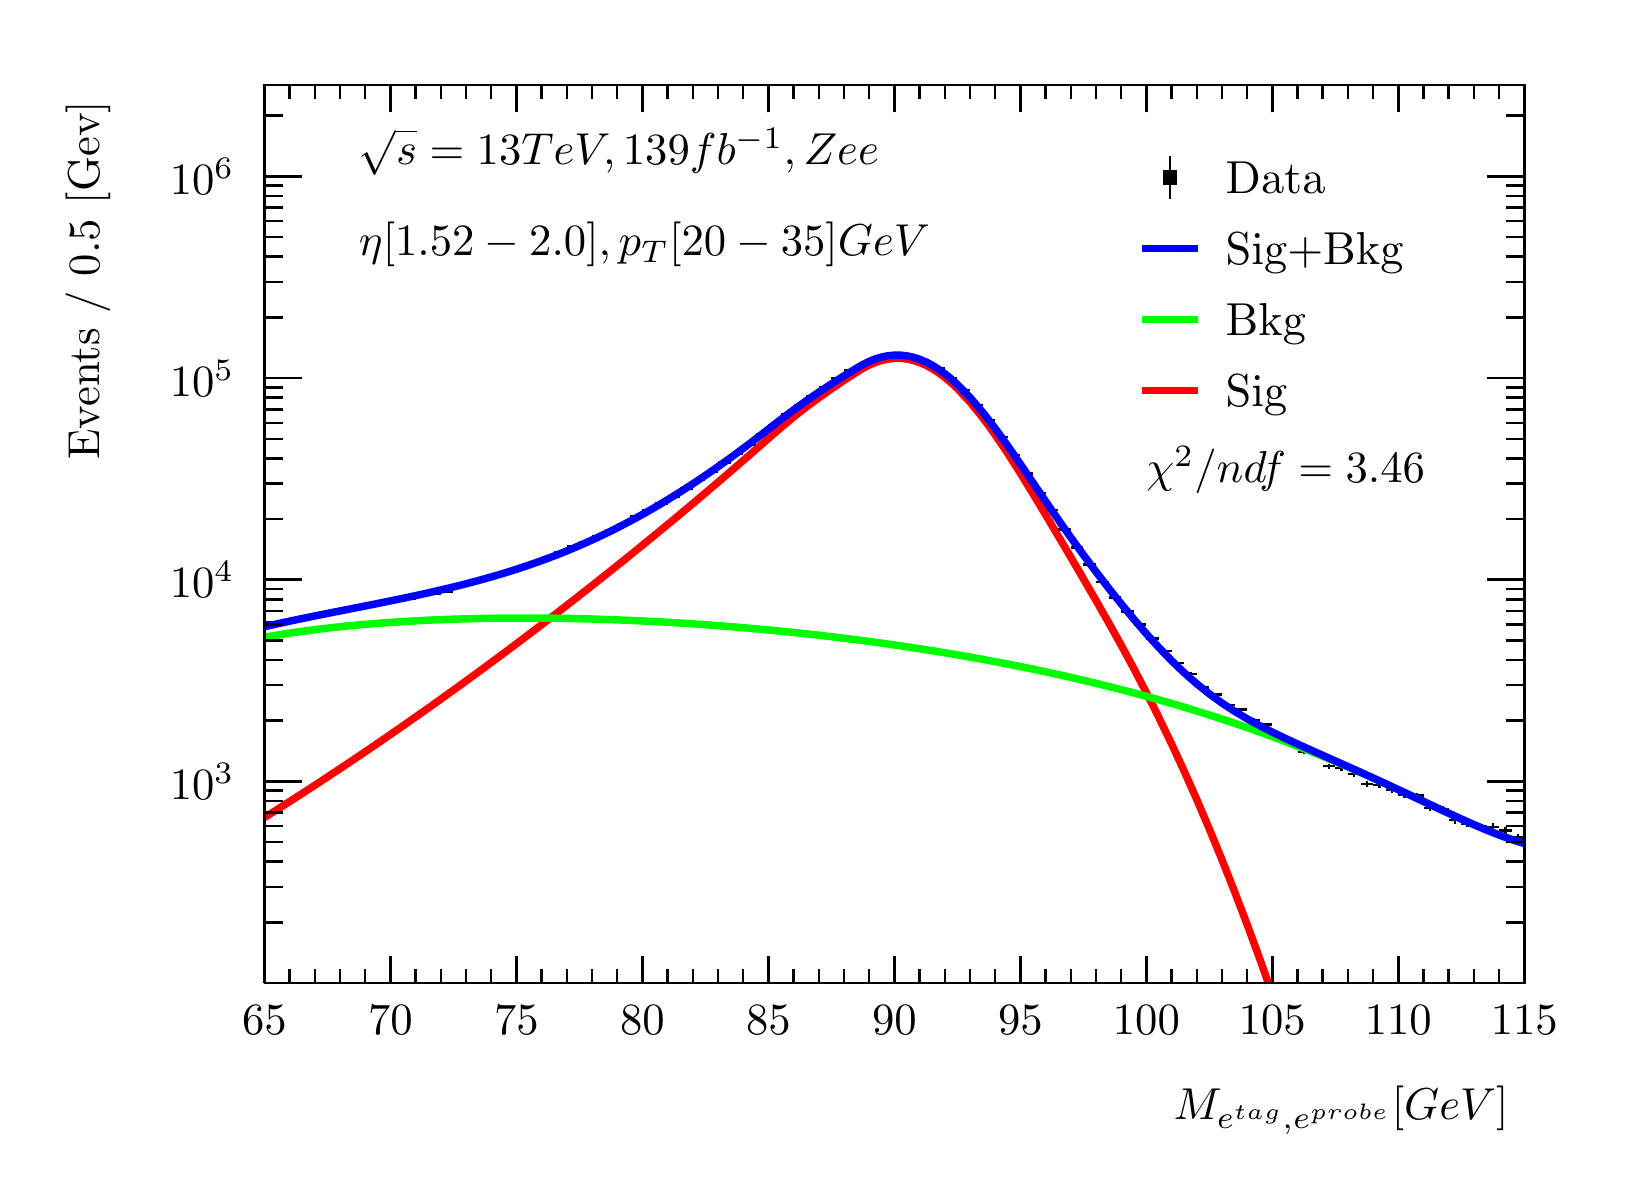
\begin{tikzpicture}
\pgfdeclareplotmark{cross} {
\pgfpathmoveto{\pgfpoint{-0.3\pgfplotmarksize}{\pgfplotmarksize}}
\pgfpathlineto{\pgfpoint{+0.3\pgfplotmarksize}{\pgfplotmarksize}}
\pgfpathlineto{\pgfpoint{+0.3\pgfplotmarksize}{0.3\pgfplotmarksize}}
\pgfpathlineto{\pgfpoint{+1\pgfplotmarksize}{0.3\pgfplotmarksize}}
\pgfpathlineto{\pgfpoint{+1\pgfplotmarksize}{-0.3\pgfplotmarksize}}
\pgfpathlineto{\pgfpoint{+0.3\pgfplotmarksize}{-0.3\pgfplotmarksize}}
\pgfpathlineto{\pgfpoint{+0.3\pgfplotmarksize}{-1.\pgfplotmarksize}}
\pgfpathlineto{\pgfpoint{-0.3\pgfplotmarksize}{-1.\pgfplotmarksize}}
\pgfpathlineto{\pgfpoint{-0.3\pgfplotmarksize}{-0.3\pgfplotmarksize}}
\pgfpathlineto{\pgfpoint{-1.\pgfplotmarksize}{-0.3\pgfplotmarksize}}
\pgfpathlineto{\pgfpoint{-1.\pgfplotmarksize}{0.3\pgfplotmarksize}}
\pgfpathlineto{\pgfpoint{-0.3\pgfplotmarksize}{0.3\pgfplotmarksize}}
\pgfpathclose
\pgfusepathqstroke
}
\pgfdeclareplotmark{cross*} {
\pgfpathmoveto{\pgfpoint{-0.3\pgfplotmarksize}{\pgfplotmarksize}}
\pgfpathlineto{\pgfpoint{+0.3\pgfplotmarksize}{\pgfplotmarksize}}
\pgfpathlineto{\pgfpoint{+0.3\pgfplotmarksize}{0.3\pgfplotmarksize}}
\pgfpathlineto{\pgfpoint{+1\pgfplotmarksize}{0.3\pgfplotmarksize}}
\pgfpathlineto{\pgfpoint{+1\pgfplotmarksize}{-0.3\pgfplotmarksize}}
\pgfpathlineto{\pgfpoint{+0.3\pgfplotmarksize}{-0.3\pgfplotmarksize}}
\pgfpathlineto{\pgfpoint{+0.3\pgfplotmarksize}{-1.\pgfplotmarksize}}
\pgfpathlineto{\pgfpoint{-0.3\pgfplotmarksize}{-1.\pgfplotmarksize}}
\pgfpathlineto{\pgfpoint{-0.3\pgfplotmarksize}{-0.3\pgfplotmarksize}}
\pgfpathlineto{\pgfpoint{-1.\pgfplotmarksize}{-0.3\pgfplotmarksize}}
\pgfpathlineto{\pgfpoint{-1.\pgfplotmarksize}{0.3\pgfplotmarksize}}
\pgfpathlineto{\pgfpoint{-0.3\pgfplotmarksize}{0.3\pgfplotmarksize}}
\pgfpathclose
\pgfusepathqfillstroke
}
\pgfdeclareplotmark{newstar} {
\pgfpathmoveto{\pgfqpoint{0pt}{\pgfplotmarksize}}
\pgfpathlineto{\pgfqpointpolar{44}{0.5\pgfplotmarksize}}
\pgfpathlineto{\pgfqpointpolar{18}{\pgfplotmarksize}}
\pgfpathlineto{\pgfqpointpolar{-20}{0.5\pgfplotmarksize}}
\pgfpathlineto{\pgfqpointpolar{-54}{\pgfplotmarksize}}
\pgfpathlineto{\pgfqpointpolar{-90}{0.5\pgfplotmarksize}}
\pgfpathlineto{\pgfqpointpolar{234}{\pgfplotmarksize}}
\pgfpathlineto{\pgfqpointpolar{198}{0.5\pgfplotmarksize}}
\pgfpathlineto{\pgfqpointpolar{162}{\pgfplotmarksize}}
\pgfpathlineto{\pgfqpointpolar{134}{0.5\pgfplotmarksize}}
\pgfpathclose
\pgfusepathqstroke
}
\pgfdeclareplotmark{newstar*} {
\pgfpathmoveto{\pgfqpoint{0pt}{\pgfplotmarksize}}
\pgfpathlineto{\pgfqpointpolar{44}{0.5\pgfplotmarksize}}
\pgfpathlineto{\pgfqpointpolar{18}{\pgfplotmarksize}}
\pgfpathlineto{\pgfqpointpolar{-20}{0.5\pgfplotmarksize}}
\pgfpathlineto{\pgfqpointpolar{-54}{\pgfplotmarksize}}
\pgfpathlineto{\pgfqpointpolar{-90}{0.5\pgfplotmarksize}}
\pgfpathlineto{\pgfqpointpolar{234}{\pgfplotmarksize}}
\pgfpathlineto{\pgfqpointpolar{198}{0.5\pgfplotmarksize}}
\pgfpathlineto{\pgfqpointpolar{162}{\pgfplotmarksize}}
\pgfpathlineto{\pgfqpointpolar{134}{0.5\pgfplotmarksize}}
\pgfpathclose
\pgfusepathqfillstroke
}
\definecolor{c}{rgb}{1,1,1};
\draw [color=c, fill=c] (0,0) rectangle (20,14.4361);
\draw [color=c, fill=c] (3,2.30977) rectangle (19,13.7143);
\definecolor{c}{rgb}{0,0,0};
\draw [c,line width=0.9] (3,2.30977) -- (3,13.7143) -- (19,13.7143) -- (19,2.30977) -- (3,2.30977);
\definecolor{c}{rgb}{1,1,1};
\draw [color=c, fill=c] (3,2.30977) rectangle (19,13.7143);
\definecolor{c}{rgb}{0,0,0};
\draw [c,line width=0.9] (3,2.30977) -- (3,13.7143) -- (19,13.7143) -- (19,2.30977) -- (3,2.30977);
\draw [c,line width=0.9] (3,2.30977) -- (19,2.30977);
\draw [c,line width=0.9] (3,2.65624) -- (3,2.30977);
\draw [c,line width=0.9] (3.32,2.48301) -- (3.32,2.30977);
\draw [c,line width=0.9] (3.64,2.48301) -- (3.64,2.30977);
\draw [c,line width=0.9] (3.96,2.48301) -- (3.96,2.30977);
\draw [c,line width=0.9] (4.28,2.48301) -- (4.28,2.30977);
\draw [c,line width=0.9] (4.6,2.65624) -- (4.6,2.30977);
\draw [c,line width=0.9] (4.92,2.48301) -- (4.92,2.30977);
\draw [c,line width=0.9] (5.24,2.48301) -- (5.24,2.30977);
\draw [c,line width=0.9] (5.56,2.48301) -- (5.56,2.30977);
\draw [c,line width=0.9] (5.88,2.48301) -- (5.88,2.30977);
\draw [c,line width=0.9] (6.2,2.65624) -- (6.2,2.30977);
\draw [c,line width=0.9] (6.52,2.48301) -- (6.52,2.30977);
\draw [c,line width=0.9] (6.84,2.48301) -- (6.84,2.30977);
\draw [c,line width=0.9] (7.16,2.48301) -- (7.16,2.30977);
\draw [c,line width=0.9] (7.48,2.48301) -- (7.48,2.30977);
\draw [c,line width=0.9] (7.8,2.65624) -- (7.8,2.30977);
\draw [c,line width=0.9] (8.12,2.48301) -- (8.12,2.30977);
\draw [c,line width=0.9] (8.44,2.48301) -- (8.44,2.30977);
\draw [c,line width=0.9] (8.76,2.48301) -- (8.76,2.30977);
\draw [c,line width=0.9] (9.08,2.48301) -- (9.08,2.30977);
\draw [c,line width=0.9] (9.4,2.65624) -- (9.4,2.30977);
\draw [c,line width=0.9] (9.72,2.48301) -- (9.72,2.30977);
\draw [c,line width=0.9] (10.04,2.48301) -- (10.04,2.30977);
\draw [c,line width=0.9] (10.36,2.48301) -- (10.36,2.30977);
\draw [c,line width=0.9] (10.68,2.48301) -- (10.68,2.30977);
\draw [c,line width=0.9] (11,2.65624) -- (11,2.30977);
\draw [c,line width=0.9] (11.32,2.48301) -- (11.32,2.30977);
\draw [c,line width=0.9] (11.64,2.48301) -- (11.64,2.30977);
\draw [c,line width=0.9] (11.96,2.48301) -- (11.96,2.30977);
\draw [c,line width=0.9] (12.28,2.48301) -- (12.28,2.30977);
\draw [c,line width=0.9] (12.6,2.65624) -- (12.6,2.30977);
\draw [c,line width=0.9] (12.92,2.48301) -- (12.92,2.30977);
\draw [c,line width=0.9] (13.24,2.48301) -- (13.24,2.30977);
\draw [c,line width=0.9] (13.56,2.48301) -- (13.56,2.30977);
\draw [c,line width=0.9] (13.88,2.48301) -- (13.88,2.30977);
\draw [c,line width=0.9] (14.2,2.65624) -- (14.2,2.30977);
\draw [c,line width=0.9] (14.52,2.48301) -- (14.52,2.30977);
\draw [c,line width=0.9] (14.84,2.48301) -- (14.84,2.30977);
\draw [c,line width=0.9] (15.16,2.48301) -- (15.16,2.30977);
\draw [c,line width=0.9] (15.48,2.48301) -- (15.48,2.30977);
\draw [c,line width=0.9] (15.8,2.65624) -- (15.8,2.30977);
\draw [c,line width=0.9] (16.12,2.48301) -- (16.12,2.30977);
\draw [c,line width=0.9] (16.44,2.48301) -- (16.44,2.30977);
\draw [c,line width=0.9] (16.76,2.48301) -- (16.76,2.30977);
\draw [c,line width=0.9] (17.08,2.48301) -- (17.08,2.30977);
\draw [c,line width=0.9] (17.4,2.65624) -- (17.4,2.30977);
\draw [c,line width=0.9] (17.72,2.48301) -- (17.72,2.30977);
\draw [c,line width=0.9] (18.04,2.48301) -- (18.04,2.30977);
\draw [c,line width=0.9] (18.36,2.48301) -- (18.36,2.30977);
\draw [c,line width=0.9] (18.68,2.48301) -- (18.68,2.30977);
\draw [c,line width=0.9] (19,2.65624) -- (19,2.30977);
\draw [c,line width=0.9] (19,2.65624) -- (19,2.30977);
\draw [anchor=base] (3,1.66015) node[scale=1.61424, color=c, rotate=0]{65};
\draw [anchor=base] (4.6,1.66015) node[scale=1.61424, color=c, rotate=0]{70};
\draw [anchor=base] (6.2,1.66015) node[scale=1.61424, color=c, rotate=0]{75};
\draw [anchor=base] (7.8,1.66015) node[scale=1.61424, color=c, rotate=0]{80};
\draw [anchor=base] (9.4,1.66015) node[scale=1.61424, color=c, rotate=0]{85};
\draw [anchor=base] (11,1.66015) node[scale=1.61424, color=c, rotate=0]{90};
\draw [anchor=base] (12.6,1.66015) node[scale=1.61424, color=c, rotate=0]{95};
\draw [anchor=base] (14.2,1.66015) node[scale=1.61424, color=c, rotate=0]{100};
\draw [anchor=base] (15.8,1.66015) node[scale=1.61424, color=c, rotate=0]{105};
\draw [anchor=base] (17.4,1.66015) node[scale=1.61424, color=c, rotate=0]{110};
\draw [anchor=base] (19,1.66015) node[scale=1.61424, color=c, rotate=0]{115};
\draw [anchor= east] (19,0.692932) node[scale=1.61424, color=c, rotate=0]{$M_{e^{tag}, e^{probe}}  [GeV]$};
\draw [c,line width=0.9] (3,13.7143) -- (19,13.7143);
\draw [c,line width=0.9] (3,13.3678) -- (3,13.7143);
\draw [c,line width=0.9] (3.32,13.5411) -- (3.32,13.7143);
\draw [c,line width=0.9] (3.64,13.5411) -- (3.64,13.7143);
\draw [c,line width=0.9] (3.96,13.5411) -- (3.96,13.7143);
\draw [c,line width=0.9] (4.28,13.5411) -- (4.28,13.7143);
\draw [c,line width=0.9] (4.6,13.3678) -- (4.6,13.7143);
\draw [c,line width=0.9] (4.92,13.5411) -- (4.92,13.7143);
\draw [c,line width=0.9] (5.24,13.5411) -- (5.24,13.7143);
\draw [c,line width=0.9] (5.56,13.5411) -- (5.56,13.7143);
\draw [c,line width=0.9] (5.88,13.5411) -- (5.88,13.7143);
\draw [c,line width=0.9] (6.2,13.3678) -- (6.2,13.7143);
\draw [c,line width=0.9] (6.52,13.5411) -- (6.52,13.7143);
\draw [c,line width=0.9] (6.84,13.5411) -- (6.84,13.7143);
\draw [c,line width=0.9] (7.16,13.5411) -- (7.16,13.7143);
\draw [c,line width=0.9] (7.48,13.5411) -- (7.48,13.7143);
\draw [c,line width=0.9] (7.8,13.3678) -- (7.8,13.7143);
\draw [c,line width=0.9] (8.12,13.5411) -- (8.12,13.7143);
\draw [c,line width=0.9] (8.44,13.5411) -- (8.44,13.7143);
\draw [c,line width=0.9] (8.76,13.5411) -- (8.76,13.7143);
\draw [c,line width=0.9] (9.08,13.5411) -- (9.08,13.7143);
\draw [c,line width=0.9] (9.4,13.3678) -- (9.4,13.7143);
\draw [c,line width=0.9] (9.72,13.5411) -- (9.72,13.7143);
\draw [c,line width=0.9] (10.04,13.5411) -- (10.04,13.7143);
\draw [c,line width=0.9] (10.36,13.5411) -- (10.36,13.7143);
\draw [c,line width=0.9] (10.68,13.5411) -- (10.68,13.7143);
\draw [c,line width=0.9] (11,13.3678) -- (11,13.7143);
\draw [c,line width=0.9] (11.32,13.5411) -- (11.32,13.7143);
\draw [c,line width=0.9] (11.64,13.5411) -- (11.64,13.7143);
\draw [c,line width=0.9] (11.96,13.5411) -- (11.96,13.7143);
\draw [c,line width=0.9] (12.28,13.5411) -- (12.28,13.7143);
\draw [c,line width=0.9] (12.6,13.3678) -- (12.6,13.7143);
\draw [c,line width=0.9] (12.92,13.5411) -- (12.92,13.7143);
\draw [c,line width=0.9] (13.24,13.5411) -- (13.24,13.7143);
\draw [c,line width=0.9] (13.56,13.5411) -- (13.56,13.7143);
\draw [c,line width=0.9] (13.88,13.5411) -- (13.88,13.7143);
\draw [c,line width=0.9] (14.2,13.3678) -- (14.2,13.7143);
\draw [c,line width=0.9] (14.52,13.5411) -- (14.52,13.7143);
\draw [c,line width=0.9] (14.84,13.5411) -- (14.84,13.7143);
\draw [c,line width=0.9] (15.16,13.5411) -- (15.16,13.7143);
\draw [c,line width=0.9] (15.48,13.5411) -- (15.48,13.7143);
\draw [c,line width=0.9] (15.8,13.3678) -- (15.8,13.7143);
\draw [c,line width=0.9] (16.12,13.5411) -- (16.12,13.7143);
\draw [c,line width=0.9] (16.44,13.5411) -- (16.44,13.7143);
\draw [c,line width=0.9] (16.76,13.5411) -- (16.76,13.7143);
\draw [c,line width=0.9] (17.08,13.5411) -- (17.08,13.7143);
\draw [c,line width=0.9] (17.4,13.3678) -- (17.4,13.7143);
\draw [c,line width=0.9] (17.72,13.5411) -- (17.72,13.7143);
\draw [c,line width=0.9] (18.04,13.5411) -- (18.04,13.7143);
\draw [c,line width=0.9] (18.36,13.5411) -- (18.36,13.7143);
\draw [c,line width=0.9] (18.68,13.5411) -- (18.68,13.7143);
\draw [c,line width=0.9] (19,13.3678) -- (19,13.7143);
\draw [c,line width=0.9] (19,13.3678) -- (19,13.7143);
\draw [c,line width=0.9] (3,2.30977) -- (3,13.7143);
\draw [c,line width=0.9] (3.237,3.08073) -- (3,3.08073);
\draw [c,line width=0.9] (3.237,3.53171) -- (3,3.53171);
\draw [c,line width=0.9] (3.237,3.85168) -- (3,3.85168);
\draw [c,line width=0.9] (3.237,4.09988) -- (3,4.09988);
\draw [c,line width=0.9] (3.237,4.30266) -- (3,4.30266);
\draw [c,line width=0.9] (3.237,4.47412) -- (3,4.47412);
\draw [c,line width=0.9] (3.237,4.62264) -- (3,4.62264);
\draw [c,line width=0.9] (3.237,4.75364) -- (3,4.75364);
\draw [c,line width=0.9] (3.474,4.87083) -- (3,4.87083);
\draw [anchor= east] (2.82,4.87083) node[scale=1.61424, color=c, rotate=0]{$10^{3}$};
\draw [c,line width=0.9] (3.237,5.64179) -- (3,5.64179);
\draw [c,line width=0.9] (3.237,6.09277) -- (3,6.09277);
\draw [c,line width=0.9] (3.237,6.41274) -- (3,6.41274);
\draw [c,line width=0.9] (3.237,6.66093) -- (3,6.66093);
\draw [c,line width=0.9] (3.237,6.86372) -- (3,6.86372);
\draw [c,line width=0.9] (3.237,7.03518) -- (3,7.03518);
\draw [c,line width=0.9] (3.237,7.1837) -- (3,7.1837);
\draw [c,line width=0.9] (3.237,7.3147) -- (3,7.3147);
\draw [c,line width=0.9] (3.474,7.43189) -- (3,7.43189);
\draw [anchor= east] (2.82,7.43189) node[scale=1.61424, color=c, rotate=0]{$10^{4}$};
\draw [c,line width=0.9] (3.237,8.20285) -- (3,8.20285);
\draw [c,line width=0.9] (3.237,8.65383) -- (3,8.65383);
\draw [c,line width=0.9] (3.237,8.9738) -- (3,8.9738);
\draw [c,line width=0.9] (3.237,9.22199) -- (3,9.22199);
\draw [c,line width=0.9] (3.237,9.42478) -- (3,9.42478);
\draw [c,line width=0.9] (3.237,9.59624) -- (3,9.59624);
\draw [c,line width=0.9] (3.237,9.74476) -- (3,9.74476);
\draw [c,line width=0.9] (3.237,9.87576) -- (3,9.87576);
\draw [c,line width=0.9] (3.474,9.99295) -- (3,9.99295);
\draw [anchor= east] (2.82,9.99295) node[scale=1.61424, color=c, rotate=0]{$10^{5}$};
\draw [c,line width=0.9] (3.237,10.7639) -- (3,10.7639);
\draw [c,line width=0.9] (3.237,11.2149) -- (3,11.2149);
\draw [c,line width=0.9] (3.237,11.5349) -- (3,11.5349);
\draw [c,line width=0.9] (3.237,11.7831) -- (3,11.7831);
\draw [c,line width=0.9] (3.237,11.9858) -- (3,11.9858);
\draw [c,line width=0.9] (3.237,12.1573) -- (3,12.1573);
\draw [c,line width=0.9] (3.237,12.3058) -- (3,12.3058);
\draw [c,line width=0.9] (3.237,12.4368) -- (3,12.4368);
\draw [c,line width=0.9] (3.474,12.554) -- (3,12.554);
\draw [anchor= east] (2.82,12.554) node[scale=1.61424, color=c, rotate=0]{$10^{6}$};
\draw [c,line width=0.9] (3.237,13.325) -- (3,13.325);
\draw [anchor= east] (0.76,13.7143) node[scale=1.61424, color=c, rotate=90]{Events / 0.5 [Gev]};
\draw [c,line width=0.9] (19,2.30977) -- (19,13.7143);
\draw [c,line width=0.9] (18.763,3.08073) -- (19,3.08073);
\draw [c,line width=0.9] (18.763,3.53171) -- (19,3.53171);
\draw [c,line width=0.9] (18.763,3.85168) -- (19,3.85168);
\draw [c,line width=0.9] (18.763,4.09988) -- (19,4.09988);
\draw [c,line width=0.9] (18.763,4.30266) -- (19,4.30266);
\draw [c,line width=0.9] (18.763,4.47412) -- (19,4.47412);
\draw [c,line width=0.9] (18.763,4.62264) -- (19,4.62264);
\draw [c,line width=0.9] (18.763,4.75364) -- (19,4.75364);
\draw [c,line width=0.9] (18.526,4.87083) -- (19,4.87083);
\draw [c,line width=0.9] (18.763,5.64179) -- (19,5.64179);
\draw [c,line width=0.9] (18.763,6.09277) -- (19,6.09277);
\draw [c,line width=0.9] (18.763,6.41274) -- (19,6.41274);
\draw [c,line width=0.9] (18.763,6.66093) -- (19,6.66093);
\draw [c,line width=0.9] (18.763,6.86372) -- (19,6.86372);
\draw [c,line width=0.9] (18.763,7.03518) -- (19,7.03518);
\draw [c,line width=0.9] (18.763,7.1837) -- (19,7.1837);
\draw [c,line width=0.9] (18.763,7.3147) -- (19,7.3147);
\draw [c,line width=0.9] (18.526,7.43189) -- (19,7.43189);
\draw [c,line width=0.9] (18.763,8.20285) -- (19,8.20285);
\draw [c,line width=0.9] (18.763,8.65383) -- (19,8.65383);
\draw [c,line width=0.9] (18.763,8.9738) -- (19,8.9738);
\draw [c,line width=0.9] (18.763,9.22199) -- (19,9.22199);
\draw [c,line width=0.9] (18.763,9.42478) -- (19,9.42478);
\draw [c,line width=0.9] (18.763,9.59624) -- (19,9.59624);
\draw [c,line width=0.9] (18.763,9.74476) -- (19,9.74476);
\draw [c,line width=0.9] (18.763,9.87576) -- (19,9.87576);
\draw [c,line width=0.9] (18.526,9.99295) -- (19,9.99295);
\draw [c,line width=0.9] (18.763,10.7639) -- (19,10.7639);
\draw [c,line width=0.9] (18.763,11.2149) -- (19,11.2149);
\draw [c,line width=0.9] (18.763,11.5349) -- (19,11.5349);
\draw [c,line width=0.9] (18.763,11.7831) -- (19,11.7831);
\draw [c,line width=0.9] (18.763,11.9858) -- (19,11.9858);
\draw [c,line width=0.9] (18.763,12.1573) -- (19,12.1573);
\draw [c,line width=0.9] (18.763,12.3058) -- (19,12.3058);
\draw [c,line width=0.9] (18.763,12.4368) -- (19,12.4368);
\draw [c,line width=0.9] (18.526,12.554) -- (19,12.554);
\draw [c,line width=0.9] (18.763,13.325) -- (19,13.325);
\draw [c,line width=0.9] (3.08,6.89372) -- (3,6.89372);
\draw [c,line width=0.9] (3,6.89372) -- (3,6.89372);
\draw [c,line width=0.9] (3.08,6.89372) -- (3.16,6.89372);
\draw [c,line width=0.9] (3.16,6.89372) -- (3.16,6.89372);
\draw [c,line width=0.9] (3.08,6.89372) -- (3.08,6.90788);
\draw [c,line width=0.9] (3.08,6.90788) -- (3.08,6.90788);
\draw [c,line width=0.9] (3.08,6.89372) -- (3.08,6.87955);
\draw [c,line width=0.9] (3.08,6.87955) -- (3.08,6.87955);
\draw [c,line width=0.9] (3.24,6.90877) -- (3.16,6.90877);
\draw [c,line width=0.9] (3.16,6.90877) -- (3.16,6.90877);
\draw [c,line width=0.9] (3.24,6.90877) -- (3.32,6.90877);
\draw [c,line width=0.9] (3.32,6.90877) -- (3.32,6.90877);
\draw [c,line width=0.9] (3.24,6.90877) -- (3.24,6.92284);
\draw [c,line width=0.9] (3.24,6.92284) -- (3.24,6.92284);
\draw [c,line width=0.9] (3.24,6.90877) -- (3.24,6.8947);
\draw [c,line width=0.9] (3.24,6.8947) -- (3.24,6.8947);
\draw [c,line width=0.9] (3.4,6.93516) -- (3.32,6.93516);
\draw [c,line width=0.9] (3.32,6.93516) -- (3.32,6.93516);
\draw [c,line width=0.9] (3.4,6.93516) -- (3.48,6.93516);
\draw [c,line width=0.9] (3.48,6.93516) -- (3.48,6.93516);
\draw [c,line width=0.9] (3.4,6.93516) -- (3.4,6.94906);
\draw [c,line width=0.9] (3.4,6.94906) -- (3.4,6.94906);
\draw [c,line width=0.9] (3.4,6.93516) -- (3.4,6.92125);
\draw [c,line width=0.9] (3.4,6.92125) -- (3.4,6.92125);
\draw [c,line width=0.9] (3.56,6.96838) -- (3.48,6.96838);
\draw [c,line width=0.9] (3.48,6.96838) -- (3.48,6.96838);
\draw [c,line width=0.9] (3.56,6.96838) -- (3.64,6.96838);
\draw [c,line width=0.9] (3.64,6.96838) -- (3.64,6.96838);
\draw [c,line width=0.9] (3.56,6.96838) -- (3.56,6.98208);
\draw [c,line width=0.9] (3.56,6.98208) -- (3.56,6.98208);
\draw [c,line width=0.9] (3.56,6.96838) -- (3.56,6.95468);
\draw [c,line width=0.9] (3.56,6.95468) -- (3.56,6.95468);
\draw [c,line width=0.9] (3.72,6.99572) -- (3.64,6.99572);
\draw [c,line width=0.9] (3.64,6.99572) -- (3.64,6.99572);
\draw [c,line width=0.9] (3.72,6.99572) -- (3.8,6.99572);
\draw [c,line width=0.9] (3.8,6.99572) -- (3.8,6.99572);
\draw [c,line width=0.9] (3.72,6.99572) -- (3.72,7.00925);
\draw [c,line width=0.9] (3.72,7.00925) -- (3.72,7.00925);
\draw [c,line width=0.9] (3.72,6.99572) -- (3.72,6.98218);
\draw [c,line width=0.9] (3.72,6.98218) -- (3.72,6.98218);
\draw [c,line width=0.9] (3.88,7.0288) -- (3.8,7.0288);
\draw [c,line width=0.9] (3.8,7.0288) -- (3.8,7.0288);
\draw [c,line width=0.9] (3.88,7.0288) -- (3.96,7.0288);
\draw [c,line width=0.9] (3.96,7.0288) -- (3.96,7.0288);
\draw [c,line width=0.9] (3.88,7.0288) -- (3.88,7.04214);
\draw [c,line width=0.9] (3.88,7.04214) -- (3.88,7.04214);
\draw [c,line width=0.9] (3.88,7.0288) -- (3.88,7.01547);
\draw [c,line width=0.9] (3.88,7.01547) -- (3.88,7.01547);
\draw [c,line width=0.9] (4.04,7.06218) -- (3.96,7.06218);
\draw [c,line width=0.9] (3.96,7.06218) -- (3.96,7.06218);
\draw [c,line width=0.9] (4.04,7.06218) -- (4.12,7.06218);
\draw [c,line width=0.9] (4.12,7.06218) -- (4.12,7.06218);
\draw [c,line width=0.9] (4.04,7.06218) -- (4.04,7.07531);
\draw [c,line width=0.9] (4.04,7.07531) -- (4.04,7.07531);
\draw [c,line width=0.9] (4.04,7.06218) -- (4.04,7.04904);
\draw [c,line width=0.9] (4.04,7.04904) -- (4.04,7.04904);
\draw [c,line width=0.9] (4.2,7.06342) -- (4.12,7.06342);
\draw [c,line width=0.9] (4.12,7.06342) -- (4.12,7.06342);
\draw [c,line width=0.9] (4.2,7.06342) -- (4.28,7.06342);
\draw [c,line width=0.9] (4.28,7.06342) -- (4.28,7.06342);
\draw [c,line width=0.9] (4.2,7.06342) -- (4.2,7.07654);
\draw [c,line width=0.9] (4.2,7.07654) -- (4.2,7.07654);
\draw [c,line width=0.9] (4.2,7.06342) -- (4.2,7.05029);
\draw [c,line width=0.9] (4.2,7.05029) -- (4.2,7.05029);
\draw [c,line width=0.9] (4.36,7.09639) -- (4.28,7.09639);
\draw [c,line width=0.9] (4.28,7.09639) -- (4.28,7.09639);
\draw [c,line width=0.9] (4.36,7.09639) -- (4.44,7.09639);
\draw [c,line width=0.9] (4.44,7.09639) -- (4.44,7.09639);
\draw [c,line width=0.9] (4.36,7.09639) -- (4.36,7.10932);
\draw [c,line width=0.9] (4.36,7.10932) -- (4.36,7.10932);
\draw [c,line width=0.9] (4.36,7.09639) -- (4.36,7.08345);
\draw [c,line width=0.9] (4.36,7.08345) -- (4.36,7.08345);
\draw [c,line width=0.9] (4.52,7.15211) -- (4.44,7.15211);
\draw [c,line width=0.9] (4.44,7.15211) -- (4.44,7.15211);
\draw [c,line width=0.9] (4.52,7.15211) -- (4.6,7.15211);
\draw [c,line width=0.9] (4.6,7.15211) -- (4.6,7.15211);
\draw [c,line width=0.9] (4.52,7.15211) -- (4.52,7.16472);
\draw [c,line width=0.9] (4.52,7.16472) -- (4.52,7.16472);
\draw [c,line width=0.9] (4.52,7.15211) -- (4.52,7.1395);
\draw [c,line width=0.9] (4.52,7.1395) -- (4.52,7.1395);
\draw [c,line width=0.9] (4.68,7.16009) -- (4.6,7.16009);
\draw [c,line width=0.9] (4.6,7.16009) -- (4.6,7.16009);
\draw [c,line width=0.9] (4.68,7.16009) -- (4.76,7.16009);
\draw [c,line width=0.9] (4.76,7.16009) -- (4.76,7.16009);
\draw [c,line width=0.9] (4.68,7.16009) -- (4.68,7.17266);
\draw [c,line width=0.9] (4.68,7.17266) -- (4.68,7.17266);
\draw [c,line width=0.9] (4.68,7.16009) -- (4.68,7.14753);
\draw [c,line width=0.9] (4.68,7.14753) -- (4.68,7.14753);
\draw [c,line width=0.9] (4.84,7.18952) -- (4.76,7.18952);
\draw [c,line width=0.9] (4.76,7.18952) -- (4.76,7.18952);
\draw [c,line width=0.9] (4.84,7.18952) -- (4.92,7.18952);
\draw [c,line width=0.9] (4.92,7.18952) -- (4.92,7.18952);
\draw [c,line width=0.9] (4.84,7.18952) -- (4.84,7.20193);
\draw [c,line width=0.9] (4.84,7.20193) -- (4.84,7.20193);
\draw [c,line width=0.9] (4.84,7.18952) -- (4.84,7.17712);
\draw [c,line width=0.9] (4.84,7.17712) -- (4.84,7.17712);
\draw [c,line width=0.9] (5,7.22679) -- (4.92,7.22679);
\draw [c,line width=0.9] (4.92,7.22679) -- (4.92,7.22679);
\draw [c,line width=0.9] (5,7.22679) -- (5.08,7.22679);
\draw [c,line width=0.9] (5.08,7.22679) -- (5.08,7.22679);
\draw [c,line width=0.9] (5,7.22679) -- (5,7.23898);
\draw [c,line width=0.9] (5,7.23898) -- (5,7.23898);
\draw [c,line width=0.9] (5,7.22679) -- (5,7.21459);
\draw [c,line width=0.9] (5,7.21459) -- (5,7.21459);
\draw [c,line width=0.9] (5.16,7.25947) -- (5.08,7.25947);
\draw [c,line width=0.9] (5.08,7.25947) -- (5.08,7.25947);
\draw [c,line width=0.9] (5.16,7.25947) -- (5.24,7.25947);
\draw [c,line width=0.9] (5.24,7.25947) -- (5.24,7.25947);
\draw [c,line width=0.9] (5.16,7.25947) -- (5.16,7.27149);
\draw [c,line width=0.9] (5.16,7.27149) -- (5.16,7.27149);
\draw [c,line width=0.9] (5.16,7.25947) -- (5.16,7.24745);
\draw [c,line width=0.9] (5.16,7.24745) -- (5.16,7.24745);
\draw [c,line width=0.9] (5.32,7.28223) -- (5.24,7.28223);
\draw [c,line width=0.9] (5.24,7.28223) -- (5.24,7.28223);
\draw [c,line width=0.9] (5.32,7.28223) -- (5.4,7.28223);
\draw [c,line width=0.9] (5.4,7.28223) -- (5.4,7.28223);
\draw [c,line width=0.9] (5.32,7.28223) -- (5.32,7.29412);
\draw [c,line width=0.9] (5.32,7.29412) -- (5.32,7.29412);
\draw [c,line width=0.9] (5.32,7.28223) -- (5.32,7.27033);
\draw [c,line width=0.9] (5.32,7.27033) -- (5.32,7.27033);
\draw [c,line width=0.9] (5.48,7.3594) -- (5.4,7.3594);
\draw [c,line width=0.9] (5.4,7.3594) -- (5.4,7.3594);
\draw [c,line width=0.9] (5.48,7.3594) -- (5.56,7.3594);
\draw [c,line width=0.9] (5.56,7.3594) -- (5.56,7.3594);
\draw [c,line width=0.9] (5.48,7.3594) -- (5.48,7.37089);
\draw [c,line width=0.9] (5.48,7.37089) -- (5.48,7.37089);
\draw [c,line width=0.9] (5.48,7.3594) -- (5.48,7.34791);
\draw [c,line width=0.9] (5.48,7.34791) -- (5.48,7.34791);
\draw [c,line width=0.9] (5.64,7.39675) -- (5.56,7.39675);
\draw [c,line width=0.9] (5.56,7.39675) -- (5.56,7.39675);
\draw [c,line width=0.9] (5.64,7.39675) -- (5.72,7.39675);
\draw [c,line width=0.9] (5.72,7.39675) -- (5.72,7.39675);
\draw [c,line width=0.9] (5.64,7.39675) -- (5.64,7.40805);
\draw [c,line width=0.9] (5.64,7.40805) -- (5.64,7.40805);
\draw [c,line width=0.9] (5.64,7.39675) -- (5.64,7.38545);
\draw [c,line width=0.9] (5.64,7.38545) -- (5.64,7.38545);
\draw [c,line width=0.9] (5.8,7.44725) -- (5.72,7.44725);
\draw [c,line width=0.9] (5.72,7.44725) -- (5.72,7.44725);
\draw [c,line width=0.9] (5.8,7.44725) -- (5.88,7.44725);
\draw [c,line width=0.9] (5.88,7.44725) -- (5.88,7.44725);
\draw [c,line width=0.9] (5.8,7.44725) -- (5.8,7.45829);
\draw [c,line width=0.9] (5.8,7.45829) -- (5.8,7.45829);
\draw [c,line width=0.9] (5.8,7.44725) -- (5.8,7.4362);
\draw [c,line width=0.9] (5.8,7.4362) -- (5.8,7.4362);
\draw [c,line width=0.9] (5.96,7.48) -- (5.88,7.48);
\draw [c,line width=0.9] (5.88,7.48) -- (5.88,7.48);
\draw [c,line width=0.9] (5.96,7.48) -- (6.04,7.48);
\draw [c,line width=0.9] (6.04,7.48) -- (6.04,7.48);
\draw [c,line width=0.9] (5.96,7.48) -- (5.96,7.49088);
\draw [c,line width=0.9] (5.96,7.49088) -- (5.96,7.49088);
\draw [c,line width=0.9] (5.96,7.48) -- (5.96,7.46911);
\draw [c,line width=0.9] (5.96,7.46911) -- (5.96,7.46911);
\draw [c,line width=0.9] (6.12,7.54063) -- (6.04,7.54063);
\draw [c,line width=0.9] (6.04,7.54063) -- (6.04,7.54063);
\draw [c,line width=0.9] (6.12,7.54063) -- (6.2,7.54063);
\draw [c,line width=0.9] (6.2,7.54063) -- (6.2,7.54063);
\draw [c,line width=0.9] (6.12,7.54063) -- (6.12,7.55122);
\draw [c,line width=0.9] (6.12,7.55122) -- (6.12,7.55122);
\draw [c,line width=0.9] (6.12,7.54063) -- (6.12,7.53004);
\draw [c,line width=0.9] (6.12,7.53004) -- (6.12,7.53004);
\draw [c,line width=0.9] (6.28,7.58773) -- (6.2,7.58773);
\draw [c,line width=0.9] (6.2,7.58773) -- (6.2,7.58773);
\draw [c,line width=0.9] (6.28,7.58773) -- (6.36,7.58773);
\draw [c,line width=0.9] (6.36,7.58773) -- (6.36,7.58773);
\draw [c,line width=0.9] (6.28,7.58773) -- (6.28,7.5981);
\draw [c,line width=0.9] (6.28,7.5981) -- (6.28,7.5981);
\draw [c,line width=0.9] (6.28,7.58773) -- (6.28,7.57736);
\draw [c,line width=0.9] (6.28,7.57736) -- (6.28,7.57736);
\draw [c,line width=0.9] (6.44,7.64428) -- (6.36,7.64428);
\draw [c,line width=0.9] (6.36,7.64428) -- (6.36,7.64428);
\draw [c,line width=0.9] (6.44,7.64428) -- (6.52,7.64428);
\draw [c,line width=0.9] (6.52,7.64428) -- (6.52,7.64428);
\draw [c,line width=0.9] (6.44,7.64428) -- (6.44,7.65439);
\draw [c,line width=0.9] (6.44,7.65439) -- (6.44,7.65439);
\draw [c,line width=0.9] (6.44,7.64428) -- (6.44,7.63417);
\draw [c,line width=0.9] (6.44,7.63417) -- (6.44,7.63417);
\draw [c,line width=0.9] (6.6,7.71787) -- (6.52,7.71787);
\draw [c,line width=0.9] (6.52,7.71787) -- (6.52,7.71787);
\draw [c,line width=0.9] (6.6,7.71787) -- (6.68,7.71787);
\draw [c,line width=0.9] (6.68,7.71787) -- (6.68,7.71787);
\draw [c,line width=0.9] (6.6,7.71787) -- (6.6,7.72765);
\draw [c,line width=0.9] (6.6,7.72765) -- (6.6,7.72765);
\draw [c,line width=0.9] (6.6,7.71787) -- (6.6,7.70809);
\draw [c,line width=0.9] (6.6,7.70809) -- (6.6,7.70809);
\draw [c,line width=0.9] (6.76,7.77773) -- (6.68,7.77773);
\draw [c,line width=0.9] (6.68,7.77773) -- (6.68,7.77773);
\draw [c,line width=0.9] (6.76,7.77773) -- (6.84,7.77773);
\draw [c,line width=0.9] (6.84,7.77773) -- (6.84,7.77773);
\draw [c,line width=0.9] (6.76,7.77773) -- (6.76,7.78725);
\draw [c,line width=0.9] (6.76,7.78725) -- (6.76,7.78725);
\draw [c,line width=0.9] (6.76,7.77773) -- (6.76,7.76821);
\draw [c,line width=0.9] (6.76,7.76821) -- (6.76,7.76821);
\draw [c,line width=0.9] (6.92,7.85144) -- (6.84,7.85144);
\draw [c,line width=0.9] (6.84,7.85144) -- (6.84,7.85144);
\draw [c,line width=0.9] (6.92,7.85144) -- (7,7.85144);
\draw [c,line width=0.9] (7,7.85144) -- (7,7.85144);
\draw [c,line width=0.9] (6.92,7.85144) -- (6.92,7.86065);
\draw [c,line width=0.9] (6.92,7.86065) -- (6.92,7.86065);
\draw [c,line width=0.9] (6.92,7.85144) -- (6.92,7.84223);
\draw [c,line width=0.9] (6.92,7.84223) -- (6.92,7.84223);
\draw [c,line width=0.9] (7.08,7.90184) -- (7,7.90184);
\draw [c,line width=0.9] (7,7.90184) -- (7,7.90184);
\draw [c,line width=0.9] (7.08,7.90184) -- (7.16,7.90184);
\draw [c,line width=0.9] (7.16,7.90184) -- (7.16,7.90184);
\draw [c,line width=0.9] (7.08,7.90184) -- (7.08,7.91084);
\draw [c,line width=0.9] (7.08,7.91084) -- (7.08,7.91084);
\draw [c,line width=0.9] (7.08,7.90184) -- (7.08,7.89284);
\draw [c,line width=0.9] (7.08,7.89284) -- (7.08,7.89284);
\draw [c,line width=0.9] (7.24,7.98591) -- (7.16,7.98591);
\draw [c,line width=0.9] (7.16,7.98591) -- (7.16,7.98591);
\draw [c,line width=0.9] (7.24,7.98591) -- (7.32,7.98591);
\draw [c,line width=0.9] (7.32,7.98591) -- (7.32,7.98591);
\draw [c,line width=0.9] (7.24,7.98591) -- (7.24,7.99458);
\draw [c,line width=0.9] (7.24,7.99458) -- (7.24,7.99458);
\draw [c,line width=0.9] (7.24,7.98591) -- (7.24,7.97724);
\draw [c,line width=0.9] (7.24,7.97724) -- (7.24,7.97724);
\draw [c,line width=0.9] (7.4,8.06602) -- (7.32,8.06602);
\draw [c,line width=0.9] (7.32,8.06602) -- (7.32,8.06602);
\draw [c,line width=0.9] (7.4,8.06602) -- (7.48,8.06602);
\draw [c,line width=0.9] (7.48,8.06602) -- (7.48,8.06602);
\draw [c,line width=0.9] (7.4,8.06602) -- (7.4,8.07439);
\draw [c,line width=0.9] (7.4,8.07439) -- (7.4,8.07439);
\draw [c,line width=0.9] (7.4,8.06602) -- (7.4,8.05766);
\draw [c,line width=0.9] (7.4,8.05766) -- (7.4,8.05766);
\draw [c,line width=0.9] (7.56,8.14069) -- (7.48,8.14069);
\draw [c,line width=0.9] (7.48,8.14069) -- (7.48,8.14069);
\draw [c,line width=0.9] (7.56,8.14069) -- (7.64,8.14069);
\draw [c,line width=0.9] (7.64,8.14069) -- (7.64,8.14069);
\draw [c,line width=0.9] (7.56,8.14069) -- (7.56,8.14878);
\draw [c,line width=0.9] (7.56,8.14878) -- (7.56,8.14878);
\draw [c,line width=0.9] (7.56,8.14069) -- (7.56,8.1326);
\draw [c,line width=0.9] (7.56,8.1326) -- (7.56,8.1326);
\draw [c,line width=0.9] (7.72,8.23356) -- (7.64,8.23356);
\draw [c,line width=0.9] (7.64,8.23356) -- (7.64,8.23356);
\draw [c,line width=0.9] (7.72,8.23356) -- (7.8,8.23356);
\draw [c,line width=0.9] (7.8,8.23356) -- (7.8,8.23356);
\draw [c,line width=0.9] (7.72,8.23356) -- (7.72,8.24132);
\draw [c,line width=0.9] (7.72,8.24132) -- (7.72,8.24132);
\draw [c,line width=0.9] (7.72,8.23356) -- (7.72,8.22581);
\draw [c,line width=0.9] (7.72,8.22581) -- (7.72,8.22581);
\draw [c,line width=0.9] (7.88,8.31511) -- (7.8,8.31511);
\draw [c,line width=0.9] (7.8,8.31511) -- (7.8,8.31511);
\draw [c,line width=0.9] (7.88,8.31511) -- (7.96,8.31511);
\draw [c,line width=0.9] (7.96,8.31511) -- (7.96,8.31511);
\draw [c,line width=0.9] (7.88,8.31511) -- (7.88,8.32259);
\draw [c,line width=0.9] (7.88,8.32259) -- (7.88,8.32259);
\draw [c,line width=0.9] (7.88,8.31511) -- (7.88,8.30763);
\draw [c,line width=0.9] (7.88,8.30763) -- (7.88,8.30763);
\draw [c,line width=0.9] (8.04,8.40215) -- (7.96,8.40215);
\draw [c,line width=0.9] (7.96,8.40215) -- (7.96,8.40215);
\draw [c,line width=0.9] (8.04,8.40215) -- (8.12,8.40215);
\draw [c,line width=0.9] (8.12,8.40215) -- (8.12,8.40215);
\draw [c,line width=0.9] (8.04,8.40215) -- (8.04,8.40934);
\draw [c,line width=0.9] (8.04,8.40934) -- (8.04,8.40934);
\draw [c,line width=0.9] (8.04,8.40215) -- (8.04,8.39496);
\draw [c,line width=0.9] (8.04,8.39496) -- (8.04,8.39496);
\draw [c,line width=0.9] (8.2,8.48818) -- (8.12,8.48818);
\draw [c,line width=0.9] (8.12,8.48818) -- (8.12,8.48818);
\draw [c,line width=0.9] (8.2,8.48818) -- (8.28,8.48818);
\draw [c,line width=0.9] (8.28,8.48818) -- (8.28,8.48818);
\draw [c,line width=0.9] (8.2,8.48818) -- (8.2,8.4951);
\draw [c,line width=0.9] (8.2,8.4951) -- (8.2,8.4951);
\draw [c,line width=0.9] (8.2,8.48818) -- (8.2,8.48127);
\draw [c,line width=0.9] (8.2,8.48127) -- (8.2,8.48127);
\draw [c,line width=0.9] (8.36,8.58941) -- (8.28,8.58941);
\draw [c,line width=0.9] (8.28,8.58941) -- (8.28,8.58941);
\draw [c,line width=0.9] (8.36,8.58941) -- (8.44,8.58941);
\draw [c,line width=0.9] (8.44,8.58941) -- (8.44,8.58941);
\draw [c,line width=0.9] (8.36,8.58941) -- (8.36,8.59602);
\draw [c,line width=0.9] (8.36,8.59602) -- (8.36,8.59602);
\draw [c,line width=0.9] (8.36,8.58941) -- (8.36,8.5828);
\draw [c,line width=0.9] (8.36,8.5828) -- (8.36,8.5828);
\draw [c,line width=0.9] (8.52,8.70073) -- (8.44,8.70073);
\draw [c,line width=0.9] (8.44,8.70073) -- (8.44,8.70073);
\draw [c,line width=0.9] (8.52,8.70073) -- (8.6,8.70073);
\draw [c,line width=0.9] (8.6,8.70073) -- (8.6,8.70073);
\draw [c,line width=0.9] (8.52,8.70073) -- (8.52,8.70701);
\draw [c,line width=0.9] (8.52,8.70701) -- (8.52,8.70701);
\draw [c,line width=0.9] (8.52,8.70073) -- (8.52,8.69444);
\draw [c,line width=0.9] (8.52,8.69444) -- (8.52,8.69444);
\draw [c,line width=0.9] (8.68,8.80301) -- (8.6,8.80301);
\draw [c,line width=0.9] (8.6,8.80301) -- (8.6,8.80301);
\draw [c,line width=0.9] (8.68,8.80301) -- (8.76,8.80301);
\draw [c,line width=0.9] (8.76,8.80301) -- (8.76,8.80301);
\draw [c,line width=0.9] (8.68,8.80301) -- (8.68,8.80901);
\draw [c,line width=0.9] (8.68,8.80901) -- (8.68,8.80901);
\draw [c,line width=0.9] (8.68,8.80301) -- (8.68,8.797);
\draw [c,line width=0.9] (8.68,8.797) -- (8.68,8.797);
\draw [c,line width=0.9] (8.84,8.91947) -- (8.76,8.91947);
\draw [c,line width=0.9] (8.76,8.91947) -- (8.76,8.91947);
\draw [c,line width=0.9] (8.84,8.91947) -- (8.92,8.91947);
\draw [c,line width=0.9] (8.92,8.91947) -- (8.92,8.91947);
\draw [c,line width=0.9] (8.84,8.91947) -- (8.84,8.92517);
\draw [c,line width=0.9] (8.84,8.92517) -- (8.84,8.92517);
\draw [c,line width=0.9] (8.84,8.91947) -- (8.84,8.91377);
\draw [c,line width=0.9] (8.84,8.91377) -- (8.84,8.91377);
\draw [c,line width=0.9] (9,9.03003) -- (8.92,9.03003);
\draw [c,line width=0.9] (8.92,9.03003) -- (8.92,9.03003);
\draw [c,line width=0.9] (9,9.03003) -- (9.08,9.03003);
\draw [c,line width=0.9] (9.08,9.03003) -- (9.08,9.03003);
\draw [c,line width=0.9] (9,9.03003) -- (9,9.03545);
\draw [c,line width=0.9] (9,9.03545) -- (9,9.03545);
\draw [c,line width=0.9] (9,9.03003) -- (9,9.0246);
\draw [c,line width=0.9] (9,9.0246) -- (9,9.0246);
\draw [c,line width=0.9] (9.16,9.14317) -- (9.08,9.14317);
\draw [c,line width=0.9] (9.08,9.14317) -- (9.08,9.14317);
\draw [c,line width=0.9] (9.16,9.14317) -- (9.24,9.14317);
\draw [c,line width=0.9] (9.24,9.14317) -- (9.24,9.14317);
\draw [c,line width=0.9] (9.16,9.14317) -- (9.16,9.14832);
\draw [c,line width=0.9] (9.16,9.14832) -- (9.16,9.14832);
\draw [c,line width=0.9] (9.16,9.14317) -- (9.16,9.13801);
\draw [c,line width=0.9] (9.16,9.13801) -- (9.16,9.13801);
\draw [c,line width=0.9] (9.32,9.27705) -- (9.24,9.27705);
\draw [c,line width=0.9] (9.24,9.27705) -- (9.24,9.27705);
\draw [c,line width=0.9] (9.32,9.27705) -- (9.4,9.27705);
\draw [c,line width=0.9] (9.4,9.27705) -- (9.4,9.27705);
\draw [c,line width=0.9] (9.32,9.27705) -- (9.32,9.2819);
\draw [c,line width=0.9] (9.32,9.2819) -- (9.32,9.2819);
\draw [c,line width=0.9] (9.32,9.27705) -- (9.32,9.27219);
\draw [c,line width=0.9] (9.32,9.27219) -- (9.32,9.27219);
\draw [c,line width=0.9] (9.48,9.39487) -- (9.4,9.39487);
\draw [c,line width=0.9] (9.4,9.39487) -- (9.4,9.39487);
\draw [c,line width=0.9] (9.48,9.39487) -- (9.56,9.39487);
\draw [c,line width=0.9] (9.56,9.39487) -- (9.56,9.39487);
\draw [c,line width=0.9] (9.48,9.39487) -- (9.48,9.39947);
\draw [c,line width=0.9] (9.48,9.39947) -- (9.48,9.39947);
\draw [c,line width=0.9] (9.48,9.39487) -- (9.48,9.39027);
\draw [c,line width=0.9] (9.48,9.39027) -- (9.48,9.39027);
\draw [c,line width=0.9] (9.64,9.53049) -- (9.56,9.53049);
\draw [c,line width=0.9] (9.56,9.53049) -- (9.56,9.53049);
\draw [c,line width=0.9] (9.64,9.53049) -- (9.72,9.53049);
\draw [c,line width=0.9] (9.72,9.53049) -- (9.72,9.53049);
\draw [c,line width=0.9] (9.64,9.53049) -- (9.64,9.53482);
\draw [c,line width=0.9] (9.64,9.53482) -- (9.64,9.53482);
\draw [c,line width=0.9] (9.64,9.53049) -- (9.64,9.52616);
\draw [c,line width=0.9] (9.64,9.52616) -- (9.64,9.52616);
\draw [c,line width=0.9] (9.8,9.65111) -- (9.72,9.65111);
\draw [c,line width=0.9] (9.72,9.65111) -- (9.72,9.65111);
\draw [c,line width=0.9] (9.8,9.65111) -- (9.88,9.65111);
\draw [c,line width=0.9] (9.88,9.65111) -- (9.88,9.65111);
\draw [c,line width=0.9] (9.8,9.65111) -- (9.8,9.65521);
\draw [c,line width=0.9] (9.8,9.65521) -- (9.8,9.65521);
\draw [c,line width=0.9] (9.8,9.65111) -- (9.8,9.64701);
\draw [c,line width=0.9] (9.8,9.64701) -- (9.8,9.64701);
\draw [c,line width=0.9] (9.96,9.7656) -- (9.88,9.7656);
\draw [c,line width=0.9] (9.88,9.7656) -- (9.88,9.7656);
\draw [c,line width=0.9] (9.96,9.7656) -- (10.04,9.7656);
\draw [c,line width=0.9] (10.04,9.7656) -- (10.04,9.7656);
\draw [c,line width=0.9] (9.96,9.7656) -- (9.96,9.76949);
\draw [c,line width=0.9] (9.96,9.76949) -- (9.96,9.76949);
\draw [c,line width=0.9] (9.96,9.7656) -- (9.96,9.7617);
\draw [c,line width=0.9] (9.96,9.7617) -- (9.96,9.7617);
\draw [c,line width=0.9] (10.12,9.88009) -- (10.04,9.88009);
\draw [c,line width=0.9] (10.04,9.88009) -- (10.04,9.88009);
\draw [c,line width=0.9] (10.12,9.88009) -- (10.2,9.88009);
\draw [c,line width=0.9] (10.2,9.88009) -- (10.2,9.88009);
\draw [c,line width=0.9] (10.12,9.88009) -- (10.12,9.88379);
\draw [c,line width=0.9] (10.12,9.88379) -- (10.12,9.88379);
\draw [c,line width=0.9] (10.12,9.88009) -- (10.12,9.87639);
\draw [c,line width=0.9] (10.12,9.87639) -- (10.12,9.87639);
\draw [c,line width=0.9] (10.28,9.99129) -- (10.2,9.99129);
\draw [c,line width=0.9] (10.2,9.99129) -- (10.2,9.99129);
\draw [c,line width=0.9] (10.28,9.99129) -- (10.36,9.99129);
\draw [c,line width=0.9] (10.36,9.99129) -- (10.36,9.99129);
\draw [c,line width=0.9] (10.28,9.99129) -- (10.28,9.99481);
\draw [c,line width=0.9] (10.28,9.99481) -- (10.28,9.99481);
\draw [c,line width=0.9] (10.28,9.99129) -- (10.28,9.98777);
\draw [c,line width=0.9] (10.28,9.98777) -- (10.28,9.98777);
\draw [c,line width=0.9] (10.44,10.0861) -- (10.36,10.0861);
\draw [c,line width=0.9] (10.36,10.0861) -- (10.36,10.0861);
\draw [c,line width=0.9] (10.44,10.0861) -- (10.52,10.0861);
\draw [c,line width=0.9] (10.52,10.0861) -- (10.52,10.0861);
\draw [c,line width=0.9] (10.44,10.0861) -- (10.44,10.0895);
\draw [c,line width=0.9] (10.44,10.0895) -- (10.44,10.0895);
\draw [c,line width=0.9] (10.44,10.0861) -- (10.44,10.0827);
\draw [c,line width=0.9] (10.44,10.0827) -- (10.44,10.0827);
\draw [c,line width=0.9] (10.6,10.1595) -- (10.52,10.1595);
\draw [c,line width=0.9] (10.52,10.1595) -- (10.52,10.1595);
\draw [c,line width=0.9] (10.6,10.1595) -- (10.68,10.1595);
\draw [c,line width=0.9] (10.68,10.1595) -- (10.68,10.1595);
\draw [c,line width=0.9] (10.6,10.1595) -- (10.6,10.1628);
\draw [c,line width=0.9] (10.6,10.1628) -- (10.6,10.1628);
\draw [c,line width=0.9] (10.6,10.1595) -- (10.6,10.1563);
\draw [c,line width=0.9] (10.6,10.1563) -- (10.6,10.1563);
\draw [c,line width=0.9] (10.76,10.2248) -- (10.68,10.2248);
\draw [c,line width=0.9] (10.68,10.2248) -- (10.68,10.2248);
\draw [c,line width=0.9] (10.76,10.2248) -- (10.84,10.2248);
\draw [c,line width=0.9] (10.84,10.2248) -- (10.84,10.2248);
\draw [c,line width=0.9] (10.76,10.2248) -- (10.76,10.2279);
\draw [c,line width=0.9] (10.76,10.2279) -- (10.76,10.2279);
\draw [c,line width=0.9] (10.76,10.2248) -- (10.76,10.2216);
\draw [c,line width=0.9] (10.76,10.2216) -- (10.76,10.2216);
\draw [c,line width=0.9] (10.92,10.2644) -- (10.84,10.2644);
\draw [c,line width=0.9] (10.84,10.2644) -- (10.84,10.2644);
\draw [c,line width=0.9] (10.92,10.2644) -- (11,10.2644);
\draw [c,line width=0.9] (11,10.2644) -- (11,10.2644);
\draw [c,line width=0.9] (10.92,10.2644) -- (10.92,10.2675);
\draw [c,line width=0.9] (10.92,10.2675) -- (10.92,10.2675);
\draw [c,line width=0.9] (10.92,10.2644) -- (10.92,10.2613);
\draw [c,line width=0.9] (10.92,10.2613) -- (10.92,10.2613);
\draw [c,line width=0.9] (11.08,10.2757) -- (11,10.2757);
\draw [c,line width=0.9] (11,10.2757) -- (11,10.2757);
\draw [c,line width=0.9] (11.08,10.2757) -- (11.16,10.2757);
\draw [c,line width=0.9] (11.16,10.2757) -- (11.16,10.2757);
\draw [c,line width=0.9] (11.08,10.2757) -- (11.08,10.2788);
\draw [c,line width=0.9] (11.08,10.2788) -- (11.08,10.2788);
\draw [c,line width=0.9] (11.08,10.2757) -- (11.08,10.2726);
\draw [c,line width=0.9] (11.08,10.2726) -- (11.08,10.2726);
\draw [c,line width=0.9] (11.24,10.2531) -- (11.16,10.2531);
\draw [c,line width=0.9] (11.16,10.2531) -- (11.16,10.2531);
\draw [c,line width=0.9] (11.24,10.2531) -- (11.32,10.2531);
\draw [c,line width=0.9] (11.32,10.2531) -- (11.32,10.2531);
\draw [c,line width=0.9] (11.24,10.2531) -- (11.24,10.2563);
\draw [c,line width=0.9] (11.24,10.2563) -- (11.24,10.2563);
\draw [c,line width=0.9] (11.24,10.2531) -- (11.24,10.25);
\draw [c,line width=0.9] (11.24,10.25) -- (11.24,10.25);
\draw [c,line width=0.9] (11.4,10.1975) -- (11.32,10.1975);
\draw [c,line width=0.9] (11.32,10.1975) -- (11.32,10.1975);
\draw [c,line width=0.9] (11.4,10.1975) -- (11.48,10.1975);
\draw [c,line width=0.9] (11.48,10.1975) -- (11.48,10.1975);
\draw [c,line width=0.9] (11.4,10.1975) -- (11.4,10.2008);
\draw [c,line width=0.9] (11.4,10.2008) -- (11.4,10.2008);
\draw [c,line width=0.9] (11.4,10.1975) -- (11.4,10.1943);
\draw [c,line width=0.9] (11.4,10.1943) -- (11.4,10.1943);
\draw [c,line width=0.9] (11.56,10.1188) -- (11.48,10.1188);
\draw [c,line width=0.9] (11.48,10.1188) -- (11.48,10.1188);
\draw [c,line width=0.9] (11.56,10.1188) -- (11.64,10.1188);
\draw [c,line width=0.9] (11.64,10.1188) -- (11.64,10.1188);
\draw [c,line width=0.9] (11.56,10.1188) -- (11.56,10.1221);
\draw [c,line width=0.9] (11.56,10.1221) -- (11.56,10.1221);
\draw [c,line width=0.9] (11.56,10.1188) -- (11.56,10.1154);
\draw [c,line width=0.9] (11.56,10.1154) -- (11.56,10.1154);
\draw [c,line width=0.9] (11.72,9.98617) -- (11.64,9.98617);
\draw [c,line width=0.9] (11.64,9.98617) -- (11.64,9.98617);
\draw [c,line width=0.9] (11.72,9.98617) -- (11.8,9.98617);
\draw [c,line width=0.9] (11.8,9.98617) -- (11.8,9.98617);
\draw [c,line width=0.9] (11.72,9.98617) -- (11.72,9.98969);
\draw [c,line width=0.9] (11.72,9.98969) -- (11.72,9.98969);
\draw [c,line width=0.9] (11.72,9.98617) -- (11.72,9.98264);
\draw [c,line width=0.9] (11.72,9.98264) -- (11.72,9.98264);
\draw [c,line width=0.9] (11.88,9.8414) -- (11.8,9.8414);
\draw [c,line width=0.9] (11.8,9.8414) -- (11.8,9.8414);
\draw [c,line width=0.9] (11.88,9.8414) -- (11.96,9.8414);
\draw [c,line width=0.9] (11.96,9.8414) -- (11.96,9.8414);
\draw [c,line width=0.9] (11.88,9.8414) -- (11.88,9.84517);
\draw [c,line width=0.9] (11.88,9.84517) -- (11.88,9.84517);
\draw [c,line width=0.9] (11.88,9.8414) -- (11.88,9.83763);
\draw [c,line width=0.9] (11.88,9.83763) -- (11.88,9.83763);
\draw [c,line width=0.9] (12.04,9.64988) -- (11.96,9.64988);
\draw [c,line width=0.9] (11.96,9.64988) -- (11.96,9.64988);
\draw [c,line width=0.9] (12.04,9.64988) -- (12.12,9.64988);
\draw [c,line width=0.9] (12.12,9.64988) -- (12.12,9.64988);
\draw [c,line width=0.9] (12.04,9.64988) -- (12.04,9.65399);
\draw [c,line width=0.9] (12.04,9.65399) -- (12.04,9.65399);
\draw [c,line width=0.9] (12.04,9.64988) -- (12.04,9.64578);
\draw [c,line width=0.9] (12.04,9.64578) -- (12.04,9.64578);
\draw [c,line width=0.9] (12.2,9.46093) -- (12.12,9.46093);
\draw [c,line width=0.9] (12.12,9.46093) -- (12.12,9.46093);
\draw [c,line width=0.9] (12.2,9.46093) -- (12.28,9.46093);
\draw [c,line width=0.9] (12.28,9.46093) -- (12.28,9.46093);
\draw [c,line width=0.9] (12.2,9.46093) -- (12.2,9.4654);
\draw [c,line width=0.9] (12.2,9.4654) -- (12.2,9.4654);
\draw [c,line width=0.9] (12.2,9.46093) -- (12.2,9.45646);
\draw [c,line width=0.9] (12.2,9.45646) -- (12.2,9.45646);
\draw [c,line width=0.9] (12.36,9.244) -- (12.28,9.244);
\draw [c,line width=0.9] (12.28,9.244) -- (12.28,9.244);
\draw [c,line width=0.9] (12.36,9.244) -- (12.44,9.244);
\draw [c,line width=0.9] (12.44,9.244) -- (12.44,9.244);
\draw [c,line width=0.9] (12.36,9.244) -- (12.36,9.24892);
\draw [c,line width=0.9] (12.36,9.24892) -- (12.36,9.24892);
\draw [c,line width=0.9] (12.36,9.244) -- (12.36,9.23907);
\draw [c,line width=0.9] (12.36,9.23907) -- (12.36,9.23907);
\draw [c,line width=0.9] (12.52,9.01405) -- (12.44,9.01405);
\draw [c,line width=0.9] (12.44,9.01405) -- (12.44,9.01405);
\draw [c,line width=0.9] (12.52,9.01405) -- (12.6,9.01405);
\draw [c,line width=0.9] (12.6,9.01405) -- (12.6,9.01405);
\draw [c,line width=0.9] (12.52,9.01405) -- (12.52,9.01951);
\draw [c,line width=0.9] (12.52,9.01951) -- (12.52,9.01951);
\draw [c,line width=0.9] (12.52,9.01405) -- (12.52,9.00859);
\draw [c,line width=0.9] (12.52,9.00859) -- (12.52,9.00859);
\draw [c,line width=0.9] (12.68,8.78381) -- (12.6,8.78381);
\draw [c,line width=0.9] (12.6,8.78381) -- (12.6,8.78381);
\draw [c,line width=0.9] (12.68,8.78381) -- (12.76,8.78381);
\draw [c,line width=0.9] (12.76,8.78381) -- (12.76,8.78381);
\draw [c,line width=0.9] (12.68,8.78381) -- (12.68,8.78987);
\draw [c,line width=0.9] (12.68,8.78987) -- (12.68,8.78987);
\draw [c,line width=0.9] (12.68,8.78381) -- (12.68,8.77775);
\draw [c,line width=0.9] (12.68,8.77775) -- (12.68,8.77775);
\draw [c,line width=0.9] (12.84,8.53355) -- (12.76,8.53355);
\draw [c,line width=0.9] (12.76,8.53355) -- (12.76,8.53355);
\draw [c,line width=0.9] (12.84,8.53355) -- (12.92,8.53355);
\draw [c,line width=0.9] (12.92,8.53355) -- (12.92,8.53355);
\draw [c,line width=0.9] (12.84,8.53355) -- (12.84,8.54032);
\draw [c,line width=0.9] (12.84,8.54032) -- (12.84,8.54032);
\draw [c,line width=0.9] (12.84,8.53355) -- (12.84,8.52677);
\draw [c,line width=0.9] (12.84,8.52677) -- (12.84,8.52677);
\draw [c,line width=0.9] (13,8.31722) -- (12.92,8.31722);
\draw [c,line width=0.9] (12.92,8.31722) -- (12.92,8.31722);
\draw [c,line width=0.9] (13,8.31722) -- (13.08,8.31722);
\draw [c,line width=0.9] (13.08,8.31722) -- (13.08,8.31722);
\draw [c,line width=0.9] (13,8.31722) -- (13,8.32469);
\draw [c,line width=0.9] (13,8.32469) -- (13,8.32469);
\draw [c,line width=0.9] (13,8.31722) -- (13,8.30975);
\draw [c,line width=0.9] (13,8.30975) -- (13,8.30975);
\draw [c,line width=0.9] (13.16,8.07248) -- (13.08,8.07248);
\draw [c,line width=0.9] (13.08,8.07248) -- (13.08,8.07248);
\draw [c,line width=0.9] (13.16,8.07248) -- (13.24,8.07248);
\draw [c,line width=0.9] (13.24,8.07248) -- (13.24,8.07248);
\draw [c,line width=0.9] (13.16,8.07248) -- (13.16,8.08082);
\draw [c,line width=0.9] (13.16,8.08082) -- (13.16,8.08082);
\draw [c,line width=0.9] (13.16,8.07248) -- (13.16,8.06414);
\draw [c,line width=0.9] (13.16,8.06414) -- (13.16,8.06414);
\draw [c,line width=0.9] (13.32,7.84263) -- (13.24,7.84263);
\draw [c,line width=0.9] (13.24,7.84263) -- (13.24,7.84263);
\draw [c,line width=0.9] (13.32,7.84263) -- (13.4,7.84263);
\draw [c,line width=0.9] (13.4,7.84263) -- (13.4,7.84263);
\draw [c,line width=0.9] (13.32,7.84263) -- (13.32,7.85188);
\draw [c,line width=0.9] (13.32,7.85188) -- (13.32,7.85188);
\draw [c,line width=0.9] (13.32,7.84263) -- (13.32,7.83338);
\draw [c,line width=0.9] (13.32,7.83338) -- (13.32,7.83338);
\draw [c,line width=0.9] (13.48,7.62518) -- (13.4,7.62518);
\draw [c,line width=0.9] (13.4,7.62518) -- (13.4,7.62518);
\draw [c,line width=0.9] (13.48,7.62518) -- (13.56,7.62518);
\draw [c,line width=0.9] (13.56,7.62518) -- (13.56,7.62518);
\draw [c,line width=0.9] (13.48,7.62518) -- (13.48,7.63538);
\draw [c,line width=0.9] (13.48,7.63538) -- (13.48,7.63538);
\draw [c,line width=0.9] (13.48,7.62518) -- (13.48,7.61499);
\draw [c,line width=0.9] (13.48,7.61499) -- (13.48,7.61499);
\draw [c,line width=0.9] (13.64,7.40464) -- (13.56,7.40464);
\draw [c,line width=0.9] (13.56,7.40464) -- (13.56,7.40464);
\draw [c,line width=0.9] (13.64,7.40464) -- (13.72,7.40464);
\draw [c,line width=0.9] (13.72,7.40464) -- (13.72,7.40464);
\draw [c,line width=0.9] (13.64,7.40464) -- (13.64,7.4159);
\draw [c,line width=0.9] (13.64,7.4159) -- (13.64,7.4159);
\draw [c,line width=0.9] (13.64,7.40464) -- (13.64,7.39338);
\draw [c,line width=0.9] (13.64,7.39338) -- (13.64,7.39338);
\draw [c,line width=0.9] (13.8,7.20709) -- (13.72,7.20709);
\draw [c,line width=0.9] (13.72,7.20709) -- (13.72,7.20709);
\draw [c,line width=0.9] (13.8,7.20709) -- (13.88,7.20709);
\draw [c,line width=0.9] (13.88,7.20709) -- (13.88,7.20709);
\draw [c,line width=0.9] (13.8,7.20709) -- (13.8,7.21939);
\draw [c,line width=0.9] (13.8,7.21939) -- (13.8,7.21939);
\draw [c,line width=0.9] (13.8,7.20709) -- (13.8,7.19478);
\draw [c,line width=0.9] (13.8,7.19478) -- (13.8,7.19478);
\draw [c,line width=0.9] (13.96,7.02753) -- (13.88,7.02753);
\draw [c,line width=0.9] (13.88,7.02753) -- (13.88,7.02753);
\draw [c,line width=0.9] (13.96,7.02753) -- (14.04,7.02753);
\draw [c,line width=0.9] (14.04,7.02753) -- (14.04,7.02753);
\draw [c,line width=0.9] (13.96,7.02753) -- (13.96,7.04086);
\draw [c,line width=0.9] (13.96,7.04086) -- (13.96,7.04086);
\draw [c,line width=0.9] (13.96,7.02753) -- (13.96,7.01419);
\draw [c,line width=0.9] (13.96,7.01419) -- (13.96,7.01419);
\draw [c,line width=0.9] (14.12,6.86187) -- (14.04,6.86187);
\draw [c,line width=0.9] (14.04,6.86187) -- (14.04,6.86187);
\draw [c,line width=0.9] (14.12,6.86187) -- (14.2,6.86187);
\draw [c,line width=0.9] (14.2,6.86187) -- (14.2,6.86187);
\draw [c,line width=0.9] (14.12,6.86187) -- (14.12,6.87624);
\draw [c,line width=0.9] (14.12,6.87624) -- (14.12,6.87624);
\draw [c,line width=0.9] (14.12,6.86187) -- (14.12,6.8475);
\draw [c,line width=0.9] (14.12,6.8475) -- (14.12,6.8475);
\draw [c,line width=0.9] (14.28,6.68688) -- (14.2,6.68688);
\draw [c,line width=0.9] (14.2,6.68688) -- (14.2,6.68688);
\draw [c,line width=0.9] (14.28,6.68688) -- (14.36,6.68688);
\draw [c,line width=0.9] (14.36,6.68688) -- (14.36,6.68688);
\draw [c,line width=0.9] (14.28,6.68688) -- (14.28,6.70243);
\draw [c,line width=0.9] (14.28,6.70243) -- (14.28,6.70243);
\draw [c,line width=0.9] (14.28,6.68688) -- (14.28,6.67133);
\draw [c,line width=0.9] (14.28,6.67133) -- (14.28,6.67133);
\draw [c,line width=0.9] (14.44,6.52982) -- (14.36,6.52982);
\draw [c,line width=0.9] (14.36,6.52982) -- (14.36,6.52982);
\draw [c,line width=0.9] (14.44,6.52982) -- (14.52,6.52982);
\draw [c,line width=0.9] (14.52,6.52982) -- (14.52,6.52982);
\draw [c,line width=0.9] (14.44,6.52982) -- (14.44,6.5465);
\draw [c,line width=0.9] (14.44,6.5465) -- (14.44,6.5465);
\draw [c,line width=0.9] (14.44,6.52982) -- (14.44,6.51314);
\draw [c,line width=0.9] (14.44,6.51314) -- (14.44,6.51314);
\draw [c,line width=0.9] (14.6,6.37139) -- (14.52,6.37139);
\draw [c,line width=0.9] (14.52,6.37139) -- (14.52,6.37139);
\draw [c,line width=0.9] (14.6,6.37139) -- (14.68,6.37139);
\draw [c,line width=0.9] (14.68,6.37139) -- (14.68,6.37139);
\draw [c,line width=0.9] (14.6,6.37139) -- (14.6,6.3893);
\draw [c,line width=0.9] (14.6,6.3893) -- (14.6,6.3893);
\draw [c,line width=0.9] (14.6,6.37139) -- (14.6,6.35347);
\draw [c,line width=0.9] (14.6,6.35347) -- (14.6,6.35347);
\draw [c,line width=0.9] (14.76,6.2359) -- (14.68,6.2359);
\draw [c,line width=0.9] (14.68,6.2359) -- (14.68,6.2359);
\draw [c,line width=0.9] (14.76,6.2359) -- (14.84,6.2359);
\draw [c,line width=0.9] (14.84,6.2359) -- (14.84,6.2359);
\draw [c,line width=0.9] (14.76,6.2359) -- (14.76,6.25494);
\draw [c,line width=0.9] (14.76,6.25494) -- (14.76,6.25494);
\draw [c,line width=0.9] (14.76,6.2359) -- (14.76,6.21686);
\draw [c,line width=0.9] (14.76,6.21686) -- (14.76,6.21686);
\draw [c,line width=0.9] (14.92,6.0608) -- (14.84,6.0608);
\draw [c,line width=0.9] (14.84,6.0608) -- (14.84,6.0608);
\draw [c,line width=0.9] (14.92,6.0608) -- (15,6.0608);
\draw [c,line width=0.9] (15,6.0608) -- (15,6.0608);
\draw [c,line width=0.9] (14.92,6.0608) -- (14.92,6.0814);
\draw [c,line width=0.9] (14.92,6.0814) -- (14.92,6.0814);
\draw [c,line width=0.9] (14.92,6.0608) -- (14.92,6.0402);
\draw [c,line width=0.9] (14.92,6.0402) -- (14.92,6.0402);
\draw [c,line width=0.9] (15.08,5.97723) -- (15,5.97723);
\draw [c,line width=0.9] (15,5.97723) -- (15,5.97723);
\draw [c,line width=0.9] (15.08,5.97723) -- (15.16,5.97723);
\draw [c,line width=0.9] (15.16,5.97723) -- (15.16,5.97723);
\draw [c,line width=0.9] (15.08,5.97723) -- (15.08,5.99862);
\draw [c,line width=0.9] (15.08,5.99862) -- (15.08,5.99862);
\draw [c,line width=0.9] (15.08,5.97723) -- (15.08,5.95584);
\draw [c,line width=0.9] (15.08,5.95584) -- (15.08,5.95584);
\draw [c,line width=0.9] (15.24,5.84318) -- (15.16,5.84318);
\draw [c,line width=0.9] (15.16,5.84318) -- (15.16,5.84318);
\draw [c,line width=0.9] (15.24,5.84318) -- (15.32,5.84318);
\draw [c,line width=0.9] (15.32,5.84318) -- (15.32,5.84318);
\draw [c,line width=0.9] (15.24,5.84318) -- (15.24,5.8659);
\draw [c,line width=0.9] (15.24,5.8659) -- (15.24,5.8659);
\draw [c,line width=0.9] (15.24,5.84318) -- (15.24,5.82047);
\draw [c,line width=0.9] (15.24,5.82047) -- (15.24,5.82047);
\draw [c,line width=0.9] (15.4,5.78362) -- (15.32,5.78362);
\draw [c,line width=0.9] (15.32,5.78362) -- (15.32,5.78362);
\draw [c,line width=0.9] (15.4,5.78362) -- (15.48,5.78362);
\draw [c,line width=0.9] (15.48,5.78362) -- (15.48,5.78362);
\draw [c,line width=0.9] (15.4,5.78362) -- (15.4,5.80695);
\draw [c,line width=0.9] (15.4,5.80695) -- (15.4,5.80695);
\draw [c,line width=0.9] (15.4,5.78362) -- (15.4,5.76028);
\draw [c,line width=0.9] (15.4,5.76028) -- (15.4,5.76028);
\draw [c,line width=0.9] (15.56,5.65286) -- (15.48,5.65286);
\draw [c,line width=0.9] (15.48,5.65286) -- (15.48,5.65286);
\draw [c,line width=0.9] (15.56,5.65286) -- (15.64,5.65286);
\draw [c,line width=0.9] (15.64,5.65286) -- (15.64,5.65286);
\draw [c,line width=0.9] (15.56,5.65286) -- (15.56,5.6776);
\draw [c,line width=0.9] (15.56,5.6776) -- (15.56,5.6776);
\draw [c,line width=0.9] (15.56,5.65286) -- (15.56,5.62811);
\draw [c,line width=0.9] (15.56,5.62811) -- (15.56,5.62811);
\draw [c,line width=0.9] (15.72,5.59232) -- (15.64,5.59232);
\draw [c,line width=0.9] (15.64,5.59232) -- (15.64,5.59232);
\draw [c,line width=0.9] (15.72,5.59232) -- (15.8,5.59232);
\draw [c,line width=0.9] (15.8,5.59232) -- (15.8,5.59232);
\draw [c,line width=0.9] (15.72,5.59232) -- (15.72,5.61775);
\draw [c,line width=0.9] (15.72,5.61775) -- (15.72,5.61775);
\draw [c,line width=0.9] (15.72,5.59232) -- (15.72,5.56689);
\draw [c,line width=0.9] (15.72,5.56689) -- (15.72,5.56689);
\draw [c,line width=0.9] (15.88,5.43454) -- (15.8,5.43454);
\draw [c,line width=0.9] (15.8,5.43454) -- (15.8,5.43454);
\draw [c,line width=0.9] (15.88,5.43454) -- (15.96,5.43454);
\draw [c,line width=0.9] (15.96,5.43454) -- (15.96,5.43454);
\draw [c,line width=0.9] (15.88,5.43454) -- (15.88,5.46184);
\draw [c,line width=0.9] (15.88,5.46184) -- (15.88,5.46184);
\draw [c,line width=0.9] (15.88,5.43454) -- (15.88,5.40724);
\draw [c,line width=0.9] (15.88,5.40724) -- (15.88,5.40724);
\draw [c,line width=0.9] (16.04,5.35613) -- (15.96,5.35613);
\draw [c,line width=0.9] (15.96,5.35613) -- (15.96,5.35613);
\draw [c,line width=0.9] (16.04,5.35613) -- (16.12,5.35613);
\draw [c,line width=0.9] (16.12,5.35613) -- (16.12,5.35613);
\draw [c,line width=0.9] (16.04,5.35613) -- (16.04,5.38441);
\draw [c,line width=0.9] (16.04,5.38441) -- (16.04,5.38441);
\draw [c,line width=0.9] (16.04,5.35613) -- (16.04,5.32785);
\draw [c,line width=0.9] (16.04,5.32785) -- (16.04,5.32785);
\draw [c,line width=0.9] (16.2,5.24349) -- (16.12,5.24349);
\draw [c,line width=0.9] (16.12,5.24349) -- (16.12,5.24349);
\draw [c,line width=0.9] (16.2,5.24349) -- (16.28,5.24349);
\draw [c,line width=0.9] (16.28,5.24349) -- (16.28,5.24349);
\draw [c,line width=0.9] (16.2,5.24349) -- (16.2,5.27323);
\draw [c,line width=0.9] (16.2,5.27323) -- (16.2,5.27323);
\draw [c,line width=0.9] (16.2,5.24349) -- (16.2,5.21374);
\draw [c,line width=0.9] (16.2,5.21374) -- (16.2,5.21374);
\draw [c,line width=0.9] (16.36,5.24508) -- (16.28,5.24508);
\draw [c,line width=0.9] (16.28,5.24508) -- (16.28,5.24508);
\draw [c,line width=0.9] (16.36,5.24508) -- (16.44,5.24508);
\draw [c,line width=0.9] (16.44,5.24508) -- (16.44,5.24508);
\draw [c,line width=0.9] (16.36,5.24508) -- (16.36,5.2748);
\draw [c,line width=0.9] (16.36,5.2748) -- (16.36,5.2748);
\draw [c,line width=0.9] (16.36,5.24508) -- (16.36,5.21535);
\draw [c,line width=0.9] (16.36,5.21535) -- (16.36,5.21535);
\draw [c,line width=0.9] (16.52,5.06525) -- (16.44,5.06525);
\draw [c,line width=0.9] (16.44,5.06525) -- (16.44,5.06525);
\draw [c,line width=0.9] (16.52,5.06525) -- (16.6,5.06525);
\draw [c,line width=0.9] (16.6,5.06525) -- (16.6,5.06525);
\draw [c,line width=0.9] (16.52,5.06525) -- (16.52,5.09748);
\draw [c,line width=0.9] (16.52,5.09748) -- (16.52,5.09748);
\draw [c,line width=0.9] (16.52,5.06525) -- (16.52,5.03302);
\draw [c,line width=0.9] (16.52,5.03302) -- (16.52,5.03302);
\draw [c,line width=0.9] (16.68,5.03974) -- (16.6,5.03974);
\draw [c,line width=0.9] (16.6,5.03974) -- (16.6,5.03974);
\draw [c,line width=0.9] (16.68,5.03974) -- (16.76,5.03974);
\draw [c,line width=0.9] (16.76,5.03974) -- (16.76,5.03974);
\draw [c,line width=0.9] (16.68,5.03974) -- (16.68,5.07234);
\draw [c,line width=0.9] (16.68,5.07234) -- (16.68,5.07234);
\draw [c,line width=0.9] (16.68,5.03974) -- (16.68,5.00714);
\draw [c,line width=0.9] (16.68,5.00714) -- (16.68,5.00714);
\draw [c,line width=0.9] (16.84,4.96362) -- (16.76,4.96362);
\draw [c,line width=0.9] (16.76,4.96362) -- (16.76,4.96362);
\draw [c,line width=0.9] (16.84,4.96362) -- (16.92,4.96362);
\draw [c,line width=0.9] (16.92,4.96362) -- (16.92,4.96362);
\draw [c,line width=0.9] (16.84,4.96362) -- (16.84,4.99735);
\draw [c,line width=0.9] (16.84,4.99735) -- (16.84,4.99735);
\draw [c,line width=0.9] (16.84,4.96362) -- (16.84,4.92988);
\draw [c,line width=0.9] (16.84,4.92988) -- (16.84,4.92988);
\draw [c,line width=0.9] (17,4.83581) -- (16.92,4.83581);
\draw [c,line width=0.9] (16.92,4.83581) -- (16.92,4.83581);
\draw [c,line width=0.9] (17,4.83581) -- (17.08,4.83581);
\draw [c,line width=0.9] (17.08,4.83581) -- (17.08,4.83581);
\draw [c,line width=0.9] (17,4.83581) -- (17,4.87154);
\draw [c,line width=0.9] (17,4.87154) -- (17,4.87154);
\draw [c,line width=0.9] (17,4.83581) -- (17,4.80008);
\draw [c,line width=0.9] (17,4.80008) -- (17,4.80008);
\draw [c,line width=0.9] (17.16,4.82659) -- (17.08,4.82659);
\draw [c,line width=0.9] (17.08,4.82659) -- (17.08,4.82659);
\draw [c,line width=0.9] (17.16,4.82659) -- (17.24,4.82659);
\draw [c,line width=0.9] (17.24,4.82659) -- (17.24,4.82659);
\draw [c,line width=0.9] (17.16,4.82659) -- (17.16,4.86246);
\draw [c,line width=0.9] (17.16,4.86246) -- (17.16,4.86246);
\draw [c,line width=0.9] (17.16,4.82659) -- (17.16,4.79071);
\draw [c,line width=0.9] (17.16,4.79071) -- (17.16,4.79071);
\draw [c,line width=0.9] (17.32,4.76594) -- (17.24,4.76594);
\draw [c,line width=0.9] (17.24,4.76594) -- (17.24,4.76594);
\draw [c,line width=0.9] (17.32,4.76594) -- (17.4,4.76594);
\draw [c,line width=0.9] (17.4,4.76594) -- (17.4,4.76594);
\draw [c,line width=0.9] (17.32,4.76594) -- (17.32,4.8028);
\draw [c,line width=0.9] (17.32,4.8028) -- (17.32,4.8028);
\draw [c,line width=0.9] (17.32,4.76594) -- (17.32,4.72907);
\draw [c,line width=0.9] (17.32,4.72907) -- (17.32,4.72907);
\draw [c,line width=0.9] (17.48,4.69529) -- (17.4,4.69529);
\draw [c,line width=0.9] (17.4,4.69529) -- (17.4,4.69529);
\draw [c,line width=0.9] (17.48,4.69529) -- (17.56,4.69529);
\draw [c,line width=0.9] (17.56,4.69529) -- (17.56,4.69529);
\draw [c,line width=0.9] (17.48,4.69529) -- (17.48,4.73335);
\draw [c,line width=0.9] (17.48,4.73335) -- (17.48,4.73335);
\draw [c,line width=0.9] (17.48,4.69529) -- (17.48,4.65723);
\draw [c,line width=0.9] (17.48,4.65723) -- (17.48,4.65723);
\draw [c,line width=0.9] (17.64,4.69007) -- (17.56,4.69007);
\draw [c,line width=0.9] (17.56,4.69007) -- (17.56,4.69007);
\draw [c,line width=0.9] (17.64,4.69007) -- (17.72,4.69007);
\draw [c,line width=0.9] (17.72,4.69007) -- (17.72,4.69007);
\draw [c,line width=0.9] (17.64,4.69007) -- (17.64,4.72822);
\draw [c,line width=0.9] (17.64,4.72822) -- (17.64,4.72822);
\draw [c,line width=0.9] (17.64,4.69007) -- (17.64,4.65192);
\draw [c,line width=0.9] (17.64,4.65192) -- (17.64,4.65192);
\draw [c,line width=0.9] (17.8,4.5299) -- (17.72,4.5299);
\draw [c,line width=0.9] (17.72,4.5299) -- (17.72,4.5299);
\draw [c,line width=0.9] (17.8,4.5299) -- (17.88,4.5299);
\draw [c,line width=0.9] (17.88,4.5299) -- (17.88,4.5299);
\draw [c,line width=0.9] (17.8,4.5299) -- (17.8,4.5709);
\draw [c,line width=0.9] (17.8,4.5709) -- (17.8,4.5709);
\draw [c,line width=0.9] (17.8,4.5299) -- (17.8,4.4889);
\draw [c,line width=0.9] (17.8,4.4889) -- (17.8,4.4889);
\draw [c,line width=0.9] (17.96,4.51468) -- (17.88,4.51468);
\draw [c,line width=0.9] (17.88,4.51468) -- (17.88,4.51468);
\draw [c,line width=0.9] (17.96,4.51468) -- (18.04,4.51468);
\draw [c,line width=0.9] (18.04,4.51468) -- (18.04,4.51468);
\draw [c,line width=0.9] (17.96,4.51468) -- (17.96,4.55596);
\draw [c,line width=0.9] (17.96,4.55596) -- (17.96,4.55596);
\draw [c,line width=0.9] (17.96,4.51468) -- (17.96,4.47341);
\draw [c,line width=0.9] (17.96,4.47341) -- (17.96,4.47341);
\draw [c,line width=0.9] (18.12,4.37965) -- (18.04,4.37965);
\draw [c,line width=0.9] (18.04,4.37965) -- (18.04,4.37965);
\draw [c,line width=0.9] (18.12,4.37965) -- (18.2,4.37965);
\draw [c,line width=0.9] (18.2,4.37965) -- (18.2,4.37965);
\draw [c,line width=0.9] (18.12,4.37965) -- (18.12,4.42351);
\draw [c,line width=0.9] (18.12,4.42351) -- (18.12,4.42351);
\draw [c,line width=0.9] (18.12,4.37965) -- (18.12,4.33579);
\draw [c,line width=0.9] (18.12,4.33579) -- (18.12,4.33579);
\draw [c,line width=0.9] (18.28,4.33914) -- (18.2,4.33914);
\draw [c,line width=0.9] (18.2,4.33914) -- (18.2,4.33914);
\draw [c,line width=0.9] (18.28,4.33914) -- (18.36,4.33914);
\draw [c,line width=0.9] (18.36,4.33914) -- (18.36,4.33914);
\draw [c,line width=0.9] (18.28,4.33914) -- (18.28,4.3838);
\draw [c,line width=0.9] (18.28,4.3838) -- (18.28,4.3838);
\draw [c,line width=0.9] (18.28,4.33914) -- (18.28,4.29447);
\draw [c,line width=0.9] (18.28,4.29447) -- (18.28,4.29447);
\draw [c,line width=0.9] (18.44,4.29523) -- (18.36,4.29523);
\draw [c,line width=0.9] (18.36,4.29523) -- (18.36,4.29523);
\draw [c,line width=0.9] (18.44,4.29523) -- (18.52,4.29523);
\draw [c,line width=0.9] (18.52,4.29523) -- (18.52,4.29523);
\draw [c,line width=0.9] (18.44,4.29523) -- (18.44,4.34078);
\draw [c,line width=0.9] (18.44,4.34078) -- (18.44,4.34078);
\draw [c,line width=0.9] (18.44,4.29523) -- (18.44,4.24967);
\draw [c,line width=0.9] (18.44,4.24967) -- (18.44,4.24967);
\draw [c,line width=0.9] (18.6,4.29149) -- (18.52,4.29149);
\draw [c,line width=0.9] (18.52,4.29149) -- (18.52,4.29149);
\draw [c,line width=0.9] (18.6,4.29149) -- (18.68,4.29149);
\draw [c,line width=0.9] (18.68,4.29149) -- (18.68,4.29149);
\draw [c,line width=0.9] (18.6,4.29149) -- (18.6,4.33712);
\draw [c,line width=0.9] (18.6,4.33712) -- (18.6,4.33712);
\draw [c,line width=0.9] (18.6,4.29149) -- (18.6,4.24585);
\draw [c,line width=0.9] (18.6,4.24585) -- (18.6,4.24585);
\draw [c,line width=0.9] (18.76,4.24561) -- (18.68,4.24561);
\draw [c,line width=0.9] (18.68,4.24561) -- (18.68,4.24561);
\draw [c,line width=0.9] (18.76,4.24561) -- (18.84,4.24561);
\draw [c,line width=0.9] (18.84,4.24561) -- (18.84,4.24561);
\draw [c,line width=0.9] (18.76,4.24561) -- (18.76,4.2922);
\draw [c,line width=0.9] (18.76,4.2922) -- (18.76,4.2922);
\draw [c,line width=0.9] (18.76,4.24561) -- (18.76,4.19903);
\draw [c,line width=0.9] (18.76,4.19903) -- (18.76,4.19903);
\draw [c,line width=0.9] (18.92,4.15837) -- (18.84,4.15837);
\draw [c,line width=0.9] (18.84,4.15837) -- (18.84,4.15837);
\draw [c,line width=0.9] (18.92,4.15837) -- (19,4.15837);
\draw [c,line width=0.9] (19,4.15837) -- (19,4.15837);
\draw [c,line width=0.9] (18.92,4.15837) -- (18.92,4.20682);
\draw [c,line width=0.9] (18.92,4.20682) -- (18.92,4.20682);
\draw [c,line width=0.9] (18.92,4.15837) -- (18.92,4.10993);
\draw [c,line width=0.9] (18.92,4.10993) -- (18.92,4.10993);
\foreach \P in {(3.08,6.89372), (3.24,6.90877), (3.4,6.93516), (3.56,6.96838), (3.72,6.99572), (3.88,7.0288), (4.04,7.06218), (4.2,7.06342), (4.36,7.09639), (4.52,7.15211), (4.68,7.16009), (4.84,7.18952), (5,7.22679), (5.16,7.25947), (5.32,7.28223),
 (5.48,7.3594), (5.64,7.39675), (5.8,7.44725), (5.96,7.48), (6.12,7.54063), (6.28,7.58773), (6.44,7.64428), (6.6,7.71787), (6.76,7.77773), (6.92,7.85144), (7.08,7.90184), (7.24,7.98591), (7.4,8.06602), (7.56,8.14069), (7.72,8.23356), (7.88,8.31511),
 (8.04,8.40215), (8.2,8.48818), (8.36,8.58941), (8.52,8.70073), (8.68,8.80301), (8.84,8.91947), (9,9.03003), (9.16,9.14317), (9.32,9.27705), (9.48,9.39487), (9.64,9.53049), (9.8,9.65111), (9.96,9.7656), (10.12,9.88009), (10.28,9.99129),
 (10.44,10.0861), (10.6,10.1595), (10.76,10.2248), (10.92,10.2644), (11.08,10.2757), (11.24,10.2531), (11.4,10.1975), (11.56,10.1188), (11.72,9.98617), (11.88,9.8414), (12.04,9.64988), (12.2,9.46093), (12.36,9.244), (12.52,9.01405), (12.68,8.78381),
 (12.84,8.53355), (13,8.31722), (13.16,8.07248), (13.32,7.84263), (13.48,7.62518), (13.64,7.40464), (13.8,7.20709), (13.96,7.02753), (14.12,6.86187), (14.28,6.68688), (14.44,6.52982), (14.6,6.37139), (14.76,6.2359), (14.92,6.0608), (15.08,5.97723),
 (15.24,5.84318), (15.4,5.78362), (15.56,5.65286), (15.72,5.59232), (15.88,5.43454), (16.04,5.35613), (16.2,5.24349), (16.36,5.24508), (16.52,5.06525), (16.68,5.03974), (16.84,4.96362), (17,4.83581), (17.16,4.82659), (17.32,4.76594), (17.48,4.69529),
 (17.64,4.69007), (17.8,4.5299), (17.96,4.51468), (18.12,4.37965), (18.28,4.33914), (18.44,4.29523), (18.6,4.29149), (18.76,4.24561), (18.92,4.15837)}{\draw[mark options={color=c,fill=c},mark size=2.882883pt,mark=] plot coordinates {\P};}
\definecolor{c}{rgb}{1,0,0};
\draw [c,line width=2.7] (3,4.41174) -- (3,4.41174);
\draw [c,line width=2.7] (3,4.41174) -- (3.16,4.51276) -- (3.32,4.61476) -- (3.48,4.71774) -- (3.64,4.8217) -- (3.8,4.92665) -- (3.96,5.03257) -- (4.12,5.13948) -- (4.28,5.24737) -- (4.44,5.35624) -- (4.6,5.4661) -- (4.76,5.57694) -- (4.92,5.68876)
 -- (5.08,5.80156) -- (5.24,5.91534) -- (5.4,6.0301) -- (5.56,6.14584) -- (5.72,6.26256) -- (5.88,6.38026) -- (6.04,6.49894) -- (6.2,6.6186) -- (6.36,6.73924) -- (6.52,6.86086) -- (6.68,6.98347) -- (6.84,7.10707) -- (7,7.23166) -- (7.16,7.35724) --
 (7.32,7.48383) -- (7.48,7.61143) -- (7.64,7.74005) -- (7.8,7.86969) -- (7.96,8.00037) -- (8.12,8.1321) -- (8.28,8.26489) -- (8.44,8.39876) -- (8.6,8.53373) -- (8.76,8.66982) -- (8.92,8.80705) -- (9.08,8.94545) -- (9.24,9.08505) -- (9.4,9.22588) --
 (9.56,9.36506) -- (9.72,9.49741) -- (9.88,9.62303) -- (10.04,9.74224) -- (10.2,9.85556) -- (10.36,9.96361) -- (10.52,10.0672) -- (10.6,10.1165) -- (10.68,10.1584) -- (10.76,10.1922) -- (10.84,10.2177) -- (10.92,10.2347) -- (11,10.2432) --
 (11.08,10.243) -- (11.16,10.2342) -- (11.24,10.2167) -- (11.32,10.1906) -- (11.4,10.1559) -- (11.48,10.1129) -- (11.56,10.0615) -- (11.64,10.0021) -- (11.72,9.93479) -- (11.8,9.85993) -- (11.96,9.68881) -- (12.12,9.49175) -- (12.2,9.38462) --
 (12.28,9.27243) -- (12.36,9.15572) -- (12.44,9.03504) -- (12.52,8.91096) -- (12.6,8.78404) -- (12.68,8.65478) -- (12.76,8.5237) -- (12.84,8.39122) -- (12.92,8.25771) -- (13,8.12345) -- (13.08,7.98867) -- (13.24,7.71786) -- (13.4,7.44522) --
 (13.56,7.1696) -- (13.72,6.88916) -- (13.88,6.60181) -- (14.04,6.30553) -- (14.2,5.99857) -- (14.36,5.67956) -- (14.52,5.34744) -- (14.68,5.00151) -- (14.84,4.64127) -- (15,4.26641) -- (15.16,3.87673) -- (15.32,3.47212) -- (15.48,3.05251) --
 (15.64,2.61787) -- (15.7496,2.30977);
\definecolor{c}{rgb}{0,1,0};
\draw [c,line width=2.7] (3,6.70187) -- (3,6.70187);
\draw [c,line width=2.7] (3,6.70187) -- (3.16,6.72905) -- (3.32,6.75403) -- (3.48,6.77697) -- (3.64,6.79801) -- (3.8,6.81726) -- (3.96,6.83485) -- (4.12,6.85086) -- (4.28,6.86538) -- (4.44,6.87848) -- (4.6,6.89025) -- (4.76,6.90073) -- (4.92,6.90999)
 -- (5.08,6.91807) -- (5.24,6.92503) -- (5.4,6.93091) -- (5.56,6.93574) -- (5.72,6.93956) -- (5.88,6.94241) -- (6.04,6.9443) -- (6.2,6.94526) -- (6.36,6.94533) -- (6.52,6.94452) -- (6.68,6.94285) -- (6.84,6.94033) -- (7,6.93699) -- (7.16,6.93284) --
 (7.32,6.92788) -- (7.48,6.92214) -- (7.64,6.91562) -- (7.8,6.90833) -- (7.96,6.90027) -- (8.12,6.89145) -- (8.28,6.88188) -- (8.44,6.87156) -- (8.6,6.8605) -- (8.76,6.84868) -- (8.92,6.83613) -- (9.08,6.82283) -- (9.24,6.80878) -- (9.4,6.79398) --
 (9.56,6.77843) -- (9.72,6.76213) -- (9.88,6.74506) -- (10.04,6.72723) -- (10.2,6.70863) -- (10.36,6.68924) -- (10.52,6.66906) -- (10.68,6.64809) -- (10.84,6.6263) -- (11,6.60369) -- (11.16,6.58025) -- (11.32,6.55596) -- (11.48,6.5308) --
 (11.64,6.50477) -- (11.8,6.47784) -- (11.96,6.45) -- (12.12,6.42123) -- (12.28,6.39151) -- (12.44,6.36081) -- (12.6,6.32911) -- (12.76,6.29639) -- (12.92,6.26263) -- (13.08,6.22779) -- (13.24,6.19186) -- (13.4,6.15479) -- (13.56,6.11656) --
 (13.72,6.07713) -- (13.88,6.03648) -- (14.04,5.99457) -- (14.2,5.95136) -- (14.36,5.90681) -- (14.52,5.86089) -- (14.68,5.81355) -- (14.84,5.76476) -- (15,5.71448) -- (15.16,5.66266) -- (15.32,5.60928) -- (15.48,5.55428) -- (15.64,5.49764) --
 (15.8,5.43933) -- (15.96,5.37932) -- (16.12,5.31759) -- (16.28,5.25414) -- (16.44,5.18898) -- (16.6,5.12212) -- (16.76,5.05363) -- (16.92,4.98356) -- (17.08,4.91203) -- (17.24,4.8392) -- (17.4,4.76529) -- (17.56,4.69057) -- (17.72,4.61542) --
 (17.88,4.54029) -- (18.04,4.46577) -- (18.2,4.39258) -- (18.36,4.32158) -- (18.52,4.25379) -- (18.68,4.19038) -- (18.84,4.13265) -- (19,4.08201) -- (19,4.08201) -- (19,4.08201);
\definecolor{c}{rgb}{0,0,1};
\draw [c,line width=2.7] (3,6.83542) -- (3,6.83542);
\draw [c,line width=2.7] (3,6.83542) -- (3.16,6.8712) -- (3.32,6.90571) -- (3.48,6.93918) -- (3.64,6.97185) -- (3.8,7.00392) -- (3.96,7.03562) -- (4.12,7.06716) -- (4.28,7.09876) -- (4.44,7.13064) -- (4.6,7.16301) -- (4.76,7.1961) -- (4.92,7.23014)
 -- (5.08,7.26536) -- (5.24,7.30199) -- (5.4,7.34027) -- (5.56,7.38044) -- (5.72,7.42275) -- (5.88,7.46743) -- (6.04,7.51472) -- (6.2,7.56484) -- (6.36,7.61801) -- (6.52,7.67443) -- (6.68,7.7343) -- (6.84,7.79778) -- (7,7.86501) -- (7.16,7.93612) --
 (7.32,8.01119) -- (7.48,8.0903) -- (7.64,8.17349) -- (7.8,8.26075) -- (7.96,8.35208) -- (8.12,8.44742) -- (8.28,8.54673) -- (8.44,8.64991) -- (8.6,8.75687) -- (8.76,8.86749) -- (8.92,8.98167) -- (9.08,9.09927) -- (9.24,9.22018) -- (9.4,9.34427) --
 (9.56,9.46877) -- (9.72,9.58866) -- (9.88,9.70368) -- (10.04,9.81384) -- (10.2,9.91937) -- (10.36,10.0207) -- (10.52,10.1184) -- (10.6,10.1651) -- (10.68,10.2048) -- (10.76,10.2368) -- (10.84,10.2609) -- (10.92,10.2769) -- (11,10.2846) --
 (11.08,10.284) -- (11.16,10.2751) -- (11.24,10.2578) -- (11.32,10.2322) -- (11.4,10.1983) -- (11.48,10.1564) -- (11.56,10.1066) -- (11.64,10.049) -- (11.72,9.984) -- (11.8,9.91187) -- (11.96,9.7477) -- (12.12,9.55996) -- (12.2,9.45855) --
 (12.28,9.35287) -- (12.36,9.24355) -- (12.44,9.13123) -- (12.52,9.01654) -- (12.6,8.90012) -- (12.68,8.7826) -- (12.76,8.66454) -- (12.84,8.54647) -- (12.92,8.42885) -- (13,8.31205) -- (13.08,8.19638) -- (13.24,7.96925) -- (13.4,7.74846) --
 (13.56,7.53426) -- (13.72,7.32662) -- (13.88,7.12564) -- (14.04,6.93184) -- (14.2,6.74617) -- (14.36,6.56993) -- (14.52,6.40449) -- (14.68,6.251) -- (14.84,6.11018) -- (15,5.98208) -- (15.16,5.86615) -- (15.32,5.76123) -- (15.48,5.66581) --
 (15.64,5.57817) -- (15.8,5.49657) -- (15.96,5.41941) -- (16.12,5.34527) -- (16.28,5.273) -- (16.44,5.20166) -- (16.6,5.13054) -- (16.76,5.05914) -- (16.92,4.98712) -- (17.08,4.91431) -- (17.24,4.84064) -- (17.4,4.76619) -- (17.56,4.69112) --
 (17.72,4.61575) -- (17.88,4.54049) -- (18.04,4.46589) -- (18.2,4.39265) -- (18.36,4.32162) -- (18.52,4.25381) -- (18.68,4.19039) -- (18.84,4.13266) -- (19,4.08201) -- (19,4.08201) -- (19,4.08201);
\definecolor{c}{rgb}{0,0,0};
\draw [c,line width=0.9] (3,2.30977) -- (19,2.30977);
\draw [c,line width=0.9] (3,2.65624) -- (3,2.30977);
\draw [c,line width=0.9] (3.32,2.48301) -- (3.32,2.30977);
\draw [c,line width=0.9] (3.64,2.48301) -- (3.64,2.30977);
\draw [c,line width=0.9] (3.96,2.48301) -- (3.96,2.30977);
\draw [c,line width=0.9] (4.28,2.48301) -- (4.28,2.30977);
\draw [c,line width=0.9] (4.6,2.65624) -- (4.6,2.30977);
\draw [c,line width=0.9] (4.92,2.48301) -- (4.92,2.30977);
\draw [c,line width=0.9] (5.24,2.48301) -- (5.24,2.30977);
\draw [c,line width=0.9] (5.56,2.48301) -- (5.56,2.30977);
\draw [c,line width=0.9] (5.88,2.48301) -- (5.88,2.30977);
\draw [c,line width=0.9] (6.2,2.65624) -- (6.2,2.30977);
\draw [c,line width=0.9] (6.52,2.48301) -- (6.52,2.30977);
\draw [c,line width=0.9] (6.84,2.48301) -- (6.84,2.30977);
\draw [c,line width=0.9] (7.16,2.48301) -- (7.16,2.30977);
\draw [c,line width=0.9] (7.48,2.48301) -- (7.48,2.30977);
\draw [c,line width=0.9] (7.8,2.65624) -- (7.8,2.30977);
\draw [c,line width=0.9] (8.12,2.48301) -- (8.12,2.30977);
\draw [c,line width=0.9] (8.44,2.48301) -- (8.44,2.30977);
\draw [c,line width=0.9] (8.76,2.48301) -- (8.76,2.30977);
\draw [c,line width=0.9] (9.08,2.48301) -- (9.08,2.30977);
\draw [c,line width=0.9] (9.4,2.65624) -- (9.4,2.30977);
\draw [c,line width=0.9] (9.72,2.48301) -- (9.72,2.30977);
\draw [c,line width=0.9] (10.04,2.48301) -- (10.04,2.30977);
\draw [c,line width=0.9] (10.36,2.48301) -- (10.36,2.30977);
\draw [c,line width=0.9] (10.68,2.48301) -- (10.68,2.30977);
\draw [c,line width=0.9] (11,2.65624) -- (11,2.30977);
\draw [c,line width=0.9] (11.32,2.48301) -- (11.32,2.30977);
\draw [c,line width=0.9] (11.64,2.48301) -- (11.64,2.30977);
\draw [c,line width=0.9] (11.96,2.48301) -- (11.96,2.30977);
\draw [c,line width=0.9] (12.28,2.48301) -- (12.28,2.30977);
\draw [c,line width=0.9] (12.6,2.65624) -- (12.6,2.30977);
\draw [c,line width=0.9] (12.92,2.48301) -- (12.92,2.30977);
\draw [c,line width=0.9] (13.24,2.48301) -- (13.24,2.30977);
\draw [c,line width=0.9] (13.56,2.48301) -- (13.56,2.30977);
\draw [c,line width=0.9] (13.88,2.48301) -- (13.88,2.30977);
\draw [c,line width=0.9] (14.2,2.65624) -- (14.2,2.30977);
\draw [c,line width=0.9] (14.52,2.48301) -- (14.52,2.30977);
\draw [c,line width=0.9] (14.84,2.48301) -- (14.84,2.30977);
\draw [c,line width=0.9] (15.16,2.48301) -- (15.16,2.30977);
\draw [c,line width=0.9] (15.48,2.48301) -- (15.48,2.30977);
\draw [c,line width=0.9] (15.8,2.65624) -- (15.8,2.30977);
\draw [c,line width=0.9] (16.12,2.48301) -- (16.12,2.30977);
\draw [c,line width=0.9] (16.44,2.48301) -- (16.44,2.30977);
\draw [c,line width=0.9] (16.76,2.48301) -- (16.76,2.30977);
\draw [c,line width=0.9] (17.08,2.48301) -- (17.08,2.30977);
\draw [c,line width=0.9] (17.4,2.65624) -- (17.4,2.30977);
\draw [c,line width=0.9] (17.72,2.48301) -- (17.72,2.30977);
\draw [c,line width=0.9] (18.04,2.48301) -- (18.04,2.30977);
\draw [c,line width=0.9] (18.36,2.48301) -- (18.36,2.30977);
\draw [c,line width=0.9] (18.68,2.48301) -- (18.68,2.30977);
\draw [c,line width=0.9] (19,2.65624) -- (19,2.30977);
\draw [c,line width=0.9] (19,2.65624) -- (19,2.30977);
\draw [c,line width=0.9] (3,13.7143) -- (19,13.7143);
\draw [c,line width=0.9] (3,13.3678) -- (3,13.7143);
\draw [c,line width=0.9] (3.32,13.5411) -- (3.32,13.7143);
\draw [c,line width=0.9] (3.64,13.5411) -- (3.64,13.7143);
\draw [c,line width=0.9] (3.96,13.5411) -- (3.96,13.7143);
\draw [c,line width=0.9] (4.28,13.5411) -- (4.28,13.7143);
\draw [c,line width=0.9] (4.6,13.3678) -- (4.6,13.7143);
\draw [c,line width=0.9] (4.92,13.5411) -- (4.92,13.7143);
\draw [c,line width=0.9] (5.24,13.5411) -- (5.24,13.7143);
\draw [c,line width=0.9] (5.56,13.5411) -- (5.56,13.7143);
\draw [c,line width=0.9] (5.88,13.5411) -- (5.88,13.7143);
\draw [c,line width=0.9] (6.2,13.3678) -- (6.2,13.7143);
\draw [c,line width=0.9] (6.52,13.5411) -- (6.52,13.7143);
\draw [c,line width=0.9] (6.84,13.5411) -- (6.84,13.7143);
\draw [c,line width=0.9] (7.16,13.5411) -- (7.16,13.7143);
\draw [c,line width=0.9] (7.48,13.5411) -- (7.48,13.7143);
\draw [c,line width=0.9] (7.8,13.3678) -- (7.8,13.7143);
\draw [c,line width=0.9] (8.12,13.5411) -- (8.12,13.7143);
\draw [c,line width=0.9] (8.44,13.5411) -- (8.44,13.7143);
\draw [c,line width=0.9] (8.76,13.5411) -- (8.76,13.7143);
\draw [c,line width=0.9] (9.08,13.5411) -- (9.08,13.7143);
\draw [c,line width=0.9] (9.4,13.3678) -- (9.4,13.7143);
\draw [c,line width=0.9] (9.72,13.5411) -- (9.72,13.7143);
\draw [c,line width=0.9] (10.04,13.5411) -- (10.04,13.7143);
\draw [c,line width=0.9] (10.36,13.5411) -- (10.36,13.7143);
\draw [c,line width=0.9] (10.68,13.5411) -- (10.68,13.7143);
\draw [c,line width=0.9] (11,13.3678) -- (11,13.7143);
\draw [c,line width=0.9] (11.32,13.5411) -- (11.32,13.7143);
\draw [c,line width=0.9] (11.64,13.5411) -- (11.64,13.7143);
\draw [c,line width=0.9] (11.96,13.5411) -- (11.96,13.7143);
\draw [c,line width=0.9] (12.28,13.5411) -- (12.28,13.7143);
\draw [c,line width=0.9] (12.6,13.3678) -- (12.6,13.7143);
\draw [c,line width=0.9] (12.92,13.5411) -- (12.92,13.7143);
\draw [c,line width=0.9] (13.24,13.5411) -- (13.24,13.7143);
\draw [c,line width=0.9] (13.56,13.5411) -- (13.56,13.7143);
\draw [c,line width=0.9] (13.88,13.5411) -- (13.88,13.7143);
\draw [c,line width=0.9] (14.2,13.3678) -- (14.2,13.7143);
\draw [c,line width=0.9] (14.52,13.5411) -- (14.52,13.7143);
\draw [c,line width=0.9] (14.84,13.5411) -- (14.84,13.7143);
\draw [c,line width=0.9] (15.16,13.5411) -- (15.16,13.7143);
\draw [c,line width=0.9] (15.48,13.5411) -- (15.48,13.7143);
\draw [c,line width=0.9] (15.8,13.3678) -- (15.8,13.7143);
\draw [c,line width=0.9] (16.12,13.5411) -- (16.12,13.7143);
\draw [c,line width=0.9] (16.44,13.5411) -- (16.44,13.7143);
\draw [c,line width=0.9] (16.76,13.5411) -- (16.76,13.7143);
\draw [c,line width=0.9] (17.08,13.5411) -- (17.08,13.7143);
\draw [c,line width=0.9] (17.4,13.3678) -- (17.4,13.7143);
\draw [c,line width=0.9] (17.72,13.5411) -- (17.72,13.7143);
\draw [c,line width=0.9] (18.04,13.5411) -- (18.04,13.7143);
\draw [c,line width=0.9] (18.36,13.5411) -- (18.36,13.7143);
\draw [c,line width=0.9] (18.68,13.5411) -- (18.68,13.7143);
\draw [c,line width=0.9] (19,13.3678) -- (19,13.7143);
\draw [c,line width=0.9] (19,13.3678) -- (19,13.7143);
\draw [c,line width=0.9] (3,2.30977) -- (3,13.7143);
\draw [c,line width=0.9] (3.237,3.08073) -- (3,3.08073);
\draw [c,line width=0.9] (3.237,3.53171) -- (3,3.53171);
\draw [c,line width=0.9] (3.237,3.85168) -- (3,3.85168);
\draw [c,line width=0.9] (3.237,4.09988) -- (3,4.09988);
\draw [c,line width=0.9] (3.237,4.30266) -- (3,4.30266);
\draw [c,line width=0.9] (3.237,4.47412) -- (3,4.47412);
\draw [c,line width=0.9] (3.237,4.62264) -- (3,4.62264);
\draw [c,line width=0.9] (3.237,4.75364) -- (3,4.75364);
\draw [c,line width=0.9] (3.474,4.87083) -- (3,4.87083);
\draw [c,line width=0.9] (3.237,5.64179) -- (3,5.64179);
\draw [c,line width=0.9] (3.237,6.09277) -- (3,6.09277);
\draw [c,line width=0.9] (3.237,6.41274) -- (3,6.41274);
\draw [c,line width=0.9] (3.237,6.66093) -- (3,6.66093);
\draw [c,line width=0.9] (3.237,6.86372) -- (3,6.86372);
\draw [c,line width=0.9] (3.237,7.03518) -- (3,7.03518);
\draw [c,line width=0.9] (3.237,7.1837) -- (3,7.1837);
\draw [c,line width=0.9] (3.237,7.3147) -- (3,7.3147);
\draw [c,line width=0.9] (3.474,7.43189) -- (3,7.43189);
\draw [c,line width=0.9] (3.237,8.20285) -- (3,8.20285);
\draw [c,line width=0.9] (3.237,8.65383) -- (3,8.65383);
\draw [c,line width=0.9] (3.237,8.9738) -- (3,8.9738);
\draw [c,line width=0.9] (3.237,9.22199) -- (3,9.22199);
\draw [c,line width=0.9] (3.237,9.42478) -- (3,9.42478);
\draw [c,line width=0.9] (3.237,9.59624) -- (3,9.59624);
\draw [c,line width=0.9] (3.237,9.74476) -- (3,9.74476);
\draw [c,line width=0.9] (3.237,9.87576) -- (3,9.87576);
\draw [c,line width=0.9] (3.474,9.99295) -- (3,9.99295);
\draw [c,line width=0.9] (3.237,10.7639) -- (3,10.7639);
\draw [c,line width=0.9] (3.237,11.2149) -- (3,11.2149);
\draw [c,line width=0.9] (3.237,11.5349) -- (3,11.5349);
\draw [c,line width=0.9] (3.237,11.7831) -- (3,11.7831);
\draw [c,line width=0.9] (3.237,11.9858) -- (3,11.9858);
\draw [c,line width=0.9] (3.237,12.1573) -- (3,12.1573);
\draw [c,line width=0.9] (3.237,12.3058) -- (3,12.3058);
\draw [c,line width=0.9] (3.237,12.4368) -- (3,12.4368);
\draw [c,line width=0.9] (3.474,12.554) -- (3,12.554);
\draw [c,line width=0.9] (3.237,13.325) -- (3,13.325);
\draw [c,line width=0.9] (19,2.30977) -- (19,13.7143);
\draw [c,line width=0.9] (18.763,3.08073) -- (19,3.08073);
\draw [c,line width=0.9] (18.763,3.53171) -- (19,3.53171);
\draw [c,line width=0.9] (18.763,3.85168) -- (19,3.85168);
\draw [c,line width=0.9] (18.763,4.09988) -- (19,4.09988);
\draw [c,line width=0.9] (18.763,4.30266) -- (19,4.30266);
\draw [c,line width=0.9] (18.763,4.47412) -- (19,4.47412);
\draw [c,line width=0.9] (18.763,4.62264) -- (19,4.62264);
\draw [c,line width=0.9] (18.763,4.75364) -- (19,4.75364);
\draw [c,line width=0.9] (18.526,4.87083) -- (19,4.87083);
\draw [c,line width=0.9] (18.763,5.64179) -- (19,5.64179);
\draw [c,line width=0.9] (18.763,6.09277) -- (19,6.09277);
\draw [c,line width=0.9] (18.763,6.41274) -- (19,6.41274);
\draw [c,line width=0.9] (18.763,6.66093) -- (19,6.66093);
\draw [c,line width=0.9] (18.763,6.86372) -- (19,6.86372);
\draw [c,line width=0.9] (18.763,7.03518) -- (19,7.03518);
\draw [c,line width=0.9] (18.763,7.1837) -- (19,7.1837);
\draw [c,line width=0.9] (18.763,7.3147) -- (19,7.3147);
\draw [c,line width=0.9] (18.526,7.43189) -- (19,7.43189);
\draw [c,line width=0.9] (18.763,8.20285) -- (19,8.20285);
\draw [c,line width=0.9] (18.763,8.65383) -- (19,8.65383);
\draw [c,line width=0.9] (18.763,8.9738) -- (19,8.9738);
\draw [c,line width=0.9] (18.763,9.22199) -- (19,9.22199);
\draw [c,line width=0.9] (18.763,9.42478) -- (19,9.42478);
\draw [c,line width=0.9] (18.763,9.59624) -- (19,9.59624);
\draw [c,line width=0.9] (18.763,9.74476) -- (19,9.74476);
\draw [c,line width=0.9] (18.763,9.87576) -- (19,9.87576);
\draw [c,line width=0.9] (18.526,9.99295) -- (19,9.99295);
\draw [c,line width=0.9] (18.763,10.7639) -- (19,10.7639);
\draw [c,line width=0.9] (18.763,11.2149) -- (19,11.2149);
\draw [c,line width=0.9] (18.763,11.5349) -- (19,11.5349);
\draw [c,line width=0.9] (18.763,11.7831) -- (19,11.7831);
\draw [c,line width=0.9] (18.763,11.9858) -- (19,11.9858);
\draw [c,line width=0.9] (18.763,12.1573) -- (19,12.1573);
\draw [c,line width=0.9] (18.763,12.3058) -- (19,12.3058);
\draw [c,line width=0.9] (18.763,12.4368) -- (19,12.4368);
\draw [c,line width=0.9] (18.526,12.554) -- (19,12.554);
\draw [c,line width=0.9] (18.763,13.325) -- (19,13.325);
\definecolor{c}{rgb}{1,1,1};
\draw [color=c, fill=c] (14,9.38346) rectangle (18,12.9925);
\definecolor{c}{rgb}{0,0,0};
\draw [anchor=base west] (15,12.3383) node[scale=1.6699, color=c, rotate=0]{Data};
\draw [c,line width=0.9] (14.5,12.6416) -- (14.5,12.812);
\draw [c,line width=0.9] (14.5,12.4411) -- (14.5,12.2707);
\foreach \P in {(14.5,12.5414)}{\draw[mark options={color=c,fill=c},mark size=2.402402pt,mark=square*] plot coordinates {\P};}
\draw [anchor=base west] (15,11.4361) node[scale=1.6699, color=c, rotate=0]{Sig+Bkg};
\definecolor{c}{rgb}{0,0,1};
\draw [c,line width=2.7] (14.15,11.6391) -- (14.85,11.6391);
\definecolor{c}{rgb}{0,0,0};
\draw [anchor=base west] (15,10.5338) node[scale=1.6699, color=c, rotate=0]{Bkg};
\definecolor{c}{rgb}{0,1,0};
\draw [c,line width=2.7] (14.15,10.7368) -- (14.85,10.7368);
\definecolor{c}{rgb}{0,0,0};
\draw [anchor=base west] (15,9.63158) node[scale=1.6699, color=c, rotate=0]{Sig};
\definecolor{c}{rgb}{1,0,0};
\draw [c,line width=2.7] (14.15,9.83459) -- (14.85,9.83459);
\definecolor{c}{rgb}{0,0,0};
\draw [anchor=base west] (4,12.7038) node[scale=1.61424, color=c, rotate=0]{$\sqrt{s}= 13 TeV, 139fb^{-1}, Zee$};
\draw [anchor=base west] (4,11.5489) node[scale=1.61424, color=c, rotate=0]{$\eta[1.52-2.0], p_{T}[20-35]GeV$};
\draw [anchor=base west] (14,8.66165) node[scale=1.61424, color=c, rotate=0]{$\chi^{2}/ndf= 3.46$};
\end{tikzpicture}
}\scalebox{0.35}{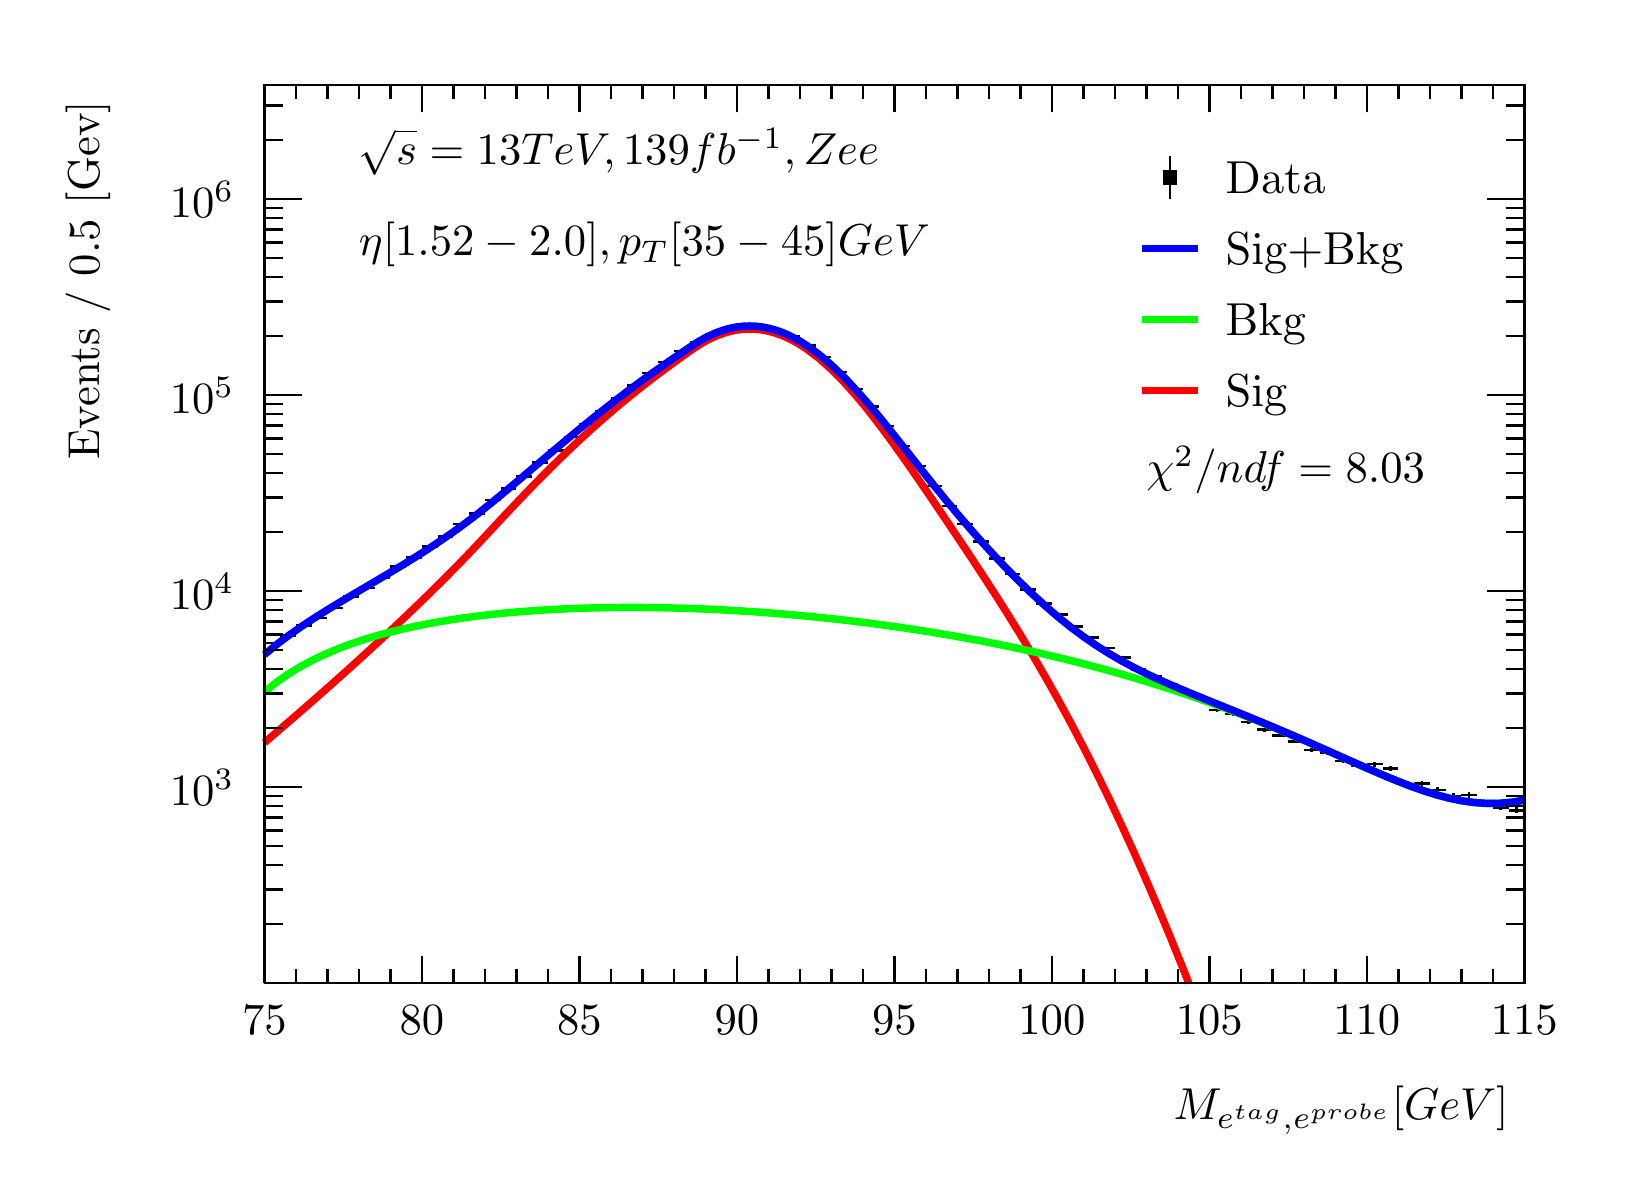
\begin{tikzpicture}
\pgfdeclareplotmark{cross} {
\pgfpathmoveto{\pgfpoint{-0.3\pgfplotmarksize}{\pgfplotmarksize}}
\pgfpathlineto{\pgfpoint{+0.3\pgfplotmarksize}{\pgfplotmarksize}}
\pgfpathlineto{\pgfpoint{+0.3\pgfplotmarksize}{0.3\pgfplotmarksize}}
\pgfpathlineto{\pgfpoint{+1\pgfplotmarksize}{0.3\pgfplotmarksize}}
\pgfpathlineto{\pgfpoint{+1\pgfplotmarksize}{-0.3\pgfplotmarksize}}
\pgfpathlineto{\pgfpoint{+0.3\pgfplotmarksize}{-0.3\pgfplotmarksize}}
\pgfpathlineto{\pgfpoint{+0.3\pgfplotmarksize}{-1.\pgfplotmarksize}}
\pgfpathlineto{\pgfpoint{-0.3\pgfplotmarksize}{-1.\pgfplotmarksize}}
\pgfpathlineto{\pgfpoint{-0.3\pgfplotmarksize}{-0.3\pgfplotmarksize}}
\pgfpathlineto{\pgfpoint{-1.\pgfplotmarksize}{-0.3\pgfplotmarksize}}
\pgfpathlineto{\pgfpoint{-1.\pgfplotmarksize}{0.3\pgfplotmarksize}}
\pgfpathlineto{\pgfpoint{-0.3\pgfplotmarksize}{0.3\pgfplotmarksize}}
\pgfpathclose
\pgfusepathqstroke
}
\pgfdeclareplotmark{cross*} {
\pgfpathmoveto{\pgfpoint{-0.3\pgfplotmarksize}{\pgfplotmarksize}}
\pgfpathlineto{\pgfpoint{+0.3\pgfplotmarksize}{\pgfplotmarksize}}
\pgfpathlineto{\pgfpoint{+0.3\pgfplotmarksize}{0.3\pgfplotmarksize}}
\pgfpathlineto{\pgfpoint{+1\pgfplotmarksize}{0.3\pgfplotmarksize}}
\pgfpathlineto{\pgfpoint{+1\pgfplotmarksize}{-0.3\pgfplotmarksize}}
\pgfpathlineto{\pgfpoint{+0.3\pgfplotmarksize}{-0.3\pgfplotmarksize}}
\pgfpathlineto{\pgfpoint{+0.3\pgfplotmarksize}{-1.\pgfplotmarksize}}
\pgfpathlineto{\pgfpoint{-0.3\pgfplotmarksize}{-1.\pgfplotmarksize}}
\pgfpathlineto{\pgfpoint{-0.3\pgfplotmarksize}{-0.3\pgfplotmarksize}}
\pgfpathlineto{\pgfpoint{-1.\pgfplotmarksize}{-0.3\pgfplotmarksize}}
\pgfpathlineto{\pgfpoint{-1.\pgfplotmarksize}{0.3\pgfplotmarksize}}
\pgfpathlineto{\pgfpoint{-0.3\pgfplotmarksize}{0.3\pgfplotmarksize}}
\pgfpathclose
\pgfusepathqfillstroke
}
\pgfdeclareplotmark{newstar} {
\pgfpathmoveto{\pgfqpoint{0pt}{\pgfplotmarksize}}
\pgfpathlineto{\pgfqpointpolar{44}{0.5\pgfplotmarksize}}
\pgfpathlineto{\pgfqpointpolar{18}{\pgfplotmarksize}}
\pgfpathlineto{\pgfqpointpolar{-20}{0.5\pgfplotmarksize}}
\pgfpathlineto{\pgfqpointpolar{-54}{\pgfplotmarksize}}
\pgfpathlineto{\pgfqpointpolar{-90}{0.5\pgfplotmarksize}}
\pgfpathlineto{\pgfqpointpolar{234}{\pgfplotmarksize}}
\pgfpathlineto{\pgfqpointpolar{198}{0.5\pgfplotmarksize}}
\pgfpathlineto{\pgfqpointpolar{162}{\pgfplotmarksize}}
\pgfpathlineto{\pgfqpointpolar{134}{0.5\pgfplotmarksize}}
\pgfpathclose
\pgfusepathqstroke
}
\pgfdeclareplotmark{newstar*} {
\pgfpathmoveto{\pgfqpoint{0pt}{\pgfplotmarksize}}
\pgfpathlineto{\pgfqpointpolar{44}{0.5\pgfplotmarksize}}
\pgfpathlineto{\pgfqpointpolar{18}{\pgfplotmarksize}}
\pgfpathlineto{\pgfqpointpolar{-20}{0.5\pgfplotmarksize}}
\pgfpathlineto{\pgfqpointpolar{-54}{\pgfplotmarksize}}
\pgfpathlineto{\pgfqpointpolar{-90}{0.5\pgfplotmarksize}}
\pgfpathlineto{\pgfqpointpolar{234}{\pgfplotmarksize}}
\pgfpathlineto{\pgfqpointpolar{198}{0.5\pgfplotmarksize}}
\pgfpathlineto{\pgfqpointpolar{162}{\pgfplotmarksize}}
\pgfpathlineto{\pgfqpointpolar{134}{0.5\pgfplotmarksize}}
\pgfpathclose
\pgfusepathqfillstroke
}
\definecolor{c}{rgb}{1,1,1};
\draw [color=c, fill=c] (0,0) rectangle (20,14.4361);
\draw [color=c, fill=c] (3,2.30977) rectangle (19,13.7143);
\definecolor{c}{rgb}{0,0,0};
\draw [c,line width=0.9] (3,2.30977) -- (3,13.7143) -- (19,13.7143) -- (19,2.30977) -- (3,2.30977);
\definecolor{c}{rgb}{1,1,1};
\draw [color=c, fill=c] (3,2.30977) rectangle (19,13.7143);
\definecolor{c}{rgb}{0,0,0};
\draw [c,line width=0.9] (3,2.30977) -- (3,13.7143) -- (19,13.7143) -- (19,2.30977) -- (3,2.30977);
\draw [c,line width=0.9] (3,2.30977) -- (19,2.30977);
\draw [c,line width=0.9] (3,2.65624) -- (3,2.30977);
\draw [c,line width=0.9] (3.4,2.48301) -- (3.4,2.30977);
\draw [c,line width=0.9] (3.8,2.48301) -- (3.8,2.30977);
\draw [c,line width=0.9] (4.2,2.48301) -- (4.2,2.30977);
\draw [c,line width=0.9] (4.6,2.48301) -- (4.6,2.30977);
\draw [c,line width=0.9] (5,2.65624) -- (5,2.30977);
\draw [c,line width=0.9] (5.4,2.48301) -- (5.4,2.30977);
\draw [c,line width=0.9] (5.8,2.48301) -- (5.8,2.30977);
\draw [c,line width=0.9] (6.2,2.48301) -- (6.2,2.30977);
\draw [c,line width=0.9] (6.6,2.48301) -- (6.6,2.30977);
\draw [c,line width=0.9] (7,2.65624) -- (7,2.30977);
\draw [c,line width=0.9] (7.4,2.48301) -- (7.4,2.30977);
\draw [c,line width=0.9] (7.8,2.48301) -- (7.8,2.30977);
\draw [c,line width=0.9] (8.2,2.48301) -- (8.2,2.30977);
\draw [c,line width=0.9] (8.6,2.48301) -- (8.6,2.30977);
\draw [c,line width=0.9] (9,2.65624) -- (9,2.30977);
\draw [c,line width=0.9] (9.4,2.48301) -- (9.4,2.30977);
\draw [c,line width=0.9] (9.8,2.48301) -- (9.8,2.30977);
\draw [c,line width=0.9] (10.2,2.48301) -- (10.2,2.30977);
\draw [c,line width=0.9] (10.6,2.48301) -- (10.6,2.30977);
\draw [c,line width=0.9] (11,2.65624) -- (11,2.30977);
\draw [c,line width=0.9] (11.4,2.48301) -- (11.4,2.30977);
\draw [c,line width=0.9] (11.8,2.48301) -- (11.8,2.30977);
\draw [c,line width=0.9] (12.2,2.48301) -- (12.2,2.30977);
\draw [c,line width=0.9] (12.6,2.48301) -- (12.6,2.30977);
\draw [c,line width=0.9] (13,2.65624) -- (13,2.30977);
\draw [c,line width=0.9] (13.4,2.48301) -- (13.4,2.30977);
\draw [c,line width=0.9] (13.8,2.48301) -- (13.8,2.30977);
\draw [c,line width=0.9] (14.2,2.48301) -- (14.2,2.30977);
\draw [c,line width=0.9] (14.6,2.48301) -- (14.6,2.30977);
\draw [c,line width=0.9] (15,2.65624) -- (15,2.30977);
\draw [c,line width=0.9] (15.4,2.48301) -- (15.4,2.30977);
\draw [c,line width=0.9] (15.8,2.48301) -- (15.8,2.30977);
\draw [c,line width=0.9] (16.2,2.48301) -- (16.2,2.30977);
\draw [c,line width=0.9] (16.6,2.48301) -- (16.6,2.30977);
\draw [c,line width=0.9] (17,2.65624) -- (17,2.30977);
\draw [c,line width=0.9] (17.4,2.48301) -- (17.4,2.30977);
\draw [c,line width=0.9] (17.8,2.48301) -- (17.8,2.30977);
\draw [c,line width=0.9] (18.2,2.48301) -- (18.2,2.30977);
\draw [c,line width=0.9] (18.6,2.48301) -- (18.6,2.30977);
\draw [c,line width=0.9] (19,2.65624) -- (19,2.30977);
\draw [c,line width=0.9] (19,2.65624) -- (19,2.30977);
\draw [anchor=base] (3,1.66015) node[scale=1.61424, color=c, rotate=0]{75};
\draw [anchor=base] (5,1.66015) node[scale=1.61424, color=c, rotate=0]{80};
\draw [anchor=base] (7,1.66015) node[scale=1.61424, color=c, rotate=0]{85};
\draw [anchor=base] (9,1.66015) node[scale=1.61424, color=c, rotate=0]{90};
\draw [anchor=base] (11,1.66015) node[scale=1.61424, color=c, rotate=0]{95};
\draw [anchor=base] (13,1.66015) node[scale=1.61424, color=c, rotate=0]{100};
\draw [anchor=base] (15,1.66015) node[scale=1.61424, color=c, rotate=0]{105};
\draw [anchor=base] (17,1.66015) node[scale=1.61424, color=c, rotate=0]{110};
\draw [anchor=base] (19,1.66015) node[scale=1.61424, color=c, rotate=0]{115};
\draw [anchor= east] (19,0.692932) node[scale=1.61424, color=c, rotate=0]{$M_{e^{tag}, e^{probe}}  [GeV]$};
\draw [c,line width=0.9] (3,13.7143) -- (19,13.7143);
\draw [c,line width=0.9] (3,13.3678) -- (3,13.7143);
\draw [c,line width=0.9] (3.4,13.5411) -- (3.4,13.7143);
\draw [c,line width=0.9] (3.8,13.5411) -- (3.8,13.7143);
\draw [c,line width=0.9] (4.2,13.5411) -- (4.2,13.7143);
\draw [c,line width=0.9] (4.6,13.5411) -- (4.6,13.7143);
\draw [c,line width=0.9] (5,13.3678) -- (5,13.7143);
\draw [c,line width=0.9] (5.4,13.5411) -- (5.4,13.7143);
\draw [c,line width=0.9] (5.8,13.5411) -- (5.8,13.7143);
\draw [c,line width=0.9] (6.2,13.5411) -- (6.2,13.7143);
\draw [c,line width=0.9] (6.6,13.5411) -- (6.6,13.7143);
\draw [c,line width=0.9] (7,13.3678) -- (7,13.7143);
\draw [c,line width=0.9] (7.4,13.5411) -- (7.4,13.7143);
\draw [c,line width=0.9] (7.8,13.5411) -- (7.8,13.7143);
\draw [c,line width=0.9] (8.2,13.5411) -- (8.2,13.7143);
\draw [c,line width=0.9] (8.6,13.5411) -- (8.6,13.7143);
\draw [c,line width=0.9] (9,13.3678) -- (9,13.7143);
\draw [c,line width=0.9] (9.4,13.5411) -- (9.4,13.7143);
\draw [c,line width=0.9] (9.8,13.5411) -- (9.8,13.7143);
\draw [c,line width=0.9] (10.2,13.5411) -- (10.2,13.7143);
\draw [c,line width=0.9] (10.6,13.5411) -- (10.6,13.7143);
\draw [c,line width=0.9] (11,13.3678) -- (11,13.7143);
\draw [c,line width=0.9] (11.4,13.5411) -- (11.4,13.7143);
\draw [c,line width=0.9] (11.8,13.5411) -- (11.8,13.7143);
\draw [c,line width=0.9] (12.2,13.5411) -- (12.2,13.7143);
\draw [c,line width=0.9] (12.6,13.5411) -- (12.6,13.7143);
\draw [c,line width=0.9] (13,13.3678) -- (13,13.7143);
\draw [c,line width=0.9] (13.4,13.5411) -- (13.4,13.7143);
\draw [c,line width=0.9] (13.8,13.5411) -- (13.8,13.7143);
\draw [c,line width=0.9] (14.2,13.5411) -- (14.2,13.7143);
\draw [c,line width=0.9] (14.6,13.5411) -- (14.6,13.7143);
\draw [c,line width=0.9] (15,13.3678) -- (15,13.7143);
\draw [c,line width=0.9] (15.4,13.5411) -- (15.4,13.7143);
\draw [c,line width=0.9] (15.8,13.5411) -- (15.8,13.7143);
\draw [c,line width=0.9] (16.2,13.5411) -- (16.2,13.7143);
\draw [c,line width=0.9] (16.6,13.5411) -- (16.6,13.7143);
\draw [c,line width=0.9] (17,13.3678) -- (17,13.7143);
\draw [c,line width=0.9] (17.4,13.5411) -- (17.4,13.7143);
\draw [c,line width=0.9] (17.8,13.5411) -- (17.8,13.7143);
\draw [c,line width=0.9] (18.2,13.5411) -- (18.2,13.7143);
\draw [c,line width=0.9] (18.6,13.5411) -- (18.6,13.7143);
\draw [c,line width=0.9] (19,13.3678) -- (19,13.7143);
\draw [c,line width=0.9] (19,13.3678) -- (19,13.7143);
\draw [c,line width=0.9] (3,2.30977) -- (3,13.7143);
\draw [c,line width=0.9] (3.237,3.05909) -- (3,3.05909);
\draw [c,line width=0.9] (3.237,3.49742) -- (3,3.49742);
\draw [c,line width=0.9] (3.237,3.80841) -- (3,3.80841);
\draw [c,line width=0.9] (3.237,4.04964) -- (3,4.04964);
\draw [c,line width=0.9] (3.237,4.24673) -- (3,4.24673);
\draw [c,line width=0.9] (3.237,4.41338) -- (3,4.41338);
\draw [c,line width=0.9] (3.237,4.55773) -- (3,4.55773);
\draw [c,line width=0.9] (3.237,4.68506) -- (3,4.68506);
\draw [c,line width=0.9] (3.474,4.79896) -- (3,4.79896);
\draw [anchor= east] (2.82,4.79896) node[scale=1.61424, color=c, rotate=0]{$10^{3}$};
\draw [c,line width=0.9] (3.237,5.54828) -- (3,5.54828);
\draw [c,line width=0.9] (3.237,5.9866) -- (3,5.9866);
\draw [c,line width=0.9] (3.237,6.2976) -- (3,6.2976);
\draw [c,line width=0.9] (3.237,6.53882) -- (3,6.53882);
\draw [c,line width=0.9] (3.237,6.73592) -- (3,6.73592);
\draw [c,line width=0.9] (3.237,6.90256) -- (3,6.90256);
\draw [c,line width=0.9] (3.237,7.04692) -- (3,7.04692);
\draw [c,line width=0.9] (3.237,7.17424) -- (3,7.17424);
\draw [c,line width=0.9] (3.474,7.28814) -- (3,7.28814);
\draw [anchor= east] (2.82,7.28814) node[scale=1.61424, color=c, rotate=0]{$10^{4}$};
\draw [c,line width=0.9] (3.237,8.03746) -- (3,8.03746);
\draw [c,line width=0.9] (3.237,8.47579) -- (3,8.47579);
\draw [c,line width=0.9] (3.237,8.78678) -- (3,8.78678);
\draw [c,line width=0.9] (3.237,9.02801) -- (3,9.02801);
\draw [c,line width=0.9] (3.237,9.2251) -- (3,9.2251);
\draw [c,line width=0.9] (3.237,9.39175) -- (3,9.39175);
\draw [c,line width=0.9] (3.237,9.5361) -- (3,9.5361);
\draw [c,line width=0.9] (3.237,9.66343) -- (3,9.66343);
\draw [c,line width=0.9] (3.474,9.77733) -- (3,9.77733);
\draw [anchor= east] (2.82,9.77733) node[scale=1.61424, color=c, rotate=0]{$10^{5}$};
\draw [c,line width=0.9] (3.237,10.5266) -- (3,10.5266);
\draw [c,line width=0.9] (3.237,10.965) -- (3,10.965);
\draw [c,line width=0.9] (3.237,11.276) -- (3,11.276);
\draw [c,line width=0.9] (3.237,11.5172) -- (3,11.5172);
\draw [c,line width=0.9] (3.237,11.7143) -- (3,11.7143);
\draw [c,line width=0.9] (3.237,11.8809) -- (3,11.8809);
\draw [c,line width=0.9] (3.237,12.0253) -- (3,12.0253);
\draw [c,line width=0.9] (3.237,12.1526) -- (3,12.1526);
\draw [c,line width=0.9] (3.474,12.2665) -- (3,12.2665);
\draw [anchor= east] (2.82,12.2665) node[scale=1.61424, color=c, rotate=0]{$10^{6}$};
\draw [c,line width=0.9] (3.237,13.0158) -- (3,13.0158);
\draw [c,line width=0.9] (3.237,13.4542) -- (3,13.4542);
\draw [anchor= east] (0.76,13.7143) node[scale=1.61424, color=c, rotate=90]{Events / 0.5 [Gev]};
\draw [c,line width=0.9] (19,2.30977) -- (19,13.7143);
\draw [c,line width=0.9] (18.763,3.05909) -- (19,3.05909);
\draw [c,line width=0.9] (18.763,3.49742) -- (19,3.49742);
\draw [c,line width=0.9] (18.763,3.80841) -- (19,3.80841);
\draw [c,line width=0.9] (18.763,4.04964) -- (19,4.04964);
\draw [c,line width=0.9] (18.763,4.24673) -- (19,4.24673);
\draw [c,line width=0.9] (18.763,4.41338) -- (19,4.41338);
\draw [c,line width=0.9] (18.763,4.55773) -- (19,4.55773);
\draw [c,line width=0.9] (18.763,4.68506) -- (19,4.68506);
\draw [c,line width=0.9] (18.526,4.79896) -- (19,4.79896);
\draw [c,line width=0.9] (18.763,5.54828) -- (19,5.54828);
\draw [c,line width=0.9] (18.763,5.9866) -- (19,5.9866);
\draw [c,line width=0.9] (18.763,6.2976) -- (19,6.2976);
\draw [c,line width=0.9] (18.763,6.53882) -- (19,6.53882);
\draw [c,line width=0.9] (18.763,6.73592) -- (19,6.73592);
\draw [c,line width=0.9] (18.763,6.90256) -- (19,6.90256);
\draw [c,line width=0.9] (18.763,7.04692) -- (19,7.04692);
\draw [c,line width=0.9] (18.763,7.17424) -- (19,7.17424);
\draw [c,line width=0.9] (18.526,7.28814) -- (19,7.28814);
\draw [c,line width=0.9] (18.763,8.03746) -- (19,8.03746);
\draw [c,line width=0.9] (18.763,8.47579) -- (19,8.47579);
\draw [c,line width=0.9] (18.763,8.78678) -- (19,8.78678);
\draw [c,line width=0.9] (18.763,9.02801) -- (19,9.02801);
\draw [c,line width=0.9] (18.763,9.2251) -- (19,9.2251);
\draw [c,line width=0.9] (18.763,9.39175) -- (19,9.39175);
\draw [c,line width=0.9] (18.763,9.5361) -- (19,9.5361);
\draw [c,line width=0.9] (18.763,9.66343) -- (19,9.66343);
\draw [c,line width=0.9] (18.526,9.77733) -- (19,9.77733);
\draw [c,line width=0.9] (18.763,10.5266) -- (19,10.5266);
\draw [c,line width=0.9] (18.763,10.965) -- (19,10.965);
\draw [c,line width=0.9] (18.763,11.276) -- (19,11.276);
\draw [c,line width=0.9] (18.763,11.5172) -- (19,11.5172);
\draw [c,line width=0.9] (18.763,11.7143) -- (19,11.7143);
\draw [c,line width=0.9] (18.763,11.8809) -- (19,11.8809);
\draw [c,line width=0.9] (18.763,12.0253) -- (19,12.0253);
\draw [c,line width=0.9] (18.763,12.1526) -- (19,12.1526);
\draw [c,line width=0.9] (18.526,12.2665) -- (19,12.2665);
\draw [c,line width=0.9] (18.763,13.0158) -- (19,13.0158);
\draw [c,line width=0.9] (18.763,13.4542) -- (19,13.4542);
\draw [c,line width=0.9] (3.1,6.62921) -- (3,6.62921);
\draw [c,line width=0.9] (3,6.62921) -- (3,6.62921);
\draw [c,line width=0.9] (3.1,6.62921) -- (3.2,6.62921);
\draw [c,line width=0.9] (3.2,6.62921) -- (3.2,6.62921);
\draw [c,line width=0.9] (3.1,6.62921) -- (3.1,6.64387);
\draw [c,line width=0.9] (3.1,6.64387) -- (3.1,6.64387);
\draw [c,line width=0.9] (3.1,6.62921) -- (3.1,6.61454);
\draw [c,line width=0.9] (3.1,6.61454) -- (3.1,6.61454);
\draw [c,line width=0.9] (3.3,6.72378) -- (3.2,6.72378);
\draw [c,line width=0.9] (3.2,6.72378) -- (3.2,6.72378);
\draw [c,line width=0.9] (3.3,6.72378) -- (3.4,6.72378);
\draw [c,line width=0.9] (3.4,6.72378) -- (3.4,6.72378);
\draw [c,line width=0.9] (3.3,6.72378) -- (3.3,6.73782);
\draw [c,line width=0.9] (3.3,6.73782) -- (3.3,6.73782);
\draw [c,line width=0.9] (3.3,6.72378) -- (3.3,6.70975);
\draw [c,line width=0.9] (3.3,6.70975) -- (3.3,6.70975);
\draw [c,line width=0.9] (3.5,6.8523) -- (3.4,6.8523);
\draw [c,line width=0.9] (3.4,6.8523) -- (3.4,6.8523);
\draw [c,line width=0.9] (3.5,6.8523) -- (3.6,6.8523);
\draw [c,line width=0.9] (3.6,6.8523) -- (3.6,6.8523);
\draw [c,line width=0.9] (3.5,6.8523) -- (3.5,6.86553);
\draw [c,line width=0.9] (3.5,6.86553) -- (3.5,6.86553);
\draw [c,line width=0.9] (3.5,6.8523) -- (3.5,6.83908);
\draw [c,line width=0.9] (3.5,6.83908) -- (3.5,6.83908);
\draw [c,line width=0.9] (3.7,6.94392) -- (3.6,6.94392);
\draw [c,line width=0.9] (3.6,6.94392) -- (3.6,6.94392);
\draw [c,line width=0.9] (3.7,6.94392) -- (3.8,6.94392);
\draw [c,line width=0.9] (3.8,6.94392) -- (3.8,6.94392);
\draw [c,line width=0.9] (3.7,6.94392) -- (3.7,6.9566);
\draw [c,line width=0.9] (3.7,6.9566) -- (3.7,6.9566);
\draw [c,line width=0.9] (3.7,6.94392) -- (3.7,6.93125);
\draw [c,line width=0.9] (3.7,6.93125) -- (3.7,6.93125);
\draw [c,line width=0.9] (3.9,7.07216) -- (3.8,7.07216);
\draw [c,line width=0.9] (3.8,7.07216) -- (3.8,7.07216);
\draw [c,line width=0.9] (3.9,7.07216) -- (4,7.07216);
\draw [c,line width=0.9] (4,7.07216) -- (4,7.07216);
\draw [c,line width=0.9] (3.9,7.07216) -- (3.9,7.08411);
\draw [c,line width=0.9] (3.9,7.08411) -- (3.9,7.08411);
\draw [c,line width=0.9] (3.9,7.07216) -- (3.9,7.06021);
\draw [c,line width=0.9] (3.9,7.06021) -- (3.9,7.06021);
\draw [c,line width=0.9] (4.1,7.21745) -- (4,7.21745);
\draw [c,line width=0.9] (4,7.21745) -- (4,7.21745);
\draw [c,line width=0.9] (4.1,7.21745) -- (4.2,7.21745);
\draw [c,line width=0.9] (4.2,7.21745) -- (4.2,7.21745);
\draw [c,line width=0.9] (4.1,7.21745) -- (4.1,7.22862);
\draw [c,line width=0.9] (4.1,7.22862) -- (4.1,7.22862);
\draw [c,line width=0.9] (4.1,7.21745) -- (4.1,7.20628);
\draw [c,line width=0.9] (4.1,7.20628) -- (4.1,7.20628);
\draw [c,line width=0.9] (4.3,7.32648) -- (4.2,7.32648);
\draw [c,line width=0.9] (4.2,7.32648) -- (4.2,7.32648);
\draw [c,line width=0.9] (4.3,7.32648) -- (4.4,7.32648);
\draw [c,line width=0.9] (4.4,7.32648) -- (4.4,7.32648);
\draw [c,line width=0.9] (4.3,7.32648) -- (4.3,7.3371);
\draw [c,line width=0.9] (4.3,7.3371) -- (4.3,7.3371);
\draw [c,line width=0.9] (4.3,7.32648) -- (4.3,7.31586);
\draw [c,line width=0.9] (4.3,7.31586) -- (4.3,7.31586);
\draw [c,line width=0.9] (4.5,7.4538) -- (4.4,7.4538);
\draw [c,line width=0.9] (4.4,7.4538) -- (4.4,7.4538);
\draw [c,line width=0.9] (4.5,7.4538) -- (4.6,7.4538);
\draw [c,line width=0.9] (4.6,7.4538) -- (4.6,7.4538);
\draw [c,line width=0.9] (4.5,7.4538) -- (4.5,7.46381);
\draw [c,line width=0.9] (4.5,7.46381) -- (4.5,7.46381);
\draw [c,line width=0.9] (4.5,7.4538) -- (4.5,7.44378);
\draw [c,line width=0.9] (4.5,7.44378) -- (4.5,7.44378);
\draw [c,line width=0.9] (4.7,7.60065) -- (4.6,7.60065);
\draw [c,line width=0.9] (4.6,7.60065) -- (4.6,7.60065);
\draw [c,line width=0.9] (4.7,7.60065) -- (4.8,7.60065);
\draw [c,line width=0.9] (4.8,7.60065) -- (4.8,7.60065);
\draw [c,line width=0.9] (4.7,7.60065) -- (4.7,7.61001);
\draw [c,line width=0.9] (4.7,7.61001) -- (4.7,7.61001);
\draw [c,line width=0.9] (4.7,7.60065) -- (4.7,7.5913);
\draw [c,line width=0.9] (4.7,7.5913) -- (4.7,7.5913);
\draw [c,line width=0.9] (4.9,7.7148) -- (4.8,7.7148);
\draw [c,line width=0.9] (4.8,7.7148) -- (4.8,7.7148);
\draw [c,line width=0.9] (4.9,7.7148) -- (5,7.7148);
\draw [c,line width=0.9] (5,7.7148) -- (5,7.7148);
\draw [c,line width=0.9] (4.9,7.7148) -- (4.9,7.72368);
\draw [c,line width=0.9] (4.9,7.72368) -- (4.9,7.72368);
\draw [c,line width=0.9] (4.9,7.7148) -- (4.9,7.70593);
\draw [c,line width=0.9] (4.9,7.70593) -- (4.9,7.70593);
\draw [c,line width=0.9] (5.1,7.85399) -- (5,7.85399);
\draw [c,line width=0.9] (5,7.85399) -- (5,7.85399);
\draw [c,line width=0.9] (5.1,7.85399) -- (5.2,7.85399);
\draw [c,line width=0.9] (5.2,7.85399) -- (5.2,7.85399);
\draw [c,line width=0.9] (5.1,7.85399) -- (5.1,7.86231);
\draw [c,line width=0.9] (5.1,7.86231) -- (5.1,7.86231);
\draw [c,line width=0.9] (5.1,7.85399) -- (5.1,7.84567);
\draw [c,line width=0.9] (5.1,7.84567) -- (5.1,7.84567);
\draw [c,line width=0.9] (5.3,7.97991) -- (5.2,7.97991);
\draw [c,line width=0.9] (5.2,7.97991) -- (5.2,7.97991);
\draw [c,line width=0.9] (5.3,7.97991) -- (5.4,7.97991);
\draw [c,line width=0.9] (5.4,7.97991) -- (5.4,7.97991);
\draw [c,line width=0.9] (5.3,7.97991) -- (5.3,7.98776);
\draw [c,line width=0.9] (5.3,7.98776) -- (5.3,7.98776);
\draw [c,line width=0.9] (5.3,7.97991) -- (5.3,7.97205);
\draw [c,line width=0.9] (5.3,7.97205) -- (5.3,7.97205);
\draw [c,line width=0.9] (5.5,8.13917) -- (5.4,8.13917);
\draw [c,line width=0.9] (5.4,8.13917) -- (5.4,8.13917);
\draw [c,line width=0.9] (5.5,8.13917) -- (5.6,8.13917);
\draw [c,line width=0.9] (5.6,8.13917) -- (5.6,8.13917);
\draw [c,line width=0.9] (5.5,8.13917) -- (5.5,8.14646);
\draw [c,line width=0.9] (5.5,8.14646) -- (5.5,8.14646);
\draw [c,line width=0.9] (5.5,8.13917) -- (5.5,8.13188);
\draw [c,line width=0.9] (5.5,8.13188) -- (5.5,8.13188);
\draw [c,line width=0.9] (5.7,8.27036) -- (5.6,8.27036);
\draw [c,line width=0.9] (5.6,8.27036) -- (5.6,8.27036);
\draw [c,line width=0.9] (5.7,8.27036) -- (5.8,8.27036);
\draw [c,line width=0.9] (5.8,8.27036) -- (5.8,8.27036);
\draw [c,line width=0.9] (5.7,8.27036) -- (5.7,8.27722);
\draw [c,line width=0.9] (5.7,8.27722) -- (5.7,8.27722);
\draw [c,line width=0.9] (5.7,8.27036) -- (5.7,8.26349);
\draw [c,line width=0.9] (5.7,8.26349) -- (5.7,8.26349);
\draw [c,line width=0.9] (5.9,8.44642) -- (5.8,8.44642);
\draw [c,line width=0.9] (5.8,8.44642) -- (5.8,8.44642);
\draw [c,line width=0.9] (5.9,8.44642) -- (6,8.44642);
\draw [c,line width=0.9] (6,8.44642) -- (6,8.44642);
\draw [c,line width=0.9] (5.9,8.44642) -- (5.9,8.45275);
\draw [c,line width=0.9] (5.9,8.45275) -- (5.9,8.45275);
\draw [c,line width=0.9] (5.9,8.44642) -- (5.9,8.44009);
\draw [c,line width=0.9] (5.9,8.44009) -- (5.9,8.44009);
\draw [c,line width=0.9] (6.1,8.58886) -- (6,8.58886);
\draw [c,line width=0.9] (6,8.58886) -- (6,8.58886);
\draw [c,line width=0.9] (6.1,8.58886) -- (6.2,8.58886);
\draw [c,line width=0.9] (6.2,8.58886) -- (6.2,8.58886);
\draw [c,line width=0.9] (6.1,8.58886) -- (6.1,8.59479);
\draw [c,line width=0.9] (6.1,8.59479) -- (6.1,8.59479);
\draw [c,line width=0.9] (6.1,8.58886) -- (6.1,8.58294);
\draw [c,line width=0.9] (6.1,8.58294) -- (6.1,8.58294);
\draw [c,line width=0.9] (6.3,8.74431) -- (6.2,8.74431);
\draw [c,line width=0.9] (6.2,8.74431) -- (6.2,8.74431);
\draw [c,line width=0.9] (6.3,8.74431) -- (6.4,8.74431);
\draw [c,line width=0.9] (6.4,8.74431) -- (6.4,8.74431);
\draw [c,line width=0.9] (6.3,8.74431) -- (6.3,8.74982);
\draw [c,line width=0.9] (6.3,8.74982) -- (6.3,8.74982);
\draw [c,line width=0.9] (6.3,8.74431) -- (6.3,8.7388);
\draw [c,line width=0.9] (6.3,8.7388) -- (6.3,8.7388);
\draw [c,line width=0.9] (6.5,8.91807) -- (6.4,8.91807);
\draw [c,line width=0.9] (6.4,8.91807) -- (6.4,8.91807);
\draw [c,line width=0.9] (6.5,8.91807) -- (6.6,8.91807);
\draw [c,line width=0.9] (6.6,8.91807) -- (6.6,8.91807);
\draw [c,line width=0.9] (6.5,8.91807) -- (6.5,8.92315);
\draw [c,line width=0.9] (6.5,8.92315) -- (6.5,8.92315);
\draw [c,line width=0.9] (6.5,8.91807) -- (6.5,8.91298);
\draw [c,line width=0.9] (6.5,8.91298) -- (6.5,8.91298);
\draw [c,line width=0.9] (6.7,9.0753) -- (6.6,9.0753);
\draw [c,line width=0.9] (6.6,9.0753) -- (6.6,9.0753);
\draw [c,line width=0.9] (6.7,9.0753) -- (6.8,9.0753);
\draw [c,line width=0.9] (6.8,9.0753) -- (6.8,9.0753);
\draw [c,line width=0.9] (6.7,9.0753) -- (6.7,9.08003);
\draw [c,line width=0.9] (6.7,9.08003) -- (6.7,9.08003);
\draw [c,line width=0.9] (6.7,9.0753) -- (6.7,9.07057);
\draw [c,line width=0.9] (6.7,9.07057) -- (6.7,9.07057);
\draw [c,line width=0.9] (6.9,9.24432) -- (6.8,9.24432);
\draw [c,line width=0.9] (6.8,9.24432) -- (6.8,9.24432);
\draw [c,line width=0.9] (6.9,9.24432) -- (7,9.24432);
\draw [c,line width=0.9] (7,9.24432) -- (7,9.24432);
\draw [c,line width=0.9] (6.9,9.24432) -- (6.9,9.24869);
\draw [c,line width=0.9] (6.9,9.24869) -- (6.9,9.24869);
\draw [c,line width=0.9] (6.9,9.24432) -- (6.9,9.23995);
\draw [c,line width=0.9] (6.9,9.23995) -- (6.9,9.23995);
\draw [c,line width=0.9] (7.1,9.40842) -- (7,9.40842);
\draw [c,line width=0.9] (7,9.40842) -- (7,9.40842);
\draw [c,line width=0.9] (7.1,9.40842) -- (7.2,9.40842);
\draw [c,line width=0.9] (7.2,9.40842) -- (7.2,9.40842);
\draw [c,line width=0.9] (7.1,9.40842) -- (7.1,9.41248);
\draw [c,line width=0.9] (7.1,9.41248) -- (7.1,9.41248);
\draw [c,line width=0.9] (7.1,9.40842) -- (7.1,9.40437);
\draw [c,line width=0.9] (7.1,9.40437) -- (7.1,9.40437);
\draw [c,line width=0.9] (7.3,9.5776) -- (7.2,9.5776);
\draw [c,line width=0.9] (7.2,9.5776) -- (7.2,9.5776);
\draw [c,line width=0.9] (7.3,9.5776) -- (7.4,9.5776);
\draw [c,line width=0.9] (7.4,9.5776) -- (7.4,9.5776);
\draw [c,line width=0.9] (7.3,9.5776) -- (7.3,9.58135);
\draw [c,line width=0.9] (7.3,9.58135) -- (7.3,9.58135);
\draw [c,line width=0.9] (7.3,9.5776) -- (7.3,9.57385);
\draw [c,line width=0.9] (7.3,9.57385) -- (7.3,9.57385);
\draw [c,line width=0.9] (7.5,9.73996) -- (7.4,9.73996);
\draw [c,line width=0.9] (7.4,9.73996) -- (7.4,9.73996);
\draw [c,line width=0.9] (7.5,9.73996) -- (7.6,9.73996);
\draw [c,line width=0.9] (7.6,9.73996) -- (7.6,9.73996);
\draw [c,line width=0.9] (7.5,9.73996) -- (7.5,9.74343);
\draw [c,line width=0.9] (7.5,9.74343) -- (7.5,9.74343);
\draw [c,line width=0.9] (7.5,9.73996) -- (7.5,9.73648);
\draw [c,line width=0.9] (7.5,9.73648) -- (7.5,9.73648);
\draw [c,line width=0.9] (7.7,9.90153) -- (7.6,9.90153);
\draw [c,line width=0.9] (7.6,9.90153) -- (7.6,9.90153);
\draw [c,line width=0.9] (7.7,9.90153) -- (7.8,9.90153);
\draw [c,line width=0.9] (7.8,9.90153) -- (7.8,9.90153);
\draw [c,line width=0.9] (7.7,9.90153) -- (7.7,9.90476);
\draw [c,line width=0.9] (7.7,9.90476) -- (7.7,9.90476);
\draw [c,line width=0.9] (7.7,9.90153) -- (7.7,9.8983);
\draw [c,line width=0.9] (7.7,9.8983) -- (7.7,9.8983);
\draw [c,line width=0.9] (7.9,10.0572) -- (7.8,10.0572);
\draw [c,line width=0.9] (7.8,10.0572) -- (7.8,10.0572);
\draw [c,line width=0.9] (7.9,10.0572) -- (8,10.0572);
\draw [c,line width=0.9] (8,10.0572) -- (8,10.0572);
\draw [c,line width=0.9] (7.9,10.0572) -- (7.9,10.0602);
\draw [c,line width=0.9] (7.9,10.0602) -- (7.9,10.0602);
\draw [c,line width=0.9] (7.9,10.0572) -- (7.9,10.0542);
\draw [c,line width=0.9] (7.9,10.0542) -- (7.9,10.0542);
\draw [c,line width=0.9] (8.1,10.1997) -- (8,10.1997);
\draw [c,line width=0.9] (8,10.1997) -- (8,10.1997);
\draw [c,line width=0.9] (8.1,10.1997) -- (8.2,10.1997);
\draw [c,line width=0.9] (8.2,10.1997) -- (8.2,10.1997);
\draw [c,line width=0.9] (8.1,10.1997) -- (8.1,10.2025);
\draw [c,line width=0.9] (8.1,10.2025) -- (8.1,10.2025);
\draw [c,line width=0.9] (8.1,10.1997) -- (8.1,10.1969);
\draw [c,line width=0.9] (8.1,10.1969) -- (8.1,10.1969);
\draw [c,line width=0.9] (8.3,10.3367) -- (8.2,10.3367);
\draw [c,line width=0.9] (8.2,10.3367) -- (8.2,10.3367);
\draw [c,line width=0.9] (8.3,10.3367) -- (8.4,10.3367);
\draw [c,line width=0.9] (8.4,10.3367) -- (8.4,10.3367);
\draw [c,line width=0.9] (8.3,10.3367) -- (8.3,10.3393);
\draw [c,line width=0.9] (8.3,10.3393) -- (8.3,10.3393);
\draw [c,line width=0.9] (8.3,10.3367) -- (8.3,10.334);
\draw [c,line width=0.9] (8.3,10.334) -- (8.3,10.334);
\draw [c,line width=0.9] (8.5,10.4519) -- (8.4,10.4519);
\draw [c,line width=0.9] (8.4,10.4519) -- (8.4,10.4519);
\draw [c,line width=0.9] (8.5,10.4519) -- (8.6,10.4519);
\draw [c,line width=0.9] (8.6,10.4519) -- (8.6,10.4519);
\draw [c,line width=0.9] (8.5,10.4519) -- (8.5,10.4544);
\draw [c,line width=0.9] (8.5,10.4544) -- (8.5,10.4544);
\draw [c,line width=0.9] (8.5,10.4519) -- (8.5,10.4494);
\draw [c,line width=0.9] (8.5,10.4494) -- (8.5,10.4494);
\draw [c,line width=0.9] (8.7,10.5461) -- (8.6,10.5461);
\draw [c,line width=0.9] (8.6,10.5461) -- (8.6,10.5461);
\draw [c,line width=0.9] (8.7,10.5461) -- (8.8,10.5461);
\draw [c,line width=0.9] (8.8,10.5461) -- (8.8,10.5461);
\draw [c,line width=0.9] (8.7,10.5461) -- (8.7,10.5485);
\draw [c,line width=0.9] (8.7,10.5485) -- (8.7,10.5485);
\draw [c,line width=0.9] (8.7,10.5461) -- (8.7,10.5437);
\draw [c,line width=0.9] (8.7,10.5437) -- (8.7,10.5437);
\draw [c,line width=0.9] (8.9,10.607) -- (8.8,10.607);
\draw [c,line width=0.9] (8.8,10.607) -- (8.8,10.607);
\draw [c,line width=0.9] (8.9,10.607) -- (9,10.607);
\draw [c,line width=0.9] (9,10.607) -- (9,10.607);
\draw [c,line width=0.9] (8.9,10.607) -- (8.9,10.6094);
\draw [c,line width=0.9] (8.9,10.6094) -- (8.9,10.6094);
\draw [c,line width=0.9] (8.9,10.607) -- (8.9,10.6047);
\draw [c,line width=0.9] (8.9,10.6047) -- (8.9,10.6047);
\draw [c,line width=0.9] (9.1,10.6426) -- (9,10.6426);
\draw [c,line width=0.9] (9,10.6426) -- (9,10.6426);
\draw [c,line width=0.9] (9.1,10.6426) -- (9.2,10.6426);
\draw [c,line width=0.9] (9.2,10.6426) -- (9.2,10.6426);
\draw [c,line width=0.9] (9.1,10.6426) -- (9.1,10.6449);
\draw [c,line width=0.9] (9.1,10.6449) -- (9.1,10.6449);
\draw [c,line width=0.9] (9.1,10.6426) -- (9.1,10.6403);
\draw [c,line width=0.9] (9.1,10.6403) -- (9.1,10.6403);
\draw [c,line width=0.9] (9.3,10.6382) -- (9.2,10.6382);
\draw [c,line width=0.9] (9.2,10.6382) -- (9.2,10.6382);
\draw [c,line width=0.9] (9.3,10.6382) -- (9.4,10.6382);
\draw [c,line width=0.9] (9.4,10.6382) -- (9.4,10.6382);
\draw [c,line width=0.9] (9.3,10.6382) -- (9.3,10.6405);
\draw [c,line width=0.9] (9.3,10.6405) -- (9.3,10.6405);
\draw [c,line width=0.9] (9.3,10.6382) -- (9.3,10.6359);
\draw [c,line width=0.9] (9.3,10.6359) -- (9.3,10.6359);
\draw [c,line width=0.9] (9.5,10.5995) -- (9.4,10.5995);
\draw [c,line width=0.9] (9.4,10.5995) -- (9.4,10.5995);
\draw [c,line width=0.9] (9.5,10.5995) -- (9.6,10.5995);
\draw [c,line width=0.9] (9.6,10.5995) -- (9.6,10.5995);
\draw [c,line width=0.9] (9.5,10.5995) -- (9.5,10.6019);
\draw [c,line width=0.9] (9.5,10.6019) -- (9.5,10.6019);
\draw [c,line width=0.9] (9.5,10.5995) -- (9.5,10.5972);
\draw [c,line width=0.9] (9.5,10.5972) -- (9.5,10.5972);
\draw [c,line width=0.9] (9.7,10.5213) -- (9.6,10.5213);
\draw [c,line width=0.9] (9.6,10.5213) -- (9.6,10.5213);
\draw [c,line width=0.9] (9.7,10.5213) -- (9.8,10.5213);
\draw [c,line width=0.9] (9.8,10.5213) -- (9.8,10.5213);
\draw [c,line width=0.9] (9.7,10.5213) -- (9.7,10.5237);
\draw [c,line width=0.9] (9.7,10.5237) -- (9.7,10.5237);
\draw [c,line width=0.9] (9.7,10.5213) -- (9.7,10.5188);
\draw [c,line width=0.9] (9.7,10.5188) -- (9.7,10.5188);
\draw [c,line width=0.9] (9.9,10.4063) -- (9.8,10.4063);
\draw [c,line width=0.9] (9.8,10.4063) -- (9.8,10.4063);
\draw [c,line width=0.9] (9.9,10.4063) -- (10,10.4063);
\draw [c,line width=0.9] (10,10.4063) -- (10,10.4063);
\draw [c,line width=0.9] (9.9,10.4063) -- (9.9,10.4088);
\draw [c,line width=0.9] (9.9,10.4088) -- (9.9,10.4088);
\draw [c,line width=0.9] (9.9,10.4063) -- (9.9,10.4037);
\draw [c,line width=0.9] (9.9,10.4037) -- (9.9,10.4037);
\draw [c,line width=0.9] (10.1,10.2592) -- (10,10.2592);
\draw [c,line width=0.9] (10,10.2592) -- (10,10.2592);
\draw [c,line width=0.9] (10.1,10.2592) -- (10.2,10.2592);
\draw [c,line width=0.9] (10.2,10.2592) -- (10.2,10.2592);
\draw [c,line width=0.9] (10.1,10.2592) -- (10.1,10.262);
\draw [c,line width=0.9] (10.1,10.262) -- (10.1,10.262);
\draw [c,line width=0.9] (10.1,10.2592) -- (10.1,10.2565);
\draw [c,line width=0.9] (10.1,10.2565) -- (10.1,10.2565);
\draw [c,line width=0.9] (10.3,10.0698) -- (10.2,10.0698);
\draw [c,line width=0.9] (10.2,10.0698) -- (10.2,10.0698);
\draw [c,line width=0.9] (10.3,10.0698) -- (10.4,10.0698);
\draw [c,line width=0.9] (10.4,10.0698) -- (10.4,10.0698);
\draw [c,line width=0.9] (10.3,10.0698) -- (10.3,10.0727);
\draw [c,line width=0.9] (10.3,10.0727) -- (10.3,10.0727);
\draw [c,line width=0.9] (10.3,10.0698) -- (10.3,10.0668);
\draw [c,line width=0.9] (10.3,10.0668) -- (10.3,10.0668);
\draw [c,line width=0.9] (10.5,9.85108) -- (10.4,9.85108);
\draw [c,line width=0.9] (10.4,9.85108) -- (10.4,9.85108);
\draw [c,line width=0.9] (10.5,9.85108) -- (10.6,9.85108);
\draw [c,line width=0.9] (10.6,9.85108) -- (10.6,9.85108);
\draw [c,line width=0.9] (10.5,9.85108) -- (10.5,9.85438);
\draw [c,line width=0.9] (10.5,9.85438) -- (10.5,9.85438);
\draw [c,line width=0.9] (10.5,9.85108) -- (10.5,9.84777);
\draw [c,line width=0.9] (10.5,9.84777) -- (10.5,9.84777);
\draw [c,line width=0.9] (10.7,9.62913) -- (10.6,9.62913);
\draw [c,line width=0.9] (10.6,9.62913) -- (10.6,9.62913);
\draw [c,line width=0.9] (10.7,9.62913) -- (10.8,9.62913);
\draw [c,line width=0.9] (10.8,9.62913) -- (10.8,9.62913);
\draw [c,line width=0.9] (10.7,9.62913) -- (10.7,9.63279);
\draw [c,line width=0.9] (10.7,9.63279) -- (10.7,9.63279);
\draw [c,line width=0.9] (10.7,9.62913) -- (10.7,9.62547);
\draw [c,line width=0.9] (10.7,9.62547) -- (10.7,9.62547);
\draw [c,line width=0.9] (10.9,9.38227) -- (10.8,9.38227);
\draw [c,line width=0.9] (10.8,9.38227) -- (10.8,9.38227);
\draw [c,line width=0.9] (10.9,9.38227) -- (11,9.38227);
\draw [c,line width=0.9] (11,9.38227) -- (11,9.38227);
\draw [c,line width=0.9] (10.9,9.38227) -- (10.9,9.38638);
\draw [c,line width=0.9] (10.9,9.38638) -- (10.9,9.38638);
\draw [c,line width=0.9] (10.9,9.38227) -- (10.9,9.37817);
\draw [c,line width=0.9] (10.9,9.37817) -- (10.9,9.37817);
\draw [c,line width=0.9] (11.1,9.13281) -- (11,9.13281);
\draw [c,line width=0.9] (11,9.13281) -- (11,9.13281);
\draw [c,line width=0.9] (11.1,9.13281) -- (11.2,9.13281);
\draw [c,line width=0.9] (11.2,9.13281) -- (11.2,9.13281);
\draw [c,line width=0.9] (11.1,9.13281) -- (11.1,9.13742);
\draw [c,line width=0.9] (11.1,9.13742) -- (11.1,9.13742);
\draw [c,line width=0.9] (11.1,9.13281) -- (11.1,9.1282);
\draw [c,line width=0.9] (11.1,9.1282) -- (11.1,9.1282);
\draw [c,line width=0.9] (11.3,8.87432) -- (11.2,8.87432);
\draw [c,line width=0.9] (11.2,8.87432) -- (11.2,8.87432);
\draw [c,line width=0.9] (11.3,8.87432) -- (11.4,8.87432);
\draw [c,line width=0.9] (11.4,8.87432) -- (11.4,8.87432);
\draw [c,line width=0.9] (11.3,8.87432) -- (11.3,8.87952);
\draw [c,line width=0.9] (11.3,8.87952) -- (11.3,8.87952);
\draw [c,line width=0.9] (11.3,8.87432) -- (11.3,8.86913);
\draw [c,line width=0.9] (11.3,8.86913) -- (11.3,8.86913);
\draw [c,line width=0.9] (11.5,8.621) -- (11.4,8.621);
\draw [c,line width=0.9] (11.4,8.621) -- (11.4,8.621);
\draw [c,line width=0.9] (11.5,8.621) -- (11.6,8.621);
\draw [c,line width=0.9] (11.6,8.621) -- (11.6,8.621);
\draw [c,line width=0.9] (11.5,8.621) -- (11.5,8.62683);
\draw [c,line width=0.9] (11.5,8.62683) -- (11.5,8.62683);
\draw [c,line width=0.9] (11.5,8.621) -- (11.5,8.61516);
\draw [c,line width=0.9] (11.5,8.61516) -- (11.5,8.61516);
\draw [c,line width=0.9] (11.7,8.37094) -- (11.6,8.37094);
\draw [c,line width=0.9] (11.6,8.37094) -- (11.6,8.37094);
\draw [c,line width=0.9] (11.7,8.37094) -- (11.8,8.37094);
\draw [c,line width=0.9] (11.8,8.37094) -- (11.8,8.37094);
\draw [c,line width=0.9] (11.7,8.37094) -- (11.7,8.37749);
\draw [c,line width=0.9] (11.7,8.37749) -- (11.7,8.37749);
\draw [c,line width=0.9] (11.7,8.37094) -- (11.7,8.36439);
\draw [c,line width=0.9] (11.7,8.36439) -- (11.7,8.36439);
\draw [c,line width=0.9] (11.9,8.13681) -- (11.8,8.13681);
\draw [c,line width=0.9] (11.8,8.13681) -- (11.8,8.13681);
\draw [c,line width=0.9] (11.9,8.13681) -- (12,8.13681);
\draw [c,line width=0.9] (12,8.13681) -- (12,8.13681);
\draw [c,line width=0.9] (11.9,8.13681) -- (11.9,8.14411);
\draw [c,line width=0.9] (11.9,8.14411) -- (11.9,8.14411);
\draw [c,line width=0.9] (11.9,8.13681) -- (11.9,8.1295);
\draw [c,line width=0.9] (11.9,8.1295) -- (11.9,8.1295);
\draw [c,line width=0.9] (12.1,7.91808) -- (12,7.91808);
\draw [c,line width=0.9] (12,7.91808) -- (12,7.91808);
\draw [c,line width=0.9] (12.1,7.91808) -- (12.2,7.91808);
\draw [c,line width=0.9] (12.2,7.91808) -- (12.2,7.91808);
\draw [c,line width=0.9] (12.1,7.91808) -- (12.1,7.92616);
\draw [c,line width=0.9] (12.1,7.92616) -- (12.1,7.92616);
\draw [c,line width=0.9] (12.1,7.91808) -- (12.1,7.91001);
\draw [c,line width=0.9] (12.1,7.91001) -- (12.1,7.91001);
\draw [c,line width=0.9] (12.3,7.69984) -- (12.2,7.69984);
\draw [c,line width=0.9] (12.2,7.69984) -- (12.2,7.69984);
\draw [c,line width=0.9] (12.3,7.69984) -- (12.4,7.69984);
\draw [c,line width=0.9] (12.4,7.69984) -- (12.4,7.69984);
\draw [c,line width=0.9] (12.3,7.69984) -- (12.3,7.70877);
\draw [c,line width=0.9] (12.3,7.70877) -- (12.3,7.70877);
\draw [c,line width=0.9] (12.3,7.69984) -- (12.3,7.6909);
\draw [c,line width=0.9] (12.3,7.6909) -- (12.3,7.6909);
\draw [c,line width=0.9] (12.5,7.50329) -- (12.4,7.50329);
\draw [c,line width=0.9] (12.4,7.50329) -- (12.4,7.50329);
\draw [c,line width=0.9] (12.5,7.50329) -- (12.6,7.50329);
\draw [c,line width=0.9] (12.6,7.50329) -- (12.6,7.50329);
\draw [c,line width=0.9] (12.5,7.50329) -- (12.5,7.51307);
\draw [c,line width=0.9] (12.5,7.51307) -- (12.5,7.51307);
\draw [c,line width=0.9] (12.5,7.50329) -- (12.5,7.4935);
\draw [c,line width=0.9] (12.5,7.4935) -- (12.5,7.4935);
\draw [c,line width=0.9] (12.7,7.30498) -- (12.6,7.30498);
\draw [c,line width=0.9] (12.6,7.30498) -- (12.6,7.30498);
\draw [c,line width=0.9] (12.7,7.30498) -- (12.8,7.30498);
\draw [c,line width=0.9] (12.8,7.30498) -- (12.8,7.30498);
\draw [c,line width=0.9] (12.7,7.30498) -- (12.7,7.31571);
\draw [c,line width=0.9] (12.7,7.31571) -- (12.7,7.31571);
\draw [c,line width=0.9] (12.7,7.30498) -- (12.7,7.29426);
\draw [c,line width=0.9] (12.7,7.29426) -- (12.7,7.29426);
\draw [c,line width=0.9] (12.9,7.12836) -- (12.8,7.12836);
\draw [c,line width=0.9] (12.8,7.12836) -- (12.8,7.12836);
\draw [c,line width=0.9] (12.9,7.12836) -- (13,7.12836);
\draw [c,line width=0.9] (13,7.12836) -- (13,7.12836);
\draw [c,line width=0.9] (12.9,7.12836) -- (12.9,7.14);
\draw [c,line width=0.9] (12.9,7.14) -- (12.9,7.14);
\draw [c,line width=0.9] (12.9,7.12836) -- (12.9,7.11672);
\draw [c,line width=0.9] (12.9,7.11672) -- (12.9,7.11672);
\draw [c,line width=0.9] (13.1,6.98947) -- (13,6.98947);
\draw [c,line width=0.9] (13,6.98947) -- (13,6.98947);
\draw [c,line width=0.9] (13.1,6.98947) -- (13.2,6.98947);
\draw [c,line width=0.9] (13.2,6.98947) -- (13.2,6.98947);
\draw [c,line width=0.9] (13.1,6.98947) -- (13.1,7.00188);
\draw [c,line width=0.9] (13.1,7.00188) -- (13.1,7.00188);
\draw [c,line width=0.9] (13.1,6.98947) -- (13.1,6.97706);
\draw [c,line width=0.9] (13.1,6.97706) -- (13.1,6.97706);
\draw [c,line width=0.9] (13.3,6.84076) -- (13.2,6.84076);
\draw [c,line width=0.9] (13.2,6.84076) -- (13.2,6.84076);
\draw [c,line width=0.9] (13.3,6.84076) -- (13.4,6.84076);
\draw [c,line width=0.9] (13.4,6.84076) -- (13.4,6.84076);
\draw [c,line width=0.9] (13.3,6.84076) -- (13.3,6.85405);
\draw [c,line width=0.9] (13.3,6.85405) -- (13.3,6.85405);
\draw [c,line width=0.9] (13.3,6.84076) -- (13.3,6.82746);
\draw [c,line width=0.9] (13.3,6.82746) -- (13.3,6.82746);
\draw [c,line width=0.9] (13.5,6.69647) -- (13.4,6.69647);
\draw [c,line width=0.9] (13.4,6.69647) -- (13.4,6.69647);
\draw [c,line width=0.9] (13.5,6.69647) -- (13.6,6.69647);
\draw [c,line width=0.9] (13.6,6.69647) -- (13.6,6.69647);
\draw [c,line width=0.9] (13.5,6.69647) -- (13.5,6.71069);
\draw [c,line width=0.9] (13.5,6.71069) -- (13.5,6.71069);
\draw [c,line width=0.9] (13.5,6.69647) -- (13.5,6.68226);
\draw [c,line width=0.9] (13.5,6.68226) -- (13.5,6.68226);
\draw [c,line width=0.9] (13.7,6.5672) -- (13.6,6.5672);
\draw [c,line width=0.9] (13.6,6.5672) -- (13.6,6.5672);
\draw [c,line width=0.9] (13.7,6.5672) -- (13.8,6.5672);
\draw [c,line width=0.9] (13.8,6.5672) -- (13.8,6.5672);
\draw [c,line width=0.9] (13.7,6.5672) -- (13.7,6.58229);
\draw [c,line width=0.9] (13.7,6.58229) -- (13.7,6.58229);
\draw [c,line width=0.9] (13.7,6.5672) -- (13.7,6.55212);
\draw [c,line width=0.9] (13.7,6.55212) -- (13.7,6.55212);
\draw [c,line width=0.9] (13.9,6.44303) -- (13.8,6.44303);
\draw [c,line width=0.9] (13.8,6.44303) -- (13.8,6.44303);
\draw [c,line width=0.9] (13.9,6.44303) -- (14,6.44303);
\draw [c,line width=0.9] (14,6.44303) -- (14,6.44303);
\draw [c,line width=0.9] (13.9,6.44303) -- (13.9,6.45901);
\draw [c,line width=0.9] (13.9,6.45901) -- (13.9,6.45901);
\draw [c,line width=0.9] (13.9,6.44303) -- (13.9,6.42705);
\draw [c,line width=0.9] (13.9,6.42705) -- (13.9,6.42705);
\draw [c,line width=0.9] (14.1,6.29164) -- (14,6.29164);
\draw [c,line width=0.9] (14,6.29164) -- (14,6.29164);
\draw [c,line width=0.9] (14.1,6.29164) -- (14.2,6.29164);
\draw [c,line width=0.9] (14.2,6.29164) -- (14.2,6.29164);
\draw [c,line width=0.9] (14.1,6.29164) -- (14.1,6.30877);
\draw [c,line width=0.9] (14.1,6.30877) -- (14.1,6.30877);
\draw [c,line width=0.9] (14.1,6.29164) -- (14.1,6.2745);
\draw [c,line width=0.9] (14.1,6.2745) -- (14.1,6.2745);
\draw [c,line width=0.9] (14.3,6.20569) -- (14.2,6.20569);
\draw [c,line width=0.9] (14.2,6.20569) -- (14.2,6.20569);
\draw [c,line width=0.9] (14.3,6.20569) -- (14.4,6.20569);
\draw [c,line width=0.9] (14.4,6.20569) -- (14.4,6.20569);
\draw [c,line width=0.9] (14.3,6.20569) -- (14.3,6.22353);
\draw [c,line width=0.9] (14.3,6.22353) -- (14.3,6.22353);
\draw [c,line width=0.9] (14.3,6.20569) -- (14.3,6.18786);
\draw [c,line width=0.9] (14.3,6.18786) -- (14.3,6.18786);
\draw [c,line width=0.9] (14.5,6.10039) -- (14.4,6.10039);
\draw [c,line width=0.9] (14.4,6.10039) -- (14.4,6.10039);
\draw [c,line width=0.9] (14.5,6.10039) -- (14.6,6.10039);
\draw [c,line width=0.9] (14.6,6.10039) -- (14.6,6.10039);
\draw [c,line width=0.9] (14.5,6.10039) -- (14.5,6.11912);
\draw [c,line width=0.9] (14.5,6.11912) -- (14.5,6.11912);
\draw [c,line width=0.9] (14.5,6.10039) -- (14.5,6.08167);
\draw [c,line width=0.9] (14.5,6.08167) -- (14.5,6.08167);
\draw [c,line width=0.9] (14.7,5.99056) -- (14.6,5.99056);
\draw [c,line width=0.9] (14.6,5.99056) -- (14.6,5.99056);
\draw [c,line width=0.9] (14.7,5.99056) -- (14.8,5.99056);
\draw [c,line width=0.9] (14.8,5.99056) -- (14.8,5.99056);
\draw [c,line width=0.9] (14.7,5.99056) -- (14.7,6.01026);
\draw [c,line width=0.9] (14.7,6.01026) -- (14.7,6.01026);
\draw [c,line width=0.9] (14.7,5.99056) -- (14.7,5.97086);
\draw [c,line width=0.9] (14.7,5.97086) -- (14.7,5.97086);
\draw [c,line width=0.9] (14.9,5.90349) -- (14.8,5.90349);
\draw [c,line width=0.9] (14.8,5.90349) -- (14.8,5.90349);
\draw [c,line width=0.9] (14.9,5.90349) -- (15,5.90349);
\draw [c,line width=0.9] (15,5.90349) -- (15,5.90349);
\draw [c,line width=0.9] (14.9,5.90349) -- (14.9,5.924);
\draw [c,line width=0.9] (14.9,5.924) -- (14.9,5.924);
\draw [c,line width=0.9] (14.9,5.90349) -- (14.9,5.88298);
\draw [c,line width=0.9] (14.9,5.88298) -- (14.9,5.88298);
\draw [c,line width=0.9] (15.1,5.7747) -- (15,5.7747);
\draw [c,line width=0.9] (15,5.7747) -- (15,5.7747);
\draw [c,line width=0.9] (15.1,5.7747) -- (15.2,5.7747);
\draw [c,line width=0.9] (15.2,5.7747) -- (15.2,5.7747);
\draw [c,line width=0.9] (15.1,5.7747) -- (15.1,5.79647);
\draw [c,line width=0.9] (15.1,5.79647) -- (15.1,5.79647);
\draw [c,line width=0.9] (15.1,5.7747) -- (15.1,5.75293);
\draw [c,line width=0.9] (15.1,5.75293) -- (15.1,5.75293);
\draw [c,line width=0.9] (15.3,5.72721) -- (15.2,5.72721);
\draw [c,line width=0.9] (15.2,5.72721) -- (15.2,5.72721);
\draw [c,line width=0.9] (15.3,5.72721) -- (15.4,5.72721);
\draw [c,line width=0.9] (15.4,5.72721) -- (15.4,5.72721);
\draw [c,line width=0.9] (15.3,5.72721) -- (15.3,5.74946);
\draw [c,line width=0.9] (15.3,5.74946) -- (15.3,5.74946);
\draw [c,line width=0.9] (15.3,5.72721) -- (15.3,5.70495);
\draw [c,line width=0.9] (15.3,5.70495) -- (15.3,5.70495);
\draw [c,line width=0.9] (15.5,5.62445) -- (15.4,5.62445);
\draw [c,line width=0.9] (15.4,5.62445) -- (15.4,5.62445);
\draw [c,line width=0.9] (15.5,5.62445) -- (15.6,5.62445);
\draw [c,line width=0.9] (15.6,5.62445) -- (15.6,5.62445);
\draw [c,line width=0.9] (15.5,5.62445) -- (15.5,5.64778);
\draw [c,line width=0.9] (15.5,5.64778) -- (15.5,5.64778);
\draw [c,line width=0.9] (15.5,5.62445) -- (15.5,5.60111);
\draw [c,line width=0.9] (15.5,5.60111) -- (15.5,5.60111);
\draw [c,line width=0.9] (15.7,5.52864) -- (15.6,5.52864);
\draw [c,line width=0.9] (15.6,5.52864) -- (15.6,5.52864);
\draw [c,line width=0.9] (15.7,5.52864) -- (15.8,5.52864);
\draw [c,line width=0.9] (15.8,5.52864) -- (15.8,5.52864);
\draw [c,line width=0.9] (15.7,5.52864) -- (15.7,5.55303);
\draw [c,line width=0.9] (15.7,5.55303) -- (15.7,5.55303);
\draw [c,line width=0.9] (15.7,5.52864) -- (15.7,5.50425);
\draw [c,line width=0.9] (15.7,5.50425) -- (15.7,5.50425);
\draw [c,line width=0.9] (15.9,5.4552) -- (15.8,5.4552);
\draw [c,line width=0.9] (15.8,5.4552) -- (15.8,5.4552);
\draw [c,line width=0.9] (15.9,5.4552) -- (16,5.4552);
\draw [c,line width=0.9] (16,5.4552) -- (16,5.4552);
\draw [c,line width=0.9] (15.9,5.4552) -- (15.9,5.48043);
\draw [c,line width=0.9] (15.9,5.48043) -- (15.9,5.48043);
\draw [c,line width=0.9] (15.9,5.4552) -- (15.9,5.42996);
\draw [c,line width=0.9] (15.9,5.42996) -- (15.9,5.42996);
\draw [c,line width=0.9] (16.1,5.3783) -- (16,5.3783);
\draw [c,line width=0.9] (16,5.3783) -- (16,5.3783);
\draw [c,line width=0.9] (16.1,5.3783) -- (16.2,5.3783);
\draw [c,line width=0.9] (16.2,5.3783) -- (16.2,5.3783);
\draw [c,line width=0.9] (16.1,5.3783) -- (16.1,5.40445);
\draw [c,line width=0.9] (16.1,5.40445) -- (16.1,5.40445);
\draw [c,line width=0.9] (16.1,5.3783) -- (16.1,5.35215);
\draw [c,line width=0.9] (16.1,5.35215) -- (16.1,5.35215);
\draw [c,line width=0.9] (16.3,5.26714) -- (16.2,5.26714);
\draw [c,line width=0.9] (16.2,5.26714) -- (16.2,5.26714);
\draw [c,line width=0.9] (16.3,5.26714) -- (16.4,5.26714);
\draw [c,line width=0.9] (16.4,5.26714) -- (16.4,5.26714);
\draw [c,line width=0.9] (16.3,5.26714) -- (16.3,5.29466);
\draw [c,line width=0.9] (16.3,5.29466) -- (16.3,5.29466);
\draw [c,line width=0.9] (16.3,5.26714) -- (16.3,5.23961);
\draw [c,line width=0.9] (16.3,5.23961) -- (16.3,5.23961);
\draw [c,line width=0.9] (16.5,5.23656) -- (16.4,5.23656);
\draw [c,line width=0.9] (16.4,5.23656) -- (16.4,5.23656);
\draw [c,line width=0.9] (16.5,5.23656) -- (16.6,5.23656);
\draw [c,line width=0.9] (16.6,5.23656) -- (16.6,5.23656);
\draw [c,line width=0.9] (16.5,5.23656) -- (16.5,5.26448);
\draw [c,line width=0.9] (16.5,5.26448) -- (16.5,5.26448);
\draw [c,line width=0.9] (16.5,5.23656) -- (16.5,5.20864);
\draw [c,line width=0.9] (16.5,5.20864) -- (16.5,5.20864);
\draw [c,line width=0.9] (16.7,5.13057) -- (16.6,5.13057);
\draw [c,line width=0.9] (16.6,5.13057) -- (16.6,5.13057);
\draw [c,line width=0.9] (16.7,5.13057) -- (16.8,5.13057);
\draw [c,line width=0.9] (16.8,5.13057) -- (16.8,5.13057);
\draw [c,line width=0.9] (16.7,5.13057) -- (16.7,5.15989);
\draw [c,line width=0.9] (16.7,5.15989) -- (16.7,5.15989);
\draw [c,line width=0.9] (16.7,5.13057) -- (16.7,5.10124);
\draw [c,line width=0.9] (16.7,5.10124) -- (16.7,5.10124);
\draw [c,line width=0.9] (16.9,5.06498) -- (16.8,5.06498);
\draw [c,line width=0.9] (16.8,5.06498) -- (16.8,5.06498);
\draw [c,line width=0.9] (16.9,5.06498) -- (17,5.06498);
\draw [c,line width=0.9] (17,5.06498) -- (17,5.06498);
\draw [c,line width=0.9] (16.9,5.06498) -- (16.9,5.09521);
\draw [c,line width=0.9] (16.9,5.09521) -- (16.9,5.09521);
\draw [c,line width=0.9] (16.9,5.06498) -- (16.9,5.03475);
\draw [c,line width=0.9] (16.9,5.03475) -- (16.9,5.03475);
\draw [c,line width=0.9] (17.1,5.08922) -- (17,5.08922);
\draw [c,line width=0.9] (17,5.08922) -- (17,5.08922);
\draw [c,line width=0.9] (17.1,5.08922) -- (17.2,5.08922);
\draw [c,line width=0.9] (17.2,5.08922) -- (17.2,5.08922);
\draw [c,line width=0.9] (17.1,5.08922) -- (17.1,5.11911);
\draw [c,line width=0.9] (17.1,5.11911) -- (17.1,5.11911);
\draw [c,line width=0.9] (17.1,5.08922) -- (17.1,5.05933);
\draw [c,line width=0.9] (17.1,5.05933) -- (17.1,5.05933);
\draw [c,line width=0.9] (17.3,5.03672) -- (17.2,5.03672);
\draw [c,line width=0.9] (17.2,5.03672) -- (17.2,5.03672);
\draw [c,line width=0.9] (17.3,5.03672) -- (17.4,5.03672);
\draw [c,line width=0.9] (17.4,5.03672) -- (17.4,5.03672);
\draw [c,line width=0.9] (17.3,5.03672) -- (17.3,5.06735);
\draw [c,line width=0.9] (17.3,5.06735) -- (17.3,5.06735);
\draw [c,line width=0.9] (17.3,5.03672) -- (17.3,5.0061);
\draw [c,line width=0.9] (17.3,5.0061) -- (17.3,5.0061);
\draw [c,line width=0.9] (17.5,4.83928) -- (17.4,4.83928);
\draw [c,line width=0.9] (17.4,4.83928) -- (17.4,4.83928);
\draw [c,line width=0.9] (17.5,4.83928) -- (17.6,4.83928);
\draw [c,line width=0.9] (17.6,4.83928) -- (17.6,4.83928);
\draw [c,line width=0.9] (17.5,4.83928) -- (17.5,4.87283);
\draw [c,line width=0.9] (17.5,4.87283) -- (17.5,4.87283);
\draw [c,line width=0.9] (17.5,4.83928) -- (17.5,4.80572);
\draw [c,line width=0.9] (17.5,4.80572) -- (17.5,4.80572);
\draw [c,line width=0.9] (17.7,4.84136) -- (17.6,4.84136);
\draw [c,line width=0.9] (17.6,4.84136) -- (17.6,4.84136);
\draw [c,line width=0.9] (17.7,4.84136) -- (17.8,4.84136);
\draw [c,line width=0.9] (17.8,4.84136) -- (17.8,4.84136);
\draw [c,line width=0.9] (17.7,4.84136) -- (17.7,4.87488);
\draw [c,line width=0.9] (17.7,4.87488) -- (17.7,4.87488);
\draw [c,line width=0.9] (17.7,4.84136) -- (17.7,4.80784);
\draw [c,line width=0.9] (17.7,4.80784) -- (17.7,4.80784);
\draw [c,line width=0.9] (17.9,4.76044) -- (17.8,4.76044);
\draw [c,line width=0.9] (17.8,4.76044) -- (17.8,4.76044);
\draw [c,line width=0.9] (17.9,4.76044) -- (18,4.76044);
\draw [c,line width=0.9] (18,4.76044) -- (18,4.76044);
\draw [c,line width=0.9] (17.9,4.76044) -- (17.9,4.79524);
\draw [c,line width=0.9] (17.9,4.79524) -- (17.9,4.79524);
\draw [c,line width=0.9] (17.9,4.76044) -- (17.9,4.72565);
\draw [c,line width=0.9] (17.9,4.72565) -- (17.9,4.72565);
\draw [c,line width=0.9] (18.1,4.68746) -- (18,4.68746);
\draw [c,line width=0.9] (18,4.68746) -- (18,4.68746);
\draw [c,line width=0.9] (18.1,4.68746) -- (18.2,4.68746);
\draw [c,line width=0.9] (18.2,4.68746) -- (18.2,4.68746);
\draw [c,line width=0.9] (18.1,4.68746) -- (18.1,4.72345);
\draw [c,line width=0.9] (18.1,4.72345) -- (18.1,4.72345);
\draw [c,line width=0.9] (18.1,4.68746) -- (18.1,4.65147);
\draw [c,line width=0.9] (18.1,4.65147) -- (18.1,4.65147);
\draw [c,line width=0.9] (18.3,4.69701) -- (18.2,4.69701);
\draw [c,line width=0.9] (18.2,4.69701) -- (18.2,4.69701);
\draw [c,line width=0.9] (18.3,4.69701) -- (18.4,4.69701);
\draw [c,line width=0.9] (18.4,4.69701) -- (18.4,4.69701);
\draw [c,line width=0.9] (18.3,4.69701) -- (18.3,4.73284);
\draw [c,line width=0.9] (18.3,4.73284) -- (18.3,4.73284);
\draw [c,line width=0.9] (18.3,4.69701) -- (18.3,4.66117);
\draw [c,line width=0.9] (18.3,4.66117) -- (18.3,4.66117);
\draw [c,line width=0.9] (18.5,4.60013) -- (18.4,4.60013);
\draw [c,line width=0.9] (18.4,4.60013) -- (18.4,4.60013);
\draw [c,line width=0.9] (18.5,4.60013) -- (18.6,4.60013);
\draw [c,line width=0.9] (18.6,4.60013) -- (18.6,4.60013);
\draw [c,line width=0.9] (18.5,4.60013) -- (18.5,4.63761);
\draw [c,line width=0.9] (18.5,4.63761) -- (18.5,4.63761);
\draw [c,line width=0.9] (18.5,4.60013) -- (18.5,4.56265);
\draw [c,line width=0.9] (18.5,4.56265) -- (18.5,4.56265);
\draw [c,line width=0.9] (18.7,4.54002) -- (18.6,4.54002);
\draw [c,line width=0.9] (18.6,4.54002) -- (18.6,4.54002);
\draw [c,line width=0.9] (18.7,4.54002) -- (18.8,4.54002);
\draw [c,line width=0.9] (18.8,4.54002) -- (18.8,4.54002);
\draw [c,line width=0.9] (18.7,4.54002) -- (18.7,4.57855);
\draw [c,line width=0.9] (18.7,4.57855) -- (18.7,4.57855);
\draw [c,line width=0.9] (18.7,4.54002) -- (18.7,4.50149);
\draw [c,line width=0.9] (18.7,4.50149) -- (18.7,4.50149);
\draw [c,line width=0.9] (18.9,4.5037) -- (18.8,4.5037);
\draw [c,line width=0.9] (18.8,4.5037) -- (18.8,4.5037);
\draw [c,line width=0.9] (18.9,4.5037) -- (19,4.5037);
\draw [c,line width=0.9] (19,4.5037) -- (19,4.5037);
\draw [c,line width=0.9] (18.9,4.5037) -- (18.9,4.54289);
\draw [c,line width=0.9] (18.9,4.54289) -- (18.9,4.54289);
\draw [c,line width=0.9] (18.9,4.5037) -- (18.9,4.46452);
\draw [c,line width=0.9] (18.9,4.46452) -- (18.9,4.46452);
\foreach \P in {(3.1,6.62921), (3.3,6.72378), (3.5,6.8523), (3.7,6.94392), (3.9,7.07216), (4.1,7.21745), (4.3,7.32648), (4.5,7.4538), (4.7,7.60065), (4.9,7.7148), (5.1,7.85399), (5.3,7.97991), (5.5,8.13917), (5.7,8.27036), (5.9,8.44642),
 (6.1,8.58886), (6.3,8.74431), (6.5,8.91807), (6.7,9.0753), (6.9,9.24432), (7.1,9.40842), (7.3,9.5776), (7.5,9.73996), (7.7,9.90153), (7.9,10.0572), (8.1,10.1997), (8.3,10.3367), (8.5,10.4519), (8.7,10.5461), (8.9,10.607), (9.1,10.6426),
 (9.3,10.6382), (9.5,10.5995), (9.7,10.5213), (9.9,10.4063), (10.1,10.2592), (10.3,10.0698), (10.5,9.85108), (10.7,9.62913), (10.9,9.38227), (11.1,9.13281), (11.3,8.87432), (11.5,8.621), (11.7,8.37094), (11.9,8.13681), (12.1,7.91808), (12.3,7.69984),
 (12.5,7.50329), (12.7,7.30498), (12.9,7.12836), (13.1,6.98947), (13.3,6.84076), (13.5,6.69647), (13.7,6.5672), (13.9,6.44303), (14.1,6.29164), (14.3,6.20569), (14.5,6.10039), (14.7,5.99056), (14.9,5.90349), (15.1,5.7747), (15.3,5.72721),
 (15.5,5.62445), (15.7,5.52864), (15.9,5.4552), (16.1,5.3783), (16.3,5.26714), (16.5,5.23656), (16.7,5.13057), (16.9,5.06498), (17.1,5.08922), (17.3,5.03672), (17.5,4.83928), (17.7,4.84136), (17.9,4.76044), (18.1,4.68746), (18.3,4.69701),
 (18.5,4.60013), (18.7,4.54002), (18.9,4.5037)}{\draw[mark options={color=c,fill=c},mark size=2.882883pt,mark=] plot coordinates {\P};}
\definecolor{c}{rgb}{1,0,0};
\draw [c,line width=2.7] (3,5.36305) -- (3,5.36305);
\draw [c,line width=2.7] (3,5.36305) -- (3.16,5.49997) -- (3.32,5.63782) -- (3.48,5.77667) -- (3.64,5.9166) -- (3.8,6.05769) -- (3.96,6.20004) -- (4.12,6.34374) -- (4.28,6.48893) -- (4.44,6.63574) -- (4.6,6.78434) -- (4.76,6.9349) -- (4.92,7.08765)
 -- (5.08,7.24282) -- (5.24,7.40069) -- (5.4,7.56158) -- (5.56,7.72586) -- (5.72,7.89394) -- (5.88,8.06598) -- (6.04,8.23783) -- (6.2,8.40755) -- (6.36,8.57451) -- (6.52,8.73816) -- (6.68,8.89799) -- (6.84,9.05362) -- (7,9.20474) -- (7.16,9.35116) --
 (7.32,9.49275) -- (7.48,9.62952) -- (7.64,9.76155) -- (7.8,9.88905) -- (7.96,10.0123) -- (8.12,10.1317) -- (8.28,10.2477) -- (8.44,10.3608) -- (8.52,10.4135) -- (8.6,10.4604) -- (8.68,10.5012) -- (8.76,10.536) -- (8.84,10.5646) -- (8.92,10.587) --
 (9,10.6031) -- (9.08,10.6129) -- (9.16,10.6163) -- (9.24,10.6134) -- (9.32,10.6041) -- (9.4,10.5885) -- (9.48,10.5667) -- (9.56,10.5386) -- (9.64,10.5044) -- (9.72,10.4642) -- (9.8,10.418) -- (9.88,10.366) -- (10.04,10.2451) -- (10.2,10.1028) --
 (10.36,9.94099) -- (10.52,9.76157) -- (10.6,9.66597) -- (10.68,9.56686) -- (10.76,9.46456) -- (10.84,9.35939) -- (10.92,9.25168) -- (11,9.14176) -- (11.08,9.02994) -- (11.16,8.91652) -- (11.32,8.68593) -- (11.48,8.45178) -- (11.64,8.21524) --
 (11.8,7.97679) -- (11.96,7.73626) -- (12.12,7.49292) -- (12.28,7.24569) -- (12.44,6.99333) -- (12.6,6.73454) -- (12.76,6.46816) -- (12.92,6.19314) -- (13.08,5.90866) -- (13.24,5.61406) -- (13.4,5.30883) -- (13.56,4.99263) -- (13.72,4.6652) --
 (13.88,4.32637) -- (14.04,3.97601) -- (14.2,3.61405) -- (14.36,3.24045) -- (14.52,2.85517) -- (14.68,2.4582) -- (14.7381,2.30977);
\definecolor{c}{rgb}{0,1,0};
\draw [c,line width=2.7] (3,6.00603) -- (3,6.00603);
\draw [c,line width=2.7] (3,6.00603) -- (3.16,6.13516) -- (3.32,6.24557) -- (3.48,6.34131) -- (3.64,6.42522) -- (3.8,6.49937) -- (3.96,6.56534) -- (4.12,6.62431) -- (4.28,6.67725) -- (4.44,6.72491) -- (4.6,6.7679) -- (4.76,6.80674) -- (4.92,6.84185)
 -- (5.08,6.87359) -- (5.24,6.90225) -- (5.4,6.9281) -- (5.56,6.95135) -- (5.72,6.97221) -- (5.88,6.99083) -- (6.04,7.00736) -- (6.2,7.02193) -- (6.36,7.03466) -- (6.52,7.04564) -- (6.68,7.05497) -- (6.84,7.06272) -- (7,7.06896) -- (7.16,7.07376) --
 (7.32,7.07717) -- (7.48,7.07924) -- (7.64,7.08002) -- (7.8,7.07954) -- (7.96,7.07784) -- (8.12,7.07494) -- (8.28,7.07089) -- (8.44,7.0657) -- (8.6,7.05939) -- (8.76,7.05199) -- (8.92,7.0435) -- (9.08,7.03394) -- (9.24,7.02331) -- (9.4,7.01164) --
 (9.56,6.99892) -- (9.72,6.98516) -- (9.88,6.97036) -- (10.04,6.95452) -- (10.2,6.93765) -- (10.36,6.91972) -- (10.52,6.90075) -- (10.68,6.88073) -- (10.84,6.85964) -- (11,6.83748) -- (11.16,6.81423) -- (11.32,6.78988) -- (11.48,6.76442) --
 (11.64,6.73783) -- (11.8,6.71009) -- (11.96,6.68119) -- (12.12,6.65109) -- (12.28,6.61978) -- (12.44,6.58723) -- (12.6,6.55342) -- (12.76,6.51831) -- (12.92,6.48188) -- (13.08,6.4441) -- (13.24,6.40493) -- (13.4,6.36434) -- (13.56,6.32229) --
 (13.72,6.27875) -- (13.88,6.23368) -- (14.04,6.18705) -- (14.2,6.13881) -- (14.36,6.08894) -- (14.52,6.0374) -- (14.68,5.98416) -- (14.84,5.9292) -- (15,5.87249) -- (15.16,5.81403) -- (15.32,5.75382) -- (15.48,5.69187) -- (15.64,5.62823) --
 (15.8,5.56295) -- (15.96,5.49612) -- (16.12,5.4279) -- (16.28,5.35845) -- (16.44,5.28803) -- (16.6,5.21696) -- (16.76,5.14567) -- (16.92,5.07468) -- (17.08,5.00463) -- (17.24,4.93633) -- (17.4,4.87073) -- (17.56,4.80891) -- (17.72,4.75213) --
 (17.88,4.70174) -- (18.04,4.65916) -- (18.2,4.62578) -- (18.36,4.60289) -- (18.52,4.59156) -- (18.68,4.59251) -- (18.84,4.60608) -- (19,4.63214) -- (19,4.63214) -- (19,4.63214);
\definecolor{c}{rgb}{0,0,1};
\draw [c,line width=2.7] (3,6.48097) -- (3,6.48097);
\draw [c,line width=2.7] (3,6.48097) -- (3.16,6.61288) -- (3.32,6.73317) -- (3.48,6.84477) -- (3.64,6.94987) -- (3.8,7.05026) -- (3.96,7.14736) -- (4.12,7.24242) -- (4.28,7.3365) -- (4.44,7.43056) -- (4.6,7.52547) -- (4.76,7.62204) -- (4.92,7.72104)
 -- (5.08,7.82321) -- (5.24,7.92927) -- (5.4,8.03991) -- (5.56,8.15585) -- (5.72,8.27779) -- (5.88,8.40621) -- (6.04,8.53827) -- (6.2,8.67235) -- (6.36,8.80762) -- (6.52,8.94329) -- (6.68,9.07856) -- (6.84,9.21272) -- (7,9.34513) -- (7.16,9.47525) --
 (7.32,9.60269) -- (7.48,9.72714) -- (7.64,9.84845) -- (7.8,9.96658) -- (7.96,10.0816) -- (8.12,10.1938) -- (8.28,10.3034) -- (8.44,10.4109) -- (8.52,10.4612) -- (8.6,10.5059) -- (8.68,10.545) -- (8.76,10.5782) -- (8.84,10.6056) -- (8.92,10.627) --
 (9,10.6424) -- (9.08,10.6516) -- (9.16,10.6547) -- (9.24,10.6517) -- (9.32,10.6426) -- (9.4,10.6274) -- (9.48,10.6061) -- (9.56,10.5788) -- (9.64,10.5456) -- (9.72,10.5066) -- (9.8,10.4619) -- (9.88,10.4117) -- (10.04,10.2954) -- (10.2,10.1592) --
 (10.36,10.0051) -- (10.52,9.83563) -- (10.68,9.6534) -- (10.76,9.55845) -- (10.84,9.46146) -- (10.92,9.36284) -- (11,9.26297) -- (11.08,9.16225) -- (11.16,9.06104) -- (11.32,8.85851) -- (11.48,8.65781) -- (11.64,8.46075) -- (11.8,8.26856) --
 (11.96,8.08195) -- (12.12,7.90127) -- (12.28,7.72674) -- (12.44,7.55856) -- (12.6,7.39709) -- (12.76,7.24284) -- (12.92,7.09644) -- (13.08,6.95851) -- (13.24,6.82958) -- (13.4,6.70991) -- (13.56,6.59949) -- (13.72,6.49795) -- (13.88,6.40461) --
 (14.04,6.31854) -- (14.2,6.23866) -- (14.36,6.16382) -- (14.52,6.09289) -- (14.68,6.02482) -- (14.84,5.95866) -- (15,5.89362) -- (15.16,5.82903) -- (15.32,5.76436) -- (15.48,5.69921) -- (15.64,5.63328) -- (15.8,5.5664) -- (15.96,5.49846) --
 (16.12,5.42946) -- (16.28,5.35948) -- (16.44,5.28871) -- (16.6,5.2174) -- (16.76,5.14595) -- (16.92,5.07486) -- (17.08,5.00475) -- (17.24,4.9364) -- (17.4,4.87077) -- (17.56,4.80894) -- (17.72,4.75215) -- (17.88,4.70175) -- (18.04,4.65916) --
 (18.2,4.62578) -- (18.36,4.6029) -- (18.52,4.59156) -- (18.68,4.59251) -- (18.84,4.60608) -- (19,4.63214) -- (19,4.63214) -- (19,4.63214);
\definecolor{c}{rgb}{0,0,0};
\draw [c,line width=0.9] (3,2.30977) -- (19,2.30977);
\draw [c,line width=0.9] (3,2.65624) -- (3,2.30977);
\draw [c,line width=0.9] (3.4,2.48301) -- (3.4,2.30977);
\draw [c,line width=0.9] (3.8,2.48301) -- (3.8,2.30977);
\draw [c,line width=0.9] (4.2,2.48301) -- (4.2,2.30977);
\draw [c,line width=0.9] (4.6,2.48301) -- (4.6,2.30977);
\draw [c,line width=0.9] (5,2.65624) -- (5,2.30977);
\draw [c,line width=0.9] (5.4,2.48301) -- (5.4,2.30977);
\draw [c,line width=0.9] (5.8,2.48301) -- (5.8,2.30977);
\draw [c,line width=0.9] (6.2,2.48301) -- (6.2,2.30977);
\draw [c,line width=0.9] (6.6,2.48301) -- (6.6,2.30977);
\draw [c,line width=0.9] (7,2.65624) -- (7,2.30977);
\draw [c,line width=0.9] (7.4,2.48301) -- (7.4,2.30977);
\draw [c,line width=0.9] (7.8,2.48301) -- (7.8,2.30977);
\draw [c,line width=0.9] (8.2,2.48301) -- (8.2,2.30977);
\draw [c,line width=0.9] (8.6,2.48301) -- (8.6,2.30977);
\draw [c,line width=0.9] (9,2.65624) -- (9,2.30977);
\draw [c,line width=0.9] (9.4,2.48301) -- (9.4,2.30977);
\draw [c,line width=0.9] (9.8,2.48301) -- (9.8,2.30977);
\draw [c,line width=0.9] (10.2,2.48301) -- (10.2,2.30977);
\draw [c,line width=0.9] (10.6,2.48301) -- (10.6,2.30977);
\draw [c,line width=0.9] (11,2.65624) -- (11,2.30977);
\draw [c,line width=0.9] (11.4,2.48301) -- (11.4,2.30977);
\draw [c,line width=0.9] (11.8,2.48301) -- (11.8,2.30977);
\draw [c,line width=0.9] (12.2,2.48301) -- (12.2,2.30977);
\draw [c,line width=0.9] (12.6,2.48301) -- (12.6,2.30977);
\draw [c,line width=0.9] (13,2.65624) -- (13,2.30977);
\draw [c,line width=0.9] (13.4,2.48301) -- (13.4,2.30977);
\draw [c,line width=0.9] (13.8,2.48301) -- (13.8,2.30977);
\draw [c,line width=0.9] (14.2,2.48301) -- (14.2,2.30977);
\draw [c,line width=0.9] (14.6,2.48301) -- (14.6,2.30977);
\draw [c,line width=0.9] (15,2.65624) -- (15,2.30977);
\draw [c,line width=0.9] (15.4,2.48301) -- (15.4,2.30977);
\draw [c,line width=0.9] (15.8,2.48301) -- (15.8,2.30977);
\draw [c,line width=0.9] (16.2,2.48301) -- (16.2,2.30977);
\draw [c,line width=0.9] (16.6,2.48301) -- (16.6,2.30977);
\draw [c,line width=0.9] (17,2.65624) -- (17,2.30977);
\draw [c,line width=0.9] (17.4,2.48301) -- (17.4,2.30977);
\draw [c,line width=0.9] (17.8,2.48301) -- (17.8,2.30977);
\draw [c,line width=0.9] (18.2,2.48301) -- (18.2,2.30977);
\draw [c,line width=0.9] (18.6,2.48301) -- (18.6,2.30977);
\draw [c,line width=0.9] (19,2.65624) -- (19,2.30977);
\draw [c,line width=0.9] (19,2.65624) -- (19,2.30977);
\draw [c,line width=0.9] (3,13.7143) -- (19,13.7143);
\draw [c,line width=0.9] (3,13.3678) -- (3,13.7143);
\draw [c,line width=0.9] (3.4,13.5411) -- (3.4,13.7143);
\draw [c,line width=0.9] (3.8,13.5411) -- (3.8,13.7143);
\draw [c,line width=0.9] (4.2,13.5411) -- (4.2,13.7143);
\draw [c,line width=0.9] (4.6,13.5411) -- (4.6,13.7143);
\draw [c,line width=0.9] (5,13.3678) -- (5,13.7143);
\draw [c,line width=0.9] (5.4,13.5411) -- (5.4,13.7143);
\draw [c,line width=0.9] (5.8,13.5411) -- (5.8,13.7143);
\draw [c,line width=0.9] (6.2,13.5411) -- (6.2,13.7143);
\draw [c,line width=0.9] (6.6,13.5411) -- (6.6,13.7143);
\draw [c,line width=0.9] (7,13.3678) -- (7,13.7143);
\draw [c,line width=0.9] (7.4,13.5411) -- (7.4,13.7143);
\draw [c,line width=0.9] (7.8,13.5411) -- (7.8,13.7143);
\draw [c,line width=0.9] (8.2,13.5411) -- (8.2,13.7143);
\draw [c,line width=0.9] (8.6,13.5411) -- (8.6,13.7143);
\draw [c,line width=0.9] (9,13.3678) -- (9,13.7143);
\draw [c,line width=0.9] (9.4,13.5411) -- (9.4,13.7143);
\draw [c,line width=0.9] (9.8,13.5411) -- (9.8,13.7143);
\draw [c,line width=0.9] (10.2,13.5411) -- (10.2,13.7143);
\draw [c,line width=0.9] (10.6,13.5411) -- (10.6,13.7143);
\draw [c,line width=0.9] (11,13.3678) -- (11,13.7143);
\draw [c,line width=0.9] (11.4,13.5411) -- (11.4,13.7143);
\draw [c,line width=0.9] (11.8,13.5411) -- (11.8,13.7143);
\draw [c,line width=0.9] (12.2,13.5411) -- (12.2,13.7143);
\draw [c,line width=0.9] (12.6,13.5411) -- (12.6,13.7143);
\draw [c,line width=0.9] (13,13.3678) -- (13,13.7143);
\draw [c,line width=0.9] (13.4,13.5411) -- (13.4,13.7143);
\draw [c,line width=0.9] (13.8,13.5411) -- (13.8,13.7143);
\draw [c,line width=0.9] (14.2,13.5411) -- (14.2,13.7143);
\draw [c,line width=0.9] (14.6,13.5411) -- (14.6,13.7143);
\draw [c,line width=0.9] (15,13.3678) -- (15,13.7143);
\draw [c,line width=0.9] (15.4,13.5411) -- (15.4,13.7143);
\draw [c,line width=0.9] (15.8,13.5411) -- (15.8,13.7143);
\draw [c,line width=0.9] (16.2,13.5411) -- (16.2,13.7143);
\draw [c,line width=0.9] (16.6,13.5411) -- (16.6,13.7143);
\draw [c,line width=0.9] (17,13.3678) -- (17,13.7143);
\draw [c,line width=0.9] (17.4,13.5411) -- (17.4,13.7143);
\draw [c,line width=0.9] (17.8,13.5411) -- (17.8,13.7143);
\draw [c,line width=0.9] (18.2,13.5411) -- (18.2,13.7143);
\draw [c,line width=0.9] (18.6,13.5411) -- (18.6,13.7143);
\draw [c,line width=0.9] (19,13.3678) -- (19,13.7143);
\draw [c,line width=0.9] (19,13.3678) -- (19,13.7143);
\draw [c,line width=0.9] (3,2.30977) -- (3,13.7143);
\draw [c,line width=0.9] (3.237,3.05909) -- (3,3.05909);
\draw [c,line width=0.9] (3.237,3.49742) -- (3,3.49742);
\draw [c,line width=0.9] (3.237,3.80841) -- (3,3.80841);
\draw [c,line width=0.9] (3.237,4.04964) -- (3,4.04964);
\draw [c,line width=0.9] (3.237,4.24673) -- (3,4.24673);
\draw [c,line width=0.9] (3.237,4.41338) -- (3,4.41338);
\draw [c,line width=0.9] (3.237,4.55773) -- (3,4.55773);
\draw [c,line width=0.9] (3.237,4.68506) -- (3,4.68506);
\draw [c,line width=0.9] (3.474,4.79896) -- (3,4.79896);
\draw [c,line width=0.9] (3.237,5.54828) -- (3,5.54828);
\draw [c,line width=0.9] (3.237,5.9866) -- (3,5.9866);
\draw [c,line width=0.9] (3.237,6.2976) -- (3,6.2976);
\draw [c,line width=0.9] (3.237,6.53882) -- (3,6.53882);
\draw [c,line width=0.9] (3.237,6.73592) -- (3,6.73592);
\draw [c,line width=0.9] (3.237,6.90256) -- (3,6.90256);
\draw [c,line width=0.9] (3.237,7.04692) -- (3,7.04692);
\draw [c,line width=0.9] (3.237,7.17424) -- (3,7.17424);
\draw [c,line width=0.9] (3.474,7.28814) -- (3,7.28814);
\draw [c,line width=0.9] (3.237,8.03746) -- (3,8.03746);
\draw [c,line width=0.9] (3.237,8.47579) -- (3,8.47579);
\draw [c,line width=0.9] (3.237,8.78678) -- (3,8.78678);
\draw [c,line width=0.9] (3.237,9.02801) -- (3,9.02801);
\draw [c,line width=0.9] (3.237,9.2251) -- (3,9.2251);
\draw [c,line width=0.9] (3.237,9.39175) -- (3,9.39175);
\draw [c,line width=0.9] (3.237,9.5361) -- (3,9.5361);
\draw [c,line width=0.9] (3.237,9.66343) -- (3,9.66343);
\draw [c,line width=0.9] (3.474,9.77733) -- (3,9.77733);
\draw [c,line width=0.9] (3.237,10.5266) -- (3,10.5266);
\draw [c,line width=0.9] (3.237,10.965) -- (3,10.965);
\draw [c,line width=0.9] (3.237,11.276) -- (3,11.276);
\draw [c,line width=0.9] (3.237,11.5172) -- (3,11.5172);
\draw [c,line width=0.9] (3.237,11.7143) -- (3,11.7143);
\draw [c,line width=0.9] (3.237,11.8809) -- (3,11.8809);
\draw [c,line width=0.9] (3.237,12.0253) -- (3,12.0253);
\draw [c,line width=0.9] (3.237,12.1526) -- (3,12.1526);
\draw [c,line width=0.9] (3.474,12.2665) -- (3,12.2665);
\draw [c,line width=0.9] (3.237,13.0158) -- (3,13.0158);
\draw [c,line width=0.9] (3.237,13.4542) -- (3,13.4542);
\draw [c,line width=0.9] (19,2.30977) -- (19,13.7143);
\draw [c,line width=0.9] (18.763,3.05909) -- (19,3.05909);
\draw [c,line width=0.9] (18.763,3.49742) -- (19,3.49742);
\draw [c,line width=0.9] (18.763,3.80841) -- (19,3.80841);
\draw [c,line width=0.9] (18.763,4.04964) -- (19,4.04964);
\draw [c,line width=0.9] (18.763,4.24673) -- (19,4.24673);
\draw [c,line width=0.9] (18.763,4.41338) -- (19,4.41338);
\draw [c,line width=0.9] (18.763,4.55773) -- (19,4.55773);
\draw [c,line width=0.9] (18.763,4.68506) -- (19,4.68506);
\draw [c,line width=0.9] (18.526,4.79896) -- (19,4.79896);
\draw [c,line width=0.9] (18.763,5.54828) -- (19,5.54828);
\draw [c,line width=0.9] (18.763,5.9866) -- (19,5.9866);
\draw [c,line width=0.9] (18.763,6.2976) -- (19,6.2976);
\draw [c,line width=0.9] (18.763,6.53882) -- (19,6.53882);
\draw [c,line width=0.9] (18.763,6.73592) -- (19,6.73592);
\draw [c,line width=0.9] (18.763,6.90256) -- (19,6.90256);
\draw [c,line width=0.9] (18.763,7.04692) -- (19,7.04692);
\draw [c,line width=0.9] (18.763,7.17424) -- (19,7.17424);
\draw [c,line width=0.9] (18.526,7.28814) -- (19,7.28814);
\draw [c,line width=0.9] (18.763,8.03746) -- (19,8.03746);
\draw [c,line width=0.9] (18.763,8.47579) -- (19,8.47579);
\draw [c,line width=0.9] (18.763,8.78678) -- (19,8.78678);
\draw [c,line width=0.9] (18.763,9.02801) -- (19,9.02801);
\draw [c,line width=0.9] (18.763,9.2251) -- (19,9.2251);
\draw [c,line width=0.9] (18.763,9.39175) -- (19,9.39175);
\draw [c,line width=0.9] (18.763,9.5361) -- (19,9.5361);
\draw [c,line width=0.9] (18.763,9.66343) -- (19,9.66343);
\draw [c,line width=0.9] (18.526,9.77733) -- (19,9.77733);
\draw [c,line width=0.9] (18.763,10.5266) -- (19,10.5266);
\draw [c,line width=0.9] (18.763,10.965) -- (19,10.965);
\draw [c,line width=0.9] (18.763,11.276) -- (19,11.276);
\draw [c,line width=0.9] (18.763,11.5172) -- (19,11.5172);
\draw [c,line width=0.9] (18.763,11.7143) -- (19,11.7143);
\draw [c,line width=0.9] (18.763,11.8809) -- (19,11.8809);
\draw [c,line width=0.9] (18.763,12.0253) -- (19,12.0253);
\draw [c,line width=0.9] (18.763,12.1526) -- (19,12.1526);
\draw [c,line width=0.9] (18.526,12.2665) -- (19,12.2665);
\draw [c,line width=0.9] (18.763,13.0158) -- (19,13.0158);
\draw [c,line width=0.9] (18.763,13.4542) -- (19,13.4542);
\definecolor{c}{rgb}{1,1,1};
\draw [color=c, fill=c] (14,9.38346) rectangle (18,12.9925);
\definecolor{c}{rgb}{0,0,0};
\draw [anchor=base west] (15,12.3383) node[scale=1.6699, color=c, rotate=0]{Data};
\draw [c,line width=0.9] (14.5,12.6416) -- (14.5,12.812);
\draw [c,line width=0.9] (14.5,12.4411) -- (14.5,12.2707);
\foreach \P in {(14.5,12.5414)}{\draw[mark options={color=c,fill=c},mark size=2.402402pt,mark=square*] plot coordinates {\P};}
\draw [anchor=base west] (15,11.4361) node[scale=1.6699, color=c, rotate=0]{Sig+Bkg};
\definecolor{c}{rgb}{0,0,1};
\draw [c,line width=2.7] (14.15,11.6391) -- (14.85,11.6391);
\definecolor{c}{rgb}{0,0,0};
\draw [anchor=base west] (15,10.5338) node[scale=1.6699, color=c, rotate=0]{Bkg};
\definecolor{c}{rgb}{0,1,0};
\draw [c,line width=2.7] (14.15,10.7368) -- (14.85,10.7368);
\definecolor{c}{rgb}{0,0,0};
\draw [anchor=base west] (15,9.63158) node[scale=1.6699, color=c, rotate=0]{Sig};
\definecolor{c}{rgb}{1,0,0};
\draw [c,line width=2.7] (14.15,9.83459) -- (14.85,9.83459);
\definecolor{c}{rgb}{0,0,0};
\draw [anchor=base west] (4,12.7038) node[scale=1.61424, color=c, rotate=0]{$\sqrt{s}= 13 TeV, 139fb^{-1}, Zee$};
\draw [anchor=base west] (4,11.5489) node[scale=1.61424, color=c, rotate=0]{$\eta[1.52-2.0], p_{T}[35-45]GeV$};
\draw [anchor=base west] (14,8.66165) node[scale=1.61424, color=c, rotate=0]{$\chi^{2}/ndf= 8.03$};
\end{tikzpicture}
}
\scalebox{0.35}{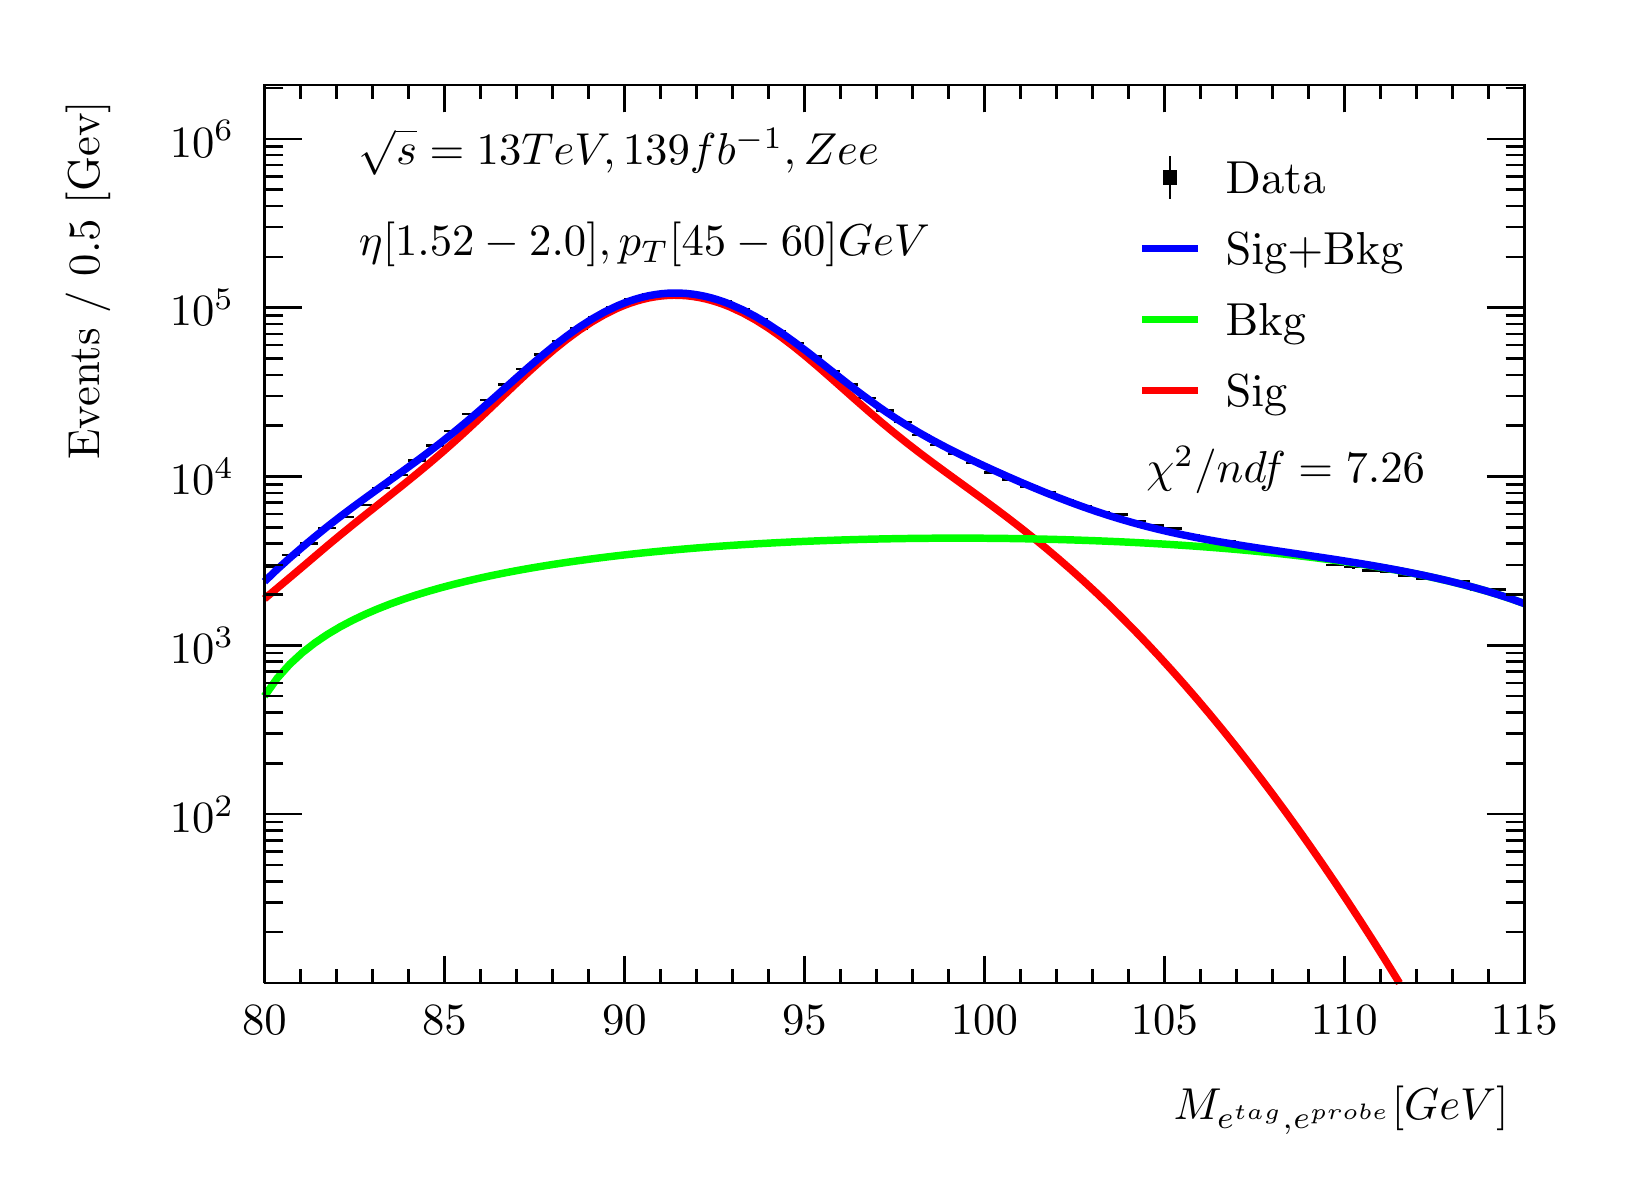
\begin{tikzpicture}
\pgfdeclareplotmark{cross} {
\pgfpathmoveto{\pgfpoint{-0.3\pgfplotmarksize}{\pgfplotmarksize}}
\pgfpathlineto{\pgfpoint{+0.3\pgfplotmarksize}{\pgfplotmarksize}}
\pgfpathlineto{\pgfpoint{+0.3\pgfplotmarksize}{0.3\pgfplotmarksize}}
\pgfpathlineto{\pgfpoint{+1\pgfplotmarksize}{0.3\pgfplotmarksize}}
\pgfpathlineto{\pgfpoint{+1\pgfplotmarksize}{-0.3\pgfplotmarksize}}
\pgfpathlineto{\pgfpoint{+0.3\pgfplotmarksize}{-0.3\pgfplotmarksize}}
\pgfpathlineto{\pgfpoint{+0.3\pgfplotmarksize}{-1.\pgfplotmarksize}}
\pgfpathlineto{\pgfpoint{-0.3\pgfplotmarksize}{-1.\pgfplotmarksize}}
\pgfpathlineto{\pgfpoint{-0.3\pgfplotmarksize}{-0.3\pgfplotmarksize}}
\pgfpathlineto{\pgfpoint{-1.\pgfplotmarksize}{-0.3\pgfplotmarksize}}
\pgfpathlineto{\pgfpoint{-1.\pgfplotmarksize}{0.3\pgfplotmarksize}}
\pgfpathlineto{\pgfpoint{-0.3\pgfplotmarksize}{0.3\pgfplotmarksize}}
\pgfpathclose
\pgfusepathqstroke
}
\pgfdeclareplotmark{cross*} {
\pgfpathmoveto{\pgfpoint{-0.3\pgfplotmarksize}{\pgfplotmarksize}}
\pgfpathlineto{\pgfpoint{+0.3\pgfplotmarksize}{\pgfplotmarksize}}
\pgfpathlineto{\pgfpoint{+0.3\pgfplotmarksize}{0.3\pgfplotmarksize}}
\pgfpathlineto{\pgfpoint{+1\pgfplotmarksize}{0.3\pgfplotmarksize}}
\pgfpathlineto{\pgfpoint{+1\pgfplotmarksize}{-0.3\pgfplotmarksize}}
\pgfpathlineto{\pgfpoint{+0.3\pgfplotmarksize}{-0.3\pgfplotmarksize}}
\pgfpathlineto{\pgfpoint{+0.3\pgfplotmarksize}{-1.\pgfplotmarksize}}
\pgfpathlineto{\pgfpoint{-0.3\pgfplotmarksize}{-1.\pgfplotmarksize}}
\pgfpathlineto{\pgfpoint{-0.3\pgfplotmarksize}{-0.3\pgfplotmarksize}}
\pgfpathlineto{\pgfpoint{-1.\pgfplotmarksize}{-0.3\pgfplotmarksize}}
\pgfpathlineto{\pgfpoint{-1.\pgfplotmarksize}{0.3\pgfplotmarksize}}
\pgfpathlineto{\pgfpoint{-0.3\pgfplotmarksize}{0.3\pgfplotmarksize}}
\pgfpathclose
\pgfusepathqfillstroke
}
\pgfdeclareplotmark{newstar} {
\pgfpathmoveto{\pgfqpoint{0pt}{\pgfplotmarksize}}
\pgfpathlineto{\pgfqpointpolar{44}{0.5\pgfplotmarksize}}
\pgfpathlineto{\pgfqpointpolar{18}{\pgfplotmarksize}}
\pgfpathlineto{\pgfqpointpolar{-20}{0.5\pgfplotmarksize}}
\pgfpathlineto{\pgfqpointpolar{-54}{\pgfplotmarksize}}
\pgfpathlineto{\pgfqpointpolar{-90}{0.5\pgfplotmarksize}}
\pgfpathlineto{\pgfqpointpolar{234}{\pgfplotmarksize}}
\pgfpathlineto{\pgfqpointpolar{198}{0.5\pgfplotmarksize}}
\pgfpathlineto{\pgfqpointpolar{162}{\pgfplotmarksize}}
\pgfpathlineto{\pgfqpointpolar{134}{0.5\pgfplotmarksize}}
\pgfpathclose
\pgfusepathqstroke
}
\pgfdeclareplotmark{newstar*} {
\pgfpathmoveto{\pgfqpoint{0pt}{\pgfplotmarksize}}
\pgfpathlineto{\pgfqpointpolar{44}{0.5\pgfplotmarksize}}
\pgfpathlineto{\pgfqpointpolar{18}{\pgfplotmarksize}}
\pgfpathlineto{\pgfqpointpolar{-20}{0.5\pgfplotmarksize}}
\pgfpathlineto{\pgfqpointpolar{-54}{\pgfplotmarksize}}
\pgfpathlineto{\pgfqpointpolar{-90}{0.5\pgfplotmarksize}}
\pgfpathlineto{\pgfqpointpolar{234}{\pgfplotmarksize}}
\pgfpathlineto{\pgfqpointpolar{198}{0.5\pgfplotmarksize}}
\pgfpathlineto{\pgfqpointpolar{162}{\pgfplotmarksize}}
\pgfpathlineto{\pgfqpointpolar{134}{0.5\pgfplotmarksize}}
\pgfpathclose
\pgfusepathqfillstroke
}
\definecolor{c}{rgb}{1,1,1};
\draw [color=c, fill=c] (0,0) rectangle (20,14.4361);
\draw [color=c, fill=c] (3,2.30977) rectangle (19,13.7143);
\definecolor{c}{rgb}{0,0,0};
\draw [c,line width=0.9] (3,2.30977) -- (3,13.7143) -- (19,13.7143) -- (19,2.30977) -- (3,2.30977);
\definecolor{c}{rgb}{1,1,1};
\draw [color=c, fill=c] (3,2.30977) rectangle (19,13.7143);
\definecolor{c}{rgb}{0,0,0};
\draw [c,line width=0.9] (3,2.30977) -- (3,13.7143) -- (19,13.7143) -- (19,2.30977) -- (3,2.30977);
\draw [c,line width=0.9] (3,2.30977) -- (19,2.30977);
\draw [c,line width=0.9] (3,2.65624) -- (3,2.30977);
\draw [c,line width=0.9] (3.45714,2.48301) -- (3.45714,2.30977);
\draw [c,line width=0.9] (3.91429,2.48301) -- (3.91429,2.30977);
\draw [c,line width=0.9] (4.37143,2.48301) -- (4.37143,2.30977);
\draw [c,line width=0.9] (4.82857,2.48301) -- (4.82857,2.30977);
\draw [c,line width=0.9] (5.28571,2.65624) -- (5.28571,2.30977);
\draw [c,line width=0.9] (5.74286,2.48301) -- (5.74286,2.30977);
\draw [c,line width=0.9] (6.2,2.48301) -- (6.2,2.30977);
\draw [c,line width=0.9] (6.65714,2.48301) -- (6.65714,2.30977);
\draw [c,line width=0.9] (7.11429,2.48301) -- (7.11429,2.30977);
\draw [c,line width=0.9] (7.57143,2.65624) -- (7.57143,2.30977);
\draw [c,line width=0.9] (8.02857,2.48301) -- (8.02857,2.30977);
\draw [c,line width=0.9] (8.48571,2.48301) -- (8.48571,2.30977);
\draw [c,line width=0.9] (8.94286,2.48301) -- (8.94286,2.30977);
\draw [c,line width=0.9] (9.4,2.48301) -- (9.4,2.30977);
\draw [c,line width=0.9] (9.85714,2.65624) -- (9.85714,2.30977);
\draw [c,line width=0.9] (10.3143,2.48301) -- (10.3143,2.30977);
\draw [c,line width=0.9] (10.7714,2.48301) -- (10.7714,2.30977);
\draw [c,line width=0.9] (11.2286,2.48301) -- (11.2286,2.30977);
\draw [c,line width=0.9] (11.6857,2.48301) -- (11.6857,2.30977);
\draw [c,line width=0.9] (12.1429,2.65624) -- (12.1429,2.30977);
\draw [c,line width=0.9] (12.6,2.48301) -- (12.6,2.30977);
\draw [c,line width=0.9] (13.0571,2.48301) -- (13.0571,2.30977);
\draw [c,line width=0.9] (13.5143,2.48301) -- (13.5143,2.30977);
\draw [c,line width=0.9] (13.9714,2.48301) -- (13.9714,2.30977);
\draw [c,line width=0.9] (14.4286,2.65624) -- (14.4286,2.30977);
\draw [c,line width=0.9] (14.8857,2.48301) -- (14.8857,2.30977);
\draw [c,line width=0.9] (15.3429,2.48301) -- (15.3429,2.30977);
\draw [c,line width=0.9] (15.8,2.48301) -- (15.8,2.30977);
\draw [c,line width=0.9] (16.2571,2.48301) -- (16.2571,2.30977);
\draw [c,line width=0.9] (16.7143,2.65624) -- (16.7143,2.30977);
\draw [c,line width=0.9] (17.1714,2.48301) -- (17.1714,2.30977);
\draw [c,line width=0.9] (17.6286,2.48301) -- (17.6286,2.30977);
\draw [c,line width=0.9] (18.0857,2.48301) -- (18.0857,2.30977);
\draw [c,line width=0.9] (18.5429,2.48301) -- (18.5429,2.30977);
\draw [c,line width=0.9] (19,2.65624) -- (19,2.30977);
\draw [anchor=base] (3,1.66015) node[scale=1.61424, color=c, rotate=0]{80};
\draw [anchor=base] (5.28571,1.66015) node[scale=1.61424, color=c, rotate=0]{85};
\draw [anchor=base] (7.57143,1.66015) node[scale=1.61424, color=c, rotate=0]{90};
\draw [anchor=base] (9.85714,1.66015) node[scale=1.61424, color=c, rotate=0]{95};
\draw [anchor=base] (12.1429,1.66015) node[scale=1.61424, color=c, rotate=0]{100};
\draw [anchor=base] (14.4286,1.66015) node[scale=1.61424, color=c, rotate=0]{105};
\draw [anchor=base] (16.7143,1.66015) node[scale=1.61424, color=c, rotate=0]{110};
\draw [anchor=base] (19,1.66015) node[scale=1.61424, color=c, rotate=0]{115};
\draw [anchor= east] (19,0.692932) node[scale=1.61424, color=c, rotate=0]{$M_{e^{tag}, e^{probe}}  [GeV]$};
\draw [c,line width=0.9] (3,13.7143) -- (19,13.7143);
\draw [c,line width=0.9] (3,13.3678) -- (3,13.7143);
\draw [c,line width=0.9] (3.45714,13.5411) -- (3.45714,13.7143);
\draw [c,line width=0.9] (3.91429,13.5411) -- (3.91429,13.7143);
\draw [c,line width=0.9] (4.37143,13.5411) -- (4.37143,13.7143);
\draw [c,line width=0.9] (4.82857,13.5411) -- (4.82857,13.7143);
\draw [c,line width=0.9] (5.28571,13.3678) -- (5.28571,13.7143);
\draw [c,line width=0.9] (5.74286,13.5411) -- (5.74286,13.7143);
\draw [c,line width=0.9] (6.2,13.5411) -- (6.2,13.7143);
\draw [c,line width=0.9] (6.65714,13.5411) -- (6.65714,13.7143);
\draw [c,line width=0.9] (7.11429,13.5411) -- (7.11429,13.7143);
\draw [c,line width=0.9] (7.57143,13.3678) -- (7.57143,13.7143);
\draw [c,line width=0.9] (8.02857,13.5411) -- (8.02857,13.7143);
\draw [c,line width=0.9] (8.48571,13.5411) -- (8.48571,13.7143);
\draw [c,line width=0.9] (8.94286,13.5411) -- (8.94286,13.7143);
\draw [c,line width=0.9] (9.4,13.5411) -- (9.4,13.7143);
\draw [c,line width=0.9] (9.85714,13.3678) -- (9.85714,13.7143);
\draw [c,line width=0.9] (10.3143,13.5411) -- (10.3143,13.7143);
\draw [c,line width=0.9] (10.7714,13.5411) -- (10.7714,13.7143);
\draw [c,line width=0.9] (11.2286,13.5411) -- (11.2286,13.7143);
\draw [c,line width=0.9] (11.6857,13.5411) -- (11.6857,13.7143);
\draw [c,line width=0.9] (12.1429,13.3678) -- (12.1429,13.7143);
\draw [c,line width=0.9] (12.6,13.5411) -- (12.6,13.7143);
\draw [c,line width=0.9] (13.0571,13.5411) -- (13.0571,13.7143);
\draw [c,line width=0.9] (13.5143,13.5411) -- (13.5143,13.7143);
\draw [c,line width=0.9] (13.9714,13.5411) -- (13.9714,13.7143);
\draw [c,line width=0.9] (14.4286,13.3678) -- (14.4286,13.7143);
\draw [c,line width=0.9] (14.8857,13.5411) -- (14.8857,13.7143);
\draw [c,line width=0.9] (15.3429,13.5411) -- (15.3429,13.7143);
\draw [c,line width=0.9] (15.8,13.5411) -- (15.8,13.7143);
\draw [c,line width=0.9] (16.2571,13.5411) -- (16.2571,13.7143);
\draw [c,line width=0.9] (16.7143,13.3678) -- (16.7143,13.7143);
\draw [c,line width=0.9] (17.1714,13.5411) -- (17.1714,13.7143);
\draw [c,line width=0.9] (17.6286,13.5411) -- (17.6286,13.7143);
\draw [c,line width=0.9] (18.0857,13.5411) -- (18.0857,13.7143);
\draw [c,line width=0.9] (18.5429,13.5411) -- (18.5429,13.7143);
\draw [c,line width=0.9] (19,13.3678) -- (19,13.7143);
\draw [c,line width=0.9] (3,2.30977) -- (3,13.7143);
\draw [c,line width=0.9] (3.237,2.95525) -- (3,2.95525);
\draw [c,line width=0.9] (3.237,3.33283) -- (3,3.33283);
\draw [c,line width=0.9] (3.237,3.60073) -- (3,3.60073);
\draw [c,line width=0.9] (3.237,3.80852) -- (3,3.80852);
\draw [c,line width=0.9] (3.237,3.97831) -- (3,3.97831);
\draw [c,line width=0.9] (3.237,4.12185) -- (3,4.12185);
\draw [c,line width=0.9] (3.237,4.2462) -- (3,4.2462);
\draw [c,line width=0.9] (3.237,4.35589) -- (3,4.35589);
\draw [c,line width=0.9] (3.474,4.454) -- (3,4.454);
\draw [anchor= east] (2.82,4.454) node[scale=1.61424, color=c, rotate=0]{$10^{2}$};
\draw [c,line width=0.9] (3.237,5.09948) -- (3,5.09948);
\draw [c,line width=0.9] (3.237,5.47706) -- (3,5.47706);
\draw [c,line width=0.9] (3.237,5.74495) -- (3,5.74495);
\draw [c,line width=0.9] (3.237,5.95275) -- (3,5.95275);
\draw [c,line width=0.9] (3.237,6.12253) -- (3,6.12253);
\draw [c,line width=0.9] (3.237,6.26608) -- (3,6.26608);
\draw [c,line width=0.9] (3.237,6.39043) -- (3,6.39043);
\draw [c,line width=0.9] (3.237,6.50011) -- (3,6.50011);
\draw [c,line width=0.9] (3.474,6.59823) -- (3,6.59823);
\draw [anchor= east] (2.82,6.59823) node[scale=1.61424, color=c, rotate=0]{$10^{3}$};
\draw [c,line width=0.9] (3.237,7.2437) -- (3,7.2437);
\draw [c,line width=0.9] (3.237,7.62128) -- (3,7.62128);
\draw [c,line width=0.9] (3.237,7.88918) -- (3,7.88918);
\draw [c,line width=0.9] (3.237,8.09698) -- (3,8.09698);
\draw [c,line width=0.9] (3.237,8.26676) -- (3,8.26676);
\draw [c,line width=0.9] (3.237,8.41031) -- (3,8.41031);
\draw [c,line width=0.9] (3.237,8.53466) -- (3,8.53466);
\draw [c,line width=0.9] (3.237,8.64434) -- (3,8.64434);
\draw [c,line width=0.9] (3.474,8.74245) -- (3,8.74245);
\draw [anchor= east] (2.82,8.74245) node[scale=1.61424, color=c, rotate=0]{$10^{4}$};
\draw [c,line width=0.9] (3.237,9.38793) -- (3,9.38793);
\draw [c,line width=0.9] (3.237,9.76551) -- (3,9.76551);
\draw [c,line width=0.9] (3.237,10.0334) -- (3,10.0334);
\draw [c,line width=0.9] (3.237,10.2412) -- (3,10.2412);
\draw [c,line width=0.9] (3.237,10.411) -- (3,10.411);
\draw [c,line width=0.9] (3.237,10.5545) -- (3,10.5545);
\draw [c,line width=0.9] (3.237,10.6789) -- (3,10.6789);
\draw [c,line width=0.9] (3.237,10.7886) -- (3,10.7886);
\draw [c,line width=0.9] (3.474,10.8867) -- (3,10.8867);
\draw [anchor= east] (2.82,10.8867) node[scale=1.61424, color=c, rotate=0]{$10^{5}$};
\draw [c,line width=0.9] (3.237,11.5322) -- (3,11.5322);
\draw [c,line width=0.9] (3.237,11.9097) -- (3,11.9097);
\draw [c,line width=0.9] (3.237,12.1776) -- (3,12.1776);
\draw [c,line width=0.9] (3.237,12.3854) -- (3,12.3854);
\draw [c,line width=0.9] (3.237,12.5552) -- (3,12.5552);
\draw [c,line width=0.9] (3.237,12.6988) -- (3,12.6988);
\draw [c,line width=0.9] (3.237,12.8231) -- (3,12.8231);
\draw [c,line width=0.9] (3.237,12.9328) -- (3,12.9328);
\draw [c,line width=0.9] (3.474,13.0309) -- (3,13.0309);
\draw [anchor= east] (2.82,13.0309) node[scale=1.61424, color=c, rotate=0]{$10^{6}$};
\draw [c,line width=0.9] (3.237,13.6764) -- (3,13.6764);
\draw [anchor= east] (0.76,13.7143) node[scale=1.61424, color=c, rotate=90]{Events / 0.5 [Gev]};
\draw [c,line width=0.9] (19,2.30977) -- (19,13.7143);
\draw [c,line width=0.9] (18.763,2.95525) -- (19,2.95525);
\draw [c,line width=0.9] (18.763,3.33283) -- (19,3.33283);
\draw [c,line width=0.9] (18.763,3.60073) -- (19,3.60073);
\draw [c,line width=0.9] (18.763,3.80852) -- (19,3.80852);
\draw [c,line width=0.9] (18.763,3.97831) -- (19,3.97831);
\draw [c,line width=0.9] (18.763,4.12185) -- (19,4.12185);
\draw [c,line width=0.9] (18.763,4.2462) -- (19,4.2462);
\draw [c,line width=0.9] (18.763,4.35589) -- (19,4.35589);
\draw [c,line width=0.9] (18.526,4.454) -- (19,4.454);
\draw [c,line width=0.9] (18.763,5.09948) -- (19,5.09948);
\draw [c,line width=0.9] (18.763,5.47706) -- (19,5.47706);
\draw [c,line width=0.9] (18.763,5.74495) -- (19,5.74495);
\draw [c,line width=0.9] (18.763,5.95275) -- (19,5.95275);
\draw [c,line width=0.9] (18.763,6.12253) -- (19,6.12253);
\draw [c,line width=0.9] (18.763,6.26608) -- (19,6.26608);
\draw [c,line width=0.9] (18.763,6.39043) -- (19,6.39043);
\draw [c,line width=0.9] (18.763,6.50011) -- (19,6.50011);
\draw [c,line width=0.9] (18.526,6.59823) -- (19,6.59823);
\draw [c,line width=0.9] (18.763,7.2437) -- (19,7.2437);
\draw [c,line width=0.9] (18.763,7.62128) -- (19,7.62128);
\draw [c,line width=0.9] (18.763,7.88918) -- (19,7.88918);
\draw [c,line width=0.9] (18.763,8.09698) -- (19,8.09698);
\draw [c,line width=0.9] (18.763,8.26676) -- (19,8.26676);
\draw [c,line width=0.9] (18.763,8.41031) -- (19,8.41031);
\draw [c,line width=0.9] (18.763,8.53466) -- (19,8.53466);
\draw [c,line width=0.9] (18.763,8.64434) -- (19,8.64434);
\draw [c,line width=0.9] (18.526,8.74245) -- (19,8.74245);
\draw [c,line width=0.9] (18.763,9.38793) -- (19,9.38793);
\draw [c,line width=0.9] (18.763,9.76551) -- (19,9.76551);
\draw [c,line width=0.9] (18.763,10.0334) -- (19,10.0334);
\draw [c,line width=0.9] (18.763,10.2412) -- (19,10.2412);
\draw [c,line width=0.9] (18.763,10.411) -- (19,10.411);
\draw [c,line width=0.9] (18.763,10.5545) -- (19,10.5545);
\draw [c,line width=0.9] (18.763,10.6789) -- (19,10.6789);
\draw [c,line width=0.9] (18.763,10.7886) -- (19,10.7886);
\draw [c,line width=0.9] (18.526,10.8867) -- (19,10.8867);
\draw [c,line width=0.9] (18.763,11.5322) -- (19,11.5322);
\draw [c,line width=0.9] (18.763,11.9097) -- (19,11.9097);
\draw [c,line width=0.9] (18.763,12.1776) -- (19,12.1776);
\draw [c,line width=0.9] (18.763,12.3854) -- (19,12.3854);
\draw [c,line width=0.9] (18.763,12.5552) -- (19,12.5552);
\draw [c,line width=0.9] (18.763,12.6988) -- (19,12.6988);
\draw [c,line width=0.9] (18.763,12.8231) -- (19,12.8231);
\draw [c,line width=0.9] (18.763,12.9328) -- (19,12.9328);
\draw [c,line width=0.9] (18.526,13.0309) -- (19,13.0309);
\draw [c,line width=0.9] (18.763,13.6764) -- (19,13.6764);
\draw [c,line width=0.9] (3.11429,7.5993) -- (3,7.5993);
\draw [c,line width=0.9] (3,7.5993) -- (3,7.5993);
\draw [c,line width=0.9] (3.11429,7.5993) -- (3.22857,7.5993);
\draw [c,line width=0.9] (3.22857,7.5993) -- (3.22857,7.5993);
\draw [c,line width=0.9] (3.11429,7.5993) -- (3.11429,7.6165);
\draw [c,line width=0.9] (3.11429,7.6165) -- (3.11429,7.6165);
\draw [c,line width=0.9] (3.11429,7.5993) -- (3.11429,7.58209);
\draw [c,line width=0.9] (3.11429,7.58209) -- (3.11429,7.58209);
\draw [c,line width=0.9] (3.34286,7.74412) -- (3.22857,7.74412);
\draw [c,line width=0.9] (3.22857,7.74412) -- (3.22857,7.74412);
\draw [c,line width=0.9] (3.34286,7.74412) -- (3.45714,7.74412);
\draw [c,line width=0.9] (3.45714,7.74412) -- (3.45714,7.74412);
\draw [c,line width=0.9] (3.34286,7.74412) -- (3.34286,7.76003);
\draw [c,line width=0.9] (3.34286,7.76003) -- (3.34286,7.76003);
\draw [c,line width=0.9] (3.34286,7.74412) -- (3.34286,7.7282);
\draw [c,line width=0.9] (3.34286,7.7282) -- (3.34286,7.7282);
\draw [c,line width=0.9] (3.57143,7.88965) -- (3.45714,7.88965);
\draw [c,line width=0.9] (3.45714,7.88965) -- (3.45714,7.88965);
\draw [c,line width=0.9] (3.57143,7.88965) -- (3.68571,7.88965);
\draw [c,line width=0.9] (3.68571,7.88965) -- (3.68571,7.88965);
\draw [c,line width=0.9] (3.57143,7.88965) -- (3.57143,7.90437);
\draw [c,line width=0.9] (3.57143,7.90437) -- (3.57143,7.90437);
\draw [c,line width=0.9] (3.57143,7.88965) -- (3.57143,7.87493);
\draw [c,line width=0.9] (3.57143,7.87493) -- (3.57143,7.87493);
\draw [c,line width=0.9] (3.8,8.08574) -- (3.68571,8.08574);
\draw [c,line width=0.9] (3.68571,8.08574) -- (3.68571,8.08574);
\draw [c,line width=0.9] (3.8,8.08574) -- (3.91429,8.08574);
\draw [c,line width=0.9] (3.91429,8.08574) -- (3.91429,8.08574);
\draw [c,line width=0.9] (3.8,8.08574) -- (3.8,8.09898);
\draw [c,line width=0.9] (3.8,8.09898) -- (3.8,8.09898);
\draw [c,line width=0.9] (3.8,8.08574) -- (3.8,8.07249);
\draw [c,line width=0.9] (3.8,8.07249) -- (3.8,8.07249);
\draw [c,line width=0.9] (4.02857,8.22551) -- (3.91429,8.22551);
\draw [c,line width=0.9] (3.91429,8.22551) -- (3.91429,8.22551);
\draw [c,line width=0.9] (4.02857,8.22551) -- (4.14286,8.22551);
\draw [c,line width=0.9] (4.14286,8.22551) -- (4.14286,8.22551);
\draw [c,line width=0.9] (4.02857,8.22551) -- (4.02857,8.2378);
\draw [c,line width=0.9] (4.02857,8.2378) -- (4.02857,8.2378);
\draw [c,line width=0.9] (4.02857,8.22551) -- (4.02857,8.21322);
\draw [c,line width=0.9] (4.02857,8.21322) -- (4.02857,8.21322);
\draw [c,line width=0.9] (4.25714,8.38304) -- (4.14286,8.38304);
\draw [c,line width=0.9] (4.14286,8.38304) -- (4.14286,8.38304);
\draw [c,line width=0.9] (4.25714,8.38304) -- (4.37143,8.38304);
\draw [c,line width=0.9] (4.37143,8.38304) -- (4.37143,8.38304);
\draw [c,line width=0.9] (4.25714,8.38304) -- (4.25714,8.39434);
\draw [c,line width=0.9] (4.25714,8.39434) -- (4.25714,8.39434);
\draw [c,line width=0.9] (4.25714,8.38304) -- (4.25714,8.37175);
\draw [c,line width=0.9] (4.25714,8.37175) -- (4.25714,8.37175);
\draw [c,line width=0.9] (4.48571,8.60005) -- (4.37143,8.60005);
\draw [c,line width=0.9] (4.37143,8.60005) -- (4.37143,8.60005);
\draw [c,line width=0.9] (4.48571,8.60005) -- (4.6,8.60005);
\draw [c,line width=0.9] (4.6,8.60005) -- (4.6,8.60005);
\draw [c,line width=0.9] (4.48571,8.60005) -- (4.48571,8.61011);
\draw [c,line width=0.9] (4.48571,8.61011) -- (4.48571,8.61011);
\draw [c,line width=0.9] (4.48571,8.60005) -- (4.48571,8.59);
\draw [c,line width=0.9] (4.48571,8.59) -- (4.48571,8.59);
\draw [c,line width=0.9] (4.71429,8.76226) -- (4.6,8.76226);
\draw [c,line width=0.9] (4.6,8.76226) -- (4.6,8.76226);
\draw [c,line width=0.9] (4.71429,8.76226) -- (4.82857,8.76226);
\draw [c,line width=0.9] (4.82857,8.76226) -- (4.82857,8.76226);
\draw [c,line width=0.9] (4.71429,8.76226) -- (4.71429,8.77148);
\draw [c,line width=0.9] (4.71429,8.77148) -- (4.71429,8.77148);
\draw [c,line width=0.9] (4.71429,8.76226) -- (4.71429,8.75305);
\draw [c,line width=0.9] (4.71429,8.75305) -- (4.71429,8.75305);
\draw [c,line width=0.9] (4.94286,8.94719) -- (4.82857,8.94719);
\draw [c,line width=0.9] (4.82857,8.94719) -- (4.82857,8.94719);
\draw [c,line width=0.9] (4.94286,8.94719) -- (5.05714,8.94719);
\draw [c,line width=0.9] (5.05714,8.94719) -- (5.05714,8.94719);
\draw [c,line width=0.9] (4.94286,8.94719) -- (4.94286,8.95553);
\draw [c,line width=0.9] (4.94286,8.95553) -- (4.94286,8.95553);
\draw [c,line width=0.9] (4.94286,8.94719) -- (4.94286,8.93885);
\draw [c,line width=0.9] (4.94286,8.93885) -- (4.94286,8.93885);
\draw [c,line width=0.9] (5.17143,9.13537) -- (5.05714,9.13537);
\draw [c,line width=0.9] (5.05714,9.13537) -- (5.05714,9.13537);
\draw [c,line width=0.9] (5.17143,9.13537) -- (5.28571,9.13537);
\draw [c,line width=0.9] (5.28571,9.13537) -- (5.28571,9.13537);
\draw [c,line width=0.9] (5.17143,9.13537) -- (5.17143,9.14291);
\draw [c,line width=0.9] (5.17143,9.14291) -- (5.17143,9.14291);
\draw [c,line width=0.9] (5.17143,9.13537) -- (5.17143,9.12782);
\draw [c,line width=0.9] (5.17143,9.12782) -- (5.17143,9.12782);
\draw [c,line width=0.9] (5.4,9.3191) -- (5.28571,9.3191);
\draw [c,line width=0.9] (5.28571,9.3191) -- (5.28571,9.3191);
\draw [c,line width=0.9] (5.4,9.3191) -- (5.51429,9.3191);
\draw [c,line width=0.9] (5.51429,9.3191) -- (5.51429,9.3191);
\draw [c,line width=0.9] (5.4,9.3191) -- (5.4,9.32593);
\draw [c,line width=0.9] (5.4,9.32593) -- (5.4,9.32593);
\draw [c,line width=0.9] (5.4,9.3191) -- (5.4,9.31227);
\draw [c,line width=0.9] (5.4,9.31227) -- (5.4,9.31227);
\draw [c,line width=0.9] (5.62857,9.53577) -- (5.51429,9.53577);
\draw [c,line width=0.9] (5.51429,9.53577) -- (5.51429,9.53577);
\draw [c,line width=0.9] (5.62857,9.53577) -- (5.74286,9.53577);
\draw [c,line width=0.9] (5.74286,9.53577) -- (5.74286,9.53577);
\draw [c,line width=0.9] (5.62857,9.53577) -- (5.62857,9.54185);
\draw [c,line width=0.9] (5.62857,9.54185) -- (5.62857,9.54185);
\draw [c,line width=0.9] (5.62857,9.53577) -- (5.62857,9.52969);
\draw [c,line width=0.9] (5.62857,9.52969) -- (5.62857,9.52969);
\draw [c,line width=0.9] (5.85714,9.71555) -- (5.74286,9.71555);
\draw [c,line width=0.9] (5.74286,9.71555) -- (5.74286,9.71555);
\draw [c,line width=0.9] (5.85714,9.71555) -- (5.97143,9.71555);
\draw [c,line width=0.9] (5.97143,9.71555) -- (5.97143,9.71555);
\draw [c,line width=0.9] (5.85714,9.71555) -- (5.85714,9.72108);
\draw [c,line width=0.9] (5.85714,9.72108) -- (5.85714,9.72108);
\draw [c,line width=0.9] (5.85714,9.71555) -- (5.85714,9.71003);
\draw [c,line width=0.9] (5.85714,9.71003) -- (5.85714,9.71003);
\draw [c,line width=0.9] (6.08571,9.91402) -- (5.97143,9.91402);
\draw [c,line width=0.9] (5.97143,9.91402) -- (5.97143,9.91402);
\draw [c,line width=0.9] (6.08571,9.91402) -- (6.2,9.91402);
\draw [c,line width=0.9] (6.2,9.91402) -- (6.2,9.91402);
\draw [c,line width=0.9] (6.08571,9.91402) -- (6.08571,9.91899);
\draw [c,line width=0.9] (6.08571,9.91899) -- (6.08571,9.91899);
\draw [c,line width=0.9] (6.08571,9.91402) -- (6.08571,9.90906);
\draw [c,line width=0.9] (6.08571,9.90906) -- (6.08571,9.90906);
\draw [c,line width=0.9] (6.31429,10.106) -- (6.2,10.106);
\draw [c,line width=0.9] (6.2,10.106) -- (6.2,10.106);
\draw [c,line width=0.9] (6.31429,10.106) -- (6.42857,10.106);
\draw [c,line width=0.9] (6.42857,10.106) -- (6.42857,10.106);
\draw [c,line width=0.9] (6.31429,10.106) -- (6.31429,10.1105);
\draw [c,line width=0.9] (6.31429,10.1105) -- (6.31429,10.1105);
\draw [c,line width=0.9] (6.31429,10.106) -- (6.31429,10.1015);
\draw [c,line width=0.9] (6.31429,10.1015) -- (6.31429,10.1015);
\draw [c,line width=0.9] (6.54286,10.2922) -- (6.42857,10.2922);
\draw [c,line width=0.9] (6.42857,10.2922) -- (6.42857,10.2922);
\draw [c,line width=0.9] (6.54286,10.2922) -- (6.65714,10.2922);
\draw [c,line width=0.9] (6.65714,10.2922) -- (6.65714,10.2922);
\draw [c,line width=0.9] (6.54286,10.2922) -- (6.54286,10.2962);
\draw [c,line width=0.9] (6.54286,10.2962) -- (6.54286,10.2962);
\draw [c,line width=0.9] (6.54286,10.2922) -- (6.54286,10.2881);
\draw [c,line width=0.9] (6.54286,10.2881) -- (6.54286,10.2881);
\draw [c,line width=0.9] (6.77143,10.4611) -- (6.65714,10.4611);
\draw [c,line width=0.9] (6.65714,10.4611) -- (6.65714,10.4611);
\draw [c,line width=0.9] (6.77143,10.4611) -- (6.88571,10.4611);
\draw [c,line width=0.9] (6.88571,10.4611) -- (6.88571,10.4611);
\draw [c,line width=0.9] (6.77143,10.4611) -- (6.77143,10.4648);
\draw [c,line width=0.9] (6.77143,10.4648) -- (6.77143,10.4648);
\draw [c,line width=0.9] (6.77143,10.4611) -- (6.77143,10.4574);
\draw [c,line width=0.9] (6.77143,10.4574) -- (6.77143,10.4574);
\draw [c,line width=0.9] (7,10.6249) -- (6.88571,10.6249);
\draw [c,line width=0.9] (6.88571,10.6249) -- (6.88571,10.6249);
\draw [c,line width=0.9] (7,10.6249) -- (7.11429,10.6249);
\draw [c,line width=0.9] (7.11429,10.6249) -- (7.11429,10.6249);
\draw [c,line width=0.9] (7,10.6249) -- (7,10.6283);
\draw [c,line width=0.9] (7,10.6283) -- (7,10.6283);
\draw [c,line width=0.9] (7,10.6249) -- (7,10.6215);
\draw [c,line width=0.9] (7,10.6215) -- (7,10.6215);
\draw [c,line width=0.9] (7.22857,10.7703) -- (7.11429,10.7703);
\draw [c,line width=0.9] (7.11429,10.7703) -- (7.11429,10.7703);
\draw [c,line width=0.9] (7.22857,10.7703) -- (7.34286,10.7703);
\draw [c,line width=0.9] (7.34286,10.7703) -- (7.34286,10.7703);
\draw [c,line width=0.9] (7.22857,10.7703) -- (7.22857,10.7735);
\draw [c,line width=0.9] (7.22857,10.7735) -- (7.22857,10.7735);
\draw [c,line width=0.9] (7.22857,10.7703) -- (7.22857,10.7672);
\draw [c,line width=0.9] (7.22857,10.7672) -- (7.22857,10.7672);
\draw [c,line width=0.9] (7.45714,10.8945) -- (7.34286,10.8945);
\draw [c,line width=0.9] (7.34286,10.8945) -- (7.34286,10.8945);
\draw [c,line width=0.9] (7.45714,10.8945) -- (7.57143,10.8945);
\draw [c,line width=0.9] (7.57143,10.8945) -- (7.57143,10.8945);
\draw [c,line width=0.9] (7.45714,10.8945) -- (7.45714,10.8974);
\draw [c,line width=0.9] (7.45714,10.8974) -- (7.45714,10.8974);
\draw [c,line width=0.9] (7.45714,10.8945) -- (7.45714,10.8916);
\draw [c,line width=0.9] (7.45714,10.8916) -- (7.45714,10.8916);
\draw [c,line width=0.9] (7.68571,10.9882) -- (7.57143,10.9882);
\draw [c,line width=0.9] (7.57143,10.9882) -- (7.57143,10.9882);
\draw [c,line width=0.9] (7.68571,10.9882) -- (7.8,10.9882);
\draw [c,line width=0.9] (7.8,10.9882) -- (7.8,10.9882);
\draw [c,line width=0.9] (7.68571,10.9882) -- (7.68571,10.991);
\draw [c,line width=0.9] (7.68571,10.991) -- (7.68571,10.991);
\draw [c,line width=0.9] (7.68571,10.9882) -- (7.68571,10.9854);
\draw [c,line width=0.9] (7.68571,10.9854) -- (7.68571,10.9854);
\draw [c,line width=0.9] (7.91429,11.0522) -- (7.8,11.0522);
\draw [c,line width=0.9] (7.8,11.0522) -- (7.8,11.0522);
\draw [c,line width=0.9] (7.91429,11.0522) -- (8.02857,11.0522);
\draw [c,line width=0.9] (8.02857,11.0522) -- (8.02857,11.0522);
\draw [c,line width=0.9] (7.91429,11.0522) -- (7.91429,11.0549);
\draw [c,line width=0.9] (7.91429,11.0549) -- (7.91429,11.0549);
\draw [c,line width=0.9] (7.91429,11.0522) -- (7.91429,11.0495);
\draw [c,line width=0.9] (7.91429,11.0495) -- (7.91429,11.0495);
\draw [c,line width=0.9] (8.14286,11.0799) -- (8.02857,11.0799);
\draw [c,line width=0.9] (8.02857,11.0799) -- (8.02857,11.0799);
\draw [c,line width=0.9] (8.14286,11.0799) -- (8.25714,11.0799);
\draw [c,line width=0.9] (8.25714,11.0799) -- (8.25714,11.0799);
\draw [c,line width=0.9] (8.14286,11.0799) -- (8.14286,11.0825);
\draw [c,line width=0.9] (8.14286,11.0825) -- (8.14286,11.0825);
\draw [c,line width=0.9] (8.14286,11.0799) -- (8.14286,11.0772);
\draw [c,line width=0.9] (8.14286,11.0772) -- (8.14286,11.0772);
\draw [c,line width=0.9] (8.37143,11.0744) -- (8.25714,11.0744);
\draw [c,line width=0.9] (8.25714,11.0744) -- (8.25714,11.0744);
\draw [c,line width=0.9] (8.37143,11.0744) -- (8.48571,11.0744);
\draw [c,line width=0.9] (8.48571,11.0744) -- (8.48571,11.0744);
\draw [c,line width=0.9] (8.37143,11.0744) -- (8.37143,11.077);
\draw [c,line width=0.9] (8.37143,11.077) -- (8.37143,11.077);
\draw [c,line width=0.9] (8.37143,11.0744) -- (8.37143,11.0717);
\draw [c,line width=0.9] (8.37143,11.0717) -- (8.37143,11.0717);
\draw [c,line width=0.9] (8.6,11.0359) -- (8.48571,11.0359);
\draw [c,line width=0.9] (8.48571,11.0359) -- (8.48571,11.0359);
\draw [c,line width=0.9] (8.6,11.0359) -- (8.71429,11.0359);
\draw [c,line width=0.9] (8.71429,11.0359) -- (8.71429,11.0359);
\draw [c,line width=0.9] (8.6,11.0359) -- (8.6,11.0386);
\draw [c,line width=0.9] (8.6,11.0386) -- (8.6,11.0386);
\draw [c,line width=0.9] (8.6,11.0359) -- (8.6,11.0332);
\draw [c,line width=0.9] (8.6,11.0332) -- (8.6,11.0332);
\draw [c,line width=0.9] (8.82857,10.9633) -- (8.71429,10.9633);
\draw [c,line width=0.9] (8.71429,10.9633) -- (8.71429,10.9633);
\draw [c,line width=0.9] (8.82857,10.9633) -- (8.94286,10.9633);
\draw [c,line width=0.9] (8.94286,10.9633) -- (8.94286,10.9633);
\draw [c,line width=0.9] (8.82857,10.9633) -- (8.82857,10.9661);
\draw [c,line width=0.9] (8.82857,10.9661) -- (8.82857,10.9661);
\draw [c,line width=0.9] (8.82857,10.9633) -- (8.82857,10.9604);
\draw [c,line width=0.9] (8.82857,10.9604) -- (8.82857,10.9604);
\draw [c,line width=0.9] (9.05714,10.8636) -- (8.94286,10.8636);
\draw [c,line width=0.9] (8.94286,10.8636) -- (8.94286,10.8636);
\draw [c,line width=0.9] (9.05714,10.8636) -- (9.17143,10.8636);
\draw [c,line width=0.9] (9.17143,10.8636) -- (9.17143,10.8636);
\draw [c,line width=0.9] (9.05714,10.8636) -- (9.05714,10.8666);
\draw [c,line width=0.9] (9.05714,10.8666) -- (9.05714,10.8666);
\draw [c,line width=0.9] (9.05714,10.8636) -- (9.05714,10.8606);
\draw [c,line width=0.9] (9.05714,10.8606) -- (9.05714,10.8606);
\draw [c,line width=0.9] (9.28571,10.7382) -- (9.17143,10.7382);
\draw [c,line width=0.9] (9.17143,10.7382) -- (9.17143,10.7382);
\draw [c,line width=0.9] (9.28571,10.7382) -- (9.4,10.7382);
\draw [c,line width=0.9] (9.4,10.7382) -- (9.4,10.7382);
\draw [c,line width=0.9] (9.28571,10.7382) -- (9.28571,10.7414);
\draw [c,line width=0.9] (9.28571,10.7414) -- (9.28571,10.7414);
\draw [c,line width=0.9] (9.28571,10.7382) -- (9.28571,10.735);
\draw [c,line width=0.9] (9.28571,10.735) -- (9.28571,10.735);
\draw [c,line width=0.9] (9.51429,10.5903) -- (9.4,10.5903);
\draw [c,line width=0.9] (9.4,10.5903) -- (9.4,10.5903);
\draw [c,line width=0.9] (9.51429,10.5903) -- (9.62857,10.5903);
\draw [c,line width=0.9] (9.62857,10.5903) -- (9.62857,10.5903);
\draw [c,line width=0.9] (9.51429,10.5903) -- (9.51429,10.5937);
\draw [c,line width=0.9] (9.51429,10.5937) -- (9.51429,10.5937);
\draw [c,line width=0.9] (9.51429,10.5903) -- (9.51429,10.5868);
\draw [c,line width=0.9] (9.51429,10.5868) -- (9.51429,10.5868);
\draw [c,line width=0.9] (9.74286,10.4372) -- (9.62857,10.4372);
\draw [c,line width=0.9] (9.62857,10.4372) -- (9.62857,10.4372);
\draw [c,line width=0.9] (9.74286,10.4372) -- (9.85714,10.4372);
\draw [c,line width=0.9] (9.85714,10.4372) -- (9.85714,10.4372);
\draw [c,line width=0.9] (9.74286,10.4372) -- (9.74286,10.4409);
\draw [c,line width=0.9] (9.74286,10.4409) -- (9.74286,10.4409);
\draw [c,line width=0.9] (9.74286,10.4372) -- (9.74286,10.4334);
\draw [c,line width=0.9] (9.74286,10.4334) -- (9.74286,10.4334);
\draw [c,line width=0.9] (9.97143,10.2664) -- (9.85714,10.2664);
\draw [c,line width=0.9] (9.85714,10.2664) -- (9.85714,10.2664);
\draw [c,line width=0.9] (9.97143,10.2664) -- (10.0857,10.2664);
\draw [c,line width=0.9] (10.0857,10.2664) -- (10.0857,10.2664);
\draw [c,line width=0.9] (9.97143,10.2664) -- (9.97143,10.2705);
\draw [c,line width=0.9] (9.97143,10.2705) -- (9.97143,10.2705);
\draw [c,line width=0.9] (9.97143,10.2664) -- (9.97143,10.2623);
\draw [c,line width=0.9] (9.97143,10.2623) -- (9.97143,10.2623);
\draw [c,line width=0.9] (10.2,10.0834) -- (10.0857,10.0834);
\draw [c,line width=0.9] (10.0857,10.0834) -- (10.0857,10.0834);
\draw [c,line width=0.9] (10.2,10.0834) -- (10.3143,10.0834);
\draw [c,line width=0.9] (10.3143,10.0834) -- (10.3143,10.0834);
\draw [c,line width=0.9] (10.2,10.0834) -- (10.2,10.0879);
\draw [c,line width=0.9] (10.2,10.0879) -- (10.2,10.0879);
\draw [c,line width=0.9] (10.2,10.0834) -- (10.2,10.0788);
\draw [c,line width=0.9] (10.2,10.0788) -- (10.2,10.0788);
\draw [c,line width=0.9] (10.4286,9.91233) -- (10.3143,9.91233);
\draw [c,line width=0.9] (10.3143,9.91233) -- (10.3143,9.91233);
\draw [c,line width=0.9] (10.4286,9.91233) -- (10.5429,9.91233);
\draw [c,line width=0.9] (10.5429,9.91233) -- (10.5429,9.91233);
\draw [c,line width=0.9] (10.4286,9.91233) -- (10.4286,9.9173);
\draw [c,line width=0.9] (10.4286,9.9173) -- (10.4286,9.9173);
\draw [c,line width=0.9] (10.4286,9.91233) -- (10.4286,9.90736);
\draw [c,line width=0.9] (10.4286,9.90736) -- (10.4286,9.90736);
\draw [c,line width=0.9] (10.6571,9.73769) -- (10.5429,9.73769);
\draw [c,line width=0.9] (10.5429,9.73769) -- (10.5429,9.73769);
\draw [c,line width=0.9] (10.6571,9.73769) -- (10.7714,9.73769);
\draw [c,line width=0.9] (10.7714,9.73769) -- (10.7714,9.73769);
\draw [c,line width=0.9] (10.6571,9.73769) -- (10.6571,9.74315);
\draw [c,line width=0.9] (10.6571,9.74315) -- (10.6571,9.74315);
\draw [c,line width=0.9] (10.6571,9.73769) -- (10.6571,9.73223);
\draw [c,line width=0.9] (10.6571,9.73223) -- (10.6571,9.73223);
\draw [c,line width=0.9] (10.8857,9.5829) -- (10.7714,9.5829);
\draw [c,line width=0.9] (10.7714,9.5829) -- (10.7714,9.5829);
\draw [c,line width=0.9] (10.8857,9.5829) -- (11,9.5829);
\draw [c,line width=0.9] (11,9.5829) -- (11,9.5829);
\draw [c,line width=0.9] (10.8857,9.5829) -- (10.8857,9.58883);
\draw [c,line width=0.9] (10.8857,9.58883) -- (10.8857,9.58883);
\draw [c,line width=0.9] (10.8857,9.5829) -- (10.8857,9.57697);
\draw [c,line width=0.9] (10.8857,9.57697) -- (10.8857,9.57697);
\draw [c,line width=0.9] (11.1143,9.43235) -- (11,9.43235);
\draw [c,line width=0.9] (11,9.43235) -- (11,9.43235);
\draw [c,line width=0.9] (11.1143,9.43235) -- (11.2286,9.43235);
\draw [c,line width=0.9] (11.2286,9.43235) -- (11.2286,9.43235);
\draw [c,line width=0.9] (11.1143,9.43235) -- (11.1143,9.43878);
\draw [c,line width=0.9] (11.1143,9.43878) -- (11.1143,9.43878);
\draw [c,line width=0.9] (11.1143,9.43235) -- (11.1143,9.42592);
\draw [c,line width=0.9] (11.1143,9.42592) -- (11.1143,9.42592);
\draw [c,line width=0.9] (11.3429,9.27069) -- (11.2286,9.27069);
\draw [c,line width=0.9] (11.2286,9.27069) -- (11.2286,9.27069);
\draw [c,line width=0.9] (11.3429,9.27069) -- (11.4571,9.27069);
\draw [c,line width=0.9] (11.4571,9.27069) -- (11.4571,9.27069);
\draw [c,line width=0.9] (11.3429,9.27069) -- (11.3429,9.2777);
\draw [c,line width=0.9] (11.3429,9.2777) -- (11.3429,9.2777);
\draw [c,line width=0.9] (11.3429,9.27069) -- (11.3429,9.26367);
\draw [c,line width=0.9] (11.3429,9.26367) -- (11.3429,9.26367);
\draw [c,line width=0.9] (11.5714,9.14363) -- (11.4571,9.14363);
\draw [c,line width=0.9] (11.4571,9.14363) -- (11.4571,9.14363);
\draw [c,line width=0.9] (11.5714,9.14363) -- (11.6857,9.14363);
\draw [c,line width=0.9] (11.6857,9.14363) -- (11.6857,9.14363);
\draw [c,line width=0.9] (11.5714,9.14363) -- (11.5714,9.15114);
\draw [c,line width=0.9] (11.5714,9.15114) -- (11.5714,9.15114);
\draw [c,line width=0.9] (11.5714,9.14363) -- (11.5714,9.13613);
\draw [c,line width=0.9] (11.5714,9.13613) -- (11.5714,9.13613);
\draw [c,line width=0.9] (11.8,9.02831) -- (11.6857,9.02831);
\draw [c,line width=0.9] (11.6857,9.02831) -- (11.6857,9.02831);
\draw [c,line width=0.9] (11.8,9.02831) -- (11.9143,9.02831);
\draw [c,line width=0.9] (11.9143,9.02831) -- (11.9143,9.02831);
\draw [c,line width=0.9] (11.8,9.02831) -- (11.8,9.0363);
\draw [c,line width=0.9] (11.8,9.0363) -- (11.8,9.0363);
\draw [c,line width=0.9] (11.8,9.02831) -- (11.8,9.02033);
\draw [c,line width=0.9] (11.8,9.02033) -- (11.8,9.02033);
\draw [c,line width=0.9] (12.0286,8.91735) -- (11.9143,8.91735);
\draw [c,line width=0.9] (11.9143,8.91735) -- (11.9143,8.91735);
\draw [c,line width=0.9] (12.0286,8.91735) -- (12.1429,8.91735);
\draw [c,line width=0.9] (12.1429,8.91735) -- (12.1429,8.91735);
\draw [c,line width=0.9] (12.0286,8.91735) -- (12.0286,8.92582);
\draw [c,line width=0.9] (12.0286,8.92582) -- (12.0286,8.92582);
\draw [c,line width=0.9] (12.0286,8.91735) -- (12.0286,8.90887);
\draw [c,line width=0.9] (12.0286,8.90887) -- (12.0286,8.90887);
\draw [c,line width=0.9] (12.2571,8.79672) -- (12.1429,8.79672);
\draw [c,line width=0.9] (12.1429,8.79672) -- (12.1429,8.79672);
\draw [c,line width=0.9] (12.2571,8.79672) -- (12.3714,8.79672);
\draw [c,line width=0.9] (12.3714,8.79672) -- (12.3714,8.79672);
\draw [c,line width=0.9] (12.2571,8.79672) -- (12.2571,8.80576);
\draw [c,line width=0.9] (12.2571,8.80576) -- (12.2571,8.80576);
\draw [c,line width=0.9] (12.2571,8.79672) -- (12.2571,8.78767);
\draw [c,line width=0.9] (12.2571,8.78767) -- (12.2571,8.78767);
\draw [c,line width=0.9] (12.4857,8.7024) -- (12.3714,8.7024);
\draw [c,line width=0.9] (12.3714,8.7024) -- (12.3714,8.7024);
\draw [c,line width=0.9] (12.4857,8.7024) -- (12.6,8.7024);
\draw [c,line width=0.9] (12.6,8.7024) -- (12.6,8.7024);
\draw [c,line width=0.9] (12.4857,8.7024) -- (12.4857,8.71192);
\draw [c,line width=0.9] (12.4857,8.71192) -- (12.4857,8.71192);
\draw [c,line width=0.9] (12.4857,8.7024) -- (12.4857,8.69289);
\draw [c,line width=0.9] (12.4857,8.69289) -- (12.4857,8.69289);
\draw [c,line width=0.9] (12.7143,8.61437) -- (12.6,8.61437);
\draw [c,line width=0.9] (12.6,8.61437) -- (12.6,8.61437);
\draw [c,line width=0.9] (12.7143,8.61437) -- (12.8286,8.61437);
\draw [c,line width=0.9] (12.8286,8.61437) -- (12.8286,8.61437);
\draw [c,line width=0.9] (12.7143,8.61437) -- (12.7143,8.62435);
\draw [c,line width=0.9] (12.7143,8.62435) -- (12.7143,8.62435);
\draw [c,line width=0.9] (12.7143,8.61437) -- (12.7143,8.6044);
\draw [c,line width=0.9] (12.7143,8.6044) -- (12.7143,8.6044);
\draw [c,line width=0.9] (12.9429,8.5491) -- (12.8286,8.5491);
\draw [c,line width=0.9] (12.8286,8.5491) -- (12.8286,8.5491);
\draw [c,line width=0.9] (12.9429,8.5491) -- (13.0571,8.5491);
\draw [c,line width=0.9] (13.0571,8.5491) -- (13.0571,8.5491);
\draw [c,line width=0.9] (12.9429,8.5491) -- (12.9429,8.55943);
\draw [c,line width=0.9] (12.9429,8.55943) -- (12.9429,8.55943);
\draw [c,line width=0.9] (12.9429,8.5491) -- (12.9429,8.53876);
\draw [c,line width=0.9] (12.9429,8.53876) -- (12.9429,8.53876);
\draw [c,line width=0.9] (13.1714,8.44543) -- (13.0571,8.44543);
\draw [c,line width=0.9] (13.0571,8.44543) -- (13.0571,8.44543);
\draw [c,line width=0.9] (13.1714,8.44543) -- (13.2857,8.44543);
\draw [c,line width=0.9] (13.2857,8.44543) -- (13.2857,8.44543);
\draw [c,line width=0.9] (13.1714,8.44543) -- (13.1714,8.45635);
\draw [c,line width=0.9] (13.1714,8.45635) -- (13.1714,8.45635);
\draw [c,line width=0.9] (13.1714,8.44543) -- (13.1714,8.4345);
\draw [c,line width=0.9] (13.1714,8.4345) -- (13.1714,8.4345);
\draw [c,line width=0.9] (13.4,8.36896) -- (13.2857,8.36896);
\draw [c,line width=0.9] (13.2857,8.36896) -- (13.2857,8.36896);
\draw [c,line width=0.9] (13.4,8.36896) -- (13.5143,8.36896);
\draw [c,line width=0.9] (13.5143,8.36896) -- (13.5143,8.36896);
\draw [c,line width=0.9] (13.4,8.36896) -- (13.4,8.38034);
\draw [c,line width=0.9] (13.4,8.38034) -- (13.4,8.38034);
\draw [c,line width=0.9] (13.4,8.36896) -- (13.4,8.35758);
\draw [c,line width=0.9] (13.4,8.35758) -- (13.4,8.35758);
\draw [c,line width=0.9] (13.6286,8.29519) -- (13.5143,8.29519);
\draw [c,line width=0.9] (13.5143,8.29519) -- (13.5143,8.29519);
\draw [c,line width=0.9] (13.6286,8.29519) -- (13.7429,8.29519);
\draw [c,line width=0.9] (13.7429,8.29519) -- (13.7429,8.29519);
\draw [c,line width=0.9] (13.6286,8.29519) -- (13.6286,8.30703);
\draw [c,line width=0.9] (13.6286,8.30703) -- (13.6286,8.30703);
\draw [c,line width=0.9] (13.6286,8.29519) -- (13.6286,8.28335);
\draw [c,line width=0.9] (13.6286,8.28335) -- (13.6286,8.28335);
\draw [c,line width=0.9] (13.8571,8.25897) -- (13.7429,8.25897);
\draw [c,line width=0.9] (13.7429,8.25897) -- (13.7429,8.25897);
\draw [c,line width=0.9] (13.8571,8.25897) -- (13.9714,8.25897);
\draw [c,line width=0.9] (13.9714,8.25897) -- (13.9714,8.25897);
\draw [c,line width=0.9] (13.8571,8.25897) -- (13.8571,8.27104);
\draw [c,line width=0.9] (13.8571,8.27104) -- (13.8571,8.27104);
\draw [c,line width=0.9] (13.8571,8.25897) -- (13.8571,8.2469);
\draw [c,line width=0.9] (13.8571,8.2469) -- (13.8571,8.2469);
\draw [c,line width=0.9] (14.0857,8.17483) -- (13.9714,8.17483);
\draw [c,line width=0.9] (13.9714,8.17483) -- (13.9714,8.17483);
\draw [c,line width=0.9] (14.0857,8.17483) -- (14.2,8.17483);
\draw [c,line width=0.9] (14.2,8.17483) -- (14.2,8.17483);
\draw [c,line width=0.9] (14.0857,8.17483) -- (14.0857,8.18746);
\draw [c,line width=0.9] (14.0857,8.18746) -- (14.0857,8.18746);
\draw [c,line width=0.9] (14.0857,8.17483) -- (14.0857,8.1622);
\draw [c,line width=0.9] (14.0857,8.1622) -- (14.0857,8.1622);
\draw [c,line width=0.9] (14.3143,8.12179) -- (14.2,8.12179);
\draw [c,line width=0.9] (14.2,8.12179) -- (14.2,8.12179);
\draw [c,line width=0.9] (14.3143,8.12179) -- (14.4286,8.12179);
\draw [c,line width=0.9] (14.4286,8.12179) -- (14.4286,8.12179);
\draw [c,line width=0.9] (14.3143,8.12179) -- (14.3143,8.13478);
\draw [c,line width=0.9] (14.3143,8.13478) -- (14.3143,8.13478);
\draw [c,line width=0.9] (14.3143,8.12179) -- (14.3143,8.10879);
\draw [c,line width=0.9] (14.3143,8.10879) -- (14.3143,8.10879);
\draw [c,line width=0.9] (14.5429,8.08442) -- (14.4286,8.08442);
\draw [c,line width=0.9] (14.4286,8.08442) -- (14.4286,8.08442);
\draw [c,line width=0.9] (14.5429,8.08442) -- (14.6571,8.08442);
\draw [c,line width=0.9] (14.6571,8.08442) -- (14.6571,8.08442);
\draw [c,line width=0.9] (14.5429,8.08442) -- (14.5429,8.09767);
\draw [c,line width=0.9] (14.5429,8.09767) -- (14.5429,8.09767);
\draw [c,line width=0.9] (14.5429,8.08442) -- (14.5429,8.07116);
\draw [c,line width=0.9] (14.5429,8.07116) -- (14.5429,8.07116);
\draw [c,line width=0.9] (14.7714,7.99762) -- (14.6571,7.99762);
\draw [c,line width=0.9] (14.6571,7.99762) -- (14.6571,7.99762);
\draw [c,line width=0.9] (14.7714,7.99762) -- (14.8857,7.99762);
\draw [c,line width=0.9] (14.8857,7.99762) -- (14.8857,7.99762);
\draw [c,line width=0.9] (14.7714,7.99762) -- (14.7714,8.01151);
\draw [c,line width=0.9] (14.7714,8.01151) -- (14.7714,8.01151);
\draw [c,line width=0.9] (14.7714,7.99762) -- (14.7714,7.98373);
\draw [c,line width=0.9] (14.7714,7.98373) -- (14.7714,7.98373);
\draw [c,line width=0.9] (15,7.95175) -- (14.8857,7.95175);
\draw [c,line width=0.9] (14.8857,7.95175) -- (14.8857,7.95175);
\draw [c,line width=0.9] (15,7.95175) -- (15.1143,7.95175);
\draw [c,line width=0.9] (15.1143,7.95175) -- (15.1143,7.95175);
\draw [c,line width=0.9] (15,7.95175) -- (15,7.96599);
\draw [c,line width=0.9] (15,7.96599) -- (15,7.96599);
\draw [c,line width=0.9] (15,7.95175) -- (15,7.93751);
\draw [c,line width=0.9] (15,7.93751) -- (15,7.93751);
\draw [c,line width=0.9] (15.2286,7.92054) -- (15.1143,7.92054);
\draw [c,line width=0.9] (15.1143,7.92054) -- (15.1143,7.92054);
\draw [c,line width=0.9] (15.2286,7.92054) -- (15.3429,7.92054);
\draw [c,line width=0.9] (15.3429,7.92054) -- (15.3429,7.92054);
\draw [c,line width=0.9] (15.2286,7.92054) -- (15.2286,7.93502);
\draw [c,line width=0.9] (15.2286,7.93502) -- (15.2286,7.93502);
\draw [c,line width=0.9] (15.2286,7.92054) -- (15.2286,7.90606);
\draw [c,line width=0.9] (15.2286,7.90606) -- (15.2286,7.90606);
\draw [c,line width=0.9] (15.4571,7.82883) -- (15.3429,7.82883);
\draw [c,line width=0.9] (15.3429,7.82883) -- (15.3429,7.82883);
\draw [c,line width=0.9] (15.4571,7.82883) -- (15.5714,7.82883);
\draw [c,line width=0.9] (15.5714,7.82883) -- (15.5714,7.82883);
\draw [c,line width=0.9] (15.4571,7.82883) -- (15.4571,7.84404);
\draw [c,line width=0.9] (15.4571,7.84404) -- (15.4571,7.84404);
\draw [c,line width=0.9] (15.4571,7.82883) -- (15.4571,7.81362);
\draw [c,line width=0.9] (15.4571,7.81362) -- (15.4571,7.81362);
\draw [c,line width=0.9] (15.6857,7.81179) -- (15.5714,7.81179);
\draw [c,line width=0.9] (15.5714,7.81179) -- (15.5714,7.81179);
\draw [c,line width=0.9] (15.6857,7.81179) -- (15.8,7.81179);
\draw [c,line width=0.9] (15.8,7.81179) -- (15.8,7.81179);
\draw [c,line width=0.9] (15.6857,7.81179) -- (15.6857,7.82714);
\draw [c,line width=0.9] (15.6857,7.82714) -- (15.6857,7.82714);
\draw [c,line width=0.9] (15.6857,7.81179) -- (15.6857,7.79644);
\draw [c,line width=0.9] (15.6857,7.79644) -- (15.6857,7.79644);
\draw [c,line width=0.9] (15.9143,7.77173) -- (15.8,7.77173);
\draw [c,line width=0.9] (15.8,7.77173) -- (15.8,7.77173);
\draw [c,line width=0.9] (15.9143,7.77173) -- (16.0286,7.77173);
\draw [c,line width=0.9] (16.0286,7.77173) -- (16.0286,7.77173);
\draw [c,line width=0.9] (15.9143,7.77173) -- (15.9143,7.78741);
\draw [c,line width=0.9] (15.9143,7.78741) -- (15.9143,7.78741);
\draw [c,line width=0.9] (15.9143,7.77173) -- (15.9143,7.75604);
\draw [c,line width=0.9] (15.9143,7.75604) -- (15.9143,7.75604);
\draw [c,line width=0.9] (16.1429,7.72182) -- (16.0286,7.72182);
\draw [c,line width=0.9] (16.0286,7.72182) -- (16.0286,7.72182);
\draw [c,line width=0.9] (16.1429,7.72182) -- (16.2571,7.72182);
\draw [c,line width=0.9] (16.2571,7.72182) -- (16.2571,7.72182);
\draw [c,line width=0.9] (16.1429,7.72182) -- (16.1429,7.73793);
\draw [c,line width=0.9] (16.1429,7.73793) -- (16.1429,7.73793);
\draw [c,line width=0.9] (16.1429,7.72182) -- (16.1429,7.70571);
\draw [c,line width=0.9] (16.1429,7.70571) -- (16.1429,7.70571);
\draw [c,line width=0.9] (16.3714,7.70125) -- (16.2571,7.70125);
\draw [c,line width=0.9] (16.2571,7.70125) -- (16.2571,7.70125);
\draw [c,line width=0.9] (16.3714,7.70125) -- (16.4857,7.70125);
\draw [c,line width=0.9] (16.4857,7.70125) -- (16.4857,7.70125);
\draw [c,line width=0.9] (16.3714,7.70125) -- (16.3714,7.71754);
\draw [c,line width=0.9] (16.3714,7.71754) -- (16.3714,7.71754);
\draw [c,line width=0.9] (16.3714,7.70125) -- (16.3714,7.68496);
\draw [c,line width=0.9] (16.3714,7.68496) -- (16.3714,7.68496);
\draw [c,line width=0.9] (16.6,7.61973) -- (16.4857,7.61973);
\draw [c,line width=0.9] (16.4857,7.61973) -- (16.4857,7.61973);
\draw [c,line width=0.9] (16.6,7.61973) -- (16.7143,7.61973);
\draw [c,line width=0.9] (16.7143,7.61973) -- (16.7143,7.61973);
\draw [c,line width=0.9] (16.6,7.61973) -- (16.6,7.63675);
\draw [c,line width=0.9] (16.6,7.63675) -- (16.6,7.63675);
\draw [c,line width=0.9] (16.6,7.61973) -- (16.6,7.60272);
\draw [c,line width=0.9] (16.6,7.60272) -- (16.6,7.60272);
\draw [c,line width=0.9] (16.8286,7.59132) -- (16.7143,7.59132);
\draw [c,line width=0.9] (16.7143,7.59132) -- (16.7143,7.59132);
\draw [c,line width=0.9] (16.8286,7.59132) -- (16.9429,7.59132);
\draw [c,line width=0.9] (16.9429,7.59132) -- (16.9429,7.59132);
\draw [c,line width=0.9] (16.8286,7.59132) -- (16.8286,7.6086);
\draw [c,line width=0.9] (16.8286,7.6086) -- (16.8286,7.6086);
\draw [c,line width=0.9] (16.8286,7.59132) -- (16.8286,7.57404);
\draw [c,line width=0.9] (16.8286,7.57404) -- (16.8286,7.57404);
\draw [c,line width=0.9] (17.0571,7.54835) -- (16.9429,7.54835);
\draw [c,line width=0.9] (16.9429,7.54835) -- (16.9429,7.54835);
\draw [c,line width=0.9] (17.0571,7.54835) -- (17.1714,7.54835);
\draw [c,line width=0.9] (17.1714,7.54835) -- (17.1714,7.54835);
\draw [c,line width=0.9] (17.0571,7.54835) -- (17.0571,7.56603);
\draw [c,line width=0.9] (17.0571,7.56603) -- (17.0571,7.56603);
\draw [c,line width=0.9] (17.0571,7.54835) -- (17.0571,7.53067);
\draw [c,line width=0.9] (17.0571,7.53067) -- (17.0571,7.53067);
\draw [c,line width=0.9] (17.2857,7.52936) -- (17.1714,7.52936);
\draw [c,line width=0.9] (17.1714,7.52936) -- (17.1714,7.52936);
\draw [c,line width=0.9] (17.2857,7.52936) -- (17.4,7.52936);
\draw [c,line width=0.9] (17.4,7.52936) -- (17.4,7.52936);
\draw [c,line width=0.9] (17.2857,7.52936) -- (17.2857,7.54722);
\draw [c,line width=0.9] (17.2857,7.54722) -- (17.2857,7.54722);
\draw [c,line width=0.9] (17.2857,7.52936) -- (17.2857,7.5115);
\draw [c,line width=0.9] (17.2857,7.5115) -- (17.2857,7.5115);
\draw [c,line width=0.9] (17.5143,7.48623) -- (17.4,7.48623);
\draw [c,line width=0.9] (17.4,7.48623) -- (17.4,7.48623);
\draw [c,line width=0.9] (17.5143,7.48623) -- (17.6286,7.48623);
\draw [c,line width=0.9] (17.6286,7.48623) -- (17.6286,7.48623);
\draw [c,line width=0.9] (17.5143,7.48623) -- (17.5143,7.50451);
\draw [c,line width=0.9] (17.5143,7.50451) -- (17.5143,7.50451);
\draw [c,line width=0.9] (17.5143,7.48623) -- (17.5143,7.46795);
\draw [c,line width=0.9] (17.5143,7.46795) -- (17.5143,7.46795);
\draw [c,line width=0.9] (17.7429,7.4444) -- (17.6286,7.4444);
\draw [c,line width=0.9] (17.6286,7.4444) -- (17.6286,7.4444);
\draw [c,line width=0.9] (17.7429,7.4444) -- (17.8571,7.4444);
\draw [c,line width=0.9] (17.8571,7.4444) -- (17.8571,7.4444);
\draw [c,line width=0.9] (17.7429,7.4444) -- (17.7429,7.46309);
\draw [c,line width=0.9] (17.7429,7.46309) -- (17.7429,7.46309);
\draw [c,line width=0.9] (17.7429,7.4444) -- (17.7429,7.4257);
\draw [c,line width=0.9] (17.7429,7.4257) -- (17.7429,7.4257);
\draw [c,line width=0.9] (17.9714,7.43535) -- (17.8571,7.43535);
\draw [c,line width=0.9] (17.8571,7.43535) -- (17.8571,7.43535);
\draw [c,line width=0.9] (17.9714,7.43535) -- (18.0857,7.43535);
\draw [c,line width=0.9] (18.0857,7.43535) -- (18.0857,7.43535);
\draw [c,line width=0.9] (17.9714,7.43535) -- (17.9714,7.45413);
\draw [c,line width=0.9] (17.9714,7.45413) -- (17.9714,7.45413);
\draw [c,line width=0.9] (17.9714,7.43535) -- (17.9714,7.41656);
\draw [c,line width=0.9] (17.9714,7.41656) -- (17.9714,7.41656);
\draw [c,line width=0.9] (18.2,7.40687) -- (18.0857,7.40687);
\draw [c,line width=0.9] (18.0857,7.40687) -- (18.0857,7.40687);
\draw [c,line width=0.9] (18.2,7.40687) -- (18.3143,7.40687);
\draw [c,line width=0.9] (18.3143,7.40687) -- (18.3143,7.40687);
\draw [c,line width=0.9] (18.2,7.40687) -- (18.2,7.42594);
\draw [c,line width=0.9] (18.2,7.42594) -- (18.2,7.42594);
\draw [c,line width=0.9] (18.2,7.40687) -- (18.2,7.38779);
\draw [c,line width=0.9] (18.2,7.38779) -- (18.2,7.38779);
\draw [c,line width=0.9] (18.4286,7.30584) -- (18.3143,7.30584);
\draw [c,line width=0.9] (18.3143,7.30584) -- (18.3143,7.30584);
\draw [c,line width=0.9] (18.4286,7.30584) -- (18.5429,7.30584);
\draw [c,line width=0.9] (18.5429,7.30584) -- (18.5429,7.30584);
\draw [c,line width=0.9] (18.4286,7.30584) -- (18.4286,7.32598);
\draw [c,line width=0.9] (18.4286,7.32598) -- (18.4286,7.32598);
\draw [c,line width=0.9] (18.4286,7.30584) -- (18.4286,7.2857);
\draw [c,line width=0.9] (18.4286,7.2857) -- (18.4286,7.2857);
\draw [c,line width=0.9] (18.6571,7.30584) -- (18.5429,7.30584);
\draw [c,line width=0.9] (18.5429,7.30584) -- (18.5429,7.30584);
\draw [c,line width=0.9] (18.6571,7.30584) -- (18.7714,7.30584);
\draw [c,line width=0.9] (18.7714,7.30584) -- (18.7714,7.30584);
\draw [c,line width=0.9] (18.6571,7.30584) -- (18.6571,7.32598);
\draw [c,line width=0.9] (18.6571,7.32598) -- (18.6571,7.32598);
\draw [c,line width=0.9] (18.6571,7.30584) -- (18.6571,7.2857);
\draw [c,line width=0.9] (18.6571,7.2857) -- (18.6571,7.2857);
\draw [c,line width=0.9] (18.8857,7.24231) -- (18.7714,7.24231);
\draw [c,line width=0.9] (18.7714,7.24231) -- (18.7714,7.24231);
\draw [c,line width=0.9] (18.8857,7.24231) -- (19,7.24231);
\draw [c,line width=0.9] (19,7.24231) -- (19,7.24231);
\draw [c,line width=0.9] (18.8857,7.24231) -- (18.8857,7.26314);
\draw [c,line width=0.9] (18.8857,7.26314) -- (18.8857,7.26314);
\draw [c,line width=0.9] (18.8857,7.24231) -- (18.8857,7.22147);
\draw [c,line width=0.9] (18.8857,7.22147) -- (18.8857,7.22147);
\foreach \P in {(3.11429,7.5993), (3.34286,7.74412), (3.57143,7.88965), (3.8,8.08574), (4.02857,8.22551), (4.25714,8.38304), (4.48571,8.60005), (4.71429,8.76226), (4.94286,8.94719), (5.17143,9.13537), (5.4,9.3191), (5.62857,9.53577),
 (5.85714,9.71555), (6.08571,9.91402), (6.31429,10.106), (6.54286,10.2922), (6.77143,10.4611), (7,10.6249), (7.22857,10.7703), (7.45714,10.8945), (7.68571,10.9882), (7.91429,11.0522), (8.14286,11.0799), (8.37143,11.0744), (8.6,11.0359),
 (8.82857,10.9633), (9.05714,10.8636), (9.28571,10.7382), (9.51429,10.5903), (9.74286,10.4372), (9.97143,10.2664), (10.2,10.0834), (10.4286,9.91233), (10.6571,9.73769), (10.8857,9.5829), (11.1143,9.43235), (11.3429,9.27069), (11.5714,9.14363),
 (11.8,9.02831), (12.0286,8.91735), (12.2571,8.79672), (12.4857,8.7024), (12.7143,8.61437), (12.9429,8.5491), (13.1714,8.44543), (13.4,8.36896), (13.6286,8.29519), (13.8571,8.25897), (14.0857,8.17483), (14.3143,8.12179), (14.5429,8.08442),
 (14.7714,7.99762), (15,7.95175), (15.2286,7.92054), (15.4571,7.82883), (15.6857,7.81179), (15.9143,7.77173), (16.1429,7.72182), (16.3714,7.70125), (16.6,7.61973), (16.8286,7.59132), (17.0571,7.54835), (17.2857,7.52936), (17.5143,7.48623),
 (17.7429,7.4444), (17.9714,7.43535), (18.2,7.40687), (18.4286,7.30584), (18.6571,7.30584), (18.8857,7.24231)}{\draw[mark options={color=c,fill=c},mark size=2.882883pt,mark=] plot coordinates {\P};}
\definecolor{c}{rgb}{1,0,0};
\draw [c,line width=2.7] (3,7.18967) -- (3,7.18967);
\draw [c,line width=2.7] (3,7.18967) -- (3.16,7.32317) -- (3.32,7.45737) -- (3.48,7.59244) -- (3.64,7.72856) -- (3.8,7.86454) -- (3.96,7.99737) -- (4.12,8.12746) -- (4.28,8.25547) -- (4.44,8.38225) -- (4.6,8.50878) -- (4.76,8.63618) -- (4.92,8.76558)
 -- (5.08,8.89804) -- (5.24,9.03441) -- (5.4,9.17519) -- (5.56,9.32037) -- (5.72,9.46938) -- (5.88,9.6211) -- (6.04,9.77393) -- (6.2,9.92594) -- (6.36,10.075) -- (6.52,10.2191) -- (6.68,10.3561) -- (6.84,10.4842) -- (7,10.6017) -- (7.16,10.7074) --
 (7.32,10.8) -- (7.48,10.8787) -- (7.56,10.9126) -- (7.64,10.9427) -- (7.72,10.969) -- (7.8,10.9915) -- (7.88,11.0101) -- (7.96,11.0247) -- (8.04,11.0354) -- (8.12,11.0421) -- (8.2,11.0448) -- (8.28,11.0435) -- (8.36,11.0383) -- (8.44,11.0291) --
 (8.52,11.016) -- (8.6,10.9989) -- (8.68,10.978) -- (8.76,10.9533) -- (8.84,10.9249) -- (8.92,10.8928) -- (9.08,10.8179) -- (9.24,10.7295) -- (9.4,10.6285) -- (9.56,10.5163) -- (9.72,10.3944) -- (9.88,10.2644) -- (10.04,10.1283) -- (10.2,9.98819) --
 (10.36,9.84621) -- (10.52,9.70438) -- (10.68,9.56449) -- (10.84,9.42792) -- (11,9.29553) -- (11.16,9.16761) -- (11.32,9.04391) -- (11.48,8.92375) -- (11.64,8.80615) -- (11.8,8.69) -- (11.96,8.57416) -- (12.12,8.45757) -- (12.28,8.33933) --
 (12.44,8.21866) -- (12.6,8.09497) -- (12.76,7.96778) -- (12.92,7.83675) -- (13.08,7.70164) -- (13.24,7.56226) -- (13.4,7.4185) -- (13.56,7.27026) -- (13.72,7.11751) -- (13.88,6.9602) -- (14.04,6.79831) -- (14.2,6.63183) -- (14.36,6.46074) --
 (14.52,6.28505) -- (14.68,6.10475) -- (14.84,5.91984) -- (15,5.73032) -- (15.16,5.53619) -- (15.32,5.33744) -- (15.48,5.13409) -- (15.64,4.92612) -- (15.8,4.71353) -- (15.96,4.49633) -- (16.12,4.27453) -- (16.28,4.0481) -- (16.44,3.81707) --
 (16.6,3.58142) -- (16.76,3.34116) -- (16.92,3.09629) -- (17.08,2.8468) -- (17.24,2.5927) -- (17.4,2.33399) -- (17.4147,2.30977);
\definecolor{c}{rgb}{0,1,0};
\draw [c,line width=2.7] (3,5.95213) -- (3,5.95213);
\draw [c,line width=2.7] (3,5.95213) -- (3.16,6.17841) -- (3.32,6.35728) -- (3.48,6.50467) -- (3.64,6.62962) -- (3.8,6.73776) -- (3.96,6.83281) -- (4.12,6.91739) -- (4.28,6.99339) -- (4.44,7.06222) -- (4.6,7.12499) -- (4.76,7.18254) -- (4.92,7.23555)
 -- (5.08,7.28459) -- (5.24,7.3301) -- (5.4,7.37247) -- (5.56,7.41202) -- (5.72,7.44902) -- (5.88,7.48369) -- (6.04,7.51625) -- (6.2,7.54686) -- (6.36,7.57567) -- (6.52,7.60282) -- (6.68,7.62843) -- (6.84,7.65259) -- (7,7.67541) -- (7.16,7.69696) --
 (7.32,7.71731) -- (7.48,7.73654) -- (7.64,7.7547) -- (7.8,7.77186) -- (7.96,7.78804) -- (8.12,7.80331) -- (8.28,7.8177) -- (8.44,7.83124) -- (8.6,7.84398) -- (8.76,7.85593) -- (8.92,7.86713) -- (9.08,7.87761) -- (9.24,7.88738) -- (9.4,7.89647) --
 (9.56,7.90489) -- (9.72,7.91267) -- (9.88,7.91981) -- (10.04,7.92634) -- (10.2,7.93226) -- (10.36,7.93759) -- (10.52,7.94233) -- (10.68,7.9465) -- (10.84,7.95009) -- (11,7.95313) -- (11.16,7.95561) -- (11.32,7.95754) -- (11.48,7.95893) --
 (11.64,7.95976) -- (11.8,7.96005) -- (11.96,7.9598) -- (12.12,7.959) -- (12.28,7.95766) -- (12.44,7.95577) -- (12.6,7.95333) -- (12.76,7.95034) -- (12.92,7.94678) -- (13.08,7.94265) -- (13.24,7.93795) -- (13.4,7.93267) -- (13.56,7.92679) --
 (13.72,7.92031) -- (13.88,7.91321) -- (14.04,7.90548) -- (14.2,7.8971) -- (14.36,7.88807) -- (14.52,7.87834) -- (14.68,7.86792) -- (14.84,7.85677) -- (15,7.84487) -- (15.16,7.8322) -- (15.32,7.81871) -- (15.48,7.80439) -- (15.64,7.78919) --
 (15.8,7.77307) -- (15.96,7.75599) -- (16.12,7.7379) -- (16.28,7.71875) -- (16.44,7.69848) -- (16.6,7.67702) -- (16.76,7.6543) -- (16.92,7.63024) -- (17.08,7.60474) -- (17.24,7.5777) -- (17.4,7.54902) -- (17.56,7.51854) -- (17.72,7.48614) --
 (17.88,7.45162) -- (18.04,7.4148) -- (18.2,7.37545) -- (18.36,7.33329) -- (18.52,7.28802) -- (18.68,7.23926) -- (18.84,7.18655) -- (19,7.12935) -- (19,7.12935) -- (19,7.12935);
\definecolor{c}{rgb}{0,0,1};
\draw [c,line width=2.7] (3,7.4084) -- (3,7.4084);
\draw [c,line width=2.7] (3,7.4084) -- (3.16,7.5621) -- (3.32,7.7066) -- (3.48,7.84457) -- (3.64,7.97806) -- (3.8,8.10757) -- (3.96,8.23186) -- (4.12,8.352) -- (4.28,8.46911) -- (4.44,8.5843) -- (4.6,8.69874) -- (4.76,8.81363) -- (4.92,8.93022) --
 (5.08,9.04966) -- (5.24,9.17293) -- (5.4,9.30071) -- (5.56,9.43321) -- (5.72,9.5701) -- (5.88,9.71048) -- (6.04,9.85292) -- (6.2,9.99563) -- (6.36,10.1366) -- (6.52,10.2736) -- (6.68,10.4046) -- (6.84,10.5276) -- (7,10.6411) -- (7.16,10.7434) --
 (7.32,10.8334) -- (7.48,10.91) -- (7.56,10.9431) -- (7.64,10.9726) -- (7.72,10.9983) -- (7.8,11.0204) -- (7.88,11.0386) -- (7.96,11.0531) -- (8.04,11.0637) -- (8.12,11.0704) -- (8.2,11.0732) -- (8.28,11.0722) -- (8.36,11.0674) -- (8.44,11.0587) --
 (8.52,11.0461) -- (8.6,11.0299) -- (8.68,11.0099) -- (8.76,10.9862) -- (8.84,10.959) -- (8.92,10.9282) -- (9.08,10.8567) -- (9.24,10.7725) -- (9.4,10.6768) -- (9.56,10.5711) -- (9.72,10.457) -- (9.88,10.3366) -- (10.04,10.212) -- (10.2,10.0853) --
 (10.36,9.95902) -- (10.52,9.83513) -- (10.68,9.71543) -- (10.84,9.60122) -- (11,9.49326) -- (11.16,9.39174) -- (11.32,9.29638) -- (11.48,9.20655) -- (11.64,9.12146) -- (11.8,9.04027) -- (11.96,8.96223) -- (12.12,8.88674) -- (12.28,8.81339) --
 (12.44,8.74194) -- (12.6,8.67232) -- (12.76,8.60457) -- (12.92,8.53887) -- (13.08,8.4754) -- (13.24,8.4144) -- (13.4,8.3561) -- (13.56,8.3007) -- (13.72,8.24834) -- (13.88,8.19912) -- (14.04,8.15305) -- (14.2,8.11009) -- (14.36,8.07014) --
 (14.52,8.03302) -- (14.68,7.99853) -- (14.84,7.9664) -- (15,7.93637) -- (15.16,7.90813) -- (15.32,7.8814) -- (15.48,7.85587) -- (15.64,7.83126) -- (15.8,7.80728) -- (15.96,7.78368) -- (16.12,7.76022) -- (16.28,7.73666) -- (16.44,7.71279) --
 (16.6,7.68841) -- (16.76,7.66332) -- (16.92,7.63736) -- (17.08,7.61035) -- (17.24,7.5821) -- (17.4,7.55245) -- (17.56,7.52122) -- (17.72,7.48821) -- (17.88,7.45323) -- (18.04,7.41605) -- (18.2,7.37641) -- (18.36,7.33403) -- (18.52,7.28859) --
 (18.68,7.23969) -- (18.84,7.18688) -- (19,7.12961) -- (19,7.12961) -- (19,7.12961);
\definecolor{c}{rgb}{0,0,0};
\draw [c,line width=0.9] (3,2.30977) -- (19,2.30977);
\draw [c,line width=0.9] (3,2.65624) -- (3,2.30977);
\draw [c,line width=0.9] (3.45714,2.48301) -- (3.45714,2.30977);
\draw [c,line width=0.9] (3.91429,2.48301) -- (3.91429,2.30977);
\draw [c,line width=0.9] (4.37143,2.48301) -- (4.37143,2.30977);
\draw [c,line width=0.9] (4.82857,2.48301) -- (4.82857,2.30977);
\draw [c,line width=0.9] (5.28571,2.65624) -- (5.28571,2.30977);
\draw [c,line width=0.9] (5.74286,2.48301) -- (5.74286,2.30977);
\draw [c,line width=0.9] (6.2,2.48301) -- (6.2,2.30977);
\draw [c,line width=0.9] (6.65714,2.48301) -- (6.65714,2.30977);
\draw [c,line width=0.9] (7.11429,2.48301) -- (7.11429,2.30977);
\draw [c,line width=0.9] (7.57143,2.65624) -- (7.57143,2.30977);
\draw [c,line width=0.9] (8.02857,2.48301) -- (8.02857,2.30977);
\draw [c,line width=0.9] (8.48571,2.48301) -- (8.48571,2.30977);
\draw [c,line width=0.9] (8.94286,2.48301) -- (8.94286,2.30977);
\draw [c,line width=0.9] (9.4,2.48301) -- (9.4,2.30977);
\draw [c,line width=0.9] (9.85714,2.65624) -- (9.85714,2.30977);
\draw [c,line width=0.9] (10.3143,2.48301) -- (10.3143,2.30977);
\draw [c,line width=0.9] (10.7714,2.48301) -- (10.7714,2.30977);
\draw [c,line width=0.9] (11.2286,2.48301) -- (11.2286,2.30977);
\draw [c,line width=0.9] (11.6857,2.48301) -- (11.6857,2.30977);
\draw [c,line width=0.9] (12.1429,2.65624) -- (12.1429,2.30977);
\draw [c,line width=0.9] (12.6,2.48301) -- (12.6,2.30977);
\draw [c,line width=0.9] (13.0571,2.48301) -- (13.0571,2.30977);
\draw [c,line width=0.9] (13.5143,2.48301) -- (13.5143,2.30977);
\draw [c,line width=0.9] (13.9714,2.48301) -- (13.9714,2.30977);
\draw [c,line width=0.9] (14.4286,2.65624) -- (14.4286,2.30977);
\draw [c,line width=0.9] (14.8857,2.48301) -- (14.8857,2.30977);
\draw [c,line width=0.9] (15.3429,2.48301) -- (15.3429,2.30977);
\draw [c,line width=0.9] (15.8,2.48301) -- (15.8,2.30977);
\draw [c,line width=0.9] (16.2571,2.48301) -- (16.2571,2.30977);
\draw [c,line width=0.9] (16.7143,2.65624) -- (16.7143,2.30977);
\draw [c,line width=0.9] (17.1714,2.48301) -- (17.1714,2.30977);
\draw [c,line width=0.9] (17.6286,2.48301) -- (17.6286,2.30977);
\draw [c,line width=0.9] (18.0857,2.48301) -- (18.0857,2.30977);
\draw [c,line width=0.9] (18.5429,2.48301) -- (18.5429,2.30977);
\draw [c,line width=0.9] (19,2.65624) -- (19,2.30977);
\draw [c,line width=0.9] (3,13.7143) -- (19,13.7143);
\draw [c,line width=0.9] (3,13.3678) -- (3,13.7143);
\draw [c,line width=0.9] (3.45714,13.5411) -- (3.45714,13.7143);
\draw [c,line width=0.9] (3.91429,13.5411) -- (3.91429,13.7143);
\draw [c,line width=0.9] (4.37143,13.5411) -- (4.37143,13.7143);
\draw [c,line width=0.9] (4.82857,13.5411) -- (4.82857,13.7143);
\draw [c,line width=0.9] (5.28571,13.3678) -- (5.28571,13.7143);
\draw [c,line width=0.9] (5.74286,13.5411) -- (5.74286,13.7143);
\draw [c,line width=0.9] (6.2,13.5411) -- (6.2,13.7143);
\draw [c,line width=0.9] (6.65714,13.5411) -- (6.65714,13.7143);
\draw [c,line width=0.9] (7.11429,13.5411) -- (7.11429,13.7143);
\draw [c,line width=0.9] (7.57143,13.3678) -- (7.57143,13.7143);
\draw [c,line width=0.9] (8.02857,13.5411) -- (8.02857,13.7143);
\draw [c,line width=0.9] (8.48571,13.5411) -- (8.48571,13.7143);
\draw [c,line width=0.9] (8.94286,13.5411) -- (8.94286,13.7143);
\draw [c,line width=0.9] (9.4,13.5411) -- (9.4,13.7143);
\draw [c,line width=0.9] (9.85714,13.3678) -- (9.85714,13.7143);
\draw [c,line width=0.9] (10.3143,13.5411) -- (10.3143,13.7143);
\draw [c,line width=0.9] (10.7714,13.5411) -- (10.7714,13.7143);
\draw [c,line width=0.9] (11.2286,13.5411) -- (11.2286,13.7143);
\draw [c,line width=0.9] (11.6857,13.5411) -- (11.6857,13.7143);
\draw [c,line width=0.9] (12.1429,13.3678) -- (12.1429,13.7143);
\draw [c,line width=0.9] (12.6,13.5411) -- (12.6,13.7143);
\draw [c,line width=0.9] (13.0571,13.5411) -- (13.0571,13.7143);
\draw [c,line width=0.9] (13.5143,13.5411) -- (13.5143,13.7143);
\draw [c,line width=0.9] (13.9714,13.5411) -- (13.9714,13.7143);
\draw [c,line width=0.9] (14.4286,13.3678) -- (14.4286,13.7143);
\draw [c,line width=0.9] (14.8857,13.5411) -- (14.8857,13.7143);
\draw [c,line width=0.9] (15.3429,13.5411) -- (15.3429,13.7143);
\draw [c,line width=0.9] (15.8,13.5411) -- (15.8,13.7143);
\draw [c,line width=0.9] (16.2571,13.5411) -- (16.2571,13.7143);
\draw [c,line width=0.9] (16.7143,13.3678) -- (16.7143,13.7143);
\draw [c,line width=0.9] (17.1714,13.5411) -- (17.1714,13.7143);
\draw [c,line width=0.9] (17.6286,13.5411) -- (17.6286,13.7143);
\draw [c,line width=0.9] (18.0857,13.5411) -- (18.0857,13.7143);
\draw [c,line width=0.9] (18.5429,13.5411) -- (18.5429,13.7143);
\draw [c,line width=0.9] (19,13.3678) -- (19,13.7143);
\draw [c,line width=0.9] (3,2.30977) -- (3,13.7143);
\draw [c,line width=0.9] (3.237,2.95525) -- (3,2.95525);
\draw [c,line width=0.9] (3.237,3.33283) -- (3,3.33283);
\draw [c,line width=0.9] (3.237,3.60073) -- (3,3.60073);
\draw [c,line width=0.9] (3.237,3.80852) -- (3,3.80852);
\draw [c,line width=0.9] (3.237,3.97831) -- (3,3.97831);
\draw [c,line width=0.9] (3.237,4.12185) -- (3,4.12185);
\draw [c,line width=0.9] (3.237,4.2462) -- (3,4.2462);
\draw [c,line width=0.9] (3.237,4.35589) -- (3,4.35589);
\draw [c,line width=0.9] (3.474,4.454) -- (3,4.454);
\draw [c,line width=0.9] (3.237,5.09948) -- (3,5.09948);
\draw [c,line width=0.9] (3.237,5.47706) -- (3,5.47706);
\draw [c,line width=0.9] (3.237,5.74495) -- (3,5.74495);
\draw [c,line width=0.9] (3.237,5.95275) -- (3,5.95275);
\draw [c,line width=0.9] (3.237,6.12253) -- (3,6.12253);
\draw [c,line width=0.9] (3.237,6.26608) -- (3,6.26608);
\draw [c,line width=0.9] (3.237,6.39043) -- (3,6.39043);
\draw [c,line width=0.9] (3.237,6.50011) -- (3,6.50011);
\draw [c,line width=0.9] (3.474,6.59823) -- (3,6.59823);
\draw [c,line width=0.9] (3.237,7.2437) -- (3,7.2437);
\draw [c,line width=0.9] (3.237,7.62128) -- (3,7.62128);
\draw [c,line width=0.9] (3.237,7.88918) -- (3,7.88918);
\draw [c,line width=0.9] (3.237,8.09698) -- (3,8.09698);
\draw [c,line width=0.9] (3.237,8.26676) -- (3,8.26676);
\draw [c,line width=0.9] (3.237,8.41031) -- (3,8.41031);
\draw [c,line width=0.9] (3.237,8.53466) -- (3,8.53466);
\draw [c,line width=0.9] (3.237,8.64434) -- (3,8.64434);
\draw [c,line width=0.9] (3.474,8.74245) -- (3,8.74245);
\draw [c,line width=0.9] (3.237,9.38793) -- (3,9.38793);
\draw [c,line width=0.9] (3.237,9.76551) -- (3,9.76551);
\draw [c,line width=0.9] (3.237,10.0334) -- (3,10.0334);
\draw [c,line width=0.9] (3.237,10.2412) -- (3,10.2412);
\draw [c,line width=0.9] (3.237,10.411) -- (3,10.411);
\draw [c,line width=0.9] (3.237,10.5545) -- (3,10.5545);
\draw [c,line width=0.9] (3.237,10.6789) -- (3,10.6789);
\draw [c,line width=0.9] (3.237,10.7886) -- (3,10.7886);
\draw [c,line width=0.9] (3.474,10.8867) -- (3,10.8867);
\draw [c,line width=0.9] (3.237,11.5322) -- (3,11.5322);
\draw [c,line width=0.9] (3.237,11.9097) -- (3,11.9097);
\draw [c,line width=0.9] (3.237,12.1776) -- (3,12.1776);
\draw [c,line width=0.9] (3.237,12.3854) -- (3,12.3854);
\draw [c,line width=0.9] (3.237,12.5552) -- (3,12.5552);
\draw [c,line width=0.9] (3.237,12.6988) -- (3,12.6988);
\draw [c,line width=0.9] (3.237,12.8231) -- (3,12.8231);
\draw [c,line width=0.9] (3.237,12.9328) -- (3,12.9328);
\draw [c,line width=0.9] (3.474,13.0309) -- (3,13.0309);
\draw [c,line width=0.9] (3.237,13.6764) -- (3,13.6764);
\draw [c,line width=0.9] (19,2.30977) -- (19,13.7143);
\draw [c,line width=0.9] (18.763,2.95525) -- (19,2.95525);
\draw [c,line width=0.9] (18.763,3.33283) -- (19,3.33283);
\draw [c,line width=0.9] (18.763,3.60073) -- (19,3.60073);
\draw [c,line width=0.9] (18.763,3.80852) -- (19,3.80852);
\draw [c,line width=0.9] (18.763,3.97831) -- (19,3.97831);
\draw [c,line width=0.9] (18.763,4.12185) -- (19,4.12185);
\draw [c,line width=0.9] (18.763,4.2462) -- (19,4.2462);
\draw [c,line width=0.9] (18.763,4.35589) -- (19,4.35589);
\draw [c,line width=0.9] (18.526,4.454) -- (19,4.454);
\draw [c,line width=0.9] (18.763,5.09948) -- (19,5.09948);
\draw [c,line width=0.9] (18.763,5.47706) -- (19,5.47706);
\draw [c,line width=0.9] (18.763,5.74495) -- (19,5.74495);
\draw [c,line width=0.9] (18.763,5.95275) -- (19,5.95275);
\draw [c,line width=0.9] (18.763,6.12253) -- (19,6.12253);
\draw [c,line width=0.9] (18.763,6.26608) -- (19,6.26608);
\draw [c,line width=0.9] (18.763,6.39043) -- (19,6.39043);
\draw [c,line width=0.9] (18.763,6.50011) -- (19,6.50011);
\draw [c,line width=0.9] (18.526,6.59823) -- (19,6.59823);
\draw [c,line width=0.9] (18.763,7.2437) -- (19,7.2437);
\draw [c,line width=0.9] (18.763,7.62128) -- (19,7.62128);
\draw [c,line width=0.9] (18.763,7.88918) -- (19,7.88918);
\draw [c,line width=0.9] (18.763,8.09698) -- (19,8.09698);
\draw [c,line width=0.9] (18.763,8.26676) -- (19,8.26676);
\draw [c,line width=0.9] (18.763,8.41031) -- (19,8.41031);
\draw [c,line width=0.9] (18.763,8.53466) -- (19,8.53466);
\draw [c,line width=0.9] (18.763,8.64434) -- (19,8.64434);
\draw [c,line width=0.9] (18.526,8.74245) -- (19,8.74245);
\draw [c,line width=0.9] (18.763,9.38793) -- (19,9.38793);
\draw [c,line width=0.9] (18.763,9.76551) -- (19,9.76551);
\draw [c,line width=0.9] (18.763,10.0334) -- (19,10.0334);
\draw [c,line width=0.9] (18.763,10.2412) -- (19,10.2412);
\draw [c,line width=0.9] (18.763,10.411) -- (19,10.411);
\draw [c,line width=0.9] (18.763,10.5545) -- (19,10.5545);
\draw [c,line width=0.9] (18.763,10.6789) -- (19,10.6789);
\draw [c,line width=0.9] (18.763,10.7886) -- (19,10.7886);
\draw [c,line width=0.9] (18.526,10.8867) -- (19,10.8867);
\draw [c,line width=0.9] (18.763,11.5322) -- (19,11.5322);
\draw [c,line width=0.9] (18.763,11.9097) -- (19,11.9097);
\draw [c,line width=0.9] (18.763,12.1776) -- (19,12.1776);
\draw [c,line width=0.9] (18.763,12.3854) -- (19,12.3854);
\draw [c,line width=0.9] (18.763,12.5552) -- (19,12.5552);
\draw [c,line width=0.9] (18.763,12.6988) -- (19,12.6988);
\draw [c,line width=0.9] (18.763,12.8231) -- (19,12.8231);
\draw [c,line width=0.9] (18.763,12.9328) -- (19,12.9328);
\draw [c,line width=0.9] (18.526,13.0309) -- (19,13.0309);
\draw [c,line width=0.9] (18.763,13.6764) -- (19,13.6764);
\definecolor{c}{rgb}{1,1,1};
\draw [color=c, fill=c] (14,9.38346) rectangle (18,12.9925);
\definecolor{c}{rgb}{0,0,0};
\draw [anchor=base west] (15,12.3383) node[scale=1.6699, color=c, rotate=0]{Data};
\draw [c,line width=0.9] (14.5,12.6416) -- (14.5,12.812);
\draw [c,line width=0.9] (14.5,12.4411) -- (14.5,12.2707);
\foreach \P in {(14.5,12.5414)}{\draw[mark options={color=c,fill=c},mark size=2.402402pt,mark=square*] plot coordinates {\P};}
\draw [anchor=base west] (15,11.4361) node[scale=1.6699, color=c, rotate=0]{Sig+Bkg};
\definecolor{c}{rgb}{0,0,1};
\draw [c,line width=2.7] (14.15,11.6391) -- (14.85,11.6391);
\definecolor{c}{rgb}{0,0,0};
\draw [anchor=base west] (15,10.5338) node[scale=1.6699, color=c, rotate=0]{Bkg};
\definecolor{c}{rgb}{0,1,0};
\draw [c,line width=2.7] (14.15,10.7368) -- (14.85,10.7368);
\definecolor{c}{rgb}{0,0,0};
\draw [anchor=base west] (15,9.63158) node[scale=1.6699, color=c, rotate=0]{Sig};
\definecolor{c}{rgb}{1,0,0};
\draw [c,line width=2.7] (14.15,9.83459) -- (14.85,9.83459);
\definecolor{c}{rgb}{0,0,0};
\draw [anchor=base west] (4,12.7038) node[scale=1.61424, color=c, rotate=0]{$\sqrt{s}= 13 TeV, 139fb^{-1}, Zee$};
\draw [anchor=base west] (4,11.5489) node[scale=1.61424, color=c, rotate=0]{$\eta[1.52-2.0], p_{T}[45-60]GeV$};
\draw [anchor=base west] (14,8.66165) node[scale=1.61424, color=c, rotate=0]{$\chi^{2}/ndf= 7.26$};
\end{tikzpicture}
}\scalebox{0.35}{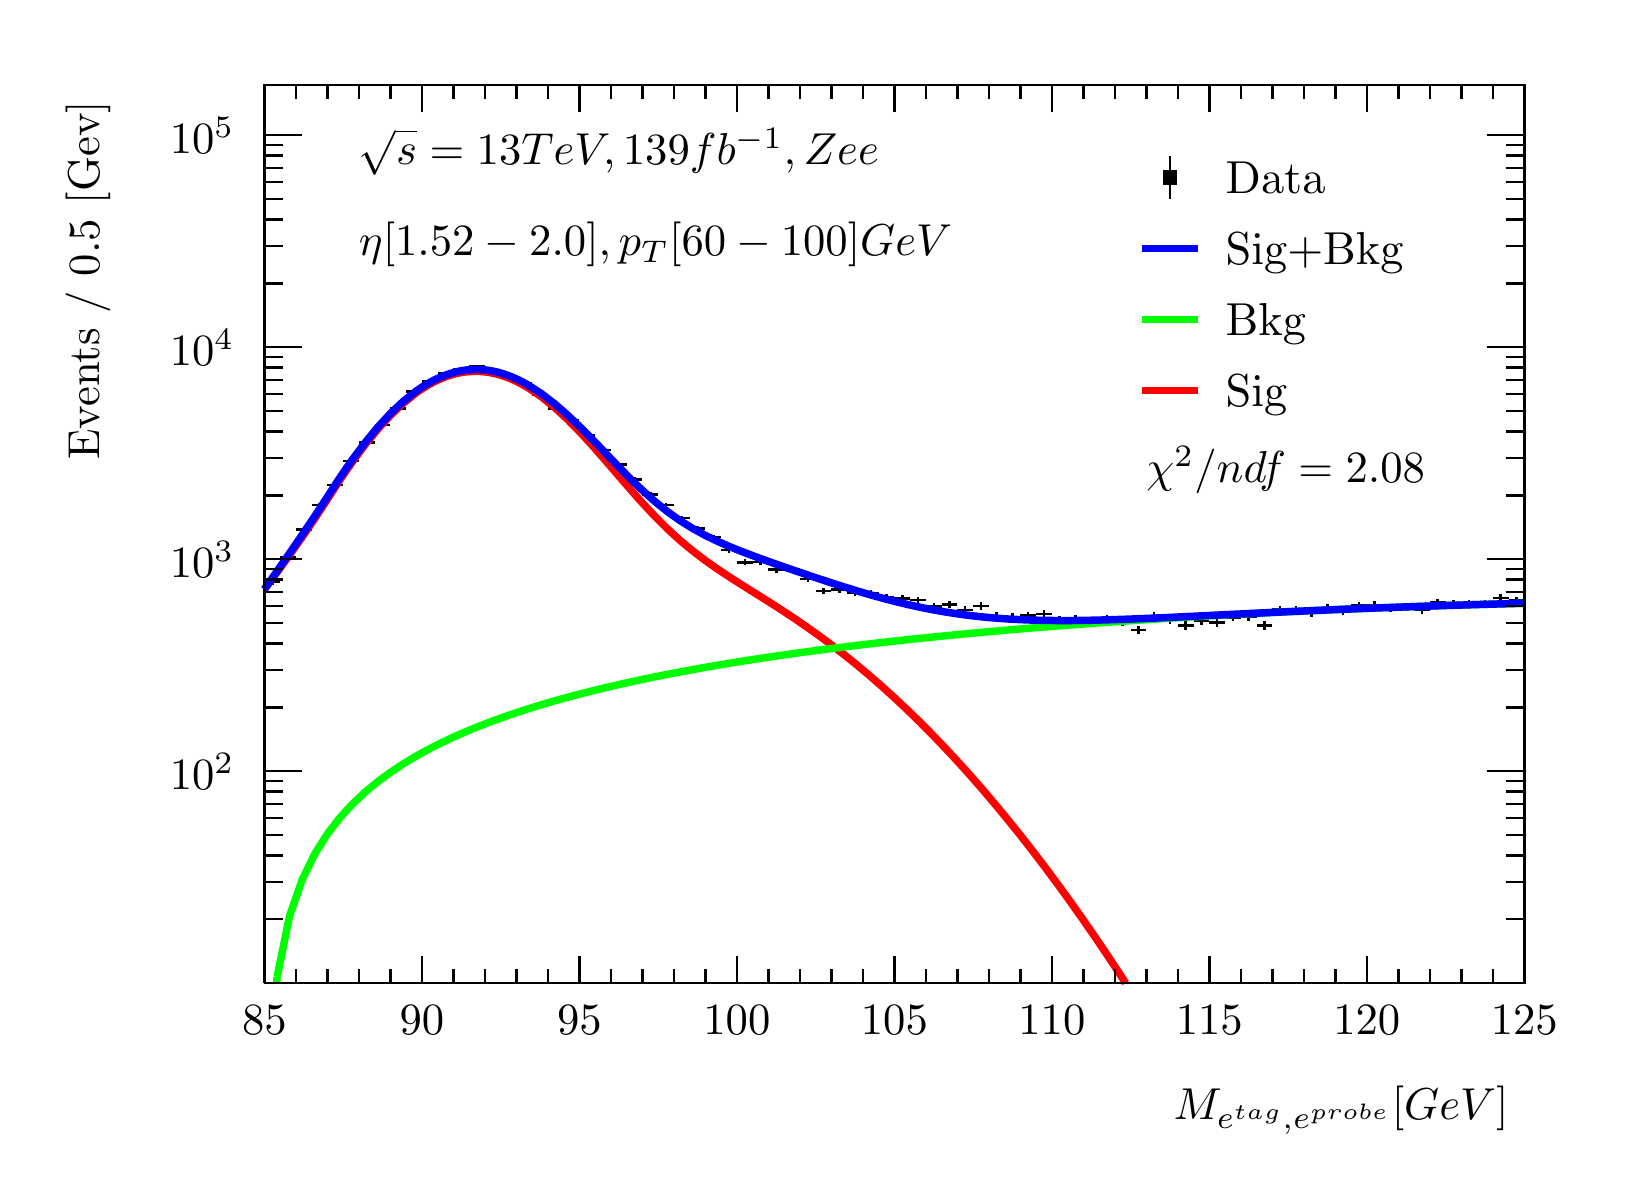
\begin{tikzpicture}
\pgfdeclareplotmark{cross} {
\pgfpathmoveto{\pgfpoint{-0.3\pgfplotmarksize}{\pgfplotmarksize}}
\pgfpathlineto{\pgfpoint{+0.3\pgfplotmarksize}{\pgfplotmarksize}}
\pgfpathlineto{\pgfpoint{+0.3\pgfplotmarksize}{0.3\pgfplotmarksize}}
\pgfpathlineto{\pgfpoint{+1\pgfplotmarksize}{0.3\pgfplotmarksize}}
\pgfpathlineto{\pgfpoint{+1\pgfplotmarksize}{-0.3\pgfplotmarksize}}
\pgfpathlineto{\pgfpoint{+0.3\pgfplotmarksize}{-0.3\pgfplotmarksize}}
\pgfpathlineto{\pgfpoint{+0.3\pgfplotmarksize}{-1.\pgfplotmarksize}}
\pgfpathlineto{\pgfpoint{-0.3\pgfplotmarksize}{-1.\pgfplotmarksize}}
\pgfpathlineto{\pgfpoint{-0.3\pgfplotmarksize}{-0.3\pgfplotmarksize}}
\pgfpathlineto{\pgfpoint{-1.\pgfplotmarksize}{-0.3\pgfplotmarksize}}
\pgfpathlineto{\pgfpoint{-1.\pgfplotmarksize}{0.3\pgfplotmarksize}}
\pgfpathlineto{\pgfpoint{-0.3\pgfplotmarksize}{0.3\pgfplotmarksize}}
\pgfpathclose
\pgfusepathqstroke
}
\pgfdeclareplotmark{cross*} {
\pgfpathmoveto{\pgfpoint{-0.3\pgfplotmarksize}{\pgfplotmarksize}}
\pgfpathlineto{\pgfpoint{+0.3\pgfplotmarksize}{\pgfplotmarksize}}
\pgfpathlineto{\pgfpoint{+0.3\pgfplotmarksize}{0.3\pgfplotmarksize}}
\pgfpathlineto{\pgfpoint{+1\pgfplotmarksize}{0.3\pgfplotmarksize}}
\pgfpathlineto{\pgfpoint{+1\pgfplotmarksize}{-0.3\pgfplotmarksize}}
\pgfpathlineto{\pgfpoint{+0.3\pgfplotmarksize}{-0.3\pgfplotmarksize}}
\pgfpathlineto{\pgfpoint{+0.3\pgfplotmarksize}{-1.\pgfplotmarksize}}
\pgfpathlineto{\pgfpoint{-0.3\pgfplotmarksize}{-1.\pgfplotmarksize}}
\pgfpathlineto{\pgfpoint{-0.3\pgfplotmarksize}{-0.3\pgfplotmarksize}}
\pgfpathlineto{\pgfpoint{-1.\pgfplotmarksize}{-0.3\pgfplotmarksize}}
\pgfpathlineto{\pgfpoint{-1.\pgfplotmarksize}{0.3\pgfplotmarksize}}
\pgfpathlineto{\pgfpoint{-0.3\pgfplotmarksize}{0.3\pgfplotmarksize}}
\pgfpathclose
\pgfusepathqfillstroke
}
\pgfdeclareplotmark{newstar} {
\pgfpathmoveto{\pgfqpoint{0pt}{\pgfplotmarksize}}
\pgfpathlineto{\pgfqpointpolar{44}{0.5\pgfplotmarksize}}
\pgfpathlineto{\pgfqpointpolar{18}{\pgfplotmarksize}}
\pgfpathlineto{\pgfqpointpolar{-20}{0.5\pgfplotmarksize}}
\pgfpathlineto{\pgfqpointpolar{-54}{\pgfplotmarksize}}
\pgfpathlineto{\pgfqpointpolar{-90}{0.5\pgfplotmarksize}}
\pgfpathlineto{\pgfqpointpolar{234}{\pgfplotmarksize}}
\pgfpathlineto{\pgfqpointpolar{198}{0.5\pgfplotmarksize}}
\pgfpathlineto{\pgfqpointpolar{162}{\pgfplotmarksize}}
\pgfpathlineto{\pgfqpointpolar{134}{0.5\pgfplotmarksize}}
\pgfpathclose
\pgfusepathqstroke
}
\pgfdeclareplotmark{newstar*} {
\pgfpathmoveto{\pgfqpoint{0pt}{\pgfplotmarksize}}
\pgfpathlineto{\pgfqpointpolar{44}{0.5\pgfplotmarksize}}
\pgfpathlineto{\pgfqpointpolar{18}{\pgfplotmarksize}}
\pgfpathlineto{\pgfqpointpolar{-20}{0.5\pgfplotmarksize}}
\pgfpathlineto{\pgfqpointpolar{-54}{\pgfplotmarksize}}
\pgfpathlineto{\pgfqpointpolar{-90}{0.5\pgfplotmarksize}}
\pgfpathlineto{\pgfqpointpolar{234}{\pgfplotmarksize}}
\pgfpathlineto{\pgfqpointpolar{198}{0.5\pgfplotmarksize}}
\pgfpathlineto{\pgfqpointpolar{162}{\pgfplotmarksize}}
\pgfpathlineto{\pgfqpointpolar{134}{0.5\pgfplotmarksize}}
\pgfpathclose
\pgfusepathqfillstroke
}
\definecolor{c}{rgb}{1,1,1};
\draw [color=c, fill=c] (0,0) rectangle (20,14.4361);
\draw [color=c, fill=c] (3,2.30977) rectangle (19,13.7143);
\definecolor{c}{rgb}{0,0,0};
\draw [c,line width=0.9] (3,2.30977) -- (3,13.7143) -- (19,13.7143) -- (19,2.30977) -- (3,2.30977);
\definecolor{c}{rgb}{1,1,1};
\draw [color=c, fill=c] (3,2.30977) rectangle (19,13.7143);
\definecolor{c}{rgb}{0,0,0};
\draw [c,line width=0.9] (3,2.30977) -- (3,13.7143) -- (19,13.7143) -- (19,2.30977) -- (3,2.30977);
\draw [c,line width=0.9] (3,2.30977) -- (19,2.30977);
\draw [c,line width=0.9] (3,2.65624) -- (3,2.30977);
\draw [c,line width=0.9] (3.4,2.48301) -- (3.4,2.30977);
\draw [c,line width=0.9] (3.8,2.48301) -- (3.8,2.30977);
\draw [c,line width=0.9] (4.2,2.48301) -- (4.2,2.30977);
\draw [c,line width=0.9] (4.6,2.48301) -- (4.6,2.30977);
\draw [c,line width=0.9] (5,2.65624) -- (5,2.30977);
\draw [c,line width=0.9] (5.4,2.48301) -- (5.4,2.30977);
\draw [c,line width=0.9] (5.8,2.48301) -- (5.8,2.30977);
\draw [c,line width=0.9] (6.2,2.48301) -- (6.2,2.30977);
\draw [c,line width=0.9] (6.6,2.48301) -- (6.6,2.30977);
\draw [c,line width=0.9] (7,2.65624) -- (7,2.30977);
\draw [c,line width=0.9] (7.4,2.48301) -- (7.4,2.30977);
\draw [c,line width=0.9] (7.8,2.48301) -- (7.8,2.30977);
\draw [c,line width=0.9] (8.2,2.48301) -- (8.2,2.30977);
\draw [c,line width=0.9] (8.6,2.48301) -- (8.6,2.30977);
\draw [c,line width=0.9] (9,2.65624) -- (9,2.30977);
\draw [c,line width=0.9] (9.4,2.48301) -- (9.4,2.30977);
\draw [c,line width=0.9] (9.8,2.48301) -- (9.8,2.30977);
\draw [c,line width=0.9] (10.2,2.48301) -- (10.2,2.30977);
\draw [c,line width=0.9] (10.6,2.48301) -- (10.6,2.30977);
\draw [c,line width=0.9] (11,2.65624) -- (11,2.30977);
\draw [c,line width=0.9] (11.4,2.48301) -- (11.4,2.30977);
\draw [c,line width=0.9] (11.8,2.48301) -- (11.8,2.30977);
\draw [c,line width=0.9] (12.2,2.48301) -- (12.2,2.30977);
\draw [c,line width=0.9] (12.6,2.48301) -- (12.6,2.30977);
\draw [c,line width=0.9] (13,2.65624) -- (13,2.30977);
\draw [c,line width=0.9] (13.4,2.48301) -- (13.4,2.30977);
\draw [c,line width=0.9] (13.8,2.48301) -- (13.8,2.30977);
\draw [c,line width=0.9] (14.2,2.48301) -- (14.2,2.30977);
\draw [c,line width=0.9] (14.6,2.48301) -- (14.6,2.30977);
\draw [c,line width=0.9] (15,2.65624) -- (15,2.30977);
\draw [c,line width=0.9] (15.4,2.48301) -- (15.4,2.30977);
\draw [c,line width=0.9] (15.8,2.48301) -- (15.8,2.30977);
\draw [c,line width=0.9] (16.2,2.48301) -- (16.2,2.30977);
\draw [c,line width=0.9] (16.6,2.48301) -- (16.6,2.30977);
\draw [c,line width=0.9] (17,2.65624) -- (17,2.30977);
\draw [c,line width=0.9] (17.4,2.48301) -- (17.4,2.30977);
\draw [c,line width=0.9] (17.8,2.48301) -- (17.8,2.30977);
\draw [c,line width=0.9] (18.2,2.48301) -- (18.2,2.30977);
\draw [c,line width=0.9] (18.6,2.48301) -- (18.6,2.30977);
\draw [c,line width=0.9] (19,2.65624) -- (19,2.30977);
\draw [anchor=base] (3,1.66015) node[scale=1.61424, color=c, rotate=0]{85};
\draw [anchor=base] (5,1.66015) node[scale=1.61424, color=c, rotate=0]{90};
\draw [anchor=base] (7,1.66015) node[scale=1.61424, color=c, rotate=0]{95};
\draw [anchor=base] (9,1.66015) node[scale=1.61424, color=c, rotate=0]{100};
\draw [anchor=base] (11,1.66015) node[scale=1.61424, color=c, rotate=0]{105};
\draw [anchor=base] (13,1.66015) node[scale=1.61424, color=c, rotate=0]{110};
\draw [anchor=base] (15,1.66015) node[scale=1.61424, color=c, rotate=0]{115};
\draw [anchor=base] (17,1.66015) node[scale=1.61424, color=c, rotate=0]{120};
\draw [anchor=base] (19,1.66015) node[scale=1.61424, color=c, rotate=0]{125};
\draw [anchor= east] (19,0.692932) node[scale=1.61424, color=c, rotate=0]{$M_{e^{tag}, e^{probe}}  [GeV]$};
\draw [c,line width=0.9] (3,13.7143) -- (19,13.7143);
\draw [c,line width=0.9] (3,13.3678) -- (3,13.7143);
\draw [c,line width=0.9] (3.4,13.5411) -- (3.4,13.7143);
\draw [c,line width=0.9] (3.8,13.5411) -- (3.8,13.7143);
\draw [c,line width=0.9] (4.2,13.5411) -- (4.2,13.7143);
\draw [c,line width=0.9] (4.6,13.5411) -- (4.6,13.7143);
\draw [c,line width=0.9] (5,13.3678) -- (5,13.7143);
\draw [c,line width=0.9] (5.4,13.5411) -- (5.4,13.7143);
\draw [c,line width=0.9] (5.8,13.5411) -- (5.8,13.7143);
\draw [c,line width=0.9] (6.2,13.5411) -- (6.2,13.7143);
\draw [c,line width=0.9] (6.6,13.5411) -- (6.6,13.7143);
\draw [c,line width=0.9] (7,13.3678) -- (7,13.7143);
\draw [c,line width=0.9] (7.4,13.5411) -- (7.4,13.7143);
\draw [c,line width=0.9] (7.8,13.5411) -- (7.8,13.7143);
\draw [c,line width=0.9] (8.2,13.5411) -- (8.2,13.7143);
\draw [c,line width=0.9] (8.6,13.5411) -- (8.6,13.7143);
\draw [c,line width=0.9] (9,13.3678) -- (9,13.7143);
\draw [c,line width=0.9] (9.4,13.5411) -- (9.4,13.7143);
\draw [c,line width=0.9] (9.8,13.5411) -- (9.8,13.7143);
\draw [c,line width=0.9] (10.2,13.5411) -- (10.2,13.7143);
\draw [c,line width=0.9] (10.6,13.5411) -- (10.6,13.7143);
\draw [c,line width=0.9] (11,13.3678) -- (11,13.7143);
\draw [c,line width=0.9] (11.4,13.5411) -- (11.4,13.7143);
\draw [c,line width=0.9] (11.8,13.5411) -- (11.8,13.7143);
\draw [c,line width=0.9] (12.2,13.5411) -- (12.2,13.7143);
\draw [c,line width=0.9] (12.6,13.5411) -- (12.6,13.7143);
\draw [c,line width=0.9] (13,13.3678) -- (13,13.7143);
\draw [c,line width=0.9] (13.4,13.5411) -- (13.4,13.7143);
\draw [c,line width=0.9] (13.8,13.5411) -- (13.8,13.7143);
\draw [c,line width=0.9] (14.2,13.5411) -- (14.2,13.7143);
\draw [c,line width=0.9] (14.6,13.5411) -- (14.6,13.7143);
\draw [c,line width=0.9] (15,13.3678) -- (15,13.7143);
\draw [c,line width=0.9] (15.4,13.5411) -- (15.4,13.7143);
\draw [c,line width=0.9] (15.8,13.5411) -- (15.8,13.7143);
\draw [c,line width=0.9] (16.2,13.5411) -- (16.2,13.7143);
\draw [c,line width=0.9] (16.6,13.5411) -- (16.6,13.7143);
\draw [c,line width=0.9] (17,13.3678) -- (17,13.7143);
\draw [c,line width=0.9] (17.4,13.5411) -- (17.4,13.7143);
\draw [c,line width=0.9] (17.8,13.5411) -- (17.8,13.7143);
\draw [c,line width=0.9] (18.2,13.5411) -- (18.2,13.7143);
\draw [c,line width=0.9] (18.6,13.5411) -- (18.6,13.7143);
\draw [c,line width=0.9] (19,13.3678) -- (19,13.7143);
\draw [c,line width=0.9] (3,2.30977) -- (3,13.7143);
\draw [c,line width=0.9] (3.237,3.12018) -- (3,3.12018);
\draw [c,line width=0.9] (3.237,3.59423) -- (3,3.59423);
\draw [c,line width=0.9] (3.237,3.93058) -- (3,3.93058);
\draw [c,line width=0.9] (3.237,4.19147) -- (3,4.19147);
\draw [c,line width=0.9] (3.237,4.40464) -- (3,4.40464);
\draw [c,line width=0.9] (3.237,4.58487) -- (3,4.58487);
\draw [c,line width=0.9] (3.237,4.74099) -- (3,4.74099);
\draw [c,line width=0.9] (3.237,4.8787) -- (3,4.8787);
\draw [c,line width=0.9] (3.474,5.00188) -- (3,5.00188);
\draw [anchor= east] (2.82,5.00188) node[scale=1.61424, color=c, rotate=0]{$10^{2}$};
\draw [c,line width=0.9] (3.237,5.81228) -- (3,5.81228);
\draw [c,line width=0.9] (3.237,6.28634) -- (3,6.28634);
\draw [c,line width=0.9] (3.237,6.62269) -- (3,6.62269);
\draw [c,line width=0.9] (3.237,6.88358) -- (3,6.88358);
\draw [c,line width=0.9] (3.237,7.09675) -- (3,7.09675);
\draw [c,line width=0.9] (3.237,7.27697) -- (3,7.27697);
\draw [c,line width=0.9] (3.237,7.43309) -- (3,7.43309);
\draw [c,line width=0.9] (3.237,7.5708) -- (3,7.5708);
\draw [c,line width=0.9] (3.474,7.69399) -- (3,7.69399);
\draw [anchor= east] (2.82,7.69399) node[scale=1.61424, color=c, rotate=0]{$10^{3}$};
\draw [c,line width=0.9] (3.237,8.50439) -- (3,8.50439);
\draw [c,line width=0.9] (3.237,8.97845) -- (3,8.97845);
\draw [c,line width=0.9] (3.237,9.3148) -- (3,9.3148);
\draw [c,line width=0.9] (3.237,9.57569) -- (3,9.57569);
\draw [c,line width=0.9] (3.237,9.78885) -- (3,9.78885);
\draw [c,line width=0.9] (3.237,9.96908) -- (3,9.96908);
\draw [c,line width=0.9] (3.237,10.1252) -- (3,10.1252);
\draw [c,line width=0.9] (3.237,10.2629) -- (3,10.2629);
\draw [c,line width=0.9] (3.474,10.3861) -- (3,10.3861);
\draw [anchor= east] (2.82,10.3861) node[scale=1.61424, color=c, rotate=0]{$10^{4}$};
\draw [c,line width=0.9] (3.237,11.1965) -- (3,11.1965);
\draw [c,line width=0.9] (3.237,11.6706) -- (3,11.6706);
\draw [c,line width=0.9] (3.237,12.0069) -- (3,12.0069);
\draw [c,line width=0.9] (3.237,12.2678) -- (3,12.2678);
\draw [c,line width=0.9] (3.237,12.481) -- (3,12.481);
\draw [c,line width=0.9] (3.237,12.6612) -- (3,12.6612);
\draw [c,line width=0.9] (3.237,12.8173) -- (3,12.8173);
\draw [c,line width=0.9] (3.237,12.955) -- (3,12.955);
\draw [c,line width=0.9] (3.474,13.0782) -- (3,13.0782);
\draw [anchor= east] (2.82,13.0782) node[scale=1.61424, color=c, rotate=0]{$10^{5}$};
\draw [anchor= east] (0.76,13.7143) node[scale=1.61424, color=c, rotate=90]{Events / 0.5 [Gev]};
\draw [c,line width=0.9] (19,2.30977) -- (19,13.7143);
\draw [c,line width=0.9] (18.763,3.12018) -- (19,3.12018);
\draw [c,line width=0.9] (18.763,3.59423) -- (19,3.59423);
\draw [c,line width=0.9] (18.763,3.93058) -- (19,3.93058);
\draw [c,line width=0.9] (18.763,4.19147) -- (19,4.19147);
\draw [c,line width=0.9] (18.763,4.40464) -- (19,4.40464);
\draw [c,line width=0.9] (18.763,4.58487) -- (19,4.58487);
\draw [c,line width=0.9] (18.763,4.74099) -- (19,4.74099);
\draw [c,line width=0.9] (18.763,4.8787) -- (19,4.8787);
\draw [c,line width=0.9] (18.526,5.00188) -- (19,5.00188);
\draw [c,line width=0.9] (18.763,5.81228) -- (19,5.81228);
\draw [c,line width=0.9] (18.763,6.28634) -- (19,6.28634);
\draw [c,line width=0.9] (18.763,6.62269) -- (19,6.62269);
\draw [c,line width=0.9] (18.763,6.88358) -- (19,6.88358);
\draw [c,line width=0.9] (18.763,7.09675) -- (19,7.09675);
\draw [c,line width=0.9] (18.763,7.27697) -- (19,7.27697);
\draw [c,line width=0.9] (18.763,7.43309) -- (19,7.43309);
\draw [c,line width=0.9] (18.763,7.5708) -- (19,7.5708);
\draw [c,line width=0.9] (18.526,7.69399) -- (19,7.69399);
\draw [c,line width=0.9] (18.763,8.50439) -- (19,8.50439);
\draw [c,line width=0.9] (18.763,8.97845) -- (19,8.97845);
\draw [c,line width=0.9] (18.763,9.3148) -- (19,9.3148);
\draw [c,line width=0.9] (18.763,9.57569) -- (19,9.57569);
\draw [c,line width=0.9] (18.763,9.78885) -- (19,9.78885);
\draw [c,line width=0.9] (18.763,9.96908) -- (19,9.96908);
\draw [c,line width=0.9] (18.763,10.1252) -- (19,10.1252);
\draw [c,line width=0.9] (18.763,10.2629) -- (19,10.2629);
\draw [c,line width=0.9] (18.526,10.3861) -- (19,10.3861);
\draw [c,line width=0.9] (18.763,11.1965) -- (19,11.1965);
\draw [c,line width=0.9] (18.763,11.6706) -- (19,11.6706);
\draw [c,line width=0.9] (18.763,12.0069) -- (19,12.0069);
\draw [c,line width=0.9] (18.763,12.2678) -- (19,12.2678);
\draw [c,line width=0.9] (18.763,12.481) -- (19,12.481);
\draw [c,line width=0.9] (18.763,12.6612) -- (19,12.6612);
\draw [c,line width=0.9] (18.763,12.8173) -- (19,12.8173);
\draw [c,line width=0.9] (18.763,12.955) -- (19,12.955);
\draw [c,line width=0.9] (18.526,13.0782) -- (19,13.0782);
\draw [c,line width=0.9] (3.1,7.40349) -- (3,7.40349);
\draw [c,line width=0.9] (3,7.40349) -- (3,7.40349);
\draw [c,line width=0.9] (3.1,7.40349) -- (3.2,7.40349);
\draw [c,line width=0.9] (3.2,7.40349) -- (3.2,7.40349);
\draw [c,line width=0.9] (3.1,7.40349) -- (3.1,7.44536);
\draw [c,line width=0.9] (3.1,7.44536) -- (3.1,7.44536);
\draw [c,line width=0.9] (3.1,7.40349) -- (3.1,7.36163);
\draw [c,line width=0.9] (3.1,7.36163) -- (3.1,7.36163);
\draw [c,line width=0.9] (3.3,7.71943) -- (3.2,7.71943);
\draw [c,line width=0.9] (3.2,7.71943) -- (3.2,7.71943);
\draw [c,line width=0.9] (3.3,7.71943) -- (3.4,7.71943);
\draw [c,line width=0.9] (3.4,7.71943) -- (3.4,7.71943);
\draw [c,line width=0.9] (3.3,7.71943) -- (3.3,7.756);
\draw [c,line width=0.9] (3.3,7.756) -- (3.3,7.756);
\draw [c,line width=0.9] (3.3,7.71943) -- (3.3,7.68286);
\draw [c,line width=0.9] (3.3,7.68286) -- (3.3,7.68286);
\draw [c,line width=0.9] (3.5,8.07225) -- (3.4,8.07225);
\draw [c,line width=0.9] (3.4,8.07225) -- (3.4,8.07225);
\draw [c,line width=0.9] (3.5,8.07225) -- (3.6,8.07225);
\draw [c,line width=0.9] (3.6,8.07225) -- (3.6,8.07225);
\draw [c,line width=0.9] (3.5,8.07225) -- (3.5,8.1037);
\draw [c,line width=0.9] (3.5,8.1037) -- (3.5,8.1037);
\draw [c,line width=0.9] (3.5,8.07225) -- (3.5,8.0408);
\draw [c,line width=0.9] (3.5,8.0408) -- (3.5,8.0408);
\draw [c,line width=0.9] (3.7,8.37796) -- (3.6,8.37796);
\draw [c,line width=0.9] (3.6,8.37796) -- (3.6,8.37796);
\draw [c,line width=0.9] (3.7,8.37796) -- (3.8,8.37796);
\draw [c,line width=0.9] (3.8,8.37796) -- (3.8,8.37796);
\draw [c,line width=0.9] (3.7,8.37796) -- (3.7,8.40555);
\draw [c,line width=0.9] (3.7,8.40555) -- (3.7,8.40555);
\draw [c,line width=0.9] (3.7,8.37796) -- (3.7,8.35036);
\draw [c,line width=0.9] (3.7,8.35036) -- (3.7,8.35036);
\draw [c,line width=0.9] (3.9,8.63323) -- (3.8,8.63323);
\draw [c,line width=0.9] (3.8,8.63323) -- (3.8,8.63323);
\draw [c,line width=0.9] (3.9,8.63323) -- (4,8.63323);
\draw [c,line width=0.9] (4,8.63323) -- (4,8.63323);
\draw [c,line width=0.9] (3.9,8.63323) -- (3.9,8.65798);
\draw [c,line width=0.9] (3.9,8.65798) -- (3.9,8.65798);
\draw [c,line width=0.9] (3.9,8.63323) -- (3.9,8.60849);
\draw [c,line width=0.9] (3.9,8.60849) -- (3.9,8.60849);
\draw [c,line width=0.9] (4.1,8.9372) -- (4,8.9372);
\draw [c,line width=0.9] (4,8.9372) -- (4,8.9372);
\draw [c,line width=0.9] (4.1,8.9372) -- (4.2,8.9372);
\draw [c,line width=0.9] (4.2,8.9372) -- (4.2,8.9372);
\draw [c,line width=0.9] (4.1,8.9372) -- (4.1,8.95892);
\draw [c,line width=0.9] (4.1,8.95892) -- (4.1,8.95892);
\draw [c,line width=0.9] (4.1,8.9372) -- (4.1,8.91547);
\draw [c,line width=0.9] (4.1,8.91547) -- (4.1,8.91547);
\draw [c,line width=0.9] (4.3,9.17295) -- (4.2,9.17295);
\draw [c,line width=0.9] (4.2,9.17295) -- (4.2,9.17295);
\draw [c,line width=0.9] (4.3,9.17295) -- (4.4,9.17295);
\draw [c,line width=0.9] (4.4,9.17295) -- (4.4,9.17295);
\draw [c,line width=0.9] (4.3,9.17295) -- (4.3,9.1926);
\draw [c,line width=0.9] (4.3,9.1926) -- (4.3,9.1926);
\draw [c,line width=0.9] (4.3,9.17295) -- (4.3,9.15331);
\draw [c,line width=0.9] (4.3,9.15331) -- (4.3,9.15331);
\draw [c,line width=0.9] (4.5,9.39745) -- (4.4,9.39745);
\draw [c,line width=0.9] (4.4,9.39745) -- (4.4,9.39745);
\draw [c,line width=0.9] (4.5,9.39745) -- (4.6,9.39745);
\draw [c,line width=0.9] (4.6,9.39745) -- (4.6,9.39745);
\draw [c,line width=0.9] (4.5,9.39745) -- (4.5,9.41529);
\draw [c,line width=0.9] (4.5,9.41529) -- (4.5,9.41529);
\draw [c,line width=0.9] (4.5,9.39745) -- (4.5,9.3796);
\draw [c,line width=0.9] (4.5,9.3796) -- (4.5,9.3796);
\draw [c,line width=0.9] (4.7,9.6041) -- (4.6,9.6041);
\draw [c,line width=0.9] (4.6,9.6041) -- (4.6,9.6041);
\draw [c,line width=0.9] (4.7,9.6041) -- (4.8,9.6041);
\draw [c,line width=0.9] (4.8,9.6041) -- (4.8,9.6041);
\draw [c,line width=0.9] (4.7,9.6041) -- (4.7,9.62044);
\draw [c,line width=0.9] (4.7,9.62044) -- (4.7,9.62044);
\draw [c,line width=0.9] (4.7,9.6041) -- (4.7,9.58777);
\draw [c,line width=0.9] (4.7,9.58777) -- (4.7,9.58777);
\draw [c,line width=0.9] (4.9,9.82455) -- (4.8,9.82455);
\draw [c,line width=0.9] (4.8,9.82455) -- (4.8,9.82455);
\draw [c,line width=0.9] (4.9,9.82455) -- (5,9.82455);
\draw [c,line width=0.9] (5,9.82455) -- (5,9.82455);
\draw [c,line width=0.9] (4.9,9.82455) -- (4.9,9.83941);
\draw [c,line width=0.9] (4.9,9.83941) -- (4.9,9.83941);
\draw [c,line width=0.9] (4.9,9.82455) -- (4.9,9.80968);
\draw [c,line width=0.9] (4.9,9.80968) -- (4.9,9.80968);
\draw [c,line width=0.9] (5.1,9.94699) -- (5,9.94699);
\draw [c,line width=0.9] (5,9.94699) -- (5,9.94699);
\draw [c,line width=0.9] (5.1,9.94699) -- (5.2,9.94699);
\draw [c,line width=0.9] (5.2,9.94699) -- (5.2,9.94699);
\draw [c,line width=0.9] (5.1,9.94699) -- (5.1,9.9611);
\draw [c,line width=0.9] (5.1,9.9611) -- (5.1,9.9611);
\draw [c,line width=0.9] (5.1,9.94699) -- (5.1,9.93289);
\draw [c,line width=0.9] (5.1,9.93289) -- (5.1,9.93289);
\draw [c,line width=0.9] (5.3,10.0532) -- (5.2,10.0532);
\draw [c,line width=0.9] (5.2,10.0532) -- (5.2,10.0532);
\draw [c,line width=0.9] (5.3,10.0532) -- (5.4,10.0532);
\draw [c,line width=0.9] (5.4,10.0532) -- (5.4,10.0532);
\draw [c,line width=0.9] (5.3,10.0532) -- (5.3,10.0667);
\draw [c,line width=0.9] (5.3,10.0667) -- (5.3,10.0667);
\draw [c,line width=0.9] (5.3,10.0532) -- (5.3,10.0397);
\draw [c,line width=0.9] (5.3,10.0397) -- (5.3,10.0397);
\draw [c,line width=0.9] (5.5,10.1083) -- (5.4,10.1083);
\draw [c,line width=0.9] (5.4,10.1083) -- (5.4,10.1083);
\draw [c,line width=0.9] (5.5,10.1083) -- (5.6,10.1083);
\draw [c,line width=0.9] (5.6,10.1083) -- (5.6,10.1083);
\draw [c,line width=0.9] (5.5,10.1083) -- (5.5,10.1214);
\draw [c,line width=0.9] (5.5,10.1214) -- (5.5,10.1214);
\draw [c,line width=0.9] (5.5,10.1083) -- (5.5,10.0951);
\draw [c,line width=0.9] (5.5,10.0951) -- (5.5,10.0951);
\draw [c,line width=0.9] (5.7,10.1486) -- (5.6,10.1486);
\draw [c,line width=0.9] (5.6,10.1486) -- (5.6,10.1486);
\draw [c,line width=0.9] (5.7,10.1486) -- (5.8,10.1486);
\draw [c,line width=0.9] (5.8,10.1486) -- (5.8,10.1486);
\draw [c,line width=0.9] (5.7,10.1486) -- (5.7,10.1616);
\draw [c,line width=0.9] (5.7,10.1616) -- (5.7,10.1616);
\draw [c,line width=0.9] (5.7,10.1486) -- (5.7,10.1357);
\draw [c,line width=0.9] (5.7,10.1357) -- (5.7,10.1357);
\draw [c,line width=0.9] (5.9,10.0801) -- (5.8,10.0801);
\draw [c,line width=0.9] (5.8,10.0801) -- (5.8,10.0801);
\draw [c,line width=0.9] (5.9,10.0801) -- (6,10.0801);
\draw [c,line width=0.9] (6,10.0801) -- (6,10.0801);
\draw [c,line width=0.9] (5.9,10.0801) -- (5.9,10.0934);
\draw [c,line width=0.9] (5.9,10.0934) -- (5.9,10.0934);
\draw [c,line width=0.9] (5.9,10.0801) -- (5.9,10.0667);
\draw [c,line width=0.9] (5.9,10.0667) -- (5.9,10.0667);
\draw [c,line width=0.9] (6.1,10.008) -- (6,10.008);
\draw [c,line width=0.9] (6,10.008) -- (6,10.008);
\draw [c,line width=0.9] (6.1,10.008) -- (6.2,10.008);
\draw [c,line width=0.9] (6.2,10.008) -- (6.2,10.008);
\draw [c,line width=0.9] (6.1,10.008) -- (6.1,10.0218);
\draw [c,line width=0.9] (6.1,10.0218) -- (6.1,10.0218);
\draw [c,line width=0.9] (6.1,10.008) -- (6.1,9.99427);
\draw [c,line width=0.9] (6.1,9.99427) -- (6.1,9.99427);
\draw [c,line width=0.9] (6.3,9.92135) -- (6.2,9.92135);
\draw [c,line width=0.9] (6.2,9.92135) -- (6.2,9.92135);
\draw [c,line width=0.9] (6.3,9.92135) -- (6.4,9.92135);
\draw [c,line width=0.9] (6.4,9.92135) -- (6.4,9.92135);
\draw [c,line width=0.9] (6.3,9.92135) -- (6.3,9.93562);
\draw [c,line width=0.9] (6.3,9.93562) -- (6.3,9.93562);
\draw [c,line width=0.9] (6.3,9.92135) -- (6.3,9.90709);
\draw [c,line width=0.9] (6.3,9.90709) -- (6.3,9.90709);
\draw [c,line width=0.9] (6.5,9.77769) -- (6.4,9.77769);
\draw [c,line width=0.9] (6.4,9.77769) -- (6.4,9.77769);
\draw [c,line width=0.9] (6.5,9.77769) -- (6.6,9.77769);
\draw [c,line width=0.9] (6.6,9.77769) -- (6.6,9.77769);
\draw [c,line width=0.9] (6.5,9.77769) -- (6.5,9.79286);
\draw [c,line width=0.9] (6.5,9.79286) -- (6.5,9.79286);
\draw [c,line width=0.9] (6.5,9.77769) -- (6.5,9.76253);
\draw [c,line width=0.9] (6.5,9.76253) -- (6.5,9.76253);
\draw [c,line width=0.9] (6.7,9.60616) -- (6.6,9.60616);
\draw [c,line width=0.9] (6.6,9.60616) -- (6.6,9.60616);
\draw [c,line width=0.9] (6.7,9.60616) -- (6.8,9.60616);
\draw [c,line width=0.9] (6.8,9.60616) -- (6.8,9.60616);
\draw [c,line width=0.9] (6.7,9.60616) -- (6.7,9.62248);
\draw [c,line width=0.9] (6.7,9.62248) -- (6.7,9.62248);
\draw [c,line width=0.9] (6.7,9.60616) -- (6.7,9.58984);
\draw [c,line width=0.9] (6.7,9.58984) -- (6.7,9.58984);
\draw [c,line width=0.9] (6.9,9.46362) -- (6.8,9.46362);
\draw [c,line width=0.9] (6.8,9.46362) -- (6.8,9.46362);
\draw [c,line width=0.9] (6.9,9.46362) -- (7,9.46362);
\draw [c,line width=0.9] (7,9.46362) -- (7,9.46362);
\draw [c,line width=0.9] (6.9,9.46362) -- (6.9,9.48097);
\draw [c,line width=0.9] (6.9,9.48097) -- (6.9,9.48097);
\draw [c,line width=0.9] (6.9,9.46362) -- (6.9,9.44628);
\draw [c,line width=0.9] (6.9,9.44628) -- (6.9,9.44628);
\draw [c,line width=0.9] (7.1,9.26127) -- (7,9.26127);
\draw [c,line width=0.9] (7,9.26127) -- (7,9.26127);
\draw [c,line width=0.9] (7.1,9.26127) -- (7.2,9.26127);
\draw [c,line width=0.9] (7.2,9.26127) -- (7.2,9.26127);
\draw [c,line width=0.9] (7.1,9.26127) -- (7.1,9.28018);
\draw [c,line width=0.9] (7.1,9.28018) -- (7.1,9.28018);
\draw [c,line width=0.9] (7.1,9.26127) -- (7.1,9.24236);
\draw [c,line width=0.9] (7.1,9.24236) -- (7.1,9.24236);
\draw [c,line width=0.9] (7.3,9.08063) -- (7.2,9.08063);
\draw [c,line width=0.9] (7.2,9.08063) -- (7.2,9.08063);
\draw [c,line width=0.9] (7.3,9.08063) -- (7.4,9.08063);
\draw [c,line width=0.9] (7.4,9.08063) -- (7.4,9.08063);
\draw [c,line width=0.9] (7.3,9.08063) -- (7.3,9.10107);
\draw [c,line width=0.9] (7.3,9.10107) -- (7.3,9.10107);
\draw [c,line width=0.9] (7.3,9.08063) -- (7.3,9.0602);
\draw [c,line width=0.9] (7.3,9.0602) -- (7.3,9.0602);
\draw [c,line width=0.9] (7.5,8.89653) -- (7.4,8.89653);
\draw [c,line width=0.9] (7.4,8.89653) -- (7.4,8.89653);
\draw [c,line width=0.9] (7.5,8.89653) -- (7.6,8.89653);
\draw [c,line width=0.9] (7.6,8.89653) -- (7.6,8.89653);
\draw [c,line width=0.9] (7.5,8.89653) -- (7.5,8.91864);
\draw [c,line width=0.9] (7.5,8.91864) -- (7.5,8.91864);
\draw [c,line width=0.9] (7.5,8.89653) -- (7.5,8.87442);
\draw [c,line width=0.9] (7.5,8.87442) -- (7.5,8.87442);
\draw [c,line width=0.9] (7.7,8.70777) -- (7.6,8.70777);
\draw [c,line width=0.9] (7.6,8.70777) -- (7.6,8.70777);
\draw [c,line width=0.9] (7.7,8.70777) -- (7.8,8.70777);
\draw [c,line width=0.9] (7.8,8.70777) -- (7.8,8.70777);
\draw [c,line width=0.9] (7.7,8.70777) -- (7.7,8.73174);
\draw [c,line width=0.9] (7.7,8.73174) -- (7.7,8.73174);
\draw [c,line width=0.9] (7.7,8.70777) -- (7.7,8.68381);
\draw [c,line width=0.9] (7.7,8.68381) -- (7.7,8.68381);
\draw [c,line width=0.9] (7.9,8.51718) -- (7.8,8.51718);
\draw [c,line width=0.9] (7.8,8.51718) -- (7.8,8.51718);
\draw [c,line width=0.9] (7.9,8.51718) -- (8,8.51718);
\draw [c,line width=0.9] (8,8.51718) -- (8,8.51718);
\draw [c,line width=0.9] (7.9,8.51718) -- (7.9,8.54318);
\draw [c,line width=0.9] (7.9,8.54318) -- (7.9,8.54318);
\draw [c,line width=0.9] (7.9,8.51718) -- (7.9,8.49118);
\draw [c,line width=0.9] (7.9,8.49118) -- (7.9,8.49118);
\draw [c,line width=0.9] (8.1,8.38186) -- (8,8.38186);
\draw [c,line width=0.9] (8,8.38186) -- (8,8.38186);
\draw [c,line width=0.9] (8.1,8.38186) -- (8.2,8.38186);
\draw [c,line width=0.9] (8.2,8.38186) -- (8.2,8.38186);
\draw [c,line width=0.9] (8.1,8.38186) -- (8.1,8.40941);
\draw [c,line width=0.9] (8.1,8.40941) -- (8.1,8.40941);
\draw [c,line width=0.9] (8.1,8.38186) -- (8.1,8.35431);
\draw [c,line width=0.9] (8.1,8.35431) -- (8.1,8.35431);
\draw [c,line width=0.9] (8.3,8.21615) -- (8.2,8.21615);
\draw [c,line width=0.9] (8.2,8.21615) -- (8.2,8.21615);
\draw [c,line width=0.9] (8.3,8.21615) -- (8.4,8.21615);
\draw [c,line width=0.9] (8.4,8.21615) -- (8.4,8.21615);
\draw [c,line width=0.9] (8.3,8.21615) -- (8.3,8.24572);
\draw [c,line width=0.9] (8.3,8.24572) -- (8.3,8.24572);
\draw [c,line width=0.9] (8.3,8.21615) -- (8.3,8.18657);
\draw [c,line width=0.9] (8.3,8.18657) -- (8.3,8.18657);
\draw [c,line width=0.9] (8.5,8.08068) -- (8.4,8.08068);
\draw [c,line width=0.9] (8.4,8.08068) -- (8.4,8.08068);
\draw [c,line width=0.9] (8.5,8.08068) -- (8.6,8.08068);
\draw [c,line width=0.9] (8.6,8.08068) -- (8.6,8.08068);
\draw [c,line width=0.9] (8.5,8.08068) -- (8.5,8.11202);
\draw [c,line width=0.9] (8.5,8.11202) -- (8.5,8.11202);
\draw [c,line width=0.9] (8.5,8.08068) -- (8.5,8.04934);
\draw [c,line width=0.9] (8.5,8.04934) -- (8.5,8.04934);
\draw [c,line width=0.9] (8.7,7.97252) -- (8.6,7.97252);
\draw [c,line width=0.9] (8.6,7.97252) -- (8.6,7.97252);
\draw [c,line width=0.9] (8.7,7.97252) -- (8.8,7.97252);
\draw [c,line width=0.9] (8.8,7.97252) -- (8.8,7.97252);
\draw [c,line width=0.9] (8.7,7.97252) -- (8.7,8.00534);
\draw [c,line width=0.9] (8.7,8.00534) -- (8.7,8.00534);
\draw [c,line width=0.9] (8.7,7.97252) -- (8.7,7.9397);
\draw [c,line width=0.9] (8.7,7.9397) -- (8.7,7.9397);
\draw [c,line width=0.9] (8.9,7.80755) -- (8.8,7.80755);
\draw [c,line width=0.9] (8.8,7.80755) -- (8.8,7.80755);
\draw [c,line width=0.9] (8.9,7.80755) -- (9,7.80755);
\draw [c,line width=0.9] (9,7.80755) -- (9,7.80755);
\draw [c,line width=0.9] (8.9,7.80755) -- (8.9,7.84276);
\draw [c,line width=0.9] (8.9,7.84276) -- (8.9,7.84276);
\draw [c,line width=0.9] (8.9,7.80755) -- (8.9,7.77233);
\draw [c,line width=0.9] (8.9,7.77233) -- (8.9,7.77233);
\draw [c,line width=0.9] (9.1,7.65354) -- (9,7.65354);
\draw [c,line width=0.9] (9,7.65354) -- (9,7.65354);
\draw [c,line width=0.9] (9.1,7.65354) -- (9.2,7.65354);
\draw [c,line width=0.9] (9.2,7.65354) -- (9.2,7.65354);
\draw [c,line width=0.9] (9.1,7.65354) -- (9.1,7.69116);
\draw [c,line width=0.9] (9.1,7.69116) -- (9.1,7.69116);
\draw [c,line width=0.9] (9.1,7.65354) -- (9.1,7.61593);
\draw [c,line width=0.9] (9.1,7.61593) -- (9.1,7.61593);
\draw [c,line width=0.9] (9.3,7.65596) -- (9.2,7.65596);
\draw [c,line width=0.9] (9.2,7.65596) -- (9.2,7.65596);
\draw [c,line width=0.9] (9.3,7.65596) -- (9.4,7.65596);
\draw [c,line width=0.9] (9.4,7.65596) -- (9.4,7.65596);
\draw [c,line width=0.9] (9.3,7.65596) -- (9.3,7.69354);
\draw [c,line width=0.9] (9.3,7.69354) -- (9.3,7.69354);
\draw [c,line width=0.9] (9.3,7.65596) -- (9.3,7.61839);
\draw [c,line width=0.9] (9.3,7.61839) -- (9.3,7.61839);
\draw [c,line width=0.9] (9.5,7.55905) -- (9.4,7.55905);
\draw [c,line width=0.9] (9.4,7.55905) -- (9.4,7.55905);
\draw [c,line width=0.9] (9.5,7.55905) -- (9.6,7.55905);
\draw [c,line width=0.9] (9.6,7.55905) -- (9.6,7.55905);
\draw [c,line width=0.9] (9.5,7.55905) -- (9.5,7.59822);
\draw [c,line width=0.9] (9.5,7.59822) -- (9.5,7.59822);
\draw [c,line width=0.9] (9.5,7.55905) -- (9.5,7.51989);
\draw [c,line width=0.9] (9.5,7.51989) -- (9.5,7.51989);
\draw [c,line width=0.9] (9.7,7.5656) -- (9.6,7.5656);
\draw [c,line width=0.9] (9.6,7.5656) -- (9.6,7.5656);
\draw [c,line width=0.9] (9.7,7.5656) -- (9.8,7.5656);
\draw [c,line width=0.9] (9.8,7.5656) -- (9.8,7.5656);
\draw [c,line width=0.9] (9.7,7.5656) -- (9.7,7.60465);
\draw [c,line width=0.9] (9.7,7.60465) -- (9.7,7.60465);
\draw [c,line width=0.9] (9.7,7.5656) -- (9.7,7.52654);
\draw [c,line width=0.9] (9.7,7.52654) -- (9.7,7.52654);
\draw [c,line width=0.9] (9.9,7.44328) -- (9.8,7.44328);
\draw [c,line width=0.9] (9.8,7.44328) -- (9.8,7.44328);
\draw [c,line width=0.9] (9.9,7.44328) -- (10,7.44328);
\draw [c,line width=0.9] (10,7.44328) -- (10,7.44328);
\draw [c,line width=0.9] (9.9,7.44328) -- (9.9,7.48444);
\draw [c,line width=0.9] (9.9,7.48444) -- (9.9,7.48444);
\draw [c,line width=0.9] (9.9,7.44328) -- (9.9,7.40213);
\draw [c,line width=0.9] (9.9,7.40213) -- (9.9,7.40213);
\draw [c,line width=0.9] (10.1,7.28861) -- (10,7.28861);
\draw [c,line width=0.9] (10,7.28861) -- (10,7.28861);
\draw [c,line width=0.9] (10.1,7.28861) -- (10.2,7.28861);
\draw [c,line width=0.9] (10.2,7.28861) -- (10.2,7.28861);
\draw [c,line width=0.9] (10.1,7.28861) -- (10.1,7.33258);
\draw [c,line width=0.9] (10.1,7.33258) -- (10.1,7.33258);
\draw [c,line width=0.9] (10.1,7.28861) -- (10.1,7.24464);
\draw [c,line width=0.9] (10.1,7.24464) -- (10.1,7.24464);
\draw [c,line width=0.9] (10.3,7.30829) -- (10.2,7.30829);
\draw [c,line width=0.9] (10.2,7.30829) -- (10.2,7.30829);
\draw [c,line width=0.9] (10.3,7.30829) -- (10.4,7.30829);
\draw [c,line width=0.9] (10.4,7.30829) -- (10.4,7.30829);
\draw [c,line width=0.9] (10.3,7.30829) -- (10.3,7.35189);
\draw [c,line width=0.9] (10.3,7.35189) -- (10.3,7.35189);
\draw [c,line width=0.9] (10.3,7.30829) -- (10.3,7.26469);
\draw [c,line width=0.9] (10.3,7.26469) -- (10.3,7.26469);
\draw [c,line width=0.9] (10.5,7.26354) -- (10.4,7.26354);
\draw [c,line width=0.9] (10.4,7.26354) -- (10.4,7.26354);
\draw [c,line width=0.9] (10.5,7.26354) -- (10.6,7.26354);
\draw [c,line width=0.9] (10.6,7.26354) -- (10.6,7.26354);
\draw [c,line width=0.9] (10.5,7.26354) -- (10.5,7.30798);
\draw [c,line width=0.9] (10.5,7.30798) -- (10.5,7.30798);
\draw [c,line width=0.9] (10.5,7.26354) -- (10.5,7.21909);
\draw [c,line width=0.9] (10.5,7.21909) -- (10.5,7.21909);
\draw [c,line width=0.9] (10.7,7.25846) -- (10.6,7.25846);
\draw [c,line width=0.9] (10.6,7.25846) -- (10.6,7.25846);
\draw [c,line width=0.9] (10.7,7.25846) -- (10.8,7.25846);
\draw [c,line width=0.9] (10.8,7.25846) -- (10.8,7.25846);
\draw [c,line width=0.9] (10.7,7.25846) -- (10.7,7.303);
\draw [c,line width=0.9] (10.7,7.303) -- (10.7,7.303);
\draw [c,line width=0.9] (10.7,7.25846) -- (10.7,7.21392);
\draw [c,line width=0.9] (10.7,7.21392) -- (10.7,7.21392);
\draw [c,line width=0.9] (10.9,7.20641) -- (10.8,7.20641);
\draw [c,line width=0.9] (10.8,7.20641) -- (10.8,7.20641);
\draw [c,line width=0.9] (10.9,7.20641) -- (11,7.20641);
\draw [c,line width=0.9] (11,7.20641) -- (11,7.20641);
\draw [c,line width=0.9] (10.9,7.20641) -- (10.9,7.25195);
\draw [c,line width=0.9] (10.9,7.25195) -- (10.9,7.25195);
\draw [c,line width=0.9] (10.9,7.20641) -- (10.9,7.16087);
\draw [c,line width=0.9] (10.9,7.16087) -- (10.9,7.16087);
\draw [c,line width=0.9] (11.1,7.19392) -- (11,7.19392);
\draw [c,line width=0.9] (11,7.19392) -- (11,7.19392);
\draw [c,line width=0.9] (11.1,7.19392) -- (11.2,7.19392);
\draw [c,line width=0.9] (11.2,7.19392) -- (11.2,7.19392);
\draw [c,line width=0.9] (11.1,7.19392) -- (11.1,7.23971);
\draw [c,line width=0.9] (11.1,7.23971) -- (11.1,7.23971);
\draw [c,line width=0.9] (11.1,7.19392) -- (11.1,7.14814);
\draw [c,line width=0.9] (11.1,7.14814) -- (11.1,7.14814);
\draw [c,line width=0.9] (11.3,7.1722) -- (11.2,7.1722);
\draw [c,line width=0.9] (11.2,7.1722) -- (11.2,7.1722);
\draw [c,line width=0.9] (11.3,7.1722) -- (11.4,7.1722);
\draw [c,line width=0.9] (11.4,7.1722) -- (11.4,7.1722);
\draw [c,line width=0.9] (11.3,7.1722) -- (11.3,7.21842);
\draw [c,line width=0.9] (11.3,7.21842) -- (11.3,7.21842);
\draw [c,line width=0.9] (11.3,7.1722) -- (11.3,7.12599);
\draw [c,line width=0.9] (11.3,7.12599) -- (11.3,7.12599);
\draw [c,line width=0.9] (11.5,7.09284) -- (11.4,7.09284);
\draw [c,line width=0.9] (11.4,7.09284) -- (11.4,7.09284);
\draw [c,line width=0.9] (11.5,7.09284) -- (11.6,7.09284);
\draw [c,line width=0.9] (11.6,7.09284) -- (11.6,7.09284);
\draw [c,line width=0.9] (11.5,7.09284) -- (11.5,7.14065);
\draw [c,line width=0.9] (11.5,7.14065) -- (11.5,7.14065);
\draw [c,line width=0.9] (11.5,7.09284) -- (11.5,7.04504);
\draw [c,line width=0.9] (11.5,7.04504) -- (11.5,7.04504);
\draw [c,line width=0.9] (11.7,7.11607) -- (11.6,7.11607);
\draw [c,line width=0.9] (11.6,7.11607) -- (11.6,7.11607);
\draw [c,line width=0.9] (11.7,7.11607) -- (11.8,7.11607);
\draw [c,line width=0.9] (11.8,7.11607) -- (11.8,7.11607);
\draw [c,line width=0.9] (11.7,7.11607) -- (11.7,7.16341);
\draw [c,line width=0.9] (11.7,7.16341) -- (11.7,7.16341);
\draw [c,line width=0.9] (11.7,7.11607) -- (11.7,7.06874);
\draw [c,line width=0.9] (11.7,7.06874) -- (11.7,7.06874);
\draw [c,line width=0.9] (11.9,7.04699) -- (11.8,7.04699);
\draw [c,line width=0.9] (11.8,7.04699) -- (11.8,7.04699);
\draw [c,line width=0.9] (11.9,7.04699) -- (12,7.04699);
\draw [c,line width=0.9] (12,7.04699) -- (12,7.04699);
\draw [c,line width=0.9] (11.9,7.04699) -- (11.9,7.09574);
\draw [c,line width=0.9] (11.9,7.09574) -- (11.9,7.09574);
\draw [c,line width=0.9] (11.9,7.04699) -- (11.9,6.99823);
\draw [c,line width=0.9] (11.9,6.99823) -- (11.9,6.99823);
\draw [c,line width=0.9] (12.1,7.09869) -- (12,7.09869);
\draw [c,line width=0.9] (12,7.09869) -- (12,7.09869);
\draw [c,line width=0.9] (12.1,7.09869) -- (12.2,7.09869);
\draw [c,line width=0.9] (12.2,7.09869) -- (12.2,7.09869);
\draw [c,line width=0.9] (12.1,7.09869) -- (12.1,7.14638);
\draw [c,line width=0.9] (12.1,7.14638) -- (12.1,7.14638);
\draw [c,line width=0.9] (12.1,7.09869) -- (12.1,7.05101);
\draw [c,line width=0.9] (12.1,7.05101) -- (12.1,7.05101);
\draw [c,line width=0.9] (12.3,6.96705) -- (12.2,6.96705);
\draw [c,line width=0.9] (12.2,6.96705) -- (12.2,6.96705);
\draw [c,line width=0.9] (12.3,6.96705) -- (12.4,6.96705);
\draw [c,line width=0.9] (12.4,6.96705) -- (12.4,6.96705);
\draw [c,line width=0.9] (12.3,6.96705) -- (12.3,7.0175);
\draw [c,line width=0.9] (12.3,7.0175) -- (12.3,7.0175);
\draw [c,line width=0.9] (12.3,6.96705) -- (12.3,6.9166);
\draw [c,line width=0.9] (12.3,6.9166) -- (12.3,6.9166);
\draw [c,line width=0.9] (12.5,6.95611) -- (12.4,6.95611);
\draw [c,line width=0.9] (12.4,6.95611) -- (12.4,6.95611);
\draw [c,line width=0.9] (12.5,6.95611) -- (12.6,6.95611);
\draw [c,line width=0.9] (12.6,6.95611) -- (12.6,6.95611);
\draw [c,line width=0.9] (12.5,6.95611) -- (12.5,7.0068);
\draw [c,line width=0.9] (12.5,7.0068) -- (12.5,7.0068);
\draw [c,line width=0.9] (12.5,6.95611) -- (12.5,6.90543);
\draw [c,line width=0.9] (12.5,6.90543) -- (12.5,6.90543);
\draw [c,line width=0.9] (12.7,6.97573) -- (12.6,6.97573);
\draw [c,line width=0.9] (12.6,6.97573) -- (12.6,6.97573);
\draw [c,line width=0.9] (12.7,6.97573) -- (12.8,6.97573);
\draw [c,line width=0.9] (12.8,6.97573) -- (12.8,6.97573);
\draw [c,line width=0.9] (12.7,6.97573) -- (12.7,7.02599);
\draw [c,line width=0.9] (12.7,7.02599) -- (12.7,7.02599);
\draw [c,line width=0.9] (12.7,6.97573) -- (12.7,6.92546);
\draw [c,line width=0.9] (12.7,6.92546) -- (12.7,6.92546);
\draw [c,line width=0.9] (12.9,6.99714) -- (12.8,6.99714);
\draw [c,line width=0.9] (12.8,6.99714) -- (12.8,6.99714);
\draw [c,line width=0.9] (12.9,6.99714) -- (13,6.99714);
\draw [c,line width=0.9] (13,6.99714) -- (13,6.99714);
\draw [c,line width=0.9] (12.9,6.99714) -- (12.9,7.04694);
\draw [c,line width=0.9] (12.9,7.04694) -- (12.9,7.04694);
\draw [c,line width=0.9] (12.9,6.99714) -- (12.9,6.94734);
\draw [c,line width=0.9] (12.9,6.94734) -- (12.9,6.94734);
\draw [c,line width=0.9] (13.1,6.91587) -- (13,6.91587);
\draw [c,line width=0.9] (13,6.91587) -- (13,6.91587);
\draw [c,line width=0.9] (13.1,6.91587) -- (13.2,6.91587);
\draw [c,line width=0.9] (13.2,6.91587) -- (13.2,6.91587);
\draw [c,line width=0.9] (13.1,6.91587) -- (13.1,6.96744);
\draw [c,line width=0.9] (13.1,6.96744) -- (13.1,6.96744);
\draw [c,line width=0.9] (13.1,6.91587) -- (13.1,6.8643);
\draw [c,line width=0.9] (13.1,6.8643) -- (13.1,6.8643);
\draw [c,line width=0.9] (13.3,6.92719) -- (13.2,6.92719);
\draw [c,line width=0.9] (13.2,6.92719) -- (13.2,6.92719);
\draw [c,line width=0.9] (13.3,6.92719) -- (13.4,6.92719);
\draw [c,line width=0.9] (13.4,6.92719) -- (13.4,6.92719);
\draw [c,line width=0.9] (13.3,6.92719) -- (13.3,6.9785);
\draw [c,line width=0.9] (13.3,6.9785) -- (13.3,6.9785);
\draw [c,line width=0.9] (13.3,6.92719) -- (13.3,6.87587);
\draw [c,line width=0.9] (13.3,6.87587) -- (13.3,6.87587);
\draw [c,line width=0.9] (13.5,6.89753) -- (13.4,6.89753);
\draw [c,line width=0.9] (13.4,6.89753) -- (13.4,6.89753);
\draw [c,line width=0.9] (13.5,6.89753) -- (13.6,6.89753);
\draw [c,line width=0.9] (13.6,6.89753) -- (13.6,6.89753);
\draw [c,line width=0.9] (13.5,6.89753) -- (13.5,6.9495);
\draw [c,line width=0.9] (13.5,6.9495) -- (13.5,6.9495);
\draw [c,line width=0.9] (13.5,6.89753) -- (13.5,6.84556);
\draw [c,line width=0.9] (13.5,6.84556) -- (13.5,6.84556);
\draw [c,line width=0.9] (13.7,6.9384) -- (13.6,6.9384);
\draw [c,line width=0.9] (13.6,6.9384) -- (13.6,6.9384);
\draw [c,line width=0.9] (13.7,6.9384) -- (13.8,6.9384);
\draw [c,line width=0.9] (13.8,6.9384) -- (13.8,6.9384);
\draw [c,line width=0.9] (13.7,6.9384) -- (13.7,6.98947);
\draw [c,line width=0.9] (13.7,6.98947) -- (13.7,6.98947);
\draw [c,line width=0.9] (13.7,6.9384) -- (13.7,6.88733);
\draw [c,line width=0.9] (13.7,6.88733) -- (13.7,6.88733);
\draw [c,line width=0.9] (13.9,6.89984) -- (13.8,6.89984);
\draw [c,line width=0.9] (13.8,6.89984) -- (13.8,6.89984);
\draw [c,line width=0.9] (13.9,6.89984) -- (14,6.89984);
\draw [c,line width=0.9] (14,6.89984) -- (14,6.89984);
\draw [c,line width=0.9] (13.9,6.89984) -- (13.9,6.95176);
\draw [c,line width=0.9] (13.9,6.95176) -- (13.9,6.95176);
\draw [c,line width=0.9] (13.9,6.89984) -- (13.9,6.84792);
\draw [c,line width=0.9] (13.9,6.84792) -- (13.9,6.84792);
\draw [c,line width=0.9] (14.1,6.79117) -- (14,6.79117);
\draw [c,line width=0.9] (14,6.79117) -- (14,6.79117);
\draw [c,line width=0.9] (14.1,6.79117) -- (14.2,6.79117);
\draw [c,line width=0.9] (14.2,6.79117) -- (14.2,6.79117);
\draw [c,line width=0.9] (14.1,6.79117) -- (14.1,6.84556);
\draw [c,line width=0.9] (14.1,6.84556) -- (14.1,6.84556);
\draw [c,line width=0.9] (14.1,6.79117) -- (14.1,6.73678);
\draw [c,line width=0.9] (14.1,6.73678) -- (14.1,6.73678);
\draw [c,line width=0.9] (14.3,6.96705) -- (14.2,6.96705);
\draw [c,line width=0.9] (14.2,6.96705) -- (14.2,6.96705);
\draw [c,line width=0.9] (14.3,6.96705) -- (14.4,6.96705);
\draw [c,line width=0.9] (14.4,6.96705) -- (14.4,6.96705);
\draw [c,line width=0.9] (14.3,6.96705) -- (14.3,7.0175);
\draw [c,line width=0.9] (14.3,7.0175) -- (14.3,7.0175);
\draw [c,line width=0.9] (14.3,6.96705) -- (14.3,6.9166);
\draw [c,line width=0.9] (14.3,6.9166) -- (14.3,6.9166);
\draw [c,line width=0.9] (14.5,6.92719) -- (14.4,6.92719);
\draw [c,line width=0.9] (14.4,6.92719) -- (14.4,6.92719);
\draw [c,line width=0.9] (14.5,6.92719) -- (14.6,6.92719);
\draw [c,line width=0.9] (14.6,6.92719) -- (14.6,6.92719);
\draw [c,line width=0.9] (14.5,6.92719) -- (14.5,6.9785);
\draw [c,line width=0.9] (14.5,6.9785) -- (14.5,6.9785);
\draw [c,line width=0.9] (14.5,6.92719) -- (14.5,6.87587);
\draw [c,line width=0.9] (14.5,6.87587) -- (14.5,6.87587);
\draw [c,line width=0.9] (14.7,6.85278) -- (14.6,6.85278);
\draw [c,line width=0.9] (14.6,6.85278) -- (14.6,6.85278);
\draw [c,line width=0.9] (14.7,6.85278) -- (14.8,6.85278);
\draw [c,line width=0.9] (14.8,6.85278) -- (14.8,6.85278);
\draw [c,line width=0.9] (14.7,6.85278) -- (14.7,6.90576);
\draw [c,line width=0.9] (14.7,6.90576) -- (14.7,6.90576);
\draw [c,line width=0.9] (14.7,6.85278) -- (14.7,6.79981);
\draw [c,line width=0.9] (14.7,6.79981) -- (14.7,6.79981);
\draw [c,line width=0.9] (14.9,6.90903) -- (14.8,6.90903);
\draw [c,line width=0.9] (14.8,6.90903) -- (14.8,6.90903);
\draw [c,line width=0.9] (14.9,6.90903) -- (15,6.90903);
\draw [c,line width=0.9] (15,6.90903) -- (15,6.90903);
\draw [c,line width=0.9] (14.9,6.90903) -- (14.9,6.96074);
\draw [c,line width=0.9] (14.9,6.96074) -- (14.9,6.96074);
\draw [c,line width=0.9] (14.9,6.90903) -- (14.9,6.85731);
\draw [c,line width=0.9] (14.9,6.85731) -- (14.9,6.85731);
\draw [c,line width=0.9] (15.1,6.88592) -- (15,6.88592);
\draw [c,line width=0.9] (15,6.88592) -- (15,6.88592);
\draw [c,line width=0.9] (15.1,6.88592) -- (15.2,6.88592);
\draw [c,line width=0.9] (15.2,6.88592) -- (15.2,6.88592);
\draw [c,line width=0.9] (15.1,6.88592) -- (15.1,6.93815);
\draw [c,line width=0.9] (15.1,6.93815) -- (15.1,6.93815);
\draw [c,line width=0.9] (15.1,6.88592) -- (15.1,6.83369);
\draw [c,line width=0.9] (15.1,6.83369) -- (15.1,6.83369);
\draw [c,line width=0.9] (15.3,6.95391) -- (15.2,6.95391);
\draw [c,line width=0.9] (15.2,6.95391) -- (15.2,6.95391);
\draw [c,line width=0.9] (15.3,6.95391) -- (15.4,6.95391);
\draw [c,line width=0.9] (15.4,6.95391) -- (15.4,6.95391);
\draw [c,line width=0.9] (15.3,6.95391) -- (15.3,7.00465);
\draw [c,line width=0.9] (15.3,7.00465) -- (15.3,7.00465);
\draw [c,line width=0.9] (15.3,6.95391) -- (15.3,6.90318);
\draw [c,line width=0.9] (15.3,6.90318) -- (15.3,6.90318);
\draw [c,line width=0.9] (15.5,6.95831) -- (15.4,6.95831);
\draw [c,line width=0.9] (15.4,6.95831) -- (15.4,6.95831);
\draw [c,line width=0.9] (15.5,6.95831) -- (15.6,6.95831);
\draw [c,line width=0.9] (15.6,6.95831) -- (15.6,6.95831);
\draw [c,line width=0.9] (15.5,6.95831) -- (15.5,7.00895);
\draw [c,line width=0.9] (15.5,7.00895) -- (15.5,7.00895);
\draw [c,line width=0.9] (15.5,6.95831) -- (15.5,6.90767);
\draw [c,line width=0.9] (15.5,6.90767) -- (15.5,6.90767);
\draw [c,line width=0.9] (15.7,6.85278) -- (15.6,6.85278);
\draw [c,line width=0.9] (15.6,6.85278) -- (15.6,6.85278);
\draw [c,line width=0.9] (15.7,6.85278) -- (15.8,6.85278);
\draw [c,line width=0.9] (15.8,6.85278) -- (15.8,6.85278);
\draw [c,line width=0.9] (15.7,6.85278) -- (15.7,6.90576);
\draw [c,line width=0.9] (15.7,6.90576) -- (15.7,6.90576);
\draw [c,line width=0.9] (15.7,6.85278) -- (15.7,6.79981);
\draw [c,line width=0.9] (15.7,6.79981) -- (15.7,6.79981);
\draw [c,line width=0.9] (15.9,7.05509) -- (15.8,7.05509);
\draw [c,line width=0.9] (15.8,7.05509) -- (15.8,7.05509);
\draw [c,line width=0.9] (15.9,7.05509) -- (16,7.05509);
\draw [c,line width=0.9] (16,7.05509) -- (16,7.05509);
\draw [c,line width=0.9] (15.9,7.05509) -- (15.9,7.10368);
\draw [c,line width=0.9] (15.9,7.10368) -- (15.9,7.10368);
\draw [c,line width=0.9] (15.9,7.05509) -- (15.9,7.00651);
\draw [c,line width=0.9] (15.9,7.00651) -- (15.9,7.00651);
\draw [c,line width=0.9] (16.1,7.05509) -- (16,7.05509);
\draw [c,line width=0.9] (16,7.05509) -- (16,7.05509);
\draw [c,line width=0.9] (16.1,7.05509) -- (16.2,7.05509);
\draw [c,line width=0.9] (16.2,7.05509) -- (16.2,7.05509);
\draw [c,line width=0.9] (16.1,7.05509) -- (16.1,7.10368);
\draw [c,line width=0.9] (16.1,7.10368) -- (16.1,7.10368);
\draw [c,line width=0.9] (16.1,7.05509) -- (16.1,7.00651);
\draw [c,line width=0.9] (16.1,7.00651) -- (16.1,7.00651);
\draw [c,line width=0.9] (16.3,7.0119) -- (16.2,7.0119);
\draw [c,line width=0.9] (16.2,7.0119) -- (16.2,7.0119);
\draw [c,line width=0.9] (16.3,7.0119) -- (16.4,7.0119);
\draw [c,line width=0.9] (16.4,7.0119) -- (16.4,7.0119);
\draw [c,line width=0.9] (16.3,7.0119) -- (16.3,7.06139);
\draw [c,line width=0.9] (16.3,7.06139) -- (16.3,7.06139);
\draw [c,line width=0.9] (16.3,7.0119) -- (16.3,6.96241);
\draw [c,line width=0.9] (16.3,6.96241) -- (16.3,6.96241);
\draw [c,line width=0.9] (16.5,7.07114) -- (16.4,7.07114);
\draw [c,line width=0.9] (16.4,7.07114) -- (16.4,7.07114);
\draw [c,line width=0.9] (16.5,7.07114) -- (16.6,7.07114);
\draw [c,line width=0.9] (16.6,7.07114) -- (16.6,7.07114);
\draw [c,line width=0.9] (16.5,7.07114) -- (16.5,7.11939);
\draw [c,line width=0.9] (16.5,7.11939) -- (16.5,7.11939);
\draw [c,line width=0.9] (16.5,7.07114) -- (16.5,7.02288);
\draw [c,line width=0.9] (16.5,7.02288) -- (16.5,7.02288);
\draw [c,line width=0.9] (16.7,7.03061) -- (16.6,7.03061);
\draw [c,line width=0.9] (16.6,7.03061) -- (16.6,7.03061);
\draw [c,line width=0.9] (16.7,7.03061) -- (16.8,7.03061);
\draw [c,line width=0.9] (16.8,7.03061) -- (16.8,7.03061);
\draw [c,line width=0.9] (16.7,7.03061) -- (16.7,7.0797);
\draw [c,line width=0.9] (16.7,7.0797) -- (16.7,7.0797);
\draw [c,line width=0.9] (16.7,7.03061) -- (16.7,6.98151);
\draw [c,line width=0.9] (16.7,6.98151) -- (16.7,6.98151);
\draw [c,line width=0.9] (16.9,7.10645) -- (16.8,7.10645);
\draw [c,line width=0.9] (16.8,7.10645) -- (16.8,7.10645);
\draw [c,line width=0.9] (16.9,7.10645) -- (17,7.10645);
\draw [c,line width=0.9] (17,7.10645) -- (17,7.10645);
\draw [c,line width=0.9] (16.9,7.10645) -- (16.9,7.15398);
\draw [c,line width=0.9] (16.9,7.15398) -- (16.9,7.15398);
\draw [c,line width=0.9] (16.9,7.10645) -- (16.9,7.05892);
\draw [c,line width=0.9] (16.9,7.05892) -- (16.9,7.05892);
\draw [c,line width=0.9] (17.1,7.10838) -- (17,7.10838);
\draw [c,line width=0.9] (17,7.10838) -- (17,7.10838);
\draw [c,line width=0.9] (17.1,7.10838) -- (17.2,7.10838);
\draw [c,line width=0.9] (17.2,7.10838) -- (17.2,7.10838);
\draw [c,line width=0.9] (17.1,7.10838) -- (17.1,7.15587);
\draw [c,line width=0.9] (17.1,7.15587) -- (17.1,7.15587);
\draw [c,line width=0.9] (17.1,7.10838) -- (17.1,7.06089);
\draw [c,line width=0.9] (17.1,7.06089) -- (17.1,7.06089);
\draw [c,line width=0.9] (17.3,7.06515) -- (17.2,7.06515);
\draw [c,line width=0.9] (17.2,7.06515) -- (17.2,7.06515);
\draw [c,line width=0.9] (17.3,7.06515) -- (17.4,7.06515);
\draw [c,line width=0.9] (17.4,7.06515) -- (17.4,7.06515);
\draw [c,line width=0.9] (17.3,7.06515) -- (17.3,7.11352);
\draw [c,line width=0.9] (17.3,7.11352) -- (17.3,7.11352);
\draw [c,line width=0.9] (17.3,7.06515) -- (17.3,7.01677);
\draw [c,line width=0.9] (17.3,7.01677) -- (17.3,7.01677);
\draw [c,line width=0.9] (17.5,7.0771) -- (17.4,7.0771);
\draw [c,line width=0.9] (17.4,7.0771) -- (17.4,7.0771);
\draw [c,line width=0.9] (17.5,7.0771) -- (17.6,7.0771);
\draw [c,line width=0.9] (17.6,7.0771) -- (17.6,7.0771);
\draw [c,line width=0.9] (17.5,7.0771) -- (17.5,7.12523);
\draw [c,line width=0.9] (17.5,7.12523) -- (17.5,7.12523);
\draw [c,line width=0.9] (17.5,7.0771) -- (17.5,7.02897);
\draw [c,line width=0.9] (17.5,7.02897) -- (17.5,7.02897);
\draw [c,line width=0.9] (17.7,7.04699) -- (17.6,7.04699);
\draw [c,line width=0.9] (17.6,7.04699) -- (17.6,7.04699);
\draw [c,line width=0.9] (17.7,7.04699) -- (17.8,7.04699);
\draw [c,line width=0.9] (17.8,7.04699) -- (17.8,7.04699);
\draw [c,line width=0.9] (17.7,7.04699) -- (17.7,7.09574);
\draw [c,line width=0.9] (17.7,7.09574) -- (17.7,7.09574);
\draw [c,line width=0.9] (17.7,7.04699) -- (17.7,6.99823);
\draw [c,line width=0.9] (17.7,6.99823) -- (17.7,6.99823);
\draw [c,line width=0.9] (17.9,7.14073) -- (17.8,7.14073);
\draw [c,line width=0.9] (17.8,7.14073) -- (17.8,7.14073);
\draw [c,line width=0.9] (17.9,7.14073) -- (18,7.14073);
\draw [c,line width=0.9] (18,7.14073) -- (18,7.14073);
\draw [c,line width=0.9] (17.9,7.14073) -- (17.9,7.18757);
\draw [c,line width=0.9] (17.9,7.18757) -- (17.9,7.18757);
\draw [c,line width=0.9] (17.9,7.14073) -- (17.9,7.09389);
\draw [c,line width=0.9] (17.9,7.09389) -- (17.9,7.09389);
\draw [c,line width=0.9] (18.1,7.12752) -- (18,7.12752);
\draw [c,line width=0.9] (18,7.12752) -- (18,7.12752);
\draw [c,line width=0.9] (18.1,7.12752) -- (18.2,7.12752);
\draw [c,line width=0.9] (18.2,7.12752) -- (18.2,7.12752);
\draw [c,line width=0.9] (18.1,7.12752) -- (18.1,7.17462);
\draw [c,line width=0.9] (18.1,7.17462) -- (18.1,7.17462);
\draw [c,line width=0.9] (18.1,7.12752) -- (18.1,7.08041);
\draw [c,line width=0.9] (18.1,7.08041) -- (18.1,7.08041);
\draw [c,line width=0.9] (18.3,7.12562) -- (18.2,7.12562);
\draw [c,line width=0.9] (18.2,7.12562) -- (18.2,7.12562);
\draw [c,line width=0.9] (18.3,7.12562) -- (18.4,7.12562);
\draw [c,line width=0.9] (18.4,7.12562) -- (18.4,7.12562);
\draw [c,line width=0.9] (18.3,7.12562) -- (18.3,7.17276);
\draw [c,line width=0.9] (18.3,7.17276) -- (18.3,7.17276);
\draw [c,line width=0.9] (18.3,7.12562) -- (18.3,7.07847);
\draw [c,line width=0.9] (18.3,7.07847) -- (18.3,7.07847);
\draw [c,line width=0.9] (18.5,7.12562) -- (18.4,7.12562);
\draw [c,line width=0.9] (18.4,7.12562) -- (18.4,7.12562);
\draw [c,line width=0.9] (18.5,7.12562) -- (18.6,7.12562);
\draw [c,line width=0.9] (18.6,7.12562) -- (18.6,7.12562);
\draw [c,line width=0.9] (18.5,7.12562) -- (18.5,7.17276);
\draw [c,line width=0.9] (18.5,7.17276) -- (18.5,7.17276);
\draw [c,line width=0.9] (18.5,7.12562) -- (18.5,7.07847);
\draw [c,line width=0.9] (18.5,7.07847) -- (18.5,7.07847);
\draw [c,line width=0.9] (18.7,7.19929) -- (18.6,7.19929);
\draw [c,line width=0.9] (18.6,7.19929) -- (18.6,7.19929);
\draw [c,line width=0.9] (18.7,7.19929) -- (18.8,7.19929);
\draw [c,line width=0.9] (18.8,7.19929) -- (18.8,7.19929);
\draw [c,line width=0.9] (18.7,7.19929) -- (18.7,7.24497);
\draw [c,line width=0.9] (18.7,7.24497) -- (18.7,7.24497);
\draw [c,line width=0.9] (18.7,7.19929) -- (18.7,7.15361);
\draw [c,line width=0.9] (18.7,7.15361) -- (18.7,7.15361);
\draw [c,line width=0.9] (18.9,7.16671) -- (18.8,7.16671);
\draw [c,line width=0.9] (18.8,7.16671) -- (18.8,7.16671);
\draw [c,line width=0.9] (18.9,7.16671) -- (19,7.16671);
\draw [c,line width=0.9] (19,7.16671) -- (19,7.16671);
\draw [c,line width=0.9] (18.9,7.16671) -- (18.9,7.21303);
\draw [c,line width=0.9] (18.9,7.21303) -- (18.9,7.21303);
\draw [c,line width=0.9] (18.9,7.16671) -- (18.9,7.12039);
\draw [c,line width=0.9] (18.9,7.12039) -- (18.9,7.12039);
\foreach \P in {(3.1,7.40349), (3.3,7.71943), (3.5,8.07225), (3.7,8.37796), (3.9,8.63323), (4.1,8.9372), (4.3,9.17295), (4.5,9.39745), (4.7,9.6041), (4.9,9.82455), (5.1,9.94699), (5.3,10.0532), (5.5,10.1083), (5.7,10.1486), (5.9,10.0801),
 (6.1,10.008), (6.3,9.92135), (6.5,9.77769), (6.7,9.60616), (6.9,9.46362), (7.1,9.26127), (7.3,9.08063), (7.5,8.89653), (7.7,8.70777), (7.9,8.51718), (8.1,8.38186), (8.3,8.21615), (8.5,8.08068), (8.7,7.97252), (8.9,7.80755), (9.1,7.65354),
 (9.3,7.65596), (9.5,7.55905), (9.7,7.5656), (9.9,7.44328), (10.1,7.28861), (10.3,7.30829), (10.5,7.26354), (10.7,7.25846), (10.9,7.20641), (11.1,7.19392), (11.3,7.1722), (11.5,7.09284), (11.7,7.11607), (11.9,7.04699), (12.1,7.09869), (12.3,6.96705),
 (12.5,6.95611), (12.7,6.97573), (12.9,6.99714), (13.1,6.91587), (13.3,6.92719), (13.5,6.89753), (13.7,6.9384), (13.9,6.89984), (14.1,6.79117), (14.3,6.96705), (14.5,6.92719), (14.7,6.85278), (14.9,6.90903), (15.1,6.88592), (15.3,6.95391),
 (15.5,6.95831), (15.7,6.85278), (15.9,7.05509), (16.1,7.05509), (16.3,7.0119), (16.5,7.07114), (16.7,7.03061), (16.9,7.10645), (17.1,7.10838), (17.3,7.06515), (17.5,7.0771), (17.7,7.04699), (17.9,7.14073), (18.1,7.12752), (18.3,7.12562),
 (18.5,7.12562), (18.7,7.19929), (18.9,7.16671)}{\draw[mark options={color=c,fill=c},mark size=2.882883pt,mark=] plot coordinates {\P};}
\definecolor{c}{rgb}{1,0,0};
\draw [c,line width=2.7] (3,7.31061) -- (3,7.31061);
\draw [c,line width=2.7] (3,7.31061) -- (3.16,7.5258) -- (3.32,7.74708) -- (3.48,7.97523) -- (3.56,8.0921) -- (3.64,8.21093) -- (3.72,8.33178) -- (3.8,8.45471) -- (3.88,8.57923) -- (3.96,8.70127) -- (4.04,8.8196) -- (4.12,8.93389) -- (4.28,9.1491) --
 (4.44,9.34479) -- (4.6,9.51933) -- (4.76,9.67146) -- (4.92,9.80025) -- (5,9.85567) -- (5.08,9.90503) -- (5.16,9.94827) -- (5.24,9.98536) -- (5.32,10.0163) -- (5.4,10.041) -- (5.48,10.0595) -- (5.56,10.0718) -- (5.64,10.0779) -- (5.72,10.0778) --
 (5.8,10.0716) -- (5.88,10.0594) -- (5.96,10.0411) -- (6.04,10.0169) -- (6.12,9.98682) -- (6.2,9.95099) -- (6.28,9.90953) -- (6.36,9.86258) -- (6.52,9.75287) -- (6.68,9.62346) -- (6.84,9.47642) -- (7,9.31433) -- (7.16,9.14037) -- (7.32,8.95829) --
 (7.4,8.86553) -- (7.48,8.77238) -- (7.56,8.67939) -- (7.64,8.58714) -- (7.8,8.40704) -- (7.96,8.23591) -- (8.12,8.07656) -- (8.28,7.93036) -- (8.44,7.79716) -- (8.6,7.67557) -- (8.76,7.56328) -- (8.92,7.45763) -- (9.08,7.35593) -- (9.24,7.2558) --
 (9.4,7.15527) -- (9.56,7.05281) -- (9.72,6.94728) -- (9.88,6.83786) -- (10.04,6.72401) -- (10.2,6.60534) -- (10.36,6.48162) -- (10.52,6.35271) -- (10.68,6.21849) -- (10.84,6.07893) -- (11,5.93398) -- (11.16,5.78364) -- (11.32,5.62787) --
 (11.48,5.46669) -- (11.64,5.30009) -- (11.8,5.12806) -- (11.96,4.95061) -- (12.12,4.76774) -- (12.28,4.57944) -- (12.44,4.38572) -- (12.6,4.18657) -- (12.76,3.982) -- (12.92,3.772) -- (13.08,3.55657) -- (13.24,3.33573) -- (13.4,3.10945) --
 (13.56,2.87775) -- (13.72,2.64063) -- (13.88,2.39808) -- (13.937,2.30977);
\definecolor{c}{rgb}{0,1,0};
\draw [c,line width=2.7] (3.15653,2.30977) -- (3.16,2.38683);
\draw [c,line width=2.7] (3.16,2.38683) -- (3.32,3.16445) -- (3.48,3.62431) -- (3.64,3.95119) -- (3.8,4.2045) -- (3.96,4.41102) -- (4.12,4.58514) -- (4.28,4.73547) -- (4.44,4.8676) -- (4.6,4.98535) -- (4.76,5.09144) -- (4.92,5.1879) -- (5.08,5.27626)
 -- (5.24,5.35772) -- (5.4,5.43321) -- (5.56,5.50352) -- (5.72,5.56925) -- (5.88,5.63094) -- (6.04,5.68901) -- (6.2,5.74383) -- (6.36,5.79572) -- (6.52,5.84494) -- (6.68,5.89174) -- (6.84,5.93631) -- (7,5.97884) -- (7.16,6.01948) -- (7.32,6.05837) --
 (7.48,6.09564) -- (7.64,6.1314) -- (7.8,6.16575) -- (7.96,6.19878) -- (8.12,6.23058) -- (8.28,6.26121) -- (8.44,6.29075) -- (8.6,6.31926) -- (8.76,6.34678) -- (8.92,6.37339) -- (9.08,6.39912) -- (9.24,6.42401) -- (9.4,6.44811) -- (9.56,6.47146) --
 (9.72,6.49408) -- (9.88,6.51602) -- (10.04,6.53731) -- (10.2,6.55796) -- (10.36,6.57801) -- (10.52,6.59748) -- (10.68,6.61639) -- (10.84,6.63477) -- (11,6.65264) -- (11.16,6.67001) -- (11.32,6.68691) -- (11.48,6.70334) -- (11.64,6.71933) --
 (11.8,6.73489) -- (11.96,6.75004) -- (12.12,6.76478) -- (12.28,6.77913) -- (12.44,6.79311) -- (12.6,6.80672) -- (12.76,6.81997) -- (12.92,6.83288) -- (13.08,6.84545) -- (13.24,6.8577) -- (13.4,6.86963) -- (13.56,6.88125) -- (13.72,6.89257) --
 (13.88,6.90359) -- (14.04,6.91433) -- (14.2,6.92479) -- (14.36,6.93497) -- (14.52,6.94489) -- (14.68,6.95455) -- (14.84,6.96395) -- (15,6.97311) -- (15.16,6.98202) -- (15.32,6.99069) -- (15.48,6.99912) -- (15.64,7.00733) -- (15.8,7.01531) --
 (15.96,7.02307) -- (16.12,7.03061) -- (16.28,7.03794) -- (16.44,7.04506) -- (16.6,7.05197) -- (16.76,7.05868) -- (16.92,7.06519) -- (17.08,7.0715) -- (17.24,7.07762) -- (17.4,7.08355) -- (17.56,7.0893) -- (17.72,7.09485) -- (17.88,7.10023) --
 (18.04,7.10542) -- (18.2,7.11044) -- (18.36,7.11527) -- (18.52,7.11994) -- (18.68,7.12443) -- (18.84,7.12876) -- (19,7.13291) -- (19,7.13291) -- (19,7.13291);
\definecolor{c}{rgb}{0,0,1};
\draw [c,line width=2.7] (3,7.31144) -- (3,7.31144);
\draw [c,line width=2.7] (3,7.31144) -- (3.16,7.54013) -- (3.32,7.77006) -- (3.48,8.00319) -- (3.56,8.12147) -- (3.64,8.24113) -- (3.72,8.36231) -- (3.8,8.48515) -- (3.88,8.60925) -- (3.96,8.7307) -- (4.04,8.84835) -- (4.12,8.9619) -- (4.28,9.17561)
 -- (4.44,9.36992) -- (4.6,9.54327) -- (4.76,9.69449) -- (4.92,9.82266) -- (5,9.87789) -- (5.08,9.92713) -- (5.16,9.97034) -- (5.24,10.0075) -- (5.32,10.0385) -- (5.4,10.0635) -- (5.48,10.0823) -- (5.56,10.095) -- (5.64,10.1017) -- (5.72,10.1023) --
 (5.8,10.0969) -- (5.88,10.0856) -- (5.96,10.0684) -- (6.04,10.0454) -- (6.12,10.0168) -- (6.2,9.98256) -- (6.28,9.94295) -- (6.36,9.89811) -- (6.52,9.79348) -- (6.68,9.67055) -- (6.84,9.5317) -- (7,9.37989) -- (7.16,9.2187) -- (7.24,9.13587) --
 (7.32,9.05229) -- (7.4,8.96854) -- (7.48,8.88521) -- (7.56,8.8029) -- (7.64,8.72215) -- (7.72,8.64351) -- (7.8,8.56744) -- (7.96,8.42457) -- (8.12,8.29576) -- (8.28,8.18174) -- (8.44,8.08185) -- (8.6,7.99436) -- (8.76,7.917) -- (8.92,7.84734) --
 (9.08,7.78319) -- (9.24,7.72277) -- (9.4,7.66477) -- (9.56,7.60831) -- (9.72,7.55291) -- (9.88,7.49839) -- (10.04,7.44478) -- (10.2,7.39229) -- (10.36,7.34121) -- (10.52,7.29189) -- (10.68,7.24469) -- (10.84,7.19998) -- (11,7.15809) --
 (11.16,7.11929) -- (11.32,7.08382) -- (11.48,7.05183) -- (11.64,7.02341) -- (11.8,6.99859) -- (11.96,6.97732) -- (12.12,6.95949) -- (12.28,6.94495) -- (12.44,6.93349) -- (12.6,6.92488) -- (12.76,6.91887) -- (12.92,6.9152) -- (13.08,6.9136) --
 (13.24,6.91382) -- (13.4,6.91561) -- (13.56,6.91873) -- (13.72,6.92296) -- (13.88,6.92812) -- (14.04,6.93403) -- (14.2,6.94054) -- (14.36,6.9475) -- (14.52,6.95481) -- (14.68,6.96237) -- (14.84,6.97009) -- (15,6.9779) -- (15.16,6.98574) --
 (15.32,6.99357) -- (15.48,7.00134) -- (15.64,7.00903) -- (15.8,7.01661) -- (15.96,7.02406) -- (16.12,7.03136) -- (16.28,7.0385) -- (16.44,7.04548) -- (16.6,7.05229) -- (16.76,7.05892) -- (16.92,7.06536) -- (17.08,7.07163) -- (17.24,7.07772) --
 (17.4,7.08362) -- (17.56,7.08935) -- (17.72,7.09489) -- (17.88,7.10025) -- (18.04,7.10544) -- (18.2,7.11045) -- (18.36,7.11528) -- (18.52,7.11995) -- (18.68,7.12444) -- (18.84,7.12876) -- (19,7.13292) -- (19,7.13292) -- (19,7.13292);
\definecolor{c}{rgb}{0,0,0};
\draw [c,line width=0.9] (3,2.30977) -- (19,2.30977);
\draw [c,line width=0.9] (3,2.65624) -- (3,2.30977);
\draw [c,line width=0.9] (3.4,2.48301) -- (3.4,2.30977);
\draw [c,line width=0.9] (3.8,2.48301) -- (3.8,2.30977);
\draw [c,line width=0.9] (4.2,2.48301) -- (4.2,2.30977);
\draw [c,line width=0.9] (4.6,2.48301) -- (4.6,2.30977);
\draw [c,line width=0.9] (5,2.65624) -- (5,2.30977);
\draw [c,line width=0.9] (5.4,2.48301) -- (5.4,2.30977);
\draw [c,line width=0.9] (5.8,2.48301) -- (5.8,2.30977);
\draw [c,line width=0.9] (6.2,2.48301) -- (6.2,2.30977);
\draw [c,line width=0.9] (6.6,2.48301) -- (6.6,2.30977);
\draw [c,line width=0.9] (7,2.65624) -- (7,2.30977);
\draw [c,line width=0.9] (7.4,2.48301) -- (7.4,2.30977);
\draw [c,line width=0.9] (7.8,2.48301) -- (7.8,2.30977);
\draw [c,line width=0.9] (8.2,2.48301) -- (8.2,2.30977);
\draw [c,line width=0.9] (8.6,2.48301) -- (8.6,2.30977);
\draw [c,line width=0.9] (9,2.65624) -- (9,2.30977);
\draw [c,line width=0.9] (9.4,2.48301) -- (9.4,2.30977);
\draw [c,line width=0.9] (9.8,2.48301) -- (9.8,2.30977);
\draw [c,line width=0.9] (10.2,2.48301) -- (10.2,2.30977);
\draw [c,line width=0.9] (10.6,2.48301) -- (10.6,2.30977);
\draw [c,line width=0.9] (11,2.65624) -- (11,2.30977);
\draw [c,line width=0.9] (11.4,2.48301) -- (11.4,2.30977);
\draw [c,line width=0.9] (11.8,2.48301) -- (11.8,2.30977);
\draw [c,line width=0.9] (12.2,2.48301) -- (12.2,2.30977);
\draw [c,line width=0.9] (12.6,2.48301) -- (12.6,2.30977);
\draw [c,line width=0.9] (13,2.65624) -- (13,2.30977);
\draw [c,line width=0.9] (13.4,2.48301) -- (13.4,2.30977);
\draw [c,line width=0.9] (13.8,2.48301) -- (13.8,2.30977);
\draw [c,line width=0.9] (14.2,2.48301) -- (14.2,2.30977);
\draw [c,line width=0.9] (14.6,2.48301) -- (14.6,2.30977);
\draw [c,line width=0.9] (15,2.65624) -- (15,2.30977);
\draw [c,line width=0.9] (15.4,2.48301) -- (15.4,2.30977);
\draw [c,line width=0.9] (15.8,2.48301) -- (15.8,2.30977);
\draw [c,line width=0.9] (16.2,2.48301) -- (16.2,2.30977);
\draw [c,line width=0.9] (16.6,2.48301) -- (16.6,2.30977);
\draw [c,line width=0.9] (17,2.65624) -- (17,2.30977);
\draw [c,line width=0.9] (17.4,2.48301) -- (17.4,2.30977);
\draw [c,line width=0.9] (17.8,2.48301) -- (17.8,2.30977);
\draw [c,line width=0.9] (18.2,2.48301) -- (18.2,2.30977);
\draw [c,line width=0.9] (18.6,2.48301) -- (18.6,2.30977);
\draw [c,line width=0.9] (19,2.65624) -- (19,2.30977);
\draw [c,line width=0.9] (3,13.7143) -- (19,13.7143);
\draw [c,line width=0.9] (3,13.3678) -- (3,13.7143);
\draw [c,line width=0.9] (3.4,13.5411) -- (3.4,13.7143);
\draw [c,line width=0.9] (3.8,13.5411) -- (3.8,13.7143);
\draw [c,line width=0.9] (4.2,13.5411) -- (4.2,13.7143);
\draw [c,line width=0.9] (4.6,13.5411) -- (4.6,13.7143);
\draw [c,line width=0.9] (5,13.3678) -- (5,13.7143);
\draw [c,line width=0.9] (5.4,13.5411) -- (5.4,13.7143);
\draw [c,line width=0.9] (5.8,13.5411) -- (5.8,13.7143);
\draw [c,line width=0.9] (6.2,13.5411) -- (6.2,13.7143);
\draw [c,line width=0.9] (6.6,13.5411) -- (6.6,13.7143);
\draw [c,line width=0.9] (7,13.3678) -- (7,13.7143);
\draw [c,line width=0.9] (7.4,13.5411) -- (7.4,13.7143);
\draw [c,line width=0.9] (7.8,13.5411) -- (7.8,13.7143);
\draw [c,line width=0.9] (8.2,13.5411) -- (8.2,13.7143);
\draw [c,line width=0.9] (8.6,13.5411) -- (8.6,13.7143);
\draw [c,line width=0.9] (9,13.3678) -- (9,13.7143);
\draw [c,line width=0.9] (9.4,13.5411) -- (9.4,13.7143);
\draw [c,line width=0.9] (9.8,13.5411) -- (9.8,13.7143);
\draw [c,line width=0.9] (10.2,13.5411) -- (10.2,13.7143);
\draw [c,line width=0.9] (10.6,13.5411) -- (10.6,13.7143);
\draw [c,line width=0.9] (11,13.3678) -- (11,13.7143);
\draw [c,line width=0.9] (11.4,13.5411) -- (11.4,13.7143);
\draw [c,line width=0.9] (11.8,13.5411) -- (11.8,13.7143);
\draw [c,line width=0.9] (12.2,13.5411) -- (12.2,13.7143);
\draw [c,line width=0.9] (12.6,13.5411) -- (12.6,13.7143);
\draw [c,line width=0.9] (13,13.3678) -- (13,13.7143);
\draw [c,line width=0.9] (13.4,13.5411) -- (13.4,13.7143);
\draw [c,line width=0.9] (13.8,13.5411) -- (13.8,13.7143);
\draw [c,line width=0.9] (14.2,13.5411) -- (14.2,13.7143);
\draw [c,line width=0.9] (14.6,13.5411) -- (14.6,13.7143);
\draw [c,line width=0.9] (15,13.3678) -- (15,13.7143);
\draw [c,line width=0.9] (15.4,13.5411) -- (15.4,13.7143);
\draw [c,line width=0.9] (15.8,13.5411) -- (15.8,13.7143);
\draw [c,line width=0.9] (16.2,13.5411) -- (16.2,13.7143);
\draw [c,line width=0.9] (16.6,13.5411) -- (16.6,13.7143);
\draw [c,line width=0.9] (17,13.3678) -- (17,13.7143);
\draw [c,line width=0.9] (17.4,13.5411) -- (17.4,13.7143);
\draw [c,line width=0.9] (17.8,13.5411) -- (17.8,13.7143);
\draw [c,line width=0.9] (18.2,13.5411) -- (18.2,13.7143);
\draw [c,line width=0.9] (18.6,13.5411) -- (18.6,13.7143);
\draw [c,line width=0.9] (19,13.3678) -- (19,13.7143);
\draw [c,line width=0.9] (3,2.30977) -- (3,13.7143);
\draw [c,line width=0.9] (3.237,3.12018) -- (3,3.12018);
\draw [c,line width=0.9] (3.237,3.59423) -- (3,3.59423);
\draw [c,line width=0.9] (3.237,3.93058) -- (3,3.93058);
\draw [c,line width=0.9] (3.237,4.19147) -- (3,4.19147);
\draw [c,line width=0.9] (3.237,4.40464) -- (3,4.40464);
\draw [c,line width=0.9] (3.237,4.58487) -- (3,4.58487);
\draw [c,line width=0.9] (3.237,4.74099) -- (3,4.74099);
\draw [c,line width=0.9] (3.237,4.8787) -- (3,4.8787);
\draw [c,line width=0.9] (3.474,5.00188) -- (3,5.00188);
\draw [c,line width=0.9] (3.237,5.81228) -- (3,5.81228);
\draw [c,line width=0.9] (3.237,6.28634) -- (3,6.28634);
\draw [c,line width=0.9] (3.237,6.62269) -- (3,6.62269);
\draw [c,line width=0.9] (3.237,6.88358) -- (3,6.88358);
\draw [c,line width=0.9] (3.237,7.09675) -- (3,7.09675);
\draw [c,line width=0.9] (3.237,7.27697) -- (3,7.27697);
\draw [c,line width=0.9] (3.237,7.43309) -- (3,7.43309);
\draw [c,line width=0.9] (3.237,7.5708) -- (3,7.5708);
\draw [c,line width=0.9] (3.474,7.69399) -- (3,7.69399);
\draw [c,line width=0.9] (3.237,8.50439) -- (3,8.50439);
\draw [c,line width=0.9] (3.237,8.97845) -- (3,8.97845);
\draw [c,line width=0.9] (3.237,9.3148) -- (3,9.3148);
\draw [c,line width=0.9] (3.237,9.57569) -- (3,9.57569);
\draw [c,line width=0.9] (3.237,9.78885) -- (3,9.78885);
\draw [c,line width=0.9] (3.237,9.96908) -- (3,9.96908);
\draw [c,line width=0.9] (3.237,10.1252) -- (3,10.1252);
\draw [c,line width=0.9] (3.237,10.2629) -- (3,10.2629);
\draw [c,line width=0.9] (3.474,10.3861) -- (3,10.3861);
\draw [c,line width=0.9] (3.237,11.1965) -- (3,11.1965);
\draw [c,line width=0.9] (3.237,11.6706) -- (3,11.6706);
\draw [c,line width=0.9] (3.237,12.0069) -- (3,12.0069);
\draw [c,line width=0.9] (3.237,12.2678) -- (3,12.2678);
\draw [c,line width=0.9] (3.237,12.481) -- (3,12.481);
\draw [c,line width=0.9] (3.237,12.6612) -- (3,12.6612);
\draw [c,line width=0.9] (3.237,12.8173) -- (3,12.8173);
\draw [c,line width=0.9] (3.237,12.955) -- (3,12.955);
\draw [c,line width=0.9] (3.474,13.0782) -- (3,13.0782);
\draw [c,line width=0.9] (19,2.30977) -- (19,13.7143);
\draw [c,line width=0.9] (18.763,3.12018) -- (19,3.12018);
\draw [c,line width=0.9] (18.763,3.59423) -- (19,3.59423);
\draw [c,line width=0.9] (18.763,3.93058) -- (19,3.93058);
\draw [c,line width=0.9] (18.763,4.19147) -- (19,4.19147);
\draw [c,line width=0.9] (18.763,4.40464) -- (19,4.40464);
\draw [c,line width=0.9] (18.763,4.58487) -- (19,4.58487);
\draw [c,line width=0.9] (18.763,4.74099) -- (19,4.74099);
\draw [c,line width=0.9] (18.763,4.8787) -- (19,4.8787);
\draw [c,line width=0.9] (18.526,5.00188) -- (19,5.00188);
\draw [c,line width=0.9] (18.763,5.81228) -- (19,5.81228);
\draw [c,line width=0.9] (18.763,6.28634) -- (19,6.28634);
\draw [c,line width=0.9] (18.763,6.62269) -- (19,6.62269);
\draw [c,line width=0.9] (18.763,6.88358) -- (19,6.88358);
\draw [c,line width=0.9] (18.763,7.09675) -- (19,7.09675);
\draw [c,line width=0.9] (18.763,7.27697) -- (19,7.27697);
\draw [c,line width=0.9] (18.763,7.43309) -- (19,7.43309);
\draw [c,line width=0.9] (18.763,7.5708) -- (19,7.5708);
\draw [c,line width=0.9] (18.526,7.69399) -- (19,7.69399);
\draw [c,line width=0.9] (18.763,8.50439) -- (19,8.50439);
\draw [c,line width=0.9] (18.763,8.97845) -- (19,8.97845);
\draw [c,line width=0.9] (18.763,9.3148) -- (19,9.3148);
\draw [c,line width=0.9] (18.763,9.57569) -- (19,9.57569);
\draw [c,line width=0.9] (18.763,9.78885) -- (19,9.78885);
\draw [c,line width=0.9] (18.763,9.96908) -- (19,9.96908);
\draw [c,line width=0.9] (18.763,10.1252) -- (19,10.1252);
\draw [c,line width=0.9] (18.763,10.2629) -- (19,10.2629);
\draw [c,line width=0.9] (18.526,10.3861) -- (19,10.3861);
\draw [c,line width=0.9] (18.763,11.1965) -- (19,11.1965);
\draw [c,line width=0.9] (18.763,11.6706) -- (19,11.6706);
\draw [c,line width=0.9] (18.763,12.0069) -- (19,12.0069);
\draw [c,line width=0.9] (18.763,12.2678) -- (19,12.2678);
\draw [c,line width=0.9] (18.763,12.481) -- (19,12.481);
\draw [c,line width=0.9] (18.763,12.6612) -- (19,12.6612);
\draw [c,line width=0.9] (18.763,12.8173) -- (19,12.8173);
\draw [c,line width=0.9] (18.763,12.955) -- (19,12.955);
\draw [c,line width=0.9] (18.526,13.0782) -- (19,13.0782);
\definecolor{c}{rgb}{1,1,1};
\draw [color=c, fill=c] (14,9.38346) rectangle (18,12.9925);
\definecolor{c}{rgb}{0,0,0};
\draw [anchor=base west] (15,12.3383) node[scale=1.6699, color=c, rotate=0]{Data};
\draw [c,line width=0.9] (14.5,12.6416) -- (14.5,12.812);
\draw [c,line width=0.9] (14.5,12.4411) -- (14.5,12.2707);
\foreach \P in {(14.5,12.5414)}{\draw[mark options={color=c,fill=c},mark size=2.402402pt,mark=square*] plot coordinates {\P};}
\draw [anchor=base west] (15,11.4361) node[scale=1.6699, color=c, rotate=0]{Sig+Bkg};
\definecolor{c}{rgb}{0,0,1};
\draw [c,line width=2.7] (14.15,11.6391) -- (14.85,11.6391);
\definecolor{c}{rgb}{0,0,0};
\draw [anchor=base west] (15,10.5338) node[scale=1.6699, color=c, rotate=0]{Bkg};
\definecolor{c}{rgb}{0,1,0};
\draw [c,line width=2.7] (14.15,10.7368) -- (14.85,10.7368);
\definecolor{c}{rgb}{0,0,0};
\draw [anchor=base west] (15,9.63158) node[scale=1.6699, color=c, rotate=0]{Sig};
\definecolor{c}{rgb}{1,0,0};
\draw [c,line width=2.7] (14.15,9.83459) -- (14.85,9.83459);
\definecolor{c}{rgb}{0,0,0};
\draw [anchor=base west] (4,12.7038) node[scale=1.61424, color=c, rotate=0]{$\sqrt{s}= 13 TeV, 139fb^{-1}, Zee$};
\draw [anchor=base west] (4,11.5489) node[scale=1.61424, color=c, rotate=0]{$\eta[1.52-2.0], p_{T}[60-100]GeV$};
\draw [anchor=base west] (14,8.66165) node[scale=1.61424, color=c, rotate=0]{$\chi^{2}/ndf= 2.08$};
\end{tikzpicture}
}
\scalebox{0.35}{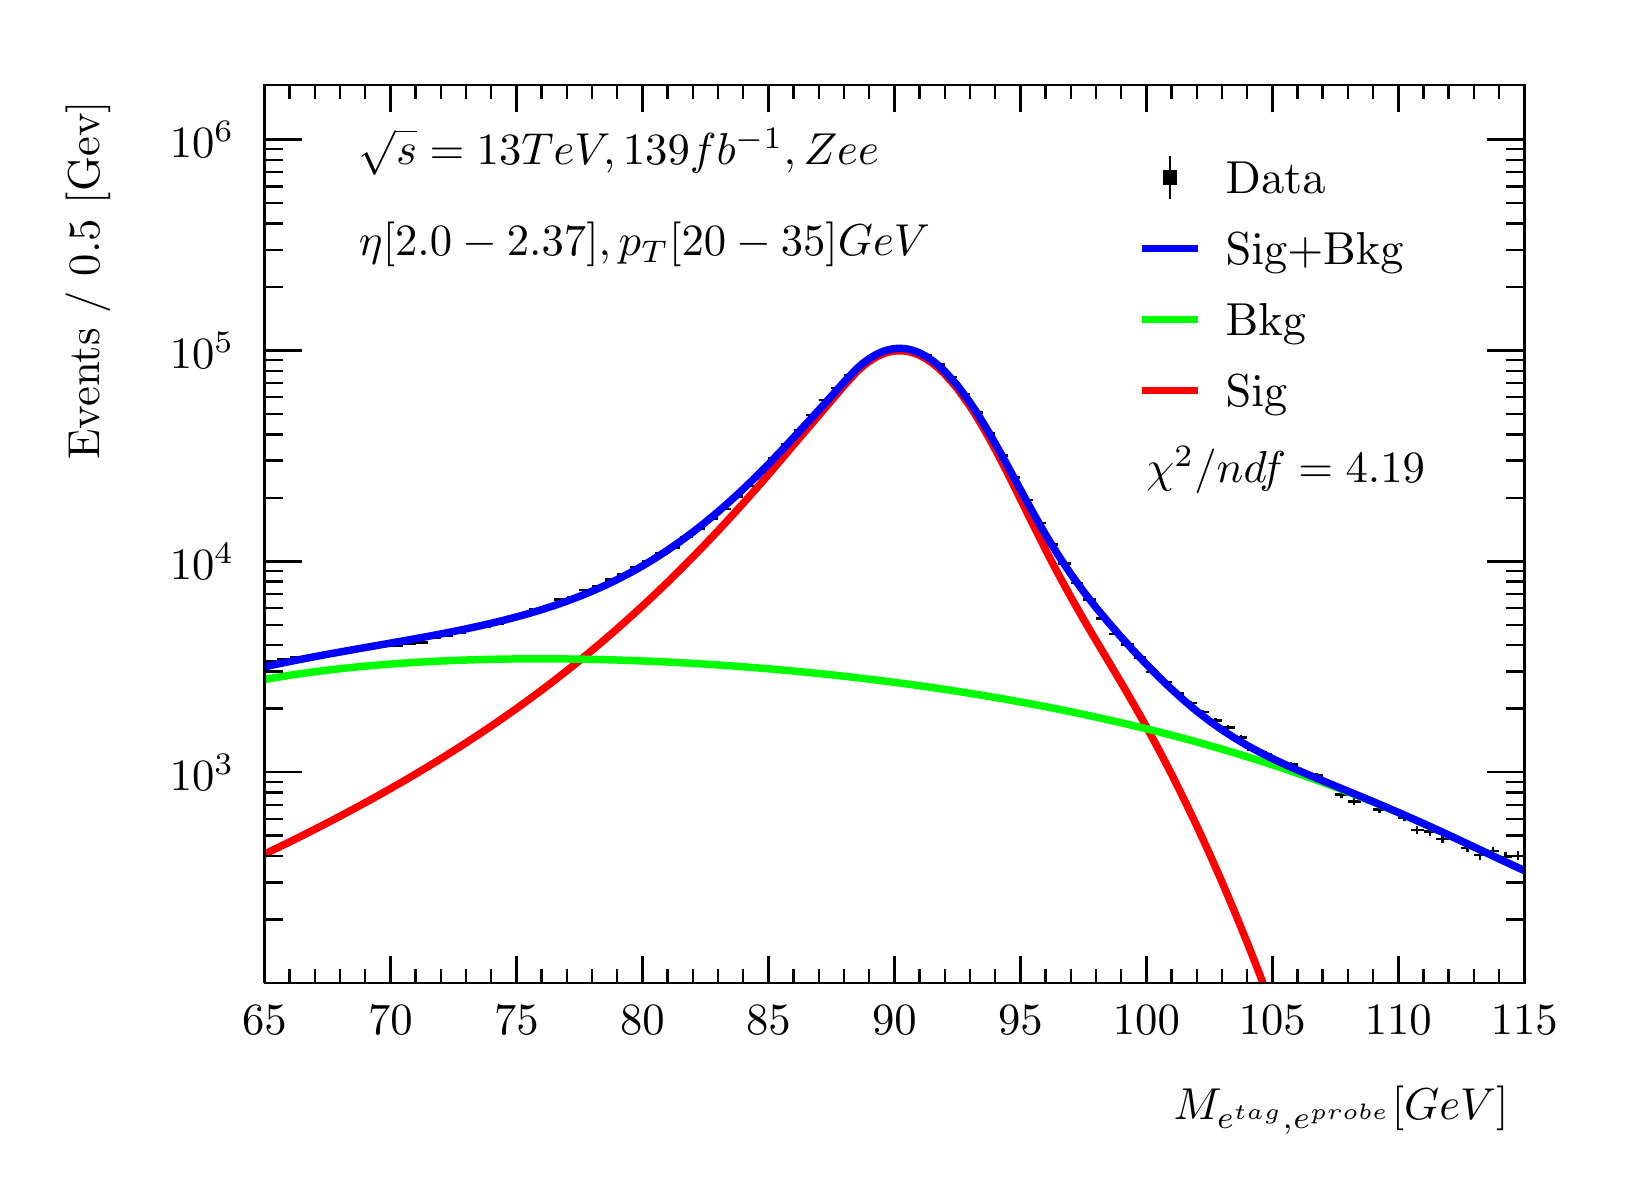
\begin{tikzpicture}
\pgfdeclareplotmark{cross} {
\pgfpathmoveto{\pgfpoint{-0.3\pgfplotmarksize}{\pgfplotmarksize}}
\pgfpathlineto{\pgfpoint{+0.3\pgfplotmarksize}{\pgfplotmarksize}}
\pgfpathlineto{\pgfpoint{+0.3\pgfplotmarksize}{0.3\pgfplotmarksize}}
\pgfpathlineto{\pgfpoint{+1\pgfplotmarksize}{0.3\pgfplotmarksize}}
\pgfpathlineto{\pgfpoint{+1\pgfplotmarksize}{-0.3\pgfplotmarksize}}
\pgfpathlineto{\pgfpoint{+0.3\pgfplotmarksize}{-0.3\pgfplotmarksize}}
\pgfpathlineto{\pgfpoint{+0.3\pgfplotmarksize}{-1.\pgfplotmarksize}}
\pgfpathlineto{\pgfpoint{-0.3\pgfplotmarksize}{-1.\pgfplotmarksize}}
\pgfpathlineto{\pgfpoint{-0.3\pgfplotmarksize}{-0.3\pgfplotmarksize}}
\pgfpathlineto{\pgfpoint{-1.\pgfplotmarksize}{-0.3\pgfplotmarksize}}
\pgfpathlineto{\pgfpoint{-1.\pgfplotmarksize}{0.3\pgfplotmarksize}}
\pgfpathlineto{\pgfpoint{-0.3\pgfplotmarksize}{0.3\pgfplotmarksize}}
\pgfpathclose
\pgfusepathqstroke
}
\pgfdeclareplotmark{cross*} {
\pgfpathmoveto{\pgfpoint{-0.3\pgfplotmarksize}{\pgfplotmarksize}}
\pgfpathlineto{\pgfpoint{+0.3\pgfplotmarksize}{\pgfplotmarksize}}
\pgfpathlineto{\pgfpoint{+0.3\pgfplotmarksize}{0.3\pgfplotmarksize}}
\pgfpathlineto{\pgfpoint{+1\pgfplotmarksize}{0.3\pgfplotmarksize}}
\pgfpathlineto{\pgfpoint{+1\pgfplotmarksize}{-0.3\pgfplotmarksize}}
\pgfpathlineto{\pgfpoint{+0.3\pgfplotmarksize}{-0.3\pgfplotmarksize}}
\pgfpathlineto{\pgfpoint{+0.3\pgfplotmarksize}{-1.\pgfplotmarksize}}
\pgfpathlineto{\pgfpoint{-0.3\pgfplotmarksize}{-1.\pgfplotmarksize}}
\pgfpathlineto{\pgfpoint{-0.3\pgfplotmarksize}{-0.3\pgfplotmarksize}}
\pgfpathlineto{\pgfpoint{-1.\pgfplotmarksize}{-0.3\pgfplotmarksize}}
\pgfpathlineto{\pgfpoint{-1.\pgfplotmarksize}{0.3\pgfplotmarksize}}
\pgfpathlineto{\pgfpoint{-0.3\pgfplotmarksize}{0.3\pgfplotmarksize}}
\pgfpathclose
\pgfusepathqfillstroke
}
\pgfdeclareplotmark{newstar} {
\pgfpathmoveto{\pgfqpoint{0pt}{\pgfplotmarksize}}
\pgfpathlineto{\pgfqpointpolar{44}{0.5\pgfplotmarksize}}
\pgfpathlineto{\pgfqpointpolar{18}{\pgfplotmarksize}}
\pgfpathlineto{\pgfqpointpolar{-20}{0.5\pgfplotmarksize}}
\pgfpathlineto{\pgfqpointpolar{-54}{\pgfplotmarksize}}
\pgfpathlineto{\pgfqpointpolar{-90}{0.5\pgfplotmarksize}}
\pgfpathlineto{\pgfqpointpolar{234}{\pgfplotmarksize}}
\pgfpathlineto{\pgfqpointpolar{198}{0.5\pgfplotmarksize}}
\pgfpathlineto{\pgfqpointpolar{162}{\pgfplotmarksize}}
\pgfpathlineto{\pgfqpointpolar{134}{0.5\pgfplotmarksize}}
\pgfpathclose
\pgfusepathqstroke
}
\pgfdeclareplotmark{newstar*} {
\pgfpathmoveto{\pgfqpoint{0pt}{\pgfplotmarksize}}
\pgfpathlineto{\pgfqpointpolar{44}{0.5\pgfplotmarksize}}
\pgfpathlineto{\pgfqpointpolar{18}{\pgfplotmarksize}}
\pgfpathlineto{\pgfqpointpolar{-20}{0.5\pgfplotmarksize}}
\pgfpathlineto{\pgfqpointpolar{-54}{\pgfplotmarksize}}
\pgfpathlineto{\pgfqpointpolar{-90}{0.5\pgfplotmarksize}}
\pgfpathlineto{\pgfqpointpolar{234}{\pgfplotmarksize}}
\pgfpathlineto{\pgfqpointpolar{198}{0.5\pgfplotmarksize}}
\pgfpathlineto{\pgfqpointpolar{162}{\pgfplotmarksize}}
\pgfpathlineto{\pgfqpointpolar{134}{0.5\pgfplotmarksize}}
\pgfpathclose
\pgfusepathqfillstroke
}
\definecolor{c}{rgb}{1,1,1};
\draw [color=c, fill=c] (0,0) rectangle (20,14.4361);
\draw [color=c, fill=c] (3,2.30977) rectangle (19,13.7143);
\definecolor{c}{rgb}{0,0,0};
\draw [c,line width=0.9] (3,2.30977) -- (3,13.7143) -- (19,13.7143) -- (19,2.30977) -- (3,2.30977);
\definecolor{c}{rgb}{1,1,1};
\draw [color=c, fill=c] (3,2.30977) rectangle (19,13.7143);
\definecolor{c}{rgb}{0,0,0};
\draw [c,line width=0.9] (3,2.30977) -- (3,13.7143) -- (19,13.7143) -- (19,2.30977) -- (3,2.30977);
\draw [c,line width=0.9] (3,2.30977) -- (19,2.30977);
\draw [c,line width=0.9] (3,2.65624) -- (3,2.30977);
\draw [c,line width=0.9] (3.32,2.48301) -- (3.32,2.30977);
\draw [c,line width=0.9] (3.64,2.48301) -- (3.64,2.30977);
\draw [c,line width=0.9] (3.96,2.48301) -- (3.96,2.30977);
\draw [c,line width=0.9] (4.28,2.48301) -- (4.28,2.30977);
\draw [c,line width=0.9] (4.6,2.65624) -- (4.6,2.30977);
\draw [c,line width=0.9] (4.92,2.48301) -- (4.92,2.30977);
\draw [c,line width=0.9] (5.24,2.48301) -- (5.24,2.30977);
\draw [c,line width=0.9] (5.56,2.48301) -- (5.56,2.30977);
\draw [c,line width=0.9] (5.88,2.48301) -- (5.88,2.30977);
\draw [c,line width=0.9] (6.2,2.65624) -- (6.2,2.30977);
\draw [c,line width=0.9] (6.52,2.48301) -- (6.52,2.30977);
\draw [c,line width=0.9] (6.84,2.48301) -- (6.84,2.30977);
\draw [c,line width=0.9] (7.16,2.48301) -- (7.16,2.30977);
\draw [c,line width=0.9] (7.48,2.48301) -- (7.48,2.30977);
\draw [c,line width=0.9] (7.8,2.65624) -- (7.8,2.30977);
\draw [c,line width=0.9] (8.12,2.48301) -- (8.12,2.30977);
\draw [c,line width=0.9] (8.44,2.48301) -- (8.44,2.30977);
\draw [c,line width=0.9] (8.76,2.48301) -- (8.76,2.30977);
\draw [c,line width=0.9] (9.08,2.48301) -- (9.08,2.30977);
\draw [c,line width=0.9] (9.4,2.65624) -- (9.4,2.30977);
\draw [c,line width=0.9] (9.72,2.48301) -- (9.72,2.30977);
\draw [c,line width=0.9] (10.04,2.48301) -- (10.04,2.30977);
\draw [c,line width=0.9] (10.36,2.48301) -- (10.36,2.30977);
\draw [c,line width=0.9] (10.68,2.48301) -- (10.68,2.30977);
\draw [c,line width=0.9] (11,2.65624) -- (11,2.30977);
\draw [c,line width=0.9] (11.32,2.48301) -- (11.32,2.30977);
\draw [c,line width=0.9] (11.64,2.48301) -- (11.64,2.30977);
\draw [c,line width=0.9] (11.96,2.48301) -- (11.96,2.30977);
\draw [c,line width=0.9] (12.28,2.48301) -- (12.28,2.30977);
\draw [c,line width=0.9] (12.6,2.65624) -- (12.6,2.30977);
\draw [c,line width=0.9] (12.92,2.48301) -- (12.92,2.30977);
\draw [c,line width=0.9] (13.24,2.48301) -- (13.24,2.30977);
\draw [c,line width=0.9] (13.56,2.48301) -- (13.56,2.30977);
\draw [c,line width=0.9] (13.88,2.48301) -- (13.88,2.30977);
\draw [c,line width=0.9] (14.2,2.65624) -- (14.2,2.30977);
\draw [c,line width=0.9] (14.52,2.48301) -- (14.52,2.30977);
\draw [c,line width=0.9] (14.84,2.48301) -- (14.84,2.30977);
\draw [c,line width=0.9] (15.16,2.48301) -- (15.16,2.30977);
\draw [c,line width=0.9] (15.48,2.48301) -- (15.48,2.30977);
\draw [c,line width=0.9] (15.8,2.65624) -- (15.8,2.30977);
\draw [c,line width=0.9] (16.12,2.48301) -- (16.12,2.30977);
\draw [c,line width=0.9] (16.44,2.48301) -- (16.44,2.30977);
\draw [c,line width=0.9] (16.76,2.48301) -- (16.76,2.30977);
\draw [c,line width=0.9] (17.08,2.48301) -- (17.08,2.30977);
\draw [c,line width=0.9] (17.4,2.65624) -- (17.4,2.30977);
\draw [c,line width=0.9] (17.72,2.48301) -- (17.72,2.30977);
\draw [c,line width=0.9] (18.04,2.48301) -- (18.04,2.30977);
\draw [c,line width=0.9] (18.36,2.48301) -- (18.36,2.30977);
\draw [c,line width=0.9] (18.68,2.48301) -- (18.68,2.30977);
\draw [c,line width=0.9] (19,2.65624) -- (19,2.30977);
\draw [c,line width=0.9] (19,2.65624) -- (19,2.30977);
\draw [anchor=base] (3,1.66015) node[scale=1.61424, color=c, rotate=0]{65};
\draw [anchor=base] (4.6,1.66015) node[scale=1.61424, color=c, rotate=0]{70};
\draw [anchor=base] (6.2,1.66015) node[scale=1.61424, color=c, rotate=0]{75};
\draw [anchor=base] (7.8,1.66015) node[scale=1.61424, color=c, rotate=0]{80};
\draw [anchor=base] (9.4,1.66015) node[scale=1.61424, color=c, rotate=0]{85};
\draw [anchor=base] (11,1.66015) node[scale=1.61424, color=c, rotate=0]{90};
\draw [anchor=base] (12.6,1.66015) node[scale=1.61424, color=c, rotate=0]{95};
\draw [anchor=base] (14.2,1.66015) node[scale=1.61424, color=c, rotate=0]{100};
\draw [anchor=base] (15.8,1.66015) node[scale=1.61424, color=c, rotate=0]{105};
\draw [anchor=base] (17.4,1.66015) node[scale=1.61424, color=c, rotate=0]{110};
\draw [anchor=base] (19,1.66015) node[scale=1.61424, color=c, rotate=0]{115};
\draw [anchor= east] (19,0.692932) node[scale=1.61424, color=c, rotate=0]{$M_{e^{tag}, e^{probe}}  [GeV]$};
\draw [c,line width=0.9] (3,13.7143) -- (19,13.7143);
\draw [c,line width=0.9] (3,13.3678) -- (3,13.7143);
\draw [c,line width=0.9] (3.32,13.5411) -- (3.32,13.7143);
\draw [c,line width=0.9] (3.64,13.5411) -- (3.64,13.7143);
\draw [c,line width=0.9] (3.96,13.5411) -- (3.96,13.7143);
\draw [c,line width=0.9] (4.28,13.5411) -- (4.28,13.7143);
\draw [c,line width=0.9] (4.6,13.3678) -- (4.6,13.7143);
\draw [c,line width=0.9] (4.92,13.5411) -- (4.92,13.7143);
\draw [c,line width=0.9] (5.24,13.5411) -- (5.24,13.7143);
\draw [c,line width=0.9] (5.56,13.5411) -- (5.56,13.7143);
\draw [c,line width=0.9] (5.88,13.5411) -- (5.88,13.7143);
\draw [c,line width=0.9] (6.2,13.3678) -- (6.2,13.7143);
\draw [c,line width=0.9] (6.52,13.5411) -- (6.52,13.7143);
\draw [c,line width=0.9] (6.84,13.5411) -- (6.84,13.7143);
\draw [c,line width=0.9] (7.16,13.5411) -- (7.16,13.7143);
\draw [c,line width=0.9] (7.48,13.5411) -- (7.48,13.7143);
\draw [c,line width=0.9] (7.8,13.3678) -- (7.8,13.7143);
\draw [c,line width=0.9] (8.12,13.5411) -- (8.12,13.7143);
\draw [c,line width=0.9] (8.44,13.5411) -- (8.44,13.7143);
\draw [c,line width=0.9] (8.76,13.5411) -- (8.76,13.7143);
\draw [c,line width=0.9] (9.08,13.5411) -- (9.08,13.7143);
\draw [c,line width=0.9] (9.4,13.3678) -- (9.4,13.7143);
\draw [c,line width=0.9] (9.72,13.5411) -- (9.72,13.7143);
\draw [c,line width=0.9] (10.04,13.5411) -- (10.04,13.7143);
\draw [c,line width=0.9] (10.36,13.5411) -- (10.36,13.7143);
\draw [c,line width=0.9] (10.68,13.5411) -- (10.68,13.7143);
\draw [c,line width=0.9] (11,13.3678) -- (11,13.7143);
\draw [c,line width=0.9] (11.32,13.5411) -- (11.32,13.7143);
\draw [c,line width=0.9] (11.64,13.5411) -- (11.64,13.7143);
\draw [c,line width=0.9] (11.96,13.5411) -- (11.96,13.7143);
\draw [c,line width=0.9] (12.28,13.5411) -- (12.28,13.7143);
\draw [c,line width=0.9] (12.6,13.3678) -- (12.6,13.7143);
\draw [c,line width=0.9] (12.92,13.5411) -- (12.92,13.7143);
\draw [c,line width=0.9] (13.24,13.5411) -- (13.24,13.7143);
\draw [c,line width=0.9] (13.56,13.5411) -- (13.56,13.7143);
\draw [c,line width=0.9] (13.88,13.5411) -- (13.88,13.7143);
\draw [c,line width=0.9] (14.2,13.3678) -- (14.2,13.7143);
\draw [c,line width=0.9] (14.52,13.5411) -- (14.52,13.7143);
\draw [c,line width=0.9] (14.84,13.5411) -- (14.84,13.7143);
\draw [c,line width=0.9] (15.16,13.5411) -- (15.16,13.7143);
\draw [c,line width=0.9] (15.48,13.5411) -- (15.48,13.7143);
\draw [c,line width=0.9] (15.8,13.3678) -- (15.8,13.7143);
\draw [c,line width=0.9] (16.12,13.5411) -- (16.12,13.7143);
\draw [c,line width=0.9] (16.44,13.5411) -- (16.44,13.7143);
\draw [c,line width=0.9] (16.76,13.5411) -- (16.76,13.7143);
\draw [c,line width=0.9] (17.08,13.5411) -- (17.08,13.7143);
\draw [c,line width=0.9] (17.4,13.3678) -- (17.4,13.7143);
\draw [c,line width=0.9] (17.72,13.5411) -- (17.72,13.7143);
\draw [c,line width=0.9] (18.04,13.5411) -- (18.04,13.7143);
\draw [c,line width=0.9] (18.36,13.5411) -- (18.36,13.7143);
\draw [c,line width=0.9] (18.68,13.5411) -- (18.68,13.7143);
\draw [c,line width=0.9] (19,13.3678) -- (19,13.7143);
\draw [c,line width=0.9] (19,13.3678) -- (19,13.7143);
\draw [c,line width=0.9] (3,2.30977) -- (3,13.7143);
\draw [c,line width=0.9] (3.237,3.11596) -- (3,3.11596);
\draw [c,line width=0.9] (3.237,3.58755) -- (3,3.58755);
\draw [c,line width=0.9] (3.237,3.92215) -- (3,3.92215);
\draw [c,line width=0.9] (3.237,4.18169) -- (3,4.18169);
\draw [c,line width=0.9] (3.237,4.39374) -- (3,4.39374);
\draw [c,line width=0.9] (3.237,4.57303) -- (3,4.57303);
\draw [c,line width=0.9] (3.237,4.72834) -- (3,4.72834);
\draw [c,line width=0.9] (3.237,4.86533) -- (3,4.86533);
\draw [c,line width=0.9] (3.474,4.98787) -- (3,4.98787);
\draw [anchor= east] (2.82,4.98787) node[scale=1.61424, color=c, rotate=0]{$10^{3}$};
\draw [c,line width=0.9] (3.237,5.79406) -- (3,5.79406);
\draw [c,line width=0.9] (3.237,6.26566) -- (3,6.26566);
\draw [c,line width=0.9] (3.237,6.60025) -- (3,6.60025);
\draw [c,line width=0.9] (3.237,6.85979) -- (3,6.85979);
\draw [c,line width=0.9] (3.237,7.07184) -- (3,7.07184);
\draw [c,line width=0.9] (3.237,7.25113) -- (3,7.25113);
\draw [c,line width=0.9] (3.237,7.40644) -- (3,7.40644);
\draw [c,line width=0.9] (3.237,7.54344) -- (3,7.54344);
\draw [c,line width=0.9] (3.474,7.66598) -- (3,7.66598);
\draw [anchor= east] (2.82,7.66598) node[scale=1.61424, color=c, rotate=0]{$10^{4}$};
\draw [c,line width=0.9] (3.237,8.47217) -- (3,8.47217);
\draw [c,line width=0.9] (3.237,8.94376) -- (3,8.94376);
\draw [c,line width=0.9] (3.237,9.27836) -- (3,9.27836);
\draw [c,line width=0.9] (3.237,9.53789) -- (3,9.53789);
\draw [c,line width=0.9] (3.237,9.74995) -- (3,9.74995);
\draw [c,line width=0.9] (3.237,9.92924) -- (3,9.92924);
\draw [c,line width=0.9] (3.237,10.0845) -- (3,10.0845);
\draw [c,line width=0.9] (3.237,10.2215) -- (3,10.2215);
\draw [c,line width=0.9] (3.474,10.3441) -- (3,10.3441);
\draw [anchor= east] (2.82,10.3441) node[scale=1.61424, color=c, rotate=0]{$10^{5}$};
\draw [c,line width=0.9] (3.237,11.1503) -- (3,11.1503);
\draw [c,line width=0.9] (3.237,11.6219) -- (3,11.6219);
\draw [c,line width=0.9] (3.237,11.9565) -- (3,11.9565);
\draw [c,line width=0.9] (3.237,12.216) -- (3,12.216);
\draw [c,line width=0.9] (3.237,12.4281) -- (3,12.4281);
\draw [c,line width=0.9] (3.237,12.6073) -- (3,12.6073);
\draw [c,line width=0.9] (3.237,12.7627) -- (3,12.7627);
\draw [c,line width=0.9] (3.237,12.8996) -- (3,12.8996);
\draw [c,line width=0.9] (3.474,13.0222) -- (3,13.0222);
\draw [anchor= east] (2.82,13.0222) node[scale=1.61424, color=c, rotate=0]{$10^{6}$};
\draw [anchor= east] (0.76,13.7143) node[scale=1.61424, color=c, rotate=90]{Events / 0.5 [Gev]};
\draw [c,line width=0.9] (19,2.30977) -- (19,13.7143);
\draw [c,line width=0.9] (18.763,3.11596) -- (19,3.11596);
\draw [c,line width=0.9] (18.763,3.58755) -- (19,3.58755);
\draw [c,line width=0.9] (18.763,3.92215) -- (19,3.92215);
\draw [c,line width=0.9] (18.763,4.18169) -- (19,4.18169);
\draw [c,line width=0.9] (18.763,4.39374) -- (19,4.39374);
\draw [c,line width=0.9] (18.763,4.57303) -- (19,4.57303);
\draw [c,line width=0.9] (18.763,4.72834) -- (19,4.72834);
\draw [c,line width=0.9] (18.763,4.86533) -- (19,4.86533);
\draw [c,line width=0.9] (18.526,4.98787) -- (19,4.98787);
\draw [c,line width=0.9] (18.763,5.79406) -- (19,5.79406);
\draw [c,line width=0.9] (18.763,6.26566) -- (19,6.26566);
\draw [c,line width=0.9] (18.763,6.60025) -- (19,6.60025);
\draw [c,line width=0.9] (18.763,6.85979) -- (19,6.85979);
\draw [c,line width=0.9] (18.763,7.07184) -- (19,7.07184);
\draw [c,line width=0.9] (18.763,7.25113) -- (19,7.25113);
\draw [c,line width=0.9] (18.763,7.40644) -- (19,7.40644);
\draw [c,line width=0.9] (18.763,7.54344) -- (19,7.54344);
\draw [c,line width=0.9] (18.526,7.66598) -- (19,7.66598);
\draw [c,line width=0.9] (18.763,8.47217) -- (19,8.47217);
\draw [c,line width=0.9] (18.763,8.94376) -- (19,8.94376);
\draw [c,line width=0.9] (18.763,9.27836) -- (19,9.27836);
\draw [c,line width=0.9] (18.763,9.53789) -- (19,9.53789);
\draw [c,line width=0.9] (18.763,9.74995) -- (19,9.74995);
\draw [c,line width=0.9] (18.763,9.92924) -- (19,9.92924);
\draw [c,line width=0.9] (18.763,10.0845) -- (19,10.0845);
\draw [c,line width=0.9] (18.763,10.2215) -- (19,10.2215);
\draw [c,line width=0.9] (18.526,10.3441) -- (19,10.3441);
\draw [c,line width=0.9] (18.763,11.1503) -- (19,11.1503);
\draw [c,line width=0.9] (18.763,11.6219) -- (19,11.6219);
\draw [c,line width=0.9] (18.763,11.9565) -- (19,11.9565);
\draw [c,line width=0.9] (18.763,12.216) -- (19,12.216);
\draw [c,line width=0.9] (18.763,12.4281) -- (19,12.4281);
\draw [c,line width=0.9] (18.763,12.6073) -- (19,12.6073);
\draw [c,line width=0.9] (18.763,12.7627) -- (19,12.7627);
\draw [c,line width=0.9] (18.763,12.8996) -- (19,12.8996);
\draw [c,line width=0.9] (18.526,13.0222) -- (19,13.0222);
\draw [c,line width=0.9] (3.08,6.39504) -- (3,6.39504);
\draw [c,line width=0.9] (3,6.39504) -- (3,6.39504);
\draw [c,line width=0.9] (3.08,6.39504) -- (3.16,6.39504);
\draw [c,line width=0.9] (3.16,6.39504) -- (3.16,6.39504);
\draw [c,line width=0.9] (3.08,6.39504) -- (3.08,6.41513);
\draw [c,line width=0.9] (3.08,6.41513) -- (3.08,6.41513);
\draw [c,line width=0.9] (3.08,6.39504) -- (3.08,6.37496);
\draw [c,line width=0.9] (3.08,6.37496) -- (3.08,6.37496);
\draw [c,line width=0.9] (3.24,6.42247) -- (3.16,6.42247);
\draw [c,line width=0.9] (3.16,6.42247) -- (3.16,6.42247);
\draw [c,line width=0.9] (3.24,6.42247) -- (3.32,6.42247);
\draw [c,line width=0.9] (3.32,6.42247) -- (3.32,6.42247);
\draw [c,line width=0.9] (3.24,6.42247) -- (3.24,6.44232);
\draw [c,line width=0.9] (3.24,6.44232) -- (3.24,6.44232);
\draw [c,line width=0.9] (3.24,6.42247) -- (3.24,6.40262);
\draw [c,line width=0.9] (3.24,6.40262) -- (3.24,6.40262);
\draw [c,line width=0.9] (3.4,6.44195) -- (3.32,6.44195);
\draw [c,line width=0.9] (3.32,6.44195) -- (3.32,6.44195);
\draw [c,line width=0.9] (3.4,6.44195) -- (3.48,6.44195);
\draw [c,line width=0.9] (3.48,6.44195) -- (3.48,6.44195);
\draw [c,line width=0.9] (3.4,6.44195) -- (3.4,6.46164);
\draw [c,line width=0.9] (3.4,6.46164) -- (3.4,6.46164);
\draw [c,line width=0.9] (3.4,6.44195) -- (3.4,6.42227);
\draw [c,line width=0.9] (3.4,6.42227) -- (3.4,6.42227);
\draw [c,line width=0.9] (3.56,6.44461) -- (3.48,6.44461);
\draw [c,line width=0.9] (3.48,6.44461) -- (3.48,6.44461);
\draw [c,line width=0.9] (3.56,6.44461) -- (3.64,6.44461);
\draw [c,line width=0.9] (3.64,6.44461) -- (3.64,6.44461);
\draw [c,line width=0.9] (3.56,6.44461) -- (3.56,6.46428);
\draw [c,line width=0.9] (3.56,6.46428) -- (3.56,6.46428);
\draw [c,line width=0.9] (3.56,6.44461) -- (3.56,6.42495);
\draw [c,line width=0.9] (3.56,6.42495) -- (3.56,6.42495);
\draw [c,line width=0.9] (3.72,6.48223) -- (3.64,6.48223);
\draw [c,line width=0.9] (3.64,6.48223) -- (3.64,6.48223);
\draw [c,line width=0.9] (3.72,6.48223) -- (3.8,6.48223);
\draw [c,line width=0.9] (3.8,6.48223) -- (3.8,6.48223);
\draw [c,line width=0.9] (3.72,6.48223) -- (3.72,6.50157);
\draw [c,line width=0.9] (3.72,6.50157) -- (3.72,6.50157);
\draw [c,line width=0.9] (3.72,6.48223) -- (3.72,6.46288);
\draw [c,line width=0.9] (3.72,6.46288) -- (3.72,6.46288);
\draw [c,line width=0.9] (3.88,6.48029) -- (3.8,6.48029);
\draw [c,line width=0.9] (3.8,6.48029) -- (3.8,6.48029);
\draw [c,line width=0.9] (3.88,6.48029) -- (3.96,6.48029);
\draw [c,line width=0.9] (3.96,6.48029) -- (3.96,6.48029);
\draw [c,line width=0.9] (3.88,6.48029) -- (3.88,6.49966);
\draw [c,line width=0.9] (3.88,6.49966) -- (3.88,6.49966);
\draw [c,line width=0.9] (3.88,6.48029) -- (3.88,6.46093);
\draw [c,line width=0.9] (3.88,6.46093) -- (3.88,6.46093);
\draw [c,line width=0.9] (4.04,6.51554) -- (3.96,6.51554);
\draw [c,line width=0.9] (3.96,6.51554) -- (3.96,6.51554);
\draw [c,line width=0.9] (4.04,6.51554) -- (4.12,6.51554);
\draw [c,line width=0.9] (4.12,6.51554) -- (4.12,6.51554);
\draw [c,line width=0.9] (4.04,6.51554) -- (4.04,6.53461);
\draw [c,line width=0.9] (4.04,6.53461) -- (4.04,6.53461);
\draw [c,line width=0.9] (4.04,6.51554) -- (4.04,6.49647);
\draw [c,line width=0.9] (4.04,6.49647) -- (4.04,6.49647);
\draw [c,line width=0.9] (4.2,6.54883) -- (4.12,6.54883);
\draw [c,line width=0.9] (4.12,6.54883) -- (4.12,6.54883);
\draw [c,line width=0.9] (4.2,6.54883) -- (4.28,6.54883);
\draw [c,line width=0.9] (4.28,6.54883) -- (4.28,6.54883);
\draw [c,line width=0.9] (4.2,6.54883) -- (4.2,6.56763);
\draw [c,line width=0.9] (4.2,6.56763) -- (4.2,6.56763);
\draw [c,line width=0.9] (4.2,6.54883) -- (4.2,6.53003);
\draw [c,line width=0.9] (4.2,6.53003) -- (4.2,6.53003);
\draw [c,line width=0.9] (4.36,6.56243) -- (4.28,6.56243);
\draw [c,line width=0.9] (4.28,6.56243) -- (4.28,6.56243);
\draw [c,line width=0.9] (4.36,6.56243) -- (4.44,6.56243);
\draw [c,line width=0.9] (4.44,6.56243) -- (4.44,6.56243);
\draw [c,line width=0.9] (4.36,6.56243) -- (4.36,6.58112);
\draw [c,line width=0.9] (4.36,6.58112) -- (4.36,6.58112);
\draw [c,line width=0.9] (4.36,6.56243) -- (4.36,6.54374);
\draw [c,line width=0.9] (4.36,6.54374) -- (4.36,6.54374);
\draw [c,line width=0.9] (4.52,6.62898) -- (4.44,6.62898);
\draw [c,line width=0.9] (4.44,6.62898) -- (4.44,6.62898);
\draw [c,line width=0.9] (4.52,6.62898) -- (4.6,6.62898);
\draw [c,line width=0.9] (4.6,6.62898) -- (4.6,6.62898);
\draw [c,line width=0.9] (4.52,6.62898) -- (4.52,6.64714);
\draw [c,line width=0.9] (4.52,6.64714) -- (4.52,6.64714);
\draw [c,line width=0.9] (4.52,6.62898) -- (4.52,6.61081);
\draw [c,line width=0.9] (4.52,6.61081) -- (4.52,6.61081);
\draw [c,line width=0.9] (4.68,6.59062) -- (4.6,6.59062);
\draw [c,line width=0.9] (4.6,6.59062) -- (4.6,6.59062);
\draw [c,line width=0.9] (4.68,6.59062) -- (4.76,6.59062);
\draw [c,line width=0.9] (4.76,6.59062) -- (4.76,6.59062);
\draw [c,line width=0.9] (4.68,6.59062) -- (4.68,6.60909);
\draw [c,line width=0.9] (4.68,6.60909) -- (4.68,6.60909);
\draw [c,line width=0.9] (4.68,6.59062) -- (4.68,6.57215);
\draw [c,line width=0.9] (4.68,6.57215) -- (4.68,6.57215);
\draw [c,line width=0.9] (4.84,6.62158) -- (4.76,6.62158);
\draw [c,line width=0.9] (4.76,6.62158) -- (4.76,6.62158);
\draw [c,line width=0.9] (4.84,6.62158) -- (4.92,6.62158);
\draw [c,line width=0.9] (4.92,6.62158) -- (4.92,6.62158);
\draw [c,line width=0.9] (4.84,6.62158) -- (4.84,6.6398);
\draw [c,line width=0.9] (4.84,6.6398) -- (4.84,6.6398);
\draw [c,line width=0.9] (4.84,6.62158) -- (4.84,6.60335);
\draw [c,line width=0.9] (4.84,6.60335) -- (4.84,6.60335);
\draw [c,line width=0.9] (5,6.63407) -- (4.92,6.63407);
\draw [c,line width=0.9] (4.92,6.63407) -- (4.92,6.63407);
\draw [c,line width=0.9] (5,6.63407) -- (5.08,6.63407);
\draw [c,line width=0.9] (5.08,6.63407) -- (5.08,6.63407);
\draw [c,line width=0.9] (5,6.63407) -- (5,6.65219);
\draw [c,line width=0.9] (5,6.65219) -- (5,6.65219);
\draw [c,line width=0.9] (5,6.63407) -- (5,6.61595);
\draw [c,line width=0.9] (5,6.61595) -- (5,6.61595);
\draw [c,line width=0.9] (5.16,6.69915) -- (5.08,6.69915);
\draw [c,line width=0.9] (5.08,6.69915) -- (5.08,6.69915);
\draw [c,line width=0.9] (5.16,6.69915) -- (5.24,6.69915);
\draw [c,line width=0.9] (5.24,6.69915) -- (5.24,6.69915);
\draw [c,line width=0.9] (5.16,6.69915) -- (5.16,6.71678);
\draw [c,line width=0.9] (5.16,6.71678) -- (5.16,6.71678);
\draw [c,line width=0.9] (5.16,6.69915) -- (5.16,6.68153);
\draw [c,line width=0.9] (5.16,6.68153) -- (5.16,6.68153);
\draw [c,line width=0.9] (5.32,6.72321) -- (5.24,6.72321);
\draw [c,line width=0.9] (5.24,6.72321) -- (5.24,6.72321);
\draw [c,line width=0.9] (5.32,6.72321) -- (5.4,6.72321);
\draw [c,line width=0.9] (5.4,6.72321) -- (5.4,6.72321);
\draw [c,line width=0.9] (5.32,6.72321) -- (5.32,6.74065);
\draw [c,line width=0.9] (5.32,6.74065) -- (5.32,6.74065);
\draw [c,line width=0.9] (5.32,6.72321) -- (5.32,6.70576);
\draw [c,line width=0.9] (5.32,6.70576) -- (5.32,6.70576);
\draw [c,line width=0.9] (5.48,6.7585) -- (5.4,6.7585);
\draw [c,line width=0.9] (5.4,6.7585) -- (5.4,6.7585);
\draw [c,line width=0.9] (5.48,6.7585) -- (5.56,6.7585);
\draw [c,line width=0.9] (5.56,6.7585) -- (5.56,6.7585);
\draw [c,line width=0.9] (5.48,6.7585) -- (5.48,6.77568);
\draw [c,line width=0.9] (5.48,6.77568) -- (5.48,6.77568);
\draw [c,line width=0.9] (5.48,6.7585) -- (5.48,6.74132);
\draw [c,line width=0.9] (5.48,6.74132) -- (5.48,6.74132);
\draw [c,line width=0.9] (5.64,6.81061) -- (5.56,6.81061);
\draw [c,line width=0.9] (5.56,6.81061) -- (5.56,6.81061);
\draw [c,line width=0.9] (5.64,6.81061) -- (5.72,6.81061);
\draw [c,line width=0.9] (5.72,6.81061) -- (5.72,6.81061);
\draw [c,line width=0.9] (5.64,6.81061) -- (5.64,6.82741);
\draw [c,line width=0.9] (5.64,6.82741) -- (5.64,6.82741);
\draw [c,line width=0.9] (5.64,6.81061) -- (5.64,6.79381);
\draw [c,line width=0.9] (5.64,6.79381) -- (5.64,6.79381);
\draw [c,line width=0.9] (5.8,6.83819) -- (5.72,6.83819);
\draw [c,line width=0.9] (5.72,6.83819) -- (5.72,6.83819);
\draw [c,line width=0.9] (5.8,6.83819) -- (5.88,6.83819);
\draw [c,line width=0.9] (5.88,6.83819) -- (5.88,6.83819);
\draw [c,line width=0.9] (5.8,6.83819) -- (5.8,6.85479);
\draw [c,line width=0.9] (5.8,6.85479) -- (5.8,6.85479);
\draw [c,line width=0.9] (5.8,6.83819) -- (5.8,6.82159);
\draw [c,line width=0.9] (5.8,6.82159) -- (5.8,6.82159);
\draw [c,line width=0.9] (5.96,6.87228) -- (5.88,6.87228);
\draw [c,line width=0.9] (5.88,6.87228) -- (5.88,6.87228);
\draw [c,line width=0.9] (5.96,6.87228) -- (6.04,6.87228);
\draw [c,line width=0.9] (6.04,6.87228) -- (6.04,6.87228);
\draw [c,line width=0.9] (5.96,6.87228) -- (5.96,6.88864);
\draw [c,line width=0.9] (5.96,6.88864) -- (5.96,6.88864);
\draw [c,line width=0.9] (5.96,6.87228) -- (5.96,6.85592);
\draw [c,line width=0.9] (5.96,6.85592) -- (5.96,6.85592);
\draw [c,line width=0.9] (6.12,6.94022) -- (6.04,6.94022);
\draw [c,line width=0.9] (6.04,6.94022) -- (6.04,6.94022);
\draw [c,line width=0.9] (6.12,6.94022) -- (6.2,6.94022);
\draw [c,line width=0.9] (6.2,6.94022) -- (6.2,6.94022);
\draw [c,line width=0.9] (6.12,6.94022) -- (6.12,6.95611);
\draw [c,line width=0.9] (6.12,6.95611) -- (6.12,6.95611);
\draw [c,line width=0.9] (6.12,6.94022) -- (6.12,6.92433);
\draw [c,line width=0.9] (6.12,6.92433) -- (6.12,6.92433);
\draw [c,line width=0.9] (6.28,6.9797) -- (6.2,6.9797);
\draw [c,line width=0.9] (6.2,6.9797) -- (6.2,6.9797);
\draw [c,line width=0.9] (6.28,6.9797) -- (6.36,6.9797);
\draw [c,line width=0.9] (6.36,6.9797) -- (6.36,6.9797);
\draw [c,line width=0.9] (6.28,6.9797) -- (6.28,6.99532);
\draw [c,line width=0.9] (6.28,6.99532) -- (6.28,6.99532);
\draw [c,line width=0.9] (6.28,6.9797) -- (6.28,6.96408);
\draw [c,line width=0.9] (6.28,6.96408) -- (6.28,6.96408);
\draw [c,line width=0.9] (6.44,7.05466) -- (6.36,7.05466);
\draw [c,line width=0.9] (6.36,7.05466) -- (6.36,7.05466);
\draw [c,line width=0.9] (6.44,7.05466) -- (6.52,7.05466);
\draw [c,line width=0.9] (6.52,7.05466) -- (6.52,7.05466);
\draw [c,line width=0.9] (6.44,7.05466) -- (6.44,7.06979);
\draw [c,line width=0.9] (6.44,7.06979) -- (6.44,7.06979);
\draw [c,line width=0.9] (6.44,7.05466) -- (6.44,7.03953);
\draw [c,line width=0.9] (6.44,7.03953) -- (6.44,7.03953);
\draw [c,line width=0.9] (6.6,7.07707) -- (6.52,7.07707);
\draw [c,line width=0.9] (6.52,7.07707) -- (6.52,7.07707);
\draw [c,line width=0.9] (6.6,7.07707) -- (6.68,7.07707);
\draw [c,line width=0.9] (6.68,7.07707) -- (6.68,7.07707);
\draw [c,line width=0.9] (6.6,7.07707) -- (6.6,7.09205);
\draw [c,line width=0.9] (6.6,7.09205) -- (6.6,7.09205);
\draw [c,line width=0.9] (6.6,7.07707) -- (6.6,7.06209);
\draw [c,line width=0.9] (6.6,7.06209) -- (6.6,7.06209);
\draw [c,line width=0.9] (6.76,7.18023) -- (6.68,7.18023);
\draw [c,line width=0.9] (6.68,7.18023) -- (6.68,7.18023);
\draw [c,line width=0.9] (6.76,7.18023) -- (6.84,7.18023);
\draw [c,line width=0.9] (6.84,7.18023) -- (6.84,7.18023);
\draw [c,line width=0.9] (6.76,7.18023) -- (6.76,7.19456);
\draw [c,line width=0.9] (6.76,7.19456) -- (6.76,7.19456);
\draw [c,line width=0.9] (6.76,7.18023) -- (6.76,7.1659);
\draw [c,line width=0.9] (6.76,7.1659) -- (6.76,7.1659);
\draw [c,line width=0.9] (6.92,7.20849) -- (6.84,7.20849);
\draw [c,line width=0.9] (6.84,7.20849) -- (6.84,7.20849);
\draw [c,line width=0.9] (6.92,7.20849) -- (7,7.20849);
\draw [c,line width=0.9] (7,7.20849) -- (7,7.20849);
\draw [c,line width=0.9] (6.92,7.20849) -- (6.92,7.22265);
\draw [c,line width=0.9] (6.92,7.22265) -- (6.92,7.22265);
\draw [c,line width=0.9] (6.92,7.20849) -- (6.92,7.19433);
\draw [c,line width=0.9] (6.92,7.19433) -- (6.92,7.19433);
\draw [c,line width=0.9] (7.08,7.30249) -- (7,7.30249);
\draw [c,line width=0.9] (7,7.30249) -- (7,7.30249);
\draw [c,line width=0.9] (7.08,7.30249) -- (7.16,7.30249);
\draw [c,line width=0.9] (7.16,7.30249) -- (7.16,7.30249);
\draw [c,line width=0.9] (7.08,7.30249) -- (7.08,7.31609);
\draw [c,line width=0.9] (7.08,7.31609) -- (7.08,7.31609);
\draw [c,line width=0.9] (7.08,7.30249) -- (7.08,7.28889);
\draw [c,line width=0.9] (7.08,7.28889) -- (7.08,7.28889);
\draw [c,line width=0.9] (7.24,7.34587) -- (7.16,7.34587);
\draw [c,line width=0.9] (7.16,7.34587) -- (7.16,7.34587);
\draw [c,line width=0.9] (7.24,7.34587) -- (7.32,7.34587);
\draw [c,line width=0.9] (7.32,7.34587) -- (7.32,7.34587);
\draw [c,line width=0.9] (7.24,7.34587) -- (7.24,7.35921);
\draw [c,line width=0.9] (7.24,7.35921) -- (7.24,7.35921);
\draw [c,line width=0.9] (7.24,7.34587) -- (7.24,7.33252);
\draw [c,line width=0.9] (7.24,7.33252) -- (7.24,7.33252);
\draw [c,line width=0.9] (7.4,7.43275) -- (7.32,7.43275);
\draw [c,line width=0.9] (7.32,7.43275) -- (7.32,7.43275);
\draw [c,line width=0.9] (7.4,7.43275) -- (7.48,7.43275);
\draw [c,line width=0.9] (7.48,7.43275) -- (7.48,7.43275);
\draw [c,line width=0.9] (7.4,7.43275) -- (7.4,7.44561);
\draw [c,line width=0.9] (7.4,7.44561) -- (7.4,7.44561);
\draw [c,line width=0.9] (7.4,7.43275) -- (7.4,7.41989);
\draw [c,line width=0.9] (7.4,7.41989) -- (7.4,7.41989);
\draw [c,line width=0.9] (7.56,7.49932) -- (7.48,7.49932);
\draw [c,line width=0.9] (7.48,7.49932) -- (7.48,7.49932);
\draw [c,line width=0.9] (7.56,7.49932) -- (7.64,7.49932);
\draw [c,line width=0.9] (7.64,7.49932) -- (7.64,7.49932);
\draw [c,line width=0.9] (7.56,7.49932) -- (7.56,7.51181);
\draw [c,line width=0.9] (7.56,7.51181) -- (7.56,7.51181);
\draw [c,line width=0.9] (7.56,7.49932) -- (7.56,7.48682);
\draw [c,line width=0.9] (7.56,7.48682) -- (7.56,7.48682);
\draw [c,line width=0.9] (7.72,7.58955) -- (7.64,7.58955);
\draw [c,line width=0.9] (7.64,7.58955) -- (7.64,7.58955);
\draw [c,line width=0.9] (7.72,7.58955) -- (7.8,7.58955);
\draw [c,line width=0.9] (7.8,7.58955) -- (7.8,7.58955);
\draw [c,line width=0.9] (7.72,7.58955) -- (7.72,7.60157);
\draw [c,line width=0.9] (7.72,7.60157) -- (7.72,7.60157);
\draw [c,line width=0.9] (7.72,7.58955) -- (7.72,7.57753);
\draw [c,line width=0.9] (7.72,7.57753) -- (7.72,7.57753);
\draw [c,line width=0.9] (7.88,7.66108) -- (7.8,7.66108);
\draw [c,line width=0.9] (7.8,7.66108) -- (7.8,7.66108);
\draw [c,line width=0.9] (7.88,7.66108) -- (7.96,7.66108);
\draw [c,line width=0.9] (7.96,7.66108) -- (7.96,7.66108);
\draw [c,line width=0.9] (7.88,7.66108) -- (7.88,7.67274);
\draw [c,line width=0.9] (7.88,7.67274) -- (7.88,7.67274);
\draw [c,line width=0.9] (7.88,7.66108) -- (7.88,7.64943);
\draw [c,line width=0.9] (7.88,7.64943) -- (7.88,7.64943);
\draw [c,line width=0.9] (8.04,7.7676) -- (7.96,7.7676);
\draw [c,line width=0.9] (7.96,7.7676) -- (7.96,7.7676);
\draw [c,line width=0.9] (8.04,7.7676) -- (8.12,7.7676);
\draw [c,line width=0.9] (8.12,7.7676) -- (8.12,7.7676);
\draw [c,line width=0.9] (8.04,7.7676) -- (8.04,7.77873);
\draw [c,line width=0.9] (8.04,7.77873) -- (8.04,7.77873);
\draw [c,line width=0.9] (8.04,7.7676) -- (8.04,7.75646);
\draw [c,line width=0.9] (8.04,7.75646) -- (8.04,7.75646);
\draw [c,line width=0.9] (8.2,7.84251) -- (8.12,7.84251);
\draw [c,line width=0.9] (8.12,7.84251) -- (8.12,7.84251);
\draw [c,line width=0.9] (8.2,7.84251) -- (8.28,7.84251);
\draw [c,line width=0.9] (8.28,7.84251) -- (8.28,7.84251);
\draw [c,line width=0.9] (8.2,7.84251) -- (8.2,7.85329);
\draw [c,line width=0.9] (8.2,7.85329) -- (8.2,7.85329);
\draw [c,line width=0.9] (8.2,7.84251) -- (8.2,7.83173);
\draw [c,line width=0.9] (8.2,7.83173) -- (8.2,7.83173);
\draw [c,line width=0.9] (8.36,7.97149) -- (8.28,7.97149);
\draw [c,line width=0.9] (8.28,7.97149) -- (8.28,7.97149);
\draw [c,line width=0.9] (8.36,7.97149) -- (8.44,7.97149);
\draw [c,line width=0.9] (8.44,7.97149) -- (8.44,7.97149);
\draw [c,line width=0.9] (8.36,7.97149) -- (8.36,7.98169);
\draw [c,line width=0.9] (8.36,7.98169) -- (8.36,7.98169);
\draw [c,line width=0.9] (8.36,7.97149) -- (8.36,7.96129);
\draw [c,line width=0.9] (8.36,7.96129) -- (8.36,7.96129);
\draw [c,line width=0.9] (8.52,8.08361) -- (8.44,8.08361);
\draw [c,line width=0.9] (8.44,8.08361) -- (8.44,8.08361);
\draw [c,line width=0.9] (8.52,8.08361) -- (8.6,8.08361);
\draw [c,line width=0.9] (8.6,8.08361) -- (8.6,8.08361);
\draw [c,line width=0.9] (8.52,8.08361) -- (8.52,8.09333);
\draw [c,line width=0.9] (8.52,8.09333) -- (8.52,8.09333);
\draw [c,line width=0.9] (8.52,8.08361) -- (8.52,8.07389);
\draw [c,line width=0.9] (8.52,8.07389) -- (8.52,8.07389);
\draw [c,line width=0.9] (8.68,8.21132) -- (8.6,8.21132);
\draw [c,line width=0.9] (8.6,8.21132) -- (8.6,8.21132);
\draw [c,line width=0.9] (8.68,8.21132) -- (8.76,8.21132);
\draw [c,line width=0.9] (8.76,8.21132) -- (8.76,8.21132);
\draw [c,line width=0.9] (8.68,8.21132) -- (8.68,8.22052);
\draw [c,line width=0.9] (8.68,8.22052) -- (8.68,8.22052);
\draw [c,line width=0.9] (8.68,8.21132) -- (8.68,8.20212);
\draw [c,line width=0.9] (8.68,8.20212) -- (8.68,8.20212);
\draw [c,line width=0.9] (8.84,8.33087) -- (8.76,8.33087);
\draw [c,line width=0.9] (8.76,8.33087) -- (8.76,8.33087);
\draw [c,line width=0.9] (8.84,8.33087) -- (8.92,8.33087);
\draw [c,line width=0.9] (8.92,8.33087) -- (8.92,8.33087);
\draw [c,line width=0.9] (8.84,8.33087) -- (8.84,8.33961);
\draw [c,line width=0.9] (8.84,8.33961) -- (8.84,8.33961);
\draw [c,line width=0.9] (8.84,8.33087) -- (8.84,8.32213);
\draw [c,line width=0.9] (8.84,8.32213) -- (8.84,8.32213);
\draw [c,line width=0.9] (9,8.4916) -- (8.92,8.4916);
\draw [c,line width=0.9] (8.92,8.4916) -- (8.92,8.4916);
\draw [c,line width=0.9] (9,8.4916) -- (9.08,8.4916);
\draw [c,line width=0.9] (9.08,8.4916) -- (9.08,8.4916);
\draw [c,line width=0.9] (9,8.4916) -- (9,8.49976);
\draw [c,line width=0.9] (9,8.49976) -- (9,8.49976);
\draw [c,line width=0.9] (9,8.4916) -- (9,8.48345);
\draw [c,line width=0.9] (9,8.48345) -- (9,8.48345);
\draw [c,line width=0.9] (9.16,8.62502) -- (9.08,8.62502);
\draw [c,line width=0.9] (9.08,8.62502) -- (9.08,8.62502);
\draw [c,line width=0.9] (9.16,8.62502) -- (9.24,8.62502);
\draw [c,line width=0.9] (9.24,8.62502) -- (9.24,8.62502);
\draw [c,line width=0.9] (9.16,8.62502) -- (9.16,8.63273);
\draw [c,line width=0.9] (9.16,8.63273) -- (9.16,8.63273);
\draw [c,line width=0.9] (9.16,8.62502) -- (9.16,8.61732);
\draw [c,line width=0.9] (9.16,8.61732) -- (9.16,8.61732);
\draw [c,line width=0.9] (9.32,8.79274) -- (9.24,8.79274);
\draw [c,line width=0.9] (9.24,8.79274) -- (9.24,8.79274);
\draw [c,line width=0.9] (9.32,8.79274) -- (9.4,8.79274);
\draw [c,line width=0.9] (9.4,8.79274) -- (9.4,8.79274);
\draw [c,line width=0.9] (9.32,8.79274) -- (9.32,8.79991);
\draw [c,line width=0.9] (9.32,8.79991) -- (9.32,8.79991);
\draw [c,line width=0.9] (9.32,8.79274) -- (9.32,8.78558);
\draw [c,line width=0.9] (9.32,8.78558) -- (9.32,8.78558);
\draw [c,line width=0.9] (9.48,8.97395) -- (9.4,8.97395);
\draw [c,line width=0.9] (9.4,8.97395) -- (9.4,8.97395);
\draw [c,line width=0.9] (9.48,8.97395) -- (9.56,8.97395);
\draw [c,line width=0.9] (9.56,8.97395) -- (9.56,8.97395);
\draw [c,line width=0.9] (9.48,8.97395) -- (9.48,8.98058);
\draw [c,line width=0.9] (9.48,8.98058) -- (9.48,8.98058);
\draw [c,line width=0.9] (9.48,8.97395) -- (9.48,8.96733);
\draw [c,line width=0.9] (9.48,8.96733) -- (9.48,8.96733);
\draw [c,line width=0.9] (9.64,9.15362) -- (9.56,9.15362);
\draw [c,line width=0.9] (9.56,9.15362) -- (9.56,9.15362);
\draw [c,line width=0.9] (9.64,9.15362) -- (9.72,9.15362);
\draw [c,line width=0.9] (9.72,9.15362) -- (9.72,9.15362);
\draw [c,line width=0.9] (9.64,9.15362) -- (9.64,9.15975);
\draw [c,line width=0.9] (9.64,9.15975) -- (9.64,9.15975);
\draw [c,line width=0.9] (9.64,9.15362) -- (9.64,9.14748);
\draw [c,line width=0.9] (9.64,9.14748) -- (9.64,9.14748);
\draw [c,line width=0.9] (9.8,9.32989) -- (9.72,9.32989);
\draw [c,line width=0.9] (9.72,9.32989) -- (9.72,9.32989);
\draw [c,line width=0.9] (9.8,9.32989) -- (9.88,9.32989);
\draw [c,line width=0.9] (9.88,9.32989) -- (9.88,9.32989);
\draw [c,line width=0.9] (9.8,9.32989) -- (9.8,9.33558);
\draw [c,line width=0.9] (9.8,9.33558) -- (9.8,9.33558);
\draw [c,line width=0.9] (9.8,9.32989) -- (9.8,9.3242);
\draw [c,line width=0.9] (9.8,9.3242) -- (9.8,9.3242);
\draw [c,line width=0.9] (9.96,9.52679) -- (9.88,9.52679);
\draw [c,line width=0.9] (9.88,9.52679) -- (9.88,9.52679);
\draw [c,line width=0.9] (9.96,9.52679) -- (10.04,9.52679);
\draw [c,line width=0.9] (10.04,9.52679) -- (10.04,9.52679);
\draw [c,line width=0.9] (9.96,9.52679) -- (9.96,9.53202);
\draw [c,line width=0.9] (9.96,9.53202) -- (9.96,9.53202);
\draw [c,line width=0.9] (9.96,9.52679) -- (9.96,9.52156);
\draw [c,line width=0.9] (9.96,9.52156) -- (9.96,9.52156);
\draw [c,line width=0.9] (10.12,9.71334) -- (10.04,9.71334);
\draw [c,line width=0.9] (10.04,9.71334) -- (10.04,9.71334);
\draw [c,line width=0.9] (10.12,9.71334) -- (10.2,9.71334);
\draw [c,line width=0.9] (10.2,9.71334) -- (10.2,9.71334);
\draw [c,line width=0.9] (10.12,9.71334) -- (10.12,9.71817);
\draw [c,line width=0.9] (10.12,9.71817) -- (10.12,9.71817);
\draw [c,line width=0.9] (10.12,9.71334) -- (10.12,9.70852);
\draw [c,line width=0.9] (10.12,9.70852) -- (10.12,9.70852);
\draw [c,line width=0.9] (10.28,9.86473) -- (10.2,9.86473);
\draw [c,line width=0.9] (10.2,9.86473) -- (10.2,9.86473);
\draw [c,line width=0.9] (10.28,9.86473) -- (10.36,9.86473);
\draw [c,line width=0.9] (10.36,9.86473) -- (10.36,9.86473);
\draw [c,line width=0.9] (10.28,9.86473) -- (10.28,9.86925);
\draw [c,line width=0.9] (10.28,9.86925) -- (10.28,9.86925);
\draw [c,line width=0.9] (10.28,9.86473) -- (10.28,9.86021);
\draw [c,line width=0.9] (10.28,9.86021) -- (10.28,9.86021);
\draw [c,line width=0.9] (10.44,10.0278) -- (10.36,10.0278);
\draw [c,line width=0.9] (10.36,10.0278) -- (10.36,10.0278);
\draw [c,line width=0.9] (10.44,10.0278) -- (10.52,10.0278);
\draw [c,line width=0.9] (10.52,10.0278) -- (10.52,10.0278);
\draw [c,line width=0.9] (10.44,10.0278) -- (10.44,10.032);
\draw [c,line width=0.9] (10.44,10.032) -- (10.44,10.032);
\draw [c,line width=0.9] (10.44,10.0278) -- (10.44,10.0236);
\draw [c,line width=0.9] (10.44,10.0236) -- (10.44,10.0236);
\draw [c,line width=0.9] (10.6,10.1732) -- (10.52,10.1732);
\draw [c,line width=0.9] (10.52,10.1732) -- (10.52,10.1732);
\draw [c,line width=0.9] (10.6,10.1732) -- (10.68,10.1732);
\draw [c,line width=0.9] (10.68,10.1732) -- (10.68,10.1732);
\draw [c,line width=0.9] (10.6,10.1732) -- (10.6,10.1771);
\draw [c,line width=0.9] (10.6,10.1771) -- (10.6,10.1771);
\draw [c,line width=0.9] (10.6,10.1732) -- (10.6,10.1692);
\draw [c,line width=0.9] (10.6,10.1692) -- (10.6,10.1692);
\draw [c,line width=0.9] (10.76,10.2716) -- (10.68,10.2716);
\draw [c,line width=0.9] (10.68,10.2716) -- (10.68,10.2716);
\draw [c,line width=0.9] (10.76,10.2716) -- (10.84,10.2716);
\draw [c,line width=0.9] (10.84,10.2716) -- (10.84,10.2716);
\draw [c,line width=0.9] (10.76,10.2716) -- (10.76,10.2754);
\draw [c,line width=0.9] (10.76,10.2754) -- (10.76,10.2754);
\draw [c,line width=0.9] (10.76,10.2716) -- (10.76,10.2678);
\draw [c,line width=0.9] (10.76,10.2678) -- (10.76,10.2678);
\draw [c,line width=0.9] (10.92,10.343) -- (10.84,10.343);
\draw [c,line width=0.9] (10.84,10.343) -- (10.84,10.343);
\draw [c,line width=0.9] (10.92,10.343) -- (11,10.343);
\draw [c,line width=0.9] (11,10.343) -- (11,10.343);
\draw [c,line width=0.9] (10.92,10.343) -- (10.92,10.3467);
\draw [c,line width=0.9] (10.92,10.3467) -- (10.92,10.3467);
\draw [c,line width=0.9] (10.92,10.343) -- (10.92,10.3393);
\draw [c,line width=0.9] (10.92,10.3393) -- (10.92,10.3393);
\draw [c,line width=0.9] (11.08,10.3696) -- (11,10.3696);
\draw [c,line width=0.9] (11,10.3696) -- (11,10.3696);
\draw [c,line width=0.9] (11.08,10.3696) -- (11.16,10.3696);
\draw [c,line width=0.9] (11.16,10.3696) -- (11.16,10.3696);
\draw [c,line width=0.9] (11.08,10.3696) -- (11.08,10.3732);
\draw [c,line width=0.9] (11.08,10.3732) -- (11.08,10.3732);
\draw [c,line width=0.9] (11.08,10.3696) -- (11.08,10.3659);
\draw [c,line width=0.9] (11.08,10.3659) -- (11.08,10.3659);
\draw [c,line width=0.9] (11.24,10.3423) -- (11.16,10.3423);
\draw [c,line width=0.9] (11.16,10.3423) -- (11.16,10.3423);
\draw [c,line width=0.9] (11.24,10.3423) -- (11.32,10.3423);
\draw [c,line width=0.9] (11.32,10.3423) -- (11.32,10.3423);
\draw [c,line width=0.9] (11.24,10.3423) -- (11.24,10.346);
\draw [c,line width=0.9] (11.24,10.346) -- (11.24,10.346);
\draw [c,line width=0.9] (11.24,10.3423) -- (11.24,10.3386);
\draw [c,line width=0.9] (11.24,10.3386) -- (11.24,10.3386);
\draw [c,line width=0.9] (11.4,10.2774) -- (11.32,10.2774);
\draw [c,line width=0.9] (11.32,10.2774) -- (11.32,10.2774);
\draw [c,line width=0.9] (11.4,10.2774) -- (11.48,10.2774);
\draw [c,line width=0.9] (11.48,10.2774) -- (11.48,10.2774);
\draw [c,line width=0.9] (11.4,10.2774) -- (11.4,10.2811);
\draw [c,line width=0.9] (11.4,10.2811) -- (11.4,10.2811);
\draw [c,line width=0.9] (11.4,10.2774) -- (11.4,10.2736);
\draw [c,line width=0.9] (11.4,10.2736) -- (11.4,10.2736);
\draw [c,line width=0.9] (11.56,10.1637) -- (11.48,10.1637);
\draw [c,line width=0.9] (11.48,10.1637) -- (11.48,10.1637);
\draw [c,line width=0.9] (11.56,10.1637) -- (11.64,10.1637);
\draw [c,line width=0.9] (11.64,10.1637) -- (11.64,10.1637);
\draw [c,line width=0.9] (11.56,10.1637) -- (11.56,10.1677);
\draw [c,line width=0.9] (11.56,10.1677) -- (11.56,10.1677);
\draw [c,line width=0.9] (11.56,10.1637) -- (11.56,10.1598);
\draw [c,line width=0.9] (11.56,10.1598) -- (11.56,10.1598);
\draw [c,line width=0.9] (11.72,10.0078) -- (11.64,10.0078);
\draw [c,line width=0.9] (11.64,10.0078) -- (11.64,10.0078);
\draw [c,line width=0.9] (11.72,10.0078) -- (11.8,10.0078);
\draw [c,line width=0.9] (11.8,10.0078) -- (11.8,10.0078);
\draw [c,line width=0.9] (11.72,10.0078) -- (11.72,10.012);
\draw [c,line width=0.9] (11.72,10.012) -- (11.72,10.012);
\draw [c,line width=0.9] (11.72,10.0078) -- (11.72,10.0035);
\draw [c,line width=0.9] (11.72,10.0035) -- (11.72,10.0035);
\draw [c,line width=0.9] (11.88,9.79071) -- (11.8,9.79071);
\draw [c,line width=0.9] (11.8,9.79071) -- (11.8,9.79071);
\draw [c,line width=0.9] (11.88,9.79071) -- (11.96,9.79071);
\draw [c,line width=0.9] (11.96,9.79071) -- (11.96,9.79071);
\draw [c,line width=0.9] (11.88,9.79071) -- (11.88,9.79538);
\draw [c,line width=0.9] (11.88,9.79538) -- (11.88,9.79538);
\draw [c,line width=0.9] (11.88,9.79071) -- (11.88,9.78604);
\draw [c,line width=0.9] (11.88,9.78604) -- (11.88,9.78604);
\draw [c,line width=0.9] (12.04,9.55448) -- (11.96,9.55448);
\draw [c,line width=0.9] (11.96,9.55448) -- (11.96,9.55448);
\draw [c,line width=0.9] (12.04,9.55448) -- (12.12,9.55448);
\draw [c,line width=0.9] (12.12,9.55448) -- (12.12,9.55448);
\draw [c,line width=0.9] (12.04,9.55448) -- (12.04,9.55964);
\draw [c,line width=0.9] (12.04,9.55964) -- (12.04,9.55964);
\draw [c,line width=0.9] (12.04,9.55448) -- (12.04,9.54931);
\draw [c,line width=0.9] (12.04,9.54931) -- (12.04,9.54931);
\draw [c,line width=0.9] (12.2,9.2914) -- (12.12,9.2914);
\draw [c,line width=0.9] (12.12,9.2914) -- (12.12,9.2914);
\draw [c,line width=0.9] (12.2,9.2914) -- (12.28,9.2914);
\draw [c,line width=0.9] (12.28,9.2914) -- (12.28,9.2914);
\draw [c,line width=0.9] (12.2,9.2914) -- (12.2,9.29718);
\draw [c,line width=0.9] (12.2,9.29718) -- (12.2,9.29718);
\draw [c,line width=0.9] (12.2,9.2914) -- (12.2,9.28562);
\draw [c,line width=0.9] (12.2,9.28562) -- (12.2,9.28562);
\draw [c,line width=0.9] (12.36,9.01223) -- (12.28,9.01223);
\draw [c,line width=0.9] (12.28,9.01223) -- (12.28,9.01223);
\draw [c,line width=0.9] (12.36,9.01223) -- (12.44,9.01223);
\draw [c,line width=0.9] (12.44,9.01223) -- (12.44,9.01223);
\draw [c,line width=0.9] (12.36,9.01223) -- (12.36,9.01875);
\draw [c,line width=0.9] (12.36,9.01875) -- (12.36,9.01875);
\draw [c,line width=0.9] (12.36,9.01223) -- (12.36,9.00571);
\draw [c,line width=0.9] (12.36,9.00571) -- (12.36,9.00571);
\draw [c,line width=0.9] (12.52,8.72858) -- (12.44,8.72858);
\draw [c,line width=0.9] (12.44,8.72858) -- (12.44,8.72858);
\draw [c,line width=0.9] (12.52,8.72858) -- (12.6,8.72858);
\draw [c,line width=0.9] (12.6,8.72858) -- (12.6,8.72858);
\draw [c,line width=0.9] (12.52,8.72858) -- (12.52,8.73595);
\draw [c,line width=0.9] (12.52,8.73595) -- (12.52,8.73595);
\draw [c,line width=0.9] (12.52,8.72858) -- (12.52,8.72122);
\draw [c,line width=0.9] (12.52,8.72122) -- (12.52,8.72122);
\draw [c,line width=0.9] (12.68,8.4454) -- (12.6,8.4454);
\draw [c,line width=0.9] (12.6,8.4454) -- (12.6,8.4454);
\draw [c,line width=0.9] (12.68,8.4454) -- (12.76,8.4454);
\draw [c,line width=0.9] (12.76,8.4454) -- (12.76,8.4454);
\draw [c,line width=0.9] (12.68,8.4454) -- (12.68,8.45372);
\draw [c,line width=0.9] (12.68,8.45372) -- (12.68,8.45372);
\draw [c,line width=0.9] (12.68,8.4454) -- (12.68,8.43708);
\draw [c,line width=0.9] (12.68,8.43708) -- (12.68,8.43708);
\draw [c,line width=0.9] (12.84,8.15114) -- (12.76,8.15114);
\draw [c,line width=0.9] (12.76,8.15114) -- (12.76,8.15114);
\draw [c,line width=0.9] (12.84,8.15114) -- (12.92,8.15114);
\draw [c,line width=0.9] (12.92,8.15114) -- (12.92,8.15114);
\draw [c,line width=0.9] (12.84,8.15114) -- (12.84,8.16058);
\draw [c,line width=0.9] (12.84,8.16058) -- (12.84,8.16058);
\draw [c,line width=0.9] (12.84,8.15114) -- (12.84,8.1417);
\draw [c,line width=0.9] (12.84,8.1417) -- (12.84,8.1417);
\draw [c,line width=0.9] (13,7.87765) -- (12.92,7.87765);
\draw [c,line width=0.9] (12.92,7.87765) -- (12.92,7.87765);
\draw [c,line width=0.9] (13,7.87765) -- (13.08,7.87765);
\draw [c,line width=0.9] (13.08,7.87765) -- (13.08,7.87765);
\draw [c,line width=0.9] (13,7.87765) -- (13,7.88827);
\draw [c,line width=0.9] (13,7.88827) -- (13,7.88827);
\draw [c,line width=0.9] (13,7.87765) -- (13,7.86703);
\draw [c,line width=0.9] (13,7.86703) -- (13,7.86703);
\draw [c,line width=0.9] (13.16,7.63546) -- (13.08,7.63546);
\draw [c,line width=0.9] (13.08,7.63546) -- (13.08,7.63546);
\draw [c,line width=0.9] (13.16,7.63546) -- (13.24,7.63546);
\draw [c,line width=0.9] (13.24,7.63546) -- (13.24,7.63546);
\draw [c,line width=0.9] (13.16,7.63546) -- (13.16,7.64724);
\draw [c,line width=0.9] (13.16,7.64724) -- (13.16,7.64724);
\draw [c,line width=0.9] (13.16,7.63546) -- (13.16,7.62367);
\draw [c,line width=0.9] (13.16,7.62367) -- (13.16,7.62367);
\draw [c,line width=0.9] (13.32,7.39049) -- (13.24,7.39049);
\draw [c,line width=0.9] (13.24,7.39049) -- (13.24,7.39049);
\draw [c,line width=0.9] (13.32,7.39049) -- (13.4,7.39049);
\draw [c,line width=0.9] (13.4,7.39049) -- (13.4,7.39049);
\draw [c,line width=0.9] (13.32,7.39049) -- (13.32,7.40358);
\draw [c,line width=0.9] (13.32,7.40358) -- (13.32,7.40358);
\draw [c,line width=0.9] (13.32,7.39049) -- (13.32,7.3774);
\draw [c,line width=0.9] (13.32,7.3774) -- (13.32,7.3774);
\draw [c,line width=0.9] (13.48,7.1834) -- (13.4,7.1834);
\draw [c,line width=0.9] (13.4,7.1834) -- (13.4,7.1834);
\draw [c,line width=0.9] (13.48,7.1834) -- (13.56,7.1834);
\draw [c,line width=0.9] (13.56,7.1834) -- (13.56,7.1834);
\draw [c,line width=0.9] (13.48,7.1834) -- (13.48,7.19772);
\draw [c,line width=0.9] (13.48,7.19772) -- (13.48,7.19772);
\draw [c,line width=0.9] (13.48,7.1834) -- (13.48,7.16909);
\draw [c,line width=0.9] (13.48,7.16909) -- (13.48,7.16909);
\draw [c,line width=0.9] (13.64,6.94044) -- (13.56,6.94044);
\draw [c,line width=0.9] (13.56,6.94044) -- (13.56,6.94044);
\draw [c,line width=0.9] (13.64,6.94044) -- (13.72,6.94044);
\draw [c,line width=0.9] (13.72,6.94044) -- (13.72,6.94044);
\draw [c,line width=0.9] (13.64,6.94044) -- (13.64,6.95633);
\draw [c,line width=0.9] (13.64,6.95633) -- (13.64,6.95633);
\draw [c,line width=0.9] (13.64,6.94044) -- (13.64,6.92455);
\draw [c,line width=0.9] (13.64,6.92455) -- (13.64,6.92455);
\draw [c,line width=0.9] (13.8,6.74472) -- (13.72,6.74472);
\draw [c,line width=0.9] (13.72,6.74472) -- (13.72,6.74472);
\draw [c,line width=0.9] (13.8,6.74472) -- (13.88,6.74472);
\draw [c,line width=0.9] (13.88,6.74472) -- (13.88,6.74472);
\draw [c,line width=0.9] (13.8,6.74472) -- (13.8,6.762);
\draw [c,line width=0.9] (13.8,6.762) -- (13.8,6.762);
\draw [c,line width=0.9] (13.8,6.74472) -- (13.8,6.72744);
\draw [c,line width=0.9] (13.8,6.72744) -- (13.8,6.72744);
\draw [c,line width=0.9] (13.96,6.60664) -- (13.88,6.60664);
\draw [c,line width=0.9] (13.88,6.60664) -- (13.88,6.60664);
\draw [c,line width=0.9] (13.96,6.60664) -- (14.04,6.60664);
\draw [c,line width=0.9] (14.04,6.60664) -- (14.04,6.60664);
\draw [c,line width=0.9] (13.96,6.60664) -- (13.96,6.62497);
\draw [c,line width=0.9] (13.96,6.62497) -- (13.96,6.62497);
\draw [c,line width=0.9] (13.96,6.60664) -- (13.96,6.5883);
\draw [c,line width=0.9] (13.96,6.5883) -- (13.96,6.5883);
\draw [c,line width=0.9] (14.12,6.44295) -- (14.04,6.44295);
\draw [c,line width=0.9] (14.04,6.44295) -- (14.04,6.44295);
\draw [c,line width=0.9] (14.12,6.44295) -- (14.2,6.44295);
\draw [c,line width=0.9] (14.2,6.44295) -- (14.2,6.44295);
\draw [c,line width=0.9] (14.12,6.44295) -- (14.12,6.46263);
\draw [c,line width=0.9] (14.12,6.46263) -- (14.12,6.46263);
\draw [c,line width=0.9] (14.12,6.44295) -- (14.12,6.42328);
\draw [c,line width=0.9] (14.12,6.42328) -- (14.12,6.42328);
\draw [c,line width=0.9] (14.28,6.26022) -- (14.2,6.26022);
\draw [c,line width=0.9] (14.2,6.26022) -- (14.2,6.26022);
\draw [c,line width=0.9] (14.28,6.26022) -- (14.36,6.26022);
\draw [c,line width=0.9] (14.36,6.26022) -- (14.36,6.26022);
\draw [c,line width=0.9] (14.28,6.26022) -- (14.28,6.2815);
\draw [c,line width=0.9] (14.28,6.2815) -- (14.28,6.2815);
\draw [c,line width=0.9] (14.28,6.26022) -- (14.28,6.23893);
\draw [c,line width=0.9] (14.28,6.23893) -- (14.28,6.23893);
\draw [c,line width=0.9] (14.44,6.13533) -- (14.36,6.13533);
\draw [c,line width=0.9] (14.36,6.13533) -- (14.36,6.13533);
\draw [c,line width=0.9] (14.44,6.13533) -- (14.52,6.13533);
\draw [c,line width=0.9] (14.52,6.13533) -- (14.52,6.13533);
\draw [c,line width=0.9] (14.44,6.13533) -- (14.44,6.15779);
\draw [c,line width=0.9] (14.44,6.15779) -- (14.44,6.15779);
\draw [c,line width=0.9] (14.44,6.13533) -- (14.44,6.11288);
\draw [c,line width=0.9] (14.44,6.11288) -- (14.44,6.11288);
\draw [c,line width=0.9] (14.6,5.98608) -- (14.52,5.98608);
\draw [c,line width=0.9] (14.52,5.98608) -- (14.52,5.98608);
\draw [c,line width=0.9] (14.6,5.98608) -- (14.68,5.98608);
\draw [c,line width=0.9] (14.68,5.98608) -- (14.68,5.98608);
\draw [c,line width=0.9] (14.6,5.98608) -- (14.6,6.01003);
\draw [c,line width=0.9] (14.6,6.01003) -- (14.6,6.01003);
\draw [c,line width=0.9] (14.6,5.98608) -- (14.6,5.96213);
\draw [c,line width=0.9] (14.6,5.96213) -- (14.6,5.96213);
\draw [c,line width=0.9] (14.76,5.86403) -- (14.68,5.86403);
\draw [c,line width=0.9] (14.68,5.86403) -- (14.68,5.86403);
\draw [c,line width=0.9] (14.76,5.86403) -- (14.84,5.86403);
\draw [c,line width=0.9] (14.84,5.86403) -- (14.84,5.86403);
\draw [c,line width=0.9] (14.76,5.86403) -- (14.76,5.88927);
\draw [c,line width=0.9] (14.76,5.88927) -- (14.76,5.88927);
\draw [c,line width=0.9] (14.76,5.86403) -- (14.76,5.83879);
\draw [c,line width=0.9] (14.76,5.83879) -- (14.76,5.83879);
\draw [c,line width=0.9] (14.92,5.75082) -- (14.84,5.75082);
\draw [c,line width=0.9] (14.84,5.75082) -- (14.84,5.75082);
\draw [c,line width=0.9] (14.92,5.75082) -- (15,5.75082);
\draw [c,line width=0.9] (15,5.75082) -- (15,5.75082);
\draw [c,line width=0.9] (14.92,5.75082) -- (14.92,5.77731);
\draw [c,line width=0.9] (14.92,5.77731) -- (14.92,5.77731);
\draw [c,line width=0.9] (14.92,5.75082) -- (14.92,5.72432);
\draw [c,line width=0.9] (14.92,5.72432) -- (14.92,5.72432);
\draw [c,line width=0.9] (15.08,5.64671) -- (15,5.64671);
\draw [c,line width=0.9] (15,5.64671) -- (15,5.64671);
\draw [c,line width=0.9] (15.08,5.64671) -- (15.16,5.64671);
\draw [c,line width=0.9] (15.16,5.64671) -- (15.16,5.64671);
\draw [c,line width=0.9] (15.08,5.64671) -- (15.08,5.67441);
\draw [c,line width=0.9] (15.08,5.67441) -- (15.08,5.67441);
\draw [c,line width=0.9] (15.08,5.64671) -- (15.08,5.619);
\draw [c,line width=0.9] (15.08,5.619) -- (15.08,5.619);
\draw [c,line width=0.9] (15.24,5.55614) -- (15.16,5.55614);
\draw [c,line width=0.9] (15.16,5.55614) -- (15.16,5.55614);
\draw [c,line width=0.9] (15.24,5.55614) -- (15.32,5.55614);
\draw [c,line width=0.9] (15.32,5.55614) -- (15.32,5.55614);
\draw [c,line width=0.9] (15.24,5.55614) -- (15.24,5.58494);
\draw [c,line width=0.9] (15.24,5.58494) -- (15.24,5.58494);
\draw [c,line width=0.9] (15.24,5.55614) -- (15.24,5.52733);
\draw [c,line width=0.9] (15.24,5.52733) -- (15.24,5.52733);
\draw [c,line width=0.9] (15.4,5.42564) -- (15.32,5.42564);
\draw [c,line width=0.9] (15.32,5.42564) -- (15.32,5.42564);
\draw [c,line width=0.9] (15.4,5.42564) -- (15.48,5.42564);
\draw [c,line width=0.9] (15.48,5.42564) -- (15.48,5.42564);
\draw [c,line width=0.9] (15.4,5.42564) -- (15.4,5.45611);
\draw [c,line width=0.9] (15.4,5.45611) -- (15.4,5.45611);
\draw [c,line width=0.9] (15.4,5.42564) -- (15.4,5.39517);
\draw [c,line width=0.9] (15.4,5.39517) -- (15.4,5.39517);
\draw [c,line width=0.9] (15.56,5.27863) -- (15.48,5.27863);
\draw [c,line width=0.9] (15.48,5.27863) -- (15.48,5.27863);
\draw [c,line width=0.9] (15.56,5.27863) -- (15.64,5.27863);
\draw [c,line width=0.9] (15.64,5.27863) -- (15.64,5.27863);
\draw [c,line width=0.9] (15.56,5.27863) -- (15.56,5.31108);
\draw [c,line width=0.9] (15.56,5.31108) -- (15.56,5.31108);
\draw [c,line width=0.9] (15.56,5.27863) -- (15.56,5.24617);
\draw [c,line width=0.9] (15.56,5.24617) -- (15.56,5.24617);
\draw [c,line width=0.9] (15.72,5.2182) -- (15.64,5.2182);
\draw [c,line width=0.9] (15.64,5.2182) -- (15.64,5.2182);
\draw [c,line width=0.9] (15.72,5.2182) -- (15.8,5.2182);
\draw [c,line width=0.9] (15.8,5.2182) -- (15.8,5.2182);
\draw [c,line width=0.9] (15.72,5.2182) -- (15.72,5.25152);
\draw [c,line width=0.9] (15.72,5.25152) -- (15.72,5.25152);
\draw [c,line width=0.9] (15.72,5.2182) -- (15.72,5.18489);
\draw [c,line width=0.9] (15.72,5.18489) -- (15.72,5.18489);
\draw [c,line width=0.9] (15.88,5.11761) -- (15.8,5.11761);
\draw [c,line width=0.9] (15.8,5.11761) -- (15.8,5.11761);
\draw [c,line width=0.9] (15.88,5.11761) -- (15.96,5.11761);
\draw [c,line width=0.9] (15.96,5.11761) -- (15.96,5.11761);
\draw [c,line width=0.9] (15.88,5.11761) -- (15.88,5.15239);
\draw [c,line width=0.9] (15.88,5.15239) -- (15.88,5.15239);
\draw [c,line width=0.9] (15.88,5.11761) -- (15.88,5.08283);
\draw [c,line width=0.9] (15.88,5.08283) -- (15.88,5.08283);
\draw [c,line width=0.9] (16.04,5.08597) -- (15.96,5.08597);
\draw [c,line width=0.9] (15.96,5.08597) -- (15.96,5.08597);
\draw [c,line width=0.9] (16.04,5.08597) -- (16.12,5.08597);
\draw [c,line width=0.9] (16.12,5.08597) -- (16.12,5.08597);
\draw [c,line width=0.9] (16.04,5.08597) -- (16.04,5.12123);
\draw [c,line width=0.9] (16.04,5.12123) -- (16.04,5.12123);
\draw [c,line width=0.9] (16.04,5.08597) -- (16.04,5.05071);
\draw [c,line width=0.9] (16.04,5.05071) -- (16.04,5.05071);
\draw [c,line width=0.9] (16.2,4.94282) -- (16.12,4.94282);
\draw [c,line width=0.9] (16.12,4.94282) -- (16.12,4.94282);
\draw [c,line width=0.9] (16.2,4.94282) -- (16.28,4.94282);
\draw [c,line width=0.9] (16.28,4.94282) -- (16.28,4.94282);
\draw [c,line width=0.9] (16.2,4.94282) -- (16.2,4.98032);
\draw [c,line width=0.9] (16.2,4.98032) -- (16.2,4.98032);
\draw [c,line width=0.9] (16.2,4.94282) -- (16.2,4.90532);
\draw [c,line width=0.9] (16.2,4.90532) -- (16.2,4.90532);
\draw [c,line width=0.9] (16.36,4.94523) -- (16.28,4.94523);
\draw [c,line width=0.9] (16.28,4.94523) -- (16.28,4.94523);
\draw [c,line width=0.9] (16.36,4.94523) -- (16.44,4.94523);
\draw [c,line width=0.9] (16.44,4.94523) -- (16.44,4.94523);
\draw [c,line width=0.9] (16.36,4.94523) -- (16.36,4.98269);
\draw [c,line width=0.9] (16.36,4.98269) -- (16.36,4.98269);
\draw [c,line width=0.9] (16.36,4.94523) -- (16.36,4.90777);
\draw [c,line width=0.9] (16.36,4.90777) -- (16.36,4.90777);
\draw [c,line width=0.9] (16.52,4.8392) -- (16.44,4.8392);
\draw [c,line width=0.9] (16.44,4.8392) -- (16.44,4.8392);
\draw [c,line width=0.9] (16.52,4.8392) -- (16.6,4.8392);
\draw [c,line width=0.9] (16.6,4.8392) -- (16.6,4.8392);
\draw [c,line width=0.9] (16.52,4.8392) -- (16.52,4.8784);
\draw [c,line width=0.9] (16.52,4.8784) -- (16.52,4.8784);
\draw [c,line width=0.9] (16.52,4.8392) -- (16.52,4.79999);
\draw [c,line width=0.9] (16.52,4.79999) -- (16.52,4.79999);
\draw [c,line width=0.9] (16.68,4.70336) -- (16.6,4.70336);
\draw [c,line width=0.9] (16.6,4.70336) -- (16.6,4.70336);
\draw [c,line width=0.9] (16.68,4.70336) -- (16.76,4.70336);
\draw [c,line width=0.9] (16.76,4.70336) -- (16.76,4.70336);
\draw [c,line width=0.9] (16.68,4.70336) -- (16.68,4.74492);
\draw [c,line width=0.9] (16.68,4.74492) -- (16.68,4.74492);
\draw [c,line width=0.9] (16.68,4.70336) -- (16.68,4.6618);
\draw [c,line width=0.9] (16.68,4.6618) -- (16.68,4.6618);
\draw [c,line width=0.9] (16.84,4.61385) -- (16.76,4.61385);
\draw [c,line width=0.9] (16.76,4.61385) -- (16.76,4.61385);
\draw [c,line width=0.9] (16.84,4.61385) -- (16.92,4.61385);
\draw [c,line width=0.9] (16.92,4.61385) -- (16.92,4.61385);
\draw [c,line width=0.9] (16.84,4.61385) -- (16.84,4.65704);
\draw [c,line width=0.9] (16.84,4.65704) -- (16.84,4.65704);
\draw [c,line width=0.9] (16.84,4.61385) -- (16.84,4.57065);
\draw [c,line width=0.9] (16.84,4.57065) -- (16.84,4.57065);
\draw [c,line width=0.9] (17,4.65483) -- (16.92,4.65483);
\draw [c,line width=0.9] (16.92,4.65483) -- (16.92,4.65483);
\draw [c,line width=0.9] (17,4.65483) -- (17.08,4.65483);
\draw [c,line width=0.9] (17.08,4.65483) -- (17.08,4.65483);
\draw [c,line width=0.9] (17,4.65483) -- (17,4.69727);
\draw [c,line width=0.9] (17,4.69727) -- (17,4.69727);
\draw [c,line width=0.9] (17,4.65483) -- (17,4.61239);
\draw [c,line width=0.9] (17,4.61239) -- (17,4.61239);
\draw [c,line width=0.9] (17.16,4.51512) -- (17.08,4.51512);
\draw [c,line width=0.9] (17.08,4.51512) -- (17.08,4.51512);
\draw [c,line width=0.9] (17.16,4.51512) -- (17.24,4.51512);
\draw [c,line width=0.9] (17.24,4.51512) -- (17.24,4.51512);
\draw [c,line width=0.9] (17.16,4.51512) -- (17.16,4.56019);
\draw [c,line width=0.9] (17.16,4.56019) -- (17.16,4.56019);
\draw [c,line width=0.9] (17.16,4.51512) -- (17.16,4.47006);
\draw [c,line width=0.9] (17.16,4.47006) -- (17.16,4.47006);
\draw [c,line width=0.9] (17.32,4.50636) -- (17.24,4.50636);
\draw [c,line width=0.9] (17.24,4.50636) -- (17.24,4.50636);
\draw [c,line width=0.9] (17.32,4.50636) -- (17.4,4.50636);
\draw [c,line width=0.9] (17.4,4.50636) -- (17.4,4.50636);
\draw [c,line width=0.9] (17.32,4.50636) -- (17.32,4.55159);
\draw [c,line width=0.9] (17.32,4.55159) -- (17.32,4.55159);
\draw [c,line width=0.9] (17.32,4.50636) -- (17.32,4.46112);
\draw [c,line width=0.9] (17.32,4.46112) -- (17.32,4.46112);
\draw [c,line width=0.9] (17.48,4.40915) -- (17.4,4.40915);
\draw [c,line width=0.9] (17.4,4.40915) -- (17.4,4.40915);
\draw [c,line width=0.9] (17.48,4.40915) -- (17.56,4.40915);
\draw [c,line width=0.9] (17.56,4.40915) -- (17.56,4.40915);
\draw [c,line width=0.9] (17.48,4.40915) -- (17.48,4.45632);
\draw [c,line width=0.9] (17.48,4.45632) -- (17.48,4.45632);
\draw [c,line width=0.9] (17.48,4.40915) -- (17.48,4.36198);
\draw [c,line width=0.9] (17.48,4.36198) -- (17.48,4.36198);
\draw [c,line width=0.9] (17.64,4.25602) -- (17.56,4.25602);
\draw [c,line width=0.9] (17.56,4.25602) -- (17.56,4.25602);
\draw [c,line width=0.9] (17.64,4.25602) -- (17.72,4.25602);
\draw [c,line width=0.9] (17.72,4.25602) -- (17.72,4.25602);
\draw [c,line width=0.9] (17.64,4.25602) -- (17.64,4.3064);
\draw [c,line width=0.9] (17.64,4.3064) -- (17.64,4.3064);
\draw [c,line width=0.9] (17.64,4.25602) -- (17.64,4.20565);
\draw [c,line width=0.9] (17.64,4.20565) -- (17.64,4.20565);
\draw [c,line width=0.9] (17.8,4.23177) -- (17.72,4.23177);
\draw [c,line width=0.9] (17.72,4.23177) -- (17.72,4.23177);
\draw [c,line width=0.9] (17.8,4.23177) -- (17.88,4.23177);
\draw [c,line width=0.9] (17.88,4.23177) -- (17.88,4.23177);
\draw [c,line width=0.9] (17.8,4.23177) -- (17.8,4.28267);
\draw [c,line width=0.9] (17.8,4.28267) -- (17.8,4.28267);
\draw [c,line width=0.9] (17.8,4.23177) -- (17.8,4.18087);
\draw [c,line width=0.9] (17.8,4.18087) -- (17.8,4.18087);
\draw [c,line width=0.9] (17.96,4.14146) -- (17.88,4.14146);
\draw [c,line width=0.9] (17.88,4.14146) -- (17.88,4.14146);
\draw [c,line width=0.9] (17.96,4.14146) -- (18.04,4.14146);
\draw [c,line width=0.9] (18.04,4.14146) -- (18.04,4.14146);
\draw [c,line width=0.9] (17.96,4.14146) -- (17.96,4.19437);
\draw [c,line width=0.9] (17.96,4.19437) -- (17.96,4.19437);
\draw [c,line width=0.9] (17.96,4.14146) -- (17.96,4.08854);
\draw [c,line width=0.9] (17.96,4.08854) -- (17.96,4.08854);
\draw [c,line width=0.9] (18.12,4.14866) -- (18.04,4.14866);
\draw [c,line width=0.9] (18.04,4.14866) -- (18.04,4.14866);
\draw [c,line width=0.9] (18.12,4.14866) -- (18.2,4.14866);
\draw [c,line width=0.9] (18.2,4.14866) -- (18.2,4.14866);
\draw [c,line width=0.9] (18.12,4.14866) -- (18.12,4.20141);
\draw [c,line width=0.9] (18.12,4.20141) -- (18.12,4.20141);
\draw [c,line width=0.9] (18.12,4.14866) -- (18.12,4.0959);
\draw [c,line width=0.9] (18.12,4.0959) -- (18.12,4.0959);
\draw [c,line width=0.9] (18.28,4.02771) -- (18.2,4.02771);
\draw [c,line width=0.9] (18.2,4.02771) -- (18.2,4.02771);
\draw [c,line width=0.9] (18.28,4.02771) -- (18.36,4.02771);
\draw [c,line width=0.9] (18.36,4.02771) -- (18.36,4.02771);
\draw [c,line width=0.9] (18.28,4.02771) -- (18.28,4.08328);
\draw [c,line width=0.9] (18.28,4.08328) -- (18.28,4.08328);
\draw [c,line width=0.9] (18.28,4.02771) -- (18.28,3.97214);
\draw [c,line width=0.9] (18.28,3.97214) -- (18.28,3.97214);
\draw [c,line width=0.9] (18.44,3.9366) -- (18.36,3.9366);
\draw [c,line width=0.9] (18.36,3.9366) -- (18.36,3.9366);
\draw [c,line width=0.9] (18.44,3.9366) -- (18.52,3.9366);
\draw [c,line width=0.9] (18.52,3.9366) -- (18.52,3.9366);
\draw [c,line width=0.9] (18.44,3.9366) -- (18.44,3.99439);
\draw [c,line width=0.9] (18.44,3.99439) -- (18.44,3.99439);
\draw [c,line width=0.9] (18.44,3.9366) -- (18.44,3.87881);
\draw [c,line width=0.9] (18.44,3.87881) -- (18.44,3.87881);
\draw [c,line width=0.9] (18.6,3.98718) -- (18.52,3.98718);
\draw [c,line width=0.9] (18.52,3.98718) -- (18.52,3.98718);
\draw [c,line width=0.9] (18.6,3.98718) -- (18.68,3.98718);
\draw [c,line width=0.9] (18.68,3.98718) -- (18.68,3.98718);
\draw [c,line width=0.9] (18.6,3.98718) -- (18.6,4.04372);
\draw [c,line width=0.9] (18.6,4.04372) -- (18.6,4.04372);
\draw [c,line width=0.9] (18.6,3.98718) -- (18.6,3.93063);
\draw [c,line width=0.9] (18.6,3.93063) -- (18.6,3.93063);
\draw [c,line width=0.9] (18.76,3.9134) -- (18.68,3.9134);
\draw [c,line width=0.9] (18.68,3.9134) -- (18.68,3.9134);
\draw [c,line width=0.9] (18.76,3.9134) -- (18.84,3.9134);
\draw [c,line width=0.9] (18.84,3.9134) -- (18.84,3.9134);
\draw [c,line width=0.9] (18.76,3.9134) -- (18.76,3.97176);
\draw [c,line width=0.9] (18.76,3.97176) -- (18.76,3.97176);
\draw [c,line width=0.9] (18.76,3.9134) -- (18.76,3.85503);
\draw [c,line width=0.9] (18.76,3.85503) -- (18.76,3.85503);
\draw [c,line width=0.9] (18.92,3.92506) -- (18.84,3.92506);
\draw [c,line width=0.9] (18.84,3.92506) -- (18.84,3.92506);
\draw [c,line width=0.9] (18.92,3.92506) -- (19,3.92506);
\draw [c,line width=0.9] (19,3.92506) -- (19,3.92506);
\draw [c,line width=0.9] (18.92,3.92506) -- (18.92,3.98313);
\draw [c,line width=0.9] (18.92,3.98313) -- (18.92,3.98313);
\draw [c,line width=0.9] (18.92,3.92506) -- (18.92,3.86698);
\draw [c,line width=0.9] (18.92,3.86698) -- (18.92,3.86698);
\foreach \P in {(3.08,6.39504), (3.24,6.42247), (3.4,6.44195), (3.56,6.44461), (3.72,6.48223), (3.88,6.48029), (4.04,6.51554), (4.2,6.54883), (4.36,6.56243), (4.52,6.62898), (4.68,6.59062), (4.84,6.62158), (5,6.63407), (5.16,6.69915), (5.32,6.72321),
 (5.48,6.7585), (5.64,6.81061), (5.8,6.83819), (5.96,6.87228), (6.12,6.94022), (6.28,6.9797), (6.44,7.05466), (6.6,7.07707), (6.76,7.18023), (6.92,7.20849), (7.08,7.30249), (7.24,7.34587), (7.4,7.43275), (7.56,7.49932), (7.72,7.58955),
 (7.88,7.66108), (8.04,7.7676), (8.2,7.84251), (8.36,7.97149), (8.52,8.08361), (8.68,8.21132), (8.84,8.33087), (9,8.4916), (9.16,8.62502), (9.32,8.79274), (9.48,8.97395), (9.64,9.15362), (9.8,9.32989), (9.96,9.52679), (10.12,9.71334),
 (10.28,9.86473), (10.44,10.0278), (10.6,10.1732), (10.76,10.2716), (10.92,10.343), (11.08,10.3696), (11.24,10.3423), (11.4,10.2774), (11.56,10.1637), (11.72,10.0078), (11.88,9.79071), (12.04,9.55448), (12.2,9.2914), (12.36,9.01223), (12.52,8.72858),
 (12.68,8.4454), (12.84,8.15114), (13,7.87765), (13.16,7.63546), (13.32,7.39049), (13.48,7.1834), (13.64,6.94044), (13.8,6.74472), (13.96,6.60664), (14.12,6.44295), (14.28,6.26022), (14.44,6.13533), (14.6,5.98608), (14.76,5.86403), (14.92,5.75082),
 (15.08,5.64671), (15.24,5.55614), (15.4,5.42564), (15.56,5.27863), (15.72,5.2182), (15.88,5.11761), (16.04,5.08597), (16.2,4.94282), (16.36,4.94523), (16.52,4.8392), (16.68,4.70336), (16.84,4.61385), (17,4.65483), (17.16,4.51512), (17.32,4.50636),
 (17.48,4.40915), (17.64,4.25602), (17.8,4.23177), (17.96,4.14146), (18.12,4.14866), (18.28,4.02771), (18.44,3.9366), (18.6,3.98718), (18.76,3.9134), (18.92,3.92506)}{\draw[mark options={color=c,fill=c},mark size=2.882883pt,mark=] plot coordinates
 {\P};}
\definecolor{c}{rgb}{1,0,0};
\draw [c,line width=2.7] (3,3.9469) -- (3,3.9469);
\draw [c,line width=2.7] (3,3.9469) -- (3.16,4.02405) -- (3.32,4.10239) -- (3.48,4.18196) -- (3.64,4.26282) -- (3.8,4.34504) -- (3.96,4.42868) -- (4.12,4.51382) -- (4.28,4.60051) -- (4.44,4.68885) -- (4.6,4.77892) -- (4.76,4.87079) -- (4.92,4.96457)
 -- (5.08,5.06035) -- (5.24,5.15822) -- (5.4,5.25829) -- (5.56,5.36067) -- (5.72,5.46546) -- (5.88,5.57278) -- (6.04,5.68274) -- (6.2,5.79545) -- (6.36,5.91102) -- (6.52,6.02958) -- (6.68,6.15123) -- (6.84,6.27607) -- (7,6.40422) -- (7.16,6.53576) --
 (7.32,6.67079) -- (7.48,6.8094) -- (7.64,6.95165) -- (7.8,7.0976) -- (7.96,7.24732) -- (8.12,7.40083) -- (8.28,7.55818) -- (8.44,7.71936) -- (8.6,7.8844) -- (8.76,8.05327) -- (8.92,8.22596) -- (9.08,8.40244) -- (9.24,8.58266) -- (9.4,8.76658) --
 (9.48,8.85991) -- (9.56,8.95413) -- (9.64,9.04909) -- (9.72,9.14372) -- (9.8,9.2379) -- (9.88,9.33176) -- (9.96,9.42542) -- (10.04,9.51901) -- (10.12,9.61265) -- (10.2,9.70647) -- (10.28,9.8006) -- (10.36,9.89517) -- (10.52,10.0707) --
 (10.6,10.1429) -- (10.68,10.2042) -- (10.76,10.2544) -- (10.8,10.2752) -- (10.84,10.2931) -- (10.88,10.3082) -- (10.92,10.3203) -- (10.96,10.3296) -- (11,10.3359) -- (11.04,10.3393) -- (11.08,10.3398) -- (11.12,10.3374) -- (11.16,10.332) --
 (11.2,10.3237) -- (11.24,10.3125) -- (11.28,10.2984) -- (11.32,10.2813) -- (11.4,10.2386) -- (11.48,10.1846) -- (11.56,10.1192) -- (11.64,10.0429) -- (11.8,9.8587) -- (11.96,9.63501) -- (12.04,9.50971) -- (12.12,9.37634) -- (12.2,9.23569) --
 (12.28,9.08867) -- (12.36,8.93627) -- (12.44,8.77958) -- (12.52,8.61974) -- (12.6,8.45796) -- (12.68,8.29542) -- (12.76,8.13326) -- (12.84,7.97253) -- (12.92,7.81411) -- (13,7.65867) -- (13.08,7.50666) -- (13.24,7.21341) -- (13.4,6.9331) --
 (13.56,6.66169) -- (13.72,6.39393) -- (13.88,6.12466) -- (14.04,5.84957) -- (14.2,5.56551) -- (14.36,5.2703) -- (14.52,4.96257) -- (14.68,4.6415) -- (14.84,4.30663) -- (15,3.95769) -- (15.16,3.59455) -- (15.32,3.21715) -- (15.48,2.82546) --
 (15.64,2.41947) -- (15.6818,2.30977);
\definecolor{c}{rgb}{0,1,0};
\draw [c,line width=2.7] (3,6.16468) -- (3,6.16468);
\draw [c,line width=2.7] (3,6.16468) -- (3.16,6.19249) -- (3.32,6.21815) -- (3.48,6.24181) -- (3.64,6.26361) -- (3.8,6.28367) -- (3.96,6.30208) -- (4.12,6.31894) -- (4.28,6.33434) -- (4.44,6.34834) -- (4.6,6.36102) -- (4.76,6.37244) -- (4.92,6.38265)
 -- (5.08,6.39171) -- (5.24,6.39965) -- (5.4,6.40653) -- (5.56,6.41238) -- (5.72,6.41723) -- (5.88,6.42111) -- (6.04,6.42406) -- (6.2,6.42611) -- (6.36,6.42726) -- (6.52,6.42756) -- (6.68,6.42701) -- (6.84,6.42564) -- (7,6.42346) -- (7.16,6.42049) --
 (7.32,6.41673) -- (7.48,6.41221) -- (7.64,6.40693) -- (7.8,6.40091) -- (7.96,6.39414) -- (8.12,6.38664) -- (8.28,6.37842) -- (8.44,6.36947) -- (8.6,6.35981) -- (8.76,6.34943) -- (8.92,6.33834) -- (9.08,6.32654) -- (9.24,6.31404) -- (9.4,6.30082) --
 (9.56,6.28689) -- (9.72,6.27225) -- (9.88,6.25689) -- (10.04,6.24082) -- (10.2,6.22402) -- (10.36,6.20649) -- (10.52,6.18823) -- (10.68,6.16922) -- (10.84,6.14947) -- (11,6.12896) -- (11.16,6.10768) -- (11.32,6.08563) -- (11.48,6.06279) --
 (11.64,6.03915) -- (11.8,6.0147) -- (11.96,5.98942) -- (12.12,5.9633) -- (12.28,5.93633) -- (12.44,5.90849) -- (12.6,5.87975) -- (12.76,5.85011) -- (12.92,5.81954) -- (13.08,5.78802) -- (13.24,5.75553) -- (13.4,5.72205) -- (13.56,5.68755) --
 (13.72,5.65201) -- (13.88,5.61539) -- (14.04,5.57768) -- (14.2,5.53885) -- (14.36,5.49885) -- (14.52,5.45767) -- (14.68,5.41527) -- (14.84,5.37161) -- (15,5.32666) -- (15.16,5.28039) -- (15.32,5.23276) -- (15.48,5.18372) -- (15.64,5.13325) --
 (15.8,5.08131) -- (15.96,5.02786) -- (16.12,4.97287) -- (16.28,4.9163) -- (16.44,4.85813) -- (16.6,4.79832) -- (16.76,4.73687) -- (16.92,4.67376) -- (17.08,4.609) -- (17.24,4.54259) -- (17.4,4.47457) -- (17.56,4.405) -- (17.72,4.33396) --
 (17.88,4.26157) -- (18.04,4.18799) -- (18.2,4.11343) -- (18.36,4.03819) -- (18.52,3.96262) -- (18.68,3.88717) -- (18.84,3.81241) -- (19,3.73901) -- (19,3.73901) -- (19,3.73901);
\definecolor{c}{rgb}{0,0,1};
\draw [c,line width=2.7] (3,6.32578) -- (3,6.32578);
\draw [c,line width=2.7] (3,6.32578) -- (3.16,6.36008) -- (3.32,6.39295) -- (3.48,6.42458) -- (3.64,6.45516) -- (3.8,6.48487) -- (3.96,6.51389) -- (4.12,6.5424) -- (4.28,6.57058) -- (4.44,6.59861) -- (4.6,6.62668) -- (4.76,6.65498) -- (4.92,6.68373)
 -- (5.08,6.71314) -- (5.24,6.74345) -- (5.4,6.77489) -- (5.56,6.80774) -- (5.72,6.84229) -- (5.88,6.87882) -- (6.04,6.91768) -- (6.2,6.9592) -- (6.36,7.00374) -- (6.52,7.0517) -- (6.68,7.10346) -- (6.84,7.15945) -- (7,7.22007) -- (7.16,7.28574) --
 (7.32,7.35688) -- (7.48,7.43387) -- (7.64,7.51708) -- (7.8,7.60685) -- (7.96,7.70345) -- (8.12,7.80714) -- (8.28,7.91806) -- (8.44,8.03635) -- (8.6,8.16203) -- (8.76,8.29508) -- (8.92,8.43541) -- (9.08,8.58289) -- (9.24,8.7373) -- (9.4,8.89842) --
 (9.56,9.06598) -- (9.64,9.15193) -- (9.72,9.23826) -- (9.8,9.32481) -- (9.88,9.41164) -- (9.96,9.49883) -- (10.04,9.58644) -- (10.12,9.67457) -- (10.2,9.76331) -- (10.28,9.85274) -- (10.36,9.94295) -- (10.52,10.1112) -- (10.6,10.1808) --
 (10.68,10.2399) -- (10.76,10.2883) -- (10.8,10.3083) -- (10.84,10.3256) -- (10.88,10.3401) -- (10.92,10.3518) -- (10.96,10.3607) -- (11,10.3667) -- (11.04,10.3699) -- (11.08,10.3703) -- (11.12,10.3678) -- (11.16,10.3624) -- (11.2,10.3542) --
 (11.24,10.3431) -- (11.28,10.3292) -- (11.32,10.3125) -- (11.4,10.2706) -- (11.48,10.2177) -- (11.56,10.1539) -- (11.64,10.0796) -- (11.8,9.90062) -- (11.96,9.68456) -- (12.04,9.56417) -- (12.12,9.43658) -- (12.2,9.3027) -- (12.28,9.16357) --
 (12.36,9.02032) -- (12.44,8.87415) -- (12.52,8.72637) -- (12.6,8.57826) -- (12.68,8.4311) -- (12.76,8.2861) -- (12.84,8.14431) -- (12.92,8.0066) -- (13,7.8736) -- (13.08,7.7457) -- (13.24,7.50553) -- (13.4,7.28474) -- (13.56,7.07995) --
 (13.72,6.88734) -- (13.88,6.70387) -- (14.04,6.52774) -- (14.2,6.35844) -- (14.36,6.19637) -- (14.52,6.04246) -- (14.68,5.89777) -- (14.84,5.76317) -- (15,5.63912) -- (15.16,5.5256) -- (15.32,5.42206) -- (15.48,5.32757) -- (15.64,5.24091) --
 (15.8,5.16071) -- (15.96,5.08562) -- (16.12,5.01432) -- (16.28,4.94567) -- (16.44,4.87868) -- (16.6,4.81254) -- (16.76,4.74659) -- (16.92,4.68033) -- (17.08,4.61339) -- (17.24,4.54549) -- (17.4,4.47647) -- (17.56,4.40623) -- (17.72,4.33474) --
 (17.88,4.26206) -- (18.04,4.18829) -- (18.2,4.11362) -- (18.36,4.03831) -- (18.52,3.96269) -- (18.68,3.88722) -- (18.84,3.81243) -- (19,3.73902) -- (19,3.73902) -- (19,3.73902);
\definecolor{c}{rgb}{0,0,0};
\draw [c,line width=0.9] (3,2.30977) -- (19,2.30977);
\draw [c,line width=0.9] (3,2.65624) -- (3,2.30977);
\draw [c,line width=0.9] (3.32,2.48301) -- (3.32,2.30977);
\draw [c,line width=0.9] (3.64,2.48301) -- (3.64,2.30977);
\draw [c,line width=0.9] (3.96,2.48301) -- (3.96,2.30977);
\draw [c,line width=0.9] (4.28,2.48301) -- (4.28,2.30977);
\draw [c,line width=0.9] (4.6,2.65624) -- (4.6,2.30977);
\draw [c,line width=0.9] (4.92,2.48301) -- (4.92,2.30977);
\draw [c,line width=0.9] (5.24,2.48301) -- (5.24,2.30977);
\draw [c,line width=0.9] (5.56,2.48301) -- (5.56,2.30977);
\draw [c,line width=0.9] (5.88,2.48301) -- (5.88,2.30977);
\draw [c,line width=0.9] (6.2,2.65624) -- (6.2,2.30977);
\draw [c,line width=0.9] (6.52,2.48301) -- (6.52,2.30977);
\draw [c,line width=0.9] (6.84,2.48301) -- (6.84,2.30977);
\draw [c,line width=0.9] (7.16,2.48301) -- (7.16,2.30977);
\draw [c,line width=0.9] (7.48,2.48301) -- (7.48,2.30977);
\draw [c,line width=0.9] (7.8,2.65624) -- (7.8,2.30977);
\draw [c,line width=0.9] (8.12,2.48301) -- (8.12,2.30977);
\draw [c,line width=0.9] (8.44,2.48301) -- (8.44,2.30977);
\draw [c,line width=0.9] (8.76,2.48301) -- (8.76,2.30977);
\draw [c,line width=0.9] (9.08,2.48301) -- (9.08,2.30977);
\draw [c,line width=0.9] (9.4,2.65624) -- (9.4,2.30977);
\draw [c,line width=0.9] (9.72,2.48301) -- (9.72,2.30977);
\draw [c,line width=0.9] (10.04,2.48301) -- (10.04,2.30977);
\draw [c,line width=0.9] (10.36,2.48301) -- (10.36,2.30977);
\draw [c,line width=0.9] (10.68,2.48301) -- (10.68,2.30977);
\draw [c,line width=0.9] (11,2.65624) -- (11,2.30977);
\draw [c,line width=0.9] (11.32,2.48301) -- (11.32,2.30977);
\draw [c,line width=0.9] (11.64,2.48301) -- (11.64,2.30977);
\draw [c,line width=0.9] (11.96,2.48301) -- (11.96,2.30977);
\draw [c,line width=0.9] (12.28,2.48301) -- (12.28,2.30977);
\draw [c,line width=0.9] (12.6,2.65624) -- (12.6,2.30977);
\draw [c,line width=0.9] (12.92,2.48301) -- (12.92,2.30977);
\draw [c,line width=0.9] (13.24,2.48301) -- (13.24,2.30977);
\draw [c,line width=0.9] (13.56,2.48301) -- (13.56,2.30977);
\draw [c,line width=0.9] (13.88,2.48301) -- (13.88,2.30977);
\draw [c,line width=0.9] (14.2,2.65624) -- (14.2,2.30977);
\draw [c,line width=0.9] (14.52,2.48301) -- (14.52,2.30977);
\draw [c,line width=0.9] (14.84,2.48301) -- (14.84,2.30977);
\draw [c,line width=0.9] (15.16,2.48301) -- (15.16,2.30977);
\draw [c,line width=0.9] (15.48,2.48301) -- (15.48,2.30977);
\draw [c,line width=0.9] (15.8,2.65624) -- (15.8,2.30977);
\draw [c,line width=0.9] (16.12,2.48301) -- (16.12,2.30977);
\draw [c,line width=0.9] (16.44,2.48301) -- (16.44,2.30977);
\draw [c,line width=0.9] (16.76,2.48301) -- (16.76,2.30977);
\draw [c,line width=0.9] (17.08,2.48301) -- (17.08,2.30977);
\draw [c,line width=0.9] (17.4,2.65624) -- (17.4,2.30977);
\draw [c,line width=0.9] (17.72,2.48301) -- (17.72,2.30977);
\draw [c,line width=0.9] (18.04,2.48301) -- (18.04,2.30977);
\draw [c,line width=0.9] (18.36,2.48301) -- (18.36,2.30977);
\draw [c,line width=0.9] (18.68,2.48301) -- (18.68,2.30977);
\draw [c,line width=0.9] (19,2.65624) -- (19,2.30977);
\draw [c,line width=0.9] (19,2.65624) -- (19,2.30977);
\draw [c,line width=0.9] (3,13.7143) -- (19,13.7143);
\draw [c,line width=0.9] (3,13.3678) -- (3,13.7143);
\draw [c,line width=0.9] (3.32,13.5411) -- (3.32,13.7143);
\draw [c,line width=0.9] (3.64,13.5411) -- (3.64,13.7143);
\draw [c,line width=0.9] (3.96,13.5411) -- (3.96,13.7143);
\draw [c,line width=0.9] (4.28,13.5411) -- (4.28,13.7143);
\draw [c,line width=0.9] (4.6,13.3678) -- (4.6,13.7143);
\draw [c,line width=0.9] (4.92,13.5411) -- (4.92,13.7143);
\draw [c,line width=0.9] (5.24,13.5411) -- (5.24,13.7143);
\draw [c,line width=0.9] (5.56,13.5411) -- (5.56,13.7143);
\draw [c,line width=0.9] (5.88,13.5411) -- (5.88,13.7143);
\draw [c,line width=0.9] (6.2,13.3678) -- (6.2,13.7143);
\draw [c,line width=0.9] (6.52,13.5411) -- (6.52,13.7143);
\draw [c,line width=0.9] (6.84,13.5411) -- (6.84,13.7143);
\draw [c,line width=0.9] (7.16,13.5411) -- (7.16,13.7143);
\draw [c,line width=0.9] (7.48,13.5411) -- (7.48,13.7143);
\draw [c,line width=0.9] (7.8,13.3678) -- (7.8,13.7143);
\draw [c,line width=0.9] (8.12,13.5411) -- (8.12,13.7143);
\draw [c,line width=0.9] (8.44,13.5411) -- (8.44,13.7143);
\draw [c,line width=0.9] (8.76,13.5411) -- (8.76,13.7143);
\draw [c,line width=0.9] (9.08,13.5411) -- (9.08,13.7143);
\draw [c,line width=0.9] (9.4,13.3678) -- (9.4,13.7143);
\draw [c,line width=0.9] (9.72,13.5411) -- (9.72,13.7143);
\draw [c,line width=0.9] (10.04,13.5411) -- (10.04,13.7143);
\draw [c,line width=0.9] (10.36,13.5411) -- (10.36,13.7143);
\draw [c,line width=0.9] (10.68,13.5411) -- (10.68,13.7143);
\draw [c,line width=0.9] (11,13.3678) -- (11,13.7143);
\draw [c,line width=0.9] (11.32,13.5411) -- (11.32,13.7143);
\draw [c,line width=0.9] (11.64,13.5411) -- (11.64,13.7143);
\draw [c,line width=0.9] (11.96,13.5411) -- (11.96,13.7143);
\draw [c,line width=0.9] (12.28,13.5411) -- (12.28,13.7143);
\draw [c,line width=0.9] (12.6,13.3678) -- (12.6,13.7143);
\draw [c,line width=0.9] (12.92,13.5411) -- (12.92,13.7143);
\draw [c,line width=0.9] (13.24,13.5411) -- (13.24,13.7143);
\draw [c,line width=0.9] (13.56,13.5411) -- (13.56,13.7143);
\draw [c,line width=0.9] (13.88,13.5411) -- (13.88,13.7143);
\draw [c,line width=0.9] (14.2,13.3678) -- (14.2,13.7143);
\draw [c,line width=0.9] (14.52,13.5411) -- (14.52,13.7143);
\draw [c,line width=0.9] (14.84,13.5411) -- (14.84,13.7143);
\draw [c,line width=0.9] (15.16,13.5411) -- (15.16,13.7143);
\draw [c,line width=0.9] (15.48,13.5411) -- (15.48,13.7143);
\draw [c,line width=0.9] (15.8,13.3678) -- (15.8,13.7143);
\draw [c,line width=0.9] (16.12,13.5411) -- (16.12,13.7143);
\draw [c,line width=0.9] (16.44,13.5411) -- (16.44,13.7143);
\draw [c,line width=0.9] (16.76,13.5411) -- (16.76,13.7143);
\draw [c,line width=0.9] (17.08,13.5411) -- (17.08,13.7143);
\draw [c,line width=0.9] (17.4,13.3678) -- (17.4,13.7143);
\draw [c,line width=0.9] (17.72,13.5411) -- (17.72,13.7143);
\draw [c,line width=0.9] (18.04,13.5411) -- (18.04,13.7143);
\draw [c,line width=0.9] (18.36,13.5411) -- (18.36,13.7143);
\draw [c,line width=0.9] (18.68,13.5411) -- (18.68,13.7143);
\draw [c,line width=0.9] (19,13.3678) -- (19,13.7143);
\draw [c,line width=0.9] (19,13.3678) -- (19,13.7143);
\draw [c,line width=0.9] (3,2.30977) -- (3,13.7143);
\draw [c,line width=0.9] (3.237,3.11596) -- (3,3.11596);
\draw [c,line width=0.9] (3.237,3.58755) -- (3,3.58755);
\draw [c,line width=0.9] (3.237,3.92215) -- (3,3.92215);
\draw [c,line width=0.9] (3.237,4.18169) -- (3,4.18169);
\draw [c,line width=0.9] (3.237,4.39374) -- (3,4.39374);
\draw [c,line width=0.9] (3.237,4.57303) -- (3,4.57303);
\draw [c,line width=0.9] (3.237,4.72834) -- (3,4.72834);
\draw [c,line width=0.9] (3.237,4.86533) -- (3,4.86533);
\draw [c,line width=0.9] (3.474,4.98787) -- (3,4.98787);
\draw [c,line width=0.9] (3.237,5.79406) -- (3,5.79406);
\draw [c,line width=0.9] (3.237,6.26566) -- (3,6.26566);
\draw [c,line width=0.9] (3.237,6.60025) -- (3,6.60025);
\draw [c,line width=0.9] (3.237,6.85979) -- (3,6.85979);
\draw [c,line width=0.9] (3.237,7.07184) -- (3,7.07184);
\draw [c,line width=0.9] (3.237,7.25113) -- (3,7.25113);
\draw [c,line width=0.9] (3.237,7.40644) -- (3,7.40644);
\draw [c,line width=0.9] (3.237,7.54344) -- (3,7.54344);
\draw [c,line width=0.9] (3.474,7.66598) -- (3,7.66598);
\draw [c,line width=0.9] (3.237,8.47217) -- (3,8.47217);
\draw [c,line width=0.9] (3.237,8.94376) -- (3,8.94376);
\draw [c,line width=0.9] (3.237,9.27836) -- (3,9.27836);
\draw [c,line width=0.9] (3.237,9.53789) -- (3,9.53789);
\draw [c,line width=0.9] (3.237,9.74995) -- (3,9.74995);
\draw [c,line width=0.9] (3.237,9.92924) -- (3,9.92924);
\draw [c,line width=0.9] (3.237,10.0845) -- (3,10.0845);
\draw [c,line width=0.9] (3.237,10.2215) -- (3,10.2215);
\draw [c,line width=0.9] (3.474,10.3441) -- (3,10.3441);
\draw [c,line width=0.9] (3.237,11.1503) -- (3,11.1503);
\draw [c,line width=0.9] (3.237,11.6219) -- (3,11.6219);
\draw [c,line width=0.9] (3.237,11.9565) -- (3,11.9565);
\draw [c,line width=0.9] (3.237,12.216) -- (3,12.216);
\draw [c,line width=0.9] (3.237,12.4281) -- (3,12.4281);
\draw [c,line width=0.9] (3.237,12.6073) -- (3,12.6073);
\draw [c,line width=0.9] (3.237,12.7627) -- (3,12.7627);
\draw [c,line width=0.9] (3.237,12.8996) -- (3,12.8996);
\draw [c,line width=0.9] (3.474,13.0222) -- (3,13.0222);
\draw [c,line width=0.9] (19,2.30977) -- (19,13.7143);
\draw [c,line width=0.9] (18.763,3.11596) -- (19,3.11596);
\draw [c,line width=0.9] (18.763,3.58755) -- (19,3.58755);
\draw [c,line width=0.9] (18.763,3.92215) -- (19,3.92215);
\draw [c,line width=0.9] (18.763,4.18169) -- (19,4.18169);
\draw [c,line width=0.9] (18.763,4.39374) -- (19,4.39374);
\draw [c,line width=0.9] (18.763,4.57303) -- (19,4.57303);
\draw [c,line width=0.9] (18.763,4.72834) -- (19,4.72834);
\draw [c,line width=0.9] (18.763,4.86533) -- (19,4.86533);
\draw [c,line width=0.9] (18.526,4.98787) -- (19,4.98787);
\draw [c,line width=0.9] (18.763,5.79406) -- (19,5.79406);
\draw [c,line width=0.9] (18.763,6.26566) -- (19,6.26566);
\draw [c,line width=0.9] (18.763,6.60025) -- (19,6.60025);
\draw [c,line width=0.9] (18.763,6.85979) -- (19,6.85979);
\draw [c,line width=0.9] (18.763,7.07184) -- (19,7.07184);
\draw [c,line width=0.9] (18.763,7.25113) -- (19,7.25113);
\draw [c,line width=0.9] (18.763,7.40644) -- (19,7.40644);
\draw [c,line width=0.9] (18.763,7.54344) -- (19,7.54344);
\draw [c,line width=0.9] (18.526,7.66598) -- (19,7.66598);
\draw [c,line width=0.9] (18.763,8.47217) -- (19,8.47217);
\draw [c,line width=0.9] (18.763,8.94376) -- (19,8.94376);
\draw [c,line width=0.9] (18.763,9.27836) -- (19,9.27836);
\draw [c,line width=0.9] (18.763,9.53789) -- (19,9.53789);
\draw [c,line width=0.9] (18.763,9.74995) -- (19,9.74995);
\draw [c,line width=0.9] (18.763,9.92924) -- (19,9.92924);
\draw [c,line width=0.9] (18.763,10.0845) -- (19,10.0845);
\draw [c,line width=0.9] (18.763,10.2215) -- (19,10.2215);
\draw [c,line width=0.9] (18.526,10.3441) -- (19,10.3441);
\draw [c,line width=0.9] (18.763,11.1503) -- (19,11.1503);
\draw [c,line width=0.9] (18.763,11.6219) -- (19,11.6219);
\draw [c,line width=0.9] (18.763,11.9565) -- (19,11.9565);
\draw [c,line width=0.9] (18.763,12.216) -- (19,12.216);
\draw [c,line width=0.9] (18.763,12.4281) -- (19,12.4281);
\draw [c,line width=0.9] (18.763,12.6073) -- (19,12.6073);
\draw [c,line width=0.9] (18.763,12.7627) -- (19,12.7627);
\draw [c,line width=0.9] (18.763,12.8996) -- (19,12.8996);
\draw [c,line width=0.9] (18.526,13.0222) -- (19,13.0222);
\definecolor{c}{rgb}{1,1,1};
\draw [color=c, fill=c] (14,9.38346) rectangle (18,12.9925);
\definecolor{c}{rgb}{0,0,0};
\draw [anchor=base west] (15,12.3383) node[scale=1.6699, color=c, rotate=0]{Data};
\draw [c,line width=0.9] (14.5,12.6416) -- (14.5,12.812);
\draw [c,line width=0.9] (14.5,12.4411) -- (14.5,12.2707);
\foreach \P in {(14.5,12.5414)}{\draw[mark options={color=c,fill=c},mark size=2.402402pt,mark=square*] plot coordinates {\P};}
\draw [anchor=base west] (15,11.4361) node[scale=1.6699, color=c, rotate=0]{Sig+Bkg};
\definecolor{c}{rgb}{0,0,1};
\draw [c,line width=2.7] (14.15,11.6391) -- (14.85,11.6391);
\definecolor{c}{rgb}{0,0,0};
\draw [anchor=base west] (15,10.5338) node[scale=1.6699, color=c, rotate=0]{Bkg};
\definecolor{c}{rgb}{0,1,0};
\draw [c,line width=2.7] (14.15,10.7368) -- (14.85,10.7368);
\definecolor{c}{rgb}{0,0,0};
\draw [anchor=base west] (15,9.63158) node[scale=1.6699, color=c, rotate=0]{Sig};
\definecolor{c}{rgb}{1,0,0};
\draw [c,line width=2.7] (14.15,9.83459) -- (14.85,9.83459);
\definecolor{c}{rgb}{0,0,0};
\draw [anchor=base west] (4,12.7038) node[scale=1.61424, color=c, rotate=0]{$\sqrt{s}= 13 TeV, 139fb^{-1}, Zee$};
\draw [anchor=base west] (4,11.5489) node[scale=1.61424, color=c, rotate=0]{$\eta[2.0-2.37], p_{T}[20-35]GeV$};
\draw [anchor=base west] (14,8.66165) node[scale=1.61424, color=c, rotate=0]{$\chi^{2}/ndf= 4.19$};
\end{tikzpicture}
}\scalebox{0.35}{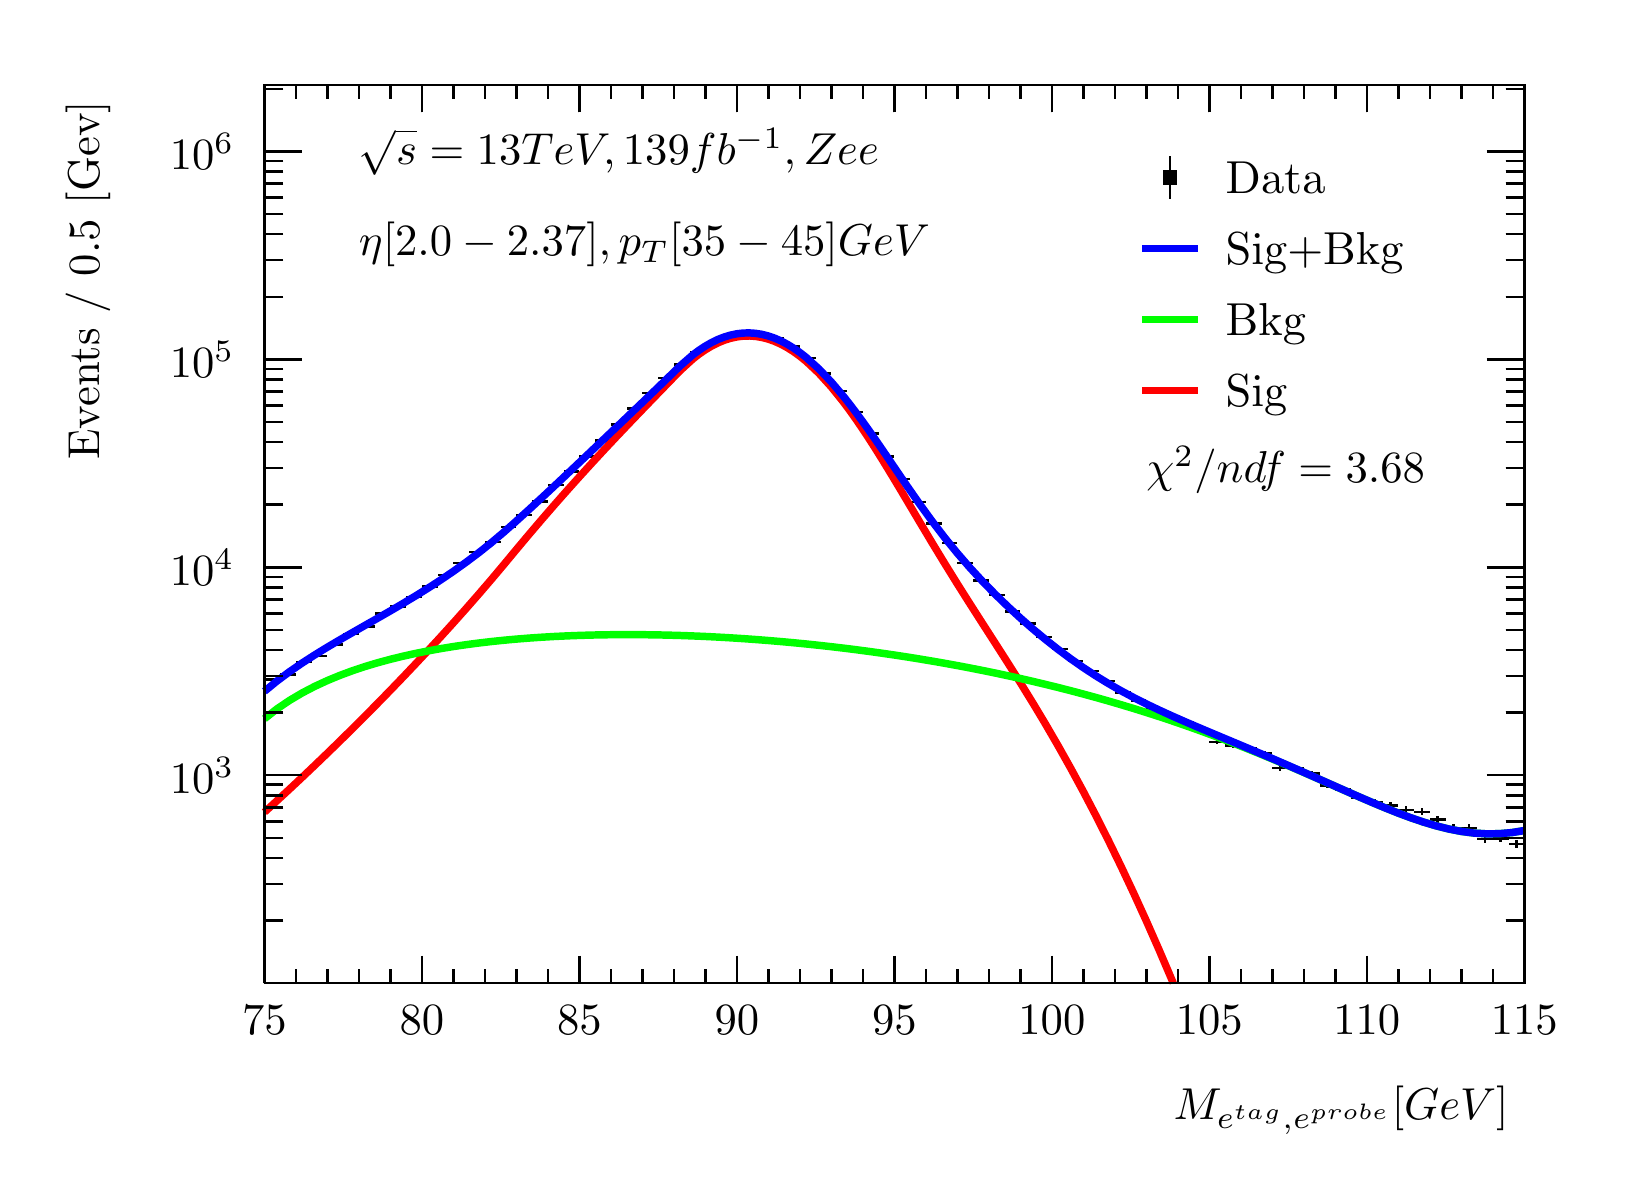
\begin{tikzpicture}
\pgfdeclareplotmark{cross} {
\pgfpathmoveto{\pgfpoint{-0.3\pgfplotmarksize}{\pgfplotmarksize}}
\pgfpathlineto{\pgfpoint{+0.3\pgfplotmarksize}{\pgfplotmarksize}}
\pgfpathlineto{\pgfpoint{+0.3\pgfplotmarksize}{0.3\pgfplotmarksize}}
\pgfpathlineto{\pgfpoint{+1\pgfplotmarksize}{0.3\pgfplotmarksize}}
\pgfpathlineto{\pgfpoint{+1\pgfplotmarksize}{-0.3\pgfplotmarksize}}
\pgfpathlineto{\pgfpoint{+0.3\pgfplotmarksize}{-0.3\pgfplotmarksize}}
\pgfpathlineto{\pgfpoint{+0.3\pgfplotmarksize}{-1.\pgfplotmarksize}}
\pgfpathlineto{\pgfpoint{-0.3\pgfplotmarksize}{-1.\pgfplotmarksize}}
\pgfpathlineto{\pgfpoint{-0.3\pgfplotmarksize}{-0.3\pgfplotmarksize}}
\pgfpathlineto{\pgfpoint{-1.\pgfplotmarksize}{-0.3\pgfplotmarksize}}
\pgfpathlineto{\pgfpoint{-1.\pgfplotmarksize}{0.3\pgfplotmarksize}}
\pgfpathlineto{\pgfpoint{-0.3\pgfplotmarksize}{0.3\pgfplotmarksize}}
\pgfpathclose
\pgfusepathqstroke
}
\pgfdeclareplotmark{cross*} {
\pgfpathmoveto{\pgfpoint{-0.3\pgfplotmarksize}{\pgfplotmarksize}}
\pgfpathlineto{\pgfpoint{+0.3\pgfplotmarksize}{\pgfplotmarksize}}
\pgfpathlineto{\pgfpoint{+0.3\pgfplotmarksize}{0.3\pgfplotmarksize}}
\pgfpathlineto{\pgfpoint{+1\pgfplotmarksize}{0.3\pgfplotmarksize}}
\pgfpathlineto{\pgfpoint{+1\pgfplotmarksize}{-0.3\pgfplotmarksize}}
\pgfpathlineto{\pgfpoint{+0.3\pgfplotmarksize}{-0.3\pgfplotmarksize}}
\pgfpathlineto{\pgfpoint{+0.3\pgfplotmarksize}{-1.\pgfplotmarksize}}
\pgfpathlineto{\pgfpoint{-0.3\pgfplotmarksize}{-1.\pgfplotmarksize}}
\pgfpathlineto{\pgfpoint{-0.3\pgfplotmarksize}{-0.3\pgfplotmarksize}}
\pgfpathlineto{\pgfpoint{-1.\pgfplotmarksize}{-0.3\pgfplotmarksize}}
\pgfpathlineto{\pgfpoint{-1.\pgfplotmarksize}{0.3\pgfplotmarksize}}
\pgfpathlineto{\pgfpoint{-0.3\pgfplotmarksize}{0.3\pgfplotmarksize}}
\pgfpathclose
\pgfusepathqfillstroke
}
\pgfdeclareplotmark{newstar} {
\pgfpathmoveto{\pgfqpoint{0pt}{\pgfplotmarksize}}
\pgfpathlineto{\pgfqpointpolar{44}{0.5\pgfplotmarksize}}
\pgfpathlineto{\pgfqpointpolar{18}{\pgfplotmarksize}}
\pgfpathlineto{\pgfqpointpolar{-20}{0.5\pgfplotmarksize}}
\pgfpathlineto{\pgfqpointpolar{-54}{\pgfplotmarksize}}
\pgfpathlineto{\pgfqpointpolar{-90}{0.5\pgfplotmarksize}}
\pgfpathlineto{\pgfqpointpolar{234}{\pgfplotmarksize}}
\pgfpathlineto{\pgfqpointpolar{198}{0.5\pgfplotmarksize}}
\pgfpathlineto{\pgfqpointpolar{162}{\pgfplotmarksize}}
\pgfpathlineto{\pgfqpointpolar{134}{0.5\pgfplotmarksize}}
\pgfpathclose
\pgfusepathqstroke
}
\pgfdeclareplotmark{newstar*} {
\pgfpathmoveto{\pgfqpoint{0pt}{\pgfplotmarksize}}
\pgfpathlineto{\pgfqpointpolar{44}{0.5\pgfplotmarksize}}
\pgfpathlineto{\pgfqpointpolar{18}{\pgfplotmarksize}}
\pgfpathlineto{\pgfqpointpolar{-20}{0.5\pgfplotmarksize}}
\pgfpathlineto{\pgfqpointpolar{-54}{\pgfplotmarksize}}
\pgfpathlineto{\pgfqpointpolar{-90}{0.5\pgfplotmarksize}}
\pgfpathlineto{\pgfqpointpolar{234}{\pgfplotmarksize}}
\pgfpathlineto{\pgfqpointpolar{198}{0.5\pgfplotmarksize}}
\pgfpathlineto{\pgfqpointpolar{162}{\pgfplotmarksize}}
\pgfpathlineto{\pgfqpointpolar{134}{0.5\pgfplotmarksize}}
\pgfpathclose
\pgfusepathqfillstroke
}
\definecolor{c}{rgb}{1,1,1};
\draw [color=c, fill=c] (0,0) rectangle (20,14.4361);
\draw [color=c, fill=c] (3,2.30977) rectangle (19,13.7143);
\definecolor{c}{rgb}{0,0,0};
\draw [c,line width=0.9] (3,2.30977) -- (3,13.7143) -- (19,13.7143) -- (19,2.30977) -- (3,2.30977);
\definecolor{c}{rgb}{1,1,1};
\draw [color=c, fill=c] (3,2.30977) rectangle (19,13.7143);
\definecolor{c}{rgb}{0,0,0};
\draw [c,line width=0.9] (3,2.30977) -- (3,13.7143) -- (19,13.7143) -- (19,2.30977) -- (3,2.30977);
\draw [c,line width=0.9] (3,2.30977) -- (19,2.30977);
\draw [c,line width=0.9] (3,2.65624) -- (3,2.30977);
\draw [c,line width=0.9] (3.4,2.48301) -- (3.4,2.30977);
\draw [c,line width=0.9] (3.8,2.48301) -- (3.8,2.30977);
\draw [c,line width=0.9] (4.2,2.48301) -- (4.2,2.30977);
\draw [c,line width=0.9] (4.6,2.48301) -- (4.6,2.30977);
\draw [c,line width=0.9] (5,2.65624) -- (5,2.30977);
\draw [c,line width=0.9] (5.4,2.48301) -- (5.4,2.30977);
\draw [c,line width=0.9] (5.8,2.48301) -- (5.8,2.30977);
\draw [c,line width=0.9] (6.2,2.48301) -- (6.2,2.30977);
\draw [c,line width=0.9] (6.6,2.48301) -- (6.6,2.30977);
\draw [c,line width=0.9] (7,2.65624) -- (7,2.30977);
\draw [c,line width=0.9] (7.4,2.48301) -- (7.4,2.30977);
\draw [c,line width=0.9] (7.8,2.48301) -- (7.8,2.30977);
\draw [c,line width=0.9] (8.2,2.48301) -- (8.2,2.30977);
\draw [c,line width=0.9] (8.6,2.48301) -- (8.6,2.30977);
\draw [c,line width=0.9] (9,2.65624) -- (9,2.30977);
\draw [c,line width=0.9] (9.4,2.48301) -- (9.4,2.30977);
\draw [c,line width=0.9] (9.8,2.48301) -- (9.8,2.30977);
\draw [c,line width=0.9] (10.2,2.48301) -- (10.2,2.30977);
\draw [c,line width=0.9] (10.6,2.48301) -- (10.6,2.30977);
\draw [c,line width=0.9] (11,2.65624) -- (11,2.30977);
\draw [c,line width=0.9] (11.4,2.48301) -- (11.4,2.30977);
\draw [c,line width=0.9] (11.8,2.48301) -- (11.8,2.30977);
\draw [c,line width=0.9] (12.2,2.48301) -- (12.2,2.30977);
\draw [c,line width=0.9] (12.6,2.48301) -- (12.6,2.30977);
\draw [c,line width=0.9] (13,2.65624) -- (13,2.30977);
\draw [c,line width=0.9] (13.4,2.48301) -- (13.4,2.30977);
\draw [c,line width=0.9] (13.8,2.48301) -- (13.8,2.30977);
\draw [c,line width=0.9] (14.2,2.48301) -- (14.2,2.30977);
\draw [c,line width=0.9] (14.6,2.48301) -- (14.6,2.30977);
\draw [c,line width=0.9] (15,2.65624) -- (15,2.30977);
\draw [c,line width=0.9] (15.4,2.48301) -- (15.4,2.30977);
\draw [c,line width=0.9] (15.8,2.48301) -- (15.8,2.30977);
\draw [c,line width=0.9] (16.2,2.48301) -- (16.2,2.30977);
\draw [c,line width=0.9] (16.6,2.48301) -- (16.6,2.30977);
\draw [c,line width=0.9] (17,2.65624) -- (17,2.30977);
\draw [c,line width=0.9] (17.4,2.48301) -- (17.4,2.30977);
\draw [c,line width=0.9] (17.8,2.48301) -- (17.8,2.30977);
\draw [c,line width=0.9] (18.2,2.48301) -- (18.2,2.30977);
\draw [c,line width=0.9] (18.6,2.48301) -- (18.6,2.30977);
\draw [c,line width=0.9] (19,2.65624) -- (19,2.30977);
\draw [c,line width=0.9] (19,2.65624) -- (19,2.30977);
\draw [anchor=base] (3,1.66015) node[scale=1.61424, color=c, rotate=0]{75};
\draw [anchor=base] (5,1.66015) node[scale=1.61424, color=c, rotate=0]{80};
\draw [anchor=base] (7,1.66015) node[scale=1.61424, color=c, rotate=0]{85};
\draw [anchor=base] (9,1.66015) node[scale=1.61424, color=c, rotate=0]{90};
\draw [anchor=base] (11,1.66015) node[scale=1.61424, color=c, rotate=0]{95};
\draw [anchor=base] (13,1.66015) node[scale=1.61424, color=c, rotate=0]{100};
\draw [anchor=base] (15,1.66015) node[scale=1.61424, color=c, rotate=0]{105};
\draw [anchor=base] (17,1.66015) node[scale=1.61424, color=c, rotate=0]{110};
\draw [anchor=base] (19,1.66015) node[scale=1.61424, color=c, rotate=0]{115};
\draw [anchor= east] (19,0.692932) node[scale=1.61424, color=c, rotate=0]{$M_{e^{tag}, e^{probe}}  [GeV]$};
\draw [c,line width=0.9] (3,13.7143) -- (19,13.7143);
\draw [c,line width=0.9] (3,13.3678) -- (3,13.7143);
\draw [c,line width=0.9] (3.4,13.5411) -- (3.4,13.7143);
\draw [c,line width=0.9] (3.8,13.5411) -- (3.8,13.7143);
\draw [c,line width=0.9] (4.2,13.5411) -- (4.2,13.7143);
\draw [c,line width=0.9] (4.6,13.5411) -- (4.6,13.7143);
\draw [c,line width=0.9] (5,13.3678) -- (5,13.7143);
\draw [c,line width=0.9] (5.4,13.5411) -- (5.4,13.7143);
\draw [c,line width=0.9] (5.8,13.5411) -- (5.8,13.7143);
\draw [c,line width=0.9] (6.2,13.5411) -- (6.2,13.7143);
\draw [c,line width=0.9] (6.6,13.5411) -- (6.6,13.7143);
\draw [c,line width=0.9] (7,13.3678) -- (7,13.7143);
\draw [c,line width=0.9] (7.4,13.5411) -- (7.4,13.7143);
\draw [c,line width=0.9] (7.8,13.5411) -- (7.8,13.7143);
\draw [c,line width=0.9] (8.2,13.5411) -- (8.2,13.7143);
\draw [c,line width=0.9] (8.6,13.5411) -- (8.6,13.7143);
\draw [c,line width=0.9] (9,13.3678) -- (9,13.7143);
\draw [c,line width=0.9] (9.4,13.5411) -- (9.4,13.7143);
\draw [c,line width=0.9] (9.8,13.5411) -- (9.8,13.7143);
\draw [c,line width=0.9] (10.2,13.5411) -- (10.2,13.7143);
\draw [c,line width=0.9] (10.6,13.5411) -- (10.6,13.7143);
\draw [c,line width=0.9] (11,13.3678) -- (11,13.7143);
\draw [c,line width=0.9] (11.4,13.5411) -- (11.4,13.7143);
\draw [c,line width=0.9] (11.8,13.5411) -- (11.8,13.7143);
\draw [c,line width=0.9] (12.2,13.5411) -- (12.2,13.7143);
\draw [c,line width=0.9] (12.6,13.5411) -- (12.6,13.7143);
\draw [c,line width=0.9] (13,13.3678) -- (13,13.7143);
\draw [c,line width=0.9] (13.4,13.5411) -- (13.4,13.7143);
\draw [c,line width=0.9] (13.8,13.5411) -- (13.8,13.7143);
\draw [c,line width=0.9] (14.2,13.5411) -- (14.2,13.7143);
\draw [c,line width=0.9] (14.6,13.5411) -- (14.6,13.7143);
\draw [c,line width=0.9] (15,13.3678) -- (15,13.7143);
\draw [c,line width=0.9] (15.4,13.5411) -- (15.4,13.7143);
\draw [c,line width=0.9] (15.8,13.5411) -- (15.8,13.7143);
\draw [c,line width=0.9] (16.2,13.5411) -- (16.2,13.7143);
\draw [c,line width=0.9] (16.6,13.5411) -- (16.6,13.7143);
\draw [c,line width=0.9] (17,13.3678) -- (17,13.7143);
\draw [c,line width=0.9] (17.4,13.5411) -- (17.4,13.7143);
\draw [c,line width=0.9] (17.8,13.5411) -- (17.8,13.7143);
\draw [c,line width=0.9] (18.2,13.5411) -- (18.2,13.7143);
\draw [c,line width=0.9] (18.6,13.5411) -- (18.6,13.7143);
\draw [c,line width=0.9] (19,13.3678) -- (19,13.7143);
\draw [c,line width=0.9] (19,13.3678) -- (19,13.7143);
\draw [c,line width=0.9] (3,2.30977) -- (3,13.7143);
\draw [c,line width=0.9] (3.237,3.10453) -- (3,3.10453);
\draw [c,line width=0.9] (3.237,3.56943) -- (3,3.56943);
\draw [c,line width=0.9] (3.237,3.89929) -- (3,3.89929);
\draw [c,line width=0.9] (3.237,4.15514) -- (3,4.15514);
\draw [c,line width=0.9] (3.237,4.36419) -- (3,4.36419);
\draw [c,line width=0.9] (3.237,4.54094) -- (3,4.54094);
\draw [c,line width=0.9] (3.237,4.69404) -- (3,4.69404);
\draw [c,line width=0.9] (3.237,4.82909) -- (3,4.82909);
\draw [c,line width=0.9] (3.474,4.9499) -- (3,4.9499);
\draw [anchor= east] (2.82,4.9499) node[scale=1.61424, color=c, rotate=0]{$10^{3}$};
\draw [c,line width=0.9] (3.237,5.74466) -- (3,5.74466);
\draw [c,line width=0.9] (3.237,6.20956) -- (3,6.20956);
\draw [c,line width=0.9] (3.237,6.53941) -- (3,6.53941);
\draw [c,line width=0.9] (3.237,6.79527) -- (3,6.79527);
\draw [c,line width=0.9] (3.237,7.00432) -- (3,7.00432);
\draw [c,line width=0.9] (3.237,7.18106) -- (3,7.18106);
\draw [c,line width=0.9] (3.237,7.33417) -- (3,7.33417);
\draw [c,line width=0.9] (3.237,7.46922) -- (3,7.46922);
\draw [c,line width=0.9] (3.474,7.59002) -- (3,7.59002);
\draw [anchor= east] (2.82,7.59002) node[scale=1.61424, color=c, rotate=0]{$10^{4}$};
\draw [c,line width=0.9] (3.237,8.38478) -- (3,8.38478);
\draw [c,line width=0.9] (3.237,8.84968) -- (3,8.84968);
\draw [c,line width=0.9] (3.237,9.17954) -- (3,9.17954);
\draw [c,line width=0.9] (3.237,9.43539) -- (3,9.43539);
\draw [c,line width=0.9] (3.237,9.64444) -- (3,9.64444);
\draw [c,line width=0.9] (3.237,9.82119) -- (3,9.82119);
\draw [c,line width=0.9] (3.237,9.9743) -- (3,9.9743);
\draw [c,line width=0.9] (3.237,10.1093) -- (3,10.1093);
\draw [c,line width=0.9] (3.474,10.2302) -- (3,10.2302);
\draw [anchor= east] (2.82,10.2302) node[scale=1.61424, color=c, rotate=0]{$10^{5}$};
\draw [c,line width=0.9] (3.237,11.0249) -- (3,11.0249);
\draw [c,line width=0.9] (3.237,11.4898) -- (3,11.4898);
\draw [c,line width=0.9] (3.237,11.8197) -- (3,11.8197);
\draw [c,line width=0.9] (3.237,12.0755) -- (3,12.0755);
\draw [c,line width=0.9] (3.237,12.2846) -- (3,12.2846);
\draw [c,line width=0.9] (3.237,12.4613) -- (3,12.4613);
\draw [c,line width=0.9] (3.237,12.6144) -- (3,12.6144);
\draw [c,line width=0.9] (3.237,12.7495) -- (3,12.7495);
\draw [c,line width=0.9] (3.474,12.8703) -- (3,12.8703);
\draw [anchor= east] (2.82,12.8703) node[scale=1.61424, color=c, rotate=0]{$10^{6}$};
\draw [c,line width=0.9] (3.237,13.665) -- (3,13.665);
\draw [anchor= east] (0.76,13.7143) node[scale=1.61424, color=c, rotate=90]{Events / 0.5 [Gev]};
\draw [c,line width=0.9] (19,2.30977) -- (19,13.7143);
\draw [c,line width=0.9] (18.763,3.10453) -- (19,3.10453);
\draw [c,line width=0.9] (18.763,3.56943) -- (19,3.56943);
\draw [c,line width=0.9] (18.763,3.89929) -- (19,3.89929);
\draw [c,line width=0.9] (18.763,4.15514) -- (19,4.15514);
\draw [c,line width=0.9] (18.763,4.36419) -- (19,4.36419);
\draw [c,line width=0.9] (18.763,4.54094) -- (19,4.54094);
\draw [c,line width=0.9] (18.763,4.69404) -- (19,4.69404);
\draw [c,line width=0.9] (18.763,4.82909) -- (19,4.82909);
\draw [c,line width=0.9] (18.526,4.9499) -- (19,4.9499);
\draw [c,line width=0.9] (18.763,5.74466) -- (19,5.74466);
\draw [c,line width=0.9] (18.763,6.20956) -- (19,6.20956);
\draw [c,line width=0.9] (18.763,6.53941) -- (19,6.53941);
\draw [c,line width=0.9] (18.763,6.79527) -- (19,6.79527);
\draw [c,line width=0.9] (18.763,7.00432) -- (19,7.00432);
\draw [c,line width=0.9] (18.763,7.18106) -- (19,7.18106);
\draw [c,line width=0.9] (18.763,7.33417) -- (19,7.33417);
\draw [c,line width=0.9] (18.763,7.46922) -- (19,7.46922);
\draw [c,line width=0.9] (18.526,7.59002) -- (19,7.59002);
\draw [c,line width=0.9] (18.763,8.38478) -- (19,8.38478);
\draw [c,line width=0.9] (18.763,8.84968) -- (19,8.84968);
\draw [c,line width=0.9] (18.763,9.17954) -- (19,9.17954);
\draw [c,line width=0.9] (18.763,9.43539) -- (19,9.43539);
\draw [c,line width=0.9] (18.763,9.64444) -- (19,9.64444);
\draw [c,line width=0.9] (18.763,9.82119) -- (19,9.82119);
\draw [c,line width=0.9] (18.763,9.9743) -- (19,9.9743);
\draw [c,line width=0.9] (18.763,10.1093) -- (19,10.1093);
\draw [c,line width=0.9] (18.526,10.2302) -- (19,10.2302);
\draw [c,line width=0.9] (18.763,11.0249) -- (19,11.0249);
\draw [c,line width=0.9] (18.763,11.4898) -- (19,11.4898);
\draw [c,line width=0.9] (18.763,11.8197) -- (19,11.8197);
\draw [c,line width=0.9] (18.763,12.0755) -- (19,12.0755);
\draw [c,line width=0.9] (18.763,12.2846) -- (19,12.2846);
\draw [c,line width=0.9] (18.763,12.4613) -- (19,12.4613);
\draw [c,line width=0.9] (18.763,12.6144) -- (19,12.6144);
\draw [c,line width=0.9] (18.763,12.7495) -- (19,12.7495);
\draw [c,line width=0.9] (18.526,12.8703) -- (19,12.8703);
\draw [c,line width=0.9] (18.763,13.665) -- (19,13.665);
\draw [c,line width=0.9] (3.1,6.16554) -- (3,6.16554);
\draw [c,line width=0.9] (3,6.16554) -- (3,6.16554);
\draw [c,line width=0.9] (3.1,6.16554) -- (3.2,6.16554);
\draw [c,line width=0.9] (3.2,6.16554) -- (3.2,6.16554);
\draw [c,line width=0.9] (3.1,6.16554) -- (3.1,6.18688);
\draw [c,line width=0.9] (3.1,6.18688) -- (3.1,6.18688);
\draw [c,line width=0.9] (3.1,6.16554) -- (3.1,6.1442);
\draw [c,line width=0.9] (3.1,6.1442) -- (3.1,6.1442);
\draw [c,line width=0.9] (3.3,6.23114) -- (3.2,6.23114);
\draw [c,line width=0.9] (3.2,6.23114) -- (3.2,6.23114);
\draw [c,line width=0.9] (3.3,6.23114) -- (3.4,6.23114);
\draw [c,line width=0.9] (3.4,6.23114) -- (3.4,6.23114);
\draw [c,line width=0.9] (3.3,6.23114) -- (3.3,6.25188);
\draw [c,line width=0.9] (3.3,6.25188) -- (3.3,6.25188);
\draw [c,line width=0.9] (3.3,6.23114) -- (3.3,6.2104);
\draw [c,line width=0.9] (3.3,6.2104) -- (3.3,6.2104);
\draw [c,line width=0.9] (3.5,6.38762) -- (3.4,6.38762);
\draw [c,line width=0.9] (3.4,6.38762) -- (3.4,6.38762);
\draw [c,line width=0.9] (3.5,6.38762) -- (3.6,6.38762);
\draw [c,line width=0.9] (3.6,6.38762) -- (3.6,6.38762);
\draw [c,line width=0.9] (3.5,6.38762) -- (3.5,6.40699);
\draw [c,line width=0.9] (3.5,6.40699) -- (3.5,6.40699);
\draw [c,line width=0.9] (3.5,6.38762) -- (3.5,6.36825);
\draw [c,line width=0.9] (3.5,6.36825) -- (3.5,6.36825);
\draw [c,line width=0.9] (3.7,6.46358) -- (3.6,6.46358);
\draw [c,line width=0.9] (3.6,6.46358) -- (3.6,6.46358);
\draw [c,line width=0.9] (3.7,6.46358) -- (3.8,6.46358);
\draw [c,line width=0.9] (3.8,6.46358) -- (3.8,6.46358);
\draw [c,line width=0.9] (3.7,6.46358) -- (3.7,6.48232);
\draw [c,line width=0.9] (3.7,6.48232) -- (3.7,6.48232);
\draw [c,line width=0.9] (3.7,6.46358) -- (3.7,6.44484);
\draw [c,line width=0.9] (3.7,6.44484) -- (3.7,6.44484);
\draw [c,line width=0.9] (3.9,6.61) -- (3.8,6.61);
\draw [c,line width=0.9] (3.8,6.61) -- (3.8,6.61);
\draw [c,line width=0.9] (3.9,6.61) -- (4,6.61);
\draw [c,line width=0.9] (4,6.61) -- (4,6.61);
\draw [c,line width=0.9] (3.9,6.61) -- (3.9,6.62758);
\draw [c,line width=0.9] (3.9,6.62758) -- (3.9,6.62758);
\draw [c,line width=0.9] (3.9,6.61) -- (3.9,6.59243);
\draw [c,line width=0.9] (3.9,6.59243) -- (3.9,6.59243);
\draw [c,line width=0.9] (4.1,6.74224) -- (4,6.74224);
\draw [c,line width=0.9] (4,6.74224) -- (4,6.74224);
\draw [c,line width=0.9] (4.1,6.74224) -- (4.2,6.74224);
\draw [c,line width=0.9] (4.2,6.74224) -- (4.2,6.74224);
\draw [c,line width=0.9] (4.1,6.74224) -- (4.1,6.75883);
\draw [c,line width=0.9] (4.1,6.75883) -- (4.1,6.75883);
\draw [c,line width=0.9] (4.1,6.74224) -- (4.1,6.72564);
\draw [c,line width=0.9] (4.1,6.72564) -- (4.1,6.72564);
\draw [c,line width=0.9] (4.3,6.83671) -- (4.2,6.83671);
\draw [c,line width=0.9] (4.2,6.83671) -- (4.2,6.83671);
\draw [c,line width=0.9] (4.3,6.83671) -- (4.4,6.83671);
\draw [c,line width=0.9] (4.4,6.83671) -- (4.4,6.83671);
\draw [c,line width=0.9] (4.3,6.83671) -- (4.3,6.85263);
\draw [c,line width=0.9] (4.3,6.85263) -- (4.3,6.85263);
\draw [c,line width=0.9] (4.3,6.83671) -- (4.3,6.82078);
\draw [c,line width=0.9] (4.3,6.82078) -- (4.3,6.82078);
\draw [c,line width=0.9] (4.5,7.00106) -- (4.4,7.00106);
\draw [c,line width=0.9] (4.4,7.00106) -- (4.4,7.00106);
\draw [c,line width=0.9] (4.5,7.00106) -- (4.6,7.00106);
\draw [c,line width=0.9] (4.6,7.00106) -- (4.6,7.00106);
\draw [c,line width=0.9] (4.5,7.00106) -- (4.5,7.01589);
\draw [c,line width=0.9] (4.5,7.01589) -- (4.5,7.01589);
\draw [c,line width=0.9] (4.5,7.00106) -- (4.5,6.98624);
\draw [c,line width=0.9] (4.5,6.98624) -- (4.5,6.98624);
\draw [c,line width=0.9] (4.7,7.08973) -- (4.6,7.08973);
\draw [c,line width=0.9] (4.6,7.08973) -- (4.6,7.08973);
\draw [c,line width=0.9] (4.7,7.08973) -- (4.8,7.08973);
\draw [c,line width=0.9] (4.8,7.08973) -- (4.8,7.08973);
\draw [c,line width=0.9] (4.7,7.08973) -- (4.7,7.10399);
\draw [c,line width=0.9] (4.7,7.10399) -- (4.7,7.10399);
\draw [c,line width=0.9] (4.7,7.08973) -- (4.7,7.07546);
\draw [c,line width=0.9] (4.7,7.07546) -- (4.7,7.07546);
\draw [c,line width=0.9] (4.9,7.21113) -- (4.8,7.21113);
\draw [c,line width=0.9] (4.8,7.21113) -- (4.8,7.21113);
\draw [c,line width=0.9] (4.9,7.21113) -- (5,7.21113);
\draw [c,line width=0.9] (5,7.21113) -- (5,7.21113);
\draw [c,line width=0.9] (4.9,7.21113) -- (4.9,7.22466);
\draw [c,line width=0.9] (4.9,7.22466) -- (4.9,7.22466);
\draw [c,line width=0.9] (4.9,7.21113) -- (4.9,7.19761);
\draw [c,line width=0.9] (4.9,7.19761) -- (4.9,7.19761);
\draw [c,line width=0.9] (5.1,7.34359) -- (5,7.34359);
\draw [c,line width=0.9] (5,7.34359) -- (5,7.34359);
\draw [c,line width=0.9] (5.1,7.34359) -- (5.2,7.34359);
\draw [c,line width=0.9] (5.2,7.34359) -- (5.2,7.34359);
\draw [c,line width=0.9] (5.1,7.34359) -- (5.1,7.35636);
\draw [c,line width=0.9] (5.1,7.35636) -- (5.1,7.35636);
\draw [c,line width=0.9] (5.1,7.34359) -- (5.1,7.33083);
\draw [c,line width=0.9] (5.1,7.33083) -- (5.1,7.33083);
\draw [c,line width=0.9] (5.3,7.49143) -- (5.2,7.49143);
\draw [c,line width=0.9] (5.2,7.49143) -- (5.2,7.49143);
\draw [c,line width=0.9] (5.3,7.49143) -- (5.4,7.49143);
\draw [c,line width=0.9] (5.4,7.49143) -- (5.4,7.49143);
\draw [c,line width=0.9] (5.3,7.49143) -- (5.3,7.5034);
\draw [c,line width=0.9] (5.3,7.5034) -- (5.3,7.5034);
\draw [c,line width=0.9] (5.3,7.49143) -- (5.3,7.47946);
\draw [c,line width=0.9] (5.3,7.47946) -- (5.3,7.47946);
\draw [c,line width=0.9] (5.5,7.64269) -- (5.4,7.64269);
\draw [c,line width=0.9] (5.4,7.64269) -- (5.4,7.64269);
\draw [c,line width=0.9] (5.5,7.64269) -- (5.6,7.64269);
\draw [c,line width=0.9] (5.6,7.64269) -- (5.6,7.64269);
\draw [c,line width=0.9] (5.5,7.64269) -- (5.5,7.65389);
\draw [c,line width=0.9] (5.5,7.65389) -- (5.5,7.65389);
\draw [c,line width=0.9] (5.5,7.64269) -- (5.5,7.63148);
\draw [c,line width=0.9] (5.5,7.63148) -- (5.5,7.63148);
\draw [c,line width=0.9] (5.7,7.78601) -- (5.6,7.78601);
\draw [c,line width=0.9] (5.6,7.78601) -- (5.6,7.78601);
\draw [c,line width=0.9] (5.7,7.78601) -- (5.8,7.78601);
\draw [c,line width=0.9] (5.8,7.78601) -- (5.8,7.78601);
\draw [c,line width=0.9] (5.7,7.78601) -- (5.7,7.79653);
\draw [c,line width=0.9] (5.7,7.79653) -- (5.7,7.79653);
\draw [c,line width=0.9] (5.7,7.78601) -- (5.7,7.77548);
\draw [c,line width=0.9] (5.7,7.77548) -- (5.7,7.77548);
\draw [c,line width=0.9] (5.9,7.91027) -- (5.8,7.91027);
\draw [c,line width=0.9] (5.8,7.91027) -- (5.8,7.91027);
\draw [c,line width=0.9] (5.9,7.91027) -- (6,7.91027);
\draw [c,line width=0.9] (6,7.91027) -- (6,7.91027);
\draw [c,line width=0.9] (5.9,7.91027) -- (5.9,7.92024);
\draw [c,line width=0.9] (5.9,7.92024) -- (5.9,7.92024);
\draw [c,line width=0.9] (5.9,7.91027) -- (5.9,7.90029);
\draw [c,line width=0.9] (5.9,7.90029) -- (5.9,7.90029);
\draw [c,line width=0.9] (6.1,8.10174) -- (6,8.10174);
\draw [c,line width=0.9] (6,8.10174) -- (6,8.10174);
\draw [c,line width=0.9] (6.1,8.10174) -- (6.2,8.10174);
\draw [c,line width=0.9] (6.2,8.10174) -- (6.2,8.10174);
\draw [c,line width=0.9] (6.1,8.10174) -- (6.1,8.11091);
\draw [c,line width=0.9] (6.1,8.11091) -- (6.1,8.11091);
\draw [c,line width=0.9] (6.1,8.10174) -- (6.1,8.09256);
\draw [c,line width=0.9] (6.1,8.09256) -- (6.1,8.09256);
\draw [c,line width=0.9] (6.3,8.25142) -- (6.2,8.25142);
\draw [c,line width=0.9] (6.2,8.25142) -- (6.2,8.25142);
\draw [c,line width=0.9] (6.3,8.25142) -- (6.4,8.25142);
\draw [c,line width=0.9] (6.4,8.25142) -- (6.4,8.25142);
\draw [c,line width=0.9] (6.3,8.25142) -- (6.3,8.26002);
\draw [c,line width=0.9] (6.3,8.26002) -- (6.3,8.26002);
\draw [c,line width=0.9] (6.3,8.25142) -- (6.3,8.24283);
\draw [c,line width=0.9] (6.3,8.24283) -- (6.3,8.24283);
\draw [c,line width=0.9] (6.5,8.42428) -- (6.4,8.42428);
\draw [c,line width=0.9] (6.4,8.42428) -- (6.4,8.42428);
\draw [c,line width=0.9] (6.5,8.42428) -- (6.6,8.42428);
\draw [c,line width=0.9] (6.6,8.42428) -- (6.6,8.42428);
\draw [c,line width=0.9] (6.5,8.42428) -- (6.5,8.43225);
\draw [c,line width=0.9] (6.5,8.43225) -- (6.5,8.43225);
\draw [c,line width=0.9] (6.5,8.42428) -- (6.5,8.41631);
\draw [c,line width=0.9] (6.5,8.41631) -- (6.5,8.41631);
\draw [c,line width=0.9] (6.7,8.63244) -- (6.6,8.63244);
\draw [c,line width=0.9] (6.6,8.63244) -- (6.6,8.63244);
\draw [c,line width=0.9] (6.7,8.63244) -- (6.8,8.63244);
\draw [c,line width=0.9] (6.8,8.63244) -- (6.8,8.63244);
\draw [c,line width=0.9] (6.7,8.63244) -- (6.7,8.63972);
\draw [c,line width=0.9] (6.7,8.63972) -- (6.7,8.63972);
\draw [c,line width=0.9] (6.7,8.63244) -- (6.7,8.62517);
\draw [c,line width=0.9] (6.7,8.62517) -- (6.7,8.62517);
\draw [c,line width=0.9] (6.9,8.8086) -- (6.8,8.8086);
\draw [c,line width=0.9] (6.8,8.8086) -- (6.8,8.8086);
\draw [c,line width=0.9] (6.9,8.8086) -- (7,8.8086);
\draw [c,line width=0.9] (7,8.8086) -- (7,8.8086);
\draw [c,line width=0.9] (6.9,8.8086) -- (6.9,8.81534);
\draw [c,line width=0.9] (6.9,8.81534) -- (6.9,8.81534);
\draw [c,line width=0.9] (6.9,8.8086) -- (6.9,8.80186);
\draw [c,line width=0.9] (6.9,8.80186) -- (6.9,8.80186);
\draw [c,line width=0.9] (7.1,8.99643) -- (7,8.99643);
\draw [c,line width=0.9] (7,8.99643) -- (7,8.99643);
\draw [c,line width=0.9] (7.1,8.99643) -- (7.2,8.99643);
\draw [c,line width=0.9] (7.2,8.99643) -- (7.2,8.99643);
\draw [c,line width=0.9] (7.1,8.99643) -- (7.1,9.00264);
\draw [c,line width=0.9] (7.1,9.00264) -- (7.1,9.00264);
\draw [c,line width=0.9] (7.1,8.99643) -- (7.1,8.99022);
\draw [c,line width=0.9] (7.1,8.99022) -- (7.1,8.99022);
\draw [c,line width=0.9] (7.3,9.20188) -- (7.2,9.20188);
\draw [c,line width=0.9] (7.2,9.20188) -- (7.2,9.20188);
\draw [c,line width=0.9] (7.3,9.20188) -- (7.4,9.20188);
\draw [c,line width=0.9] (7.4,9.20188) -- (7.4,9.20188);
\draw [c,line width=0.9] (7.3,9.20188) -- (7.3,9.20756);
\draw [c,line width=0.9] (7.3,9.20756) -- (7.3,9.20756);
\draw [c,line width=0.9] (7.3,9.20188) -- (7.3,9.1962);
\draw [c,line width=0.9] (7.3,9.1962) -- (7.3,9.1962);
\draw [c,line width=0.9] (7.5,9.40396) -- (7.4,9.40396);
\draw [c,line width=0.9] (7.4,9.40396) -- (7.4,9.40396);
\draw [c,line width=0.9] (7.5,9.40396) -- (7.6,9.40396);
\draw [c,line width=0.9] (7.6,9.40396) -- (7.6,9.40396);
\draw [c,line width=0.9] (7.5,9.40396) -- (7.5,9.40916);
\draw [c,line width=0.9] (7.5,9.40916) -- (7.5,9.40916);
\draw [c,line width=0.9] (7.5,9.40396) -- (7.5,9.39877);
\draw [c,line width=0.9] (7.5,9.39877) -- (7.5,9.39877);
\draw [c,line width=0.9] (7.7,9.60745) -- (7.6,9.60745);
\draw [c,line width=0.9] (7.6,9.60745) -- (7.6,9.60745);
\draw [c,line width=0.9] (7.7,9.60745) -- (7.8,9.60745);
\draw [c,line width=0.9] (7.8,9.60745) -- (7.8,9.60745);
\draw [c,line width=0.9] (7.7,9.60745) -- (7.7,9.61221);
\draw [c,line width=0.9] (7.7,9.61221) -- (7.7,9.61221);
\draw [c,line width=0.9] (7.7,9.60745) -- (7.7,9.60269);
\draw [c,line width=0.9] (7.7,9.60269) -- (7.7,9.60269);
\draw [c,line width=0.9] (7.9,9.80366) -- (7.8,9.80366);
\draw [c,line width=0.9] (7.8,9.80366) -- (7.8,9.80366);
\draw [c,line width=0.9] (7.9,9.80366) -- (8,9.80366);
\draw [c,line width=0.9] (8,9.80366) -- (8,9.80366);
\draw [c,line width=0.9] (7.9,9.80366) -- (7.9,9.80803);
\draw [c,line width=0.9] (7.9,9.80803) -- (7.9,9.80803);
\draw [c,line width=0.9] (7.9,9.80366) -- (7.9,9.7993);
\draw [c,line width=0.9] (7.9,9.7993) -- (7.9,9.7993);
\draw [c,line width=0.9] (8.1,9.99243) -- (8,9.99243);
\draw [c,line width=0.9] (8,9.99243) -- (8,9.99243);
\draw [c,line width=0.9] (8.1,9.99243) -- (8.2,9.99243);
\draw [c,line width=0.9] (8.2,9.99243) -- (8.2,9.99243);
\draw [c,line width=0.9] (8.1,9.99243) -- (8.1,9.99645);
\draw [c,line width=0.9] (8.1,9.99645) -- (8.1,9.99645);
\draw [c,line width=0.9] (8.1,9.99243) -- (8.1,9.98841);
\draw [c,line width=0.9] (8.1,9.98841) -- (8.1,9.98841);
\draw [c,line width=0.9] (8.3,10.1645) -- (8.2,10.1645);
\draw [c,line width=0.9] (8.2,10.1645) -- (8.2,10.1645);
\draw [c,line width=0.9] (8.3,10.1645) -- (8.4,10.1645);
\draw [c,line width=0.9] (8.4,10.1645) -- (8.4,10.1645);
\draw [c,line width=0.9] (8.3,10.1645) -- (8.3,10.1682);
\draw [c,line width=0.9] (8.3,10.1682) -- (8.3,10.1682);
\draw [c,line width=0.9] (8.3,10.1645) -- (8.3,10.1607);
\draw [c,line width=0.9] (8.3,10.1607) -- (8.3,10.1607);
\draw [c,line width=0.9] (8.5,10.325) -- (8.4,10.325);
\draw [c,line width=0.9] (8.4,10.325) -- (8.4,10.325);
\draw [c,line width=0.9] (8.5,10.325) -- (8.6,10.325);
\draw [c,line width=0.9] (8.6,10.325) -- (8.6,10.325);
\draw [c,line width=0.9] (8.5,10.325) -- (8.5,10.3285);
\draw [c,line width=0.9] (8.5,10.3285) -- (8.5,10.3285);
\draw [c,line width=0.9] (8.5,10.325) -- (8.5,10.3215);
\draw [c,line width=0.9] (8.5,10.3215) -- (8.5,10.3215);
\draw [c,line width=0.9] (8.7,10.437) -- (8.6,10.437);
\draw [c,line width=0.9] (8.6,10.437) -- (8.6,10.437);
\draw [c,line width=0.9] (8.7,10.437) -- (8.8,10.437);
\draw [c,line width=0.9] (8.8,10.437) -- (8.8,10.437);
\draw [c,line width=0.9] (8.7,10.437) -- (8.7,10.4403);
\draw [c,line width=0.9] (8.7,10.4403) -- (8.7,10.4403);
\draw [c,line width=0.9] (8.7,10.437) -- (8.7,10.4337);
\draw [c,line width=0.9] (8.7,10.4337) -- (8.7,10.4337);
\draw [c,line width=0.9] (8.9,10.5206) -- (8.8,10.5206);
\draw [c,line width=0.9] (8.8,10.5206) -- (8.8,10.5206);
\draw [c,line width=0.9] (8.9,10.5206) -- (9,10.5206);
\draw [c,line width=0.9] (9,10.5206) -- (9,10.5206);
\draw [c,line width=0.9] (8.9,10.5206) -- (8.9,10.5238);
\draw [c,line width=0.9] (8.9,10.5238) -- (8.9,10.5238);
\draw [c,line width=0.9] (8.9,10.5206) -- (8.9,10.5174);
\draw [c,line width=0.9] (8.9,10.5174) -- (8.9,10.5174);
\draw [c,line width=0.9] (9.1,10.5663) -- (9,10.5663);
\draw [c,line width=0.9] (9,10.5663) -- (9,10.5663);
\draw [c,line width=0.9] (9.1,10.5663) -- (9.2,10.5663);
\draw [c,line width=0.9] (9.2,10.5663) -- (9.2,10.5663);
\draw [c,line width=0.9] (9.1,10.5663) -- (9.1,10.5694);
\draw [c,line width=0.9] (9.1,10.5694) -- (9.1,10.5694);
\draw [c,line width=0.9] (9.1,10.5663) -- (9.1,10.5631);
\draw [c,line width=0.9] (9.1,10.5631) -- (9.1,10.5631);
\draw [c,line width=0.9] (9.3,10.5548) -- (9.2,10.5548);
\draw [c,line width=0.9] (9.2,10.5548) -- (9.2,10.5548);
\draw [c,line width=0.9] (9.3,10.5548) -- (9.4,10.5548);
\draw [c,line width=0.9] (9.4,10.5548) -- (9.4,10.5548);
\draw [c,line width=0.9] (9.3,10.5548) -- (9.3,10.5579);
\draw [c,line width=0.9] (9.3,10.5579) -- (9.3,10.5579);
\draw [c,line width=0.9] (9.3,10.5548) -- (9.3,10.5516);
\draw [c,line width=0.9] (9.3,10.5516) -- (9.3,10.5516);
\draw [c,line width=0.9] (9.5,10.4999) -- (9.4,10.4999);
\draw [c,line width=0.9] (9.4,10.4999) -- (9.4,10.4999);
\draw [c,line width=0.9] (9.5,10.4999) -- (9.6,10.4999);
\draw [c,line width=0.9] (9.6,10.4999) -- (9.6,10.4999);
\draw [c,line width=0.9] (9.5,10.4999) -- (9.5,10.5031);
\draw [c,line width=0.9] (9.5,10.5031) -- (9.5,10.5031);
\draw [c,line width=0.9] (9.5,10.4999) -- (9.5,10.4967);
\draw [c,line width=0.9] (9.5,10.4967) -- (9.5,10.4967);
\draw [c,line width=0.9] (9.7,10.3947) -- (9.6,10.3947);
\draw [c,line width=0.9] (9.6,10.3947) -- (9.6,10.3947);
\draw [c,line width=0.9] (9.7,10.3947) -- (9.8,10.3947);
\draw [c,line width=0.9] (9.8,10.3947) -- (9.8,10.3947);
\draw [c,line width=0.9] (9.7,10.3947) -- (9.7,10.3981);
\draw [c,line width=0.9] (9.7,10.3981) -- (9.7,10.3981);
\draw [c,line width=0.9] (9.7,10.3947) -- (9.7,10.3913);
\draw [c,line width=0.9] (9.7,10.3913) -- (9.7,10.3913);
\draw [c,line width=0.9] (9.9,10.2448) -- (9.8,10.2448);
\draw [c,line width=0.9] (9.8,10.2448) -- (9.8,10.2448);
\draw [c,line width=0.9] (9.9,10.2448) -- (10,10.2448);
\draw [c,line width=0.9] (10,10.2448) -- (10,10.2448);
\draw [c,line width=0.9] (9.9,10.2448) -- (9.9,10.2484);
\draw [c,line width=0.9] (9.9,10.2484) -- (9.9,10.2484);
\draw [c,line width=0.9] (9.9,10.2448) -- (9.9,10.2412);
\draw [c,line width=0.9] (9.9,10.2412) -- (9.9,10.2412);
\draw [c,line width=0.9] (10.1,10.0493) -- (10,10.0493);
\draw [c,line width=0.9] (10,10.0493) -- (10,10.0493);
\draw [c,line width=0.9] (10.1,10.0493) -- (10.2,10.0493);
\draw [c,line width=0.9] (10.2,10.0493) -- (10.2,10.0493);
\draw [c,line width=0.9] (10.1,10.0493) -- (10.1,10.0532);
\draw [c,line width=0.9] (10.1,10.0532) -- (10.1,10.0532);
\draw [c,line width=0.9] (10.1,10.0493) -- (10.1,10.0454);
\draw [c,line width=0.9] (10.1,10.0454) -- (10.1,10.0454);
\draw [c,line width=0.9] (10.3,9.82786) -- (10.2,9.82786);
\draw [c,line width=0.9] (10.2,9.82786) -- (10.2,9.82786);
\draw [c,line width=0.9] (10.3,9.82786) -- (10.4,9.82786);
\draw [c,line width=0.9] (10.4,9.82786) -- (10.4,9.82786);
\draw [c,line width=0.9] (10.3,9.82786) -- (10.3,9.83218);
\draw [c,line width=0.9] (10.3,9.83218) -- (10.3,9.83218);
\draw [c,line width=0.9] (10.3,9.82786) -- (10.3,9.82353);
\draw [c,line width=0.9] (10.3,9.82353) -- (10.3,9.82353);
\draw [c,line width=0.9] (10.5,9.56181) -- (10.4,9.56181);
\draw [c,line width=0.9] (10.4,9.56181) -- (10.4,9.56181);
\draw [c,line width=0.9] (10.5,9.56181) -- (10.6,9.56181);
\draw [c,line width=0.9] (10.6,9.56181) -- (10.6,9.56181);
\draw [c,line width=0.9] (10.5,9.56181) -- (10.5,9.56666);
\draw [c,line width=0.9] (10.5,9.56666) -- (10.5,9.56666);
\draw [c,line width=0.9] (10.5,9.56181) -- (10.5,9.55696);
\draw [c,line width=0.9] (10.5,9.55696) -- (10.5,9.55696);
\draw [c,line width=0.9] (10.7,9.2915) -- (10.6,9.2915);
\draw [c,line width=0.9] (10.6,9.2915) -- (10.6,9.2915);
\draw [c,line width=0.9] (10.7,9.2915) -- (10.8,9.2915);
\draw [c,line width=0.9] (10.8,9.2915) -- (10.8,9.2915);
\draw [c,line width=0.9] (10.7,9.2915) -- (10.7,9.29696);
\draw [c,line width=0.9] (10.7,9.29696) -- (10.7,9.29696);
\draw [c,line width=0.9] (10.7,9.2915) -- (10.7,9.28604);
\draw [c,line width=0.9] (10.7,9.28604) -- (10.7,9.28604);
\draw [c,line width=0.9] (10.9,8.99394) -- (10.8,8.99394);
\draw [c,line width=0.9] (10.8,8.99394) -- (10.8,8.99394);
\draw [c,line width=0.9] (10.9,8.99394) -- (11,8.99394);
\draw [c,line width=0.9] (11,8.99394) -- (11,8.99394);
\draw [c,line width=0.9] (10.9,8.99394) -- (10.9,9.00016);
\draw [c,line width=0.9] (10.9,9.00016) -- (10.9,9.00016);
\draw [c,line width=0.9] (10.9,8.99394) -- (10.9,8.98772);
\draw [c,line width=0.9] (10.9,8.98772) -- (10.9,8.98772);
\draw [c,line width=0.9] (11.1,8.71164) -- (11,8.71164);
\draw [c,line width=0.9] (11,8.71164) -- (11,8.71164);
\draw [c,line width=0.9] (11.1,8.71164) -- (11.2,8.71164);
\draw [c,line width=0.9] (11.2,8.71164) -- (11.2,8.71164);
\draw [c,line width=0.9] (11.1,8.71164) -- (11.1,8.71867);
\draw [c,line width=0.9] (11.1,8.71867) -- (11.1,8.71867);
\draw [c,line width=0.9] (11.1,8.71164) -- (11.1,8.70461);
\draw [c,line width=0.9] (11.1,8.70461) -- (11.1,8.70461);
\draw [c,line width=0.9] (11.3,8.42229) -- (11.2,8.42229);
\draw [c,line width=0.9] (11.2,8.42229) -- (11.2,8.42229);
\draw [c,line width=0.9] (11.3,8.42229) -- (11.4,8.42229);
\draw [c,line width=0.9] (11.4,8.42229) -- (11.4,8.42229);
\draw [c,line width=0.9] (11.3,8.42229) -- (11.3,8.43026);
\draw [c,line width=0.9] (11.3,8.43026) -- (11.3,8.43026);
\draw [c,line width=0.9] (11.3,8.42229) -- (11.3,8.41431);
\draw [c,line width=0.9] (11.3,8.41431) -- (11.3,8.41431);
\draw [c,line width=0.9] (11.5,8.14854) -- (11.4,8.14854);
\draw [c,line width=0.9] (11.4,8.14854) -- (11.4,8.14854);
\draw [c,line width=0.9] (11.5,8.14854) -- (11.6,8.14854);
\draw [c,line width=0.9] (11.6,8.14854) -- (11.6,8.14854);
\draw [c,line width=0.9] (11.5,8.14854) -- (11.5,8.15753);
\draw [c,line width=0.9] (11.5,8.15753) -- (11.5,8.15753);
\draw [c,line width=0.9] (11.5,8.14854) -- (11.5,8.13955);
\draw [c,line width=0.9] (11.5,8.13955) -- (11.5,8.13955);
\draw [c,line width=0.9] (11.7,7.89876) -- (11.6,7.89876);
\draw [c,line width=0.9] (11.6,7.89876) -- (11.6,7.89876);
\draw [c,line width=0.9] (11.7,7.89876) -- (11.8,7.89876);
\draw [c,line width=0.9] (11.8,7.89876) -- (11.8,7.89876);
\draw [c,line width=0.9] (11.7,7.89876) -- (11.7,7.90878);
\draw [c,line width=0.9] (11.7,7.90878) -- (11.7,7.90878);
\draw [c,line width=0.9] (11.7,7.89876) -- (11.7,7.88874);
\draw [c,line width=0.9] (11.7,7.88874) -- (11.7,7.88874);
\draw [c,line width=0.9] (11.9,7.644) -- (11.8,7.644);
\draw [c,line width=0.9] (11.8,7.644) -- (11.8,7.644);
\draw [c,line width=0.9] (11.9,7.644) -- (12,7.644);
\draw [c,line width=0.9] (12,7.644) -- (12,7.644);
\draw [c,line width=0.9] (11.9,7.644) -- (11.9,7.6552);
\draw [c,line width=0.9] (11.9,7.6552) -- (11.9,7.6552);
\draw [c,line width=0.9] (11.9,7.644) -- (11.9,7.6328);
\draw [c,line width=0.9] (11.9,7.6328) -- (11.9,7.6328);
\draw [c,line width=0.9] (12.1,7.42295) -- (12,7.42295);
\draw [c,line width=0.9] (12,7.42295) -- (12,7.42295);
\draw [c,line width=0.9] (12.1,7.42295) -- (12.2,7.42295);
\draw [c,line width=0.9] (12.2,7.42295) -- (12.2,7.42295);
\draw [c,line width=0.9] (12.1,7.42295) -- (12.1,7.43528);
\draw [c,line width=0.9] (12.1,7.43528) -- (12.1,7.43528);
\draw [c,line width=0.9] (12.1,7.42295) -- (12.1,7.41061);
\draw [c,line width=0.9] (12.1,7.41061) -- (12.1,7.41061);
\draw [c,line width=0.9] (12.3,7.23794) -- (12.2,7.23794);
\draw [c,line width=0.9] (12.2,7.23794) -- (12.2,7.23794);
\draw [c,line width=0.9] (12.3,7.23794) -- (12.4,7.23794);
\draw [c,line width=0.9] (12.4,7.23794) -- (12.4,7.23794);
\draw [c,line width=0.9] (12.3,7.23794) -- (12.3,7.25131);
\draw [c,line width=0.9] (12.3,7.25131) -- (12.3,7.25131);
\draw [c,line width=0.9] (12.3,7.23794) -- (12.3,7.22457);
\draw [c,line width=0.9] (12.3,7.22457) -- (12.3,7.22457);
\draw [c,line width=0.9] (12.5,7.0274) -- (12.4,7.0274);
\draw [c,line width=0.9] (12.4,7.0274) -- (12.4,7.0274);
\draw [c,line width=0.9] (12.5,7.0274) -- (12.6,7.0274);
\draw [c,line width=0.9] (12.6,7.0274) -- (12.6,7.0274);
\draw [c,line width=0.9] (12.5,7.0274) -- (12.5,7.04205);
\draw [c,line width=0.9] (12.5,7.04205) -- (12.5,7.04205);
\draw [c,line width=0.9] (12.5,7.0274) -- (12.5,7.01274);
\draw [c,line width=0.9] (12.5,7.01274) -- (12.5,7.01274);
\draw [c,line width=0.9] (12.7,6.87883) -- (12.6,6.87883);
\draw [c,line width=0.9] (12.6,6.87883) -- (12.6,6.87883);
\draw [c,line width=0.9] (12.7,6.87883) -- (12.8,6.87883);
\draw [c,line width=0.9] (12.8,6.87883) -- (12.8,6.87883);
\draw [c,line width=0.9] (12.7,6.87883) -- (12.7,6.89447);
\draw [c,line width=0.9] (12.7,6.89447) -- (12.7,6.89447);
\draw [c,line width=0.9] (12.7,6.87883) -- (12.7,6.8632);
\draw [c,line width=0.9] (12.7,6.8632) -- (12.7,6.8632);
\draw [c,line width=0.9] (12.9,6.70662) -- (12.8,6.70662);
\draw [c,line width=0.9] (12.8,6.70662) -- (12.8,6.70662);
\draw [c,line width=0.9] (12.9,6.70662) -- (13,6.70662);
\draw [c,line width=0.9] (13,6.70662) -- (13,6.70662);
\draw [c,line width=0.9] (12.9,6.70662) -- (12.9,6.72348);
\draw [c,line width=0.9] (12.9,6.72348) -- (12.9,6.72348);
\draw [c,line width=0.9] (12.9,6.70662) -- (12.9,6.68977);
\draw [c,line width=0.9] (12.9,6.68977) -- (12.9,6.68977);
\draw [c,line width=0.9] (13.1,6.55536) -- (13,6.55536);
\draw [c,line width=0.9] (13,6.55536) -- (13,6.55536);
\draw [c,line width=0.9] (13.1,6.55536) -- (13.2,6.55536);
\draw [c,line width=0.9] (13.2,6.55536) -- (13.2,6.55536);
\draw [c,line width=0.9] (13.1,6.55536) -- (13.1,6.57336);
\draw [c,line width=0.9] (13.1,6.57336) -- (13.1,6.57336);
\draw [c,line width=0.9] (13.1,6.55536) -- (13.1,6.53735);
\draw [c,line width=0.9] (13.1,6.53735) -- (13.1,6.53735);
\draw [c,line width=0.9] (13.3,6.39837) -- (13.2,6.39837);
\draw [c,line width=0.9] (13.2,6.39837) -- (13.2,6.39837);
\draw [c,line width=0.9] (13.3,6.39837) -- (13.4,6.39837);
\draw [c,line width=0.9] (13.4,6.39837) -- (13.4,6.39837);
\draw [c,line width=0.9] (13.3,6.39837) -- (13.3,6.41764);
\draw [c,line width=0.9] (13.3,6.41764) -- (13.3,6.41764);
\draw [c,line width=0.9] (13.3,6.39837) -- (13.3,6.37909);
\draw [c,line width=0.9] (13.3,6.37909) -- (13.3,6.37909);
\draw [c,line width=0.9] (13.5,6.27276) -- (13.4,6.27276);
\draw [c,line width=0.9] (13.4,6.27276) -- (13.4,6.27276);
\draw [c,line width=0.9] (13.5,6.27276) -- (13.6,6.27276);
\draw [c,line width=0.9] (13.6,6.27276) -- (13.6,6.27276);
\draw [c,line width=0.9] (13.5,6.27276) -- (13.5,6.29312);
\draw [c,line width=0.9] (13.5,6.29312) -- (13.5,6.29312);
\draw [c,line width=0.9] (13.5,6.27276) -- (13.5,6.2524);
\draw [c,line width=0.9] (13.5,6.2524) -- (13.5,6.2524);
\draw [c,line width=0.9] (13.7,6.1451) -- (13.6,6.1451);
\draw [c,line width=0.9] (13.6,6.1451) -- (13.6,6.1451);
\draw [c,line width=0.9] (13.7,6.1451) -- (13.8,6.1451);
\draw [c,line width=0.9] (13.8,6.1451) -- (13.8,6.1451);
\draw [c,line width=0.9] (13.7,6.1451) -- (13.7,6.16663);
\draw [c,line width=0.9] (13.7,6.16663) -- (13.7,6.16663);
\draw [c,line width=0.9] (13.7,6.1451) -- (13.7,6.12357);
\draw [c,line width=0.9] (13.7,6.12357) -- (13.7,6.12357);
\draw [c,line width=0.9] (13.9,5.99776) -- (13.8,5.99776);
\draw [c,line width=0.9] (13.8,5.99776) -- (13.8,5.99776);
\draw [c,line width=0.9] (13.9,5.99776) -- (14,5.99776);
\draw [c,line width=0.9] (14,5.99776) -- (14,5.99776);
\draw [c,line width=0.9] (13.9,5.99776) -- (13.9,6.02072);
\draw [c,line width=0.9] (13.9,6.02072) -- (13.9,6.02072);
\draw [c,line width=0.9] (13.9,5.99776) -- (13.9,5.9748);
\draw [c,line width=0.9] (13.9,5.9748) -- (13.9,5.9748);
\draw [c,line width=0.9] (14.1,5.89941) -- (14,5.89941);
\draw [c,line width=0.9] (14,5.89941) -- (14,5.89941);
\draw [c,line width=0.9] (14.1,5.89941) -- (14.2,5.89941);
\draw [c,line width=0.9] (14.2,5.89941) -- (14.2,5.89941);
\draw [c,line width=0.9] (14.1,5.89941) -- (14.1,5.92338);
\draw [c,line width=0.9] (14.1,5.92338) -- (14.1,5.92338);
\draw [c,line width=0.9] (14.1,5.89941) -- (14.1,5.87545);
\draw [c,line width=0.9] (14.1,5.87545) -- (14.1,5.87545);
\draw [c,line width=0.9] (14.3,5.78797) -- (14.2,5.78797);
\draw [c,line width=0.9] (14.2,5.78797) -- (14.2,5.78797);
\draw [c,line width=0.9] (14.3,5.78797) -- (14.4,5.78797);
\draw [c,line width=0.9] (14.4,5.78797) -- (14.4,5.78797);
\draw [c,line width=0.9] (14.3,5.78797) -- (14.3,5.81313);
\draw [c,line width=0.9] (14.3,5.81313) -- (14.3,5.81313);
\draw [c,line width=0.9] (14.3,5.78797) -- (14.3,5.76281);
\draw [c,line width=0.9] (14.3,5.76281) -- (14.3,5.76281);
\draw [c,line width=0.9] (14.5,5.68524) -- (14.4,5.68524);
\draw [c,line width=0.9] (14.4,5.68524) -- (14.4,5.68524);
\draw [c,line width=0.9] (14.5,5.68524) -- (14.6,5.68524);
\draw [c,line width=0.9] (14.6,5.68524) -- (14.6,5.68524);
\draw [c,line width=0.9] (14.5,5.68524) -- (14.5,5.71155);
\draw [c,line width=0.9] (14.5,5.71155) -- (14.5,5.71155);
\draw [c,line width=0.9] (14.5,5.68524) -- (14.5,5.65893);
\draw [c,line width=0.9] (14.5,5.65893) -- (14.5,5.65893);
\draw [c,line width=0.9] (14.7,5.61874) -- (14.6,5.61874);
\draw [c,line width=0.9] (14.6,5.61874) -- (14.6,5.61874);
\draw [c,line width=0.9] (14.7,5.61874) -- (14.8,5.61874);
\draw [c,line width=0.9] (14.8,5.61874) -- (14.8,5.61874);
\draw [c,line width=0.9] (14.7,5.61874) -- (14.7,5.64583);
\draw [c,line width=0.9] (14.7,5.64583) -- (14.7,5.64583);
\draw [c,line width=0.9] (14.7,5.61874) -- (14.7,5.59166);
\draw [c,line width=0.9] (14.7,5.59166) -- (14.7,5.59166);
\draw [c,line width=0.9] (14.9,5.51502) -- (14.8,5.51502);
\draw [c,line width=0.9] (14.8,5.51502) -- (14.8,5.51502);
\draw [c,line width=0.9] (14.9,5.51502) -- (15,5.51502);
\draw [c,line width=0.9] (15,5.51502) -- (15,5.51502);
\draw [c,line width=0.9] (14.9,5.51502) -- (14.9,5.54335);
\draw [c,line width=0.9] (14.9,5.54335) -- (14.9,5.54335);
\draw [c,line width=0.9] (14.9,5.51502) -- (14.9,5.48668);
\draw [c,line width=0.9] (14.9,5.48668) -- (14.9,5.48668);
\draw [c,line width=0.9] (15.1,5.36959) -- (15,5.36959);
\draw [c,line width=0.9] (15,5.36959) -- (15,5.36959);
\draw [c,line width=0.9] (15.1,5.36959) -- (15.2,5.36959);
\draw [c,line width=0.9] (15.2,5.36959) -- (15.2,5.36959);
\draw [c,line width=0.9] (15.1,5.36959) -- (15.1,5.39978);
\draw [c,line width=0.9] (15.1,5.39978) -- (15.1,5.39978);
\draw [c,line width=0.9] (15.1,5.36959) -- (15.1,5.3394);
\draw [c,line width=0.9] (15.1,5.3394) -- (15.1,5.3394);
\draw [c,line width=0.9] (15.3,5.32417) -- (15.2,5.32417);
\draw [c,line width=0.9] (15.2,5.32417) -- (15.2,5.32417);
\draw [c,line width=0.9] (15.3,5.32417) -- (15.4,5.32417);
\draw [c,line width=0.9] (15.4,5.32417) -- (15.4,5.32417);
\draw [c,line width=0.9] (15.3,5.32417) -- (15.3,5.35497);
\draw [c,line width=0.9] (15.3,5.35497) -- (15.3,5.35497);
\draw [c,line width=0.9] (15.3,5.32417) -- (15.3,5.29338);
\draw [c,line width=0.9] (15.3,5.29338) -- (15.3,5.29338);
\draw [c,line width=0.9] (15.5,5.29654) -- (15.4,5.29654);
\draw [c,line width=0.9] (15.4,5.29654) -- (15.4,5.29654);
\draw [c,line width=0.9] (15.5,5.29654) -- (15.6,5.29654);
\draw [c,line width=0.9] (15.6,5.29654) -- (15.6,5.29654);
\draw [c,line width=0.9] (15.5,5.29654) -- (15.5,5.32771);
\draw [c,line width=0.9] (15.5,5.32771) -- (15.5,5.32771);
\draw [c,line width=0.9] (15.5,5.29654) -- (15.5,5.26537);
\draw [c,line width=0.9] (15.5,5.26537) -- (15.5,5.26537);
\draw [c,line width=0.9] (15.7,5.22846) -- (15.6,5.22846);
\draw [c,line width=0.9] (15.6,5.22846) -- (15.6,5.22846);
\draw [c,line width=0.9] (15.7,5.22846) -- (15.8,5.22846);
\draw [c,line width=0.9] (15.8,5.22846) -- (15.8,5.22846);
\draw [c,line width=0.9] (15.7,5.22846) -- (15.7,5.26057);
\draw [c,line width=0.9] (15.7,5.26057) -- (15.7,5.26057);
\draw [c,line width=0.9] (15.7,5.22846) -- (15.7,5.19635);
\draw [c,line width=0.9] (15.7,5.19635) -- (15.7,5.19635);
\draw [c,line width=0.9] (15.9,5.0392) -- (15.8,5.0392);
\draw [c,line width=0.9] (15.8,5.0392) -- (15.8,5.0392);
\draw [c,line width=0.9] (15.9,5.0392) -- (16,5.0392);
\draw [c,line width=0.9] (16,5.0392) -- (16,5.0392);
\draw [c,line width=0.9] (15.9,5.0392) -- (15.9,5.07408);
\draw [c,line width=0.9] (15.9,5.07408) -- (15.9,5.07408);
\draw [c,line width=0.9] (15.9,5.0392) -- (15.9,5.00433);
\draw [c,line width=0.9] (15.9,5.00433) -- (15.9,5.00433);
\draw [c,line width=0.9] (16.1,5.04026) -- (16,5.04026);
\draw [c,line width=0.9] (16,5.04026) -- (16,5.04026);
\draw [c,line width=0.9] (16.1,5.04026) -- (16.2,5.04026);
\draw [c,line width=0.9] (16.2,5.04026) -- (16.2,5.04026);
\draw [c,line width=0.9] (16.1,5.04026) -- (16.1,5.07512);
\draw [c,line width=0.9] (16.1,5.07512) -- (16.1,5.07512);
\draw [c,line width=0.9] (16.1,5.04026) -- (16.1,5.00541);
\draw [c,line width=0.9] (16.1,5.00541) -- (16.1,5.00541);
\draw [c,line width=0.9] (16.3,4.9681) -- (16.2,4.9681);
\draw [c,line width=0.9] (16.2,4.9681) -- (16.2,4.9681);
\draw [c,line width=0.9] (16.3,4.9681) -- (16.4,4.9681);
\draw [c,line width=0.9] (16.4,4.9681) -- (16.4,4.9681);
\draw [c,line width=0.9] (16.3,4.9681) -- (16.3,5.00407);
\draw [c,line width=0.9] (16.3,5.00407) -- (16.3,5.00407);
\draw [c,line width=0.9] (16.3,4.9681) -- (16.3,4.93213);
\draw [c,line width=0.9] (16.3,4.93213) -- (16.3,4.93213);
\draw [c,line width=0.9] (16.5,4.82142) -- (16.4,4.82142);
\draw [c,line width=0.9] (16.4,4.82142) -- (16.4,4.82142);
\draw [c,line width=0.9] (16.5,4.82142) -- (16.6,4.82142);
\draw [c,line width=0.9] (16.6,4.82142) -- (16.6,4.82142);
\draw [c,line width=0.9] (16.5,4.82142) -- (16.5,4.85977);
\draw [c,line width=0.9] (16.5,4.85977) -- (16.5,4.85977);
\draw [c,line width=0.9] (16.5,4.82142) -- (16.5,4.78308);
\draw [c,line width=0.9] (16.5,4.78308) -- (16.5,4.78308);
\draw [c,line width=0.9] (16.7,4.76894) -- (16.6,4.76894);
\draw [c,line width=0.9] (16.6,4.76894) -- (16.6,4.76894);
\draw [c,line width=0.9] (16.7,4.76894) -- (16.8,4.76894);
\draw [c,line width=0.9] (16.8,4.76894) -- (16.8,4.76894);
\draw [c,line width=0.9] (16.7,4.76894) -- (16.7,4.80817);
\draw [c,line width=0.9] (16.7,4.80817) -- (16.7,4.80817);
\draw [c,line width=0.9] (16.7,4.76894) -- (16.7,4.72971);
\draw [c,line width=0.9] (16.7,4.72971) -- (16.7,4.72971);
\draw [c,line width=0.9] (16.9,4.65912) -- (16.8,4.65912);
\draw [c,line width=0.9] (16.8,4.65912) -- (16.8,4.65912);
\draw [c,line width=0.9] (16.9,4.65912) -- (17,4.65912);
\draw [c,line width=0.9] (17,4.65912) -- (17,4.65912);
\draw [c,line width=0.9] (16.9,4.65912) -- (16.9,4.70028);
\draw [c,line width=0.9] (16.9,4.70028) -- (16.9,4.70028);
\draw [c,line width=0.9] (16.9,4.65912) -- (16.9,4.61796);
\draw [c,line width=0.9] (16.9,4.61796) -- (16.9,4.61796);
\draw [c,line width=0.9] (17.1,4.60311) -- (17,4.60311);
\draw [c,line width=0.9] (17,4.60311) -- (17,4.60311);
\draw [c,line width=0.9] (17.1,4.60311) -- (17.2,4.60311);
\draw [c,line width=0.9] (17.2,4.60311) -- (17.2,4.60311);
\draw [c,line width=0.9] (17.1,4.60311) -- (17.1,4.64528);
\draw [c,line width=0.9] (17.1,4.64528) -- (17.1,4.64528);
\draw [c,line width=0.9] (17.1,4.60311) -- (17.1,4.56093);
\draw [c,line width=0.9] (17.1,4.56093) -- (17.1,4.56093);
\draw [c,line width=0.9] (17.3,4.56685) -- (17.2,4.56685);
\draw [c,line width=0.9] (17.2,4.56685) -- (17.2,4.56685);
\draw [c,line width=0.9] (17.3,4.56685) -- (17.4,4.56685);
\draw [c,line width=0.9] (17.4,4.56685) -- (17.4,4.56685);
\draw [c,line width=0.9] (17.3,4.56685) -- (17.3,4.6097);
\draw [c,line width=0.9] (17.3,4.6097) -- (17.3,4.6097);
\draw [c,line width=0.9] (17.3,4.56685) -- (17.3,4.524);
\draw [c,line width=0.9] (17.3,4.524) -- (17.3,4.524);
\draw [c,line width=0.9] (17.5,4.50939) -- (17.4,4.50939);
\draw [c,line width=0.9] (17.4,4.50939) -- (17.4,4.50939);
\draw [c,line width=0.9] (17.5,4.50939) -- (17.6,4.50939);
\draw [c,line width=0.9] (17.6,4.50939) -- (17.6,4.50939);
\draw [c,line width=0.9] (17.5,4.50939) -- (17.5,4.55332);
\draw [c,line width=0.9] (17.5,4.55332) -- (17.5,4.55332);
\draw [c,line width=0.9] (17.5,4.50939) -- (17.5,4.46545);
\draw [c,line width=0.9] (17.5,4.46545) -- (17.5,4.46545);
\draw [c,line width=0.9] (17.7,4.48385) -- (17.6,4.48385);
\draw [c,line width=0.9] (17.6,4.48385) -- (17.6,4.48385);
\draw [c,line width=0.9] (17.7,4.48385) -- (17.8,4.48385);
\draw [c,line width=0.9] (17.8,4.48385) -- (17.8,4.48385);
\draw [c,line width=0.9] (17.7,4.48385) -- (17.7,4.52828);
\draw [c,line width=0.9] (17.7,4.52828) -- (17.7,4.52828);
\draw [c,line width=0.9] (17.7,4.48385) -- (17.7,4.43942);
\draw [c,line width=0.9] (17.7,4.43942) -- (17.7,4.43942);
\draw [c,line width=0.9] (17.9,4.38502) -- (17.8,4.38502);
\draw [c,line width=0.9] (17.8,4.38502) -- (17.8,4.38502);
\draw [c,line width=0.9] (17.9,4.38502) -- (18,4.38502);
\draw [c,line width=0.9] (18,4.38502) -- (18,4.38502);
\draw [c,line width=0.9] (17.9,4.38502) -- (17.9,4.43141);
\draw [c,line width=0.9] (17.9,4.43141) -- (17.9,4.43141);
\draw [c,line width=0.9] (17.9,4.38502) -- (17.9,4.33864);
\draw [c,line width=0.9] (17.9,4.33864) -- (17.9,4.33864);
\draw [c,line width=0.9] (18.1,4.27893) -- (18,4.27893);
\draw [c,line width=0.9] (18,4.27893) -- (18,4.27893);
\draw [c,line width=0.9] (18.1,4.27893) -- (18.2,4.27893);
\draw [c,line width=0.9] (18.2,4.27893) -- (18.2,4.27893);
\draw [c,line width=0.9] (18.1,4.27893) -- (18.1,4.32751);
\draw [c,line width=0.9] (18.1,4.32751) -- (18.1,4.32751);
\draw [c,line width=0.9] (18.1,4.27893) -- (18.1,4.23035);
\draw [c,line width=0.9] (18.1,4.23035) -- (18.1,4.23035);
\draw [c,line width=0.9] (18.3,4.27893) -- (18.2,4.27893);
\draw [c,line width=0.9] (18.2,4.27893) -- (18.2,4.27893);
\draw [c,line width=0.9] (18.3,4.27893) -- (18.4,4.27893);
\draw [c,line width=0.9] (18.4,4.27893) -- (18.4,4.27893);
\draw [c,line width=0.9] (18.3,4.27893) -- (18.3,4.32751);
\draw [c,line width=0.9] (18.3,4.32751) -- (18.3,4.32751);
\draw [c,line width=0.9] (18.3,4.27893) -- (18.3,4.23035);
\draw [c,line width=0.9] (18.3,4.23035) -- (18.3,4.23035);
\draw [c,line width=0.9] (18.5,4.1413) -- (18.4,4.1413);
\draw [c,line width=0.9] (18.4,4.1413) -- (18.4,4.1413);
\draw [c,line width=0.9] (18.5,4.1413) -- (18.6,4.1413);
\draw [c,line width=0.9] (18.6,4.1413) -- (18.6,4.1413);
\draw [c,line width=0.9] (18.5,4.1413) -- (18.5,4.19288);
\draw [c,line width=0.9] (18.5,4.19288) -- (18.5,4.19288);
\draw [c,line width=0.9] (18.5,4.1413) -- (18.5,4.08972);
\draw [c,line width=0.9] (18.5,4.08972) -- (18.5,4.08972);
\draw [c,line width=0.9] (18.7,4.14824) -- (18.6,4.14824);
\draw [c,line width=0.9] (18.6,4.14824) -- (18.6,4.14824);
\draw [c,line width=0.9] (18.7,4.14824) -- (18.8,4.14824);
\draw [c,line width=0.9] (18.8,4.14824) -- (18.8,4.14824);
\draw [c,line width=0.9] (18.7,4.14824) -- (18.7,4.19967);
\draw [c,line width=0.9] (18.7,4.19967) -- (18.7,4.19967);
\draw [c,line width=0.9] (18.7,4.14824) -- (18.7,4.09682);
\draw [c,line width=0.9] (18.7,4.09682) -- (18.7,4.09682);
\draw [c,line width=0.9] (18.9,4.0744) -- (18.8,4.0744);
\draw [c,line width=0.9] (18.8,4.0744) -- (18.8,4.0744);
\draw [c,line width=0.9] (18.9,4.0744) -- (19,4.0744);
\draw [c,line width=0.9] (19,4.0744) -- (19,4.0744);
\draw [c,line width=0.9] (18.9,4.0744) -- (18.9,4.12751);
\draw [c,line width=0.9] (18.9,4.12751) -- (18.9,4.12751);
\draw [c,line width=0.9] (18.9,4.0744) -- (18.9,4.02129);
\draw [c,line width=0.9] (18.9,4.02129) -- (18.9,4.02129);
\foreach \P in {(3.1,6.16554), (3.3,6.23114), (3.5,6.38762), (3.7,6.46358), (3.9,6.61), (4.1,6.74224), (4.3,6.83671), (4.5,7.00106), (4.7,7.08973), (4.9,7.21113), (5.1,7.34359), (5.3,7.49143), (5.5,7.64269), (5.7,7.78601), (5.9,7.91027),
 (6.1,8.10174), (6.3,8.25142), (6.5,8.42428), (6.7,8.63244), (6.9,8.8086), (7.1,8.99643), (7.3,9.20188), (7.5,9.40396), (7.7,9.60745), (7.9,9.80366), (8.1,9.99243), (8.3,10.1645), (8.5,10.325), (8.7,10.437), (8.9,10.5206), (9.1,10.5663),
 (9.3,10.5548), (9.5,10.4999), (9.7,10.3947), (9.9,10.2448), (10.1,10.0493), (10.3,9.82786), (10.5,9.56181), (10.7,9.2915), (10.9,8.99394), (11.1,8.71164), (11.3,8.42229), (11.5,8.14854), (11.7,7.89876), (11.9,7.644), (12.1,7.42295), (12.3,7.23794),
 (12.5,7.0274), (12.7,6.87883), (12.9,6.70662), (13.1,6.55536), (13.3,6.39837), (13.5,6.27276), (13.7,6.1451), (13.9,5.99776), (14.1,5.89941), (14.3,5.78797), (14.5,5.68524), (14.7,5.61874), (14.9,5.51502), (15.1,5.36959), (15.3,5.32417),
 (15.5,5.29654), (15.7,5.22846), (15.9,5.0392), (16.1,5.04026), (16.3,4.9681), (16.5,4.82142), (16.7,4.76894), (16.9,4.65912), (17.1,4.60311), (17.3,4.56685), (17.5,4.50939), (17.7,4.48385), (17.9,4.38502), (18.1,4.27893), (18.3,4.27893),
 (18.5,4.1413), (18.7,4.14824), (18.9,4.0744)}{\draw[mark options={color=c,fill=c},mark size=2.882883pt,mark=] plot coordinates {\P};}
\definecolor{c}{rgb}{1,0,0};
\draw [c,line width=2.7] (3,4.47999) -- (3,4.47999);
\draw [c,line width=2.7] (3,4.47999) -- (3.16,4.62605) -- (3.32,4.77402) -- (3.48,4.9239) -- (3.64,5.07573) -- (3.8,5.2295) -- (3.96,5.38525) -- (4.12,5.54302) -- (4.28,5.70283) -- (4.44,5.86475) -- (4.6,6.02882) -- (4.76,6.19514) -- (4.92,6.36379)
 -- (5.08,6.53488) -- (5.24,6.70857) -- (5.4,6.88502) -- (5.56,7.06444) -- (5.72,7.24711) -- (5.88,7.43334) -- (6.04,7.62354) -- (6.2,7.81653) -- (6.36,8.0072) -- (6.52,8.19495) -- (6.68,8.37963) -- (6.84,8.56118) -- (7,8.73963) -- (7.16,8.91512) --
 (7.32,9.08786) -- (7.48,9.25816) -- (7.64,9.42642) -- (7.72,9.50992) -- (7.8,9.5931) -- (7.88,9.67601) -- (7.96,9.75873) -- (8.04,9.84133) -- (8.12,9.92388) -- (8.2,10.0065) -- (8.28,10.0887) -- (8.44,10.235) -- (8.52,10.2975) -- (8.6,10.3526) --
 (8.68,10.4003) -- (8.76,10.4405) -- (8.84,10.4732) -- (8.92,10.4982) -- (9,10.5156) -- (9.08,10.5253) -- (9.16,10.5273) -- (9.24,10.5216) -- (9.32,10.5083) -- (9.4,10.4874) -- (9.48,10.4589) -- (9.56,10.4229) -- (9.64,10.3795) -- (9.72,10.3288) --
 (9.8,10.2709) -- (9.88,10.2059) -- (10.04,10.0556) -- (10.2,9.87946) -- (10.36,9.67963) -- (10.44,9.57164) -- (10.52,9.45878) -- (10.6,9.34145) -- (10.68,9.22013) -- (10.76,9.09529) -- (10.84,8.96746) -- (10.92,8.83716) -- (11,8.70493) --
 (11.08,8.57134) -- (11.16,8.43689) -- (11.24,8.30211) -- (11.32,8.16744) -- (11.48,7.89997) -- (11.64,7.63679) -- (11.8,7.37885) -- (11.96,7.12572) -- (12.12,6.87592) -- (12.28,6.62725) -- (12.44,6.37728) -- (12.6,6.12364) -- (12.76,5.86426) --
 (12.92,5.59746) -- (13.08,5.32196) -- (13.24,5.03681) -- (13.4,4.74135) -- (13.56,4.43512) -- (13.72,4.11783) -- (13.88,3.78929) -- (14.04,3.44938) -- (14.2,3.09804) -- (14.36,2.73521) -- (14.52,2.36088) -- (14.5412,2.30977);
\definecolor{c}{rgb}{0,1,0};
\draw [c,line width=2.7] (3,5.66628) -- (3,5.66628);
\draw [c,line width=2.7] (3,5.66628) -- (3.16,5.79192) -- (3.32,5.90025) -- (3.48,5.99479) -- (3.64,6.07808) -- (3.8,6.15199) -- (3.96,6.21795) -- (4.12,6.27708) -- (4.28,6.33028) -- (4.44,6.37825) -- (4.6,6.4216) -- (4.76,6.4608) -- (4.92,6.49626)
 -- (5.08,6.52833) -- (5.24,6.5573) -- (5.4,6.58342) -- (5.56,6.60692) -- (5.72,6.62797) -- (5.88,6.64676) -- (6.04,6.66341) -- (6.2,6.67806) -- (6.36,6.69082) -- (6.52,6.70179) -- (6.68,6.71106) -- (6.84,6.7187) -- (7,6.7248) -- (7.16,6.7294) --
 (7.32,6.73257) -- (7.48,6.73436) -- (7.64,6.73481) -- (7.8,6.73396) -- (7.96,6.73184) -- (8.12,6.72849) -- (8.28,6.72394) -- (8.44,6.71821) -- (8.6,6.71132) -- (8.76,6.70328) -- (8.92,6.69412) -- (9.08,6.68385) -- (9.24,6.67247) -- (9.4,6.66001) --
 (9.56,6.64645) -- (9.72,6.63181) -- (9.88,6.6161) -- (10.04,6.5993) -- (10.2,6.58142) -- (10.36,6.56246) -- (10.52,6.54241) -- (10.68,6.52126) -- (10.84,6.49902) -- (11,6.47565) -- (11.16,6.45117) -- (11.32,6.42554) -- (11.48,6.39877) --
 (11.64,6.37082) -- (11.8,6.34169) -- (11.96,6.31136) -- (12.12,6.27979) -- (12.28,6.24698) -- (12.44,6.2129) -- (12.6,6.17752) -- (12.76,6.14082) -- (12.92,6.10276) -- (13.08,6.06332) -- (13.24,6.02247) -- (13.4,5.98018) -- (13.56,5.93642) --
 (13.72,5.89115) -- (13.88,5.84434) -- (14.04,5.79597) -- (14.2,5.74599) -- (14.36,5.6944) -- (14.52,5.64115) -- (14.68,5.58623) -- (14.84,5.52964) -- (15,5.47135) -- (15.16,5.41138) -- (15.32,5.34975) -- (15.48,5.2865) -- (15.64,5.22167) --
 (15.8,5.15537) -- (15.96,5.08772) -- (16.12,5.01887) -- (16.28,4.94904) -- (16.44,4.87852) -- (16.6,4.80767) -- (16.76,4.73692) -- (16.92,4.66684) -- (17.08,4.59807) -- (17.24,4.53143) -- (17.4,4.46782) -- (17.56,4.4083) -- (17.72,4.35403) --
 (17.88,4.30627) -- (18.04,4.26628) -- (18.2,4.23532) -- (18.36,4.2145) -- (18.52,4.20474) -- (18.68,4.20668) -- (18.84,4.2206) -- (19,4.2464) -- (19,4.2464) -- (19,4.2464);
\definecolor{c}{rgb}{0,0,1};
\draw [c,line width=2.7] (3,6.01492) -- (3,6.01492);
\draw [c,line width=2.7] (3,6.01492) -- (3.16,6.14595) -- (3.32,6.26494) -- (3.48,6.37483) -- (3.64,6.47787) -- (3.8,6.57587) -- (3.96,6.67034) -- (4.12,6.76258) -- (4.28,6.85371) -- (4.44,6.94477) -- (4.6,7.0367) -- (4.76,7.1304) -- (4.92,7.22669)
 -- (5.08,7.32637) -- (5.24,7.43018) -- (5.4,7.53887) -- (5.56,7.65311) -- (5.72,7.77359) -- (5.88,7.90097) -- (6.04,8.03593) -- (6.2,8.1779) -- (6.36,8.32314) -- (6.52,8.47074) -- (6.68,8.6201) -- (6.84,8.77071) -- (7,8.92212) -- (7.16,9.074) --
 (7.32,9.22616) -- (7.48,9.37852) -- (7.64,9.53111) -- (7.8,9.68411) -- (7.88,9.76084) -- (7.96,9.83777) -- (8.04,9.91495) -- (8.12,9.99244) -- (8.2,10.0703) -- (8.28,10.1481) -- (8.44,10.2872) -- (8.52,10.3468) -- (8.6,10.3995) -- (8.68,10.4452) --
 (8.76,10.4838) -- (8.84,10.515) -- (8.92,10.539) -- (9,10.5556) -- (9.08,10.5648) -- (9.16,10.5665) -- (9.24,10.5609) -- (9.32,10.5478) -- (9.4,10.5274) -- (9.48,10.4996) -- (9.56,10.4647) -- (9.64,10.4226) -- (9.72,10.3735) -- (9.8,10.3175) --
 (9.88,10.2549) -- (10.04,10.1105) -- (10.2,9.9423) -- (10.36,9.75287) -- (10.44,9.65121) -- (10.52,9.54552) -- (10.6,9.43633) -- (10.68,9.32419) -- (10.76,9.2097) -- (10.84,9.09345) -- (10.92,8.9761) -- (11,8.85828) -- (11.08,8.74061) --
 (11.16,8.62371) -- (11.32,8.39439) -- (11.48,8.17404) -- (11.64,7.96507) -- (11.8,7.7685) -- (11.96,7.58413) -- (12.12,7.41093) -- (12.28,7.24757) -- (12.44,7.09279) -- (12.6,6.94565) -- (12.76,6.80561) -- (12.92,6.67248) -- (13.08,6.5463) --
 (13.24,6.42721) -- (13.4,6.31528) -- (13.56,6.21047) -- (13.72,6.11252) -- (13.88,6.021) -- (14.04,5.93526) -- (14.2,5.85457) -- (14.36,5.77807) -- (14.52,5.70495) -- (14.68,5.63437) -- (14.84,5.56558) -- (15,5.49794) -- (15.16,5.43086) --
 (15.32,5.36389) -- (15.48,5.29666) -- (15.64,5.22891) -- (15.8,5.16048) -- (15.96,5.09129) -- (16.12,5.02134) -- (16.28,4.95074) -- (16.44,4.87968) -- (16.6,4.80845) -- (16.76,4.73744) -- (16.92,4.66718) -- (17.08,4.5983) -- (17.24,4.53157) --
 (17.4,4.46791) -- (17.56,4.40836) -- (17.72,4.35407) -- (17.88,4.30629) -- (18.04,4.26629) -- (18.2,4.23532) -- (18.36,4.2145) -- (18.52,4.20474) -- (18.68,4.20668) -- (18.84,4.2206) -- (19,4.2464) -- (19,4.2464) -- (19,4.2464);
\definecolor{c}{rgb}{0,0,0};
\draw [c,line width=0.9] (3,2.30977) -- (19,2.30977);
\draw [c,line width=0.9] (3,2.65624) -- (3,2.30977);
\draw [c,line width=0.9] (3.4,2.48301) -- (3.4,2.30977);
\draw [c,line width=0.9] (3.8,2.48301) -- (3.8,2.30977);
\draw [c,line width=0.9] (4.2,2.48301) -- (4.2,2.30977);
\draw [c,line width=0.9] (4.6,2.48301) -- (4.6,2.30977);
\draw [c,line width=0.9] (5,2.65624) -- (5,2.30977);
\draw [c,line width=0.9] (5.4,2.48301) -- (5.4,2.30977);
\draw [c,line width=0.9] (5.8,2.48301) -- (5.8,2.30977);
\draw [c,line width=0.9] (6.2,2.48301) -- (6.2,2.30977);
\draw [c,line width=0.9] (6.6,2.48301) -- (6.6,2.30977);
\draw [c,line width=0.9] (7,2.65624) -- (7,2.30977);
\draw [c,line width=0.9] (7.4,2.48301) -- (7.4,2.30977);
\draw [c,line width=0.9] (7.8,2.48301) -- (7.8,2.30977);
\draw [c,line width=0.9] (8.2,2.48301) -- (8.2,2.30977);
\draw [c,line width=0.9] (8.6,2.48301) -- (8.6,2.30977);
\draw [c,line width=0.9] (9,2.65624) -- (9,2.30977);
\draw [c,line width=0.9] (9.4,2.48301) -- (9.4,2.30977);
\draw [c,line width=0.9] (9.8,2.48301) -- (9.8,2.30977);
\draw [c,line width=0.9] (10.2,2.48301) -- (10.2,2.30977);
\draw [c,line width=0.9] (10.6,2.48301) -- (10.6,2.30977);
\draw [c,line width=0.9] (11,2.65624) -- (11,2.30977);
\draw [c,line width=0.9] (11.4,2.48301) -- (11.4,2.30977);
\draw [c,line width=0.9] (11.8,2.48301) -- (11.8,2.30977);
\draw [c,line width=0.9] (12.2,2.48301) -- (12.2,2.30977);
\draw [c,line width=0.9] (12.6,2.48301) -- (12.6,2.30977);
\draw [c,line width=0.9] (13,2.65624) -- (13,2.30977);
\draw [c,line width=0.9] (13.4,2.48301) -- (13.4,2.30977);
\draw [c,line width=0.9] (13.8,2.48301) -- (13.8,2.30977);
\draw [c,line width=0.9] (14.2,2.48301) -- (14.2,2.30977);
\draw [c,line width=0.9] (14.6,2.48301) -- (14.6,2.30977);
\draw [c,line width=0.9] (15,2.65624) -- (15,2.30977);
\draw [c,line width=0.9] (15.4,2.48301) -- (15.4,2.30977);
\draw [c,line width=0.9] (15.8,2.48301) -- (15.8,2.30977);
\draw [c,line width=0.9] (16.2,2.48301) -- (16.2,2.30977);
\draw [c,line width=0.9] (16.6,2.48301) -- (16.6,2.30977);
\draw [c,line width=0.9] (17,2.65624) -- (17,2.30977);
\draw [c,line width=0.9] (17.4,2.48301) -- (17.4,2.30977);
\draw [c,line width=0.9] (17.8,2.48301) -- (17.8,2.30977);
\draw [c,line width=0.9] (18.2,2.48301) -- (18.2,2.30977);
\draw [c,line width=0.9] (18.6,2.48301) -- (18.6,2.30977);
\draw [c,line width=0.9] (19,2.65624) -- (19,2.30977);
\draw [c,line width=0.9] (19,2.65624) -- (19,2.30977);
\draw [c,line width=0.9] (3,13.7143) -- (19,13.7143);
\draw [c,line width=0.9] (3,13.3678) -- (3,13.7143);
\draw [c,line width=0.9] (3.4,13.5411) -- (3.4,13.7143);
\draw [c,line width=0.9] (3.8,13.5411) -- (3.8,13.7143);
\draw [c,line width=0.9] (4.2,13.5411) -- (4.2,13.7143);
\draw [c,line width=0.9] (4.6,13.5411) -- (4.6,13.7143);
\draw [c,line width=0.9] (5,13.3678) -- (5,13.7143);
\draw [c,line width=0.9] (5.4,13.5411) -- (5.4,13.7143);
\draw [c,line width=0.9] (5.8,13.5411) -- (5.8,13.7143);
\draw [c,line width=0.9] (6.2,13.5411) -- (6.2,13.7143);
\draw [c,line width=0.9] (6.6,13.5411) -- (6.6,13.7143);
\draw [c,line width=0.9] (7,13.3678) -- (7,13.7143);
\draw [c,line width=0.9] (7.4,13.5411) -- (7.4,13.7143);
\draw [c,line width=0.9] (7.8,13.5411) -- (7.8,13.7143);
\draw [c,line width=0.9] (8.2,13.5411) -- (8.2,13.7143);
\draw [c,line width=0.9] (8.6,13.5411) -- (8.6,13.7143);
\draw [c,line width=0.9] (9,13.3678) -- (9,13.7143);
\draw [c,line width=0.9] (9.4,13.5411) -- (9.4,13.7143);
\draw [c,line width=0.9] (9.8,13.5411) -- (9.8,13.7143);
\draw [c,line width=0.9] (10.2,13.5411) -- (10.2,13.7143);
\draw [c,line width=0.9] (10.6,13.5411) -- (10.6,13.7143);
\draw [c,line width=0.9] (11,13.3678) -- (11,13.7143);
\draw [c,line width=0.9] (11.4,13.5411) -- (11.4,13.7143);
\draw [c,line width=0.9] (11.8,13.5411) -- (11.8,13.7143);
\draw [c,line width=0.9] (12.2,13.5411) -- (12.2,13.7143);
\draw [c,line width=0.9] (12.6,13.5411) -- (12.6,13.7143);
\draw [c,line width=0.9] (13,13.3678) -- (13,13.7143);
\draw [c,line width=0.9] (13.4,13.5411) -- (13.4,13.7143);
\draw [c,line width=0.9] (13.8,13.5411) -- (13.8,13.7143);
\draw [c,line width=0.9] (14.2,13.5411) -- (14.2,13.7143);
\draw [c,line width=0.9] (14.6,13.5411) -- (14.6,13.7143);
\draw [c,line width=0.9] (15,13.3678) -- (15,13.7143);
\draw [c,line width=0.9] (15.4,13.5411) -- (15.4,13.7143);
\draw [c,line width=0.9] (15.8,13.5411) -- (15.8,13.7143);
\draw [c,line width=0.9] (16.2,13.5411) -- (16.2,13.7143);
\draw [c,line width=0.9] (16.6,13.5411) -- (16.6,13.7143);
\draw [c,line width=0.9] (17,13.3678) -- (17,13.7143);
\draw [c,line width=0.9] (17.4,13.5411) -- (17.4,13.7143);
\draw [c,line width=0.9] (17.8,13.5411) -- (17.8,13.7143);
\draw [c,line width=0.9] (18.2,13.5411) -- (18.2,13.7143);
\draw [c,line width=0.9] (18.6,13.5411) -- (18.6,13.7143);
\draw [c,line width=0.9] (19,13.3678) -- (19,13.7143);
\draw [c,line width=0.9] (19,13.3678) -- (19,13.7143);
\draw [c,line width=0.9] (3,2.30977) -- (3,13.7143);
\draw [c,line width=0.9] (3.237,3.10453) -- (3,3.10453);
\draw [c,line width=0.9] (3.237,3.56943) -- (3,3.56943);
\draw [c,line width=0.9] (3.237,3.89929) -- (3,3.89929);
\draw [c,line width=0.9] (3.237,4.15514) -- (3,4.15514);
\draw [c,line width=0.9] (3.237,4.36419) -- (3,4.36419);
\draw [c,line width=0.9] (3.237,4.54094) -- (3,4.54094);
\draw [c,line width=0.9] (3.237,4.69404) -- (3,4.69404);
\draw [c,line width=0.9] (3.237,4.82909) -- (3,4.82909);
\draw [c,line width=0.9] (3.474,4.9499) -- (3,4.9499);
\draw [c,line width=0.9] (3.237,5.74466) -- (3,5.74466);
\draw [c,line width=0.9] (3.237,6.20956) -- (3,6.20956);
\draw [c,line width=0.9] (3.237,6.53941) -- (3,6.53941);
\draw [c,line width=0.9] (3.237,6.79527) -- (3,6.79527);
\draw [c,line width=0.9] (3.237,7.00432) -- (3,7.00432);
\draw [c,line width=0.9] (3.237,7.18106) -- (3,7.18106);
\draw [c,line width=0.9] (3.237,7.33417) -- (3,7.33417);
\draw [c,line width=0.9] (3.237,7.46922) -- (3,7.46922);
\draw [c,line width=0.9] (3.474,7.59002) -- (3,7.59002);
\draw [c,line width=0.9] (3.237,8.38478) -- (3,8.38478);
\draw [c,line width=0.9] (3.237,8.84968) -- (3,8.84968);
\draw [c,line width=0.9] (3.237,9.17954) -- (3,9.17954);
\draw [c,line width=0.9] (3.237,9.43539) -- (3,9.43539);
\draw [c,line width=0.9] (3.237,9.64444) -- (3,9.64444);
\draw [c,line width=0.9] (3.237,9.82119) -- (3,9.82119);
\draw [c,line width=0.9] (3.237,9.9743) -- (3,9.9743);
\draw [c,line width=0.9] (3.237,10.1093) -- (3,10.1093);
\draw [c,line width=0.9] (3.474,10.2302) -- (3,10.2302);
\draw [c,line width=0.9] (3.237,11.0249) -- (3,11.0249);
\draw [c,line width=0.9] (3.237,11.4898) -- (3,11.4898);
\draw [c,line width=0.9] (3.237,11.8197) -- (3,11.8197);
\draw [c,line width=0.9] (3.237,12.0755) -- (3,12.0755);
\draw [c,line width=0.9] (3.237,12.2846) -- (3,12.2846);
\draw [c,line width=0.9] (3.237,12.4613) -- (3,12.4613);
\draw [c,line width=0.9] (3.237,12.6144) -- (3,12.6144);
\draw [c,line width=0.9] (3.237,12.7495) -- (3,12.7495);
\draw [c,line width=0.9] (3.474,12.8703) -- (3,12.8703);
\draw [c,line width=0.9] (3.237,13.665) -- (3,13.665);
\draw [c,line width=0.9] (19,2.30977) -- (19,13.7143);
\draw [c,line width=0.9] (18.763,3.10453) -- (19,3.10453);
\draw [c,line width=0.9] (18.763,3.56943) -- (19,3.56943);
\draw [c,line width=0.9] (18.763,3.89929) -- (19,3.89929);
\draw [c,line width=0.9] (18.763,4.15514) -- (19,4.15514);
\draw [c,line width=0.9] (18.763,4.36419) -- (19,4.36419);
\draw [c,line width=0.9] (18.763,4.54094) -- (19,4.54094);
\draw [c,line width=0.9] (18.763,4.69404) -- (19,4.69404);
\draw [c,line width=0.9] (18.763,4.82909) -- (19,4.82909);
\draw [c,line width=0.9] (18.526,4.9499) -- (19,4.9499);
\draw [c,line width=0.9] (18.763,5.74466) -- (19,5.74466);
\draw [c,line width=0.9] (18.763,6.20956) -- (19,6.20956);
\draw [c,line width=0.9] (18.763,6.53941) -- (19,6.53941);
\draw [c,line width=0.9] (18.763,6.79527) -- (19,6.79527);
\draw [c,line width=0.9] (18.763,7.00432) -- (19,7.00432);
\draw [c,line width=0.9] (18.763,7.18106) -- (19,7.18106);
\draw [c,line width=0.9] (18.763,7.33417) -- (19,7.33417);
\draw [c,line width=0.9] (18.763,7.46922) -- (19,7.46922);
\draw [c,line width=0.9] (18.526,7.59002) -- (19,7.59002);
\draw [c,line width=0.9] (18.763,8.38478) -- (19,8.38478);
\draw [c,line width=0.9] (18.763,8.84968) -- (19,8.84968);
\draw [c,line width=0.9] (18.763,9.17954) -- (19,9.17954);
\draw [c,line width=0.9] (18.763,9.43539) -- (19,9.43539);
\draw [c,line width=0.9] (18.763,9.64444) -- (19,9.64444);
\draw [c,line width=0.9] (18.763,9.82119) -- (19,9.82119);
\draw [c,line width=0.9] (18.763,9.9743) -- (19,9.9743);
\draw [c,line width=0.9] (18.763,10.1093) -- (19,10.1093);
\draw [c,line width=0.9] (18.526,10.2302) -- (19,10.2302);
\draw [c,line width=0.9] (18.763,11.0249) -- (19,11.0249);
\draw [c,line width=0.9] (18.763,11.4898) -- (19,11.4898);
\draw [c,line width=0.9] (18.763,11.8197) -- (19,11.8197);
\draw [c,line width=0.9] (18.763,12.0755) -- (19,12.0755);
\draw [c,line width=0.9] (18.763,12.2846) -- (19,12.2846);
\draw [c,line width=0.9] (18.763,12.4613) -- (19,12.4613);
\draw [c,line width=0.9] (18.763,12.6144) -- (19,12.6144);
\draw [c,line width=0.9] (18.763,12.7495) -- (19,12.7495);
\draw [c,line width=0.9] (18.526,12.8703) -- (19,12.8703);
\draw [c,line width=0.9] (18.763,13.665) -- (19,13.665);
\definecolor{c}{rgb}{1,1,1};
\draw [color=c, fill=c] (14,9.38346) rectangle (18,12.9925);
\definecolor{c}{rgb}{0,0,0};
\draw [anchor=base west] (15,12.3383) node[scale=1.6699, color=c, rotate=0]{Data};
\draw [c,line width=0.9] (14.5,12.6416) -- (14.5,12.812);
\draw [c,line width=0.9] (14.5,12.4411) -- (14.5,12.2707);
\foreach \P in {(14.5,12.5414)}{\draw[mark options={color=c,fill=c},mark size=2.402402pt,mark=square*] plot coordinates {\P};}
\draw [anchor=base west] (15,11.4361) node[scale=1.6699, color=c, rotate=0]{Sig+Bkg};
\definecolor{c}{rgb}{0,0,1};
\draw [c,line width=2.7] (14.15,11.6391) -- (14.85,11.6391);
\definecolor{c}{rgb}{0,0,0};
\draw [anchor=base west] (15,10.5338) node[scale=1.6699, color=c, rotate=0]{Bkg};
\definecolor{c}{rgb}{0,1,0};
\draw [c,line width=2.7] (14.15,10.7368) -- (14.85,10.7368);
\definecolor{c}{rgb}{0,0,0};
\draw [anchor=base west] (15,9.63158) node[scale=1.6699, color=c, rotate=0]{Sig};
\definecolor{c}{rgb}{1,0,0};
\draw [c,line width=2.7] (14.15,9.83459) -- (14.85,9.83459);
\definecolor{c}{rgb}{0,0,0};
\draw [anchor=base west] (4,12.7038) node[scale=1.61424, color=c, rotate=0]{$\sqrt{s}= 13 TeV, 139fb^{-1}, Zee$};
\draw [anchor=base west] (4,11.5489) node[scale=1.61424, color=c, rotate=0]{$\eta[2.0-2.37], p_{T}[35-45]GeV$};
\draw [anchor=base west] (14,8.66165) node[scale=1.61424, color=c, rotate=0]{$\chi^{2}/ndf= 3.68$};
\end{tikzpicture}
}
\scalebox{0.35}{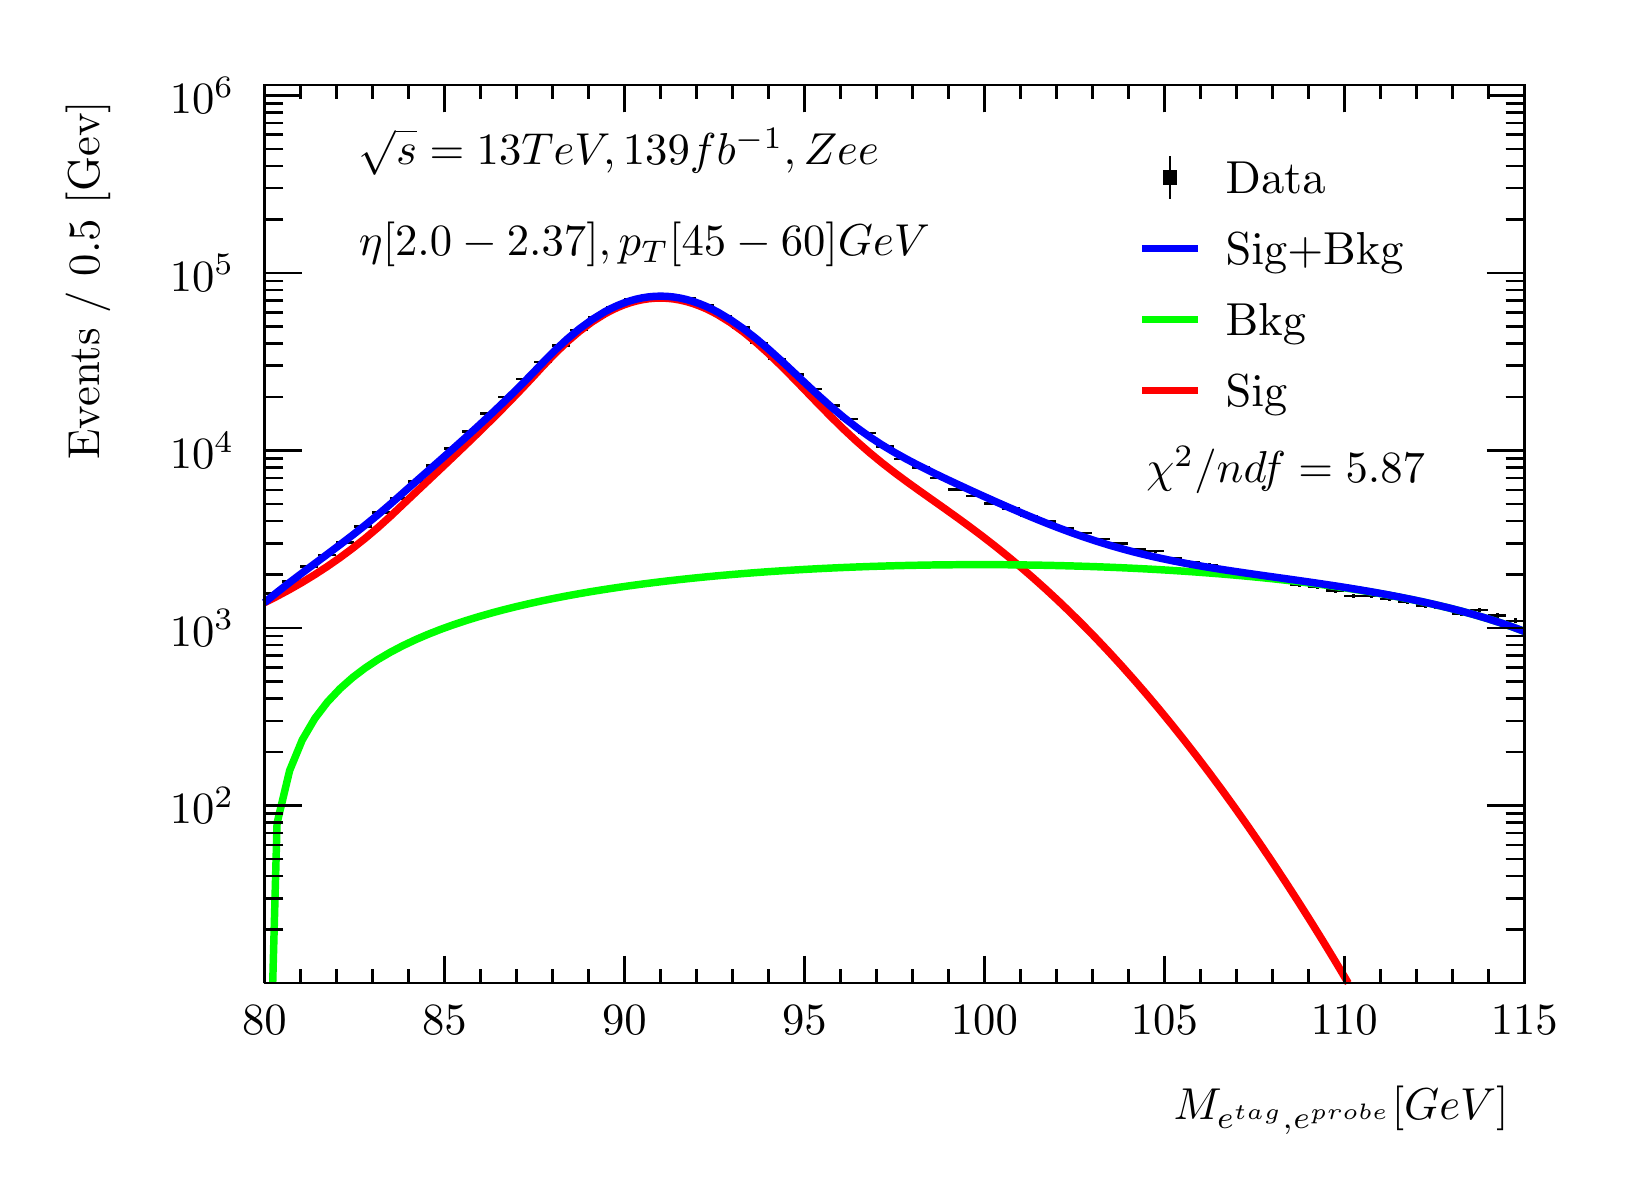
\begin{tikzpicture}
\pgfdeclareplotmark{cross} {
\pgfpathmoveto{\pgfpoint{-0.3\pgfplotmarksize}{\pgfplotmarksize}}
\pgfpathlineto{\pgfpoint{+0.3\pgfplotmarksize}{\pgfplotmarksize}}
\pgfpathlineto{\pgfpoint{+0.3\pgfplotmarksize}{0.3\pgfplotmarksize}}
\pgfpathlineto{\pgfpoint{+1\pgfplotmarksize}{0.3\pgfplotmarksize}}
\pgfpathlineto{\pgfpoint{+1\pgfplotmarksize}{-0.3\pgfplotmarksize}}
\pgfpathlineto{\pgfpoint{+0.3\pgfplotmarksize}{-0.3\pgfplotmarksize}}
\pgfpathlineto{\pgfpoint{+0.3\pgfplotmarksize}{-1.\pgfplotmarksize}}
\pgfpathlineto{\pgfpoint{-0.3\pgfplotmarksize}{-1.\pgfplotmarksize}}
\pgfpathlineto{\pgfpoint{-0.3\pgfplotmarksize}{-0.3\pgfplotmarksize}}
\pgfpathlineto{\pgfpoint{-1.\pgfplotmarksize}{-0.3\pgfplotmarksize}}
\pgfpathlineto{\pgfpoint{-1.\pgfplotmarksize}{0.3\pgfplotmarksize}}
\pgfpathlineto{\pgfpoint{-0.3\pgfplotmarksize}{0.3\pgfplotmarksize}}
\pgfpathclose
\pgfusepathqstroke
}
\pgfdeclareplotmark{cross*} {
\pgfpathmoveto{\pgfpoint{-0.3\pgfplotmarksize}{\pgfplotmarksize}}
\pgfpathlineto{\pgfpoint{+0.3\pgfplotmarksize}{\pgfplotmarksize}}
\pgfpathlineto{\pgfpoint{+0.3\pgfplotmarksize}{0.3\pgfplotmarksize}}
\pgfpathlineto{\pgfpoint{+1\pgfplotmarksize}{0.3\pgfplotmarksize}}
\pgfpathlineto{\pgfpoint{+1\pgfplotmarksize}{-0.3\pgfplotmarksize}}
\pgfpathlineto{\pgfpoint{+0.3\pgfplotmarksize}{-0.3\pgfplotmarksize}}
\pgfpathlineto{\pgfpoint{+0.3\pgfplotmarksize}{-1.\pgfplotmarksize}}
\pgfpathlineto{\pgfpoint{-0.3\pgfplotmarksize}{-1.\pgfplotmarksize}}
\pgfpathlineto{\pgfpoint{-0.3\pgfplotmarksize}{-0.3\pgfplotmarksize}}
\pgfpathlineto{\pgfpoint{-1.\pgfplotmarksize}{-0.3\pgfplotmarksize}}
\pgfpathlineto{\pgfpoint{-1.\pgfplotmarksize}{0.3\pgfplotmarksize}}
\pgfpathlineto{\pgfpoint{-0.3\pgfplotmarksize}{0.3\pgfplotmarksize}}
\pgfpathclose
\pgfusepathqfillstroke
}
\pgfdeclareplotmark{newstar} {
\pgfpathmoveto{\pgfqpoint{0pt}{\pgfplotmarksize}}
\pgfpathlineto{\pgfqpointpolar{44}{0.5\pgfplotmarksize}}
\pgfpathlineto{\pgfqpointpolar{18}{\pgfplotmarksize}}
\pgfpathlineto{\pgfqpointpolar{-20}{0.5\pgfplotmarksize}}
\pgfpathlineto{\pgfqpointpolar{-54}{\pgfplotmarksize}}
\pgfpathlineto{\pgfqpointpolar{-90}{0.5\pgfplotmarksize}}
\pgfpathlineto{\pgfqpointpolar{234}{\pgfplotmarksize}}
\pgfpathlineto{\pgfqpointpolar{198}{0.5\pgfplotmarksize}}
\pgfpathlineto{\pgfqpointpolar{162}{\pgfplotmarksize}}
\pgfpathlineto{\pgfqpointpolar{134}{0.5\pgfplotmarksize}}
\pgfpathclose
\pgfusepathqstroke
}
\pgfdeclareplotmark{newstar*} {
\pgfpathmoveto{\pgfqpoint{0pt}{\pgfplotmarksize}}
\pgfpathlineto{\pgfqpointpolar{44}{0.5\pgfplotmarksize}}
\pgfpathlineto{\pgfqpointpolar{18}{\pgfplotmarksize}}
\pgfpathlineto{\pgfqpointpolar{-20}{0.5\pgfplotmarksize}}
\pgfpathlineto{\pgfqpointpolar{-54}{\pgfplotmarksize}}
\pgfpathlineto{\pgfqpointpolar{-90}{0.5\pgfplotmarksize}}
\pgfpathlineto{\pgfqpointpolar{234}{\pgfplotmarksize}}
\pgfpathlineto{\pgfqpointpolar{198}{0.5\pgfplotmarksize}}
\pgfpathlineto{\pgfqpointpolar{162}{\pgfplotmarksize}}
\pgfpathlineto{\pgfqpointpolar{134}{0.5\pgfplotmarksize}}
\pgfpathclose
\pgfusepathqfillstroke
}
\definecolor{c}{rgb}{1,1,1};
\draw [color=c, fill=c] (0,0) rectangle (20,14.4361);
\draw [color=c, fill=c] (3,2.30977) rectangle (19,13.7143);
\definecolor{c}{rgb}{0,0,0};
\draw [c,line width=0.9] (3,2.30977) -- (3,13.7143) -- (19,13.7143) -- (19,2.30977) -- (3,2.30977);
\definecolor{c}{rgb}{1,1,1};
\draw [color=c, fill=c] (3,2.30977) rectangle (19,13.7143);
\definecolor{c}{rgb}{0,0,0};
\draw [c,line width=0.9] (3,2.30977) -- (3,13.7143) -- (19,13.7143) -- (19,2.30977) -- (3,2.30977);
\draw [c,line width=0.9] (3,2.30977) -- (19,2.30977);
\draw [c,line width=0.9] (3,2.65624) -- (3,2.30977);
\draw [c,line width=0.9] (3.45714,2.48301) -- (3.45714,2.30977);
\draw [c,line width=0.9] (3.91429,2.48301) -- (3.91429,2.30977);
\draw [c,line width=0.9] (4.37143,2.48301) -- (4.37143,2.30977);
\draw [c,line width=0.9] (4.82857,2.48301) -- (4.82857,2.30977);
\draw [c,line width=0.9] (5.28571,2.65624) -- (5.28571,2.30977);
\draw [c,line width=0.9] (5.74286,2.48301) -- (5.74286,2.30977);
\draw [c,line width=0.9] (6.2,2.48301) -- (6.2,2.30977);
\draw [c,line width=0.9] (6.65714,2.48301) -- (6.65714,2.30977);
\draw [c,line width=0.9] (7.11429,2.48301) -- (7.11429,2.30977);
\draw [c,line width=0.9] (7.57143,2.65624) -- (7.57143,2.30977);
\draw [c,line width=0.9] (8.02857,2.48301) -- (8.02857,2.30977);
\draw [c,line width=0.9] (8.48571,2.48301) -- (8.48571,2.30977);
\draw [c,line width=0.9] (8.94286,2.48301) -- (8.94286,2.30977);
\draw [c,line width=0.9] (9.4,2.48301) -- (9.4,2.30977);
\draw [c,line width=0.9] (9.85714,2.65624) -- (9.85714,2.30977);
\draw [c,line width=0.9] (10.3143,2.48301) -- (10.3143,2.30977);
\draw [c,line width=0.9] (10.7714,2.48301) -- (10.7714,2.30977);
\draw [c,line width=0.9] (11.2286,2.48301) -- (11.2286,2.30977);
\draw [c,line width=0.9] (11.6857,2.48301) -- (11.6857,2.30977);
\draw [c,line width=0.9] (12.1429,2.65624) -- (12.1429,2.30977);
\draw [c,line width=0.9] (12.6,2.48301) -- (12.6,2.30977);
\draw [c,line width=0.9] (13.0571,2.48301) -- (13.0571,2.30977);
\draw [c,line width=0.9] (13.5143,2.48301) -- (13.5143,2.30977);
\draw [c,line width=0.9] (13.9714,2.48301) -- (13.9714,2.30977);
\draw [c,line width=0.9] (14.4286,2.65624) -- (14.4286,2.30977);
\draw [c,line width=0.9] (14.8857,2.48301) -- (14.8857,2.30977);
\draw [c,line width=0.9] (15.3429,2.48301) -- (15.3429,2.30977);
\draw [c,line width=0.9] (15.8,2.48301) -- (15.8,2.30977);
\draw [c,line width=0.9] (16.2571,2.48301) -- (16.2571,2.30977);
\draw [c,line width=0.9] (16.7143,2.65624) -- (16.7143,2.30977);
\draw [c,line width=0.9] (17.1714,2.48301) -- (17.1714,2.30977);
\draw [c,line width=0.9] (17.6286,2.48301) -- (17.6286,2.30977);
\draw [c,line width=0.9] (18.0857,2.48301) -- (18.0857,2.30977);
\draw [c,line width=0.9] (18.5429,2.48301) -- (18.5429,2.30977);
\draw [c,line width=0.9] (19,2.65624) -- (19,2.30977);
\draw [anchor=base] (3,1.66015) node[scale=1.61424, color=c, rotate=0]{80};
\draw [anchor=base] (5.28571,1.66015) node[scale=1.61424, color=c, rotate=0]{85};
\draw [anchor=base] (7.57143,1.66015) node[scale=1.61424, color=c, rotate=0]{90};
\draw [anchor=base] (9.85714,1.66015) node[scale=1.61424, color=c, rotate=0]{95};
\draw [anchor=base] (12.1429,1.66015) node[scale=1.61424, color=c, rotate=0]{100};
\draw [anchor=base] (14.4286,1.66015) node[scale=1.61424, color=c, rotate=0]{105};
\draw [anchor=base] (16.7143,1.66015) node[scale=1.61424, color=c, rotate=0]{110};
\draw [anchor=base] (19,1.66015) node[scale=1.61424, color=c, rotate=0]{115};
\draw [anchor= east] (19,0.692932) node[scale=1.61424, color=c, rotate=0]{$M_{e^{tag}, e^{probe}}  [GeV]$};
\draw [c,line width=0.9] (3,13.7143) -- (19,13.7143);
\draw [c,line width=0.9] (3,13.3678) -- (3,13.7143);
\draw [c,line width=0.9] (3.45714,13.5411) -- (3.45714,13.7143);
\draw [c,line width=0.9] (3.91429,13.5411) -- (3.91429,13.7143);
\draw [c,line width=0.9] (4.37143,13.5411) -- (4.37143,13.7143);
\draw [c,line width=0.9] (4.82857,13.5411) -- (4.82857,13.7143);
\draw [c,line width=0.9] (5.28571,13.3678) -- (5.28571,13.7143);
\draw [c,line width=0.9] (5.74286,13.5411) -- (5.74286,13.7143);
\draw [c,line width=0.9] (6.2,13.5411) -- (6.2,13.7143);
\draw [c,line width=0.9] (6.65714,13.5411) -- (6.65714,13.7143);
\draw [c,line width=0.9] (7.11429,13.5411) -- (7.11429,13.7143);
\draw [c,line width=0.9] (7.57143,13.3678) -- (7.57143,13.7143);
\draw [c,line width=0.9] (8.02857,13.5411) -- (8.02857,13.7143);
\draw [c,line width=0.9] (8.48571,13.5411) -- (8.48571,13.7143);
\draw [c,line width=0.9] (8.94286,13.5411) -- (8.94286,13.7143);
\draw [c,line width=0.9] (9.4,13.5411) -- (9.4,13.7143);
\draw [c,line width=0.9] (9.85714,13.3678) -- (9.85714,13.7143);
\draw [c,line width=0.9] (10.3143,13.5411) -- (10.3143,13.7143);
\draw [c,line width=0.9] (10.7714,13.5411) -- (10.7714,13.7143);
\draw [c,line width=0.9] (11.2286,13.5411) -- (11.2286,13.7143);
\draw [c,line width=0.9] (11.6857,13.5411) -- (11.6857,13.7143);
\draw [c,line width=0.9] (12.1429,13.3678) -- (12.1429,13.7143);
\draw [c,line width=0.9] (12.6,13.5411) -- (12.6,13.7143);
\draw [c,line width=0.9] (13.0571,13.5411) -- (13.0571,13.7143);
\draw [c,line width=0.9] (13.5143,13.5411) -- (13.5143,13.7143);
\draw [c,line width=0.9] (13.9714,13.5411) -- (13.9714,13.7143);
\draw [c,line width=0.9] (14.4286,13.3678) -- (14.4286,13.7143);
\draw [c,line width=0.9] (14.8857,13.5411) -- (14.8857,13.7143);
\draw [c,line width=0.9] (15.3429,13.5411) -- (15.3429,13.7143);
\draw [c,line width=0.9] (15.8,13.5411) -- (15.8,13.7143);
\draw [c,line width=0.9] (16.2571,13.5411) -- (16.2571,13.7143);
\draw [c,line width=0.9] (16.7143,13.3678) -- (16.7143,13.7143);
\draw [c,line width=0.9] (17.1714,13.5411) -- (17.1714,13.7143);
\draw [c,line width=0.9] (17.6286,13.5411) -- (17.6286,13.7143);
\draw [c,line width=0.9] (18.0857,13.5411) -- (18.0857,13.7143);
\draw [c,line width=0.9] (18.5429,13.5411) -- (18.5429,13.7143);
\draw [c,line width=0.9] (19,13.3678) -- (19,13.7143);
\draw [c,line width=0.9] (3,2.30977) -- (3,13.7143);
\draw [c,line width=0.9] (3.237,2.98853) -- (3,2.98853);
\draw [c,line width=0.9] (3.237,3.38558) -- (3,3.38558);
\draw [c,line width=0.9] (3.237,3.66729) -- (3,3.66729);
\draw [c,line width=0.9] (3.237,3.8858) -- (3,3.8858);
\draw [c,line width=0.9] (3.237,4.06433) -- (3,4.06433);
\draw [c,line width=0.9] (3.237,4.21529) -- (3,4.21529);
\draw [c,line width=0.9] (3.237,4.34604) -- (3,4.34604);
\draw [c,line width=0.9] (3.237,4.46138) -- (3,4.46138);
\draw [c,line width=0.9] (3.474,4.56456) -- (3,4.56456);
\draw [anchor= east] (2.82,4.56456) node[scale=1.61424, color=c, rotate=0]{$10^{2}$};
\draw [c,line width=0.9] (3.237,5.24331) -- (3,5.24331);
\draw [c,line width=0.9] (3.237,5.64036) -- (3,5.64036);
\draw [c,line width=0.9] (3.237,5.92207) -- (3,5.92207);
\draw [c,line width=0.9] (3.237,6.14058) -- (3,6.14058);
\draw [c,line width=0.9] (3.237,6.31912) -- (3,6.31912);
\draw [c,line width=0.9] (3.237,6.47007) -- (3,6.47007);
\draw [c,line width=0.9] (3.237,6.60083) -- (3,6.60083);
\draw [c,line width=0.9] (3.237,6.71617) -- (3,6.71617);
\draw [c,line width=0.9] (3.474,6.81934) -- (3,6.81934);
\draw [anchor= east] (2.82,6.81934) node[scale=1.61424, color=c, rotate=0]{$10^{3}$};
\draw [c,line width=0.9] (3.237,7.4981) -- (3,7.4981);
\draw [c,line width=0.9] (3.237,7.89514) -- (3,7.89514);
\draw [c,line width=0.9] (3.237,8.17685) -- (3,8.17685);
\draw [c,line width=0.9] (3.237,8.39536) -- (3,8.39536);
\draw [c,line width=0.9] (3.237,8.5739) -- (3,8.5739);
\draw [c,line width=0.9] (3.237,8.72485) -- (3,8.72485);
\draw [c,line width=0.9] (3.237,8.85561) -- (3,8.85561);
\draw [c,line width=0.9] (3.237,8.97095) -- (3,8.97095);
\draw [c,line width=0.9] (3.474,9.07412) -- (3,9.07412);
\draw [anchor= east] (2.82,9.07412) node[scale=1.61424, color=c, rotate=0]{$10^{4}$};
\draw [c,line width=0.9] (3.237,9.75288) -- (3,9.75288);
\draw [c,line width=0.9] (3.237,10.1499) -- (3,10.1499);
\draw [c,line width=0.9] (3.237,10.4316) -- (3,10.4316);
\draw [c,line width=0.9] (3.237,10.6501) -- (3,10.6501);
\draw [c,line width=0.9] (3.237,10.8287) -- (3,10.8287);
\draw [c,line width=0.9] (3.237,10.9796) -- (3,10.9796);
\draw [c,line width=0.9] (3.237,11.1104) -- (3,11.1104);
\draw [c,line width=0.9] (3.237,11.2257) -- (3,11.2257);
\draw [c,line width=0.9] (3.474,11.3289) -- (3,11.3289);
\draw [anchor= east] (2.82,11.3289) node[scale=1.61424, color=c, rotate=0]{$10^{5}$};
\draw [c,line width=0.9] (3.237,12.0077) -- (3,12.0077);
\draw [c,line width=0.9] (3.237,12.4047) -- (3,12.4047);
\draw [c,line width=0.9] (3.237,12.6864) -- (3,12.6864);
\draw [c,line width=0.9] (3.237,12.9049) -- (3,12.9049);
\draw [c,line width=0.9] (3.237,13.0835) -- (3,13.0835);
\draw [c,line width=0.9] (3.237,13.2344) -- (3,13.2344);
\draw [c,line width=0.9] (3.237,13.3652) -- (3,13.3652);
\draw [c,line width=0.9] (3.237,13.4805) -- (3,13.4805);
\draw [c,line width=0.9] (3.474,13.5837) -- (3,13.5837);
\draw [anchor= east] (2.82,13.5837) node[scale=1.61424, color=c, rotate=0]{$10^{6}$};
\draw [anchor= east] (0.76,13.7143) node[scale=1.61424, color=c, rotate=90]{Events / 0.5 [Gev]};
\draw [c,line width=0.9] (19,2.30977) -- (19,13.7143);
\draw [c,line width=0.9] (18.763,2.98853) -- (19,2.98853);
\draw [c,line width=0.9] (18.763,3.38558) -- (19,3.38558);
\draw [c,line width=0.9] (18.763,3.66729) -- (19,3.66729);
\draw [c,line width=0.9] (18.763,3.8858) -- (19,3.8858);
\draw [c,line width=0.9] (18.763,4.06433) -- (19,4.06433);
\draw [c,line width=0.9] (18.763,4.21529) -- (19,4.21529);
\draw [c,line width=0.9] (18.763,4.34604) -- (19,4.34604);
\draw [c,line width=0.9] (18.763,4.46138) -- (19,4.46138);
\draw [c,line width=0.9] (18.526,4.56456) -- (19,4.56456);
\draw [c,line width=0.9] (18.763,5.24331) -- (19,5.24331);
\draw [c,line width=0.9] (18.763,5.64036) -- (19,5.64036);
\draw [c,line width=0.9] (18.763,5.92207) -- (19,5.92207);
\draw [c,line width=0.9] (18.763,6.14058) -- (19,6.14058);
\draw [c,line width=0.9] (18.763,6.31912) -- (19,6.31912);
\draw [c,line width=0.9] (18.763,6.47007) -- (19,6.47007);
\draw [c,line width=0.9] (18.763,6.60083) -- (19,6.60083);
\draw [c,line width=0.9] (18.763,6.71617) -- (19,6.71617);
\draw [c,line width=0.9] (18.526,6.81934) -- (19,6.81934);
\draw [c,line width=0.9] (18.763,7.4981) -- (19,7.4981);
\draw [c,line width=0.9] (18.763,7.89514) -- (19,7.89514);
\draw [c,line width=0.9] (18.763,8.17685) -- (19,8.17685);
\draw [c,line width=0.9] (18.763,8.39536) -- (19,8.39536);
\draw [c,line width=0.9] (18.763,8.5739) -- (19,8.5739);
\draw [c,line width=0.9] (18.763,8.72485) -- (19,8.72485);
\draw [c,line width=0.9] (18.763,8.85561) -- (19,8.85561);
\draw [c,line width=0.9] (18.763,8.97095) -- (19,8.97095);
\draw [c,line width=0.9] (18.526,9.07412) -- (19,9.07412);
\draw [c,line width=0.9] (18.763,9.75288) -- (19,9.75288);
\draw [c,line width=0.9] (18.763,10.1499) -- (19,10.1499);
\draw [c,line width=0.9] (18.763,10.4316) -- (19,10.4316);
\draw [c,line width=0.9] (18.763,10.6501) -- (19,10.6501);
\draw [c,line width=0.9] (18.763,10.8287) -- (19,10.8287);
\draw [c,line width=0.9] (18.763,10.9796) -- (19,10.9796);
\draw [c,line width=0.9] (18.763,11.1104) -- (19,11.1104);
\draw [c,line width=0.9] (18.763,11.2257) -- (19,11.2257);
\draw [c,line width=0.9] (18.526,11.3289) -- (19,11.3289);
\draw [c,line width=0.9] (18.763,12.0077) -- (19,12.0077);
\draw [c,line width=0.9] (18.763,12.4047) -- (19,12.4047);
\draw [c,line width=0.9] (18.763,12.6864) -- (19,12.6864);
\draw [c,line width=0.9] (18.763,12.9049) -- (19,12.9049);
\draw [c,line width=0.9] (18.763,13.0835) -- (19,13.0835);
\draw [c,line width=0.9] (18.763,13.2344) -- (19,13.2344);
\draw [c,line width=0.9] (18.763,13.3652) -- (19,13.3652);
\draw [c,line width=0.9] (18.763,13.4805) -- (19,13.4805);
\draw [c,line width=0.9] (18.526,13.5837) -- (19,13.5837);
\draw [c,line width=0.9] (3.11429,7.25668) -- (3,7.25668);
\draw [c,line width=0.9] (3,7.25668) -- (3,7.25668);
\draw [c,line width=0.9] (3.11429,7.25668) -- (3.22857,7.25668);
\draw [c,line width=0.9] (3.22857,7.25668) -- (3.22857,7.25668);
\draw [c,line width=0.9] (3.11429,7.25668) -- (3.11429,7.28144);
\draw [c,line width=0.9] (3.11429,7.28144) -- (3.11429,7.28144);
\draw [c,line width=0.9] (3.11429,7.25668) -- (3.11429,7.23191);
\draw [c,line width=0.9] (3.11429,7.23191) -- (3.11429,7.23191);
\draw [c,line width=0.9] (3.34286,7.40736) -- (3.22857,7.40736);
\draw [c,line width=0.9] (3.22857,7.40736) -- (3.22857,7.40736);
\draw [c,line width=0.9] (3.34286,7.40736) -- (3.45714,7.40736);
\draw [c,line width=0.9] (3.45714,7.40736) -- (3.45714,7.40736);
\draw [c,line width=0.9] (3.34286,7.40736) -- (3.34286,7.43029);
\draw [c,line width=0.9] (3.34286,7.43029) -- (3.34286,7.43029);
\draw [c,line width=0.9] (3.34286,7.40736) -- (3.34286,7.38442);
\draw [c,line width=0.9] (3.34286,7.38442) -- (3.34286,7.38442);
\draw [c,line width=0.9] (3.57143,7.59808) -- (3.45714,7.59808);
\draw [c,line width=0.9] (3.45714,7.59808) -- (3.45714,7.59808);
\draw [c,line width=0.9] (3.57143,7.59808) -- (3.68571,7.59808);
\draw [c,line width=0.9] (3.68571,7.59808) -- (3.68571,7.59808);
\draw [c,line width=0.9] (3.57143,7.59808) -- (3.57143,7.61889);
\draw [c,line width=0.9] (3.57143,7.61889) -- (3.57143,7.61889);
\draw [c,line width=0.9] (3.57143,7.59808) -- (3.57143,7.57728);
\draw [c,line width=0.9] (3.57143,7.57728) -- (3.57143,7.57728);
\draw [c,line width=0.9] (3.8,7.74593) -- (3.68571,7.74593);
\draw [c,line width=0.9] (3.68571,7.74593) -- (3.68571,7.74593);
\draw [c,line width=0.9] (3.8,7.74593) -- (3.91429,7.74593);
\draw [c,line width=0.9] (3.91429,7.74593) -- (3.91429,7.74593);
\draw [c,line width=0.9] (3.8,7.74593) -- (3.8,7.76523);
\draw [c,line width=0.9] (3.8,7.76523) -- (3.8,7.76523);
\draw [c,line width=0.9] (3.8,7.74593) -- (3.8,7.72664);
\draw [c,line width=0.9] (3.8,7.72664) -- (3.8,7.72664);
\draw [c,line width=0.9] (4.02857,7.90392) -- (3.91429,7.90392);
\draw [c,line width=0.9] (3.91429,7.90392) -- (3.91429,7.90392);
\draw [c,line width=0.9] (4.02857,7.90392) -- (4.14286,7.90392);
\draw [c,line width=0.9] (4.14286,7.90392) -- (4.14286,7.90392);
\draw [c,line width=0.9] (4.02857,7.90392) -- (4.02857,7.92172);
\draw [c,line width=0.9] (4.02857,7.92172) -- (4.02857,7.92172);
\draw [c,line width=0.9] (4.02857,7.90392) -- (4.02857,7.88612);
\draw [c,line width=0.9] (4.02857,7.88612) -- (4.02857,7.88612);
\draw [c,line width=0.9] (4.25714,8.10973) -- (4.14286,8.10973);
\draw [c,line width=0.9] (4.14286,8.10973) -- (4.14286,8.10973);
\draw [c,line width=0.9] (4.25714,8.10973) -- (4.37143,8.10973);
\draw [c,line width=0.9] (4.37143,8.10973) -- (4.37143,8.10973);
\draw [c,line width=0.9] (4.25714,8.10973) -- (4.25714,8.12575);
\draw [c,line width=0.9] (4.25714,8.12575) -- (4.25714,8.12575);
\draw [c,line width=0.9] (4.25714,8.10973) -- (4.25714,8.09371);
\draw [c,line width=0.9] (4.25714,8.09371) -- (4.25714,8.09371);
\draw [c,line width=0.9] (4.48571,8.28411) -- (4.37143,8.28411);
\draw [c,line width=0.9] (4.37143,8.28411) -- (4.37143,8.28411);
\draw [c,line width=0.9] (4.48571,8.28411) -- (4.6,8.28411);
\draw [c,line width=0.9] (4.6,8.28411) -- (4.6,8.28411);
\draw [c,line width=0.9] (4.48571,8.28411) -- (4.48571,8.29877);
\draw [c,line width=0.9] (4.48571,8.29877) -- (4.48571,8.29877);
\draw [c,line width=0.9] (4.48571,8.28411) -- (4.48571,8.26945);
\draw [c,line width=0.9] (4.48571,8.26945) -- (4.48571,8.26945);
\draw [c,line width=0.9] (4.71429,8.46618) -- (4.6,8.46618);
\draw [c,line width=0.9] (4.6,8.46618) -- (4.6,8.46618);
\draw [c,line width=0.9] (4.71429,8.46618) -- (4.82857,8.46618);
\draw [c,line width=0.9] (4.82857,8.46618) -- (4.82857,8.46618);
\draw [c,line width=0.9] (4.71429,8.46618) -- (4.71429,8.47954);
\draw [c,line width=0.9] (4.71429,8.47954) -- (4.71429,8.47954);
\draw [c,line width=0.9] (4.71429,8.46618) -- (4.71429,8.45283);
\draw [c,line width=0.9] (4.71429,8.45283) -- (4.71429,8.45283);
\draw [c,line width=0.9] (4.94286,8.68094) -- (4.82857,8.68094);
\draw [c,line width=0.9] (4.82857,8.68094) -- (4.82857,8.68094);
\draw [c,line width=0.9] (4.94286,8.68094) -- (5.05714,8.68094);
\draw [c,line width=0.9] (5.05714,8.68094) -- (5.05714,8.68094);
\draw [c,line width=0.9] (4.94286,8.68094) -- (4.94286,8.69291);
\draw [c,line width=0.9] (4.94286,8.69291) -- (4.94286,8.69291);
\draw [c,line width=0.9] (4.94286,8.68094) -- (4.94286,8.66897);
\draw [c,line width=0.9] (4.94286,8.66897) -- (4.94286,8.66897);
\draw [c,line width=0.9] (5.17143,8.88182) -- (5.05714,8.88182);
\draw [c,line width=0.9] (5.05714,8.88182) -- (5.05714,8.88182);
\draw [c,line width=0.9] (5.17143,8.88182) -- (5.28571,8.88182);
\draw [c,line width=0.9] (5.28571,8.88182) -- (5.28571,8.88182);
\draw [c,line width=0.9] (5.17143,8.88182) -- (5.17143,8.89262);
\draw [c,line width=0.9] (5.17143,8.89262) -- (5.17143,8.89262);
\draw [c,line width=0.9] (5.17143,8.88182) -- (5.17143,8.87102);
\draw [c,line width=0.9] (5.17143,8.87102) -- (5.17143,8.87102);
\draw [c,line width=0.9] (5.4,9.09964) -- (5.28571,9.09964);
\draw [c,line width=0.9] (5.28571,9.09964) -- (5.28571,9.09964);
\draw [c,line width=0.9] (5.4,9.09964) -- (5.51429,9.09964);
\draw [c,line width=0.9] (5.51429,9.09964) -- (5.51429,9.09964);
\draw [c,line width=0.9] (5.4,9.09964) -- (5.4,9.10931);
\draw [c,line width=0.9] (5.4,9.10931) -- (5.4,9.10931);
\draw [c,line width=0.9] (5.4,9.09964) -- (5.4,9.08997);
\draw [c,line width=0.9] (5.4,9.08997) -- (5.4,9.08997);
\draw [c,line width=0.9] (5.62857,9.31486) -- (5.51429,9.31486);
\draw [c,line width=0.9] (5.51429,9.31486) -- (5.51429,9.31486);
\draw [c,line width=0.9] (5.62857,9.31486) -- (5.74286,9.31486);
\draw [c,line width=0.9] (5.74286,9.31486) -- (5.74286,9.31486);
\draw [c,line width=0.9] (5.62857,9.31486) -- (5.62857,9.32352);
\draw [c,line width=0.9] (5.62857,9.32352) -- (5.62857,9.32352);
\draw [c,line width=0.9] (5.62857,9.31486) -- (5.62857,9.3062);
\draw [c,line width=0.9] (5.62857,9.3062) -- (5.62857,9.3062);
\draw [c,line width=0.9] (5.85714,9.54065) -- (5.74286,9.54065);
\draw [c,line width=0.9] (5.74286,9.54065) -- (5.74286,9.54065);
\draw [c,line width=0.9] (5.85714,9.54065) -- (5.97143,9.54065);
\draw [c,line width=0.9] (5.97143,9.54065) -- (5.97143,9.54065);
\draw [c,line width=0.9] (5.85714,9.54065) -- (5.85714,9.54837);
\draw [c,line width=0.9] (5.85714,9.54837) -- (5.85714,9.54837);
\draw [c,line width=0.9] (5.85714,9.54065) -- (5.85714,9.53294);
\draw [c,line width=0.9] (5.85714,9.53294) -- (5.85714,9.53294);
\draw [c,line width=0.9] (6.08571,9.75508) -- (5.97143,9.75508);
\draw [c,line width=0.9] (5.97143,9.75508) -- (5.97143,9.75508);
\draw [c,line width=0.9] (6.08571,9.75508) -- (6.2,9.75508);
\draw [c,line width=0.9] (6.2,9.75508) -- (6.2,9.75508);
\draw [c,line width=0.9] (6.08571,9.75508) -- (6.08571,9.762);
\draw [c,line width=0.9] (6.08571,9.762) -- (6.08571,9.762);
\draw [c,line width=0.9] (6.08571,9.75508) -- (6.08571,9.74816);
\draw [c,line width=0.9] (6.08571,9.74816) -- (6.08571,9.74816);
\draw [c,line width=0.9] (6.31429,9.98346) -- (6.2,9.98346);
\draw [c,line width=0.9] (6.2,9.98346) -- (6.2,9.98346);
\draw [c,line width=0.9] (6.31429,9.98346) -- (6.42857,9.98346);
\draw [c,line width=0.9] (6.42857,9.98346) -- (6.42857,9.98346);
\draw [c,line width=0.9] (6.31429,9.98346) -- (6.31429,9.98961);
\draw [c,line width=0.9] (6.31429,9.98961) -- (6.31429,9.98961);
\draw [c,line width=0.9] (6.31429,9.98346) -- (6.31429,9.9773);
\draw [c,line width=0.9] (6.31429,9.9773) -- (6.31429,9.9773);
\draw [c,line width=0.9] (6.54286,10.1945) -- (6.42857,10.1945);
\draw [c,line width=0.9] (6.42857,10.1945) -- (6.42857,10.1945);
\draw [c,line width=0.9] (6.54286,10.1945) -- (6.65714,10.1945);
\draw [c,line width=0.9] (6.65714,10.1945) -- (6.65714,10.1945);
\draw [c,line width=0.9] (6.54286,10.1945) -- (6.54286,10.2001);
\draw [c,line width=0.9] (6.54286,10.2001) -- (6.54286,10.2001);
\draw [c,line width=0.9] (6.54286,10.1945) -- (6.54286,10.189);
\draw [c,line width=0.9] (6.54286,10.189) -- (6.54286,10.189);
\draw [c,line width=0.9] (6.77143,10.4069) -- (6.65714,10.4069);
\draw [c,line width=0.9] (6.65714,10.4069) -- (6.65714,10.4069);
\draw [c,line width=0.9] (6.77143,10.4069) -- (6.88571,10.4069);
\draw [c,line width=0.9] (6.88571,10.4069) -- (6.88571,10.4069);
\draw [c,line width=0.9] (6.77143,10.4069) -- (6.77143,10.4118);
\draw [c,line width=0.9] (6.77143,10.4118) -- (6.77143,10.4118);
\draw [c,line width=0.9] (6.77143,10.4069) -- (6.77143,10.4019);
\draw [c,line width=0.9] (6.77143,10.4019) -- (6.77143,10.4019);
\draw [c,line width=0.9] (7,10.6044) -- (6.88571,10.6044);
\draw [c,line width=0.9] (6.88571,10.6044) -- (6.88571,10.6044);
\draw [c,line width=0.9] (7,10.6044) -- (7.11429,10.6044);
\draw [c,line width=0.9] (7.11429,10.6044) -- (7.11429,10.6044);
\draw [c,line width=0.9] (7,10.6044) -- (7,10.6088);
\draw [c,line width=0.9] (7,10.6088) -- (7,10.6088);
\draw [c,line width=0.9] (7,10.6044) -- (7,10.5999);
\draw [c,line width=0.9] (7,10.5999) -- (7,10.5999);
\draw [c,line width=0.9] (7.22857,10.769) -- (7.11429,10.769);
\draw [c,line width=0.9] (7.11429,10.769) -- (7.11429,10.769);
\draw [c,line width=0.9] (7.22857,10.769) -- (7.34286,10.769);
\draw [c,line width=0.9] (7.34286,10.769) -- (7.34286,10.769);
\draw [c,line width=0.9] (7.22857,10.769) -- (7.22857,10.7732);
\draw [c,line width=0.9] (7.22857,10.7732) -- (7.22857,10.7732);
\draw [c,line width=0.9] (7.22857,10.769) -- (7.22857,10.7649);
\draw [c,line width=0.9] (7.22857,10.7649) -- (7.22857,10.7649);
\draw [c,line width=0.9] (7.45714,10.893) -- (7.34286,10.893);
\draw [c,line width=0.9] (7.34286,10.893) -- (7.34286,10.893);
\draw [c,line width=0.9] (7.45714,10.893) -- (7.57143,10.893);
\draw [c,line width=0.9] (7.57143,10.893) -- (7.57143,10.893);
\draw [c,line width=0.9] (7.45714,10.893) -- (7.45714,10.8969);
\draw [c,line width=0.9] (7.45714,10.8969) -- (7.45714,10.8969);
\draw [c,line width=0.9] (7.45714,10.893) -- (7.45714,10.8891);
\draw [c,line width=0.9] (7.45714,10.8891) -- (7.45714,10.8891);
\draw [c,line width=0.9] (7.68571,10.989) -- (7.57143,10.989);
\draw [c,line width=0.9] (7.57143,10.989) -- (7.57143,10.989);
\draw [c,line width=0.9] (7.68571,10.989) -- (7.8,10.989);
\draw [c,line width=0.9] (7.8,10.989) -- (7.8,10.989);
\draw [c,line width=0.9] (7.68571,10.989) -- (7.68571,10.9927);
\draw [c,line width=0.9] (7.68571,10.9927) -- (7.68571,10.9927);
\draw [c,line width=0.9] (7.68571,10.989) -- (7.68571,10.9853);
\draw [c,line width=0.9] (7.68571,10.9853) -- (7.68571,10.9853);
\draw [c,line width=0.9] (7.91429,11.0335) -- (7.8,11.0335);
\draw [c,line width=0.9] (7.8,11.0335) -- (7.8,11.0335);
\draw [c,line width=0.9] (7.91429,11.0335) -- (8.02857,11.0335);
\draw [c,line width=0.9] (8.02857,11.0335) -- (8.02857,11.0335);
\draw [c,line width=0.9] (7.91429,11.0335) -- (7.91429,11.0371);
\draw [c,line width=0.9] (7.91429,11.0371) -- (7.91429,11.0371);
\draw [c,line width=0.9] (7.91429,11.0335) -- (7.91429,11.0299);
\draw [c,line width=0.9] (7.91429,11.0299) -- (7.91429,11.0299);
\draw [c,line width=0.9] (8.14286,11.0437) -- (8.02857,11.0437);
\draw [c,line width=0.9] (8.02857,11.0437) -- (8.02857,11.0437);
\draw [c,line width=0.9] (8.14286,11.0437) -- (8.25714,11.0437);
\draw [c,line width=0.9] (8.25714,11.0437) -- (8.25714,11.0437);
\draw [c,line width=0.9] (8.14286,11.0437) -- (8.14286,11.0472);
\draw [c,line width=0.9] (8.14286,11.0472) -- (8.14286,11.0472);
\draw [c,line width=0.9] (8.14286,11.0437) -- (8.14286,11.0401);
\draw [c,line width=0.9] (8.14286,11.0401) -- (8.14286,11.0401);
\draw [c,line width=0.9] (8.37143,11.0034) -- (8.25714,11.0034);
\draw [c,line width=0.9] (8.25714,11.0034) -- (8.25714,11.0034);
\draw [c,line width=0.9] (8.37143,11.0034) -- (8.48571,11.0034);
\draw [c,line width=0.9] (8.48571,11.0034) -- (8.48571,11.0034);
\draw [c,line width=0.9] (8.37143,11.0034) -- (8.37143,11.0071);
\draw [c,line width=0.9] (8.37143,11.0071) -- (8.37143,11.0071);
\draw [c,line width=0.9] (8.37143,11.0034) -- (8.37143,10.9998);
\draw [c,line width=0.9] (8.37143,10.9998) -- (8.37143,10.9998);
\draw [c,line width=0.9] (8.6,10.9124) -- (8.48571,10.9124);
\draw [c,line width=0.9] (8.48571,10.9124) -- (8.48571,10.9124);
\draw [c,line width=0.9] (8.6,10.9124) -- (8.71429,10.9124);
\draw [c,line width=0.9] (8.71429,10.9124) -- (8.71429,10.9124);
\draw [c,line width=0.9] (8.6,10.9124) -- (8.6,10.9163);
\draw [c,line width=0.9] (8.6,10.9163) -- (8.6,10.9163);
\draw [c,line width=0.9] (8.6,10.9124) -- (8.6,10.9086);
\draw [c,line width=0.9] (8.6,10.9086) -- (8.6,10.9086);
\draw [c,line width=0.9] (8.82857,10.7798) -- (8.71429,10.7798);
\draw [c,line width=0.9] (8.71429,10.7798) -- (8.71429,10.7798);
\draw [c,line width=0.9] (8.82857,10.7798) -- (8.94286,10.7798);
\draw [c,line width=0.9] (8.94286,10.7798) -- (8.94286,10.7798);
\draw [c,line width=0.9] (8.82857,10.7798) -- (8.82857,10.7839);
\draw [c,line width=0.9] (8.82857,10.7839) -- (8.82857,10.7839);
\draw [c,line width=0.9] (8.82857,10.7798) -- (8.82857,10.7757);
\draw [c,line width=0.9] (8.82857,10.7757) -- (8.82857,10.7757);
\draw [c,line width=0.9] (9.05714,10.6322) -- (8.94286,10.6322);
\draw [c,line width=0.9] (8.94286,10.6322) -- (8.94286,10.6322);
\draw [c,line width=0.9] (9.05714,10.6322) -- (9.17143,10.6322);
\draw [c,line width=0.9] (9.17143,10.6322) -- (9.17143,10.6322);
\draw [c,line width=0.9] (9.05714,10.6322) -- (9.05714,10.6367);
\draw [c,line width=0.9] (9.05714,10.6367) -- (9.05714,10.6367);
\draw [c,line width=0.9] (9.05714,10.6322) -- (9.05714,10.6278);
\draw [c,line width=0.9] (9.05714,10.6278) -- (9.05714,10.6278);
\draw [c,line width=0.9] (9.28571,10.441) -- (9.17143,10.441);
\draw [c,line width=0.9] (9.17143,10.441) -- (9.17143,10.441);
\draw [c,line width=0.9] (9.28571,10.441) -- (9.4,10.441);
\draw [c,line width=0.9] (9.4,10.441) -- (9.4,10.441);
\draw [c,line width=0.9] (9.28571,10.441) -- (9.28571,10.4459);
\draw [c,line width=0.9] (9.28571,10.4459) -- (9.28571,10.4459);
\draw [c,line width=0.9] (9.28571,10.441) -- (9.28571,10.4361);
\draw [c,line width=0.9] (9.28571,10.4361) -- (9.28571,10.4361);
\draw [c,line width=0.9] (9.51429,10.2364) -- (9.4,10.2364);
\draw [c,line width=0.9] (9.4,10.2364) -- (9.4,10.2364);
\draw [c,line width=0.9] (9.51429,10.2364) -- (9.62857,10.2364);
\draw [c,line width=0.9] (9.62857,10.2364) -- (9.62857,10.2364);
\draw [c,line width=0.9] (9.51429,10.2364) -- (9.51429,10.2418);
\draw [c,line width=0.9] (9.51429,10.2418) -- (9.51429,10.2418);
\draw [c,line width=0.9] (9.51429,10.2364) -- (9.51429,10.231);
\draw [c,line width=0.9] (9.51429,10.231) -- (9.51429,10.231);
\draw [c,line width=0.9] (9.74286,10.0367) -- (9.62857,10.0367);
\draw [c,line width=0.9] (9.62857,10.0367) -- (9.62857,10.0367);
\draw [c,line width=0.9] (9.74286,10.0367) -- (9.85714,10.0367);
\draw [c,line width=0.9] (9.85714,10.0367) -- (9.85714,10.0367);
\draw [c,line width=0.9] (9.74286,10.0367) -- (9.74286,10.0427);
\draw [c,line width=0.9] (9.74286,10.0427) -- (9.74286,10.0427);
\draw [c,line width=0.9] (9.74286,10.0367) -- (9.74286,10.0307);
\draw [c,line width=0.9] (9.74286,10.0307) -- (9.74286,10.0307);
\draw [c,line width=0.9] (9.97143,9.85096) -- (9.85714,9.85096);
\draw [c,line width=0.9] (9.85714,9.85096) -- (9.85714,9.85096);
\draw [c,line width=0.9] (9.97143,9.85096) -- (10.0857,9.85096);
\draw [c,line width=0.9] (10.0857,9.85096) -- (10.0857,9.85096);
\draw [c,line width=0.9] (9.97143,9.85096) -- (9.97143,9.85755);
\draw [c,line width=0.9] (9.97143,9.85755) -- (9.97143,9.85755);
\draw [c,line width=0.9] (9.97143,9.85096) -- (9.97143,9.84438);
\draw [c,line width=0.9] (9.97143,9.84438) -- (9.97143,9.84438);
\draw [c,line width=0.9] (10.2,9.64589) -- (10.0857,9.64589);
\draw [c,line width=0.9] (10.0857,9.64589) -- (10.0857,9.64589);
\draw [c,line width=0.9] (10.2,9.64589) -- (10.3143,9.64589);
\draw [c,line width=0.9] (10.3143,9.64589) -- (10.3143,9.64589);
\draw [c,line width=0.9] (10.2,9.64589) -- (10.2,9.6532);
\draw [c,line width=0.9] (10.2,9.6532) -- (10.2,9.6532);
\draw [c,line width=0.9] (10.2,9.64589) -- (10.2,9.63858);
\draw [c,line width=0.9] (10.2,9.63858) -- (10.2,9.63858);
\draw [c,line width=0.9] (10.4286,9.47417) -- (10.3143,9.47417);
\draw [c,line width=0.9] (10.3143,9.47417) -- (10.3143,9.47417);
\draw [c,line width=0.9] (10.4286,9.47417) -- (10.5429,9.47417);
\draw [c,line width=0.9] (10.5429,9.47417) -- (10.5429,9.47417);
\draw [c,line width=0.9] (10.4286,9.47417) -- (10.4286,9.48215);
\draw [c,line width=0.9] (10.4286,9.48215) -- (10.4286,9.48215);
\draw [c,line width=0.9] (10.4286,9.47417) -- (10.4286,9.46619);
\draw [c,line width=0.9] (10.4286,9.46619) -- (10.4286,9.46619);
\draw [c,line width=0.9] (10.6571,9.29748) -- (10.5429,9.29748);
\draw [c,line width=0.9] (10.5429,9.29748) -- (10.5429,9.29748);
\draw [c,line width=0.9] (10.6571,9.29748) -- (10.7714,9.29748);
\draw [c,line width=0.9] (10.7714,9.29748) -- (10.7714,9.29748);
\draw [c,line width=0.9] (10.6571,9.29748) -- (10.6571,9.30622);
\draw [c,line width=0.9] (10.6571,9.30622) -- (10.6571,9.30622);
\draw [c,line width=0.9] (10.6571,9.29748) -- (10.6571,9.28874);
\draw [c,line width=0.9] (10.6571,9.28874) -- (10.6571,9.28874);
\draw [c,line width=0.9] (10.8857,9.12432) -- (10.7714,9.12432);
\draw [c,line width=0.9] (10.7714,9.12432) -- (10.7714,9.12432);
\draw [c,line width=0.9] (10.8857,9.12432) -- (11,9.12432);
\draw [c,line width=0.9] (11,9.12432) -- (11,9.12432);
\draw [c,line width=0.9] (10.8857,9.12432) -- (10.8857,9.13387);
\draw [c,line width=0.9] (10.8857,9.13387) -- (10.8857,9.13387);
\draw [c,line width=0.9] (10.8857,9.12432) -- (10.8857,9.11478);
\draw [c,line width=0.9] (10.8857,9.11478) -- (10.8857,9.11478);
\draw [c,line width=0.9] (11.1143,8.96286) -- (11,8.96286);
\draw [c,line width=0.9] (11,8.96286) -- (11,8.96286);
\draw [c,line width=0.9] (11.1143,8.96286) -- (11.2286,8.96286);
\draw [c,line width=0.9] (11.2286,8.96286) -- (11.2286,8.96286);
\draw [c,line width=0.9] (11.1143,8.96286) -- (11.1143,8.97323);
\draw [c,line width=0.9] (11.1143,8.97323) -- (11.1143,8.97323);
\draw [c,line width=0.9] (11.1143,8.96286) -- (11.1143,8.9525);
\draw [c,line width=0.9] (11.1143,8.9525) -- (11.1143,8.9525);
\draw [c,line width=0.9] (11.3429,8.85696) -- (11.2286,8.85696);
\draw [c,line width=0.9] (11.2286,8.85696) -- (11.2286,8.85696);
\draw [c,line width=0.9] (11.3429,8.85696) -- (11.4571,8.85696);
\draw [c,line width=0.9] (11.4571,8.85696) -- (11.4571,8.85696);
\draw [c,line width=0.9] (11.3429,8.85696) -- (11.3429,8.8679);
\draw [c,line width=0.9] (11.3429,8.8679) -- (11.3429,8.8679);
\draw [c,line width=0.9] (11.3429,8.85696) -- (11.3429,8.84602);
\draw [c,line width=0.9] (11.3429,8.84602) -- (11.3429,8.84602);
\draw [c,line width=0.9] (11.5714,8.72317) -- (11.4571,8.72317);
\draw [c,line width=0.9] (11.4571,8.72317) -- (11.4571,8.72317);
\draw [c,line width=0.9] (11.5714,8.72317) -- (11.6857,8.72317);
\draw [c,line width=0.9] (11.6857,8.72317) -- (11.6857,8.72317);
\draw [c,line width=0.9] (11.5714,8.72317) -- (11.5714,8.73489);
\draw [c,line width=0.9] (11.5714,8.73489) -- (11.5714,8.73489);
\draw [c,line width=0.9] (11.5714,8.72317) -- (11.5714,8.71146);
\draw [c,line width=0.9] (11.5714,8.71146) -- (11.5714,8.71146);
\draw [c,line width=0.9] (11.8,8.57879) -- (11.6857,8.57879);
\draw [c,line width=0.9] (11.6857,8.57879) -- (11.6857,8.57879);
\draw [c,line width=0.9] (11.8,8.57879) -- (11.9143,8.57879);
\draw [c,line width=0.9] (11.9143,8.57879) -- (11.9143,8.57879);
\draw [c,line width=0.9] (11.8,8.57879) -- (11.8,8.5914);
\draw [c,line width=0.9] (11.8,8.5914) -- (11.8,8.5914);
\draw [c,line width=0.9] (11.8,8.57879) -- (11.8,8.56618);
\draw [c,line width=0.9] (11.8,8.56618) -- (11.8,8.56618);
\draw [c,line width=0.9] (12.0286,8.4942) -- (11.9143,8.4942);
\draw [c,line width=0.9] (11.9143,8.4942) -- (11.9143,8.4942);
\draw [c,line width=0.9] (12.0286,8.4942) -- (12.1429,8.4942);
\draw [c,line width=0.9] (12.1429,8.4942) -- (12.1429,8.4942);
\draw [c,line width=0.9] (12.0286,8.4942) -- (12.0286,8.50737);
\draw [c,line width=0.9] (12.0286,8.50737) -- (12.0286,8.50737);
\draw [c,line width=0.9] (12.0286,8.4942) -- (12.0286,8.48103);
\draw [c,line width=0.9] (12.0286,8.48103) -- (12.0286,8.48103);
\draw [c,line width=0.9] (12.2571,8.39986) -- (12.1429,8.39986);
\draw [c,line width=0.9] (12.1429,8.39986) -- (12.1429,8.39986);
\draw [c,line width=0.9] (12.2571,8.39986) -- (12.3714,8.39986);
\draw [c,line width=0.9] (12.3714,8.39986) -- (12.3714,8.39986);
\draw [c,line width=0.9] (12.2571,8.39986) -- (12.2571,8.41368);
\draw [c,line width=0.9] (12.2571,8.41368) -- (12.2571,8.41368);
\draw [c,line width=0.9] (12.2571,8.39986) -- (12.2571,8.38604);
\draw [c,line width=0.9] (12.2571,8.38604) -- (12.2571,8.38604);
\draw [c,line width=0.9] (12.4857,8.33665) -- (12.3714,8.33665);
\draw [c,line width=0.9] (12.3714,8.33665) -- (12.3714,8.33665);
\draw [c,line width=0.9] (12.4857,8.33665) -- (12.6,8.33665);
\draw [c,line width=0.9] (12.6,8.33665) -- (12.6,8.33665);
\draw [c,line width=0.9] (12.4857,8.33665) -- (12.4857,8.35092);
\draw [c,line width=0.9] (12.4857,8.35092) -- (12.4857,8.35092);
\draw [c,line width=0.9] (12.4857,8.33665) -- (12.4857,8.32238);
\draw [c,line width=0.9] (12.4857,8.32238) -- (12.4857,8.32238);
\draw [c,line width=0.9] (12.7143,8.2399) -- (12.6,8.2399);
\draw [c,line width=0.9] (12.6,8.2399) -- (12.6,8.2399);
\draw [c,line width=0.9] (12.7143,8.2399) -- (12.8286,8.2399);
\draw [c,line width=0.9] (12.8286,8.2399) -- (12.8286,8.2399);
\draw [c,line width=0.9] (12.7143,8.2399) -- (12.7143,8.25489);
\draw [c,line width=0.9] (12.7143,8.25489) -- (12.7143,8.25489);
\draw [c,line width=0.9] (12.7143,8.2399) -- (12.7143,8.22491);
\draw [c,line width=0.9] (12.7143,8.22491) -- (12.7143,8.22491);
\draw [c,line width=0.9] (12.9429,8.17047) -- (12.8286,8.17047);
\draw [c,line width=0.9] (12.8286,8.17047) -- (12.8286,8.17047);
\draw [c,line width=0.9] (12.9429,8.17047) -- (13.0571,8.17047);
\draw [c,line width=0.9] (13.0571,8.17047) -- (13.0571,8.17047);
\draw [c,line width=0.9] (12.9429,8.17047) -- (12.9429,8.186);
\draw [c,line width=0.9] (12.9429,8.186) -- (12.9429,8.186);
\draw [c,line width=0.9] (12.9429,8.17047) -- (12.9429,8.15493);
\draw [c,line width=0.9] (12.9429,8.15493) -- (12.9429,8.15493);
\draw [c,line width=0.9] (13.1714,8.08343) -- (13.0571,8.08343);
\draw [c,line width=0.9] (13.0571,8.08343) -- (13.0571,8.08343);
\draw [c,line width=0.9] (13.1714,8.08343) -- (13.2857,8.08343);
\draw [c,line width=0.9] (13.2857,8.08343) -- (13.2857,8.08343);
\draw [c,line width=0.9] (13.1714,8.08343) -- (13.1714,8.09966);
\draw [c,line width=0.9] (13.1714,8.09966) -- (13.1714,8.09966);
\draw [c,line width=0.9] (13.1714,8.08343) -- (13.1714,8.06719);
\draw [c,line width=0.9] (13.1714,8.06719) -- (13.1714,8.06719);
\draw [c,line width=0.9] (13.4,8.02345) -- (13.2857,8.02345);
\draw [c,line width=0.9] (13.2857,8.02345) -- (13.2857,8.02345);
\draw [c,line width=0.9] (13.4,8.02345) -- (13.5143,8.02345);
\draw [c,line width=0.9] (13.5143,8.02345) -- (13.5143,8.02345);
\draw [c,line width=0.9] (13.4,8.02345) -- (13.4,8.0402);
\draw [c,line width=0.9] (13.4,8.0402) -- (13.4,8.0402);
\draw [c,line width=0.9] (13.4,8.02345) -- (13.4,8.00671);
\draw [c,line width=0.9] (13.4,8.00671) -- (13.4,8.00671);
\draw [c,line width=0.9] (13.6286,7.94634) -- (13.5143,7.94634);
\draw [c,line width=0.9] (13.5143,7.94634) -- (13.5143,7.94634);
\draw [c,line width=0.9] (13.6286,7.94634) -- (13.7429,7.94634);
\draw [c,line width=0.9] (13.7429,7.94634) -- (13.7429,7.94634);
\draw [c,line width=0.9] (13.6286,7.94634) -- (13.6286,7.96375);
\draw [c,line width=0.9] (13.6286,7.96375) -- (13.6286,7.96375);
\draw [c,line width=0.9] (13.6286,7.94634) -- (13.6286,7.92892);
\draw [c,line width=0.9] (13.6286,7.92892) -- (13.6286,7.92892);
\draw [c,line width=0.9] (13.8571,7.89318) -- (13.7429,7.89318);
\draw [c,line width=0.9] (13.7429,7.89318) -- (13.7429,7.89318);
\draw [c,line width=0.9] (13.8571,7.89318) -- (13.9714,7.89318);
\draw [c,line width=0.9] (13.9714,7.89318) -- (13.9714,7.89318);
\draw [c,line width=0.9] (13.8571,7.89318) -- (13.8571,7.91108);
\draw [c,line width=0.9] (13.8571,7.91108) -- (13.8571,7.91108);
\draw [c,line width=0.9] (13.8571,7.89318) -- (13.8571,7.87529);
\draw [c,line width=0.9] (13.8571,7.87529) -- (13.8571,7.87529);
\draw [c,line width=0.9] (14.0857,7.81668) -- (13.9714,7.81668);
\draw [c,line width=0.9] (13.9714,7.81668) -- (13.9714,7.81668);
\draw [c,line width=0.9] (14.0857,7.81668) -- (14.2,7.81668);
\draw [c,line width=0.9] (14.2,7.81668) -- (14.2,7.81668);
\draw [c,line width=0.9] (14.0857,7.81668) -- (14.0857,7.83529);
\draw [c,line width=0.9] (14.0857,7.83529) -- (14.0857,7.83529);
\draw [c,line width=0.9] (14.0857,7.81668) -- (14.0857,7.79807);
\draw [c,line width=0.9] (14.0857,7.79807) -- (14.0857,7.79807);
\draw [c,line width=0.9] (14.3143,7.79523) -- (14.2,7.79523);
\draw [c,line width=0.9] (14.2,7.79523) -- (14.2,7.79523);
\draw [c,line width=0.9] (14.3143,7.79523) -- (14.4286,7.79523);
\draw [c,line width=0.9] (14.4286,7.79523) -- (14.4286,7.79523);
\draw [c,line width=0.9] (14.3143,7.79523) -- (14.3143,7.81404);
\draw [c,line width=0.9] (14.3143,7.81404) -- (14.3143,7.81404);
\draw [c,line width=0.9] (14.3143,7.79523) -- (14.3143,7.77642);
\draw [c,line width=0.9] (14.3143,7.77642) -- (14.3143,7.77642);
\draw [c,line width=0.9] (14.5429,7.70716) -- (14.4286,7.70716);
\draw [c,line width=0.9] (14.4286,7.70716) -- (14.4286,7.70716);
\draw [c,line width=0.9] (14.5429,7.70716) -- (14.6571,7.70716);
\draw [c,line width=0.9] (14.6571,7.70716) -- (14.6571,7.70716);
\draw [c,line width=0.9] (14.5429,7.70716) -- (14.5429,7.72684);
\draw [c,line width=0.9] (14.5429,7.72684) -- (14.5429,7.72684);
\draw [c,line width=0.9] (14.5429,7.70716) -- (14.5429,7.68748);
\draw [c,line width=0.9] (14.5429,7.68748) -- (14.5429,7.68748);
\draw [c,line width=0.9] (14.7714,7.65393) -- (14.6571,7.65393);
\draw [c,line width=0.9] (14.6571,7.65393) -- (14.6571,7.65393);
\draw [c,line width=0.9] (14.7714,7.65393) -- (14.8857,7.65393);
\draw [c,line width=0.9] (14.8857,7.65393) -- (14.8857,7.65393);
\draw [c,line width=0.9] (14.7714,7.65393) -- (14.7714,7.67415);
\draw [c,line width=0.9] (14.7714,7.67415) -- (14.7714,7.67415);
\draw [c,line width=0.9] (14.7714,7.65393) -- (14.7714,7.63371);
\draw [c,line width=0.9] (14.7714,7.63371) -- (14.7714,7.63371);
\draw [c,line width=0.9] (15,7.62167) -- (14.8857,7.62167);
\draw [c,line width=0.9] (14.8857,7.62167) -- (14.8857,7.62167);
\draw [c,line width=0.9] (15,7.62167) -- (15.1143,7.62167);
\draw [c,line width=0.9] (15.1143,7.62167) -- (15.1143,7.62167);
\draw [c,line width=0.9] (15,7.62167) -- (15,7.64223);
\draw [c,line width=0.9] (15,7.64223) -- (15,7.64223);
\draw [c,line width=0.9] (15,7.62167) -- (15,7.60111);
\draw [c,line width=0.9] (15,7.60111) -- (15,7.60111);
\draw [c,line width=0.9] (15.2286,7.55006) -- (15.1143,7.55006);
\draw [c,line width=0.9] (15.1143,7.55006) -- (15.1143,7.55006);
\draw [c,line width=0.9] (15.2286,7.55006) -- (15.3429,7.55006);
\draw [c,line width=0.9] (15.3429,7.55006) -- (15.3429,7.55006);
\draw [c,line width=0.9] (15.2286,7.55006) -- (15.2286,7.57139);
\draw [c,line width=0.9] (15.2286,7.57139) -- (15.2286,7.57139);
\draw [c,line width=0.9] (15.2286,7.55006) -- (15.2286,7.52874);
\draw [c,line width=0.9] (15.2286,7.52874) -- (15.2286,7.52874);
\draw [c,line width=0.9] (15.4571,7.46372) -- (15.3429,7.46372);
\draw [c,line width=0.9] (15.3429,7.46372) -- (15.3429,7.46372);
\draw [c,line width=0.9] (15.4571,7.46372) -- (15.5714,7.46372);
\draw [c,line width=0.9] (15.5714,7.46372) -- (15.5714,7.46372);
\draw [c,line width=0.9] (15.4571,7.46372) -- (15.4571,7.486);
\draw [c,line width=0.9] (15.4571,7.486) -- (15.4571,7.486);
\draw [c,line width=0.9] (15.4571,7.46372) -- (15.4571,7.44143);
\draw [c,line width=0.9] (15.4571,7.44143) -- (15.4571,7.44143);
\draw [c,line width=0.9] (15.6857,7.46827) -- (15.5714,7.46827);
\draw [c,line width=0.9] (15.5714,7.46827) -- (15.5714,7.46827);
\draw [c,line width=0.9] (15.6857,7.46827) -- (15.8,7.46827);
\draw [c,line width=0.9] (15.8,7.46827) -- (15.8,7.46827);
\draw [c,line width=0.9] (15.6857,7.46827) -- (15.6857,7.4905);
\draw [c,line width=0.9] (15.6857,7.4905) -- (15.6857,7.4905);
\draw [c,line width=0.9] (15.6857,7.46827) -- (15.6857,7.44604);
\draw [c,line width=0.9] (15.6857,7.44604) -- (15.6857,7.44604);
\draw [c,line width=0.9] (15.9143,7.43124) -- (15.8,7.43124);
\draw [c,line width=0.9] (15.8,7.43124) -- (15.8,7.43124);
\draw [c,line width=0.9] (15.9143,7.43124) -- (16.0286,7.43124);
\draw [c,line width=0.9] (16.0286,7.43124) -- (16.0286,7.43124);
\draw [c,line width=0.9] (15.9143,7.43124) -- (15.9143,7.45389);
\draw [c,line width=0.9] (15.9143,7.45389) -- (15.9143,7.45389);
\draw [c,line width=0.9] (15.9143,7.43124) -- (15.9143,7.40858);
\draw [c,line width=0.9] (15.9143,7.40858) -- (15.9143,7.40858);
\draw [c,line width=0.9] (16.1429,7.3651) -- (16.0286,7.3651);
\draw [c,line width=0.9] (16.0286,7.3651) -- (16.0286,7.3651);
\draw [c,line width=0.9] (16.1429,7.3651) -- (16.2571,7.3651);
\draw [c,line width=0.9] (16.2571,7.3651) -- (16.2571,7.3651);
\draw [c,line width=0.9] (16.1429,7.3651) -- (16.1429,7.38853);
\draw [c,line width=0.9] (16.1429,7.38853) -- (16.1429,7.38853);
\draw [c,line width=0.9] (16.1429,7.3651) -- (16.1429,7.34166);
\draw [c,line width=0.9] (16.1429,7.34166) -- (16.1429,7.34166);
\draw [c,line width=0.9] (16.3714,7.34183) -- (16.2571,7.34183);
\draw [c,line width=0.9] (16.2571,7.34183) -- (16.2571,7.34183);
\draw [c,line width=0.9] (16.3714,7.34183) -- (16.4857,7.34183);
\draw [c,line width=0.9] (16.4857,7.34183) -- (16.4857,7.34183);
\draw [c,line width=0.9] (16.3714,7.34183) -- (16.3714,7.36554);
\draw [c,line width=0.9] (16.3714,7.36554) -- (16.3714,7.36554);
\draw [c,line width=0.9] (16.3714,7.34183) -- (16.3714,7.31811);
\draw [c,line width=0.9] (16.3714,7.31811) -- (16.3714,7.31811);
\draw [c,line width=0.9] (16.6,7.29356) -- (16.4857,7.29356);
\draw [c,line width=0.9] (16.4857,7.29356) -- (16.4857,7.29356);
\draw [c,line width=0.9] (16.6,7.29356) -- (16.7143,7.29356);
\draw [c,line width=0.9] (16.7143,7.29356) -- (16.7143,7.29356);
\draw [c,line width=0.9] (16.6,7.29356) -- (16.6,7.31787);
\draw [c,line width=0.9] (16.6,7.31787) -- (16.6,7.31787);
\draw [c,line width=0.9] (16.6,7.29356) -- (16.6,7.26926);
\draw [c,line width=0.9] (16.6,7.26926) -- (16.6,7.26926);
\draw [c,line width=0.9] (16.8286,7.22548) -- (16.7143,7.22548);
\draw [c,line width=0.9] (16.7143,7.22548) -- (16.7143,7.22548);
\draw [c,line width=0.9] (16.8286,7.22548) -- (16.9429,7.22548);
\draw [c,line width=0.9] (16.9429,7.22548) -- (16.9429,7.22548);
\draw [c,line width=0.9] (16.8286,7.22548) -- (16.8286,7.25065);
\draw [c,line width=0.9] (16.8286,7.25065) -- (16.8286,7.25065);
\draw [c,line width=0.9] (16.8286,7.22548) -- (16.8286,7.20032);
\draw [c,line width=0.9] (16.8286,7.20032) -- (16.8286,7.20032);
\draw [c,line width=0.9] (17.0571,7.22289) -- (16.9429,7.22289);
\draw [c,line width=0.9] (16.9429,7.22289) -- (16.9429,7.22289);
\draw [c,line width=0.9] (17.0571,7.22289) -- (17.1714,7.22289);
\draw [c,line width=0.9] (17.1714,7.22289) -- (17.1714,7.22289);
\draw [c,line width=0.9] (17.0571,7.22289) -- (17.0571,7.24809);
\draw [c,line width=0.9] (17.0571,7.24809) -- (17.0571,7.24809);
\draw [c,line width=0.9] (17.0571,7.22289) -- (17.0571,7.19769);
\draw [c,line width=0.9] (17.0571,7.19769) -- (17.0571,7.19769);
\draw [c,line width=0.9] (17.2857,7.18723) -- (17.1714,7.18723);
\draw [c,line width=0.9] (17.1714,7.18723) -- (17.1714,7.18723);
\draw [c,line width=0.9] (17.2857,7.18723) -- (17.4,7.18723);
\draw [c,line width=0.9] (17.4,7.18723) -- (17.4,7.18723);
\draw [c,line width=0.9] (17.2857,7.18723) -- (17.2857,7.2129);
\draw [c,line width=0.9] (17.2857,7.2129) -- (17.2857,7.2129);
\draw [c,line width=0.9] (17.2857,7.18723) -- (17.2857,7.16157);
\draw [c,line width=0.9] (17.2857,7.16157) -- (17.2857,7.16157);
\draw [c,line width=0.9] (17.5143,7.1558) -- (17.4,7.1558);
\draw [c,line width=0.9] (17.4,7.1558) -- (17.4,7.1558);
\draw [c,line width=0.9] (17.5143,7.1558) -- (17.6286,7.1558);
\draw [c,line width=0.9] (17.6286,7.1558) -- (17.6286,7.1558);
\draw [c,line width=0.9] (17.5143,7.1558) -- (17.5143,7.18187);
\draw [c,line width=0.9] (17.5143,7.18187) -- (17.5143,7.18187);
\draw [c,line width=0.9] (17.5143,7.1558) -- (17.5143,7.12972);
\draw [c,line width=0.9] (17.5143,7.12972) -- (17.5143,7.12972);
\draw [c,line width=0.9] (17.7429,7.10301) -- (17.6286,7.10301);
\draw [c,line width=0.9] (17.6286,7.10301) -- (17.6286,7.10301);
\draw [c,line width=0.9] (17.7429,7.10301) -- (17.8571,7.10301);
\draw [c,line width=0.9] (17.8571,7.10301) -- (17.8571,7.10301);
\draw [c,line width=0.9] (17.7429,7.10301) -- (17.7429,7.1298);
\draw [c,line width=0.9] (17.7429,7.1298) -- (17.7429,7.1298);
\draw [c,line width=0.9] (17.7429,7.10301) -- (17.7429,7.07622);
\draw [c,line width=0.9] (17.7429,7.07622) -- (17.7429,7.07622);
\draw [c,line width=0.9] (17.9714,7.07626) -- (17.8571,7.07626);
\draw [c,line width=0.9] (17.8571,7.07626) -- (17.8571,7.07626);
\draw [c,line width=0.9] (17.9714,7.07626) -- (18.0857,7.07626);
\draw [c,line width=0.9] (18.0857,7.07626) -- (18.0857,7.07626);
\draw [c,line width=0.9] (17.9714,7.07626) -- (17.9714,7.10342);
\draw [c,line width=0.9] (17.9714,7.10342) -- (17.9714,7.10342);
\draw [c,line width=0.9] (17.9714,7.07626) -- (17.9714,7.0491);
\draw [c,line width=0.9] (17.9714,7.0491) -- (17.9714,7.0491);
\draw [c,line width=0.9] (18.2,7.00519) -- (18.0857,7.00519);
\draw [c,line width=0.9] (18.0857,7.00519) -- (18.0857,7.00519);
\draw [c,line width=0.9] (18.2,7.00519) -- (18.3143,7.00519);
\draw [c,line width=0.9] (18.3143,7.00519) -- (18.3143,7.00519);
\draw [c,line width=0.9] (18.2,7.00519) -- (18.2,7.03336);
\draw [c,line width=0.9] (18.2,7.03336) -- (18.2,7.03336);
\draw [c,line width=0.9] (18.2,7.00519) -- (18.2,6.97703);
\draw [c,line width=0.9] (18.2,6.97703) -- (18.2,6.97703);
\draw [c,line width=0.9] (18.4286,7.04953) -- (18.3143,7.04953);
\draw [c,line width=0.9] (18.3143,7.04953) -- (18.3143,7.04953);
\draw [c,line width=0.9] (18.4286,7.04953) -- (18.5429,7.04953);
\draw [c,line width=0.9] (18.5429,7.04953) -- (18.5429,7.04953);
\draw [c,line width=0.9] (18.4286,7.04953) -- (18.4286,7.07706);
\draw [c,line width=0.9] (18.4286,7.07706) -- (18.4286,7.07706);
\draw [c,line width=0.9] (18.4286,7.04953) -- (18.4286,7.022);
\draw [c,line width=0.9] (18.4286,7.022) -- (18.4286,7.022);
\draw [c,line width=0.9] (18.6571,6.97726) -- (18.5429,6.97726);
\draw [c,line width=0.9] (18.5429,6.97726) -- (18.5429,6.97726);
\draw [c,line width=0.9] (18.6571,6.97726) -- (18.7714,6.97726);
\draw [c,line width=0.9] (18.7714,6.97726) -- (18.7714,6.97726);
\draw [c,line width=0.9] (18.6571,6.97726) -- (18.6571,7.00583);
\draw [c,line width=0.9] (18.6571,7.00583) -- (18.6571,7.00583);
\draw [c,line width=0.9] (18.6571,6.97726) -- (18.6571,6.94869);
\draw [c,line width=0.9] (18.6571,6.94869) -- (18.6571,6.94869);
\draw [c,line width=0.9] (18.8857,6.91) -- (18.7714,6.91);
\draw [c,line width=0.9] (18.7714,6.91) -- (18.7714,6.91);
\draw [c,line width=0.9] (18.8857,6.91) -- (19,6.91);
\draw [c,line width=0.9] (19,6.91) -- (19,6.91);
\draw [c,line width=0.9] (18.8857,6.91) -- (18.8857,6.93956);
\draw [c,line width=0.9] (18.8857,6.93956) -- (18.8857,6.93956);
\draw [c,line width=0.9] (18.8857,6.91) -- (18.8857,6.88043);
\draw [c,line width=0.9] (18.8857,6.88043) -- (18.8857,6.88043);
\foreach \P in {(3.11429,7.25668), (3.34286,7.40736), (3.57143,7.59808), (3.8,7.74593), (4.02857,7.90392), (4.25714,8.10973), (4.48571,8.28411), (4.71429,8.46618), (4.94286,8.68094), (5.17143,8.88182), (5.4,9.09964), (5.62857,9.31486),
 (5.85714,9.54065), (6.08571,9.75508), (6.31429,9.98346), (6.54286,10.1945), (6.77143,10.4069), (7,10.6044), (7.22857,10.769), (7.45714,10.893), (7.68571,10.989), (7.91429,11.0335), (8.14286,11.0437), (8.37143,11.0034), (8.6,10.9124),
 (8.82857,10.7798), (9.05714,10.6322), (9.28571,10.441), (9.51429,10.2364), (9.74286,10.0367), (9.97143,9.85096), (10.2,9.64589), (10.4286,9.47417), (10.6571,9.29748), (10.8857,9.12432), (11.1143,8.96286), (11.3429,8.85696), (11.5714,8.72317),
 (11.8,8.57879), (12.0286,8.4942), (12.2571,8.39986), (12.4857,8.33665), (12.7143,8.2399), (12.9429,8.17047), (13.1714,8.08343), (13.4,8.02345), (13.6286,7.94634), (13.8571,7.89318), (14.0857,7.81668), (14.3143,7.79523), (14.5429,7.70716),
 (14.7714,7.65393), (15,7.62167), (15.2286,7.55006), (15.4571,7.46372), (15.6857,7.46827), (15.9143,7.43124), (16.1429,7.3651), (16.3714,7.34183), (16.6,7.29356), (16.8286,7.22548), (17.0571,7.22289), (17.2857,7.18723), (17.5143,7.1558),
 (17.7429,7.10301), (17.9714,7.07626), (18.2,7.00519), (18.4286,7.04953), (18.6571,6.97726), (18.8857,6.91)}{\draw[mark options={color=c,fill=c},mark size=2.882883pt,mark=] plot coordinates {\P};}
\definecolor{c}{rgb}{1,0,0};
\draw [c,line width=2.7] (3,7.14083) -- (3,7.14083);
\draw [c,line width=2.7] (3,7.14083) -- (3.16,7.22153) -- (3.32,7.30747) -- (3.48,7.3991) -- (3.64,7.49684) -- (3.8,7.60113) -- (3.96,7.71245) -- (4.12,7.83124) -- (4.28,7.958) -- (4.44,8.09325) -- (4.6,8.23758) -- (4.76,8.38934) -- (4.92,8.54084) --
 (5.08,8.69186) -- (5.24,8.84295) -- (5.4,8.99468) -- (5.56,9.14768) -- (5.72,9.30257) -- (5.88,9.46) -- (6.04,9.62059) -- (6.12,9.70225) -- (6.2,9.78491) -- (6.28,9.86864) -- (6.36,9.95351) -- (6.44,10.0396) -- (6.52,10.1268) -- (6.68,10.2952) --
 (6.84,10.449) -- (7,10.5864) -- (7.16,10.7059) -- (7.32,10.8065) -- (7.4,10.8495) -- (7.48,10.8874) -- (7.56,10.9203) -- (7.64,10.9481) -- (7.72,10.9706) -- (7.8,10.988) -- (7.88,11.0002) -- (7.96,11.0072) -- (8.04,11.0089) -- (8.12,11.0055) --
 (8.2,10.9968) -- (8.28,10.9831) -- (8.36,10.9642) -- (8.44,10.9403) -- (8.52,10.9115) -- (8.6,10.8778) -- (8.68,10.8393) -- (8.76,10.7962) -- (8.92,10.6966) -- (9.08,10.5803) -- (9.24,10.4491) -- (9.4,10.3051) -- (9.56,10.1509) -- (9.64,10.0709) --
 (9.72,9.98956) -- (9.8,9.90723) -- (9.88,9.82438) -- (9.96,9.74145) -- (10.04,9.65886) -- (10.2,9.49632) -- (10.36,9.33956) -- (10.52,9.19057) -- (10.68,9.05024) -- (10.84,8.91842) -- (11,8.79402) -- (11.16,8.67534) -- (11.32,8.56042) --
 (11.48,8.44731) -- (11.64,8.33427) -- (11.8,8.21983) -- (11.96,8.10285) -- (12.12,7.98248) -- (12.28,7.8581) -- (12.44,7.7293) -- (12.6,7.59577) -- (12.76,7.45735) -- (12.92,7.3139) -- (13.08,7.16536) -- (13.24,7.01168) -- (13.4,6.85283) --
 (13.56,6.68881) -- (13.72,6.51959) -- (13.88,6.34518) -- (14.04,6.16558) -- (14.2,5.98077) -- (14.36,5.79077) -- (14.52,5.59557) -- (14.68,5.39517) -- (14.84,5.18957) -- (15,4.97877) -- (15.16,4.76277) -- (15.32,4.54158) -- (15.48,4.31518) --
 (15.64,4.08359) -- (15.8,3.84679) -- (15.96,3.6048) -- (16.12,3.35761) -- (16.28,3.10522) -- (16.44,2.84763) -- (16.6,2.58484) -- (16.76,2.31685) -- (16.7641,2.30977);
\definecolor{c}{rgb}{0,1,0};
\draw [c,line width=2.7] (3.10489,2.30977) -- (3.16,4.34048);
\draw [c,line width=2.7] (3.16,4.34048) -- (3.32,5.00932) -- (3.48,5.39716) -- (3.64,5.66978) -- (3.8,5.87919) -- (3.96,6.04859) -- (4.12,6.19034) -- (4.28,6.31182) -- (4.44,6.41781) -- (4.6,6.51155) -- (4.76,6.59535) -- (4.92,6.67095) --
 (5.08,6.73962) -- (5.24,6.8024) -- (5.4,6.86006) -- (5.56,6.91326) -- (5.72,6.96253) -- (5.88,7.0083) -- (6.04,7.05094) -- (6.2,7.09075) -- (6.36,7.128) -- (6.52,7.16292) -- (6.68,7.19569) -- (6.84,7.22649) -- (7,7.25547) -- (7.16,7.28275) --
 (7.32,7.30846) -- (7.48,7.33269) -- (7.64,7.35554) -- (7.8,7.37708) -- (7.96,7.3974) -- (8.12,7.41656) -- (8.28,7.43461) -- (8.44,7.45161) -- (8.6,7.46761) -- (8.76,7.48265) -- (8.92,7.49677) -- (9.08,7.51001) -- (9.24,7.5224) -- (9.4,7.53397) --
 (9.56,7.54475) -- (9.72,7.55476) -- (9.88,7.56402) -- (10.04,7.57255) -- (10.2,7.58038) -- (10.36,7.58752) -- (10.52,7.59397) -- (10.68,7.59977) -- (10.84,7.60491) -- (11,7.60941) -- (11.16,7.61327) -- (11.32,7.61651) -- (11.48,7.61912) --
 (11.64,7.62113) -- (11.8,7.62252) -- (11.96,7.6233) -- (12.12,7.62347) -- (12.28,7.62303) -- (12.44,7.62199) -- (12.6,7.62034) -- (12.76,7.61807) -- (12.92,7.61518) -- (13.08,7.61168) -- (13.24,7.60754) -- (13.4,7.60276) -- (13.56,7.59734) --
 (13.72,7.59126) -- (13.88,7.58451) -- (14.04,7.57708) -- (14.2,7.56895) -- (14.36,7.5601) -- (14.52,7.55052) -- (14.68,7.54018) -- (14.84,7.52906) -- (15,7.51714) -- (15.16,7.50439) -- (15.32,7.49077) -- (15.48,7.47626) -- (15.64,7.46081) --
 (15.8,7.44438) -- (15.96,7.42693) -- (16.12,7.40841) -- (16.28,7.38876) -- (16.44,7.36791) -- (16.6,7.34581) -- (16.76,7.32238) -- (16.92,7.29752) -- (17.08,7.27114) -- (17.24,7.24314) -- (17.4,7.21339) -- (17.56,7.18176) -- (17.72,7.14808) --
 (17.88,7.11218) -- (18.04,7.07386) -- (18.2,7.03286) -- (18.36,6.9889) -- (18.52,6.94167) -- (18.68,6.89075) -- (18.84,6.83569) -- (19,6.7759) -- (19,6.7759) -- (19,6.7759);
\definecolor{c}{rgb}{0,0,1};
\draw [c,line width=2.7] (3,7.14097) -- (3,7.14097);
\draw [c,line width=2.7] (3,7.14097) -- (3.16,7.27187) -- (3.32,7.39694) -- (3.48,7.51831) -- (3.64,7.63775) -- (3.8,7.75681) -- (3.96,7.87688) -- (4.12,7.99926) -- (4.28,8.12519) -- (4.44,8.2559) -- (4.6,8.39265) -- (4.76,8.53475) -- (4.92,8.67613)
 -- (5.08,8.8169) -- (5.24,8.95781) -- (5.4,9.09957) -- (5.56,9.24288) -- (5.72,9.38845) -- (5.88,9.53698) -- (6.04,9.68913) -- (6.12,9.76676) -- (6.2,9.84552) -- (6.28,9.92548) -- (6.36,10.0067) -- (6.44,10.0893) -- (6.52,10.1732) -- (6.68,10.3357)
 -- (6.84,10.4848) -- (7,10.6185) -- (7.16,10.7352) -- (7.32,10.8337) -- (7.4,10.8758) -- (7.48,10.9131) -- (7.56,10.9454) -- (7.64,10.9727) -- (7.72,10.995) -- (7.8,11.0122) -- (7.88,11.0244) -- (7.96,11.0314) -- (8.04,11.0334) -- (8.12,11.0302) --
 (8.2,11.022) -- (8.28,11.0089) -- (8.36,10.9907) -- (8.44,10.9677) -- (8.52,10.9399) -- (8.6,10.9074) -- (8.68,10.8704) -- (8.76,10.8289) -- (8.92,10.7332) -- (9.08,10.622) -- (9.24,10.4972) -- (9.4,10.3612) -- (9.56,10.217) -- (9.64,10.1428) --
 (9.72,10.0678) -- (9.8,9.99247) -- (9.88,9.91721) -- (9.96,9.8425) -- (10.04,9.76876) -- (10.2,9.62578) -- (10.36,9.49087) -- (10.52,9.36571) -- (10.68,9.25086) -- (10.84,9.14589) -- (11,9.04964) -- (11.16,8.9605) -- (11.32,8.87681) --
 (11.48,8.79704) -- (11.64,8.71999) -- (11.8,8.64478) -- (11.96,8.5709) -- (12.12,8.49809) -- (12.28,8.42636) -- (12.44,8.35587) -- (12.6,8.28689) -- (12.76,8.21976) -- (12.92,8.15484) -- (13.08,8.09249) -- (13.24,8.03301) -- (13.4,7.97666) --
 (13.56,7.92362) -- (13.72,7.87401) -- (13.88,7.82783) -- (14.04,7.78503) -- (14.2,7.74547) -- (14.36,7.70896) -- (14.52,7.67523) -- (14.68,7.64402) -- (14.84,7.61499) -- (15,7.58783) -- (15.16,7.56221) -- (15.32,7.53781) -- (15.48,7.51432) --
 (15.64,7.49144) -- (15.8,7.46892) -- (15.96,7.44649) -- (16.12,7.42393) -- (16.28,7.40101) -- (16.44,7.37755) -- (16.6,7.35336) -- (16.76,7.32826) -- (16.92,7.30209) -- (17.08,7.27468) -- (17.24,7.24586) -- (17.4,7.21548) -- (17.56,7.18336) --
 (17.72,7.1493) -- (17.88,7.11311) -- (18.04,7.07456) -- (18.2,7.03339) -- (18.36,6.9893) -- (18.52,6.94197) -- (18.68,6.89098) -- (18.84,6.83586) -- (19,6.77603) -- (19,6.77603) -- (19,6.77603);
\definecolor{c}{rgb}{0,0,0};
\draw [c,line width=0.9] (3,2.30977) -- (19,2.30977);
\draw [c,line width=0.9] (3,2.65624) -- (3,2.30977);
\draw [c,line width=0.9] (3.45714,2.48301) -- (3.45714,2.30977);
\draw [c,line width=0.9] (3.91429,2.48301) -- (3.91429,2.30977);
\draw [c,line width=0.9] (4.37143,2.48301) -- (4.37143,2.30977);
\draw [c,line width=0.9] (4.82857,2.48301) -- (4.82857,2.30977);
\draw [c,line width=0.9] (5.28571,2.65624) -- (5.28571,2.30977);
\draw [c,line width=0.9] (5.74286,2.48301) -- (5.74286,2.30977);
\draw [c,line width=0.9] (6.2,2.48301) -- (6.2,2.30977);
\draw [c,line width=0.9] (6.65714,2.48301) -- (6.65714,2.30977);
\draw [c,line width=0.9] (7.11429,2.48301) -- (7.11429,2.30977);
\draw [c,line width=0.9] (7.57143,2.65624) -- (7.57143,2.30977);
\draw [c,line width=0.9] (8.02857,2.48301) -- (8.02857,2.30977);
\draw [c,line width=0.9] (8.48571,2.48301) -- (8.48571,2.30977);
\draw [c,line width=0.9] (8.94286,2.48301) -- (8.94286,2.30977);
\draw [c,line width=0.9] (9.4,2.48301) -- (9.4,2.30977);
\draw [c,line width=0.9] (9.85714,2.65624) -- (9.85714,2.30977);
\draw [c,line width=0.9] (10.3143,2.48301) -- (10.3143,2.30977);
\draw [c,line width=0.9] (10.7714,2.48301) -- (10.7714,2.30977);
\draw [c,line width=0.9] (11.2286,2.48301) -- (11.2286,2.30977);
\draw [c,line width=0.9] (11.6857,2.48301) -- (11.6857,2.30977);
\draw [c,line width=0.9] (12.1429,2.65624) -- (12.1429,2.30977);
\draw [c,line width=0.9] (12.6,2.48301) -- (12.6,2.30977);
\draw [c,line width=0.9] (13.0571,2.48301) -- (13.0571,2.30977);
\draw [c,line width=0.9] (13.5143,2.48301) -- (13.5143,2.30977);
\draw [c,line width=0.9] (13.9714,2.48301) -- (13.9714,2.30977);
\draw [c,line width=0.9] (14.4286,2.65624) -- (14.4286,2.30977);
\draw [c,line width=0.9] (14.8857,2.48301) -- (14.8857,2.30977);
\draw [c,line width=0.9] (15.3429,2.48301) -- (15.3429,2.30977);
\draw [c,line width=0.9] (15.8,2.48301) -- (15.8,2.30977);
\draw [c,line width=0.9] (16.2571,2.48301) -- (16.2571,2.30977);
\draw [c,line width=0.9] (16.7143,2.65624) -- (16.7143,2.30977);
\draw [c,line width=0.9] (17.1714,2.48301) -- (17.1714,2.30977);
\draw [c,line width=0.9] (17.6286,2.48301) -- (17.6286,2.30977);
\draw [c,line width=0.9] (18.0857,2.48301) -- (18.0857,2.30977);
\draw [c,line width=0.9] (18.5429,2.48301) -- (18.5429,2.30977);
\draw [c,line width=0.9] (19,2.65624) -- (19,2.30977);
\draw [c,line width=0.9] (3,13.7143) -- (19,13.7143);
\draw [c,line width=0.9] (3,13.3678) -- (3,13.7143);
\draw [c,line width=0.9] (3.45714,13.5411) -- (3.45714,13.7143);
\draw [c,line width=0.9] (3.91429,13.5411) -- (3.91429,13.7143);
\draw [c,line width=0.9] (4.37143,13.5411) -- (4.37143,13.7143);
\draw [c,line width=0.9] (4.82857,13.5411) -- (4.82857,13.7143);
\draw [c,line width=0.9] (5.28571,13.3678) -- (5.28571,13.7143);
\draw [c,line width=0.9] (5.74286,13.5411) -- (5.74286,13.7143);
\draw [c,line width=0.9] (6.2,13.5411) -- (6.2,13.7143);
\draw [c,line width=0.9] (6.65714,13.5411) -- (6.65714,13.7143);
\draw [c,line width=0.9] (7.11429,13.5411) -- (7.11429,13.7143);
\draw [c,line width=0.9] (7.57143,13.3678) -- (7.57143,13.7143);
\draw [c,line width=0.9] (8.02857,13.5411) -- (8.02857,13.7143);
\draw [c,line width=0.9] (8.48571,13.5411) -- (8.48571,13.7143);
\draw [c,line width=0.9] (8.94286,13.5411) -- (8.94286,13.7143);
\draw [c,line width=0.9] (9.4,13.5411) -- (9.4,13.7143);
\draw [c,line width=0.9] (9.85714,13.3678) -- (9.85714,13.7143);
\draw [c,line width=0.9] (10.3143,13.5411) -- (10.3143,13.7143);
\draw [c,line width=0.9] (10.7714,13.5411) -- (10.7714,13.7143);
\draw [c,line width=0.9] (11.2286,13.5411) -- (11.2286,13.7143);
\draw [c,line width=0.9] (11.6857,13.5411) -- (11.6857,13.7143);
\draw [c,line width=0.9] (12.1429,13.3678) -- (12.1429,13.7143);
\draw [c,line width=0.9] (12.6,13.5411) -- (12.6,13.7143);
\draw [c,line width=0.9] (13.0571,13.5411) -- (13.0571,13.7143);
\draw [c,line width=0.9] (13.5143,13.5411) -- (13.5143,13.7143);
\draw [c,line width=0.9] (13.9714,13.5411) -- (13.9714,13.7143);
\draw [c,line width=0.9] (14.4286,13.3678) -- (14.4286,13.7143);
\draw [c,line width=0.9] (14.8857,13.5411) -- (14.8857,13.7143);
\draw [c,line width=0.9] (15.3429,13.5411) -- (15.3429,13.7143);
\draw [c,line width=0.9] (15.8,13.5411) -- (15.8,13.7143);
\draw [c,line width=0.9] (16.2571,13.5411) -- (16.2571,13.7143);
\draw [c,line width=0.9] (16.7143,13.3678) -- (16.7143,13.7143);
\draw [c,line width=0.9] (17.1714,13.5411) -- (17.1714,13.7143);
\draw [c,line width=0.9] (17.6286,13.5411) -- (17.6286,13.7143);
\draw [c,line width=0.9] (18.0857,13.5411) -- (18.0857,13.7143);
\draw [c,line width=0.9] (18.5429,13.5411) -- (18.5429,13.7143);
\draw [c,line width=0.9] (19,13.3678) -- (19,13.7143);
\draw [c,line width=0.9] (3,2.30977) -- (3,13.7143);
\draw [c,line width=0.9] (3.237,2.98853) -- (3,2.98853);
\draw [c,line width=0.9] (3.237,3.38558) -- (3,3.38558);
\draw [c,line width=0.9] (3.237,3.66729) -- (3,3.66729);
\draw [c,line width=0.9] (3.237,3.8858) -- (3,3.8858);
\draw [c,line width=0.9] (3.237,4.06433) -- (3,4.06433);
\draw [c,line width=0.9] (3.237,4.21529) -- (3,4.21529);
\draw [c,line width=0.9] (3.237,4.34604) -- (3,4.34604);
\draw [c,line width=0.9] (3.237,4.46138) -- (3,4.46138);
\draw [c,line width=0.9] (3.474,4.56456) -- (3,4.56456);
\draw [c,line width=0.9] (3.237,5.24331) -- (3,5.24331);
\draw [c,line width=0.9] (3.237,5.64036) -- (3,5.64036);
\draw [c,line width=0.9] (3.237,5.92207) -- (3,5.92207);
\draw [c,line width=0.9] (3.237,6.14058) -- (3,6.14058);
\draw [c,line width=0.9] (3.237,6.31912) -- (3,6.31912);
\draw [c,line width=0.9] (3.237,6.47007) -- (3,6.47007);
\draw [c,line width=0.9] (3.237,6.60083) -- (3,6.60083);
\draw [c,line width=0.9] (3.237,6.71617) -- (3,6.71617);
\draw [c,line width=0.9] (3.474,6.81934) -- (3,6.81934);
\draw [c,line width=0.9] (3.237,7.4981) -- (3,7.4981);
\draw [c,line width=0.9] (3.237,7.89514) -- (3,7.89514);
\draw [c,line width=0.9] (3.237,8.17685) -- (3,8.17685);
\draw [c,line width=0.9] (3.237,8.39536) -- (3,8.39536);
\draw [c,line width=0.9] (3.237,8.5739) -- (3,8.5739);
\draw [c,line width=0.9] (3.237,8.72485) -- (3,8.72485);
\draw [c,line width=0.9] (3.237,8.85561) -- (3,8.85561);
\draw [c,line width=0.9] (3.237,8.97095) -- (3,8.97095);
\draw [c,line width=0.9] (3.474,9.07412) -- (3,9.07412);
\draw [c,line width=0.9] (3.237,9.75288) -- (3,9.75288);
\draw [c,line width=0.9] (3.237,10.1499) -- (3,10.1499);
\draw [c,line width=0.9] (3.237,10.4316) -- (3,10.4316);
\draw [c,line width=0.9] (3.237,10.6501) -- (3,10.6501);
\draw [c,line width=0.9] (3.237,10.8287) -- (3,10.8287);
\draw [c,line width=0.9] (3.237,10.9796) -- (3,10.9796);
\draw [c,line width=0.9] (3.237,11.1104) -- (3,11.1104);
\draw [c,line width=0.9] (3.237,11.2257) -- (3,11.2257);
\draw [c,line width=0.9] (3.474,11.3289) -- (3,11.3289);
\draw [c,line width=0.9] (3.237,12.0077) -- (3,12.0077);
\draw [c,line width=0.9] (3.237,12.4047) -- (3,12.4047);
\draw [c,line width=0.9] (3.237,12.6864) -- (3,12.6864);
\draw [c,line width=0.9] (3.237,12.9049) -- (3,12.9049);
\draw [c,line width=0.9] (3.237,13.0835) -- (3,13.0835);
\draw [c,line width=0.9] (3.237,13.2344) -- (3,13.2344);
\draw [c,line width=0.9] (3.237,13.3652) -- (3,13.3652);
\draw [c,line width=0.9] (3.237,13.4805) -- (3,13.4805);
\draw [c,line width=0.9] (3.474,13.5837) -- (3,13.5837);
\draw [c,line width=0.9] (19,2.30977) -- (19,13.7143);
\draw [c,line width=0.9] (18.763,2.98853) -- (19,2.98853);
\draw [c,line width=0.9] (18.763,3.38558) -- (19,3.38558);
\draw [c,line width=0.9] (18.763,3.66729) -- (19,3.66729);
\draw [c,line width=0.9] (18.763,3.8858) -- (19,3.8858);
\draw [c,line width=0.9] (18.763,4.06433) -- (19,4.06433);
\draw [c,line width=0.9] (18.763,4.21529) -- (19,4.21529);
\draw [c,line width=0.9] (18.763,4.34604) -- (19,4.34604);
\draw [c,line width=0.9] (18.763,4.46138) -- (19,4.46138);
\draw [c,line width=0.9] (18.526,4.56456) -- (19,4.56456);
\draw [c,line width=0.9] (18.763,5.24331) -- (19,5.24331);
\draw [c,line width=0.9] (18.763,5.64036) -- (19,5.64036);
\draw [c,line width=0.9] (18.763,5.92207) -- (19,5.92207);
\draw [c,line width=0.9] (18.763,6.14058) -- (19,6.14058);
\draw [c,line width=0.9] (18.763,6.31912) -- (19,6.31912);
\draw [c,line width=0.9] (18.763,6.47007) -- (19,6.47007);
\draw [c,line width=0.9] (18.763,6.60083) -- (19,6.60083);
\draw [c,line width=0.9] (18.763,6.71617) -- (19,6.71617);
\draw [c,line width=0.9] (18.526,6.81934) -- (19,6.81934);
\draw [c,line width=0.9] (18.763,7.4981) -- (19,7.4981);
\draw [c,line width=0.9] (18.763,7.89514) -- (19,7.89514);
\draw [c,line width=0.9] (18.763,8.17685) -- (19,8.17685);
\draw [c,line width=0.9] (18.763,8.39536) -- (19,8.39536);
\draw [c,line width=0.9] (18.763,8.5739) -- (19,8.5739);
\draw [c,line width=0.9] (18.763,8.72485) -- (19,8.72485);
\draw [c,line width=0.9] (18.763,8.85561) -- (19,8.85561);
\draw [c,line width=0.9] (18.763,8.97095) -- (19,8.97095);
\draw [c,line width=0.9] (18.526,9.07412) -- (19,9.07412);
\draw [c,line width=0.9] (18.763,9.75288) -- (19,9.75288);
\draw [c,line width=0.9] (18.763,10.1499) -- (19,10.1499);
\draw [c,line width=0.9] (18.763,10.4316) -- (19,10.4316);
\draw [c,line width=0.9] (18.763,10.6501) -- (19,10.6501);
\draw [c,line width=0.9] (18.763,10.8287) -- (19,10.8287);
\draw [c,line width=0.9] (18.763,10.9796) -- (19,10.9796);
\draw [c,line width=0.9] (18.763,11.1104) -- (19,11.1104);
\draw [c,line width=0.9] (18.763,11.2257) -- (19,11.2257);
\draw [c,line width=0.9] (18.526,11.3289) -- (19,11.3289);
\draw [c,line width=0.9] (18.763,12.0077) -- (19,12.0077);
\draw [c,line width=0.9] (18.763,12.4047) -- (19,12.4047);
\draw [c,line width=0.9] (18.763,12.6864) -- (19,12.6864);
\draw [c,line width=0.9] (18.763,12.9049) -- (19,12.9049);
\draw [c,line width=0.9] (18.763,13.0835) -- (19,13.0835);
\draw [c,line width=0.9] (18.763,13.2344) -- (19,13.2344);
\draw [c,line width=0.9] (18.763,13.3652) -- (19,13.3652);
\draw [c,line width=0.9] (18.763,13.4805) -- (19,13.4805);
\draw [c,line width=0.9] (18.526,13.5837) -- (19,13.5837);
\definecolor{c}{rgb}{1,1,1};
\draw [color=c, fill=c] (14,9.38346) rectangle (18,12.9925);
\definecolor{c}{rgb}{0,0,0};
\draw [anchor=base west] (15,12.3383) node[scale=1.6699, color=c, rotate=0]{Data};
\draw [c,line width=0.9] (14.5,12.6416) -- (14.5,12.812);
\draw [c,line width=0.9] (14.5,12.4411) -- (14.5,12.2707);
\foreach \P in {(14.5,12.5414)}{\draw[mark options={color=c,fill=c},mark size=2.402402pt,mark=square*] plot coordinates {\P};}
\draw [anchor=base west] (15,11.4361) node[scale=1.6699, color=c, rotate=0]{Sig+Bkg};
\definecolor{c}{rgb}{0,0,1};
\draw [c,line width=2.7] (14.15,11.6391) -- (14.85,11.6391);
\definecolor{c}{rgb}{0,0,0};
\draw [anchor=base west] (15,10.5338) node[scale=1.6699, color=c, rotate=0]{Bkg};
\definecolor{c}{rgb}{0,1,0};
\draw [c,line width=2.7] (14.15,10.7368) -- (14.85,10.7368);
\definecolor{c}{rgb}{0,0,0};
\draw [anchor=base west] (15,9.63158) node[scale=1.6699, color=c, rotate=0]{Sig};
\definecolor{c}{rgb}{1,0,0};
\draw [c,line width=2.7] (14.15,9.83459) -- (14.85,9.83459);
\definecolor{c}{rgb}{0,0,0};
\draw [anchor=base west] (4,12.7038) node[scale=1.61424, color=c, rotate=0]{$\sqrt{s}= 13 TeV, 139fb^{-1}, Zee$};
\draw [anchor=base west] (4,11.5489) node[scale=1.61424, color=c, rotate=0]{$\eta[2.0-2.37], p_{T}[45-60]GeV$};
\draw [anchor=base west] (14,8.66165) node[scale=1.61424, color=c, rotate=0]{$\chi^{2}/ndf= 5.87$};
\end{tikzpicture}
}\scalebox{0.35}{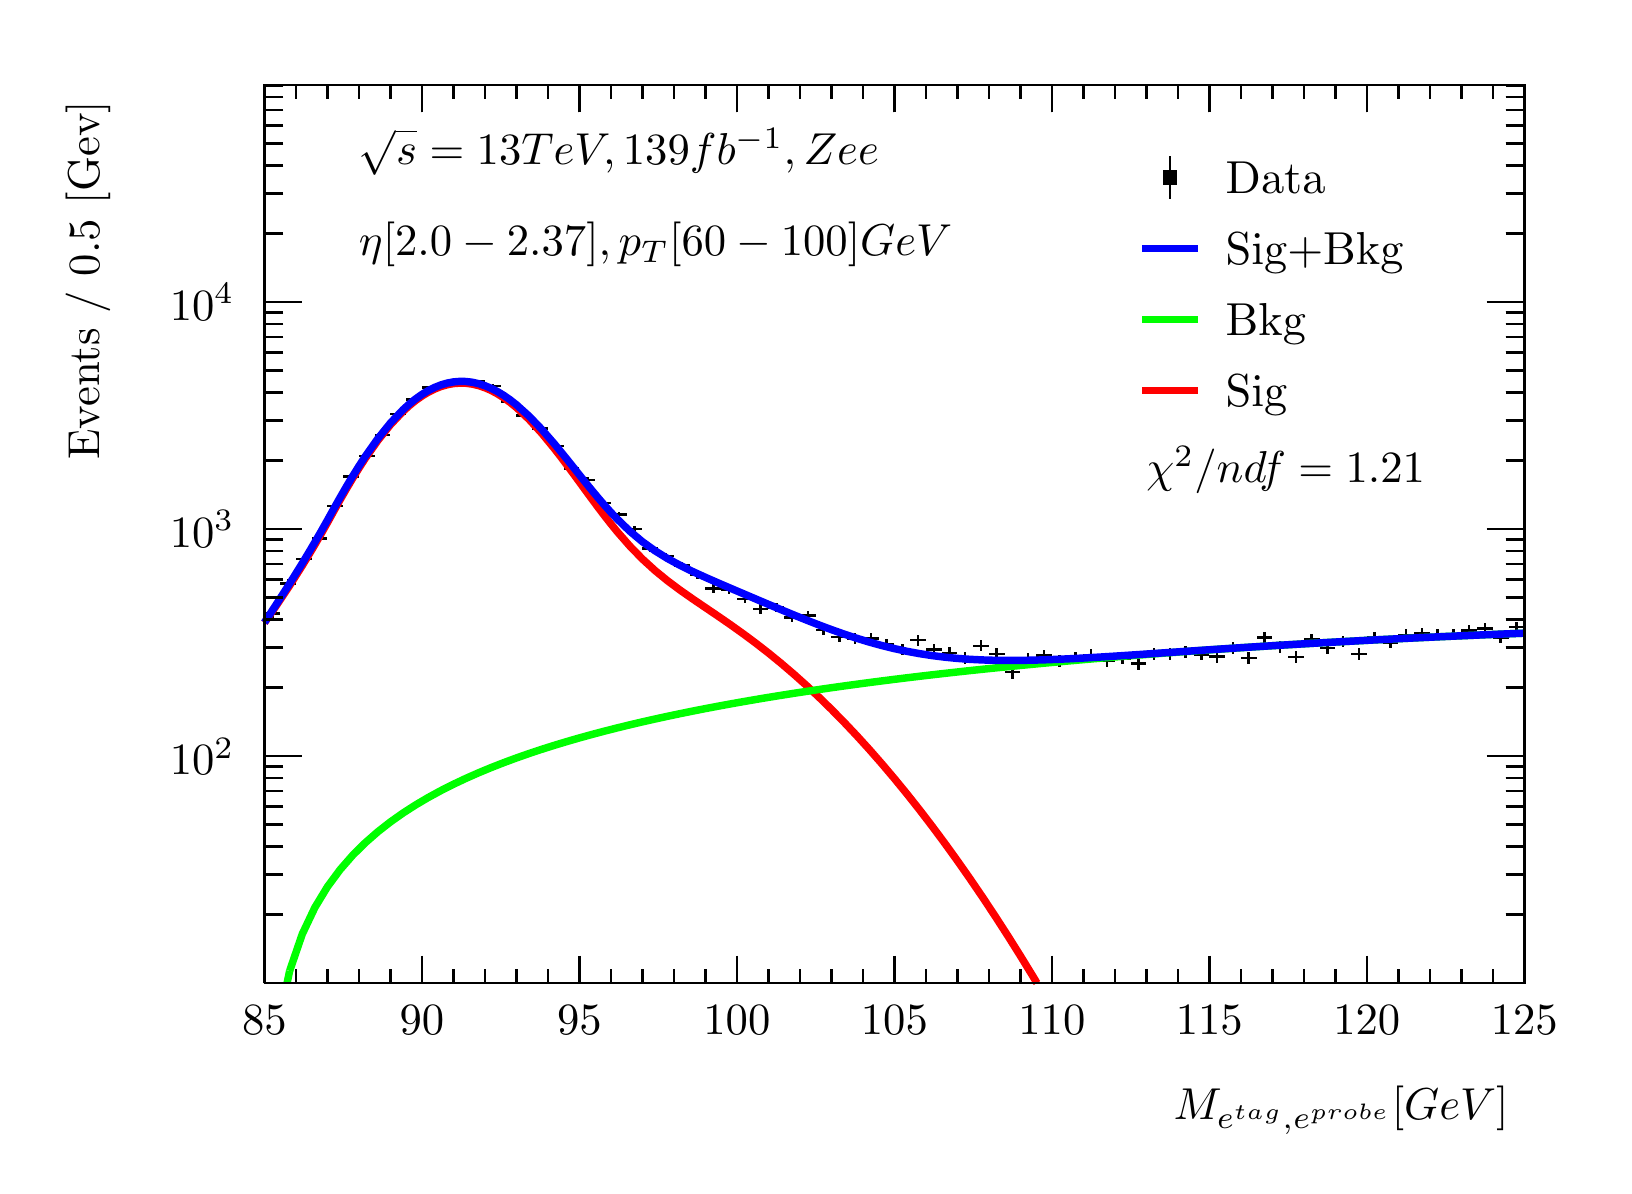
\begin{tikzpicture}
\pgfdeclareplotmark{cross} {
\pgfpathmoveto{\pgfpoint{-0.3\pgfplotmarksize}{\pgfplotmarksize}}
\pgfpathlineto{\pgfpoint{+0.3\pgfplotmarksize}{\pgfplotmarksize}}
\pgfpathlineto{\pgfpoint{+0.3\pgfplotmarksize}{0.3\pgfplotmarksize}}
\pgfpathlineto{\pgfpoint{+1\pgfplotmarksize}{0.3\pgfplotmarksize}}
\pgfpathlineto{\pgfpoint{+1\pgfplotmarksize}{-0.3\pgfplotmarksize}}
\pgfpathlineto{\pgfpoint{+0.3\pgfplotmarksize}{-0.3\pgfplotmarksize}}
\pgfpathlineto{\pgfpoint{+0.3\pgfplotmarksize}{-1.\pgfplotmarksize}}
\pgfpathlineto{\pgfpoint{-0.3\pgfplotmarksize}{-1.\pgfplotmarksize}}
\pgfpathlineto{\pgfpoint{-0.3\pgfplotmarksize}{-0.3\pgfplotmarksize}}
\pgfpathlineto{\pgfpoint{-1.\pgfplotmarksize}{-0.3\pgfplotmarksize}}
\pgfpathlineto{\pgfpoint{-1.\pgfplotmarksize}{0.3\pgfplotmarksize}}
\pgfpathlineto{\pgfpoint{-0.3\pgfplotmarksize}{0.3\pgfplotmarksize}}
\pgfpathclose
\pgfusepathqstroke
}
\pgfdeclareplotmark{cross*} {
\pgfpathmoveto{\pgfpoint{-0.3\pgfplotmarksize}{\pgfplotmarksize}}
\pgfpathlineto{\pgfpoint{+0.3\pgfplotmarksize}{\pgfplotmarksize}}
\pgfpathlineto{\pgfpoint{+0.3\pgfplotmarksize}{0.3\pgfplotmarksize}}
\pgfpathlineto{\pgfpoint{+1\pgfplotmarksize}{0.3\pgfplotmarksize}}
\pgfpathlineto{\pgfpoint{+1\pgfplotmarksize}{-0.3\pgfplotmarksize}}
\pgfpathlineto{\pgfpoint{+0.3\pgfplotmarksize}{-0.3\pgfplotmarksize}}
\pgfpathlineto{\pgfpoint{+0.3\pgfplotmarksize}{-1.\pgfplotmarksize}}
\pgfpathlineto{\pgfpoint{-0.3\pgfplotmarksize}{-1.\pgfplotmarksize}}
\pgfpathlineto{\pgfpoint{-0.3\pgfplotmarksize}{-0.3\pgfplotmarksize}}
\pgfpathlineto{\pgfpoint{-1.\pgfplotmarksize}{-0.3\pgfplotmarksize}}
\pgfpathlineto{\pgfpoint{-1.\pgfplotmarksize}{0.3\pgfplotmarksize}}
\pgfpathlineto{\pgfpoint{-0.3\pgfplotmarksize}{0.3\pgfplotmarksize}}
\pgfpathclose
\pgfusepathqfillstroke
}
\pgfdeclareplotmark{newstar} {
\pgfpathmoveto{\pgfqpoint{0pt}{\pgfplotmarksize}}
\pgfpathlineto{\pgfqpointpolar{44}{0.5\pgfplotmarksize}}
\pgfpathlineto{\pgfqpointpolar{18}{\pgfplotmarksize}}
\pgfpathlineto{\pgfqpointpolar{-20}{0.5\pgfplotmarksize}}
\pgfpathlineto{\pgfqpointpolar{-54}{\pgfplotmarksize}}
\pgfpathlineto{\pgfqpointpolar{-90}{0.5\pgfplotmarksize}}
\pgfpathlineto{\pgfqpointpolar{234}{\pgfplotmarksize}}
\pgfpathlineto{\pgfqpointpolar{198}{0.5\pgfplotmarksize}}
\pgfpathlineto{\pgfqpointpolar{162}{\pgfplotmarksize}}
\pgfpathlineto{\pgfqpointpolar{134}{0.5\pgfplotmarksize}}
\pgfpathclose
\pgfusepathqstroke
}
\pgfdeclareplotmark{newstar*} {
\pgfpathmoveto{\pgfqpoint{0pt}{\pgfplotmarksize}}
\pgfpathlineto{\pgfqpointpolar{44}{0.5\pgfplotmarksize}}
\pgfpathlineto{\pgfqpointpolar{18}{\pgfplotmarksize}}
\pgfpathlineto{\pgfqpointpolar{-20}{0.5\pgfplotmarksize}}
\pgfpathlineto{\pgfqpointpolar{-54}{\pgfplotmarksize}}
\pgfpathlineto{\pgfqpointpolar{-90}{0.5\pgfplotmarksize}}
\pgfpathlineto{\pgfqpointpolar{234}{\pgfplotmarksize}}
\pgfpathlineto{\pgfqpointpolar{198}{0.5\pgfplotmarksize}}
\pgfpathlineto{\pgfqpointpolar{162}{\pgfplotmarksize}}
\pgfpathlineto{\pgfqpointpolar{134}{0.5\pgfplotmarksize}}
\pgfpathclose
\pgfusepathqfillstroke
}
\definecolor{c}{rgb}{1,1,1};
\draw [color=c, fill=c] (0,0) rectangle (20,14.4361);
\draw [color=c, fill=c] (3,2.30977) rectangle (19,13.7143);
\definecolor{c}{rgb}{0,0,0};
\draw [c,line width=0.9] (3,2.30977) -- (3,13.7143) -- (19,13.7143) -- (19,2.30977) -- (3,2.30977);
\definecolor{c}{rgb}{1,1,1};
\draw [color=c, fill=c] (3,2.30977) rectangle (19,13.7143);
\definecolor{c}{rgb}{0,0,0};
\draw [c,line width=0.9] (3,2.30977) -- (3,13.7143) -- (19,13.7143) -- (19,2.30977) -- (3,2.30977);
\draw [c,line width=0.9] (3,2.30977) -- (19,2.30977);
\draw [c,line width=0.9] (3,2.65624) -- (3,2.30977);
\draw [c,line width=0.9] (3.4,2.48301) -- (3.4,2.30977);
\draw [c,line width=0.9] (3.8,2.48301) -- (3.8,2.30977);
\draw [c,line width=0.9] (4.2,2.48301) -- (4.2,2.30977);
\draw [c,line width=0.9] (4.6,2.48301) -- (4.6,2.30977);
\draw [c,line width=0.9] (5,2.65624) -- (5,2.30977);
\draw [c,line width=0.9] (5.4,2.48301) -- (5.4,2.30977);
\draw [c,line width=0.9] (5.8,2.48301) -- (5.8,2.30977);
\draw [c,line width=0.9] (6.2,2.48301) -- (6.2,2.30977);
\draw [c,line width=0.9] (6.6,2.48301) -- (6.6,2.30977);
\draw [c,line width=0.9] (7,2.65624) -- (7,2.30977);
\draw [c,line width=0.9] (7.4,2.48301) -- (7.4,2.30977);
\draw [c,line width=0.9] (7.8,2.48301) -- (7.8,2.30977);
\draw [c,line width=0.9] (8.2,2.48301) -- (8.2,2.30977);
\draw [c,line width=0.9] (8.6,2.48301) -- (8.6,2.30977);
\draw [c,line width=0.9] (9,2.65624) -- (9,2.30977);
\draw [c,line width=0.9] (9.4,2.48301) -- (9.4,2.30977);
\draw [c,line width=0.9] (9.8,2.48301) -- (9.8,2.30977);
\draw [c,line width=0.9] (10.2,2.48301) -- (10.2,2.30977);
\draw [c,line width=0.9] (10.6,2.48301) -- (10.6,2.30977);
\draw [c,line width=0.9] (11,2.65624) -- (11,2.30977);
\draw [c,line width=0.9] (11.4,2.48301) -- (11.4,2.30977);
\draw [c,line width=0.9] (11.8,2.48301) -- (11.8,2.30977);
\draw [c,line width=0.9] (12.2,2.48301) -- (12.2,2.30977);
\draw [c,line width=0.9] (12.6,2.48301) -- (12.6,2.30977);
\draw [c,line width=0.9] (13,2.65624) -- (13,2.30977);
\draw [c,line width=0.9] (13.4,2.48301) -- (13.4,2.30977);
\draw [c,line width=0.9] (13.8,2.48301) -- (13.8,2.30977);
\draw [c,line width=0.9] (14.2,2.48301) -- (14.2,2.30977);
\draw [c,line width=0.9] (14.6,2.48301) -- (14.6,2.30977);
\draw [c,line width=0.9] (15,2.65624) -- (15,2.30977);
\draw [c,line width=0.9] (15.4,2.48301) -- (15.4,2.30977);
\draw [c,line width=0.9] (15.8,2.48301) -- (15.8,2.30977);
\draw [c,line width=0.9] (16.2,2.48301) -- (16.2,2.30977);
\draw [c,line width=0.9] (16.6,2.48301) -- (16.6,2.30977);
\draw [c,line width=0.9] (17,2.65624) -- (17,2.30977);
\draw [c,line width=0.9] (17.4,2.48301) -- (17.4,2.30977);
\draw [c,line width=0.9] (17.8,2.48301) -- (17.8,2.30977);
\draw [c,line width=0.9] (18.2,2.48301) -- (18.2,2.30977);
\draw [c,line width=0.9] (18.6,2.48301) -- (18.6,2.30977);
\draw [c,line width=0.9] (19,2.65624) -- (19,2.30977);
\draw [anchor=base] (3,1.66015) node[scale=1.61424, color=c, rotate=0]{85};
\draw [anchor=base] (5,1.66015) node[scale=1.61424, color=c, rotate=0]{90};
\draw [anchor=base] (7,1.66015) node[scale=1.61424, color=c, rotate=0]{95};
\draw [anchor=base] (9,1.66015) node[scale=1.61424, color=c, rotate=0]{100};
\draw [anchor=base] (11,1.66015) node[scale=1.61424, color=c, rotate=0]{105};
\draw [anchor=base] (13,1.66015) node[scale=1.61424, color=c, rotate=0]{110};
\draw [anchor=base] (15,1.66015) node[scale=1.61424, color=c, rotate=0]{115};
\draw [anchor=base] (17,1.66015) node[scale=1.61424, color=c, rotate=0]{120};
\draw [anchor=base] (19,1.66015) node[scale=1.61424, color=c, rotate=0]{125};
\draw [anchor= east] (19,0.692932) node[scale=1.61424, color=c, rotate=0]{$M_{e^{tag}, e^{probe}}  [GeV]$};
\draw [c,line width=0.9] (3,13.7143) -- (19,13.7143);
\draw [c,line width=0.9] (3,13.3678) -- (3,13.7143);
\draw [c,line width=0.9] (3.4,13.5411) -- (3.4,13.7143);
\draw [c,line width=0.9] (3.8,13.5411) -- (3.8,13.7143);
\draw [c,line width=0.9] (4.2,13.5411) -- (4.2,13.7143);
\draw [c,line width=0.9] (4.6,13.5411) -- (4.6,13.7143);
\draw [c,line width=0.9] (5,13.3678) -- (5,13.7143);
\draw [c,line width=0.9] (5.4,13.5411) -- (5.4,13.7143);
\draw [c,line width=0.9] (5.8,13.5411) -- (5.8,13.7143);
\draw [c,line width=0.9] (6.2,13.5411) -- (6.2,13.7143);
\draw [c,line width=0.9] (6.6,13.5411) -- (6.6,13.7143);
\draw [c,line width=0.9] (7,13.3678) -- (7,13.7143);
\draw [c,line width=0.9] (7.4,13.5411) -- (7.4,13.7143);
\draw [c,line width=0.9] (7.8,13.5411) -- (7.8,13.7143);
\draw [c,line width=0.9] (8.2,13.5411) -- (8.2,13.7143);
\draw [c,line width=0.9] (8.6,13.5411) -- (8.6,13.7143);
\draw [c,line width=0.9] (9,13.3678) -- (9,13.7143);
\draw [c,line width=0.9] (9.4,13.5411) -- (9.4,13.7143);
\draw [c,line width=0.9] (9.8,13.5411) -- (9.8,13.7143);
\draw [c,line width=0.9] (10.2,13.5411) -- (10.2,13.7143);
\draw [c,line width=0.9] (10.6,13.5411) -- (10.6,13.7143);
\draw [c,line width=0.9] (11,13.3678) -- (11,13.7143);
\draw [c,line width=0.9] (11.4,13.5411) -- (11.4,13.7143);
\draw [c,line width=0.9] (11.8,13.5411) -- (11.8,13.7143);
\draw [c,line width=0.9] (12.2,13.5411) -- (12.2,13.7143);
\draw [c,line width=0.9] (12.6,13.5411) -- (12.6,13.7143);
\draw [c,line width=0.9] (13,13.3678) -- (13,13.7143);
\draw [c,line width=0.9] (13.4,13.5411) -- (13.4,13.7143);
\draw [c,line width=0.9] (13.8,13.5411) -- (13.8,13.7143);
\draw [c,line width=0.9] (14.2,13.5411) -- (14.2,13.7143);
\draw [c,line width=0.9] (14.6,13.5411) -- (14.6,13.7143);
\draw [c,line width=0.9] (15,13.3678) -- (15,13.7143);
\draw [c,line width=0.9] (15.4,13.5411) -- (15.4,13.7143);
\draw [c,line width=0.9] (15.8,13.5411) -- (15.8,13.7143);
\draw [c,line width=0.9] (16.2,13.5411) -- (16.2,13.7143);
\draw [c,line width=0.9] (16.6,13.5411) -- (16.6,13.7143);
\draw [c,line width=0.9] (17,13.3678) -- (17,13.7143);
\draw [c,line width=0.9] (17.4,13.5411) -- (17.4,13.7143);
\draw [c,line width=0.9] (17.8,13.5411) -- (17.8,13.7143);
\draw [c,line width=0.9] (18.2,13.5411) -- (18.2,13.7143);
\draw [c,line width=0.9] (18.6,13.5411) -- (18.6,13.7143);
\draw [c,line width=0.9] (19,13.3678) -- (19,13.7143);
\draw [c,line width=0.9] (3,2.30977) -- (3,13.7143);
\draw [c,line width=0.9] (3.237,3.17769) -- (3,3.17769);
\draw [c,line width=0.9] (3.237,3.68539) -- (3,3.68539);
\draw [c,line width=0.9] (3.237,4.04561) -- (3,4.04561);
\draw [c,line width=0.9] (3.237,4.32501) -- (3,4.32501);
\draw [c,line width=0.9] (3.237,4.55331) -- (3,4.55331);
\draw [c,line width=0.9] (3.237,4.74632) -- (3,4.74632);
\draw [c,line width=0.9] (3.237,4.91352) -- (3,4.91352);
\draw [c,line width=0.9] (3.237,5.061) -- (3,5.061);
\draw [c,line width=0.9] (3.474,5.19293) -- (3,5.19293);
\draw [anchor= east] (2.82,5.19293) node[scale=1.61424, color=c, rotate=0]{$10^{2}$};
\draw [c,line width=0.9] (3.237,6.06085) -- (3,6.06085);
\draw [c,line width=0.9] (3.237,6.56855) -- (3,6.56855);
\draw [c,line width=0.9] (3.237,6.92876) -- (3,6.92876);
\draw [c,line width=0.9] (3.237,7.20817) -- (3,7.20817);
\draw [c,line width=0.9] (3.237,7.43646) -- (3,7.43646);
\draw [c,line width=0.9] (3.237,7.62948) -- (3,7.62948);
\draw [c,line width=0.9] (3.237,7.79668) -- (3,7.79668);
\draw [c,line width=0.9] (3.237,7.94416) -- (3,7.94416);
\draw [c,line width=0.9] (3.474,8.07609) -- (3,8.07609);
\draw [anchor= east] (2.82,8.07609) node[scale=1.61424, color=c, rotate=0]{$10^{3}$};
\draw [c,line width=0.9] (3.237,8.94401) -- (3,8.94401);
\draw [c,line width=0.9] (3.237,9.4517) -- (3,9.4517);
\draw [c,line width=0.9] (3.237,9.81192) -- (3,9.81192);
\draw [c,line width=0.9] (3.237,10.0913) -- (3,10.0913);
\draw [c,line width=0.9] (3.237,10.3196) -- (3,10.3196);
\draw [c,line width=0.9] (3.237,10.5126) -- (3,10.5126);
\draw [c,line width=0.9] (3.237,10.6798) -- (3,10.6798);
\draw [c,line width=0.9] (3.237,10.8273) -- (3,10.8273);
\draw [c,line width=0.9] (3.474,10.9592) -- (3,10.9592);
\draw [anchor= east] (2.82,10.9592) node[scale=1.61424, color=c, rotate=0]{$10^{4}$};
\draw [c,line width=0.9] (3.237,11.8272) -- (3,11.8272);
\draw [c,line width=0.9] (3.237,12.3349) -- (3,12.3349);
\draw [c,line width=0.9] (3.237,12.6951) -- (3,12.6951);
\draw [c,line width=0.9] (3.237,12.9745) -- (3,12.9745);
\draw [c,line width=0.9] (3.237,13.2028) -- (3,13.2028);
\draw [c,line width=0.9] (3.237,13.3958) -- (3,13.3958);
\draw [c,line width=0.9] (3.237,13.563) -- (3,13.563);
\draw [c,line width=0.9] (3.237,13.7105) -- (3,13.7105);
\draw [anchor= east] (0.76,13.7143) node[scale=1.61424, color=c, rotate=90]{Events / 0.5 [Gev]};
\draw [c,line width=0.9] (19,2.30977) -- (19,13.7143);
\draw [c,line width=0.9] (18.763,3.17769) -- (19,3.17769);
\draw [c,line width=0.9] (18.763,3.68539) -- (19,3.68539);
\draw [c,line width=0.9] (18.763,4.04561) -- (19,4.04561);
\draw [c,line width=0.9] (18.763,4.32501) -- (19,4.32501);
\draw [c,line width=0.9] (18.763,4.55331) -- (19,4.55331);
\draw [c,line width=0.9] (18.763,4.74632) -- (19,4.74632);
\draw [c,line width=0.9] (18.763,4.91352) -- (19,4.91352);
\draw [c,line width=0.9] (18.763,5.061) -- (19,5.061);
\draw [c,line width=0.9] (18.526,5.19293) -- (19,5.19293);
\draw [c,line width=0.9] (18.763,6.06085) -- (19,6.06085);
\draw [c,line width=0.9] (18.763,6.56855) -- (19,6.56855);
\draw [c,line width=0.9] (18.763,6.92876) -- (19,6.92876);
\draw [c,line width=0.9] (18.763,7.20817) -- (19,7.20817);
\draw [c,line width=0.9] (18.763,7.43646) -- (19,7.43646);
\draw [c,line width=0.9] (18.763,7.62948) -- (19,7.62948);
\draw [c,line width=0.9] (18.763,7.79668) -- (19,7.79668);
\draw [c,line width=0.9] (18.763,7.94416) -- (19,7.94416);
\draw [c,line width=0.9] (18.526,8.07609) -- (19,8.07609);
\draw [c,line width=0.9] (18.763,8.94401) -- (19,8.94401);
\draw [c,line width=0.9] (18.763,9.4517) -- (19,9.4517);
\draw [c,line width=0.9] (18.763,9.81192) -- (19,9.81192);
\draw [c,line width=0.9] (18.763,10.0913) -- (19,10.0913);
\draw [c,line width=0.9] (18.763,10.3196) -- (19,10.3196);
\draw [c,line width=0.9] (18.763,10.5126) -- (19,10.5126);
\draw [c,line width=0.9] (18.763,10.6798) -- (19,10.6798);
\draw [c,line width=0.9] (18.763,10.8273) -- (19,10.8273);
\draw [c,line width=0.9] (18.526,10.9592) -- (19,10.9592);
\draw [c,line width=0.9] (18.763,11.8272) -- (19,11.8272);
\draw [c,line width=0.9] (18.763,12.3349) -- (19,12.3349);
\draw [c,line width=0.9] (18.763,12.6951) -- (19,12.6951);
\draw [c,line width=0.9] (18.763,12.9745) -- (19,12.9745);
\draw [c,line width=0.9] (18.763,13.2028) -- (19,13.2028);
\draw [c,line width=0.9] (18.763,13.3958) -- (19,13.3958);
\draw [c,line width=0.9] (18.763,13.563) -- (19,13.563);
\draw [c,line width=0.9] (18.763,13.7105) -- (19,13.7105);
\draw [c,line width=0.9] (3.1,7.00468) -- (3,7.00468);
\draw [c,line width=0.9] (3,7.00468) -- (3,7.00468);
\draw [c,line width=0.9] (3.1,7.00468) -- (3.2,7.00468);
\draw [c,line width=0.9] (3.2,7.00468) -- (3.2,7.00468);
\draw [c,line width=0.9] (3.1,7.00468) -- (3.1,7.06541);
\draw [c,line width=0.9] (3.1,7.06541) -- (3.1,7.06541);
\draw [c,line width=0.9] (3.1,7.00468) -- (3.1,6.94394);
\draw [c,line width=0.9] (3.1,6.94394) -- (3.1,6.94394);
\draw [c,line width=0.9] (3.3,7.38317) -- (3.2,7.38317);
\draw [c,line width=0.9] (3.2,7.38317) -- (3.2,7.38317);
\draw [c,line width=0.9] (3.3,7.38317) -- (3.4,7.38317);
\draw [c,line width=0.9] (3.4,7.38317) -- (3.4,7.38317);
\draw [c,line width=0.9] (3.3,7.38317) -- (3.3,7.43539);
\draw [c,line width=0.9] (3.3,7.43539) -- (3.3,7.43539);
\draw [c,line width=0.9] (3.3,7.38317) -- (3.3,7.33096);
\draw [c,line width=0.9] (3.3,7.33096) -- (3.3,7.33096);
\draw [c,line width=0.9] (3.5,7.69398) -- (3.4,7.69398);
\draw [c,line width=0.9] (3.4,7.69398) -- (3.4,7.69398);
\draw [c,line width=0.9] (3.5,7.69398) -- (3.6,7.69398);
\draw [c,line width=0.9] (3.6,7.69398) -- (3.6,7.69398);
\draw [c,line width=0.9] (3.5,7.69398) -- (3.5,7.7401);
\draw [c,line width=0.9] (3.5,7.7401) -- (3.5,7.7401);
\draw [c,line width=0.9] (3.5,7.69398) -- (3.5,7.64786);
\draw [c,line width=0.9] (3.5,7.64786) -- (3.5,7.64786);
\draw [c,line width=0.9] (3.7,7.95387) -- (3.6,7.95387);
\draw [c,line width=0.9] (3.6,7.95387) -- (3.6,7.95387);
\draw [c,line width=0.9] (3.7,7.95387) -- (3.8,7.95387);
\draw [c,line width=0.9] (3.8,7.95387) -- (3.8,7.95387);
\draw [c,line width=0.9] (3.7,7.95387) -- (3.7,7.99544);
\draw [c,line width=0.9] (3.7,7.99544) -- (3.7,7.99544);
\draw [c,line width=0.9] (3.7,7.95387) -- (3.7,7.91229);
\draw [c,line width=0.9] (3.7,7.91229) -- (3.7,7.91229);
\draw [c,line width=0.9] (3.9,8.37043) -- (3.8,8.37043);
\draw [c,line width=0.9] (3.8,8.37043) -- (3.8,8.37043);
\draw [c,line width=0.9] (3.9,8.37043) -- (4,8.37043);
\draw [c,line width=0.9] (4,8.37043) -- (4,8.37043);
\draw [c,line width=0.9] (3.9,8.37043) -- (3.9,8.40564);
\draw [c,line width=0.9] (3.9,8.40564) -- (3.9,8.40564);
\draw [c,line width=0.9] (3.9,8.37043) -- (3.9,8.33523);
\draw [c,line width=0.9] (3.9,8.33523) -- (3.9,8.33523);
\draw [c,line width=0.9] (4.1,8.74272) -- (4,8.74272);
\draw [c,line width=0.9] (4,8.74272) -- (4,8.74272);
\draw [c,line width=0.9] (4.1,8.74272) -- (4.2,8.74272);
\draw [c,line width=0.9] (4.2,8.74272) -- (4.2,8.74272);
\draw [c,line width=0.9] (4.1,8.74272) -- (4.1,8.77306);
\draw [c,line width=0.9] (4.1,8.77306) -- (4.1,8.77306);
\draw [c,line width=0.9] (4.1,8.74272) -- (4.1,8.71238);
\draw [c,line width=0.9] (4.1,8.71238) -- (4.1,8.71238);
\draw [c,line width=0.9] (4.3,9.0045) -- (4.2,9.0045);
\draw [c,line width=0.9] (4.2,9.0045) -- (4.2,9.0045);
\draw [c,line width=0.9] (4.3,9.0045) -- (4.4,9.0045);
\draw [c,line width=0.9] (4.4,9.0045) -- (4.4,9.0045);
\draw [c,line width=0.9] (4.3,9.0045) -- (4.3,9.03183);
\draw [c,line width=0.9] (4.3,9.03183) -- (4.3,9.03183);
\draw [c,line width=0.9] (4.3,9.0045) -- (4.3,8.97717);
\draw [c,line width=0.9] (4.3,8.97717) -- (4.3,8.97717);
\draw [c,line width=0.9] (4.5,9.26915) -- (4.4,9.26915);
\draw [c,line width=0.9] (4.4,9.26915) -- (4.4,9.26915);
\draw [c,line width=0.9] (4.5,9.26915) -- (4.6,9.26915);
\draw [c,line width=0.9] (4.6,9.26915) -- (4.6,9.26915);
\draw [c,line width=0.9] (4.5,9.26915) -- (4.5,9.29374);
\draw [c,line width=0.9] (4.5,9.29374) -- (4.5,9.29374);
\draw [c,line width=0.9] (4.5,9.26915) -- (4.5,9.24456);
\draw [c,line width=0.9] (4.5,9.24456) -- (4.5,9.24456);
\draw [c,line width=0.9] (4.7,9.53525) -- (4.6,9.53525);
\draw [c,line width=0.9] (4.6,9.53525) -- (4.6,9.53525);
\draw [c,line width=0.9] (4.7,9.53525) -- (4.8,9.53525);
\draw [c,line width=0.9] (4.8,9.53525) -- (4.8,9.53525);
\draw [c,line width=0.9] (4.7,9.53525) -- (4.7,9.55736);
\draw [c,line width=0.9] (4.7,9.55736) -- (4.7,9.55736);
\draw [c,line width=0.9] (4.7,9.53525) -- (4.7,9.51314);
\draw [c,line width=0.9] (4.7,9.51314) -- (4.7,9.51314);
\draw [c,line width=0.9] (4.9,9.72206) -- (4.8,9.72206);
\draw [c,line width=0.9] (4.8,9.72206) -- (4.8,9.72206);
\draw [c,line width=0.9] (4.9,9.72206) -- (5,9.72206);
\draw [c,line width=0.9] (5,9.72206) -- (5,9.72206);
\draw [c,line width=0.9] (4.9,9.72206) -- (4.9,9.74259);
\draw [c,line width=0.9] (4.9,9.74259) -- (4.9,9.74259);
\draw [c,line width=0.9] (4.9,9.72206) -- (4.9,9.70154);
\draw [c,line width=0.9] (4.9,9.70154) -- (4.9,9.70154);
\draw [c,line width=0.9] (5.1,9.87182) -- (5,9.87182);
\draw [c,line width=0.9] (5,9.87182) -- (5,9.87182);
\draw [c,line width=0.9] (5.1,9.87182) -- (5.2,9.87182);
\draw [c,line width=0.9] (5.2,9.87182) -- (5.2,9.87182);
\draw [c,line width=0.9] (5.1,9.87182) -- (5.1,9.89115);
\draw [c,line width=0.9] (5.1,9.89115) -- (5.1,9.89115);
\draw [c,line width=0.9] (5.1,9.87182) -- (5.1,9.85249);
\draw [c,line width=0.9] (5.1,9.85249) -- (5.1,9.85249);
\draw [c,line width=0.9] (5.3,9.9135) -- (5.2,9.9135);
\draw [c,line width=0.9] (5.2,9.9135) -- (5.2,9.9135);
\draw [c,line width=0.9] (5.3,9.9135) -- (5.4,9.9135);
\draw [c,line width=0.9] (5.4,9.9135) -- (5.4,9.9135);
\draw [c,line width=0.9] (5.3,9.9135) -- (5.3,9.93251);
\draw [c,line width=0.9] (5.3,9.93251) -- (5.3,9.93251);
\draw [c,line width=0.9] (5.3,9.9135) -- (5.3,9.89449);
\draw [c,line width=0.9] (5.3,9.89449) -- (5.3,9.89449);
\draw [c,line width=0.9] (5.5,9.94626) -- (5.4,9.94626);
\draw [c,line width=0.9] (5.4,9.94626) -- (5.4,9.94626);
\draw [c,line width=0.9] (5.5,9.94626) -- (5.6,9.94626);
\draw [c,line width=0.9] (5.6,9.94626) -- (5.6,9.94626);
\draw [c,line width=0.9] (5.5,9.94626) -- (5.5,9.96502);
\draw [c,line width=0.9] (5.5,9.96502) -- (5.5,9.96502);
\draw [c,line width=0.9] (5.5,9.94626) -- (5.5,9.92749);
\draw [c,line width=0.9] (5.5,9.92749) -- (5.5,9.92749);
\draw [c,line width=0.9] (5.7,9.95215) -- (5.6,9.95215);
\draw [c,line width=0.9] (5.6,9.95215) -- (5.6,9.95215);
\draw [c,line width=0.9] (5.7,9.95215) -- (5.8,9.95215);
\draw [c,line width=0.9] (5.8,9.95215) -- (5.8,9.95215);
\draw [c,line width=0.9] (5.7,9.95215) -- (5.7,9.97087);
\draw [c,line width=0.9] (5.7,9.97087) -- (5.7,9.97087);
\draw [c,line width=0.9] (5.7,9.95215) -- (5.7,9.93343);
\draw [c,line width=0.9] (5.7,9.93343) -- (5.7,9.93343);
\draw [c,line width=0.9] (5.9,9.89313) -- (5.8,9.89313);
\draw [c,line width=0.9] (5.8,9.89313) -- (5.8,9.89313);
\draw [c,line width=0.9] (5.9,9.89313) -- (6,9.89313);
\draw [c,line width=0.9] (6,9.89313) -- (6,9.89313);
\draw [c,line width=0.9] (5.9,9.89313) -- (5.9,9.91229);
\draw [c,line width=0.9] (5.9,9.91229) -- (5.9,9.91229);
\draw [c,line width=0.9] (5.9,9.89313) -- (5.9,9.87396);
\draw [c,line width=0.9] (5.9,9.87396) -- (5.9,9.87396);
\draw [c,line width=0.9] (6.1,9.69624) -- (6,9.69624);
\draw [c,line width=0.9] (6,9.69624) -- (6,9.69624);
\draw [c,line width=0.9] (6.1,9.69624) -- (6.2,9.69624);
\draw [c,line width=0.9] (6.2,9.69624) -- (6.2,9.69624);
\draw [c,line width=0.9] (6.1,9.69624) -- (6.1,9.71697);
\draw [c,line width=0.9] (6.1,9.71697) -- (6.1,9.71697);
\draw [c,line width=0.9] (6.1,9.69624) -- (6.1,9.67551);
\draw [c,line width=0.9] (6.1,9.67551) -- (6.1,9.67551);
\draw [c,line width=0.9] (6.3,9.51597) -- (6.2,9.51597);
\draw [c,line width=0.9] (6.2,9.51597) -- (6.2,9.51597);
\draw [c,line width=0.9] (6.3,9.51597) -- (6.4,9.51597);
\draw [c,line width=0.9] (6.4,9.51597) -- (6.4,9.51597);
\draw [c,line width=0.9] (6.3,9.51597) -- (6.3,9.53826);
\draw [c,line width=0.9] (6.3,9.53826) -- (6.3,9.53826);
\draw [c,line width=0.9] (6.3,9.51597) -- (6.3,9.49369);
\draw [c,line width=0.9] (6.3,9.49369) -- (6.3,9.49369);
\draw [c,line width=0.9] (6.5,9.35454) -- (6.4,9.35454);
\draw [c,line width=0.9] (6.4,9.35454) -- (6.4,9.35454);
\draw [c,line width=0.9] (6.5,9.35454) -- (6.6,9.35454);
\draw [c,line width=0.9] (6.6,9.35454) -- (6.6,9.35454);
\draw [c,line width=0.9] (6.5,9.35454) -- (6.5,9.3783);
\draw [c,line width=0.9] (6.5,9.3783) -- (6.5,9.3783);
\draw [c,line width=0.9] (6.5,9.35454) -- (6.5,9.33077);
\draw [c,line width=0.9] (6.5,9.33077) -- (6.5,9.33077);
\draw [c,line width=0.9] (6.7,9.12769) -- (6.6,9.12769);
\draw [c,line width=0.9] (6.6,9.12769) -- (6.6,9.12769);
\draw [c,line width=0.9] (6.7,9.12769) -- (6.8,9.12769);
\draw [c,line width=0.9] (6.8,9.12769) -- (6.8,9.12769);
\draw [c,line width=0.9] (6.7,9.12769) -- (6.7,9.15371);
\draw [c,line width=0.9] (6.7,9.15371) -- (6.7,9.15371);
\draw [c,line width=0.9] (6.7,9.12769) -- (6.7,9.10167);
\draw [c,line width=0.9] (6.7,9.10167) -- (6.7,9.10167);
\draw [c,line width=0.9] (6.9,8.84164) -- (6.8,8.84164);
\draw [c,line width=0.9] (6.8,8.84164) -- (6.8,8.84164);
\draw [c,line width=0.9] (6.9,8.84164) -- (7,8.84164);
\draw [c,line width=0.9] (7,8.84164) -- (7,8.84164);
\draw [c,line width=0.9] (6.9,8.84164) -- (6.9,8.87081);
\draw [c,line width=0.9] (6.9,8.87081) -- (6.9,8.87081);
\draw [c,line width=0.9] (6.9,8.84164) -- (6.9,8.81248);
\draw [c,line width=0.9] (6.9,8.81248) -- (6.9,8.81248);
\draw [c,line width=0.9] (7.1,8.70009) -- (7,8.70009);
\draw [c,line width=0.9] (7,8.70009) -- (7,8.70009);
\draw [c,line width=0.9] (7.1,8.70009) -- (7.2,8.70009);
\draw [c,line width=0.9] (7.2,8.70009) -- (7.2,8.70009);
\draw [c,line width=0.9] (7.1,8.70009) -- (7.1,8.73095);
\draw [c,line width=0.9] (7.1,8.73095) -- (7.1,8.73095);
\draw [c,line width=0.9] (7.1,8.70009) -- (7.1,8.66923);
\draw [c,line width=0.9] (7.1,8.66923) -- (7.1,8.66923);
\draw [c,line width=0.9] (7.3,8.40845) -- (7.2,8.40845);
\draw [c,line width=0.9] (7.2,8.40845) -- (7.2,8.40845);
\draw [c,line width=0.9] (7.3,8.40845) -- (7.4,8.40845);
\draw [c,line width=0.9] (7.4,8.40845) -- (7.4,8.40845);
\draw [c,line width=0.9] (7.3,8.40845) -- (7.3,8.44313);
\draw [c,line width=0.9] (7.3,8.44313) -- (7.3,8.44313);
\draw [c,line width=0.9] (7.3,8.40845) -- (7.3,8.37378);
\draw [c,line width=0.9] (7.3,8.37378) -- (7.3,8.37378);
\draw [c,line width=0.9] (7.5,8.25761) -- (7.4,8.25761);
\draw [c,line width=0.9] (7.4,8.25761) -- (7.4,8.25761);
\draw [c,line width=0.9] (7.5,8.25761) -- (7.6,8.25761);
\draw [c,line width=0.9] (7.6,8.25761) -- (7.6,8.25761);
\draw [c,line width=0.9] (7.5,8.25761) -- (7.5,8.29443);
\draw [c,line width=0.9] (7.5,8.29443) -- (7.5,8.29443);
\draw [c,line width=0.9] (7.5,8.25761) -- (7.5,8.22078);
\draw [c,line width=0.9] (7.5,8.22078) -- (7.5,8.22078);
\draw [c,line width=0.9] (7.7,8.07358) -- (7.6,8.07358);
\draw [c,line width=0.9] (7.6,8.07358) -- (7.6,8.07358);
\draw [c,line width=0.9] (7.7,8.07358) -- (7.8,8.07358);
\draw [c,line width=0.9] (7.8,8.07358) -- (7.8,8.07358);
\draw [c,line width=0.9] (7.7,8.07358) -- (7.7,8.11322);
\draw [c,line width=0.9] (7.7,8.11322) -- (7.7,8.11322);
\draw [c,line width=0.9] (7.7,8.07358) -- (7.7,8.03395);
\draw [c,line width=0.9] (7.7,8.03395) -- (7.7,8.03395);
\draw [c,line width=0.9] (7.9,7.82913) -- (7.8,7.82913);
\draw [c,line width=0.9] (7.8,7.82913) -- (7.8,7.82913);
\draw [c,line width=0.9] (7.9,7.82913) -- (8,7.82913);
\draw [c,line width=0.9] (8,7.82913) -- (8,7.82913);
\draw [c,line width=0.9] (7.9,7.82913) -- (7.9,7.87283);
\draw [c,line width=0.9] (7.9,7.87283) -- (7.9,7.87283);
\draw [c,line width=0.9] (7.9,7.82913) -- (7.9,7.78543);
\draw [c,line width=0.9] (7.9,7.78543) -- (7.9,7.78543);
\draw [c,line width=0.9] (8.1,7.73081) -- (8,7.73081);
\draw [c,line width=0.9] (8,7.73081) -- (8,7.73081);
\draw [c,line width=0.9] (8.1,7.73081) -- (8.2,7.73081);
\draw [c,line width=0.9] (8.2,7.73081) -- (8.2,7.73081);
\draw [c,line width=0.9] (8.1,7.73081) -- (8.1,7.77626);
\draw [c,line width=0.9] (8.1,7.77626) -- (8.1,7.77626);
\draw [c,line width=0.9] (8.1,7.73081) -- (8.1,7.68536);
\draw [c,line width=0.9] (8.1,7.68536) -- (8.1,7.68536);
\draw [c,line width=0.9] (8.3,7.60965) -- (8.2,7.60965);
\draw [c,line width=0.9] (8.2,7.60965) -- (8.2,7.60965);
\draw [c,line width=0.9] (8.3,7.60965) -- (8.4,7.60965);
\draw [c,line width=0.9] (8.4,7.60965) -- (8.4,7.60965);
\draw [c,line width=0.9] (8.3,7.60965) -- (8.3,7.65735);
\draw [c,line width=0.9] (8.3,7.65735) -- (8.3,7.65735);
\draw [c,line width=0.9] (8.3,7.60965) -- (8.3,7.56195);
\draw [c,line width=0.9] (8.3,7.56195) -- (8.3,7.56195);
\draw [c,line width=0.9] (8.5,7.49158) -- (8.4,7.49158);
\draw [c,line width=0.9] (8.4,7.49158) -- (8.4,7.49158);
\draw [c,line width=0.9] (8.5,7.49158) -- (8.6,7.49158);
\draw [c,line width=0.9] (8.6,7.49158) -- (8.6,7.49158);
\draw [c,line width=0.9] (8.5,7.49158) -- (8.5,7.54158);
\draw [c,line width=0.9] (8.5,7.54158) -- (8.5,7.54158);
\draw [c,line width=0.9] (8.5,7.49158) -- (8.5,7.44158);
\draw [c,line width=0.9] (8.5,7.44158) -- (8.5,7.44158);
\draw [c,line width=0.9] (8.7,7.31838) -- (8.6,7.31838);
\draw [c,line width=0.9] (8.6,7.31838) -- (8.6,7.31838);
\draw [c,line width=0.9] (8.7,7.31838) -- (8.8,7.31838);
\draw [c,line width=0.9] (8.8,7.31838) -- (8.8,7.31838);
\draw [c,line width=0.9] (8.7,7.31838) -- (8.7,7.37196);
\draw [c,line width=0.9] (8.7,7.37196) -- (8.7,7.37196);
\draw [c,line width=0.9] (8.7,7.31838) -- (8.7,7.26479);
\draw [c,line width=0.9] (8.7,7.26479) -- (8.7,7.26479);
\draw [c,line width=0.9] (8.9,7.30917) -- (8.8,7.30917);
\draw [c,line width=0.9] (8.8,7.30917) -- (8.8,7.30917);
\draw [c,line width=0.9] (8.9,7.30917) -- (9,7.30917);
\draw [c,line width=0.9] (9,7.30917) -- (9,7.30917);
\draw [c,line width=0.9] (8.9,7.30917) -- (8.9,7.36295);
\draw [c,line width=0.9] (8.9,7.36295) -- (8.9,7.36295);
\draw [c,line width=0.9] (8.9,7.30917) -- (8.9,7.25539);
\draw [c,line width=0.9] (8.9,7.25539) -- (8.9,7.25539);
\draw [c,line width=0.9] (9.1,7.18798) -- (9,7.18798);
\draw [c,line width=0.9] (9,7.18798) -- (9,7.18798);
\draw [c,line width=0.9] (9.1,7.18798) -- (9.2,7.18798);
\draw [c,line width=0.9] (9.2,7.18798) -- (9.2,7.18798);
\draw [c,line width=0.9] (9.1,7.18798) -- (9.1,7.24442);
\draw [c,line width=0.9] (9.1,7.24442) -- (9.1,7.24442);
\draw [c,line width=0.9] (9.1,7.18798) -- (9.1,7.13153);
\draw [c,line width=0.9] (9.1,7.13153) -- (9.1,7.13153);
\draw [c,line width=0.9] (9.3,7.06226) -- (9.2,7.06226);
\draw [c,line width=0.9] (9.2,7.06226) -- (9.2,7.06226);
\draw [c,line width=0.9] (9.3,7.06226) -- (9.4,7.06226);
\draw [c,line width=0.9] (9.4,7.06226) -- (9.4,7.06226);
\draw [c,line width=0.9] (9.3,7.06226) -- (9.3,7.12161);
\draw [c,line width=0.9] (9.3,7.12161) -- (9.3,7.12161);
\draw [c,line width=0.9] (9.3,7.06226) -- (9.3,7.0029);
\draw [c,line width=0.9] (9.3,7.0029) -- (9.3,7.0029);
\draw [c,line width=0.9] (9.5,7.07903) -- (9.4,7.07903);
\draw [c,line width=0.9] (9.4,7.07903) -- (9.4,7.07903);
\draw [c,line width=0.9] (9.5,7.07903) -- (9.6,7.07903);
\draw [c,line width=0.9] (9.6,7.07903) -- (9.6,7.07903);
\draw [c,line width=0.9] (9.5,7.07903) -- (9.5,7.13798);
\draw [c,line width=0.9] (9.5,7.13798) -- (9.5,7.13798);
\draw [c,line width=0.9] (9.5,7.07903) -- (9.5,7.02007);
\draw [c,line width=0.9] (9.5,7.02007) -- (9.5,7.02007);
\draw [c,line width=0.9] (9.7,6.95356) -- (9.6,6.95356);
\draw [c,line width=0.9] (9.6,6.95356) -- (9.6,6.95356);
\draw [c,line width=0.9] (9.7,6.95356) -- (9.8,6.95356);
\draw [c,line width=0.9] (9.8,6.95356) -- (9.8,6.95356);
\draw [c,line width=0.9] (9.7,6.95356) -- (9.7,7.01555);
\draw [c,line width=0.9] (9.7,7.01555) -- (9.7,7.01555);
\draw [c,line width=0.9] (9.7,6.95356) -- (9.7,6.89158);
\draw [c,line width=0.9] (9.7,6.89158) -- (9.7,6.89158);
\draw [c,line width=0.9] (9.9,6.97486) -- (9.8,6.97486);
\draw [c,line width=0.9] (9.8,6.97486) -- (9.8,6.97486);
\draw [c,line width=0.9] (9.9,6.97486) -- (10,6.97486);
\draw [c,line width=0.9] (10,6.97486) -- (10,6.97486);
\draw [c,line width=0.9] (9.9,6.97486) -- (9.9,7.03632);
\draw [c,line width=0.9] (9.9,7.03632) -- (9.9,7.03632);
\draw [c,line width=0.9] (9.9,6.97486) -- (9.9,6.9134);
\draw [c,line width=0.9] (9.9,6.9134) -- (9.9,6.9134);
\draw [c,line width=0.9] (10.1,6.79336) -- (10,6.79336);
\draw [c,line width=0.9] (10,6.79336) -- (10,6.79336);
\draw [c,line width=0.9] (10.1,6.79336) -- (10.2,6.79336);
\draw [c,line width=0.9] (10.2,6.79336) -- (10.2,6.79336);
\draw [c,line width=0.9] (10.1,6.79336) -- (10.1,6.85944);
\draw [c,line width=0.9] (10.1,6.85944) -- (10.1,6.85944);
\draw [c,line width=0.9] (10.1,6.79336) -- (10.1,6.72728);
\draw [c,line width=0.9] (10.1,6.72728) -- (10.1,6.72728);
\draw [c,line width=0.9] (10.3,6.70672) -- (10.2,6.70672);
\draw [c,line width=0.9] (10.2,6.70672) -- (10.2,6.70672);
\draw [c,line width=0.9] (10.3,6.70672) -- (10.4,6.70672);
\draw [c,line width=0.9] (10.4,6.70672) -- (10.4,6.70672);
\draw [c,line width=0.9] (10.3,6.70672) -- (10.3,6.77512);
\draw [c,line width=0.9] (10.3,6.77512) -- (10.3,6.77512);
\draw [c,line width=0.9] (10.3,6.70672) -- (10.3,6.63832);
\draw [c,line width=0.9] (10.3,6.63832) -- (10.3,6.63832);
\draw [c,line width=0.9] (10.5,6.68409) -- (10.4,6.68409);
\draw [c,line width=0.9] (10.4,6.68409) -- (10.4,6.68409);
\draw [c,line width=0.9] (10.5,6.68409) -- (10.6,6.68409);
\draw [c,line width=0.9] (10.6,6.68409) -- (10.6,6.68409);
\draw [c,line width=0.9] (10.5,6.68409) -- (10.5,6.75311);
\draw [c,line width=0.9] (10.5,6.75311) -- (10.5,6.75311);
\draw [c,line width=0.9] (10.5,6.68409) -- (10.5,6.61507);
\draw [c,line width=0.9] (10.5,6.61507) -- (10.5,6.61507);
\draw [c,line width=0.9] (10.7,6.68789) -- (10.6,6.68789);
\draw [c,line width=0.9] (10.6,6.68789) -- (10.6,6.68789);
\draw [c,line width=0.9] (10.7,6.68789) -- (10.8,6.68789);
\draw [c,line width=0.9] (10.8,6.68789) -- (10.8,6.68789);
\draw [c,line width=0.9] (10.7,6.68789) -- (10.7,6.75681);
\draw [c,line width=0.9] (10.7,6.75681) -- (10.7,6.75681);
\draw [c,line width=0.9] (10.7,6.68789) -- (10.7,6.61897);
\draw [c,line width=0.9] (10.7,6.61897) -- (10.7,6.61897);
\draw [c,line width=0.9] (10.9,6.61364) -- (10.8,6.61364);
\draw [c,line width=0.9] (10.8,6.61364) -- (10.8,6.61364);
\draw [c,line width=0.9] (10.9,6.61364) -- (11,6.61364);
\draw [c,line width=0.9] (11,6.61364) -- (11,6.61364);
\draw [c,line width=0.9] (10.9,6.61364) -- (10.9,6.68463);
\draw [c,line width=0.9] (10.9,6.68463) -- (10.9,6.68463);
\draw [c,line width=0.9] (10.9,6.61364) -- (10.9,6.54265);
\draw [c,line width=0.9] (10.9,6.54265) -- (10.9,6.54265);
\draw [c,line width=0.9] (11.1,6.54325) -- (11,6.54325);
\draw [c,line width=0.9] (11,6.54325) -- (11,6.54325);
\draw [c,line width=0.9] (11.1,6.54325) -- (11.2,6.54325);
\draw [c,line width=0.9] (11.2,6.54325) -- (11.2,6.54325);
\draw [c,line width=0.9] (11.1,6.54325) -- (11.1,6.61627);
\draw [c,line width=0.9] (11.1,6.61627) -- (11.1,6.61627);
\draw [c,line width=0.9] (11.1,6.54325) -- (11.1,6.47024);
\draw [c,line width=0.9] (11.1,6.47024) -- (11.1,6.47024);
\draw [c,line width=0.9] (11.3,6.66491) -- (11.2,6.66491);
\draw [c,line width=0.9] (11.2,6.66491) -- (11.2,6.66491);
\draw [c,line width=0.9] (11.3,6.66491) -- (11.4,6.66491);
\draw [c,line width=0.9] (11.4,6.66491) -- (11.4,6.66491);
\draw [c,line width=0.9] (11.3,6.66491) -- (11.3,6.73447);
\draw [c,line width=0.9] (11.3,6.73447) -- (11.3,6.73447);
\draw [c,line width=0.9] (11.3,6.66491) -- (11.3,6.59536);
\draw [c,line width=0.9] (11.3,6.59536) -- (11.3,6.59536);
\draw [c,line width=0.9] (11.5,6.5475) -- (11.4,6.5475);
\draw [c,line width=0.9] (11.4,6.5475) -- (11.4,6.5475);
\draw [c,line width=0.9] (11.5,6.5475) -- (11.6,6.5475);
\draw [c,line width=0.9] (11.6,6.5475) -- (11.6,6.5475);
\draw [c,line width=0.9] (11.5,6.5475) -- (11.5,6.6204);
\draw [c,line width=0.9] (11.5,6.6204) -- (11.5,6.6204);
\draw [c,line width=0.9] (11.5,6.5475) -- (11.5,6.47461);
\draw [c,line width=0.9] (11.5,6.47461) -- (11.5,6.47461);
\draw [c,line width=0.9] (11.7,6.50432) -- (11.6,6.50432);
\draw [c,line width=0.9] (11.6,6.50432) -- (11.6,6.50432);
\draw [c,line width=0.9] (11.7,6.50432) -- (11.8,6.50432);
\draw [c,line width=0.9] (11.8,6.50432) -- (11.8,6.50432);
\draw [c,line width=0.9] (11.7,6.50432) -- (11.7,6.57848);
\draw [c,line width=0.9] (11.7,6.57848) -- (11.7,6.57848);
\draw [c,line width=0.9] (11.7,6.50432) -- (11.7,6.43016);
\draw [c,line width=0.9] (11.7,6.43016) -- (11.7,6.43016);
\draw [c,line width=0.9] (11.9,6.43662) -- (11.8,6.43662);
\draw [c,line width=0.9] (11.8,6.43662) -- (11.8,6.43662);
\draw [c,line width=0.9] (11.9,6.43662) -- (12,6.43662);
\draw [c,line width=0.9] (12,6.43662) -- (12,6.43662);
\draw [c,line width=0.9] (11.9,6.43662) -- (11.9,6.51281);
\draw [c,line width=0.9] (11.9,6.51281) -- (11.9,6.51281);
\draw [c,line width=0.9] (11.9,6.43662) -- (11.9,6.36043);
\draw [c,line width=0.9] (11.9,6.36043) -- (11.9,6.36043);
\draw [c,line width=0.9] (12.1,6.59334) -- (12,6.59334);
\draw [c,line width=0.9] (12,6.59334) -- (12,6.59334);
\draw [c,line width=0.9] (12.1,6.59334) -- (12.2,6.59334);
\draw [c,line width=0.9] (12.2,6.59334) -- (12.2,6.59334);
\draw [c,line width=0.9] (12.1,6.59334) -- (12.1,6.66491);
\draw [c,line width=0.9] (12.1,6.66491) -- (12.1,6.66491);
\draw [c,line width=0.9] (12.1,6.59334) -- (12.1,6.52177);
\draw [c,line width=0.9] (12.1,6.52177) -- (12.1,6.52177);
\draw [c,line width=0.9] (12.3,6.49107) -- (12.2,6.49107);
\draw [c,line width=0.9] (12.2,6.49107) -- (12.2,6.49107);
\draw [c,line width=0.9] (12.3,6.49107) -- (12.4,6.49107);
\draw [c,line width=0.9] (12.4,6.49107) -- (12.4,6.49107);
\draw [c,line width=0.9] (12.3,6.49107) -- (12.3,6.56562);
\draw [c,line width=0.9] (12.3,6.56562) -- (12.3,6.56562);
\draw [c,line width=0.9] (12.3,6.49107) -- (12.3,6.41652);
\draw [c,line width=0.9] (12.3,6.41652) -- (12.3,6.41652);
\draw [c,line width=0.9] (12.5,6.25744) -- (12.4,6.25744);
\draw [c,line width=0.9] (12.4,6.25744) -- (12.4,6.25744);
\draw [c,line width=0.9] (12.5,6.25744) -- (12.6,6.25744);
\draw [c,line width=0.9] (12.6,6.25744) -- (12.6,6.25744);
\draw [c,line width=0.9] (12.5,6.25744) -- (12.5,6.33928);
\draw [c,line width=0.9] (12.5,6.33928) -- (12.5,6.33928);
\draw [c,line width=0.9] (12.5,6.25744) -- (12.5,6.1756);
\draw [c,line width=0.9] (12.5,6.1756) -- (12.5,6.1756);
\draw [c,line width=0.9] (12.7,6.42731) -- (12.6,6.42731);
\draw [c,line width=0.9] (12.6,6.42731) -- (12.6,6.42731);
\draw [c,line width=0.9] (12.7,6.42731) -- (12.8,6.42731);
\draw [c,line width=0.9] (12.8,6.42731) -- (12.8,6.42731);
\draw [c,line width=0.9] (12.7,6.42731) -- (12.7,6.50379);
\draw [c,line width=0.9] (12.7,6.50379) -- (12.7,6.50379);
\draw [c,line width=0.9] (12.7,6.42731) -- (12.7,6.35084);
\draw [c,line width=0.9] (12.7,6.35084) -- (12.7,6.35084);
\draw [c,line width=0.9] (12.9,6.46867) -- (12.8,6.46867);
\draw [c,line width=0.9] (12.8,6.46867) -- (12.8,6.46867);
\draw [c,line width=0.9] (12.9,6.46867) -- (13,6.46867);
\draw [c,line width=0.9] (13,6.46867) -- (13,6.46867);
\draw [c,line width=0.9] (12.9,6.46867) -- (12.9,6.54389);
\draw [c,line width=0.9] (12.9,6.54389) -- (12.9,6.54389);
\draw [c,line width=0.9] (12.9,6.46867) -- (12.9,6.39345);
\draw [c,line width=0.9] (12.9,6.39345) -- (12.9,6.39345);
\draw [c,line width=0.9] (13.1,6.39896) -- (13,6.39896);
\draw [c,line width=0.9] (13,6.39896) -- (13,6.39896);
\draw [c,line width=0.9] (13.1,6.39896) -- (13.2,6.39896);
\draw [c,line width=0.9] (13.2,6.39896) -- (13.2,6.39896);
\draw [c,line width=0.9] (13.1,6.39896) -- (13.1,6.47631);
\draw [c,line width=0.9] (13.1,6.47631) -- (13.1,6.47631);
\draw [c,line width=0.9] (13.1,6.39896) -- (13.1,6.32162);
\draw [c,line width=0.9] (13.1,6.32162) -- (13.1,6.32162);
\draw [c,line width=0.9] (13.3,6.43198) -- (13.2,6.43198);
\draw [c,line width=0.9] (13.2,6.43198) -- (13.2,6.43198);
\draw [c,line width=0.9] (13.3,6.43198) -- (13.4,6.43198);
\draw [c,line width=0.9] (13.4,6.43198) -- (13.4,6.43198);
\draw [c,line width=0.9] (13.3,6.43198) -- (13.3,6.50831);
\draw [c,line width=0.9] (13.3,6.50831) -- (13.3,6.50831);
\draw [c,line width=0.9] (13.3,6.43198) -- (13.3,6.35564);
\draw [c,line width=0.9] (13.3,6.35564) -- (13.3,6.35564);
\draw [c,line width=0.9] (13.5,6.47318) -- (13.4,6.47318);
\draw [c,line width=0.9] (13.4,6.47318) -- (13.4,6.47318);
\draw [c,line width=0.9] (13.5,6.47318) -- (13.6,6.47318);
\draw [c,line width=0.9] (13.6,6.47318) -- (13.6,6.47318);
\draw [c,line width=0.9] (13.5,6.47318) -- (13.5,6.54827);
\draw [c,line width=0.9] (13.5,6.54827) -- (13.5,6.54827);
\draw [c,line width=0.9] (13.5,6.47318) -- (13.5,6.3981);
\draw [c,line width=0.9] (13.5,6.3981) -- (13.5,6.3981);
\draw [c,line width=0.9] (13.7,6.40373) -- (13.6,6.40373);
\draw [c,line width=0.9] (13.6,6.40373) -- (13.6,6.40373);
\draw [c,line width=0.9] (13.7,6.40373) -- (13.8,6.40373);
\draw [c,line width=0.9] (13.8,6.40373) -- (13.8,6.40373);
\draw [c,line width=0.9] (13.7,6.40373) -- (13.7,6.48093);
\draw [c,line width=0.9] (13.7,6.48093) -- (13.7,6.48093);
\draw [c,line width=0.9] (13.7,6.40373) -- (13.7,6.32653);
\draw [c,line width=0.9] (13.7,6.32653) -- (13.7,6.32653);
\draw [c,line width=0.9] (13.9,6.43198) -- (13.8,6.43198);
\draw [c,line width=0.9] (13.8,6.43198) -- (13.8,6.43198);
\draw [c,line width=0.9] (13.9,6.43198) -- (14,6.43198);
\draw [c,line width=0.9] (14,6.43198) -- (14,6.43198);
\draw [c,line width=0.9] (13.9,6.43198) -- (13.9,6.50831);
\draw [c,line width=0.9] (13.9,6.50831) -- (13.9,6.50831);
\draw [c,line width=0.9] (13.9,6.43198) -- (13.9,6.35564);
\draw [c,line width=0.9] (13.9,6.35564) -- (13.9,6.35564);
\draw [c,line width=0.9] (14.1,6.36995) -- (14,6.36995);
\draw [c,line width=0.9] (14,6.36995) -- (14,6.36995);
\draw [c,line width=0.9] (14.1,6.36995) -- (14.2,6.36995);
\draw [c,line width=0.9] (14.2,6.36995) -- (14.2,6.36995);
\draw [c,line width=0.9] (14.1,6.36995) -- (14.1,6.4482);
\draw [c,line width=0.9] (14.1,6.4482) -- (14.1,6.4482);
\draw [c,line width=0.9] (14.1,6.36995) -- (14.1,6.29171);
\draw [c,line width=0.9] (14.1,6.29171) -- (14.1,6.29171);
\draw [c,line width=0.9] (14.3,6.49107) -- (14.2,6.49107);
\draw [c,line width=0.9] (14.2,6.49107) -- (14.2,6.49107);
\draw [c,line width=0.9] (14.3,6.49107) -- (14.4,6.49107);
\draw [c,line width=0.9] (14.4,6.49107) -- (14.4,6.49107);
\draw [c,line width=0.9] (14.3,6.49107) -- (14.3,6.56562);
\draw [c,line width=0.9] (14.3,6.56562) -- (14.3,6.56562);
\draw [c,line width=0.9] (14.3,6.49107) -- (14.3,6.41652);
\draw [c,line width=0.9] (14.3,6.41652) -- (14.3,6.41652);
\draw [c,line width=0.9] (14.5,6.48662) -- (14.4,6.48662);
\draw [c,line width=0.9] (14.4,6.48662) -- (14.4,6.48662);
\draw [c,line width=0.9] (14.5,6.48662) -- (14.6,6.48662);
\draw [c,line width=0.9] (14.6,6.48662) -- (14.6,6.48662);
\draw [c,line width=0.9] (14.5,6.48662) -- (14.5,6.56131);
\draw [c,line width=0.9] (14.5,6.56131) -- (14.5,6.56131);
\draw [c,line width=0.9] (14.5,6.48662) -- (14.5,6.41194);
\draw [c,line width=0.9] (14.5,6.41194) -- (14.5,6.41194);
\draw [c,line width=0.9] (14.7,6.51743) -- (14.6,6.51743);
\draw [c,line width=0.9] (14.6,6.51743) -- (14.6,6.51743);
\draw [c,line width=0.9] (14.7,6.51743) -- (14.8,6.51743);
\draw [c,line width=0.9] (14.8,6.51743) -- (14.8,6.51743);
\draw [c,line width=0.9] (14.7,6.51743) -- (14.7,6.59121);
\draw [c,line width=0.9] (14.7,6.59121) -- (14.7,6.59121);
\draw [c,line width=0.9] (14.7,6.51743) -- (14.7,6.44366);
\draw [c,line width=0.9] (14.7,6.44366) -- (14.7,6.44366);
\draw [c,line width=0.9] (14.9,6.48216) -- (14.8,6.48216);
\draw [c,line width=0.9] (14.8,6.48216) -- (14.8,6.48216);
\draw [c,line width=0.9] (14.9,6.48216) -- (15,6.48216);
\draw [c,line width=0.9] (15,6.48216) -- (15,6.48216);
\draw [c,line width=0.9] (14.9,6.48216) -- (14.9,6.55698);
\draw [c,line width=0.9] (14.9,6.55698) -- (14.9,6.55698);
\draw [c,line width=0.9] (14.9,6.48216) -- (14.9,6.40734);
\draw [c,line width=0.9] (14.9,6.40734) -- (14.9,6.40734);
\draw [c,line width=0.9] (15.1,6.45504) -- (15,6.45504);
\draw [c,line width=0.9] (15,6.45504) -- (15,6.45504);
\draw [c,line width=0.9] (15.1,6.45504) -- (15.2,6.45504);
\draw [c,line width=0.9] (15.2,6.45504) -- (15.2,6.45504);
\draw [c,line width=0.9] (15.1,6.45504) -- (15.1,6.53067);
\draw [c,line width=0.9] (15.1,6.53067) -- (15.1,6.53067);
\draw [c,line width=0.9] (15.1,6.45504) -- (15.1,6.3794);
\draw [c,line width=0.9] (15.1,6.3794) -- (15.1,6.3794);
\draw [c,line width=0.9] (15.3,6.56437) -- (15.2,6.56437);
\draw [c,line width=0.9] (15.2,6.56437) -- (15.2,6.56437);
\draw [c,line width=0.9] (15.3,6.56437) -- (15.4,6.56437);
\draw [c,line width=0.9] (15.4,6.56437) -- (15.4,6.56437);
\draw [c,line width=0.9] (15.3,6.56437) -- (15.3,6.63677);
\draw [c,line width=0.9] (15.3,6.63677) -- (15.3,6.63677);
\draw [c,line width=0.9] (15.3,6.56437) -- (15.3,6.49196);
\draw [c,line width=0.9] (15.3,6.49196) -- (15.3,6.49196);
\draw [c,line width=0.9] (15.5,6.43662) -- (15.4,6.43662);
\draw [c,line width=0.9] (15.4,6.43662) -- (15.4,6.43662);
\draw [c,line width=0.9] (15.5,6.43662) -- (15.6,6.43662);
\draw [c,line width=0.9] (15.6,6.43662) -- (15.6,6.43662);
\draw [c,line width=0.9] (15.5,6.43662) -- (15.5,6.51281);
\draw [c,line width=0.9] (15.5,6.51281) -- (15.5,6.51281);
\draw [c,line width=0.9] (15.5,6.43662) -- (15.5,6.36043);
\draw [c,line width=0.9] (15.5,6.36043) -- (15.5,6.36043);
\draw [c,line width=0.9] (15.7,6.69546) -- (15.6,6.69546);
\draw [c,line width=0.9] (15.6,6.69546) -- (15.6,6.69546);
\draw [c,line width=0.9] (15.7,6.69546) -- (15.8,6.69546);
\draw [c,line width=0.9] (15.8,6.69546) -- (15.8,6.69546);
\draw [c,line width=0.9] (15.7,6.69546) -- (15.7,6.76417);
\draw [c,line width=0.9] (15.7,6.76417) -- (15.7,6.76417);
\draw [c,line width=0.9] (15.7,6.69546) -- (15.7,6.62674);
\draw [c,line width=0.9] (15.7,6.62674) -- (15.7,6.62674);
\draw [c,line width=0.9] (15.9,6.57687) -- (15.8,6.57687);
\draw [c,line width=0.9] (15.8,6.57687) -- (15.8,6.57687);
\draw [c,line width=0.9] (15.9,6.57687) -- (16,6.57687);
\draw [c,line width=0.9] (16,6.57687) -- (16,6.57687);
\draw [c,line width=0.9] (15.9,6.57687) -- (15.9,6.64891);
\draw [c,line width=0.9] (15.9,6.64891) -- (15.9,6.64891);
\draw [c,line width=0.9] (15.9,6.57687) -- (15.9,6.50483);
\draw [c,line width=0.9] (15.9,6.50483) -- (15.9,6.50483);
\draw [c,line width=0.9] (16.1,6.45046) -- (16,6.45046);
\draw [c,line width=0.9] (16,6.45046) -- (16,6.45046);
\draw [c,line width=0.9] (16.1,6.45046) -- (16.2,6.45046);
\draw [c,line width=0.9] (16.2,6.45046) -- (16.2,6.45046);
\draw [c,line width=0.9] (16.1,6.45046) -- (16.1,6.52623);
\draw [c,line width=0.9] (16.1,6.52623) -- (16.1,6.52623);
\draw [c,line width=0.9] (16.1,6.45046) -- (16.1,6.37469);
\draw [c,line width=0.9] (16.1,6.37469) -- (16.1,6.37469);
\draw [c,line width=0.9] (16.3,6.67645) -- (16.2,6.67645);
\draw [c,line width=0.9] (16.2,6.67645) -- (16.2,6.67645);
\draw [c,line width=0.9] (16.3,6.67645) -- (16.4,6.67645);
\draw [c,line width=0.9] (16.4,6.67645) -- (16.4,6.67645);
\draw [c,line width=0.9] (16.3,6.67645) -- (16.3,6.74569);
\draw [c,line width=0.9] (16.3,6.74569) -- (16.3,6.74569);
\draw [c,line width=0.9] (16.3,6.67645) -- (16.3,6.60722);
\draw [c,line width=0.9] (16.3,6.60722) -- (16.3,6.60722);
\draw [c,line width=0.9] (16.5,6.56437) -- (16.4,6.56437);
\draw [c,line width=0.9] (16.4,6.56437) -- (16.4,6.56437);
\draw [c,line width=0.9] (16.5,6.56437) -- (16.6,6.56437);
\draw [c,line width=0.9] (16.6,6.56437) -- (16.6,6.56437);
\draw [c,line width=0.9] (16.5,6.56437) -- (16.5,6.63677);
\draw [c,line width=0.9] (16.5,6.63677) -- (16.5,6.63677);
\draw [c,line width=0.9] (16.5,6.56437) -- (16.5,6.49196);
\draw [c,line width=0.9] (16.5,6.49196) -- (16.5,6.49196);
\draw [c,line width=0.9] (16.7,6.64151) -- (16.6,6.64151);
\draw [c,line width=0.9] (16.6,6.64151) -- (16.6,6.64151);
\draw [c,line width=0.9] (16.7,6.64151) -- (16.8,6.64151);
\draw [c,line width=0.9] (16.8,6.64151) -- (16.8,6.64151);
\draw [c,line width=0.9] (16.7,6.64151) -- (16.7,6.71172);
\draw [c,line width=0.9] (16.7,6.71172) -- (16.7,6.71172);
\draw [c,line width=0.9] (16.7,6.64151) -- (16.7,6.5713);
\draw [c,line width=0.9] (16.7,6.5713) -- (16.7,6.5713);
\draw [c,line width=0.9] (16.9,6.49107) -- (16.8,6.49107);
\draw [c,line width=0.9] (16.8,6.49107) -- (16.8,6.49107);
\draw [c,line width=0.9] (16.9,6.49107) -- (17,6.49107);
\draw [c,line width=0.9] (17,6.49107) -- (17,6.49107);
\draw [c,line width=0.9] (16.9,6.49107) -- (16.9,6.56562);
\draw [c,line width=0.9] (16.9,6.56562) -- (16.9,6.56562);
\draw [c,line width=0.9] (16.9,6.49107) -- (16.9,6.41652);
\draw [c,line width=0.9] (16.9,6.41652) -- (16.9,6.41652);
\draw [c,line width=0.9] (17.1,6.69922) -- (17,6.69922);
\draw [c,line width=0.9] (17,6.69922) -- (17,6.69922);
\draw [c,line width=0.9] (17.1,6.69922) -- (17.2,6.69922);
\draw [c,line width=0.9] (17.2,6.69922) -- (17.2,6.69922);
\draw [c,line width=0.9] (17.1,6.69922) -- (17.1,6.76783);
\draw [c,line width=0.9] (17.1,6.76783) -- (17.1,6.76783);
\draw [c,line width=0.9] (17.1,6.69922) -- (17.1,6.63061);
\draw [c,line width=0.9] (17.1,6.63061) -- (17.1,6.63061);
\draw [c,line width=0.9] (17.3,6.63757) -- (17.2,6.63757);
\draw [c,line width=0.9] (17.2,6.63757) -- (17.2,6.63757);
\draw [c,line width=0.9] (17.3,6.63757) -- (17.4,6.63757);
\draw [c,line width=0.9] (17.4,6.63757) -- (17.4,6.63757);
\draw [c,line width=0.9] (17.3,6.63757) -- (17.3,6.70788);
\draw [c,line width=0.9] (17.3,6.70788) -- (17.3,6.70788);
\draw [c,line width=0.9] (17.3,6.63757) -- (17.3,6.56725);
\draw [c,line width=0.9] (17.3,6.56725) -- (17.3,6.56725);
\draw [c,line width=0.9] (17.5,6.73261) -- (17.4,6.73261);
\draw [c,line width=0.9] (17.4,6.73261) -- (17.4,6.73261);
\draw [c,line width=0.9] (17.5,6.73261) -- (17.6,6.73261);
\draw [c,line width=0.9] (17.6,6.73261) -- (17.6,6.73261);
\draw [c,line width=0.9] (17.5,6.73261) -- (17.5,6.80031);
\draw [c,line width=0.9] (17.5,6.80031) -- (17.5,6.80031);
\draw [c,line width=0.9] (17.5,6.73261) -- (17.5,6.66491);
\draw [c,line width=0.9] (17.5,6.66491) -- (17.5,6.66491);
\draw [c,line width=0.9] (17.7,6.75079) -- (17.6,6.75079);
\draw [c,line width=0.9] (17.6,6.75079) -- (17.6,6.75079);
\draw [c,line width=0.9] (17.7,6.75079) -- (17.8,6.75079);
\draw [c,line width=0.9] (17.8,6.75079) -- (17.8,6.75079);
\draw [c,line width=0.9] (17.7,6.75079) -- (17.7,6.818);
\draw [c,line width=0.9] (17.7,6.818) -- (17.7,6.818);
\draw [c,line width=0.9] (17.7,6.75079) -- (17.7,6.68358);
\draw [c,line width=0.9] (17.7,6.68358) -- (17.7,6.68358);
\draw [c,line width=0.9] (17.9,6.73261) -- (17.8,6.73261);
\draw [c,line width=0.9] (17.8,6.73261) -- (17.8,6.73261);
\draw [c,line width=0.9] (17.9,6.73261) -- (18,6.73261);
\draw [c,line width=0.9] (18,6.73261) -- (18,6.73261);
\draw [c,line width=0.9] (17.9,6.73261) -- (17.9,6.80031);
\draw [c,line width=0.9] (17.9,6.80031) -- (17.9,6.80031);
\draw [c,line width=0.9] (17.9,6.73261) -- (17.9,6.66491);
\draw [c,line width=0.9] (17.9,6.66491) -- (17.9,6.66491);
\draw [c,line width=0.9] (18.1,6.73261) -- (18,6.73261);
\draw [c,line width=0.9] (18,6.73261) -- (18,6.73261);
\draw [c,line width=0.9] (18.1,6.73261) -- (18.2,6.73261);
\draw [c,line width=0.9] (18.2,6.73261) -- (18.2,6.73261);
\draw [c,line width=0.9] (18.1,6.73261) -- (18.1,6.80031);
\draw [c,line width=0.9] (18.1,6.80031) -- (18.1,6.80031);
\draw [c,line width=0.9] (18.1,6.73261) -- (18.1,6.66491);
\draw [c,line width=0.9] (18.1,6.66491) -- (18.1,6.66491);
\draw [c,line width=0.9] (18.3,6.78636) -- (18.2,6.78636);
\draw [c,line width=0.9] (18.2,6.78636) -- (18.2,6.78636);
\draw [c,line width=0.9] (18.3,6.78636) -- (18.4,6.78636);
\draw [c,line width=0.9] (18.4,6.78636) -- (18.4,6.78636);
\draw [c,line width=0.9] (18.3,6.78636) -- (18.3,6.85262);
\draw [c,line width=0.9] (18.3,6.85262) -- (18.3,6.85262);
\draw [c,line width=0.9] (18.3,6.78636) -- (18.3,6.7201);
\draw [c,line width=0.9] (18.3,6.7201) -- (18.3,6.7201);
\draw [c,line width=0.9] (18.5,6.81411) -- (18.4,6.81411);
\draw [c,line width=0.9] (18.4,6.81411) -- (18.4,6.81411);
\draw [c,line width=0.9] (18.5,6.81411) -- (18.6,6.81411);
\draw [c,line width=0.9] (18.6,6.81411) -- (18.6,6.81411);
\draw [c,line width=0.9] (18.5,6.81411) -- (18.5,6.87964);
\draw [c,line width=0.9] (18.5,6.87964) -- (18.5,6.87964);
\draw [c,line width=0.9] (18.5,6.81411) -- (18.5,6.74858);
\draw [c,line width=0.9] (18.5,6.74858) -- (18.5,6.74858);
\draw [c,line width=0.9] (18.7,6.69546) -- (18.6,6.69546);
\draw [c,line width=0.9] (18.6,6.69546) -- (18.6,6.69546);
\draw [c,line width=0.9] (18.7,6.69546) -- (18.8,6.69546);
\draw [c,line width=0.9] (18.8,6.69546) -- (18.8,6.69546);
\draw [c,line width=0.9] (18.7,6.69546) -- (18.7,6.76417);
\draw [c,line width=0.9] (18.7,6.76417) -- (18.7,6.76417);
\draw [c,line width=0.9] (18.7,6.69546) -- (18.7,6.62674);
\draw [c,line width=0.9] (18.7,6.62674) -- (18.7,6.62674);
\draw [c,line width=0.9] (18.9,6.83453) -- (18.8,6.83453);
\draw [c,line width=0.9] (18.8,6.83453) -- (18.8,6.83453);
\draw [c,line width=0.9] (18.9,6.83453) -- (19,6.83453);
\draw [c,line width=0.9] (19,6.83453) -- (19,6.83453);
\draw [c,line width=0.9] (18.9,6.83453) -- (18.9,6.89953);
\draw [c,line width=0.9] (18.9,6.89953) -- (18.9,6.89953);
\draw [c,line width=0.9] (18.9,6.83453) -- (18.9,6.76953);
\draw [c,line width=0.9] (18.9,6.76953) -- (18.9,6.76953);
\foreach \P in {(3.1,7.00468), (3.3,7.38317), (3.5,7.69398), (3.7,7.95387), (3.9,8.37043), (4.1,8.74272), (4.3,9.0045), (4.5,9.26915), (4.7,9.53525), (4.9,9.72206), (5.1,9.87182), (5.3,9.9135), (5.5,9.94626), (5.7,9.95215), (5.9,9.89313),
 (6.1,9.69624), (6.3,9.51597), (6.5,9.35454), (6.7,9.12769), (6.9,8.84164), (7.1,8.70009), (7.3,8.40845), (7.5,8.25761), (7.7,8.07358), (7.9,7.82913), (8.1,7.73081), (8.3,7.60965), (8.5,7.49158), (8.7,7.31838), (8.9,7.30917), (9.1,7.18798),
 (9.3,7.06226), (9.5,7.07903), (9.7,6.95356), (9.9,6.97486), (10.1,6.79336), (10.3,6.70672), (10.5,6.68409), (10.7,6.68789), (10.9,6.61364), (11.1,6.54325), (11.3,6.66491), (11.5,6.5475), (11.7,6.50432), (11.9,6.43662), (12.1,6.59334),
 (12.3,6.49107), (12.5,6.25744), (12.7,6.42731), (12.9,6.46867), (13.1,6.39896), (13.3,6.43198), (13.5,6.47318), (13.7,6.40373), (13.9,6.43198), (14.1,6.36995), (14.3,6.49107), (14.5,6.48662), (14.7,6.51743), (14.9,6.48216), (15.1,6.45504),
 (15.3,6.56437), (15.5,6.43662), (15.7,6.69546), (15.9,6.57687), (16.1,6.45046), (16.3,6.67645), (16.5,6.56437), (16.7,6.64151), (16.9,6.49107), (17.1,6.69922), (17.3,6.63757), (17.5,6.73261), (17.7,6.75079), (17.9,6.73261), (18.1,6.73261),
 (18.3,6.78636), (18.5,6.81411), (18.7,6.69546), (18.9,6.83453)}{\draw[mark options={color=c,fill=c},mark size=2.882883pt,mark=] plot coordinates {\P};}
\definecolor{c}{rgb}{1,0,0};
\draw [c,line width=2.7] (3,6.88533) -- (3,6.88533);
\draw [c,line width=2.7] (3,6.88533) -- (3.16,7.11657) -- (3.32,7.35771) -- (3.48,7.61049) -- (3.56,7.74175) -- (3.64,7.87648) -- (3.72,8.01482) -- (3.8,8.1569) -- (3.88,8.30221) -- (3.96,8.44538) -- (4.04,8.58457) -- (4.12,8.71912) -- (4.2,8.84843)
 -- (4.28,8.97197) -- (4.44,9.19993) -- (4.6,9.39999) -- (4.76,9.56987) -- (4.84,9.64298) -- (4.92,9.70799) -- (5,9.76477) -- (5.08,9.81323) -- (5.16,9.8533) -- (5.24,9.88493) -- (5.32,9.9081) -- (5.4,9.92279) -- (5.48,9.92903) -- (5.56,9.92685) --
 (5.64,9.91631) -- (5.72,9.89748) -- (5.8,9.87049) -- (5.88,9.83546) -- (5.96,9.79256) -- (6.04,9.74198) -- (6.12,9.68397) -- (6.2,9.61879) -- (6.36,9.46831) -- (6.52,9.29377) -- (6.68,9.0994) -- (6.76,8.99638) -- (6.84,8.89047) -- (6.92,8.78249) --
 (7,8.67331) -- (7.08,8.56383) -- (7.16,8.45496) -- (7.24,8.3476) -- (7.32,8.24259) -- (7.4,8.14069) -- (7.48,8.04255) -- (7.64,7.85937) -- (7.8,7.69504) -- (7.96,7.5489) -- (8.12,7.4182) -- (8.28,7.29896) -- (8.44,7.18697) -- (8.6,7.07839) --
 (8.76,6.97008) -- (8.92,6.8597) -- (9.08,6.74558) -- (9.24,6.62663) -- (9.4,6.50212) -- (9.56,6.37163) -- (9.72,6.23489) -- (9.88,6.09175) -- (10.04,5.94214) -- (10.2,5.786) -- (10.36,5.62332) -- (10.52,5.45407) -- (10.68,5.27826) -- (10.84,5.09589)
 -- (11,4.90694) -- (11.16,4.71143) -- (11.32,4.50934) -- (11.48,4.30069) -- (11.64,4.08547) -- (11.8,3.86368) -- (11.96,3.63532) -- (12.12,3.40039) -- (12.28,3.15888) -- (12.44,2.91081) -- (12.6,2.65618) -- (12.76,2.39497) -- (12.8109,2.30977);
\definecolor{c}{rgb}{0,1,0};
\draw [c,line width=2.7] (3.28752,2.30977) -- (3.32,2.46416);
\draw [c,line width=2.7] (3.32,2.46416) -- (3.48,2.93123) -- (3.64,3.26861) -- (3.8,3.53247) -- (3.96,3.74892) -- (4.12,3.93222) -- (4.28,4.09104) -- (4.44,4.23102) -- (4.6,4.35607) -- (4.76,4.46898) -- (4.92,4.57184) -- (5.08,4.66622) --
 (5.24,4.75337) -- (5.4,4.83426) -- (5.56,4.9097) -- (5.72,4.98034) -- (5.88,5.04672) -- (6.04,5.10929) -- (6.2,5.16844) -- (6.36,5.2245) -- (6.52,5.27775) -- (6.68,5.32843) -- (6.84,5.37677) -- (7,5.42295) -- (7.16,5.46714) -- (7.32,5.50949) --
 (7.48,5.55012) -- (7.64,5.58916) -- (7.8,5.62672) -- (7.96,5.66288) -- (8.12,5.69773) -- (8.28,5.73136) -- (8.44,5.76384) -- (8.6,5.79522) -- (8.76,5.82558) -- (8.92,5.85496) -- (9.08,5.88341) -- (9.24,5.91099) -- (9.4,5.93774) -- (9.56,5.96369) --
 (9.72,5.98889) -- (9.88,6.01336) -- (10.04,6.03714) -- (10.2,6.06026) -- (10.36,6.08275) -- (10.52,6.10463) -- (10.68,6.12593) -- (10.84,6.14667) -- (11,6.16688) -- (11.16,6.18656) -- (11.32,6.20575) -- (11.48,6.22446) -- (11.64,6.2427) --
 (11.8,6.2605) -- (11.96,6.27787) -- (12.12,6.29482) -- (12.28,6.31136) -- (12.44,6.32751) -- (12.6,6.34329) -- (12.76,6.35869) -- (12.92,6.37374) -- (13.08,6.38845) -- (13.24,6.40281) -- (13.4,6.41686) -- (13.56,6.43058) -- (13.72,6.444) --
 (13.88,6.45711) -- (14.04,6.46993) -- (14.2,6.48247) -- (14.36,6.49473) -- (14.52,6.50672) -- (14.68,6.51844) -- (14.84,6.52991) -- (15,6.54112) -- (15.16,6.55209) -- (15.32,6.56282) -- (15.48,6.57331) -- (15.64,6.58357) -- (15.8,6.59361) --
 (15.96,6.60343) -- (16.12,6.61303) -- (16.28,6.62241) -- (16.44,6.63159) -- (16.6,6.64057) -- (16.76,6.64935) -- (16.92,6.65793) -- (17.08,6.66632) -- (17.24,6.67452) -- (17.4,6.68254) -- (17.56,6.69037) -- (17.72,6.69802) -- (17.88,6.7055) --
 (18.04,6.7128) -- (18.2,6.71993) -- (18.36,6.7269) -- (18.52,6.7337) -- (18.68,6.74034) -- (18.84,6.74681) -- (19,6.75313) -- (19,6.75313) -- (19,6.75313);
\definecolor{c}{rgb}{0,0,1};
\draw [c,line width=2.7] (3,6.8885) -- (3,6.8885);
\draw [c,line width=2.7] (3,6.8885) -- (3.16,7.13307) -- (3.32,7.3826) -- (3.48,7.63997) -- (3.56,7.77239) -- (3.64,7.90767) -- (3.72,8.04603) -- (3.8,8.18769) -- (3.88,8.33222) -- (3.96,8.47447) -- (4.04,8.61267) -- (4.12,8.7462) -- (4.2,8.87452) --
 (4.28,8.99711) -- (4.44,9.22338) -- (4.6,9.42208) -- (4.76,9.591) -- (4.84,9.66377) -- (4.92,9.72853) -- (5,9.78517) -- (5.08,9.8336) -- (5.16,9.87374) -- (5.24,9.90555) -- (5.32,9.92901) -- (5.4,9.94413) -- (5.48,9.95091) -- (5.56,9.94942) --
 (5.64,9.93972) -- (5.72,9.92192) -- (5.8,9.89612) -- (5.88,9.8625) -- (5.96,9.82124) -- (6.04,9.77257) -- (6.12,9.71675) -- (6.2,9.6541) -- (6.36,9.50985) -- (6.52,9.34344) -- (6.68,9.15955) -- (6.76,9.06281) -- (6.84,8.96395) -- (6.92,8.86384) --
 (7,8.76338) -- (7.08,8.66351) -- (7.16,8.56514) -- (7.24,8.46915) -- (7.32,8.37634) -- (7.4,8.2874) -- (7.48,8.2029) -- (7.64,8.04861) -- (7.8,7.91464) -- (7.96,7.79968) -- (8.12,7.70069) -- (8.28,7.61387) -- (8.44,7.53548) -- (8.6,7.46237) --
 (8.76,7.3922) -- (8.92,7.32343) -- (9.08,7.2552) -- (9.24,7.18717) -- (9.4,7.11938) -- (9.56,7.05212) -- (9.72,6.98584) -- (9.88,6.92109) -- (10.04,6.85846) -- (10.2,6.79854) -- (10.36,6.7419) -- (10.52,6.68905) -- (10.68,6.64042) -- (10.84,6.59633)
 -- (11,6.55703) -- (11.16,6.52263) -- (11.32,6.49314) -- (11.48,6.46847) -- (11.64,6.44842) -- (11.8,6.43274) -- (11.96,6.4211) -- (12.12,6.41314) -- (12.28,6.40848) -- (12.44,6.40672) -- (12.6,6.4075) -- (12.76,6.41044) -- (12.92,6.4152) --
 (13.08,6.42147) -- (13.24,6.42897) -- (13.4,6.43746) -- (13.56,6.44672) -- (13.72,6.45658) -- (13.88,6.46686) -- (14.04,6.47745) -- (14.2,6.48824) -- (14.36,6.49913) -- (14.52,6.51006) -- (14.68,6.52097) -- (14.84,6.53181) -- (15,6.54254) --
 (15.16,6.55315) -- (15.32,6.5636) -- (15.48,6.57389) -- (15.64,6.58399) -- (15.8,6.59392) -- (15.96,6.60365) -- (16.12,6.61319) -- (16.28,6.62253) -- (16.44,6.63168) -- (16.6,6.64063) -- (16.76,6.64939) -- (16.92,6.65796) -- (17.08,6.66634) --
 (17.24,6.67453) -- (17.4,6.68255) -- (17.56,6.69037) -- (17.72,6.69803) -- (17.88,6.7055) -- (18.04,6.7128) -- (18.2,6.71994) -- (18.36,6.7269) -- (18.52,6.7337) -- (18.68,6.74034) -- (18.84,6.74681) -- (19,6.75313) -- (19,6.75313) -- (19,6.75313);
\definecolor{c}{rgb}{0,0,0};
\draw [c,line width=0.9] (3,2.30977) -- (19,2.30977);
\draw [c,line width=0.9] (3,2.65624) -- (3,2.30977);
\draw [c,line width=0.9] (3.4,2.48301) -- (3.4,2.30977);
\draw [c,line width=0.9] (3.8,2.48301) -- (3.8,2.30977);
\draw [c,line width=0.9] (4.2,2.48301) -- (4.2,2.30977);
\draw [c,line width=0.9] (4.6,2.48301) -- (4.6,2.30977);
\draw [c,line width=0.9] (5,2.65624) -- (5,2.30977);
\draw [c,line width=0.9] (5.4,2.48301) -- (5.4,2.30977);
\draw [c,line width=0.9] (5.8,2.48301) -- (5.8,2.30977);
\draw [c,line width=0.9] (6.2,2.48301) -- (6.2,2.30977);
\draw [c,line width=0.9] (6.6,2.48301) -- (6.6,2.30977);
\draw [c,line width=0.9] (7,2.65624) -- (7,2.30977);
\draw [c,line width=0.9] (7.4,2.48301) -- (7.4,2.30977);
\draw [c,line width=0.9] (7.8,2.48301) -- (7.8,2.30977);
\draw [c,line width=0.9] (8.2,2.48301) -- (8.2,2.30977);
\draw [c,line width=0.9] (8.6,2.48301) -- (8.6,2.30977);
\draw [c,line width=0.9] (9,2.65624) -- (9,2.30977);
\draw [c,line width=0.9] (9.4,2.48301) -- (9.4,2.30977);
\draw [c,line width=0.9] (9.8,2.48301) -- (9.8,2.30977);
\draw [c,line width=0.9] (10.2,2.48301) -- (10.2,2.30977);
\draw [c,line width=0.9] (10.6,2.48301) -- (10.6,2.30977);
\draw [c,line width=0.9] (11,2.65624) -- (11,2.30977);
\draw [c,line width=0.9] (11.4,2.48301) -- (11.4,2.30977);
\draw [c,line width=0.9] (11.8,2.48301) -- (11.8,2.30977);
\draw [c,line width=0.9] (12.2,2.48301) -- (12.2,2.30977);
\draw [c,line width=0.9] (12.6,2.48301) -- (12.6,2.30977);
\draw [c,line width=0.9] (13,2.65624) -- (13,2.30977);
\draw [c,line width=0.9] (13.4,2.48301) -- (13.4,2.30977);
\draw [c,line width=0.9] (13.8,2.48301) -- (13.8,2.30977);
\draw [c,line width=0.9] (14.2,2.48301) -- (14.2,2.30977);
\draw [c,line width=0.9] (14.6,2.48301) -- (14.6,2.30977);
\draw [c,line width=0.9] (15,2.65624) -- (15,2.30977);
\draw [c,line width=0.9] (15.4,2.48301) -- (15.4,2.30977);
\draw [c,line width=0.9] (15.8,2.48301) -- (15.8,2.30977);
\draw [c,line width=0.9] (16.2,2.48301) -- (16.2,2.30977);
\draw [c,line width=0.9] (16.6,2.48301) -- (16.6,2.30977);
\draw [c,line width=0.9] (17,2.65624) -- (17,2.30977);
\draw [c,line width=0.9] (17.4,2.48301) -- (17.4,2.30977);
\draw [c,line width=0.9] (17.8,2.48301) -- (17.8,2.30977);
\draw [c,line width=0.9] (18.2,2.48301) -- (18.2,2.30977);
\draw [c,line width=0.9] (18.6,2.48301) -- (18.6,2.30977);
\draw [c,line width=0.9] (19,2.65624) -- (19,2.30977);
\draw [c,line width=0.9] (3,13.7143) -- (19,13.7143);
\draw [c,line width=0.9] (3,13.3678) -- (3,13.7143);
\draw [c,line width=0.9] (3.4,13.5411) -- (3.4,13.7143);
\draw [c,line width=0.9] (3.8,13.5411) -- (3.8,13.7143);
\draw [c,line width=0.9] (4.2,13.5411) -- (4.2,13.7143);
\draw [c,line width=0.9] (4.6,13.5411) -- (4.6,13.7143);
\draw [c,line width=0.9] (5,13.3678) -- (5,13.7143);
\draw [c,line width=0.9] (5.4,13.5411) -- (5.4,13.7143);
\draw [c,line width=0.9] (5.8,13.5411) -- (5.8,13.7143);
\draw [c,line width=0.9] (6.2,13.5411) -- (6.2,13.7143);
\draw [c,line width=0.9] (6.6,13.5411) -- (6.6,13.7143);
\draw [c,line width=0.9] (7,13.3678) -- (7,13.7143);
\draw [c,line width=0.9] (7.4,13.5411) -- (7.4,13.7143);
\draw [c,line width=0.9] (7.8,13.5411) -- (7.8,13.7143);
\draw [c,line width=0.9] (8.2,13.5411) -- (8.2,13.7143);
\draw [c,line width=0.9] (8.6,13.5411) -- (8.6,13.7143);
\draw [c,line width=0.9] (9,13.3678) -- (9,13.7143);
\draw [c,line width=0.9] (9.4,13.5411) -- (9.4,13.7143);
\draw [c,line width=0.9] (9.8,13.5411) -- (9.8,13.7143);
\draw [c,line width=0.9] (10.2,13.5411) -- (10.2,13.7143);
\draw [c,line width=0.9] (10.6,13.5411) -- (10.6,13.7143);
\draw [c,line width=0.9] (11,13.3678) -- (11,13.7143);
\draw [c,line width=0.9] (11.4,13.5411) -- (11.4,13.7143);
\draw [c,line width=0.9] (11.8,13.5411) -- (11.8,13.7143);
\draw [c,line width=0.9] (12.2,13.5411) -- (12.2,13.7143);
\draw [c,line width=0.9] (12.6,13.5411) -- (12.6,13.7143);
\draw [c,line width=0.9] (13,13.3678) -- (13,13.7143);
\draw [c,line width=0.9] (13.4,13.5411) -- (13.4,13.7143);
\draw [c,line width=0.9] (13.8,13.5411) -- (13.8,13.7143);
\draw [c,line width=0.9] (14.2,13.5411) -- (14.2,13.7143);
\draw [c,line width=0.9] (14.6,13.5411) -- (14.6,13.7143);
\draw [c,line width=0.9] (15,13.3678) -- (15,13.7143);
\draw [c,line width=0.9] (15.4,13.5411) -- (15.4,13.7143);
\draw [c,line width=0.9] (15.8,13.5411) -- (15.8,13.7143);
\draw [c,line width=0.9] (16.2,13.5411) -- (16.2,13.7143);
\draw [c,line width=0.9] (16.6,13.5411) -- (16.6,13.7143);
\draw [c,line width=0.9] (17,13.3678) -- (17,13.7143);
\draw [c,line width=0.9] (17.4,13.5411) -- (17.4,13.7143);
\draw [c,line width=0.9] (17.8,13.5411) -- (17.8,13.7143);
\draw [c,line width=0.9] (18.2,13.5411) -- (18.2,13.7143);
\draw [c,line width=0.9] (18.6,13.5411) -- (18.6,13.7143);
\draw [c,line width=0.9] (19,13.3678) -- (19,13.7143);
\draw [c,line width=0.9] (3,2.30977) -- (3,13.7143);
\draw [c,line width=0.9] (3.237,3.17769) -- (3,3.17769);
\draw [c,line width=0.9] (3.237,3.68539) -- (3,3.68539);
\draw [c,line width=0.9] (3.237,4.04561) -- (3,4.04561);
\draw [c,line width=0.9] (3.237,4.32501) -- (3,4.32501);
\draw [c,line width=0.9] (3.237,4.55331) -- (3,4.55331);
\draw [c,line width=0.9] (3.237,4.74632) -- (3,4.74632);
\draw [c,line width=0.9] (3.237,4.91352) -- (3,4.91352);
\draw [c,line width=0.9] (3.237,5.061) -- (3,5.061);
\draw [c,line width=0.9] (3.474,5.19293) -- (3,5.19293);
\draw [c,line width=0.9] (3.237,6.06085) -- (3,6.06085);
\draw [c,line width=0.9] (3.237,6.56855) -- (3,6.56855);
\draw [c,line width=0.9] (3.237,6.92876) -- (3,6.92876);
\draw [c,line width=0.9] (3.237,7.20817) -- (3,7.20817);
\draw [c,line width=0.9] (3.237,7.43646) -- (3,7.43646);
\draw [c,line width=0.9] (3.237,7.62948) -- (3,7.62948);
\draw [c,line width=0.9] (3.237,7.79668) -- (3,7.79668);
\draw [c,line width=0.9] (3.237,7.94416) -- (3,7.94416);
\draw [c,line width=0.9] (3.474,8.07609) -- (3,8.07609);
\draw [c,line width=0.9] (3.237,8.94401) -- (3,8.94401);
\draw [c,line width=0.9] (3.237,9.4517) -- (3,9.4517);
\draw [c,line width=0.9] (3.237,9.81192) -- (3,9.81192);
\draw [c,line width=0.9] (3.237,10.0913) -- (3,10.0913);
\draw [c,line width=0.9] (3.237,10.3196) -- (3,10.3196);
\draw [c,line width=0.9] (3.237,10.5126) -- (3,10.5126);
\draw [c,line width=0.9] (3.237,10.6798) -- (3,10.6798);
\draw [c,line width=0.9] (3.237,10.8273) -- (3,10.8273);
\draw [c,line width=0.9] (3.474,10.9592) -- (3,10.9592);
\draw [c,line width=0.9] (3.237,11.8272) -- (3,11.8272);
\draw [c,line width=0.9] (3.237,12.3349) -- (3,12.3349);
\draw [c,line width=0.9] (3.237,12.6951) -- (3,12.6951);
\draw [c,line width=0.9] (3.237,12.9745) -- (3,12.9745);
\draw [c,line width=0.9] (3.237,13.2028) -- (3,13.2028);
\draw [c,line width=0.9] (3.237,13.3958) -- (3,13.3958);
\draw [c,line width=0.9] (3.237,13.563) -- (3,13.563);
\draw [c,line width=0.9] (3.237,13.7105) -- (3,13.7105);
\draw [c,line width=0.9] (19,2.30977) -- (19,13.7143);
\draw [c,line width=0.9] (18.763,3.17769) -- (19,3.17769);
\draw [c,line width=0.9] (18.763,3.68539) -- (19,3.68539);
\draw [c,line width=0.9] (18.763,4.04561) -- (19,4.04561);
\draw [c,line width=0.9] (18.763,4.32501) -- (19,4.32501);
\draw [c,line width=0.9] (18.763,4.55331) -- (19,4.55331);
\draw [c,line width=0.9] (18.763,4.74632) -- (19,4.74632);
\draw [c,line width=0.9] (18.763,4.91352) -- (19,4.91352);
\draw [c,line width=0.9] (18.763,5.061) -- (19,5.061);
\draw [c,line width=0.9] (18.526,5.19293) -- (19,5.19293);
\draw [c,line width=0.9] (18.763,6.06085) -- (19,6.06085);
\draw [c,line width=0.9] (18.763,6.56855) -- (19,6.56855);
\draw [c,line width=0.9] (18.763,6.92876) -- (19,6.92876);
\draw [c,line width=0.9] (18.763,7.20817) -- (19,7.20817);
\draw [c,line width=0.9] (18.763,7.43646) -- (19,7.43646);
\draw [c,line width=0.9] (18.763,7.62948) -- (19,7.62948);
\draw [c,line width=0.9] (18.763,7.79668) -- (19,7.79668);
\draw [c,line width=0.9] (18.763,7.94416) -- (19,7.94416);
\draw [c,line width=0.9] (18.526,8.07609) -- (19,8.07609);
\draw [c,line width=0.9] (18.763,8.94401) -- (19,8.94401);
\draw [c,line width=0.9] (18.763,9.4517) -- (19,9.4517);
\draw [c,line width=0.9] (18.763,9.81192) -- (19,9.81192);
\draw [c,line width=0.9] (18.763,10.0913) -- (19,10.0913);
\draw [c,line width=0.9] (18.763,10.3196) -- (19,10.3196);
\draw [c,line width=0.9] (18.763,10.5126) -- (19,10.5126);
\draw [c,line width=0.9] (18.763,10.6798) -- (19,10.6798);
\draw [c,line width=0.9] (18.763,10.8273) -- (19,10.8273);
\draw [c,line width=0.9] (18.526,10.9592) -- (19,10.9592);
\draw [c,line width=0.9] (18.763,11.8272) -- (19,11.8272);
\draw [c,line width=0.9] (18.763,12.3349) -- (19,12.3349);
\draw [c,line width=0.9] (18.763,12.6951) -- (19,12.6951);
\draw [c,line width=0.9] (18.763,12.9745) -- (19,12.9745);
\draw [c,line width=0.9] (18.763,13.2028) -- (19,13.2028);
\draw [c,line width=0.9] (18.763,13.3958) -- (19,13.3958);
\draw [c,line width=0.9] (18.763,13.563) -- (19,13.563);
\draw [c,line width=0.9] (18.763,13.7105) -- (19,13.7105);
\definecolor{c}{rgb}{1,1,1};
\draw [color=c, fill=c] (14,9.38346) rectangle (18,12.9925);
\definecolor{c}{rgb}{0,0,0};
\draw [anchor=base west] (15,12.3383) node[scale=1.6699, color=c, rotate=0]{Data};
\draw [c,line width=0.9] (14.5,12.6416) -- (14.5,12.812);
\draw [c,line width=0.9] (14.5,12.4411) -- (14.5,12.2707);
\foreach \P in {(14.5,12.5414)}{\draw[mark options={color=c,fill=c},mark size=2.402402pt,mark=square*] plot coordinates {\P};}
\draw [anchor=base west] (15,11.4361) node[scale=1.6699, color=c, rotate=0]{Sig+Bkg};
\definecolor{c}{rgb}{0,0,1};
\draw [c,line width=2.7] (14.15,11.6391) -- (14.85,11.6391);
\definecolor{c}{rgb}{0,0,0};
\draw [anchor=base west] (15,10.5338) node[scale=1.6699, color=c, rotate=0]{Bkg};
\definecolor{c}{rgb}{0,1,0};
\draw [c,line width=2.7] (14.15,10.7368) -- (14.85,10.7368);
\definecolor{c}{rgb}{0,0,0};
\draw [anchor=base west] (15,9.63158) node[scale=1.6699, color=c, rotate=0]{Sig};
\definecolor{c}{rgb}{1,0,0};
\draw [c,line width=2.7] (14.15,9.83459) -- (14.85,9.83459);
\definecolor{c}{rgb}{0,0,0};
\draw [anchor=base west] (4,12.7038) node[scale=1.61424, color=c, rotate=0]{$\sqrt{s}= 13 TeV, 139fb^{-1}, Zee$};
\draw [anchor=base west] (4,11.5489) node[scale=1.61424, color=c, rotate=0]{$\eta[2.0-2.37], p_{T}[60-100]GeV$};
\draw [anchor=base west] (14,8.66165) node[scale=1.61424, color=c, rotate=0]{$\chi^{2}/ndf= 1.21$};
\end{tikzpicture}
}
\caption{The fits for systematics-1 (fitting range reduced by 10 GeV compare to nominal) in CR1 for all twenty $p_T-|\eta|$ bins.}
\label{fig:fit_cr1_sys1}
\end{center}
\end{figure}

\begin{figure}[H]
\begin{center}
\scalebox{0.35}{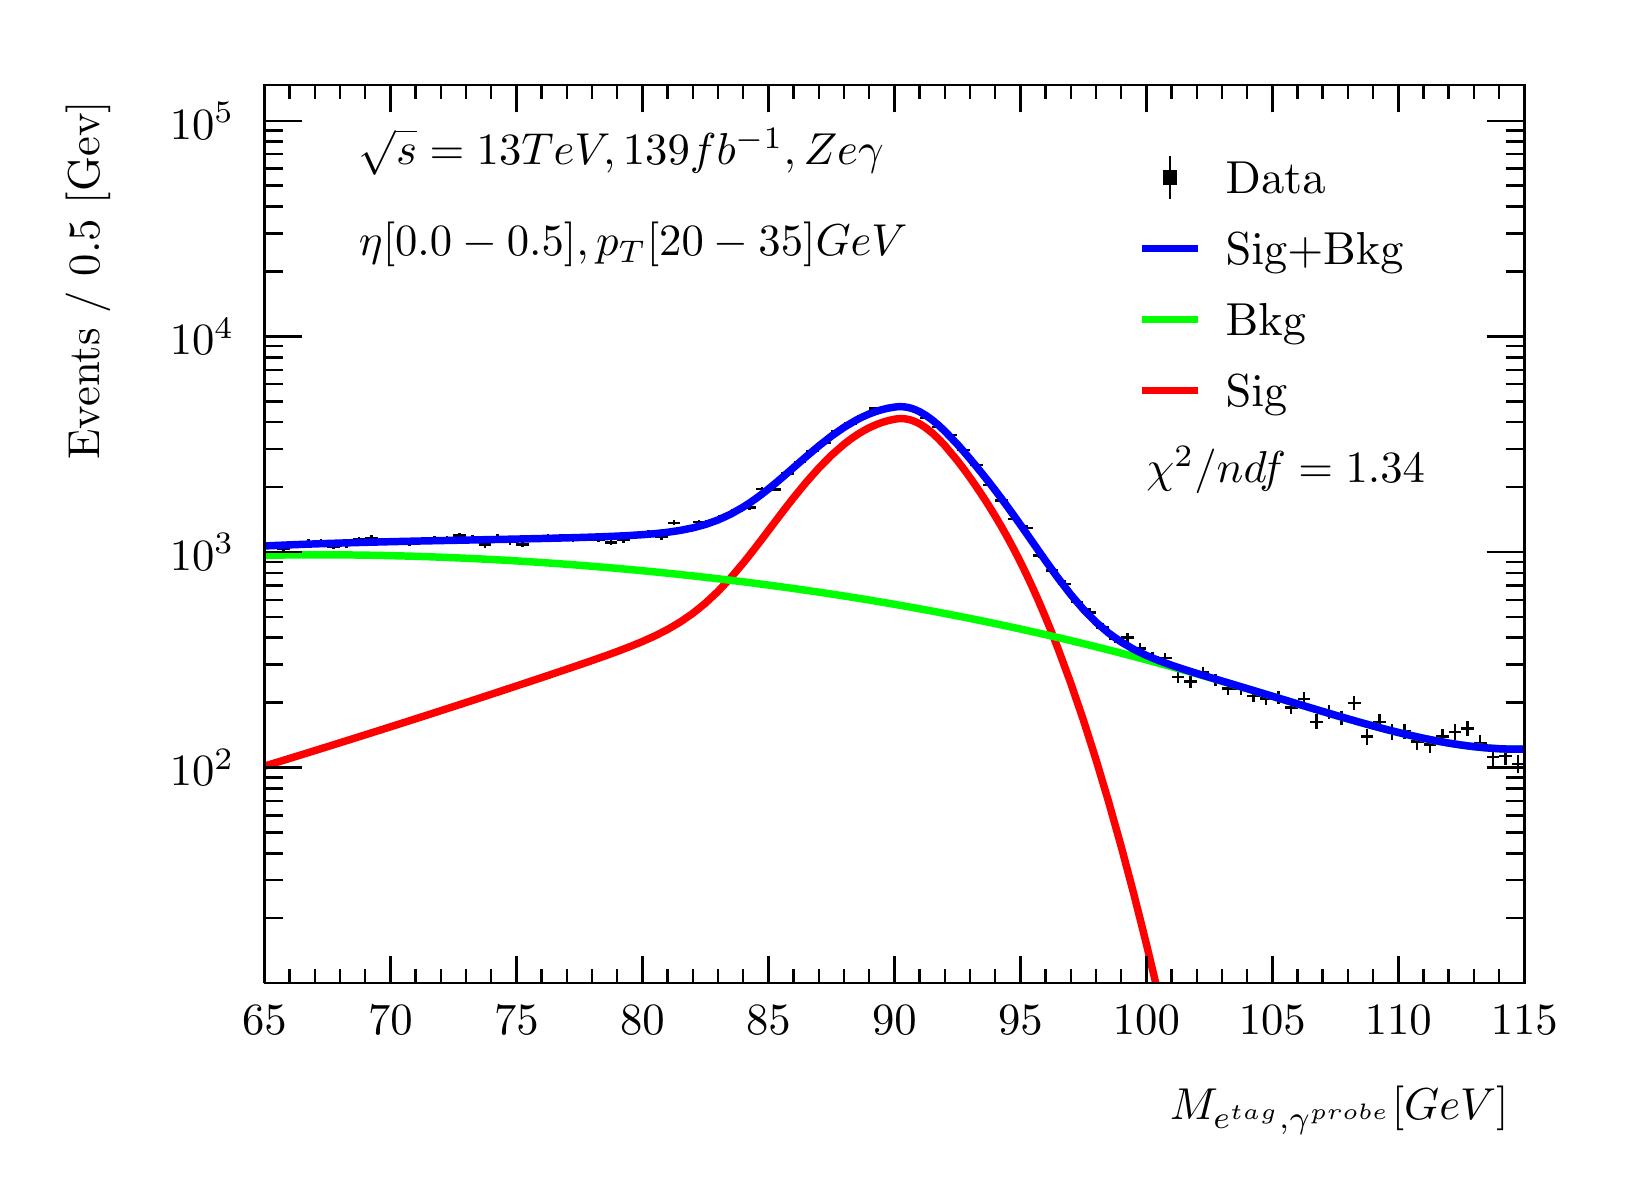
\begin{tikzpicture}
\pgfdeclareplotmark{cross} {
\pgfpathmoveto{\pgfpoint{-0.3\pgfplotmarksize}{\pgfplotmarksize}}
\pgfpathlineto{\pgfpoint{+0.3\pgfplotmarksize}{\pgfplotmarksize}}
\pgfpathlineto{\pgfpoint{+0.3\pgfplotmarksize}{0.3\pgfplotmarksize}}
\pgfpathlineto{\pgfpoint{+1\pgfplotmarksize}{0.3\pgfplotmarksize}}
\pgfpathlineto{\pgfpoint{+1\pgfplotmarksize}{-0.3\pgfplotmarksize}}
\pgfpathlineto{\pgfpoint{+0.3\pgfplotmarksize}{-0.3\pgfplotmarksize}}
\pgfpathlineto{\pgfpoint{+0.3\pgfplotmarksize}{-1.\pgfplotmarksize}}
\pgfpathlineto{\pgfpoint{-0.3\pgfplotmarksize}{-1.\pgfplotmarksize}}
\pgfpathlineto{\pgfpoint{-0.3\pgfplotmarksize}{-0.3\pgfplotmarksize}}
\pgfpathlineto{\pgfpoint{-1.\pgfplotmarksize}{-0.3\pgfplotmarksize}}
\pgfpathlineto{\pgfpoint{-1.\pgfplotmarksize}{0.3\pgfplotmarksize}}
\pgfpathlineto{\pgfpoint{-0.3\pgfplotmarksize}{0.3\pgfplotmarksize}}
\pgfpathclose
\pgfusepathqstroke
}
\pgfdeclareplotmark{cross*} {
\pgfpathmoveto{\pgfpoint{-0.3\pgfplotmarksize}{\pgfplotmarksize}}
\pgfpathlineto{\pgfpoint{+0.3\pgfplotmarksize}{\pgfplotmarksize}}
\pgfpathlineto{\pgfpoint{+0.3\pgfplotmarksize}{0.3\pgfplotmarksize}}
\pgfpathlineto{\pgfpoint{+1\pgfplotmarksize}{0.3\pgfplotmarksize}}
\pgfpathlineto{\pgfpoint{+1\pgfplotmarksize}{-0.3\pgfplotmarksize}}
\pgfpathlineto{\pgfpoint{+0.3\pgfplotmarksize}{-0.3\pgfplotmarksize}}
\pgfpathlineto{\pgfpoint{+0.3\pgfplotmarksize}{-1.\pgfplotmarksize}}
\pgfpathlineto{\pgfpoint{-0.3\pgfplotmarksize}{-1.\pgfplotmarksize}}
\pgfpathlineto{\pgfpoint{-0.3\pgfplotmarksize}{-0.3\pgfplotmarksize}}
\pgfpathlineto{\pgfpoint{-1.\pgfplotmarksize}{-0.3\pgfplotmarksize}}
\pgfpathlineto{\pgfpoint{-1.\pgfplotmarksize}{0.3\pgfplotmarksize}}
\pgfpathlineto{\pgfpoint{-0.3\pgfplotmarksize}{0.3\pgfplotmarksize}}
\pgfpathclose
\pgfusepathqfillstroke
}
\pgfdeclareplotmark{newstar} {
\pgfpathmoveto{\pgfqpoint{0pt}{\pgfplotmarksize}}
\pgfpathlineto{\pgfqpointpolar{44}{0.5\pgfplotmarksize}}
\pgfpathlineto{\pgfqpointpolar{18}{\pgfplotmarksize}}
\pgfpathlineto{\pgfqpointpolar{-20}{0.5\pgfplotmarksize}}
\pgfpathlineto{\pgfqpointpolar{-54}{\pgfplotmarksize}}
\pgfpathlineto{\pgfqpointpolar{-90}{0.5\pgfplotmarksize}}
\pgfpathlineto{\pgfqpointpolar{234}{\pgfplotmarksize}}
\pgfpathlineto{\pgfqpointpolar{198}{0.5\pgfplotmarksize}}
\pgfpathlineto{\pgfqpointpolar{162}{\pgfplotmarksize}}
\pgfpathlineto{\pgfqpointpolar{134}{0.5\pgfplotmarksize}}
\pgfpathclose
\pgfusepathqstroke
}
\pgfdeclareplotmark{newstar*} {
\pgfpathmoveto{\pgfqpoint{0pt}{\pgfplotmarksize}}
\pgfpathlineto{\pgfqpointpolar{44}{0.5\pgfplotmarksize}}
\pgfpathlineto{\pgfqpointpolar{18}{\pgfplotmarksize}}
\pgfpathlineto{\pgfqpointpolar{-20}{0.5\pgfplotmarksize}}
\pgfpathlineto{\pgfqpointpolar{-54}{\pgfplotmarksize}}
\pgfpathlineto{\pgfqpointpolar{-90}{0.5\pgfplotmarksize}}
\pgfpathlineto{\pgfqpointpolar{234}{\pgfplotmarksize}}
\pgfpathlineto{\pgfqpointpolar{198}{0.5\pgfplotmarksize}}
\pgfpathlineto{\pgfqpointpolar{162}{\pgfplotmarksize}}
\pgfpathlineto{\pgfqpointpolar{134}{0.5\pgfplotmarksize}}
\pgfpathclose
\pgfusepathqfillstroke
}
\definecolor{c}{rgb}{1,1,1};
\draw [color=c, fill=c] (0,0) rectangle (20,14.4361);
\draw [color=c, fill=c] (3,2.30977) rectangle (19,13.7143);
\definecolor{c}{rgb}{0,0,0};
\draw [c,line width=0.9] (3,2.30977) -- (3,13.7143) -- (19,13.7143) -- (19,2.30977) -- (3,2.30977);
\definecolor{c}{rgb}{1,1,1};
\draw [color=c, fill=c] (3,2.30977) rectangle (19,13.7143);
\definecolor{c}{rgb}{0,0,0};
\draw [c,line width=0.9] (3,2.30977) -- (3,13.7143) -- (19,13.7143) -- (19,2.30977) -- (3,2.30977);
\draw [c,line width=0.9] (3,2.30977) -- (19,2.30977);
\draw [c,line width=0.9] (3,2.65624) -- (3,2.30977);
\draw [c,line width=0.9] (3.32,2.48301) -- (3.32,2.30977);
\draw [c,line width=0.9] (3.64,2.48301) -- (3.64,2.30977);
\draw [c,line width=0.9] (3.96,2.48301) -- (3.96,2.30977);
\draw [c,line width=0.9] (4.28,2.48301) -- (4.28,2.30977);
\draw [c,line width=0.9] (4.6,2.65624) -- (4.6,2.30977);
\draw [c,line width=0.9] (4.92,2.48301) -- (4.92,2.30977);
\draw [c,line width=0.9] (5.24,2.48301) -- (5.24,2.30977);
\draw [c,line width=0.9] (5.56,2.48301) -- (5.56,2.30977);
\draw [c,line width=0.9] (5.88,2.48301) -- (5.88,2.30977);
\draw [c,line width=0.9] (6.2,2.65624) -- (6.2,2.30977);
\draw [c,line width=0.9] (6.52,2.48301) -- (6.52,2.30977);
\draw [c,line width=0.9] (6.84,2.48301) -- (6.84,2.30977);
\draw [c,line width=0.9] (7.16,2.48301) -- (7.16,2.30977);
\draw [c,line width=0.9] (7.48,2.48301) -- (7.48,2.30977);
\draw [c,line width=0.9] (7.8,2.65624) -- (7.8,2.30977);
\draw [c,line width=0.9] (8.12,2.48301) -- (8.12,2.30977);
\draw [c,line width=0.9] (8.44,2.48301) -- (8.44,2.30977);
\draw [c,line width=0.9] (8.76,2.48301) -- (8.76,2.30977);
\draw [c,line width=0.9] (9.08,2.48301) -- (9.08,2.30977);
\draw [c,line width=0.9] (9.4,2.65624) -- (9.4,2.30977);
\draw [c,line width=0.9] (9.72,2.48301) -- (9.72,2.30977);
\draw [c,line width=0.9] (10.04,2.48301) -- (10.04,2.30977);
\draw [c,line width=0.9] (10.36,2.48301) -- (10.36,2.30977);
\draw [c,line width=0.9] (10.68,2.48301) -- (10.68,2.30977);
\draw [c,line width=0.9] (11,2.65624) -- (11,2.30977);
\draw [c,line width=0.9] (11.32,2.48301) -- (11.32,2.30977);
\draw [c,line width=0.9] (11.64,2.48301) -- (11.64,2.30977);
\draw [c,line width=0.9] (11.96,2.48301) -- (11.96,2.30977);
\draw [c,line width=0.9] (12.28,2.48301) -- (12.28,2.30977);
\draw [c,line width=0.9] (12.6,2.65624) -- (12.6,2.30977);
\draw [c,line width=0.9] (12.92,2.48301) -- (12.92,2.30977);
\draw [c,line width=0.9] (13.24,2.48301) -- (13.24,2.30977);
\draw [c,line width=0.9] (13.56,2.48301) -- (13.56,2.30977);
\draw [c,line width=0.9] (13.88,2.48301) -- (13.88,2.30977);
\draw [c,line width=0.9] (14.2,2.65624) -- (14.2,2.30977);
\draw [c,line width=0.9] (14.52,2.48301) -- (14.52,2.30977);
\draw [c,line width=0.9] (14.84,2.48301) -- (14.84,2.30977);
\draw [c,line width=0.9] (15.16,2.48301) -- (15.16,2.30977);
\draw [c,line width=0.9] (15.48,2.48301) -- (15.48,2.30977);
\draw [c,line width=0.9] (15.8,2.65624) -- (15.8,2.30977);
\draw [c,line width=0.9] (16.12,2.48301) -- (16.12,2.30977);
\draw [c,line width=0.9] (16.44,2.48301) -- (16.44,2.30977);
\draw [c,line width=0.9] (16.76,2.48301) -- (16.76,2.30977);
\draw [c,line width=0.9] (17.08,2.48301) -- (17.08,2.30977);
\draw [c,line width=0.9] (17.4,2.65624) -- (17.4,2.30977);
\draw [c,line width=0.9] (17.72,2.48301) -- (17.72,2.30977);
\draw [c,line width=0.9] (18.04,2.48301) -- (18.04,2.30977);
\draw [c,line width=0.9] (18.36,2.48301) -- (18.36,2.30977);
\draw [c,line width=0.9] (18.68,2.48301) -- (18.68,2.30977);
\draw [c,line width=0.9] (19,2.65624) -- (19,2.30977);
\draw [c,line width=0.9] (19,2.65624) -- (19,2.30977);
\draw [anchor=base] (3,1.66015) node[scale=1.61424, color=c, rotate=0]{65};
\draw [anchor=base] (4.6,1.66015) node[scale=1.61424, color=c, rotate=0]{70};
\draw [anchor=base] (6.2,1.66015) node[scale=1.61424, color=c, rotate=0]{75};
\draw [anchor=base] (7.8,1.66015) node[scale=1.61424, color=c, rotate=0]{80};
\draw [anchor=base] (9.4,1.66015) node[scale=1.61424, color=c, rotate=0]{85};
\draw [anchor=base] (11,1.66015) node[scale=1.61424, color=c, rotate=0]{90};
\draw [anchor=base] (12.6,1.66015) node[scale=1.61424, color=c, rotate=0]{95};
\draw [anchor=base] (14.2,1.66015) node[scale=1.61424, color=c, rotate=0]{100};
\draw [anchor=base] (15.8,1.66015) node[scale=1.61424, color=c, rotate=0]{105};
\draw [anchor=base] (17.4,1.66015) node[scale=1.61424, color=c, rotate=0]{110};
\draw [anchor=base] (19,1.66015) node[scale=1.61424, color=c, rotate=0]{115};
\draw [anchor= east] (19,0.692932) node[scale=1.61424, color=c, rotate=0]{$M_{e^{tag}, \gamma^{probe}}  [GeV]$};
\draw [c,line width=0.9] (3,13.7143) -- (19,13.7143);
\draw [c,line width=0.9] (3,13.3678) -- (3,13.7143);
\draw [c,line width=0.9] (3.32,13.5411) -- (3.32,13.7143);
\draw [c,line width=0.9] (3.64,13.5411) -- (3.64,13.7143);
\draw [c,line width=0.9] (3.96,13.5411) -- (3.96,13.7143);
\draw [c,line width=0.9] (4.28,13.5411) -- (4.28,13.7143);
\draw [c,line width=0.9] (4.6,13.3678) -- (4.6,13.7143);
\draw [c,line width=0.9] (4.92,13.5411) -- (4.92,13.7143);
\draw [c,line width=0.9] (5.24,13.5411) -- (5.24,13.7143);
\draw [c,line width=0.9] (5.56,13.5411) -- (5.56,13.7143);
\draw [c,line width=0.9] (5.88,13.5411) -- (5.88,13.7143);
\draw [c,line width=0.9] (6.2,13.3678) -- (6.2,13.7143);
\draw [c,line width=0.9] (6.52,13.5411) -- (6.52,13.7143);
\draw [c,line width=0.9] (6.84,13.5411) -- (6.84,13.7143);
\draw [c,line width=0.9] (7.16,13.5411) -- (7.16,13.7143);
\draw [c,line width=0.9] (7.48,13.5411) -- (7.48,13.7143);
\draw [c,line width=0.9] (7.8,13.3678) -- (7.8,13.7143);
\draw [c,line width=0.9] (8.12,13.5411) -- (8.12,13.7143);
\draw [c,line width=0.9] (8.44,13.5411) -- (8.44,13.7143);
\draw [c,line width=0.9] (8.76,13.5411) -- (8.76,13.7143);
\draw [c,line width=0.9] (9.08,13.5411) -- (9.08,13.7143);
\draw [c,line width=0.9] (9.4,13.3678) -- (9.4,13.7143);
\draw [c,line width=0.9] (9.72,13.5411) -- (9.72,13.7143);
\draw [c,line width=0.9] (10.04,13.5411) -- (10.04,13.7143);
\draw [c,line width=0.9] (10.36,13.5411) -- (10.36,13.7143);
\draw [c,line width=0.9] (10.68,13.5411) -- (10.68,13.7143);
\draw [c,line width=0.9] (11,13.3678) -- (11,13.7143);
\draw [c,line width=0.9] (11.32,13.5411) -- (11.32,13.7143);
\draw [c,line width=0.9] (11.64,13.5411) -- (11.64,13.7143);
\draw [c,line width=0.9] (11.96,13.5411) -- (11.96,13.7143);
\draw [c,line width=0.9] (12.28,13.5411) -- (12.28,13.7143);
\draw [c,line width=0.9] (12.6,13.3678) -- (12.6,13.7143);
\draw [c,line width=0.9] (12.92,13.5411) -- (12.92,13.7143);
\draw [c,line width=0.9] (13.24,13.5411) -- (13.24,13.7143);
\draw [c,line width=0.9] (13.56,13.5411) -- (13.56,13.7143);
\draw [c,line width=0.9] (13.88,13.5411) -- (13.88,13.7143);
\draw [c,line width=0.9] (14.2,13.3678) -- (14.2,13.7143);
\draw [c,line width=0.9] (14.52,13.5411) -- (14.52,13.7143);
\draw [c,line width=0.9] (14.84,13.5411) -- (14.84,13.7143);
\draw [c,line width=0.9] (15.16,13.5411) -- (15.16,13.7143);
\draw [c,line width=0.9] (15.48,13.5411) -- (15.48,13.7143);
\draw [c,line width=0.9] (15.8,13.3678) -- (15.8,13.7143);
\draw [c,line width=0.9] (16.12,13.5411) -- (16.12,13.7143);
\draw [c,line width=0.9] (16.44,13.5411) -- (16.44,13.7143);
\draw [c,line width=0.9] (16.76,13.5411) -- (16.76,13.7143);
\draw [c,line width=0.9] (17.08,13.5411) -- (17.08,13.7143);
\draw [c,line width=0.9] (17.4,13.3678) -- (17.4,13.7143);
\draw [c,line width=0.9] (17.72,13.5411) -- (17.72,13.7143);
\draw [c,line width=0.9] (18.04,13.5411) -- (18.04,13.7143);
\draw [c,line width=0.9] (18.36,13.5411) -- (18.36,13.7143);
\draw [c,line width=0.9] (18.68,13.5411) -- (18.68,13.7143);
\draw [c,line width=0.9] (19,13.3678) -- (19,13.7143);
\draw [c,line width=0.9] (19,13.3678) -- (19,13.7143);
\draw [c,line width=0.9] (3,2.30977) -- (3,13.7143);
\draw [c,line width=0.9] (3.237,3.13385) -- (3,3.13385);
\draw [c,line width=0.9] (3.237,3.6159) -- (3,3.6159);
\draw [c,line width=0.9] (3.237,3.95792) -- (3,3.95792);
\draw [c,line width=0.9] (3.237,4.22321) -- (3,4.22321);
\draw [c,line width=0.9] (3.237,4.43997) -- (3,4.43997);
\draw [c,line width=0.9] (3.237,4.62324) -- (3,4.62324);
\draw [c,line width=0.9] (3.237,4.782) -- (3,4.782);
\draw [c,line width=0.9] (3.237,4.92203) -- (3,4.92203);
\draw [c,line width=0.9] (3.474,5.04729) -- (3,5.04729);
\draw [anchor= east] (2.82,5.04729) node[scale=1.61424, color=c, rotate=0]{$10^{2}$};
\draw [c,line width=0.9] (3.237,5.87136) -- (3,5.87136);
\draw [c,line width=0.9] (3.237,6.35342) -- (3,6.35342);
\draw [c,line width=0.9] (3.237,6.69544) -- (3,6.69544);
\draw [c,line width=0.9] (3.237,6.96073) -- (3,6.96073);
\draw [c,line width=0.9] (3.237,7.17749) -- (3,7.17749);
\draw [c,line width=0.9] (3.237,7.36076) -- (3,7.36076);
\draw [c,line width=0.9] (3.237,7.51951) -- (3,7.51951);
\draw [c,line width=0.9] (3.237,7.65954) -- (3,7.65954);
\draw [c,line width=0.9] (3.474,7.78481) -- (3,7.78481);
\draw [anchor= east] (2.82,7.78481) node[scale=1.61424, color=c, rotate=0]{$10^{3}$};
\draw [c,line width=0.9] (3.237,8.60888) -- (3,8.60888);
\draw [c,line width=0.9] (3.237,9.09093) -- (3,9.09093);
\draw [c,line width=0.9] (3.237,9.43296) -- (3,9.43296);
\draw [c,line width=0.9] (3.237,9.69825) -- (3,9.69825);
\draw [c,line width=0.9] (3.237,9.91501) -- (3,9.91501);
\draw [c,line width=0.9] (3.237,10.0983) -- (3,10.0983);
\draw [c,line width=0.9] (3.237,10.257) -- (3,10.257);
\draw [c,line width=0.9] (3.237,10.3971) -- (3,10.3971);
\draw [c,line width=0.9] (3.474,10.5223) -- (3,10.5223);
\draw [anchor= east] (2.82,10.5223) node[scale=1.61424, color=c, rotate=0]{$10^{4}$};
\draw [c,line width=0.9] (3.237,11.3464) -- (3,11.3464);
\draw [c,line width=0.9] (3.237,11.8285) -- (3,11.8285);
\draw [c,line width=0.9] (3.237,12.1705) -- (3,12.1705);
\draw [c,line width=0.9] (3.237,12.4358) -- (3,12.4358);
\draw [c,line width=0.9] (3.237,12.6525) -- (3,12.6525);
\draw [c,line width=0.9] (3.237,12.8358) -- (3,12.8358);
\draw [c,line width=0.9] (3.237,12.9945) -- (3,12.9945);
\draw [c,line width=0.9] (3.237,13.1346) -- (3,13.1346);
\draw [c,line width=0.9] (3.474,13.2598) -- (3,13.2598);
\draw [anchor= east] (2.82,13.2598) node[scale=1.61424, color=c, rotate=0]{$10^{5}$};
\draw [anchor= east] (0.76,13.7143) node[scale=1.61424, color=c, rotate=90]{Events / 0.5 [Gev]};
\draw [c,line width=0.9] (19,2.30977) -- (19,13.7143);
\draw [c,line width=0.9] (18.763,3.13385) -- (19,3.13385);
\draw [c,line width=0.9] (18.763,3.6159) -- (19,3.6159);
\draw [c,line width=0.9] (18.763,3.95792) -- (19,3.95792);
\draw [c,line width=0.9] (18.763,4.22321) -- (19,4.22321);
\draw [c,line width=0.9] (18.763,4.43997) -- (19,4.43997);
\draw [c,line width=0.9] (18.763,4.62324) -- (19,4.62324);
\draw [c,line width=0.9] (18.763,4.782) -- (19,4.782);
\draw [c,line width=0.9] (18.763,4.92203) -- (19,4.92203);
\draw [c,line width=0.9] (18.526,5.04729) -- (19,5.04729);
\draw [c,line width=0.9] (18.763,5.87136) -- (19,5.87136);
\draw [c,line width=0.9] (18.763,6.35342) -- (19,6.35342);
\draw [c,line width=0.9] (18.763,6.69544) -- (19,6.69544);
\draw [c,line width=0.9] (18.763,6.96073) -- (19,6.96073);
\draw [c,line width=0.9] (18.763,7.17749) -- (19,7.17749);
\draw [c,line width=0.9] (18.763,7.36076) -- (19,7.36076);
\draw [c,line width=0.9] (18.763,7.51951) -- (19,7.51951);
\draw [c,line width=0.9] (18.763,7.65954) -- (19,7.65954);
\draw [c,line width=0.9] (18.526,7.78481) -- (19,7.78481);
\draw [c,line width=0.9] (18.763,8.60888) -- (19,8.60888);
\draw [c,line width=0.9] (18.763,9.09093) -- (19,9.09093);
\draw [c,line width=0.9] (18.763,9.43296) -- (19,9.43296);
\draw [c,line width=0.9] (18.763,9.69825) -- (19,9.69825);
\draw [c,line width=0.9] (18.763,9.91501) -- (19,9.91501);
\draw [c,line width=0.9] (18.763,10.0983) -- (19,10.0983);
\draw [c,line width=0.9] (18.763,10.257) -- (19,10.257);
\draw [c,line width=0.9] (18.763,10.3971) -- (19,10.3971);
\draw [c,line width=0.9] (18.526,10.5223) -- (19,10.5223);
\draw [c,line width=0.9] (18.763,11.3464) -- (19,11.3464);
\draw [c,line width=0.9] (18.763,11.8285) -- (19,11.8285);
\draw [c,line width=0.9] (18.763,12.1705) -- (19,12.1705);
\draw [c,line width=0.9] (18.763,12.4358) -- (19,12.4358);
\draw [c,line width=0.9] (18.763,12.6525) -- (19,12.6525);
\draw [c,line width=0.9] (18.763,12.8358) -- (19,12.8358);
\draw [c,line width=0.9] (18.763,12.9945) -- (19,12.9945);
\draw [c,line width=0.9] (18.763,13.1346) -- (19,13.1346);
\draw [c,line width=0.9] (18.526,13.2598) -- (19,13.2598);
\draw [c,line width=0.9] (3.08,7.85744) -- (3,7.85744);
\draw [c,line width=0.9] (3,7.85744) -- (3,7.85744);
\draw [c,line width=0.9] (3.08,7.85744) -- (3.16,7.85744);
\draw [c,line width=0.9] (3.16,7.85744) -- (3.16,7.85744);
\draw [c,line width=0.9] (3.08,7.85744) -- (3.08,7.89391);
\draw [c,line width=0.9] (3.08,7.89391) -- (3.08,7.89391);
\draw [c,line width=0.9] (3.08,7.85744) -- (3.08,7.82098);
\draw [c,line width=0.9] (3.08,7.82098) -- (3.08,7.82098);
\draw [c,line width=0.9] (3.24,7.81995) -- (3.16,7.81995);
\draw [c,line width=0.9] (3.16,7.81995) -- (3.16,7.81995);
\draw [c,line width=0.9] (3.24,7.81995) -- (3.32,7.81995);
\draw [c,line width=0.9] (3.32,7.81995) -- (3.32,7.81995);
\draw [c,line width=0.9] (3.24,7.81995) -- (3.24,7.85699);
\draw [c,line width=0.9] (3.24,7.85699) -- (3.24,7.85699);
\draw [c,line width=0.9] (3.24,7.81995) -- (3.24,7.78291);
\draw [c,line width=0.9] (3.24,7.78291) -- (3.24,7.78291);
\draw [c,line width=0.9] (3.4,7.86968) -- (3.32,7.86968);
\draw [c,line width=0.9] (3.32,7.86968) -- (3.32,7.86968);
\draw [c,line width=0.9] (3.4,7.86968) -- (3.48,7.86968);
\draw [c,line width=0.9] (3.48,7.86968) -- (3.48,7.86968);
\draw [c,line width=0.9] (3.4,7.86968) -- (3.4,7.90596);
\draw [c,line width=0.9] (3.4,7.90596) -- (3.4,7.90596);
\draw [c,line width=0.9] (3.4,7.86968) -- (3.4,7.83341);
\draw [c,line width=0.9] (3.4,7.83341) -- (3.4,7.83341);
\draw [c,line width=0.9] (3.56,7.91209) -- (3.48,7.91209);
\draw [c,line width=0.9] (3.48,7.91209) -- (3.48,7.91209);
\draw [c,line width=0.9] (3.56,7.91209) -- (3.64,7.91209);
\draw [c,line width=0.9] (3.64,7.91209) -- (3.64,7.91209);
\draw [c,line width=0.9] (3.56,7.91209) -- (3.56,7.94772);
\draw [c,line width=0.9] (3.56,7.94772) -- (3.56,7.94772);
\draw [c,line width=0.9] (3.56,7.91209) -- (3.56,7.87645);
\draw [c,line width=0.9] (3.56,7.87645) -- (3.56,7.87645);
\draw [c,line width=0.9] (3.72,7.90995) -- (3.64,7.90995);
\draw [c,line width=0.9] (3.64,7.90995) -- (3.64,7.90995);
\draw [c,line width=0.9] (3.72,7.90995) -- (3.8,7.90995);
\draw [c,line width=0.9] (3.8,7.90995) -- (3.8,7.90995);
\draw [c,line width=0.9] (3.72,7.90995) -- (3.72,7.94562);
\draw [c,line width=0.9] (3.72,7.94562) -- (3.72,7.94562);
\draw [c,line width=0.9] (3.72,7.90995) -- (3.72,7.87428);
\draw [c,line width=0.9] (3.72,7.87428) -- (3.72,7.87428);
\draw [c,line width=0.9] (3.88,7.85408) -- (3.8,7.85408);
\draw [c,line width=0.9] (3.8,7.85408) -- (3.8,7.85408);
\draw [c,line width=0.9] (3.88,7.85408) -- (3.96,7.85408);
\draw [c,line width=0.9] (3.96,7.85408) -- (3.96,7.85408);
\draw [c,line width=0.9] (3.88,7.85408) -- (3.88,7.8906);
\draw [c,line width=0.9] (3.88,7.8906) -- (3.88,7.8906);
\draw [c,line width=0.9] (3.88,7.85408) -- (3.88,7.81757);
\draw [c,line width=0.9] (3.88,7.81757) -- (3.88,7.81757);
\draw [c,line width=0.9] (4.04,7.87189) -- (3.96,7.87189);
\draw [c,line width=0.9] (3.96,7.87189) -- (3.96,7.87189);
\draw [c,line width=0.9] (4.04,7.87189) -- (4.12,7.87189);
\draw [c,line width=0.9] (4.12,7.87189) -- (4.12,7.87189);
\draw [c,line width=0.9] (4.04,7.87189) -- (4.04,7.90814);
\draw [c,line width=0.9] (4.04,7.90814) -- (4.04,7.90814);
\draw [c,line width=0.9] (4.04,7.87189) -- (4.04,7.83565);
\draw [c,line width=0.9] (4.04,7.83565) -- (4.04,7.83565);
\draw [c,line width=0.9] (4.2,7.94163) -- (4.12,7.94163);
\draw [c,line width=0.9] (4.12,7.94163) -- (4.12,7.94163);
\draw [c,line width=0.9] (4.2,7.94163) -- (4.28,7.94163);
\draw [c,line width=0.9] (4.28,7.94163) -- (4.28,7.94163);
\draw [c,line width=0.9] (4.2,7.94163) -- (4.2,7.97682);
\draw [c,line width=0.9] (4.2,7.97682) -- (4.2,7.97682);
\draw [c,line width=0.9] (4.2,7.94163) -- (4.2,7.90643);
\draw [c,line width=0.9] (4.2,7.90643) -- (4.2,7.90643);
\draw [c,line width=0.9] (4.36,7.96229) -- (4.28,7.96229);
\draw [c,line width=0.9] (4.28,7.96229) -- (4.28,7.96229);
\draw [c,line width=0.9] (4.36,7.96229) -- (4.44,7.96229);
\draw [c,line width=0.9] (4.44,7.96229) -- (4.44,7.96229);
\draw [c,line width=0.9] (4.36,7.96229) -- (4.36,7.99718);
\draw [c,line width=0.9] (4.36,7.99718) -- (4.36,7.99718);
\draw [c,line width=0.9] (4.36,7.96229) -- (4.36,7.9274);
\draw [c,line width=0.9] (4.36,7.9274) -- (4.36,7.9274);
\draw [c,line width=0.9] (4.52,7.91422) -- (4.44,7.91422);
\draw [c,line width=0.9] (4.44,7.91422) -- (4.44,7.91422);
\draw [c,line width=0.9] (4.52,7.91422) -- (4.6,7.91422);
\draw [c,line width=0.9] (4.6,7.91422) -- (4.6,7.91422);
\draw [c,line width=0.9] (4.52,7.91422) -- (4.52,7.94983);
\draw [c,line width=0.9] (4.52,7.94983) -- (4.52,7.94983);
\draw [c,line width=0.9] (4.52,7.91422) -- (4.52,7.87862);
\draw [c,line width=0.9] (4.52,7.87862) -- (4.52,7.87862);
\draw [c,line width=0.9] (4.68,7.93221) -- (4.6,7.93221);
\draw [c,line width=0.9] (4.6,7.93221) -- (4.6,7.93221);
\draw [c,line width=0.9] (4.68,7.93221) -- (4.76,7.93221);
\draw [c,line width=0.9] (4.76,7.93221) -- (4.76,7.93221);
\draw [c,line width=0.9] (4.68,7.93221) -- (4.68,7.96755);
\draw [c,line width=0.9] (4.68,7.96755) -- (4.68,7.96755);
\draw [c,line width=0.9] (4.68,7.93221) -- (4.68,7.89688);
\draw [c,line width=0.9] (4.68,7.89688) -- (4.68,7.89688);
\draw [c,line width=0.9] (4.84,7.89487) -- (4.76,7.89487);
\draw [c,line width=0.9] (4.76,7.89487) -- (4.76,7.89487);
\draw [c,line width=0.9] (4.84,7.89487) -- (4.92,7.89487);
\draw [c,line width=0.9] (4.92,7.89487) -- (4.92,7.89487);
\draw [c,line width=0.9] (4.84,7.89487) -- (4.84,7.93077);
\draw [c,line width=0.9] (4.84,7.93077) -- (4.84,7.93077);
\draw [c,line width=0.9] (4.84,7.89487) -- (4.84,7.85898);
\draw [c,line width=0.9] (4.84,7.85898) -- (4.84,7.85898);
\draw [c,line width=0.9] (5,7.9385) -- (4.92,7.9385);
\draw [c,line width=0.9] (4.92,7.9385) -- (4.92,7.9385);
\draw [c,line width=0.9] (5,7.9385) -- (5.08,7.9385);
\draw [c,line width=0.9] (5.08,7.9385) -- (5.08,7.9385);
\draw [c,line width=0.9] (5,7.9385) -- (5,7.97374);
\draw [c,line width=0.9] (5,7.97374) -- (5,7.97374);
\draw [c,line width=0.9] (5,7.9385) -- (5,7.90326);
\draw [c,line width=0.9] (5,7.90326) -- (5,7.90326);
\draw [c,line width=0.9] (5.16,7.95303) -- (5.08,7.95303);
\draw [c,line width=0.9] (5.08,7.95303) -- (5.08,7.95303);
\draw [c,line width=0.9] (5.16,7.95303) -- (5.24,7.95303);
\draw [c,line width=0.9] (5.24,7.95303) -- (5.24,7.95303);
\draw [c,line width=0.9] (5.16,7.95303) -- (5.16,7.98806);
\draw [c,line width=0.9] (5.16,7.98806) -- (5.16,7.98806);
\draw [c,line width=0.9] (5.16,7.95303) -- (5.16,7.91801);
\draw [c,line width=0.9] (5.16,7.91801) -- (5.16,7.91801);
\draw [c,line width=0.9] (5.32,7.9551) -- (5.24,7.9551);
\draw [c,line width=0.9] (5.24,7.9551) -- (5.24,7.9551);
\draw [c,line width=0.9] (5.32,7.9551) -- (5.4,7.9551);
\draw [c,line width=0.9] (5.4,7.9551) -- (5.4,7.9551);
\draw [c,line width=0.9] (5.32,7.9551) -- (5.32,7.99009);
\draw [c,line width=0.9] (5.32,7.99009) -- (5.32,7.99009);
\draw [c,line width=0.9] (5.32,7.9551) -- (5.32,7.9201);
\draw [c,line width=0.9] (5.32,7.9201) -- (5.32,7.9201);
\draw [c,line width=0.9] (5.48,7.99361) -- (5.4,7.99361);
\draw [c,line width=0.9] (5.4,7.99361) -- (5.4,7.99361);
\draw [c,line width=0.9] (5.48,7.99361) -- (5.56,7.99361);
\draw [c,line width=0.9] (5.56,7.99361) -- (5.56,7.99361);
\draw [c,line width=0.9] (5.48,7.99361) -- (5.48,8.02805);
\draw [c,line width=0.9] (5.48,8.02805) -- (5.48,8.02805);
\draw [c,line width=0.9] (5.48,7.99361) -- (5.48,7.95918);
\draw [c,line width=0.9] (5.48,7.95918) -- (5.48,7.95918);
\draw [c,line width=0.9] (5.64,7.96433) -- (5.56,7.96433);
\draw [c,line width=0.9] (5.56,7.96433) -- (5.56,7.96433);
\draw [c,line width=0.9] (5.64,7.96433) -- (5.72,7.96433);
\draw [c,line width=0.9] (5.72,7.96433) -- (5.72,7.96433);
\draw [c,line width=0.9] (5.64,7.96433) -- (5.64,7.99919);
\draw [c,line width=0.9] (5.64,7.99919) -- (5.64,7.99919);
\draw [c,line width=0.9] (5.64,7.96433) -- (5.64,7.92947);
\draw [c,line width=0.9] (5.64,7.92947) -- (5.64,7.92947);
\draw [c,line width=0.9] (5.8,7.87631) -- (5.72,7.87631);
\draw [c,line width=0.9] (5.72,7.87631) -- (5.72,7.87631);
\draw [c,line width=0.9] (5.8,7.87631) -- (5.88,7.87631);
\draw [c,line width=0.9] (5.88,7.87631) -- (5.88,7.87631);
\draw [c,line width=0.9] (5.8,7.87631) -- (5.8,7.91248);
\draw [c,line width=0.9] (5.8,7.91248) -- (5.8,7.91248);
\draw [c,line width=0.9] (5.8,7.87631) -- (5.8,7.84013);
\draw [c,line width=0.9] (5.8,7.84013) -- (5.8,7.84013);
\draw [c,line width=0.9] (5.96,7.97552) -- (5.88,7.97552);
\draw [c,line width=0.9] (5.88,7.97552) -- (5.88,7.97552);
\draw [c,line width=0.9] (5.96,7.97552) -- (6.04,7.97552);
\draw [c,line width=0.9] (6.04,7.97552) -- (6.04,7.97552);
\draw [c,line width=0.9] (5.96,7.97552) -- (5.96,8.01022);
\draw [c,line width=0.9] (5.96,8.01022) -- (5.96,8.01022);
\draw [c,line width=0.9] (5.96,7.97552) -- (5.96,7.94083);
\draw [c,line width=0.9] (5.96,7.94083) -- (5.96,7.94083);
\draw [c,line width=0.9] (6.12,7.90888) -- (6.04,7.90888);
\draw [c,line width=0.9] (6.04,7.90888) -- (6.04,7.90888);
\draw [c,line width=0.9] (6.12,7.90888) -- (6.2,7.90888);
\draw [c,line width=0.9] (6.2,7.90888) -- (6.2,7.90888);
\draw [c,line width=0.9] (6.12,7.90888) -- (6.12,7.94456);
\draw [c,line width=0.9] (6.12,7.94456) -- (6.12,7.94456);
\draw [c,line width=0.9] (6.12,7.90888) -- (6.12,7.8732);
\draw [c,line width=0.9] (6.12,7.8732) -- (6.12,7.8732);
\draw [c,line width=0.9] (6.28,7.87851) -- (6.2,7.87851);
\draw [c,line width=0.9] (6.2,7.87851) -- (6.2,7.87851);
\draw [c,line width=0.9] (6.28,7.87851) -- (6.36,7.87851);
\draw [c,line width=0.9] (6.36,7.87851) -- (6.36,7.87851);
\draw [c,line width=0.9] (6.28,7.87851) -- (6.28,7.91465);
\draw [c,line width=0.9] (6.28,7.91465) -- (6.28,7.91465);
\draw [c,line width=0.9] (6.28,7.87851) -- (6.28,7.84236);
\draw [c,line width=0.9] (6.28,7.84236) -- (6.28,7.84236);
\draw [c,line width=0.9] (6.44,7.95716) -- (6.36,7.95716);
\draw [c,line width=0.9] (6.36,7.95716) -- (6.36,7.95716);
\draw [c,line width=0.9] (6.44,7.95716) -- (6.52,7.95716);
\draw [c,line width=0.9] (6.52,7.95716) -- (6.52,7.95716);
\draw [c,line width=0.9] (6.44,7.95716) -- (6.44,7.99212);
\draw [c,line width=0.9] (6.44,7.99212) -- (6.44,7.99212);
\draw [c,line width=0.9] (6.44,7.95716) -- (6.44,7.92219);
\draw [c,line width=0.9] (6.44,7.92219) -- (6.44,7.92219);
\draw [c,line width=0.9] (6.6,7.97957) -- (6.52,7.97957);
\draw [c,line width=0.9] (6.52,7.97957) -- (6.52,7.97957);
\draw [c,line width=0.9] (6.6,7.97957) -- (6.68,7.97957);
\draw [c,line width=0.9] (6.68,7.97957) -- (6.68,7.97957);
\draw [c,line width=0.9] (6.6,7.97957) -- (6.6,8.01421);
\draw [c,line width=0.9] (6.6,8.01421) -- (6.6,8.01421);
\draw [c,line width=0.9] (6.6,7.97957) -- (6.6,7.94493);
\draw [c,line width=0.9] (6.6,7.94493) -- (6.6,7.94493);
\draw [c,line width=0.9] (6.76,7.97755) -- (6.68,7.97755);
\draw [c,line width=0.9] (6.68,7.97755) -- (6.68,7.97755);
\draw [c,line width=0.9] (6.76,7.97755) -- (6.84,7.97755);
\draw [c,line width=0.9] (6.84,7.97755) -- (6.84,7.97755);
\draw [c,line width=0.9] (6.76,7.97755) -- (6.76,8.01222);
\draw [c,line width=0.9] (6.76,8.01222) -- (6.76,8.01222);
\draw [c,line width=0.9] (6.76,7.97755) -- (6.76,7.94288);
\draw [c,line width=0.9] (6.76,7.94288) -- (6.76,7.94288);
\draw [c,line width=0.9] (6.92,7.94683) -- (6.84,7.94683);
\draw [c,line width=0.9] (6.84,7.94683) -- (6.84,7.94683);
\draw [c,line width=0.9] (6.92,7.94683) -- (7,7.94683);
\draw [c,line width=0.9] (7,7.94683) -- (7,7.94683);
\draw [c,line width=0.9] (6.92,7.94683) -- (6.92,7.98194);
\draw [c,line width=0.9] (6.92,7.98194) -- (6.92,7.98194);
\draw [c,line width=0.9] (6.92,7.94683) -- (6.92,7.91171);
\draw [c,line width=0.9] (6.92,7.91171) -- (6.92,7.91171);
\draw [c,line width=0.9] (7.08,7.98159) -- (7,7.98159);
\draw [c,line width=0.9] (7,7.98159) -- (7,7.98159);
\draw [c,line width=0.9] (7.08,7.98159) -- (7.16,7.98159);
\draw [c,line width=0.9] (7.16,7.98159) -- (7.16,7.98159);
\draw [c,line width=0.9] (7.08,7.98159) -- (7.08,8.01619);
\draw [c,line width=0.9] (7.08,8.01619) -- (7.08,8.01619);
\draw [c,line width=0.9] (7.08,7.98159) -- (7.08,7.94698);
\draw [c,line width=0.9] (7.08,7.94698) -- (7.08,7.94698);
\draw [c,line width=0.9] (7.24,7.94475) -- (7.16,7.94475);
\draw [c,line width=0.9] (7.16,7.94475) -- (7.16,7.94475);
\draw [c,line width=0.9] (7.24,7.94475) -- (7.32,7.94475);
\draw [c,line width=0.9] (7.32,7.94475) -- (7.32,7.94475);
\draw [c,line width=0.9] (7.24,7.94475) -- (7.24,7.9799);
\draw [c,line width=0.9] (7.24,7.9799) -- (7.24,7.9799);
\draw [c,line width=0.9] (7.24,7.94475) -- (7.24,7.9096);
\draw [c,line width=0.9] (7.24,7.9096) -- (7.24,7.9096);
\draw [c,line width=0.9] (7.4,7.90351) -- (7.32,7.90351);
\draw [c,line width=0.9] (7.32,7.90351) -- (7.32,7.90351);
\draw [c,line width=0.9] (7.4,7.90351) -- (7.48,7.90351);
\draw [c,line width=0.9] (7.48,7.90351) -- (7.48,7.90351);
\draw [c,line width=0.9] (7.4,7.90351) -- (7.4,7.93928);
\draw [c,line width=0.9] (7.4,7.93928) -- (7.4,7.93928);
\draw [c,line width=0.9] (7.4,7.90351) -- (7.4,7.86775);
\draw [c,line width=0.9] (7.4,7.86775) -- (7.4,7.86775);
\draw [c,line width=0.9] (7.56,7.93536) -- (7.48,7.93536);
\draw [c,line width=0.9] (7.48,7.93536) -- (7.48,7.93536);
\draw [c,line width=0.9] (7.56,7.93536) -- (7.64,7.93536);
\draw [c,line width=0.9] (7.64,7.93536) -- (7.64,7.93536);
\draw [c,line width=0.9] (7.56,7.93536) -- (7.56,7.97065);
\draw [c,line width=0.9] (7.56,7.97065) -- (7.56,7.97065);
\draw [c,line width=0.9] (7.56,7.93536) -- (7.56,7.90007);
\draw [c,line width=0.9] (7.56,7.90007) -- (7.56,7.90007);
\draw [c,line width=0.9] (7.72,7.98259) -- (7.64,7.98259);
\draw [c,line width=0.9] (7.64,7.98259) -- (7.64,7.98259);
\draw [c,line width=0.9] (7.72,7.98259) -- (7.8,7.98259);
\draw [c,line width=0.9] (7.8,7.98259) -- (7.8,7.98259);
\draw [c,line width=0.9] (7.72,7.98259) -- (7.72,8.01719);
\draw [c,line width=0.9] (7.72,8.01719) -- (7.72,8.01719);
\draw [c,line width=0.9] (7.72,7.98259) -- (7.72,7.948);
\draw [c,line width=0.9] (7.72,7.948) -- (7.72,7.948);
\draw [c,line width=0.9] (7.88,8.03092) -- (7.8,8.03092);
\draw [c,line width=0.9] (7.8,8.03092) -- (7.8,8.03092);
\draw [c,line width=0.9] (7.88,8.03092) -- (7.96,8.03092);
\draw [c,line width=0.9] (7.96,8.03092) -- (7.96,8.03092);
\draw [c,line width=0.9] (7.88,8.03092) -- (7.88,8.06482);
\draw [c,line width=0.9] (7.88,8.06482) -- (7.88,8.06482);
\draw [c,line width=0.9] (7.88,8.03092) -- (7.88,7.99703);
\draw [c,line width=0.9] (7.88,7.99703) -- (7.88,7.99703);
\draw [c,line width=0.9] (8.04,7.97248) -- (7.96,7.97248);
\draw [c,line width=0.9] (7.96,7.97248) -- (7.96,7.97248);
\draw [c,line width=0.9] (8.04,7.97248) -- (8.12,7.97248);
\draw [c,line width=0.9] (8.12,7.97248) -- (8.12,7.97248);
\draw [c,line width=0.9] (8.04,7.97248) -- (8.04,8.00722);
\draw [c,line width=0.9] (8.04,8.00722) -- (8.04,8.00722);
\draw [c,line width=0.9] (8.04,7.97248) -- (8.04,7.93774);
\draw [c,line width=0.9] (8.04,7.93774) -- (8.04,7.93774);
\draw [c,line width=0.9] (8.2,8.15299) -- (8.12,8.15299);
\draw [c,line width=0.9] (8.12,8.15299) -- (8.12,8.15299);
\draw [c,line width=0.9] (8.2,8.15299) -- (8.28,8.15299);
\draw [c,line width=0.9] (8.28,8.15299) -- (8.28,8.15299);
\draw [c,line width=0.9] (8.2,8.15299) -- (8.2,8.18519);
\draw [c,line width=0.9] (8.2,8.18519) -- (8.2,8.18519);
\draw [c,line width=0.9] (8.2,8.15299) -- (8.2,8.12079);
\draw [c,line width=0.9] (8.2,8.12079) -- (8.2,8.12079);
\draw [c,line width=0.9] (8.36,8.0857) -- (8.28,8.0857);
\draw [c,line width=0.9] (8.28,8.0857) -- (8.28,8.0857);
\draw [c,line width=0.9] (8.36,8.0857) -- (8.44,8.0857);
\draw [c,line width=0.9] (8.44,8.0857) -- (8.44,8.0857);
\draw [c,line width=0.9] (8.36,8.0857) -- (8.36,8.11883);
\draw [c,line width=0.9] (8.36,8.11883) -- (8.36,8.11883);
\draw [c,line width=0.9] (8.36,8.0857) -- (8.36,8.05258);
\draw [c,line width=0.9] (8.36,8.05258) -- (8.36,8.05258);
\draw [c,line width=0.9] (8.52,8.16341) -- (8.44,8.16341);
\draw [c,line width=0.9] (8.44,8.16341) -- (8.44,8.16341);
\draw [c,line width=0.9] (8.52,8.16341) -- (8.6,8.16341);
\draw [c,line width=0.9] (8.6,8.16341) -- (8.6,8.16341);
\draw [c,line width=0.9] (8.52,8.16341) -- (8.52,8.19547);
\draw [c,line width=0.9] (8.52,8.19547) -- (8.52,8.19547);
\draw [c,line width=0.9] (8.52,8.16341) -- (8.52,8.13135);
\draw [c,line width=0.9] (8.52,8.13135) -- (8.52,8.13135);
\draw [c,line width=0.9] (8.68,8.17717) -- (8.6,8.17717);
\draw [c,line width=0.9] (8.6,8.17717) -- (8.6,8.17717);
\draw [c,line width=0.9] (8.68,8.17717) -- (8.76,8.17717);
\draw [c,line width=0.9] (8.76,8.17717) -- (8.76,8.17717);
\draw [c,line width=0.9] (8.68,8.17717) -- (8.68,8.20904);
\draw [c,line width=0.9] (8.68,8.20904) -- (8.68,8.20904);
\draw [c,line width=0.9] (8.68,8.17717) -- (8.68,8.14529);
\draw [c,line width=0.9] (8.68,8.14529) -- (8.68,8.14529);
\draw [c,line width=0.9] (8.84,8.23879) -- (8.76,8.23879);
\draw [c,line width=0.9] (8.76,8.23879) -- (8.76,8.23879);
\draw [c,line width=0.9] (8.84,8.23879) -- (8.92,8.23879);
\draw [c,line width=0.9] (8.92,8.23879) -- (8.92,8.23879);
\draw [c,line width=0.9] (8.84,8.23879) -- (8.84,8.26985);
\draw [c,line width=0.9] (8.84,8.26985) -- (8.84,8.26985);
\draw [c,line width=0.9] (8.84,8.23879) -- (8.84,8.20773);
\draw [c,line width=0.9] (8.84,8.20773) -- (8.84,8.20773);
\draw [c,line width=0.9] (9,8.31273) -- (8.92,8.31273);
\draw [c,line width=0.9] (8.92,8.31273) -- (8.92,8.31273);
\draw [c,line width=0.9] (9,8.31273) -- (9.08,8.31273);
\draw [c,line width=0.9] (9.08,8.31273) -- (9.08,8.31273);
\draw [c,line width=0.9] (9,8.31273) -- (9,8.34284);
\draw [c,line width=0.9] (9,8.34284) -- (9,8.34284);
\draw [c,line width=0.9] (9,8.31273) -- (9,8.28262);
\draw [c,line width=0.9] (9,8.28262) -- (9,8.28262);
\draw [c,line width=0.9] (9.16,8.351) -- (9.08,8.351);
\draw [c,line width=0.9] (9.08,8.351) -- (9.08,8.351);
\draw [c,line width=0.9] (9.16,8.351) -- (9.24,8.351);
\draw [c,line width=0.9] (9.24,8.351) -- (9.24,8.351);
\draw [c,line width=0.9] (9.16,8.351) -- (9.16,8.38063);
\draw [c,line width=0.9] (9.16,8.38063) -- (9.16,8.38063);
\draw [c,line width=0.9] (9.16,8.351) -- (9.16,8.32137);
\draw [c,line width=0.9] (9.16,8.32137) -- (9.16,8.32137);
\draw [c,line width=0.9] (9.32,8.58365) -- (9.24,8.58365);
\draw [c,line width=0.9] (9.24,8.58365) -- (9.24,8.58365);
\draw [c,line width=0.9] (9.32,8.58365) -- (9.4,8.58365);
\draw [c,line width=0.9] (9.4,8.58365) -- (9.4,8.58365);
\draw [c,line width=0.9] (9.32,8.58365) -- (9.32,8.61052);
\draw [c,line width=0.9] (9.32,8.61052) -- (9.32,8.61052);
\draw [c,line width=0.9] (9.32,8.58365) -- (9.32,8.55678);
\draw [c,line width=0.9] (9.32,8.55678) -- (9.32,8.55678);
\draw [c,line width=0.9] (9.48,8.58) -- (9.4,8.58);
\draw [c,line width=0.9] (9.4,8.58) -- (9.4,8.58);
\draw [c,line width=0.9] (9.48,8.58) -- (9.56,8.58);
\draw [c,line width=0.9] (9.56,8.58) -- (9.56,8.58);
\draw [c,line width=0.9] (9.48,8.58) -- (9.48,8.60691);
\draw [c,line width=0.9] (9.48,8.60691) -- (9.48,8.60691);
\draw [c,line width=0.9] (9.48,8.58) -- (9.48,8.55309);
\draw [c,line width=0.9] (9.48,8.55309) -- (9.48,8.55309);
\draw [c,line width=0.9] (9.64,8.77917) -- (9.56,8.77917);
\draw [c,line width=0.9] (9.56,8.77917) -- (9.56,8.77917);
\draw [c,line width=0.9] (9.64,8.77917) -- (9.72,8.77917);
\draw [c,line width=0.9] (9.72,8.77917) -- (9.72,8.77917);
\draw [c,line width=0.9] (9.64,8.77917) -- (9.64,8.80392);
\draw [c,line width=0.9] (9.64,8.80392) -- (9.64,8.80392);
\draw [c,line width=0.9] (9.64,8.77917) -- (9.64,8.75443);
\draw [c,line width=0.9] (9.64,8.75443) -- (9.64,8.75443);
\draw [c,line width=0.9] (9.8,8.92491) -- (9.72,8.92491);
\draw [c,line width=0.9] (9.72,8.92491) -- (9.72,8.92491);
\draw [c,line width=0.9] (9.8,8.92491) -- (9.88,8.92491);
\draw [c,line width=0.9] (9.88,8.92491) -- (9.88,8.92491);
\draw [c,line width=0.9] (9.8,8.92491) -- (9.8,8.94819);
\draw [c,line width=0.9] (9.8,8.94819) -- (9.8,8.94819);
\draw [c,line width=0.9] (9.8,8.92491) -- (9.8,8.90164);
\draw [c,line width=0.9] (9.8,8.90164) -- (9.8,8.90164);
\draw [c,line width=0.9] (9.96,9.0653) -- (9.88,9.0653);
\draw [c,line width=0.9] (9.88,9.0653) -- (9.88,9.0653);
\draw [c,line width=0.9] (9.96,9.0653) -- (10.04,9.0653);
\draw [c,line width=0.9] (10.04,9.0653) -- (10.04,9.0653);
\draw [c,line width=0.9] (9.96,9.0653) -- (9.96,9.08724);
\draw [c,line width=0.9] (9.96,9.08724) -- (9.96,9.08724);
\draw [c,line width=0.9] (9.96,9.0653) -- (9.96,9.04336);
\draw [c,line width=0.9] (9.96,9.04336) -- (9.96,9.04336);
\draw [c,line width=0.9] (10.12,9.16915) -- (10.04,9.16915);
\draw [c,line width=0.9] (10.04,9.16915) -- (10.04,9.16915);
\draw [c,line width=0.9] (10.12,9.16915) -- (10.2,9.16915);
\draw [c,line width=0.9] (10.2,9.16915) -- (10.2,9.16915);
\draw [c,line width=0.9] (10.12,9.16915) -- (10.12,9.19015);
\draw [c,line width=0.9] (10.12,9.19015) -- (10.12,9.19015);
\draw [c,line width=0.9] (10.12,9.16915) -- (10.12,9.14815);
\draw [c,line width=0.9] (10.12,9.14815) -- (10.12,9.14815);
\draw [c,line width=0.9] (10.28,9.32312) -- (10.2,9.32312);
\draw [c,line width=0.9] (10.2,9.32312) -- (10.2,9.32312);
\draw [c,line width=0.9] (10.28,9.32312) -- (10.36,9.32312);
\draw [c,line width=0.9] (10.36,9.32312) -- (10.36,9.32312);
\draw [c,line width=0.9] (10.28,9.32312) -- (10.28,9.3428);
\draw [c,line width=0.9] (10.28,9.3428) -- (10.28,9.3428);
\draw [c,line width=0.9] (10.28,9.32312) -- (10.28,9.30343);
\draw [c,line width=0.9] (10.28,9.30343) -- (10.28,9.30343);
\draw [c,line width=0.9] (10.44,9.41348) -- (10.36,9.41348);
\draw [c,line width=0.9] (10.36,9.41348) -- (10.36,9.41348);
\draw [c,line width=0.9] (10.44,9.41348) -- (10.52,9.41348);
\draw [c,line width=0.9] (10.52,9.41348) -- (10.52,9.41348);
\draw [c,line width=0.9] (10.44,9.41348) -- (10.44,9.43243);
\draw [c,line width=0.9] (10.44,9.43243) -- (10.44,9.43243);
\draw [c,line width=0.9] (10.44,9.41348) -- (10.44,9.39453);
\draw [c,line width=0.9] (10.44,9.39453) -- (10.44,9.39453);
\draw [c,line width=0.9] (10.6,9.51228) -- (10.52,9.51228);
\draw [c,line width=0.9] (10.52,9.51228) -- (10.52,9.51228);
\draw [c,line width=0.9] (10.6,9.51228) -- (10.68,9.51228);
\draw [c,line width=0.9] (10.68,9.51228) -- (10.68,9.51228);
\draw [c,line width=0.9] (10.6,9.51228) -- (10.6,9.53046);
\draw [c,line width=0.9] (10.6,9.53046) -- (10.6,9.53046);
\draw [c,line width=0.9] (10.6,9.51228) -- (10.6,9.4941);
\draw [c,line width=0.9] (10.6,9.4941) -- (10.6,9.4941);
\draw [c,line width=0.9] (10.76,9.60428) -- (10.68,9.60428);
\draw [c,line width=0.9] (10.68,9.60428) -- (10.68,9.60428);
\draw [c,line width=0.9] (10.76,9.60428) -- (10.84,9.60428);
\draw [c,line width=0.9] (10.84,9.60428) -- (10.84,9.60428);
\draw [c,line width=0.9] (10.76,9.60428) -- (10.76,9.62177);
\draw [c,line width=0.9] (10.76,9.62177) -- (10.76,9.62177);
\draw [c,line width=0.9] (10.76,9.60428) -- (10.76,9.58678);
\draw [c,line width=0.9] (10.76,9.58678) -- (10.76,9.58678);
\draw [c,line width=0.9] (10.92,9.62721) -- (10.84,9.62721);
\draw [c,line width=0.9] (10.84,9.62721) -- (10.84,9.62721);
\draw [c,line width=0.9] (10.92,9.62721) -- (11,9.62721);
\draw [c,line width=0.9] (11,9.62721) -- (11,9.62721);
\draw [c,line width=0.9] (10.92,9.62721) -- (10.92,9.64454);
\draw [c,line width=0.9] (10.92,9.64454) -- (10.92,9.64454);
\draw [c,line width=0.9] (10.92,9.62721) -- (10.92,9.60989);
\draw [c,line width=0.9] (10.92,9.60989) -- (10.92,9.60989);
\draw [c,line width=0.9] (11.08,9.60967) -- (11,9.60967);
\draw [c,line width=0.9] (11,9.60967) -- (11,9.60967);
\draw [c,line width=0.9] (11.08,9.60967) -- (11.16,9.60967);
\draw [c,line width=0.9] (11.16,9.60967) -- (11.16,9.60967);
\draw [c,line width=0.9] (11.08,9.60967) -- (11.08,9.62712);
\draw [c,line width=0.9] (11.08,9.62712) -- (11.08,9.62712);
\draw [c,line width=0.9] (11.08,9.60967) -- (11.08,9.59222);
\draw [c,line width=0.9] (11.08,9.59222) -- (11.08,9.59222);
\draw [c,line width=0.9] (11.24,9.60144) -- (11.16,9.60144);
\draw [c,line width=0.9] (11.16,9.60144) -- (11.16,9.60144);
\draw [c,line width=0.9] (11.24,9.60144) -- (11.32,9.60144);
\draw [c,line width=0.9] (11.32,9.60144) -- (11.32,9.60144);
\draw [c,line width=0.9] (11.24,9.60144) -- (11.24,9.61895);
\draw [c,line width=0.9] (11.24,9.61895) -- (11.24,9.61895);
\draw [c,line width=0.9] (11.24,9.60144) -- (11.24,9.58393);
\draw [c,line width=0.9] (11.24,9.58393) -- (11.24,9.58393);
\draw [c,line width=0.9] (11.4,9.48728) -- (11.32,9.48728);
\draw [c,line width=0.9] (11.32,9.48728) -- (11.32,9.48728);
\draw [c,line width=0.9] (11.4,9.48728) -- (11.48,9.48728);
\draw [c,line width=0.9] (11.48,9.48728) -- (11.48,9.48728);
\draw [c,line width=0.9] (11.4,9.48728) -- (11.4,9.50565);
\draw [c,line width=0.9] (11.4,9.50565) -- (11.4,9.50565);
\draw [c,line width=0.9] (11.4,9.48728) -- (11.4,9.4689);
\draw [c,line width=0.9] (11.4,9.4689) -- (11.4,9.4689);
\draw [c,line width=0.9] (11.56,9.36978) -- (11.48,9.36978);
\draw [c,line width=0.9] (11.48,9.36978) -- (11.48,9.36978);
\draw [c,line width=0.9] (11.56,9.36978) -- (11.64,9.36978);
\draw [c,line width=0.9] (11.64,9.36978) -- (11.64,9.36978);
\draw [c,line width=0.9] (11.56,9.36978) -- (11.56,9.38909);
\draw [c,line width=0.9] (11.56,9.38909) -- (11.56,9.38909);
\draw [c,line width=0.9] (11.56,9.36978) -- (11.56,9.35048);
\draw [c,line width=0.9] (11.56,9.35048) -- (11.56,9.35048);
\draw [c,line width=0.9] (11.72,9.27182) -- (11.64,9.27182);
\draw [c,line width=0.9] (11.64,9.27182) -- (11.64,9.27182);
\draw [c,line width=0.9] (11.72,9.27182) -- (11.8,9.27182);
\draw [c,line width=0.9] (11.8,9.27182) -- (11.8,9.27182);
\draw [c,line width=0.9] (11.72,9.27182) -- (11.72,9.29194);
\draw [c,line width=0.9] (11.72,9.29194) -- (11.72,9.29194);
\draw [c,line width=0.9] (11.72,9.27182) -- (11.72,9.25171);
\draw [c,line width=0.9] (11.72,9.25171) -- (11.72,9.25171);
\draw [c,line width=0.9] (11.88,9.08019) -- (11.8,9.08019);
\draw [c,line width=0.9] (11.8,9.08019) -- (11.8,9.08019);
\draw [c,line width=0.9] (11.88,9.08019) -- (11.96,9.08019);
\draw [c,line width=0.9] (11.96,9.08019) -- (11.96,9.08019);
\draw [c,line width=0.9] (11.88,9.08019) -- (11.88,9.10199);
\draw [c,line width=0.9] (11.88,9.10199) -- (11.88,9.10199);
\draw [c,line width=0.9] (11.88,9.08019) -- (11.88,9.05838);
\draw [c,line width=0.9] (11.88,9.05838) -- (11.88,9.05838);
\draw [c,line width=0.9] (12.04,8.89164) -- (11.96,8.89164);
\draw [c,line width=0.9] (11.96,8.89164) -- (11.96,8.89164);
\draw [c,line width=0.9] (12.04,8.89164) -- (12.12,8.89164);
\draw [c,line width=0.9] (12.12,8.89164) -- (12.12,8.89164);
\draw [c,line width=0.9] (12.04,8.89164) -- (12.04,8.91525);
\draw [c,line width=0.9] (12.04,8.91525) -- (12.04,8.91525);
\draw [c,line width=0.9] (12.04,8.89164) -- (12.04,8.86804);
\draw [c,line width=0.9] (12.04,8.86804) -- (12.04,8.86804);
\draw [c,line width=0.9] (12.2,8.6365) -- (12.12,8.6365);
\draw [c,line width=0.9] (12.12,8.6365) -- (12.12,8.6365);
\draw [c,line width=0.9] (12.2,8.6365) -- (12.28,8.6365);
\draw [c,line width=0.9] (12.28,8.6365) -- (12.28,8.6365);
\draw [c,line width=0.9] (12.2,8.6365) -- (12.2,8.66277);
\draw [c,line width=0.9] (12.2,8.66277) -- (12.2,8.66277);
\draw [c,line width=0.9] (12.2,8.6365) -- (12.2,8.61022);
\draw [c,line width=0.9] (12.2,8.61022) -- (12.2,8.61022);
\draw [c,line width=0.9] (12.36,8.43577) -- (12.28,8.43577);
\draw [c,line width=0.9] (12.28,8.43577) -- (12.28,8.43577);
\draw [c,line width=0.9] (12.36,8.43577) -- (12.44,8.43577);
\draw [c,line width=0.9] (12.44,8.43577) -- (12.44,8.43577);
\draw [c,line width=0.9] (12.36,8.43577) -- (12.36,8.46437);
\draw [c,line width=0.9] (12.36,8.46437) -- (12.36,8.46437);
\draw [c,line width=0.9] (12.36,8.43577) -- (12.36,8.40718);
\draw [c,line width=0.9] (12.36,8.40718) -- (12.36,8.40718);
\draw [c,line width=0.9] (12.52,8.20337) -- (12.44,8.20337);
\draw [c,line width=0.9] (12.44,8.20337) -- (12.44,8.20337);
\draw [c,line width=0.9] (12.52,8.20337) -- (12.6,8.20337);
\draw [c,line width=0.9] (12.6,8.20337) -- (12.6,8.20337);
\draw [c,line width=0.9] (12.52,8.20337) -- (12.52,8.2349);
\draw [c,line width=0.9] (12.52,8.2349) -- (12.52,8.2349);
\draw [c,line width=0.9] (12.52,8.20337) -- (12.52,8.17185);
\draw [c,line width=0.9] (12.52,8.17185) -- (12.52,8.17185);
\draw [c,line width=0.9] (12.68,8.09123) -- (12.6,8.09123);
\draw [c,line width=0.9] (12.6,8.09123) -- (12.6,8.09123);
\draw [c,line width=0.9] (12.68,8.09123) -- (12.76,8.09123);
\draw [c,line width=0.9] (12.76,8.09123) -- (12.76,8.09123);
\draw [c,line width=0.9] (12.68,8.09123) -- (12.68,8.12428);
\draw [c,line width=0.9] (12.68,8.12428) -- (12.68,8.12428);
\draw [c,line width=0.9] (12.68,8.09123) -- (12.68,8.05818);
\draw [c,line width=0.9] (12.68,8.05818) -- (12.68,8.05818);
\draw [c,line width=0.9] (12.84,7.73998) -- (12.76,7.73998);
\draw [c,line width=0.9] (12.76,7.73998) -- (12.76,7.73998);
\draw [c,line width=0.9] (12.84,7.73998) -- (12.92,7.73998);
\draw [c,line width=0.9] (12.92,7.73998) -- (12.92,7.73998);
\draw [c,line width=0.9] (12.84,7.73998) -- (12.84,7.77829);
\draw [c,line width=0.9] (12.84,7.77829) -- (12.84,7.77829);
\draw [c,line width=0.9] (12.84,7.73998) -- (12.84,7.70167);
\draw [c,line width=0.9] (12.84,7.70167) -- (12.84,7.70167);
\draw [c,line width=0.9] (13,7.55177) -- (12.92,7.55177);
\draw [c,line width=0.9] (12.92,7.55177) -- (12.92,7.55177);
\draw [c,line width=0.9] (13,7.55177) -- (13.08,7.55177);
\draw [c,line width=0.9] (13.08,7.55177) -- (13.08,7.55177);
\draw [c,line width=0.9] (13,7.55177) -- (13,7.59323);
\draw [c,line width=0.9] (13,7.59323) -- (13,7.59323);
\draw [c,line width=0.9] (13,7.55177) -- (13,7.5103);
\draw [c,line width=0.9] (13,7.5103) -- (13,7.5103);
\draw [c,line width=0.9] (13.16,7.37762) -- (13.08,7.37762);
\draw [c,line width=0.9] (13.08,7.37762) -- (13.08,7.37762);
\draw [c,line width=0.9] (13.16,7.37762) -- (13.24,7.37762);
\draw [c,line width=0.9] (13.24,7.37762) -- (13.24,7.37762);
\draw [c,line width=0.9] (13.16,7.37762) -- (13.16,7.42224);
\draw [c,line width=0.9] (13.16,7.42224) -- (13.16,7.42224);
\draw [c,line width=0.9] (13.16,7.37762) -- (13.16,7.33301);
\draw [c,line width=0.9] (13.16,7.33301) -- (13.16,7.33301);
\draw [c,line width=0.9] (13.32,7.15145) -- (13.24,7.15145);
\draw [c,line width=0.9] (13.24,7.15145) -- (13.24,7.15145);
\draw [c,line width=0.9] (13.32,7.15145) -- (13.4,7.15145);
\draw [c,line width=0.9] (13.4,7.15145) -- (13.4,7.15145);
\draw [c,line width=0.9] (13.32,7.15145) -- (13.32,7.20052);
\draw [c,line width=0.9] (13.32,7.20052) -- (13.32,7.20052);
\draw [c,line width=0.9] (13.32,7.15145) -- (13.32,7.10238);
\draw [c,line width=0.9] (13.32,7.10238) -- (13.32,7.10238);
\draw [c,line width=0.9] (13.48,7.01874) -- (13.4,7.01874);
\draw [c,line width=0.9] (13.4,7.01874) -- (13.4,7.01874);
\draw [c,line width=0.9] (13.48,7.01874) -- (13.56,7.01874);
\draw [c,line width=0.9] (13.56,7.01874) -- (13.56,7.01874);
\draw [c,line width=0.9] (13.48,7.01874) -- (13.48,7.07062);
\draw [c,line width=0.9] (13.48,7.07062) -- (13.48,7.07062);
\draw [c,line width=0.9] (13.48,7.01874) -- (13.48,6.96686);
\draw [c,line width=0.9] (13.48,6.96686) -- (13.48,6.96686);
\draw [c,line width=0.9] (13.64,6.82219) -- (13.56,6.82219);
\draw [c,line width=0.9] (13.56,6.82219) -- (13.56,6.82219);
\draw [c,line width=0.9] (13.64,6.82219) -- (13.72,6.82219);
\draw [c,line width=0.9] (13.72,6.82219) -- (13.72,6.82219);
\draw [c,line width=0.9] (13.64,6.82219) -- (13.64,6.87854);
\draw [c,line width=0.9] (13.64,6.87854) -- (13.64,6.87854);
\draw [c,line width=0.9] (13.64,6.82219) -- (13.64,6.76583);
\draw [c,line width=0.9] (13.64,6.76583) -- (13.64,6.76583);
\draw [c,line width=0.9] (13.8,6.68349) -- (13.72,6.68349);
\draw [c,line width=0.9] (13.72,6.68349) -- (13.72,6.68349);
\draw [c,line width=0.9] (13.8,6.68349) -- (13.88,6.68349);
\draw [c,line width=0.9] (13.88,6.68349) -- (13.88,6.68349);
\draw [c,line width=0.9] (13.8,6.68349) -- (13.8,6.74323);
\draw [c,line width=0.9] (13.8,6.74323) -- (13.8,6.74323);
\draw [c,line width=0.9] (13.8,6.68349) -- (13.8,6.62375);
\draw [c,line width=0.9] (13.8,6.62375) -- (13.8,6.62375);
\draw [c,line width=0.9] (13.96,6.69841) -- (13.88,6.69841);
\draw [c,line width=0.9] (13.88,6.69841) -- (13.88,6.69841);
\draw [c,line width=0.9] (13.96,6.69841) -- (14.04,6.69841);
\draw [c,line width=0.9] (14.04,6.69841) -- (14.04,6.69841);
\draw [c,line width=0.9] (13.96,6.69841) -- (13.96,6.75777);
\draw [c,line width=0.9] (13.96,6.75777) -- (13.96,6.75777);
\draw [c,line width=0.9] (13.96,6.69841) -- (13.96,6.63904);
\draw [c,line width=0.9] (13.96,6.63904) -- (13.96,6.63904);
\draw [c,line width=0.9] (14.12,6.56023) -- (14.04,6.56023);
\draw [c,line width=0.9] (14.04,6.56023) -- (14.04,6.56023);
\draw [c,line width=0.9] (14.12,6.56023) -- (14.2,6.56023);
\draw [c,line width=0.9] (14.2,6.56023) -- (14.2,6.56023);
\draw [c,line width=0.9] (14.12,6.56023) -- (14.12,6.62314);
\draw [c,line width=0.9] (14.12,6.62314) -- (14.12,6.62314);
\draw [c,line width=0.9] (14.12,6.56023) -- (14.12,6.49731);
\draw [c,line width=0.9] (14.12,6.49731) -- (14.12,6.49731);
\draw [c,line width=0.9] (14.28,6.45223) -- (14.2,6.45223);
\draw [c,line width=0.9] (14.2,6.45223) -- (14.2,6.45223);
\draw [c,line width=0.9] (14.28,6.45223) -- (14.36,6.45223);
\draw [c,line width=0.9] (14.36,6.45223) -- (14.36,6.45223);
\draw [c,line width=0.9] (14.28,6.45223) -- (14.28,6.51807);
\draw [c,line width=0.9] (14.28,6.51807) -- (14.28,6.51807);
\draw [c,line width=0.9] (14.28,6.45223) -- (14.28,6.38639);
\draw [c,line width=0.9] (14.28,6.38639) -- (14.28,6.38639);
\draw [c,line width=0.9] (14.44,6.43755) -- (14.36,6.43755);
\draw [c,line width=0.9] (14.36,6.43755) -- (14.36,6.43755);
\draw [c,line width=0.9] (14.44,6.43755) -- (14.52,6.43755);
\draw [c,line width=0.9] (14.52,6.43755) -- (14.52,6.43755);
\draw [c,line width=0.9] (14.44,6.43755) -- (14.44,6.5038);
\draw [c,line width=0.9] (14.44,6.5038) -- (14.44,6.5038);
\draw [c,line width=0.9] (14.44,6.43755) -- (14.44,6.37131);
\draw [c,line width=0.9] (14.44,6.37131) -- (14.44,6.37131);
\draw [c,line width=0.9] (14.6,6.19693) -- (14.52,6.19693);
\draw [c,line width=0.9] (14.52,6.19693) -- (14.52,6.19693);
\draw [c,line width=0.9] (14.6,6.19693) -- (14.68,6.19693);
\draw [c,line width=0.9] (14.68,6.19693) -- (14.68,6.19693);
\draw [c,line width=0.9] (14.6,6.19693) -- (14.6,6.27023);
\draw [c,line width=0.9] (14.6,6.27023) -- (14.6,6.27023);
\draw [c,line width=0.9] (14.6,6.19693) -- (14.6,6.12363);
\draw [c,line width=0.9] (14.6,6.12363) -- (14.6,6.12363);
\draw [c,line width=0.9] (14.76,6.13666) -- (14.68,6.13666);
\draw [c,line width=0.9] (14.68,6.13666) -- (14.68,6.13666);
\draw [c,line width=0.9] (14.76,6.13666) -- (14.84,6.13666);
\draw [c,line width=0.9] (14.84,6.13666) -- (14.84,6.13666);
\draw [c,line width=0.9] (14.76,6.13666) -- (14.76,6.21184);
\draw [c,line width=0.9] (14.76,6.21184) -- (14.76,6.21184);
\draw [c,line width=0.9] (14.76,6.13666) -- (14.76,6.06148);
\draw [c,line width=0.9] (14.76,6.06148) -- (14.76,6.06148);
\draw [c,line width=0.9] (14.92,6.25429) -- (14.84,6.25429);
\draw [c,line width=0.9] (14.84,6.25429) -- (14.84,6.25429);
\draw [c,line width=0.9] (14.92,6.25429) -- (15,6.25429);
\draw [c,line width=0.9] (15,6.25429) -- (15,6.25429);
\draw [c,line width=0.9] (14.92,6.25429) -- (14.92,6.32584);
\draw [c,line width=0.9] (14.92,6.32584) -- (14.92,6.32584);
\draw [c,line width=0.9] (14.92,6.25429) -- (14.92,6.18273);
\draw [c,line width=0.9] (14.92,6.18273) -- (14.92,6.18273);
\draw [c,line width=0.9] (15.08,6.15553) -- (15,6.15553);
\draw [c,line width=0.9] (15,6.15553) -- (15,6.15553);
\draw [c,line width=0.9] (15.08,6.15553) -- (15.16,6.15553);
\draw [c,line width=0.9] (15.16,6.15553) -- (15.16,6.15553);
\draw [c,line width=0.9] (15.08,6.15553) -- (15.08,6.23011);
\draw [c,line width=0.9] (15.08,6.23011) -- (15.08,6.23011);
\draw [c,line width=0.9] (15.08,6.15553) -- (15.08,6.08094);
\draw [c,line width=0.9] (15.08,6.08094) -- (15.08,6.08094);
\draw [c,line width=0.9] (15.24,6.04782) -- (15.16,6.04782);
\draw [c,line width=0.9] (15.16,6.04782) -- (15.16,6.04782);
\draw [c,line width=0.9] (15.24,6.04782) -- (15.32,6.04782);
\draw [c,line width=0.9] (15.32,6.04782) -- (15.32,6.04782);
\draw [c,line width=0.9] (15.24,6.04782) -- (15.24,6.12586);
\draw [c,line width=0.9] (15.24,6.12586) -- (15.24,6.12586);
\draw [c,line width=0.9] (15.24,6.04782) -- (15.24,5.96978);
\draw [c,line width=0.9] (15.24,5.96978) -- (15.24,5.96978);
\draw [c,line width=0.9] (15.4,6.04268) -- (15.32,6.04268);
\draw [c,line width=0.9] (15.32,6.04268) -- (15.32,6.04268);
\draw [c,line width=0.9] (15.4,6.04268) -- (15.48,6.04268);
\draw [c,line width=0.9] (15.48,6.04268) -- (15.48,6.04268);
\draw [c,line width=0.9] (15.4,6.04268) -- (15.4,6.12089);
\draw [c,line width=0.9] (15.4,6.12089) -- (15.4,6.12089);
\draw [c,line width=0.9] (15.4,6.04268) -- (15.4,5.96448);
\draw [c,line width=0.9] (15.4,5.96448) -- (15.4,5.96448);
\draw [c,line width=0.9] (15.56,5.95735) -- (15.48,5.95735);
\draw [c,line width=0.9] (15.48,5.95735) -- (15.48,5.95735);
\draw [c,line width=0.9] (15.56,5.95735) -- (15.64,5.95735);
\draw [c,line width=0.9] (15.64,5.95735) -- (15.64,5.95735);
\draw [c,line width=0.9] (15.56,5.95735) -- (15.56,6.03841);
\draw [c,line width=0.9] (15.56,6.03841) -- (15.56,6.03841);
\draw [c,line width=0.9] (15.56,5.95735) -- (15.56,5.87628);
\draw [c,line width=0.9] (15.56,5.87628) -- (15.56,5.87628);
\draw [c,line width=0.9] (15.72,5.9237) -- (15.64,5.9237);
\draw [c,line width=0.9] (15.64,5.9237) -- (15.64,5.9237);
\draw [c,line width=0.9] (15.72,5.9237) -- (15.8,5.9237);
\draw [c,line width=0.9] (15.8,5.9237) -- (15.8,5.9237);
\draw [c,line width=0.9] (15.72,5.9237) -- (15.72,6.00592);
\draw [c,line width=0.9] (15.72,6.00592) -- (15.72,6.00592);
\draw [c,line width=0.9] (15.72,5.9237) -- (15.72,5.84148);
\draw [c,line width=0.9] (15.72,5.84148) -- (15.72,5.84148);
\draw [c,line width=0.9] (15.88,5.94064) -- (15.8,5.94064);
\draw [c,line width=0.9] (15.8,5.94064) -- (15.8,5.94064);
\draw [c,line width=0.9] (15.88,5.94064) -- (15.96,5.94064);
\draw [c,line width=0.9] (15.96,5.94064) -- (15.96,5.94064);
\draw [c,line width=0.9] (15.88,5.94064) -- (15.88,6.02228);
\draw [c,line width=0.9] (15.88,6.02228) -- (15.88,6.02228);
\draw [c,line width=0.9] (15.88,5.94064) -- (15.88,5.859);
\draw [c,line width=0.9] (15.88,5.859) -- (15.88,5.859);
\draw [c,line width=0.9] (16.04,5.81038) -- (15.96,5.81038);
\draw [c,line width=0.9] (15.96,5.81038) -- (15.96,5.81038);
\draw [c,line width=0.9] (16.04,5.81038) -- (16.12,5.81038);
\draw [c,line width=0.9] (16.12,5.81038) -- (16.12,5.81038);
\draw [c,line width=0.9] (16.04,5.81038) -- (16.04,5.89662);
\draw [c,line width=0.9] (16.04,5.89662) -- (16.04,5.89662);
\draw [c,line width=0.9] (16.04,5.81038) -- (16.04,5.72415);
\draw [c,line width=0.9] (16.04,5.72415) -- (16.04,5.72415);
\draw [c,line width=0.9] (16.2,5.91799) -- (16.12,5.91799);
\draw [c,line width=0.9] (16.12,5.91799) -- (16.12,5.91799);
\draw [c,line width=0.9] (16.2,5.91799) -- (16.28,5.91799);
\draw [c,line width=0.9] (16.28,5.91799) -- (16.28,5.91799);
\draw [c,line width=0.9] (16.2,5.91799) -- (16.2,6.00041);
\draw [c,line width=0.9] (16.2,6.00041) -- (16.2,6.00041);
\draw [c,line width=0.9] (16.2,5.91799) -- (16.2,5.83558);
\draw [c,line width=0.9] (16.2,5.83558) -- (16.2,5.83558);
\draw [c,line width=0.9] (16.36,5.62816) -- (16.28,5.62816);
\draw [c,line width=0.9] (16.28,5.62816) -- (16.28,5.62816);
\draw [c,line width=0.9] (16.36,5.62816) -- (16.44,5.62816);
\draw [c,line width=0.9] (16.44,5.62816) -- (16.44,5.62816);
\draw [c,line width=0.9] (16.36,5.62816) -- (16.36,5.72125);
\draw [c,line width=0.9] (16.36,5.72125) -- (16.36,5.72125);
\draw [c,line width=0.9] (16.36,5.62816) -- (16.36,5.53506);
\draw [c,line width=0.9] (16.36,5.53506) -- (16.36,5.53506);
\draw [c,line width=0.9] (16.52,5.75269) -- (16.44,5.75269);
\draw [c,line width=0.9] (16.44,5.75269) -- (16.44,5.75269);
\draw [c,line width=0.9] (16.52,5.75269) -- (16.6,5.75269);
\draw [c,line width=0.9] (16.6,5.75269) -- (16.6,5.75269);
\draw [c,line width=0.9] (16.52,5.75269) -- (16.52,5.84104);
\draw [c,line width=0.9] (16.52,5.84104) -- (16.52,5.84104);
\draw [c,line width=0.9] (16.52,5.75269) -- (16.52,5.66434);
\draw [c,line width=0.9] (16.52,5.66434) -- (16.52,5.66434);
\draw [c,line width=0.9] (16.68,5.67815) -- (16.6,5.67815);
\draw [c,line width=0.9] (16.6,5.67815) -- (16.6,5.67815);
\draw [c,line width=0.9] (16.68,5.67815) -- (16.76,5.67815);
\draw [c,line width=0.9] (16.76,5.67815) -- (16.76,5.67815);
\draw [c,line width=0.9] (16.68,5.67815) -- (16.68,5.76931);
\draw [c,line width=0.9] (16.68,5.76931) -- (16.68,5.76931);
\draw [c,line width=0.9] (16.68,5.67815) -- (16.68,5.58699);
\draw [c,line width=0.9] (16.68,5.58699) -- (16.68,5.58699);
\draw [c,line width=0.9] (16.84,5.86541) -- (16.76,5.86541);
\draw [c,line width=0.9] (16.76,5.86541) -- (16.76,5.86541);
\draw [c,line width=0.9] (16.84,5.86541) -- (16.92,5.86541);
\draw [c,line width=0.9] (16.92,5.86541) -- (16.92,5.86541);
\draw [c,line width=0.9] (16.84,5.86541) -- (16.84,5.94967);
\draw [c,line width=0.9] (16.84,5.94967) -- (16.84,5.94967);
\draw [c,line width=0.9] (16.84,5.86541) -- (16.84,5.78115);
\draw [c,line width=0.9] (16.84,5.78115) -- (16.84,5.78115);
\draw [c,line width=0.9] (17,5.4388) -- (16.92,5.4388);
\draw [c,line width=0.9] (16.92,5.4388) -- (16.92,5.4388);
\draw [c,line width=0.9] (17,5.4388) -- (17.08,5.4388);
\draw [c,line width=0.9] (17.08,5.4388) -- (17.08,5.4388);
\draw [c,line width=0.9] (17,5.4388) -- (17,5.53961);
\draw [c,line width=0.9] (17,5.53961) -- (17,5.53961);
\draw [c,line width=0.9] (17,5.4388) -- (17,5.33799);
\draw [c,line width=0.9] (17,5.33799) -- (17,5.33799);
\draw [c,line width=0.9] (17.16,5.62816) -- (17.08,5.62816);
\draw [c,line width=0.9] (17.08,5.62816) -- (17.08,5.62816);
\draw [c,line width=0.9] (17.16,5.62816) -- (17.24,5.62816);
\draw [c,line width=0.9] (17.24,5.62816) -- (17.24,5.62816);
\draw [c,line width=0.9] (17.16,5.62816) -- (17.16,5.72125);
\draw [c,line width=0.9] (17.16,5.72125) -- (17.16,5.72125);
\draw [c,line width=0.9] (17.16,5.62816) -- (17.16,5.53506);
\draw [c,line width=0.9] (17.16,5.53506) -- (17.16,5.53506);
\draw [c,line width=0.9] (17.32,5.49721) -- (17.24,5.49721);
\draw [c,line width=0.9] (17.24,5.49721) -- (17.24,5.49721);
\draw [c,line width=0.9] (17.32,5.49721) -- (17.4,5.49721);
\draw [c,line width=0.9] (17.4,5.49721) -- (17.4,5.49721);
\draw [c,line width=0.9] (17.32,5.49721) -- (17.32,5.59557);
\draw [c,line width=0.9] (17.32,5.59557) -- (17.32,5.59557);
\draw [c,line width=0.9] (17.32,5.49721) -- (17.32,5.39884);
\draw [c,line width=0.9] (17.32,5.39884) -- (17.32,5.39884);
\draw [c,line width=0.9] (17.48,5.50532) -- (17.4,5.50532);
\draw [c,line width=0.9] (17.4,5.50532) -- (17.4,5.50532);
\draw [c,line width=0.9] (17.48,5.50532) -- (17.56,5.50532);
\draw [c,line width=0.9] (17.56,5.50532) -- (17.56,5.50532);
\draw [c,line width=0.9] (17.48,5.50532) -- (17.48,5.60335);
\draw [c,line width=0.9] (17.48,5.60335) -- (17.48,5.60335);
\draw [c,line width=0.9] (17.48,5.50532) -- (17.48,5.40729);
\draw [c,line width=0.9] (17.48,5.40729) -- (17.48,5.40729);
\draw [c,line width=0.9] (17.64,5.37736) -- (17.56,5.37736);
\draw [c,line width=0.9] (17.56,5.37736) -- (17.56,5.37736);
\draw [c,line width=0.9] (17.64,5.37736) -- (17.72,5.37736);
\draw [c,line width=0.9] (17.72,5.37736) -- (17.72,5.37736);
\draw [c,line width=0.9] (17.64,5.37736) -- (17.64,5.48081);
\draw [c,line width=0.9] (17.64,5.48081) -- (17.64,5.48081);
\draw [c,line width=0.9] (17.64,5.37736) -- (17.64,5.27392);
\draw [c,line width=0.9] (17.64,5.27392) -- (17.64,5.27392);
\draw [c,line width=0.9] (17.8,5.34078) -- (17.72,5.34078);
\draw [c,line width=0.9] (17.72,5.34078) -- (17.72,5.34078);
\draw [c,line width=0.9] (17.8,5.34078) -- (17.88,5.34078);
\draw [c,line width=0.9] (17.88,5.34078) -- (17.88,5.34078);
\draw [c,line width=0.9] (17.8,5.34078) -- (17.8,5.44583);
\draw [c,line width=0.9] (17.8,5.44583) -- (17.8,5.44583);
\draw [c,line width=0.9] (17.8,5.34078) -- (17.8,5.23573);
\draw [c,line width=0.9] (17.8,5.23573) -- (17.8,5.23573);
\draw [c,line width=0.9] (17.96,5.4388) -- (17.88,5.4388);
\draw [c,line width=0.9] (17.88,5.4388) -- (17.88,5.4388);
\draw [c,line width=0.9] (17.96,5.4388) -- (18.04,5.4388);
\draw [c,line width=0.9] (18.04,5.4388) -- (18.04,5.4388);
\draw [c,line width=0.9] (17.96,5.4388) -- (17.96,5.53961);
\draw [c,line width=0.9] (17.96,5.53961) -- (17.96,5.53961);
\draw [c,line width=0.9] (17.96,5.4388) -- (17.96,5.33799);
\draw [c,line width=0.9] (17.96,5.33799) -- (17.96,5.33799);
\draw [c,line width=0.9] (18.12,5.49721) -- (18.04,5.49721);
\draw [c,line width=0.9] (18.04,5.49721) -- (18.04,5.49721);
\draw [c,line width=0.9] (18.12,5.49721) -- (18.2,5.49721);
\draw [c,line width=0.9] (18.2,5.49721) -- (18.2,5.49721);
\draw [c,line width=0.9] (18.12,5.49721) -- (18.12,5.59557);
\draw [c,line width=0.9] (18.12,5.59557) -- (18.12,5.59557);
\draw [c,line width=0.9] (18.12,5.49721) -- (18.12,5.39884);
\draw [c,line width=0.9] (18.12,5.39884) -- (18.12,5.39884);
\draw [c,line width=0.9] (18.28,5.54509) -- (18.2,5.54509);
\draw [c,line width=0.9] (18.2,5.54509) -- (18.2,5.54509);
\draw [c,line width=0.9] (18.28,5.54509) -- (18.36,5.54509);
\draw [c,line width=0.9] (18.36,5.54509) -- (18.36,5.54509);
\draw [c,line width=0.9] (18.28,5.54509) -- (18.28,5.6415);
\draw [c,line width=0.9] (18.28,5.6415) -- (18.28,5.6415);
\draw [c,line width=0.9] (18.28,5.54509) -- (18.28,5.44869);
\draw [c,line width=0.9] (18.28,5.44869) -- (18.28,5.44869);
\draw [c,line width=0.9] (18.44,5.35921) -- (18.36,5.35921);
\draw [c,line width=0.9] (18.36,5.35921) -- (18.36,5.35921);
\draw [c,line width=0.9] (18.44,5.35921) -- (18.52,5.35921);
\draw [c,line width=0.9] (18.52,5.35921) -- (18.52,5.35921);
\draw [c,line width=0.9] (18.44,5.35921) -- (18.44,5.46345);
\draw [c,line width=0.9] (18.44,5.46345) -- (18.44,5.46345);
\draw [c,line width=0.9] (18.44,5.35921) -- (18.44,5.25497);
\draw [c,line width=0.9] (18.44,5.25497) -- (18.44,5.25497);
\draw [c,line width=0.9] (18.6,5.18203) -- (18.52,5.18203);
\draw [c,line width=0.9] (18.52,5.18203) -- (18.52,5.18203);
\draw [c,line width=0.9] (18.6,5.18203) -- (18.68,5.18203);
\draw [c,line width=0.9] (18.68,5.18203) -- (18.68,5.18203);
\draw [c,line width=0.9] (18.6,5.18203) -- (18.6,5.29432);
\draw [c,line width=0.9] (18.6,5.29432) -- (18.6,5.29432);
\draw [c,line width=0.9] (18.6,5.18203) -- (18.6,5.06973);
\draw [c,line width=0.9] (18.6,5.06973) -- (18.6,5.06973);
\draw [c,line width=0.9] (18.76,5.19259) -- (18.68,5.19259);
\draw [c,line width=0.9] (18.68,5.19259) -- (18.68,5.19259);
\draw [c,line width=0.9] (18.76,5.19259) -- (18.84,5.19259);
\draw [c,line width=0.9] (18.84,5.19259) -- (18.84,5.19259);
\draw [c,line width=0.9] (18.76,5.19259) -- (18.76,5.30439);
\draw [c,line width=0.9] (18.76,5.30439) -- (18.76,5.30439);
\draw [c,line width=0.9] (18.76,5.19259) -- (18.76,5.08079);
\draw [c,line width=0.9] (18.76,5.08079) -- (18.76,5.08079);
\draw [c,line width=0.9] (18.92,5.09392) -- (18.84,5.09392);
\draw [c,line width=0.9] (18.84,5.09392) -- (18.84,5.09392);
\draw [c,line width=0.9] (18.92,5.09392) -- (19,5.09392);
\draw [c,line width=0.9] (19,5.09392) -- (19,5.09392);
\draw [c,line width=0.9] (18.92,5.09392) -- (18.92,5.21045);
\draw [c,line width=0.9] (18.92,5.21045) -- (18.92,5.21045);
\draw [c,line width=0.9] (18.92,5.09392) -- (18.92,4.97739);
\draw [c,line width=0.9] (18.92,4.97739) -- (18.92,4.97739);
\foreach \P in {(3.08,7.85744), (3.24,7.81995), (3.4,7.86968), (3.56,7.91209), (3.72,7.90995), (3.88,7.85408), (4.04,7.87189), (4.2,7.94163), (4.36,7.96229), (4.52,7.91422), (4.68,7.93221), (4.84,7.89487), (5,7.9385), (5.16,7.95303), (5.32,7.9551),
 (5.48,7.99361), (5.64,7.96433), (5.8,7.87631), (5.96,7.97552), (6.12,7.90888), (6.28,7.87851), (6.44,7.95716), (6.6,7.97957), (6.76,7.97755), (6.92,7.94683), (7.08,7.98159), (7.24,7.94475), (7.4,7.90351), (7.56,7.93536), (7.72,7.98259),
 (7.88,8.03092), (8.04,7.97248), (8.2,8.15299), (8.36,8.0857), (8.52,8.16341), (8.68,8.17717), (8.84,8.23879), (9,8.31273), (9.16,8.351), (9.32,8.58365), (9.48,8.58), (9.64,8.77917), (9.8,8.92491), (9.96,9.0653), (10.12,9.16915), (10.28,9.32312),
 (10.44,9.41348), (10.6,9.51228), (10.76,9.60428), (10.92,9.62721), (11.08,9.60967), (11.24,9.60144), (11.4,9.48728), (11.56,9.36978), (11.72,9.27182), (11.88,9.08019), (12.04,8.89164), (12.2,8.6365), (12.36,8.43577), (12.52,8.20337),
 (12.68,8.09123), (12.84,7.73998), (13,7.55177), (13.16,7.37762), (13.32,7.15145), (13.48,7.01874), (13.64,6.82219), (13.8,6.68349), (13.96,6.69841), (14.12,6.56023), (14.28,6.45223), (14.44,6.43755), (14.6,6.19693), (14.76,6.13666), (14.92,6.25429),
 (15.08,6.15553), (15.24,6.04782), (15.4,6.04268), (15.56,5.95735), (15.72,5.9237), (15.88,5.94064), (16.04,5.81038), (16.2,5.91799), (16.36,5.62816), (16.52,5.75269), (16.68,5.67815), (16.84,5.86541), (17,5.4388), (17.16,5.62816), (17.32,5.49721),
 (17.48,5.50532), (17.64,5.37736), (17.8,5.34078), (17.96,5.4388), (18.12,5.49721), (18.28,5.54509), (18.44,5.35921), (18.6,5.18203), (18.76,5.19259), (18.92,5.09392)}{\draw[mark options={color=c,fill=c},mark size=2.882883pt,mark=] plot coordinates
 {\P};}
\definecolor{c}{rgb}{1,0,0};
\draw [c,line width=2.7] (3,5.06429) -- (3,5.06429);
\draw [c,line width=2.7] (3,5.06429) -- (3.16,5.1134) -- (3.32,5.16268) -- (3.48,5.21215) -- (3.64,5.2618) -- (3.8,5.31164) -- (3.96,5.36166) -- (4.12,5.41186) -- (4.28,5.46226) -- (4.44,5.51285) -- (4.6,5.56363) -- (4.76,5.6146) -- (4.92,5.66577) --
 (5.08,5.71714) -- (5.24,5.7687) -- (5.4,5.82047) -- (5.56,5.87244) -- (5.72,5.92461) -- (5.88,5.977) -- (6.04,6.0296) -- (6.2,6.08241) -- (6.36,6.13546) -- (6.52,6.18874) -- (6.68,6.2423) -- (6.84,6.29618) -- (7,6.35052) -- (7.16,6.40568) --
 (7.32,6.46207) -- (7.48,6.52031) -- (7.64,6.58143) -- (7.8,6.64697) -- (7.96,6.71906) -- (8.12,6.80049) -- (8.28,6.89455) -- (8.44,7.00469) -- (8.6,7.13392) -- (8.76,7.284) -- (8.92,7.45471) -- (9.08,7.64358) -- (9.16,7.74346) -- (9.24,7.84604) --
 (9.32,7.95055) -- (9.4,8.05618) -- (9.48,8.1621) -- (9.56,8.26753) -- (9.64,8.37168) -- (9.72,8.47385) -- (9.88,8.66961) -- (10.04,8.85024) -- (10.2,9.01211) -- (10.36,9.1525) -- (10.44,9.214) -- (10.52,9.26946) -- (10.6,9.31873) -- (10.68,9.36172)
 -- (10.76,9.39835) -- (10.84,9.42859) -- (10.92,9.45244) -- (11,9.46993) -- (11.04,9.47604) -- (11.08,9.47852) -- (11.12,9.47705) -- (11.16,9.47164) -- (11.2,9.46231) -- (11.24,9.44916) -- (11.28,9.43225) -- (11.32,9.41172) -- (11.36,9.3877) --
 (11.4,9.36035) -- (11.48,9.29635) -- (11.56,9.22123) -- (11.64,9.13658) -- (11.8,8.94454) -- (11.88,8.83951) -- (11.96,8.72949) -- (12.04,8.61477) -- (12.12,8.49535) -- (12.2,8.37096) -- (12.28,8.24115) -- (12.36,8.10543) -- (12.44,7.96327) --
 (12.52,7.81421) -- (12.6,7.65784) -- (12.68,7.49384) -- (12.76,7.32197) -- (12.84,7.14205) -- (12.92,6.95396) -- (13,6.7576) -- (13.08,6.55294) -- (13.24,6.11856) -- (13.4,5.65068) -- (13.56,5.14926) -- (13.72,4.61428) -- (13.88,4.04574) --
 (14.04,3.44364) -- (14.2,2.80797) -- (14.3191,2.30977);
\definecolor{c}{rgb}{0,1,0};
\draw [c,line width=2.7] (3,7.74175) -- (3,7.74175);
\draw [c,line width=2.7] (3,7.74175) -- (3.16,7.74453) -- (3.32,7.74656) -- (3.48,7.74786) -- (3.64,7.74845) -- (3.8,7.74835) -- (3.96,7.74757) -- (4.12,7.74612) -- (4.28,7.74402) -- (4.44,7.74127) -- (4.6,7.73789) -- (4.76,7.73389) -- (4.92,7.72927)
 -- (5.08,7.72405) -- (5.24,7.71822) -- (5.4,7.7118) -- (5.56,7.70479) -- (5.72,7.69719) -- (5.88,7.68901) -- (6.04,7.68026) -- (6.2,7.67093) -- (6.36,7.66104) -- (6.52,7.65057) -- (6.68,7.63953) -- (6.84,7.62793) -- (7,7.61576) -- (7.16,7.60303) --
 (7.32,7.58973) -- (7.48,7.57586) -- (7.64,7.56142) -- (7.8,7.54641) -- (7.96,7.53083) -- (8.12,7.51467) -- (8.28,7.49793) -- (8.44,7.48061) -- (8.6,7.46271) -- (8.76,7.44421) -- (8.92,7.42512) -- (9.08,7.40543) -- (9.24,7.38513) -- (9.4,7.36422) --
 (9.56,7.3427) -- (9.72,7.32055) -- (9.88,7.29776) -- (10.04,7.27435) -- (10.2,7.25028) -- (10.36,7.22557) -- (10.52,7.20019) -- (10.68,7.17414) -- (10.84,7.14741) -- (11,7.12) -- (11.16,7.09189) -- (11.32,7.06308) -- (11.48,7.03355) --
 (11.64,7.0033) -- (11.8,6.97232) -- (11.96,6.94059) -- (12.12,6.90812) -- (12.28,6.87488) -- (12.44,6.84088) -- (12.6,6.8061) -- (12.76,6.77054) -- (12.92,6.73418) -- (13.08,6.69704) -- (13.24,6.6591) -- (13.4,6.62035) -- (13.56,6.58081) --
 (13.72,6.54047) -- (13.88,6.49933) -- (14.04,6.45741) -- (14.2,6.41471) -- (14.36,6.37126) -- (14.52,6.32707) -- (14.68,6.28217) -- (14.84,6.2366) -- (15,6.19039) -- (15.16,6.1436) -- (15.32,6.09629) -- (15.48,6.04854) -- (15.64,6.00043) --
 (15.8,5.95207) -- (15.96,5.90357) -- (16.12,5.85508) -- (16.28,5.80676) -- (16.44,5.75879) -- (16.6,5.71138) -- (16.76,5.66476) -- (16.92,5.6192) -- (17.08,5.57499) -- (17.24,5.53243) -- (17.4,5.49188) -- (17.56,5.4537) -- (17.72,5.41828) --
 (17.88,5.386) -- (18.04,5.35727) -- (18.2,5.33248) -- (18.36,5.31201) -- (18.52,5.29621) -- (18.68,5.28538) -- (18.84,5.27978) -- (19,5.2796) -- (19,5.2796) -- (19,5.2796);
\definecolor{c}{rgb}{0,0,1};
\draw [c,line width=2.7] (3,7.86065) -- (3,7.86065);
\draw [c,line width=2.7] (3,7.86065) -- (3.16,7.86791) -- (3.32,7.87469) -- (3.48,7.881) -- (3.64,7.88689) -- (3.8,7.89238) -- (3.96,7.8975) -- (4.12,7.9023) -- (4.28,7.90678) -- (4.44,7.911) -- (4.6,7.91497) -- (4.76,7.91872) -- (4.92,7.9223) --
 (5.08,7.92573) -- (5.24,7.92904) -- (5.4,7.93227) -- (5.56,7.93545) -- (5.72,7.93862) -- (5.88,7.94181) -- (6.04,7.94505) -- (6.2,7.94839) -- (6.36,7.95188) -- (6.52,7.95554) -- (6.68,7.95942) -- (6.84,7.9636) -- (7,7.96814) -- (7.16,7.97319) --
 (7.32,7.97894) -- (7.48,7.98565) -- (7.64,7.99374) -- (7.8,8.00387) -- (7.96,8.017) -- (8.12,8.0345) -- (8.28,8.05819) -- (8.44,8.09038) -- (8.6,8.13372) -- (8.76,8.19088) -- (8.92,8.26408) -- (9.08,8.35453) -- (9.16,8.40618) -- (9.24,8.46186) --
 (9.32,8.52125) -- (9.4,8.58392) -- (9.48,8.64935) -- (9.56,8.71693) -- (9.64,8.78603) -- (9.72,8.85596) -- (9.88,8.99554) -- (10.04,9.13034) -- (10.2,9.25552) -- (10.36,9.36702) -- (10.52,9.46163) -- (10.6,9.50182) -- (10.68,9.53696) --
 (10.76,9.56687) -- (10.84,9.59143) -- (10.92,9.61055) -- (11,9.62418) -- (11.04,9.62871) -- (11.08,9.63006) -- (11.12,9.62792) -- (11.16,9.6223) -- (11.2,9.61324) -- (11.24,9.6008) -- (11.28,9.58506) -- (11.32,9.56614) -- (11.4,9.51929) --
 (11.48,9.46156) -- (11.56,9.39441) -- (11.64,9.31941) -- (11.8,9.15171) -- (11.88,9.06141) -- (11.96,8.96793) -- (12.04,8.87175) -- (12.12,8.77308) -- (12.2,8.67198) -- (12.28,8.56842) -- (12.36,8.46239) -- (12.44,8.35395) -- (12.52,8.24329) --
 (12.6,8.13074) -- (12.68,8.01677) -- (12.76,7.90202) -- (12.84,7.78722) -- (12.92,7.67322) -- (13.08,7.45125) -- (13.24,7.24336) -- (13.4,7.05583) -- (13.56,6.8927) -- (13.72,6.75511) -- (13.88,6.64145) -- (14.04,6.5481) -- (14.2,6.47061) --
 (14.36,6.4046) -- (14.52,6.34634) -- (14.68,6.29298) -- (14.84,6.24249) -- (15,6.19351) -- (15.16,6.1452) -- (15.32,6.0971) -- (15.48,6.04893) -- (15.64,6.00062) -- (15.8,5.95215) -- (15.96,5.90361) -- (16.12,5.8551) -- (16.28,5.80677) --
 (16.44,5.75879) -- (16.6,5.71138) -- (16.76,5.66476) -- (16.92,5.6192) -- (17.08,5.57499) -- (17.24,5.53243) -- (17.4,5.49188) -- (17.56,5.4537) -- (17.72,5.41828) -- (17.88,5.386) -- (18.04,5.35727) -- (18.2,5.33248) -- (18.36,5.31201) --
 (18.52,5.29621) -- (18.68,5.28538) -- (18.84,5.27978) -- (19,5.2796) -- (19,5.2796) -- (19,5.2796);
\definecolor{c}{rgb}{0,0,0};
\draw [c,line width=0.9] (3,2.30977) -- (19,2.30977);
\draw [c,line width=0.9] (3,2.65624) -- (3,2.30977);
\draw [c,line width=0.9] (3.32,2.48301) -- (3.32,2.30977);
\draw [c,line width=0.9] (3.64,2.48301) -- (3.64,2.30977);
\draw [c,line width=0.9] (3.96,2.48301) -- (3.96,2.30977);
\draw [c,line width=0.9] (4.28,2.48301) -- (4.28,2.30977);
\draw [c,line width=0.9] (4.6,2.65624) -- (4.6,2.30977);
\draw [c,line width=0.9] (4.92,2.48301) -- (4.92,2.30977);
\draw [c,line width=0.9] (5.24,2.48301) -- (5.24,2.30977);
\draw [c,line width=0.9] (5.56,2.48301) -- (5.56,2.30977);
\draw [c,line width=0.9] (5.88,2.48301) -- (5.88,2.30977);
\draw [c,line width=0.9] (6.2,2.65624) -- (6.2,2.30977);
\draw [c,line width=0.9] (6.52,2.48301) -- (6.52,2.30977);
\draw [c,line width=0.9] (6.84,2.48301) -- (6.84,2.30977);
\draw [c,line width=0.9] (7.16,2.48301) -- (7.16,2.30977);
\draw [c,line width=0.9] (7.48,2.48301) -- (7.48,2.30977);
\draw [c,line width=0.9] (7.8,2.65624) -- (7.8,2.30977);
\draw [c,line width=0.9] (8.12,2.48301) -- (8.12,2.30977);
\draw [c,line width=0.9] (8.44,2.48301) -- (8.44,2.30977);
\draw [c,line width=0.9] (8.76,2.48301) -- (8.76,2.30977);
\draw [c,line width=0.9] (9.08,2.48301) -- (9.08,2.30977);
\draw [c,line width=0.9] (9.4,2.65624) -- (9.4,2.30977);
\draw [c,line width=0.9] (9.72,2.48301) -- (9.72,2.30977);
\draw [c,line width=0.9] (10.04,2.48301) -- (10.04,2.30977);
\draw [c,line width=0.9] (10.36,2.48301) -- (10.36,2.30977);
\draw [c,line width=0.9] (10.68,2.48301) -- (10.68,2.30977);
\draw [c,line width=0.9] (11,2.65624) -- (11,2.30977);
\draw [c,line width=0.9] (11.32,2.48301) -- (11.32,2.30977);
\draw [c,line width=0.9] (11.64,2.48301) -- (11.64,2.30977);
\draw [c,line width=0.9] (11.96,2.48301) -- (11.96,2.30977);
\draw [c,line width=0.9] (12.28,2.48301) -- (12.28,2.30977);
\draw [c,line width=0.9] (12.6,2.65624) -- (12.6,2.30977);
\draw [c,line width=0.9] (12.92,2.48301) -- (12.92,2.30977);
\draw [c,line width=0.9] (13.24,2.48301) -- (13.24,2.30977);
\draw [c,line width=0.9] (13.56,2.48301) -- (13.56,2.30977);
\draw [c,line width=0.9] (13.88,2.48301) -- (13.88,2.30977);
\draw [c,line width=0.9] (14.2,2.65624) -- (14.2,2.30977);
\draw [c,line width=0.9] (14.52,2.48301) -- (14.52,2.30977);
\draw [c,line width=0.9] (14.84,2.48301) -- (14.84,2.30977);
\draw [c,line width=0.9] (15.16,2.48301) -- (15.16,2.30977);
\draw [c,line width=0.9] (15.48,2.48301) -- (15.48,2.30977);
\draw [c,line width=0.9] (15.8,2.65624) -- (15.8,2.30977);
\draw [c,line width=0.9] (16.12,2.48301) -- (16.12,2.30977);
\draw [c,line width=0.9] (16.44,2.48301) -- (16.44,2.30977);
\draw [c,line width=0.9] (16.76,2.48301) -- (16.76,2.30977);
\draw [c,line width=0.9] (17.08,2.48301) -- (17.08,2.30977);
\draw [c,line width=0.9] (17.4,2.65624) -- (17.4,2.30977);
\draw [c,line width=0.9] (17.72,2.48301) -- (17.72,2.30977);
\draw [c,line width=0.9] (18.04,2.48301) -- (18.04,2.30977);
\draw [c,line width=0.9] (18.36,2.48301) -- (18.36,2.30977);
\draw [c,line width=0.9] (18.68,2.48301) -- (18.68,2.30977);
\draw [c,line width=0.9] (19,2.65624) -- (19,2.30977);
\draw [c,line width=0.9] (19,2.65624) -- (19,2.30977);
\draw [c,line width=0.9] (3,13.7143) -- (19,13.7143);
\draw [c,line width=0.9] (3,13.3678) -- (3,13.7143);
\draw [c,line width=0.9] (3.32,13.5411) -- (3.32,13.7143);
\draw [c,line width=0.9] (3.64,13.5411) -- (3.64,13.7143);
\draw [c,line width=0.9] (3.96,13.5411) -- (3.96,13.7143);
\draw [c,line width=0.9] (4.28,13.5411) -- (4.28,13.7143);
\draw [c,line width=0.9] (4.6,13.3678) -- (4.6,13.7143);
\draw [c,line width=0.9] (4.92,13.5411) -- (4.92,13.7143);
\draw [c,line width=0.9] (5.24,13.5411) -- (5.24,13.7143);
\draw [c,line width=0.9] (5.56,13.5411) -- (5.56,13.7143);
\draw [c,line width=0.9] (5.88,13.5411) -- (5.88,13.7143);
\draw [c,line width=0.9] (6.2,13.3678) -- (6.2,13.7143);
\draw [c,line width=0.9] (6.52,13.5411) -- (6.52,13.7143);
\draw [c,line width=0.9] (6.84,13.5411) -- (6.84,13.7143);
\draw [c,line width=0.9] (7.16,13.5411) -- (7.16,13.7143);
\draw [c,line width=0.9] (7.48,13.5411) -- (7.48,13.7143);
\draw [c,line width=0.9] (7.8,13.3678) -- (7.8,13.7143);
\draw [c,line width=0.9] (8.12,13.5411) -- (8.12,13.7143);
\draw [c,line width=0.9] (8.44,13.5411) -- (8.44,13.7143);
\draw [c,line width=0.9] (8.76,13.5411) -- (8.76,13.7143);
\draw [c,line width=0.9] (9.08,13.5411) -- (9.08,13.7143);
\draw [c,line width=0.9] (9.4,13.3678) -- (9.4,13.7143);
\draw [c,line width=0.9] (9.72,13.5411) -- (9.72,13.7143);
\draw [c,line width=0.9] (10.04,13.5411) -- (10.04,13.7143);
\draw [c,line width=0.9] (10.36,13.5411) -- (10.36,13.7143);
\draw [c,line width=0.9] (10.68,13.5411) -- (10.68,13.7143);
\draw [c,line width=0.9] (11,13.3678) -- (11,13.7143);
\draw [c,line width=0.9] (11.32,13.5411) -- (11.32,13.7143);
\draw [c,line width=0.9] (11.64,13.5411) -- (11.64,13.7143);
\draw [c,line width=0.9] (11.96,13.5411) -- (11.96,13.7143);
\draw [c,line width=0.9] (12.28,13.5411) -- (12.28,13.7143);
\draw [c,line width=0.9] (12.6,13.3678) -- (12.6,13.7143);
\draw [c,line width=0.9] (12.92,13.5411) -- (12.92,13.7143);
\draw [c,line width=0.9] (13.24,13.5411) -- (13.24,13.7143);
\draw [c,line width=0.9] (13.56,13.5411) -- (13.56,13.7143);
\draw [c,line width=0.9] (13.88,13.5411) -- (13.88,13.7143);
\draw [c,line width=0.9] (14.2,13.3678) -- (14.2,13.7143);
\draw [c,line width=0.9] (14.52,13.5411) -- (14.52,13.7143);
\draw [c,line width=0.9] (14.84,13.5411) -- (14.84,13.7143);
\draw [c,line width=0.9] (15.16,13.5411) -- (15.16,13.7143);
\draw [c,line width=0.9] (15.48,13.5411) -- (15.48,13.7143);
\draw [c,line width=0.9] (15.8,13.3678) -- (15.8,13.7143);
\draw [c,line width=0.9] (16.12,13.5411) -- (16.12,13.7143);
\draw [c,line width=0.9] (16.44,13.5411) -- (16.44,13.7143);
\draw [c,line width=0.9] (16.76,13.5411) -- (16.76,13.7143);
\draw [c,line width=0.9] (17.08,13.5411) -- (17.08,13.7143);
\draw [c,line width=0.9] (17.4,13.3678) -- (17.4,13.7143);
\draw [c,line width=0.9] (17.72,13.5411) -- (17.72,13.7143);
\draw [c,line width=0.9] (18.04,13.5411) -- (18.04,13.7143);
\draw [c,line width=0.9] (18.36,13.5411) -- (18.36,13.7143);
\draw [c,line width=0.9] (18.68,13.5411) -- (18.68,13.7143);
\draw [c,line width=0.9] (19,13.3678) -- (19,13.7143);
\draw [c,line width=0.9] (19,13.3678) -- (19,13.7143);
\draw [c,line width=0.9] (3,2.30977) -- (3,13.7143);
\draw [c,line width=0.9] (3.237,3.13385) -- (3,3.13385);
\draw [c,line width=0.9] (3.237,3.6159) -- (3,3.6159);
\draw [c,line width=0.9] (3.237,3.95792) -- (3,3.95792);
\draw [c,line width=0.9] (3.237,4.22321) -- (3,4.22321);
\draw [c,line width=0.9] (3.237,4.43997) -- (3,4.43997);
\draw [c,line width=0.9] (3.237,4.62324) -- (3,4.62324);
\draw [c,line width=0.9] (3.237,4.782) -- (3,4.782);
\draw [c,line width=0.9] (3.237,4.92203) -- (3,4.92203);
\draw [c,line width=0.9] (3.474,5.04729) -- (3,5.04729);
\draw [c,line width=0.9] (3.237,5.87136) -- (3,5.87136);
\draw [c,line width=0.9] (3.237,6.35342) -- (3,6.35342);
\draw [c,line width=0.9] (3.237,6.69544) -- (3,6.69544);
\draw [c,line width=0.9] (3.237,6.96073) -- (3,6.96073);
\draw [c,line width=0.9] (3.237,7.17749) -- (3,7.17749);
\draw [c,line width=0.9] (3.237,7.36076) -- (3,7.36076);
\draw [c,line width=0.9] (3.237,7.51951) -- (3,7.51951);
\draw [c,line width=0.9] (3.237,7.65954) -- (3,7.65954);
\draw [c,line width=0.9] (3.474,7.78481) -- (3,7.78481);
\draw [c,line width=0.9] (3.237,8.60888) -- (3,8.60888);
\draw [c,line width=0.9] (3.237,9.09093) -- (3,9.09093);
\draw [c,line width=0.9] (3.237,9.43296) -- (3,9.43296);
\draw [c,line width=0.9] (3.237,9.69825) -- (3,9.69825);
\draw [c,line width=0.9] (3.237,9.91501) -- (3,9.91501);
\draw [c,line width=0.9] (3.237,10.0983) -- (3,10.0983);
\draw [c,line width=0.9] (3.237,10.257) -- (3,10.257);
\draw [c,line width=0.9] (3.237,10.3971) -- (3,10.3971);
\draw [c,line width=0.9] (3.474,10.5223) -- (3,10.5223);
\draw [c,line width=0.9] (3.237,11.3464) -- (3,11.3464);
\draw [c,line width=0.9] (3.237,11.8285) -- (3,11.8285);
\draw [c,line width=0.9] (3.237,12.1705) -- (3,12.1705);
\draw [c,line width=0.9] (3.237,12.4358) -- (3,12.4358);
\draw [c,line width=0.9] (3.237,12.6525) -- (3,12.6525);
\draw [c,line width=0.9] (3.237,12.8358) -- (3,12.8358);
\draw [c,line width=0.9] (3.237,12.9945) -- (3,12.9945);
\draw [c,line width=0.9] (3.237,13.1346) -- (3,13.1346);
\draw [c,line width=0.9] (3.474,13.2598) -- (3,13.2598);
\draw [c,line width=0.9] (19,2.30977) -- (19,13.7143);
\draw [c,line width=0.9] (18.763,3.13385) -- (19,3.13385);
\draw [c,line width=0.9] (18.763,3.6159) -- (19,3.6159);
\draw [c,line width=0.9] (18.763,3.95792) -- (19,3.95792);
\draw [c,line width=0.9] (18.763,4.22321) -- (19,4.22321);
\draw [c,line width=0.9] (18.763,4.43997) -- (19,4.43997);
\draw [c,line width=0.9] (18.763,4.62324) -- (19,4.62324);
\draw [c,line width=0.9] (18.763,4.782) -- (19,4.782);
\draw [c,line width=0.9] (18.763,4.92203) -- (19,4.92203);
\draw [c,line width=0.9] (18.526,5.04729) -- (19,5.04729);
\draw [c,line width=0.9] (18.763,5.87136) -- (19,5.87136);
\draw [c,line width=0.9] (18.763,6.35342) -- (19,6.35342);
\draw [c,line width=0.9] (18.763,6.69544) -- (19,6.69544);
\draw [c,line width=0.9] (18.763,6.96073) -- (19,6.96073);
\draw [c,line width=0.9] (18.763,7.17749) -- (19,7.17749);
\draw [c,line width=0.9] (18.763,7.36076) -- (19,7.36076);
\draw [c,line width=0.9] (18.763,7.51951) -- (19,7.51951);
\draw [c,line width=0.9] (18.763,7.65954) -- (19,7.65954);
\draw [c,line width=0.9] (18.526,7.78481) -- (19,7.78481);
\draw [c,line width=0.9] (18.763,8.60888) -- (19,8.60888);
\draw [c,line width=0.9] (18.763,9.09093) -- (19,9.09093);
\draw [c,line width=0.9] (18.763,9.43296) -- (19,9.43296);
\draw [c,line width=0.9] (18.763,9.69825) -- (19,9.69825);
\draw [c,line width=0.9] (18.763,9.91501) -- (19,9.91501);
\draw [c,line width=0.9] (18.763,10.0983) -- (19,10.0983);
\draw [c,line width=0.9] (18.763,10.257) -- (19,10.257);
\draw [c,line width=0.9] (18.763,10.3971) -- (19,10.3971);
\draw [c,line width=0.9] (18.526,10.5223) -- (19,10.5223);
\draw [c,line width=0.9] (18.763,11.3464) -- (19,11.3464);
\draw [c,line width=0.9] (18.763,11.8285) -- (19,11.8285);
\draw [c,line width=0.9] (18.763,12.1705) -- (19,12.1705);
\draw [c,line width=0.9] (18.763,12.4358) -- (19,12.4358);
\draw [c,line width=0.9] (18.763,12.6525) -- (19,12.6525);
\draw [c,line width=0.9] (18.763,12.8358) -- (19,12.8358);
\draw [c,line width=0.9] (18.763,12.9945) -- (19,12.9945);
\draw [c,line width=0.9] (18.763,13.1346) -- (19,13.1346);
\draw [c,line width=0.9] (18.526,13.2598) -- (19,13.2598);
\definecolor{c}{rgb}{1,1,1};
\draw [color=c, fill=c] (14,9.38346) rectangle (18,12.9925);
\definecolor{c}{rgb}{0,0,0};
\draw [anchor=base west] (15,12.3383) node[scale=1.6699, color=c, rotate=0]{Data};
\draw [c,line width=0.9] (14.5,12.6416) -- (14.5,12.812);
\draw [c,line width=0.9] (14.5,12.4411) -- (14.5,12.2707);
\foreach \P in {(14.5,12.5414)}{\draw[mark options={color=c,fill=c},mark size=2.402402pt,mark=square*] plot coordinates {\P};}
\draw [anchor=base west] (15,11.4361) node[scale=1.6699, color=c, rotate=0]{Sig+Bkg};
\definecolor{c}{rgb}{0,0,1};
\draw [c,line width=2.7] (14.15,11.6391) -- (14.85,11.6391);
\definecolor{c}{rgb}{0,0,0};
\draw [anchor=base west] (15,10.5338) node[scale=1.6699, color=c, rotate=0]{Bkg};
\definecolor{c}{rgb}{0,1,0};
\draw [c,line width=2.7] (14.15,10.7368) -- (14.85,10.7368);
\definecolor{c}{rgb}{0,0,0};
\draw [anchor=base west] (15,9.63158) node[scale=1.6699, color=c, rotate=0]{Sig};
\definecolor{c}{rgb}{1,0,0};
\draw [c,line width=2.7] (14.15,9.83459) -- (14.85,9.83459);
\definecolor{c}{rgb}{0,0,0};
\draw [anchor=base west] (4,12.7038) node[scale=1.61424, color=c, rotate=0]{$\sqrt{s}= 13 TeV, 139fb^{-1}, Ze\gamma$};
\draw [anchor=base west] (4,11.5489) node[scale=1.61424, color=c, rotate=0]{$\eta[0.0-0.5], p_{T}[20-35]GeV$};
\draw [anchor=base west] (14,8.66165) node[scale=1.61424, color=c, rotate=0]{$\chi^{2}/ndf= 1.34$};
\end{tikzpicture}
}\scalebox{0.35}{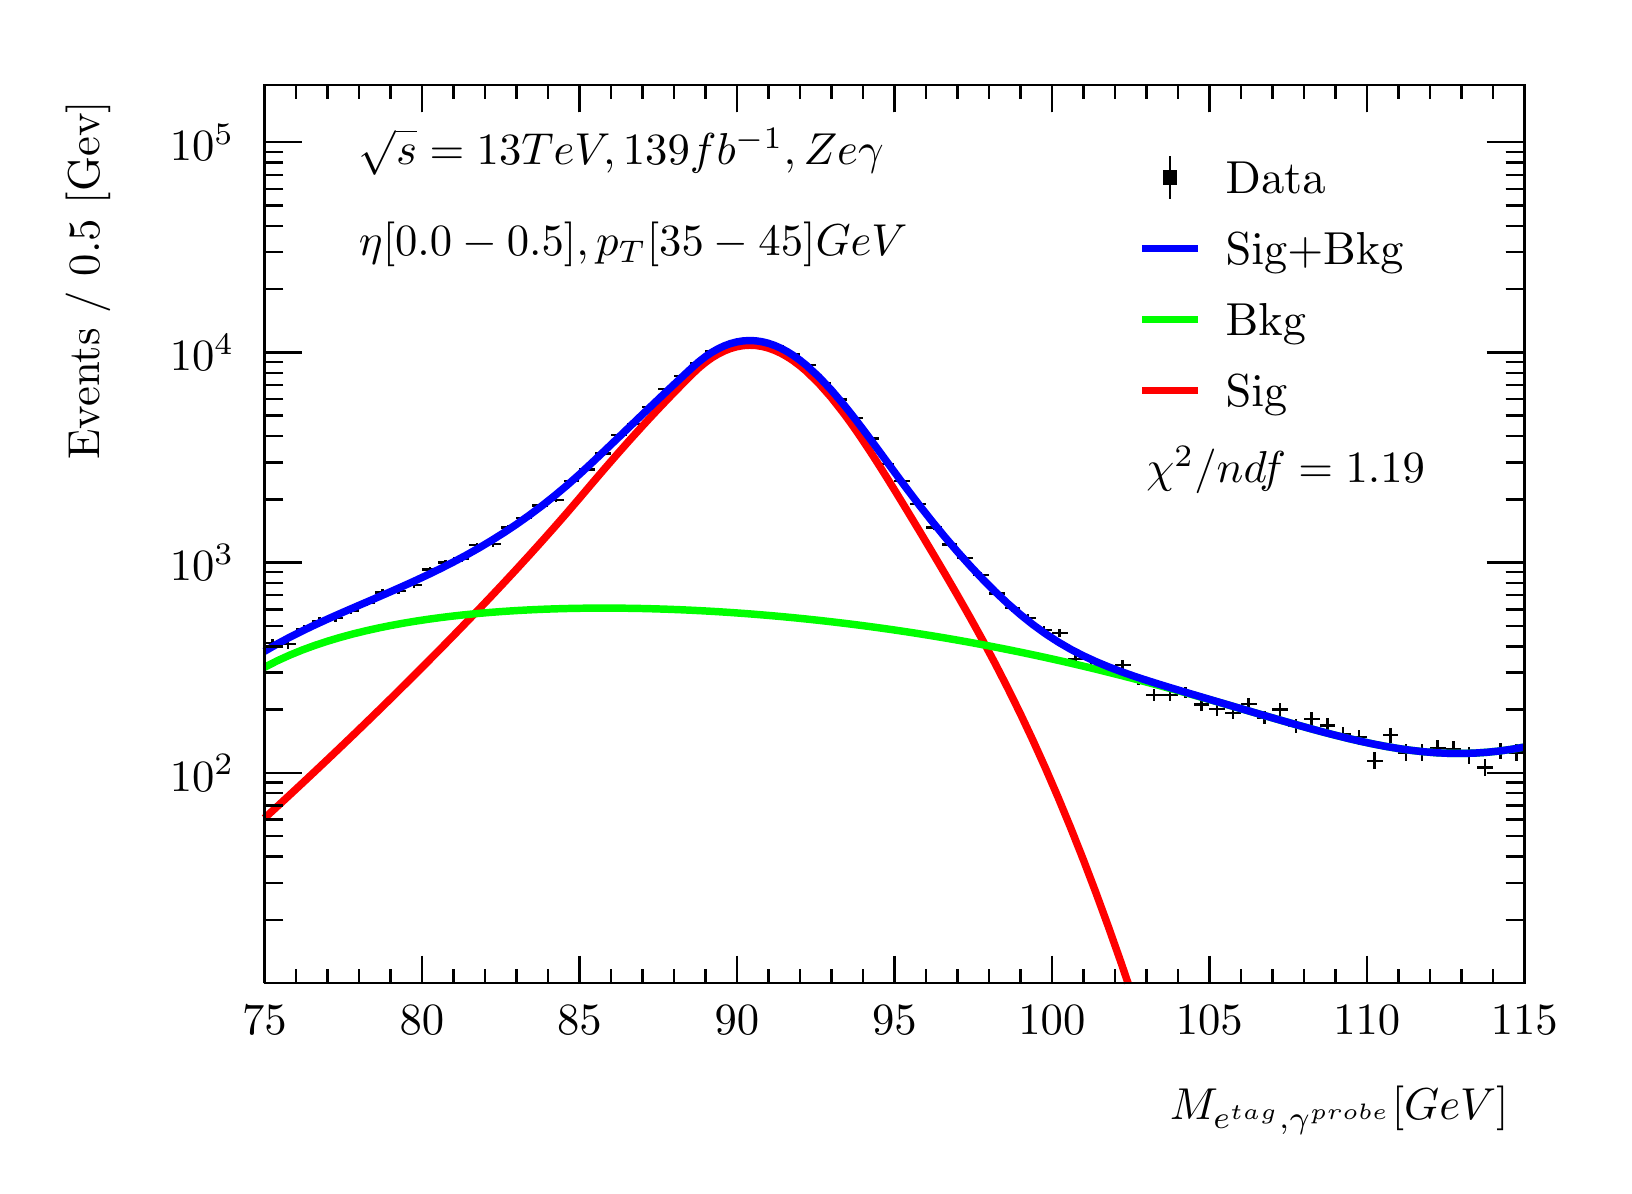
\begin{tikzpicture}
\pgfdeclareplotmark{cross} {
\pgfpathmoveto{\pgfpoint{-0.3\pgfplotmarksize}{\pgfplotmarksize}}
\pgfpathlineto{\pgfpoint{+0.3\pgfplotmarksize}{\pgfplotmarksize}}
\pgfpathlineto{\pgfpoint{+0.3\pgfplotmarksize}{0.3\pgfplotmarksize}}
\pgfpathlineto{\pgfpoint{+1\pgfplotmarksize}{0.3\pgfplotmarksize}}
\pgfpathlineto{\pgfpoint{+1\pgfplotmarksize}{-0.3\pgfplotmarksize}}
\pgfpathlineto{\pgfpoint{+0.3\pgfplotmarksize}{-0.3\pgfplotmarksize}}
\pgfpathlineto{\pgfpoint{+0.3\pgfplotmarksize}{-1.\pgfplotmarksize}}
\pgfpathlineto{\pgfpoint{-0.3\pgfplotmarksize}{-1.\pgfplotmarksize}}
\pgfpathlineto{\pgfpoint{-0.3\pgfplotmarksize}{-0.3\pgfplotmarksize}}
\pgfpathlineto{\pgfpoint{-1.\pgfplotmarksize}{-0.3\pgfplotmarksize}}
\pgfpathlineto{\pgfpoint{-1.\pgfplotmarksize}{0.3\pgfplotmarksize}}
\pgfpathlineto{\pgfpoint{-0.3\pgfplotmarksize}{0.3\pgfplotmarksize}}
\pgfpathclose
\pgfusepathqstroke
}
\pgfdeclareplotmark{cross*} {
\pgfpathmoveto{\pgfpoint{-0.3\pgfplotmarksize}{\pgfplotmarksize}}
\pgfpathlineto{\pgfpoint{+0.3\pgfplotmarksize}{\pgfplotmarksize}}
\pgfpathlineto{\pgfpoint{+0.3\pgfplotmarksize}{0.3\pgfplotmarksize}}
\pgfpathlineto{\pgfpoint{+1\pgfplotmarksize}{0.3\pgfplotmarksize}}
\pgfpathlineto{\pgfpoint{+1\pgfplotmarksize}{-0.3\pgfplotmarksize}}
\pgfpathlineto{\pgfpoint{+0.3\pgfplotmarksize}{-0.3\pgfplotmarksize}}
\pgfpathlineto{\pgfpoint{+0.3\pgfplotmarksize}{-1.\pgfplotmarksize}}
\pgfpathlineto{\pgfpoint{-0.3\pgfplotmarksize}{-1.\pgfplotmarksize}}
\pgfpathlineto{\pgfpoint{-0.3\pgfplotmarksize}{-0.3\pgfplotmarksize}}
\pgfpathlineto{\pgfpoint{-1.\pgfplotmarksize}{-0.3\pgfplotmarksize}}
\pgfpathlineto{\pgfpoint{-1.\pgfplotmarksize}{0.3\pgfplotmarksize}}
\pgfpathlineto{\pgfpoint{-0.3\pgfplotmarksize}{0.3\pgfplotmarksize}}
\pgfpathclose
\pgfusepathqfillstroke
}
\pgfdeclareplotmark{newstar} {
\pgfpathmoveto{\pgfqpoint{0pt}{\pgfplotmarksize}}
\pgfpathlineto{\pgfqpointpolar{44}{0.5\pgfplotmarksize}}
\pgfpathlineto{\pgfqpointpolar{18}{\pgfplotmarksize}}
\pgfpathlineto{\pgfqpointpolar{-20}{0.5\pgfplotmarksize}}
\pgfpathlineto{\pgfqpointpolar{-54}{\pgfplotmarksize}}
\pgfpathlineto{\pgfqpointpolar{-90}{0.5\pgfplotmarksize}}
\pgfpathlineto{\pgfqpointpolar{234}{\pgfplotmarksize}}
\pgfpathlineto{\pgfqpointpolar{198}{0.5\pgfplotmarksize}}
\pgfpathlineto{\pgfqpointpolar{162}{\pgfplotmarksize}}
\pgfpathlineto{\pgfqpointpolar{134}{0.5\pgfplotmarksize}}
\pgfpathclose
\pgfusepathqstroke
}
\pgfdeclareplotmark{newstar*} {
\pgfpathmoveto{\pgfqpoint{0pt}{\pgfplotmarksize}}
\pgfpathlineto{\pgfqpointpolar{44}{0.5\pgfplotmarksize}}
\pgfpathlineto{\pgfqpointpolar{18}{\pgfplotmarksize}}
\pgfpathlineto{\pgfqpointpolar{-20}{0.5\pgfplotmarksize}}
\pgfpathlineto{\pgfqpointpolar{-54}{\pgfplotmarksize}}
\pgfpathlineto{\pgfqpointpolar{-90}{0.5\pgfplotmarksize}}
\pgfpathlineto{\pgfqpointpolar{234}{\pgfplotmarksize}}
\pgfpathlineto{\pgfqpointpolar{198}{0.5\pgfplotmarksize}}
\pgfpathlineto{\pgfqpointpolar{162}{\pgfplotmarksize}}
\pgfpathlineto{\pgfqpointpolar{134}{0.5\pgfplotmarksize}}
\pgfpathclose
\pgfusepathqfillstroke
}
\definecolor{c}{rgb}{1,1,1};
\draw [color=c, fill=c] (0,0) rectangle (20,14.4361);
\draw [color=c, fill=c] (3,2.30977) rectangle (19,13.7143);
\definecolor{c}{rgb}{0,0,0};
\draw [c,line width=0.9] (3,2.30977) -- (3,13.7143) -- (19,13.7143) -- (19,2.30977) -- (3,2.30977);
\definecolor{c}{rgb}{1,1,1};
\draw [color=c, fill=c] (3,2.30977) rectangle (19,13.7143);
\definecolor{c}{rgb}{0,0,0};
\draw [c,line width=0.9] (3,2.30977) -- (3,13.7143) -- (19,13.7143) -- (19,2.30977) -- (3,2.30977);
\draw [c,line width=0.9] (3,2.30977) -- (19,2.30977);
\draw [c,line width=0.9] (3,2.65624) -- (3,2.30977);
\draw [c,line width=0.9] (3.4,2.48301) -- (3.4,2.30977);
\draw [c,line width=0.9] (3.8,2.48301) -- (3.8,2.30977);
\draw [c,line width=0.9] (4.2,2.48301) -- (4.2,2.30977);
\draw [c,line width=0.9] (4.6,2.48301) -- (4.6,2.30977);
\draw [c,line width=0.9] (5,2.65624) -- (5,2.30977);
\draw [c,line width=0.9] (5.4,2.48301) -- (5.4,2.30977);
\draw [c,line width=0.9] (5.8,2.48301) -- (5.8,2.30977);
\draw [c,line width=0.9] (6.2,2.48301) -- (6.2,2.30977);
\draw [c,line width=0.9] (6.6,2.48301) -- (6.6,2.30977);
\draw [c,line width=0.9] (7,2.65624) -- (7,2.30977);
\draw [c,line width=0.9] (7.4,2.48301) -- (7.4,2.30977);
\draw [c,line width=0.9] (7.8,2.48301) -- (7.8,2.30977);
\draw [c,line width=0.9] (8.2,2.48301) -- (8.2,2.30977);
\draw [c,line width=0.9] (8.6,2.48301) -- (8.6,2.30977);
\draw [c,line width=0.9] (9,2.65624) -- (9,2.30977);
\draw [c,line width=0.9] (9.4,2.48301) -- (9.4,2.30977);
\draw [c,line width=0.9] (9.8,2.48301) -- (9.8,2.30977);
\draw [c,line width=0.9] (10.2,2.48301) -- (10.2,2.30977);
\draw [c,line width=0.9] (10.6,2.48301) -- (10.6,2.30977);
\draw [c,line width=0.9] (11,2.65624) -- (11,2.30977);
\draw [c,line width=0.9] (11.4,2.48301) -- (11.4,2.30977);
\draw [c,line width=0.9] (11.8,2.48301) -- (11.8,2.30977);
\draw [c,line width=0.9] (12.2,2.48301) -- (12.2,2.30977);
\draw [c,line width=0.9] (12.6,2.48301) -- (12.6,2.30977);
\draw [c,line width=0.9] (13,2.65624) -- (13,2.30977);
\draw [c,line width=0.9] (13.4,2.48301) -- (13.4,2.30977);
\draw [c,line width=0.9] (13.8,2.48301) -- (13.8,2.30977);
\draw [c,line width=0.9] (14.2,2.48301) -- (14.2,2.30977);
\draw [c,line width=0.9] (14.6,2.48301) -- (14.6,2.30977);
\draw [c,line width=0.9] (15,2.65624) -- (15,2.30977);
\draw [c,line width=0.9] (15.4,2.48301) -- (15.4,2.30977);
\draw [c,line width=0.9] (15.8,2.48301) -- (15.8,2.30977);
\draw [c,line width=0.9] (16.2,2.48301) -- (16.2,2.30977);
\draw [c,line width=0.9] (16.6,2.48301) -- (16.6,2.30977);
\draw [c,line width=0.9] (17,2.65624) -- (17,2.30977);
\draw [c,line width=0.9] (17.4,2.48301) -- (17.4,2.30977);
\draw [c,line width=0.9] (17.8,2.48301) -- (17.8,2.30977);
\draw [c,line width=0.9] (18.2,2.48301) -- (18.2,2.30977);
\draw [c,line width=0.9] (18.6,2.48301) -- (18.6,2.30977);
\draw [c,line width=0.9] (19,2.65624) -- (19,2.30977);
\draw [c,line width=0.9] (19,2.65624) -- (19,2.30977);
\draw [anchor=base] (3,1.66015) node[scale=1.61424, color=c, rotate=0]{75};
\draw [anchor=base] (5,1.66015) node[scale=1.61424, color=c, rotate=0]{80};
\draw [anchor=base] (7,1.66015) node[scale=1.61424, color=c, rotate=0]{85};
\draw [anchor=base] (9,1.66015) node[scale=1.61424, color=c, rotate=0]{90};
\draw [anchor=base] (11,1.66015) node[scale=1.61424, color=c, rotate=0]{95};
\draw [anchor=base] (13,1.66015) node[scale=1.61424, color=c, rotate=0]{100};
\draw [anchor=base] (15,1.66015) node[scale=1.61424, color=c, rotate=0]{105};
\draw [anchor=base] (17,1.66015) node[scale=1.61424, color=c, rotate=0]{110};
\draw [anchor=base] (19,1.66015) node[scale=1.61424, color=c, rotate=0]{115};
\draw [anchor= east] (19,0.692932) node[scale=1.61424, color=c, rotate=0]{$M_{e^{tag}, \gamma^{probe}}  [GeV]$};
\draw [c,line width=0.9] (3,13.7143) -- (19,13.7143);
\draw [c,line width=0.9] (3,13.3678) -- (3,13.7143);
\draw [c,line width=0.9] (3.4,13.5411) -- (3.4,13.7143);
\draw [c,line width=0.9] (3.8,13.5411) -- (3.8,13.7143);
\draw [c,line width=0.9] (4.2,13.5411) -- (4.2,13.7143);
\draw [c,line width=0.9] (4.6,13.5411) -- (4.6,13.7143);
\draw [c,line width=0.9] (5,13.3678) -- (5,13.7143);
\draw [c,line width=0.9] (5.4,13.5411) -- (5.4,13.7143);
\draw [c,line width=0.9] (5.8,13.5411) -- (5.8,13.7143);
\draw [c,line width=0.9] (6.2,13.5411) -- (6.2,13.7143);
\draw [c,line width=0.9] (6.6,13.5411) -- (6.6,13.7143);
\draw [c,line width=0.9] (7,13.3678) -- (7,13.7143);
\draw [c,line width=0.9] (7.4,13.5411) -- (7.4,13.7143);
\draw [c,line width=0.9] (7.8,13.5411) -- (7.8,13.7143);
\draw [c,line width=0.9] (8.2,13.5411) -- (8.2,13.7143);
\draw [c,line width=0.9] (8.6,13.5411) -- (8.6,13.7143);
\draw [c,line width=0.9] (9,13.3678) -- (9,13.7143);
\draw [c,line width=0.9] (9.4,13.5411) -- (9.4,13.7143);
\draw [c,line width=0.9] (9.8,13.5411) -- (9.8,13.7143);
\draw [c,line width=0.9] (10.2,13.5411) -- (10.2,13.7143);
\draw [c,line width=0.9] (10.6,13.5411) -- (10.6,13.7143);
\draw [c,line width=0.9] (11,13.3678) -- (11,13.7143);
\draw [c,line width=0.9] (11.4,13.5411) -- (11.4,13.7143);
\draw [c,line width=0.9] (11.8,13.5411) -- (11.8,13.7143);
\draw [c,line width=0.9] (12.2,13.5411) -- (12.2,13.7143);
\draw [c,line width=0.9] (12.6,13.5411) -- (12.6,13.7143);
\draw [c,line width=0.9] (13,13.3678) -- (13,13.7143);
\draw [c,line width=0.9] (13.4,13.5411) -- (13.4,13.7143);
\draw [c,line width=0.9] (13.8,13.5411) -- (13.8,13.7143);
\draw [c,line width=0.9] (14.2,13.5411) -- (14.2,13.7143);
\draw [c,line width=0.9] (14.6,13.5411) -- (14.6,13.7143);
\draw [c,line width=0.9] (15,13.3678) -- (15,13.7143);
\draw [c,line width=0.9] (15.4,13.5411) -- (15.4,13.7143);
\draw [c,line width=0.9] (15.8,13.5411) -- (15.8,13.7143);
\draw [c,line width=0.9] (16.2,13.5411) -- (16.2,13.7143);
\draw [c,line width=0.9] (16.6,13.5411) -- (16.6,13.7143);
\draw [c,line width=0.9] (17,13.3678) -- (17,13.7143);
\draw [c,line width=0.9] (17.4,13.5411) -- (17.4,13.7143);
\draw [c,line width=0.9] (17.8,13.5411) -- (17.8,13.7143);
\draw [c,line width=0.9] (18.2,13.5411) -- (18.2,13.7143);
\draw [c,line width=0.9] (18.6,13.5411) -- (18.6,13.7143);
\draw [c,line width=0.9] (19,13.3678) -- (19,13.7143);
\draw [c,line width=0.9] (19,13.3678) -- (19,13.7143);
\draw [c,line width=0.9] (3,2.30977) -- (3,13.7143);
\draw [c,line width=0.9] (3.237,3.11343) -- (3,3.11343);
\draw [c,line width=0.9] (3.237,3.58354) -- (3,3.58354);
\draw [c,line width=0.9] (3.237,3.91709) -- (3,3.91709);
\draw [c,line width=0.9] (3.237,4.17581) -- (3,4.17581);
\draw [c,line width=0.9] (3.237,4.38719) -- (3,4.38719);
\draw [c,line width=0.9] (3.237,4.56592) -- (3,4.56592);
\draw [c,line width=0.9] (3.237,4.72074) -- (3,4.72074);
\draw [c,line width=0.9] (3.237,4.8573) -- (3,4.8573);
\draw [c,line width=0.9] (3.474,4.97946) -- (3,4.97946);
\draw [anchor= east] (2.82,4.97946) node[scale=1.61424, color=c, rotate=0]{$10^{2}$};
\draw [c,line width=0.9] (3.237,5.78312) -- (3,5.78312);
\draw [c,line width=0.9] (3.237,6.25323) -- (3,6.25323);
\draw [c,line width=0.9] (3.237,6.58678) -- (3,6.58678);
\draw [c,line width=0.9] (3.237,6.8455) -- (3,6.8455);
\draw [c,line width=0.9] (3.237,7.05689) -- (3,7.05689);
\draw [c,line width=0.9] (3.237,7.23561) -- (3,7.23561);
\draw [c,line width=0.9] (3.237,7.39043) -- (3,7.39043);
\draw [c,line width=0.9] (3.237,7.52699) -- (3,7.52699);
\draw [c,line width=0.9] (3.474,7.64915) -- (3,7.64915);
\draw [anchor= east] (2.82,7.64915) node[scale=1.61424, color=c, rotate=0]{$10^{3}$};
\draw [c,line width=0.9] (3.237,8.45281) -- (3,8.45281);
\draw [c,line width=0.9] (3.237,8.92292) -- (3,8.92292);
\draw [c,line width=0.9] (3.237,9.25647) -- (3,9.25647);
\draw [c,line width=0.9] (3.237,9.51519) -- (3,9.51519);
\draw [c,line width=0.9] (3.237,9.72658) -- (3,9.72658);
\draw [c,line width=0.9] (3.237,9.9053) -- (3,9.9053);
\draw [c,line width=0.9] (3.237,10.0601) -- (3,10.0601);
\draw [c,line width=0.9] (3.237,10.1967) -- (3,10.1967);
\draw [c,line width=0.9] (3.474,10.3188) -- (3,10.3188);
\draw [anchor= east] (2.82,10.3188) node[scale=1.61424, color=c, rotate=0]{$10^{4}$};
\draw [c,line width=0.9] (3.237,11.1225) -- (3,11.1225);
\draw [c,line width=0.9] (3.237,11.5926) -- (3,11.5926);
\draw [c,line width=0.9] (3.237,11.9262) -- (3,11.9262);
\draw [c,line width=0.9] (3.237,12.1849) -- (3,12.1849);
\draw [c,line width=0.9] (3.237,12.3963) -- (3,12.3963);
\draw [c,line width=0.9] (3.237,12.575) -- (3,12.575);
\draw [c,line width=0.9] (3.237,12.7298) -- (3,12.7298);
\draw [c,line width=0.9] (3.237,12.8664) -- (3,12.8664);
\draw [c,line width=0.9] (3.474,12.9885) -- (3,12.9885);
\draw [anchor= east] (2.82,12.9885) node[scale=1.61424, color=c, rotate=0]{$10^{5}$};
\draw [anchor= east] (0.76,13.7143) node[scale=1.61424, color=c, rotate=90]{Events / 0.5 [Gev]};
\draw [c,line width=0.9] (19,2.30977) -- (19,13.7143);
\draw [c,line width=0.9] (18.763,3.11343) -- (19,3.11343);
\draw [c,line width=0.9] (18.763,3.58354) -- (19,3.58354);
\draw [c,line width=0.9] (18.763,3.91709) -- (19,3.91709);
\draw [c,line width=0.9] (18.763,4.17581) -- (19,4.17581);
\draw [c,line width=0.9] (18.763,4.38719) -- (19,4.38719);
\draw [c,line width=0.9] (18.763,4.56592) -- (19,4.56592);
\draw [c,line width=0.9] (18.763,4.72074) -- (19,4.72074);
\draw [c,line width=0.9] (18.763,4.8573) -- (19,4.8573);
\draw [c,line width=0.9] (18.526,4.97946) -- (19,4.97946);
\draw [c,line width=0.9] (18.763,5.78312) -- (19,5.78312);
\draw [c,line width=0.9] (18.763,6.25323) -- (19,6.25323);
\draw [c,line width=0.9] (18.763,6.58678) -- (19,6.58678);
\draw [c,line width=0.9] (18.763,6.8455) -- (19,6.8455);
\draw [c,line width=0.9] (18.763,7.05689) -- (19,7.05689);
\draw [c,line width=0.9] (18.763,7.23561) -- (19,7.23561);
\draw [c,line width=0.9] (18.763,7.39043) -- (19,7.39043);
\draw [c,line width=0.9] (18.763,7.52699) -- (19,7.52699);
\draw [c,line width=0.9] (18.526,7.64915) -- (19,7.64915);
\draw [c,line width=0.9] (18.763,8.45281) -- (19,8.45281);
\draw [c,line width=0.9] (18.763,8.92292) -- (19,8.92292);
\draw [c,line width=0.9] (18.763,9.25647) -- (19,9.25647);
\draw [c,line width=0.9] (18.763,9.51519) -- (19,9.51519);
\draw [c,line width=0.9] (18.763,9.72658) -- (19,9.72658);
\draw [c,line width=0.9] (18.763,9.9053) -- (19,9.9053);
\draw [c,line width=0.9] (18.763,10.0601) -- (19,10.0601);
\draw [c,line width=0.9] (18.763,10.1967) -- (19,10.1967);
\draw [c,line width=0.9] (18.526,10.3188) -- (19,10.3188);
\draw [c,line width=0.9] (18.763,11.1225) -- (19,11.1225);
\draw [c,line width=0.9] (18.763,11.5926) -- (19,11.5926);
\draw [c,line width=0.9] (18.763,11.9262) -- (19,11.9262);
\draw [c,line width=0.9] (18.763,12.1849) -- (19,12.1849);
\draw [c,line width=0.9] (18.763,12.3963) -- (19,12.3963);
\draw [c,line width=0.9] (18.763,12.575) -- (19,12.575);
\draw [c,line width=0.9] (18.763,12.7298) -- (19,12.7298);
\draw [c,line width=0.9] (18.763,12.8664) -- (19,12.8664);
\draw [c,line width=0.9] (18.526,12.9885) -- (19,12.9885);
\draw [c,line width=0.9] (3.1,6.62666) -- (3,6.62666);
\draw [c,line width=0.9] (3,6.62666) -- (3,6.62666);
\draw [c,line width=0.9] (3.1,6.62666) -- (3.2,6.62666);
\draw [c,line width=0.9] (3.2,6.62666) -- (3.2,6.62666);
\draw [c,line width=0.9] (3.1,6.62666) -- (3.1,6.68364);
\draw [c,line width=0.9] (3.1,6.68364) -- (3.1,6.68364);
\draw [c,line width=0.9] (3.1,6.62666) -- (3.1,6.56969);
\draw [c,line width=0.9] (3.1,6.56969) -- (3.1,6.56969);
\draw [c,line width=0.9] (3.3,6.61258) -- (3.2,6.61258);
\draw [c,line width=0.9] (3.2,6.61258) -- (3.2,6.61258);
\draw [c,line width=0.9] (3.3,6.61258) -- (3.4,6.61258);
\draw [c,line width=0.9] (3.4,6.61258) -- (3.4,6.61258);
\draw [c,line width=0.9] (3.3,6.61258) -- (3.3,6.6699);
\draw [c,line width=0.9] (3.3,6.6699) -- (3.3,6.6699);
\draw [c,line width=0.9] (3.3,6.61258) -- (3.3,6.55525);
\draw [c,line width=0.9] (3.3,6.55525) -- (3.3,6.55525);
\draw [c,line width=0.9] (3.5,6.80779) -- (3.4,6.80779);
\draw [c,line width=0.9] (3.4,6.80779) -- (3.4,6.80779);
\draw [c,line width=0.9] (3.5,6.80779) -- (3.6,6.80779);
\draw [c,line width=0.9] (3.6,6.80779) -- (3.6,6.80779);
\draw [c,line width=0.9] (3.5,6.80779) -- (3.5,6.86049);
\draw [c,line width=0.9] (3.5,6.86049) -- (3.5,6.86049);
\draw [c,line width=0.9] (3.5,6.80779) -- (3.5,6.75509);
\draw [c,line width=0.9] (3.5,6.75509) -- (3.5,6.75509);
\draw [c,line width=0.9] (3.7,6.90207) -- (3.6,6.90207);
\draw [c,line width=0.9] (3.6,6.90207) -- (3.6,6.90207);
\draw [c,line width=0.9] (3.7,6.90207) -- (3.8,6.90207);
\draw [c,line width=0.9] (3.8,6.90207) -- (3.8,6.90207);
\draw [c,line width=0.9] (3.7,6.90207) -- (3.7,6.95266);
\draw [c,line width=0.9] (3.7,6.95266) -- (3.7,6.95266);
\draw [c,line width=0.9] (3.7,6.90207) -- (3.7,6.85147);
\draw [c,line width=0.9] (3.7,6.85147) -- (3.7,6.85147);
\draw [c,line width=0.9] (3.9,6.94754) -- (3.8,6.94754);
\draw [c,line width=0.9] (3.8,6.94754) -- (3.8,6.94754);
\draw [c,line width=0.9] (3.9,6.94754) -- (4,6.94754);
\draw [c,line width=0.9] (4,6.94754) -- (4,6.94754);
\draw [c,line width=0.9] (3.9,6.94754) -- (3.9,6.99716);
\draw [c,line width=0.9] (3.9,6.99716) -- (3.9,6.99716);
\draw [c,line width=0.9] (3.9,6.94754) -- (3.9,6.89792);
\draw [c,line width=0.9] (3.9,6.89792) -- (3.9,6.89792);
\draw [c,line width=0.9] (4.1,7.03936) -- (4,7.03936);
\draw [c,line width=0.9] (4,7.03936) -- (4,7.03936);
\draw [c,line width=0.9] (4.1,7.03936) -- (4.2,7.03936);
\draw [c,line width=0.9] (4.2,7.03936) -- (4.2,7.03936);
\draw [c,line width=0.9] (4.1,7.03936) -- (4.1,7.08705);
\draw [c,line width=0.9] (4.1,7.08705) -- (4.1,7.08705);
\draw [c,line width=0.9] (4.1,7.03936) -- (4.1,6.99167);
\draw [c,line width=0.9] (4.1,6.99167) -- (4.1,6.99167);
\draw [c,line width=0.9] (4.3,7.14074) -- (4.2,7.14074);
\draw [c,line width=0.9] (4.2,7.14074) -- (4.2,7.14074);
\draw [c,line width=0.9] (4.3,7.14074) -- (4.4,7.14074);
\draw [c,line width=0.9] (4.4,7.14074) -- (4.4,7.14074);
\draw [c,line width=0.9] (4.3,7.14074) -- (4.3,7.18639);
\draw [c,line width=0.9] (4.3,7.18639) -- (4.3,7.18639);
\draw [c,line width=0.9] (4.3,7.14074) -- (4.3,7.09509);
\draw [c,line width=0.9] (4.3,7.09509) -- (4.3,7.09509);
\draw [c,line width=0.9] (4.5,7.26666) -- (4.4,7.26666);
\draw [c,line width=0.9] (4.4,7.26666) -- (4.4,7.26666);
\draw [c,line width=0.9] (4.5,7.26666) -- (4.6,7.26666);
\draw [c,line width=0.9] (4.6,7.26666) -- (4.6,7.26666);
\draw [c,line width=0.9] (4.5,7.26666) -- (4.5,7.3099);
\draw [c,line width=0.9] (4.5,7.3099) -- (4.5,7.3099);
\draw [c,line width=0.9] (4.5,7.26666) -- (4.5,7.22343);
\draw [c,line width=0.9] (4.5,7.22343) -- (4.5,7.22343);
\draw [c,line width=0.9] (4.7,7.28902) -- (4.6,7.28902);
\draw [c,line width=0.9] (4.6,7.28902) -- (4.6,7.28902);
\draw [c,line width=0.9] (4.7,7.28902) -- (4.8,7.28902);
\draw [c,line width=0.9] (4.8,7.28902) -- (4.8,7.28902);
\draw [c,line width=0.9] (4.7,7.28902) -- (4.7,7.33185);
\draw [c,line width=0.9] (4.7,7.33185) -- (4.7,7.33185);
\draw [c,line width=0.9] (4.7,7.28902) -- (4.7,7.2462);
\draw [c,line width=0.9] (4.7,7.2462) -- (4.7,7.2462);
\draw [c,line width=0.9] (4.9,7.36553) -- (4.8,7.36553);
\draw [c,line width=0.9] (4.8,7.36553) -- (4.8,7.36553);
\draw [c,line width=0.9] (4.9,7.36553) -- (5,7.36553);
\draw [c,line width=0.9] (5,7.36553) -- (5,7.36553);
\draw [c,line width=0.9] (4.9,7.36553) -- (4.9,7.40696);
\draw [c,line width=0.9] (4.9,7.40696) -- (4.9,7.40696);
\draw [c,line width=0.9] (4.9,7.36553) -- (4.9,7.3241);
\draw [c,line width=0.9] (4.9,7.3241) -- (4.9,7.3241);
\draw [c,line width=0.9] (5.1,7.55876) -- (5,7.55876);
\draw [c,line width=0.9] (5,7.55876) -- (5,7.55876);
\draw [c,line width=0.9] (5.1,7.55876) -- (5.2,7.55876);
\draw [c,line width=0.9] (5.2,7.55876) -- (5.2,7.55876);
\draw [c,line width=0.9] (5.1,7.55876) -- (5.1,7.59688);
\draw [c,line width=0.9] (5.1,7.59688) -- (5.1,7.59688);
\draw [c,line width=0.9] (5.1,7.55876) -- (5.1,7.52064);
\draw [c,line width=0.9] (5.1,7.52064) -- (5.1,7.52064);
\draw [c,line width=0.9] (5.3,7.65031) -- (5.2,7.65031);
\draw [c,line width=0.9] (5.2,7.65031) -- (5.2,7.65031);
\draw [c,line width=0.9] (5.3,7.65031) -- (5.4,7.65031);
\draw [c,line width=0.9] (5.4,7.65031) -- (5.4,7.65031);
\draw [c,line width=0.9] (5.3,7.65031) -- (5.3,7.68696);
\draw [c,line width=0.9] (5.3,7.68696) -- (5.3,7.68696);
\draw [c,line width=0.9] (5.3,7.65031) -- (5.3,7.61367);
\draw [c,line width=0.9] (5.3,7.61367) -- (5.3,7.61367);
\draw [c,line width=0.9] (5.5,7.69908) -- (5.4,7.69908);
\draw [c,line width=0.9] (5.4,7.69908) -- (5.4,7.69908);
\draw [c,line width=0.9] (5.5,7.69908) -- (5.6,7.69908);
\draw [c,line width=0.9] (5.6,7.69908) -- (5.6,7.69908);
\draw [c,line width=0.9] (5.5,7.69908) -- (5.5,7.73496);
\draw [c,line width=0.9] (5.5,7.73496) -- (5.5,7.73496);
\draw [c,line width=0.9] (5.5,7.69908) -- (5.5,7.6632);
\draw [c,line width=0.9] (5.5,7.6632) -- (5.5,7.6632);
\draw [c,line width=0.9] (5.7,7.87112) -- (5.6,7.87112);
\draw [c,line width=0.9] (5.6,7.87112) -- (5.6,7.87112);
\draw [c,line width=0.9] (5.7,7.87112) -- (5.8,7.87112);
\draw [c,line width=0.9] (5.8,7.87112) -- (5.8,7.87112);
\draw [c,line width=0.9] (5.7,7.87112) -- (5.7,7.90444);
\draw [c,line width=0.9] (5.7,7.90444) -- (5.7,7.90444);
\draw [c,line width=0.9] (5.7,7.87112) -- (5.7,7.83781);
\draw [c,line width=0.9] (5.7,7.83781) -- (5.7,7.83781);
\draw [c,line width=0.9] (5.9,7.8854) -- (5.8,7.8854);
\draw [c,line width=0.9] (5.8,7.8854) -- (5.8,7.8854);
\draw [c,line width=0.9] (5.9,7.8854) -- (6,7.8854);
\draw [c,line width=0.9] (6,7.8854) -- (6,7.8854);
\draw [c,line width=0.9] (5.9,7.8854) -- (5.9,7.91851);
\draw [c,line width=0.9] (5.9,7.91851) -- (5.9,7.91851);
\draw [c,line width=0.9] (5.9,7.8854) -- (5.9,7.85228);
\draw [c,line width=0.9] (5.9,7.85228) -- (5.9,7.85228);
\draw [c,line width=0.9] (6.1,8.09426) -- (6,8.09426);
\draw [c,line width=0.9] (6,8.09426) -- (6,8.09426);
\draw [c,line width=0.9] (6.1,8.09426) -- (6.2,8.09426);
\draw [c,line width=0.9] (6.2,8.09426) -- (6.2,8.09426);
\draw [c,line width=0.9] (6.1,8.09426) -- (6.1,8.12452);
\draw [c,line width=0.9] (6.1,8.12452) -- (6.1,8.12452);
\draw [c,line width=0.9] (6.1,8.09426) -- (6.1,8.064);
\draw [c,line width=0.9] (6.1,8.064) -- (6.1,8.064);
\draw [c,line width=0.9] (6.3,8.21705) -- (6.2,8.21705);
\draw [c,line width=0.9] (6.2,8.21705) -- (6.2,8.21705);
\draw [c,line width=0.9] (6.3,8.21705) -- (6.4,8.21705);
\draw [c,line width=0.9] (6.4,8.21705) -- (6.4,8.21705);
\draw [c,line width=0.9] (6.3,8.21705) -- (6.3,8.24575);
\draw [c,line width=0.9] (6.3,8.24575) -- (6.3,8.24575);
\draw [c,line width=0.9] (6.3,8.21705) -- (6.3,8.18835);
\draw [c,line width=0.9] (6.3,8.18835) -- (6.3,8.18835);
\draw [c,line width=0.9] (6.5,8.37365) -- (6.4,8.37365);
\draw [c,line width=0.9] (6.4,8.37365) -- (6.4,8.37365);
\draw [c,line width=0.9] (6.5,8.37365) -- (6.6,8.37365);
\draw [c,line width=0.9] (6.6,8.37365) -- (6.6,8.37365);
\draw [c,line width=0.9] (6.5,8.37365) -- (6.5,8.40047);
\draw [c,line width=0.9] (6.5,8.40047) -- (6.5,8.40047);
\draw [c,line width=0.9] (6.5,8.37365) -- (6.5,8.34682);
\draw [c,line width=0.9] (6.5,8.34682) -- (6.5,8.34682);
\draw [c,line width=0.9] (6.7,8.44233) -- (6.6,8.44233);
\draw [c,line width=0.9] (6.6,8.44233) -- (6.6,8.44233);
\draw [c,line width=0.9] (6.7,8.44233) -- (6.8,8.44233);
\draw [c,line width=0.9] (6.8,8.44233) -- (6.8,8.44233);
\draw [c,line width=0.9] (6.7,8.44233) -- (6.7,8.46837);
\draw [c,line width=0.9] (6.7,8.46837) -- (6.7,8.46837);
\draw [c,line width=0.9] (6.7,8.44233) -- (6.7,8.41629);
\draw [c,line width=0.9] (6.7,8.41629) -- (6.7,8.41629);
\draw [c,line width=0.9] (6.9,8.68526) -- (6.8,8.68526);
\draw [c,line width=0.9] (6.8,8.68526) -- (6.8,8.68526);
\draw [c,line width=0.9] (6.9,8.68526) -- (7,8.68526);
\draw [c,line width=0.9] (7,8.68526) -- (7,8.68526);
\draw [c,line width=0.9] (6.9,8.68526) -- (6.9,8.70872);
\draw [c,line width=0.9] (6.9,8.70872) -- (6.9,8.70872);
\draw [c,line width=0.9] (6.9,8.68526) -- (6.9,8.66181);
\draw [c,line width=0.9] (6.9,8.66181) -- (6.9,8.66181);
\draw [c,line width=0.9] (7.1,8.83336) -- (7,8.83336);
\draw [c,line width=0.9] (7,8.83336) -- (7,8.83336);
\draw [c,line width=0.9] (7.1,8.83336) -- (7.2,8.83336);
\draw [c,line width=0.9] (7.2,8.83336) -- (7.2,8.83336);
\draw [c,line width=0.9] (7.1,8.83336) -- (7.1,8.85537);
\draw [c,line width=0.9] (7.1,8.85537) -- (7.1,8.85537);
\draw [c,line width=0.9] (7.1,8.83336) -- (7.1,8.81136);
\draw [c,line width=0.9] (7.1,8.81136) -- (7.1,8.81136);
\draw [c,line width=0.9] (7.3,9.03763) -- (7.2,9.03763);
\draw [c,line width=0.9] (7.2,9.03763) -- (7.2,9.03763);
\draw [c,line width=0.9] (7.3,9.03763) -- (7.4,9.03763);
\draw [c,line width=0.9] (7.4,9.03763) -- (7.4,9.03763);
\draw [c,line width=0.9] (7.3,9.03763) -- (7.3,9.05778);
\draw [c,line width=0.9] (7.3,9.05778) -- (7.3,9.05778);
\draw [c,line width=0.9] (7.3,9.03763) -- (7.3,9.01749);
\draw [c,line width=0.9] (7.3,9.01749) -- (7.3,9.01749);
\draw [c,line width=0.9] (7.5,9.26858) -- (7.4,9.26858);
\draw [c,line width=0.9] (7.4,9.26858) -- (7.4,9.26858);
\draw [c,line width=0.9] (7.5,9.26858) -- (7.6,9.26858);
\draw [c,line width=0.9] (7.6,9.26858) -- (7.6,9.26858);
\draw [c,line width=0.9] (7.5,9.26858) -- (7.5,9.28681);
\draw [c,line width=0.9] (7.5,9.28681) -- (7.5,9.28681);
\draw [c,line width=0.9] (7.5,9.26858) -- (7.5,9.25034);
\draw [c,line width=0.9] (7.5,9.25034) -- (7.5,9.25034);
\draw [c,line width=0.9] (7.7,9.41093) -- (7.6,9.41093);
\draw [c,line width=0.9] (7.6,9.41093) -- (7.6,9.41093);
\draw [c,line width=0.9] (7.7,9.41093) -- (7.8,9.41093);
\draw [c,line width=0.9] (7.8,9.41093) -- (7.8,9.41093);
\draw [c,line width=0.9] (7.7,9.41093) -- (7.7,9.42808);
\draw [c,line width=0.9] (7.7,9.42808) -- (7.7,9.42808);
\draw [c,line width=0.9] (7.7,9.41093) -- (7.7,9.39377);
\draw [c,line width=0.9] (7.7,9.39377) -- (7.7,9.39377);
\draw [c,line width=0.9] (7.9,9.62801) -- (7.8,9.62801);
\draw [c,line width=0.9] (7.8,9.62801) -- (7.8,9.62801);
\draw [c,line width=0.9] (7.9,9.62801) -- (8,9.62801);
\draw [c,line width=0.9] (8,9.62801) -- (8,9.62801);
\draw [c,line width=0.9] (7.9,9.62801) -- (7.9,9.64363);
\draw [c,line width=0.9] (7.9,9.64363) -- (7.9,9.64363);
\draw [c,line width=0.9] (7.9,9.62801) -- (7.9,9.61239);
\draw [c,line width=0.9] (7.9,9.61239) -- (7.9,9.61239);
\draw [c,line width=0.9] (8.1,9.85105) -- (8,9.85105);
\draw [c,line width=0.9] (8,9.85105) -- (8,9.85105);
\draw [c,line width=0.9] (8.1,9.85105) -- (8.2,9.85105);
\draw [c,line width=0.9] (8.2,9.85105) -- (8.2,9.85105);
\draw [c,line width=0.9] (8.1,9.85105) -- (8.1,9.86524);
\draw [c,line width=0.9] (8.1,9.86524) -- (8.1,9.86524);
\draw [c,line width=0.9] (8.1,9.85105) -- (8.1,9.83687);
\draw [c,line width=0.9] (8.1,9.83687) -- (8.1,9.83687);
\draw [c,line width=0.9] (8.3,10.0176) -- (8.2,10.0176);
\draw [c,line width=0.9] (8.2,10.0176) -- (8.2,10.0176);
\draw [c,line width=0.9] (8.3,10.0176) -- (8.4,10.0176);
\draw [c,line width=0.9] (8.4,10.0176) -- (8.4,10.0176);
\draw [c,line width=0.9] (8.3,10.0176) -- (8.3,10.0308);
\draw [c,line width=0.9] (8.3,10.0308) -- (8.3,10.0308);
\draw [c,line width=0.9] (8.3,10.0176) -- (8.3,10.0044);
\draw [c,line width=0.9] (8.3,10.0044) -- (8.3,10.0044);
\draw [c,line width=0.9] (8.5,10.1863) -- (8.4,10.1863);
\draw [c,line width=0.9] (8.4,10.1863) -- (8.4,10.1863);
\draw [c,line width=0.9] (8.5,10.1863) -- (8.6,10.1863);
\draw [c,line width=0.9] (8.6,10.1863) -- (8.6,10.1863);
\draw [c,line width=0.9] (8.5,10.1863) -- (8.5,10.1986);
\draw [c,line width=0.9] (8.5,10.1986) -- (8.5,10.1986);
\draw [c,line width=0.9] (8.5,10.1863) -- (8.5,10.1741);
\draw [c,line width=0.9] (8.5,10.1741) -- (8.5,10.1741);
\draw [c,line width=0.9] (8.7,10.3322) -- (8.6,10.3322);
\draw [c,line width=0.9] (8.6,10.3322) -- (8.6,10.3322);
\draw [c,line width=0.9] (8.7,10.3322) -- (8.8,10.3322);
\draw [c,line width=0.9] (8.8,10.3322) -- (8.8,10.3322);
\draw [c,line width=0.9] (8.7,10.3322) -- (8.7,10.3437);
\draw [c,line width=0.9] (8.7,10.3437) -- (8.7,10.3437);
\draw [c,line width=0.9] (8.7,10.3322) -- (8.7,10.3207);
\draw [c,line width=0.9] (8.7,10.3207) -- (8.7,10.3207);
\draw [c,line width=0.9] (8.9,10.4103) -- (8.8,10.4103);
\draw [c,line width=0.9] (8.8,10.4103) -- (8.8,10.4103);
\draw [c,line width=0.9] (8.9,10.4103) -- (9,10.4103);
\draw [c,line width=0.9] (9,10.4103) -- (9,10.4103);
\draw [c,line width=0.9] (8.9,10.4103) -- (8.9,10.4215);
\draw [c,line width=0.9] (8.9,10.4215) -- (8.9,10.4215);
\draw [c,line width=0.9] (8.9,10.4103) -- (8.9,10.3992);
\draw [c,line width=0.9] (8.9,10.3992) -- (8.9,10.3992);
\draw [c,line width=0.9] (9.1,10.4655) -- (9,10.4655);
\draw [c,line width=0.9] (9,10.4655) -- (9,10.4655);
\draw [c,line width=0.9] (9.1,10.4655) -- (9.2,10.4655);
\draw [c,line width=0.9] (9.2,10.4655) -- (9.2,10.4655);
\draw [c,line width=0.9] (9.1,10.4655) -- (9.1,10.4763);
\draw [c,line width=0.9] (9.1,10.4763) -- (9.1,10.4763);
\draw [c,line width=0.9] (9.1,10.4655) -- (9.1,10.4546);
\draw [c,line width=0.9] (9.1,10.4546) -- (9.1,10.4546);
\draw [c,line width=0.9] (9.3,10.4522) -- (9.2,10.4522);
\draw [c,line width=0.9] (9.2,10.4522) -- (9.2,10.4522);
\draw [c,line width=0.9] (9.3,10.4522) -- (9.4,10.4522);
\draw [c,line width=0.9] (9.4,10.4522) -- (9.4,10.4522);
\draw [c,line width=0.9] (9.3,10.4522) -- (9.3,10.4632);
\draw [c,line width=0.9] (9.3,10.4632) -- (9.3,10.4632);
\draw [c,line width=0.9] (9.3,10.4522) -- (9.3,10.4413);
\draw [c,line width=0.9] (9.3,10.4413) -- (9.3,10.4413);
\draw [c,line width=0.9] (9.5,10.3965) -- (9.4,10.3965);
\draw [c,line width=0.9] (9.4,10.3965) -- (9.4,10.3965);
\draw [c,line width=0.9] (9.5,10.3965) -- (9.6,10.3965);
\draw [c,line width=0.9] (9.6,10.3965) -- (9.6,10.3965);
\draw [c,line width=0.9] (9.5,10.3965) -- (9.5,10.4077);
\draw [c,line width=0.9] (9.5,10.4077) -- (9.5,10.4077);
\draw [c,line width=0.9] (9.5,10.3965) -- (9.5,10.3853);
\draw [c,line width=0.9] (9.5,10.3853) -- (9.5,10.3853);
\draw [c,line width=0.9] (9.7,10.2945) -- (9.6,10.2945);
\draw [c,line width=0.9] (9.6,10.2945) -- (9.6,10.2945);
\draw [c,line width=0.9] (9.7,10.2945) -- (9.8,10.2945);
\draw [c,line width=0.9] (9.8,10.2945) -- (9.8,10.2945);
\draw [c,line width=0.9] (9.7,10.2945) -- (9.7,10.3062);
\draw [c,line width=0.9] (9.7,10.3062) -- (9.7,10.3062);
\draw [c,line width=0.9] (9.7,10.2945) -- (9.7,10.2828);
\draw [c,line width=0.9] (9.7,10.2828) -- (9.7,10.2828);
\draw [c,line width=0.9] (9.9,10.1619) -- (9.8,10.1619);
\draw [c,line width=0.9] (9.8,10.1619) -- (9.8,10.1619);
\draw [c,line width=0.9] (9.9,10.1619) -- (10,10.1619);
\draw [c,line width=0.9] (10,10.1619) -- (10,10.1619);
\draw [c,line width=0.9] (9.9,10.1619) -- (9.9,10.1743);
\draw [c,line width=0.9] (9.9,10.1743) -- (9.9,10.1743);
\draw [c,line width=0.9] (9.9,10.1619) -- (9.9,10.1495);
\draw [c,line width=0.9] (9.9,10.1495) -- (9.9,10.1495);
\draw [c,line width=0.9] (10.1,9.9328) -- (10,9.9328);
\draw [c,line width=0.9] (10,9.9328) -- (10,9.9328);
\draw [c,line width=0.9] (10.1,9.9328) -- (10.2,9.9328);
\draw [c,line width=0.9] (10.2,9.9328) -- (10.2,9.9328);
\draw [c,line width=0.9] (10.1,9.9328) -- (10.1,9.9465);
\draw [c,line width=0.9] (10.1,9.9465) -- (10.1,9.9465);
\draw [c,line width=0.9] (10.1,9.9328) -- (10.1,9.91911);
\draw [c,line width=0.9] (10.1,9.91911) -- (10.1,9.91911);
\draw [c,line width=0.9] (10.3,9.71979) -- (10.2,9.71979);
\draw [c,line width=0.9] (10.2,9.71979) -- (10.2,9.71979);
\draw [c,line width=0.9] (10.3,9.71979) -- (10.4,9.71979);
\draw [c,line width=0.9] (10.4,9.71979) -- (10.4,9.71979);
\draw [c,line width=0.9] (10.3,9.71979) -- (10.3,9.73481);
\draw [c,line width=0.9] (10.3,9.73481) -- (10.3,9.73481);
\draw [c,line width=0.9] (10.3,9.71979) -- (10.3,9.70478);
\draw [c,line width=0.9] (10.3,9.70478) -- (10.3,9.70478);
\draw [c,line width=0.9] (10.5,9.48868) -- (10.4,9.48868);
\draw [c,line width=0.9] (10.4,9.48868) -- (10.4,9.48868);
\draw [c,line width=0.9] (10.5,9.48868) -- (10.6,9.48868);
\draw [c,line width=0.9] (10.6,9.48868) -- (10.6,9.48868);
\draw [c,line width=0.9] (10.5,9.48868) -- (10.5,9.50527);
\draw [c,line width=0.9] (10.5,9.50527) -- (10.5,9.50527);
\draw [c,line width=0.9] (10.5,9.48868) -- (10.5,9.4721);
\draw [c,line width=0.9] (10.5,9.4721) -- (10.5,9.4721);
\draw [c,line width=0.9] (10.7,9.2283) -- (10.6,9.2283);
\draw [c,line width=0.9] (10.6,9.2283) -- (10.6,9.2283);
\draw [c,line width=0.9] (10.7,9.2283) -- (10.8,9.2283);
\draw [c,line width=0.9] (10.8,9.2283) -- (10.8,9.2283);
\draw [c,line width=0.9] (10.7,9.2283) -- (10.7,9.24686);
\draw [c,line width=0.9] (10.7,9.24686) -- (10.7,9.24686);
\draw [c,line width=0.9] (10.7,9.2283) -- (10.7,9.20975);
\draw [c,line width=0.9] (10.7,9.20975) -- (10.7,9.20975);
\draw [c,line width=0.9] (10.9,8.8995) -- (10.8,8.8995);
\draw [c,line width=0.9] (10.8,8.8995) -- (10.8,8.8995);
\draw [c,line width=0.9] (10.9,8.8995) -- (11,8.8995);
\draw [c,line width=0.9] (11,8.8995) -- (11,8.8995);
\draw [c,line width=0.9] (10.9,8.8995) -- (10.9,8.92088);
\draw [c,line width=0.9] (10.9,8.92088) -- (10.9,8.92088);
\draw [c,line width=0.9] (10.9,8.8995) -- (10.9,8.87811);
\draw [c,line width=0.9] (10.9,8.87811) -- (10.9,8.87811);
\draw [c,line width=0.9] (11.1,8.68716) -- (11,8.68716);
\draw [c,line width=0.9] (11,8.68716) -- (11,8.68716);
\draw [c,line width=0.9] (11.1,8.68716) -- (11.2,8.68716);
\draw [c,line width=0.9] (11.2,8.68716) -- (11.2,8.68716);
\draw [c,line width=0.9] (11.1,8.68716) -- (11.1,8.71059);
\draw [c,line width=0.9] (11.1,8.71059) -- (11.1,8.71059);
\draw [c,line width=0.9] (11.1,8.68716) -- (11.1,8.66373);
\draw [c,line width=0.9] (11.1,8.66373) -- (11.1,8.66373);
\draw [c,line width=0.9] (11.3,8.3909) -- (11.2,8.3909);
\draw [c,line width=0.9] (11.2,8.3909) -- (11.2,8.3909);
\draw [c,line width=0.9] (11.3,8.3909) -- (11.4,8.3909);
\draw [c,line width=0.9] (11.4,8.3909) -- (11.4,8.3909);
\draw [c,line width=0.9] (11.3,8.3909) -- (11.3,8.41752);
\draw [c,line width=0.9] (11.3,8.41752) -- (11.3,8.41752);
\draw [c,line width=0.9] (11.3,8.3909) -- (11.3,8.36427);
\draw [c,line width=0.9] (11.3,8.36427) -- (11.3,8.36427);
\draw [c,line width=0.9] (11.5,8.09426) -- (11.4,8.09426);
\draw [c,line width=0.9] (11.4,8.09426) -- (11.4,8.09426);
\draw [c,line width=0.9] (11.5,8.09426) -- (11.6,8.09426);
\draw [c,line width=0.9] (11.6,8.09426) -- (11.6,8.09426);
\draw [c,line width=0.9] (11.5,8.09426) -- (11.5,8.12452);
\draw [c,line width=0.9] (11.5,8.12452) -- (11.5,8.12452);
\draw [c,line width=0.9] (11.5,8.09426) -- (11.5,8.064);
\draw [c,line width=0.9] (11.5,8.064) -- (11.5,8.064);
\draw [c,line width=0.9] (11.7,7.88161) -- (11.6,7.88161);
\draw [c,line width=0.9] (11.6,7.88161) -- (11.6,7.88161);
\draw [c,line width=0.9] (11.7,7.88161) -- (11.8,7.88161);
\draw [c,line width=0.9] (11.8,7.88161) -- (11.8,7.88161);
\draw [c,line width=0.9] (11.7,7.88161) -- (11.7,7.91477);
\draw [c,line width=0.9] (11.7,7.91477) -- (11.7,7.91477);
\draw [c,line width=0.9] (11.7,7.88161) -- (11.7,7.84844);
\draw [c,line width=0.9] (11.7,7.84844) -- (11.7,7.84844);
\draw [c,line width=0.9] (11.9,7.71013) -- (11.8,7.71013);
\draw [c,line width=0.9] (11.8,7.71013) -- (11.8,7.71013);
\draw [c,line width=0.9] (11.9,7.71013) -- (12,7.71013);
\draw [c,line width=0.9] (12,7.71013) -- (12,7.71013);
\draw [c,line width=0.9] (11.9,7.71013) -- (11.9,7.74584);
\draw [c,line width=0.9] (11.9,7.74584) -- (11.9,7.74584);
\draw [c,line width=0.9] (11.9,7.71013) -- (11.9,7.67442);
\draw [c,line width=0.9] (11.9,7.67442) -- (11.9,7.67442);
\draw [c,line width=0.9] (12.1,7.49035) -- (12,7.49035);
\draw [c,line width=0.9] (12,7.49035) -- (12,7.49035);
\draw [c,line width=0.9] (12.1,7.49035) -- (12.2,7.49035);
\draw [c,line width=0.9] (12.2,7.49035) -- (12.2,7.49035);
\draw [c,line width=0.9] (12.1,7.49035) -- (12.1,7.52961);
\draw [c,line width=0.9] (12.1,7.52961) -- (12.1,7.52961);
\draw [c,line width=0.9] (12.1,7.49035) -- (12.1,7.45109);
\draw [c,line width=0.9] (12.1,7.45109) -- (12.1,7.45109);
\draw [c,line width=0.9] (12.3,7.25695) -- (12.2,7.25695);
\draw [c,line width=0.9] (12.2,7.25695) -- (12.2,7.25695);
\draw [c,line width=0.9] (12.3,7.25695) -- (12.4,7.25695);
\draw [c,line width=0.9] (12.4,7.25695) -- (12.4,7.25695);
\draw [c,line width=0.9] (12.3,7.25695) -- (12.3,7.30037);
\draw [c,line width=0.9] (12.3,7.30037) -- (12.3,7.30037);
\draw [c,line width=0.9] (12.3,7.25695) -- (12.3,7.21353);
\draw [c,line width=0.9] (12.3,7.21353) -- (12.3,7.21353);
\draw [c,line width=0.9] (12.5,7.07034) -- (12.4,7.07034);
\draw [c,line width=0.9] (12.4,7.07034) -- (12.4,7.07034);
\draw [c,line width=0.9] (12.5,7.07034) -- (12.6,7.07034);
\draw [c,line width=0.9] (12.6,7.07034) -- (12.6,7.07034);
\draw [c,line width=0.9] (12.5,7.07034) -- (12.5,7.11739);
\draw [c,line width=0.9] (12.5,7.11739) -- (12.5,7.11739);
\draw [c,line width=0.9] (12.5,7.07034) -- (12.5,7.02328);
\draw [c,line width=0.9] (12.5,7.02328) -- (12.5,7.02328);
\draw [c,line width=0.9] (12.7,6.94329) -- (12.6,6.94329);
\draw [c,line width=0.9] (12.6,6.94329) -- (12.6,6.94329);
\draw [c,line width=0.9] (12.7,6.94329) -- (12.8,6.94329);
\draw [c,line width=0.9] (12.8,6.94329) -- (12.8,6.94329);
\draw [c,line width=0.9] (12.7,6.94329) -- (12.7,6.99299);
\draw [c,line width=0.9] (12.7,6.99299) -- (12.7,6.99299);
\draw [c,line width=0.9] (12.7,6.94329) -- (12.7,6.89358);
\draw [c,line width=0.9] (12.7,6.89358) -- (12.7,6.89358);
\draw [c,line width=0.9] (12.9,6.79575) -- (12.8,6.79575);
\draw [c,line width=0.9] (12.8,6.79575) -- (12.8,6.79575);
\draw [c,line width=0.9] (12.9,6.79575) -- (13,6.79575);
\draw [c,line width=0.9] (13,6.79575) -- (13,6.79575);
\draw [c,line width=0.9] (12.9,6.79575) -- (12.9,6.84872);
\draw [c,line width=0.9] (12.9,6.84872) -- (12.9,6.84872);
\draw [c,line width=0.9] (12.9,6.79575) -- (12.9,6.74278);
\draw [c,line width=0.9] (12.9,6.74278) -- (12.9,6.74278);
\draw [c,line width=0.9] (13.1,6.75636) -- (13,6.75636);
\draw [c,line width=0.9] (13,6.75636) -- (13,6.75636);
\draw [c,line width=0.9] (13.1,6.75636) -- (13.2,6.75636);
\draw [c,line width=0.9] (13.2,6.75636) -- (13.2,6.75636);
\draw [c,line width=0.9] (13.1,6.75636) -- (13.1,6.81024);
\draw [c,line width=0.9] (13.1,6.81024) -- (13.1,6.81024);
\draw [c,line width=0.9] (13.1,6.75636) -- (13.1,6.70248);
\draw [c,line width=0.9] (13.1,6.70248) -- (13.1,6.70248);
\draw [c,line width=0.9] (13.3,6.42198) -- (13.2,6.42198);
\draw [c,line width=0.9] (13.2,6.42198) -- (13.2,6.42198);
\draw [c,line width=0.9] (13.3,6.42198) -- (13.4,6.42198);
\draw [c,line width=0.9] (13.4,6.42198) -- (13.4,6.42198);
\draw [c,line width=0.9] (13.3,6.42198) -- (13.3,6.48421);
\draw [c,line width=0.9] (13.3,6.48421) -- (13.3,6.48421);
\draw [c,line width=0.9] (13.3,6.42198) -- (13.3,6.35974);
\draw [c,line width=0.9] (13.3,6.35974) -- (13.3,6.35974);
\draw [c,line width=0.9] (13.5,6.33528) -- (13.4,6.33528);
\draw [c,line width=0.9] (13.4,6.33528) -- (13.4,6.33528);
\draw [c,line width=0.9] (13.5,6.33528) -- (13.6,6.33528);
\draw [c,line width=0.9] (13.6,6.33528) -- (13.6,6.33528);
\draw [c,line width=0.9] (13.5,6.33528) -- (13.5,6.39989);
\draw [c,line width=0.9] (13.5,6.39989) -- (13.5,6.39989);
\draw [c,line width=0.9] (13.5,6.33528) -- (13.5,6.27068);
\draw [c,line width=0.9] (13.5,6.27068) -- (13.5,6.27068);
\draw [c,line width=0.9] (13.7,6.30241) -- (13.6,6.30241);
\draw [c,line width=0.9] (13.6,6.30241) -- (13.6,6.30241);
\draw [c,line width=0.9] (13.7,6.30241) -- (13.8,6.30241);
\draw [c,line width=0.9] (13.8,6.30241) -- (13.8,6.30241);
\draw [c,line width=0.9] (13.7,6.30241) -- (13.7,6.36794);
\draw [c,line width=0.9] (13.7,6.36794) -- (13.7,6.36794);
\draw [c,line width=0.9] (13.7,6.30241) -- (13.7,6.23689);
\draw [c,line width=0.9] (13.7,6.23689) -- (13.7,6.23689);
\draw [c,line width=0.9] (13.9,6.34603) -- (13.8,6.34603);
\draw [c,line width=0.9] (13.8,6.34603) -- (13.8,6.34603);
\draw [c,line width=0.9] (13.9,6.34603) -- (14,6.34603);
\draw [c,line width=0.9] (14,6.34603) -- (14,6.34603);
\draw [c,line width=0.9] (13.9,6.34603) -- (13.9,6.41034);
\draw [c,line width=0.9] (13.9,6.41034) -- (13.9,6.41034);
\draw [c,line width=0.9] (13.9,6.34603) -- (13.9,6.28173);
\draw [c,line width=0.9] (13.9,6.28173) -- (13.9,6.28173);
\draw [c,line width=0.9] (14.1,6.16493) -- (14,6.16493);
\draw [c,line width=0.9] (14,6.16493) -- (14,6.16493);
\draw [c,line width=0.9] (14.1,6.16493) -- (14.2,6.16493);
\draw [c,line width=0.9] (14.2,6.16493) -- (14.2,6.16493);
\draw [c,line width=0.9] (14.1,6.16493) -- (14.1,6.23445);
\draw [c,line width=0.9] (14.1,6.23445) -- (14.1,6.23445);
\draw [c,line width=0.9] (14.1,6.16493) -- (14.1,6.0954);
\draw [c,line width=0.9] (14.1,6.0954) -- (14.1,6.0954);
\draw [c,line width=0.9] (14.3,5.9701) -- (14.2,5.9701);
\draw [c,line width=0.9] (14.2,5.9701) -- (14.2,5.9701);
\draw [c,line width=0.9] (14.3,5.9701) -- (14.4,5.9701);
\draw [c,line width=0.9] (14.4,5.9701) -- (14.4,5.9701);
\draw [c,line width=0.9] (14.3,5.9701) -- (14.3,6.04572);
\draw [c,line width=0.9] (14.3,6.04572) -- (14.3,6.04572);
\draw [c,line width=0.9] (14.3,5.9701) -- (14.3,5.89448);
\draw [c,line width=0.9] (14.3,5.89448) -- (14.3,5.89448);
\draw [c,line width=0.9] (14.5,5.96516) -- (14.4,5.96516);
\draw [c,line width=0.9] (14.4,5.96516) -- (14.4,5.96516);
\draw [c,line width=0.9] (14.5,5.96516) -- (14.6,5.96516);
\draw [c,line width=0.9] (14.6,5.96516) -- (14.6,5.96516);
\draw [c,line width=0.9] (14.5,5.96516) -- (14.5,6.04094);
\draw [c,line width=0.9] (14.5,6.04094) -- (14.5,6.04094);
\draw [c,line width=0.9] (14.5,5.96516) -- (14.5,5.88938);
\draw [c,line width=0.9] (14.5,5.88938) -- (14.5,5.88938);
\draw [c,line width=0.9] (14.7,5.99933) -- (14.6,5.99933);
\draw [c,line width=0.9] (14.6,5.99933) -- (14.6,5.99933);
\draw [c,line width=0.9] (14.7,5.99933) -- (14.8,5.99933);
\draw [c,line width=0.9] (14.8,5.99933) -- (14.8,5.99933);
\draw [c,line width=0.9] (14.7,5.99933) -- (14.7,6.074);
\draw [c,line width=0.9] (14.7,6.074) -- (14.7,6.074);
\draw [c,line width=0.9] (14.7,5.99933) -- (14.7,5.92466);
\draw [c,line width=0.9] (14.7,5.92466) -- (14.7,5.92466);
\draw [c,line width=0.9] (14.9,5.8452) -- (14.8,5.8452);
\draw [c,line width=0.9] (14.8,5.8452) -- (14.8,5.8452);
\draw [c,line width=0.9] (14.9,5.8452) -- (15,5.8452);
\draw [c,line width=0.9] (15,5.8452) -- (15,5.8452);
\draw [c,line width=0.9] (14.9,5.8452) -- (14.9,5.925);
\draw [c,line width=0.9] (14.9,5.925) -- (14.9,5.925);
\draw [c,line width=0.9] (14.9,5.8452) -- (14.9,5.7654);
\draw [c,line width=0.9] (14.9,5.7654) -- (14.9,5.7654);
\draw [c,line width=0.9] (15.1,5.7889) -- (15,5.7889);
\draw [c,line width=0.9] (15,5.7889) -- (15,5.7889);
\draw [c,line width=0.9] (15.1,5.7889) -- (15.2,5.7889);
\draw [c,line width=0.9] (15.2,5.7889) -- (15.2,5.7889);
\draw [c,line width=0.9] (15.1,5.7889) -- (15.1,5.87067);
\draw [c,line width=0.9] (15.1,5.87067) -- (15.1,5.87067);
\draw [c,line width=0.9] (15.1,5.7889) -- (15.1,5.70714);
\draw [c,line width=0.9] (15.1,5.70714) -- (15.1,5.70714);
\draw [c,line width=0.9] (15.3,5.74181) -- (15.2,5.74181);
\draw [c,line width=0.9] (15.2,5.74181) -- (15.2,5.74181);
\draw [c,line width=0.9] (15.3,5.74181) -- (15.4,5.74181);
\draw [c,line width=0.9] (15.4,5.74181) -- (15.4,5.74181);
\draw [c,line width=0.9] (15.3,5.74181) -- (15.3,5.82525);
\draw [c,line width=0.9] (15.3,5.82525) -- (15.3,5.82525);
\draw [c,line width=0.9] (15.3,5.74181) -- (15.3,5.65837);
\draw [c,line width=0.9] (15.3,5.65837) -- (15.3,5.65837);
\draw [c,line width=0.9] (15.5,5.85614) -- (15.4,5.85614);
\draw [c,line width=0.9] (15.4,5.85614) -- (15.4,5.85614);
\draw [c,line width=0.9] (15.5,5.85614) -- (15.6,5.85614);
\draw [c,line width=0.9] (15.6,5.85614) -- (15.6,5.85614);
\draw [c,line width=0.9] (15.5,5.85614) -- (15.5,5.93556);
\draw [c,line width=0.9] (15.5,5.93556) -- (15.5,5.93556);
\draw [c,line width=0.9] (15.5,5.85614) -- (15.5,5.77671);
\draw [c,line width=0.9] (15.5,5.77671) -- (15.5,5.77671);
\draw [c,line width=0.9] (15.7,5.68013) -- (15.6,5.68013);
\draw [c,line width=0.9] (15.6,5.68013) -- (15.6,5.68013);
\draw [c,line width=0.9] (15.7,5.68013) -- (15.8,5.68013);
\draw [c,line width=0.9] (15.8,5.68013) -- (15.8,5.68013);
\draw [c,line width=0.9] (15.7,5.68013) -- (15.7,5.76582);
\draw [c,line width=0.9] (15.7,5.76582) -- (15.7,5.76582);
\draw [c,line width=0.9] (15.7,5.68013) -- (15.7,5.59444);
\draw [c,line width=0.9] (15.7,5.59444) -- (15.7,5.59444);
\draw [c,line width=0.9] (15.9,5.78312) -- (15.8,5.78312);
\draw [c,line width=0.9] (15.8,5.78312) -- (15.8,5.78312);
\draw [c,line width=0.9] (15.9,5.78312) -- (16,5.78312);
\draw [c,line width=0.9] (16,5.78312) -- (16,5.78312);
\draw [c,line width=0.9] (15.9,5.78312) -- (15.9,5.86509);
\draw [c,line width=0.9] (15.9,5.86509) -- (15.9,5.86509);
\draw [c,line width=0.9] (15.9,5.78312) -- (15.9,5.70115);
\draw [c,line width=0.9] (15.9,5.70115) -- (15.9,5.70115);
\draw [c,line width=0.9] (16.1,5.57405) -- (16,5.57405);
\draw [c,line width=0.9] (16,5.57405) -- (16,5.57405);
\draw [c,line width=0.9] (16.1,5.57405) -- (16.2,5.57405);
\draw [c,line width=0.9] (16.2,5.57405) -- (16.2,5.57405);
\draw [c,line width=0.9] (16.1,5.57405) -- (16.1,5.66375);
\draw [c,line width=0.9] (16.1,5.66375) -- (16.1,5.66375);
\draw [c,line width=0.9] (16.1,5.57405) -- (16.1,5.48435);
\draw [c,line width=0.9] (16.1,5.48435) -- (16.1,5.48435);
\draw [c,line width=0.9] (16.3,5.66096) -- (16.2,5.66096);
\draw [c,line width=0.9] (16.2,5.66096) -- (16.2,5.66096);
\draw [c,line width=0.9] (16.3,5.66096) -- (16.4,5.66096);
\draw [c,line width=0.9] (16.4,5.66096) -- (16.4,5.66096);
\draw [c,line width=0.9] (16.3,5.66096) -- (16.3,5.74736);
\draw [c,line width=0.9] (16.3,5.74736) -- (16.3,5.74736);
\draw [c,line width=0.9] (16.3,5.66096) -- (16.3,5.57456);
\draw [c,line width=0.9] (16.3,5.57456) -- (16.3,5.57456);
\draw [c,line width=0.9] (16.5,5.58097) -- (16.4,5.58097);
\draw [c,line width=0.9] (16.4,5.58097) -- (16.4,5.58097);
\draw [c,line width=0.9] (16.5,5.58097) -- (16.6,5.58097);
\draw [c,line width=0.9] (16.6,5.58097) -- (16.6,5.58097);
\draw [c,line width=0.9] (16.5,5.58097) -- (16.5,5.6704);
\draw [c,line width=0.9] (16.5,5.6704) -- (16.5,5.6704);
\draw [c,line width=0.9] (16.5,5.58097) -- (16.5,5.49154);
\draw [c,line width=0.9] (16.5,5.49154) -- (16.5,5.49154);
\draw [c,line width=0.9] (16.7,5.47253) -- (16.6,5.47253);
\draw [c,line width=0.9] (16.6,5.47253) -- (16.6,5.47253);
\draw [c,line width=0.9] (16.7,5.47253) -- (16.8,5.47253);
\draw [c,line width=0.9] (16.8,5.47253) -- (16.8,5.47253);
\draw [c,line width=0.9] (16.7,5.47253) -- (16.7,5.56624);
\draw [c,line width=0.9] (16.7,5.56624) -- (16.7,5.56624);
\draw [c,line width=0.9] (16.7,5.47253) -- (16.7,5.37882);
\draw [c,line width=0.9] (16.7,5.37882) -- (16.7,5.37882);
\draw [c,line width=0.9] (16.9,5.43401) -- (16.8,5.43401);
\draw [c,line width=0.9] (16.8,5.43401) -- (16.8,5.43401);
\draw [c,line width=0.9] (16.9,5.43401) -- (17,5.43401);
\draw [c,line width=0.9] (17,5.43401) -- (17,5.43401);
\draw [c,line width=0.9] (16.9,5.43401) -- (16.9,5.52929);
\draw [c,line width=0.9] (16.9,5.52929) -- (16.9,5.52929);
\draw [c,line width=0.9] (16.9,5.43401) -- (16.9,5.33873);
\draw [c,line width=0.9] (16.9,5.33873) -- (16.9,5.33873);
\draw [c,line width=0.9] (17.1,5.13138) -- (17,5.13138);
\draw [c,line width=0.9] (17,5.13138) -- (17,5.13138);
\draw [c,line width=0.9] (17.1,5.13138) -- (17.2,5.13138);
\draw [c,line width=0.9] (17.2,5.13138) -- (17.2,5.13138);
\draw [c,line width=0.9] (17.1,5.13138) -- (17.1,5.23993);
\draw [c,line width=0.9] (17.1,5.23993) -- (17.1,5.23993);
\draw [c,line width=0.9] (17.1,5.13138) -- (17.1,5.02283);
\draw [c,line width=0.9] (17.1,5.02283) -- (17.1,5.02283);
\draw [c,line width=0.9] (17.3,5.45728) -- (17.2,5.45728);
\draw [c,line width=0.9] (17.2,5.45728) -- (17.2,5.45728);
\draw [c,line width=0.9] (17.3,5.45728) -- (17.4,5.45728);
\draw [c,line width=0.9] (17.4,5.45728) -- (17.4,5.45728);
\draw [c,line width=0.9] (17.3,5.45728) -- (17.3,5.5516);
\draw [c,line width=0.9] (17.3,5.5516) -- (17.3,5.5516);
\draw [c,line width=0.9] (17.3,5.45728) -- (17.3,5.36295);
\draw [c,line width=0.9] (17.3,5.36295) -- (17.3,5.36295);
\draw [c,line width=0.9] (17.5,5.23818) -- (17.4,5.23818);
\draw [c,line width=0.9] (17.4,5.23818) -- (17.4,5.23818);
\draw [c,line width=0.9] (17.5,5.23818) -- (17.6,5.23818);
\draw [c,line width=0.9] (17.6,5.23818) -- (17.6,5.23818);
\draw [c,line width=0.9] (17.5,5.23818) -- (17.5,5.34185);
\draw [c,line width=0.9] (17.5,5.34185) -- (17.5,5.34185);
\draw [c,line width=0.9] (17.5,5.23818) -- (17.5,5.13452);
\draw [c,line width=0.9] (17.5,5.13452) -- (17.5,5.13452);
\draw [c,line width=0.9] (17.7,5.23818) -- (17.6,5.23818);
\draw [c,line width=0.9] (17.6,5.23818) -- (17.6,5.23818);
\draw [c,line width=0.9] (17.7,5.23818) -- (17.8,5.23818);
\draw [c,line width=0.9] (17.8,5.23818) -- (17.8,5.23818);
\draw [c,line width=0.9] (17.7,5.23818) -- (17.7,5.34185);
\draw [c,line width=0.9] (17.7,5.34185) -- (17.7,5.34185);
\draw [c,line width=0.9] (17.7,5.23818) -- (17.7,5.13452);
\draw [c,line width=0.9] (17.7,5.13452) -- (17.7,5.13452);
\draw [c,line width=0.9] (17.9,5.29254) -- (17.8,5.29254);
\draw [c,line width=0.9] (17.8,5.29254) -- (17.8,5.29254);
\draw [c,line width=0.9] (17.9,5.29254) -- (18,5.29254);
\draw [c,line width=0.9] (18,5.29254) -- (18,5.29254);
\draw [c,line width=0.9] (17.9,5.29254) -- (17.9,5.39381);
\draw [c,line width=0.9] (17.9,5.39381) -- (17.9,5.39381);
\draw [c,line width=0.9] (17.9,5.29254) -- (17.9,5.19127);
\draw [c,line width=0.9] (17.9,5.19127) -- (17.9,5.19127);
\draw [c,line width=0.9] (18.1,5.28366) -- (18,5.28366);
\draw [c,line width=0.9] (18,5.28366) -- (18,5.28366);
\draw [c,line width=0.9] (18.1,5.28366) -- (18.2,5.28366);
\draw [c,line width=0.9] (18.2,5.28366) -- (18.2,5.28366);
\draw [c,line width=0.9] (18.1,5.28366) -- (18.1,5.38531);
\draw [c,line width=0.9] (18.1,5.38531) -- (18.1,5.38531);
\draw [c,line width=0.9] (18.1,5.28366) -- (18.1,5.182);
\draw [c,line width=0.9] (18.1,5.182) -- (18.1,5.182);
\draw [c,line width=0.9] (18.3,5.20048) -- (18.2,5.20048);
\draw [c,line width=0.9] (18.2,5.20048) -- (18.2,5.20048);
\draw [c,line width=0.9] (18.3,5.20048) -- (18.4,5.20048);
\draw [c,line width=0.9] (18.4,5.20048) -- (18.4,5.20048);
\draw [c,line width=0.9] (18.3,5.20048) -- (18.3,5.30584);
\draw [c,line width=0.9] (18.3,5.30584) -- (18.3,5.30584);
\draw [c,line width=0.9] (18.3,5.20048) -- (18.3,5.09511);
\draw [c,line width=0.9] (18.3,5.09511) -- (18.3,5.09511);
\draw [c,line width=0.9] (18.5,5.04702) -- (18.4,5.04702);
\draw [c,line width=0.9] (18.4,5.04702) -- (18.4,5.04702);
\draw [c,line width=0.9] (18.5,5.04702) -- (18.6,5.04702);
\draw [c,line width=0.9] (18.6,5.04702) -- (18.6,5.04702);
\draw [c,line width=0.9] (18.5,5.04702) -- (18.5,5.15959);
\draw [c,line width=0.9] (18.5,5.15959) -- (18.5,5.15959);
\draw [c,line width=0.9] (18.5,5.04702) -- (18.5,4.93445);
\draw [c,line width=0.9] (18.5,4.93445) -- (18.5,4.93445);
\draw [c,line width=0.9] (18.7,5.25659) -- (18.6,5.25659);
\draw [c,line width=0.9] (18.6,5.25659) -- (18.6,5.25659);
\draw [c,line width=0.9] (18.7,5.25659) -- (18.8,5.25659);
\draw [c,line width=0.9] (18.8,5.25659) -- (18.8,5.25659);
\draw [c,line width=0.9] (18.7,5.25659) -- (18.7,5.35944);
\draw [c,line width=0.9] (18.7,5.35944) -- (18.7,5.35944);
\draw [c,line width=0.9] (18.7,5.25659) -- (18.7,5.15374);
\draw [c,line width=0.9] (18.7,5.15374) -- (18.7,5.15374);
\draw [c,line width=0.9] (18.9,5.23818) -- (18.8,5.23818);
\draw [c,line width=0.9] (18.8,5.23818) -- (18.8,5.23818);
\draw [c,line width=0.9] (18.9,5.23818) -- (19,5.23818);
\draw [c,line width=0.9] (19,5.23818) -- (19,5.23818);
\draw [c,line width=0.9] (18.9,5.23818) -- (18.9,5.34185);
\draw [c,line width=0.9] (18.9,5.34185) -- (18.9,5.34185);
\draw [c,line width=0.9] (18.9,5.23818) -- (18.9,5.13452);
\draw [c,line width=0.9] (18.9,5.13452) -- (18.9,5.13452);
\foreach \P in {(3.1,6.62666), (3.3,6.61258), (3.5,6.80779), (3.7,6.90207), (3.9,6.94754), (4.1,7.03936), (4.3,7.14074), (4.5,7.26666), (4.7,7.28902), (4.9,7.36553), (5.1,7.55876), (5.3,7.65031), (5.5,7.69908), (5.7,7.87112), (5.9,7.8854),
 (6.1,8.09426), (6.3,8.21705), (6.5,8.37365), (6.7,8.44233), (6.9,8.68526), (7.1,8.83336), (7.3,9.03763), (7.5,9.26858), (7.7,9.41093), (7.9,9.62801), (8.1,9.85105), (8.3,10.0176), (8.5,10.1863), (8.7,10.3322), (8.9,10.4103), (9.1,10.4655),
 (9.3,10.4522), (9.5,10.3965), (9.7,10.2945), (9.9,10.1619), (10.1,9.9328), (10.3,9.71979), (10.5,9.48868), (10.7,9.2283), (10.9,8.8995), (11.1,8.68716), (11.3,8.3909), (11.5,8.09426), (11.7,7.88161), (11.9,7.71013), (12.1,7.49035), (12.3,7.25695),
 (12.5,7.07034), (12.7,6.94329), (12.9,6.79575), (13.1,6.75636), (13.3,6.42198), (13.5,6.33528), (13.7,6.30241), (13.9,6.34603), (14.1,6.16493), (14.3,5.9701), (14.5,5.96516), (14.7,5.99933), (14.9,5.8452), (15.1,5.7889), (15.3,5.74181),
 (15.5,5.85614), (15.7,5.68013), (15.9,5.78312), (16.1,5.57405), (16.3,5.66096), (16.5,5.58097), (16.7,5.47253), (16.9,5.43401), (17.1,5.13138), (17.3,5.45728), (17.5,5.23818), (17.7,5.23818), (17.9,5.29254), (18.1,5.28366), (18.3,5.20048),
 (18.5,5.04702), (18.7,5.25659), (18.9,5.23818)}{\draw[mark options={color=c,fill=c},mark size=2.882883pt,mark=] plot coordinates {\P};}
\definecolor{c}{rgb}{1,0,0};
\draw [c,line width=2.7] (3,4.40307) -- (3,4.40307);
\draw [c,line width=2.7] (3,4.40307) -- (3.16,4.54997) -- (3.32,4.69787) -- (3.48,4.84676) -- (3.64,4.99668) -- (3.8,5.14765) -- (3.96,5.29968) -- (4.12,5.45281) -- (4.28,5.60707) -- (4.44,5.76248) -- (4.6,5.91909) -- (4.76,6.07693) -- (4.92,6.23607)
 -- (5.08,6.39655) -- (5.24,6.55844) -- (5.4,6.72182) -- (5.56,6.88676) -- (5.72,7.05338) -- (5.88,7.22178) -- (6.04,7.39211) -- (6.2,7.56452) -- (6.36,7.7392) -- (6.52,7.91638) -- (6.68,8.09633) -- (6.84,8.27937) -- (7,8.46587) -- (7.16,8.65506) --
 (7.32,8.84217) -- (7.48,9.02619) -- (7.64,9.20666) -- (7.8,9.38326) -- (7.88,9.47006) -- (7.96,9.55585) -- (8.04,9.64063) -- (8.12,9.72442) -- (8.2,9.80726) -- (8.28,9.88917) -- (8.36,9.97021) -- (8.44,10.0504) -- (8.52,10.1252) -- (8.6,10.1913) --
 (8.68,10.2488) -- (8.76,10.2976) -- (8.84,10.3376) -- (8.92,10.3688) -- (9,10.3913) -- (9.08,10.4051) -- (9.16,10.4101) -- (9.24,10.4066) -- (9.32,10.3945) -- (9.4,10.374) -- (9.48,10.3451) -- (9.56,10.3081) -- (9.64,10.2631) -- (9.72,10.2103) --
 (9.8,10.1499) -- (9.88,10.0822) -- (10.04,9.92602) -- (10.2,9.74435) -- (10.36,9.54035) -- (10.44,9.43108) -- (10.52,9.31758) -- (10.6,9.20034) -- (10.68,9.07985) -- (10.76,8.95658) -- (10.84,8.83098) -- (10.92,8.70348) -- (11,8.57445) --
 (11.08,8.44421) -- (11.16,8.31301) -- (11.32,8.04842) -- (11.48,7.78126) -- (11.64,7.51102) -- (11.8,7.23637) -- (11.96,6.95544) -- (12.12,6.6662) -- (12.28,6.36667) -- (12.44,6.05515) -- (12.6,5.73024) -- (12.76,5.39085) -- (12.92,5.03618) --
 (13.08,4.66567) -- (13.24,4.27893) -- (13.4,3.87571) -- (13.56,3.45582) -- (13.72,3.01918) -- (13.88,2.56571) -- (13.9671,2.30977);
\definecolor{c}{rgb}{0,1,0};
\draw [c,line width=2.7] (3,6.31935) -- (3,6.31935);
\draw [c,line width=2.7] (3,6.31935) -- (3.16,6.40115) -- (3.32,6.474) -- (3.48,6.53924) -- (3.64,6.59792) -- (3.8,6.65086) -- (3.96,6.69877) -- (4.12,6.74218) -- (4.28,6.78157) -- (4.44,6.81734) -- (4.6,6.8498) -- (4.76,6.87925) -- (4.92,6.90593) --
 (5.08,6.93005) -- (5.24,6.95179) -- (5.4,6.97132) -- (5.56,6.98878) -- (5.72,7.00429) -- (5.88,7.01797) -- (6.04,7.02991) -- (6.2,7.0402) -- (6.36,7.04892) -- (6.52,7.05614) -- (6.68,7.06193) -- (6.84,7.06633) -- (7,7.06941) -- (7.16,7.07121) --
 (7.32,7.07176) -- (7.48,7.07112) -- (7.64,7.0693) -- (7.8,7.06634) -- (7.96,7.06228) -- (8.12,7.05712) -- (8.28,7.0509) -- (8.44,7.04363) -- (8.6,7.03533) -- (8.76,7.02601) -- (8.92,7.0157) -- (9.08,7.00439) -- (9.24,6.9921) -- (9.4,6.97884) --
 (9.56,6.96461) -- (9.72,6.94942) -- (9.88,6.93327) -- (10.04,6.91617) -- (10.2,6.89812) -- (10.36,6.87912) -- (10.52,6.85917) -- (10.68,6.83827) -- (10.84,6.81641) -- (11,6.79359) -- (11.16,6.76982) -- (11.32,6.74509) -- (11.48,6.71939) --
 (11.64,6.69272) -- (11.8,6.66507) -- (11.96,6.63645) -- (12.12,6.60684) -- (12.28,6.57624) -- (12.44,6.54466) -- (12.6,6.51208) -- (12.76,6.47851) -- (12.92,6.44395) -- (13.08,6.40839) -- (13.24,6.37185) -- (13.4,6.33433) -- (13.56,6.29584) --
 (13.72,6.25639) -- (13.88,6.21601) -- (14.04,6.17473) -- (14.2,6.13256) -- (14.36,6.08956) -- (14.52,6.04578) -- (14.68,6.00127) -- (14.84,5.95611) -- (15,5.9104) -- (15.16,5.86422) -- (15.32,5.81772) -- (15.48,5.77103) -- (15.64,5.72433) --
 (15.8,5.67782) -- (15.96,5.63171) -- (16.12,5.58627) -- (16.28,5.54178) -- (16.44,5.49858) -- (16.6,5.45701) -- (16.76,5.41747) -- (16.92,5.38038) -- (17.08,5.34618) -- (17.24,5.31533) -- (17.4,5.28829) -- (17.56,5.26553) -- (17.72,5.24749) --
 (17.88,5.23456) -- (18.04,5.2271) -- (18.2,5.22539) -- (18.36,5.22963) -- (18.52,5.23992) -- (18.68,5.25628) -- (18.84,5.27861) -- (19,5.30675) -- (19,5.30675) -- (19,5.30675);
\definecolor{c}{rgb}{0,0,1};
\draw [c,line width=2.7] (3,6.52251) -- (3,6.52251);
\draw [c,line width=2.7] (3,6.52251) -- (3.16,6.61503) -- (3.32,6.70087) -- (3.48,6.78142) -- (3.64,6.85785) -- (3.8,6.93117) -- (3.96,7.00223) -- (4.12,7.07185) -- (4.28,7.14075) -- (4.44,7.20961) -- (4.6,7.27909) -- (4.76,7.34981) -- (4.92,7.42238)
 -- (5.08,7.49738) -- (5.24,7.57538) -- (5.4,7.65693) -- (5.56,7.74255) -- (5.72,7.83275) -- (5.88,7.928) -- (6.04,8.02875) -- (6.2,8.1354) -- (6.36,8.24835) -- (6.52,8.36794) -- (6.68,8.49451) -- (6.84,8.6284) -- (7,8.76994) -- (7.16,8.91851) --
 (7.32,9.07006) -- (7.48,9.22321) -- (7.64,9.37701) -- (7.8,9.53066) -- (7.96,9.68352) -- (8.04,9.7595) -- (8.12,9.83515) -- (8.2,9.91042) -- (8.28,9.98533) -- (8.36,10.0599) -- (8.44,10.134) -- (8.52,10.2035) -- (8.6,10.2652) -- (8.68,10.3189) --
 (8.76,10.3646) -- (8.84,10.4021) -- (8.92,10.4314) -- (9,10.4524) -- (9.08,10.4652) -- (9.16,10.4697) -- (9.24,10.466) -- (9.32,10.4542) -- (9.4,10.4344) -- (9.48,10.4067) -- (9.56,10.3712) -- (9.64,10.3282) -- (9.72,10.2779) -- (9.8,10.2206) --
 (9.88,10.1565) -- (10.04,10.0094) -- (10.2,9.83987) -- (10.36,9.65163) -- (10.44,9.55182) -- (10.52,9.44897) -- (10.6,9.34366) -- (10.68,9.2365) -- (10.76,9.12806) -- (10.84,9.0189) -- (10.92,8.90954) -- (11,8.80048) -- (11.08,8.69212) --
 (11.16,8.58484) -- (11.32,8.37465) -- (11.48,8.17152) -- (11.64,7.97627) -- (11.8,7.78922) -- (11.96,7.61054) -- (12.12,7.44055) -- (12.28,7.27984) -- (12.44,7.12921) -- (12.6,6.98951) -- (12.76,6.86146) -- (12.92,6.74542) -- (13.08,6.64127) --
 (13.24,6.54838) -- (13.4,6.46569) -- (13.56,6.39185) -- (13.72,6.32537) -- (13.88,6.26474) -- (14.04,6.2086) -- (14.2,6.15574) -- (14.36,6.10519) -- (14.52,6.05616) -- (14.68,6.00806) -- (14.84,5.96049) -- (15,5.91318) -- (15.16,5.86597) --
 (15.32,5.8188) -- (15.48,5.77169) -- (15.64,5.72473) -- (15.8,5.67805) -- (15.96,5.63184) -- (16.12,5.58635) -- (16.28,5.54183) -- (16.44,5.4986) -- (16.6,5.45703) -- (16.76,5.41748) -- (16.92,5.38038) -- (17.08,5.34618) -- (17.24,5.31533) --
 (17.4,5.28829) -- (17.56,5.26553) -- (17.72,5.24749) -- (17.88,5.23456) -- (18.04,5.2271) -- (18.2,5.22539) -- (18.36,5.22963) -- (18.52,5.23992) -- (18.68,5.25628) -- (18.84,5.27861) -- (19,5.30675) -- (19,5.30675) -- (19,5.30675);
\definecolor{c}{rgb}{0,0,0};
\draw [c,line width=0.9] (3,2.30977) -- (19,2.30977);
\draw [c,line width=0.9] (3,2.65624) -- (3,2.30977);
\draw [c,line width=0.9] (3.4,2.48301) -- (3.4,2.30977);
\draw [c,line width=0.9] (3.8,2.48301) -- (3.8,2.30977);
\draw [c,line width=0.9] (4.2,2.48301) -- (4.2,2.30977);
\draw [c,line width=0.9] (4.6,2.48301) -- (4.6,2.30977);
\draw [c,line width=0.9] (5,2.65624) -- (5,2.30977);
\draw [c,line width=0.9] (5.4,2.48301) -- (5.4,2.30977);
\draw [c,line width=0.9] (5.8,2.48301) -- (5.8,2.30977);
\draw [c,line width=0.9] (6.2,2.48301) -- (6.2,2.30977);
\draw [c,line width=0.9] (6.6,2.48301) -- (6.6,2.30977);
\draw [c,line width=0.9] (7,2.65624) -- (7,2.30977);
\draw [c,line width=0.9] (7.4,2.48301) -- (7.4,2.30977);
\draw [c,line width=0.9] (7.8,2.48301) -- (7.8,2.30977);
\draw [c,line width=0.9] (8.2,2.48301) -- (8.2,2.30977);
\draw [c,line width=0.9] (8.6,2.48301) -- (8.6,2.30977);
\draw [c,line width=0.9] (9,2.65624) -- (9,2.30977);
\draw [c,line width=0.9] (9.4,2.48301) -- (9.4,2.30977);
\draw [c,line width=0.9] (9.8,2.48301) -- (9.8,2.30977);
\draw [c,line width=0.9] (10.2,2.48301) -- (10.2,2.30977);
\draw [c,line width=0.9] (10.6,2.48301) -- (10.6,2.30977);
\draw [c,line width=0.9] (11,2.65624) -- (11,2.30977);
\draw [c,line width=0.9] (11.4,2.48301) -- (11.4,2.30977);
\draw [c,line width=0.9] (11.8,2.48301) -- (11.8,2.30977);
\draw [c,line width=0.9] (12.2,2.48301) -- (12.2,2.30977);
\draw [c,line width=0.9] (12.6,2.48301) -- (12.6,2.30977);
\draw [c,line width=0.9] (13,2.65624) -- (13,2.30977);
\draw [c,line width=0.9] (13.4,2.48301) -- (13.4,2.30977);
\draw [c,line width=0.9] (13.8,2.48301) -- (13.8,2.30977);
\draw [c,line width=0.9] (14.2,2.48301) -- (14.2,2.30977);
\draw [c,line width=0.9] (14.6,2.48301) -- (14.6,2.30977);
\draw [c,line width=0.9] (15,2.65624) -- (15,2.30977);
\draw [c,line width=0.9] (15.4,2.48301) -- (15.4,2.30977);
\draw [c,line width=0.9] (15.8,2.48301) -- (15.8,2.30977);
\draw [c,line width=0.9] (16.2,2.48301) -- (16.2,2.30977);
\draw [c,line width=0.9] (16.6,2.48301) -- (16.6,2.30977);
\draw [c,line width=0.9] (17,2.65624) -- (17,2.30977);
\draw [c,line width=0.9] (17.4,2.48301) -- (17.4,2.30977);
\draw [c,line width=0.9] (17.8,2.48301) -- (17.8,2.30977);
\draw [c,line width=0.9] (18.2,2.48301) -- (18.2,2.30977);
\draw [c,line width=0.9] (18.6,2.48301) -- (18.6,2.30977);
\draw [c,line width=0.9] (19,2.65624) -- (19,2.30977);
\draw [c,line width=0.9] (19,2.65624) -- (19,2.30977);
\draw [c,line width=0.9] (3,13.7143) -- (19,13.7143);
\draw [c,line width=0.9] (3,13.3678) -- (3,13.7143);
\draw [c,line width=0.9] (3.4,13.5411) -- (3.4,13.7143);
\draw [c,line width=0.9] (3.8,13.5411) -- (3.8,13.7143);
\draw [c,line width=0.9] (4.2,13.5411) -- (4.2,13.7143);
\draw [c,line width=0.9] (4.6,13.5411) -- (4.6,13.7143);
\draw [c,line width=0.9] (5,13.3678) -- (5,13.7143);
\draw [c,line width=0.9] (5.4,13.5411) -- (5.4,13.7143);
\draw [c,line width=0.9] (5.8,13.5411) -- (5.8,13.7143);
\draw [c,line width=0.9] (6.2,13.5411) -- (6.2,13.7143);
\draw [c,line width=0.9] (6.6,13.5411) -- (6.6,13.7143);
\draw [c,line width=0.9] (7,13.3678) -- (7,13.7143);
\draw [c,line width=0.9] (7.4,13.5411) -- (7.4,13.7143);
\draw [c,line width=0.9] (7.8,13.5411) -- (7.8,13.7143);
\draw [c,line width=0.9] (8.2,13.5411) -- (8.2,13.7143);
\draw [c,line width=0.9] (8.6,13.5411) -- (8.6,13.7143);
\draw [c,line width=0.9] (9,13.3678) -- (9,13.7143);
\draw [c,line width=0.9] (9.4,13.5411) -- (9.4,13.7143);
\draw [c,line width=0.9] (9.8,13.5411) -- (9.8,13.7143);
\draw [c,line width=0.9] (10.2,13.5411) -- (10.2,13.7143);
\draw [c,line width=0.9] (10.6,13.5411) -- (10.6,13.7143);
\draw [c,line width=0.9] (11,13.3678) -- (11,13.7143);
\draw [c,line width=0.9] (11.4,13.5411) -- (11.4,13.7143);
\draw [c,line width=0.9] (11.8,13.5411) -- (11.8,13.7143);
\draw [c,line width=0.9] (12.2,13.5411) -- (12.2,13.7143);
\draw [c,line width=0.9] (12.6,13.5411) -- (12.6,13.7143);
\draw [c,line width=0.9] (13,13.3678) -- (13,13.7143);
\draw [c,line width=0.9] (13.4,13.5411) -- (13.4,13.7143);
\draw [c,line width=0.9] (13.8,13.5411) -- (13.8,13.7143);
\draw [c,line width=0.9] (14.2,13.5411) -- (14.2,13.7143);
\draw [c,line width=0.9] (14.6,13.5411) -- (14.6,13.7143);
\draw [c,line width=0.9] (15,13.3678) -- (15,13.7143);
\draw [c,line width=0.9] (15.4,13.5411) -- (15.4,13.7143);
\draw [c,line width=0.9] (15.8,13.5411) -- (15.8,13.7143);
\draw [c,line width=0.9] (16.2,13.5411) -- (16.2,13.7143);
\draw [c,line width=0.9] (16.6,13.5411) -- (16.6,13.7143);
\draw [c,line width=0.9] (17,13.3678) -- (17,13.7143);
\draw [c,line width=0.9] (17.4,13.5411) -- (17.4,13.7143);
\draw [c,line width=0.9] (17.8,13.5411) -- (17.8,13.7143);
\draw [c,line width=0.9] (18.2,13.5411) -- (18.2,13.7143);
\draw [c,line width=0.9] (18.6,13.5411) -- (18.6,13.7143);
\draw [c,line width=0.9] (19,13.3678) -- (19,13.7143);
\draw [c,line width=0.9] (19,13.3678) -- (19,13.7143);
\draw [c,line width=0.9] (3,2.30977) -- (3,13.7143);
\draw [c,line width=0.9] (3.237,3.11343) -- (3,3.11343);
\draw [c,line width=0.9] (3.237,3.58354) -- (3,3.58354);
\draw [c,line width=0.9] (3.237,3.91709) -- (3,3.91709);
\draw [c,line width=0.9] (3.237,4.17581) -- (3,4.17581);
\draw [c,line width=0.9] (3.237,4.38719) -- (3,4.38719);
\draw [c,line width=0.9] (3.237,4.56592) -- (3,4.56592);
\draw [c,line width=0.9] (3.237,4.72074) -- (3,4.72074);
\draw [c,line width=0.9] (3.237,4.8573) -- (3,4.8573);
\draw [c,line width=0.9] (3.474,4.97946) -- (3,4.97946);
\draw [c,line width=0.9] (3.237,5.78312) -- (3,5.78312);
\draw [c,line width=0.9] (3.237,6.25323) -- (3,6.25323);
\draw [c,line width=0.9] (3.237,6.58678) -- (3,6.58678);
\draw [c,line width=0.9] (3.237,6.8455) -- (3,6.8455);
\draw [c,line width=0.9] (3.237,7.05689) -- (3,7.05689);
\draw [c,line width=0.9] (3.237,7.23561) -- (3,7.23561);
\draw [c,line width=0.9] (3.237,7.39043) -- (3,7.39043);
\draw [c,line width=0.9] (3.237,7.52699) -- (3,7.52699);
\draw [c,line width=0.9] (3.474,7.64915) -- (3,7.64915);
\draw [c,line width=0.9] (3.237,8.45281) -- (3,8.45281);
\draw [c,line width=0.9] (3.237,8.92292) -- (3,8.92292);
\draw [c,line width=0.9] (3.237,9.25647) -- (3,9.25647);
\draw [c,line width=0.9] (3.237,9.51519) -- (3,9.51519);
\draw [c,line width=0.9] (3.237,9.72658) -- (3,9.72658);
\draw [c,line width=0.9] (3.237,9.9053) -- (3,9.9053);
\draw [c,line width=0.9] (3.237,10.0601) -- (3,10.0601);
\draw [c,line width=0.9] (3.237,10.1967) -- (3,10.1967);
\draw [c,line width=0.9] (3.474,10.3188) -- (3,10.3188);
\draw [c,line width=0.9] (3.237,11.1225) -- (3,11.1225);
\draw [c,line width=0.9] (3.237,11.5926) -- (3,11.5926);
\draw [c,line width=0.9] (3.237,11.9262) -- (3,11.9262);
\draw [c,line width=0.9] (3.237,12.1849) -- (3,12.1849);
\draw [c,line width=0.9] (3.237,12.3963) -- (3,12.3963);
\draw [c,line width=0.9] (3.237,12.575) -- (3,12.575);
\draw [c,line width=0.9] (3.237,12.7298) -- (3,12.7298);
\draw [c,line width=0.9] (3.237,12.8664) -- (3,12.8664);
\draw [c,line width=0.9] (3.474,12.9885) -- (3,12.9885);
\draw [c,line width=0.9] (19,2.30977) -- (19,13.7143);
\draw [c,line width=0.9] (18.763,3.11343) -- (19,3.11343);
\draw [c,line width=0.9] (18.763,3.58354) -- (19,3.58354);
\draw [c,line width=0.9] (18.763,3.91709) -- (19,3.91709);
\draw [c,line width=0.9] (18.763,4.17581) -- (19,4.17581);
\draw [c,line width=0.9] (18.763,4.38719) -- (19,4.38719);
\draw [c,line width=0.9] (18.763,4.56592) -- (19,4.56592);
\draw [c,line width=0.9] (18.763,4.72074) -- (19,4.72074);
\draw [c,line width=0.9] (18.763,4.8573) -- (19,4.8573);
\draw [c,line width=0.9] (18.526,4.97946) -- (19,4.97946);
\draw [c,line width=0.9] (18.763,5.78312) -- (19,5.78312);
\draw [c,line width=0.9] (18.763,6.25323) -- (19,6.25323);
\draw [c,line width=0.9] (18.763,6.58678) -- (19,6.58678);
\draw [c,line width=0.9] (18.763,6.8455) -- (19,6.8455);
\draw [c,line width=0.9] (18.763,7.05689) -- (19,7.05689);
\draw [c,line width=0.9] (18.763,7.23561) -- (19,7.23561);
\draw [c,line width=0.9] (18.763,7.39043) -- (19,7.39043);
\draw [c,line width=0.9] (18.763,7.52699) -- (19,7.52699);
\draw [c,line width=0.9] (18.526,7.64915) -- (19,7.64915);
\draw [c,line width=0.9] (18.763,8.45281) -- (19,8.45281);
\draw [c,line width=0.9] (18.763,8.92292) -- (19,8.92292);
\draw [c,line width=0.9] (18.763,9.25647) -- (19,9.25647);
\draw [c,line width=0.9] (18.763,9.51519) -- (19,9.51519);
\draw [c,line width=0.9] (18.763,9.72658) -- (19,9.72658);
\draw [c,line width=0.9] (18.763,9.9053) -- (19,9.9053);
\draw [c,line width=0.9] (18.763,10.0601) -- (19,10.0601);
\draw [c,line width=0.9] (18.763,10.1967) -- (19,10.1967);
\draw [c,line width=0.9] (18.526,10.3188) -- (19,10.3188);
\draw [c,line width=0.9] (18.763,11.1225) -- (19,11.1225);
\draw [c,line width=0.9] (18.763,11.5926) -- (19,11.5926);
\draw [c,line width=0.9] (18.763,11.9262) -- (19,11.9262);
\draw [c,line width=0.9] (18.763,12.1849) -- (19,12.1849);
\draw [c,line width=0.9] (18.763,12.3963) -- (19,12.3963);
\draw [c,line width=0.9] (18.763,12.575) -- (19,12.575);
\draw [c,line width=0.9] (18.763,12.7298) -- (19,12.7298);
\draw [c,line width=0.9] (18.763,12.8664) -- (19,12.8664);
\draw [c,line width=0.9] (18.526,12.9885) -- (19,12.9885);
\definecolor{c}{rgb}{1,1,1};
\draw [color=c, fill=c] (14,9.38346) rectangle (18,12.9925);
\definecolor{c}{rgb}{0,0,0};
\draw [anchor=base west] (15,12.3383) node[scale=1.6699, color=c, rotate=0]{Data};
\draw [c,line width=0.9] (14.5,12.6416) -- (14.5,12.812);
\draw [c,line width=0.9] (14.5,12.4411) -- (14.5,12.2707);
\foreach \P in {(14.5,12.5414)}{\draw[mark options={color=c,fill=c},mark size=2.402402pt,mark=square*] plot coordinates {\P};}
\draw [anchor=base west] (15,11.4361) node[scale=1.6699, color=c, rotate=0]{Sig+Bkg};
\definecolor{c}{rgb}{0,0,1};
\draw [c,line width=2.7] (14.15,11.6391) -- (14.85,11.6391);
\definecolor{c}{rgb}{0,0,0};
\draw [anchor=base west] (15,10.5338) node[scale=1.6699, color=c, rotate=0]{Bkg};
\definecolor{c}{rgb}{0,1,0};
\draw [c,line width=2.7] (14.15,10.7368) -- (14.85,10.7368);
\definecolor{c}{rgb}{0,0,0};
\draw [anchor=base west] (15,9.63158) node[scale=1.6699, color=c, rotate=0]{Sig};
\definecolor{c}{rgb}{1,0,0};
\draw [c,line width=2.7] (14.15,9.83459) -- (14.85,9.83459);
\definecolor{c}{rgb}{0,0,0};
\draw [anchor=base west] (4,12.7038) node[scale=1.61424, color=c, rotate=0]{$\sqrt{s}= 13 TeV, 139fb^{-1}, Ze\gamma$};
\draw [anchor=base west] (4,11.5489) node[scale=1.61424, color=c, rotate=0]{$\eta[0.0-0.5], p_{T}[35-45]GeV$};
\draw [anchor=base west] (14,8.66165) node[scale=1.61424, color=c, rotate=0]{$\chi^{2}/ndf= 1.19$};
\end{tikzpicture}
}
\scalebox{0.35}{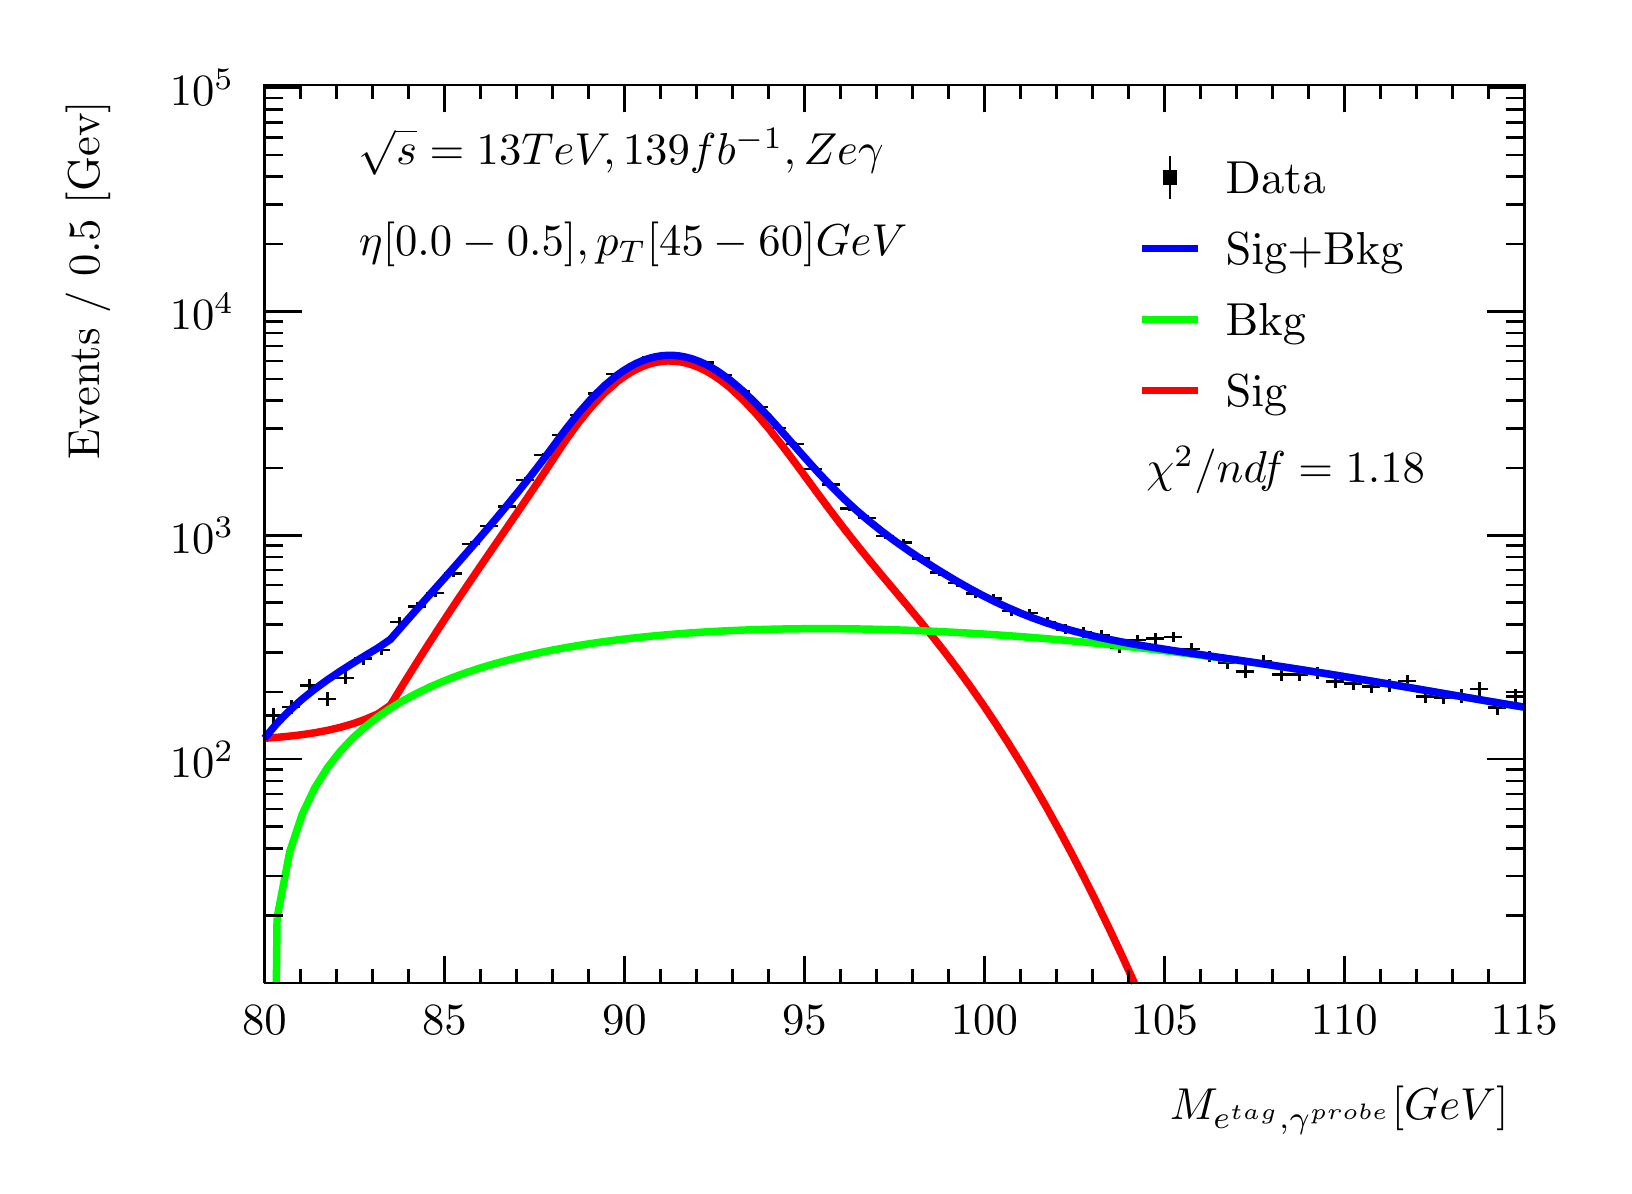
\begin{tikzpicture}
\pgfdeclareplotmark{cross} {
\pgfpathmoveto{\pgfpoint{-0.3\pgfplotmarksize}{\pgfplotmarksize}}
\pgfpathlineto{\pgfpoint{+0.3\pgfplotmarksize}{\pgfplotmarksize}}
\pgfpathlineto{\pgfpoint{+0.3\pgfplotmarksize}{0.3\pgfplotmarksize}}
\pgfpathlineto{\pgfpoint{+1\pgfplotmarksize}{0.3\pgfplotmarksize}}
\pgfpathlineto{\pgfpoint{+1\pgfplotmarksize}{-0.3\pgfplotmarksize}}
\pgfpathlineto{\pgfpoint{+0.3\pgfplotmarksize}{-0.3\pgfplotmarksize}}
\pgfpathlineto{\pgfpoint{+0.3\pgfplotmarksize}{-1.\pgfplotmarksize}}
\pgfpathlineto{\pgfpoint{-0.3\pgfplotmarksize}{-1.\pgfplotmarksize}}
\pgfpathlineto{\pgfpoint{-0.3\pgfplotmarksize}{-0.3\pgfplotmarksize}}
\pgfpathlineto{\pgfpoint{-1.\pgfplotmarksize}{-0.3\pgfplotmarksize}}
\pgfpathlineto{\pgfpoint{-1.\pgfplotmarksize}{0.3\pgfplotmarksize}}
\pgfpathlineto{\pgfpoint{-0.3\pgfplotmarksize}{0.3\pgfplotmarksize}}
\pgfpathclose
\pgfusepathqstroke
}
\pgfdeclareplotmark{cross*} {
\pgfpathmoveto{\pgfpoint{-0.3\pgfplotmarksize}{\pgfplotmarksize}}
\pgfpathlineto{\pgfpoint{+0.3\pgfplotmarksize}{\pgfplotmarksize}}
\pgfpathlineto{\pgfpoint{+0.3\pgfplotmarksize}{0.3\pgfplotmarksize}}
\pgfpathlineto{\pgfpoint{+1\pgfplotmarksize}{0.3\pgfplotmarksize}}
\pgfpathlineto{\pgfpoint{+1\pgfplotmarksize}{-0.3\pgfplotmarksize}}
\pgfpathlineto{\pgfpoint{+0.3\pgfplotmarksize}{-0.3\pgfplotmarksize}}
\pgfpathlineto{\pgfpoint{+0.3\pgfplotmarksize}{-1.\pgfplotmarksize}}
\pgfpathlineto{\pgfpoint{-0.3\pgfplotmarksize}{-1.\pgfplotmarksize}}
\pgfpathlineto{\pgfpoint{-0.3\pgfplotmarksize}{-0.3\pgfplotmarksize}}
\pgfpathlineto{\pgfpoint{-1.\pgfplotmarksize}{-0.3\pgfplotmarksize}}
\pgfpathlineto{\pgfpoint{-1.\pgfplotmarksize}{0.3\pgfplotmarksize}}
\pgfpathlineto{\pgfpoint{-0.3\pgfplotmarksize}{0.3\pgfplotmarksize}}
\pgfpathclose
\pgfusepathqfillstroke
}
\pgfdeclareplotmark{newstar} {
\pgfpathmoveto{\pgfqpoint{0pt}{\pgfplotmarksize}}
\pgfpathlineto{\pgfqpointpolar{44}{0.5\pgfplotmarksize}}
\pgfpathlineto{\pgfqpointpolar{18}{\pgfplotmarksize}}
\pgfpathlineto{\pgfqpointpolar{-20}{0.5\pgfplotmarksize}}
\pgfpathlineto{\pgfqpointpolar{-54}{\pgfplotmarksize}}
\pgfpathlineto{\pgfqpointpolar{-90}{0.5\pgfplotmarksize}}
\pgfpathlineto{\pgfqpointpolar{234}{\pgfplotmarksize}}
\pgfpathlineto{\pgfqpointpolar{198}{0.5\pgfplotmarksize}}
\pgfpathlineto{\pgfqpointpolar{162}{\pgfplotmarksize}}
\pgfpathlineto{\pgfqpointpolar{134}{0.5\pgfplotmarksize}}
\pgfpathclose
\pgfusepathqstroke
}
\pgfdeclareplotmark{newstar*} {
\pgfpathmoveto{\pgfqpoint{0pt}{\pgfplotmarksize}}
\pgfpathlineto{\pgfqpointpolar{44}{0.5\pgfplotmarksize}}
\pgfpathlineto{\pgfqpointpolar{18}{\pgfplotmarksize}}
\pgfpathlineto{\pgfqpointpolar{-20}{0.5\pgfplotmarksize}}
\pgfpathlineto{\pgfqpointpolar{-54}{\pgfplotmarksize}}
\pgfpathlineto{\pgfqpointpolar{-90}{0.5\pgfplotmarksize}}
\pgfpathlineto{\pgfqpointpolar{234}{\pgfplotmarksize}}
\pgfpathlineto{\pgfqpointpolar{198}{0.5\pgfplotmarksize}}
\pgfpathlineto{\pgfqpointpolar{162}{\pgfplotmarksize}}
\pgfpathlineto{\pgfqpointpolar{134}{0.5\pgfplotmarksize}}
\pgfpathclose
\pgfusepathqfillstroke
}
\definecolor{c}{rgb}{1,1,1};
\draw [color=c, fill=c] (0,0) rectangle (20,14.4361);
\draw [color=c, fill=c] (3,2.30977) rectangle (19,13.7143);
\definecolor{c}{rgb}{0,0,0};
\draw [c,line width=0.9] (3,2.30977) -- (3,13.7143) -- (19,13.7143) -- (19,2.30977) -- (3,2.30977);
\definecolor{c}{rgb}{1,1,1};
\draw [color=c, fill=c] (3,2.30977) rectangle (19,13.7143);
\definecolor{c}{rgb}{0,0,0};
\draw [c,line width=0.9] (3,2.30977) -- (3,13.7143) -- (19,13.7143) -- (19,2.30977) -- (3,2.30977);
\draw [c,line width=0.9] (3,2.30977) -- (19,2.30977);
\draw [c,line width=0.9] (3,2.65624) -- (3,2.30977);
\draw [c,line width=0.9] (3.45714,2.48301) -- (3.45714,2.30977);
\draw [c,line width=0.9] (3.91429,2.48301) -- (3.91429,2.30977);
\draw [c,line width=0.9] (4.37143,2.48301) -- (4.37143,2.30977);
\draw [c,line width=0.9] (4.82857,2.48301) -- (4.82857,2.30977);
\draw [c,line width=0.9] (5.28571,2.65624) -- (5.28571,2.30977);
\draw [c,line width=0.9] (5.74286,2.48301) -- (5.74286,2.30977);
\draw [c,line width=0.9] (6.2,2.48301) -- (6.2,2.30977);
\draw [c,line width=0.9] (6.65714,2.48301) -- (6.65714,2.30977);
\draw [c,line width=0.9] (7.11429,2.48301) -- (7.11429,2.30977);
\draw [c,line width=0.9] (7.57143,2.65624) -- (7.57143,2.30977);
\draw [c,line width=0.9] (8.02857,2.48301) -- (8.02857,2.30977);
\draw [c,line width=0.9] (8.48571,2.48301) -- (8.48571,2.30977);
\draw [c,line width=0.9] (8.94286,2.48301) -- (8.94286,2.30977);
\draw [c,line width=0.9] (9.4,2.48301) -- (9.4,2.30977);
\draw [c,line width=0.9] (9.85714,2.65624) -- (9.85714,2.30977);
\draw [c,line width=0.9] (10.3143,2.48301) -- (10.3143,2.30977);
\draw [c,line width=0.9] (10.7714,2.48301) -- (10.7714,2.30977);
\draw [c,line width=0.9] (11.2286,2.48301) -- (11.2286,2.30977);
\draw [c,line width=0.9] (11.6857,2.48301) -- (11.6857,2.30977);
\draw [c,line width=0.9] (12.1429,2.65624) -- (12.1429,2.30977);
\draw [c,line width=0.9] (12.6,2.48301) -- (12.6,2.30977);
\draw [c,line width=0.9] (13.0571,2.48301) -- (13.0571,2.30977);
\draw [c,line width=0.9] (13.5143,2.48301) -- (13.5143,2.30977);
\draw [c,line width=0.9] (13.9714,2.48301) -- (13.9714,2.30977);
\draw [c,line width=0.9] (14.4286,2.65624) -- (14.4286,2.30977);
\draw [c,line width=0.9] (14.8857,2.48301) -- (14.8857,2.30977);
\draw [c,line width=0.9] (15.3429,2.48301) -- (15.3429,2.30977);
\draw [c,line width=0.9] (15.8,2.48301) -- (15.8,2.30977);
\draw [c,line width=0.9] (16.2571,2.48301) -- (16.2571,2.30977);
\draw [c,line width=0.9] (16.7143,2.65624) -- (16.7143,2.30977);
\draw [c,line width=0.9] (17.1714,2.48301) -- (17.1714,2.30977);
\draw [c,line width=0.9] (17.6286,2.48301) -- (17.6286,2.30977);
\draw [c,line width=0.9] (18.0857,2.48301) -- (18.0857,2.30977);
\draw [c,line width=0.9] (18.5429,2.48301) -- (18.5429,2.30977);
\draw [c,line width=0.9] (19,2.65624) -- (19,2.30977);
\draw [anchor=base] (3,1.66015) node[scale=1.61424, color=c, rotate=0]{80};
\draw [anchor=base] (5.28571,1.66015) node[scale=1.61424, color=c, rotate=0]{85};
\draw [anchor=base] (7.57143,1.66015) node[scale=1.61424, color=c, rotate=0]{90};
\draw [anchor=base] (9.85714,1.66015) node[scale=1.61424, color=c, rotate=0]{95};
\draw [anchor=base] (12.1429,1.66015) node[scale=1.61424, color=c, rotate=0]{100};
\draw [anchor=base] (14.4286,1.66015) node[scale=1.61424, color=c, rotate=0]{105};
\draw [anchor=base] (16.7143,1.66015) node[scale=1.61424, color=c, rotate=0]{110};
\draw [anchor=base] (19,1.66015) node[scale=1.61424, color=c, rotate=0]{115};
\draw [anchor= east] (19,0.692932) node[scale=1.61424, color=c, rotate=0]{$M_{e^{tag}, \gamma^{probe}}  [GeV]$};
\draw [c,line width=0.9] (3,13.7143) -- (19,13.7143);
\draw [c,line width=0.9] (3,13.3678) -- (3,13.7143);
\draw [c,line width=0.9] (3.45714,13.5411) -- (3.45714,13.7143);
\draw [c,line width=0.9] (3.91429,13.5411) -- (3.91429,13.7143);
\draw [c,line width=0.9] (4.37143,13.5411) -- (4.37143,13.7143);
\draw [c,line width=0.9] (4.82857,13.5411) -- (4.82857,13.7143);
\draw [c,line width=0.9] (5.28571,13.3678) -- (5.28571,13.7143);
\draw [c,line width=0.9] (5.74286,13.5411) -- (5.74286,13.7143);
\draw [c,line width=0.9] (6.2,13.5411) -- (6.2,13.7143);
\draw [c,line width=0.9] (6.65714,13.5411) -- (6.65714,13.7143);
\draw [c,line width=0.9] (7.11429,13.5411) -- (7.11429,13.7143);
\draw [c,line width=0.9] (7.57143,13.3678) -- (7.57143,13.7143);
\draw [c,line width=0.9] (8.02857,13.5411) -- (8.02857,13.7143);
\draw [c,line width=0.9] (8.48571,13.5411) -- (8.48571,13.7143);
\draw [c,line width=0.9] (8.94286,13.5411) -- (8.94286,13.7143);
\draw [c,line width=0.9] (9.4,13.5411) -- (9.4,13.7143);
\draw [c,line width=0.9] (9.85714,13.3678) -- (9.85714,13.7143);
\draw [c,line width=0.9] (10.3143,13.5411) -- (10.3143,13.7143);
\draw [c,line width=0.9] (10.7714,13.5411) -- (10.7714,13.7143);
\draw [c,line width=0.9] (11.2286,13.5411) -- (11.2286,13.7143);
\draw [c,line width=0.9] (11.6857,13.5411) -- (11.6857,13.7143);
\draw [c,line width=0.9] (12.1429,13.3678) -- (12.1429,13.7143);
\draw [c,line width=0.9] (12.6,13.5411) -- (12.6,13.7143);
\draw [c,line width=0.9] (13.0571,13.5411) -- (13.0571,13.7143);
\draw [c,line width=0.9] (13.5143,13.5411) -- (13.5143,13.7143);
\draw [c,line width=0.9] (13.9714,13.5411) -- (13.9714,13.7143);
\draw [c,line width=0.9] (14.4286,13.3678) -- (14.4286,13.7143);
\draw [c,line width=0.9] (14.8857,13.5411) -- (14.8857,13.7143);
\draw [c,line width=0.9] (15.3429,13.5411) -- (15.3429,13.7143);
\draw [c,line width=0.9] (15.8,13.5411) -- (15.8,13.7143);
\draw [c,line width=0.9] (16.2571,13.5411) -- (16.2571,13.7143);
\draw [c,line width=0.9] (16.7143,13.3678) -- (16.7143,13.7143);
\draw [c,line width=0.9] (17.1714,13.5411) -- (17.1714,13.7143);
\draw [c,line width=0.9] (17.6286,13.5411) -- (17.6286,13.7143);
\draw [c,line width=0.9] (18.0857,13.5411) -- (18.0857,13.7143);
\draw [c,line width=0.9] (18.5429,13.5411) -- (18.5429,13.7143);
\draw [c,line width=0.9] (19,13.3678) -- (19,13.7143);
\draw [c,line width=0.9] (3,2.30977) -- (3,13.7143);
\draw [c,line width=0.9] (3.237,3.16561) -- (3,3.16561);
\draw [c,line width=0.9] (3.237,3.66625) -- (3,3.66625);
\draw [c,line width=0.9] (3.237,4.02146) -- (3,4.02146);
\draw [c,line width=0.9] (3.237,4.29698) -- (3,4.29698);
\draw [c,line width=0.9] (3.237,4.52209) -- (3,4.52209);
\draw [c,line width=0.9] (3.237,4.71242) -- (3,4.71242);
\draw [c,line width=0.9] (3.237,4.8773) -- (3,4.8773);
\draw [c,line width=0.9] (3.237,5.02273) -- (3,5.02273);
\draw [c,line width=0.9] (3.474,5.15282) -- (3,5.15282);
\draw [anchor= east] (2.82,5.15282) node[scale=1.61424, color=c, rotate=0]{$10^{2}$};
\draw [c,line width=0.9] (3.237,6.00866) -- (3,6.00866);
\draw [c,line width=0.9] (3.237,6.5093) -- (3,6.5093);
\draw [c,line width=0.9] (3.237,6.8645) -- (3,6.8645);
\draw [c,line width=0.9] (3.237,7.14002) -- (3,7.14002);
\draw [c,line width=0.9] (3.237,7.36514) -- (3,7.36514);
\draw [c,line width=0.9] (3.237,7.55547) -- (3,7.55547);
\draw [c,line width=0.9] (3.237,7.72034) -- (3,7.72034);
\draw [c,line width=0.9] (3.237,7.86577) -- (3,7.86577);
\draw [c,line width=0.9] (3.474,7.99586) -- (3,7.99586);
\draw [anchor= east] (2.82,7.99586) node[scale=1.61424, color=c, rotate=0]{$10^{3}$};
\draw [c,line width=0.9] (3.237,8.85171) -- (3,8.85171);
\draw [c,line width=0.9] (3.237,9.35234) -- (3,9.35234);
\draw [c,line width=0.9] (3.237,9.70755) -- (3,9.70755);
\draw [c,line width=0.9] (3.237,9.98307) -- (3,9.98307);
\draw [c,line width=0.9] (3.237,10.2082) -- (3,10.2082);
\draw [c,line width=0.9] (3.237,10.3985) -- (3,10.3985);
\draw [c,line width=0.9] (3.237,10.5634) -- (3,10.5634);
\draw [c,line width=0.9] (3.237,10.7088) -- (3,10.7088);
\draw [c,line width=0.9] (3.474,10.8389) -- (3,10.8389);
\draw [anchor= east] (2.82,10.8389) node[scale=1.61424, color=c, rotate=0]{$10^{4}$};
\draw [c,line width=0.9] (3.237,11.6948) -- (3,11.6948);
\draw [c,line width=0.9] (3.237,12.1954) -- (3,12.1954);
\draw [c,line width=0.9] (3.237,12.5506) -- (3,12.5506);
\draw [c,line width=0.9] (3.237,12.8261) -- (3,12.8261);
\draw [c,line width=0.9] (3.237,13.0512) -- (3,13.0512);
\draw [c,line width=0.9] (3.237,13.2416) -- (3,13.2416);
\draw [c,line width=0.9] (3.237,13.4064) -- (3,13.4064);
\draw [c,line width=0.9] (3.237,13.5519) -- (3,13.5519);
\draw [c,line width=0.9] (3.474,13.682) -- (3,13.682);
\draw [anchor= east] (2.82,13.682) node[scale=1.61424, color=c, rotate=0]{$10^{5}$};
\draw [anchor= east] (0.76,13.7143) node[scale=1.61424, color=c, rotate=90]{Events / 0.5 [Gev]};
\draw [c,line width=0.9] (19,2.30977) -- (19,13.7143);
\draw [c,line width=0.9] (18.763,3.16561) -- (19,3.16561);
\draw [c,line width=0.9] (18.763,3.66625) -- (19,3.66625);
\draw [c,line width=0.9] (18.763,4.02146) -- (19,4.02146);
\draw [c,line width=0.9] (18.763,4.29698) -- (19,4.29698);
\draw [c,line width=0.9] (18.763,4.52209) -- (19,4.52209);
\draw [c,line width=0.9] (18.763,4.71242) -- (19,4.71242);
\draw [c,line width=0.9] (18.763,4.8773) -- (19,4.8773);
\draw [c,line width=0.9] (18.763,5.02273) -- (19,5.02273);
\draw [c,line width=0.9] (18.526,5.15282) -- (19,5.15282);
\draw [c,line width=0.9] (18.763,6.00866) -- (19,6.00866);
\draw [c,line width=0.9] (18.763,6.5093) -- (19,6.5093);
\draw [c,line width=0.9] (18.763,6.8645) -- (19,6.8645);
\draw [c,line width=0.9] (18.763,7.14002) -- (19,7.14002);
\draw [c,line width=0.9] (18.763,7.36514) -- (19,7.36514);
\draw [c,line width=0.9] (18.763,7.55547) -- (19,7.55547);
\draw [c,line width=0.9] (18.763,7.72034) -- (19,7.72034);
\draw [c,line width=0.9] (18.763,7.86577) -- (19,7.86577);
\draw [c,line width=0.9] (18.526,7.99586) -- (19,7.99586);
\draw [c,line width=0.9] (18.763,8.85171) -- (19,8.85171);
\draw [c,line width=0.9] (18.763,9.35234) -- (19,9.35234);
\draw [c,line width=0.9] (18.763,9.70755) -- (19,9.70755);
\draw [c,line width=0.9] (18.763,9.98307) -- (19,9.98307);
\draw [c,line width=0.9] (18.763,10.2082) -- (19,10.2082);
\draw [c,line width=0.9] (18.763,10.3985) -- (19,10.3985);
\draw [c,line width=0.9] (18.763,10.5634) -- (19,10.5634);
\draw [c,line width=0.9] (18.763,10.7088) -- (19,10.7088);
\draw [c,line width=0.9] (18.526,10.8389) -- (19,10.8389);
\draw [c,line width=0.9] (18.763,11.6948) -- (19,11.6948);
\draw [c,line width=0.9] (18.763,12.1954) -- (19,12.1954);
\draw [c,line width=0.9] (18.763,12.5506) -- (19,12.5506);
\draw [c,line width=0.9] (18.763,12.8261) -- (19,12.8261);
\draw [c,line width=0.9] (18.763,13.0512) -- (19,13.0512);
\draw [c,line width=0.9] (18.763,13.2416) -- (19,13.2416);
\draw [c,line width=0.9] (18.763,13.4064) -- (19,13.4064);
\draw [c,line width=0.9] (18.763,13.5519) -- (19,13.5519);
\draw [c,line width=0.9] (18.526,13.682) -- (19,13.682);
\draw [c,line width=0.9] (3.11429,5.70977) -- (3,5.70977);
\draw [c,line width=0.9] (3,5.70977) -- (3,5.70977);
\draw [c,line width=0.9] (3.11429,5.70977) -- (3.22857,5.70977);
\draw [c,line width=0.9] (3.22857,5.70977) -- (3.22857,5.70977);
\draw [c,line width=0.9] (3.11429,5.70977) -- (3.11429,5.80829);
\draw [c,line width=0.9] (3.11429,5.80829) -- (3.11429,5.80829);
\draw [c,line width=0.9] (3.11429,5.70977) -- (3.11429,5.61126);
\draw [c,line width=0.9] (3.11429,5.61126) -- (3.11429,5.61126);
\draw [c,line width=0.9] (3.34286,5.81524) -- (3.22857,5.81524);
\draw [c,line width=0.9] (3.22857,5.81524) -- (3.22857,5.81524);
\draw [c,line width=0.9] (3.34286,5.81524) -- (3.45714,5.81524);
\draw [c,line width=0.9] (3.45714,5.81524) -- (3.45714,5.81524);
\draw [c,line width=0.9] (3.34286,5.81524) -- (3.34286,5.90964);
\draw [c,line width=0.9] (3.34286,5.90964) -- (3.34286,5.90964);
\draw [c,line width=0.9] (3.34286,5.81524) -- (3.34286,5.72084);
\draw [c,line width=0.9] (3.34286,5.72084) -- (3.34286,5.72084);
\draw [c,line width=0.9] (3.57143,6.08642) -- (3.45714,6.08642);
\draw [c,line width=0.9] (3.45714,6.08642) -- (3.45714,6.08642);
\draw [c,line width=0.9] (3.57143,6.08642) -- (3.68571,6.08642);
\draw [c,line width=0.9] (3.68571,6.08642) -- (3.68571,6.08642);
\draw [c,line width=0.9] (3.57143,6.08642) -- (3.57143,6.171);
\draw [c,line width=0.9] (3.57143,6.171) -- (3.57143,6.171);
\draw [c,line width=0.9] (3.57143,6.08642) -- (3.57143,6.00183);
\draw [c,line width=0.9] (3.57143,6.00183) -- (3.57143,6.00183);
\draw [c,line width=0.9] (3.8,5.91906) -- (3.68571,5.91906);
\draw [c,line width=0.9] (3.68571,5.91906) -- (3.68571,5.91906);
\draw [c,line width=0.9] (3.8,5.91906) -- (3.91429,5.91906);
\draw [c,line width=0.9] (3.91429,5.91906) -- (3.91429,5.91906);
\draw [c,line width=0.9] (3.8,5.91906) -- (3.8,6.00957);
\draw [c,line width=0.9] (3.8,6.00957) -- (3.8,6.00957);
\draw [c,line width=0.9] (3.8,5.91906) -- (3.8,5.82854);
\draw [c,line width=0.9] (3.8,5.82854) -- (3.8,5.82854);
\draw [c,line width=0.9] (4.02857,6.18658) -- (3.91429,6.18658);
\draw [c,line width=0.9] (3.91429,6.18658) -- (3.91429,6.18658);
\draw [c,line width=0.9] (4.02857,6.18658) -- (4.14286,6.18658);
\draw [c,line width=0.9] (4.14286,6.18658) -- (4.14286,6.18658);
\draw [c,line width=0.9] (4.02857,6.18658) -- (4.02857,6.26781);
\draw [c,line width=0.9] (4.02857,6.26781) -- (4.02857,6.26781);
\draw [c,line width=0.9] (4.02857,6.18658) -- (4.02857,6.10536);
\draw [c,line width=0.9] (4.02857,6.10536) -- (4.02857,6.10536);
\draw [c,line width=0.9] (4.25714,6.42851) -- (4.14286,6.42851);
\draw [c,line width=0.9] (4.14286,6.42851) -- (4.14286,6.42851);
\draw [c,line width=0.9] (4.25714,6.42851) -- (4.37143,6.42851);
\draw [c,line width=0.9] (4.37143,6.42851) -- (4.37143,6.42851);
\draw [c,line width=0.9] (4.25714,6.42851) -- (4.25714,6.50216);
\draw [c,line width=0.9] (4.25714,6.50216) -- (4.25714,6.50216);
\draw [c,line width=0.9] (4.25714,6.42851) -- (4.25714,6.35487);
\draw [c,line width=0.9] (4.25714,6.35487) -- (4.25714,6.35487);
\draw [c,line width=0.9] (4.48571,6.54179) -- (4.37143,6.54179);
\draw [c,line width=0.9] (4.37143,6.54179) -- (4.37143,6.54179);
\draw [c,line width=0.9] (4.48571,6.54179) -- (4.6,6.54179);
\draw [c,line width=0.9] (4.6,6.54179) -- (4.6,6.54179);
\draw [c,line width=0.9] (4.48571,6.54179) -- (4.48571,6.61214);
\draw [c,line width=0.9] (4.48571,6.61214) -- (4.48571,6.61214);
\draw [c,line width=0.9] (4.48571,6.54179) -- (4.48571,6.47145);
\draw [c,line width=0.9] (4.48571,6.47145) -- (4.48571,6.47145);
\draw [c,line width=0.9] (4.71429,6.89198) -- (4.6,6.89198);
\draw [c,line width=0.9] (4.6,6.89198) -- (4.6,6.89198);
\draw [c,line width=0.9] (4.71429,6.89198) -- (4.82857,6.89198);
\draw [c,line width=0.9] (4.82857,6.89198) -- (4.82857,6.89198);
\draw [c,line width=0.9] (4.71429,6.89198) -- (4.71429,6.95302);
\draw [c,line width=0.9] (4.71429,6.95302) -- (4.71429,6.95302);
\draw [c,line width=0.9] (4.71429,6.89198) -- (4.71429,6.83093);
\draw [c,line width=0.9] (4.71429,6.83093) -- (4.71429,6.83093);
\draw [c,line width=0.9] (4.94286,7.09475) -- (4.82857,7.09475);
\draw [c,line width=0.9] (4.82857,7.09475) -- (4.82857,7.09475);
\draw [c,line width=0.9] (4.94286,7.09475) -- (5.05714,7.09475);
\draw [c,line width=0.9] (5.05714,7.09475) -- (5.05714,7.09475);
\draw [c,line width=0.9] (4.94286,7.09475) -- (4.94286,7.15099);
\draw [c,line width=0.9] (4.94286,7.15099) -- (4.94286,7.15099);
\draw [c,line width=0.9] (4.94286,7.09475) -- (4.94286,7.03852);
\draw [c,line width=0.9] (4.94286,7.03852) -- (4.94286,7.03852);
\draw [c,line width=0.9] (5.17143,7.26442) -- (5.05714,7.26442);
\draw [c,line width=0.9] (5.05714,7.26442) -- (5.05714,7.26442);
\draw [c,line width=0.9] (5.17143,7.26442) -- (5.28571,7.26442);
\draw [c,line width=0.9] (5.28571,7.26442) -- (5.28571,7.26442);
\draw [c,line width=0.9] (5.17143,7.26442) -- (5.17143,7.31692);
\draw [c,line width=0.9] (5.17143,7.31692) -- (5.17143,7.31692);
\draw [c,line width=0.9] (5.17143,7.26442) -- (5.17143,7.21192);
\draw [c,line width=0.9] (5.17143,7.21192) -- (5.17143,7.21192);
\draw [c,line width=0.9] (5.4,7.50874) -- (5.28571,7.50874);
\draw [c,line width=0.9] (5.28571,7.50874) -- (5.28571,7.50874);
\draw [c,line width=0.9] (5.4,7.50874) -- (5.51429,7.50874);
\draw [c,line width=0.9] (5.51429,7.50874) -- (5.51429,7.50874);
\draw [c,line width=0.9] (5.4,7.50874) -- (5.4,7.55629);
\draw [c,line width=0.9] (5.4,7.55629) -- (5.4,7.55629);
\draw [c,line width=0.9] (5.4,7.50874) -- (5.4,7.46118);
\draw [c,line width=0.9] (5.4,7.46118) -- (5.4,7.46118);
\draw [c,line width=0.9] (5.62857,7.88618) -- (5.51429,7.88618);
\draw [c,line width=0.9] (5.51429,7.88618) -- (5.51429,7.88618);
\draw [c,line width=0.9] (5.62857,7.88618) -- (5.74286,7.88618);
\draw [c,line width=0.9] (5.74286,7.88618) -- (5.74286,7.88618);
\draw [c,line width=0.9] (5.62857,7.88618) -- (5.62857,7.927);
\draw [c,line width=0.9] (5.62857,7.927) -- (5.62857,7.927);
\draw [c,line width=0.9] (5.62857,7.88618) -- (5.62857,7.84537);
\draw [c,line width=0.9] (5.62857,7.84537) -- (5.62857,7.84537);
\draw [c,line width=0.9] (5.85714,8.11242) -- (5.74286,8.11242);
\draw [c,line width=0.9] (5.74286,8.11242) -- (5.74286,8.11242);
\draw [c,line width=0.9] (5.85714,8.11242) -- (5.97143,8.11242);
\draw [c,line width=0.9] (5.97143,8.11242) -- (5.97143,8.11242);
\draw [c,line width=0.9] (5.85714,8.11242) -- (5.85714,8.14967);
\draw [c,line width=0.9] (5.85714,8.14967) -- (5.85714,8.14967);
\draw [c,line width=0.9] (5.85714,8.11242) -- (5.85714,8.07518);
\draw [c,line width=0.9] (5.85714,8.07518) -- (5.85714,8.07518);
\draw [c,line width=0.9] (6.08571,8.36183) -- (5.97143,8.36183);
\draw [c,line width=0.9] (5.97143,8.36183) -- (5.97143,8.36183);
\draw [c,line width=0.9] (6.08571,8.36183) -- (6.2,8.36183);
\draw [c,line width=0.9] (6.2,8.36183) -- (6.2,8.36183);
\draw [c,line width=0.9] (6.08571,8.36183) -- (6.08571,8.39549);
\draw [c,line width=0.9] (6.08571,8.39549) -- (6.08571,8.39549);
\draw [c,line width=0.9] (6.08571,8.36183) -- (6.08571,8.32816);
\draw [c,line width=0.9] (6.08571,8.32816) -- (6.08571,8.32816);
\draw [c,line width=0.9] (6.31429,8.70156) -- (6.2,8.70156);
\draw [c,line width=0.9] (6.2,8.70156) -- (6.2,8.70156);
\draw [c,line width=0.9] (6.31429,8.70156) -- (6.42857,8.70156);
\draw [c,line width=0.9] (6.42857,8.70156) -- (6.42857,8.70156);
\draw [c,line width=0.9] (6.31429,8.70156) -- (6.31429,8.7309);
\draw [c,line width=0.9] (6.31429,8.7309) -- (6.31429,8.7309);
\draw [c,line width=0.9] (6.31429,8.70156) -- (6.31429,8.67222);
\draw [c,line width=0.9] (6.31429,8.67222) -- (6.31429,8.67222);
\draw [c,line width=0.9] (6.54286,9.01511) -- (6.42857,9.01511);
\draw [c,line width=0.9] (6.42857,9.01511) -- (6.42857,9.01511);
\draw [c,line width=0.9] (6.54286,9.01511) -- (6.65714,9.01511);
\draw [c,line width=0.9] (6.65714,9.01511) -- (6.65714,9.01511);
\draw [c,line width=0.9] (6.54286,9.01511) -- (6.54286,9.04095);
\draw [c,line width=0.9] (6.54286,9.04095) -- (6.54286,9.04095);
\draw [c,line width=0.9] (6.54286,9.01511) -- (6.54286,8.98927);
\draw [c,line width=0.9] (6.54286,8.98927) -- (6.54286,8.98927);
\draw [c,line width=0.9] (6.77143,9.26848) -- (6.65714,9.26848);
\draw [c,line width=0.9] (6.65714,9.26848) -- (6.65714,9.26848);
\draw [c,line width=0.9] (6.77143,9.26848) -- (6.88571,9.26848);
\draw [c,line width=0.9] (6.88571,9.26848) -- (6.88571,9.26848);
\draw [c,line width=0.9] (6.77143,9.26848) -- (6.77143,9.2918);
\draw [c,line width=0.9] (6.77143,9.2918) -- (6.77143,9.2918);
\draw [c,line width=0.9] (6.77143,9.26848) -- (6.77143,9.24516);
\draw [c,line width=0.9] (6.77143,9.24516) -- (6.77143,9.24516);
\draw [c,line width=0.9] (7,9.52312) -- (6.88571,9.52312);
\draw [c,line width=0.9] (6.88571,9.52312) -- (6.88571,9.52312);
\draw [c,line width=0.9] (7,9.52312) -- (7.11429,9.52312);
\draw [c,line width=0.9] (7.11429,9.52312) -- (7.11429,9.52312);
\draw [c,line width=0.9] (7,9.52312) -- (7,9.54416);
\draw [c,line width=0.9] (7,9.54416) -- (7,9.54416);
\draw [c,line width=0.9] (7,9.52312) -- (7,9.50208);
\draw [c,line width=0.9] (7,9.50208) -- (7,9.50208);
\draw [c,line width=0.9] (7.22857,9.79426) -- (7.11429,9.79426);
\draw [c,line width=0.9] (7.11429,9.79426) -- (7.11429,9.79426);
\draw [c,line width=0.9] (7.22857,9.79426) -- (7.34286,9.79426);
\draw [c,line width=0.9] (7.34286,9.79426) -- (7.34286,9.79426);
\draw [c,line width=0.9] (7.22857,9.79426) -- (7.22857,9.81311);
\draw [c,line width=0.9] (7.22857,9.81311) -- (7.22857,9.81311);
\draw [c,line width=0.9] (7.22857,9.79426) -- (7.22857,9.77541);
\draw [c,line width=0.9] (7.22857,9.77541) -- (7.22857,9.77541);
\draw [c,line width=0.9] (7.45714,10.0452) -- (7.34286,10.0452);
\draw [c,line width=0.9] (7.34286,10.0452) -- (7.34286,10.0452);
\draw [c,line width=0.9] (7.45714,10.0452) -- (7.57143,10.0452);
\draw [c,line width=0.9] (7.57143,10.0452) -- (7.57143,10.0452);
\draw [c,line width=0.9] (7.45714,10.0452) -- (7.45714,10.0622);
\draw [c,line width=0.9] (7.45714,10.0622) -- (7.45714,10.0622);
\draw [c,line width=0.9] (7.45714,10.0452) -- (7.45714,10.0282);
\draw [c,line width=0.9] (7.45714,10.0282) -- (7.45714,10.0282);
\draw [c,line width=0.9] (7.68571,10.1292) -- (7.57143,10.1292);
\draw [c,line width=0.9] (7.57143,10.1292) -- (7.57143,10.1292);
\draw [c,line width=0.9] (7.68571,10.1292) -- (7.8,10.1292);
\draw [c,line width=0.9] (7.8,10.1292) -- (7.8,10.1292);
\draw [c,line width=0.9] (7.68571,10.1292) -- (7.68571,10.1456);
\draw [c,line width=0.9] (7.68571,10.1456) -- (7.68571,10.1456);
\draw [c,line width=0.9] (7.68571,10.1292) -- (7.68571,10.1127);
\draw [c,line width=0.9] (7.68571,10.1127) -- (7.68571,10.1127);
\draw [c,line width=0.9] (7.91429,10.256) -- (7.8,10.256);
\draw [c,line width=0.9] (7.8,10.256) -- (7.8,10.256);
\draw [c,line width=0.9] (7.91429,10.256) -- (8.02857,10.256);
\draw [c,line width=0.9] (8.02857,10.256) -- (8.02857,10.256);
\draw [c,line width=0.9] (7.91429,10.256) -- (7.91429,10.2717);
\draw [c,line width=0.9] (7.91429,10.2717) -- (7.91429,10.2717);
\draw [c,line width=0.9] (7.91429,10.256) -- (7.91429,10.2404);
\draw [c,line width=0.9] (7.91429,10.2404) -- (7.91429,10.2404);
\draw [c,line width=0.9] (8.14286,10.2819) -- (8.02857,10.2819);
\draw [c,line width=0.9] (8.02857,10.2819) -- (8.02857,10.2819);
\draw [c,line width=0.9] (8.14286,10.2819) -- (8.25714,10.2819);
\draw [c,line width=0.9] (8.25714,10.2819) -- (8.25714,10.2819);
\draw [c,line width=0.9] (8.14286,10.2819) -- (8.14286,10.2973);
\draw [c,line width=0.9] (8.14286,10.2973) -- (8.14286,10.2973);
\draw [c,line width=0.9] (8.14286,10.2819) -- (8.14286,10.2664);
\draw [c,line width=0.9] (8.14286,10.2664) -- (8.14286,10.2664);
\draw [c,line width=0.9] (8.37143,10.258) -- (8.25714,10.258);
\draw [c,line width=0.9] (8.25714,10.258) -- (8.25714,10.258);
\draw [c,line width=0.9] (8.37143,10.258) -- (8.48571,10.258);
\draw [c,line width=0.9] (8.48571,10.258) -- (8.48571,10.258);
\draw [c,line width=0.9] (8.37143,10.258) -- (8.37143,10.2736);
\draw [c,line width=0.9] (8.37143,10.2736) -- (8.37143,10.2736);
\draw [c,line width=0.9] (8.37143,10.258) -- (8.37143,10.2424);
\draw [c,line width=0.9] (8.37143,10.2424) -- (8.37143,10.2424);
\draw [c,line width=0.9] (8.6,10.1906) -- (8.48571,10.1906);
\draw [c,line width=0.9] (8.48571,10.1906) -- (8.48571,10.1906);
\draw [c,line width=0.9] (8.6,10.1906) -- (8.71429,10.1906);
\draw [c,line width=0.9] (8.71429,10.1906) -- (8.71429,10.1906);
\draw [c,line width=0.9] (8.6,10.1906) -- (8.6,10.2066);
\draw [c,line width=0.9] (8.6,10.2066) -- (8.6,10.2066);
\draw [c,line width=0.9] (8.6,10.1906) -- (8.6,10.1745);
\draw [c,line width=0.9] (8.6,10.1745) -- (8.6,10.1745);
\draw [c,line width=0.9] (8.82857,10.0346) -- (8.71429,10.0346);
\draw [c,line width=0.9] (8.71429,10.0346) -- (8.71429,10.0346);
\draw [c,line width=0.9] (8.82857,10.0346) -- (8.94286,10.0346);
\draw [c,line width=0.9] (8.94286,10.0346) -- (8.94286,10.0346);
\draw [c,line width=0.9] (8.82857,10.0346) -- (8.82857,10.0517);
\draw [c,line width=0.9] (8.82857,10.0517) -- (8.82857,10.0517);
\draw [c,line width=0.9] (8.82857,10.0346) -- (8.82857,10.0175);
\draw [c,line width=0.9] (8.82857,10.0175) -- (8.82857,10.0175);
\draw [c,line width=0.9] (9.05714,9.82551) -- (8.94286,9.82551);
\draw [c,line width=0.9] (8.94286,9.82551) -- (8.94286,9.82551);
\draw [c,line width=0.9] (9.05714,9.82551) -- (9.17143,9.82551);
\draw [c,line width=0.9] (9.17143,9.82551) -- (9.17143,9.82551);
\draw [c,line width=0.9] (9.05714,9.82551) -- (9.05714,9.84412);
\draw [c,line width=0.9] (9.05714,9.84412) -- (9.05714,9.84412);
\draw [c,line width=0.9] (9.05714,9.82551) -- (9.05714,9.8069);
\draw [c,line width=0.9] (9.05714,9.8069) -- (9.05714,9.8069);
\draw [c,line width=0.9] (9.28571,9.62523) -- (9.17143,9.62523);
\draw [c,line width=0.9] (9.17143,9.62523) -- (9.17143,9.62523);
\draw [c,line width=0.9] (9.28571,9.62523) -- (9.4,9.62523);
\draw [c,line width=0.9] (9.4,9.62523) -- (9.4,9.62523);
\draw [c,line width=0.9] (9.28571,9.62523) -- (9.28571,9.64541);
\draw [c,line width=0.9] (9.28571,9.64541) -- (9.28571,9.64541);
\draw [c,line width=0.9] (9.28571,9.62523) -- (9.28571,9.60504);
\draw [c,line width=0.9] (9.28571,9.60504) -- (9.28571,9.60504);
\draw [c,line width=0.9] (9.51429,9.35645) -- (9.4,9.35645);
\draw [c,line width=0.9] (9.4,9.35645) -- (9.4,9.35645);
\draw [c,line width=0.9] (9.51429,9.35645) -- (9.62857,9.35645);
\draw [c,line width=0.9] (9.62857,9.35645) -- (9.62857,9.35645);
\draw [c,line width=0.9] (9.51429,9.35645) -- (9.51429,9.37896);
\draw [c,line width=0.9] (9.51429,9.37896) -- (9.51429,9.37896);
\draw [c,line width=0.9] (9.51429,9.35645) -- (9.51429,9.33395);
\draw [c,line width=0.9] (9.51429,9.33395) -- (9.51429,9.33395);
\draw [c,line width=0.9] (9.74286,9.15796) -- (9.62857,9.15796);
\draw [c,line width=0.9] (9.62857,9.15796) -- (9.62857,9.15796);
\draw [c,line width=0.9] (9.74286,9.15796) -- (9.85714,9.15796);
\draw [c,line width=0.9] (9.85714,9.15796) -- (9.85714,9.15796);
\draw [c,line width=0.9] (9.74286,9.15796) -- (9.74286,9.18234);
\draw [c,line width=0.9] (9.74286,9.18234) -- (9.74286,9.18234);
\draw [c,line width=0.9] (9.74286,9.15796) -- (9.74286,9.13357);
\draw [c,line width=0.9] (9.74286,9.13357) -- (9.74286,9.13357);
\draw [c,line width=0.9] (9.97143,8.8368) -- (9.85714,8.8368);
\draw [c,line width=0.9] (9.85714,8.8368) -- (9.85714,8.8368);
\draw [c,line width=0.9] (9.97143,8.8368) -- (10.0857,8.8368);
\draw [c,line width=0.9] (10.0857,8.8368) -- (10.0857,8.8368);
\draw [c,line width=0.9] (9.97143,8.8368) -- (9.97143,8.86458);
\draw [c,line width=0.9] (9.97143,8.86458) -- (9.97143,8.86458);
\draw [c,line width=0.9] (9.97143,8.8368) -- (9.97143,8.80902);
\draw [c,line width=0.9] (9.97143,8.80902) -- (9.97143,8.80902);
\draw [c,line width=0.9] (10.2,8.64229) -- (10.0857,8.64229);
\draw [c,line width=0.9] (10.0857,8.64229) -- (10.0857,8.64229);
\draw [c,line width=0.9] (10.2,8.64229) -- (10.3143,8.64229);
\draw [c,line width=0.9] (10.3143,8.64229) -- (10.3143,8.64229);
\draw [c,line width=0.9] (10.2,8.64229) -- (10.2,8.67235);
\draw [c,line width=0.9] (10.2,8.67235) -- (10.2,8.67235);
\draw [c,line width=0.9] (10.2,8.64229) -- (10.2,8.61224);
\draw [c,line width=0.9] (10.2,8.61224) -- (10.2,8.61224);
\draw [c,line width=0.9] (10.4286,8.33679) -- (10.3143,8.33679);
\draw [c,line width=0.9] (10.3143,8.33679) -- (10.3143,8.33679);
\draw [c,line width=0.9] (10.4286,8.33679) -- (10.5429,8.33679);
\draw [c,line width=0.9] (10.5429,8.33679) -- (10.5429,8.33679);
\draw [c,line width=0.9] (10.4286,8.33679) -- (10.4286,8.3708);
\draw [c,line width=0.9] (10.4286,8.3708) -- (10.4286,8.3708);
\draw [c,line width=0.9] (10.4286,8.33679) -- (10.4286,8.30278);
\draw [c,line width=0.9] (10.4286,8.30278) -- (10.4286,8.30278);
\draw [c,line width=0.9] (10.6571,8.21272) -- (10.5429,8.21272);
\draw [c,line width=0.9] (10.5429,8.21272) -- (10.5429,8.21272);
\draw [c,line width=0.9] (10.6571,8.21272) -- (10.7714,8.21272);
\draw [c,line width=0.9] (10.7714,8.21272) -- (10.7714,8.21272);
\draw [c,line width=0.9] (10.6571,8.21272) -- (10.6571,8.24848);
\draw [c,line width=0.9] (10.6571,8.24848) -- (10.6571,8.24848);
\draw [c,line width=0.9] (10.6571,8.21272) -- (10.6571,8.17696);
\draw [c,line width=0.9] (10.6571,8.17696) -- (10.6571,8.17696);
\draw [c,line width=0.9] (10.8857,7.98595) -- (10.7714,7.98595);
\draw [c,line width=0.9] (10.7714,7.98595) -- (10.7714,7.98595);
\draw [c,line width=0.9] (10.8857,7.98595) -- (11,7.98595);
\draw [c,line width=0.9] (11,7.98595) -- (11,7.98595);
\draw [c,line width=0.9] (10.8857,7.98595) -- (10.8857,8.02515);
\draw [c,line width=0.9] (10.8857,8.02515) -- (10.8857,8.02515);
\draw [c,line width=0.9] (10.8857,7.98595) -- (10.8857,7.94675);
\draw [c,line width=0.9] (10.8857,7.94675) -- (10.8857,7.94675);
\draw [c,line width=0.9] (11.1143,7.90759) -- (11,7.90759);
\draw [c,line width=0.9] (11,7.90759) -- (11,7.90759);
\draw [c,line width=0.9] (11.1143,7.90759) -- (11.2286,7.90759);
\draw [c,line width=0.9] (11.2286,7.90759) -- (11.2286,7.90759);
\draw [c,line width=0.9] (11.1143,7.90759) -- (11.1143,7.94805);
\draw [c,line width=0.9] (11.1143,7.94805) -- (11.1143,7.94805);
\draw [c,line width=0.9] (11.1143,7.90759) -- (11.1143,7.86712);
\draw [c,line width=0.9] (11.1143,7.86712) -- (11.1143,7.86712);
\draw [c,line width=0.9] (11.3429,7.70168) -- (11.2286,7.70168);
\draw [c,line width=0.9] (11.2286,7.70168) -- (11.2286,7.70168);
\draw [c,line width=0.9] (11.3429,7.70168) -- (11.4571,7.70168);
\draw [c,line width=0.9] (11.4571,7.70168) -- (11.4571,7.70168);
\draw [c,line width=0.9] (11.3429,7.70168) -- (11.3429,7.74567);
\draw [c,line width=0.9] (11.3429,7.74567) -- (11.3429,7.74567);
\draw [c,line width=0.9] (11.3429,7.70168) -- (11.3429,7.6577);
\draw [c,line width=0.9] (11.3429,7.6577) -- (11.3429,7.6577);
\draw [c,line width=0.9] (11.5714,7.52149) -- (11.4571,7.52149);
\draw [c,line width=0.9] (11.4571,7.52149) -- (11.4571,7.52149);
\draw [c,line width=0.9] (11.5714,7.52149) -- (11.6857,7.52149);
\draw [c,line width=0.9] (11.6857,7.52149) -- (11.6857,7.52149);
\draw [c,line width=0.9] (11.5714,7.52149) -- (11.5714,7.56881);
\draw [c,line width=0.9] (11.5714,7.56881) -- (11.5714,7.56881);
\draw [c,line width=0.9] (11.5714,7.52149) -- (11.5714,7.47418);
\draw [c,line width=0.9] (11.5714,7.47418) -- (11.5714,7.47418);
\draw [c,line width=0.9] (11.8,7.38959) -- (11.6857,7.38959);
\draw [c,line width=0.9] (11.6857,7.38959) -- (11.6857,7.38959);
\draw [c,line width=0.9] (11.8,7.38959) -- (11.9143,7.38959);
\draw [c,line width=0.9] (11.9143,7.38959) -- (11.9143,7.38959);
\draw [c,line width=0.9] (11.8,7.38959) -- (11.8,7.4395);
\draw [c,line width=0.9] (11.8,7.4395) -- (11.8,7.4395);
\draw [c,line width=0.9] (11.8,7.38959) -- (11.8,7.33968);
\draw [c,line width=0.9] (11.8,7.33968) -- (11.8,7.33968);
\draw [c,line width=0.9] (12.0286,7.2577) -- (11.9143,7.2577);
\draw [c,line width=0.9] (11.9143,7.2577) -- (11.9143,7.2577);
\draw [c,line width=0.9] (12.0286,7.2577) -- (12.1429,7.2577);
\draw [c,line width=0.9] (12.1429,7.2577) -- (12.1429,7.2577);
\draw [c,line width=0.9] (12.0286,7.2577) -- (12.0286,7.31035);
\draw [c,line width=0.9] (12.0286,7.31035) -- (12.0286,7.31035);
\draw [c,line width=0.9] (12.0286,7.2577) -- (12.0286,7.20506);
\draw [c,line width=0.9] (12.0286,7.20506) -- (12.0286,7.20506);
\draw [c,line width=0.9] (12.2571,7.19082) -- (12.1429,7.19082);
\draw [c,line width=0.9] (12.1429,7.19082) -- (12.1429,7.19082);
\draw [c,line width=0.9] (12.2571,7.19082) -- (12.3714,7.19082);
\draw [c,line width=0.9] (12.3714,7.19082) -- (12.3714,7.19082);
\draw [c,line width=0.9] (12.2571,7.19082) -- (12.2571,7.24491);
\draw [c,line width=0.9] (12.2571,7.24491) -- (12.2571,7.24491);
\draw [c,line width=0.9] (12.2571,7.19082) -- (12.2571,7.13673);
\draw [c,line width=0.9] (12.2571,7.13673) -- (12.2571,7.13673);
\draw [c,line width=0.9] (12.4857,7.03438) -- (12.3714,7.03438);
\draw [c,line width=0.9] (12.3714,7.03438) -- (12.3714,7.03438);
\draw [c,line width=0.9] (12.4857,7.03438) -- (12.6,7.03438);
\draw [c,line width=0.9] (12.6,7.03438) -- (12.6,7.03438);
\draw [c,line width=0.9] (12.4857,7.03438) -- (12.4857,7.09201);
\draw [c,line width=0.9] (12.4857,7.09201) -- (12.4857,7.09201);
\draw [c,line width=0.9] (12.4857,7.03438) -- (12.4857,6.97676);
\draw [c,line width=0.9] (12.4857,6.97676) -- (12.4857,6.97676);
\draw [c,line width=0.9] (12.7143,7.00719) -- (12.6,7.00719);
\draw [c,line width=0.9] (12.6,7.00719) -- (12.6,7.00719);
\draw [c,line width=0.9] (12.7143,7.00719) -- (12.8286,7.00719);
\draw [c,line width=0.9] (12.8286,7.00719) -- (12.8286,7.00719);
\draw [c,line width=0.9] (12.7143,7.00719) -- (12.7143,7.06545);
\draw [c,line width=0.9] (12.7143,7.06545) -- (12.7143,7.06545);
\draw [c,line width=0.9] (12.7143,7.00719) -- (12.7143,6.94892);
\draw [c,line width=0.9] (12.7143,6.94892) -- (12.7143,6.94892);
\draw [c,line width=0.9] (12.9429,6.898) -- (12.8286,6.898);
\draw [c,line width=0.9] (12.8286,6.898) -- (12.8286,6.898);
\draw [c,line width=0.9] (12.9429,6.898) -- (13.0571,6.898);
\draw [c,line width=0.9] (13.0571,6.898) -- (13.0571,6.898);
\draw [c,line width=0.9] (12.9429,6.898) -- (12.9429,6.9589);
\draw [c,line width=0.9] (12.9429,6.9589) -- (12.9429,6.9589);
\draw [c,line width=0.9] (12.9429,6.898) -- (12.9429,6.8371);
\draw [c,line width=0.9] (12.9429,6.8371) -- (12.9429,6.8371);
\draw [c,line width=0.9] (13.1714,6.80117) -- (13.0571,6.80117);
\draw [c,line width=0.9] (13.0571,6.80117) -- (13.0571,6.80117);
\draw [c,line width=0.9] (13.1714,6.80117) -- (13.2857,6.80117);
\draw [c,line width=0.9] (13.2857,6.80117) -- (13.2857,6.80117);
\draw [c,line width=0.9] (13.1714,6.80117) -- (13.1714,6.8645);
\draw [c,line width=0.9] (13.1714,6.8645) -- (13.1714,6.8645);
\draw [c,line width=0.9] (13.1714,6.80117) -- (13.1714,6.73784);
\draw [c,line width=0.9] (13.1714,6.73784) -- (13.1714,6.73784);
\draw [c,line width=0.9] (13.4,6.76155) -- (13.2857,6.76155);
\draw [c,line width=0.9] (13.2857,6.76155) -- (13.2857,6.76155);
\draw [c,line width=0.9] (13.4,6.76155) -- (13.5143,6.76155);
\draw [c,line width=0.9] (13.5143,6.76155) -- (13.5143,6.76155);
\draw [c,line width=0.9] (13.4,6.76155) -- (13.4,6.82591);
\draw [c,line width=0.9] (13.4,6.82591) -- (13.4,6.82591);
\draw [c,line width=0.9] (13.4,6.76155) -- (13.4,6.69719);
\draw [c,line width=0.9] (13.4,6.69719) -- (13.4,6.69719);
\draw [c,line width=0.9] (13.6286,6.72753) -- (13.5143,6.72753);
\draw [c,line width=0.9] (13.5143,6.72753) -- (13.5143,6.72753);
\draw [c,line width=0.9] (13.6286,6.72753) -- (13.7429,6.72753);
\draw [c,line width=0.9] (13.7429,6.72753) -- (13.7429,6.72753);
\draw [c,line width=0.9] (13.6286,6.72753) -- (13.6286,6.79278);
\draw [c,line width=0.9] (13.6286,6.79278) -- (13.6286,6.79278);
\draw [c,line width=0.9] (13.6286,6.72753) -- (13.6286,6.66228);
\draw [c,line width=0.9] (13.6286,6.66228) -- (13.6286,6.66228);
\draw [c,line width=0.9] (13.8571,6.57345) -- (13.7429,6.57345);
\draw [c,line width=0.9] (13.7429,6.57345) -- (13.7429,6.57345);
\draw [c,line width=0.9] (13.8571,6.57345) -- (13.9714,6.57345);
\draw [c,line width=0.9] (13.9714,6.57345) -- (13.9714,6.57345);
\draw [c,line width=0.9] (13.8571,6.57345) -- (13.8571,6.6429);
\draw [c,line width=0.9] (13.8571,6.6429) -- (13.8571,6.6429);
\draw [c,line width=0.9] (13.8571,6.57345) -- (13.8571,6.504);
\draw [c,line width=0.9] (13.8571,6.504) -- (13.8571,6.504);
\draw [c,line width=0.9] (14.0857,6.66384) -- (13.9714,6.66384);
\draw [c,line width=0.9] (13.9714,6.66384) -- (13.9714,6.66384);
\draw [c,line width=0.9] (14.0857,6.66384) -- (14.2,6.66384);
\draw [c,line width=0.9] (14.2,6.66384) -- (14.2,6.66384);
\draw [c,line width=0.9] (14.0857,6.66384) -- (14.0857,6.73079);
\draw [c,line width=0.9] (14.0857,6.73079) -- (14.0857,6.73079);
\draw [c,line width=0.9] (14.0857,6.66384) -- (14.0857,6.59688);
\draw [c,line width=0.9] (14.0857,6.59688) -- (14.0857,6.59688);
\draw [c,line width=0.9] (14.3143,6.68544) -- (14.2,6.68544);
\draw [c,line width=0.9] (14.2,6.68544) -- (14.2,6.68544);
\draw [c,line width=0.9] (14.3143,6.68544) -- (14.4286,6.68544);
\draw [c,line width=0.9] (14.4286,6.68544) -- (14.4286,6.68544);
\draw [c,line width=0.9] (14.3143,6.68544) -- (14.3143,6.75181);
\draw [c,line width=0.9] (14.3143,6.75181) -- (14.3143,6.75181);
\draw [c,line width=0.9] (14.3143,6.68544) -- (14.3143,6.61907);
\draw [c,line width=0.9] (14.3143,6.61907) -- (14.3143,6.61907);
\draw [c,line width=0.9] (14.5429,6.70667) -- (14.4286,6.70667);
\draw [c,line width=0.9] (14.4286,6.70667) -- (14.4286,6.70667);
\draw [c,line width=0.9] (14.5429,6.70667) -- (14.6571,6.70667);
\draw [c,line width=0.9] (14.6571,6.70667) -- (14.6571,6.70667);
\draw [c,line width=0.9] (14.5429,6.70667) -- (14.5429,6.77247);
\draw [c,line width=0.9] (14.5429,6.77247) -- (14.5429,6.77247);
\draw [c,line width=0.9] (14.5429,6.70667) -- (14.5429,6.64086);
\draw [c,line width=0.9] (14.5429,6.64086) -- (14.5429,6.64086);
\draw [c,line width=0.9] (14.7714,6.55376) -- (14.6571,6.55376);
\draw [c,line width=0.9] (14.6571,6.55376) -- (14.6571,6.55376);
\draw [c,line width=0.9] (14.7714,6.55376) -- (14.8857,6.55376);
\draw [c,line width=0.9] (14.8857,6.55376) -- (14.8857,6.55376);
\draw [c,line width=0.9] (14.7714,6.55376) -- (14.7714,6.62376);
\draw [c,line width=0.9] (14.7714,6.62376) -- (14.7714,6.62376);
\draw [c,line width=0.9] (14.7714,6.55376) -- (14.7714,6.48375);
\draw [c,line width=0.9] (14.7714,6.48375) -- (14.7714,6.48375);
\draw [c,line width=0.9] (15,6.4546) -- (14.8857,6.4546);
\draw [c,line width=0.9] (14.8857,6.4546) -- (14.8857,6.4546);
\draw [c,line width=0.9] (15,6.4546) -- (15.1143,6.4546);
\draw [c,line width=0.9] (15.1143,6.4546) -- (15.1143,6.4546);
\draw [c,line width=0.9] (15,6.4546) -- (15,6.52747);
\draw [c,line width=0.9] (15,6.52747) -- (15,6.52747);
\draw [c,line width=0.9] (15,6.4546) -- (15,6.38173);
\draw [c,line width=0.9] (15,6.38173) -- (15,6.38173);
\draw [c,line width=0.9] (15.2286,6.37921) -- (15.1143,6.37921);
\draw [c,line width=0.9] (15.1143,6.37921) -- (15.1143,6.37921);
\draw [c,line width=0.9] (15.2286,6.37921) -- (15.3429,6.37921);
\draw [c,line width=0.9] (15.3429,6.37921) -- (15.3429,6.37921);
\draw [c,line width=0.9] (15.2286,6.37921) -- (15.2286,6.45434);
\draw [c,line width=0.9] (15.2286,6.45434) -- (15.2286,6.45434);
\draw [c,line width=0.9] (15.2286,6.37921) -- (15.2286,6.30408);
\draw [c,line width=0.9] (15.2286,6.30408) -- (15.2286,6.30408);
\draw [c,line width=0.9] (15.4571,6.26427) -- (15.3429,6.26427);
\draw [c,line width=0.9] (15.3429,6.26427) -- (15.3429,6.26427);
\draw [c,line width=0.9] (15.4571,6.26427) -- (15.5714,6.26427);
\draw [c,line width=0.9] (15.5714,6.26427) -- (15.5714,6.26427);
\draw [c,line width=0.9] (15.4571,6.26427) -- (15.4571,6.34298);
\draw [c,line width=0.9] (15.4571,6.34298) -- (15.4571,6.34298);
\draw [c,line width=0.9] (15.4571,6.26427) -- (15.4571,6.18556);
\draw [c,line width=0.9] (15.4571,6.18556) -- (15.4571,6.18556);
\draw [c,line width=0.9] (15.6857,6.39736) -- (15.5714,6.39736);
\draw [c,line width=0.9] (15.5714,6.39736) -- (15.5714,6.39736);
\draw [c,line width=0.9] (15.6857,6.39736) -- (15.8,6.39736);
\draw [c,line width=0.9] (15.8,6.39736) -- (15.8,6.39736);
\draw [c,line width=0.9] (15.6857,6.39736) -- (15.6857,6.47195);
\draw [c,line width=0.9] (15.6857,6.47195) -- (15.6857,6.47195);
\draw [c,line width=0.9] (15.6857,6.39736) -- (15.6857,6.32278);
\draw [c,line width=0.9] (15.6857,6.32278) -- (15.6857,6.32278);
\draw [c,line width=0.9] (15.9143,6.22862) -- (15.8,6.22862);
\draw [c,line width=0.9] (15.8,6.22862) -- (15.8,6.22862);
\draw [c,line width=0.9] (15.9143,6.22862) -- (16.0286,6.22862);
\draw [c,line width=0.9] (16.0286,6.22862) -- (16.0286,6.22862);
\draw [c,line width=0.9] (15.9143,6.22862) -- (15.9143,6.30848);
\draw [c,line width=0.9] (15.9143,6.30848) -- (15.9143,6.30848);
\draw [c,line width=0.9] (15.9143,6.22862) -- (15.9143,6.14877);
\draw [c,line width=0.9] (15.9143,6.14877) -- (15.9143,6.14877);
\draw [c,line width=0.9] (16.1429,6.22862) -- (16.0286,6.22862);
\draw [c,line width=0.9] (16.0286,6.22862) -- (16.0286,6.22862);
\draw [c,line width=0.9] (16.1429,6.22862) -- (16.2571,6.22862);
\draw [c,line width=0.9] (16.2571,6.22862) -- (16.2571,6.22862);
\draw [c,line width=0.9] (16.1429,6.22862) -- (16.1429,6.30848);
\draw [c,line width=0.9] (16.1429,6.30848) -- (16.1429,6.30848);
\draw [c,line width=0.9] (16.1429,6.22862) -- (16.1429,6.14877);
\draw [c,line width=0.9] (16.1429,6.14877) -- (16.1429,6.14877);
\draw [c,line width=0.9] (16.3714,6.24912) -- (16.2571,6.24912);
\draw [c,line width=0.9] (16.2571,6.24912) -- (16.2571,6.24912);
\draw [c,line width=0.9] (16.3714,6.24912) -- (16.4857,6.24912);
\draw [c,line width=0.9] (16.4857,6.24912) -- (16.4857,6.24912);
\draw [c,line width=0.9] (16.3714,6.24912) -- (16.3714,6.32831);
\draw [c,line width=0.9] (16.3714,6.32831) -- (16.3714,6.32831);
\draw [c,line width=0.9] (16.3714,6.24912) -- (16.3714,6.16992);
\draw [c,line width=0.9] (16.3714,6.16992) -- (16.3714,6.16992);
\draw [c,line width=0.9] (16.6,6.13752) -- (16.4857,6.13752);
\draw [c,line width=0.9] (16.4857,6.13752) -- (16.4857,6.13752);
\draw [c,line width=0.9] (16.6,6.13752) -- (16.7143,6.13752);
\draw [c,line width=0.9] (16.7143,6.13752) -- (16.7143,6.13752);
\draw [c,line width=0.9] (16.6,6.13752) -- (16.6,6.22037);
\draw [c,line width=0.9] (16.6,6.22037) -- (16.6,6.22037);
\draw [c,line width=0.9] (16.6,6.13752) -- (16.6,6.05466);
\draw [c,line width=0.9] (16.6,6.05466) -- (16.6,6.05466);
\draw [c,line width=0.9] (16.8286,6.11507) -- (16.7143,6.11507);
\draw [c,line width=0.9] (16.7143,6.11507) -- (16.7143,6.11507);
\draw [c,line width=0.9] (16.8286,6.11507) -- (16.9429,6.11507);
\draw [c,line width=0.9] (16.9429,6.11507) -- (16.9429,6.11507);
\draw [c,line width=0.9] (16.8286,6.11507) -- (16.8286,6.19868);
\draw [c,line width=0.9] (16.8286,6.19868) -- (16.8286,6.19868);
\draw [c,line width=0.9] (16.8286,6.11507) -- (16.8286,6.03146);
\draw [c,line width=0.9] (16.8286,6.03146) -- (16.8286,6.03146);
\draw [c,line width=0.9] (17.0571,6.07477) -- (16.9429,6.07477);
\draw [c,line width=0.9] (16.9429,6.07477) -- (16.9429,6.07477);
\draw [c,line width=0.9] (17.0571,6.07477) -- (17.1714,6.07477);
\draw [c,line width=0.9] (17.1714,6.07477) -- (17.1714,6.07477);
\draw [c,line width=0.9] (17.0571,6.07477) -- (17.0571,6.15975);
\draw [c,line width=0.9] (17.0571,6.15975) -- (17.0571,6.15975);
\draw [c,line width=0.9] (17.0571,6.07477) -- (17.0571,5.98978);
\draw [c,line width=0.9] (17.0571,5.98978) -- (17.0571,5.98978);
\draw [c,line width=0.9] (17.2857,6.08642) -- (17.1714,6.08642);
\draw [c,line width=0.9] (17.1714,6.08642) -- (17.1714,6.08642);
\draw [c,line width=0.9] (17.2857,6.08642) -- (17.4,6.08642);
\draw [c,line width=0.9] (17.4,6.08642) -- (17.4,6.08642);
\draw [c,line width=0.9] (17.2857,6.08642) -- (17.2857,6.171);
\draw [c,line width=0.9] (17.2857,6.171) -- (17.2857,6.171);
\draw [c,line width=0.9] (17.2857,6.08642) -- (17.2857,6.00183);
\draw [c,line width=0.9] (17.2857,6.00183) -- (17.2857,6.00183);
\draw [c,line width=0.9] (17.5143,6.14307) -- (17.4,6.14307);
\draw [c,line width=0.9] (17.4,6.14307) -- (17.4,6.14307);
\draw [c,line width=0.9] (17.5143,6.14307) -- (17.6286,6.14307);
\draw [c,line width=0.9] (17.6286,6.14307) -- (17.6286,6.14307);
\draw [c,line width=0.9] (17.5143,6.14307) -- (17.5143,6.22573);
\draw [c,line width=0.9] (17.5143,6.22573) -- (17.5143,6.22573);
\draw [c,line width=0.9] (17.5143,6.14307) -- (17.5143,6.0604);
\draw [c,line width=0.9] (17.5143,6.0604) -- (17.5143,6.0604);
\draw [c,line width=0.9] (17.7429,5.95181) -- (17.6286,5.95181);
\draw [c,line width=0.9] (17.6286,5.95181) -- (17.6286,5.95181);
\draw [c,line width=0.9] (17.7429,5.95181) -- (17.8571,5.95181);
\draw [c,line width=0.9] (17.8571,5.95181) -- (17.8571,5.95181);
\draw [c,line width=0.9] (17.7429,5.95181) -- (17.7429,6.04113);
\draw [c,line width=0.9] (17.7429,6.04113) -- (17.7429,6.04113);
\draw [c,line width=0.9] (17.7429,5.95181) -- (17.7429,5.86249);
\draw [c,line width=0.9] (17.7429,5.86249) -- (17.7429,5.86249);
\draw [c,line width=0.9] (17.9714,5.93881) -- (17.8571,5.93881);
\draw [c,line width=0.9] (17.8571,5.93881) -- (17.8571,5.93881);
\draw [c,line width=0.9] (17.9714,5.93881) -- (18.0857,5.93881);
\draw [c,line width=0.9] (18.0857,5.93881) -- (18.0857,5.93881);
\draw [c,line width=0.9] (17.9714,5.93881) -- (17.9714,6.02861);
\draw [c,line width=0.9] (17.9714,6.02861) -- (17.9714,6.02861);
\draw [c,line width=0.9] (17.9714,5.93881) -- (17.9714,5.84902);
\draw [c,line width=0.9] (17.9714,5.84902) -- (17.9714,5.84902);
\draw [c,line width=0.9] (18.2,5.95181) -- (18.0857,5.95181);
\draw [c,line width=0.9] (18.0857,5.95181) -- (18.0857,5.95181);
\draw [c,line width=0.9] (18.2,5.95181) -- (18.3143,5.95181);
\draw [c,line width=0.9] (18.3143,5.95181) -- (18.3143,5.95181);
\draw [c,line width=0.9] (18.2,5.95181) -- (18.2,6.04113);
\draw [c,line width=0.9] (18.2,6.04113) -- (18.2,6.04113);
\draw [c,line width=0.9] (18.2,5.95181) -- (18.2,5.86249);
\draw [c,line width=0.9] (18.2,5.86249) -- (18.2,5.86249);
\draw [c,line width=0.9] (18.4286,6.04516) -- (18.3143,6.04516);
\draw [c,line width=0.9] (18.3143,6.04516) -- (18.3143,6.04516);
\draw [c,line width=0.9] (18.4286,6.04516) -- (18.5429,6.04516);
\draw [c,line width=0.9] (18.5429,6.04516) -- (18.5429,6.04516);
\draw [c,line width=0.9] (18.4286,6.04516) -- (18.4286,6.13117);
\draw [c,line width=0.9] (18.4286,6.13117) -- (18.4286,6.13117);
\draw [c,line width=0.9] (18.4286,6.04516) -- (18.4286,5.95915);
\draw [c,line width=0.9] (18.4286,5.95915) -- (18.4286,5.95915);
\draw [c,line width=0.9] (18.6571,5.808) -- (18.5429,5.808);
\draw [c,line width=0.9] (18.5429,5.808) -- (18.5429,5.808);
\draw [c,line width=0.9] (18.6571,5.808) -- (18.7714,5.808);
\draw [c,line width=0.9] (18.7714,5.808) -- (18.7714,5.808);
\draw [c,line width=0.9] (18.6571,5.808) -- (18.6571,5.90267);
\draw [c,line width=0.9] (18.6571,5.90267) -- (18.6571,5.90267);
\draw [c,line width=0.9] (18.6571,5.808) -- (18.6571,5.71332);
\draw [c,line width=0.9] (18.6571,5.71332) -- (18.6571,5.71332);
\draw [c,line width=0.9] (18.8857,5.95181) -- (18.7714,5.95181);
\draw [c,line width=0.9] (18.7714,5.95181) -- (18.7714,5.95181);
\draw [c,line width=0.9] (18.8857,5.95181) -- (19,5.95181);
\draw [c,line width=0.9] (19,5.95181) -- (19,5.95181);
\draw [c,line width=0.9] (18.8857,5.95181) -- (18.8857,6.04113);
\draw [c,line width=0.9] (18.8857,6.04113) -- (18.8857,6.04113);
\draw [c,line width=0.9] (18.8857,5.95181) -- (18.8857,5.86249);
\draw [c,line width=0.9] (18.8857,5.86249) -- (18.8857,5.86249);
\foreach \P in {(3.11429,5.70977), (3.34286,5.81524), (3.57143,6.08642), (3.8,5.91906), (4.02857,6.18658), (4.25714,6.42851), (4.48571,6.54179), (4.71429,6.89198), (4.94286,7.09475), (5.17143,7.26442), (5.4,7.50874), (5.62857,7.88618),
 (5.85714,8.11242), (6.08571,8.36183), (6.31429,8.70156), (6.54286,9.01511), (6.77143,9.26848), (7,9.52312), (7.22857,9.79426), (7.45714,10.0452), (7.68571,10.1292), (7.91429,10.256), (8.14286,10.2819), (8.37143,10.258), (8.6,10.1906),
 (8.82857,10.0346), (9.05714,9.82551), (9.28571,9.62523), (9.51429,9.35645), (9.74286,9.15796), (9.97143,8.8368), (10.2,8.64229), (10.4286,8.33679), (10.6571,8.21272), (10.8857,7.98595), (11.1143,7.90759), (11.3429,7.70168), (11.5714,7.52149),
 (11.8,7.38959), (12.0286,7.2577), (12.2571,7.19082), (12.4857,7.03438), (12.7143,7.00719), (12.9429,6.898), (13.1714,6.80117), (13.4,6.76155), (13.6286,6.72753), (13.8571,6.57345), (14.0857,6.66384), (14.3143,6.68544), (14.5429,6.70667),
 (14.7714,6.55376), (15,6.4546), (15.2286,6.37921), (15.4571,6.26427), (15.6857,6.39736), (15.9143,6.22862), (16.1429,6.22862), (16.3714,6.24912), (16.6,6.13752), (16.8286,6.11507), (17.0571,6.07477), (17.2857,6.08642), (17.5143,6.14307),
 (17.7429,5.95181), (17.9714,5.93881), (18.2,5.95181), (18.4286,6.04516), (18.6571,5.808), (18.8857,5.95181)}{\draw[mark options={color=c,fill=c},mark size=2.882883pt,mark=] plot coordinates {\P};}
\definecolor{c}{rgb}{1,0,0};
\draw [c,line width=2.7] (3,5.41784) -- (3,5.41784);
\draw [c,line width=2.7] (3,5.41784) -- (3.16,5.43007) -- (3.32,5.44543) -- (3.48,5.46469) -- (3.64,5.48879) -- (3.8,5.51884) -- (3.96,5.55616) -- (4.12,5.60226) -- (4.28,5.65882) -- (4.44,5.72767) -- (4.6,5.83813) -- (4.76,6.10085) -- (4.92,6.35756)
 -- (5.08,6.60871) -- (5.24,6.85485) -- (5.4,7.09661) -- (5.56,7.33474) -- (5.72,7.5701) -- (5.88,7.80364) -- (6.04,8.03641) -- (6.2,8.26958) -- (6.28,8.38668) -- (6.36,8.50433) -- (6.44,8.6227) -- (6.52,8.74192) -- (6.6,8.86216) -- (6.68,8.98355) --
 (6.76,9.10551) -- (6.84,9.22332) -- (7,9.44255) -- (7.16,9.63766) -- (7.32,9.80642) -- (7.48,9.94712) -- (7.56,10.0065) -- (7.64,10.0585) -- (7.72,10.1029) -- (7.8,10.1397) -- (7.88,10.1689) -- (7.96,10.1903) -- (8.04,10.204) -- (8.12,10.21) --
 (8.2,10.2084) -- (8.28,10.1991) -- (8.36,10.1823) -- (8.44,10.158) -- (8.52,10.1264) -- (8.6,10.0876) -- (8.68,10.0418) -- (8.76,9.98915) -- (8.84,9.92989) -- (8.92,9.8643) -- (9.08,9.71531) -- (9.24,9.54498) -- (9.4,9.35671) -- (9.56,9.15445) --
 (9.64,9.04944) -- (9.72,8.94258) -- (9.8,8.83446) -- (9.88,8.72563) -- (9.96,8.6166) -- (10.04,8.50787) -- (10.2,8.29286) -- (10.36,8.08306) -- (10.52,7.87951) -- (10.68,7.68191) -- (10.84,7.48883) -- (11,7.29813) -- (11.16,7.10741) --
 (11.32,6.91429) -- (11.48,6.71673) -- (11.64,6.51303) -- (11.8,6.30189) -- (11.96,6.08237) -- (12.12,5.85379) -- (12.28,5.6157) -- (12.44,5.36781) -- (12.6,5.10993) -- (12.76,4.84194) -- (12.92,4.56378) -- (13.08,4.2754) -- (13.24,3.97678) --
 (13.4,3.66791) -- (13.56,3.34878) -- (13.72,3.01939) -- (13.88,2.67973) -- (14.04,2.32981) -- (14.0489,2.30977);
\definecolor{c}{rgb}{0,1,0};
\draw [c,line width=2.7] (3.15104,2.30977) -- (3.16,3.13658);
\draw [c,line width=2.7] (3.16,3.13658) -- (3.32,3.97294) -- (3.48,4.45395) -- (3.64,4.78939) -- (3.8,5.04498) -- (3.96,5.25003) -- (4.12,5.42014) -- (4.28,5.56463) -- (4.44,5.68952) -- (4.6,5.79891) -- (4.76,5.89574) -- (4.92,5.98215) --
 (5.08,6.05979) -- (5.24,6.12993) -- (5.4,6.19359) -- (5.56,6.25157) -- (5.72,6.30454) -- (5.88,6.35306) -- (6.04,6.39757) -- (6.2,6.43848) -- (6.36,6.47611) -- (6.52,6.51075) -- (6.68,6.54264) -- (6.84,6.572) -- (7,6.59901) -- (7.16,6.62385) --
 (7.32,6.64665) -- (7.48,6.66755) -- (7.64,6.68667) -- (7.8,6.7041) -- (7.96,6.71994) -- (8.12,6.73428) -- (8.28,6.74718) -- (8.44,6.75873) -- (8.6,6.76897) -- (8.76,6.77798) -- (8.92,6.78579) -- (9.08,6.79246) -- (9.24,6.79803) -- (9.4,6.80254) --
 (9.56,6.80603) -- (9.72,6.80852) -- (9.88,6.81006) -- (10.04,6.81067) -- (10.2,6.81037) -- (10.36,6.80919) -- (10.52,6.80715) -- (10.68,6.80427) -- (10.84,6.80057) -- (11,6.79608) -- (11.16,6.7908) -- (11.32,6.78475) -- (11.48,6.77794) --
 (11.64,6.7704) -- (11.8,6.76212) -- (11.96,6.75313) -- (12.12,6.74343) -- (12.28,6.73303) -- (12.44,6.72195) -- (12.6,6.71019) -- (12.76,6.69776) -- (12.92,6.68466) -- (13.08,6.67092) -- (13.24,6.65653) -- (13.4,6.6415) -- (13.56,6.62584) --
 (13.72,6.60956) -- (13.88,6.59266) -- (14.04,6.57515) -- (14.2,6.55704) -- (14.36,6.53834) -- (14.52,6.51905) -- (14.68,6.49919) -- (14.84,6.47876) -- (15,6.45778) -- (15.16,6.43624) -- (15.32,6.41418) -- (15.48,6.39158) -- (15.64,6.36849) --
 (15.8,6.34489) -- (15.96,6.32083) -- (16.12,6.2963) -- (16.28,6.27134) -- (16.44,6.24596) -- (16.6,6.22019) -- (16.76,6.19405) -- (16.92,6.16758) -- (17.08,6.14081) -- (17.24,6.11378) -- (17.4,6.08653) -- (17.56,6.05909) -- (17.72,6.03152) --
 (17.88,6.00387) -- (18.04,5.9762) -- (18.2,5.94858) -- (18.36,5.92106) -- (18.52,5.89372) -- (18.68,5.86665) -- (18.84,5.83993) -- (19,5.81365) -- (19,5.81365) -- (19,5.81365);
\definecolor{c}{rgb}{0,0,1};
\draw [c,line width=2.7] (3,5.41784) -- (3,5.41784);
\draw [c,line width=2.7] (3,5.41784) -- (3.16,5.60913) -- (3.32,5.77264) -- (3.48,5.91582) -- (3.64,6.0438) -- (3.8,6.16035) -- (3.96,6.2684) -- (4.12,6.37039) -- (4.28,6.46846) -- (4.44,6.56459) -- (4.6,6.67452) -- (4.76,6.85839) -- (4.92,7.03991)
 -- (5.08,7.22035) -- (5.24,7.40069) -- (5.4,7.58172) -- (5.56,7.76415) -- (5.72,7.94867) -- (5.88,8.13598) -- (6.04,8.32685) -- (6.2,8.52212) -- (6.28,8.62169) -- (6.36,8.72271) -- (6.44,8.82529) -- (6.52,8.92958) -- (6.6,9.03567) -- (6.68,9.14371)
 -- (6.76,9.25314) -- (6.84,9.35971) -- (7,9.56019) -- (7.16,9.74076) -- (7.32,9.89844) -- (7.48,10.0309) -- (7.56,10.0871) -- (7.64,10.1365) -- (7.72,10.1787) -- (7.8,10.2139) -- (7.88,10.2418) -- (7.96,10.2624) -- (8.04,10.2758) -- (8.12,10.2819)
 -- (8.2,10.2807) -- (8.28,10.2723) -- (8.36,10.2568) -- (8.44,10.2343) -- (8.52,10.205) -- (8.6,10.1689) -- (8.68,10.1263) -- (8.76,10.0775) -- (8.92,9.96234) -- (9.08,9.82595) -- (9.24,9.67171) -- (9.4,9.50363) -- (9.56,9.32624) -- (9.64,9.23557)
 -- (9.72,9.1444) -- (9.8,9.05335) -- (9.88,8.96298) -- (9.96,8.8738) -- (10.04,8.7863) -- (10.2,8.61775) -- (10.36,8.45944) -- (10.52,8.31211) -- (10.68,8.17532) -- (10.84,8.04789) -- (11,7.92829) -- (11.16,7.81506) -- (11.32,7.70706) --
 (11.48,7.60356) -- (11.64,7.50425) -- (11.8,7.40917) -- (11.96,7.31859) -- (12.12,7.2329) -- (12.28,7.1525) -- (12.44,7.07774) -- (12.6,7.00881) -- (12.76,6.94576) -- (12.92,6.88848) -- (13.08,6.83669) -- (13.24,6.78998) -- (13.4,6.74787) --
 (13.56,6.7098) -- (13.72,6.6752) -- (13.88,6.64351) -- (14.04,6.61419) -- (14.2,6.58674) -- (14.36,6.56075) -- (14.52,6.53581) -- (14.68,6.51162) -- (14.84,6.48791) -- (15,6.46445) -- (15.16,6.44107) -- (15.32,6.41764) -- (15.48,6.39405) --
 (15.64,6.37023) -- (15.8,6.34612) -- (15.96,6.32168) -- (16.12,6.29689) -- (16.28,6.27174) -- (16.44,6.24623) -- (16.6,6.22037) -- (16.76,6.19417) -- (16.92,6.16766) -- (17.08,6.14087) -- (17.24,6.11382) -- (17.4,6.08655) -- (17.56,6.0591) --
 (17.72,6.03153) -- (17.88,6.00388) -- (18.04,5.97621) -- (18.2,5.94858) -- (18.36,5.92106) -- (18.52,5.89372) -- (18.68,5.86665) -- (18.84,5.83993) -- (19,5.81365) -- (19,5.81365) -- (19,5.81365);
\definecolor{c}{rgb}{0,0,0};
\draw [c,line width=0.9] (3,2.30977) -- (19,2.30977);
\draw [c,line width=0.9] (3,2.65624) -- (3,2.30977);
\draw [c,line width=0.9] (3.45714,2.48301) -- (3.45714,2.30977);
\draw [c,line width=0.9] (3.91429,2.48301) -- (3.91429,2.30977);
\draw [c,line width=0.9] (4.37143,2.48301) -- (4.37143,2.30977);
\draw [c,line width=0.9] (4.82857,2.48301) -- (4.82857,2.30977);
\draw [c,line width=0.9] (5.28571,2.65624) -- (5.28571,2.30977);
\draw [c,line width=0.9] (5.74286,2.48301) -- (5.74286,2.30977);
\draw [c,line width=0.9] (6.2,2.48301) -- (6.2,2.30977);
\draw [c,line width=0.9] (6.65714,2.48301) -- (6.65714,2.30977);
\draw [c,line width=0.9] (7.11429,2.48301) -- (7.11429,2.30977);
\draw [c,line width=0.9] (7.57143,2.65624) -- (7.57143,2.30977);
\draw [c,line width=0.9] (8.02857,2.48301) -- (8.02857,2.30977);
\draw [c,line width=0.9] (8.48571,2.48301) -- (8.48571,2.30977);
\draw [c,line width=0.9] (8.94286,2.48301) -- (8.94286,2.30977);
\draw [c,line width=0.9] (9.4,2.48301) -- (9.4,2.30977);
\draw [c,line width=0.9] (9.85714,2.65624) -- (9.85714,2.30977);
\draw [c,line width=0.9] (10.3143,2.48301) -- (10.3143,2.30977);
\draw [c,line width=0.9] (10.7714,2.48301) -- (10.7714,2.30977);
\draw [c,line width=0.9] (11.2286,2.48301) -- (11.2286,2.30977);
\draw [c,line width=0.9] (11.6857,2.48301) -- (11.6857,2.30977);
\draw [c,line width=0.9] (12.1429,2.65624) -- (12.1429,2.30977);
\draw [c,line width=0.9] (12.6,2.48301) -- (12.6,2.30977);
\draw [c,line width=0.9] (13.0571,2.48301) -- (13.0571,2.30977);
\draw [c,line width=0.9] (13.5143,2.48301) -- (13.5143,2.30977);
\draw [c,line width=0.9] (13.9714,2.48301) -- (13.9714,2.30977);
\draw [c,line width=0.9] (14.4286,2.65624) -- (14.4286,2.30977);
\draw [c,line width=0.9] (14.8857,2.48301) -- (14.8857,2.30977);
\draw [c,line width=0.9] (15.3429,2.48301) -- (15.3429,2.30977);
\draw [c,line width=0.9] (15.8,2.48301) -- (15.8,2.30977);
\draw [c,line width=0.9] (16.2571,2.48301) -- (16.2571,2.30977);
\draw [c,line width=0.9] (16.7143,2.65624) -- (16.7143,2.30977);
\draw [c,line width=0.9] (17.1714,2.48301) -- (17.1714,2.30977);
\draw [c,line width=0.9] (17.6286,2.48301) -- (17.6286,2.30977);
\draw [c,line width=0.9] (18.0857,2.48301) -- (18.0857,2.30977);
\draw [c,line width=0.9] (18.5429,2.48301) -- (18.5429,2.30977);
\draw [c,line width=0.9] (19,2.65624) -- (19,2.30977);
\draw [c,line width=0.9] (3,13.7143) -- (19,13.7143);
\draw [c,line width=0.9] (3,13.3678) -- (3,13.7143);
\draw [c,line width=0.9] (3.45714,13.5411) -- (3.45714,13.7143);
\draw [c,line width=0.9] (3.91429,13.5411) -- (3.91429,13.7143);
\draw [c,line width=0.9] (4.37143,13.5411) -- (4.37143,13.7143);
\draw [c,line width=0.9] (4.82857,13.5411) -- (4.82857,13.7143);
\draw [c,line width=0.9] (5.28571,13.3678) -- (5.28571,13.7143);
\draw [c,line width=0.9] (5.74286,13.5411) -- (5.74286,13.7143);
\draw [c,line width=0.9] (6.2,13.5411) -- (6.2,13.7143);
\draw [c,line width=0.9] (6.65714,13.5411) -- (6.65714,13.7143);
\draw [c,line width=0.9] (7.11429,13.5411) -- (7.11429,13.7143);
\draw [c,line width=0.9] (7.57143,13.3678) -- (7.57143,13.7143);
\draw [c,line width=0.9] (8.02857,13.5411) -- (8.02857,13.7143);
\draw [c,line width=0.9] (8.48571,13.5411) -- (8.48571,13.7143);
\draw [c,line width=0.9] (8.94286,13.5411) -- (8.94286,13.7143);
\draw [c,line width=0.9] (9.4,13.5411) -- (9.4,13.7143);
\draw [c,line width=0.9] (9.85714,13.3678) -- (9.85714,13.7143);
\draw [c,line width=0.9] (10.3143,13.5411) -- (10.3143,13.7143);
\draw [c,line width=0.9] (10.7714,13.5411) -- (10.7714,13.7143);
\draw [c,line width=0.9] (11.2286,13.5411) -- (11.2286,13.7143);
\draw [c,line width=0.9] (11.6857,13.5411) -- (11.6857,13.7143);
\draw [c,line width=0.9] (12.1429,13.3678) -- (12.1429,13.7143);
\draw [c,line width=0.9] (12.6,13.5411) -- (12.6,13.7143);
\draw [c,line width=0.9] (13.0571,13.5411) -- (13.0571,13.7143);
\draw [c,line width=0.9] (13.5143,13.5411) -- (13.5143,13.7143);
\draw [c,line width=0.9] (13.9714,13.5411) -- (13.9714,13.7143);
\draw [c,line width=0.9] (14.4286,13.3678) -- (14.4286,13.7143);
\draw [c,line width=0.9] (14.8857,13.5411) -- (14.8857,13.7143);
\draw [c,line width=0.9] (15.3429,13.5411) -- (15.3429,13.7143);
\draw [c,line width=0.9] (15.8,13.5411) -- (15.8,13.7143);
\draw [c,line width=0.9] (16.2571,13.5411) -- (16.2571,13.7143);
\draw [c,line width=0.9] (16.7143,13.3678) -- (16.7143,13.7143);
\draw [c,line width=0.9] (17.1714,13.5411) -- (17.1714,13.7143);
\draw [c,line width=0.9] (17.6286,13.5411) -- (17.6286,13.7143);
\draw [c,line width=0.9] (18.0857,13.5411) -- (18.0857,13.7143);
\draw [c,line width=0.9] (18.5429,13.5411) -- (18.5429,13.7143);
\draw [c,line width=0.9] (19,13.3678) -- (19,13.7143);
\draw [c,line width=0.9] (3,2.30977) -- (3,13.7143);
\draw [c,line width=0.9] (3.237,3.16561) -- (3,3.16561);
\draw [c,line width=0.9] (3.237,3.66625) -- (3,3.66625);
\draw [c,line width=0.9] (3.237,4.02146) -- (3,4.02146);
\draw [c,line width=0.9] (3.237,4.29698) -- (3,4.29698);
\draw [c,line width=0.9] (3.237,4.52209) -- (3,4.52209);
\draw [c,line width=0.9] (3.237,4.71242) -- (3,4.71242);
\draw [c,line width=0.9] (3.237,4.8773) -- (3,4.8773);
\draw [c,line width=0.9] (3.237,5.02273) -- (3,5.02273);
\draw [c,line width=0.9] (3.474,5.15282) -- (3,5.15282);
\draw [c,line width=0.9] (3.237,6.00866) -- (3,6.00866);
\draw [c,line width=0.9] (3.237,6.5093) -- (3,6.5093);
\draw [c,line width=0.9] (3.237,6.8645) -- (3,6.8645);
\draw [c,line width=0.9] (3.237,7.14002) -- (3,7.14002);
\draw [c,line width=0.9] (3.237,7.36514) -- (3,7.36514);
\draw [c,line width=0.9] (3.237,7.55547) -- (3,7.55547);
\draw [c,line width=0.9] (3.237,7.72034) -- (3,7.72034);
\draw [c,line width=0.9] (3.237,7.86577) -- (3,7.86577);
\draw [c,line width=0.9] (3.474,7.99586) -- (3,7.99586);
\draw [c,line width=0.9] (3.237,8.85171) -- (3,8.85171);
\draw [c,line width=0.9] (3.237,9.35234) -- (3,9.35234);
\draw [c,line width=0.9] (3.237,9.70755) -- (3,9.70755);
\draw [c,line width=0.9] (3.237,9.98307) -- (3,9.98307);
\draw [c,line width=0.9] (3.237,10.2082) -- (3,10.2082);
\draw [c,line width=0.9] (3.237,10.3985) -- (3,10.3985);
\draw [c,line width=0.9] (3.237,10.5634) -- (3,10.5634);
\draw [c,line width=0.9] (3.237,10.7088) -- (3,10.7088);
\draw [c,line width=0.9] (3.474,10.8389) -- (3,10.8389);
\draw [c,line width=0.9] (3.237,11.6948) -- (3,11.6948);
\draw [c,line width=0.9] (3.237,12.1954) -- (3,12.1954);
\draw [c,line width=0.9] (3.237,12.5506) -- (3,12.5506);
\draw [c,line width=0.9] (3.237,12.8261) -- (3,12.8261);
\draw [c,line width=0.9] (3.237,13.0512) -- (3,13.0512);
\draw [c,line width=0.9] (3.237,13.2416) -- (3,13.2416);
\draw [c,line width=0.9] (3.237,13.4064) -- (3,13.4064);
\draw [c,line width=0.9] (3.237,13.5519) -- (3,13.5519);
\draw [c,line width=0.9] (3.474,13.682) -- (3,13.682);
\draw [c,line width=0.9] (19,2.30977) -- (19,13.7143);
\draw [c,line width=0.9] (18.763,3.16561) -- (19,3.16561);
\draw [c,line width=0.9] (18.763,3.66625) -- (19,3.66625);
\draw [c,line width=0.9] (18.763,4.02146) -- (19,4.02146);
\draw [c,line width=0.9] (18.763,4.29698) -- (19,4.29698);
\draw [c,line width=0.9] (18.763,4.52209) -- (19,4.52209);
\draw [c,line width=0.9] (18.763,4.71242) -- (19,4.71242);
\draw [c,line width=0.9] (18.763,4.8773) -- (19,4.8773);
\draw [c,line width=0.9] (18.763,5.02273) -- (19,5.02273);
\draw [c,line width=0.9] (18.526,5.15282) -- (19,5.15282);
\draw [c,line width=0.9] (18.763,6.00866) -- (19,6.00866);
\draw [c,line width=0.9] (18.763,6.5093) -- (19,6.5093);
\draw [c,line width=0.9] (18.763,6.8645) -- (19,6.8645);
\draw [c,line width=0.9] (18.763,7.14002) -- (19,7.14002);
\draw [c,line width=0.9] (18.763,7.36514) -- (19,7.36514);
\draw [c,line width=0.9] (18.763,7.55547) -- (19,7.55547);
\draw [c,line width=0.9] (18.763,7.72034) -- (19,7.72034);
\draw [c,line width=0.9] (18.763,7.86577) -- (19,7.86577);
\draw [c,line width=0.9] (18.526,7.99586) -- (19,7.99586);
\draw [c,line width=0.9] (18.763,8.85171) -- (19,8.85171);
\draw [c,line width=0.9] (18.763,9.35234) -- (19,9.35234);
\draw [c,line width=0.9] (18.763,9.70755) -- (19,9.70755);
\draw [c,line width=0.9] (18.763,9.98307) -- (19,9.98307);
\draw [c,line width=0.9] (18.763,10.2082) -- (19,10.2082);
\draw [c,line width=0.9] (18.763,10.3985) -- (19,10.3985);
\draw [c,line width=0.9] (18.763,10.5634) -- (19,10.5634);
\draw [c,line width=0.9] (18.763,10.7088) -- (19,10.7088);
\draw [c,line width=0.9] (18.526,10.8389) -- (19,10.8389);
\draw [c,line width=0.9] (18.763,11.6948) -- (19,11.6948);
\draw [c,line width=0.9] (18.763,12.1954) -- (19,12.1954);
\draw [c,line width=0.9] (18.763,12.5506) -- (19,12.5506);
\draw [c,line width=0.9] (18.763,12.8261) -- (19,12.8261);
\draw [c,line width=0.9] (18.763,13.0512) -- (19,13.0512);
\draw [c,line width=0.9] (18.763,13.2416) -- (19,13.2416);
\draw [c,line width=0.9] (18.763,13.4064) -- (19,13.4064);
\draw [c,line width=0.9] (18.763,13.5519) -- (19,13.5519);
\draw [c,line width=0.9] (18.526,13.682) -- (19,13.682);
\definecolor{c}{rgb}{1,1,1};
\draw [color=c, fill=c] (14,9.38346) rectangle (18,12.9925);
\definecolor{c}{rgb}{0,0,0};
\draw [anchor=base west] (15,12.3383) node[scale=1.6699, color=c, rotate=0]{Data};
\draw [c,line width=0.9] (14.5,12.6416) -- (14.5,12.812);
\draw [c,line width=0.9] (14.5,12.4411) -- (14.5,12.2707);
\foreach \P in {(14.5,12.5414)}{\draw[mark options={color=c,fill=c},mark size=2.402402pt,mark=square*] plot coordinates {\P};}
\draw [anchor=base west] (15,11.4361) node[scale=1.6699, color=c, rotate=0]{Sig+Bkg};
\definecolor{c}{rgb}{0,0,1};
\draw [c,line width=2.7] (14.15,11.6391) -- (14.85,11.6391);
\definecolor{c}{rgb}{0,0,0};
\draw [anchor=base west] (15,10.5338) node[scale=1.6699, color=c, rotate=0]{Bkg};
\definecolor{c}{rgb}{0,1,0};
\draw [c,line width=2.7] (14.15,10.7368) -- (14.85,10.7368);
\definecolor{c}{rgb}{0,0,0};
\draw [anchor=base west] (15,9.63158) node[scale=1.6699, color=c, rotate=0]{Sig};
\definecolor{c}{rgb}{1,0,0};
\draw [c,line width=2.7] (14.15,9.83459) -- (14.85,9.83459);
\definecolor{c}{rgb}{0,0,0};
\draw [anchor=base west] (4,12.7038) node[scale=1.61424, color=c, rotate=0]{$\sqrt{s}= 13 TeV, 139fb^{-1}, Ze\gamma$};
\draw [anchor=base west] (4,11.5489) node[scale=1.61424, color=c, rotate=0]{$\eta[0.0-0.5], p_{T}[45-60]GeV$};
\draw [anchor=base west] (14,8.66165) node[scale=1.61424, color=c, rotate=0]{$\chi^{2}/ndf= 1.18$};
\end{tikzpicture}
}\scalebox{0.35}{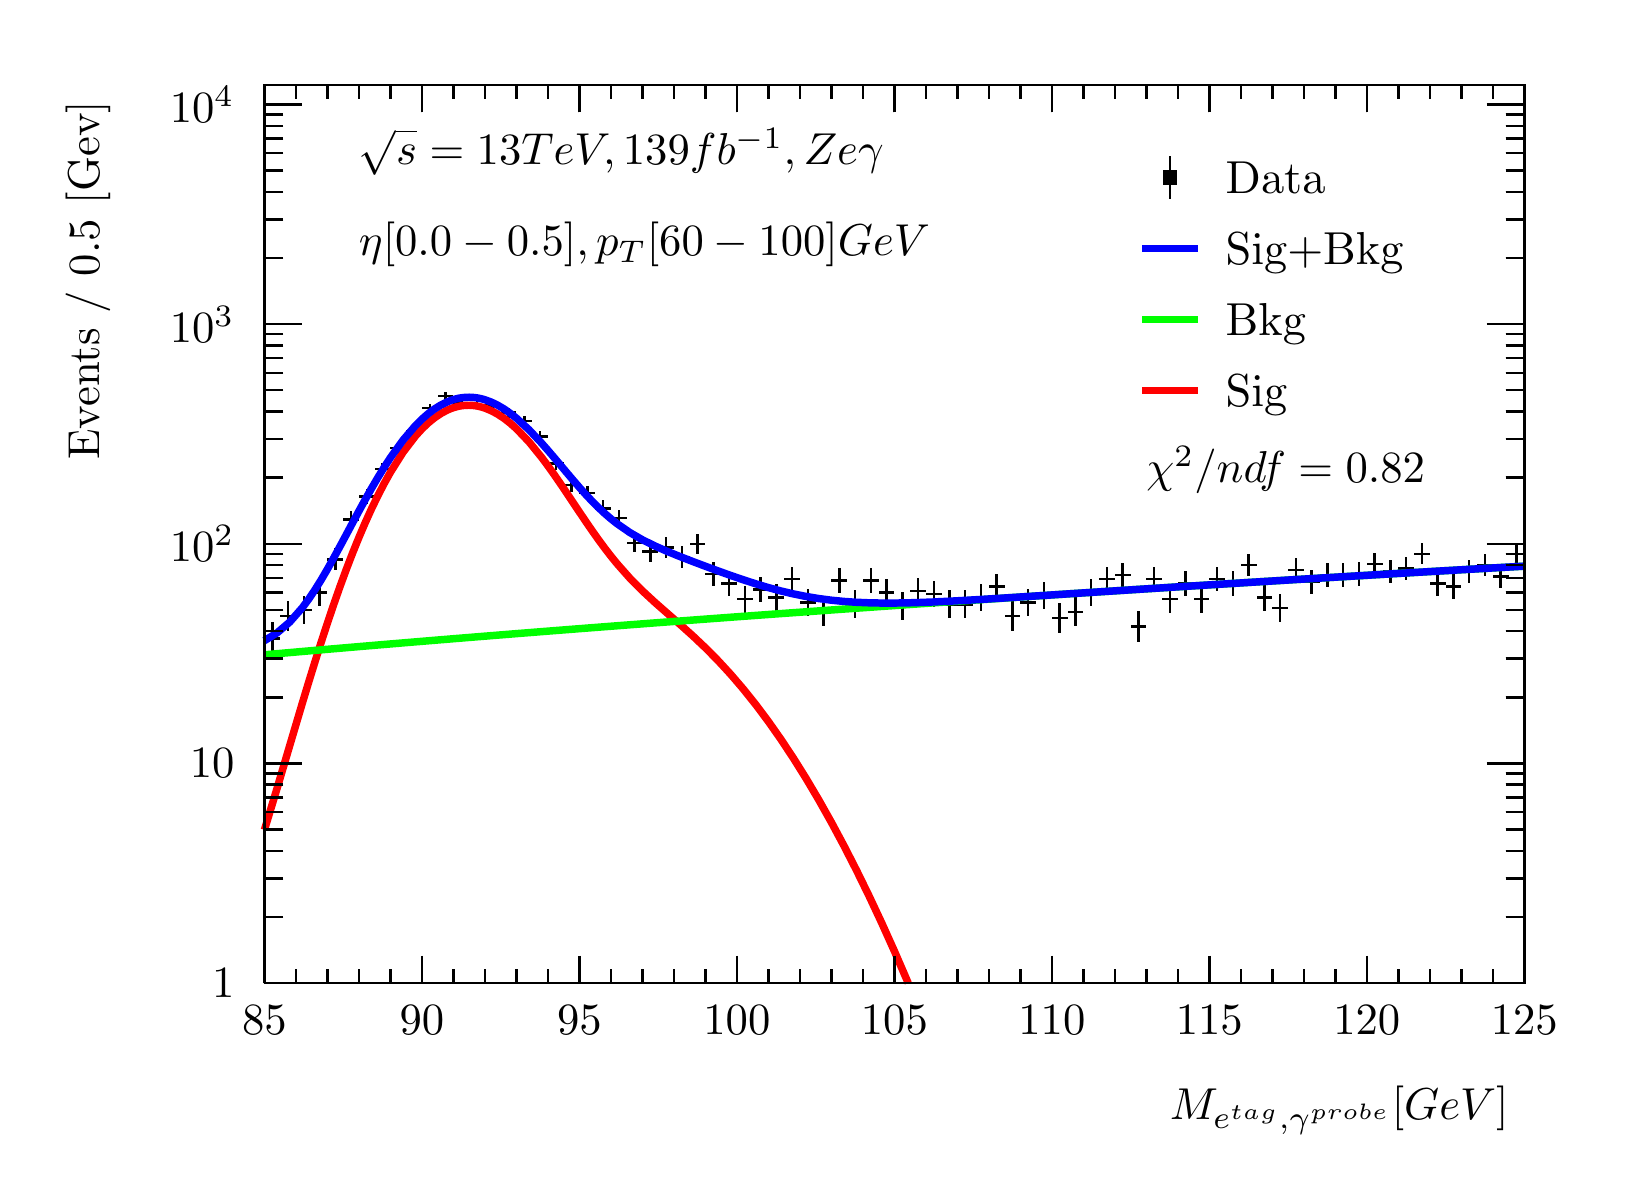
\begin{tikzpicture}
\pgfdeclareplotmark{cross} {
\pgfpathmoveto{\pgfpoint{-0.3\pgfplotmarksize}{\pgfplotmarksize}}
\pgfpathlineto{\pgfpoint{+0.3\pgfplotmarksize}{\pgfplotmarksize}}
\pgfpathlineto{\pgfpoint{+0.3\pgfplotmarksize}{0.3\pgfplotmarksize}}
\pgfpathlineto{\pgfpoint{+1\pgfplotmarksize}{0.3\pgfplotmarksize}}
\pgfpathlineto{\pgfpoint{+1\pgfplotmarksize}{-0.3\pgfplotmarksize}}
\pgfpathlineto{\pgfpoint{+0.3\pgfplotmarksize}{-0.3\pgfplotmarksize}}
\pgfpathlineto{\pgfpoint{+0.3\pgfplotmarksize}{-1.\pgfplotmarksize}}
\pgfpathlineto{\pgfpoint{-0.3\pgfplotmarksize}{-1.\pgfplotmarksize}}
\pgfpathlineto{\pgfpoint{-0.3\pgfplotmarksize}{-0.3\pgfplotmarksize}}
\pgfpathlineto{\pgfpoint{-1.\pgfplotmarksize}{-0.3\pgfplotmarksize}}
\pgfpathlineto{\pgfpoint{-1.\pgfplotmarksize}{0.3\pgfplotmarksize}}
\pgfpathlineto{\pgfpoint{-0.3\pgfplotmarksize}{0.3\pgfplotmarksize}}
\pgfpathclose
\pgfusepathqstroke
}
\pgfdeclareplotmark{cross*} {
\pgfpathmoveto{\pgfpoint{-0.3\pgfplotmarksize}{\pgfplotmarksize}}
\pgfpathlineto{\pgfpoint{+0.3\pgfplotmarksize}{\pgfplotmarksize}}
\pgfpathlineto{\pgfpoint{+0.3\pgfplotmarksize}{0.3\pgfplotmarksize}}
\pgfpathlineto{\pgfpoint{+1\pgfplotmarksize}{0.3\pgfplotmarksize}}
\pgfpathlineto{\pgfpoint{+1\pgfplotmarksize}{-0.3\pgfplotmarksize}}
\pgfpathlineto{\pgfpoint{+0.3\pgfplotmarksize}{-0.3\pgfplotmarksize}}
\pgfpathlineto{\pgfpoint{+0.3\pgfplotmarksize}{-1.\pgfplotmarksize}}
\pgfpathlineto{\pgfpoint{-0.3\pgfplotmarksize}{-1.\pgfplotmarksize}}
\pgfpathlineto{\pgfpoint{-0.3\pgfplotmarksize}{-0.3\pgfplotmarksize}}
\pgfpathlineto{\pgfpoint{-1.\pgfplotmarksize}{-0.3\pgfplotmarksize}}
\pgfpathlineto{\pgfpoint{-1.\pgfplotmarksize}{0.3\pgfplotmarksize}}
\pgfpathlineto{\pgfpoint{-0.3\pgfplotmarksize}{0.3\pgfplotmarksize}}
\pgfpathclose
\pgfusepathqfillstroke
}
\pgfdeclareplotmark{newstar} {
\pgfpathmoveto{\pgfqpoint{0pt}{\pgfplotmarksize}}
\pgfpathlineto{\pgfqpointpolar{44}{0.5\pgfplotmarksize}}
\pgfpathlineto{\pgfqpointpolar{18}{\pgfplotmarksize}}
\pgfpathlineto{\pgfqpointpolar{-20}{0.5\pgfplotmarksize}}
\pgfpathlineto{\pgfqpointpolar{-54}{\pgfplotmarksize}}
\pgfpathlineto{\pgfqpointpolar{-90}{0.5\pgfplotmarksize}}
\pgfpathlineto{\pgfqpointpolar{234}{\pgfplotmarksize}}
\pgfpathlineto{\pgfqpointpolar{198}{0.5\pgfplotmarksize}}
\pgfpathlineto{\pgfqpointpolar{162}{\pgfplotmarksize}}
\pgfpathlineto{\pgfqpointpolar{134}{0.5\pgfplotmarksize}}
\pgfpathclose
\pgfusepathqstroke
}
\pgfdeclareplotmark{newstar*} {
\pgfpathmoveto{\pgfqpoint{0pt}{\pgfplotmarksize}}
\pgfpathlineto{\pgfqpointpolar{44}{0.5\pgfplotmarksize}}
\pgfpathlineto{\pgfqpointpolar{18}{\pgfplotmarksize}}
\pgfpathlineto{\pgfqpointpolar{-20}{0.5\pgfplotmarksize}}
\pgfpathlineto{\pgfqpointpolar{-54}{\pgfplotmarksize}}
\pgfpathlineto{\pgfqpointpolar{-90}{0.5\pgfplotmarksize}}
\pgfpathlineto{\pgfqpointpolar{234}{\pgfplotmarksize}}
\pgfpathlineto{\pgfqpointpolar{198}{0.5\pgfplotmarksize}}
\pgfpathlineto{\pgfqpointpolar{162}{\pgfplotmarksize}}
\pgfpathlineto{\pgfqpointpolar{134}{0.5\pgfplotmarksize}}
\pgfpathclose
\pgfusepathqfillstroke
}
\definecolor{c}{rgb}{1,1,1};
\draw [color=c, fill=c] (0,0) rectangle (20,14.4361);
\draw [color=c, fill=c] (3,2.30977) rectangle (19,13.7143);
\definecolor{c}{rgb}{0,0,0};
\draw [c,line width=0.9] (3,2.30977) -- (3,13.7143) -- (19,13.7143) -- (19,2.30977) -- (3,2.30977);
\definecolor{c}{rgb}{1,1,1};
\draw [color=c, fill=c] (3,2.30977) rectangle (19,13.7143);
\definecolor{c}{rgb}{0,0,0};
\draw [c,line width=0.9] (3,2.30977) -- (3,13.7143) -- (19,13.7143) -- (19,2.30977) -- (3,2.30977);
\draw [c,line width=0.9] (3,2.30977) -- (19,2.30977);
\draw [c,line width=0.9] (3,2.65624) -- (3,2.30977);
\draw [c,line width=0.9] (3.4,2.48301) -- (3.4,2.30977);
\draw [c,line width=0.9] (3.8,2.48301) -- (3.8,2.30977);
\draw [c,line width=0.9] (4.2,2.48301) -- (4.2,2.30977);
\draw [c,line width=0.9] (4.6,2.48301) -- (4.6,2.30977);
\draw [c,line width=0.9] (5,2.65624) -- (5,2.30977);
\draw [c,line width=0.9] (5.4,2.48301) -- (5.4,2.30977);
\draw [c,line width=0.9] (5.8,2.48301) -- (5.8,2.30977);
\draw [c,line width=0.9] (6.2,2.48301) -- (6.2,2.30977);
\draw [c,line width=0.9] (6.6,2.48301) -- (6.6,2.30977);
\draw [c,line width=0.9] (7,2.65624) -- (7,2.30977);
\draw [c,line width=0.9] (7.4,2.48301) -- (7.4,2.30977);
\draw [c,line width=0.9] (7.8,2.48301) -- (7.8,2.30977);
\draw [c,line width=0.9] (8.2,2.48301) -- (8.2,2.30977);
\draw [c,line width=0.9] (8.6,2.48301) -- (8.6,2.30977);
\draw [c,line width=0.9] (9,2.65624) -- (9,2.30977);
\draw [c,line width=0.9] (9.4,2.48301) -- (9.4,2.30977);
\draw [c,line width=0.9] (9.8,2.48301) -- (9.8,2.30977);
\draw [c,line width=0.9] (10.2,2.48301) -- (10.2,2.30977);
\draw [c,line width=0.9] (10.6,2.48301) -- (10.6,2.30977);
\draw [c,line width=0.9] (11,2.65624) -- (11,2.30977);
\draw [c,line width=0.9] (11.4,2.48301) -- (11.4,2.30977);
\draw [c,line width=0.9] (11.8,2.48301) -- (11.8,2.30977);
\draw [c,line width=0.9] (12.2,2.48301) -- (12.2,2.30977);
\draw [c,line width=0.9] (12.6,2.48301) -- (12.6,2.30977);
\draw [c,line width=0.9] (13,2.65624) -- (13,2.30977);
\draw [c,line width=0.9] (13.4,2.48301) -- (13.4,2.30977);
\draw [c,line width=0.9] (13.8,2.48301) -- (13.8,2.30977);
\draw [c,line width=0.9] (14.2,2.48301) -- (14.2,2.30977);
\draw [c,line width=0.9] (14.6,2.48301) -- (14.6,2.30977);
\draw [c,line width=0.9] (15,2.65624) -- (15,2.30977);
\draw [c,line width=0.9] (15.4,2.48301) -- (15.4,2.30977);
\draw [c,line width=0.9] (15.8,2.48301) -- (15.8,2.30977);
\draw [c,line width=0.9] (16.2,2.48301) -- (16.2,2.30977);
\draw [c,line width=0.9] (16.6,2.48301) -- (16.6,2.30977);
\draw [c,line width=0.9] (17,2.65624) -- (17,2.30977);
\draw [c,line width=0.9] (17.4,2.48301) -- (17.4,2.30977);
\draw [c,line width=0.9] (17.8,2.48301) -- (17.8,2.30977);
\draw [c,line width=0.9] (18.2,2.48301) -- (18.2,2.30977);
\draw [c,line width=0.9] (18.6,2.48301) -- (18.6,2.30977);
\draw [c,line width=0.9] (19,2.65624) -- (19,2.30977);
\draw [anchor=base] (3,1.66015) node[scale=1.61424, color=c, rotate=0]{85};
\draw [anchor=base] (5,1.66015) node[scale=1.61424, color=c, rotate=0]{90};
\draw [anchor=base] (7,1.66015) node[scale=1.61424, color=c, rotate=0]{95};
\draw [anchor=base] (9,1.66015) node[scale=1.61424, color=c, rotate=0]{100};
\draw [anchor=base] (11,1.66015) node[scale=1.61424, color=c, rotate=0]{105};
\draw [anchor=base] (13,1.66015) node[scale=1.61424, color=c, rotate=0]{110};
\draw [anchor=base] (15,1.66015) node[scale=1.61424, color=c, rotate=0]{115};
\draw [anchor=base] (17,1.66015) node[scale=1.61424, color=c, rotate=0]{120};
\draw [anchor=base] (19,1.66015) node[scale=1.61424, color=c, rotate=0]{125};
\draw [anchor= east] (19,0.692932) node[scale=1.61424, color=c, rotate=0]{$M_{e^{tag}, \gamma^{probe}}  [GeV]$};
\draw [c,line width=0.9] (3,13.7143) -- (19,13.7143);
\draw [c,line width=0.9] (3,13.3678) -- (3,13.7143);
\draw [c,line width=0.9] (3.4,13.5411) -- (3.4,13.7143);
\draw [c,line width=0.9] (3.8,13.5411) -- (3.8,13.7143);
\draw [c,line width=0.9] (4.2,13.5411) -- (4.2,13.7143);
\draw [c,line width=0.9] (4.6,13.5411) -- (4.6,13.7143);
\draw [c,line width=0.9] (5,13.3678) -- (5,13.7143);
\draw [c,line width=0.9] (5.4,13.5411) -- (5.4,13.7143);
\draw [c,line width=0.9] (5.8,13.5411) -- (5.8,13.7143);
\draw [c,line width=0.9] (6.2,13.5411) -- (6.2,13.7143);
\draw [c,line width=0.9] (6.6,13.5411) -- (6.6,13.7143);
\draw [c,line width=0.9] (7,13.3678) -- (7,13.7143);
\draw [c,line width=0.9] (7.4,13.5411) -- (7.4,13.7143);
\draw [c,line width=0.9] (7.8,13.5411) -- (7.8,13.7143);
\draw [c,line width=0.9] (8.2,13.5411) -- (8.2,13.7143);
\draw [c,line width=0.9] (8.6,13.5411) -- (8.6,13.7143);
\draw [c,line width=0.9] (9,13.3678) -- (9,13.7143);
\draw [c,line width=0.9] (9.4,13.5411) -- (9.4,13.7143);
\draw [c,line width=0.9] (9.8,13.5411) -- (9.8,13.7143);
\draw [c,line width=0.9] (10.2,13.5411) -- (10.2,13.7143);
\draw [c,line width=0.9] (10.6,13.5411) -- (10.6,13.7143);
\draw [c,line width=0.9] (11,13.3678) -- (11,13.7143);
\draw [c,line width=0.9] (11.4,13.5411) -- (11.4,13.7143);
\draw [c,line width=0.9] (11.8,13.5411) -- (11.8,13.7143);
\draw [c,line width=0.9] (12.2,13.5411) -- (12.2,13.7143);
\draw [c,line width=0.9] (12.6,13.5411) -- (12.6,13.7143);
\draw [c,line width=0.9] (13,13.3678) -- (13,13.7143);
\draw [c,line width=0.9] (13.4,13.5411) -- (13.4,13.7143);
\draw [c,line width=0.9] (13.8,13.5411) -- (13.8,13.7143);
\draw [c,line width=0.9] (14.2,13.5411) -- (14.2,13.7143);
\draw [c,line width=0.9] (14.6,13.5411) -- (14.6,13.7143);
\draw [c,line width=0.9] (15,13.3678) -- (15,13.7143);
\draw [c,line width=0.9] (15.4,13.5411) -- (15.4,13.7143);
\draw [c,line width=0.9] (15.8,13.5411) -- (15.8,13.7143);
\draw [c,line width=0.9] (16.2,13.5411) -- (16.2,13.7143);
\draw [c,line width=0.9] (16.6,13.5411) -- (16.6,13.7143);
\draw [c,line width=0.9] (17,13.3678) -- (17,13.7143);
\draw [c,line width=0.9] (17.4,13.5411) -- (17.4,13.7143);
\draw [c,line width=0.9] (17.8,13.5411) -- (17.8,13.7143);
\draw [c,line width=0.9] (18.2,13.5411) -- (18.2,13.7143);
\draw [c,line width=0.9] (18.6,13.5411) -- (18.6,13.7143);
\draw [c,line width=0.9] (19,13.3678) -- (19,13.7143);
\draw [c,line width=0.9] (3,2.30977) -- (3,13.7143);
\draw [c,line width=0.9] (3.474,2.30978) -- (3,2.30978);
\draw [anchor= east] (2.82,2.30978) node[scale=1.61424, color=c, rotate=0]{1};
\draw [c,line width=0.9] (3.237,3.1495) -- (3,3.1495);
\draw [c,line width=0.9] (3.237,3.6407) -- (3,3.6407);
\draw [c,line width=0.9] (3.237,3.98922) -- (3,3.98922);
\draw [c,line width=0.9] (3.237,4.25955) -- (3,4.25955);
\draw [c,line width=0.9] (3.237,4.48042) -- (3,4.48042);
\draw [c,line width=0.9] (3.237,4.66717) -- (3,4.66717);
\draw [c,line width=0.9] (3.237,4.82894) -- (3,4.82894);
\draw [c,line width=0.9] (3.237,4.97163) -- (3,4.97163);
\draw [c,line width=0.9] (3.474,5.09927) -- (3,5.09927);
\draw [anchor= east] (2.82,5.09927) node[scale=1.61424, color=c, rotate=0]{10};
\draw [c,line width=0.9] (3.237,5.93899) -- (3,5.93899);
\draw [c,line width=0.9] (3.237,6.43019) -- (3,6.43019);
\draw [c,line width=0.9] (3.237,6.77871) -- (3,6.77871);
\draw [c,line width=0.9] (3.237,7.04904) -- (3,7.04904);
\draw [c,line width=0.9] (3.237,7.26991) -- (3,7.26991);
\draw [c,line width=0.9] (3.237,7.45666) -- (3,7.45666);
\draw [c,line width=0.9] (3.237,7.61843) -- (3,7.61843);
\draw [c,line width=0.9] (3.237,7.76112) -- (3,7.76112);
\draw [c,line width=0.9] (3.474,7.88876) -- (3,7.88876);
\draw [anchor= east] (2.82,7.88876) node[scale=1.61424, color=c, rotate=0]{$10^{2}$};
\draw [c,line width=0.9] (3.237,8.72848) -- (3,8.72848);
\draw [c,line width=0.9] (3.237,9.21968) -- (3,9.21968);
\draw [c,line width=0.9] (3.237,9.5682) -- (3,9.5682);
\draw [c,line width=0.9] (3.237,9.83853) -- (3,9.83853);
\draw [c,line width=0.9] (3.237,10.0594) -- (3,10.0594);
\draw [c,line width=0.9] (3.237,10.2462) -- (3,10.2462);
\draw [c,line width=0.9] (3.237,10.4079) -- (3,10.4079);
\draw [c,line width=0.9] (3.237,10.5506) -- (3,10.5506);
\draw [c,line width=0.9] (3.474,10.6782) -- (3,10.6782);
\draw [anchor= east] (2.82,10.6782) node[scale=1.61424, color=c, rotate=0]{$10^{3}$};
\draw [c,line width=0.9] (3.237,11.518) -- (3,11.518);
\draw [c,line width=0.9] (3.237,12.0092) -- (3,12.0092);
\draw [c,line width=0.9] (3.237,12.3577) -- (3,12.3577);
\draw [c,line width=0.9] (3.237,12.628) -- (3,12.628);
\draw [c,line width=0.9] (3.237,12.8489) -- (3,12.8489);
\draw [c,line width=0.9] (3.237,13.0356) -- (3,13.0356);
\draw [c,line width=0.9] (3.237,13.1974) -- (3,13.1974);
\draw [c,line width=0.9] (3.237,13.3401) -- (3,13.3401);
\draw [c,line width=0.9] (3.474,13.4677) -- (3,13.4677);
\draw [anchor= east] (2.82,13.4677) node[scale=1.61424, color=c, rotate=0]{$10^{4}$};
\draw [anchor= east] (0.76,13.7143) node[scale=1.61424, color=c, rotate=90]{Events / 0.5 [Gev]};
\draw [c,line width=0.9] (19,2.30977) -- (19,13.7143);
\draw [c,line width=0.9] (18.526,2.30978) -- (19,2.30978);
\draw [c,line width=0.9] (18.763,3.1495) -- (19,3.1495);
\draw [c,line width=0.9] (18.763,3.6407) -- (19,3.6407);
\draw [c,line width=0.9] (18.763,3.98922) -- (19,3.98922);
\draw [c,line width=0.9] (18.763,4.25955) -- (19,4.25955);
\draw [c,line width=0.9] (18.763,4.48042) -- (19,4.48042);
\draw [c,line width=0.9] (18.763,4.66717) -- (19,4.66717);
\draw [c,line width=0.9] (18.763,4.82894) -- (19,4.82894);
\draw [c,line width=0.9] (18.763,4.97163) -- (19,4.97163);
\draw [c,line width=0.9] (18.526,5.09927) -- (19,5.09927);
\draw [c,line width=0.9] (18.763,5.93899) -- (19,5.93899);
\draw [c,line width=0.9] (18.763,6.43019) -- (19,6.43019);
\draw [c,line width=0.9] (18.763,6.77871) -- (19,6.77871);
\draw [c,line width=0.9] (18.763,7.04904) -- (19,7.04904);
\draw [c,line width=0.9] (18.763,7.26991) -- (19,7.26991);
\draw [c,line width=0.9] (18.763,7.45666) -- (19,7.45666);
\draw [c,line width=0.9] (18.763,7.61843) -- (19,7.61843);
\draw [c,line width=0.9] (18.763,7.76112) -- (19,7.76112);
\draw [c,line width=0.9] (18.526,7.88876) -- (19,7.88876);
\draw [c,line width=0.9] (18.763,8.72848) -- (19,8.72848);
\draw [c,line width=0.9] (18.763,9.21968) -- (19,9.21968);
\draw [c,line width=0.9] (18.763,9.5682) -- (19,9.5682);
\draw [c,line width=0.9] (18.763,9.83853) -- (19,9.83853);
\draw [c,line width=0.9] (18.763,10.0594) -- (19,10.0594);
\draw [c,line width=0.9] (18.763,10.2462) -- (19,10.2462);
\draw [c,line width=0.9] (18.763,10.4079) -- (19,10.4079);
\draw [c,line width=0.9] (18.763,10.5506) -- (19,10.5506);
\draw [c,line width=0.9] (18.526,10.6782) -- (19,10.6782);
\draw [c,line width=0.9] (18.763,11.518) -- (19,11.518);
\draw [c,line width=0.9] (18.763,12.0092) -- (19,12.0092);
\draw [c,line width=0.9] (18.763,12.3577) -- (19,12.3577);
\draw [c,line width=0.9] (18.763,12.628) -- (19,12.628);
\draw [c,line width=0.9] (18.763,12.8489) -- (19,12.8489);
\draw [c,line width=0.9] (18.763,13.0356) -- (19,13.0356);
\draw [c,line width=0.9] (18.763,13.1974) -- (19,13.1974);
\draw [c,line width=0.9] (18.763,13.3401) -- (19,13.3401);
\draw [c,line width=0.9] (18.526,13.4677) -- (19,13.4677);
\draw [c,line width=0.9] (3.1,6.68426) -- (3,6.68426);
\draw [c,line width=0.9] (3,6.68426) -- (3,6.68426);
\draw [c,line width=0.9] (3.1,6.68426) -- (3.2,6.68426);
\draw [c,line width=0.9] (3.2,6.68426) -- (3.2,6.68426);
\draw [c,line width=0.9] (3.1,6.68426) -- (3.1,6.89795);
\draw [c,line width=0.9] (3.1,6.89795) -- (3.1,6.89795);
\draw [c,line width=0.9] (3.1,6.68426) -- (3.1,6.46776);
\draw [c,line width=0.9] (3.1,6.46776) -- (3.1,6.46776);
\draw [c,line width=0.9] (3.3,6.97408) -- (3.2,6.97408);
\draw [c,line width=0.9] (3.2,6.97408) -- (3.2,6.97408);
\draw [c,line width=0.9] (3.3,6.97408) -- (3.4,6.97408);
\draw [c,line width=0.9] (3.4,6.97408) -- (3.4,6.97408);
\draw [c,line width=0.9] (3.3,6.97408) -- (3.3,7.16239);
\draw [c,line width=0.9] (3.3,7.16239) -- (3.3,7.16239);
\draw [c,line width=0.9] (3.3,6.97408) -- (3.3,6.78381);
\draw [c,line width=0.9] (3.3,6.78381) -- (3.3,6.78381);
\draw [c,line width=0.9] (3.5,7.04904) -- (3.4,7.04904);
\draw [c,line width=0.9] (3.4,7.04904) -- (3.4,7.04904);
\draw [c,line width=0.9] (3.5,7.04904) -- (3.6,7.04904);
\draw [c,line width=0.9] (3.6,7.04904) -- (3.6,7.04904);
\draw [c,line width=0.9] (3.5,7.04904) -- (3.5,7.23131);
\draw [c,line width=0.9] (3.5,7.23131) -- (3.5,7.23131);
\draw [c,line width=0.9] (3.5,7.04904) -- (3.5,6.86499);
\draw [c,line width=0.9] (3.5,6.86499) -- (3.5,6.86499);
\draw [c,line width=0.9] (3.7,7.26991) -- (3.6,7.26991);
\draw [c,line width=0.9] (3.6,7.26991) -- (3.6,7.26991);
\draw [c,line width=0.9] (3.7,7.26991) -- (3.8,7.26991);
\draw [c,line width=0.9] (3.8,7.26991) -- (3.8,7.26991);
\draw [c,line width=0.9] (3.7,7.26991) -- (3.7,7.43552);
\draw [c,line width=0.9] (3.7,7.43552) -- (3.7,7.43552);
\draw [c,line width=0.9] (3.7,7.26991) -- (3.7,7.10296);
\draw [c,line width=0.9] (3.7,7.10296) -- (3.7,7.10296);
\draw [c,line width=0.9] (3.9,7.69187) -- (3.8,7.69187);
\draw [c,line width=0.9] (3.8,7.69187) -- (3.8,7.69187);
\draw [c,line width=0.9] (3.9,7.69187) -- (4,7.69187);
\draw [c,line width=0.9] (4,7.69187) -- (4,7.69187);
\draw [c,line width=0.9] (3.9,7.69187) -- (3.9,7.82987);
\draw [c,line width=0.9] (3.9,7.82987) -- (3.9,7.82987);
\draw [c,line width=0.9] (3.9,7.69187) -- (3.9,7.55307);
\draw [c,line width=0.9] (3.9,7.55307) -- (3.9,7.55307);
\draw [c,line width=0.9] (4.1,8.19725) -- (4,8.19725);
\draw [c,line width=0.9] (4,8.19725) -- (4,8.19725);
\draw [c,line width=0.9] (4.1,8.19725) -- (4.2,8.19725);
\draw [c,line width=0.9] (4.2,8.19725) -- (4.2,8.19725);
\draw [c,line width=0.9] (4.1,8.19725) -- (4.1,8.30387);
\draw [c,line width=0.9] (4.1,8.30387) -- (4.1,8.30387);
\draw [c,line width=0.9] (4.1,8.19725) -- (4.1,8.09062);
\draw [c,line width=0.9] (4.1,8.09062) -- (4.1,8.09062);
\draw [c,line width=0.9] (4.3,8.48806) -- (4.2,8.48806);
\draw [c,line width=0.9] (4.2,8.48806) -- (4.2,8.48806);
\draw [c,line width=0.9] (4.3,8.48806) -- (4.4,8.48806);
\draw [c,line width=0.9] (4.4,8.48806) -- (4.4,8.48806);
\draw [c,line width=0.9] (4.3,8.48806) -- (4.3,8.58264);
\draw [c,line width=0.9] (4.3,8.58264) -- (4.3,8.58264);
\draw [c,line width=0.9] (4.3,8.48806) -- (4.3,8.39349);
\draw [c,line width=0.9] (4.3,8.39349) -- (4.3,8.39349);
\draw [c,line width=0.9] (4.5,8.83842) -- (4.4,8.83842);
\draw [c,line width=0.9] (4.4,8.83842) -- (4.4,8.83842);
\draw [c,line width=0.9] (4.5,8.83842) -- (4.6,8.83842);
\draw [c,line width=0.9] (4.6,8.83842) -- (4.6,8.83842);
\draw [c,line width=0.9] (4.5,8.83842) -- (4.5,8.92027);
\draw [c,line width=0.9] (4.5,8.92027) -- (4.5,8.92027);
\draw [c,line width=0.9] (4.5,8.83842) -- (4.5,8.75658);
\draw [c,line width=0.9] (4.5,8.75658) -- (4.5,8.75658);
\draw [c,line width=0.9] (4.7,9.10543) -- (4.6,9.10543);
\draw [c,line width=0.9] (4.6,9.10543) -- (4.6,9.10543);
\draw [c,line width=0.9] (4.7,9.10543) -- (4.8,9.10543);
\draw [c,line width=0.9] (4.8,9.10543) -- (4.8,9.10543);
\draw [c,line width=0.9] (4.7,9.10543) -- (4.7,9.17874);
\draw [c,line width=0.9] (4.7,9.17874) -- (4.7,9.17874);
\draw [c,line width=0.9] (4.7,9.10543) -- (4.7,9.03212);
\draw [c,line width=0.9] (4.7,9.03212) -- (4.7,9.03212);
\draw [c,line width=0.9] (4.9,9.32037) -- (4.8,9.32037);
\draw [c,line width=0.9] (4.8,9.32037) -- (4.8,9.32037);
\draw [c,line width=0.9] (4.9,9.32037) -- (5,9.32037);
\draw [c,line width=0.9] (5,9.32037) -- (5,9.32037);
\draw [c,line width=0.9] (4.9,9.32037) -- (4.9,9.38746);
\draw [c,line width=0.9] (4.9,9.38746) -- (4.9,9.38746);
\draw [c,line width=0.9] (4.9,9.32037) -- (4.9,9.25328);
\draw [c,line width=0.9] (4.9,9.25328) -- (4.9,9.25328);
\draw [c,line width=0.9] (5.1,9.60987) -- (5,9.60987);
\draw [c,line width=0.9] (5,9.60987) -- (5,9.60987);
\draw [c,line width=0.9] (5.1,9.60987) -- (5.2,9.60987);
\draw [c,line width=0.9] (5.2,9.60987) -- (5.2,9.60987);
\draw [c,line width=0.9] (5.1,9.60987) -- (5.1,9.66941);
\draw [c,line width=0.9] (5.1,9.66941) -- (5.1,9.66941);
\draw [c,line width=0.9] (5.1,9.60987) -- (5.1,9.55034);
\draw [c,line width=0.9] (5.1,9.55034) -- (5.1,9.55034);
\draw [c,line width=0.9] (5.3,9.76357) -- (5.2,9.76357);
\draw [c,line width=0.9] (5.2,9.76357) -- (5.2,9.76357);
\draw [c,line width=0.9] (5.3,9.76357) -- (5.4,9.76357);
\draw [c,line width=0.9] (5.4,9.76357) -- (5.4,9.76357);
\draw [c,line width=0.9] (5.3,9.76357) -- (5.3,9.81944);
\draw [c,line width=0.9] (5.3,9.81944) -- (5.3,9.81944);
\draw [c,line width=0.9] (5.3,9.76357) -- (5.3,9.70769);
\draw [c,line width=0.9] (5.3,9.70769) -- (5.3,9.70769);
\draw [c,line width=0.9] (5.5,9.66982) -- (5.4,9.66982);
\draw [c,line width=0.9] (5.4,9.66982) -- (5.4,9.66982);
\draw [c,line width=0.9] (5.5,9.66982) -- (5.6,9.66982);
\draw [c,line width=0.9] (5.6,9.66982) -- (5.6,9.66982);
\draw [c,line width=0.9] (5.5,9.66982) -- (5.5,9.7279);
\draw [c,line width=0.9] (5.5,9.7279) -- (5.5,9.7279);
\draw [c,line width=0.9] (5.5,9.66982) -- (5.5,9.61174);
\draw [c,line width=0.9] (5.5,9.61174) -- (5.5,9.61174);
\draw [c,line width=0.9] (5.7,9.72161) -- (5.6,9.72161);
\draw [c,line width=0.9] (5.6,9.72161) -- (5.6,9.72161);
\draw [c,line width=0.9] (5.7,9.72161) -- (5.8,9.72161);
\draw [c,line width=0.9] (5.8,9.72161) -- (5.8,9.72161);
\draw [c,line width=0.9] (5.7,9.72161) -- (5.7,9.77846);
\draw [c,line width=0.9] (5.7,9.77846) -- (5.7,9.77846);
\draw [c,line width=0.9] (5.7,9.72161) -- (5.7,9.66476);
\draw [c,line width=0.9] (5.7,9.66476) -- (5.7,9.66476);
\draw [c,line width=0.9] (5.9,9.64449) -- (5.8,9.64449);
\draw [c,line width=0.9] (5.8,9.64449) -- (5.8,9.64449);
\draw [c,line width=0.9] (5.9,9.64449) -- (6,9.64449);
\draw [c,line width=0.9] (6,9.64449) -- (6,9.64449);
\draw [c,line width=0.9] (5.9,9.64449) -- (5.9,9.70318);
\draw [c,line width=0.9] (5.9,9.70318) -- (5.9,9.70318);
\draw [c,line width=0.9] (5.9,9.64449) -- (5.9,9.5858);
\draw [c,line width=0.9] (5.9,9.5858) -- (5.9,9.5858);
\draw [c,line width=0.9] (6.1,9.55296) -- (6,9.55296);
\draw [c,line width=0.9] (6,9.55296) -- (6,9.55296);
\draw [c,line width=0.9] (6.1,9.55296) -- (6.2,9.55296);
\draw [c,line width=0.9] (6.2,9.55296) -- (6.2,9.55296);
\draw [c,line width=0.9] (6.1,9.55296) -- (6.1,9.61391);
\draw [c,line width=0.9] (6.1,9.61391) -- (6.1,9.61391);
\draw [c,line width=0.9] (6.1,9.55296) -- (6.1,9.49201);
\draw [c,line width=0.9] (6.1,9.49201) -- (6.1,9.49201);
\draw [c,line width=0.9] (6.3,9.44727) -- (6.2,9.44727);
\draw [c,line width=0.9] (6.2,9.44727) -- (6.2,9.44727);
\draw [c,line width=0.9] (6.3,9.44727) -- (6.4,9.44727);
\draw [c,line width=0.9] (6.4,9.44727) -- (6.4,9.44727);
\draw [c,line width=0.9] (6.3,9.44727) -- (6.3,9.51093);
\draw [c,line width=0.9] (6.3,9.51093) -- (6.3,9.51093);
\draw [c,line width=0.9] (6.3,9.44727) -- (6.3,9.3836);
\draw [c,line width=0.9] (6.3,9.3836) -- (6.3,9.3836);
\draw [c,line width=0.9] (6.5,9.25156) -- (6.4,9.25156);
\draw [c,line width=0.9] (6.4,9.25156) -- (6.4,9.25156);
\draw [c,line width=0.9] (6.5,9.25156) -- (6.6,9.25156);
\draw [c,line width=0.9] (6.6,9.25156) -- (6.6,9.25156);
\draw [c,line width=0.9] (6.5,9.25156) -- (6.5,9.32058);
\draw [c,line width=0.9] (6.5,9.32058) -- (6.5,9.32058);
\draw [c,line width=0.9] (6.5,9.25156) -- (6.5,9.18254);
\draw [c,line width=0.9] (6.5,9.18254) -- (6.5,9.18254);
\draw [c,line width=0.9] (6.7,8.90828) -- (6.6,8.90828);
\draw [c,line width=0.9] (6.6,8.90828) -- (6.6,8.90828);
\draw [c,line width=0.9] (6.7,8.90828) -- (6.8,8.90828);
\draw [c,line width=0.9] (6.8,8.90828) -- (6.8,8.90828);
\draw [c,line width=0.9] (6.7,8.90828) -- (6.7,8.9878);
\draw [c,line width=0.9] (6.7,8.9878) -- (6.7,8.9878);
\draw [c,line width=0.9] (6.7,8.90828) -- (6.7,8.82876);
\draw [c,line width=0.9] (6.7,8.82876) -- (6.7,8.82876);
\draw [c,line width=0.9] (6.9,8.63403) -- (6.8,8.63403);
\draw [c,line width=0.9] (6.8,8.63403) -- (6.8,8.63403);
\draw [c,line width=0.9] (6.9,8.63403) -- (7,8.63403);
\draw [c,line width=0.9] (7,8.63403) -- (7,8.63403);
\draw [c,line width=0.9] (6.9,8.63403) -- (6.9,8.72308);
\draw [c,line width=0.9] (6.9,8.72308) -- (6.9,8.72308);
\draw [c,line width=0.9] (6.9,8.63403) -- (6.9,8.54498);
\draw [c,line width=0.9] (6.9,8.54498) -- (6.9,8.54498);
\draw [c,line width=0.9] (7.1,8.53159) -- (7,8.53159);
\draw [c,line width=0.9] (7,8.53159) -- (7,8.53159);
\draw [c,line width=0.9] (7.1,8.53159) -- (7.2,8.53159);
\draw [c,line width=0.9] (7.2,8.53159) -- (7.2,8.53159);
\draw [c,line width=0.9] (7.1,8.53159) -- (7.1,8.62448);
\draw [c,line width=0.9] (7.1,8.62448) -- (7.1,8.62448);
\draw [c,line width=0.9] (7.1,8.53159) -- (7.1,8.4387);
\draw [c,line width=0.9] (7.1,8.4387) -- (7.1,8.4387);
\draw [c,line width=0.9] (7.3,8.33889) -- (7.2,8.33889);
\draw [c,line width=0.9] (7.2,8.33889) -- (7.2,8.33889);
\draw [c,line width=0.9] (7.3,8.33889) -- (7.4,8.33889);
\draw [c,line width=0.9] (7.4,8.33889) -- (7.4,8.33889);
\draw [c,line width=0.9] (7.3,8.33889) -- (7.3,8.43947);
\draw [c,line width=0.9] (7.3,8.43947) -- (7.3,8.43947);
\draw [c,line width=0.9] (7.3,8.33889) -- (7.3,8.23831);
\draw [c,line width=0.9] (7.3,8.23831) -- (7.3,8.23831);
\draw [c,line width=0.9] (7.5,8.21588) -- (7.4,8.21588);
\draw [c,line width=0.9] (7.4,8.21588) -- (7.4,8.21588);
\draw [c,line width=0.9] (7.5,8.21588) -- (7.6,8.21588);
\draw [c,line width=0.9] (7.6,8.21588) -- (7.6,8.21588);
\draw [c,line width=0.9] (7.5,8.21588) -- (7.5,8.3217);
\draw [c,line width=0.9] (7.5,8.3217) -- (7.5,8.3217);
\draw [c,line width=0.9] (7.5,8.21588) -- (7.5,8.11007);
\draw [c,line width=0.9] (7.5,8.11007) -- (7.5,8.11007);
\draw [c,line width=0.9] (7.7,7.90081) -- (7.6,7.90081);
\draw [c,line width=0.9] (7.6,7.90081) -- (7.6,7.90081);
\draw [c,line width=0.9] (7.7,7.90081) -- (7.8,7.90081);
\draw [c,line width=0.9] (7.8,7.90081) -- (7.8,7.90081);
\draw [c,line width=0.9] (7.7,7.90081) -- (7.7,8.02131);
\draw [c,line width=0.9] (7.7,8.02131) -- (7.7,8.02131);
\draw [c,line width=0.9] (7.7,7.90081) -- (7.7,7.78032);
\draw [c,line width=0.9] (7.7,7.78032) -- (7.7,7.78032);
\draw [c,line width=0.9] (7.9,7.78774) -- (7.8,7.78774);
\draw [c,line width=0.9] (7.8,7.78774) -- (7.8,7.78774);
\draw [c,line width=0.9] (7.9,7.78774) -- (8,7.78774);
\draw [c,line width=0.9] (8,7.78774) -- (8,7.78774);
\draw [c,line width=0.9] (7.9,7.78774) -- (7.9,7.92016);
\draw [c,line width=0.9] (7.9,7.92016) -- (7.9,7.92016);
\draw [c,line width=0.9] (7.9,7.78774) -- (7.9,7.65462);
\draw [c,line width=0.9] (7.9,7.65462) -- (7.9,7.65462);
\draw [c,line width=0.9] (8.1,7.8393) -- (8,7.8393);
\draw [c,line width=0.9] (8,7.8393) -- (8,7.8393);
\draw [c,line width=0.9] (8.1,7.8393) -- (8.2,7.8393);
\draw [c,line width=0.9] (8.2,7.8393) -- (8.2,7.8393);
\draw [c,line width=0.9] (8.1,7.8393) -- (8.1,7.96882);
\draw [c,line width=0.9] (8.1,7.96882) -- (8.1,7.96882);
\draw [c,line width=0.9] (8.1,7.8393) -- (8.1,7.70912);
\draw [c,line width=0.9] (8.1,7.70912) -- (8.1,7.70912);
\draw [c,line width=0.9] (8.3,7.72005) -- (8.2,7.72005);
\draw [c,line width=0.9] (8.2,7.72005) -- (8.2,7.72005);
\draw [c,line width=0.9] (8.3,7.72005) -- (8.4,7.72005);
\draw [c,line width=0.9] (8.4,7.72005) -- (8.4,7.72005);
\draw [c,line width=0.9] (8.3,7.72005) -- (8.3,7.85638);
\draw [c,line width=0.9] (8.3,7.85638) -- (8.3,7.85638);
\draw [c,line width=0.9] (8.3,7.72005) -- (8.3,7.58294);
\draw [c,line width=0.9] (8.3,7.58294) -- (8.3,7.58294);
\draw [c,line width=0.9] (8.5,7.88876) -- (8.4,7.88876);
\draw [c,line width=0.9] (8.4,7.88876) -- (8.4,7.88876);
\draw [c,line width=0.9] (8.5,7.88876) -- (8.6,7.88876);
\draw [c,line width=0.9] (8.6,7.88876) -- (8.6,7.88876);
\draw [c,line width=0.9] (8.5,7.88876) -- (8.5,8.01555);
\draw [c,line width=0.9] (8.5,8.01555) -- (8.5,8.01555);
\draw [c,line width=0.9] (8.5,7.88876) -- (8.5,7.76134);
\draw [c,line width=0.9] (8.5,7.76134) -- (8.5,7.76134);
\draw [c,line width=0.9] (8.7,7.5075) -- (8.6,7.5075);
\draw [c,line width=0.9] (8.6,7.5075) -- (8.6,7.5075);
\draw [c,line width=0.9] (8.7,7.5075) -- (8.8,7.5075);
\draw [c,line width=0.9] (8.8,7.5075) -- (8.8,7.5075);
\draw [c,line width=0.9] (8.7,7.5075) -- (8.7,7.65692);
\draw [c,line width=0.9] (8.7,7.65692) -- (8.7,7.65692);
\draw [c,line width=0.9] (8.7,7.5075) -- (8.7,7.35707);
\draw [c,line width=0.9] (8.7,7.35707) -- (8.7,7.35707);
\draw [c,line width=0.9] (8.9,7.38538) -- (8.8,7.38538);
\draw [c,line width=0.9] (8.8,7.38538) -- (8.8,7.38538);
\draw [c,line width=0.9] (8.9,7.38538) -- (9,7.38538);
\draw [c,line width=0.9] (9,7.38538) -- (9,7.38538);
\draw [c,line width=0.9] (8.9,7.38538) -- (8.9,7.5429);
\draw [c,line width=0.9] (8.9,7.5429) -- (8.9,7.5429);
\draw [c,line width=0.9] (8.9,7.38538) -- (8.9,7.22668);
\draw [c,line width=0.9] (8.9,7.22668) -- (8.9,7.22668);
\draw [c,line width=0.9] (9.1,7.18633) -- (9,7.18633);
\draw [c,line width=0.9] (9,7.18633) -- (9,7.18633);
\draw [c,line width=0.9] (9.1,7.18633) -- (9.2,7.18633);
\draw [c,line width=0.9] (9.2,7.18633) -- (9.2,7.18633);
\draw [c,line width=0.9] (9.1,7.18633) -- (9.1,7.35805);
\draw [c,line width=0.9] (9.1,7.35805) -- (9.1,7.35805);
\draw [c,line width=0.9] (9.1,7.18633) -- (9.1,7.01311);
\draw [c,line width=0.9] (9.1,7.01311) -- (9.1,7.01311);
\draw [c,line width=0.9] (9.3,7.30964) -- (9.2,7.30964);
\draw [c,line width=0.9] (9.2,7.30964) -- (9.2,7.30964);
\draw [c,line width=0.9] (9.3,7.30964) -- (9.4,7.30964);
\draw [c,line width=0.9] (9.4,7.30964) -- (9.4,7.30964);
\draw [c,line width=0.9] (9.3,7.30964) -- (9.3,7.47242);
\draw [c,line width=0.9] (9.3,7.47242) -- (9.3,7.47242);
\draw [c,line width=0.9] (9.3,7.30964) -- (9.3,7.14557);
\draw [c,line width=0.9] (9.3,7.14557) -- (9.3,7.14557);
\draw [c,line width=0.9] (9.5,7.20777) -- (9.4,7.20777);
\draw [c,line width=0.9] (9.4,7.20777) -- (9.4,7.20777);
\draw [c,line width=0.9] (9.5,7.20777) -- (9.6,7.20777);
\draw [c,line width=0.9] (9.6,7.20777) -- (9.6,7.20777);
\draw [c,line width=0.9] (9.5,7.20777) -- (9.5,7.3779);
\draw [c,line width=0.9] (9.5,7.3779) -- (9.5,7.3779);
\draw [c,line width=0.9] (9.5,7.20777) -- (9.5,7.03618);
\draw [c,line width=0.9] (9.5,7.03618) -- (9.5,7.03618);
\draw [c,line width=0.9] (9.7,7.43923) -- (9.6,7.43923);
\draw [c,line width=0.9] (9.6,7.43923) -- (9.6,7.43923);
\draw [c,line width=0.9] (9.7,7.43923) -- (9.8,7.43923);
\draw [c,line width=0.9] (9.8,7.43923) -- (9.8,7.43923);
\draw [c,line width=0.9] (9.7,7.43923) -- (9.7,7.59313);
\draw [c,line width=0.9] (9.7,7.59313) -- (9.7,7.59313);
\draw [c,line width=0.9] (9.7,7.43923) -- (9.7,7.28423);
\draw [c,line width=0.9] (9.7,7.28423) -- (9.7,7.28423);
\draw [c,line width=0.9] (9.9,7.14227) -- (9.8,7.14227);
\draw [c,line width=0.9] (9.8,7.14227) -- (9.8,7.14227);
\draw [c,line width=0.9] (9.9,7.14227) -- (10,7.14227);
\draw [c,line width=0.9] (10,7.14227) -- (10,7.14227);
\draw [c,line width=0.9] (9.9,7.14227) -- (9.9,7.31731);
\draw [c,line width=0.9] (9.9,7.31731) -- (9.9,7.31731);
\draw [c,line width=0.9] (9.9,7.14227) -- (9.9,6.96565);
\draw [c,line width=0.9] (9.9,6.96565) -- (9.9,6.96565);
\draw [c,line width=0.9] (10.1,7.02456) -- (10,7.02456);
\draw [c,line width=0.9] (10,7.02456) -- (10,7.02456);
\draw [c,line width=0.9] (10.1,7.02456) -- (10.2,7.02456);
\draw [c,line width=0.9] (10.2,7.02456) -- (10.2,7.02456);
\draw [c,line width=0.9] (10.1,7.02456) -- (10.1,7.20878);
\draw [c,line width=0.9] (10.1,7.20878) -- (10.1,7.20878);
\draw [c,line width=0.9] (10.1,7.02456) -- (10.1,6.83851);
\draw [c,line width=0.9] (10.1,6.83851) -- (10.1,6.83851);
\draw [c,line width=0.9] (10.3,7.42154) -- (10.2,7.42154);
\draw [c,line width=0.9] (10.2,7.42154) -- (10.2,7.42154);
\draw [c,line width=0.9] (10.3,7.42154) -- (10.4,7.42154);
\draw [c,line width=0.9] (10.4,7.42154) -- (10.4,7.42154);
\draw [c,line width=0.9] (10.3,7.42154) -- (10.3,7.57663);
\draw [c,line width=0.9] (10.3,7.57663) -- (10.3,7.57663);
\draw [c,line width=0.9] (10.3,7.42154) -- (10.3,7.26534);
\draw [c,line width=0.9] (10.3,7.26534) -- (10.3,7.26534);
\draw [c,line width=0.9] (10.5,7.11963) -- (10.4,7.11963);
\draw [c,line width=0.9] (10.4,7.11963) -- (10.4,7.11963);
\draw [c,line width=0.9] (10.5,7.11963) -- (10.6,7.11963);
\draw [c,line width=0.9] (10.6,7.11963) -- (10.6,7.11963);
\draw [c,line width=0.9] (10.5,7.11963) -- (10.5,7.29639);
\draw [c,line width=0.9] (10.5,7.29639) -- (10.5,7.29639);
\draw [c,line width=0.9] (10.5,7.11963) -- (10.5,6.94123);
\draw [c,line width=0.9] (10.5,6.94123) -- (10.5,6.94123);
\draw [c,line width=0.9] (10.7,7.42154) -- (10.6,7.42154);
\draw [c,line width=0.9] (10.6,7.42154) -- (10.6,7.42154);
\draw [c,line width=0.9] (10.7,7.42154) -- (10.8,7.42154);
\draw [c,line width=0.9] (10.8,7.42154) -- (10.8,7.42154);
\draw [c,line width=0.9] (10.7,7.42154) -- (10.7,7.57663);
\draw [c,line width=0.9] (10.7,7.57663) -- (10.7,7.57663);
\draw [c,line width=0.9] (10.7,7.42154) -- (10.7,7.26534);
\draw [c,line width=0.9] (10.7,7.26534) -- (10.7,7.26534);
\draw [c,line width=0.9] (10.9,7.26991) -- (10.8,7.26991);
\draw [c,line width=0.9] (10.8,7.26991) -- (10.8,7.26991);
\draw [c,line width=0.9] (10.9,7.26991) -- (11,7.26991);
\draw [c,line width=0.9] (11,7.26991) -- (11,7.26991);
\draw [c,line width=0.9] (10.9,7.26991) -- (10.9,7.43552);
\draw [c,line width=0.9] (10.9,7.43552) -- (10.9,7.43552);
\draw [c,line width=0.9] (10.9,7.26991) -- (10.9,7.10296);
\draw [c,line width=0.9] (10.9,7.10296) -- (10.9,7.10296);
\draw [c,line width=0.9] (11.1,7.09655) -- (11,7.09655);
\draw [c,line width=0.9] (11,7.09655) -- (11,7.09655);
\draw [c,line width=0.9] (11.1,7.09655) -- (11.2,7.09655);
\draw [c,line width=0.9] (11.2,7.09655) -- (11.2,7.09655);
\draw [c,line width=0.9] (11.1,7.09655) -- (11.1,7.2751);
\draw [c,line width=0.9] (11.1,7.2751) -- (11.1,7.2751);
\draw [c,line width=0.9] (11.1,7.09655) -- (11.1,6.91633);
\draw [c,line width=0.9] (11.1,6.91633) -- (11.1,6.91633);
\draw [c,line width=0.9] (11.3,7.28994) -- (11.2,7.28994);
\draw [c,line width=0.9] (11.2,7.28994) -- (11.2,7.28994);
\draw [c,line width=0.9] (11.3,7.28994) -- (11.4,7.28994);
\draw [c,line width=0.9] (11.4,7.28994) -- (11.4,7.28994);
\draw [c,line width=0.9] (11.3,7.28994) -- (11.3,7.45411);
\draw [c,line width=0.9] (11.3,7.45411) -- (11.3,7.45411);
\draw [c,line width=0.9] (11.3,7.28994) -- (11.3,7.12444);
\draw [c,line width=0.9] (11.3,7.12444) -- (11.3,7.12444);
\draw [c,line width=0.9] (11.5,7.24955) -- (11.4,7.24955);
\draw [c,line width=0.9] (11.4,7.24955) -- (11.4,7.24955);
\draw [c,line width=0.9] (11.5,7.24955) -- (11.6,7.24955);
\draw [c,line width=0.9] (11.6,7.24955) -- (11.6,7.24955);
\draw [c,line width=0.9] (11.5,7.24955) -- (11.5,7.41663);
\draw [c,line width=0.9] (11.5,7.41663) -- (11.5,7.41663);
\draw [c,line width=0.9] (11.5,7.24955) -- (11.5,7.08109);
\draw [c,line width=0.9] (11.5,7.08109) -- (11.5,7.08109);
\draw [c,line width=0.9] (11.7,7.11963) -- (11.6,7.11963);
\draw [c,line width=0.9] (11.6,7.11963) -- (11.6,7.11963);
\draw [c,line width=0.9] (11.7,7.11963) -- (11.8,7.11963);
\draw [c,line width=0.9] (11.8,7.11963) -- (11.8,7.11963);
\draw [c,line width=0.9] (11.7,7.11963) -- (11.7,7.29639);
\draw [c,line width=0.9] (11.7,7.29639) -- (11.7,7.29639);
\draw [c,line width=0.9] (11.7,7.11963) -- (11.7,6.94123);
\draw [c,line width=0.9] (11.7,6.94123) -- (11.7,6.94123);
\draw [c,line width=0.9] (11.9,7.11963) -- (11.8,7.11963);
\draw [c,line width=0.9] (11.8,7.11963) -- (11.8,7.11963);
\draw [c,line width=0.9] (11.9,7.11963) -- (12,7.11963);
\draw [c,line width=0.9] (12,7.11963) -- (12,7.11963);
\draw [c,line width=0.9] (11.9,7.11963) -- (11.9,7.29639);
\draw [c,line width=0.9] (11.9,7.29639) -- (11.9,7.29639);
\draw [c,line width=0.9] (11.9,7.11963) -- (11.9,6.94123);
\draw [c,line width=0.9] (11.9,6.94123) -- (11.9,6.94123);
\draw [c,line width=0.9] (12.1,7.20777) -- (12,7.20777);
\draw [c,line width=0.9] (12,7.20777) -- (12,7.20777);
\draw [c,line width=0.9] (12.1,7.20777) -- (12.2,7.20777);
\draw [c,line width=0.9] (12.2,7.20777) -- (12.2,7.20777);
\draw [c,line width=0.9] (12.1,7.20777) -- (12.1,7.3779);
\draw [c,line width=0.9] (12.1,7.3779) -- (12.1,7.3779);
\draw [c,line width=0.9] (12.1,7.20777) -- (12.1,7.03618);
\draw [c,line width=0.9] (12.1,7.03618) -- (12.1,7.03618);
\draw [c,line width=0.9] (12.3,7.3481) -- (12.2,7.3481);
\draw [c,line width=0.9] (12.2,7.3481) -- (12.2,7.3481);
\draw [c,line width=0.9] (12.3,7.3481) -- (12.4,7.3481);
\draw [c,line width=0.9] (12.4,7.3481) -- (12.4,7.3481);
\draw [c,line width=0.9] (12.3,7.3481) -- (12.3,7.50819);
\draw [c,line width=0.9] (12.3,7.50819) -- (12.3,7.50819);
\draw [c,line width=0.9] (12.3,7.3481) -- (12.3,7.18678);
\draw [c,line width=0.9] (12.3,7.18678) -- (12.3,7.18678);
\draw [c,line width=0.9] (12.5,6.97408) -- (12.4,6.97408);
\draw [c,line width=0.9] (12.4,6.97408) -- (12.4,6.97408);
\draw [c,line width=0.9] (12.5,6.97408) -- (12.6,6.97408);
\draw [c,line width=0.9] (12.6,6.97408) -- (12.6,6.97408);
\draw [c,line width=0.9] (12.5,6.97408) -- (12.5,7.16239);
\draw [c,line width=0.9] (12.5,7.16239) -- (12.5,7.16239);
\draw [c,line width=0.9] (12.5,6.97408) -- (12.5,6.78381);
\draw [c,line width=0.9] (12.5,6.78381) -- (12.5,6.78381);
\draw [c,line width=0.9] (12.7,7.14227) -- (12.6,7.14227);
\draw [c,line width=0.9] (12.6,7.14227) -- (12.6,7.14227);
\draw [c,line width=0.9] (12.7,7.14227) -- (12.8,7.14227);
\draw [c,line width=0.9] (12.8,7.14227) -- (12.8,7.14227);
\draw [c,line width=0.9] (12.7,7.14227) -- (12.7,7.31731);
\draw [c,line width=0.9] (12.7,7.31731) -- (12.7,7.31731);
\draw [c,line width=0.9] (12.7,7.14227) -- (12.7,6.96565);
\draw [c,line width=0.9] (12.7,6.96565) -- (12.7,6.96565);
\draw [c,line width=0.9] (12.9,7.22884) -- (12.8,7.22884);
\draw [c,line width=0.9] (12.8,7.22884) -- (12.8,7.22884);
\draw [c,line width=0.9] (12.9,7.22884) -- (13,7.22884);
\draw [c,line width=0.9] (13,7.22884) -- (13,7.22884);
\draw [c,line width=0.9] (12.9,7.22884) -- (12.9,7.39742);
\draw [c,line width=0.9] (12.9,7.39742) -- (12.9,7.39742);
\draw [c,line width=0.9] (12.9,7.22884) -- (12.9,7.05884);
\draw [c,line width=0.9] (12.9,7.05884) -- (12.9,7.05884);
\draw [c,line width=0.9] (13.1,6.94802) -- (13,6.94802);
\draw [c,line width=0.9] (13,6.94802) -- (13,6.94802);
\draw [c,line width=0.9] (13.1,6.94802) -- (13.2,6.94802);
\draw [c,line width=0.9] (13.2,6.94802) -- (13.2,6.94802);
\draw [c,line width=0.9] (13.1,6.94802) -- (13.1,7.13848);
\draw [c,line width=0.9] (13.1,7.13848) -- (13.1,7.13848);
\draw [c,line width=0.9] (13.1,6.94802) -- (13.1,6.75554);
\draw [c,line width=0.9] (13.1,6.75554) -- (13.1,6.75554);
\draw [c,line width=0.9] (13.3,7.02456) -- (13.2,7.02456);
\draw [c,line width=0.9] (13.2,7.02456) -- (13.2,7.02456);
\draw [c,line width=0.9] (13.3,7.02456) -- (13.4,7.02456);
\draw [c,line width=0.9] (13.4,7.02456) -- (13.4,7.02456);
\draw [c,line width=0.9] (13.3,7.02456) -- (13.3,7.20878);
\draw [c,line width=0.9] (13.3,7.20878) -- (13.3,7.20878);
\draw [c,line width=0.9] (13.3,7.02456) -- (13.3,6.83851);
\draw [c,line width=0.9] (13.3,6.83851) -- (13.3,6.83851);
\draw [c,line width=0.9] (13.5,7.26991) -- (13.4,7.26991);
\draw [c,line width=0.9] (13.4,7.26991) -- (13.4,7.26991);
\draw [c,line width=0.9] (13.5,7.26991) -- (13.6,7.26991);
\draw [c,line width=0.9] (13.6,7.26991) -- (13.6,7.26991);
\draw [c,line width=0.9] (13.5,7.26991) -- (13.5,7.43552);
\draw [c,line width=0.9] (13.5,7.43552) -- (13.5,7.43552);
\draw [c,line width=0.9] (13.5,7.26991) -- (13.5,7.10296);
\draw [c,line width=0.9] (13.5,7.10296) -- (13.5,7.10296);
\draw [c,line width=0.9] (13.7,7.43923) -- (13.6,7.43923);
\draw [c,line width=0.9] (13.6,7.43923) -- (13.6,7.43923);
\draw [c,line width=0.9] (13.7,7.43923) -- (13.8,7.43923);
\draw [c,line width=0.9] (13.8,7.43923) -- (13.8,7.43923);
\draw [c,line width=0.9] (13.7,7.43923) -- (13.7,7.59313);
\draw [c,line width=0.9] (13.7,7.59313) -- (13.7,7.59313);
\draw [c,line width=0.9] (13.7,7.43923) -- (13.7,7.28423);
\draw [c,line width=0.9] (13.7,7.28423) -- (13.7,7.28423);
\draw [c,line width=0.9] (13.9,7.49079) -- (13.8,7.49079);
\draw [c,line width=0.9] (13.8,7.49079) -- (13.8,7.49079);
\draw [c,line width=0.9] (13.9,7.49079) -- (14,7.49079);
\draw [c,line width=0.9] (14,7.49079) -- (14,7.49079);
\draw [c,line width=0.9] (13.9,7.49079) -- (13.9,7.6413);
\draw [c,line width=0.9] (13.9,7.6413) -- (13.9,7.6413);
\draw [c,line width=0.9] (13.9,7.49079) -- (13.9,7.33925);
\draw [c,line width=0.9] (13.9,7.33925) -- (13.9,7.33925);
\draw [c,line width=0.9] (14.1,6.83781) -- (14,6.83781);
\draw [c,line width=0.9] (14,6.83781) -- (14,6.83781);
\draw [c,line width=0.9] (14.1,6.83781) -- (14.2,6.83781);
\draw [c,line width=0.9] (14.2,6.83781) -- (14.2,6.83781);
\draw [c,line width=0.9] (14.1,6.83781) -- (14.1,7.03765);
\draw [c,line width=0.9] (14.1,7.03765) -- (14.1,7.03765);
\draw [c,line width=0.9] (14.1,6.83781) -- (14.1,6.63566);
\draw [c,line width=0.9] (14.1,6.63566) -- (14.1,6.63566);
\draw [c,line width=0.9] (14.3,7.43923) -- (14.2,7.43923);
\draw [c,line width=0.9] (14.2,7.43923) -- (14.2,7.43923);
\draw [c,line width=0.9] (14.3,7.43923) -- (14.4,7.43923);
\draw [c,line width=0.9] (14.4,7.43923) -- (14.4,7.43923);
\draw [c,line width=0.9] (14.3,7.43923) -- (14.3,7.59313);
\draw [c,line width=0.9] (14.3,7.59313) -- (14.3,7.59313);
\draw [c,line width=0.9] (14.3,7.43923) -- (14.3,7.28423);
\draw [c,line width=0.9] (14.3,7.28423) -- (14.3,7.28423);
\draw [c,line width=0.9] (14.5,7.18633) -- (14.4,7.18633);
\draw [c,line width=0.9] (14.4,7.18633) -- (14.4,7.18633);
\draw [c,line width=0.9] (14.5,7.18633) -- (14.6,7.18633);
\draw [c,line width=0.9] (14.6,7.18633) -- (14.6,7.18633);
\draw [c,line width=0.9] (14.5,7.18633) -- (14.5,7.35805);
\draw [c,line width=0.9] (14.5,7.35805) -- (14.5,7.35805);
\draw [c,line width=0.9] (14.5,7.18633) -- (14.5,7.01311);
\draw [c,line width=0.9] (14.5,7.01311) -- (14.5,7.01311);
\draw [c,line width=0.9] (14.7,7.38538) -- (14.6,7.38538);
\draw [c,line width=0.9] (14.6,7.38538) -- (14.6,7.38538);
\draw [c,line width=0.9] (14.7,7.38538) -- (14.8,7.38538);
\draw [c,line width=0.9] (14.8,7.38538) -- (14.8,7.38538);
\draw [c,line width=0.9] (14.7,7.38538) -- (14.7,7.5429);
\draw [c,line width=0.9] (14.7,7.5429) -- (14.7,7.5429);
\draw [c,line width=0.9] (14.7,7.38538) -- (14.7,7.22668);
\draw [c,line width=0.9] (14.7,7.22668) -- (14.7,7.22668);
\draw [c,line width=0.9] (14.9,7.18633) -- (14.8,7.18633);
\draw [c,line width=0.9] (14.8,7.18633) -- (14.8,7.18633);
\draw [c,line width=0.9] (14.9,7.18633) -- (15,7.18633);
\draw [c,line width=0.9] (15,7.18633) -- (15,7.18633);
\draw [c,line width=0.9] (14.9,7.18633) -- (14.9,7.35805);
\draw [c,line width=0.9] (14.9,7.35805) -- (14.9,7.35805);
\draw [c,line width=0.9] (14.9,7.18633) -- (14.9,7.01311);
\draw [c,line width=0.9] (14.9,7.01311) -- (14.9,7.01311);
\draw [c,line width=0.9] (15.1,7.43923) -- (15,7.43923);
\draw [c,line width=0.9] (15,7.43923) -- (15,7.43923);
\draw [c,line width=0.9] (15.1,7.43923) -- (15.2,7.43923);
\draw [c,line width=0.9] (15.2,7.43923) -- (15.2,7.43923);
\draw [c,line width=0.9] (15.1,7.43923) -- (15.1,7.59313);
\draw [c,line width=0.9] (15.1,7.59313) -- (15.1,7.59313);
\draw [c,line width=0.9] (15.1,7.43923) -- (15.1,7.28423);
\draw [c,line width=0.9] (15.1,7.28423) -- (15.1,7.28423);
\draw [c,line width=0.9] (15.3,7.38538) -- (15.2,7.38538);
\draw [c,line width=0.9] (15.2,7.38538) -- (15.2,7.38538);
\draw [c,line width=0.9] (15.3,7.38538) -- (15.4,7.38538);
\draw [c,line width=0.9] (15.4,7.38538) -- (15.4,7.38538);
\draw [c,line width=0.9] (15.3,7.38538) -- (15.3,7.5429);
\draw [c,line width=0.9] (15.3,7.5429) -- (15.3,7.5429);
\draw [c,line width=0.9] (15.3,7.38538) -- (15.3,7.22668);
\draw [c,line width=0.9] (15.3,7.22668) -- (15.3,7.22668);
\draw [c,line width=0.9] (15.5,7.61843) -- (15.4,7.61843);
\draw [c,line width=0.9] (15.4,7.61843) -- (15.4,7.61843);
\draw [c,line width=0.9] (15.5,7.61843) -- (15.6,7.61843);
\draw [c,line width=0.9] (15.6,7.61843) -- (15.6,7.61843);
\draw [c,line width=0.9] (15.5,7.61843) -- (15.5,7.76087);
\draw [c,line width=0.9] (15.5,7.76087) -- (15.5,7.76087);
\draw [c,line width=0.9] (15.5,7.61843) -- (15.5,7.47511);
\draw [c,line width=0.9] (15.5,7.47511) -- (15.5,7.47511);
\draw [c,line width=0.9] (15.7,7.20777) -- (15.6,7.20777);
\draw [c,line width=0.9] (15.6,7.20777) -- (15.6,7.20777);
\draw [c,line width=0.9] (15.7,7.20777) -- (15.8,7.20777);
\draw [c,line width=0.9] (15.8,7.20777) -- (15.8,7.20777);
\draw [c,line width=0.9] (15.7,7.20777) -- (15.7,7.3779);
\draw [c,line width=0.9] (15.7,7.3779) -- (15.7,7.3779);
\draw [c,line width=0.9] (15.7,7.20777) -- (15.7,7.03618);
\draw [c,line width=0.9] (15.7,7.03618) -- (15.7,7.03618);
\draw [c,line width=0.9] (15.9,7.07303) -- (15.8,7.07303);
\draw [c,line width=0.9] (15.8,7.07303) -- (15.8,7.07303);
\draw [c,line width=0.9] (15.9,7.07303) -- (16,7.07303);
\draw [c,line width=0.9] (16,7.07303) -- (16,7.07303);
\draw [c,line width=0.9] (15.9,7.07303) -- (15.9,7.25341);
\draw [c,line width=0.9] (15.9,7.25341) -- (15.9,7.25341);
\draw [c,line width=0.9] (15.9,7.07303) -- (15.9,6.89092);
\draw [c,line width=0.9] (15.9,6.89092) -- (15.9,6.89092);
\draw [c,line width=0.9] (16.1,7.55629) -- (16,7.55629);
\draw [c,line width=0.9] (16,7.55629) -- (16,7.55629);
\draw [c,line width=0.9] (16.1,7.55629) -- (16.2,7.55629);
\draw [c,line width=0.9] (16.2,7.55629) -- (16.2,7.55629);
\draw [c,line width=0.9] (16.1,7.55629) -- (16.1,7.7026);
\draw [c,line width=0.9] (16.1,7.7026) -- (16.1,7.7026);
\draw [c,line width=0.9] (16.1,7.55629) -- (16.1,7.40903);
\draw [c,line width=0.9] (16.1,7.40903) -- (16.1,7.40903);
\draw [c,line width=0.9] (16.3,7.40359) -- (16.2,7.40359);
\draw [c,line width=0.9] (16.2,7.40359) -- (16.2,7.40359);
\draw [c,line width=0.9] (16.3,7.40359) -- (16.4,7.40359);
\draw [c,line width=0.9] (16.4,7.40359) -- (16.4,7.40359);
\draw [c,line width=0.9] (16.3,7.40359) -- (16.3,7.55989);
\draw [c,line width=0.9] (16.3,7.55989) -- (16.3,7.55989);
\draw [c,line width=0.9] (16.3,7.40359) -- (16.3,7.24616);
\draw [c,line width=0.9] (16.3,7.24616) -- (16.3,7.24616);
\draw [c,line width=0.9] (16.5,7.49079) -- (16.4,7.49079);
\draw [c,line width=0.9] (16.4,7.49079) -- (16.4,7.49079);
\draw [c,line width=0.9] (16.5,7.49079) -- (16.6,7.49079);
\draw [c,line width=0.9] (16.6,7.49079) -- (16.6,7.49079);
\draw [c,line width=0.9] (16.5,7.49079) -- (16.5,7.6413);
\draw [c,line width=0.9] (16.5,7.6413) -- (16.5,7.6413);
\draw [c,line width=0.9] (16.5,7.49079) -- (16.5,7.33925);
\draw [c,line width=0.9] (16.5,7.33925) -- (16.5,7.33925);
\draw [c,line width=0.9] (16.7,7.49079) -- (16.6,7.49079);
\draw [c,line width=0.9] (16.6,7.49079) -- (16.6,7.49079);
\draw [c,line width=0.9] (16.7,7.49079) -- (16.8,7.49079);
\draw [c,line width=0.9] (16.8,7.49079) -- (16.8,7.49079);
\draw [c,line width=0.9] (16.7,7.49079) -- (16.7,7.6413);
\draw [c,line width=0.9] (16.7,7.6413) -- (16.7,7.6413);
\draw [c,line width=0.9] (16.7,7.49079) -- (16.7,7.33925);
\draw [c,line width=0.9] (16.7,7.33925) -- (16.7,7.33925);
\draw [c,line width=0.9] (16.9,7.5075) -- (16.8,7.5075);
\draw [c,line width=0.9] (16.8,7.5075) -- (16.8,7.5075);
\draw [c,line width=0.9] (16.9,7.5075) -- (17,7.5075);
\draw [c,line width=0.9] (17,7.5075) -- (17,7.5075);
\draw [c,line width=0.9] (16.9,7.5075) -- (16.9,7.65692);
\draw [c,line width=0.9] (16.9,7.65692) -- (16.9,7.65692);
\draw [c,line width=0.9] (16.9,7.5075) -- (16.9,7.35707);
\draw [c,line width=0.9] (16.9,7.35707) -- (16.9,7.35707);
\draw [c,line width=0.9] (17.1,7.63348) -- (17,7.63348);
\draw [c,line width=0.9] (17,7.63348) -- (17,7.63348);
\draw [c,line width=0.9] (17.1,7.63348) -- (17.2,7.63348);
\draw [c,line width=0.9] (17.2,7.63348) -- (17.2,7.63348);
\draw [c,line width=0.9] (17.1,7.63348) -- (17.1,7.775);
\draw [c,line width=0.9] (17.1,7.775) -- (17.1,7.775);
\draw [c,line width=0.9] (17.1,7.63348) -- (17.1,7.4911);
\draw [c,line width=0.9] (17.1,7.4911) -- (17.1,7.4911);
\draw [c,line width=0.9] (17.3,7.54024) -- (17.2,7.54024);
\draw [c,line width=0.9] (17.2,7.54024) -- (17.2,7.54024);
\draw [c,line width=0.9] (17.3,7.54024) -- (17.4,7.54024);
\draw [c,line width=0.9] (17.4,7.54024) -- (17.4,7.54024);
\draw [c,line width=0.9] (17.3,7.54024) -- (17.3,7.68757);
\draw [c,line width=0.9] (17.3,7.68757) -- (17.3,7.68757);
\draw [c,line width=0.9] (17.3,7.54024) -- (17.3,7.39195);
\draw [c,line width=0.9] (17.3,7.39195) -- (17.3,7.39195);
\draw [c,line width=0.9] (17.5,7.57212) -- (17.4,7.57212);
\draw [c,line width=0.9] (17.4,7.57212) -- (17.4,7.57212);
\draw [c,line width=0.9] (17.5,7.57212) -- (17.6,7.57212);
\draw [c,line width=0.9] (17.6,7.57212) -- (17.6,7.57212);
\draw [c,line width=0.9] (17.5,7.57212) -- (17.5,7.71744);
\draw [c,line width=0.9] (17.5,7.71744) -- (17.5,7.71744);
\draw [c,line width=0.9] (17.5,7.57212) -- (17.5,7.42588);
\draw [c,line width=0.9] (17.5,7.42588) -- (17.5,7.42588);
\draw [c,line width=0.9] (17.7,7.76112) -- (17.6,7.76112);
\draw [c,line width=0.9] (17.6,7.76112) -- (17.6,7.76112);
\draw [c,line width=0.9] (17.7,7.76112) -- (17.8,7.76112);
\draw [c,line width=0.9] (17.8,7.76112) -- (17.8,7.76112);
\draw [c,line width=0.9] (17.7,7.76112) -- (17.7,7.89506);
\draw [c,line width=0.9] (17.7,7.89506) -- (17.7,7.89506);
\draw [c,line width=0.9] (17.7,7.76112) -- (17.7,7.62644);
\draw [c,line width=0.9] (17.7,7.62644) -- (17.7,7.62644);
\draw [c,line width=0.9] (17.9,7.38538) -- (17.8,7.38538);
\draw [c,line width=0.9] (17.8,7.38538) -- (17.8,7.38538);
\draw [c,line width=0.9] (17.9,7.38538) -- (18,7.38538);
\draw [c,line width=0.9] (18,7.38538) -- (18,7.38538);
\draw [c,line width=0.9] (17.9,7.38538) -- (17.9,7.5429);
\draw [c,line width=0.9] (17.9,7.5429) -- (17.9,7.5429);
\draw [c,line width=0.9] (17.9,7.38538) -- (17.9,7.22668);
\draw [c,line width=0.9] (17.9,7.22668) -- (17.9,7.22668);
\draw [c,line width=0.9] (18.1,7.3481) -- (18,7.3481);
\draw [c,line width=0.9] (18,7.3481) -- (18,7.3481);
\draw [c,line width=0.9] (18.1,7.3481) -- (18.2,7.3481);
\draw [c,line width=0.9] (18.2,7.3481) -- (18.2,7.3481);
\draw [c,line width=0.9] (18.1,7.3481) -- (18.1,7.50819);
\draw [c,line width=0.9] (18.1,7.50819) -- (18.1,7.50819);
\draw [c,line width=0.9] (18.1,7.3481) -- (18.1,7.18678);
\draw [c,line width=0.9] (18.1,7.18678) -- (18.1,7.18678);
\draw [c,line width=0.9] (18.3,7.54024) -- (18.2,7.54024);
\draw [c,line width=0.9] (18.2,7.54024) -- (18.2,7.54024);
\draw [c,line width=0.9] (18.3,7.54024) -- (18.4,7.54024);
\draw [c,line width=0.9] (18.4,7.54024) -- (18.4,7.54024);
\draw [c,line width=0.9] (18.3,7.54024) -- (18.3,7.68757);
\draw [c,line width=0.9] (18.3,7.68757) -- (18.3,7.68757);
\draw [c,line width=0.9] (18.3,7.54024) -- (18.3,7.39195);
\draw [c,line width=0.9] (18.3,7.39195) -- (18.3,7.39195);
\draw [c,line width=0.9] (18.5,7.61843) -- (18.4,7.61843);
\draw [c,line width=0.9] (18.4,7.61843) -- (18.4,7.61843);
\draw [c,line width=0.9] (18.5,7.61843) -- (18.6,7.61843);
\draw [c,line width=0.9] (18.6,7.61843) -- (18.6,7.61843);
\draw [c,line width=0.9] (18.5,7.61843) -- (18.5,7.76087);
\draw [c,line width=0.9] (18.5,7.76087) -- (18.5,7.76087);
\draw [c,line width=0.9] (18.5,7.61843) -- (18.5,7.47511);
\draw [c,line width=0.9] (18.5,7.47511) -- (18.5,7.47511);
\draw [c,line width=0.9] (18.7,7.47384) -- (18.6,7.47384);
\draw [c,line width=0.9] (18.6,7.47384) -- (18.6,7.47384);
\draw [c,line width=0.9] (18.7,7.47384) -- (18.8,7.47384);
\draw [c,line width=0.9] (18.8,7.47384) -- (18.8,7.47384);
\draw [c,line width=0.9] (18.7,7.47384) -- (18.7,7.62546);
\draw [c,line width=0.9] (18.7,7.62546) -- (18.7,7.62546);
\draw [c,line width=0.9] (18.7,7.47384) -- (18.7,7.32118);
\draw [c,line width=0.9] (18.7,7.32118) -- (18.7,7.32118);
\draw [c,line width=0.9] (18.9,7.76112) -- (18.8,7.76112);
\draw [c,line width=0.9] (18.8,7.76112) -- (18.8,7.76112);
\draw [c,line width=0.9] (18.9,7.76112) -- (19,7.76112);
\draw [c,line width=0.9] (19,7.76112) -- (19,7.76112);
\draw [c,line width=0.9] (18.9,7.76112) -- (18.9,7.89506);
\draw [c,line width=0.9] (18.9,7.89506) -- (18.9,7.89506);
\draw [c,line width=0.9] (18.9,7.76112) -- (18.9,7.62644);
\draw [c,line width=0.9] (18.9,7.62644) -- (18.9,7.62644);
\foreach \P in {(3.1,6.68426), (3.3,6.97408), (3.5,7.04904), (3.7,7.26991), (3.9,7.69187), (4.1,8.19725), (4.3,8.48806), (4.5,8.83842), (4.7,9.10543), (4.9,9.32037), (5.1,9.60987), (5.3,9.76357), (5.5,9.66982), (5.7,9.72161), (5.9,9.64449),
 (6.1,9.55296), (6.3,9.44727), (6.5,9.25156), (6.7,8.90828), (6.9,8.63403), (7.1,8.53159), (7.3,8.33889), (7.5,8.21588), (7.7,7.90081), (7.9,7.78774), (8.1,7.8393), (8.3,7.72005), (8.5,7.88876), (8.7,7.5075), (8.9,7.38538), (9.1,7.18633),
 (9.3,7.30964), (9.5,7.20777), (9.7,7.43923), (9.9,7.14227), (10.1,7.02456), (10.3,7.42154), (10.5,7.11963), (10.7,7.42154), (10.9,7.26991), (11.1,7.09655), (11.3,7.28994), (11.5,7.24955), (11.7,7.11963), (11.9,7.11963), (12.1,7.20777),
 (12.3,7.3481), (12.5,6.97408), (12.7,7.14227), (12.9,7.22884), (13.1,6.94802), (13.3,7.02456), (13.5,7.26991), (13.7,7.43923), (13.9,7.49079), (14.1,6.83781), (14.3,7.43923), (14.5,7.18633), (14.7,7.38538), (14.9,7.18633), (15.1,7.43923),
 (15.3,7.38538), (15.5,7.61843), (15.7,7.20777), (15.9,7.07303), (16.1,7.55629), (16.3,7.40359), (16.5,7.49079), (16.7,7.49079), (16.9,7.5075), (17.1,7.63348), (17.3,7.54024), (17.5,7.57212), (17.7,7.76112), (17.9,7.38538), (18.1,7.3481),
 (18.3,7.54024), (18.5,7.61843), (18.7,7.47384), (18.9,7.76112)}{\draw[mark options={color=c,fill=c},mark size=2.882883pt,mark=] plot coordinates {\P};}
\definecolor{c}{rgb}{1,0,0};
\draw [c,line width=2.7] (3,4.25585) -- (3,4.25585);
\draw [c,line width=2.7] (3,4.25585) -- (3.16,4.78173) -- (3.32,5.32253) -- (3.48,5.86132) -- (3.56,6.12558) -- (3.64,6.38457) -- (3.72,6.63718) -- (3.8,6.88248) -- (3.88,7.11931) -- (3.96,7.34678) -- (4.04,7.56453) -- (4.12,7.77227) -- (4.2,7.96973)
 -- (4.28,8.15672) -- (4.36,8.33304) -- (4.44,8.49856) -- (4.52,8.65315) -- (4.6,8.79672) -- (4.76,9.05049) -- (4.92,9.25946) -- (5,9.34708) -- (5.08,9.42345) -- (5.16,9.48858) -- (5.24,9.5425) -- (5.32,9.58524) -- (5.36,9.60244) -- (5.4,9.61687) --
 (5.44,9.62854) -- (5.48,9.63745) -- (5.52,9.64363) -- (5.56,9.64708) -- (5.6,9.64782) -- (5.64,9.64587) -- (5.68,9.64124) -- (5.72,9.63396) -- (5.76,9.62405) -- (5.8,9.61152) -- (5.88,9.57875) -- (5.96,9.5359) -- (6.04,9.48325) -- (6.12,9.42115) --
 (6.2,9.35) -- (6.36,9.18256) -- (6.52,8.98577) -- (6.6,8.87831) -- (6.68,8.76606) -- (6.76,8.65009) -- (6.84,8.53155) -- (6.92,8.41167) -- (7,8.29173) -- (7.08,8.17298) -- (7.16,8.05661) -- (7.24,7.94369) -- (7.32,7.83509) -- (7.4,7.73147) --
 (7.48,7.63317) -- (7.64,7.45263) -- (7.8,7.29105) -- (7.96,7.14311) -- (8.12,7.00235) -- (8.28,6.86262) -- (8.44,6.71888) -- (8.6,6.56741) -- (8.76,6.40568) -- (8.92,6.23206) -- (9.08,6.04552) -- (9.24,5.8455) -- (9.4,5.63166) -- (9.56,5.40381) --
 (9.72,5.16186) -- (9.88,4.90576) -- (10.04,4.63549) -- (10.2,4.35103) -- (10.36,4.05239) -- (10.52,3.73955) -- (10.68,3.41252) -- (10.84,3.0713) -- (11,2.71589) -- (11.16,2.34628) -- (11.1752,2.30977);
\definecolor{c}{rgb}{0,1,0};
\draw [c,line width=2.7] (3,6.47845) -- (3,6.47845);
\draw [c,line width=2.7] (3,6.47845) -- (3.16,6.49258) -- (3.32,6.50663) -- (3.48,6.52061) -- (3.64,6.53451) -- (3.8,6.54834) -- (3.96,6.56209) -- (4.12,6.57577) -- (4.28,6.58938) -- (4.44,6.60291) -- (4.6,6.61637) -- (4.76,6.62977) -- (4.92,6.64309)
 -- (5.08,6.65635) -- (5.24,6.66953) -- (5.4,6.68265) -- (5.56,6.69571) -- (5.72,6.70869) -- (5.88,6.72161) -- (6.04,6.73447) -- (6.2,6.74726) -- (6.36,6.75998) -- (6.52,6.77265) -- (6.68,6.78525) -- (6.84,6.79778) -- (7,6.81026) -- (7.16,6.82268) --
 (7.32,6.83503) -- (7.48,6.84733) -- (7.64,6.85956) -- (7.8,6.87174) -- (7.96,6.88386) -- (8.12,6.89592) -- (8.28,6.90793) -- (8.44,6.91987) -- (8.6,6.93177) -- (8.76,6.9436) -- (8.92,6.95538) -- (9.08,6.96711) -- (9.24,6.97878) -- (9.4,6.9904) --
 (9.56,7.00196) -- (9.72,7.01347) -- (9.88,7.02493) -- (10.04,7.03634) -- (10.2,7.0477) -- (10.36,7.059) -- (10.52,7.07026) -- (10.68,7.08146) -- (10.84,7.09262) -- (11,7.10372) -- (11.16,7.11478) -- (11.32,7.12579) -- (11.48,7.13675) --
 (11.64,7.14766) -- (11.8,7.15853) -- (11.96,7.16935) -- (12.12,7.18012) -- (12.28,7.19084) -- (12.44,7.20152) -- (12.6,7.21216) -- (12.76,7.22275) -- (12.92,7.23329) -- (13.08,7.2438) -- (13.24,7.25425) -- (13.4,7.26467) -- (13.56,7.27504) --
 (13.72,7.28537) -- (13.88,7.29565) -- (14.04,7.30589) -- (14.2,7.3161) -- (14.36,7.32626) -- (14.52,7.33637) -- (14.68,7.34645) -- (14.84,7.35649) -- (15,7.36649) -- (15.16,7.37644) -- (15.32,7.38636) -- (15.48,7.39624) -- (15.64,7.40608) --
 (15.8,7.41588) -- (15.96,7.42564) -- (16.12,7.43537) -- (16.28,7.44505) -- (16.44,7.4547) -- (16.6,7.46431) -- (16.76,7.47389) -- (16.92,7.48343) -- (17.08,7.49293) -- (17.24,7.50239) -- (17.4,7.51182) -- (17.56,7.52121) -- (17.72,7.53057) --
 (17.88,7.5399) -- (18.04,7.54918) -- (18.2,7.55844) -- (18.36,7.56766) -- (18.52,7.57684) -- (18.68,7.586) -- (18.84,7.59511) -- (19,7.6042) -- (19,7.6042) -- (19,7.6042);
\definecolor{c}{rgb}{0,0,1};
\draw [c,line width=2.7] (3,6.65791) -- (3,6.65791);
\draw [c,line width=2.7] (3,6.65791) -- (3.16,6.75669) -- (3.32,6.89356) -- (3.48,7.07499) -- (3.56,7.18289) -- (3.64,7.30158) -- (3.72,7.42997) -- (3.8,7.56661) -- (3.88,7.70952) -- (3.96,7.8566) -- (4.04,8.00597) -- (4.12,8.15581) -- (4.2,8.30444)
 -- (4.28,8.45031) -- (4.36,8.5921) -- (4.44,8.72862) -- (4.52,8.8589) -- (4.6,8.98208) -- (4.76,9.20452) -- (4.92,9.39172) -- (5,9.47121) -- (5.08,9.54097) -- (5.16,9.6008) -- (5.24,9.65061) -- (5.32,9.6903) -- (5.36,9.70635) -- (5.4,9.71987) --
 (5.44,9.73085) -- (5.48,9.73931) -- (5.52,9.74525) -- (5.56,9.74869) -- (5.6,9.74964) -- (5.64,9.7481) -- (5.68,9.74412) -- (5.72,9.73769) -- (5.76,9.72886) -- (5.8,9.71765) -- (5.88,9.68822) -- (5.96,9.64971) -- (6.04,9.60247) -- (6.12,9.54696) --
 (6.2,9.48368) -- (6.36,9.33637) -- (6.52,9.16654) -- (6.6,9.07551) -- (6.68,8.98182) -- (6.76,8.88665) -- (6.84,8.79121) -- (6.92,8.69671) -- (7,8.60433) -- (7.08,8.51515) -- (7.16,8.43011) -- (7.24,8.34995) -- (7.32,8.27517) -- (7.4,8.20605) --
 (7.48,8.1426) -- (7.64,8.03175) -- (7.8,7.93917) -- (7.96,7.86013) -- (8.12,7.79003) -- (8.28,7.7252) -- (8.44,7.66326) -- (8.6,7.60296) -- (8.76,7.54398) -- (8.92,7.48664) -- (9.08,7.43163) -- (9.24,7.37981) -- (9.4,7.33202) -- (9.56,7.28899) --
 (9.72,7.25127) -- (9.88,7.21917) -- (10.04,7.19276) -- (10.2,7.1719) -- (10.36,7.15626) -- (10.52,7.14538) -- (10.68,7.13871) -- (10.84,7.13567) -- (11,7.13568) -- (11.16,7.1382) -- (11.32,7.14274) -- (11.48,7.14887) -- (11.64,7.15622) --
 (11.8,7.1645) -- (11.96,7.17346) -- (12.12,7.18292) -- (12.28,7.19273) -- (12.44,7.20278) -- (12.6,7.21299) -- (12.76,7.22329) -- (12.92,7.23364) -- (13.08,7.24401) -- (13.24,7.25439) -- (13.4,7.26475) -- (13.56,7.27509) -- (13.72,7.2854) --
 (13.88,7.29567) -- (14.04,7.30591) -- (14.2,7.3161) -- (14.36,7.32626) -- (14.52,7.33638) -- (14.68,7.34645) -- (14.84,7.35649) -- (15,7.36649) -- (15.16,7.37644) -- (15.32,7.38636) -- (15.48,7.39624) -- (15.64,7.40608) -- (15.8,7.41588) --
 (15.96,7.42564) -- (16.12,7.43537) -- (16.28,7.44505) -- (16.44,7.4547) -- (16.6,7.46431) -- (16.76,7.47389) -- (16.92,7.48343) -- (17.08,7.49293) -- (17.24,7.50239) -- (17.4,7.51182) -- (17.56,7.52121) -- (17.72,7.53057) -- (17.88,7.5399) --
 (18.04,7.54918) -- (18.2,7.55844) -- (18.36,7.56766) -- (18.52,7.57684) -- (18.68,7.586) -- (18.84,7.59511) -- (19,7.6042) -- (19,7.6042) -- (19,7.6042);
\definecolor{c}{rgb}{0,0,0};
\draw [c,line width=0.9] (3,2.30977) -- (19,2.30977);
\draw [c,line width=0.9] (3,2.65624) -- (3,2.30977);
\draw [c,line width=0.9] (3.4,2.48301) -- (3.4,2.30977);
\draw [c,line width=0.9] (3.8,2.48301) -- (3.8,2.30977);
\draw [c,line width=0.9] (4.2,2.48301) -- (4.2,2.30977);
\draw [c,line width=0.9] (4.6,2.48301) -- (4.6,2.30977);
\draw [c,line width=0.9] (5,2.65624) -- (5,2.30977);
\draw [c,line width=0.9] (5.4,2.48301) -- (5.4,2.30977);
\draw [c,line width=0.9] (5.8,2.48301) -- (5.8,2.30977);
\draw [c,line width=0.9] (6.2,2.48301) -- (6.2,2.30977);
\draw [c,line width=0.9] (6.6,2.48301) -- (6.6,2.30977);
\draw [c,line width=0.9] (7,2.65624) -- (7,2.30977);
\draw [c,line width=0.9] (7.4,2.48301) -- (7.4,2.30977);
\draw [c,line width=0.9] (7.8,2.48301) -- (7.8,2.30977);
\draw [c,line width=0.9] (8.2,2.48301) -- (8.2,2.30977);
\draw [c,line width=0.9] (8.6,2.48301) -- (8.6,2.30977);
\draw [c,line width=0.9] (9,2.65624) -- (9,2.30977);
\draw [c,line width=0.9] (9.4,2.48301) -- (9.4,2.30977);
\draw [c,line width=0.9] (9.8,2.48301) -- (9.8,2.30977);
\draw [c,line width=0.9] (10.2,2.48301) -- (10.2,2.30977);
\draw [c,line width=0.9] (10.6,2.48301) -- (10.6,2.30977);
\draw [c,line width=0.9] (11,2.65624) -- (11,2.30977);
\draw [c,line width=0.9] (11.4,2.48301) -- (11.4,2.30977);
\draw [c,line width=0.9] (11.8,2.48301) -- (11.8,2.30977);
\draw [c,line width=0.9] (12.2,2.48301) -- (12.2,2.30977);
\draw [c,line width=0.9] (12.6,2.48301) -- (12.6,2.30977);
\draw [c,line width=0.9] (13,2.65624) -- (13,2.30977);
\draw [c,line width=0.9] (13.4,2.48301) -- (13.4,2.30977);
\draw [c,line width=0.9] (13.8,2.48301) -- (13.8,2.30977);
\draw [c,line width=0.9] (14.2,2.48301) -- (14.2,2.30977);
\draw [c,line width=0.9] (14.6,2.48301) -- (14.6,2.30977);
\draw [c,line width=0.9] (15,2.65624) -- (15,2.30977);
\draw [c,line width=0.9] (15.4,2.48301) -- (15.4,2.30977);
\draw [c,line width=0.9] (15.8,2.48301) -- (15.8,2.30977);
\draw [c,line width=0.9] (16.2,2.48301) -- (16.2,2.30977);
\draw [c,line width=0.9] (16.6,2.48301) -- (16.6,2.30977);
\draw [c,line width=0.9] (17,2.65624) -- (17,2.30977);
\draw [c,line width=0.9] (17.4,2.48301) -- (17.4,2.30977);
\draw [c,line width=0.9] (17.8,2.48301) -- (17.8,2.30977);
\draw [c,line width=0.9] (18.2,2.48301) -- (18.2,2.30977);
\draw [c,line width=0.9] (18.6,2.48301) -- (18.6,2.30977);
\draw [c,line width=0.9] (19,2.65624) -- (19,2.30977);
\draw [c,line width=0.9] (3,13.7143) -- (19,13.7143);
\draw [c,line width=0.9] (3,13.3678) -- (3,13.7143);
\draw [c,line width=0.9] (3.4,13.5411) -- (3.4,13.7143);
\draw [c,line width=0.9] (3.8,13.5411) -- (3.8,13.7143);
\draw [c,line width=0.9] (4.2,13.5411) -- (4.2,13.7143);
\draw [c,line width=0.9] (4.6,13.5411) -- (4.6,13.7143);
\draw [c,line width=0.9] (5,13.3678) -- (5,13.7143);
\draw [c,line width=0.9] (5.4,13.5411) -- (5.4,13.7143);
\draw [c,line width=0.9] (5.8,13.5411) -- (5.8,13.7143);
\draw [c,line width=0.9] (6.2,13.5411) -- (6.2,13.7143);
\draw [c,line width=0.9] (6.6,13.5411) -- (6.6,13.7143);
\draw [c,line width=0.9] (7,13.3678) -- (7,13.7143);
\draw [c,line width=0.9] (7.4,13.5411) -- (7.4,13.7143);
\draw [c,line width=0.9] (7.8,13.5411) -- (7.8,13.7143);
\draw [c,line width=0.9] (8.2,13.5411) -- (8.2,13.7143);
\draw [c,line width=0.9] (8.6,13.5411) -- (8.6,13.7143);
\draw [c,line width=0.9] (9,13.3678) -- (9,13.7143);
\draw [c,line width=0.9] (9.4,13.5411) -- (9.4,13.7143);
\draw [c,line width=0.9] (9.8,13.5411) -- (9.8,13.7143);
\draw [c,line width=0.9] (10.2,13.5411) -- (10.2,13.7143);
\draw [c,line width=0.9] (10.6,13.5411) -- (10.6,13.7143);
\draw [c,line width=0.9] (11,13.3678) -- (11,13.7143);
\draw [c,line width=0.9] (11.4,13.5411) -- (11.4,13.7143);
\draw [c,line width=0.9] (11.8,13.5411) -- (11.8,13.7143);
\draw [c,line width=0.9] (12.2,13.5411) -- (12.2,13.7143);
\draw [c,line width=0.9] (12.6,13.5411) -- (12.6,13.7143);
\draw [c,line width=0.9] (13,13.3678) -- (13,13.7143);
\draw [c,line width=0.9] (13.4,13.5411) -- (13.4,13.7143);
\draw [c,line width=0.9] (13.8,13.5411) -- (13.8,13.7143);
\draw [c,line width=0.9] (14.2,13.5411) -- (14.2,13.7143);
\draw [c,line width=0.9] (14.6,13.5411) -- (14.6,13.7143);
\draw [c,line width=0.9] (15,13.3678) -- (15,13.7143);
\draw [c,line width=0.9] (15.4,13.5411) -- (15.4,13.7143);
\draw [c,line width=0.9] (15.8,13.5411) -- (15.8,13.7143);
\draw [c,line width=0.9] (16.2,13.5411) -- (16.2,13.7143);
\draw [c,line width=0.9] (16.6,13.5411) -- (16.6,13.7143);
\draw [c,line width=0.9] (17,13.3678) -- (17,13.7143);
\draw [c,line width=0.9] (17.4,13.5411) -- (17.4,13.7143);
\draw [c,line width=0.9] (17.8,13.5411) -- (17.8,13.7143);
\draw [c,line width=0.9] (18.2,13.5411) -- (18.2,13.7143);
\draw [c,line width=0.9] (18.6,13.5411) -- (18.6,13.7143);
\draw [c,line width=0.9] (19,13.3678) -- (19,13.7143);
\draw [c,line width=0.9] (3,2.30977) -- (3,13.7143);
\draw [c,line width=0.9] (3.474,2.30978) -- (3,2.30978);
\draw [c,line width=0.9] (3.237,3.1495) -- (3,3.1495);
\draw [c,line width=0.9] (3.237,3.6407) -- (3,3.6407);
\draw [c,line width=0.9] (3.237,3.98922) -- (3,3.98922);
\draw [c,line width=0.9] (3.237,4.25955) -- (3,4.25955);
\draw [c,line width=0.9] (3.237,4.48042) -- (3,4.48042);
\draw [c,line width=0.9] (3.237,4.66717) -- (3,4.66717);
\draw [c,line width=0.9] (3.237,4.82894) -- (3,4.82894);
\draw [c,line width=0.9] (3.237,4.97163) -- (3,4.97163);
\draw [c,line width=0.9] (3.474,5.09927) -- (3,5.09927);
\draw [c,line width=0.9] (3.237,5.93899) -- (3,5.93899);
\draw [c,line width=0.9] (3.237,6.43019) -- (3,6.43019);
\draw [c,line width=0.9] (3.237,6.77871) -- (3,6.77871);
\draw [c,line width=0.9] (3.237,7.04904) -- (3,7.04904);
\draw [c,line width=0.9] (3.237,7.26991) -- (3,7.26991);
\draw [c,line width=0.9] (3.237,7.45666) -- (3,7.45666);
\draw [c,line width=0.9] (3.237,7.61843) -- (3,7.61843);
\draw [c,line width=0.9] (3.237,7.76112) -- (3,7.76112);
\draw [c,line width=0.9] (3.474,7.88876) -- (3,7.88876);
\draw [c,line width=0.9] (3.237,8.72848) -- (3,8.72848);
\draw [c,line width=0.9] (3.237,9.21968) -- (3,9.21968);
\draw [c,line width=0.9] (3.237,9.5682) -- (3,9.5682);
\draw [c,line width=0.9] (3.237,9.83853) -- (3,9.83853);
\draw [c,line width=0.9] (3.237,10.0594) -- (3,10.0594);
\draw [c,line width=0.9] (3.237,10.2462) -- (3,10.2462);
\draw [c,line width=0.9] (3.237,10.4079) -- (3,10.4079);
\draw [c,line width=0.9] (3.237,10.5506) -- (3,10.5506);
\draw [c,line width=0.9] (3.474,10.6782) -- (3,10.6782);
\draw [c,line width=0.9] (3.237,11.518) -- (3,11.518);
\draw [c,line width=0.9] (3.237,12.0092) -- (3,12.0092);
\draw [c,line width=0.9] (3.237,12.3577) -- (3,12.3577);
\draw [c,line width=0.9] (3.237,12.628) -- (3,12.628);
\draw [c,line width=0.9] (3.237,12.8489) -- (3,12.8489);
\draw [c,line width=0.9] (3.237,13.0356) -- (3,13.0356);
\draw [c,line width=0.9] (3.237,13.1974) -- (3,13.1974);
\draw [c,line width=0.9] (3.237,13.3401) -- (3,13.3401);
\draw [c,line width=0.9] (3.474,13.4677) -- (3,13.4677);
\draw [c,line width=0.9] (19,2.30977) -- (19,13.7143);
\draw [c,line width=0.9] (18.526,2.30978) -- (19,2.30978);
\draw [c,line width=0.9] (18.763,3.1495) -- (19,3.1495);
\draw [c,line width=0.9] (18.763,3.6407) -- (19,3.6407);
\draw [c,line width=0.9] (18.763,3.98922) -- (19,3.98922);
\draw [c,line width=0.9] (18.763,4.25955) -- (19,4.25955);
\draw [c,line width=0.9] (18.763,4.48042) -- (19,4.48042);
\draw [c,line width=0.9] (18.763,4.66717) -- (19,4.66717);
\draw [c,line width=0.9] (18.763,4.82894) -- (19,4.82894);
\draw [c,line width=0.9] (18.763,4.97163) -- (19,4.97163);
\draw [c,line width=0.9] (18.526,5.09927) -- (19,5.09927);
\draw [c,line width=0.9] (18.763,5.93899) -- (19,5.93899);
\draw [c,line width=0.9] (18.763,6.43019) -- (19,6.43019);
\draw [c,line width=0.9] (18.763,6.77871) -- (19,6.77871);
\draw [c,line width=0.9] (18.763,7.04904) -- (19,7.04904);
\draw [c,line width=0.9] (18.763,7.26991) -- (19,7.26991);
\draw [c,line width=0.9] (18.763,7.45666) -- (19,7.45666);
\draw [c,line width=0.9] (18.763,7.61843) -- (19,7.61843);
\draw [c,line width=0.9] (18.763,7.76112) -- (19,7.76112);
\draw [c,line width=0.9] (18.526,7.88876) -- (19,7.88876);
\draw [c,line width=0.9] (18.763,8.72848) -- (19,8.72848);
\draw [c,line width=0.9] (18.763,9.21968) -- (19,9.21968);
\draw [c,line width=0.9] (18.763,9.5682) -- (19,9.5682);
\draw [c,line width=0.9] (18.763,9.83853) -- (19,9.83853);
\draw [c,line width=0.9] (18.763,10.0594) -- (19,10.0594);
\draw [c,line width=0.9] (18.763,10.2462) -- (19,10.2462);
\draw [c,line width=0.9] (18.763,10.4079) -- (19,10.4079);
\draw [c,line width=0.9] (18.763,10.5506) -- (19,10.5506);
\draw [c,line width=0.9] (18.526,10.6782) -- (19,10.6782);
\draw [c,line width=0.9] (18.763,11.518) -- (19,11.518);
\draw [c,line width=0.9] (18.763,12.0092) -- (19,12.0092);
\draw [c,line width=0.9] (18.763,12.3577) -- (19,12.3577);
\draw [c,line width=0.9] (18.763,12.628) -- (19,12.628);
\draw [c,line width=0.9] (18.763,12.8489) -- (19,12.8489);
\draw [c,line width=0.9] (18.763,13.0356) -- (19,13.0356);
\draw [c,line width=0.9] (18.763,13.1974) -- (19,13.1974);
\draw [c,line width=0.9] (18.763,13.3401) -- (19,13.3401);
\draw [c,line width=0.9] (18.526,13.4677) -- (19,13.4677);
\definecolor{c}{rgb}{1,1,1};
\draw [color=c, fill=c] (14,9.38346) rectangle (18,12.9925);
\definecolor{c}{rgb}{0,0,0};
\draw [anchor=base west] (15,12.3383) node[scale=1.6699, color=c, rotate=0]{Data};
\draw [c,line width=0.9] (14.5,12.6416) -- (14.5,12.812);
\draw [c,line width=0.9] (14.5,12.4411) -- (14.5,12.2707);
\foreach \P in {(14.5,12.5414)}{\draw[mark options={color=c,fill=c},mark size=2.402402pt,mark=square*] plot coordinates {\P};}
\draw [anchor=base west] (15,11.4361) node[scale=1.6699, color=c, rotate=0]{Sig+Bkg};
\definecolor{c}{rgb}{0,0,1};
\draw [c,line width=2.7] (14.15,11.6391) -- (14.85,11.6391);
\definecolor{c}{rgb}{0,0,0};
\draw [anchor=base west] (15,10.5338) node[scale=1.6699, color=c, rotate=0]{Bkg};
\definecolor{c}{rgb}{0,1,0};
\draw [c,line width=2.7] (14.15,10.7368) -- (14.85,10.7368);
\definecolor{c}{rgb}{0,0,0};
\draw [anchor=base west] (15,9.63158) node[scale=1.6699, color=c, rotate=0]{Sig};
\definecolor{c}{rgb}{1,0,0};
\draw [c,line width=2.7] (14.15,9.83459) -- (14.85,9.83459);
\definecolor{c}{rgb}{0,0,0};
\draw [anchor=base west] (4,12.7038) node[scale=1.61424, color=c, rotate=0]{$\sqrt{s}= 13 TeV, 139fb^{-1}, Ze\gamma$};
\draw [anchor=base west] (4,11.5489) node[scale=1.61424, color=c, rotate=0]{$\eta[0.0-0.5], p_{T}[60-100]GeV$};
\draw [anchor=base west] (14,8.66165) node[scale=1.61424, color=c, rotate=0]{$\chi^{2}/ndf= 0.82$};
\end{tikzpicture}
}
\scalebox{0.35}{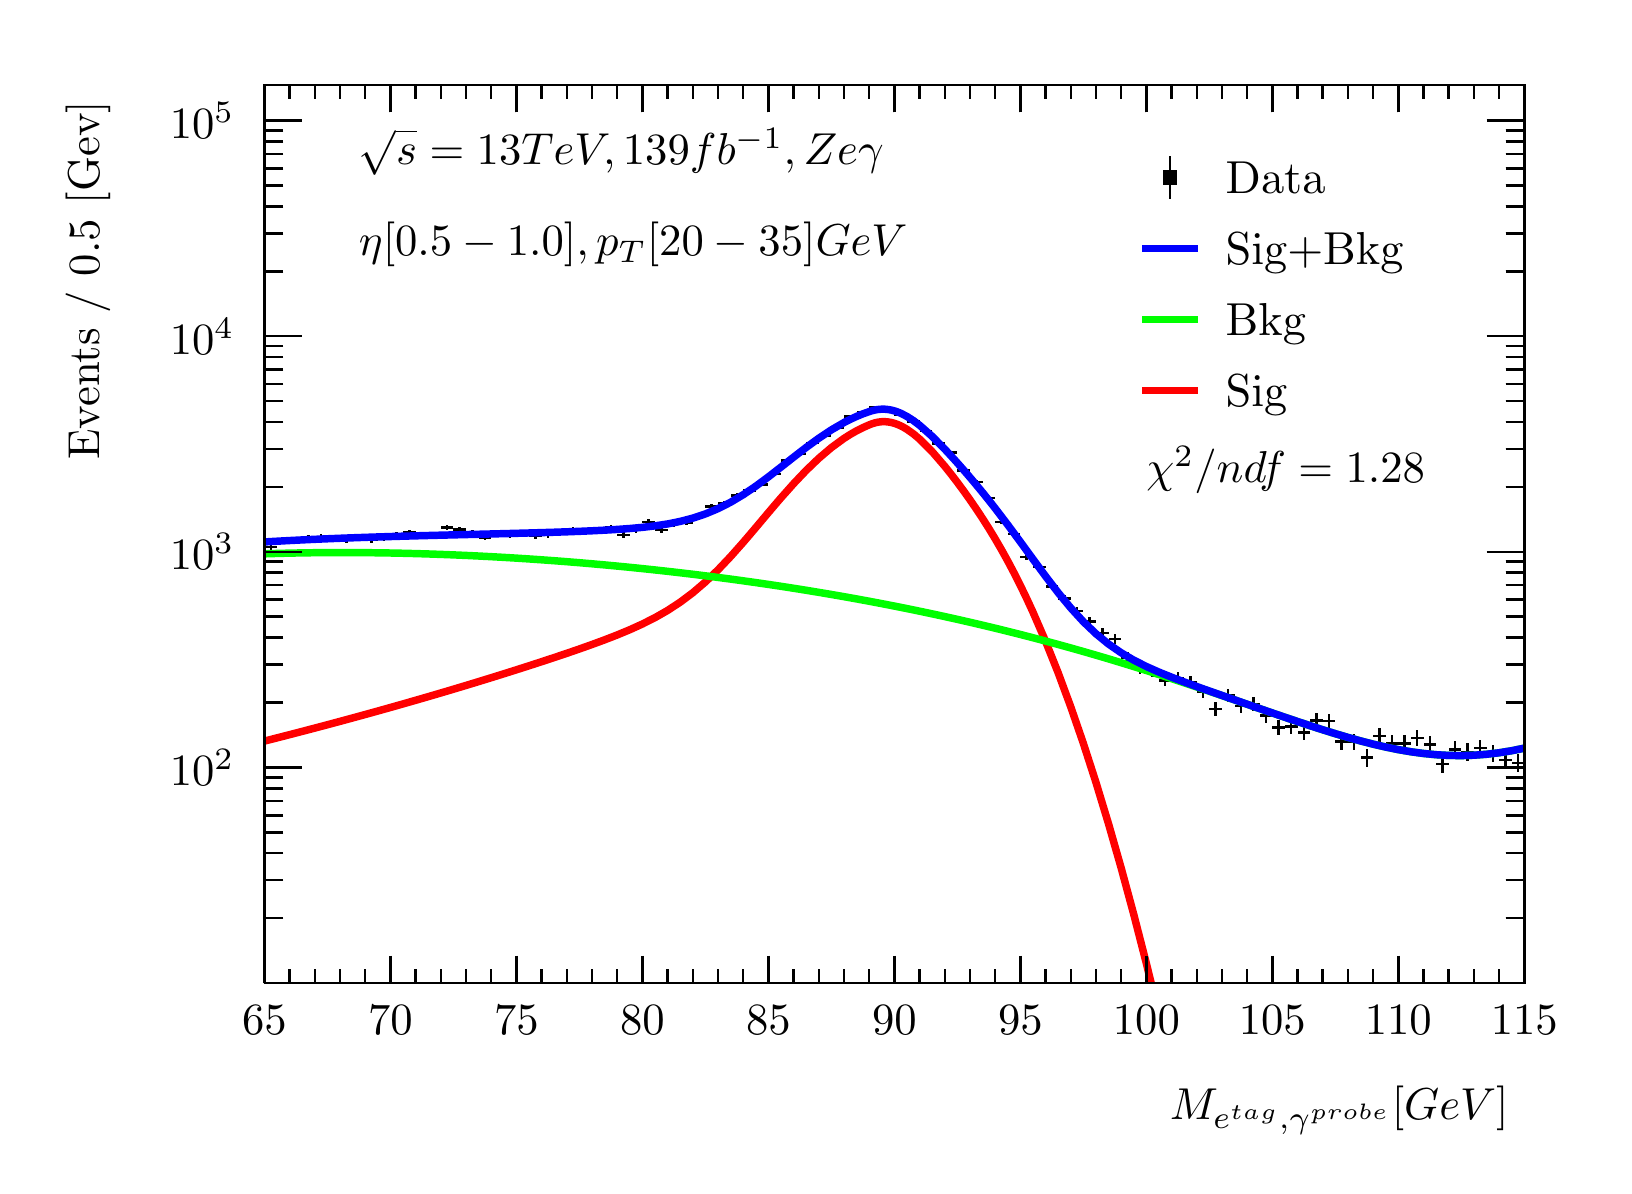
\begin{tikzpicture}
\pgfdeclareplotmark{cross} {
\pgfpathmoveto{\pgfpoint{-0.3\pgfplotmarksize}{\pgfplotmarksize}}
\pgfpathlineto{\pgfpoint{+0.3\pgfplotmarksize}{\pgfplotmarksize}}
\pgfpathlineto{\pgfpoint{+0.3\pgfplotmarksize}{0.3\pgfplotmarksize}}
\pgfpathlineto{\pgfpoint{+1\pgfplotmarksize}{0.3\pgfplotmarksize}}
\pgfpathlineto{\pgfpoint{+1\pgfplotmarksize}{-0.3\pgfplotmarksize}}
\pgfpathlineto{\pgfpoint{+0.3\pgfplotmarksize}{-0.3\pgfplotmarksize}}
\pgfpathlineto{\pgfpoint{+0.3\pgfplotmarksize}{-1.\pgfplotmarksize}}
\pgfpathlineto{\pgfpoint{-0.3\pgfplotmarksize}{-1.\pgfplotmarksize}}
\pgfpathlineto{\pgfpoint{-0.3\pgfplotmarksize}{-0.3\pgfplotmarksize}}
\pgfpathlineto{\pgfpoint{-1.\pgfplotmarksize}{-0.3\pgfplotmarksize}}
\pgfpathlineto{\pgfpoint{-1.\pgfplotmarksize}{0.3\pgfplotmarksize}}
\pgfpathlineto{\pgfpoint{-0.3\pgfplotmarksize}{0.3\pgfplotmarksize}}
\pgfpathclose
\pgfusepathqstroke
}
\pgfdeclareplotmark{cross*} {
\pgfpathmoveto{\pgfpoint{-0.3\pgfplotmarksize}{\pgfplotmarksize}}
\pgfpathlineto{\pgfpoint{+0.3\pgfplotmarksize}{\pgfplotmarksize}}
\pgfpathlineto{\pgfpoint{+0.3\pgfplotmarksize}{0.3\pgfplotmarksize}}
\pgfpathlineto{\pgfpoint{+1\pgfplotmarksize}{0.3\pgfplotmarksize}}
\pgfpathlineto{\pgfpoint{+1\pgfplotmarksize}{-0.3\pgfplotmarksize}}
\pgfpathlineto{\pgfpoint{+0.3\pgfplotmarksize}{-0.3\pgfplotmarksize}}
\pgfpathlineto{\pgfpoint{+0.3\pgfplotmarksize}{-1.\pgfplotmarksize}}
\pgfpathlineto{\pgfpoint{-0.3\pgfplotmarksize}{-1.\pgfplotmarksize}}
\pgfpathlineto{\pgfpoint{-0.3\pgfplotmarksize}{-0.3\pgfplotmarksize}}
\pgfpathlineto{\pgfpoint{-1.\pgfplotmarksize}{-0.3\pgfplotmarksize}}
\pgfpathlineto{\pgfpoint{-1.\pgfplotmarksize}{0.3\pgfplotmarksize}}
\pgfpathlineto{\pgfpoint{-0.3\pgfplotmarksize}{0.3\pgfplotmarksize}}
\pgfpathclose
\pgfusepathqfillstroke
}
\pgfdeclareplotmark{newstar} {
\pgfpathmoveto{\pgfqpoint{0pt}{\pgfplotmarksize}}
\pgfpathlineto{\pgfqpointpolar{44}{0.5\pgfplotmarksize}}
\pgfpathlineto{\pgfqpointpolar{18}{\pgfplotmarksize}}
\pgfpathlineto{\pgfqpointpolar{-20}{0.5\pgfplotmarksize}}
\pgfpathlineto{\pgfqpointpolar{-54}{\pgfplotmarksize}}
\pgfpathlineto{\pgfqpointpolar{-90}{0.5\pgfplotmarksize}}
\pgfpathlineto{\pgfqpointpolar{234}{\pgfplotmarksize}}
\pgfpathlineto{\pgfqpointpolar{198}{0.5\pgfplotmarksize}}
\pgfpathlineto{\pgfqpointpolar{162}{\pgfplotmarksize}}
\pgfpathlineto{\pgfqpointpolar{134}{0.5\pgfplotmarksize}}
\pgfpathclose
\pgfusepathqstroke
}
\pgfdeclareplotmark{newstar*} {
\pgfpathmoveto{\pgfqpoint{0pt}{\pgfplotmarksize}}
\pgfpathlineto{\pgfqpointpolar{44}{0.5\pgfplotmarksize}}
\pgfpathlineto{\pgfqpointpolar{18}{\pgfplotmarksize}}
\pgfpathlineto{\pgfqpointpolar{-20}{0.5\pgfplotmarksize}}
\pgfpathlineto{\pgfqpointpolar{-54}{\pgfplotmarksize}}
\pgfpathlineto{\pgfqpointpolar{-90}{0.5\pgfplotmarksize}}
\pgfpathlineto{\pgfqpointpolar{234}{\pgfplotmarksize}}
\pgfpathlineto{\pgfqpointpolar{198}{0.5\pgfplotmarksize}}
\pgfpathlineto{\pgfqpointpolar{162}{\pgfplotmarksize}}
\pgfpathlineto{\pgfqpointpolar{134}{0.5\pgfplotmarksize}}
\pgfpathclose
\pgfusepathqfillstroke
}
\definecolor{c}{rgb}{1,1,1};
\draw [color=c, fill=c] (0,0) rectangle (20,14.4361);
\draw [color=c, fill=c] (3,2.30977) rectangle (19,13.7143);
\definecolor{c}{rgb}{0,0,0};
\draw [c,line width=0.9] (3,2.30977) -- (3,13.7143) -- (19,13.7143) -- (19,2.30977) -- (3,2.30977);
\definecolor{c}{rgb}{1,1,1};
\draw [color=c, fill=c] (3,2.30977) rectangle (19,13.7143);
\definecolor{c}{rgb}{0,0,0};
\draw [c,line width=0.9] (3,2.30977) -- (3,13.7143) -- (19,13.7143) -- (19,2.30977) -- (3,2.30977);
\draw [c,line width=0.9] (3,2.30977) -- (19,2.30977);
\draw [c,line width=0.9] (3,2.65624) -- (3,2.30977);
\draw [c,line width=0.9] (3.32,2.48301) -- (3.32,2.30977);
\draw [c,line width=0.9] (3.64,2.48301) -- (3.64,2.30977);
\draw [c,line width=0.9] (3.96,2.48301) -- (3.96,2.30977);
\draw [c,line width=0.9] (4.28,2.48301) -- (4.28,2.30977);
\draw [c,line width=0.9] (4.6,2.65624) -- (4.6,2.30977);
\draw [c,line width=0.9] (4.92,2.48301) -- (4.92,2.30977);
\draw [c,line width=0.9] (5.24,2.48301) -- (5.24,2.30977);
\draw [c,line width=0.9] (5.56,2.48301) -- (5.56,2.30977);
\draw [c,line width=0.9] (5.88,2.48301) -- (5.88,2.30977);
\draw [c,line width=0.9] (6.2,2.65624) -- (6.2,2.30977);
\draw [c,line width=0.9] (6.52,2.48301) -- (6.52,2.30977);
\draw [c,line width=0.9] (6.84,2.48301) -- (6.84,2.30977);
\draw [c,line width=0.9] (7.16,2.48301) -- (7.16,2.30977);
\draw [c,line width=0.9] (7.48,2.48301) -- (7.48,2.30977);
\draw [c,line width=0.9] (7.8,2.65624) -- (7.8,2.30977);
\draw [c,line width=0.9] (8.12,2.48301) -- (8.12,2.30977);
\draw [c,line width=0.9] (8.44,2.48301) -- (8.44,2.30977);
\draw [c,line width=0.9] (8.76,2.48301) -- (8.76,2.30977);
\draw [c,line width=0.9] (9.08,2.48301) -- (9.08,2.30977);
\draw [c,line width=0.9] (9.4,2.65624) -- (9.4,2.30977);
\draw [c,line width=0.9] (9.72,2.48301) -- (9.72,2.30977);
\draw [c,line width=0.9] (10.04,2.48301) -- (10.04,2.30977);
\draw [c,line width=0.9] (10.36,2.48301) -- (10.36,2.30977);
\draw [c,line width=0.9] (10.68,2.48301) -- (10.68,2.30977);
\draw [c,line width=0.9] (11,2.65624) -- (11,2.30977);
\draw [c,line width=0.9] (11.32,2.48301) -- (11.32,2.30977);
\draw [c,line width=0.9] (11.64,2.48301) -- (11.64,2.30977);
\draw [c,line width=0.9] (11.96,2.48301) -- (11.96,2.30977);
\draw [c,line width=0.9] (12.28,2.48301) -- (12.28,2.30977);
\draw [c,line width=0.9] (12.6,2.65624) -- (12.6,2.30977);
\draw [c,line width=0.9] (12.92,2.48301) -- (12.92,2.30977);
\draw [c,line width=0.9] (13.24,2.48301) -- (13.24,2.30977);
\draw [c,line width=0.9] (13.56,2.48301) -- (13.56,2.30977);
\draw [c,line width=0.9] (13.88,2.48301) -- (13.88,2.30977);
\draw [c,line width=0.9] (14.2,2.65624) -- (14.2,2.30977);
\draw [c,line width=0.9] (14.52,2.48301) -- (14.52,2.30977);
\draw [c,line width=0.9] (14.84,2.48301) -- (14.84,2.30977);
\draw [c,line width=0.9] (15.16,2.48301) -- (15.16,2.30977);
\draw [c,line width=0.9] (15.48,2.48301) -- (15.48,2.30977);
\draw [c,line width=0.9] (15.8,2.65624) -- (15.8,2.30977);
\draw [c,line width=0.9] (16.12,2.48301) -- (16.12,2.30977);
\draw [c,line width=0.9] (16.44,2.48301) -- (16.44,2.30977);
\draw [c,line width=0.9] (16.76,2.48301) -- (16.76,2.30977);
\draw [c,line width=0.9] (17.08,2.48301) -- (17.08,2.30977);
\draw [c,line width=0.9] (17.4,2.65624) -- (17.4,2.30977);
\draw [c,line width=0.9] (17.72,2.48301) -- (17.72,2.30977);
\draw [c,line width=0.9] (18.04,2.48301) -- (18.04,2.30977);
\draw [c,line width=0.9] (18.36,2.48301) -- (18.36,2.30977);
\draw [c,line width=0.9] (18.68,2.48301) -- (18.68,2.30977);
\draw [c,line width=0.9] (19,2.65624) -- (19,2.30977);
\draw [c,line width=0.9] (19,2.65624) -- (19,2.30977);
\draw [anchor=base] (3,1.66015) node[scale=1.61424, color=c, rotate=0]{65};
\draw [anchor=base] (4.6,1.66015) node[scale=1.61424, color=c, rotate=0]{70};
\draw [anchor=base] (6.2,1.66015) node[scale=1.61424, color=c, rotate=0]{75};
\draw [anchor=base] (7.8,1.66015) node[scale=1.61424, color=c, rotate=0]{80};
\draw [anchor=base] (9.4,1.66015) node[scale=1.61424, color=c, rotate=0]{85};
\draw [anchor=base] (11,1.66015) node[scale=1.61424, color=c, rotate=0]{90};
\draw [anchor=base] (12.6,1.66015) node[scale=1.61424, color=c, rotate=0]{95};
\draw [anchor=base] (14.2,1.66015) node[scale=1.61424, color=c, rotate=0]{100};
\draw [anchor=base] (15.8,1.66015) node[scale=1.61424, color=c, rotate=0]{105};
\draw [anchor=base] (17.4,1.66015) node[scale=1.61424, color=c, rotate=0]{110};
\draw [anchor=base] (19,1.66015) node[scale=1.61424, color=c, rotate=0]{115};
\draw [anchor= east] (19,0.692932) node[scale=1.61424, color=c, rotate=0]{$M_{e^{tag}, \gamma^{probe}}  [GeV]$};
\draw [c,line width=0.9] (3,13.7143) -- (19,13.7143);
\draw [c,line width=0.9] (3,13.3678) -- (3,13.7143);
\draw [c,line width=0.9] (3.32,13.5411) -- (3.32,13.7143);
\draw [c,line width=0.9] (3.64,13.5411) -- (3.64,13.7143);
\draw [c,line width=0.9] (3.96,13.5411) -- (3.96,13.7143);
\draw [c,line width=0.9] (4.28,13.5411) -- (4.28,13.7143);
\draw [c,line width=0.9] (4.6,13.3678) -- (4.6,13.7143);
\draw [c,line width=0.9] (4.92,13.5411) -- (4.92,13.7143);
\draw [c,line width=0.9] (5.24,13.5411) -- (5.24,13.7143);
\draw [c,line width=0.9] (5.56,13.5411) -- (5.56,13.7143);
\draw [c,line width=0.9] (5.88,13.5411) -- (5.88,13.7143);
\draw [c,line width=0.9] (6.2,13.3678) -- (6.2,13.7143);
\draw [c,line width=0.9] (6.52,13.5411) -- (6.52,13.7143);
\draw [c,line width=0.9] (6.84,13.5411) -- (6.84,13.7143);
\draw [c,line width=0.9] (7.16,13.5411) -- (7.16,13.7143);
\draw [c,line width=0.9] (7.48,13.5411) -- (7.48,13.7143);
\draw [c,line width=0.9] (7.8,13.3678) -- (7.8,13.7143);
\draw [c,line width=0.9] (8.12,13.5411) -- (8.12,13.7143);
\draw [c,line width=0.9] (8.44,13.5411) -- (8.44,13.7143);
\draw [c,line width=0.9] (8.76,13.5411) -- (8.76,13.7143);
\draw [c,line width=0.9] (9.08,13.5411) -- (9.08,13.7143);
\draw [c,line width=0.9] (9.4,13.3678) -- (9.4,13.7143);
\draw [c,line width=0.9] (9.72,13.5411) -- (9.72,13.7143);
\draw [c,line width=0.9] (10.04,13.5411) -- (10.04,13.7143);
\draw [c,line width=0.9] (10.36,13.5411) -- (10.36,13.7143);
\draw [c,line width=0.9] (10.68,13.5411) -- (10.68,13.7143);
\draw [c,line width=0.9] (11,13.3678) -- (11,13.7143);
\draw [c,line width=0.9] (11.32,13.5411) -- (11.32,13.7143);
\draw [c,line width=0.9] (11.64,13.5411) -- (11.64,13.7143);
\draw [c,line width=0.9] (11.96,13.5411) -- (11.96,13.7143);
\draw [c,line width=0.9] (12.28,13.5411) -- (12.28,13.7143);
\draw [c,line width=0.9] (12.6,13.3678) -- (12.6,13.7143);
\draw [c,line width=0.9] (12.92,13.5411) -- (12.92,13.7143);
\draw [c,line width=0.9] (13.24,13.5411) -- (13.24,13.7143);
\draw [c,line width=0.9] (13.56,13.5411) -- (13.56,13.7143);
\draw [c,line width=0.9] (13.88,13.5411) -- (13.88,13.7143);
\draw [c,line width=0.9] (14.2,13.3678) -- (14.2,13.7143);
\draw [c,line width=0.9] (14.52,13.5411) -- (14.52,13.7143);
\draw [c,line width=0.9] (14.84,13.5411) -- (14.84,13.7143);
\draw [c,line width=0.9] (15.16,13.5411) -- (15.16,13.7143);
\draw [c,line width=0.9] (15.48,13.5411) -- (15.48,13.7143);
\draw [c,line width=0.9] (15.8,13.3678) -- (15.8,13.7143);
\draw [c,line width=0.9] (16.12,13.5411) -- (16.12,13.7143);
\draw [c,line width=0.9] (16.44,13.5411) -- (16.44,13.7143);
\draw [c,line width=0.9] (16.76,13.5411) -- (16.76,13.7143);
\draw [c,line width=0.9] (17.08,13.5411) -- (17.08,13.7143);
\draw [c,line width=0.9] (17.4,13.3678) -- (17.4,13.7143);
\draw [c,line width=0.9] (17.72,13.5411) -- (17.72,13.7143);
\draw [c,line width=0.9] (18.04,13.5411) -- (18.04,13.7143);
\draw [c,line width=0.9] (18.36,13.5411) -- (18.36,13.7143);
\draw [c,line width=0.9] (18.68,13.5411) -- (18.68,13.7143);
\draw [c,line width=0.9] (19,13.3678) -- (19,13.7143);
\draw [c,line width=0.9] (19,13.3678) -- (19,13.7143);
\draw [c,line width=0.9] (3,2.30977) -- (3,13.7143);
\draw [c,line width=0.9] (3.237,3.13412) -- (3,3.13412);
\draw [c,line width=0.9] (3.237,3.61633) -- (3,3.61633);
\draw [c,line width=0.9] (3.237,3.95847) -- (3,3.95847);
\draw [c,line width=0.9] (3.237,4.22385) -- (3,4.22385);
\draw [c,line width=0.9] (3.237,4.44068) -- (3,4.44068);
\draw [c,line width=0.9] (3.237,4.62401) -- (3,4.62401);
\draw [c,line width=0.9] (3.237,4.78282) -- (3,4.78282);
\draw [c,line width=0.9] (3.237,4.9229) -- (3,4.9229);
\draw [c,line width=0.9] (3.474,5.0482) -- (3,5.0482);
\draw [anchor= east] (2.82,5.0482) node[scale=1.61424, color=c, rotate=0]{$10^{2}$};
\draw [c,line width=0.9] (3.237,5.87255) -- (3,5.87255);
\draw [c,line width=0.9] (3.237,6.35476) -- (3,6.35476);
\draw [c,line width=0.9] (3.237,6.6969) -- (3,6.6969);
\draw [c,line width=0.9] (3.237,6.96228) -- (3,6.96228);
\draw [c,line width=0.9] (3.237,7.17911) -- (3,7.17911);
\draw [c,line width=0.9] (3.237,7.36244) -- (3,7.36244);
\draw [c,line width=0.9] (3.237,7.52125) -- (3,7.52125);
\draw [c,line width=0.9] (3.237,7.66133) -- (3,7.66133);
\draw [c,line width=0.9] (3.474,7.78663) -- (3,7.78663);
\draw [anchor= east] (2.82,7.78663) node[scale=1.61424, color=c, rotate=0]{$10^{3}$};
\draw [c,line width=0.9] (3.237,8.61098) -- (3,8.61098);
\draw [c,line width=0.9] (3.237,9.09319) -- (3,9.09319);
\draw [c,line width=0.9] (3.237,9.43533) -- (3,9.43533);
\draw [c,line width=0.9] (3.237,9.70071) -- (3,9.70071);
\draw [c,line width=0.9] (3.237,9.91755) -- (3,9.91755);
\draw [c,line width=0.9] (3.237,10.1009) -- (3,10.1009);
\draw [c,line width=0.9] (3.237,10.2597) -- (3,10.2597);
\draw [c,line width=0.9] (3.237,10.3998) -- (3,10.3998);
\draw [c,line width=0.9] (3.474,10.5251) -- (3,10.5251);
\draw [anchor= east] (2.82,10.5251) node[scale=1.61424, color=c, rotate=0]{$10^{4}$};
\draw [c,line width=0.9] (3.237,11.3494) -- (3,11.3494);
\draw [c,line width=0.9] (3.237,11.8316) -- (3,11.8316);
\draw [c,line width=0.9] (3.237,12.1738) -- (3,12.1738);
\draw [c,line width=0.9] (3.237,12.4391) -- (3,12.4391);
\draw [c,line width=0.9] (3.237,12.656) -- (3,12.656);
\draw [c,line width=0.9] (3.237,12.8393) -- (3,12.8393);
\draw [c,line width=0.9] (3.237,12.9981) -- (3,12.9981);
\draw [c,line width=0.9] (3.237,13.1382) -- (3,13.1382);
\draw [c,line width=0.9] (3.474,13.2635) -- (3,13.2635);
\draw [anchor= east] (2.82,13.2635) node[scale=1.61424, color=c, rotate=0]{$10^{5}$};
\draw [anchor= east] (0.76,13.7143) node[scale=1.61424, color=c, rotate=90]{Events / 0.5 [Gev]};
\draw [c,line width=0.9] (19,2.30977) -- (19,13.7143);
\draw [c,line width=0.9] (18.763,3.13412) -- (19,3.13412);
\draw [c,line width=0.9] (18.763,3.61633) -- (19,3.61633);
\draw [c,line width=0.9] (18.763,3.95847) -- (19,3.95847);
\draw [c,line width=0.9] (18.763,4.22385) -- (19,4.22385);
\draw [c,line width=0.9] (18.763,4.44068) -- (19,4.44068);
\draw [c,line width=0.9] (18.763,4.62401) -- (19,4.62401);
\draw [c,line width=0.9] (18.763,4.78282) -- (19,4.78282);
\draw [c,line width=0.9] (18.763,4.9229) -- (19,4.9229);
\draw [c,line width=0.9] (18.526,5.0482) -- (19,5.0482);
\draw [c,line width=0.9] (18.763,5.87255) -- (19,5.87255);
\draw [c,line width=0.9] (18.763,6.35476) -- (19,6.35476);
\draw [c,line width=0.9] (18.763,6.6969) -- (19,6.6969);
\draw [c,line width=0.9] (18.763,6.96228) -- (19,6.96228);
\draw [c,line width=0.9] (18.763,7.17911) -- (19,7.17911);
\draw [c,line width=0.9] (18.763,7.36244) -- (19,7.36244);
\draw [c,line width=0.9] (18.763,7.52125) -- (19,7.52125);
\draw [c,line width=0.9] (18.763,7.66133) -- (19,7.66133);
\draw [c,line width=0.9] (18.526,7.78663) -- (19,7.78663);
\draw [c,line width=0.9] (18.763,8.61098) -- (19,8.61098);
\draw [c,line width=0.9] (18.763,9.09319) -- (19,9.09319);
\draw [c,line width=0.9] (18.763,9.43533) -- (19,9.43533);
\draw [c,line width=0.9] (18.763,9.70071) -- (19,9.70071);
\draw [c,line width=0.9] (18.763,9.91755) -- (19,9.91755);
\draw [c,line width=0.9] (18.763,10.1009) -- (19,10.1009);
\draw [c,line width=0.9] (18.763,10.2597) -- (19,10.2597);
\draw [c,line width=0.9] (18.763,10.3998) -- (19,10.3998);
\draw [c,line width=0.9] (18.526,10.5251) -- (19,10.5251);
\draw [c,line width=0.9] (18.763,11.3494) -- (19,11.3494);
\draw [c,line width=0.9] (18.763,11.8316) -- (19,11.8316);
\draw [c,line width=0.9] (18.763,12.1738) -- (19,12.1738);
\draw [c,line width=0.9] (18.763,12.4391) -- (19,12.4391);
\draw [c,line width=0.9] (18.763,12.656) -- (19,12.656);
\draw [c,line width=0.9] (18.763,12.8393) -- (19,12.8393);
\draw [c,line width=0.9] (18.763,12.9981) -- (19,12.9981);
\draw [c,line width=0.9] (18.763,13.1382) -- (19,13.1382);
\draw [c,line width=0.9] (18.526,13.2635) -- (19,13.2635);
\draw [c,line width=0.9] (3.08,7.85031) -- (3,7.85031);
\draw [c,line width=0.9] (3,7.85031) -- (3,7.85031);
\draw [c,line width=0.9] (3.08,7.85031) -- (3.16,7.85031);
\draw [c,line width=0.9] (3.16,7.85031) -- (3.16,7.85031);
\draw [c,line width=0.9] (3.08,7.85031) -- (3.08,7.88692);
\draw [c,line width=0.9] (3.08,7.88692) -- (3.08,7.88692);
\draw [c,line width=0.9] (3.08,7.85031) -- (3.08,7.81369);
\draw [c,line width=0.9] (3.08,7.81369) -- (3.08,7.81369);
\draw [c,line width=0.9] (3.24,7.93409) -- (3.16,7.93409);
\draw [c,line width=0.9] (3.16,7.93409) -- (3.16,7.93409);
\draw [c,line width=0.9] (3.24,7.93409) -- (3.32,7.93409);
\draw [c,line width=0.9] (3.32,7.93409) -- (3.32,7.93409);
\draw [c,line width=0.9] (3.24,7.93409) -- (3.24,7.96943);
\draw [c,line width=0.9] (3.24,7.96943) -- (3.24,7.96943);
\draw [c,line width=0.9] (3.24,7.93409) -- (3.24,7.89874);
\draw [c,line width=0.9] (3.24,7.89874) -- (3.24,7.89874);
\draw [c,line width=0.9] (3.4,7.91503) -- (3.32,7.91503);
\draw [c,line width=0.9] (3.32,7.91503) -- (3.32,7.91503);
\draw [c,line width=0.9] (3.4,7.91503) -- (3.48,7.91503);
\draw [c,line width=0.9] (3.48,7.91503) -- (3.48,7.91503);
\draw [c,line width=0.9] (3.4,7.91503) -- (3.4,7.95066);
\draw [c,line width=0.9] (3.4,7.95066) -- (3.4,7.95066);
\draw [c,line width=0.9] (3.4,7.91503) -- (3.4,7.87939);
\draw [c,line width=0.9] (3.4,7.87939) -- (3.4,7.87939);
\draw [c,line width=0.9] (3.56,7.9652) -- (3.48,7.9652);
\draw [c,line width=0.9] (3.48,7.9652) -- (3.48,7.9652);
\draw [c,line width=0.9] (3.56,7.9652) -- (3.64,7.9652);
\draw [c,line width=0.9] (3.64,7.9652) -- (3.64,7.9652);
\draw [c,line width=0.9] (3.56,7.9652) -- (3.56,8.00008);
\draw [c,line width=0.9] (3.56,8.00008) -- (3.56,8.00008);
\draw [c,line width=0.9] (3.56,7.9652) -- (3.56,7.93031);
\draw [c,line width=0.9] (3.56,7.93031) -- (3.56,7.93031);
\draw [c,line width=0.9] (3.72,7.97437) -- (3.64,7.97437);
\draw [c,line width=0.9] (3.64,7.97437) -- (3.64,7.97437);
\draw [c,line width=0.9] (3.72,7.97437) -- (3.8,7.97437);
\draw [c,line width=0.9] (3.8,7.97437) -- (3.8,7.97437);
\draw [c,line width=0.9] (3.72,7.97437) -- (3.72,8.00912);
\draw [c,line width=0.9] (3.72,8.00912) -- (3.72,8.00912);
\draw [c,line width=0.9] (3.72,7.97437) -- (3.72,7.93962);
\draw [c,line width=0.9] (3.72,7.93962) -- (3.72,7.93962);
\draw [c,line width=0.9] (3.88,7.94351) -- (3.8,7.94351);
\draw [c,line width=0.9] (3.8,7.94351) -- (3.8,7.94351);
\draw [c,line width=0.9] (3.88,7.94351) -- (3.96,7.94351);
\draw [c,line width=0.9] (3.96,7.94351) -- (3.96,7.94351);
\draw [c,line width=0.9] (3.88,7.94351) -- (3.88,7.97871);
\draw [c,line width=0.9] (3.88,7.97871) -- (3.88,7.97871);
\draw [c,line width=0.9] (3.88,7.94351) -- (3.88,7.9083);
\draw [c,line width=0.9] (3.88,7.9083) -- (3.88,7.9083);
\draw [c,line width=0.9] (4.04,7.93409) -- (3.96,7.93409);
\draw [c,line width=0.9] (3.96,7.93409) -- (3.96,7.93409);
\draw [c,line width=0.9] (4.04,7.93409) -- (4.12,7.93409);
\draw [c,line width=0.9] (4.12,7.93409) -- (4.12,7.93409);
\draw [c,line width=0.9] (4.04,7.93409) -- (4.04,7.96943);
\draw [c,line width=0.9] (4.04,7.96943) -- (4.04,7.96943);
\draw [c,line width=0.9] (4.04,7.93409) -- (4.04,7.89874);
\draw [c,line width=0.9] (4.04,7.89874) -- (4.04,7.89874);
\draw [c,line width=0.9] (4.2,7.97336) -- (4.12,7.97336);
\draw [c,line width=0.9] (4.12,7.97336) -- (4.12,7.97336);
\draw [c,line width=0.9] (4.2,7.97336) -- (4.28,7.97336);
\draw [c,line width=0.9] (4.28,7.97336) -- (4.28,7.97336);
\draw [c,line width=0.9] (4.2,7.97336) -- (4.2,8.00812);
\draw [c,line width=0.9] (4.2,8.00812) -- (4.2,8.00812);
\draw [c,line width=0.9] (4.2,7.97336) -- (4.2,7.93859);
\draw [c,line width=0.9] (4.2,7.93859) -- (4.2,7.93859);
\draw [c,line width=0.9] (4.36,7.93619) -- (4.28,7.93619);
\draw [c,line width=0.9] (4.28,7.93619) -- (4.28,7.93619);
\draw [c,line width=0.9] (4.36,7.93619) -- (4.44,7.93619);
\draw [c,line width=0.9] (4.44,7.93619) -- (4.44,7.93619);
\draw [c,line width=0.9] (4.36,7.93619) -- (4.36,7.9715);
\draw [c,line width=0.9] (4.36,7.9715) -- (4.36,7.9715);
\draw [c,line width=0.9] (4.36,7.93619) -- (4.36,7.90087);
\draw [c,line width=0.9] (4.36,7.90087) -- (4.36,7.90087);
\draw [c,line width=0.9] (4.52,7.95285) -- (4.44,7.95285);
\draw [c,line width=0.9] (4.44,7.95285) -- (4.44,7.95285);
\draw [c,line width=0.9] (4.52,7.95285) -- (4.6,7.95285);
\draw [c,line width=0.9] (4.6,7.95285) -- (4.6,7.95285);
\draw [c,line width=0.9] (4.52,7.95285) -- (4.52,7.98792);
\draw [c,line width=0.9] (4.52,7.98792) -- (4.52,7.98792);
\draw [c,line width=0.9] (4.52,7.95285) -- (4.52,7.91778);
\draw [c,line width=0.9] (4.52,7.91778) -- (4.52,7.91778);
\draw [c,line width=0.9] (4.68,8.0094) -- (4.6,8.0094);
\draw [c,line width=0.9] (4.6,8.0094) -- (4.6,8.0094);
\draw [c,line width=0.9] (4.68,8.0094) -- (4.76,8.0094);
\draw [c,line width=0.9] (4.76,8.0094) -- (4.76,8.0094);
\draw [c,line width=0.9] (4.68,8.0094) -- (4.68,8.04364);
\draw [c,line width=0.9] (4.68,8.04364) -- (4.68,8.04364);
\draw [c,line width=0.9] (4.68,8.0094) -- (4.68,7.97515);
\draw [c,line width=0.9] (4.68,7.97515) -- (4.68,7.97515);
\draw [c,line width=0.9] (4.84,8.03283) -- (4.76,8.03283);
\draw [c,line width=0.9] (4.76,8.03283) -- (4.76,8.03283);
\draw [c,line width=0.9] (4.84,8.03283) -- (4.92,8.03283);
\draw [c,line width=0.9] (4.92,8.03283) -- (4.92,8.03283);
\draw [c,line width=0.9] (4.84,8.03283) -- (4.84,8.06674);
\draw [c,line width=0.9] (4.84,8.06674) -- (4.84,8.06674);
\draw [c,line width=0.9] (4.84,8.03283) -- (4.84,7.99892);
\draw [c,line width=0.9] (4.84,7.99892) -- (4.84,7.99892);
\draw [c,line width=0.9] (5,7.9975) -- (4.92,7.9975);
\draw [c,line width=0.9] (4.92,7.9975) -- (4.92,7.9975);
\draw [c,line width=0.9] (5,7.9975) -- (5.08,7.9975);
\draw [c,line width=0.9] (5.08,7.9975) -- (5.08,7.9975);
\draw [c,line width=0.9] (5,7.9975) -- (5,8.03192);
\draw [c,line width=0.9] (5,8.03192) -- (5,8.03192);
\draw [c,line width=0.9] (5,7.9975) -- (5,7.96309);
\draw [c,line width=0.9] (5,7.96309) -- (5,7.96309);
\draw [c,line width=0.9] (5.16,7.98951) -- (5.08,7.98951);
\draw [c,line width=0.9] (5.08,7.98951) -- (5.08,7.98951);
\draw [c,line width=0.9] (5.16,7.98951) -- (5.24,7.98951);
\draw [c,line width=0.9] (5.24,7.98951) -- (5.24,7.98951);
\draw [c,line width=0.9] (5.16,7.98951) -- (5.16,8.02404);
\draw [c,line width=0.9] (5.16,8.02404) -- (5.16,8.02404);
\draw [c,line width=0.9] (5.16,7.98951) -- (5.16,7.95498);
\draw [c,line width=0.9] (5.16,7.95498) -- (5.16,7.95498);
\draw [c,line width=0.9] (5.32,8.09224) -- (5.24,8.09224);
\draw [c,line width=0.9] (5.24,8.09224) -- (5.24,8.09224);
\draw [c,line width=0.9] (5.32,8.09224) -- (5.4,8.09224);
\draw [c,line width=0.9] (5.4,8.09224) -- (5.4,8.09224);
\draw [c,line width=0.9] (5.32,8.09224) -- (5.32,8.12531);
\draw [c,line width=0.9] (5.32,8.12531) -- (5.32,8.12531);
\draw [c,line width=0.9] (5.32,8.09224) -- (5.32,8.05917);
\draw [c,line width=0.9] (5.32,8.05917) -- (5.32,8.05917);
\draw [c,line width=0.9] (5.48,8.06714) -- (5.4,8.06714);
\draw [c,line width=0.9] (5.4,8.06714) -- (5.4,8.06714);
\draw [c,line width=0.9] (5.48,8.06714) -- (5.56,8.06714);
\draw [c,line width=0.9] (5.56,8.06714) -- (5.56,8.06714);
\draw [c,line width=0.9] (5.48,8.06714) -- (5.48,8.10056);
\draw [c,line width=0.9] (5.48,8.10056) -- (5.48,8.10056);
\draw [c,line width=0.9] (5.48,8.06714) -- (5.48,8.03372);
\draw [c,line width=0.9] (5.48,8.03372) -- (5.48,8.03372);
\draw [c,line width=0.9] (5.64,8.03476) -- (5.56,8.03476);
\draw [c,line width=0.9] (5.56,8.03476) -- (5.56,8.03476);
\draw [c,line width=0.9] (5.64,8.03476) -- (5.72,8.03476);
\draw [c,line width=0.9] (5.72,8.03476) -- (5.72,8.03476);
\draw [c,line width=0.9] (5.64,8.03476) -- (5.64,8.06865);
\draw [c,line width=0.9] (5.64,8.06865) -- (5.64,8.06865);
\draw [c,line width=0.9] (5.64,8.03476) -- (5.64,8.00088);
\draw [c,line width=0.9] (5.64,8.00088) -- (5.64,8.00088);
\draw [c,line width=0.9] (5.8,7.9703) -- (5.72,7.9703);
\draw [c,line width=0.9] (5.72,7.9703) -- (5.72,7.9703);
\draw [c,line width=0.9] (5.8,7.9703) -- (5.88,7.9703);
\draw [c,line width=0.9] (5.88,7.9703) -- (5.88,7.9703);
\draw [c,line width=0.9] (5.8,7.9703) -- (5.8,8.00511);
\draw [c,line width=0.9] (5.8,8.00511) -- (5.8,8.00511);
\draw [c,line width=0.9] (5.8,7.9703) -- (5.8,7.93549);
\draw [c,line width=0.9] (5.8,7.93549) -- (5.8,7.93549);
\draw [c,line width=0.9] (5.96,8.03573) -- (5.88,8.03573);
\draw [c,line width=0.9] (5.88,8.03573) -- (5.88,8.03573);
\draw [c,line width=0.9] (5.96,8.03573) -- (6.04,8.03573);
\draw [c,line width=0.9] (6.04,8.03573) -- (6.04,8.03573);
\draw [c,line width=0.9] (5.96,8.03573) -- (5.96,8.0696);
\draw [c,line width=0.9] (5.96,8.0696) -- (5.96,8.0696);
\draw [c,line width=0.9] (5.96,8.03573) -- (5.96,8.00186);
\draw [c,line width=0.9] (5.96,8.00186) -- (5.96,8.00186);
\draw [c,line width=0.9] (6.12,7.99251) -- (6.04,7.99251);
\draw [c,line width=0.9] (6.04,7.99251) -- (6.04,7.99251);
\draw [c,line width=0.9] (6.12,7.99251) -- (6.2,7.99251);
\draw [c,line width=0.9] (6.2,7.99251) -- (6.2,7.99251);
\draw [c,line width=0.9] (6.12,7.99251) -- (6.12,8.027);
\draw [c,line width=0.9] (6.12,8.027) -- (6.12,8.027);
\draw [c,line width=0.9] (6.12,7.99251) -- (6.12,7.95802);
\draw [c,line width=0.9] (6.12,7.95802) -- (6.12,7.95802);
\draw [c,line width=0.9] (6.28,8.03283) -- (6.2,8.03283);
\draw [c,line width=0.9] (6.2,8.03283) -- (6.2,8.03283);
\draw [c,line width=0.9] (6.28,8.03283) -- (6.36,8.03283);
\draw [c,line width=0.9] (6.36,8.03283) -- (6.36,8.03283);
\draw [c,line width=0.9] (6.28,8.03283) -- (6.28,8.06674);
\draw [c,line width=0.9] (6.28,8.06674) -- (6.28,8.06674);
\draw [c,line width=0.9] (6.28,8.03283) -- (6.28,7.99892);
\draw [c,line width=0.9] (6.28,7.99892) -- (6.28,7.99892);
\draw [c,line width=0.9] (6.44,7.98951) -- (6.36,7.98951);
\draw [c,line width=0.9] (6.36,7.98951) -- (6.36,7.98951);
\draw [c,line width=0.9] (6.44,7.98951) -- (6.52,7.98951);
\draw [c,line width=0.9] (6.52,7.98951) -- (6.52,7.98951);
\draw [c,line width=0.9] (6.44,7.98951) -- (6.44,8.02404);
\draw [c,line width=0.9] (6.44,8.02404) -- (6.44,8.02404);
\draw [c,line width=0.9] (6.44,7.98951) -- (6.44,7.95498);
\draw [c,line width=0.9] (6.44,7.95498) -- (6.44,7.95498);
\draw [c,line width=0.9] (6.6,7.99949) -- (6.52,7.99949);
\draw [c,line width=0.9] (6.52,7.99949) -- (6.52,7.99949);
\draw [c,line width=0.9] (6.6,7.99949) -- (6.68,7.99949);
\draw [c,line width=0.9] (6.68,7.99949) -- (6.68,7.99949);
\draw [c,line width=0.9] (6.6,7.99949) -- (6.6,8.03388);
\draw [c,line width=0.9] (6.6,8.03388) -- (6.6,8.03388);
\draw [c,line width=0.9] (6.6,7.99949) -- (6.6,7.96511);
\draw [c,line width=0.9] (6.6,7.96511) -- (6.6,7.96511);
\draw [c,line width=0.9] (6.76,8.04438) -- (6.68,8.04438);
\draw [c,line width=0.9] (6.68,8.04438) -- (6.68,8.04438);
\draw [c,line width=0.9] (6.76,8.04438) -- (6.84,8.04438);
\draw [c,line width=0.9] (6.84,8.04438) -- (6.84,8.04438);
\draw [c,line width=0.9] (6.76,8.04438) -- (6.76,8.07812);
\draw [c,line width=0.9] (6.76,8.07812) -- (6.76,8.07812);
\draw [c,line width=0.9] (6.76,8.04438) -- (6.76,8.01063);
\draw [c,line width=0.9] (6.76,8.01063) -- (6.76,8.01063);
\draw [c,line width=0.9] (6.92,8.07089) -- (6.84,8.07089);
\draw [c,line width=0.9] (6.84,8.07089) -- (6.84,8.07089);
\draw [c,line width=0.9] (6.92,8.07089) -- (7,8.07089);
\draw [c,line width=0.9] (7,8.07089) -- (7,8.07089);
\draw [c,line width=0.9] (6.92,8.07089) -- (6.92,8.10426);
\draw [c,line width=0.9] (6.92,8.10426) -- (6.92,8.10426);
\draw [c,line width=0.9] (6.92,8.07089) -- (6.92,8.03752);
\draw [c,line width=0.9] (6.92,8.03752) -- (6.92,8.03752);
\draw [c,line width=0.9] (7.08,8.03187) -- (7,8.03187);
\draw [c,line width=0.9] (7,8.03187) -- (7,8.03187);
\draw [c,line width=0.9] (7.08,8.03187) -- (7.16,8.03187);
\draw [c,line width=0.9] (7.16,8.03187) -- (7.16,8.03187);
\draw [c,line width=0.9] (7.08,8.03187) -- (7.08,8.06579);
\draw [c,line width=0.9] (7.08,8.06579) -- (7.08,8.06579);
\draw [c,line width=0.9] (7.08,8.03187) -- (7.08,7.99794);
\draw [c,line width=0.9] (7.08,7.99794) -- (7.08,7.99794);
\draw [c,line width=0.9] (7.24,8.0482) -- (7.16,8.0482);
\draw [c,line width=0.9] (7.16,8.0482) -- (7.16,8.0482);
\draw [c,line width=0.9] (7.24,8.0482) -- (7.32,8.0482);
\draw [c,line width=0.9] (7.32,8.0482) -- (7.32,8.0482);
\draw [c,line width=0.9] (7.24,8.0482) -- (7.24,8.08189);
\draw [c,line width=0.9] (7.24,8.08189) -- (7.24,8.08189);
\draw [c,line width=0.9] (7.24,8.0482) -- (7.24,8.01451);
\draw [c,line width=0.9] (7.24,8.01451) -- (7.24,8.01451);
\draw [c,line width=0.9] (7.4,8.09774) -- (7.32,8.09774);
\draw [c,line width=0.9] (7.32,8.09774) -- (7.32,8.09774);
\draw [c,line width=0.9] (7.4,8.09774) -- (7.48,8.09774);
\draw [c,line width=0.9] (7.48,8.09774) -- (7.48,8.09774);
\draw [c,line width=0.9] (7.4,8.09774) -- (7.4,8.13074);
\draw [c,line width=0.9] (7.4,8.13074) -- (7.4,8.13074);
\draw [c,line width=0.9] (7.4,8.09774) -- (7.4,8.06475);
\draw [c,line width=0.9] (7.4,8.06475) -- (7.4,8.06475);
\draw [c,line width=0.9] (7.56,7.9975) -- (7.48,7.9975);
\draw [c,line width=0.9] (7.48,7.9975) -- (7.48,7.9975);
\draw [c,line width=0.9] (7.56,7.9975) -- (7.64,7.9975);
\draw [c,line width=0.9] (7.64,7.9975) -- (7.64,7.9975);
\draw [c,line width=0.9] (7.56,7.9975) -- (7.56,8.03192);
\draw [c,line width=0.9] (7.56,8.03192) -- (7.56,8.03192);
\draw [c,line width=0.9] (7.56,7.9975) -- (7.56,7.96309);
\draw [c,line width=0.9] (7.56,7.96309) -- (7.56,7.96309);
\draw [c,line width=0.9] (7.72,8.06055) -- (7.64,8.06055);
\draw [c,line width=0.9] (7.64,8.06055) -- (7.64,8.06055);
\draw [c,line width=0.9] (7.72,8.06055) -- (7.8,8.06055);
\draw [c,line width=0.9] (7.8,8.06055) -- (7.8,8.06055);
\draw [c,line width=0.9] (7.72,8.06055) -- (7.72,8.09406);
\draw [c,line width=0.9] (7.72,8.09406) -- (7.72,8.09406);
\draw [c,line width=0.9] (7.72,8.06055) -- (7.72,8.02703);
\draw [c,line width=0.9] (7.72,8.02703) -- (7.72,8.02703);
\draw [c,line width=0.9] (7.88,8.16623) -- (7.8,8.16623);
\draw [c,line width=0.9] (7.8,8.16623) -- (7.8,8.16623);
\draw [c,line width=0.9] (7.88,8.16623) -- (7.96,8.16623);
\draw [c,line width=0.9] (7.96,8.16623) -- (7.96,8.16623);
\draw [c,line width=0.9] (7.88,8.16623) -- (7.88,8.19829);
\draw [c,line width=0.9] (7.88,8.19829) -- (7.88,8.19829);
\draw [c,line width=0.9] (7.88,8.16623) -- (7.88,8.13417);
\draw [c,line width=0.9] (7.88,8.13417) -- (7.88,8.13417);
\draw [c,line width=0.9] (8.04,8.06055) -- (7.96,8.06055);
\draw [c,line width=0.9] (7.96,8.06055) -- (7.96,8.06055);
\draw [c,line width=0.9] (8.04,8.06055) -- (8.12,8.06055);
\draw [c,line width=0.9] (8.12,8.06055) -- (8.12,8.06055);
\draw [c,line width=0.9] (8.04,8.06055) -- (8.04,8.09406);
\draw [c,line width=0.9] (8.04,8.09406) -- (8.04,8.09406);
\draw [c,line width=0.9] (8.04,8.06055) -- (8.04,8.02703);
\draw [c,line width=0.9] (8.04,8.02703) -- (8.04,8.02703);
\draw [c,line width=0.9] (8.2,8.13825) -- (8.12,8.13825);
\draw [c,line width=0.9] (8.12,8.13825) -- (8.12,8.13825);
\draw [c,line width=0.9] (8.2,8.13825) -- (8.28,8.13825);
\draw [c,line width=0.9] (8.28,8.13825) -- (8.28,8.13825);
\draw [c,line width=0.9] (8.2,8.13825) -- (8.2,8.17068);
\draw [c,line width=0.9] (8.2,8.17068) -- (8.2,8.17068);
\draw [c,line width=0.9] (8.2,8.13825) -- (8.2,8.10581);
\draw [c,line width=0.9] (8.2,8.10581) -- (8.2,8.10581);
\draw [c,line width=0.9] (8.36,8.1593) -- (8.28,8.1593);
\draw [c,line width=0.9] (8.28,8.1593) -- (8.28,8.1593);
\draw [c,line width=0.9] (8.36,8.1593) -- (8.44,8.1593);
\draw [c,line width=0.9] (8.44,8.1593) -- (8.44,8.1593);
\draw [c,line width=0.9] (8.36,8.1593) -- (8.36,8.19145);
\draw [c,line width=0.9] (8.36,8.19145) -- (8.36,8.19145);
\draw [c,line width=0.9] (8.36,8.1593) -- (8.36,8.12714);
\draw [c,line width=0.9] (8.36,8.12714) -- (8.36,8.12714);
\draw [c,line width=0.9] (8.52,8.25288) -- (8.44,8.25288);
\draw [c,line width=0.9] (8.44,8.25288) -- (8.44,8.25288);
\draw [c,line width=0.9] (8.52,8.25288) -- (8.6,8.25288);
\draw [c,line width=0.9] (8.6,8.25288) -- (8.6,8.25288);
\draw [c,line width=0.9] (8.52,8.25288) -- (8.52,8.2838);
\draw [c,line width=0.9] (8.52,8.2838) -- (8.52,8.2838);
\draw [c,line width=0.9] (8.52,8.25288) -- (8.52,8.22197);
\draw [c,line width=0.9] (8.52,8.22197) -- (8.52,8.22197);
\draw [c,line width=0.9] (8.68,8.36331) -- (8.6,8.36331);
\draw [c,line width=0.9] (8.6,8.36331) -- (8.6,8.36331);
\draw [c,line width=0.9] (8.68,8.36331) -- (8.76,8.36331);
\draw [c,line width=0.9] (8.76,8.36331) -- (8.76,8.36331);
\draw [c,line width=0.9] (8.68,8.36331) -- (8.68,8.39282);
\draw [c,line width=0.9] (8.68,8.39282) -- (8.68,8.39282);
\draw [c,line width=0.9] (8.68,8.36331) -- (8.68,8.3338);
\draw [c,line width=0.9] (8.68,8.3338) -- (8.68,8.3338);
\draw [c,line width=0.9] (8.84,8.39724) -- (8.76,8.39724);
\draw [c,line width=0.9] (8.76,8.39724) -- (8.76,8.39724);
\draw [c,line width=0.9] (8.84,8.39724) -- (8.92,8.39724);
\draw [c,line width=0.9] (8.92,8.39724) -- (8.92,8.39724);
\draw [c,line width=0.9] (8.84,8.39724) -- (8.84,8.42633);
\draw [c,line width=0.9] (8.84,8.42633) -- (8.84,8.42633);
\draw [c,line width=0.9] (8.84,8.39724) -- (8.84,8.36815);
\draw [c,line width=0.9] (8.84,8.36815) -- (8.84,8.36815);
\draw [c,line width=0.9] (9,8.50469) -- (8.92,8.50469);
\draw [c,line width=0.9] (8.92,8.50469) -- (8.92,8.50469);
\draw [c,line width=0.9] (9,8.50469) -- (9.08,8.50469);
\draw [c,line width=0.9] (9.08,8.50469) -- (9.08,8.50469);
\draw [c,line width=0.9] (9,8.50469) -- (9,8.5325);
\draw [c,line width=0.9] (9,8.5325) -- (9,8.5325);
\draw [c,line width=0.9] (9,8.50469) -- (9,8.47688);
\draw [c,line width=0.9] (9,8.47688) -- (9,8.47688);
\draw [c,line width=0.9] (9.16,8.56305) -- (9.08,8.56305);
\draw [c,line width=0.9] (9.08,8.56305) -- (9.08,8.56305);
\draw [c,line width=0.9] (9.16,8.56305) -- (9.24,8.56305);
\draw [c,line width=0.9] (9.24,8.56305) -- (9.24,8.56305);
\draw [c,line width=0.9] (9.16,8.56305) -- (9.16,8.59019);
\draw [c,line width=0.9] (9.16,8.59019) -- (9.16,8.59019);
\draw [c,line width=0.9] (9.16,8.56305) -- (9.16,8.53592);
\draw [c,line width=0.9] (9.16,8.53592) -- (9.16,8.53592);
\draw [c,line width=0.9] (9.32,8.64325) -- (9.24,8.64325);
\draw [c,line width=0.9] (9.24,8.64325) -- (9.24,8.64325);
\draw [c,line width=0.9] (9.32,8.64325) -- (9.4,8.64325);
\draw [c,line width=0.9] (9.4,8.64325) -- (9.4,8.64325);
\draw [c,line width=0.9] (9.32,8.64325) -- (9.32,8.66948);
\draw [c,line width=0.9] (9.32,8.66948) -- (9.32,8.66948);
\draw [c,line width=0.9] (9.32,8.64325) -- (9.32,8.61701);
\draw [c,line width=0.9] (9.32,8.61701) -- (9.32,8.61701);
\draw [c,line width=0.9] (9.48,8.77513) -- (9.4,8.77513);
\draw [c,line width=0.9] (9.4,8.77513) -- (9.4,8.77513);
\draw [c,line width=0.9] (9.48,8.77513) -- (9.56,8.77513);
\draw [c,line width=0.9] (9.56,8.77513) -- (9.56,8.77513);
\draw [c,line width=0.9] (9.48,8.77513) -- (9.48,8.79995);
\draw [c,line width=0.9] (9.48,8.79995) -- (9.48,8.79995);
\draw [c,line width=0.9] (9.48,8.77513) -- (9.48,8.75031);
\draw [c,line width=0.9] (9.48,8.75031) -- (9.48,8.75031);
\draw [c,line width=0.9] (9.64,8.94746) -- (9.56,8.94746);
\draw [c,line width=0.9] (9.56,8.94746) -- (9.56,8.94746);
\draw [c,line width=0.9] (9.64,8.94746) -- (9.72,8.94746);
\draw [c,line width=0.9] (9.72,8.94746) -- (9.72,8.94746);
\draw [c,line width=0.9] (9.64,8.94746) -- (9.64,8.97054);
\draw [c,line width=0.9] (9.64,8.97054) -- (9.64,8.97054);
\draw [c,line width=0.9] (9.64,8.94746) -- (9.64,8.92437);
\draw [c,line width=0.9] (9.64,8.92437) -- (9.64,8.92437);
\draw [c,line width=0.9] (9.8,9.02927) -- (9.72,9.02927);
\draw [c,line width=0.9] (9.72,9.02927) -- (9.72,9.02927);
\draw [c,line width=0.9] (9.8,9.02927) -- (9.88,9.02927);
\draw [c,line width=0.9] (9.88,9.02927) -- (9.88,9.02927);
\draw [c,line width=0.9] (9.8,9.02927) -- (9.8,9.05157);
\draw [c,line width=0.9] (9.8,9.05157) -- (9.8,9.05157);
\draw [c,line width=0.9] (9.8,9.02927) -- (9.8,9.00696);
\draw [c,line width=0.9] (9.8,9.00696) -- (9.8,9.00696);
\draw [c,line width=0.9] (9.96,9.16884) -- (9.88,9.16884);
\draw [c,line width=0.9] (9.88,9.16884) -- (9.88,9.16884);
\draw [c,line width=0.9] (9.96,9.16884) -- (10.04,9.16884);
\draw [c,line width=0.9] (10.04,9.16884) -- (10.04,9.16884);
\draw [c,line width=0.9] (9.96,9.16884) -- (9.96,9.18987);
\draw [c,line width=0.9] (9.96,9.18987) -- (9.96,9.18987);
\draw [c,line width=0.9] (9.96,9.16884) -- (9.96,9.1478);
\draw [c,line width=0.9] (9.96,9.1478) -- (9.96,9.1478);
\draw [c,line width=0.9] (10.12,9.25527) -- (10.04,9.25527);
\draw [c,line width=0.9] (10.04,9.25527) -- (10.04,9.25527);
\draw [c,line width=0.9] (10.12,9.25527) -- (10.2,9.25527);
\draw [c,line width=0.9] (10.2,9.25527) -- (10.2,9.25527);
\draw [c,line width=0.9] (10.12,9.25527) -- (10.12,9.27555);
\draw [c,line width=0.9] (10.12,9.27555) -- (10.12,9.27555);
\draw [c,line width=0.9] (10.12,9.25527) -- (10.12,9.23499);
\draw [c,line width=0.9] (10.12,9.23499) -- (10.12,9.23499);
\draw [c,line width=0.9] (10.28,9.36427) -- (10.2,9.36427);
\draw [c,line width=0.9] (10.2,9.36427) -- (10.2,9.36427);
\draw [c,line width=0.9] (10.28,9.36427) -- (10.36,9.36427);
\draw [c,line width=0.9] (10.36,9.36427) -- (10.36,9.36427);
\draw [c,line width=0.9] (10.28,9.36427) -- (10.28,9.38365);
\draw [c,line width=0.9] (10.28,9.38365) -- (10.28,9.38365);
\draw [c,line width=0.9] (10.28,9.36427) -- (10.28,9.3449);
\draw [c,line width=0.9] (10.28,9.3449) -- (10.28,9.3449);
\draw [c,line width=0.9] (10.44,9.50351) -- (10.36,9.50351);
\draw [c,line width=0.9] (10.36,9.50351) -- (10.36,9.50351);
\draw [c,line width=0.9] (10.44,9.50351) -- (10.52,9.50351);
\draw [c,line width=0.9] (10.52,9.50351) -- (10.52,9.50351);
\draw [c,line width=0.9] (10.44,9.50351) -- (10.44,9.52178);
\draw [c,line width=0.9] (10.44,9.52178) -- (10.44,9.52178);
\draw [c,line width=0.9] (10.44,9.50351) -- (10.44,9.48524);
\draw [c,line width=0.9] (10.44,9.48524) -- (10.44,9.48524);
\draw [c,line width=0.9] (10.6,9.55354) -- (10.52,9.55354);
\draw [c,line width=0.9] (10.52,9.55354) -- (10.52,9.55354);
\draw [c,line width=0.9] (10.6,9.55354) -- (10.68,9.55354);
\draw [c,line width=0.9] (10.68,9.55354) -- (10.68,9.55354);
\draw [c,line width=0.9] (10.6,9.55354) -- (10.6,9.57143);
\draw [c,line width=0.9] (10.6,9.57143) -- (10.6,9.57143);
\draw [c,line width=0.9] (10.6,9.55354) -- (10.6,9.53565);
\draw [c,line width=0.9] (10.6,9.53565) -- (10.6,9.53565);
\draw [c,line width=0.9] (10.76,9.62307) -- (10.68,9.62307);
\draw [c,line width=0.9] (10.68,9.62307) -- (10.68,9.62307);
\draw [c,line width=0.9] (10.76,9.62307) -- (10.84,9.62307);
\draw [c,line width=0.9] (10.84,9.62307) -- (10.84,9.62307);
\draw [c,line width=0.9] (10.76,9.62307) -- (10.76,9.64045);
\draw [c,line width=0.9] (10.76,9.64045) -- (10.76,9.64045);
\draw [c,line width=0.9] (10.76,9.62307) -- (10.76,9.60569);
\draw [c,line width=0.9] (10.76,9.60569) -- (10.76,9.60569);
\draw [c,line width=0.9] (10.92,9.57435) -- (10.84,9.57435);
\draw [c,line width=0.9] (10.84,9.57435) -- (10.84,9.57435);
\draw [c,line width=0.9] (10.92,9.57435) -- (11,9.57435);
\draw [c,line width=0.9] (11,9.57435) -- (11,9.57435);
\draw [c,line width=0.9] (10.92,9.57435) -- (10.92,9.59209);
\draw [c,line width=0.9] (10.92,9.59209) -- (10.92,9.59209);
\draw [c,line width=0.9] (10.92,9.57435) -- (10.92,9.55662);
\draw [c,line width=0.9] (10.92,9.55662) -- (10.92,9.55662);
\draw [c,line width=0.9] (11.08,9.52934) -- (11,9.52934);
\draw [c,line width=0.9] (11,9.52934) -- (11,9.52934);
\draw [c,line width=0.9] (11.08,9.52934) -- (11.16,9.52934);
\draw [c,line width=0.9] (11.16,9.52934) -- (11.16,9.52934);
\draw [c,line width=0.9] (11.08,9.52934) -- (11.08,9.54741);
\draw [c,line width=0.9] (11.08,9.54741) -- (11.08,9.54741);
\draw [c,line width=0.9] (11.08,9.52934) -- (11.08,9.51126);
\draw [c,line width=0.9] (11.08,9.51126) -- (11.08,9.51126);
\draw [c,line width=0.9] (11.24,9.44363) -- (11.16,9.44363);
\draw [c,line width=0.9] (11.16,9.44363) -- (11.16,9.44363);
\draw [c,line width=0.9] (11.24,9.44363) -- (11.32,9.44363);
\draw [c,line width=0.9] (11.32,9.44363) -- (11.32,9.44363);
\draw [c,line width=0.9] (11.24,9.44363) -- (11.24,9.46237);
\draw [c,line width=0.9] (11.24,9.46237) -- (11.24,9.46237);
\draw [c,line width=0.9] (11.24,9.44363) -- (11.24,9.42489);
\draw [c,line width=0.9] (11.24,9.42489) -- (11.24,9.42489);
\draw [c,line width=0.9] (11.4,9.32219) -- (11.32,9.32219);
\draw [c,line width=0.9] (11.32,9.32219) -- (11.32,9.32219);
\draw [c,line width=0.9] (11.4,9.32219) -- (11.48,9.32219);
\draw [c,line width=0.9] (11.48,9.32219) -- (11.48,9.32219);
\draw [c,line width=0.9] (11.4,9.32219) -- (11.4,9.34191);
\draw [c,line width=0.9] (11.4,9.34191) -- (11.4,9.34191);
\draw [c,line width=0.9] (11.4,9.32219) -- (11.4,9.30247);
\draw [c,line width=0.9] (11.4,9.30247) -- (11.4,9.30247);
\draw [c,line width=0.9] (11.56,9.16137) -- (11.48,9.16137);
\draw [c,line width=0.9] (11.48,9.16137) -- (11.48,9.16137);
\draw [c,line width=0.9] (11.56,9.16137) -- (11.64,9.16137);
\draw [c,line width=0.9] (11.64,9.16137) -- (11.64,9.16137);
\draw [c,line width=0.9] (11.56,9.16137) -- (11.56,9.18247);
\draw [c,line width=0.9] (11.56,9.18247) -- (11.56,9.18247);
\draw [c,line width=0.9] (11.56,9.16137) -- (11.56,9.14027);
\draw [c,line width=0.9] (11.56,9.14027) -- (11.56,9.14027);
\draw [c,line width=0.9] (11.72,9.04465) -- (11.64,9.04465);
\draw [c,line width=0.9] (11.64,9.04465) -- (11.64,9.04465);
\draw [c,line width=0.9] (11.72,9.04465) -- (11.8,9.04465);
\draw [c,line width=0.9] (11.8,9.04465) -- (11.8,9.04465);
\draw [c,line width=0.9] (11.72,9.04465) -- (11.72,9.06681);
\draw [c,line width=0.9] (11.72,9.06681) -- (11.72,9.06681);
\draw [c,line width=0.9] (11.72,9.04465) -- (11.72,9.02249);
\draw [c,line width=0.9] (11.72,9.02249) -- (11.72,9.02249);
\draw [c,line width=0.9] (11.88,8.81736) -- (11.8,8.81736);
\draw [c,line width=0.9] (11.8,8.81736) -- (11.8,8.81736);
\draw [c,line width=0.9] (11.88,8.81736) -- (11.96,8.81736);
\draw [c,line width=0.9] (11.96,8.81736) -- (11.96,8.81736);
\draw [c,line width=0.9] (11.88,8.81736) -- (11.88,8.84175);
\draw [c,line width=0.9] (11.88,8.84175) -- (11.88,8.84175);
\draw [c,line width=0.9] (11.88,8.81736) -- (11.88,8.79298);
\draw [c,line width=0.9] (11.88,8.79298) -- (11.88,8.79298);
\draw [c,line width=0.9] (12.04,8.67127) -- (11.96,8.67127);
\draw [c,line width=0.9] (11.96,8.67127) -- (11.96,8.67127);
\draw [c,line width=0.9] (12.04,8.67127) -- (12.12,8.67127);
\draw [c,line width=0.9] (12.12,8.67127) -- (12.12,8.67127);
\draw [c,line width=0.9] (12.04,8.67127) -- (12.04,8.6972);
\draw [c,line width=0.9] (12.04,8.6972) -- (12.04,8.6972);
\draw [c,line width=0.9] (12.04,8.67127) -- (12.04,8.64534);
\draw [c,line width=0.9] (12.04,8.64534) -- (12.04,8.64534);
\draw [c,line width=0.9] (12.2,8.47038) -- (12.12,8.47038);
\draw [c,line width=0.9] (12.12,8.47038) -- (12.12,8.47038);
\draw [c,line width=0.9] (12.2,8.47038) -- (12.28,8.47038);
\draw [c,line width=0.9] (12.28,8.47038) -- (12.28,8.47038);
\draw [c,line width=0.9] (12.2,8.47038) -- (12.2,8.4986);
\draw [c,line width=0.9] (12.2,8.4986) -- (12.2,8.4986);
\draw [c,line width=0.9] (12.2,8.47038) -- (12.2,8.44217);
\draw [c,line width=0.9] (12.2,8.44217) -- (12.2,8.44217);
\draw [c,line width=0.9] (12.36,8.16623) -- (12.28,8.16623);
\draw [c,line width=0.9] (12.28,8.16623) -- (12.28,8.16623);
\draw [c,line width=0.9] (12.36,8.16623) -- (12.44,8.16623);
\draw [c,line width=0.9] (12.44,8.16623) -- (12.44,8.16623);
\draw [c,line width=0.9] (12.36,8.16623) -- (12.36,8.19829);
\draw [c,line width=0.9] (12.36,8.19829) -- (12.36,8.19829);
\draw [c,line width=0.9] (12.36,8.16623) -- (12.36,8.13417);
\draw [c,line width=0.9] (12.36,8.13417) -- (12.36,8.13417);
\draw [c,line width=0.9] (12.52,8.01334) -- (12.44,8.01334);
\draw [c,line width=0.9] (12.44,8.01334) -- (12.44,8.01334);
\draw [c,line width=0.9] (12.52,8.01334) -- (12.6,8.01334);
\draw [c,line width=0.9] (12.6,8.01334) -- (12.6,8.01334);
\draw [c,line width=0.9] (12.52,8.01334) -- (12.52,8.04752);
\draw [c,line width=0.9] (12.52,8.04752) -- (12.52,8.04752);
\draw [c,line width=0.9] (12.52,8.01334) -- (12.52,7.97915);
\draw [c,line width=0.9] (12.52,7.97915) -- (12.52,7.97915);
\draw [c,line width=0.9] (12.68,7.7181) -- (12.6,7.7181);
\draw [c,line width=0.9] (12.6,7.7181) -- (12.6,7.7181);
\draw [c,line width=0.9] (12.68,7.7181) -- (12.76,7.7181);
\draw [c,line width=0.9] (12.76,7.7181) -- (12.76,7.7181);
\draw [c,line width=0.9] (12.68,7.7181) -- (12.68,7.7568);
\draw [c,line width=0.9] (12.68,7.7568) -- (12.68,7.7568);
\draw [c,line width=0.9] (12.68,7.7181) -- (12.68,7.67939);
\draw [c,line width=0.9] (12.68,7.67939) -- (12.68,7.67939);
\draw [c,line width=0.9] (12.84,7.59055) -- (12.76,7.59055);
\draw [c,line width=0.9] (12.76,7.59055) -- (12.76,7.59055);
\draw [c,line width=0.9] (12.84,7.59055) -- (12.92,7.59055);
\draw [c,line width=0.9] (12.92,7.59055) -- (12.92,7.59055);
\draw [c,line width=0.9] (12.84,7.59055) -- (12.84,7.63139);
\draw [c,line width=0.9] (12.84,7.63139) -- (12.84,7.63139);
\draw [c,line width=0.9] (12.84,7.59055) -- (12.84,7.54971);
\draw [c,line width=0.9] (12.84,7.54971) -- (12.84,7.54971);
\draw [c,line width=0.9] (13,7.34706) -- (12.92,7.34706);
\draw [c,line width=0.9] (12.92,7.34706) -- (12.92,7.34706);
\draw [c,line width=0.9] (13,7.34706) -- (13.08,7.34706);
\draw [c,line width=0.9] (13.08,7.34706) -- (13.08,7.34706);
\draw [c,line width=0.9] (13,7.34706) -- (13,7.3923);
\draw [c,line width=0.9] (13,7.3923) -- (13,7.3923);
\draw [c,line width=0.9] (13,7.34706) -- (13,7.30182);
\draw [c,line width=0.9] (13,7.30182) -- (13,7.30182);
\draw [c,line width=0.9] (13.16,7.19487) -- (13.08,7.19487);
\draw [c,line width=0.9] (13.08,7.19487) -- (13.08,7.19487);
\draw [c,line width=0.9] (13.16,7.19487) -- (13.24,7.19487);
\draw [c,line width=0.9] (13.24,7.19487) -- (13.24,7.19487);
\draw [c,line width=0.9] (13.16,7.19487) -- (13.16,7.2431);
\draw [c,line width=0.9] (13.16,7.2431) -- (13.16,7.2431);
\draw [c,line width=0.9] (13.16,7.19487) -- (13.16,7.14664);
\draw [c,line width=0.9] (13.16,7.14664) -- (13.16,7.14664);
\draw [c,line width=0.9] (13.32,7.03158) -- (13.24,7.03158);
\draw [c,line width=0.9] (13.24,7.03158) -- (13.24,7.03158);
\draw [c,line width=0.9] (13.32,7.03158) -- (13.4,7.03158);
\draw [c,line width=0.9] (13.4,7.03158) -- (13.4,7.03158);
\draw [c,line width=0.9] (13.32,7.03158) -- (13.32,7.08324);
\draw [c,line width=0.9] (13.32,7.08324) -- (13.32,7.08324);
\draw [c,line width=0.9] (13.32,7.03158) -- (13.32,6.97993);
\draw [c,line width=0.9] (13.32,6.97993) -- (13.32,6.97993);
\draw [c,line width=0.9] (13.48,6.90378) -- (13.4,6.90378);
\draw [c,line width=0.9] (13.4,6.90378) -- (13.4,6.90378);
\draw [c,line width=0.9] (13.48,6.90378) -- (13.56,6.90378);
\draw [c,line width=0.9] (13.56,6.90378) -- (13.56,6.90378);
\draw [c,line width=0.9] (13.48,6.90378) -- (13.48,6.95829);
\draw [c,line width=0.9] (13.48,6.95829) -- (13.48,6.95829);
\draw [c,line width=0.9] (13.48,6.90378) -- (13.48,6.84928);
\draw [c,line width=0.9] (13.48,6.84928) -- (13.48,6.84928);
\draw [c,line width=0.9] (13.64,6.75776) -- (13.56,6.75776);
\draw [c,line width=0.9] (13.56,6.75776) -- (13.56,6.75776);
\draw [c,line width=0.9] (13.64,6.75776) -- (13.72,6.75776);
\draw [c,line width=0.9] (13.72,6.75776) -- (13.72,6.75776);
\draw [c,line width=0.9] (13.64,6.75776) -- (13.64,6.81571);
\draw [c,line width=0.9] (13.64,6.81571) -- (13.64,6.81571);
\draw [c,line width=0.9] (13.64,6.75776) -- (13.64,6.6998);
\draw [c,line width=0.9] (13.64,6.6998) -- (13.64,6.6998);
\draw [c,line width=0.9] (13.8,6.67893) -- (13.72,6.67893);
\draw [c,line width=0.9] (13.72,6.67893) -- (13.72,6.67893);
\draw [c,line width=0.9] (13.8,6.67893) -- (13.88,6.67893);
\draw [c,line width=0.9] (13.88,6.67893) -- (13.88,6.67893);
\draw [c,line width=0.9] (13.8,6.67893) -- (13.8,6.73884);
\draw [c,line width=0.9] (13.8,6.73884) -- (13.8,6.73884);
\draw [c,line width=0.9] (13.8,6.67893) -- (13.8,6.61902);
\draw [c,line width=0.9] (13.8,6.61902) -- (13.8,6.61902);
\draw [c,line width=0.9] (13.96,6.44262) -- (13.88,6.44262);
\draw [c,line width=0.9] (13.88,6.44262) -- (13.88,6.44262);
\draw [c,line width=0.9] (13.96,6.44262) -- (14.04,6.44262);
\draw [c,line width=0.9] (14.04,6.44262) -- (14.04,6.44262);
\draw [c,line width=0.9] (13.96,6.44262) -- (13.96,6.50878);
\draw [c,line width=0.9] (13.96,6.50878) -- (13.96,6.50878);
\draw [c,line width=0.9] (13.96,6.44262) -- (13.96,6.37645);
\draw [c,line width=0.9] (13.96,6.37645) -- (13.96,6.37645);
\draw [c,line width=0.9] (14.12,6.30622) -- (14.04,6.30622);
\draw [c,line width=0.9] (14.04,6.30622) -- (14.04,6.30622);
\draw [c,line width=0.9] (14.12,6.30622) -- (14.2,6.30622);
\draw [c,line width=0.9] (14.2,6.30622) -- (14.2,6.30622);
\draw [c,line width=0.9] (14.12,6.30622) -- (14.12,6.37629);
\draw [c,line width=0.9] (14.12,6.37629) -- (14.12,6.37629);
\draw [c,line width=0.9] (14.12,6.30622) -- (14.12,6.23615);
\draw [c,line width=0.9] (14.12,6.23615) -- (14.12,6.23615);
\draw [c,line width=0.9] (14.28,6.26846) -- (14.2,6.26846);
\draw [c,line width=0.9] (14.2,6.26846) -- (14.2,6.26846);
\draw [c,line width=0.9] (14.28,6.26846) -- (14.36,6.26846);
\draw [c,line width=0.9] (14.36,6.26846) -- (14.36,6.26846);
\draw [c,line width=0.9] (14.28,6.26846) -- (14.28,6.33965);
\draw [c,line width=0.9] (14.28,6.33965) -- (14.28,6.33965);
\draw [c,line width=0.9] (14.28,6.26846) -- (14.28,6.19727);
\draw [c,line width=0.9] (14.28,6.19727) -- (14.28,6.19727);
\draw [c,line width=0.9] (14.44,6.15212) -- (14.36,6.15212);
\draw [c,line width=0.9] (14.36,6.15212) -- (14.36,6.15212);
\draw [c,line width=0.9] (14.44,6.15212) -- (14.52,6.15212);
\draw [c,line width=0.9] (14.52,6.15212) -- (14.52,6.15212);
\draw [c,line width=0.9] (14.44,6.15212) -- (14.44,6.22688);
\draw [c,line width=0.9] (14.44,6.22688) -- (14.44,6.22688);
\draw [c,line width=0.9] (14.44,6.15212) -- (14.44,6.07736);
\draw [c,line width=0.9] (14.44,6.07736) -- (14.44,6.07736);
\draw [c,line width=0.9] (14.6,6.18458) -- (14.52,6.18458);
\draw [c,line width=0.9] (14.52,6.18458) -- (14.52,6.18458);
\draw [c,line width=0.9] (14.6,6.18458) -- (14.68,6.18458);
\draw [c,line width=0.9] (14.68,6.18458) -- (14.68,6.18458);
\draw [c,line width=0.9] (14.6,6.18458) -- (14.6,6.25832);
\draw [c,line width=0.9] (14.6,6.25832) -- (14.6,6.25832);
\draw [c,line width=0.9] (14.6,6.18458) -- (14.6,6.11083);
\draw [c,line width=0.9] (14.6,6.11083) -- (14.6,6.11083);
\draw [c,line width=0.9] (14.76,6.12838) -- (14.68,6.12838);
\draw [c,line width=0.9] (14.68,6.12838) -- (14.68,6.12838);
\draw [c,line width=0.9] (14.76,6.12838) -- (14.84,6.12838);
\draw [c,line width=0.9] (14.84,6.12838) -- (14.84,6.12838);
\draw [c,line width=0.9] (14.76,6.12838) -- (14.76,6.20389);
\draw [c,line width=0.9] (14.76,6.20389) -- (14.76,6.20389);
\draw [c,line width=0.9] (14.76,6.12838) -- (14.76,6.05288);
\draw [c,line width=0.9] (14.76,6.05288) -- (14.76,6.05288);
\draw [c,line width=0.9] (14.92,6.00733) -- (14.84,6.00733);
\draw [c,line width=0.9] (14.84,6.00733) -- (14.84,6.00733);
\draw [c,line width=0.9] (14.92,6.00733) -- (15,6.00733);
\draw [c,line width=0.9] (15,6.00733) -- (15,6.00733);
\draw [c,line width=0.9] (14.92,6.00733) -- (14.92,6.08678);
\draw [c,line width=0.9] (14.92,6.08678) -- (14.92,6.08678);
\draw [c,line width=0.9] (14.92,6.00733) -- (14.92,5.92789);
\draw [c,line width=0.9] (14.92,5.92789) -- (14.92,5.92789);
\draw [c,line width=0.9] (15.08,5.79262) -- (15,5.79262);
\draw [c,line width=0.9] (15,5.79262) -- (15,5.79262);
\draw [c,line width=0.9] (15.08,5.79262) -- (15.16,5.79262);
\draw [c,line width=0.9] (15.16,5.79262) -- (15.16,5.79262);
\draw [c,line width=0.9] (15.08,5.79262) -- (15.08,5.87957);
\draw [c,line width=0.9] (15.08,5.87957) -- (15.08,5.87957);
\draw [c,line width=0.9] (15.08,5.79262) -- (15.08,5.70567);
\draw [c,line width=0.9] (15.08,5.70567) -- (15.08,5.70567);
\draw [c,line width=0.9] (15.24,5.95856) -- (15.16,5.95856);
\draw [c,line width=0.9] (15.16,5.95856) -- (15.16,5.95856);
\draw [c,line width=0.9] (15.24,5.95856) -- (15.32,5.95856);
\draw [c,line width=0.9] (15.32,5.95856) -- (15.32,5.95856);
\draw [c,line width=0.9] (15.24,5.95856) -- (15.24,6.03966);
\draw [c,line width=0.9] (15.24,6.03966) -- (15.24,6.03966);
\draw [c,line width=0.9] (15.24,5.95856) -- (15.24,5.87747);
\draw [c,line width=0.9] (15.24,5.87747) -- (15.24,5.87747);
\draw [c,line width=0.9] (15.4,5.83018) -- (15.32,5.83018);
\draw [c,line width=0.9] (15.32,5.83018) -- (15.32,5.83018);
\draw [c,line width=0.9] (15.4,5.83018) -- (15.48,5.83018);
\draw [c,line width=0.9] (15.48,5.83018) -- (15.48,5.83018);
\draw [c,line width=0.9] (15.4,5.83018) -- (15.4,5.91577);
\draw [c,line width=0.9] (15.4,5.91577) -- (15.4,5.91577);
\draw [c,line width=0.9] (15.4,5.83018) -- (15.4,5.74459);
\draw [c,line width=0.9] (15.4,5.74459) -- (15.4,5.74459);
\draw [c,line width=0.9] (15.56,5.85458) -- (15.48,5.85458);
\draw [c,line width=0.9] (15.48,5.85458) -- (15.48,5.85458);
\draw [c,line width=0.9] (15.56,5.85458) -- (15.64,5.85458);
\draw [c,line width=0.9] (15.64,5.85458) -- (15.64,5.85458);
\draw [c,line width=0.9] (15.56,5.85458) -- (15.56,5.93929);
\draw [c,line width=0.9] (15.56,5.93929) -- (15.56,5.93929);
\draw [c,line width=0.9] (15.56,5.85458) -- (15.56,5.76986);
\draw [c,line width=0.9] (15.56,5.76986) -- (15.56,5.76986);
\draw [c,line width=0.9] (15.72,5.70693) -- (15.64,5.70693);
\draw [c,line width=0.9] (15.64,5.70693) -- (15.64,5.70693);
\draw [c,line width=0.9] (15.72,5.70693) -- (15.8,5.70693);
\draw [c,line width=0.9] (15.8,5.70693) -- (15.8,5.70693);
\draw [c,line width=0.9] (15.72,5.70693) -- (15.72,5.79707);
\draw [c,line width=0.9] (15.72,5.79707) -- (15.72,5.79707);
\draw [c,line width=0.9] (15.72,5.70693) -- (15.72,5.61679);
\draw [c,line width=0.9] (15.72,5.61679) -- (15.72,5.61679);
\draw [c,line width=0.9] (15.88,5.55397) -- (15.8,5.55397);
\draw [c,line width=0.9] (15.8,5.55397) -- (15.8,5.55397);
\draw [c,line width=0.9] (15.88,5.55397) -- (15.96,5.55397);
\draw [c,line width=0.9] (15.96,5.55397) -- (15.96,5.55397);
\draw [c,line width=0.9] (15.88,5.55397) -- (15.88,5.65009);
\draw [c,line width=0.9] (15.88,5.65009) -- (15.88,5.65009);
\draw [c,line width=0.9] (15.88,5.55397) -- (15.88,5.45785);
\draw [c,line width=0.9] (15.88,5.45785) -- (15.88,5.45785);
\draw [c,line width=0.9] (16.04,5.56941) -- (15.96,5.56941);
\draw [c,line width=0.9] (15.96,5.56941) -- (15.96,5.56941);
\draw [c,line width=0.9] (16.04,5.56941) -- (16.12,5.56941);
\draw [c,line width=0.9] (16.12,5.56941) -- (16.12,5.56941);
\draw [c,line width=0.9] (16.04,5.56941) -- (16.04,5.66491);
\draw [c,line width=0.9] (16.04,5.66491) -- (16.04,5.66491);
\draw [c,line width=0.9] (16.04,5.56941) -- (16.04,5.47391);
\draw [c,line width=0.9] (16.04,5.47391) -- (16.04,5.47391);
\draw [c,line width=0.9] (16.2,5.4901) -- (16.12,5.4901);
\draw [c,line width=0.9] (16.12,5.4901) -- (16.12,5.4901);
\draw [c,line width=0.9] (16.2,5.4901) -- (16.28,5.4901);
\draw [c,line width=0.9] (16.28,5.4901) -- (16.28,5.4901);
\draw [c,line width=0.9] (16.2,5.4901) -- (16.2,5.58884);
\draw [c,line width=0.9] (16.2,5.58884) -- (16.2,5.58884);
\draw [c,line width=0.9] (16.2,5.4901) -- (16.2,5.39136);
\draw [c,line width=0.9] (16.2,5.39136) -- (16.2,5.39136);
\draw [c,line width=0.9] (16.36,5.64377) -- (16.28,5.64377);
\draw [c,line width=0.9] (16.28,5.64377) -- (16.28,5.64377);
\draw [c,line width=0.9] (16.36,5.64377) -- (16.44,5.64377);
\draw [c,line width=0.9] (16.44,5.64377) -- (16.44,5.64377);
\draw [c,line width=0.9] (16.36,5.64377) -- (16.36,5.73633);
\draw [c,line width=0.9] (16.36,5.73633) -- (16.36,5.73633);
\draw [c,line width=0.9] (16.36,5.64377) -- (16.36,5.55121);
\draw [c,line width=0.9] (16.36,5.55121) -- (16.36,5.55121);
\draw [c,line width=0.9] (16.52,5.63654) -- (16.44,5.63654);
\draw [c,line width=0.9] (16.44,5.63654) -- (16.44,5.63654);
\draw [c,line width=0.9] (16.52,5.63654) -- (16.6,5.63654);
\draw [c,line width=0.9] (16.6,5.63654) -- (16.6,5.63654);
\draw [c,line width=0.9] (16.52,5.63654) -- (16.52,5.72938);
\draw [c,line width=0.9] (16.52,5.72938) -- (16.52,5.72938);
\draw [c,line width=0.9] (16.52,5.63654) -- (16.52,5.54369);
\draw [c,line width=0.9] (16.52,5.54369) -- (16.52,5.54369);
\draw [c,line width=0.9] (16.68,5.37839) -- (16.6,5.37839);
\draw [c,line width=0.9] (16.6,5.37839) -- (16.6,5.37839);
\draw [c,line width=0.9] (16.68,5.37839) -- (16.76,5.37839);
\draw [c,line width=0.9] (16.76,5.37839) -- (16.76,5.37839);
\draw [c,line width=0.9] (16.68,5.37839) -- (16.68,5.48187);
\draw [c,line width=0.9] (16.68,5.48187) -- (16.68,5.48187);
\draw [c,line width=0.9] (16.68,5.37839) -- (16.68,5.27491);
\draw [c,line width=0.9] (16.68,5.27491) -- (16.68,5.27491);
\draw [c,line width=0.9] (16.84,5.36934) -- (16.76,5.36934);
\draw [c,line width=0.9] (16.76,5.36934) -- (16.76,5.36934);
\draw [c,line width=0.9] (16.84,5.36934) -- (16.92,5.36934);
\draw [c,line width=0.9] (16.92,5.36934) -- (16.92,5.36934);
\draw [c,line width=0.9] (16.84,5.36934) -- (16.84,5.47322);
\draw [c,line width=0.9] (16.84,5.47322) -- (16.84,5.47322);
\draw [c,line width=0.9] (16.84,5.36934) -- (16.84,5.26547);
\draw [c,line width=0.9] (16.84,5.26547) -- (16.84,5.26547);
\draw [c,line width=0.9] (17,5.17232) -- (16.92,5.17232);
\draw [c,line width=0.9] (16.92,5.17232) -- (16.92,5.17232);
\draw [c,line width=0.9] (17,5.17232) -- (17.08,5.17232);
\draw [c,line width=0.9] (17.08,5.17232) -- (17.08,5.17232);
\draw [c,line width=0.9] (17,5.17232) -- (17,5.28516);
\draw [c,line width=0.9] (17,5.28516) -- (17,5.28516);
\draw [c,line width=0.9] (17,5.17232) -- (17,5.05948);
\draw [c,line width=0.9] (17,5.05948) -- (17,5.05948);
\draw [c,line width=0.9] (17.16,5.44837) -- (17.08,5.44837);
\draw [c,line width=0.9] (17.08,5.44837) -- (17.08,5.44837);
\draw [c,line width=0.9] (17.16,5.44837) -- (17.24,5.44837);
\draw [c,line width=0.9] (17.24,5.44837) -- (17.24,5.44837);
\draw [c,line width=0.9] (17.16,5.44837) -- (17.16,5.54885);
\draw [c,line width=0.9] (17.16,5.54885) -- (17.16,5.54885);
\draw [c,line width=0.9] (17.16,5.44837) -- (17.16,5.34788);
\draw [c,line width=0.9] (17.16,5.34788) -- (17.16,5.34788);
\draw [c,line width=0.9] (17.32,5.35105) -- (17.24,5.35105);
\draw [c,line width=0.9] (17.24,5.35105) -- (17.24,5.35105);
\draw [c,line width=0.9] (17.32,5.35105) -- (17.4,5.35105);
\draw [c,line width=0.9] (17.4,5.35105) -- (17.4,5.35105);
\draw [c,line width=0.9] (17.32,5.35105) -- (17.32,5.45572);
\draw [c,line width=0.9] (17.32,5.45572) -- (17.32,5.45572);
\draw [c,line width=0.9] (17.32,5.35105) -- (17.32,5.24637);
\draw [c,line width=0.9] (17.32,5.24637) -- (17.32,5.24637);
\draw [c,line width=0.9] (17.48,5.35105) -- (17.4,5.35105);
\draw [c,line width=0.9] (17.4,5.35105) -- (17.4,5.35105);
\draw [c,line width=0.9] (17.48,5.35105) -- (17.56,5.35105);
\draw [c,line width=0.9] (17.56,5.35105) -- (17.56,5.35105);
\draw [c,line width=0.9] (17.48,5.35105) -- (17.48,5.45572);
\draw [c,line width=0.9] (17.48,5.45572) -- (17.48,5.45572);
\draw [c,line width=0.9] (17.48,5.35105) -- (17.48,5.24637);
\draw [c,line width=0.9] (17.48,5.24637) -- (17.48,5.24637);
\draw [c,line width=0.9] (17.64,5.4226) -- (17.56,5.4226);
\draw [c,line width=0.9] (17.56,5.4226) -- (17.56,5.4226);
\draw [c,line width=0.9] (17.64,5.4226) -- (17.72,5.4226);
\draw [c,line width=0.9] (17.72,5.4226) -- (17.72,5.4226);
\draw [c,line width=0.9] (17.64,5.4226) -- (17.64,5.52418);
\draw [c,line width=0.9] (17.64,5.52418) -- (17.64,5.52418);
\draw [c,line width=0.9] (17.64,5.4226) -- (17.64,5.32103);
\draw [c,line width=0.9] (17.64,5.32103) -- (17.64,5.32103);
\draw [c,line width=0.9] (17.8,5.34179) -- (17.72,5.34179);
\draw [c,line width=0.9] (17.72,5.34179) -- (17.72,5.34179);
\draw [c,line width=0.9] (17.8,5.34179) -- (17.88,5.34179);
\draw [c,line width=0.9] (17.88,5.34179) -- (17.88,5.34179);
\draw [c,line width=0.9] (17.8,5.34179) -- (17.8,5.44688);
\draw [c,line width=0.9] (17.8,5.44688) -- (17.8,5.44688);
\draw [c,line width=0.9] (17.8,5.34179) -- (17.8,5.23671);
\draw [c,line width=0.9] (17.8,5.23671) -- (17.8,5.23671);
\draw [c,line width=0.9] (17.96,5.09485) -- (17.88,5.09485);
\draw [c,line width=0.9] (17.88,5.09485) -- (17.88,5.09485);
\draw [c,line width=0.9] (17.96,5.09485) -- (18.04,5.09485);
\draw [c,line width=0.9] (18.04,5.09485) -- (18.04,5.09485);
\draw [c,line width=0.9] (17.96,5.09485) -- (17.96,5.21142);
\draw [c,line width=0.9] (17.96,5.21142) -- (17.96,5.21142);
\draw [c,line width=0.9] (17.96,5.09485) -- (17.96,4.97828);
\draw [c,line width=0.9] (17.96,4.97828) -- (17.96,4.97828);
\draw [c,line width=0.9] (18.12,5.27491) -- (18.04,5.27491);
\draw [c,line width=0.9] (18.04,5.27491) -- (18.04,5.27491);
\draw [c,line width=0.9] (18.12,5.27491) -- (18.2,5.27491);
\draw [c,line width=0.9] (18.2,5.27491) -- (18.2,5.27491);
\draw [c,line width=0.9] (18.12,5.27491) -- (18.12,5.38299);
\draw [c,line width=0.9] (18.12,5.38299) -- (18.12,5.38299);
\draw [c,line width=0.9] (18.12,5.27491) -- (18.12,5.16683);
\draw [c,line width=0.9] (18.12,5.16683) -- (18.12,5.16683);
\draw [c,line width=0.9] (18.28,5.24505) -- (18.2,5.24505);
\draw [c,line width=0.9] (18.2,5.24505) -- (18.2,5.24505);
\draw [c,line width=0.9] (18.28,5.24505) -- (18.36,5.24505);
\draw [c,line width=0.9] (18.36,5.24505) -- (18.36,5.24505);
\draw [c,line width=0.9] (18.28,5.24505) -- (18.28,5.35449);
\draw [c,line width=0.9] (18.28,5.35449) -- (18.28,5.35449);
\draw [c,line width=0.9] (18.28,5.24505) -- (18.28,5.1356);
\draw [c,line width=0.9] (18.28,5.1356) -- (18.28,5.1356);
\draw [c,line width=0.9] (18.44,5.2944) -- (18.36,5.2944);
\draw [c,line width=0.9] (18.36,5.2944) -- (18.36,5.2944);
\draw [c,line width=0.9] (18.44,5.2944) -- (18.52,5.2944);
\draw [c,line width=0.9] (18.52,5.2944) -- (18.52,5.2944);
\draw [c,line width=0.9] (18.44,5.2944) -- (18.44,5.4016);
\draw [c,line width=0.9] (18.44,5.4016) -- (18.44,5.4016);
\draw [c,line width=0.9] (18.44,5.2944) -- (18.44,5.1872);
\draw [c,line width=0.9] (18.44,5.1872) -- (18.44,5.1872);
\draw [c,line width=0.9] (18.6,5.22472) -- (18.52,5.22472);
\draw [c,line width=0.9] (18.52,5.22472) -- (18.52,5.22472);
\draw [c,line width=0.9] (18.6,5.22472) -- (18.68,5.22472);
\draw [c,line width=0.9] (18.68,5.22472) -- (18.68,5.22472);
\draw [c,line width=0.9] (18.6,5.22472) -- (18.6,5.3351);
\draw [c,line width=0.9] (18.6,5.3351) -- (18.6,5.3351);
\draw [c,line width=0.9] (18.6,5.22472) -- (18.6,5.11434);
\draw [c,line width=0.9] (18.6,5.11434) -- (18.6,5.11434);
\draw [c,line width=0.9] (18.76,5.13973) -- (18.68,5.13973);
\draw [c,line width=0.9] (18.68,5.13973) -- (18.68,5.13973);
\draw [c,line width=0.9] (18.76,5.13973) -- (18.84,5.13973);
\draw [c,line width=0.9] (18.84,5.13973) -- (18.84,5.13973);
\draw [c,line width=0.9] (18.76,5.13973) -- (18.76,5.25413);
\draw [c,line width=0.9] (18.76,5.25413) -- (18.76,5.25413);
\draw [c,line width=0.9] (18.76,5.13973) -- (18.76,5.02534);
\draw [c,line width=0.9] (18.76,5.02534) -- (18.76,5.02534);
\draw [c,line width=0.9] (18.92,5.10623) -- (18.84,5.10623);
\draw [c,line width=0.9] (18.84,5.10623) -- (18.84,5.10623);
\draw [c,line width=0.9] (18.92,5.10623) -- (19,5.10623);
\draw [c,line width=0.9] (19,5.10623) -- (19,5.10623);
\draw [c,line width=0.9] (18.92,5.10623) -- (18.92,5.22225);
\draw [c,line width=0.9] (18.92,5.22225) -- (18.92,5.22225);
\draw [c,line width=0.9] (18.92,5.10623) -- (18.92,4.99021);
\draw [c,line width=0.9] (18.92,4.99021) -- (18.92,4.99021);
\foreach \P in {(3.08,7.85031), (3.24,7.93409), (3.4,7.91503), (3.56,7.9652), (3.72,7.97437), (3.88,7.94351), (4.04,7.93409), (4.2,7.97336), (4.36,7.93619), (4.52,7.95285), (4.68,8.0094), (4.84,8.03283), (5,7.9975), (5.16,7.98951), (5.32,8.09224),
 (5.48,8.06714), (5.64,8.03476), (5.8,7.9703), (5.96,8.03573), (6.12,7.99251), (6.28,8.03283), (6.44,7.98951), (6.6,7.99949), (6.76,8.04438), (6.92,8.07089), (7.08,8.03187), (7.24,8.0482), (7.4,8.09774), (7.56,7.9975), (7.72,8.06055), (7.88,8.16623),
 (8.04,8.06055), (8.2,8.13825), (8.36,8.1593), (8.52,8.25288), (8.68,8.36331), (8.84,8.39724), (9,8.50469), (9.16,8.56305), (9.32,8.64325), (9.48,8.77513), (9.64,8.94746), (9.8,9.02927), (9.96,9.16884), (10.12,9.25527), (10.28,9.36427),
 (10.44,9.50351), (10.6,9.55354), (10.76,9.62307), (10.92,9.57435), (11.08,9.52934), (11.24,9.44363), (11.4,9.32219), (11.56,9.16137), (11.72,9.04465), (11.88,8.81736), (12.04,8.67127), (12.2,8.47038), (12.36,8.16623), (12.52,8.01334),
 (12.68,7.7181), (12.84,7.59055), (13,7.34706), (13.16,7.19487), (13.32,7.03158), (13.48,6.90378), (13.64,6.75776), (13.8,6.67893), (13.96,6.44262), (14.12,6.30622), (14.28,6.26846), (14.44,6.15212), (14.6,6.18458), (14.76,6.12838), (14.92,6.00733),
 (15.08,5.79262), (15.24,5.95856), (15.4,5.83018), (15.56,5.85458), (15.72,5.70693), (15.88,5.55397), (16.04,5.56941), (16.2,5.4901), (16.36,5.64377), (16.52,5.63654), (16.68,5.37839), (16.84,5.36934), (17,5.17232), (17.16,5.44837), (17.32,5.35105),
 (17.48,5.35105), (17.64,5.4226), (17.8,5.34179), (17.96,5.09485), (18.12,5.27491), (18.28,5.24505), (18.44,5.2944), (18.6,5.22472), (18.76,5.13973), (18.92,5.10623)}{\draw[mark options={color=c,fill=c},mark size=2.882883pt,mark=] plot coordinates
 {\P};}
\definecolor{c}{rgb}{1,0,0};
\draw [c,line width=2.7] (3,5.38272) -- (3,5.38272);
\draw [c,line width=2.7] (3,5.38272) -- (3.16,5.42338) -- (3.32,5.46446) -- (3.48,5.50597) -- (3.64,5.54793) -- (3.8,5.59033) -- (3.96,5.63319) -- (4.12,5.67653) -- (4.28,5.72034) -- (4.44,5.76464) -- (4.6,5.80945) -- (4.76,5.85477) -- (4.92,5.90062)
 -- (5.08,5.947) -- (5.24,5.99393) -- (5.4,6.04143) -- (5.56,6.08951) -- (5.72,6.13818) -- (5.88,6.18746) -- (6.04,6.23737) -- (6.2,6.28791) -- (6.36,6.33913) -- (6.52,6.39104) -- (6.68,6.44371) -- (6.84,6.49746) -- (7,6.5526) -- (7.16,6.60939) --
 (7.32,6.66842) -- (7.48,6.73057) -- (7.64,6.79711) -- (7.8,6.86972) -- (7.96,6.95054) -- (8.12,7.04203) -- (8.28,7.14672) -- (8.44,7.26683) -- (8.6,7.40367) -- (8.76,7.55723) -- (8.92,7.72584) -- (9.08,7.90627) -- (9.16,7.99957) -- (9.24,8.0941) --
 (9.32,8.18923) -- (9.4,8.2843) -- (9.48,8.37867) -- (9.56,8.47175) -- (9.72,8.65172) -- (9.88,8.82014) -- (10.04,8.97368) -- (10.2,9.10979) -- (10.36,9.22664) -- (10.44,9.27746) -- (10.52,9.32309) -- (10.6,9.36349) -- (10.68,9.39864) --
 (10.72,9.41407) -- (10.76,9.42613) -- (10.8,9.43431) -- (10.84,9.43862) -- (10.88,9.43911) -- (10.92,9.43582) -- (10.96,9.42882) -- (11,9.4182) -- (11.04,9.40406) -- (11.08,9.38653) -- (11.12,9.36573) -- (11.16,9.34182) -- (11.24,9.28529) --
 (11.32,9.21827) -- (11.48,9.05838) -- (11.64,8.87249) -- (11.72,8.77223) -- (11.8,8.66786) -- (11.88,8.55957) -- (11.96,8.44731) -- (12.04,8.33082) -- (12.12,8.20969) -- (12.2,8.08346) -- (12.28,7.95162) -- (12.36,7.8137) -- (12.44,7.66929) --
 (12.52,7.51803) -- (12.6,7.35962) -- (12.68,7.19384) -- (12.76,7.02054) -- (12.92,6.65086) -- (13.08,6.24998) -- (13.24,5.81762) -- (13.4,5.35368) -- (13.56,4.85812) -- (13.72,4.33091) -- (13.88,3.77206) -- (14.04,3.18156) -- (14.2,2.55941) --
 (14.2611,2.30977);
\definecolor{c}{rgb}{0,1,0};
\draw [c,line width=2.7] (3,7.76083) -- (3,7.76083);
\draw [c,line width=2.7] (3,7.76083) -- (3.16,7.76575) -- (3.32,7.76975) -- (3.48,7.77285) -- (3.64,7.77508) -- (3.8,7.77647) -- (3.96,7.77702) -- (4.12,7.77677) -- (4.28,7.77573) -- (4.44,7.77391) -- (4.6,7.77133) -- (4.76,7.76801) -- (4.92,7.76395)
 -- (5.08,7.75917) -- (5.24,7.75368) -- (5.4,7.74748) -- (5.56,7.74059) -- (5.72,7.733) -- (5.88,7.72473) -- (6.04,7.71578) -- (6.2,7.70616) -- (6.36,7.69587) -- (6.52,7.68491) -- (6.68,7.67328) -- (6.84,7.66098) -- (7,7.64803) -- (7.16,7.6344) --
 (7.32,7.62012) -- (7.48,7.60516) -- (7.64,7.58954) -- (7.8,7.57324) -- (7.96,7.55628) -- (8.12,7.53863) -- (8.28,7.5203) -- (8.44,7.50128) -- (8.6,7.48157) -- (8.76,7.46117) -- (8.92,7.44005) -- (9.08,7.41822) -- (9.24,7.39568) -- (9.4,7.3724) --
 (9.56,7.34839) -- (9.72,7.32362) -- (9.88,7.2981) -- (10.04,7.27182) -- (10.2,7.24475) -- (10.36,7.21689) -- (10.52,7.18824) -- (10.68,7.15876) -- (10.84,7.12846) -- (11,7.09732) -- (11.16,7.06533) -- (11.32,7.03247) -- (11.48,6.99872) --
 (11.64,6.96408) -- (11.8,6.92854) -- (11.96,6.89206) -- (12.12,6.85465) -- (12.28,6.8163) -- (12.44,6.77697) -- (12.6,6.73668) -- (12.76,6.6954) -- (12.92,6.65312) -- (13.08,6.60985) -- (13.24,6.56556) -- (13.4,6.52027) -- (13.56,6.47398) --
 (13.72,6.42669) -- (13.88,6.3784) -- (14.04,6.32915) -- (14.2,6.27896) -- (14.36,6.22786) -- (14.52,6.17589) -- (14.68,6.12312) -- (14.84,6.06961) -- (15,6.01546) -- (15.16,5.96078) -- (15.32,5.9057) -- (15.48,5.85038) -- (15.64,5.795) --
 (15.8,5.73979) -- (15.96,5.685) -- (16.12,5.63094) -- (16.28,5.57795) -- (16.44,5.5264) -- (16.6,5.47674) -- (16.76,5.42942) -- (16.92,5.38498) -- (17.08,5.34394) -- (17.24,5.30688) -- (17.4,5.27438) -- (17.56,5.247) -- (17.72,5.22528) --
 (17.88,5.20969) -- (18.04,5.20065) -- (18.2,5.19846) -- (18.36,5.20333) -- (18.52,5.21531) -- (18.68,5.23436) -- (18.84,5.26029) -- (19,5.2928) -- (19,5.2928) -- (19,5.2928);
\definecolor{c}{rgb}{0,0,1};
\draw [c,line width=2.7] (3,7.91184) -- (3,7.91184);
\draw [c,line width=2.7] (3,7.91184) -- (3.16,7.92108) -- (3.32,7.92968) -- (3.48,7.93768) -- (3.64,7.94513) -- (3.8,7.95206) -- (3.96,7.95851) -- (4.12,7.96453) -- (4.28,7.97014) -- (4.44,7.9754) -- (4.6,7.98033) -- (4.76,7.98498) -- (4.92,7.98939)
 -- (5.08,7.99361) -- (5.24,7.99766) -- (5.4,8.00161) -- (5.56,8.00549) -- (5.72,8.00935) -- (5.88,8.01325) -- (6.04,8.01723) -- (6.2,8.02134) -- (6.36,8.02566) -- (6.52,8.03023) -- (6.68,8.03513) -- (6.84,8.04052) -- (7,8.04656) -- (7.16,8.05342) --
 (7.32,8.06137) -- (7.48,8.07086) -- (7.64,8.08249) -- (7.8,8.09711) -- (7.96,8.11591) -- (8.12,8.14041) -- (8.28,8.17247) -- (8.44,8.21417) -- (8.6,8.26761) -- (8.76,8.33452) -- (8.92,8.41586) -- (9.08,8.51146) -- (9.24,8.61979) -- (9.4,8.73804) --
 (9.56,8.8624) -- (9.72,8.98851) -- (9.88,9.11196) -- (10.04,9.22862) -- (10.2,9.33494) -- (10.36,9.42805) -- (10.44,9.46897) -- (10.52,9.50586) -- (10.6,9.53857) -- (10.68,9.567) -- (10.72,9.57943) -- (10.76,9.58896) -- (10.8,9.59513) --
 (10.84,9.59794) -- (10.88,9.5974) -- (10.92,9.59355) -- (10.96,9.58645) -- (11,9.57618) -- (11.04,9.56281) -- (11.08,9.54648) -- (11.16,9.50541) -- (11.24,9.45412) -- (11.32,9.39391) -- (11.48,9.25216) -- (11.64,9.09027) -- (11.72,9.00424) --
 (11.8,8.91566) -- (11.88,8.82486) -- (11.96,8.73198) -- (12.04,8.63701) -- (12.12,8.5399) -- (12.2,8.44054) -- (12.28,8.33893) -- (12.44,8.12928) -- (12.6,7.91283) -- (12.76,7.69339) -- (12.92,7.47634) -- (13.08,7.26782) -- (13.24,7.0738) --
 (13.4,6.89898) -- (13.56,6.746) -- (13.72,6.6151) -- (13.88,6.50439) -- (14.04,6.41061) -- (14.2,6.32997) -- (14.36,6.25885) -- (14.52,6.19418) -- (14.68,6.13361) -- (14.84,6.07547) -- (15,6.01865) -- (15.16,5.96247) -- (15.32,5.90657) --
 (15.48,5.85081) -- (15.64,5.79521) -- (15.8,5.73989) -- (15.96,5.68505) -- (16.12,5.63097) -- (16.28,5.57796) -- (16.44,5.52641) -- (16.6,5.47674) -- (16.76,5.42942) -- (16.92,5.38498) -- (17.08,5.34394) -- (17.24,5.30688) -- (17.4,5.27438) --
 (17.56,5.247) -- (17.72,5.22528) -- (17.88,5.20969) -- (18.04,5.20065) -- (18.2,5.19846) -- (18.36,5.20333) -- (18.52,5.21531) -- (18.68,5.23436) -- (18.84,5.26029) -- (19,5.2928) -- (19,5.2928) -- (19,5.2928);
\definecolor{c}{rgb}{0,0,0};
\draw [c,line width=0.9] (3,2.30977) -- (19,2.30977);
\draw [c,line width=0.9] (3,2.65624) -- (3,2.30977);
\draw [c,line width=0.9] (3.32,2.48301) -- (3.32,2.30977);
\draw [c,line width=0.9] (3.64,2.48301) -- (3.64,2.30977);
\draw [c,line width=0.9] (3.96,2.48301) -- (3.96,2.30977);
\draw [c,line width=0.9] (4.28,2.48301) -- (4.28,2.30977);
\draw [c,line width=0.9] (4.6,2.65624) -- (4.6,2.30977);
\draw [c,line width=0.9] (4.92,2.48301) -- (4.92,2.30977);
\draw [c,line width=0.9] (5.24,2.48301) -- (5.24,2.30977);
\draw [c,line width=0.9] (5.56,2.48301) -- (5.56,2.30977);
\draw [c,line width=0.9] (5.88,2.48301) -- (5.88,2.30977);
\draw [c,line width=0.9] (6.2,2.65624) -- (6.2,2.30977);
\draw [c,line width=0.9] (6.52,2.48301) -- (6.52,2.30977);
\draw [c,line width=0.9] (6.84,2.48301) -- (6.84,2.30977);
\draw [c,line width=0.9] (7.16,2.48301) -- (7.16,2.30977);
\draw [c,line width=0.9] (7.48,2.48301) -- (7.48,2.30977);
\draw [c,line width=0.9] (7.8,2.65624) -- (7.8,2.30977);
\draw [c,line width=0.9] (8.12,2.48301) -- (8.12,2.30977);
\draw [c,line width=0.9] (8.44,2.48301) -- (8.44,2.30977);
\draw [c,line width=0.9] (8.76,2.48301) -- (8.76,2.30977);
\draw [c,line width=0.9] (9.08,2.48301) -- (9.08,2.30977);
\draw [c,line width=0.9] (9.4,2.65624) -- (9.4,2.30977);
\draw [c,line width=0.9] (9.72,2.48301) -- (9.72,2.30977);
\draw [c,line width=0.9] (10.04,2.48301) -- (10.04,2.30977);
\draw [c,line width=0.9] (10.36,2.48301) -- (10.36,2.30977);
\draw [c,line width=0.9] (10.68,2.48301) -- (10.68,2.30977);
\draw [c,line width=0.9] (11,2.65624) -- (11,2.30977);
\draw [c,line width=0.9] (11.32,2.48301) -- (11.32,2.30977);
\draw [c,line width=0.9] (11.64,2.48301) -- (11.64,2.30977);
\draw [c,line width=0.9] (11.96,2.48301) -- (11.96,2.30977);
\draw [c,line width=0.9] (12.28,2.48301) -- (12.28,2.30977);
\draw [c,line width=0.9] (12.6,2.65624) -- (12.6,2.30977);
\draw [c,line width=0.9] (12.92,2.48301) -- (12.92,2.30977);
\draw [c,line width=0.9] (13.24,2.48301) -- (13.24,2.30977);
\draw [c,line width=0.9] (13.56,2.48301) -- (13.56,2.30977);
\draw [c,line width=0.9] (13.88,2.48301) -- (13.88,2.30977);
\draw [c,line width=0.9] (14.2,2.65624) -- (14.2,2.30977);
\draw [c,line width=0.9] (14.52,2.48301) -- (14.52,2.30977);
\draw [c,line width=0.9] (14.84,2.48301) -- (14.84,2.30977);
\draw [c,line width=0.9] (15.16,2.48301) -- (15.16,2.30977);
\draw [c,line width=0.9] (15.48,2.48301) -- (15.48,2.30977);
\draw [c,line width=0.9] (15.8,2.65624) -- (15.8,2.30977);
\draw [c,line width=0.9] (16.12,2.48301) -- (16.12,2.30977);
\draw [c,line width=0.9] (16.44,2.48301) -- (16.44,2.30977);
\draw [c,line width=0.9] (16.76,2.48301) -- (16.76,2.30977);
\draw [c,line width=0.9] (17.08,2.48301) -- (17.08,2.30977);
\draw [c,line width=0.9] (17.4,2.65624) -- (17.4,2.30977);
\draw [c,line width=0.9] (17.72,2.48301) -- (17.72,2.30977);
\draw [c,line width=0.9] (18.04,2.48301) -- (18.04,2.30977);
\draw [c,line width=0.9] (18.36,2.48301) -- (18.36,2.30977);
\draw [c,line width=0.9] (18.68,2.48301) -- (18.68,2.30977);
\draw [c,line width=0.9] (19,2.65624) -- (19,2.30977);
\draw [c,line width=0.9] (19,2.65624) -- (19,2.30977);
\draw [c,line width=0.9] (3,13.7143) -- (19,13.7143);
\draw [c,line width=0.9] (3,13.3678) -- (3,13.7143);
\draw [c,line width=0.9] (3.32,13.5411) -- (3.32,13.7143);
\draw [c,line width=0.9] (3.64,13.5411) -- (3.64,13.7143);
\draw [c,line width=0.9] (3.96,13.5411) -- (3.96,13.7143);
\draw [c,line width=0.9] (4.28,13.5411) -- (4.28,13.7143);
\draw [c,line width=0.9] (4.6,13.3678) -- (4.6,13.7143);
\draw [c,line width=0.9] (4.92,13.5411) -- (4.92,13.7143);
\draw [c,line width=0.9] (5.24,13.5411) -- (5.24,13.7143);
\draw [c,line width=0.9] (5.56,13.5411) -- (5.56,13.7143);
\draw [c,line width=0.9] (5.88,13.5411) -- (5.88,13.7143);
\draw [c,line width=0.9] (6.2,13.3678) -- (6.2,13.7143);
\draw [c,line width=0.9] (6.52,13.5411) -- (6.52,13.7143);
\draw [c,line width=0.9] (6.84,13.5411) -- (6.84,13.7143);
\draw [c,line width=0.9] (7.16,13.5411) -- (7.16,13.7143);
\draw [c,line width=0.9] (7.48,13.5411) -- (7.48,13.7143);
\draw [c,line width=0.9] (7.8,13.3678) -- (7.8,13.7143);
\draw [c,line width=0.9] (8.12,13.5411) -- (8.12,13.7143);
\draw [c,line width=0.9] (8.44,13.5411) -- (8.44,13.7143);
\draw [c,line width=0.9] (8.76,13.5411) -- (8.76,13.7143);
\draw [c,line width=0.9] (9.08,13.5411) -- (9.08,13.7143);
\draw [c,line width=0.9] (9.4,13.3678) -- (9.4,13.7143);
\draw [c,line width=0.9] (9.72,13.5411) -- (9.72,13.7143);
\draw [c,line width=0.9] (10.04,13.5411) -- (10.04,13.7143);
\draw [c,line width=0.9] (10.36,13.5411) -- (10.36,13.7143);
\draw [c,line width=0.9] (10.68,13.5411) -- (10.68,13.7143);
\draw [c,line width=0.9] (11,13.3678) -- (11,13.7143);
\draw [c,line width=0.9] (11.32,13.5411) -- (11.32,13.7143);
\draw [c,line width=0.9] (11.64,13.5411) -- (11.64,13.7143);
\draw [c,line width=0.9] (11.96,13.5411) -- (11.96,13.7143);
\draw [c,line width=0.9] (12.28,13.5411) -- (12.28,13.7143);
\draw [c,line width=0.9] (12.6,13.3678) -- (12.6,13.7143);
\draw [c,line width=0.9] (12.92,13.5411) -- (12.92,13.7143);
\draw [c,line width=0.9] (13.24,13.5411) -- (13.24,13.7143);
\draw [c,line width=0.9] (13.56,13.5411) -- (13.56,13.7143);
\draw [c,line width=0.9] (13.88,13.5411) -- (13.88,13.7143);
\draw [c,line width=0.9] (14.2,13.3678) -- (14.2,13.7143);
\draw [c,line width=0.9] (14.52,13.5411) -- (14.52,13.7143);
\draw [c,line width=0.9] (14.84,13.5411) -- (14.84,13.7143);
\draw [c,line width=0.9] (15.16,13.5411) -- (15.16,13.7143);
\draw [c,line width=0.9] (15.48,13.5411) -- (15.48,13.7143);
\draw [c,line width=0.9] (15.8,13.3678) -- (15.8,13.7143);
\draw [c,line width=0.9] (16.12,13.5411) -- (16.12,13.7143);
\draw [c,line width=0.9] (16.44,13.5411) -- (16.44,13.7143);
\draw [c,line width=0.9] (16.76,13.5411) -- (16.76,13.7143);
\draw [c,line width=0.9] (17.08,13.5411) -- (17.08,13.7143);
\draw [c,line width=0.9] (17.4,13.3678) -- (17.4,13.7143);
\draw [c,line width=0.9] (17.72,13.5411) -- (17.72,13.7143);
\draw [c,line width=0.9] (18.04,13.5411) -- (18.04,13.7143);
\draw [c,line width=0.9] (18.36,13.5411) -- (18.36,13.7143);
\draw [c,line width=0.9] (18.68,13.5411) -- (18.68,13.7143);
\draw [c,line width=0.9] (19,13.3678) -- (19,13.7143);
\draw [c,line width=0.9] (19,13.3678) -- (19,13.7143);
\draw [c,line width=0.9] (3,2.30977) -- (3,13.7143);
\draw [c,line width=0.9] (3.237,3.13412) -- (3,3.13412);
\draw [c,line width=0.9] (3.237,3.61633) -- (3,3.61633);
\draw [c,line width=0.9] (3.237,3.95847) -- (3,3.95847);
\draw [c,line width=0.9] (3.237,4.22385) -- (3,4.22385);
\draw [c,line width=0.9] (3.237,4.44068) -- (3,4.44068);
\draw [c,line width=0.9] (3.237,4.62401) -- (3,4.62401);
\draw [c,line width=0.9] (3.237,4.78282) -- (3,4.78282);
\draw [c,line width=0.9] (3.237,4.9229) -- (3,4.9229);
\draw [c,line width=0.9] (3.474,5.0482) -- (3,5.0482);
\draw [c,line width=0.9] (3.237,5.87255) -- (3,5.87255);
\draw [c,line width=0.9] (3.237,6.35476) -- (3,6.35476);
\draw [c,line width=0.9] (3.237,6.6969) -- (3,6.6969);
\draw [c,line width=0.9] (3.237,6.96228) -- (3,6.96228);
\draw [c,line width=0.9] (3.237,7.17911) -- (3,7.17911);
\draw [c,line width=0.9] (3.237,7.36244) -- (3,7.36244);
\draw [c,line width=0.9] (3.237,7.52125) -- (3,7.52125);
\draw [c,line width=0.9] (3.237,7.66133) -- (3,7.66133);
\draw [c,line width=0.9] (3.474,7.78663) -- (3,7.78663);
\draw [c,line width=0.9] (3.237,8.61098) -- (3,8.61098);
\draw [c,line width=0.9] (3.237,9.09319) -- (3,9.09319);
\draw [c,line width=0.9] (3.237,9.43533) -- (3,9.43533);
\draw [c,line width=0.9] (3.237,9.70071) -- (3,9.70071);
\draw [c,line width=0.9] (3.237,9.91755) -- (3,9.91755);
\draw [c,line width=0.9] (3.237,10.1009) -- (3,10.1009);
\draw [c,line width=0.9] (3.237,10.2597) -- (3,10.2597);
\draw [c,line width=0.9] (3.237,10.3998) -- (3,10.3998);
\draw [c,line width=0.9] (3.474,10.5251) -- (3,10.5251);
\draw [c,line width=0.9] (3.237,11.3494) -- (3,11.3494);
\draw [c,line width=0.9] (3.237,11.8316) -- (3,11.8316);
\draw [c,line width=0.9] (3.237,12.1738) -- (3,12.1738);
\draw [c,line width=0.9] (3.237,12.4391) -- (3,12.4391);
\draw [c,line width=0.9] (3.237,12.656) -- (3,12.656);
\draw [c,line width=0.9] (3.237,12.8393) -- (3,12.8393);
\draw [c,line width=0.9] (3.237,12.9981) -- (3,12.9981);
\draw [c,line width=0.9] (3.237,13.1382) -- (3,13.1382);
\draw [c,line width=0.9] (3.474,13.2635) -- (3,13.2635);
\draw [c,line width=0.9] (19,2.30977) -- (19,13.7143);
\draw [c,line width=0.9] (18.763,3.13412) -- (19,3.13412);
\draw [c,line width=0.9] (18.763,3.61633) -- (19,3.61633);
\draw [c,line width=0.9] (18.763,3.95847) -- (19,3.95847);
\draw [c,line width=0.9] (18.763,4.22385) -- (19,4.22385);
\draw [c,line width=0.9] (18.763,4.44068) -- (19,4.44068);
\draw [c,line width=0.9] (18.763,4.62401) -- (19,4.62401);
\draw [c,line width=0.9] (18.763,4.78282) -- (19,4.78282);
\draw [c,line width=0.9] (18.763,4.9229) -- (19,4.9229);
\draw [c,line width=0.9] (18.526,5.0482) -- (19,5.0482);
\draw [c,line width=0.9] (18.763,5.87255) -- (19,5.87255);
\draw [c,line width=0.9] (18.763,6.35476) -- (19,6.35476);
\draw [c,line width=0.9] (18.763,6.6969) -- (19,6.6969);
\draw [c,line width=0.9] (18.763,6.96228) -- (19,6.96228);
\draw [c,line width=0.9] (18.763,7.17911) -- (19,7.17911);
\draw [c,line width=0.9] (18.763,7.36244) -- (19,7.36244);
\draw [c,line width=0.9] (18.763,7.52125) -- (19,7.52125);
\draw [c,line width=0.9] (18.763,7.66133) -- (19,7.66133);
\draw [c,line width=0.9] (18.526,7.78663) -- (19,7.78663);
\draw [c,line width=0.9] (18.763,8.61098) -- (19,8.61098);
\draw [c,line width=0.9] (18.763,9.09319) -- (19,9.09319);
\draw [c,line width=0.9] (18.763,9.43533) -- (19,9.43533);
\draw [c,line width=0.9] (18.763,9.70071) -- (19,9.70071);
\draw [c,line width=0.9] (18.763,9.91755) -- (19,9.91755);
\draw [c,line width=0.9] (18.763,10.1009) -- (19,10.1009);
\draw [c,line width=0.9] (18.763,10.2597) -- (19,10.2597);
\draw [c,line width=0.9] (18.763,10.3998) -- (19,10.3998);
\draw [c,line width=0.9] (18.526,10.5251) -- (19,10.5251);
\draw [c,line width=0.9] (18.763,11.3494) -- (19,11.3494);
\draw [c,line width=0.9] (18.763,11.8316) -- (19,11.8316);
\draw [c,line width=0.9] (18.763,12.1738) -- (19,12.1738);
\draw [c,line width=0.9] (18.763,12.4391) -- (19,12.4391);
\draw [c,line width=0.9] (18.763,12.656) -- (19,12.656);
\draw [c,line width=0.9] (18.763,12.8393) -- (19,12.8393);
\draw [c,line width=0.9] (18.763,12.9981) -- (19,12.9981);
\draw [c,line width=0.9] (18.763,13.1382) -- (19,13.1382);
\draw [c,line width=0.9] (18.526,13.2635) -- (19,13.2635);
\definecolor{c}{rgb}{1,1,1};
\draw [color=c, fill=c] (14,9.38346) rectangle (18,12.9925);
\definecolor{c}{rgb}{0,0,0};
\draw [anchor=base west] (15,12.3383) node[scale=1.6699, color=c, rotate=0]{Data};
\draw [c,line width=0.9] (14.5,12.6416) -- (14.5,12.812);
\draw [c,line width=0.9] (14.5,12.4411) -- (14.5,12.2707);
\foreach \P in {(14.5,12.5414)}{\draw[mark options={color=c,fill=c},mark size=2.402402pt,mark=square*] plot coordinates {\P};}
\draw [anchor=base west] (15,11.4361) node[scale=1.6699, color=c, rotate=0]{Sig+Bkg};
\definecolor{c}{rgb}{0,0,1};
\draw [c,line width=2.7] (14.15,11.6391) -- (14.85,11.6391);
\definecolor{c}{rgb}{0,0,0};
\draw [anchor=base west] (15,10.5338) node[scale=1.6699, color=c, rotate=0]{Bkg};
\definecolor{c}{rgb}{0,1,0};
\draw [c,line width=2.7] (14.15,10.7368) -- (14.85,10.7368);
\definecolor{c}{rgb}{0,0,0};
\draw [anchor=base west] (15,9.63158) node[scale=1.6699, color=c, rotate=0]{Sig};
\definecolor{c}{rgb}{1,0,0};
\draw [c,line width=2.7] (14.15,9.83459) -- (14.85,9.83459);
\definecolor{c}{rgb}{0,0,0};
\draw [anchor=base west] (4,12.7038) node[scale=1.61424, color=c, rotate=0]{$\sqrt{s}= 13 TeV, 139fb^{-1}, Ze\gamma$};
\draw [anchor=base west] (4,11.5489) node[scale=1.61424, color=c, rotate=0]{$\eta[0.5-1.0], p_{T}[20-35]GeV$};
\draw [anchor=base west] (14,8.66165) node[scale=1.61424, color=c, rotate=0]{$\chi^{2}/ndf= 1.28$};
\end{tikzpicture}
}\scalebox{0.35}{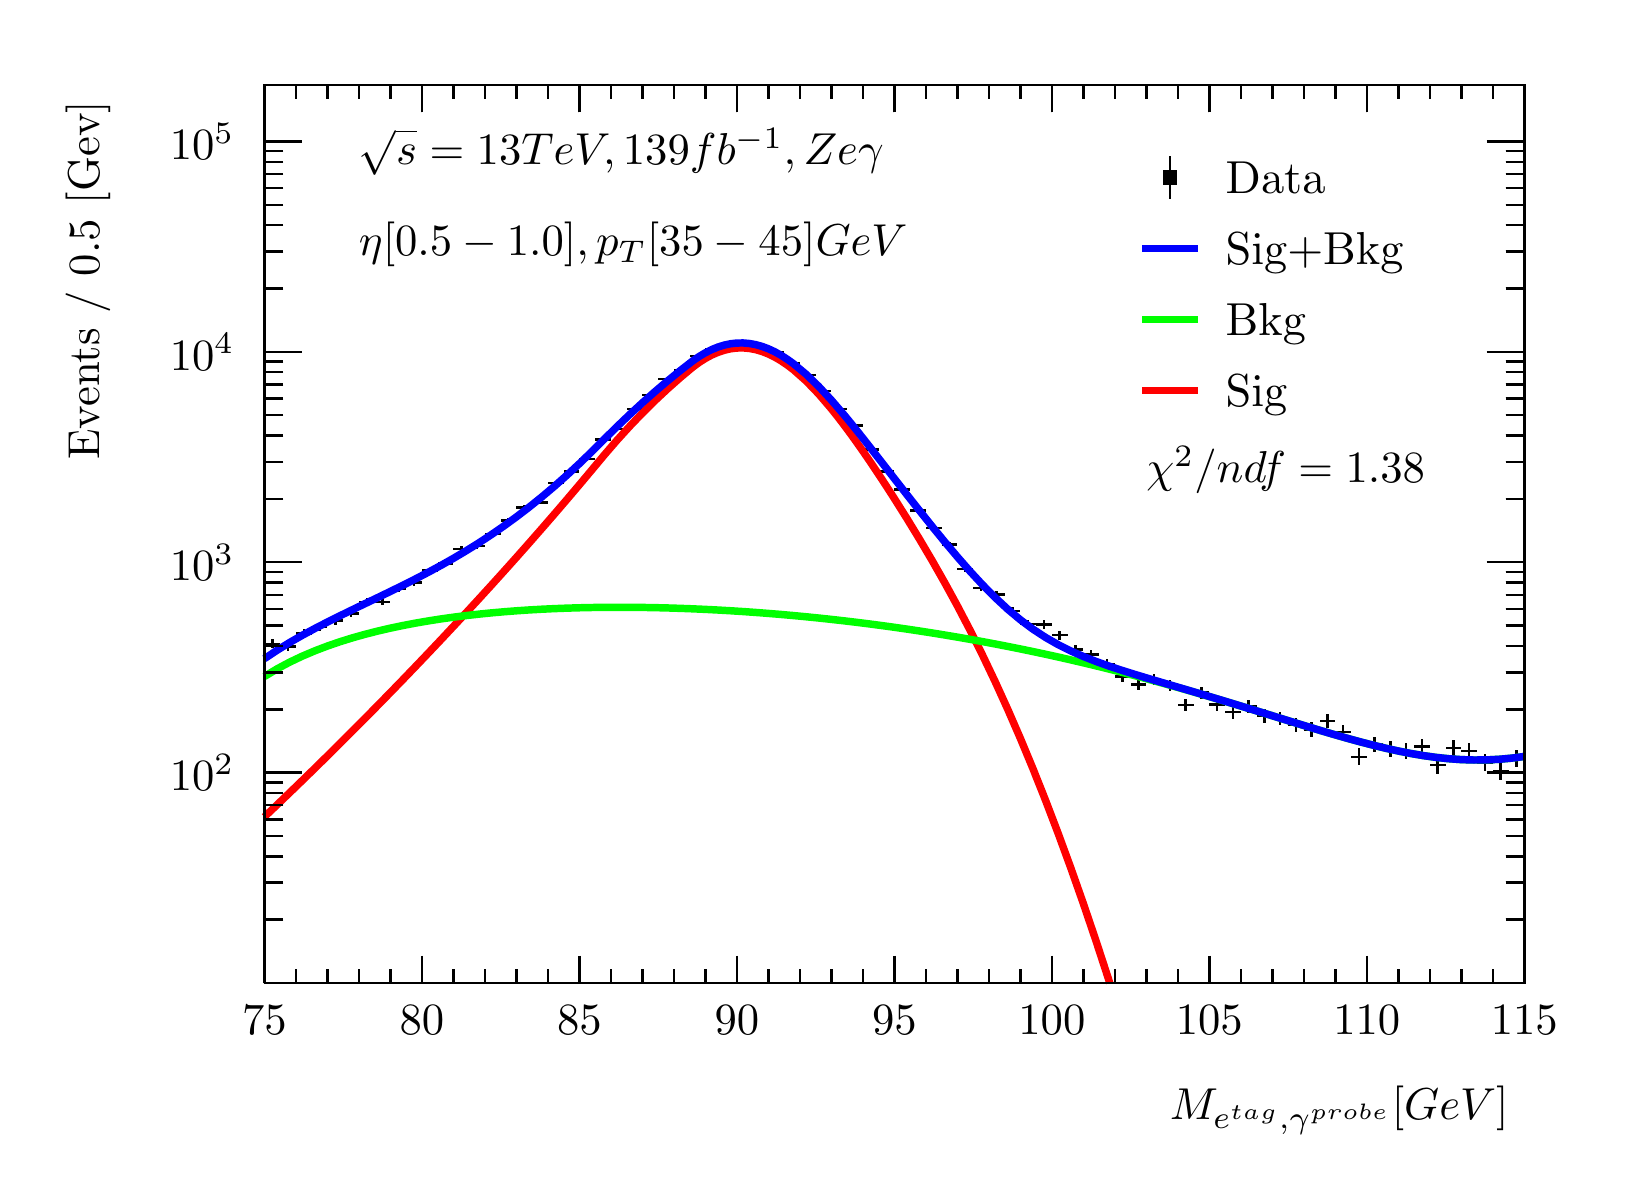
\begin{tikzpicture}
\pgfdeclareplotmark{cross} {
\pgfpathmoveto{\pgfpoint{-0.3\pgfplotmarksize}{\pgfplotmarksize}}
\pgfpathlineto{\pgfpoint{+0.3\pgfplotmarksize}{\pgfplotmarksize}}
\pgfpathlineto{\pgfpoint{+0.3\pgfplotmarksize}{0.3\pgfplotmarksize}}
\pgfpathlineto{\pgfpoint{+1\pgfplotmarksize}{0.3\pgfplotmarksize}}
\pgfpathlineto{\pgfpoint{+1\pgfplotmarksize}{-0.3\pgfplotmarksize}}
\pgfpathlineto{\pgfpoint{+0.3\pgfplotmarksize}{-0.3\pgfplotmarksize}}
\pgfpathlineto{\pgfpoint{+0.3\pgfplotmarksize}{-1.\pgfplotmarksize}}
\pgfpathlineto{\pgfpoint{-0.3\pgfplotmarksize}{-1.\pgfplotmarksize}}
\pgfpathlineto{\pgfpoint{-0.3\pgfplotmarksize}{-0.3\pgfplotmarksize}}
\pgfpathlineto{\pgfpoint{-1.\pgfplotmarksize}{-0.3\pgfplotmarksize}}
\pgfpathlineto{\pgfpoint{-1.\pgfplotmarksize}{0.3\pgfplotmarksize}}
\pgfpathlineto{\pgfpoint{-0.3\pgfplotmarksize}{0.3\pgfplotmarksize}}
\pgfpathclose
\pgfusepathqstroke
}
\pgfdeclareplotmark{cross*} {
\pgfpathmoveto{\pgfpoint{-0.3\pgfplotmarksize}{\pgfplotmarksize}}
\pgfpathlineto{\pgfpoint{+0.3\pgfplotmarksize}{\pgfplotmarksize}}
\pgfpathlineto{\pgfpoint{+0.3\pgfplotmarksize}{0.3\pgfplotmarksize}}
\pgfpathlineto{\pgfpoint{+1\pgfplotmarksize}{0.3\pgfplotmarksize}}
\pgfpathlineto{\pgfpoint{+1\pgfplotmarksize}{-0.3\pgfplotmarksize}}
\pgfpathlineto{\pgfpoint{+0.3\pgfplotmarksize}{-0.3\pgfplotmarksize}}
\pgfpathlineto{\pgfpoint{+0.3\pgfplotmarksize}{-1.\pgfplotmarksize}}
\pgfpathlineto{\pgfpoint{-0.3\pgfplotmarksize}{-1.\pgfplotmarksize}}
\pgfpathlineto{\pgfpoint{-0.3\pgfplotmarksize}{-0.3\pgfplotmarksize}}
\pgfpathlineto{\pgfpoint{-1.\pgfplotmarksize}{-0.3\pgfplotmarksize}}
\pgfpathlineto{\pgfpoint{-1.\pgfplotmarksize}{0.3\pgfplotmarksize}}
\pgfpathlineto{\pgfpoint{-0.3\pgfplotmarksize}{0.3\pgfplotmarksize}}
\pgfpathclose
\pgfusepathqfillstroke
}
\pgfdeclareplotmark{newstar} {
\pgfpathmoveto{\pgfqpoint{0pt}{\pgfplotmarksize}}
\pgfpathlineto{\pgfqpointpolar{44}{0.5\pgfplotmarksize}}
\pgfpathlineto{\pgfqpointpolar{18}{\pgfplotmarksize}}
\pgfpathlineto{\pgfqpointpolar{-20}{0.5\pgfplotmarksize}}
\pgfpathlineto{\pgfqpointpolar{-54}{\pgfplotmarksize}}
\pgfpathlineto{\pgfqpointpolar{-90}{0.5\pgfplotmarksize}}
\pgfpathlineto{\pgfqpointpolar{234}{\pgfplotmarksize}}
\pgfpathlineto{\pgfqpointpolar{198}{0.5\pgfplotmarksize}}
\pgfpathlineto{\pgfqpointpolar{162}{\pgfplotmarksize}}
\pgfpathlineto{\pgfqpointpolar{134}{0.5\pgfplotmarksize}}
\pgfpathclose
\pgfusepathqstroke
}
\pgfdeclareplotmark{newstar*} {
\pgfpathmoveto{\pgfqpoint{0pt}{\pgfplotmarksize}}
\pgfpathlineto{\pgfqpointpolar{44}{0.5\pgfplotmarksize}}
\pgfpathlineto{\pgfqpointpolar{18}{\pgfplotmarksize}}
\pgfpathlineto{\pgfqpointpolar{-20}{0.5\pgfplotmarksize}}
\pgfpathlineto{\pgfqpointpolar{-54}{\pgfplotmarksize}}
\pgfpathlineto{\pgfqpointpolar{-90}{0.5\pgfplotmarksize}}
\pgfpathlineto{\pgfqpointpolar{234}{\pgfplotmarksize}}
\pgfpathlineto{\pgfqpointpolar{198}{0.5\pgfplotmarksize}}
\pgfpathlineto{\pgfqpointpolar{162}{\pgfplotmarksize}}
\pgfpathlineto{\pgfqpointpolar{134}{0.5\pgfplotmarksize}}
\pgfpathclose
\pgfusepathqfillstroke
}
\definecolor{c}{rgb}{1,1,1};
\draw [color=c, fill=c] (0,0) rectangle (20,14.4361);
\draw [color=c, fill=c] (3,2.30977) rectangle (19,13.7143);
\definecolor{c}{rgb}{0,0,0};
\draw [c,line width=0.9] (3,2.30977) -- (3,13.7143) -- (19,13.7143) -- (19,2.30977) -- (3,2.30977);
\definecolor{c}{rgb}{1,1,1};
\draw [color=c, fill=c] (3,2.30977) rectangle (19,13.7143);
\definecolor{c}{rgb}{0,0,0};
\draw [c,line width=0.9] (3,2.30977) -- (3,13.7143) -- (19,13.7143) -- (19,2.30977) -- (3,2.30977);
\draw [c,line width=0.9] (3,2.30977) -- (19,2.30977);
\draw [c,line width=0.9] (3,2.65624) -- (3,2.30977);
\draw [c,line width=0.9] (3.4,2.48301) -- (3.4,2.30977);
\draw [c,line width=0.9] (3.8,2.48301) -- (3.8,2.30977);
\draw [c,line width=0.9] (4.2,2.48301) -- (4.2,2.30977);
\draw [c,line width=0.9] (4.6,2.48301) -- (4.6,2.30977);
\draw [c,line width=0.9] (5,2.65624) -- (5,2.30977);
\draw [c,line width=0.9] (5.4,2.48301) -- (5.4,2.30977);
\draw [c,line width=0.9] (5.8,2.48301) -- (5.8,2.30977);
\draw [c,line width=0.9] (6.2,2.48301) -- (6.2,2.30977);
\draw [c,line width=0.9] (6.6,2.48301) -- (6.6,2.30977);
\draw [c,line width=0.9] (7,2.65624) -- (7,2.30977);
\draw [c,line width=0.9] (7.4,2.48301) -- (7.4,2.30977);
\draw [c,line width=0.9] (7.8,2.48301) -- (7.8,2.30977);
\draw [c,line width=0.9] (8.2,2.48301) -- (8.2,2.30977);
\draw [c,line width=0.9] (8.6,2.48301) -- (8.6,2.30977);
\draw [c,line width=0.9] (9,2.65624) -- (9,2.30977);
\draw [c,line width=0.9] (9.4,2.48301) -- (9.4,2.30977);
\draw [c,line width=0.9] (9.8,2.48301) -- (9.8,2.30977);
\draw [c,line width=0.9] (10.2,2.48301) -- (10.2,2.30977);
\draw [c,line width=0.9] (10.6,2.48301) -- (10.6,2.30977);
\draw [c,line width=0.9] (11,2.65624) -- (11,2.30977);
\draw [c,line width=0.9] (11.4,2.48301) -- (11.4,2.30977);
\draw [c,line width=0.9] (11.8,2.48301) -- (11.8,2.30977);
\draw [c,line width=0.9] (12.2,2.48301) -- (12.2,2.30977);
\draw [c,line width=0.9] (12.6,2.48301) -- (12.6,2.30977);
\draw [c,line width=0.9] (13,2.65624) -- (13,2.30977);
\draw [c,line width=0.9] (13.4,2.48301) -- (13.4,2.30977);
\draw [c,line width=0.9] (13.8,2.48301) -- (13.8,2.30977);
\draw [c,line width=0.9] (14.2,2.48301) -- (14.2,2.30977);
\draw [c,line width=0.9] (14.6,2.48301) -- (14.6,2.30977);
\draw [c,line width=0.9] (15,2.65624) -- (15,2.30977);
\draw [c,line width=0.9] (15.4,2.48301) -- (15.4,2.30977);
\draw [c,line width=0.9] (15.8,2.48301) -- (15.8,2.30977);
\draw [c,line width=0.9] (16.2,2.48301) -- (16.2,2.30977);
\draw [c,line width=0.9] (16.6,2.48301) -- (16.6,2.30977);
\draw [c,line width=0.9] (17,2.65624) -- (17,2.30977);
\draw [c,line width=0.9] (17.4,2.48301) -- (17.4,2.30977);
\draw [c,line width=0.9] (17.8,2.48301) -- (17.8,2.30977);
\draw [c,line width=0.9] (18.2,2.48301) -- (18.2,2.30977);
\draw [c,line width=0.9] (18.6,2.48301) -- (18.6,2.30977);
\draw [c,line width=0.9] (19,2.65624) -- (19,2.30977);
\draw [c,line width=0.9] (19,2.65624) -- (19,2.30977);
\draw [anchor=base] (3,1.66015) node[scale=1.61424, color=c, rotate=0]{75};
\draw [anchor=base] (5,1.66015) node[scale=1.61424, color=c, rotate=0]{80};
\draw [anchor=base] (7,1.66015) node[scale=1.61424, color=c, rotate=0]{85};
\draw [anchor=base] (9,1.66015) node[scale=1.61424, color=c, rotate=0]{90};
\draw [anchor=base] (11,1.66015) node[scale=1.61424, color=c, rotate=0]{95};
\draw [anchor=base] (13,1.66015) node[scale=1.61424, color=c, rotate=0]{100};
\draw [anchor=base] (15,1.66015) node[scale=1.61424, color=c, rotate=0]{105};
\draw [anchor=base] (17,1.66015) node[scale=1.61424, color=c, rotate=0]{110};
\draw [anchor=base] (19,1.66015) node[scale=1.61424, color=c, rotate=0]{115};
\draw [anchor= east] (19,0.692932) node[scale=1.61424, color=c, rotate=0]{$M_{e^{tag}, \gamma^{probe}}  [GeV]$};
\draw [c,line width=0.9] (3,13.7143) -- (19,13.7143);
\draw [c,line width=0.9] (3,13.3678) -- (3,13.7143);
\draw [c,line width=0.9] (3.4,13.5411) -- (3.4,13.7143);
\draw [c,line width=0.9] (3.8,13.5411) -- (3.8,13.7143);
\draw [c,line width=0.9] (4.2,13.5411) -- (4.2,13.7143);
\draw [c,line width=0.9] (4.6,13.5411) -- (4.6,13.7143);
\draw [c,line width=0.9] (5,13.3678) -- (5,13.7143);
\draw [c,line width=0.9] (5.4,13.5411) -- (5.4,13.7143);
\draw [c,line width=0.9] (5.8,13.5411) -- (5.8,13.7143);
\draw [c,line width=0.9] (6.2,13.5411) -- (6.2,13.7143);
\draw [c,line width=0.9] (6.6,13.5411) -- (6.6,13.7143);
\draw [c,line width=0.9] (7,13.3678) -- (7,13.7143);
\draw [c,line width=0.9] (7.4,13.5411) -- (7.4,13.7143);
\draw [c,line width=0.9] (7.8,13.5411) -- (7.8,13.7143);
\draw [c,line width=0.9] (8.2,13.5411) -- (8.2,13.7143);
\draw [c,line width=0.9] (8.6,13.5411) -- (8.6,13.7143);
\draw [c,line width=0.9] (9,13.3678) -- (9,13.7143);
\draw [c,line width=0.9] (9.4,13.5411) -- (9.4,13.7143);
\draw [c,line width=0.9] (9.8,13.5411) -- (9.8,13.7143);
\draw [c,line width=0.9] (10.2,13.5411) -- (10.2,13.7143);
\draw [c,line width=0.9] (10.6,13.5411) -- (10.6,13.7143);
\draw [c,line width=0.9] (11,13.3678) -- (11,13.7143);
\draw [c,line width=0.9] (11.4,13.5411) -- (11.4,13.7143);
\draw [c,line width=0.9] (11.8,13.5411) -- (11.8,13.7143);
\draw [c,line width=0.9] (12.2,13.5411) -- (12.2,13.7143);
\draw [c,line width=0.9] (12.6,13.5411) -- (12.6,13.7143);
\draw [c,line width=0.9] (13,13.3678) -- (13,13.7143);
\draw [c,line width=0.9] (13.4,13.5411) -- (13.4,13.7143);
\draw [c,line width=0.9] (13.8,13.5411) -- (13.8,13.7143);
\draw [c,line width=0.9] (14.2,13.5411) -- (14.2,13.7143);
\draw [c,line width=0.9] (14.6,13.5411) -- (14.6,13.7143);
\draw [c,line width=0.9] (15,13.3678) -- (15,13.7143);
\draw [c,line width=0.9] (15.4,13.5411) -- (15.4,13.7143);
\draw [c,line width=0.9] (15.8,13.5411) -- (15.8,13.7143);
\draw [c,line width=0.9] (16.2,13.5411) -- (16.2,13.7143);
\draw [c,line width=0.9] (16.6,13.5411) -- (16.6,13.7143);
\draw [c,line width=0.9] (17,13.3678) -- (17,13.7143);
\draw [c,line width=0.9] (17.4,13.5411) -- (17.4,13.7143);
\draw [c,line width=0.9] (17.8,13.5411) -- (17.8,13.7143);
\draw [c,line width=0.9] (18.2,13.5411) -- (18.2,13.7143);
\draw [c,line width=0.9] (18.6,13.5411) -- (18.6,13.7143);
\draw [c,line width=0.9] (19,13.3678) -- (19,13.7143);
\draw [c,line width=0.9] (19,13.3678) -- (19,13.7143);
\draw [c,line width=0.9] (3,2.30977) -- (3,13.7143);
\draw [c,line width=0.9] (3.237,3.11414) -- (3,3.11414);
\draw [c,line width=0.9] (3.237,3.58467) -- (3,3.58467);
\draw [c,line width=0.9] (3.237,3.91852) -- (3,3.91852);
\draw [c,line width=0.9] (3.237,4.17747) -- (3,4.17747);
\draw [c,line width=0.9] (3.237,4.38904) -- (3,4.38904);
\draw [c,line width=0.9] (3.237,4.56793) -- (3,4.56793);
\draw [c,line width=0.9] (3.237,4.72289) -- (3,4.72289);
\draw [c,line width=0.9] (3.237,4.85957) -- (3,4.85957);
\draw [c,line width=0.9] (3.474,4.98184) -- (3,4.98184);
\draw [anchor= east] (2.82,4.98184) node[scale=1.61424, color=c, rotate=0]{$10^{2}$};
\draw [c,line width=0.9] (3.237,5.78621) -- (3,5.78621);
\draw [c,line width=0.9] (3.237,6.25674) -- (3,6.25674);
\draw [c,line width=0.9] (3.237,6.59058) -- (3,6.59058);
\draw [c,line width=0.9] (3.237,6.84953) -- (3,6.84953);
\draw [c,line width=0.9] (3.237,7.06111) -- (3,7.06111);
\draw [c,line width=0.9] (3.237,7.24) -- (3,7.24);
\draw [c,line width=0.9] (3.237,7.39496) -- (3,7.39496);
\draw [c,line width=0.9] (3.237,7.53164) -- (3,7.53164);
\draw [c,line width=0.9] (3.474,7.65391) -- (3,7.65391);
\draw [anchor= east] (2.82,7.65391) node[scale=1.61424, color=c, rotate=0]{$10^{3}$};
\draw [c,line width=0.9] (3.237,8.45828) -- (3,8.45828);
\draw [c,line width=0.9] (3.237,8.92881) -- (3,8.92881);
\draw [c,line width=0.9] (3.237,9.26265) -- (3,9.26265);
\draw [c,line width=0.9] (3.237,9.5216) -- (3,9.5216);
\draw [c,line width=0.9] (3.237,9.73318) -- (3,9.73318);
\draw [c,line width=0.9] (3.237,9.91207) -- (3,9.91207);
\draw [c,line width=0.9] (3.237,10.067) -- (3,10.067);
\draw [c,line width=0.9] (3.237,10.2037) -- (3,10.2037);
\draw [c,line width=0.9] (3.474,10.326) -- (3,10.326);
\draw [anchor= east] (2.82,10.326) node[scale=1.61424, color=c, rotate=0]{$10^{4}$};
\draw [c,line width=0.9] (3.237,11.1303) -- (3,11.1303);
\draw [c,line width=0.9] (3.237,11.6009) -- (3,11.6009);
\draw [c,line width=0.9] (3.237,11.9347) -- (3,11.9347);
\draw [c,line width=0.9] (3.237,12.1937) -- (3,12.1937);
\draw [c,line width=0.9] (3.237,12.4052) -- (3,12.4052);
\draw [c,line width=0.9] (3.237,12.5841) -- (3,12.5841);
\draw [c,line width=0.9] (3.237,12.7391) -- (3,12.7391);
\draw [c,line width=0.9] (3.237,12.8758) -- (3,12.8758);
\draw [c,line width=0.9] (3.474,12.998) -- (3,12.998);
\draw [anchor= east] (2.82,12.998) node[scale=1.61424, color=c, rotate=0]{$10^{5}$};
\draw [anchor= east] (0.76,13.7143) node[scale=1.61424, color=c, rotate=90]{Events / 0.5 [Gev]};
\draw [c,line width=0.9] (19,2.30977) -- (19,13.7143);
\draw [c,line width=0.9] (18.763,3.11414) -- (19,3.11414);
\draw [c,line width=0.9] (18.763,3.58467) -- (19,3.58467);
\draw [c,line width=0.9] (18.763,3.91852) -- (19,3.91852);
\draw [c,line width=0.9] (18.763,4.17747) -- (19,4.17747);
\draw [c,line width=0.9] (18.763,4.38904) -- (19,4.38904);
\draw [c,line width=0.9] (18.763,4.56793) -- (19,4.56793);
\draw [c,line width=0.9] (18.763,4.72289) -- (19,4.72289);
\draw [c,line width=0.9] (18.763,4.85957) -- (19,4.85957);
\draw [c,line width=0.9] (18.526,4.98184) -- (19,4.98184);
\draw [c,line width=0.9] (18.763,5.78621) -- (19,5.78621);
\draw [c,line width=0.9] (18.763,6.25674) -- (19,6.25674);
\draw [c,line width=0.9] (18.763,6.59058) -- (19,6.59058);
\draw [c,line width=0.9] (18.763,6.84953) -- (19,6.84953);
\draw [c,line width=0.9] (18.763,7.06111) -- (19,7.06111);
\draw [c,line width=0.9] (18.763,7.24) -- (19,7.24);
\draw [c,line width=0.9] (18.763,7.39496) -- (19,7.39496);
\draw [c,line width=0.9] (18.763,7.53164) -- (19,7.53164);
\draw [c,line width=0.9] (18.526,7.65391) -- (19,7.65391);
\draw [c,line width=0.9] (18.763,8.45828) -- (19,8.45828);
\draw [c,line width=0.9] (18.763,8.92881) -- (19,8.92881);
\draw [c,line width=0.9] (18.763,9.26265) -- (19,9.26265);
\draw [c,line width=0.9] (18.763,9.5216) -- (19,9.5216);
\draw [c,line width=0.9] (18.763,9.73318) -- (19,9.73318);
\draw [c,line width=0.9] (18.763,9.91207) -- (19,9.91207);
\draw [c,line width=0.9] (18.763,10.067) -- (19,10.067);
\draw [c,line width=0.9] (18.763,10.2037) -- (19,10.2037);
\draw [c,line width=0.9] (18.526,10.326) -- (19,10.326);
\draw [c,line width=0.9] (18.763,11.1303) -- (19,11.1303);
\draw [c,line width=0.9] (18.763,11.6009) -- (19,11.6009);
\draw [c,line width=0.9] (18.763,11.9347) -- (19,11.9347);
\draw [c,line width=0.9] (18.763,12.1937) -- (19,12.1937);
\draw [c,line width=0.9] (18.763,12.4052) -- (19,12.4052);
\draw [c,line width=0.9] (18.763,12.5841) -- (19,12.5841);
\draw [c,line width=0.9] (18.763,12.7391) -- (19,12.7391);
\draw [c,line width=0.9] (18.763,12.8758) -- (19,12.8758);
\draw [c,line width=0.9] (18.526,12.998) -- (19,12.998);
\draw [c,line width=0.9] (3.1,6.61641) -- (3,6.61641);
\draw [c,line width=0.9] (3,6.61641) -- (3,6.61641);
\draw [c,line width=0.9] (3.1,6.61641) -- (3.2,6.61641);
\draw [c,line width=0.9] (3.2,6.61641) -- (3.2,6.61641);
\draw [c,line width=0.9] (3.1,6.61641) -- (3.1,6.67378);
\draw [c,line width=0.9] (3.1,6.67378) -- (3.1,6.67378);
\draw [c,line width=0.9] (3.1,6.61641) -- (3.1,6.55903);
\draw [c,line width=0.9] (3.1,6.55903) -- (3.1,6.55903);
\draw [c,line width=0.9] (3.3,6.58477) -- (3.2,6.58477);
\draw [c,line width=0.9] (3.2,6.58477) -- (3.2,6.58477);
\draw [c,line width=0.9] (3.3,6.58477) -- (3.4,6.58477);
\draw [c,line width=0.9] (3.4,6.58477) -- (3.4,6.58477);
\draw [c,line width=0.9] (3.3,6.58477) -- (3.3,6.64293);
\draw [c,line width=0.9] (3.3,6.64293) -- (3.3,6.64293);
\draw [c,line width=0.9] (3.3,6.58477) -- (3.3,6.52661);
\draw [c,line width=0.9] (3.3,6.52661) -- (3.3,6.52661);
\draw [c,line width=0.9] (3.5,6.74772) -- (3.4,6.74772);
\draw [c,line width=0.9] (3.4,6.74772) -- (3.4,6.74772);
\draw [c,line width=0.9] (3.5,6.74772) -- (3.6,6.74772);
\draw [c,line width=0.9] (3.6,6.74772) -- (3.6,6.74772);
\draw [c,line width=0.9] (3.5,6.74772) -- (3.5,6.80194);
\draw [c,line width=0.9] (3.5,6.80194) -- (3.5,6.80194);
\draw [c,line width=0.9] (3.5,6.74772) -- (3.5,6.6935);
\draw [c,line width=0.9] (3.5,6.6935) -- (3.5,6.6935);
\draw [c,line width=0.9] (3.7,6.83317) -- (3.6,6.83317);
\draw [c,line width=0.9] (3.6,6.83317) -- (3.6,6.83317);
\draw [c,line width=0.9] (3.7,6.83317) -- (3.8,6.83317);
\draw [c,line width=0.9] (3.8,6.83317) -- (3.8,6.83317);
\draw [c,line width=0.9] (3.7,6.83317) -- (3.7,6.88543);
\draw [c,line width=0.9] (3.7,6.88543) -- (3.7,6.88543);
\draw [c,line width=0.9] (3.7,6.83317) -- (3.7,6.78091);
\draw [c,line width=0.9] (3.7,6.78091) -- (3.7,6.78091);
\draw [c,line width=0.9] (3.9,6.91277) -- (3.8,6.91277);
\draw [c,line width=0.9] (3.8,6.91277) -- (3.8,6.91277);
\draw [c,line width=0.9] (3.9,6.91277) -- (4,6.91277);
\draw [c,line width=0.9] (4,6.91277) -- (4,6.91277);
\draw [c,line width=0.9] (3.9,6.91277) -- (3.9,6.96327);
\draw [c,line width=0.9] (3.9,6.96327) -- (3.9,6.96327);
\draw [c,line width=0.9] (3.9,6.91277) -- (3.9,6.86227);
\draw [c,line width=0.9] (3.9,6.86227) -- (3.9,6.86227);
\draw [c,line width=0.9] (4.1,7.00565) -- (4,7.00565);
\draw [c,line width=0.9] (4,7.00565) -- (4,7.00565);
\draw [c,line width=0.9] (4.1,7.00565) -- (4.2,7.00565);
\draw [c,line width=0.9] (4.2,7.00565) -- (4.2,7.00565);
\draw [c,line width=0.9] (4.1,7.00565) -- (4.1,7.05417);
\draw [c,line width=0.9] (4.1,7.05417) -- (4.1,7.05417);
\draw [c,line width=0.9] (4.1,7.00565) -- (4.1,6.95714);
\draw [c,line width=0.9] (4.1,6.95714) -- (4.1,6.95714);
\draw [c,line width=0.9] (4.3,7.15042) -- (4.2,7.15042);
\draw [c,line width=0.9] (4.2,7.15042) -- (4.2,7.15042);
\draw [c,line width=0.9] (4.3,7.15042) -- (4.4,7.15042);
\draw [c,line width=0.9] (4.4,7.15042) -- (4.4,7.15042);
\draw [c,line width=0.9] (4.3,7.15042) -- (4.3,7.19601);
\draw [c,line width=0.9] (4.3,7.19601) -- (4.3,7.19601);
\draw [c,line width=0.9] (4.3,7.15042) -- (4.3,7.10484);
\draw [c,line width=0.9] (4.3,7.10484) -- (4.3,7.10484);
\draw [c,line width=0.9] (4.5,7.15042) -- (4.4,7.15042);
\draw [c,line width=0.9] (4.4,7.15042) -- (4.4,7.15042);
\draw [c,line width=0.9] (4.5,7.15042) -- (4.6,7.15042);
\draw [c,line width=0.9] (4.6,7.15042) -- (4.6,7.15042);
\draw [c,line width=0.9] (4.5,7.15042) -- (4.5,7.19601);
\draw [c,line width=0.9] (4.5,7.19601) -- (4.5,7.19601);
\draw [c,line width=0.9] (4.5,7.15042) -- (4.5,7.10484);
\draw [c,line width=0.9] (4.5,7.10484) -- (4.5,7.10484);
\draw [c,line width=0.9] (4.7,7.31696) -- (4.6,7.31696);
\draw [c,line width=0.9] (4.6,7.31696) -- (4.6,7.31696);
\draw [c,line width=0.9] (4.7,7.31696) -- (4.8,7.31696);
\draw [c,line width=0.9] (4.8,7.31696) -- (4.8,7.31696);
\draw [c,line width=0.9] (4.7,7.31696) -- (4.7,7.35939);
\draw [c,line width=0.9] (4.7,7.35939) -- (4.7,7.35939);
\draw [c,line width=0.9] (4.7,7.31696) -- (4.7,7.27454);
\draw [c,line width=0.9] (4.7,7.27454) -- (4.7,7.27454);
\draw [c,line width=0.9] (4.9,7.3993) -- (4.8,7.3993);
\draw [c,line width=0.9] (4.8,7.3993) -- (4.8,7.3993);
\draw [c,line width=0.9] (4.9,7.3993) -- (5,7.3993);
\draw [c,line width=0.9] (5,7.3993) -- (5,7.3993);
\draw [c,line width=0.9] (4.9,7.3993) -- (4.9,7.44025);
\draw [c,line width=0.9] (4.9,7.44025) -- (4.9,7.44025);
\draw [c,line width=0.9] (4.9,7.3993) -- (4.9,7.35835);
\draw [c,line width=0.9] (4.9,7.35835) -- (4.9,7.35835);
\draw [c,line width=0.9] (5.1,7.54701) -- (5,7.54701);
\draw [c,line width=0.9] (5,7.54701) -- (5,7.54701);
\draw [c,line width=0.9] (5.1,7.54701) -- (5.2,7.54701);
\draw [c,line width=0.9] (5.2,7.54701) -- (5.2,7.54701);
\draw [c,line width=0.9] (5.1,7.54701) -- (5.1,7.58544);
\draw [c,line width=0.9] (5.1,7.58544) -- (5.1,7.58544);
\draw [c,line width=0.9] (5.1,7.54701) -- (5.1,7.50859);
\draw [c,line width=0.9] (5.1,7.50859) -- (5.1,7.50859);
\draw [c,line width=0.9] (5.3,7.63755) -- (5.2,7.63755);
\draw [c,line width=0.9] (5.2,7.63755) -- (5.2,7.63755);
\draw [c,line width=0.9] (5.3,7.63755) -- (5.4,7.63755);
\draw [c,line width=0.9] (5.4,7.63755) -- (5.4,7.63755);
\draw [c,line width=0.9] (5.3,7.63755) -- (5.3,7.6745);
\draw [c,line width=0.9] (5.3,7.6745) -- (5.3,7.6745);
\draw [c,line width=0.9] (5.3,7.63755) -- (5.3,7.60059);
\draw [c,line width=0.9] (5.3,7.60059) -- (5.3,7.60059);
\draw [c,line width=0.9] (5.5,7.82113) -- (5.4,7.82113);
\draw [c,line width=0.9] (5.4,7.82113) -- (5.4,7.82113);
\draw [c,line width=0.9] (5.5,7.82113) -- (5.6,7.82113);
\draw [c,line width=0.9] (5.6,7.82113) -- (5.6,7.82113);
\draw [c,line width=0.9] (5.5,7.82113) -- (5.5,7.85528);
\draw [c,line width=0.9] (5.5,7.85528) -- (5.5,7.85528);
\draw [c,line width=0.9] (5.5,7.82113) -- (5.5,7.78699);
\draw [c,line width=0.9] (5.5,7.78699) -- (5.5,7.78699);
\draw [c,line width=0.9] (5.7,7.8587) -- (5.6,7.8587);
\draw [c,line width=0.9] (5.6,7.8587) -- (5.6,7.8587);
\draw [c,line width=0.9] (5.7,7.8587) -- (5.8,7.8587);
\draw [c,line width=0.9] (5.8,7.8587) -- (5.8,7.8587);
\draw [c,line width=0.9] (5.7,7.8587) -- (5.7,7.89229);
\draw [c,line width=0.9] (5.7,7.89229) -- (5.7,7.89229);
\draw [c,line width=0.9] (5.7,7.8587) -- (5.7,7.8251);
\draw [c,line width=0.9] (5.7,7.8251) -- (5.7,7.8251);
\draw [c,line width=0.9] (5.9,8.00988) -- (5.8,8.00988);
\draw [c,line width=0.9] (5.8,8.00988) -- (5.8,8.00988);
\draw [c,line width=0.9] (5.9,8.00988) -- (6,8.00988);
\draw [c,line width=0.9] (6,8.00988) -- (6,8.00988);
\draw [c,line width=0.9] (5.9,8.00988) -- (5.9,8.04136);
\draw [c,line width=0.9] (5.9,8.04136) -- (5.9,8.04136);
\draw [c,line width=0.9] (5.9,8.00988) -- (5.9,7.9784);
\draw [c,line width=0.9] (5.9,7.9784) -- (5.9,7.9784);
\draw [c,line width=0.9] (6.1,8.1862) -- (6,8.1862);
\draw [c,line width=0.9] (6,8.1862) -- (6,8.1862);
\draw [c,line width=0.9] (6.1,8.1862) -- (6.2,8.1862);
\draw [c,line width=0.9] (6.2,8.1862) -- (6.2,8.1862);
\draw [c,line width=0.9] (6.1,8.1862) -- (6.1,8.21538);
\draw [c,line width=0.9] (6.1,8.21538) -- (6.1,8.21538);
\draw [c,line width=0.9] (6.1,8.1862) -- (6.1,8.15703);
\draw [c,line width=0.9] (6.1,8.15703) -- (6.1,8.15703);
\draw [c,line width=0.9] (6.3,8.34756) -- (6.2,8.34756);
\draw [c,line width=0.9] (6.2,8.34756) -- (6.2,8.34756);
\draw [c,line width=0.9] (6.3,8.34756) -- (6.4,8.34756);
\draw [c,line width=0.9] (6.4,8.34756) -- (6.4,8.34756);
\draw [c,line width=0.9] (6.3,8.34756) -- (6.3,8.37478);
\draw [c,line width=0.9] (6.3,8.37478) -- (6.3,8.37478);
\draw [c,line width=0.9] (6.3,8.34756) -- (6.3,8.32034);
\draw [c,line width=0.9] (6.3,8.32034) -- (6.3,8.32034);
\draw [c,line width=0.9] (6.5,8.41513) -- (6.4,8.41513);
\draw [c,line width=0.9] (6.4,8.41513) -- (6.4,8.41513);
\draw [c,line width=0.9] (6.5,8.41513) -- (6.6,8.41513);
\draw [c,line width=0.9] (6.6,8.41513) -- (6.6,8.41513);
\draw [c,line width=0.9] (6.5,8.41513) -- (6.5,8.44157);
\draw [c,line width=0.9] (6.5,8.44157) -- (6.5,8.44157);
\draw [c,line width=0.9] (6.5,8.41513) -- (6.5,8.3887);
\draw [c,line width=0.9] (6.5,8.3887) -- (6.5,8.3887);
\draw [c,line width=0.9] (6.7,8.66307) -- (6.6,8.66307);
\draw [c,line width=0.9] (6.6,8.66307) -- (6.6,8.66307);
\draw [c,line width=0.9] (6.7,8.66307) -- (6.8,8.66307);
\draw [c,line width=0.9] (6.8,8.66307) -- (6.8,8.66307);
\draw [c,line width=0.9] (6.7,8.66307) -- (6.7,8.68683);
\draw [c,line width=0.9] (6.7,8.68683) -- (6.7,8.68683);
\draw [c,line width=0.9] (6.7,8.66307) -- (6.7,8.63931);
\draw [c,line width=0.9] (6.7,8.63931) -- (6.7,8.63931);
\draw [c,line width=0.9] (6.9,8.80439) -- (6.8,8.80439);
\draw [c,line width=0.9] (6.8,8.80439) -- (6.8,8.80439);
\draw [c,line width=0.9] (6.9,8.80439) -- (7,8.80439);
\draw [c,line width=0.9] (7,8.80439) -- (7,8.80439);
\draw [c,line width=0.9] (6.9,8.80439) -- (6.9,8.82674);
\draw [c,line width=0.9] (6.9,8.82674) -- (6.9,8.82674);
\draw [c,line width=0.9] (6.9,8.80439) -- (6.9,8.78204);
\draw [c,line width=0.9] (6.9,8.78204) -- (6.9,8.78204);
\draw [c,line width=0.9] (7.1,8.96761) -- (7,8.96761);
\draw [c,line width=0.9] (7,8.96761) -- (7,8.96761);
\draw [c,line width=0.9] (7.1,8.96761) -- (7.2,8.96761);
\draw [c,line width=0.9] (7.2,8.96761) -- (7.2,8.96761);
\draw [c,line width=0.9] (7.1,8.96761) -- (7.1,8.98844);
\draw [c,line width=0.9] (7.1,8.98844) -- (7.1,8.98844);
\draw [c,line width=0.9] (7.1,8.96761) -- (7.1,8.94677);
\draw [c,line width=0.9] (7.1,8.94677) -- (7.1,8.94677);
\draw [c,line width=0.9] (7.3,9.21377) -- (7.2,9.21377);
\draw [c,line width=0.9] (7.2,9.21377) -- (7.2,9.21377);
\draw [c,line width=0.9] (7.3,9.21377) -- (7.4,9.21377);
\draw [c,line width=0.9] (7.4,9.21377) -- (7.4,9.21377);
\draw [c,line width=0.9] (7.3,9.21377) -- (7.3,9.23251);
\draw [c,line width=0.9] (7.3,9.23251) -- (7.3,9.23251);
\draw [c,line width=0.9] (7.3,9.21377) -- (7.3,9.19503);
\draw [c,line width=0.9] (7.3,9.19503) -- (7.3,9.19503);
\draw [c,line width=0.9] (7.5,9.34523) -- (7.4,9.34523);
\draw [c,line width=0.9] (7.4,9.34523) -- (7.4,9.34523);
\draw [c,line width=0.9] (7.5,9.34523) -- (7.6,9.34523);
\draw [c,line width=0.9] (7.6,9.34523) -- (7.6,9.34523);
\draw [c,line width=0.9] (7.5,9.34523) -- (7.5,9.36294);
\draw [c,line width=0.9] (7.5,9.36294) -- (7.5,9.36294);
\draw [c,line width=0.9] (7.5,9.34523) -- (7.5,9.32752);
\draw [c,line width=0.9] (7.5,9.32752) -- (7.5,9.32752);
\draw [c,line width=0.9] (7.7,9.60055) -- (7.6,9.60055);
\draw [c,line width=0.9] (7.6,9.60055) -- (7.6,9.60055);
\draw [c,line width=0.9] (7.7,9.60055) -- (7.8,9.60055);
\draw [c,line width=0.9] (7.8,9.60055) -- (7.8,9.60055);
\draw [c,line width=0.9] (7.7,9.60055) -- (7.7,9.61641);
\draw [c,line width=0.9] (7.7,9.61641) -- (7.7,9.61641);
\draw [c,line width=0.9] (7.7,9.60055) -- (7.7,9.58469);
\draw [c,line width=0.9] (7.7,9.58469) -- (7.7,9.58469);
\draw [c,line width=0.9] (7.9,9.77553) -- (7.8,9.77553);
\draw [c,line width=0.9] (7.8,9.77553) -- (7.8,9.77553);
\draw [c,line width=0.9] (7.9,9.77553) -- (8,9.77553);
\draw [c,line width=0.9] (8,9.77553) -- (8,9.77553);
\draw [c,line width=0.9] (7.9,9.77553) -- (7.9,9.79024);
\draw [c,line width=0.9] (7.9,9.79024) -- (7.9,9.79024);
\draw [c,line width=0.9] (7.9,9.77553) -- (7.9,9.76082);
\draw [c,line width=0.9] (7.9,9.76082) -- (7.9,9.76082);
\draw [c,line width=0.9] (8.1,9.9814) -- (8,9.9814);
\draw [c,line width=0.9] (8,9.9814) -- (8,9.9814);
\draw [c,line width=0.9] (8.1,9.9814) -- (8.2,9.9814);
\draw [c,line width=0.9] (8.2,9.9814) -- (8.2,9.9814);
\draw [c,line width=0.9] (8.1,9.9814) -- (8.1,9.99487);
\draw [c,line width=0.9] (8.1,9.99487) -- (8.1,9.99487);
\draw [c,line width=0.9] (8.1,9.9814) -- (8.1,9.96794);
\draw [c,line width=0.9] (8.1,9.96794) -- (8.1,9.96794);
\draw [c,line width=0.9] (8.3,10.0927) -- (8.2,10.0927);
\draw [c,line width=0.9] (8.2,10.0927) -- (8.2,10.0927);
\draw [c,line width=0.9] (8.3,10.0927) -- (8.4,10.0927);
\draw [c,line width=0.9] (8.4,10.0927) -- (8.4,10.0927);
\draw [c,line width=0.9] (8.3,10.0927) -- (8.3,10.1055);
\draw [c,line width=0.9] (8.3,10.1055) -- (8.3,10.1055);
\draw [c,line width=0.9] (8.3,10.0927) -- (8.3,10.0799);
\draw [c,line width=0.9] (8.3,10.0799) -- (8.3,10.0799);
\draw [c,line width=0.9] (8.5,10.2741) -- (8.4,10.2741);
\draw [c,line width=0.9] (8.4,10.2741) -- (8.4,10.2741);
\draw [c,line width=0.9] (8.5,10.2741) -- (8.6,10.2741);
\draw [c,line width=0.9] (8.6,10.2741) -- (8.6,10.2741);
\draw [c,line width=0.9] (8.5,10.2741) -- (8.5,10.286);
\draw [c,line width=0.9] (8.5,10.286) -- (8.5,10.286);
\draw [c,line width=0.9] (8.5,10.2741) -- (8.5,10.2623);
\draw [c,line width=0.9] (8.5,10.2623) -- (8.5,10.2623);
\draw [c,line width=0.9] (8.7,10.3619) -- (8.6,10.3619);
\draw [c,line width=0.9] (8.6,10.3619) -- (8.6,10.3619);
\draw [c,line width=0.9] (8.7,10.3619) -- (8.8,10.3619);
\draw [c,line width=0.9] (8.8,10.3619) -- (8.8,10.3619);
\draw [c,line width=0.9] (8.7,10.3619) -- (8.7,10.3733);
\draw [c,line width=0.9] (8.7,10.3733) -- (8.7,10.3733);
\draw [c,line width=0.9] (8.7,10.3619) -- (8.7,10.3504);
\draw [c,line width=0.9] (8.7,10.3504) -- (8.7,10.3504);
\draw [c,line width=0.9] (8.9,10.4157) -- (8.8,10.4157);
\draw [c,line width=0.9] (8.8,10.4157) -- (8.8,10.4157);
\draw [c,line width=0.9] (8.9,10.4157) -- (9,10.4157);
\draw [c,line width=0.9] (9,10.4157) -- (9,10.4157);
\draw [c,line width=0.9] (8.9,10.4157) -- (8.9,10.4269);
\draw [c,line width=0.9] (8.9,10.4269) -- (8.9,10.4269);
\draw [c,line width=0.9] (8.9,10.4157) -- (8.9,10.4046);
\draw [c,line width=0.9] (8.9,10.4046) -- (8.9,10.4046);
\draw [c,line width=0.9] (9.1,10.4272) -- (9,10.4272);
\draw [c,line width=0.9] (9,10.4272) -- (9,10.4272);
\draw [c,line width=0.9] (9.1,10.4272) -- (9.2,10.4272);
\draw [c,line width=0.9] (9.2,10.4272) -- (9.2,10.4272);
\draw [c,line width=0.9] (9.1,10.4272) -- (9.1,10.4383);
\draw [c,line width=0.9] (9.1,10.4383) -- (9.1,10.4383);
\draw [c,line width=0.9] (9.1,10.4272) -- (9.1,10.416);
\draw [c,line width=0.9] (9.1,10.416) -- (9.1,10.416);
\draw [c,line width=0.9] (9.3,10.3971) -- (9.2,10.3971);
\draw [c,line width=0.9] (9.2,10.3971) -- (9.2,10.3971);
\draw [c,line width=0.9] (9.3,10.3971) -- (9.4,10.3971);
\draw [c,line width=0.9] (9.4,10.3971) -- (9.4,10.3971);
\draw [c,line width=0.9] (9.3,10.3971) -- (9.3,10.4083);
\draw [c,line width=0.9] (9.3,10.4083) -- (9.3,10.4083);
\draw [c,line width=0.9] (9.3,10.3971) -- (9.3,10.3858);
\draw [c,line width=0.9] (9.3,10.3858) -- (9.3,10.3858);
\draw [c,line width=0.9] (9.5,10.3206) -- (9.4,10.3206);
\draw [c,line width=0.9] (9.4,10.3206) -- (9.4,10.3206);
\draw [c,line width=0.9] (9.5,10.3206) -- (9.6,10.3206);
\draw [c,line width=0.9] (9.6,10.3206) -- (9.6,10.3206);
\draw [c,line width=0.9] (9.5,10.3206) -- (9.5,10.3323);
\draw [c,line width=0.9] (9.5,10.3323) -- (9.5,10.3323);
\draw [c,line width=0.9] (9.5,10.3206) -- (9.5,10.309);
\draw [c,line width=0.9] (9.5,10.309) -- (9.5,10.309);
\draw [c,line width=0.9] (9.7,10.1751) -- (9.6,10.1751);
\draw [c,line width=0.9] (9.6,10.1751) -- (9.6,10.1751);
\draw [c,line width=0.9] (9.7,10.1751) -- (9.8,10.1751);
\draw [c,line width=0.9] (9.8,10.1751) -- (9.8,10.1751);
\draw [c,line width=0.9] (9.7,10.1751) -- (9.7,10.1875);
\draw [c,line width=0.9] (9.7,10.1875) -- (9.7,10.1875);
\draw [c,line width=0.9] (9.7,10.1751) -- (9.7,10.1627);
\draw [c,line width=0.9] (9.7,10.1627) -- (9.7,10.1627);
\draw [c,line width=0.9] (9.9,10.0332) -- (9.8,10.0332);
\draw [c,line width=0.9] (9.8,10.0332) -- (9.8,10.0332);
\draw [c,line width=0.9] (9.9,10.0332) -- (10,10.0332);
\draw [c,line width=0.9] (10,10.0332) -- (10,10.0332);
\draw [c,line width=0.9] (9.9,10.0332) -- (9.9,10.0463);
\draw [c,line width=0.9] (9.9,10.0463) -- (9.9,10.0463);
\draw [c,line width=0.9] (9.9,10.0332) -- (9.9,10.02);
\draw [c,line width=0.9] (9.9,10.02) -- (9.9,10.02);
\draw [c,line width=0.9] (10.1,9.82821) -- (10,9.82821);
\draw [c,line width=0.9] (10,9.82821) -- (10,9.82821);
\draw [c,line width=0.9] (10.1,9.82821) -- (10.2,9.82821);
\draw [c,line width=0.9] (10.2,9.82821) -- (10.2,9.82821);
\draw [c,line width=0.9] (10.1,9.82821) -- (10.1,9.84259);
\draw [c,line width=0.9] (10.1,9.84259) -- (10.1,9.84259);
\draw [c,line width=0.9] (10.1,9.82821) -- (10.1,9.81383);
\draw [c,line width=0.9] (10.1,9.81383) -- (10.1,9.81383);
\draw [c,line width=0.9] (10.3,9.59925) -- (10.2,9.59925);
\draw [c,line width=0.9] (10.2,9.59925) -- (10.2,9.59925);
\draw [c,line width=0.9] (10.3,9.59925) -- (10.4,9.59925);
\draw [c,line width=0.9] (10.4,9.59925) -- (10.4,9.59925);
\draw [c,line width=0.9] (10.3,9.59925) -- (10.3,9.61512);
\draw [c,line width=0.9] (10.3,9.61512) -- (10.3,9.61512);
\draw [c,line width=0.9] (10.3,9.59925) -- (10.3,9.58338);
\draw [c,line width=0.9] (10.3,9.58338) -- (10.3,9.58338);
\draw [c,line width=0.9] (10.5,9.38975) -- (10.4,9.38975);
\draw [c,line width=0.9] (10.4,9.38975) -- (10.4,9.38975);
\draw [c,line width=0.9] (10.5,9.38975) -- (10.6,9.38975);
\draw [c,line width=0.9] (10.6,9.38975) -- (10.6,9.38975);
\draw [c,line width=0.9] (10.5,9.38975) -- (10.5,9.40713);
\draw [c,line width=0.9] (10.5,9.40713) -- (10.5,9.40713);
\draw [c,line width=0.9] (10.5,9.38975) -- (10.5,9.37238);
\draw [c,line width=0.9] (10.5,9.37238) -- (10.5,9.37238);
\draw [c,line width=0.9] (10.7,9.08628) -- (10.6,9.08628);
\draw [c,line width=0.9] (10.6,9.08628) -- (10.6,9.08628);
\draw [c,line width=0.9] (10.7,9.08628) -- (10.8,9.08628);
\draw [c,line width=0.9] (10.8,9.08628) -- (10.8,9.08628);
\draw [c,line width=0.9] (10.7,9.08628) -- (10.7,9.10608);
\draw [c,line width=0.9] (10.7,9.10608) -- (10.7,9.10608);
\draw [c,line width=0.9] (10.7,9.08628) -- (10.7,9.06648);
\draw [c,line width=0.9] (10.7,9.06648) -- (10.7,9.06648);
\draw [c,line width=0.9] (10.9,8.80439) -- (10.8,8.80439);
\draw [c,line width=0.9] (10.8,8.80439) -- (10.8,8.80439);
\draw [c,line width=0.9] (10.9,8.80439) -- (11,8.80439);
\draw [c,line width=0.9] (11,8.80439) -- (11,8.80439);
\draw [c,line width=0.9] (10.9,8.80439) -- (10.9,8.82674);
\draw [c,line width=0.9] (10.9,8.82674) -- (10.9,8.82674);
\draw [c,line width=0.9] (10.9,8.80439) -- (10.9,8.78204);
\draw [c,line width=0.9] (10.9,8.78204) -- (10.9,8.78204);
\draw [c,line width=0.9] (11.1,8.58043) -- (11,8.58043);
\draw [c,line width=0.9] (11,8.58043) -- (11,8.58043);
\draw [c,line width=0.9] (11.1,8.58043) -- (11.2,8.58043);
\draw [c,line width=0.9] (11.2,8.58043) -- (11.2,8.58043);
\draw [c,line width=0.9] (11.1,8.58043) -- (11.1,8.60505);
\draw [c,line width=0.9] (11.1,8.60505) -- (11.1,8.60505);
\draw [c,line width=0.9] (11.1,8.58043) -- (11.1,8.55581);
\draw [c,line width=0.9] (11.1,8.55581) -- (11.1,8.55581);
\draw [c,line width=0.9] (11.3,8.31257) -- (11.2,8.31257);
\draw [c,line width=0.9] (11.2,8.31257) -- (11.2,8.31257);
\draw [c,line width=0.9] (11.3,8.31257) -- (11.4,8.31257);
\draw [c,line width=0.9] (11.4,8.31257) -- (11.4,8.31257);
\draw [c,line width=0.9] (11.3,8.31257) -- (11.3,8.3402);
\draw [c,line width=0.9] (11.3,8.3402) -- (11.3,8.3402);
\draw [c,line width=0.9] (11.3,8.31257) -- (11.3,8.28494);
\draw [c,line width=0.9] (11.3,8.28494) -- (11.3,8.28494);
\draw [c,line width=0.9] (11.5,8.08829) -- (11.4,8.08829);
\draw [c,line width=0.9] (11.4,8.08829) -- (11.4,8.08829);
\draw [c,line width=0.9] (11.5,8.08829) -- (11.6,8.08829);
\draw [c,line width=0.9] (11.6,8.08829) -- (11.6,8.08829);
\draw [c,line width=0.9] (11.5,8.08829) -- (11.5,8.11872);
\draw [c,line width=0.9] (11.5,8.11872) -- (11.5,8.11872);
\draw [c,line width=0.9] (11.5,8.08829) -- (11.5,8.05786);
\draw [c,line width=0.9] (11.5,8.05786) -- (11.5,8.05786);
\draw [c,line width=0.9] (11.7,7.87703) -- (11.6,7.87703);
\draw [c,line width=0.9] (11.6,7.87703) -- (11.6,7.87703);
\draw [c,line width=0.9] (11.7,7.87703) -- (11.8,7.87703);
\draw [c,line width=0.9] (11.8,7.87703) -- (11.8,7.87703);
\draw [c,line width=0.9] (11.7,7.87703) -- (11.7,7.91037);
\draw [c,line width=0.9] (11.7,7.91037) -- (11.7,7.91037);
\draw [c,line width=0.9] (11.7,7.87703) -- (11.7,7.8437);
\draw [c,line width=0.9] (11.7,7.8437) -- (11.7,7.8437);
\draw [c,line width=0.9] (11.9,7.56594) -- (11.8,7.56594);
\draw [c,line width=0.9] (11.8,7.56594) -- (11.8,7.56594);
\draw [c,line width=0.9] (11.9,7.56594) -- (12,7.56594);
\draw [c,line width=0.9] (12,7.56594) -- (12,7.56594);
\draw [c,line width=0.9] (11.9,7.56594) -- (11.9,7.60406);
\draw [c,line width=0.9] (11.9,7.60406) -- (11.9,7.60406);
\draw [c,line width=0.9] (11.9,7.56594) -- (11.9,7.52783);
\draw [c,line width=0.9] (11.9,7.52783) -- (11.9,7.52783);
\draw [c,line width=0.9] (12.1,7.32777) -- (12,7.32777);
\draw [c,line width=0.9] (12,7.32777) -- (12,7.32777);
\draw [c,line width=0.9] (12.1,7.32777) -- (12.2,7.32777);
\draw [c,line width=0.9] (12.2,7.32777) -- (12.2,7.32777);
\draw [c,line width=0.9] (12.1,7.32777) -- (12.1,7.37001);
\draw [c,line width=0.9] (12.1,7.37001) -- (12.1,7.37001);
\draw [c,line width=0.9] (12.1,7.32777) -- (12.1,7.28554);
\draw [c,line width=0.9] (12.1,7.28554) -- (12.1,7.28554);
\draw [c,line width=0.9] (12.3,7.24166) -- (12.2,7.24166);
\draw [c,line width=0.9] (12.2,7.24166) -- (12.2,7.24166);
\draw [c,line width=0.9] (12.3,7.24166) -- (12.4,7.24166);
\draw [c,line width=0.9] (12.4,7.24166) -- (12.4,7.24166);
\draw [c,line width=0.9] (12.3,7.24166) -- (12.3,7.28548);
\draw [c,line width=0.9] (12.3,7.28548) -- (12.3,7.28548);
\draw [c,line width=0.9] (12.3,7.24166) -- (12.3,7.19783);
\draw [c,line width=0.9] (12.3,7.19783) -- (12.3,7.19783);
\draw [c,line width=0.9] (12.5,7.03371) -- (12.4,7.03371);
\draw [c,line width=0.9] (12.4,7.03371) -- (12.4,7.03371);
\draw [c,line width=0.9] (12.5,7.03371) -- (12.6,7.03371);
\draw [c,line width=0.9] (12.6,7.03371) -- (12.6,7.03371);
\draw [c,line width=0.9] (12.5,7.03371) -- (12.5,7.08165);
\draw [c,line width=0.9] (12.5,7.08165) -- (12.5,7.08165);
\draw [c,line width=0.9] (12.5,7.03371) -- (12.5,6.98578);
\draw [c,line width=0.9] (12.5,6.98578) -- (12.5,6.98578);
\draw [c,line width=0.9] (12.7,6.86796) -- (12.6,6.86796);
\draw [c,line width=0.9] (12.6,6.86796) -- (12.6,6.86796);
\draw [c,line width=0.9] (12.7,6.86796) -- (12.8,6.86796);
\draw [c,line width=0.9] (12.8,6.86796) -- (12.8,6.86796);
\draw [c,line width=0.9] (12.7,6.86796) -- (12.7,6.91944);
\draw [c,line width=0.9] (12.7,6.91944) -- (12.7,6.91944);
\draw [c,line width=0.9] (12.7,6.86796) -- (12.7,6.81647);
\draw [c,line width=0.9] (12.7,6.81647) -- (12.7,6.81647);
\draw [c,line width=0.9] (12.9,6.86338) -- (12.8,6.86338);
\draw [c,line width=0.9] (12.8,6.86338) -- (12.8,6.86338);
\draw [c,line width=0.9] (12.9,6.86338) -- (13,6.86338);
\draw [c,line width=0.9] (13,6.86338) -- (13,6.86338);
\draw [c,line width=0.9] (12.9,6.86338) -- (12.9,6.91496);
\draw [c,line width=0.9] (12.9,6.91496) -- (12.9,6.91496);
\draw [c,line width=0.9] (12.9,6.86338) -- (12.9,6.81179);
\draw [c,line width=0.9] (12.9,6.81179) -- (12.9,6.81179);
\draw [c,line width=0.9] (13.1,6.72727) -- (13,6.72727);
\draw [c,line width=0.9] (13,6.72727) -- (13,6.72727);
\draw [c,line width=0.9] (13.1,6.72727) -- (13.2,6.72727);
\draw [c,line width=0.9] (13.2,6.72727) -- (13.2,6.72727);
\draw [c,line width=0.9] (13.1,6.72727) -- (13.1,6.78197);
\draw [c,line width=0.9] (13.1,6.78197) -- (13.1,6.78197);
\draw [c,line width=0.9] (13.1,6.72727) -- (13.1,6.67257);
\draw [c,line width=0.9] (13.1,6.67257) -- (13.1,6.67257);
\draw [c,line width=0.9] (13.3,6.54321) -- (13.2,6.54321);
\draw [c,line width=0.9] (13.2,6.54321) -- (13.2,6.54321);
\draw [c,line width=0.9] (13.3,6.54321) -- (13.4,6.54321);
\draw [c,line width=0.9] (13.4,6.54321) -- (13.4,6.54321);
\draw [c,line width=0.9] (13.3,6.54321) -- (13.3,6.60243);
\draw [c,line width=0.9] (13.3,6.60243) -- (13.3,6.60243);
\draw [c,line width=0.9] (13.3,6.54321) -- (13.3,6.484);
\draw [c,line width=0.9] (13.3,6.484) -- (13.3,6.484);
\draw [c,line width=0.9] (13.5,6.48433) -- (13.4,6.48433);
\draw [c,line width=0.9] (13.4,6.48433) -- (13.4,6.48433);
\draw [c,line width=0.9] (13.5,6.48433) -- (13.6,6.48433);
\draw [c,line width=0.9] (13.6,6.48433) -- (13.6,6.48433);
\draw [c,line width=0.9] (13.5,6.48433) -- (13.5,6.54506);
\draw [c,line width=0.9] (13.5,6.54506) -- (13.5,6.54506);
\draw [c,line width=0.9] (13.5,6.48433) -- (13.5,6.42359);
\draw [c,line width=0.9] (13.5,6.42359) -- (13.5,6.42359);
\draw [c,line width=0.9] (13.7,6.35675) -- (13.6,6.35675);
\draw [c,line width=0.9] (13.6,6.35675) -- (13.6,6.35675);
\draw [c,line width=0.9] (13.7,6.35675) -- (13.8,6.35675);
\draw [c,line width=0.9] (13.8,6.35675) -- (13.8,6.35675);
\draw [c,line width=0.9] (13.7,6.35675) -- (13.7,6.42091);
\draw [c,line width=0.9] (13.7,6.42091) -- (13.7,6.42091);
\draw [c,line width=0.9] (13.7,6.35675) -- (13.7,6.29258);
\draw [c,line width=0.9] (13.7,6.29258) -- (13.7,6.29258);
\draw [c,line width=0.9] (13.9,6.20533) -- (13.8,6.20533);
\draw [c,line width=0.9] (13.8,6.20533) -- (13.8,6.20533);
\draw [c,line width=0.9] (13.9,6.20533) -- (14,6.20533);
\draw [c,line width=0.9] (14,6.20533) -- (14,6.20533);
\draw [c,line width=0.9] (13.9,6.20533) -- (13.9,6.27382);
\draw [c,line width=0.9] (13.9,6.27382) -- (13.9,6.27382);
\draw [c,line width=0.9] (13.9,6.20533) -- (13.9,6.13684);
\draw [c,line width=0.9] (13.9,6.13684) -- (13.9,6.13684);
\draw [c,line width=0.9] (14.1,6.09957) -- (14,6.09957);
\draw [c,line width=0.9] (14,6.09957) -- (14,6.09957);
\draw [c,line width=0.9] (14.1,6.09957) -- (14.2,6.09957);
\draw [c,line width=0.9] (14.2,6.09957) -- (14.2,6.09957);
\draw [c,line width=0.9] (14.1,6.09957) -- (14.1,6.17125);
\draw [c,line width=0.9] (14.1,6.17125) -- (14.1,6.17125);
\draw [c,line width=0.9] (14.1,6.09957) -- (14.1,6.02789);
\draw [c,line width=0.9] (14.1,6.02789) -- (14.1,6.02789);
\draw [c,line width=0.9] (14.3,6.15998) -- (14.2,6.15998);
\draw [c,line width=0.9] (14.2,6.15998) -- (14.2,6.15998);
\draw [c,line width=0.9] (14.3,6.15998) -- (14.4,6.15998);
\draw [c,line width=0.9] (14.4,6.15998) -- (14.4,6.15998);
\draw [c,line width=0.9] (14.3,6.15998) -- (14.3,6.22982);
\draw [c,line width=0.9] (14.3,6.22982) -- (14.3,6.22982);
\draw [c,line width=0.9] (14.3,6.15998) -- (14.3,6.09014);
\draw [c,line width=0.9] (14.3,6.09014) -- (14.3,6.09014);
\draw [c,line width=0.9] (14.5,6.09068) -- (14.4,6.09068);
\draw [c,line width=0.9] (14.4,6.09068) -- (14.4,6.09068);
\draw [c,line width=0.9] (14.5,6.09068) -- (14.6,6.09068);
\draw [c,line width=0.9] (14.6,6.09068) -- (14.6,6.09068);
\draw [c,line width=0.9] (14.5,6.09068) -- (14.5,6.16263);
\draw [c,line width=0.9] (14.5,6.16263) -- (14.5,6.16263);
\draw [c,line width=0.9] (14.5,6.09068) -- (14.5,6.01872);
\draw [c,line width=0.9] (14.5,6.01872) -- (14.5,6.01872);
\draw [c,line width=0.9] (14.7,5.84283) -- (14.6,5.84283);
\draw [c,line width=0.9] (14.6,5.84283) -- (14.6,5.84283);
\draw [c,line width=0.9] (14.7,5.84283) -- (14.8,5.84283);
\draw [c,line width=0.9] (14.8,5.84283) -- (14.8,5.84283);
\draw [c,line width=0.9] (14.7,5.84283) -- (14.7,5.9229);
\draw [c,line width=0.9] (14.7,5.9229) -- (14.7,5.9229);
\draw [c,line width=0.9] (14.7,5.84283) -- (14.7,5.76277);
\draw [c,line width=0.9] (14.7,5.76277) -- (14.7,5.76277);
\draw [c,line width=0.9] (14.9,5.99779) -- (14.8,5.99779);
\draw [c,line width=0.9] (14.8,5.99779) -- (14.8,5.99779);
\draw [c,line width=0.9] (14.9,5.99779) -- (15,5.99779);
\draw [c,line width=0.9] (15,5.99779) -- (15,5.99779);
\draw [c,line width=0.9] (14.9,5.99779) -- (14.9,6.07269);
\draw [c,line width=0.9] (14.9,6.07269) -- (14.9,6.07269);
\draw [c,line width=0.9] (14.9,5.99779) -- (14.9,5.9229);
\draw [c,line width=0.9] (14.9,5.9229) -- (14.9,5.9229);
\draw [c,line width=0.9] (15.1,5.84835) -- (15,5.84835);
\draw [c,line width=0.9] (15,5.84835) -- (15,5.84835);
\draw [c,line width=0.9] (15.1,5.84835) -- (15.2,5.84835);
\draw [c,line width=0.9] (15.2,5.84835) -- (15.2,5.84835);
\draw [c,line width=0.9] (15.1,5.84835) -- (15.1,5.92822);
\draw [c,line width=0.9] (15.1,5.92822) -- (15.1,5.92822);
\draw [c,line width=0.9] (15.1,5.84835) -- (15.1,5.76847);
\draw [c,line width=0.9] (15.1,5.76847) -- (15.1,5.76847);
\draw [c,line width=0.9] (15.3,5.75087) -- (15.2,5.75087);
\draw [c,line width=0.9] (15.2,5.75087) -- (15.2,5.75087);
\draw [c,line width=0.9] (15.3,5.75087) -- (15.4,5.75087);
\draw [c,line width=0.9] (15.4,5.75087) -- (15.4,5.75087);
\draw [c,line width=0.9] (15.3,5.75087) -- (15.3,5.83417);
\draw [c,line width=0.9] (15.3,5.83417) -- (15.3,5.83417);
\draw [c,line width=0.9] (15.3,5.75087) -- (15.3,5.66757);
\draw [c,line width=0.9] (15.3,5.66757) -- (15.3,5.66757);
\draw [c,line width=0.9] (15.5,5.82052) -- (15.4,5.82052);
\draw [c,line width=0.9] (15.4,5.82052) -- (15.4,5.82052);
\draw [c,line width=0.9] (15.5,5.82052) -- (15.6,5.82052);
\draw [c,line width=0.9] (15.6,5.82052) -- (15.6,5.82052);
\draw [c,line width=0.9] (15.5,5.82052) -- (15.5,5.90135);
\draw [c,line width=0.9] (15.5,5.90135) -- (15.5,5.90135);
\draw [c,line width=0.9] (15.5,5.82052) -- (15.5,5.73968);
\draw [c,line width=0.9] (15.5,5.73968) -- (15.5,5.73968);
\draw [c,line width=0.9] (15.7,5.702) -- (15.6,5.702);
\draw [c,line width=0.9] (15.6,5.702) -- (15.6,5.702);
\draw [c,line width=0.9] (15.7,5.702) -- (15.8,5.702);
\draw [c,line width=0.9] (15.8,5.702) -- (15.8,5.702);
\draw [c,line width=0.9] (15.7,5.702) -- (15.7,5.78707);
\draw [c,line width=0.9] (15.7,5.78707) -- (15.7,5.78707);
\draw [c,line width=0.9] (15.7,5.702) -- (15.7,5.61693);
\draw [c,line width=0.9] (15.7,5.61693) -- (15.7,5.61693);
\draw [c,line width=0.9] (15.9,5.67038) -- (15.8,5.67038);
\draw [c,line width=0.9] (15.8,5.67038) -- (15.8,5.67038);
\draw [c,line width=0.9] (15.9,5.67038) -- (16,5.67038);
\draw [c,line width=0.9] (16,5.67038) -- (16,5.67038);
\draw [c,line width=0.9] (15.9,5.67038) -- (15.9,5.75661);
\draw [c,line width=0.9] (15.9,5.75661) -- (15.9,5.75661);
\draw [c,line width=0.9] (15.9,5.67038) -- (15.9,5.58414);
\draw [c,line width=0.9] (15.9,5.58414) -- (15.9,5.58414);
\draw [c,line width=0.9] (16.1,5.59077) -- (16,5.59077);
\draw [c,line width=0.9] (16,5.59077) -- (16,5.59077);
\draw [c,line width=0.9] (16.1,5.59077) -- (16.2,5.59077);
\draw [c,line width=0.9] (16.2,5.59077) -- (16.2,5.59077);
\draw [c,line width=0.9] (16.1,5.59077) -- (16.1,5.68001);
\draw [c,line width=0.9] (16.1,5.68001) -- (16.1,5.68001);
\draw [c,line width=0.9] (16.1,5.59077) -- (16.1,5.50153);
\draw [c,line width=0.9] (16.1,5.50153) -- (16.1,5.50153);
\draw [c,line width=0.9] (16.3,5.52726) -- (16.2,5.52726);
\draw [c,line width=0.9] (16.2,5.52726) -- (16.2,5.52726);
\draw [c,line width=0.9] (16.3,5.52726) -- (16.4,5.52726);
\draw [c,line width=0.9] (16.4,5.52726) -- (16.4,5.52726);
\draw [c,line width=0.9] (16.3,5.52726) -- (16.3,5.61898);
\draw [c,line width=0.9] (16.3,5.61898) -- (16.3,5.61898);
\draw [c,line width=0.9] (16.3,5.52726) -- (16.3,5.43554);
\draw [c,line width=0.9] (16.3,5.43554) -- (16.3,5.43554);
\draw [c,line width=0.9] (16.5,5.63787) -- (16.4,5.63787);
\draw [c,line width=0.9] (16.4,5.63787) -- (16.4,5.63787);
\draw [c,line width=0.9] (16.5,5.63787) -- (16.6,5.63787);
\draw [c,line width=0.9] (16.6,5.63787) -- (16.6,5.63787);
\draw [c,line width=0.9] (16.5,5.63787) -- (16.5,5.72532);
\draw [c,line width=0.9] (16.5,5.72532) -- (16.5,5.72532);
\draw [c,line width=0.9] (16.5,5.63787) -- (16.5,5.55042);
\draw [c,line width=0.9] (16.5,5.55042) -- (16.5,5.55042);
\draw [c,line width=0.9] (16.7,5.49788) -- (16.6,5.49788);
\draw [c,line width=0.9] (16.6,5.49788) -- (16.6,5.49788);
\draw [c,line width=0.9] (16.7,5.49788) -- (16.8,5.49788);
\draw [c,line width=0.9] (16.8,5.49788) -- (16.8,5.49788);
\draw [c,line width=0.9] (16.7,5.49788) -- (16.7,5.59077);
\draw [c,line width=0.9] (16.7,5.59077) -- (16.7,5.59077);
\draw [c,line width=0.9] (16.7,5.49788) -- (16.7,5.405);
\draw [c,line width=0.9] (16.7,5.405) -- (16.7,5.405);
\draw [c,line width=0.9] (16.9,5.18371) -- (16.8,5.18371);
\draw [c,line width=0.9] (16.8,5.18371) -- (16.8,5.18371);
\draw [c,line width=0.9] (16.9,5.18371) -- (17,5.18371);
\draw [c,line width=0.9] (17,5.18371) -- (17,5.18371);
\draw [c,line width=0.9] (16.9,5.18371) -- (16.9,5.29005);
\draw [c,line width=0.9] (16.9,5.29005) -- (16.9,5.29005);
\draw [c,line width=0.9] (16.9,5.18371) -- (16.9,5.07737);
\draw [c,line width=0.9] (16.9,5.07737) -- (16.9,5.07737);
\draw [c,line width=0.9] (17.1,5.33867) -- (17,5.33867);
\draw [c,line width=0.9] (17,5.33867) -- (17,5.33867);
\draw [c,line width=0.9] (17.1,5.33867) -- (17.2,5.33867);
\draw [c,line width=0.9] (17.2,5.33867) -- (17.2,5.33867);
\draw [c,line width=0.9] (17.1,5.33867) -- (17.1,5.43814);
\draw [c,line width=0.9] (17.1,5.43814) -- (17.1,5.43814);
\draw [c,line width=0.9] (17.1,5.33867) -- (17.1,5.23919);
\draw [c,line width=0.9] (17.1,5.23919) -- (17.1,5.23919);
\draw [c,line width=0.9] (17.3,5.27734) -- (17.2,5.27734);
\draw [c,line width=0.9] (17.2,5.27734) -- (17.2,5.27734);
\draw [c,line width=0.9] (17.3,5.27734) -- (17.4,5.27734);
\draw [c,line width=0.9] (17.4,5.27734) -- (17.4,5.27734);
\draw [c,line width=0.9] (17.3,5.27734) -- (17.3,5.37948);
\draw [c,line width=0.9] (17.3,5.37948) -- (17.3,5.37948);
\draw [c,line width=0.9] (17.3,5.27734) -- (17.3,5.1752);
\draw [c,line width=0.9] (17.3,5.1752) -- (17.3,5.1752);
\draw [c,line width=0.9] (17.5,5.25921) -- (17.4,5.25921);
\draw [c,line width=0.9] (17.4,5.25921) -- (17.4,5.25921);
\draw [c,line width=0.9] (17.5,5.25921) -- (17.6,5.25921);
\draw [c,line width=0.9] (17.6,5.25921) -- (17.6,5.25921);
\draw [c,line width=0.9] (17.5,5.25921) -- (17.5,5.36215);
\draw [c,line width=0.9] (17.5,5.36215) -- (17.5,5.36215);
\draw [c,line width=0.9] (17.5,5.25921) -- (17.5,5.15627);
\draw [c,line width=0.9] (17.5,5.15627) -- (17.5,5.15627);
\draw [c,line width=0.9] (17.7,5.31278) -- (17.6,5.31278);
\draw [c,line width=0.9] (17.6,5.31278) -- (17.6,5.31278);
\draw [c,line width=0.9] (17.7,5.31278) -- (17.8,5.31278);
\draw [c,line width=0.9] (17.8,5.31278) -- (17.8,5.31278);
\draw [c,line width=0.9] (17.7,5.31278) -- (17.7,5.41337);
\draw [c,line width=0.9] (17.7,5.41337) -- (17.7,5.41337);
\draw [c,line width=0.9] (17.7,5.31278) -- (17.7,5.21219);
\draw [c,line width=0.9] (17.7,5.21219) -- (17.7,5.21219);
\draw [c,line width=0.9] (17.9,5.08185) -- (17.8,5.08185);
\draw [c,line width=0.9] (17.8,5.08185) -- (17.8,5.08185);
\draw [c,line width=0.9] (17.9,5.08185) -- (18,5.08185);
\draw [c,line width=0.9] (18,5.08185) -- (18,5.08185);
\draw [c,line width=0.9] (17.9,5.08185) -- (17.9,5.19296);
\draw [c,line width=0.9] (17.9,5.19296) -- (17.9,5.19296);
\draw [c,line width=0.9] (17.9,5.08185) -- (17.9,4.97074);
\draw [c,line width=0.9] (17.9,4.97074) -- (17.9,4.97074);
\draw [c,line width=0.9] (18.1,5.2952) -- (18,5.2952);
\draw [c,line width=0.9] (18,5.2952) -- (18,5.2952);
\draw [c,line width=0.9] (18.1,5.2952) -- (18.2,5.2952);
\draw [c,line width=0.9] (18.2,5.2952) -- (18.2,5.2952);
\draw [c,line width=0.9] (18.1,5.2952) -- (18.1,5.39656);
\draw [c,line width=0.9] (18.1,5.39656) -- (18.1,5.39656);
\draw [c,line width=0.9] (18.1,5.2952) -- (18.1,5.19384);
\draw [c,line width=0.9] (18.1,5.19384) -- (18.1,5.19384);
\draw [c,line width=0.9] (18.3,5.25921) -- (18.2,5.25921);
\draw [c,line width=0.9] (18.2,5.25921) -- (18.2,5.25921);
\draw [c,line width=0.9] (18.3,5.25921) -- (18.4,5.25921);
\draw [c,line width=0.9] (18.4,5.25921) -- (18.4,5.25921);
\draw [c,line width=0.9] (18.3,5.25921) -- (18.3,5.36215);
\draw [c,line width=0.9] (18.3,5.36215) -- (18.3,5.36215);
\draw [c,line width=0.9] (18.3,5.25921) -- (18.3,5.15627);
\draw [c,line width=0.9] (18.3,5.15627) -- (18.3,5.15627);
\draw [c,line width=0.9] (18.5,5.11336) -- (18.4,5.11336);
\draw [c,line width=0.9] (18.4,5.11336) -- (18.4,5.11336);
\draw [c,line width=0.9] (18.5,5.11336) -- (18.6,5.11336);
\draw [c,line width=0.9] (18.6,5.11336) -- (18.6,5.11336);
\draw [c,line width=0.9] (18.5,5.11336) -- (18.5,5.22297);
\draw [c,line width=0.9] (18.5,5.22297) -- (18.5,5.22297);
\draw [c,line width=0.9] (18.5,5.11336) -- (18.5,5.00374);
\draw [c,line width=0.9] (18.5,5.00374) -- (18.5,5.00374);
\draw [c,line width=0.9] (18.7,5.00482) -- (18.6,5.00482);
\draw [c,line width=0.9] (18.6,5.00482) -- (18.6,5.00482);
\draw [c,line width=0.9] (18.7,5.00482) -- (18.8,5.00482);
\draw [c,line width=0.9] (18.8,5.00482) -- (18.8,5.00482);
\draw [c,line width=0.9] (18.7,5.00482) -- (18.7,5.11968);
\draw [c,line width=0.9] (18.7,5.11968) -- (18.7,5.11968);
\draw [c,line width=0.9] (18.7,5.00482) -- (18.7,4.88997);
\draw [c,line width=0.9] (18.7,4.88997) -- (18.7,4.88997);
\draw [c,line width=0.9] (18.9,5.16404) -- (18.8,5.16404);
\draw [c,line width=0.9] (18.8,5.16404) -- (18.8,5.16404);
\draw [c,line width=0.9] (18.9,5.16404) -- (19,5.16404);
\draw [c,line width=0.9] (19,5.16404) -- (19,5.16404);
\draw [c,line width=0.9] (18.9,5.16404) -- (18.9,5.27129);
\draw [c,line width=0.9] (18.9,5.27129) -- (18.9,5.27129);
\draw [c,line width=0.9] (18.9,5.16404) -- (18.9,5.05679);
\draw [c,line width=0.9] (18.9,5.05679) -- (18.9,5.05679);
\foreach \P in {(3.1,6.61641), (3.3,6.58477), (3.5,6.74772), (3.7,6.83317), (3.9,6.91277), (4.1,7.00565), (4.3,7.15042), (4.5,7.15042), (4.7,7.31696), (4.9,7.3993), (5.1,7.54701), (5.3,7.63755), (5.5,7.82113), (5.7,7.8587), (5.9,8.00988),
 (6.1,8.1862), (6.3,8.34756), (6.5,8.41513), (6.7,8.66307), (6.9,8.80439), (7.1,8.96761), (7.3,9.21377), (7.5,9.34523), (7.7,9.60055), (7.9,9.77553), (8.1,9.9814), (8.3,10.0927), (8.5,10.2741), (8.7,10.3619), (8.9,10.4157), (9.1,10.4272),
 (9.3,10.3971), (9.5,10.3206), (9.7,10.1751), (9.9,10.0332), (10.1,9.82821), (10.3,9.59925), (10.5,9.38975), (10.7,9.08628), (10.9,8.80439), (11.1,8.58043), (11.3,8.31257), (11.5,8.08829), (11.7,7.87703), (11.9,7.56594), (12.1,7.32777),
 (12.3,7.24166), (12.5,7.03371), (12.7,6.86796), (12.9,6.86338), (13.1,6.72727), (13.3,6.54321), (13.5,6.48433), (13.7,6.35675), (13.9,6.20533), (14.1,6.09957), (14.3,6.15998), (14.5,6.09068), (14.7,5.84283), (14.9,5.99779), (15.1,5.84835),
 (15.3,5.75087), (15.5,5.82052), (15.7,5.702), (15.9,5.67038), (16.1,5.59077), (16.3,5.52726), (16.5,5.63787), (16.7,5.49788), (16.9,5.18371), (17.1,5.33867), (17.3,5.27734), (17.5,5.25921), (17.7,5.31278), (17.9,5.08185), (18.1,5.2952),
 (18.3,5.25921), (18.5,5.11336), (18.7,5.00482), (18.9,5.16404)}{\draw[mark options={color=c,fill=c},mark size=2.882883pt,mark=] plot coordinates {\P};}
\definecolor{c}{rgb}{1,0,0};
\draw [c,line width=2.7] (3,4.42078) -- (3,4.42078);
\draw [c,line width=2.7] (3,4.42078) -- (3.16,4.57318) -- (3.32,4.72679) -- (3.48,4.8816) -- (3.64,5.03763) -- (3.8,5.19489) -- (3.96,5.35339) -- (4.12,5.51315) -- (4.28,5.67418) -- (4.44,5.83651) -- (4.6,6.00014) -- (4.76,6.16512) -- (4.92,6.33146)
 -- (5.08,6.49919) -- (5.24,6.66836) -- (5.4,6.83899) -- (5.56,7.01113) -- (5.72,7.18483) -- (5.88,7.36014) -- (6.04,7.53712) -- (6.2,7.71584) -- (6.36,7.89636) -- (6.52,8.07877) -- (6.68,8.26315) -- (6.84,8.44961) -- (7,8.63825) -- (7.16,8.82919) --
 (7.32,9.02131) -- (7.48,9.20613) -- (7.64,9.38191) -- (7.8,9.54865) -- (7.96,9.70659) -- (8.12,9.85614) -- (8.28,9.99795) -- (8.44,10.1322) -- (8.52,10.1912) -- (8.6,10.2423) -- (8.68,10.2853) -- (8.76,10.3201) -- (8.84,10.3466) -- (8.92,10.3647) --
 (9,10.3744) -- (9.08,10.3758) -- (9.16,10.3688) -- (9.24,10.3536) -- (9.32,10.3302) -- (9.4,10.2989) -- (9.48,10.2597) -- (9.56,10.213) -- (9.64,10.1589) -- (9.72,10.0978) -- (9.88,9.95569) -- (10.04,9.78948) -- (10.2,9.60241) -- (10.28,9.5021) --
 (10.36,9.39784) -- (10.44,9.29004) -- (10.52,9.17906) -- (10.6,9.06526) -- (10.68,8.94894) -- (10.76,8.83035) -- (10.84,8.70968) -- (10.92,8.58708) -- (11,8.46261) -- (11.16,8.20811) -- (11.32,7.94576) -- (11.48,7.67454) -- (11.64,7.39307) --
 (11.8,7.09989) -- (11.96,6.79362) -- (12.12,6.47306) -- (12.28,6.13725) -- (12.44,5.78548) -- (12.6,5.4172) -- (12.76,5.03207) -- (12.92,4.62983) -- (13.08,4.21034) -- (13.24,3.77348) -- (13.4,3.31922) -- (13.56,2.8475) -- (13.72,2.35832) --
 (13.7353,2.30977);
\definecolor{c}{rgb}{0,1,0};
\draw [c,line width=2.7] (3,6.20261) -- (3,6.20261);
\draw [c,line width=2.7] (3,6.20261) -- (3.16,6.29959) -- (3.32,6.3851) -- (3.48,6.46106) -- (3.64,6.52895) -- (3.8,6.58991) -- (3.96,6.64484) -- (4.12,6.69449) -- (4.28,6.73945) -- (4.44,6.78022) -- (4.6,6.81721) -- (4.76,6.85078) -- (4.92,6.88124)
 -- (5.08,6.90882) -- (5.24,6.93377) -- (5.4,6.95628) -- (5.56,6.9765) -- (5.72,6.9946) -- (5.88,7.0107) -- (6.04,7.02492) -- (6.2,7.03736) -- (6.36,7.04812) -- (6.52,7.05727) -- (6.68,7.06489) -- (6.84,7.07104) -- (7,7.07579) -- (7.16,7.07918) --
 (7.32,7.08127) -- (7.48,7.08209) -- (7.64,7.08169) -- (7.8,7.0801) -- (7.96,7.07735) -- (8.12,7.07347) -- (8.28,7.06849) -- (8.44,7.06241) -- (8.6,7.05528) -- (8.76,7.04709) -- (8.92,7.03787) -- (9.08,7.02764) -- (9.24,7.01639) -- (9.4,7.00415) --
 (9.56,6.99092) -- (9.72,6.9767) -- (9.88,6.9615) -- (10.04,6.94533) -- (10.2,6.92819) -- (10.36,6.91007) -- (10.52,6.89099) -- (10.68,6.87092) -- (10.84,6.84989) -- (11,6.82788) -- (11.16,6.80489) -- (11.32,6.78091) -- (11.48,6.75594) --
 (11.64,6.72997) -- (11.8,6.70301) -- (11.96,6.67503) -- (12.12,6.64604) -- (12.28,6.61602) -- (12.44,6.58498) -- (12.6,6.5529) -- (12.76,6.51978) -- (12.92,6.48561) -- (13.08,6.45039) -- (13.24,6.41412) -- (13.4,6.37679) -- (13.56,6.33842) --
 (13.72,6.29899) -- (13.88,6.25852) -- (14.04,6.21703) -- (14.2,6.17452) -- (14.36,6.13103) -- (14.52,6.08659) -- (14.68,6.04123) -- (14.84,5.99502) -- (15,5.948) -- (15.16,5.90027) -- (15.32,5.8519) -- (15.48,5.80303) -- (15.64,5.75378) --
 (15.8,5.70432) -- (15.96,5.65483) -- (16.12,5.60553) -- (16.28,5.55668) -- (16.44,5.50857) -- (16.6,5.46153) -- (16.76,5.41593) -- (16.92,5.37218) -- (17.08,5.33073) -- (17.24,5.29206) -- (17.4,5.25669) -- (17.56,5.22513) -- (17.72,5.19793) --
 (17.88,5.17558) -- (18.04,5.15859) -- (18.2,5.14738) -- (18.36,5.14232) -- (18.52,5.14366) -- (18.68,5.15159) -- (18.84,5.16616) -- (19,5.18729) -- (19,5.18729) -- (19,5.18729);
\definecolor{c}{rgb}{0,0,1};
\draw [c,line width=2.7] (3,6.42894) -- (3,6.42894);
\draw [c,line width=2.7] (3,6.42894) -- (3.16,6.53594) -- (3.32,6.6343) -- (3.48,6.72593) -- (3.64,6.81236) -- (3.8,6.89487) -- (3.96,6.97457) -- (4.12,7.05244) -- (4.28,7.12936) -- (4.44,7.20613) -- (4.6,7.28352) -- (4.76,7.36224) -- (4.92,7.44298)
 -- (5.08,7.52636) -- (5.24,7.61301) -- (5.4,7.70349) -- (5.56,7.79832) -- (5.72,7.89798) -- (5.88,8.0029) -- (6.04,8.11343) -- (6.2,8.22987) -- (6.36,8.35245) -- (6.52,8.48133) -- (6.68,8.61663) -- (6.84,8.75839) -- (7,8.9066) -- (7.16,9.06123) --
 (7.32,9.22114) -- (7.48,9.37872) -- (7.64,9.53169) -- (7.8,9.67931) -- (7.96,9.82115) -- (8.12,9.95712) -- (8.28,10.0874) -- (8.44,10.2118) -- (8.52,10.2668) -- (8.6,10.3145) -- (8.68,10.3547) -- (8.76,10.3873) -- (8.84,10.412) -- (8.92,10.4289) --
 (9,10.4378) -- (9.08,10.4388) -- (9.16,10.4319) -- (9.24,10.4172) -- (9.32,10.3948) -- (9.4,10.3648) -- (9.48,10.3275) -- (9.56,10.2831) -- (9.64,10.2318) -- (9.72,10.1741) -- (9.88,10.0404) -- (10.04,9.88546) -- (10.2,9.71282) -- (10.36,9.52646) --
 (10.44,9.42938) -- (10.52,9.33032) -- (10.6,9.22973) -- (10.68,9.12801) -- (10.76,9.02552) -- (10.84,8.92258) -- (11,8.71641) -- (11.16,8.51118) -- (11.32,8.30811) -- (11.48,8.10822) -- (11.64,7.91262) -- (11.8,7.72271) -- (11.96,7.54021) --
 (12.12,7.36714) -- (12.28,7.20553) -- (12.44,7.05713) -- (12.6,6.92314) -- (12.76,6.80397) -- (12.92,6.69918) -- (13.08,6.60763) -- (13.24,6.52762) -- (13.4,6.45719) -- (13.56,6.39435) -- (13.72,6.33724) -- (13.88,6.28426) -- (14.04,6.23407) --
 (14.2,6.18564) -- (14.36,6.13817) -- (14.52,6.09111) -- (14.68,6.04405) -- (14.84,5.99675) -- (15,5.94905) -- (15.16,5.90089) -- (15.32,5.85227) -- (15.48,5.80324) -- (15.64,5.7539) -- (15.8,5.70439) -- (15.96,5.65486) -- (16.12,5.60555) --
 (16.28,5.55669) -- (16.44,5.50857) -- (16.6,5.46153) -- (16.76,5.41593) -- (16.92,5.37218) -- (17.08,5.33073) -- (17.24,5.29206) -- (17.4,5.25669) -- (17.56,5.22513) -- (17.72,5.19793) -- (17.88,5.17558) -- (18.04,5.15859) -- (18.2,5.14738) --
 (18.36,5.14232) -- (18.52,5.14366) -- (18.68,5.15159) -- (18.84,5.16616) -- (19,5.18729) -- (19,5.18729) -- (19,5.18729);
\definecolor{c}{rgb}{0,0,0};
\draw [c,line width=0.9] (3,2.30977) -- (19,2.30977);
\draw [c,line width=0.9] (3,2.65624) -- (3,2.30977);
\draw [c,line width=0.9] (3.4,2.48301) -- (3.4,2.30977);
\draw [c,line width=0.9] (3.8,2.48301) -- (3.8,2.30977);
\draw [c,line width=0.9] (4.2,2.48301) -- (4.2,2.30977);
\draw [c,line width=0.9] (4.6,2.48301) -- (4.6,2.30977);
\draw [c,line width=0.9] (5,2.65624) -- (5,2.30977);
\draw [c,line width=0.9] (5.4,2.48301) -- (5.4,2.30977);
\draw [c,line width=0.9] (5.8,2.48301) -- (5.8,2.30977);
\draw [c,line width=0.9] (6.2,2.48301) -- (6.2,2.30977);
\draw [c,line width=0.9] (6.6,2.48301) -- (6.6,2.30977);
\draw [c,line width=0.9] (7,2.65624) -- (7,2.30977);
\draw [c,line width=0.9] (7.4,2.48301) -- (7.4,2.30977);
\draw [c,line width=0.9] (7.8,2.48301) -- (7.8,2.30977);
\draw [c,line width=0.9] (8.2,2.48301) -- (8.2,2.30977);
\draw [c,line width=0.9] (8.6,2.48301) -- (8.6,2.30977);
\draw [c,line width=0.9] (9,2.65624) -- (9,2.30977);
\draw [c,line width=0.9] (9.4,2.48301) -- (9.4,2.30977);
\draw [c,line width=0.9] (9.8,2.48301) -- (9.8,2.30977);
\draw [c,line width=0.9] (10.2,2.48301) -- (10.2,2.30977);
\draw [c,line width=0.9] (10.6,2.48301) -- (10.6,2.30977);
\draw [c,line width=0.9] (11,2.65624) -- (11,2.30977);
\draw [c,line width=0.9] (11.4,2.48301) -- (11.4,2.30977);
\draw [c,line width=0.9] (11.8,2.48301) -- (11.8,2.30977);
\draw [c,line width=0.9] (12.2,2.48301) -- (12.2,2.30977);
\draw [c,line width=0.9] (12.6,2.48301) -- (12.6,2.30977);
\draw [c,line width=0.9] (13,2.65624) -- (13,2.30977);
\draw [c,line width=0.9] (13.4,2.48301) -- (13.4,2.30977);
\draw [c,line width=0.9] (13.8,2.48301) -- (13.8,2.30977);
\draw [c,line width=0.9] (14.2,2.48301) -- (14.2,2.30977);
\draw [c,line width=0.9] (14.6,2.48301) -- (14.6,2.30977);
\draw [c,line width=0.9] (15,2.65624) -- (15,2.30977);
\draw [c,line width=0.9] (15.4,2.48301) -- (15.4,2.30977);
\draw [c,line width=0.9] (15.8,2.48301) -- (15.8,2.30977);
\draw [c,line width=0.9] (16.2,2.48301) -- (16.2,2.30977);
\draw [c,line width=0.9] (16.6,2.48301) -- (16.6,2.30977);
\draw [c,line width=0.9] (17,2.65624) -- (17,2.30977);
\draw [c,line width=0.9] (17.4,2.48301) -- (17.4,2.30977);
\draw [c,line width=0.9] (17.8,2.48301) -- (17.8,2.30977);
\draw [c,line width=0.9] (18.2,2.48301) -- (18.2,2.30977);
\draw [c,line width=0.9] (18.6,2.48301) -- (18.6,2.30977);
\draw [c,line width=0.9] (19,2.65624) -- (19,2.30977);
\draw [c,line width=0.9] (19,2.65624) -- (19,2.30977);
\draw [c,line width=0.9] (3,13.7143) -- (19,13.7143);
\draw [c,line width=0.9] (3,13.3678) -- (3,13.7143);
\draw [c,line width=0.9] (3.4,13.5411) -- (3.4,13.7143);
\draw [c,line width=0.9] (3.8,13.5411) -- (3.8,13.7143);
\draw [c,line width=0.9] (4.2,13.5411) -- (4.2,13.7143);
\draw [c,line width=0.9] (4.6,13.5411) -- (4.6,13.7143);
\draw [c,line width=0.9] (5,13.3678) -- (5,13.7143);
\draw [c,line width=0.9] (5.4,13.5411) -- (5.4,13.7143);
\draw [c,line width=0.9] (5.8,13.5411) -- (5.8,13.7143);
\draw [c,line width=0.9] (6.2,13.5411) -- (6.2,13.7143);
\draw [c,line width=0.9] (6.6,13.5411) -- (6.6,13.7143);
\draw [c,line width=0.9] (7,13.3678) -- (7,13.7143);
\draw [c,line width=0.9] (7.4,13.5411) -- (7.4,13.7143);
\draw [c,line width=0.9] (7.8,13.5411) -- (7.8,13.7143);
\draw [c,line width=0.9] (8.2,13.5411) -- (8.2,13.7143);
\draw [c,line width=0.9] (8.6,13.5411) -- (8.6,13.7143);
\draw [c,line width=0.9] (9,13.3678) -- (9,13.7143);
\draw [c,line width=0.9] (9.4,13.5411) -- (9.4,13.7143);
\draw [c,line width=0.9] (9.8,13.5411) -- (9.8,13.7143);
\draw [c,line width=0.9] (10.2,13.5411) -- (10.2,13.7143);
\draw [c,line width=0.9] (10.6,13.5411) -- (10.6,13.7143);
\draw [c,line width=0.9] (11,13.3678) -- (11,13.7143);
\draw [c,line width=0.9] (11.4,13.5411) -- (11.4,13.7143);
\draw [c,line width=0.9] (11.8,13.5411) -- (11.8,13.7143);
\draw [c,line width=0.9] (12.2,13.5411) -- (12.2,13.7143);
\draw [c,line width=0.9] (12.6,13.5411) -- (12.6,13.7143);
\draw [c,line width=0.9] (13,13.3678) -- (13,13.7143);
\draw [c,line width=0.9] (13.4,13.5411) -- (13.4,13.7143);
\draw [c,line width=0.9] (13.8,13.5411) -- (13.8,13.7143);
\draw [c,line width=0.9] (14.2,13.5411) -- (14.2,13.7143);
\draw [c,line width=0.9] (14.6,13.5411) -- (14.6,13.7143);
\draw [c,line width=0.9] (15,13.3678) -- (15,13.7143);
\draw [c,line width=0.9] (15.4,13.5411) -- (15.4,13.7143);
\draw [c,line width=0.9] (15.8,13.5411) -- (15.8,13.7143);
\draw [c,line width=0.9] (16.2,13.5411) -- (16.2,13.7143);
\draw [c,line width=0.9] (16.6,13.5411) -- (16.6,13.7143);
\draw [c,line width=0.9] (17,13.3678) -- (17,13.7143);
\draw [c,line width=0.9] (17.4,13.5411) -- (17.4,13.7143);
\draw [c,line width=0.9] (17.8,13.5411) -- (17.8,13.7143);
\draw [c,line width=0.9] (18.2,13.5411) -- (18.2,13.7143);
\draw [c,line width=0.9] (18.6,13.5411) -- (18.6,13.7143);
\draw [c,line width=0.9] (19,13.3678) -- (19,13.7143);
\draw [c,line width=0.9] (19,13.3678) -- (19,13.7143);
\draw [c,line width=0.9] (3,2.30977) -- (3,13.7143);
\draw [c,line width=0.9] (3.237,3.11414) -- (3,3.11414);
\draw [c,line width=0.9] (3.237,3.58467) -- (3,3.58467);
\draw [c,line width=0.9] (3.237,3.91852) -- (3,3.91852);
\draw [c,line width=0.9] (3.237,4.17747) -- (3,4.17747);
\draw [c,line width=0.9] (3.237,4.38904) -- (3,4.38904);
\draw [c,line width=0.9] (3.237,4.56793) -- (3,4.56793);
\draw [c,line width=0.9] (3.237,4.72289) -- (3,4.72289);
\draw [c,line width=0.9] (3.237,4.85957) -- (3,4.85957);
\draw [c,line width=0.9] (3.474,4.98184) -- (3,4.98184);
\draw [c,line width=0.9] (3.237,5.78621) -- (3,5.78621);
\draw [c,line width=0.9] (3.237,6.25674) -- (3,6.25674);
\draw [c,line width=0.9] (3.237,6.59058) -- (3,6.59058);
\draw [c,line width=0.9] (3.237,6.84953) -- (3,6.84953);
\draw [c,line width=0.9] (3.237,7.06111) -- (3,7.06111);
\draw [c,line width=0.9] (3.237,7.24) -- (3,7.24);
\draw [c,line width=0.9] (3.237,7.39496) -- (3,7.39496);
\draw [c,line width=0.9] (3.237,7.53164) -- (3,7.53164);
\draw [c,line width=0.9] (3.474,7.65391) -- (3,7.65391);
\draw [c,line width=0.9] (3.237,8.45828) -- (3,8.45828);
\draw [c,line width=0.9] (3.237,8.92881) -- (3,8.92881);
\draw [c,line width=0.9] (3.237,9.26265) -- (3,9.26265);
\draw [c,line width=0.9] (3.237,9.5216) -- (3,9.5216);
\draw [c,line width=0.9] (3.237,9.73318) -- (3,9.73318);
\draw [c,line width=0.9] (3.237,9.91207) -- (3,9.91207);
\draw [c,line width=0.9] (3.237,10.067) -- (3,10.067);
\draw [c,line width=0.9] (3.237,10.2037) -- (3,10.2037);
\draw [c,line width=0.9] (3.474,10.326) -- (3,10.326);
\draw [c,line width=0.9] (3.237,11.1303) -- (3,11.1303);
\draw [c,line width=0.9] (3.237,11.6009) -- (3,11.6009);
\draw [c,line width=0.9] (3.237,11.9347) -- (3,11.9347);
\draw [c,line width=0.9] (3.237,12.1937) -- (3,12.1937);
\draw [c,line width=0.9] (3.237,12.4052) -- (3,12.4052);
\draw [c,line width=0.9] (3.237,12.5841) -- (3,12.5841);
\draw [c,line width=0.9] (3.237,12.7391) -- (3,12.7391);
\draw [c,line width=0.9] (3.237,12.8758) -- (3,12.8758);
\draw [c,line width=0.9] (3.474,12.998) -- (3,12.998);
\draw [c,line width=0.9] (19,2.30977) -- (19,13.7143);
\draw [c,line width=0.9] (18.763,3.11414) -- (19,3.11414);
\draw [c,line width=0.9] (18.763,3.58467) -- (19,3.58467);
\draw [c,line width=0.9] (18.763,3.91852) -- (19,3.91852);
\draw [c,line width=0.9] (18.763,4.17747) -- (19,4.17747);
\draw [c,line width=0.9] (18.763,4.38904) -- (19,4.38904);
\draw [c,line width=0.9] (18.763,4.56793) -- (19,4.56793);
\draw [c,line width=0.9] (18.763,4.72289) -- (19,4.72289);
\draw [c,line width=0.9] (18.763,4.85957) -- (19,4.85957);
\draw [c,line width=0.9] (18.526,4.98184) -- (19,4.98184);
\draw [c,line width=0.9] (18.763,5.78621) -- (19,5.78621);
\draw [c,line width=0.9] (18.763,6.25674) -- (19,6.25674);
\draw [c,line width=0.9] (18.763,6.59058) -- (19,6.59058);
\draw [c,line width=0.9] (18.763,6.84953) -- (19,6.84953);
\draw [c,line width=0.9] (18.763,7.06111) -- (19,7.06111);
\draw [c,line width=0.9] (18.763,7.24) -- (19,7.24);
\draw [c,line width=0.9] (18.763,7.39496) -- (19,7.39496);
\draw [c,line width=0.9] (18.763,7.53164) -- (19,7.53164);
\draw [c,line width=0.9] (18.526,7.65391) -- (19,7.65391);
\draw [c,line width=0.9] (18.763,8.45828) -- (19,8.45828);
\draw [c,line width=0.9] (18.763,8.92881) -- (19,8.92881);
\draw [c,line width=0.9] (18.763,9.26265) -- (19,9.26265);
\draw [c,line width=0.9] (18.763,9.5216) -- (19,9.5216);
\draw [c,line width=0.9] (18.763,9.73318) -- (19,9.73318);
\draw [c,line width=0.9] (18.763,9.91207) -- (19,9.91207);
\draw [c,line width=0.9] (18.763,10.067) -- (19,10.067);
\draw [c,line width=0.9] (18.763,10.2037) -- (19,10.2037);
\draw [c,line width=0.9] (18.526,10.326) -- (19,10.326);
\draw [c,line width=0.9] (18.763,11.1303) -- (19,11.1303);
\draw [c,line width=0.9] (18.763,11.6009) -- (19,11.6009);
\draw [c,line width=0.9] (18.763,11.9347) -- (19,11.9347);
\draw [c,line width=0.9] (18.763,12.1937) -- (19,12.1937);
\draw [c,line width=0.9] (18.763,12.4052) -- (19,12.4052);
\draw [c,line width=0.9] (18.763,12.5841) -- (19,12.5841);
\draw [c,line width=0.9] (18.763,12.7391) -- (19,12.7391);
\draw [c,line width=0.9] (18.763,12.8758) -- (19,12.8758);
\draw [c,line width=0.9] (18.526,12.998) -- (19,12.998);
\definecolor{c}{rgb}{1,1,1};
\draw [color=c, fill=c] (14,9.38346) rectangle (18,12.9925);
\definecolor{c}{rgb}{0,0,0};
\draw [anchor=base west] (15,12.3383) node[scale=1.6699, color=c, rotate=0]{Data};
\draw [c,line width=0.9] (14.5,12.6416) -- (14.5,12.812);
\draw [c,line width=0.9] (14.5,12.4411) -- (14.5,12.2707);
\foreach \P in {(14.5,12.5414)}{\draw[mark options={color=c,fill=c},mark size=2.402402pt,mark=square*] plot coordinates {\P};}
\draw [anchor=base west] (15,11.4361) node[scale=1.6699, color=c, rotate=0]{Sig+Bkg};
\definecolor{c}{rgb}{0,0,1};
\draw [c,line width=2.7] (14.15,11.6391) -- (14.85,11.6391);
\definecolor{c}{rgb}{0,0,0};
\draw [anchor=base west] (15,10.5338) node[scale=1.6699, color=c, rotate=0]{Bkg};
\definecolor{c}{rgb}{0,1,0};
\draw [c,line width=2.7] (14.15,10.7368) -- (14.85,10.7368);
\definecolor{c}{rgb}{0,0,0};
\draw [anchor=base west] (15,9.63158) node[scale=1.6699, color=c, rotate=0]{Sig};
\definecolor{c}{rgb}{1,0,0};
\draw [c,line width=2.7] (14.15,9.83459) -- (14.85,9.83459);
\definecolor{c}{rgb}{0,0,0};
\draw [anchor=base west] (4,12.7038) node[scale=1.61424, color=c, rotate=0]{$\sqrt{s}= 13 TeV, 139fb^{-1}, Ze\gamma$};
\draw [anchor=base west] (4,11.5489) node[scale=1.61424, color=c, rotate=0]{$\eta[0.5-1.0], p_{T}[35-45]GeV$};
\draw [anchor=base west] (14,8.66165) node[scale=1.61424, color=c, rotate=0]{$\chi^{2}/ndf= 1.38$};
\end{tikzpicture}
}
\scalebox{0.35}{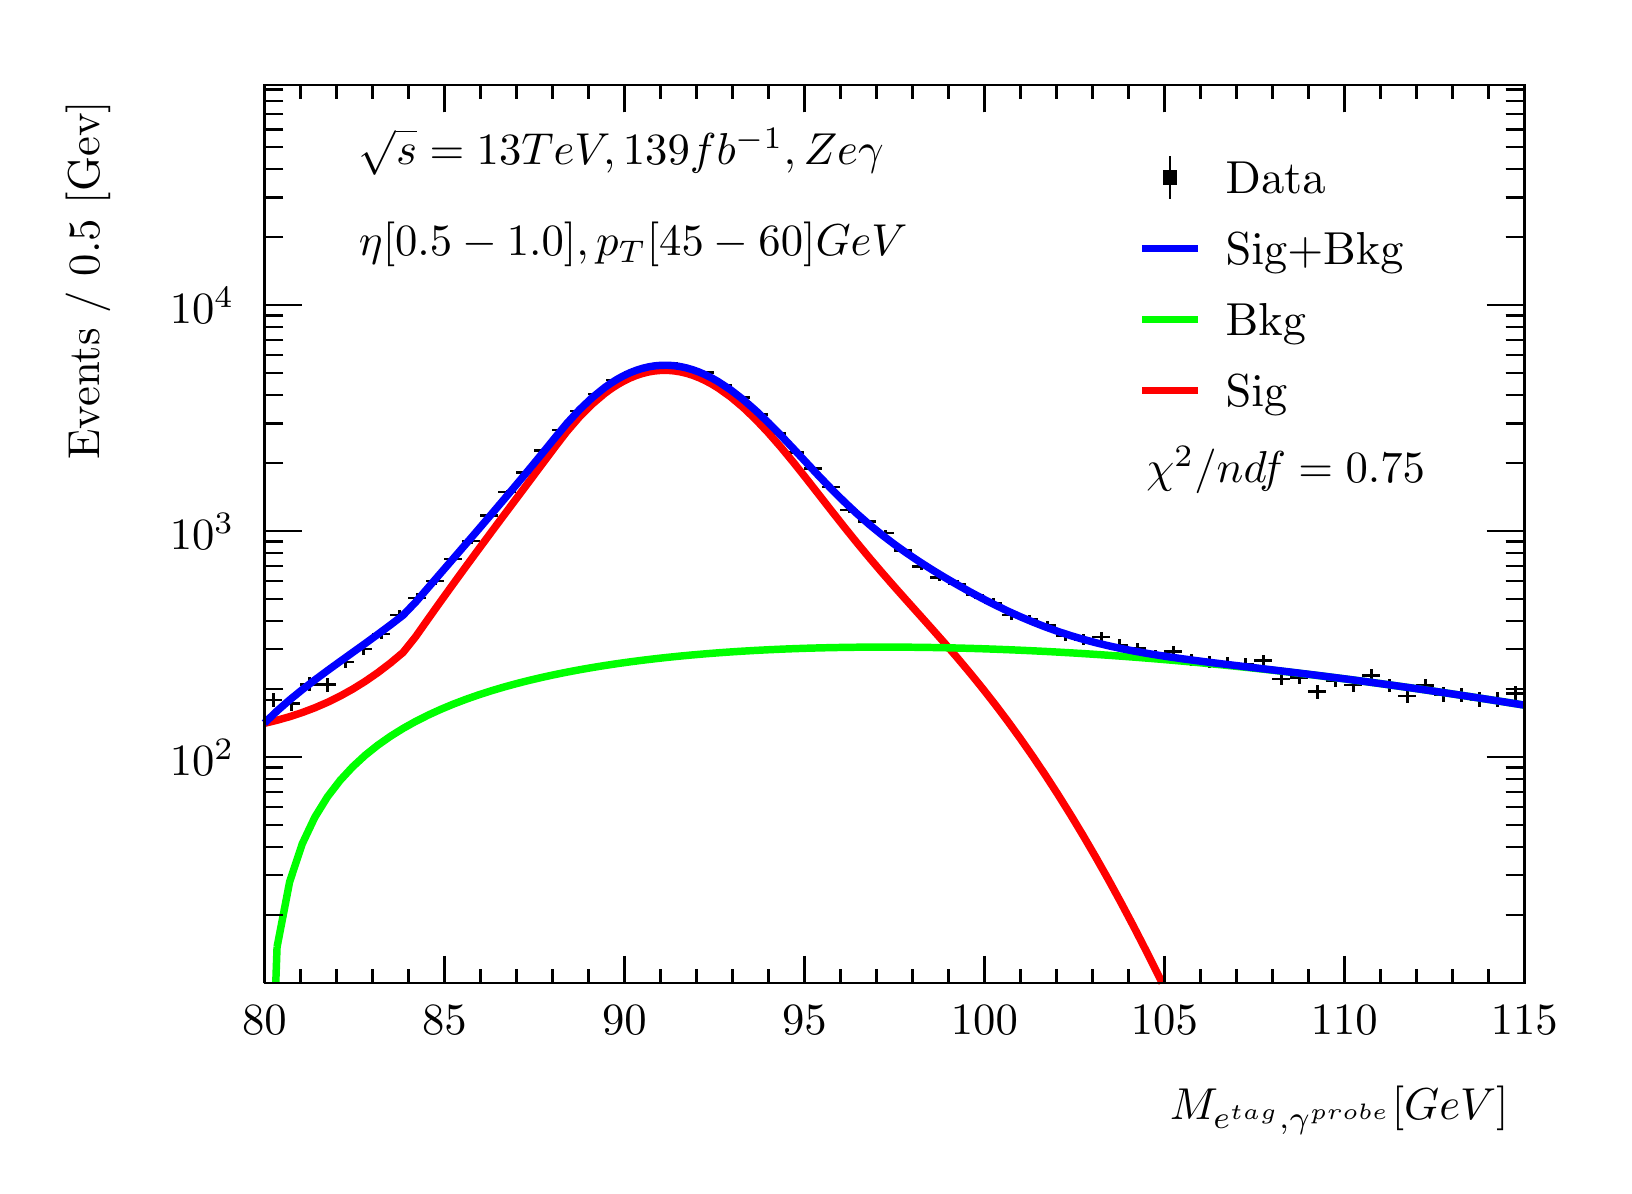
\begin{tikzpicture}
\pgfdeclareplotmark{cross} {
\pgfpathmoveto{\pgfpoint{-0.3\pgfplotmarksize}{\pgfplotmarksize}}
\pgfpathlineto{\pgfpoint{+0.3\pgfplotmarksize}{\pgfplotmarksize}}
\pgfpathlineto{\pgfpoint{+0.3\pgfplotmarksize}{0.3\pgfplotmarksize}}
\pgfpathlineto{\pgfpoint{+1\pgfplotmarksize}{0.3\pgfplotmarksize}}
\pgfpathlineto{\pgfpoint{+1\pgfplotmarksize}{-0.3\pgfplotmarksize}}
\pgfpathlineto{\pgfpoint{+0.3\pgfplotmarksize}{-0.3\pgfplotmarksize}}
\pgfpathlineto{\pgfpoint{+0.3\pgfplotmarksize}{-1.\pgfplotmarksize}}
\pgfpathlineto{\pgfpoint{-0.3\pgfplotmarksize}{-1.\pgfplotmarksize}}
\pgfpathlineto{\pgfpoint{-0.3\pgfplotmarksize}{-0.3\pgfplotmarksize}}
\pgfpathlineto{\pgfpoint{-1.\pgfplotmarksize}{-0.3\pgfplotmarksize}}
\pgfpathlineto{\pgfpoint{-1.\pgfplotmarksize}{0.3\pgfplotmarksize}}
\pgfpathlineto{\pgfpoint{-0.3\pgfplotmarksize}{0.3\pgfplotmarksize}}
\pgfpathclose
\pgfusepathqstroke
}
\pgfdeclareplotmark{cross*} {
\pgfpathmoveto{\pgfpoint{-0.3\pgfplotmarksize}{\pgfplotmarksize}}
\pgfpathlineto{\pgfpoint{+0.3\pgfplotmarksize}{\pgfplotmarksize}}
\pgfpathlineto{\pgfpoint{+0.3\pgfplotmarksize}{0.3\pgfplotmarksize}}
\pgfpathlineto{\pgfpoint{+1\pgfplotmarksize}{0.3\pgfplotmarksize}}
\pgfpathlineto{\pgfpoint{+1\pgfplotmarksize}{-0.3\pgfplotmarksize}}
\pgfpathlineto{\pgfpoint{+0.3\pgfplotmarksize}{-0.3\pgfplotmarksize}}
\pgfpathlineto{\pgfpoint{+0.3\pgfplotmarksize}{-1.\pgfplotmarksize}}
\pgfpathlineto{\pgfpoint{-0.3\pgfplotmarksize}{-1.\pgfplotmarksize}}
\pgfpathlineto{\pgfpoint{-0.3\pgfplotmarksize}{-0.3\pgfplotmarksize}}
\pgfpathlineto{\pgfpoint{-1.\pgfplotmarksize}{-0.3\pgfplotmarksize}}
\pgfpathlineto{\pgfpoint{-1.\pgfplotmarksize}{0.3\pgfplotmarksize}}
\pgfpathlineto{\pgfpoint{-0.3\pgfplotmarksize}{0.3\pgfplotmarksize}}
\pgfpathclose
\pgfusepathqfillstroke
}
\pgfdeclareplotmark{newstar} {
\pgfpathmoveto{\pgfqpoint{0pt}{\pgfplotmarksize}}
\pgfpathlineto{\pgfqpointpolar{44}{0.5\pgfplotmarksize}}
\pgfpathlineto{\pgfqpointpolar{18}{\pgfplotmarksize}}
\pgfpathlineto{\pgfqpointpolar{-20}{0.5\pgfplotmarksize}}
\pgfpathlineto{\pgfqpointpolar{-54}{\pgfplotmarksize}}
\pgfpathlineto{\pgfqpointpolar{-90}{0.5\pgfplotmarksize}}
\pgfpathlineto{\pgfqpointpolar{234}{\pgfplotmarksize}}
\pgfpathlineto{\pgfqpointpolar{198}{0.5\pgfplotmarksize}}
\pgfpathlineto{\pgfqpointpolar{162}{\pgfplotmarksize}}
\pgfpathlineto{\pgfqpointpolar{134}{0.5\pgfplotmarksize}}
\pgfpathclose
\pgfusepathqstroke
}
\pgfdeclareplotmark{newstar*} {
\pgfpathmoveto{\pgfqpoint{0pt}{\pgfplotmarksize}}
\pgfpathlineto{\pgfqpointpolar{44}{0.5\pgfplotmarksize}}
\pgfpathlineto{\pgfqpointpolar{18}{\pgfplotmarksize}}
\pgfpathlineto{\pgfqpointpolar{-20}{0.5\pgfplotmarksize}}
\pgfpathlineto{\pgfqpointpolar{-54}{\pgfplotmarksize}}
\pgfpathlineto{\pgfqpointpolar{-90}{0.5\pgfplotmarksize}}
\pgfpathlineto{\pgfqpointpolar{234}{\pgfplotmarksize}}
\pgfpathlineto{\pgfqpointpolar{198}{0.5\pgfplotmarksize}}
\pgfpathlineto{\pgfqpointpolar{162}{\pgfplotmarksize}}
\pgfpathlineto{\pgfqpointpolar{134}{0.5\pgfplotmarksize}}
\pgfpathclose
\pgfusepathqfillstroke
}
\definecolor{c}{rgb}{1,1,1};
\draw [color=c, fill=c] (0,0) rectangle (20,14.4361);
\draw [color=c, fill=c] (3,2.30977) rectangle (19,13.7143);
\definecolor{c}{rgb}{0,0,0};
\draw [c,line width=0.9] (3,2.30977) -- (3,13.7143) -- (19,13.7143) -- (19,2.30977) -- (3,2.30977);
\definecolor{c}{rgb}{1,1,1};
\draw [color=c, fill=c] (3,2.30977) rectangle (19,13.7143);
\definecolor{c}{rgb}{0,0,0};
\draw [c,line width=0.9] (3,2.30977) -- (3,13.7143) -- (19,13.7143) -- (19,2.30977) -- (3,2.30977);
\draw [c,line width=0.9] (3,2.30977) -- (19,2.30977);
\draw [c,line width=0.9] (3,2.65624) -- (3,2.30977);
\draw [c,line width=0.9] (3.45714,2.48301) -- (3.45714,2.30977);
\draw [c,line width=0.9] (3.91429,2.48301) -- (3.91429,2.30977);
\draw [c,line width=0.9] (4.37143,2.48301) -- (4.37143,2.30977);
\draw [c,line width=0.9] (4.82857,2.48301) -- (4.82857,2.30977);
\draw [c,line width=0.9] (5.28571,2.65624) -- (5.28571,2.30977);
\draw [c,line width=0.9] (5.74286,2.48301) -- (5.74286,2.30977);
\draw [c,line width=0.9] (6.2,2.48301) -- (6.2,2.30977);
\draw [c,line width=0.9] (6.65714,2.48301) -- (6.65714,2.30977);
\draw [c,line width=0.9] (7.11429,2.48301) -- (7.11429,2.30977);
\draw [c,line width=0.9] (7.57143,2.65624) -- (7.57143,2.30977);
\draw [c,line width=0.9] (8.02857,2.48301) -- (8.02857,2.30977);
\draw [c,line width=0.9] (8.48571,2.48301) -- (8.48571,2.30977);
\draw [c,line width=0.9] (8.94286,2.48301) -- (8.94286,2.30977);
\draw [c,line width=0.9] (9.4,2.48301) -- (9.4,2.30977);
\draw [c,line width=0.9] (9.85714,2.65624) -- (9.85714,2.30977);
\draw [c,line width=0.9] (10.3143,2.48301) -- (10.3143,2.30977);
\draw [c,line width=0.9] (10.7714,2.48301) -- (10.7714,2.30977);
\draw [c,line width=0.9] (11.2286,2.48301) -- (11.2286,2.30977);
\draw [c,line width=0.9] (11.6857,2.48301) -- (11.6857,2.30977);
\draw [c,line width=0.9] (12.1429,2.65624) -- (12.1429,2.30977);
\draw [c,line width=0.9] (12.6,2.48301) -- (12.6,2.30977);
\draw [c,line width=0.9] (13.0571,2.48301) -- (13.0571,2.30977);
\draw [c,line width=0.9] (13.5143,2.48301) -- (13.5143,2.30977);
\draw [c,line width=0.9] (13.9714,2.48301) -- (13.9714,2.30977);
\draw [c,line width=0.9] (14.4286,2.65624) -- (14.4286,2.30977);
\draw [c,line width=0.9] (14.8857,2.48301) -- (14.8857,2.30977);
\draw [c,line width=0.9] (15.3429,2.48301) -- (15.3429,2.30977);
\draw [c,line width=0.9] (15.8,2.48301) -- (15.8,2.30977);
\draw [c,line width=0.9] (16.2571,2.48301) -- (16.2571,2.30977);
\draw [c,line width=0.9] (16.7143,2.65624) -- (16.7143,2.30977);
\draw [c,line width=0.9] (17.1714,2.48301) -- (17.1714,2.30977);
\draw [c,line width=0.9] (17.6286,2.48301) -- (17.6286,2.30977);
\draw [c,line width=0.9] (18.0857,2.48301) -- (18.0857,2.30977);
\draw [c,line width=0.9] (18.5429,2.48301) -- (18.5429,2.30977);
\draw [c,line width=0.9] (19,2.65624) -- (19,2.30977);
\draw [anchor=base] (3,1.66015) node[scale=1.61424, color=c, rotate=0]{80};
\draw [anchor=base] (5.28571,1.66015) node[scale=1.61424, color=c, rotate=0]{85};
\draw [anchor=base] (7.57143,1.66015) node[scale=1.61424, color=c, rotate=0]{90};
\draw [anchor=base] (9.85714,1.66015) node[scale=1.61424, color=c, rotate=0]{95};
\draw [anchor=base] (12.1429,1.66015) node[scale=1.61424, color=c, rotate=0]{100};
\draw [anchor=base] (14.4286,1.66015) node[scale=1.61424, color=c, rotate=0]{105};
\draw [anchor=base] (16.7143,1.66015) node[scale=1.61424, color=c, rotate=0]{110};
\draw [anchor=base] (19,1.66015) node[scale=1.61424, color=c, rotate=0]{115};
\draw [anchor= east] (19,0.692932) node[scale=1.61424, color=c, rotate=0]{$M_{e^{tag}, \gamma^{probe}}  [GeV]$};
\draw [c,line width=0.9] (3,13.7143) -- (19,13.7143);
\draw [c,line width=0.9] (3,13.3678) -- (3,13.7143);
\draw [c,line width=0.9] (3.45714,13.5411) -- (3.45714,13.7143);
\draw [c,line width=0.9] (3.91429,13.5411) -- (3.91429,13.7143);
\draw [c,line width=0.9] (4.37143,13.5411) -- (4.37143,13.7143);
\draw [c,line width=0.9] (4.82857,13.5411) -- (4.82857,13.7143);
\draw [c,line width=0.9] (5.28571,13.3678) -- (5.28571,13.7143);
\draw [c,line width=0.9] (5.74286,13.5411) -- (5.74286,13.7143);
\draw [c,line width=0.9] (6.2,13.5411) -- (6.2,13.7143);
\draw [c,line width=0.9] (6.65714,13.5411) -- (6.65714,13.7143);
\draw [c,line width=0.9] (7.11429,13.5411) -- (7.11429,13.7143);
\draw [c,line width=0.9] (7.57143,13.3678) -- (7.57143,13.7143);
\draw [c,line width=0.9] (8.02857,13.5411) -- (8.02857,13.7143);
\draw [c,line width=0.9] (8.48571,13.5411) -- (8.48571,13.7143);
\draw [c,line width=0.9] (8.94286,13.5411) -- (8.94286,13.7143);
\draw [c,line width=0.9] (9.4,13.5411) -- (9.4,13.7143);
\draw [c,line width=0.9] (9.85714,13.3678) -- (9.85714,13.7143);
\draw [c,line width=0.9] (10.3143,13.5411) -- (10.3143,13.7143);
\draw [c,line width=0.9] (10.7714,13.5411) -- (10.7714,13.7143);
\draw [c,line width=0.9] (11.2286,13.5411) -- (11.2286,13.7143);
\draw [c,line width=0.9] (11.6857,13.5411) -- (11.6857,13.7143);
\draw [c,line width=0.9] (12.1429,13.3678) -- (12.1429,13.7143);
\draw [c,line width=0.9] (12.6,13.5411) -- (12.6,13.7143);
\draw [c,line width=0.9] (13.0571,13.5411) -- (13.0571,13.7143);
\draw [c,line width=0.9] (13.5143,13.5411) -- (13.5143,13.7143);
\draw [c,line width=0.9] (13.9714,13.5411) -- (13.9714,13.7143);
\draw [c,line width=0.9] (14.4286,13.3678) -- (14.4286,13.7143);
\draw [c,line width=0.9] (14.8857,13.5411) -- (14.8857,13.7143);
\draw [c,line width=0.9] (15.3429,13.5411) -- (15.3429,13.7143);
\draw [c,line width=0.9] (15.8,13.5411) -- (15.8,13.7143);
\draw [c,line width=0.9] (16.2571,13.5411) -- (16.2571,13.7143);
\draw [c,line width=0.9] (16.7143,13.3678) -- (16.7143,13.7143);
\draw [c,line width=0.9] (17.1714,13.5411) -- (17.1714,13.7143);
\draw [c,line width=0.9] (17.6286,13.5411) -- (17.6286,13.7143);
\draw [c,line width=0.9] (18.0857,13.5411) -- (18.0857,13.7143);
\draw [c,line width=0.9] (18.5429,13.5411) -- (18.5429,13.7143);
\draw [c,line width=0.9] (19,13.3678) -- (19,13.7143);
\draw [c,line width=0.9] (3,2.30977) -- (3,13.7143);
\draw [c,line width=0.9] (3.237,3.17371) -- (3,3.17371);
\draw [c,line width=0.9] (3.237,3.67908) -- (3,3.67908);
\draw [c,line width=0.9] (3.237,4.03764) -- (3,4.03764);
\draw [c,line width=0.9] (3.237,4.31577) -- (3,4.31577);
\draw [c,line width=0.9] (3.237,4.54301) -- (3,4.54301);
\draw [c,line width=0.9] (3.237,4.73514) -- (3,4.73514);
\draw [c,line width=0.9] (3.237,4.90158) -- (3,4.90158);
\draw [c,line width=0.9] (3.237,5.04838) -- (3,5.04838);
\draw [c,line width=0.9] (3.474,5.1797) -- (3,5.1797);
\draw [anchor= east] (2.82,5.1797) node[scale=1.61424, color=c, rotate=0]{$10^{2}$};
\draw [c,line width=0.9] (3.237,6.04363) -- (3,6.04363);
\draw [c,line width=0.9] (3.237,6.549) -- (3,6.549);
\draw [c,line width=0.9] (3.237,6.90757) -- (3,6.90757);
\draw [c,line width=0.9] (3.237,7.18569) -- (3,7.18569);
\draw [c,line width=0.9] (3.237,7.41294) -- (3,7.41294);
\draw [c,line width=0.9] (3.237,7.60507) -- (3,7.60507);
\draw [c,line width=0.9] (3.237,7.7715) -- (3,7.7715);
\draw [c,line width=0.9] (3.237,7.91831) -- (3,7.91831);
\draw [c,line width=0.9] (3.474,8.04963) -- (3,8.04963);
\draw [anchor= east] (2.82,8.04963) node[scale=1.61424, color=c, rotate=0]{$10^{3}$};
\draw [c,line width=0.9] (3.237,8.91356) -- (3,8.91356);
\draw [c,line width=0.9] (3.237,9.41893) -- (3,9.41893);
\draw [c,line width=0.9] (3.237,9.7775) -- (3,9.7775);
\draw [c,line width=0.9] (3.237,10.0556) -- (3,10.0556);
\draw [c,line width=0.9] (3.237,10.2829) -- (3,10.2829);
\draw [c,line width=0.9] (3.237,10.475) -- (3,10.475);
\draw [c,line width=0.9] (3.237,10.6414) -- (3,10.6414);
\draw [c,line width=0.9] (3.237,10.7882) -- (3,10.7882);
\draw [c,line width=0.9] (3.474,10.9196) -- (3,10.9196);
\draw [anchor= east] (2.82,10.9196) node[scale=1.61424, color=c, rotate=0]{$10^{4}$};
\draw [c,line width=0.9] (3.237,11.7835) -- (3,11.7835);
\draw [c,line width=0.9] (3.237,12.2889) -- (3,12.2889);
\draw [c,line width=0.9] (3.237,12.6474) -- (3,12.6474);
\draw [c,line width=0.9] (3.237,12.9256) -- (3,12.9256);
\draw [c,line width=0.9] (3.237,13.1528) -- (3,13.1528);
\draw [c,line width=0.9] (3.237,13.3449) -- (3,13.3449);
\draw [c,line width=0.9] (3.237,13.5114) -- (3,13.5114);
\draw [c,line width=0.9] (3.237,13.6582) -- (3,13.6582);
\draw [anchor= east] (0.76,13.7143) node[scale=1.61424, color=c, rotate=90]{Events / 0.5 [Gev]};
\draw [c,line width=0.9] (19,2.30977) -- (19,13.7143);
\draw [c,line width=0.9] (18.763,3.17371) -- (19,3.17371);
\draw [c,line width=0.9] (18.763,3.67908) -- (19,3.67908);
\draw [c,line width=0.9] (18.763,4.03764) -- (19,4.03764);
\draw [c,line width=0.9] (18.763,4.31577) -- (19,4.31577);
\draw [c,line width=0.9] (18.763,4.54301) -- (19,4.54301);
\draw [c,line width=0.9] (18.763,4.73514) -- (19,4.73514);
\draw [c,line width=0.9] (18.763,4.90158) -- (19,4.90158);
\draw [c,line width=0.9] (18.763,5.04838) -- (19,5.04838);
\draw [c,line width=0.9] (18.526,5.1797) -- (19,5.1797);
\draw [c,line width=0.9] (18.763,6.04363) -- (19,6.04363);
\draw [c,line width=0.9] (18.763,6.549) -- (19,6.549);
\draw [c,line width=0.9] (18.763,6.90757) -- (19,6.90757);
\draw [c,line width=0.9] (18.763,7.18569) -- (19,7.18569);
\draw [c,line width=0.9] (18.763,7.41294) -- (19,7.41294);
\draw [c,line width=0.9] (18.763,7.60507) -- (19,7.60507);
\draw [c,line width=0.9] (18.763,7.7715) -- (19,7.7715);
\draw [c,line width=0.9] (18.763,7.91831) -- (19,7.91831);
\draw [c,line width=0.9] (18.526,8.04963) -- (19,8.04963);
\draw [c,line width=0.9] (18.763,8.91356) -- (19,8.91356);
\draw [c,line width=0.9] (18.763,9.41893) -- (19,9.41893);
\draw [c,line width=0.9] (18.763,9.7775) -- (19,9.7775);
\draw [c,line width=0.9] (18.763,10.0556) -- (19,10.0556);
\draw [c,line width=0.9] (18.763,10.2829) -- (19,10.2829);
\draw [c,line width=0.9] (18.763,10.475) -- (19,10.475);
\draw [c,line width=0.9] (18.763,10.6414) -- (19,10.6414);
\draw [c,line width=0.9] (18.763,10.7882) -- (19,10.7882);
\draw [c,line width=0.9] (18.526,10.9196) -- (19,10.9196);
\draw [c,line width=0.9] (18.763,11.7835) -- (19,11.7835);
\draw [c,line width=0.9] (18.763,12.2889) -- (19,12.2889);
\draw [c,line width=0.9] (18.763,12.6474) -- (19,12.6474);
\draw [c,line width=0.9] (18.763,12.9256) -- (19,12.9256);
\draw [c,line width=0.9] (18.763,13.1528) -- (19,13.1528);
\draw [c,line width=0.9] (18.763,13.3449) -- (19,13.3449);
\draw [c,line width=0.9] (18.763,13.5114) -- (19,13.5114);
\draw [c,line width=0.9] (18.763,13.6582) -- (19,13.6582);
\draw [c,line width=0.9] (3.11429,5.90537) -- (3,5.90537);
\draw [c,line width=0.9] (3,5.90537) -- (3,5.90537);
\draw [c,line width=0.9] (3.11429,5.90537) -- (3.22857,5.90537);
\draw [c,line width=0.9] (3.22857,5.90537) -- (3.22857,5.90537);
\draw [c,line width=0.9] (3.11429,5.90537) -- (3.11429,5.99851);
\draw [c,line width=0.9] (3.11429,5.99851) -- (3.11429,5.99851);
\draw [c,line width=0.9] (3.11429,5.90537) -- (3.11429,5.81223);
\draw [c,line width=0.9] (3.11429,5.81223) -- (3.11429,5.81223);
\draw [c,line width=0.9] (3.34286,5.86288) -- (3.22857,5.86288);
\draw [c,line width=0.9] (3.22857,5.86288) -- (3.22857,5.86288);
\draw [c,line width=0.9] (3.34286,5.86288) -- (3.45714,5.86288);
\draw [c,line width=0.9] (3.45714,5.86288) -- (3.45714,5.86288);
\draw [c,line width=0.9] (3.34286,5.86288) -- (3.34286,5.95762);
\draw [c,line width=0.9] (3.34286,5.95762) -- (3.34286,5.95762);
\draw [c,line width=0.9] (3.34286,5.86288) -- (3.34286,5.76814);
\draw [c,line width=0.9] (3.34286,5.76814) -- (3.34286,5.76814);
\draw [c,line width=0.9] (3.57143,6.10445) -- (3.45714,6.10445);
\draw [c,line width=0.9] (3.45714,6.10445) -- (3.45714,6.10445);
\draw [c,line width=0.9] (3.57143,6.10445) -- (3.68571,6.10445);
\draw [c,line width=0.9] (3.68571,6.10445) -- (3.68571,6.10445);
\draw [c,line width=0.9] (3.57143,6.10445) -- (3.57143,6.19044);
\draw [c,line width=0.9] (3.57143,6.19044) -- (3.57143,6.19044);
\draw [c,line width=0.9] (3.57143,6.10445) -- (3.57143,6.01846);
\draw [c,line width=0.9] (3.57143,6.01846) -- (3.57143,6.01846);
\draw [c,line width=0.9] (3.8,6.0985) -- (3.68571,6.0985);
\draw [c,line width=0.9] (3.68571,6.0985) -- (3.68571,6.0985);
\draw [c,line width=0.9] (3.8,6.0985) -- (3.91429,6.0985);
\draw [c,line width=0.9] (3.91429,6.0985) -- (3.91429,6.0985);
\draw [c,line width=0.9] (3.8,6.0985) -- (3.8,6.1847);
\draw [c,line width=0.9] (3.8,6.1847) -- (3.8,6.1847);
\draw [c,line width=0.9] (3.8,6.0985) -- (3.8,6.0123);
\draw [c,line width=0.9] (3.8,6.0123) -- (3.8,6.0123);
\draw [c,line width=0.9] (4.02857,6.38968) -- (3.91429,6.38968);
\draw [c,line width=0.9] (3.91429,6.38968) -- (3.91429,6.38968);
\draw [c,line width=0.9] (4.02857,6.38968) -- (4.14286,6.38968);
\draw [c,line width=0.9] (4.14286,6.38968) -- (4.14286,6.38968);
\draw [c,line width=0.9] (4.02857,6.38968) -- (4.02857,6.46637);
\draw [c,line width=0.9] (4.02857,6.46637) -- (4.02857,6.46637);
\draw [c,line width=0.9] (4.02857,6.38968) -- (4.02857,6.31298);
\draw [c,line width=0.9] (4.02857,6.31298) -- (4.02857,6.31298);
\draw [c,line width=0.9] (4.25714,6.55315) -- (4.14286,6.55315);
\draw [c,line width=0.9] (4.14286,6.55315) -- (4.14286,6.55315);
\draw [c,line width=0.9] (4.25714,6.55315) -- (4.37143,6.55315);
\draw [c,line width=0.9] (4.37143,6.55315) -- (4.37143,6.55315);
\draw [c,line width=0.9] (4.25714,6.55315) -- (4.25714,6.62498);
\draw [c,line width=0.9] (4.25714,6.62498) -- (4.25714,6.62498);
\draw [c,line width=0.9] (4.25714,6.55315) -- (4.25714,6.48132);
\draw [c,line width=0.9] (4.25714,6.48132) -- (4.25714,6.48132);
\draw [c,line width=0.9] (4.48571,6.74114) -- (4.37143,6.74114);
\draw [c,line width=0.9] (4.37143,6.74114) -- (4.37143,6.74114);
\draw [c,line width=0.9] (4.48571,6.74114) -- (4.6,6.74114);
\draw [c,line width=0.9] (4.6,6.74114) -- (4.6,6.74114);
\draw [c,line width=0.9] (4.48571,6.74114) -- (4.48571,6.80775);
\draw [c,line width=0.9] (4.48571,6.80775) -- (4.48571,6.80775);
\draw [c,line width=0.9] (4.48571,6.74114) -- (4.48571,6.67452);
\draw [c,line width=0.9] (4.48571,6.67452) -- (4.48571,6.67452);
\draw [c,line width=0.9] (4.71429,6.98313) -- (4.6,6.98313);
\draw [c,line width=0.9] (4.6,6.98313) -- (4.6,6.98313);
\draw [c,line width=0.9] (4.71429,6.98313) -- (4.82857,6.98313);
\draw [c,line width=0.9] (4.82857,6.98313) -- (4.82857,6.98313);
\draw [c,line width=0.9] (4.71429,6.98313) -- (4.71429,7.04359);
\draw [c,line width=0.9] (4.71429,7.04359) -- (4.71429,7.04359);
\draw [c,line width=0.9] (4.71429,6.98313) -- (4.71429,6.92268);
\draw [c,line width=0.9] (4.71429,6.92268) -- (4.71429,6.92268);
\draw [c,line width=0.9] (4.94286,7.20302) -- (4.82857,7.20302);
\draw [c,line width=0.9] (4.82857,7.20302) -- (4.82857,7.20302);
\draw [c,line width=0.9] (4.94286,7.20302) -- (5.05714,7.20302);
\draw [c,line width=0.9] (5.05714,7.20302) -- (5.05714,7.20302);
\draw [c,line width=0.9] (4.94286,7.20302) -- (4.94286,7.25837);
\draw [c,line width=0.9] (4.94286,7.25837) -- (4.94286,7.25837);
\draw [c,line width=0.9] (4.94286,7.20302) -- (4.94286,7.14767);
\draw [c,line width=0.9] (4.94286,7.14767) -- (4.94286,7.14767);
\draw [c,line width=0.9] (5.17143,7.41709) -- (5.05714,7.41709);
\draw [c,line width=0.9] (5.05714,7.41709) -- (5.05714,7.41709);
\draw [c,line width=0.9] (5.17143,7.41709) -- (5.28571,7.41709);
\draw [c,line width=0.9] (5.28571,7.41709) -- (5.28571,7.41709);
\draw [c,line width=0.9] (5.17143,7.41709) -- (5.17143,7.46788);
\draw [c,line width=0.9] (5.17143,7.46788) -- (5.17143,7.46788);
\draw [c,line width=0.9] (5.17143,7.41709) -- (5.17143,7.36629);
\draw [c,line width=0.9] (5.17143,7.36629) -- (5.17143,7.36629);
\draw [c,line width=0.9] (5.4,7.69769) -- (5.28571,7.69769);
\draw [c,line width=0.9] (5.28571,7.69769) -- (5.28571,7.69769);
\draw [c,line width=0.9] (5.4,7.69769) -- (5.51429,7.69769);
\draw [c,line width=0.9] (5.51429,7.69769) -- (5.51429,7.69769);
\draw [c,line width=0.9] (5.4,7.69769) -- (5.4,7.74308);
\draw [c,line width=0.9] (5.4,7.74308) -- (5.4,7.74308);
\draw [c,line width=0.9] (5.4,7.69769) -- (5.4,7.65231);
\draw [c,line width=0.9] (5.4,7.65231) -- (5.4,7.65231);
\draw [c,line width=0.9] (5.62857,7.92659) -- (5.51429,7.92659);
\draw [c,line width=0.9] (5.51429,7.92659) -- (5.51429,7.92659);
\draw [c,line width=0.9] (5.62857,7.92659) -- (5.74286,7.92659);
\draw [c,line width=0.9] (5.74286,7.92659) -- (5.74286,7.92659);
\draw [c,line width=0.9] (5.62857,7.92659) -- (5.62857,7.968);
\draw [c,line width=0.9] (5.62857,7.968) -- (5.62857,7.968);
\draw [c,line width=0.9] (5.62857,7.92659) -- (5.62857,7.88518);
\draw [c,line width=0.9] (5.62857,7.88518) -- (5.62857,7.88518);
\draw [c,line width=0.9] (5.85714,8.24957) -- (5.74286,8.24957);
\draw [c,line width=0.9] (5.74286,8.24957) -- (5.74286,8.24957);
\draw [c,line width=0.9] (5.85714,8.24957) -- (5.97143,8.24957);
\draw [c,line width=0.9] (5.97143,8.24957) -- (5.97143,8.24957);
\draw [c,line width=0.9] (5.85714,8.24957) -- (5.85714,8.28595);
\draw [c,line width=0.9] (5.85714,8.28595) -- (5.85714,8.28595);
\draw [c,line width=0.9] (5.85714,8.24957) -- (5.85714,8.2132);
\draw [c,line width=0.9] (5.85714,8.2132) -- (5.85714,8.2132);
\draw [c,line width=0.9] (6.08571,8.54331) -- (5.97143,8.54331);
\draw [c,line width=0.9] (5.97143,8.54331) -- (5.97143,8.54331);
\draw [c,line width=0.9] (6.08571,8.54331) -- (6.2,8.54331);
\draw [c,line width=0.9] (6.2,8.54331) -- (6.2,8.54331);
\draw [c,line width=0.9] (6.08571,8.54331) -- (6.08571,8.57564);
\draw [c,line width=0.9] (6.08571,8.57564) -- (6.08571,8.57564);
\draw [c,line width=0.9] (6.08571,8.54331) -- (6.08571,8.51098);
\draw [c,line width=0.9] (6.08571,8.51098) -- (6.08571,8.51098);
\draw [c,line width=0.9] (6.31429,8.7967) -- (6.2,8.7967);
\draw [c,line width=0.9] (6.2,8.7967) -- (6.2,8.7967);
\draw [c,line width=0.9] (6.31429,8.7967) -- (6.42857,8.7967);
\draw [c,line width=0.9] (6.42857,8.7967) -- (6.42857,8.7967);
\draw [c,line width=0.9] (6.31429,8.7967) -- (6.31429,8.82591);
\draw [c,line width=0.9] (6.31429,8.82591) -- (6.31429,8.82591);
\draw [c,line width=0.9] (6.31429,8.7967) -- (6.31429,8.76749);
\draw [c,line width=0.9] (6.31429,8.76749) -- (6.31429,8.76749);
\draw [c,line width=0.9] (6.54286,9.07414) -- (6.42857,9.07414);
\draw [c,line width=0.9] (6.42857,9.07414) -- (6.42857,9.07414);
\draw [c,line width=0.9] (6.54286,9.07414) -- (6.65714,9.07414);
\draw [c,line width=0.9] (6.65714,9.07414) -- (6.65714,9.07414);
\draw [c,line width=0.9] (6.54286,9.07414) -- (6.54286,9.10027);
\draw [c,line width=0.9] (6.54286,9.10027) -- (6.54286,9.10027);
\draw [c,line width=0.9] (6.54286,9.07414) -- (6.54286,9.04801);
\draw [c,line width=0.9] (6.54286,9.04801) -- (6.54286,9.04801);
\draw [c,line width=0.9] (6.77143,9.33027) -- (6.65714,9.33027);
\draw [c,line width=0.9] (6.65714,9.33027) -- (6.65714,9.33027);
\draw [c,line width=0.9] (6.77143,9.33027) -- (6.88571,9.33027);
\draw [c,line width=0.9] (6.88571,9.33027) -- (6.88571,9.33027);
\draw [c,line width=0.9] (6.77143,9.33027) -- (6.77143,9.35385);
\draw [c,line width=0.9] (6.77143,9.35385) -- (6.77143,9.35385);
\draw [c,line width=0.9] (6.77143,9.33027) -- (6.77143,9.30669);
\draw [c,line width=0.9] (6.77143,9.30669) -- (6.77143,9.30669);
\draw [c,line width=0.9] (7,9.57677) -- (6.88571,9.57677);
\draw [c,line width=0.9] (6.88571,9.57677) -- (6.88571,9.57677);
\draw [c,line width=0.9] (7,9.57677) -- (7.11429,9.57677);
\draw [c,line width=0.9] (7.11429,9.57677) -- (7.11429,9.57677);
\draw [c,line width=0.9] (7,9.57677) -- (7,9.59813);
\draw [c,line width=0.9] (7,9.59813) -- (7,9.59813);
\draw [c,line width=0.9] (7,9.57677) -- (7,9.55541);
\draw [c,line width=0.9] (7,9.55541) -- (7,9.55541);
\draw [c,line width=0.9] (7.22857,9.78897) -- (7.11429,9.78897);
\draw [c,line width=0.9] (7.11429,9.78897) -- (7.11429,9.78897);
\draw [c,line width=0.9] (7.22857,9.78897) -- (7.34286,9.78897);
\draw [c,line width=0.9] (7.34286,9.78897) -- (7.34286,9.78897);
\draw [c,line width=0.9] (7.22857,9.78897) -- (7.22857,9.80859);
\draw [c,line width=0.9] (7.22857,9.80859) -- (7.22857,9.80859);
\draw [c,line width=0.9] (7.22857,9.78897) -- (7.22857,9.76936);
\draw [c,line width=0.9] (7.22857,9.76936) -- (7.22857,9.76936);
\draw [c,line width=0.9] (7.45714,9.97132) -- (7.34286,9.97132);
\draw [c,line width=0.9] (7.34286,9.97132) -- (7.34286,9.97132);
\draw [c,line width=0.9] (7.45714,9.97132) -- (7.57143,9.97132);
\draw [c,line width=0.9] (7.57143,9.97132) -- (7.57143,9.97132);
\draw [c,line width=0.9] (7.45714,9.97132) -- (7.45714,9.98955);
\draw [c,line width=0.9] (7.45714,9.98955) -- (7.45714,9.98955);
\draw [c,line width=0.9] (7.45714,9.97132) -- (7.45714,9.95309);
\draw [c,line width=0.9] (7.45714,9.95309) -- (7.45714,9.95309);
\draw [c,line width=0.9] (7.68571,10.0702) -- (7.57143,10.0702);
\draw [c,line width=0.9] (7.57143,10.0702) -- (7.57143,10.0702);
\draw [c,line width=0.9] (7.68571,10.0702) -- (7.8,10.0702);
\draw [c,line width=0.9] (7.8,10.0702) -- (7.8,10.0702);
\draw [c,line width=0.9] (7.68571,10.0702) -- (7.68571,10.0878);
\draw [c,line width=0.9] (7.68571,10.0878) -- (7.68571,10.0878);
\draw [c,line width=0.9] (7.68571,10.0702) -- (7.68571,10.0527);
\draw [c,line width=0.9] (7.68571,10.0527) -- (7.68571,10.0527);
\draw [c,line width=0.9] (7.91429,10.1129) -- (7.8,10.1129);
\draw [c,line width=0.9] (7.8,10.1129) -- (7.8,10.1129);
\draw [c,line width=0.9] (7.91429,10.1129) -- (8.02857,10.1129);
\draw [c,line width=0.9] (8.02857,10.1129) -- (8.02857,10.1129);
\draw [c,line width=0.9] (7.91429,10.1129) -- (7.91429,10.1301);
\draw [c,line width=0.9] (7.91429,10.1301) -- (7.91429,10.1301);
\draw [c,line width=0.9] (7.91429,10.1129) -- (7.91429,10.0956);
\draw [c,line width=0.9] (7.91429,10.0956) -- (7.91429,10.0956);
\draw [c,line width=0.9] (8.14286,10.1805) -- (8.02857,10.1805);
\draw [c,line width=0.9] (8.02857,10.1805) -- (8.02857,10.1805);
\draw [c,line width=0.9] (8.14286,10.1805) -- (8.25714,10.1805);
\draw [c,line width=0.9] (8.25714,10.1805) -- (8.25714,10.1805);
\draw [c,line width=0.9] (8.14286,10.1805) -- (8.14286,10.1973);
\draw [c,line width=0.9] (8.14286,10.1973) -- (8.14286,10.1973);
\draw [c,line width=0.9] (8.14286,10.1805) -- (8.14286,10.1638);
\draw [c,line width=0.9] (8.14286,10.1638) -- (8.14286,10.1638);
\draw [c,line width=0.9] (8.37143,10.1093) -- (8.25714,10.1093);
\draw [c,line width=0.9] (8.25714,10.1093) -- (8.25714,10.1093);
\draw [c,line width=0.9] (8.37143,10.1093) -- (8.48571,10.1093);
\draw [c,line width=0.9] (8.48571,10.1093) -- (8.48571,10.1093);
\draw [c,line width=0.9] (8.37143,10.1093) -- (8.37143,10.1265);
\draw [c,line width=0.9] (8.37143,10.1265) -- (8.37143,10.1265);
\draw [c,line width=0.9] (8.37143,10.1093) -- (8.37143,10.092);
\draw [c,line width=0.9] (8.37143,10.092) -- (8.37143,10.092);
\draw [c,line width=0.9] (8.6,10.0663) -- (8.48571,10.0663);
\draw [c,line width=0.9] (8.48571,10.0663) -- (8.48571,10.0663);
\draw [c,line width=0.9] (8.6,10.0663) -- (8.71429,10.0663);
\draw [c,line width=0.9] (8.71429,10.0663) -- (8.71429,10.0663);
\draw [c,line width=0.9] (8.6,10.0663) -- (8.6,10.0838);
\draw [c,line width=0.9] (8.6,10.0838) -- (8.6,10.0838);
\draw [c,line width=0.9] (8.6,10.0663) -- (8.6,10.0487);
\draw [c,line width=0.9] (8.6,10.0487) -- (8.6,10.0487);
\draw [c,line width=0.9] (8.82857,9.89969) -- (8.71429,9.89969);
\draw [c,line width=0.9] (8.71429,9.89969) -- (8.71429,9.89969);
\draw [c,line width=0.9] (8.82857,9.89969) -- (8.94286,9.89969);
\draw [c,line width=0.9] (8.94286,9.89969) -- (8.94286,9.89969);
\draw [c,line width=0.9] (8.82857,9.89969) -- (8.82857,9.91845);
\draw [c,line width=0.9] (8.82857,9.91845) -- (8.82857,9.91845);
\draw [c,line width=0.9] (8.82857,9.89969) -- (8.82857,9.88092);
\draw [c,line width=0.9] (8.82857,9.88092) -- (8.82857,9.88092);
\draw [c,line width=0.9] (9.05714,9.74626) -- (8.94286,9.74626);
\draw [c,line width=0.9] (8.94286,9.74626) -- (8.94286,9.74626);
\draw [c,line width=0.9] (9.05714,9.74626) -- (9.17143,9.74626);
\draw [c,line width=0.9] (9.17143,9.74626) -- (9.17143,9.74626);
\draw [c,line width=0.9] (9.05714,9.74626) -- (9.05714,9.76622);
\draw [c,line width=0.9] (9.05714,9.76622) -- (9.05714,9.76622);
\draw [c,line width=0.9] (9.05714,9.74626) -- (9.05714,9.72631);
\draw [c,line width=0.9] (9.05714,9.72631) -- (9.05714,9.72631);
\draw [c,line width=0.9] (9.28571,9.52863) -- (9.17143,9.52863);
\draw [c,line width=0.9] (9.17143,9.52863) -- (9.17143,9.52863);
\draw [c,line width=0.9] (9.28571,9.52863) -- (9.4,9.52863);
\draw [c,line width=0.9] (9.4,9.52863) -- (9.4,9.52863);
\draw [c,line width=0.9] (9.28571,9.52863) -- (9.28571,9.55041);
\draw [c,line width=0.9] (9.28571,9.55041) -- (9.28571,9.55041);
\draw [c,line width=0.9] (9.28571,9.52863) -- (9.28571,9.50685);
\draw [c,line width=0.9] (9.28571,9.50685) -- (9.28571,9.50685);
\draw [c,line width=0.9] (9.51429,9.28992) -- (9.4,9.28992);
\draw [c,line width=0.9] (9.4,9.28992) -- (9.4,9.28992);
\draw [c,line width=0.9] (9.51429,9.28992) -- (9.62857,9.28992);
\draw [c,line width=0.9] (9.62857,9.28992) -- (9.62857,9.28992);
\draw [c,line width=0.9] (9.51429,9.28992) -- (9.51429,9.31388);
\draw [c,line width=0.9] (9.51429,9.31388) -- (9.51429,9.31388);
\draw [c,line width=0.9] (9.51429,9.28992) -- (9.51429,9.26595);
\draw [c,line width=0.9] (9.51429,9.26595) -- (9.51429,9.26595);
\draw [c,line width=0.9] (9.74286,9.047) -- (9.62857,9.047);
\draw [c,line width=0.9] (9.62857,9.047) -- (9.62857,9.047);
\draw [c,line width=0.9] (9.74286,9.047) -- (9.85714,9.047);
\draw [c,line width=0.9] (9.85714,9.047) -- (9.85714,9.047);
\draw [c,line width=0.9] (9.74286,9.047) -- (9.74286,9.07342);
\draw [c,line width=0.9] (9.74286,9.07342) -- (9.74286,9.07342);
\draw [c,line width=0.9] (9.74286,9.047) -- (9.74286,9.02059);
\draw [c,line width=0.9] (9.74286,9.02059) -- (9.74286,9.02059);
\draw [c,line width=0.9] (9.97143,8.84371) -- (9.85714,8.84371);
\draw [c,line width=0.9] (9.85714,8.84371) -- (9.85714,8.84371);
\draw [c,line width=0.9] (9.97143,8.84371) -- (10.0857,8.84371);
\draw [c,line width=0.9] (10.0857,8.84371) -- (10.0857,8.84371);
\draw [c,line width=0.9] (9.97143,8.84371) -- (9.97143,8.87238);
\draw [c,line width=0.9] (9.97143,8.87238) -- (9.97143,8.87238);
\draw [c,line width=0.9] (9.97143,8.84371) -- (9.97143,8.81505);
\draw [c,line width=0.9] (9.97143,8.81505) -- (9.97143,8.81505);
\draw [c,line width=0.9] (10.2,8.60867) -- (10.0857,8.60867);
\draw [c,line width=0.9] (10.0857,8.60867) -- (10.0857,8.60867);
\draw [c,line width=0.9] (10.2,8.60867) -- (10.3143,8.60867);
\draw [c,line width=0.9] (10.3143,8.60867) -- (10.3143,8.60867);
\draw [c,line width=0.9] (10.2,8.60867) -- (10.2,8.64016);
\draw [c,line width=0.9] (10.2,8.64016) -- (10.2,8.64016);
\draw [c,line width=0.9] (10.2,8.60867) -- (10.2,8.57717);
\draw [c,line width=0.9] (10.2,8.57717) -- (10.2,8.57717);
\draw [c,line width=0.9] (10.4286,8.31774) -- (10.3143,8.31774);
\draw [c,line width=0.9] (10.3143,8.31774) -- (10.3143,8.31774);
\draw [c,line width=0.9] (10.4286,8.31774) -- (10.5429,8.31774);
\draw [c,line width=0.9] (10.5429,8.31774) -- (10.5429,8.31774);
\draw [c,line width=0.9] (10.4286,8.31774) -- (10.4286,8.35314);
\draw [c,line width=0.9] (10.4286,8.35314) -- (10.4286,8.35314);
\draw [c,line width=0.9] (10.4286,8.31774) -- (10.4286,8.28235);
\draw [c,line width=0.9] (10.4286,8.28235) -- (10.4286,8.28235);
\draw [c,line width=0.9] (10.6571,8.16956) -- (10.5429,8.16956);
\draw [c,line width=0.9] (10.5429,8.16956) -- (10.5429,8.16956);
\draw [c,line width=0.9] (10.6571,8.16956) -- (10.7714,8.16956);
\draw [c,line width=0.9] (10.7714,8.16956) -- (10.7714,8.16956);
\draw [c,line width=0.9] (10.6571,8.16956) -- (10.6571,8.20712);
\draw [c,line width=0.9] (10.6571,8.20712) -- (10.6571,8.20712);
\draw [c,line width=0.9] (10.6571,8.16956) -- (10.6571,8.132);
\draw [c,line width=0.9] (10.6571,8.132) -- (10.6571,8.132);
\draw [c,line width=0.9] (10.8857,8.02572) -- (10.7714,8.02572);
\draw [c,line width=0.9] (10.7714,8.02572) -- (10.7714,8.02572);
\draw [c,line width=0.9] (10.8857,8.02572) -- (11,8.02572);
\draw [c,line width=0.9] (11,8.02572) -- (11,8.02572);
\draw [c,line width=0.9] (10.8857,8.02572) -- (10.8857,8.06551);
\draw [c,line width=0.9] (10.8857,8.06551) -- (10.8857,8.06551);
\draw [c,line width=0.9] (10.8857,8.02572) -- (10.8857,7.98593);
\draw [c,line width=0.9] (10.8857,7.98593) -- (10.8857,7.98593);
\draw [c,line width=0.9] (11.1143,7.80532) -- (11,7.80532);
\draw [c,line width=0.9] (11,7.80532) -- (11,7.80532);
\draw [c,line width=0.9] (11.1143,7.80532) -- (11.2286,7.80532);
\draw [c,line width=0.9] (11.2286,7.80532) -- (11.2286,7.80532);
\draw [c,line width=0.9] (11.1143,7.80532) -- (11.1143,7.84879);
\draw [c,line width=0.9] (11.1143,7.84879) -- (11.1143,7.84879);
\draw [c,line width=0.9] (11.1143,7.80532) -- (11.1143,7.76185);
\draw [c,line width=0.9] (11.1143,7.76185) -- (11.1143,7.76185);
\draw [c,line width=0.9] (11.3429,7.59793) -- (11.2286,7.59793);
\draw [c,line width=0.9] (11.2286,7.59793) -- (11.2286,7.59793);
\draw [c,line width=0.9] (11.3429,7.59793) -- (11.4571,7.59793);
\draw [c,line width=0.9] (11.4571,7.59793) -- (11.4571,7.59793);
\draw [c,line width=0.9] (11.3429,7.59793) -- (11.3429,7.64517);
\draw [c,line width=0.9] (11.3429,7.64517) -- (11.3429,7.64517);
\draw [c,line width=0.9] (11.3429,7.59793) -- (11.3429,7.55069);
\draw [c,line width=0.9] (11.3429,7.55069) -- (11.3429,7.55069);
\draw [c,line width=0.9] (11.5714,7.46182) -- (11.4571,7.46182);
\draw [c,line width=0.9] (11.4571,7.46182) -- (11.4571,7.46182);
\draw [c,line width=0.9] (11.5714,7.46182) -- (11.6857,7.46182);
\draw [c,line width=0.9] (11.6857,7.46182) -- (11.6857,7.46182);
\draw [c,line width=0.9] (11.5714,7.46182) -- (11.5714,7.51172);
\draw [c,line width=0.9] (11.5714,7.51172) -- (11.5714,7.51172);
\draw [c,line width=0.9] (11.5714,7.46182) -- (11.5714,7.41193);
\draw [c,line width=0.9] (11.5714,7.41193) -- (11.5714,7.41193);
\draw [c,line width=0.9] (11.8,7.37498) -- (11.6857,7.37498);
\draw [c,line width=0.9] (11.6857,7.37498) -- (11.6857,7.37498);
\draw [c,line width=0.9] (11.8,7.37498) -- (11.9143,7.37498);
\draw [c,line width=0.9] (11.9143,7.37498) -- (11.9143,7.37498);
\draw [c,line width=0.9] (11.8,7.37498) -- (11.8,7.42664);
\draw [c,line width=0.9] (11.8,7.42664) -- (11.8,7.42664);
\draw [c,line width=0.9] (11.8,7.37498) -- (11.8,7.32332);
\draw [c,line width=0.9] (11.8,7.32332) -- (11.8,7.32332);
\draw [c,line width=0.9] (12.0286,7.23936) -- (11.9143,7.23936);
\draw [c,line width=0.9] (11.9143,7.23936) -- (11.9143,7.23936);
\draw [c,line width=0.9] (12.0286,7.23936) -- (12.1429,7.23936);
\draw [c,line width=0.9] (12.1429,7.23936) -- (12.1429,7.23936);
\draw [c,line width=0.9] (12.0286,7.23936) -- (12.0286,7.29391);
\draw [c,line width=0.9] (12.0286,7.29391) -- (12.0286,7.29391);
\draw [c,line width=0.9] (12.0286,7.23936) -- (12.0286,7.18482);
\draw [c,line width=0.9] (12.0286,7.18482) -- (12.0286,7.18482);
\draw [c,line width=0.9] (12.2571,7.13741) -- (12.1429,7.13741);
\draw [c,line width=0.9] (12.1429,7.13741) -- (12.1429,7.13741);
\draw [c,line width=0.9] (12.2571,7.13741) -- (12.3714,7.13741);
\draw [c,line width=0.9] (12.3714,7.13741) -- (12.3714,7.13741);
\draw [c,line width=0.9] (12.2571,7.13741) -- (12.2571,7.19424);
\draw [c,line width=0.9] (12.2571,7.19424) -- (12.2571,7.19424);
\draw [c,line width=0.9] (12.2571,7.13741) -- (12.2571,7.08058);
\draw [c,line width=0.9] (12.2571,7.08058) -- (12.2571,7.08058);
\draw [c,line width=0.9] (12.4857,6.98313) -- (12.3714,6.98313);
\draw [c,line width=0.9] (12.3714,6.98313) -- (12.3714,6.98313);
\draw [c,line width=0.9] (12.4857,6.98313) -- (12.6,6.98313);
\draw [c,line width=0.9] (12.6,6.98313) -- (12.6,6.98313);
\draw [c,line width=0.9] (12.4857,6.98313) -- (12.4857,7.04359);
\draw [c,line width=0.9] (12.4857,7.04359) -- (12.4857,7.04359);
\draw [c,line width=0.9] (12.4857,6.98313) -- (12.4857,6.92268);
\draw [c,line width=0.9] (12.4857,6.92268) -- (12.4857,6.92268);
\draw [c,line width=0.9] (12.7143,6.92613) -- (12.6,6.92613);
\draw [c,line width=0.9] (12.6,6.92613) -- (12.6,6.92613);
\draw [c,line width=0.9] (12.7143,6.92613) -- (12.8286,6.92613);
\draw [c,line width=0.9] (12.8286,6.92613) -- (12.8286,6.92613);
\draw [c,line width=0.9] (12.7143,6.92613) -- (12.7143,6.98798);
\draw [c,line width=0.9] (12.7143,6.98798) -- (12.7143,6.98798);
\draw [c,line width=0.9] (12.7143,6.92613) -- (12.7143,6.86428);
\draw [c,line width=0.9] (12.7143,6.86428) -- (12.7143,6.86428);
\draw [c,line width=0.9] (12.9429,6.85018) -- (12.8286,6.85018);
\draw [c,line width=0.9] (12.8286,6.85018) -- (12.8286,6.85018);
\draw [c,line width=0.9] (12.9429,6.85018) -- (13.0571,6.85018);
\draw [c,line width=0.9] (13.0571,6.85018) -- (13.0571,6.85018);
\draw [c,line width=0.9] (12.9429,6.85018) -- (12.9429,6.91395);
\draw [c,line width=0.9] (12.9429,6.91395) -- (12.9429,6.91395);
\draw [c,line width=0.9] (12.9429,6.85018) -- (12.9429,6.78642);
\draw [c,line width=0.9] (12.9429,6.78642) -- (12.9429,6.78642);
\draw [c,line width=0.9] (13.1714,6.71596) -- (13.0571,6.71596);
\draw [c,line width=0.9] (13.0571,6.71596) -- (13.0571,6.71596);
\draw [c,line width=0.9] (13.1714,6.71596) -- (13.2857,6.71596);
\draw [c,line width=0.9] (13.2857,6.71596) -- (13.2857,6.71596);
\draw [c,line width=0.9] (13.1714,6.71596) -- (13.1714,6.78325);
\draw [c,line width=0.9] (13.1714,6.78325) -- (13.1714,6.78325);
\draw [c,line width=0.9] (13.1714,6.71596) -- (13.1714,6.64867);
\draw [c,line width=0.9] (13.1714,6.64867) -- (13.1714,6.64867);
\draw [c,line width=0.9] (13.4,6.67533) -- (13.2857,6.67533);
\draw [c,line width=0.9] (13.2857,6.67533) -- (13.2857,6.67533);
\draw [c,line width=0.9] (13.4,6.67533) -- (13.5143,6.67533);
\draw [c,line width=0.9] (13.5143,6.67533) -- (13.5143,6.67533);
\draw [c,line width=0.9] (13.4,6.67533) -- (13.4,6.74373);
\draw [c,line width=0.9] (13.4,6.74373) -- (13.4,6.74373);
\draw [c,line width=0.9] (13.4,6.67533) -- (13.4,6.60694);
\draw [c,line width=0.9] (13.4,6.60694) -- (13.4,6.60694);
\draw [c,line width=0.9] (13.6286,6.70501) -- (13.5143,6.70501);
\draw [c,line width=0.9] (13.5143,6.70501) -- (13.5143,6.70501);
\draw [c,line width=0.9] (13.6286,6.70501) -- (13.7429,6.70501);
\draw [c,line width=0.9] (13.7429,6.70501) -- (13.7429,6.70501);
\draw [c,line width=0.9] (13.6286,6.70501) -- (13.6286,6.7726);
\draw [c,line width=0.9] (13.6286,6.7726) -- (13.6286,6.7726);
\draw [c,line width=0.9] (13.6286,6.70501) -- (13.6286,6.63742);
\draw [c,line width=0.9] (13.6286,6.63742) -- (13.6286,6.63742);
\draw [c,line width=0.9] (13.8571,6.60585) -- (13.7429,6.60585);
\draw [c,line width=0.9] (13.7429,6.60585) -- (13.7429,6.60585);
\draw [c,line width=0.9] (13.8571,6.60585) -- (13.9714,6.60585);
\draw [c,line width=0.9] (13.9714,6.60585) -- (13.9714,6.60585);
\draw [c,line width=0.9] (13.8571,6.60585) -- (13.8571,6.67618);
\draw [c,line width=0.9] (13.8571,6.67618) -- (13.8571,6.67618);
\draw [c,line width=0.9] (13.8571,6.60585) -- (13.8571,6.53553);
\draw [c,line width=0.9] (13.8571,6.53553) -- (13.8571,6.53553);
\draw [c,line width=0.9] (14.0857,6.55729) -- (13.9714,6.55729);
\draw [c,line width=0.9] (13.9714,6.55729) -- (13.9714,6.55729);
\draw [c,line width=0.9] (14.0857,6.55729) -- (14.2,6.55729);
\draw [c,line width=0.9] (14.2,6.55729) -- (14.2,6.55729);
\draw [c,line width=0.9] (14.0857,6.55729) -- (14.0857,6.629);
\draw [c,line width=0.9] (14.0857,6.629) -- (14.0857,6.629);
\draw [c,line width=0.9] (14.0857,6.55729) -- (14.0857,6.48558);
\draw [c,line width=0.9] (14.0857,6.48558) -- (14.0857,6.48558);
\draw [c,line width=0.9] (14.3143,6.46301) -- (14.2,6.46301);
\draw [c,line width=0.9] (14.2,6.46301) -- (14.2,6.46301);
\draw [c,line width=0.9] (14.3143,6.46301) -- (14.4286,6.46301);
\draw [c,line width=0.9] (14.4286,6.46301) -- (14.4286,6.46301);
\draw [c,line width=0.9] (14.3143,6.46301) -- (14.3143,6.53749);
\draw [c,line width=0.9] (14.3143,6.53749) -- (14.3143,6.53749);
\draw [c,line width=0.9] (14.3143,6.46301) -- (14.3143,6.38854);
\draw [c,line width=0.9] (14.3143,6.38854) -- (14.3143,6.38854);
\draw [c,line width=0.9] (14.5429,6.51958) -- (14.4286,6.51958);
\draw [c,line width=0.9] (14.4286,6.51958) -- (14.4286,6.51958);
\draw [c,line width=0.9] (14.5429,6.51958) -- (14.6571,6.51958);
\draw [c,line width=0.9] (14.6571,6.51958) -- (14.6571,6.51958);
\draw [c,line width=0.9] (14.5429,6.51958) -- (14.5429,6.59238);
\draw [c,line width=0.9] (14.5429,6.59238) -- (14.5429,6.59238);
\draw [c,line width=0.9] (14.5429,6.51958) -- (14.5429,6.44677);
\draw [c,line width=0.9] (14.5429,6.44677) -- (14.5429,6.44677);
\draw [c,line width=0.9] (14.7714,6.41769) -- (14.6571,6.41769);
\draw [c,line width=0.9] (14.6571,6.41769) -- (14.6571,6.41769);
\draw [c,line width=0.9] (14.7714,6.41769) -- (14.8857,6.41769);
\draw [c,line width=0.9] (14.8857,6.41769) -- (14.8857,6.41769);
\draw [c,line width=0.9] (14.7714,6.41769) -- (14.7714,6.49353);
\draw [c,line width=0.9] (14.7714,6.49353) -- (14.7714,6.49353);
\draw [c,line width=0.9] (14.7714,6.41769) -- (14.7714,6.34184);
\draw [c,line width=0.9] (14.7714,6.34184) -- (14.7714,6.34184);
\draw [c,line width=0.9] (15,6.38968) -- (14.8857,6.38968);
\draw [c,line width=0.9] (14.8857,6.38968) -- (14.8857,6.38968);
\draw [c,line width=0.9] (15,6.38968) -- (15.1143,6.38968);
\draw [c,line width=0.9] (15.1143,6.38968) -- (15.1143,6.38968);
\draw [c,line width=0.9] (15,6.38968) -- (15,6.46637);
\draw [c,line width=0.9] (15,6.46637) -- (15,6.46637);
\draw [c,line width=0.9] (15,6.38968) -- (15,6.31298);
\draw [c,line width=0.9] (15,6.31298) -- (15,6.31298);
\draw [c,line width=0.9] (15.2286,6.37543) -- (15.1143,6.37543);
\draw [c,line width=0.9] (15.1143,6.37543) -- (15.1143,6.37543);
\draw [c,line width=0.9] (15.2286,6.37543) -- (15.3429,6.37543);
\draw [c,line width=0.9] (15.3429,6.37543) -- (15.3429,6.37543);
\draw [c,line width=0.9] (15.2286,6.37543) -- (15.2286,6.45257);
\draw [c,line width=0.9] (15.2286,6.45257) -- (15.2286,6.45257);
\draw [c,line width=0.9] (15.2286,6.37543) -- (15.2286,6.29829);
\draw [c,line width=0.9] (15.2286,6.29829) -- (15.2286,6.29829);
\draw [c,line width=0.9] (15.4571,6.36102) -- (15.3429,6.36102);
\draw [c,line width=0.9] (15.3429,6.36102) -- (15.3429,6.36102);
\draw [c,line width=0.9] (15.4571,6.36102) -- (15.5714,6.36102);
\draw [c,line width=0.9] (15.5714,6.36102) -- (15.5714,6.36102);
\draw [c,line width=0.9] (15.4571,6.36102) -- (15.4571,6.43861);
\draw [c,line width=0.9] (15.4571,6.43861) -- (15.4571,6.43861);
\draw [c,line width=0.9] (15.4571,6.36102) -- (15.4571,6.28344);
\draw [c,line width=0.9] (15.4571,6.28344) -- (15.4571,6.28344);
\draw [c,line width=0.9] (15.6857,6.40376) -- (15.5714,6.40376);
\draw [c,line width=0.9] (15.5714,6.40376) -- (15.5714,6.40376);
\draw [c,line width=0.9] (15.6857,6.40376) -- (15.8,6.40376);
\draw [c,line width=0.9] (15.8,6.40376) -- (15.8,6.40376);
\draw [c,line width=0.9] (15.6857,6.40376) -- (15.6857,6.48002);
\draw [c,line width=0.9] (15.6857,6.48002) -- (15.6857,6.48002);
\draw [c,line width=0.9] (15.6857,6.40376) -- (15.6857,6.32749);
\draw [c,line width=0.9] (15.6857,6.32749) -- (15.6857,6.32749);
\draw [c,line width=0.9] (15.9143,6.17371) -- (15.8,6.17371);
\draw [c,line width=0.9] (15.8,6.17371) -- (15.8,6.17371);
\draw [c,line width=0.9] (15.9143,6.17371) -- (16.0286,6.17371);
\draw [c,line width=0.9] (16.0286,6.17371) -- (16.0286,6.17371);
\draw [c,line width=0.9] (15.9143,6.17371) -- (15.9143,6.25735);
\draw [c,line width=0.9] (15.9143,6.25735) -- (15.9143,6.25735);
\draw [c,line width=0.9] (15.9143,6.17371) -- (15.9143,6.09007);
\draw [c,line width=0.9] (15.9143,6.09007) -- (15.9143,6.09007);
\draw [c,line width=0.9] (16.1429,6.19044) -- (16.0286,6.19044);
\draw [c,line width=0.9] (16.0286,6.19044) -- (16.0286,6.19044);
\draw [c,line width=0.9] (16.1429,6.19044) -- (16.2571,6.19044);
\draw [c,line width=0.9] (16.2571,6.19044) -- (16.2571,6.19044);
\draw [c,line width=0.9] (16.1429,6.19044) -- (16.1429,6.27352);
\draw [c,line width=0.9] (16.1429,6.27352) -- (16.1429,6.27352);
\draw [c,line width=0.9] (16.1429,6.19044) -- (16.1429,6.10736);
\draw [c,line width=0.9] (16.1429,6.10736) -- (16.1429,6.10736);
\draw [c,line width=0.9] (16.3714,6.01208) -- (16.2571,6.01208);
\draw [c,line width=0.9] (16.2571,6.01208) -- (16.2571,6.01208);
\draw [c,line width=0.9] (16.3714,6.01208) -- (16.4857,6.01208);
\draw [c,line width=0.9] (16.4857,6.01208) -- (16.4857,6.01208);
\draw [c,line width=0.9] (16.3714,6.01208) -- (16.3714,6.10132);
\draw [c,line width=0.9] (16.3714,6.10132) -- (16.3714,6.10132);
\draw [c,line width=0.9] (16.3714,6.01208) -- (16.3714,5.92284);
\draw [c,line width=0.9] (16.3714,5.92284) -- (16.3714,5.92284);
\draw [c,line width=0.9] (16.6,6.15105) -- (16.4857,6.15105);
\draw [c,line width=0.9] (16.4857,6.15105) -- (16.4857,6.15105);
\draw [c,line width=0.9] (16.6,6.15105) -- (16.7143,6.15105);
\draw [c,line width=0.9] (16.7143,6.15105) -- (16.7143,6.15105);
\draw [c,line width=0.9] (16.6,6.15105) -- (16.6,6.23545);
\draw [c,line width=0.9] (16.6,6.23545) -- (16.6,6.23545);
\draw [c,line width=0.9] (16.6,6.15105) -- (16.6,6.06665);
\draw [c,line width=0.9] (16.6,6.06665) -- (16.6,6.06665);
\draw [c,line width=0.9] (16.8286,6.09252) -- (16.7143,6.09252);
\draw [c,line width=0.9] (16.7143,6.09252) -- (16.7143,6.09252);
\draw [c,line width=0.9] (16.8286,6.09252) -- (16.9429,6.09252);
\draw [c,line width=0.9] (16.9429,6.09252) -- (16.9429,6.09252);
\draw [c,line width=0.9] (16.8286,6.09252) -- (16.8286,6.17893);
\draw [c,line width=0.9] (16.8286,6.17893) -- (16.8286,6.17893);
\draw [c,line width=0.9] (16.8286,6.09252) -- (16.8286,6.00612);
\draw [c,line width=0.9] (16.8286,6.00612) -- (16.8286,6.00612);
\draw [c,line width=0.9] (17.0571,6.21783) -- (16.9429,6.21783);
\draw [c,line width=0.9] (16.9429,6.21783) -- (16.9429,6.21783);
\draw [c,line width=0.9] (17.0571,6.21783) -- (17.1714,6.21783);
\draw [c,line width=0.9] (17.1714,6.21783) -- (17.1714,6.21783);
\draw [c,line width=0.9] (17.0571,6.21783) -- (17.0571,6.3);
\draw [c,line width=0.9] (17.0571,6.3) -- (17.0571,6.3);
\draw [c,line width=0.9] (17.0571,6.21783) -- (17.0571,6.13566);
\draw [c,line width=0.9] (17.0571,6.13566) -- (17.0571,6.13566);
\draw [c,line width=0.9] (17.2857,6.08651) -- (17.1714,6.08651);
\draw [c,line width=0.9] (17.1714,6.08651) -- (17.1714,6.08651);
\draw [c,line width=0.9] (17.2857,6.08651) -- (17.4,6.08651);
\draw [c,line width=0.9] (17.4,6.08651) -- (17.4,6.08651);
\draw [c,line width=0.9] (17.2857,6.08651) -- (17.2857,6.17313);
\draw [c,line width=0.9] (17.2857,6.17313) -- (17.2857,6.17313);
\draw [c,line width=0.9] (17.2857,6.08651) -- (17.2857,5.9999);
\draw [c,line width=0.9] (17.2857,5.9999) -- (17.2857,5.9999);
\draw [c,line width=0.9] (17.5143,5.95319) -- (17.4,5.95319);
\draw [c,line width=0.9] (17.4,5.95319) -- (17.4,5.95319);
\draw [c,line width=0.9] (17.5143,5.95319) -- (17.6286,5.95319);
\draw [c,line width=0.9] (17.6286,5.95319) -- (17.6286,5.95319);
\draw [c,line width=0.9] (17.5143,5.95319) -- (17.5143,6.04455);
\draw [c,line width=0.9] (17.5143,6.04455) -- (17.5143,6.04455);
\draw [c,line width=0.9] (17.5143,5.95319) -- (17.5143,5.86182);
\draw [c,line width=0.9] (17.5143,5.86182) -- (17.5143,5.86182);
\draw [c,line width=0.9] (17.7429,6.08651) -- (17.6286,6.08651);
\draw [c,line width=0.9] (17.6286,6.08651) -- (17.6286,6.08651);
\draw [c,line width=0.9] (17.7429,6.08651) -- (17.8571,6.08651);
\draw [c,line width=0.9] (17.8571,6.08651) -- (17.8571,6.08651);
\draw [c,line width=0.9] (17.7429,6.08651) -- (17.7429,6.17313);
\draw [c,line width=0.9] (17.7429,6.17313) -- (17.7429,6.17313);
\draw [c,line width=0.9] (17.7429,6.08651) -- (17.7429,5.9999);
\draw [c,line width=0.9] (17.7429,5.9999) -- (17.7429,5.9999);
\draw [c,line width=0.9] (17.9714,5.97313) -- (17.8571,5.97313);
\draw [c,line width=0.9] (17.8571,5.97313) -- (17.8571,5.97313);
\draw [c,line width=0.9] (17.9714,5.97313) -- (18.0857,5.97313);
\draw [c,line width=0.9] (18.0857,5.97313) -- (18.0857,5.97313);
\draw [c,line width=0.9] (17.9714,5.97313) -- (17.9714,6.06377);
\draw [c,line width=0.9] (17.9714,6.06377) -- (17.9714,6.06377);
\draw [c,line width=0.9] (17.9714,5.97313) -- (17.9714,5.88249);
\draw [c,line width=0.9] (17.9714,5.88249) -- (17.9714,5.88249);
\draw [c,line width=0.9] (18.2,5.96652) -- (18.0857,5.96652);
\draw [c,line width=0.9] (18.0857,5.96652) -- (18.0857,5.96652);
\draw [c,line width=0.9] (18.2,5.96652) -- (18.3143,5.96652);
\draw [c,line width=0.9] (18.3143,5.96652) -- (18.3143,5.96652);
\draw [c,line width=0.9] (18.2,5.96652) -- (18.2,6.0574);
\draw [c,line width=0.9] (18.2,6.0574) -- (18.2,6.0574);
\draw [c,line width=0.9] (18.2,5.96652) -- (18.2,5.87563);
\draw [c,line width=0.9] (18.2,5.87563) -- (18.2,5.87563);
\draw [c,line width=0.9] (18.4286,5.91232) -- (18.3143,5.91232);
\draw [c,line width=0.9] (18.3143,5.91232) -- (18.3143,5.91232);
\draw [c,line width=0.9] (18.4286,5.91232) -- (18.5429,5.91232);
\draw [c,line width=0.9] (18.5429,5.91232) -- (18.5429,5.91232);
\draw [c,line width=0.9] (18.4286,5.91232) -- (18.4286,6.0052);
\draw [c,line width=0.9] (18.4286,6.0052) -- (18.4286,6.0052);
\draw [c,line width=0.9] (18.4286,5.91232) -- (18.4286,5.81944);
\draw [c,line width=0.9] (18.4286,5.81944) -- (18.4286,5.81944);
\draw [c,line width=0.9] (18.6571,5.91232) -- (18.5429,5.91232);
\draw [c,line width=0.9] (18.5429,5.91232) -- (18.5429,5.91232);
\draw [c,line width=0.9] (18.6571,5.91232) -- (18.7714,5.91232);
\draw [c,line width=0.9] (18.7714,5.91232) -- (18.7714,5.91232);
\draw [c,line width=0.9] (18.6571,5.91232) -- (18.6571,6.0052);
\draw [c,line width=0.9] (18.6571,6.0052) -- (18.6571,6.0052);
\draw [c,line width=0.9] (18.6571,5.91232) -- (18.6571,5.81944);
\draw [c,line width=0.9] (18.6571,5.81944) -- (18.6571,5.81944);
\draw [c,line width=0.9] (18.8857,5.98625) -- (18.7714,5.98625);
\draw [c,line width=0.9] (18.7714,5.98625) -- (18.7714,5.98625);
\draw [c,line width=0.9] (18.8857,5.98625) -- (19,5.98625);
\draw [c,line width=0.9] (19,5.98625) -- (19,5.98625);
\draw [c,line width=0.9] (18.8857,5.98625) -- (18.8857,6.07641);
\draw [c,line width=0.9] (18.8857,6.07641) -- (18.8857,6.07641);
\draw [c,line width=0.9] (18.8857,5.98625) -- (18.8857,5.89608);
\draw [c,line width=0.9] (18.8857,5.89608) -- (18.8857,5.89608);
\foreach \P in {(3.11429,5.90537), (3.34286,5.86288), (3.57143,6.10445), (3.8,6.0985), (4.02857,6.38968), (4.25714,6.55315), (4.48571,6.74114), (4.71429,6.98313), (4.94286,7.20302), (5.17143,7.41709), (5.4,7.69769), (5.62857,7.92659),
 (5.85714,8.24957), (6.08571,8.54331), (6.31429,8.7967), (6.54286,9.07414), (6.77143,9.33027), (7,9.57677), (7.22857,9.78897), (7.45714,9.97132), (7.68571,10.0702), (7.91429,10.1129), (8.14286,10.1805), (8.37143,10.1093), (8.6,10.0663),
 (8.82857,9.89969), (9.05714,9.74626), (9.28571,9.52863), (9.51429,9.28992), (9.74286,9.047), (9.97143,8.84371), (10.2,8.60867), (10.4286,8.31774), (10.6571,8.16956), (10.8857,8.02572), (11.1143,7.80532), (11.3429,7.59793), (11.5714,7.46182),
 (11.8,7.37498), (12.0286,7.23936), (12.2571,7.13741), (12.4857,6.98313), (12.7143,6.92613), (12.9429,6.85018), (13.1714,6.71596), (13.4,6.67533), (13.6286,6.70501), (13.8571,6.60585), (14.0857,6.55729), (14.3143,6.46301), (14.5429,6.51958),
 (14.7714,6.41769), (15,6.38968), (15.2286,6.37543), (15.4571,6.36102), (15.6857,6.40376), (15.9143,6.17371), (16.1429,6.19044), (16.3714,6.01208), (16.6,6.15105), (16.8286,6.09252), (17.0571,6.21783), (17.2857,6.08651), (17.5143,5.95319),
 (17.7429,6.08651), (17.9714,5.97313), (18.2,5.96652), (18.4286,5.91232), (18.6571,5.91232), (18.8857,5.98625)}{\draw[mark options={color=c,fill=c},mark size=2.882883pt,mark=] plot coordinates {\P};}
\definecolor{c}{rgb}{1,0,0};
\draw [c,line width=2.7] (3,5.60821) -- (3,5.60821);
\draw [c,line width=2.7] (3,5.60821) -- (3.16,5.64726) -- (3.32,5.69264) -- (3.48,5.74514) -- (3.64,5.80557) -- (3.8,5.87472) -- (3.96,5.95334) -- (4.12,6.04209) -- (4.28,6.14155) -- (4.44,6.25213) -- (4.6,6.37412) -- (4.76,6.50788) -- (4.92,6.70813)
 -- (5.08,6.9355) -- (5.24,7.16009) -- (5.4,7.38209) -- (5.56,7.60175) -- (5.72,7.81937) -- (5.88,8.03532) -- (6.04,8.25) -- (6.2,8.46384) -- (6.28,8.57059) -- (6.36,8.67731) -- (6.44,8.78406) -- (6.52,8.89091) -- (6.6,8.9979) -- (6.68,9.10512) --
 (6.84,9.31327) -- (7,9.49881) -- (7.16,9.66012) -- (7.32,9.79645) -- (7.4,9.85507) -- (7.48,9.90726) -- (7.56,9.95297) -- (7.64,9.99218) -- (7.72,10.0249) -- (7.8,10.0511) -- (7.88,10.0707) -- (7.96,10.0838) -- (8.04,10.0905) -- (8.12,10.0907) --
 (8.2,10.0845) -- (8.28,10.0719) -- (8.36,10.0531) -- (8.44,10.0281) -- (8.52,9.99695) -- (8.6,9.95982) -- (8.68,9.91683) -- (8.76,9.86812) -- (8.92,9.75422) -- (9.08,9.61968) -- (9.24,9.46643) -- (9.4,9.29681) -- (9.56,9.11355) -- (9.72,8.91974) --
 (9.88,8.71874) -- (10.04,8.51399) -- (10.2,8.30873) -- (10.36,8.10575) -- (10.52,7.90709) -- (10.68,7.71383) -- (10.84,7.52606) -- (11,7.343) -- (11.16,7.1632) -- (11.32,6.98482) -- (11.48,6.80593) -- (11.64,6.62466) -- (11.8,6.43937) --
 (11.96,6.24871) -- (12.12,6.05158) -- (12.28,5.84717) -- (12.44,5.63486) -- (12.6,5.41422) -- (12.76,5.18494) -- (12.92,4.94682) -- (13.08,4.69972) -- (13.24,4.44356) -- (13.4,4.17827) -- (13.56,3.90383) -- (13.72,3.62021) -- (13.88,3.32739) --
 (14.04,3.02538) -- (14.2,2.71417) -- (14.36,2.39374) -- (14.4008,2.30977);
\definecolor{c}{rgb}{0,1,0};
\draw [c,line width=2.7] (3.14378,2.30977) -- (3.16,2.76633);
\draw [c,line width=2.7] (3.16,2.76633) -- (3.32,3.59598) -- (3.48,4.07802) -- (3.64,4.41594) -- (3.8,4.67443) -- (3.96,4.88247) -- (4.12,5.0556) -- (4.28,5.20311) -- (4.44,5.331) -- (4.6,5.44337) -- (4.76,5.54315) -- (4.92,5.63251) -- (5.08,5.71309)
 -- (5.24,5.78617) -- (5.4,5.85276) -- (5.56,5.91368) -- (5.72,5.9696) -- (5.88,6.02107) -- (6.04,6.06856) -- (6.2,6.11245) -- (6.36,6.15308) -- (6.52,6.19074) -- (6.68,6.22568) -- (6.84,6.25811) -- (7,6.28822) -- (7.16,6.31618) -- (7.32,6.34215) --
 (7.48,6.36624) -- (7.64,6.38858) -- (7.8,6.40927) -- (7.96,6.42841) -- (8.12,6.44608) -- (8.28,6.46237) -- (8.44,6.47733) -- (8.6,6.49104) -- (8.76,6.50355) -- (8.92,6.51492) -- (9.08,6.52519) -- (9.24,6.53441) -- (9.4,6.54262) -- (9.56,6.54985) --
 (9.72,6.55615) -- (9.88,6.56155) -- (10.04,6.56606) -- (10.2,6.56973) -- (10.36,6.57258) -- (10.52,6.57463) -- (10.68,6.5759) -- (10.84,6.57641) -- (11,6.57618) -- (11.16,6.57524) -- (11.32,6.57358) -- (11.48,6.57124) -- (11.64,6.56823) --
 (11.8,6.56455) -- (11.96,6.56022) -- (12.12,6.55526) -- (12.28,6.54967) -- (12.44,6.54346) -- (12.6,6.53664) -- (12.76,6.52922) -- (12.92,6.52122) -- (13.08,6.51262) -- (13.24,6.50346) -- (13.4,6.49372) -- (13.56,6.48342) -- (13.72,6.47257) --
 (13.88,6.46116) -- (14.04,6.44921) -- (14.2,6.43672) -- (14.36,6.42369) -- (14.52,6.41014) -- (14.68,6.39605) -- (14.84,6.38145) -- (15,6.36633) -- (15.16,6.3507) -- (15.32,6.33457) -- (15.48,6.31793) -- (15.64,6.30079) -- (15.8,6.28316) --
 (15.96,6.26505) -- (16.12,6.24645) -- (16.28,6.22738) -- (16.44,6.20784) -- (16.6,6.18784) -- (16.76,6.16738) -- (16.92,6.14648) -- (17.08,6.12514) -- (17.24,6.10337) -- (17.4,6.08118) -- (17.56,6.05859) -- (17.72,6.0356) -- (17.88,6.01224) --
 (18.04,5.98851) -- (18.2,5.96443) -- (18.36,5.94002) -- (18.52,5.9153) -- (18.68,5.89029) -- (18.84,5.86503) -- (19,5.83952) -- (19,5.83952) -- (19,5.83952);
\definecolor{c}{rgb}{0,0,1};
\draw [c,line width=2.7] (3,5.61165) -- (3,5.61165);
\draw [c,line width=2.7] (3,5.61165) -- (3.16,5.76505) -- (3.32,5.90522) -- (3.48,6.03565) -- (3.64,6.15909) -- (3.8,6.27774) -- (3.96,6.39347) -- (4.12,6.50793) -- (4.28,6.62257) -- (4.44,6.73872) -- (4.6,6.85761) -- (4.76,6.98055) -- (4.92,7.14685)
 -- (5.08,7.33244) -- (5.24,7.5175) -- (5.4,7.70253) -- (5.56,7.88793) -- (5.72,8.07405) -- (5.88,8.2612) -- (6.04,8.44966) -- (6.2,8.63976) -- (6.28,8.73552) -- (6.36,8.83181) -- (6.44,8.92866) -- (6.52,9.02612) -- (6.6,9.12424) -- (6.68,9.22305) --
 (6.84,9.41632) -- (7,9.59021) -- (7.16,9.74255) -- (7.32,9.8721) -- (7.4,9.92804) -- (7.48,9.97796) -- (7.56,10.0218) -- (7.64,10.0595) -- (7.72,10.0911) -- (7.8,10.1164) -- (7.88,10.1356) -- (7.96,10.1485) -- (8.04,10.1553) -- (8.12,10.1559) --
 (8.2,10.1505) -- (8.28,10.139) -- (8.36,10.1215) -- (8.44,10.0983) -- (8.52,10.0692) -- (8.6,10.0346) -- (8.68,9.99456) -- (8.76,9.94924) -- (8.92,9.84361) -- (9.08,9.71965) -- (9.24,9.57971) -- (9.4,9.42658) -- (9.56,9.26351) -- (9.72,9.09407) --
 (9.88,8.92203) -- (10.04,8.7511) -- (10.2,8.58464) -- (10.36,8.42533) -- (10.52,8.27497) -- (10.68,8.13439) -- (10.84,8.00351) -- (11,7.88159) -- (11.16,7.76751) -- (11.32,7.66002) -- (11.48,7.55803) -- (11.64,7.4607) -- (11.8,7.36747) --
 (11.96,7.27811) -- (12.12,7.19263) -- (12.28,7.1112) -- (12.44,7.03411) -- (12.6,6.96166) -- (12.76,6.89409) -- (12.92,6.83158) -- (13.08,6.7742) -- (13.24,6.72188) -- (13.4,6.67444) -- (13.56,6.63159) -- (13.72,6.59297) -- (13.88,6.55815) --
 (14.04,6.52667) -- (14.2,6.49807) -- (14.36,6.47189) -- (14.52,6.4477) -- (14.68,6.4251) -- (14.84,6.40374) -- (15,6.38331) -- (15.16,6.36353) -- (15.32,6.34419) -- (15.48,6.3251) -- (15.64,6.3061) -- (15.8,6.28706) -- (15.96,6.26789) --
 (16.12,6.24851) -- (16.28,6.22886) -- (16.44,6.2089) -- (16.6,6.18859) -- (16.76,6.16791) -- (16.92,6.14685) -- (17.08,6.12539) -- (17.24,6.10355) -- (17.4,6.0813) -- (17.56,6.05867) -- (17.72,6.03566) -- (17.88,6.01227) -- (18.04,5.98853) --
 (18.2,5.96444) -- (18.36,5.94003) -- (18.52,5.91531) -- (18.68,5.8903) -- (18.84,5.86503) -- (19,5.83952) -- (19,5.83952) -- (19,5.83952);
\definecolor{c}{rgb}{0,0,0};
\draw [c,line width=0.9] (3,2.30977) -- (19,2.30977);
\draw [c,line width=0.9] (3,2.65624) -- (3,2.30977);
\draw [c,line width=0.9] (3.45714,2.48301) -- (3.45714,2.30977);
\draw [c,line width=0.9] (3.91429,2.48301) -- (3.91429,2.30977);
\draw [c,line width=0.9] (4.37143,2.48301) -- (4.37143,2.30977);
\draw [c,line width=0.9] (4.82857,2.48301) -- (4.82857,2.30977);
\draw [c,line width=0.9] (5.28571,2.65624) -- (5.28571,2.30977);
\draw [c,line width=0.9] (5.74286,2.48301) -- (5.74286,2.30977);
\draw [c,line width=0.9] (6.2,2.48301) -- (6.2,2.30977);
\draw [c,line width=0.9] (6.65714,2.48301) -- (6.65714,2.30977);
\draw [c,line width=0.9] (7.11429,2.48301) -- (7.11429,2.30977);
\draw [c,line width=0.9] (7.57143,2.65624) -- (7.57143,2.30977);
\draw [c,line width=0.9] (8.02857,2.48301) -- (8.02857,2.30977);
\draw [c,line width=0.9] (8.48571,2.48301) -- (8.48571,2.30977);
\draw [c,line width=0.9] (8.94286,2.48301) -- (8.94286,2.30977);
\draw [c,line width=0.9] (9.4,2.48301) -- (9.4,2.30977);
\draw [c,line width=0.9] (9.85714,2.65624) -- (9.85714,2.30977);
\draw [c,line width=0.9] (10.3143,2.48301) -- (10.3143,2.30977);
\draw [c,line width=0.9] (10.7714,2.48301) -- (10.7714,2.30977);
\draw [c,line width=0.9] (11.2286,2.48301) -- (11.2286,2.30977);
\draw [c,line width=0.9] (11.6857,2.48301) -- (11.6857,2.30977);
\draw [c,line width=0.9] (12.1429,2.65624) -- (12.1429,2.30977);
\draw [c,line width=0.9] (12.6,2.48301) -- (12.6,2.30977);
\draw [c,line width=0.9] (13.0571,2.48301) -- (13.0571,2.30977);
\draw [c,line width=0.9] (13.5143,2.48301) -- (13.5143,2.30977);
\draw [c,line width=0.9] (13.9714,2.48301) -- (13.9714,2.30977);
\draw [c,line width=0.9] (14.4286,2.65624) -- (14.4286,2.30977);
\draw [c,line width=0.9] (14.8857,2.48301) -- (14.8857,2.30977);
\draw [c,line width=0.9] (15.3429,2.48301) -- (15.3429,2.30977);
\draw [c,line width=0.9] (15.8,2.48301) -- (15.8,2.30977);
\draw [c,line width=0.9] (16.2571,2.48301) -- (16.2571,2.30977);
\draw [c,line width=0.9] (16.7143,2.65624) -- (16.7143,2.30977);
\draw [c,line width=0.9] (17.1714,2.48301) -- (17.1714,2.30977);
\draw [c,line width=0.9] (17.6286,2.48301) -- (17.6286,2.30977);
\draw [c,line width=0.9] (18.0857,2.48301) -- (18.0857,2.30977);
\draw [c,line width=0.9] (18.5429,2.48301) -- (18.5429,2.30977);
\draw [c,line width=0.9] (19,2.65624) -- (19,2.30977);
\draw [c,line width=0.9] (3,13.7143) -- (19,13.7143);
\draw [c,line width=0.9] (3,13.3678) -- (3,13.7143);
\draw [c,line width=0.9] (3.45714,13.5411) -- (3.45714,13.7143);
\draw [c,line width=0.9] (3.91429,13.5411) -- (3.91429,13.7143);
\draw [c,line width=0.9] (4.37143,13.5411) -- (4.37143,13.7143);
\draw [c,line width=0.9] (4.82857,13.5411) -- (4.82857,13.7143);
\draw [c,line width=0.9] (5.28571,13.3678) -- (5.28571,13.7143);
\draw [c,line width=0.9] (5.74286,13.5411) -- (5.74286,13.7143);
\draw [c,line width=0.9] (6.2,13.5411) -- (6.2,13.7143);
\draw [c,line width=0.9] (6.65714,13.5411) -- (6.65714,13.7143);
\draw [c,line width=0.9] (7.11429,13.5411) -- (7.11429,13.7143);
\draw [c,line width=0.9] (7.57143,13.3678) -- (7.57143,13.7143);
\draw [c,line width=0.9] (8.02857,13.5411) -- (8.02857,13.7143);
\draw [c,line width=0.9] (8.48571,13.5411) -- (8.48571,13.7143);
\draw [c,line width=0.9] (8.94286,13.5411) -- (8.94286,13.7143);
\draw [c,line width=0.9] (9.4,13.5411) -- (9.4,13.7143);
\draw [c,line width=0.9] (9.85714,13.3678) -- (9.85714,13.7143);
\draw [c,line width=0.9] (10.3143,13.5411) -- (10.3143,13.7143);
\draw [c,line width=0.9] (10.7714,13.5411) -- (10.7714,13.7143);
\draw [c,line width=0.9] (11.2286,13.5411) -- (11.2286,13.7143);
\draw [c,line width=0.9] (11.6857,13.5411) -- (11.6857,13.7143);
\draw [c,line width=0.9] (12.1429,13.3678) -- (12.1429,13.7143);
\draw [c,line width=0.9] (12.6,13.5411) -- (12.6,13.7143);
\draw [c,line width=0.9] (13.0571,13.5411) -- (13.0571,13.7143);
\draw [c,line width=0.9] (13.5143,13.5411) -- (13.5143,13.7143);
\draw [c,line width=0.9] (13.9714,13.5411) -- (13.9714,13.7143);
\draw [c,line width=0.9] (14.4286,13.3678) -- (14.4286,13.7143);
\draw [c,line width=0.9] (14.8857,13.5411) -- (14.8857,13.7143);
\draw [c,line width=0.9] (15.3429,13.5411) -- (15.3429,13.7143);
\draw [c,line width=0.9] (15.8,13.5411) -- (15.8,13.7143);
\draw [c,line width=0.9] (16.2571,13.5411) -- (16.2571,13.7143);
\draw [c,line width=0.9] (16.7143,13.3678) -- (16.7143,13.7143);
\draw [c,line width=0.9] (17.1714,13.5411) -- (17.1714,13.7143);
\draw [c,line width=0.9] (17.6286,13.5411) -- (17.6286,13.7143);
\draw [c,line width=0.9] (18.0857,13.5411) -- (18.0857,13.7143);
\draw [c,line width=0.9] (18.5429,13.5411) -- (18.5429,13.7143);
\draw [c,line width=0.9] (19,13.3678) -- (19,13.7143);
\draw [c,line width=0.9] (3,2.30977) -- (3,13.7143);
\draw [c,line width=0.9] (3.237,3.17371) -- (3,3.17371);
\draw [c,line width=0.9] (3.237,3.67908) -- (3,3.67908);
\draw [c,line width=0.9] (3.237,4.03764) -- (3,4.03764);
\draw [c,line width=0.9] (3.237,4.31577) -- (3,4.31577);
\draw [c,line width=0.9] (3.237,4.54301) -- (3,4.54301);
\draw [c,line width=0.9] (3.237,4.73514) -- (3,4.73514);
\draw [c,line width=0.9] (3.237,4.90158) -- (3,4.90158);
\draw [c,line width=0.9] (3.237,5.04838) -- (3,5.04838);
\draw [c,line width=0.9] (3.474,5.1797) -- (3,5.1797);
\draw [c,line width=0.9] (3.237,6.04363) -- (3,6.04363);
\draw [c,line width=0.9] (3.237,6.549) -- (3,6.549);
\draw [c,line width=0.9] (3.237,6.90757) -- (3,6.90757);
\draw [c,line width=0.9] (3.237,7.18569) -- (3,7.18569);
\draw [c,line width=0.9] (3.237,7.41294) -- (3,7.41294);
\draw [c,line width=0.9] (3.237,7.60507) -- (3,7.60507);
\draw [c,line width=0.9] (3.237,7.7715) -- (3,7.7715);
\draw [c,line width=0.9] (3.237,7.91831) -- (3,7.91831);
\draw [c,line width=0.9] (3.474,8.04963) -- (3,8.04963);
\draw [c,line width=0.9] (3.237,8.91356) -- (3,8.91356);
\draw [c,line width=0.9] (3.237,9.41893) -- (3,9.41893);
\draw [c,line width=0.9] (3.237,9.7775) -- (3,9.7775);
\draw [c,line width=0.9] (3.237,10.0556) -- (3,10.0556);
\draw [c,line width=0.9] (3.237,10.2829) -- (3,10.2829);
\draw [c,line width=0.9] (3.237,10.475) -- (3,10.475);
\draw [c,line width=0.9] (3.237,10.6414) -- (3,10.6414);
\draw [c,line width=0.9] (3.237,10.7882) -- (3,10.7882);
\draw [c,line width=0.9] (3.474,10.9196) -- (3,10.9196);
\draw [c,line width=0.9] (3.237,11.7835) -- (3,11.7835);
\draw [c,line width=0.9] (3.237,12.2889) -- (3,12.2889);
\draw [c,line width=0.9] (3.237,12.6474) -- (3,12.6474);
\draw [c,line width=0.9] (3.237,12.9256) -- (3,12.9256);
\draw [c,line width=0.9] (3.237,13.1528) -- (3,13.1528);
\draw [c,line width=0.9] (3.237,13.3449) -- (3,13.3449);
\draw [c,line width=0.9] (3.237,13.5114) -- (3,13.5114);
\draw [c,line width=0.9] (3.237,13.6582) -- (3,13.6582);
\draw [c,line width=0.9] (19,2.30977) -- (19,13.7143);
\draw [c,line width=0.9] (18.763,3.17371) -- (19,3.17371);
\draw [c,line width=0.9] (18.763,3.67908) -- (19,3.67908);
\draw [c,line width=0.9] (18.763,4.03764) -- (19,4.03764);
\draw [c,line width=0.9] (18.763,4.31577) -- (19,4.31577);
\draw [c,line width=0.9] (18.763,4.54301) -- (19,4.54301);
\draw [c,line width=0.9] (18.763,4.73514) -- (19,4.73514);
\draw [c,line width=0.9] (18.763,4.90158) -- (19,4.90158);
\draw [c,line width=0.9] (18.763,5.04838) -- (19,5.04838);
\draw [c,line width=0.9] (18.526,5.1797) -- (19,5.1797);
\draw [c,line width=0.9] (18.763,6.04363) -- (19,6.04363);
\draw [c,line width=0.9] (18.763,6.549) -- (19,6.549);
\draw [c,line width=0.9] (18.763,6.90757) -- (19,6.90757);
\draw [c,line width=0.9] (18.763,7.18569) -- (19,7.18569);
\draw [c,line width=0.9] (18.763,7.41294) -- (19,7.41294);
\draw [c,line width=0.9] (18.763,7.60507) -- (19,7.60507);
\draw [c,line width=0.9] (18.763,7.7715) -- (19,7.7715);
\draw [c,line width=0.9] (18.763,7.91831) -- (19,7.91831);
\draw [c,line width=0.9] (18.526,8.04963) -- (19,8.04963);
\draw [c,line width=0.9] (18.763,8.91356) -- (19,8.91356);
\draw [c,line width=0.9] (18.763,9.41893) -- (19,9.41893);
\draw [c,line width=0.9] (18.763,9.7775) -- (19,9.7775);
\draw [c,line width=0.9] (18.763,10.0556) -- (19,10.0556);
\draw [c,line width=0.9] (18.763,10.2829) -- (19,10.2829);
\draw [c,line width=0.9] (18.763,10.475) -- (19,10.475);
\draw [c,line width=0.9] (18.763,10.6414) -- (19,10.6414);
\draw [c,line width=0.9] (18.763,10.7882) -- (19,10.7882);
\draw [c,line width=0.9] (18.526,10.9196) -- (19,10.9196);
\draw [c,line width=0.9] (18.763,11.7835) -- (19,11.7835);
\draw [c,line width=0.9] (18.763,12.2889) -- (19,12.2889);
\draw [c,line width=0.9] (18.763,12.6474) -- (19,12.6474);
\draw [c,line width=0.9] (18.763,12.9256) -- (19,12.9256);
\draw [c,line width=0.9] (18.763,13.1528) -- (19,13.1528);
\draw [c,line width=0.9] (18.763,13.3449) -- (19,13.3449);
\draw [c,line width=0.9] (18.763,13.5114) -- (19,13.5114);
\draw [c,line width=0.9] (18.763,13.6582) -- (19,13.6582);
\definecolor{c}{rgb}{1,1,1};
\draw [color=c, fill=c] (14,9.38346) rectangle (18,12.9925);
\definecolor{c}{rgb}{0,0,0};
\draw [anchor=base west] (15,12.3383) node[scale=1.6699, color=c, rotate=0]{Data};
\draw [c,line width=0.9] (14.5,12.6416) -- (14.5,12.812);
\draw [c,line width=0.9] (14.5,12.4411) -- (14.5,12.2707);
\foreach \P in {(14.5,12.5414)}{\draw[mark options={color=c,fill=c},mark size=2.402402pt,mark=square*] plot coordinates {\P};}
\draw [anchor=base west] (15,11.4361) node[scale=1.6699, color=c, rotate=0]{Sig+Bkg};
\definecolor{c}{rgb}{0,0,1};
\draw [c,line width=2.7] (14.15,11.6391) -- (14.85,11.6391);
\definecolor{c}{rgb}{0,0,0};
\draw [anchor=base west] (15,10.5338) node[scale=1.6699, color=c, rotate=0]{Bkg};
\definecolor{c}{rgb}{0,1,0};
\draw [c,line width=2.7] (14.15,10.7368) -- (14.85,10.7368);
\definecolor{c}{rgb}{0,0,0};
\draw [anchor=base west] (15,9.63158) node[scale=1.6699, color=c, rotate=0]{Sig};
\definecolor{c}{rgb}{1,0,0};
\draw [c,line width=2.7] (14.15,9.83459) -- (14.85,9.83459);
\definecolor{c}{rgb}{0,0,0};
\draw [anchor=base west] (4,12.7038) node[scale=1.61424, color=c, rotate=0]{$\sqrt{s}= 13 TeV, 139fb^{-1}, Ze\gamma$};
\draw [anchor=base west] (4,11.5489) node[scale=1.61424, color=c, rotate=0]{$\eta[0.5-1.0], p_{T}[45-60]GeV$};
\draw [anchor=base west] (14,8.66165) node[scale=1.61424, color=c, rotate=0]{$\chi^{2}/ndf= 0.75$};
\end{tikzpicture}
}\scalebox{0.35}{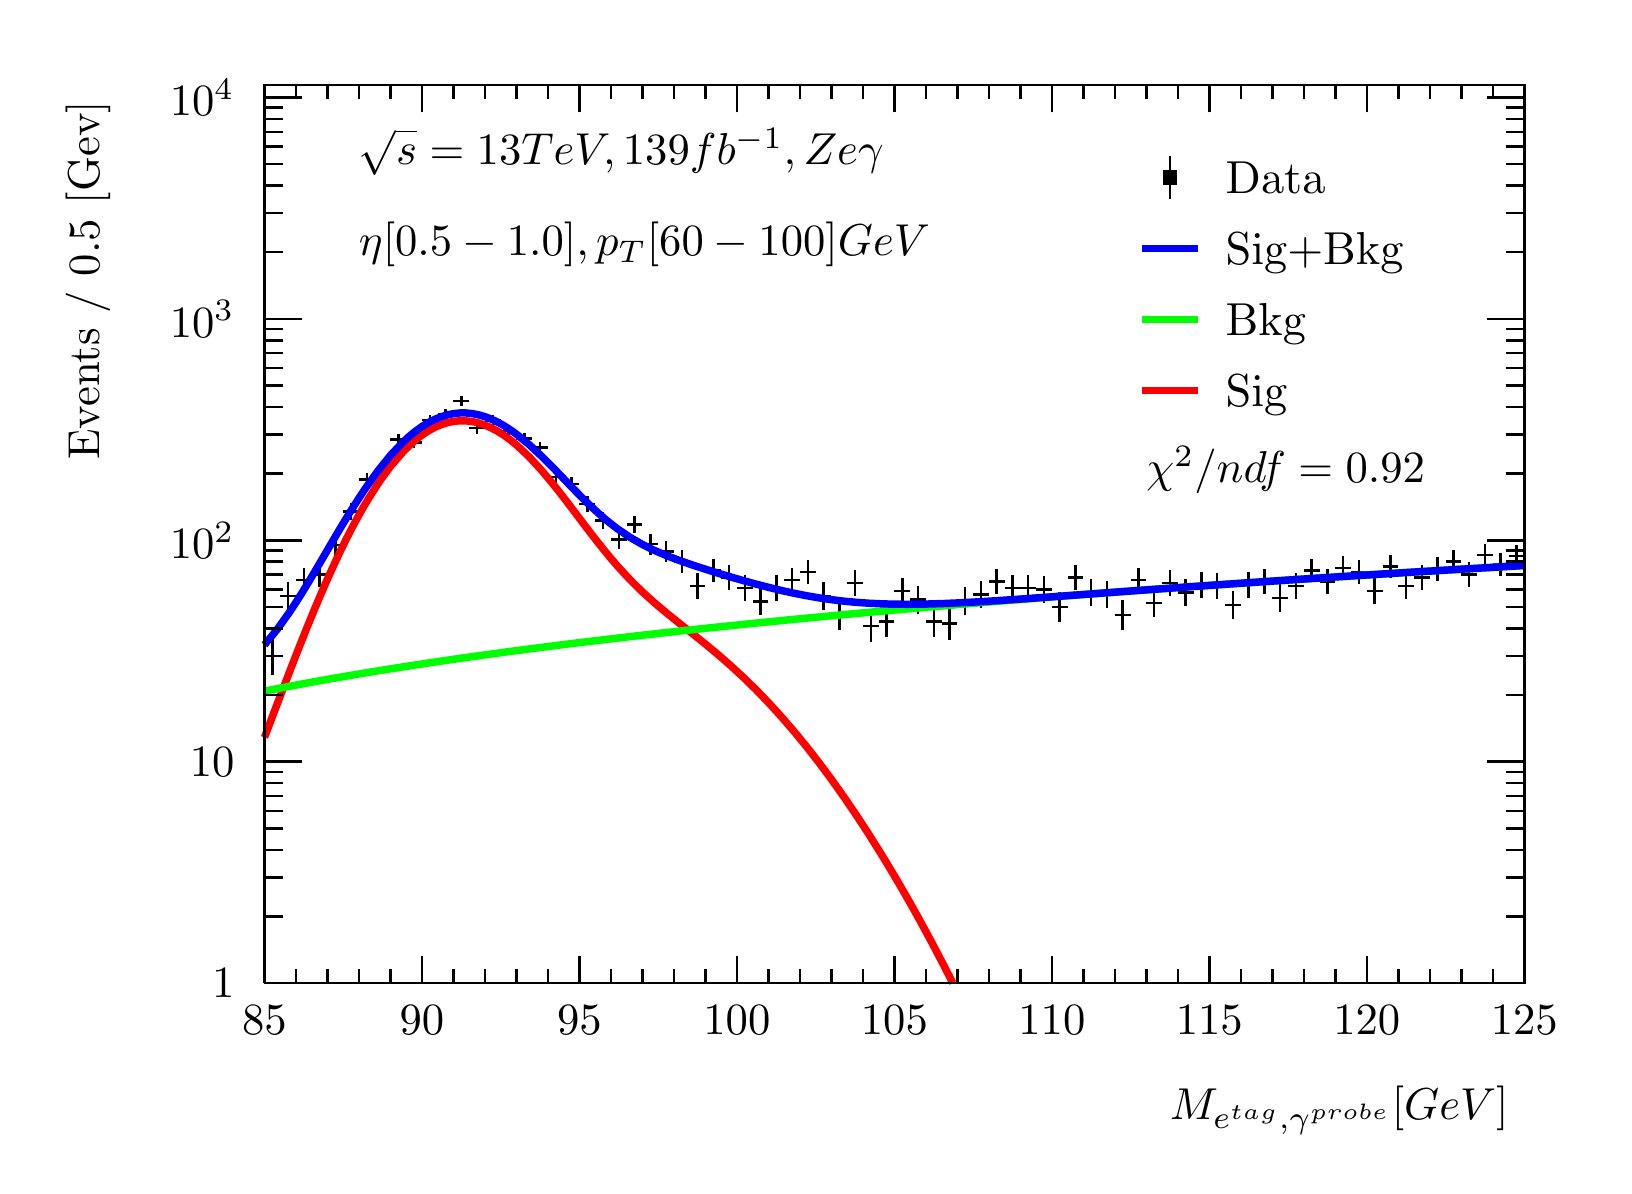
\begin{tikzpicture}
\pgfdeclareplotmark{cross} {
\pgfpathmoveto{\pgfpoint{-0.3\pgfplotmarksize}{\pgfplotmarksize}}
\pgfpathlineto{\pgfpoint{+0.3\pgfplotmarksize}{\pgfplotmarksize}}
\pgfpathlineto{\pgfpoint{+0.3\pgfplotmarksize}{0.3\pgfplotmarksize}}
\pgfpathlineto{\pgfpoint{+1\pgfplotmarksize}{0.3\pgfplotmarksize}}
\pgfpathlineto{\pgfpoint{+1\pgfplotmarksize}{-0.3\pgfplotmarksize}}
\pgfpathlineto{\pgfpoint{+0.3\pgfplotmarksize}{-0.3\pgfplotmarksize}}
\pgfpathlineto{\pgfpoint{+0.3\pgfplotmarksize}{-1.\pgfplotmarksize}}
\pgfpathlineto{\pgfpoint{-0.3\pgfplotmarksize}{-1.\pgfplotmarksize}}
\pgfpathlineto{\pgfpoint{-0.3\pgfplotmarksize}{-0.3\pgfplotmarksize}}
\pgfpathlineto{\pgfpoint{-1.\pgfplotmarksize}{-0.3\pgfplotmarksize}}
\pgfpathlineto{\pgfpoint{-1.\pgfplotmarksize}{0.3\pgfplotmarksize}}
\pgfpathlineto{\pgfpoint{-0.3\pgfplotmarksize}{0.3\pgfplotmarksize}}
\pgfpathclose
\pgfusepathqstroke
}
\pgfdeclareplotmark{cross*} {
\pgfpathmoveto{\pgfpoint{-0.3\pgfplotmarksize}{\pgfplotmarksize}}
\pgfpathlineto{\pgfpoint{+0.3\pgfplotmarksize}{\pgfplotmarksize}}
\pgfpathlineto{\pgfpoint{+0.3\pgfplotmarksize}{0.3\pgfplotmarksize}}
\pgfpathlineto{\pgfpoint{+1\pgfplotmarksize}{0.3\pgfplotmarksize}}
\pgfpathlineto{\pgfpoint{+1\pgfplotmarksize}{-0.3\pgfplotmarksize}}
\pgfpathlineto{\pgfpoint{+0.3\pgfplotmarksize}{-0.3\pgfplotmarksize}}
\pgfpathlineto{\pgfpoint{+0.3\pgfplotmarksize}{-1.\pgfplotmarksize}}
\pgfpathlineto{\pgfpoint{-0.3\pgfplotmarksize}{-1.\pgfplotmarksize}}
\pgfpathlineto{\pgfpoint{-0.3\pgfplotmarksize}{-0.3\pgfplotmarksize}}
\pgfpathlineto{\pgfpoint{-1.\pgfplotmarksize}{-0.3\pgfplotmarksize}}
\pgfpathlineto{\pgfpoint{-1.\pgfplotmarksize}{0.3\pgfplotmarksize}}
\pgfpathlineto{\pgfpoint{-0.3\pgfplotmarksize}{0.3\pgfplotmarksize}}
\pgfpathclose
\pgfusepathqfillstroke
}
\pgfdeclareplotmark{newstar} {
\pgfpathmoveto{\pgfqpoint{0pt}{\pgfplotmarksize}}
\pgfpathlineto{\pgfqpointpolar{44}{0.5\pgfplotmarksize}}
\pgfpathlineto{\pgfqpointpolar{18}{\pgfplotmarksize}}
\pgfpathlineto{\pgfqpointpolar{-20}{0.5\pgfplotmarksize}}
\pgfpathlineto{\pgfqpointpolar{-54}{\pgfplotmarksize}}
\pgfpathlineto{\pgfqpointpolar{-90}{0.5\pgfplotmarksize}}
\pgfpathlineto{\pgfqpointpolar{234}{\pgfplotmarksize}}
\pgfpathlineto{\pgfqpointpolar{198}{0.5\pgfplotmarksize}}
\pgfpathlineto{\pgfqpointpolar{162}{\pgfplotmarksize}}
\pgfpathlineto{\pgfqpointpolar{134}{0.5\pgfplotmarksize}}
\pgfpathclose
\pgfusepathqstroke
}
\pgfdeclareplotmark{newstar*} {
\pgfpathmoveto{\pgfqpoint{0pt}{\pgfplotmarksize}}
\pgfpathlineto{\pgfqpointpolar{44}{0.5\pgfplotmarksize}}
\pgfpathlineto{\pgfqpointpolar{18}{\pgfplotmarksize}}
\pgfpathlineto{\pgfqpointpolar{-20}{0.5\pgfplotmarksize}}
\pgfpathlineto{\pgfqpointpolar{-54}{\pgfplotmarksize}}
\pgfpathlineto{\pgfqpointpolar{-90}{0.5\pgfplotmarksize}}
\pgfpathlineto{\pgfqpointpolar{234}{\pgfplotmarksize}}
\pgfpathlineto{\pgfqpointpolar{198}{0.5\pgfplotmarksize}}
\pgfpathlineto{\pgfqpointpolar{162}{\pgfplotmarksize}}
\pgfpathlineto{\pgfqpointpolar{134}{0.5\pgfplotmarksize}}
\pgfpathclose
\pgfusepathqfillstroke
}
\definecolor{c}{rgb}{1,1,1};
\draw [color=c, fill=c] (0,0) rectangle (20,14.4361);
\draw [color=c, fill=c] (3,2.30977) rectangle (19,13.7143);
\definecolor{c}{rgb}{0,0,0};
\draw [c,line width=0.9] (3,2.30977) -- (3,13.7143) -- (19,13.7143) -- (19,2.30977) -- (3,2.30977);
\definecolor{c}{rgb}{1,1,1};
\draw [color=c, fill=c] (3,2.30977) rectangle (19,13.7143);
\definecolor{c}{rgb}{0,0,0};
\draw [c,line width=0.9] (3,2.30977) -- (3,13.7143) -- (19,13.7143) -- (19,2.30977) -- (3,2.30977);
\draw [c,line width=0.9] (3,2.30977) -- (19,2.30977);
\draw [c,line width=0.9] (3,2.65624) -- (3,2.30977);
\draw [c,line width=0.9] (3.4,2.48301) -- (3.4,2.30977);
\draw [c,line width=0.9] (3.8,2.48301) -- (3.8,2.30977);
\draw [c,line width=0.9] (4.2,2.48301) -- (4.2,2.30977);
\draw [c,line width=0.9] (4.6,2.48301) -- (4.6,2.30977);
\draw [c,line width=0.9] (5,2.65624) -- (5,2.30977);
\draw [c,line width=0.9] (5.4,2.48301) -- (5.4,2.30977);
\draw [c,line width=0.9] (5.8,2.48301) -- (5.8,2.30977);
\draw [c,line width=0.9] (6.2,2.48301) -- (6.2,2.30977);
\draw [c,line width=0.9] (6.6,2.48301) -- (6.6,2.30977);
\draw [c,line width=0.9] (7,2.65624) -- (7,2.30977);
\draw [c,line width=0.9] (7.4,2.48301) -- (7.4,2.30977);
\draw [c,line width=0.9] (7.8,2.48301) -- (7.8,2.30977);
\draw [c,line width=0.9] (8.2,2.48301) -- (8.2,2.30977);
\draw [c,line width=0.9] (8.6,2.48301) -- (8.6,2.30977);
\draw [c,line width=0.9] (9,2.65624) -- (9,2.30977);
\draw [c,line width=0.9] (9.4,2.48301) -- (9.4,2.30977);
\draw [c,line width=0.9] (9.8,2.48301) -- (9.8,2.30977);
\draw [c,line width=0.9] (10.2,2.48301) -- (10.2,2.30977);
\draw [c,line width=0.9] (10.6,2.48301) -- (10.6,2.30977);
\draw [c,line width=0.9] (11,2.65624) -- (11,2.30977);
\draw [c,line width=0.9] (11.4,2.48301) -- (11.4,2.30977);
\draw [c,line width=0.9] (11.8,2.48301) -- (11.8,2.30977);
\draw [c,line width=0.9] (12.2,2.48301) -- (12.2,2.30977);
\draw [c,line width=0.9] (12.6,2.48301) -- (12.6,2.30977);
\draw [c,line width=0.9] (13,2.65624) -- (13,2.30977);
\draw [c,line width=0.9] (13.4,2.48301) -- (13.4,2.30977);
\draw [c,line width=0.9] (13.8,2.48301) -- (13.8,2.30977);
\draw [c,line width=0.9] (14.2,2.48301) -- (14.2,2.30977);
\draw [c,line width=0.9] (14.6,2.48301) -- (14.6,2.30977);
\draw [c,line width=0.9] (15,2.65624) -- (15,2.30977);
\draw [c,line width=0.9] (15.4,2.48301) -- (15.4,2.30977);
\draw [c,line width=0.9] (15.8,2.48301) -- (15.8,2.30977);
\draw [c,line width=0.9] (16.2,2.48301) -- (16.2,2.30977);
\draw [c,line width=0.9] (16.6,2.48301) -- (16.6,2.30977);
\draw [c,line width=0.9] (17,2.65624) -- (17,2.30977);
\draw [c,line width=0.9] (17.4,2.48301) -- (17.4,2.30977);
\draw [c,line width=0.9] (17.8,2.48301) -- (17.8,2.30977);
\draw [c,line width=0.9] (18.2,2.48301) -- (18.2,2.30977);
\draw [c,line width=0.9] (18.6,2.48301) -- (18.6,2.30977);
\draw [c,line width=0.9] (19,2.65624) -- (19,2.30977);
\draw [anchor=base] (3,1.66015) node[scale=1.61424, color=c, rotate=0]{85};
\draw [anchor=base] (5,1.66015) node[scale=1.61424, color=c, rotate=0]{90};
\draw [anchor=base] (7,1.66015) node[scale=1.61424, color=c, rotate=0]{95};
\draw [anchor=base] (9,1.66015) node[scale=1.61424, color=c, rotate=0]{100};
\draw [anchor=base] (11,1.66015) node[scale=1.61424, color=c, rotate=0]{105};
\draw [anchor=base] (13,1.66015) node[scale=1.61424, color=c, rotate=0]{110};
\draw [anchor=base] (15,1.66015) node[scale=1.61424, color=c, rotate=0]{115};
\draw [anchor=base] (17,1.66015) node[scale=1.61424, color=c, rotate=0]{120};
\draw [anchor=base] (19,1.66015) node[scale=1.61424, color=c, rotate=0]{125};
\draw [anchor= east] (19,0.692932) node[scale=1.61424, color=c, rotate=0]{$M_{e^{tag}, \gamma^{probe}}  [GeV]$};
\draw [c,line width=0.9] (3,13.7143) -- (19,13.7143);
\draw [c,line width=0.9] (3,13.3678) -- (3,13.7143);
\draw [c,line width=0.9] (3.4,13.5411) -- (3.4,13.7143);
\draw [c,line width=0.9] (3.8,13.5411) -- (3.8,13.7143);
\draw [c,line width=0.9] (4.2,13.5411) -- (4.2,13.7143);
\draw [c,line width=0.9] (4.6,13.5411) -- (4.6,13.7143);
\draw [c,line width=0.9] (5,13.3678) -- (5,13.7143);
\draw [c,line width=0.9] (5.4,13.5411) -- (5.4,13.7143);
\draw [c,line width=0.9] (5.8,13.5411) -- (5.8,13.7143);
\draw [c,line width=0.9] (6.2,13.5411) -- (6.2,13.7143);
\draw [c,line width=0.9] (6.6,13.5411) -- (6.6,13.7143);
\draw [c,line width=0.9] (7,13.3678) -- (7,13.7143);
\draw [c,line width=0.9] (7.4,13.5411) -- (7.4,13.7143);
\draw [c,line width=0.9] (7.8,13.5411) -- (7.8,13.7143);
\draw [c,line width=0.9] (8.2,13.5411) -- (8.2,13.7143);
\draw [c,line width=0.9] (8.6,13.5411) -- (8.6,13.7143);
\draw [c,line width=0.9] (9,13.3678) -- (9,13.7143);
\draw [c,line width=0.9] (9.4,13.5411) -- (9.4,13.7143);
\draw [c,line width=0.9] (9.8,13.5411) -- (9.8,13.7143);
\draw [c,line width=0.9] (10.2,13.5411) -- (10.2,13.7143);
\draw [c,line width=0.9] (10.6,13.5411) -- (10.6,13.7143);
\draw [c,line width=0.9] (11,13.3678) -- (11,13.7143);
\draw [c,line width=0.9] (11.4,13.5411) -- (11.4,13.7143);
\draw [c,line width=0.9] (11.8,13.5411) -- (11.8,13.7143);
\draw [c,line width=0.9] (12.2,13.5411) -- (12.2,13.7143);
\draw [c,line width=0.9] (12.6,13.5411) -- (12.6,13.7143);
\draw [c,line width=0.9] (13,13.3678) -- (13,13.7143);
\draw [c,line width=0.9] (13.4,13.5411) -- (13.4,13.7143);
\draw [c,line width=0.9] (13.8,13.5411) -- (13.8,13.7143);
\draw [c,line width=0.9] (14.2,13.5411) -- (14.2,13.7143);
\draw [c,line width=0.9] (14.6,13.5411) -- (14.6,13.7143);
\draw [c,line width=0.9] (15,13.3678) -- (15,13.7143);
\draw [c,line width=0.9] (15.4,13.5411) -- (15.4,13.7143);
\draw [c,line width=0.9] (15.8,13.5411) -- (15.8,13.7143);
\draw [c,line width=0.9] (16.2,13.5411) -- (16.2,13.7143);
\draw [c,line width=0.9] (16.6,13.5411) -- (16.6,13.7143);
\draw [c,line width=0.9] (17,13.3678) -- (17,13.7143);
\draw [c,line width=0.9] (17.4,13.5411) -- (17.4,13.7143);
\draw [c,line width=0.9] (17.8,13.5411) -- (17.8,13.7143);
\draw [c,line width=0.9] (18.2,13.5411) -- (18.2,13.7143);
\draw [c,line width=0.9] (18.6,13.5411) -- (18.6,13.7143);
\draw [c,line width=0.9] (19,13.3678) -- (19,13.7143);
\draw [c,line width=0.9] (3,2.30977) -- (3,13.7143);
\draw [c,line width=0.9] (3.474,2.30978) -- (3,2.30978);
\draw [anchor= east] (2.82,2.30978) node[scale=1.61424, color=c, rotate=0]{1};
\draw [c,line width=0.9] (3.237,3.15616) -- (3,3.15616);
\draw [c,line width=0.9] (3.237,3.65126) -- (3,3.65126);
\draw [c,line width=0.9] (3.237,4.00254) -- (3,4.00254);
\draw [c,line width=0.9] (3.237,4.27501) -- (3,4.27501);
\draw [c,line width=0.9] (3.237,4.49764) -- (3,4.49764);
\draw [c,line width=0.9] (3.237,4.68586) -- (3,4.68586);
\draw [c,line width=0.9] (3.237,4.84892) -- (3,4.84892);
\draw [c,line width=0.9] (3.237,4.99274) -- (3,4.99274);
\draw [c,line width=0.9] (3.474,5.12139) -- (3,5.12139);
\draw [anchor= east] (2.82,5.12139) node[scale=1.61424, color=c, rotate=0]{10};
\draw [c,line width=0.9] (3.237,5.96777) -- (3,5.96777);
\draw [c,line width=0.9] (3.237,6.46287) -- (3,6.46287);
\draw [c,line width=0.9] (3.237,6.81415) -- (3,6.81415);
\draw [c,line width=0.9] (3.237,7.08662) -- (3,7.08662);
\draw [c,line width=0.9] (3.237,7.30925) -- (3,7.30925);
\draw [c,line width=0.9] (3.237,7.49748) -- (3,7.49748);
\draw [c,line width=0.9] (3.237,7.66053) -- (3,7.66053);
\draw [c,line width=0.9] (3.237,7.80435) -- (3,7.80435);
\draw [c,line width=0.9] (3.474,7.933) -- (3,7.933);
\draw [anchor= east] (2.82,7.933) node[scale=1.61424, color=c, rotate=0]{$10^{2}$};
\draw [c,line width=0.9] (3.237,8.77938) -- (3,8.77938);
\draw [c,line width=0.9] (3.237,9.27448) -- (3,9.27448);
\draw [c,line width=0.9] (3.237,9.62576) -- (3,9.62576);
\draw [c,line width=0.9] (3.237,9.89823) -- (3,9.89823);
\draw [c,line width=0.9] (3.237,10.1209) -- (3,10.1209);
\draw [c,line width=0.9] (3.237,10.3091) -- (3,10.3091);
\draw [c,line width=0.9] (3.237,10.4721) -- (3,10.4721);
\draw [c,line width=0.9] (3.237,10.616) -- (3,10.616);
\draw [c,line width=0.9] (3.474,10.7446) -- (3,10.7446);
\draw [anchor= east] (2.82,10.7446) node[scale=1.61424, color=c, rotate=0]{$10^{3}$};
\draw [c,line width=0.9] (3.237,11.591) -- (3,11.591);
\draw [c,line width=0.9] (3.237,12.0861) -- (3,12.0861);
\draw [c,line width=0.9] (3.237,12.4374) -- (3,12.4374);
\draw [c,line width=0.9] (3.237,12.7098) -- (3,12.7098);
\draw [c,line width=0.9] (3.237,12.9325) -- (3,12.9325);
\draw [c,line width=0.9] (3.237,13.1207) -- (3,13.1207);
\draw [c,line width=0.9] (3.237,13.2837) -- (3,13.2837);
\draw [c,line width=0.9] (3.237,13.4276) -- (3,13.4276);
\draw [c,line width=0.9] (3.474,13.5562) -- (3,13.5562);
\draw [anchor= east] (2.82,13.5562) node[scale=1.61424, color=c, rotate=0]{$10^{4}$};
\draw [anchor= east] (0.76,13.7143) node[scale=1.61424, color=c, rotate=90]{Events / 0.5 [Gev]};
\draw [c,line width=0.9] (19,2.30977) -- (19,13.7143);
\draw [c,line width=0.9] (18.526,2.30978) -- (19,2.30978);
\draw [c,line width=0.9] (18.763,3.15616) -- (19,3.15616);
\draw [c,line width=0.9] (18.763,3.65126) -- (19,3.65126);
\draw [c,line width=0.9] (18.763,4.00254) -- (19,4.00254);
\draw [c,line width=0.9] (18.763,4.27501) -- (19,4.27501);
\draw [c,line width=0.9] (18.763,4.49764) -- (19,4.49764);
\draw [c,line width=0.9] (18.763,4.68586) -- (19,4.68586);
\draw [c,line width=0.9] (18.763,4.84892) -- (19,4.84892);
\draw [c,line width=0.9] (18.763,4.99274) -- (19,4.99274);
\draw [c,line width=0.9] (18.526,5.12139) -- (19,5.12139);
\draw [c,line width=0.9] (18.763,5.96777) -- (19,5.96777);
\draw [c,line width=0.9] (18.763,6.46287) -- (19,6.46287);
\draw [c,line width=0.9] (18.763,6.81415) -- (19,6.81415);
\draw [c,line width=0.9] (18.763,7.08662) -- (19,7.08662);
\draw [c,line width=0.9] (18.763,7.30925) -- (19,7.30925);
\draw [c,line width=0.9] (18.763,7.49748) -- (19,7.49748);
\draw [c,line width=0.9] (18.763,7.66053) -- (19,7.66053);
\draw [c,line width=0.9] (18.763,7.80435) -- (19,7.80435);
\draw [c,line width=0.9] (18.526,7.933) -- (19,7.933);
\draw [c,line width=0.9] (18.763,8.77938) -- (19,8.77938);
\draw [c,line width=0.9] (18.763,9.27448) -- (19,9.27448);
\draw [c,line width=0.9] (18.763,9.62576) -- (19,9.62576);
\draw [c,line width=0.9] (18.763,9.89823) -- (19,9.89823);
\draw [c,line width=0.9] (18.763,10.1209) -- (19,10.1209);
\draw [c,line width=0.9] (18.763,10.3091) -- (19,10.3091);
\draw [c,line width=0.9] (18.763,10.4721) -- (19,10.4721);
\draw [c,line width=0.9] (18.763,10.616) -- (19,10.616);
\draw [c,line width=0.9] (18.526,10.7446) -- (19,10.7446);
\draw [c,line width=0.9] (18.763,11.591) -- (19,11.591);
\draw [c,line width=0.9] (18.763,12.0861) -- (19,12.0861);
\draw [c,line width=0.9] (18.763,12.4374) -- (19,12.4374);
\draw [c,line width=0.9] (18.763,12.7098) -- (19,12.7098);
\draw [c,line width=0.9] (18.763,12.9325) -- (19,12.9325);
\draw [c,line width=0.9] (18.763,13.1207) -- (19,13.1207);
\draw [c,line width=0.9] (18.763,13.2837) -- (19,13.2837);
\draw [c,line width=0.9] (18.763,13.4276) -- (19,13.4276);
\draw [c,line width=0.9] (18.526,13.5562) -- (19,13.5562);
\draw [c,line width=0.9] (3.1,6.46287) -- (3,6.46287);
\draw [c,line width=0.9] (3,6.46287) -- (3,6.46287);
\draw [c,line width=0.9] (3.1,6.46287) -- (3.2,6.46287);
\draw [c,line width=0.9] (3.2,6.46287) -- (3.2,6.46287);
\draw [c,line width=0.9] (3.1,6.46287) -- (3.1,6.70361);
\draw [c,line width=0.9] (3.1,6.70361) -- (3.1,6.70361);
\draw [c,line width=0.9] (3.1,6.46287) -- (3.1,6.21823);
\draw [c,line width=0.9] (3.1,6.21823) -- (3.1,6.21823);
\draw [c,line width=0.9] (3.3,7.225) -- (3.2,7.225);
\draw [c,line width=0.9] (3.2,7.225) -- (3.2,7.225);
\draw [c,line width=0.9] (3.3,7.225) -- (3.4,7.225);
\draw [c,line width=0.9] (3.4,7.225) -- (3.4,7.225);
\draw [c,line width=0.9] (3.3,7.225) -- (3.3,7.39808);
\draw [c,line width=0.9] (3.3,7.39808) -- (3.3,7.39808);
\draw [c,line width=0.9] (3.3,7.225) -- (3.3,7.05041);
\draw [c,line width=0.9] (3.3,7.05041) -- (3.3,7.05041);
\draw [c,line width=0.9] (3.5,7.42563) -- (3.4,7.42563);
\draw [c,line width=0.9] (3.4,7.42563) -- (3.4,7.42563);
\draw [c,line width=0.9] (3.5,7.42563) -- (3.6,7.42563);
\draw [c,line width=0.9] (3.6,7.42563) -- (3.6,7.42563);
\draw [c,line width=0.9] (3.5,7.42563) -- (3.5,7.5844);
\draw [c,line width=0.9] (3.5,7.5844) -- (3.5,7.5844);
\draw [c,line width=0.9] (3.5,7.42563) -- (3.5,7.26567);
\draw [c,line width=0.9] (3.5,7.26567) -- (3.5,7.26567);
\draw [c,line width=0.9] (3.7,7.49747) -- (3.6,7.49747);
\draw [c,line width=0.9] (3.6,7.49747) -- (3.6,7.49747);
\draw [c,line width=0.9] (3.7,7.49747) -- (3.8,7.49747);
\draw [c,line width=0.9] (3.8,7.49747) -- (3.8,7.49747);
\draw [c,line width=0.9] (3.7,7.49747) -- (3.7,7.65143);
\draw [c,line width=0.9] (3.7,7.65143) -- (3.7,7.65143);
\draw [c,line width=0.9] (3.7,7.49747) -- (3.7,7.34244);
\draw [c,line width=0.9] (3.7,7.34244) -- (3.7,7.34244);
\draw [c,line width=0.9] (3.9,7.87037) -- (3.8,7.87037);
\draw [c,line width=0.9] (3.8,7.87037) -- (3.8,7.87037);
\draw [c,line width=0.9] (3.9,7.87037) -- (4,7.87037);
\draw [c,line width=0.9] (4,7.87037) -- (4,7.87037);
\draw [c,line width=0.9] (3.9,7.87037) -- (3.9,8.00162);
\draw [c,line width=0.9] (3.9,8.00162) -- (3.9,8.00162);
\draw [c,line width=0.9] (3.9,7.87037) -- (3.9,7.73843);
\draw [c,line width=0.9] (3.9,7.73843) -- (3.9,7.73843);
\draw [c,line width=0.9] (4.1,8.29945) -- (4,8.29945);
\draw [c,line width=0.9] (4,8.29945) -- (4,8.29945);
\draw [c,line width=0.9] (4.1,8.29945) -- (4.2,8.29945);
\draw [c,line width=0.9] (4.2,8.29945) -- (4.2,8.29945);
\draw [c,line width=0.9] (4.1,8.29945) -- (4.1,8.40451);
\draw [c,line width=0.9] (4.1,8.40451) -- (4.1,8.40451);
\draw [c,line width=0.9] (4.1,8.29945) -- (4.1,8.19439);
\draw [c,line width=0.9] (4.1,8.19439) -- (4.1,8.19439);
\draw [c,line width=0.9] (4.3,8.70382) -- (4.2,8.70382);
\draw [c,line width=0.9] (4.2,8.70382) -- (4.2,8.70382);
\draw [c,line width=0.9] (4.3,8.70382) -- (4.4,8.70382);
\draw [c,line width=0.9] (4.4,8.70382) -- (4.4,8.70382);
\draw [c,line width=0.9] (4.3,8.70382) -- (4.3,8.79286);
\draw [c,line width=0.9] (4.3,8.79286) -- (4.3,8.79286);
\draw [c,line width=0.9] (4.3,8.70382) -- (4.3,8.61479);
\draw [c,line width=0.9] (4.3,8.61479) -- (4.3,8.61479);
\draw [c,line width=0.9] (4.5,8.83895) -- (4.4,8.83895);
\draw [c,line width=0.9] (4.4,8.83895) -- (4.4,8.83895);
\draw [c,line width=0.9] (4.5,8.83895) -- (4.6,8.83895);
\draw [c,line width=0.9] (4.6,8.83895) -- (4.6,8.83895);
\draw [c,line width=0.9] (4.5,8.83895) -- (4.5,8.9232);
\draw [c,line width=0.9] (4.5,8.9232) -- (4.5,8.9232);
\draw [c,line width=0.9] (4.5,8.83895) -- (4.5,8.75471);
\draw [c,line width=0.9] (4.5,8.75471) -- (4.5,8.75471);
\draw [c,line width=0.9] (4.7,9.21184) -- (4.6,9.21184);
\draw [c,line width=0.9] (4.6,9.21184) -- (4.6,9.21184);
\draw [c,line width=0.9] (4.7,9.21184) -- (4.8,9.21184);
\draw [c,line width=0.9] (4.8,9.21184) -- (4.8,9.21184);
\draw [c,line width=0.9] (4.7,9.21184) -- (4.7,9.28416);
\draw [c,line width=0.9] (4.7,9.28416) -- (4.7,9.28416);
\draw [c,line width=0.9] (4.7,9.21184) -- (4.7,9.13953);
\draw [c,line width=0.9] (4.7,9.13953) -- (4.7,9.13953);
\draw [c,line width=0.9] (4.9,9.17708) -- (4.8,9.17708);
\draw [c,line width=0.9] (4.8,9.17708) -- (4.8,9.17708);
\draw [c,line width=0.9] (4.9,9.17708) -- (5,9.17708);
\draw [c,line width=0.9] (5,9.17708) -- (5,9.17708);
\draw [c,line width=0.9] (4.9,9.17708) -- (4.9,9.25043);
\draw [c,line width=0.9] (4.9,9.25043) -- (4.9,9.25043);
\draw [c,line width=0.9] (4.9,9.17708) -- (4.9,9.10372);
\draw [c,line width=0.9] (4.9,9.10372) -- (4.9,9.10372);
\draw [c,line width=0.9] (5.1,9.46271) -- (5,9.46271);
\draw [c,line width=0.9] (5,9.46271) -- (5,9.46271);
\draw [c,line width=0.9] (5.1,9.46271) -- (5.2,9.46271);
\draw [c,line width=0.9] (5.2,9.46271) -- (5.2,9.46271);
\draw [c,line width=0.9] (5.1,9.46271) -- (5.1,9.52797);
\draw [c,line width=0.9] (5.1,9.52797) -- (5.1,9.52797);
\draw [c,line width=0.9] (5.1,9.46271) -- (5.1,9.39744);
\draw [c,line width=0.9] (5.1,9.39744) -- (5.1,9.39744);
\draw [c,line width=0.9] (5.3,9.53056) -- (5.2,9.53056);
\draw [c,line width=0.9] (5.2,9.53056) -- (5.2,9.53056);
\draw [c,line width=0.9] (5.3,9.53056) -- (5.4,9.53056);
\draw [c,line width=0.9] (5.4,9.53056) -- (5.4,9.53056);
\draw [c,line width=0.9] (5.3,9.53056) -- (5.3,9.59403);
\draw [c,line width=0.9] (5.3,9.59403) -- (5.3,9.59403);
\draw [c,line width=0.9] (5.3,9.53056) -- (5.3,9.46709);
\draw [c,line width=0.9] (5.3,9.46709) -- (5.3,9.46709);
\draw [c,line width=0.9] (5.5,9.70265) -- (5.4,9.70265);
\draw [c,line width=0.9] (5.4,9.70265) -- (5.4,9.70265);
\draw [c,line width=0.9] (5.5,9.70265) -- (5.6,9.70265);
\draw [c,line width=0.9] (5.6,9.70265) -- (5.6,9.70265);
\draw [c,line width=0.9] (5.5,9.70265) -- (5.5,9.76181);
\draw [c,line width=0.9] (5.5,9.76181) -- (5.5,9.76181);
\draw [c,line width=0.9] (5.5,9.70265) -- (5.5,9.6435);
\draw [c,line width=0.9] (5.5,9.6435) -- (5.5,9.6435);
\draw [c,line width=0.9] (5.7,9.35709) -- (5.6,9.35709);
\draw [c,line width=0.9] (5.6,9.35709) -- (5.6,9.35709);
\draw [c,line width=0.9] (5.7,9.35709) -- (5.8,9.35709);
\draw [c,line width=0.9] (5.8,9.35709) -- (5.8,9.35709);
\draw [c,line width=0.9] (5.7,9.35709) -- (5.7,9.42524);
\draw [c,line width=0.9] (5.7,9.42524) -- (5.7,9.42524);
\draw [c,line width=0.9] (5.7,9.35709) -- (5.7,9.28895);
\draw [c,line width=0.9] (5.7,9.28895) -- (5.7,9.28895);
\draw [c,line width=0.9] (5.9,9.45571) -- (5.8,9.45571);
\draw [c,line width=0.9] (5.8,9.45571) -- (5.8,9.45571);
\draw [c,line width=0.9] (5.9,9.45571) -- (6,9.45571);
\draw [c,line width=0.9] (6,9.45571) -- (6,9.45571);
\draw [c,line width=0.9] (5.9,9.45571) -- (5.9,9.52116);
\draw [c,line width=0.9] (5.9,9.52116) -- (5.9,9.52116);
\draw [c,line width=0.9] (5.9,9.45571) -- (5.9,9.39026);
\draw [c,line width=0.9] (5.9,9.39026) -- (5.9,9.39026);
\draw [c,line width=0.9] (6.1,9.32237) -- (6,9.32237);
\draw [c,line width=0.9] (6,9.32237) -- (6,9.32237);
\draw [c,line width=0.9] (6.1,9.32237) -- (6.2,9.32237);
\draw [c,line width=0.9] (6.2,9.32237) -- (6.2,9.32237);
\draw [c,line width=0.9] (6.1,9.32237) -- (6.1,9.39149);
\draw [c,line width=0.9] (6.1,9.39149) -- (6.1,9.39149);
\draw [c,line width=0.9] (6.1,9.32237) -- (6.1,9.25325);
\draw [c,line width=0.9] (6.1,9.25325) -- (6.1,9.25325);
\draw [c,line width=0.9] (6.3,9.22463) -- (6.2,9.22463);
\draw [c,line width=0.9] (6.2,9.22463) -- (6.2,9.22463);
\draw [c,line width=0.9] (6.3,9.22463) -- (6.4,9.22463);
\draw [c,line width=0.9] (6.4,9.22463) -- (6.4,9.22463);
\draw [c,line width=0.9] (6.3,9.22463) -- (6.3,9.29657);
\draw [c,line width=0.9] (6.3,9.29657) -- (6.3,9.29657);
\draw [c,line width=0.9] (6.3,9.22463) -- (6.3,9.15269);
\draw [c,line width=0.9] (6.3,9.15269) -- (6.3,9.15269);
\draw [c,line width=0.9] (6.5,9.1091) -- (6.4,9.1091);
\draw [c,line width=0.9] (6.4,9.1091) -- (6.4,9.1091);
\draw [c,line width=0.9] (6.5,9.1091) -- (6.6,9.1091);
\draw [c,line width=0.9] (6.6,9.1091) -- (6.6,9.1091);
\draw [c,line width=0.9] (6.5,9.1091) -- (6.5,9.18452);
\draw [c,line width=0.9] (6.5,9.18452) -- (6.5,9.18452);
\draw [c,line width=0.9] (6.5,9.1091) -- (6.5,9.03367);
\draw [c,line width=0.9] (6.5,9.03367) -- (6.5,9.03367);
\draw [c,line width=0.9] (6.7,8.73587) -- (6.6,8.73587);
\draw [c,line width=0.9] (6.6,8.73587) -- (6.6,8.73587);
\draw [c,line width=0.9] (6.7,8.73587) -- (6.8,8.73587);
\draw [c,line width=0.9] (6.8,8.73587) -- (6.8,8.73587);
\draw [c,line width=0.9] (6.7,8.73587) -- (6.7,8.82375);
\draw [c,line width=0.9] (6.7,8.82375) -- (6.7,8.82375);
\draw [c,line width=0.9] (6.7,8.73587) -- (6.7,8.648);
\draw [c,line width=0.9] (6.7,8.648) -- (6.7,8.648);
\draw [c,line width=0.9] (6.9,8.65073) -- (6.8,8.65073);
\draw [c,line width=0.9] (6.8,8.65073) -- (6.8,8.65073);
\draw [c,line width=0.9] (6.9,8.65073) -- (7,8.65073);
\draw [c,line width=0.9] (7,8.65073) -- (7,8.65073);
\draw [c,line width=0.9] (6.9,8.65073) -- (6.9,8.74172);
\draw [c,line width=0.9] (6.9,8.74172) -- (6.9,8.74172);
\draw [c,line width=0.9] (6.9,8.65073) -- (6.9,8.55973);
\draw [c,line width=0.9] (6.9,8.55973) -- (6.9,8.55973);
\draw [c,line width=0.9] (7.1,8.39509) -- (7,8.39509);
\draw [c,line width=0.9] (7,8.39509) -- (7,8.39509);
\draw [c,line width=0.9] (7.1,8.39509) -- (7.2,8.39509);
\draw [c,line width=0.9] (7.2,8.39509) -- (7.2,8.39509);
\draw [c,line width=0.9] (7.1,8.39509) -- (7.1,8.49612);
\draw [c,line width=0.9] (7.1,8.49612) -- (7.1,8.49612);
\draw [c,line width=0.9] (7.1,8.39509) -- (7.1,8.29407);
\draw [c,line width=0.9] (7.1,8.29407) -- (7.1,8.29407);
\draw [c,line width=0.9] (7.3,8.18578) -- (7.2,8.18578);
\draw [c,line width=0.9] (7.2,8.18578) -- (7.2,8.18578);
\draw [c,line width=0.9] (7.3,8.18578) -- (7.4,8.18578);
\draw [c,line width=0.9] (7.4,8.18578) -- (7.4,8.18578);
\draw [c,line width=0.9] (7.3,8.18578) -- (7.3,8.29584);
\draw [c,line width=0.9] (7.3,8.29584) -- (7.3,8.29584);
\draw [c,line width=0.9] (7.3,8.18578) -- (7.3,8.07571);
\draw [c,line width=0.9] (7.3,8.07571) -- (7.3,8.07571);
\draw [c,line width=0.9] (7.5,7.94515) -- (7.4,7.94515);
\draw [c,line width=0.9] (7.4,7.94515) -- (7.4,7.94515);
\draw [c,line width=0.9] (7.5,7.94515) -- (7.6,7.94515);
\draw [c,line width=0.9] (7.6,7.94515) -- (7.6,7.94515);
\draw [c,line width=0.9] (7.5,7.94515) -- (7.5,8.0666);
\draw [c,line width=0.9] (7.5,8.0666) -- (7.5,8.0666);
\draw [c,line width=0.9] (7.5,7.94515) -- (7.5,7.8237);
\draw [c,line width=0.9] (7.5,7.8237) -- (7.5,7.8237);
\draw [c,line width=0.9] (7.7,8.1351) -- (7.6,8.1351);
\draw [c,line width=0.9] (7.6,8.1351) -- (7.6,8.1351);
\draw [c,line width=0.9] (7.7,8.1351) -- (7.8,8.1351);
\draw [c,line width=0.9] (7.8,8.1351) -- (7.8,8.1351);
\draw [c,line width=0.9] (7.7,8.1351) -- (7.7,8.24747);
\draw [c,line width=0.9] (7.7,8.24747) -- (7.7,8.24747);
\draw [c,line width=0.9] (7.7,8.1351) -- (7.7,8.02273);
\draw [c,line width=0.9] (7.7,8.02273) -- (7.7,8.02273);
\draw [c,line width=0.9] (7.9,7.88315) -- (7.8,7.88315);
\draw [c,line width=0.9] (7.8,7.88315) -- (7.8,7.88315);
\draw [c,line width=0.9] (7.9,7.88315) -- (8,7.88315);
\draw [c,line width=0.9] (8,7.88315) -- (8,7.88315);
\draw [c,line width=0.9] (7.9,7.88315) -- (7.9,8.01369);
\draw [c,line width=0.9] (7.9,8.01369) -- (7.9,8.01369);
\draw [c,line width=0.9] (7.9,7.88315) -- (7.9,7.75194);
\draw [c,line width=0.9] (7.9,7.75194) -- (7.9,7.75194);
\draw [c,line width=0.9] (8.1,7.7907) -- (8,7.7907);
\draw [c,line width=0.9] (8,7.7907) -- (8,7.7907);
\draw [c,line width=0.9] (8.1,7.7907) -- (8.2,7.7907);
\draw [c,line width=0.9] (8.2,7.7907) -- (8.2,7.7907);
\draw [c,line width=0.9] (8.1,7.7907) -- (8.1,7.9265);
\draw [c,line width=0.9] (8.1,7.9265) -- (8.1,7.9265);
\draw [c,line width=0.9] (8.1,7.7907) -- (8.1,7.65415);
\draw [c,line width=0.9] (8.1,7.65415) -- (8.1,7.65415);
\draw [c,line width=0.9] (8.3,7.66052) -- (8.2,7.66052);
\draw [c,line width=0.9] (8.2,7.66052) -- (8.2,7.66052);
\draw [c,line width=0.9] (8.3,7.66052) -- (8.4,7.66052);
\draw [c,line width=0.9] (8.4,7.66052) -- (8.4,7.66052);
\draw [c,line width=0.9] (8.3,7.66052) -- (8.3,7.8041);
\draw [c,line width=0.9] (8.3,7.8041) -- (8.3,7.8041);
\draw [c,line width=0.9] (8.3,7.66052) -- (8.3,7.51607);
\draw [c,line width=0.9] (8.3,7.51607) -- (8.3,7.51607);
\draw [c,line width=0.9] (8.5,7.34928) -- (8.4,7.34928);
\draw [c,line width=0.9] (8.4,7.34928) -- (8.4,7.34928);
\draw [c,line width=0.9] (8.5,7.34928) -- (8.6,7.34928);
\draw [c,line width=0.9] (8.6,7.34928) -- (8.6,7.34928);
\draw [c,line width=0.9] (8.5,7.34928) -- (8.5,7.51335);
\draw [c,line width=0.9] (8.5,7.51335) -- (8.5,7.51335);
\draw [c,line width=0.9] (8.5,7.34928) -- (8.5,7.18392);
\draw [c,line width=0.9] (8.5,7.18392) -- (8.5,7.18392);
\draw [c,line width=0.9] (8.7,7.54871) -- (8.6,7.54871);
\draw [c,line width=0.9] (8.6,7.54871) -- (8.6,7.54871);
\draw [c,line width=0.9] (8.7,7.54871) -- (8.8,7.54871);
\draw [c,line width=0.9] (8.8,7.54871) -- (8.8,7.54871);
\draw [c,line width=0.9] (8.7,7.54871) -- (8.7,7.69933);
\draw [c,line width=0.9] (8.7,7.69933) -- (8.7,7.69933);
\draw [c,line width=0.9] (8.7,7.54871) -- (8.7,7.39709);
\draw [c,line width=0.9] (8.7,7.39709) -- (8.7,7.39709);
\draw [c,line width=0.9] (8.9,7.46208) -- (8.8,7.46208);
\draw [c,line width=0.9] (8.8,7.46208) -- (8.8,7.46208);
\draw [c,line width=0.9] (8.9,7.46208) -- (9,7.46208);
\draw [c,line width=0.9] (9,7.46208) -- (9,7.46208);
\draw [c,line width=0.9] (8.9,7.46208) -- (8.9,7.61839);
\draw [c,line width=0.9] (8.9,7.61839) -- (8.9,7.61839);
\draw [c,line width=0.9] (8.9,7.46208) -- (8.9,7.30464);
\draw [c,line width=0.9] (8.9,7.30464) -- (8.9,7.30464);
\draw [c,line width=0.9] (9.1,7.32943) -- (9,7.32943);
\draw [c,line width=0.9] (9,7.32943) -- (9,7.32943);
\draw [c,line width=0.9] (9.1,7.32943) -- (9.2,7.32943);
\draw [c,line width=0.9] (9.2,7.32943) -- (9.2,7.32943);
\draw [c,line width=0.9] (9.1,7.32943) -- (9.1,7.49491);
\draw [c,line width=0.9] (9.1,7.49491) -- (9.1,7.49491);
\draw [c,line width=0.9] (9.1,7.32943) -- (9.1,7.16263);
\draw [c,line width=0.9] (9.1,7.16263) -- (9.1,7.16263);
\draw [c,line width=0.9] (9.3,7.15777) -- (9.2,7.15777);
\draw [c,line width=0.9] (9.2,7.15777) -- (9.2,7.15777);
\draw [c,line width=0.9] (9.3,7.15777) -- (9.4,7.15777);
\draw [c,line width=0.9] (9.4,7.15777) -- (9.4,7.15777);
\draw [c,line width=0.9] (9.3,7.15777) -- (9.3,7.33594);
\draw [c,line width=0.9] (9.3,7.33594) -- (9.3,7.33594);
\draw [c,line width=0.9] (9.3,7.15777) -- (9.3,6.97796);
\draw [c,line width=0.9] (9.3,6.97796) -- (9.3,6.97796);
\draw [c,line width=0.9] (9.5,7.32943) -- (9.4,7.32943);
\draw [c,line width=0.9] (9.4,7.32943) -- (9.4,7.32943);
\draw [c,line width=0.9] (9.5,7.32943) -- (9.6,7.32943);
\draw [c,line width=0.9] (9.6,7.32943) -- (9.6,7.32943);
\draw [c,line width=0.9] (9.5,7.32943) -- (9.5,7.49491);
\draw [c,line width=0.9] (9.5,7.49491) -- (9.5,7.49491);
\draw [c,line width=0.9] (9.5,7.32943) -- (9.5,7.16263);
\draw [c,line width=0.9] (9.5,7.16263) -- (9.5,7.16263);
\draw [c,line width=0.9] (9.7,7.42563) -- (9.6,7.42563);
\draw [c,line width=0.9] (9.6,7.42563) -- (9.6,7.42563);
\draw [c,line width=0.9] (9.7,7.42563) -- (9.8,7.42563);
\draw [c,line width=0.9] (9.8,7.42563) -- (9.8,7.42563);
\draw [c,line width=0.9] (9.7,7.42563) -- (9.7,7.5844);
\draw [c,line width=0.9] (9.7,7.5844) -- (9.7,7.5844);
\draw [c,line width=0.9] (9.7,7.42563) -- (9.7,7.26567);
\draw [c,line width=0.9] (9.7,7.26567) -- (9.7,7.26567);
\draw [c,line width=0.9] (9.9,7.53187) -- (9.8,7.53187);
\draw [c,line width=0.9] (9.8,7.53187) -- (9.8,7.53187);
\draw [c,line width=0.9] (9.9,7.53187) -- (10,7.53187);
\draw [c,line width=0.9] (10,7.53187) -- (10,7.53187);
\draw [c,line width=0.9] (9.9,7.53187) -- (9.9,7.68358);
\draw [c,line width=0.9] (9.9,7.68358) -- (9.9,7.68358);
\draw [c,line width=0.9] (9.9,7.53187) -- (9.9,7.37914);
\draw [c,line width=0.9] (9.9,7.37914) -- (9.9,7.37914);
\draw [c,line width=0.9] (10.1,7.225) -- (10,7.225);
\draw [c,line width=0.9] (10,7.225) -- (10,7.225);
\draw [c,line width=0.9] (10.1,7.225) -- (10.2,7.225);
\draw [c,line width=0.9] (10.2,7.225) -- (10.2,7.225);
\draw [c,line width=0.9] (10.1,7.225) -- (10.1,7.39808);
\draw [c,line width=0.9] (10.1,7.39808) -- (10.1,7.39808);
\draw [c,line width=0.9] (10.1,7.225) -- (10.1,7.05041);
\draw [c,line width=0.9] (10.1,7.05041) -- (10.1,7.05041);
\draw [c,line width=0.9] (10.3,6.9848) -- (10.2,6.9848);
\draw [c,line width=0.9] (10.2,6.9848) -- (10.2,6.9848);
\draw [c,line width=0.9] (10.3,6.9848) -- (10.4,6.9848);
\draw [c,line width=0.9] (10.4,6.9848) -- (10.4,6.9848);
\draw [c,line width=0.9] (10.3,6.9848) -- (10.3,7.17678);
\draw [c,line width=0.9] (10.3,7.17678) -- (10.3,7.17678);
\draw [c,line width=0.9] (10.3,6.9848) -- (10.3,6.7908);
\draw [c,line width=0.9] (10.3,6.7908) -- (10.3,6.7908);
\draw [c,line width=0.9] (10.5,7.38805) -- (10.4,7.38805);
\draw [c,line width=0.9] (10.4,7.38805) -- (10.4,7.38805);
\draw [c,line width=0.9] (10.5,7.38805) -- (10.6,7.38805);
\draw [c,line width=0.9] (10.6,7.38805) -- (10.6,7.38805);
\draw [c,line width=0.9] (10.5,7.38805) -- (10.5,7.54941);
\draw [c,line width=0.9] (10.5,7.54941) -- (10.5,7.54941);
\draw [c,line width=0.9] (10.5,7.38805) -- (10.5,7.22546);
\draw [c,line width=0.9] (10.5,7.22546) -- (10.5,7.22546);
\draw [c,line width=0.9] (10.7,6.8443) -- (10.6,6.8443);
\draw [c,line width=0.9] (10.6,6.8443) -- (10.6,6.8443);
\draw [c,line width=0.9] (10.7,6.8443) -- (10.8,6.8443);
\draw [c,line width=0.9] (10.8,6.8443) -- (10.8,6.8443);
\draw [c,line width=0.9] (10.7,6.8443) -- (10.7,7.0483);
\draw [c,line width=0.9] (10.7,7.0483) -- (10.7,7.0483);
\draw [c,line width=0.9] (10.7,6.8443) -- (10.7,6.63787);
\draw [c,line width=0.9] (10.7,6.63787) -- (10.7,6.63787);
\draw [c,line width=0.9] (10.9,6.90245) -- (10.8,6.90245);
\draw [c,line width=0.9] (10.8,6.90245) -- (10.8,6.90245);
\draw [c,line width=0.9] (10.9,6.90245) -- (11,6.90245);
\draw [c,line width=0.9] (11,6.90245) -- (11,6.90245);
\draw [c,line width=0.9] (10.9,6.90245) -- (10.9,7.10138);
\draw [c,line width=0.9] (10.9,7.10138) -- (10.9,7.10138);
\draw [c,line width=0.9] (10.9,6.90245) -- (10.9,6.70127);
\draw [c,line width=0.9] (10.9,6.70127) -- (10.9,6.70127);
\draw [c,line width=0.9] (11.1,7.28872) -- (11,7.28872);
\draw [c,line width=0.9] (11,7.28872) -- (11,7.28872);
\draw [c,line width=0.9] (11.1,7.28872) -- (11.2,7.28872);
\draw [c,line width=0.9] (11.2,7.28872) -- (11.2,7.28872);
\draw [c,line width=0.9] (11.1,7.28872) -- (11.1,7.45712);
\draw [c,line width=0.9] (11.1,7.45712) -- (11.1,7.45712);
\draw [c,line width=0.9] (11.1,7.28872) -- (11.1,7.11893);
\draw [c,line width=0.9] (11.1,7.11893) -- (11.1,7.11893);
\draw [c,line width=0.9] (11.3,7.18059) -- (11.2,7.18059);
\draw [c,line width=0.9] (11.2,7.18059) -- (11.2,7.18059);
\draw [c,line width=0.9] (11.3,7.18059) -- (11.4,7.18059);
\draw [c,line width=0.9] (11.4,7.18059) -- (11.4,7.18059);
\draw [c,line width=0.9] (11.3,7.18059) -- (11.3,7.35702);
\draw [c,line width=0.9] (11.3,7.35702) -- (11.3,7.35702);
\draw [c,line width=0.9] (11.3,7.18059) -- (11.3,7.00257);
\draw [c,line width=0.9] (11.3,7.00257) -- (11.3,7.00257);
\draw [c,line width=0.9] (11.5,6.90245) -- (11.4,6.90245);
\draw [c,line width=0.9] (11.4,6.90245) -- (11.4,6.90245);
\draw [c,line width=0.9] (11.5,6.90245) -- (11.6,6.90245);
\draw [c,line width=0.9] (11.6,6.90245) -- (11.6,6.90245);
\draw [c,line width=0.9] (11.5,6.90245) -- (11.5,7.10138);
\draw [c,line width=0.9] (11.5,7.10138) -- (11.5,7.10138);
\draw [c,line width=0.9] (11.5,6.90245) -- (11.5,6.70127);
\draw [c,line width=0.9] (11.5,6.70127) -- (11.5,6.70127);
\draw [c,line width=0.9] (11.7,6.87372) -- (11.6,6.87372);
\draw [c,line width=0.9] (11.6,6.87372) -- (11.6,6.87372);
\draw [c,line width=0.9] (11.7,6.87372) -- (11.8,6.87372);
\draw [c,line width=0.9] (11.8,6.87372) -- (11.8,6.87372);
\draw [c,line width=0.9] (11.7,6.87372) -- (11.7,7.07514);
\draw [c,line width=0.9] (11.7,7.07514) -- (11.7,7.07514);
\draw [c,line width=0.9] (11.7,6.87372) -- (11.7,6.66997);
\draw [c,line width=0.9] (11.7,6.66997) -- (11.7,6.66997);
\draw [c,line width=0.9] (11.9,7.15777) -- (11.8,7.15777);
\draw [c,line width=0.9] (11.8,7.15777) -- (11.8,7.15777);
\draw [c,line width=0.9] (11.9,7.15777) -- (12,7.15777);
\draw [c,line width=0.9] (12,7.15777) -- (12,7.15777);
\draw [c,line width=0.9] (11.9,7.15777) -- (11.9,7.33594);
\draw [c,line width=0.9] (11.9,7.33594) -- (11.9,7.33594);
\draw [c,line width=0.9] (11.9,7.15777) -- (11.9,6.97796);
\draw [c,line width=0.9] (11.9,6.97796) -- (11.9,6.97796);
\draw [c,line width=0.9] (12.1,7.24661) -- (12,7.24661);
\draw [c,line width=0.9] (12,7.24661) -- (12,7.24661);
\draw [c,line width=0.9] (12.1,7.24661) -- (12.2,7.24661);
\draw [c,line width=0.9] (12.2,7.24661) -- (12.2,7.24661);
\draw [c,line width=0.9] (12.1,7.24661) -- (12.1,7.41809);
\draw [c,line width=0.9] (12.1,7.41809) -- (12.1,7.41809);
\draw [c,line width=0.9] (12.1,7.24661) -- (12.1,7.07366);
\draw [c,line width=0.9] (12.1,7.07366) -- (12.1,7.07366);
\draw [c,line width=0.9] (12.3,7.40698) -- (12.2,7.40698);
\draw [c,line width=0.9] (12.2,7.40698) -- (12.2,7.40698);
\draw [c,line width=0.9] (12.3,7.40698) -- (12.4,7.40698);
\draw [c,line width=0.9] (12.4,7.40698) -- (12.4,7.40698);
\draw [c,line width=0.9] (12.3,7.40698) -- (12.3,7.56704);
\draw [c,line width=0.9] (12.3,7.56704) -- (12.3,7.56704);
\draw [c,line width=0.9] (12.3,7.40698) -- (12.3,7.24572);
\draw [c,line width=0.9] (12.3,7.24572) -- (12.3,7.24572);
\draw [c,line width=0.9] (12.5,7.32943) -- (12.4,7.32943);
\draw [c,line width=0.9] (12.4,7.32943) -- (12.4,7.32943);
\draw [c,line width=0.9] (12.5,7.32943) -- (12.6,7.32943);
\draw [c,line width=0.9] (12.6,7.32943) -- (12.6,7.32943);
\draw [c,line width=0.9] (12.5,7.32943) -- (12.5,7.49491);
\draw [c,line width=0.9] (12.5,7.49491) -- (12.5,7.49491);
\draw [c,line width=0.9] (12.5,7.32943) -- (12.5,7.16263);
\draw [c,line width=0.9] (12.5,7.16263) -- (12.5,7.16263);
\draw [c,line width=0.9] (12.7,7.32943) -- (12.6,7.32943);
\draw [c,line width=0.9] (12.6,7.32943) -- (12.6,7.32943);
\draw [c,line width=0.9] (12.7,7.32943) -- (12.8,7.32943);
\draw [c,line width=0.9] (12.8,7.32943) -- (12.8,7.32943);
\draw [c,line width=0.9] (12.7,7.32943) -- (12.7,7.49491);
\draw [c,line width=0.9] (12.7,7.49491) -- (12.7,7.49491);
\draw [c,line width=0.9] (12.7,7.32943) -- (12.7,7.16263);
\draw [c,line width=0.9] (12.7,7.16263) -- (12.7,7.16263);
\draw [c,line width=0.9] (12.9,7.30925) -- (12.8,7.30925);
\draw [c,line width=0.9] (12.8,7.30925) -- (12.8,7.30925);
\draw [c,line width=0.9] (12.9,7.30925) -- (13,7.30925);
\draw [c,line width=0.9] (13,7.30925) -- (13,7.30925);
\draw [c,line width=0.9] (12.9,7.30925) -- (12.9,7.47616);
\draw [c,line width=0.9] (12.9,7.47616) -- (12.9,7.47616);
\draw [c,line width=0.9] (12.9,7.30925) -- (12.9,7.14097);
\draw [c,line width=0.9] (12.9,7.14097) -- (12.9,7.14097);
\draw [c,line width=0.9] (13.1,7.08662) -- (13,7.08662);
\draw [c,line width=0.9] (13,7.08662) -- (13,7.08662);
\draw [c,line width=0.9] (13.1,7.08662) -- (13.2,7.08662);
\draw [c,line width=0.9] (13.2,7.08662) -- (13.2,7.08662);
\draw [c,line width=0.9] (13.1,7.08662) -- (13.1,7.27034);
\draw [c,line width=0.9] (13.1,7.27034) -- (13.1,7.27034);
\draw [c,line width=0.9] (13.1,7.08662) -- (13.1,6.90111);
\draw [c,line width=0.9] (13.1,6.90111) -- (13.1,6.90111);
\draw [c,line width=0.9] (13.3,7.46208) -- (13.2,7.46208);
\draw [c,line width=0.9] (13.2,7.46208) -- (13.2,7.46208);
\draw [c,line width=0.9] (13.3,7.46208) -- (13.4,7.46208);
\draw [c,line width=0.9] (13.4,7.46208) -- (13.4,7.46208);
\draw [c,line width=0.9] (13.3,7.46208) -- (13.3,7.61839);
\draw [c,line width=0.9] (13.3,7.61839) -- (13.3,7.61839);
\draw [c,line width=0.9] (13.3,7.46208) -- (13.3,7.30464);
\draw [c,line width=0.9] (13.3,7.30464) -- (13.3,7.30464);
\draw [c,line width=0.9] (13.5,7.26785) -- (13.4,7.26785);
\draw [c,line width=0.9] (13.4,7.26785) -- (13.4,7.26785);
\draw [c,line width=0.9] (13.5,7.26785) -- (13.6,7.26785);
\draw [c,line width=0.9] (13.6,7.26785) -- (13.6,7.26785);
\draw [c,line width=0.9] (13.5,7.26785) -- (13.5,7.43777);
\draw [c,line width=0.9] (13.5,7.43777) -- (13.5,7.43777);
\draw [c,line width=0.9] (13.5,7.26785) -- (13.5,7.0965);
\draw [c,line width=0.9] (13.5,7.0965) -- (13.5,7.0965);
\draw [c,line width=0.9] (13.7,7.24661) -- (13.6,7.24661);
\draw [c,line width=0.9] (13.6,7.24661) -- (13.6,7.24661);
\draw [c,line width=0.9] (13.7,7.24661) -- (13.8,7.24661);
\draw [c,line width=0.9] (13.8,7.24661) -- (13.8,7.24661);
\draw [c,line width=0.9] (13.7,7.24661) -- (13.7,7.41809);
\draw [c,line width=0.9] (13.7,7.41809) -- (13.7,7.41809);
\draw [c,line width=0.9] (13.7,7.24661) -- (13.7,7.07366);
\draw [c,line width=0.9] (13.7,7.07366) -- (13.7,7.07366);
\draw [c,line width=0.9] (13.9,6.9848) -- (13.8,6.9848);
\draw [c,line width=0.9] (13.8,6.9848) -- (13.8,6.9848);
\draw [c,line width=0.9] (13.9,6.9848) -- (14,6.9848);
\draw [c,line width=0.9] (14,6.9848) -- (14,6.9848);
\draw [c,line width=0.9] (13.9,6.9848) -- (13.9,7.17678);
\draw [c,line width=0.9] (13.9,7.17678) -- (13.9,7.17678);
\draw [c,line width=0.9] (13.9,6.9848) -- (13.9,6.7908);
\draw [c,line width=0.9] (13.9,6.7908) -- (13.9,6.7908);
\draw [c,line width=0.9] (14.1,7.42563) -- (14,7.42563);
\draw [c,line width=0.9] (14,7.42563) -- (14,7.42563);
\draw [c,line width=0.9] (14.1,7.42563) -- (14.2,7.42563);
\draw [c,line width=0.9] (14.2,7.42563) -- (14.2,7.42563);
\draw [c,line width=0.9] (14.1,7.42563) -- (14.1,7.5844);
\draw [c,line width=0.9] (14.1,7.5844) -- (14.1,7.5844);
\draw [c,line width=0.9] (14.1,7.42563) -- (14.1,7.26567);
\draw [c,line width=0.9] (14.1,7.26567) -- (14.1,7.26567);
\draw [c,line width=0.9] (14.3,7.13451) -- (14.2,7.13451);
\draw [c,line width=0.9] (14.2,7.13451) -- (14.2,7.13451);
\draw [c,line width=0.9] (14.3,7.13451) -- (14.4,7.13451);
\draw [c,line width=0.9] (14.4,7.13451) -- (14.4,7.13451);
\draw [c,line width=0.9] (14.3,7.13451) -- (14.3,7.31447);
\draw [c,line width=0.9] (14.3,7.31447) -- (14.3,7.31447);
\draw [c,line width=0.9] (14.3,7.13451) -- (14.3,6.95286);
\draw [c,line width=0.9] (14.3,6.95286) -- (14.3,6.95286);
\draw [c,line width=0.9] (14.5,7.38805) -- (14.4,7.38805);
\draw [c,line width=0.9] (14.4,7.38805) -- (14.4,7.38805);
\draw [c,line width=0.9] (14.5,7.38805) -- (14.6,7.38805);
\draw [c,line width=0.9] (14.6,7.38805) -- (14.6,7.38805);
\draw [c,line width=0.9] (14.5,7.38805) -- (14.5,7.54941);
\draw [c,line width=0.9] (14.5,7.54941) -- (14.5,7.54941);
\draw [c,line width=0.9] (14.5,7.38805) -- (14.5,7.22546);
\draw [c,line width=0.9] (14.5,7.22546) -- (14.5,7.22546);
\draw [c,line width=0.9] (14.7,7.26785) -- (14.6,7.26785);
\draw [c,line width=0.9] (14.6,7.26785) -- (14.6,7.26785);
\draw [c,line width=0.9] (14.7,7.26785) -- (14.8,7.26785);
\draw [c,line width=0.9] (14.8,7.26785) -- (14.8,7.26785);
\draw [c,line width=0.9] (14.7,7.26785) -- (14.7,7.43777);
\draw [c,line width=0.9] (14.7,7.43777) -- (14.7,7.43777);
\draw [c,line width=0.9] (14.7,7.26785) -- (14.7,7.0965);
\draw [c,line width=0.9] (14.7,7.0965) -- (14.7,7.0965);
\draw [c,line width=0.9] (14.9,7.36882) -- (14.8,7.36882);
\draw [c,line width=0.9] (14.8,7.36882) -- (14.8,7.36882);
\draw [c,line width=0.9] (14.9,7.36882) -- (15,7.36882);
\draw [c,line width=0.9] (15,7.36882) -- (15,7.36882);
\draw [c,line width=0.9] (14.9,7.36882) -- (14.9,7.53152);
\draw [c,line width=0.9] (14.9,7.53152) -- (14.9,7.53152);
\draw [c,line width=0.9] (14.9,7.36882) -- (14.9,7.20486);
\draw [c,line width=0.9] (14.9,7.20486) -- (14.9,7.20486);
\draw [c,line width=0.9] (15.1,7.34928) -- (15,7.34928);
\draw [c,line width=0.9] (15,7.34928) -- (15,7.34928);
\draw [c,line width=0.9] (15.1,7.34928) -- (15.2,7.34928);
\draw [c,line width=0.9] (15.2,7.34928) -- (15.2,7.34928);
\draw [c,line width=0.9] (15.1,7.34928) -- (15.1,7.51335);
\draw [c,line width=0.9] (15.1,7.51335) -- (15.1,7.51335);
\draw [c,line width=0.9] (15.1,7.34928) -- (15.1,7.18392);
\draw [c,line width=0.9] (15.1,7.18392) -- (15.1,7.18392);
\draw [c,line width=0.9] (15.3,7.1108) -- (15.2,7.1108);
\draw [c,line width=0.9] (15.2,7.1108) -- (15.2,7.1108);
\draw [c,line width=0.9] (15.3,7.1108) -- (15.4,7.1108);
\draw [c,line width=0.9] (15.4,7.1108) -- (15.4,7.1108);
\draw [c,line width=0.9] (15.3,7.1108) -- (15.3,7.29261);
\draw [c,line width=0.9] (15.3,7.29261) -- (15.3,7.29261);
\draw [c,line width=0.9] (15.3,7.1108) -- (15.3,6.92725);
\draw [c,line width=0.9] (15.3,6.92725) -- (15.3,6.92725);
\draw [c,line width=0.9] (15.5,7.36882) -- (15.4,7.36882);
\draw [c,line width=0.9] (15.4,7.36882) -- (15.4,7.36882);
\draw [c,line width=0.9] (15.5,7.36882) -- (15.6,7.36882);
\draw [c,line width=0.9] (15.6,7.36882) -- (15.6,7.36882);
\draw [c,line width=0.9] (15.5,7.36882) -- (15.5,7.53152);
\draw [c,line width=0.9] (15.5,7.53152) -- (15.5,7.53152);
\draw [c,line width=0.9] (15.5,7.36882) -- (15.5,7.20486);
\draw [c,line width=0.9] (15.5,7.20486) -- (15.5,7.20486);
\draw [c,line width=0.9] (15.7,7.40698) -- (15.6,7.40698);
\draw [c,line width=0.9] (15.6,7.40698) -- (15.6,7.40698);
\draw [c,line width=0.9] (15.7,7.40698) -- (15.8,7.40698);
\draw [c,line width=0.9] (15.8,7.40698) -- (15.8,7.40698);
\draw [c,line width=0.9] (15.7,7.40698) -- (15.7,7.56704);
\draw [c,line width=0.9] (15.7,7.56704) -- (15.7,7.56704);
\draw [c,line width=0.9] (15.7,7.40698) -- (15.7,7.24572);
\draw [c,line width=0.9] (15.7,7.24572) -- (15.7,7.24572);
\draw [c,line width=0.9] (15.9,7.203) -- (15.8,7.203);
\draw [c,line width=0.9] (15.8,7.203) -- (15.8,7.203);
\draw [c,line width=0.9] (15.9,7.203) -- (16,7.203);
\draw [c,line width=0.9] (16,7.203) -- (16,7.203);
\draw [c,line width=0.9] (15.9,7.203) -- (15.9,7.37773);
\draw [c,line width=0.9] (15.9,7.37773) -- (15.9,7.37773);
\draw [c,line width=0.9] (15.9,7.203) -- (15.9,7.02672);
\draw [c,line width=0.9] (15.9,7.02672) -- (15.9,7.02672);
\draw [c,line width=0.9] (16.1,7.34928) -- (16,7.34928);
\draw [c,line width=0.9] (16,7.34928) -- (16,7.34928);
\draw [c,line width=0.9] (16.1,7.34928) -- (16.2,7.34928);
\draw [c,line width=0.9] (16.2,7.34928) -- (16.2,7.34928);
\draw [c,line width=0.9] (16.1,7.34928) -- (16.1,7.51335);
\draw [c,line width=0.9] (16.1,7.51335) -- (16.1,7.51335);
\draw [c,line width=0.9] (16.1,7.34928) -- (16.1,7.18392);
\draw [c,line width=0.9] (16.1,7.18392) -- (16.1,7.18392);
\draw [c,line width=0.9] (16.3,7.54871) -- (16.2,7.54871);
\draw [c,line width=0.9] (16.2,7.54871) -- (16.2,7.54871);
\draw [c,line width=0.9] (16.3,7.54871) -- (16.4,7.54871);
\draw [c,line width=0.9] (16.4,7.54871) -- (16.4,7.54871);
\draw [c,line width=0.9] (16.3,7.54871) -- (16.3,7.69933);
\draw [c,line width=0.9] (16.3,7.69933) -- (16.3,7.69933);
\draw [c,line width=0.9] (16.3,7.54871) -- (16.3,7.39709);
\draw [c,line width=0.9] (16.3,7.39709) -- (16.3,7.39709);
\draw [c,line width=0.9] (16.5,7.40698) -- (16.4,7.40698);
\draw [c,line width=0.9] (16.4,7.40698) -- (16.4,7.40698);
\draw [c,line width=0.9] (16.5,7.40698) -- (16.6,7.40698);
\draw [c,line width=0.9] (16.6,7.40698) -- (16.6,7.40698);
\draw [c,line width=0.9] (16.5,7.40698) -- (16.5,7.56704);
\draw [c,line width=0.9] (16.5,7.56704) -- (16.5,7.56704);
\draw [c,line width=0.9] (16.5,7.40698) -- (16.5,7.24572);
\draw [c,line width=0.9] (16.5,7.24572) -- (16.5,7.24572);
\draw [c,line width=0.9] (16.7,7.58172) -- (16.6,7.58172);
\draw [c,line width=0.9] (16.6,7.58172) -- (16.6,7.58172);
\draw [c,line width=0.9] (16.7,7.58172) -- (16.8,7.58172);
\draw [c,line width=0.9] (16.8,7.58172) -- (16.8,7.58172);
\draw [c,line width=0.9] (16.7,7.58172) -- (16.7,7.73022);
\draw [c,line width=0.9] (16.7,7.73022) -- (16.7,7.73022);
\draw [c,line width=0.9] (16.7,7.58172) -- (16.7,7.43225);
\draw [c,line width=0.9] (16.7,7.43225) -- (16.7,7.43225);
\draw [c,line width=0.9] (16.9,7.53187) -- (16.8,7.53187);
\draw [c,line width=0.9] (16.8,7.53187) -- (16.8,7.53187);
\draw [c,line width=0.9] (16.9,7.53187) -- (17,7.53187);
\draw [c,line width=0.9] (17,7.53187) -- (17,7.53187);
\draw [c,line width=0.9] (16.9,7.53187) -- (16.9,7.68358);
\draw [c,line width=0.9] (16.9,7.68358) -- (16.9,7.68358);
\draw [c,line width=0.9] (16.9,7.53187) -- (16.9,7.37914);
\draw [c,line width=0.9] (16.9,7.37914) -- (16.9,7.37914);
\draw [c,line width=0.9] (17.1,7.28872) -- (17,7.28872);
\draw [c,line width=0.9] (17,7.28872) -- (17,7.28872);
\draw [c,line width=0.9] (17.1,7.28872) -- (17.2,7.28872);
\draw [c,line width=0.9] (17.2,7.28872) -- (17.2,7.28872);
\draw [c,line width=0.9] (17.1,7.28872) -- (17.1,7.45712);
\draw [c,line width=0.9] (17.1,7.45712) -- (17.1,7.45712);
\draw [c,line width=0.9] (17.1,7.28872) -- (17.1,7.11893);
\draw [c,line width=0.9] (17.1,7.11893) -- (17.1,7.11893);
\draw [c,line width=0.9] (17.3,7.59789) -- (17.2,7.59789);
\draw [c,line width=0.9] (17.2,7.59789) -- (17.2,7.59789);
\draw [c,line width=0.9] (17.3,7.59789) -- (17.4,7.59789);
\draw [c,line width=0.9] (17.4,7.59789) -- (17.4,7.59789);
\draw [c,line width=0.9] (17.3,7.59789) -- (17.3,7.74536);
\draw [c,line width=0.9] (17.3,7.74536) -- (17.3,7.74536);
\draw [c,line width=0.9] (17.3,7.59789) -- (17.3,7.44947);
\draw [c,line width=0.9] (17.3,7.44947) -- (17.3,7.44947);
\draw [c,line width=0.9] (17.5,7.34928) -- (17.4,7.34928);
\draw [c,line width=0.9] (17.4,7.34928) -- (17.4,7.34928);
\draw [c,line width=0.9] (17.5,7.34928) -- (17.6,7.34928);
\draw [c,line width=0.9] (17.6,7.34928) -- (17.6,7.34928);
\draw [c,line width=0.9] (17.5,7.34928) -- (17.5,7.51335);
\draw [c,line width=0.9] (17.5,7.51335) -- (17.5,7.51335);
\draw [c,line width=0.9] (17.5,7.34928) -- (17.5,7.18392);
\draw [c,line width=0.9] (17.5,7.18392) -- (17.5,7.18392);
\draw [c,line width=0.9] (17.7,7.46208) -- (17.6,7.46208);
\draw [c,line width=0.9] (17.6,7.46208) -- (17.6,7.46208);
\draw [c,line width=0.9] (17.7,7.46208) -- (17.8,7.46208);
\draw [c,line width=0.9] (17.8,7.46208) -- (17.8,7.46208);
\draw [c,line width=0.9] (17.7,7.46208) -- (17.7,7.61839);
\draw [c,line width=0.9] (17.7,7.61839) -- (17.7,7.61839);
\draw [c,line width=0.9] (17.7,7.46208) -- (17.7,7.30464);
\draw [c,line width=0.9] (17.7,7.30464) -- (17.7,7.30464);
\draw [c,line width=0.9] (17.9,7.56533) -- (17.8,7.56533);
\draw [c,line width=0.9] (17.8,7.56533) -- (17.8,7.56533);
\draw [c,line width=0.9] (17.9,7.56533) -- (18,7.56533);
\draw [c,line width=0.9] (18,7.56533) -- (18,7.56533);
\draw [c,line width=0.9] (17.9,7.56533) -- (17.9,7.71487);
\draw [c,line width=0.9] (17.9,7.71487) -- (17.9,7.71487);
\draw [c,line width=0.9] (17.9,7.56533) -- (17.9,7.41479);
\draw [c,line width=0.9] (17.9,7.41479) -- (17.9,7.41479);
\draw [c,line width=0.9] (18.1,7.66052) -- (18,7.66052);
\draw [c,line width=0.9] (18,7.66052) -- (18,7.66052);
\draw [c,line width=0.9] (18.1,7.66052) -- (18.2,7.66052);
\draw [c,line width=0.9] (18.2,7.66052) -- (18.2,7.66052);
\draw [c,line width=0.9] (18.1,7.66052) -- (18.1,7.8041);
\draw [c,line width=0.9] (18.1,7.8041) -- (18.1,7.8041);
\draw [c,line width=0.9] (18.1,7.66052) -- (18.1,7.51607);
\draw [c,line width=0.9] (18.1,7.51607) -- (18.1,7.51607);
\draw [c,line width=0.9] (18.3,7.49747) -- (18.2,7.49747);
\draw [c,line width=0.9] (18.2,7.49747) -- (18.2,7.49747);
\draw [c,line width=0.9] (18.3,7.49747) -- (18.4,7.49747);
\draw [c,line width=0.9] (18.4,7.49747) -- (18.4,7.49747);
\draw [c,line width=0.9] (18.3,7.49747) -- (18.3,7.65143);
\draw [c,line width=0.9] (18.3,7.65143) -- (18.3,7.65143);
\draw [c,line width=0.9] (18.3,7.49747) -- (18.3,7.34244);
\draw [c,line width=0.9] (18.3,7.34244) -- (18.3,7.34244);
\draw [c,line width=0.9] (18.5,7.74883) -- (18.4,7.74883);
\draw [c,line width=0.9] (18.4,7.74883) -- (18.4,7.74883);
\draw [c,line width=0.9] (18.5,7.74883) -- (18.6,7.74883);
\draw [c,line width=0.9] (18.6,7.74883) -- (18.6,7.74883);
\draw [c,line width=0.9] (18.5,7.74883) -- (18.5,7.88708);
\draw [c,line width=0.9] (18.5,7.88708) -- (18.5,7.88708);
\draw [c,line width=0.9] (18.5,7.74883) -- (18.5,7.60979);
\draw [c,line width=0.9] (18.5,7.60979) -- (18.5,7.60979);
\draw [c,line width=0.9] (18.7,7.62961) -- (18.6,7.62961);
\draw [c,line width=0.9] (18.6,7.62961) -- (18.6,7.62961);
\draw [c,line width=0.9] (18.7,7.62961) -- (18.8,7.62961);
\draw [c,line width=0.9] (18.8,7.62961) -- (18.8,7.62961);
\draw [c,line width=0.9] (18.7,7.62961) -- (18.7,7.77509);
\draw [c,line width=0.9] (18.7,7.77509) -- (18.7,7.77509);
\draw [c,line width=0.9] (18.7,7.62961) -- (18.7,7.48321);
\draw [c,line width=0.9] (18.7,7.48321) -- (18.7,7.48321);
\draw [c,line width=0.9] (18.9,7.73455) -- (18.8,7.73455);
\draw [c,line width=0.9] (18.8,7.73455) -- (18.8,7.73455);
\draw [c,line width=0.9] (18.9,7.73455) -- (19,7.73455);
\draw [c,line width=0.9] (19,7.73455) -- (19,7.73455);
\draw [c,line width=0.9] (18.9,7.73455) -- (18.9,7.87365);
\draw [c,line width=0.9] (18.9,7.87365) -- (18.9,7.87365);
\draw [c,line width=0.9] (18.9,7.73455) -- (18.9,7.59465);
\draw [c,line width=0.9] (18.9,7.59465) -- (18.9,7.59465);
\foreach \P in {(3.1,6.46287), (3.3,7.225), (3.5,7.42563), (3.7,7.49747), (3.9,7.87037), (4.1,8.29945), (4.3,8.70382), (4.5,8.83895), (4.7,9.21184), (4.9,9.17708), (5.1,9.46271), (5.3,9.53056), (5.5,9.70265), (5.7,9.35709), (5.9,9.45571),
 (6.1,9.32237), (6.3,9.22463), (6.5,9.1091), (6.7,8.73587), (6.9,8.65073), (7.1,8.39509), (7.3,8.18578), (7.5,7.94515), (7.7,8.1351), (7.9,7.88315), (8.1,7.7907), (8.3,7.66052), (8.5,7.34928), (8.7,7.54871), (8.9,7.46208), (9.1,7.32943),
 (9.3,7.15777), (9.5,7.32943), (9.7,7.42563), (9.9,7.53187), (10.1,7.225), (10.3,6.9848), (10.5,7.38805), (10.7,6.8443), (10.9,6.90245), (11.1,7.28872), (11.3,7.18059), (11.5,6.90245), (11.7,6.87372), (11.9,7.15777), (12.1,7.24661), (12.3,7.40698),
 (12.5,7.32943), (12.7,7.32943), (12.9,7.30925), (13.1,7.08662), (13.3,7.46208), (13.5,7.26785), (13.7,7.24661), (13.9,6.9848), (14.1,7.42563), (14.3,7.13451), (14.5,7.38805), (14.7,7.26785), (14.9,7.36882), (15.1,7.34928), (15.3,7.1108),
 (15.5,7.36882), (15.7,7.40698), (15.9,7.203), (16.1,7.34928), (16.3,7.54871), (16.5,7.40698), (16.7,7.58172), (16.9,7.53187), (17.1,7.28872), (17.3,7.59789), (17.5,7.34928), (17.7,7.46208), (17.9,7.56533), (18.1,7.66052), (18.3,7.49747),
 (18.5,7.74883), (18.7,7.62961), (18.9,7.73455)}{\draw[mark options={color=c,fill=c},mark size=2.882883pt,mark=] plot coordinates {\P};}
\definecolor{c}{rgb}{1,0,0};
\draw [c,line width=2.7] (3,5.42951) -- (3,5.42951);
\draw [c,line width=2.7] (3,5.42951) -- (3.16,5.84896) -- (3.32,6.2664) -- (3.4,6.47216) -- (3.48,6.67483) -- (3.56,6.87365) -- (3.64,7.06791) -- (3.72,7.25696) -- (3.8,7.44025) -- (3.88,7.61726) -- (3.96,7.78755) -- (4.04,7.95073) -- (4.12,8.10646)
 -- (4.2,8.25445) -- (4.28,8.39445) -- (4.44,8.64966) -- (4.6,8.87076) -- (4.76,9.05681) -- (4.84,9.13649) -- (4.92,9.20721) -- (5,9.26894) -- (5.08,9.32165) -- (5.16,9.36536) -- (5.24,9.40007) -- (5.32,9.4258) -- (5.4,9.44262) -- (5.48,9.45057) --
 (5.56,9.44974) -- (5.64,9.44024) -- (5.72,9.42217) -- (5.8,9.39569) -- (5.88,9.36098) -- (5.96,9.31824) -- (6.04,9.26772) -- (6.12,9.20971) -- (6.2,9.14452) -- (6.36,8.99422) -- (6.52,8.82057) -- (6.68,8.62831) -- (6.76,8.52698) -- (6.84,8.42326) --
 (6.92,8.318) -- (7,8.21209) -- (7.08,8.10643) -- (7.16,8.00188) -- (7.24,7.89926) -- (7.32,7.79928) -- (7.4,7.70255) -- (7.48,7.60952) -- (7.64,7.4355) -- (7.8,7.27743) -- (7.96,7.13316) -- (8.12,6.99895) -- (8.28,6.87051) -- (8.44,6.74369) --
 (8.6,6.61502) -- (8.76,6.48179) -- (8.92,6.34205) -- (9.08,6.19445) -- (9.24,6.03813) -- (9.4,5.87253) -- (9.56,5.69731) -- (9.72,5.51228) -- (9.88,5.31732) -- (10.04,5.11237) -- (10.2,4.8974) -- (10.36,4.67238) -- (10.52,4.43732) -- (10.68,4.1922)
 -- (10.84,3.93703) -- (11,3.6718) -- (11.16,3.39651) -- (11.32,3.11117) -- (11.48,2.81576) -- (11.64,2.5103) -- (11.7417,2.30977);
\definecolor{c}{rgb}{0,1,0};
\draw [c,line width=2.7] (3,6.01679) -- (3,6.01679);
\draw [c,line width=2.7] (3,6.01679) -- (3.16,6.04819) -- (3.32,6.07883) -- (3.48,6.10874) -- (3.64,6.13795) -- (3.8,6.16649) -- (3.96,6.19441) -- (4.12,6.22172) -- (4.28,6.24845) -- (4.44,6.27462) -- (4.6,6.30026) -- (4.76,6.3254) -- (4.92,6.35004)
 -- (5.08,6.37421) -- (5.24,6.39793) -- (5.4,6.42121) -- (5.56,6.44407) -- (5.72,6.46653) -- (5.88,6.4886) -- (6.04,6.51029) -- (6.2,6.53161) -- (6.36,6.55259) -- (6.52,6.57322) -- (6.68,6.59352) -- (6.84,6.61351) -- (7,6.63319) -- (7.16,6.65257) --
 (7.32,6.67165) -- (7.48,6.69046) -- (7.64,6.709) -- (7.8,6.72726) -- (7.96,6.74528) -- (8.12,6.76304) -- (8.28,6.78056) -- (8.44,6.79784) -- (8.6,6.8149) -- (8.76,6.83173) -- (8.92,6.84834) -- (9.08,6.86474) -- (9.24,6.88093) -- (9.4,6.89692) --
 (9.56,6.91272) -- (9.72,6.92833) -- (9.88,6.94375) -- (10.04,6.95898) -- (10.2,6.97404) -- (10.36,6.98893) -- (10.52,7.00364) -- (10.68,7.01819) -- (10.84,7.03258) -- (11,7.04681) -- (11.16,7.06089) -- (11.32,7.07481) -- (11.48,7.08859) --
 (11.64,7.10222) -- (11.8,7.11571) -- (11.96,7.12906) -- (12.12,7.14228) -- (12.28,7.15536) -- (12.44,7.16831) -- (12.6,7.18114) -- (12.76,7.19384) -- (12.92,7.20642) -- (13.08,7.21888) -- (13.24,7.23122) -- (13.4,7.24344) -- (13.56,7.25556) --
 (13.72,7.26756) -- (13.88,7.27945) -- (14.04,7.29123) -- (14.2,7.30292) -- (14.36,7.31449) -- (14.52,7.32597) -- (14.68,7.33734) -- (14.84,7.34862) -- (15,7.35981) -- (15.16,7.3709) -- (15.32,7.38189) -- (15.48,7.3928) -- (15.64,7.40361) --
 (15.8,7.41434) -- (15.96,7.42498) -- (16.12,7.43554) -- (16.28,7.44601) -- (16.44,7.4564) -- (16.6,7.46671) -- (16.76,7.47694) -- (16.92,7.48709) -- (17.08,7.49717) -- (17.24,7.50716) -- (17.4,7.51709) -- (17.56,7.52694) -- (17.72,7.53671) --
 (17.88,7.54642) -- (18.04,7.55606) -- (18.2,7.56562) -- (18.36,7.57512) -- (18.52,7.58455) -- (18.68,7.59392) -- (18.84,7.60322) -- (19,7.61245) -- (19,7.61245) -- (19,7.61245);
\definecolor{c}{rgb}{0,0,1};
\draw [c,line width=2.7] (3,6.6045) -- (3,6.6045);
\draw [c,line width=2.7] (3,6.6045) -- (3.16,6.79902) -- (3.32,7.02259) -- (3.4,7.14399) -- (3.48,7.27068) -- (3.56,7.40165) -- (3.64,7.53578) -- (3.72,7.67189) -- (3.8,7.80882) -- (3.88,7.94542) -- (3.96,8.08061) -- (4.04,8.2134) -- (4.12,8.34288)
 -- (4.2,8.46823) -- (4.28,8.58875) -- (4.44,8.81285) -- (4.6,9.01114) -- (4.76,9.1807) -- (4.84,9.25405) -- (4.92,9.31952) -- (5,9.37697) -- (5.08,9.42629) -- (5.16,9.46742) -- (5.24,9.5003) -- (5.32,9.52494) -- (5.4,9.54135) -- (5.48,9.54958) --
 (5.56,9.5497) -- (5.64,9.54184) -- (5.72,9.52614) -- (5.8,9.50277) -- (5.88,9.47196) -- (5.96,9.43398) -- (6.04,9.38913) -- (6.12,9.33778) -- (6.2,9.28036) -- (6.36,9.14927) -- (6.52,9.00047) -- (6.68,8.83962) -- (6.76,8.75668) -- (6.84,8.67321) --
 (6.92,8.5901) -- (7,8.5082) -- (7.08,8.42832) -- (7.16,8.3512) -- (7.24,8.27748) -- (7.32,8.20764) -- (7.4,8.14204) -- (7.48,8.08087) -- (7.64,7.97188) -- (7.8,7.87946) -- (7.96,7.80093) -- (8.12,7.73306) -- (8.28,7.67274) -- (8.44,7.61745) --
 (8.6,7.56542) -- (8.76,7.51563) -- (8.92,7.46763) -- (9.08,7.4214) -- (9.24,7.37723) -- (9.4,7.33552) -- (9.56,7.29676) -- (9.72,7.26139) -- (9.88,7.22978) -- (10.04,7.2022) -- (10.2,7.17879) -- (10.36,7.15958) -- (10.52,7.14447) -- (10.68,7.13327)
 -- (10.84,7.12571) -- (11,7.12146) -- (11.16,7.12016) -- (11.32,7.12144) -- (11.48,7.12494) -- (11.64,7.13031) -- (11.8,7.13722) -- (11.96,7.14539) -- (12.12,7.15457) -- (12.28,7.16454) -- (12.44,7.17511) -- (12.6,7.18612) -- (12.76,7.19747) --
 (12.92,7.20904) -- (13.08,7.22075) -- (13.24,7.23255) -- (13.4,7.24438) -- (13.56,7.25621) -- (13.72,7.26801) -- (13.88,7.27976) -- (14.04,7.29145) -- (14.2,7.30306) -- (14.36,7.31459) -- (14.52,7.32603) -- (14.68,7.33739) -- (14.84,7.34865) --
 (15,7.35982) -- (15.16,7.37091) -- (15.32,7.3819) -- (15.48,7.3928) -- (15.64,7.40362) -- (15.8,7.41434) -- (15.96,7.42498) -- (16.12,7.43554) -- (16.28,7.44601) -- (16.44,7.4564) -- (16.6,7.46671) -- (16.76,7.47694) -- (16.92,7.48709) --
 (17.08,7.49717) -- (17.24,7.50716) -- (17.4,7.51709) -- (17.56,7.52694) -- (17.72,7.53671) -- (17.88,7.54642) -- (18.04,7.55606) -- (18.2,7.56562) -- (18.36,7.57512) -- (18.52,7.58455) -- (18.68,7.59392) -- (18.84,7.60322) -- (19,7.61245) --
 (19,7.61245) -- (19,7.61245);
\definecolor{c}{rgb}{0,0,0};
\draw [c,line width=0.9] (3,2.30977) -- (19,2.30977);
\draw [c,line width=0.9] (3,2.65624) -- (3,2.30977);
\draw [c,line width=0.9] (3.4,2.48301) -- (3.4,2.30977);
\draw [c,line width=0.9] (3.8,2.48301) -- (3.8,2.30977);
\draw [c,line width=0.9] (4.2,2.48301) -- (4.2,2.30977);
\draw [c,line width=0.9] (4.6,2.48301) -- (4.6,2.30977);
\draw [c,line width=0.9] (5,2.65624) -- (5,2.30977);
\draw [c,line width=0.9] (5.4,2.48301) -- (5.4,2.30977);
\draw [c,line width=0.9] (5.8,2.48301) -- (5.8,2.30977);
\draw [c,line width=0.9] (6.2,2.48301) -- (6.2,2.30977);
\draw [c,line width=0.9] (6.6,2.48301) -- (6.6,2.30977);
\draw [c,line width=0.9] (7,2.65624) -- (7,2.30977);
\draw [c,line width=0.9] (7.4,2.48301) -- (7.4,2.30977);
\draw [c,line width=0.9] (7.8,2.48301) -- (7.8,2.30977);
\draw [c,line width=0.9] (8.2,2.48301) -- (8.2,2.30977);
\draw [c,line width=0.9] (8.6,2.48301) -- (8.6,2.30977);
\draw [c,line width=0.9] (9,2.65624) -- (9,2.30977);
\draw [c,line width=0.9] (9.4,2.48301) -- (9.4,2.30977);
\draw [c,line width=0.9] (9.8,2.48301) -- (9.8,2.30977);
\draw [c,line width=0.9] (10.2,2.48301) -- (10.2,2.30977);
\draw [c,line width=0.9] (10.6,2.48301) -- (10.6,2.30977);
\draw [c,line width=0.9] (11,2.65624) -- (11,2.30977);
\draw [c,line width=0.9] (11.4,2.48301) -- (11.4,2.30977);
\draw [c,line width=0.9] (11.8,2.48301) -- (11.8,2.30977);
\draw [c,line width=0.9] (12.2,2.48301) -- (12.2,2.30977);
\draw [c,line width=0.9] (12.6,2.48301) -- (12.6,2.30977);
\draw [c,line width=0.9] (13,2.65624) -- (13,2.30977);
\draw [c,line width=0.9] (13.4,2.48301) -- (13.4,2.30977);
\draw [c,line width=0.9] (13.8,2.48301) -- (13.8,2.30977);
\draw [c,line width=0.9] (14.2,2.48301) -- (14.2,2.30977);
\draw [c,line width=0.9] (14.6,2.48301) -- (14.6,2.30977);
\draw [c,line width=0.9] (15,2.65624) -- (15,2.30977);
\draw [c,line width=0.9] (15.4,2.48301) -- (15.4,2.30977);
\draw [c,line width=0.9] (15.8,2.48301) -- (15.8,2.30977);
\draw [c,line width=0.9] (16.2,2.48301) -- (16.2,2.30977);
\draw [c,line width=0.9] (16.6,2.48301) -- (16.6,2.30977);
\draw [c,line width=0.9] (17,2.65624) -- (17,2.30977);
\draw [c,line width=0.9] (17.4,2.48301) -- (17.4,2.30977);
\draw [c,line width=0.9] (17.8,2.48301) -- (17.8,2.30977);
\draw [c,line width=0.9] (18.2,2.48301) -- (18.2,2.30977);
\draw [c,line width=0.9] (18.6,2.48301) -- (18.6,2.30977);
\draw [c,line width=0.9] (19,2.65624) -- (19,2.30977);
\draw [c,line width=0.9] (3,13.7143) -- (19,13.7143);
\draw [c,line width=0.9] (3,13.3678) -- (3,13.7143);
\draw [c,line width=0.9] (3.4,13.5411) -- (3.4,13.7143);
\draw [c,line width=0.9] (3.8,13.5411) -- (3.8,13.7143);
\draw [c,line width=0.9] (4.2,13.5411) -- (4.2,13.7143);
\draw [c,line width=0.9] (4.6,13.5411) -- (4.6,13.7143);
\draw [c,line width=0.9] (5,13.3678) -- (5,13.7143);
\draw [c,line width=0.9] (5.4,13.5411) -- (5.4,13.7143);
\draw [c,line width=0.9] (5.8,13.5411) -- (5.8,13.7143);
\draw [c,line width=0.9] (6.2,13.5411) -- (6.2,13.7143);
\draw [c,line width=0.9] (6.6,13.5411) -- (6.6,13.7143);
\draw [c,line width=0.9] (7,13.3678) -- (7,13.7143);
\draw [c,line width=0.9] (7.4,13.5411) -- (7.4,13.7143);
\draw [c,line width=0.9] (7.8,13.5411) -- (7.8,13.7143);
\draw [c,line width=0.9] (8.2,13.5411) -- (8.2,13.7143);
\draw [c,line width=0.9] (8.6,13.5411) -- (8.6,13.7143);
\draw [c,line width=0.9] (9,13.3678) -- (9,13.7143);
\draw [c,line width=0.9] (9.4,13.5411) -- (9.4,13.7143);
\draw [c,line width=0.9] (9.8,13.5411) -- (9.8,13.7143);
\draw [c,line width=0.9] (10.2,13.5411) -- (10.2,13.7143);
\draw [c,line width=0.9] (10.6,13.5411) -- (10.6,13.7143);
\draw [c,line width=0.9] (11,13.3678) -- (11,13.7143);
\draw [c,line width=0.9] (11.4,13.5411) -- (11.4,13.7143);
\draw [c,line width=0.9] (11.8,13.5411) -- (11.8,13.7143);
\draw [c,line width=0.9] (12.2,13.5411) -- (12.2,13.7143);
\draw [c,line width=0.9] (12.6,13.5411) -- (12.6,13.7143);
\draw [c,line width=0.9] (13,13.3678) -- (13,13.7143);
\draw [c,line width=0.9] (13.4,13.5411) -- (13.4,13.7143);
\draw [c,line width=0.9] (13.8,13.5411) -- (13.8,13.7143);
\draw [c,line width=0.9] (14.2,13.5411) -- (14.2,13.7143);
\draw [c,line width=0.9] (14.6,13.5411) -- (14.6,13.7143);
\draw [c,line width=0.9] (15,13.3678) -- (15,13.7143);
\draw [c,line width=0.9] (15.4,13.5411) -- (15.4,13.7143);
\draw [c,line width=0.9] (15.8,13.5411) -- (15.8,13.7143);
\draw [c,line width=0.9] (16.2,13.5411) -- (16.2,13.7143);
\draw [c,line width=0.9] (16.6,13.5411) -- (16.6,13.7143);
\draw [c,line width=0.9] (17,13.3678) -- (17,13.7143);
\draw [c,line width=0.9] (17.4,13.5411) -- (17.4,13.7143);
\draw [c,line width=0.9] (17.8,13.5411) -- (17.8,13.7143);
\draw [c,line width=0.9] (18.2,13.5411) -- (18.2,13.7143);
\draw [c,line width=0.9] (18.6,13.5411) -- (18.6,13.7143);
\draw [c,line width=0.9] (19,13.3678) -- (19,13.7143);
\draw [c,line width=0.9] (3,2.30977) -- (3,13.7143);
\draw [c,line width=0.9] (3.474,2.30978) -- (3,2.30978);
\draw [c,line width=0.9] (3.237,3.15616) -- (3,3.15616);
\draw [c,line width=0.9] (3.237,3.65126) -- (3,3.65126);
\draw [c,line width=0.9] (3.237,4.00254) -- (3,4.00254);
\draw [c,line width=0.9] (3.237,4.27501) -- (3,4.27501);
\draw [c,line width=0.9] (3.237,4.49764) -- (3,4.49764);
\draw [c,line width=0.9] (3.237,4.68586) -- (3,4.68586);
\draw [c,line width=0.9] (3.237,4.84892) -- (3,4.84892);
\draw [c,line width=0.9] (3.237,4.99274) -- (3,4.99274);
\draw [c,line width=0.9] (3.474,5.12139) -- (3,5.12139);
\draw [c,line width=0.9] (3.237,5.96777) -- (3,5.96777);
\draw [c,line width=0.9] (3.237,6.46287) -- (3,6.46287);
\draw [c,line width=0.9] (3.237,6.81415) -- (3,6.81415);
\draw [c,line width=0.9] (3.237,7.08662) -- (3,7.08662);
\draw [c,line width=0.9] (3.237,7.30925) -- (3,7.30925);
\draw [c,line width=0.9] (3.237,7.49748) -- (3,7.49748);
\draw [c,line width=0.9] (3.237,7.66053) -- (3,7.66053);
\draw [c,line width=0.9] (3.237,7.80435) -- (3,7.80435);
\draw [c,line width=0.9] (3.474,7.933) -- (3,7.933);
\draw [c,line width=0.9] (3.237,8.77938) -- (3,8.77938);
\draw [c,line width=0.9] (3.237,9.27448) -- (3,9.27448);
\draw [c,line width=0.9] (3.237,9.62576) -- (3,9.62576);
\draw [c,line width=0.9] (3.237,9.89823) -- (3,9.89823);
\draw [c,line width=0.9] (3.237,10.1209) -- (3,10.1209);
\draw [c,line width=0.9] (3.237,10.3091) -- (3,10.3091);
\draw [c,line width=0.9] (3.237,10.4721) -- (3,10.4721);
\draw [c,line width=0.9] (3.237,10.616) -- (3,10.616);
\draw [c,line width=0.9] (3.474,10.7446) -- (3,10.7446);
\draw [c,line width=0.9] (3.237,11.591) -- (3,11.591);
\draw [c,line width=0.9] (3.237,12.0861) -- (3,12.0861);
\draw [c,line width=0.9] (3.237,12.4374) -- (3,12.4374);
\draw [c,line width=0.9] (3.237,12.7098) -- (3,12.7098);
\draw [c,line width=0.9] (3.237,12.9325) -- (3,12.9325);
\draw [c,line width=0.9] (3.237,13.1207) -- (3,13.1207);
\draw [c,line width=0.9] (3.237,13.2837) -- (3,13.2837);
\draw [c,line width=0.9] (3.237,13.4276) -- (3,13.4276);
\draw [c,line width=0.9] (3.474,13.5562) -- (3,13.5562);
\draw [c,line width=0.9] (19,2.30977) -- (19,13.7143);
\draw [c,line width=0.9] (18.526,2.30978) -- (19,2.30978);
\draw [c,line width=0.9] (18.763,3.15616) -- (19,3.15616);
\draw [c,line width=0.9] (18.763,3.65126) -- (19,3.65126);
\draw [c,line width=0.9] (18.763,4.00254) -- (19,4.00254);
\draw [c,line width=0.9] (18.763,4.27501) -- (19,4.27501);
\draw [c,line width=0.9] (18.763,4.49764) -- (19,4.49764);
\draw [c,line width=0.9] (18.763,4.68586) -- (19,4.68586);
\draw [c,line width=0.9] (18.763,4.84892) -- (19,4.84892);
\draw [c,line width=0.9] (18.763,4.99274) -- (19,4.99274);
\draw [c,line width=0.9] (18.526,5.12139) -- (19,5.12139);
\draw [c,line width=0.9] (18.763,5.96777) -- (19,5.96777);
\draw [c,line width=0.9] (18.763,6.46287) -- (19,6.46287);
\draw [c,line width=0.9] (18.763,6.81415) -- (19,6.81415);
\draw [c,line width=0.9] (18.763,7.08662) -- (19,7.08662);
\draw [c,line width=0.9] (18.763,7.30925) -- (19,7.30925);
\draw [c,line width=0.9] (18.763,7.49748) -- (19,7.49748);
\draw [c,line width=0.9] (18.763,7.66053) -- (19,7.66053);
\draw [c,line width=0.9] (18.763,7.80435) -- (19,7.80435);
\draw [c,line width=0.9] (18.526,7.933) -- (19,7.933);
\draw [c,line width=0.9] (18.763,8.77938) -- (19,8.77938);
\draw [c,line width=0.9] (18.763,9.27448) -- (19,9.27448);
\draw [c,line width=0.9] (18.763,9.62576) -- (19,9.62576);
\draw [c,line width=0.9] (18.763,9.89823) -- (19,9.89823);
\draw [c,line width=0.9] (18.763,10.1209) -- (19,10.1209);
\draw [c,line width=0.9] (18.763,10.3091) -- (19,10.3091);
\draw [c,line width=0.9] (18.763,10.4721) -- (19,10.4721);
\draw [c,line width=0.9] (18.763,10.616) -- (19,10.616);
\draw [c,line width=0.9] (18.526,10.7446) -- (19,10.7446);
\draw [c,line width=0.9] (18.763,11.591) -- (19,11.591);
\draw [c,line width=0.9] (18.763,12.0861) -- (19,12.0861);
\draw [c,line width=0.9] (18.763,12.4374) -- (19,12.4374);
\draw [c,line width=0.9] (18.763,12.7098) -- (19,12.7098);
\draw [c,line width=0.9] (18.763,12.9325) -- (19,12.9325);
\draw [c,line width=0.9] (18.763,13.1207) -- (19,13.1207);
\draw [c,line width=0.9] (18.763,13.2837) -- (19,13.2837);
\draw [c,line width=0.9] (18.763,13.4276) -- (19,13.4276);
\draw [c,line width=0.9] (18.526,13.5562) -- (19,13.5562);
\definecolor{c}{rgb}{1,1,1};
\draw [color=c, fill=c] (14,9.38346) rectangle (18,12.9925);
\definecolor{c}{rgb}{0,0,0};
\draw [anchor=base west] (15,12.3383) node[scale=1.6699, color=c, rotate=0]{Data};
\draw [c,line width=0.9] (14.5,12.6416) -- (14.5,12.812);
\draw [c,line width=0.9] (14.5,12.4411) -- (14.5,12.2707);
\foreach \P in {(14.5,12.5414)}{\draw[mark options={color=c,fill=c},mark size=2.402402pt,mark=square*] plot coordinates {\P};}
\draw [anchor=base west] (15,11.4361) node[scale=1.6699, color=c, rotate=0]{Sig+Bkg};
\definecolor{c}{rgb}{0,0,1};
\draw [c,line width=2.7] (14.15,11.6391) -- (14.85,11.6391);
\definecolor{c}{rgb}{0,0,0};
\draw [anchor=base west] (15,10.5338) node[scale=1.6699, color=c, rotate=0]{Bkg};
\definecolor{c}{rgb}{0,1,0};
\draw [c,line width=2.7] (14.15,10.7368) -- (14.85,10.7368);
\definecolor{c}{rgb}{0,0,0};
\draw [anchor=base west] (15,9.63158) node[scale=1.6699, color=c, rotate=0]{Sig};
\definecolor{c}{rgb}{1,0,0};
\draw [c,line width=2.7] (14.15,9.83459) -- (14.85,9.83459);
\definecolor{c}{rgb}{0,0,0};
\draw [anchor=base west] (4,12.7038) node[scale=1.61424, color=c, rotate=0]{$\sqrt{s}= 13 TeV, 139fb^{-1}, Ze\gamma$};
\draw [anchor=base west] (4,11.5489) node[scale=1.61424, color=c, rotate=0]{$\eta[0.5-1.0], p_{T}[60-100]GeV$};
\draw [anchor=base west] (14,8.66165) node[scale=1.61424, color=c, rotate=0]{$\chi^{2}/ndf= 0.92$};
\end{tikzpicture}
}
\caption{The fits for systematics-1 (fitting range reduced by 10 GeV compare to nominal) in CR2 for all twenty $p_T-|\eta|$ bins (cont.)}
\label{fig:fit_cr2_sys1}
\end{center}
\end{figure}

\begin{figure}[H]
\begin{center}
\scalebox{0.35}{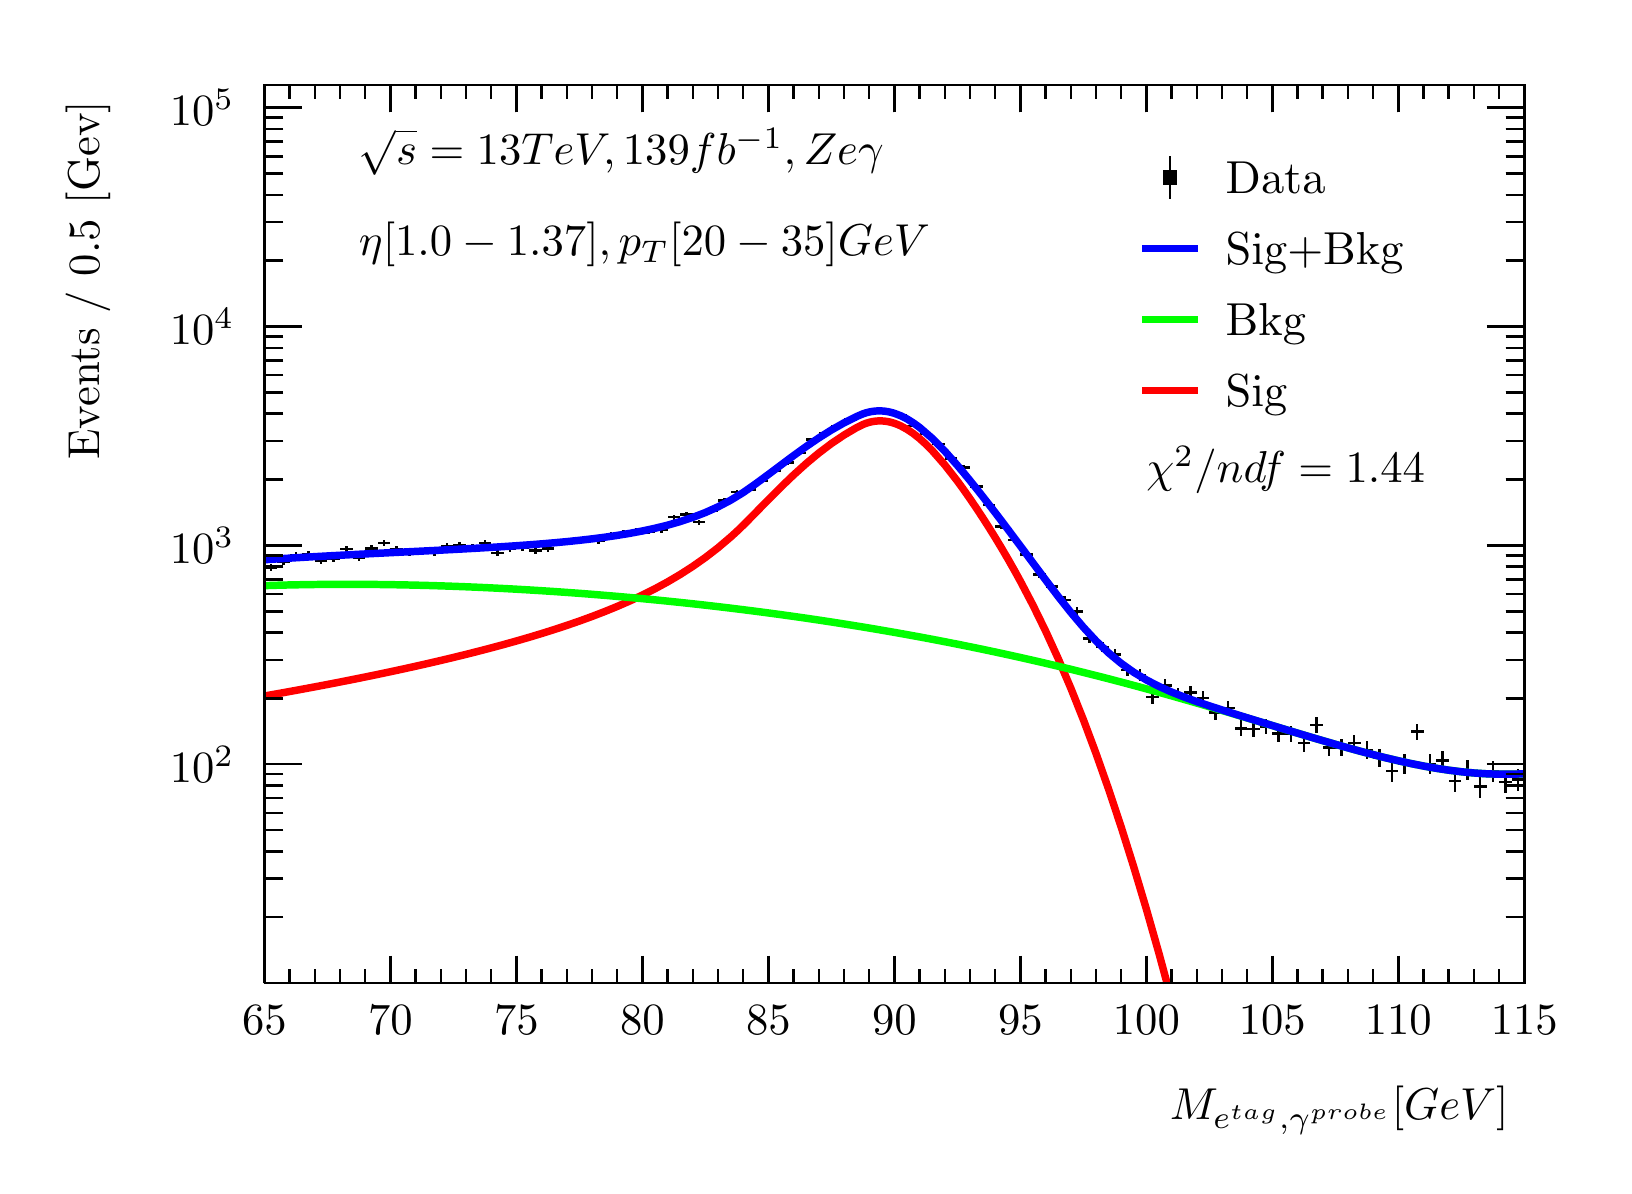
\begin{tikzpicture}
\pgfdeclareplotmark{cross} {
\pgfpathmoveto{\pgfpoint{-0.3\pgfplotmarksize}{\pgfplotmarksize}}
\pgfpathlineto{\pgfpoint{+0.3\pgfplotmarksize}{\pgfplotmarksize}}
\pgfpathlineto{\pgfpoint{+0.3\pgfplotmarksize}{0.3\pgfplotmarksize}}
\pgfpathlineto{\pgfpoint{+1\pgfplotmarksize}{0.3\pgfplotmarksize}}
\pgfpathlineto{\pgfpoint{+1\pgfplotmarksize}{-0.3\pgfplotmarksize}}
\pgfpathlineto{\pgfpoint{+0.3\pgfplotmarksize}{-0.3\pgfplotmarksize}}
\pgfpathlineto{\pgfpoint{+0.3\pgfplotmarksize}{-1.\pgfplotmarksize}}
\pgfpathlineto{\pgfpoint{-0.3\pgfplotmarksize}{-1.\pgfplotmarksize}}
\pgfpathlineto{\pgfpoint{-0.3\pgfplotmarksize}{-0.3\pgfplotmarksize}}
\pgfpathlineto{\pgfpoint{-1.\pgfplotmarksize}{-0.3\pgfplotmarksize}}
\pgfpathlineto{\pgfpoint{-1.\pgfplotmarksize}{0.3\pgfplotmarksize}}
\pgfpathlineto{\pgfpoint{-0.3\pgfplotmarksize}{0.3\pgfplotmarksize}}
\pgfpathclose
\pgfusepathqstroke
}
\pgfdeclareplotmark{cross*} {
\pgfpathmoveto{\pgfpoint{-0.3\pgfplotmarksize}{\pgfplotmarksize}}
\pgfpathlineto{\pgfpoint{+0.3\pgfplotmarksize}{\pgfplotmarksize}}
\pgfpathlineto{\pgfpoint{+0.3\pgfplotmarksize}{0.3\pgfplotmarksize}}
\pgfpathlineto{\pgfpoint{+1\pgfplotmarksize}{0.3\pgfplotmarksize}}
\pgfpathlineto{\pgfpoint{+1\pgfplotmarksize}{-0.3\pgfplotmarksize}}
\pgfpathlineto{\pgfpoint{+0.3\pgfplotmarksize}{-0.3\pgfplotmarksize}}
\pgfpathlineto{\pgfpoint{+0.3\pgfplotmarksize}{-1.\pgfplotmarksize}}
\pgfpathlineto{\pgfpoint{-0.3\pgfplotmarksize}{-1.\pgfplotmarksize}}
\pgfpathlineto{\pgfpoint{-0.3\pgfplotmarksize}{-0.3\pgfplotmarksize}}
\pgfpathlineto{\pgfpoint{-1.\pgfplotmarksize}{-0.3\pgfplotmarksize}}
\pgfpathlineto{\pgfpoint{-1.\pgfplotmarksize}{0.3\pgfplotmarksize}}
\pgfpathlineto{\pgfpoint{-0.3\pgfplotmarksize}{0.3\pgfplotmarksize}}
\pgfpathclose
\pgfusepathqfillstroke
}
\pgfdeclareplotmark{newstar} {
\pgfpathmoveto{\pgfqpoint{0pt}{\pgfplotmarksize}}
\pgfpathlineto{\pgfqpointpolar{44}{0.5\pgfplotmarksize}}
\pgfpathlineto{\pgfqpointpolar{18}{\pgfplotmarksize}}
\pgfpathlineto{\pgfqpointpolar{-20}{0.5\pgfplotmarksize}}
\pgfpathlineto{\pgfqpointpolar{-54}{\pgfplotmarksize}}
\pgfpathlineto{\pgfqpointpolar{-90}{0.5\pgfplotmarksize}}
\pgfpathlineto{\pgfqpointpolar{234}{\pgfplotmarksize}}
\pgfpathlineto{\pgfqpointpolar{198}{0.5\pgfplotmarksize}}
\pgfpathlineto{\pgfqpointpolar{162}{\pgfplotmarksize}}
\pgfpathlineto{\pgfqpointpolar{134}{0.5\pgfplotmarksize}}
\pgfpathclose
\pgfusepathqstroke
}
\pgfdeclareplotmark{newstar*} {
\pgfpathmoveto{\pgfqpoint{0pt}{\pgfplotmarksize}}
\pgfpathlineto{\pgfqpointpolar{44}{0.5\pgfplotmarksize}}
\pgfpathlineto{\pgfqpointpolar{18}{\pgfplotmarksize}}
\pgfpathlineto{\pgfqpointpolar{-20}{0.5\pgfplotmarksize}}
\pgfpathlineto{\pgfqpointpolar{-54}{\pgfplotmarksize}}
\pgfpathlineto{\pgfqpointpolar{-90}{0.5\pgfplotmarksize}}
\pgfpathlineto{\pgfqpointpolar{234}{\pgfplotmarksize}}
\pgfpathlineto{\pgfqpointpolar{198}{0.5\pgfplotmarksize}}
\pgfpathlineto{\pgfqpointpolar{162}{\pgfplotmarksize}}
\pgfpathlineto{\pgfqpointpolar{134}{0.5\pgfplotmarksize}}
\pgfpathclose
\pgfusepathqfillstroke
}
\definecolor{c}{rgb}{1,1,1};
\draw [color=c, fill=c] (0,0) rectangle (20,14.4361);
\draw [color=c, fill=c] (3,2.30977) rectangle (19,13.7143);
\definecolor{c}{rgb}{0,0,0};
\draw [c,line width=0.9] (3,2.30977) -- (3,13.7143) -- (19,13.7143) -- (19,2.30977) -- (3,2.30977);
\definecolor{c}{rgb}{1,1,1};
\draw [color=c, fill=c] (3,2.30977) rectangle (19,13.7143);
\definecolor{c}{rgb}{0,0,0};
\draw [c,line width=0.9] (3,2.30977) -- (3,13.7143) -- (19,13.7143) -- (19,2.30977) -- (3,2.30977);
\draw [c,line width=0.9] (3,2.30977) -- (19,2.30977);
\draw [c,line width=0.9] (3,2.65624) -- (3,2.30977);
\draw [c,line width=0.9] (3.32,2.48301) -- (3.32,2.30977);
\draw [c,line width=0.9] (3.64,2.48301) -- (3.64,2.30977);
\draw [c,line width=0.9] (3.96,2.48301) -- (3.96,2.30977);
\draw [c,line width=0.9] (4.28,2.48301) -- (4.28,2.30977);
\draw [c,line width=0.9] (4.6,2.65624) -- (4.6,2.30977);
\draw [c,line width=0.9] (4.92,2.48301) -- (4.92,2.30977);
\draw [c,line width=0.9] (5.24,2.48301) -- (5.24,2.30977);
\draw [c,line width=0.9] (5.56,2.48301) -- (5.56,2.30977);
\draw [c,line width=0.9] (5.88,2.48301) -- (5.88,2.30977);
\draw [c,line width=0.9] (6.2,2.65624) -- (6.2,2.30977);
\draw [c,line width=0.9] (6.52,2.48301) -- (6.52,2.30977);
\draw [c,line width=0.9] (6.84,2.48301) -- (6.84,2.30977);
\draw [c,line width=0.9] (7.16,2.48301) -- (7.16,2.30977);
\draw [c,line width=0.9] (7.48,2.48301) -- (7.48,2.30977);
\draw [c,line width=0.9] (7.8,2.65624) -- (7.8,2.30977);
\draw [c,line width=0.9] (8.12,2.48301) -- (8.12,2.30977);
\draw [c,line width=0.9] (8.44,2.48301) -- (8.44,2.30977);
\draw [c,line width=0.9] (8.76,2.48301) -- (8.76,2.30977);
\draw [c,line width=0.9] (9.08,2.48301) -- (9.08,2.30977);
\draw [c,line width=0.9] (9.4,2.65624) -- (9.4,2.30977);
\draw [c,line width=0.9] (9.72,2.48301) -- (9.72,2.30977);
\draw [c,line width=0.9] (10.04,2.48301) -- (10.04,2.30977);
\draw [c,line width=0.9] (10.36,2.48301) -- (10.36,2.30977);
\draw [c,line width=0.9] (10.68,2.48301) -- (10.68,2.30977);
\draw [c,line width=0.9] (11,2.65624) -- (11,2.30977);
\draw [c,line width=0.9] (11.32,2.48301) -- (11.32,2.30977);
\draw [c,line width=0.9] (11.64,2.48301) -- (11.64,2.30977);
\draw [c,line width=0.9] (11.96,2.48301) -- (11.96,2.30977);
\draw [c,line width=0.9] (12.28,2.48301) -- (12.28,2.30977);
\draw [c,line width=0.9] (12.6,2.65624) -- (12.6,2.30977);
\draw [c,line width=0.9] (12.92,2.48301) -- (12.92,2.30977);
\draw [c,line width=0.9] (13.24,2.48301) -- (13.24,2.30977);
\draw [c,line width=0.9] (13.56,2.48301) -- (13.56,2.30977);
\draw [c,line width=0.9] (13.88,2.48301) -- (13.88,2.30977);
\draw [c,line width=0.9] (14.2,2.65624) -- (14.2,2.30977);
\draw [c,line width=0.9] (14.52,2.48301) -- (14.52,2.30977);
\draw [c,line width=0.9] (14.84,2.48301) -- (14.84,2.30977);
\draw [c,line width=0.9] (15.16,2.48301) -- (15.16,2.30977);
\draw [c,line width=0.9] (15.48,2.48301) -- (15.48,2.30977);
\draw [c,line width=0.9] (15.8,2.65624) -- (15.8,2.30977);
\draw [c,line width=0.9] (16.12,2.48301) -- (16.12,2.30977);
\draw [c,line width=0.9] (16.44,2.48301) -- (16.44,2.30977);
\draw [c,line width=0.9] (16.76,2.48301) -- (16.76,2.30977);
\draw [c,line width=0.9] (17.08,2.48301) -- (17.08,2.30977);
\draw [c,line width=0.9] (17.4,2.65624) -- (17.4,2.30977);
\draw [c,line width=0.9] (17.72,2.48301) -- (17.72,2.30977);
\draw [c,line width=0.9] (18.04,2.48301) -- (18.04,2.30977);
\draw [c,line width=0.9] (18.36,2.48301) -- (18.36,2.30977);
\draw [c,line width=0.9] (18.68,2.48301) -- (18.68,2.30977);
\draw [c,line width=0.9] (19,2.65624) -- (19,2.30977);
\draw [c,line width=0.9] (19,2.65624) -- (19,2.30977);
\draw [anchor=base] (3,1.66015) node[scale=1.61424, color=c, rotate=0]{65};
\draw [anchor=base] (4.6,1.66015) node[scale=1.61424, color=c, rotate=0]{70};
\draw [anchor=base] (6.2,1.66015) node[scale=1.61424, color=c, rotate=0]{75};
\draw [anchor=base] (7.8,1.66015) node[scale=1.61424, color=c, rotate=0]{80};
\draw [anchor=base] (9.4,1.66015) node[scale=1.61424, color=c, rotate=0]{85};
\draw [anchor=base] (11,1.66015) node[scale=1.61424, color=c, rotate=0]{90};
\draw [anchor=base] (12.6,1.66015) node[scale=1.61424, color=c, rotate=0]{95};
\draw [anchor=base] (14.2,1.66015) node[scale=1.61424, color=c, rotate=0]{100};
\draw [anchor=base] (15.8,1.66015) node[scale=1.61424, color=c, rotate=0]{105};
\draw [anchor=base] (17.4,1.66015) node[scale=1.61424, color=c, rotate=0]{110};
\draw [anchor=base] (19,1.66015) node[scale=1.61424, color=c, rotate=0]{115};
\draw [anchor= east] (19,0.692932) node[scale=1.61424, color=c, rotate=0]{$M_{e^{tag}, \gamma^{probe}}  [GeV]$};
\draw [c,line width=0.9] (3,13.7143) -- (19,13.7143);
\draw [c,line width=0.9] (3,13.3678) -- (3,13.7143);
\draw [c,line width=0.9] (3.32,13.5411) -- (3.32,13.7143);
\draw [c,line width=0.9] (3.64,13.5411) -- (3.64,13.7143);
\draw [c,line width=0.9] (3.96,13.5411) -- (3.96,13.7143);
\draw [c,line width=0.9] (4.28,13.5411) -- (4.28,13.7143);
\draw [c,line width=0.9] (4.6,13.3678) -- (4.6,13.7143);
\draw [c,line width=0.9] (4.92,13.5411) -- (4.92,13.7143);
\draw [c,line width=0.9] (5.24,13.5411) -- (5.24,13.7143);
\draw [c,line width=0.9] (5.56,13.5411) -- (5.56,13.7143);
\draw [c,line width=0.9] (5.88,13.5411) -- (5.88,13.7143);
\draw [c,line width=0.9] (6.2,13.3678) -- (6.2,13.7143);
\draw [c,line width=0.9] (6.52,13.5411) -- (6.52,13.7143);
\draw [c,line width=0.9] (6.84,13.5411) -- (6.84,13.7143);
\draw [c,line width=0.9] (7.16,13.5411) -- (7.16,13.7143);
\draw [c,line width=0.9] (7.48,13.5411) -- (7.48,13.7143);
\draw [c,line width=0.9] (7.8,13.3678) -- (7.8,13.7143);
\draw [c,line width=0.9] (8.12,13.5411) -- (8.12,13.7143);
\draw [c,line width=0.9] (8.44,13.5411) -- (8.44,13.7143);
\draw [c,line width=0.9] (8.76,13.5411) -- (8.76,13.7143);
\draw [c,line width=0.9] (9.08,13.5411) -- (9.08,13.7143);
\draw [c,line width=0.9] (9.4,13.3678) -- (9.4,13.7143);
\draw [c,line width=0.9] (9.72,13.5411) -- (9.72,13.7143);
\draw [c,line width=0.9] (10.04,13.5411) -- (10.04,13.7143);
\draw [c,line width=0.9] (10.36,13.5411) -- (10.36,13.7143);
\draw [c,line width=0.9] (10.68,13.5411) -- (10.68,13.7143);
\draw [c,line width=0.9] (11,13.3678) -- (11,13.7143);
\draw [c,line width=0.9] (11.32,13.5411) -- (11.32,13.7143);
\draw [c,line width=0.9] (11.64,13.5411) -- (11.64,13.7143);
\draw [c,line width=0.9] (11.96,13.5411) -- (11.96,13.7143);
\draw [c,line width=0.9] (12.28,13.5411) -- (12.28,13.7143);
\draw [c,line width=0.9] (12.6,13.3678) -- (12.6,13.7143);
\draw [c,line width=0.9] (12.92,13.5411) -- (12.92,13.7143);
\draw [c,line width=0.9] (13.24,13.5411) -- (13.24,13.7143);
\draw [c,line width=0.9] (13.56,13.5411) -- (13.56,13.7143);
\draw [c,line width=0.9] (13.88,13.5411) -- (13.88,13.7143);
\draw [c,line width=0.9] (14.2,13.3678) -- (14.2,13.7143);
\draw [c,line width=0.9] (14.52,13.5411) -- (14.52,13.7143);
\draw [c,line width=0.9] (14.84,13.5411) -- (14.84,13.7143);
\draw [c,line width=0.9] (15.16,13.5411) -- (15.16,13.7143);
\draw [c,line width=0.9] (15.48,13.5411) -- (15.48,13.7143);
\draw [c,line width=0.9] (15.8,13.3678) -- (15.8,13.7143);
\draw [c,line width=0.9] (16.12,13.5411) -- (16.12,13.7143);
\draw [c,line width=0.9] (16.44,13.5411) -- (16.44,13.7143);
\draw [c,line width=0.9] (16.76,13.5411) -- (16.76,13.7143);
\draw [c,line width=0.9] (17.08,13.5411) -- (17.08,13.7143);
\draw [c,line width=0.9] (17.4,13.3678) -- (17.4,13.7143);
\draw [c,line width=0.9] (17.72,13.5411) -- (17.72,13.7143);
\draw [c,line width=0.9] (18.04,13.5411) -- (18.04,13.7143);
\draw [c,line width=0.9] (18.36,13.5411) -- (18.36,13.7143);
\draw [c,line width=0.9] (18.68,13.5411) -- (18.68,13.7143);
\draw [c,line width=0.9] (19,13.3678) -- (19,13.7143);
\draw [c,line width=0.9] (19,13.3678) -- (19,13.7143);
\draw [c,line width=0.9] (3,2.30977) -- (3,13.7143);
\draw [c,line width=0.9] (3.237,3.14637) -- (3,3.14637);
\draw [c,line width=0.9] (3.237,3.63576) -- (3,3.63576);
\draw [c,line width=0.9] (3.237,3.98298) -- (3,3.98298);
\draw [c,line width=0.9] (3.237,4.2523) -- (3,4.2523);
\draw [c,line width=0.9] (3.237,4.47236) -- (3,4.47236);
\draw [c,line width=0.9] (3.237,4.65841) -- (3,4.65841);
\draw [c,line width=0.9] (3.237,4.81958) -- (3,4.81958);
\draw [c,line width=0.9] (3.237,4.96174) -- (3,4.96174);
\draw [c,line width=0.9] (3.474,5.0889) -- (3,5.0889);
\draw [anchor= east] (2.82,5.0889) node[scale=1.61424, color=c, rotate=0]{$10^{2}$};
\draw [c,line width=0.9] (3.237,5.92551) -- (3,5.92551);
\draw [c,line width=0.9] (3.237,6.41489) -- (3,6.41489);
\draw [c,line width=0.9] (3.237,6.76211) -- (3,6.76211);
\draw [c,line width=0.9] (3.237,7.03144) -- (3,7.03144);
\draw [c,line width=0.9] (3.237,7.25149) -- (3,7.25149);
\draw [c,line width=0.9] (3.237,7.43755) -- (3,7.43755);
\draw [c,line width=0.9] (3.237,7.59871) -- (3,7.59871);
\draw [c,line width=0.9] (3.237,7.74087) -- (3,7.74087);
\draw [c,line width=0.9] (3.474,7.86804) -- (3,7.86804);
\draw [anchor= east] (2.82,7.86804) node[scale=1.61424, color=c, rotate=0]{$10^{3}$};
\draw [c,line width=0.9] (3.237,8.70464) -- (3,8.70464);
\draw [c,line width=0.9] (3.237,9.19402) -- (3,9.19402);
\draw [c,line width=0.9] (3.237,9.54124) -- (3,9.54124);
\draw [c,line width=0.9] (3.237,9.81057) -- (3,9.81057);
\draw [c,line width=0.9] (3.237,10.0306) -- (3,10.0306);
\draw [c,line width=0.9] (3.237,10.2167) -- (3,10.2167);
\draw [c,line width=0.9] (3.237,10.3778) -- (3,10.3778);
\draw [c,line width=0.9] (3.237,10.52) -- (3,10.52);
\draw [c,line width=0.9] (3.474,10.6472) -- (3,10.6472);
\draw [anchor= east] (2.82,10.6472) node[scale=1.61424, color=c, rotate=0]{$10^{4}$};
\draw [c,line width=0.9] (3.237,11.4838) -- (3,11.4838);
\draw [c,line width=0.9] (3.237,11.9732) -- (3,11.9732);
\draw [c,line width=0.9] (3.237,12.3204) -- (3,12.3204);
\draw [c,line width=0.9] (3.237,12.5897) -- (3,12.5897);
\draw [c,line width=0.9] (3.237,12.8098) -- (3,12.8098);
\draw [c,line width=0.9] (3.237,12.9958) -- (3,12.9958);
\draw [c,line width=0.9] (3.237,13.157) -- (3,13.157);
\draw [c,line width=0.9] (3.237,13.2991) -- (3,13.2991);
\draw [c,line width=0.9] (3.474,13.4263) -- (3,13.4263);
\draw [anchor= east] (2.82,13.4263) node[scale=1.61424, color=c, rotate=0]{$10^{5}$};
\draw [anchor= east] (0.76,13.7143) node[scale=1.61424, color=c, rotate=90]{Events / 0.5 [Gev]};
\draw [c,line width=0.9] (19,2.30977) -- (19,13.7143);
\draw [c,line width=0.9] (18.763,3.14637) -- (19,3.14637);
\draw [c,line width=0.9] (18.763,3.63576) -- (19,3.63576);
\draw [c,line width=0.9] (18.763,3.98298) -- (19,3.98298);
\draw [c,line width=0.9] (18.763,4.2523) -- (19,4.2523);
\draw [c,line width=0.9] (18.763,4.47236) -- (19,4.47236);
\draw [c,line width=0.9] (18.763,4.65841) -- (19,4.65841);
\draw [c,line width=0.9] (18.763,4.81958) -- (19,4.81958);
\draw [c,line width=0.9] (18.763,4.96174) -- (19,4.96174);
\draw [c,line width=0.9] (18.526,5.0889) -- (19,5.0889);
\draw [c,line width=0.9] (18.763,5.92551) -- (19,5.92551);
\draw [c,line width=0.9] (18.763,6.41489) -- (19,6.41489);
\draw [c,line width=0.9] (18.763,6.76211) -- (19,6.76211);
\draw [c,line width=0.9] (18.763,7.03144) -- (19,7.03144);
\draw [c,line width=0.9] (18.763,7.25149) -- (19,7.25149);
\draw [c,line width=0.9] (18.763,7.43755) -- (19,7.43755);
\draw [c,line width=0.9] (18.763,7.59871) -- (19,7.59871);
\draw [c,line width=0.9] (18.763,7.74087) -- (19,7.74087);
\draw [c,line width=0.9] (18.526,7.86804) -- (19,7.86804);
\draw [c,line width=0.9] (18.763,8.70464) -- (19,8.70464);
\draw [c,line width=0.9] (18.763,9.19402) -- (19,9.19402);
\draw [c,line width=0.9] (18.763,9.54124) -- (19,9.54124);
\draw [c,line width=0.9] (18.763,9.81057) -- (19,9.81057);
\draw [c,line width=0.9] (18.763,10.0306) -- (19,10.0306);
\draw [c,line width=0.9] (18.763,10.2167) -- (19,10.2167);
\draw [c,line width=0.9] (18.763,10.3778) -- (19,10.3778);
\draw [c,line width=0.9] (18.763,10.52) -- (19,10.52);
\draw [c,line width=0.9] (18.526,10.6472) -- (19,10.6472);
\draw [c,line width=0.9] (18.763,11.4838) -- (19,11.4838);
\draw [c,line width=0.9] (18.763,11.9732) -- (19,11.9732);
\draw [c,line width=0.9] (18.763,12.3204) -- (19,12.3204);
\draw [c,line width=0.9] (18.763,12.5897) -- (19,12.5897);
\draw [c,line width=0.9] (18.763,12.8098) -- (19,12.8098);
\draw [c,line width=0.9] (18.763,12.9958) -- (19,12.9958);
\draw [c,line width=0.9] (18.763,13.157) -- (19,13.157);
\draw [c,line width=0.9] (18.763,13.2991) -- (19,13.2991);
\draw [c,line width=0.9] (18.526,13.4263) -- (19,13.4263);
\draw [c,line width=0.9] (3.08,7.58658) -- (3,7.58658);
\draw [c,line width=0.9] (3,7.58658) -- (3,7.58658);
\draw [c,line width=0.9] (3.08,7.58658) -- (3.16,7.58658);
\draw [c,line width=0.9] (3.16,7.58658) -- (3.16,7.58658);
\draw [c,line width=0.9] (3.08,7.58658) -- (3.08,7.62947);
\draw [c,line width=0.9] (3.08,7.62947) -- (3.08,7.62947);
\draw [c,line width=0.9] (3.08,7.58658) -- (3.08,7.5437);
\draw [c,line width=0.9] (3.08,7.5437) -- (3.08,7.5437);
\draw [c,line width=0.9] (3.24,7.65473) -- (3.16,7.65473);
\draw [c,line width=0.9] (3.16,7.65473) -- (3.16,7.65473);
\draw [c,line width=0.9] (3.24,7.65473) -- (3.32,7.65473);
\draw [c,line width=0.9] (3.32,7.65473) -- (3.32,7.65473);
\draw [c,line width=0.9] (3.24,7.65473) -- (3.24,7.69642);
\draw [c,line width=0.9] (3.24,7.69642) -- (3.24,7.69642);
\draw [c,line width=0.9] (3.24,7.65473) -- (3.24,7.61303);
\draw [c,line width=0.9] (3.24,7.61303) -- (3.24,7.61303);
\draw [c,line width=0.9] (3.4,7.74087) -- (3.32,7.74087);
\draw [c,line width=0.9] (3.32,7.74087) -- (3.32,7.74087);
\draw [c,line width=0.9] (3.4,7.74087) -- (3.48,7.74087);
\draw [c,line width=0.9] (3.48,7.74087) -- (3.48,7.74087);
\draw [c,line width=0.9] (3.4,7.74087) -- (3.4,7.7811);
\draw [c,line width=0.9] (3.4,7.7811) -- (3.4,7.7811);
\draw [c,line width=0.9] (3.4,7.74087) -- (3.4,7.70064);
\draw [c,line width=0.9] (3.4,7.70064) -- (3.4,7.70064);
\draw [c,line width=0.9] (3.56,7.7595) -- (3.48,7.7595);
\draw [c,line width=0.9] (3.48,7.7595) -- (3.48,7.7595);
\draw [c,line width=0.9] (3.56,7.7595) -- (3.64,7.7595);
\draw [c,line width=0.9] (3.64,7.7595) -- (3.64,7.7595);
\draw [c,line width=0.9] (3.56,7.7595) -- (3.56,7.79943);
\draw [c,line width=0.9] (3.56,7.79943) -- (3.56,7.79943);
\draw [c,line width=0.9] (3.56,7.7595) -- (3.56,7.71958);
\draw [c,line width=0.9] (3.56,7.71958) -- (3.56,7.71958);
\draw [c,line width=0.9] (3.72,7.67331) -- (3.64,7.67331);
\draw [c,line width=0.9] (3.64,7.67331) -- (3.64,7.67331);
\draw [c,line width=0.9] (3.72,7.67331) -- (3.8,7.67331);
\draw [c,line width=0.9] (3.8,7.67331) -- (3.8,7.67331);
\draw [c,line width=0.9] (3.72,7.67331) -- (3.72,7.71468);
\draw [c,line width=0.9] (3.72,7.71468) -- (3.72,7.71468);
\draw [c,line width=0.9] (3.72,7.67331) -- (3.72,7.63193);
\draw [c,line width=0.9] (3.72,7.63193) -- (3.72,7.63193);
\draw [c,line width=0.9] (3.88,7.69718) -- (3.8,7.69718);
\draw [c,line width=0.9] (3.8,7.69718) -- (3.8,7.69718);
\draw [c,line width=0.9] (3.88,7.69718) -- (3.96,7.69718);
\draw [c,line width=0.9] (3.96,7.69718) -- (3.96,7.69718);
\draw [c,line width=0.9] (3.88,7.69718) -- (3.88,7.73814);
\draw [c,line width=0.9] (3.88,7.73814) -- (3.88,7.73814);
\draw [c,line width=0.9] (3.88,7.69718) -- (3.88,7.65621);
\draw [c,line width=0.9] (3.88,7.65621) -- (3.88,7.65621);
\draw [c,line width=0.9] (4.04,7.82003) -- (3.96,7.82003);
\draw [c,line width=0.9] (3.96,7.82003) -- (3.96,7.82003);
\draw [c,line width=0.9] (4.04,7.82003) -- (4.12,7.82003);
\draw [c,line width=0.9] (4.12,7.82003) -- (4.12,7.82003);
\draw [c,line width=0.9] (4.04,7.82003) -- (4.04,7.85896);
\draw [c,line width=0.9] (4.04,7.85896) -- (4.04,7.85896);
\draw [c,line width=0.9] (4.04,7.82003) -- (4.04,7.78109);
\draw [c,line width=0.9] (4.04,7.78109) -- (4.04,7.78109);
\draw [c,line width=0.9] (4.2,7.711) -- (4.12,7.711);
\draw [c,line width=0.9] (4.12,7.711) -- (4.12,7.711);
\draw [c,line width=0.9] (4.2,7.711) -- (4.28,7.711);
\draw [c,line width=0.9] (4.28,7.711) -- (4.28,7.711);
\draw [c,line width=0.9] (4.2,7.711) -- (4.2,7.75173);
\draw [c,line width=0.9] (4.2,7.75173) -- (4.2,7.75173);
\draw [c,line width=0.9] (4.2,7.711) -- (4.2,7.67027);
\draw [c,line width=0.9] (4.2,7.67027) -- (4.2,7.67027);
\draw [c,line width=0.9] (4.36,7.83003) -- (4.28,7.83003);
\draw [c,line width=0.9] (4.28,7.83003) -- (4.28,7.83003);
\draw [c,line width=0.9] (4.36,7.83003) -- (4.44,7.83003);
\draw [c,line width=0.9] (4.44,7.83003) -- (4.44,7.83003);
\draw [c,line width=0.9] (4.36,7.83003) -- (4.36,7.8688);
\draw [c,line width=0.9] (4.36,7.8688) -- (4.36,7.8688);
\draw [c,line width=0.9] (4.36,7.83003) -- (4.36,7.79126);
\draw [c,line width=0.9] (4.36,7.79126) -- (4.36,7.79126);
\draw [c,line width=0.9] (4.52,7.89666) -- (4.44,7.89666);
\draw [c,line width=0.9] (4.44,7.89666) -- (4.44,7.89666);
\draw [c,line width=0.9] (4.52,7.89666) -- (4.6,7.89666);
\draw [c,line width=0.9] (4.6,7.89666) -- (4.6,7.89666);
\draw [c,line width=0.9] (4.52,7.89666) -- (4.52,7.93438);
\draw [c,line width=0.9] (4.52,7.93438) -- (4.52,7.93438);
\draw [c,line width=0.9] (4.52,7.89666) -- (4.52,7.85895);
\draw [c,line width=0.9] (4.52,7.85895) -- (4.52,7.85895);
\draw [c,line width=0.9] (4.68,7.81751) -- (4.6,7.81751);
\draw [c,line width=0.9] (4.6,7.81751) -- (4.6,7.81751);
\draw [c,line width=0.9] (4.68,7.81751) -- (4.76,7.81751);
\draw [c,line width=0.9] (4.76,7.81751) -- (4.76,7.81751);
\draw [c,line width=0.9] (4.68,7.81751) -- (4.68,7.85648);
\draw [c,line width=0.9] (4.68,7.85648) -- (4.68,7.85648);
\draw [c,line width=0.9] (4.68,7.81751) -- (4.68,7.77854);
\draw [c,line width=0.9] (4.68,7.77854) -- (4.68,7.77854);
\draw [c,line width=0.9] (4.84,7.77785) -- (4.76,7.77785);
\draw [c,line width=0.9] (4.76,7.77785) -- (4.76,7.77785);
\draw [c,line width=0.9] (4.84,7.77785) -- (4.92,7.77785);
\draw [c,line width=0.9] (4.92,7.77785) -- (4.92,7.77785);
\draw [c,line width=0.9] (4.84,7.77785) -- (4.84,7.81747);
\draw [c,line width=0.9] (4.84,7.81747) -- (4.84,7.81747);
\draw [c,line width=0.9] (4.84,7.77785) -- (4.84,7.73823);
\draw [c,line width=0.9] (4.84,7.73823) -- (4.84,7.73823);
\draw [c,line width=0.9] (5,7.79592) -- (4.92,7.79592);
\draw [c,line width=0.9] (4.92,7.79592) -- (4.92,7.79592);
\draw [c,line width=0.9] (5,7.79592) -- (5.08,7.79592);
\draw [c,line width=0.9] (5.08,7.79592) -- (5.08,7.79592);
\draw [c,line width=0.9] (5,7.79592) -- (5,7.83525);
\draw [c,line width=0.9] (5,7.83525) -- (5,7.83525);
\draw [c,line width=0.9] (5,7.79592) -- (5,7.7566);
\draw [c,line width=0.9] (5,7.7566) -- (5,7.7566);
\draw [c,line width=0.9] (5.16,7.77655) -- (5.08,7.77655);
\draw [c,line width=0.9] (5.08,7.77655) -- (5.08,7.77655);
\draw [c,line width=0.9] (5.16,7.77655) -- (5.24,7.77655);
\draw [c,line width=0.9] (5.24,7.77655) -- (5.24,7.77655);
\draw [c,line width=0.9] (5.16,7.77655) -- (5.16,7.81619);
\draw [c,line width=0.9] (5.16,7.81619) -- (5.16,7.81619);
\draw [c,line width=0.9] (5.16,7.77655) -- (5.16,7.73691);
\draw [c,line width=0.9] (5.16,7.73691) -- (5.16,7.73691);
\draw [c,line width=0.9] (5.32,7.85713) -- (5.24,7.85713);
\draw [c,line width=0.9] (5.24,7.85713) -- (5.24,7.85713);
\draw [c,line width=0.9] (5.32,7.85713) -- (5.4,7.85713);
\draw [c,line width=0.9] (5.4,7.85713) -- (5.4,7.85713);
\draw [c,line width=0.9] (5.32,7.85713) -- (5.32,7.89547);
\draw [c,line width=0.9] (5.32,7.89547) -- (5.32,7.89547);
\draw [c,line width=0.9] (5.32,7.85713) -- (5.32,7.81879);
\draw [c,line width=0.9] (5.32,7.81879) -- (5.32,7.81879);
\draw [c,line width=0.9] (5.48,7.86925) -- (5.4,7.86925);
\draw [c,line width=0.9] (5.4,7.86925) -- (5.4,7.86925);
\draw [c,line width=0.9] (5.48,7.86925) -- (5.56,7.86925);
\draw [c,line width=0.9] (5.56,7.86925) -- (5.56,7.86925);
\draw [c,line width=0.9] (5.48,7.86925) -- (5.48,7.90739);
\draw [c,line width=0.9] (5.48,7.90739) -- (5.48,7.90739);
\draw [c,line width=0.9] (5.48,7.86925) -- (5.48,7.8311);
\draw [c,line width=0.9] (5.48,7.8311) -- (5.48,7.8311);
\draw [c,line width=0.9] (5.64,7.84242) -- (5.56,7.84242);
\draw [c,line width=0.9] (5.56,7.84242) -- (5.56,7.84242);
\draw [c,line width=0.9] (5.64,7.84242) -- (5.72,7.84242);
\draw [c,line width=0.9] (5.72,7.84242) -- (5.72,7.84242);
\draw [c,line width=0.9] (5.64,7.84242) -- (5.64,7.881);
\draw [c,line width=0.9] (5.64,7.881) -- (5.64,7.881);
\draw [c,line width=0.9] (5.64,7.84242) -- (5.64,7.80385);
\draw [c,line width=0.9] (5.64,7.80385) -- (5.64,7.80385);
\draw [c,line width=0.9] (5.8,7.9002) -- (5.72,7.9002);
\draw [c,line width=0.9] (5.72,7.9002) -- (5.72,7.9002);
\draw [c,line width=0.9] (5.8,7.9002) -- (5.88,7.9002);
\draw [c,line width=0.9] (5.88,7.9002) -- (5.88,7.9002);
\draw [c,line width=0.9] (5.8,7.9002) -- (5.8,7.93786);
\draw [c,line width=0.9] (5.8,7.93786) -- (5.8,7.93786);
\draw [c,line width=0.9] (5.8,7.9002) -- (5.8,7.86253);
\draw [c,line width=0.9] (5.8,7.86253) -- (5.8,7.86253);
\draw [c,line width=0.9] (5.96,7.77133) -- (5.88,7.77133);
\draw [c,line width=0.9] (5.88,7.77133) -- (5.88,7.77133);
\draw [c,line width=0.9] (5.96,7.77133) -- (6.04,7.77133);
\draw [c,line width=0.9] (6.04,7.77133) -- (6.04,7.77133);
\draw [c,line width=0.9] (5.96,7.77133) -- (5.96,7.81106);
\draw [c,line width=0.9] (5.96,7.81106) -- (5.96,7.81106);
\draw [c,line width=0.9] (5.96,7.77133) -- (5.96,7.73161);
\draw [c,line width=0.9] (5.96,7.73161) -- (5.96,7.73161);
\draw [c,line width=0.9] (6.12,7.82504) -- (6.04,7.82504);
\draw [c,line width=0.9] (6.04,7.82504) -- (6.04,7.82504);
\draw [c,line width=0.9] (6.12,7.82504) -- (6.2,7.82504);
\draw [c,line width=0.9] (6.2,7.82504) -- (6.2,7.82504);
\draw [c,line width=0.9] (6.12,7.82504) -- (6.12,7.86389);
\draw [c,line width=0.9] (6.12,7.86389) -- (6.12,7.86389);
\draw [c,line width=0.9] (6.12,7.82504) -- (6.12,7.78619);
\draw [c,line width=0.9] (6.12,7.78619) -- (6.12,7.78619);
\draw [c,line width=0.9] (6.28,7.83376) -- (6.2,7.83376);
\draw [c,line width=0.9] (6.2,7.83376) -- (6.2,7.83376);
\draw [c,line width=0.9] (6.28,7.83376) -- (6.36,7.83376);
\draw [c,line width=0.9] (6.36,7.83376) -- (6.36,7.83376);
\draw [c,line width=0.9] (6.28,7.83376) -- (6.28,7.87247);
\draw [c,line width=0.9] (6.28,7.87247) -- (6.28,7.87247);
\draw [c,line width=0.9] (6.28,7.83376) -- (6.28,7.79505);
\draw [c,line width=0.9] (6.28,7.79505) -- (6.28,7.79505);
\draw [c,line width=0.9] (6.44,7.80231) -- (6.36,7.80231);
\draw [c,line width=0.9] (6.36,7.80231) -- (6.36,7.80231);
\draw [c,line width=0.9] (6.44,7.80231) -- (6.52,7.80231);
\draw [c,line width=0.9] (6.52,7.80231) -- (6.52,7.80231);
\draw [c,line width=0.9] (6.44,7.80231) -- (6.44,7.84153);
\draw [c,line width=0.9] (6.44,7.84153) -- (6.44,7.84153);
\draw [c,line width=0.9] (6.44,7.80231) -- (6.44,7.76309);
\draw [c,line width=0.9] (6.44,7.76309) -- (6.44,7.76309);
\draw [c,line width=0.9] (6.6,7.82879) -- (6.52,7.82879);
\draw [c,line width=0.9] (6.52,7.82879) -- (6.52,7.82879);
\draw [c,line width=0.9] (6.6,7.82879) -- (6.68,7.82879);
\draw [c,line width=0.9] (6.68,7.82879) -- (6.68,7.82879);
\draw [c,line width=0.9] (6.6,7.82879) -- (6.6,7.86758);
\draw [c,line width=0.9] (6.6,7.86758) -- (6.6,7.86758);
\draw [c,line width=0.9] (6.6,7.82879) -- (6.6,7.78999);
\draw [c,line width=0.9] (6.6,7.78999) -- (6.6,7.78999);
\draw [c,line width=0.9] (6.76,7.90137) -- (6.68,7.90137);
\draw [c,line width=0.9] (6.68,7.90137) -- (6.68,7.90137);
\draw [c,line width=0.9] (6.76,7.90137) -- (6.84,7.90137);
\draw [c,line width=0.9] (6.84,7.90137) -- (6.84,7.90137);
\draw [c,line width=0.9] (6.76,7.90137) -- (6.76,7.93901);
\draw [c,line width=0.9] (6.76,7.93901) -- (6.76,7.93901);
\draw [c,line width=0.9] (6.76,7.90137) -- (6.76,7.86373);
\draw [c,line width=0.9] (6.76,7.86373) -- (6.76,7.86373);
\draw [c,line width=0.9] (6.92,7.92001) -- (6.84,7.92001);
\draw [c,line width=0.9] (6.84,7.92001) -- (6.84,7.92001);
\draw [c,line width=0.9] (6.92,7.92001) -- (7,7.92001);
\draw [c,line width=0.9] (7,7.92001) -- (7,7.92001);
\draw [c,line width=0.9] (6.92,7.92001) -- (6.92,7.95736);
\draw [c,line width=0.9] (6.92,7.95736) -- (6.92,7.95736);
\draw [c,line width=0.9] (6.92,7.92001) -- (6.92,7.88266);
\draw [c,line width=0.9] (6.92,7.88266) -- (6.92,7.88266);
\draw [c,line width=0.9] (7.08,7.94857) -- (7,7.94857);
\draw [c,line width=0.9] (7,7.94857) -- (7,7.94857);
\draw [c,line width=0.9] (7.08,7.94857) -- (7.16,7.94857);
\draw [c,line width=0.9] (7.16,7.94857) -- (7.16,7.94857);
\draw [c,line width=0.9] (7.08,7.94857) -- (7.08,7.98549);
\draw [c,line width=0.9] (7.08,7.98549) -- (7.08,7.98549);
\draw [c,line width=0.9] (7.08,7.94857) -- (7.08,7.91166);
\draw [c,line width=0.9] (7.08,7.91166) -- (7.08,7.91166);
\draw [c,line width=0.9] (7.24,7.92693) -- (7.16,7.92693);
\draw [c,line width=0.9] (7.16,7.92693) -- (7.16,7.92693);
\draw [c,line width=0.9] (7.24,7.92693) -- (7.32,7.92693);
\draw [c,line width=0.9] (7.32,7.92693) -- (7.32,7.92693);
\draw [c,line width=0.9] (7.24,7.92693) -- (7.24,7.96417);
\draw [c,line width=0.9] (7.24,7.96417) -- (7.24,7.96417);
\draw [c,line width=0.9] (7.24,7.92693) -- (7.24,7.88968);
\draw [c,line width=0.9] (7.24,7.88968) -- (7.24,7.88968);
\draw [c,line width=0.9] (7.4,7.99834) -- (7.32,7.99834);
\draw [c,line width=0.9] (7.32,7.99834) -- (7.32,7.99834);
\draw [c,line width=0.9] (7.4,7.99834) -- (7.48,7.99834);
\draw [c,line width=0.9] (7.48,7.99834) -- (7.48,7.99834);
\draw [c,line width=0.9] (7.4,7.99834) -- (7.4,8.0345);
\draw [c,line width=0.9] (7.4,8.0345) -- (7.4,8.0345);
\draw [c,line width=0.9] (7.4,7.99834) -- (7.4,7.96218);
\draw [c,line width=0.9] (7.4,7.96218) -- (7.4,7.96218);
\draw [c,line width=0.9] (7.56,8.02194) -- (7.48,8.02194);
\draw [c,line width=0.9] (7.48,8.02194) -- (7.48,8.02194);
\draw [c,line width=0.9] (7.56,8.02194) -- (7.64,8.02194);
\draw [c,line width=0.9] (7.64,8.02194) -- (7.64,8.02194);
\draw [c,line width=0.9] (7.56,8.02194) -- (7.56,8.05775);
\draw [c,line width=0.9] (7.56,8.05775) -- (7.56,8.05775);
\draw [c,line width=0.9] (7.56,8.02194) -- (7.56,7.98614);
\draw [c,line width=0.9] (7.56,7.98614) -- (7.56,7.98614);
\draw [c,line width=0.9] (7.72,8.04926) -- (7.64,8.04926);
\draw [c,line width=0.9] (7.64,8.04926) -- (7.64,8.04926);
\draw [c,line width=0.9] (7.72,8.04926) -- (7.8,8.04926);
\draw [c,line width=0.9] (7.8,8.04926) -- (7.8,8.04926);
\draw [c,line width=0.9] (7.72,8.04926) -- (7.72,8.08466);
\draw [c,line width=0.9] (7.72,8.08466) -- (7.72,8.08466);
\draw [c,line width=0.9] (7.72,8.04926) -- (7.72,8.01385);
\draw [c,line width=0.9] (7.72,8.01385) -- (7.72,8.01385);
\draw [c,line width=0.9] (7.88,8.04405) -- (7.8,8.04405);
\draw [c,line width=0.9] (7.8,8.04405) -- (7.8,8.04405);
\draw [c,line width=0.9] (7.88,8.04405) -- (7.96,8.04405);
\draw [c,line width=0.9] (7.96,8.04405) -- (7.96,8.04405);
\draw [c,line width=0.9] (7.88,8.04405) -- (7.88,8.07953);
\draw [c,line width=0.9] (7.88,8.07953) -- (7.88,8.07953);
\draw [c,line width=0.9] (7.88,8.04405) -- (7.88,8.00857);
\draw [c,line width=0.9] (7.88,8.00857) -- (7.88,8.00857);
\draw [c,line width=0.9] (8.04,8.06474) -- (7.96,8.06474);
\draw [c,line width=0.9] (7.96,8.06474) -- (7.96,8.06474);
\draw [c,line width=0.9] (8.04,8.06474) -- (8.12,8.06474);
\draw [c,line width=0.9] (8.12,8.06474) -- (8.12,8.06474);
\draw [c,line width=0.9] (8.04,8.06474) -- (8.04,8.09992);
\draw [c,line width=0.9] (8.04,8.09992) -- (8.04,8.09992);
\draw [c,line width=0.9] (8.04,8.06474) -- (8.04,8.02956);
\draw [c,line width=0.9] (8.04,8.02956) -- (8.04,8.02956);
\draw [c,line width=0.9] (8.2,8.22667) -- (8.12,8.22667);
\draw [c,line width=0.9] (8.12,8.22667) -- (8.12,8.22667);
\draw [c,line width=0.9] (8.2,8.22667) -- (8.28,8.22667);
\draw [c,line width=0.9] (8.28,8.22667) -- (8.28,8.22667);
\draw [c,line width=0.9] (8.2,8.22667) -- (8.2,8.25957);
\draw [c,line width=0.9] (8.2,8.25957) -- (8.2,8.25957);
\draw [c,line width=0.9] (8.2,8.22667) -- (8.2,8.19378);
\draw [c,line width=0.9] (8.2,8.19378) -- (8.2,8.19378);
\draw [c,line width=0.9] (8.36,8.26115) -- (8.28,8.26115);
\draw [c,line width=0.9] (8.28,8.26115) -- (8.28,8.26115);
\draw [c,line width=0.9] (8.36,8.26115) -- (8.44,8.26115);
\draw [c,line width=0.9] (8.44,8.26115) -- (8.44,8.26115);
\draw [c,line width=0.9] (8.36,8.26115) -- (8.36,8.29358);
\draw [c,line width=0.9] (8.36,8.29358) -- (8.36,8.29358);
\draw [c,line width=0.9] (8.36,8.26115) -- (8.36,8.22872);
\draw [c,line width=0.9] (8.36,8.22872) -- (8.36,8.22872);
\draw [c,line width=0.9] (8.52,8.16221) -- (8.44,8.16221);
\draw [c,line width=0.9] (8.44,8.16221) -- (8.44,8.16221);
\draw [c,line width=0.9] (8.52,8.16221) -- (8.6,8.16221);
\draw [c,line width=0.9] (8.6,8.16221) -- (8.6,8.16221);
\draw [c,line width=0.9] (8.52,8.16221) -- (8.52,8.196);
\draw [c,line width=0.9] (8.52,8.196) -- (8.52,8.196);
\draw [c,line width=0.9] (8.52,8.16221) -- (8.52,8.12843);
\draw [c,line width=0.9] (8.52,8.12843) -- (8.52,8.12843);
\draw [c,line width=0.9] (8.68,8.31233) -- (8.6,8.31233);
\draw [c,line width=0.9] (8.6,8.31233) -- (8.6,8.31233);
\draw [c,line width=0.9] (8.68,8.31233) -- (8.76,8.31233);
\draw [c,line width=0.9] (8.76,8.31233) -- (8.76,8.31233);
\draw [c,line width=0.9] (8.68,8.31233) -- (8.68,8.34408);
\draw [c,line width=0.9] (8.68,8.34408) -- (8.68,8.34408);
\draw [c,line width=0.9] (8.68,8.31233) -- (8.68,8.28058);
\draw [c,line width=0.9] (8.68,8.28058) -- (8.68,8.28058);
\draw [c,line width=0.9] (8.84,8.43532) -- (8.76,8.43532);
\draw [c,line width=0.9] (8.76,8.43532) -- (8.76,8.43532);
\draw [c,line width=0.9] (8.84,8.43532) -- (8.92,8.43532);
\draw [c,line width=0.9] (8.92,8.43532) -- (8.92,8.43532);
\draw [c,line width=0.9] (8.84,8.43532) -- (8.84,8.46549);
\draw [c,line width=0.9] (8.84,8.46549) -- (8.84,8.46549);
\draw [c,line width=0.9] (8.84,8.43532) -- (8.84,8.40514);
\draw [c,line width=0.9] (8.84,8.40514) -- (8.84,8.40514);
\draw [c,line width=0.9] (9,8.54348) -- (8.92,8.54348);
\draw [c,line width=0.9] (8.92,8.54348) -- (8.92,8.54348);
\draw [c,line width=0.9] (9,8.54348) -- (9.08,8.54348);
\draw [c,line width=0.9] (9.08,8.54348) -- (9.08,8.54348);
\draw [c,line width=0.9] (9,8.54348) -- (9,8.57233);
\draw [c,line width=0.9] (9,8.57233) -- (9,8.57233);
\draw [c,line width=0.9] (9,8.54348) -- (9,8.51462);
\draw [c,line width=0.9] (9,8.51462) -- (9,8.51462);
\draw [c,line width=0.9] (9.16,8.58082) -- (9.08,8.58082);
\draw [c,line width=0.9] (9.08,8.58082) -- (9.08,8.58082);
\draw [c,line width=0.9] (9.16,8.58082) -- (9.24,8.58082);
\draw [c,line width=0.9] (9.24,8.58082) -- (9.24,8.58082);
\draw [c,line width=0.9] (9.16,8.58082) -- (9.16,8.60923);
\draw [c,line width=0.9] (9.16,8.60923) -- (9.16,8.60923);
\draw [c,line width=0.9] (9.16,8.58082) -- (9.16,8.55242);
\draw [c,line width=0.9] (9.16,8.55242) -- (9.16,8.55242);
\draw [c,line width=0.9] (9.32,8.68762) -- (9.24,8.68762);
\draw [c,line width=0.9] (9.24,8.68762) -- (9.24,8.68762);
\draw [c,line width=0.9] (9.32,8.68762) -- (9.4,8.68762);
\draw [c,line width=0.9] (9.4,8.68762) -- (9.4,8.68762);
\draw [c,line width=0.9] (9.32,8.68762) -- (9.32,8.7148);
\draw [c,line width=0.9] (9.32,8.7148) -- (9.32,8.7148);
\draw [c,line width=0.9] (9.32,8.68762) -- (9.32,8.66045);
\draw [c,line width=0.9] (9.32,8.66045) -- (9.32,8.66045);
\draw [c,line width=0.9] (9.48,8.80976) -- (9.4,8.80976);
\draw [c,line width=0.9] (9.4,8.80976) -- (9.4,8.80976);
\draw [c,line width=0.9] (9.48,8.80976) -- (9.56,8.80976);
\draw [c,line width=0.9] (9.56,8.80976) -- (9.56,8.80976);
\draw [c,line width=0.9] (9.48,8.80976) -- (9.48,8.8356);
\draw [c,line width=0.9] (9.48,8.8356) -- (9.48,8.8356);
\draw [c,line width=0.9] (9.48,8.80976) -- (9.48,8.78392);
\draw [c,line width=0.9] (9.48,8.78392) -- (9.48,8.78392);
\draw [c,line width=0.9] (9.64,8.91814) -- (9.56,8.91814);
\draw [c,line width=0.9] (9.56,8.91814) -- (9.56,8.91814);
\draw [c,line width=0.9] (9.64,8.91814) -- (9.72,8.91814);
\draw [c,line width=0.9] (9.72,8.91814) -- (9.72,8.91814);
\draw [c,line width=0.9] (9.64,8.91814) -- (9.64,8.94285);
\draw [c,line width=0.9] (9.64,8.94285) -- (9.64,8.94285);
\draw [c,line width=0.9] (9.64,8.91814) -- (9.64,8.89344);
\draw [c,line width=0.9] (9.64,8.89344) -- (9.64,8.89344);
\draw [c,line width=0.9] (9.8,9.03973) -- (9.72,9.03973);
\draw [c,line width=0.9] (9.72,9.03973) -- (9.72,9.03973);
\draw [c,line width=0.9] (9.8,9.03973) -- (9.88,9.03973);
\draw [c,line width=0.9] (9.88,9.03973) -- (9.88,9.03973);
\draw [c,line width=0.9] (9.8,9.03973) -- (9.8,9.06322);
\draw [c,line width=0.9] (9.8,9.06322) -- (9.8,9.06322);
\draw [c,line width=0.9] (9.8,9.03973) -- (9.8,9.01624);
\draw [c,line width=0.9] (9.8,9.01624) -- (9.8,9.01624);
\draw [c,line width=0.9] (9.96,9.21556) -- (9.88,9.21556);
\draw [c,line width=0.9] (9.88,9.21556) -- (9.88,9.21556);
\draw [c,line width=0.9] (9.96,9.21556) -- (10.04,9.21556);
\draw [c,line width=0.9] (10.04,9.21556) -- (10.04,9.21556);
\draw [c,line width=0.9] (9.96,9.21556) -- (9.96,9.2374);
\draw [c,line width=0.9] (9.96,9.2374) -- (9.96,9.2374);
\draw [c,line width=0.9] (9.96,9.21556) -- (9.96,9.19372);
\draw [c,line width=0.9] (9.96,9.19372) -- (9.96,9.19372);
\draw [c,line width=0.9] (10.12,9.28952) -- (10.04,9.28952);
\draw [c,line width=0.9] (10.04,9.28952) -- (10.04,9.28952);
\draw [c,line width=0.9] (10.12,9.28952) -- (10.2,9.28952);
\draw [c,line width=0.9] (10.2,9.28952) -- (10.2,9.28952);
\draw [c,line width=0.9] (10.12,9.28952) -- (10.12,9.3107);
\draw [c,line width=0.9] (10.12,9.3107) -- (10.12,9.3107);
\draw [c,line width=0.9] (10.12,9.28952) -- (10.12,9.26834);
\draw [c,line width=0.9] (10.12,9.26834) -- (10.12,9.26834);
\draw [c,line width=0.9] (10.28,9.38318) -- (10.2,9.38318);
\draw [c,line width=0.9] (10.2,9.38318) -- (10.2,9.38318);
\draw [c,line width=0.9] (10.28,9.38318) -- (10.36,9.38318);
\draw [c,line width=0.9] (10.36,9.38318) -- (10.36,9.38318);
\draw [c,line width=0.9] (10.28,9.38318) -- (10.28,9.40355);
\draw [c,line width=0.9] (10.28,9.40355) -- (10.28,9.40355);
\draw [c,line width=0.9] (10.28,9.38318) -- (10.28,9.3628);
\draw [c,line width=0.9] (10.28,9.3628) -- (10.28,9.3628);
\draw [c,line width=0.9] (10.44,9.46881) -- (10.36,9.46881);
\draw [c,line width=0.9] (10.36,9.46881) -- (10.36,9.46881);
\draw [c,line width=0.9] (10.44,9.46881) -- (10.52,9.46881);
\draw [c,line width=0.9] (10.52,9.46881) -- (10.52,9.46881);
\draw [c,line width=0.9] (10.44,9.46881) -- (10.44,9.48847);
\draw [c,line width=0.9] (10.44,9.48847) -- (10.44,9.48847);
\draw [c,line width=0.9] (10.44,9.46881) -- (10.44,9.44914);
\draw [c,line width=0.9] (10.44,9.44914) -- (10.44,9.44914);
\draw [c,line width=0.9] (10.6,9.54996) -- (10.52,9.54996);
\draw [c,line width=0.9] (10.52,9.54996) -- (10.52,9.54996);
\draw [c,line width=0.9] (10.6,9.54996) -- (10.68,9.54996);
\draw [c,line width=0.9] (10.68,9.54996) -- (10.68,9.54996);
\draw [c,line width=0.9] (10.6,9.54996) -- (10.6,9.56898);
\draw [c,line width=0.9] (10.6,9.56898) -- (10.6,9.56898);
\draw [c,line width=0.9] (10.6,9.54996) -- (10.6,9.53095);
\draw [c,line width=0.9] (10.6,9.53095) -- (10.6,9.53095);
\draw [c,line width=0.9] (10.76,9.58131) -- (10.68,9.58131);
\draw [c,line width=0.9] (10.68,9.58131) -- (10.68,9.58131);
\draw [c,line width=0.9] (10.76,9.58131) -- (10.84,9.58131);
\draw [c,line width=0.9] (10.84,9.58131) -- (10.84,9.58131);
\draw [c,line width=0.9] (10.76,9.58131) -- (10.76,9.60008);
\draw [c,line width=0.9] (10.76,9.60008) -- (10.76,9.60008);
\draw [c,line width=0.9] (10.76,9.58131) -- (10.76,9.56254);
\draw [c,line width=0.9] (10.76,9.56254) -- (10.76,9.56254);
\draw [c,line width=0.9] (10.92,9.56662) -- (10.84,9.56662);
\draw [c,line width=0.9] (10.84,9.56662) -- (10.84,9.56662);
\draw [c,line width=0.9] (10.92,9.56662) -- (11,9.56662);
\draw [c,line width=0.9] (11,9.56662) -- (11,9.56662);
\draw [c,line width=0.9] (10.92,9.56662) -- (10.92,9.58551);
\draw [c,line width=0.9] (10.92,9.58551) -- (10.92,9.58551);
\draw [c,line width=0.9] (10.92,9.56662) -- (10.92,9.54774);
\draw [c,line width=0.9] (10.92,9.54774) -- (10.92,9.54774);
\draw [c,line width=0.9] (11.08,9.52208) -- (11,9.52208);
\draw [c,line width=0.9] (11,9.52208) -- (11,9.52208);
\draw [c,line width=0.9] (11.08,9.52208) -- (11.16,9.52208);
\draw [c,line width=0.9] (11.16,9.52208) -- (11.16,9.52208);
\draw [c,line width=0.9] (11.08,9.52208) -- (11.08,9.54132);
\draw [c,line width=0.9] (11.08,9.54132) -- (11.08,9.54132);
\draw [c,line width=0.9] (11.08,9.52208) -- (11.08,9.50285);
\draw [c,line width=0.9] (11.08,9.50285) -- (11.08,9.50285);
\draw [c,line width=0.9] (11.24,9.38627) -- (11.16,9.38627);
\draw [c,line width=0.9] (11.16,9.38627) -- (11.16,9.38627);
\draw [c,line width=0.9] (11.24,9.38627) -- (11.32,9.38627);
\draw [c,line width=0.9] (11.32,9.38627) -- (11.32,9.38627);
\draw [c,line width=0.9] (11.24,9.38627) -- (11.24,9.40662);
\draw [c,line width=0.9] (11.24,9.40662) -- (11.24,9.40662);
\draw [c,line width=0.9] (11.24,9.38627) -- (11.24,9.36592);
\draw [c,line width=0.9] (11.24,9.36592) -- (11.24,9.36592);
\draw [c,line width=0.9] (11.4,9.2843) -- (11.32,9.2843);
\draw [c,line width=0.9] (11.32,9.2843) -- (11.32,9.2843);
\draw [c,line width=0.9] (11.4,9.2843) -- (11.48,9.2843);
\draw [c,line width=0.9] (11.48,9.2843) -- (11.48,9.2843);
\draw [c,line width=0.9] (11.4,9.2843) -- (11.4,9.30553);
\draw [c,line width=0.9] (11.4,9.30553) -- (11.4,9.30553);
\draw [c,line width=0.9] (11.4,9.2843) -- (11.4,9.26307);
\draw [c,line width=0.9] (11.4,9.26307) -- (11.4,9.26307);
\draw [c,line width=0.9] (11.56,9.15767) -- (11.48,9.15767);
\draw [c,line width=0.9] (11.48,9.15767) -- (11.48,9.15767);
\draw [c,line width=0.9] (11.56,9.15767) -- (11.64,9.15767);
\draw [c,line width=0.9] (11.64,9.15767) -- (11.64,9.15767);
\draw [c,line width=0.9] (11.56,9.15767) -- (11.56,9.18005);
\draw [c,line width=0.9] (11.56,9.18005) -- (11.56,9.18005);
\draw [c,line width=0.9] (11.56,9.15767) -- (11.56,9.1353);
\draw [c,line width=0.9] (11.56,9.1353) -- (11.56,9.1353);
\draw [c,line width=0.9] (11.72,8.9701) -- (11.64,8.9701);
\draw [c,line width=0.9] (11.64,8.9701) -- (11.64,8.9701);
\draw [c,line width=0.9] (11.72,8.9701) -- (11.8,8.9701);
\draw [c,line width=0.9] (11.8,8.9701) -- (11.8,8.9701);
\draw [c,line width=0.9] (11.72,8.9701) -- (11.72,8.99428);
\draw [c,line width=0.9] (11.72,8.99428) -- (11.72,8.99428);
\draw [c,line width=0.9] (11.72,8.9701) -- (11.72,8.94592);
\draw [c,line width=0.9] (11.72,8.94592) -- (11.72,8.94592);
\draw [c,line width=0.9] (11.88,8.85855) -- (11.8,8.85855);
\draw [c,line width=0.9] (11.8,8.85855) -- (11.8,8.85855);
\draw [c,line width=0.9] (11.88,8.85855) -- (11.96,8.85855);
\draw [c,line width=0.9] (11.96,8.85855) -- (11.96,8.85855);
\draw [c,line width=0.9] (11.88,8.85855) -- (11.88,8.88387);
\draw [c,line width=0.9] (11.88,8.88387) -- (11.88,8.88387);
\draw [c,line width=0.9] (11.88,8.85855) -- (11.88,8.83323);
\draw [c,line width=0.9] (11.88,8.83323) -- (11.88,8.83323);
\draw [c,line width=0.9] (12.04,8.61315) -- (11.96,8.61315);
\draw [c,line width=0.9] (11.96,8.61315) -- (11.96,8.61315);
\draw [c,line width=0.9] (12.04,8.61315) -- (12.12,8.61315);
\draw [c,line width=0.9] (12.12,8.61315) -- (12.12,8.61315);
\draw [c,line width=0.9] (12.04,8.61315) -- (12.04,8.64118);
\draw [c,line width=0.9] (12.04,8.64118) -- (12.04,8.64118);
\draw [c,line width=0.9] (12.04,8.61315) -- (12.04,8.58512);
\draw [c,line width=0.9] (12.04,8.58512) -- (12.04,8.58512);
\draw [c,line width=0.9] (12.2,8.38132) -- (12.12,8.38132);
\draw [c,line width=0.9] (12.12,8.38132) -- (12.12,8.38132);
\draw [c,line width=0.9] (12.2,8.38132) -- (12.28,8.38132);
\draw [c,line width=0.9] (12.28,8.38132) -- (12.28,8.38132);
\draw [c,line width=0.9] (12.2,8.38132) -- (12.2,8.41218);
\draw [c,line width=0.9] (12.2,8.41218) -- (12.2,8.41218);
\draw [c,line width=0.9] (12.2,8.38132) -- (12.2,8.35047);
\draw [c,line width=0.9] (12.2,8.35047) -- (12.2,8.35047);
\draw [c,line width=0.9] (12.36,8.10507) -- (12.28,8.10507);
\draw [c,line width=0.9] (12.28,8.10507) -- (12.28,8.10507);
\draw [c,line width=0.9] (12.36,8.10507) -- (12.44,8.10507);
\draw [c,line width=0.9] (12.44,8.10507) -- (12.44,8.10507);
\draw [c,line width=0.9] (12.36,8.10507) -- (12.36,8.13967);
\draw [c,line width=0.9] (12.36,8.13967) -- (12.36,8.13967);
\draw [c,line width=0.9] (12.36,8.10507) -- (12.36,8.07048);
\draw [c,line width=0.9] (12.36,8.07048) -- (12.36,8.07048);
\draw [c,line width=0.9] (12.52,7.9338) -- (12.44,7.9338);
\draw [c,line width=0.9] (12.44,7.9338) -- (12.44,7.9338);
\draw [c,line width=0.9] (12.52,7.9338) -- (12.6,7.9338);
\draw [c,line width=0.9] (12.6,7.9338) -- (12.6,7.9338);
\draw [c,line width=0.9] (12.52,7.9338) -- (12.52,7.97095);
\draw [c,line width=0.9] (12.52,7.97095) -- (12.52,7.97095);
\draw [c,line width=0.9] (12.52,7.9338) -- (12.52,7.89666);
\draw [c,line width=0.9] (12.52,7.89666) -- (12.52,7.89666);
\draw [c,line width=0.9] (12.68,7.75288) -- (12.6,7.75288);
\draw [c,line width=0.9] (12.6,7.75288) -- (12.6,7.75288);
\draw [c,line width=0.9] (12.68,7.75288) -- (12.76,7.75288);
\draw [c,line width=0.9] (12.76,7.75288) -- (12.76,7.75288);
\draw [c,line width=0.9] (12.68,7.75288) -- (12.68,7.79291);
\draw [c,line width=0.9] (12.68,7.79291) -- (12.68,7.79291);
\draw [c,line width=0.9] (12.68,7.75288) -- (12.68,7.71285);
\draw [c,line width=0.9] (12.68,7.71285) -- (12.68,7.71285);
\draw [c,line width=0.9] (12.84,7.49643) -- (12.76,7.49643);
\draw [c,line width=0.9] (12.76,7.49643) -- (12.76,7.49643);
\draw [c,line width=0.9] (12.84,7.49643) -- (12.92,7.49643);
\draw [c,line width=0.9] (12.92,7.49643) -- (12.92,7.49643);
\draw [c,line width=0.9] (12.84,7.49643) -- (12.84,7.54095);
\draw [c,line width=0.9] (12.84,7.54095) -- (12.84,7.54095);
\draw [c,line width=0.9] (12.84,7.49643) -- (12.84,7.45192);
\draw [c,line width=0.9] (12.84,7.45192) -- (12.84,7.45192);
\draw [c,line width=0.9] (13,7.34624) -- (12.92,7.34624);
\draw [c,line width=0.9] (12.92,7.34624) -- (12.92,7.34624);
\draw [c,line width=0.9] (13,7.34624) -- (13.08,7.34624);
\draw [c,line width=0.9] (13.08,7.34624) -- (13.08,7.34624);
\draw [c,line width=0.9] (13,7.34624) -- (13,7.39362);
\draw [c,line width=0.9] (13,7.39362) -- (13,7.39362);
\draw [c,line width=0.9] (13,7.34624) -- (13,7.29887);
\draw [c,line width=0.9] (13,7.29887) -- (13,7.29887);
\draw [c,line width=0.9] (13.16,7.17467) -- (13.08,7.17467);
\draw [c,line width=0.9] (13.08,7.17467) -- (13.08,7.17467);
\draw [c,line width=0.9] (13.16,7.17467) -- (13.24,7.17467);
\draw [c,line width=0.9] (13.24,7.17467) -- (13.24,7.17467);
\draw [c,line width=0.9] (13.16,7.17467) -- (13.16,7.22553);
\draw [c,line width=0.9] (13.16,7.22553) -- (13.16,7.22553);
\draw [c,line width=0.9] (13.16,7.17467) -- (13.16,7.12381);
\draw [c,line width=0.9] (13.16,7.12381) -- (13.16,7.12381);
\draw [c,line width=0.9] (13.32,7.03144) -- (13.24,7.03144);
\draw [c,line width=0.9] (13.24,7.03144) -- (13.24,7.03144);
\draw [c,line width=0.9] (13.32,7.03144) -- (13.4,7.03144);
\draw [c,line width=0.9] (13.4,7.03144) -- (13.4,7.03144);
\draw [c,line width=0.9] (13.32,7.03144) -- (13.32,7.08541);
\draw [c,line width=0.9] (13.32,7.08541) -- (13.32,7.08541);
\draw [c,line width=0.9] (13.32,7.03144) -- (13.32,6.97747);
\draw [c,line width=0.9] (13.32,6.97747) -- (13.32,6.97747);
\draw [c,line width=0.9] (13.48,6.68743) -- (13.4,6.68743);
\draw [c,line width=0.9] (13.4,6.68743) -- (13.4,6.68743);
\draw [c,line width=0.9] (13.48,6.68743) -- (13.56,6.68743);
\draw [c,line width=0.9] (13.56,6.68743) -- (13.56,6.68743);
\draw [c,line width=0.9] (13.48,6.68743) -- (13.48,6.74967);
\draw [c,line width=0.9] (13.48,6.74967) -- (13.48,6.74967);
\draw [c,line width=0.9] (13.48,6.68743) -- (13.48,6.62519);
\draw [c,line width=0.9] (13.48,6.62519) -- (13.48,6.62519);
\draw [c,line width=0.9] (13.64,6.57656) -- (13.56,6.57656);
\draw [c,line width=0.9] (13.56,6.57656) -- (13.56,6.57656);
\draw [c,line width=0.9] (13.64,6.57656) -- (13.72,6.57656);
\draw [c,line width=0.9] (13.72,6.57656) -- (13.72,6.57656);
\draw [c,line width=0.9] (13.64,6.57656) -- (13.64,6.64172);
\draw [c,line width=0.9] (13.64,6.64172) -- (13.64,6.64172);
\draw [c,line width=0.9] (13.64,6.57656) -- (13.64,6.5114);
\draw [c,line width=0.9] (13.64,6.5114) -- (13.64,6.5114);
\draw [c,line width=0.9] (13.8,6.48142) -- (13.72,6.48142);
\draw [c,line width=0.9] (13.72,6.48142) -- (13.72,6.48142);
\draw [c,line width=0.9] (13.8,6.48142) -- (13.88,6.48142);
\draw [c,line width=0.9] (13.88,6.48142) -- (13.88,6.48142);
\draw [c,line width=0.9] (13.8,6.48142) -- (13.8,6.5492);
\draw [c,line width=0.9] (13.8,6.5492) -- (13.8,6.5492);
\draw [c,line width=0.9] (13.8,6.48142) -- (13.8,6.41364);
\draw [c,line width=0.9] (13.8,6.41364) -- (13.8,6.41364);
\draw [c,line width=0.9] (13.96,6.28772) -- (13.88,6.28772);
\draw [c,line width=0.9] (13.88,6.28772) -- (13.88,6.28772);
\draw [c,line width=0.9] (13.96,6.28772) -- (14.04,6.28772);
\draw [c,line width=0.9] (14.04,6.28772) -- (14.04,6.28772);
\draw [c,line width=0.9] (13.96,6.28772) -- (13.96,6.36117);
\draw [c,line width=0.9] (13.96,6.36117) -- (13.96,6.36117);
\draw [c,line width=0.9] (13.96,6.28772) -- (13.96,6.21428);
\draw [c,line width=0.9] (13.96,6.21428) -- (13.96,6.21428);
\draw [c,line width=0.9] (14.12,6.21874) -- (14.04,6.21874);
\draw [c,line width=0.9] (14.04,6.21874) -- (14.04,6.21874);
\draw [c,line width=0.9] (14.12,6.21874) -- (14.2,6.21874);
\draw [c,line width=0.9] (14.2,6.21874) -- (14.2,6.21874);
\draw [c,line width=0.9] (14.12,6.21874) -- (14.12,6.29431);
\draw [c,line width=0.9] (14.12,6.29431) -- (14.12,6.29431);
\draw [c,line width=0.9] (14.12,6.21874) -- (14.12,6.14317);
\draw [c,line width=0.9] (14.12,6.14317) -- (14.12,6.14317);
\draw [c,line width=0.9] (14.28,5.94348) -- (14.2,5.94348);
\draw [c,line width=0.9] (14.2,5.94348) -- (14.2,5.94348);
\draw [c,line width=0.9] (14.28,5.94348) -- (14.36,5.94348);
\draw [c,line width=0.9] (14.36,5.94348) -- (14.36,5.94348);
\draw [c,line width=0.9] (14.28,5.94348) -- (14.28,6.02817);
\draw [c,line width=0.9] (14.28,6.02817) -- (14.28,6.02817);
\draw [c,line width=0.9] (14.28,5.94348) -- (14.28,5.85878);
\draw [c,line width=0.9] (14.28,5.85878) -- (14.28,5.85878);
\draw [c,line width=0.9] (14.44,6.08894) -- (14.36,6.08894);
\draw [c,line width=0.9] (14.36,6.08894) -- (14.36,6.08894);
\draw [c,line width=0.9] (14.44,6.08894) -- (14.52,6.08894);
\draw [c,line width=0.9] (14.52,6.08894) -- (14.52,6.08894);
\draw [c,line width=0.9] (14.44,6.08894) -- (14.44,6.16868);
\draw [c,line width=0.9] (14.44,6.16868) -- (14.44,6.16868);
\draw [c,line width=0.9] (14.44,6.08894) -- (14.44,6.00919);
\draw [c,line width=0.9] (14.44,6.00919) -- (14.44,6.00919);
\draw [c,line width=0.9] (14.6,5.97864) -- (14.52,5.97864);
\draw [c,line width=0.9] (14.52,5.97864) -- (14.52,5.97864);
\draw [c,line width=0.9] (14.6,5.97864) -- (14.68,5.97864);
\draw [c,line width=0.9] (14.68,5.97864) -- (14.68,5.97864);
\draw [c,line width=0.9] (14.6,5.97864) -- (14.6,6.06211);
\draw [c,line width=0.9] (14.6,6.06211) -- (14.6,6.06211);
\draw [c,line width=0.9] (14.6,5.97864) -- (14.6,5.89517);
\draw [c,line width=0.9] (14.6,5.89517) -- (14.6,5.89517);
\draw [c,line width=0.9] (14.76,6.00152) -- (14.68,6.00152);
\draw [c,line width=0.9] (14.68,6.00152) -- (14.68,6.00152);
\draw [c,line width=0.9] (14.76,6.00152) -- (14.84,6.00152);
\draw [c,line width=0.9] (14.84,6.00152) -- (14.84,6.00152);
\draw [c,line width=0.9] (14.76,6.00152) -- (14.76,6.0842);
\draw [c,line width=0.9] (14.76,6.0842) -- (14.76,6.0842);
\draw [c,line width=0.9] (14.76,6.00152) -- (14.76,5.91883);
\draw [c,line width=0.9] (14.76,5.91883) -- (14.76,5.91883);
\draw [c,line width=0.9] (14.92,5.93153) -- (14.84,5.93153);
\draw [c,line width=0.9] (14.84,5.93153) -- (14.84,5.93153);
\draw [c,line width=0.9] (14.92,5.93153) -- (15,5.93153);
\draw [c,line width=0.9] (15,5.93153) -- (15,5.93153);
\draw [c,line width=0.9] (14.92,5.93153) -- (14.92,6.01664);
\draw [c,line width=0.9] (14.92,6.01664) -- (14.92,6.01664);
\draw [c,line width=0.9] (14.92,5.93153) -- (14.92,5.84641);
\draw [c,line width=0.9] (14.92,5.84641) -- (14.92,5.84641);
\draw [c,line width=0.9] (15.08,5.74347) -- (15,5.74347);
\draw [c,line width=0.9] (15,5.74347) -- (15,5.74347);
\draw [c,line width=0.9] (15.08,5.74347) -- (15.16,5.74347);
\draw [c,line width=0.9] (15.16,5.74347) -- (15.16,5.74347);
\draw [c,line width=0.9] (15.08,5.74347) -- (15.08,5.83548);
\draw [c,line width=0.9] (15.08,5.83548) -- (15.08,5.83548);
\draw [c,line width=0.9] (15.08,5.74347) -- (15.08,5.65146);
\draw [c,line width=0.9] (15.08,5.65146) -- (15.08,5.65146);
\draw [c,line width=0.9] (15.24,5.80503) -- (15.16,5.80503);
\draw [c,line width=0.9] (15.16,5.80503) -- (15.16,5.80503);
\draw [c,line width=0.9] (15.24,5.80503) -- (15.32,5.80503);
\draw [c,line width=0.9] (15.32,5.80503) -- (15.32,5.80503);
\draw [c,line width=0.9] (15.24,5.80503) -- (15.24,5.89472);
\draw [c,line width=0.9] (15.24,5.89472) -- (15.24,5.89472);
\draw [c,line width=0.9] (15.24,5.80503) -- (15.24,5.71534);
\draw [c,line width=0.9] (15.24,5.71534) -- (15.24,5.71534);
\draw [c,line width=0.9] (15.4,5.54567) -- (15.32,5.54567);
\draw [c,line width=0.9] (15.32,5.54567) -- (15.32,5.54567);
\draw [c,line width=0.9] (15.4,5.54567) -- (15.48,5.54567);
\draw [c,line width=0.9] (15.48,5.54567) -- (15.48,5.54567);
\draw [c,line width=0.9] (15.4,5.54567) -- (15.4,5.64553);
\draw [c,line width=0.9] (15.4,5.64553) -- (15.4,5.64553);
\draw [c,line width=0.9] (15.4,5.54567) -- (15.4,5.44581);
\draw [c,line width=0.9] (15.4,5.44581) -- (15.4,5.44581);
\draw [c,line width=0.9] (15.56,5.53737) -- (15.48,5.53737);
\draw [c,line width=0.9] (15.48,5.53737) -- (15.48,5.53737);
\draw [c,line width=0.9] (15.56,5.53737) -- (15.64,5.53737);
\draw [c,line width=0.9] (15.64,5.53737) -- (15.64,5.53737);
\draw [c,line width=0.9] (15.56,5.53737) -- (15.56,5.63757);
\draw [c,line width=0.9] (15.56,5.63757) -- (15.56,5.63757);
\draw [c,line width=0.9] (15.56,5.53737) -- (15.56,5.43717);
\draw [c,line width=0.9] (15.56,5.43717) -- (15.56,5.43717);
\draw [c,line width=0.9] (15.72,5.57021) -- (15.64,5.57021);
\draw [c,line width=0.9] (15.64,5.57021) -- (15.64,5.57021);
\draw [c,line width=0.9] (15.72,5.57021) -- (15.8,5.57021);
\draw [c,line width=0.9] (15.8,5.57021) -- (15.8,5.57021);
\draw [c,line width=0.9] (15.72,5.57021) -- (15.72,5.66907);
\draw [c,line width=0.9] (15.72,5.66907) -- (15.72,5.66907);
\draw [c,line width=0.9] (15.72,5.57021) -- (15.72,5.47136);
\draw [c,line width=0.9] (15.72,5.47136) -- (15.72,5.47136);
\draw [c,line width=0.9] (15.88,5.47765) -- (15.8,5.47765);
\draw [c,line width=0.9] (15.8,5.47765) -- (15.8,5.47765);
\draw [c,line width=0.9] (15.88,5.47765) -- (15.96,5.47765);
\draw [c,line width=0.9] (15.96,5.47765) -- (15.96,5.47765);
\draw [c,line width=0.9] (15.88,5.47765) -- (15.88,5.58036);
\draw [c,line width=0.9] (15.88,5.58036) -- (15.88,5.58036);
\draw [c,line width=0.9] (15.88,5.47765) -- (15.88,5.37494);
\draw [c,line width=0.9] (15.88,5.37494) -- (15.88,5.37494);
\draw [c,line width=0.9] (16.04,5.47765) -- (15.96,5.47765);
\draw [c,line width=0.9] (15.96,5.47765) -- (15.96,5.47765);
\draw [c,line width=0.9] (16.04,5.47765) -- (16.12,5.47765);
\draw [c,line width=0.9] (16.12,5.47765) -- (16.12,5.47765);
\draw [c,line width=0.9] (16.04,5.47765) -- (16.04,5.58036);
\draw [c,line width=0.9] (16.04,5.58036) -- (16.04,5.58036);
\draw [c,line width=0.9] (16.04,5.47765) -- (16.04,5.37494);
\draw [c,line width=0.9] (16.04,5.37494) -- (16.04,5.37494);
\draw [c,line width=0.9] (16.2,5.35823) -- (16.12,5.35823);
\draw [c,line width=0.9] (16.12,5.35823) -- (16.12,5.35823);
\draw [c,line width=0.9] (16.2,5.35823) -- (16.28,5.35823);
\draw [c,line width=0.9] (16.28,5.35823) -- (16.28,5.35823);
\draw [c,line width=0.9] (16.2,5.35823) -- (16.2,5.46615);
\draw [c,line width=0.9] (16.2,5.46615) -- (16.2,5.46615);
\draw [c,line width=0.9] (16.2,5.35823) -- (16.2,5.25031);
\draw [c,line width=0.9] (16.2,5.25031) -- (16.2,5.25031);
\draw [c,line width=0.9] (16.36,5.58631) -- (16.28,5.58631);
\draw [c,line width=0.9] (16.28,5.58631) -- (16.28,5.58631);
\draw [c,line width=0.9] (16.36,5.58631) -- (16.44,5.58631);
\draw [c,line width=0.9] (16.44,5.58631) -- (16.44,5.58631);
\draw [c,line width=0.9] (16.36,5.58631) -- (16.36,5.6845);
\draw [c,line width=0.9] (16.36,5.6845) -- (16.36,5.6845);
\draw [c,line width=0.9] (16.36,5.58631) -- (16.36,5.48811);
\draw [c,line width=0.9] (16.36,5.48811) -- (16.36,5.48811);
\draw [c,line width=0.9] (16.52,5.29886) -- (16.44,5.29886);
\draw [c,line width=0.9] (16.44,5.29886) -- (16.44,5.29886);
\draw [c,line width=0.9] (16.52,5.29886) -- (16.6,5.29886);
\draw [c,line width=0.9] (16.6,5.29886) -- (16.6,5.29886);
\draw [c,line width=0.9] (16.52,5.29886) -- (16.52,5.40947);
\draw [c,line width=0.9] (16.52,5.40947) -- (16.52,5.40947);
\draw [c,line width=0.9] (16.52,5.29886) -- (16.52,5.18826);
\draw [c,line width=0.9] (16.52,5.18826) -- (16.52,5.18826);
\draw [c,line width=0.9] (16.68,5.29886) -- (16.6,5.29886);
\draw [c,line width=0.9] (16.6,5.29886) -- (16.6,5.29886);
\draw [c,line width=0.9] (16.68,5.29886) -- (16.76,5.29886);
\draw [c,line width=0.9] (16.76,5.29886) -- (16.76,5.29886);
\draw [c,line width=0.9] (16.68,5.29886) -- (16.68,5.40947);
\draw [c,line width=0.9] (16.68,5.40947) -- (16.68,5.40947);
\draw [c,line width=0.9] (16.68,5.29886) -- (16.68,5.18826);
\draw [c,line width=0.9] (16.68,5.18826) -- (16.68,5.18826);
\draw [c,line width=0.9] (16.84,5.35823) -- (16.76,5.35823);
\draw [c,line width=0.9] (16.76,5.35823) -- (16.76,5.35823);
\draw [c,line width=0.9] (16.84,5.35823) -- (16.92,5.35823);
\draw [c,line width=0.9] (16.92,5.35823) -- (16.92,5.35823);
\draw [c,line width=0.9] (16.84,5.35823) -- (16.84,5.46615);
\draw [c,line width=0.9] (16.84,5.46615) -- (16.84,5.46615);
\draw [c,line width=0.9] (16.84,5.35823) -- (16.84,5.25031);
\draw [c,line width=0.9] (16.84,5.25031) -- (16.84,5.25031);
\draw [c,line width=0.9] (17,5.26804) -- (16.92,5.26804);
\draw [c,line width=0.9] (16.92,5.26804) -- (16.92,5.26804);
\draw [c,line width=0.9] (17,5.26804) -- (17.08,5.26804);
\draw [c,line width=0.9] (17.08,5.26804) -- (17.08,5.26804);
\draw [c,line width=0.9] (17,5.26804) -- (17,5.38007);
\draw [c,line width=0.9] (17,5.38007) -- (17,5.38007);
\draw [c,line width=0.9] (17,5.26804) -- (17,5.15602);
\draw [c,line width=0.9] (17,5.15602) -- (17,5.15602);
\draw [c,line width=0.9] (17.16,5.17057) -- (17.08,5.17057);
\draw [c,line width=0.9] (17.08,5.17057) -- (17.08,5.17057);
\draw [c,line width=0.9] (17.16,5.17057) -- (17.24,5.17057);
\draw [c,line width=0.9] (17.24,5.17057) -- (17.24,5.17057);
\draw [c,line width=0.9] (17.16,5.17057) -- (17.16,5.2872);
\draw [c,line width=0.9] (17.16,5.2872) -- (17.16,5.2872);
\draw [c,line width=0.9] (17.16,5.17057) -- (17.16,5.05393);
\draw [c,line width=0.9] (17.16,5.05393) -- (17.16,5.05393);
\draw [c,line width=0.9] (17.32,5.00132) -- (17.24,5.00132);
\draw [c,line width=0.9] (17.24,5.00132) -- (17.24,5.00132);
\draw [c,line width=0.9] (17.32,5.00132) -- (17.4,5.00132);
\draw [c,line width=0.9] (17.4,5.00132) -- (17.4,5.00132);
\draw [c,line width=0.9] (17.32,5.00132) -- (17.32,5.1325);
\draw [c,line width=0.9] (17.32,5.1325) -- (17.32,5.1325);
\draw [c,line width=0.9] (17.32,5.00132) -- (17.32,4.86944);
\draw [c,line width=0.9] (17.32,4.86944) -- (17.32,4.86944);
\draw [c,line width=0.9] (17.48,5.08891) -- (17.4,5.08891);
\draw [c,line width=0.9] (17.4,5.08891) -- (17.4,5.08891);
\draw [c,line width=0.9] (17.48,5.08891) -- (17.56,5.08891);
\draw [c,line width=0.9] (17.56,5.08891) -- (17.56,5.08891);
\draw [c,line width=0.9] (17.48,5.08891) -- (17.48,5.21523);
\draw [c,line width=0.9] (17.48,5.21523) -- (17.48,5.21523);
\draw [c,line width=0.9] (17.48,5.08891) -- (17.48,4.96197);
\draw [c,line width=0.9] (17.48,4.96197) -- (17.48,4.96197);
\draw [c,line width=0.9] (17.64,5.50361) -- (17.56,5.50361);
\draw [c,line width=0.9] (17.56,5.50361) -- (17.56,5.50361);
\draw [c,line width=0.9] (17.64,5.50361) -- (17.72,5.50361);
\draw [c,line width=0.9] (17.72,5.50361) -- (17.72,5.50361);
\draw [c,line width=0.9] (17.64,5.50361) -- (17.64,5.60522);
\draw [c,line width=0.9] (17.64,5.60522) -- (17.64,5.60522);
\draw [c,line width=0.9] (17.64,5.50361) -- (17.64,5.40199);
\draw [c,line width=0.9] (17.64,5.40199) -- (17.64,5.40199);
\draw [c,line width=0.9] (17.8,5.08891) -- (17.72,5.08891);
\draw [c,line width=0.9] (17.72,5.08891) -- (17.72,5.08891);
\draw [c,line width=0.9] (17.8,5.08891) -- (17.88,5.08891);
\draw [c,line width=0.9] (17.88,5.08891) -- (17.88,5.08891);
\draw [c,line width=0.9] (17.8,5.08891) -- (17.8,5.21523);
\draw [c,line width=0.9] (17.8,5.21523) -- (17.8,5.21523);
\draw [c,line width=0.9] (17.8,5.08891) -- (17.8,4.96197);
\draw [c,line width=0.9] (17.8,4.96197) -- (17.8,4.96197);
\draw [c,line width=0.9] (17.96,5.13625) -- (17.88,5.13625);
\draw [c,line width=0.9] (17.88,5.13625) -- (17.88,5.13625);
\draw [c,line width=0.9] (17.96,5.13625) -- (18.04,5.13625);
\draw [c,line width=0.9] (18.04,5.13625) -- (18.04,5.13625);
\draw [c,line width=0.9] (17.96,5.13625) -- (17.96,5.25455);
\draw [c,line width=0.9] (17.96,5.25455) -- (17.96,5.25455);
\draw [c,line width=0.9] (17.96,5.13625) -- (17.96,5.01794);
\draw [c,line width=0.9] (17.96,5.01794) -- (17.96,5.01794);
\draw [c,line width=0.9] (18.12,4.87847) -- (18.04,4.87847);
\draw [c,line width=0.9] (18.04,4.87847) -- (18.04,4.87847);
\draw [c,line width=0.9] (18.12,4.87847) -- (18.2,4.87847);
\draw [c,line width=0.9] (18.2,4.87847) -- (18.2,4.87847);
\draw [c,line width=0.9] (18.12,4.87847) -- (18.12,5.01681);
\draw [c,line width=0.9] (18.12,5.01681) -- (18.12,5.01681);
\draw [c,line width=0.9] (18.12,4.87847) -- (18.12,4.73932);
\draw [c,line width=0.9] (18.12,4.73932) -- (18.12,4.73932);
\draw [c,line width=0.9] (18.28,5.01423) -- (18.2,5.01423);
\draw [c,line width=0.9] (18.2,5.01423) -- (18.2,5.01423);
\draw [c,line width=0.9] (18.28,5.01423) -- (18.36,5.01423);
\draw [c,line width=0.9] (18.36,5.01423) -- (18.36,5.01423);
\draw [c,line width=0.9] (18.28,5.01423) -- (18.28,5.14468);
\draw [c,line width=0.9] (18.28,5.14468) -- (18.28,5.14468);
\draw [c,line width=0.9] (18.28,5.01423) -- (18.28,4.88309);
\draw [c,line width=0.9] (18.28,4.88309) -- (18.28,4.88309);
\draw [c,line width=0.9] (18.44,4.8044) -- (18.36,4.8044);
\draw [c,line width=0.9] (18.36,4.8044) -- (18.36,4.8044);
\draw [c,line width=0.9] (18.44,4.8044) -- (18.52,4.8044);
\draw [c,line width=0.9] (18.52,4.8044) -- (18.52,4.8044);
\draw [c,line width=0.9] (18.44,4.8044) -- (18.44,4.94725);
\draw [c,line width=0.9] (18.44,4.94725) -- (18.44,4.94725);
\draw [c,line width=0.9] (18.44,4.8044) -- (18.44,4.66066);
\draw [c,line width=0.9] (18.44,4.66066) -- (18.44,4.66066);
\draw [c,line width=0.9] (18.6,5.00132) -- (18.52,5.00132);
\draw [c,line width=0.9] (18.52,5.00132) -- (18.52,5.00132);
\draw [c,line width=0.9] (18.6,5.00132) -- (18.68,5.00132);
\draw [c,line width=0.9] (18.68,5.00132) -- (18.68,5.00132);
\draw [c,line width=0.9] (18.6,5.00132) -- (18.6,5.1325);
\draw [c,line width=0.9] (18.6,5.1325) -- (18.6,5.1325);
\draw [c,line width=0.9] (18.6,5.00132) -- (18.6,4.86944);
\draw [c,line width=0.9] (18.6,4.86944) -- (18.6,4.86944);
\draw [c,line width=0.9] (18.76,4.86401) -- (18.68,4.86401);
\draw [c,line width=0.9] (18.68,4.86401) -- (18.68,4.86401);
\draw [c,line width=0.9] (18.76,4.86401) -- (18.84,4.86401);
\draw [c,line width=0.9] (18.84,4.86401) -- (18.84,4.86401);
\draw [c,line width=0.9] (18.76,4.86401) -- (18.76,5.00322);
\draw [c,line width=0.9] (18.76,5.00322) -- (18.76,5.00322);
\draw [c,line width=0.9] (18.76,4.86401) -- (18.76,4.72398);
\draw [c,line width=0.9] (18.76,4.72398) -- (18.76,4.72398);
\draw [c,line width=0.9] (18.92,4.89275) -- (18.84,4.89275);
\draw [c,line width=0.9] (18.84,4.89275) -- (18.84,4.89275);
\draw [c,line width=0.9] (18.92,4.89275) -- (19,4.89275);
\draw [c,line width=0.9] (19,4.89275) -- (19,4.89275);
\draw [c,line width=0.9] (18.92,4.89275) -- (18.92,5.03024);
\draw [c,line width=0.9] (18.92,5.03024) -- (18.92,5.03024);
\draw [c,line width=0.9] (18.92,4.89275) -- (18.92,4.75447);
\draw [c,line width=0.9] (18.92,4.75447) -- (18.92,4.75447);
\foreach \P in {(3.08,7.58658), (3.24,7.65473), (3.4,7.74087), (3.56,7.7595), (3.72,7.67331), (3.88,7.69718), (4.04,7.82003), (4.2,7.711), (4.36,7.83003), (4.52,7.89666), (4.68,7.81751), (4.84,7.77785), (5,7.79592), (5.16,7.77655), (5.32,7.85713),
 (5.48,7.86925), (5.64,7.84242), (5.8,7.9002), (5.96,7.77133), (6.12,7.82504), (6.28,7.83376), (6.44,7.80231), (6.6,7.82879), (6.76,7.90137), (6.92,7.92001), (7.08,7.94857), (7.24,7.92693), (7.4,7.99834), (7.56,8.02194), (7.72,8.04926),
 (7.88,8.04405), (8.04,8.06474), (8.2,8.22667), (8.36,8.26115), (8.52,8.16221), (8.68,8.31233), (8.84,8.43532), (9,8.54348), (9.16,8.58082), (9.32,8.68762), (9.48,8.80976), (9.64,8.91814), (9.8,9.03973), (9.96,9.21556), (10.12,9.28952),
 (10.28,9.38318), (10.44,9.46881), (10.6,9.54996), (10.76,9.58131), (10.92,9.56662), (11.08,9.52208), (11.24,9.38627), (11.4,9.2843), (11.56,9.15767), (11.72,8.9701), (11.88,8.85855), (12.04,8.61315), (12.2,8.38132), (12.36,8.10507), (12.52,7.9338),
 (12.68,7.75288), (12.84,7.49643), (13,7.34624), (13.16,7.17467), (13.32,7.03144), (13.48,6.68743), (13.64,6.57656), (13.8,6.48142), (13.96,6.28772), (14.12,6.21874), (14.28,5.94348), (14.44,6.08894), (14.6,5.97864), (14.76,6.00152), (14.92,5.93153),
 (15.08,5.74347), (15.24,5.80503), (15.4,5.54567), (15.56,5.53737), (15.72,5.57021), (15.88,5.47765), (16.04,5.47765), (16.2,5.35823), (16.36,5.58631), (16.52,5.29886), (16.68,5.29886), (16.84,5.35823), (17,5.26804), (17.16,5.17057), (17.32,5.00132),
 (17.48,5.08891), (17.64,5.50361), (17.8,5.08891), (17.96,5.13625), (18.12,4.87847), (18.28,5.01423), (18.44,4.8044), (18.6,5.00132), (18.76,4.86401), (18.92,4.89275)}{\draw[mark options={color=c,fill=c},mark size=2.882883pt,mark=] plot coordinates
 {\P};}
\definecolor{c}{rgb}{1,0,0};
\draw [c,line width=2.7] (3,5.95517) -- (3,5.95517);
\draw [c,line width=2.7] (3,5.95517) -- (3.16,5.98347) -- (3.32,6.01226) -- (3.48,6.04158) -- (3.64,6.07143) -- (3.8,6.10185) -- (3.96,6.13287) -- (4.12,6.16451) -- (4.28,6.1968) -- (4.44,6.22979) -- (4.6,6.26351) -- (4.76,6.29801) -- (4.92,6.33333)
 -- (5.08,6.36954) -- (5.24,6.40669) -- (5.4,6.44485) -- (5.56,6.48411) -- (5.72,6.52455) -- (5.88,6.56628) -- (6.04,6.60941) -- (6.2,6.65409) -- (6.36,6.70046) -- (6.52,6.74872) -- (6.68,6.79907) -- (6.84,6.85176) -- (7,6.90707) -- (7.16,6.96535) --
 (7.32,7.02698) -- (7.48,7.09241) -- (7.64,7.16219) -- (7.8,7.23692) -- (7.96,7.31734) -- (8.12,7.40425) -- (8.28,7.4986) -- (8.44,7.60145) -- (8.6,7.71399) -- (8.76,7.83751) -- (8.92,7.9734) -- (9,8.04644) -- (9.08,8.12312) -- (9.16,8.20357) --
 (9.24,8.28551) -- (9.4,8.44897) -- (9.56,8.60902) -- (9.72,8.76256) -- (9.88,8.90702) -- (10.04,9.04038) -- (10.2,9.16127) -- (10.36,9.26893) -- (10.52,9.36327) -- (10.6,9.40308) -- (10.64,9.41848) -- (10.68,9.43076) -- (10.72,9.43993) --
 (10.76,9.446) -- (10.8,9.44897) -- (10.84,9.44888) -- (10.88,9.44574) -- (10.92,9.4396) -- (10.96,9.4305) -- (11,9.41849) -- (11.04,9.40362) -- (11.08,9.38596) -- (11.16,9.34251) -- (11.24,9.28874) -- (11.32,9.22533) -- (11.4,9.15302) --
 (11.48,9.07257) -- (11.64,8.89045) -- (11.8,8.68495) -- (11.88,8.57505) -- (11.96,8.46101) -- (12.04,8.34316) -- (12.12,8.22171) -- (12.2,8.0967) -- (12.28,7.96809) -- (12.36,7.83572) -- (12.44,7.69938) -- (12.52,7.5588) -- (12.6,7.41367) --
 (12.76,7.10856) -- (12.92,6.78179) -- (13.08,6.43148) -- (13.24,6.05627) -- (13.4,5.65524) -- (13.56,5.2278) -- (13.72,4.77363) -- (13.88,4.29255) -- (14.04,3.78446) -- (14.2,3.24932) -- (14.36,2.6871) -- (14.4624,2.30977);
\definecolor{c}{rgb}{0,1,0};
\draw [c,line width=2.7] (3,7.35695) -- (3,7.35695);
\draw [c,line width=2.7] (3,7.35695) -- (3.16,7.36178) -- (3.32,7.36576) -- (3.48,7.36891) -- (3.64,7.37125) -- (3.8,7.3728) -- (3.96,7.37358) -- (4.12,7.37362) -- (4.28,7.37292) -- (4.44,7.3715) -- (4.6,7.36938) -- (4.76,7.36657) -- (4.92,7.36307)
 -- (5.08,7.3589) -- (5.24,7.35407) -- (5.4,7.34859) -- (5.56,7.34246) -- (5.72,7.3357) -- (5.88,7.3283) -- (6.04,7.32027) -- (6.2,7.31163) -- (6.36,7.30236) -- (6.52,7.29248) -- (6.68,7.28199) -- (6.84,7.27089) -- (7,7.25918) -- (7.16,7.24686) --
 (7.32,7.23393) -- (7.48,7.2204) -- (7.64,7.20626) -- (7.8,7.19152) -- (7.96,7.17616) -- (8.12,7.16019) -- (8.28,7.14361) -- (8.44,7.12641) -- (8.6,7.10859) -- (8.76,7.09015) -- (8.92,7.07108) -- (9.08,7.05138) -- (9.24,7.03104) -- (9.4,7.01005) --
 (9.56,6.98842) -- (9.72,6.96613) -- (9.88,6.94318) -- (10.04,6.91957) -- (10.2,6.89527) -- (10.36,6.8703) -- (10.52,6.84463) -- (10.68,6.81827) -- (10.84,6.7912) -- (11,6.76341) -- (11.16,6.73491) -- (11.32,6.70567) -- (11.48,6.67568) --
 (11.64,6.64495) -- (11.8,6.61347) -- (11.96,6.58121) -- (12.12,6.54818) -- (12.28,6.51437) -- (12.44,6.47977) -- (12.6,6.44438) -- (12.76,6.40818) -- (12.92,6.37118) -- (13.08,6.33337) -- (13.24,6.29476) -- (13.4,6.25533) -- (13.56,6.2151) --
 (13.72,6.17407) -- (13.88,6.13225) -- (14.04,6.08965) -- (14.2,6.04629) -- (14.36,6.00219) -- (14.52,5.95738) -- (14.68,5.91191) -- (14.84,5.8658) -- (15,5.81912) -- (15.16,5.77192) -- (15.32,5.7243) -- (15.48,5.67633) -- (15.64,5.62811) --
 (15.8,5.57979) -- (15.96,5.53148) -- (16.12,5.48336) -- (16.28,5.43562) -- (16.44,5.38845) -- (16.6,5.34211) -- (16.76,5.29684) -- (16.92,5.25294) -- (17.08,5.21073) -- (17.24,5.17054) -- (17.4,5.13274) -- (17.56,5.0977) -- (17.72,5.06582) --
 (17.88,5.0375) -- (18.04,5.01312) -- (18.2,4.99305) -- (18.36,4.97764) -- (18.52,4.96719) -- (18.68,4.96195) -- (18.84,4.96211) -- (19,4.96778) -- (19,4.96778) -- (19,4.96778);
\definecolor{c}{rgb}{0,0,1};
\draw [c,line width=2.7] (3,7.68566) -- (3,7.68566);
\draw [c,line width=2.7] (3,7.68566) -- (3.16,7.69613) -- (3.32,7.70616) -- (3.48,7.71579) -- (3.64,7.72506) -- (3.8,7.73402) -- (3.96,7.74269) -- (4.12,7.75114) -- (4.28,7.75939) -- (4.44,7.7675) -- (4.6,7.77551) -- (4.76,7.78347) -- (4.92,7.79144)
 -- (5.08,7.79948) -- (5.24,7.80764) -- (5.4,7.816) -- (5.56,7.82464) -- (5.72,7.83362) -- (5.88,7.84306) -- (6.04,7.85304) -- (6.2,7.86369) -- (6.36,7.87515) -- (6.52,7.88757) -- (6.68,7.90112) -- (6.84,7.91603) -- (7,7.93252) -- (7.16,7.95089) --
 (7.32,7.97149) -- (7.48,7.9947) -- (7.64,8.02103) -- (7.8,8.05104) -- (7.96,8.08541) -- (8.12,8.12498) -- (8.28,8.17071) -- (8.44,8.22376) -- (8.6,8.28546) -- (8.76,8.35738) -- (8.92,8.44127) -- (9.08,8.5391) -- (9.24,8.65101) -- (9.4,8.76894) --
 (9.56,8.88905) -- (9.72,9.00823) -- (9.88,9.12355) -- (10.04,9.23249) -- (10.2,9.33308) -- (10.36,9.42396) -- (10.52,9.50445) -- (10.6,9.53853) -- (10.64,9.55162) -- (10.68,9.56194) -- (10.72,9.56948) -- (10.76,9.57425) -- (10.8,9.57624) --
 (10.84,9.57547) -- (10.88,9.57197) -- (10.92,9.56575) -- (10.96,9.55686) -- (11,9.54535) -- (11.08,9.51466) -- (11.16,9.47418) -- (11.24,9.42453) -- (11.32,9.3664) -- (11.48,9.22781) -- (11.64,9.065) -- (11.8,8.88445) -- (11.88,8.78932) --
 (11.96,8.69175) -- (12.04,8.59218) -- (12.12,8.49097) -- (12.2,8.38839) -- (12.28,8.28462) -- (12.36,8.17981) -- (12.44,8.07409) -- (12.6,7.86042) -- (12.76,7.64508) -- (12.92,7.43047) -- (13.08,7.22003) -- (13.24,7.018) -- (13.4,6.8288) --
 (13.56,6.65631) -- (13.72,6.5031) -- (13.88,6.37006) -- (14.04,6.25633) -- (14.2,6.15971) -- (14.36,6.07723) -- (14.52,6.00571) -- (14.68,5.94225) -- (14.84,5.88439) -- (15,5.83024) -- (15.16,5.77842) -- (15.32,5.72801) -- (15.48,5.6784) --
 (15.64,5.62925) -- (15.8,5.58039) -- (15.96,5.5318) -- (16.12,5.48352) -- (16.28,5.4357) -- (16.44,5.38849) -- (16.6,5.34213) -- (16.76,5.29685) -- (16.92,5.25295) -- (17.08,5.21073) -- (17.24,5.17054) -- (17.4,5.13274) -- (17.56,5.0977) --
 (17.72,5.06582) -- (17.88,5.0375) -- (18.04,5.01312) -- (18.2,4.99305) -- (18.36,4.97764) -- (18.52,4.96719) -- (18.68,4.96195) -- (18.84,4.96211) -- (19,4.96778) -- (19,4.96778) -- (19,4.96778);
\definecolor{c}{rgb}{0,0,0};
\draw [c,line width=0.9] (3,2.30977) -- (19,2.30977);
\draw [c,line width=0.9] (3,2.65624) -- (3,2.30977);
\draw [c,line width=0.9] (3.32,2.48301) -- (3.32,2.30977);
\draw [c,line width=0.9] (3.64,2.48301) -- (3.64,2.30977);
\draw [c,line width=0.9] (3.96,2.48301) -- (3.96,2.30977);
\draw [c,line width=0.9] (4.28,2.48301) -- (4.28,2.30977);
\draw [c,line width=0.9] (4.6,2.65624) -- (4.6,2.30977);
\draw [c,line width=0.9] (4.92,2.48301) -- (4.92,2.30977);
\draw [c,line width=0.9] (5.24,2.48301) -- (5.24,2.30977);
\draw [c,line width=0.9] (5.56,2.48301) -- (5.56,2.30977);
\draw [c,line width=0.9] (5.88,2.48301) -- (5.88,2.30977);
\draw [c,line width=0.9] (6.2,2.65624) -- (6.2,2.30977);
\draw [c,line width=0.9] (6.52,2.48301) -- (6.52,2.30977);
\draw [c,line width=0.9] (6.84,2.48301) -- (6.84,2.30977);
\draw [c,line width=0.9] (7.16,2.48301) -- (7.16,2.30977);
\draw [c,line width=0.9] (7.48,2.48301) -- (7.48,2.30977);
\draw [c,line width=0.9] (7.8,2.65624) -- (7.8,2.30977);
\draw [c,line width=0.9] (8.12,2.48301) -- (8.12,2.30977);
\draw [c,line width=0.9] (8.44,2.48301) -- (8.44,2.30977);
\draw [c,line width=0.9] (8.76,2.48301) -- (8.76,2.30977);
\draw [c,line width=0.9] (9.08,2.48301) -- (9.08,2.30977);
\draw [c,line width=0.9] (9.4,2.65624) -- (9.4,2.30977);
\draw [c,line width=0.9] (9.72,2.48301) -- (9.72,2.30977);
\draw [c,line width=0.9] (10.04,2.48301) -- (10.04,2.30977);
\draw [c,line width=0.9] (10.36,2.48301) -- (10.36,2.30977);
\draw [c,line width=0.9] (10.68,2.48301) -- (10.68,2.30977);
\draw [c,line width=0.9] (11,2.65624) -- (11,2.30977);
\draw [c,line width=0.9] (11.32,2.48301) -- (11.32,2.30977);
\draw [c,line width=0.9] (11.64,2.48301) -- (11.64,2.30977);
\draw [c,line width=0.9] (11.96,2.48301) -- (11.96,2.30977);
\draw [c,line width=0.9] (12.28,2.48301) -- (12.28,2.30977);
\draw [c,line width=0.9] (12.6,2.65624) -- (12.6,2.30977);
\draw [c,line width=0.9] (12.92,2.48301) -- (12.92,2.30977);
\draw [c,line width=0.9] (13.24,2.48301) -- (13.24,2.30977);
\draw [c,line width=0.9] (13.56,2.48301) -- (13.56,2.30977);
\draw [c,line width=0.9] (13.88,2.48301) -- (13.88,2.30977);
\draw [c,line width=0.9] (14.2,2.65624) -- (14.2,2.30977);
\draw [c,line width=0.9] (14.52,2.48301) -- (14.52,2.30977);
\draw [c,line width=0.9] (14.84,2.48301) -- (14.84,2.30977);
\draw [c,line width=0.9] (15.16,2.48301) -- (15.16,2.30977);
\draw [c,line width=0.9] (15.48,2.48301) -- (15.48,2.30977);
\draw [c,line width=0.9] (15.8,2.65624) -- (15.8,2.30977);
\draw [c,line width=0.9] (16.12,2.48301) -- (16.12,2.30977);
\draw [c,line width=0.9] (16.44,2.48301) -- (16.44,2.30977);
\draw [c,line width=0.9] (16.76,2.48301) -- (16.76,2.30977);
\draw [c,line width=0.9] (17.08,2.48301) -- (17.08,2.30977);
\draw [c,line width=0.9] (17.4,2.65624) -- (17.4,2.30977);
\draw [c,line width=0.9] (17.72,2.48301) -- (17.72,2.30977);
\draw [c,line width=0.9] (18.04,2.48301) -- (18.04,2.30977);
\draw [c,line width=0.9] (18.36,2.48301) -- (18.36,2.30977);
\draw [c,line width=0.9] (18.68,2.48301) -- (18.68,2.30977);
\draw [c,line width=0.9] (19,2.65624) -- (19,2.30977);
\draw [c,line width=0.9] (19,2.65624) -- (19,2.30977);
\draw [c,line width=0.9] (3,13.7143) -- (19,13.7143);
\draw [c,line width=0.9] (3,13.3678) -- (3,13.7143);
\draw [c,line width=0.9] (3.32,13.5411) -- (3.32,13.7143);
\draw [c,line width=0.9] (3.64,13.5411) -- (3.64,13.7143);
\draw [c,line width=0.9] (3.96,13.5411) -- (3.96,13.7143);
\draw [c,line width=0.9] (4.28,13.5411) -- (4.28,13.7143);
\draw [c,line width=0.9] (4.6,13.3678) -- (4.6,13.7143);
\draw [c,line width=0.9] (4.92,13.5411) -- (4.92,13.7143);
\draw [c,line width=0.9] (5.24,13.5411) -- (5.24,13.7143);
\draw [c,line width=0.9] (5.56,13.5411) -- (5.56,13.7143);
\draw [c,line width=0.9] (5.88,13.5411) -- (5.88,13.7143);
\draw [c,line width=0.9] (6.2,13.3678) -- (6.2,13.7143);
\draw [c,line width=0.9] (6.52,13.5411) -- (6.52,13.7143);
\draw [c,line width=0.9] (6.84,13.5411) -- (6.84,13.7143);
\draw [c,line width=0.9] (7.16,13.5411) -- (7.16,13.7143);
\draw [c,line width=0.9] (7.48,13.5411) -- (7.48,13.7143);
\draw [c,line width=0.9] (7.8,13.3678) -- (7.8,13.7143);
\draw [c,line width=0.9] (8.12,13.5411) -- (8.12,13.7143);
\draw [c,line width=0.9] (8.44,13.5411) -- (8.44,13.7143);
\draw [c,line width=0.9] (8.76,13.5411) -- (8.76,13.7143);
\draw [c,line width=0.9] (9.08,13.5411) -- (9.08,13.7143);
\draw [c,line width=0.9] (9.4,13.3678) -- (9.4,13.7143);
\draw [c,line width=0.9] (9.72,13.5411) -- (9.72,13.7143);
\draw [c,line width=0.9] (10.04,13.5411) -- (10.04,13.7143);
\draw [c,line width=0.9] (10.36,13.5411) -- (10.36,13.7143);
\draw [c,line width=0.9] (10.68,13.5411) -- (10.68,13.7143);
\draw [c,line width=0.9] (11,13.3678) -- (11,13.7143);
\draw [c,line width=0.9] (11.32,13.5411) -- (11.32,13.7143);
\draw [c,line width=0.9] (11.64,13.5411) -- (11.64,13.7143);
\draw [c,line width=0.9] (11.96,13.5411) -- (11.96,13.7143);
\draw [c,line width=0.9] (12.28,13.5411) -- (12.28,13.7143);
\draw [c,line width=0.9] (12.6,13.3678) -- (12.6,13.7143);
\draw [c,line width=0.9] (12.92,13.5411) -- (12.92,13.7143);
\draw [c,line width=0.9] (13.24,13.5411) -- (13.24,13.7143);
\draw [c,line width=0.9] (13.56,13.5411) -- (13.56,13.7143);
\draw [c,line width=0.9] (13.88,13.5411) -- (13.88,13.7143);
\draw [c,line width=0.9] (14.2,13.3678) -- (14.2,13.7143);
\draw [c,line width=0.9] (14.52,13.5411) -- (14.52,13.7143);
\draw [c,line width=0.9] (14.84,13.5411) -- (14.84,13.7143);
\draw [c,line width=0.9] (15.16,13.5411) -- (15.16,13.7143);
\draw [c,line width=0.9] (15.48,13.5411) -- (15.48,13.7143);
\draw [c,line width=0.9] (15.8,13.3678) -- (15.8,13.7143);
\draw [c,line width=0.9] (16.12,13.5411) -- (16.12,13.7143);
\draw [c,line width=0.9] (16.44,13.5411) -- (16.44,13.7143);
\draw [c,line width=0.9] (16.76,13.5411) -- (16.76,13.7143);
\draw [c,line width=0.9] (17.08,13.5411) -- (17.08,13.7143);
\draw [c,line width=0.9] (17.4,13.3678) -- (17.4,13.7143);
\draw [c,line width=0.9] (17.72,13.5411) -- (17.72,13.7143);
\draw [c,line width=0.9] (18.04,13.5411) -- (18.04,13.7143);
\draw [c,line width=0.9] (18.36,13.5411) -- (18.36,13.7143);
\draw [c,line width=0.9] (18.68,13.5411) -- (18.68,13.7143);
\draw [c,line width=0.9] (19,13.3678) -- (19,13.7143);
\draw [c,line width=0.9] (19,13.3678) -- (19,13.7143);
\draw [c,line width=0.9] (3,2.30977) -- (3,13.7143);
\draw [c,line width=0.9] (3.237,3.14637) -- (3,3.14637);
\draw [c,line width=0.9] (3.237,3.63576) -- (3,3.63576);
\draw [c,line width=0.9] (3.237,3.98298) -- (3,3.98298);
\draw [c,line width=0.9] (3.237,4.2523) -- (3,4.2523);
\draw [c,line width=0.9] (3.237,4.47236) -- (3,4.47236);
\draw [c,line width=0.9] (3.237,4.65841) -- (3,4.65841);
\draw [c,line width=0.9] (3.237,4.81958) -- (3,4.81958);
\draw [c,line width=0.9] (3.237,4.96174) -- (3,4.96174);
\draw [c,line width=0.9] (3.474,5.0889) -- (3,5.0889);
\draw [c,line width=0.9] (3.237,5.92551) -- (3,5.92551);
\draw [c,line width=0.9] (3.237,6.41489) -- (3,6.41489);
\draw [c,line width=0.9] (3.237,6.76211) -- (3,6.76211);
\draw [c,line width=0.9] (3.237,7.03144) -- (3,7.03144);
\draw [c,line width=0.9] (3.237,7.25149) -- (3,7.25149);
\draw [c,line width=0.9] (3.237,7.43755) -- (3,7.43755);
\draw [c,line width=0.9] (3.237,7.59871) -- (3,7.59871);
\draw [c,line width=0.9] (3.237,7.74087) -- (3,7.74087);
\draw [c,line width=0.9] (3.474,7.86804) -- (3,7.86804);
\draw [c,line width=0.9] (3.237,8.70464) -- (3,8.70464);
\draw [c,line width=0.9] (3.237,9.19402) -- (3,9.19402);
\draw [c,line width=0.9] (3.237,9.54124) -- (3,9.54124);
\draw [c,line width=0.9] (3.237,9.81057) -- (3,9.81057);
\draw [c,line width=0.9] (3.237,10.0306) -- (3,10.0306);
\draw [c,line width=0.9] (3.237,10.2167) -- (3,10.2167);
\draw [c,line width=0.9] (3.237,10.3778) -- (3,10.3778);
\draw [c,line width=0.9] (3.237,10.52) -- (3,10.52);
\draw [c,line width=0.9] (3.474,10.6472) -- (3,10.6472);
\draw [c,line width=0.9] (3.237,11.4838) -- (3,11.4838);
\draw [c,line width=0.9] (3.237,11.9732) -- (3,11.9732);
\draw [c,line width=0.9] (3.237,12.3204) -- (3,12.3204);
\draw [c,line width=0.9] (3.237,12.5897) -- (3,12.5897);
\draw [c,line width=0.9] (3.237,12.8098) -- (3,12.8098);
\draw [c,line width=0.9] (3.237,12.9958) -- (3,12.9958);
\draw [c,line width=0.9] (3.237,13.157) -- (3,13.157);
\draw [c,line width=0.9] (3.237,13.2991) -- (3,13.2991);
\draw [c,line width=0.9] (3.474,13.4263) -- (3,13.4263);
\draw [c,line width=0.9] (19,2.30977) -- (19,13.7143);
\draw [c,line width=0.9] (18.763,3.14637) -- (19,3.14637);
\draw [c,line width=0.9] (18.763,3.63576) -- (19,3.63576);
\draw [c,line width=0.9] (18.763,3.98298) -- (19,3.98298);
\draw [c,line width=0.9] (18.763,4.2523) -- (19,4.2523);
\draw [c,line width=0.9] (18.763,4.47236) -- (19,4.47236);
\draw [c,line width=0.9] (18.763,4.65841) -- (19,4.65841);
\draw [c,line width=0.9] (18.763,4.81958) -- (19,4.81958);
\draw [c,line width=0.9] (18.763,4.96174) -- (19,4.96174);
\draw [c,line width=0.9] (18.526,5.0889) -- (19,5.0889);
\draw [c,line width=0.9] (18.763,5.92551) -- (19,5.92551);
\draw [c,line width=0.9] (18.763,6.41489) -- (19,6.41489);
\draw [c,line width=0.9] (18.763,6.76211) -- (19,6.76211);
\draw [c,line width=0.9] (18.763,7.03144) -- (19,7.03144);
\draw [c,line width=0.9] (18.763,7.25149) -- (19,7.25149);
\draw [c,line width=0.9] (18.763,7.43755) -- (19,7.43755);
\draw [c,line width=0.9] (18.763,7.59871) -- (19,7.59871);
\draw [c,line width=0.9] (18.763,7.74087) -- (19,7.74087);
\draw [c,line width=0.9] (18.526,7.86804) -- (19,7.86804);
\draw [c,line width=0.9] (18.763,8.70464) -- (19,8.70464);
\draw [c,line width=0.9] (18.763,9.19402) -- (19,9.19402);
\draw [c,line width=0.9] (18.763,9.54124) -- (19,9.54124);
\draw [c,line width=0.9] (18.763,9.81057) -- (19,9.81057);
\draw [c,line width=0.9] (18.763,10.0306) -- (19,10.0306);
\draw [c,line width=0.9] (18.763,10.2167) -- (19,10.2167);
\draw [c,line width=0.9] (18.763,10.3778) -- (19,10.3778);
\draw [c,line width=0.9] (18.763,10.52) -- (19,10.52);
\draw [c,line width=0.9] (18.526,10.6472) -- (19,10.6472);
\draw [c,line width=0.9] (18.763,11.4838) -- (19,11.4838);
\draw [c,line width=0.9] (18.763,11.9732) -- (19,11.9732);
\draw [c,line width=0.9] (18.763,12.3204) -- (19,12.3204);
\draw [c,line width=0.9] (18.763,12.5897) -- (19,12.5897);
\draw [c,line width=0.9] (18.763,12.8098) -- (19,12.8098);
\draw [c,line width=0.9] (18.763,12.9958) -- (19,12.9958);
\draw [c,line width=0.9] (18.763,13.157) -- (19,13.157);
\draw [c,line width=0.9] (18.763,13.2991) -- (19,13.2991);
\draw [c,line width=0.9] (18.526,13.4263) -- (19,13.4263);
\definecolor{c}{rgb}{1,1,1};
\draw [color=c, fill=c] (14,9.38346) rectangle (18,12.9925);
\definecolor{c}{rgb}{0,0,0};
\draw [anchor=base west] (15,12.3383) node[scale=1.6699, color=c, rotate=0]{Data};
\draw [c,line width=0.9] (14.5,12.6416) -- (14.5,12.812);
\draw [c,line width=0.9] (14.5,12.4411) -- (14.5,12.2707);
\foreach \P in {(14.5,12.5414)}{\draw[mark options={color=c,fill=c},mark size=2.402402pt,mark=square*] plot coordinates {\P};}
\draw [anchor=base west] (15,11.4361) node[scale=1.6699, color=c, rotate=0]{Sig+Bkg};
\definecolor{c}{rgb}{0,0,1};
\draw [c,line width=2.7] (14.15,11.6391) -- (14.85,11.6391);
\definecolor{c}{rgb}{0,0,0};
\draw [anchor=base west] (15,10.5338) node[scale=1.6699, color=c, rotate=0]{Bkg};
\definecolor{c}{rgb}{0,1,0};
\draw [c,line width=2.7] (14.15,10.7368) -- (14.85,10.7368);
\definecolor{c}{rgb}{0,0,0};
\draw [anchor=base west] (15,9.63158) node[scale=1.6699, color=c, rotate=0]{Sig};
\definecolor{c}{rgb}{1,0,0};
\draw [c,line width=2.7] (14.15,9.83459) -- (14.85,9.83459);
\definecolor{c}{rgb}{0,0,0};
\draw [anchor=base west] (4,12.7038) node[scale=1.61424, color=c, rotate=0]{$\sqrt{s}= 13 TeV, 139fb^{-1}, Ze\gamma$};
\draw [anchor=base west] (4,11.5489) node[scale=1.61424, color=c, rotate=0]{$\eta[1.0-1.37], p_{T}[20-35]GeV$};
\draw [anchor=base west] (14,8.66165) node[scale=1.61424, color=c, rotate=0]{$\chi^{2}/ndf= 1.44$};
\end{tikzpicture}
}\scalebox{0.35}{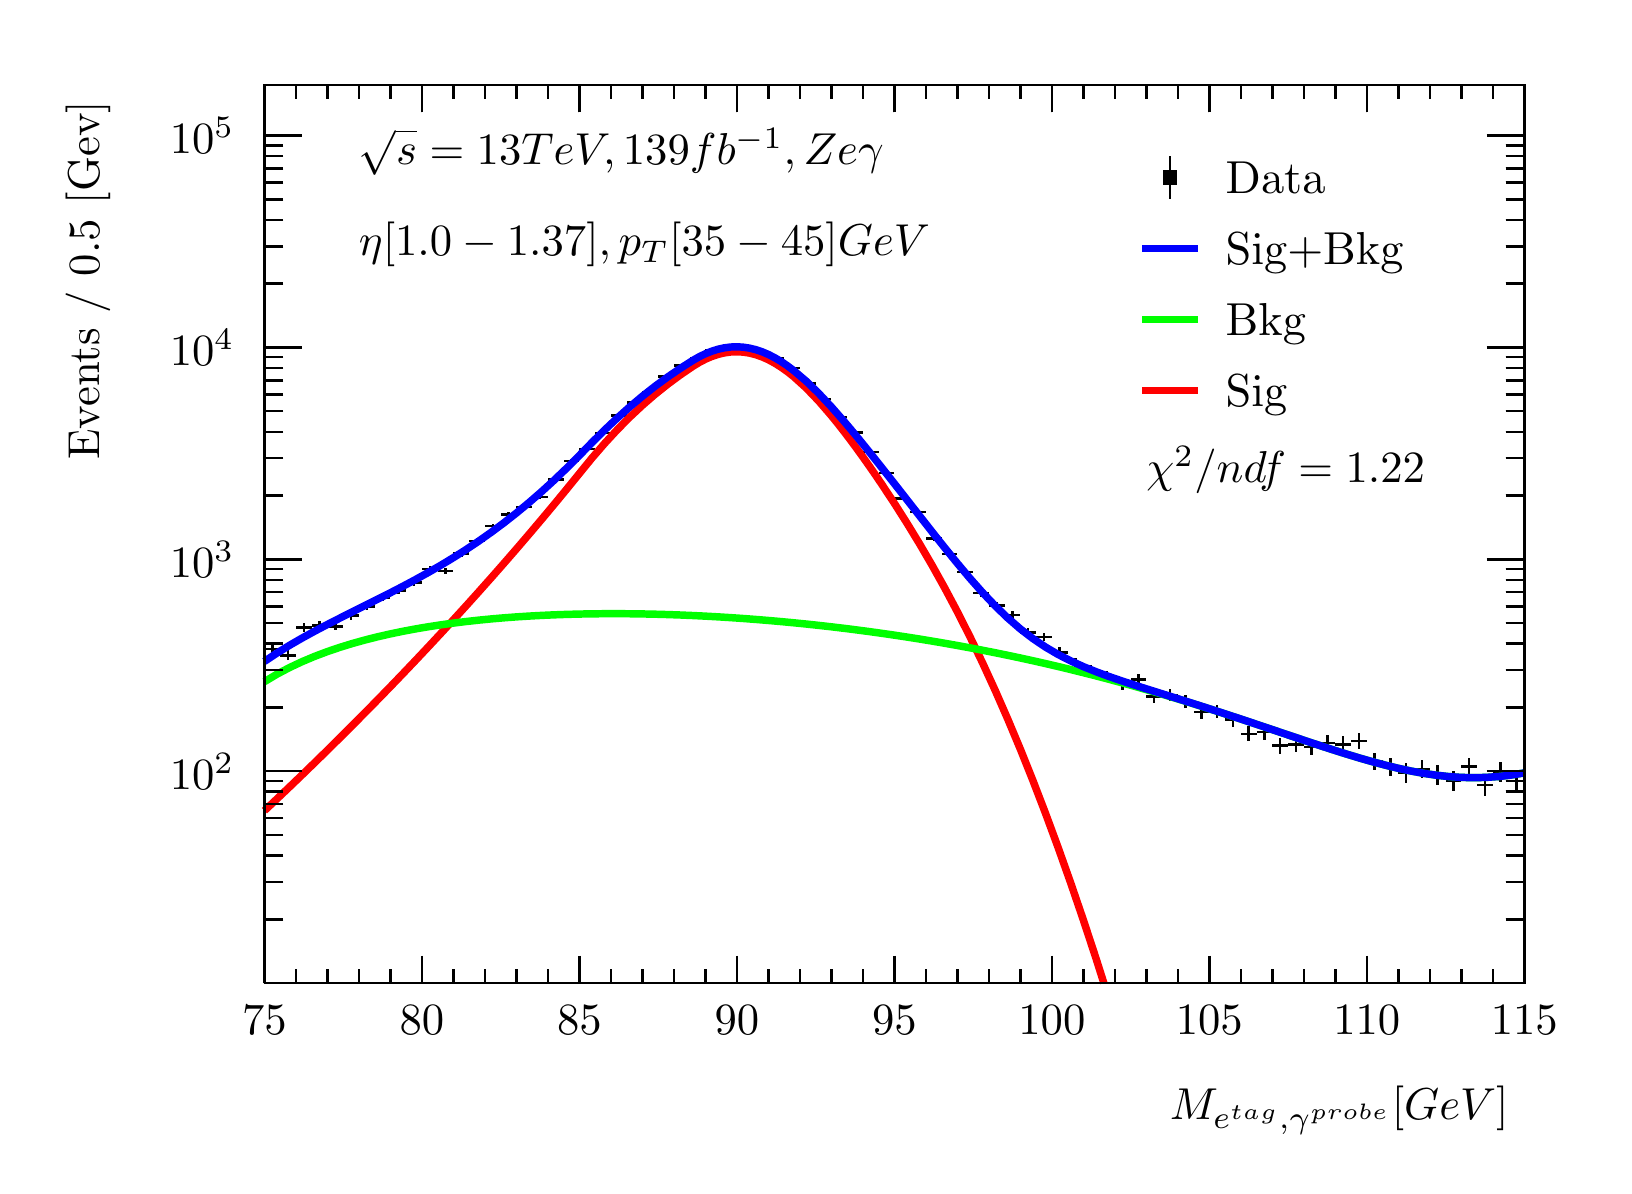
\begin{tikzpicture}
\pgfdeclareplotmark{cross} {
\pgfpathmoveto{\pgfpoint{-0.3\pgfplotmarksize}{\pgfplotmarksize}}
\pgfpathlineto{\pgfpoint{+0.3\pgfplotmarksize}{\pgfplotmarksize}}
\pgfpathlineto{\pgfpoint{+0.3\pgfplotmarksize}{0.3\pgfplotmarksize}}
\pgfpathlineto{\pgfpoint{+1\pgfplotmarksize}{0.3\pgfplotmarksize}}
\pgfpathlineto{\pgfpoint{+1\pgfplotmarksize}{-0.3\pgfplotmarksize}}
\pgfpathlineto{\pgfpoint{+0.3\pgfplotmarksize}{-0.3\pgfplotmarksize}}
\pgfpathlineto{\pgfpoint{+0.3\pgfplotmarksize}{-1.\pgfplotmarksize}}
\pgfpathlineto{\pgfpoint{-0.3\pgfplotmarksize}{-1.\pgfplotmarksize}}
\pgfpathlineto{\pgfpoint{-0.3\pgfplotmarksize}{-0.3\pgfplotmarksize}}
\pgfpathlineto{\pgfpoint{-1.\pgfplotmarksize}{-0.3\pgfplotmarksize}}
\pgfpathlineto{\pgfpoint{-1.\pgfplotmarksize}{0.3\pgfplotmarksize}}
\pgfpathlineto{\pgfpoint{-0.3\pgfplotmarksize}{0.3\pgfplotmarksize}}
\pgfpathclose
\pgfusepathqstroke
}
\pgfdeclareplotmark{cross*} {
\pgfpathmoveto{\pgfpoint{-0.3\pgfplotmarksize}{\pgfplotmarksize}}
\pgfpathlineto{\pgfpoint{+0.3\pgfplotmarksize}{\pgfplotmarksize}}
\pgfpathlineto{\pgfpoint{+0.3\pgfplotmarksize}{0.3\pgfplotmarksize}}
\pgfpathlineto{\pgfpoint{+1\pgfplotmarksize}{0.3\pgfplotmarksize}}
\pgfpathlineto{\pgfpoint{+1\pgfplotmarksize}{-0.3\pgfplotmarksize}}
\pgfpathlineto{\pgfpoint{+0.3\pgfplotmarksize}{-0.3\pgfplotmarksize}}
\pgfpathlineto{\pgfpoint{+0.3\pgfplotmarksize}{-1.\pgfplotmarksize}}
\pgfpathlineto{\pgfpoint{-0.3\pgfplotmarksize}{-1.\pgfplotmarksize}}
\pgfpathlineto{\pgfpoint{-0.3\pgfplotmarksize}{-0.3\pgfplotmarksize}}
\pgfpathlineto{\pgfpoint{-1.\pgfplotmarksize}{-0.3\pgfplotmarksize}}
\pgfpathlineto{\pgfpoint{-1.\pgfplotmarksize}{0.3\pgfplotmarksize}}
\pgfpathlineto{\pgfpoint{-0.3\pgfplotmarksize}{0.3\pgfplotmarksize}}
\pgfpathclose
\pgfusepathqfillstroke
}
\pgfdeclareplotmark{newstar} {
\pgfpathmoveto{\pgfqpoint{0pt}{\pgfplotmarksize}}
\pgfpathlineto{\pgfqpointpolar{44}{0.5\pgfplotmarksize}}
\pgfpathlineto{\pgfqpointpolar{18}{\pgfplotmarksize}}
\pgfpathlineto{\pgfqpointpolar{-20}{0.5\pgfplotmarksize}}
\pgfpathlineto{\pgfqpointpolar{-54}{\pgfplotmarksize}}
\pgfpathlineto{\pgfqpointpolar{-90}{0.5\pgfplotmarksize}}
\pgfpathlineto{\pgfqpointpolar{234}{\pgfplotmarksize}}
\pgfpathlineto{\pgfqpointpolar{198}{0.5\pgfplotmarksize}}
\pgfpathlineto{\pgfqpointpolar{162}{\pgfplotmarksize}}
\pgfpathlineto{\pgfqpointpolar{134}{0.5\pgfplotmarksize}}
\pgfpathclose
\pgfusepathqstroke
}
\pgfdeclareplotmark{newstar*} {
\pgfpathmoveto{\pgfqpoint{0pt}{\pgfplotmarksize}}
\pgfpathlineto{\pgfqpointpolar{44}{0.5\pgfplotmarksize}}
\pgfpathlineto{\pgfqpointpolar{18}{\pgfplotmarksize}}
\pgfpathlineto{\pgfqpointpolar{-20}{0.5\pgfplotmarksize}}
\pgfpathlineto{\pgfqpointpolar{-54}{\pgfplotmarksize}}
\pgfpathlineto{\pgfqpointpolar{-90}{0.5\pgfplotmarksize}}
\pgfpathlineto{\pgfqpointpolar{234}{\pgfplotmarksize}}
\pgfpathlineto{\pgfqpointpolar{198}{0.5\pgfplotmarksize}}
\pgfpathlineto{\pgfqpointpolar{162}{\pgfplotmarksize}}
\pgfpathlineto{\pgfqpointpolar{134}{0.5\pgfplotmarksize}}
\pgfpathclose
\pgfusepathqfillstroke
}
\definecolor{c}{rgb}{1,1,1};
\draw [color=c, fill=c] (0,0) rectangle (20,14.4361);
\draw [color=c, fill=c] (3,2.30977) rectangle (19,13.7143);
\definecolor{c}{rgb}{0,0,0};
\draw [c,line width=0.9] (3,2.30977) -- (3,13.7143) -- (19,13.7143) -- (19,2.30977) -- (3,2.30977);
\definecolor{c}{rgb}{1,1,1};
\draw [color=c, fill=c] (3,2.30977) rectangle (19,13.7143);
\definecolor{c}{rgb}{0,0,0};
\draw [c,line width=0.9] (3,2.30977) -- (3,13.7143) -- (19,13.7143) -- (19,2.30977) -- (3,2.30977);
\draw [c,line width=0.9] (3,2.30977) -- (19,2.30977);
\draw [c,line width=0.9] (3,2.65624) -- (3,2.30977);
\draw [c,line width=0.9] (3.4,2.48301) -- (3.4,2.30977);
\draw [c,line width=0.9] (3.8,2.48301) -- (3.8,2.30977);
\draw [c,line width=0.9] (4.2,2.48301) -- (4.2,2.30977);
\draw [c,line width=0.9] (4.6,2.48301) -- (4.6,2.30977);
\draw [c,line width=0.9] (5,2.65624) -- (5,2.30977);
\draw [c,line width=0.9] (5.4,2.48301) -- (5.4,2.30977);
\draw [c,line width=0.9] (5.8,2.48301) -- (5.8,2.30977);
\draw [c,line width=0.9] (6.2,2.48301) -- (6.2,2.30977);
\draw [c,line width=0.9] (6.6,2.48301) -- (6.6,2.30977);
\draw [c,line width=0.9] (7,2.65624) -- (7,2.30977);
\draw [c,line width=0.9] (7.4,2.48301) -- (7.4,2.30977);
\draw [c,line width=0.9] (7.8,2.48301) -- (7.8,2.30977);
\draw [c,line width=0.9] (8.2,2.48301) -- (8.2,2.30977);
\draw [c,line width=0.9] (8.6,2.48301) -- (8.6,2.30977);
\draw [c,line width=0.9] (9,2.65624) -- (9,2.30977);
\draw [c,line width=0.9] (9.4,2.48301) -- (9.4,2.30977);
\draw [c,line width=0.9] (9.8,2.48301) -- (9.8,2.30977);
\draw [c,line width=0.9] (10.2,2.48301) -- (10.2,2.30977);
\draw [c,line width=0.9] (10.6,2.48301) -- (10.6,2.30977);
\draw [c,line width=0.9] (11,2.65624) -- (11,2.30977);
\draw [c,line width=0.9] (11.4,2.48301) -- (11.4,2.30977);
\draw [c,line width=0.9] (11.8,2.48301) -- (11.8,2.30977);
\draw [c,line width=0.9] (12.2,2.48301) -- (12.2,2.30977);
\draw [c,line width=0.9] (12.6,2.48301) -- (12.6,2.30977);
\draw [c,line width=0.9] (13,2.65624) -- (13,2.30977);
\draw [c,line width=0.9] (13.4,2.48301) -- (13.4,2.30977);
\draw [c,line width=0.9] (13.8,2.48301) -- (13.8,2.30977);
\draw [c,line width=0.9] (14.2,2.48301) -- (14.2,2.30977);
\draw [c,line width=0.9] (14.6,2.48301) -- (14.6,2.30977);
\draw [c,line width=0.9] (15,2.65624) -- (15,2.30977);
\draw [c,line width=0.9] (15.4,2.48301) -- (15.4,2.30977);
\draw [c,line width=0.9] (15.8,2.48301) -- (15.8,2.30977);
\draw [c,line width=0.9] (16.2,2.48301) -- (16.2,2.30977);
\draw [c,line width=0.9] (16.6,2.48301) -- (16.6,2.30977);
\draw [c,line width=0.9] (17,2.65624) -- (17,2.30977);
\draw [c,line width=0.9] (17.4,2.48301) -- (17.4,2.30977);
\draw [c,line width=0.9] (17.8,2.48301) -- (17.8,2.30977);
\draw [c,line width=0.9] (18.2,2.48301) -- (18.2,2.30977);
\draw [c,line width=0.9] (18.6,2.48301) -- (18.6,2.30977);
\draw [c,line width=0.9] (19,2.65624) -- (19,2.30977);
\draw [c,line width=0.9] (19,2.65624) -- (19,2.30977);
\draw [anchor=base] (3,1.66015) node[scale=1.61424, color=c, rotate=0]{75};
\draw [anchor=base] (5,1.66015) node[scale=1.61424, color=c, rotate=0]{80};
\draw [anchor=base] (7,1.66015) node[scale=1.61424, color=c, rotate=0]{85};
\draw [anchor=base] (9,1.66015) node[scale=1.61424, color=c, rotate=0]{90};
\draw [anchor=base] (11,1.66015) node[scale=1.61424, color=c, rotate=0]{95};
\draw [anchor=base] (13,1.66015) node[scale=1.61424, color=c, rotate=0]{100};
\draw [anchor=base] (15,1.66015) node[scale=1.61424, color=c, rotate=0]{105};
\draw [anchor=base] (17,1.66015) node[scale=1.61424, color=c, rotate=0]{110};
\draw [anchor=base] (19,1.66015) node[scale=1.61424, color=c, rotate=0]{115};
\draw [anchor= east] (19,0.692932) node[scale=1.61424, color=c, rotate=0]{$M_{e^{tag}, \gamma^{probe}}  [GeV]$};
\draw [c,line width=0.9] (3,13.7143) -- (19,13.7143);
\draw [c,line width=0.9] (3,13.3678) -- (3,13.7143);
\draw [c,line width=0.9] (3.4,13.5411) -- (3.4,13.7143);
\draw [c,line width=0.9] (3.8,13.5411) -- (3.8,13.7143);
\draw [c,line width=0.9] (4.2,13.5411) -- (4.2,13.7143);
\draw [c,line width=0.9] (4.6,13.5411) -- (4.6,13.7143);
\draw [c,line width=0.9] (5,13.3678) -- (5,13.7143);
\draw [c,line width=0.9] (5.4,13.5411) -- (5.4,13.7143);
\draw [c,line width=0.9] (5.8,13.5411) -- (5.8,13.7143);
\draw [c,line width=0.9] (6.2,13.5411) -- (6.2,13.7143);
\draw [c,line width=0.9] (6.6,13.5411) -- (6.6,13.7143);
\draw [c,line width=0.9] (7,13.3678) -- (7,13.7143);
\draw [c,line width=0.9] (7.4,13.5411) -- (7.4,13.7143);
\draw [c,line width=0.9] (7.8,13.5411) -- (7.8,13.7143);
\draw [c,line width=0.9] (8.2,13.5411) -- (8.2,13.7143);
\draw [c,line width=0.9] (8.6,13.5411) -- (8.6,13.7143);
\draw [c,line width=0.9] (9,13.3678) -- (9,13.7143);
\draw [c,line width=0.9] (9.4,13.5411) -- (9.4,13.7143);
\draw [c,line width=0.9] (9.8,13.5411) -- (9.8,13.7143);
\draw [c,line width=0.9] (10.2,13.5411) -- (10.2,13.7143);
\draw [c,line width=0.9] (10.6,13.5411) -- (10.6,13.7143);
\draw [c,line width=0.9] (11,13.3678) -- (11,13.7143);
\draw [c,line width=0.9] (11.4,13.5411) -- (11.4,13.7143);
\draw [c,line width=0.9] (11.8,13.5411) -- (11.8,13.7143);
\draw [c,line width=0.9] (12.2,13.5411) -- (12.2,13.7143);
\draw [c,line width=0.9] (12.6,13.5411) -- (12.6,13.7143);
\draw [c,line width=0.9] (13,13.3678) -- (13,13.7143);
\draw [c,line width=0.9] (13.4,13.5411) -- (13.4,13.7143);
\draw [c,line width=0.9] (13.8,13.5411) -- (13.8,13.7143);
\draw [c,line width=0.9] (14.2,13.5411) -- (14.2,13.7143);
\draw [c,line width=0.9] (14.6,13.5411) -- (14.6,13.7143);
\draw [c,line width=0.9] (15,13.3678) -- (15,13.7143);
\draw [c,line width=0.9] (15.4,13.5411) -- (15.4,13.7143);
\draw [c,line width=0.9] (15.8,13.5411) -- (15.8,13.7143);
\draw [c,line width=0.9] (16.2,13.5411) -- (16.2,13.7143);
\draw [c,line width=0.9] (16.6,13.5411) -- (16.6,13.7143);
\draw [c,line width=0.9] (17,13.3678) -- (17,13.7143);
\draw [c,line width=0.9] (17.4,13.5411) -- (17.4,13.7143);
\draw [c,line width=0.9] (17.8,13.5411) -- (17.8,13.7143);
\draw [c,line width=0.9] (18.2,13.5411) -- (18.2,13.7143);
\draw [c,line width=0.9] (18.6,13.5411) -- (18.6,13.7143);
\draw [c,line width=0.9] (19,13.3678) -- (19,13.7143);
\draw [c,line width=0.9] (19,13.3678) -- (19,13.7143);
\draw [c,line width=0.9] (3,2.30977) -- (3,13.7143);
\draw [c,line width=0.9] (3.237,3.11973) -- (3,3.11973);
\draw [c,line width=0.9] (3.237,3.59352) -- (3,3.59352);
\draw [c,line width=0.9] (3.237,3.92968) -- (3,3.92968);
\draw [c,line width=0.9] (3.237,4.19043) -- (3,4.19043);
\draw [c,line width=0.9] (3.237,4.40347) -- (3,4.40347);
\draw [c,line width=0.9] (3.237,4.5836) -- (3,4.5836);
\draw [c,line width=0.9] (3.237,4.73964) -- (3,4.73964);
\draw [c,line width=0.9] (3.237,4.87727) -- (3,4.87727);
\draw [c,line width=0.9] (3.474,5.00038) -- (3,5.00038);
\draw [anchor= east] (2.82,5.00038) node[scale=1.61424, color=c, rotate=0]{$10^{2}$};
\draw [c,line width=0.9] (3.237,5.81034) -- (3,5.81034);
\draw [c,line width=0.9] (3.237,6.28413) -- (3,6.28413);
\draw [c,line width=0.9] (3.237,6.62029) -- (3,6.62029);
\draw [c,line width=0.9] (3.237,6.88104) -- (3,6.88104);
\draw [c,line width=0.9] (3.237,7.09409) -- (3,7.09409);
\draw [c,line width=0.9] (3.237,7.27421) -- (3,7.27421);
\draw [c,line width=0.9] (3.237,7.43025) -- (3,7.43025);
\draw [c,line width=0.9] (3.237,7.56788) -- (3,7.56788);
\draw [c,line width=0.9] (3.474,7.69099) -- (3,7.69099);
\draw [anchor= east] (2.82,7.69099) node[scale=1.61424, color=c, rotate=0]{$10^{3}$};
\draw [c,line width=0.9] (3.237,8.50095) -- (3,8.50095);
\draw [c,line width=0.9] (3.237,8.97474) -- (3,8.97474);
\draw [c,line width=0.9] (3.237,9.3109) -- (3,9.3109);
\draw [c,line width=0.9] (3.237,9.57165) -- (3,9.57165);
\draw [c,line width=0.9] (3.237,9.7847) -- (3,9.7847);
\draw [c,line width=0.9] (3.237,9.96482) -- (3,9.96482);
\draw [c,line width=0.9] (3.237,10.1209) -- (3,10.1209);
\draw [c,line width=0.9] (3.237,10.2585) -- (3,10.2585);
\draw [c,line width=0.9] (3.474,10.3816) -- (3,10.3816);
\draw [anchor= east] (2.82,10.3816) node[scale=1.61424, color=c, rotate=0]{$10^{4}$};
\draw [c,line width=0.9] (3.237,11.1916) -- (3,11.1916);
\draw [c,line width=0.9] (3.237,11.6654) -- (3,11.6654);
\draw [c,line width=0.9] (3.237,12.0015) -- (3,12.0015);
\draw [c,line width=0.9] (3.237,12.2623) -- (3,12.2623);
\draw [c,line width=0.9] (3.237,12.4753) -- (3,12.4753);
\draw [c,line width=0.9] (3.237,12.6554) -- (3,12.6554);
\draw [c,line width=0.9] (3.237,12.8115) -- (3,12.8115);
\draw [c,line width=0.9] (3.237,12.9491) -- (3,12.9491);
\draw [c,line width=0.9] (3.474,13.0722) -- (3,13.0722);
\draw [anchor= east] (2.82,13.0722) node[scale=1.61424, color=c, rotate=0]{$10^{5}$};
\draw [anchor= east] (0.76,13.7143) node[scale=1.61424, color=c, rotate=90]{Events / 0.5 [Gev]};
\draw [c,line width=0.9] (19,2.30977) -- (19,13.7143);
\draw [c,line width=0.9] (18.763,3.11973) -- (19,3.11973);
\draw [c,line width=0.9] (18.763,3.59352) -- (19,3.59352);
\draw [c,line width=0.9] (18.763,3.92968) -- (19,3.92968);
\draw [c,line width=0.9] (18.763,4.19043) -- (19,4.19043);
\draw [c,line width=0.9] (18.763,4.40347) -- (19,4.40347);
\draw [c,line width=0.9] (18.763,4.5836) -- (19,4.5836);
\draw [c,line width=0.9] (18.763,4.73964) -- (19,4.73964);
\draw [c,line width=0.9] (18.763,4.87727) -- (19,4.87727);
\draw [c,line width=0.9] (18.526,5.00038) -- (19,5.00038);
\draw [c,line width=0.9] (18.763,5.81034) -- (19,5.81034);
\draw [c,line width=0.9] (18.763,6.28413) -- (19,6.28413);
\draw [c,line width=0.9] (18.763,6.62029) -- (19,6.62029);
\draw [c,line width=0.9] (18.763,6.88104) -- (19,6.88104);
\draw [c,line width=0.9] (18.763,7.09409) -- (19,7.09409);
\draw [c,line width=0.9] (18.763,7.27421) -- (19,7.27421);
\draw [c,line width=0.9] (18.763,7.43025) -- (19,7.43025);
\draw [c,line width=0.9] (18.763,7.56788) -- (19,7.56788);
\draw [c,line width=0.9] (18.526,7.69099) -- (19,7.69099);
\draw [c,line width=0.9] (18.763,8.50095) -- (19,8.50095);
\draw [c,line width=0.9] (18.763,8.97474) -- (19,8.97474);
\draw [c,line width=0.9] (18.763,9.3109) -- (19,9.3109);
\draw [c,line width=0.9] (18.763,9.57165) -- (19,9.57165);
\draw [c,line width=0.9] (18.763,9.7847) -- (19,9.7847);
\draw [c,line width=0.9] (18.763,9.96482) -- (19,9.96482);
\draw [c,line width=0.9] (18.763,10.1209) -- (19,10.1209);
\draw [c,line width=0.9] (18.763,10.2585) -- (19,10.2585);
\draw [c,line width=0.9] (18.526,10.3816) -- (19,10.3816);
\draw [c,line width=0.9] (18.763,11.1916) -- (19,11.1916);
\draw [c,line width=0.9] (18.763,11.6654) -- (19,11.6654);
\draw [c,line width=0.9] (18.763,12.0015) -- (19,12.0015);
\draw [c,line width=0.9] (18.763,12.2623) -- (19,12.2623);
\draw [c,line width=0.9] (18.763,12.4753) -- (19,12.4753);
\draw [c,line width=0.9] (18.763,12.6554) -- (19,12.6554);
\draw [c,line width=0.9] (18.763,12.8115) -- (19,12.8115);
\draw [c,line width=0.9] (18.763,12.9491) -- (19,12.9491);
\draw [c,line width=0.9] (18.526,13.0722) -- (19,13.0722);
\draw [c,line width=0.9] (3.1,6.5511) -- (3,6.5511);
\draw [c,line width=0.9] (3,6.5511) -- (3,6.5511);
\draw [c,line width=0.9] (3.1,6.5511) -- (3.2,6.5511);
\draw [c,line width=0.9] (3.2,6.5511) -- (3.2,6.5511);
\draw [c,line width=0.9] (3.1,6.5511) -- (3.1,6.61127);
\draw [c,line width=0.9] (3.1,6.61127) -- (3.1,6.61127);
\draw [c,line width=0.9] (3.1,6.5511) -- (3.1,6.49092);
\draw [c,line width=0.9] (3.1,6.49092) -- (3.1,6.49092);
\draw [c,line width=0.9] (3.3,6.47092) -- (3.2,6.47092);
\draw [c,line width=0.9] (3.2,6.47092) -- (3.2,6.47092);
\draw [c,line width=0.9] (3.3,6.47092) -- (3.4,6.47092);
\draw [c,line width=0.9] (3.4,6.47092) -- (3.4,6.47092);
\draw [c,line width=0.9] (3.3,6.47092) -- (3.3,6.53319);
\draw [c,line width=0.9] (3.3,6.53319) -- (3.3,6.53319);
\draw [c,line width=0.9] (3.3,6.47092) -- (3.3,6.40864);
\draw [c,line width=0.9] (3.3,6.40864) -- (3.3,6.40864);
\draw [c,line width=0.9] (3.5,6.82356) -- (3.4,6.82356);
\draw [c,line width=0.9] (3.4,6.82356) -- (3.4,6.82356);
\draw [c,line width=0.9] (3.5,6.82356) -- (3.6,6.82356);
\draw [c,line width=0.9] (3.6,6.82356) -- (3.6,6.82356);
\draw [c,line width=0.9] (3.5,6.82356) -- (3.5,6.87712);
\draw [c,line width=0.9] (3.5,6.87712) -- (3.5,6.87712);
\draw [c,line width=0.9] (3.5,6.82356) -- (3.5,6.77001);
\draw [c,line width=0.9] (3.5,6.77001) -- (3.5,6.77001);
\draw [c,line width=0.9] (3.7,6.85265) -- (3.6,6.85265);
\draw [c,line width=0.9] (3.6,6.85265) -- (3.6,6.85265);
\draw [c,line width=0.9] (3.7,6.85265) -- (3.8,6.85265);
\draw [c,line width=0.9] (3.8,6.85265) -- (3.8,6.85265);
\draw [c,line width=0.9] (3.7,6.85265) -- (3.7,6.90555);
\draw [c,line width=0.9] (3.7,6.90555) -- (3.7,6.90555);
\draw [c,line width=0.9] (3.7,6.85265) -- (3.7,6.79976);
\draw [c,line width=0.9] (3.7,6.79976) -- (3.7,6.79976);
\draw [c,line width=0.9] (3.9,6.84062) -- (3.8,6.84062);
\draw [c,line width=0.9] (3.8,6.84062) -- (3.8,6.84062);
\draw [c,line width=0.9] (3.9,6.84062) -- (4,6.84062);
\draw [c,line width=0.9] (4,6.84062) -- (4,6.84062);
\draw [c,line width=0.9] (3.9,6.84062) -- (3.9,6.89379);
\draw [c,line width=0.9] (3.9,6.89379) -- (3.9,6.89379);
\draw [c,line width=0.9] (3.9,6.84062) -- (3.9,6.78746);
\draw [c,line width=0.9] (3.9,6.78746) -- (3.9,6.78746);
\draw [c,line width=0.9] (4.1,6.97529) -- (4,6.97529);
\draw [c,line width=0.9] (4,6.97529) -- (4,6.97529);
\draw [c,line width=0.9] (4.1,6.97529) -- (4.2,6.97529);
\draw [c,line width=0.9] (4.2,6.97529) -- (4.2,6.97529);
\draw [c,line width=0.9] (4.1,6.97529) -- (4.1,7.02548);
\draw [c,line width=0.9] (4.1,7.02548) -- (4.1,7.02548);
\draw [c,line width=0.9] (4.1,6.97529) -- (4.1,6.9251);
\draw [c,line width=0.9] (4.1,6.9251) -- (4.1,6.9251);
\draw [c,line width=0.9] (4.3,7.09214) -- (4.2,7.09214);
\draw [c,line width=0.9] (4.2,7.09214) -- (4.2,7.09214);
\draw [c,line width=0.9] (4.3,7.09214) -- (4.4,7.09214);
\draw [c,line width=0.9] (4.4,7.09214) -- (4.4,7.09214);
\draw [c,line width=0.9] (4.3,7.09214) -- (4.3,7.13988);
\draw [c,line width=0.9] (4.3,7.13988) -- (4.3,7.13988);
\draw [c,line width=0.9] (4.3,7.09214) -- (4.3,7.0444);
\draw [c,line width=0.9] (4.3,7.0444) -- (4.3,7.0444);
\draw [c,line width=0.9] (4.5,7.20546) -- (4.4,7.20546);
\draw [c,line width=0.9] (4.4,7.20546) -- (4.4,7.20546);
\draw [c,line width=0.9] (4.5,7.20546) -- (4.6,7.20546);
\draw [c,line width=0.9] (4.6,7.20546) -- (4.6,7.20546);
\draw [c,line width=0.9] (4.5,7.20546) -- (4.5,7.25094);
\draw [c,line width=0.9] (4.5,7.25094) -- (4.5,7.25094);
\draw [c,line width=0.9] (4.5,7.20546) -- (4.5,7.15998);
\draw [c,line width=0.9] (4.5,7.15998) -- (4.5,7.15998);
\draw [c,line width=0.9] (4.7,7.29408) -- (4.6,7.29408);
\draw [c,line width=0.9] (4.6,7.29408) -- (4.6,7.29408);
\draw [c,line width=0.9] (4.7,7.29408) -- (4.8,7.29408);
\draw [c,line width=0.9] (4.8,7.29408) -- (4.8,7.29408);
\draw [c,line width=0.9] (4.7,7.29408) -- (4.7,7.33787);
\draw [c,line width=0.9] (4.7,7.33787) -- (4.7,7.33787);
\draw [c,line width=0.9] (4.7,7.29408) -- (4.7,7.25029);
\draw [c,line width=0.9] (4.7,7.25029) -- (4.7,7.25029);
\draw [c,line width=0.9] (4.9,7.39766) -- (4.8,7.39766);
\draw [c,line width=0.9] (4.8,7.39766) -- (4.8,7.39766);
\draw [c,line width=0.9] (4.9,7.39766) -- (5,7.39766);
\draw [c,line width=0.9] (5,7.39766) -- (5,7.39766);
\draw [c,line width=0.9] (4.9,7.39766) -- (4.9,7.43956);
\draw [c,line width=0.9] (4.9,7.43956) -- (4.9,7.43956);
\draw [c,line width=0.9] (4.9,7.39766) -- (4.9,7.35577);
\draw [c,line width=0.9] (4.9,7.35577) -- (4.9,7.35577);
\draw [c,line width=0.9] (5.1,7.56918) -- (5,7.56918);
\draw [c,line width=0.9] (5,7.56918) -- (5,7.56918);
\draw [c,line width=0.9] (5.1,7.56918) -- (5.2,7.56918);
\draw [c,line width=0.9] (5.2,7.56918) -- (5.2,7.56918);
\draw [c,line width=0.9] (5.1,7.56918) -- (5.1,7.6081);
\draw [c,line width=0.9] (5.1,7.6081) -- (5.1,7.6081);
\draw [c,line width=0.9] (5.1,7.56918) -- (5.1,7.53025);
\draw [c,line width=0.9] (5.1,7.53025) -- (5.1,7.53025);
\draw [c,line width=0.9] (5.3,7.54295) -- (5.2,7.54295);
\draw [c,line width=0.9] (5.2,7.54295) -- (5.2,7.54295);
\draw [c,line width=0.9] (5.3,7.54295) -- (5.4,7.54295);
\draw [c,line width=0.9] (5.4,7.54295) -- (5.4,7.54295);
\draw [c,line width=0.9] (5.3,7.54295) -- (5.3,7.58231);
\draw [c,line width=0.9] (5.3,7.58231) -- (5.3,7.58231);
\draw [c,line width=0.9] (5.3,7.54295) -- (5.3,7.50358);
\draw [c,line width=0.9] (5.3,7.50358) -- (5.3,7.50358);
\draw [c,line width=0.9] (5.5,7.76239) -- (5.4,7.76239);
\draw [c,line width=0.9] (5.4,7.76239) -- (5.4,7.76239);
\draw [c,line width=0.9] (5.5,7.76239) -- (5.6,7.76239);
\draw [c,line width=0.9] (5.6,7.76239) -- (5.6,7.76239);
\draw [c,line width=0.9] (5.5,7.76239) -- (5.5,7.79822);
\draw [c,line width=0.9] (5.5,7.79822) -- (5.5,7.79822);
\draw [c,line width=0.9] (5.5,7.76239) -- (5.5,7.72655);
\draw [c,line width=0.9] (5.5,7.72655) -- (5.5,7.72655);
\draw [c,line width=0.9] (5.7,7.92527) -- (5.6,7.92527);
\draw [c,line width=0.9] (5.6,7.92527) -- (5.6,7.92527);
\draw [c,line width=0.9] (5.7,7.92527) -- (5.8,7.92527);
\draw [c,line width=0.9] (5.8,7.92527) -- (5.8,7.92527);
\draw [c,line width=0.9] (5.7,7.92527) -- (5.7,7.9587);
\draw [c,line width=0.9] (5.7,7.9587) -- (5.7,7.9587);
\draw [c,line width=0.9] (5.7,7.92527) -- (5.7,7.89184);
\draw [c,line width=0.9] (5.7,7.89184) -- (5.7,7.89184);
\draw [c,line width=0.9] (5.9,8.11384) -- (5.8,8.11384);
\draw [c,line width=0.9] (5.8,8.11384) -- (5.8,8.11384);
\draw [c,line width=0.9] (5.9,8.11384) -- (6,8.11384);
\draw [c,line width=0.9] (6,8.11384) -- (6,8.11384);
\draw [c,line width=0.9] (5.9,8.11384) -- (5.9,8.14467);
\draw [c,line width=0.9] (5.9,8.14467) -- (5.9,8.14467);
\draw [c,line width=0.9] (5.9,8.11384) -- (5.9,8.083);
\draw [c,line width=0.9] (5.9,8.083) -- (5.9,8.083);
\draw [c,line width=0.9] (6.1,8.25904) -- (6,8.25904);
\draw [c,line width=0.9] (6,8.25904) -- (6,8.25904);
\draw [c,line width=0.9] (6.1,8.25904) -- (6.2,8.25904);
\draw [c,line width=0.9] (6.2,8.25904) -- (6.2,8.25904);
\draw [c,line width=0.9] (6.1,8.25904) -- (6.1,8.28802);
\draw [c,line width=0.9] (6.1,8.28802) -- (6.1,8.28802);
\draw [c,line width=0.9] (6.1,8.25904) -- (6.1,8.23006);
\draw [c,line width=0.9] (6.1,8.23006) -- (6.1,8.23006);
\draw [c,line width=0.9] (6.3,8.35357) -- (6.2,8.35357);
\draw [c,line width=0.9] (6.2,8.35357) -- (6.2,8.35357);
\draw [c,line width=0.9] (6.3,8.35357) -- (6.4,8.35357);
\draw [c,line width=0.9] (6.4,8.35357) -- (6.4,8.35357);
\draw [c,line width=0.9] (6.3,8.35357) -- (6.3,8.38139);
\draw [c,line width=0.9] (6.3,8.38139) -- (6.3,8.38139);
\draw [c,line width=0.9] (6.3,8.35357) -- (6.3,8.32574);
\draw [c,line width=0.9] (6.3,8.32574) -- (6.3,8.32574);
\draw [c,line width=0.9] (6.5,8.48448) -- (6.4,8.48448);
\draw [c,line width=0.9] (6.4,8.48448) -- (6.4,8.48448);
\draw [c,line width=0.9] (6.5,8.48448) -- (6.6,8.48448);
\draw [c,line width=0.9] (6.6,8.48448) -- (6.6,8.48448);
\draw [c,line width=0.9] (6.5,8.48448) -- (6.5,8.51079);
\draw [c,line width=0.9] (6.5,8.51079) -- (6.5,8.51079);
\draw [c,line width=0.9] (6.5,8.48448) -- (6.5,8.45816);
\draw [c,line width=0.9] (6.5,8.45816) -- (6.5,8.45816);
\draw [c,line width=0.9] (6.7,8.70569) -- (6.6,8.70569);
\draw [c,line width=0.9] (6.6,8.70569) -- (6.6,8.70569);
\draw [c,line width=0.9] (6.7,8.70569) -- (6.8,8.70569);
\draw [c,line width=0.9] (6.8,8.70569) -- (6.8,8.70569);
\draw [c,line width=0.9] (6.7,8.70569) -- (6.7,8.72963);
\draw [c,line width=0.9] (6.7,8.72963) -- (6.7,8.72963);
\draw [c,line width=0.9] (6.7,8.70569) -- (6.7,8.68175);
\draw [c,line width=0.9] (6.7,8.68175) -- (6.7,8.68175);
\draw [c,line width=0.9] (6.9,8.93995) -- (6.8,8.93995);
\draw [c,line width=0.9] (6.8,8.93995) -- (6.8,8.93995);
\draw [c,line width=0.9] (6.9,8.93995) -- (7,8.93995);
\draw [c,line width=0.9] (7,8.93995) -- (7,8.93995);
\draw [c,line width=0.9] (6.9,8.93995) -- (6.9,8.96161);
\draw [c,line width=0.9] (6.9,8.96161) -- (6.9,8.96161);
\draw [c,line width=0.9] (6.9,8.93995) -- (6.9,8.9183);
\draw [c,line width=0.9] (6.9,8.9183) -- (6.9,8.9183);
\draw [c,line width=0.9] (7.1,9.09) -- (7,9.09);
\draw [c,line width=0.9] (7,9.09) -- (7,9.09);
\draw [c,line width=0.9] (7.1,9.09) -- (7.2,9.09);
\draw [c,line width=0.9] (7.2,9.09) -- (7.2,9.09);
\draw [c,line width=0.9] (7.1,9.09) -- (7.1,9.11031);
\draw [c,line width=0.9] (7.1,9.11031) -- (7.1,9.11031);
\draw [c,line width=0.9] (7.1,9.09) -- (7.1,9.0697);
\draw [c,line width=0.9] (7.1,9.0697) -- (7.1,9.0697);
\draw [c,line width=0.9] (7.3,9.29739) -- (7.2,9.29739);
\draw [c,line width=0.9] (7.2,9.29739) -- (7.2,9.29739);
\draw [c,line width=0.9] (7.3,9.29739) -- (7.4,9.29739);
\draw [c,line width=0.9] (7.4,9.29739) -- (7.4,9.29739);
\draw [c,line width=0.9] (7.3,9.29739) -- (7.3,9.31597);
\draw [c,line width=0.9] (7.3,9.31597) -- (7.3,9.31597);
\draw [c,line width=0.9] (7.3,9.29739) -- (7.3,9.27881);
\draw [c,line width=0.9] (7.3,9.27881) -- (7.3,9.27881);
\draw [c,line width=0.9] (7.5,9.51564) -- (7.4,9.51564);
\draw [c,line width=0.9] (7.4,9.51564) -- (7.4,9.51564);
\draw [c,line width=0.9] (7.5,9.51564) -- (7.6,9.51564);
\draw [c,line width=0.9] (7.6,9.51564) -- (7.6,9.51564);
\draw [c,line width=0.9] (7.5,9.51564) -- (7.5,9.53257);
\draw [c,line width=0.9] (7.5,9.53257) -- (7.5,9.53257);
\draw [c,line width=0.9] (7.5,9.51564) -- (7.5,9.49872);
\draw [c,line width=0.9] (7.5,9.49872) -- (7.5,9.49872);
\draw [c,line width=0.9] (7.7,9.68493) -- (7.6,9.68493);
\draw [c,line width=0.9] (7.6,9.68493) -- (7.6,9.68493);
\draw [c,line width=0.9] (7.7,9.68493) -- (7.8,9.68493);
\draw [c,line width=0.9] (7.8,9.68493) -- (7.8,9.68493);
\draw [c,line width=0.9] (7.7,9.68493) -- (7.7,9.70068);
\draw [c,line width=0.9] (7.7,9.70068) -- (7.7,9.70068);
\draw [c,line width=0.9] (7.7,9.68493) -- (7.7,9.66919);
\draw [c,line width=0.9] (7.7,9.66919) -- (7.7,9.66919);
\draw [c,line width=0.9] (7.9,9.81412) -- (7.8,9.81412);
\draw [c,line width=0.9] (7.8,9.81412) -- (7.8,9.81412);
\draw [c,line width=0.9] (7.9,9.81412) -- (8,9.81412);
\draw [c,line width=0.9] (8,9.81412) -- (8,9.81412);
\draw [c,line width=0.9] (7.9,9.81412) -- (7.9,9.82902);
\draw [c,line width=0.9] (7.9,9.82902) -- (7.9,9.82902);
\draw [c,line width=0.9] (7.9,9.81412) -- (7.9,9.79922);
\draw [c,line width=0.9] (7.9,9.79922) -- (7.9,9.79922);
\draw [c,line width=0.9] (8.1,10.0129) -- (8,10.0129);
\draw [c,line width=0.9] (8,10.0129) -- (8,10.0129);
\draw [c,line width=0.9] (8.1,10.0129) -- (8.2,10.0129);
\draw [c,line width=0.9] (8.2,10.0129) -- (8.2,10.0129);
\draw [c,line width=0.9] (8.1,10.0129) -- (8.1,10.0266);
\draw [c,line width=0.9] (8.1,10.0266) -- (8.1,10.0266);
\draw [c,line width=0.9] (8.1,10.0129) -- (8.1,9.99922);
\draw [c,line width=0.9] (8.1,9.99922) -- (8.1,9.99922);
\draw [c,line width=0.9] (8.3,10.1518) -- (8.2,10.1518);
\draw [c,line width=0.9] (8.2,10.1518) -- (8.2,10.1518);
\draw [c,line width=0.9] (8.3,10.1518) -- (8.4,10.1518);
\draw [c,line width=0.9] (8.4,10.1518) -- (8.4,10.1518);
\draw [c,line width=0.9] (8.3,10.1518) -- (8.3,10.1647);
\draw [c,line width=0.9] (8.3,10.1647) -- (8.3,10.1647);
\draw [c,line width=0.9] (8.3,10.1518) -- (8.3,10.139);
\draw [c,line width=0.9] (8.3,10.139) -- (8.3,10.139);
\draw [c,line width=0.9] (8.5,10.2505) -- (8.4,10.2505);
\draw [c,line width=0.9] (8.4,10.2505) -- (8.4,10.2505);
\draw [c,line width=0.9] (8.5,10.2505) -- (8.6,10.2505);
\draw [c,line width=0.9] (8.6,10.2505) -- (8.6,10.2505);
\draw [c,line width=0.9] (8.5,10.2505) -- (8.5,10.2629);
\draw [c,line width=0.9] (8.5,10.2629) -- (8.5,10.2629);
\draw [c,line width=0.9] (8.5,10.2505) -- (8.5,10.2382);
\draw [c,line width=0.9] (8.5,10.2382) -- (8.5,10.2382);
\draw [c,line width=0.9] (8.7,10.3448) -- (8.6,10.3448);
\draw [c,line width=0.9] (8.6,10.3448) -- (8.6,10.3448);
\draw [c,line width=0.9] (8.7,10.3448) -- (8.8,10.3448);
\draw [c,line width=0.9] (8.8,10.3448) -- (8.8,10.3448);
\draw [c,line width=0.9] (8.7,10.3448) -- (8.7,10.3567);
\draw [c,line width=0.9] (8.7,10.3567) -- (8.7,10.3567);
\draw [c,line width=0.9] (8.7,10.3448) -- (8.7,10.3329);
\draw [c,line width=0.9] (8.7,10.3329) -- (8.7,10.3329);
\draw [c,line width=0.9] (8.9,10.3657) -- (8.8,10.3657);
\draw [c,line width=0.9] (8.8,10.3657) -- (8.8,10.3657);
\draw [c,line width=0.9] (8.9,10.3657) -- (9,10.3657);
\draw [c,line width=0.9] (9,10.3657) -- (9,10.3657);
\draw [c,line width=0.9] (8.9,10.3657) -- (8.9,10.3775);
\draw [c,line width=0.9] (8.9,10.3775) -- (8.9,10.3775);
\draw [c,line width=0.9] (8.9,10.3657) -- (8.9,10.354);
\draw [c,line width=0.9] (8.9,10.354) -- (8.9,10.354);
\draw [c,line width=0.9] (9.1,10.3749) -- (9,10.3749);
\draw [c,line width=0.9] (9,10.3749) -- (9,10.3749);
\draw [c,line width=0.9] (9.1,10.3749) -- (9.2,10.3749);
\draw [c,line width=0.9] (9.2,10.3749) -- (9.2,10.3749);
\draw [c,line width=0.9] (9.1,10.3749) -- (9.1,10.3866);
\draw [c,line width=0.9] (9.1,10.3866) -- (9.1,10.3866);
\draw [c,line width=0.9] (9.1,10.3749) -- (9.1,10.3632);
\draw [c,line width=0.9] (9.1,10.3632) -- (9.1,10.3632);
\draw [c,line width=0.9] (9.3,10.3395) -- (9.2,10.3395);
\draw [c,line width=0.9] (9.2,10.3395) -- (9.2,10.3395);
\draw [c,line width=0.9] (9.3,10.3395) -- (9.4,10.3395);
\draw [c,line width=0.9] (9.4,10.3395) -- (9.4,10.3395);
\draw [c,line width=0.9] (9.3,10.3395) -- (9.3,10.3514);
\draw [c,line width=0.9] (9.3,10.3514) -- (9.3,10.3514);
\draw [c,line width=0.9] (9.3,10.3395) -- (9.3,10.3276);
\draw [c,line width=0.9] (9.3,10.3276) -- (9.3,10.3276);
\draw [c,line width=0.9] (9.5,10.2412) -- (9.4,10.2412);
\draw [c,line width=0.9] (9.4,10.2412) -- (9.4,10.2412);
\draw [c,line width=0.9] (9.5,10.2412) -- (9.6,10.2412);
\draw [c,line width=0.9] (9.6,10.2412) -- (9.6,10.2412);
\draw [c,line width=0.9] (9.5,10.2412) -- (9.5,10.2536);
\draw [c,line width=0.9] (9.5,10.2536) -- (9.5,10.2536);
\draw [c,line width=0.9] (9.5,10.2412) -- (9.5,10.2288);
\draw [c,line width=0.9] (9.5,10.2288) -- (9.5,10.2288);
\draw [c,line width=0.9] (9.7,10.1217) -- (9.6,10.1217);
\draw [c,line width=0.9] (9.6,10.1217) -- (9.6,10.1217);
\draw [c,line width=0.9] (9.7,10.1217) -- (9.8,10.1217);
\draw [c,line width=0.9] (9.8,10.1217) -- (9.8,10.1217);
\draw [c,line width=0.9] (9.7,10.1217) -- (9.7,10.1348);
\draw [c,line width=0.9] (9.7,10.1348) -- (9.7,10.1348);
\draw [c,line width=0.9] (9.7,10.1217) -- (9.7,10.1087);
\draw [c,line width=0.9] (9.7,10.1087) -- (9.7,10.1087);
\draw [c,line width=0.9] (9.9,9.92665) -- (9.8,9.92665);
\draw [c,line width=0.9] (9.8,9.92665) -- (9.8,9.92665);
\draw [c,line width=0.9] (9.9,9.92665) -- (10,9.92665);
\draw [c,line width=0.9] (10,9.92665) -- (10,9.92665);
\draw [c,line width=0.9] (9.9,9.92665) -- (9.9,9.94085);
\draw [c,line width=0.9] (9.9,9.94085) -- (9.9,9.94085);
\draw [c,line width=0.9] (9.9,9.92665) -- (9.9,9.91245);
\draw [c,line width=0.9] (9.9,9.91245) -- (9.9,9.91245);
\draw [c,line width=0.9] (10.1,9.72845) -- (10,9.72845);
\draw [c,line width=0.9] (10,9.72845) -- (10,9.72845);
\draw [c,line width=0.9] (10.1,9.72845) -- (10.2,9.72845);
\draw [c,line width=0.9] (10.2,9.72845) -- (10.2,9.72845);
\draw [c,line width=0.9] (10.1,9.72845) -- (10.1,9.7439);
\draw [c,line width=0.9] (10.1,9.7439) -- (10.1,9.7439);
\draw [c,line width=0.9] (10.1,9.72845) -- (10.1,9.71299);
\draw [c,line width=0.9] (10.1,9.71299) -- (10.1,9.71299);
\draw [c,line width=0.9] (10.3,9.49761) -- (10.2,9.49761);
\draw [c,line width=0.9] (10.2,9.49761) -- (10.2,9.49761);
\draw [c,line width=0.9] (10.3,9.49761) -- (10.4,9.49761);
\draw [c,line width=0.9] (10.4,9.49761) -- (10.4,9.49761);
\draw [c,line width=0.9] (10.3,9.49761) -- (10.3,9.51466);
\draw [c,line width=0.9] (10.3,9.51466) -- (10.3,9.51466);
\draw [c,line width=0.9] (10.3,9.49761) -- (10.3,9.48055);
\draw [c,line width=0.9] (10.3,9.48055) -- (10.3,9.48055);
\draw [c,line width=0.9] (10.5,9.30005) -- (10.4,9.30005);
\draw [c,line width=0.9] (10.4,9.30005) -- (10.4,9.30005);
\draw [c,line width=0.9] (10.5,9.30005) -- (10.6,9.30005);
\draw [c,line width=0.9] (10.6,9.30005) -- (10.6,9.30005);
\draw [c,line width=0.9] (10.5,9.30005) -- (10.5,9.31861);
\draw [c,line width=0.9] (10.5,9.31861) -- (10.5,9.31861);
\draw [c,line width=0.9] (10.5,9.30005) -- (10.5,9.28148);
\draw [c,line width=0.9] (10.5,9.28148) -- (10.5,9.28148);
\draw [c,line width=0.9] (10.7,9.05198) -- (10.6,9.05198);
\draw [c,line width=0.9] (10.6,9.05198) -- (10.6,9.05198);
\draw [c,line width=0.9] (10.7,9.05198) -- (10.8,9.05198);
\draw [c,line width=0.9] (10.8,9.05198) -- (10.8,9.05198);
\draw [c,line width=0.9] (10.7,9.05198) -- (10.7,9.07262);
\draw [c,line width=0.9] (10.7,9.07262) -- (10.7,9.07262);
\draw [c,line width=0.9] (10.7,9.05198) -- (10.7,9.03134);
\draw [c,line width=0.9] (10.7,9.03134) -- (10.7,9.03134);
\draw [c,line width=0.9] (10.9,8.78713) -- (10.8,8.78713);
\draw [c,line width=0.9] (10.8,8.78713) -- (10.8,8.78713);
\draw [c,line width=0.9] (10.9,8.78713) -- (11,8.78713);
\draw [c,line width=0.9] (11,8.78713) -- (11,8.78713);
\draw [c,line width=0.9] (10.9,8.78713) -- (10.9,8.81024);
\draw [c,line width=0.9] (10.9,8.81024) -- (10.9,8.81024);
\draw [c,line width=0.9] (10.9,8.78713) -- (10.9,8.76401);
\draw [c,line width=0.9] (10.9,8.76401) -- (10.9,8.76401);
\draw [c,line width=0.9] (11.1,8.46656) -- (11,8.46656);
\draw [c,line width=0.9] (11,8.46656) -- (11,8.46656);
\draw [c,line width=0.9] (11.1,8.46656) -- (11.2,8.46656);
\draw [c,line width=0.9] (11.2,8.46656) -- (11.2,8.46656);
\draw [c,line width=0.9] (11.1,8.46656) -- (11.1,8.49308);
\draw [c,line width=0.9] (11.1,8.49308) -- (11.1,8.49308);
\draw [c,line width=0.9] (11.1,8.46656) -- (11.1,8.44005);
\draw [c,line width=0.9] (11.1,8.44005) -- (11.1,8.44005);
\draw [c,line width=0.9] (11.3,8.29443) -- (11.2,8.29443);
\draw [c,line width=0.9] (11.2,8.29443) -- (11.2,8.29443);
\draw [c,line width=0.9] (11.3,8.29443) -- (11.4,8.29443);
\draw [c,line width=0.9] (11.4,8.29443) -- (11.4,8.29443);
\draw [c,line width=0.9] (11.3,8.29443) -- (11.3,8.32297);
\draw [c,line width=0.9] (11.3,8.32297) -- (11.3,8.32297);
\draw [c,line width=0.9] (11.3,8.29443) -- (11.3,8.26589);
\draw [c,line width=0.9] (11.3,8.26589) -- (11.3,8.26589);
\draw [c,line width=0.9] (11.5,7.95454) -- (11.4,7.95454);
\draw [c,line width=0.9] (11.4,7.95454) -- (11.4,7.95454);
\draw [c,line width=0.9] (11.5,7.95454) -- (11.6,7.95454);
\draw [c,line width=0.9] (11.6,7.95454) -- (11.6,7.95454);
\draw [c,line width=0.9] (11.5,7.95454) -- (11.5,7.98755);
\draw [c,line width=0.9] (11.5,7.98755) -- (11.5,7.98755);
\draw [c,line width=0.9] (11.5,7.95454) -- (11.5,7.92153);
\draw [c,line width=0.9] (11.5,7.92153) -- (11.5,7.92153);
\draw [c,line width=0.9] (11.7,7.76129) -- (11.6,7.76129);
\draw [c,line width=0.9] (11.6,7.76129) -- (11.6,7.76129);
\draw [c,line width=0.9] (11.7,7.76129) -- (11.8,7.76129);
\draw [c,line width=0.9] (11.8,7.76129) -- (11.8,7.76129);
\draw [c,line width=0.9] (11.7,7.76129) -- (11.7,7.79714);
\draw [c,line width=0.9] (11.7,7.79714) -- (11.7,7.79714);
\draw [c,line width=0.9] (11.7,7.76129) -- (11.7,7.72543);
\draw [c,line width=0.9] (11.7,7.72543) -- (11.7,7.72543);
\draw [c,line width=0.9] (11.9,7.52961) -- (11.8,7.52961);
\draw [c,line width=0.9] (11.8,7.52961) -- (11.8,7.52961);
\draw [c,line width=0.9] (11.9,7.52961) -- (12,7.52961);
\draw [c,line width=0.9] (12,7.52961) -- (12,7.52961);
\draw [c,line width=0.9] (11.9,7.52961) -- (11.9,7.5692);
\draw [c,line width=0.9] (11.9,7.5692) -- (11.9,7.5692);
\draw [c,line width=0.9] (11.9,7.52961) -- (11.9,7.49002);
\draw [c,line width=0.9] (11.9,7.49002) -- (11.9,7.49002);
\draw [c,line width=0.9] (12.1,7.26247) -- (12,7.26247);
\draw [c,line width=0.9] (12,7.26247) -- (12,7.26247);
\draw [c,line width=0.9] (12.1,7.26247) -- (12.2,7.26247);
\draw [c,line width=0.9] (12.2,7.26247) -- (12.2,7.26247);
\draw [c,line width=0.9] (12.1,7.26247) -- (12.1,7.30686);
\draw [c,line width=0.9] (12.1,7.30686) -- (12.1,7.30686);
\draw [c,line width=0.9] (12.1,7.26247) -- (12.1,7.21809);
\draw [c,line width=0.9] (12.1,7.21809) -- (12.1,7.21809);
\draw [c,line width=0.9] (12.3,7.10764) -- (12.2,7.10764);
\draw [c,line width=0.9] (12.2,7.10764) -- (12.2,7.10764);
\draw [c,line width=0.9] (12.3,7.10764) -- (12.4,7.10764);
\draw [c,line width=0.9] (12.4,7.10764) -- (12.4,7.10764);
\draw [c,line width=0.9] (12.3,7.10764) -- (12.3,7.15507);
\draw [c,line width=0.9] (12.3,7.15507) -- (12.3,7.15507);
\draw [c,line width=0.9] (12.3,7.10764) -- (12.3,7.06022);
\draw [c,line width=0.9] (12.3,7.06022) -- (12.3,7.06022);
\draw [c,line width=0.9] (12.5,6.98602) -- (12.4,6.98602);
\draw [c,line width=0.9] (12.4,6.98602) -- (12.4,6.98602);
\draw [c,line width=0.9] (12.5,6.98602) -- (12.6,6.98602);
\draw [c,line width=0.9] (12.6,6.98602) -- (12.6,6.98602);
\draw [c,line width=0.9] (12.5,6.98602) -- (12.5,7.03598);
\draw [c,line width=0.9] (12.5,7.03598) -- (12.5,7.03598);
\draw [c,line width=0.9] (12.5,6.98602) -- (12.5,6.93606);
\draw [c,line width=0.9] (12.5,6.93606) -- (12.5,6.93606);
\draw [c,line width=0.9] (12.7,6.76311) -- (12.6,6.76311);
\draw [c,line width=0.9] (12.6,6.76311) -- (12.6,6.76311);
\draw [c,line width=0.9] (12.7,6.76311) -- (12.8,6.76311);
\draw [c,line width=0.9] (12.8,6.76311) -- (12.8,6.76311);
\draw [c,line width=0.9] (12.7,6.76311) -- (12.7,6.81806);
\draw [c,line width=0.9] (12.7,6.81806) -- (12.7,6.81806);
\draw [c,line width=0.9] (12.7,6.76311) -- (12.7,6.70815);
\draw [c,line width=0.9] (12.7,6.70815) -- (12.7,6.70815);
\draw [c,line width=0.9] (12.9,6.7048) -- (12.8,6.7048);
\draw [c,line width=0.9] (12.8,6.7048) -- (12.8,6.7048);
\draw [c,line width=0.9] (12.9,6.7048) -- (13,6.7048);
\draw [c,line width=0.9] (13,6.7048) -- (13,6.7048);
\draw [c,line width=0.9] (12.9,6.7048) -- (12.9,6.76115);
\draw [c,line width=0.9] (12.9,6.76115) -- (12.9,6.76115);
\draw [c,line width=0.9] (12.9,6.7048) -- (12.9,6.64846);
\draw [c,line width=0.9] (12.9,6.64846) -- (12.9,6.64846);
\draw [c,line width=0.9] (13.1,6.51009) -- (13,6.51009);
\draw [c,line width=0.9] (13,6.51009) -- (13,6.51009);
\draw [c,line width=0.9] (13.1,6.51009) -- (13.2,6.51009);
\draw [c,line width=0.9] (13.2,6.51009) -- (13.2,6.51009);
\draw [c,line width=0.9] (13.1,6.51009) -- (13.1,6.57133);
\draw [c,line width=0.9] (13.1,6.57133) -- (13.1,6.57133);
\draw [c,line width=0.9] (13.1,6.51009) -- (13.1,6.44885);
\draw [c,line width=0.9] (13.1,6.44885) -- (13.1,6.44885);
\draw [c,line width=0.9] (13.3,6.37406) -- (13.2,6.37406);
\draw [c,line width=0.9] (13.2,6.37406) -- (13.2,6.37406);
\draw [c,line width=0.9] (13.3,6.37406) -- (13.4,6.37406);
\draw [c,line width=0.9] (13.4,6.37406) -- (13.4,6.37406);
\draw [c,line width=0.9] (13.3,6.37406) -- (13.3,6.43897);
\draw [c,line width=0.9] (13.3,6.43897) -- (13.3,6.43897);
\draw [c,line width=0.9] (13.3,6.37406) -- (13.3,6.30915);
\draw [c,line width=0.9] (13.3,6.30915) -- (13.3,6.30915);
\draw [c,line width=0.9] (13.5,6.28413) -- (13.4,6.28413);
\draw [c,line width=0.9] (13.4,6.28413) -- (13.4,6.28413);
\draw [c,line width=0.9] (13.5,6.28413) -- (13.6,6.28413);
\draw [c,line width=0.9] (13.6,6.28413) -- (13.6,6.28413);
\draw [c,line width=0.9] (13.5,6.28413) -- (13.5,6.35159);
\draw [c,line width=0.9] (13.5,6.35159) -- (13.5,6.35159);
\draw [c,line width=0.9] (13.5,6.28413) -- (13.5,6.21668);
\draw [c,line width=0.9] (13.5,6.21668) -- (13.5,6.21668);
\draw [c,line width=0.9] (13.7,6.20768) -- (13.6,6.20768);
\draw [c,line width=0.9] (13.6,6.20768) -- (13.6,6.20768);
\draw [c,line width=0.9] (13.7,6.20768) -- (13.8,6.20768);
\draw [c,line width=0.9] (13.8,6.20768) -- (13.8,6.20768);
\draw [c,line width=0.9] (13.7,6.20768) -- (13.7,6.27738);
\draw [c,line width=0.9] (13.7,6.27738) -- (13.7,6.27738);
\draw [c,line width=0.9] (13.7,6.20768) -- (13.7,6.13798);
\draw [c,line width=0.9] (13.7,6.13798) -- (13.7,6.13798);
\draw [c,line width=0.9] (13.9,6.10789) -- (13.8,6.10789);
\draw [c,line width=0.9] (13.8,6.10789) -- (13.8,6.10789);
\draw [c,line width=0.9] (13.9,6.10789) -- (14,6.10789);
\draw [c,line width=0.9] (14,6.10789) -- (14,6.10789);
\draw [c,line width=0.9] (13.9,6.10789) -- (13.9,6.18063);
\draw [c,line width=0.9] (13.9,6.18063) -- (13.9,6.18063);
\draw [c,line width=0.9] (13.9,6.10789) -- (13.9,6.03516);
\draw [c,line width=0.9] (13.9,6.03516) -- (13.9,6.03516);
\draw [c,line width=0.9] (14.1,6.16534) -- (14,6.16534);
\draw [c,line width=0.9] (14,6.16534) -- (14,6.16534);
\draw [c,line width=0.9] (14.1,6.16534) -- (14.2,6.16534);
\draw [c,line width=0.9] (14.2,6.16534) -- (14.2,6.16534);
\draw [c,line width=0.9] (14.1,6.16534) -- (14.1,6.23631);
\draw [c,line width=0.9] (14.1,6.23631) -- (14.1,6.23631);
\draw [c,line width=0.9] (14.1,6.16534) -- (14.1,6.09437);
\draw [c,line width=0.9] (14.1,6.09437) -- (14.1,6.09437);
\draw [c,line width=0.9] (14.3,5.94797) -- (14.2,5.94797);
\draw [c,line width=0.9] (14.2,5.94797) -- (14.2,5.94797);
\draw [c,line width=0.9] (14.3,5.94797) -- (14.4,5.94797);
\draw [c,line width=0.9] (14.4,5.94797) -- (14.4,5.94797);
\draw [c,line width=0.9] (14.3,5.94797) -- (14.3,6.02586);
\draw [c,line width=0.9] (14.3,6.02586) -- (14.3,6.02586);
\draw [c,line width=0.9] (14.3,5.94797) -- (14.3,5.87008);
\draw [c,line width=0.9] (14.3,5.87008) -- (14.3,5.87008);
\draw [c,line width=0.9] (14.5,5.96345) -- (14.4,5.96345);
\draw [c,line width=0.9] (14.4,5.96345) -- (14.4,5.96345);
\draw [c,line width=0.9] (14.5,5.96345) -- (14.6,5.96345);
\draw [c,line width=0.9] (14.6,5.96345) -- (14.6,5.96345);
\draw [c,line width=0.9] (14.5,5.96345) -- (14.5,6.04082);
\draw [c,line width=0.9] (14.5,6.04082) -- (14.5,6.04082);
\draw [c,line width=0.9] (14.5,5.96345) -- (14.5,5.88608);
\draw [c,line width=0.9] (14.5,5.88608) -- (14.5,5.88608);
\draw [c,line width=0.9] (14.7,5.88393) -- (14.6,5.88393);
\draw [c,line width=0.9] (14.6,5.88393) -- (14.6,5.88393);
\draw [c,line width=0.9] (14.7,5.88393) -- (14.8,5.88393);
\draw [c,line width=0.9] (14.8,5.88393) -- (14.8,5.88393);
\draw [c,line width=0.9] (14.7,5.88393) -- (14.7,5.96398);
\draw [c,line width=0.9] (14.7,5.96398) -- (14.7,5.96398);
\draw [c,line width=0.9] (14.7,5.88393) -- (14.7,5.80388);
\draw [c,line width=0.9] (14.7,5.80388) -- (14.7,5.80388);
\draw [c,line width=0.9] (14.9,5.7504) -- (14.8,5.7504);
\draw [c,line width=0.9] (14.8,5.7504) -- (14.8,5.7504);
\draw [c,line width=0.9] (14.9,5.7504) -- (15,5.7504);
\draw [c,line width=0.9] (15,5.7504) -- (15,5.7504);
\draw [c,line width=0.9] (14.9,5.7504) -- (14.9,5.83516);
\draw [c,line width=0.9] (14.9,5.83516) -- (14.9,5.83516);
\draw [c,line width=0.9] (14.9,5.7504) -- (14.9,5.66565);
\draw [c,line width=0.9] (14.9,5.66565) -- (14.9,5.66565);
\draw [c,line width=0.9] (15.1,5.76264) -- (15,5.76264);
\draw [c,line width=0.9] (15,5.76264) -- (15,5.76264);
\draw [c,line width=0.9] (15.1,5.76264) -- (15.2,5.76264);
\draw [c,line width=0.9] (15.2,5.76264) -- (15.2,5.76264);
\draw [c,line width=0.9] (15.1,5.76264) -- (15.1,5.84695);
\draw [c,line width=0.9] (15.1,5.84695) -- (15.1,5.84695);
\draw [c,line width=0.9] (15.1,5.76264) -- (15.1,5.67833);
\draw [c,line width=0.9] (15.1,5.67833) -- (15.1,5.67833);
\draw [c,line width=0.9] (15.3,5.65431) -- (15.2,5.65431);
\draw [c,line width=0.9] (15.2,5.65431) -- (15.2,5.65431);
\draw [c,line width=0.9] (15.3,5.65431) -- (15.4,5.65431);
\draw [c,line width=0.9] (15.4,5.65431) -- (15.4,5.65431);
\draw [c,line width=0.9] (15.3,5.65431) -- (15.3,5.74262);
\draw [c,line width=0.9] (15.3,5.74262) -- (15.3,5.74262);
\draw [c,line width=0.9] (15.3,5.65431) -- (15.3,5.566);
\draw [c,line width=0.9] (15.3,5.566) -- (15.3,5.566);
\draw [c,line width=0.9] (15.5,5.47418) -- (15.4,5.47418);
\draw [c,line width=0.9] (15.4,5.47418) -- (15.4,5.47418);
\draw [c,line width=0.9] (15.5,5.47418) -- (15.6,5.47418);
\draw [c,line width=0.9] (15.6,5.47418) -- (15.6,5.47418);
\draw [c,line width=0.9] (15.5,5.47418) -- (15.5,5.56956);
\draw [c,line width=0.9] (15.5,5.56956) -- (15.5,5.56956);
\draw [c,line width=0.9] (15.5,5.47418) -- (15.5,5.3788);
\draw [c,line width=0.9] (15.5,5.3788) -- (15.5,5.3788);
\draw [c,line width=0.9] (15.7,5.49732) -- (15.6,5.49732);
\draw [c,line width=0.9] (15.6,5.49732) -- (15.6,5.49732);
\draw [c,line width=0.9] (15.7,5.49732) -- (15.8,5.49732);
\draw [c,line width=0.9] (15.8,5.49732) -- (15.8,5.49732);
\draw [c,line width=0.9] (15.7,5.49732) -- (15.7,5.59176);
\draw [c,line width=0.9] (15.7,5.59176) -- (15.7,5.59176);
\draw [c,line width=0.9] (15.7,5.49732) -- (15.7,5.40287);
\draw [c,line width=0.9] (15.7,5.40287) -- (15.7,5.40287);
\draw [c,line width=0.9] (15.9,5.3248) -- (15.8,5.3248);
\draw [c,line width=0.9] (15.8,5.3248) -- (15.8,5.3248);
\draw [c,line width=0.9] (15.9,5.3248) -- (16,5.3248);
\draw [c,line width=0.9] (16,5.3248) -- (16,5.3248);
\draw [c,line width=0.9] (15.9,5.3248) -- (15.9,5.42648);
\draw [c,line width=0.9] (15.9,5.42648) -- (15.9,5.42648);
\draw [c,line width=0.9] (15.9,5.3248) -- (15.9,5.22313);
\draw [c,line width=0.9] (15.9,5.22313) -- (15.9,5.22313);
\draw [c,line width=0.9] (16.1,5.34237) -- (16,5.34237);
\draw [c,line width=0.9] (16,5.34237) -- (16,5.34237);
\draw [c,line width=0.9] (16.1,5.34237) -- (16.2,5.34237);
\draw [c,line width=0.9] (16.2,5.34237) -- (16.2,5.34237);
\draw [c,line width=0.9] (16.1,5.34237) -- (16.1,5.44329);
\draw [c,line width=0.9] (16.1,5.44329) -- (16.1,5.44329);
\draw [c,line width=0.9] (16.1,5.34237) -- (16.1,5.24146);
\draw [c,line width=0.9] (16.1,5.24146) -- (16.1,5.24146);
\draw [c,line width=0.9] (16.3,5.30696) -- (16.2,5.30696);
\draw [c,line width=0.9] (16.2,5.30696) -- (16.2,5.30696);
\draw [c,line width=0.9] (16.3,5.30696) -- (16.4,5.30696);
\draw [c,line width=0.9] (16.4,5.30696) -- (16.4,5.30696);
\draw [c,line width=0.9] (16.3,5.30696) -- (16.3,5.40942);
\draw [c,line width=0.9] (16.3,5.40942) -- (16.3,5.40942);
\draw [c,line width=0.9] (16.3,5.30696) -- (16.3,5.20451);
\draw [c,line width=0.9] (16.3,5.20451) -- (16.3,5.20451);
\draw [c,line width=0.9] (16.5,5.35969) -- (16.4,5.35969);
\draw [c,line width=0.9] (16.4,5.35969) -- (16.4,5.35969);
\draw [c,line width=0.9] (16.5,5.35969) -- (16.6,5.35969);
\draw [c,line width=0.9] (16.6,5.35969) -- (16.6,5.35969);
\draw [c,line width=0.9] (16.5,5.35969) -- (16.5,5.45986);
\draw [c,line width=0.9] (16.5,5.45986) -- (16.5,5.45986);
\draw [c,line width=0.9] (16.5,5.35969) -- (16.5,5.25952);
\draw [c,line width=0.9] (16.5,5.25952) -- (16.5,5.25952);
\draw [c,line width=0.9] (16.7,5.34237) -- (16.6,5.34237);
\draw [c,line width=0.9] (16.6,5.34237) -- (16.6,5.34237);
\draw [c,line width=0.9] (16.7,5.34237) -- (16.8,5.34237);
\draw [c,line width=0.9] (16.8,5.34237) -- (16.8,5.34237);
\draw [c,line width=0.9] (16.7,5.34237) -- (16.7,5.44329);
\draw [c,line width=0.9] (16.7,5.44329) -- (16.7,5.44329);
\draw [c,line width=0.9] (16.7,5.34237) -- (16.7,5.24146);
\draw [c,line width=0.9] (16.7,5.24146) -- (16.7,5.24146);
\draw [c,line width=0.9] (16.9,5.38518) -- (16.8,5.38518);
\draw [c,line width=0.9] (16.8,5.38518) -- (16.8,5.38518);
\draw [c,line width=0.9] (16.9,5.38518) -- (17,5.38518);
\draw [c,line width=0.9] (17,5.38518) -- (17,5.38518);
\draw [c,line width=0.9] (16.9,5.38518) -- (16.9,5.48426);
\draw [c,line width=0.9] (16.9,5.48426) -- (16.9,5.48426);
\draw [c,line width=0.9] (16.9,5.38518) -- (16.9,5.2861);
\draw [c,line width=0.9] (16.9,5.2861) -- (16.9,5.2861);
\draw [c,line width=0.9] (17.1,5.12233) -- (17,5.12233);
\draw [c,line width=0.9] (17,5.12233) -- (17,5.12233);
\draw [c,line width=0.9] (17.1,5.12233) -- (17.2,5.12233);
\draw [c,line width=0.9] (17.2,5.12233) -- (17.2,5.12233);
\draw [c,line width=0.9] (17.1,5.12233) -- (17.1,5.2332);
\draw [c,line width=0.9] (17.1,5.2332) -- (17.1,5.2332);
\draw [c,line width=0.9] (17.1,5.12233) -- (17.1,5.01146);
\draw [c,line width=0.9] (17.1,5.01146) -- (17.1,5.01146);
\draw [c,line width=0.9] (17.3,5.0574) -- (17.2,5.0574);
\draw [c,line width=0.9] (17.2,5.0574) -- (17.2,5.0574);
\draw [c,line width=0.9] (17.3,5.0574) -- (17.4,5.0574);
\draw [c,line width=0.9] (17.4,5.0574) -- (17.4,5.0574);
\draw [c,line width=0.9] (17.3,5.0574) -- (17.3,5.17139);
\draw [c,line width=0.9] (17.3,5.17139) -- (17.3,5.17139);
\draw [c,line width=0.9] (17.3,5.0574) -- (17.3,4.94341);
\draw [c,line width=0.9] (17.3,4.94341) -- (17.3,4.94341);
\draw [c,line width=0.9] (17.5,4.97678) -- (17.4,4.97678);
\draw [c,line width=0.9] (17.4,4.97678) -- (17.4,4.97678);
\draw [c,line width=0.9] (17.5,4.97678) -- (17.6,4.97678);
\draw [c,line width=0.9] (17.6,4.97678) -- (17.6,4.97678);
\draw [c,line width=0.9] (17.5,4.97678) -- (17.5,5.10037);
\draw [c,line width=0.9] (17.5,5.10037) -- (17.5,5.10037);
\draw [c,line width=0.9] (17.5,4.97678) -- (17.5,4.85257);
\draw [c,line width=0.9] (17.5,4.85257) -- (17.5,4.85257);
\draw [c,line width=0.9] (17.7,5.02352) -- (17.6,5.02352);
\draw [c,line width=0.9] (17.6,5.02352) -- (17.6,5.02352);
\draw [c,line width=0.9] (17.7,5.02352) -- (17.8,5.02352);
\draw [c,line width=0.9] (17.8,5.02352) -- (17.8,5.02352);
\draw [c,line width=0.9] (17.7,5.02352) -- (17.7,5.13918);
\draw [c,line width=0.9] (17.7,5.13918) -- (17.7,5.13918);
\draw [c,line width=0.9] (17.7,5.02352) -- (17.7,4.90787);
\draw [c,line width=0.9] (17.7,4.90787) -- (17.7,4.90787);
\draw [c,line width=0.9] (17.9,4.95268) -- (17.8,4.95268);
\draw [c,line width=0.9] (17.8,4.95268) -- (17.8,4.95268);
\draw [c,line width=0.9] (17.9,4.95268) -- (18,4.95268);
\draw [c,line width=0.9] (18,4.95268) -- (18,4.95268);
\draw [c,line width=0.9] (17.9,4.95268) -- (17.9,5.07761);
\draw [c,line width=0.9] (17.9,5.07761) -- (17.9,5.07761);
\draw [c,line width=0.9] (17.9,4.95268) -- (17.9,4.82712);
\draw [c,line width=0.9] (17.9,4.82712) -- (17.9,4.82712);
\draw [c,line width=0.9] (18.1,4.87727) -- (18,4.87727);
\draw [c,line width=0.9] (18,4.87727) -- (18,4.87727);
\draw [c,line width=0.9] (18.1,4.87727) -- (18.2,4.87727);
\draw [c,line width=0.9] (18.2,4.87727) -- (18.2,4.87727);
\draw [c,line width=0.9] (18.1,4.87727) -- (18.1,5.00647);
\draw [c,line width=0.9] (18.1,5.00647) -- (18.1,5.00647);
\draw [c,line width=0.9] (18.1,4.87727) -- (18.1,4.74737);
\draw [c,line width=0.9] (18.1,4.74737) -- (18.1,4.74737);
\draw [c,line width=0.9] (18.3,5.0574) -- (18.2,5.0574);
\draw [c,line width=0.9] (18.2,5.0574) -- (18.2,5.0574);
\draw [c,line width=0.9] (18.3,5.0574) -- (18.4,5.0574);
\draw [c,line width=0.9] (18.4,5.0574) -- (18.4,5.0574);
\draw [c,line width=0.9] (18.3,5.0574) -- (18.3,5.17139);
\draw [c,line width=0.9] (18.3,5.17139) -- (18.3,5.17139);
\draw [c,line width=0.9] (18.3,5.0574) -- (18.3,4.94341);
\draw [c,line width=0.9] (18.3,4.94341) -- (18.3,4.94341);
\draw [c,line width=0.9] (18.5,4.82415) -- (18.4,4.82415);
\draw [c,line width=0.9] (18.4,4.82415) -- (18.4,4.82415);
\draw [c,line width=0.9] (18.5,4.82415) -- (18.6,4.82415);
\draw [c,line width=0.9] (18.6,4.82415) -- (18.6,4.82415);
\draw [c,line width=0.9] (18.5,4.82415) -- (18.5,4.95645);
\draw [c,line width=0.9] (18.5,4.95645) -- (18.5,4.95645);
\draw [c,line width=0.9] (18.5,4.82415) -- (18.5,4.69109);
\draw [c,line width=0.9] (18.5,4.69109) -- (18.5,4.69109);
\draw [c,line width=0.9] (18.7,4.98864) -- (18.6,4.98864);
\draw [c,line width=0.9] (18.6,4.98864) -- (18.6,4.98864);
\draw [c,line width=0.9] (18.7,4.98864) -- (18.8,4.98864);
\draw [c,line width=0.9] (18.8,4.98864) -- (18.8,4.98864);
\draw [c,line width=0.9] (18.7,4.98864) -- (18.7,5.11158);
\draw [c,line width=0.9] (18.7,5.11158) -- (18.7,5.11158);
\draw [c,line width=0.9] (18.7,4.98864) -- (18.7,4.86509);
\draw [c,line width=0.9] (18.7,4.86509) -- (18.7,4.86509);
\draw [c,line width=0.9] (18.9,4.87727) -- (18.8,4.87727);
\draw [c,line width=0.9] (18.8,4.87727) -- (18.8,4.87727);
\draw [c,line width=0.9] (18.9,4.87727) -- (19,4.87727);
\draw [c,line width=0.9] (19,4.87727) -- (19,4.87727);
\draw [c,line width=0.9] (18.9,4.87727) -- (18.9,5.00647);
\draw [c,line width=0.9] (18.9,5.00647) -- (18.9,5.00647);
\draw [c,line width=0.9] (18.9,4.87727) -- (18.9,4.74737);
\draw [c,line width=0.9] (18.9,4.74737) -- (18.9,4.74737);
\foreach \P in {(3.1,6.5511), (3.3,6.47092), (3.5,6.82356), (3.7,6.85265), (3.9,6.84062), (4.1,6.97529), (4.3,7.09214), (4.5,7.20546), (4.7,7.29408), (4.9,7.39766), (5.1,7.56918), (5.3,7.54295), (5.5,7.76239), (5.7,7.92527), (5.9,8.11384),
 (6.1,8.25904), (6.3,8.35357), (6.5,8.48448), (6.7,8.70569), (6.9,8.93995), (7.1,9.09), (7.3,9.29739), (7.5,9.51564), (7.7,9.68493), (7.9,9.81412), (8.1,10.0129), (8.3,10.1518), (8.5,10.2505), (8.7,10.3448), (8.9,10.3657), (9.1,10.3749),
 (9.3,10.3395), (9.5,10.2412), (9.7,10.1217), (9.9,9.92665), (10.1,9.72845), (10.3,9.49761), (10.5,9.30005), (10.7,9.05198), (10.9,8.78713), (11.1,8.46656), (11.3,8.29443), (11.5,7.95454), (11.7,7.76129), (11.9,7.52961), (12.1,7.26247),
 (12.3,7.10764), (12.5,6.98602), (12.7,6.76311), (12.9,6.7048), (13.1,6.51009), (13.3,6.37406), (13.5,6.28413), (13.7,6.20768), (13.9,6.10789), (14.1,6.16534), (14.3,5.94797), (14.5,5.96345), (14.7,5.88393), (14.9,5.7504), (15.1,5.76264),
 (15.3,5.65431), (15.5,5.47418), (15.7,5.49732), (15.9,5.3248), (16.1,5.34237), (16.3,5.30696), (16.5,5.35969), (16.7,5.34237), (16.9,5.38518), (17.1,5.12233), (17.3,5.0574), (17.5,4.97678), (17.7,5.02352), (17.9,4.95268), (18.1,4.87727),
 (18.3,5.0574), (18.5,4.82415), (18.7,4.98864), (18.9,4.87727)}{\draw[mark options={color=c,fill=c},mark size=2.882883pt,mark=] plot coordinates {\P};}
\definecolor{c}{rgb}{1,0,0};
\draw [c,line width=2.7] (3,4.49878) -- (3,4.49878);
\draw [c,line width=2.7] (3,4.49878) -- (3.16,4.64959) -- (3.32,4.80183) -- (3.48,4.95553) -- (3.64,5.11069) -- (3.8,5.26736) -- (3.96,5.42556) -- (4.12,5.58531) -- (4.28,5.74665) -- (4.44,5.90961) -- (4.6,6.07423) -- (4.76,6.24055) -- (4.92,6.40862)
 -- (5.08,6.57848) -- (5.24,6.75018) -- (5.4,6.92378) -- (5.56,7.09935) -- (5.72,7.27696) -- (5.88,7.45667) -- (6.04,7.63857) -- (6.2,7.82274) -- (6.36,8.00929) -- (6.52,8.19831) -- (6.68,8.38992) -- (6.84,8.58424) -- (7,8.78141) -- (7.16,8.97772) --
 (7.32,9.16283) -- (7.48,9.33608) -- (7.64,9.4975) -- (7.8,9.64731) -- (7.96,9.78591) -- (8.12,9.91391) -- (8.28,10.0321) -- (8.44,10.1415) -- (8.52,10.1905) -- (8.6,10.2323) -- (8.68,10.2667) -- (8.76,10.2935) -- (8.84,10.3126) -- (8.92,10.3239) --
 (9,10.3272) -- (9.08,10.3226) -- (9.16,10.3101) -- (9.24,10.2897) -- (9.32,10.2616) -- (9.4,10.226) -- (9.48,10.1829) -- (9.56,10.1327) -- (9.64,10.0757) -- (9.72,10.0122) -- (9.88,9.86694) -- (10.04,9.70008) -- (10.2,9.51484) -- (10.28,9.41631) --
 (10.36,9.31432) -- (10.44,9.2092) -- (10.52,9.10123) -- (10.6,8.99062) -- (10.68,8.87754) -- (10.76,8.76212) -- (10.84,8.6444) -- (11,8.40209) -- (11.16,8.15014) -- (11.32,7.88762) -- (11.48,7.61333) -- (11.64,7.32603) -- (11.8,7.02458) --
 (11.96,6.70807) -- (12.12,6.37576) -- (12.28,6.02713) -- (12.44,5.66181) -- (12.6,5.27955) -- (12.76,4.8802) -- (12.92,4.46367) -- (13.08,4.0299) -- (13.24,3.57886) -- (13.4,3.11054) -- (13.56,2.62492) -- (13.6603,2.30977);
\definecolor{c}{rgb}{0,1,0};
\draw [c,line width=2.7] (3,6.13714) -- (3,6.13714);
\draw [c,line width=2.7] (3,6.13714) -- (3.16,6.23283) -- (3.32,6.31727) -- (3.48,6.39234) -- (3.64,6.45945) -- (3.8,6.51972) -- (3.96,6.57403) -- (4.12,6.62311) -- (4.28,6.66753) -- (4.44,6.7078) -- (4.6,6.74432) -- (4.76,6.77743) -- (4.92,6.80743)
 -- (5.08,6.83458) -- (5.24,6.85909) -- (5.4,6.88115) -- (5.56,6.90094) -- (5.72,6.9186) -- (5.88,6.93425) -- (6.04,6.94802) -- (6.2,6.96001) -- (6.36,6.97029) -- (6.52,6.97897) -- (6.68,6.9861) -- (6.84,6.99176) -- (7,6.99599) -- (7.16,6.99886) --
 (7.32,7.00041) -- (7.48,7.00068) -- (7.64,6.9997) -- (7.8,6.99753) -- (7.96,6.99417) -- (8.12,6.98966) -- (8.28,6.98403) -- (8.44,6.97729) -- (8.6,6.96946) -- (8.76,6.96056) -- (8.92,6.95061) -- (9.08,6.93961) -- (9.24,6.92758) -- (9.4,6.91452) --
 (9.56,6.90044) -- (9.72,6.88534) -- (9.88,6.86924) -- (10.04,6.85212) -- (10.2,6.83399) -- (10.36,6.81486) -- (10.52,6.79472) -- (10.68,6.77356) -- (10.84,6.75138) -- (11,6.72818) -- (11.16,6.70395) -- (11.32,6.67868) -- (11.48,6.65237) --
 (11.64,6.625) -- (11.8,6.59657) -- (11.96,6.56707) -- (12.12,6.53648) -- (12.28,6.50481) -- (12.44,6.47202) -- (12.6,6.43812) -- (12.76,6.4031) -- (12.92,6.36694) -- (13.08,6.32963) -- (13.24,6.29118) -- (13.4,6.25156) -- (13.56,6.21078) --
 (13.72,6.16883) -- (13.88,6.12572) -- (14.04,6.08146) -- (14.2,6.03605) -- (14.36,5.98951) -- (14.52,5.94188) -- (14.68,5.89318) -- (14.84,5.84346) -- (15,5.79278) -- (15.16,5.74123) -- (15.32,5.68889) -- (15.48,5.63588) -- (15.64,5.58235) --
 (15.8,5.52846) -- (15.96,5.47443) -- (16.12,5.42049) -- (16.28,5.36694) -- (16.44,5.3141) -- (16.6,5.26235) -- (16.76,5.21214) -- (16.92,5.16394) -- (17.08,5.1183) -- (17.24,5.07579) -- (17.4,5.03702) -- (17.56,5.00264) -- (17.72,4.9733) --
 (17.88,4.94961) -- (18.04,4.93215) -- (18.2,4.92143) -- (18.36,4.91786) -- (18.52,4.92171) -- (18.68,4.93314) -- (18.84,4.95213) -- (19,4.97853) -- (19,4.97853) -- (19,4.97853);
\definecolor{c}{rgb}{0,0,1};
\draw [c,line width=2.7] (3,6.39422) -- (3,6.39422);
\draw [c,line width=2.7] (3,6.39422) -- (3.16,6.501) -- (3.32,6.59967) -- (3.48,6.69207) -- (3.64,6.77969) -- (3.8,6.86381) -- (3.96,6.94551) -- (4.12,7.02578) -- (4.28,7.10551) -- (4.44,7.18553) -- (4.6,7.26662) -- (4.76,7.34951) -- (4.92,7.43491)
 -- (5.08,7.52348) -- (5.24,7.61586) -- (5.4,7.71262) -- (5.56,7.81431) -- (5.72,7.92142) -- (5.88,8.03437) -- (6.04,8.15353) -- (6.2,8.2792) -- (6.36,8.41161) -- (6.52,8.55091) -- (6.68,8.6972) -- (6.84,8.85052) -- (7,9.01088) -- (7.16,9.17496) --
 (7.32,9.33339) -- (7.48,9.48459) -- (7.64,9.62777) -- (7.8,9.76245) -- (7.96,9.88844) -- (8.12,10.0059) -- (8.28,10.1151) -- (8.44,10.2169) -- (8.52,10.2627) -- (8.6,10.3018) -- (8.68,10.334) -- (8.76,10.3591) -- (8.84,10.3769) -- (8.92,10.3873) --
 (9,10.3902) -- (9.08,10.3855) -- (9.16,10.3733) -- (9.24,10.3537) -- (9.32,10.3268) -- (9.4,10.2927) -- (9.48,10.2517) -- (9.56,10.204) -- (9.64,10.15) -- (9.72,10.09) -- (9.88,9.9535) -- (10.04,9.79799) -- (10.2,9.6271) -- (10.36,9.44442) --
 (10.44,9.34971) -- (10.52,9.25323) -- (10.6,9.1553) -- (10.68,9.05621) -- (10.76,8.95617) -- (10.84,8.8554) -- (11,8.65223) -- (11.16,8.44776) -- (11.32,8.24294) -- (11.48,8.03892) -- (11.64,7.83727) -- (11.8,7.64002) -- (11.96,7.44965) --
 (12.12,7.26884) -- (12.28,7.10016) -- (12.44,6.94573) -- (12.6,6.80686) -- (12.76,6.6839) -- (12.92,6.57625) -- (13.08,6.48246) -- (13.24,6.40059) -- (13.4,6.32845) -- (13.56,6.26387) -- (13.72,6.20488) -- (13.88,6.14981) -- (14.04,6.09731) --
 (14.2,6.04632) -- (14.36,5.99607) -- (14.52,5.94601) -- (14.68,5.89574) -- (14.84,5.84503) -- (15,5.79373) -- (15.16,5.74179) -- (15.32,5.68922) -- (15.48,5.63607) -- (15.64,5.58245) -- (15.8,5.52852) -- (15.96,5.47446) -- (16.12,5.42051) --
 (16.28,5.36695) -- (16.44,5.3141) -- (16.6,5.26236) -- (16.76,5.21214) -- (16.92,5.16395) -- (17.08,5.1183) -- (17.24,5.07579) -- (17.4,5.03702) -- (17.56,5.00264) -- (17.72,4.9733) -- (17.88,4.94961) -- (18.04,4.93215) -- (18.2,4.92143) --
 (18.36,4.91786) -- (18.52,4.92171) -- (18.68,4.93314) -- (18.84,4.95213) -- (19,4.97853) -- (19,4.97853) -- (19,4.97853);
\definecolor{c}{rgb}{0,0,0};
\draw [c,line width=0.9] (3,2.30977) -- (19,2.30977);
\draw [c,line width=0.9] (3,2.65624) -- (3,2.30977);
\draw [c,line width=0.9] (3.4,2.48301) -- (3.4,2.30977);
\draw [c,line width=0.9] (3.8,2.48301) -- (3.8,2.30977);
\draw [c,line width=0.9] (4.2,2.48301) -- (4.2,2.30977);
\draw [c,line width=0.9] (4.6,2.48301) -- (4.6,2.30977);
\draw [c,line width=0.9] (5,2.65624) -- (5,2.30977);
\draw [c,line width=0.9] (5.4,2.48301) -- (5.4,2.30977);
\draw [c,line width=0.9] (5.8,2.48301) -- (5.8,2.30977);
\draw [c,line width=0.9] (6.2,2.48301) -- (6.2,2.30977);
\draw [c,line width=0.9] (6.6,2.48301) -- (6.6,2.30977);
\draw [c,line width=0.9] (7,2.65624) -- (7,2.30977);
\draw [c,line width=0.9] (7.4,2.48301) -- (7.4,2.30977);
\draw [c,line width=0.9] (7.8,2.48301) -- (7.8,2.30977);
\draw [c,line width=0.9] (8.2,2.48301) -- (8.2,2.30977);
\draw [c,line width=0.9] (8.6,2.48301) -- (8.6,2.30977);
\draw [c,line width=0.9] (9,2.65624) -- (9,2.30977);
\draw [c,line width=0.9] (9.4,2.48301) -- (9.4,2.30977);
\draw [c,line width=0.9] (9.8,2.48301) -- (9.8,2.30977);
\draw [c,line width=0.9] (10.2,2.48301) -- (10.2,2.30977);
\draw [c,line width=0.9] (10.6,2.48301) -- (10.6,2.30977);
\draw [c,line width=0.9] (11,2.65624) -- (11,2.30977);
\draw [c,line width=0.9] (11.4,2.48301) -- (11.4,2.30977);
\draw [c,line width=0.9] (11.8,2.48301) -- (11.8,2.30977);
\draw [c,line width=0.9] (12.2,2.48301) -- (12.2,2.30977);
\draw [c,line width=0.9] (12.6,2.48301) -- (12.6,2.30977);
\draw [c,line width=0.9] (13,2.65624) -- (13,2.30977);
\draw [c,line width=0.9] (13.4,2.48301) -- (13.4,2.30977);
\draw [c,line width=0.9] (13.8,2.48301) -- (13.8,2.30977);
\draw [c,line width=0.9] (14.2,2.48301) -- (14.2,2.30977);
\draw [c,line width=0.9] (14.6,2.48301) -- (14.6,2.30977);
\draw [c,line width=0.9] (15,2.65624) -- (15,2.30977);
\draw [c,line width=0.9] (15.4,2.48301) -- (15.4,2.30977);
\draw [c,line width=0.9] (15.8,2.48301) -- (15.8,2.30977);
\draw [c,line width=0.9] (16.2,2.48301) -- (16.2,2.30977);
\draw [c,line width=0.9] (16.6,2.48301) -- (16.6,2.30977);
\draw [c,line width=0.9] (17,2.65624) -- (17,2.30977);
\draw [c,line width=0.9] (17.4,2.48301) -- (17.4,2.30977);
\draw [c,line width=0.9] (17.8,2.48301) -- (17.8,2.30977);
\draw [c,line width=0.9] (18.2,2.48301) -- (18.2,2.30977);
\draw [c,line width=0.9] (18.6,2.48301) -- (18.6,2.30977);
\draw [c,line width=0.9] (19,2.65624) -- (19,2.30977);
\draw [c,line width=0.9] (19,2.65624) -- (19,2.30977);
\draw [c,line width=0.9] (3,13.7143) -- (19,13.7143);
\draw [c,line width=0.9] (3,13.3678) -- (3,13.7143);
\draw [c,line width=0.9] (3.4,13.5411) -- (3.4,13.7143);
\draw [c,line width=0.9] (3.8,13.5411) -- (3.8,13.7143);
\draw [c,line width=0.9] (4.2,13.5411) -- (4.2,13.7143);
\draw [c,line width=0.9] (4.6,13.5411) -- (4.6,13.7143);
\draw [c,line width=0.9] (5,13.3678) -- (5,13.7143);
\draw [c,line width=0.9] (5.4,13.5411) -- (5.4,13.7143);
\draw [c,line width=0.9] (5.8,13.5411) -- (5.8,13.7143);
\draw [c,line width=0.9] (6.2,13.5411) -- (6.2,13.7143);
\draw [c,line width=0.9] (6.6,13.5411) -- (6.6,13.7143);
\draw [c,line width=0.9] (7,13.3678) -- (7,13.7143);
\draw [c,line width=0.9] (7.4,13.5411) -- (7.4,13.7143);
\draw [c,line width=0.9] (7.8,13.5411) -- (7.8,13.7143);
\draw [c,line width=0.9] (8.2,13.5411) -- (8.2,13.7143);
\draw [c,line width=0.9] (8.6,13.5411) -- (8.6,13.7143);
\draw [c,line width=0.9] (9,13.3678) -- (9,13.7143);
\draw [c,line width=0.9] (9.4,13.5411) -- (9.4,13.7143);
\draw [c,line width=0.9] (9.8,13.5411) -- (9.8,13.7143);
\draw [c,line width=0.9] (10.2,13.5411) -- (10.2,13.7143);
\draw [c,line width=0.9] (10.6,13.5411) -- (10.6,13.7143);
\draw [c,line width=0.9] (11,13.3678) -- (11,13.7143);
\draw [c,line width=0.9] (11.4,13.5411) -- (11.4,13.7143);
\draw [c,line width=0.9] (11.8,13.5411) -- (11.8,13.7143);
\draw [c,line width=0.9] (12.2,13.5411) -- (12.2,13.7143);
\draw [c,line width=0.9] (12.6,13.5411) -- (12.6,13.7143);
\draw [c,line width=0.9] (13,13.3678) -- (13,13.7143);
\draw [c,line width=0.9] (13.4,13.5411) -- (13.4,13.7143);
\draw [c,line width=0.9] (13.8,13.5411) -- (13.8,13.7143);
\draw [c,line width=0.9] (14.2,13.5411) -- (14.2,13.7143);
\draw [c,line width=0.9] (14.6,13.5411) -- (14.6,13.7143);
\draw [c,line width=0.9] (15,13.3678) -- (15,13.7143);
\draw [c,line width=0.9] (15.4,13.5411) -- (15.4,13.7143);
\draw [c,line width=0.9] (15.8,13.5411) -- (15.8,13.7143);
\draw [c,line width=0.9] (16.2,13.5411) -- (16.2,13.7143);
\draw [c,line width=0.9] (16.6,13.5411) -- (16.6,13.7143);
\draw [c,line width=0.9] (17,13.3678) -- (17,13.7143);
\draw [c,line width=0.9] (17.4,13.5411) -- (17.4,13.7143);
\draw [c,line width=0.9] (17.8,13.5411) -- (17.8,13.7143);
\draw [c,line width=0.9] (18.2,13.5411) -- (18.2,13.7143);
\draw [c,line width=0.9] (18.6,13.5411) -- (18.6,13.7143);
\draw [c,line width=0.9] (19,13.3678) -- (19,13.7143);
\draw [c,line width=0.9] (19,13.3678) -- (19,13.7143);
\draw [c,line width=0.9] (3,2.30977) -- (3,13.7143);
\draw [c,line width=0.9] (3.237,3.11973) -- (3,3.11973);
\draw [c,line width=0.9] (3.237,3.59352) -- (3,3.59352);
\draw [c,line width=0.9] (3.237,3.92968) -- (3,3.92968);
\draw [c,line width=0.9] (3.237,4.19043) -- (3,4.19043);
\draw [c,line width=0.9] (3.237,4.40347) -- (3,4.40347);
\draw [c,line width=0.9] (3.237,4.5836) -- (3,4.5836);
\draw [c,line width=0.9] (3.237,4.73964) -- (3,4.73964);
\draw [c,line width=0.9] (3.237,4.87727) -- (3,4.87727);
\draw [c,line width=0.9] (3.474,5.00038) -- (3,5.00038);
\draw [c,line width=0.9] (3.237,5.81034) -- (3,5.81034);
\draw [c,line width=0.9] (3.237,6.28413) -- (3,6.28413);
\draw [c,line width=0.9] (3.237,6.62029) -- (3,6.62029);
\draw [c,line width=0.9] (3.237,6.88104) -- (3,6.88104);
\draw [c,line width=0.9] (3.237,7.09409) -- (3,7.09409);
\draw [c,line width=0.9] (3.237,7.27421) -- (3,7.27421);
\draw [c,line width=0.9] (3.237,7.43025) -- (3,7.43025);
\draw [c,line width=0.9] (3.237,7.56788) -- (3,7.56788);
\draw [c,line width=0.9] (3.474,7.69099) -- (3,7.69099);
\draw [c,line width=0.9] (3.237,8.50095) -- (3,8.50095);
\draw [c,line width=0.9] (3.237,8.97474) -- (3,8.97474);
\draw [c,line width=0.9] (3.237,9.3109) -- (3,9.3109);
\draw [c,line width=0.9] (3.237,9.57165) -- (3,9.57165);
\draw [c,line width=0.9] (3.237,9.7847) -- (3,9.7847);
\draw [c,line width=0.9] (3.237,9.96482) -- (3,9.96482);
\draw [c,line width=0.9] (3.237,10.1209) -- (3,10.1209);
\draw [c,line width=0.9] (3.237,10.2585) -- (3,10.2585);
\draw [c,line width=0.9] (3.474,10.3816) -- (3,10.3816);
\draw [c,line width=0.9] (3.237,11.1916) -- (3,11.1916);
\draw [c,line width=0.9] (3.237,11.6654) -- (3,11.6654);
\draw [c,line width=0.9] (3.237,12.0015) -- (3,12.0015);
\draw [c,line width=0.9] (3.237,12.2623) -- (3,12.2623);
\draw [c,line width=0.9] (3.237,12.4753) -- (3,12.4753);
\draw [c,line width=0.9] (3.237,12.6554) -- (3,12.6554);
\draw [c,line width=0.9] (3.237,12.8115) -- (3,12.8115);
\draw [c,line width=0.9] (3.237,12.9491) -- (3,12.9491);
\draw [c,line width=0.9] (3.474,13.0722) -- (3,13.0722);
\draw [c,line width=0.9] (19,2.30977) -- (19,13.7143);
\draw [c,line width=0.9] (18.763,3.11973) -- (19,3.11973);
\draw [c,line width=0.9] (18.763,3.59352) -- (19,3.59352);
\draw [c,line width=0.9] (18.763,3.92968) -- (19,3.92968);
\draw [c,line width=0.9] (18.763,4.19043) -- (19,4.19043);
\draw [c,line width=0.9] (18.763,4.40347) -- (19,4.40347);
\draw [c,line width=0.9] (18.763,4.5836) -- (19,4.5836);
\draw [c,line width=0.9] (18.763,4.73964) -- (19,4.73964);
\draw [c,line width=0.9] (18.763,4.87727) -- (19,4.87727);
\draw [c,line width=0.9] (18.526,5.00038) -- (19,5.00038);
\draw [c,line width=0.9] (18.763,5.81034) -- (19,5.81034);
\draw [c,line width=0.9] (18.763,6.28413) -- (19,6.28413);
\draw [c,line width=0.9] (18.763,6.62029) -- (19,6.62029);
\draw [c,line width=0.9] (18.763,6.88104) -- (19,6.88104);
\draw [c,line width=0.9] (18.763,7.09409) -- (19,7.09409);
\draw [c,line width=0.9] (18.763,7.27421) -- (19,7.27421);
\draw [c,line width=0.9] (18.763,7.43025) -- (19,7.43025);
\draw [c,line width=0.9] (18.763,7.56788) -- (19,7.56788);
\draw [c,line width=0.9] (18.526,7.69099) -- (19,7.69099);
\draw [c,line width=0.9] (18.763,8.50095) -- (19,8.50095);
\draw [c,line width=0.9] (18.763,8.97474) -- (19,8.97474);
\draw [c,line width=0.9] (18.763,9.3109) -- (19,9.3109);
\draw [c,line width=0.9] (18.763,9.57165) -- (19,9.57165);
\draw [c,line width=0.9] (18.763,9.7847) -- (19,9.7847);
\draw [c,line width=0.9] (18.763,9.96482) -- (19,9.96482);
\draw [c,line width=0.9] (18.763,10.1209) -- (19,10.1209);
\draw [c,line width=0.9] (18.763,10.2585) -- (19,10.2585);
\draw [c,line width=0.9] (18.526,10.3816) -- (19,10.3816);
\draw [c,line width=0.9] (18.763,11.1916) -- (19,11.1916);
\draw [c,line width=0.9] (18.763,11.6654) -- (19,11.6654);
\draw [c,line width=0.9] (18.763,12.0015) -- (19,12.0015);
\draw [c,line width=0.9] (18.763,12.2623) -- (19,12.2623);
\draw [c,line width=0.9] (18.763,12.4753) -- (19,12.4753);
\draw [c,line width=0.9] (18.763,12.6554) -- (19,12.6554);
\draw [c,line width=0.9] (18.763,12.8115) -- (19,12.8115);
\draw [c,line width=0.9] (18.763,12.9491) -- (19,12.9491);
\draw [c,line width=0.9] (18.526,13.0722) -- (19,13.0722);
\definecolor{c}{rgb}{1,1,1};
\draw [color=c, fill=c] (14,9.38346) rectangle (18,12.9925);
\definecolor{c}{rgb}{0,0,0};
\draw [anchor=base west] (15,12.3383) node[scale=1.6699, color=c, rotate=0]{Data};
\draw [c,line width=0.9] (14.5,12.6416) -- (14.5,12.812);
\draw [c,line width=0.9] (14.5,12.4411) -- (14.5,12.2707);
\foreach \P in {(14.5,12.5414)}{\draw[mark options={color=c,fill=c},mark size=2.402402pt,mark=square*] plot coordinates {\P};}
\draw [anchor=base west] (15,11.4361) node[scale=1.6699, color=c, rotate=0]{Sig+Bkg};
\definecolor{c}{rgb}{0,0,1};
\draw [c,line width=2.7] (14.15,11.6391) -- (14.85,11.6391);
\definecolor{c}{rgb}{0,0,0};
\draw [anchor=base west] (15,10.5338) node[scale=1.6699, color=c, rotate=0]{Bkg};
\definecolor{c}{rgb}{0,1,0};
\draw [c,line width=2.7] (14.15,10.7368) -- (14.85,10.7368);
\definecolor{c}{rgb}{0,0,0};
\draw [anchor=base west] (15,9.63158) node[scale=1.6699, color=c, rotate=0]{Sig};
\definecolor{c}{rgb}{1,0,0};
\draw [c,line width=2.7] (14.15,9.83459) -- (14.85,9.83459);
\definecolor{c}{rgb}{0,0,0};
\draw [anchor=base west] (4,12.7038) node[scale=1.61424, color=c, rotate=0]{$\sqrt{s}= 13 TeV, 139fb^{-1}, Ze\gamma$};
\draw [anchor=base west] (4,11.5489) node[scale=1.61424, color=c, rotate=0]{$\eta[1.0-1.37], p_{T}[35-45]GeV$};
\draw [anchor=base west] (14,8.66165) node[scale=1.61424, color=c, rotate=0]{$\chi^{2}/ndf= 1.22$};
\end{tikzpicture}
}
\scalebox{0.35}{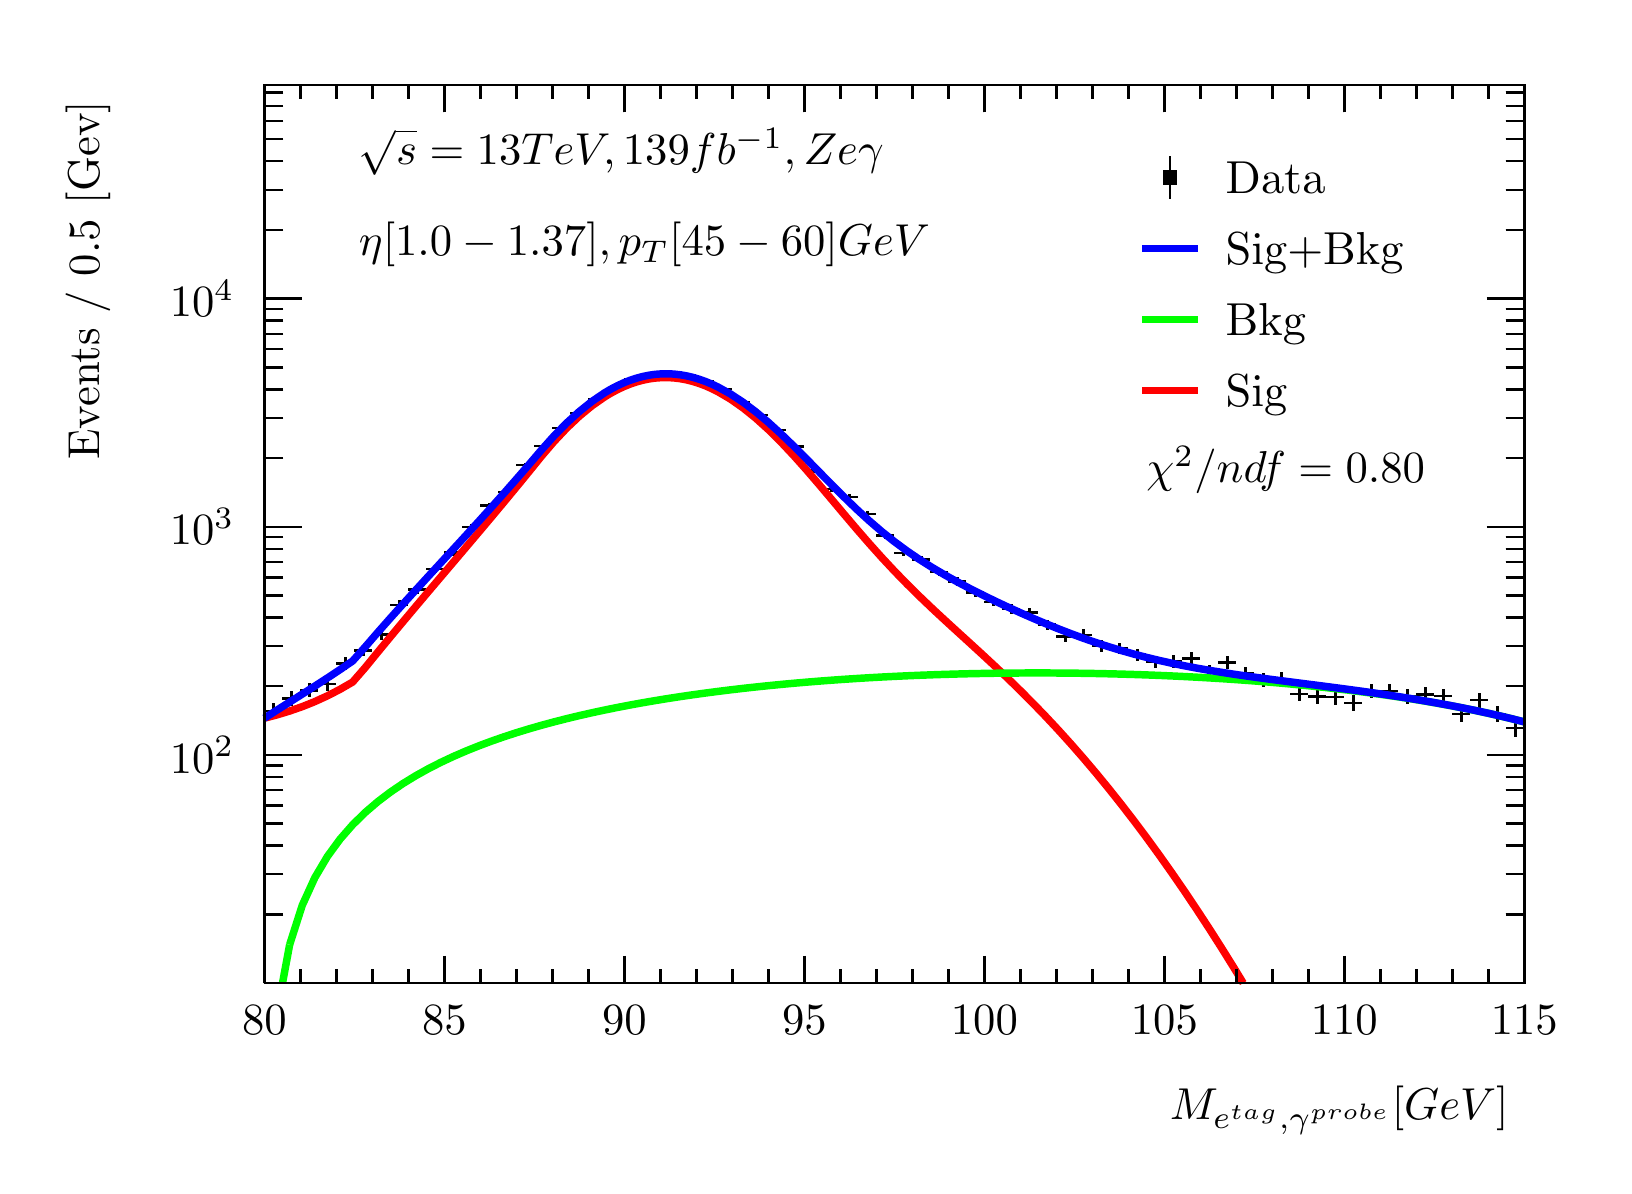
\begin{tikzpicture}
\pgfdeclareplotmark{cross} {
\pgfpathmoveto{\pgfpoint{-0.3\pgfplotmarksize}{\pgfplotmarksize}}
\pgfpathlineto{\pgfpoint{+0.3\pgfplotmarksize}{\pgfplotmarksize}}
\pgfpathlineto{\pgfpoint{+0.3\pgfplotmarksize}{0.3\pgfplotmarksize}}
\pgfpathlineto{\pgfpoint{+1\pgfplotmarksize}{0.3\pgfplotmarksize}}
\pgfpathlineto{\pgfpoint{+1\pgfplotmarksize}{-0.3\pgfplotmarksize}}
\pgfpathlineto{\pgfpoint{+0.3\pgfplotmarksize}{-0.3\pgfplotmarksize}}
\pgfpathlineto{\pgfpoint{+0.3\pgfplotmarksize}{-1.\pgfplotmarksize}}
\pgfpathlineto{\pgfpoint{-0.3\pgfplotmarksize}{-1.\pgfplotmarksize}}
\pgfpathlineto{\pgfpoint{-0.3\pgfplotmarksize}{-0.3\pgfplotmarksize}}
\pgfpathlineto{\pgfpoint{-1.\pgfplotmarksize}{-0.3\pgfplotmarksize}}
\pgfpathlineto{\pgfpoint{-1.\pgfplotmarksize}{0.3\pgfplotmarksize}}
\pgfpathlineto{\pgfpoint{-0.3\pgfplotmarksize}{0.3\pgfplotmarksize}}
\pgfpathclose
\pgfusepathqstroke
}
\pgfdeclareplotmark{cross*} {
\pgfpathmoveto{\pgfpoint{-0.3\pgfplotmarksize}{\pgfplotmarksize}}
\pgfpathlineto{\pgfpoint{+0.3\pgfplotmarksize}{\pgfplotmarksize}}
\pgfpathlineto{\pgfpoint{+0.3\pgfplotmarksize}{0.3\pgfplotmarksize}}
\pgfpathlineto{\pgfpoint{+1\pgfplotmarksize}{0.3\pgfplotmarksize}}
\pgfpathlineto{\pgfpoint{+1\pgfplotmarksize}{-0.3\pgfplotmarksize}}
\pgfpathlineto{\pgfpoint{+0.3\pgfplotmarksize}{-0.3\pgfplotmarksize}}
\pgfpathlineto{\pgfpoint{+0.3\pgfplotmarksize}{-1.\pgfplotmarksize}}
\pgfpathlineto{\pgfpoint{-0.3\pgfplotmarksize}{-1.\pgfplotmarksize}}
\pgfpathlineto{\pgfpoint{-0.3\pgfplotmarksize}{-0.3\pgfplotmarksize}}
\pgfpathlineto{\pgfpoint{-1.\pgfplotmarksize}{-0.3\pgfplotmarksize}}
\pgfpathlineto{\pgfpoint{-1.\pgfplotmarksize}{0.3\pgfplotmarksize}}
\pgfpathlineto{\pgfpoint{-0.3\pgfplotmarksize}{0.3\pgfplotmarksize}}
\pgfpathclose
\pgfusepathqfillstroke
}
\pgfdeclareplotmark{newstar} {
\pgfpathmoveto{\pgfqpoint{0pt}{\pgfplotmarksize}}
\pgfpathlineto{\pgfqpointpolar{44}{0.5\pgfplotmarksize}}
\pgfpathlineto{\pgfqpointpolar{18}{\pgfplotmarksize}}
\pgfpathlineto{\pgfqpointpolar{-20}{0.5\pgfplotmarksize}}
\pgfpathlineto{\pgfqpointpolar{-54}{\pgfplotmarksize}}
\pgfpathlineto{\pgfqpointpolar{-90}{0.5\pgfplotmarksize}}
\pgfpathlineto{\pgfqpointpolar{234}{\pgfplotmarksize}}
\pgfpathlineto{\pgfqpointpolar{198}{0.5\pgfplotmarksize}}
\pgfpathlineto{\pgfqpointpolar{162}{\pgfplotmarksize}}
\pgfpathlineto{\pgfqpointpolar{134}{0.5\pgfplotmarksize}}
\pgfpathclose
\pgfusepathqstroke
}
\pgfdeclareplotmark{newstar*} {
\pgfpathmoveto{\pgfqpoint{0pt}{\pgfplotmarksize}}
\pgfpathlineto{\pgfqpointpolar{44}{0.5\pgfplotmarksize}}
\pgfpathlineto{\pgfqpointpolar{18}{\pgfplotmarksize}}
\pgfpathlineto{\pgfqpointpolar{-20}{0.5\pgfplotmarksize}}
\pgfpathlineto{\pgfqpointpolar{-54}{\pgfplotmarksize}}
\pgfpathlineto{\pgfqpointpolar{-90}{0.5\pgfplotmarksize}}
\pgfpathlineto{\pgfqpointpolar{234}{\pgfplotmarksize}}
\pgfpathlineto{\pgfqpointpolar{198}{0.5\pgfplotmarksize}}
\pgfpathlineto{\pgfqpointpolar{162}{\pgfplotmarksize}}
\pgfpathlineto{\pgfqpointpolar{134}{0.5\pgfplotmarksize}}
\pgfpathclose
\pgfusepathqfillstroke
}
\definecolor{c}{rgb}{1,1,1};
\draw [color=c, fill=c] (0,0) rectangle (20,14.4361);
\draw [color=c, fill=c] (3,2.30977) rectangle (19,13.7143);
\definecolor{c}{rgb}{0,0,0};
\draw [c,line width=0.9] (3,2.30977) -- (3,13.7143) -- (19,13.7143) -- (19,2.30977) -- (3,2.30977);
\definecolor{c}{rgb}{1,1,1};
\draw [color=c, fill=c] (3,2.30977) rectangle (19,13.7143);
\definecolor{c}{rgb}{0,0,0};
\draw [c,line width=0.9] (3,2.30977) -- (3,13.7143) -- (19,13.7143) -- (19,2.30977) -- (3,2.30977);
\draw [c,line width=0.9] (3,2.30977) -- (19,2.30977);
\draw [c,line width=0.9] (3,2.65624) -- (3,2.30977);
\draw [c,line width=0.9] (3.45714,2.48301) -- (3.45714,2.30977);
\draw [c,line width=0.9] (3.91429,2.48301) -- (3.91429,2.30977);
\draw [c,line width=0.9] (4.37143,2.48301) -- (4.37143,2.30977);
\draw [c,line width=0.9] (4.82857,2.48301) -- (4.82857,2.30977);
\draw [c,line width=0.9] (5.28571,2.65624) -- (5.28571,2.30977);
\draw [c,line width=0.9] (5.74286,2.48301) -- (5.74286,2.30977);
\draw [c,line width=0.9] (6.2,2.48301) -- (6.2,2.30977);
\draw [c,line width=0.9] (6.65714,2.48301) -- (6.65714,2.30977);
\draw [c,line width=0.9] (7.11429,2.48301) -- (7.11429,2.30977);
\draw [c,line width=0.9] (7.57143,2.65624) -- (7.57143,2.30977);
\draw [c,line width=0.9] (8.02857,2.48301) -- (8.02857,2.30977);
\draw [c,line width=0.9] (8.48571,2.48301) -- (8.48571,2.30977);
\draw [c,line width=0.9] (8.94286,2.48301) -- (8.94286,2.30977);
\draw [c,line width=0.9] (9.4,2.48301) -- (9.4,2.30977);
\draw [c,line width=0.9] (9.85714,2.65624) -- (9.85714,2.30977);
\draw [c,line width=0.9] (10.3143,2.48301) -- (10.3143,2.30977);
\draw [c,line width=0.9] (10.7714,2.48301) -- (10.7714,2.30977);
\draw [c,line width=0.9] (11.2286,2.48301) -- (11.2286,2.30977);
\draw [c,line width=0.9] (11.6857,2.48301) -- (11.6857,2.30977);
\draw [c,line width=0.9] (12.1429,2.65624) -- (12.1429,2.30977);
\draw [c,line width=0.9] (12.6,2.48301) -- (12.6,2.30977);
\draw [c,line width=0.9] (13.0571,2.48301) -- (13.0571,2.30977);
\draw [c,line width=0.9] (13.5143,2.48301) -- (13.5143,2.30977);
\draw [c,line width=0.9] (13.9714,2.48301) -- (13.9714,2.30977);
\draw [c,line width=0.9] (14.4286,2.65624) -- (14.4286,2.30977);
\draw [c,line width=0.9] (14.8857,2.48301) -- (14.8857,2.30977);
\draw [c,line width=0.9] (15.3429,2.48301) -- (15.3429,2.30977);
\draw [c,line width=0.9] (15.8,2.48301) -- (15.8,2.30977);
\draw [c,line width=0.9] (16.2571,2.48301) -- (16.2571,2.30977);
\draw [c,line width=0.9] (16.7143,2.65624) -- (16.7143,2.30977);
\draw [c,line width=0.9] (17.1714,2.48301) -- (17.1714,2.30977);
\draw [c,line width=0.9] (17.6286,2.48301) -- (17.6286,2.30977);
\draw [c,line width=0.9] (18.0857,2.48301) -- (18.0857,2.30977);
\draw [c,line width=0.9] (18.5429,2.48301) -- (18.5429,2.30977);
\draw [c,line width=0.9] (19,2.65624) -- (19,2.30977);
\draw [anchor=base] (3,1.66015) node[scale=1.61424, color=c, rotate=0]{80};
\draw [anchor=base] (5.28571,1.66015) node[scale=1.61424, color=c, rotate=0]{85};
\draw [anchor=base] (7.57143,1.66015) node[scale=1.61424, color=c, rotate=0]{90};
\draw [anchor=base] (9.85714,1.66015) node[scale=1.61424, color=c, rotate=0]{95};
\draw [anchor=base] (12.1429,1.66015) node[scale=1.61424, color=c, rotate=0]{100};
\draw [anchor=base] (14.4286,1.66015) node[scale=1.61424, color=c, rotate=0]{105};
\draw [anchor=base] (16.7143,1.66015) node[scale=1.61424, color=c, rotate=0]{110};
\draw [anchor=base] (19,1.66015) node[scale=1.61424, color=c, rotate=0]{115};
\draw [anchor= east] (19,0.692932) node[scale=1.61424, color=c, rotate=0]{$M_{e^{tag}, \gamma^{probe}}  [GeV]$};
\draw [c,line width=0.9] (3,13.7143) -- (19,13.7143);
\draw [c,line width=0.9] (3,13.3678) -- (3,13.7143);
\draw [c,line width=0.9] (3.45714,13.5411) -- (3.45714,13.7143);
\draw [c,line width=0.9] (3.91429,13.5411) -- (3.91429,13.7143);
\draw [c,line width=0.9] (4.37143,13.5411) -- (4.37143,13.7143);
\draw [c,line width=0.9] (4.82857,13.5411) -- (4.82857,13.7143);
\draw [c,line width=0.9] (5.28571,13.3678) -- (5.28571,13.7143);
\draw [c,line width=0.9] (5.74286,13.5411) -- (5.74286,13.7143);
\draw [c,line width=0.9] (6.2,13.5411) -- (6.2,13.7143);
\draw [c,line width=0.9] (6.65714,13.5411) -- (6.65714,13.7143);
\draw [c,line width=0.9] (7.11429,13.5411) -- (7.11429,13.7143);
\draw [c,line width=0.9] (7.57143,13.3678) -- (7.57143,13.7143);
\draw [c,line width=0.9] (8.02857,13.5411) -- (8.02857,13.7143);
\draw [c,line width=0.9] (8.48571,13.5411) -- (8.48571,13.7143);
\draw [c,line width=0.9] (8.94286,13.5411) -- (8.94286,13.7143);
\draw [c,line width=0.9] (9.4,13.5411) -- (9.4,13.7143);
\draw [c,line width=0.9] (9.85714,13.3678) -- (9.85714,13.7143);
\draw [c,line width=0.9] (10.3143,13.5411) -- (10.3143,13.7143);
\draw [c,line width=0.9] (10.7714,13.5411) -- (10.7714,13.7143);
\draw [c,line width=0.9] (11.2286,13.5411) -- (11.2286,13.7143);
\draw [c,line width=0.9] (11.6857,13.5411) -- (11.6857,13.7143);
\draw [c,line width=0.9] (12.1429,13.3678) -- (12.1429,13.7143);
\draw [c,line width=0.9] (12.6,13.5411) -- (12.6,13.7143);
\draw [c,line width=0.9] (13.0571,13.5411) -- (13.0571,13.7143);
\draw [c,line width=0.9] (13.5143,13.5411) -- (13.5143,13.7143);
\draw [c,line width=0.9] (13.9714,13.5411) -- (13.9714,13.7143);
\draw [c,line width=0.9] (14.4286,13.3678) -- (14.4286,13.7143);
\draw [c,line width=0.9] (14.8857,13.5411) -- (14.8857,13.7143);
\draw [c,line width=0.9] (15.3429,13.5411) -- (15.3429,13.7143);
\draw [c,line width=0.9] (15.8,13.5411) -- (15.8,13.7143);
\draw [c,line width=0.9] (16.2571,13.5411) -- (16.2571,13.7143);
\draw [c,line width=0.9] (16.7143,13.3678) -- (16.7143,13.7143);
\draw [c,line width=0.9] (17.1714,13.5411) -- (17.1714,13.7143);
\draw [c,line width=0.9] (17.6286,13.5411) -- (17.6286,13.7143);
\draw [c,line width=0.9] (18.0857,13.5411) -- (18.0857,13.7143);
\draw [c,line width=0.9] (18.5429,13.5411) -- (18.5429,13.7143);
\draw [c,line width=0.9] (19,13.3678) -- (19,13.7143);
\draw [c,line width=0.9] (3,2.30977) -- (3,13.7143);
\draw [c,line width=0.9] (3.237,3.182) -- (3,3.182);
\draw [c,line width=0.9] (3.237,3.69222) -- (3,3.69222);
\draw [c,line width=0.9] (3.237,4.05422) -- (3,4.05422);
\draw [c,line width=0.9] (3.237,4.33502) -- (3,4.33502);
\draw [c,line width=0.9] (3.237,4.56444) -- (3,4.56444);
\draw [c,line width=0.9] (3.237,4.75842) -- (3,4.75842);
\draw [c,line width=0.9] (3.237,4.92645) -- (3,4.92645);
\draw [c,line width=0.9] (3.237,5.07466) -- (3,5.07466);
\draw [c,line width=0.9] (3.474,5.20724) -- (3,5.20724);
\draw [anchor= east] (2.82,5.20724) node[scale=1.61424, color=c, rotate=0]{$10^{2}$};
\draw [c,line width=0.9] (3.237,6.07947) -- (3,6.07947);
\draw [c,line width=0.9] (3.237,6.58969) -- (3,6.58969);
\draw [c,line width=0.9] (3.237,6.9517) -- (3,6.9517);
\draw [c,line width=0.9] (3.237,7.23249) -- (3,7.23249);
\draw [c,line width=0.9] (3.237,7.46192) -- (3,7.46192);
\draw [c,line width=0.9] (3.237,7.65589) -- (3,7.65589);
\draw [c,line width=0.9] (3.237,7.82392) -- (3,7.82392);
\draw [c,line width=0.9] (3.237,7.97214) -- (3,7.97214);
\draw [c,line width=0.9] (3.474,8.10472) -- (3,8.10472);
\draw [anchor= east] (2.82,8.10472) node[scale=1.61424, color=c, rotate=0]{$10^{3}$};
\draw [c,line width=0.9] (3.237,8.97694) -- (3,8.97694);
\draw [c,line width=0.9] (3.237,9.48716) -- (3,9.48716);
\draw [c,line width=0.9] (3.237,9.84917) -- (3,9.84917);
\draw [c,line width=0.9] (3.237,10.13) -- (3,10.13);
\draw [c,line width=0.9] (3.237,10.3594) -- (3,10.3594);
\draw [c,line width=0.9] (3.237,10.5534) -- (3,10.5534);
\draw [c,line width=0.9] (3.237,10.7214) -- (3,10.7214);
\draw [c,line width=0.9] (3.237,10.8696) -- (3,10.8696);
\draw [c,line width=0.9] (3.474,11.0022) -- (3,11.0022);
\draw [anchor= east] (2.82,11.0022) node[scale=1.61424, color=c, rotate=0]{$10^{4}$};
\draw [c,line width=0.9] (3.237,11.8744) -- (3,11.8744);
\draw [c,line width=0.9] (3.237,12.3846) -- (3,12.3846);
\draw [c,line width=0.9] (3.237,12.7466) -- (3,12.7466);
\draw [c,line width=0.9] (3.237,13.0274) -- (3,13.0274);
\draw [c,line width=0.9] (3.237,13.2569) -- (3,13.2569);
\draw [c,line width=0.9] (3.237,13.4508) -- (3,13.4508);
\draw [c,line width=0.9] (3.237,13.6189) -- (3,13.6189);
\draw [anchor= east] (0.76,13.7143) node[scale=1.61424, color=c, rotate=90]{Events / 0.5 [Gev]};
\draw [c,line width=0.9] (19,2.30977) -- (19,13.7143);
\draw [c,line width=0.9] (18.763,3.182) -- (19,3.182);
\draw [c,line width=0.9] (18.763,3.69222) -- (19,3.69222);
\draw [c,line width=0.9] (18.763,4.05422) -- (19,4.05422);
\draw [c,line width=0.9] (18.763,4.33502) -- (19,4.33502);
\draw [c,line width=0.9] (18.763,4.56444) -- (19,4.56444);
\draw [c,line width=0.9] (18.763,4.75842) -- (19,4.75842);
\draw [c,line width=0.9] (18.763,4.92645) -- (19,4.92645);
\draw [c,line width=0.9] (18.763,5.07466) -- (19,5.07466);
\draw [c,line width=0.9] (18.526,5.20724) -- (19,5.20724);
\draw [c,line width=0.9] (18.763,6.07947) -- (19,6.07947);
\draw [c,line width=0.9] (18.763,6.58969) -- (19,6.58969);
\draw [c,line width=0.9] (18.763,6.9517) -- (19,6.9517);
\draw [c,line width=0.9] (18.763,7.23249) -- (19,7.23249);
\draw [c,line width=0.9] (18.763,7.46192) -- (19,7.46192);
\draw [c,line width=0.9] (18.763,7.65589) -- (19,7.65589);
\draw [c,line width=0.9] (18.763,7.82392) -- (19,7.82392);
\draw [c,line width=0.9] (18.763,7.97214) -- (19,7.97214);
\draw [c,line width=0.9] (18.526,8.10472) -- (19,8.10472);
\draw [c,line width=0.9] (18.763,8.97694) -- (19,8.97694);
\draw [c,line width=0.9] (18.763,9.48716) -- (19,9.48716);
\draw [c,line width=0.9] (18.763,9.84917) -- (19,9.84917);
\draw [c,line width=0.9] (18.763,10.13) -- (19,10.13);
\draw [c,line width=0.9] (18.763,10.3594) -- (19,10.3594);
\draw [c,line width=0.9] (18.763,10.5534) -- (19,10.5534);
\draw [c,line width=0.9] (18.763,10.7214) -- (19,10.7214);
\draw [c,line width=0.9] (18.763,10.8696) -- (19,10.8696);
\draw [c,line width=0.9] (18.526,11.0022) -- (19,11.0022);
\draw [c,line width=0.9] (18.763,11.8744) -- (19,11.8744);
\draw [c,line width=0.9] (18.763,12.3846) -- (19,12.3846);
\draw [c,line width=0.9] (18.763,12.7466) -- (19,12.7466);
\draw [c,line width=0.9] (18.763,13.0274) -- (19,13.0274);
\draw [c,line width=0.9] (18.763,13.2569) -- (19,13.2569);
\draw [c,line width=0.9] (18.763,13.4508) -- (19,13.4508);
\draw [c,line width=0.9] (18.763,13.6189) -- (19,13.6189);
\draw [c,line width=0.9] (3.11429,5.76682) -- (3,5.76682);
\draw [c,line width=0.9] (3,5.76682) -- (3,5.76682);
\draw [c,line width=0.9] (3.11429,5.76682) -- (3.22857,5.76682);
\draw [c,line width=0.9] (3.22857,5.76682) -- (3.22857,5.76682);
\draw [c,line width=0.9] (3.11429,5.76682) -- (3.11429,5.86754);
\draw [c,line width=0.9] (3.11429,5.86754) -- (3.11429,5.86754);
\draw [c,line width=0.9] (3.11429,5.76682) -- (3.11429,5.6661);
\draw [c,line width=0.9] (3.11429,5.6661) -- (3.11429,5.6661);
\draw [c,line width=0.9] (3.34286,5.92574) -- (3.22857,5.92574);
\draw [c,line width=0.9] (3.22857,5.92574) -- (3.22857,5.92574);
\draw [c,line width=0.9] (3.34286,5.92574) -- (3.45714,5.92574);
\draw [c,line width=0.9] (3.45714,5.92574) -- (3.45714,5.92574);
\draw [c,line width=0.9] (3.34286,5.92574) -- (3.34286,6.0203);
\draw [c,line width=0.9] (3.34286,6.0203) -- (3.34286,6.0203);
\draw [c,line width=0.9] (3.34286,5.92574) -- (3.34286,5.83118);
\draw [c,line width=0.9] (3.34286,5.83118) -- (3.34286,5.83118);
\draw [c,line width=0.9] (3.57143,6.0281) -- (3.45714,6.0281);
\draw [c,line width=0.9] (3.45714,6.0281) -- (3.45714,6.0281);
\draw [c,line width=0.9] (3.57143,6.0281) -- (3.68571,6.0281);
\draw [c,line width=0.9] (3.68571,6.0281) -- (3.68571,6.0281);
\draw [c,line width=0.9] (3.57143,6.0281) -- (3.57143,6.1189);
\draw [c,line width=0.9] (3.57143,6.1189) -- (3.57143,6.1189);
\draw [c,line width=0.9] (3.57143,6.0281) -- (3.57143,5.93731);
\draw [c,line width=0.9] (3.57143,5.93731) -- (3.57143,5.93731);
\draw [c,line width=0.9] (3.8,6.11054) -- (3.68571,6.11054);
\draw [c,line width=0.9] (3.68571,6.11054) -- (3.68571,6.11054);
\draw [c,line width=0.9] (3.8,6.11054) -- (3.91429,6.11054);
\draw [c,line width=0.9] (3.91429,6.11054) -- (3.91429,6.11054);
\draw [c,line width=0.9] (3.8,6.11054) -- (3.8,6.19841);
\draw [c,line width=0.9] (3.8,6.19841) -- (3.8,6.19841);
\draw [c,line width=0.9] (3.8,6.11054) -- (3.8,6.02268);
\draw [c,line width=0.9] (3.8,6.02268) -- (3.8,6.02268);
\draw [c,line width=0.9] (4.02857,6.36529) -- (3.91429,6.36529);
\draw [c,line width=0.9] (3.91429,6.36529) -- (3.91429,6.36529);
\draw [c,line width=0.9] (4.02857,6.36529) -- (4.14286,6.36529);
\draw [c,line width=0.9] (4.14286,6.36529) -- (4.14286,6.36529);
\draw [c,line width=0.9] (4.02857,6.36529) -- (4.02857,6.4447);
\draw [c,line width=0.9] (4.02857,6.4447) -- (4.02857,6.4447);
\draw [c,line width=0.9] (4.02857,6.36529) -- (4.02857,6.28588);
\draw [c,line width=0.9] (4.02857,6.28588) -- (4.02857,6.28588);
\draw [c,line width=0.9] (4.25714,6.53395) -- (4.14286,6.53395);
\draw [c,line width=0.9] (4.14286,6.53395) -- (4.14286,6.53395);
\draw [c,line width=0.9] (4.25714,6.53395) -- (4.37143,6.53395);
\draw [c,line width=0.9] (4.37143,6.53395) -- (4.37143,6.53395);
\draw [c,line width=0.9] (4.25714,6.53395) -- (4.25714,6.60821);
\draw [c,line width=0.9] (4.25714,6.60821) -- (4.25714,6.60821);
\draw [c,line width=0.9] (4.25714,6.53395) -- (4.25714,6.45968);
\draw [c,line width=0.9] (4.25714,6.45968) -- (4.25714,6.45968);
\draw [c,line width=0.9] (4.48571,6.73604) -- (4.37143,6.73604);
\draw [c,line width=0.9] (4.37143,6.73604) -- (4.37143,6.73604);
\draw [c,line width=0.9] (4.48571,6.73604) -- (4.6,6.73604);
\draw [c,line width=0.9] (4.6,6.73604) -- (4.6,6.73604);
\draw [c,line width=0.9] (4.48571,6.73604) -- (4.48571,6.80458);
\draw [c,line width=0.9] (4.48571,6.80458) -- (4.48571,6.80458);
\draw [c,line width=0.9] (4.48571,6.73604) -- (4.48571,6.6675);
\draw [c,line width=0.9] (4.48571,6.6675) -- (4.48571,6.6675);
\draw [c,line width=0.9] (4.71429,7.11105) -- (4.6,7.11105);
\draw [c,line width=0.9] (4.6,7.11105) -- (4.6,7.11105);
\draw [c,line width=0.9] (4.71429,7.11105) -- (4.82857,7.11105);
\draw [c,line width=0.9] (4.82857,7.11105) -- (4.82857,7.11105);
\draw [c,line width=0.9] (4.71429,7.11105) -- (4.71429,7.1701);
\draw [c,line width=0.9] (4.71429,7.1701) -- (4.71429,7.1701);
\draw [c,line width=0.9] (4.71429,7.11105) -- (4.71429,7.052);
\draw [c,line width=0.9] (4.71429,7.052) -- (4.71429,7.052);
\draw [c,line width=0.9] (4.94286,7.31056) -- (4.82857,7.31056);
\draw [c,line width=0.9] (4.82857,7.31056) -- (4.82857,7.31056);
\draw [c,line width=0.9] (4.94286,7.31056) -- (5.05714,7.31056);
\draw [c,line width=0.9] (5.05714,7.31056) -- (5.05714,7.31056);
\draw [c,line width=0.9] (4.94286,7.31056) -- (4.94286,7.36511);
\draw [c,line width=0.9] (4.94286,7.36511) -- (4.94286,7.36511);
\draw [c,line width=0.9] (4.94286,7.31056) -- (4.94286,7.256);
\draw [c,line width=0.9] (4.94286,7.256) -- (4.94286,7.256);
\draw [c,line width=0.9] (5.17143,7.56844) -- (5.05714,7.56844);
\draw [c,line width=0.9] (5.05714,7.56844) -- (5.05714,7.56844);
\draw [c,line width=0.9] (5.17143,7.56844) -- (5.28571,7.56844);
\draw [c,line width=0.9] (5.28571,7.56844) -- (5.28571,7.56844);
\draw [c,line width=0.9] (5.17143,7.56844) -- (5.17143,7.61768);
\draw [c,line width=0.9] (5.17143,7.61768) -- (5.17143,7.61768);
\draw [c,line width=0.9] (5.17143,7.56844) -- (5.17143,7.5192);
\draw [c,line width=0.9] (5.17143,7.5192) -- (5.17143,7.5192);
\draw [c,line width=0.9] (5.4,7.77583) -- (5.28571,7.77583);
\draw [c,line width=0.9] (5.28571,7.77583) -- (5.28571,7.77583);
\draw [c,line width=0.9] (5.4,7.77583) -- (5.51429,7.77583);
\draw [c,line width=0.9] (5.51429,7.77583) -- (5.51429,7.77583);
\draw [c,line width=0.9] (5.4,7.77583) -- (5.4,7.82117);
\draw [c,line width=0.9] (5.4,7.82117) -- (5.4,7.82117);
\draw [c,line width=0.9] (5.4,7.77583) -- (5.4,7.73048);
\draw [c,line width=0.9] (5.4,7.73048) -- (5.4,7.73048);
\draw [c,line width=0.9] (5.62857,8.1022) -- (5.51429,8.1022);
\draw [c,line width=0.9] (5.51429,8.1022) -- (5.51429,8.1022);
\draw [c,line width=0.9] (5.62857,8.1022) -- (5.74286,8.1022);
\draw [c,line width=0.9] (5.74286,8.1022) -- (5.74286,8.1022);
\draw [c,line width=0.9] (5.62857,8.1022) -- (5.62857,8.14203);
\draw [c,line width=0.9] (5.62857,8.14203) -- (5.62857,8.14203);
\draw [c,line width=0.9] (5.62857,8.1022) -- (5.62857,8.06237);
\draw [c,line width=0.9] (5.62857,8.06237) -- (5.62857,8.06237);
\draw [c,line width=0.9] (5.85714,8.37439) -- (5.74286,8.37439);
\draw [c,line width=0.9] (5.74286,8.37439) -- (5.74286,8.37439);
\draw [c,line width=0.9] (5.85714,8.37439) -- (5.97143,8.37439);
\draw [c,line width=0.9] (5.97143,8.37439) -- (5.97143,8.37439);
\draw [c,line width=0.9] (5.85714,8.37439) -- (5.85714,8.41014);
\draw [c,line width=0.9] (5.85714,8.41014) -- (5.85714,8.41014);
\draw [c,line width=0.9] (5.85714,8.37439) -- (5.85714,8.33864);
\draw [c,line width=0.9] (5.85714,8.33864) -- (5.85714,8.33864);
\draw [c,line width=0.9] (6.08571,8.54863) -- (5.97143,8.54863);
\draw [c,line width=0.9] (5.97143,8.54863) -- (5.97143,8.54863);
\draw [c,line width=0.9] (6.08571,8.54863) -- (6.2,8.54863);
\draw [c,line width=0.9] (6.2,8.54863) -- (6.2,8.54863);
\draw [c,line width=0.9] (6.08571,8.54863) -- (6.08571,8.58198);
\draw [c,line width=0.9] (6.08571,8.58198) -- (6.08571,8.58198);
\draw [c,line width=0.9] (6.08571,8.54863) -- (6.08571,8.51527);
\draw [c,line width=0.9] (6.08571,8.51527) -- (6.08571,8.51527);
\draw [c,line width=0.9] (6.31429,8.889) -- (6.2,8.889);
\draw [c,line width=0.9] (6.2,8.889) -- (6.2,8.889);
\draw [c,line width=0.9] (6.31429,8.889) -- (6.42857,8.889);
\draw [c,line width=0.9] (6.42857,8.889) -- (6.42857,8.889);
\draw [c,line width=0.9] (6.31429,8.889) -- (6.31429,8.91814);
\draw [c,line width=0.9] (6.31429,8.91814) -- (6.31429,8.91814);
\draw [c,line width=0.9] (6.31429,8.889) -- (6.31429,8.85987);
\draw [c,line width=0.9] (6.31429,8.85987) -- (6.31429,8.85987);
\draw [c,line width=0.9] (6.54286,9.12851) -- (6.42857,9.12851);
\draw [c,line width=0.9] (6.42857,9.12851) -- (6.42857,9.12851);
\draw [c,line width=0.9] (6.54286,9.12851) -- (6.65714,9.12851);
\draw [c,line width=0.9] (6.65714,9.12851) -- (6.65714,9.12851);
\draw [c,line width=0.9] (6.54286,9.12851) -- (6.54286,9.155);
\draw [c,line width=0.9] (6.54286,9.155) -- (6.54286,9.155);
\draw [c,line width=0.9] (6.54286,9.12851) -- (6.54286,9.10202);
\draw [c,line width=0.9] (6.54286,9.10202) -- (6.54286,9.10202);
\draw [c,line width=0.9] (6.77143,9.35784) -- (6.65714,9.35784);
\draw [c,line width=0.9] (6.65714,9.35784) -- (6.65714,9.35784);
\draw [c,line width=0.9] (6.77143,9.35784) -- (6.88571,9.35784);
\draw [c,line width=0.9] (6.88571,9.35784) -- (6.88571,9.35784);
\draw [c,line width=0.9] (6.77143,9.35784) -- (6.77143,9.38203);
\draw [c,line width=0.9] (6.77143,9.38203) -- (6.77143,9.38203);
\draw [c,line width=0.9] (6.77143,9.35784) -- (6.77143,9.33366);
\draw [c,line width=0.9] (6.77143,9.33366) -- (6.77143,9.33366);
\draw [c,line width=0.9] (7,9.55255) -- (6.88571,9.55255);
\draw [c,line width=0.9] (6.88571,9.55255) -- (6.88571,9.55255);
\draw [c,line width=0.9] (7,9.55255) -- (7.11429,9.55255);
\draw [c,line width=0.9] (7.11429,9.55255) -- (7.11429,9.55255);
\draw [c,line width=0.9] (7,9.55255) -- (7,9.57493);
\draw [c,line width=0.9] (7,9.57493) -- (7,9.57493);
\draw [c,line width=0.9] (7,9.55255) -- (7,9.53016);
\draw [c,line width=0.9] (7,9.53016) -- (7,9.53016);
\draw [c,line width=0.9] (7.22857,9.72773) -- (7.11429,9.72773);
\draw [c,line width=0.9] (7.11429,9.72773) -- (7.11429,9.72773);
\draw [c,line width=0.9] (7.22857,9.72773) -- (7.34286,9.72773);
\draw [c,line width=0.9] (7.34286,9.72773) -- (7.34286,9.72773);
\draw [c,line width=0.9] (7.22857,9.72773) -- (7.22857,9.74861);
\draw [c,line width=0.9] (7.22857,9.74861) -- (7.22857,9.74861);
\draw [c,line width=0.9] (7.22857,9.72773) -- (7.22857,9.70685);
\draw [c,line width=0.9] (7.22857,9.70685) -- (7.22857,9.70685);
\draw [c,line width=0.9] (7.45714,9.85482) -- (7.34286,9.85482);
\draw [c,line width=0.9] (7.34286,9.85482) -- (7.34286,9.85482);
\draw [c,line width=0.9] (7.45714,9.85482) -- (7.57143,9.85482);
\draw [c,line width=0.9] (7.57143,9.85482) -- (7.57143,9.85482);
\draw [c,line width=0.9] (7.45714,9.85482) -- (7.45714,9.87467);
\draw [c,line width=0.9] (7.45714,9.87467) -- (7.45714,9.87467);
\draw [c,line width=0.9] (7.45714,9.85482) -- (7.45714,9.83497);
\draw [c,line width=0.9] (7.45714,9.83497) -- (7.45714,9.83497);
\draw [c,line width=0.9] (7.68571,9.97481) -- (7.57143,9.97481);
\draw [c,line width=0.9] (7.57143,9.97481) -- (7.57143,9.97481);
\draw [c,line width=0.9] (7.68571,9.97481) -- (7.8,9.97481);
\draw [c,line width=0.9] (7.8,9.97481) -- (7.8,9.97481);
\draw [c,line width=0.9] (7.68571,9.97481) -- (7.68571,9.99374);
\draw [c,line width=0.9] (7.68571,9.99374) -- (7.68571,9.99374);
\draw [c,line width=0.9] (7.68571,9.97481) -- (7.68571,9.95588);
\draw [c,line width=0.9] (7.68571,9.95588) -- (7.68571,9.95588);
\draw [c,line width=0.9] (7.91429,10.0432) -- (7.8,10.0432);
\draw [c,line width=0.9] (7.8,10.0432) -- (7.8,10.0432);
\draw [c,line width=0.9] (7.91429,10.0432) -- (8.02857,10.0432);
\draw [c,line width=0.9] (8.02857,10.0432) -- (8.02857,10.0432);
\draw [c,line width=0.9] (7.91429,10.0432) -- (7.91429,10.0617);
\draw [c,line width=0.9] (7.91429,10.0617) -- (7.91429,10.0617);
\draw [c,line width=0.9] (7.91429,10.0432) -- (7.91429,10.0248);
\draw [c,line width=0.9] (7.91429,10.0248) -- (7.91429,10.0248);
\draw [c,line width=0.9] (8.14286,10.0529) -- (8.02857,10.0529);
\draw [c,line width=0.9] (8.02857,10.0529) -- (8.02857,10.0529);
\draw [c,line width=0.9] (8.14286,10.0529) -- (8.25714,10.0529);
\draw [c,line width=0.9] (8.25714,10.0529) -- (8.25714,10.0529);
\draw [c,line width=0.9] (8.14286,10.0529) -- (8.14286,10.0713);
\draw [c,line width=0.9] (8.14286,10.0713) -- (8.14286,10.0713);
\draw [c,line width=0.9] (8.14286,10.0529) -- (8.14286,10.0346);
\draw [c,line width=0.9] (8.14286,10.0346) -- (8.14286,10.0346);
\draw [c,line width=0.9] (8.37143,10.0346) -- (8.25714,10.0346);
\draw [c,line width=0.9] (8.25714,10.0346) -- (8.25714,10.0346);
\draw [c,line width=0.9] (8.37143,10.0346) -- (8.48571,10.0346);
\draw [c,line width=0.9] (8.48571,10.0346) -- (8.48571,10.0346);
\draw [c,line width=0.9] (8.37143,10.0346) -- (8.37143,10.0531);
\draw [c,line width=0.9] (8.37143,10.0531) -- (8.37143,10.0531);
\draw [c,line width=0.9] (8.37143,10.0346) -- (8.37143,10.0161);
\draw [c,line width=0.9] (8.37143,10.0161) -- (8.37143,10.0161);
\draw [c,line width=0.9] (8.6,9.95704) -- (8.48571,9.95704);
\draw [c,line width=0.9] (8.48571,9.95704) -- (8.48571,9.95704);
\draw [c,line width=0.9] (8.6,9.95704) -- (8.71429,9.95704);
\draw [c,line width=0.9] (8.71429,9.95704) -- (8.71429,9.95704);
\draw [c,line width=0.9] (8.6,9.95704) -- (8.6,9.9761);
\draw [c,line width=0.9] (8.6,9.9761) -- (8.6,9.9761);
\draw [c,line width=0.9] (8.6,9.95704) -- (8.6,9.93797);
\draw [c,line width=0.9] (8.6,9.93797) -- (8.6,9.93797);
\draw [c,line width=0.9] (8.82857,9.85701) -- (8.71429,9.85701);
\draw [c,line width=0.9] (8.71429,9.85701) -- (8.71429,9.85701);
\draw [c,line width=0.9] (8.82857,9.85701) -- (8.94286,9.85701);
\draw [c,line width=0.9] (8.94286,9.85701) -- (8.94286,9.85701);
\draw [c,line width=0.9] (8.82857,9.85701) -- (8.82857,9.87685);
\draw [c,line width=0.9] (8.82857,9.87685) -- (8.82857,9.87685);
\draw [c,line width=0.9] (8.82857,9.85701) -- (8.82857,9.83718);
\draw [c,line width=0.9] (8.82857,9.83718) -- (8.82857,9.83718);
\draw [c,line width=0.9] (9.05714,9.6876) -- (8.94286,9.6876);
\draw [c,line width=0.9] (8.94286,9.6876) -- (8.94286,9.6876);
\draw [c,line width=0.9] (9.05714,9.6876) -- (9.17143,9.6876);
\draw [c,line width=0.9] (9.17143,9.6876) -- (9.17143,9.6876);
\draw [c,line width=0.9] (9.05714,9.6876) -- (9.05714,9.70881);
\draw [c,line width=0.9] (9.05714,9.70881) -- (9.05714,9.70881);
\draw [c,line width=0.9] (9.05714,9.6876) -- (9.05714,9.66638);
\draw [c,line width=0.9] (9.05714,9.66638) -- (9.05714,9.66638);
\draw [c,line width=0.9] (9.28571,9.52151) -- (9.17143,9.52151);
\draw [c,line width=0.9] (9.17143,9.52151) -- (9.17143,9.52151);
\draw [c,line width=0.9] (9.28571,9.52151) -- (9.4,9.52151);
\draw [c,line width=0.9] (9.4,9.52151) -- (9.4,9.52151);
\draw [c,line width=0.9] (9.28571,9.52151) -- (9.28571,9.54417);
\draw [c,line width=0.9] (9.28571,9.54417) -- (9.28571,9.54417);
\draw [c,line width=0.9] (9.28571,9.52151) -- (9.28571,9.49884);
\draw [c,line width=0.9] (9.28571,9.49884) -- (9.28571,9.49884);
\draw [c,line width=0.9] (9.51429,9.3358) -- (9.4,9.3358);
\draw [c,line width=0.9] (9.4,9.3358) -- (9.4,9.3358);
\draw [c,line width=0.9] (9.51429,9.3358) -- (9.62857,9.3358);
\draw [c,line width=0.9] (9.62857,9.3358) -- (9.62857,9.3358);
\draw [c,line width=0.9] (9.51429,9.3358) -- (9.51429,9.3602);
\draw [c,line width=0.9] (9.51429,9.3602) -- (9.51429,9.3602);
\draw [c,line width=0.9] (9.51429,9.3358) -- (9.51429,9.3114);
\draw [c,line width=0.9] (9.51429,9.3114) -- (9.51429,9.3114);
\draw [c,line width=0.9] (9.74286,9.1218) -- (9.62857,9.1218);
\draw [c,line width=0.9] (9.62857,9.1218) -- (9.62857,9.1218);
\draw [c,line width=0.9] (9.74286,9.1218) -- (9.85714,9.1218);
\draw [c,line width=0.9] (9.85714,9.1218) -- (9.85714,9.1218);
\draw [c,line width=0.9] (9.74286,9.1218) -- (9.74286,9.14836);
\draw [c,line width=0.9] (9.74286,9.14836) -- (9.74286,9.14836);
\draw [c,line width=0.9] (9.74286,9.1218) -- (9.74286,9.09523);
\draw [c,line width=0.9] (9.74286,9.09523) -- (9.74286,9.09523);
\draw [c,line width=0.9] (9.97143,8.8168) -- (9.85714,8.8168);
\draw [c,line width=0.9] (9.85714,8.8168) -- (9.85714,8.8168);
\draw [c,line width=0.9] (9.97143,8.8168) -- (10.0857,8.8168);
\draw [c,line width=0.9] (10.0857,8.8168) -- (10.0857,8.8168);
\draw [c,line width=0.9] (9.97143,8.8168) -- (9.97143,8.84679);
\draw [c,line width=0.9] (9.97143,8.84679) -- (9.97143,8.84679);
\draw [c,line width=0.9] (9.97143,8.8168) -- (9.97143,8.78681);
\draw [c,line width=0.9] (9.97143,8.78681) -- (9.97143,8.78681);
\draw [c,line width=0.9] (10.2,8.58523) -- (10.0857,8.58523);
\draw [c,line width=0.9] (10.0857,8.58523) -- (10.0857,8.58523);
\draw [c,line width=0.9] (10.2,8.58523) -- (10.3143,8.58523);
\draw [c,line width=0.9] (10.3143,8.58523) -- (10.3143,8.58523);
\draw [c,line width=0.9] (10.2,8.58523) -- (10.2,8.6181);
\draw [c,line width=0.9] (10.2,8.6181) -- (10.2,8.6181);
\draw [c,line width=0.9] (10.2,8.58523) -- (10.2,8.55235);
\draw [c,line width=0.9] (10.2,8.55235) -- (10.2,8.55235);
\draw [c,line width=0.9] (10.4286,8.48143) -- (10.3143,8.48143);
\draw [c,line width=0.9] (10.3143,8.48143) -- (10.3143,8.48143);
\draw [c,line width=0.9] (10.4286,8.48143) -- (10.5429,8.48143);
\draw [c,line width=0.9] (10.5429,8.48143) -- (10.5429,8.48143);
\draw [c,line width=0.9] (10.4286,8.48143) -- (10.4286,8.51569);
\draw [c,line width=0.9] (10.4286,8.51569) -- (10.4286,8.51569);
\draw [c,line width=0.9] (10.4286,8.48143) -- (10.4286,8.44717);
\draw [c,line width=0.9] (10.4286,8.44717) -- (10.4286,8.44717);
\draw [c,line width=0.9] (10.6571,8.26849) -- (10.5429,8.26849);
\draw [c,line width=0.9] (10.5429,8.26849) -- (10.5429,8.26849);
\draw [c,line width=0.9] (10.6571,8.26849) -- (10.7714,8.26849);
\draw [c,line width=0.9] (10.7714,8.26849) -- (10.7714,8.26849);
\draw [c,line width=0.9] (10.6571,8.26849) -- (10.6571,8.30578);
\draw [c,line width=0.9] (10.6571,8.30578) -- (10.6571,8.30578);
\draw [c,line width=0.9] (10.6571,8.26849) -- (10.6571,8.23121);
\draw [c,line width=0.9] (10.6571,8.23121) -- (10.6571,8.23121);
\draw [c,line width=0.9] (10.8857,7.99294) -- (10.7714,7.99294);
\draw [c,line width=0.9] (10.7714,7.99294) -- (10.7714,7.99294);
\draw [c,line width=0.9] (10.8857,7.99294) -- (11,7.99294);
\draw [c,line width=0.9] (11,7.99294) -- (11,7.99294);
\draw [c,line width=0.9] (10.8857,7.99294) -- (10.8857,8.03454);
\draw [c,line width=0.9] (10.8857,8.03454) -- (10.8857,8.03454);
\draw [c,line width=0.9] (10.8857,7.99294) -- (10.8857,7.95134);
\draw [c,line width=0.9] (10.8857,7.95134) -- (10.8857,7.95134);
\draw [c,line width=0.9] (11.1143,7.77256) -- (11,7.77256);
\draw [c,line width=0.9] (11,7.77256) -- (11,7.77256);
\draw [c,line width=0.9] (11.1143,7.77256) -- (11.2286,7.77256);
\draw [c,line width=0.9] (11.2286,7.77256) -- (11.2286,7.77256);
\draw [c,line width=0.9] (11.1143,7.77256) -- (11.1143,7.81796);
\draw [c,line width=0.9] (11.1143,7.81796) -- (11.1143,7.81796);
\draw [c,line width=0.9] (11.1143,7.77256) -- (11.1143,7.72715);
\draw [c,line width=0.9] (11.1143,7.72715) -- (11.1143,7.72715);
\draw [c,line width=0.9] (11.3429,7.69134) -- (11.2286,7.69134);
\draw [c,line width=0.9] (11.2286,7.69134) -- (11.2286,7.69134);
\draw [c,line width=0.9] (11.3429,7.69134) -- (11.4571,7.69134);
\draw [c,line width=0.9] (11.4571,7.69134) -- (11.4571,7.69134);
\draw [c,line width=0.9] (11.3429,7.69134) -- (11.3429,7.73824);
\draw [c,line width=0.9] (11.3429,7.73824) -- (11.3429,7.73824);
\draw [c,line width=0.9] (11.3429,7.69134) -- (11.3429,7.64445);
\draw [c,line width=0.9] (11.3429,7.64445) -- (11.3429,7.64445);
\draw [c,line width=0.9] (11.5714,7.5273) -- (11.4571,7.5273);
\draw [c,line width=0.9] (11.4571,7.5273) -- (11.4571,7.5273);
\draw [c,line width=0.9] (11.5714,7.5273) -- (11.6857,7.5273);
\draw [c,line width=0.9] (11.6857,7.5273) -- (11.6857,7.5273);
\draw [c,line width=0.9] (11.5714,7.5273) -- (11.5714,7.57735);
\draw [c,line width=0.9] (11.5714,7.57735) -- (11.5714,7.57735);
\draw [c,line width=0.9] (11.5714,7.5273) -- (11.5714,7.47725);
\draw [c,line width=0.9] (11.5714,7.47725) -- (11.5714,7.47725);
\draw [c,line width=0.9] (11.8,7.41055) -- (11.6857,7.41055);
\draw [c,line width=0.9] (11.6857,7.41055) -- (11.6857,7.41055);
\draw [c,line width=0.9] (11.8,7.41055) -- (11.9143,7.41055);
\draw [c,line width=0.9] (11.9143,7.41055) -- (11.9143,7.41055);
\draw [c,line width=0.9] (11.8,7.41055) -- (11.8,7.46298);
\draw [c,line width=0.9] (11.8,7.46298) -- (11.8,7.46298);
\draw [c,line width=0.9] (11.8,7.41055) -- (11.8,7.35812);
\draw [c,line width=0.9] (11.8,7.35812) -- (11.8,7.35812);
\draw [c,line width=0.9] (12.0286,7.26969) -- (11.9143,7.26969);
\draw [c,line width=0.9] (11.9143,7.26969) -- (11.9143,7.26969);
\draw [c,line width=0.9] (12.0286,7.26969) -- (12.1429,7.26969);
\draw [c,line width=0.9] (12.1429,7.26969) -- (12.1429,7.26969);
\draw [c,line width=0.9] (12.0286,7.26969) -- (12.0286,7.32513);
\draw [c,line width=0.9] (12.0286,7.32513) -- (12.0286,7.32513);
\draw [c,line width=0.9] (12.0286,7.26969) -- (12.0286,7.21424);
\draw [c,line width=0.9] (12.0286,7.21424) -- (12.0286,7.21424);
\draw [c,line width=0.9] (12.2571,7.15195) -- (12.1429,7.15195);
\draw [c,line width=0.9] (12.1429,7.15195) -- (12.1429,7.15195);
\draw [c,line width=0.9] (12.2571,7.15195) -- (12.3714,7.15195);
\draw [c,line width=0.9] (12.3714,7.15195) -- (12.3714,7.15195);
\draw [c,line width=0.9] (12.2571,7.15195) -- (12.2571,7.21005);
\draw [c,line width=0.9] (12.2571,7.21005) -- (12.2571,7.21005);
\draw [c,line width=0.9] (12.2571,7.15195) -- (12.2571,7.09385);
\draw [c,line width=0.9] (12.2571,7.09385) -- (12.2571,7.09385);
\draw [c,line width=0.9] (12.4857,7.05725) -- (12.3714,7.05725);
\draw [c,line width=0.9] (12.3714,7.05725) -- (12.3714,7.05725);
\draw [c,line width=0.9] (12.4857,7.05725) -- (12.6,7.05725);
\draw [c,line width=0.9] (12.6,7.05725) -- (12.6,7.05725);
\draw [c,line width=0.9] (12.4857,7.05725) -- (12.4857,7.11758);
\draw [c,line width=0.9] (12.4857,7.11758) -- (12.4857,7.11758);
\draw [c,line width=0.9] (12.4857,7.05725) -- (12.4857,6.99692);
\draw [c,line width=0.9] (12.4857,6.99692) -- (12.4857,6.99692);
\draw [c,line width=0.9] (12.7143,7.01609) -- (12.6,7.01609);
\draw [c,line width=0.9] (12.6,7.01609) -- (12.6,7.01609);
\draw [c,line width=0.9] (12.7143,7.01609) -- (12.8286,7.01609);
\draw [c,line width=0.9] (12.8286,7.01609) -- (12.8286,7.01609);
\draw [c,line width=0.9] (12.7143,7.01609) -- (12.7143,7.07741);
\draw [c,line width=0.9] (12.7143,7.07741) -- (12.7143,7.07741);
\draw [c,line width=0.9] (12.7143,7.01609) -- (12.7143,6.95476);
\draw [c,line width=0.9] (12.7143,6.95476) -- (12.7143,6.95476);
\draw [c,line width=0.9] (12.9429,6.86038) -- (12.8286,6.86038);
\draw [c,line width=0.9] (12.8286,6.86038) -- (12.8286,6.86038);
\draw [c,line width=0.9] (12.9429,6.86038) -- (13.0571,6.86038);
\draw [c,line width=0.9] (13.0571,6.86038) -- (13.0571,6.86038);
\draw [c,line width=0.9] (12.9429,6.86038) -- (12.9429,6.92561);
\draw [c,line width=0.9] (12.9429,6.92561) -- (12.9429,6.92561);
\draw [c,line width=0.9] (12.9429,6.86038) -- (12.9429,6.79514);
\draw [c,line width=0.9] (12.9429,6.79514) -- (12.9429,6.79514);
\draw [c,line width=0.9] (13.1714,6.70963) -- (13.0571,6.70963);
\draw [c,line width=0.9] (13.0571,6.70963) -- (13.0571,6.70963);
\draw [c,line width=0.9] (13.1714,6.70963) -- (13.2857,6.70963);
\draw [c,line width=0.9] (13.2857,6.70963) -- (13.2857,6.70963);
\draw [c,line width=0.9] (13.1714,6.70963) -- (13.1714,6.77889);
\draw [c,line width=0.9] (13.1714,6.77889) -- (13.1714,6.77889);
\draw [c,line width=0.9] (13.1714,6.70963) -- (13.1714,6.64037);
\draw [c,line width=0.9] (13.1714,6.64037) -- (13.1714,6.64037);
\draw [c,line width=0.9] (13.4,6.7323) -- (13.2857,6.7323);
\draw [c,line width=0.9] (13.2857,6.7323) -- (13.2857,6.7323);
\draw [c,line width=0.9] (13.4,6.7323) -- (13.5143,6.7323);
\draw [c,line width=0.9] (13.5143,6.7323) -- (13.5143,6.7323);
\draw [c,line width=0.9] (13.4,6.7323) -- (13.4,6.80094);
\draw [c,line width=0.9] (13.4,6.80094) -- (13.4,6.80094);
\draw [c,line width=0.9] (13.4,6.7323) -- (13.4,6.66366);
\draw [c,line width=0.9] (13.4,6.66366) -- (13.4,6.66366);
\draw [c,line width=0.9] (13.6286,6.58969) -- (13.5143,6.58969);
\draw [c,line width=0.9] (13.5143,6.58969) -- (13.5143,6.58969);
\draw [c,line width=0.9] (13.6286,6.58969) -- (13.7429,6.58969);
\draw [c,line width=0.9] (13.7429,6.58969) -- (13.7429,6.58969);
\draw [c,line width=0.9] (13.6286,6.58969) -- (13.6286,6.66233);
\draw [c,line width=0.9] (13.6286,6.66233) -- (13.6286,6.66233);
\draw [c,line width=0.9] (13.6286,6.58969) -- (13.6286,6.51705);
\draw [c,line width=0.9] (13.6286,6.51705) -- (13.6286,6.51705);
\draw [c,line width=0.9] (13.8571,6.55998) -- (13.7429,6.55998);
\draw [c,line width=0.9] (13.7429,6.55998) -- (13.7429,6.55998);
\draw [c,line width=0.9] (13.8571,6.55998) -- (13.9714,6.55998);
\draw [c,line width=0.9] (13.9714,6.55998) -- (13.9714,6.55998);
\draw [c,line width=0.9] (13.8571,6.55998) -- (13.8571,6.63349);
\draw [c,line width=0.9] (13.8571,6.63349) -- (13.8571,6.63349);
\draw [c,line width=0.9] (13.8571,6.55998) -- (13.8571,6.48648);
\draw [c,line width=0.9] (13.8571,6.48648) -- (13.8571,6.48648);
\draw [c,line width=0.9] (14.0857,6.4802) -- (13.9714,6.4802);
\draw [c,line width=0.9] (13.9714,6.4802) -- (13.9714,6.4802);
\draw [c,line width=0.9] (14.0857,6.4802) -- (14.2,6.4802);
\draw [c,line width=0.9] (14.2,6.4802) -- (14.2,6.4802);
\draw [c,line width=0.9] (14.0857,6.4802) -- (14.0857,6.55607);
\draw [c,line width=0.9] (14.0857,6.55607) -- (14.0857,6.55607);
\draw [c,line width=0.9] (14.0857,6.4802) -- (14.0857,6.40433);
\draw [c,line width=0.9] (14.0857,6.40433) -- (14.0857,6.40433);
\draw [c,line width=0.9] (14.3143,6.38519) -- (14.2,6.38519);
\draw [c,line width=0.9] (14.2,6.38519) -- (14.2,6.38519);
\draw [c,line width=0.9] (14.3143,6.38519) -- (14.4286,6.38519);
\draw [c,line width=0.9] (14.4286,6.38519) -- (14.4286,6.38519);
\draw [c,line width=0.9] (14.3143,6.38519) -- (14.3143,6.46397);
\draw [c,line width=0.9] (14.3143,6.46397) -- (14.3143,6.46397);
\draw [c,line width=0.9] (14.3143,6.38519) -- (14.3143,6.3064);
\draw [c,line width=0.9] (14.3143,6.3064) -- (14.3143,6.3064);
\draw [c,line width=0.9] (14.5429,6.39502) -- (14.4286,6.39502);
\draw [c,line width=0.9] (14.4286,6.39502) -- (14.4286,6.39502);
\draw [c,line width=0.9] (14.5429,6.39502) -- (14.6571,6.39502);
\draw [c,line width=0.9] (14.6571,6.39502) -- (14.6571,6.39502);
\draw [c,line width=0.9] (14.5429,6.39502) -- (14.5429,6.4735);
\draw [c,line width=0.9] (14.5429,6.4735) -- (14.5429,6.4735);
\draw [c,line width=0.9] (14.5429,6.39502) -- (14.5429,6.31653);
\draw [c,line width=0.9] (14.5429,6.31653) -- (14.5429,6.31653);
\draw [c,line width=0.9] (14.7714,6.43359) -- (14.6571,6.43359);
\draw [c,line width=0.9] (14.6571,6.43359) -- (14.6571,6.43359);
\draw [c,line width=0.9] (14.7714,6.43359) -- (14.8857,6.43359);
\draw [c,line width=0.9] (14.8857,6.43359) -- (14.8857,6.43359);
\draw [c,line width=0.9] (14.7714,6.43359) -- (14.7714,6.51088);
\draw [c,line width=0.9] (14.7714,6.51088) -- (14.7714,6.51088);
\draw [c,line width=0.9] (14.7714,6.43359) -- (14.7714,6.3563);
\draw [c,line width=0.9] (14.7714,6.3563) -- (14.7714,6.3563);
\draw [c,line width=0.9] (15,6.27165) -- (14.8857,6.27165);
\draw [c,line width=0.9] (14.8857,6.27165) -- (14.8857,6.27165);
\draw [c,line width=0.9] (15,6.27165) -- (15.1143,6.27165);
\draw [c,line width=0.9] (15.1143,6.27165) -- (15.1143,6.27165);
\draw [c,line width=0.9] (15,6.27165) -- (15,6.35407);
\draw [c,line width=0.9] (15,6.35407) -- (15,6.35407);
\draw [c,line width=0.9] (15,6.27165) -- (15,6.18923);
\draw [c,line width=0.9] (15,6.18923) -- (15,6.18923);
\draw [c,line width=0.9] (15.2286,6.38024) -- (15.1143,6.38024);
\draw [c,line width=0.9] (15.1143,6.38024) -- (15.1143,6.38024);
\draw [c,line width=0.9] (15.2286,6.38024) -- (15.3429,6.38024);
\draw [c,line width=0.9] (15.3429,6.38024) -- (15.3429,6.38024);
\draw [c,line width=0.9] (15.2286,6.38024) -- (15.2286,6.45918);
\draw [c,line width=0.9] (15.2286,6.45918) -- (15.2286,6.45918);
\draw [c,line width=0.9] (15.2286,6.38024) -- (15.2286,6.3013);
\draw [c,line width=0.9] (15.2286,6.3013) -- (15.2286,6.3013);
\draw [c,line width=0.9] (15.4571,6.24435) -- (15.3429,6.24435);
\draw [c,line width=0.9] (15.3429,6.24435) -- (15.3429,6.24435);
\draw [c,line width=0.9] (15.4571,6.24435) -- (15.5714,6.24435);
\draw [c,line width=0.9] (15.5714,6.24435) -- (15.5714,6.24435);
\draw [c,line width=0.9] (15.4571,6.24435) -- (15.4571,6.32767);
\draw [c,line width=0.9] (15.4571,6.32767) -- (15.4571,6.32767);
\draw [c,line width=0.9] (15.4571,6.24435) -- (15.4571,6.16103);
\draw [c,line width=0.9] (15.4571,6.16103) -- (15.4571,6.16103);
\draw [c,line width=0.9] (15.6857,6.15872) -- (15.5714,6.15872);
\draw [c,line width=0.9] (15.5714,6.15872) -- (15.5714,6.15872);
\draw [c,line width=0.9] (15.6857,6.15872) -- (15.8,6.15872);
\draw [c,line width=0.9] (15.8,6.15872) -- (15.8,6.15872);
\draw [c,line width=0.9] (15.6857,6.15872) -- (15.6857,6.24492);
\draw [c,line width=0.9] (15.6857,6.24492) -- (15.6857,6.24492);
\draw [c,line width=0.9] (15.6857,6.15872) -- (15.6857,6.07251);
\draw [c,line width=0.9] (15.6857,6.07251) -- (15.6857,6.07251);
\draw [c,line width=0.9] (15.9143,6.17048) -- (15.8,6.17048);
\draw [c,line width=0.9] (15.8,6.17048) -- (15.8,6.17048);
\draw [c,line width=0.9] (15.9143,6.17048) -- (16.0286,6.17048);
\draw [c,line width=0.9] (16.0286,6.17048) -- (16.0286,6.17048);
\draw [c,line width=0.9] (15.9143,6.17048) -- (15.9143,6.25628);
\draw [c,line width=0.9] (15.9143,6.25628) -- (15.9143,6.25628);
\draw [c,line width=0.9] (15.9143,6.17048) -- (15.9143,6.08468);
\draw [c,line width=0.9] (15.9143,6.08468) -- (15.9143,6.08468);
\draw [c,line width=0.9] (16.1429,5.98137) -- (16.0286,5.98137);
\draw [c,line width=0.9] (16.0286,5.98137) -- (16.0286,5.98137);
\draw [c,line width=0.9] (16.1429,5.98137) -- (16.2571,5.98137);
\draw [c,line width=0.9] (16.2571,5.98137) -- (16.2571,5.98137);
\draw [c,line width=0.9] (16.1429,5.98137) -- (16.1429,6.07386);
\draw [c,line width=0.9] (16.1429,6.07386) -- (16.1429,6.07386);
\draw [c,line width=0.9] (16.1429,5.98137) -- (16.1429,5.88887);
\draw [c,line width=0.9] (16.1429,5.88887) -- (16.1429,5.88887);
\draw [c,line width=0.9] (16.3714,5.94689) -- (16.2571,5.94689);
\draw [c,line width=0.9] (16.2571,5.94689) -- (16.2571,5.94689);
\draw [c,line width=0.9] (16.3714,5.94689) -- (16.4857,5.94689);
\draw [c,line width=0.9] (16.4857,5.94689) -- (16.4857,5.94689);
\draw [c,line width=0.9] (16.3714,5.94689) -- (16.3714,6.04066);
\draw [c,line width=0.9] (16.3714,6.04066) -- (16.3714,6.04066);
\draw [c,line width=0.9] (16.3714,5.94689) -- (16.3714,5.85312);
\draw [c,line width=0.9] (16.3714,5.85312) -- (16.3714,5.85312);
\draw [c,line width=0.9] (16.6,5.93988) -- (16.4857,5.93988);
\draw [c,line width=0.9] (16.4857,5.93988) -- (16.4857,5.93988);
\draw [c,line width=0.9] (16.6,5.93988) -- (16.7143,5.93988);
\draw [c,line width=0.9] (16.7143,5.93988) -- (16.7143,5.93988);
\draw [c,line width=0.9] (16.6,5.93988) -- (16.6,6.03391);
\draw [c,line width=0.9] (16.6,6.03391) -- (16.6,6.03391);
\draw [c,line width=0.9] (16.6,5.93988) -- (16.6,5.84585);
\draw [c,line width=0.9] (16.6,5.84585) -- (16.6,5.84585);
\draw [c,line width=0.9] (16.8286,5.86754) -- (16.7143,5.86754);
\draw [c,line width=0.9] (16.7143,5.86754) -- (16.7143,5.86754);
\draw [c,line width=0.9] (16.8286,5.86754) -- (16.9429,5.86754);
\draw [c,line width=0.9] (16.9429,5.86754) -- (16.9429,5.86754);
\draw [c,line width=0.9] (16.8286,5.86754) -- (16.8286,5.96431);
\draw [c,line width=0.9] (16.8286,5.96431) -- (16.8286,5.96431);
\draw [c,line width=0.9] (16.8286,5.86754) -- (16.8286,5.77077);
\draw [c,line width=0.9] (16.8286,5.77077) -- (16.8286,5.77077);
\draw [c,line width=0.9] (17.0571,6.01493) -- (16.9429,6.01493);
\draw [c,line width=0.9] (16.9429,6.01493) -- (16.9429,6.01493);
\draw [c,line width=0.9] (17.0571,6.01493) -- (17.1714,6.01493);
\draw [c,line width=0.9] (17.1714,6.01493) -- (17.1714,6.01493);
\draw [c,line width=0.9] (17.0571,6.01493) -- (17.0571,6.1062);
\draw [c,line width=0.9] (17.0571,6.1062) -- (17.0571,6.1062);
\draw [c,line width=0.9] (17.0571,6.01493) -- (17.0571,5.92366);
\draw [c,line width=0.9] (17.0571,5.92366) -- (17.0571,5.92366);
\draw [c,line width=0.9] (17.2857,6.02153) -- (17.1714,6.02153);
\draw [c,line width=0.9] (17.1714,6.02153) -- (17.1714,6.02153);
\draw [c,line width=0.9] (17.2857,6.02153) -- (17.4,6.02153);
\draw [c,line width=0.9] (17.4,6.02153) -- (17.4,6.02153);
\draw [c,line width=0.9] (17.2857,6.02153) -- (17.2857,6.11256);
\draw [c,line width=0.9] (17.2857,6.11256) -- (17.2857,6.11256);
\draw [c,line width=0.9] (17.2857,6.02153) -- (17.2857,5.9305);
\draw [c,line width=0.9] (17.2857,5.9305) -- (17.2857,5.9305);
\draw [c,line width=0.9] (17.5143,5.94689) -- (17.4,5.94689);
\draw [c,line width=0.9] (17.4,5.94689) -- (17.4,5.94689);
\draw [c,line width=0.9] (17.5143,5.94689) -- (17.6286,5.94689);
\draw [c,line width=0.9] (17.6286,5.94689) -- (17.6286,5.94689);
\draw [c,line width=0.9] (17.5143,5.94689) -- (17.5143,6.04066);
\draw [c,line width=0.9] (17.5143,6.04066) -- (17.5143,6.04066);
\draw [c,line width=0.9] (17.5143,5.94689) -- (17.5143,5.85312);
\draw [c,line width=0.9] (17.5143,5.85312) -- (17.5143,5.85312);
\draw [c,line width=0.9] (17.7429,5.97455) -- (17.6286,5.97455);
\draw [c,line width=0.9] (17.6286,5.97455) -- (17.6286,5.97455);
\draw [c,line width=0.9] (17.7429,5.97455) -- (17.8571,5.97455);
\draw [c,line width=0.9] (17.8571,5.97455) -- (17.8571,5.97455);
\draw [c,line width=0.9] (17.7429,5.97455) -- (17.7429,6.0673);
\draw [c,line width=0.9] (17.7429,6.0673) -- (17.7429,6.0673);
\draw [c,line width=0.9] (17.7429,5.97455) -- (17.7429,5.8818);
\draw [c,line width=0.9] (17.7429,5.8818) -- (17.7429,5.8818);
\draw [c,line width=0.9] (17.9714,5.95386) -- (17.8571,5.95386);
\draw [c,line width=0.9] (17.8571,5.95386) -- (17.8571,5.95386);
\draw [c,line width=0.9] (17.9714,5.95386) -- (18.0857,5.95386);
\draw [c,line width=0.9] (18.0857,5.95386) -- (18.0857,5.95386);
\draw [c,line width=0.9] (17.9714,5.95386) -- (17.9714,6.04737);
\draw [c,line width=0.9] (17.9714,6.04737) -- (17.9714,6.04737);
\draw [c,line width=0.9] (17.9714,5.95386) -- (17.9714,5.86035);
\draw [c,line width=0.9] (17.9714,5.86035) -- (17.9714,5.86035);
\draw [c,line width=0.9] (18.2,5.72583) -- (18.0857,5.72583);
\draw [c,line width=0.9] (18.0857,5.72583) -- (18.0857,5.72583);
\draw [c,line width=0.9] (18.2,5.72583) -- (18.3143,5.72583);
\draw [c,line width=0.9] (18.3143,5.72583) -- (18.3143,5.72583);
\draw [c,line width=0.9] (18.2,5.72583) -- (18.2,5.8282);
\draw [c,line width=0.9] (18.2,5.8282) -- (18.2,5.8282);
\draw [c,line width=0.9] (18.2,5.72583) -- (18.2,5.62345);
\draw [c,line width=0.9] (18.2,5.62345) -- (18.2,5.62345);
\draw [c,line width=0.9] (18.4286,5.90423) -- (18.3143,5.90423);
\draw [c,line width=0.9] (18.3143,5.90423) -- (18.3143,5.90423);
\draw [c,line width=0.9] (18.4286,5.90423) -- (18.5429,5.90423);
\draw [c,line width=0.9] (18.5429,5.90423) -- (18.5429,5.90423);
\draw [c,line width=0.9] (18.4286,5.90423) -- (18.4286,5.9996);
\draw [c,line width=0.9] (18.4286,5.9996) -- (18.4286,5.9996);
\draw [c,line width=0.9] (18.4286,5.90423) -- (18.4286,5.80886);
\draw [c,line width=0.9] (18.4286,5.80886) -- (18.4286,5.80886);
\draw [c,line width=0.9] (18.6571,5.72583) -- (18.5429,5.72583);
\draw [c,line width=0.9] (18.5429,5.72583) -- (18.5429,5.72583);
\draw [c,line width=0.9] (18.6571,5.72583) -- (18.7714,5.72583);
\draw [c,line width=0.9] (18.7714,5.72583) -- (18.7714,5.72583);
\draw [c,line width=0.9] (18.6571,5.72583) -- (18.6571,5.8282);
\draw [c,line width=0.9] (18.6571,5.8282) -- (18.6571,5.8282);
\draw [c,line width=0.9] (18.6571,5.72583) -- (18.6571,5.62345);
\draw [c,line width=0.9] (18.6571,5.62345) -- (18.6571,5.62345);
\draw [c,line width=0.9] (18.8857,5.54704) -- (18.7714,5.54704);
\draw [c,line width=0.9] (18.7714,5.54704) -- (18.7714,5.54704);
\draw [c,line width=0.9] (18.8857,5.54704) -- (19,5.54704);
\draw [c,line width=0.9] (19,5.54704) -- (19,5.54704);
\draw [c,line width=0.9] (18.8857,5.54704) -- (18.8857,5.65695);
\draw [c,line width=0.9] (18.8857,5.65695) -- (18.8857,5.65695);
\draw [c,line width=0.9] (18.8857,5.54704) -- (18.8857,5.43713);
\draw [c,line width=0.9] (18.8857,5.43713) -- (18.8857,5.43713);
\foreach \P in {(3.11429,5.76682), (3.34286,5.92574), (3.57143,6.0281), (3.8,6.11054), (4.02857,6.36529), (4.25714,6.53395), (4.48571,6.73604), (4.71429,7.11105), (4.94286,7.31056), (5.17143,7.56844), (5.4,7.77583), (5.62857,8.1022),
 (5.85714,8.37439), (6.08571,8.54863), (6.31429,8.889), (6.54286,9.12851), (6.77143,9.35784), (7,9.55255), (7.22857,9.72773), (7.45714,9.85482), (7.68571,9.97481), (7.91429,10.0432), (8.14286,10.0529), (8.37143,10.0346), (8.6,9.95704),
 (8.82857,9.85701), (9.05714,9.6876), (9.28571,9.52151), (9.51429,9.3358), (9.74286,9.1218), (9.97143,8.8168), (10.2,8.58523), (10.4286,8.48143), (10.6571,8.26849), (10.8857,7.99294), (11.1143,7.77256), (11.3429,7.69134), (11.5714,7.5273),
 (11.8,7.41055), (12.0286,7.26969), (12.2571,7.15195), (12.4857,7.05725), (12.7143,7.01609), (12.9429,6.86038), (13.1714,6.70963), (13.4,6.7323), (13.6286,6.58969), (13.8571,6.55998), (14.0857,6.4802), (14.3143,6.38519), (14.5429,6.39502),
 (14.7714,6.43359), (15,6.27165), (15.2286,6.38024), (15.4571,6.24435), (15.6857,6.15872), (15.9143,6.17048), (16.1429,5.98137), (16.3714,5.94689), (16.6,5.93988), (16.8286,5.86754), (17.0571,6.01493), (17.2857,6.02153), (17.5143,5.94689),
 (17.7429,5.97455), (17.9714,5.95386), (18.2,5.72583), (18.4286,5.90423), (18.6571,5.72583), (18.8857,5.54704)}{\draw[mark options={color=c,fill=c},mark size=2.882883pt,mark=] plot coordinates {\P};}
\definecolor{c}{rgb}{1,0,0};
\draw [c,line width=2.7] (3,5.67378) -- (3,5.67378);
\draw [c,line width=2.7] (3,5.67378) -- (3.16,5.71574) -- (3.32,5.76431) -- (3.48,5.82026) -- (3.64,5.88436) -- (3.8,5.95734) -- (3.96,6.03988) -- (4.12,6.13258) -- (4.28,6.3167) -- (4.44,6.51279) -- (4.6,6.70674) -- (4.76,6.89886) -- (4.92,7.08949)
 -- (5.08,7.27899) -- (5.24,7.46775) -- (5.4,7.65619) -- (5.56,7.84474) -- (5.72,8.03384) -- (5.88,8.22394) -- (6.04,8.41549) -- (6.2,8.60892) -- (6.28,8.70646) -- (6.36,8.80463) -- (6.44,8.90347) -- (6.52,9.0024) -- (6.68,9.18921) -- (6.84,9.35873)
 -- (7,9.50983) -- (7.16,9.64163) -- (7.32,9.75342) -- (7.4,9.80165) -- (7.48,9.8447) -- (7.56,9.88252) -- (7.64,9.91509) -- (7.72,9.94238) -- (7.8,9.96437) -- (7.88,9.98105) -- (7.96,9.99242) -- (8.04,9.99849) -- (8.12,9.99927) -- (8.2,9.99478) --
 (8.28,9.98506) -- (8.36,9.97013) -- (8.44,9.95004) -- (8.52,9.92486) -- (8.6,9.89464) -- (8.68,9.85947) -- (8.76,9.81942) -- (8.92,9.72512) -- (9.08,9.61269) -- (9.24,9.48334) -- (9.4,9.33854) -- (9.56,9.18006) -- (9.72,9.00999) -- (9.88,8.83073) --
 (10.04,8.64494) -- (10.2,8.45547) -- (10.36,8.26517) -- (10.52,8.07675) -- (10.68,7.89251) -- (10.84,7.71415) -- (11,7.54264) -- (11.16,7.37816) -- (11.32,7.22016) -- (11.48,7.06753) -- (11.64,6.91882) -- (11.8,6.77237) -- (11.96,6.62659) --
 (12.12,6.47998) -- (12.28,6.33126) -- (12.44,6.17938) -- (12.6,6.02349) -- (12.76,5.86294) -- (12.92,5.69726) -- (13.08,5.52608) -- (13.24,5.34917) -- (13.4,5.16635) -- (13.56,4.97749) -- (13.72,4.78253) -- (13.88,4.58141) -- (14.04,4.3741) --
 (14.2,4.16057) -- (14.36,3.94081) -- (14.52,3.71482) -- (14.68,3.48258) -- (14.84,3.2441) -- (15,2.99938) -- (15.16,2.74841) -- (15.32,2.4912) -- (15.4302,2.30977);
\definecolor{c}{rgb}{0,1,0};
\draw [c,line width=2.7] (3.22946,2.30977) -- (3.32,2.79734);
\draw [c,line width=2.7] (3.32,2.79734) -- (3.48,3.29693) -- (3.64,3.64823) -- (3.8,3.91822) -- (3.96,4.13676) -- (4.12,4.31976) -- (4.28,4.47672) -- (4.44,4.61377) -- (4.6,4.7351) -- (4.76,4.84367) -- (4.92,4.94171) -- (5.08,5.03087) --
 (5.24,5.11247) -- (5.4,5.18752) -- (5.56,5.25686) -- (5.72,5.32116) -- (5.88,5.38099) -- (6.04,5.43682) -- (6.2,5.48904) -- (6.36,5.538) -- (6.52,5.58398) -- (6.68,5.62723) -- (6.84,5.66798) -- (7,5.70641) -- (7.16,5.7427) -- (7.32,5.77699) --
 (7.48,5.80942) -- (7.64,5.84011) -- (7.8,5.86915) -- (7.96,5.89665) -- (8.12,5.9227) -- (8.28,5.94737) -- (8.44,5.97072) -- (8.6,5.99283) -- (8.76,6.01375) -- (8.92,6.03353) -- (9.08,6.05223) -- (9.24,6.06988) -- (9.4,6.08652) -- (9.56,6.1022) --
 (9.72,6.11694) -- (9.88,6.13078) -- (10.04,6.14375) -- (10.2,6.15586) -- (10.36,6.16715) -- (10.52,6.17763) -- (10.68,6.18733) -- (10.84,6.19626) -- (11,6.20444) -- (11.16,6.21188) -- (11.32,6.21859) -- (11.48,6.2246) -- (11.64,6.2299) --
 (11.8,6.23451) -- (11.96,6.23843) -- (12.12,6.24167) -- (12.28,6.24424) -- (12.44,6.24614) -- (12.6,6.24738) -- (12.76,6.24795) -- (12.92,6.24786) -- (13.08,6.24711) -- (13.24,6.2457) -- (13.4,6.24362) -- (13.56,6.24088) -- (13.72,6.23746) --
 (13.88,6.23337) -- (14.04,6.22859) -- (14.2,6.22313) -- (14.36,6.21696) -- (14.52,6.21009) -- (14.68,6.20249) -- (14.84,6.19417) -- (15,6.1851) -- (15.16,6.17526) -- (15.32,6.16465) -- (15.48,6.15324) -- (15.64,6.14101) -- (15.8,6.12794) --
 (15.96,6.114) -- (16.12,6.09917) -- (16.28,6.08341) -- (16.44,6.0667) -- (16.6,6.04901) -- (16.76,6.03028) -- (16.92,6.01047) -- (17.08,5.98955) -- (17.24,5.96746) -- (17.4,5.94415) -- (17.56,5.91955) -- (17.72,5.89359) -- (17.88,5.86621) --
 (18.04,5.83731) -- (18.2,5.80682) -- (18.36,5.77461) -- (18.52,5.74059) -- (18.68,5.70462) -- (18.84,5.66656) -- (19,5.62626) -- (19,5.62626) -- (19,5.62626);
\definecolor{c}{rgb}{0,0,1};
\draw [c,line width=2.7] (3,5.67379) -- (3,5.67379);
\draw [c,line width=2.7] (3,5.67379) -- (3.16,5.77665) -- (3.32,5.87808) -- (3.48,5.9792) -- (3.64,6.081) -- (3.8,6.18446) -- (3.96,6.2905) -- (4.12,6.4) -- (4.28,6.57896) -- (4.44,6.76415) -- (4.6,6.94526) -- (4.76,7.12334) -- (4.92,7.2993) --
 (5.08,7.47391) -- (5.24,7.64784) -- (5.4,7.82174) -- (5.56,7.99619) -- (5.72,8.17174) -- (5.88,8.34893) -- (6.04,8.52826) -- (6.2,8.71018) -- (6.28,8.80226) -- (6.36,8.89514) -- (6.44,8.98888) -- (6.52,9.08294) -- (6.68,9.26131) -- (6.84,9.424) --
 (7,9.56964) -- (7.16,9.69716) -- (7.32,9.80571) -- (7.4,9.85266) -- (7.48,9.89464) -- (7.56,9.93161) -- (7.64,9.96351) -- (7.72,9.99032) -- (7.8,10.012) -- (7.88,10.0286) -- (7.96,10.0401) -- (8.04,10.0464) -- (8.12,10.0476) -- (8.2,10.0438) --
 (8.28,10.0349) -- (8.36,10.021) -- (8.44,10.0022) -- (8.52,9.97853) -- (8.6,9.95005) -- (8.68,9.91688) -- (8.76,9.87912) -- (8.92,9.79034) -- (9.08,9.68488) -- (9.24,9.56419) -- (9.4,9.43007) -- (9.56,9.28462) -- (9.72,9.13033) -- (9.88,8.96995) --
 (10.04,8.80652) -- (10.2,8.64312) -- (10.36,8.48276) -- (10.52,8.3281) -- (10.68,8.18126) -- (10.84,8.04364) -- (11,7.91586) -- (11.16,7.79779) -- (11.32,7.68872) -- (11.48,7.58759) -- (11.64,7.49315) -- (11.8,7.40419) -- (11.96,7.31964) --
 (12.12,7.23868) -- (12.28,7.16073) -- (12.44,7.08543) -- (12.6,7.01263) -- (12.76,6.94234) -- (12.92,6.87466) -- (13.08,6.80977) -- (13.24,6.74787) -- (13.4,6.68913) -- (13.56,6.63372) -- (13.72,6.58173) -- (13.88,6.53321) -- (14.04,6.48813) --
 (14.2,6.44641) -- (14.36,6.40789) -- (14.52,6.37238) -- (14.68,6.33965) -- (14.84,6.30941) -- (15,6.28139) -- (15.16,6.25528) -- (15.32,6.2308) -- (15.48,6.20763) -- (15.64,6.18551) -- (15.8,6.16417) -- (15.96,6.14336) -- (16.12,6.12284) --
 (16.28,6.10242) -- (16.44,6.08189) -- (16.6,6.06108) -- (16.76,6.03984) -- (16.92,6.01802) -- (17.08,5.99548) -- (17.24,5.9721) -- (17.4,5.94776) -- (17.56,5.92235) -- (17.72,5.89576) -- (17.88,5.86787) -- (18.04,5.83859) -- (18.2,5.80779) --
 (18.36,5.77535) -- (18.52,5.74115) -- (18.68,5.70505) -- (18.84,5.66688) -- (19,5.6265) -- (19,5.6265) -- (19,5.6265);
\definecolor{c}{rgb}{0,0,0};
\draw [c,line width=0.9] (3,2.30977) -- (19,2.30977);
\draw [c,line width=0.9] (3,2.65624) -- (3,2.30977);
\draw [c,line width=0.9] (3.45714,2.48301) -- (3.45714,2.30977);
\draw [c,line width=0.9] (3.91429,2.48301) -- (3.91429,2.30977);
\draw [c,line width=0.9] (4.37143,2.48301) -- (4.37143,2.30977);
\draw [c,line width=0.9] (4.82857,2.48301) -- (4.82857,2.30977);
\draw [c,line width=0.9] (5.28571,2.65624) -- (5.28571,2.30977);
\draw [c,line width=0.9] (5.74286,2.48301) -- (5.74286,2.30977);
\draw [c,line width=0.9] (6.2,2.48301) -- (6.2,2.30977);
\draw [c,line width=0.9] (6.65714,2.48301) -- (6.65714,2.30977);
\draw [c,line width=0.9] (7.11429,2.48301) -- (7.11429,2.30977);
\draw [c,line width=0.9] (7.57143,2.65624) -- (7.57143,2.30977);
\draw [c,line width=0.9] (8.02857,2.48301) -- (8.02857,2.30977);
\draw [c,line width=0.9] (8.48571,2.48301) -- (8.48571,2.30977);
\draw [c,line width=0.9] (8.94286,2.48301) -- (8.94286,2.30977);
\draw [c,line width=0.9] (9.4,2.48301) -- (9.4,2.30977);
\draw [c,line width=0.9] (9.85714,2.65624) -- (9.85714,2.30977);
\draw [c,line width=0.9] (10.3143,2.48301) -- (10.3143,2.30977);
\draw [c,line width=0.9] (10.7714,2.48301) -- (10.7714,2.30977);
\draw [c,line width=0.9] (11.2286,2.48301) -- (11.2286,2.30977);
\draw [c,line width=0.9] (11.6857,2.48301) -- (11.6857,2.30977);
\draw [c,line width=0.9] (12.1429,2.65624) -- (12.1429,2.30977);
\draw [c,line width=0.9] (12.6,2.48301) -- (12.6,2.30977);
\draw [c,line width=0.9] (13.0571,2.48301) -- (13.0571,2.30977);
\draw [c,line width=0.9] (13.5143,2.48301) -- (13.5143,2.30977);
\draw [c,line width=0.9] (13.9714,2.48301) -- (13.9714,2.30977);
\draw [c,line width=0.9] (14.4286,2.65624) -- (14.4286,2.30977);
\draw [c,line width=0.9] (14.8857,2.48301) -- (14.8857,2.30977);
\draw [c,line width=0.9] (15.3429,2.48301) -- (15.3429,2.30977);
\draw [c,line width=0.9] (15.8,2.48301) -- (15.8,2.30977);
\draw [c,line width=0.9] (16.2571,2.48301) -- (16.2571,2.30977);
\draw [c,line width=0.9] (16.7143,2.65624) -- (16.7143,2.30977);
\draw [c,line width=0.9] (17.1714,2.48301) -- (17.1714,2.30977);
\draw [c,line width=0.9] (17.6286,2.48301) -- (17.6286,2.30977);
\draw [c,line width=0.9] (18.0857,2.48301) -- (18.0857,2.30977);
\draw [c,line width=0.9] (18.5429,2.48301) -- (18.5429,2.30977);
\draw [c,line width=0.9] (19,2.65624) -- (19,2.30977);
\draw [c,line width=0.9] (3,13.7143) -- (19,13.7143);
\draw [c,line width=0.9] (3,13.3678) -- (3,13.7143);
\draw [c,line width=0.9] (3.45714,13.5411) -- (3.45714,13.7143);
\draw [c,line width=0.9] (3.91429,13.5411) -- (3.91429,13.7143);
\draw [c,line width=0.9] (4.37143,13.5411) -- (4.37143,13.7143);
\draw [c,line width=0.9] (4.82857,13.5411) -- (4.82857,13.7143);
\draw [c,line width=0.9] (5.28571,13.3678) -- (5.28571,13.7143);
\draw [c,line width=0.9] (5.74286,13.5411) -- (5.74286,13.7143);
\draw [c,line width=0.9] (6.2,13.5411) -- (6.2,13.7143);
\draw [c,line width=0.9] (6.65714,13.5411) -- (6.65714,13.7143);
\draw [c,line width=0.9] (7.11429,13.5411) -- (7.11429,13.7143);
\draw [c,line width=0.9] (7.57143,13.3678) -- (7.57143,13.7143);
\draw [c,line width=0.9] (8.02857,13.5411) -- (8.02857,13.7143);
\draw [c,line width=0.9] (8.48571,13.5411) -- (8.48571,13.7143);
\draw [c,line width=0.9] (8.94286,13.5411) -- (8.94286,13.7143);
\draw [c,line width=0.9] (9.4,13.5411) -- (9.4,13.7143);
\draw [c,line width=0.9] (9.85714,13.3678) -- (9.85714,13.7143);
\draw [c,line width=0.9] (10.3143,13.5411) -- (10.3143,13.7143);
\draw [c,line width=0.9] (10.7714,13.5411) -- (10.7714,13.7143);
\draw [c,line width=0.9] (11.2286,13.5411) -- (11.2286,13.7143);
\draw [c,line width=0.9] (11.6857,13.5411) -- (11.6857,13.7143);
\draw [c,line width=0.9] (12.1429,13.3678) -- (12.1429,13.7143);
\draw [c,line width=0.9] (12.6,13.5411) -- (12.6,13.7143);
\draw [c,line width=0.9] (13.0571,13.5411) -- (13.0571,13.7143);
\draw [c,line width=0.9] (13.5143,13.5411) -- (13.5143,13.7143);
\draw [c,line width=0.9] (13.9714,13.5411) -- (13.9714,13.7143);
\draw [c,line width=0.9] (14.4286,13.3678) -- (14.4286,13.7143);
\draw [c,line width=0.9] (14.8857,13.5411) -- (14.8857,13.7143);
\draw [c,line width=0.9] (15.3429,13.5411) -- (15.3429,13.7143);
\draw [c,line width=0.9] (15.8,13.5411) -- (15.8,13.7143);
\draw [c,line width=0.9] (16.2571,13.5411) -- (16.2571,13.7143);
\draw [c,line width=0.9] (16.7143,13.3678) -- (16.7143,13.7143);
\draw [c,line width=0.9] (17.1714,13.5411) -- (17.1714,13.7143);
\draw [c,line width=0.9] (17.6286,13.5411) -- (17.6286,13.7143);
\draw [c,line width=0.9] (18.0857,13.5411) -- (18.0857,13.7143);
\draw [c,line width=0.9] (18.5429,13.5411) -- (18.5429,13.7143);
\draw [c,line width=0.9] (19,13.3678) -- (19,13.7143);
\draw [c,line width=0.9] (3,2.30977) -- (3,13.7143);
\draw [c,line width=0.9] (3.237,3.182) -- (3,3.182);
\draw [c,line width=0.9] (3.237,3.69222) -- (3,3.69222);
\draw [c,line width=0.9] (3.237,4.05422) -- (3,4.05422);
\draw [c,line width=0.9] (3.237,4.33502) -- (3,4.33502);
\draw [c,line width=0.9] (3.237,4.56444) -- (3,4.56444);
\draw [c,line width=0.9] (3.237,4.75842) -- (3,4.75842);
\draw [c,line width=0.9] (3.237,4.92645) -- (3,4.92645);
\draw [c,line width=0.9] (3.237,5.07466) -- (3,5.07466);
\draw [c,line width=0.9] (3.474,5.20724) -- (3,5.20724);
\draw [c,line width=0.9] (3.237,6.07947) -- (3,6.07947);
\draw [c,line width=0.9] (3.237,6.58969) -- (3,6.58969);
\draw [c,line width=0.9] (3.237,6.9517) -- (3,6.9517);
\draw [c,line width=0.9] (3.237,7.23249) -- (3,7.23249);
\draw [c,line width=0.9] (3.237,7.46192) -- (3,7.46192);
\draw [c,line width=0.9] (3.237,7.65589) -- (3,7.65589);
\draw [c,line width=0.9] (3.237,7.82392) -- (3,7.82392);
\draw [c,line width=0.9] (3.237,7.97214) -- (3,7.97214);
\draw [c,line width=0.9] (3.474,8.10472) -- (3,8.10472);
\draw [c,line width=0.9] (3.237,8.97694) -- (3,8.97694);
\draw [c,line width=0.9] (3.237,9.48716) -- (3,9.48716);
\draw [c,line width=0.9] (3.237,9.84917) -- (3,9.84917);
\draw [c,line width=0.9] (3.237,10.13) -- (3,10.13);
\draw [c,line width=0.9] (3.237,10.3594) -- (3,10.3594);
\draw [c,line width=0.9] (3.237,10.5534) -- (3,10.5534);
\draw [c,line width=0.9] (3.237,10.7214) -- (3,10.7214);
\draw [c,line width=0.9] (3.237,10.8696) -- (3,10.8696);
\draw [c,line width=0.9] (3.474,11.0022) -- (3,11.0022);
\draw [c,line width=0.9] (3.237,11.8744) -- (3,11.8744);
\draw [c,line width=0.9] (3.237,12.3846) -- (3,12.3846);
\draw [c,line width=0.9] (3.237,12.7466) -- (3,12.7466);
\draw [c,line width=0.9] (3.237,13.0274) -- (3,13.0274);
\draw [c,line width=0.9] (3.237,13.2569) -- (3,13.2569);
\draw [c,line width=0.9] (3.237,13.4508) -- (3,13.4508);
\draw [c,line width=0.9] (3.237,13.6189) -- (3,13.6189);
\draw [c,line width=0.9] (19,2.30977) -- (19,13.7143);
\draw [c,line width=0.9] (18.763,3.182) -- (19,3.182);
\draw [c,line width=0.9] (18.763,3.69222) -- (19,3.69222);
\draw [c,line width=0.9] (18.763,4.05422) -- (19,4.05422);
\draw [c,line width=0.9] (18.763,4.33502) -- (19,4.33502);
\draw [c,line width=0.9] (18.763,4.56444) -- (19,4.56444);
\draw [c,line width=0.9] (18.763,4.75842) -- (19,4.75842);
\draw [c,line width=0.9] (18.763,4.92645) -- (19,4.92645);
\draw [c,line width=0.9] (18.763,5.07466) -- (19,5.07466);
\draw [c,line width=0.9] (18.526,5.20724) -- (19,5.20724);
\draw [c,line width=0.9] (18.763,6.07947) -- (19,6.07947);
\draw [c,line width=0.9] (18.763,6.58969) -- (19,6.58969);
\draw [c,line width=0.9] (18.763,6.9517) -- (19,6.9517);
\draw [c,line width=0.9] (18.763,7.23249) -- (19,7.23249);
\draw [c,line width=0.9] (18.763,7.46192) -- (19,7.46192);
\draw [c,line width=0.9] (18.763,7.65589) -- (19,7.65589);
\draw [c,line width=0.9] (18.763,7.82392) -- (19,7.82392);
\draw [c,line width=0.9] (18.763,7.97214) -- (19,7.97214);
\draw [c,line width=0.9] (18.526,8.10472) -- (19,8.10472);
\draw [c,line width=0.9] (18.763,8.97694) -- (19,8.97694);
\draw [c,line width=0.9] (18.763,9.48716) -- (19,9.48716);
\draw [c,line width=0.9] (18.763,9.84917) -- (19,9.84917);
\draw [c,line width=0.9] (18.763,10.13) -- (19,10.13);
\draw [c,line width=0.9] (18.763,10.3594) -- (19,10.3594);
\draw [c,line width=0.9] (18.763,10.5534) -- (19,10.5534);
\draw [c,line width=0.9] (18.763,10.7214) -- (19,10.7214);
\draw [c,line width=0.9] (18.763,10.8696) -- (19,10.8696);
\draw [c,line width=0.9] (18.526,11.0022) -- (19,11.0022);
\draw [c,line width=0.9] (18.763,11.8744) -- (19,11.8744);
\draw [c,line width=0.9] (18.763,12.3846) -- (19,12.3846);
\draw [c,line width=0.9] (18.763,12.7466) -- (19,12.7466);
\draw [c,line width=0.9] (18.763,13.0274) -- (19,13.0274);
\draw [c,line width=0.9] (18.763,13.2569) -- (19,13.2569);
\draw [c,line width=0.9] (18.763,13.4508) -- (19,13.4508);
\draw [c,line width=0.9] (18.763,13.6189) -- (19,13.6189);
\definecolor{c}{rgb}{1,1,1};
\draw [color=c, fill=c] (14,9.38346) rectangle (18,12.9925);
\definecolor{c}{rgb}{0,0,0};
\draw [anchor=base west] (15,12.3383) node[scale=1.6699, color=c, rotate=0]{Data};
\draw [c,line width=0.9] (14.5,12.6416) -- (14.5,12.812);
\draw [c,line width=0.9] (14.5,12.4411) -- (14.5,12.2707);
\foreach \P in {(14.5,12.5414)}{\draw[mark options={color=c,fill=c},mark size=2.402402pt,mark=square*] plot coordinates {\P};}
\draw [anchor=base west] (15,11.4361) node[scale=1.6699, color=c, rotate=0]{Sig+Bkg};
\definecolor{c}{rgb}{0,0,1};
\draw [c,line width=2.7] (14.15,11.6391) -- (14.85,11.6391);
\definecolor{c}{rgb}{0,0,0};
\draw [anchor=base west] (15,10.5338) node[scale=1.6699, color=c, rotate=0]{Bkg};
\definecolor{c}{rgb}{0,1,0};
\draw [c,line width=2.7] (14.15,10.7368) -- (14.85,10.7368);
\definecolor{c}{rgb}{0,0,0};
\draw [anchor=base west] (15,9.63158) node[scale=1.6699, color=c, rotate=0]{Sig};
\definecolor{c}{rgb}{1,0,0};
\draw [c,line width=2.7] (14.15,9.83459) -- (14.85,9.83459);
\definecolor{c}{rgb}{0,0,0};
\draw [anchor=base west] (4,12.7038) node[scale=1.61424, color=c, rotate=0]{$\sqrt{s}= 13 TeV, 139fb^{-1}, Ze\gamma$};
\draw [anchor=base west] (4,11.5489) node[scale=1.61424, color=c, rotate=0]{$\eta[1.0-1.37], p_{T}[45-60]GeV$};
\draw [anchor=base west] (14,8.66165) node[scale=1.61424, color=c, rotate=0]{$\chi^{2}/ndf= 0.80$};
\end{tikzpicture}
}\scalebox{0.35}{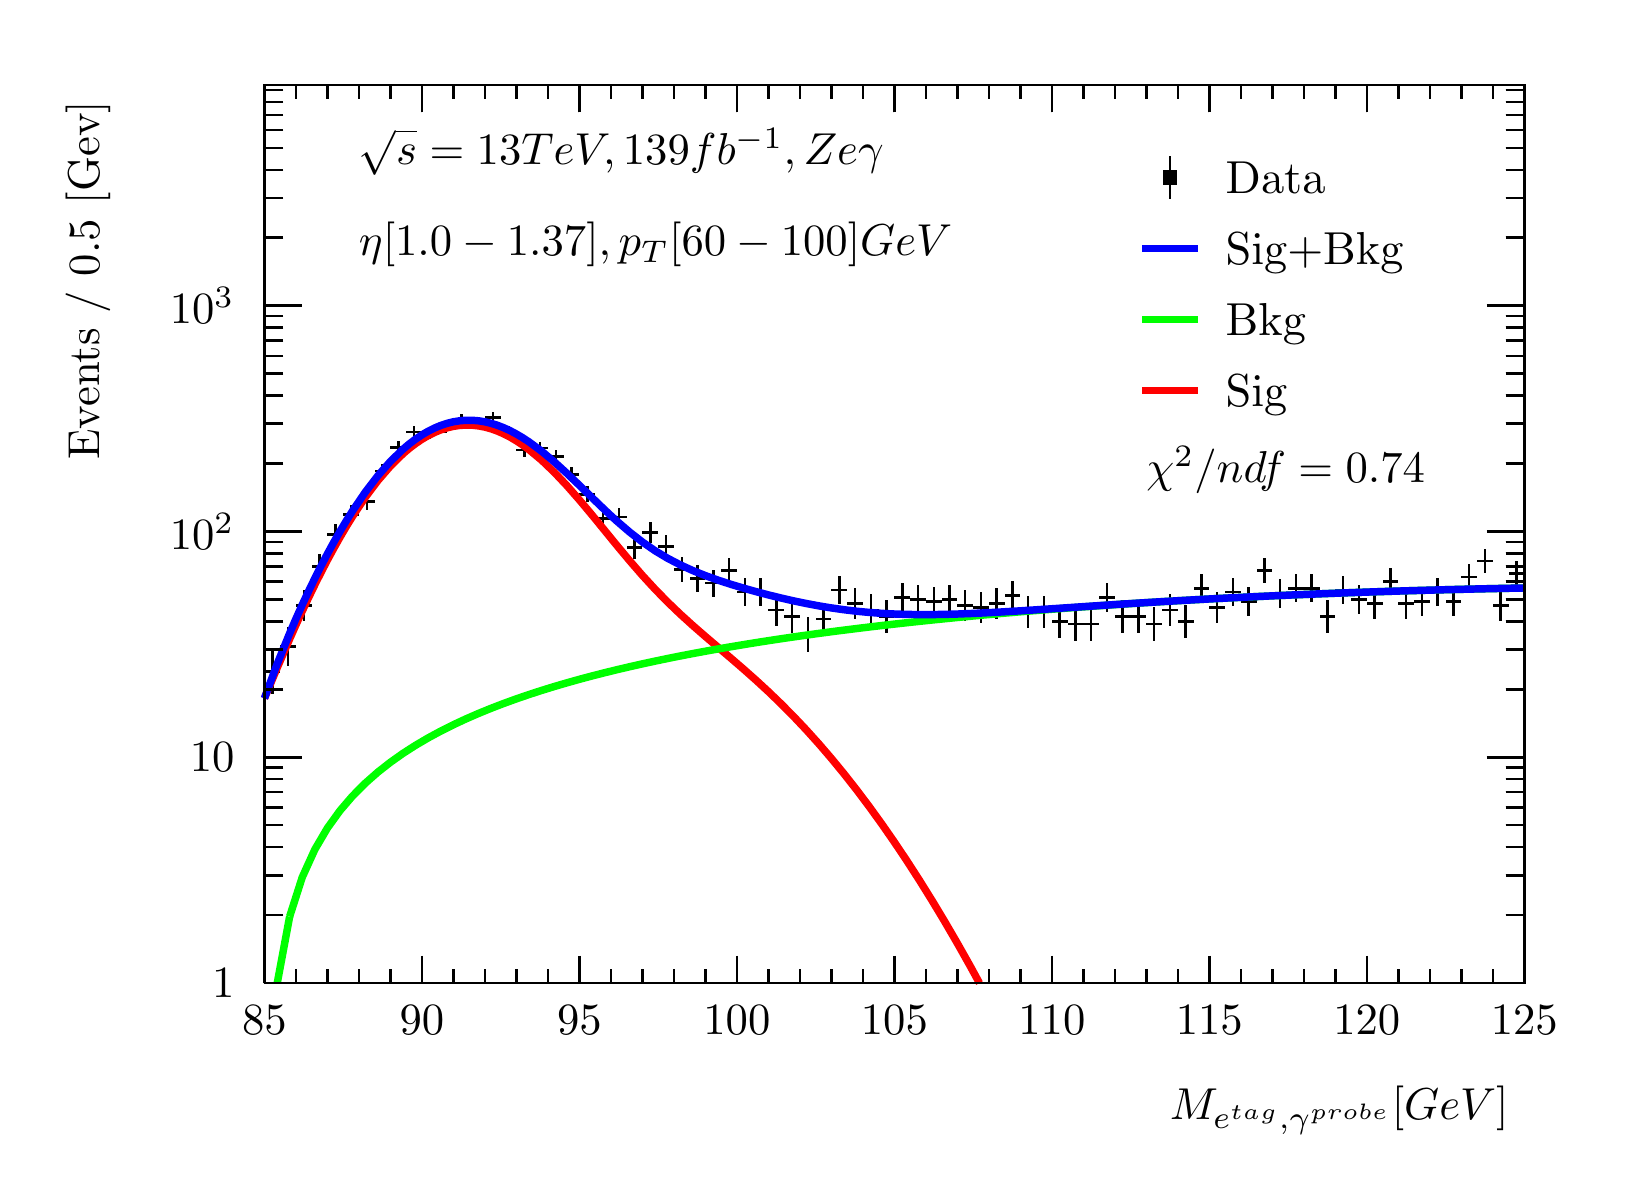
\begin{tikzpicture}
\pgfdeclareplotmark{cross} {
\pgfpathmoveto{\pgfpoint{-0.3\pgfplotmarksize}{\pgfplotmarksize}}
\pgfpathlineto{\pgfpoint{+0.3\pgfplotmarksize}{\pgfplotmarksize}}
\pgfpathlineto{\pgfpoint{+0.3\pgfplotmarksize}{0.3\pgfplotmarksize}}
\pgfpathlineto{\pgfpoint{+1\pgfplotmarksize}{0.3\pgfplotmarksize}}
\pgfpathlineto{\pgfpoint{+1\pgfplotmarksize}{-0.3\pgfplotmarksize}}
\pgfpathlineto{\pgfpoint{+0.3\pgfplotmarksize}{-0.3\pgfplotmarksize}}
\pgfpathlineto{\pgfpoint{+0.3\pgfplotmarksize}{-1.\pgfplotmarksize}}
\pgfpathlineto{\pgfpoint{-0.3\pgfplotmarksize}{-1.\pgfplotmarksize}}
\pgfpathlineto{\pgfpoint{-0.3\pgfplotmarksize}{-0.3\pgfplotmarksize}}
\pgfpathlineto{\pgfpoint{-1.\pgfplotmarksize}{-0.3\pgfplotmarksize}}
\pgfpathlineto{\pgfpoint{-1.\pgfplotmarksize}{0.3\pgfplotmarksize}}
\pgfpathlineto{\pgfpoint{-0.3\pgfplotmarksize}{0.3\pgfplotmarksize}}
\pgfpathclose
\pgfusepathqstroke
}
\pgfdeclareplotmark{cross*} {
\pgfpathmoveto{\pgfpoint{-0.3\pgfplotmarksize}{\pgfplotmarksize}}
\pgfpathlineto{\pgfpoint{+0.3\pgfplotmarksize}{\pgfplotmarksize}}
\pgfpathlineto{\pgfpoint{+0.3\pgfplotmarksize}{0.3\pgfplotmarksize}}
\pgfpathlineto{\pgfpoint{+1\pgfplotmarksize}{0.3\pgfplotmarksize}}
\pgfpathlineto{\pgfpoint{+1\pgfplotmarksize}{-0.3\pgfplotmarksize}}
\pgfpathlineto{\pgfpoint{+0.3\pgfplotmarksize}{-0.3\pgfplotmarksize}}
\pgfpathlineto{\pgfpoint{+0.3\pgfplotmarksize}{-1.\pgfplotmarksize}}
\pgfpathlineto{\pgfpoint{-0.3\pgfplotmarksize}{-1.\pgfplotmarksize}}
\pgfpathlineto{\pgfpoint{-0.3\pgfplotmarksize}{-0.3\pgfplotmarksize}}
\pgfpathlineto{\pgfpoint{-1.\pgfplotmarksize}{-0.3\pgfplotmarksize}}
\pgfpathlineto{\pgfpoint{-1.\pgfplotmarksize}{0.3\pgfplotmarksize}}
\pgfpathlineto{\pgfpoint{-0.3\pgfplotmarksize}{0.3\pgfplotmarksize}}
\pgfpathclose
\pgfusepathqfillstroke
}
\pgfdeclareplotmark{newstar} {
\pgfpathmoveto{\pgfqpoint{0pt}{\pgfplotmarksize}}
\pgfpathlineto{\pgfqpointpolar{44}{0.5\pgfplotmarksize}}
\pgfpathlineto{\pgfqpointpolar{18}{\pgfplotmarksize}}
\pgfpathlineto{\pgfqpointpolar{-20}{0.5\pgfplotmarksize}}
\pgfpathlineto{\pgfqpointpolar{-54}{\pgfplotmarksize}}
\pgfpathlineto{\pgfqpointpolar{-90}{0.5\pgfplotmarksize}}
\pgfpathlineto{\pgfqpointpolar{234}{\pgfplotmarksize}}
\pgfpathlineto{\pgfqpointpolar{198}{0.5\pgfplotmarksize}}
\pgfpathlineto{\pgfqpointpolar{162}{\pgfplotmarksize}}
\pgfpathlineto{\pgfqpointpolar{134}{0.5\pgfplotmarksize}}
\pgfpathclose
\pgfusepathqstroke
}
\pgfdeclareplotmark{newstar*} {
\pgfpathmoveto{\pgfqpoint{0pt}{\pgfplotmarksize}}
\pgfpathlineto{\pgfqpointpolar{44}{0.5\pgfplotmarksize}}
\pgfpathlineto{\pgfqpointpolar{18}{\pgfplotmarksize}}
\pgfpathlineto{\pgfqpointpolar{-20}{0.5\pgfplotmarksize}}
\pgfpathlineto{\pgfqpointpolar{-54}{\pgfplotmarksize}}
\pgfpathlineto{\pgfqpointpolar{-90}{0.5\pgfplotmarksize}}
\pgfpathlineto{\pgfqpointpolar{234}{\pgfplotmarksize}}
\pgfpathlineto{\pgfqpointpolar{198}{0.5\pgfplotmarksize}}
\pgfpathlineto{\pgfqpointpolar{162}{\pgfplotmarksize}}
\pgfpathlineto{\pgfqpointpolar{134}{0.5\pgfplotmarksize}}
\pgfpathclose
\pgfusepathqfillstroke
}
\definecolor{c}{rgb}{1,1,1};
\draw [color=c, fill=c] (0,0) rectangle (20,14.4361);
\draw [color=c, fill=c] (3,2.30977) rectangle (19,13.7143);
\definecolor{c}{rgb}{0,0,0};
\draw [c,line width=0.9] (3,2.30977) -- (3,13.7143) -- (19,13.7143) -- (19,2.30977) -- (3,2.30977);
\definecolor{c}{rgb}{1,1,1};
\draw [color=c, fill=c] (3,2.30977) rectangle (19,13.7143);
\definecolor{c}{rgb}{0,0,0};
\draw [c,line width=0.9] (3,2.30977) -- (3,13.7143) -- (19,13.7143) -- (19,2.30977) -- (3,2.30977);
\draw [c,line width=0.9] (3,2.30977) -- (19,2.30977);
\draw [c,line width=0.9] (3,2.65624) -- (3,2.30977);
\draw [c,line width=0.9] (3.4,2.48301) -- (3.4,2.30977);
\draw [c,line width=0.9] (3.8,2.48301) -- (3.8,2.30977);
\draw [c,line width=0.9] (4.2,2.48301) -- (4.2,2.30977);
\draw [c,line width=0.9] (4.6,2.48301) -- (4.6,2.30977);
\draw [c,line width=0.9] (5,2.65624) -- (5,2.30977);
\draw [c,line width=0.9] (5.4,2.48301) -- (5.4,2.30977);
\draw [c,line width=0.9] (5.8,2.48301) -- (5.8,2.30977);
\draw [c,line width=0.9] (6.2,2.48301) -- (6.2,2.30977);
\draw [c,line width=0.9] (6.6,2.48301) -- (6.6,2.30977);
\draw [c,line width=0.9] (7,2.65624) -- (7,2.30977);
\draw [c,line width=0.9] (7.4,2.48301) -- (7.4,2.30977);
\draw [c,line width=0.9] (7.8,2.48301) -- (7.8,2.30977);
\draw [c,line width=0.9] (8.2,2.48301) -- (8.2,2.30977);
\draw [c,line width=0.9] (8.6,2.48301) -- (8.6,2.30977);
\draw [c,line width=0.9] (9,2.65624) -- (9,2.30977);
\draw [c,line width=0.9] (9.4,2.48301) -- (9.4,2.30977);
\draw [c,line width=0.9] (9.8,2.48301) -- (9.8,2.30977);
\draw [c,line width=0.9] (10.2,2.48301) -- (10.2,2.30977);
\draw [c,line width=0.9] (10.6,2.48301) -- (10.6,2.30977);
\draw [c,line width=0.9] (11,2.65624) -- (11,2.30977);
\draw [c,line width=0.9] (11.4,2.48301) -- (11.4,2.30977);
\draw [c,line width=0.9] (11.8,2.48301) -- (11.8,2.30977);
\draw [c,line width=0.9] (12.2,2.48301) -- (12.2,2.30977);
\draw [c,line width=0.9] (12.6,2.48301) -- (12.6,2.30977);
\draw [c,line width=0.9] (13,2.65624) -- (13,2.30977);
\draw [c,line width=0.9] (13.4,2.48301) -- (13.4,2.30977);
\draw [c,line width=0.9] (13.8,2.48301) -- (13.8,2.30977);
\draw [c,line width=0.9] (14.2,2.48301) -- (14.2,2.30977);
\draw [c,line width=0.9] (14.6,2.48301) -- (14.6,2.30977);
\draw [c,line width=0.9] (15,2.65624) -- (15,2.30977);
\draw [c,line width=0.9] (15.4,2.48301) -- (15.4,2.30977);
\draw [c,line width=0.9] (15.8,2.48301) -- (15.8,2.30977);
\draw [c,line width=0.9] (16.2,2.48301) -- (16.2,2.30977);
\draw [c,line width=0.9] (16.6,2.48301) -- (16.6,2.30977);
\draw [c,line width=0.9] (17,2.65624) -- (17,2.30977);
\draw [c,line width=0.9] (17.4,2.48301) -- (17.4,2.30977);
\draw [c,line width=0.9] (17.8,2.48301) -- (17.8,2.30977);
\draw [c,line width=0.9] (18.2,2.48301) -- (18.2,2.30977);
\draw [c,line width=0.9] (18.6,2.48301) -- (18.6,2.30977);
\draw [c,line width=0.9] (19,2.65624) -- (19,2.30977);
\draw [anchor=base] (3,1.66015) node[scale=1.61424, color=c, rotate=0]{85};
\draw [anchor=base] (5,1.66015) node[scale=1.61424, color=c, rotate=0]{90};
\draw [anchor=base] (7,1.66015) node[scale=1.61424, color=c, rotate=0]{95};
\draw [anchor=base] (9,1.66015) node[scale=1.61424, color=c, rotate=0]{100};
\draw [anchor=base] (11,1.66015) node[scale=1.61424, color=c, rotate=0]{105};
\draw [anchor=base] (13,1.66015) node[scale=1.61424, color=c, rotate=0]{110};
\draw [anchor=base] (15,1.66015) node[scale=1.61424, color=c, rotate=0]{115};
\draw [anchor=base] (17,1.66015) node[scale=1.61424, color=c, rotate=0]{120};
\draw [anchor=base] (19,1.66015) node[scale=1.61424, color=c, rotate=0]{125};
\draw [anchor= east] (19,0.692932) node[scale=1.61424, color=c, rotate=0]{$M_{e^{tag}, \gamma^{probe}}  [GeV]$};
\draw [c,line width=0.9] (3,13.7143) -- (19,13.7143);
\draw [c,line width=0.9] (3,13.3678) -- (3,13.7143);
\draw [c,line width=0.9] (3.4,13.5411) -- (3.4,13.7143);
\draw [c,line width=0.9] (3.8,13.5411) -- (3.8,13.7143);
\draw [c,line width=0.9] (4.2,13.5411) -- (4.2,13.7143);
\draw [c,line width=0.9] (4.6,13.5411) -- (4.6,13.7143);
\draw [c,line width=0.9] (5,13.3678) -- (5,13.7143);
\draw [c,line width=0.9] (5.4,13.5411) -- (5.4,13.7143);
\draw [c,line width=0.9] (5.8,13.5411) -- (5.8,13.7143);
\draw [c,line width=0.9] (6.2,13.5411) -- (6.2,13.7143);
\draw [c,line width=0.9] (6.6,13.5411) -- (6.6,13.7143);
\draw [c,line width=0.9] (7,13.3678) -- (7,13.7143);
\draw [c,line width=0.9] (7.4,13.5411) -- (7.4,13.7143);
\draw [c,line width=0.9] (7.8,13.5411) -- (7.8,13.7143);
\draw [c,line width=0.9] (8.2,13.5411) -- (8.2,13.7143);
\draw [c,line width=0.9] (8.6,13.5411) -- (8.6,13.7143);
\draw [c,line width=0.9] (9,13.3678) -- (9,13.7143);
\draw [c,line width=0.9] (9.4,13.5411) -- (9.4,13.7143);
\draw [c,line width=0.9] (9.8,13.5411) -- (9.8,13.7143);
\draw [c,line width=0.9] (10.2,13.5411) -- (10.2,13.7143);
\draw [c,line width=0.9] (10.6,13.5411) -- (10.6,13.7143);
\draw [c,line width=0.9] (11,13.3678) -- (11,13.7143);
\draw [c,line width=0.9] (11.4,13.5411) -- (11.4,13.7143);
\draw [c,line width=0.9] (11.8,13.5411) -- (11.8,13.7143);
\draw [c,line width=0.9] (12.2,13.5411) -- (12.2,13.7143);
\draw [c,line width=0.9] (12.6,13.5411) -- (12.6,13.7143);
\draw [c,line width=0.9] (13,13.3678) -- (13,13.7143);
\draw [c,line width=0.9] (13.4,13.5411) -- (13.4,13.7143);
\draw [c,line width=0.9] (13.8,13.5411) -- (13.8,13.7143);
\draw [c,line width=0.9] (14.2,13.5411) -- (14.2,13.7143);
\draw [c,line width=0.9] (14.6,13.5411) -- (14.6,13.7143);
\draw [c,line width=0.9] (15,13.3678) -- (15,13.7143);
\draw [c,line width=0.9] (15.4,13.5411) -- (15.4,13.7143);
\draw [c,line width=0.9] (15.8,13.5411) -- (15.8,13.7143);
\draw [c,line width=0.9] (16.2,13.5411) -- (16.2,13.7143);
\draw [c,line width=0.9] (16.6,13.5411) -- (16.6,13.7143);
\draw [c,line width=0.9] (17,13.3678) -- (17,13.7143);
\draw [c,line width=0.9] (17.4,13.5411) -- (17.4,13.7143);
\draw [c,line width=0.9] (17.8,13.5411) -- (17.8,13.7143);
\draw [c,line width=0.9] (18.2,13.5411) -- (18.2,13.7143);
\draw [c,line width=0.9] (18.6,13.5411) -- (18.6,13.7143);
\draw [c,line width=0.9] (19,13.3678) -- (19,13.7143);
\draw [c,line width=0.9] (3,2.30977) -- (3,13.7143);
\draw [c,line width=0.9] (3.474,2.30978) -- (3,2.30978);
\draw [anchor= east] (2.82,2.30978) node[scale=1.61424, color=c, rotate=0]{1};
\draw [c,line width=0.9] (3.237,3.17298) -- (3,3.17298);
\draw [c,line width=0.9] (3.237,3.67792) -- (3,3.67792);
\draw [c,line width=0.9] (3.237,4.03618) -- (3,4.03618);
\draw [c,line width=0.9] (3.237,4.31407) -- (3,4.31407);
\draw [c,line width=0.9] (3.237,4.54112) -- (3,4.54112);
\draw [c,line width=0.9] (3.237,4.73309) -- (3,4.73309);
\draw [c,line width=0.9] (3.237,4.89938) -- (3,4.89938);
\draw [c,line width=0.9] (3.237,5.04606) -- (3,5.04606);
\draw [c,line width=0.9] (3.474,5.17727) -- (3,5.17727);
\draw [anchor= east] (2.82,5.17727) node[scale=1.61424, color=c, rotate=0]{10};
\draw [c,line width=0.9] (3.237,6.04047) -- (3,6.04047);
\draw [c,line width=0.9] (3.237,6.54541) -- (3,6.54541);
\draw [c,line width=0.9] (3.237,6.90367) -- (3,6.90367);
\draw [c,line width=0.9] (3.237,7.18156) -- (3,7.18156);
\draw [c,line width=0.9] (3.237,7.40861) -- (3,7.40861);
\draw [c,line width=0.9] (3.237,7.60058) -- (3,7.60058);
\draw [c,line width=0.9] (3.237,7.76687) -- (3,7.76687);
\draw [c,line width=0.9] (3.237,7.91355) -- (3,7.91355);
\draw [c,line width=0.9] (3.474,8.04476) -- (3,8.04476);
\draw [anchor= east] (2.82,8.04476) node[scale=1.61424, color=c, rotate=0]{$10^{2}$};
\draw [c,line width=0.9] (3.237,8.90796) -- (3,8.90796);
\draw [c,line width=0.9] (3.237,9.4129) -- (3,9.4129);
\draw [c,line width=0.9] (3.237,9.77116) -- (3,9.77116);
\draw [c,line width=0.9] (3.237,10.049) -- (3,10.049);
\draw [c,line width=0.9] (3.237,10.2761) -- (3,10.2761);
\draw [c,line width=0.9] (3.237,10.4681) -- (3,10.4681);
\draw [c,line width=0.9] (3.237,10.6344) -- (3,10.6344);
\draw [c,line width=0.9] (3.237,10.781) -- (3,10.781);
\draw [c,line width=0.9] (3.474,10.9122) -- (3,10.9122);
\draw [anchor= east] (2.82,10.9122) node[scale=1.61424, color=c, rotate=0]{$10^{3}$};
\draw [c,line width=0.9] (3.237,11.7754) -- (3,11.7754);
\draw [c,line width=0.9] (3.237,12.2804) -- (3,12.2804);
\draw [c,line width=0.9] (3.237,12.6386) -- (3,12.6386);
\draw [c,line width=0.9] (3.237,12.9165) -- (3,12.9165);
\draw [c,line width=0.9] (3.237,13.1436) -- (3,13.1436);
\draw [c,line width=0.9] (3.237,13.3356) -- (3,13.3356);
\draw [c,line width=0.9] (3.237,13.5018) -- (3,13.5018);
\draw [c,line width=0.9] (3.237,13.6485) -- (3,13.6485);
\draw [anchor= east] (0.76,13.7143) node[scale=1.61424, color=c, rotate=90]{Events / 0.5 [Gev]};
\draw [c,line width=0.9] (19,2.30977) -- (19,13.7143);
\draw [c,line width=0.9] (18.526,2.30978) -- (19,2.30978);
\draw [c,line width=0.9] (18.763,3.17298) -- (19,3.17298);
\draw [c,line width=0.9] (18.763,3.67792) -- (19,3.67792);
\draw [c,line width=0.9] (18.763,4.03618) -- (19,4.03618);
\draw [c,line width=0.9] (18.763,4.31407) -- (19,4.31407);
\draw [c,line width=0.9] (18.763,4.54112) -- (19,4.54112);
\draw [c,line width=0.9] (18.763,4.73309) -- (19,4.73309);
\draw [c,line width=0.9] (18.763,4.89938) -- (19,4.89938);
\draw [c,line width=0.9] (18.763,5.04606) -- (19,5.04606);
\draw [c,line width=0.9] (18.526,5.17727) -- (19,5.17727);
\draw [c,line width=0.9] (18.763,6.04047) -- (19,6.04047);
\draw [c,line width=0.9] (18.763,6.54541) -- (19,6.54541);
\draw [c,line width=0.9] (18.763,6.90367) -- (19,6.90367);
\draw [c,line width=0.9] (18.763,7.18156) -- (19,7.18156);
\draw [c,line width=0.9] (18.763,7.40861) -- (19,7.40861);
\draw [c,line width=0.9] (18.763,7.60058) -- (19,7.60058);
\draw [c,line width=0.9] (18.763,7.76687) -- (19,7.76687);
\draw [c,line width=0.9] (18.763,7.91355) -- (19,7.91355);
\draw [c,line width=0.9] (18.526,8.04476) -- (19,8.04476);
\draw [c,line width=0.9] (18.763,8.90796) -- (19,8.90796);
\draw [c,line width=0.9] (18.763,9.4129) -- (19,9.4129);
\draw [c,line width=0.9] (18.763,9.77116) -- (19,9.77116);
\draw [c,line width=0.9] (18.763,10.049) -- (19,10.049);
\draw [c,line width=0.9] (18.763,10.2761) -- (19,10.2761);
\draw [c,line width=0.9] (18.763,10.4681) -- (19,10.4681);
\draw [c,line width=0.9] (18.763,10.6344) -- (19,10.6344);
\draw [c,line width=0.9] (18.763,10.781) -- (19,10.781);
\draw [c,line width=0.9] (18.526,10.9122) -- (19,10.9122);
\draw [c,line width=0.9] (18.763,11.7754) -- (19,11.7754);
\draw [c,line width=0.9] (18.763,12.2804) -- (19,12.2804);
\draw [c,line width=0.9] (18.763,12.6386) -- (19,12.6386);
\draw [c,line width=0.9] (18.763,12.9165) -- (19,12.9165);
\draw [c,line width=0.9] (18.763,13.1436) -- (19,13.1436);
\draw [c,line width=0.9] (18.763,13.3356) -- (19,13.3356);
\draw [c,line width=0.9] (18.763,13.5018) -- (19,13.5018);
\draw [c,line width=0.9] (18.763,13.6485) -- (19,13.6485);
\draw [c,line width=0.9] (3.1,6.26752) -- (3,6.26752);
\draw [c,line width=0.9] (3,6.26752) -- (3,6.26752);
\draw [c,line width=0.9] (3.1,6.26752) -- (3.2,6.26752);
\draw [c,line width=0.9] (3.2,6.26752) -- (3.2,6.26752);
\draw [c,line width=0.9] (3.1,6.26752) -- (3.1,6.54403);
\draw [c,line width=0.9] (3.1,6.54403) -- (3.1,6.54403);
\draw [c,line width=0.9] (3.1,6.26752) -- (3.1,5.98543);
\draw [c,line width=0.9] (3.1,5.98543) -- (3.1,5.98543);
\draw [c,line width=0.9] (3.3,6.58624) -- (3.2,6.58624);
\draw [c,line width=0.9] (3.2,6.58624) -- (3.2,6.58624);
\draw [c,line width=0.9] (3.3,6.58624) -- (3.4,6.58624);
\draw [c,line width=0.9] (3.4,6.58624) -- (3.4,6.58624);
\draw [c,line width=0.9] (3.3,6.58624) -- (3.3,6.82752);
\draw [c,line width=0.9] (3.3,6.82752) -- (3.3,6.82752);
\draw [c,line width=0.9] (3.3,6.58624) -- (3.3,6.34118);
\draw [c,line width=0.9] (3.3,6.34118) -- (3.3,6.34118);
\draw [c,line width=0.9] (3.5,7.1045) -- (3.4,7.1045);
\draw [c,line width=0.9] (3.4,7.1045) -- (3.4,7.1045);
\draw [c,line width=0.9] (3.5,7.1045) -- (3.6,7.1045);
\draw [c,line width=0.9] (3.6,7.1045) -- (3.6,7.1045);
\draw [c,line width=0.9] (3.5,7.1045) -- (3.5,7.29808);
\draw [c,line width=0.9] (3.5,7.29808) -- (3.5,7.29808);
\draw [c,line width=0.9] (3.5,7.1045) -- (3.5,6.90891);
\draw [c,line width=0.9] (3.5,6.90891) -- (3.5,6.90891);
\draw [c,line width=0.9] (3.7,7.60058) -- (3.6,7.60058);
\draw [c,line width=0.9] (3.6,7.60058) -- (3.6,7.60058);
\draw [c,line width=0.9] (3.7,7.60058) -- (3.8,7.60058);
\draw [c,line width=0.9] (3.8,7.60058) -- (3.8,7.60058);
\draw [c,line width=0.9] (3.7,7.60058) -- (3.7,7.75759);
\draw [c,line width=0.9] (3.7,7.75759) -- (3.7,7.75759);
\draw [c,line width=0.9] (3.7,7.60058) -- (3.7,7.44246);
\draw [c,line width=0.9] (3.7,7.44246) -- (3.7,7.44246);
\draw [c,line width=0.9] (3.9,8.00682) -- (3.8,8.00682);
\draw [c,line width=0.9] (3.8,8.00682) -- (3.8,8.00682);
\draw [c,line width=0.9] (3.9,8.00682) -- (4,8.00682);
\draw [c,line width=0.9] (4,8.00682) -- (4,8.00682);
\draw [c,line width=0.9] (3.9,8.00682) -- (3.9,8.13925);
\draw [c,line width=0.9] (3.9,8.13925) -- (3.9,8.13925);
\draw [c,line width=0.9] (3.9,8.00682) -- (3.9,7.87373);
\draw [c,line width=0.9] (3.9,7.87373) -- (3.9,7.87373);
\draw [c,line width=0.9] (4.1,8.26139) -- (4,8.26139);
\draw [c,line width=0.9] (4,8.26139) -- (4,8.26139);
\draw [c,line width=0.9] (4.1,8.26139) -- (4.2,8.26139);
\draw [c,line width=0.9] (4.2,8.26139) -- (4.2,8.26139);
\draw [c,line width=0.9] (4.1,8.26139) -- (4.1,8.37551);
\draw [c,line width=0.9] (4.1,8.37551) -- (4.1,8.37551);
\draw [c,line width=0.9] (4.1,8.26139) -- (4.1,8.14727);
\draw [c,line width=0.9] (4.1,8.14727) -- (4.1,8.14727);
\draw [c,line width=0.9] (4.3,8.42768) -- (4.2,8.42768);
\draw [c,line width=0.9] (4.2,8.42768) -- (4.2,8.42768);
\draw [c,line width=0.9] (4.3,8.42768) -- (4.4,8.42768);
\draw [c,line width=0.9] (4.4,8.42768) -- (4.4,8.42768);
\draw [c,line width=0.9] (4.3,8.42768) -- (4.3,8.53443);
\draw [c,line width=0.9] (4.3,8.53443) -- (4.3,8.53443);
\draw [c,line width=0.9] (4.3,8.42768) -- (4.3,8.32092);
\draw [c,line width=0.9] (4.3,8.32092) -- (4.3,8.32092);
\draw [c,line width=0.9] (4.5,8.81087) -- (4.4,8.81087);
\draw [c,line width=0.9] (4.4,8.81087) -- (4.4,8.81087);
\draw [c,line width=0.9] (4.5,8.81087) -- (4.6,8.81087);
\draw [c,line width=0.9] (4.6,8.81087) -- (4.6,8.81087);
\draw [c,line width=0.9] (4.5,8.81087) -- (4.5,8.90241);
\draw [c,line width=0.9] (4.5,8.90241) -- (4.5,8.90241);
\draw [c,line width=0.9] (4.5,8.81087) -- (4.5,8.71933);
\draw [c,line width=0.9] (4.5,8.71933) -- (4.5,8.71933);
\draw [c,line width=0.9] (4.7,9.11408) -- (4.6,9.11408);
\draw [c,line width=0.9] (4.6,9.11408) -- (4.6,9.11408);
\draw [c,line width=0.9] (4.7,9.11408) -- (4.8,9.11408);
\draw [c,line width=0.9] (4.8,9.11408) -- (4.8,9.11408);
\draw [c,line width=0.9] (4.7,9.11408) -- (4.7,9.19513);
\draw [c,line width=0.9] (4.7,9.19513) -- (4.7,9.19513);
\draw [c,line width=0.9] (4.7,9.11408) -- (4.7,9.03303);
\draw [c,line width=0.9] (4.7,9.03303) -- (4.7,9.03303);
\draw [c,line width=0.9] (4.9,9.30906) -- (4.8,9.30906);
\draw [c,line width=0.9] (4.8,9.30906) -- (4.8,9.30906);
\draw [c,line width=0.9] (4.9,9.30906) -- (5,9.30906);
\draw [c,line width=0.9] (5,9.30906) -- (5,9.30906);
\draw [c,line width=0.9] (4.9,9.30906) -- (4.9,9.38401);
\draw [c,line width=0.9] (4.9,9.38401) -- (4.9,9.38401);
\draw [c,line width=0.9] (4.9,9.30906) -- (4.9,9.23411);
\draw [c,line width=0.9] (4.9,9.23411) -- (4.9,9.23411);
\draw [c,line width=0.9] (5.1,9.29088) -- (5,9.29088);
\draw [c,line width=0.9] (5,9.29088) -- (5,9.29088);
\draw [c,line width=0.9] (5.1,9.29088) -- (5.2,9.29088);
\draw [c,line width=0.9] (5.2,9.29088) -- (5.2,9.29088);
\draw [c,line width=0.9] (5.1,9.29088) -- (5.1,9.36638);
\draw [c,line width=0.9] (5.1,9.36638) -- (5.1,9.36638);
\draw [c,line width=0.9] (5.1,9.29088) -- (5.1,9.21538);
\draw [c,line width=0.9] (5.1,9.21538) -- (5.1,9.21538);
\draw [c,line width=0.9] (5.3,9.37068) -- (5.2,9.37068);
\draw [c,line width=0.9] (5.2,9.37068) -- (5.2,9.37068);
\draw [c,line width=0.9] (5.3,9.37068) -- (5.4,9.37068);
\draw [c,line width=0.9] (5.4,9.37068) -- (5.4,9.37068);
\draw [c,line width=0.9] (5.3,9.37068) -- (5.3,9.4438);
\draw [c,line width=0.9] (5.3,9.4438) -- (5.3,9.4438);
\draw [c,line width=0.9] (5.3,9.37068) -- (5.3,9.29756);
\draw [c,line width=0.9] (5.3,9.29756) -- (5.3,9.29756);
\draw [c,line width=0.9] (5.5,9.46572) -- (5.4,9.46572);
\draw [c,line width=0.9] (5.4,9.46572) -- (5.4,9.46572);
\draw [c,line width=0.9] (5.5,9.46572) -- (5.6,9.46572);
\draw [c,line width=0.9] (5.6,9.46572) -- (5.6,9.46572);
\draw [c,line width=0.9] (5.5,9.46572) -- (5.5,9.53611);
\draw [c,line width=0.9] (5.5,9.53611) -- (5.5,9.53611);
\draw [c,line width=0.9] (5.5,9.46572) -- (5.5,9.39534);
\draw [c,line width=0.9] (5.5,9.39534) -- (5.5,9.39534);
\draw [c,line width=0.9] (5.7,9.4129) -- (5.6,9.4129);
\draw [c,line width=0.9] (5.6,9.4129) -- (5.6,9.4129);
\draw [c,line width=0.9] (5.7,9.4129) -- (5.8,9.4129);
\draw [c,line width=0.9] (5.8,9.4129) -- (5.8,9.4129);
\draw [c,line width=0.9] (5.7,9.4129) -- (5.7,9.48479);
\draw [c,line width=0.9] (5.7,9.48479) -- (5.7,9.48479);
\draw [c,line width=0.9] (5.7,9.4129) -- (5.7,9.34101);
\draw [c,line width=0.9] (5.7,9.34101) -- (5.7,9.34101);
\draw [c,line width=0.9] (5.9,9.48937) -- (5.8,9.48937);
\draw [c,line width=0.9] (5.8,9.48937) -- (5.8,9.48937);
\draw [c,line width=0.9] (5.9,9.48937) -- (6,9.48937);
\draw [c,line width=0.9] (6,9.48937) -- (6,9.48937);
\draw [c,line width=0.9] (5.9,9.48937) -- (5.9,9.55909);
\draw [c,line width=0.9] (5.9,9.55909) -- (5.9,9.55909);
\draw [c,line width=0.9] (5.9,9.48937) -- (5.9,9.41965);
\draw [c,line width=0.9] (5.9,9.41965) -- (5.9,9.41965);
\draw [c,line width=0.9] (6.1,9.31356) -- (6,9.31356);
\draw [c,line width=0.9] (6,9.31356) -- (6,9.31356);
\draw [c,line width=0.9] (6.1,9.31356) -- (6.2,9.31356);
\draw [c,line width=0.9] (6.2,9.31356) -- (6.2,9.31356);
\draw [c,line width=0.9] (6.1,9.31356) -- (6.1,9.38838);
\draw [c,line width=0.9] (6.1,9.38838) -- (6.1,9.38838);
\draw [c,line width=0.9] (6.1,9.31356) -- (6.1,9.23875);
\draw [c,line width=0.9] (6.1,9.23875) -- (6.1,9.23875);
\draw [c,line width=0.9] (6.3,9.07658) -- (6.2,9.07658);
\draw [c,line width=0.9] (6.2,9.07658) -- (6.2,9.07658);
\draw [c,line width=0.9] (6.3,9.07658) -- (6.4,9.07658);
\draw [c,line width=0.9] (6.4,9.07658) -- (6.4,9.07658);
\draw [c,line width=0.9] (6.3,9.07658) -- (6.3,9.15886);
\draw [c,line width=0.9] (6.3,9.15886) -- (6.3,9.15886);
\draw [c,line width=0.9] (6.3,9.07658) -- (6.3,8.9943);
\draw [c,line width=0.9] (6.3,8.9943) -- (6.3,8.9943);
\draw [c,line width=0.9] (6.5,9.10348) -- (6.4,9.10348);
\draw [c,line width=0.9] (6.4,9.10348) -- (6.4,9.10348);
\draw [c,line width=0.9] (6.5,9.10348) -- (6.6,9.10348);
\draw [c,line width=0.9] (6.6,9.10348) -- (6.6,9.10348);
\draw [c,line width=0.9] (6.5,9.10348) -- (6.5,9.18487);
\draw [c,line width=0.9] (6.5,9.18487) -- (6.5,9.18487);
\draw [c,line width=0.9] (6.5,9.10348) -- (6.5,9.02208);
\draw [c,line width=0.9] (6.5,9.02208) -- (6.5,9.02208);
\draw [c,line width=0.9] (6.7,8.99802) -- (6.6,8.99802);
\draw [c,line width=0.9] (6.6,8.99802) -- (6.6,8.99802);
\draw [c,line width=0.9] (6.7,8.99802) -- (6.8,8.99802);
\draw [c,line width=0.9] (6.8,8.99802) -- (6.8,8.99802);
\draw [c,line width=0.9] (6.7,8.99802) -- (6.7,9.08293);
\draw [c,line width=0.9] (6.7,9.08293) -- (6.7,9.08293);
\draw [c,line width=0.9] (6.7,8.99802) -- (6.7,8.91311);
\draw [c,line width=0.9] (6.7,8.91311) -- (6.7,8.91311);
\draw [c,line width=0.9] (6.9,8.76981) -- (6.8,8.76981);
\draw [c,line width=0.9] (6.8,8.76981) -- (6.8,8.76981);
\draw [c,line width=0.9] (6.9,8.76981) -- (7,8.76981);
\draw [c,line width=0.9] (7,8.76981) -- (7,8.76981);
\draw [c,line width=0.9] (6.9,8.76981) -- (6.9,8.86287);
\draw [c,line width=0.9] (6.9,8.86287) -- (6.9,8.86287);
\draw [c,line width=0.9] (6.9,8.76981) -- (6.9,8.67675);
\draw [c,line width=0.9] (6.9,8.67675) -- (6.9,8.67675);
\draw [c,line width=0.9] (7.1,8.51604) -- (7,8.51604);
\draw [c,line width=0.9] (7,8.51604) -- (7,8.51604);
\draw [c,line width=0.9] (7.1,8.51604) -- (7.2,8.51604);
\draw [c,line width=0.9] (7.2,8.51604) -- (7.2,8.51604);
\draw [c,line width=0.9] (7.1,8.51604) -- (7.1,8.61907);
\draw [c,line width=0.9] (7.1,8.61907) -- (7.1,8.61907);
\draw [c,line width=0.9] (7.1,8.51604) -- (7.1,8.413);
\draw [c,line width=0.9] (7.1,8.413) -- (7.1,8.413);
\draw [c,line width=0.9] (7.3,8.20793) -- (7.2,8.20793);
\draw [c,line width=0.9] (7.2,8.20793) -- (7.2,8.20793);
\draw [c,line width=0.9] (7.3,8.20793) -- (7.4,8.20793);
\draw [c,line width=0.9] (7.4,8.20793) -- (7.4,8.20793);
\draw [c,line width=0.9] (7.3,8.20793) -- (7.3,8.32452);
\draw [c,line width=0.9] (7.3,8.32452) -- (7.3,8.32452);
\draw [c,line width=0.9] (7.3,8.20793) -- (7.3,8.09134);
\draw [c,line width=0.9] (7.3,8.09134) -- (7.3,8.09134);
\draw [c,line width=0.9] (7.5,8.22959) -- (7.4,8.22959);
\draw [c,line width=0.9] (7.4,8.22959) -- (7.4,8.22959);
\draw [c,line width=0.9] (7.5,8.22959) -- (7.6,8.22959);
\draw [c,line width=0.9] (7.6,8.22959) -- (7.6,8.22959);
\draw [c,line width=0.9] (7.5,8.22959) -- (7.5,8.34517);
\draw [c,line width=0.9] (7.5,8.34517) -- (7.5,8.34517);
\draw [c,line width=0.9] (7.5,8.22959) -- (7.5,8.114);
\draw [c,line width=0.9] (7.5,8.114) -- (7.5,8.114);
\draw [c,line width=0.9] (7.7,7.84237) -- (7.6,7.84237);
\draw [c,line width=0.9] (7.6,7.84237) -- (7.6,7.84237);
\draw [c,line width=0.9] (7.7,7.84237) -- (7.8,7.84237);
\draw [c,line width=0.9] (7.8,7.84237) -- (7.8,7.84237);
\draw [c,line width=0.9] (7.7,7.84237) -- (7.7,7.98423);
\draw [c,line width=0.9] (7.7,7.98423) -- (7.7,7.98423);
\draw [c,line width=0.9] (7.7,7.84237) -- (7.7,7.69969);
\draw [c,line width=0.9] (7.7,7.69969) -- (7.7,7.69969);
\draw [c,line width=0.9] (7.9,8.03224) -- (7.8,8.03224);
\draw [c,line width=0.9] (7.8,8.03224) -- (7.8,8.03224);
\draw [c,line width=0.9] (7.9,8.03224) -- (8,8.03224);
\draw [c,line width=0.9] (8,8.03224) -- (8,8.03224);
\draw [c,line width=0.9] (7.9,8.03224) -- (7.9,8.16326);
\draw [c,line width=0.9] (7.9,8.16326) -- (7.9,8.16326);
\draw [c,line width=0.9] (7.9,8.03224) -- (7.9,7.90057);
\draw [c,line width=0.9] (7.9,7.90057) -- (7.9,7.90057);
\draw [c,line width=0.9] (8.1,7.85693) -- (8,7.85693);
\draw [c,line width=0.9] (8,7.85693) -- (8,7.85693);
\draw [c,line width=0.9] (8.1,7.85693) -- (8.2,7.85693);
\draw [c,line width=0.9] (8.2,7.85693) -- (8.2,7.85693);
\draw [c,line width=0.9] (8.1,7.85693) -- (8.1,7.99793);
\draw [c,line width=0.9] (8.1,7.99793) -- (8.1,7.99793);
\draw [c,line width=0.9] (8.1,7.85693) -- (8.1,7.71513);
\draw [c,line width=0.9] (8.1,7.71513) -- (8.1,7.71513);
\draw [c,line width=0.9] (8.3,7.56448) -- (8.2,7.56448);
\draw [c,line width=0.9] (8.2,7.56448) -- (8.2,7.56448);
\draw [c,line width=0.9] (8.3,7.56448) -- (8.4,7.56448);
\draw [c,line width=0.9] (8.4,7.56448) -- (8.4,7.56448);
\draw [c,line width=0.9] (8.3,7.56448) -- (8.3,7.7239);
\draw [c,line width=0.9] (8.3,7.7239) -- (8.3,7.7239);
\draw [c,line width=0.9] (8.3,7.56448) -- (8.3,7.40391);
\draw [c,line width=0.9] (8.3,7.40391) -- (8.3,7.40391);
\draw [c,line width=0.9] (8.5,7.44944) -- (8.4,7.44944);
\draw [c,line width=0.9] (8.4,7.44944) -- (8.4,7.44944);
\draw [c,line width=0.9] (8.5,7.44944) -- (8.6,7.44944);
\draw [c,line width=0.9] (8.6,7.44944) -- (8.6,7.44944);
\draw [c,line width=0.9] (8.5,7.44944) -- (8.5,7.61677);
\draw [c,line width=0.9] (8.5,7.61677) -- (8.5,7.61677);
\draw [c,line width=0.9] (8.5,7.44944) -- (8.5,7.28079);
\draw [c,line width=0.9] (8.5,7.28079) -- (8.5,7.28079);
\draw [c,line width=0.9] (8.7,7.38768) -- (8.6,7.38768);
\draw [c,line width=0.9] (8.6,7.38768) -- (8.6,7.38768);
\draw [c,line width=0.9] (8.7,7.38768) -- (8.8,7.38768);
\draw [c,line width=0.9] (8.8,7.38768) -- (8.8,7.38768);
\draw [c,line width=0.9] (8.7,7.38768) -- (8.7,7.55942);
\draw [c,line width=0.9] (8.7,7.55942) -- (8.7,7.55942);
\draw [c,line width=0.9] (8.7,7.38768) -- (8.7,7.21451);
\draw [c,line width=0.9] (8.7,7.21451) -- (8.7,7.21451);
\draw [c,line width=0.9] (8.9,7.54603) -- (8.8,7.54603);
\draw [c,line width=0.9] (8.8,7.54603) -- (8.8,7.54603);
\draw [c,line width=0.9] (8.9,7.54603) -- (9,7.54603);
\draw [c,line width=0.9] (9,7.54603) -- (9,7.54603);
\draw [c,line width=0.9] (8.9,7.54603) -- (8.9,7.70669);
\draw [c,line width=0.9] (8.9,7.70669) -- (8.9,7.70669);
\draw [c,line width=0.9] (8.9,7.54603) -- (8.9,7.38419);
\draw [c,line width=0.9] (8.9,7.38419) -- (8.9,7.38419);
\draw [c,line width=0.9] (9.1,7.2774) -- (9,7.2774);
\draw [c,line width=0.9] (9,7.2774) -- (9,7.2774);
\draw [c,line width=0.9] (9.1,7.2774) -- (9.2,7.2774);
\draw [c,line width=0.9] (9.2,7.2774) -- (9.2,7.2774);
\draw [c,line width=0.9] (9.1,7.2774) -- (9.1,7.45733);
\draw [c,line width=0.9] (9.1,7.45733) -- (9.1,7.45733);
\draw [c,line width=0.9] (9.1,7.2774) -- (9.1,7.09584);
\draw [c,line width=0.9] (9.1,7.09584) -- (9.1,7.09584);
\draw [c,line width=0.9] (9.3,7.2774) -- (9.2,7.2774);
\draw [c,line width=0.9] (9.2,7.2774) -- (9.2,7.2774);
\draw [c,line width=0.9] (9.3,7.2774) -- (9.4,7.2774);
\draw [c,line width=0.9] (9.4,7.2774) -- (9.4,7.2774);
\draw [c,line width=0.9] (9.3,7.2774) -- (9.3,7.45733);
\draw [c,line width=0.9] (9.3,7.45733) -- (9.3,7.45733);
\draw [c,line width=0.9] (9.3,7.2774) -- (9.3,7.09584);
\draw [c,line width=0.9] (9.3,7.09584) -- (9.3,7.09584);
\draw [c,line width=0.9] (9.5,7.05035) -- (9.4,7.05035);
\draw [c,line width=0.9] (9.4,7.05035) -- (9.4,7.05035);
\draw [c,line width=0.9] (9.5,7.05035) -- (9.6,7.05035);
\draw [c,line width=0.9] (9.6,7.05035) -- (9.6,7.05035);
\draw [c,line width=0.9] (9.5,7.05035) -- (9.5,7.24842);
\draw [c,line width=0.9] (9.5,7.24842) -- (9.5,7.24842);
\draw [c,line width=0.9] (9.5,7.05035) -- (9.5,6.85013);
\draw [c,line width=0.9] (9.5,6.85013) -- (9.5,6.85013);
\draw [c,line width=0.9] (9.7,6.96443) -- (9.6,6.96443);
\draw [c,line width=0.9] (9.6,6.96443) -- (9.6,6.96443);
\draw [c,line width=0.9] (9.7,6.96443) -- (9.8,6.96443);
\draw [c,line width=0.9] (9.8,6.96443) -- (9.8,6.96443);
\draw [c,line width=0.9] (9.7,6.96443) -- (9.7,7.16985);
\draw [c,line width=0.9] (9.7,7.16985) -- (9.7,7.16985);
\draw [c,line width=0.9] (9.7,6.96443) -- (9.7,6.75662);
\draw [c,line width=0.9] (9.7,6.75662) -- (9.7,6.75662);
\draw [c,line width=0.9] (9.9,6.73738) -- (9.8,6.73738);
\draw [c,line width=0.9] (9.8,6.73738) -- (9.8,6.73738);
\draw [c,line width=0.9] (9.9,6.73738) -- (10,6.73738);
\draw [c,line width=0.9] (10,6.73738) -- (10,6.73738);
\draw [c,line width=0.9] (9.9,6.73738) -- (9.9,6.96361);
\draw [c,line width=0.9] (9.9,6.96361) -- (9.9,6.96361);
\draw [c,line width=0.9] (9.9,6.73738) -- (9.9,6.508);
\draw [c,line width=0.9] (9.9,6.508) -- (9.9,6.508);
\draw [c,line width=0.9] (10.1,6.93442) -- (10,6.93442);
\draw [c,line width=0.9] (10,6.93442) -- (10,6.93442);
\draw [c,line width=0.9] (10.1,6.93442) -- (10.2,6.93442);
\draw [c,line width=0.9] (10.2,6.93442) -- (10.2,6.93442);
\draw [c,line width=0.9] (10.1,6.93442) -- (10.1,7.14247);
\draw [c,line width=0.9] (10.1,7.14247) -- (10.1,7.14247);
\draw [c,line width=0.9] (10.1,6.93442) -- (10.1,6.72389);
\draw [c,line width=0.9] (10.1,6.72389) -- (10.1,6.72389);
\draw [c,line width=0.9] (10.3,7.30025) -- (10.2,7.30025);
\draw [c,line width=0.9] (10.2,7.30025) -- (10.2,7.30025);
\draw [c,line width=0.9] (10.3,7.30025) -- (10.4,7.30025);
\draw [c,line width=0.9] (10.4,7.30025) -- (10.4,7.30025);
\draw [c,line width=0.9] (10.3,7.30025) -- (10.3,7.47845);
\draw [c,line width=0.9] (10.3,7.47845) -- (10.3,7.47845);
\draw [c,line width=0.9] (10.3,7.30025) -- (10.3,7.12046);
\draw [c,line width=0.9] (10.3,7.12046) -- (10.3,7.12046);
\draw [c,line width=0.9] (10.5,7.13072) -- (10.4,7.13072);
\draw [c,line width=0.9] (10.4,7.13072) -- (10.4,7.13072);
\draw [c,line width=0.9] (10.5,7.13072) -- (10.6,7.13072);
\draw [c,line width=0.9] (10.6,7.13072) -- (10.6,7.13072);
\draw [c,line width=0.9] (10.5,7.13072) -- (10.5,7.32216);
\draw [c,line width=0.9] (10.5,7.32216) -- (10.5,7.32216);
\draw [c,line width=0.9] (10.5,7.13072) -- (10.5,6.93733);
\draw [c,line width=0.9] (10.5,6.93733) -- (10.5,6.93733);
\draw [c,line width=0.9] (10.7,7.05035) -- (10.6,7.05035);
\draw [c,line width=0.9] (10.6,7.05035) -- (10.6,7.05035);
\draw [c,line width=0.9] (10.7,7.05035) -- (10.8,7.05035);
\draw [c,line width=0.9] (10.8,7.05035) -- (10.8,7.05035);
\draw [c,line width=0.9] (10.7,7.05035) -- (10.7,7.24842);
\draw [c,line width=0.9] (10.7,7.24842) -- (10.7,7.24842);
\draw [c,line width=0.9] (10.7,7.05035) -- (10.7,6.85013);
\draw [c,line width=0.9] (10.7,6.85013) -- (10.7,6.85013);
\draw [c,line width=0.9] (10.9,6.96443) -- (10.8,6.96443);
\draw [c,line width=0.9] (10.8,6.96443) -- (10.8,6.96443);
\draw [c,line width=0.9] (10.9,6.96443) -- (11,6.96443);
\draw [c,line width=0.9] (11,6.96443) -- (11,6.96443);
\draw [c,line width=0.9] (10.9,6.96443) -- (10.9,7.16985);
\draw [c,line width=0.9] (10.9,7.16985) -- (10.9,7.16985);
\draw [c,line width=0.9] (10.9,6.96443) -- (10.9,6.75662);
\draw [c,line width=0.9] (10.9,6.75662) -- (10.9,6.75662);
\draw [c,line width=0.9] (11.1,7.20622) -- (11,7.20622);
\draw [c,line width=0.9] (11,7.20622) -- (11,7.20622);
\draw [c,line width=0.9] (11.1,7.20622) -- (11.2,7.20622);
\draw [c,line width=0.9] (11.2,7.20622) -- (11.2,7.20622);
\draw [c,line width=0.9] (11.1,7.20622) -- (11.1,7.39164);
\draw [c,line width=0.9] (11.1,7.39164) -- (11.1,7.39164);
\draw [c,line width=0.9] (11.1,7.20622) -- (11.1,7.01902);
\draw [c,line width=0.9] (11.1,7.01902) -- (11.1,7.01902);
\draw [c,line width=0.9] (11.3,7.18156) -- (11.2,7.18156);
\draw [c,line width=0.9] (11.2,7.18156) -- (11.2,7.18156);
\draw [c,line width=0.9] (11.3,7.18156) -- (11.4,7.18156);
\draw [c,line width=0.9] (11.4,7.18156) -- (11.4,7.18156);
\draw [c,line width=0.9] (11.3,7.18156) -- (11.3,7.36892);
\draw [c,line width=0.9] (11.3,7.36892) -- (11.3,7.36892);
\draw [c,line width=0.9] (11.3,7.18156) -- (11.3,6.99236);
\draw [c,line width=0.9] (11.3,6.99236) -- (11.3,6.99236);
\draw [c,line width=0.9] (11.5,7.1564) -- (11.4,7.1564);
\draw [c,line width=0.9] (11.4,7.1564) -- (11.4,7.1564);
\draw [c,line width=0.9] (11.5,7.1564) -- (11.6,7.1564);
\draw [c,line width=0.9] (11.6,7.1564) -- (11.6,7.1564);
\draw [c,line width=0.9] (11.5,7.1564) -- (11.5,7.34577);
\draw [c,line width=0.9] (11.5,7.34577) -- (11.5,7.34577);
\draw [c,line width=0.9] (11.5,7.1564) -- (11.5,6.96514);
\draw [c,line width=0.9] (11.5,6.96514) -- (11.5,6.96514);
\draw [c,line width=0.9] (11.7,7.18156) -- (11.6,7.18156);
\draw [c,line width=0.9] (11.6,7.18156) -- (11.6,7.18156);
\draw [c,line width=0.9] (11.7,7.18156) -- (11.8,7.18156);
\draw [c,line width=0.9] (11.8,7.18156) -- (11.8,7.18156);
\draw [c,line width=0.9] (11.7,7.18156) -- (11.7,7.36892);
\draw [c,line width=0.9] (11.7,7.36892) -- (11.7,7.36892);
\draw [c,line width=0.9] (11.7,7.18156) -- (11.7,6.99236);
\draw [c,line width=0.9] (11.7,6.99236) -- (11.7,6.99236);
\draw [c,line width=0.9] (11.9,7.1045) -- (11.8,7.1045);
\draw [c,line width=0.9] (11.8,7.1045) -- (11.8,7.1045);
\draw [c,line width=0.9] (11.9,7.1045) -- (12,7.1045);
\draw [c,line width=0.9] (12,7.1045) -- (12,7.1045);
\draw [c,line width=0.9] (11.9,7.1045) -- (11.9,7.29808);
\draw [c,line width=0.9] (11.9,7.29808) -- (11.9,7.29808);
\draw [c,line width=0.9] (11.9,7.1045) -- (11.9,6.90891);
\draw [c,line width=0.9] (11.9,6.90891) -- (11.9,6.90891);
\draw [c,line width=0.9] (12.1,7.07772) -- (12,7.07772);
\draw [c,line width=0.9] (12,7.07772) -- (12,7.07772);
\draw [c,line width=0.9] (12.1,7.07772) -- (12.2,7.07772);
\draw [c,line width=0.9] (12.2,7.07772) -- (12.2,7.07772);
\draw [c,line width=0.9] (12.1,7.07772) -- (12.1,7.27351);
\draw [c,line width=0.9] (12.1,7.27351) -- (12.1,7.27351);
\draw [c,line width=0.9] (12.1,7.07772) -- (12.1,6.87985);
\draw [c,line width=0.9] (12.1,6.87985) -- (12.1,6.87985);
\draw [c,line width=0.9] (12.3,7.13072) -- (12.2,7.13072);
\draw [c,line width=0.9] (12.2,7.13072) -- (12.2,7.13072);
\draw [c,line width=0.9] (12.3,7.13072) -- (12.4,7.13072);
\draw [c,line width=0.9] (12.4,7.13072) -- (12.4,7.13072);
\draw [c,line width=0.9] (12.3,7.13072) -- (12.3,7.32216);
\draw [c,line width=0.9] (12.3,7.32216) -- (12.3,7.32216);
\draw [c,line width=0.9] (12.3,7.13072) -- (12.3,6.93733);
\draw [c,line width=0.9] (12.3,6.93733) -- (12.3,6.93733);
\draw [c,line width=0.9] (12.5,7.2304) -- (12.4,7.2304);
\draw [c,line width=0.9] (12.4,7.2304) -- (12.4,7.2304);
\draw [c,line width=0.9] (12.5,7.2304) -- (12.6,7.2304);
\draw [c,line width=0.9] (12.6,7.2304) -- (12.6,7.2304);
\draw [c,line width=0.9] (12.5,7.2304) -- (12.5,7.41394);
\draw [c,line width=0.9] (12.5,7.41394) -- (12.5,7.41394);
\draw [c,line width=0.9] (12.5,7.2304) -- (12.5,7.04514);
\draw [c,line width=0.9] (12.5,7.04514) -- (12.5,7.04514);
\draw [c,line width=0.9] (12.7,7.02236) -- (12.6,7.02236);
\draw [c,line width=0.9] (12.6,7.02236) -- (12.6,7.02236);
\draw [c,line width=0.9] (12.7,7.02236) -- (12.8,7.02236);
\draw [c,line width=0.9] (12.8,7.02236) -- (12.8,7.02236);
\draw [c,line width=0.9] (12.7,7.02236) -- (12.7,7.2228);
\draw [c,line width=0.9] (12.7,7.2228) -- (12.7,7.2228);
\draw [c,line width=0.9] (12.7,7.02236) -- (12.7,6.8197);
\draw [c,line width=0.9] (12.7,6.8197) -- (12.7,6.8197);
\draw [c,line width=0.9] (12.9,7.02236) -- (12.8,7.02236);
\draw [c,line width=0.9] (12.8,7.02236) -- (12.8,7.02236);
\draw [c,line width=0.9] (12.9,7.02236) -- (13,7.02236);
\draw [c,line width=0.9] (13,7.02236) -- (13,7.02236);
\draw [c,line width=0.9] (12.9,7.02236) -- (12.9,7.2228);
\draw [c,line width=0.9] (12.9,7.2228) -- (12.9,7.2228);
\draw [c,line width=0.9] (12.9,7.02236) -- (12.9,6.8197);
\draw [c,line width=0.9] (12.9,6.8197) -- (12.9,6.8197);
\draw [c,line width=0.9] (13.1,6.90367) -- (13,6.90367);
\draw [c,line width=0.9] (13,6.90367) -- (13,6.90367);
\draw [c,line width=0.9] (13.1,6.90367) -- (13.2,6.90367);
\draw [c,line width=0.9] (13.2,6.90367) -- (13.2,6.90367);
\draw [c,line width=0.9] (13.1,6.90367) -- (13.1,7.11446);
\draw [c,line width=0.9] (13.1,7.11446) -- (13.1,7.11446);
\draw [c,line width=0.9] (13.1,6.90367) -- (13.1,6.69031);
\draw [c,line width=0.9] (13.1,6.69031) -- (13.1,6.69031);
\draw [c,line width=0.9] (13.3,6.87214) -- (13.2,6.87214);
\draw [c,line width=0.9] (13.2,6.87214) -- (13.2,6.87214);
\draw [c,line width=0.9] (13.3,6.87214) -- (13.4,6.87214);
\draw [c,line width=0.9] (13.4,6.87214) -- (13.4,6.87214);
\draw [c,line width=0.9] (13.3,6.87214) -- (13.3,7.08577);
\draw [c,line width=0.9] (13.3,7.08577) -- (13.3,7.08577);
\draw [c,line width=0.9] (13.3,6.87214) -- (13.3,6.65584);
\draw [c,line width=0.9] (13.3,6.65584) -- (13.3,6.65584);
\draw [c,line width=0.9] (13.5,6.87214) -- (13.4,6.87214);
\draw [c,line width=0.9] (13.4,6.87214) -- (13.4,6.87214);
\draw [c,line width=0.9] (13.5,6.87214) -- (13.6,6.87214);
\draw [c,line width=0.9] (13.6,6.87214) -- (13.6,6.87214);
\draw [c,line width=0.9] (13.5,6.87214) -- (13.5,7.08577);
\draw [c,line width=0.9] (13.5,7.08577) -- (13.5,7.08577);
\draw [c,line width=0.9] (13.5,6.87214) -- (13.5,6.65584);
\draw [c,line width=0.9] (13.5,6.65584) -- (13.5,6.65584);
\draw [c,line width=0.9] (13.7,7.20622) -- (13.6,7.20622);
\draw [c,line width=0.9] (13.6,7.20622) -- (13.6,7.20622);
\draw [c,line width=0.9] (13.7,7.20622) -- (13.8,7.20622);
\draw [c,line width=0.9] (13.8,7.20622) -- (13.8,7.20622);
\draw [c,line width=0.9] (13.7,7.20622) -- (13.7,7.39164);
\draw [c,line width=0.9] (13.7,7.39164) -- (13.7,7.39164);
\draw [c,line width=0.9] (13.7,7.20622) -- (13.7,7.01902);
\draw [c,line width=0.9] (13.7,7.01902) -- (13.7,7.01902);
\draw [c,line width=0.9] (13.9,6.96443) -- (13.8,6.96443);
\draw [c,line width=0.9] (13.8,6.96443) -- (13.8,6.96443);
\draw [c,line width=0.9] (13.9,6.96443) -- (14,6.96443);
\draw [c,line width=0.9] (14,6.96443) -- (14,6.96443);
\draw [c,line width=0.9] (13.9,6.96443) -- (13.9,7.16985);
\draw [c,line width=0.9] (13.9,7.16985) -- (13.9,7.16985);
\draw [c,line width=0.9] (13.9,6.96443) -- (13.9,6.75662);
\draw [c,line width=0.9] (13.9,6.75662) -- (13.9,6.75662);
\draw [c,line width=0.9] (14.1,6.96443) -- (14,6.96443);
\draw [c,line width=0.9] (14,6.96443) -- (14,6.96443);
\draw [c,line width=0.9] (14.1,6.96443) -- (14.2,6.96443);
\draw [c,line width=0.9] (14.2,6.96443) -- (14.2,6.96443);
\draw [c,line width=0.9] (14.1,6.96443) -- (14.1,7.16985);
\draw [c,line width=0.9] (14.1,7.16985) -- (14.1,7.16985);
\draw [c,line width=0.9] (14.1,6.96443) -- (14.1,6.75662);
\draw [c,line width=0.9] (14.1,6.75662) -- (14.1,6.75662);
\draw [c,line width=0.9] (14.3,6.87214) -- (14.2,6.87214);
\draw [c,line width=0.9] (14.2,6.87214) -- (14.2,6.87214);
\draw [c,line width=0.9] (14.3,6.87214) -- (14.4,6.87214);
\draw [c,line width=0.9] (14.4,6.87214) -- (14.4,6.87214);
\draw [c,line width=0.9] (14.3,6.87214) -- (14.3,7.08577);
\draw [c,line width=0.9] (14.3,7.08577) -- (14.3,7.08577);
\draw [c,line width=0.9] (14.3,6.87214) -- (14.3,6.65584);
\draw [c,line width=0.9] (14.3,6.65584) -- (14.3,6.65584);
\draw [c,line width=0.9] (14.5,7.05035) -- (14.4,7.05035);
\draw [c,line width=0.9] (14.4,7.05035) -- (14.4,7.05035);
\draw [c,line width=0.9] (14.5,7.05035) -- (14.6,7.05035);
\draw [c,line width=0.9] (14.6,7.05035) -- (14.6,7.05035);
\draw [c,line width=0.9] (14.5,7.05035) -- (14.5,7.24842);
\draw [c,line width=0.9] (14.5,7.24842) -- (14.5,7.24842);
\draw [c,line width=0.9] (14.5,7.05035) -- (14.5,6.85013);
\draw [c,line width=0.9] (14.5,6.85013) -- (14.5,6.85013);
\draw [c,line width=0.9] (14.7,6.90367) -- (14.6,6.90367);
\draw [c,line width=0.9] (14.6,6.90367) -- (14.6,6.90367);
\draw [c,line width=0.9] (14.7,6.90367) -- (14.8,6.90367);
\draw [c,line width=0.9] (14.8,6.90367) -- (14.8,6.90367);
\draw [c,line width=0.9] (14.7,6.90367) -- (14.7,7.11446);
\draw [c,line width=0.9] (14.7,7.11446) -- (14.7,7.11446);
\draw [c,line width=0.9] (14.7,6.90367) -- (14.7,6.69031);
\draw [c,line width=0.9] (14.7,6.69031) -- (14.7,6.69031);
\draw [c,line width=0.9] (14.9,7.32269) -- (14.8,7.32269);
\draw [c,line width=0.9] (14.8,7.32269) -- (14.8,7.32269);
\draw [c,line width=0.9] (14.9,7.32269) -- (15,7.32269);
\draw [c,line width=0.9] (15,7.32269) -- (15,7.32269);
\draw [c,line width=0.9] (14.9,7.32269) -- (14.9,7.49921);
\draw [c,line width=0.9] (14.9,7.49921) -- (14.9,7.49921);
\draw [c,line width=0.9] (14.9,7.32269) -- (14.9,7.14463);
\draw [c,line width=0.9] (14.9,7.14463) -- (14.9,7.14463);
\draw [c,line width=0.9] (15.1,7.07772) -- (15,7.07772);
\draw [c,line width=0.9] (15,7.07772) -- (15,7.07772);
\draw [c,line width=0.9] (15.1,7.07772) -- (15.2,7.07772);
\draw [c,line width=0.9] (15.2,7.07772) -- (15.2,7.07772);
\draw [c,line width=0.9] (15.1,7.07772) -- (15.1,7.27351);
\draw [c,line width=0.9] (15.1,7.27351) -- (15.1,7.27351);
\draw [c,line width=0.9] (15.1,7.07772) -- (15.1,6.87985);
\draw [c,line width=0.9] (15.1,6.87985) -- (15.1,6.87985);
\draw [c,line width=0.9] (15.3,7.2774) -- (15.2,7.2774);
\draw [c,line width=0.9] (15.2,7.2774) -- (15.2,7.2774);
\draw [c,line width=0.9] (15.3,7.2774) -- (15.4,7.2774);
\draw [c,line width=0.9] (15.4,7.2774) -- (15.4,7.2774);
\draw [c,line width=0.9] (15.3,7.2774) -- (15.3,7.45733);
\draw [c,line width=0.9] (15.3,7.45733) -- (15.3,7.45733);
\draw [c,line width=0.9] (15.3,7.2774) -- (15.3,7.09584);
\draw [c,line width=0.9] (15.3,7.09584) -- (15.3,7.09584);
\draw [c,line width=0.9] (15.5,7.1564) -- (15.4,7.1564);
\draw [c,line width=0.9] (15.4,7.1564) -- (15.4,7.1564);
\draw [c,line width=0.9] (15.5,7.1564) -- (15.6,7.1564);
\draw [c,line width=0.9] (15.6,7.1564) -- (15.6,7.1564);
\draw [c,line width=0.9] (15.5,7.1564) -- (15.5,7.34577);
\draw [c,line width=0.9] (15.5,7.34577) -- (15.5,7.34577);
\draw [c,line width=0.9] (15.5,7.1564) -- (15.5,6.96514);
\draw [c,line width=0.9] (15.5,6.96514) -- (15.5,6.96514);
\draw [c,line width=0.9] (15.7,7.54603) -- (15.6,7.54603);
\draw [c,line width=0.9] (15.6,7.54603) -- (15.6,7.54603);
\draw [c,line width=0.9] (15.7,7.54603) -- (15.8,7.54603);
\draw [c,line width=0.9] (15.8,7.54603) -- (15.8,7.54603);
\draw [c,line width=0.9] (15.7,7.54603) -- (15.7,7.70669);
\draw [c,line width=0.9] (15.7,7.70669) -- (15.7,7.70669);
\draw [c,line width=0.9] (15.7,7.54603) -- (15.7,7.38419);
\draw [c,line width=0.9] (15.7,7.38419) -- (15.7,7.38419);
\draw [c,line width=0.9] (15.9,7.25412) -- (15.8,7.25412);
\draw [c,line width=0.9] (15.8,7.25412) -- (15.8,7.25412);
\draw [c,line width=0.9] (15.9,7.25412) -- (16,7.25412);
\draw [c,line width=0.9] (16,7.25412) -- (16,7.25412);
\draw [c,line width=0.9] (15.9,7.25412) -- (15.9,7.43583);
\draw [c,line width=0.9] (15.9,7.43583) -- (15.9,7.43583);
\draw [c,line width=0.9] (15.9,7.25412) -- (15.9,7.07074);
\draw [c,line width=0.9] (15.9,7.07074) -- (15.9,7.07074);
\draw [c,line width=0.9] (16.1,7.32269) -- (16,7.32269);
\draw [c,line width=0.9] (16,7.32269) -- (16,7.32269);
\draw [c,line width=0.9] (16.1,7.32269) -- (16.2,7.32269);
\draw [c,line width=0.9] (16.2,7.32269) -- (16.2,7.32269);
\draw [c,line width=0.9] (16.1,7.32269) -- (16.1,7.49921);
\draw [c,line width=0.9] (16.1,7.49921) -- (16.1,7.49921);
\draw [c,line width=0.9] (16.1,7.32269) -- (16.1,7.14463);
\draw [c,line width=0.9] (16.1,7.14463) -- (16.1,7.14463);
\draw [c,line width=0.9] (16.3,7.32269) -- (16.2,7.32269);
\draw [c,line width=0.9] (16.2,7.32269) -- (16.2,7.32269);
\draw [c,line width=0.9] (16.3,7.32269) -- (16.4,7.32269);
\draw [c,line width=0.9] (16.4,7.32269) -- (16.4,7.32269);
\draw [c,line width=0.9] (16.3,7.32269) -- (16.3,7.49921);
\draw [c,line width=0.9] (16.3,7.49921) -- (16.3,7.49921);
\draw [c,line width=0.9] (16.3,7.32269) -- (16.3,7.14463);
\draw [c,line width=0.9] (16.3,7.14463) -- (16.3,7.14463);
\draw [c,line width=0.9] (16.5,6.96443) -- (16.4,6.96443);
\draw [c,line width=0.9] (16.4,6.96443) -- (16.4,6.96443);
\draw [c,line width=0.9] (16.5,6.96443) -- (16.6,6.96443);
\draw [c,line width=0.9] (16.6,6.96443) -- (16.6,6.96443);
\draw [c,line width=0.9] (16.5,6.96443) -- (16.5,7.16985);
\draw [c,line width=0.9] (16.5,7.16985) -- (16.5,7.16985);
\draw [c,line width=0.9] (16.5,6.96443) -- (16.5,6.75662);
\draw [c,line width=0.9] (16.5,6.75662) -- (16.5,6.75662);
\draw [c,line width=0.9] (16.7,7.30025) -- (16.6,7.30025);
\draw [c,line width=0.9] (16.6,7.30025) -- (16.6,7.30025);
\draw [c,line width=0.9] (16.7,7.30025) -- (16.8,7.30025);
\draw [c,line width=0.9] (16.8,7.30025) -- (16.8,7.30025);
\draw [c,line width=0.9] (16.7,7.30025) -- (16.7,7.47845);
\draw [c,line width=0.9] (16.7,7.47845) -- (16.7,7.47845);
\draw [c,line width=0.9] (16.7,7.30025) -- (16.7,7.12046);
\draw [c,line width=0.9] (16.7,7.12046) -- (16.7,7.12046);
\draw [c,line width=0.9] (16.9,7.18156) -- (16.8,7.18156);
\draw [c,line width=0.9] (16.8,7.18156) -- (16.8,7.18156);
\draw [c,line width=0.9] (16.9,7.18156) -- (17,7.18156);
\draw [c,line width=0.9] (17,7.18156) -- (17,7.18156);
\draw [c,line width=0.9] (16.9,7.18156) -- (16.9,7.36892);
\draw [c,line width=0.9] (16.9,7.36892) -- (16.9,7.36892);
\draw [c,line width=0.9] (16.9,7.18156) -- (16.9,6.99236);
\draw [c,line width=0.9] (16.9,6.99236) -- (16.9,6.99236);
\draw [c,line width=0.9] (17.1,7.13072) -- (17,7.13072);
\draw [c,line width=0.9] (17,7.13072) -- (17,7.13072);
\draw [c,line width=0.9] (17.1,7.13072) -- (17.2,7.13072);
\draw [c,line width=0.9] (17.2,7.13072) -- (17.2,7.13072);
\draw [c,line width=0.9] (17.1,7.13072) -- (17.1,7.32216);
\draw [c,line width=0.9] (17.1,7.32216) -- (17.1,7.32216);
\draw [c,line width=0.9] (17.1,7.13072) -- (17.1,6.93733);
\draw [c,line width=0.9] (17.1,6.93733) -- (17.1,6.93733);
\draw [c,line width=0.9] (17.3,7.40861) -- (17.2,7.40861);
\draw [c,line width=0.9] (17.2,7.40861) -- (17.2,7.40861);
\draw [c,line width=0.9] (17.3,7.40861) -- (17.4,7.40861);
\draw [c,line width=0.9] (17.4,7.40861) -- (17.4,7.40861);
\draw [c,line width=0.9] (17.3,7.40861) -- (17.3,7.57884);
\draw [c,line width=0.9] (17.3,7.57884) -- (17.3,7.57884);
\draw [c,line width=0.9] (17.3,7.40861) -- (17.3,7.23698);
\draw [c,line width=0.9] (17.3,7.23698) -- (17.3,7.23698);
\draw [c,line width=0.9] (17.5,7.13072) -- (17.4,7.13072);
\draw [c,line width=0.9] (17.4,7.13072) -- (17.4,7.13072);
\draw [c,line width=0.9] (17.5,7.13072) -- (17.6,7.13072);
\draw [c,line width=0.9] (17.6,7.13072) -- (17.6,7.13072);
\draw [c,line width=0.9] (17.5,7.13072) -- (17.5,7.32216);
\draw [c,line width=0.9] (17.5,7.32216) -- (17.5,7.32216);
\draw [c,line width=0.9] (17.5,7.13072) -- (17.5,6.93733);
\draw [c,line width=0.9] (17.5,6.93733) -- (17.5,6.93733);
\draw [c,line width=0.9] (17.7,7.1564) -- (17.6,7.1564);
\draw [c,line width=0.9] (17.6,7.1564) -- (17.6,7.1564);
\draw [c,line width=0.9] (17.7,7.1564) -- (17.8,7.1564);
\draw [c,line width=0.9] (17.8,7.1564) -- (17.8,7.1564);
\draw [c,line width=0.9] (17.7,7.1564) -- (17.7,7.34577);
\draw [c,line width=0.9] (17.7,7.34577) -- (17.7,7.34577);
\draw [c,line width=0.9] (17.7,7.1564) -- (17.7,6.96514);
\draw [c,line width=0.9] (17.7,6.96514) -- (17.7,6.96514);
\draw [c,line width=0.9] (17.9,7.2774) -- (17.8,7.2774);
\draw [c,line width=0.9] (17.8,7.2774) -- (17.8,7.2774);
\draw [c,line width=0.9] (17.9,7.2774) -- (18,7.2774);
\draw [c,line width=0.9] (18,7.2774) -- (18,7.2774);
\draw [c,line width=0.9] (17.9,7.2774) -- (17.9,7.45733);
\draw [c,line width=0.9] (17.9,7.45733) -- (17.9,7.45733);
\draw [c,line width=0.9] (17.9,7.2774) -- (17.9,7.09584);
\draw [c,line width=0.9] (17.9,7.09584) -- (17.9,7.09584);
\draw [c,line width=0.9] (18.1,7.1564) -- (18,7.1564);
\draw [c,line width=0.9] (18,7.1564) -- (18,7.1564);
\draw [c,line width=0.9] (18.1,7.1564) -- (18.2,7.1564);
\draw [c,line width=0.9] (18.2,7.1564) -- (18.2,7.1564);
\draw [c,line width=0.9] (18.1,7.1564) -- (18.1,7.34577);
\draw [c,line width=0.9] (18.1,7.34577) -- (18.1,7.34577);
\draw [c,line width=0.9] (18.1,7.1564) -- (18.1,6.96514);
\draw [c,line width=0.9] (18.1,6.96514) -- (18.1,6.96514);
\draw [c,line width=0.9] (18.3,7.46937) -- (18.2,7.46937);
\draw [c,line width=0.9] (18.2,7.46937) -- (18.2,7.46937);
\draw [c,line width=0.9] (18.3,7.46937) -- (18.4,7.46937);
\draw [c,line width=0.9] (18.4,7.46937) -- (18.4,7.46937);
\draw [c,line width=0.9] (18.3,7.46937) -- (18.3,7.6353);
\draw [c,line width=0.9] (18.3,7.6353) -- (18.3,7.6353);
\draw [c,line width=0.9] (18.3,7.46937) -- (18.3,7.30215);
\draw [c,line width=0.9] (18.3,7.30215) -- (18.3,7.30215);
\draw [c,line width=0.9] (18.5,7.66978) -- (18.4,7.66978);
\draw [c,line width=0.9] (18.4,7.66978) -- (18.4,7.66978);
\draw [c,line width=0.9] (18.5,7.66978) -- (18.6,7.66978);
\draw [c,line width=0.9] (18.6,7.66978) -- (18.6,7.66978);
\draw [c,line width=0.9] (18.5,7.66978) -- (18.5,7.8223);
\draw [c,line width=0.9] (18.5,7.8223) -- (18.5,7.8223);
\draw [c,line width=0.9] (18.5,7.66978) -- (18.5,7.51625);
\draw [c,line width=0.9] (18.5,7.51625) -- (18.5,7.51625);
\draw [c,line width=0.9] (18.7,7.1045) -- (18.6,7.1045);
\draw [c,line width=0.9] (18.6,7.1045) -- (18.6,7.1045);
\draw [c,line width=0.9] (18.7,7.1045) -- (18.8,7.1045);
\draw [c,line width=0.9] (18.8,7.1045) -- (18.8,7.1045);
\draw [c,line width=0.9] (18.7,7.1045) -- (18.7,7.29808);
\draw [c,line width=0.9] (18.7,7.29808) -- (18.7,7.29808);
\draw [c,line width=0.9] (18.7,7.1045) -- (18.7,6.90891);
\draw [c,line width=0.9] (18.7,6.90891) -- (18.7,6.90891);
\draw [c,line width=0.9] (18.9,7.50829) -- (18.8,7.50829);
\draw [c,line width=0.9] (18.8,7.50829) -- (18.8,7.50829);
\draw [c,line width=0.9] (18.9,7.50829) -- (19,7.50829);
\draw [c,line width=0.9] (19,7.50829) -- (19,7.50829);
\draw [c,line width=0.9] (18.9,7.50829) -- (18.9,7.67152);
\draw [c,line width=0.9] (18.9,7.67152) -- (18.9,7.67152);
\draw [c,line width=0.9] (18.9,7.50829) -- (18.9,7.34382);
\draw [c,line width=0.9] (18.9,7.34382) -- (18.9,7.34382);
\foreach \P in {(3.1,6.26752), (3.3,6.58624), (3.5,7.1045), (3.7,7.60058), (3.9,8.00682), (4.1,8.26139), (4.3,8.42768), (4.5,8.81087), (4.7,9.11408), (4.9,9.30906), (5.1,9.29088), (5.3,9.37068), (5.5,9.46572), (5.7,9.4129), (5.9,9.48937),
 (6.1,9.31356), (6.3,9.07658), (6.5,9.10348), (6.7,8.99802), (6.9,8.76981), (7.1,8.51604), (7.3,8.20793), (7.5,8.22959), (7.7,7.84237), (7.9,8.03224), (8.1,7.85693), (8.3,7.56448), (8.5,7.44944), (8.7,7.38768), (8.9,7.54603), (9.1,7.2774),
 (9.3,7.2774), (9.5,7.05035), (9.7,6.96443), (9.9,6.73738), (10.1,6.93442), (10.3,7.30025), (10.5,7.13072), (10.7,7.05035), (10.9,6.96443), (11.1,7.20622), (11.3,7.18156), (11.5,7.1564), (11.7,7.18156), (11.9,7.1045), (12.1,7.07772), (12.3,7.13072),
 (12.5,7.2304), (12.7,7.02236), (12.9,7.02236), (13.1,6.90367), (13.3,6.87214), (13.5,6.87214), (13.7,7.20622), (13.9,6.96443), (14.1,6.96443), (14.3,6.87214), (14.5,7.05035), (14.7,6.90367), (14.9,7.32269), (15.1,7.07772), (15.3,7.2774),
 (15.5,7.1564), (15.7,7.54603), (15.9,7.25412), (16.1,7.32269), (16.3,7.32269), (16.5,6.96443), (16.7,7.30025), (16.9,7.18156), (17.1,7.13072), (17.3,7.40861), (17.5,7.13072), (17.7,7.1564), (17.9,7.2774), (18.1,7.1564), (18.3,7.46937),
 (18.5,7.66978), (18.7,7.1045), (18.9,7.50829)}{\draw[mark options={color=c,fill=c},mark size=2.882883pt,mark=] plot coordinates {\P};}
\definecolor{c}{rgb}{1,0,0};
\draw [c,line width=2.7] (3,5.92621) -- (3,5.92621);
\draw [c,line width=2.7] (3,5.92621) -- (3.16,6.30937) -- (3.32,6.67978) -- (3.4,6.85909) -- (3.48,7.03396) -- (3.56,7.20403) -- (3.64,7.36899) -- (3.72,7.52857) -- (3.8,7.68252) -- (3.88,7.83062) -- (3.96,7.97268) -- (4.04,8.10852) -- (4.12,8.238)
 -- (4.28,8.47737) -- (4.44,8.68994) -- (4.6,8.87509) -- (4.76,9.03239) -- (4.84,9.10051) -- (4.92,9.16157) -- (5,9.21557) -- (5.08,9.2625) -- (5.16,9.30236) -- (5.24,9.33516) -- (5.32,9.36093) -- (5.4,9.37969) -- (5.48,9.39149) -- (5.56,9.39635) --
 (5.64,9.39436) -- (5.72,9.38557) -- (5.8,9.37007) -- (5.88,9.34795) -- (5.96,9.31932) -- (6.04,9.28431) -- (6.12,9.24307) -- (6.2,9.19577) -- (6.28,9.14259) -- (6.36,9.08375) -- (6.52,8.95012) -- (6.68,8.79718) -- (6.84,8.62783) -- (7,8.44551) --
 (7.16,8.25423) -- (7.24,8.15659) -- (7.32,8.05838) -- (7.4,7.96016) -- (7.48,7.86248) -- (7.64,7.67077) -- (7.8,7.4867) -- (7.96,7.31254) -- (8.12,7.14907) -- (8.28,6.99566) -- (8.44,6.85053) -- (8.6,6.71116) -- (8.76,6.57479) -- (8.92,6.43874) --
 (9.08,6.30066) -- (9.24,6.15863) -- (9.4,6.01114) -- (9.56,5.85709) -- (9.72,5.69567) -- (9.88,5.52634) -- (10.04,5.34871) -- (10.2,5.16255) -- (10.36,4.9677) -- (10.52,4.76405) -- (10.68,4.55156) -- (10.84,4.33017) -- (11,4.09988) --
 (11.16,3.86067) -- (11.32,3.61253) -- (11.48,3.35546) -- (11.64,3.08945) -- (11.8,2.81451) -- (11.96,2.53064) -- (12.0807,2.30977);
\definecolor{c}{rgb}{0,1,0};
\draw [c,line width=2.7] (3.16252,2.30977) -- (3.32,3.15403);
\draw [c,line width=2.7] (3.32,3.15403) -- (3.48,3.6535) -- (3.64,4.00627) -- (3.8,4.27864) -- (3.96,4.50015) -- (4.12,4.68655) -- (4.28,4.84725) -- (4.44,4.98831) -- (4.6,5.11388) -- (4.76,5.22691) -- (4.92,5.32957) -- (5.08,5.42353) --
 (5.24,5.51007) -- (5.4,5.59022) -- (5.56,5.66479) -- (5.72,5.73446) -- (5.88,5.79979) -- (6.04,5.86124) -- (6.2,5.91921) -- (6.36,5.97403) -- (6.52,6.026) -- (6.68,6.07536) -- (6.84,6.12234) -- (7,6.16712) -- (7.16,6.20988) -- (7.32,6.25077) --
 (7.48,6.28992) -- (7.64,6.32744) -- (7.8,6.36346) -- (7.96,6.39806) -- (8.12,6.43133) -- (8.28,6.46335) -- (8.44,6.4942) -- (8.6,6.52393) -- (8.76,6.55262) -- (8.92,6.58031) -- (9.08,6.60706) -- (9.24,6.63292) -- (9.4,6.65792) -- (9.56,6.6821) --
 (9.72,6.70551) -- (9.88,6.72818) -- (10.04,6.75014) -- (10.2,6.77142) -- (10.36,6.79205) -- (10.52,6.81206) -- (10.68,6.83146) -- (10.84,6.85029) -- (11,6.86856) -- (11.16,6.88629) -- (11.32,6.9035) -- (11.48,6.92022) -- (11.64,6.93645) --
 (11.8,6.95221) -- (11.96,6.96752) -- (12.12,6.9824) -- (12.28,6.99685) -- (12.44,7.01088) -- (12.6,7.02452) -- (12.76,7.03777) -- (12.92,7.05063) -- (13.08,7.06314) -- (13.24,7.07528) -- (13.4,7.08707) -- (13.56,7.09853) -- (13.72,7.10965) --
 (13.88,7.12044) -- (14.04,7.13092) -- (14.2,7.14109) -- (14.36,7.15096) -- (14.52,7.16053) -- (14.68,7.16982) -- (14.84,7.17881) -- (15,7.18753) -- (15.16,7.19598) -- (15.32,7.20416) -- (15.48,7.21207) -- (15.64,7.21973) -- (15.8,7.22713) --
 (15.96,7.23429) -- (16.12,7.24119) -- (16.28,7.24786) -- (16.44,7.25428) -- (16.6,7.26048) -- (16.76,7.26644) -- (16.92,7.27217) -- (17.08,7.27768) -- (17.24,7.28296) -- (17.4,7.28803) -- (17.56,7.29288) -- (17.72,7.29751) -- (17.88,7.30193) --
 (18.04,7.30614) -- (18.2,7.31015) -- (18.36,7.31394) -- (18.52,7.31753) -- (18.68,7.32093) -- (18.84,7.32411) -- (19,7.3271) -- (19,7.3271) -- (19,7.3271);
\definecolor{c}{rgb}{0,0,1};
\draw [c,line width=2.7] (3,5.92621) -- (3,5.92621);
\draw [c,line width=2.7] (3,5.92621) -- (3.16,6.35804) -- (3.32,6.7511) -- (3.4,6.93595) -- (3.48,7.11383) -- (3.56,7.2851) -- (3.64,7.44997) -- (3.72,7.60857) -- (3.8,7.76095) -- (3.88,7.90711) -- (3.96,8.04703) -- (4.04,8.18064) -- (4.12,8.30791)
 -- (4.28,8.54311) -- (4.44,8.7521) -- (4.6,8.93441) -- (4.76,9.08969) -- (4.84,9.15711) -- (4.92,9.21769) -- (5,9.27143) -- (5.08,9.31831) -- (5.16,9.35836) -- (5.24,9.39159) -- (5.32,9.41803) -- (5.4,9.43772) -- (5.48,9.45071) -- (5.56,9.45707) --
 (5.64,9.45689) -- (5.72,9.45024) -- (5.8,9.43724) -- (5.88,9.41803) -- (5.96,9.39275) -- (6.04,9.36158) -- (6.12,9.3247) -- (6.2,9.28235) -- (6.28,9.23478) -- (6.36,9.18227) -- (6.52,9.06377) -- (6.68,8.92984) -- (6.84,8.78414) -- (7,8.63087) --
 (7.16,8.47469) -- (7.24,8.39703) -- (7.32,8.32044) -- (7.4,8.24549) -- (7.48,8.1727) -- (7.64,8.03528) -- (7.8,7.91085) -- (7.96,7.80062) -- (8.12,7.70441) -- (8.28,7.62093) -- (8.44,7.54826) -- (8.6,7.48426) -- (8.76,7.42695) -- (8.92,7.37474) --
 (9.08,7.32646) -- (9.24,7.28142) -- (9.4,7.23925) -- (9.56,7.1999) -- (9.72,7.16347) -- (9.88,7.13014) -- (10.04,7.10016) -- (10.2,7.07372) -- (10.36,7.05096) -- (10.52,7.03193) -- (10.68,7.01661) -- (10.84,7.00488) -- (11,6.99656) --
 (11.16,6.99141) -- (11.32,6.98912) -- (11.48,6.9894) -- (11.64,6.99191) -- (11.8,6.99633) -- (11.96,7.00235) -- (12.12,7.00968) -- (12.28,7.01806) -- (12.44,7.02726) -- (12.6,7.03707) -- (12.76,7.04732) -- (12.92,7.05785) -- (13.08,7.06855) --
 (13.24,7.07931) -- (13.4,7.09005) -- (13.56,7.10072) -- (13.72,7.11124) -- (13.88,7.1216) -- (14.04,7.13176) -- (14.2,7.14169) -- (14.36,7.15138) -- (14.52,7.16083) -- (14.68,7.17002) -- (14.84,7.17896) -- (15,7.18763) -- (15.16,7.19605) --
 (15.32,7.2042) -- (15.48,7.2121) -- (15.64,7.21975) -- (15.8,7.22715) -- (15.96,7.23429) -- (16.12,7.2412) -- (16.28,7.24786) -- (16.44,7.25429) -- (16.6,7.26048) -- (16.76,7.26644) -- (16.92,7.27217) -- (17.08,7.27768) -- (17.24,7.28296) --
 (17.4,7.28803) -- (17.56,7.29288) -- (17.72,7.29751) -- (17.88,7.30193) -- (18.04,7.30614) -- (18.2,7.31015) -- (18.36,7.31394) -- (18.52,7.31753) -- (18.68,7.32093) -- (18.84,7.32411) -- (19,7.3271) -- (19,7.3271) -- (19,7.3271);
\definecolor{c}{rgb}{0,0,0};
\draw [c,line width=0.9] (3,2.30977) -- (19,2.30977);
\draw [c,line width=0.9] (3,2.65624) -- (3,2.30977);
\draw [c,line width=0.9] (3.4,2.48301) -- (3.4,2.30977);
\draw [c,line width=0.9] (3.8,2.48301) -- (3.8,2.30977);
\draw [c,line width=0.9] (4.2,2.48301) -- (4.2,2.30977);
\draw [c,line width=0.9] (4.6,2.48301) -- (4.6,2.30977);
\draw [c,line width=0.9] (5,2.65624) -- (5,2.30977);
\draw [c,line width=0.9] (5.4,2.48301) -- (5.4,2.30977);
\draw [c,line width=0.9] (5.8,2.48301) -- (5.8,2.30977);
\draw [c,line width=0.9] (6.2,2.48301) -- (6.2,2.30977);
\draw [c,line width=0.9] (6.6,2.48301) -- (6.6,2.30977);
\draw [c,line width=0.9] (7,2.65624) -- (7,2.30977);
\draw [c,line width=0.9] (7.4,2.48301) -- (7.4,2.30977);
\draw [c,line width=0.9] (7.8,2.48301) -- (7.8,2.30977);
\draw [c,line width=0.9] (8.2,2.48301) -- (8.2,2.30977);
\draw [c,line width=0.9] (8.6,2.48301) -- (8.6,2.30977);
\draw [c,line width=0.9] (9,2.65624) -- (9,2.30977);
\draw [c,line width=0.9] (9.4,2.48301) -- (9.4,2.30977);
\draw [c,line width=0.9] (9.8,2.48301) -- (9.8,2.30977);
\draw [c,line width=0.9] (10.2,2.48301) -- (10.2,2.30977);
\draw [c,line width=0.9] (10.6,2.48301) -- (10.6,2.30977);
\draw [c,line width=0.9] (11,2.65624) -- (11,2.30977);
\draw [c,line width=0.9] (11.4,2.48301) -- (11.4,2.30977);
\draw [c,line width=0.9] (11.8,2.48301) -- (11.8,2.30977);
\draw [c,line width=0.9] (12.2,2.48301) -- (12.2,2.30977);
\draw [c,line width=0.9] (12.6,2.48301) -- (12.6,2.30977);
\draw [c,line width=0.9] (13,2.65624) -- (13,2.30977);
\draw [c,line width=0.9] (13.4,2.48301) -- (13.4,2.30977);
\draw [c,line width=0.9] (13.8,2.48301) -- (13.8,2.30977);
\draw [c,line width=0.9] (14.2,2.48301) -- (14.2,2.30977);
\draw [c,line width=0.9] (14.6,2.48301) -- (14.6,2.30977);
\draw [c,line width=0.9] (15,2.65624) -- (15,2.30977);
\draw [c,line width=0.9] (15.4,2.48301) -- (15.4,2.30977);
\draw [c,line width=0.9] (15.8,2.48301) -- (15.8,2.30977);
\draw [c,line width=0.9] (16.2,2.48301) -- (16.2,2.30977);
\draw [c,line width=0.9] (16.6,2.48301) -- (16.6,2.30977);
\draw [c,line width=0.9] (17,2.65624) -- (17,2.30977);
\draw [c,line width=0.9] (17.4,2.48301) -- (17.4,2.30977);
\draw [c,line width=0.9] (17.8,2.48301) -- (17.8,2.30977);
\draw [c,line width=0.9] (18.2,2.48301) -- (18.2,2.30977);
\draw [c,line width=0.9] (18.6,2.48301) -- (18.6,2.30977);
\draw [c,line width=0.9] (19,2.65624) -- (19,2.30977);
\draw [c,line width=0.9] (3,13.7143) -- (19,13.7143);
\draw [c,line width=0.9] (3,13.3678) -- (3,13.7143);
\draw [c,line width=0.9] (3.4,13.5411) -- (3.4,13.7143);
\draw [c,line width=0.9] (3.8,13.5411) -- (3.8,13.7143);
\draw [c,line width=0.9] (4.2,13.5411) -- (4.2,13.7143);
\draw [c,line width=0.9] (4.6,13.5411) -- (4.6,13.7143);
\draw [c,line width=0.9] (5,13.3678) -- (5,13.7143);
\draw [c,line width=0.9] (5.4,13.5411) -- (5.4,13.7143);
\draw [c,line width=0.9] (5.8,13.5411) -- (5.8,13.7143);
\draw [c,line width=0.9] (6.2,13.5411) -- (6.2,13.7143);
\draw [c,line width=0.9] (6.6,13.5411) -- (6.6,13.7143);
\draw [c,line width=0.9] (7,13.3678) -- (7,13.7143);
\draw [c,line width=0.9] (7.4,13.5411) -- (7.4,13.7143);
\draw [c,line width=0.9] (7.8,13.5411) -- (7.8,13.7143);
\draw [c,line width=0.9] (8.2,13.5411) -- (8.2,13.7143);
\draw [c,line width=0.9] (8.6,13.5411) -- (8.6,13.7143);
\draw [c,line width=0.9] (9,13.3678) -- (9,13.7143);
\draw [c,line width=0.9] (9.4,13.5411) -- (9.4,13.7143);
\draw [c,line width=0.9] (9.8,13.5411) -- (9.8,13.7143);
\draw [c,line width=0.9] (10.2,13.5411) -- (10.2,13.7143);
\draw [c,line width=0.9] (10.6,13.5411) -- (10.6,13.7143);
\draw [c,line width=0.9] (11,13.3678) -- (11,13.7143);
\draw [c,line width=0.9] (11.4,13.5411) -- (11.4,13.7143);
\draw [c,line width=0.9] (11.8,13.5411) -- (11.8,13.7143);
\draw [c,line width=0.9] (12.2,13.5411) -- (12.2,13.7143);
\draw [c,line width=0.9] (12.6,13.5411) -- (12.6,13.7143);
\draw [c,line width=0.9] (13,13.3678) -- (13,13.7143);
\draw [c,line width=0.9] (13.4,13.5411) -- (13.4,13.7143);
\draw [c,line width=0.9] (13.8,13.5411) -- (13.8,13.7143);
\draw [c,line width=0.9] (14.2,13.5411) -- (14.2,13.7143);
\draw [c,line width=0.9] (14.6,13.5411) -- (14.6,13.7143);
\draw [c,line width=0.9] (15,13.3678) -- (15,13.7143);
\draw [c,line width=0.9] (15.4,13.5411) -- (15.4,13.7143);
\draw [c,line width=0.9] (15.8,13.5411) -- (15.8,13.7143);
\draw [c,line width=0.9] (16.2,13.5411) -- (16.2,13.7143);
\draw [c,line width=0.9] (16.6,13.5411) -- (16.6,13.7143);
\draw [c,line width=0.9] (17,13.3678) -- (17,13.7143);
\draw [c,line width=0.9] (17.4,13.5411) -- (17.4,13.7143);
\draw [c,line width=0.9] (17.8,13.5411) -- (17.8,13.7143);
\draw [c,line width=0.9] (18.2,13.5411) -- (18.2,13.7143);
\draw [c,line width=0.9] (18.6,13.5411) -- (18.6,13.7143);
\draw [c,line width=0.9] (19,13.3678) -- (19,13.7143);
\draw [c,line width=0.9] (3,2.30977) -- (3,13.7143);
\draw [c,line width=0.9] (3.474,2.30978) -- (3,2.30978);
\draw [c,line width=0.9] (3.237,3.17298) -- (3,3.17298);
\draw [c,line width=0.9] (3.237,3.67792) -- (3,3.67792);
\draw [c,line width=0.9] (3.237,4.03618) -- (3,4.03618);
\draw [c,line width=0.9] (3.237,4.31407) -- (3,4.31407);
\draw [c,line width=0.9] (3.237,4.54112) -- (3,4.54112);
\draw [c,line width=0.9] (3.237,4.73309) -- (3,4.73309);
\draw [c,line width=0.9] (3.237,4.89938) -- (3,4.89938);
\draw [c,line width=0.9] (3.237,5.04606) -- (3,5.04606);
\draw [c,line width=0.9] (3.474,5.17727) -- (3,5.17727);
\draw [c,line width=0.9] (3.237,6.04047) -- (3,6.04047);
\draw [c,line width=0.9] (3.237,6.54541) -- (3,6.54541);
\draw [c,line width=0.9] (3.237,6.90367) -- (3,6.90367);
\draw [c,line width=0.9] (3.237,7.18156) -- (3,7.18156);
\draw [c,line width=0.9] (3.237,7.40861) -- (3,7.40861);
\draw [c,line width=0.9] (3.237,7.60058) -- (3,7.60058);
\draw [c,line width=0.9] (3.237,7.76687) -- (3,7.76687);
\draw [c,line width=0.9] (3.237,7.91355) -- (3,7.91355);
\draw [c,line width=0.9] (3.474,8.04476) -- (3,8.04476);
\draw [c,line width=0.9] (3.237,8.90796) -- (3,8.90796);
\draw [c,line width=0.9] (3.237,9.4129) -- (3,9.4129);
\draw [c,line width=0.9] (3.237,9.77116) -- (3,9.77116);
\draw [c,line width=0.9] (3.237,10.049) -- (3,10.049);
\draw [c,line width=0.9] (3.237,10.2761) -- (3,10.2761);
\draw [c,line width=0.9] (3.237,10.4681) -- (3,10.4681);
\draw [c,line width=0.9] (3.237,10.6344) -- (3,10.6344);
\draw [c,line width=0.9] (3.237,10.781) -- (3,10.781);
\draw [c,line width=0.9] (3.474,10.9122) -- (3,10.9122);
\draw [c,line width=0.9] (3.237,11.7754) -- (3,11.7754);
\draw [c,line width=0.9] (3.237,12.2804) -- (3,12.2804);
\draw [c,line width=0.9] (3.237,12.6386) -- (3,12.6386);
\draw [c,line width=0.9] (3.237,12.9165) -- (3,12.9165);
\draw [c,line width=0.9] (3.237,13.1436) -- (3,13.1436);
\draw [c,line width=0.9] (3.237,13.3356) -- (3,13.3356);
\draw [c,line width=0.9] (3.237,13.5018) -- (3,13.5018);
\draw [c,line width=0.9] (3.237,13.6485) -- (3,13.6485);
\draw [c,line width=0.9] (19,2.30977) -- (19,13.7143);
\draw [c,line width=0.9] (18.526,2.30978) -- (19,2.30978);
\draw [c,line width=0.9] (18.763,3.17298) -- (19,3.17298);
\draw [c,line width=0.9] (18.763,3.67792) -- (19,3.67792);
\draw [c,line width=0.9] (18.763,4.03618) -- (19,4.03618);
\draw [c,line width=0.9] (18.763,4.31407) -- (19,4.31407);
\draw [c,line width=0.9] (18.763,4.54112) -- (19,4.54112);
\draw [c,line width=0.9] (18.763,4.73309) -- (19,4.73309);
\draw [c,line width=0.9] (18.763,4.89938) -- (19,4.89938);
\draw [c,line width=0.9] (18.763,5.04606) -- (19,5.04606);
\draw [c,line width=0.9] (18.526,5.17727) -- (19,5.17727);
\draw [c,line width=0.9] (18.763,6.04047) -- (19,6.04047);
\draw [c,line width=0.9] (18.763,6.54541) -- (19,6.54541);
\draw [c,line width=0.9] (18.763,6.90367) -- (19,6.90367);
\draw [c,line width=0.9] (18.763,7.18156) -- (19,7.18156);
\draw [c,line width=0.9] (18.763,7.40861) -- (19,7.40861);
\draw [c,line width=0.9] (18.763,7.60058) -- (19,7.60058);
\draw [c,line width=0.9] (18.763,7.76687) -- (19,7.76687);
\draw [c,line width=0.9] (18.763,7.91355) -- (19,7.91355);
\draw [c,line width=0.9] (18.526,8.04476) -- (19,8.04476);
\draw [c,line width=0.9] (18.763,8.90796) -- (19,8.90796);
\draw [c,line width=0.9] (18.763,9.4129) -- (19,9.4129);
\draw [c,line width=0.9] (18.763,9.77116) -- (19,9.77116);
\draw [c,line width=0.9] (18.763,10.049) -- (19,10.049);
\draw [c,line width=0.9] (18.763,10.2761) -- (19,10.2761);
\draw [c,line width=0.9] (18.763,10.4681) -- (19,10.4681);
\draw [c,line width=0.9] (18.763,10.6344) -- (19,10.6344);
\draw [c,line width=0.9] (18.763,10.781) -- (19,10.781);
\draw [c,line width=0.9] (18.526,10.9122) -- (19,10.9122);
\draw [c,line width=0.9] (18.763,11.7754) -- (19,11.7754);
\draw [c,line width=0.9] (18.763,12.2804) -- (19,12.2804);
\draw [c,line width=0.9] (18.763,12.6386) -- (19,12.6386);
\draw [c,line width=0.9] (18.763,12.9165) -- (19,12.9165);
\draw [c,line width=0.9] (18.763,13.1436) -- (19,13.1436);
\draw [c,line width=0.9] (18.763,13.3356) -- (19,13.3356);
\draw [c,line width=0.9] (18.763,13.5018) -- (19,13.5018);
\draw [c,line width=0.9] (18.763,13.6485) -- (19,13.6485);
\definecolor{c}{rgb}{1,1,1};
\draw [color=c, fill=c] (14,9.38346) rectangle (18,12.9925);
\definecolor{c}{rgb}{0,0,0};
\draw [anchor=base west] (15,12.3383) node[scale=1.6699, color=c, rotate=0]{Data};
\draw [c,line width=0.9] (14.5,12.6416) -- (14.5,12.812);
\draw [c,line width=0.9] (14.5,12.4411) -- (14.5,12.2707);
\foreach \P in {(14.5,12.5414)}{\draw[mark options={color=c,fill=c},mark size=2.402402pt,mark=square*] plot coordinates {\P};}
\draw [anchor=base west] (15,11.4361) node[scale=1.6699, color=c, rotate=0]{Sig+Bkg};
\definecolor{c}{rgb}{0,0,1};
\draw [c,line width=2.7] (14.15,11.6391) -- (14.85,11.6391);
\definecolor{c}{rgb}{0,0,0};
\draw [anchor=base west] (15,10.5338) node[scale=1.6699, color=c, rotate=0]{Bkg};
\definecolor{c}{rgb}{0,1,0};
\draw [c,line width=2.7] (14.15,10.7368) -- (14.85,10.7368);
\definecolor{c}{rgb}{0,0,0};
\draw [anchor=base west] (15,9.63158) node[scale=1.6699, color=c, rotate=0]{Sig};
\definecolor{c}{rgb}{1,0,0};
\draw [c,line width=2.7] (14.15,9.83459) -- (14.85,9.83459);
\definecolor{c}{rgb}{0,0,0};
\draw [anchor=base west] (4,12.7038) node[scale=1.61424, color=c, rotate=0]{$\sqrt{s}= 13 TeV, 139fb^{-1}, Ze\gamma$};
\draw [anchor=base west] (4,11.5489) node[scale=1.61424, color=c, rotate=0]{$\eta[1.0-1.37], p_{T}[60-100]GeV$};
\draw [anchor=base west] (14,8.66165) node[scale=1.61424, color=c, rotate=0]{$\chi^{2}/ndf= 0.74$};
\end{tikzpicture}
}
\scalebox{0.35}{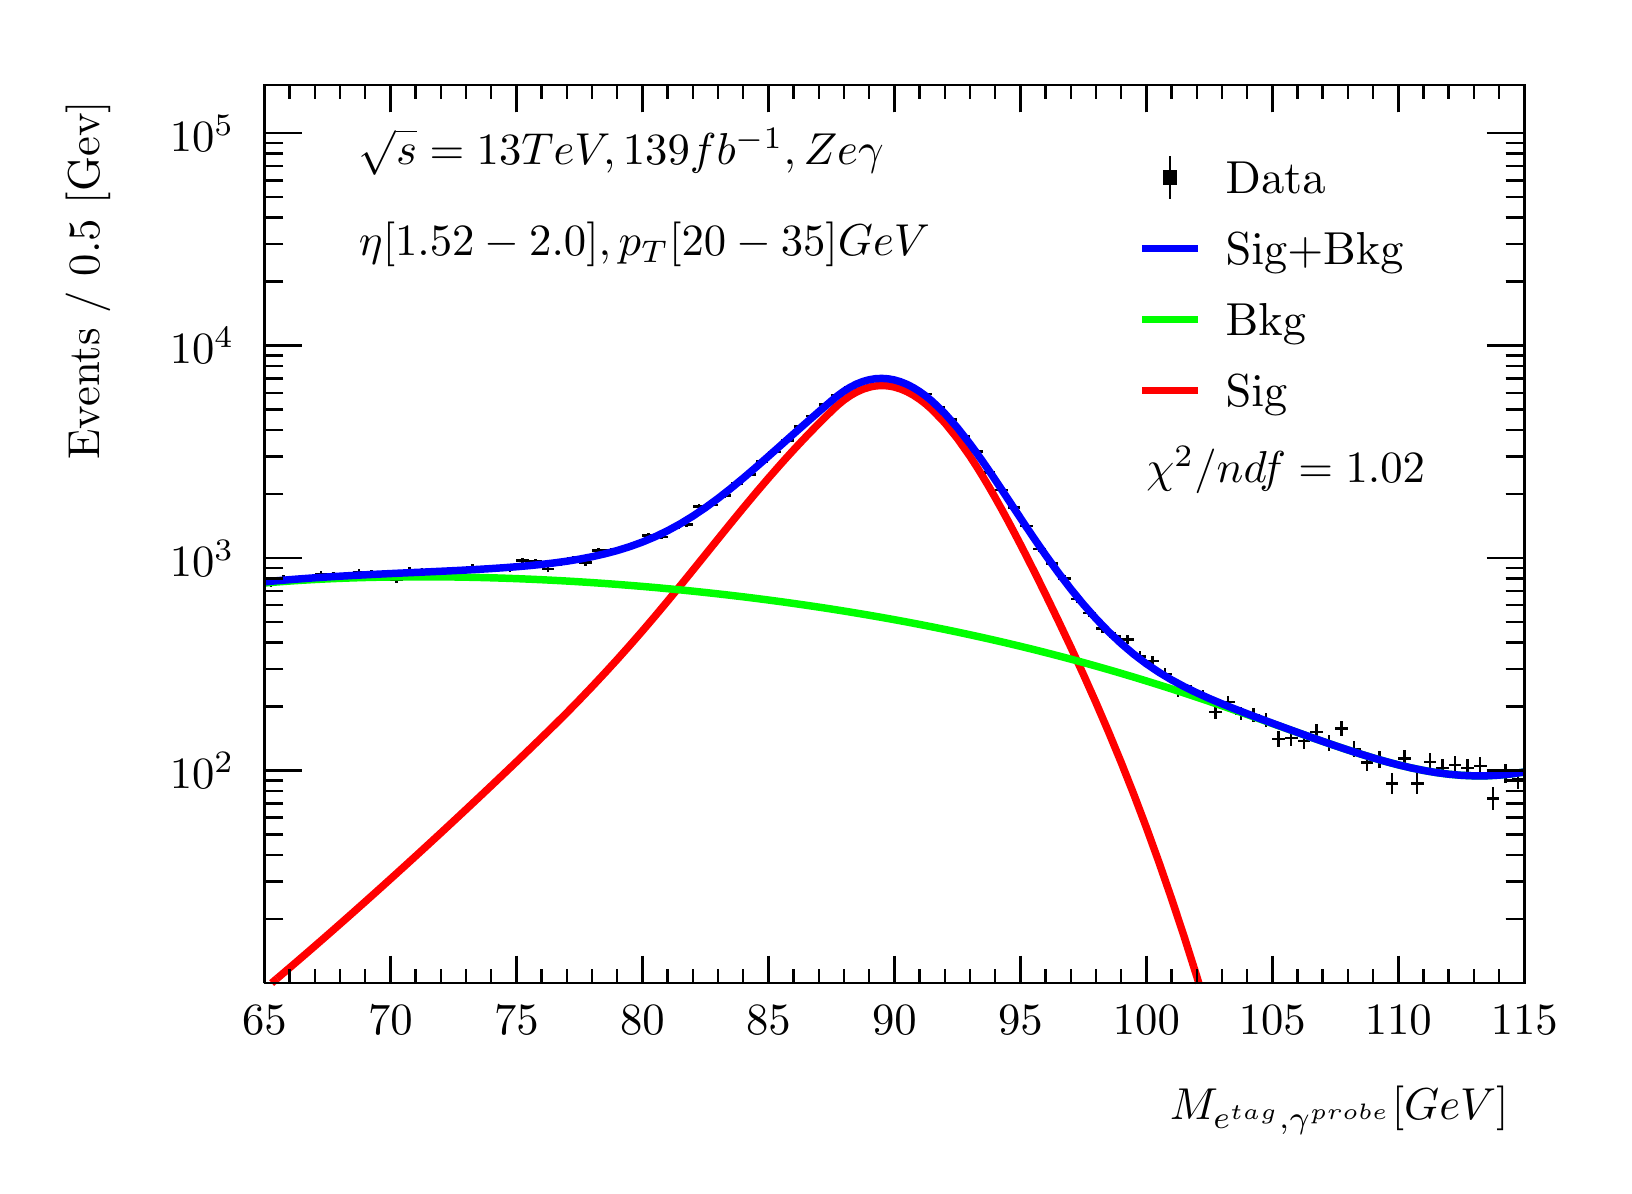
\begin{tikzpicture}
\pgfdeclareplotmark{cross} {
\pgfpathmoveto{\pgfpoint{-0.3\pgfplotmarksize}{\pgfplotmarksize}}
\pgfpathlineto{\pgfpoint{+0.3\pgfplotmarksize}{\pgfplotmarksize}}
\pgfpathlineto{\pgfpoint{+0.3\pgfplotmarksize}{0.3\pgfplotmarksize}}
\pgfpathlineto{\pgfpoint{+1\pgfplotmarksize}{0.3\pgfplotmarksize}}
\pgfpathlineto{\pgfpoint{+1\pgfplotmarksize}{-0.3\pgfplotmarksize}}
\pgfpathlineto{\pgfpoint{+0.3\pgfplotmarksize}{-0.3\pgfplotmarksize}}
\pgfpathlineto{\pgfpoint{+0.3\pgfplotmarksize}{-1.\pgfplotmarksize}}
\pgfpathlineto{\pgfpoint{-0.3\pgfplotmarksize}{-1.\pgfplotmarksize}}
\pgfpathlineto{\pgfpoint{-0.3\pgfplotmarksize}{-0.3\pgfplotmarksize}}
\pgfpathlineto{\pgfpoint{-1.\pgfplotmarksize}{-0.3\pgfplotmarksize}}
\pgfpathlineto{\pgfpoint{-1.\pgfplotmarksize}{0.3\pgfplotmarksize}}
\pgfpathlineto{\pgfpoint{-0.3\pgfplotmarksize}{0.3\pgfplotmarksize}}
\pgfpathclose
\pgfusepathqstroke
}
\pgfdeclareplotmark{cross*} {
\pgfpathmoveto{\pgfpoint{-0.3\pgfplotmarksize}{\pgfplotmarksize}}
\pgfpathlineto{\pgfpoint{+0.3\pgfplotmarksize}{\pgfplotmarksize}}
\pgfpathlineto{\pgfpoint{+0.3\pgfplotmarksize}{0.3\pgfplotmarksize}}
\pgfpathlineto{\pgfpoint{+1\pgfplotmarksize}{0.3\pgfplotmarksize}}
\pgfpathlineto{\pgfpoint{+1\pgfplotmarksize}{-0.3\pgfplotmarksize}}
\pgfpathlineto{\pgfpoint{+0.3\pgfplotmarksize}{-0.3\pgfplotmarksize}}
\pgfpathlineto{\pgfpoint{+0.3\pgfplotmarksize}{-1.\pgfplotmarksize}}
\pgfpathlineto{\pgfpoint{-0.3\pgfplotmarksize}{-1.\pgfplotmarksize}}
\pgfpathlineto{\pgfpoint{-0.3\pgfplotmarksize}{-0.3\pgfplotmarksize}}
\pgfpathlineto{\pgfpoint{-1.\pgfplotmarksize}{-0.3\pgfplotmarksize}}
\pgfpathlineto{\pgfpoint{-1.\pgfplotmarksize}{0.3\pgfplotmarksize}}
\pgfpathlineto{\pgfpoint{-0.3\pgfplotmarksize}{0.3\pgfplotmarksize}}
\pgfpathclose
\pgfusepathqfillstroke
}
\pgfdeclareplotmark{newstar} {
\pgfpathmoveto{\pgfqpoint{0pt}{\pgfplotmarksize}}
\pgfpathlineto{\pgfqpointpolar{44}{0.5\pgfplotmarksize}}
\pgfpathlineto{\pgfqpointpolar{18}{\pgfplotmarksize}}
\pgfpathlineto{\pgfqpointpolar{-20}{0.5\pgfplotmarksize}}
\pgfpathlineto{\pgfqpointpolar{-54}{\pgfplotmarksize}}
\pgfpathlineto{\pgfqpointpolar{-90}{0.5\pgfplotmarksize}}
\pgfpathlineto{\pgfqpointpolar{234}{\pgfplotmarksize}}
\pgfpathlineto{\pgfqpointpolar{198}{0.5\pgfplotmarksize}}
\pgfpathlineto{\pgfqpointpolar{162}{\pgfplotmarksize}}
\pgfpathlineto{\pgfqpointpolar{134}{0.5\pgfplotmarksize}}
\pgfpathclose
\pgfusepathqstroke
}
\pgfdeclareplotmark{newstar*} {
\pgfpathmoveto{\pgfqpoint{0pt}{\pgfplotmarksize}}
\pgfpathlineto{\pgfqpointpolar{44}{0.5\pgfplotmarksize}}
\pgfpathlineto{\pgfqpointpolar{18}{\pgfplotmarksize}}
\pgfpathlineto{\pgfqpointpolar{-20}{0.5\pgfplotmarksize}}
\pgfpathlineto{\pgfqpointpolar{-54}{\pgfplotmarksize}}
\pgfpathlineto{\pgfqpointpolar{-90}{0.5\pgfplotmarksize}}
\pgfpathlineto{\pgfqpointpolar{234}{\pgfplotmarksize}}
\pgfpathlineto{\pgfqpointpolar{198}{0.5\pgfplotmarksize}}
\pgfpathlineto{\pgfqpointpolar{162}{\pgfplotmarksize}}
\pgfpathlineto{\pgfqpointpolar{134}{0.5\pgfplotmarksize}}
\pgfpathclose
\pgfusepathqfillstroke
}
\definecolor{c}{rgb}{1,1,1};
\draw [color=c, fill=c] (0,0) rectangle (20,14.4361);
\draw [color=c, fill=c] (3,2.30977) rectangle (19,13.7143);
\definecolor{c}{rgb}{0,0,0};
\draw [c,line width=0.9] (3,2.30977) -- (3,13.7143) -- (19,13.7143) -- (19,2.30977) -- (3,2.30977);
\definecolor{c}{rgb}{1,1,1};
\draw [color=c, fill=c] (3,2.30977) rectangle (19,13.7143);
\definecolor{c}{rgb}{0,0,0};
\draw [c,line width=0.9] (3,2.30977) -- (3,13.7143) -- (19,13.7143) -- (19,2.30977) -- (3,2.30977);
\draw [c,line width=0.9] (3,2.30977) -- (19,2.30977);
\draw [c,line width=0.9] (3,2.65624) -- (3,2.30977);
\draw [c,line width=0.9] (3.32,2.48301) -- (3.32,2.30977);
\draw [c,line width=0.9] (3.64,2.48301) -- (3.64,2.30977);
\draw [c,line width=0.9] (3.96,2.48301) -- (3.96,2.30977);
\draw [c,line width=0.9] (4.28,2.48301) -- (4.28,2.30977);
\draw [c,line width=0.9] (4.6,2.65624) -- (4.6,2.30977);
\draw [c,line width=0.9] (4.92,2.48301) -- (4.92,2.30977);
\draw [c,line width=0.9] (5.24,2.48301) -- (5.24,2.30977);
\draw [c,line width=0.9] (5.56,2.48301) -- (5.56,2.30977);
\draw [c,line width=0.9] (5.88,2.48301) -- (5.88,2.30977);
\draw [c,line width=0.9] (6.2,2.65624) -- (6.2,2.30977);
\draw [c,line width=0.9] (6.52,2.48301) -- (6.52,2.30977);
\draw [c,line width=0.9] (6.84,2.48301) -- (6.84,2.30977);
\draw [c,line width=0.9] (7.16,2.48301) -- (7.16,2.30977);
\draw [c,line width=0.9] (7.48,2.48301) -- (7.48,2.30977);
\draw [c,line width=0.9] (7.8,2.65624) -- (7.8,2.30977);
\draw [c,line width=0.9] (8.12,2.48301) -- (8.12,2.30977);
\draw [c,line width=0.9] (8.44,2.48301) -- (8.44,2.30977);
\draw [c,line width=0.9] (8.76,2.48301) -- (8.76,2.30977);
\draw [c,line width=0.9] (9.08,2.48301) -- (9.08,2.30977);
\draw [c,line width=0.9] (9.4,2.65624) -- (9.4,2.30977);
\draw [c,line width=0.9] (9.72,2.48301) -- (9.72,2.30977);
\draw [c,line width=0.9] (10.04,2.48301) -- (10.04,2.30977);
\draw [c,line width=0.9] (10.36,2.48301) -- (10.36,2.30977);
\draw [c,line width=0.9] (10.68,2.48301) -- (10.68,2.30977);
\draw [c,line width=0.9] (11,2.65624) -- (11,2.30977);
\draw [c,line width=0.9] (11.32,2.48301) -- (11.32,2.30977);
\draw [c,line width=0.9] (11.64,2.48301) -- (11.64,2.30977);
\draw [c,line width=0.9] (11.96,2.48301) -- (11.96,2.30977);
\draw [c,line width=0.9] (12.28,2.48301) -- (12.28,2.30977);
\draw [c,line width=0.9] (12.6,2.65624) -- (12.6,2.30977);
\draw [c,line width=0.9] (12.92,2.48301) -- (12.92,2.30977);
\draw [c,line width=0.9] (13.24,2.48301) -- (13.24,2.30977);
\draw [c,line width=0.9] (13.56,2.48301) -- (13.56,2.30977);
\draw [c,line width=0.9] (13.88,2.48301) -- (13.88,2.30977);
\draw [c,line width=0.9] (14.2,2.65624) -- (14.2,2.30977);
\draw [c,line width=0.9] (14.52,2.48301) -- (14.52,2.30977);
\draw [c,line width=0.9] (14.84,2.48301) -- (14.84,2.30977);
\draw [c,line width=0.9] (15.16,2.48301) -- (15.16,2.30977);
\draw [c,line width=0.9] (15.48,2.48301) -- (15.48,2.30977);
\draw [c,line width=0.9] (15.8,2.65624) -- (15.8,2.30977);
\draw [c,line width=0.9] (16.12,2.48301) -- (16.12,2.30977);
\draw [c,line width=0.9] (16.44,2.48301) -- (16.44,2.30977);
\draw [c,line width=0.9] (16.76,2.48301) -- (16.76,2.30977);
\draw [c,line width=0.9] (17.08,2.48301) -- (17.08,2.30977);
\draw [c,line width=0.9] (17.4,2.65624) -- (17.4,2.30977);
\draw [c,line width=0.9] (17.72,2.48301) -- (17.72,2.30977);
\draw [c,line width=0.9] (18.04,2.48301) -- (18.04,2.30977);
\draw [c,line width=0.9] (18.36,2.48301) -- (18.36,2.30977);
\draw [c,line width=0.9] (18.68,2.48301) -- (18.68,2.30977);
\draw [c,line width=0.9] (19,2.65624) -- (19,2.30977);
\draw [c,line width=0.9] (19,2.65624) -- (19,2.30977);
\draw [anchor=base] (3,1.66015) node[scale=1.61424, color=c, rotate=0]{65};
\draw [anchor=base] (4.6,1.66015) node[scale=1.61424, color=c, rotate=0]{70};
\draw [anchor=base] (6.2,1.66015) node[scale=1.61424, color=c, rotate=0]{75};
\draw [anchor=base] (7.8,1.66015) node[scale=1.61424, color=c, rotate=0]{80};
\draw [anchor=base] (9.4,1.66015) node[scale=1.61424, color=c, rotate=0]{85};
\draw [anchor=base] (11,1.66015) node[scale=1.61424, color=c, rotate=0]{90};
\draw [anchor=base] (12.6,1.66015) node[scale=1.61424, color=c, rotate=0]{95};
\draw [anchor=base] (14.2,1.66015) node[scale=1.61424, color=c, rotate=0]{100};
\draw [anchor=base] (15.8,1.66015) node[scale=1.61424, color=c, rotate=0]{105};
\draw [anchor=base] (17.4,1.66015) node[scale=1.61424, color=c, rotate=0]{110};
\draw [anchor=base] (19,1.66015) node[scale=1.61424, color=c, rotate=0]{115};
\draw [anchor= east] (19,0.692932) node[scale=1.61424, color=c, rotate=0]{$M_{e^{tag}, \gamma^{probe}}  [GeV]$};
\draw [c,line width=0.9] (3,13.7143) -- (19,13.7143);
\draw [c,line width=0.9] (3,13.3678) -- (3,13.7143);
\draw [c,line width=0.9] (3.32,13.5411) -- (3.32,13.7143);
\draw [c,line width=0.9] (3.64,13.5411) -- (3.64,13.7143);
\draw [c,line width=0.9] (3.96,13.5411) -- (3.96,13.7143);
\draw [c,line width=0.9] (4.28,13.5411) -- (4.28,13.7143);
\draw [c,line width=0.9] (4.6,13.3678) -- (4.6,13.7143);
\draw [c,line width=0.9] (4.92,13.5411) -- (4.92,13.7143);
\draw [c,line width=0.9] (5.24,13.5411) -- (5.24,13.7143);
\draw [c,line width=0.9] (5.56,13.5411) -- (5.56,13.7143);
\draw [c,line width=0.9] (5.88,13.5411) -- (5.88,13.7143);
\draw [c,line width=0.9] (6.2,13.3678) -- (6.2,13.7143);
\draw [c,line width=0.9] (6.52,13.5411) -- (6.52,13.7143);
\draw [c,line width=0.9] (6.84,13.5411) -- (6.84,13.7143);
\draw [c,line width=0.9] (7.16,13.5411) -- (7.16,13.7143);
\draw [c,line width=0.9] (7.48,13.5411) -- (7.48,13.7143);
\draw [c,line width=0.9] (7.8,13.3678) -- (7.8,13.7143);
\draw [c,line width=0.9] (8.12,13.5411) -- (8.12,13.7143);
\draw [c,line width=0.9] (8.44,13.5411) -- (8.44,13.7143);
\draw [c,line width=0.9] (8.76,13.5411) -- (8.76,13.7143);
\draw [c,line width=0.9] (9.08,13.5411) -- (9.08,13.7143);
\draw [c,line width=0.9] (9.4,13.3678) -- (9.4,13.7143);
\draw [c,line width=0.9] (9.72,13.5411) -- (9.72,13.7143);
\draw [c,line width=0.9] (10.04,13.5411) -- (10.04,13.7143);
\draw [c,line width=0.9] (10.36,13.5411) -- (10.36,13.7143);
\draw [c,line width=0.9] (10.68,13.5411) -- (10.68,13.7143);
\draw [c,line width=0.9] (11,13.3678) -- (11,13.7143);
\draw [c,line width=0.9] (11.32,13.5411) -- (11.32,13.7143);
\draw [c,line width=0.9] (11.64,13.5411) -- (11.64,13.7143);
\draw [c,line width=0.9] (11.96,13.5411) -- (11.96,13.7143);
\draw [c,line width=0.9] (12.28,13.5411) -- (12.28,13.7143);
\draw [c,line width=0.9] (12.6,13.3678) -- (12.6,13.7143);
\draw [c,line width=0.9] (12.92,13.5411) -- (12.92,13.7143);
\draw [c,line width=0.9] (13.24,13.5411) -- (13.24,13.7143);
\draw [c,line width=0.9] (13.56,13.5411) -- (13.56,13.7143);
\draw [c,line width=0.9] (13.88,13.5411) -- (13.88,13.7143);
\draw [c,line width=0.9] (14.2,13.3678) -- (14.2,13.7143);
\draw [c,line width=0.9] (14.52,13.5411) -- (14.52,13.7143);
\draw [c,line width=0.9] (14.84,13.5411) -- (14.84,13.7143);
\draw [c,line width=0.9] (15.16,13.5411) -- (15.16,13.7143);
\draw [c,line width=0.9] (15.48,13.5411) -- (15.48,13.7143);
\draw [c,line width=0.9] (15.8,13.3678) -- (15.8,13.7143);
\draw [c,line width=0.9] (16.12,13.5411) -- (16.12,13.7143);
\draw [c,line width=0.9] (16.44,13.5411) -- (16.44,13.7143);
\draw [c,line width=0.9] (16.76,13.5411) -- (16.76,13.7143);
\draw [c,line width=0.9] (17.08,13.5411) -- (17.08,13.7143);
\draw [c,line width=0.9] (17.4,13.3678) -- (17.4,13.7143);
\draw [c,line width=0.9] (17.72,13.5411) -- (17.72,13.7143);
\draw [c,line width=0.9] (18.04,13.5411) -- (18.04,13.7143);
\draw [c,line width=0.9] (18.36,13.5411) -- (18.36,13.7143);
\draw [c,line width=0.9] (18.68,13.5411) -- (18.68,13.7143);
\draw [c,line width=0.9] (19,13.3678) -- (19,13.7143);
\draw [c,line width=0.9] (19,13.3678) -- (19,13.7143);
\draw [c,line width=0.9] (3,2.30977) -- (3,13.7143);
\draw [c,line width=0.9] (3.237,3.12209) -- (3,3.12209);
\draw [c,line width=0.9] (3.237,3.59726) -- (3,3.59726);
\draw [c,line width=0.9] (3.237,3.9344) -- (3,3.9344);
\draw [c,line width=0.9] (3.237,4.19591) -- (3,4.19591);
\draw [c,line width=0.9] (3.237,4.40958) -- (3,4.40958);
\draw [c,line width=0.9] (3.237,4.59023) -- (3,4.59023);
\draw [c,line width=0.9] (3.237,4.74672) -- (3,4.74672);
\draw [c,line width=0.9] (3.237,4.88475) -- (3,4.88475);
\draw [c,line width=0.9] (3.474,5.00822) -- (3,5.00822);
\draw [anchor= east] (2.82,5.00822) node[scale=1.61424, color=c, rotate=0]{$10^{2}$};
\draw [c,line width=0.9] (3.237,5.82054) -- (3,5.82054);
\draw [c,line width=0.9] (3.237,6.29571) -- (3,6.29571);
\draw [c,line width=0.9] (3.237,6.63285) -- (3,6.63285);
\draw [c,line width=0.9] (3.237,6.89436) -- (3,6.89436);
\draw [c,line width=0.9] (3.237,7.10803) -- (3,7.10803);
\draw [c,line width=0.9] (3.237,7.28868) -- (3,7.28868);
\draw [c,line width=0.9] (3.237,7.44517) -- (3,7.44517);
\draw [c,line width=0.9] (3.237,7.5832) -- (3,7.5832);
\draw [c,line width=0.9] (3.474,7.70668) -- (3,7.70668);
\draw [anchor= east] (2.82,7.70668) node[scale=1.61424, color=c, rotate=0]{$10^{3}$};
\draw [c,line width=0.9] (3.237,8.51899) -- (3,8.51899);
\draw [c,line width=0.9] (3.237,8.99417) -- (3,8.99417);
\draw [c,line width=0.9] (3.237,9.33131) -- (3,9.33131);
\draw [c,line width=0.9] (3.237,9.59281) -- (3,9.59281);
\draw [c,line width=0.9] (3.237,9.80648) -- (3,9.80648);
\draw [c,line width=0.9] (3.237,9.98713) -- (3,9.98713);
\draw [c,line width=0.9] (3.237,10.1436) -- (3,10.1436);
\draw [c,line width=0.9] (3.237,10.2817) -- (3,10.2817);
\draw [c,line width=0.9] (3.474,10.4051) -- (3,10.4051);
\draw [anchor= east] (2.82,10.4051) node[scale=1.61424, color=c, rotate=0]{$10^{4}$};
\draw [c,line width=0.9] (3.237,11.2174) -- (3,11.2174);
\draw [c,line width=0.9] (3.237,11.6926) -- (3,11.6926);
\draw [c,line width=0.9] (3.237,12.0298) -- (3,12.0298);
\draw [c,line width=0.9] (3.237,12.2913) -- (3,12.2913);
\draw [c,line width=0.9] (3.237,12.5049) -- (3,12.5049);
\draw [c,line width=0.9] (3.237,12.6856) -- (3,12.6856);
\draw [c,line width=0.9] (3.237,12.8421) -- (3,12.8421);
\draw [c,line width=0.9] (3.237,12.9801) -- (3,12.9801);
\draw [c,line width=0.9] (3.474,13.1036) -- (3,13.1036);
\draw [anchor= east] (2.82,13.1036) node[scale=1.61424, color=c, rotate=0]{$10^{5}$};
\draw [anchor= east] (0.76,13.7143) node[scale=1.61424, color=c, rotate=90]{Events / 0.5 [Gev]};
\draw [c,line width=0.9] (19,2.30977) -- (19,13.7143);
\draw [c,line width=0.9] (18.763,3.12209) -- (19,3.12209);
\draw [c,line width=0.9] (18.763,3.59726) -- (19,3.59726);
\draw [c,line width=0.9] (18.763,3.9344) -- (19,3.9344);
\draw [c,line width=0.9] (18.763,4.19591) -- (19,4.19591);
\draw [c,line width=0.9] (18.763,4.40958) -- (19,4.40958);
\draw [c,line width=0.9] (18.763,4.59023) -- (19,4.59023);
\draw [c,line width=0.9] (18.763,4.74672) -- (19,4.74672);
\draw [c,line width=0.9] (18.763,4.88475) -- (19,4.88475);
\draw [c,line width=0.9] (18.526,5.00822) -- (19,5.00822);
\draw [c,line width=0.9] (18.763,5.82054) -- (19,5.82054);
\draw [c,line width=0.9] (18.763,6.29571) -- (19,6.29571);
\draw [c,line width=0.9] (18.763,6.63285) -- (19,6.63285);
\draw [c,line width=0.9] (18.763,6.89436) -- (19,6.89436);
\draw [c,line width=0.9] (18.763,7.10803) -- (19,7.10803);
\draw [c,line width=0.9] (18.763,7.28868) -- (19,7.28868);
\draw [c,line width=0.9] (18.763,7.44517) -- (19,7.44517);
\draw [c,line width=0.9] (18.763,7.5832) -- (19,7.5832);
\draw [c,line width=0.9] (18.526,7.70668) -- (19,7.70668);
\draw [c,line width=0.9] (18.763,8.51899) -- (19,8.51899);
\draw [c,line width=0.9] (18.763,8.99417) -- (19,8.99417);
\draw [c,line width=0.9] (18.763,9.33131) -- (19,9.33131);
\draw [c,line width=0.9] (18.763,9.59281) -- (19,9.59281);
\draw [c,line width=0.9] (18.763,9.80648) -- (19,9.80648);
\draw [c,line width=0.9] (18.763,9.98713) -- (19,9.98713);
\draw [c,line width=0.9] (18.763,10.1436) -- (19,10.1436);
\draw [c,line width=0.9] (18.763,10.2817) -- (19,10.2817);
\draw [c,line width=0.9] (18.526,10.4051) -- (19,10.4051);
\draw [c,line width=0.9] (18.763,11.2174) -- (19,11.2174);
\draw [c,line width=0.9] (18.763,11.6926) -- (19,11.6926);
\draw [c,line width=0.9] (18.763,12.0298) -- (19,12.0298);
\draw [c,line width=0.9] (18.763,12.2913) -- (19,12.2913);
\draw [c,line width=0.9] (18.763,12.5049) -- (19,12.5049);
\draw [c,line width=0.9] (18.763,12.6856) -- (19,12.6856);
\draw [c,line width=0.9] (18.763,12.8421) -- (19,12.8421);
\draw [c,line width=0.9] (18.763,12.9801) -- (19,12.9801);
\draw [c,line width=0.9] (18.526,13.1036) -- (19,13.1036);
\draw [c,line width=0.9] (3.08,7.38352) -- (3,7.38352);
\draw [c,line width=0.9] (3,7.38352) -- (3,7.38352);
\draw [c,line width=0.9] (3.08,7.38352) -- (3.16,7.38352);
\draw [c,line width=0.9] (3.16,7.38352) -- (3.16,7.38352);
\draw [c,line width=0.9] (3.08,7.38352) -- (3.08,7.42605);
\draw [c,line width=0.9] (3.08,7.42605) -- (3.08,7.42605);
\draw [c,line width=0.9] (3.08,7.38352) -- (3.08,7.34098);
\draw [c,line width=0.9] (3.08,7.34098) -- (3.08,7.34098);
\draw [c,line width=0.9] (3.24,7.44517) -- (3.16,7.44517);
\draw [c,line width=0.9] (3.16,7.44517) -- (3.16,7.44517);
\draw [c,line width=0.9] (3.24,7.44517) -- (3.32,7.44517);
\draw [c,line width=0.9] (3.32,7.44517) -- (3.32,7.44517);
\draw [c,line width=0.9] (3.24,7.44517) -- (3.24,7.4866);
\draw [c,line width=0.9] (3.24,7.4866) -- (3.24,7.4866);
\draw [c,line width=0.9] (3.24,7.44517) -- (3.24,7.40374);
\draw [c,line width=0.9] (3.24,7.40374) -- (3.24,7.40374);
\draw [c,line width=0.9] (3.4,7.4155) -- (3.32,7.4155);
\draw [c,line width=0.9] (3.32,7.4155) -- (3.32,7.4155);
\draw [c,line width=0.9] (3.4,7.4155) -- (3.48,7.4155);
\draw [c,line width=0.9] (3.48,7.4155) -- (3.48,7.4155);
\draw [c,line width=0.9] (3.4,7.4155) -- (3.4,7.45746);
\draw [c,line width=0.9] (3.4,7.45746) -- (3.4,7.45746);
\draw [c,line width=0.9] (3.4,7.4155) -- (3.4,7.37354);
\draw [c,line width=0.9] (3.4,7.37354) -- (3.4,7.37354);
\draw [c,line width=0.9] (3.56,7.45102) -- (3.48,7.45102);
\draw [c,line width=0.9] (3.48,7.45102) -- (3.48,7.45102);
\draw [c,line width=0.9] (3.56,7.45102) -- (3.64,7.45102);
\draw [c,line width=0.9] (3.64,7.45102) -- (3.64,7.45102);
\draw [c,line width=0.9] (3.56,7.45102) -- (3.56,7.49234);
\draw [c,line width=0.9] (3.56,7.49234) -- (3.56,7.49234);
\draw [c,line width=0.9] (3.56,7.45102) -- (3.56,7.40969);
\draw [c,line width=0.9] (3.56,7.40969) -- (3.56,7.40969);
\draw [c,line width=0.9] (3.72,7.50235) -- (3.64,7.50235);
\draw [c,line width=0.9] (3.64,7.50235) -- (3.64,7.50235);
\draw [c,line width=0.9] (3.72,7.50235) -- (3.8,7.50235);
\draw [c,line width=0.9] (3.8,7.50235) -- (3.8,7.50235);
\draw [c,line width=0.9] (3.72,7.50235) -- (3.72,7.54278);
\draw [c,line width=0.9] (3.72,7.54278) -- (3.72,7.54278);
\draw [c,line width=0.9] (3.72,7.50235) -- (3.72,7.46192);
\draw [c,line width=0.9] (3.72,7.46192) -- (3.72,7.46192);
\draw [c,line width=0.9] (3.88,7.49395) -- (3.8,7.49395);
\draw [c,line width=0.9] (3.8,7.49395) -- (3.8,7.49395);
\draw [c,line width=0.9] (3.88,7.49395) -- (3.96,7.49395);
\draw [c,line width=0.9] (3.96,7.49395) -- (3.96,7.49395);
\draw [c,line width=0.9] (3.88,7.49395) -- (3.88,7.53453);
\draw [c,line width=0.9] (3.88,7.53453) -- (3.88,7.53453);
\draw [c,line width=0.9] (3.88,7.49395) -- (3.88,7.45337);
\draw [c,line width=0.9] (3.88,7.45337) -- (3.88,7.45337);
\draw [c,line width=0.9] (4.04,7.45538) -- (3.96,7.45538);
\draw [c,line width=0.9] (3.96,7.45538) -- (3.96,7.45538);
\draw [c,line width=0.9] (4.04,7.45538) -- (4.12,7.45538);
\draw [c,line width=0.9] (4.12,7.45538) -- (4.12,7.45538);
\draw [c,line width=0.9] (4.04,7.45538) -- (4.04,7.49663);
\draw [c,line width=0.9] (4.04,7.49663) -- (4.04,7.49663);
\draw [c,line width=0.9] (4.04,7.45538) -- (4.04,7.41413);
\draw [c,line width=0.9] (4.04,7.41413) -- (4.04,7.41413);
\draw [c,line width=0.9] (4.2,7.52583) -- (4.12,7.52583);
\draw [c,line width=0.9] (4.12,7.52583) -- (4.12,7.52583);
\draw [c,line width=0.9] (4.2,7.52583) -- (4.28,7.52583);
\draw [c,line width=0.9] (4.28,7.52583) -- (4.28,7.52583);
\draw [c,line width=0.9] (4.2,7.52583) -- (4.2,7.56586);
\draw [c,line width=0.9] (4.2,7.56586) -- (4.2,7.56586);
\draw [c,line width=0.9] (4.2,7.52583) -- (4.2,7.4858);
\draw [c,line width=0.9] (4.2,7.4858) -- (4.2,7.4858);
\draw [c,line width=0.9] (4.36,7.51897) -- (4.28,7.51897);
\draw [c,line width=0.9] (4.28,7.51897) -- (4.28,7.51897);
\draw [c,line width=0.9] (4.36,7.51897) -- (4.44,7.51897);
\draw [c,line width=0.9] (4.44,7.51897) -- (4.44,7.51897);
\draw [c,line width=0.9] (4.36,7.51897) -- (4.36,7.55912);
\draw [c,line width=0.9] (4.36,7.55912) -- (4.36,7.55912);
\draw [c,line width=0.9] (4.36,7.51897) -- (4.36,7.47883);
\draw [c,line width=0.9] (4.36,7.47883) -- (4.36,7.47883);
\draw [c,line width=0.9] (4.52,7.50653) -- (4.44,7.50653);
\draw [c,line width=0.9] (4.44,7.50653) -- (4.44,7.50653);
\draw [c,line width=0.9] (4.52,7.50653) -- (4.6,7.50653);
\draw [c,line width=0.9] (4.6,7.50653) -- (4.6,7.50653);
\draw [c,line width=0.9] (4.52,7.50653) -- (4.52,7.54689);
\draw [c,line width=0.9] (4.52,7.54689) -- (4.52,7.54689);
\draw [c,line width=0.9] (4.52,7.50653) -- (4.52,7.46617);
\draw [c,line width=0.9] (4.52,7.46617) -- (4.52,7.46617);
\draw [c,line width=0.9] (4.68,7.43782) -- (4.6,7.43782);
\draw [c,line width=0.9] (4.6,7.43782) -- (4.6,7.43782);
\draw [c,line width=0.9] (4.68,7.43782) -- (4.76,7.43782);
\draw [c,line width=0.9] (4.76,7.43782) -- (4.76,7.43782);
\draw [c,line width=0.9] (4.68,7.43782) -- (4.68,7.47939);
\draw [c,line width=0.9] (4.68,7.47939) -- (4.68,7.47939);
\draw [c,line width=0.9] (4.68,7.43782) -- (4.68,7.39626);
\draw [c,line width=0.9] (4.68,7.39626) -- (4.68,7.39626);
\draw [c,line width=0.9] (4.84,7.55687) -- (4.76,7.55687);
\draw [c,line width=0.9] (4.76,7.55687) -- (4.76,7.55687);
\draw [c,line width=0.9] (4.84,7.55687) -- (4.92,7.55687);
\draw [c,line width=0.9] (4.92,7.55687) -- (4.92,7.55687);
\draw [c,line width=0.9] (4.84,7.55687) -- (4.84,7.59637);
\draw [c,line width=0.9] (4.84,7.59637) -- (4.84,7.59637);
\draw [c,line width=0.9] (4.84,7.55687) -- (4.84,7.51736);
\draw [c,line width=0.9] (4.84,7.51736) -- (4.84,7.51736);
\draw [c,line width=0.9] (5,7.54213) -- (4.92,7.54213);
\draw [c,line width=0.9] (4.92,7.54213) -- (4.92,7.54213);
\draw [c,line width=0.9] (5,7.54213) -- (5.08,7.54213);
\draw [c,line width=0.9] (5.08,7.54213) -- (5.08,7.54213);
\draw [c,line width=0.9] (5,7.54213) -- (5,7.58188);
\draw [c,line width=0.9] (5,7.58188) -- (5,7.58188);
\draw [c,line width=0.9] (5,7.54213) -- (5,7.50237);
\draw [c,line width=0.9] (5,7.50237) -- (5,7.50237);
\draw [c,line width=0.9] (5.16,7.52309) -- (5.08,7.52309);
\draw [c,line width=0.9] (5.08,7.52309) -- (5.08,7.52309);
\draw [c,line width=0.9] (5.16,7.52309) -- (5.24,7.52309);
\draw [c,line width=0.9] (5.24,7.52309) -- (5.24,7.52309);
\draw [c,line width=0.9] (5.16,7.52309) -- (5.16,7.56317);
\draw [c,line width=0.9] (5.16,7.56317) -- (5.16,7.56317);
\draw [c,line width=0.9] (5.16,7.52309) -- (5.16,7.48302);
\draw [c,line width=0.9] (5.16,7.48302) -- (5.16,7.48302);
\draw [c,line width=0.9] (5.32,7.50374) -- (5.24,7.50374);
\draw [c,line width=0.9] (5.24,7.50374) -- (5.24,7.50374);
\draw [c,line width=0.9] (5.32,7.50374) -- (5.4,7.50374);
\draw [c,line width=0.9] (5.4,7.50374) -- (5.4,7.50374);
\draw [c,line width=0.9] (5.32,7.50374) -- (5.32,7.54415);
\draw [c,line width=0.9] (5.32,7.54415) -- (5.32,7.54415);
\draw [c,line width=0.9] (5.32,7.50374) -- (5.32,7.46334);
\draw [c,line width=0.9] (5.32,7.46334) -- (5.32,7.46334);
\draw [c,line width=0.9] (5.48,7.47981) -- (5.4,7.47981);
\draw [c,line width=0.9] (5.4,7.47981) -- (5.4,7.47981);
\draw [c,line width=0.9] (5.48,7.47981) -- (5.56,7.47981);
\draw [c,line width=0.9] (5.56,7.47981) -- (5.56,7.47981);
\draw [c,line width=0.9] (5.48,7.47981) -- (5.48,7.52064);
\draw [c,line width=0.9] (5.48,7.52064) -- (5.48,7.52064);
\draw [c,line width=0.9] (5.48,7.47981) -- (5.48,7.43899);
\draw [c,line width=0.9] (5.48,7.43899) -- (5.48,7.43899);
\draw [c,line width=0.9] (5.64,7.5897) -- (5.56,7.5897);
\draw [c,line width=0.9] (5.56,7.5897) -- (5.56,7.5897);
\draw [c,line width=0.9] (5.64,7.5897) -- (5.72,7.5897);
\draw [c,line width=0.9] (5.72,7.5897) -- (5.72,7.5897);
\draw [c,line width=0.9] (5.64,7.5897) -- (5.64,7.62865);
\draw [c,line width=0.9] (5.64,7.62865) -- (5.64,7.62865);
\draw [c,line width=0.9] (5.64,7.5897) -- (5.64,7.55074);
\draw [c,line width=0.9] (5.64,7.55074) -- (5.64,7.55074);
\draw [c,line width=0.9] (5.8,7.56483) -- (5.72,7.56483);
\draw [c,line width=0.9] (5.72,7.56483) -- (5.72,7.56483);
\draw [c,line width=0.9] (5.8,7.56483) -- (5.88,7.56483);
\draw [c,line width=0.9] (5.88,7.56483) -- (5.88,7.56483);
\draw [c,line width=0.9] (5.8,7.56483) -- (5.8,7.6042);
\draw [c,line width=0.9] (5.8,7.6042) -- (5.8,7.6042);
\draw [c,line width=0.9] (5.8,7.56483) -- (5.8,7.52546);
\draw [c,line width=0.9] (5.8,7.52546) -- (5.8,7.52546);
\draw [c,line width=0.9] (5.96,7.56351) -- (5.88,7.56351);
\draw [c,line width=0.9] (5.88,7.56351) -- (5.88,7.56351);
\draw [c,line width=0.9] (5.96,7.56351) -- (6.04,7.56351);
\draw [c,line width=0.9] (6.04,7.56351) -- (6.04,7.56351);
\draw [c,line width=0.9] (5.96,7.56351) -- (5.96,7.6029);
\draw [c,line width=0.9] (5.96,7.6029) -- (5.96,7.6029);
\draw [c,line width=0.9] (5.96,7.56351) -- (5.96,7.52412);
\draw [c,line width=0.9] (5.96,7.52412) -- (5.96,7.52412);
\draw [c,line width=0.9] (6.12,7.57405) -- (6.04,7.57405);
\draw [c,line width=0.9] (6.04,7.57405) -- (6.04,7.57405);
\draw [c,line width=0.9] (6.12,7.57405) -- (6.2,7.57405);
\draw [c,line width=0.9] (6.2,7.57405) -- (6.2,7.57405);
\draw [c,line width=0.9] (6.12,7.57405) -- (6.12,7.61327);
\draw [c,line width=0.9] (6.12,7.61327) -- (6.12,7.61327);
\draw [c,line width=0.9] (6.12,7.57405) -- (6.12,7.53484);
\draw [c,line width=0.9] (6.12,7.53484) -- (6.12,7.53484);
\draw [c,line width=0.9] (6.28,7.6734) -- (6.2,7.6734);
\draw [c,line width=0.9] (6.2,7.6734) -- (6.2,7.6734);
\draw [c,line width=0.9] (6.28,7.6734) -- (6.36,7.6734);
\draw [c,line width=0.9] (6.36,7.6734) -- (6.36,7.6734);
\draw [c,line width=0.9] (6.28,7.6734) -- (6.28,7.71098);
\draw [c,line width=0.9] (6.28,7.71098) -- (6.28,7.71098);
\draw [c,line width=0.9] (6.28,7.6734) -- (6.28,7.63581);
\draw [c,line width=0.9] (6.28,7.63581) -- (6.28,7.63581);
\draw [c,line width=0.9] (6.44,7.66128) -- (6.36,7.66128);
\draw [c,line width=0.9] (6.36,7.66128) -- (6.36,7.66128);
\draw [c,line width=0.9] (6.44,7.66128) -- (6.52,7.66128);
\draw [c,line width=0.9] (6.52,7.66128) -- (6.52,7.66128);
\draw [c,line width=0.9] (6.44,7.66128) -- (6.44,7.69906);
\draw [c,line width=0.9] (6.44,7.69906) -- (6.44,7.69906);
\draw [c,line width=0.9] (6.44,7.66128) -- (6.44,7.62349);
\draw [c,line width=0.9] (6.44,7.62349) -- (6.44,7.62349);
\draw [c,line width=0.9] (6.6,7.56747) -- (6.52,7.56747);
\draw [c,line width=0.9] (6.52,7.56747) -- (6.52,7.56747);
\draw [c,line width=0.9] (6.6,7.56747) -- (6.68,7.56747);
\draw [c,line width=0.9] (6.68,7.56747) -- (6.68,7.56747);
\draw [c,line width=0.9] (6.6,7.56747) -- (6.6,7.6068);
\draw [c,line width=0.9] (6.6,7.6068) -- (6.6,7.6068);
\draw [c,line width=0.9] (6.6,7.56747) -- (6.6,7.52815);
\draw [c,line width=0.9] (6.6,7.52815) -- (6.6,7.52815);
\draw [c,line width=0.9] (6.76,7.65026) -- (6.68,7.65026);
\draw [c,line width=0.9] (6.68,7.65026) -- (6.68,7.65026);
\draw [c,line width=0.9] (6.76,7.65026) -- (6.84,7.65026);
\draw [c,line width=0.9] (6.84,7.65026) -- (6.84,7.65026);
\draw [c,line width=0.9] (6.76,7.65026) -- (6.76,7.68822);
\draw [c,line width=0.9] (6.76,7.68822) -- (6.76,7.68822);
\draw [c,line width=0.9] (6.76,7.65026) -- (6.76,7.6123);
\draw [c,line width=0.9] (6.76,7.6123) -- (6.76,7.6123);
\draw [c,line width=0.9] (6.92,7.7008) -- (6.84,7.7008);
\draw [c,line width=0.9] (6.84,7.7008) -- (6.84,7.7008);
\draw [c,line width=0.9] (6.92,7.7008) -- (7,7.7008);
\draw [c,line width=0.9] (7,7.7008) -- (7,7.7008);
\draw [c,line width=0.9] (6.92,7.7008) -- (6.92,7.73796);
\draw [c,line width=0.9] (6.92,7.73796) -- (6.92,7.73796);
\draw [c,line width=0.9] (6.92,7.7008) -- (6.92,7.66365);
\draw [c,line width=0.9] (6.92,7.66365) -- (6.92,7.66365);
\draw [c,line width=0.9] (7.08,7.65026) -- (7,7.65026);
\draw [c,line width=0.9] (7,7.65026) -- (7,7.65026);
\draw [c,line width=0.9] (7.08,7.65026) -- (7.16,7.65026);
\draw [c,line width=0.9] (7.16,7.65026) -- (7.16,7.65026);
\draw [c,line width=0.9] (7.08,7.65026) -- (7.08,7.68822);
\draw [c,line width=0.9] (7.08,7.68822) -- (7.08,7.68822);
\draw [c,line width=0.9] (7.08,7.65026) -- (7.08,7.6123);
\draw [c,line width=0.9] (7.08,7.6123) -- (7.08,7.6123);
\draw [c,line width=0.9] (7.24,7.80012) -- (7.16,7.80012);
\draw [c,line width=0.9] (7.16,7.80012) -- (7.16,7.80012);
\draw [c,line width=0.9] (7.24,7.80012) -- (7.32,7.80012);
\draw [c,line width=0.9] (7.32,7.80012) -- (7.32,7.80012);
\draw [c,line width=0.9] (7.24,7.80012) -- (7.24,7.83573);
\draw [c,line width=0.9] (7.24,7.83573) -- (7.24,7.83573);
\draw [c,line width=0.9] (7.24,7.80012) -- (7.24,7.76451);
\draw [c,line width=0.9] (7.24,7.76451) -- (7.24,7.76451);
\draw [c,line width=0.9] (7.4,7.80228) -- (7.32,7.80228);
\draw [c,line width=0.9] (7.32,7.80228) -- (7.32,7.80228);
\draw [c,line width=0.9] (7.4,7.80228) -- (7.48,7.80228);
\draw [c,line width=0.9] (7.48,7.80228) -- (7.48,7.80228);
\draw [c,line width=0.9] (7.4,7.80228) -- (7.4,7.83786);
\draw [c,line width=0.9] (7.4,7.83786) -- (7.4,7.83786);
\draw [c,line width=0.9] (7.4,7.80228) -- (7.4,7.76671);
\draw [c,line width=0.9] (7.4,7.76671) -- (7.4,7.76671);
\draw [c,line width=0.9] (7.56,7.82581) -- (7.48,7.82581);
\draw [c,line width=0.9] (7.48,7.82581) -- (7.48,7.82581);
\draw [c,line width=0.9] (7.56,7.82581) -- (7.64,7.82581);
\draw [c,line width=0.9] (7.64,7.82581) -- (7.64,7.82581);
\draw [c,line width=0.9] (7.56,7.82581) -- (7.56,7.86103);
\draw [c,line width=0.9] (7.56,7.86103) -- (7.56,7.86103);
\draw [c,line width=0.9] (7.56,7.82581) -- (7.56,7.79059);
\draw [c,line width=0.9] (7.56,7.79059) -- (7.56,7.79059);
\draw [c,line width=0.9] (7.72,7.8796) -- (7.64,7.8796);
\draw [c,line width=0.9] (7.64,7.8796) -- (7.64,7.8796);
\draw [c,line width=0.9] (7.72,7.8796) -- (7.8,7.8796);
\draw [c,line width=0.9] (7.8,7.8796) -- (7.8,7.8796);
\draw [c,line width=0.9] (7.72,7.8796) -- (7.72,7.91403);
\draw [c,line width=0.9] (7.72,7.91403) -- (7.72,7.91403);
\draw [c,line width=0.9] (7.72,7.8796) -- (7.72,7.84518);
\draw [c,line width=0.9] (7.72,7.84518) -- (7.72,7.84518);
\draw [c,line width=0.9] (7.88,7.99598) -- (7.8,7.99598);
\draw [c,line width=0.9] (7.8,7.99598) -- (7.8,7.99598);
\draw [c,line width=0.9] (7.88,7.99598) -- (7.96,7.99598);
\draw [c,line width=0.9] (7.96,7.99598) -- (7.96,7.99598);
\draw [c,line width=0.9] (7.88,7.99598) -- (7.88,8.02873);
\draw [c,line width=0.9] (7.88,8.02873) -- (7.88,8.02873);
\draw [c,line width=0.9] (7.88,7.99598) -- (7.88,7.96322);
\draw [c,line width=0.9] (7.88,7.96322) -- (7.88,7.96322);
\draw [c,line width=0.9] (8.04,7.97659) -- (7.96,7.97659);
\draw [c,line width=0.9] (7.96,7.97659) -- (7.96,7.97659);
\draw [c,line width=0.9] (8.04,7.97659) -- (8.12,7.97659);
\draw [c,line width=0.9] (8.12,7.97659) -- (8.12,7.97659);
\draw [c,line width=0.9] (8.04,7.97659) -- (8.04,8.00962);
\draw [c,line width=0.9] (8.04,8.00962) -- (8.04,8.00962);
\draw [c,line width=0.9] (8.04,7.97659) -- (8.04,7.94357);
\draw [c,line width=0.9] (8.04,7.94357) -- (8.04,7.94357);
\draw [c,line width=0.9] (8.2,8.09007) -- (8.12,8.09007);
\draw [c,line width=0.9] (8.12,8.09007) -- (8.12,8.09007);
\draw [c,line width=0.9] (8.2,8.09007) -- (8.28,8.09007);
\draw [c,line width=0.9] (8.28,8.09007) -- (8.28,8.09007);
\draw [c,line width=0.9] (8.2,8.09007) -- (8.2,8.12153);
\draw [c,line width=0.9] (8.2,8.12153) -- (8.2,8.12153);
\draw [c,line width=0.9] (8.2,8.09007) -- (8.2,8.0586);
\draw [c,line width=0.9] (8.2,8.0586) -- (8.2,8.0586);
\draw [c,line width=0.9] (8.36,8.13401) -- (8.28,8.13401);
\draw [c,line width=0.9] (8.28,8.13401) -- (8.28,8.13401);
\draw [c,line width=0.9] (8.36,8.13401) -- (8.44,8.13401);
\draw [c,line width=0.9] (8.44,8.13401) -- (8.44,8.13401);
\draw [c,line width=0.9] (8.36,8.13401) -- (8.36,8.16489);
\draw [c,line width=0.9] (8.36,8.16489) -- (8.36,8.16489);
\draw [c,line width=0.9] (8.36,8.13401) -- (8.36,8.10313);
\draw [c,line width=0.9] (8.36,8.10313) -- (8.36,8.10313);
\draw [c,line width=0.9] (8.52,8.36317) -- (8.44,8.36317);
\draw [c,line width=0.9] (8.44,8.36317) -- (8.44,8.36317);
\draw [c,line width=0.9] (8.52,8.36317) -- (8.6,8.36317);
\draw [c,line width=0.9] (8.6,8.36317) -- (8.6,8.36317);
\draw [c,line width=0.9] (8.52,8.36317) -- (8.52,8.39118);
\draw [c,line width=0.9] (8.52,8.39118) -- (8.52,8.39118);
\draw [c,line width=0.9] (8.52,8.36317) -- (8.52,8.33517);
\draw [c,line width=0.9] (8.52,8.33517) -- (8.52,8.33517);
\draw [c,line width=0.9] (8.68,8.38242) -- (8.6,8.38242);
\draw [c,line width=0.9] (8.6,8.38242) -- (8.6,8.38242);
\draw [c,line width=0.9] (8.68,8.38242) -- (8.76,8.38242);
\draw [c,line width=0.9] (8.76,8.38242) -- (8.76,8.38242);
\draw [c,line width=0.9] (8.68,8.38242) -- (8.68,8.4102);
\draw [c,line width=0.9] (8.68,8.4102) -- (8.68,8.4102);
\draw [c,line width=0.9] (8.68,8.38242) -- (8.68,8.35465);
\draw [c,line width=0.9] (8.68,8.35465) -- (8.68,8.35465);
\draw [c,line width=0.9] (8.84,8.50009) -- (8.76,8.50009);
\draw [c,line width=0.9] (8.76,8.50009) -- (8.76,8.50009);
\draw [c,line width=0.9] (8.84,8.50009) -- (8.92,8.50009);
\draw [c,line width=0.9] (8.92,8.50009) -- (8.92,8.50009);
\draw [c,line width=0.9] (8.84,8.50009) -- (8.84,8.52651);
\draw [c,line width=0.9] (8.84,8.52651) -- (8.84,8.52651);
\draw [c,line width=0.9] (8.84,8.50009) -- (8.84,8.47367);
\draw [c,line width=0.9] (8.84,8.47367) -- (8.84,8.47367);
\draw [c,line width=0.9] (9,8.6565) -- (8.92,8.6565);
\draw [c,line width=0.9] (8.92,8.6565) -- (8.92,8.6565);
\draw [c,line width=0.9] (9,8.6565) -- (9.08,8.6565);
\draw [c,line width=0.9] (9.08,8.6565) -- (9.08,8.6565);
\draw [c,line width=0.9] (9,8.6565) -- (9,8.68122);
\draw [c,line width=0.9] (9,8.68122) -- (9,8.68122);
\draw [c,line width=0.9] (9,8.6565) -- (9,8.63179);
\draw [c,line width=0.9] (9,8.63179) -- (9,8.63179);
\draw [c,line width=0.9] (9.16,8.76967) -- (9.08,8.76967);
\draw [c,line width=0.9] (9.08,8.76967) -- (9.08,8.76967);
\draw [c,line width=0.9] (9.16,8.76967) -- (9.24,8.76967);
\draw [c,line width=0.9] (9.24,8.76967) -- (9.24,8.76967);
\draw [c,line width=0.9] (9.16,8.76967) -- (9.16,8.79322);
\draw [c,line width=0.9] (9.16,8.79322) -- (9.16,8.79322);
\draw [c,line width=0.9] (9.16,8.76967) -- (9.16,8.74612);
\draw [c,line width=0.9] (9.16,8.74612) -- (9.16,8.74612);
\draw [c,line width=0.9] (9.32,8.93406) -- (9.24,8.93406);
\draw [c,line width=0.9] (9.24,8.93406) -- (9.24,8.93406);
\draw [c,line width=0.9] (9.32,8.93406) -- (9.4,8.93406);
\draw [c,line width=0.9] (9.4,8.93406) -- (9.4,8.93406);
\draw [c,line width=0.9] (9.32,8.93406) -- (9.32,8.95601);
\draw [c,line width=0.9] (9.32,8.95601) -- (9.32,8.95601);
\draw [c,line width=0.9] (9.32,8.93406) -- (9.32,8.9121);
\draw [c,line width=0.9] (9.32,8.9121) -- (9.32,8.9121);
\draw [c,line width=0.9] (9.48,9.05209) -- (9.4,9.05209);
\draw [c,line width=0.9] (9.4,9.05209) -- (9.4,9.05209);
\draw [c,line width=0.9] (9.48,9.05209) -- (9.56,9.05209);
\draw [c,line width=0.9] (9.56,9.05209) -- (9.56,9.05209);
\draw [c,line width=0.9] (9.48,9.05209) -- (9.48,9.07296);
\draw [c,line width=0.9] (9.48,9.07296) -- (9.48,9.07296);
\draw [c,line width=0.9] (9.48,9.05209) -- (9.48,9.03122);
\draw [c,line width=0.9] (9.48,9.03122) -- (9.48,9.03122);
\draw [c,line width=0.9] (9.64,9.19803) -- (9.56,9.19803);
\draw [c,line width=0.9] (9.56,9.19803) -- (9.56,9.19803);
\draw [c,line width=0.9] (9.64,9.19803) -- (9.72,9.19803);
\draw [c,line width=0.9] (9.72,9.19803) -- (9.72,9.19803);
\draw [c,line width=0.9] (9.64,9.19803) -- (9.64,9.21764);
\draw [c,line width=0.9] (9.64,9.21764) -- (9.64,9.21764);
\draw [c,line width=0.9] (9.64,9.19803) -- (9.64,9.17841);
\draw [c,line width=0.9] (9.64,9.17841) -- (9.64,9.17841);
\draw [c,line width=0.9] (9.8,9.38037) -- (9.72,9.38037);
\draw [c,line width=0.9] (9.72,9.38037) -- (9.72,9.38037);
\draw [c,line width=0.9] (9.8,9.38037) -- (9.88,9.38037);
\draw [c,line width=0.9] (9.88,9.38037) -- (9.88,9.38037);
\draw [c,line width=0.9] (9.8,9.38037) -- (9.8,9.39851);
\draw [c,line width=0.9] (9.8,9.39851) -- (9.8,9.39851);
\draw [c,line width=0.9] (9.8,9.38037) -- (9.8,9.36222);
\draw [c,line width=0.9] (9.8,9.36222) -- (9.8,9.36222);
\draw [c,line width=0.9] (9.96,9.5128) -- (9.88,9.5128);
\draw [c,line width=0.9] (9.88,9.5128) -- (9.88,9.5128);
\draw [c,line width=0.9] (9.96,9.5128) -- (10.04,9.5128);
\draw [c,line width=0.9] (10.04,9.5128) -- (10.04,9.5128);
\draw [c,line width=0.9] (9.96,9.5128) -- (9.96,9.52995);
\draw [c,line width=0.9] (9.96,9.52995) -- (9.96,9.52995);
\draw [c,line width=0.9] (9.96,9.5128) -- (9.96,9.49565);
\draw [c,line width=0.9] (9.96,9.49565) -- (9.96,9.49565);
\draw [c,line width=0.9] (10.12,9.65578) -- (10.04,9.65578);
\draw [c,line width=0.9] (10.04,9.65578) -- (10.04,9.65578);
\draw [c,line width=0.9] (10.12,9.65578) -- (10.2,9.65578);
\draw [c,line width=0.9] (10.2,9.65578) -- (10.2,9.65578);
\draw [c,line width=0.9] (10.12,9.65578) -- (10.12,9.67192);
\draw [c,line width=0.9] (10.12,9.67192) -- (10.12,9.67192);
\draw [c,line width=0.9] (10.12,9.65578) -- (10.12,9.63965);
\draw [c,line width=0.9] (10.12,9.63965) -- (10.12,9.63965);
\draw [c,line width=0.9] (10.28,9.76978) -- (10.2,9.76978);
\draw [c,line width=0.9] (10.2,9.76978) -- (10.2,9.76978);
\draw [c,line width=0.9] (10.28,9.76978) -- (10.36,9.76978);
\draw [c,line width=0.9] (10.36,9.76978) -- (10.36,9.76978);
\draw [c,line width=0.9] (10.28,9.76978) -- (10.28,9.78515);
\draw [c,line width=0.9] (10.28,9.78515) -- (10.28,9.78515);
\draw [c,line width=0.9] (10.28,9.76978) -- (10.28,9.75441);
\draw [c,line width=0.9] (10.28,9.75441) -- (10.28,9.75441);
\draw [c,line width=0.9] (10.44,9.87089) -- (10.36,9.87089);
\draw [c,line width=0.9] (10.36,9.87089) -- (10.36,9.87089);
\draw [c,line width=0.9] (10.44,9.87089) -- (10.52,9.87089);
\draw [c,line width=0.9] (10.52,9.87089) -- (10.52,9.87089);
\draw [c,line width=0.9] (10.44,9.87089) -- (10.44,9.88561);
\draw [c,line width=0.9] (10.44,9.88561) -- (10.44,9.88561);
\draw [c,line width=0.9] (10.44,9.87089) -- (10.44,9.85617);
\draw [c,line width=0.9] (10.44,9.85617) -- (10.44,9.85617);
\draw [c,line width=0.9] (10.6,9.94173) -- (10.52,9.94173);
\draw [c,line width=0.9] (10.52,9.94173) -- (10.52,9.94173);
\draw [c,line width=0.9] (10.6,9.94173) -- (10.68,9.94173);
\draw [c,line width=0.9] (10.68,9.94173) -- (10.68,9.94173);
\draw [c,line width=0.9] (10.6,9.94173) -- (10.6,9.95601);
\draw [c,line width=0.9] (10.6,9.95601) -- (10.6,9.95601);
\draw [c,line width=0.9] (10.6,9.94173) -- (10.6,9.92745);
\draw [c,line width=0.9] (10.6,9.92745) -- (10.6,9.92745);
\draw [c,line width=0.9] (10.76,9.9821) -- (10.68,9.9821);
\draw [c,line width=0.9] (10.68,9.9821) -- (10.68,9.9821);
\draw [c,line width=0.9] (10.76,9.9821) -- (10.84,9.9821);
\draw [c,line width=0.9] (10.84,9.9821) -- (10.84,9.9821);
\draw [c,line width=0.9] (10.76,9.9821) -- (10.76,9.99614);
\draw [c,line width=0.9] (10.76,9.99614) -- (10.76,9.99614);
\draw [c,line width=0.9] (10.76,9.9821) -- (10.76,9.96806);
\draw [c,line width=0.9] (10.76,9.96806) -- (10.76,9.96806);
\draw [c,line width=0.9] (10.92,9.96738) -- (10.84,9.96738);
\draw [c,line width=0.9] (10.84,9.96738) -- (10.84,9.96738);
\draw [c,line width=0.9] (10.92,9.96738) -- (11,9.96738);
\draw [c,line width=0.9] (11,9.96738) -- (11,9.96738);
\draw [c,line width=0.9] (10.92,9.96738) -- (10.92,9.98151);
\draw [c,line width=0.9] (10.92,9.98151) -- (10.92,9.98151);
\draw [c,line width=0.9] (10.92,9.96738) -- (10.92,9.95326);
\draw [c,line width=0.9] (10.92,9.95326) -- (10.92,9.95326);
\draw [c,line width=0.9] (11.08,9.94867) -- (11,9.94867);
\draw [c,line width=0.9] (11,9.94867) -- (11,9.94867);
\draw [c,line width=0.9] (11.08,9.94867) -- (11.16,9.94867);
\draw [c,line width=0.9] (11.16,9.94867) -- (11.16,9.94867);
\draw [c,line width=0.9] (11.08,9.94867) -- (11.08,9.96291);
\draw [c,line width=0.9] (11.08,9.96291) -- (11.08,9.96291);
\draw [c,line width=0.9] (11.08,9.94867) -- (11.08,9.93444);
\draw [c,line width=0.9] (11.08,9.93444) -- (11.08,9.93444);
\draw [c,line width=0.9] (11.24,9.85844) -- (11.16,9.85844);
\draw [c,line width=0.9] (11.16,9.85844) -- (11.16,9.85844);
\draw [c,line width=0.9] (11.24,9.85844) -- (11.32,9.85844);
\draw [c,line width=0.9] (11.32,9.85844) -- (11.32,9.85844);
\draw [c,line width=0.9] (11.24,9.85844) -- (11.24,9.87324);
\draw [c,line width=0.9] (11.24,9.87324) -- (11.24,9.87324);
\draw [c,line width=0.9] (11.24,9.85844) -- (11.24,9.84364);
\draw [c,line width=0.9] (11.24,9.84364) -- (11.24,9.84364);
\draw [c,line width=0.9] (11.4,9.79233) -- (11.32,9.79233);
\draw [c,line width=0.9] (11.32,9.79233) -- (11.32,9.79233);
\draw [c,line width=0.9] (11.4,9.79233) -- (11.48,9.79233);
\draw [c,line width=0.9] (11.48,9.79233) -- (11.48,9.79233);
\draw [c,line width=0.9] (11.4,9.79233) -- (11.4,9.80756);
\draw [c,line width=0.9] (11.4,9.80756) -- (11.4,9.80756);
\draw [c,line width=0.9] (11.4,9.79233) -- (11.4,9.77711);
\draw [c,line width=0.9] (11.4,9.77711) -- (11.4,9.77711);
\draw [c,line width=0.9] (11.56,9.62472) -- (11.48,9.62472);
\draw [c,line width=0.9] (11.48,9.62472) -- (11.48,9.62472);
\draw [c,line width=0.9] (11.56,9.62472) -- (11.64,9.62472);
\draw [c,line width=0.9] (11.64,9.62472) -- (11.64,9.62472);
\draw [c,line width=0.9] (11.56,9.62472) -- (11.56,9.64107);
\draw [c,line width=0.9] (11.56,9.64107) -- (11.56,9.64107);
\draw [c,line width=0.9] (11.56,9.62472) -- (11.56,9.60837);
\draw [c,line width=0.9] (11.56,9.60837) -- (11.56,9.60837);
\draw [c,line width=0.9] (11.72,9.46647) -- (11.64,9.46647);
\draw [c,line width=0.9] (11.64,9.46647) -- (11.64,9.46647);
\draw [c,line width=0.9] (11.72,9.46647) -- (11.8,9.46647);
\draw [c,line width=0.9] (11.8,9.46647) -- (11.8,9.46647);
\draw [c,line width=0.9] (11.72,9.46647) -- (11.72,9.48396);
\draw [c,line width=0.9] (11.72,9.48396) -- (11.72,9.48396);
\draw [c,line width=0.9] (11.72,9.46647) -- (11.72,9.44898);
\draw [c,line width=0.9] (11.72,9.44898) -- (11.72,9.44898);
\draw [c,line width=0.9] (11.88,9.25254) -- (11.8,9.25254);
\draw [c,line width=0.9] (11.8,9.25254) -- (11.8,9.25254);
\draw [c,line width=0.9] (11.88,9.25254) -- (11.96,9.25254);
\draw [c,line width=0.9] (11.96,9.25254) -- (11.96,9.25254);
\draw [c,line width=0.9] (11.88,9.25254) -- (11.88,9.27171);
\draw [c,line width=0.9] (11.88,9.27171) -- (11.88,9.27171);
\draw [c,line width=0.9] (11.88,9.25254) -- (11.88,9.23338);
\draw [c,line width=0.9] (11.88,9.23338) -- (11.88,9.23338);
\draw [c,line width=0.9] (12.04,9.06135) -- (11.96,9.06135);
\draw [c,line width=0.9] (11.96,9.06135) -- (11.96,9.06135);
\draw [c,line width=0.9] (12.04,9.06135) -- (12.12,9.06135);
\draw [c,line width=0.9] (12.12,9.06135) -- (12.12,9.06135);
\draw [c,line width=0.9] (12.04,9.06135) -- (12.04,9.08214);
\draw [c,line width=0.9] (12.04,9.08214) -- (12.04,9.08214);
\draw [c,line width=0.9] (12.04,9.06135) -- (12.04,9.04056);
\draw [c,line width=0.9] (12.04,9.04056) -- (12.04,9.04056);
\draw [c,line width=0.9] (12.2,8.79633) -- (12.12,8.79633);
\draw [c,line width=0.9] (12.12,8.79633) -- (12.12,8.79633);
\draw [c,line width=0.9] (12.2,8.79633) -- (12.28,8.79633);
\draw [c,line width=0.9] (12.28,8.79633) -- (12.28,8.79633);
\draw [c,line width=0.9] (12.2,8.79633) -- (12.2,8.81961);
\draw [c,line width=0.9] (12.2,8.81961) -- (12.2,8.81961);
\draw [c,line width=0.9] (12.2,8.79633) -- (12.2,8.77305);
\draw [c,line width=0.9] (12.2,8.77305) -- (12.2,8.77305);
\draw [c,line width=0.9] (12.36,8.57002) -- (12.28,8.57002);
\draw [c,line width=0.9] (12.28,8.57002) -- (12.28,8.57002);
\draw [c,line width=0.9] (12.36,8.57002) -- (12.44,8.57002);
\draw [c,line width=0.9] (12.44,8.57002) -- (12.44,8.57002);
\draw [c,line width=0.9] (12.36,8.57002) -- (12.36,8.59566);
\draw [c,line width=0.9] (12.36,8.59566) -- (12.36,8.59566);
\draw [c,line width=0.9] (12.36,8.57002) -- (12.36,8.54438);
\draw [c,line width=0.9] (12.36,8.54438) -- (12.36,8.54438);
\draw [c,line width=0.9] (12.52,8.34768) -- (12.44,8.34768);
\draw [c,line width=0.9] (12.44,8.34768) -- (12.44,8.34768);
\draw [c,line width=0.9] (12.52,8.34768) -- (12.6,8.34768);
\draw [c,line width=0.9] (12.6,8.34768) -- (12.6,8.34768);
\draw [c,line width=0.9] (12.52,8.34768) -- (12.52,8.37587);
\draw [c,line width=0.9] (12.52,8.37587) -- (12.52,8.37587);
\draw [c,line width=0.9] (12.52,8.34768) -- (12.52,8.31949);
\draw [c,line width=0.9] (12.52,8.31949) -- (12.52,8.31949);
\draw [c,line width=0.9] (12.68,8.11514) -- (12.6,8.11514);
\draw [c,line width=0.9] (12.6,8.11514) -- (12.6,8.11514);
\draw [c,line width=0.9] (12.68,8.11514) -- (12.76,8.11514);
\draw [c,line width=0.9] (12.76,8.11514) -- (12.76,8.11514);
\draw [c,line width=0.9] (12.68,8.11514) -- (12.68,8.14627);
\draw [c,line width=0.9] (12.68,8.14627) -- (12.68,8.14627);
\draw [c,line width=0.9] (12.68,8.11514) -- (12.68,8.08401);
\draw [c,line width=0.9] (12.68,8.08401) -- (12.68,8.08401);
\draw [c,line width=0.9] (12.84,7.8205) -- (12.76,7.8205);
\draw [c,line width=0.9] (12.76,7.8205) -- (12.76,7.8205);
\draw [c,line width=0.9] (12.84,7.8205) -- (12.92,7.8205);
\draw [c,line width=0.9] (12.92,7.8205) -- (12.92,7.8205);
\draw [c,line width=0.9] (12.84,7.8205) -- (12.84,7.8558);
\draw [c,line width=0.9] (12.84,7.8558) -- (12.84,7.8558);
\draw [c,line width=0.9] (12.84,7.8205) -- (12.84,7.7852);
\draw [c,line width=0.9] (12.84,7.7852) -- (12.84,7.7852);
\draw [c,line width=0.9] (13,7.63914) -- (12.92,7.63914);
\draw [c,line width=0.9] (12.92,7.63914) -- (12.92,7.63914);
\draw [c,line width=0.9] (13,7.63914) -- (13.08,7.63914);
\draw [c,line width=0.9] (13.08,7.63914) -- (13.08,7.63914);
\draw [c,line width=0.9] (13,7.63914) -- (13,7.67728);
\draw [c,line width=0.9] (13,7.67728) -- (13,7.67728);
\draw [c,line width=0.9] (13,7.63914) -- (13,7.601);
\draw [c,line width=0.9] (13,7.601) -- (13,7.601);
\draw [c,line width=0.9] (13.16,7.44664) -- (13.08,7.44664);
\draw [c,line width=0.9] (13.08,7.44664) -- (13.08,7.44664);
\draw [c,line width=0.9] (13.16,7.44664) -- (13.24,7.44664);
\draw [c,line width=0.9] (13.24,7.44664) -- (13.24,7.44664);
\draw [c,line width=0.9] (13.16,7.44664) -- (13.16,7.48804);
\draw [c,line width=0.9] (13.16,7.48804) -- (13.16,7.48804);
\draw [c,line width=0.9] (13.16,7.44664) -- (13.16,7.40523);
\draw [c,line width=0.9] (13.16,7.40523) -- (13.16,7.40523);
\draw [c,line width=0.9] (13.32,7.18549) -- (13.24,7.18549);
\draw [c,line width=0.9] (13.24,7.18549) -- (13.24,7.18549);
\draw [c,line width=0.9] (13.32,7.18549) -- (13.4,7.18549);
\draw [c,line width=0.9] (13.4,7.18549) -- (13.4,7.18549);
\draw [c,line width=0.9] (13.32,7.18549) -- (13.32,7.23178);
\draw [c,line width=0.9] (13.32,7.23178) -- (13.32,7.23178);
\draw [c,line width=0.9] (13.32,7.18549) -- (13.32,7.13921);
\draw [c,line width=0.9] (13.32,7.13921) -- (13.32,7.13921);
\draw [c,line width=0.9] (13.48,7.01031) -- (13.4,7.01031);
\draw [c,line width=0.9] (13.4,7.01031) -- (13.4,7.01031);
\draw [c,line width=0.9] (13.48,7.01031) -- (13.56,7.01031);
\draw [c,line width=0.9] (13.56,7.01031) -- (13.56,7.01031);
\draw [c,line width=0.9] (13.48,7.01031) -- (13.48,7.06019);
\draw [c,line width=0.9] (13.48,7.06019) -- (13.48,7.06019);
\draw [c,line width=0.9] (13.48,7.01031) -- (13.48,6.96044);
\draw [c,line width=0.9] (13.48,6.96044) -- (13.48,6.96044);
\draw [c,line width=0.9] (13.64,6.81183) -- (13.56,6.81183);
\draw [c,line width=0.9] (13.56,6.81183) -- (13.56,6.81183);
\draw [c,line width=0.9] (13.64,6.81183) -- (13.72,6.81183);
\draw [c,line width=0.9] (13.72,6.81183) -- (13.72,6.81183);
\draw [c,line width=0.9] (13.64,6.81183) -- (13.64,6.86612);
\draw [c,line width=0.9] (13.64,6.86612) -- (13.64,6.86612);
\draw [c,line width=0.9] (13.64,6.81183) -- (13.64,6.75755);
\draw [c,line width=0.9] (13.64,6.75755) -- (13.64,6.75755);
\draw [c,line width=0.9] (13.8,6.70941) -- (13.72,6.70941);
\draw [c,line width=0.9] (13.72,6.70941) -- (13.72,6.70941);
\draw [c,line width=0.9] (13.8,6.70941) -- (13.88,6.70941);
\draw [c,line width=0.9] (13.88,6.70941) -- (13.88,6.70941);
\draw [c,line width=0.9] (13.8,6.70941) -- (13.8,6.76611);
\draw [c,line width=0.9] (13.8,6.76611) -- (13.8,6.76611);
\draw [c,line width=0.9] (13.8,6.70941) -- (13.8,6.6527);
\draw [c,line width=0.9] (13.8,6.6527) -- (13.8,6.6527);
\draw [c,line width=0.9] (13.96,6.67034) -- (13.88,6.67034);
\draw [c,line width=0.9] (13.88,6.67034) -- (13.88,6.67034);
\draw [c,line width=0.9] (13.96,6.67034) -- (14.04,6.67034);
\draw [c,line width=0.9] (14.04,6.67034) -- (14.04,6.67034);
\draw [c,line width=0.9] (13.96,6.67034) -- (13.96,6.728);
\draw [c,line width=0.9] (13.96,6.728) -- (13.96,6.728);
\draw [c,line width=0.9] (13.96,6.67034) -- (13.96,6.61268);
\draw [c,line width=0.9] (13.96,6.61268) -- (13.96,6.61268);
\draw [c,line width=0.9] (14.12,6.45951) -- (14.04,6.45951);
\draw [c,line width=0.9] (14.04,6.45951) -- (14.04,6.45951);
\draw [c,line width=0.9] (14.12,6.45951) -- (14.2,6.45951);
\draw [c,line width=0.9] (14.2,6.45951) -- (14.2,6.45951);
\draw [c,line width=0.9] (14.12,6.45951) -- (14.12,6.52259);
\draw [c,line width=0.9] (14.12,6.52259) -- (14.12,6.52259);
\draw [c,line width=0.9] (14.12,6.45951) -- (14.12,6.39642);
\draw [c,line width=0.9] (14.12,6.39642) -- (14.12,6.39642);
\draw [c,line width=0.9] (14.28,6.40029) -- (14.2,6.40029);
\draw [c,line width=0.9] (14.2,6.40029) -- (14.2,6.40029);
\draw [c,line width=0.9] (14.28,6.40029) -- (14.36,6.40029);
\draw [c,line width=0.9] (14.36,6.40029) -- (14.36,6.40029);
\draw [c,line width=0.9] (14.28,6.40029) -- (14.28,6.46499);
\draw [c,line width=0.9] (14.28,6.46499) -- (14.28,6.46499);
\draw [c,line width=0.9] (14.28,6.40029) -- (14.28,6.33559);
\draw [c,line width=0.9] (14.28,6.33559) -- (14.28,6.33559);
\draw [c,line width=0.9] (14.44,6.2356) -- (14.36,6.2356);
\draw [c,line width=0.9] (14.36,6.2356) -- (14.36,6.2356);
\draw [c,line width=0.9] (14.44,6.2356) -- (14.52,6.2356);
\draw [c,line width=0.9] (14.52,6.2356) -- (14.52,6.2356);
\draw [c,line width=0.9] (14.44,6.2356) -- (14.44,6.30501);
\draw [c,line width=0.9] (14.44,6.30501) -- (14.44,6.30501);
\draw [c,line width=0.9] (14.44,6.2356) -- (14.44,6.16619);
\draw [c,line width=0.9] (14.44,6.16619) -- (14.44,6.16619);
\draw [c,line width=0.9] (14.6,6.01451) -- (14.52,6.01451);
\draw [c,line width=0.9] (14.52,6.01451) -- (14.52,6.01451);
\draw [c,line width=0.9] (14.6,6.01451) -- (14.68,6.01451);
\draw [c,line width=0.9] (14.68,6.01451) -- (14.68,6.01451);
\draw [c,line width=0.9] (14.6,6.01451) -- (14.6,6.09078);
\draw [c,line width=0.9] (14.6,6.09078) -- (14.6,6.09078);
\draw [c,line width=0.9] (14.6,6.01451) -- (14.6,5.93824);
\draw [c,line width=0.9] (14.6,5.93824) -- (14.6,5.93824);
\draw [c,line width=0.9] (14.76,6.0244) -- (14.68,6.0244);
\draw [c,line width=0.9] (14.68,6.0244) -- (14.68,6.0244);
\draw [c,line width=0.9] (14.76,6.0244) -- (14.84,6.0244);
\draw [c,line width=0.9] (14.84,6.0244) -- (14.84,6.0244);
\draw [c,line width=0.9] (14.76,6.0244) -- (14.76,6.10035);
\draw [c,line width=0.9] (14.76,6.10035) -- (14.76,6.10035);
\draw [c,line width=0.9] (14.76,6.0244) -- (14.76,5.94845);
\draw [c,line width=0.9] (14.76,5.94845) -- (14.76,5.94845);
\draw [c,line width=0.9] (14.92,5.95857) -- (14.84,5.95857);
\draw [c,line width=0.9] (14.84,5.95857) -- (14.84,5.95857);
\draw [c,line width=0.9] (14.92,5.95857) -- (15,5.95857);
\draw [c,line width=0.9] (15,5.95857) -- (15,5.95857);
\draw [c,line width=0.9] (14.92,5.95857) -- (14.92,6.03669);
\draw [c,line width=0.9] (14.92,6.03669) -- (14.92,6.03669);
\draw [c,line width=0.9] (14.92,5.95857) -- (14.92,5.88046);
\draw [c,line width=0.9] (14.92,5.88046) -- (14.92,5.88046);
\draw [c,line width=0.9] (15.08,5.75425) -- (15,5.75425);
\draw [c,line width=0.9] (15,5.75425) -- (15,5.75425);
\draw [c,line width=0.9] (15.08,5.75425) -- (15.16,5.75425);
\draw [c,line width=0.9] (15.16,5.75425) -- (15.16,5.75425);
\draw [c,line width=0.9] (15.08,5.75425) -- (15.08,5.83947);
\draw [c,line width=0.9] (15.08,5.83947) -- (15.08,5.83947);
\draw [c,line width=0.9] (15.08,5.75425) -- (15.08,5.66902);
\draw [c,line width=0.9] (15.08,5.66902) -- (15.08,5.66902);
\draw [c,line width=0.9] (15.24,5.87772) -- (15.16,5.87772);
\draw [c,line width=0.9] (15.16,5.87772) -- (15.16,5.87772);
\draw [c,line width=0.9] (15.24,5.87772) -- (15.32,5.87772);
\draw [c,line width=0.9] (15.32,5.87772) -- (15.32,5.87772);
\draw [c,line width=0.9] (15.24,5.87772) -- (15.24,5.95857);
\draw [c,line width=0.9] (15.24,5.95857) -- (15.24,5.95857);
\draw [c,line width=0.9] (15.24,5.87772) -- (15.24,5.79687);
\draw [c,line width=0.9] (15.24,5.79687) -- (15.24,5.79687);
\draw [c,line width=0.9] (15.4,5.73549) -- (15.32,5.73549);
\draw [c,line width=0.9] (15.32,5.73549) -- (15.32,5.73549);
\draw [c,line width=0.9] (15.4,5.73549) -- (15.48,5.73549);
\draw [c,line width=0.9] (15.48,5.73549) -- (15.48,5.73549);
\draw [c,line width=0.9] (15.4,5.73549) -- (15.4,5.8214);
\draw [c,line width=0.9] (15.4,5.8214) -- (15.4,5.8214);
\draw [c,line width=0.9] (15.4,5.73549) -- (15.4,5.64958);
\draw [c,line width=0.9] (15.4,5.64958) -- (15.4,5.64958);
\draw [c,line width=0.9] (15.56,5.71644) -- (15.48,5.71644);
\draw [c,line width=0.9] (15.48,5.71644) -- (15.48,5.71644);
\draw [c,line width=0.9] (15.56,5.71644) -- (15.64,5.71644);
\draw [c,line width=0.9] (15.64,5.71644) -- (15.64,5.71644);
\draw [c,line width=0.9] (15.56,5.71644) -- (15.56,5.80305);
\draw [c,line width=0.9] (15.56,5.80305) -- (15.56,5.80305);
\draw [c,line width=0.9] (15.56,5.71644) -- (15.56,5.62983);
\draw [c,line width=0.9] (15.56,5.62983) -- (15.56,5.62983);
\draw [c,line width=0.9] (15.72,5.65058) -- (15.64,5.65058);
\draw [c,line width=0.9] (15.64,5.65058) -- (15.64,5.65058);
\draw [c,line width=0.9] (15.72,5.65058) -- (15.8,5.65058);
\draw [c,line width=0.9] (15.8,5.65058) -- (15.8,5.65058);
\draw [c,line width=0.9] (15.72,5.65058) -- (15.72,5.73966);
\draw [c,line width=0.9] (15.72,5.73966) -- (15.72,5.73966);
\draw [c,line width=0.9] (15.72,5.65058) -- (15.72,5.5615);
\draw [c,line width=0.9] (15.72,5.5615) -- (15.72,5.5615);
\draw [c,line width=0.9] (15.88,5.41089) -- (15.8,5.41089);
\draw [c,line width=0.9] (15.8,5.41089) -- (15.8,5.41089);
\draw [c,line width=0.9] (15.88,5.41089) -- (15.96,5.41089);
\draw [c,line width=0.9] (15.96,5.41089) -- (15.96,5.41089);
\draw [c,line width=0.9] (15.88,5.41089) -- (15.88,5.50955);
\draw [c,line width=0.9] (15.88,5.50955) -- (15.88,5.50955);
\draw [c,line width=0.9] (15.88,5.41089) -- (15.88,5.31222);
\draw [c,line width=0.9] (15.88,5.31222) -- (15.88,5.31222);
\draw [c,line width=0.9] (16.04,5.41917) -- (15.96,5.41917);
\draw [c,line width=0.9] (15.96,5.41917) -- (15.96,5.41917);
\draw [c,line width=0.9] (16.04,5.41917) -- (16.12,5.41917);
\draw [c,line width=0.9] (16.12,5.41917) -- (16.12,5.41917);
\draw [c,line width=0.9] (16.04,5.41917) -- (16.04,5.51749);
\draw [c,line width=0.9] (16.04,5.51749) -- (16.04,5.51749);
\draw [c,line width=0.9] (16.04,5.41917) -- (16.04,5.32085);
\draw [c,line width=0.9] (16.04,5.32085) -- (16.04,5.32085);
\draw [c,line width=0.9] (16.2,5.38568) -- (16.12,5.38568);
\draw [c,line width=0.9] (16.12,5.38568) -- (16.12,5.38568);
\draw [c,line width=0.9] (16.2,5.38568) -- (16.28,5.38568);
\draw [c,line width=0.9] (16.28,5.38568) -- (16.28,5.38568);
\draw [c,line width=0.9] (16.2,5.38568) -- (16.2,5.48541);
\draw [c,line width=0.9] (16.2,5.48541) -- (16.2,5.48541);
\draw [c,line width=0.9] (16.2,5.38568) -- (16.2,5.28595);
\draw [c,line width=0.9] (16.2,5.28595) -- (16.2,5.28595);
\draw [c,line width=0.9] (16.36,5.49892) -- (16.28,5.49892);
\draw [c,line width=0.9] (16.28,5.49892) -- (16.28,5.49892);
\draw [c,line width=0.9] (16.36,5.49892) -- (16.44,5.49892);
\draw [c,line width=0.9] (16.44,5.49892) -- (16.44,5.49892);
\draw [c,line width=0.9] (16.36,5.49892) -- (16.36,5.59395);
\draw [c,line width=0.9] (16.36,5.59395) -- (16.36,5.59395);
\draw [c,line width=0.9] (16.36,5.49892) -- (16.36,5.40389);
\draw [c,line width=0.9] (16.36,5.40389) -- (16.36,5.40389);
\draw [c,line width=0.9] (16.52,5.35993) -- (16.44,5.35993);
\draw [c,line width=0.9] (16.44,5.35993) -- (16.44,5.35993);
\draw [c,line width=0.9] (16.52,5.35993) -- (16.6,5.35993);
\draw [c,line width=0.9] (16.6,5.35993) -- (16.6,5.35993);
\draw [c,line width=0.9] (16.52,5.35993) -- (16.52,5.46076);
\draw [c,line width=0.9] (16.52,5.46076) -- (16.52,5.46076);
\draw [c,line width=0.9] (16.52,5.35993) -- (16.52,5.25909);
\draw [c,line width=0.9] (16.52,5.25909) -- (16.52,5.25909);
\draw [c,line width=0.9] (16.68,5.54429) -- (16.6,5.54429);
\draw [c,line width=0.9] (16.6,5.54429) -- (16.6,5.54429);
\draw [c,line width=0.9] (16.68,5.54429) -- (16.76,5.54429);
\draw [c,line width=0.9] (16.76,5.54429) -- (16.76,5.54429);
\draw [c,line width=0.9] (16.68,5.54429) -- (16.68,5.6375);
\draw [c,line width=0.9] (16.68,5.6375) -- (16.68,5.6375);
\draw [c,line width=0.9] (16.68,5.54429) -- (16.68,5.45108);
\draw [c,line width=0.9] (16.68,5.45108) -- (16.68,5.45108);
\draw [c,line width=0.9] (16.84,5.27907) -- (16.76,5.27907);
\draw [c,line width=0.9] (16.76,5.27907) -- (16.76,5.27907);
\draw [c,line width=0.9] (16.84,5.27907) -- (16.92,5.27907);
\draw [c,line width=0.9] (16.92,5.27907) -- (16.92,5.27907);
\draw [c,line width=0.9] (16.84,5.27907) -- (16.84,5.38344);
\draw [c,line width=0.9] (16.84,5.38344) -- (16.84,5.38344);
\draw [c,line width=0.9] (16.84,5.27907) -- (16.84,5.1747);
\draw [c,line width=0.9] (16.84,5.1747) -- (16.84,5.1747);
\draw [c,line width=0.9] (17,5.10922) -- (16.92,5.10922);
\draw [c,line width=0.9] (16.92,5.10922) -- (16.92,5.10922);
\draw [c,line width=0.9] (17,5.10922) -- (17.08,5.10922);
\draw [c,line width=0.9] (17.08,5.10922) -- (17.08,5.10922);
\draw [c,line width=0.9] (17,5.10922) -- (17,5.22143);
\draw [c,line width=0.9] (17,5.22143) -- (17,5.22143);
\draw [c,line width=0.9] (17,5.10922) -- (17,4.99701);
\draw [c,line width=0.9] (17,4.99701) -- (17,4.99701);
\draw [c,line width=0.9] (17.16,5.15146) -- (17.08,5.15146);
\draw [c,line width=0.9] (17.08,5.15146) -- (17.08,5.15146);
\draw [c,line width=0.9] (17.16,5.15146) -- (17.24,5.15146);
\draw [c,line width=0.9] (17.24,5.15146) -- (17.24,5.15146);
\draw [c,line width=0.9] (17.16,5.15146) -- (17.16,5.26166);
\draw [c,line width=0.9] (17.16,5.26166) -- (17.16,5.26166);
\draw [c,line width=0.9] (17.16,5.15146) -- (17.16,5.04125);
\draw [c,line width=0.9] (17.16,5.04125) -- (17.16,5.04125);
\draw [c,line width=0.9] (17.32,4.84502) -- (17.24,4.84502);
\draw [c,line width=0.9] (17.24,4.84502) -- (17.24,4.84502);
\draw [c,line width=0.9] (17.32,4.84502) -- (17.4,4.84502);
\draw [c,line width=0.9] (17.4,4.84502) -- (17.4,4.84502);
\draw [c,line width=0.9] (17.32,4.84502) -- (17.32,4.97691);
\draw [c,line width=0.9] (17.32,4.97691) -- (17.32,4.97691);
\draw [c,line width=0.9] (17.32,4.84502) -- (17.32,4.71239);
\draw [c,line width=0.9] (17.32,4.71239) -- (17.32,4.71239);
\draw [c,line width=0.9] (17.48,5.16178) -- (17.4,5.16178);
\draw [c,line width=0.9] (17.4,5.16178) -- (17.4,5.16178);
\draw [c,line width=0.9] (17.48,5.16178) -- (17.56,5.16178);
\draw [c,line width=0.9] (17.56,5.16178) -- (17.56,5.16178);
\draw [c,line width=0.9] (17.48,5.16178) -- (17.48,5.2715);
\draw [c,line width=0.9] (17.48,5.2715) -- (17.48,5.2715);
\draw [c,line width=0.9] (17.48,5.16178) -- (17.48,5.05206);
\draw [c,line width=0.9] (17.48,5.05206) -- (17.48,5.05206);
\draw [c,line width=0.9] (17.64,4.84502) -- (17.56,4.84502);
\draw [c,line width=0.9] (17.56,4.84502) -- (17.56,4.84502);
\draw [c,line width=0.9] (17.64,4.84502) -- (17.72,4.84502);
\draw [c,line width=0.9] (17.72,4.84502) -- (17.72,4.84502);
\draw [c,line width=0.9] (17.64,4.84502) -- (17.64,4.97691);
\draw [c,line width=0.9] (17.64,4.97691) -- (17.64,4.97691);
\draw [c,line width=0.9] (17.64,4.84502) -- (17.64,4.71239);
\draw [c,line width=0.9] (17.64,4.71239) -- (17.64,4.71239);
\draw [c,line width=0.9] (17.8,5.11992) -- (17.72,5.11992);
\draw [c,line width=0.9] (17.72,5.11992) -- (17.72,5.11992);
\draw [c,line width=0.9] (17.8,5.11992) -- (17.88,5.11992);
\draw [c,line width=0.9] (17.88,5.11992) -- (17.88,5.11992);
\draw [c,line width=0.9] (17.8,5.11992) -- (17.8,5.23162);
\draw [c,line width=0.9] (17.8,5.23162) -- (17.8,5.23162);
\draw [c,line width=0.9] (17.8,5.11992) -- (17.8,5.00823);
\draw [c,line width=0.9] (17.8,5.00823) -- (17.8,5.00823);
\draw [c,line width=0.9] (17.96,5.04287) -- (17.88,5.04287);
\draw [c,line width=0.9] (17.88,5.04287) -- (17.88,5.04287);
\draw [c,line width=0.9] (17.96,5.04287) -- (18.04,5.04287);
\draw [c,line width=0.9] (18.04,5.04287) -- (18.04,5.04287);
\draw [c,line width=0.9] (17.96,5.04287) -- (17.96,5.15829);
\draw [c,line width=0.9] (17.96,5.15829) -- (17.96,5.15829);
\draw [c,line width=0.9] (17.96,5.04287) -- (17.96,4.92744);
\draw [c,line width=0.9] (17.96,4.92744) -- (17.96,4.92744);
\draw [c,line width=0.9] (18.12,5.07651) -- (18.04,5.07651);
\draw [c,line width=0.9] (18.04,5.07651) -- (18.04,5.07651);
\draw [c,line width=0.9] (18.12,5.07651) -- (18.2,5.07651);
\draw [c,line width=0.9] (18.2,5.07651) -- (18.2,5.07651);
\draw [c,line width=0.9] (18.12,5.07651) -- (18.12,5.1903);
\draw [c,line width=0.9] (18.12,5.1903) -- (18.12,5.1903);
\draw [c,line width=0.9] (18.12,5.07651) -- (18.12,4.96273);
\draw [c,line width=0.9] (18.12,4.96273) -- (18.12,4.96273);
\draw [c,line width=0.9] (18.28,5.04287) -- (18.2,5.04287);
\draw [c,line width=0.9] (18.2,5.04287) -- (18.2,5.04287);
\draw [c,line width=0.9] (18.28,5.04287) -- (18.36,5.04287);
\draw [c,line width=0.9] (18.36,5.04287) -- (18.36,5.04287);
\draw [c,line width=0.9] (18.28,5.04287) -- (18.28,5.15829);
\draw [c,line width=0.9] (18.28,5.15829) -- (18.28,5.15829);
\draw [c,line width=0.9] (18.28,5.04287) -- (18.28,4.92744);
\draw [c,line width=0.9] (18.28,4.92744) -- (18.28,4.92744);
\draw [c,line width=0.9] (18.44,5.0654) -- (18.36,5.0654);
\draw [c,line width=0.9] (18.36,5.0654) -- (18.36,5.0654);
\draw [c,line width=0.9] (18.44,5.0654) -- (18.52,5.0654);
\draw [c,line width=0.9] (18.52,5.0654) -- (18.52,5.0654);
\draw [c,line width=0.9] (18.44,5.0654) -- (18.44,5.17973);
\draw [c,line width=0.9] (18.44,5.17973) -- (18.44,5.17973);
\draw [c,line width=0.9] (18.44,5.0654) -- (18.44,4.95108);
\draw [c,line width=0.9] (18.44,4.95108) -- (18.44,4.95108);
\draw [c,line width=0.9] (18.6,4.65535) -- (18.52,4.65535);
\draw [c,line width=0.9] (18.52,4.65535) -- (18.52,4.65535);
\draw [c,line width=0.9] (18.6,4.65535) -- (18.68,4.65535);
\draw [c,line width=0.9] (18.68,4.65535) -- (18.68,4.65535);
\draw [c,line width=0.9] (18.6,4.65535) -- (18.6,4.79888);
\draw [c,line width=0.9] (18.6,4.79888) -- (18.6,4.79888);
\draw [c,line width=0.9] (18.6,4.65535) -- (18.6,4.51088);
\draw [c,line width=0.9] (18.6,4.51088) -- (18.6,4.51088);
\draw [c,line width=0.9] (18.76,4.97253) -- (18.68,4.97253);
\draw [c,line width=0.9] (18.68,4.97253) -- (18.68,4.97253);
\draw [c,line width=0.9] (18.76,4.97253) -- (18.84,4.97253);
\draw [c,line width=0.9] (18.84,4.97253) -- (18.84,4.97253);
\draw [c,line width=0.9] (18.76,4.97253) -- (18.76,5.09715);
\draw [c,line width=0.9] (18.76,5.09715) -- (18.76,5.09715);
\draw [c,line width=0.9] (18.76,4.97253) -- (18.76,4.84728);
\draw [c,line width=0.9] (18.76,4.84728) -- (18.76,4.84728);
\draw [c,line width=0.9] (18.92,4.8977) -- (18.84,4.8977);
\draw [c,line width=0.9] (18.84,4.8977) -- (18.84,4.8977);
\draw [c,line width=0.9] (18.92,4.8977) -- (19,4.8977);
\draw [c,line width=0.9] (19,4.8977) -- (19,4.8977);
\draw [c,line width=0.9] (18.92,4.8977) -- (18.92,5.02653);
\draw [c,line width=0.9] (18.92,5.02653) -- (18.92,5.02653);
\draw [c,line width=0.9] (18.92,4.8977) -- (18.92,4.76818);
\draw [c,line width=0.9] (18.92,4.76818) -- (18.92,4.76818);
\foreach \P in {(3.08,7.38352), (3.24,7.44517), (3.4,7.4155), (3.56,7.45102), (3.72,7.50235), (3.88,7.49395), (4.04,7.45538), (4.2,7.52583), (4.36,7.51897), (4.52,7.50653), (4.68,7.43782), (4.84,7.55687), (5,7.54213), (5.16,7.52309), (5.32,7.50374),
 (5.48,7.47981), (5.64,7.5897), (5.8,7.56483), (5.96,7.56351), (6.12,7.57405), (6.28,7.6734), (6.44,7.66128), (6.6,7.56747), (6.76,7.65026), (6.92,7.7008), (7.08,7.65026), (7.24,7.80012), (7.4,7.80228), (7.56,7.82581), (7.72,7.8796), (7.88,7.99598),
 (8.04,7.97659), (8.2,8.09007), (8.36,8.13401), (8.52,8.36317), (8.68,8.38242), (8.84,8.50009), (9,8.6565), (9.16,8.76967), (9.32,8.93406), (9.48,9.05209), (9.64,9.19803), (9.8,9.38037), (9.96,9.5128), (10.12,9.65578), (10.28,9.76978),
 (10.44,9.87089), (10.6,9.94173), (10.76,9.9821), (10.92,9.96738), (11.08,9.94867), (11.24,9.85844), (11.4,9.79233), (11.56,9.62472), (11.72,9.46647), (11.88,9.25254), (12.04,9.06135), (12.2,8.79633), (12.36,8.57002), (12.52,8.34768),
 (12.68,8.11514), (12.84,7.8205), (13,7.63914), (13.16,7.44664), (13.32,7.18549), (13.48,7.01031), (13.64,6.81183), (13.8,6.70941), (13.96,6.67034), (14.12,6.45951), (14.28,6.40029), (14.44,6.2356), (14.6,6.01451), (14.76,6.0244), (14.92,5.95857),
 (15.08,5.75425), (15.24,5.87772), (15.4,5.73549), (15.56,5.71644), (15.72,5.65058), (15.88,5.41089), (16.04,5.41917), (16.2,5.38568), (16.36,5.49892), (16.52,5.35993), (16.68,5.54429), (16.84,5.27907), (17,5.10922), (17.16,5.15146), (17.32,4.84502),
 (17.48,5.16178), (17.64,4.84502), (17.8,5.11992), (17.96,5.04287), (18.12,5.07651), (18.28,5.04287), (18.44,5.0654), (18.6,4.65535), (18.76,4.97253), (18.92,4.8977)}{\draw[mark options={color=c,fill=c},mark size=2.882883pt,mark=] plot coordinates
 {\P};}
\definecolor{c}{rgb}{1,0,0};
\draw [c,line width=2.7] (3.09149,2.30977) -- (3.16,2.36762);
\draw [c,line width=2.7] (3.16,2.36762) -- (3.32,2.50387) -- (3.48,2.64124) -- (3.64,2.77968) -- (3.8,2.91915) -- (3.96,3.05961) -- (4.12,3.20105) -- (4.28,3.34342) -- (4.44,3.48671) -- (4.6,3.63089) -- (4.76,3.77595) -- (4.92,3.92186) --
 (5.08,4.06861) -- (5.24,4.2162) -- (5.4,4.36462) -- (5.56,4.51386) -- (5.72,4.66392) -- (5.88,4.81482) -- (6.04,4.96657) -- (6.2,5.11921) -- (6.36,5.2728) -- (6.52,5.4275) -- (6.68,5.58365) -- (6.84,5.74234) -- (7,5.9062) -- (7.16,6.07349) --
 (7.32,6.24432) -- (7.48,6.41908) -- (7.64,6.59805) -- (7.8,6.78134) -- (7.96,6.96886) -- (8.12,7.16027) -- (8.28,7.35497) -- (8.44,7.55209) -- (8.6,7.7506) -- (8.76,7.94929) -- (8.92,8.14692) -- (9.08,8.34224) -- (9.24,8.53412) -- (9.4,8.72155) --
 (9.56,8.90376) -- (9.64,8.99271) -- (9.72,9.08018) -- (9.8,9.16612) -- (9.88,9.25053) -- (9.96,9.33342) -- (10.04,9.4148) -- (10.12,9.49473) -- (10.2,9.57325) -- (10.28,9.64848) -- (10.36,9.71423) -- (10.44,9.76997) -- (10.52,9.81566) --
 (10.6,9.85127) -- (10.68,9.87679) -- (10.72,9.88577) -- (10.76,9.89223) -- (10.8,9.89619) -- (10.84,9.89764) -- (10.88,9.89659) -- (10.92,9.89306) -- (10.96,9.88706) -- (11,9.87859) -- (11.08,9.85432) -- (11.16,9.8204) -- (11.24,9.77697) --
 (11.32,9.72423) -- (11.4,9.6624) -- (11.48,9.5917) -- (11.64,9.4249) -- (11.8,9.22646) -- (11.96,8.99952) -- (12.04,8.87647) -- (12.12,8.74767) -- (12.2,8.61363) -- (12.28,8.47484) -- (12.36,8.33179) -- (12.44,8.18496) -- (12.52,8.03478) --
 (12.6,7.88167) -- (12.68,7.72596) -- (12.76,7.56793) -- (12.84,7.40779) -- (12.92,7.24567) -- (13.08,6.91565) -- (13.24,6.5775) -- (13.4,6.22996) -- (13.56,5.87121) -- (13.72,5.49924) -- (13.88,5.11208) -- (14.04,4.70803) -- (14.2,4.28568) --
 (14.36,3.84395) -- (14.52,3.38205) -- (14.68,2.89942) -- (14.84,2.39568) -- (14.8662,2.30977);
\definecolor{c}{rgb}{0,1,0};
\draw [c,line width=2.7] (3,7.39062) -- (3,7.39062);
\draw [c,line width=2.7] (3,7.39062) -- (3.16,7.40353) -- (3.32,7.41513) -- (3.48,7.42546) -- (3.64,7.43459) -- (3.8,7.44256) -- (3.96,7.44942) -- (4.12,7.4552) -- (4.28,7.45995) -- (4.44,7.4637) -- (4.6,7.46647) -- (4.76,7.46831) -- (4.92,7.46922)
 -- (5.08,7.46924) -- (5.24,7.46838) -- (5.4,7.46667) -- (5.56,7.46413) -- (5.72,7.46076) -- (5.88,7.45658) -- (6.04,7.45161) -- (6.2,7.44586) -- (6.36,7.43933) -- (6.52,7.43204) -- (6.68,7.424) -- (6.84,7.4152) -- (7,7.40566) -- (7.16,7.39538) --
 (7.32,7.38437) -- (7.48,7.37262) -- (7.64,7.36014) -- (7.8,7.34694) -- (7.96,7.333) -- (8.12,7.31833) -- (8.28,7.30293) -- (8.44,7.2868) -- (8.6,7.26994) -- (8.76,7.25233) -- (8.92,7.23398) -- (9.08,7.21488) -- (9.24,7.19502) -- (9.4,7.17441) --
 (9.56,7.15302) -- (9.72,7.13086) -- (9.88,7.10792) -- (10.04,7.08418) -- (10.2,7.05964) -- (10.36,7.03428) -- (10.52,7.0081) -- (10.68,6.98108) -- (10.84,6.95322) -- (11,6.92449) -- (11.16,6.89488) -- (11.32,6.86439) -- (11.48,6.83299) --
 (11.64,6.80067) -- (11.8,6.76742) -- (11.96,6.73322) -- (12.12,6.69805) -- (12.28,6.6619) -- (12.44,6.62475) -- (12.6,6.58658) -- (12.76,6.54739) -- (12.92,6.50716) -- (13.08,6.46587) -- (13.24,6.42351) -- (13.4,6.38006) -- (13.56,6.33553) --
 (13.72,6.28991) -- (13.88,6.24319) -- (14.04,6.19537) -- (14.2,6.14647) -- (14.36,6.09649) -- (14.52,6.04546) -- (14.68,5.9934) -- (14.84,5.94037) -- (15,5.88641) -- (15.16,5.8316) -- (15.32,5.77602) -- (15.48,5.71979) -- (15.64,5.66304) --
 (15.8,5.60594) -- (15.96,5.54868) -- (16.12,5.49151) -- (16.28,5.4347) -- (16.44,5.37858) -- (16.6,5.32352) -- (16.76,5.26996) -- (16.92,5.21837) -- (17.08,5.1693) -- (17.24,5.12331) -- (17.4,5.08105) -- (17.56,5.04315) -- (17.72,5.01027) --
 (17.88,4.98306) -- (18.04,4.96211) -- (18.2,4.94797) -- (18.36,4.94106) -- (18.52,4.94169) -- (18.68,4.95003) -- (18.84,4.9661) -- (19,4.98976) -- (19,4.98976) -- (19,4.98976);
\definecolor{c}{rgb}{0,0,1};
\draw [c,line width=2.7] (3,7.4049) -- (3,7.4049);
\draw [c,line width=2.7] (3,7.4049) -- (3.16,7.41937) -- (3.32,7.43273) -- (3.48,7.44506) -- (3.64,7.45646) -- (3.8,7.467) -- (3.96,7.47677) -- (4.12,7.48587) -- (4.28,7.49439) -- (4.44,7.50242) -- (4.6,7.51006) -- (4.76,7.51745) -- (4.92,7.52468) --
 (5.08,7.5319) -- (5.24,7.53926) -- (5.4,7.54691) -- (5.56,7.55504) -- (5.72,7.56384) -- (5.88,7.57355) -- (6.04,7.5844) -- (6.2,7.59667) -- (6.36,7.61068) -- (6.52,7.62679) -- (6.68,7.64542) -- (6.84,7.66722) -- (7,7.69329) -- (7.16,7.72402) --
 (7.32,7.76014) -- (7.48,7.80258) -- (7.64,7.8523) -- (7.8,7.91025) -- (7.96,7.97733) -- (8.12,8.05428) -- (8.28,8.14155) -- (8.44,8.23925) -- (8.6,8.34706) -- (8.76,8.46419) -- (8.92,8.5895) -- (9.08,8.72151) -- (9.24,8.85857) -- (9.4,8.99897) --
 (9.56,9.1411) -- (9.72,9.28355) -- (9.88,9.42516) -- (9.96,9.49539) -- (10.04,9.56514) -- (10.12,9.63435) -- (10.2,9.70301) -- (10.28,9.76934) -- (10.36,9.82762) -- (10.44,9.87719) -- (10.52,9.91785) -- (10.6,9.94944) -- (10.68,9.97187) --
 (10.76,9.98505) -- (10.84,9.98899) -- (10.92,9.98369) -- (11,9.96922) -- (11.08,9.94567) -- (11.16,9.91318) -- (11.24,9.87193) -- (11.32,9.82214) -- (11.4,9.76408) -- (11.48,9.69805) -- (11.64,9.54354) -- (11.8,9.36206) -- (11.96,9.15778) --
 (12.04,9.04861) -- (12.12,8.93563) -- (12.2,8.81953) -- (12.28,8.70103) -- (12.36,8.58083) -- (12.44,8.45963) -- (12.52,8.33812) -- (12.6,8.21692) -- (12.68,8.09661) -- (12.76,7.97772) -- (12.92,7.74596) -- (13.08,7.52452) -- (13.24,7.31535) --
 (13.4,7.11973) -- (13.56,6.93854) -- (13.72,6.77234) -- (13.88,6.62142) -- (14.04,6.48565) -- (14.2,6.3644) -- (14.36,6.2565) -- (14.52,6.16038) -- (14.68,6.07418) -- (14.84,5.99595) -- (15,5.92389) -- (15.16,5.85636) -- (15.32,5.79207) --
 (15.48,5.72999) -- (15.64,5.6694) -- (15.8,5.60983) -- (15.96,5.55102) -- (16.12,5.49289) -- (16.28,5.4355) -- (16.44,5.37903) -- (16.6,5.32377) -- (16.76,5.2701) -- (16.92,5.21844) -- (17.08,5.16933) -- (17.24,5.12333) -- (17.4,5.08106) --
 (17.56,5.04315) -- (17.72,5.01027) -- (17.88,4.98306) -- (18.04,4.96212) -- (18.2,4.94797) -- (18.36,4.94106) -- (18.52,4.94169) -- (18.68,4.95003) -- (18.84,4.9661) -- (19,4.98976) -- (19,4.98976) -- (19,4.98976);
\definecolor{c}{rgb}{0,0,0};
\draw [c,line width=0.9] (3,2.30977) -- (19,2.30977);
\draw [c,line width=0.9] (3,2.65624) -- (3,2.30977);
\draw [c,line width=0.9] (3.32,2.48301) -- (3.32,2.30977);
\draw [c,line width=0.9] (3.64,2.48301) -- (3.64,2.30977);
\draw [c,line width=0.9] (3.96,2.48301) -- (3.96,2.30977);
\draw [c,line width=0.9] (4.28,2.48301) -- (4.28,2.30977);
\draw [c,line width=0.9] (4.6,2.65624) -- (4.6,2.30977);
\draw [c,line width=0.9] (4.92,2.48301) -- (4.92,2.30977);
\draw [c,line width=0.9] (5.24,2.48301) -- (5.24,2.30977);
\draw [c,line width=0.9] (5.56,2.48301) -- (5.56,2.30977);
\draw [c,line width=0.9] (5.88,2.48301) -- (5.88,2.30977);
\draw [c,line width=0.9] (6.2,2.65624) -- (6.2,2.30977);
\draw [c,line width=0.9] (6.52,2.48301) -- (6.52,2.30977);
\draw [c,line width=0.9] (6.84,2.48301) -- (6.84,2.30977);
\draw [c,line width=0.9] (7.16,2.48301) -- (7.16,2.30977);
\draw [c,line width=0.9] (7.48,2.48301) -- (7.48,2.30977);
\draw [c,line width=0.9] (7.8,2.65624) -- (7.8,2.30977);
\draw [c,line width=0.9] (8.12,2.48301) -- (8.12,2.30977);
\draw [c,line width=0.9] (8.44,2.48301) -- (8.44,2.30977);
\draw [c,line width=0.9] (8.76,2.48301) -- (8.76,2.30977);
\draw [c,line width=0.9] (9.08,2.48301) -- (9.08,2.30977);
\draw [c,line width=0.9] (9.4,2.65624) -- (9.4,2.30977);
\draw [c,line width=0.9] (9.72,2.48301) -- (9.72,2.30977);
\draw [c,line width=0.9] (10.04,2.48301) -- (10.04,2.30977);
\draw [c,line width=0.9] (10.36,2.48301) -- (10.36,2.30977);
\draw [c,line width=0.9] (10.68,2.48301) -- (10.68,2.30977);
\draw [c,line width=0.9] (11,2.65624) -- (11,2.30977);
\draw [c,line width=0.9] (11.32,2.48301) -- (11.32,2.30977);
\draw [c,line width=0.9] (11.64,2.48301) -- (11.64,2.30977);
\draw [c,line width=0.9] (11.96,2.48301) -- (11.96,2.30977);
\draw [c,line width=0.9] (12.28,2.48301) -- (12.28,2.30977);
\draw [c,line width=0.9] (12.6,2.65624) -- (12.6,2.30977);
\draw [c,line width=0.9] (12.92,2.48301) -- (12.92,2.30977);
\draw [c,line width=0.9] (13.24,2.48301) -- (13.24,2.30977);
\draw [c,line width=0.9] (13.56,2.48301) -- (13.56,2.30977);
\draw [c,line width=0.9] (13.88,2.48301) -- (13.88,2.30977);
\draw [c,line width=0.9] (14.2,2.65624) -- (14.2,2.30977);
\draw [c,line width=0.9] (14.52,2.48301) -- (14.52,2.30977);
\draw [c,line width=0.9] (14.84,2.48301) -- (14.84,2.30977);
\draw [c,line width=0.9] (15.16,2.48301) -- (15.16,2.30977);
\draw [c,line width=0.9] (15.48,2.48301) -- (15.48,2.30977);
\draw [c,line width=0.9] (15.8,2.65624) -- (15.8,2.30977);
\draw [c,line width=0.9] (16.12,2.48301) -- (16.12,2.30977);
\draw [c,line width=0.9] (16.44,2.48301) -- (16.44,2.30977);
\draw [c,line width=0.9] (16.76,2.48301) -- (16.76,2.30977);
\draw [c,line width=0.9] (17.08,2.48301) -- (17.08,2.30977);
\draw [c,line width=0.9] (17.4,2.65624) -- (17.4,2.30977);
\draw [c,line width=0.9] (17.72,2.48301) -- (17.72,2.30977);
\draw [c,line width=0.9] (18.04,2.48301) -- (18.04,2.30977);
\draw [c,line width=0.9] (18.36,2.48301) -- (18.36,2.30977);
\draw [c,line width=0.9] (18.68,2.48301) -- (18.68,2.30977);
\draw [c,line width=0.9] (19,2.65624) -- (19,2.30977);
\draw [c,line width=0.9] (19,2.65624) -- (19,2.30977);
\draw [c,line width=0.9] (3,13.7143) -- (19,13.7143);
\draw [c,line width=0.9] (3,13.3678) -- (3,13.7143);
\draw [c,line width=0.9] (3.32,13.5411) -- (3.32,13.7143);
\draw [c,line width=0.9] (3.64,13.5411) -- (3.64,13.7143);
\draw [c,line width=0.9] (3.96,13.5411) -- (3.96,13.7143);
\draw [c,line width=0.9] (4.28,13.5411) -- (4.28,13.7143);
\draw [c,line width=0.9] (4.6,13.3678) -- (4.6,13.7143);
\draw [c,line width=0.9] (4.92,13.5411) -- (4.92,13.7143);
\draw [c,line width=0.9] (5.24,13.5411) -- (5.24,13.7143);
\draw [c,line width=0.9] (5.56,13.5411) -- (5.56,13.7143);
\draw [c,line width=0.9] (5.88,13.5411) -- (5.88,13.7143);
\draw [c,line width=0.9] (6.2,13.3678) -- (6.2,13.7143);
\draw [c,line width=0.9] (6.52,13.5411) -- (6.52,13.7143);
\draw [c,line width=0.9] (6.84,13.5411) -- (6.84,13.7143);
\draw [c,line width=0.9] (7.16,13.5411) -- (7.16,13.7143);
\draw [c,line width=0.9] (7.48,13.5411) -- (7.48,13.7143);
\draw [c,line width=0.9] (7.8,13.3678) -- (7.8,13.7143);
\draw [c,line width=0.9] (8.12,13.5411) -- (8.12,13.7143);
\draw [c,line width=0.9] (8.44,13.5411) -- (8.44,13.7143);
\draw [c,line width=0.9] (8.76,13.5411) -- (8.76,13.7143);
\draw [c,line width=0.9] (9.08,13.5411) -- (9.08,13.7143);
\draw [c,line width=0.9] (9.4,13.3678) -- (9.4,13.7143);
\draw [c,line width=0.9] (9.72,13.5411) -- (9.72,13.7143);
\draw [c,line width=0.9] (10.04,13.5411) -- (10.04,13.7143);
\draw [c,line width=0.9] (10.36,13.5411) -- (10.36,13.7143);
\draw [c,line width=0.9] (10.68,13.5411) -- (10.68,13.7143);
\draw [c,line width=0.9] (11,13.3678) -- (11,13.7143);
\draw [c,line width=0.9] (11.32,13.5411) -- (11.32,13.7143);
\draw [c,line width=0.9] (11.64,13.5411) -- (11.64,13.7143);
\draw [c,line width=0.9] (11.96,13.5411) -- (11.96,13.7143);
\draw [c,line width=0.9] (12.28,13.5411) -- (12.28,13.7143);
\draw [c,line width=0.9] (12.6,13.3678) -- (12.6,13.7143);
\draw [c,line width=0.9] (12.92,13.5411) -- (12.92,13.7143);
\draw [c,line width=0.9] (13.24,13.5411) -- (13.24,13.7143);
\draw [c,line width=0.9] (13.56,13.5411) -- (13.56,13.7143);
\draw [c,line width=0.9] (13.88,13.5411) -- (13.88,13.7143);
\draw [c,line width=0.9] (14.2,13.3678) -- (14.2,13.7143);
\draw [c,line width=0.9] (14.52,13.5411) -- (14.52,13.7143);
\draw [c,line width=0.9] (14.84,13.5411) -- (14.84,13.7143);
\draw [c,line width=0.9] (15.16,13.5411) -- (15.16,13.7143);
\draw [c,line width=0.9] (15.48,13.5411) -- (15.48,13.7143);
\draw [c,line width=0.9] (15.8,13.3678) -- (15.8,13.7143);
\draw [c,line width=0.9] (16.12,13.5411) -- (16.12,13.7143);
\draw [c,line width=0.9] (16.44,13.5411) -- (16.44,13.7143);
\draw [c,line width=0.9] (16.76,13.5411) -- (16.76,13.7143);
\draw [c,line width=0.9] (17.08,13.5411) -- (17.08,13.7143);
\draw [c,line width=0.9] (17.4,13.3678) -- (17.4,13.7143);
\draw [c,line width=0.9] (17.72,13.5411) -- (17.72,13.7143);
\draw [c,line width=0.9] (18.04,13.5411) -- (18.04,13.7143);
\draw [c,line width=0.9] (18.36,13.5411) -- (18.36,13.7143);
\draw [c,line width=0.9] (18.68,13.5411) -- (18.68,13.7143);
\draw [c,line width=0.9] (19,13.3678) -- (19,13.7143);
\draw [c,line width=0.9] (19,13.3678) -- (19,13.7143);
\draw [c,line width=0.9] (3,2.30977) -- (3,13.7143);
\draw [c,line width=0.9] (3.237,3.12209) -- (3,3.12209);
\draw [c,line width=0.9] (3.237,3.59726) -- (3,3.59726);
\draw [c,line width=0.9] (3.237,3.9344) -- (3,3.9344);
\draw [c,line width=0.9] (3.237,4.19591) -- (3,4.19591);
\draw [c,line width=0.9] (3.237,4.40958) -- (3,4.40958);
\draw [c,line width=0.9] (3.237,4.59023) -- (3,4.59023);
\draw [c,line width=0.9] (3.237,4.74672) -- (3,4.74672);
\draw [c,line width=0.9] (3.237,4.88475) -- (3,4.88475);
\draw [c,line width=0.9] (3.474,5.00822) -- (3,5.00822);
\draw [c,line width=0.9] (3.237,5.82054) -- (3,5.82054);
\draw [c,line width=0.9] (3.237,6.29571) -- (3,6.29571);
\draw [c,line width=0.9] (3.237,6.63285) -- (3,6.63285);
\draw [c,line width=0.9] (3.237,6.89436) -- (3,6.89436);
\draw [c,line width=0.9] (3.237,7.10803) -- (3,7.10803);
\draw [c,line width=0.9] (3.237,7.28868) -- (3,7.28868);
\draw [c,line width=0.9] (3.237,7.44517) -- (3,7.44517);
\draw [c,line width=0.9] (3.237,7.5832) -- (3,7.5832);
\draw [c,line width=0.9] (3.474,7.70668) -- (3,7.70668);
\draw [c,line width=0.9] (3.237,8.51899) -- (3,8.51899);
\draw [c,line width=0.9] (3.237,8.99417) -- (3,8.99417);
\draw [c,line width=0.9] (3.237,9.33131) -- (3,9.33131);
\draw [c,line width=0.9] (3.237,9.59281) -- (3,9.59281);
\draw [c,line width=0.9] (3.237,9.80648) -- (3,9.80648);
\draw [c,line width=0.9] (3.237,9.98713) -- (3,9.98713);
\draw [c,line width=0.9] (3.237,10.1436) -- (3,10.1436);
\draw [c,line width=0.9] (3.237,10.2817) -- (3,10.2817);
\draw [c,line width=0.9] (3.474,10.4051) -- (3,10.4051);
\draw [c,line width=0.9] (3.237,11.2174) -- (3,11.2174);
\draw [c,line width=0.9] (3.237,11.6926) -- (3,11.6926);
\draw [c,line width=0.9] (3.237,12.0298) -- (3,12.0298);
\draw [c,line width=0.9] (3.237,12.2913) -- (3,12.2913);
\draw [c,line width=0.9] (3.237,12.5049) -- (3,12.5049);
\draw [c,line width=0.9] (3.237,12.6856) -- (3,12.6856);
\draw [c,line width=0.9] (3.237,12.8421) -- (3,12.8421);
\draw [c,line width=0.9] (3.237,12.9801) -- (3,12.9801);
\draw [c,line width=0.9] (3.474,13.1036) -- (3,13.1036);
\draw [c,line width=0.9] (19,2.30977) -- (19,13.7143);
\draw [c,line width=0.9] (18.763,3.12209) -- (19,3.12209);
\draw [c,line width=0.9] (18.763,3.59726) -- (19,3.59726);
\draw [c,line width=0.9] (18.763,3.9344) -- (19,3.9344);
\draw [c,line width=0.9] (18.763,4.19591) -- (19,4.19591);
\draw [c,line width=0.9] (18.763,4.40958) -- (19,4.40958);
\draw [c,line width=0.9] (18.763,4.59023) -- (19,4.59023);
\draw [c,line width=0.9] (18.763,4.74672) -- (19,4.74672);
\draw [c,line width=0.9] (18.763,4.88475) -- (19,4.88475);
\draw [c,line width=0.9] (18.526,5.00822) -- (19,5.00822);
\draw [c,line width=0.9] (18.763,5.82054) -- (19,5.82054);
\draw [c,line width=0.9] (18.763,6.29571) -- (19,6.29571);
\draw [c,line width=0.9] (18.763,6.63285) -- (19,6.63285);
\draw [c,line width=0.9] (18.763,6.89436) -- (19,6.89436);
\draw [c,line width=0.9] (18.763,7.10803) -- (19,7.10803);
\draw [c,line width=0.9] (18.763,7.28868) -- (19,7.28868);
\draw [c,line width=0.9] (18.763,7.44517) -- (19,7.44517);
\draw [c,line width=0.9] (18.763,7.5832) -- (19,7.5832);
\draw [c,line width=0.9] (18.526,7.70668) -- (19,7.70668);
\draw [c,line width=0.9] (18.763,8.51899) -- (19,8.51899);
\draw [c,line width=0.9] (18.763,8.99417) -- (19,8.99417);
\draw [c,line width=0.9] (18.763,9.33131) -- (19,9.33131);
\draw [c,line width=0.9] (18.763,9.59281) -- (19,9.59281);
\draw [c,line width=0.9] (18.763,9.80648) -- (19,9.80648);
\draw [c,line width=0.9] (18.763,9.98713) -- (19,9.98713);
\draw [c,line width=0.9] (18.763,10.1436) -- (19,10.1436);
\draw [c,line width=0.9] (18.763,10.2817) -- (19,10.2817);
\draw [c,line width=0.9] (18.526,10.4051) -- (19,10.4051);
\draw [c,line width=0.9] (18.763,11.2174) -- (19,11.2174);
\draw [c,line width=0.9] (18.763,11.6926) -- (19,11.6926);
\draw [c,line width=0.9] (18.763,12.0298) -- (19,12.0298);
\draw [c,line width=0.9] (18.763,12.2913) -- (19,12.2913);
\draw [c,line width=0.9] (18.763,12.5049) -- (19,12.5049);
\draw [c,line width=0.9] (18.763,12.6856) -- (19,12.6856);
\draw [c,line width=0.9] (18.763,12.8421) -- (19,12.8421);
\draw [c,line width=0.9] (18.763,12.9801) -- (19,12.9801);
\draw [c,line width=0.9] (18.526,13.1036) -- (19,13.1036);
\definecolor{c}{rgb}{1,1,1};
\draw [color=c, fill=c] (14,9.38346) rectangle (18,12.9925);
\definecolor{c}{rgb}{0,0,0};
\draw [anchor=base west] (15,12.3383) node[scale=1.6699, color=c, rotate=0]{Data};
\draw [c,line width=0.9] (14.5,12.6416) -- (14.5,12.812);
\draw [c,line width=0.9] (14.5,12.4411) -- (14.5,12.2707);
\foreach \P in {(14.5,12.5414)}{\draw[mark options={color=c,fill=c},mark size=2.402402pt,mark=square*] plot coordinates {\P};}
\draw [anchor=base west] (15,11.4361) node[scale=1.6699, color=c, rotate=0]{Sig+Bkg};
\definecolor{c}{rgb}{0,0,1};
\draw [c,line width=2.7] (14.15,11.6391) -- (14.85,11.6391);
\definecolor{c}{rgb}{0,0,0};
\draw [anchor=base west] (15,10.5338) node[scale=1.6699, color=c, rotate=0]{Bkg};
\definecolor{c}{rgb}{0,1,0};
\draw [c,line width=2.7] (14.15,10.7368) -- (14.85,10.7368);
\definecolor{c}{rgb}{0,0,0};
\draw [anchor=base west] (15,9.63158) node[scale=1.6699, color=c, rotate=0]{Sig};
\definecolor{c}{rgb}{1,0,0};
\draw [c,line width=2.7] (14.15,9.83459) -- (14.85,9.83459);
\definecolor{c}{rgb}{0,0,0};
\draw [anchor=base west] (4,12.7038) node[scale=1.61424, color=c, rotate=0]{$\sqrt{s}= 13 TeV, 139fb^{-1}, Ze\gamma$};
\draw [anchor=base west] (4,11.5489) node[scale=1.61424, color=c, rotate=0]{$\eta[1.52-2.0], p_{T}[20-35]GeV$};
\draw [anchor=base west] (14,8.66165) node[scale=1.61424, color=c, rotate=0]{$\chi^{2}/ndf= 1.02$};
\end{tikzpicture}
}\scalebox{0.35}{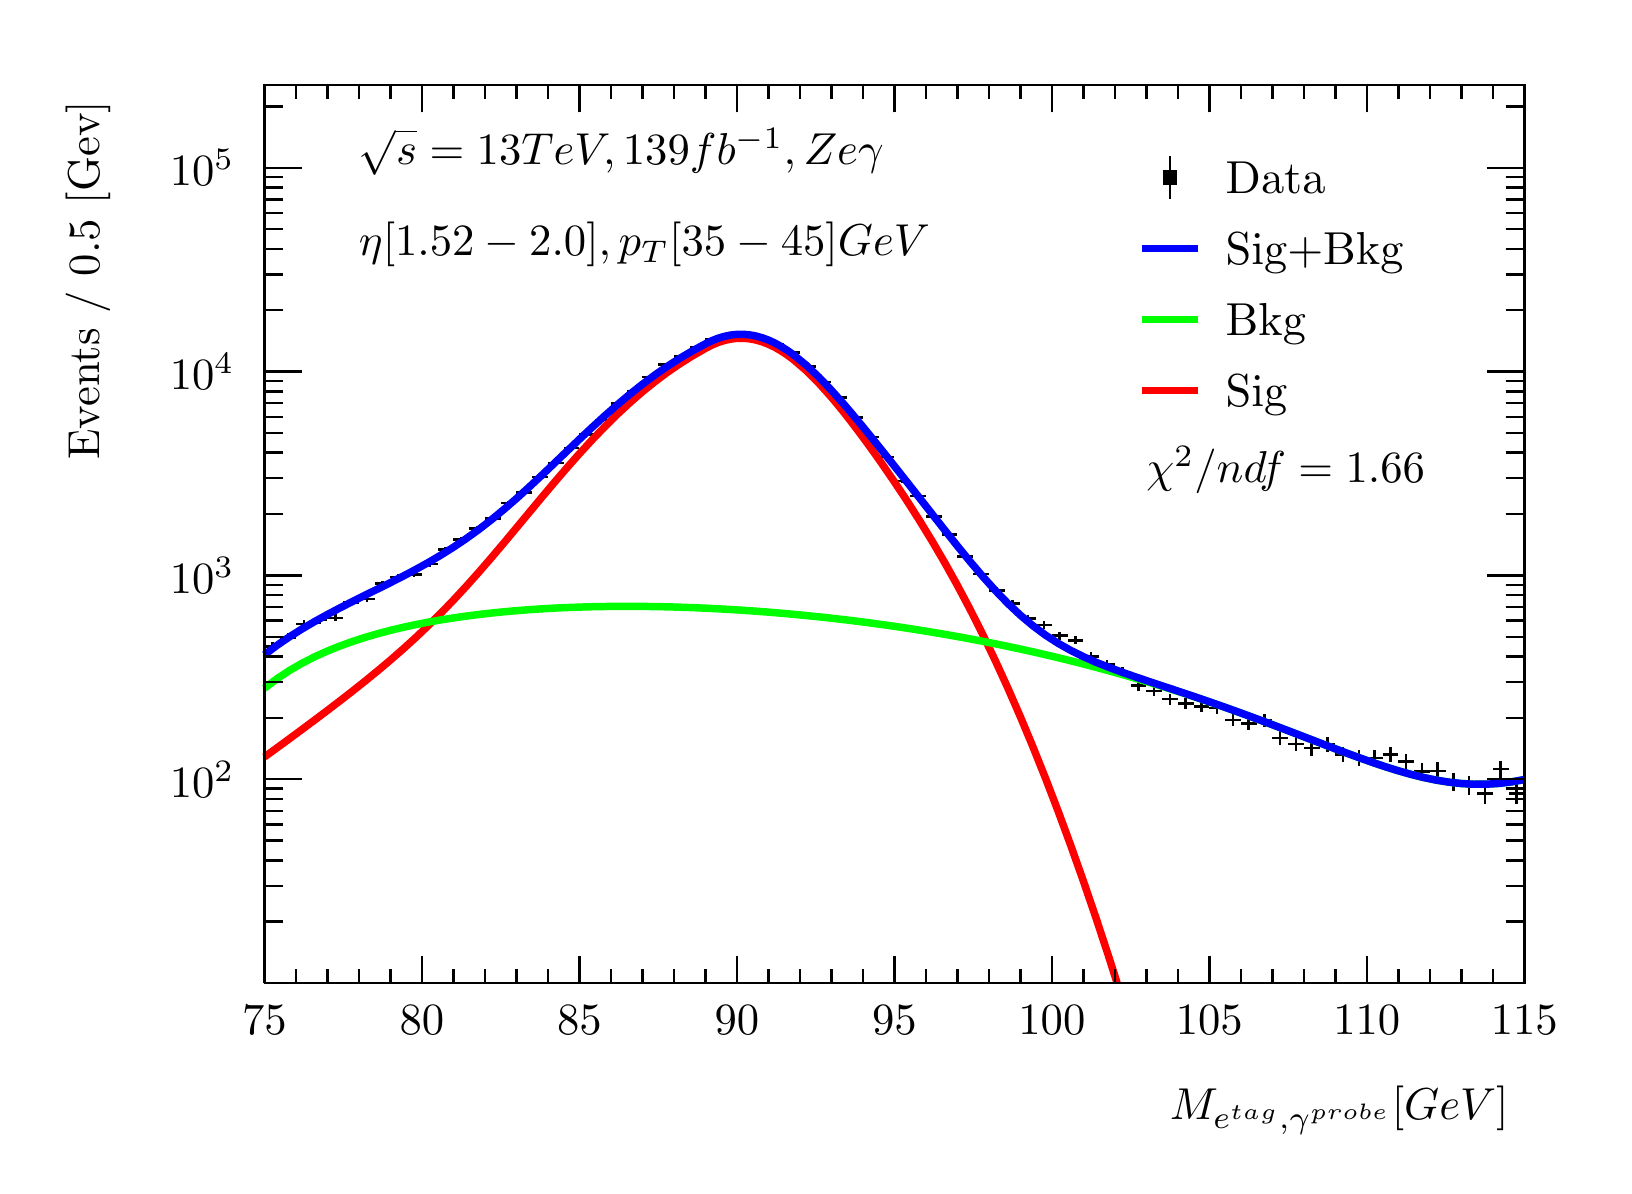
\begin{tikzpicture}
\pgfdeclareplotmark{cross} {
\pgfpathmoveto{\pgfpoint{-0.3\pgfplotmarksize}{\pgfplotmarksize}}
\pgfpathlineto{\pgfpoint{+0.3\pgfplotmarksize}{\pgfplotmarksize}}
\pgfpathlineto{\pgfpoint{+0.3\pgfplotmarksize}{0.3\pgfplotmarksize}}
\pgfpathlineto{\pgfpoint{+1\pgfplotmarksize}{0.3\pgfplotmarksize}}
\pgfpathlineto{\pgfpoint{+1\pgfplotmarksize}{-0.3\pgfplotmarksize}}
\pgfpathlineto{\pgfpoint{+0.3\pgfplotmarksize}{-0.3\pgfplotmarksize}}
\pgfpathlineto{\pgfpoint{+0.3\pgfplotmarksize}{-1.\pgfplotmarksize}}
\pgfpathlineto{\pgfpoint{-0.3\pgfplotmarksize}{-1.\pgfplotmarksize}}
\pgfpathlineto{\pgfpoint{-0.3\pgfplotmarksize}{-0.3\pgfplotmarksize}}
\pgfpathlineto{\pgfpoint{-1.\pgfplotmarksize}{-0.3\pgfplotmarksize}}
\pgfpathlineto{\pgfpoint{-1.\pgfplotmarksize}{0.3\pgfplotmarksize}}
\pgfpathlineto{\pgfpoint{-0.3\pgfplotmarksize}{0.3\pgfplotmarksize}}
\pgfpathclose
\pgfusepathqstroke
}
\pgfdeclareplotmark{cross*} {
\pgfpathmoveto{\pgfpoint{-0.3\pgfplotmarksize}{\pgfplotmarksize}}
\pgfpathlineto{\pgfpoint{+0.3\pgfplotmarksize}{\pgfplotmarksize}}
\pgfpathlineto{\pgfpoint{+0.3\pgfplotmarksize}{0.3\pgfplotmarksize}}
\pgfpathlineto{\pgfpoint{+1\pgfplotmarksize}{0.3\pgfplotmarksize}}
\pgfpathlineto{\pgfpoint{+1\pgfplotmarksize}{-0.3\pgfplotmarksize}}
\pgfpathlineto{\pgfpoint{+0.3\pgfplotmarksize}{-0.3\pgfplotmarksize}}
\pgfpathlineto{\pgfpoint{+0.3\pgfplotmarksize}{-1.\pgfplotmarksize}}
\pgfpathlineto{\pgfpoint{-0.3\pgfplotmarksize}{-1.\pgfplotmarksize}}
\pgfpathlineto{\pgfpoint{-0.3\pgfplotmarksize}{-0.3\pgfplotmarksize}}
\pgfpathlineto{\pgfpoint{-1.\pgfplotmarksize}{-0.3\pgfplotmarksize}}
\pgfpathlineto{\pgfpoint{-1.\pgfplotmarksize}{0.3\pgfplotmarksize}}
\pgfpathlineto{\pgfpoint{-0.3\pgfplotmarksize}{0.3\pgfplotmarksize}}
\pgfpathclose
\pgfusepathqfillstroke
}
\pgfdeclareplotmark{newstar} {
\pgfpathmoveto{\pgfqpoint{0pt}{\pgfplotmarksize}}
\pgfpathlineto{\pgfqpointpolar{44}{0.5\pgfplotmarksize}}
\pgfpathlineto{\pgfqpointpolar{18}{\pgfplotmarksize}}
\pgfpathlineto{\pgfqpointpolar{-20}{0.5\pgfplotmarksize}}
\pgfpathlineto{\pgfqpointpolar{-54}{\pgfplotmarksize}}
\pgfpathlineto{\pgfqpointpolar{-90}{0.5\pgfplotmarksize}}
\pgfpathlineto{\pgfqpointpolar{234}{\pgfplotmarksize}}
\pgfpathlineto{\pgfqpointpolar{198}{0.5\pgfplotmarksize}}
\pgfpathlineto{\pgfqpointpolar{162}{\pgfplotmarksize}}
\pgfpathlineto{\pgfqpointpolar{134}{0.5\pgfplotmarksize}}
\pgfpathclose
\pgfusepathqstroke
}
\pgfdeclareplotmark{newstar*} {
\pgfpathmoveto{\pgfqpoint{0pt}{\pgfplotmarksize}}
\pgfpathlineto{\pgfqpointpolar{44}{0.5\pgfplotmarksize}}
\pgfpathlineto{\pgfqpointpolar{18}{\pgfplotmarksize}}
\pgfpathlineto{\pgfqpointpolar{-20}{0.5\pgfplotmarksize}}
\pgfpathlineto{\pgfqpointpolar{-54}{\pgfplotmarksize}}
\pgfpathlineto{\pgfqpointpolar{-90}{0.5\pgfplotmarksize}}
\pgfpathlineto{\pgfqpointpolar{234}{\pgfplotmarksize}}
\pgfpathlineto{\pgfqpointpolar{198}{0.5\pgfplotmarksize}}
\pgfpathlineto{\pgfqpointpolar{162}{\pgfplotmarksize}}
\pgfpathlineto{\pgfqpointpolar{134}{0.5\pgfplotmarksize}}
\pgfpathclose
\pgfusepathqfillstroke
}
\definecolor{c}{rgb}{1,1,1};
\draw [color=c, fill=c] (0,0) rectangle (20,14.4361);
\draw [color=c, fill=c] (3,2.30977) rectangle (19,13.7143);
\definecolor{c}{rgb}{0,0,0};
\draw [c,line width=0.9] (3,2.30977) -- (3,13.7143) -- (19,13.7143) -- (19,2.30977) -- (3,2.30977);
\definecolor{c}{rgb}{1,1,1};
\draw [color=c, fill=c] (3,2.30977) rectangle (19,13.7143);
\definecolor{c}{rgb}{0,0,0};
\draw [c,line width=0.9] (3,2.30977) -- (3,13.7143) -- (19,13.7143) -- (19,2.30977) -- (3,2.30977);
\draw [c,line width=0.9] (3,2.30977) -- (19,2.30977);
\draw [c,line width=0.9] (3,2.65624) -- (3,2.30977);
\draw [c,line width=0.9] (3.4,2.48301) -- (3.4,2.30977);
\draw [c,line width=0.9] (3.8,2.48301) -- (3.8,2.30977);
\draw [c,line width=0.9] (4.2,2.48301) -- (4.2,2.30977);
\draw [c,line width=0.9] (4.6,2.48301) -- (4.6,2.30977);
\draw [c,line width=0.9] (5,2.65624) -- (5,2.30977);
\draw [c,line width=0.9] (5.4,2.48301) -- (5.4,2.30977);
\draw [c,line width=0.9] (5.8,2.48301) -- (5.8,2.30977);
\draw [c,line width=0.9] (6.2,2.48301) -- (6.2,2.30977);
\draw [c,line width=0.9] (6.6,2.48301) -- (6.6,2.30977);
\draw [c,line width=0.9] (7,2.65624) -- (7,2.30977);
\draw [c,line width=0.9] (7.4,2.48301) -- (7.4,2.30977);
\draw [c,line width=0.9] (7.8,2.48301) -- (7.8,2.30977);
\draw [c,line width=0.9] (8.2,2.48301) -- (8.2,2.30977);
\draw [c,line width=0.9] (8.6,2.48301) -- (8.6,2.30977);
\draw [c,line width=0.9] (9,2.65624) -- (9,2.30977);
\draw [c,line width=0.9] (9.4,2.48301) -- (9.4,2.30977);
\draw [c,line width=0.9] (9.8,2.48301) -- (9.8,2.30977);
\draw [c,line width=0.9] (10.2,2.48301) -- (10.2,2.30977);
\draw [c,line width=0.9] (10.6,2.48301) -- (10.6,2.30977);
\draw [c,line width=0.9] (11,2.65624) -- (11,2.30977);
\draw [c,line width=0.9] (11.4,2.48301) -- (11.4,2.30977);
\draw [c,line width=0.9] (11.8,2.48301) -- (11.8,2.30977);
\draw [c,line width=0.9] (12.2,2.48301) -- (12.2,2.30977);
\draw [c,line width=0.9] (12.6,2.48301) -- (12.6,2.30977);
\draw [c,line width=0.9] (13,2.65624) -- (13,2.30977);
\draw [c,line width=0.9] (13.4,2.48301) -- (13.4,2.30977);
\draw [c,line width=0.9] (13.8,2.48301) -- (13.8,2.30977);
\draw [c,line width=0.9] (14.2,2.48301) -- (14.2,2.30977);
\draw [c,line width=0.9] (14.6,2.48301) -- (14.6,2.30977);
\draw [c,line width=0.9] (15,2.65624) -- (15,2.30977);
\draw [c,line width=0.9] (15.4,2.48301) -- (15.4,2.30977);
\draw [c,line width=0.9] (15.8,2.48301) -- (15.8,2.30977);
\draw [c,line width=0.9] (16.2,2.48301) -- (16.2,2.30977);
\draw [c,line width=0.9] (16.6,2.48301) -- (16.6,2.30977);
\draw [c,line width=0.9] (17,2.65624) -- (17,2.30977);
\draw [c,line width=0.9] (17.4,2.48301) -- (17.4,2.30977);
\draw [c,line width=0.9] (17.8,2.48301) -- (17.8,2.30977);
\draw [c,line width=0.9] (18.2,2.48301) -- (18.2,2.30977);
\draw [c,line width=0.9] (18.6,2.48301) -- (18.6,2.30977);
\draw [c,line width=0.9] (19,2.65624) -- (19,2.30977);
\draw [c,line width=0.9] (19,2.65624) -- (19,2.30977);
\draw [anchor=base] (3,1.66015) node[scale=1.61424, color=c, rotate=0]{75};
\draw [anchor=base] (5,1.66015) node[scale=1.61424, color=c, rotate=0]{80};
\draw [anchor=base] (7,1.66015) node[scale=1.61424, color=c, rotate=0]{85};
\draw [anchor=base] (9,1.66015) node[scale=1.61424, color=c, rotate=0]{90};
\draw [anchor=base] (11,1.66015) node[scale=1.61424, color=c, rotate=0]{95};
\draw [anchor=base] (13,1.66015) node[scale=1.61424, color=c, rotate=0]{100};
\draw [anchor=base] (15,1.66015) node[scale=1.61424, color=c, rotate=0]{105};
\draw [anchor=base] (17,1.66015) node[scale=1.61424, color=c, rotate=0]{110};
\draw [anchor=base] (19,1.66015) node[scale=1.61424, color=c, rotate=0]{115};
\draw [anchor= east] (19,0.692932) node[scale=1.61424, color=c, rotate=0]{$M_{e^{tag}, \gamma^{probe}}  [GeV]$};
\draw [c,line width=0.9] (3,13.7143) -- (19,13.7143);
\draw [c,line width=0.9] (3,13.3678) -- (3,13.7143);
\draw [c,line width=0.9] (3.4,13.5411) -- (3.4,13.7143);
\draw [c,line width=0.9] (3.8,13.5411) -- (3.8,13.7143);
\draw [c,line width=0.9] (4.2,13.5411) -- (4.2,13.7143);
\draw [c,line width=0.9] (4.6,13.5411) -- (4.6,13.7143);
\draw [c,line width=0.9] (5,13.3678) -- (5,13.7143);
\draw [c,line width=0.9] (5.4,13.5411) -- (5.4,13.7143);
\draw [c,line width=0.9] (5.8,13.5411) -- (5.8,13.7143);
\draw [c,line width=0.9] (6.2,13.5411) -- (6.2,13.7143);
\draw [c,line width=0.9] (6.6,13.5411) -- (6.6,13.7143);
\draw [c,line width=0.9] (7,13.3678) -- (7,13.7143);
\draw [c,line width=0.9] (7.4,13.5411) -- (7.4,13.7143);
\draw [c,line width=0.9] (7.8,13.5411) -- (7.8,13.7143);
\draw [c,line width=0.9] (8.2,13.5411) -- (8.2,13.7143);
\draw [c,line width=0.9] (8.6,13.5411) -- (8.6,13.7143);
\draw [c,line width=0.9] (9,13.3678) -- (9,13.7143);
\draw [c,line width=0.9] (9.4,13.5411) -- (9.4,13.7143);
\draw [c,line width=0.9] (9.8,13.5411) -- (9.8,13.7143);
\draw [c,line width=0.9] (10.2,13.5411) -- (10.2,13.7143);
\draw [c,line width=0.9] (10.6,13.5411) -- (10.6,13.7143);
\draw [c,line width=0.9] (11,13.3678) -- (11,13.7143);
\draw [c,line width=0.9] (11.4,13.5411) -- (11.4,13.7143);
\draw [c,line width=0.9] (11.8,13.5411) -- (11.8,13.7143);
\draw [c,line width=0.9] (12.2,13.5411) -- (12.2,13.7143);
\draw [c,line width=0.9] (12.6,13.5411) -- (12.6,13.7143);
\draw [c,line width=0.9] (13,13.3678) -- (13,13.7143);
\draw [c,line width=0.9] (13.4,13.5411) -- (13.4,13.7143);
\draw [c,line width=0.9] (13.8,13.5411) -- (13.8,13.7143);
\draw [c,line width=0.9] (14.2,13.5411) -- (14.2,13.7143);
\draw [c,line width=0.9] (14.6,13.5411) -- (14.6,13.7143);
\draw [c,line width=0.9] (15,13.3678) -- (15,13.7143);
\draw [c,line width=0.9] (15.4,13.5411) -- (15.4,13.7143);
\draw [c,line width=0.9] (15.8,13.5411) -- (15.8,13.7143);
\draw [c,line width=0.9] (16.2,13.5411) -- (16.2,13.7143);
\draw [c,line width=0.9] (16.6,13.5411) -- (16.6,13.7143);
\draw [c,line width=0.9] (17,13.3678) -- (17,13.7143);
\draw [c,line width=0.9] (17.4,13.5411) -- (17.4,13.7143);
\draw [c,line width=0.9] (17.8,13.5411) -- (17.8,13.7143);
\draw [c,line width=0.9] (18.2,13.5411) -- (18.2,13.7143);
\draw [c,line width=0.9] (18.6,13.5411) -- (18.6,13.7143);
\draw [c,line width=0.9] (19,13.3678) -- (19,13.7143);
\draw [c,line width=0.9] (19,13.3678) -- (19,13.7143);
\draw [c,line width=0.9] (3,2.30977) -- (3,13.7143);
\draw [c,line width=0.9] (3.237,3.08897) -- (3,3.08897);
\draw [c,line width=0.9] (3.237,3.54477) -- (3,3.54477);
\draw [c,line width=0.9] (3.237,3.86817) -- (3,3.86817);
\draw [c,line width=0.9] (3.237,4.11902) -- (3,4.11902);
\draw [c,line width=0.9] (3.237,4.32397) -- (3,4.32397);
\draw [c,line width=0.9] (3.237,4.49726) -- (3,4.49726);
\draw [c,line width=0.9] (3.237,4.64737) -- (3,4.64737);
\draw [c,line width=0.9] (3.237,4.77978) -- (3,4.77978);
\draw [c,line width=0.9] (3.474,4.89822) -- (3,4.89822);
\draw [anchor= east] (2.82,4.89822) node[scale=1.61424, color=c, rotate=0]{$10^{2}$};
\draw [c,line width=0.9] (3.237,5.67742) -- (3,5.67742);
\draw [c,line width=0.9] (3.237,6.13322) -- (3,6.13322);
\draw [c,line width=0.9] (3.237,6.45661) -- (3,6.45661);
\draw [c,line width=0.9] (3.237,6.70746) -- (3,6.70746);
\draw [c,line width=0.9] (3.237,6.91242) -- (3,6.91242);
\draw [c,line width=0.9] (3.237,7.08571) -- (3,7.08571);
\draw [c,line width=0.9] (3.237,7.23581) -- (3,7.23581);
\draw [c,line width=0.9] (3.237,7.36822) -- (3,7.36822);
\draw [c,line width=0.9] (3.474,7.48666) -- (3,7.48666);
\draw [anchor= east] (2.82,7.48666) node[scale=1.61424, color=c, rotate=0]{$10^{3}$};
\draw [c,line width=0.9] (3.237,8.26586) -- (3,8.26586);
\draw [c,line width=0.9] (3.237,8.72166) -- (3,8.72166);
\draw [c,line width=0.9] (3.237,9.04506) -- (3,9.04506);
\draw [c,line width=0.9] (3.237,9.29591) -- (3,9.29591);
\draw [c,line width=0.9] (3.237,9.50086) -- (3,9.50086);
\draw [c,line width=0.9] (3.237,9.67415) -- (3,9.67415);
\draw [c,line width=0.9] (3.237,9.82426) -- (3,9.82426);
\draw [c,line width=0.9] (3.237,9.95666) -- (3,9.95666);
\draw [c,line width=0.9] (3.474,10.0751) -- (3,10.0751);
\draw [anchor= east] (2.82,10.0751) node[scale=1.61424, color=c, rotate=0]{$10^{4}$};
\draw [c,line width=0.9] (3.237,10.8543) -- (3,10.8543);
\draw [c,line width=0.9] (3.237,11.3101) -- (3,11.3101);
\draw [c,line width=0.9] (3.237,11.6335) -- (3,11.6335);
\draw [c,line width=0.9] (3.237,11.8844) -- (3,11.8844);
\draw [c,line width=0.9] (3.237,12.0893) -- (3,12.0893);
\draw [c,line width=0.9] (3.237,12.2626) -- (3,12.2626);
\draw [c,line width=0.9] (3.237,12.4127) -- (3,12.4127);
\draw [c,line width=0.9] (3.237,12.5451) -- (3,12.5451);
\draw [c,line width=0.9] (3.474,12.6635) -- (3,12.6635);
\draw [anchor= east] (2.82,12.6635) node[scale=1.61424, color=c, rotate=0]{$10^{5}$};
\draw [c,line width=0.9] (3.237,13.4427) -- (3,13.4427);
\draw [anchor= east] (0.76,13.7143) node[scale=1.61424, color=c, rotate=90]{Events / 0.5 [Gev]};
\draw [c,line width=0.9] (19,2.30977) -- (19,13.7143);
\draw [c,line width=0.9] (18.763,3.08897) -- (19,3.08897);
\draw [c,line width=0.9] (18.763,3.54477) -- (19,3.54477);
\draw [c,line width=0.9] (18.763,3.86817) -- (19,3.86817);
\draw [c,line width=0.9] (18.763,4.11902) -- (19,4.11902);
\draw [c,line width=0.9] (18.763,4.32397) -- (19,4.32397);
\draw [c,line width=0.9] (18.763,4.49726) -- (19,4.49726);
\draw [c,line width=0.9] (18.763,4.64737) -- (19,4.64737);
\draw [c,line width=0.9] (18.763,4.77978) -- (19,4.77978);
\draw [c,line width=0.9] (18.526,4.89822) -- (19,4.89822);
\draw [c,line width=0.9] (18.763,5.67742) -- (19,5.67742);
\draw [c,line width=0.9] (18.763,6.13322) -- (19,6.13322);
\draw [c,line width=0.9] (18.763,6.45661) -- (19,6.45661);
\draw [c,line width=0.9] (18.763,6.70746) -- (19,6.70746);
\draw [c,line width=0.9] (18.763,6.91242) -- (19,6.91242);
\draw [c,line width=0.9] (18.763,7.08571) -- (19,7.08571);
\draw [c,line width=0.9] (18.763,7.23581) -- (19,7.23581);
\draw [c,line width=0.9] (18.763,7.36822) -- (19,7.36822);
\draw [c,line width=0.9] (18.526,7.48666) -- (19,7.48666);
\draw [c,line width=0.9] (18.763,8.26586) -- (19,8.26586);
\draw [c,line width=0.9] (18.763,8.72166) -- (19,8.72166);
\draw [c,line width=0.9] (18.763,9.04506) -- (19,9.04506);
\draw [c,line width=0.9] (18.763,9.29591) -- (19,9.29591);
\draw [c,line width=0.9] (18.763,9.50086) -- (19,9.50086);
\draw [c,line width=0.9] (18.763,9.67415) -- (19,9.67415);
\draw [c,line width=0.9] (18.763,9.82426) -- (19,9.82426);
\draw [c,line width=0.9] (18.763,9.95666) -- (19,9.95666);
\draw [c,line width=0.9] (18.526,10.0751) -- (19,10.0751);
\draw [c,line width=0.9] (18.763,10.8543) -- (19,10.8543);
\draw [c,line width=0.9] (18.763,11.3101) -- (19,11.3101);
\draw [c,line width=0.9] (18.763,11.6335) -- (19,11.6335);
\draw [c,line width=0.9] (18.763,11.8844) -- (19,11.8844);
\draw [c,line width=0.9] (18.763,12.0893) -- (19,12.0893);
\draw [c,line width=0.9] (18.763,12.2626) -- (19,12.2626);
\draw [c,line width=0.9] (18.763,12.4127) -- (19,12.4127);
\draw [c,line width=0.9] (18.763,12.5451) -- (19,12.5451);
\draw [c,line width=0.9] (18.526,12.6635) -- (19,12.6635);
\draw [c,line width=0.9] (18.763,13.4427) -- (19,13.4427);
\draw [c,line width=0.9] (3.1,6.58652) -- (3,6.58652);
\draw [c,line width=0.9] (3,6.58652) -- (3,6.58652);
\draw [c,line width=0.9] (3.1,6.58652) -- (3.2,6.58652);
\draw [c,line width=0.9] (3.2,6.58652) -- (3.2,6.58652);
\draw [c,line width=0.9] (3.1,6.58652) -- (3.1,6.63957);
\draw [c,line width=0.9] (3.1,6.63957) -- (3.1,6.63957);
\draw [c,line width=0.9] (3.1,6.58652) -- (3.1,6.53347);
\draw [c,line width=0.9] (3.1,6.53347) -- (3.1,6.53347);
\draw [c,line width=0.9] (3.3,6.7007) -- (3.2,6.7007);
\draw [c,line width=0.9] (3.2,6.7007) -- (3.2,6.7007);
\draw [c,line width=0.9] (3.3,6.7007) -- (3.4,6.7007);
\draw [c,line width=0.9] (3.4,6.7007) -- (3.4,6.7007);
\draw [c,line width=0.9] (3.3,6.7007) -- (3.3,6.75112);
\draw [c,line width=0.9] (3.3,6.75112) -- (3.3,6.75112);
\draw [c,line width=0.9] (3.3,6.7007) -- (3.3,6.65028);
\draw [c,line width=0.9] (3.3,6.65028) -- (3.3,6.65028);
\draw [c,line width=0.9] (3.5,6.86848) -- (3.4,6.86848);
\draw [c,line width=0.9] (3.4,6.86848) -- (3.4,6.86848);
\draw [c,line width=0.9] (3.5,6.86848) -- (3.6,6.86848);
\draw [c,line width=0.9] (3.6,6.86848) -- (3.6,6.86848);
\draw [c,line width=0.9] (3.5,6.86848) -- (3.5,6.91527);
\draw [c,line width=0.9] (3.5,6.91527) -- (3.5,6.91527);
\draw [c,line width=0.9] (3.5,6.86848) -- (3.5,6.82168);
\draw [c,line width=0.9] (3.5,6.82168) -- (3.5,6.82168);
\draw [c,line width=0.9] (3.7,6.91803) -- (3.6,6.91803);
\draw [c,line width=0.9] (3.6,6.91803) -- (3.6,6.91803);
\draw [c,line width=0.9] (3.7,6.91803) -- (3.8,6.91803);
\draw [c,line width=0.9] (3.8,6.91803) -- (3.8,6.91803);
\draw [c,line width=0.9] (3.7,6.91803) -- (3.7,6.9638);
\draw [c,line width=0.9] (3.7,6.9638) -- (3.7,6.9638);
\draw [c,line width=0.9] (3.7,6.91803) -- (3.7,6.87225);
\draw [c,line width=0.9] (3.7,6.87225) -- (3.7,6.87225);
\draw [c,line width=0.9] (3.9,6.94746) -- (3.8,6.94746);
\draw [c,line width=0.9] (3.8,6.94746) -- (3.8,6.94746);
\draw [c,line width=0.9] (3.9,6.94746) -- (4,6.94746);
\draw [c,line width=0.9] (4,6.94746) -- (4,6.94746);
\draw [c,line width=0.9] (3.9,6.94746) -- (3.9,6.99265);
\draw [c,line width=0.9] (3.9,6.99265) -- (3.9,6.99265);
\draw [c,line width=0.9] (3.9,6.94746) -- (3.9,6.90229);
\draw [c,line width=0.9] (3.9,6.90229) -- (3.9,6.90229);
\draw [c,line width=0.9] (4.1,7.14208) -- (4,7.14208);
\draw [c,line width=0.9] (4,7.14208) -- (4,7.14208);
\draw [c,line width=0.9] (4.1,7.14208) -- (4.2,7.14208);
\draw [c,line width=0.9] (4.2,7.14208) -- (4.2,7.14208);
\draw [c,line width=0.9] (4.1,7.14208) -- (4.1,7.18352);
\draw [c,line width=0.9] (4.1,7.18352) -- (4.1,7.18352);
\draw [c,line width=0.9] (4.1,7.14208) -- (4.1,7.10065);
\draw [c,line width=0.9] (4.1,7.10065) -- (4.1,7.10065);
\draw [c,line width=0.9] (4.3,7.18553) -- (4.2,7.18553);
\draw [c,line width=0.9] (4.2,7.18553) -- (4.2,7.18553);
\draw [c,line width=0.9] (4.3,7.18553) -- (4.4,7.18553);
\draw [c,line width=0.9] (4.4,7.18553) -- (4.4,7.18553);
\draw [c,line width=0.9] (4.3,7.18553) -- (4.3,7.22617);
\draw [c,line width=0.9] (4.3,7.22617) -- (4.3,7.22617);
\draw [c,line width=0.9] (4.3,7.18553) -- (4.3,7.14489);
\draw [c,line width=0.9] (4.3,7.14489) -- (4.3,7.14489);
\draw [c,line width=0.9] (4.5,7.38311) -- (4.4,7.38311);
\draw [c,line width=0.9] (4.4,7.38311) -- (4.4,7.38311);
\draw [c,line width=0.9] (4.5,7.38311) -- (4.6,7.38311);
\draw [c,line width=0.9] (4.6,7.38311) -- (4.6,7.38311);
\draw [c,line width=0.9] (4.5,7.38311) -- (4.5,7.42033);
\draw [c,line width=0.9] (4.5,7.42033) -- (4.5,7.42033);
\draw [c,line width=0.9] (4.5,7.38311) -- (4.5,7.34589);
\draw [c,line width=0.9] (4.5,7.34589) -- (4.5,7.34589);
\draw [c,line width=0.9] (4.7,7.46624) -- (4.6,7.46624);
\draw [c,line width=0.9] (4.6,7.46624) -- (4.6,7.46624);
\draw [c,line width=0.9] (4.7,7.46624) -- (4.8,7.46624);
\draw [c,line width=0.9] (4.8,7.46624) -- (4.8,7.46624);
\draw [c,line width=0.9] (4.7,7.46624) -- (4.7,7.50211);
\draw [c,line width=0.9] (4.7,7.50211) -- (4.7,7.50211);
\draw [c,line width=0.9] (4.7,7.46624) -- (4.7,7.43037);
\draw [c,line width=0.9] (4.7,7.43037) -- (4.7,7.43037);
\draw [c,line width=0.9] (4.9,7.50007) -- (4.8,7.50007);
\draw [c,line width=0.9] (4.8,7.50007) -- (4.8,7.50007);
\draw [c,line width=0.9] (4.9,7.50007) -- (5,7.50007);
\draw [c,line width=0.9] (5,7.50007) -- (5,7.50007);
\draw [c,line width=0.9] (4.9,7.50007) -- (4.9,7.53541);
\draw [c,line width=0.9] (4.9,7.53541) -- (4.9,7.53541);
\draw [c,line width=0.9] (4.9,7.50007) -- (4.9,7.46474);
\draw [c,line width=0.9] (4.9,7.46474) -- (4.9,7.46474);
\draw [c,line width=0.9] (5.1,7.63198) -- (5,7.63198);
\draw [c,line width=0.9] (5,7.63198) -- (5,7.63198);
\draw [c,line width=0.9] (5.1,7.63198) -- (5.2,7.63198);
\draw [c,line width=0.9] (5.2,7.63198) -- (5.2,7.63198);
\draw [c,line width=0.9] (5.1,7.63198) -- (5.1,7.66531);
\draw [c,line width=0.9] (5.1,7.66531) -- (5.1,7.66531);
\draw [c,line width=0.9] (5.1,7.63198) -- (5.1,7.59866);
\draw [c,line width=0.9] (5.1,7.59866) -- (5.1,7.59866);
\draw [c,line width=0.9] (5.3,7.81567) -- (5.2,7.81567);
\draw [c,line width=0.9] (5.2,7.81567) -- (5.2,7.81567);
\draw [c,line width=0.9] (5.3,7.81567) -- (5.4,7.81567);
\draw [c,line width=0.9] (5.4,7.81567) -- (5.4,7.81567);
\draw [c,line width=0.9] (5.3,7.81567) -- (5.3,7.84637);
\draw [c,line width=0.9] (5.3,7.84637) -- (5.3,7.84637);
\draw [c,line width=0.9] (5.3,7.81567) -- (5.3,7.78496);
\draw [c,line width=0.9] (5.3,7.78496) -- (5.3,7.78496);
\draw [c,line width=0.9] (5.5,7.94546) -- (5.4,7.94546);
\draw [c,line width=0.9] (5.4,7.94546) -- (5.4,7.94546);
\draw [c,line width=0.9] (5.5,7.94546) -- (5.6,7.94546);
\draw [c,line width=0.9] (5.6,7.94546) -- (5.6,7.94546);
\draw [c,line width=0.9] (5.5,7.94546) -- (5.5,7.97444);
\draw [c,line width=0.9] (5.5,7.97444) -- (5.5,7.97444);
\draw [c,line width=0.9] (5.5,7.94546) -- (5.5,7.91647);
\draw [c,line width=0.9] (5.5,7.91647) -- (5.5,7.91647);
\draw [c,line width=0.9] (5.7,8.08449) -- (5.6,8.08449);
\draw [c,line width=0.9] (5.6,8.08449) -- (5.6,8.08449);
\draw [c,line width=0.9] (5.7,8.08449) -- (5.8,8.08449);
\draw [c,line width=0.9] (5.8,8.08449) -- (5.8,8.08449);
\draw [c,line width=0.9] (5.7,8.08449) -- (5.7,8.11174);
\draw [c,line width=0.9] (5.7,8.11174) -- (5.7,8.11174);
\draw [c,line width=0.9] (5.7,8.08449) -- (5.7,8.05724);
\draw [c,line width=0.9] (5.7,8.05724) -- (5.7,8.05724);
\draw [c,line width=0.9] (5.9,8.20702) -- (5.8,8.20702);
\draw [c,line width=0.9] (5.8,8.20702) -- (5.8,8.20702);
\draw [c,line width=0.9] (5.9,8.20702) -- (6,8.20702);
\draw [c,line width=0.9] (6,8.20702) -- (6,8.20702);
\draw [c,line width=0.9] (5.9,8.20702) -- (5.9,8.23282);
\draw [c,line width=0.9] (5.9,8.23282) -- (5.9,8.23282);
\draw [c,line width=0.9] (5.9,8.20702) -- (5.9,8.18121);
\draw [c,line width=0.9] (5.9,8.18121) -- (5.9,8.18121);
\draw [c,line width=0.9] (6.1,8.40623) -- (6,8.40623);
\draw [c,line width=0.9] (6,8.40623) -- (6,8.40623);
\draw [c,line width=0.9] (6.1,8.40623) -- (6.2,8.40623);
\draw [c,line width=0.9] (6.2,8.40623) -- (6.2,8.40623);
\draw [c,line width=0.9] (6.1,8.40623) -- (6.1,8.42985);
\draw [c,line width=0.9] (6.1,8.42985) -- (6.1,8.42985);
\draw [c,line width=0.9] (6.1,8.40623) -- (6.1,8.38262);
\draw [c,line width=0.9] (6.1,8.38262) -- (6.1,8.38262);
\draw [c,line width=0.9] (6.3,8.54249) -- (6.2,8.54249);
\draw [c,line width=0.9] (6.2,8.54249) -- (6.2,8.54249);
\draw [c,line width=0.9] (6.3,8.54249) -- (6.4,8.54249);
\draw [c,line width=0.9] (6.4,8.54249) -- (6.4,8.54249);
\draw [c,line width=0.9] (6.3,8.54249) -- (6.3,8.56472);
\draw [c,line width=0.9] (6.3,8.56472) -- (6.3,8.56472);
\draw [c,line width=0.9] (6.3,8.54249) -- (6.3,8.52026);
\draw [c,line width=0.9] (6.3,8.52026) -- (6.3,8.52026);
\draw [c,line width=0.9] (6.5,8.73433) -- (6.4,8.73433);
\draw [c,line width=0.9] (6.4,8.73433) -- (6.4,8.73433);
\draw [c,line width=0.9] (6.5,8.73433) -- (6.6,8.73433);
\draw [c,line width=0.9] (6.6,8.73433) -- (6.6,8.73433);
\draw [c,line width=0.9] (6.5,8.73433) -- (6.5,8.75474);
\draw [c,line width=0.9] (6.5,8.75474) -- (6.5,8.75474);
\draw [c,line width=0.9] (6.5,8.73433) -- (6.5,8.71392);
\draw [c,line width=0.9] (6.5,8.71392) -- (6.5,8.71392);
\draw [c,line width=0.9] (6.7,8.91658) -- (6.6,8.91658);
\draw [c,line width=0.9] (6.6,8.91658) -- (6.6,8.91658);
\draw [c,line width=0.9] (6.7,8.91658) -- (6.8,8.91658);
\draw [c,line width=0.9] (6.8,8.91658) -- (6.8,8.91658);
\draw [c,line width=0.9] (6.7,8.91658) -- (6.7,8.9354);
\draw [c,line width=0.9] (6.7,8.9354) -- (6.7,8.9354);
\draw [c,line width=0.9] (6.7,8.91658) -- (6.7,8.89776);
\draw [c,line width=0.9] (6.7,8.89776) -- (6.7,8.89776);
\draw [c,line width=0.9] (6.9,9.10685) -- (6.8,9.10685);
\draw [c,line width=0.9] (6.8,9.10685) -- (6.8,9.10685);
\draw [c,line width=0.9] (6.9,9.10685) -- (7,9.10685);
\draw [c,line width=0.9] (7,9.10685) -- (7,9.10685);
\draw [c,line width=0.9] (6.9,9.10685) -- (6.9,9.12414);
\draw [c,line width=0.9] (6.9,9.12414) -- (6.9,9.12414);
\draw [c,line width=0.9] (6.9,9.10685) -- (6.9,9.08955);
\draw [c,line width=0.9] (6.9,9.08955) -- (6.9,9.08955);
\draw [c,line width=0.9] (7.1,9.2764) -- (7,9.2764);
\draw [c,line width=0.9] (7,9.2764) -- (7,9.2764);
\draw [c,line width=0.9] (7.1,9.2764) -- (7.2,9.2764);
\draw [c,line width=0.9] (7.2,9.2764) -- (7.2,9.2764);
\draw [c,line width=0.9] (7.1,9.2764) -- (7.1,9.29244);
\draw [c,line width=0.9] (7.1,9.29244) -- (7.1,9.29244);
\draw [c,line width=0.9] (7.1,9.2764) -- (7.1,9.26037);
\draw [c,line width=0.9] (7.1,9.26037) -- (7.1,9.26037);
\draw [c,line width=0.9] (7.3,9.46353) -- (7.2,9.46353);
\draw [c,line width=0.9] (7.2,9.46353) -- (7.2,9.46353);
\draw [c,line width=0.9] (7.3,9.46353) -- (7.4,9.46353);
\draw [c,line width=0.9] (7.4,9.46353) -- (7.4,9.46353);
\draw [c,line width=0.9] (7.3,9.46353) -- (7.3,9.47828);
\draw [c,line width=0.9] (7.3,9.47828) -- (7.3,9.47828);
\draw [c,line width=0.9] (7.3,9.46353) -- (7.3,9.44877);
\draw [c,line width=0.9] (7.3,9.44877) -- (7.3,9.44877);
\draw [c,line width=0.9] (7.5,9.66965) -- (7.4,9.66965);
\draw [c,line width=0.9] (7.4,9.66965) -- (7.4,9.66965);
\draw [c,line width=0.9] (7.5,9.66965) -- (7.6,9.66965);
\draw [c,line width=0.9] (7.6,9.66965) -- (7.6,9.66965);
\draw [c,line width=0.9] (7.5,9.66965) -- (7.5,9.68311);
\draw [c,line width=0.9] (7.5,9.68311) -- (7.5,9.68311);
\draw [c,line width=0.9] (7.5,9.66965) -- (7.5,9.65618);
\draw [c,line width=0.9] (7.5,9.65618) -- (7.5,9.65618);
\draw [c,line width=0.9] (7.7,9.81961) -- (7.6,9.81961);
\draw [c,line width=0.9] (7.6,9.81961) -- (7.6,9.81961);
\draw [c,line width=0.9] (7.7,9.81961) -- (7.8,9.81961);
\draw [c,line width=0.9] (7.8,9.81961) -- (7.8,9.81961);
\draw [c,line width=0.9] (7.7,9.81961) -- (7.7,9.83221);
\draw [c,line width=0.9] (7.7,9.83221) -- (7.7,9.83221);
\draw [c,line width=0.9] (7.7,9.81961) -- (7.7,9.80702);
\draw [c,line width=0.9] (7.7,9.80702) -- (7.7,9.80702);
\draw [c,line width=0.9] (7.9,10.0089) -- (7.8,10.0089);
\draw [c,line width=0.9] (7.8,10.0089) -- (7.8,10.0089);
\draw [c,line width=0.9] (7.9,10.0089) -- (8,10.0089);
\draw [c,line width=0.9] (8,10.0089) -- (8,10.0089);
\draw [c,line width=0.9] (7.9,10.0089) -- (7.9,10.0205);
\draw [c,line width=0.9] (7.9,10.0205) -- (7.9,10.0205);
\draw [c,line width=0.9] (7.9,10.0089) -- (7.9,9.99732);
\draw [c,line width=0.9] (7.9,9.99732) -- (7.9,9.99732);
\draw [c,line width=0.9] (8.1,10.1651) -- (8,10.1651);
\draw [c,line width=0.9] (8,10.1651) -- (8,10.1651);
\draw [c,line width=0.9] (8.1,10.1651) -- (8.2,10.1651);
\draw [c,line width=0.9] (8.2,10.1651) -- (8.2,10.1651);
\draw [c,line width=0.9] (8.1,10.1651) -- (8.1,10.1759);
\draw [c,line width=0.9] (8.1,10.1759) -- (8.1,10.1759);
\draw [c,line width=0.9] (8.1,10.1651) -- (8.1,10.1543);
\draw [c,line width=0.9] (8.1,10.1543) -- (8.1,10.1543);
\draw [c,line width=0.9] (8.3,10.2686) -- (8.2,10.2686);
\draw [c,line width=0.9] (8.2,10.2686) -- (8.2,10.2686);
\draw [c,line width=0.9] (8.3,10.2686) -- (8.4,10.2686);
\draw [c,line width=0.9] (8.4,10.2686) -- (8.4,10.2686);
\draw [c,line width=0.9] (8.3,10.2686) -- (8.3,10.2789);
\draw [c,line width=0.9] (8.3,10.2789) -- (8.3,10.2789);
\draw [c,line width=0.9] (8.3,10.2686) -- (8.3,10.2583);
\draw [c,line width=0.9] (8.3,10.2583) -- (8.3,10.2583);
\draw [c,line width=0.9] (8.5,10.3901) -- (8.4,10.3901);
\draw [c,line width=0.9] (8.4,10.3901) -- (8.4,10.3901);
\draw [c,line width=0.9] (8.5,10.3901) -- (8.6,10.3901);
\draw [c,line width=0.9] (8.6,10.3901) -- (8.6,10.3901);
\draw [c,line width=0.9] (8.5,10.3901) -- (8.5,10.3999);
\draw [c,line width=0.9] (8.5,10.3999) -- (8.5,10.3999);
\draw [c,line width=0.9] (8.5,10.3901) -- (8.5,10.3803);
\draw [c,line width=0.9] (8.5,10.3803) -- (8.5,10.3803);
\draw [c,line width=0.9] (8.7,10.4905) -- (8.6,10.4905);
\draw [c,line width=0.9] (8.6,10.4905) -- (8.6,10.4905);
\draw [c,line width=0.9] (8.7,10.4905) -- (8.8,10.4905);
\draw [c,line width=0.9] (8.8,10.4905) -- (8.8,10.4905);
\draw [c,line width=0.9] (8.7,10.4905) -- (8.7,10.4999);
\draw [c,line width=0.9] (8.7,10.4999) -- (8.7,10.4999);
\draw [c,line width=0.9] (8.7,10.4905) -- (8.7,10.4812);
\draw [c,line width=0.9] (8.7,10.4812) -- (8.7,10.4812);
\draw [c,line width=0.9] (8.9,10.5141) -- (8.8,10.5141);
\draw [c,line width=0.9] (8.8,10.5141) -- (8.8,10.5141);
\draw [c,line width=0.9] (8.9,10.5141) -- (9,10.5141);
\draw [c,line width=0.9] (9,10.5141) -- (9,10.5141);
\draw [c,line width=0.9] (8.9,10.5141) -- (8.9,10.5233);
\draw [c,line width=0.9] (8.9,10.5233) -- (8.9,10.5233);
\draw [c,line width=0.9] (8.9,10.5141) -- (8.9,10.5048);
\draw [c,line width=0.9] (8.9,10.5048) -- (8.9,10.5048);
\draw [c,line width=0.9] (9.1,10.5299) -- (9,10.5299);
\draw [c,line width=0.9] (9,10.5299) -- (9,10.5299);
\draw [c,line width=0.9] (9.1,10.5299) -- (9.2,10.5299);
\draw [c,line width=0.9] (9.2,10.5299) -- (9.2,10.5299);
\draw [c,line width=0.9] (9.1,10.5299) -- (9.1,10.539);
\draw [c,line width=0.9] (9.1,10.539) -- (9.1,10.539);
\draw [c,line width=0.9] (9.1,10.5299) -- (9.1,10.5207);
\draw [c,line width=0.9] (9.1,10.5207) -- (9.1,10.5207);
\draw [c,line width=0.9] (9.3,10.5033) -- (9.2,10.5033);
\draw [c,line width=0.9] (9.2,10.5033) -- (9.2,10.5033);
\draw [c,line width=0.9] (9.3,10.5033) -- (9.4,10.5033);
\draw [c,line width=0.9] (9.4,10.5033) -- (9.4,10.5033);
\draw [c,line width=0.9] (9.3,10.5033) -- (9.3,10.5126);
\draw [c,line width=0.9] (9.3,10.5126) -- (9.3,10.5126);
\draw [c,line width=0.9] (9.3,10.5033) -- (9.3,10.494);
\draw [c,line width=0.9] (9.3,10.494) -- (9.3,10.494);
\draw [c,line width=0.9] (9.5,10.4253) -- (9.4,10.4253);
\draw [c,line width=0.9] (9.4,10.4253) -- (9.4,10.4253);
\draw [c,line width=0.9] (9.5,10.4253) -- (9.6,10.4253);
\draw [c,line width=0.9] (9.6,10.4253) -- (9.6,10.4253);
\draw [c,line width=0.9] (9.5,10.4253) -- (9.5,10.4349);
\draw [c,line width=0.9] (9.5,10.4349) -- (9.5,10.4349);
\draw [c,line width=0.9] (9.5,10.4253) -- (9.5,10.4157);
\draw [c,line width=0.9] (9.5,10.4157) -- (9.5,10.4157);
\draw [c,line width=0.9] (9.7,10.3186) -- (9.6,10.3186);
\draw [c,line width=0.9] (9.6,10.3186) -- (9.6,10.3186);
\draw [c,line width=0.9] (9.7,10.3186) -- (9.8,10.3186);
\draw [c,line width=0.9] (9.8,10.3186) -- (9.8,10.3186);
\draw [c,line width=0.9] (9.7,10.3186) -- (9.7,10.3286);
\draw [c,line width=0.9] (9.7,10.3286) -- (9.7,10.3286);
\draw [c,line width=0.9] (9.7,10.3186) -- (9.7,10.3085);
\draw [c,line width=0.9] (9.7,10.3085) -- (9.7,10.3085);
\draw [c,line width=0.9] (9.9,10.1425) -- (9.8,10.1425);
\draw [c,line width=0.9] (9.8,10.1425) -- (9.8,10.1425);
\draw [c,line width=0.9] (9.9,10.1425) -- (10,10.1425);
\draw [c,line width=0.9] (10,10.1425) -- (10,10.1425);
\draw [c,line width=0.9] (9.9,10.1425) -- (9.9,10.1534);
\draw [c,line width=0.9] (9.9,10.1534) -- (9.9,10.1534);
\draw [c,line width=0.9] (9.9,10.1425) -- (9.9,10.1316);
\draw [c,line width=0.9] (9.9,10.1316) -- (9.9,10.1316);
\draw [c,line width=0.9] (10.1,9.94385) -- (10,9.94385);
\draw [c,line width=0.9] (10,9.94385) -- (10,9.94385);
\draw [c,line width=0.9] (10.1,9.94385) -- (10.2,9.94385);
\draw [c,line width=0.9] (10.2,9.94385) -- (10.2,9.94385);
\draw [c,line width=0.9] (10.1,9.94385) -- (10.1,9.95577);
\draw [c,line width=0.9] (10.1,9.95577) -- (10.1,9.95577);
\draw [c,line width=0.9] (10.1,9.94385) -- (10.1,9.93194);
\draw [c,line width=0.9] (10.1,9.93194) -- (10.1,9.93194);
\draw [c,line width=0.9] (10.3,9.7472) -- (10.2,9.7472);
\draw [c,line width=0.9] (10.2,9.7472) -- (10.2,9.7472);
\draw [c,line width=0.9] (10.3,9.7472) -- (10.4,9.7472);
\draw [c,line width=0.9] (10.4,9.7472) -- (10.4,9.7472);
\draw [c,line width=0.9] (10.3,9.7472) -- (10.3,9.76021);
\draw [c,line width=0.9] (10.3,9.76021) -- (10.3,9.76021);
\draw [c,line width=0.9] (10.3,9.7472) -- (10.3,9.7342);
\draw [c,line width=0.9] (10.3,9.7342) -- (10.3,9.7342);
\draw [c,line width=0.9] (10.5,9.48938) -- (10.4,9.48938);
\draw [c,line width=0.9] (10.4,9.48938) -- (10.4,9.48938);
\draw [c,line width=0.9] (10.5,9.48938) -- (10.6,9.48938);
\draw [c,line width=0.9] (10.6,9.48938) -- (10.6,9.48938);
\draw [c,line width=0.9] (10.5,9.48938) -- (10.5,9.50396);
\draw [c,line width=0.9] (10.5,9.50396) -- (10.5,9.50396);
\draw [c,line width=0.9] (10.5,9.48938) -- (10.5,9.47479);
\draw [c,line width=0.9] (10.5,9.47479) -- (10.5,9.47479);
\draw [c,line width=0.9] (10.7,9.24697) -- (10.6,9.24697);
\draw [c,line width=0.9] (10.6,9.24697) -- (10.6,9.24697);
\draw [c,line width=0.9] (10.7,9.24697) -- (10.8,9.24697);
\draw [c,line width=0.9] (10.8,9.24697) -- (10.8,9.24697);
\draw [c,line width=0.9] (10.7,9.24697) -- (10.7,9.26322);
\draw [c,line width=0.9] (10.7,9.26322) -- (10.7,9.26322);
\draw [c,line width=0.9] (10.7,9.24697) -- (10.7,9.23072);
\draw [c,line width=0.9] (10.7,9.23072) -- (10.7,9.23072);
\draw [c,line width=0.9] (10.9,8.99065) -- (10.8,8.99065);
\draw [c,line width=0.9] (10.8,8.99065) -- (10.8,8.99065);
\draw [c,line width=0.9] (10.9,8.99065) -- (11,8.99065);
\draw [c,line width=0.9] (11,8.99065) -- (11,8.99065);
\draw [c,line width=0.9] (10.9,8.99065) -- (10.9,9.00886);
\draw [c,line width=0.9] (10.9,9.00886) -- (10.9,9.00886);
\draw [c,line width=0.9] (10.9,8.99065) -- (10.9,8.97244);
\draw [c,line width=0.9] (10.9,8.97244) -- (10.9,8.97244);
\draw [c,line width=0.9] (11.1,8.68742) -- (11,8.68742);
\draw [c,line width=0.9] (11,8.68742) -- (11,8.68742);
\draw [c,line width=0.9] (11.1,8.68742) -- (11.2,8.68742);
\draw [c,line width=0.9] (11.2,8.68742) -- (11.2,8.68742);
\draw [c,line width=0.9] (11.1,8.68742) -- (11.1,8.70826);
\draw [c,line width=0.9] (11.1,8.70826) -- (11.1,8.70826);
\draw [c,line width=0.9] (11.1,8.68742) -- (11.1,8.66658);
\draw [c,line width=0.9] (11.1,8.66658) -- (11.1,8.66658);
\draw [c,line width=0.9] (11.3,8.49216) -- (11.2,8.49216);
\draw [c,line width=0.9] (11.2,8.49216) -- (11.2,8.49216);
\draw [c,line width=0.9] (11.3,8.49216) -- (11.4,8.49216);
\draw [c,line width=0.9] (11.4,8.49216) -- (11.4,8.49216);
\draw [c,line width=0.9] (11.3,8.49216) -- (11.3,8.51489);
\draw [c,line width=0.9] (11.3,8.51489) -- (11.3,8.51489);
\draw [c,line width=0.9] (11.3,8.49216) -- (11.3,8.46943);
\draw [c,line width=0.9] (11.3,8.46943) -- (11.3,8.46943);
\draw [c,line width=0.9] (11.5,8.23567) -- (11.4,8.23567);
\draw [c,line width=0.9] (11.4,8.23567) -- (11.4,8.23567);
\draw [c,line width=0.9] (11.5,8.23567) -- (11.6,8.23567);
\draw [c,line width=0.9] (11.6,8.23567) -- (11.6,8.23567);
\draw [c,line width=0.9] (11.5,8.23567) -- (11.5,8.26115);
\draw [c,line width=0.9] (11.5,8.26115) -- (11.5,8.26115);
\draw [c,line width=0.9] (11.5,8.23567) -- (11.5,8.21019);
\draw [c,line width=0.9] (11.5,8.21019) -- (11.5,8.21019);
\draw [c,line width=0.9] (11.7,8.00514) -- (11.6,8.00514);
\draw [c,line width=0.9] (11.6,8.00514) -- (11.6,8.00514);
\draw [c,line width=0.9] (11.7,8.00514) -- (11.8,8.00514);
\draw [c,line width=0.9] (11.8,8.00514) -- (11.8,8.00514);
\draw [c,line width=0.9] (11.7,8.00514) -- (11.7,8.03336);
\draw [c,line width=0.9] (11.7,8.03336) -- (11.7,8.03336);
\draw [c,line width=0.9] (11.7,8.00514) -- (11.7,7.97691);
\draw [c,line width=0.9] (11.7,7.97691) -- (11.7,7.97691);
\draw [c,line width=0.9] (11.9,7.72576) -- (11.8,7.72576);
\draw [c,line width=0.9] (11.8,7.72576) -- (11.8,7.72576);
\draw [c,line width=0.9] (11.9,7.72576) -- (12,7.72576);
\draw [c,line width=0.9] (12,7.72576) -- (12,7.72576);
\draw [c,line width=0.9] (11.9,7.72576) -- (11.9,7.75772);
\draw [c,line width=0.9] (11.9,7.75772) -- (11.9,7.75772);
\draw [c,line width=0.9] (11.9,7.72576) -- (11.9,7.69379);
\draw [c,line width=0.9] (11.9,7.69379) -- (11.9,7.69379);
\draw [c,line width=0.9] (12.1,7.50782) -- (12,7.50782);
\draw [c,line width=0.9] (12,7.50782) -- (12,7.50782);
\draw [c,line width=0.9] (12.1,7.50782) -- (12.2,7.50782);
\draw [c,line width=0.9] (12.2,7.50782) -- (12.2,7.50782);
\draw [c,line width=0.9] (12.1,7.50782) -- (12.1,7.54304);
\draw [c,line width=0.9] (12.1,7.54304) -- (12.1,7.54304);
\draw [c,line width=0.9] (12.1,7.50782) -- (12.1,7.47261);
\draw [c,line width=0.9] (12.1,7.47261) -- (12.1,7.47261);
\draw [c,line width=0.9] (12.3,7.29733) -- (12.2,7.29733);
\draw [c,line width=0.9] (12.2,7.29733) -- (12.2,7.29733);
\draw [c,line width=0.9] (12.3,7.29733) -- (12.4,7.29733);
\draw [c,line width=0.9] (12.4,7.29733) -- (12.4,7.29733);
\draw [c,line width=0.9] (12.3,7.29733) -- (12.3,7.336);
\draw [c,line width=0.9] (12.3,7.336) -- (12.3,7.336);
\draw [c,line width=0.9] (12.3,7.29733) -- (12.3,7.25867);
\draw [c,line width=0.9] (12.3,7.25867) -- (12.3,7.25867);
\draw [c,line width=0.9] (12.5,7.13134) -- (12.4,7.13134);
\draw [c,line width=0.9] (12.4,7.13134) -- (12.4,7.13134);
\draw [c,line width=0.9] (12.5,7.13134) -- (12.6,7.13134);
\draw [c,line width=0.9] (12.6,7.13134) -- (12.6,7.13134);
\draw [c,line width=0.9] (12.5,7.13134) -- (12.5,7.17297);
\draw [c,line width=0.9] (12.5,7.17297) -- (12.5,7.17297);
\draw [c,line width=0.9] (12.5,7.13134) -- (12.5,7.08971);
\draw [c,line width=0.9] (12.5,7.08971) -- (12.5,7.08971);
\draw [c,line width=0.9] (12.7,6.942) -- (12.6,6.942);
\draw [c,line width=0.9] (12.6,6.942) -- (12.6,6.942);
\draw [c,line width=0.9] (12.7,6.942) -- (12.8,6.942);
\draw [c,line width=0.9] (12.8,6.942) -- (12.8,6.942);
\draw [c,line width=0.9] (12.7,6.942) -- (12.7,6.98729);
\draw [c,line width=0.9] (12.7,6.98729) -- (12.7,6.98729);
\draw [c,line width=0.9] (12.7,6.942) -- (12.7,6.89671);
\draw [c,line width=0.9] (12.7,6.89671) -- (12.7,6.89671);
\draw [c,line width=0.9] (12.9,6.85673) -- (12.8,6.85673);
\draw [c,line width=0.9] (12.8,6.85673) -- (12.8,6.85673);
\draw [c,line width=0.9] (12.9,6.85673) -- (13,6.85673);
\draw [c,line width=0.9] (13,6.85673) -- (13,6.85673);
\draw [c,line width=0.9] (12.9,6.85673) -- (12.9,6.90377);
\draw [c,line width=0.9] (12.9,6.90377) -- (12.9,6.90377);
\draw [c,line width=0.9] (12.9,6.85673) -- (12.9,6.80969);
\draw [c,line width=0.9] (12.9,6.80969) -- (12.9,6.80969);
\draw [c,line width=0.9] (13.1,6.72087) -- (13,6.72087);
\draw [c,line width=0.9] (13,6.72087) -- (13,6.72087);
\draw [c,line width=0.9] (13.1,6.72087) -- (13.2,6.72087);
\draw [c,line width=0.9] (13.2,6.72087) -- (13.2,6.72087);
\draw [c,line width=0.9] (13.1,6.72087) -- (13.1,6.77084);
\draw [c,line width=0.9] (13.1,6.77084) -- (13.1,6.77084);
\draw [c,line width=0.9] (13.1,6.72087) -- (13.1,6.6709);
\draw [c,line width=0.9] (13.1,6.6709) -- (13.1,6.6709);
\draw [c,line width=0.9] (13.3,6.66157) -- (13.2,6.66157);
\draw [c,line width=0.9] (13.2,6.66157) -- (13.2,6.66157);
\draw [c,line width=0.9] (13.3,6.66157) -- (13.4,6.66157);
\draw [c,line width=0.9] (13.4,6.66157) -- (13.4,6.66157);
\draw [c,line width=0.9] (13.3,6.66157) -- (13.3,6.71288);
\draw [c,line width=0.9] (13.3,6.71288) -- (13.3,6.71288);
\draw [c,line width=0.9] (13.3,6.66157) -- (13.3,6.61027);
\draw [c,line width=0.9] (13.3,6.61027) -- (13.3,6.61027);
\draw [c,line width=0.9] (13.5,6.45662) -- (13.4,6.45662);
\draw [c,line width=0.9] (13.4,6.45662) -- (13.4,6.45662);
\draw [c,line width=0.9] (13.5,6.45662) -- (13.6,6.45662);
\draw [c,line width=0.9] (13.6,6.45662) -- (13.6,6.45662);
\draw [c,line width=0.9] (13.5,6.45662) -- (13.5,6.51282);
\draw [c,line width=0.9] (13.5,6.51282) -- (13.5,6.51282);
\draw [c,line width=0.9] (13.5,6.45662) -- (13.5,6.40042);
\draw [c,line width=0.9] (13.5,6.40042) -- (13.5,6.40042);
\draw [c,line width=0.9] (13.7,6.35676) -- (13.6,6.35676);
\draw [c,line width=0.9] (13.6,6.35676) -- (13.6,6.35676);
\draw [c,line width=0.9] (13.7,6.35676) -- (13.8,6.35676);
\draw [c,line width=0.9] (13.8,6.35676) -- (13.8,6.35676);
\draw [c,line width=0.9] (13.7,6.35676) -- (13.7,6.41551);
\draw [c,line width=0.9] (13.7,6.41551) -- (13.7,6.41551);
\draw [c,line width=0.9] (13.7,6.35676) -- (13.7,6.298);
\draw [c,line width=0.9] (13.7,6.298) -- (13.7,6.298);
\draw [c,line width=0.9] (13.9,6.26062) -- (13.8,6.26062);
\draw [c,line width=0.9] (13.8,6.26062) -- (13.8,6.26062);
\draw [c,line width=0.9] (13.9,6.26062) -- (14,6.26062);
\draw [c,line width=0.9] (14,6.26062) -- (14,6.26062);
\draw [c,line width=0.9] (13.9,6.26062) -- (13.9,6.32194);
\draw [c,line width=0.9] (13.9,6.32194) -- (13.9,6.32194);
\draw [c,line width=0.9] (13.9,6.26062) -- (13.9,6.1993);
\draw [c,line width=0.9] (13.9,6.1993) -- (13.9,6.1993);
\draw [c,line width=0.9] (14.1,6.08733) -- (14,6.08733);
\draw [c,line width=0.9] (14,6.08733) -- (14,6.08733);
\draw [c,line width=0.9] (14.1,6.08733) -- (14.2,6.08733);
\draw [c,line width=0.9] (14.2,6.08733) -- (14.2,6.08733);
\draw [c,line width=0.9] (14.1,6.08733) -- (14.1,6.15356);
\draw [c,line width=0.9] (14.1,6.15356) -- (14.1,6.15356);
\draw [c,line width=0.9] (14.1,6.08733) -- (14.1,6.0211);
\draw [c,line width=0.9] (14.1,6.0211) -- (14.1,6.0211);
\draw [c,line width=0.9] (14.3,6.01894) -- (14.2,6.01894);
\draw [c,line width=0.9] (14.2,6.01894) -- (14.2,6.01894);
\draw [c,line width=0.9] (14.3,6.01894) -- (14.4,6.01894);
\draw [c,line width=0.9] (14.4,6.01894) -- (14.4,6.01894);
\draw [c,line width=0.9] (14.3,6.01894) -- (14.3,6.08721);
\draw [c,line width=0.9] (14.3,6.08721) -- (14.3,6.08721);
\draw [c,line width=0.9] (14.3,6.01894) -- (14.3,5.95066);
\draw [c,line width=0.9] (14.3,5.95066) -- (14.3,5.95066);
\draw [c,line width=0.9] (14.5,5.91469) -- (14.4,5.91469);
\draw [c,line width=0.9] (14.4,5.91469) -- (14.4,5.91469);
\draw [c,line width=0.9] (14.5,5.91469) -- (14.6,5.91469);
\draw [c,line width=0.9] (14.6,5.91469) -- (14.6,5.91469);
\draw [c,line width=0.9] (14.5,5.91469) -- (14.5,5.98621);
\draw [c,line width=0.9] (14.5,5.98621) -- (14.5,5.98621);
\draw [c,line width=0.9] (14.5,5.91469) -- (14.5,5.84318);
\draw [c,line width=0.9] (14.5,5.84318) -- (14.5,5.84318);
\draw [c,line width=0.9] (14.7,5.85871) -- (14.6,5.85871);
\draw [c,line width=0.9] (14.6,5.85871) -- (14.6,5.85871);
\draw [c,line width=0.9] (14.7,5.85871) -- (14.8,5.85871);
\draw [c,line width=0.9] (14.8,5.85871) -- (14.8,5.85871);
\draw [c,line width=0.9] (14.7,5.85871) -- (14.7,5.93202);
\draw [c,line width=0.9] (14.7,5.93202) -- (14.7,5.93202);
\draw [c,line width=0.9] (14.7,5.85871) -- (14.7,5.78539);
\draw [c,line width=0.9] (14.7,5.78539) -- (14.7,5.78539);
\draw [c,line width=0.9] (14.9,5.82471) -- (14.8,5.82471);
\draw [c,line width=0.9] (14.8,5.82471) -- (14.8,5.82471);
\draw [c,line width=0.9] (14.9,5.82471) -- (15,5.82471);
\draw [c,line width=0.9] (15,5.82471) -- (15,5.82471);
\draw [c,line width=0.9] (14.9,5.82471) -- (14.9,5.89915);
\draw [c,line width=0.9] (14.9,5.89915) -- (14.9,5.89915);
\draw [c,line width=0.9] (14.9,5.82471) -- (14.9,5.75028);
\draw [c,line width=0.9] (14.9,5.75028) -- (14.9,5.75028);
\draw [c,line width=0.9] (15.1,5.79979) -- (15,5.79979);
\draw [c,line width=0.9] (15,5.79979) -- (15,5.79979);
\draw [c,line width=0.9] (15.1,5.79979) -- (15.2,5.79979);
\draw [c,line width=0.9] (15.2,5.79979) -- (15.2,5.79979);
\draw [c,line width=0.9] (15.1,5.79979) -- (15.1,5.87505);
\draw [c,line width=0.9] (15.1,5.87505) -- (15.1,5.87505);
\draw [c,line width=0.9] (15.1,5.79979) -- (15.1,5.72452);
\draw [c,line width=0.9] (15.1,5.72452) -- (15.1,5.72452);
\draw [c,line width=0.9] (15.3,5.64896) -- (15.2,5.64896);
\draw [c,line width=0.9] (15.2,5.64896) -- (15.2,5.64896);
\draw [c,line width=0.9] (15.3,5.64896) -- (15.4,5.64896);
\draw [c,line width=0.9] (15.4,5.64896) -- (15.4,5.64896);
\draw [c,line width=0.9] (15.3,5.64896) -- (15.3,5.72944);
\draw [c,line width=0.9] (15.3,5.72944) -- (15.3,5.72944);
\draw [c,line width=0.9] (15.3,5.64896) -- (15.3,5.56847);
\draw [c,line width=0.9] (15.3,5.56847) -- (15.3,5.56847);
\draw [c,line width=0.9] (15.5,5.60786) -- (15.4,5.60786);
\draw [c,line width=0.9] (15.4,5.60786) -- (15.4,5.60786);
\draw [c,line width=0.9] (15.5,5.60786) -- (15.6,5.60786);
\draw [c,line width=0.9] (15.6,5.60786) -- (15.6,5.60786);
\draw [c,line width=0.9] (15.5,5.60786) -- (15.5,5.68983);
\draw [c,line width=0.9] (15.5,5.68983) -- (15.5,5.68983);
\draw [c,line width=0.9] (15.5,5.60786) -- (15.5,5.52589);
\draw [c,line width=0.9] (15.5,5.52589) -- (15.5,5.52589);
\draw [c,line width=0.9] (15.7,5.64318) -- (15.6,5.64318);
\draw [c,line width=0.9] (15.6,5.64318) -- (15.6,5.64318);
\draw [c,line width=0.9] (15.7,5.64318) -- (15.8,5.64318);
\draw [c,line width=0.9] (15.8,5.64318) -- (15.8,5.64318);
\draw [c,line width=0.9] (15.7,5.64318) -- (15.7,5.72387);
\draw [c,line width=0.9] (15.7,5.72387) -- (15.7,5.72387);
\draw [c,line width=0.9] (15.7,5.64318) -- (15.7,5.56249);
\draw [c,line width=0.9] (15.7,5.56249) -- (15.7,5.56249);
\draw [c,line width=0.9] (15.9,5.41952) -- (15.8,5.41952);
\draw [c,line width=0.9] (15.8,5.41952) -- (15.8,5.41952);
\draw [c,line width=0.9] (15.9,5.41952) -- (16,5.41952);
\draw [c,line width=0.9] (16,5.41952) -- (16,5.41952);
\draw [c,line width=0.9] (15.9,5.41952) -- (15.9,5.50865);
\draw [c,line width=0.9] (15.9,5.50865) -- (15.9,5.50865);
\draw [c,line width=0.9] (15.9,5.41952) -- (15.9,5.3304);
\draw [c,line width=0.9] (15.9,5.3304) -- (15.9,5.3304);
\draw [c,line width=0.9] (16.1,5.3465) -- (16,5.3465);
\draw [c,line width=0.9] (16,5.3465) -- (16,5.3465);
\draw [c,line width=0.9] (16.1,5.3465) -- (16.2,5.3465);
\draw [c,line width=0.9] (16.2,5.3465) -- (16.2,5.3465);
\draw [c,line width=0.9] (16.1,5.3465) -- (16.1,5.43857);
\draw [c,line width=0.9] (16.1,5.43857) -- (16.1,5.43857);
\draw [c,line width=0.9] (16.1,5.3465) -- (16.1,5.25443);
\draw [c,line width=0.9] (16.1,5.25443) -- (16.1,5.25443);
\draw [c,line width=0.9] (16.3,5.29241) -- (16.2,5.29241);
\draw [c,line width=0.9] (16.2,5.29241) -- (16.2,5.29241);
\draw [c,line width=0.9] (16.3,5.29241) -- (16.4,5.29241);
\draw [c,line width=0.9] (16.4,5.29241) -- (16.4,5.29241);
\draw [c,line width=0.9] (16.3,5.29241) -- (16.3,5.38672);
\draw [c,line width=0.9] (16.3,5.38672) -- (16.3,5.38672);
\draw [c,line width=0.9] (16.3,5.29241) -- (16.3,5.1981);
\draw [c,line width=0.9] (16.3,5.1981) -- (16.3,5.1981);
\draw [c,line width=0.9] (16.5,5.33893) -- (16.4,5.33893);
\draw [c,line width=0.9] (16.4,5.33893) -- (16.4,5.33893);
\draw [c,line width=0.9] (16.5,5.33893) -- (16.6,5.33893);
\draw [c,line width=0.9] (16.6,5.33893) -- (16.6,5.33893);
\draw [c,line width=0.9] (16.5,5.33893) -- (16.5,5.43131);
\draw [c,line width=0.9] (16.5,5.43131) -- (16.5,5.43131);
\draw [c,line width=0.9] (16.5,5.33893) -- (16.5,5.24655);
\draw [c,line width=0.9] (16.5,5.24655) -- (16.5,5.24655);
\draw [c,line width=0.9] (16.7,5.21032) -- (16.6,5.21032);
\draw [c,line width=0.9] (16.6,5.21032) -- (16.6,5.21032);
\draw [c,line width=0.9] (16.7,5.21032) -- (16.8,5.21032);
\draw [c,line width=0.9] (16.8,5.21032) -- (16.8,5.21032);
\draw [c,line width=0.9] (16.7,5.21032) -- (16.7,5.30813);
\draw [c,line width=0.9] (16.7,5.30813) -- (16.7,5.30813);
\draw [c,line width=0.9] (16.7,5.21032) -- (16.7,5.1125);
\draw [c,line width=0.9] (16.7,5.1125) -- (16.7,5.1125);
\draw [c,line width=0.9] (16.9,5.16691) -- (16.8,5.16691);
\draw [c,line width=0.9] (16.8,5.16691) -- (16.8,5.16691);
\draw [c,line width=0.9] (16.9,5.16691) -- (17,5.16691);
\draw [c,line width=0.9] (17,5.16691) -- (17,5.16691);
\draw [c,line width=0.9] (16.9,5.16691) -- (16.9,5.26663);
\draw [c,line width=0.9] (16.9,5.26663) -- (16.9,5.26663);
\draw [c,line width=0.9] (16.9,5.16691) -- (16.9,5.06719);
\draw [c,line width=0.9] (16.9,5.06719) -- (16.9,5.06719);
\draw [c,line width=0.9] (17.1,5.16691) -- (17,5.16691);
\draw [c,line width=0.9] (17,5.16691) -- (17,5.16691);
\draw [c,line width=0.9] (17.1,5.16691) -- (17.2,5.16691);
\draw [c,line width=0.9] (17.2,5.16691) -- (17.2,5.16691);
\draw [c,line width=0.9] (17.1,5.16691) -- (17.1,5.26663);
\draw [c,line width=0.9] (17.1,5.26663) -- (17.1,5.26663);
\draw [c,line width=0.9] (17.1,5.16691) -- (17.1,5.06719);
\draw [c,line width=0.9] (17.1,5.06719) -- (17.1,5.06719);
\draw [c,line width=0.9] (17.3,5.21032) -- (17.2,5.21032);
\draw [c,line width=0.9] (17.2,5.21032) -- (17.2,5.21032);
\draw [c,line width=0.9] (17.3,5.21032) -- (17.4,5.21032);
\draw [c,line width=0.9] (17.4,5.21032) -- (17.4,5.21032);
\draw [c,line width=0.9] (17.3,5.21032) -- (17.3,5.30813);
\draw [c,line width=0.9] (17.3,5.30813) -- (17.3,5.30813);
\draw [c,line width=0.9] (17.3,5.21032) -- (17.3,5.1125);
\draw [c,line width=0.9] (17.3,5.1125) -- (17.3,5.1125);
\draw [c,line width=0.9] (17.5,5.12176) -- (17.4,5.12176);
\draw [c,line width=0.9] (17.4,5.12176) -- (17.4,5.12176);
\draw [c,line width=0.9] (17.5,5.12176) -- (17.6,5.12176);
\draw [c,line width=0.9] (17.6,5.12176) -- (17.6,5.12176);
\draw [c,line width=0.9] (17.5,5.12176) -- (17.5,5.2235);
\draw [c,line width=0.9] (17.5,5.2235) -- (17.5,5.2235);
\draw [c,line width=0.9] (17.5,5.12176) -- (17.5,5.02002);
\draw [c,line width=0.9] (17.5,5.02002) -- (17.5,5.02002);
\draw [c,line width=0.9] (17.7,4.99509) -- (17.6,4.99509);
\draw [c,line width=0.9] (17.6,4.99509) -- (17.6,4.99509);
\draw [c,line width=0.9] (17.7,4.99509) -- (17.8,4.99509);
\draw [c,line width=0.9] (17.8,4.99509) -- (17.8,4.99509);
\draw [c,line width=0.9] (17.7,4.99509) -- (17.7,5.10273);
\draw [c,line width=0.9] (17.7,5.10273) -- (17.7,5.10273);
\draw [c,line width=0.9] (17.7,4.99509) -- (17.7,4.88746);
\draw [c,line width=0.9] (17.7,4.88746) -- (17.7,4.88746);
\draw [c,line width=0.9] (17.9,5.00536) -- (17.8,5.00536);
\draw [c,line width=0.9] (17.8,5.00536) -- (17.8,5.00536);
\draw [c,line width=0.9] (17.9,5.00536) -- (18,5.00536);
\draw [c,line width=0.9] (18,5.00536) -- (18,5.00536);
\draw [c,line width=0.9] (17.9,5.00536) -- (17.9,5.1125);
\draw [c,line width=0.9] (17.9,5.1125) -- (17.9,5.1125);
\draw [c,line width=0.9] (17.9,5.00536) -- (17.9,4.89822);
\draw [c,line width=0.9] (17.9,4.89822) -- (17.9,4.89822);
\draw [c,line width=0.9] (18.1,4.86398) -- (18,4.86398);
\draw [c,line width=0.9] (18,4.86398) -- (18,4.86398);
\draw [c,line width=0.9] (18.1,4.86398) -- (18.2,4.86398);
\draw [c,line width=0.9] (18.2,4.86398) -- (18.2,4.86398);
\draw [c,line width=0.9] (18.1,4.86398) -- (18.1,4.98351);
\draw [c,line width=0.9] (18.1,4.98351) -- (18.1,4.98351);
\draw [c,line width=0.9] (18.1,4.86398) -- (18.1,4.74384);
\draw [c,line width=0.9] (18.1,4.74384) -- (18.1,4.74384);
\draw [c,line width=0.9] (18.3,4.81664) -- (18.2,4.81664);
\draw [c,line width=0.9] (18.2,4.81664) -- (18.2,4.81664);
\draw [c,line width=0.9] (18.3,4.81664) -- (18.4,4.81664);
\draw [c,line width=0.9] (18.4,4.81664) -- (18.4,4.81664);
\draw [c,line width=0.9] (18.3,4.81664) -- (18.3,4.93882);
\draw [c,line width=0.9] (18.3,4.93882) -- (18.3,4.93882);
\draw [c,line width=0.9] (18.3,4.81664) -- (18.3,4.69381);
\draw [c,line width=0.9] (18.3,4.69381) -- (18.3,4.69381);
\draw [c,line width=0.9] (18.5,4.71552) -- (18.4,4.71552);
\draw [c,line width=0.9] (18.4,4.71552) -- (18.4,4.71552);
\draw [c,line width=0.9] (18.5,4.71552) -- (18.6,4.71552);
\draw [c,line width=0.9] (18.6,4.71552) -- (18.6,4.71552);
\draw [c,line width=0.9] (18.5,4.71552) -- (18.5,4.84358);
\draw [c,line width=0.9] (18.5,4.84358) -- (18.5,4.84358);
\draw [c,line width=0.9] (18.5,4.71552) -- (18.5,4.58673);
\draw [c,line width=0.9] (18.5,4.58673) -- (18.5,4.58673);
\draw [c,line width=0.9] (18.7,5.02562) -- (18.6,5.02562);
\draw [c,line width=0.9] (18.6,5.02562) -- (18.6,5.02562);
\draw [c,line width=0.9] (18.7,5.02562) -- (18.8,5.02562);
\draw [c,line width=0.9] (18.8,5.02562) -- (18.8,5.02562);
\draw [c,line width=0.9] (18.7,5.02562) -- (18.7,5.1318);
\draw [c,line width=0.9] (18.7,5.1318) -- (18.7,5.1318);
\draw [c,line width=0.9] (18.7,5.02562) -- (18.7,4.91943);
\draw [c,line width=0.9] (18.7,4.91943) -- (18.7,4.91943);
\draw [c,line width=0.9] (18.9,4.71552) -- (18.8,4.71552);
\draw [c,line width=0.9] (18.8,4.71552) -- (18.8,4.71552);
\draw [c,line width=0.9] (18.9,4.71552) -- (19,4.71552);
\draw [c,line width=0.9] (19,4.71552) -- (19,4.71552);
\draw [c,line width=0.9] (18.9,4.71552) -- (18.9,4.84358);
\draw [c,line width=0.9] (18.9,4.84358) -- (18.9,4.84358);
\draw [c,line width=0.9] (18.9,4.71552) -- (18.9,4.58673);
\draw [c,line width=0.9] (18.9,4.58673) -- (18.9,4.58673);
\foreach \P in {(3.1,6.58652), (3.3,6.7007), (3.5,6.86848), (3.7,6.91803), (3.9,6.94746), (4.1,7.14208), (4.3,7.18553), (4.5,7.38311), (4.7,7.46624), (4.9,7.50007), (5.1,7.63198), (5.3,7.81567), (5.5,7.94546), (5.7,8.08449), (5.9,8.20702),
 (6.1,8.40623), (6.3,8.54249), (6.5,8.73433), (6.7,8.91658), (6.9,9.10685), (7.1,9.2764), (7.3,9.46353), (7.5,9.66965), (7.7,9.81961), (7.9,10.0089), (8.1,10.1651), (8.3,10.2686), (8.5,10.3901), (8.7,10.4905), (8.9,10.5141), (9.1,10.5299),
 (9.3,10.5033), (9.5,10.4253), (9.7,10.3186), (9.9,10.1425), (10.1,9.94385), (10.3,9.7472), (10.5,9.48938), (10.7,9.24697), (10.9,8.99065), (11.1,8.68742), (11.3,8.49216), (11.5,8.23567), (11.7,8.00514), (11.9,7.72576), (12.1,7.50782),
 (12.3,7.29733), (12.5,7.13134), (12.7,6.942), (12.9,6.85673), (13.1,6.72087), (13.3,6.66157), (13.5,6.45662), (13.7,6.35676), (13.9,6.26062), (14.1,6.08733), (14.3,6.01894), (14.5,5.91469), (14.7,5.85871), (14.9,5.82471), (15.1,5.79979),
 (15.3,5.64896), (15.5,5.60786), (15.7,5.64318), (15.9,5.41952), (16.1,5.3465), (16.3,5.29241), (16.5,5.33893), (16.7,5.21032), (16.9,5.16691), (17.1,5.16691), (17.3,5.21032), (17.5,5.12176), (17.7,4.99509), (17.9,5.00536), (18.1,4.86398),
 (18.3,4.81664), (18.5,4.71552), (18.7,5.02562), (18.9,4.71552)}{\draw[mark options={color=c,fill=c},mark size=2.882883pt,mark=] plot coordinates {\P};}
\definecolor{c}{rgb}{1,0,0};
\draw [c,line width=2.7] (3,5.18083) -- (3,5.18083);
\draw [c,line width=2.7] (3,5.18083) -- (3.16,5.29732) -- (3.32,5.41454) -- (3.48,5.53262) -- (3.64,5.65177) -- (3.8,5.77227) -- (3.96,5.89449) -- (4.12,6.01891) -- (4.28,6.14608) -- (4.44,6.27668) -- (4.6,6.41144) -- (4.76,6.55114) -- (4.92,6.69655)
 -- (5.08,6.84835) -- (5.24,7.00701) -- (5.4,7.17277) -- (5.56,7.34548) -- (5.72,7.52463) -- (5.88,7.70934) -- (6.04,7.89837) -- (6.2,8.0902) -- (6.36,8.28317) -- (6.52,8.47555) -- (6.68,8.66562) -- (6.84,8.85178) -- (7,9.03257) -- (7.16,9.20673) --
 (7.32,9.3732) -- (7.48,9.53113) -- (7.64,9.67988) -- (7.8,9.81901) -- (7.96,9.94831) -- (8.12,10.0677) -- (8.28,10.1774) -- (8.44,10.2778) -- (8.6,10.3694) -- (8.68,10.4107) -- (8.76,10.4443) -- (8.84,10.4699) -- (8.92,10.4875) -- (9,10.497) --
 (9.08,10.4982) -- (9.16,10.4913) -- (9.24,10.4764) -- (9.32,10.4534) -- (9.4,10.4227) -- (9.48,10.3843) -- (9.56,10.3386) -- (9.64,10.2859) -- (9.72,10.2263) -- (9.88,10.0886) -- (10.04,9.9285) -- (10.2,9.74968) -- (10.28,9.65431) -- (10.36,9.55552)
 -- (10.44,9.45368) -- (10.52,9.3491) -- (10.6,9.24206) -- (10.68,9.13277) -- (10.76,9.02137) -- (10.84,8.90796) -- (11,8.67511) -- (11.16,8.43382) -- (11.32,8.18307) -- (11.48,7.92152) -- (11.64,7.64776) -- (11.8,7.36051) -- (11.96,7.0587) --
 (12.12,6.74149) -- (12.28,6.40828) -- (12.44,6.05865) -- (12.6,5.69232) -- (12.76,5.30911) -- (12.92,4.90893) -- (13.08,4.49171) -- (13.24,4.05742) -- (13.4,3.60603) -- (13.56,3.13754) -- (13.72,2.65194) -- (13.8289,2.30977);
\definecolor{c}{rgb}{0,1,0};
\draw [c,line width=2.7] (3,6.05281) -- (3,6.05281);
\draw [c,line width=2.7] (3,6.05281) -- (3.16,6.17517) -- (3.32,6.28073) -- (3.48,6.37288) -- (3.64,6.45409) -- (3.8,6.52616) -- (3.96,6.59049) -- (4.12,6.64817) -- (4.28,6.70006) -- (4.44,6.74686) -- (4.6,6.78913) -- (4.76,6.82736) -- (4.92,6.86195)
 -- (5.08,6.89322) -- (5.24,6.92146) -- (5.4,6.94692) -- (5.56,6.96982) -- (5.72,6.99033) -- (5.88,7.00862) -- (6.04,7.02482) -- (6.2,7.03907) -- (6.36,7.05148) -- (6.52,7.06213) -- (6.68,7.07113) -- (6.84,7.07853) -- (7,7.08442) -- (7.16,7.08886) --
 (7.32,7.09189) -- (7.48,7.09357) -- (7.64,7.09395) -- (7.8,7.09305) -- (7.96,7.09093) -- (8.12,7.0876) -- (8.28,7.08309) -- (8.44,7.07743) -- (8.6,7.07064) -- (8.76,7.06275) -- (8.92,7.05375) -- (9.08,7.04367) -- (9.24,7.03252) -- (9.4,7.02031) --
 (9.56,7.00704) -- (9.72,6.99272) -- (9.88,6.97735) -- (10.04,6.96094) -- (10.2,6.94348) -- (10.36,6.92498) -- (10.52,6.90542) -- (10.68,6.88481) -- (10.84,6.86314) -- (11,6.84039) -- (11.16,6.81657) -- (11.32,6.79166) -- (11.48,6.76565) --
 (11.64,6.73852) -- (11.8,6.71026) -- (11.96,6.68086) -- (12.12,6.6503) -- (12.28,6.61857) -- (12.44,6.58564) -- (12.6,6.55149) -- (12.76,6.5161) -- (12.92,6.47947) -- (13.08,6.44155) -- (13.24,6.40234) -- (13.4,6.36181) -- (13.56,6.31994) --
 (13.72,6.27672) -- (13.88,6.23212) -- (14.04,6.18613) -- (14.2,6.13875) -- (14.36,6.08996) -- (14.52,6.03977) -- (14.68,5.98817) -- (14.84,5.93519) -- (15,5.88085) -- (15.16,5.8252) -- (15.32,5.76829) -- (15.48,5.7102) -- (15.64,5.65104) --
 (15.8,5.59095) -- (15.96,5.53011) -- (16.12,5.46872) -- (16.28,5.40708) -- (16.44,5.3455) -- (16.6,5.28439) -- (16.76,5.22424) -- (16.92,5.16559) -- (17.08,5.1091) -- (17.24,5.05551) -- (17.4,5.00563) -- (17.56,4.96034) -- (17.72,4.92057) --
 (17.88,4.88727) -- (18.04,4.86133) -- (18.2,4.84357) -- (18.36,4.83468) -- (18.52,4.83515) -- (18.68,4.84524) -- (18.84,4.86497) -- (19,4.89412) -- (19,4.89412) -- (19,4.89412);
\definecolor{c}{rgb}{0,0,1};
\draw [c,line width=2.7] (3,6.47853) -- (3,6.47853);
\draw [c,line width=2.7] (3,6.47853) -- (3.16,6.59904) -- (3.32,6.70828) -- (3.48,6.8087) -- (3.64,6.90223) -- (3.8,6.99046) -- (3.96,7.07472) -- (4.12,7.15621) -- (4.28,7.23606) -- (4.44,7.31537) -- (4.6,7.39527) -- (4.76,7.47691) -- (4.92,7.56149)
 -- (5.08,7.65021) -- (5.24,7.74425) -- (5.4,7.84471) -- (5.56,7.95247) -- (5.72,8.06813) -- (5.88,8.19192) -- (6.04,8.32359) -- (6.2,8.46246) -- (6.36,8.6074) -- (6.52,8.75692) -- (6.68,8.90934) -- (6.84,9.06281) -- (7,9.21554) -- (7.16,9.36578) --
 (7.32,9.512) -- (7.48,9.65286) -- (7.64,9.78725) -- (7.8,9.91433) -- (7.96,10.0335) -- (8.12,10.1444) -- (8.28,10.2469) -- (8.44,10.3412) -- (8.6,10.4277) -- (8.68,10.4667) -- (8.76,10.4985) -- (8.84,10.5227) -- (8.92,10.5393) -- (9,10.5481) --
 (9.08,10.5491) -- (9.16,10.5422) -- (9.24,10.5277) -- (9.32,10.5055) -- (9.4,10.4759) -- (9.48,10.439) -- (9.56,10.3952) -- (9.64,10.3447) -- (9.72,10.2879) -- (9.88,10.157) -- (10.04,10.006) -- (10.2,9.83868) -- (10.36,9.6589) -- (10.44,9.56547) --
 (10.52,9.4702) -- (10.6,9.37345) -- (10.68,9.2755) -- (10.76,9.17659) -- (10.84,9.07692) -- (11,8.87586) -- (11.16,8.67314) -- (11.32,8.46936) -- (11.48,8.26523) -- (11.64,8.06186) -- (11.8,7.86096) -- (11.96,7.66478) -- (12.12,7.47602) --
 (12.28,7.29753) -- (12.44,7.13194) -- (12.6,6.98126) -- (12.76,6.84657) -- (12.92,6.72789) -- (13.08,6.62426) -- (13.24,6.53393) -- (13.4,6.45473) -- (13.56,6.38434) -- (13.72,6.32056) -- (13.88,6.26148) -- (14.04,6.20548) -- (14.2,6.15131) --
 (14.36,6.09799) -- (14.52,6.04482) -- (14.68,5.99131) -- (14.84,5.93711) -- (15,5.88201) -- (15.16,5.82589) -- (15.32,5.76869) -- (15.48,5.71044) -- (15.64,5.65118) -- (15.8,5.59103) -- (15.96,5.53015) -- (16.12,5.46875) -- (16.28,5.40709) --
 (16.44,5.34551) -- (16.6,5.2844) -- (16.76,5.22424) -- (16.92,5.16559) -- (17.08,5.1091) -- (17.24,5.05551) -- (17.4,5.00563) -- (17.56,4.96034) -- (17.72,4.92057) -- (17.88,4.88727) -- (18.04,4.86133) -- (18.2,4.84357) -- (18.36,4.83468) --
 (18.52,4.83515) -- (18.68,4.84524) -- (18.84,4.86497) -- (19,4.89412) -- (19,4.89412) -- (19,4.89412);
\definecolor{c}{rgb}{0,0,0};
\draw [c,line width=0.9] (3,2.30977) -- (19,2.30977);
\draw [c,line width=0.9] (3,2.65624) -- (3,2.30977);
\draw [c,line width=0.9] (3.4,2.48301) -- (3.4,2.30977);
\draw [c,line width=0.9] (3.8,2.48301) -- (3.8,2.30977);
\draw [c,line width=0.9] (4.2,2.48301) -- (4.2,2.30977);
\draw [c,line width=0.9] (4.6,2.48301) -- (4.6,2.30977);
\draw [c,line width=0.9] (5,2.65624) -- (5,2.30977);
\draw [c,line width=0.9] (5.4,2.48301) -- (5.4,2.30977);
\draw [c,line width=0.9] (5.8,2.48301) -- (5.8,2.30977);
\draw [c,line width=0.9] (6.2,2.48301) -- (6.2,2.30977);
\draw [c,line width=0.9] (6.6,2.48301) -- (6.6,2.30977);
\draw [c,line width=0.9] (7,2.65624) -- (7,2.30977);
\draw [c,line width=0.9] (7.4,2.48301) -- (7.4,2.30977);
\draw [c,line width=0.9] (7.8,2.48301) -- (7.8,2.30977);
\draw [c,line width=0.9] (8.2,2.48301) -- (8.2,2.30977);
\draw [c,line width=0.9] (8.6,2.48301) -- (8.6,2.30977);
\draw [c,line width=0.9] (9,2.65624) -- (9,2.30977);
\draw [c,line width=0.9] (9.4,2.48301) -- (9.4,2.30977);
\draw [c,line width=0.9] (9.8,2.48301) -- (9.8,2.30977);
\draw [c,line width=0.9] (10.2,2.48301) -- (10.2,2.30977);
\draw [c,line width=0.9] (10.6,2.48301) -- (10.6,2.30977);
\draw [c,line width=0.9] (11,2.65624) -- (11,2.30977);
\draw [c,line width=0.9] (11.4,2.48301) -- (11.4,2.30977);
\draw [c,line width=0.9] (11.8,2.48301) -- (11.8,2.30977);
\draw [c,line width=0.9] (12.2,2.48301) -- (12.2,2.30977);
\draw [c,line width=0.9] (12.6,2.48301) -- (12.6,2.30977);
\draw [c,line width=0.9] (13,2.65624) -- (13,2.30977);
\draw [c,line width=0.9] (13.4,2.48301) -- (13.4,2.30977);
\draw [c,line width=0.9] (13.8,2.48301) -- (13.8,2.30977);
\draw [c,line width=0.9] (14.2,2.48301) -- (14.2,2.30977);
\draw [c,line width=0.9] (14.6,2.48301) -- (14.6,2.30977);
\draw [c,line width=0.9] (15,2.65624) -- (15,2.30977);
\draw [c,line width=0.9] (15.4,2.48301) -- (15.4,2.30977);
\draw [c,line width=0.9] (15.8,2.48301) -- (15.8,2.30977);
\draw [c,line width=0.9] (16.2,2.48301) -- (16.2,2.30977);
\draw [c,line width=0.9] (16.6,2.48301) -- (16.6,2.30977);
\draw [c,line width=0.9] (17,2.65624) -- (17,2.30977);
\draw [c,line width=0.9] (17.4,2.48301) -- (17.4,2.30977);
\draw [c,line width=0.9] (17.8,2.48301) -- (17.8,2.30977);
\draw [c,line width=0.9] (18.2,2.48301) -- (18.2,2.30977);
\draw [c,line width=0.9] (18.6,2.48301) -- (18.6,2.30977);
\draw [c,line width=0.9] (19,2.65624) -- (19,2.30977);
\draw [c,line width=0.9] (19,2.65624) -- (19,2.30977);
\draw [c,line width=0.9] (3,13.7143) -- (19,13.7143);
\draw [c,line width=0.9] (3,13.3678) -- (3,13.7143);
\draw [c,line width=0.9] (3.4,13.5411) -- (3.4,13.7143);
\draw [c,line width=0.9] (3.8,13.5411) -- (3.8,13.7143);
\draw [c,line width=0.9] (4.2,13.5411) -- (4.2,13.7143);
\draw [c,line width=0.9] (4.6,13.5411) -- (4.6,13.7143);
\draw [c,line width=0.9] (5,13.3678) -- (5,13.7143);
\draw [c,line width=0.9] (5.4,13.5411) -- (5.4,13.7143);
\draw [c,line width=0.9] (5.8,13.5411) -- (5.8,13.7143);
\draw [c,line width=0.9] (6.2,13.5411) -- (6.2,13.7143);
\draw [c,line width=0.9] (6.6,13.5411) -- (6.6,13.7143);
\draw [c,line width=0.9] (7,13.3678) -- (7,13.7143);
\draw [c,line width=0.9] (7.4,13.5411) -- (7.4,13.7143);
\draw [c,line width=0.9] (7.8,13.5411) -- (7.8,13.7143);
\draw [c,line width=0.9] (8.2,13.5411) -- (8.2,13.7143);
\draw [c,line width=0.9] (8.6,13.5411) -- (8.6,13.7143);
\draw [c,line width=0.9] (9,13.3678) -- (9,13.7143);
\draw [c,line width=0.9] (9.4,13.5411) -- (9.4,13.7143);
\draw [c,line width=0.9] (9.8,13.5411) -- (9.8,13.7143);
\draw [c,line width=0.9] (10.2,13.5411) -- (10.2,13.7143);
\draw [c,line width=0.9] (10.6,13.5411) -- (10.6,13.7143);
\draw [c,line width=0.9] (11,13.3678) -- (11,13.7143);
\draw [c,line width=0.9] (11.4,13.5411) -- (11.4,13.7143);
\draw [c,line width=0.9] (11.8,13.5411) -- (11.8,13.7143);
\draw [c,line width=0.9] (12.2,13.5411) -- (12.2,13.7143);
\draw [c,line width=0.9] (12.6,13.5411) -- (12.6,13.7143);
\draw [c,line width=0.9] (13,13.3678) -- (13,13.7143);
\draw [c,line width=0.9] (13.4,13.5411) -- (13.4,13.7143);
\draw [c,line width=0.9] (13.8,13.5411) -- (13.8,13.7143);
\draw [c,line width=0.9] (14.2,13.5411) -- (14.2,13.7143);
\draw [c,line width=0.9] (14.6,13.5411) -- (14.6,13.7143);
\draw [c,line width=0.9] (15,13.3678) -- (15,13.7143);
\draw [c,line width=0.9] (15.4,13.5411) -- (15.4,13.7143);
\draw [c,line width=0.9] (15.8,13.5411) -- (15.8,13.7143);
\draw [c,line width=0.9] (16.2,13.5411) -- (16.2,13.7143);
\draw [c,line width=0.9] (16.6,13.5411) -- (16.6,13.7143);
\draw [c,line width=0.9] (17,13.3678) -- (17,13.7143);
\draw [c,line width=0.9] (17.4,13.5411) -- (17.4,13.7143);
\draw [c,line width=0.9] (17.8,13.5411) -- (17.8,13.7143);
\draw [c,line width=0.9] (18.2,13.5411) -- (18.2,13.7143);
\draw [c,line width=0.9] (18.6,13.5411) -- (18.6,13.7143);
\draw [c,line width=0.9] (19,13.3678) -- (19,13.7143);
\draw [c,line width=0.9] (19,13.3678) -- (19,13.7143);
\draw [c,line width=0.9] (3,2.30977) -- (3,13.7143);
\draw [c,line width=0.9] (3.237,3.08897) -- (3,3.08897);
\draw [c,line width=0.9] (3.237,3.54477) -- (3,3.54477);
\draw [c,line width=0.9] (3.237,3.86817) -- (3,3.86817);
\draw [c,line width=0.9] (3.237,4.11902) -- (3,4.11902);
\draw [c,line width=0.9] (3.237,4.32397) -- (3,4.32397);
\draw [c,line width=0.9] (3.237,4.49726) -- (3,4.49726);
\draw [c,line width=0.9] (3.237,4.64737) -- (3,4.64737);
\draw [c,line width=0.9] (3.237,4.77978) -- (3,4.77978);
\draw [c,line width=0.9] (3.474,4.89822) -- (3,4.89822);
\draw [c,line width=0.9] (3.237,5.67742) -- (3,5.67742);
\draw [c,line width=0.9] (3.237,6.13322) -- (3,6.13322);
\draw [c,line width=0.9] (3.237,6.45661) -- (3,6.45661);
\draw [c,line width=0.9] (3.237,6.70746) -- (3,6.70746);
\draw [c,line width=0.9] (3.237,6.91242) -- (3,6.91242);
\draw [c,line width=0.9] (3.237,7.08571) -- (3,7.08571);
\draw [c,line width=0.9] (3.237,7.23581) -- (3,7.23581);
\draw [c,line width=0.9] (3.237,7.36822) -- (3,7.36822);
\draw [c,line width=0.9] (3.474,7.48666) -- (3,7.48666);
\draw [c,line width=0.9] (3.237,8.26586) -- (3,8.26586);
\draw [c,line width=0.9] (3.237,8.72166) -- (3,8.72166);
\draw [c,line width=0.9] (3.237,9.04506) -- (3,9.04506);
\draw [c,line width=0.9] (3.237,9.29591) -- (3,9.29591);
\draw [c,line width=0.9] (3.237,9.50086) -- (3,9.50086);
\draw [c,line width=0.9] (3.237,9.67415) -- (3,9.67415);
\draw [c,line width=0.9] (3.237,9.82426) -- (3,9.82426);
\draw [c,line width=0.9] (3.237,9.95666) -- (3,9.95666);
\draw [c,line width=0.9] (3.474,10.0751) -- (3,10.0751);
\draw [c,line width=0.9] (3.237,10.8543) -- (3,10.8543);
\draw [c,line width=0.9] (3.237,11.3101) -- (3,11.3101);
\draw [c,line width=0.9] (3.237,11.6335) -- (3,11.6335);
\draw [c,line width=0.9] (3.237,11.8844) -- (3,11.8844);
\draw [c,line width=0.9] (3.237,12.0893) -- (3,12.0893);
\draw [c,line width=0.9] (3.237,12.2626) -- (3,12.2626);
\draw [c,line width=0.9] (3.237,12.4127) -- (3,12.4127);
\draw [c,line width=0.9] (3.237,12.5451) -- (3,12.5451);
\draw [c,line width=0.9] (3.474,12.6635) -- (3,12.6635);
\draw [c,line width=0.9] (3.237,13.4427) -- (3,13.4427);
\draw [c,line width=0.9] (19,2.30977) -- (19,13.7143);
\draw [c,line width=0.9] (18.763,3.08897) -- (19,3.08897);
\draw [c,line width=0.9] (18.763,3.54477) -- (19,3.54477);
\draw [c,line width=0.9] (18.763,3.86817) -- (19,3.86817);
\draw [c,line width=0.9] (18.763,4.11902) -- (19,4.11902);
\draw [c,line width=0.9] (18.763,4.32397) -- (19,4.32397);
\draw [c,line width=0.9] (18.763,4.49726) -- (19,4.49726);
\draw [c,line width=0.9] (18.763,4.64737) -- (19,4.64737);
\draw [c,line width=0.9] (18.763,4.77978) -- (19,4.77978);
\draw [c,line width=0.9] (18.526,4.89822) -- (19,4.89822);
\draw [c,line width=0.9] (18.763,5.67742) -- (19,5.67742);
\draw [c,line width=0.9] (18.763,6.13322) -- (19,6.13322);
\draw [c,line width=0.9] (18.763,6.45661) -- (19,6.45661);
\draw [c,line width=0.9] (18.763,6.70746) -- (19,6.70746);
\draw [c,line width=0.9] (18.763,6.91242) -- (19,6.91242);
\draw [c,line width=0.9] (18.763,7.08571) -- (19,7.08571);
\draw [c,line width=0.9] (18.763,7.23581) -- (19,7.23581);
\draw [c,line width=0.9] (18.763,7.36822) -- (19,7.36822);
\draw [c,line width=0.9] (18.526,7.48666) -- (19,7.48666);
\draw [c,line width=0.9] (18.763,8.26586) -- (19,8.26586);
\draw [c,line width=0.9] (18.763,8.72166) -- (19,8.72166);
\draw [c,line width=0.9] (18.763,9.04506) -- (19,9.04506);
\draw [c,line width=0.9] (18.763,9.29591) -- (19,9.29591);
\draw [c,line width=0.9] (18.763,9.50086) -- (19,9.50086);
\draw [c,line width=0.9] (18.763,9.67415) -- (19,9.67415);
\draw [c,line width=0.9] (18.763,9.82426) -- (19,9.82426);
\draw [c,line width=0.9] (18.763,9.95666) -- (19,9.95666);
\draw [c,line width=0.9] (18.526,10.0751) -- (19,10.0751);
\draw [c,line width=0.9] (18.763,10.8543) -- (19,10.8543);
\draw [c,line width=0.9] (18.763,11.3101) -- (19,11.3101);
\draw [c,line width=0.9] (18.763,11.6335) -- (19,11.6335);
\draw [c,line width=0.9] (18.763,11.8844) -- (19,11.8844);
\draw [c,line width=0.9] (18.763,12.0893) -- (19,12.0893);
\draw [c,line width=0.9] (18.763,12.2626) -- (19,12.2626);
\draw [c,line width=0.9] (18.763,12.4127) -- (19,12.4127);
\draw [c,line width=0.9] (18.763,12.5451) -- (19,12.5451);
\draw [c,line width=0.9] (18.526,12.6635) -- (19,12.6635);
\draw [c,line width=0.9] (18.763,13.4427) -- (19,13.4427);
\definecolor{c}{rgb}{1,1,1};
\draw [color=c, fill=c] (14,9.38346) rectangle (18,12.9925);
\definecolor{c}{rgb}{0,0,0};
\draw [anchor=base west] (15,12.3383) node[scale=1.6699, color=c, rotate=0]{Data};
\draw [c,line width=0.9] (14.5,12.6416) -- (14.5,12.812);
\draw [c,line width=0.9] (14.5,12.4411) -- (14.5,12.2707);
\foreach \P in {(14.5,12.5414)}{\draw[mark options={color=c,fill=c},mark size=2.402402pt,mark=square*] plot coordinates {\P};}
\draw [anchor=base west] (15,11.4361) node[scale=1.6699, color=c, rotate=0]{Sig+Bkg};
\definecolor{c}{rgb}{0,0,1};
\draw [c,line width=2.7] (14.15,11.6391) -- (14.85,11.6391);
\definecolor{c}{rgb}{0,0,0};
\draw [anchor=base west] (15,10.5338) node[scale=1.6699, color=c, rotate=0]{Bkg};
\definecolor{c}{rgb}{0,1,0};
\draw [c,line width=2.7] (14.15,10.7368) -- (14.85,10.7368);
\definecolor{c}{rgb}{0,0,0};
\draw [anchor=base west] (15,9.63158) node[scale=1.6699, color=c, rotate=0]{Sig};
\definecolor{c}{rgb}{1,0,0};
\draw [c,line width=2.7] (14.15,9.83459) -- (14.85,9.83459);
\definecolor{c}{rgb}{0,0,0};
\draw [anchor=base west] (4,12.7038) node[scale=1.61424, color=c, rotate=0]{$\sqrt{s}= 13 TeV, 139fb^{-1}, Ze\gamma$};
\draw [anchor=base west] (4,11.5489) node[scale=1.61424, color=c, rotate=0]{$\eta[1.52-2.0], p_{T}[35-45]GeV$};
\draw [anchor=base west] (14,8.66165) node[scale=1.61424, color=c, rotate=0]{$\chi^{2}/ndf= 1.66$};
\end{tikzpicture}
}
\scalebox{0.35}{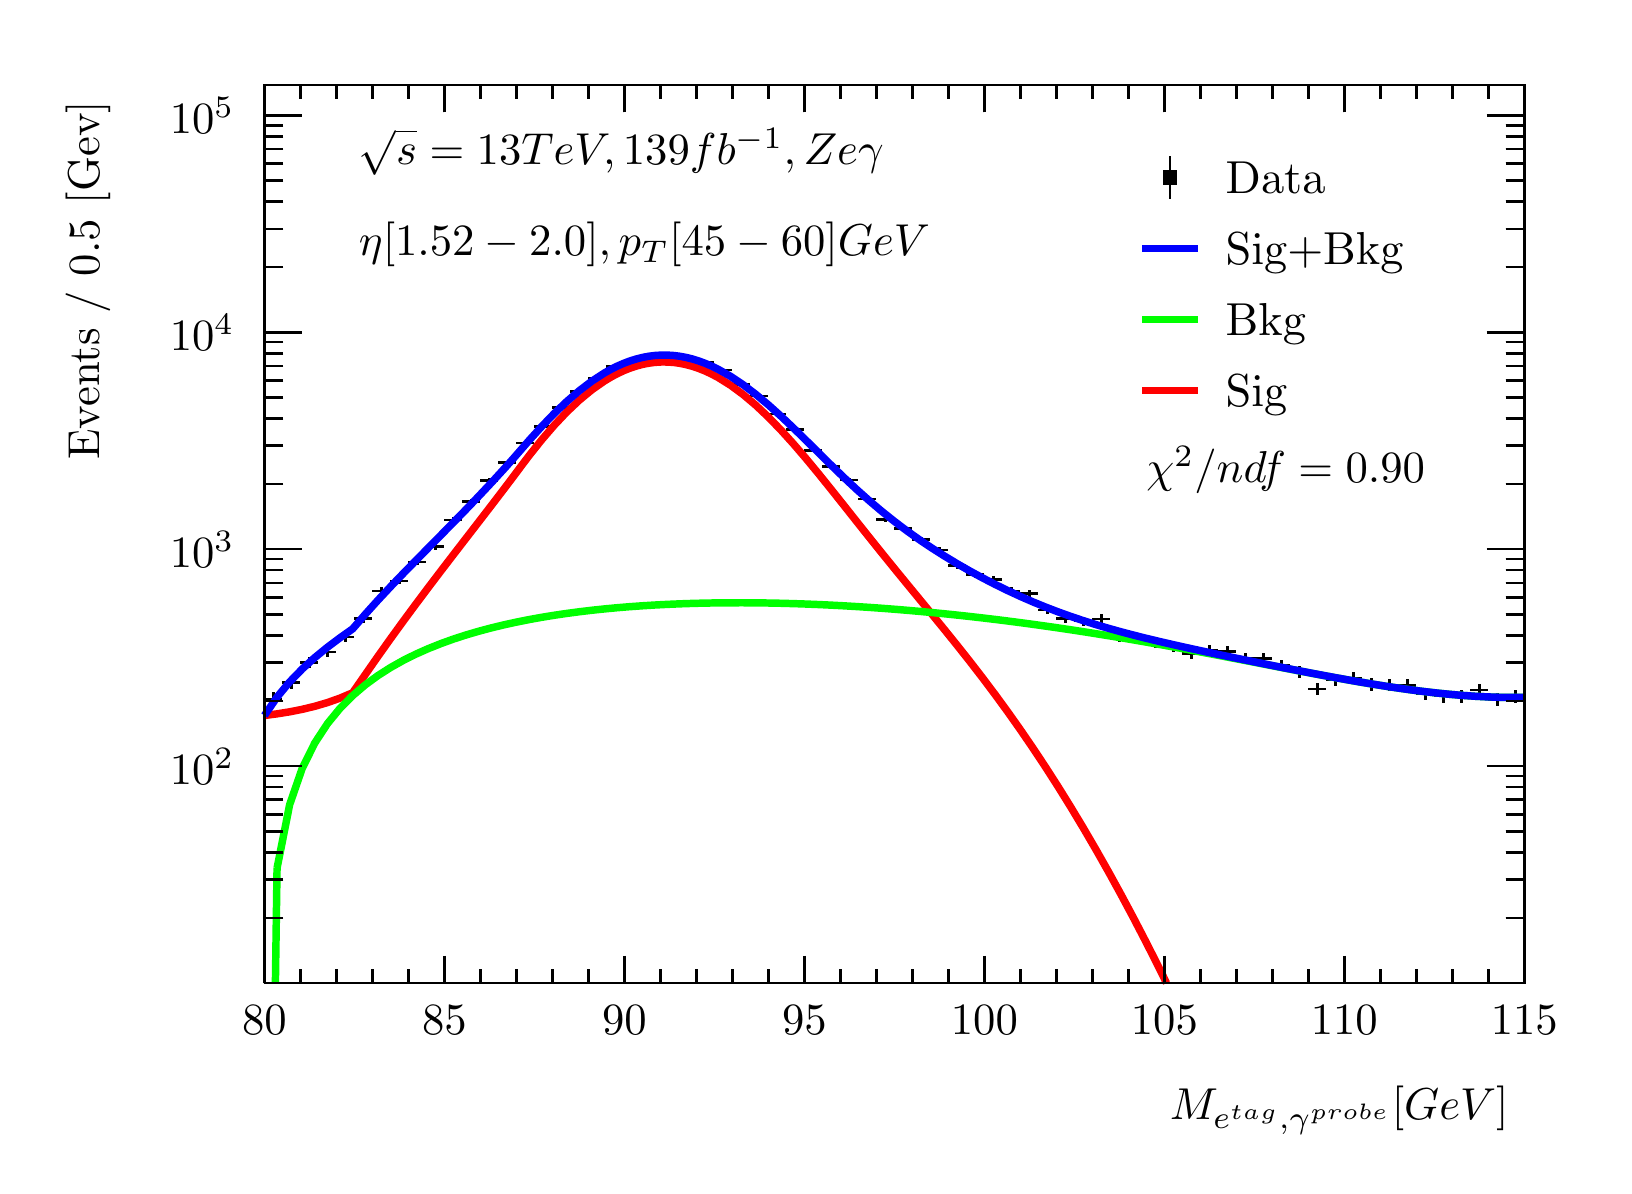
\begin{tikzpicture}
\pgfdeclareplotmark{cross} {
\pgfpathmoveto{\pgfpoint{-0.3\pgfplotmarksize}{\pgfplotmarksize}}
\pgfpathlineto{\pgfpoint{+0.3\pgfplotmarksize}{\pgfplotmarksize}}
\pgfpathlineto{\pgfpoint{+0.3\pgfplotmarksize}{0.3\pgfplotmarksize}}
\pgfpathlineto{\pgfpoint{+1\pgfplotmarksize}{0.3\pgfplotmarksize}}
\pgfpathlineto{\pgfpoint{+1\pgfplotmarksize}{-0.3\pgfplotmarksize}}
\pgfpathlineto{\pgfpoint{+0.3\pgfplotmarksize}{-0.3\pgfplotmarksize}}
\pgfpathlineto{\pgfpoint{+0.3\pgfplotmarksize}{-1.\pgfplotmarksize}}
\pgfpathlineto{\pgfpoint{-0.3\pgfplotmarksize}{-1.\pgfplotmarksize}}
\pgfpathlineto{\pgfpoint{-0.3\pgfplotmarksize}{-0.3\pgfplotmarksize}}
\pgfpathlineto{\pgfpoint{-1.\pgfplotmarksize}{-0.3\pgfplotmarksize}}
\pgfpathlineto{\pgfpoint{-1.\pgfplotmarksize}{0.3\pgfplotmarksize}}
\pgfpathlineto{\pgfpoint{-0.3\pgfplotmarksize}{0.3\pgfplotmarksize}}
\pgfpathclose
\pgfusepathqstroke
}
\pgfdeclareplotmark{cross*} {
\pgfpathmoveto{\pgfpoint{-0.3\pgfplotmarksize}{\pgfplotmarksize}}
\pgfpathlineto{\pgfpoint{+0.3\pgfplotmarksize}{\pgfplotmarksize}}
\pgfpathlineto{\pgfpoint{+0.3\pgfplotmarksize}{0.3\pgfplotmarksize}}
\pgfpathlineto{\pgfpoint{+1\pgfplotmarksize}{0.3\pgfplotmarksize}}
\pgfpathlineto{\pgfpoint{+1\pgfplotmarksize}{-0.3\pgfplotmarksize}}
\pgfpathlineto{\pgfpoint{+0.3\pgfplotmarksize}{-0.3\pgfplotmarksize}}
\pgfpathlineto{\pgfpoint{+0.3\pgfplotmarksize}{-1.\pgfplotmarksize}}
\pgfpathlineto{\pgfpoint{-0.3\pgfplotmarksize}{-1.\pgfplotmarksize}}
\pgfpathlineto{\pgfpoint{-0.3\pgfplotmarksize}{-0.3\pgfplotmarksize}}
\pgfpathlineto{\pgfpoint{-1.\pgfplotmarksize}{-0.3\pgfplotmarksize}}
\pgfpathlineto{\pgfpoint{-1.\pgfplotmarksize}{0.3\pgfplotmarksize}}
\pgfpathlineto{\pgfpoint{-0.3\pgfplotmarksize}{0.3\pgfplotmarksize}}
\pgfpathclose
\pgfusepathqfillstroke
}
\pgfdeclareplotmark{newstar} {
\pgfpathmoveto{\pgfqpoint{0pt}{\pgfplotmarksize}}
\pgfpathlineto{\pgfqpointpolar{44}{0.5\pgfplotmarksize}}
\pgfpathlineto{\pgfqpointpolar{18}{\pgfplotmarksize}}
\pgfpathlineto{\pgfqpointpolar{-20}{0.5\pgfplotmarksize}}
\pgfpathlineto{\pgfqpointpolar{-54}{\pgfplotmarksize}}
\pgfpathlineto{\pgfqpointpolar{-90}{0.5\pgfplotmarksize}}
\pgfpathlineto{\pgfqpointpolar{234}{\pgfplotmarksize}}
\pgfpathlineto{\pgfqpointpolar{198}{0.5\pgfplotmarksize}}
\pgfpathlineto{\pgfqpointpolar{162}{\pgfplotmarksize}}
\pgfpathlineto{\pgfqpointpolar{134}{0.5\pgfplotmarksize}}
\pgfpathclose
\pgfusepathqstroke
}
\pgfdeclareplotmark{newstar*} {
\pgfpathmoveto{\pgfqpoint{0pt}{\pgfplotmarksize}}
\pgfpathlineto{\pgfqpointpolar{44}{0.5\pgfplotmarksize}}
\pgfpathlineto{\pgfqpointpolar{18}{\pgfplotmarksize}}
\pgfpathlineto{\pgfqpointpolar{-20}{0.5\pgfplotmarksize}}
\pgfpathlineto{\pgfqpointpolar{-54}{\pgfplotmarksize}}
\pgfpathlineto{\pgfqpointpolar{-90}{0.5\pgfplotmarksize}}
\pgfpathlineto{\pgfqpointpolar{234}{\pgfplotmarksize}}
\pgfpathlineto{\pgfqpointpolar{198}{0.5\pgfplotmarksize}}
\pgfpathlineto{\pgfqpointpolar{162}{\pgfplotmarksize}}
\pgfpathlineto{\pgfqpointpolar{134}{0.5\pgfplotmarksize}}
\pgfpathclose
\pgfusepathqfillstroke
}
\definecolor{c}{rgb}{1,1,1};
\draw [color=c, fill=c] (0,0) rectangle (20,14.4361);
\draw [color=c, fill=c] (3,2.30977) rectangle (19,13.7143);
\definecolor{c}{rgb}{0,0,0};
\draw [c,line width=0.9] (3,2.30977) -- (3,13.7143) -- (19,13.7143) -- (19,2.30977) -- (3,2.30977);
\definecolor{c}{rgb}{1,1,1};
\draw [color=c, fill=c] (3,2.30977) rectangle (19,13.7143);
\definecolor{c}{rgb}{0,0,0};
\draw [c,line width=0.9] (3,2.30977) -- (3,13.7143) -- (19,13.7143) -- (19,2.30977) -- (3,2.30977);
\draw [c,line width=0.9] (3,2.30977) -- (19,2.30977);
\draw [c,line width=0.9] (3,2.65624) -- (3,2.30977);
\draw [c,line width=0.9] (3.45714,2.48301) -- (3.45714,2.30977);
\draw [c,line width=0.9] (3.91429,2.48301) -- (3.91429,2.30977);
\draw [c,line width=0.9] (4.37143,2.48301) -- (4.37143,2.30977);
\draw [c,line width=0.9] (4.82857,2.48301) -- (4.82857,2.30977);
\draw [c,line width=0.9] (5.28571,2.65624) -- (5.28571,2.30977);
\draw [c,line width=0.9] (5.74286,2.48301) -- (5.74286,2.30977);
\draw [c,line width=0.9] (6.2,2.48301) -- (6.2,2.30977);
\draw [c,line width=0.9] (6.65714,2.48301) -- (6.65714,2.30977);
\draw [c,line width=0.9] (7.11429,2.48301) -- (7.11429,2.30977);
\draw [c,line width=0.9] (7.57143,2.65624) -- (7.57143,2.30977);
\draw [c,line width=0.9] (8.02857,2.48301) -- (8.02857,2.30977);
\draw [c,line width=0.9] (8.48571,2.48301) -- (8.48571,2.30977);
\draw [c,line width=0.9] (8.94286,2.48301) -- (8.94286,2.30977);
\draw [c,line width=0.9] (9.4,2.48301) -- (9.4,2.30977);
\draw [c,line width=0.9] (9.85714,2.65624) -- (9.85714,2.30977);
\draw [c,line width=0.9] (10.3143,2.48301) -- (10.3143,2.30977);
\draw [c,line width=0.9] (10.7714,2.48301) -- (10.7714,2.30977);
\draw [c,line width=0.9] (11.2286,2.48301) -- (11.2286,2.30977);
\draw [c,line width=0.9] (11.6857,2.48301) -- (11.6857,2.30977);
\draw [c,line width=0.9] (12.1429,2.65624) -- (12.1429,2.30977);
\draw [c,line width=0.9] (12.6,2.48301) -- (12.6,2.30977);
\draw [c,line width=0.9] (13.0571,2.48301) -- (13.0571,2.30977);
\draw [c,line width=0.9] (13.5143,2.48301) -- (13.5143,2.30977);
\draw [c,line width=0.9] (13.9714,2.48301) -- (13.9714,2.30977);
\draw [c,line width=0.9] (14.4286,2.65624) -- (14.4286,2.30977);
\draw [c,line width=0.9] (14.8857,2.48301) -- (14.8857,2.30977);
\draw [c,line width=0.9] (15.3429,2.48301) -- (15.3429,2.30977);
\draw [c,line width=0.9] (15.8,2.48301) -- (15.8,2.30977);
\draw [c,line width=0.9] (16.2571,2.48301) -- (16.2571,2.30977);
\draw [c,line width=0.9] (16.7143,2.65624) -- (16.7143,2.30977);
\draw [c,line width=0.9] (17.1714,2.48301) -- (17.1714,2.30977);
\draw [c,line width=0.9] (17.6286,2.48301) -- (17.6286,2.30977);
\draw [c,line width=0.9] (18.0857,2.48301) -- (18.0857,2.30977);
\draw [c,line width=0.9] (18.5429,2.48301) -- (18.5429,2.30977);
\draw [c,line width=0.9] (19,2.65624) -- (19,2.30977);
\draw [anchor=base] (3,1.66015) node[scale=1.61424, color=c, rotate=0]{80};
\draw [anchor=base] (5.28571,1.66015) node[scale=1.61424, color=c, rotate=0]{85};
\draw [anchor=base] (7.57143,1.66015) node[scale=1.61424, color=c, rotate=0]{90};
\draw [anchor=base] (9.85714,1.66015) node[scale=1.61424, color=c, rotate=0]{95};
\draw [anchor=base] (12.1429,1.66015) node[scale=1.61424, color=c, rotate=0]{100};
\draw [anchor=base] (14.4286,1.66015) node[scale=1.61424, color=c, rotate=0]{105};
\draw [anchor=base] (16.7143,1.66015) node[scale=1.61424, color=c, rotate=0]{110};
\draw [anchor=base] (19,1.66015) node[scale=1.61424, color=c, rotate=0]{115};
\draw [anchor= east] (19,0.692932) node[scale=1.61424, color=c, rotate=0]{$M_{e^{tag}, \gamma^{probe}}  [GeV]$};
\draw [c,line width=0.9] (3,13.7143) -- (19,13.7143);
\draw [c,line width=0.9] (3,13.3678) -- (3,13.7143);
\draw [c,line width=0.9] (3.45714,13.5411) -- (3.45714,13.7143);
\draw [c,line width=0.9] (3.91429,13.5411) -- (3.91429,13.7143);
\draw [c,line width=0.9] (4.37143,13.5411) -- (4.37143,13.7143);
\draw [c,line width=0.9] (4.82857,13.5411) -- (4.82857,13.7143);
\draw [c,line width=0.9] (5.28571,13.3678) -- (5.28571,13.7143);
\draw [c,line width=0.9] (5.74286,13.5411) -- (5.74286,13.7143);
\draw [c,line width=0.9] (6.2,13.5411) -- (6.2,13.7143);
\draw [c,line width=0.9] (6.65714,13.5411) -- (6.65714,13.7143);
\draw [c,line width=0.9] (7.11429,13.5411) -- (7.11429,13.7143);
\draw [c,line width=0.9] (7.57143,13.3678) -- (7.57143,13.7143);
\draw [c,line width=0.9] (8.02857,13.5411) -- (8.02857,13.7143);
\draw [c,line width=0.9] (8.48571,13.5411) -- (8.48571,13.7143);
\draw [c,line width=0.9] (8.94286,13.5411) -- (8.94286,13.7143);
\draw [c,line width=0.9] (9.4,13.5411) -- (9.4,13.7143);
\draw [c,line width=0.9] (9.85714,13.3678) -- (9.85714,13.7143);
\draw [c,line width=0.9] (10.3143,13.5411) -- (10.3143,13.7143);
\draw [c,line width=0.9] (10.7714,13.5411) -- (10.7714,13.7143);
\draw [c,line width=0.9] (11.2286,13.5411) -- (11.2286,13.7143);
\draw [c,line width=0.9] (11.6857,13.5411) -- (11.6857,13.7143);
\draw [c,line width=0.9] (12.1429,13.3678) -- (12.1429,13.7143);
\draw [c,line width=0.9] (12.6,13.5411) -- (12.6,13.7143);
\draw [c,line width=0.9] (13.0571,13.5411) -- (13.0571,13.7143);
\draw [c,line width=0.9] (13.5143,13.5411) -- (13.5143,13.7143);
\draw [c,line width=0.9] (13.9714,13.5411) -- (13.9714,13.7143);
\draw [c,line width=0.9] (14.4286,13.3678) -- (14.4286,13.7143);
\draw [c,line width=0.9] (14.8857,13.5411) -- (14.8857,13.7143);
\draw [c,line width=0.9] (15.3429,13.5411) -- (15.3429,13.7143);
\draw [c,line width=0.9] (15.8,13.5411) -- (15.8,13.7143);
\draw [c,line width=0.9] (16.2571,13.5411) -- (16.2571,13.7143);
\draw [c,line width=0.9] (16.7143,13.3678) -- (16.7143,13.7143);
\draw [c,line width=0.9] (17.1714,13.5411) -- (17.1714,13.7143);
\draw [c,line width=0.9] (17.6286,13.5411) -- (17.6286,13.7143);
\draw [c,line width=0.9] (18.0857,13.5411) -- (18.0857,13.7143);
\draw [c,line width=0.9] (18.5429,13.5411) -- (18.5429,13.7143);
\draw [c,line width=0.9] (19,13.3678) -- (19,13.7143);
\draw [c,line width=0.9] (3,2.30977) -- (3,13.7143);
\draw [c,line width=0.9] (3.237,3.13907) -- (3,3.13907);
\draw [c,line width=0.9] (3.237,3.62418) -- (3,3.62418);
\draw [c,line width=0.9] (3.237,3.96837) -- (3,3.96837);
\draw [c,line width=0.9] (3.237,4.23535) -- (3,4.23535);
\draw [c,line width=0.9] (3.237,4.45348) -- (3,4.45348);
\draw [c,line width=0.9] (3.237,4.63791) -- (3,4.63791);
\draw [c,line width=0.9] (3.237,4.79767) -- (3,4.79767);
\draw [c,line width=0.9] (3.237,4.93859) -- (3,4.93859);
\draw [c,line width=0.9] (3.474,5.06465) -- (3,5.06465);
\draw [anchor= east] (2.82,5.06465) node[scale=1.61424, color=c, rotate=0]{$10^{2}$};
\draw [c,line width=0.9] (3.237,5.89394) -- (3,5.89394);
\draw [c,line width=0.9] (3.237,6.37905) -- (3,6.37905);
\draw [c,line width=0.9] (3.237,6.72324) -- (3,6.72324);
\draw [c,line width=0.9] (3.237,6.99022) -- (3,6.99022);
\draw [c,line width=0.9] (3.237,7.20835) -- (3,7.20835);
\draw [c,line width=0.9] (3.237,7.39278) -- (3,7.39278);
\draw [c,line width=0.9] (3.237,7.55254) -- (3,7.55254);
\draw [c,line width=0.9] (3.237,7.69346) -- (3,7.69346);
\draw [c,line width=0.9] (3.474,7.81952) -- (3,7.81952);
\draw [anchor= east] (2.82,7.81952) node[scale=1.61424, color=c, rotate=0]{$10^{3}$};
\draw [c,line width=0.9] (3.237,8.64882) -- (3,8.64882);
\draw [c,line width=0.9] (3.237,9.13393) -- (3,9.13393);
\draw [c,line width=0.9] (3.237,9.47812) -- (3,9.47812);
\draw [c,line width=0.9] (3.237,9.74509) -- (3,9.74509);
\draw [c,line width=0.9] (3.237,9.96323) -- (3,9.96323);
\draw [c,line width=0.9] (3.237,10.1477) -- (3,10.1477);
\draw [c,line width=0.9] (3.237,10.3074) -- (3,10.3074);
\draw [c,line width=0.9] (3.237,10.4483) -- (3,10.4483);
\draw [c,line width=0.9] (3.474,10.5744) -- (3,10.5744);
\draw [anchor= east] (2.82,10.5744) node[scale=1.61424, color=c, rotate=0]{$10^{4}$};
\draw [c,line width=0.9] (3.237,11.4037) -- (3,11.4037);
\draw [c,line width=0.9] (3.237,11.8888) -- (3,11.8888);
\draw [c,line width=0.9] (3.237,12.233) -- (3,12.233);
\draw [c,line width=0.9] (3.237,12.5) -- (3,12.5);
\draw [c,line width=0.9] (3.237,12.7181) -- (3,12.7181);
\draw [c,line width=0.9] (3.237,12.9025) -- (3,12.9025);
\draw [c,line width=0.9] (3.237,13.0623) -- (3,13.0623);
\draw [c,line width=0.9] (3.237,13.2032) -- (3,13.2032);
\draw [c,line width=0.9] (3.474,13.3293) -- (3,13.3293);
\draw [anchor= east] (2.82,13.3293) node[scale=1.61424, color=c, rotate=0]{$10^{5}$};
\draw [anchor= east] (0.76,13.7143) node[scale=1.61424, color=c, rotate=90]{Events / 0.5 [Gev]};
\draw [c,line width=0.9] (19,2.30977) -- (19,13.7143);
\draw [c,line width=0.9] (18.763,3.13907) -- (19,3.13907);
\draw [c,line width=0.9] (18.763,3.62418) -- (19,3.62418);
\draw [c,line width=0.9] (18.763,3.96837) -- (19,3.96837);
\draw [c,line width=0.9] (18.763,4.23535) -- (19,4.23535);
\draw [c,line width=0.9] (18.763,4.45348) -- (19,4.45348);
\draw [c,line width=0.9] (18.763,4.63791) -- (19,4.63791);
\draw [c,line width=0.9] (18.763,4.79767) -- (19,4.79767);
\draw [c,line width=0.9] (18.763,4.93859) -- (19,4.93859);
\draw [c,line width=0.9] (18.526,5.06465) -- (19,5.06465);
\draw [c,line width=0.9] (18.763,5.89394) -- (19,5.89394);
\draw [c,line width=0.9] (18.763,6.37905) -- (19,6.37905);
\draw [c,line width=0.9] (18.763,6.72324) -- (19,6.72324);
\draw [c,line width=0.9] (18.763,6.99022) -- (19,6.99022);
\draw [c,line width=0.9] (18.763,7.20835) -- (19,7.20835);
\draw [c,line width=0.9] (18.763,7.39278) -- (19,7.39278);
\draw [c,line width=0.9] (18.763,7.55254) -- (19,7.55254);
\draw [c,line width=0.9] (18.763,7.69346) -- (19,7.69346);
\draw [c,line width=0.9] (18.526,7.81952) -- (19,7.81952);
\draw [c,line width=0.9] (18.763,8.64882) -- (19,8.64882);
\draw [c,line width=0.9] (18.763,9.13393) -- (19,9.13393);
\draw [c,line width=0.9] (18.763,9.47812) -- (19,9.47812);
\draw [c,line width=0.9] (18.763,9.74509) -- (19,9.74509);
\draw [c,line width=0.9] (18.763,9.96323) -- (19,9.96323);
\draw [c,line width=0.9] (18.763,10.1477) -- (19,10.1477);
\draw [c,line width=0.9] (18.763,10.3074) -- (19,10.3074);
\draw [c,line width=0.9] (18.763,10.4483) -- (19,10.4483);
\draw [c,line width=0.9] (18.526,10.5744) -- (19,10.5744);
\draw [c,line width=0.9] (18.763,11.4037) -- (19,11.4037);
\draw [c,line width=0.9] (18.763,11.8888) -- (19,11.8888);
\draw [c,line width=0.9] (18.763,12.233) -- (19,12.233);
\draw [c,line width=0.9] (18.763,12.5) -- (19,12.5);
\draw [c,line width=0.9] (18.763,12.7181) -- (19,12.7181);
\draw [c,line width=0.9] (18.763,12.9025) -- (19,12.9025);
\draw [c,line width=0.9] (18.763,13.0623) -- (19,13.0623);
\draw [c,line width=0.9] (18.763,13.2032) -- (19,13.2032);
\draw [c,line width=0.9] (18.526,13.3293) -- (19,13.3293);
\draw [c,line width=0.9] (3.11429,5.91764) -- (3,5.91764);
\draw [c,line width=0.9] (3,5.91764) -- (3,5.91764);
\draw [c,line width=0.9] (3.11429,5.91764) -- (3.22857,5.91764);
\draw [c,line width=0.9] (3.22857,5.91764) -- (3.22857,5.91764);
\draw [c,line width=0.9] (3.11429,5.91764) -- (3.11429,6.00139);
\draw [c,line width=0.9] (3.11429,6.00139) -- (3.11429,6.00139);
\draw [c,line width=0.9] (3.11429,5.91764) -- (3.11429,5.83389);
\draw [c,line width=0.9] (3.11429,5.83389) -- (3.11429,5.83389);
\draw [c,line width=0.9] (3.34286,6.12694) -- (3.22857,6.12694);
\draw [c,line width=0.9] (3.22857,6.12694) -- (3.22857,6.12694);
\draw [c,line width=0.9] (3.34286,6.12694) -- (3.45714,6.12694);
\draw [c,line width=0.9] (3.45714,6.12694) -- (3.45714,6.12694);
\draw [c,line width=0.9] (3.34286,6.12694) -- (3.34286,6.20368);
\draw [c,line width=0.9] (3.34286,6.20368) -- (3.34286,6.20368);
\draw [c,line width=0.9] (3.34286,6.12694) -- (3.34286,6.05021);
\draw [c,line width=0.9] (3.34286,6.05021) -- (3.34286,6.05021);
\draw [c,line width=0.9] (3.57143,6.37906) -- (3.45714,6.37906);
\draw [c,line width=0.9] (3.45714,6.37906) -- (3.45714,6.37906);
\draw [c,line width=0.9] (3.57143,6.37906) -- (3.68571,6.37906);
\draw [c,line width=0.9] (3.68571,6.37906) -- (3.68571,6.37906);
\draw [c,line width=0.9] (3.57143,6.37906) -- (3.57143,6.44812);
\draw [c,line width=0.9] (3.57143,6.44812) -- (3.57143,6.44812);
\draw [c,line width=0.9] (3.57143,6.37906) -- (3.57143,6.30999);
\draw [c,line width=0.9] (3.57143,6.30999) -- (3.57143,6.30999);
\draw [c,line width=0.9] (3.8,6.51108) -- (3.68571,6.51108);
\draw [c,line width=0.9] (3.68571,6.51108) -- (3.68571,6.51108);
\draw [c,line width=0.9] (3.8,6.51108) -- (3.91429,6.51108);
\draw [c,line width=0.9] (3.91429,6.51108) -- (3.91429,6.51108);
\draw [c,line width=0.9] (3.8,6.51108) -- (3.8,6.57644);
\draw [c,line width=0.9] (3.8,6.57644) -- (3.8,6.57644);
\draw [c,line width=0.9] (3.8,6.51108) -- (3.8,6.44572);
\draw [c,line width=0.9] (3.8,6.44572) -- (3.8,6.44572);
\draw [c,line width=0.9] (4.02857,6.70516) -- (3.91429,6.70516);
\draw [c,line width=0.9] (3.91429,6.70516) -- (3.91429,6.70516);
\draw [c,line width=0.9] (4.02857,6.70516) -- (4.14286,6.70516);
\draw [c,line width=0.9] (4.14286,6.70516) -- (4.14286,6.70516);
\draw [c,line width=0.9] (4.02857,6.70516) -- (4.02857,6.76543);
\draw [c,line width=0.9] (4.02857,6.76543) -- (4.02857,6.76543);
\draw [c,line width=0.9] (4.02857,6.70516) -- (4.02857,6.6449);
\draw [c,line width=0.9] (4.02857,6.6449) -- (4.02857,6.6449);
\draw [c,line width=0.9] (4.25714,6.94138) -- (4.14286,6.94138);
\draw [c,line width=0.9] (4.14286,6.94138) -- (4.14286,6.94138);
\draw [c,line width=0.9] (4.25714,6.94138) -- (4.37143,6.94138);
\draw [c,line width=0.9] (4.37143,6.94138) -- (4.37143,6.94138);
\draw [c,line width=0.9] (4.25714,6.94138) -- (4.25714,6.99599);
\draw [c,line width=0.9] (4.25714,6.99599) -- (4.25714,6.99599);
\draw [c,line width=0.9] (4.25714,6.94138) -- (4.25714,6.88678);
\draw [c,line width=0.9] (4.25714,6.88678) -- (4.25714,6.88678);
\draw [c,line width=0.9] (4.48571,7.2893) -- (4.37143,7.2893);
\draw [c,line width=0.9] (4.37143,7.2893) -- (4.37143,7.2893);
\draw [c,line width=0.9] (4.48571,7.2893) -- (4.6,7.2893);
\draw [c,line width=0.9] (4.6,7.2893) -- (4.6,7.2893);
\draw [c,line width=0.9] (4.48571,7.2893) -- (4.48571,7.33652);
\draw [c,line width=0.9] (4.48571,7.33652) -- (4.48571,7.33652);
\draw [c,line width=0.9] (4.48571,7.2893) -- (4.48571,7.24209);
\draw [c,line width=0.9] (4.48571,7.24209) -- (4.48571,7.24209);
\draw [c,line width=0.9] (4.71429,7.41648) -- (4.6,7.41648);
\draw [c,line width=0.9] (4.6,7.41648) -- (4.6,7.41648);
\draw [c,line width=0.9] (4.71429,7.41648) -- (4.82857,7.41648);
\draw [c,line width=0.9] (4.82857,7.41648) -- (4.82857,7.41648);
\draw [c,line width=0.9] (4.71429,7.41648) -- (4.71429,7.46125);
\draw [c,line width=0.9] (4.71429,7.46125) -- (4.71429,7.46125);
\draw [c,line width=0.9] (4.71429,7.41648) -- (4.71429,7.37171);
\draw [c,line width=0.9] (4.71429,7.37171) -- (4.71429,7.37171);
\draw [c,line width=0.9] (4.94286,7.65839) -- (4.82857,7.65839);
\draw [c,line width=0.9] (4.82857,7.65839) -- (4.82857,7.65839);
\draw [c,line width=0.9] (4.94286,7.65839) -- (5.05714,7.65839);
\draw [c,line width=0.9] (5.05714,7.65839) -- (5.05714,7.65839);
\draw [c,line width=0.9] (4.94286,7.65839) -- (4.94286,7.69886);
\draw [c,line width=0.9] (4.94286,7.69886) -- (4.94286,7.69886);
\draw [c,line width=0.9] (4.94286,7.65839) -- (4.94286,7.61792);
\draw [c,line width=0.9] (4.94286,7.61792) -- (4.94286,7.61792);
\draw [c,line width=0.9] (5.17143,7.8514) -- (5.05714,7.8514);
\draw [c,line width=0.9] (5.05714,7.8514) -- (5.05714,7.8514);
\draw [c,line width=0.9] (5.17143,7.8514) -- (5.28571,7.8514);
\draw [c,line width=0.9] (5.28571,7.8514) -- (5.28571,7.8514);
\draw [c,line width=0.9] (5.17143,7.8514) -- (5.17143,7.88873);
\draw [c,line width=0.9] (5.17143,7.88873) -- (5.17143,7.88873);
\draw [c,line width=0.9] (5.17143,7.8514) -- (5.17143,7.81406);
\draw [c,line width=0.9] (5.17143,7.81406) -- (5.17143,7.81406);
\draw [c,line width=0.9] (5.4,8.19004) -- (5.28571,8.19004);
\draw [c,line width=0.9] (5.28571,8.19004) -- (5.28571,8.19004);
\draw [c,line width=0.9] (5.4,8.19004) -- (5.51429,8.19004);
\draw [c,line width=0.9] (5.51429,8.19004) -- (5.51429,8.19004);
\draw [c,line width=0.9] (5.4,8.19004) -- (5.4,8.22245);
\draw [c,line width=0.9] (5.4,8.22245) -- (5.4,8.22245);
\draw [c,line width=0.9] (5.4,8.19004) -- (5.4,8.15763);
\draw [c,line width=0.9] (5.4,8.15763) -- (5.4,8.15763);
\draw [c,line width=0.9] (5.62857,8.42373) -- (5.51429,8.42373);
\draw [c,line width=0.9] (5.51429,8.42373) -- (5.51429,8.42373);
\draw [c,line width=0.9] (5.62857,8.42373) -- (5.74286,8.42373);
\draw [c,line width=0.9] (5.74286,8.42373) -- (5.74286,8.42373);
\draw [c,line width=0.9] (5.62857,8.42373) -- (5.62857,8.45312);
\draw [c,line width=0.9] (5.62857,8.45312) -- (5.62857,8.45312);
\draw [c,line width=0.9] (5.62857,8.42373) -- (5.62857,8.39433);
\draw [c,line width=0.9] (5.62857,8.39433) -- (5.62857,8.39433);
\draw [c,line width=0.9] (5.85714,8.69229) -- (5.74286,8.69229);
\draw [c,line width=0.9] (5.74286,8.69229) -- (5.74286,8.69229);
\draw [c,line width=0.9] (5.85714,8.69229) -- (5.97143,8.69229);
\draw [c,line width=0.9] (5.97143,8.69229) -- (5.97143,8.69229);
\draw [c,line width=0.9] (5.85714,8.69229) -- (5.85714,8.71856);
\draw [c,line width=0.9] (5.85714,8.71856) -- (5.85714,8.71856);
\draw [c,line width=0.9] (5.85714,8.69229) -- (5.85714,8.66602);
\draw [c,line width=0.9] (5.85714,8.66602) -- (5.85714,8.66602);
\draw [c,line width=0.9] (6.08571,8.92009) -- (5.97143,8.92009);
\draw [c,line width=0.9] (5.97143,8.92009) -- (5.97143,8.92009);
\draw [c,line width=0.9] (6.08571,8.92009) -- (6.2,8.92009);
\draw [c,line width=0.9] (6.2,8.92009) -- (6.2,8.92009);
\draw [c,line width=0.9] (6.08571,8.92009) -- (6.08571,8.94398);
\draw [c,line width=0.9] (6.08571,8.94398) -- (6.08571,8.94398);
\draw [c,line width=0.9] (6.08571,8.92009) -- (6.08571,8.89621);
\draw [c,line width=0.9] (6.08571,8.89621) -- (6.08571,8.89621);
\draw [c,line width=0.9] (6.31429,9.16697) -- (6.2,9.16697);
\draw [c,line width=0.9] (6.2,9.16697) -- (6.2,9.16697);
\draw [c,line width=0.9] (6.31429,9.16697) -- (6.42857,9.16697);
\draw [c,line width=0.9] (6.42857,9.16697) -- (6.42857,9.16697);
\draw [c,line width=0.9] (6.31429,9.16697) -- (6.31429,9.18851);
\draw [c,line width=0.9] (6.31429,9.18851) -- (6.31429,9.18851);
\draw [c,line width=0.9] (6.31429,9.16697) -- (6.31429,9.14542);
\draw [c,line width=0.9] (6.31429,9.14542) -- (6.31429,9.14542);
\draw [c,line width=0.9] (6.54286,9.37998) -- (6.42857,9.37998);
\draw [c,line width=0.9] (6.42857,9.37998) -- (6.42857,9.37998);
\draw [c,line width=0.9] (6.54286,9.37998) -- (6.65714,9.37998);
\draw [c,line width=0.9] (6.65714,9.37998) -- (6.65714,9.37998);
\draw [c,line width=0.9] (6.54286,9.37998) -- (6.54286,9.39969);
\draw [c,line width=0.9] (6.54286,9.39969) -- (6.54286,9.39969);
\draw [c,line width=0.9] (6.54286,9.37998) -- (6.54286,9.36028);
\draw [c,line width=0.9] (6.54286,9.36028) -- (6.54286,9.36028);
\draw [c,line width=0.9] (6.77143,9.61771) -- (6.65714,9.61771);
\draw [c,line width=0.9] (6.65714,9.61771) -- (6.65714,9.61771);
\draw [c,line width=0.9] (6.77143,9.61771) -- (6.88571,9.61771);
\draw [c,line width=0.9] (6.88571,9.61771) -- (6.88571,9.61771);
\draw [c,line width=0.9] (6.77143,9.61771) -- (6.77143,9.63555);
\draw [c,line width=0.9] (6.77143,9.63555) -- (6.77143,9.63555);
\draw [c,line width=0.9] (6.77143,9.61771) -- (6.77143,9.59986);
\draw [c,line width=0.9] (6.77143,9.59986) -- (6.77143,9.59986);
\draw [c,line width=0.9] (7,9.82403) -- (6.88571,9.82403);
\draw [c,line width=0.9] (6.88571,9.82403) -- (6.88571,9.82403);
\draw [c,line width=0.9] (7,9.82403) -- (7.11429,9.82403);
\draw [c,line width=0.9] (7.11429,9.82403) -- (7.11429,9.82403);
\draw [c,line width=0.9] (7,9.82403) -- (7,9.8404);
\draw [c,line width=0.9] (7,9.8404) -- (7,9.8404);
\draw [c,line width=0.9] (7,9.82403) -- (7,9.80766);
\draw [c,line width=0.9] (7,9.80766) -- (7,9.80766);
\draw [c,line width=0.9] (7.22857,9.99374) -- (7.11429,9.99374);
\draw [c,line width=0.9] (7.11429,9.99374) -- (7.11429,9.99374);
\draw [c,line width=0.9] (7.22857,9.99374) -- (7.34286,9.99374);
\draw [c,line width=0.9] (7.34286,9.99374) -- (7.34286,9.99374);
\draw [c,line width=0.9] (7.22857,9.99374) -- (7.22857,10.009);
\draw [c,line width=0.9] (7.22857,10.009) -- (7.22857,10.009);
\draw [c,line width=0.9] (7.22857,9.99374) -- (7.22857,9.97849);
\draw [c,line width=0.9] (7.22857,9.97849) -- (7.22857,9.97849);
\draw [c,line width=0.9] (7.45714,10.1398) -- (7.34286,10.1398);
\draw [c,line width=0.9] (7.34286,10.1398) -- (7.34286,10.1398);
\draw [c,line width=0.9] (7.45714,10.1398) -- (7.57143,10.1398);
\draw [c,line width=0.9] (7.57143,10.1398) -- (7.57143,10.1398);
\draw [c,line width=0.9] (7.45714,10.1398) -- (7.45714,10.1541);
\draw [c,line width=0.9] (7.45714,10.1541) -- (7.45714,10.1541);
\draw [c,line width=0.9] (7.45714,10.1398) -- (7.45714,10.1254);
\draw [c,line width=0.9] (7.45714,10.1254) -- (7.45714,10.1254);
\draw [c,line width=0.9] (7.68571,10.2114) -- (7.57143,10.2114);
\draw [c,line width=0.9] (7.57143,10.2114) -- (7.57143,10.2114);
\draw [c,line width=0.9] (7.68571,10.2114) -- (7.8,10.2114);
\draw [c,line width=0.9] (7.8,10.2114) -- (7.8,10.2114);
\draw [c,line width=0.9] (7.68571,10.2114) -- (7.68571,10.2253);
\draw [c,line width=0.9] (7.68571,10.2253) -- (7.68571,10.2253);
\draw [c,line width=0.9] (7.68571,10.2114) -- (7.68571,10.1975);
\draw [c,line width=0.9] (7.68571,10.1975) -- (7.68571,10.1975);
\draw [c,line width=0.9] (7.91429,10.2731) -- (7.8,10.2731);
\draw [c,line width=0.9] (7.8,10.2731) -- (7.8,10.2731);
\draw [c,line width=0.9] (7.91429,10.2731) -- (8.02857,10.2731);
\draw [c,line width=0.9] (8.02857,10.2731) -- (8.02857,10.2731);
\draw [c,line width=0.9] (7.91429,10.2731) -- (7.91429,10.2867);
\draw [c,line width=0.9] (7.91429,10.2867) -- (7.91429,10.2867);
\draw [c,line width=0.9] (7.91429,10.2731) -- (7.91429,10.2596);
\draw [c,line width=0.9] (7.91429,10.2596) -- (7.91429,10.2596);
\draw [c,line width=0.9] (8.14286,10.2918) -- (8.02857,10.2918);
\draw [c,line width=0.9] (8.02857,10.2918) -- (8.02857,10.2918);
\draw [c,line width=0.9] (8.14286,10.2918) -- (8.25714,10.2918);
\draw [c,line width=0.9] (8.25714,10.2918) -- (8.25714,10.2918);
\draw [c,line width=0.9] (8.14286,10.2918) -- (8.14286,10.3052);
\draw [c,line width=0.9] (8.14286,10.3052) -- (8.14286,10.3052);
\draw [c,line width=0.9] (8.14286,10.2918) -- (8.14286,10.2783);
\draw [c,line width=0.9] (8.14286,10.2783) -- (8.14286,10.2783);
\draw [c,line width=0.9] (8.37143,10.2429) -- (8.25714,10.2429);
\draw [c,line width=0.9] (8.25714,10.2429) -- (8.25714,10.2429);
\draw [c,line width=0.9] (8.37143,10.2429) -- (8.48571,10.2429);
\draw [c,line width=0.9] (8.48571,10.2429) -- (8.48571,10.2429);
\draw [c,line width=0.9] (8.37143,10.2429) -- (8.37143,10.2566);
\draw [c,line width=0.9] (8.37143,10.2566) -- (8.37143,10.2566);
\draw [c,line width=0.9] (8.37143,10.2429) -- (8.37143,10.2292);
\draw [c,line width=0.9] (8.37143,10.2292) -- (8.37143,10.2292);
\draw [c,line width=0.9] (8.6,10.189) -- (8.48571,10.189);
\draw [c,line width=0.9] (8.48571,10.189) -- (8.48571,10.189);
\draw [c,line width=0.9] (8.6,10.189) -- (8.71429,10.189);
\draw [c,line width=0.9] (8.71429,10.189) -- (8.71429,10.189);
\draw [c,line width=0.9] (8.6,10.189) -- (8.6,10.203);
\draw [c,line width=0.9] (8.6,10.203) -- (8.6,10.203);
\draw [c,line width=0.9] (8.6,10.189) -- (8.6,10.1749);
\draw [c,line width=0.9] (8.6,10.1749) -- (8.6,10.1749);
\draw [c,line width=0.9] (8.82857,10.0949) -- (8.71429,10.0949);
\draw [c,line width=0.9] (8.71429,10.0949) -- (8.71429,10.0949);
\draw [c,line width=0.9] (8.82857,10.0949) -- (8.94286,10.0949);
\draw [c,line width=0.9] (8.94286,10.0949) -- (8.94286,10.0949);
\draw [c,line width=0.9] (8.82857,10.0949) -- (8.82857,10.1095);
\draw [c,line width=0.9] (8.82857,10.1095) -- (8.82857,10.1095);
\draw [c,line width=0.9] (8.82857,10.0949) -- (8.82857,10.0803);
\draw [c,line width=0.9] (8.82857,10.0803) -- (8.82857,10.0803);
\draw [c,line width=0.9] (9.05714,9.91168) -- (8.94286,9.91168);
\draw [c,line width=0.9] (8.94286,9.91168) -- (8.94286,9.91168);
\draw [c,line width=0.9] (9.05714,9.91168) -- (9.17143,9.91168);
\draw [c,line width=0.9] (9.17143,9.91168) -- (9.17143,9.91168);
\draw [c,line width=0.9] (9.05714,9.91168) -- (9.05714,9.92747);
\draw [c,line width=0.9] (9.05714,9.92747) -- (9.05714,9.92747);
\draw [c,line width=0.9] (9.05714,9.91168) -- (9.05714,9.8959);
\draw [c,line width=0.9] (9.05714,9.8959) -- (9.05714,9.8959);
\draw [c,line width=0.9] (9.28571,9.76361) -- (9.17143,9.76361);
\draw [c,line width=0.9] (9.17143,9.76361) -- (9.17143,9.76361);
\draw [c,line width=0.9] (9.28571,9.76361) -- (9.4,9.76361);
\draw [c,line width=0.9] (9.4,9.76361) -- (9.4,9.76361);
\draw [c,line width=0.9] (9.28571,9.76361) -- (9.28571,9.7804);
\draw [c,line width=0.9] (9.28571,9.7804) -- (9.28571,9.7804);
\draw [c,line width=0.9] (9.28571,9.76361) -- (9.28571,9.74682);
\draw [c,line width=0.9] (9.28571,9.74682) -- (9.28571,9.74682);
\draw [c,line width=0.9] (9.51429,9.53877) -- (9.4,9.53877);
\draw [c,line width=0.9] (9.4,9.53877) -- (9.4,9.53877);
\draw [c,line width=0.9] (9.51429,9.53877) -- (9.62857,9.53877);
\draw [c,line width=0.9] (9.62857,9.53877) -- (9.62857,9.53877);
\draw [c,line width=0.9] (9.51429,9.53877) -- (9.51429,9.55721);
\draw [c,line width=0.9] (9.51429,9.55721) -- (9.51429,9.55721);
\draw [c,line width=0.9] (9.51429,9.53877) -- (9.51429,9.52033);
\draw [c,line width=0.9] (9.51429,9.52033) -- (9.51429,9.52033);
\draw [c,line width=0.9] (9.74286,9.3387) -- (9.62857,9.3387);
\draw [c,line width=0.9] (9.62857,9.3387) -- (9.62857,9.3387);
\draw [c,line width=0.9] (9.74286,9.3387) -- (9.85714,9.3387);
\draw [c,line width=0.9] (9.85714,9.3387) -- (9.85714,9.3387);
\draw [c,line width=0.9] (9.74286,9.3387) -- (9.74286,9.35875);
\draw [c,line width=0.9] (9.74286,9.35875) -- (9.74286,9.35875);
\draw [c,line width=0.9] (9.74286,9.3387) -- (9.74286,9.31864);
\draw [c,line width=0.9] (9.74286,9.31864) -- (9.74286,9.31864);
\draw [c,line width=0.9] (9.97143,9.07172) -- (9.85714,9.07172);
\draw [c,line width=0.9] (9.85714,9.07172) -- (9.85714,9.07172);
\draw [c,line width=0.9] (9.97143,9.07172) -- (10.0857,9.07172);
\draw [c,line width=0.9] (10.0857,9.07172) -- (10.0857,9.07172);
\draw [c,line width=0.9] (9.97143,9.07172) -- (9.97143,9.09414);
\draw [c,line width=0.9] (9.97143,9.09414) -- (9.97143,9.09414);
\draw [c,line width=0.9] (9.97143,9.07172) -- (9.97143,9.0493);
\draw [c,line width=0.9] (9.97143,9.0493) -- (9.97143,9.0493);
\draw [c,line width=0.9] (10.2,8.87094) -- (10.0857,8.87094);
\draw [c,line width=0.9] (10.0857,8.87094) -- (10.0857,8.87094);
\draw [c,line width=0.9] (10.2,8.87094) -- (10.3143,8.87094);
\draw [c,line width=0.9] (10.3143,8.87094) -- (10.3143,8.87094);
\draw [c,line width=0.9] (10.2,8.87094) -- (10.2,8.89532);
\draw [c,line width=0.9] (10.2,8.89532) -- (10.2,8.89532);
\draw [c,line width=0.9] (10.2,8.87094) -- (10.2,8.84655);
\draw [c,line width=0.9] (10.2,8.84655) -- (10.2,8.84655);
\draw [c,line width=0.9] (10.4286,8.70148) -- (10.3143,8.70148);
\draw [c,line width=0.9] (10.3143,8.70148) -- (10.3143,8.70148);
\draw [c,line width=0.9] (10.4286,8.70148) -- (10.5429,8.70148);
\draw [c,line width=0.9] (10.5429,8.70148) -- (10.5429,8.70148);
\draw [c,line width=0.9] (10.4286,8.70148) -- (10.4286,8.72765);
\draw [c,line width=0.9] (10.4286,8.72765) -- (10.4286,8.72765);
\draw [c,line width=0.9] (10.4286,8.70148) -- (10.4286,8.67531);
\draw [c,line width=0.9] (10.4286,8.67531) -- (10.4286,8.67531);
\draw [c,line width=0.9] (10.6571,8.45719) -- (10.5429,8.45719);
\draw [c,line width=0.9] (10.5429,8.45719) -- (10.5429,8.45719);
\draw [c,line width=0.9] (10.6571,8.45719) -- (10.7714,8.45719);
\draw [c,line width=0.9] (10.7714,8.45719) -- (10.7714,8.45719);
\draw [c,line width=0.9] (10.6571,8.45719) -- (10.6571,8.48617);
\draw [c,line width=0.9] (10.6571,8.48617) -- (10.6571,8.48617);
\draw [c,line width=0.9] (10.6571,8.45719) -- (10.6571,8.42821);
\draw [c,line width=0.9] (10.6571,8.42821) -- (10.6571,8.42821);
\draw [c,line width=0.9] (10.8857,8.19529) -- (10.7714,8.19529);
\draw [c,line width=0.9] (10.7714,8.19529) -- (10.7714,8.19529);
\draw [c,line width=0.9] (10.8857,8.19529) -- (11,8.19529);
\draw [c,line width=0.9] (11,8.19529) -- (11,8.19529);
\draw [c,line width=0.9] (10.8857,8.19529) -- (10.8857,8.22763);
\draw [c,line width=0.9] (10.8857,8.22763) -- (10.8857,8.22763);
\draw [c,line width=0.9] (10.8857,8.19529) -- (10.8857,8.16296);
\draw [c,line width=0.9] (10.8857,8.16296) -- (10.8857,8.16296);
\draw [c,line width=0.9] (11.1143,8.08074) -- (11,8.08074);
\draw [c,line width=0.9] (11,8.08074) -- (11,8.08074);
\draw [c,line width=0.9] (11.1143,8.08074) -- (11.2286,8.08074);
\draw [c,line width=0.9] (11.2286,8.08074) -- (11.2286,8.08074);
\draw [c,line width=0.9] (11.1143,8.08074) -- (11.1143,8.11466);
\draw [c,line width=0.9] (11.1143,8.11466) -- (11.1143,8.11466);
\draw [c,line width=0.9] (11.1143,8.08074) -- (11.1143,8.04682);
\draw [c,line width=0.9] (11.1143,8.04682) -- (11.1143,8.04682);
\draw [c,line width=0.9] (11.3429,7.94114) -- (11.2286,7.94114);
\draw [c,line width=0.9] (11.2286,7.94114) -- (11.2286,7.94114);
\draw [c,line width=0.9] (11.3429,7.94114) -- (11.4571,7.94114);
\draw [c,line width=0.9] (11.4571,7.94114) -- (11.4571,7.94114);
\draw [c,line width=0.9] (11.3429,7.94114) -- (11.3429,7.9771);
\draw [c,line width=0.9] (11.3429,7.9771) -- (11.3429,7.9771);
\draw [c,line width=0.9] (11.3429,7.94114) -- (11.3429,7.90518);
\draw [c,line width=0.9] (11.3429,7.90518) -- (11.3429,7.90518);
\draw [c,line width=0.9] (11.5714,7.81232) -- (11.4571,7.81232);
\draw [c,line width=0.9] (11.4571,7.81232) -- (11.4571,7.81232);
\draw [c,line width=0.9] (11.5714,7.81232) -- (11.6857,7.81232);
\draw [c,line width=0.9] (11.6857,7.81232) -- (11.6857,7.81232);
\draw [c,line width=0.9] (11.5714,7.81232) -- (11.5714,7.85027);
\draw [c,line width=0.9] (11.5714,7.85027) -- (11.5714,7.85027);
\draw [c,line width=0.9] (11.5714,7.81232) -- (11.5714,7.77437);
\draw [c,line width=0.9] (11.5714,7.77437) -- (11.5714,7.77437);
\draw [c,line width=0.9] (11.8,7.61518) -- (11.6857,7.61518);
\draw [c,line width=0.9] (11.6857,7.61518) -- (11.6857,7.61518);
\draw [c,line width=0.9] (11.8,7.61518) -- (11.9143,7.61518);
\draw [c,line width=0.9] (11.9143,7.61518) -- (11.9143,7.61518);
\draw [c,line width=0.9] (11.8,7.61518) -- (11.8,7.65639);
\draw [c,line width=0.9] (11.8,7.65639) -- (11.8,7.65639);
\draw [c,line width=0.9] (11.8,7.61518) -- (11.8,7.57398);
\draw [c,line width=0.9] (11.8,7.57398) -- (11.8,7.57398);
\draw [c,line width=0.9] (12.0286,7.49902) -- (11.9143,7.49902);
\draw [c,line width=0.9] (11.9143,7.49902) -- (11.9143,7.49902);
\draw [c,line width=0.9] (12.0286,7.49902) -- (12.1429,7.49902);
\draw [c,line width=0.9] (12.1429,7.49902) -- (12.1429,7.49902);
\draw [c,line width=0.9] (12.0286,7.49902) -- (12.0286,7.54228);
\draw [c,line width=0.9] (12.0286,7.54228) -- (12.0286,7.54228);
\draw [c,line width=0.9] (12.0286,7.49902) -- (12.0286,7.45577);
\draw [c,line width=0.9] (12.0286,7.45577) -- (12.0286,7.45577);
\draw [c,line width=0.9] (12.2571,7.43477) -- (12.1429,7.43477);
\draw [c,line width=0.9] (12.1429,7.43477) -- (12.1429,7.43477);
\draw [c,line width=0.9] (12.2571,7.43477) -- (12.3714,7.43477);
\draw [c,line width=0.9] (12.3714,7.43477) -- (12.3714,7.43477);
\draw [c,line width=0.9] (12.2571,7.43477) -- (12.2571,7.4792);
\draw [c,line width=0.9] (12.2571,7.4792) -- (12.2571,7.4792);
\draw [c,line width=0.9] (12.2571,7.43477) -- (12.2571,7.39034);
\draw [c,line width=0.9] (12.2571,7.39034) -- (12.2571,7.39034);
\draw [c,line width=0.9] (12.4857,7.29117) -- (12.3714,7.29117);
\draw [c,line width=0.9] (12.3714,7.29117) -- (12.3714,7.29117);
\draw [c,line width=0.9] (12.4857,7.29117) -- (12.6,7.29117);
\draw [c,line width=0.9] (12.6,7.29117) -- (12.6,7.29117);
\draw [c,line width=0.9] (12.4857,7.29117) -- (12.4857,7.33835);
\draw [c,line width=0.9] (12.4857,7.33835) -- (12.4857,7.33835);
\draw [c,line width=0.9] (12.4857,7.29117) -- (12.4857,7.24399);
\draw [c,line width=0.9] (12.4857,7.24399) -- (12.4857,7.24399);
\draw [c,line width=0.9] (12.7143,7.25528) -- (12.6,7.25528);
\draw [c,line width=0.9] (12.6,7.25528) -- (12.6,7.25528);
\draw [c,line width=0.9] (12.7143,7.25528) -- (12.8286,7.25528);
\draw [c,line width=0.9] (12.8286,7.25528) -- (12.8286,7.25528);
\draw [c,line width=0.9] (12.7143,7.25528) -- (12.7143,7.30317);
\draw [c,line width=0.9] (12.7143,7.30317) -- (12.7143,7.30317);
\draw [c,line width=0.9] (12.7143,7.25528) -- (12.7143,7.20739);
\draw [c,line width=0.9] (12.7143,7.20739) -- (12.7143,7.20739);
\draw [c,line width=0.9] (12.9429,7.04859) -- (12.8286,7.04859);
\draw [c,line width=0.9] (12.8286,7.04859) -- (12.8286,7.04859);
\draw [c,line width=0.9] (12.9429,7.04859) -- (13.0571,7.04859);
\draw [c,line width=0.9] (13.0571,7.04859) -- (13.0571,7.04859);
\draw [c,line width=0.9] (12.9429,7.04859) -- (12.9429,7.10081);
\draw [c,line width=0.9] (12.9429,7.10081) -- (12.9429,7.10081);
\draw [c,line width=0.9] (12.9429,7.04859) -- (12.9429,6.99638);
\draw [c,line width=0.9] (12.9429,6.99638) -- (12.9429,6.99638);
\draw [c,line width=0.9] (13.1714,6.93889) -- (13.0571,6.93889);
\draw [c,line width=0.9] (13.0571,6.93889) -- (13.0571,6.93889);
\draw [c,line width=0.9] (13.1714,6.93889) -- (13.2857,6.93889);
\draw [c,line width=0.9] (13.2857,6.93889) -- (13.2857,6.93889);
\draw [c,line width=0.9] (13.1714,6.93889) -- (13.1714,6.99355);
\draw [c,line width=0.9] (13.1714,6.99355) -- (13.1714,6.99355);
\draw [c,line width=0.9] (13.1714,6.93889) -- (13.1714,6.88422);
\draw [c,line width=0.9] (13.1714,6.88422) -- (13.1714,6.88422);
\draw [c,line width=0.9] (13.4,6.90597) -- (13.2857,6.90597);
\draw [c,line width=0.9] (13.2857,6.90597) -- (13.2857,6.90597);
\draw [c,line width=0.9] (13.4,6.90597) -- (13.5143,6.90597);
\draw [c,line width=0.9] (13.5143,6.90597) -- (13.5143,6.90597);
\draw [c,line width=0.9] (13.4,6.90597) -- (13.4,6.96138);
\draw [c,line width=0.9] (13.4,6.96138) -- (13.4,6.96138);
\draw [c,line width=0.9] (13.4,6.90597) -- (13.4,6.85055);
\draw [c,line width=0.9] (13.4,6.85055) -- (13.4,6.85055);
\draw [c,line width=0.9] (13.6286,6.93639) -- (13.5143,6.93639);
\draw [c,line width=0.9] (13.5143,6.93639) -- (13.5143,6.93639);
\draw [c,line width=0.9] (13.6286,6.93639) -- (13.7429,6.93639);
\draw [c,line width=0.9] (13.7429,6.93639) -- (13.7429,6.93639);
\draw [c,line width=0.9] (13.6286,6.93639) -- (13.6286,6.9911);
\draw [c,line width=0.9] (13.6286,6.9911) -- (13.6286,6.9911);
\draw [c,line width=0.9] (13.6286,6.93639) -- (13.6286,6.88167);
\draw [c,line width=0.9] (13.6286,6.88167) -- (13.6286,6.88167);
\draw [c,line width=0.9] (13.8571,6.70212) -- (13.7429,6.70212);
\draw [c,line width=0.9] (13.7429,6.70212) -- (13.7429,6.70212);
\draw [c,line width=0.9] (13.8571,6.70212) -- (13.9714,6.70212);
\draw [c,line width=0.9] (13.9714,6.70212) -- (13.9714,6.70212);
\draw [c,line width=0.9] (13.8571,6.70212) -- (13.8571,6.76247);
\draw [c,line width=0.9] (13.8571,6.76247) -- (13.8571,6.76247);
\draw [c,line width=0.9] (13.8571,6.70212) -- (13.8571,6.64178);
\draw [c,line width=0.9] (13.8571,6.64178) -- (13.8571,6.64178);
\draw [c,line width=0.9] (14.0857,6.6868) -- (13.9714,6.6868);
\draw [c,line width=0.9] (13.9714,6.6868) -- (13.9714,6.6868);
\draw [c,line width=0.9] (14.0857,6.6868) -- (14.2,6.6868);
\draw [c,line width=0.9] (14.2,6.6868) -- (14.2,6.6868);
\draw [c,line width=0.9] (14.0857,6.6868) -- (14.0857,6.74754);
\draw [c,line width=0.9] (14.0857,6.74754) -- (14.0857,6.74754);
\draw [c,line width=0.9] (14.0857,6.6868) -- (14.0857,6.62607);
\draw [c,line width=0.9] (14.0857,6.62607) -- (14.0857,6.62607);
\draw [c,line width=0.9] (14.3143,6.62673) -- (14.2,6.62673);
\draw [c,line width=0.9] (14.2,6.62673) -- (14.2,6.62673);
\draw [c,line width=0.9] (14.3143,6.62673) -- (14.4286,6.62673);
\draw [c,line width=0.9] (14.4286,6.62673) -- (14.4286,6.62673);
\draw [c,line width=0.9] (14.3143,6.62673) -- (14.3143,6.68901);
\draw [c,line width=0.9] (14.3143,6.68901) -- (14.3143,6.68901);
\draw [c,line width=0.9] (14.3143,6.62673) -- (14.3143,6.56446);
\draw [c,line width=0.9] (14.3143,6.56446) -- (14.3143,6.56446);
\draw [c,line width=0.9] (14.5429,6.58382) -- (14.4286,6.58382);
\draw [c,line width=0.9] (14.4286,6.58382) -- (14.4286,6.58382);
\draw [c,line width=0.9] (14.5429,6.58382) -- (14.6571,6.58382);
\draw [c,line width=0.9] (14.6571,6.58382) -- (14.6571,6.58382);
\draw [c,line width=0.9] (14.5429,6.58382) -- (14.5429,6.64722);
\draw [c,line width=0.9] (14.5429,6.64722) -- (14.5429,6.64722);
\draw [c,line width=0.9] (14.5429,6.58382) -- (14.5429,6.52042);
\draw [c,line width=0.9] (14.5429,6.52042) -- (14.5429,6.52042);
\draw [c,line width=0.9] (14.7714,6.49309) -- (14.6571,6.49309);
\draw [c,line width=0.9] (14.6571,6.49309) -- (14.6571,6.49309);
\draw [c,line width=0.9] (14.7714,6.49309) -- (14.8857,6.49309);
\draw [c,line width=0.9] (14.8857,6.49309) -- (14.8857,6.49309);
\draw [c,line width=0.9] (14.7714,6.49309) -- (14.7714,6.55894);
\draw [c,line width=0.9] (14.7714,6.55894) -- (14.7714,6.55894);
\draw [c,line width=0.9] (14.7714,6.49309) -- (14.7714,6.42723);
\draw [c,line width=0.9] (14.7714,6.42723) -- (14.7714,6.42723);
\draw [c,line width=0.9] (15,6.53931) -- (14.8857,6.53931);
\draw [c,line width=0.9] (14.8857,6.53931) -- (14.8857,6.53931);
\draw [c,line width=0.9] (15,6.53931) -- (15.1143,6.53931);
\draw [c,line width=0.9] (15.1143,6.53931) -- (15.1143,6.53931);
\draw [c,line width=0.9] (15,6.53931) -- (15,6.60391);
\draw [c,line width=0.9] (15,6.60391) -- (15,6.60391);
\draw [c,line width=0.9] (15,6.53931) -- (15,6.47472);
\draw [c,line width=0.9] (15,6.47472) -- (15,6.47472);
\draw [c,line width=0.9] (15.2286,6.52175) -- (15.1143,6.52175);
\draw [c,line width=0.9] (15.1143,6.52175) -- (15.1143,6.52175);
\draw [c,line width=0.9] (15.2286,6.52175) -- (15.3429,6.52175);
\draw [c,line width=0.9] (15.3429,6.52175) -- (15.3429,6.52175);
\draw [c,line width=0.9] (15.2286,6.52175) -- (15.2286,6.58681);
\draw [c,line width=0.9] (15.2286,6.58681) -- (15.2286,6.58681);
\draw [c,line width=0.9] (15.2286,6.52175) -- (15.2286,6.45668);
\draw [c,line width=0.9] (15.2286,6.45668) -- (15.2286,6.45668);
\draw [c,line width=0.9] (15.4571,6.42981) -- (15.3429,6.42981);
\draw [c,line width=0.9] (15.3429,6.42981) -- (15.3429,6.42981);
\draw [c,line width=0.9] (15.4571,6.42981) -- (15.5714,6.42981);
\draw [c,line width=0.9] (15.5714,6.42981) -- (15.5714,6.42981);
\draw [c,line width=0.9] (15.4571,6.42981) -- (15.4571,6.49743);
\draw [c,line width=0.9] (15.4571,6.49743) -- (15.4571,6.49743);
\draw [c,line width=0.9] (15.4571,6.42981) -- (15.4571,6.36219);
\draw [c,line width=0.9] (15.4571,6.36219) -- (15.4571,6.36219);
\draw [c,line width=0.9] (15.6857,6.43363) -- (15.5714,6.43363);
\draw [c,line width=0.9] (15.5714,6.43363) -- (15.5714,6.43363);
\draw [c,line width=0.9] (15.6857,6.43363) -- (15.8,6.43363);
\draw [c,line width=0.9] (15.8,6.43363) -- (15.8,6.43363);
\draw [c,line width=0.9] (15.6857,6.43363) -- (15.6857,6.50113);
\draw [c,line width=0.9] (15.6857,6.50113) -- (15.6857,6.50113);
\draw [c,line width=0.9] (15.6857,6.43363) -- (15.6857,6.36612);
\draw [c,line width=0.9] (15.6857,6.36612) -- (15.6857,6.36612);
\draw [c,line width=0.9] (15.9143,6.34672) -- (15.8,6.34672);
\draw [c,line width=0.9] (15.8,6.34672) -- (15.8,6.34672);
\draw [c,line width=0.9] (15.9143,6.34672) -- (16.0286,6.34672);
\draw [c,line width=0.9] (16.0286,6.34672) -- (16.0286,6.34672);
\draw [c,line width=0.9] (15.9143,6.34672) -- (15.9143,6.41672);
\draw [c,line width=0.9] (15.9143,6.41672) -- (15.9143,6.41672);
\draw [c,line width=0.9] (15.9143,6.34672) -- (15.9143,6.27671);
\draw [c,line width=0.9] (15.9143,6.27671) -- (15.9143,6.27671);
\draw [c,line width=0.9] (16.1429,6.25742) -- (16.0286,6.25742);
\draw [c,line width=0.9] (16.0286,6.25742) -- (16.0286,6.25742);
\draw [c,line width=0.9] (16.1429,6.25742) -- (16.2571,6.25742);
\draw [c,line width=0.9] (16.2571,6.25742) -- (16.2571,6.25742);
\draw [c,line width=0.9] (16.1429,6.25742) -- (16.1429,6.33009);
\draw [c,line width=0.9] (16.1429,6.33009) -- (16.1429,6.33009);
\draw [c,line width=0.9] (16.1429,6.25742) -- (16.1429,6.18476);
\draw [c,line width=0.9] (16.1429,6.18476) -- (16.1429,6.18476);
\draw [c,line width=0.9] (16.3714,6.04545) -- (16.2571,6.04545);
\draw [c,line width=0.9] (16.2571,6.04545) -- (16.2571,6.04545);
\draw [c,line width=0.9] (16.3714,6.04545) -- (16.4857,6.04545);
\draw [c,line width=0.9] (16.4857,6.04545) -- (16.4857,6.04545);
\draw [c,line width=0.9] (16.3714,6.04545) -- (16.3714,6.12485);
\draw [c,line width=0.9] (16.3714,6.12485) -- (16.3714,6.12485);
\draw [c,line width=0.9] (16.3714,6.04545) -- (16.3714,5.96606);
\draw [c,line width=0.9] (16.3714,5.96606) -- (16.3714,5.96606);
\draw [c,line width=0.9] (16.6,6.15613) -- (16.4857,6.15613);
\draw [c,line width=0.9] (16.4857,6.15613) -- (16.4857,6.15613);
\draw [c,line width=0.9] (16.6,6.15613) -- (16.7143,6.15613);
\draw [c,line width=0.9] (16.7143,6.15613) -- (16.7143,6.15613);
\draw [c,line width=0.9] (16.6,6.15613) -- (16.6,6.23193);
\draw [c,line width=0.9] (16.6,6.23193) -- (16.6,6.23193);
\draw [c,line width=0.9] (16.6,6.15613) -- (16.6,6.08032);
\draw [c,line width=0.9] (16.6,6.08032) -- (16.6,6.08032);
\draw [c,line width=0.9] (16.8286,6.18461) -- (16.7143,6.18461);
\draw [c,line width=0.9] (16.7143,6.18461) -- (16.7143,6.18461);
\draw [c,line width=0.9] (16.8286,6.18461) -- (16.9429,6.18461);
\draw [c,line width=0.9] (16.9429,6.18461) -- (16.9429,6.18461);
\draw [c,line width=0.9] (16.8286,6.18461) -- (16.8286,6.25952);
\draw [c,line width=0.9] (16.8286,6.25952) -- (16.8286,6.25952);
\draw [c,line width=0.9] (16.8286,6.18461) -- (16.8286,6.1097);
\draw [c,line width=0.9] (16.8286,6.1097) -- (16.8286,6.1097);
\draw [c,line width=0.9] (17.0571,6.10207) -- (16.9429,6.10207);
\draw [c,line width=0.9] (16.9429,6.10207) -- (16.9429,6.10207);
\draw [c,line width=0.9] (17.0571,6.10207) -- (17.1714,6.10207);
\draw [c,line width=0.9] (17.1714,6.10207) -- (17.1714,6.10207);
\draw [c,line width=0.9] (17.0571,6.10207) -- (17.0571,6.17961);
\draw [c,line width=0.9] (17.0571,6.17961) -- (17.0571,6.17961);
\draw [c,line width=0.9] (17.0571,6.10207) -- (17.0571,6.02453);
\draw [c,line width=0.9] (17.0571,6.02453) -- (17.0571,6.02453);
\draw [c,line width=0.9] (17.2857,6.09197) -- (17.1714,6.09197);
\draw [c,line width=0.9] (17.1714,6.09197) -- (17.1714,6.09197);
\draw [c,line width=0.9] (17.2857,6.09197) -- (17.4,6.09197);
\draw [c,line width=0.9] (17.4,6.09197) -- (17.4,6.09197);
\draw [c,line width=0.9] (17.2857,6.09197) -- (17.2857,6.16984);
\draw [c,line width=0.9] (17.2857,6.16984) -- (17.2857,6.16984);
\draw [c,line width=0.9] (17.2857,6.09197) -- (17.2857,6.01411);
\draw [c,line width=0.9] (17.2857,6.01411) -- (17.2857,6.01411);
\draw [c,line width=0.9] (17.5143,6.08689) -- (17.4,6.08689);
\draw [c,line width=0.9] (17.4,6.08689) -- (17.4,6.08689);
\draw [c,line width=0.9] (17.5143,6.08689) -- (17.6286,6.08689);
\draw [c,line width=0.9] (17.6286,6.08689) -- (17.6286,6.08689);
\draw [c,line width=0.9] (17.5143,6.08689) -- (17.5143,6.16492);
\draw [c,line width=0.9] (17.5143,6.16492) -- (17.5143,6.16492);
\draw [c,line width=0.9] (17.5143,6.08689) -- (17.5143,6.00886);
\draw [c,line width=0.9] (17.5143,6.00886) -- (17.5143,6.00886);
\draw [c,line width=0.9] (17.7429,5.98047) -- (17.6286,5.98047);
\draw [c,line width=0.9] (17.6286,5.98047) -- (17.6286,5.98047);
\draw [c,line width=0.9] (17.7429,5.98047) -- (17.8571,5.98047);
\draw [c,line width=0.9] (17.8571,5.98047) -- (17.8571,5.98047);
\draw [c,line width=0.9] (17.7429,5.98047) -- (17.7429,6.06205);
\draw [c,line width=0.9] (17.7429,6.06205) -- (17.7429,6.06205);
\draw [c,line width=0.9] (17.7429,5.98047) -- (17.7429,5.89889);
\draw [c,line width=0.9] (17.7429,5.89889) -- (17.7429,5.89889);
\draw [c,line width=0.9] (17.9714,5.95232) -- (17.8571,5.95232);
\draw [c,line width=0.9] (17.8571,5.95232) -- (17.8571,5.95232);
\draw [c,line width=0.9] (17.9714,5.95232) -- (18.0857,5.95232);
\draw [c,line width=0.9] (18.0857,5.95232) -- (18.0857,5.95232);
\draw [c,line width=0.9] (17.9714,5.95232) -- (17.9714,6.03487);
\draw [c,line width=0.9] (17.9714,6.03487) -- (17.9714,6.03487);
\draw [c,line width=0.9] (17.9714,5.95232) -- (17.9714,5.86978);
\draw [c,line width=0.9] (17.9714,5.86978) -- (17.9714,5.86978);
\draw [c,line width=0.9] (18.2,5.94661) -- (18.0857,5.94661);
\draw [c,line width=0.9] (18.0857,5.94661) -- (18.0857,5.94661);
\draw [c,line width=0.9] (18.2,5.94661) -- (18.3143,5.94661);
\draw [c,line width=0.9] (18.3143,5.94661) -- (18.3143,5.94661);
\draw [c,line width=0.9] (18.2,5.94661) -- (18.2,6.02935);
\draw [c,line width=0.9] (18.2,6.02935) -- (18.2,6.02935);
\draw [c,line width=0.9] (18.2,5.94661) -- (18.2,5.86387);
\draw [c,line width=0.9] (18.2,5.86387) -- (18.2,5.86387);
\draw [c,line width=0.9] (18.4286,6.02954) -- (18.3143,6.02954);
\draw [c,line width=0.9] (18.3143,6.02954) -- (18.3143,6.02954);
\draw [c,line width=0.9] (18.4286,6.02954) -- (18.5429,6.02954);
\draw [c,line width=0.9] (18.5429,6.02954) -- (18.5429,6.02954);
\draw [c,line width=0.9] (18.4286,6.02954) -- (18.4286,6.10946);
\draw [c,line width=0.9] (18.4286,6.10946) -- (18.4286,6.10946);
\draw [c,line width=0.9] (18.4286,6.02954) -- (18.4286,5.94961);
\draw [c,line width=0.9] (18.4286,5.94961) -- (18.4286,5.94961);
\draw [c,line width=0.9] (18.6571,5.91176) -- (18.5429,5.91176);
\draw [c,line width=0.9] (18.5429,5.91176) -- (18.5429,5.91176);
\draw [c,line width=0.9] (18.6571,5.91176) -- (18.7714,5.91176);
\draw [c,line width=0.9] (18.7714,5.91176) -- (18.7714,5.91176);
\draw [c,line width=0.9] (18.6571,5.91176) -- (18.6571,5.99572);
\draw [c,line width=0.9] (18.6571,5.99572) -- (18.6571,5.99572);
\draw [c,line width=0.9] (18.6571,5.91176) -- (18.6571,5.8278);
\draw [c,line width=0.9] (18.6571,5.8278) -- (18.6571,5.8278);
\draw [c,line width=0.9] (18.8857,5.95232) -- (18.7714,5.95232);
\draw [c,line width=0.9] (18.7714,5.95232) -- (18.7714,5.95232);
\draw [c,line width=0.9] (18.8857,5.95232) -- (19,5.95232);
\draw [c,line width=0.9] (19,5.95232) -- (19,5.95232);
\draw [c,line width=0.9] (18.8857,5.95232) -- (18.8857,6.03487);
\draw [c,line width=0.9] (18.8857,6.03487) -- (18.8857,6.03487);
\draw [c,line width=0.9] (18.8857,5.95232) -- (18.8857,5.86978);
\draw [c,line width=0.9] (18.8857,5.86978) -- (18.8857,5.86978);
\foreach \P in {(3.11429,5.91764), (3.34286,6.12694), (3.57143,6.37906), (3.8,6.51108), (4.02857,6.70516), (4.25714,6.94138), (4.48571,7.2893), (4.71429,7.41648), (4.94286,7.65839), (5.17143,7.8514), (5.4,8.19004), (5.62857,8.42373),
 (5.85714,8.69229), (6.08571,8.92009), (6.31429,9.16697), (6.54286,9.37998), (6.77143,9.61771), (7,9.82403), (7.22857,9.99374), (7.45714,10.1398), (7.68571,10.2114), (7.91429,10.2731), (8.14286,10.2918), (8.37143,10.2429), (8.6,10.189),
 (8.82857,10.0949), (9.05714,9.91168), (9.28571,9.76361), (9.51429,9.53877), (9.74286,9.3387), (9.97143,9.07172), (10.2,8.87094), (10.4286,8.70148), (10.6571,8.45719), (10.8857,8.19529), (11.1143,8.08074), (11.3429,7.94114), (11.5714,7.81232),
 (11.8,7.61518), (12.0286,7.49902), (12.2571,7.43477), (12.4857,7.29117), (12.7143,7.25528), (12.9429,7.04859), (13.1714,6.93889), (13.4,6.90597), (13.6286,6.93639), (13.8571,6.70212), (14.0857,6.6868), (14.3143,6.62673), (14.5429,6.58382),
 (14.7714,6.49309), (15,6.53931), (15.2286,6.52175), (15.4571,6.42981), (15.6857,6.43363), (15.9143,6.34672), (16.1429,6.25742), (16.3714,6.04545), (16.6,6.15613), (16.8286,6.18461), (17.0571,6.10207), (17.2857,6.09197), (17.5143,6.08689),
 (17.7429,5.98047), (17.9714,5.95232), (18.2,5.94661), (18.4286,6.02954), (18.6571,5.91176), (18.8857,5.95232)}{\draw[mark options={color=c,fill=c},mark size=2.882883pt,mark=] plot coordinates {\P};}
\definecolor{c}{rgb}{1,0,0};
\draw [c,line width=2.7] (3,5.70764) -- (3,5.70764);
\draw [c,line width=2.7] (3,5.70764) -- (3.16,5.72858) -- (3.32,5.75436) -- (3.48,5.786) -- (3.64,5.82466) -- (3.8,5.87163) -- (3.96,5.92834) -- (4.12,5.99638) -- (4.28,6.22676) -- (4.44,6.45642) -- (4.6,6.68127) -- (4.76,6.90172) -- (4.92,7.11827)
 -- (5.08,7.33147) -- (5.24,7.54198) -- (5.4,7.7505) -- (5.56,7.95785) -- (5.72,8.1649) -- (5.88,8.3726) -- (6.04,8.58193) -- (6.12,8.68752) -- (6.2,8.7939) -- (6.28,8.90112) -- (6.36,9.00665) -- (6.52,9.20756) -- (6.68,9.39339) -- (6.84,9.56252) --
 (7,9.71357) -- (7.16,9.84543) -- (7.32,9.9572) -- (7.4,10.0053) -- (7.48,10.0482) -- (7.56,10.0857) -- (7.64,10.1179) -- (7.72,10.1447) -- (7.8,10.166) -- (7.88,10.1818) -- (7.96,10.1923) -- (8.04,10.1972) -- (8.12,10.1967) -- (8.2,10.1908) --
 (8.28,10.1795) -- (8.36,10.1628) -- (8.44,10.1408) -- (8.52,10.1135) -- (8.6,10.0811) -- (8.68,10.0436) -- (8.76,10.001) -- (8.92,9.90143) -- (9.08,9.78331) -- (9.24,9.64793) -- (9.4,9.49685) -- (9.56,9.33184) -- (9.72,9.15495) -- (9.88,8.96843) --
 (10.04,8.77464) -- (10.2,8.57597) -- (10.36,8.37468) -- (10.52,8.1727) -- (10.68,7.97153) -- (10.84,7.77208) -- (11,7.57465) -- (11.16,7.37898) -- (11.32,7.18432) -- (11.48,6.98961) -- (11.64,6.79363) -- (11.8,6.59509) -- (11.96,6.3928) --
 (12.12,6.18571) -- (12.28,5.9729) -- (12.44,5.75364) -- (12.6,5.52737) -- (12.76,5.29365) -- (12.92,5.05214) -- (13.08,4.80263) -- (13.24,4.54493) -- (13.4,4.27895) -- (13.56,4.00459) -- (13.72,3.72181) -- (13.88,3.43058) -- (14.04,3.13086) --
 (14.2,2.82266) -- (14.36,2.50596) -- (14.4565,2.30977);
\definecolor{c}{rgb}{0,1,0};
\draw [c,line width=2.7] (3.1391,2.30977) -- (3.16,3.76833);
\draw [c,line width=2.7] (3.16,3.76833) -- (3.32,4.57537) -- (3.48,5.03805) -- (3.64,5.35962) -- (3.8,5.60379) -- (3.96,5.7989) -- (4.12,5.96011) -- (4.28,6.09644) -- (4.44,6.21372) -- (4.6,6.31591) -- (4.76,6.40586) -- (4.92,6.48565) --
 (5.08,6.55688) -- (5.24,6.62077) -- (5.4,6.67831) -- (5.56,6.73027) -- (5.72,6.77731) -- (5.88,6.81996) -- (6.04,6.85865) -- (6.2,6.89376) -- (6.36,6.92562) -- (6.52,6.95449) -- (6.68,6.98062) -- (6.84,7.00421) -- (7,7.02543) -- (7.16,7.04446) --
 (7.32,7.06142) -- (7.48,7.07644) -- (7.64,7.08964) -- (7.8,7.1011) -- (7.96,7.11092) -- (8.12,7.11918) -- (8.28,7.12595) -- (8.44,7.13129) -- (8.6,7.13526) -- (8.76,7.13791) -- (8.92,7.13929) -- (9.08,7.13944) -- (9.24,7.13841) -- (9.4,7.13623) --
 (9.56,7.13293) -- (9.72,7.12854) -- (9.88,7.12309) -- (10.04,7.1166) -- (10.2,7.10911) -- (10.36,7.10062) -- (10.52,7.09117) -- (10.68,7.08076) -- (10.84,7.06941) -- (11,7.05715) -- (11.16,7.04398) -- (11.32,7.02993) -- (11.48,7.01499) --
 (11.64,6.99919) -- (11.8,6.98254) -- (11.96,6.96504) -- (12.12,6.94672) -- (12.28,6.92759) -- (12.44,6.90765) -- (12.6,6.88691) -- (12.76,6.8654) -- (12.92,6.84313) -- (13.08,6.82011) -- (13.24,6.79635) -- (13.4,6.77188) -- (13.56,6.74671) --
 (13.72,6.72087) -- (13.88,6.69438) -- (14.04,6.66726) -- (14.2,6.63956) -- (14.36,6.61129) -- (14.52,6.58249) -- (14.68,6.55322) -- (14.84,6.52351) -- (15,6.49342) -- (15.16,6.46301) -- (15.32,6.43233) -- (15.48,6.40147) -- (15.64,6.37051) --
 (15.8,6.33953) -- (15.96,6.30863) -- (16.12,6.27792) -- (16.28,6.24753) -- (16.44,6.21756) -- (16.6,6.18818) -- (16.76,6.15953) -- (16.92,6.13177) -- (17.08,6.10507) -- (17.24,6.07961) -- (17.4,6.0556) -- (17.56,6.03321) -- (17.72,6.01266) --
 (17.88,5.99416) -- (18.04,5.97789) -- (18.2,5.96407) -- (18.36,5.95289) -- (18.52,5.94453) -- (18.68,5.93916) -- (18.84,5.93692) -- (19,5.93794) -- (19,5.93794) -- (19,5.93794);
\definecolor{c}{rgb}{0,0,1};
\draw [c,line width=2.7] (3,5.70766) -- (3,5.70766);
\draw [c,line width=2.7] (3,5.70766) -- (3.16,5.94101) -- (3.32,6.13387) -- (3.48,6.29885) -- (3.64,6.44389) -- (3.8,6.57449) -- (3.96,6.69467) -- (4.12,6.80768) -- (4.28,6.99268) -- (4.44,7.17051) -- (4.6,7.34178) -- (4.76,7.5086) -- (4.92,7.67259)
 -- (5.08,7.8351) -- (5.24,7.99723) -- (5.4,8.15999) -- (5.56,8.32434) -- (5.72,8.49121) -- (5.88,8.66153) -- (6.04,8.83625) -- (6.12,8.92555) -- (6.2,9.01631) -- (6.28,9.10859) -- (6.36,9.20024) -- (6.52,9.37696) -- (6.68,9.54289) -- (6.84,9.69581)
 -- (7,9.83383) -- (7.16,9.95535) -- (7.32,10.0591) -- (7.4,10.104) -- (7.48,10.1441) -- (7.56,10.1793) -- (7.64,10.2095) -- (7.72,10.2347) -- (7.8,10.2549) -- (7.88,10.27) -- (7.96,10.28) -- (8.04,10.2849) -- (8.12,10.2847) -- (8.2,10.2795) --
 (8.28,10.2692) -- (8.36,10.2539) -- (8.44,10.2338) -- (8.52,10.2087) -- (8.6,10.179) -- (8.68,10.1445) -- (8.76,10.1056) -- (8.92,10.0148) -- (9.08,9.90787) -- (9.24,9.78647) -- (9.4,9.6526) -- (9.56,9.50854) -- (9.72,9.35686) -- (9.88,9.20031) --
 (10.04,9.04173) -- (10.2,8.88383) -- (10.36,8.72909) -- (10.52,8.5795) -- (10.68,8.4365) -- (10.84,8.30091) -- (11,8.17297) -- (11.16,8.05247) -- (11.32,7.93891) -- (11.48,7.83167) -- (11.64,7.73012) -- (11.8,7.63373) -- (11.96,7.54211) --
 (12.12,7.45503) -- (12.28,7.37234) -- (12.44,7.294) -- (12.6,7.21998) -- (12.76,7.15026) -- (12.92,7.08477) -- (13.08,7.0234) -- (13.24,6.96597) -- (13.4,6.91224) -- (13.56,6.86191) -- (13.72,6.81465) -- (13.88,6.77012) -- (14.04,6.72796) --
 (14.2,6.68782) -- (14.36,6.64937) -- (14.52,6.61232) -- (14.68,6.57641) -- (14.84,6.54141) -- (15,6.50714) -- (15.16,6.47344) -- (15.32,6.44021) -- (15.48,6.40738) -- (15.64,6.37491) -- (15.8,6.34278) -- (15.96,6.31102) -- (16.12,6.27966) --
 (16.28,6.24878) -- (16.44,6.21847) -- (16.6,6.18882) -- (16.76,6.15998) -- (16.92,6.13208) -- (17.08,6.10529) -- (17.24,6.07977) -- (17.4,6.0557) -- (17.56,6.03328) -- (17.72,6.01271) -- (17.88,5.99419) -- (18.04,5.97791) -- (18.2,5.96409) --
 (18.36,5.9529) -- (18.52,5.94454) -- (18.68,5.93916) -- (18.84,5.93692) -- (19,5.93794) -- (19,5.93794) -- (19,5.93794);
\definecolor{c}{rgb}{0,0,0};
\draw [c,line width=0.9] (3,2.30977) -- (19,2.30977);
\draw [c,line width=0.9] (3,2.65624) -- (3,2.30977);
\draw [c,line width=0.9] (3.45714,2.48301) -- (3.45714,2.30977);
\draw [c,line width=0.9] (3.91429,2.48301) -- (3.91429,2.30977);
\draw [c,line width=0.9] (4.37143,2.48301) -- (4.37143,2.30977);
\draw [c,line width=0.9] (4.82857,2.48301) -- (4.82857,2.30977);
\draw [c,line width=0.9] (5.28571,2.65624) -- (5.28571,2.30977);
\draw [c,line width=0.9] (5.74286,2.48301) -- (5.74286,2.30977);
\draw [c,line width=0.9] (6.2,2.48301) -- (6.2,2.30977);
\draw [c,line width=0.9] (6.65714,2.48301) -- (6.65714,2.30977);
\draw [c,line width=0.9] (7.11429,2.48301) -- (7.11429,2.30977);
\draw [c,line width=0.9] (7.57143,2.65624) -- (7.57143,2.30977);
\draw [c,line width=0.9] (8.02857,2.48301) -- (8.02857,2.30977);
\draw [c,line width=0.9] (8.48571,2.48301) -- (8.48571,2.30977);
\draw [c,line width=0.9] (8.94286,2.48301) -- (8.94286,2.30977);
\draw [c,line width=0.9] (9.4,2.48301) -- (9.4,2.30977);
\draw [c,line width=0.9] (9.85714,2.65624) -- (9.85714,2.30977);
\draw [c,line width=0.9] (10.3143,2.48301) -- (10.3143,2.30977);
\draw [c,line width=0.9] (10.7714,2.48301) -- (10.7714,2.30977);
\draw [c,line width=0.9] (11.2286,2.48301) -- (11.2286,2.30977);
\draw [c,line width=0.9] (11.6857,2.48301) -- (11.6857,2.30977);
\draw [c,line width=0.9] (12.1429,2.65624) -- (12.1429,2.30977);
\draw [c,line width=0.9] (12.6,2.48301) -- (12.6,2.30977);
\draw [c,line width=0.9] (13.0571,2.48301) -- (13.0571,2.30977);
\draw [c,line width=0.9] (13.5143,2.48301) -- (13.5143,2.30977);
\draw [c,line width=0.9] (13.9714,2.48301) -- (13.9714,2.30977);
\draw [c,line width=0.9] (14.4286,2.65624) -- (14.4286,2.30977);
\draw [c,line width=0.9] (14.8857,2.48301) -- (14.8857,2.30977);
\draw [c,line width=0.9] (15.3429,2.48301) -- (15.3429,2.30977);
\draw [c,line width=0.9] (15.8,2.48301) -- (15.8,2.30977);
\draw [c,line width=0.9] (16.2571,2.48301) -- (16.2571,2.30977);
\draw [c,line width=0.9] (16.7143,2.65624) -- (16.7143,2.30977);
\draw [c,line width=0.9] (17.1714,2.48301) -- (17.1714,2.30977);
\draw [c,line width=0.9] (17.6286,2.48301) -- (17.6286,2.30977);
\draw [c,line width=0.9] (18.0857,2.48301) -- (18.0857,2.30977);
\draw [c,line width=0.9] (18.5429,2.48301) -- (18.5429,2.30977);
\draw [c,line width=0.9] (19,2.65624) -- (19,2.30977);
\draw [c,line width=0.9] (3,13.7143) -- (19,13.7143);
\draw [c,line width=0.9] (3,13.3678) -- (3,13.7143);
\draw [c,line width=0.9] (3.45714,13.5411) -- (3.45714,13.7143);
\draw [c,line width=0.9] (3.91429,13.5411) -- (3.91429,13.7143);
\draw [c,line width=0.9] (4.37143,13.5411) -- (4.37143,13.7143);
\draw [c,line width=0.9] (4.82857,13.5411) -- (4.82857,13.7143);
\draw [c,line width=0.9] (5.28571,13.3678) -- (5.28571,13.7143);
\draw [c,line width=0.9] (5.74286,13.5411) -- (5.74286,13.7143);
\draw [c,line width=0.9] (6.2,13.5411) -- (6.2,13.7143);
\draw [c,line width=0.9] (6.65714,13.5411) -- (6.65714,13.7143);
\draw [c,line width=0.9] (7.11429,13.5411) -- (7.11429,13.7143);
\draw [c,line width=0.9] (7.57143,13.3678) -- (7.57143,13.7143);
\draw [c,line width=0.9] (8.02857,13.5411) -- (8.02857,13.7143);
\draw [c,line width=0.9] (8.48571,13.5411) -- (8.48571,13.7143);
\draw [c,line width=0.9] (8.94286,13.5411) -- (8.94286,13.7143);
\draw [c,line width=0.9] (9.4,13.5411) -- (9.4,13.7143);
\draw [c,line width=0.9] (9.85714,13.3678) -- (9.85714,13.7143);
\draw [c,line width=0.9] (10.3143,13.5411) -- (10.3143,13.7143);
\draw [c,line width=0.9] (10.7714,13.5411) -- (10.7714,13.7143);
\draw [c,line width=0.9] (11.2286,13.5411) -- (11.2286,13.7143);
\draw [c,line width=0.9] (11.6857,13.5411) -- (11.6857,13.7143);
\draw [c,line width=0.9] (12.1429,13.3678) -- (12.1429,13.7143);
\draw [c,line width=0.9] (12.6,13.5411) -- (12.6,13.7143);
\draw [c,line width=0.9] (13.0571,13.5411) -- (13.0571,13.7143);
\draw [c,line width=0.9] (13.5143,13.5411) -- (13.5143,13.7143);
\draw [c,line width=0.9] (13.9714,13.5411) -- (13.9714,13.7143);
\draw [c,line width=0.9] (14.4286,13.3678) -- (14.4286,13.7143);
\draw [c,line width=0.9] (14.8857,13.5411) -- (14.8857,13.7143);
\draw [c,line width=0.9] (15.3429,13.5411) -- (15.3429,13.7143);
\draw [c,line width=0.9] (15.8,13.5411) -- (15.8,13.7143);
\draw [c,line width=0.9] (16.2571,13.5411) -- (16.2571,13.7143);
\draw [c,line width=0.9] (16.7143,13.3678) -- (16.7143,13.7143);
\draw [c,line width=0.9] (17.1714,13.5411) -- (17.1714,13.7143);
\draw [c,line width=0.9] (17.6286,13.5411) -- (17.6286,13.7143);
\draw [c,line width=0.9] (18.0857,13.5411) -- (18.0857,13.7143);
\draw [c,line width=0.9] (18.5429,13.5411) -- (18.5429,13.7143);
\draw [c,line width=0.9] (19,13.3678) -- (19,13.7143);
\draw [c,line width=0.9] (3,2.30977) -- (3,13.7143);
\draw [c,line width=0.9] (3.237,3.13907) -- (3,3.13907);
\draw [c,line width=0.9] (3.237,3.62418) -- (3,3.62418);
\draw [c,line width=0.9] (3.237,3.96837) -- (3,3.96837);
\draw [c,line width=0.9] (3.237,4.23535) -- (3,4.23535);
\draw [c,line width=0.9] (3.237,4.45348) -- (3,4.45348);
\draw [c,line width=0.9] (3.237,4.63791) -- (3,4.63791);
\draw [c,line width=0.9] (3.237,4.79767) -- (3,4.79767);
\draw [c,line width=0.9] (3.237,4.93859) -- (3,4.93859);
\draw [c,line width=0.9] (3.474,5.06465) -- (3,5.06465);
\draw [c,line width=0.9] (3.237,5.89394) -- (3,5.89394);
\draw [c,line width=0.9] (3.237,6.37905) -- (3,6.37905);
\draw [c,line width=0.9] (3.237,6.72324) -- (3,6.72324);
\draw [c,line width=0.9] (3.237,6.99022) -- (3,6.99022);
\draw [c,line width=0.9] (3.237,7.20835) -- (3,7.20835);
\draw [c,line width=0.9] (3.237,7.39278) -- (3,7.39278);
\draw [c,line width=0.9] (3.237,7.55254) -- (3,7.55254);
\draw [c,line width=0.9] (3.237,7.69346) -- (3,7.69346);
\draw [c,line width=0.9] (3.474,7.81952) -- (3,7.81952);
\draw [c,line width=0.9] (3.237,8.64882) -- (3,8.64882);
\draw [c,line width=0.9] (3.237,9.13393) -- (3,9.13393);
\draw [c,line width=0.9] (3.237,9.47812) -- (3,9.47812);
\draw [c,line width=0.9] (3.237,9.74509) -- (3,9.74509);
\draw [c,line width=0.9] (3.237,9.96323) -- (3,9.96323);
\draw [c,line width=0.9] (3.237,10.1477) -- (3,10.1477);
\draw [c,line width=0.9] (3.237,10.3074) -- (3,10.3074);
\draw [c,line width=0.9] (3.237,10.4483) -- (3,10.4483);
\draw [c,line width=0.9] (3.474,10.5744) -- (3,10.5744);
\draw [c,line width=0.9] (3.237,11.4037) -- (3,11.4037);
\draw [c,line width=0.9] (3.237,11.8888) -- (3,11.8888);
\draw [c,line width=0.9] (3.237,12.233) -- (3,12.233);
\draw [c,line width=0.9] (3.237,12.5) -- (3,12.5);
\draw [c,line width=0.9] (3.237,12.7181) -- (3,12.7181);
\draw [c,line width=0.9] (3.237,12.9025) -- (3,12.9025);
\draw [c,line width=0.9] (3.237,13.0623) -- (3,13.0623);
\draw [c,line width=0.9] (3.237,13.2032) -- (3,13.2032);
\draw [c,line width=0.9] (3.474,13.3293) -- (3,13.3293);
\draw [c,line width=0.9] (19,2.30977) -- (19,13.7143);
\draw [c,line width=0.9] (18.763,3.13907) -- (19,3.13907);
\draw [c,line width=0.9] (18.763,3.62418) -- (19,3.62418);
\draw [c,line width=0.9] (18.763,3.96837) -- (19,3.96837);
\draw [c,line width=0.9] (18.763,4.23535) -- (19,4.23535);
\draw [c,line width=0.9] (18.763,4.45348) -- (19,4.45348);
\draw [c,line width=0.9] (18.763,4.63791) -- (19,4.63791);
\draw [c,line width=0.9] (18.763,4.79767) -- (19,4.79767);
\draw [c,line width=0.9] (18.763,4.93859) -- (19,4.93859);
\draw [c,line width=0.9] (18.526,5.06465) -- (19,5.06465);
\draw [c,line width=0.9] (18.763,5.89394) -- (19,5.89394);
\draw [c,line width=0.9] (18.763,6.37905) -- (19,6.37905);
\draw [c,line width=0.9] (18.763,6.72324) -- (19,6.72324);
\draw [c,line width=0.9] (18.763,6.99022) -- (19,6.99022);
\draw [c,line width=0.9] (18.763,7.20835) -- (19,7.20835);
\draw [c,line width=0.9] (18.763,7.39278) -- (19,7.39278);
\draw [c,line width=0.9] (18.763,7.55254) -- (19,7.55254);
\draw [c,line width=0.9] (18.763,7.69346) -- (19,7.69346);
\draw [c,line width=0.9] (18.526,7.81952) -- (19,7.81952);
\draw [c,line width=0.9] (18.763,8.64882) -- (19,8.64882);
\draw [c,line width=0.9] (18.763,9.13393) -- (19,9.13393);
\draw [c,line width=0.9] (18.763,9.47812) -- (19,9.47812);
\draw [c,line width=0.9] (18.763,9.74509) -- (19,9.74509);
\draw [c,line width=0.9] (18.763,9.96323) -- (19,9.96323);
\draw [c,line width=0.9] (18.763,10.1477) -- (19,10.1477);
\draw [c,line width=0.9] (18.763,10.3074) -- (19,10.3074);
\draw [c,line width=0.9] (18.763,10.4483) -- (19,10.4483);
\draw [c,line width=0.9] (18.526,10.5744) -- (19,10.5744);
\draw [c,line width=0.9] (18.763,11.4037) -- (19,11.4037);
\draw [c,line width=0.9] (18.763,11.8888) -- (19,11.8888);
\draw [c,line width=0.9] (18.763,12.233) -- (19,12.233);
\draw [c,line width=0.9] (18.763,12.5) -- (19,12.5);
\draw [c,line width=0.9] (18.763,12.7181) -- (19,12.7181);
\draw [c,line width=0.9] (18.763,12.9025) -- (19,12.9025);
\draw [c,line width=0.9] (18.763,13.0623) -- (19,13.0623);
\draw [c,line width=0.9] (18.763,13.2032) -- (19,13.2032);
\draw [c,line width=0.9] (18.526,13.3293) -- (19,13.3293);
\definecolor{c}{rgb}{1,1,1};
\draw [color=c, fill=c] (14,9.38346) rectangle (18,12.9925);
\definecolor{c}{rgb}{0,0,0};
\draw [anchor=base west] (15,12.3383) node[scale=1.6699, color=c, rotate=0]{Data};
\draw [c,line width=0.9] (14.5,12.6416) -- (14.5,12.812);
\draw [c,line width=0.9] (14.5,12.4411) -- (14.5,12.2707);
\foreach \P in {(14.5,12.5414)}{\draw[mark options={color=c,fill=c},mark size=2.402402pt,mark=square*] plot coordinates {\P};}
\draw [anchor=base west] (15,11.4361) node[scale=1.6699, color=c, rotate=0]{Sig+Bkg};
\definecolor{c}{rgb}{0,0,1};
\draw [c,line width=2.7] (14.15,11.6391) -- (14.85,11.6391);
\definecolor{c}{rgb}{0,0,0};
\draw [anchor=base west] (15,10.5338) node[scale=1.6699, color=c, rotate=0]{Bkg};
\definecolor{c}{rgb}{0,1,0};
\draw [c,line width=2.7] (14.15,10.7368) -- (14.85,10.7368);
\definecolor{c}{rgb}{0,0,0};
\draw [anchor=base west] (15,9.63158) node[scale=1.6699, color=c, rotate=0]{Sig};
\definecolor{c}{rgb}{1,0,0};
\draw [c,line width=2.7] (14.15,9.83459) -- (14.85,9.83459);
\definecolor{c}{rgb}{0,0,0};
\draw [anchor=base west] (4,12.7038) node[scale=1.61424, color=c, rotate=0]{$\sqrt{s}= 13 TeV, 139fb^{-1}, Ze\gamma$};
\draw [anchor=base west] (4,11.5489) node[scale=1.61424, color=c, rotate=0]{$\eta[1.52-2.0], p_{T}[45-60]GeV$};
\draw [anchor=base west] (14,8.66165) node[scale=1.61424, color=c, rotate=0]{$\chi^{2}/ndf= 0.90$};
\end{tikzpicture}
}\scalebox{0.35}{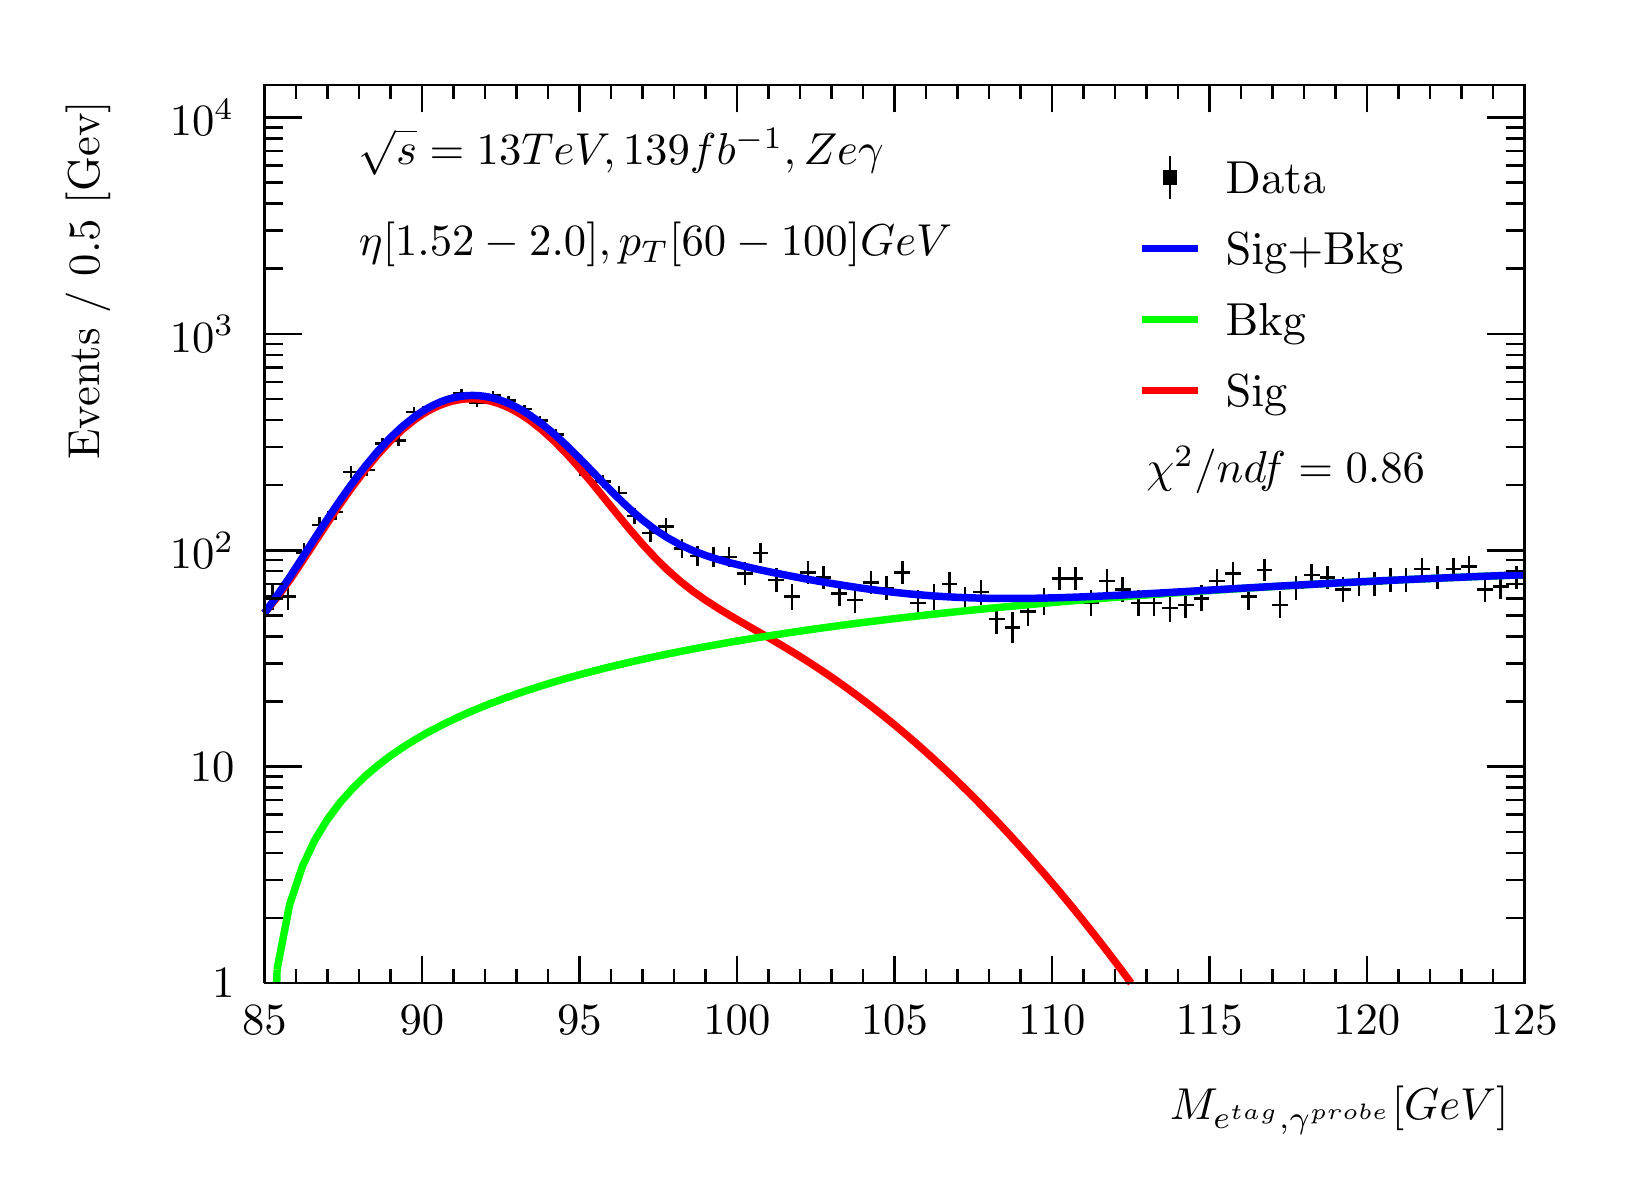
\begin{tikzpicture}
\pgfdeclareplotmark{cross} {
\pgfpathmoveto{\pgfpoint{-0.3\pgfplotmarksize}{\pgfplotmarksize}}
\pgfpathlineto{\pgfpoint{+0.3\pgfplotmarksize}{\pgfplotmarksize}}
\pgfpathlineto{\pgfpoint{+0.3\pgfplotmarksize}{0.3\pgfplotmarksize}}
\pgfpathlineto{\pgfpoint{+1\pgfplotmarksize}{0.3\pgfplotmarksize}}
\pgfpathlineto{\pgfpoint{+1\pgfplotmarksize}{-0.3\pgfplotmarksize}}
\pgfpathlineto{\pgfpoint{+0.3\pgfplotmarksize}{-0.3\pgfplotmarksize}}
\pgfpathlineto{\pgfpoint{+0.3\pgfplotmarksize}{-1.\pgfplotmarksize}}
\pgfpathlineto{\pgfpoint{-0.3\pgfplotmarksize}{-1.\pgfplotmarksize}}
\pgfpathlineto{\pgfpoint{-0.3\pgfplotmarksize}{-0.3\pgfplotmarksize}}
\pgfpathlineto{\pgfpoint{-1.\pgfplotmarksize}{-0.3\pgfplotmarksize}}
\pgfpathlineto{\pgfpoint{-1.\pgfplotmarksize}{0.3\pgfplotmarksize}}
\pgfpathlineto{\pgfpoint{-0.3\pgfplotmarksize}{0.3\pgfplotmarksize}}
\pgfpathclose
\pgfusepathqstroke
}
\pgfdeclareplotmark{cross*} {
\pgfpathmoveto{\pgfpoint{-0.3\pgfplotmarksize}{\pgfplotmarksize}}
\pgfpathlineto{\pgfpoint{+0.3\pgfplotmarksize}{\pgfplotmarksize}}
\pgfpathlineto{\pgfpoint{+0.3\pgfplotmarksize}{0.3\pgfplotmarksize}}
\pgfpathlineto{\pgfpoint{+1\pgfplotmarksize}{0.3\pgfplotmarksize}}
\pgfpathlineto{\pgfpoint{+1\pgfplotmarksize}{-0.3\pgfplotmarksize}}
\pgfpathlineto{\pgfpoint{+0.3\pgfplotmarksize}{-0.3\pgfplotmarksize}}
\pgfpathlineto{\pgfpoint{+0.3\pgfplotmarksize}{-1.\pgfplotmarksize}}
\pgfpathlineto{\pgfpoint{-0.3\pgfplotmarksize}{-1.\pgfplotmarksize}}
\pgfpathlineto{\pgfpoint{-0.3\pgfplotmarksize}{-0.3\pgfplotmarksize}}
\pgfpathlineto{\pgfpoint{-1.\pgfplotmarksize}{-0.3\pgfplotmarksize}}
\pgfpathlineto{\pgfpoint{-1.\pgfplotmarksize}{0.3\pgfplotmarksize}}
\pgfpathlineto{\pgfpoint{-0.3\pgfplotmarksize}{0.3\pgfplotmarksize}}
\pgfpathclose
\pgfusepathqfillstroke
}
\pgfdeclareplotmark{newstar} {
\pgfpathmoveto{\pgfqpoint{0pt}{\pgfplotmarksize}}
\pgfpathlineto{\pgfqpointpolar{44}{0.5\pgfplotmarksize}}
\pgfpathlineto{\pgfqpointpolar{18}{\pgfplotmarksize}}
\pgfpathlineto{\pgfqpointpolar{-20}{0.5\pgfplotmarksize}}
\pgfpathlineto{\pgfqpointpolar{-54}{\pgfplotmarksize}}
\pgfpathlineto{\pgfqpointpolar{-90}{0.5\pgfplotmarksize}}
\pgfpathlineto{\pgfqpointpolar{234}{\pgfplotmarksize}}
\pgfpathlineto{\pgfqpointpolar{198}{0.5\pgfplotmarksize}}
\pgfpathlineto{\pgfqpointpolar{162}{\pgfplotmarksize}}
\pgfpathlineto{\pgfqpointpolar{134}{0.5\pgfplotmarksize}}
\pgfpathclose
\pgfusepathqstroke
}
\pgfdeclareplotmark{newstar*} {
\pgfpathmoveto{\pgfqpoint{0pt}{\pgfplotmarksize}}
\pgfpathlineto{\pgfqpointpolar{44}{0.5\pgfplotmarksize}}
\pgfpathlineto{\pgfqpointpolar{18}{\pgfplotmarksize}}
\pgfpathlineto{\pgfqpointpolar{-20}{0.5\pgfplotmarksize}}
\pgfpathlineto{\pgfqpointpolar{-54}{\pgfplotmarksize}}
\pgfpathlineto{\pgfqpointpolar{-90}{0.5\pgfplotmarksize}}
\pgfpathlineto{\pgfqpointpolar{234}{\pgfplotmarksize}}
\pgfpathlineto{\pgfqpointpolar{198}{0.5\pgfplotmarksize}}
\pgfpathlineto{\pgfqpointpolar{162}{\pgfplotmarksize}}
\pgfpathlineto{\pgfqpointpolar{134}{0.5\pgfplotmarksize}}
\pgfpathclose
\pgfusepathqfillstroke
}
\definecolor{c}{rgb}{1,1,1};
\draw [color=c, fill=c] (0,0) rectangle (20,14.4361);
\draw [color=c, fill=c] (3,2.30977) rectangle (19,13.7143);
\definecolor{c}{rgb}{0,0,0};
\draw [c,line width=0.9] (3,2.30977) -- (3,13.7143) -- (19,13.7143) -- (19,2.30977) -- (3,2.30977);
\definecolor{c}{rgb}{1,1,1};
\draw [color=c, fill=c] (3,2.30977) rectangle (19,13.7143);
\definecolor{c}{rgb}{0,0,0};
\draw [c,line width=0.9] (3,2.30977) -- (3,13.7143) -- (19,13.7143) -- (19,2.30977) -- (3,2.30977);
\draw [c,line width=0.9] (3,2.30977) -- (19,2.30977);
\draw [c,line width=0.9] (3,2.65624) -- (3,2.30977);
\draw [c,line width=0.9] (3.4,2.48301) -- (3.4,2.30977);
\draw [c,line width=0.9] (3.8,2.48301) -- (3.8,2.30977);
\draw [c,line width=0.9] (4.2,2.48301) -- (4.2,2.30977);
\draw [c,line width=0.9] (4.6,2.48301) -- (4.6,2.30977);
\draw [c,line width=0.9] (5,2.65624) -- (5,2.30977);
\draw [c,line width=0.9] (5.4,2.48301) -- (5.4,2.30977);
\draw [c,line width=0.9] (5.8,2.48301) -- (5.8,2.30977);
\draw [c,line width=0.9] (6.2,2.48301) -- (6.2,2.30977);
\draw [c,line width=0.9] (6.6,2.48301) -- (6.6,2.30977);
\draw [c,line width=0.9] (7,2.65624) -- (7,2.30977);
\draw [c,line width=0.9] (7.4,2.48301) -- (7.4,2.30977);
\draw [c,line width=0.9] (7.8,2.48301) -- (7.8,2.30977);
\draw [c,line width=0.9] (8.2,2.48301) -- (8.2,2.30977);
\draw [c,line width=0.9] (8.6,2.48301) -- (8.6,2.30977);
\draw [c,line width=0.9] (9,2.65624) -- (9,2.30977);
\draw [c,line width=0.9] (9.4,2.48301) -- (9.4,2.30977);
\draw [c,line width=0.9] (9.8,2.48301) -- (9.8,2.30977);
\draw [c,line width=0.9] (10.2,2.48301) -- (10.2,2.30977);
\draw [c,line width=0.9] (10.6,2.48301) -- (10.6,2.30977);
\draw [c,line width=0.9] (11,2.65624) -- (11,2.30977);
\draw [c,line width=0.9] (11.4,2.48301) -- (11.4,2.30977);
\draw [c,line width=0.9] (11.8,2.48301) -- (11.8,2.30977);
\draw [c,line width=0.9] (12.2,2.48301) -- (12.2,2.30977);
\draw [c,line width=0.9] (12.6,2.48301) -- (12.6,2.30977);
\draw [c,line width=0.9] (13,2.65624) -- (13,2.30977);
\draw [c,line width=0.9] (13.4,2.48301) -- (13.4,2.30977);
\draw [c,line width=0.9] (13.8,2.48301) -- (13.8,2.30977);
\draw [c,line width=0.9] (14.2,2.48301) -- (14.2,2.30977);
\draw [c,line width=0.9] (14.6,2.48301) -- (14.6,2.30977);
\draw [c,line width=0.9] (15,2.65624) -- (15,2.30977);
\draw [c,line width=0.9] (15.4,2.48301) -- (15.4,2.30977);
\draw [c,line width=0.9] (15.8,2.48301) -- (15.8,2.30977);
\draw [c,line width=0.9] (16.2,2.48301) -- (16.2,2.30977);
\draw [c,line width=0.9] (16.6,2.48301) -- (16.6,2.30977);
\draw [c,line width=0.9] (17,2.65624) -- (17,2.30977);
\draw [c,line width=0.9] (17.4,2.48301) -- (17.4,2.30977);
\draw [c,line width=0.9] (17.8,2.48301) -- (17.8,2.30977);
\draw [c,line width=0.9] (18.2,2.48301) -- (18.2,2.30977);
\draw [c,line width=0.9] (18.6,2.48301) -- (18.6,2.30977);
\draw [c,line width=0.9] (19,2.65624) -- (19,2.30977);
\draw [anchor=base] (3,1.66015) node[scale=1.61424, color=c, rotate=0]{85};
\draw [anchor=base] (5,1.66015) node[scale=1.61424, color=c, rotate=0]{90};
\draw [anchor=base] (7,1.66015) node[scale=1.61424, color=c, rotate=0]{95};
\draw [anchor=base] (9,1.66015) node[scale=1.61424, color=c, rotate=0]{100};
\draw [anchor=base] (11,1.66015) node[scale=1.61424, color=c, rotate=0]{105};
\draw [anchor=base] (13,1.66015) node[scale=1.61424, color=c, rotate=0]{110};
\draw [anchor=base] (15,1.66015) node[scale=1.61424, color=c, rotate=0]{115};
\draw [anchor=base] (17,1.66015) node[scale=1.61424, color=c, rotate=0]{120};
\draw [anchor=base] (19,1.66015) node[scale=1.61424, color=c, rotate=0]{125};
\draw [anchor= east] (19,0.692932) node[scale=1.61424, color=c, rotate=0]{$M_{e^{tag}, \gamma^{probe}}  [GeV]$};
\draw [c,line width=0.9] (3,13.7143) -- (19,13.7143);
\draw [c,line width=0.9] (3,13.3678) -- (3,13.7143);
\draw [c,line width=0.9] (3.4,13.5411) -- (3.4,13.7143);
\draw [c,line width=0.9] (3.8,13.5411) -- (3.8,13.7143);
\draw [c,line width=0.9] (4.2,13.5411) -- (4.2,13.7143);
\draw [c,line width=0.9] (4.6,13.5411) -- (4.6,13.7143);
\draw [c,line width=0.9] (5,13.3678) -- (5,13.7143);
\draw [c,line width=0.9] (5.4,13.5411) -- (5.4,13.7143);
\draw [c,line width=0.9] (5.8,13.5411) -- (5.8,13.7143);
\draw [c,line width=0.9] (6.2,13.5411) -- (6.2,13.7143);
\draw [c,line width=0.9] (6.6,13.5411) -- (6.6,13.7143);
\draw [c,line width=0.9] (7,13.3678) -- (7,13.7143);
\draw [c,line width=0.9] (7.4,13.5411) -- (7.4,13.7143);
\draw [c,line width=0.9] (7.8,13.5411) -- (7.8,13.7143);
\draw [c,line width=0.9] (8.2,13.5411) -- (8.2,13.7143);
\draw [c,line width=0.9] (8.6,13.5411) -- (8.6,13.7143);
\draw [c,line width=0.9] (9,13.3678) -- (9,13.7143);
\draw [c,line width=0.9] (9.4,13.5411) -- (9.4,13.7143);
\draw [c,line width=0.9] (9.8,13.5411) -- (9.8,13.7143);
\draw [c,line width=0.9] (10.2,13.5411) -- (10.2,13.7143);
\draw [c,line width=0.9] (10.6,13.5411) -- (10.6,13.7143);
\draw [c,line width=0.9] (11,13.3678) -- (11,13.7143);
\draw [c,line width=0.9] (11.4,13.5411) -- (11.4,13.7143);
\draw [c,line width=0.9] (11.8,13.5411) -- (11.8,13.7143);
\draw [c,line width=0.9] (12.2,13.5411) -- (12.2,13.7143);
\draw [c,line width=0.9] (12.6,13.5411) -- (12.6,13.7143);
\draw [c,line width=0.9] (13,13.3678) -- (13,13.7143);
\draw [c,line width=0.9] (13.4,13.5411) -- (13.4,13.7143);
\draw [c,line width=0.9] (13.8,13.5411) -- (13.8,13.7143);
\draw [c,line width=0.9] (14.2,13.5411) -- (14.2,13.7143);
\draw [c,line width=0.9] (14.6,13.5411) -- (14.6,13.7143);
\draw [c,line width=0.9] (15,13.3678) -- (15,13.7143);
\draw [c,line width=0.9] (15.4,13.5411) -- (15.4,13.7143);
\draw [c,line width=0.9] (15.8,13.5411) -- (15.8,13.7143);
\draw [c,line width=0.9] (16.2,13.5411) -- (16.2,13.7143);
\draw [c,line width=0.9] (16.6,13.5411) -- (16.6,13.7143);
\draw [c,line width=0.9] (17,13.3678) -- (17,13.7143);
\draw [c,line width=0.9] (17.4,13.5411) -- (17.4,13.7143);
\draw [c,line width=0.9] (17.8,13.5411) -- (17.8,13.7143);
\draw [c,line width=0.9] (18.2,13.5411) -- (18.2,13.7143);
\draw [c,line width=0.9] (18.6,13.5411) -- (18.6,13.7143);
\draw [c,line width=0.9] (19,13.3678) -- (19,13.7143);
\draw [c,line width=0.9] (3,2.30977) -- (3,13.7143);
\draw [c,line width=0.9] (3.474,2.30978) -- (3,2.30978);
\draw [anchor= east] (2.82,2.30978) node[scale=1.61424, color=c, rotate=0]{1};
\draw [c,line width=0.9] (3.237,3.13707) -- (3,3.13707);
\draw [c,line width=0.9] (3.237,3.621) -- (3,3.621);
\draw [c,line width=0.9] (3.237,3.96436) -- (3,3.96436);
\draw [c,line width=0.9] (3.237,4.23069) -- (3,4.23069);
\draw [c,line width=0.9] (3.237,4.4483) -- (3,4.4483);
\draw [c,line width=0.9] (3.237,4.63228) -- (3,4.63228);
\draw [c,line width=0.9] (3.237,4.79165) -- (3,4.79165);
\draw [c,line width=0.9] (3.237,4.93223) -- (3,4.93223);
\draw [c,line width=0.9] (3.474,5.05798) -- (3,5.05798);
\draw [anchor= east] (2.82,5.05798) node[scale=1.61424, color=c, rotate=0]{10};
\draw [c,line width=0.9] (3.237,5.88527) -- (3,5.88527);
\draw [c,line width=0.9] (3.237,6.36921) -- (3,6.36921);
\draw [c,line width=0.9] (3.237,6.71257) -- (3,6.71257);
\draw [c,line width=0.9] (3.237,6.97889) -- (3,6.97889);
\draw [c,line width=0.9] (3.237,7.1965) -- (3,7.1965);
\draw [c,line width=0.9] (3.237,7.38048) -- (3,7.38048);
\draw [c,line width=0.9] (3.237,7.53986) -- (3,7.53986);
\draw [c,line width=0.9] (3.237,7.68043) -- (3,7.68043);
\draw [c,line width=0.9] (3.474,7.80619) -- (3,7.80619);
\draw [anchor= east] (2.82,7.80619) node[scale=1.61424, color=c, rotate=0]{$10^{2}$};
\draw [c,line width=0.9] (3.237,8.63348) -- (3,8.63348);
\draw [c,line width=0.9] (3.237,9.11741) -- (3,9.11741);
\draw [c,line width=0.9] (3.237,9.46077) -- (3,9.46077);
\draw [c,line width=0.9] (3.237,9.7271) -- (3,9.7271);
\draw [c,line width=0.9] (3.237,9.9447) -- (3,9.9447);
\draw [c,line width=0.9] (3.237,10.1287) -- (3,10.1287);
\draw [c,line width=0.9] (3.237,10.2881) -- (3,10.2881);
\draw [c,line width=0.9] (3.237,10.4286) -- (3,10.4286);
\draw [c,line width=0.9] (3.474,10.5544) -- (3,10.5544);
\draw [anchor= east] (2.82,10.5544) node[scale=1.61424, color=c, rotate=0]{$10^{3}$};
\draw [c,line width=0.9] (3.237,11.3817) -- (3,11.3817);
\draw [c,line width=0.9] (3.237,11.8656) -- (3,11.8656);
\draw [c,line width=0.9] (3.237,12.209) -- (3,12.209);
\draw [c,line width=0.9] (3.237,12.4753) -- (3,12.4753);
\draw [c,line width=0.9] (3.237,12.6929) -- (3,12.6929);
\draw [c,line width=0.9] (3.237,12.8769) -- (3,12.8769);
\draw [c,line width=0.9] (3.237,13.0363) -- (3,13.0363);
\draw [c,line width=0.9] (3.237,13.1768) -- (3,13.1768);
\draw [c,line width=0.9] (3.474,13.3026) -- (3,13.3026);
\draw [anchor= east] (2.82,13.3026) node[scale=1.61424, color=c, rotate=0]{$10^{4}$};
\draw [anchor= east] (0.76,13.7143) node[scale=1.61424, color=c, rotate=90]{Events / 0.5 [Gev]};
\draw [c,line width=0.9] (19,2.30977) -- (19,13.7143);
\draw [c,line width=0.9] (18.526,2.30978) -- (19,2.30978);
\draw [c,line width=0.9] (18.763,3.13707) -- (19,3.13707);
\draw [c,line width=0.9] (18.763,3.621) -- (19,3.621);
\draw [c,line width=0.9] (18.763,3.96436) -- (19,3.96436);
\draw [c,line width=0.9] (18.763,4.23069) -- (19,4.23069);
\draw [c,line width=0.9] (18.763,4.4483) -- (19,4.4483);
\draw [c,line width=0.9] (18.763,4.63228) -- (19,4.63228);
\draw [c,line width=0.9] (18.763,4.79165) -- (19,4.79165);
\draw [c,line width=0.9] (18.763,4.93223) -- (19,4.93223);
\draw [c,line width=0.9] (18.526,5.05798) -- (19,5.05798);
\draw [c,line width=0.9] (18.763,5.88527) -- (19,5.88527);
\draw [c,line width=0.9] (18.763,6.36921) -- (19,6.36921);
\draw [c,line width=0.9] (18.763,6.71257) -- (19,6.71257);
\draw [c,line width=0.9] (18.763,6.97889) -- (19,6.97889);
\draw [c,line width=0.9] (18.763,7.1965) -- (19,7.1965);
\draw [c,line width=0.9] (18.763,7.38048) -- (19,7.38048);
\draw [c,line width=0.9] (18.763,7.53986) -- (19,7.53986);
\draw [c,line width=0.9] (18.763,7.68043) -- (19,7.68043);
\draw [c,line width=0.9] (18.526,7.80619) -- (19,7.80619);
\draw [c,line width=0.9] (18.763,8.63348) -- (19,8.63348);
\draw [c,line width=0.9] (18.763,9.11741) -- (19,9.11741);
\draw [c,line width=0.9] (18.763,9.46077) -- (19,9.46077);
\draw [c,line width=0.9] (18.763,9.7271) -- (19,9.7271);
\draw [c,line width=0.9] (18.763,9.9447) -- (19,9.9447);
\draw [c,line width=0.9] (18.763,10.1287) -- (19,10.1287);
\draw [c,line width=0.9] (18.763,10.2881) -- (19,10.2881);
\draw [c,line width=0.9] (18.763,10.4286) -- (19,10.4286);
\draw [c,line width=0.9] (18.526,10.5544) -- (19,10.5544);
\draw [c,line width=0.9] (18.763,11.3817) -- (19,11.3817);
\draw [c,line width=0.9] (18.763,11.8656) -- (19,11.8656);
\draw [c,line width=0.9] (18.763,12.209) -- (19,12.209);
\draw [c,line width=0.9] (18.763,12.4753) -- (19,12.4753);
\draw [c,line width=0.9] (18.763,12.6929) -- (19,12.6929);
\draw [c,line width=0.9] (18.763,12.8769) -- (19,12.8769);
\draw [c,line width=0.9] (18.763,13.0363) -- (19,13.0363);
\draw [c,line width=0.9] (18.763,13.1768) -- (19,13.1768);
\draw [c,line width=0.9] (18.526,13.3026) -- (19,13.3026);
\draw [c,line width=0.9] (3.1,7.21623) -- (3,7.21623);
\draw [c,line width=0.9] (3,7.21623) -- (3,7.21623);
\draw [c,line width=0.9] (3.1,7.21623) -- (3.2,7.21623);
\draw [c,line width=0.9] (3.2,7.21623) -- (3.2,7.21623);
\draw [c,line width=0.9] (3.1,7.21623) -- (3.1,7.37797);
\draw [c,line width=0.9] (3.1,7.37797) -- (3.1,7.37797);
\draw [c,line width=0.9] (3.1,7.21623) -- (3.1,7.05318);
\draw [c,line width=0.9] (3.1,7.05318) -- (3.1,7.05318);
\draw [c,line width=0.9] (3.3,7.21623) -- (3.2,7.21623);
\draw [c,line width=0.9] (3.2,7.21623) -- (3.2,7.21623);
\draw [c,line width=0.9] (3.3,7.21623) -- (3.4,7.21623);
\draw [c,line width=0.9] (3.4,7.21623) -- (3.4,7.21623);
\draw [c,line width=0.9] (3.3,7.21623) -- (3.3,7.37797);
\draw [c,line width=0.9] (3.3,7.37797) -- (3.3,7.37797);
\draw [c,line width=0.9] (3.3,7.21623) -- (3.3,7.05318);
\draw [c,line width=0.9] (3.3,7.05318) -- (3.3,7.05318);
\draw [c,line width=0.9] (3.5,7.76983) -- (3.4,7.76983);
\draw [c,line width=0.9] (3.4,7.76983) -- (3.4,7.76983);
\draw [c,line width=0.9] (3.5,7.76983) -- (3.6,7.76983);
\draw [c,line width=0.9] (3.6,7.76983) -- (3.6,7.76983);
\draw [c,line width=0.9] (3.5,7.76983) -- (3.5,7.89674);
\draw [c,line width=0.9] (3.5,7.89674) -- (3.5,7.89674);
\draw [c,line width=0.9] (3.5,7.76983) -- (3.5,7.64228);
\draw [c,line width=0.9] (3.5,7.64228) -- (3.5,7.64228);
\draw [c,line width=0.9] (3.7,8.12847) -- (3.6,8.12847);
\draw [c,line width=0.9] (3.6,8.12847) -- (3.6,8.12847);
\draw [c,line width=0.9] (3.7,8.12847) -- (3.8,8.12847);
\draw [c,line width=0.9] (3.8,8.12847) -- (3.8,8.12847);
\draw [c,line width=0.9] (3.7,8.12847) -- (3.7,8.23272);
\draw [c,line width=0.9] (3.7,8.23272) -- (3.7,8.23272);
\draw [c,line width=0.9] (3.7,8.12847) -- (3.7,8.02422);
\draw [c,line width=0.9] (3.7,8.02422) -- (3.7,8.02422);
\draw [c,line width=0.9] (3.9,8.29012) -- (3.8,8.29012);
\draw [c,line width=0.9] (3.8,8.29012) -- (3.8,8.29012);
\draw [c,line width=0.9] (3.9,8.29012) -- (4,8.29012);
\draw [c,line width=0.9] (4,8.29012) -- (4,8.29012);
\draw [c,line width=0.9] (3.9,8.29012) -- (3.9,8.38754);
\draw [c,line width=0.9] (3.9,8.38754) -- (3.9,8.38754);
\draw [c,line width=0.9] (3.9,8.29012) -- (3.9,8.19269);
\draw [c,line width=0.9] (3.9,8.19269) -- (3.9,8.19269);
\draw [c,line width=0.9] (4.1,8.80029) -- (4,8.80029);
\draw [c,line width=0.9] (4,8.80029) -- (4,8.80029);
\draw [c,line width=0.9] (4.1,8.80029) -- (4.2,8.80029);
\draw [c,line width=0.9] (4.2,8.80029) -- (4.2,8.80029);
\draw [c,line width=0.9] (4.1,8.80029) -- (4.1,8.87897);
\draw [c,line width=0.9] (4.1,8.87897) -- (4.1,8.87897);
\draw [c,line width=0.9] (4.1,8.80029) -- (4.1,8.7216);
\draw [c,line width=0.9] (4.1,8.7216) -- (4.1,8.7216);
\draw [c,line width=0.9] (4.3,8.82595) -- (4.2,8.82595);
\draw [c,line width=0.9] (4.2,8.82595) -- (4.2,8.82595);
\draw [c,line width=0.9] (4.3,8.82595) -- (4.4,8.82595);
\draw [c,line width=0.9] (4.4,8.82595) -- (4.4,8.82595);
\draw [c,line width=0.9] (4.3,8.82595) -- (4.3,8.9038);
\draw [c,line width=0.9] (4.3,8.9038) -- (4.3,8.9038);
\draw [c,line width=0.9] (4.3,8.82595) -- (4.3,8.74811);
\draw [c,line width=0.9] (4.3,8.74811) -- (4.3,8.74811);
\draw [c,line width=0.9] (4.5,9.16422) -- (4.4,9.16422);
\draw [c,line width=0.9] (4.4,9.16422) -- (4.4,9.16422);
\draw [c,line width=0.9] (4.5,9.16422) -- (4.6,9.16422);
\draw [c,line width=0.9] (4.6,9.16422) -- (4.6,9.16422);
\draw [c,line width=0.9] (4.5,9.16422) -- (4.5,9.23178);
\draw [c,line width=0.9] (4.5,9.23178) -- (4.5,9.23178);
\draw [c,line width=0.9] (4.5,9.16422) -- (4.5,9.09666);
\draw [c,line width=0.9] (4.5,9.09666) -- (4.5,9.09666);
\draw [c,line width=0.9] (4.7,9.20188) -- (4.6,9.20188);
\draw [c,line width=0.9] (4.6,9.20188) -- (4.6,9.20188);
\draw [c,line width=0.9] (4.7,9.20188) -- (4.8,9.20188);
\draw [c,line width=0.9] (4.8,9.20188) -- (4.8,9.20188);
\draw [c,line width=0.9] (4.7,9.20188) -- (4.7,9.26838);
\draw [c,line width=0.9] (4.7,9.26838) -- (4.7,9.26838);
\draw [c,line width=0.9] (4.7,9.20188) -- (4.7,9.13537);
\draw [c,line width=0.9] (4.7,9.13537) -- (4.7,9.13537);
\draw [c,line width=0.9] (4.9,9.56362) -- (4.8,9.56362);
\draw [c,line width=0.9] (4.8,9.56362) -- (4.8,9.56362);
\draw [c,line width=0.9] (4.9,9.56362) -- (5,9.56362);
\draw [c,line width=0.9] (5,9.56362) -- (5,9.56362);
\draw [c,line width=0.9] (4.9,9.56362) -- (4.9,9.62078);
\draw [c,line width=0.9] (4.9,9.62078) -- (4.9,9.62078);
\draw [c,line width=0.9] (4.9,9.56362) -- (4.9,9.50647);
\draw [c,line width=0.9] (4.9,9.50647) -- (4.9,9.50647);
\draw [c,line width=0.9] (5.1,9.62498) -- (5,9.62498);
\draw [c,line width=0.9] (5,9.62498) -- (5,9.62498);
\draw [c,line width=0.9] (5.1,9.62498) -- (5.2,9.62498);
\draw [c,line width=0.9] (5.2,9.62498) -- (5.2,9.62498);
\draw [c,line width=0.9] (5.1,9.62498) -- (5.1,9.68069);
\draw [c,line width=0.9] (5.1,9.68069) -- (5.1,9.68069);
\draw [c,line width=0.9] (5.1,9.62498) -- (5.1,9.56928);
\draw [c,line width=0.9] (5.1,9.56928) -- (5.1,9.56928);
\draw [c,line width=0.9] (5.3,9.67837) -- (5.2,9.67837);
\draw [c,line width=0.9] (5.2,9.67837) -- (5.2,9.67837);
\draw [c,line width=0.9] (5.3,9.67837) -- (5.4,9.67837);
\draw [c,line width=0.9] (5.4,9.67837) -- (5.4,9.67837);
\draw [c,line width=0.9] (5.3,9.67837) -- (5.3,9.73285);
\draw [c,line width=0.9] (5.3,9.73285) -- (5.3,9.73285);
\draw [c,line width=0.9] (5.3,9.67837) -- (5.3,9.6239);
\draw [c,line width=0.9] (5.3,9.6239) -- (5.3,9.6239);
\draw [c,line width=0.9] (5.5,9.79664) -- (5.4,9.79664);
\draw [c,line width=0.9] (5.4,9.79664) -- (5.4,9.79664);
\draw [c,line width=0.9] (5.5,9.79664) -- (5.6,9.79664);
\draw [c,line width=0.9] (5.6,9.79664) -- (5.6,9.79664);
\draw [c,line width=0.9] (5.5,9.79664) -- (5.5,9.84848);
\draw [c,line width=0.9] (5.5,9.84848) -- (5.5,9.84848);
\draw [c,line width=0.9] (5.5,9.79664) -- (5.5,9.7448);
\draw [c,line width=0.9] (5.5,9.7448) -- (5.5,9.7448);
\draw [c,line width=0.9] (5.7,9.68334) -- (5.6,9.68334);
\draw [c,line width=0.9] (5.6,9.68334) -- (5.6,9.68334);
\draw [c,line width=0.9] (5.7,9.68334) -- (5.8,9.68334);
\draw [c,line width=0.9] (5.8,9.68334) -- (5.8,9.68334);
\draw [c,line width=0.9] (5.7,9.68334) -- (5.7,9.7377);
\draw [c,line width=0.9] (5.7,9.7377) -- (5.7,9.7377);
\draw [c,line width=0.9] (5.7,9.68334) -- (5.7,9.62898);
\draw [c,line width=0.9] (5.7,9.62898) -- (5.7,9.62898);
\draw [c,line width=0.9] (5.9,9.77391) -- (5.8,9.77391);
\draw [c,line width=0.9] (5.8,9.77391) -- (5.8,9.77391);
\draw [c,line width=0.9] (5.9,9.77391) -- (6,9.77391);
\draw [c,line width=0.9] (6,9.77391) -- (6,9.77391);
\draw [c,line width=0.9] (5.9,9.77391) -- (5.9,9.82624);
\draw [c,line width=0.9] (5.9,9.82624) -- (5.9,9.82624);
\draw [c,line width=0.9] (5.9,9.77391) -- (5.9,9.72157);
\draw [c,line width=0.9] (5.9,9.72157) -- (5.9,9.72157);
\draw [c,line width=0.9] (6.1,9.71027) -- (6,9.71027);
\draw [c,line width=0.9] (6,9.71027) -- (6,9.71027);
\draw [c,line width=0.9] (6.1,9.71027) -- (6.2,9.71027);
\draw [c,line width=0.9] (6.2,9.71027) -- (6.2,9.71027);
\draw [c,line width=0.9] (6.1,9.71027) -- (6.1,9.76402);
\draw [c,line width=0.9] (6.1,9.76402) -- (6.1,9.76402);
\draw [c,line width=0.9] (6.1,9.71027) -- (6.1,9.65652);
\draw [c,line width=0.9] (6.1,9.65652) -- (6.1,9.65652);
\draw [c,line width=0.9] (6.3,9.59869) -- (6.2,9.59869);
\draw [c,line width=0.9] (6.2,9.59869) -- (6.2,9.59869);
\draw [c,line width=0.9] (6.3,9.59869) -- (6.4,9.59869);
\draw [c,line width=0.9] (6.4,9.59869) -- (6.4,9.59869);
\draw [c,line width=0.9] (6.3,9.59869) -- (6.3,9.65501);
\draw [c,line width=0.9] (6.3,9.65501) -- (6.3,9.65501);
\draw [c,line width=0.9] (6.3,9.59869) -- (6.3,9.54237);
\draw [c,line width=0.9] (6.3,9.54237) -- (6.3,9.54237);
\draw [c,line width=0.9] (6.5,9.45479) -- (6.4,9.45479);
\draw [c,line width=0.9] (6.4,9.45479) -- (6.4,9.45479);
\draw [c,line width=0.9] (6.5,9.45479) -- (6.6,9.45479);
\draw [c,line width=0.9] (6.6,9.45479) -- (6.6,9.45479);
\draw [c,line width=0.9] (6.5,9.45479) -- (6.5,9.51461);
\draw [c,line width=0.9] (6.5,9.51461) -- (6.5,9.51461);
\draw [c,line width=0.9] (6.5,9.45479) -- (6.5,9.39497);
\draw [c,line width=0.9] (6.5,9.39497) -- (6.5,9.39497);
\draw [c,line width=0.9] (6.7,9.27728) -- (6.6,9.27728);
\draw [c,line width=0.9] (6.6,9.27728) -- (6.6,9.27728);
\draw [c,line width=0.9] (6.7,9.27728) -- (6.8,9.27728);
\draw [c,line width=0.9] (6.8,9.27728) -- (6.8,9.27728);
\draw [c,line width=0.9] (6.7,9.27728) -- (6.7,9.34172);
\draw [c,line width=0.9] (6.7,9.34172) -- (6.7,9.34172);
\draw [c,line width=0.9] (6.7,9.27728) -- (6.7,9.21285);
\draw [c,line width=0.9] (6.7,9.21285) -- (6.7,9.21285);
\draw [c,line width=0.9] (6.9,9.03507) -- (6.8,9.03507);
\draw [c,line width=0.9] (6.8,9.03507) -- (6.8,9.03507);
\draw [c,line width=0.9] (6.9,9.03507) -- (7,9.03507);
\draw [c,line width=0.9] (7,9.03507) -- (7,9.03507);
\draw [c,line width=0.9] (6.9,9.03507) -- (6.9,9.10638);
\draw [c,line width=0.9] (6.9,9.10638) -- (6.9,9.10638);
\draw [c,line width=0.9] (6.9,9.03507) -- (6.9,8.96375);
\draw [c,line width=0.9] (6.9,8.96375) -- (6.9,8.96375);
\draw [c,line width=0.9] (7.1,8.76874) -- (7,8.76874);
\draw [c,line width=0.9] (7,8.76874) -- (7,8.76874);
\draw [c,line width=0.9] (7.1,8.76874) -- (7.2,8.76874);
\draw [c,line width=0.9] (7.2,8.76874) -- (7.2,8.76874);
\draw [c,line width=0.9] (7.1,8.76874) -- (7.1,8.84847);
\draw [c,line width=0.9] (7.1,8.84847) -- (7.1,8.84847);
\draw [c,line width=0.9] (7.1,8.76874) -- (7.1,8.68901);
\draw [c,line width=0.9] (7.1,8.68901) -- (7.1,8.68901);
\draw [c,line width=0.9] (7.3,8.68029) -- (7.2,8.68029);
\draw [c,line width=0.9] (7.2,8.68029) -- (7.2,8.68029);
\draw [c,line width=0.9] (7.3,8.68029) -- (7.4,8.68029);
\draw [c,line width=0.9] (7.4,8.68029) -- (7.4,8.68029);
\draw [c,line width=0.9] (7.3,8.68029) -- (7.3,8.76303);
\draw [c,line width=0.9] (7.3,8.76303) -- (7.3,8.76303);
\draw [c,line width=0.9] (7.3,8.68029) -- (7.3,8.59755);
\draw [c,line width=0.9] (7.3,8.59755) -- (7.3,8.59755);
\draw [c,line width=0.9] (7.5,8.53396) -- (7.4,8.53396);
\draw [c,line width=0.9] (7.4,8.53396) -- (7.4,8.53396);
\draw [c,line width=0.9] (7.5,8.53396) -- (7.6,8.53396);
\draw [c,line width=0.9] (7.6,8.53396) -- (7.6,8.53396);
\draw [c,line width=0.9] (7.5,8.53396) -- (7.5,8.62193);
\draw [c,line width=0.9] (7.5,8.62193) -- (7.5,8.62193);
\draw [c,line width=0.9] (7.5,8.53396) -- (7.5,8.44599);
\draw [c,line width=0.9] (7.5,8.44599) -- (7.5,8.44599);
\draw [c,line width=0.9] (7.7,8.2414) -- (7.6,8.2414);
\draw [c,line width=0.9] (7.6,8.2414) -- (7.6,8.2414);
\draw [c,line width=0.9] (7.7,8.2414) -- (7.8,8.2414);
\draw [c,line width=0.9] (7.8,8.2414) -- (7.8,8.2414);
\draw [c,line width=0.9] (7.7,8.2414) -- (7.7,8.34083);
\draw [c,line width=0.9] (7.7,8.34083) -- (7.7,8.34083);
\draw [c,line width=0.9] (7.7,8.2414) -- (7.7,8.14196);
\draw [c,line width=0.9] (7.7,8.14196) -- (7.7,8.14196);
\draw [c,line width=0.9] (7.9,8.02379) -- (7.8,8.02379);
\draw [c,line width=0.9] (7.8,8.02379) -- (7.8,8.02379);
\draw [c,line width=0.9] (7.9,8.02379) -- (8,8.02379);
\draw [c,line width=0.9] (8,8.02379) -- (8,8.02379);
\draw [c,line width=0.9] (7.9,8.02379) -- (7.9,8.13271);
\draw [c,line width=0.9] (7.9,8.13271) -- (7.9,8.13271);
\draw [c,line width=0.9] (7.9,8.02379) -- (7.9,7.91487);
\draw [c,line width=0.9] (7.9,7.91487) -- (7.9,7.91487);
\draw [c,line width=0.9] (8.1,8.11011) -- (8,8.11011);
\draw [c,line width=0.9] (8,8.11011) -- (8,8.11011);
\draw [c,line width=0.9] (8.1,8.11011) -- (8.2,8.11011);
\draw [c,line width=0.9] (8.2,8.11011) -- (8.2,8.11011);
\draw [c,line width=0.9] (8.1,8.11011) -- (8.1,8.21516);
\draw [c,line width=0.9] (8.1,8.21516) -- (8.1,8.21516);
\draw [c,line width=0.9] (8.1,8.11011) -- (8.1,8.00506);
\draw [c,line width=0.9] (8.1,8.00506) -- (8.1,8.00506);
\draw [c,line width=0.9] (8.3,7.82982) -- (8.2,7.82982);
\draw [c,line width=0.9] (8.2,7.82982) -- (8.2,7.82982);
\draw [c,line width=0.9] (8.3,7.82982) -- (8.4,7.82982);
\draw [c,line width=0.9] (8.4,7.82982) -- (8.4,7.82982);
\draw [c,line width=0.9] (8.3,7.82982) -- (8.3,7.94795);
\draw [c,line width=0.9] (8.3,7.94795) -- (8.3,7.94795);
\draw [c,line width=0.9] (8.3,7.82982) -- (8.3,7.71169);
\draw [c,line width=0.9] (8.3,7.71169) -- (8.3,7.71169);
\draw [c,line width=0.9] (8.5,7.73233) -- (8.4,7.73233);
\draw [c,line width=0.9] (8.4,7.73233) -- (8.4,7.73233);
\draw [c,line width=0.9] (8.5,7.73233) -- (8.6,7.73233);
\draw [c,line width=0.9] (8.6,7.73233) -- (8.6,7.73233);
\draw [c,line width=0.9] (8.5,7.73233) -- (8.5,7.86134);
\draw [c,line width=0.9] (8.5,7.86134) -- (8.5,7.86134);
\draw [c,line width=0.9] (8.5,7.73233) -- (8.5,7.60265);
\draw [c,line width=0.9] (8.5,7.60265) -- (8.5,7.60265);
\draw [c,line width=0.9] (8.7,7.71957) -- (8.6,7.71957);
\draw [c,line width=0.9] (8.6,7.71957) -- (8.6,7.71957);
\draw [c,line width=0.9] (8.7,7.71957) -- (8.8,7.71957);
\draw [c,line width=0.9] (8.8,7.71957) -- (8.8,7.71957);
\draw [c,line width=0.9] (8.7,7.71957) -- (8.7,7.8493);
\draw [c,line width=0.9] (8.7,7.8493) -- (8.7,7.8493);
\draw [c,line width=0.9] (8.7,7.71957) -- (8.7,7.58916);
\draw [c,line width=0.9] (8.7,7.58916) -- (8.7,7.58916);
\draw [c,line width=0.9] (8.9,7.71957) -- (8.8,7.71957);
\draw [c,line width=0.9] (8.8,7.71957) -- (8.8,7.71957);
\draw [c,line width=0.9] (8.9,7.71957) -- (9,7.71957);
\draw [c,line width=0.9] (9,7.71957) -- (9,7.71957);
\draw [c,line width=0.9] (8.9,7.71957) -- (8.9,7.8493);
\draw [c,line width=0.9] (8.9,7.8493) -- (8.9,7.8493);
\draw [c,line width=0.9] (8.9,7.71957) -- (8.9,7.58916);
\draw [c,line width=0.9] (8.9,7.58916) -- (8.9,7.58916);
\draw [c,line width=0.9] (9.1,7.50964) -- (9,7.50964);
\draw [c,line width=0.9] (9,7.50964) -- (9,7.50964);
\draw [c,line width=0.9] (9.1,7.50964) -- (9.2,7.50964);
\draw [c,line width=0.9] (9.2,7.50964) -- (9.2,7.50964);
\draw [c,line width=0.9] (9.1,7.50964) -- (9.1,7.65184);
\draw [c,line width=0.9] (9.1,7.65184) -- (9.1,7.65184);
\draw [c,line width=0.9] (9.1,7.50964) -- (9.1,7.36654);
\draw [c,line width=0.9] (9.1,7.36654) -- (9.1,7.36654);
\draw [c,line width=0.9] (9.3,7.76983) -- (9.2,7.76983);
\draw [c,line width=0.9] (9.2,7.76983) -- (9.2,7.76983);
\draw [c,line width=0.9] (9.3,7.76983) -- (9.4,7.76983);
\draw [c,line width=0.9] (9.4,7.76983) -- (9.4,7.76983);
\draw [c,line width=0.9] (9.3,7.76983) -- (9.3,7.89674);
\draw [c,line width=0.9] (9.3,7.89674) -- (9.3,7.89674);
\draw [c,line width=0.9] (9.3,7.76983) -- (9.3,7.64228);
\draw [c,line width=0.9] (9.3,7.64228) -- (9.3,7.64228);
\draw [c,line width=0.9] (9.5,7.43057) -- (9.4,7.43057);
\draw [c,line width=0.9] (9.4,7.43057) -- (9.4,7.43057);
\draw [c,line width=0.9] (9.5,7.43057) -- (9.6,7.43057);
\draw [c,line width=0.9] (9.6,7.43057) -- (9.6,7.43057);
\draw [c,line width=0.9] (9.5,7.43057) -- (9.5,7.57778);
\draw [c,line width=0.9] (9.5,7.57778) -- (9.5,7.57778);
\draw [c,line width=0.9] (9.5,7.43057) -- (9.5,7.28236);
\draw [c,line width=0.9] (9.5,7.28236) -- (9.5,7.28236);
\draw [c,line width=0.9] (9.7,7.21623) -- (9.6,7.21623);
\draw [c,line width=0.9] (9.6,7.21623) -- (9.6,7.21623);
\draw [c,line width=0.9] (9.7,7.21623) -- (9.8,7.21623);
\draw [c,line width=0.9] (9.8,7.21623) -- (9.8,7.21623);
\draw [c,line width=0.9] (9.7,7.21623) -- (9.7,7.37797);
\draw [c,line width=0.9] (9.7,7.37797) -- (9.7,7.37797);
\draw [c,line width=0.9] (9.7,7.21623) -- (9.7,7.05318);
\draw [c,line width=0.9] (9.7,7.05318) -- (9.7,7.05318);
\draw [c,line width=0.9] (9.9,7.52484) -- (9.8,7.52484);
\draw [c,line width=0.9] (9.8,7.52484) -- (9.8,7.52484);
\draw [c,line width=0.9] (9.9,7.52484) -- (10,7.52484);
\draw [c,line width=0.9] (10,7.52484) -- (10,7.52484);
\draw [c,line width=0.9] (9.9,7.52484) -- (9.9,7.6661);
\draw [c,line width=0.9] (9.9,7.6661) -- (9.9,7.6661);
\draw [c,line width=0.9] (9.9,7.52484) -- (9.9,7.38271);
\draw [c,line width=0.9] (9.9,7.38271) -- (9.9,7.38271);
\draw [c,line width=0.9] (10.1,7.46283) -- (10,7.46283);
\draw [c,line width=0.9] (10,7.46283) -- (10,7.46283);
\draw [c,line width=0.9] (10.1,7.46283) -- (10.2,7.46283);
\draw [c,line width=0.9] (10.2,7.46283) -- (10.2,7.46283);
\draw [c,line width=0.9] (10.1,7.46283) -- (10.1,7.60798);
\draw [c,line width=0.9] (10.1,7.60798) -- (10.1,7.60798);
\draw [c,line width=0.9] (10.1,7.46283) -- (10.1,7.31673);
\draw [c,line width=0.9] (10.1,7.31673) -- (10.1,7.31673);
\draw [c,line width=0.9] (10.3,7.25473) -- (10.2,7.25473);
\draw [c,line width=0.9] (10.2,7.25473) -- (10.2,7.25473);
\draw [c,line width=0.9] (10.3,7.25473) -- (10.4,7.25473);
\draw [c,line width=0.9] (10.4,7.25473) -- (10.4,7.25473);
\draw [c,line width=0.9] (10.3,7.25473) -- (10.3,7.41376);
\draw [c,line width=0.9] (10.3,7.41376) -- (10.3,7.41376);
\draw [c,line width=0.9] (10.3,7.25473) -- (10.3,7.09447);
\draw [c,line width=0.9] (10.3,7.09447) -- (10.3,7.09447);
\draw [c,line width=0.9] (10.5,7.17644) -- (10.4,7.17644);
\draw [c,line width=0.9] (10.4,7.17644) -- (10.4,7.17644);
\draw [c,line width=0.9] (10.5,7.17644) -- (10.6,7.17644);
\draw [c,line width=0.9] (10.6,7.17644) -- (10.6,7.17644);
\draw [c,line width=0.9] (10.5,7.17644) -- (10.5,7.34104);
\draw [c,line width=0.9] (10.5,7.34104) -- (10.5,7.34104);
\draw [c,line width=0.9] (10.5,7.17644) -- (10.5,7.01047);
\draw [c,line width=0.9] (10.5,7.01047) -- (10.5,7.01047);
\draw [c,line width=0.9] (10.7,7.39741) -- (10.6,7.39741);
\draw [c,line width=0.9] (10.6,7.39741) -- (10.6,7.39741);
\draw [c,line width=0.9] (10.7,7.39741) -- (10.8,7.39741);
\draw [c,line width=0.9] (10.8,7.39741) -- (10.8,7.39741);
\draw [c,line width=0.9] (10.7,7.39741) -- (10.7,7.54678);
\draw [c,line width=0.9] (10.7,7.54678) -- (10.7,7.54678);
\draw [c,line width=0.9] (10.7,7.39741) -- (10.7,7.24701);
\draw [c,line width=0.9] (10.7,7.24701) -- (10.7,7.24701);
\draw [c,line width=0.9] (10.9,7.3282) -- (10.8,7.3282);
\draw [c,line width=0.9] (10.8,7.3282) -- (10.8,7.3282);
\draw [c,line width=0.9] (10.9,7.3282) -- (11,7.3282);
\draw [c,line width=0.9] (11,7.3282) -- (11,7.3282);
\draw [c,line width=0.9] (10.9,7.3282) -- (10.9,7.48218);
\draw [c,line width=0.9] (10.9,7.48218) -- (10.9,7.48218);
\draw [c,line width=0.9] (10.9,7.3282) -- (10.9,7.1731);
\draw [c,line width=0.9] (10.9,7.1731) -- (10.9,7.1731);
\draw [c,line width=0.9] (11.1,7.52484) -- (11,7.52484);
\draw [c,line width=0.9] (11,7.52484) -- (11,7.52484);
\draw [c,line width=0.9] (11.1,7.52484) -- (11.2,7.52484);
\draw [c,line width=0.9] (11.2,7.52484) -- (11.2,7.52484);
\draw [c,line width=0.9] (11.1,7.52484) -- (11.1,7.6661);
\draw [c,line width=0.9] (11.1,7.6661) -- (11.1,7.6661);
\draw [c,line width=0.9] (11.1,7.52484) -- (11.1,7.38271);
\draw [c,line width=0.9] (11.1,7.38271) -- (11.1,7.38271);
\draw [c,line width=0.9] (11.3,7.13528) -- (11.2,7.13528);
\draw [c,line width=0.9] (11.2,7.13528) -- (11.2,7.13528);
\draw [c,line width=0.9] (11.3,7.13528) -- (11.4,7.13528);
\draw [c,line width=0.9] (11.4,7.13528) -- (11.4,7.13528);
\draw [c,line width=0.9] (11.3,7.13528) -- (11.3,7.30289);
\draw [c,line width=0.9] (11.3,7.30289) -- (11.3,7.30289);
\draw [c,line width=0.9] (11.3,7.13528) -- (11.3,6.96623);
\draw [c,line width=0.9] (11.3,6.96623) -- (11.3,6.96623);
\draw [c,line width=0.9] (11.5,7.21623) -- (11.4,7.21623);
\draw [c,line width=0.9] (11.4,7.21623) -- (11.4,7.21623);
\draw [c,line width=0.9] (11.5,7.21623) -- (11.6,7.21623);
\draw [c,line width=0.9] (11.6,7.21623) -- (11.6,7.21623);
\draw [c,line width=0.9] (11.5,7.21623) -- (11.5,7.37797);
\draw [c,line width=0.9] (11.5,7.37797) -- (11.5,7.37797);
\draw [c,line width=0.9] (11.5,7.21623) -- (11.5,7.05318);
\draw [c,line width=0.9] (11.5,7.05318) -- (11.5,7.05318);
\draw [c,line width=0.9] (11.7,7.38048) -- (11.6,7.38048);
\draw [c,line width=0.9] (11.6,7.38048) -- (11.6,7.38048);
\draw [c,line width=0.9] (11.7,7.38048) -- (11.8,7.38048);
\draw [c,line width=0.9] (11.8,7.38048) -- (11.8,7.38048);
\draw [c,line width=0.9] (11.7,7.38048) -- (11.7,7.53097);
\draw [c,line width=0.9] (11.7,7.53097) -- (11.7,7.53097);
\draw [c,line width=0.9] (11.7,7.38048) -- (11.7,7.22894);
\draw [c,line width=0.9] (11.7,7.22894) -- (11.7,7.22894);
\draw [c,line width=0.9] (11.9,7.17644) -- (11.8,7.17644);
\draw [c,line width=0.9] (11.8,7.17644) -- (11.8,7.17644);
\draw [c,line width=0.9] (11.9,7.17644) -- (12,7.17644);
\draw [c,line width=0.9] (12,7.17644) -- (12,7.17644);
\draw [c,line width=0.9] (11.9,7.17644) -- (11.9,7.34104);
\draw [c,line width=0.9] (11.9,7.34104) -- (11.9,7.34104);
\draw [c,line width=0.9] (11.9,7.17644) -- (11.9,7.01047);
\draw [c,line width=0.9] (11.9,7.01047) -- (11.9,7.01047);
\draw [c,line width=0.9] (12.1,7.27353) -- (12,7.27353);
\draw [c,line width=0.9] (12,7.27353) -- (12,7.27353);
\draw [c,line width=0.9] (12.1,7.27353) -- (12.2,7.27353);
\draw [c,line width=0.9] (12.2,7.27353) -- (12.2,7.27353);
\draw [c,line width=0.9] (12.1,7.27353) -- (12.1,7.43125);
\draw [c,line width=0.9] (12.1,7.43125) -- (12.1,7.43125);
\draw [c,line width=0.9] (12.1,7.27353) -- (12.1,7.1146);
\draw [c,line width=0.9] (12.1,7.1146) -- (12.1,7.1146);
\draw [c,line width=0.9] (12.3,6.93017) -- (12.2,6.93017);
\draw [c,line width=0.9] (12.2,6.93017) -- (12.2,6.93017);
\draw [c,line width=0.9] (12.3,6.93017) -- (12.4,6.93017);
\draw [c,line width=0.9] (12.4,6.93017) -- (12.4,6.93017);
\draw [c,line width=0.9] (12.3,6.93017) -- (12.3,7.11365);
\draw [c,line width=0.9] (12.3,7.11365) -- (12.3,7.11365);
\draw [c,line width=0.9] (12.3,6.93017) -- (12.3,6.74483);
\draw [c,line width=0.9] (12.3,6.74483) -- (12.3,6.74483);
\draw [c,line width=0.9] (12.5,6.82632) -- (12.4,6.82632);
\draw [c,line width=0.9] (12.4,6.82632) -- (12.4,6.82632);
\draw [c,line width=0.9] (12.5,6.82632) -- (12.6,6.82632);
\draw [c,line width=0.9] (12.6,6.82632) -- (12.6,6.82632);
\draw [c,line width=0.9] (12.5,6.82632) -- (12.5,7.01842);
\draw [c,line width=0.9] (12.5,7.01842) -- (12.5,7.01842);
\draw [c,line width=0.9] (12.5,6.82632) -- (12.5,6.63209);
\draw [c,line width=0.9] (12.5,6.63209) -- (12.5,6.63209);
\draw [c,line width=0.9] (12.7,7.0257) -- (12.6,7.0257);
\draw [c,line width=0.9] (12.6,7.0257) -- (12.6,7.0257);
\draw [c,line width=0.9] (12.7,7.0257) -- (12.8,7.0257);
\draw [c,line width=0.9] (12.8,7.0257) -- (12.8,7.0257);
\draw [c,line width=0.9] (12.7,7.0257) -- (12.7,7.20161);
\draw [c,line width=0.9] (12.7,7.20161) -- (12.7,7.20161);
\draw [c,line width=0.9] (12.7,7.0257) -- (12.7,6.84815);
\draw [c,line width=0.9] (12.7,6.84815) -- (12.7,6.84815);
\draw [c,line width=0.9] (12.9,7.15604) -- (12.8,7.15604);
\draw [c,line width=0.9] (12.8,7.15604) -- (12.8,7.15604);
\draw [c,line width=0.9] (12.9,7.15604) -- (13,7.15604);
\draw [c,line width=0.9] (13,7.15604) -- (13,7.15604);
\draw [c,line width=0.9] (12.9,7.15604) -- (12.9,7.32212);
\draw [c,line width=0.9] (12.9,7.32212) -- (12.9,7.32212);
\draw [c,line width=0.9] (12.9,7.15604) -- (12.9,6.98855);
\draw [c,line width=0.9] (12.9,6.98855) -- (12.9,6.98855);
\draw [c,line width=0.9] (13.1,7.44681) -- (13,7.44681);
\draw [c,line width=0.9] (13,7.44681) -- (13,7.44681);
\draw [c,line width=0.9] (13.1,7.44681) -- (13.2,7.44681);
\draw [c,line width=0.9] (13.2,7.44681) -- (13.2,7.44681);
\draw [c,line width=0.9] (13.1,7.44681) -- (13.1,7.59298);
\draw [c,line width=0.9] (13.1,7.59298) -- (13.1,7.59298);
\draw [c,line width=0.9] (13.1,7.44681) -- (13.1,7.29967);
\draw [c,line width=0.9] (13.1,7.29967) -- (13.1,7.29967);
\draw [c,line width=0.9] (13.3,7.44681) -- (13.2,7.44681);
\draw [c,line width=0.9] (13.2,7.44681) -- (13.2,7.44681);
\draw [c,line width=0.9] (13.3,7.44681) -- (13.4,7.44681);
\draw [c,line width=0.9] (13.4,7.44681) -- (13.4,7.44681);
\draw [c,line width=0.9] (13.3,7.44681) -- (13.3,7.59298);
\draw [c,line width=0.9] (13.3,7.59298) -- (13.3,7.59298);
\draw [c,line width=0.9] (13.3,7.44681) -- (13.3,7.29967);
\draw [c,line width=0.9] (13.3,7.29967) -- (13.3,7.29967);
\draw [c,line width=0.9] (13.5,7.13528) -- (13.4,7.13528);
\draw [c,line width=0.9] (13.4,7.13528) -- (13.4,7.13528);
\draw [c,line width=0.9] (13.5,7.13528) -- (13.6,7.13528);
\draw [c,line width=0.9] (13.6,7.13528) -- (13.6,7.13528);
\draw [c,line width=0.9] (13.5,7.13528) -- (13.5,7.30289);
\draw [c,line width=0.9] (13.5,7.30289) -- (13.5,7.30289);
\draw [c,line width=0.9] (13.5,7.13528) -- (13.5,6.96623);
\draw [c,line width=0.9] (13.5,6.96623) -- (13.5,6.96623);
\draw [c,line width=0.9] (13.7,7.4141) -- (13.6,7.4141);
\draw [c,line width=0.9] (13.6,7.4141) -- (13.6,7.4141);
\draw [c,line width=0.9] (13.7,7.4141) -- (13.8,7.4141);
\draw [c,line width=0.9] (13.8,7.4141) -- (13.8,7.4141);
\draw [c,line width=0.9] (13.7,7.4141) -- (13.7,7.56239);
\draw [c,line width=0.9] (13.7,7.56239) -- (13.7,7.56239);
\draw [c,line width=0.9] (13.7,7.4141) -- (13.7,7.26481);
\draw [c,line width=0.9] (13.7,7.26481) -- (13.7,7.26481);
\draw [c,line width=0.9] (13.9,7.31025) -- (13.8,7.31025);
\draw [c,line width=0.9] (13.8,7.31025) -- (13.8,7.31025);
\draw [c,line width=0.9] (13.9,7.31025) -- (14,7.31025);
\draw [c,line width=0.9] (14,7.31025) -- (14,7.31025);
\draw [c,line width=0.9] (13.9,7.31025) -- (13.9,7.46545);
\draw [c,line width=0.9] (13.9,7.46545) -- (13.9,7.46545);
\draw [c,line width=0.9] (13.9,7.31025) -- (13.9,7.15391);
\draw [c,line width=0.9] (13.9,7.15391) -- (13.9,7.15391);
\draw [c,line width=0.9] (14.1,7.13528) -- (14,7.13528);
\draw [c,line width=0.9] (14,7.13528) -- (14,7.13528);
\draw [c,line width=0.9] (14.1,7.13528) -- (14.2,7.13528);
\draw [c,line width=0.9] (14.2,7.13528) -- (14.2,7.13528);
\draw [c,line width=0.9] (14.1,7.13528) -- (14.1,7.30289);
\draw [c,line width=0.9] (14.1,7.30289) -- (14.1,7.30289);
\draw [c,line width=0.9] (14.1,7.13528) -- (14.1,6.96623);
\draw [c,line width=0.9] (14.1,6.96623) -- (14.1,6.96623);
\draw [c,line width=0.9] (14.3,7.13528) -- (14.2,7.13528);
\draw [c,line width=0.9] (14.2,7.13528) -- (14.2,7.13528);
\draw [c,line width=0.9] (14.3,7.13528) -- (14.4,7.13528);
\draw [c,line width=0.9] (14.4,7.13528) -- (14.4,7.13528);
\draw [c,line width=0.9] (14.3,7.13528) -- (14.3,7.30289);
\draw [c,line width=0.9] (14.3,7.30289) -- (14.3,7.30289);
\draw [c,line width=0.9] (14.3,7.13528) -- (14.3,6.96623);
\draw [c,line width=0.9] (14.3,6.96623) -- (14.3,6.96623);
\draw [c,line width=0.9] (14.5,7.07075) -- (14.4,7.07075);
\draw [c,line width=0.9] (14.4,7.07075) -- (14.4,7.07075);
\draw [c,line width=0.9] (14.5,7.07075) -- (14.6,7.07075);
\draw [c,line width=0.9] (14.6,7.07075) -- (14.6,7.07075);
\draw [c,line width=0.9] (14.5,7.07075) -- (14.5,7.24319);
\draw [c,line width=0.9] (14.5,7.24319) -- (14.5,7.24319);
\draw [c,line width=0.9] (14.5,7.07075) -- (14.5,6.89674);
\draw [c,line width=0.9] (14.5,6.89674) -- (14.5,6.89674);
\draw [c,line width=0.9] (14.7,7.11415) -- (14.6,7.11415);
\draw [c,line width=0.9] (14.6,7.11415) -- (14.6,7.11415);
\draw [c,line width=0.9] (14.7,7.11415) -- (14.8,7.11415);
\draw [c,line width=0.9] (14.8,7.11415) -- (14.8,7.11415);
\draw [c,line width=0.9] (14.7,7.11415) -- (14.7,7.28333);
\draw [c,line width=0.9] (14.7,7.28333) -- (14.7,7.28333);
\draw [c,line width=0.9] (14.7,7.11415) -- (14.7,6.9435);
\draw [c,line width=0.9] (14.7,6.9435) -- (14.7,6.9435);
\draw [c,line width=0.9] (14.9,7.1965) -- (14.8,7.1965);
\draw [c,line width=0.9] (14.8,7.1965) -- (14.8,7.1965);
\draw [c,line width=0.9] (14.9,7.1965) -- (15,7.1965);
\draw [c,line width=0.9] (15,7.1965) -- (15,7.1965);
\draw [c,line width=0.9] (14.9,7.1965) -- (14.9,7.35965);
\draw [c,line width=0.9] (14.9,7.35965) -- (14.9,7.35965);
\draw [c,line width=0.9] (14.9,7.1965) -- (14.9,7.03201);
\draw [c,line width=0.9] (14.9,7.03201) -- (14.9,7.03201);
\draw [c,line width=0.9] (15.1,7.4141) -- (15,7.4141);
\draw [c,line width=0.9] (15,7.4141) -- (15,7.4141);
\draw [c,line width=0.9] (15.1,7.4141) -- (15.2,7.4141);
\draw [c,line width=0.9] (15.2,7.4141) -- (15.2,7.4141);
\draw [c,line width=0.9] (15.1,7.4141) -- (15.1,7.56239);
\draw [c,line width=0.9] (15.1,7.56239) -- (15.1,7.56239);
\draw [c,line width=0.9] (15.1,7.4141) -- (15.1,7.26481);
\draw [c,line width=0.9] (15.1,7.26481) -- (15.1,7.26481);
\draw [c,line width=0.9] (15.3,7.50964) -- (15.2,7.50964);
\draw [c,line width=0.9] (15.2,7.50964) -- (15.2,7.50964);
\draw [c,line width=0.9] (15.3,7.50964) -- (15.4,7.50964);
\draw [c,line width=0.9] (15.4,7.50964) -- (15.4,7.50964);
\draw [c,line width=0.9] (15.3,7.50964) -- (15.3,7.65184);
\draw [c,line width=0.9] (15.3,7.65184) -- (15.3,7.65184);
\draw [c,line width=0.9] (15.3,7.50964) -- (15.3,7.36654);
\draw [c,line width=0.9] (15.3,7.36654) -- (15.3,7.36654);
\draw [c,line width=0.9] (15.5,7.21623) -- (15.4,7.21623);
\draw [c,line width=0.9] (15.4,7.21623) -- (15.4,7.21623);
\draw [c,line width=0.9] (15.5,7.21623) -- (15.6,7.21623);
\draw [c,line width=0.9] (15.6,7.21623) -- (15.6,7.21623);
\draw [c,line width=0.9] (15.5,7.21623) -- (15.5,7.37797);
\draw [c,line width=0.9] (15.5,7.37797) -- (15.5,7.37797);
\draw [c,line width=0.9] (15.5,7.21623) -- (15.5,7.05318);
\draw [c,line width=0.9] (15.5,7.05318) -- (15.5,7.05318);
\draw [c,line width=0.9] (15.7,7.55468) -- (15.6,7.55468);
\draw [c,line width=0.9] (15.6,7.55468) -- (15.6,7.55468);
\draw [c,line width=0.9] (15.7,7.55468) -- (15.8,7.55468);
\draw [c,line width=0.9] (15.8,7.55468) -- (15.8,7.55468);
\draw [c,line width=0.9] (15.7,7.55468) -- (15.7,7.69411);
\draw [c,line width=0.9] (15.7,7.69411) -- (15.7,7.69411);
\draw [c,line width=0.9] (15.7,7.55468) -- (15.7,7.41441);
\draw [c,line width=0.9] (15.7,7.41441) -- (15.7,7.41441);
\draw [c,line width=0.9] (15.9,7.11415) -- (15.8,7.11415);
\draw [c,line width=0.9] (15.8,7.11415) -- (15.8,7.11415);
\draw [c,line width=0.9] (15.9,7.11415) -- (16,7.11415);
\draw [c,line width=0.9] (16,7.11415) -- (16,7.11415);
\draw [c,line width=0.9] (15.9,7.11415) -- (15.9,7.28333);
\draw [c,line width=0.9] (15.9,7.28333) -- (15.9,7.28333);
\draw [c,line width=0.9] (15.9,7.11415) -- (15.9,6.9435);
\draw [c,line width=0.9] (15.9,6.9435) -- (15.9,6.9435);
\draw [c,line width=0.9] (16.1,7.3282) -- (16,7.3282);
\draw [c,line width=0.9] (16,7.3282) -- (16,7.3282);
\draw [c,line width=0.9] (16.1,7.3282) -- (16.2,7.3282);
\draw [c,line width=0.9] (16.2,7.3282) -- (16.2,7.3282);
\draw [c,line width=0.9] (16.1,7.3282) -- (16.1,7.48218);
\draw [c,line width=0.9] (16.1,7.48218) -- (16.1,7.48218);
\draw [c,line width=0.9] (16.1,7.3282) -- (16.1,7.1731);
\draw [c,line width=0.9] (16.1,7.1731) -- (16.1,7.1731);
\draw [c,line width=0.9] (16.3,7.49424) -- (16.2,7.49424);
\draw [c,line width=0.9] (16.2,7.49424) -- (16.2,7.49424);
\draw [c,line width=0.9] (16.3,7.49424) -- (16.4,7.49424);
\draw [c,line width=0.9] (16.4,7.49424) -- (16.4,7.49424);
\draw [c,line width=0.9] (16.3,7.49424) -- (16.3,7.6374);
\draw [c,line width=0.9] (16.3,7.6374) -- (16.3,7.6374);
\draw [c,line width=0.9] (16.3,7.49424) -- (16.3,7.35016);
\draw [c,line width=0.9] (16.3,7.35016) -- (16.3,7.35016);
\draw [c,line width=0.9] (16.5,7.46283) -- (16.4,7.46283);
\draw [c,line width=0.9] (16.4,7.46283) -- (16.4,7.46283);
\draw [c,line width=0.9] (16.5,7.46283) -- (16.6,7.46283);
\draw [c,line width=0.9] (16.6,7.46283) -- (16.6,7.46283);
\draw [c,line width=0.9] (16.5,7.46283) -- (16.5,7.60798);
\draw [c,line width=0.9] (16.5,7.60798) -- (16.5,7.60798);
\draw [c,line width=0.9] (16.5,7.46283) -- (16.5,7.31673);
\draw [c,line width=0.9] (16.5,7.31673) -- (16.5,7.31673);
\draw [c,line width=0.9] (16.7,7.31025) -- (16.6,7.31025);
\draw [c,line width=0.9] (16.6,7.31025) -- (16.6,7.31025);
\draw [c,line width=0.9] (16.7,7.31025) -- (16.8,7.31025);
\draw [c,line width=0.9] (16.8,7.31025) -- (16.8,7.31025);
\draw [c,line width=0.9] (16.7,7.31025) -- (16.7,7.46545);
\draw [c,line width=0.9] (16.7,7.46545) -- (16.7,7.46545);
\draw [c,line width=0.9] (16.7,7.31025) -- (16.7,7.15391);
\draw [c,line width=0.9] (16.7,7.15391) -- (16.7,7.15391);
\draw [c,line width=0.9] (16.9,7.38048) -- (16.8,7.38048);
\draw [c,line width=0.9] (16.8,7.38048) -- (16.8,7.38048);
\draw [c,line width=0.9] (16.9,7.38048) -- (17,7.38048);
\draw [c,line width=0.9] (17,7.38048) -- (17,7.38048);
\draw [c,line width=0.9] (16.9,7.38048) -- (16.9,7.53097);
\draw [c,line width=0.9] (16.9,7.53097) -- (16.9,7.53097);
\draw [c,line width=0.9] (16.9,7.38048) -- (16.9,7.22894);
\draw [c,line width=0.9] (16.9,7.22894) -- (16.9,7.22894);
\draw [c,line width=0.9] (17.1,7.38048) -- (17,7.38048);
\draw [c,line width=0.9] (17,7.38048) -- (17,7.38048);
\draw [c,line width=0.9] (17.1,7.38048) -- (17.2,7.38048);
\draw [c,line width=0.9] (17.2,7.38048) -- (17.2,7.38048);
\draw [c,line width=0.9] (17.1,7.38048) -- (17.1,7.53097);
\draw [c,line width=0.9] (17.1,7.53097) -- (17.1,7.53097);
\draw [c,line width=0.9] (17.1,7.38048) -- (17.1,7.22894);
\draw [c,line width=0.9] (17.1,7.22894) -- (17.1,7.22894);
\draw [c,line width=0.9] (17.3,7.43057) -- (17.2,7.43057);
\draw [c,line width=0.9] (17.2,7.43057) -- (17.2,7.43057);
\draw [c,line width=0.9] (17.3,7.43057) -- (17.4,7.43057);
\draw [c,line width=0.9] (17.4,7.43057) -- (17.4,7.43057);
\draw [c,line width=0.9] (17.3,7.43057) -- (17.3,7.57778);
\draw [c,line width=0.9] (17.3,7.57778) -- (17.3,7.57778);
\draw [c,line width=0.9] (17.3,7.43057) -- (17.3,7.28236);
\draw [c,line width=0.9] (17.3,7.28236) -- (17.3,7.28236);
\draw [c,line width=0.9] (17.5,7.43057) -- (17.4,7.43057);
\draw [c,line width=0.9] (17.4,7.43057) -- (17.4,7.43057);
\draw [c,line width=0.9] (17.5,7.43057) -- (17.6,7.43057);
\draw [c,line width=0.9] (17.6,7.43057) -- (17.6,7.43057);
\draw [c,line width=0.9] (17.5,7.43057) -- (17.5,7.57778);
\draw [c,line width=0.9] (17.5,7.57778) -- (17.5,7.57778);
\draw [c,line width=0.9] (17.5,7.43057) -- (17.5,7.28236);
\draw [c,line width=0.9] (17.5,7.28236) -- (17.5,7.28236);
\draw [c,line width=0.9] (17.7,7.56933) -- (17.6,7.56933);
\draw [c,line width=0.9] (17.6,7.56933) -- (17.6,7.56933);
\draw [c,line width=0.9] (17.7,7.56933) -- (17.8,7.56933);
\draw [c,line width=0.9] (17.8,7.56933) -- (17.8,7.56933);
\draw [c,line width=0.9] (17.7,7.56933) -- (17.7,7.70786);
\draw [c,line width=0.9] (17.7,7.70786) -- (17.7,7.70786);
\draw [c,line width=0.9] (17.7,7.56933) -- (17.7,7.42996);
\draw [c,line width=0.9] (17.7,7.42996) -- (17.7,7.42996);
\draw [c,line width=0.9] (17.9,7.46283) -- (17.8,7.46283);
\draw [c,line width=0.9] (17.8,7.46283) -- (17.8,7.46283);
\draw [c,line width=0.9] (17.9,7.46283) -- (18,7.46283);
\draw [c,line width=0.9] (18,7.46283) -- (18,7.46283);
\draw [c,line width=0.9] (17.9,7.46283) -- (17.9,7.60798);
\draw [c,line width=0.9] (17.9,7.60798) -- (17.9,7.60798);
\draw [c,line width=0.9] (17.9,7.46283) -- (17.9,7.31673);
\draw [c,line width=0.9] (17.9,7.31673) -- (17.9,7.31673);
\draw [c,line width=0.9] (18.1,7.56933) -- (18,7.56933);
\draw [c,line width=0.9] (18,7.56933) -- (18,7.56933);
\draw [c,line width=0.9] (18.1,7.56933) -- (18.2,7.56933);
\draw [c,line width=0.9] (18.2,7.56933) -- (18.2,7.56933);
\draw [c,line width=0.9] (18.1,7.56933) -- (18.1,7.70786);
\draw [c,line width=0.9] (18.1,7.70786) -- (18.1,7.70786);
\draw [c,line width=0.9] (18.1,7.56933) -- (18.1,7.42996);
\draw [c,line width=0.9] (18.1,7.42996) -- (18.1,7.42996);
\draw [c,line width=0.9] (18.3,7.59809) -- (18.2,7.59809);
\draw [c,line width=0.9] (18.2,7.59809) -- (18.2,7.59809);
\draw [c,line width=0.9] (18.3,7.59809) -- (18.4,7.59809);
\draw [c,line width=0.9] (18.4,7.59809) -- (18.4,7.59809);
\draw [c,line width=0.9] (18.3,7.59809) -- (18.3,7.73489);
\draw [c,line width=0.9] (18.3,7.73489) -- (18.3,7.73489);
\draw [c,line width=0.9] (18.3,7.59809) -- (18.3,7.46049);
\draw [c,line width=0.9] (18.3,7.46049) -- (18.3,7.46049);
\draw [c,line width=0.9] (18.5,7.31025) -- (18.4,7.31025);
\draw [c,line width=0.9] (18.4,7.31025) -- (18.4,7.31025);
\draw [c,line width=0.9] (18.5,7.31025) -- (18.6,7.31025);
\draw [c,line width=0.9] (18.6,7.31025) -- (18.6,7.31025);
\draw [c,line width=0.9] (18.5,7.31025) -- (18.5,7.46545);
\draw [c,line width=0.9] (18.5,7.46545) -- (18.5,7.46545);
\draw [c,line width=0.9] (18.5,7.31025) -- (18.5,7.15391);
\draw [c,line width=0.9] (18.5,7.15391) -- (18.5,7.15391);
\draw [c,line width=0.9] (18.7,7.34588) -- (18.6,7.34588);
\draw [c,line width=0.9] (18.6,7.34588) -- (18.6,7.34588);
\draw [c,line width=0.9] (18.7,7.34588) -- (18.8,7.34588);
\draw [c,line width=0.9] (18.8,7.34588) -- (18.8,7.34588);
\draw [c,line width=0.9] (18.7,7.34588) -- (18.7,7.49867);
\draw [c,line width=0.9] (18.7,7.49867) -- (18.7,7.49867);
\draw [c,line width=0.9] (18.7,7.34588) -- (18.7,7.192);
\draw [c,line width=0.9] (18.7,7.192) -- (18.7,7.192);
\draw [c,line width=0.9] (18.9,7.46283) -- (18.8,7.46283);
\draw [c,line width=0.9] (18.8,7.46283) -- (18.8,7.46283);
\draw [c,line width=0.9] (18.9,7.46283) -- (19,7.46283);
\draw [c,line width=0.9] (19,7.46283) -- (19,7.46283);
\draw [c,line width=0.9] (18.9,7.46283) -- (18.9,7.60798);
\draw [c,line width=0.9] (18.9,7.60798) -- (18.9,7.60798);
\draw [c,line width=0.9] (18.9,7.46283) -- (18.9,7.31673);
\draw [c,line width=0.9] (18.9,7.31673) -- (18.9,7.31673);
\foreach \P in {(3.1,7.21623), (3.3,7.21623), (3.5,7.76983), (3.7,8.12847), (3.9,8.29012), (4.1,8.80029), (4.3,8.82595), (4.5,9.16422), (4.7,9.20188), (4.9,9.56362), (5.1,9.62498), (5.3,9.67837), (5.5,9.79664), (5.7,9.68334), (5.9,9.77391),
 (6.1,9.71027), (6.3,9.59869), (6.5,9.45479), (6.7,9.27728), (6.9,9.03507), (7.1,8.76874), (7.3,8.68029), (7.5,8.53396), (7.7,8.2414), (7.9,8.02379), (8.1,8.11011), (8.3,7.82982), (8.5,7.73233), (8.7,7.71957), (8.9,7.71957), (9.1,7.50964),
 (9.3,7.76983), (9.5,7.43057), (9.7,7.21623), (9.9,7.52484), (10.1,7.46283), (10.3,7.25473), (10.5,7.17644), (10.7,7.39741), (10.9,7.3282), (11.1,7.52484), (11.3,7.13528), (11.5,7.21623), (11.7,7.38048), (11.9,7.17644), (12.1,7.27353),
 (12.3,6.93017), (12.5,6.82632), (12.7,7.0257), (12.9,7.15604), (13.1,7.44681), (13.3,7.44681), (13.5,7.13528), (13.7,7.4141), (13.9,7.31025), (14.1,7.13528), (14.3,7.13528), (14.5,7.07075), (14.7,7.11415), (14.9,7.1965), (15.1,7.4141),
 (15.3,7.50964), (15.5,7.21623), (15.7,7.55468), (15.9,7.11415), (16.1,7.3282), (16.3,7.49424), (16.5,7.46283), (16.7,7.31025), (16.9,7.38048), (17.1,7.38048), (17.3,7.43057), (17.5,7.43057), (17.7,7.56933), (17.9,7.46283), (18.1,7.56933),
 (18.3,7.59809), (18.5,7.31025), (18.7,7.34588), (18.9,7.46283)}{\draw[mark options={color=c,fill=c},mark size=2.882883pt,mark=] plot coordinates {\P};}
\definecolor{c}{rgb}{1,0,0};
\draw [c,line width=2.7] (3,7.00769) -- (3,7.00769);
\draw [c,line width=2.7] (3,7.00769) -- (3.16,7.2076) -- (3.32,7.42673) -- (3.4,7.54439) -- (3.48,7.66527) -- (3.56,7.78723) -- (3.64,7.9096) -- (3.72,8.03172) -- (3.8,8.15293) -- (3.88,8.27258) -- (3.96,8.39009) -- (4.04,8.50489) -- (4.12,8.61648)
 -- (4.28,8.82817) -- (4.44,9.02197) -- (4.6,9.19537) -- (4.76,9.34643) -- (4.92,9.47368) -- (5,9.52804) -- (5.08,9.57608) -- (5.16,9.61771) -- (5.24,9.65287) -- (5.32,9.68152) -- (5.4,9.7036) -- (5.48,9.71911) -- (5.56,9.72803) -- (5.64,9.73038) --
 (5.72,9.72616) -- (5.8,9.71541) -- (5.88,9.69818) -- (5.96,9.67453) -- (6.04,9.64455) -- (6.12,9.60832) -- (6.2,9.56596) -- (6.28,9.51762) -- (6.36,9.46345) -- (6.52,9.33843) -- (6.68,9.19279) -- (6.84,9.02897) -- (7,8.85011) -- (7.16,8.66003) --
 (7.24,8.56219) -- (7.32,8.4633) -- (7.4,8.36403) -- (7.48,8.26503) -- (7.56,8.16698) -- (7.64,8.07053) -- (7.8,7.88482) -- (7.96,7.71198) -- (8.12,7.55456) -- (8.28,7.41328) -- (8.44,7.28714) -- (8.6,7.17385) -- (8.76,7.0704) -- (8.92,6.97365) --
 (9.08,6.88072) -- (9.24,6.78922) -- (9.4,6.69728) -- (9.56,6.60353) -- (9.72,6.50701) -- (9.88,6.40706) -- (10.04,6.30327) -- (10.2,6.19536) -- (10.36,6.08317) -- (10.52,5.96659) -- (10.68,5.84558) -- (10.84,5.7201) -- (11,5.59013) --
 (11.16,5.45566) -- (11.32,5.31669) -- (11.48,5.17322) -- (11.64,5.02523) -- (11.8,4.87274) -- (11.96,4.71574) -- (12.12,4.55423) -- (12.28,4.38822) -- (12.44,4.2177) -- (12.6,4.04267) -- (12.76,3.86313) -- (12.92,3.67908) -- (13.08,3.49052) --
 (13.24,3.29746) -- (13.4,3.09989) -- (13.56,2.8978) -- (13.72,2.69122) -- (13.88,2.48012) -- (14.0064,2.30977);
\definecolor{c}{rgb}{0,1,0};
\draw [c,line width=2.7] (3.1575,2.30977) -- (3.16,2.48398);
\draw [c,line width=2.7] (3.16,2.48398) -- (3.32,3.30719) -- (3.48,3.78707) -- (3.64,4.12635) -- (3.8,4.38861) -- (3.96,4.60212) -- (4.12,4.782) -- (4.28,4.93726) -- (4.44,5.07371) -- (4.6,5.19531) -- (4.76,5.30491) -- (4.92,5.40459) --
 (5.08,5.49593) -- (5.24,5.58018) -- (5.4,5.65831) -- (5.56,5.7311) -- (5.72,5.79921) -- (5.88,5.86317) -- (6.04,5.92343) -- (6.2,5.98035) -- (6.36,6.03428) -- (6.52,6.08548) -- (6.68,6.13419) -- (6.84,6.18063) -- (7,6.22498) -- (7.16,6.26741) --
 (7.32,6.30805) -- (7.48,6.34703) -- (7.64,6.38448) -- (7.8,6.42049) -- (7.96,6.45516) -- (8.12,6.48856) -- (8.28,6.52079) -- (8.44,6.5519) -- (8.6,6.58196) -- (8.76,6.61102) -- (8.92,6.63915) -- (9.08,6.66639) -- (9.24,6.69279) -- (9.4,6.71838) --
 (9.56,6.74321) -- (9.72,6.76731) -- (9.88,6.79071) -- (10.04,6.81345) -- (10.2,6.83556) -- (10.36,6.85706) -- (10.52,6.87797) -- (10.68,6.89833) -- (10.84,6.91814) -- (11,6.93744) -- (11.16,6.95625) -- (11.32,6.97457) -- (11.48,6.99244) --
 (11.64,7.00986) -- (11.8,7.02684) -- (11.96,7.04342) -- (12.12,7.05959) -- (12.28,7.07538) -- (12.44,7.09079) -- (12.6,7.10583) -- (12.76,7.12053) -- (12.92,7.13488) -- (13.08,7.1489) -- (13.24,7.16259) -- (13.4,7.17598) -- (13.56,7.18906) --
 (13.72,7.20184) -- (13.88,7.21433) -- (14.04,7.22655) -- (14.2,7.23849) -- (14.36,7.25016) -- (14.52,7.26157) -- (14.68,7.27273) -- (14.84,7.28364) -- (15,7.29431) -- (15.16,7.30475) -- (15.32,7.31495) -- (15.48,7.32493) -- (15.64,7.33468) --
 (15.8,7.34422) -- (15.96,7.35355) -- (16.12,7.36267) -- (16.28,7.37159) -- (16.44,7.3803) -- (16.6,7.38883) -- (16.76,7.39716) -- (16.92,7.4053) -- (17.08,7.41326) -- (17.24,7.42104) -- (17.4,7.42863) -- (17.56,7.43606) -- (17.72,7.44331) --
 (17.88,7.45039) -- (18.04,7.45731) -- (18.2,7.46406) -- (18.36,7.47065) -- (18.52,7.47708) -- (18.68,7.48336) -- (18.84,7.48948) -- (19,7.49545) -- (19,7.49545) -- (19,7.49545);
\definecolor{c}{rgb}{0,0,1};
\draw [c,line width=2.7] (3,7.00769) -- (3,7.00769);
\draw [c,line width=2.7] (3,7.00769) -- (3.16,7.23019) -- (3.32,7.46397) -- (3.4,7.58641) -- (3.48,7.7107) -- (3.56,7.83495) -- (3.64,7.95872) -- (3.72,8.08151) -- (3.8,8.20281) -- (3.88,8.32215) -- (3.96,8.43902) -- (4.04,8.55297) -- (4.12,8.66357)
 -- (4.2,8.77041) -- (4.28,8.87313) -- (4.44,9.06486) -- (4.6,9.23647) -- (4.76,9.38614) -- (4.92,9.51251) -- (5,9.56662) -- (5.08,9.61455) -- (5.16,9.65623) -- (5.24,9.69158) -- (5.32,9.72058) -- (5.4,9.7432) -- (5.48,9.75941) -- (5.56,9.76924) --
 (5.64,9.77269) -- (5.72,9.7698) -- (5.8,9.76064) -- (5.88,9.74525) -- (5.96,9.72375) -- (6.04,9.69623) -- (6.12,9.66283) -- (6.2,9.62371) -- (6.28,9.57905) -- (6.36,9.52907) -- (6.52,9.41417) -- (6.68,9.28144) -- (6.84,9.13397) -- (7,8.97559) --
 (7.08,8.89371) -- (7.16,8.81086) -- (7.24,8.72771) -- (7.32,8.64491) -- (7.4,8.56316) -- (7.48,8.48312) -- (7.56,8.40542) -- (7.64,8.33063) -- (7.72,8.25925) -- (7.8,8.1917) -- (7.96,8.06917) -- (8.12,7.96411) -- (8.28,7.87587) -- (8.44,7.80256) --
 (8.6,7.74152) -- (8.76,7.68997) -- (8.92,7.64537) -- (9.08,7.60565) -- (9.24,7.56927) -- (9.4,7.53517) -- (9.56,7.5027) -- (9.72,7.47153) -- (9.88,7.44153) -- (10.04,7.41271) -- (10.2,7.38517) -- (10.36,7.35906) -- (10.52,7.33453) -- (10.68,7.31174)
 -- (10.84,7.29082) -- (11,7.27188) -- (11.16,7.25501) -- (11.32,7.24024) -- (11.48,7.2276) -- (11.64,7.21708) -- (11.8,7.20861) -- (11.96,7.20215) -- (12.12,7.19758) -- (12.28,7.19481) -- (12.44,7.19372) -- (12.6,7.19415) -- (12.76,7.19599) --
 (12.92,7.19909) -- (13.08,7.20331) -- (13.24,7.20852) -- (13.4,7.21458) -- (13.56,7.22138) -- (13.72,7.22879) -- (13.88,7.23673) -- (14.04,7.24508) -- (14.2,7.25376) -- (14.36,7.26271) -- (14.52,7.27184) -- (14.68,7.2811) -- (14.84,7.29044) --
 (15,7.29981) -- (15.16,7.30918) -- (15.32,7.31851) -- (15.48,7.32778) -- (15.64,7.33695) -- (15.8,7.34603) -- (15.96,7.35498) -- (16.12,7.3638) -- (16.28,7.37247) -- (16.44,7.381) -- (16.6,7.38937) -- (16.76,7.39758) -- (16.92,7.40563) --
 (17.08,7.41351) -- (17.24,7.42123) -- (17.4,7.42878) -- (17.56,7.43617) -- (17.72,7.4434) -- (17.88,7.45046) -- (18.04,7.45736) -- (18.2,7.4641) -- (18.36,7.47068) -- (18.52,7.4771) -- (18.68,7.48337) -- (18.84,7.48949) -- (19,7.49546) --
 (19,7.49546) -- (19,7.49546);
\definecolor{c}{rgb}{0,0,0};
\draw [c,line width=0.9] (3,2.30977) -- (19,2.30977);
\draw [c,line width=0.9] (3,2.65624) -- (3,2.30977);
\draw [c,line width=0.9] (3.4,2.48301) -- (3.4,2.30977);
\draw [c,line width=0.9] (3.8,2.48301) -- (3.8,2.30977);
\draw [c,line width=0.9] (4.2,2.48301) -- (4.2,2.30977);
\draw [c,line width=0.9] (4.6,2.48301) -- (4.6,2.30977);
\draw [c,line width=0.9] (5,2.65624) -- (5,2.30977);
\draw [c,line width=0.9] (5.4,2.48301) -- (5.4,2.30977);
\draw [c,line width=0.9] (5.8,2.48301) -- (5.8,2.30977);
\draw [c,line width=0.9] (6.2,2.48301) -- (6.2,2.30977);
\draw [c,line width=0.9] (6.6,2.48301) -- (6.6,2.30977);
\draw [c,line width=0.9] (7,2.65624) -- (7,2.30977);
\draw [c,line width=0.9] (7.4,2.48301) -- (7.4,2.30977);
\draw [c,line width=0.9] (7.8,2.48301) -- (7.8,2.30977);
\draw [c,line width=0.9] (8.2,2.48301) -- (8.2,2.30977);
\draw [c,line width=0.9] (8.6,2.48301) -- (8.6,2.30977);
\draw [c,line width=0.9] (9,2.65624) -- (9,2.30977);
\draw [c,line width=0.9] (9.4,2.48301) -- (9.4,2.30977);
\draw [c,line width=0.9] (9.8,2.48301) -- (9.8,2.30977);
\draw [c,line width=0.9] (10.2,2.48301) -- (10.2,2.30977);
\draw [c,line width=0.9] (10.6,2.48301) -- (10.6,2.30977);
\draw [c,line width=0.9] (11,2.65624) -- (11,2.30977);
\draw [c,line width=0.9] (11.4,2.48301) -- (11.4,2.30977);
\draw [c,line width=0.9] (11.8,2.48301) -- (11.8,2.30977);
\draw [c,line width=0.9] (12.2,2.48301) -- (12.2,2.30977);
\draw [c,line width=0.9] (12.6,2.48301) -- (12.6,2.30977);
\draw [c,line width=0.9] (13,2.65624) -- (13,2.30977);
\draw [c,line width=0.9] (13.4,2.48301) -- (13.4,2.30977);
\draw [c,line width=0.9] (13.8,2.48301) -- (13.8,2.30977);
\draw [c,line width=0.9] (14.2,2.48301) -- (14.2,2.30977);
\draw [c,line width=0.9] (14.6,2.48301) -- (14.6,2.30977);
\draw [c,line width=0.9] (15,2.65624) -- (15,2.30977);
\draw [c,line width=0.9] (15.4,2.48301) -- (15.4,2.30977);
\draw [c,line width=0.9] (15.8,2.48301) -- (15.8,2.30977);
\draw [c,line width=0.9] (16.2,2.48301) -- (16.2,2.30977);
\draw [c,line width=0.9] (16.6,2.48301) -- (16.6,2.30977);
\draw [c,line width=0.9] (17,2.65624) -- (17,2.30977);
\draw [c,line width=0.9] (17.4,2.48301) -- (17.4,2.30977);
\draw [c,line width=0.9] (17.8,2.48301) -- (17.8,2.30977);
\draw [c,line width=0.9] (18.2,2.48301) -- (18.2,2.30977);
\draw [c,line width=0.9] (18.6,2.48301) -- (18.6,2.30977);
\draw [c,line width=0.9] (19,2.65624) -- (19,2.30977);
\draw [c,line width=0.9] (3,13.7143) -- (19,13.7143);
\draw [c,line width=0.9] (3,13.3678) -- (3,13.7143);
\draw [c,line width=0.9] (3.4,13.5411) -- (3.4,13.7143);
\draw [c,line width=0.9] (3.8,13.5411) -- (3.8,13.7143);
\draw [c,line width=0.9] (4.2,13.5411) -- (4.2,13.7143);
\draw [c,line width=0.9] (4.6,13.5411) -- (4.6,13.7143);
\draw [c,line width=0.9] (5,13.3678) -- (5,13.7143);
\draw [c,line width=0.9] (5.4,13.5411) -- (5.4,13.7143);
\draw [c,line width=0.9] (5.8,13.5411) -- (5.8,13.7143);
\draw [c,line width=0.9] (6.2,13.5411) -- (6.2,13.7143);
\draw [c,line width=0.9] (6.6,13.5411) -- (6.6,13.7143);
\draw [c,line width=0.9] (7,13.3678) -- (7,13.7143);
\draw [c,line width=0.9] (7.4,13.5411) -- (7.4,13.7143);
\draw [c,line width=0.9] (7.8,13.5411) -- (7.8,13.7143);
\draw [c,line width=0.9] (8.2,13.5411) -- (8.2,13.7143);
\draw [c,line width=0.9] (8.6,13.5411) -- (8.6,13.7143);
\draw [c,line width=0.9] (9,13.3678) -- (9,13.7143);
\draw [c,line width=0.9] (9.4,13.5411) -- (9.4,13.7143);
\draw [c,line width=0.9] (9.8,13.5411) -- (9.8,13.7143);
\draw [c,line width=0.9] (10.2,13.5411) -- (10.2,13.7143);
\draw [c,line width=0.9] (10.6,13.5411) -- (10.6,13.7143);
\draw [c,line width=0.9] (11,13.3678) -- (11,13.7143);
\draw [c,line width=0.9] (11.4,13.5411) -- (11.4,13.7143);
\draw [c,line width=0.9] (11.8,13.5411) -- (11.8,13.7143);
\draw [c,line width=0.9] (12.2,13.5411) -- (12.2,13.7143);
\draw [c,line width=0.9] (12.6,13.5411) -- (12.6,13.7143);
\draw [c,line width=0.9] (13,13.3678) -- (13,13.7143);
\draw [c,line width=0.9] (13.4,13.5411) -- (13.4,13.7143);
\draw [c,line width=0.9] (13.8,13.5411) -- (13.8,13.7143);
\draw [c,line width=0.9] (14.2,13.5411) -- (14.2,13.7143);
\draw [c,line width=0.9] (14.6,13.5411) -- (14.6,13.7143);
\draw [c,line width=0.9] (15,13.3678) -- (15,13.7143);
\draw [c,line width=0.9] (15.4,13.5411) -- (15.4,13.7143);
\draw [c,line width=0.9] (15.8,13.5411) -- (15.8,13.7143);
\draw [c,line width=0.9] (16.2,13.5411) -- (16.2,13.7143);
\draw [c,line width=0.9] (16.6,13.5411) -- (16.6,13.7143);
\draw [c,line width=0.9] (17,13.3678) -- (17,13.7143);
\draw [c,line width=0.9] (17.4,13.5411) -- (17.4,13.7143);
\draw [c,line width=0.9] (17.8,13.5411) -- (17.8,13.7143);
\draw [c,line width=0.9] (18.2,13.5411) -- (18.2,13.7143);
\draw [c,line width=0.9] (18.6,13.5411) -- (18.6,13.7143);
\draw [c,line width=0.9] (19,13.3678) -- (19,13.7143);
\draw [c,line width=0.9] (3,2.30977) -- (3,13.7143);
\draw [c,line width=0.9] (3.474,2.30978) -- (3,2.30978);
\draw [c,line width=0.9] (3.237,3.13707) -- (3,3.13707);
\draw [c,line width=0.9] (3.237,3.621) -- (3,3.621);
\draw [c,line width=0.9] (3.237,3.96436) -- (3,3.96436);
\draw [c,line width=0.9] (3.237,4.23069) -- (3,4.23069);
\draw [c,line width=0.9] (3.237,4.4483) -- (3,4.4483);
\draw [c,line width=0.9] (3.237,4.63228) -- (3,4.63228);
\draw [c,line width=0.9] (3.237,4.79165) -- (3,4.79165);
\draw [c,line width=0.9] (3.237,4.93223) -- (3,4.93223);
\draw [c,line width=0.9] (3.474,5.05798) -- (3,5.05798);
\draw [c,line width=0.9] (3.237,5.88527) -- (3,5.88527);
\draw [c,line width=0.9] (3.237,6.36921) -- (3,6.36921);
\draw [c,line width=0.9] (3.237,6.71257) -- (3,6.71257);
\draw [c,line width=0.9] (3.237,6.97889) -- (3,6.97889);
\draw [c,line width=0.9] (3.237,7.1965) -- (3,7.1965);
\draw [c,line width=0.9] (3.237,7.38048) -- (3,7.38048);
\draw [c,line width=0.9] (3.237,7.53986) -- (3,7.53986);
\draw [c,line width=0.9] (3.237,7.68043) -- (3,7.68043);
\draw [c,line width=0.9] (3.474,7.80619) -- (3,7.80619);
\draw [c,line width=0.9] (3.237,8.63348) -- (3,8.63348);
\draw [c,line width=0.9] (3.237,9.11741) -- (3,9.11741);
\draw [c,line width=0.9] (3.237,9.46077) -- (3,9.46077);
\draw [c,line width=0.9] (3.237,9.7271) -- (3,9.7271);
\draw [c,line width=0.9] (3.237,9.9447) -- (3,9.9447);
\draw [c,line width=0.9] (3.237,10.1287) -- (3,10.1287);
\draw [c,line width=0.9] (3.237,10.2881) -- (3,10.2881);
\draw [c,line width=0.9] (3.237,10.4286) -- (3,10.4286);
\draw [c,line width=0.9] (3.474,10.5544) -- (3,10.5544);
\draw [c,line width=0.9] (3.237,11.3817) -- (3,11.3817);
\draw [c,line width=0.9] (3.237,11.8656) -- (3,11.8656);
\draw [c,line width=0.9] (3.237,12.209) -- (3,12.209);
\draw [c,line width=0.9] (3.237,12.4753) -- (3,12.4753);
\draw [c,line width=0.9] (3.237,12.6929) -- (3,12.6929);
\draw [c,line width=0.9] (3.237,12.8769) -- (3,12.8769);
\draw [c,line width=0.9] (3.237,13.0363) -- (3,13.0363);
\draw [c,line width=0.9] (3.237,13.1768) -- (3,13.1768);
\draw [c,line width=0.9] (3.474,13.3026) -- (3,13.3026);
\draw [c,line width=0.9] (19,2.30977) -- (19,13.7143);
\draw [c,line width=0.9] (18.526,2.30978) -- (19,2.30978);
\draw [c,line width=0.9] (18.763,3.13707) -- (19,3.13707);
\draw [c,line width=0.9] (18.763,3.621) -- (19,3.621);
\draw [c,line width=0.9] (18.763,3.96436) -- (19,3.96436);
\draw [c,line width=0.9] (18.763,4.23069) -- (19,4.23069);
\draw [c,line width=0.9] (18.763,4.4483) -- (19,4.4483);
\draw [c,line width=0.9] (18.763,4.63228) -- (19,4.63228);
\draw [c,line width=0.9] (18.763,4.79165) -- (19,4.79165);
\draw [c,line width=0.9] (18.763,4.93223) -- (19,4.93223);
\draw [c,line width=0.9] (18.526,5.05798) -- (19,5.05798);
\draw [c,line width=0.9] (18.763,5.88527) -- (19,5.88527);
\draw [c,line width=0.9] (18.763,6.36921) -- (19,6.36921);
\draw [c,line width=0.9] (18.763,6.71257) -- (19,6.71257);
\draw [c,line width=0.9] (18.763,6.97889) -- (19,6.97889);
\draw [c,line width=0.9] (18.763,7.1965) -- (19,7.1965);
\draw [c,line width=0.9] (18.763,7.38048) -- (19,7.38048);
\draw [c,line width=0.9] (18.763,7.53986) -- (19,7.53986);
\draw [c,line width=0.9] (18.763,7.68043) -- (19,7.68043);
\draw [c,line width=0.9] (18.526,7.80619) -- (19,7.80619);
\draw [c,line width=0.9] (18.763,8.63348) -- (19,8.63348);
\draw [c,line width=0.9] (18.763,9.11741) -- (19,9.11741);
\draw [c,line width=0.9] (18.763,9.46077) -- (19,9.46077);
\draw [c,line width=0.9] (18.763,9.7271) -- (19,9.7271);
\draw [c,line width=0.9] (18.763,9.9447) -- (19,9.9447);
\draw [c,line width=0.9] (18.763,10.1287) -- (19,10.1287);
\draw [c,line width=0.9] (18.763,10.2881) -- (19,10.2881);
\draw [c,line width=0.9] (18.763,10.4286) -- (19,10.4286);
\draw [c,line width=0.9] (18.526,10.5544) -- (19,10.5544);
\draw [c,line width=0.9] (18.763,11.3817) -- (19,11.3817);
\draw [c,line width=0.9] (18.763,11.8656) -- (19,11.8656);
\draw [c,line width=0.9] (18.763,12.209) -- (19,12.209);
\draw [c,line width=0.9] (18.763,12.4753) -- (19,12.4753);
\draw [c,line width=0.9] (18.763,12.6929) -- (19,12.6929);
\draw [c,line width=0.9] (18.763,12.8769) -- (19,12.8769);
\draw [c,line width=0.9] (18.763,13.0363) -- (19,13.0363);
\draw [c,line width=0.9] (18.763,13.1768) -- (19,13.1768);
\draw [c,line width=0.9] (18.526,13.3026) -- (19,13.3026);
\definecolor{c}{rgb}{1,1,1};
\draw [color=c, fill=c] (14,9.38346) rectangle (18,12.9925);
\definecolor{c}{rgb}{0,0,0};
\draw [anchor=base west] (15,12.3383) node[scale=1.6699, color=c, rotate=0]{Data};
\draw [c,line width=0.9] (14.5,12.6416) -- (14.5,12.812);
\draw [c,line width=0.9] (14.5,12.4411) -- (14.5,12.2707);
\foreach \P in {(14.5,12.5414)}{\draw[mark options={color=c,fill=c},mark size=2.402402pt,mark=square*] plot coordinates {\P};}
\draw [anchor=base west] (15,11.4361) node[scale=1.6699, color=c, rotate=0]{Sig+Bkg};
\definecolor{c}{rgb}{0,0,1};
\draw [c,line width=2.7] (14.15,11.6391) -- (14.85,11.6391);
\definecolor{c}{rgb}{0,0,0};
\draw [anchor=base west] (15,10.5338) node[scale=1.6699, color=c, rotate=0]{Bkg};
\definecolor{c}{rgb}{0,1,0};
\draw [c,line width=2.7] (14.15,10.7368) -- (14.85,10.7368);
\definecolor{c}{rgb}{0,0,0};
\draw [anchor=base west] (15,9.63158) node[scale=1.6699, color=c, rotate=0]{Sig};
\definecolor{c}{rgb}{1,0,0};
\draw [c,line width=2.7] (14.15,9.83459) -- (14.85,9.83459);
\definecolor{c}{rgb}{0,0,0};
\draw [anchor=base west] (4,12.7038) node[scale=1.61424, color=c, rotate=0]{$\sqrt{s}= 13 TeV, 139fb^{-1}, Ze\gamma$};
\draw [anchor=base west] (4,11.5489) node[scale=1.61424, color=c, rotate=0]{$\eta[1.52-2.0], p_{T}[60-100]GeV$};
\draw [anchor=base west] (14,8.66165) node[scale=1.61424, color=c, rotate=0]{$\chi^{2}/ndf= 0.86$};
\end{tikzpicture}
}
\caption{The fits for systematic-1 (fitting range reduced by 10 GeV compare to nominal) in CR2 for all twenty $p_T-|\eta|$ bins (cont.)}
\label{fig:fit_cr2_sys1}
\end{center}
\end{figure}

\begin{figure}[H]
\begin{center}
\scalebox{0.35}{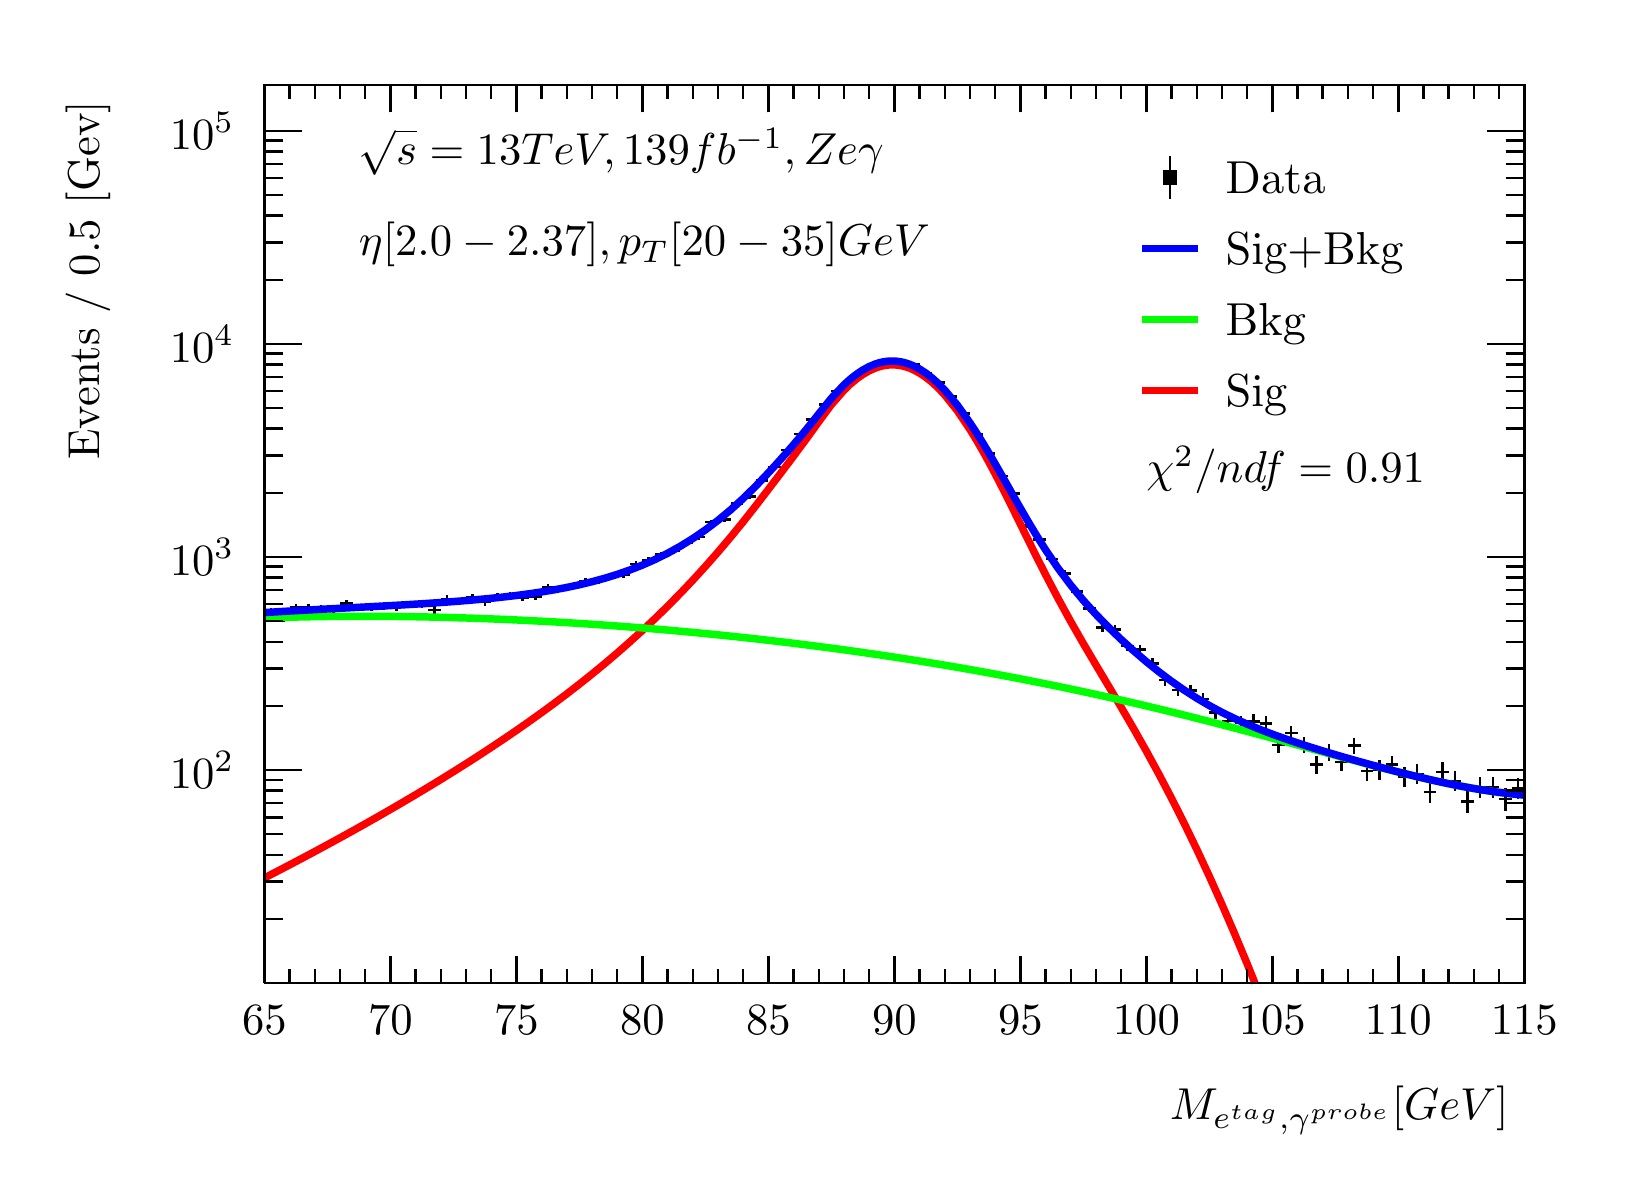
\begin{tikzpicture}
\pgfdeclareplotmark{cross} {
\pgfpathmoveto{\pgfpoint{-0.3\pgfplotmarksize}{\pgfplotmarksize}}
\pgfpathlineto{\pgfpoint{+0.3\pgfplotmarksize}{\pgfplotmarksize}}
\pgfpathlineto{\pgfpoint{+0.3\pgfplotmarksize}{0.3\pgfplotmarksize}}
\pgfpathlineto{\pgfpoint{+1\pgfplotmarksize}{0.3\pgfplotmarksize}}
\pgfpathlineto{\pgfpoint{+1\pgfplotmarksize}{-0.3\pgfplotmarksize}}
\pgfpathlineto{\pgfpoint{+0.3\pgfplotmarksize}{-0.3\pgfplotmarksize}}
\pgfpathlineto{\pgfpoint{+0.3\pgfplotmarksize}{-1.\pgfplotmarksize}}
\pgfpathlineto{\pgfpoint{-0.3\pgfplotmarksize}{-1.\pgfplotmarksize}}
\pgfpathlineto{\pgfpoint{-0.3\pgfplotmarksize}{-0.3\pgfplotmarksize}}
\pgfpathlineto{\pgfpoint{-1.\pgfplotmarksize}{-0.3\pgfplotmarksize}}
\pgfpathlineto{\pgfpoint{-1.\pgfplotmarksize}{0.3\pgfplotmarksize}}
\pgfpathlineto{\pgfpoint{-0.3\pgfplotmarksize}{0.3\pgfplotmarksize}}
\pgfpathclose
\pgfusepathqstroke
}
\pgfdeclareplotmark{cross*} {
\pgfpathmoveto{\pgfpoint{-0.3\pgfplotmarksize}{\pgfplotmarksize}}
\pgfpathlineto{\pgfpoint{+0.3\pgfplotmarksize}{\pgfplotmarksize}}
\pgfpathlineto{\pgfpoint{+0.3\pgfplotmarksize}{0.3\pgfplotmarksize}}
\pgfpathlineto{\pgfpoint{+1\pgfplotmarksize}{0.3\pgfplotmarksize}}
\pgfpathlineto{\pgfpoint{+1\pgfplotmarksize}{-0.3\pgfplotmarksize}}
\pgfpathlineto{\pgfpoint{+0.3\pgfplotmarksize}{-0.3\pgfplotmarksize}}
\pgfpathlineto{\pgfpoint{+0.3\pgfplotmarksize}{-1.\pgfplotmarksize}}
\pgfpathlineto{\pgfpoint{-0.3\pgfplotmarksize}{-1.\pgfplotmarksize}}
\pgfpathlineto{\pgfpoint{-0.3\pgfplotmarksize}{-0.3\pgfplotmarksize}}
\pgfpathlineto{\pgfpoint{-1.\pgfplotmarksize}{-0.3\pgfplotmarksize}}
\pgfpathlineto{\pgfpoint{-1.\pgfplotmarksize}{0.3\pgfplotmarksize}}
\pgfpathlineto{\pgfpoint{-0.3\pgfplotmarksize}{0.3\pgfplotmarksize}}
\pgfpathclose
\pgfusepathqfillstroke
}
\pgfdeclareplotmark{newstar} {
\pgfpathmoveto{\pgfqpoint{0pt}{\pgfplotmarksize}}
\pgfpathlineto{\pgfqpointpolar{44}{0.5\pgfplotmarksize}}
\pgfpathlineto{\pgfqpointpolar{18}{\pgfplotmarksize}}
\pgfpathlineto{\pgfqpointpolar{-20}{0.5\pgfplotmarksize}}
\pgfpathlineto{\pgfqpointpolar{-54}{\pgfplotmarksize}}
\pgfpathlineto{\pgfqpointpolar{-90}{0.5\pgfplotmarksize}}
\pgfpathlineto{\pgfqpointpolar{234}{\pgfplotmarksize}}
\pgfpathlineto{\pgfqpointpolar{198}{0.5\pgfplotmarksize}}
\pgfpathlineto{\pgfqpointpolar{162}{\pgfplotmarksize}}
\pgfpathlineto{\pgfqpointpolar{134}{0.5\pgfplotmarksize}}
\pgfpathclose
\pgfusepathqstroke
}
\pgfdeclareplotmark{newstar*} {
\pgfpathmoveto{\pgfqpoint{0pt}{\pgfplotmarksize}}
\pgfpathlineto{\pgfqpointpolar{44}{0.5\pgfplotmarksize}}
\pgfpathlineto{\pgfqpointpolar{18}{\pgfplotmarksize}}
\pgfpathlineto{\pgfqpointpolar{-20}{0.5\pgfplotmarksize}}
\pgfpathlineto{\pgfqpointpolar{-54}{\pgfplotmarksize}}
\pgfpathlineto{\pgfqpointpolar{-90}{0.5\pgfplotmarksize}}
\pgfpathlineto{\pgfqpointpolar{234}{\pgfplotmarksize}}
\pgfpathlineto{\pgfqpointpolar{198}{0.5\pgfplotmarksize}}
\pgfpathlineto{\pgfqpointpolar{162}{\pgfplotmarksize}}
\pgfpathlineto{\pgfqpointpolar{134}{0.5\pgfplotmarksize}}
\pgfpathclose
\pgfusepathqfillstroke
}
\definecolor{c}{rgb}{1,1,1};
\draw [color=c, fill=c] (0,0) rectangle (20,14.4361);
\draw [color=c, fill=c] (3,2.30977) rectangle (19,13.7143);
\definecolor{c}{rgb}{0,0,0};
\draw [c,line width=0.9] (3,2.30977) -- (3,13.7143) -- (19,13.7143) -- (19,2.30977) -- (3,2.30977);
\definecolor{c}{rgb}{1,1,1};
\draw [color=c, fill=c] (3,2.30977) rectangle (19,13.7143);
\definecolor{c}{rgb}{0,0,0};
\draw [c,line width=0.9] (3,2.30977) -- (3,13.7143) -- (19,13.7143) -- (19,2.30977) -- (3,2.30977);
\draw [c,line width=0.9] (3,2.30977) -- (19,2.30977);
\draw [c,line width=0.9] (3,2.65624) -- (3,2.30977);
\draw [c,line width=0.9] (3.32,2.48301) -- (3.32,2.30977);
\draw [c,line width=0.9] (3.64,2.48301) -- (3.64,2.30977);
\draw [c,line width=0.9] (3.96,2.48301) -- (3.96,2.30977);
\draw [c,line width=0.9] (4.28,2.48301) -- (4.28,2.30977);
\draw [c,line width=0.9] (4.6,2.65624) -- (4.6,2.30977);
\draw [c,line width=0.9] (4.92,2.48301) -- (4.92,2.30977);
\draw [c,line width=0.9] (5.24,2.48301) -- (5.24,2.30977);
\draw [c,line width=0.9] (5.56,2.48301) -- (5.56,2.30977);
\draw [c,line width=0.9] (5.88,2.48301) -- (5.88,2.30977);
\draw [c,line width=0.9] (6.2,2.65624) -- (6.2,2.30977);
\draw [c,line width=0.9] (6.52,2.48301) -- (6.52,2.30977);
\draw [c,line width=0.9] (6.84,2.48301) -- (6.84,2.30977);
\draw [c,line width=0.9] (7.16,2.48301) -- (7.16,2.30977);
\draw [c,line width=0.9] (7.48,2.48301) -- (7.48,2.30977);
\draw [c,line width=0.9] (7.8,2.65624) -- (7.8,2.30977);
\draw [c,line width=0.9] (8.12,2.48301) -- (8.12,2.30977);
\draw [c,line width=0.9] (8.44,2.48301) -- (8.44,2.30977);
\draw [c,line width=0.9] (8.76,2.48301) -- (8.76,2.30977);
\draw [c,line width=0.9] (9.08,2.48301) -- (9.08,2.30977);
\draw [c,line width=0.9] (9.4,2.65624) -- (9.4,2.30977);
\draw [c,line width=0.9] (9.72,2.48301) -- (9.72,2.30977);
\draw [c,line width=0.9] (10.04,2.48301) -- (10.04,2.30977);
\draw [c,line width=0.9] (10.36,2.48301) -- (10.36,2.30977);
\draw [c,line width=0.9] (10.68,2.48301) -- (10.68,2.30977);
\draw [c,line width=0.9] (11,2.65624) -- (11,2.30977);
\draw [c,line width=0.9] (11.32,2.48301) -- (11.32,2.30977);
\draw [c,line width=0.9] (11.64,2.48301) -- (11.64,2.30977);
\draw [c,line width=0.9] (11.96,2.48301) -- (11.96,2.30977);
\draw [c,line width=0.9] (12.28,2.48301) -- (12.28,2.30977);
\draw [c,line width=0.9] (12.6,2.65624) -- (12.6,2.30977);
\draw [c,line width=0.9] (12.92,2.48301) -- (12.92,2.30977);
\draw [c,line width=0.9] (13.24,2.48301) -- (13.24,2.30977);
\draw [c,line width=0.9] (13.56,2.48301) -- (13.56,2.30977);
\draw [c,line width=0.9] (13.88,2.48301) -- (13.88,2.30977);
\draw [c,line width=0.9] (14.2,2.65624) -- (14.2,2.30977);
\draw [c,line width=0.9] (14.52,2.48301) -- (14.52,2.30977);
\draw [c,line width=0.9] (14.84,2.48301) -- (14.84,2.30977);
\draw [c,line width=0.9] (15.16,2.48301) -- (15.16,2.30977);
\draw [c,line width=0.9] (15.48,2.48301) -- (15.48,2.30977);
\draw [c,line width=0.9] (15.8,2.65624) -- (15.8,2.30977);
\draw [c,line width=0.9] (16.12,2.48301) -- (16.12,2.30977);
\draw [c,line width=0.9] (16.44,2.48301) -- (16.44,2.30977);
\draw [c,line width=0.9] (16.76,2.48301) -- (16.76,2.30977);
\draw [c,line width=0.9] (17.08,2.48301) -- (17.08,2.30977);
\draw [c,line width=0.9] (17.4,2.65624) -- (17.4,2.30977);
\draw [c,line width=0.9] (17.72,2.48301) -- (17.72,2.30977);
\draw [c,line width=0.9] (18.04,2.48301) -- (18.04,2.30977);
\draw [c,line width=0.9] (18.36,2.48301) -- (18.36,2.30977);
\draw [c,line width=0.9] (18.68,2.48301) -- (18.68,2.30977);
\draw [c,line width=0.9] (19,2.65624) -- (19,2.30977);
\draw [c,line width=0.9] (19,2.65624) -- (19,2.30977);
\draw [anchor=base] (3,1.66015) node[scale=1.61424, color=c, rotate=0]{65};
\draw [anchor=base] (4.6,1.66015) node[scale=1.61424, color=c, rotate=0]{70};
\draw [anchor=base] (6.2,1.66015) node[scale=1.61424, color=c, rotate=0]{75};
\draw [anchor=base] (7.8,1.66015) node[scale=1.61424, color=c, rotate=0]{80};
\draw [anchor=base] (9.4,1.66015) node[scale=1.61424, color=c, rotate=0]{85};
\draw [anchor=base] (11,1.66015) node[scale=1.61424, color=c, rotate=0]{90};
\draw [anchor=base] (12.6,1.66015) node[scale=1.61424, color=c, rotate=0]{95};
\draw [anchor=base] (14.2,1.66015) node[scale=1.61424, color=c, rotate=0]{100};
\draw [anchor=base] (15.8,1.66015) node[scale=1.61424, color=c, rotate=0]{105};
\draw [anchor=base] (17.4,1.66015) node[scale=1.61424, color=c, rotate=0]{110};
\draw [anchor=base] (19,1.66015) node[scale=1.61424, color=c, rotate=0]{115};
\draw [anchor= east] (19,0.692932) node[scale=1.61424, color=c, rotate=0]{$M_{e^{tag}, \gamma^{probe}}  [GeV]$};
\draw [c,line width=0.9] (3,13.7143) -- (19,13.7143);
\draw [c,line width=0.9] (3,13.3678) -- (3,13.7143);
\draw [c,line width=0.9] (3.32,13.5411) -- (3.32,13.7143);
\draw [c,line width=0.9] (3.64,13.5411) -- (3.64,13.7143);
\draw [c,line width=0.9] (3.96,13.5411) -- (3.96,13.7143);
\draw [c,line width=0.9] (4.28,13.5411) -- (4.28,13.7143);
\draw [c,line width=0.9] (4.6,13.3678) -- (4.6,13.7143);
\draw [c,line width=0.9] (4.92,13.5411) -- (4.92,13.7143);
\draw [c,line width=0.9] (5.24,13.5411) -- (5.24,13.7143);
\draw [c,line width=0.9] (5.56,13.5411) -- (5.56,13.7143);
\draw [c,line width=0.9] (5.88,13.5411) -- (5.88,13.7143);
\draw [c,line width=0.9] (6.2,13.3678) -- (6.2,13.7143);
\draw [c,line width=0.9] (6.52,13.5411) -- (6.52,13.7143);
\draw [c,line width=0.9] (6.84,13.5411) -- (6.84,13.7143);
\draw [c,line width=0.9] (7.16,13.5411) -- (7.16,13.7143);
\draw [c,line width=0.9] (7.48,13.5411) -- (7.48,13.7143);
\draw [c,line width=0.9] (7.8,13.3678) -- (7.8,13.7143);
\draw [c,line width=0.9] (8.12,13.5411) -- (8.12,13.7143);
\draw [c,line width=0.9] (8.44,13.5411) -- (8.44,13.7143);
\draw [c,line width=0.9] (8.76,13.5411) -- (8.76,13.7143);
\draw [c,line width=0.9] (9.08,13.5411) -- (9.08,13.7143);
\draw [c,line width=0.9] (9.4,13.3678) -- (9.4,13.7143);
\draw [c,line width=0.9] (9.72,13.5411) -- (9.72,13.7143);
\draw [c,line width=0.9] (10.04,13.5411) -- (10.04,13.7143);
\draw [c,line width=0.9] (10.36,13.5411) -- (10.36,13.7143);
\draw [c,line width=0.9] (10.68,13.5411) -- (10.68,13.7143);
\draw [c,line width=0.9] (11,13.3678) -- (11,13.7143);
\draw [c,line width=0.9] (11.32,13.5411) -- (11.32,13.7143);
\draw [c,line width=0.9] (11.64,13.5411) -- (11.64,13.7143);
\draw [c,line width=0.9] (11.96,13.5411) -- (11.96,13.7143);
\draw [c,line width=0.9] (12.28,13.5411) -- (12.28,13.7143);
\draw [c,line width=0.9] (12.6,13.3678) -- (12.6,13.7143);
\draw [c,line width=0.9] (12.92,13.5411) -- (12.92,13.7143);
\draw [c,line width=0.9] (13.24,13.5411) -- (13.24,13.7143);
\draw [c,line width=0.9] (13.56,13.5411) -- (13.56,13.7143);
\draw [c,line width=0.9] (13.88,13.5411) -- (13.88,13.7143);
\draw [c,line width=0.9] (14.2,13.3678) -- (14.2,13.7143);
\draw [c,line width=0.9] (14.52,13.5411) -- (14.52,13.7143);
\draw [c,line width=0.9] (14.84,13.5411) -- (14.84,13.7143);
\draw [c,line width=0.9] (15.16,13.5411) -- (15.16,13.7143);
\draw [c,line width=0.9] (15.48,13.5411) -- (15.48,13.7143);
\draw [c,line width=0.9] (15.8,13.3678) -- (15.8,13.7143);
\draw [c,line width=0.9] (16.12,13.5411) -- (16.12,13.7143);
\draw [c,line width=0.9] (16.44,13.5411) -- (16.44,13.7143);
\draw [c,line width=0.9] (16.76,13.5411) -- (16.76,13.7143);
\draw [c,line width=0.9] (17.08,13.5411) -- (17.08,13.7143);
\draw [c,line width=0.9] (17.4,13.3678) -- (17.4,13.7143);
\draw [c,line width=0.9] (17.72,13.5411) -- (17.72,13.7143);
\draw [c,line width=0.9] (18.04,13.5411) -- (18.04,13.7143);
\draw [c,line width=0.9] (18.36,13.5411) -- (18.36,13.7143);
\draw [c,line width=0.9] (18.68,13.5411) -- (18.68,13.7143);
\draw [c,line width=0.9] (19,13.3678) -- (19,13.7143);
\draw [c,line width=0.9] (19,13.3678) -- (19,13.7143);
\draw [c,line width=0.9] (3,2.30977) -- (3,13.7143);
\draw [c,line width=0.9] (3.237,3.12423) -- (3,3.12423);
\draw [c,line width=0.9] (3.237,3.60066) -- (3,3.60066);
\draw [c,line width=0.9] (3.237,3.93869) -- (3,3.93869);
\draw [c,line width=0.9] (3.237,4.20088) -- (3,4.20088);
\draw [c,line width=0.9] (3.237,4.41511) -- (3,4.41511);
\draw [c,line width=0.9] (3.237,4.59624) -- (3,4.59624);
\draw [c,line width=0.9] (3.237,4.75314) -- (3,4.75314);
\draw [c,line width=0.9] (3.237,4.89154) -- (3,4.89154);
\draw [c,line width=0.9] (3.474,5.01534) -- (3,5.01534);
\draw [anchor= east] (2.82,5.01534) node[scale=1.61424, color=c, rotate=0]{$10^{2}$};
\draw [c,line width=0.9] (3.237,5.8298) -- (3,5.8298);
\draw [c,line width=0.9] (3.237,6.30623) -- (3,6.30623);
\draw [c,line width=0.9] (3.237,6.64426) -- (3,6.64426);
\draw [c,line width=0.9] (3.237,6.90645) -- (3,6.90645);
\draw [c,line width=0.9] (3.237,7.12068) -- (3,7.12068);
\draw [c,line width=0.9] (3.237,7.30181) -- (3,7.30181);
\draw [c,line width=0.9] (3.237,7.45871) -- (3,7.45871);
\draw [c,line width=0.9] (3.237,7.59711) -- (3,7.59711);
\draw [c,line width=0.9] (3.474,7.72091) -- (3,7.72091);
\draw [anchor= east] (2.82,7.72091) node[scale=1.61424, color=c, rotate=0]{$10^{3}$};
\draw [c,line width=0.9] (3.237,8.53537) -- (3,8.53537);
\draw [c,line width=0.9] (3.237,9.0118) -- (3,9.0118);
\draw [c,line width=0.9] (3.237,9.34983) -- (3,9.34983);
\draw [c,line width=0.9] (3.237,9.61202) -- (3,9.61202);
\draw [c,line width=0.9] (3.237,9.82625) -- (3,9.82625);
\draw [c,line width=0.9] (3.237,10.0074) -- (3,10.0074);
\draw [c,line width=0.9] (3.237,10.1643) -- (3,10.1643);
\draw [c,line width=0.9] (3.237,10.3027) -- (3,10.3027);
\draw [c,line width=0.9] (3.474,10.4265) -- (3,10.4265);
\draw [anchor= east] (2.82,10.4265) node[scale=1.61424, color=c, rotate=0]{$10^{4}$};
\draw [c,line width=0.9] (3.237,11.2409) -- (3,11.2409);
\draw [c,line width=0.9] (3.237,11.7174) -- (3,11.7174);
\draw [c,line width=0.9] (3.237,12.0554) -- (3,12.0554);
\draw [c,line width=0.9] (3.237,12.3176) -- (3,12.3176);
\draw [c,line width=0.9] (3.237,12.5318) -- (3,12.5318);
\draw [c,line width=0.9] (3.237,12.713) -- (3,12.713);
\draw [c,line width=0.9] (3.237,12.8699) -- (3,12.8699);
\draw [c,line width=0.9] (3.237,13.0083) -- (3,13.0083);
\draw [c,line width=0.9] (3.474,13.1321) -- (3,13.1321);
\draw [anchor= east] (2.82,13.1321) node[scale=1.61424, color=c, rotate=0]{$10^{5}$};
\draw [anchor= east] (0.76,13.7143) node[scale=1.61424, color=c, rotate=90]{Events / 0.5 [Gev]};
\draw [c,line width=0.9] (19,2.30977) -- (19,13.7143);
\draw [c,line width=0.9] (18.763,3.12423) -- (19,3.12423);
\draw [c,line width=0.9] (18.763,3.60066) -- (19,3.60066);
\draw [c,line width=0.9] (18.763,3.93869) -- (19,3.93869);
\draw [c,line width=0.9] (18.763,4.20088) -- (19,4.20088);
\draw [c,line width=0.9] (18.763,4.41511) -- (19,4.41511);
\draw [c,line width=0.9] (18.763,4.59624) -- (19,4.59624);
\draw [c,line width=0.9] (18.763,4.75314) -- (19,4.75314);
\draw [c,line width=0.9] (18.763,4.89154) -- (19,4.89154);
\draw [c,line width=0.9] (18.526,5.01534) -- (19,5.01534);
\draw [c,line width=0.9] (18.763,5.8298) -- (19,5.8298);
\draw [c,line width=0.9] (18.763,6.30623) -- (19,6.30623);
\draw [c,line width=0.9] (18.763,6.64426) -- (19,6.64426);
\draw [c,line width=0.9] (18.763,6.90645) -- (19,6.90645);
\draw [c,line width=0.9] (18.763,7.12068) -- (19,7.12068);
\draw [c,line width=0.9] (18.763,7.30181) -- (19,7.30181);
\draw [c,line width=0.9] (18.763,7.45871) -- (19,7.45871);
\draw [c,line width=0.9] (18.763,7.59711) -- (19,7.59711);
\draw [c,line width=0.9] (18.526,7.72091) -- (19,7.72091);
\draw [c,line width=0.9] (18.763,8.53537) -- (19,8.53537);
\draw [c,line width=0.9] (18.763,9.0118) -- (19,9.0118);
\draw [c,line width=0.9] (18.763,9.34983) -- (19,9.34983);
\draw [c,line width=0.9] (18.763,9.61202) -- (19,9.61202);
\draw [c,line width=0.9] (18.763,9.82625) -- (19,9.82625);
\draw [c,line width=0.9] (18.763,10.0074) -- (19,10.0074);
\draw [c,line width=0.9] (18.763,10.1643) -- (19,10.1643);
\draw [c,line width=0.9] (18.763,10.3027) -- (19,10.3027);
\draw [c,line width=0.9] (18.526,10.4265) -- (19,10.4265);
\draw [c,line width=0.9] (18.763,11.2409) -- (19,11.2409);
\draw [c,line width=0.9] (18.763,11.7174) -- (19,11.7174);
\draw [c,line width=0.9] (18.763,12.0554) -- (19,12.0554);
\draw [c,line width=0.9] (18.763,12.3176) -- (19,12.3176);
\draw [c,line width=0.9] (18.763,12.5318) -- (19,12.5318);
\draw [c,line width=0.9] (18.763,12.713) -- (19,12.713);
\draw [c,line width=0.9] (18.763,12.8699) -- (19,12.8699);
\draw [c,line width=0.9] (18.763,13.0083) -- (19,13.0083);
\draw [c,line width=0.9] (18.526,13.1321) -- (19,13.1321);
\draw [c,line width=0.9] (3.08,7.02908) -- (3,7.02908);
\draw [c,line width=0.9] (3,7.02908) -- (3,7.02908);
\draw [c,line width=0.9] (3.08,7.02908) -- (3.16,7.02908);
\draw [c,line width=0.9] (3.16,7.02908) -- (3.16,7.02908);
\draw [c,line width=0.9] (3.08,7.02908) -- (3.08,7.07895);
\draw [c,line width=0.9] (3.08,7.07895) -- (3.08,7.07895);
\draw [c,line width=0.9] (3.08,7.02908) -- (3.08,6.97921);
\draw [c,line width=0.9] (3.08,6.97921) -- (3.08,6.97921);
\draw [c,line width=0.9] (3.24,6.95254) -- (3.16,6.95254);
\draw [c,line width=0.9] (3.16,6.95254) -- (3.16,6.95254);
\draw [c,line width=0.9] (3.24,6.95254) -- (3.32,6.95254);
\draw [c,line width=0.9] (3.32,6.95254) -- (3.32,6.95254);
\draw [c,line width=0.9] (3.24,6.95254) -- (3.24,7.00406);
\draw [c,line width=0.9] (3.24,7.00406) -- (3.24,7.00406);
\draw [c,line width=0.9] (3.24,6.95254) -- (3.24,6.90102);
\draw [c,line width=0.9] (3.24,6.90102) -- (3.24,6.90102);
\draw [c,line width=0.9] (3.4,7.07882) -- (3.32,7.07882);
\draw [c,line width=0.9] (3.32,7.07882) -- (3.32,7.07882);
\draw [c,line width=0.9] (3.4,7.07882) -- (3.48,7.07882);
\draw [c,line width=0.9] (3.48,7.07882) -- (3.48,7.07882);
\draw [c,line width=0.9] (3.4,7.07882) -- (3.4,7.12765);
\draw [c,line width=0.9] (3.4,7.12765) -- (3.4,7.12765);
\draw [c,line width=0.9] (3.4,7.07882) -- (3.4,7.02999);
\draw [c,line width=0.9] (3.4,7.02999) -- (3.4,7.02999);
\draw [c,line width=0.9] (3.56,7.07679) -- (3.48,7.07679);
\draw [c,line width=0.9] (3.48,7.07679) -- (3.48,7.07679);
\draw [c,line width=0.9] (3.56,7.07679) -- (3.64,7.07679);
\draw [c,line width=0.9] (3.64,7.07679) -- (3.64,7.07679);
\draw [c,line width=0.9] (3.56,7.07679) -- (3.56,7.12566);
\draw [c,line width=0.9] (3.56,7.12566) -- (3.56,7.12566);
\draw [c,line width=0.9] (3.56,7.07679) -- (3.56,7.02792);
\draw [c,line width=0.9] (3.56,7.02792) -- (3.56,7.02792);
\draw [c,line width=0.9] (3.72,7.06453) -- (3.64,7.06453);
\draw [c,line width=0.9] (3.64,7.06453) -- (3.64,7.06453);
\draw [c,line width=0.9] (3.72,7.06453) -- (3.8,7.06453);
\draw [c,line width=0.9] (3.8,7.06453) -- (3.8,7.06453);
\draw [c,line width=0.9] (3.72,7.06453) -- (3.72,7.11366);
\draw [c,line width=0.9] (3.72,7.11366) -- (3.72,7.11366);
\draw [c,line width=0.9] (3.72,7.06453) -- (3.72,7.0154);
\draw [c,line width=0.9] (3.72,7.0154) -- (3.72,7.0154);
\draw [c,line width=0.9] (3.88,7.06453) -- (3.8,7.06453);
\draw [c,line width=0.9] (3.8,7.06453) -- (3.8,7.06453);
\draw [c,line width=0.9] (3.88,7.06453) -- (3.96,7.06453);
\draw [c,line width=0.9] (3.96,7.06453) -- (3.96,7.06453);
\draw [c,line width=0.9] (3.88,7.06453) -- (3.88,7.11366);
\draw [c,line width=0.9] (3.88,7.11366) -- (3.88,7.11366);
\draw [c,line width=0.9] (3.88,7.06453) -- (3.88,7.0154);
\draw [c,line width=0.9] (3.88,7.0154) -- (3.88,7.0154);
\draw [c,line width=0.9] (4.04,7.13238) -- (3.96,7.13238);
\draw [c,line width=0.9] (3.96,7.13238) -- (3.96,7.13238);
\draw [c,line width=0.9] (4.04,7.13238) -- (4.12,7.13238);
\draw [c,line width=0.9] (4.12,7.13238) -- (4.12,7.13238);
\draw [c,line width=0.9] (4.04,7.13238) -- (4.04,7.18011);
\draw [c,line width=0.9] (4.04,7.18011) -- (4.04,7.18011);
\draw [c,line width=0.9] (4.04,7.13238) -- (4.04,7.08465);
\draw [c,line width=0.9] (4.04,7.08465) -- (4.04,7.08465);
\draw [c,line width=0.9] (4.2,7.07882) -- (4.12,7.07882);
\draw [c,line width=0.9] (4.12,7.07882) -- (4.12,7.07882);
\draw [c,line width=0.9] (4.2,7.07882) -- (4.28,7.07882);
\draw [c,line width=0.9] (4.28,7.07882) -- (4.28,7.07882);
\draw [c,line width=0.9] (4.2,7.07882) -- (4.2,7.12765);
\draw [c,line width=0.9] (4.2,7.12765) -- (4.2,7.12765);
\draw [c,line width=0.9] (4.2,7.07882) -- (4.2,7.02999);
\draw [c,line width=0.9] (4.2,7.02999) -- (4.2,7.02999);
\draw [c,line width=0.9] (4.36,7.08085) -- (4.28,7.08085);
\draw [c,line width=0.9] (4.28,7.08085) -- (4.28,7.08085);
\draw [c,line width=0.9] (4.36,7.08085) -- (4.44,7.08085);
\draw [c,line width=0.9] (4.44,7.08085) -- (4.44,7.08085);
\draw [c,line width=0.9] (4.36,7.08085) -- (4.36,7.12964);
\draw [c,line width=0.9] (4.36,7.12964) -- (4.36,7.12964);
\draw [c,line width=0.9] (4.36,7.08085) -- (4.36,7.03206);
\draw [c,line width=0.9] (4.36,7.03206) -- (4.36,7.03206);
\draw [c,line width=0.9] (4.52,7.09894) -- (4.44,7.09894);
\draw [c,line width=0.9] (4.44,7.09894) -- (4.44,7.09894);
\draw [c,line width=0.9] (4.52,7.09894) -- (4.6,7.09894);
\draw [c,line width=0.9] (4.6,7.09894) -- (4.6,7.09894);
\draw [c,line width=0.9] (4.52,7.09894) -- (4.52,7.14736);
\draw [c,line width=0.9] (4.52,7.14736) -- (4.52,7.14736);
\draw [c,line width=0.9] (4.52,7.09894) -- (4.52,7.05053);
\draw [c,line width=0.9] (4.52,7.05053) -- (4.52,7.05053);
\draw [c,line width=0.9] (4.68,7.08288) -- (4.6,7.08288);
\draw [c,line width=0.9] (4.6,7.08288) -- (4.6,7.08288);
\draw [c,line width=0.9] (4.68,7.08288) -- (4.76,7.08288);
\draw [c,line width=0.9] (4.76,7.08288) -- (4.76,7.08288);
\draw [c,line width=0.9] (4.68,7.08288) -- (4.68,7.13162);
\draw [c,line width=0.9] (4.68,7.13162) -- (4.68,7.13162);
\draw [c,line width=0.9] (4.68,7.08288) -- (4.68,7.03413);
\draw [c,line width=0.9] (4.68,7.03413) -- (4.68,7.03413);
\draw [c,line width=0.9] (4.84,7.1148) -- (4.76,7.1148);
\draw [c,line width=0.9] (4.76,7.1148) -- (4.76,7.1148);
\draw [c,line width=0.9] (4.84,7.1148) -- (4.92,7.1148);
\draw [c,line width=0.9] (4.92,7.1148) -- (4.92,7.1148);
\draw [c,line width=0.9] (4.84,7.1148) -- (4.84,7.16288);
\draw [c,line width=0.9] (4.84,7.16288) -- (4.84,7.16288);
\draw [c,line width=0.9] (4.84,7.1148) -- (4.84,7.06671);
\draw [c,line width=0.9] (4.84,7.06671) -- (4.84,7.06671);
\draw [c,line width=0.9] (5,7.12264) -- (4.92,7.12264);
\draw [c,line width=0.9] (4.92,7.12264) -- (4.92,7.12264);
\draw [c,line width=0.9] (5,7.12264) -- (5.08,7.12264);
\draw [c,line width=0.9] (5.08,7.12264) -- (5.08,7.12264);
\draw [c,line width=0.9] (5,7.12264) -- (5,7.17057);
\draw [c,line width=0.9] (5,7.17057) -- (5,7.17057);
\draw [c,line width=0.9] (5,7.12264) -- (5,7.07472);
\draw [c,line width=0.9] (5,7.07472) -- (5,7.07472);
\draw [c,line width=0.9] (5.16,7.04798) -- (5.08,7.04798);
\draw [c,line width=0.9] (5.08,7.04798) -- (5.08,7.04798);
\draw [c,line width=0.9] (5.16,7.04798) -- (5.24,7.04798);
\draw [c,line width=0.9] (5.24,7.04798) -- (5.24,7.04798);
\draw [c,line width=0.9] (5.16,7.04798) -- (5.16,7.09745);
\draw [c,line width=0.9] (5.16,7.09745) -- (5.16,7.09745);
\draw [c,line width=0.9] (5.16,7.04798) -- (5.16,6.99851);
\draw [c,line width=0.9] (5.16,6.99851) -- (5.16,6.99851);
\draw [c,line width=0.9] (5.32,7.1873) -- (5.24,7.1873);
\draw [c,line width=0.9] (5.24,7.1873) -- (5.24,7.1873);
\draw [c,line width=0.9] (5.32,7.1873) -- (5.4,7.1873);
\draw [c,line width=0.9] (5.4,7.1873) -- (5.4,7.1873);
\draw [c,line width=0.9] (5.32,7.1873) -- (5.32,7.23393);
\draw [c,line width=0.9] (5.32,7.23393) -- (5.32,7.23393);
\draw [c,line width=0.9] (5.32,7.1873) -- (5.32,7.14068);
\draw [c,line width=0.9] (5.32,7.14068) -- (5.32,7.14068);
\draw [c,line width=0.9] (5.48,7.15732) -- (5.4,7.15732);
\draw [c,line width=0.9] (5.4,7.15732) -- (5.4,7.15732);
\draw [c,line width=0.9] (5.48,7.15732) -- (5.56,7.15732);
\draw [c,line width=0.9] (5.56,7.15732) -- (5.56,7.15732);
\draw [c,line width=0.9] (5.48,7.15732) -- (5.48,7.20454);
\draw [c,line width=0.9] (5.48,7.20454) -- (5.48,7.20454);
\draw [c,line width=0.9] (5.48,7.15732) -- (5.48,7.11009);
\draw [c,line width=0.9] (5.48,7.11009) -- (5.48,7.11009);
\draw [c,line width=0.9] (5.64,7.2093) -- (5.56,7.2093);
\draw [c,line width=0.9] (5.56,7.2093) -- (5.56,7.2093);
\draw [c,line width=0.9] (5.64,7.2093) -- (5.72,7.2093);
\draw [c,line width=0.9] (5.72,7.2093) -- (5.72,7.2093);
\draw [c,line width=0.9] (5.64,7.2093) -- (5.64,7.25549);
\draw [c,line width=0.9] (5.64,7.25549) -- (5.64,7.25549);
\draw [c,line width=0.9] (5.64,7.2093) -- (5.64,7.16311);
\draw [c,line width=0.9] (5.64,7.16311) -- (5.64,7.16311);
\draw [c,line width=0.9] (5.8,7.1497) -- (5.72,7.1497);
\draw [c,line width=0.9] (5.72,7.1497) -- (5.72,7.1497);
\draw [c,line width=0.9] (5.8,7.1497) -- (5.88,7.1497);
\draw [c,line width=0.9] (5.88,7.1497) -- (5.88,7.1497);
\draw [c,line width=0.9] (5.8,7.1497) -- (5.8,7.19708);
\draw [c,line width=0.9] (5.8,7.19708) -- (5.8,7.19708);
\draw [c,line width=0.9] (5.8,7.1497) -- (5.8,7.10232);
\draw [c,line width=0.9] (5.8,7.10232) -- (5.8,7.10232);
\draw [c,line width=0.9] (5.96,7.22374) -- (5.88,7.22374);
\draw [c,line width=0.9] (5.88,7.22374) -- (5.88,7.22374);
\draw [c,line width=0.9] (5.96,7.22374) -- (6.04,7.22374);
\draw [c,line width=0.9] (6.04,7.22374) -- (6.04,7.22374);
\draw [c,line width=0.9] (5.96,7.22374) -- (5.96,7.26965);
\draw [c,line width=0.9] (5.96,7.26965) -- (5.96,7.26965);
\draw [c,line width=0.9] (5.96,7.22374) -- (5.96,7.17783);
\draw [c,line width=0.9] (5.96,7.17783) -- (5.96,7.17783);
\draw [c,line width=0.9] (6.12,7.22911) -- (6.04,7.22911);
\draw [c,line width=0.9] (6.04,7.22911) -- (6.04,7.22911);
\draw [c,line width=0.9] (6.12,7.22911) -- (6.2,7.22911);
\draw [c,line width=0.9] (6.2,7.22911) -- (6.2,7.22911);
\draw [c,line width=0.9] (6.12,7.22911) -- (6.12,7.27491);
\draw [c,line width=0.9] (6.12,7.27491) -- (6.12,7.27491);
\draw [c,line width=0.9] (6.12,7.22911) -- (6.12,7.18331);
\draw [c,line width=0.9] (6.12,7.18331) -- (6.12,7.18331);
\draw [c,line width=0.9] (6.28,7.2093) -- (6.2,7.2093);
\draw [c,line width=0.9] (6.2,7.2093) -- (6.2,7.2093);
\draw [c,line width=0.9] (6.28,7.2093) -- (6.36,7.2093);
\draw [c,line width=0.9] (6.36,7.2093) -- (6.36,7.2093);
\draw [c,line width=0.9] (6.28,7.2093) -- (6.28,7.25549);
\draw [c,line width=0.9] (6.28,7.25549) -- (6.28,7.25549);
\draw [c,line width=0.9] (6.28,7.2093) -- (6.28,7.16311);
\draw [c,line width=0.9] (6.28,7.16311) -- (6.28,7.16311);
\draw [c,line width=0.9] (6.44,7.22015) -- (6.36,7.22015);
\draw [c,line width=0.9] (6.36,7.22015) -- (6.36,7.22015);
\draw [c,line width=0.9] (6.44,7.22015) -- (6.52,7.22015);
\draw [c,line width=0.9] (6.52,7.22015) -- (6.52,7.22015);
\draw [c,line width=0.9] (6.44,7.22015) -- (6.44,7.26613);
\draw [c,line width=0.9] (6.44,7.26613) -- (6.44,7.26613);
\draw [c,line width=0.9] (6.44,7.22015) -- (6.44,7.17417);
\draw [c,line width=0.9] (6.44,7.17417) -- (6.44,7.17417);
\draw [c,line width=0.9] (6.6,7.33328) -- (6.52,7.33328);
\draw [c,line width=0.9] (6.52,7.33328) -- (6.52,7.33328);
\draw [c,line width=0.9] (6.6,7.33328) -- (6.68,7.33328);
\draw [c,line width=0.9] (6.68,7.33328) -- (6.68,7.33328);
\draw [c,line width=0.9] (6.6,7.33328) -- (6.6,7.3771);
\draw [c,line width=0.9] (6.6,7.3771) -- (6.6,7.3771);
\draw [c,line width=0.9] (6.6,7.33328) -- (6.6,7.28946);
\draw [c,line width=0.9] (6.6,7.28946) -- (6.6,7.28946);
\draw [c,line width=0.9] (6.76,7.31848) -- (6.68,7.31848);
\draw [c,line width=0.9] (6.68,7.31848) -- (6.68,7.31848);
\draw [c,line width=0.9] (6.76,7.31848) -- (6.84,7.31848);
\draw [c,line width=0.9] (6.84,7.31848) -- (6.84,7.31848);
\draw [c,line width=0.9] (6.76,7.31848) -- (6.76,7.36258);
\draw [c,line width=0.9] (6.76,7.36258) -- (6.76,7.36258);
\draw [c,line width=0.9] (6.76,7.31848) -- (6.76,7.27439);
\draw [c,line width=0.9] (6.76,7.27439) -- (6.76,7.27439);
\draw [c,line width=0.9] (6.92,7.34628) -- (6.84,7.34628);
\draw [c,line width=0.9] (6.84,7.34628) -- (6.84,7.34628);
\draw [c,line width=0.9] (6.92,7.34628) -- (7,7.34628);
\draw [c,line width=0.9] (7,7.34628) -- (7,7.34628);
\draw [c,line width=0.9] (6.92,7.34628) -- (6.92,7.38986);
\draw [c,line width=0.9] (6.92,7.38986) -- (6.92,7.38986);
\draw [c,line width=0.9] (6.92,7.34628) -- (6.92,7.30271);
\draw [c,line width=0.9] (6.92,7.30271) -- (6.92,7.30271);
\draw [c,line width=0.9] (7.08,7.41075) -- (7,7.41075);
\draw [c,line width=0.9] (7,7.41075) -- (7,7.41075);
\draw [c,line width=0.9] (7.08,7.41075) -- (7.16,7.41075);
\draw [c,line width=0.9] (7.16,7.41075) -- (7.16,7.41075);
\draw [c,line width=0.9] (7.08,7.41075) -- (7.08,7.45315);
\draw [c,line width=0.9] (7.08,7.45315) -- (7.08,7.45315);
\draw [c,line width=0.9] (7.08,7.41075) -- (7.08,7.36835);
\draw [c,line width=0.9] (7.08,7.36835) -- (7.08,7.36835);
\draw [c,line width=0.9] (7.24,7.41685) -- (7.16,7.41685);
\draw [c,line width=0.9] (7.16,7.41685) -- (7.16,7.41685);
\draw [c,line width=0.9] (7.24,7.41685) -- (7.32,7.41685);
\draw [c,line width=0.9] (7.32,7.41685) -- (7.32,7.41685);
\draw [c,line width=0.9] (7.24,7.41685) -- (7.24,7.45914);
\draw [c,line width=0.9] (7.24,7.45914) -- (7.24,7.45914);
\draw [c,line width=0.9] (7.24,7.41685) -- (7.24,7.37457);
\draw [c,line width=0.9] (7.24,7.37457) -- (7.24,7.37457);
\draw [c,line width=0.9] (7.4,7.47766) -- (7.32,7.47766);
\draw [c,line width=0.9] (7.32,7.47766) -- (7.32,7.47766);
\draw [c,line width=0.9] (7.4,7.47766) -- (7.48,7.47766);
\draw [c,line width=0.9] (7.48,7.47766) -- (7.48,7.47766);
\draw [c,line width=0.9] (7.4,7.47766) -- (7.4,7.51886);
\draw [c,line width=0.9] (7.4,7.51886) -- (7.4,7.51886);
\draw [c,line width=0.9] (7.4,7.47766) -- (7.4,7.43645);
\draw [c,line width=0.9] (7.4,7.43645) -- (7.4,7.43645);
\draw [c,line width=0.9] (7.56,7.49202) -- (7.48,7.49202);
\draw [c,line width=0.9] (7.48,7.49202) -- (7.48,7.49202);
\draw [c,line width=0.9] (7.56,7.49202) -- (7.64,7.49202);
\draw [c,line width=0.9] (7.64,7.49202) -- (7.64,7.49202);
\draw [c,line width=0.9] (7.56,7.49202) -- (7.56,7.53298);
\draw [c,line width=0.9] (7.56,7.53298) -- (7.56,7.53298);
\draw [c,line width=0.9] (7.56,7.49202) -- (7.56,7.45107);
\draw [c,line width=0.9] (7.56,7.45107) -- (7.56,7.45107);
\draw [c,line width=0.9] (7.72,7.63058) -- (7.64,7.63058);
\draw [c,line width=0.9] (7.64,7.63058) -- (7.64,7.63058);
\draw [c,line width=0.9] (7.72,7.63058) -- (7.8,7.63058);
\draw [c,line width=0.9] (7.8,7.63058) -- (7.8,7.63058);
\draw [c,line width=0.9] (7.72,7.63058) -- (7.72,7.66919);
\draw [c,line width=0.9] (7.72,7.66919) -- (7.72,7.66919);
\draw [c,line width=0.9] (7.72,7.63058) -- (7.72,7.59197);
\draw [c,line width=0.9] (7.72,7.59197) -- (7.72,7.59197);
\draw [c,line width=0.9] (7.88,7.6827) -- (7.8,7.6827);
\draw [c,line width=0.9] (7.8,7.6827) -- (7.8,7.6827);
\draw [c,line width=0.9] (7.88,7.6827) -- (7.96,7.6827);
\draw [c,line width=0.9] (7.96,7.6827) -- (7.96,7.6827);
\draw [c,line width=0.9] (7.88,7.6827) -- (7.88,7.72046);
\draw [c,line width=0.9] (7.88,7.72046) -- (7.88,7.72046);
\draw [c,line width=0.9] (7.88,7.6827) -- (7.88,7.64493);
\draw [c,line width=0.9] (7.88,7.64493) -- (7.88,7.64493);
\draw [c,line width=0.9] (8.04,7.75336) -- (7.96,7.75336);
\draw [c,line width=0.9] (7.96,7.75336) -- (7.96,7.75336);
\draw [c,line width=0.9] (8.04,7.75336) -- (8.12,7.75336);
\draw [c,line width=0.9] (8.12,7.75336) -- (8.12,7.75336);
\draw [c,line width=0.9] (8.04,7.75336) -- (8.04,7.79001);
\draw [c,line width=0.9] (8.04,7.79001) -- (8.04,7.79001);
\draw [c,line width=0.9] (8.04,7.75336) -- (8.04,7.71671);
\draw [c,line width=0.9] (8.04,7.71671) -- (8.04,7.71671);
\draw [c,line width=0.9] (8.2,7.80041) -- (8.12,7.80041);
\draw [c,line width=0.9] (8.12,7.80041) -- (8.12,7.80041);
\draw [c,line width=0.9] (8.2,7.80041) -- (8.28,7.80041);
\draw [c,line width=0.9] (8.28,7.80041) -- (8.28,7.80041);
\draw [c,line width=0.9] (8.2,7.80041) -- (8.2,7.83633);
\draw [c,line width=0.9] (8.2,7.83633) -- (8.2,7.83633);
\draw [c,line width=0.9] (8.2,7.80041) -- (8.2,7.76449);
\draw [c,line width=0.9] (8.2,7.76449) -- (8.2,7.76449);
\draw [c,line width=0.9] (8.36,7.89935) -- (8.28,7.89935);
\draw [c,line width=0.9] (8.28,7.89935) -- (8.28,7.89935);
\draw [c,line width=0.9] (8.36,7.89935) -- (8.44,7.89935);
\draw [c,line width=0.9] (8.44,7.89935) -- (8.44,7.89935);
\draw [c,line width=0.9] (8.36,7.89935) -- (8.36,7.93379);
\draw [c,line width=0.9] (8.36,7.93379) -- (8.36,7.93379);
\draw [c,line width=0.9] (8.36,7.89935) -- (8.36,7.86491);
\draw [c,line width=0.9] (8.36,7.86491) -- (8.36,7.86491);
\draw [c,line width=0.9] (8.52,7.97367) -- (8.44,7.97367);
\draw [c,line width=0.9] (8.44,7.97367) -- (8.44,7.97367);
\draw [c,line width=0.9] (8.52,7.97367) -- (8.6,7.97367);
\draw [c,line width=0.9] (8.6,7.97367) -- (8.6,7.97367);
\draw [c,line width=0.9] (8.52,7.97367) -- (8.52,8.00704);
\draw [c,line width=0.9] (8.52,8.00704) -- (8.52,8.00704);
\draw [c,line width=0.9] (8.52,7.97367) -- (8.52,7.9403);
\draw [c,line width=0.9] (8.52,7.9403) -- (8.52,7.9403);
\draw [c,line width=0.9] (8.68,8.16397) -- (8.6,8.16397);
\draw [c,line width=0.9] (8.6,8.16397) -- (8.6,8.16397);
\draw [c,line width=0.9] (8.68,8.16397) -- (8.76,8.16397);
\draw [c,line width=0.9] (8.76,8.16397) -- (8.76,8.16397);
\draw [c,line width=0.9] (8.68,8.16397) -- (8.68,8.19474);
\draw [c,line width=0.9] (8.68,8.19474) -- (8.68,8.19474);
\draw [c,line width=0.9] (8.68,8.16397) -- (8.68,8.1332);
\draw [c,line width=0.9] (8.68,8.1332) -- (8.68,8.1332);
\draw [c,line width=0.9] (8.84,8.19656) -- (8.76,8.19656);
\draw [c,line width=0.9] (8.76,8.19656) -- (8.76,8.19656);
\draw [c,line width=0.9] (8.84,8.19656) -- (8.92,8.19656);
\draw [c,line width=0.9] (8.92,8.19656) -- (8.92,8.19656);
\draw [c,line width=0.9] (8.84,8.19656) -- (8.84,8.2269);
\draw [c,line width=0.9] (8.84,8.2269) -- (8.84,8.2269);
\draw [c,line width=0.9] (8.84,8.19656) -- (8.84,8.16621);
\draw [c,line width=0.9] (8.84,8.16621) -- (8.84,8.16621);
\draw [c,line width=0.9] (9,8.4024) -- (8.92,8.4024);
\draw [c,line width=0.9] (8.92,8.4024) -- (8.92,8.4024);
\draw [c,line width=0.9] (9,8.4024) -- (9.08,8.4024);
\draw [c,line width=0.9] (9.08,8.4024) -- (9.08,8.4024);
\draw [c,line width=0.9] (9,8.4024) -- (9,8.4302);
\draw [c,line width=0.9] (9,8.4302) -- (9,8.4302);
\draw [c,line width=0.9] (9,8.4024) -- (9,8.37459);
\draw [c,line width=0.9] (9,8.37459) -- (9,8.37459);
\draw [c,line width=0.9] (9.16,8.48863) -- (9.08,8.48863);
\draw [c,line width=0.9] (9.08,8.48863) -- (9.08,8.48863);
\draw [c,line width=0.9] (9.16,8.48863) -- (9.24,8.48863);
\draw [c,line width=0.9] (9.24,8.48863) -- (9.24,8.48863);
\draw [c,line width=0.9] (9.16,8.48863) -- (9.16,8.51543);
\draw [c,line width=0.9] (9.16,8.51543) -- (9.16,8.51543);
\draw [c,line width=0.9] (9.16,8.48863) -- (9.16,8.46183);
\draw [c,line width=0.9] (9.16,8.46183) -- (9.16,8.46183);
\draw [c,line width=0.9] (9.32,8.69036) -- (9.24,8.69036);
\draw [c,line width=0.9] (9.24,8.69036) -- (9.24,8.69036);
\draw [c,line width=0.9] (9.32,8.69036) -- (9.4,8.69036);
\draw [c,line width=0.9] (9.4,8.69036) -- (9.4,8.69036);
\draw [c,line width=0.9] (9.32,8.69036) -- (9.32,8.71496);
\draw [c,line width=0.9] (9.32,8.71496) -- (9.32,8.71496);
\draw [c,line width=0.9] (9.32,8.69036) -- (9.32,8.66576);
\draw [c,line width=0.9] (9.32,8.66576) -- (9.32,8.66576);
\draw [c,line width=0.9] (9.48,8.86337) -- (9.4,8.86337);
\draw [c,line width=0.9] (9.4,8.86337) -- (9.4,8.86337);
\draw [c,line width=0.9] (9.48,8.86337) -- (9.56,8.86337);
\draw [c,line width=0.9] (9.56,8.86337) -- (9.56,8.86337);
\draw [c,line width=0.9] (9.48,8.86337) -- (9.48,8.88622);
\draw [c,line width=0.9] (9.48,8.88622) -- (9.48,8.88622);
\draw [c,line width=0.9] (9.48,8.86337) -- (9.48,8.84052);
\draw [c,line width=0.9] (9.48,8.84052) -- (9.48,8.84052);
\draw [c,line width=0.9] (9.64,9.08211) -- (9.56,9.08211);
\draw [c,line width=0.9] (9.56,9.08211) -- (9.56,9.08211);
\draw [c,line width=0.9] (9.64,9.08211) -- (9.72,9.08211);
\draw [c,line width=0.9] (9.72,9.08211) -- (9.72,9.08211);
\draw [c,line width=0.9] (9.64,9.08211) -- (9.64,9.10293);
\draw [c,line width=0.9] (9.64,9.10293) -- (9.64,9.10293);
\draw [c,line width=0.9] (9.64,9.08211) -- (9.64,9.06129);
\draw [c,line width=0.9] (9.64,9.06129) -- (9.64,9.06129);
\draw [c,line width=0.9] (9.8,9.28398) -- (9.72,9.28398);
\draw [c,line width=0.9] (9.72,9.28398) -- (9.72,9.28398);
\draw [c,line width=0.9] (9.8,9.28398) -- (9.88,9.28398);
\draw [c,line width=0.9] (9.88,9.28398) -- (9.88,9.28398);
\draw [c,line width=0.9] (9.8,9.28398) -- (9.8,9.30308);
\draw [c,line width=0.9] (9.8,9.30308) -- (9.8,9.30308);
\draw [c,line width=0.9] (9.8,9.28398) -- (9.8,9.26487);
\draw [c,line width=0.9] (9.8,9.26487) -- (9.8,9.26487);
\draw [c,line width=0.9] (9.96,9.46715) -- (9.88,9.46715);
\draw [c,line width=0.9] (9.88,9.46715) -- (9.88,9.46715);
\draw [c,line width=0.9] (9.96,9.46715) -- (10.04,9.46715);
\draw [c,line width=0.9] (10.04,9.46715) -- (10.04,9.46715);
\draw [c,line width=0.9] (9.96,9.46715) -- (9.96,9.48482);
\draw [c,line width=0.9] (9.96,9.48482) -- (9.96,9.48482);
\draw [c,line width=0.9] (9.96,9.46715) -- (9.96,9.44947);
\draw [c,line width=0.9] (9.96,9.44947) -- (9.96,9.44947);
\draw [c,line width=0.9] (10.12,9.65494) -- (10.04,9.65494);
\draw [c,line width=0.9] (10.04,9.65494) -- (10.04,9.65494);
\draw [c,line width=0.9] (10.12,9.65494) -- (10.2,9.65494);
\draw [c,line width=0.9] (10.2,9.65494) -- (10.2,9.65494);
\draw [c,line width=0.9] (10.12,9.65494) -- (10.12,9.67126);
\draw [c,line width=0.9] (10.12,9.67126) -- (10.12,9.67126);
\draw [c,line width=0.9] (10.12,9.65494) -- (10.12,9.63863);
\draw [c,line width=0.9] (10.12,9.63863) -- (10.12,9.63863);
\draw [c,line width=0.9] (10.28,9.82938) -- (10.2,9.82938);
\draw [c,line width=0.9] (10.2,9.82938) -- (10.2,9.82938);
\draw [c,line width=0.9] (10.28,9.82938) -- (10.36,9.82938);
\draw [c,line width=0.9] (10.36,9.82938) -- (10.36,9.82938);
\draw [c,line width=0.9] (10.28,9.82938) -- (10.28,9.84453);
\draw [c,line width=0.9] (10.28,9.84453) -- (10.28,9.84453);
\draw [c,line width=0.9] (10.28,9.82938) -- (10.28,9.81423);
\draw [c,line width=0.9] (10.28,9.81423) -- (10.28,9.81423);
\draw [c,line width=0.9] (10.44,9.94198) -- (10.36,9.94198);
\draw [c,line width=0.9] (10.36,9.94198) -- (10.36,9.94198);
\draw [c,line width=0.9] (10.44,9.94198) -- (10.52,9.94198);
\draw [c,line width=0.9] (10.52,9.94198) -- (10.52,9.94198);
\draw [c,line width=0.9] (10.44,9.94198) -- (10.44,9.95642);
\draw [c,line width=0.9] (10.44,9.95642) -- (10.44,9.95642);
\draw [c,line width=0.9] (10.44,9.94198) -- (10.44,9.92754);
\draw [c,line width=0.9] (10.44,9.92754) -- (10.44,9.92754);
\draw [c,line width=0.9] (10.6,10.0796) -- (10.52,10.0796);
\draw [c,line width=0.9] (10.52,10.0796) -- (10.52,10.0796);
\draw [c,line width=0.9] (10.6,10.0796) -- (10.68,10.0796);
\draw [c,line width=0.9] (10.68,10.0796) -- (10.68,10.0796);
\draw [c,line width=0.9] (10.6,10.0796) -- (10.6,10.0933);
\draw [c,line width=0.9] (10.6,10.0933) -- (10.6,10.0933);
\draw [c,line width=0.9] (10.6,10.0796) -- (10.6,10.066);
\draw [c,line width=0.9] (10.6,10.066) -- (10.6,10.066);
\draw [c,line width=0.9] (10.76,10.1658) -- (10.68,10.1658);
\draw [c,line width=0.9] (10.68,10.1658) -- (10.68,10.1658);
\draw [c,line width=0.9] (10.76,10.1658) -- (10.84,10.1658);
\draw [c,line width=0.9] (10.84,10.1658) -- (10.84,10.1658);
\draw [c,line width=0.9] (10.76,10.1658) -- (10.76,10.1789);
\draw [c,line width=0.9] (10.76,10.1789) -- (10.76,10.1789);
\draw [c,line width=0.9] (10.76,10.1658) -- (10.76,10.1526);
\draw [c,line width=0.9] (10.76,10.1526) -- (10.76,10.1526);
\draw [c,line width=0.9] (10.92,10.1926) -- (10.84,10.1926);
\draw [c,line width=0.9] (10.84,10.1926) -- (10.84,10.1926);
\draw [c,line width=0.9] (10.92,10.1926) -- (11,10.1926);
\draw [c,line width=0.9] (11,10.1926) -- (11,10.1926);
\draw [c,line width=0.9] (10.92,10.1926) -- (10.92,10.2056);
\draw [c,line width=0.9] (10.92,10.2056) -- (10.92,10.2056);
\draw [c,line width=0.9] (10.92,10.1926) -- (10.92,10.1796);
\draw [c,line width=0.9] (10.92,10.1796) -- (10.92,10.1796);
\draw [c,line width=0.9] (11.08,10.209) -- (11,10.209);
\draw [c,line width=0.9] (11,10.209) -- (11,10.209);
\draw [c,line width=0.9] (11.08,10.209) -- (11.16,10.209);
\draw [c,line width=0.9] (11.16,10.209) -- (11.16,10.209);
\draw [c,line width=0.9] (11.08,10.209) -- (11.08,10.2218);
\draw [c,line width=0.9] (11.08,10.2218) -- (11.08,10.2218);
\draw [c,line width=0.9] (11.08,10.209) -- (11.08,10.1961);
\draw [c,line width=0.9] (11.08,10.1961) -- (11.08,10.1961);
\draw [c,line width=0.9] (11.24,10.168) -- (11.16,10.168);
\draw [c,line width=0.9] (11.16,10.168) -- (11.16,10.168);
\draw [c,line width=0.9] (11.24,10.168) -- (11.32,10.168);
\draw [c,line width=0.9] (11.32,10.168) -- (11.32,10.168);
\draw [c,line width=0.9] (11.24,10.168) -- (11.24,10.1811);
\draw [c,line width=0.9] (11.24,10.1811) -- (11.24,10.1811);
\draw [c,line width=0.9] (11.24,10.168) -- (11.24,10.1548);
\draw [c,line width=0.9] (11.24,10.1548) -- (11.24,10.1548);
\draw [c,line width=0.9] (11.4,10.0596) -- (11.32,10.0596);
\draw [c,line width=0.9] (11.32,10.0596) -- (11.32,10.0596);
\draw [c,line width=0.9] (11.4,10.0596) -- (11.48,10.0596);
\draw [c,line width=0.9] (11.48,10.0596) -- (11.48,10.0596);
\draw [c,line width=0.9] (11.4,10.0596) -- (11.4,10.0733);
\draw [c,line width=0.9] (11.4,10.0733) -- (11.4,10.0733);
\draw [c,line width=0.9] (11.4,10.0596) -- (11.4,10.0459);
\draw [c,line width=0.9] (11.4,10.0459) -- (11.4,10.0459);
\draw [c,line width=0.9] (11.56,9.93646) -- (11.48,9.93646);
\draw [c,line width=0.9] (11.48,9.93646) -- (11.48,9.93646);
\draw [c,line width=0.9] (11.56,9.93646) -- (11.64,9.93646);
\draw [c,line width=0.9] (11.64,9.93646) -- (11.64,9.93646);
\draw [c,line width=0.9] (11.56,9.93646) -- (11.56,9.95094);
\draw [c,line width=0.9] (11.56,9.95094) -- (11.56,9.95094);
\draw [c,line width=0.9] (11.56,9.93646) -- (11.56,9.92199);
\draw [c,line width=0.9] (11.56,9.92199) -- (11.56,9.92199);
\draw [c,line width=0.9] (11.72,9.75896) -- (11.64,9.75896);
\draw [c,line width=0.9] (11.64,9.75896) -- (11.64,9.75896);
\draw [c,line width=0.9] (11.72,9.75896) -- (11.8,9.75896);
\draw [c,line width=0.9] (11.8,9.75896) -- (11.8,9.75896);
\draw [c,line width=0.9] (11.72,9.75896) -- (11.72,9.77456);
\draw [c,line width=0.9] (11.72,9.77456) -- (11.72,9.77456);
\draw [c,line width=0.9] (11.72,9.75896) -- (11.72,9.74335);
\draw [c,line width=0.9] (11.72,9.74335) -- (11.72,9.74335);
\draw [c,line width=0.9] (11.88,9.54107) -- (11.8,9.54107);
\draw [c,line width=0.9] (11.8,9.54107) -- (11.8,9.54107);
\draw [c,line width=0.9] (11.88,9.54107) -- (11.96,9.54107);
\draw [c,line width=0.9] (11.96,9.54107) -- (11.96,9.54107);
\draw [c,line width=0.9] (11.88,9.54107) -- (11.88,9.5582);
\draw [c,line width=0.9] (11.88,9.5582) -- (11.88,9.5582);
\draw [c,line width=0.9] (11.88,9.54107) -- (11.88,9.52394);
\draw [c,line width=0.9] (11.88,9.52394) -- (11.88,9.52394);
\draw [c,line width=0.9] (12.04,9.27681) -- (11.96,9.27681);
\draw [c,line width=0.9] (11.96,9.27681) -- (11.96,9.27681);
\draw [c,line width=0.9] (12.04,9.27681) -- (12.12,9.27681);
\draw [c,line width=0.9] (12.12,9.27681) -- (12.12,9.27681);
\draw [c,line width=0.9] (12.04,9.27681) -- (12.04,9.29598);
\draw [c,line width=0.9] (12.04,9.29598) -- (12.04,9.29598);
\draw [c,line width=0.9] (12.04,9.27681) -- (12.04,9.25765);
\draw [c,line width=0.9] (12.04,9.25765) -- (12.04,9.25765);
\draw [c,line width=0.9] (12.2,9.03583) -- (12.12,9.03583);
\draw [c,line width=0.9] (12.12,9.03583) -- (12.12,9.03583);
\draw [c,line width=0.9] (12.2,9.03583) -- (12.28,9.03583);
\draw [c,line width=0.9] (12.28,9.03583) -- (12.28,9.03583);
\draw [c,line width=0.9] (12.2,9.03583) -- (12.2,9.05707);
\draw [c,line width=0.9] (12.2,9.05707) -- (12.2,9.05707);
\draw [c,line width=0.9] (12.2,9.03583) -- (12.2,9.0146);
\draw [c,line width=0.9] (12.2,9.0146) -- (12.2,9.0146);
\draw [c,line width=0.9] (12.36,8.74666) -- (12.28,8.74666);
\draw [c,line width=0.9] (12.28,8.74666) -- (12.28,8.74666);
\draw [c,line width=0.9] (12.36,8.74666) -- (12.44,8.74666);
\draw [c,line width=0.9] (12.44,8.74666) -- (12.44,8.74666);
\draw [c,line width=0.9] (12.36,8.74666) -- (12.36,8.77067);
\draw [c,line width=0.9] (12.36,8.77067) -- (12.36,8.77067);
\draw [c,line width=0.9] (12.36,8.74666) -- (12.36,8.72264);
\draw [c,line width=0.9] (12.36,8.72264) -- (12.36,8.72264);
\draw [c,line width=0.9] (12.52,8.5283) -- (12.44,8.5283);
\draw [c,line width=0.9] (12.44,8.5283) -- (12.44,8.5283);
\draw [c,line width=0.9] (12.52,8.5283) -- (12.6,8.5283);
\draw [c,line width=0.9] (12.6,8.5283) -- (12.6,8.5283);
\draw [c,line width=0.9] (12.52,8.5283) -- (12.52,8.55465);
\draw [c,line width=0.9] (12.52,8.55465) -- (12.52,8.55465);
\draw [c,line width=0.9] (12.52,8.5283) -- (12.52,8.50195);
\draw [c,line width=0.9] (12.52,8.50195) -- (12.52,8.50195);
\draw [c,line width=0.9] (12.68,8.11963) -- (12.6,8.11963);
\draw [c,line width=0.9] (12.6,8.11963) -- (12.6,8.11963);
\draw [c,line width=0.9] (12.68,8.11963) -- (12.76,8.11963);
\draw [c,line width=0.9] (12.76,8.11963) -- (12.76,8.11963);
\draw [c,line width=0.9] (12.68,8.11963) -- (12.68,8.15098);
\draw [c,line width=0.9] (12.68,8.15098) -- (12.68,8.15098);
\draw [c,line width=0.9] (12.68,8.11963) -- (12.68,8.08827);
\draw [c,line width=0.9] (12.68,8.08827) -- (12.68,8.08827);
\draw [c,line width=0.9] (12.84,7.94198) -- (12.76,7.94198);
\draw [c,line width=0.9] (12.76,7.94198) -- (12.76,7.94198);
\draw [c,line width=0.9] (12.84,7.94198) -- (12.92,7.94198);
\draw [c,line width=0.9] (12.92,7.94198) -- (12.92,7.94198);
\draw [c,line width=0.9] (12.84,7.94198) -- (12.84,7.9758);
\draw [c,line width=0.9] (12.84,7.9758) -- (12.84,7.9758);
\draw [c,line width=0.9] (12.84,7.94198) -- (12.84,7.90816);
\draw [c,line width=0.9] (12.84,7.90816) -- (12.84,7.90816);
\draw [c,line width=0.9] (13,7.69357) -- (12.92,7.69357);
\draw [c,line width=0.9] (12.92,7.69357) -- (12.92,7.69357);
\draw [c,line width=0.9] (13,7.69357) -- (13.08,7.69357);
\draw [c,line width=0.9] (13.08,7.69357) -- (13.08,7.69357);
\draw [c,line width=0.9] (13,7.69357) -- (13,7.73116);
\draw [c,line width=0.9] (13,7.73116) -- (13,7.73116);
\draw [c,line width=0.9] (13,7.69357) -- (13,7.65598);
\draw [c,line width=0.9] (13,7.65598) -- (13,7.65598);
\draw [c,line width=0.9] (13.16,7.51184) -- (13.08,7.51184);
\draw [c,line width=0.9] (13.08,7.51184) -- (13.08,7.51184);
\draw [c,line width=0.9] (13.16,7.51184) -- (13.24,7.51184);
\draw [c,line width=0.9] (13.24,7.51184) -- (13.24,7.51184);
\draw [c,line width=0.9] (13.16,7.51184) -- (13.16,7.55245);
\draw [c,line width=0.9] (13.16,7.55245) -- (13.16,7.55245);
\draw [c,line width=0.9] (13.16,7.51184) -- (13.16,7.47123);
\draw [c,line width=0.9] (13.16,7.47123) -- (13.16,7.47123);
\draw [c,line width=0.9] (13.32,7.2815) -- (13.24,7.2815);
\draw [c,line width=0.9] (13.24,7.2815) -- (13.24,7.2815);
\draw [c,line width=0.9] (13.32,7.2815) -- (13.4,7.2815);
\draw [c,line width=0.9] (13.4,7.2815) -- (13.4,7.2815);
\draw [c,line width=0.9] (13.32,7.2815) -- (13.32,7.32629);
\draw [c,line width=0.9] (13.32,7.32629) -- (13.32,7.32629);
\draw [c,line width=0.9] (13.32,7.2815) -- (13.32,7.2367);
\draw [c,line width=0.9] (13.32,7.2367) -- (13.32,7.2367);
\draw [c,line width=0.9] (13.48,7.06658) -- (13.4,7.06658);
\draw [c,line width=0.9] (13.4,7.06658) -- (13.4,7.06658);
\draw [c,line width=0.9] (13.48,7.06658) -- (13.56,7.06658);
\draw [c,line width=0.9] (13.56,7.06658) -- (13.56,7.06658);
\draw [c,line width=0.9] (13.48,7.06658) -- (13.48,7.11567);
\draw [c,line width=0.9] (13.48,7.11567) -- (13.48,7.11567);
\draw [c,line width=0.9] (13.48,7.06658) -- (13.48,7.0175);
\draw [c,line width=0.9] (13.48,7.0175) -- (13.48,7.0175);
\draw [c,line width=0.9] (13.64,6.82371) -- (13.56,6.82371);
\draw [c,line width=0.9] (13.56,6.82371) -- (13.56,6.82371);
\draw [c,line width=0.9] (13.64,6.82371) -- (13.72,6.82371);
\draw [c,line width=0.9] (13.72,6.82371) -- (13.72,6.82371);
\draw [c,line width=0.9] (13.64,6.82371) -- (13.64,6.87813);
\draw [c,line width=0.9] (13.64,6.87813) -- (13.64,6.87813);
\draw [c,line width=0.9] (13.64,6.82371) -- (13.64,6.76928);
\draw [c,line width=0.9] (13.64,6.76928) -- (13.64,6.76928);
\draw [c,line width=0.9] (13.8,6.79822) -- (13.72,6.79822);
\draw [c,line width=0.9] (13.72,6.79822) -- (13.72,6.79822);
\draw [c,line width=0.9] (13.8,6.79822) -- (13.88,6.79822);
\draw [c,line width=0.9] (13.88,6.79822) -- (13.88,6.79822);
\draw [c,line width=0.9] (13.8,6.79822) -- (13.8,6.85324);
\draw [c,line width=0.9] (13.8,6.85324) -- (13.8,6.85324);
\draw [c,line width=0.9] (13.8,6.79822) -- (13.8,6.7432);
\draw [c,line width=0.9] (13.8,6.7432) -- (13.8,6.7432);
\draw [c,line width=0.9] (13.96,6.58708) -- (13.88,6.58708);
\draw [c,line width=0.9] (13.88,6.58708) -- (13.88,6.58708);
\draw [c,line width=0.9] (13.96,6.58708) -- (14.04,6.58708);
\draw [c,line width=0.9] (14.04,6.58708) -- (14.04,6.58708);
\draw [c,line width=0.9] (13.96,6.58708) -- (13.96,6.64727);
\draw [c,line width=0.9] (13.96,6.64727) -- (13.96,6.64727);
\draw [c,line width=0.9] (13.96,6.58708) -- (13.96,6.52689);
\draw [c,line width=0.9] (13.96,6.52689) -- (13.96,6.52689);
\draw [c,line width=0.9] (14.12,6.54309) -- (14.04,6.54309);
\draw [c,line width=0.9] (14.04,6.54309) -- (14.04,6.54309);
\draw [c,line width=0.9] (14.12,6.54309) -- (14.2,6.54309);
\draw [c,line width=0.9] (14.2,6.54309) -- (14.2,6.54309);
\draw [c,line width=0.9] (14.12,6.54309) -- (14.12,6.60441);
\draw [c,line width=0.9] (14.12,6.60441) -- (14.12,6.60441);
\draw [c,line width=0.9] (14.12,6.54309) -- (14.12,6.48176);
\draw [c,line width=0.9] (14.12,6.48176) -- (14.12,6.48176);
\draw [c,line width=0.9] (14.28,6.37099) -- (14.2,6.37099);
\draw [c,line width=0.9] (14.2,6.37099) -- (14.2,6.37099);
\draw [c,line width=0.9] (14.28,6.37099) -- (14.36,6.37099);
\draw [c,line width=0.9] (14.36,6.37099) -- (14.36,6.37099);
\draw [c,line width=0.9] (14.28,6.37099) -- (14.28,6.43698);
\draw [c,line width=0.9] (14.28,6.43698) -- (14.28,6.43698);
\draw [c,line width=0.9] (14.28,6.37099) -- (14.28,6.30501);
\draw [c,line width=0.9] (14.28,6.30501) -- (14.28,6.30501);
\draw [c,line width=0.9] (14.44,6.16046) -- (14.36,6.16046);
\draw [c,line width=0.9] (14.36,6.16046) -- (14.36,6.16046);
\draw [c,line width=0.9] (14.44,6.16046) -- (14.52,6.16046);
\draw [c,line width=0.9] (14.52,6.16046) -- (14.52,6.16046);
\draw [c,line width=0.9] (14.44,6.16046) -- (14.44,6.23263);
\draw [c,line width=0.9] (14.44,6.23263) -- (14.44,6.23263);
\draw [c,line width=0.9] (14.44,6.16046) -- (14.44,6.0883);
\draw [c,line width=0.9] (14.44,6.0883) -- (14.44,6.0883);
\draw [c,line width=0.9] (14.6,6.0342) -- (14.52,6.0342);
\draw [c,line width=0.9] (14.52,6.0342) -- (14.52,6.0342);
\draw [c,line width=0.9] (14.6,6.0342) -- (14.68,6.0342);
\draw [c,line width=0.9] (14.68,6.0342) -- (14.68,6.0342);
\draw [c,line width=0.9] (14.6,6.0342) -- (14.6,6.11035);
\draw [c,line width=0.9] (14.6,6.11035) -- (14.6,6.11035);
\draw [c,line width=0.9] (14.6,6.0342) -- (14.6,5.95805);
\draw [c,line width=0.9] (14.6,5.95805) -- (14.6,5.95805);
\draw [c,line width=0.9] (14.76,6.02428) -- (14.68,6.02428);
\draw [c,line width=0.9] (14.68,6.02428) -- (14.68,6.02428);
\draw [c,line width=0.9] (14.76,6.02428) -- (14.84,6.02428);
\draw [c,line width=0.9] (14.84,6.02428) -- (14.84,6.02428);
\draw [c,line width=0.9] (14.76,6.02428) -- (14.76,6.10076);
\draw [c,line width=0.9] (14.76,6.10076) -- (14.76,6.10076);
\draw [c,line width=0.9] (14.76,6.02428) -- (14.76,5.94781);
\draw [c,line width=0.9] (14.76,5.94781) -- (14.76,5.94781);
\draw [c,line width=0.9] (14.92,5.91478) -- (14.84,5.91478);
\draw [c,line width=0.9] (14.84,5.91478) -- (14.84,5.91478);
\draw [c,line width=0.9] (14.92,5.91478) -- (15,5.91478);
\draw [c,line width=0.9] (15,5.91478) -- (15,5.91478);
\draw [c,line width=0.9] (14.92,5.91478) -- (14.92,5.9949);
\draw [c,line width=0.9] (14.92,5.9949) -- (14.92,5.9949);
\draw [c,line width=0.9] (14.92,5.91478) -- (14.92,5.83466);
\draw [c,line width=0.9] (14.92,5.83466) -- (14.92,5.83466);
\draw [c,line width=0.9] (15.08,5.74453) -- (15,5.74453);
\draw [c,line width=0.9] (15,5.74453) -- (15,5.74453);
\draw [c,line width=0.9] (15.08,5.74453) -- (15.16,5.74453);
\draw [c,line width=0.9] (15.16,5.74453) -- (15.16,5.74453);
\draw [c,line width=0.9] (15.08,5.74453) -- (15.08,5.83067);
\draw [c,line width=0.9] (15.08,5.83067) -- (15.08,5.83067);
\draw [c,line width=0.9] (15.08,5.74453) -- (15.08,5.65839);
\draw [c,line width=0.9] (15.08,5.65839) -- (15.08,5.65839);
\draw [c,line width=0.9] (15.24,5.63884) -- (15.16,5.63884);
\draw [c,line width=0.9] (15.16,5.63884) -- (15.16,5.63884);
\draw [c,line width=0.9] (15.24,5.63884) -- (15.32,5.63884);
\draw [c,line width=0.9] (15.32,5.63884) -- (15.32,5.63884);
\draw [c,line width=0.9] (15.24,5.63884) -- (15.24,5.72894);
\draw [c,line width=0.9] (15.24,5.72894) -- (15.24,5.72894);
\draw [c,line width=0.9] (15.24,5.63884) -- (15.24,5.54874);
\draw [c,line width=0.9] (15.24,5.54874) -- (15.24,5.54874);
\draw [c,line width=0.9] (15.4,5.61086) -- (15.32,5.61086);
\draw [c,line width=0.9] (15.32,5.61086) -- (15.32,5.61086);
\draw [c,line width=0.9] (15.4,5.61086) -- (15.48,5.61086);
\draw [c,line width=0.9] (15.48,5.61086) -- (15.48,5.61086);
\draw [c,line width=0.9] (15.4,5.61086) -- (15.4,5.70204);
\draw [c,line width=0.9] (15.4,5.70204) -- (15.4,5.70204);
\draw [c,line width=0.9] (15.4,5.61086) -- (15.4,5.51969);
\draw [c,line width=0.9] (15.4,5.51969) -- (15.4,5.51969);
\draw [c,line width=0.9] (15.56,5.63191) -- (15.48,5.63191);
\draw [c,line width=0.9] (15.48,5.63191) -- (15.48,5.63191);
\draw [c,line width=0.9] (15.56,5.63191) -- (15.64,5.63191);
\draw [c,line width=0.9] (15.64,5.63191) -- (15.64,5.63191);
\draw [c,line width=0.9] (15.56,5.63191) -- (15.56,5.72227);
\draw [c,line width=0.9] (15.56,5.72227) -- (15.56,5.72227);
\draw [c,line width=0.9] (15.56,5.63191) -- (15.56,5.54154);
\draw [c,line width=0.9] (15.56,5.54154) -- (15.56,5.54154);
\draw [c,line width=0.9] (15.72,5.60376) -- (15.64,5.60376);
\draw [c,line width=0.9] (15.64,5.60376) -- (15.64,5.60376);
\draw [c,line width=0.9] (15.72,5.60376) -- (15.8,5.60376);
\draw [c,line width=0.9] (15.8,5.60376) -- (15.8,5.60376);
\draw [c,line width=0.9] (15.72,5.60376) -- (15.72,5.69521);
\draw [c,line width=0.9] (15.72,5.69521) -- (15.72,5.69521);
\draw [c,line width=0.9] (15.72,5.60376) -- (15.72,5.51231);
\draw [c,line width=0.9] (15.72,5.51231) -- (15.72,5.51231);
\draw [c,line width=0.9] (15.88,5.33263) -- (15.8,5.33263);
\draw [c,line width=0.9] (15.8,5.33263) -- (15.8,5.33263);
\draw [c,line width=0.9] (15.88,5.33263) -- (15.96,5.33263);
\draw [c,line width=0.9] (15.96,5.33263) -- (15.96,5.33263);
\draw [c,line width=0.9] (15.88,5.33263) -- (15.88,5.43526);
\draw [c,line width=0.9] (15.88,5.43526) -- (15.88,5.43526);
\draw [c,line width=0.9] (15.88,5.33263) -- (15.88,5.23);
\draw [c,line width=0.9] (15.88,5.23) -- (15.88,5.23);
\draw [c,line width=0.9] (16.04,5.48391) -- (15.96,5.48391);
\draw [c,line width=0.9] (15.96,5.48391) -- (15.96,5.48391);
\draw [c,line width=0.9] (16.04,5.48391) -- (16.12,5.48391);
\draw [c,line width=0.9] (16.12,5.48391) -- (16.12,5.48391);
\draw [c,line width=0.9] (16.04,5.48391) -- (16.04,5.58014);
\draw [c,line width=0.9] (16.04,5.58014) -- (16.04,5.58014);
\draw [c,line width=0.9] (16.04,5.48391) -- (16.04,5.38768);
\draw [c,line width=0.9] (16.04,5.38768) -- (16.04,5.38768);
\draw [c,line width=0.9] (16.2,5.33263) -- (16.12,5.33263);
\draw [c,line width=0.9] (16.12,5.33263) -- (16.12,5.33263);
\draw [c,line width=0.9] (16.2,5.33263) -- (16.28,5.33263);
\draw [c,line width=0.9] (16.28,5.33263) -- (16.28,5.33263);
\draw [c,line width=0.9] (16.2,5.33263) -- (16.2,5.43526);
\draw [c,line width=0.9] (16.2,5.43526) -- (16.2,5.43526);
\draw [c,line width=0.9] (16.2,5.33263) -- (16.2,5.23);
\draw [c,line width=0.9] (16.2,5.23) -- (16.2,5.23);
\draw [c,line width=0.9] (16.36,5.08381) -- (16.28,5.08381);
\draw [c,line width=0.9] (16.28,5.08381) -- (16.28,5.08381);
\draw [c,line width=0.9] (16.36,5.08381) -- (16.44,5.08381);
\draw [c,line width=0.9] (16.44,5.08381) -- (16.44,5.08381);
\draw [c,line width=0.9] (16.36,5.08381) -- (16.36,5.19789);
\draw [c,line width=0.9] (16.36,5.19789) -- (16.36,5.19789);
\draw [c,line width=0.9] (16.36,5.08381) -- (16.36,4.96973);
\draw [c,line width=0.9] (16.36,4.96973) -- (16.36,4.96973);
\draw [c,line width=0.9] (16.52,5.23933) -- (16.44,5.23933);
\draw [c,line width=0.9] (16.44,5.23933) -- (16.44,5.23933);
\draw [c,line width=0.9] (16.52,5.23933) -- (16.6,5.23933);
\draw [c,line width=0.9] (16.6,5.23933) -- (16.6,5.23933);
\draw [c,line width=0.9] (16.52,5.23933) -- (16.52,5.34611);
\draw [c,line width=0.9] (16.52,5.34611) -- (16.52,5.34611);
\draw [c,line width=0.9] (16.52,5.23933) -- (16.52,5.13254);
\draw [c,line width=0.9] (16.52,5.13254) -- (16.52,5.13254);
\draw [c,line width=0.9] (16.68,5.1166) -- (16.6,5.1166);
\draw [c,line width=0.9] (16.6,5.1166) -- (16.6,5.1166);
\draw [c,line width=0.9] (16.68,5.1166) -- (16.76,5.1166);
\draw [c,line width=0.9] (16.76,5.1166) -- (16.76,5.1166);
\draw [c,line width=0.9] (16.68,5.1166) -- (16.68,5.22911);
\draw [c,line width=0.9] (16.68,5.22911) -- (16.68,5.22911);
\draw [c,line width=0.9] (16.68,5.1166) -- (16.68,5.0041);
\draw [c,line width=0.9] (16.68,5.0041) -- (16.68,5.0041);
\draw [c,line width=0.9] (16.84,5.32363) -- (16.76,5.32363);
\draw [c,line width=0.9] (16.76,5.32363) -- (16.76,5.32363);
\draw [c,line width=0.9] (16.84,5.32363) -- (16.92,5.32363);
\draw [c,line width=0.9] (16.92,5.32363) -- (16.92,5.32363);
\draw [c,line width=0.9] (16.84,5.32363) -- (16.84,5.42665);
\draw [c,line width=0.9] (16.84,5.42665) -- (16.84,5.42665);
\draw [c,line width=0.9] (16.84,5.32363) -- (16.84,5.2206);
\draw [c,line width=0.9] (16.84,5.2206) -- (16.84,5.2206);
\draw [c,line width=0.9] (17,5.00353) -- (16.92,5.00353);
\draw [c,line width=0.9] (16.92,5.00353) -- (16.92,5.00353);
\draw [c,line width=0.9] (17,5.00353) -- (17.08,5.00353);
\draw [c,line width=0.9] (17.08,5.00353) -- (17.08,5.00353);
\draw [c,line width=0.9] (17,5.00353) -- (17,5.12716);
\draw [c,line width=0.9] (17,5.12716) -- (17,5.12716);
\draw [c,line width=0.9] (17,5.00353) -- (17,4.8793);
\draw [c,line width=0.9] (17,4.8793) -- (17,4.8793);
\draw [c,line width=0.9] (17.16,5.01534) -- (17.08,5.01534);
\draw [c,line width=0.9] (17.08,5.01534) -- (17.08,5.01534);
\draw [c,line width=0.9] (17.16,5.01534) -- (17.24,5.01534);
\draw [c,line width=0.9] (17.24,5.01534) -- (17.24,5.01534);
\draw [c,line width=0.9] (17.16,5.01534) -- (17.16,5.13832);
\draw [c,line width=0.9] (17.16,5.13832) -- (17.16,5.13832);
\draw [c,line width=0.9] (17.16,5.01534) -- (17.16,4.89176);
\draw [c,line width=0.9] (17.16,4.89176) -- (17.16,4.89176);
\draw [c,line width=0.9] (17.32,5.08381) -- (17.24,5.08381);
\draw [c,line width=0.9] (17.24,5.08381) -- (17.24,5.08381);
\draw [c,line width=0.9] (17.32,5.08381) -- (17.4,5.08381);
\draw [c,line width=0.9] (17.4,5.08381) -- (17.4,5.08381);
\draw [c,line width=0.9] (17.32,5.08381) -- (17.32,5.19789);
\draw [c,line width=0.9] (17.32,5.19789) -- (17.32,5.19789);
\draw [c,line width=0.9] (17.32,5.08381) -- (17.32,4.96973);
\draw [c,line width=0.9] (17.32,4.96973) -- (17.32,4.96973);
\draw [c,line width=0.9] (17.48,4.93007) -- (17.4,4.93007);
\draw [c,line width=0.9] (17.4,4.93007) -- (17.4,4.93007);
\draw [c,line width=0.9] (17.48,4.93007) -- (17.56,4.93007);
\draw [c,line width=0.9] (17.56,4.93007) -- (17.56,4.93007);
\draw [c,line width=0.9] (17.48,4.93007) -- (17.48,5.05779);
\draw [c,line width=0.9] (17.48,5.05779) -- (17.48,5.05779);
\draw [c,line width=0.9] (17.48,4.93007) -- (17.48,4.80168);
\draw [c,line width=0.9] (17.48,4.80168) -- (17.48,4.80168);
\draw [c,line width=0.9] (17.64,4.96738) -- (17.56,4.96738);
\draw [c,line width=0.9] (17.56,4.96738) -- (17.56,4.96738);
\draw [c,line width=0.9] (17.64,4.96738) -- (17.72,4.96738);
\draw [c,line width=0.9] (17.72,4.96738) -- (17.72,4.96738);
\draw [c,line width=0.9] (17.64,4.96738) -- (17.64,5.093);
\draw [c,line width=0.9] (17.64,5.093) -- (17.64,5.093);
\draw [c,line width=0.9] (17.64,4.96738) -- (17.64,4.84111);
\draw [c,line width=0.9] (17.64,4.84111) -- (17.64,4.84111);
\draw [c,line width=0.9] (17.8,4.73837) -- (17.72,4.73837);
\draw [c,line width=0.9] (17.72,4.73837) -- (17.72,4.73837);
\draw [c,line width=0.9] (17.8,4.73837) -- (17.88,4.73837);
\draw [c,line width=0.9] (17.88,4.73837) -- (17.88,4.73837);
\draw [c,line width=0.9] (17.8,4.73837) -- (17.8,4.87743);
\draw [c,line width=0.9] (17.8,4.87743) -- (17.8,4.87743);
\draw [c,line width=0.9] (17.8,4.73837) -- (17.8,4.59844);
\draw [c,line width=0.9] (17.8,4.59844) -- (17.8,4.59844);
\draw [c,line width=0.9] (17.96,4.99161) -- (17.88,4.99161);
\draw [c,line width=0.9] (17.88,4.99161) -- (17.88,4.99161);
\draw [c,line width=0.9] (17.96,4.99161) -- (18.04,4.99161);
\draw [c,line width=0.9] (18.04,4.99161) -- (18.04,4.99161);
\draw [c,line width=0.9] (17.96,4.99161) -- (17.96,5.11588);
\draw [c,line width=0.9] (17.96,5.11588) -- (17.96,5.11588);
\draw [c,line width=0.9] (17.96,4.99161) -- (17.96,4.8667);
\draw [c,line width=0.9] (17.96,4.8667) -- (17.96,4.8667);
\draw [c,line width=0.9] (18.12,4.87841) -- (18.04,4.87841);
\draw [c,line width=0.9] (18.04,4.87841) -- (18.04,4.87841);
\draw [c,line width=0.9] (18.12,4.87841) -- (18.2,4.87841);
\draw [c,line width=0.9] (18.2,4.87841) -- (18.2,4.87841);
\draw [c,line width=0.9] (18.12,4.87841) -- (18.12,5.00909);
\draw [c,line width=0.9] (18.12,5.00909) -- (18.12,5.00909);
\draw [c,line width=0.9] (18.12,4.87841) -- (18.12,4.74702);
\draw [c,line width=0.9] (18.12,4.74702) -- (18.12,4.74702);
\draw [c,line width=0.9] (18.28,4.61291) -- (18.2,4.61291);
\draw [c,line width=0.9] (18.2,4.61291) -- (18.2,4.61291);
\draw [c,line width=0.9] (18.28,4.61291) -- (18.36,4.61291);
\draw [c,line width=0.9] (18.36,4.61291) -- (18.36,4.61291);
\draw [c,line width=0.9] (18.28,4.61291) -- (18.28,4.75997);
\draw [c,line width=0.9] (18.28,4.75997) -- (18.28,4.75997);
\draw [c,line width=0.9] (18.28,4.61291) -- (18.28,4.46484);
\draw [c,line width=0.9] (18.28,4.46484) -- (18.28,4.46484);
\draw [c,line width=0.9] (18.44,4.7964) -- (18.36,4.7964);
\draw [c,line width=0.9] (18.36,4.7964) -- (18.36,4.7964);
\draw [c,line width=0.9] (18.44,4.7964) -- (18.52,4.7964);
\draw [c,line width=0.9] (18.52,4.7964) -- (18.52,4.7964);
\draw [c,line width=0.9] (18.44,4.7964) -- (18.44,4.93193);
\draw [c,line width=0.9] (18.44,4.93193) -- (18.44,4.93193);
\draw [c,line width=0.9] (18.44,4.7964) -- (18.44,4.66008);
\draw [c,line width=0.9] (18.44,4.66008) -- (18.44,4.66008);
\draw [c,line width=0.9] (18.6,4.7964) -- (18.52,4.7964);
\draw [c,line width=0.9] (18.52,4.7964) -- (18.52,4.7964);
\draw [c,line width=0.9] (18.6,4.7964) -- (18.68,4.7964);
\draw [c,line width=0.9] (18.68,4.7964) -- (18.68,4.7964);
\draw [c,line width=0.9] (18.6,4.7964) -- (18.6,4.93193);
\draw [c,line width=0.9] (18.6,4.93193) -- (18.6,4.93193);
\draw [c,line width=0.9] (18.6,4.7964) -- (18.6,4.66008);
\draw [c,line width=0.9] (18.6,4.66008) -- (18.6,4.66008);
\draw [c,line width=0.9] (18.76,4.64555) -- (18.68,4.64555);
\draw [c,line width=0.9] (18.68,4.64555) -- (18.68,4.64555);
\draw [c,line width=0.9] (18.76,4.64555) -- (18.84,4.64555);
\draw [c,line width=0.9] (18.84,4.64555) -- (18.84,4.64555);
\draw [c,line width=0.9] (18.76,4.64555) -- (18.76,4.79049);
\draw [c,line width=0.9] (18.76,4.79049) -- (18.76,4.79049);
\draw [c,line width=0.9] (18.76,4.64555) -- (18.76,4.49965);
\draw [c,line width=0.9] (18.76,4.49965) -- (18.76,4.49965);
\draw [c,line width=0.9] (18.92,4.78216) -- (18.84,4.78216);
\draw [c,line width=0.9] (18.84,4.78216) -- (18.84,4.78216);
\draw [c,line width=0.9] (18.92,4.78216) -- (19,4.78216);
\draw [c,line width=0.9] (19,4.78216) -- (19,4.78216);
\draw [c,line width=0.9] (18.92,4.78216) -- (18.92,4.91855);
\draw [c,line width=0.9] (18.92,4.91855) -- (18.92,4.91855);
\draw [c,line width=0.9] (18.92,4.78216) -- (18.92,4.64496);
\draw [c,line width=0.9] (18.92,4.64496) -- (18.92,4.64496);
\foreach \P in {(3.08,7.02908), (3.24,6.95254), (3.4,7.07882), (3.56,7.07679), (3.72,7.06453), (3.88,7.06453), (4.04,7.13238), (4.2,7.07882), (4.36,7.08085), (4.52,7.09894), (4.68,7.08288), (4.84,7.1148), (5,7.12264), (5.16,7.04798), (5.32,7.1873),
 (5.48,7.15732), (5.64,7.2093), (5.8,7.1497), (5.96,7.22374), (6.12,7.22911), (6.28,7.2093), (6.44,7.22015), (6.6,7.33328), (6.76,7.31848), (6.92,7.34628), (7.08,7.41075), (7.24,7.41685), (7.4,7.47766), (7.56,7.49202), (7.72,7.63058), (7.88,7.6827),
 (8.04,7.75336), (8.2,7.80041), (8.36,7.89935), (8.52,7.97367), (8.68,8.16397), (8.84,8.19656), (9,8.4024), (9.16,8.48863), (9.32,8.69036), (9.48,8.86337), (9.64,9.08211), (9.8,9.28398), (9.96,9.46715), (10.12,9.65494), (10.28,9.82938),
 (10.44,9.94198), (10.6,10.0796), (10.76,10.1658), (10.92,10.1926), (11.08,10.209), (11.24,10.168), (11.4,10.0596), (11.56,9.93646), (11.72,9.75896), (11.88,9.54107), (12.04,9.27681), (12.2,9.03583), (12.36,8.74666), (12.52,8.5283), (12.68,8.11963),
 (12.84,7.94198), (13,7.69357), (13.16,7.51184), (13.32,7.2815), (13.48,7.06658), (13.64,6.82371), (13.8,6.79822), (13.96,6.58708), (14.12,6.54309), (14.28,6.37099), (14.44,6.16046), (14.6,6.0342), (14.76,6.02428), (14.92,5.91478), (15.08,5.74453),
 (15.24,5.63884), (15.4,5.61086), (15.56,5.63191), (15.72,5.60376), (15.88,5.33263), (16.04,5.48391), (16.2,5.33263), (16.36,5.08381), (16.52,5.23933), (16.68,5.1166), (16.84,5.32363), (17,5.00353), (17.16,5.01534), (17.32,5.08381), (17.48,4.93007),
 (17.64,4.96738), (17.8,4.73837), (17.96,4.99161), (18.12,4.87841), (18.28,4.61291), (18.44,4.7964), (18.6,4.7964), (18.76,4.64555), (18.92,4.78216)}{\draw[mark options={color=c,fill=c},mark size=2.882883pt,mark=] plot coordinates {\P};}
\definecolor{c}{rgb}{1,0,0};
\draw [c,line width=2.7] (3,3.64485) -- (3,3.64485);
\draw [c,line width=2.7] (3,3.64485) -- (3.16,3.72742) -- (3.32,3.81086) -- (3.48,3.89521) -- (3.64,3.9805) -- (3.8,4.06677) -- (3.96,4.15405) -- (4.12,4.24239) -- (4.28,4.33184) -- (4.44,4.42245) -- (4.6,4.51427) -- (4.76,4.60739) -- (4.92,4.70186)
 -- (5.08,4.79778) -- (5.24,4.89522) -- (5.4,4.99429) -- (5.56,5.09511) -- (5.72,5.19779) -- (5.88,5.30247) -- (6.04,5.4093) -- (6.2,5.51846) -- (6.36,5.63013) -- (6.52,5.7445) -- (6.68,5.8618) -- (6.84,5.98228) -- (7,6.10619) -- (7.16,6.23381) --
 (7.32,6.36544) -- (7.48,6.50139) -- (7.64,6.64198) -- (7.8,6.78754) -- (7.96,6.9384) -- (8.12,7.09489) -- (8.28,7.25734) -- (8.44,7.42604) -- (8.6,7.60126) -- (8.76,7.78324) -- (8.92,7.97218) -- (9.08,8.16823) -- (9.24,8.37147) -- (9.4,8.58022) --
 (9.48,8.68494) -- (9.56,8.79003) -- (9.64,8.8957) -- (9.72,9.00213) -- (9.8,9.10954) -- (9.88,9.2181) -- (9.96,9.328) -- (10.04,9.43941) -- (10.2,9.65561) -- (10.36,9.83826) -- (10.44,9.91536) -- (10.52,9.98243) -- (10.6,10.0392) -- (10.68,10.0853)
 -- (10.76,10.1206) -- (10.8,10.1341) -- (10.84,10.1449) -- (10.88,10.1529) -- (10.92,10.1582) -- (10.96,10.1606) -- (11,10.1602) -- (11.04,10.157) -- (11.08,10.1511) -- (11.12,10.1423) -- (11.16,10.1307) -- (11.2,10.1163) -- (11.24,10.0992) --
 (11.32,10.0565) -- (11.4,10.0029) -- (11.48,9.93847) -- (11.56,9.86343) -- (11.64,9.77804) -- (11.8,9.57757) -- (11.96,9.34044) -- (12.04,9.20951) -- (12.12,9.07128) -- (12.2,8.92653) -- (12.28,8.77617) -- (12.36,8.62118) -- (12.44,8.46261) --
 (12.52,8.30158) -- (12.6,8.13922) -- (12.68,7.97662) -- (12.76,7.81485) -- (12.84,7.65481) -- (12.92,7.49727) -- (13.08,7.19175) -- (13.24,6.90007) -- (13.4,6.62064) -- (13.56,6.3495) -- (13.72,6.08171) -- (13.88,5.81247) -- (14.04,5.53783) --
 (14.2,5.25485) -- (14.36,4.9615) -- (14.52,4.6565) -- (14.68,4.33907) -- (14.84,4.00874) -- (15,3.66528) -- (15.16,3.30855) -- (15.32,2.93849) -- (15.48,2.55505) -- (15.5789,2.30977);
\definecolor{c}{rgb}{0,1,0};
\draw [c,line width=2.7] (3,6.94613) -- (3,6.94613);
\draw [c,line width=2.7] (3,6.94613) -- (3.16,6.95143) -- (3.32,6.95594) -- (3.48,6.95968) -- (3.64,6.96266) -- (3.8,6.96492) -- (3.96,6.96647) -- (4.12,6.96733) -- (4.28,6.9675) -- (4.44,6.96701) -- (4.6,6.96587) -- (4.76,6.9641) -- (4.92,6.96169)
 -- (5.08,6.95867) -- (5.24,6.95504) -- (5.4,6.95081) -- (5.56,6.94599) -- (5.72,6.94058) -- (5.88,6.9346) -- (6.04,6.92804) -- (6.2,6.92092) -- (6.36,6.91324) -- (6.52,6.90499) -- (6.68,6.8962) -- (6.84,6.88685) -- (7,6.87695) -- (7.16,6.8665) --
 (7.32,6.8555) -- (7.48,6.84396) -- (7.64,6.83188) -- (7.8,6.81925) -- (7.96,6.80607) -- (8.12,6.79235) -- (8.28,6.77809) -- (8.44,6.76327) -- (8.6,6.74791) -- (8.76,6.73199) -- (8.92,6.71552) -- (9.08,6.69848) -- (9.24,6.68089) -- (9.4,6.66274) --
 (9.56,6.64401) -- (9.72,6.62472) -- (9.88,6.60484) -- (10.04,6.58439) -- (10.2,6.56334) -- (10.36,6.54171) -- (10.52,6.51947) -- (10.68,6.49664) -- (10.84,6.47319) -- (11,6.44913) -- (11.16,6.42444) -- (11.32,6.39913) -- (11.48,6.37318) --
 (11.64,6.34659) -- (11.8,6.31935) -- (11.96,6.29145) -- (12.12,6.26289) -- (12.28,6.23367) -- (12.44,6.20377) -- (12.6,6.17319) -- (12.76,6.14192) -- (12.92,6.10996) -- (13.08,6.07731) -- (13.24,6.04396) -- (13.4,6.00991) -- (13.56,5.97516) --
 (13.72,5.93971) -- (13.88,5.90355) -- (14.04,5.86671) -- (14.2,5.82917) -- (14.36,5.79095) -- (14.52,5.75207) -- (14.68,5.71253) -- (14.84,5.67236) -- (15,5.63159) -- (15.16,5.59024) -- (15.32,5.54835) -- (15.48,5.50596) -- (15.64,5.46313) --
 (15.8,5.41992) -- (15.96,5.3764) -- (16.12,5.33264) -- (16.28,5.28876) -- (16.44,5.24485) -- (16.6,5.20105) -- (16.76,5.15749) -- (16.92,5.11434) -- (17.08,5.07177) -- (17.24,5.02998) -- (17.4,4.98919) -- (17.56,4.94965) -- (17.72,4.91161) --
 (17.88,4.87534) -- (18.04,4.84115) -- (18.2,4.80934) -- (18.36,4.78023) -- (18.52,4.75413) -- (18.68,4.73136) -- (18.84,4.71222) -- (19,4.697) -- (19,4.697) -- (19,4.697);
\definecolor{c}{rgb}{0,0,1};
\draw [c,line width=2.7] (3,7.01485) -- (3,7.01485);
\draw [c,line width=2.7] (3,7.01485) -- (3.16,7.02468) -- (3.32,7.03411) -- (3.48,7.04321) -- (3.64,7.05203) -- (3.8,7.06065) -- (3.96,7.06914) -- (4.12,7.07757) -- (4.28,7.08602) -- (4.44,7.09459) -- (4.6,7.10336) -- (4.76,7.11244) -- (4.92,7.12196)
 -- (5.08,7.13202) -- (5.24,7.14278) -- (5.4,7.15439) -- (5.56,7.16702) -- (5.72,7.18087) -- (5.88,7.19615) -- (6.04,7.21312) -- (6.2,7.23204) -- (6.36,7.25322) -- (6.52,7.277) -- (6.68,7.30379) -- (6.84,7.334) -- (7,7.36812) -- (7.16,7.40669) --
 (7.32,7.4503) -- (7.48,7.49957) -- (7.64,7.55522) -- (7.8,7.61796) -- (7.96,7.68855) -- (8.12,7.76779) -- (8.28,7.85644) -- (8.44,7.95523) -- (8.6,8.06486) -- (8.76,8.18591) -- (8.92,8.31886) -- (9.08,8.46403) -- (9.24,8.62159) -- (9.4,8.7901) --
 (9.48,8.87691) -- (9.56,8.96544) -- (9.64,9.05578) -- (9.72,9.14804) -- (9.8,9.24234) -- (9.88,9.33879) -- (9.96,9.4375) -- (10.04,9.53857) -- (10.2,9.73726) -- (10.36,9.90725) -- (10.44,9.9795) -- (10.52,10.0425) -- (10.6,10.096) -- (10.68,10.1394)
 -- (10.76,10.1727) -- (10.8,10.1854) -- (10.84,10.1955) -- (10.88,10.2029) -- (10.92,10.2076) -- (10.96,10.2097) -- (11,10.2091) -- (11.04,10.2058) -- (11.08,10.1998) -- (11.12,10.1912) -- (11.16,10.1798) -- (11.2,10.1658) -- (11.24,10.149) --
 (11.32,10.1077) -- (11.4,10.0558) -- (11.48,9.99369) -- (11.56,9.92155) -- (11.64,9.83974) -- (11.8,9.64878) -- (11.96,9.42504) -- (12.04,9.30261) -- (12.12,9.17428) -- (12.2,9.04104) -- (12.28,8.90395) -- (12.36,8.7642) -- (12.44,8.623) --
 (12.52,8.48162) -- (12.6,8.34129) -- (12.68,8.20319) -- (12.76,8.06837) -- (12.84,7.93773) -- (12.92,7.81193) -- (13.08,7.57644) -- (13.24,7.36277) -- (13.4,7.16897) -- (13.56,6.99163) -- (13.72,6.82731) -- (13.88,6.67335) -- (14.04,6.5282) --
 (14.2,6.39121) -- (14.36,6.2624) -- (14.52,6.14206) -- (14.68,6.03045) -- (14.84,5.9277) -- (15,5.83362) -- (15.16,5.74774) -- (15.32,5.66937) -- (15.48,5.59765) -- (15.64,5.53165) -- (15.8,5.47044) -- (15.96,5.41317) -- (16.12,5.35908) --
 (16.28,5.30753) -- (16.44,5.25801) -- (16.6,5.21017) -- (16.76,5.16373) -- (16.92,5.11856) -- (17.08,5.07459) -- (17.24,5.03184) -- (17.4,4.99041) -- (17.56,4.95043) -- (17.72,4.9121) -- (17.88,4.87565) -- (18.04,4.84134) -- (18.2,4.80946) --
 (18.36,4.7803) -- (18.52,4.75417) -- (18.68,4.73138) -- (18.84,4.71223) -- (19,4.697) -- (19,4.697) -- (19,4.697);
\definecolor{c}{rgb}{0,0,0};
\draw [c,line width=0.9] (3,2.30977) -- (19,2.30977);
\draw [c,line width=0.9] (3,2.65624) -- (3,2.30977);
\draw [c,line width=0.9] (3.32,2.48301) -- (3.32,2.30977);
\draw [c,line width=0.9] (3.64,2.48301) -- (3.64,2.30977);
\draw [c,line width=0.9] (3.96,2.48301) -- (3.96,2.30977);
\draw [c,line width=0.9] (4.28,2.48301) -- (4.28,2.30977);
\draw [c,line width=0.9] (4.6,2.65624) -- (4.6,2.30977);
\draw [c,line width=0.9] (4.92,2.48301) -- (4.92,2.30977);
\draw [c,line width=0.9] (5.24,2.48301) -- (5.24,2.30977);
\draw [c,line width=0.9] (5.56,2.48301) -- (5.56,2.30977);
\draw [c,line width=0.9] (5.88,2.48301) -- (5.88,2.30977);
\draw [c,line width=0.9] (6.2,2.65624) -- (6.2,2.30977);
\draw [c,line width=0.9] (6.52,2.48301) -- (6.52,2.30977);
\draw [c,line width=0.9] (6.84,2.48301) -- (6.84,2.30977);
\draw [c,line width=0.9] (7.16,2.48301) -- (7.16,2.30977);
\draw [c,line width=0.9] (7.48,2.48301) -- (7.48,2.30977);
\draw [c,line width=0.9] (7.8,2.65624) -- (7.8,2.30977);
\draw [c,line width=0.9] (8.12,2.48301) -- (8.12,2.30977);
\draw [c,line width=0.9] (8.44,2.48301) -- (8.44,2.30977);
\draw [c,line width=0.9] (8.76,2.48301) -- (8.76,2.30977);
\draw [c,line width=0.9] (9.08,2.48301) -- (9.08,2.30977);
\draw [c,line width=0.9] (9.4,2.65624) -- (9.4,2.30977);
\draw [c,line width=0.9] (9.72,2.48301) -- (9.72,2.30977);
\draw [c,line width=0.9] (10.04,2.48301) -- (10.04,2.30977);
\draw [c,line width=0.9] (10.36,2.48301) -- (10.36,2.30977);
\draw [c,line width=0.9] (10.68,2.48301) -- (10.68,2.30977);
\draw [c,line width=0.9] (11,2.65624) -- (11,2.30977);
\draw [c,line width=0.9] (11.32,2.48301) -- (11.32,2.30977);
\draw [c,line width=0.9] (11.64,2.48301) -- (11.64,2.30977);
\draw [c,line width=0.9] (11.96,2.48301) -- (11.96,2.30977);
\draw [c,line width=0.9] (12.28,2.48301) -- (12.28,2.30977);
\draw [c,line width=0.9] (12.6,2.65624) -- (12.6,2.30977);
\draw [c,line width=0.9] (12.92,2.48301) -- (12.92,2.30977);
\draw [c,line width=0.9] (13.24,2.48301) -- (13.24,2.30977);
\draw [c,line width=0.9] (13.56,2.48301) -- (13.56,2.30977);
\draw [c,line width=0.9] (13.88,2.48301) -- (13.88,2.30977);
\draw [c,line width=0.9] (14.2,2.65624) -- (14.2,2.30977);
\draw [c,line width=0.9] (14.52,2.48301) -- (14.52,2.30977);
\draw [c,line width=0.9] (14.84,2.48301) -- (14.84,2.30977);
\draw [c,line width=0.9] (15.16,2.48301) -- (15.16,2.30977);
\draw [c,line width=0.9] (15.48,2.48301) -- (15.48,2.30977);
\draw [c,line width=0.9] (15.8,2.65624) -- (15.8,2.30977);
\draw [c,line width=0.9] (16.12,2.48301) -- (16.12,2.30977);
\draw [c,line width=0.9] (16.44,2.48301) -- (16.44,2.30977);
\draw [c,line width=0.9] (16.76,2.48301) -- (16.76,2.30977);
\draw [c,line width=0.9] (17.08,2.48301) -- (17.08,2.30977);
\draw [c,line width=0.9] (17.4,2.65624) -- (17.4,2.30977);
\draw [c,line width=0.9] (17.72,2.48301) -- (17.72,2.30977);
\draw [c,line width=0.9] (18.04,2.48301) -- (18.04,2.30977);
\draw [c,line width=0.9] (18.36,2.48301) -- (18.36,2.30977);
\draw [c,line width=0.9] (18.68,2.48301) -- (18.68,2.30977);
\draw [c,line width=0.9] (19,2.65624) -- (19,2.30977);
\draw [c,line width=0.9] (19,2.65624) -- (19,2.30977);
\draw [c,line width=0.9] (3,13.7143) -- (19,13.7143);
\draw [c,line width=0.9] (3,13.3678) -- (3,13.7143);
\draw [c,line width=0.9] (3.32,13.5411) -- (3.32,13.7143);
\draw [c,line width=0.9] (3.64,13.5411) -- (3.64,13.7143);
\draw [c,line width=0.9] (3.96,13.5411) -- (3.96,13.7143);
\draw [c,line width=0.9] (4.28,13.5411) -- (4.28,13.7143);
\draw [c,line width=0.9] (4.6,13.3678) -- (4.6,13.7143);
\draw [c,line width=0.9] (4.92,13.5411) -- (4.92,13.7143);
\draw [c,line width=0.9] (5.24,13.5411) -- (5.24,13.7143);
\draw [c,line width=0.9] (5.56,13.5411) -- (5.56,13.7143);
\draw [c,line width=0.9] (5.88,13.5411) -- (5.88,13.7143);
\draw [c,line width=0.9] (6.2,13.3678) -- (6.2,13.7143);
\draw [c,line width=0.9] (6.52,13.5411) -- (6.52,13.7143);
\draw [c,line width=0.9] (6.84,13.5411) -- (6.84,13.7143);
\draw [c,line width=0.9] (7.16,13.5411) -- (7.16,13.7143);
\draw [c,line width=0.9] (7.48,13.5411) -- (7.48,13.7143);
\draw [c,line width=0.9] (7.8,13.3678) -- (7.8,13.7143);
\draw [c,line width=0.9] (8.12,13.5411) -- (8.12,13.7143);
\draw [c,line width=0.9] (8.44,13.5411) -- (8.44,13.7143);
\draw [c,line width=0.9] (8.76,13.5411) -- (8.76,13.7143);
\draw [c,line width=0.9] (9.08,13.5411) -- (9.08,13.7143);
\draw [c,line width=0.9] (9.4,13.3678) -- (9.4,13.7143);
\draw [c,line width=0.9] (9.72,13.5411) -- (9.72,13.7143);
\draw [c,line width=0.9] (10.04,13.5411) -- (10.04,13.7143);
\draw [c,line width=0.9] (10.36,13.5411) -- (10.36,13.7143);
\draw [c,line width=0.9] (10.68,13.5411) -- (10.68,13.7143);
\draw [c,line width=0.9] (11,13.3678) -- (11,13.7143);
\draw [c,line width=0.9] (11.32,13.5411) -- (11.32,13.7143);
\draw [c,line width=0.9] (11.64,13.5411) -- (11.64,13.7143);
\draw [c,line width=0.9] (11.96,13.5411) -- (11.96,13.7143);
\draw [c,line width=0.9] (12.28,13.5411) -- (12.28,13.7143);
\draw [c,line width=0.9] (12.6,13.3678) -- (12.6,13.7143);
\draw [c,line width=0.9] (12.92,13.5411) -- (12.92,13.7143);
\draw [c,line width=0.9] (13.24,13.5411) -- (13.24,13.7143);
\draw [c,line width=0.9] (13.56,13.5411) -- (13.56,13.7143);
\draw [c,line width=0.9] (13.88,13.5411) -- (13.88,13.7143);
\draw [c,line width=0.9] (14.2,13.3678) -- (14.2,13.7143);
\draw [c,line width=0.9] (14.52,13.5411) -- (14.52,13.7143);
\draw [c,line width=0.9] (14.84,13.5411) -- (14.84,13.7143);
\draw [c,line width=0.9] (15.16,13.5411) -- (15.16,13.7143);
\draw [c,line width=0.9] (15.48,13.5411) -- (15.48,13.7143);
\draw [c,line width=0.9] (15.8,13.3678) -- (15.8,13.7143);
\draw [c,line width=0.9] (16.12,13.5411) -- (16.12,13.7143);
\draw [c,line width=0.9] (16.44,13.5411) -- (16.44,13.7143);
\draw [c,line width=0.9] (16.76,13.5411) -- (16.76,13.7143);
\draw [c,line width=0.9] (17.08,13.5411) -- (17.08,13.7143);
\draw [c,line width=0.9] (17.4,13.3678) -- (17.4,13.7143);
\draw [c,line width=0.9] (17.72,13.5411) -- (17.72,13.7143);
\draw [c,line width=0.9] (18.04,13.5411) -- (18.04,13.7143);
\draw [c,line width=0.9] (18.36,13.5411) -- (18.36,13.7143);
\draw [c,line width=0.9] (18.68,13.5411) -- (18.68,13.7143);
\draw [c,line width=0.9] (19,13.3678) -- (19,13.7143);
\draw [c,line width=0.9] (19,13.3678) -- (19,13.7143);
\draw [c,line width=0.9] (3,2.30977) -- (3,13.7143);
\draw [c,line width=0.9] (3.237,3.12423) -- (3,3.12423);
\draw [c,line width=0.9] (3.237,3.60066) -- (3,3.60066);
\draw [c,line width=0.9] (3.237,3.93869) -- (3,3.93869);
\draw [c,line width=0.9] (3.237,4.20088) -- (3,4.20088);
\draw [c,line width=0.9] (3.237,4.41511) -- (3,4.41511);
\draw [c,line width=0.9] (3.237,4.59624) -- (3,4.59624);
\draw [c,line width=0.9] (3.237,4.75314) -- (3,4.75314);
\draw [c,line width=0.9] (3.237,4.89154) -- (3,4.89154);
\draw [c,line width=0.9] (3.474,5.01534) -- (3,5.01534);
\draw [c,line width=0.9] (3.237,5.8298) -- (3,5.8298);
\draw [c,line width=0.9] (3.237,6.30623) -- (3,6.30623);
\draw [c,line width=0.9] (3.237,6.64426) -- (3,6.64426);
\draw [c,line width=0.9] (3.237,6.90645) -- (3,6.90645);
\draw [c,line width=0.9] (3.237,7.12068) -- (3,7.12068);
\draw [c,line width=0.9] (3.237,7.30181) -- (3,7.30181);
\draw [c,line width=0.9] (3.237,7.45871) -- (3,7.45871);
\draw [c,line width=0.9] (3.237,7.59711) -- (3,7.59711);
\draw [c,line width=0.9] (3.474,7.72091) -- (3,7.72091);
\draw [c,line width=0.9] (3.237,8.53537) -- (3,8.53537);
\draw [c,line width=0.9] (3.237,9.0118) -- (3,9.0118);
\draw [c,line width=0.9] (3.237,9.34983) -- (3,9.34983);
\draw [c,line width=0.9] (3.237,9.61202) -- (3,9.61202);
\draw [c,line width=0.9] (3.237,9.82625) -- (3,9.82625);
\draw [c,line width=0.9] (3.237,10.0074) -- (3,10.0074);
\draw [c,line width=0.9] (3.237,10.1643) -- (3,10.1643);
\draw [c,line width=0.9] (3.237,10.3027) -- (3,10.3027);
\draw [c,line width=0.9] (3.474,10.4265) -- (3,10.4265);
\draw [c,line width=0.9] (3.237,11.2409) -- (3,11.2409);
\draw [c,line width=0.9] (3.237,11.7174) -- (3,11.7174);
\draw [c,line width=0.9] (3.237,12.0554) -- (3,12.0554);
\draw [c,line width=0.9] (3.237,12.3176) -- (3,12.3176);
\draw [c,line width=0.9] (3.237,12.5318) -- (3,12.5318);
\draw [c,line width=0.9] (3.237,12.713) -- (3,12.713);
\draw [c,line width=0.9] (3.237,12.8699) -- (3,12.8699);
\draw [c,line width=0.9] (3.237,13.0083) -- (3,13.0083);
\draw [c,line width=0.9] (3.474,13.1321) -- (3,13.1321);
\draw [c,line width=0.9] (19,2.30977) -- (19,13.7143);
\draw [c,line width=0.9] (18.763,3.12423) -- (19,3.12423);
\draw [c,line width=0.9] (18.763,3.60066) -- (19,3.60066);
\draw [c,line width=0.9] (18.763,3.93869) -- (19,3.93869);
\draw [c,line width=0.9] (18.763,4.20088) -- (19,4.20088);
\draw [c,line width=0.9] (18.763,4.41511) -- (19,4.41511);
\draw [c,line width=0.9] (18.763,4.59624) -- (19,4.59624);
\draw [c,line width=0.9] (18.763,4.75314) -- (19,4.75314);
\draw [c,line width=0.9] (18.763,4.89154) -- (19,4.89154);
\draw [c,line width=0.9] (18.526,5.01534) -- (19,5.01534);
\draw [c,line width=0.9] (18.763,5.8298) -- (19,5.8298);
\draw [c,line width=0.9] (18.763,6.30623) -- (19,6.30623);
\draw [c,line width=0.9] (18.763,6.64426) -- (19,6.64426);
\draw [c,line width=0.9] (18.763,6.90645) -- (19,6.90645);
\draw [c,line width=0.9] (18.763,7.12068) -- (19,7.12068);
\draw [c,line width=0.9] (18.763,7.30181) -- (19,7.30181);
\draw [c,line width=0.9] (18.763,7.45871) -- (19,7.45871);
\draw [c,line width=0.9] (18.763,7.59711) -- (19,7.59711);
\draw [c,line width=0.9] (18.526,7.72091) -- (19,7.72091);
\draw [c,line width=0.9] (18.763,8.53537) -- (19,8.53537);
\draw [c,line width=0.9] (18.763,9.0118) -- (19,9.0118);
\draw [c,line width=0.9] (18.763,9.34983) -- (19,9.34983);
\draw [c,line width=0.9] (18.763,9.61202) -- (19,9.61202);
\draw [c,line width=0.9] (18.763,9.82625) -- (19,9.82625);
\draw [c,line width=0.9] (18.763,10.0074) -- (19,10.0074);
\draw [c,line width=0.9] (18.763,10.1643) -- (19,10.1643);
\draw [c,line width=0.9] (18.763,10.3027) -- (19,10.3027);
\draw [c,line width=0.9] (18.526,10.4265) -- (19,10.4265);
\draw [c,line width=0.9] (18.763,11.2409) -- (19,11.2409);
\draw [c,line width=0.9] (18.763,11.7174) -- (19,11.7174);
\draw [c,line width=0.9] (18.763,12.0554) -- (19,12.0554);
\draw [c,line width=0.9] (18.763,12.3176) -- (19,12.3176);
\draw [c,line width=0.9] (18.763,12.5318) -- (19,12.5318);
\draw [c,line width=0.9] (18.763,12.713) -- (19,12.713);
\draw [c,line width=0.9] (18.763,12.8699) -- (19,12.8699);
\draw [c,line width=0.9] (18.763,13.0083) -- (19,13.0083);
\draw [c,line width=0.9] (18.526,13.1321) -- (19,13.1321);
\definecolor{c}{rgb}{1,1,1};
\draw [color=c, fill=c] (14,9.38346) rectangle (18,12.9925);
\definecolor{c}{rgb}{0,0,0};
\draw [anchor=base west] (15,12.3383) node[scale=1.6699, color=c, rotate=0]{Data};
\draw [c,line width=0.9] (14.5,12.6416) -- (14.5,12.812);
\draw [c,line width=0.9] (14.5,12.4411) -- (14.5,12.2707);
\foreach \P in {(14.5,12.5414)}{\draw[mark options={color=c,fill=c},mark size=2.402402pt,mark=square*] plot coordinates {\P};}
\draw [anchor=base west] (15,11.4361) node[scale=1.6699, color=c, rotate=0]{Sig+Bkg};
\definecolor{c}{rgb}{0,0,1};
\draw [c,line width=2.7] (14.15,11.6391) -- (14.85,11.6391);
\definecolor{c}{rgb}{0,0,0};
\draw [anchor=base west] (15,10.5338) node[scale=1.6699, color=c, rotate=0]{Bkg};
\definecolor{c}{rgb}{0,1,0};
\draw [c,line width=2.7] (14.15,10.7368) -- (14.85,10.7368);
\definecolor{c}{rgb}{0,0,0};
\draw [anchor=base west] (15,9.63158) node[scale=1.6699, color=c, rotate=0]{Sig};
\definecolor{c}{rgb}{1,0,0};
\draw [c,line width=2.7] (14.15,9.83459) -- (14.85,9.83459);
\definecolor{c}{rgb}{0,0,0};
\draw [anchor=base west] (4,12.7038) node[scale=1.61424, color=c, rotate=0]{$\sqrt{s}= 13 TeV, 139fb^{-1}, Ze\gamma$};
\draw [anchor=base west] (4,11.5489) node[scale=1.61424, color=c, rotate=0]{$\eta[2.0-2.37], p_{T}[20-35]GeV$};
\draw [anchor=base west] (14,8.66165) node[scale=1.61424, color=c, rotate=0]{$\chi^{2}/ndf= 0.91$};
\end{tikzpicture}
}\scalebox{0.35}{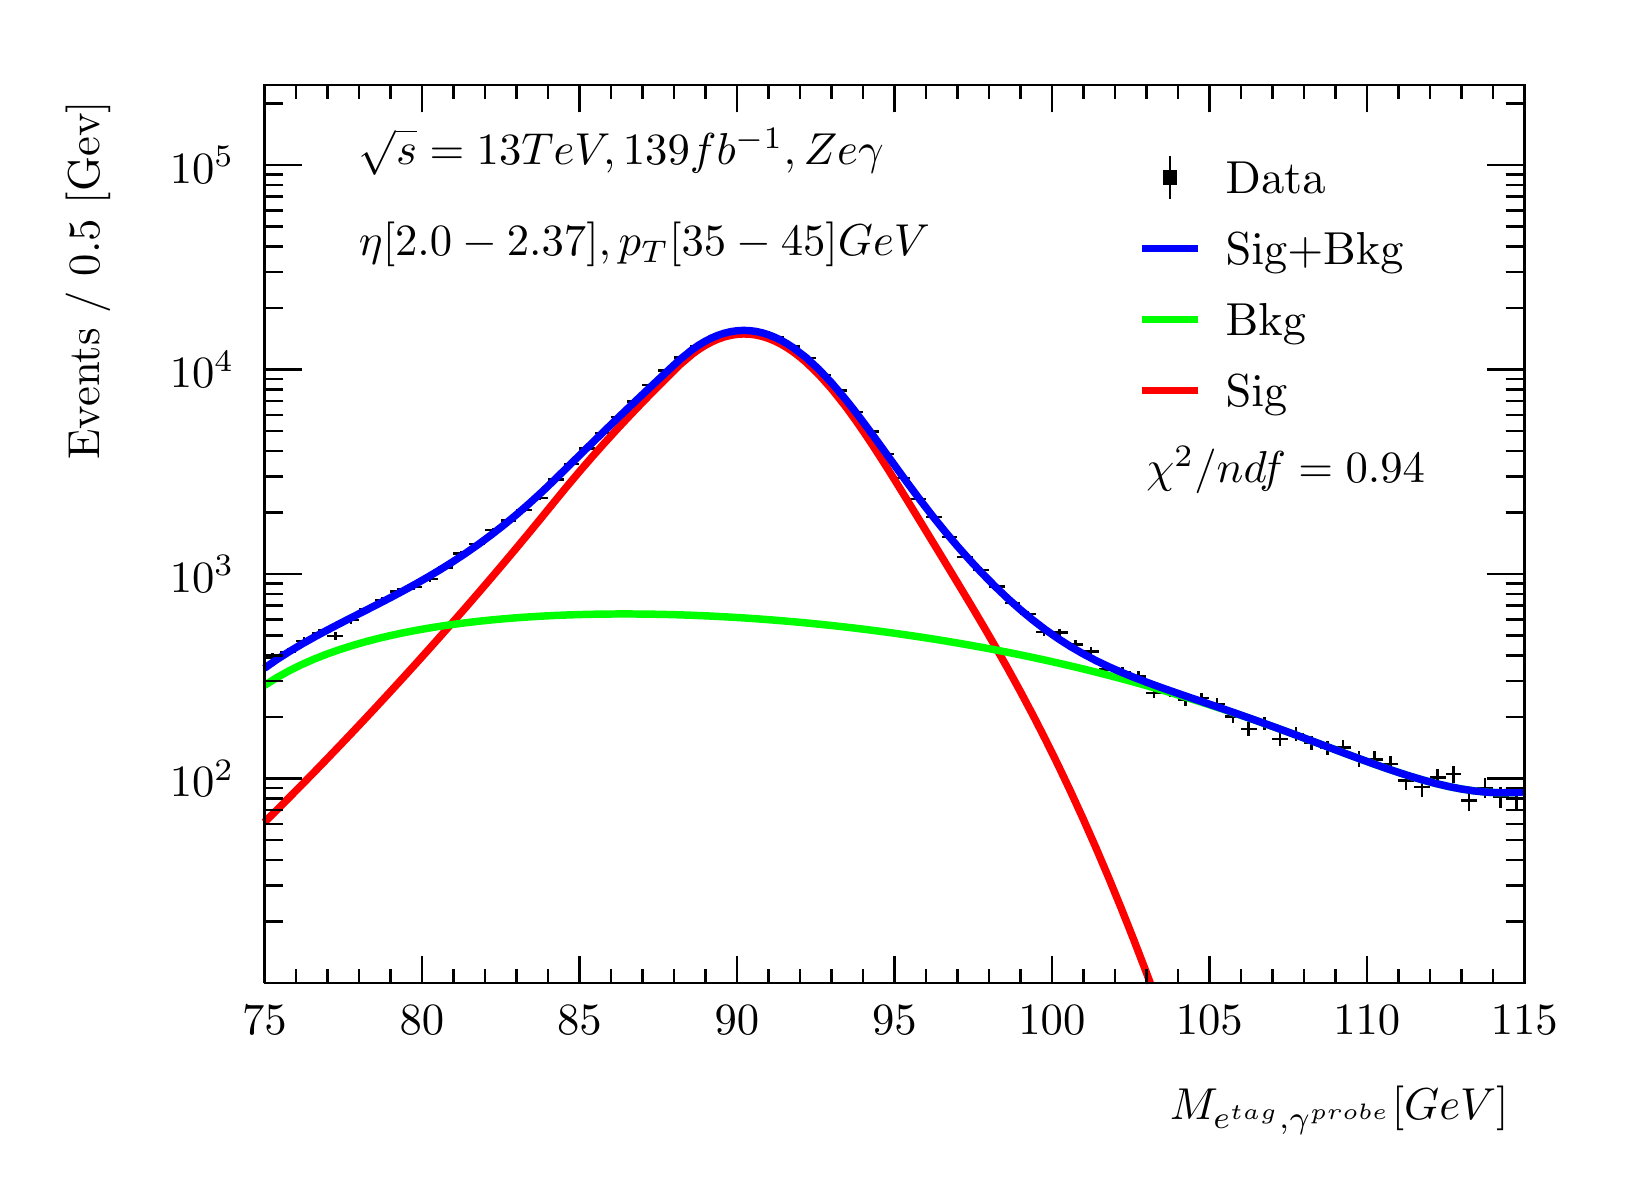
\begin{tikzpicture}
\pgfdeclareplotmark{cross} {
\pgfpathmoveto{\pgfpoint{-0.3\pgfplotmarksize}{\pgfplotmarksize}}
\pgfpathlineto{\pgfpoint{+0.3\pgfplotmarksize}{\pgfplotmarksize}}
\pgfpathlineto{\pgfpoint{+0.3\pgfplotmarksize}{0.3\pgfplotmarksize}}
\pgfpathlineto{\pgfpoint{+1\pgfplotmarksize}{0.3\pgfplotmarksize}}
\pgfpathlineto{\pgfpoint{+1\pgfplotmarksize}{-0.3\pgfplotmarksize}}
\pgfpathlineto{\pgfpoint{+0.3\pgfplotmarksize}{-0.3\pgfplotmarksize}}
\pgfpathlineto{\pgfpoint{+0.3\pgfplotmarksize}{-1.\pgfplotmarksize}}
\pgfpathlineto{\pgfpoint{-0.3\pgfplotmarksize}{-1.\pgfplotmarksize}}
\pgfpathlineto{\pgfpoint{-0.3\pgfplotmarksize}{-0.3\pgfplotmarksize}}
\pgfpathlineto{\pgfpoint{-1.\pgfplotmarksize}{-0.3\pgfplotmarksize}}
\pgfpathlineto{\pgfpoint{-1.\pgfplotmarksize}{0.3\pgfplotmarksize}}
\pgfpathlineto{\pgfpoint{-0.3\pgfplotmarksize}{0.3\pgfplotmarksize}}
\pgfpathclose
\pgfusepathqstroke
}
\pgfdeclareplotmark{cross*} {
\pgfpathmoveto{\pgfpoint{-0.3\pgfplotmarksize}{\pgfplotmarksize}}
\pgfpathlineto{\pgfpoint{+0.3\pgfplotmarksize}{\pgfplotmarksize}}
\pgfpathlineto{\pgfpoint{+0.3\pgfplotmarksize}{0.3\pgfplotmarksize}}
\pgfpathlineto{\pgfpoint{+1\pgfplotmarksize}{0.3\pgfplotmarksize}}
\pgfpathlineto{\pgfpoint{+1\pgfplotmarksize}{-0.3\pgfplotmarksize}}
\pgfpathlineto{\pgfpoint{+0.3\pgfplotmarksize}{-0.3\pgfplotmarksize}}
\pgfpathlineto{\pgfpoint{+0.3\pgfplotmarksize}{-1.\pgfplotmarksize}}
\pgfpathlineto{\pgfpoint{-0.3\pgfplotmarksize}{-1.\pgfplotmarksize}}
\pgfpathlineto{\pgfpoint{-0.3\pgfplotmarksize}{-0.3\pgfplotmarksize}}
\pgfpathlineto{\pgfpoint{-1.\pgfplotmarksize}{-0.3\pgfplotmarksize}}
\pgfpathlineto{\pgfpoint{-1.\pgfplotmarksize}{0.3\pgfplotmarksize}}
\pgfpathlineto{\pgfpoint{-0.3\pgfplotmarksize}{0.3\pgfplotmarksize}}
\pgfpathclose
\pgfusepathqfillstroke
}
\pgfdeclareplotmark{newstar} {
\pgfpathmoveto{\pgfqpoint{0pt}{\pgfplotmarksize}}
\pgfpathlineto{\pgfqpointpolar{44}{0.5\pgfplotmarksize}}
\pgfpathlineto{\pgfqpointpolar{18}{\pgfplotmarksize}}
\pgfpathlineto{\pgfqpointpolar{-20}{0.5\pgfplotmarksize}}
\pgfpathlineto{\pgfqpointpolar{-54}{\pgfplotmarksize}}
\pgfpathlineto{\pgfqpointpolar{-90}{0.5\pgfplotmarksize}}
\pgfpathlineto{\pgfqpointpolar{234}{\pgfplotmarksize}}
\pgfpathlineto{\pgfqpointpolar{198}{0.5\pgfplotmarksize}}
\pgfpathlineto{\pgfqpointpolar{162}{\pgfplotmarksize}}
\pgfpathlineto{\pgfqpointpolar{134}{0.5\pgfplotmarksize}}
\pgfpathclose
\pgfusepathqstroke
}
\pgfdeclareplotmark{newstar*} {
\pgfpathmoveto{\pgfqpoint{0pt}{\pgfplotmarksize}}
\pgfpathlineto{\pgfqpointpolar{44}{0.5\pgfplotmarksize}}
\pgfpathlineto{\pgfqpointpolar{18}{\pgfplotmarksize}}
\pgfpathlineto{\pgfqpointpolar{-20}{0.5\pgfplotmarksize}}
\pgfpathlineto{\pgfqpointpolar{-54}{\pgfplotmarksize}}
\pgfpathlineto{\pgfqpointpolar{-90}{0.5\pgfplotmarksize}}
\pgfpathlineto{\pgfqpointpolar{234}{\pgfplotmarksize}}
\pgfpathlineto{\pgfqpointpolar{198}{0.5\pgfplotmarksize}}
\pgfpathlineto{\pgfqpointpolar{162}{\pgfplotmarksize}}
\pgfpathlineto{\pgfqpointpolar{134}{0.5\pgfplotmarksize}}
\pgfpathclose
\pgfusepathqfillstroke
}
\definecolor{c}{rgb}{1,1,1};
\draw [color=c, fill=c] (0,0) rectangle (20,14.4361);
\draw [color=c, fill=c] (3,2.30977) rectangle (19,13.7143);
\definecolor{c}{rgb}{0,0,0};
\draw [c,line width=0.9] (3,2.30977) -- (3,13.7143) -- (19,13.7143) -- (19,2.30977) -- (3,2.30977);
\definecolor{c}{rgb}{1,1,1};
\draw [color=c, fill=c] (3,2.30977) rectangle (19,13.7143);
\definecolor{c}{rgb}{0,0,0};
\draw [c,line width=0.9] (3,2.30977) -- (3,13.7143) -- (19,13.7143) -- (19,2.30977) -- (3,2.30977);
\draw [c,line width=0.9] (3,2.30977) -- (19,2.30977);
\draw [c,line width=0.9] (3,2.65624) -- (3,2.30977);
\draw [c,line width=0.9] (3.4,2.48301) -- (3.4,2.30977);
\draw [c,line width=0.9] (3.8,2.48301) -- (3.8,2.30977);
\draw [c,line width=0.9] (4.2,2.48301) -- (4.2,2.30977);
\draw [c,line width=0.9] (4.6,2.48301) -- (4.6,2.30977);
\draw [c,line width=0.9] (5,2.65624) -- (5,2.30977);
\draw [c,line width=0.9] (5.4,2.48301) -- (5.4,2.30977);
\draw [c,line width=0.9] (5.8,2.48301) -- (5.8,2.30977);
\draw [c,line width=0.9] (6.2,2.48301) -- (6.2,2.30977);
\draw [c,line width=0.9] (6.6,2.48301) -- (6.6,2.30977);
\draw [c,line width=0.9] (7,2.65624) -- (7,2.30977);
\draw [c,line width=0.9] (7.4,2.48301) -- (7.4,2.30977);
\draw [c,line width=0.9] (7.8,2.48301) -- (7.8,2.30977);
\draw [c,line width=0.9] (8.2,2.48301) -- (8.2,2.30977);
\draw [c,line width=0.9] (8.6,2.48301) -- (8.6,2.30977);
\draw [c,line width=0.9] (9,2.65624) -- (9,2.30977);
\draw [c,line width=0.9] (9.4,2.48301) -- (9.4,2.30977);
\draw [c,line width=0.9] (9.8,2.48301) -- (9.8,2.30977);
\draw [c,line width=0.9] (10.2,2.48301) -- (10.2,2.30977);
\draw [c,line width=0.9] (10.6,2.48301) -- (10.6,2.30977);
\draw [c,line width=0.9] (11,2.65624) -- (11,2.30977);
\draw [c,line width=0.9] (11.4,2.48301) -- (11.4,2.30977);
\draw [c,line width=0.9] (11.8,2.48301) -- (11.8,2.30977);
\draw [c,line width=0.9] (12.2,2.48301) -- (12.2,2.30977);
\draw [c,line width=0.9] (12.6,2.48301) -- (12.6,2.30977);
\draw [c,line width=0.9] (13,2.65624) -- (13,2.30977);
\draw [c,line width=0.9] (13.4,2.48301) -- (13.4,2.30977);
\draw [c,line width=0.9] (13.8,2.48301) -- (13.8,2.30977);
\draw [c,line width=0.9] (14.2,2.48301) -- (14.2,2.30977);
\draw [c,line width=0.9] (14.6,2.48301) -- (14.6,2.30977);
\draw [c,line width=0.9] (15,2.65624) -- (15,2.30977);
\draw [c,line width=0.9] (15.4,2.48301) -- (15.4,2.30977);
\draw [c,line width=0.9] (15.8,2.48301) -- (15.8,2.30977);
\draw [c,line width=0.9] (16.2,2.48301) -- (16.2,2.30977);
\draw [c,line width=0.9] (16.6,2.48301) -- (16.6,2.30977);
\draw [c,line width=0.9] (17,2.65624) -- (17,2.30977);
\draw [c,line width=0.9] (17.4,2.48301) -- (17.4,2.30977);
\draw [c,line width=0.9] (17.8,2.48301) -- (17.8,2.30977);
\draw [c,line width=0.9] (18.2,2.48301) -- (18.2,2.30977);
\draw [c,line width=0.9] (18.6,2.48301) -- (18.6,2.30977);
\draw [c,line width=0.9] (19,2.65624) -- (19,2.30977);
\draw [c,line width=0.9] (19,2.65624) -- (19,2.30977);
\draw [anchor=base] (3,1.66015) node[scale=1.61424, color=c, rotate=0]{75};
\draw [anchor=base] (5,1.66015) node[scale=1.61424, color=c, rotate=0]{80};
\draw [anchor=base] (7,1.66015) node[scale=1.61424, color=c, rotate=0]{85};
\draw [anchor=base] (9,1.66015) node[scale=1.61424, color=c, rotate=0]{90};
\draw [anchor=base] (11,1.66015) node[scale=1.61424, color=c, rotate=0]{95};
\draw [anchor=base] (13,1.66015) node[scale=1.61424, color=c, rotate=0]{100};
\draw [anchor=base] (15,1.66015) node[scale=1.61424, color=c, rotate=0]{105};
\draw [anchor=base] (17,1.66015) node[scale=1.61424, color=c, rotate=0]{110};
\draw [anchor=base] (19,1.66015) node[scale=1.61424, color=c, rotate=0]{115};
\draw [anchor= east] (19,0.692932) node[scale=1.61424, color=c, rotate=0]{$M_{e^{tag}, \gamma^{probe}}  [GeV]$};
\draw [c,line width=0.9] (3,13.7143) -- (19,13.7143);
\draw [c,line width=0.9] (3,13.3678) -- (3,13.7143);
\draw [c,line width=0.9] (3.4,13.5411) -- (3.4,13.7143);
\draw [c,line width=0.9] (3.8,13.5411) -- (3.8,13.7143);
\draw [c,line width=0.9] (4.2,13.5411) -- (4.2,13.7143);
\draw [c,line width=0.9] (4.6,13.5411) -- (4.6,13.7143);
\draw [c,line width=0.9] (5,13.3678) -- (5,13.7143);
\draw [c,line width=0.9] (5.4,13.5411) -- (5.4,13.7143);
\draw [c,line width=0.9] (5.8,13.5411) -- (5.8,13.7143);
\draw [c,line width=0.9] (6.2,13.5411) -- (6.2,13.7143);
\draw [c,line width=0.9] (6.6,13.5411) -- (6.6,13.7143);
\draw [c,line width=0.9] (7,13.3678) -- (7,13.7143);
\draw [c,line width=0.9] (7.4,13.5411) -- (7.4,13.7143);
\draw [c,line width=0.9] (7.8,13.5411) -- (7.8,13.7143);
\draw [c,line width=0.9] (8.2,13.5411) -- (8.2,13.7143);
\draw [c,line width=0.9] (8.6,13.5411) -- (8.6,13.7143);
\draw [c,line width=0.9] (9,13.3678) -- (9,13.7143);
\draw [c,line width=0.9] (9.4,13.5411) -- (9.4,13.7143);
\draw [c,line width=0.9] (9.8,13.5411) -- (9.8,13.7143);
\draw [c,line width=0.9] (10.2,13.5411) -- (10.2,13.7143);
\draw [c,line width=0.9] (10.6,13.5411) -- (10.6,13.7143);
\draw [c,line width=0.9] (11,13.3678) -- (11,13.7143);
\draw [c,line width=0.9] (11.4,13.5411) -- (11.4,13.7143);
\draw [c,line width=0.9] (11.8,13.5411) -- (11.8,13.7143);
\draw [c,line width=0.9] (12.2,13.5411) -- (12.2,13.7143);
\draw [c,line width=0.9] (12.6,13.5411) -- (12.6,13.7143);
\draw [c,line width=0.9] (13,13.3678) -- (13,13.7143);
\draw [c,line width=0.9] (13.4,13.5411) -- (13.4,13.7143);
\draw [c,line width=0.9] (13.8,13.5411) -- (13.8,13.7143);
\draw [c,line width=0.9] (14.2,13.5411) -- (14.2,13.7143);
\draw [c,line width=0.9] (14.6,13.5411) -- (14.6,13.7143);
\draw [c,line width=0.9] (15,13.3678) -- (15,13.7143);
\draw [c,line width=0.9] (15.4,13.5411) -- (15.4,13.7143);
\draw [c,line width=0.9] (15.8,13.5411) -- (15.8,13.7143);
\draw [c,line width=0.9] (16.2,13.5411) -- (16.2,13.7143);
\draw [c,line width=0.9] (16.6,13.5411) -- (16.6,13.7143);
\draw [c,line width=0.9] (17,13.3678) -- (17,13.7143);
\draw [c,line width=0.9] (17.4,13.5411) -- (17.4,13.7143);
\draw [c,line width=0.9] (17.8,13.5411) -- (17.8,13.7143);
\draw [c,line width=0.9] (18.2,13.5411) -- (18.2,13.7143);
\draw [c,line width=0.9] (18.6,13.5411) -- (18.6,13.7143);
\draw [c,line width=0.9] (19,13.3678) -- (19,13.7143);
\draw [c,line width=0.9] (19,13.3678) -- (19,13.7143);
\draw [c,line width=0.9] (3,2.30977) -- (3,13.7143);
\draw [c,line width=0.9] (3.237,3.09166) -- (3,3.09166);
\draw [c,line width=0.9] (3.237,3.54903) -- (3,3.54903);
\draw [c,line width=0.9] (3.237,3.87354) -- (3,3.87354);
\draw [c,line width=0.9] (3.237,4.12525) -- (3,4.12525);
\draw [c,line width=0.9] (3.237,4.33091) -- (3,4.33091);
\draw [c,line width=0.9] (3.237,4.5048) -- (3,4.5048);
\draw [c,line width=0.9] (3.237,4.65542) -- (3,4.65542);
\draw [c,line width=0.9] (3.237,4.78829) -- (3,4.78829);
\draw [c,line width=0.9] (3.474,4.90714) -- (3,4.90714);
\draw [anchor= east] (2.82,4.90714) node[scale=1.61424, color=c, rotate=0]{$10^{2}$};
\draw [c,line width=0.9] (3.237,5.68902) -- (3,5.68902);
\draw [c,line width=0.9] (3.237,6.14639) -- (3,6.14639);
\draw [c,line width=0.9] (3.237,6.4709) -- (3,6.4709);
\draw [c,line width=0.9] (3.237,6.72261) -- (3,6.72261);
\draw [c,line width=0.9] (3.237,6.92828) -- (3,6.92828);
\draw [c,line width=0.9] (3.237,7.10216) -- (3,7.10216);
\draw [c,line width=0.9] (3.237,7.25279) -- (3,7.25279);
\draw [c,line width=0.9] (3.237,7.38565) -- (3,7.38565);
\draw [c,line width=0.9] (3.474,7.5045) -- (3,7.5045);
\draw [anchor= east] (2.82,7.5045) node[scale=1.61424, color=c, rotate=0]{$10^{3}$};
\draw [c,line width=0.9] (3.237,8.28638) -- (3,8.28638);
\draw [c,line width=0.9] (3.237,8.74376) -- (3,8.74376);
\draw [c,line width=0.9] (3.237,9.06827) -- (3,9.06827);
\draw [c,line width=0.9] (3.237,9.31998) -- (3,9.31998);
\draw [c,line width=0.9] (3.237,9.52564) -- (3,9.52564);
\draw [c,line width=0.9] (3.237,9.69952) -- (3,9.69952);
\draw [c,line width=0.9] (3.237,9.85015) -- (3,9.85015);
\draw [c,line width=0.9] (3.237,9.98301) -- (3,9.98301);
\draw [c,line width=0.9] (3.474,10.1019) -- (3,10.1019);
\draw [anchor= east] (2.82,10.1019) node[scale=1.61424, color=c, rotate=0]{$10^{4}$};
\draw [c,line width=0.9] (3.237,10.8837) -- (3,10.8837);
\draw [c,line width=0.9] (3.237,11.3411) -- (3,11.3411);
\draw [c,line width=0.9] (3.237,11.6656) -- (3,11.6656);
\draw [c,line width=0.9] (3.237,11.9173) -- (3,11.9173);
\draw [c,line width=0.9] (3.237,12.123) -- (3,12.123);
\draw [c,line width=0.9] (3.237,12.2969) -- (3,12.2969);
\draw [c,line width=0.9] (3.237,12.4475) -- (3,12.4475);
\draw [c,line width=0.9] (3.237,12.5804) -- (3,12.5804);
\draw [c,line width=0.9] (3.474,12.6992) -- (3,12.6992);
\draw [anchor= east] (2.82,12.6992) node[scale=1.61424, color=c, rotate=0]{$10^{5}$};
\draw [c,line width=0.9] (3.237,13.4811) -- (3,13.4811);
\draw [anchor= east] (0.76,13.7143) node[scale=1.61424, color=c, rotate=90]{Events / 0.5 [Gev]};
\draw [c,line width=0.9] (19,2.30977) -- (19,13.7143);
\draw [c,line width=0.9] (18.763,3.09166) -- (19,3.09166);
\draw [c,line width=0.9] (18.763,3.54903) -- (19,3.54903);
\draw [c,line width=0.9] (18.763,3.87354) -- (19,3.87354);
\draw [c,line width=0.9] (18.763,4.12525) -- (19,4.12525);
\draw [c,line width=0.9] (18.763,4.33091) -- (19,4.33091);
\draw [c,line width=0.9] (18.763,4.5048) -- (19,4.5048);
\draw [c,line width=0.9] (18.763,4.65542) -- (19,4.65542);
\draw [c,line width=0.9] (18.763,4.78829) -- (19,4.78829);
\draw [c,line width=0.9] (18.526,4.90714) -- (19,4.90714);
\draw [c,line width=0.9] (18.763,5.68902) -- (19,5.68902);
\draw [c,line width=0.9] (18.763,6.14639) -- (19,6.14639);
\draw [c,line width=0.9] (18.763,6.4709) -- (19,6.4709);
\draw [c,line width=0.9] (18.763,6.72261) -- (19,6.72261);
\draw [c,line width=0.9] (18.763,6.92828) -- (19,6.92828);
\draw [c,line width=0.9] (18.763,7.10216) -- (19,7.10216);
\draw [c,line width=0.9] (18.763,7.25279) -- (19,7.25279);
\draw [c,line width=0.9] (18.763,7.38565) -- (19,7.38565);
\draw [c,line width=0.9] (18.526,7.5045) -- (19,7.5045);
\draw [c,line width=0.9] (18.763,8.28638) -- (19,8.28638);
\draw [c,line width=0.9] (18.763,8.74376) -- (19,8.74376);
\draw [c,line width=0.9] (18.763,9.06827) -- (19,9.06827);
\draw [c,line width=0.9] (18.763,9.31998) -- (19,9.31998);
\draw [c,line width=0.9] (18.763,9.52564) -- (19,9.52564);
\draw [c,line width=0.9] (18.763,9.69952) -- (19,9.69952);
\draw [c,line width=0.9] (18.763,9.85015) -- (19,9.85015);
\draw [c,line width=0.9] (18.763,9.98301) -- (19,9.98301);
\draw [c,line width=0.9] (18.526,10.1019) -- (19,10.1019);
\draw [c,line width=0.9] (18.763,10.8837) -- (19,10.8837);
\draw [c,line width=0.9] (18.763,11.3411) -- (19,11.3411);
\draw [c,line width=0.9] (18.763,11.6656) -- (19,11.6656);
\draw [c,line width=0.9] (18.763,11.9173) -- (19,11.9173);
\draw [c,line width=0.9] (18.763,12.123) -- (19,12.123);
\draw [c,line width=0.9] (18.763,12.2969) -- (19,12.2969);
\draw [c,line width=0.9] (18.763,12.4475) -- (19,12.4475);
\draw [c,line width=0.9] (18.763,12.5804) -- (19,12.5804);
\draw [c,line width=0.9] (18.526,12.6992) -- (19,12.6992);
\draw [c,line width=0.9] (18.763,13.4811) -- (19,13.4811);
\draw [c,line width=0.9] (3.1,6.44235) -- (3,6.44235);
\draw [c,line width=0.9] (3,6.44235) -- (3,6.44235);
\draw [c,line width=0.9] (3.1,6.44235) -- (3.2,6.44235);
\draw [c,line width=0.9] (3.2,6.44235) -- (3.2,6.44235);
\draw [c,line width=0.9] (3.1,6.44235) -- (3.1,6.49946);
\draw [c,line width=0.9] (3.1,6.49946) -- (3.1,6.49946);
\draw [c,line width=0.9] (3.1,6.44235) -- (3.1,6.38523);
\draw [c,line width=0.9] (3.1,6.38523) -- (3.1,6.38523);
\draw [c,line width=0.9] (3.3,6.51243) -- (3.2,6.51243);
\draw [c,line width=0.9] (3.2,6.51243) -- (3.2,6.51243);
\draw [c,line width=0.9] (3.3,6.51243) -- (3.4,6.51243);
\draw [c,line width=0.9] (3.4,6.51243) -- (3.4,6.51243);
\draw [c,line width=0.9] (3.3,6.51243) -- (3.3,6.5678);
\draw [c,line width=0.9] (3.3,6.5678) -- (3.3,6.5678);
\draw [c,line width=0.9] (3.3,6.51243) -- (3.3,6.45707);
\draw [c,line width=0.9] (3.3,6.45707) -- (3.3,6.45707);
\draw [c,line width=0.9] (3.5,6.65282) -- (3.4,6.65282);
\draw [c,line width=0.9] (3.4,6.65282) -- (3.4,6.65282);
\draw [c,line width=0.9] (3.5,6.65282) -- (3.6,6.65282);
\draw [c,line width=0.9] (3.6,6.65282) -- (3.6,6.65282);
\draw [c,line width=0.9] (3.5,6.65282) -- (3.5,6.70485);
\draw [c,line width=0.9] (3.5,6.70485) -- (3.5,6.70485);
\draw [c,line width=0.9] (3.5,6.65282) -- (3.5,6.60079);
\draw [c,line width=0.9] (3.5,6.60079) -- (3.5,6.60079);
\draw [c,line width=0.9] (3.7,6.75815) -- (3.6,6.75815);
\draw [c,line width=0.9] (3.6,6.75815) -- (3.6,6.75815);
\draw [c,line width=0.9] (3.7,6.75815) -- (3.8,6.75815);
\draw [c,line width=0.9] (3.8,6.75815) -- (3.8,6.75815);
\draw [c,line width=0.9] (3.7,6.75815) -- (3.7,6.8078);
\draw [c,line width=0.9] (3.7,6.8078) -- (3.7,6.8078);
\draw [c,line width=0.9] (3.7,6.75815) -- (3.7,6.70849);
\draw [c,line width=0.9] (3.7,6.70849) -- (3.7,6.70849);
\draw [c,line width=0.9] (3.9,6.71583) -- (3.8,6.71583);
\draw [c,line width=0.9] (3.8,6.71583) -- (3.8,6.71583);
\draw [c,line width=0.9] (3.9,6.71583) -- (4,6.71583);
\draw [c,line width=0.9] (4,6.71583) -- (4,6.71583);
\draw [c,line width=0.9] (3.9,6.71583) -- (3.9,6.76642);
\draw [c,line width=0.9] (3.9,6.76642) -- (3.9,6.76642);
\draw [c,line width=0.9] (3.9,6.71583) -- (3.9,6.66523);
\draw [c,line width=0.9] (3.9,6.66523) -- (3.9,6.66523);
\draw [c,line width=0.9] (4.1,6.91884) -- (4,6.91884);
\draw [c,line width=0.9] (4,6.91884) -- (4,6.91884);
\draw [c,line width=0.9] (4.1,6.91884) -- (4.2,6.91884);
\draw [c,line width=0.9] (4.2,6.91884) -- (4.2,6.91884);
\draw [c,line width=0.9] (4.1,6.91884) -- (4.1,6.96508);
\draw [c,line width=0.9] (4.1,6.96508) -- (4.1,6.96508);
\draw [c,line width=0.9] (4.1,6.91884) -- (4.1,6.8726);
\draw [c,line width=0.9] (4.1,6.8726) -- (4.1,6.8726);
\draw [c,line width=0.9] (4.3,7.06114) -- (4.2,7.06114);
\draw [c,line width=0.9] (4.2,7.06114) -- (4.2,7.06114);
\draw [c,line width=0.9] (4.3,7.06114) -- (4.4,7.06114);
\draw [c,line width=0.9] (4.4,7.06114) -- (4.4,7.06114);
\draw [c,line width=0.9] (4.3,7.06114) -- (4.3,7.10455);
\draw [c,line width=0.9] (4.3,7.10455) -- (4.3,7.10455);
\draw [c,line width=0.9] (4.3,7.06114) -- (4.3,7.01772);
\draw [c,line width=0.9] (4.3,7.01772) -- (4.3,7.01772);
\draw [c,line width=0.9] (4.5,7.17698) -- (4.4,7.17698);
\draw [c,line width=0.9] (4.4,7.17698) -- (4.4,7.17698);
\draw [c,line width=0.9] (4.5,7.17698) -- (4.6,7.17698);
\draw [c,line width=0.9] (4.6,7.17698) -- (4.6,7.17698);
\draw [c,line width=0.9] (4.5,7.17698) -- (4.5,7.21822);
\draw [c,line width=0.9] (4.5,7.21822) -- (4.5,7.21822);
\draw [c,line width=0.9] (4.5,7.17698) -- (4.5,7.13573);
\draw [c,line width=0.9] (4.5,7.13573) -- (4.5,7.13573);
\draw [c,line width=0.9] (4.7,7.28339) -- (4.6,7.28339);
\draw [c,line width=0.9] (4.6,7.28339) -- (4.6,7.28339);
\draw [c,line width=0.9] (4.7,7.28339) -- (4.8,7.28339);
\draw [c,line width=0.9] (4.8,7.28339) -- (4.8,7.28339);
\draw [c,line width=0.9] (4.7,7.28339) -- (4.7,7.32273);
\draw [c,line width=0.9] (4.7,7.32273) -- (4.7,7.32273);
\draw [c,line width=0.9] (4.7,7.28339) -- (4.7,7.24405);
\draw [c,line width=0.9] (4.7,7.24405) -- (4.7,7.24405);
\draw [c,line width=0.9] (4.9,7.33699) -- (4.8,7.33699);
\draw [c,line width=0.9] (4.8,7.33699) -- (4.8,7.33699);
\draw [c,line width=0.9] (4.9,7.33699) -- (5,7.33699);
\draw [c,line width=0.9] (5,7.33699) -- (5,7.33699);
\draw [c,line width=0.9] (4.9,7.33699) -- (4.9,7.37541);
\draw [c,line width=0.9] (4.9,7.37541) -- (4.9,7.37541);
\draw [c,line width=0.9] (4.9,7.33699) -- (4.9,7.29857);
\draw [c,line width=0.9] (4.9,7.29857) -- (4.9,7.29857);
\draw [c,line width=0.9] (5.1,7.44426) -- (5,7.44426);
\draw [c,line width=0.9] (5,7.44426) -- (5,7.44426);
\draw [c,line width=0.9] (5.1,7.44426) -- (5.2,7.44426);
\draw [c,line width=0.9] (5.2,7.44426) -- (5.2,7.44426);
\draw [c,line width=0.9] (5.1,7.44426) -- (5.1,7.4809);
\draw [c,line width=0.9] (5.1,7.4809) -- (5.1,7.4809);
\draw [c,line width=0.9] (5.1,7.44426) -- (5.1,7.40763);
\draw [c,line width=0.9] (5.1,7.40763) -- (5.1,7.40763);
\draw [c,line width=0.9] (5.3,7.58713) -- (5.2,7.58713);
\draw [c,line width=0.9] (5.2,7.58713) -- (5.2,7.58713);
\draw [c,line width=0.9] (5.3,7.58713) -- (5.4,7.58713);
\draw [c,line width=0.9] (5.4,7.58713) -- (5.4,7.58713);
\draw [c,line width=0.9] (5.3,7.58713) -- (5.3,7.62151);
\draw [c,line width=0.9] (5.3,7.62151) -- (5.3,7.62151);
\draw [c,line width=0.9] (5.3,7.58713) -- (5.3,7.55274);
\draw [c,line width=0.9] (5.3,7.55274) -- (5.3,7.55274);
\draw [c,line width=0.9] (5.5,7.76699) -- (5.4,7.76699);
\draw [c,line width=0.9] (5.4,7.76699) -- (5.4,7.76699);
\draw [c,line width=0.9] (5.5,7.76699) -- (5.6,7.76699);
\draw [c,line width=0.9] (5.6,7.76699) -- (5.6,7.76699);
\draw [c,line width=0.9] (5.5,7.76699) -- (5.5,7.79874);
\draw [c,line width=0.9] (5.5,7.79874) -- (5.5,7.79874);
\draw [c,line width=0.9] (5.5,7.76699) -- (5.5,7.73524);
\draw [c,line width=0.9] (5.5,7.73524) -- (5.5,7.73524);
\draw [c,line width=0.9] (5.7,7.88405) -- (5.6,7.88405);
\draw [c,line width=0.9] (5.6,7.88405) -- (5.6,7.88405);
\draw [c,line width=0.9] (5.7,7.88405) -- (5.8,7.88405);
\draw [c,line width=0.9] (5.8,7.88405) -- (5.8,7.88405);
\draw [c,line width=0.9] (5.7,7.88405) -- (5.7,7.91419);
\draw [c,line width=0.9] (5.7,7.91419) -- (5.7,7.91419);
\draw [c,line width=0.9] (5.7,7.88405) -- (5.7,7.8539);
\draw [c,line width=0.9] (5.7,7.8539) -- (5.7,7.8539);
\draw [c,line width=0.9] (5.9,8.06596) -- (5.8,8.06596);
\draw [c,line width=0.9] (5.8,8.06596) -- (5.8,8.06596);
\draw [c,line width=0.9] (5.9,8.06596) -- (6,8.06596);
\draw [c,line width=0.9] (6,8.06596) -- (6,8.06596);
\draw [c,line width=0.9] (5.9,8.06596) -- (5.9,8.09377);
\draw [c,line width=0.9] (5.9,8.09377) -- (5.9,8.09377);
\draw [c,line width=0.9] (5.9,8.06596) -- (5.9,8.03815);
\draw [c,line width=0.9] (5.9,8.03815) -- (5.9,8.03815);
\draw [c,line width=0.9] (6.1,8.18556) -- (6,8.18556);
\draw [c,line width=0.9] (6,8.18556) -- (6,8.18556);
\draw [c,line width=0.9] (6.1,8.18556) -- (6.2,8.18556);
\draw [c,line width=0.9] (6.2,8.18556) -- (6.2,8.18556);
\draw [c,line width=0.9] (6.1,8.18556) -- (6.1,8.21194);
\draw [c,line width=0.9] (6.1,8.21194) -- (6.1,8.21194);
\draw [c,line width=0.9] (6.1,8.18556) -- (6.1,8.15919);
\draw [c,line width=0.9] (6.1,8.15919) -- (6.1,8.15919);
\draw [c,line width=0.9] (6.3,8.31918) -- (6.2,8.31918);
\draw [c,line width=0.9] (6.2,8.31918) -- (6.2,8.31918);
\draw [c,line width=0.9] (6.3,8.31918) -- (6.4,8.31918);
\draw [c,line width=0.9] (6.4,8.31918) -- (6.4,8.31918);
\draw [c,line width=0.9] (6.3,8.31918) -- (6.3,8.34404);
\draw [c,line width=0.9] (6.3,8.34404) -- (6.3,8.34404);
\draw [c,line width=0.9] (6.3,8.31918) -- (6.3,8.29432);
\draw [c,line width=0.9] (6.3,8.29432) -- (6.3,8.29432);
\draw [c,line width=0.9] (6.5,8.47117) -- (6.4,8.47117);
\draw [c,line width=0.9] (6.4,8.47117) -- (6.4,8.47117);
\draw [c,line width=0.9] (6.5,8.47117) -- (6.6,8.47117);
\draw [c,line width=0.9] (6.6,8.47117) -- (6.6,8.47117);
\draw [c,line width=0.9] (6.5,8.47117) -- (6.5,8.49441);
\draw [c,line width=0.9] (6.5,8.49441) -- (6.5,8.49441);
\draw [c,line width=0.9] (6.5,8.47117) -- (6.5,8.44794);
\draw [c,line width=0.9] (6.5,8.44794) -- (6.5,8.44794);
\draw [c,line width=0.9] (6.7,8.70551) -- (6.6,8.70551);
\draw [c,line width=0.9] (6.6,8.70551) -- (6.6,8.70551);
\draw [c,line width=0.9] (6.7,8.70551) -- (6.8,8.70551);
\draw [c,line width=0.9] (6.8,8.70551) -- (6.8,8.70551);
\draw [c,line width=0.9] (6.7,8.70551) -- (6.7,8.72646);
\draw [c,line width=0.9] (6.7,8.72646) -- (6.7,8.72646);
\draw [c,line width=0.9] (6.7,8.70551) -- (6.7,8.68457);
\draw [c,line width=0.9] (6.7,8.68457) -- (6.7,8.68457);
\draw [c,line width=0.9] (6.9,8.90076) -- (6.8,8.90076);
\draw [c,line width=0.9] (6.8,8.90076) -- (6.8,8.90076);
\draw [c,line width=0.9] (6.9,8.90076) -- (7,8.90076);
\draw [c,line width=0.9] (7,8.90076) -- (7,8.90076);
\draw [c,line width=0.9] (6.9,8.90076) -- (6.9,8.91997);
\draw [c,line width=0.9] (6.9,8.91997) -- (6.9,8.91997);
\draw [c,line width=0.9] (6.9,8.90076) -- (6.9,8.88155);
\draw [c,line width=0.9] (6.9,8.88155) -- (6.9,8.88155);
\draw [c,line width=0.9] (7.1,9.10024) -- (7,9.10024);
\draw [c,line width=0.9] (7,9.10024) -- (7,9.10024);
\draw [c,line width=0.9] (7.1,9.10024) -- (7.2,9.10024);
\draw [c,line width=0.9] (7.2,9.10024) -- (7.2,9.10024);
\draw [c,line width=0.9] (7.1,9.10024) -- (7.1,9.11783);
\draw [c,line width=0.9] (7.1,9.11783) -- (7.1,9.11783);
\draw [c,line width=0.9] (7.1,9.10024) -- (7.1,9.08266);
\draw [c,line width=0.9] (7.1,9.08266) -- (7.1,9.08266);
\draw [c,line width=0.9] (7.3,9.29558) -- (7.2,9.29558);
\draw [c,line width=0.9] (7.2,9.29558) -- (7.2,9.29558);
\draw [c,line width=0.9] (7.3,9.29558) -- (7.4,9.29558);
\draw [c,line width=0.9] (7.4,9.29558) -- (7.4,9.29558);
\draw [c,line width=0.9] (7.3,9.29558) -- (7.3,9.3117);
\draw [c,line width=0.9] (7.3,9.3117) -- (7.3,9.3117);
\draw [c,line width=0.9] (7.3,9.29558) -- (7.3,9.27945);
\draw [c,line width=0.9] (7.3,9.27945) -- (7.3,9.27945);
\draw [c,line width=0.9] (7.5,9.49804) -- (7.4,9.49804);
\draw [c,line width=0.9] (7.4,9.49804) -- (7.4,9.49804);
\draw [c,line width=0.9] (7.5,9.49804) -- (7.6,9.49804);
\draw [c,line width=0.9] (7.6,9.49804) -- (7.6,9.49804);
\draw [c,line width=0.9] (7.5,9.49804) -- (7.5,9.51279);
\draw [c,line width=0.9] (7.5,9.51279) -- (7.5,9.51279);
\draw [c,line width=0.9] (7.5,9.49804) -- (7.5,9.4833);
\draw [c,line width=0.9] (7.5,9.4833) -- (7.5,9.4833);
\draw [c,line width=0.9] (7.7,9.69824) -- (7.6,9.69824);
\draw [c,line width=0.9] (7.6,9.69824) -- (7.6,9.69824);
\draw [c,line width=0.9] (7.7,9.69824) -- (7.8,9.69824);
\draw [c,line width=0.9] (7.8,9.69824) -- (7.8,9.69824);
\draw [c,line width=0.9] (7.7,9.69824) -- (7.7,9.71173);
\draw [c,line width=0.9] (7.7,9.71173) -- (7.7,9.71173);
\draw [c,line width=0.9] (7.7,9.69824) -- (7.7,9.68475);
\draw [c,line width=0.9] (7.7,9.68475) -- (7.7,9.68475);
\draw [c,line width=0.9] (7.9,9.90438) -- (7.8,9.90438);
\draw [c,line width=0.9] (7.8,9.90438) -- (7.8,9.90438);
\draw [c,line width=0.9] (7.9,9.90438) -- (8,9.90438);
\draw [c,line width=0.9] (8,9.90438) -- (8,9.90438);
\draw [c,line width=0.9] (7.9,9.90438) -- (7.9,9.91669);
\draw [c,line width=0.9] (7.9,9.91669) -- (7.9,9.91669);
\draw [c,line width=0.9] (7.9,9.90438) -- (7.9,9.89207);
\draw [c,line width=0.9] (7.9,9.89207) -- (7.9,9.89207);
\draw [c,line width=0.9] (8.1,10.0876) -- (8,10.0876);
\draw [c,line width=0.9] (8,10.0876) -- (8,10.0876);
\draw [c,line width=0.9] (8.1,10.0876) -- (8.2,10.0876);
\draw [c,line width=0.9] (8.2,10.0876) -- (8.2,10.0876);
\draw [c,line width=0.9] (8.1,10.0876) -- (8.1,10.0989);
\draw [c,line width=0.9] (8.1,10.0989) -- (8.1,10.0989);
\draw [c,line width=0.9] (8.1,10.0876) -- (8.1,10.0762);
\draw [c,line width=0.9] (8.1,10.0762) -- (8.1,10.0762);
\draw [c,line width=0.9] (8.3,10.2564) -- (8.2,10.2564);
\draw [c,line width=0.9] (8.2,10.2564) -- (8.2,10.2564);
\draw [c,line width=0.9] (8.3,10.2564) -- (8.4,10.2564);
\draw [c,line width=0.9] (8.4,10.2564) -- (8.4,10.2564);
\draw [c,line width=0.9] (8.3,10.2564) -- (8.3,10.2669);
\draw [c,line width=0.9] (8.3,10.2669) -- (8.3,10.2669);
\draw [c,line width=0.9] (8.3,10.2564) -- (8.3,10.2458);
\draw [c,line width=0.9] (8.3,10.2458) -- (8.3,10.2458);
\draw [c,line width=0.9] (8.5,10.3945) -- (8.4,10.3945);
\draw [c,line width=0.9] (8.4,10.3945) -- (8.4,10.3945);
\draw [c,line width=0.9] (8.5,10.3945) -- (8.6,10.3945);
\draw [c,line width=0.9] (8.6,10.3945) -- (8.6,10.3945);
\draw [c,line width=0.9] (8.5,10.3945) -- (8.5,10.4044);
\draw [c,line width=0.9] (8.5,10.4044) -- (8.5,10.4044);
\draw [c,line width=0.9] (8.5,10.3945) -- (8.5,10.3846);
\draw [c,line width=0.9] (8.5,10.3846) -- (8.5,10.3846);
\draw [c,line width=0.9] (8.7,10.4961) -- (8.6,10.4961);
\draw [c,line width=0.9] (8.6,10.4961) -- (8.6,10.4961);
\draw [c,line width=0.9] (8.7,10.4961) -- (8.8,10.4961);
\draw [c,line width=0.9] (8.8,10.4961) -- (8.8,10.4961);
\draw [c,line width=0.9] (8.7,10.4961) -- (8.7,10.5055);
\draw [c,line width=0.9] (8.7,10.5055) -- (8.7,10.5055);
\draw [c,line width=0.9] (8.7,10.4961) -- (8.7,10.4866);
\draw [c,line width=0.9] (8.7,10.4866) -- (8.7,10.4866);
\draw [c,line width=0.9] (8.9,10.5629) -- (8.8,10.5629);
\draw [c,line width=0.9] (8.8,10.5629) -- (8.8,10.5629);
\draw [c,line width=0.9] (8.9,10.5629) -- (9,10.5629);
\draw [c,line width=0.9] (9,10.5629) -- (9,10.5629);
\draw [c,line width=0.9] (8.9,10.5629) -- (8.9,10.5721);
\draw [c,line width=0.9] (8.9,10.5721) -- (8.9,10.5721);
\draw [c,line width=0.9] (8.9,10.5629) -- (8.9,10.5537);
\draw [c,line width=0.9] (8.9,10.5537) -- (8.9,10.5537);
\draw [c,line width=0.9] (9.1,10.5919) -- (9,10.5919);
\draw [c,line width=0.9] (9,10.5919) -- (9,10.5919);
\draw [c,line width=0.9] (9.1,10.5919) -- (9.2,10.5919);
\draw [c,line width=0.9] (9.2,10.5919) -- (9.2,10.5919);
\draw [c,line width=0.9] (9.1,10.5919) -- (9.1,10.601);
\draw [c,line width=0.9] (9.1,10.601) -- (9.1,10.601);
\draw [c,line width=0.9] (9.1,10.5919) -- (9.1,10.5828);
\draw [c,line width=0.9] (9.1,10.5828) -- (9.1,10.5828);
\draw [c,line width=0.9] (9.3,10.5804) -- (9.2,10.5804);
\draw [c,line width=0.9] (9.2,10.5804) -- (9.2,10.5804);
\draw [c,line width=0.9] (9.3,10.5804) -- (9.4,10.5804);
\draw [c,line width=0.9] (9.4,10.5804) -- (9.4,10.5804);
\draw [c,line width=0.9] (9.3,10.5804) -- (9.3,10.5895);
\draw [c,line width=0.9] (9.3,10.5895) -- (9.3,10.5895);
\draw [c,line width=0.9] (9.3,10.5804) -- (9.3,10.5713);
\draw [c,line width=0.9] (9.3,10.5713) -- (9.3,10.5713);
\draw [c,line width=0.9] (9.5,10.5089) -- (9.4,10.5089);
\draw [c,line width=0.9] (9.4,10.5089) -- (9.4,10.5089);
\draw [c,line width=0.9] (9.5,10.5089) -- (9.6,10.5089);
\draw [c,line width=0.9] (9.6,10.5089) -- (9.6,10.5089);
\draw [c,line width=0.9] (9.5,10.5089) -- (9.5,10.5184);
\draw [c,line width=0.9] (9.5,10.5184) -- (9.5,10.5184);
\draw [c,line width=0.9] (9.5,10.5089) -- (9.5,10.4995);
\draw [c,line width=0.9] (9.5,10.4995) -- (9.5,10.4995);
\draw [c,line width=0.9] (9.7,10.3927) -- (9.6,10.3927);
\draw [c,line width=0.9] (9.6,10.3927) -- (9.6,10.3927);
\draw [c,line width=0.9] (9.7,10.3927) -- (9.8,10.3927);
\draw [c,line width=0.9] (9.8,10.3927) -- (9.8,10.3927);
\draw [c,line width=0.9] (9.7,10.3927) -- (9.7,10.4026);
\draw [c,line width=0.9] (9.7,10.4026) -- (9.7,10.4026);
\draw [c,line width=0.9] (9.7,10.3927) -- (9.7,10.3828);
\draw [c,line width=0.9] (9.7,10.3828) -- (9.7,10.3828);
\draw [c,line width=0.9] (9.9,10.2469) -- (9.8,10.2469);
\draw [c,line width=0.9] (9.8,10.2469) -- (9.8,10.2469);
\draw [c,line width=0.9] (9.9,10.2469) -- (10,10.2469);
\draw [c,line width=0.9] (10,10.2469) -- (10,10.2469);
\draw [c,line width=0.9] (9.9,10.2469) -- (9.9,10.2575);
\draw [c,line width=0.9] (9.9,10.2575) -- (9.9,10.2575);
\draw [c,line width=0.9] (9.9,10.2469) -- (9.9,10.2363);
\draw [c,line width=0.9] (9.9,10.2363) -- (9.9,10.2363);
\draw [c,line width=0.9] (10.1,10.0291) -- (10,10.0291);
\draw [c,line width=0.9] (10,10.0291) -- (10,10.0291);
\draw [c,line width=0.9] (10.1,10.0291) -- (10.2,10.0291);
\draw [c,line width=0.9] (10.2,10.0291) -- (10.2,10.0291);
\draw [c,line width=0.9] (10.1,10.0291) -- (10.1,10.0407);
\draw [c,line width=0.9] (10.1,10.0407) -- (10.1,10.0407);
\draw [c,line width=0.9] (10.1,10.0291) -- (10.1,10.0174);
\draw [c,line width=0.9] (10.1,10.0174) -- (10.1,10.0174);
\draw [c,line width=0.9] (10.3,9.83425) -- (10.2,9.83425);
\draw [c,line width=0.9] (10.2,9.83425) -- (10.2,9.83425);
\draw [c,line width=0.9] (10.3,9.83425) -- (10.4,9.83425);
\draw [c,line width=0.9] (10.4,9.83425) -- (10.4,9.83425);
\draw [c,line width=0.9] (10.3,9.83425) -- (10.3,9.84695);
\draw [c,line width=0.9] (10.3,9.84695) -- (10.3,9.84695);
\draw [c,line width=0.9] (10.3,9.83425) -- (10.3,9.82155);
\draw [c,line width=0.9] (10.3,9.82155) -- (10.3,9.82155);
\draw [c,line width=0.9] (10.5,9.56354) -- (10.4,9.56354);
\draw [c,line width=0.9] (10.4,9.56354) -- (10.4,9.56354);
\draw [c,line width=0.9] (10.5,9.56354) -- (10.6,9.56354);
\draw [c,line width=0.9] (10.6,9.56354) -- (10.6,9.56354);
\draw [c,line width=0.9] (10.5,9.56354) -- (10.5,9.57786);
\draw [c,line width=0.9] (10.5,9.57786) -- (10.5,9.57786);
\draw [c,line width=0.9] (10.5,9.56354) -- (10.5,9.54922);
\draw [c,line width=0.9] (10.5,9.54922) -- (10.5,9.54922);
\draw [c,line width=0.9] (10.7,9.31364) -- (10.6,9.31364);
\draw [c,line width=0.9] (10.6,9.31364) -- (10.6,9.31364);
\draw [c,line width=0.9] (10.7,9.31364) -- (10.8,9.31364);
\draw [c,line width=0.9] (10.8,9.31364) -- (10.8,9.31364);
\draw [c,line width=0.9] (10.7,9.31364) -- (10.7,9.32964);
\draw [c,line width=0.9] (10.7,9.32964) -- (10.7,9.32964);
\draw [c,line width=0.9] (10.7,9.31364) -- (10.7,9.29765);
\draw [c,line width=0.9] (10.7,9.29765) -- (10.7,9.29765);
\draw [c,line width=0.9] (10.9,9.0275) -- (10.8,9.0275);
\draw [c,line width=0.9] (10.8,9.0275) -- (10.8,9.0275);
\draw [c,line width=0.9] (10.9,9.0275) -- (11,9.0275);
\draw [c,line width=0.9] (11,9.0275) -- (11,9.0275);
\draw [c,line width=0.9] (10.9,9.0275) -- (10.9,9.04566);
\draw [c,line width=0.9] (10.9,9.04566) -- (10.9,9.04566);
\draw [c,line width=0.9] (10.9,9.0275) -- (10.9,9.00933);
\draw [c,line width=0.9] (10.9,9.00933) -- (10.9,9.00933);
\draw [c,line width=0.9] (11.1,8.72174) -- (11,8.72174);
\draw [c,line width=0.9] (11,8.72174) -- (11,8.72174);
\draw [c,line width=0.9] (11.1,8.72174) -- (11.2,8.72174);
\draw [c,line width=0.9] (11.2,8.72174) -- (11.2,8.72174);
\draw [c,line width=0.9] (11.1,8.72174) -- (11.1,8.74253);
\draw [c,line width=0.9] (11.1,8.74253) -- (11.1,8.74253);
\draw [c,line width=0.9] (11.1,8.72174) -- (11.1,8.70094);
\draw [c,line width=0.9] (11.1,8.70094) -- (11.1,8.70094);
\draw [c,line width=0.9] (11.3,8.45429) -- (11.2,8.45429);
\draw [c,line width=0.9] (11.2,8.45429) -- (11.2,8.45429);
\draw [c,line width=0.9] (11.3,8.45429) -- (11.4,8.45429);
\draw [c,line width=0.9] (11.4,8.45429) -- (11.4,8.45429);
\draw [c,line width=0.9] (11.3,8.45429) -- (11.3,8.4777);
\draw [c,line width=0.9] (11.3,8.4777) -- (11.3,8.4777);
\draw [c,line width=0.9] (11.3,8.45429) -- (11.3,8.43088);
\draw [c,line width=0.9] (11.3,8.43088) -- (11.3,8.43088);
\draw [c,line width=0.9] (11.5,8.22793) -- (11.4,8.22793);
\draw [c,line width=0.9] (11.4,8.22793) -- (11.4,8.22793);
\draw [c,line width=0.9] (11.5,8.22793) -- (11.6,8.22793);
\draw [c,line width=0.9] (11.6,8.22793) -- (11.6,8.22793);
\draw [c,line width=0.9] (11.5,8.22793) -- (11.5,8.25381);
\draw [c,line width=0.9] (11.5,8.25381) -- (11.5,8.25381);
\draw [c,line width=0.9] (11.5,8.22793) -- (11.5,8.20205);
\draw [c,line width=0.9] (11.5,8.20205) -- (11.5,8.20205);
\draw [c,line width=0.9] (11.7,7.97681) -- (11.6,7.97681);
\draw [c,line width=0.9] (11.6,7.97681) -- (11.6,7.97681);
\draw [c,line width=0.9] (11.7,7.97681) -- (11.8,7.97681);
\draw [c,line width=0.9] (11.8,7.97681) -- (11.8,7.97681);
\draw [c,line width=0.9] (11.7,7.97681) -- (11.7,8.00575);
\draw [c,line width=0.9] (11.7,8.00575) -- (11.7,8.00575);
\draw [c,line width=0.9] (11.7,7.97681) -- (11.7,7.94788);
\draw [c,line width=0.9] (11.7,7.94788) -- (11.7,7.94788);
\draw [c,line width=0.9] (11.9,7.72325) -- (11.8,7.72325);
\draw [c,line width=0.9] (11.8,7.72325) -- (11.8,7.72325);
\draw [c,line width=0.9] (11.9,7.72325) -- (12,7.72325);
\draw [c,line width=0.9] (12,7.72325) -- (12,7.72325);
\draw [c,line width=0.9] (11.9,7.72325) -- (11.9,7.75562);
\draw [c,line width=0.9] (11.9,7.75562) -- (11.9,7.75562);
\draw [c,line width=0.9] (11.9,7.72325) -- (11.9,7.69087);
\draw [c,line width=0.9] (11.9,7.69087) -- (11.9,7.69087);
\draw [c,line width=0.9] (12.1,7.55307) -- (12,7.55307);
\draw [c,line width=0.9] (12,7.55307) -- (12,7.55307);
\draw [c,line width=0.9] (12.1,7.55307) -- (12.2,7.55307);
\draw [c,line width=0.9] (12.2,7.55307) -- (12.2,7.55307);
\draw [c,line width=0.9] (12.1,7.55307) -- (12.1,7.58798);
\draw [c,line width=0.9] (12.1,7.58798) -- (12.1,7.58798);
\draw [c,line width=0.9] (12.1,7.55307) -- (12.1,7.51816);
\draw [c,line width=0.9] (12.1,7.51816) -- (12.1,7.51816);
\draw [c,line width=0.9] (12.3,7.34351) -- (12.2,7.34351);
\draw [c,line width=0.9] (12.2,7.34351) -- (12.2,7.34351);
\draw [c,line width=0.9] (12.3,7.34351) -- (12.4,7.34351);
\draw [c,line width=0.9] (12.4,7.34351) -- (12.4,7.34351);
\draw [c,line width=0.9] (12.3,7.34351) -- (12.3,7.38182);
\draw [c,line width=0.9] (12.3,7.38182) -- (12.3,7.38182);
\draw [c,line width=0.9] (12.3,7.34351) -- (12.3,7.3052);
\draw [c,line width=0.9] (12.3,7.3052) -- (12.3,7.3052);
\draw [c,line width=0.9] (12.5,7.13394) -- (12.4,7.13394);
\draw [c,line width=0.9] (12.4,7.13394) -- (12.4,7.13394);
\draw [c,line width=0.9] (12.5,7.13394) -- (12.6,7.13394);
\draw [c,line width=0.9] (12.6,7.13394) -- (12.6,7.13394);
\draw [c,line width=0.9] (12.5,7.13394) -- (12.5,7.17598);
\draw [c,line width=0.9] (12.5,7.17598) -- (12.5,7.17598);
\draw [c,line width=0.9] (12.5,7.13394) -- (12.5,7.0919);
\draw [c,line width=0.9] (12.5,7.0919) -- (12.5,7.0919);
\draw [c,line width=0.9] (12.7,6.99401) -- (12.6,6.99401);
\draw [c,line width=0.9] (12.6,6.99401) -- (12.6,6.99401);
\draw [c,line width=0.9] (12.7,6.99401) -- (12.8,6.99401);
\draw [c,line width=0.9] (12.8,6.99401) -- (12.8,6.99401);
\draw [c,line width=0.9] (12.7,6.99401) -- (12.7,7.03873);
\draw [c,line width=0.9] (12.7,7.03873) -- (12.7,7.03873);
\draw [c,line width=0.9] (12.7,6.99401) -- (12.7,6.94928);
\draw [c,line width=0.9] (12.7,6.94928) -- (12.7,6.94928);
\draw [c,line width=0.9] (12.9,6.77119) -- (12.8,6.77119);
\draw [c,line width=0.9] (12.8,6.77119) -- (12.8,6.77119);
\draw [c,line width=0.9] (12.9,6.77119) -- (13,6.77119);
\draw [c,line width=0.9] (13,6.77119) -- (13,6.77119);
\draw [c,line width=0.9] (12.9,6.77119) -- (12.9,6.82056);
\draw [c,line width=0.9] (12.9,6.82056) -- (12.9,6.82056);
\draw [c,line width=0.9] (12.9,6.77119) -- (12.9,6.72182);
\draw [c,line width=0.9] (12.9,6.72182) -- (12.9,6.72182);
\draw [c,line width=0.9] (13.1,6.76033) -- (13,6.76033);
\draw [c,line width=0.9] (13,6.76033) -- (13,6.76033);
\draw [c,line width=0.9] (13.1,6.76033) -- (13.2,6.76033);
\draw [c,line width=0.9] (13.2,6.76033) -- (13.2,6.76033);
\draw [c,line width=0.9] (13.1,6.76033) -- (13.1,6.80994);
\draw [c,line width=0.9] (13.1,6.80994) -- (13.1,6.80994);
\draw [c,line width=0.9] (13.1,6.76033) -- (13.1,6.71072);
\draw [c,line width=0.9] (13.1,6.71072) -- (13.1,6.71072);
\draw [c,line width=0.9] (13.3,6.61126) -- (13.2,6.61126);
\draw [c,line width=0.9] (13.2,6.61126) -- (13.2,6.61126);
\draw [c,line width=0.9] (13.3,6.61126) -- (13.4,6.61126);
\draw [c,line width=0.9] (13.4,6.61126) -- (13.4,6.61126);
\draw [c,line width=0.9] (13.3,6.61126) -- (13.3,6.66426);
\draw [c,line width=0.9] (13.3,6.66426) -- (13.3,6.66426);
\draw [c,line width=0.9] (13.3,6.61126) -- (13.3,6.55827);
\draw [c,line width=0.9] (13.3,6.55827) -- (13.3,6.55827);
\draw [c,line width=0.9] (13.5,6.51786) -- (13.4,6.51786);
\draw [c,line width=0.9] (13.4,6.51786) -- (13.4,6.51786);
\draw [c,line width=0.9] (13.5,6.51786) -- (13.6,6.51786);
\draw [c,line width=0.9] (13.6,6.51786) -- (13.6,6.51786);
\draw [c,line width=0.9] (13.5,6.51786) -- (13.5,6.57309);
\draw [c,line width=0.9] (13.5,6.57309) -- (13.5,6.57309);
\draw [c,line width=0.9] (13.5,6.51786) -- (13.5,6.46262);
\draw [c,line width=0.9] (13.5,6.46262) -- (13.5,6.46262);
\draw [c,line width=0.9] (13.7,6.2942) -- (13.6,6.2942);
\draw [c,line width=0.9] (13.6,6.2942) -- (13.6,6.2942);
\draw [c,line width=0.9] (13.7,6.2942) -- (13.8,6.2942);
\draw [c,line width=0.9] (13.8,6.2942) -- (13.8,6.2942);
\draw [c,line width=0.9] (13.7,6.2942) -- (13.7,6.35519);
\draw [c,line width=0.9] (13.7,6.35519) -- (13.7,6.35519);
\draw [c,line width=0.9] (13.7,6.2942) -- (13.7,6.23321);
\draw [c,line width=0.9] (13.7,6.23321) -- (13.7,6.23321);
\draw [c,line width=0.9] (13.9,6.25732) -- (13.8,6.25732);
\draw [c,line width=0.9] (13.8,6.25732) -- (13.8,6.25732);
\draw [c,line width=0.9] (13.9,6.25732) -- (14,6.25732);
\draw [c,line width=0.9] (14,6.25732) -- (14,6.25732);
\draw [c,line width=0.9] (13.9,6.25732) -- (13.9,6.31931);
\draw [c,line width=0.9] (13.9,6.31931) -- (13.9,6.31931);
\draw [c,line width=0.9] (13.9,6.25732) -- (13.9,6.19532);
\draw [c,line width=0.9] (13.9,6.19532) -- (13.9,6.19532);
\draw [c,line width=0.9] (14.1,6.20501) -- (14,6.20501);
\draw [c,line width=0.9] (14,6.20501) -- (14,6.20501);
\draw [c,line width=0.9] (14.1,6.20501) -- (14.2,6.20501);
\draw [c,line width=0.9] (14.2,6.20501) -- (14.2,6.20501);
\draw [c,line width=0.9] (14.1,6.20501) -- (14.1,6.26845);
\draw [c,line width=0.9] (14.1,6.26845) -- (14.1,6.26845);
\draw [c,line width=0.9] (14.1,6.20501) -- (14.1,6.14156);
\draw [c,line width=0.9] (14.1,6.14156) -- (14.1,6.14156);
\draw [c,line width=0.9] (14.3,5.99362) -- (14.2,5.99362);
\draw [c,line width=0.9] (14.2,5.99362) -- (14.2,5.99362);
\draw [c,line width=0.9] (14.3,5.99362) -- (14.4,5.99362);
\draw [c,line width=0.9] (14.4,5.99362) -- (14.4,5.99362);
\draw [c,line width=0.9] (14.3,5.99362) -- (14.3,6.0633);
\draw [c,line width=0.9] (14.3,6.0633) -- (14.3,6.0633);
\draw [c,line width=0.9] (14.3,5.99362) -- (14.3,5.92394);
\draw [c,line width=0.9] (14.3,5.92394) -- (14.3,5.92394);
\draw [c,line width=0.9] (14.5,6.00646) -- (14.4,6.00646);
\draw [c,line width=0.9] (14.4,6.00646) -- (14.4,6.00646);
\draw [c,line width=0.9] (14.5,6.00646) -- (14.6,6.00646);
\draw [c,line width=0.9] (14.6,6.00646) -- (14.6,6.00646);
\draw [c,line width=0.9] (14.5,6.00646) -- (14.5,6.07574);
\draw [c,line width=0.9] (14.5,6.07574) -- (14.5,6.07574);
\draw [c,line width=0.9] (14.5,6.00646) -- (14.5,5.93718);
\draw [c,line width=0.9] (14.5,5.93718) -- (14.5,5.93718);
\draw [c,line width=0.9] (14.7,5.90404) -- (14.6,5.90404);
\draw [c,line width=0.9] (14.6,5.90404) -- (14.6,5.90404);
\draw [c,line width=0.9] (14.7,5.90404) -- (14.8,5.90404);
\draw [c,line width=0.9] (14.8,5.90404) -- (14.8,5.90404);
\draw [c,line width=0.9] (14.7,5.90404) -- (14.7,5.97654);
\draw [c,line width=0.9] (14.7,5.97654) -- (14.7,5.97654);
\draw [c,line width=0.9] (14.7,5.90404) -- (14.7,5.83155);
\draw [c,line width=0.9] (14.7,5.83155) -- (14.7,5.83155);
\draw [c,line width=0.9] (14.9,5.92711) -- (14.8,5.92711);
\draw [c,line width=0.9] (14.8,5.92711) -- (14.8,5.92711);
\draw [c,line width=0.9] (14.9,5.92711) -- (15,5.92711);
\draw [c,line width=0.9] (15,5.92711) -- (15,5.92711);
\draw [c,line width=0.9] (14.9,5.92711) -- (14.9,5.99888);
\draw [c,line width=0.9] (14.9,5.99888) -- (14.9,5.99888);
\draw [c,line width=0.9] (14.9,5.92711) -- (14.9,5.85535);
\draw [c,line width=0.9] (14.9,5.85535) -- (14.9,5.85535);
\draw [c,line width=0.9] (15.1,5.85157) -- (15,5.85157);
\draw [c,line width=0.9] (15,5.85157) -- (15,5.85157);
\draw [c,line width=0.9] (15.1,5.85157) -- (15.2,5.85157);
\draw [c,line width=0.9] (15.2,5.85157) -- (15.2,5.85157);
\draw [c,line width=0.9] (15.1,5.85157) -- (15.1,5.92577);
\draw [c,line width=0.9] (15.1,5.92577) -- (15.1,5.92577);
\draw [c,line width=0.9] (15.1,5.85157) -- (15.1,5.77736);
\draw [c,line width=0.9] (15.1,5.77736) -- (15.1,5.77736);
\draw [c,line width=0.9] (15.3,5.69465) -- (15.2,5.69465);
\draw [c,line width=0.9] (15.2,5.69465) -- (15.2,5.69465);
\draw [c,line width=0.9] (15.3,5.69465) -- (15.4,5.69465);
\draw [c,line width=0.9] (15.4,5.69465) -- (15.4,5.69465);
\draw [c,line width=0.9] (15.3,5.69465) -- (15.3,5.7742);
\draw [c,line width=0.9] (15.3,5.7742) -- (15.3,5.7742);
\draw [c,line width=0.9] (15.3,5.69465) -- (15.3,5.6151);
\draw [c,line width=0.9] (15.3,5.6151) -- (15.3,5.6151);
\draw [c,line width=0.9] (15.5,5.53839) -- (15.4,5.53839);
\draw [c,line width=0.9] (15.4,5.53839) -- (15.4,5.53839);
\draw [c,line width=0.9] (15.5,5.53839) -- (15.6,5.53839);
\draw [c,line width=0.9] (15.6,5.53839) -- (15.6,5.53839);
\draw [c,line width=0.9] (15.5,5.53839) -- (15.5,5.62364);
\draw [c,line width=0.9] (15.5,5.62364) -- (15.5,5.62364);
\draw [c,line width=0.9] (15.5,5.53839) -- (15.5,5.45315);
\draw [c,line width=0.9] (15.5,5.45315) -- (15.5,5.45315);
\draw [c,line width=0.9] (15.7,5.60716) -- (15.6,5.60716);
\draw [c,line width=0.9] (15.6,5.60716) -- (15.6,5.60716);
\draw [c,line width=0.9] (15.7,5.60716) -- (15.8,5.60716);
\draw [c,line width=0.9] (15.8,5.60716) -- (15.8,5.60716);
\draw [c,line width=0.9] (15.7,5.60716) -- (15.7,5.68985);
\draw [c,line width=0.9] (15.7,5.68985) -- (15.7,5.68985);
\draw [c,line width=0.9] (15.7,5.60716) -- (15.7,5.52447);
\draw [c,line width=0.9] (15.7,5.52447) -- (15.7,5.52447);
\draw [c,line width=0.9] (15.9,5.40875) -- (15.8,5.40875);
\draw [c,line width=0.9] (15.8,5.40875) -- (15.8,5.40875);
\draw [c,line width=0.9] (15.9,5.40875) -- (16,5.40875);
\draw [c,line width=0.9] (16,5.40875) -- (16,5.40875);
\draw [c,line width=0.9] (15.9,5.40875) -- (15.9,5.49904);
\draw [c,line width=0.9] (15.9,5.49904) -- (15.9,5.49904);
\draw [c,line width=0.9] (15.9,5.40875) -- (15.9,5.31846);
\draw [c,line width=0.9] (15.9,5.31846) -- (15.9,5.31846);
\draw [c,line width=0.9] (16.1,5.47202) -- (16,5.47202);
\draw [c,line width=0.9] (16,5.47202) -- (16,5.47202);
\draw [c,line width=0.9] (16.1,5.47202) -- (16.2,5.47202);
\draw [c,line width=0.9] (16.2,5.47202) -- (16.2,5.47202);
\draw [c,line width=0.9] (16.1,5.47202) -- (16.1,5.55982);
\draw [c,line width=0.9] (16.1,5.55982) -- (16.1,5.55982);
\draw [c,line width=0.9] (16.1,5.47202) -- (16.1,5.38423);
\draw [c,line width=0.9] (16.1,5.38423) -- (16.1,5.38423);
\draw [c,line width=0.9] (16.3,5.35696) -- (16.2,5.35696);
\draw [c,line width=0.9] (16.2,5.35696) -- (16.2,5.35696);
\draw [c,line width=0.9] (16.3,5.35696) -- (16.4,5.35696);
\draw [c,line width=0.9] (16.4,5.35696) -- (16.4,5.35696);
\draw [c,line width=0.9] (16.3,5.35696) -- (16.3,5.44935);
\draw [c,line width=0.9] (16.3,5.44935) -- (16.3,5.44935);
\draw [c,line width=0.9] (16.3,5.35696) -- (16.3,5.26458);
\draw [c,line width=0.9] (16.3,5.26458) -- (16.3,5.26458);
\draw [c,line width=0.9] (16.5,5.29471) -- (16.4,5.29471);
\draw [c,line width=0.9] (16.4,5.29471) -- (16.4,5.29471);
\draw [c,line width=0.9] (16.5,5.29471) -- (16.6,5.29471);
\draw [c,line width=0.9] (16.6,5.29471) -- (16.6,5.29471);
\draw [c,line width=0.9] (16.5,5.29471) -- (16.5,5.38968);
\draw [c,line width=0.9] (16.5,5.38968) -- (16.5,5.38968);
\draw [c,line width=0.9] (16.5,5.29471) -- (16.5,5.19974);
\draw [c,line width=0.9] (16.5,5.19974) -- (16.5,5.19974);
\draw [c,line width=0.9] (16.7,5.30269) -- (16.6,5.30269);
\draw [c,line width=0.9] (16.6,5.30269) -- (16.6,5.30269);
\draw [c,line width=0.9] (16.7,5.30269) -- (16.8,5.30269);
\draw [c,line width=0.9] (16.8,5.30269) -- (16.8,5.30269);
\draw [c,line width=0.9] (16.7,5.30269) -- (16.7,5.39732);
\draw [c,line width=0.9] (16.7,5.39732) -- (16.7,5.39732);
\draw [c,line width=0.9] (16.7,5.30269) -- (16.7,5.20805);
\draw [c,line width=0.9] (16.7,5.20805) -- (16.7,5.20805);
\draw [c,line width=0.9] (16.9,5.15885) -- (16.8,5.15885);
\draw [c,line width=0.9] (16.8,5.15885) -- (16.8,5.15885);
\draw [c,line width=0.9] (16.9,5.15885) -- (17,5.15885);
\draw [c,line width=0.9] (17,5.15885) -- (17,5.15885);
\draw [c,line width=0.9] (16.9,5.15885) -- (16.9,5.25971);
\draw [c,line width=0.9] (16.9,5.25971) -- (16.9,5.25971);
\draw [c,line width=0.9] (16.9,5.15885) -- (16.9,5.05799);
\draw [c,line width=0.9] (16.9,5.05799) -- (16.9,5.05799);
\draw [c,line width=0.9] (17.1,5.14979) -- (17,5.14979);
\draw [c,line width=0.9] (17,5.14979) -- (17,5.14979);
\draw [c,line width=0.9] (17.1,5.14979) -- (17.2,5.14979);
\draw [c,line width=0.9] (17.2,5.14979) -- (17.2,5.14979);
\draw [c,line width=0.9] (17.1,5.14979) -- (17.1,5.25105);
\draw [c,line width=0.9] (17.1,5.25105) -- (17.1,5.25105);
\draw [c,line width=0.9] (17.1,5.14979) -- (17.1,5.04852);
\draw [c,line width=0.9] (17.1,5.04852) -- (17.1,5.04852);
\draw [c,line width=0.9] (17.3,5.09384) -- (17.2,5.09384);
\draw [c,line width=0.9] (17.2,5.09384) -- (17.2,5.09384);
\draw [c,line width=0.9] (17.3,5.09384) -- (17.4,5.09384);
\draw [c,line width=0.9] (17.4,5.09384) -- (17.4,5.09384);
\draw [c,line width=0.9] (17.3,5.09384) -- (17.3,5.19765);
\draw [c,line width=0.9] (17.3,5.19765) -- (17.3,5.19765);
\draw [c,line width=0.9] (17.3,5.09384) -- (17.3,4.99003);
\draw [c,line width=0.9] (17.3,4.99003) -- (17.3,4.99003);
\draw [c,line width=0.9] (17.5,4.88435) -- (17.4,4.88435);
\draw [c,line width=0.9] (17.4,4.88435) -- (17.4,4.88435);
\draw [c,line width=0.9] (17.5,4.88435) -- (17.6,4.88435);
\draw [c,line width=0.9] (17.6,4.88435) -- (17.6,4.88435);
\draw [c,line width=0.9] (17.5,4.88435) -- (17.5,5.00366);
\draw [c,line width=0.9] (17.5,5.00366) -- (17.5,5.00366);
\draw [c,line width=0.9] (17.5,4.88435) -- (17.5,4.76444);
\draw [c,line width=0.9] (17.5,4.76444) -- (17.5,4.76444);
\draw [c,line width=0.9] (17.7,4.80075) -- (17.6,4.80075);
\draw [c,line width=0.9] (17.6,4.80075) -- (17.6,4.80075);
\draw [c,line width=0.9] (17.7,4.80075) -- (17.8,4.80075);
\draw [c,line width=0.9] (17.8,4.80075) -- (17.8,4.80075);
\draw [c,line width=0.9] (17.7,4.80075) -- (17.7,4.92476);
\draw [c,line width=0.9] (17.7,4.92476) -- (17.7,4.92476);
\draw [c,line width=0.9] (17.7,4.80075) -- (17.7,4.67608);
\draw [c,line width=0.9] (17.7,4.67608) -- (17.7,4.67608);
\draw [c,line width=0.9] (17.9,4.91836) -- (17.8,4.91836);
\draw [c,line width=0.9] (17.8,4.91836) -- (17.8,4.91836);
\draw [c,line width=0.9] (17.9,4.91836) -- (18,4.91836);
\draw [c,line width=0.9] (18,4.91836) -- (18,4.91836);
\draw [c,line width=0.9] (17.9,4.91836) -- (17.9,5.03056);
\draw [c,line width=0.9] (17.9,5.03056) -- (17.9,5.03056);
\draw [c,line width=0.9] (17.9,4.91836) -- (17.9,4.80617);
\draw [c,line width=0.9] (17.9,4.80617) -- (17.9,4.80617);
\draw [c,line width=0.9] (18.1,4.96217) -- (18,4.96217);
\draw [c,line width=0.9] (18,4.96217) -- (18,4.96217);
\draw [c,line width=0.9] (18.1,4.96217) -- (18.2,4.96217);
\draw [c,line width=0.9] (18.2,4.96217) -- (18.2,4.96217);
\draw [c,line width=0.9] (18.1,4.96217) -- (18.1,5.07221);
\draw [c,line width=0.9] (18.1,5.07221) -- (18.1,5.07221);
\draw [c,line width=0.9] (18.1,4.96217) -- (18.1,4.85213);
\draw [c,line width=0.9] (18.1,4.85213) -- (18.1,4.85213);
\draw [c,line width=0.9] (18.3,4.62687) -- (18.2,4.62687);
\draw [c,line width=0.9] (18.2,4.62687) -- (18.2,4.62687);
\draw [c,line width=0.9] (18.3,4.62687) -- (18.4,4.62687);
\draw [c,line width=0.9] (18.4,4.62687) -- (18.4,4.62687);
\draw [c,line width=0.9] (18.3,4.62687) -- (18.3,4.76126);
\draw [c,line width=0.9] (18.3,4.76126) -- (18.3,4.76126);
\draw [c,line width=0.9] (18.3,4.62687) -- (18.3,4.49163);
\draw [c,line width=0.9] (18.3,4.49163) -- (18.3,4.49163);
\draw [c,line width=0.9] (18.5,4.78829) -- (18.4,4.78829);
\draw [c,line width=0.9] (18.4,4.78829) -- (18.4,4.78829);
\draw [c,line width=0.9] (18.5,4.78829) -- (18.6,4.78829);
\draw [c,line width=0.9] (18.6,4.78829) -- (18.6,4.78829);
\draw [c,line width=0.9] (18.5,4.78829) -- (18.5,4.91301);
\draw [c,line width=0.9] (18.5,4.91301) -- (18.5,4.91301);
\draw [c,line width=0.9] (18.5,4.78829) -- (18.5,4.66289);
\draw [c,line width=0.9] (18.5,4.66289) -- (18.5,4.66289);
\draw [c,line width=0.9] (18.7,4.66944) -- (18.6,4.66944);
\draw [c,line width=0.9] (18.6,4.66944) -- (18.6,4.66944);
\draw [c,line width=0.9] (18.7,4.66944) -- (18.8,4.66944);
\draw [c,line width=0.9] (18.8,4.66944) -- (18.8,4.66944);
\draw [c,line width=0.9] (18.7,4.66944) -- (18.7,4.80121);
\draw [c,line width=0.9] (18.7,4.80121) -- (18.7,4.80121);
\draw [c,line width=0.9] (18.7,4.66944) -- (18.7,4.53687);
\draw [c,line width=0.9] (18.7,4.53687) -- (18.7,4.53687);
\draw [c,line width=0.9] (18.9,4.65543) -- (18.8,4.65543);
\draw [c,line width=0.9] (18.8,4.65543) -- (18.8,4.65543);
\draw [c,line width=0.9] (18.9,4.65543) -- (19,4.65543);
\draw [c,line width=0.9] (19,4.65543) -- (19,4.65543);
\draw [c,line width=0.9] (18.9,4.65543) -- (18.9,4.78806);
\draw [c,line width=0.9] (18.9,4.78806) -- (18.9,4.78806);
\draw [c,line width=0.9] (18.9,4.65543) -- (18.9,4.52198);
\draw [c,line width=0.9] (18.9,4.52198) -- (18.9,4.52198);
\foreach \P in {(3.1,6.44235), (3.3,6.51243), (3.5,6.65282), (3.7,6.75815), (3.9,6.71583), (4.1,6.91884), (4.3,7.06114), (4.5,7.17698), (4.7,7.28339), (4.9,7.33699), (5.1,7.44426), (5.3,7.58713), (5.5,7.76699), (5.7,7.88405), (5.9,8.06596),
 (6.1,8.18556), (6.3,8.31918), (6.5,8.47117), (6.7,8.70551), (6.9,8.90076), (7.1,9.10024), (7.3,9.29558), (7.5,9.49804), (7.7,9.69824), (7.9,9.90438), (8.1,10.0876), (8.3,10.2564), (8.5,10.3945), (8.7,10.4961), (8.9,10.5629), (9.1,10.5919),
 (9.3,10.5804), (9.5,10.5089), (9.7,10.3927), (9.9,10.2469), (10.1,10.0291), (10.3,9.83425), (10.5,9.56354), (10.7,9.31364), (10.9,9.0275), (11.1,8.72174), (11.3,8.45429), (11.5,8.22793), (11.7,7.97681), (11.9,7.72325), (12.1,7.55307),
 (12.3,7.34351), (12.5,7.13394), (12.7,6.99401), (12.9,6.77119), (13.1,6.76033), (13.3,6.61126), (13.5,6.51786), (13.7,6.2942), (13.9,6.25732), (14.1,6.20501), (14.3,5.99362), (14.5,6.00646), (14.7,5.90404), (14.9,5.92711), (15.1,5.85157),
 (15.3,5.69465), (15.5,5.53839), (15.7,5.60716), (15.9,5.40875), (16.1,5.47202), (16.3,5.35696), (16.5,5.29471), (16.7,5.30269), (16.9,5.15885), (17.1,5.14979), (17.3,5.09384), (17.5,4.88435), (17.7,4.80075), (17.9,4.91836), (18.1,4.96217),
 (18.3,4.62687), (18.5,4.78829), (18.7,4.66944), (18.9,4.65543)}{\draw[mark options={color=c,fill=c},mark size=2.882883pt,mark=] plot coordinates {\P};}
\definecolor{c}{rgb}{1,0,0};
\draw [c,line width=2.7] (3,4.35148) -- (3,4.35148);
\draw [c,line width=2.7] (3,4.35148) -- (3.16,4.51056) -- (3.32,4.67117) -- (3.48,4.83333) -- (3.64,4.99703) -- (3.8,5.16226) -- (3.96,5.32904) -- (4.12,5.49736) -- (4.28,5.66723) -- (4.44,5.83867) -- (4.6,6.01168) -- (4.76,6.18628) -- (4.92,6.36249)
 -- (5.08,6.54034) -- (5.24,6.71986) -- (5.4,6.90108) -- (5.56,7.08405) -- (5.72,7.26881) -- (5.88,7.45543) -- (6.04,7.64397) -- (6.2,7.83451) -- (6.36,8.02714) -- (6.52,8.22197) -- (6.68,8.41911) -- (6.84,8.61465) -- (7,8.80499) -- (7.16,8.99016) --
 (7.32,9.17026) -- (7.48,9.34557) -- (7.64,9.51645) -- (7.72,9.60039) -- (7.8,9.68342) -- (7.88,9.76562) -- (7.96,9.84707) -- (8.04,9.92788) -- (8.12,10.0081) -- (8.2,10.0879) -- (8.28,10.1659) -- (8.44,10.302) -- (8.52,10.3594) -- (8.6,10.4096) --
 (8.68,10.4524) -- (8.76,10.4877) -- (8.84,10.5154) -- (8.92,10.5356) -- (9,10.5482) -- (9.08,10.5532) -- (9.16,10.5505) -- (9.24,10.5402) -- (9.32,10.5224) -- (9.4,10.4971) -- (9.48,10.4644) -- (9.56,10.4243) -- (9.64,10.377) -- (9.72,10.3227) --
 (9.8,10.2614) -- (9.88,10.1935) -- (10.04,10.0383) -- (10.2,9.85921) -- (10.36,9.6587) -- (10.44,9.55131) -- (10.52,9.43971) -- (10.6,9.3243) -- (10.68,9.20554) -- (10.76,9.08386) -- (10.84,8.95972) -- (10.92,8.83354) -- (11,8.70574) --
 (11.08,8.5767) -- (11.16,8.44677) -- (11.32,8.18529) -- (11.48,7.92288) -- (11.64,7.66008) -- (11.8,7.39646) -- (11.96,7.13081) -- (12.12,6.86148) -- (12.28,6.58663) -- (12.44,6.30448) -- (12.6,6.01347) -- (12.76,5.71231) -- (12.92,5.39999) --
 (13.08,5.07576) -- (13.24,4.73908) -- (13.4,4.38959) -- (13.56,4.02703) -- (13.72,3.65125) -- (13.88,3.26214) -- (14.04,2.85964) -- (14.2,2.44372) -- (14.2499,2.30977);
\definecolor{c}{rgb}{0,1,0};
\draw [c,line width=2.7] (3,6.08939) -- (3,6.08939);
\draw [c,line width=2.7] (3,6.08939) -- (3.16,6.19045) -- (3.32,6.27914) -- (3.48,6.35763) -- (3.64,6.42757) -- (3.8,6.49022) -- (3.96,6.54658) -- (4.12,6.59743) -- (4.28,6.64344) -- (4.44,6.68512) -- (4.6,6.72293) -- (4.76,6.75724) -- (4.92,6.78836)
 -- (5.08,6.81657) -- (5.24,6.8421) -- (5.4,6.86515) -- (5.56,6.88589) -- (5.72,6.90449) -- (5.88,6.92108) -- (6.04,6.93577) -- (6.2,6.94868) -- (6.36,6.95989) -- (6.52,6.9695) -- (6.68,6.97757) -- (6.84,6.98418) -- (7,6.98938) -- (7.16,6.99323) --
 (7.32,6.99577) -- (7.48,6.99706) -- (7.64,6.99712) -- (7.8,6.99599) -- (7.96,6.9937) -- (8.12,6.99029) -- (8.28,6.98577) -- (8.44,6.98017) -- (8.6,6.97351) -- (8.76,6.9658) -- (8.92,6.95705) -- (9.08,6.94729) -- (9.24,6.93651) -- (9.4,6.92473) --
 (9.56,6.91196) -- (9.72,6.8982) -- (9.88,6.88344) -- (10.04,6.86771) -- (10.2,6.85098) -- (10.36,6.83327) -- (10.52,6.81458) -- (10.68,6.79488) -- (10.84,6.77419) -- (11,6.75249) -- (11.16,6.72978) -- (11.32,6.70605) -- (11.48,6.68129) --
 (11.64,6.65548) -- (11.8,6.62861) -- (11.96,6.60068) -- (12.12,6.57166) -- (12.28,6.54154) -- (12.44,6.5103) -- (12.6,6.47793) -- (12.76,6.44441) -- (12.92,6.40973) -- (13.08,6.37385) -- (13.24,6.33676) -- (13.4,6.29845) -- (13.56,6.25889) --
 (13.72,6.21807) -- (13.88,6.17597) -- (14.04,6.13257) -- (14.2,6.08786) -- (14.36,6.04183) -- (14.52,5.99447) -- (14.68,5.94579) -- (14.84,5.89578) -- (15,5.84446) -- (15.16,5.79185) -- (15.32,5.73798) -- (15.48,5.6829) -- (15.64,5.62669) --
 (15.8,5.56943) -- (15.96,5.51123) -- (16.12,5.45224) -- (16.28,5.39265) -- (16.44,5.33268) -- (16.6,5.2726) -- (16.76,5.21276) -- (16.92,5.15355) -- (17.08,5.09545) -- (17.24,5.03899) -- (17.4,4.98481) -- (17.56,4.93359) -- (17.72,4.88612) --
 (17.88,4.84322) -- (18.04,4.80574) -- (18.2,4.77454) -- (18.36,4.75044) -- (18.52,4.73418) -- (18.68,4.72635) -- (18.84,4.72741) -- (19,4.73757) -- (19,4.73757) -- (19,4.73757);
\definecolor{c}{rgb}{0,0,1};
\draw [c,line width=2.7] (3,6.30835) -- (3,6.30835);
\draw [c,line width=2.7] (3,6.30835) -- (3.16,6.41987) -- (3.32,6.52214) -- (3.48,6.61735) -- (3.64,6.70721) -- (3.8,6.7932) -- (3.96,6.87656) -- (4.12,6.95838) -- (4.28,7.03968) -- (4.44,7.12138) -- (4.6,7.20434) -- (4.76,7.28939) -- (4.92,7.37729)
 -- (5.08,7.46878) -- (5.24,7.56452) -- (5.4,7.66514) -- (5.56,7.7712) -- (5.72,7.88318) -- (5.88,8.00149) -- (6.04,8.12644) -- (6.2,8.25829) -- (6.36,8.39717) -- (6.52,8.54319) -- (6.68,8.69635) -- (6.84,8.85333) -- (7,9.01063) -- (7.16,9.16753) --
 (7.32,9.32348) -- (7.48,9.47811) -- (7.64,9.63129) -- (7.8,9.78303) -- (7.88,9.85843) -- (7.96,9.93357) -- (8.04,10.0085) -- (8.12,10.0833) -- (8.2,10.158) -- (8.28,10.2313) -- (8.44,10.3599) -- (8.52,10.4143) -- (8.6,10.462) -- (8.68,10.5027) --
 (8.76,10.5363) -- (8.84,10.5627) -- (8.92,10.5819) -- (9,10.5938) -- (9.08,10.5984) -- (9.16,10.5956) -- (9.24,10.5855) -- (9.32,10.5682) -- (9.4,10.5437) -- (9.48,10.512) -- (9.56,10.4733) -- (9.64,10.4278) -- (9.72,10.3756) -- (9.88,10.2519) --
 (10.04,10.1042) -- (10.2,9.93498) -- (10.36,9.74728) -- (10.44,9.64762) -- (10.52,9.54472) -- (10.6,9.43912) -- (10.68,9.33136) -- (10.76,9.22198) -- (10.84,9.11154) -- (10.92,9.00056) -- (11,8.88958) -- (11.08,8.77906) -- (11.16,8.66945) --
 (11.32,8.45442) -- (11.48,8.24681) -- (11.64,8.04799) -- (11.8,7.85853) -- (11.96,7.67849) -- (12.12,7.50774) -- (12.28,7.34619) -- (12.44,7.19396) -- (12.6,7.05133) -- (12.76,6.91863) -- (12.92,6.79614) -- (13.08,6.68393) -- (13.24,6.58177) --
 (13.4,6.48907) -- (13.56,6.40498) -- (13.72,6.32839) -- (13.88,6.25811) -- (14.04,6.1929) -- (14.2,6.1316) -- (14.36,6.07314) -- (14.52,6.01661) -- (14.68,5.96126) -- (14.84,5.90647) -- (15,5.85175) -- (15.16,5.79677) -- (15.32,5.74127) --
 (15.48,5.68508) -- (15.64,5.62811) -- (15.8,5.57034) -- (15.96,5.51181) -- (16.12,5.45261) -- (16.28,5.39288) -- (16.44,5.33282) -- (16.6,5.27269) -- (16.76,5.21281) -- (16.92,5.15359) -- (17.08,5.09547) -- (17.24,5.039) -- (17.4,4.98481) --
 (17.56,4.9336) -- (17.72,4.88613) -- (17.88,4.84322) -- (18.04,4.80574) -- (18.2,4.77454) -- (18.36,4.75044) -- (18.52,4.73418) -- (18.68,4.72635) -- (18.84,4.72741) -- (19,4.73757) -- (19,4.73757) -- (19,4.73757);
\definecolor{c}{rgb}{0,0,0};
\draw [c,line width=0.9] (3,2.30977) -- (19,2.30977);
\draw [c,line width=0.9] (3,2.65624) -- (3,2.30977);
\draw [c,line width=0.9] (3.4,2.48301) -- (3.4,2.30977);
\draw [c,line width=0.9] (3.8,2.48301) -- (3.8,2.30977);
\draw [c,line width=0.9] (4.2,2.48301) -- (4.2,2.30977);
\draw [c,line width=0.9] (4.6,2.48301) -- (4.6,2.30977);
\draw [c,line width=0.9] (5,2.65624) -- (5,2.30977);
\draw [c,line width=0.9] (5.4,2.48301) -- (5.4,2.30977);
\draw [c,line width=0.9] (5.8,2.48301) -- (5.8,2.30977);
\draw [c,line width=0.9] (6.2,2.48301) -- (6.2,2.30977);
\draw [c,line width=0.9] (6.6,2.48301) -- (6.6,2.30977);
\draw [c,line width=0.9] (7,2.65624) -- (7,2.30977);
\draw [c,line width=0.9] (7.4,2.48301) -- (7.4,2.30977);
\draw [c,line width=0.9] (7.8,2.48301) -- (7.8,2.30977);
\draw [c,line width=0.9] (8.2,2.48301) -- (8.2,2.30977);
\draw [c,line width=0.9] (8.6,2.48301) -- (8.6,2.30977);
\draw [c,line width=0.9] (9,2.65624) -- (9,2.30977);
\draw [c,line width=0.9] (9.4,2.48301) -- (9.4,2.30977);
\draw [c,line width=0.9] (9.8,2.48301) -- (9.8,2.30977);
\draw [c,line width=0.9] (10.2,2.48301) -- (10.2,2.30977);
\draw [c,line width=0.9] (10.6,2.48301) -- (10.6,2.30977);
\draw [c,line width=0.9] (11,2.65624) -- (11,2.30977);
\draw [c,line width=0.9] (11.4,2.48301) -- (11.4,2.30977);
\draw [c,line width=0.9] (11.8,2.48301) -- (11.8,2.30977);
\draw [c,line width=0.9] (12.2,2.48301) -- (12.2,2.30977);
\draw [c,line width=0.9] (12.6,2.48301) -- (12.6,2.30977);
\draw [c,line width=0.9] (13,2.65624) -- (13,2.30977);
\draw [c,line width=0.9] (13.4,2.48301) -- (13.4,2.30977);
\draw [c,line width=0.9] (13.8,2.48301) -- (13.8,2.30977);
\draw [c,line width=0.9] (14.2,2.48301) -- (14.2,2.30977);
\draw [c,line width=0.9] (14.6,2.48301) -- (14.6,2.30977);
\draw [c,line width=0.9] (15,2.65624) -- (15,2.30977);
\draw [c,line width=0.9] (15.4,2.48301) -- (15.4,2.30977);
\draw [c,line width=0.9] (15.8,2.48301) -- (15.8,2.30977);
\draw [c,line width=0.9] (16.2,2.48301) -- (16.2,2.30977);
\draw [c,line width=0.9] (16.6,2.48301) -- (16.6,2.30977);
\draw [c,line width=0.9] (17,2.65624) -- (17,2.30977);
\draw [c,line width=0.9] (17.4,2.48301) -- (17.4,2.30977);
\draw [c,line width=0.9] (17.8,2.48301) -- (17.8,2.30977);
\draw [c,line width=0.9] (18.2,2.48301) -- (18.2,2.30977);
\draw [c,line width=0.9] (18.6,2.48301) -- (18.6,2.30977);
\draw [c,line width=0.9] (19,2.65624) -- (19,2.30977);
\draw [c,line width=0.9] (19,2.65624) -- (19,2.30977);
\draw [c,line width=0.9] (3,13.7143) -- (19,13.7143);
\draw [c,line width=0.9] (3,13.3678) -- (3,13.7143);
\draw [c,line width=0.9] (3.4,13.5411) -- (3.4,13.7143);
\draw [c,line width=0.9] (3.8,13.5411) -- (3.8,13.7143);
\draw [c,line width=0.9] (4.2,13.5411) -- (4.2,13.7143);
\draw [c,line width=0.9] (4.6,13.5411) -- (4.6,13.7143);
\draw [c,line width=0.9] (5,13.3678) -- (5,13.7143);
\draw [c,line width=0.9] (5.4,13.5411) -- (5.4,13.7143);
\draw [c,line width=0.9] (5.8,13.5411) -- (5.8,13.7143);
\draw [c,line width=0.9] (6.2,13.5411) -- (6.2,13.7143);
\draw [c,line width=0.9] (6.6,13.5411) -- (6.6,13.7143);
\draw [c,line width=0.9] (7,13.3678) -- (7,13.7143);
\draw [c,line width=0.9] (7.4,13.5411) -- (7.4,13.7143);
\draw [c,line width=0.9] (7.8,13.5411) -- (7.8,13.7143);
\draw [c,line width=0.9] (8.2,13.5411) -- (8.2,13.7143);
\draw [c,line width=0.9] (8.6,13.5411) -- (8.6,13.7143);
\draw [c,line width=0.9] (9,13.3678) -- (9,13.7143);
\draw [c,line width=0.9] (9.4,13.5411) -- (9.4,13.7143);
\draw [c,line width=0.9] (9.8,13.5411) -- (9.8,13.7143);
\draw [c,line width=0.9] (10.2,13.5411) -- (10.2,13.7143);
\draw [c,line width=0.9] (10.6,13.5411) -- (10.6,13.7143);
\draw [c,line width=0.9] (11,13.3678) -- (11,13.7143);
\draw [c,line width=0.9] (11.4,13.5411) -- (11.4,13.7143);
\draw [c,line width=0.9] (11.8,13.5411) -- (11.8,13.7143);
\draw [c,line width=0.9] (12.2,13.5411) -- (12.2,13.7143);
\draw [c,line width=0.9] (12.6,13.5411) -- (12.6,13.7143);
\draw [c,line width=0.9] (13,13.3678) -- (13,13.7143);
\draw [c,line width=0.9] (13.4,13.5411) -- (13.4,13.7143);
\draw [c,line width=0.9] (13.8,13.5411) -- (13.8,13.7143);
\draw [c,line width=0.9] (14.2,13.5411) -- (14.2,13.7143);
\draw [c,line width=0.9] (14.6,13.5411) -- (14.6,13.7143);
\draw [c,line width=0.9] (15,13.3678) -- (15,13.7143);
\draw [c,line width=0.9] (15.4,13.5411) -- (15.4,13.7143);
\draw [c,line width=0.9] (15.8,13.5411) -- (15.8,13.7143);
\draw [c,line width=0.9] (16.2,13.5411) -- (16.2,13.7143);
\draw [c,line width=0.9] (16.6,13.5411) -- (16.6,13.7143);
\draw [c,line width=0.9] (17,13.3678) -- (17,13.7143);
\draw [c,line width=0.9] (17.4,13.5411) -- (17.4,13.7143);
\draw [c,line width=0.9] (17.8,13.5411) -- (17.8,13.7143);
\draw [c,line width=0.9] (18.2,13.5411) -- (18.2,13.7143);
\draw [c,line width=0.9] (18.6,13.5411) -- (18.6,13.7143);
\draw [c,line width=0.9] (19,13.3678) -- (19,13.7143);
\draw [c,line width=0.9] (19,13.3678) -- (19,13.7143);
\draw [c,line width=0.9] (3,2.30977) -- (3,13.7143);
\draw [c,line width=0.9] (3.237,3.09166) -- (3,3.09166);
\draw [c,line width=0.9] (3.237,3.54903) -- (3,3.54903);
\draw [c,line width=0.9] (3.237,3.87354) -- (3,3.87354);
\draw [c,line width=0.9] (3.237,4.12525) -- (3,4.12525);
\draw [c,line width=0.9] (3.237,4.33091) -- (3,4.33091);
\draw [c,line width=0.9] (3.237,4.5048) -- (3,4.5048);
\draw [c,line width=0.9] (3.237,4.65542) -- (3,4.65542);
\draw [c,line width=0.9] (3.237,4.78829) -- (3,4.78829);
\draw [c,line width=0.9] (3.474,4.90714) -- (3,4.90714);
\draw [c,line width=0.9] (3.237,5.68902) -- (3,5.68902);
\draw [c,line width=0.9] (3.237,6.14639) -- (3,6.14639);
\draw [c,line width=0.9] (3.237,6.4709) -- (3,6.4709);
\draw [c,line width=0.9] (3.237,6.72261) -- (3,6.72261);
\draw [c,line width=0.9] (3.237,6.92828) -- (3,6.92828);
\draw [c,line width=0.9] (3.237,7.10216) -- (3,7.10216);
\draw [c,line width=0.9] (3.237,7.25279) -- (3,7.25279);
\draw [c,line width=0.9] (3.237,7.38565) -- (3,7.38565);
\draw [c,line width=0.9] (3.474,7.5045) -- (3,7.5045);
\draw [c,line width=0.9] (3.237,8.28638) -- (3,8.28638);
\draw [c,line width=0.9] (3.237,8.74376) -- (3,8.74376);
\draw [c,line width=0.9] (3.237,9.06827) -- (3,9.06827);
\draw [c,line width=0.9] (3.237,9.31998) -- (3,9.31998);
\draw [c,line width=0.9] (3.237,9.52564) -- (3,9.52564);
\draw [c,line width=0.9] (3.237,9.69952) -- (3,9.69952);
\draw [c,line width=0.9] (3.237,9.85015) -- (3,9.85015);
\draw [c,line width=0.9] (3.237,9.98301) -- (3,9.98301);
\draw [c,line width=0.9] (3.474,10.1019) -- (3,10.1019);
\draw [c,line width=0.9] (3.237,10.8837) -- (3,10.8837);
\draw [c,line width=0.9] (3.237,11.3411) -- (3,11.3411);
\draw [c,line width=0.9] (3.237,11.6656) -- (3,11.6656);
\draw [c,line width=0.9] (3.237,11.9173) -- (3,11.9173);
\draw [c,line width=0.9] (3.237,12.123) -- (3,12.123);
\draw [c,line width=0.9] (3.237,12.2969) -- (3,12.2969);
\draw [c,line width=0.9] (3.237,12.4475) -- (3,12.4475);
\draw [c,line width=0.9] (3.237,12.5804) -- (3,12.5804);
\draw [c,line width=0.9] (3.474,12.6992) -- (3,12.6992);
\draw [c,line width=0.9] (3.237,13.4811) -- (3,13.4811);
\draw [c,line width=0.9] (19,2.30977) -- (19,13.7143);
\draw [c,line width=0.9] (18.763,3.09166) -- (19,3.09166);
\draw [c,line width=0.9] (18.763,3.54903) -- (19,3.54903);
\draw [c,line width=0.9] (18.763,3.87354) -- (19,3.87354);
\draw [c,line width=0.9] (18.763,4.12525) -- (19,4.12525);
\draw [c,line width=0.9] (18.763,4.33091) -- (19,4.33091);
\draw [c,line width=0.9] (18.763,4.5048) -- (19,4.5048);
\draw [c,line width=0.9] (18.763,4.65542) -- (19,4.65542);
\draw [c,line width=0.9] (18.763,4.78829) -- (19,4.78829);
\draw [c,line width=0.9] (18.526,4.90714) -- (19,4.90714);
\draw [c,line width=0.9] (18.763,5.68902) -- (19,5.68902);
\draw [c,line width=0.9] (18.763,6.14639) -- (19,6.14639);
\draw [c,line width=0.9] (18.763,6.4709) -- (19,6.4709);
\draw [c,line width=0.9] (18.763,6.72261) -- (19,6.72261);
\draw [c,line width=0.9] (18.763,6.92828) -- (19,6.92828);
\draw [c,line width=0.9] (18.763,7.10216) -- (19,7.10216);
\draw [c,line width=0.9] (18.763,7.25279) -- (19,7.25279);
\draw [c,line width=0.9] (18.763,7.38565) -- (19,7.38565);
\draw [c,line width=0.9] (18.526,7.5045) -- (19,7.5045);
\draw [c,line width=0.9] (18.763,8.28638) -- (19,8.28638);
\draw [c,line width=0.9] (18.763,8.74376) -- (19,8.74376);
\draw [c,line width=0.9] (18.763,9.06827) -- (19,9.06827);
\draw [c,line width=0.9] (18.763,9.31998) -- (19,9.31998);
\draw [c,line width=0.9] (18.763,9.52564) -- (19,9.52564);
\draw [c,line width=0.9] (18.763,9.69952) -- (19,9.69952);
\draw [c,line width=0.9] (18.763,9.85015) -- (19,9.85015);
\draw [c,line width=0.9] (18.763,9.98301) -- (19,9.98301);
\draw [c,line width=0.9] (18.526,10.1019) -- (19,10.1019);
\draw [c,line width=0.9] (18.763,10.8837) -- (19,10.8837);
\draw [c,line width=0.9] (18.763,11.3411) -- (19,11.3411);
\draw [c,line width=0.9] (18.763,11.6656) -- (19,11.6656);
\draw [c,line width=0.9] (18.763,11.9173) -- (19,11.9173);
\draw [c,line width=0.9] (18.763,12.123) -- (19,12.123);
\draw [c,line width=0.9] (18.763,12.2969) -- (19,12.2969);
\draw [c,line width=0.9] (18.763,12.4475) -- (19,12.4475);
\draw [c,line width=0.9] (18.763,12.5804) -- (19,12.5804);
\draw [c,line width=0.9] (18.526,12.6992) -- (19,12.6992);
\draw [c,line width=0.9] (18.763,13.4811) -- (19,13.4811);
\definecolor{c}{rgb}{1,1,1};
\draw [color=c, fill=c] (14,9.38346) rectangle (18,12.9925);
\definecolor{c}{rgb}{0,0,0};
\draw [anchor=base west] (15,12.3383) node[scale=1.6699, color=c, rotate=0]{Data};
\draw [c,line width=0.9] (14.5,12.6416) -- (14.5,12.812);
\draw [c,line width=0.9] (14.5,12.4411) -- (14.5,12.2707);
\foreach \P in {(14.5,12.5414)}{\draw[mark options={color=c,fill=c},mark size=2.402402pt,mark=square*] plot coordinates {\P};}
\draw [anchor=base west] (15,11.4361) node[scale=1.6699, color=c, rotate=0]{Sig+Bkg};
\definecolor{c}{rgb}{0,0,1};
\draw [c,line width=2.7] (14.15,11.6391) -- (14.85,11.6391);
\definecolor{c}{rgb}{0,0,0};
\draw [anchor=base west] (15,10.5338) node[scale=1.6699, color=c, rotate=0]{Bkg};
\definecolor{c}{rgb}{0,1,0};
\draw [c,line width=2.7] (14.15,10.7368) -- (14.85,10.7368);
\definecolor{c}{rgb}{0,0,0};
\draw [anchor=base west] (15,9.63158) node[scale=1.6699, color=c, rotate=0]{Sig};
\definecolor{c}{rgb}{1,0,0};
\draw [c,line width=2.7] (14.15,9.83459) -- (14.85,9.83459);
\definecolor{c}{rgb}{0,0,0};
\draw [anchor=base west] (4,12.7038) node[scale=1.61424, color=c, rotate=0]{$\sqrt{s}= 13 TeV, 139fb^{-1}, Ze\gamma$};
\draw [anchor=base west] (4,11.5489) node[scale=1.61424, color=c, rotate=0]{$\eta[2.0-2.37], p_{T}[35-45]GeV$};
\draw [anchor=base west] (14,8.66165) node[scale=1.61424, color=c, rotate=0]{$\chi^{2}/ndf= 0.94$};
\end{tikzpicture}
}
\scalebox{0.35}{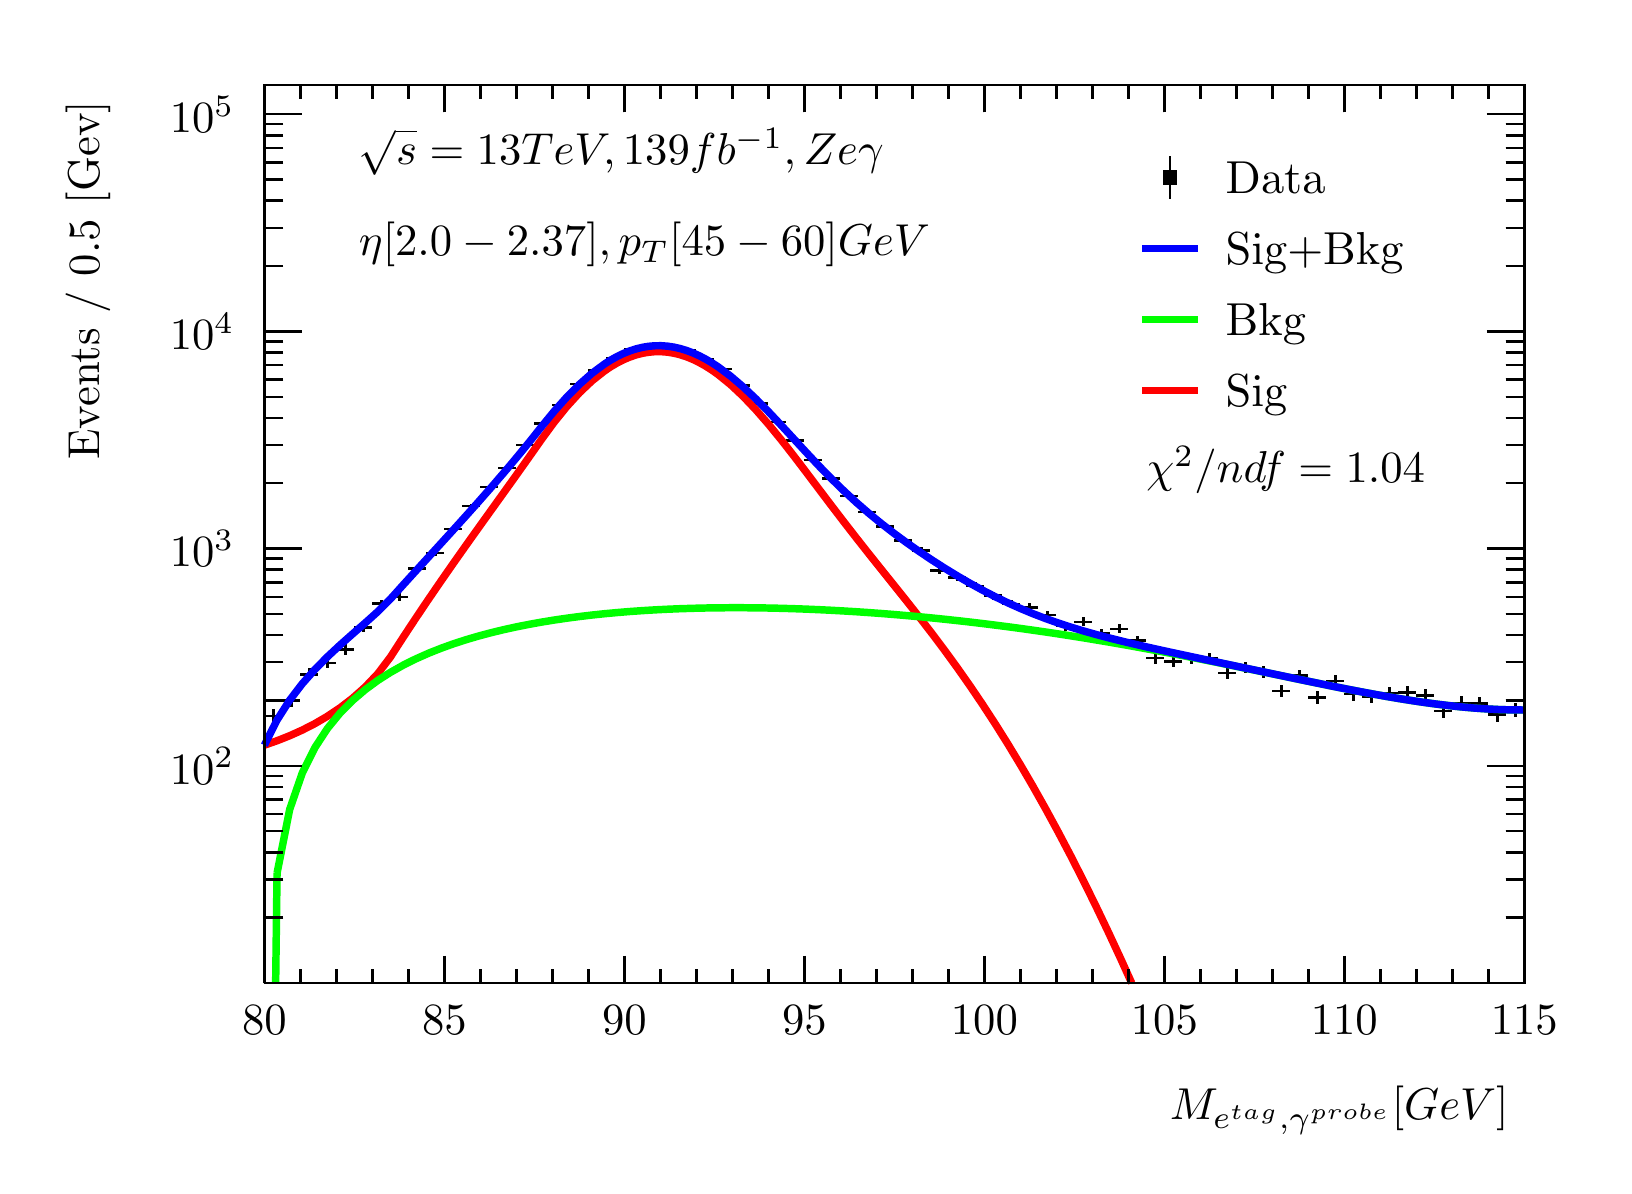
\begin{tikzpicture}
\pgfdeclareplotmark{cross} {
\pgfpathmoveto{\pgfpoint{-0.3\pgfplotmarksize}{\pgfplotmarksize}}
\pgfpathlineto{\pgfpoint{+0.3\pgfplotmarksize}{\pgfplotmarksize}}
\pgfpathlineto{\pgfpoint{+0.3\pgfplotmarksize}{0.3\pgfplotmarksize}}
\pgfpathlineto{\pgfpoint{+1\pgfplotmarksize}{0.3\pgfplotmarksize}}
\pgfpathlineto{\pgfpoint{+1\pgfplotmarksize}{-0.3\pgfplotmarksize}}
\pgfpathlineto{\pgfpoint{+0.3\pgfplotmarksize}{-0.3\pgfplotmarksize}}
\pgfpathlineto{\pgfpoint{+0.3\pgfplotmarksize}{-1.\pgfplotmarksize}}
\pgfpathlineto{\pgfpoint{-0.3\pgfplotmarksize}{-1.\pgfplotmarksize}}
\pgfpathlineto{\pgfpoint{-0.3\pgfplotmarksize}{-0.3\pgfplotmarksize}}
\pgfpathlineto{\pgfpoint{-1.\pgfplotmarksize}{-0.3\pgfplotmarksize}}
\pgfpathlineto{\pgfpoint{-1.\pgfplotmarksize}{0.3\pgfplotmarksize}}
\pgfpathlineto{\pgfpoint{-0.3\pgfplotmarksize}{0.3\pgfplotmarksize}}
\pgfpathclose
\pgfusepathqstroke
}
\pgfdeclareplotmark{cross*} {
\pgfpathmoveto{\pgfpoint{-0.3\pgfplotmarksize}{\pgfplotmarksize}}
\pgfpathlineto{\pgfpoint{+0.3\pgfplotmarksize}{\pgfplotmarksize}}
\pgfpathlineto{\pgfpoint{+0.3\pgfplotmarksize}{0.3\pgfplotmarksize}}
\pgfpathlineto{\pgfpoint{+1\pgfplotmarksize}{0.3\pgfplotmarksize}}
\pgfpathlineto{\pgfpoint{+1\pgfplotmarksize}{-0.3\pgfplotmarksize}}
\pgfpathlineto{\pgfpoint{+0.3\pgfplotmarksize}{-0.3\pgfplotmarksize}}
\pgfpathlineto{\pgfpoint{+0.3\pgfplotmarksize}{-1.\pgfplotmarksize}}
\pgfpathlineto{\pgfpoint{-0.3\pgfplotmarksize}{-1.\pgfplotmarksize}}
\pgfpathlineto{\pgfpoint{-0.3\pgfplotmarksize}{-0.3\pgfplotmarksize}}
\pgfpathlineto{\pgfpoint{-1.\pgfplotmarksize}{-0.3\pgfplotmarksize}}
\pgfpathlineto{\pgfpoint{-1.\pgfplotmarksize}{0.3\pgfplotmarksize}}
\pgfpathlineto{\pgfpoint{-0.3\pgfplotmarksize}{0.3\pgfplotmarksize}}
\pgfpathclose
\pgfusepathqfillstroke
}
\pgfdeclareplotmark{newstar} {
\pgfpathmoveto{\pgfqpoint{0pt}{\pgfplotmarksize}}
\pgfpathlineto{\pgfqpointpolar{44}{0.5\pgfplotmarksize}}
\pgfpathlineto{\pgfqpointpolar{18}{\pgfplotmarksize}}
\pgfpathlineto{\pgfqpointpolar{-20}{0.5\pgfplotmarksize}}
\pgfpathlineto{\pgfqpointpolar{-54}{\pgfplotmarksize}}
\pgfpathlineto{\pgfqpointpolar{-90}{0.5\pgfplotmarksize}}
\pgfpathlineto{\pgfqpointpolar{234}{\pgfplotmarksize}}
\pgfpathlineto{\pgfqpointpolar{198}{0.5\pgfplotmarksize}}
\pgfpathlineto{\pgfqpointpolar{162}{\pgfplotmarksize}}
\pgfpathlineto{\pgfqpointpolar{134}{0.5\pgfplotmarksize}}
\pgfpathclose
\pgfusepathqstroke
}
\pgfdeclareplotmark{newstar*} {
\pgfpathmoveto{\pgfqpoint{0pt}{\pgfplotmarksize}}
\pgfpathlineto{\pgfqpointpolar{44}{0.5\pgfplotmarksize}}
\pgfpathlineto{\pgfqpointpolar{18}{\pgfplotmarksize}}
\pgfpathlineto{\pgfqpointpolar{-20}{0.5\pgfplotmarksize}}
\pgfpathlineto{\pgfqpointpolar{-54}{\pgfplotmarksize}}
\pgfpathlineto{\pgfqpointpolar{-90}{0.5\pgfplotmarksize}}
\pgfpathlineto{\pgfqpointpolar{234}{\pgfplotmarksize}}
\pgfpathlineto{\pgfqpointpolar{198}{0.5\pgfplotmarksize}}
\pgfpathlineto{\pgfqpointpolar{162}{\pgfplotmarksize}}
\pgfpathlineto{\pgfqpointpolar{134}{0.5\pgfplotmarksize}}
\pgfpathclose
\pgfusepathqfillstroke
}
\definecolor{c}{rgb}{1,1,1};
\draw [color=c, fill=c] (0,0) rectangle (20,14.4361);
\draw [color=c, fill=c] (3,2.30977) rectangle (19,13.7143);
\definecolor{c}{rgb}{0,0,0};
\draw [c,line width=0.9] (3,2.30977) -- (3,13.7143) -- (19,13.7143) -- (19,2.30977) -- (3,2.30977);
\definecolor{c}{rgb}{1,1,1};
\draw [color=c, fill=c] (3,2.30977) rectangle (19,13.7143);
\definecolor{c}{rgb}{0,0,0};
\draw [c,line width=0.9] (3,2.30977) -- (3,13.7143) -- (19,13.7143) -- (19,2.30977) -- (3,2.30977);
\draw [c,line width=0.9] (3,2.30977) -- (19,2.30977);
\draw [c,line width=0.9] (3,2.65624) -- (3,2.30977);
\draw [c,line width=0.9] (3.45714,2.48301) -- (3.45714,2.30977);
\draw [c,line width=0.9] (3.91429,2.48301) -- (3.91429,2.30977);
\draw [c,line width=0.9] (4.37143,2.48301) -- (4.37143,2.30977);
\draw [c,line width=0.9] (4.82857,2.48301) -- (4.82857,2.30977);
\draw [c,line width=0.9] (5.28571,2.65624) -- (5.28571,2.30977);
\draw [c,line width=0.9] (5.74286,2.48301) -- (5.74286,2.30977);
\draw [c,line width=0.9] (6.2,2.48301) -- (6.2,2.30977);
\draw [c,line width=0.9] (6.65714,2.48301) -- (6.65714,2.30977);
\draw [c,line width=0.9] (7.11429,2.48301) -- (7.11429,2.30977);
\draw [c,line width=0.9] (7.57143,2.65624) -- (7.57143,2.30977);
\draw [c,line width=0.9] (8.02857,2.48301) -- (8.02857,2.30977);
\draw [c,line width=0.9] (8.48571,2.48301) -- (8.48571,2.30977);
\draw [c,line width=0.9] (8.94286,2.48301) -- (8.94286,2.30977);
\draw [c,line width=0.9] (9.4,2.48301) -- (9.4,2.30977);
\draw [c,line width=0.9] (9.85714,2.65624) -- (9.85714,2.30977);
\draw [c,line width=0.9] (10.3143,2.48301) -- (10.3143,2.30977);
\draw [c,line width=0.9] (10.7714,2.48301) -- (10.7714,2.30977);
\draw [c,line width=0.9] (11.2286,2.48301) -- (11.2286,2.30977);
\draw [c,line width=0.9] (11.6857,2.48301) -- (11.6857,2.30977);
\draw [c,line width=0.9] (12.1429,2.65624) -- (12.1429,2.30977);
\draw [c,line width=0.9] (12.6,2.48301) -- (12.6,2.30977);
\draw [c,line width=0.9] (13.0571,2.48301) -- (13.0571,2.30977);
\draw [c,line width=0.9] (13.5143,2.48301) -- (13.5143,2.30977);
\draw [c,line width=0.9] (13.9714,2.48301) -- (13.9714,2.30977);
\draw [c,line width=0.9] (14.4286,2.65624) -- (14.4286,2.30977);
\draw [c,line width=0.9] (14.8857,2.48301) -- (14.8857,2.30977);
\draw [c,line width=0.9] (15.3429,2.48301) -- (15.3429,2.30977);
\draw [c,line width=0.9] (15.8,2.48301) -- (15.8,2.30977);
\draw [c,line width=0.9] (16.2571,2.48301) -- (16.2571,2.30977);
\draw [c,line width=0.9] (16.7143,2.65624) -- (16.7143,2.30977);
\draw [c,line width=0.9] (17.1714,2.48301) -- (17.1714,2.30977);
\draw [c,line width=0.9] (17.6286,2.48301) -- (17.6286,2.30977);
\draw [c,line width=0.9] (18.0857,2.48301) -- (18.0857,2.30977);
\draw [c,line width=0.9] (18.5429,2.48301) -- (18.5429,2.30977);
\draw [c,line width=0.9] (19,2.65624) -- (19,2.30977);
\draw [anchor=base] (3,1.66015) node[scale=1.61424, color=c, rotate=0]{80};
\draw [anchor=base] (5.28571,1.66015) node[scale=1.61424, color=c, rotate=0]{85};
\draw [anchor=base] (7.57143,1.66015) node[scale=1.61424, color=c, rotate=0]{90};
\draw [anchor=base] (9.85714,1.66015) node[scale=1.61424, color=c, rotate=0]{95};
\draw [anchor=base] (12.1429,1.66015) node[scale=1.61424, color=c, rotate=0]{100};
\draw [anchor=base] (14.4286,1.66015) node[scale=1.61424, color=c, rotate=0]{105};
\draw [anchor=base] (16.7143,1.66015) node[scale=1.61424, color=c, rotate=0]{110};
\draw [anchor=base] (19,1.66015) node[scale=1.61424, color=c, rotate=0]{115};
\draw [anchor= east] (19,0.692932) node[scale=1.61424, color=c, rotate=0]{$M_{e^{tag}, \gamma^{probe}}  [GeV]$};
\draw [c,line width=0.9] (3,13.7143) -- (19,13.7143);
\draw [c,line width=0.9] (3,13.3678) -- (3,13.7143);
\draw [c,line width=0.9] (3.45714,13.5411) -- (3.45714,13.7143);
\draw [c,line width=0.9] (3.91429,13.5411) -- (3.91429,13.7143);
\draw [c,line width=0.9] (4.37143,13.5411) -- (4.37143,13.7143);
\draw [c,line width=0.9] (4.82857,13.5411) -- (4.82857,13.7143);
\draw [c,line width=0.9] (5.28571,13.3678) -- (5.28571,13.7143);
\draw [c,line width=0.9] (5.74286,13.5411) -- (5.74286,13.7143);
\draw [c,line width=0.9] (6.2,13.5411) -- (6.2,13.7143);
\draw [c,line width=0.9] (6.65714,13.5411) -- (6.65714,13.7143);
\draw [c,line width=0.9] (7.11429,13.5411) -- (7.11429,13.7143);
\draw [c,line width=0.9] (7.57143,13.3678) -- (7.57143,13.7143);
\draw [c,line width=0.9] (8.02857,13.5411) -- (8.02857,13.7143);
\draw [c,line width=0.9] (8.48571,13.5411) -- (8.48571,13.7143);
\draw [c,line width=0.9] (8.94286,13.5411) -- (8.94286,13.7143);
\draw [c,line width=0.9] (9.4,13.5411) -- (9.4,13.7143);
\draw [c,line width=0.9] (9.85714,13.3678) -- (9.85714,13.7143);
\draw [c,line width=0.9] (10.3143,13.5411) -- (10.3143,13.7143);
\draw [c,line width=0.9] (10.7714,13.5411) -- (10.7714,13.7143);
\draw [c,line width=0.9] (11.2286,13.5411) -- (11.2286,13.7143);
\draw [c,line width=0.9] (11.6857,13.5411) -- (11.6857,13.7143);
\draw [c,line width=0.9] (12.1429,13.3678) -- (12.1429,13.7143);
\draw [c,line width=0.9] (12.6,13.5411) -- (12.6,13.7143);
\draw [c,line width=0.9] (13.0571,13.5411) -- (13.0571,13.7143);
\draw [c,line width=0.9] (13.5143,13.5411) -- (13.5143,13.7143);
\draw [c,line width=0.9] (13.9714,13.5411) -- (13.9714,13.7143);
\draw [c,line width=0.9] (14.4286,13.3678) -- (14.4286,13.7143);
\draw [c,line width=0.9] (14.8857,13.5411) -- (14.8857,13.7143);
\draw [c,line width=0.9] (15.3429,13.5411) -- (15.3429,13.7143);
\draw [c,line width=0.9] (15.8,13.5411) -- (15.8,13.7143);
\draw [c,line width=0.9] (16.2571,13.5411) -- (16.2571,13.7143);
\draw [c,line width=0.9] (16.7143,13.3678) -- (16.7143,13.7143);
\draw [c,line width=0.9] (17.1714,13.5411) -- (17.1714,13.7143);
\draw [c,line width=0.9] (17.6286,13.5411) -- (17.6286,13.7143);
\draw [c,line width=0.9] (18.0857,13.5411) -- (18.0857,13.7143);
\draw [c,line width=0.9] (18.5429,13.5411) -- (18.5429,13.7143);
\draw [c,line width=0.9] (19,13.3678) -- (19,13.7143);
\draw [c,line width=0.9] (3,2.30977) -- (3,13.7143);
\draw [c,line width=0.9] (3.237,3.14018) -- (3,3.14018);
\draw [c,line width=0.9] (3.237,3.62593) -- (3,3.62593);
\draw [c,line width=0.9] (3.237,3.97058) -- (3,3.97058);
\draw [c,line width=0.9] (3.237,4.23792) -- (3,4.23792);
\draw [c,line width=0.9] (3.237,4.45634) -- (3,4.45634);
\draw [c,line width=0.9] (3.237,4.64102) -- (3,4.64102);
\draw [c,line width=0.9] (3.237,4.80099) -- (3,4.80099);
\draw [c,line width=0.9] (3.237,4.9421) -- (3,4.9421);
\draw [c,line width=0.9] (3.474,5.06832) -- (3,5.06832);
\draw [anchor= east] (2.82,5.06832) node[scale=1.61424, color=c, rotate=0]{$10^{2}$};
\draw [c,line width=0.9] (3.237,5.89873) -- (3,5.89873);
\draw [c,line width=0.9] (3.237,6.38449) -- (3,6.38449);
\draw [c,line width=0.9] (3.237,6.72914) -- (3,6.72914);
\draw [c,line width=0.9] (3.237,6.99647) -- (3,6.99647);
\draw [c,line width=0.9] (3.237,7.21489) -- (3,7.21489);
\draw [c,line width=0.9] (3.237,7.39957) -- (3,7.39957);
\draw [c,line width=0.9] (3.237,7.55954) -- (3,7.55954);
\draw [c,line width=0.9] (3.237,7.70065) -- (3,7.70065);
\draw [c,line width=0.9] (3.474,7.82687) -- (3,7.82687);
\draw [anchor= east] (2.82,7.82687) node[scale=1.61424, color=c, rotate=0]{$10^{3}$};
\draw [c,line width=0.9] (3.237,8.65728) -- (3,8.65728);
\draw [c,line width=0.9] (3.237,9.14304) -- (3,9.14304);
\draw [c,line width=0.9] (3.237,9.48769) -- (3,9.48769);
\draw [c,line width=0.9] (3.237,9.75502) -- (3,9.75502);
\draw [c,line width=0.9] (3.237,9.97344) -- (3,9.97344);
\draw [c,line width=0.9] (3.237,10.1581) -- (3,10.1581);
\draw [c,line width=0.9] (3.237,10.3181) -- (3,10.3181);
\draw [c,line width=0.9] (3.237,10.4592) -- (3,10.4592);
\draw [c,line width=0.9] (3.474,10.5854) -- (3,10.5854);
\draw [anchor= east] (2.82,10.5854) node[scale=1.61424, color=c, rotate=0]{$10^{4}$};
\draw [c,line width=0.9] (3.237,11.4158) -- (3,11.4158);
\draw [c,line width=0.9] (3.237,11.9016) -- (3,11.9016);
\draw [c,line width=0.9] (3.237,12.2462) -- (3,12.2462);
\draw [c,line width=0.9] (3.237,12.5136) -- (3,12.5136);
\draw [c,line width=0.9] (3.237,12.732) -- (3,12.732);
\draw [c,line width=0.9] (3.237,12.9167) -- (3,12.9167);
\draw [c,line width=0.9] (3.237,13.0766) -- (3,13.0766);
\draw [c,line width=0.9] (3.237,13.2178) -- (3,13.2178);
\draw [c,line width=0.9] (3.474,13.344) -- (3,13.344);
\draw [anchor= east] (2.82,13.344) node[scale=1.61424, color=c, rotate=0]{$10^{5}$};
\draw [anchor= east] (0.76,13.7143) node[scale=1.61424, color=c, rotate=90]{Events / 0.5 [Gev]};
\draw [c,line width=0.9] (19,2.30977) -- (19,13.7143);
\draw [c,line width=0.9] (18.763,3.14018) -- (19,3.14018);
\draw [c,line width=0.9] (18.763,3.62593) -- (19,3.62593);
\draw [c,line width=0.9] (18.763,3.97058) -- (19,3.97058);
\draw [c,line width=0.9] (18.763,4.23792) -- (19,4.23792);
\draw [c,line width=0.9] (18.763,4.45634) -- (19,4.45634);
\draw [c,line width=0.9] (18.763,4.64102) -- (19,4.64102);
\draw [c,line width=0.9] (18.763,4.80099) -- (19,4.80099);
\draw [c,line width=0.9] (18.763,4.9421) -- (19,4.9421);
\draw [c,line width=0.9] (18.526,5.06832) -- (19,5.06832);
\draw [c,line width=0.9] (18.763,5.89873) -- (19,5.89873);
\draw [c,line width=0.9] (18.763,6.38449) -- (19,6.38449);
\draw [c,line width=0.9] (18.763,6.72914) -- (19,6.72914);
\draw [c,line width=0.9] (18.763,6.99647) -- (19,6.99647);
\draw [c,line width=0.9] (18.763,7.21489) -- (19,7.21489);
\draw [c,line width=0.9] (18.763,7.39957) -- (19,7.39957);
\draw [c,line width=0.9] (18.763,7.55954) -- (19,7.55954);
\draw [c,line width=0.9] (18.763,7.70065) -- (19,7.70065);
\draw [c,line width=0.9] (18.526,7.82687) -- (19,7.82687);
\draw [c,line width=0.9] (18.763,8.65728) -- (19,8.65728);
\draw [c,line width=0.9] (18.763,9.14304) -- (19,9.14304);
\draw [c,line width=0.9] (18.763,9.48769) -- (19,9.48769);
\draw [c,line width=0.9] (18.763,9.75502) -- (19,9.75502);
\draw [c,line width=0.9] (18.763,9.97344) -- (19,9.97344);
\draw [c,line width=0.9] (18.763,10.1581) -- (19,10.1581);
\draw [c,line width=0.9] (18.763,10.3181) -- (19,10.3181);
\draw [c,line width=0.9] (18.763,10.4592) -- (19,10.4592);
\draw [c,line width=0.9] (18.526,10.5854) -- (19,10.5854);
\draw [c,line width=0.9] (18.763,11.4158) -- (19,11.4158);
\draw [c,line width=0.9] (18.763,11.9016) -- (19,11.9016);
\draw [c,line width=0.9] (18.763,12.2462) -- (19,12.2462);
\draw [c,line width=0.9] (18.763,12.5136) -- (19,12.5136);
\draw [c,line width=0.9] (18.763,12.732) -- (19,12.732);
\draw [c,line width=0.9] (18.763,12.9167) -- (19,12.9167);
\draw [c,line width=0.9] (18.763,13.0766) -- (19,13.0766);
\draw [c,line width=0.9] (18.763,13.2178) -- (19,13.2178);
\draw [c,line width=0.9] (18.526,13.344) -- (19,13.344);
\draw [c,line width=0.9] (3.11429,5.70403) -- (3,5.70403);
\draw [c,line width=0.9] (3,5.70403) -- (3,5.70403);
\draw [c,line width=0.9] (3.11429,5.70403) -- (3.22857,5.70403);
\draw [c,line width=0.9] (3.22857,5.70403) -- (3.22857,5.70403);
\draw [c,line width=0.9] (3.11429,5.70403) -- (3.11429,5.79589);
\draw [c,line width=0.9] (3.11429,5.79589) -- (3.11429,5.79589);
\draw [c,line width=0.9] (3.11429,5.70403) -- (3.11429,5.61217);
\draw [c,line width=0.9] (3.11429,5.61217) -- (3.11429,5.61217);
\draw [c,line width=0.9] (3.34286,5.89873) -- (3.22857,5.89873);
\draw [c,line width=0.9] (3.22857,5.89873) -- (3.22857,5.89873);
\draw [c,line width=0.9] (3.34286,5.89873) -- (3.45714,5.89873);
\draw [c,line width=0.9] (3.45714,5.89873) -- (3.45714,5.89873);
\draw [c,line width=0.9] (3.34286,5.89873) -- (3.34286,5.98343);
\draw [c,line width=0.9] (3.34286,5.98343) -- (3.34286,5.98343);
\draw [c,line width=0.9] (3.34286,5.89873) -- (3.34286,5.81404);
\draw [c,line width=0.9] (3.34286,5.81404) -- (3.34286,5.81404);
\draw [c,line width=0.9] (3.57143,6.23134) -- (3.45714,6.23134);
\draw [c,line width=0.9] (3.45714,6.23134) -- (3.45714,6.23134);
\draw [c,line width=0.9] (3.57143,6.23134) -- (3.68571,6.23134);
\draw [c,line width=0.9] (3.68571,6.23134) -- (3.68571,6.23134);
\draw [c,line width=0.9] (3.57143,6.23134) -- (3.57143,6.30506);
\draw [c,line width=0.9] (3.57143,6.30506) -- (3.57143,6.30506);
\draw [c,line width=0.9] (3.57143,6.23134) -- (3.57143,6.15762);
\draw [c,line width=0.9] (3.57143,6.15762) -- (3.57143,6.15762);
\draw [c,line width=0.9] (3.8,6.37647) -- (3.68571,6.37647);
\draw [c,line width=0.9] (3.68571,6.37647) -- (3.68571,6.37647);
\draw [c,line width=0.9] (3.8,6.37647) -- (3.91429,6.37647);
\draw [c,line width=0.9] (3.91429,6.37647) -- (3.91429,6.37647);
\draw [c,line width=0.9] (3.8,6.37647) -- (3.8,6.44586);
\draw [c,line width=0.9] (3.8,6.44586) -- (3.8,6.44586);
\draw [c,line width=0.9] (3.8,6.37647) -- (3.8,6.30708);
\draw [c,line width=0.9] (3.8,6.30708) -- (3.8,6.30708);
\draw [c,line width=0.9] (4.02857,6.54496) -- (3.91429,6.54496);
\draw [c,line width=0.9] (3.91429,6.54496) -- (3.91429,6.54496);
\draw [c,line width=0.9] (4.02857,6.54496) -- (4.14286,6.54496);
\draw [c,line width=0.9] (4.14286,6.54496) -- (4.14286,6.54496);
\draw [c,line width=0.9] (4.02857,6.54496) -- (4.02857,6.60964);
\draw [c,line width=0.9] (4.02857,6.60964) -- (4.02857,6.60964);
\draw [c,line width=0.9] (4.02857,6.54496) -- (4.02857,6.48028);
\draw [c,line width=0.9] (4.02857,6.48028) -- (4.02857,6.48028);
\draw [c,line width=0.9] (4.25714,6.82411) -- (4.14286,6.82411);
\draw [c,line width=0.9] (4.14286,6.82411) -- (4.14286,6.82411);
\draw [c,line width=0.9] (4.25714,6.82411) -- (4.37143,6.82411);
\draw [c,line width=0.9] (4.37143,6.82411) -- (4.37143,6.82411);
\draw [c,line width=0.9] (4.25714,6.82411) -- (4.25714,6.88168);
\draw [c,line width=0.9] (4.25714,6.88168) -- (4.25714,6.88168);
\draw [c,line width=0.9] (4.25714,6.82411) -- (4.25714,6.76654);
\draw [c,line width=0.9] (4.25714,6.76654) -- (4.25714,6.76654);
\draw [c,line width=0.9] (4.48571,7.12795) -- (4.37143,7.12795);
\draw [c,line width=0.9] (4.37143,7.12795) -- (4.37143,7.12795);
\draw [c,line width=0.9] (4.48571,7.12795) -- (4.6,7.12795);
\draw [c,line width=0.9] (4.6,7.12795) -- (4.6,7.12795);
\draw [c,line width=0.9] (4.48571,7.12795) -- (4.48571,7.17867);
\draw [c,line width=0.9] (4.48571,7.17867) -- (4.48571,7.17867);
\draw [c,line width=0.9] (4.48571,7.12795) -- (4.48571,7.07724);
\draw [c,line width=0.9] (4.48571,7.07724) -- (4.48571,7.07724);
\draw [c,line width=0.9] (4.71429,7.21089) -- (4.6,7.21089);
\draw [c,line width=0.9] (4.6,7.21089) -- (4.6,7.21089);
\draw [c,line width=0.9] (4.71429,7.21089) -- (4.82857,7.21089);
\draw [c,line width=0.9] (4.82857,7.21089) -- (4.82857,7.21089);
\draw [c,line width=0.9] (4.71429,7.21089) -- (4.71429,7.25988);
\draw [c,line width=0.9] (4.71429,7.25988) -- (4.71429,7.25988);
\draw [c,line width=0.9] (4.71429,7.21089) -- (4.71429,7.16191);
\draw [c,line width=0.9] (4.71429,7.16191) -- (4.71429,7.16191);
\draw [c,line width=0.9] (4.94286,7.57738) -- (4.82857,7.57738);
\draw [c,line width=0.9] (4.82857,7.57738) -- (4.82857,7.57738);
\draw [c,line width=0.9] (4.94286,7.57738) -- (5.05714,7.57738);
\draw [c,line width=0.9] (5.05714,7.57738) -- (5.05714,7.57738);
\draw [c,line width=0.9] (4.94286,7.57738) -- (4.94286,7.61942);
\draw [c,line width=0.9] (4.94286,7.61942) -- (4.94286,7.61942);
\draw [c,line width=0.9] (4.94286,7.57738) -- (4.94286,7.53534);
\draw [c,line width=0.9] (4.94286,7.53534) -- (4.94286,7.53534);
\draw [c,line width=0.9] (5.17143,7.7692) -- (5.05714,7.7692);
\draw [c,line width=0.9] (5.05714,7.7692) -- (5.05714,7.7692);
\draw [c,line width=0.9] (5.17143,7.7692) -- (5.28571,7.7692);
\draw [c,line width=0.9] (5.28571,7.7692) -- (5.28571,7.7692);
\draw [c,line width=0.9] (5.17143,7.7692) -- (5.17143,7.80801);
\draw [c,line width=0.9] (5.17143,7.80801) -- (5.17143,7.80801);
\draw [c,line width=0.9] (5.17143,7.7692) -- (5.17143,7.7304);
\draw [c,line width=0.9] (5.17143,7.7304) -- (5.17143,7.7304);
\draw [c,line width=0.9] (5.4,8.07488) -- (5.28571,8.07488);
\draw [c,line width=0.9] (5.28571,8.07488) -- (5.28571,8.07488);
\draw [c,line width=0.9] (5.4,8.07488) -- (5.51429,8.07488);
\draw [c,line width=0.9] (5.51429,8.07488) -- (5.51429,8.07488);
\draw [c,line width=0.9] (5.4,8.07488) -- (5.4,8.10904);
\draw [c,line width=0.9] (5.4,8.10904) -- (5.4,8.10904);
\draw [c,line width=0.9] (5.4,8.07488) -- (5.4,8.04072);
\draw [c,line width=0.9] (5.4,8.04072) -- (5.4,8.04072);
\draw [c,line width=0.9] (5.62857,8.36651) -- (5.51429,8.36651);
\draw [c,line width=0.9] (5.51429,8.36651) -- (5.51429,8.36651);
\draw [c,line width=0.9] (5.62857,8.36651) -- (5.74286,8.36651);
\draw [c,line width=0.9] (5.74286,8.36651) -- (5.74286,8.36651);
\draw [c,line width=0.9] (5.62857,8.36651) -- (5.62857,8.39676);
\draw [c,line width=0.9] (5.62857,8.39676) -- (5.62857,8.39676);
\draw [c,line width=0.9] (5.62857,8.36651) -- (5.62857,8.33627);
\draw [c,line width=0.9] (5.62857,8.33627) -- (5.62857,8.33627);
\draw [c,line width=0.9] (5.85714,8.61025) -- (5.74286,8.61025);
\draw [c,line width=0.9] (5.74286,8.61025) -- (5.74286,8.61025);
\draw [c,line width=0.9] (5.85714,8.61025) -- (5.97143,8.61025);
\draw [c,line width=0.9] (5.97143,8.61025) -- (5.97143,8.61025);
\draw [c,line width=0.9] (5.85714,8.61025) -- (5.85714,8.63757);
\draw [c,line width=0.9] (5.85714,8.63757) -- (5.85714,8.63757);
\draw [c,line width=0.9] (5.85714,8.61025) -- (5.85714,8.58293);
\draw [c,line width=0.9] (5.85714,8.58293) -- (5.85714,8.58293);
\draw [c,line width=0.9] (6.08571,8.85099) -- (5.97143,8.85099);
\draw [c,line width=0.9] (5.97143,8.85099) -- (5.97143,8.85099);
\draw [c,line width=0.9] (6.08571,8.85099) -- (6.2,8.85099);
\draw [c,line width=0.9] (6.2,8.85099) -- (6.2,8.85099);
\draw [c,line width=0.9] (6.08571,8.85099) -- (6.08571,8.8757);
\draw [c,line width=0.9] (6.08571,8.8757) -- (6.08571,8.8757);
\draw [c,line width=0.9] (6.08571,8.85099) -- (6.08571,8.82629);
\draw [c,line width=0.9] (6.08571,8.82629) -- (6.08571,8.82629);
\draw [c,line width=0.9] (6.31429,9.14304) -- (6.2,9.14304);
\draw [c,line width=0.9] (6.2,9.14304) -- (6.2,9.14304);
\draw [c,line width=0.9] (6.31429,9.14304) -- (6.42857,9.14304);
\draw [c,line width=0.9] (6.42857,9.14304) -- (6.42857,9.14304);
\draw [c,line width=0.9] (6.31429,9.14304) -- (6.31429,9.16491);
\draw [c,line width=0.9] (6.31429,9.16491) -- (6.31429,9.16491);
\draw [c,line width=0.9] (6.31429,9.14304) -- (6.31429,9.12117);
\draw [c,line width=0.9] (6.31429,9.12117) -- (6.31429,9.12117);
\draw [c,line width=0.9] (6.54286,9.41738) -- (6.42857,9.41738);
\draw [c,line width=0.9] (6.42857,9.41738) -- (6.42857,9.41738);
\draw [c,line width=0.9] (6.54286,9.41738) -- (6.65714,9.41738);
\draw [c,line width=0.9] (6.65714,9.41738) -- (6.65714,9.41738);
\draw [c,line width=0.9] (6.54286,9.41738) -- (6.54286,9.43688);
\draw [c,line width=0.9] (6.54286,9.43688) -- (6.54286,9.43688);
\draw [c,line width=0.9] (6.54286,9.41738) -- (6.54286,9.39787);
\draw [c,line width=0.9] (6.54286,9.39787) -- (6.54286,9.39787);
\draw [c,line width=0.9] (6.77143,9.65095) -- (6.65714,9.65095);
\draw [c,line width=0.9] (6.65714,9.65095) -- (6.65714,9.65095);
\draw [c,line width=0.9] (6.77143,9.65095) -- (6.88571,9.65095);
\draw [c,line width=0.9] (6.88571,9.65095) -- (6.88571,9.65095);
\draw [c,line width=0.9] (6.77143,9.65095) -- (6.77143,9.66865);
\draw [c,line width=0.9] (6.77143,9.66865) -- (6.77143,9.66865);
\draw [c,line width=0.9] (6.77143,9.65095) -- (6.77143,9.63326);
\draw [c,line width=0.9] (6.77143,9.63326) -- (6.77143,9.63326);
\draw [c,line width=0.9] (7,9.91535) -- (6.88571,9.91535);
\draw [c,line width=0.9] (6.88571,9.91535) -- (6.88571,9.91535);
\draw [c,line width=0.9] (7,9.91535) -- (7.11429,9.91535);
\draw [c,line width=0.9] (7.11429,9.91535) -- (7.11429,9.91535);
\draw [c,line width=0.9] (7,9.91535) -- (7,9.9312);
\draw [c,line width=0.9] (7,9.9312) -- (7,9.9312);
\draw [c,line width=0.9] (7,9.91535) -- (7,9.89951);
\draw [c,line width=0.9] (7,9.89951) -- (7,9.89951);
\draw [c,line width=0.9] (7.22857,10.0918) -- (7.11429,10.0918);
\draw [c,line width=0.9] (7.11429,10.0918) -- (7.11429,10.0918);
\draw [c,line width=0.9] (7.22857,10.0918) -- (7.34286,10.0918);
\draw [c,line width=0.9] (7.34286,10.0918) -- (7.34286,10.0918);
\draw [c,line width=0.9] (7.22857,10.0918) -- (7.22857,10.1065);
\draw [c,line width=0.9] (7.22857,10.1065) -- (7.22857,10.1065);
\draw [c,line width=0.9] (7.22857,10.0918) -- (7.22857,10.0771);
\draw [c,line width=0.9] (7.22857,10.0771) -- (7.22857,10.0771);
\draw [c,line width=0.9] (7.45714,10.246) -- (7.34286,10.246);
\draw [c,line width=0.9] (7.34286,10.246) -- (7.34286,10.246);
\draw [c,line width=0.9] (7.45714,10.246) -- (7.57143,10.246);
\draw [c,line width=0.9] (7.57143,10.246) -- (7.57143,10.246);
\draw [c,line width=0.9] (7.45714,10.246) -- (7.45714,10.2598);
\draw [c,line width=0.9] (7.45714,10.2598) -- (7.45714,10.2598);
\draw [c,line width=0.9] (7.45714,10.246) -- (7.45714,10.2322);
\draw [c,line width=0.9] (7.45714,10.2322) -- (7.45714,10.2322);
\draw [c,line width=0.9] (7.68571,10.3568) -- (7.57143,10.3568);
\draw [c,line width=0.9] (7.57143,10.3568) -- (7.57143,10.3568);
\draw [c,line width=0.9] (7.68571,10.3568) -- (7.8,10.3568);
\draw [c,line width=0.9] (7.8,10.3568) -- (7.8,10.3568);
\draw [c,line width=0.9] (7.68571,10.3568) -- (7.68571,10.37);
\draw [c,line width=0.9] (7.68571,10.37) -- (7.68571,10.37);
\draw [c,line width=0.9] (7.68571,10.3568) -- (7.68571,10.3437);
\draw [c,line width=0.9] (7.68571,10.3437) -- (7.68571,10.3437);
\draw [c,line width=0.9] (7.91429,10.4092) -- (7.8,10.4092);
\draw [c,line width=0.9] (7.8,10.4092) -- (7.8,10.4092);
\draw [c,line width=0.9] (7.91429,10.4092) -- (8.02857,10.4092);
\draw [c,line width=0.9] (8.02857,10.4092) -- (8.02857,10.4092);
\draw [c,line width=0.9] (7.91429,10.4092) -- (7.91429,10.4221);
\draw [c,line width=0.9] (7.91429,10.4221) -- (7.91429,10.4221);
\draw [c,line width=0.9] (7.91429,10.4092) -- (7.91429,10.3963);
\draw [c,line width=0.9] (7.91429,10.3963) -- (7.91429,10.3963);
\draw [c,line width=0.9] (8.14286,10.3916) -- (8.02857,10.3916);
\draw [c,line width=0.9] (8.02857,10.3916) -- (8.02857,10.3916);
\draw [c,line width=0.9] (8.14286,10.3916) -- (8.25714,10.3916);
\draw [c,line width=0.9] (8.25714,10.3916) -- (8.25714,10.3916);
\draw [c,line width=0.9] (8.14286,10.3916) -- (8.14286,10.4046);
\draw [c,line width=0.9] (8.14286,10.4046) -- (8.14286,10.4046);
\draw [c,line width=0.9] (8.14286,10.3916) -- (8.14286,10.3786);
\draw [c,line width=0.9] (8.14286,10.3786) -- (8.14286,10.3786);
\draw [c,line width=0.9] (8.37143,10.3484) -- (8.25714,10.3484);
\draw [c,line width=0.9] (8.25714,10.3484) -- (8.25714,10.3484);
\draw [c,line width=0.9] (8.37143,10.3484) -- (8.48571,10.3484);
\draw [c,line width=0.9] (8.48571,10.3484) -- (8.48571,10.3484);
\draw [c,line width=0.9] (8.37143,10.3484) -- (8.37143,10.3616);
\draw [c,line width=0.9] (8.37143,10.3616) -- (8.37143,10.3616);
\draw [c,line width=0.9] (8.37143,10.3484) -- (8.37143,10.3352);
\draw [c,line width=0.9] (8.37143,10.3352) -- (8.37143,10.3352);
\draw [c,line width=0.9] (8.6,10.2305) -- (8.48571,10.2305);
\draw [c,line width=0.9] (8.48571,10.2305) -- (8.48571,10.2305);
\draw [c,line width=0.9] (8.6,10.2305) -- (8.71429,10.2305);
\draw [c,line width=0.9] (8.71429,10.2305) -- (8.71429,10.2305);
\draw [c,line width=0.9] (8.6,10.2305) -- (8.6,10.2444);
\draw [c,line width=0.9] (8.6,10.2444) -- (8.6,10.2444);
\draw [c,line width=0.9] (8.6,10.2305) -- (8.6,10.2166);
\draw [c,line width=0.9] (8.6,10.2166) -- (8.6,10.2166);
\draw [c,line width=0.9] (8.82857,10.1058) -- (8.71429,10.1058);
\draw [c,line width=0.9] (8.71429,10.1058) -- (8.71429,10.1058);
\draw [c,line width=0.9] (8.82857,10.1058) -- (8.94286,10.1058);
\draw [c,line width=0.9] (8.94286,10.1058) -- (8.94286,10.1058);
\draw [c,line width=0.9] (8.82857,10.1058) -- (8.82857,10.1205);
\draw [c,line width=0.9] (8.82857,10.1205) -- (8.82857,10.1205);
\draw [c,line width=0.9] (8.82857,10.1058) -- (8.82857,10.0912);
\draw [c,line width=0.9] (8.82857,10.0912) -- (8.82857,10.0912);
\draw [c,line width=0.9] (9.05714,9.90101) -- (8.94286,9.90101);
\draw [c,line width=0.9] (8.94286,9.90101) -- (8.94286,9.90101);
\draw [c,line width=0.9] (9.05714,9.90101) -- (9.17143,9.90101);
\draw [c,line width=0.9] (9.17143,9.90101) -- (9.17143,9.90101);
\draw [c,line width=0.9] (9.05714,9.90101) -- (9.05714,9.91695);
\draw [c,line width=0.9] (9.05714,9.91695) -- (9.05714,9.91695);
\draw [c,line width=0.9] (9.05714,9.90101) -- (9.05714,9.88507);
\draw [c,line width=0.9] (9.05714,9.88507) -- (9.05714,9.88507);
\draw [c,line width=0.9] (9.28571,9.66833) -- (9.17143,9.66833);
\draw [c,line width=0.9] (9.17143,9.66833) -- (9.17143,9.66833);
\draw [c,line width=0.9] (9.28571,9.66833) -- (9.4,9.66833);
\draw [c,line width=0.9] (9.4,9.66833) -- (9.4,9.66833);
\draw [c,line width=0.9] (9.28571,9.66833) -- (9.28571,9.6859);
\draw [c,line width=0.9] (9.28571,9.6859) -- (9.28571,9.6859);
\draw [c,line width=0.9] (9.28571,9.66833) -- (9.28571,9.65077);
\draw [c,line width=0.9] (9.28571,9.65077) -- (9.28571,9.65077);
\draw [c,line width=0.9] (9.51429,9.43315) -- (9.4,9.43315);
\draw [c,line width=0.9] (9.4,9.43315) -- (9.4,9.43315);
\draw [c,line width=0.9] (9.51429,9.43315) -- (9.62857,9.43315);
\draw [c,line width=0.9] (9.62857,9.43315) -- (9.62857,9.43315);
\draw [c,line width=0.9] (9.51429,9.43315) -- (9.51429,9.45253);
\draw [c,line width=0.9] (9.51429,9.45253) -- (9.51429,9.45253);
\draw [c,line width=0.9] (9.51429,9.43315) -- (9.51429,9.41377);
\draw [c,line width=0.9] (9.51429,9.41377) -- (9.51429,9.41377);
\draw [c,line width=0.9] (9.74286,9.19921) -- (9.62857,9.19921);
\draw [c,line width=0.9] (9.62857,9.19921) -- (9.62857,9.19921);
\draw [c,line width=0.9] (9.74286,9.19921) -- (9.85714,9.19921);
\draw [c,line width=0.9] (9.85714,9.19921) -- (9.85714,9.19921);
\draw [c,line width=0.9] (9.74286,9.19921) -- (9.74286,9.22057);
\draw [c,line width=0.9] (9.74286,9.22057) -- (9.74286,9.22057);
\draw [c,line width=0.9] (9.74286,9.19921) -- (9.74286,9.17784);
\draw [c,line width=0.9] (9.74286,9.17784) -- (9.74286,9.17784);
\draw [c,line width=0.9] (9.97143,8.95303) -- (9.85714,8.95303);
\draw [c,line width=0.9] (9.85714,8.95303) -- (9.85714,8.95303);
\draw [c,line width=0.9] (9.97143,8.95303) -- (10.0857,8.95303);
\draw [c,line width=0.9] (10.0857,8.95303) -- (10.0857,8.95303);
\draw [c,line width=0.9] (9.97143,8.95303) -- (9.97143,8.9767);
\draw [c,line width=0.9] (9.97143,8.9767) -- (9.97143,8.9767);
\draw [c,line width=0.9] (9.97143,8.95303) -- (9.97143,8.92935);
\draw [c,line width=0.9] (9.97143,8.92935) -- (9.97143,8.92935);
\draw [c,line width=0.9] (10.2,8.71687) -- (10.0857,8.71687);
\draw [c,line width=0.9] (10.0857,8.71687) -- (10.0857,8.71687);
\draw [c,line width=0.9] (10.2,8.71687) -- (10.3143,8.71687);
\draw [c,line width=0.9] (10.3143,8.71687) -- (10.3143,8.71687);
\draw [c,line width=0.9] (10.2,8.71687) -- (10.2,8.743);
\draw [c,line width=0.9] (10.2,8.743) -- (10.2,8.743);
\draw [c,line width=0.9] (10.2,8.71687) -- (10.2,8.69074);
\draw [c,line width=0.9] (10.2,8.69074) -- (10.2,8.69074);
\draw [c,line width=0.9] (10.4286,8.49525) -- (10.3143,8.49525);
\draw [c,line width=0.9] (10.3143,8.49525) -- (10.3143,8.49525);
\draw [c,line width=0.9] (10.4286,8.49525) -- (10.5429,8.49525);
\draw [c,line width=0.9] (10.5429,8.49525) -- (10.5429,8.49525);
\draw [c,line width=0.9] (10.4286,8.49525) -- (10.4286,8.52391);
\draw [c,line width=0.9] (10.4286,8.52391) -- (10.4286,8.52391);
\draw [c,line width=0.9] (10.4286,8.49525) -- (10.4286,8.46659);
\draw [c,line width=0.9] (10.4286,8.46659) -- (10.4286,8.46659);
\draw [c,line width=0.9] (10.6571,8.29331) -- (10.5429,8.29331);
\draw [c,line width=0.9] (10.5429,8.29331) -- (10.5429,8.29331);
\draw [c,line width=0.9] (10.6571,8.29331) -- (10.7714,8.29331);
\draw [c,line width=0.9] (10.7714,8.29331) -- (10.7714,8.29331);
\draw [c,line width=0.9] (10.6571,8.29331) -- (10.6571,8.32449);
\draw [c,line width=0.9] (10.6571,8.32449) -- (10.6571,8.32449);
\draw [c,line width=0.9] (10.6571,8.29331) -- (10.6571,8.26213);
\draw [c,line width=0.9] (10.6571,8.26213) -- (10.6571,8.26213);
\draw [c,line width=0.9] (10.8857,8.1085) -- (10.7714,8.1085);
\draw [c,line width=0.9] (10.7714,8.1085) -- (10.7714,8.1085);
\draw [c,line width=0.9] (10.8857,8.1085) -- (11,8.1085);
\draw [c,line width=0.9] (11,8.1085) -- (11,8.1085);
\draw [c,line width=0.9] (10.8857,8.1085) -- (10.8857,8.14218);
\draw [c,line width=0.9] (10.8857,8.14218) -- (10.8857,8.14218);
\draw [c,line width=0.9] (10.8857,8.1085) -- (10.8857,8.07481);
\draw [c,line width=0.9] (10.8857,8.07481) -- (10.8857,8.07481);
\draw [c,line width=0.9] (11.1143,7.92902) -- (11,7.92902);
\draw [c,line width=0.9] (11,7.92902) -- (11,7.92902);
\draw [c,line width=0.9] (11.1143,7.92902) -- (11.2286,7.92902);
\draw [c,line width=0.9] (11.2286,7.92902) -- (11.2286,7.92902);
\draw [c,line width=0.9] (11.1143,7.92902) -- (11.1143,7.96532);
\draw [c,line width=0.9] (11.1143,7.96532) -- (11.1143,7.96532);
\draw [c,line width=0.9] (11.1143,7.92902) -- (11.1143,7.89272);
\draw [c,line width=0.9] (11.1143,7.89272) -- (11.1143,7.89272);
\draw [c,line width=0.9] (11.3429,7.80511) -- (11.2286,7.80511);
\draw [c,line width=0.9] (11.2286,7.80511) -- (11.2286,7.80511);
\draw [c,line width=0.9] (11.3429,7.80511) -- (11.4571,7.80511);
\draw [c,line width=0.9] (11.4571,7.80511) -- (11.4571,7.80511);
\draw [c,line width=0.9] (11.3429,7.80511) -- (11.3429,7.84334);
\draw [c,line width=0.9] (11.3429,7.84334) -- (11.3429,7.84334);
\draw [c,line width=0.9] (11.3429,7.80511) -- (11.3429,7.76689);
\draw [c,line width=0.9] (11.3429,7.76689) -- (11.3429,7.76689);
\draw [c,line width=0.9] (11.5714,7.55052) -- (11.4571,7.55052);
\draw [c,line width=0.9] (11.4571,7.55052) -- (11.4571,7.55052);
\draw [c,line width=0.9] (11.5714,7.55052) -- (11.6857,7.55052);
\draw [c,line width=0.9] (11.6857,7.55052) -- (11.6857,7.55052);
\draw [c,line width=0.9] (11.5714,7.55052) -- (11.5714,7.59304);
\draw [c,line width=0.9] (11.5714,7.59304) -- (11.5714,7.59304);
\draw [c,line width=0.9] (11.5714,7.55052) -- (11.5714,7.50801);
\draw [c,line width=0.9] (11.5714,7.50801) -- (11.5714,7.50801);
\draw [c,line width=0.9] (11.8,7.46128) -- (11.6857,7.46128);
\draw [c,line width=0.9] (11.6857,7.46128) -- (11.6857,7.46128);
\draw [c,line width=0.9] (11.8,7.46128) -- (11.9143,7.46128);
\draw [c,line width=0.9] (11.9143,7.46128) -- (11.9143,7.46128);
\draw [c,line width=0.9] (11.8,7.46128) -- (11.8,7.5054);
\draw [c,line width=0.9] (11.8,7.5054) -- (11.8,7.5054);
\draw [c,line width=0.9] (11.8,7.46128) -- (11.8,7.41715);
\draw [c,line width=0.9] (11.8,7.41715) -- (11.8,7.41715);
\draw [c,line width=0.9] (12.0286,7.35066) -- (11.9143,7.35066);
\draw [c,line width=0.9] (11.9143,7.35066) -- (11.9143,7.35066);
\draw [c,line width=0.9] (12.0286,7.35066) -- (12.1429,7.35066);
\draw [c,line width=0.9] (12.1429,7.35066) -- (12.1429,7.35066);
\draw [c,line width=0.9] (12.0286,7.35066) -- (12.0286,7.39688);
\draw [c,line width=0.9] (12.0286,7.39688) -- (12.0286,7.39688);
\draw [c,line width=0.9] (12.0286,7.35066) -- (12.0286,7.30445);
\draw [c,line width=0.9] (12.0286,7.30445) -- (12.0286,7.30445);
\draw [c,line width=0.9] (12.2571,7.22879) -- (12.1429,7.22879);
\draw [c,line width=0.9] (12.1429,7.22879) -- (12.1429,7.22879);
\draw [c,line width=0.9] (12.2571,7.22879) -- (12.3714,7.22879);
\draw [c,line width=0.9] (12.3714,7.22879) -- (12.3714,7.22879);
\draw [c,line width=0.9] (12.2571,7.22879) -- (12.2571,7.27741);
\draw [c,line width=0.9] (12.2571,7.27741) -- (12.2571,7.27741);
\draw [c,line width=0.9] (12.2571,7.22879) -- (12.2571,7.18017);
\draw [c,line width=0.9] (12.2571,7.18017) -- (12.2571,7.18017);
\draw [c,line width=0.9] (12.4857,7.12149) -- (12.3714,7.12149);
\draw [c,line width=0.9] (12.3714,7.12149) -- (12.3714,7.12149);
\draw [c,line width=0.9] (12.4857,7.12149) -- (12.6,7.12149);
\draw [c,line width=0.9] (12.6,7.12149) -- (12.6,7.12149);
\draw [c,line width=0.9] (12.4857,7.12149) -- (12.4857,7.17234);
\draw [c,line width=0.9] (12.4857,7.17234) -- (12.4857,7.17234);
\draw [c,line width=0.9] (12.4857,7.12149) -- (12.4857,7.07064);
\draw [c,line width=0.9] (12.4857,7.07064) -- (12.4857,7.07064);
\draw [c,line width=0.9] (12.7143,7.07976) -- (12.6,7.07976);
\draw [c,line width=0.9] (12.6,7.07976) -- (12.6,7.07976);
\draw [c,line width=0.9] (12.7143,7.07976) -- (12.8286,7.07976);
\draw [c,line width=0.9] (12.8286,7.07976) -- (12.8286,7.07976);
\draw [c,line width=0.9] (12.7143,7.07976) -- (12.7143,7.13151);
\draw [c,line width=0.9] (12.7143,7.13151) -- (12.7143,7.13151);
\draw [c,line width=0.9] (12.7143,7.07976) -- (12.7143,7.02802);
\draw [c,line width=0.9] (12.7143,7.02802) -- (12.7143,7.02802);
\draw [c,line width=0.9] (12.9429,6.98201) -- (12.8286,6.98201);
\draw [c,line width=0.9] (12.8286,6.98201) -- (12.8286,6.98201);
\draw [c,line width=0.9] (12.9429,6.98201) -- (13.0571,6.98201);
\draw [c,line width=0.9] (13.0571,6.98201) -- (13.0571,6.98201);
\draw [c,line width=0.9] (12.9429,6.98201) -- (12.9429,7.0359);
\draw [c,line width=0.9] (12.9429,7.0359) -- (12.9429,7.0359);
\draw [c,line width=0.9] (12.9429,6.98201) -- (12.9429,6.92811);
\draw [c,line width=0.9] (12.9429,6.92811) -- (12.9429,6.92811);
\draw [c,line width=0.9] (13.1714,6.84332) -- (13.0571,6.84332);
\draw [c,line width=0.9] (13.0571,6.84332) -- (13.0571,6.84332);
\draw [c,line width=0.9] (13.1714,6.84332) -- (13.2857,6.84332);
\draw [c,line width=0.9] (13.2857,6.84332) -- (13.2857,6.84332);
\draw [c,line width=0.9] (13.1714,6.84332) -- (13.1714,6.90043);
\draw [c,line width=0.9] (13.1714,6.90043) -- (13.1714,6.90043);
\draw [c,line width=0.9] (13.1714,6.84332) -- (13.1714,6.78621);
\draw [c,line width=0.9] (13.1714,6.78621) -- (13.1714,6.78621);
\draw [c,line width=0.9] (13.4,6.89658) -- (13.2857,6.89658);
\draw [c,line width=0.9] (13.2857,6.89658) -- (13.2857,6.89658);
\draw [c,line width=0.9] (13.4,6.89658) -- (13.5143,6.89658);
\draw [c,line width=0.9] (13.5143,6.89658) -- (13.5143,6.89658);
\draw [c,line width=0.9] (13.4,6.89658) -- (13.4,6.95243);
\draw [c,line width=0.9] (13.4,6.95243) -- (13.4,6.95243);
\draw [c,line width=0.9] (13.4,6.89658) -- (13.4,6.84072);
\draw [c,line width=0.9] (13.4,6.84072) -- (13.4,6.84072);
\draw [c,line width=0.9] (13.6286,6.75286) -- (13.5143,6.75286);
\draw [c,line width=0.9] (13.5143,6.75286) -- (13.5143,6.75286);
\draw [c,line width=0.9] (13.6286,6.75286) -- (13.7429,6.75286);
\draw [c,line width=0.9] (13.7429,6.75286) -- (13.7429,6.75286);
\draw [c,line width=0.9] (13.6286,6.75286) -- (13.6286,6.81217);
\draw [c,line width=0.9] (13.6286,6.81217) -- (13.6286,6.81217);
\draw [c,line width=0.9] (13.6286,6.75286) -- (13.6286,6.69356);
\draw [c,line width=0.9] (13.6286,6.69356) -- (13.6286,6.69356);
\draw [c,line width=0.9] (13.8571,6.80739) -- (13.7429,6.80739);
\draw [c,line width=0.9] (13.7429,6.80739) -- (13.7429,6.80739);
\draw [c,line width=0.9] (13.8571,6.80739) -- (13.9714,6.80739);
\draw [c,line width=0.9] (13.9714,6.80739) -- (13.9714,6.80739);
\draw [c,line width=0.9] (13.8571,6.80739) -- (13.8571,6.86536);
\draw [c,line width=0.9] (13.8571,6.86536) -- (13.8571,6.86536);
\draw [c,line width=0.9] (13.8571,6.80739) -- (13.8571,6.74942);
\draw [c,line width=0.9] (13.8571,6.74942) -- (13.8571,6.74942);
\draw [c,line width=0.9] (14.0857,6.65819) -- (13.9714,6.65819);
\draw [c,line width=0.9] (13.9714,6.65819) -- (13.9714,6.65819);
\draw [c,line width=0.9] (14.0857,6.65819) -- (14.2,6.65819);
\draw [c,line width=0.9] (14.2,6.65819) -- (14.2,6.65819);
\draw [c,line width=0.9] (14.0857,6.65819) -- (14.0857,6.71989);
\draw [c,line width=0.9] (14.0857,6.71989) -- (14.0857,6.71989);
\draw [c,line width=0.9] (14.0857,6.65819) -- (14.0857,6.5965);
\draw [c,line width=0.9] (14.0857,6.5965) -- (14.0857,6.5965);
\draw [c,line width=0.9] (14.3143,6.43531) -- (14.2,6.43531);
\draw [c,line width=0.9] (14.2,6.43531) -- (14.2,6.43531);
\draw [c,line width=0.9] (14.3143,6.43531) -- (14.4286,6.43531);
\draw [c,line width=0.9] (14.4286,6.43531) -- (14.4286,6.43531);
\draw [c,line width=0.9] (14.3143,6.43531) -- (14.3143,6.50302);
\draw [c,line width=0.9] (14.3143,6.50302) -- (14.3143,6.50302);
\draw [c,line width=0.9] (14.3143,6.43531) -- (14.3143,6.3676);
\draw [c,line width=0.9] (14.3143,6.3676) -- (14.3143,6.3676);
\draw [c,line width=0.9] (14.5429,6.39245) -- (14.4286,6.39245);
\draw [c,line width=0.9] (14.4286,6.39245) -- (14.4286,6.39245);
\draw [c,line width=0.9] (14.5429,6.39245) -- (14.6571,6.39245);
\draw [c,line width=0.9] (14.6571,6.39245) -- (14.6571,6.39245);
\draw [c,line width=0.9] (14.5429,6.39245) -- (14.5429,6.46138);
\draw [c,line width=0.9] (14.5429,6.46138) -- (14.5429,6.46138);
\draw [c,line width=0.9] (14.5429,6.39245) -- (14.5429,6.32352);
\draw [c,line width=0.9] (14.5429,6.32352) -- (14.5429,6.32352);
\draw [c,line width=0.9] (14.7714,6.43531) -- (14.6571,6.43531);
\draw [c,line width=0.9] (14.6571,6.43531) -- (14.6571,6.43531);
\draw [c,line width=0.9] (14.7714,6.43531) -- (14.8857,6.43531);
\draw [c,line width=0.9] (14.8857,6.43531) -- (14.8857,6.43531);
\draw [c,line width=0.9] (14.7714,6.43531) -- (14.7714,6.50302);
\draw [c,line width=0.9] (14.7714,6.50302) -- (14.7714,6.50302);
\draw [c,line width=0.9] (14.7714,6.43531) -- (14.7714,6.3676);
\draw [c,line width=0.9] (14.7714,6.3676) -- (14.7714,6.3676);
\draw [c,line width=0.9] (15,6.43913) -- (14.8857,6.43913);
\draw [c,line width=0.9] (14.8857,6.43913) -- (14.8857,6.43913);
\draw [c,line width=0.9] (15,6.43913) -- (15.1143,6.43913);
\draw [c,line width=0.9] (15.1143,6.43913) -- (15.1143,6.43913);
\draw [c,line width=0.9] (15,6.43913) -- (15,6.50673);
\draw [c,line width=0.9] (15,6.50673) -- (15,6.50673);
\draw [c,line width=0.9] (15,6.43913) -- (15,6.37153);
\draw [c,line width=0.9] (15,6.37153) -- (15,6.37153);
\draw [c,line width=0.9] (15.2286,6.24936) -- (15.1143,6.24936);
\draw [c,line width=0.9] (15.1143,6.24936) -- (15.1143,6.24936);
\draw [c,line width=0.9] (15.2286,6.24936) -- (15.3429,6.24936);
\draw [c,line width=0.9] (15.3429,6.24936) -- (15.3429,6.24936);
\draw [c,line width=0.9] (15.2286,6.24936) -- (15.2286,6.32253);
\draw [c,line width=0.9] (15.2286,6.32253) -- (15.2286,6.32253);
\draw [c,line width=0.9] (15.2286,6.24936) -- (15.2286,6.17619);
\draw [c,line width=0.9] (15.2286,6.17619) -- (15.2286,6.17619);
\draw [c,line width=0.9] (15.4571,6.3146) -- (15.3429,6.3146);
\draw [c,line width=0.9] (15.3429,6.3146) -- (15.3429,6.3146);
\draw [c,line width=0.9] (15.4571,6.3146) -- (15.5714,6.3146);
\draw [c,line width=0.9] (15.5714,6.3146) -- (15.5714,6.3146);
\draw [c,line width=0.9] (15.4571,6.3146) -- (15.4571,6.38581);
\draw [c,line width=0.9] (15.4571,6.38581) -- (15.4571,6.38581);
\draw [c,line width=0.9] (15.4571,6.3146) -- (15.4571,6.2434);
\draw [c,line width=0.9] (15.4571,6.2434) -- (15.4571,6.2434);
\draw [c,line width=0.9] (15.6857,6.25826) -- (15.5714,6.25826);
\draw [c,line width=0.9] (15.5714,6.25826) -- (15.5714,6.25826);
\draw [c,line width=0.9] (15.6857,6.25826) -- (15.8,6.25826);
\draw [c,line width=0.9] (15.8,6.25826) -- (15.8,6.25826);
\draw [c,line width=0.9] (15.6857,6.25826) -- (15.6857,6.33116);
\draw [c,line width=0.9] (15.6857,6.33116) -- (15.6857,6.33116);
\draw [c,line width=0.9] (15.6857,6.25826) -- (15.6857,6.18537);
\draw [c,line width=0.9] (15.6857,6.18537) -- (15.6857,6.18537);
\draw [c,line width=0.9] (15.9143,6.01835) -- (15.8,6.01835);
\draw [c,line width=0.9] (15.8,6.01835) -- (15.8,6.01835);
\draw [c,line width=0.9] (15.9143,6.01835) -- (16.0286,6.01835);
\draw [c,line width=0.9] (16.0286,6.01835) -- (16.0286,6.01835);
\draw [c,line width=0.9] (15.9143,6.01835) -- (15.9143,6.09892);
\draw [c,line width=0.9] (15.9143,6.09892) -- (15.9143,6.09892);
\draw [c,line width=0.9] (15.9143,6.01835) -- (15.9143,5.93778);
\draw [c,line width=0.9] (15.9143,5.93778) -- (15.9143,5.93778);
\draw [c,line width=0.9] (16.1429,6.21305) -- (16.0286,6.21305);
\draw [c,line width=0.9] (16.0286,6.21305) -- (16.0286,6.21305);
\draw [c,line width=0.9] (16.1429,6.21305) -- (16.2571,6.21305);
\draw [c,line width=0.9] (16.2571,6.21305) -- (16.2571,6.21305);
\draw [c,line width=0.9] (16.1429,6.21305) -- (16.1429,6.28734);
\draw [c,line width=0.9] (16.1429,6.28734) -- (16.1429,6.28734);
\draw [c,line width=0.9] (16.1429,6.21305) -- (16.1429,6.13876);
\draw [c,line width=0.9] (16.1429,6.13876) -- (16.1429,6.13876);
\draw [c,line width=0.9] (16.3714,5.93414) -- (16.2571,5.93414);
\draw [c,line width=0.9] (16.2571,5.93414) -- (16.2571,5.93414);
\draw [c,line width=0.9] (16.3714,5.93414) -- (16.4857,5.93414);
\draw [c,line width=0.9] (16.4857,5.93414) -- (16.4857,5.93414);
\draw [c,line width=0.9] (16.3714,5.93414) -- (16.3714,6.0176);
\draw [c,line width=0.9] (16.3714,6.0176) -- (16.3714,6.0176);
\draw [c,line width=0.9] (16.3714,5.93414) -- (16.3714,5.85069);
\draw [c,line width=0.9] (16.3714,5.85069) -- (16.3714,5.85069);
\draw [c,line width=0.9] (16.6,6.14674) -- (16.4857,6.14674);
\draw [c,line width=0.9] (16.4857,6.14674) -- (16.4857,6.14674);
\draw [c,line width=0.9] (16.6,6.14674) -- (16.7143,6.14674);
\draw [c,line width=0.9] (16.7143,6.14674) -- (16.7143,6.14674);
\draw [c,line width=0.9] (16.6,6.14674) -- (16.6,6.22311);
\draw [c,line width=0.9] (16.6,6.22311) -- (16.6,6.22311);
\draw [c,line width=0.9] (16.6,6.14674) -- (16.6,6.07037);
\draw [c,line width=0.9] (16.6,6.07037) -- (16.6,6.07037);
\draw [c,line width=0.9] (16.8286,5.97979) -- (16.7143,5.97979);
\draw [c,line width=0.9] (16.7143,5.97979) -- (16.7143,5.97979);
\draw [c,line width=0.9] (16.8286,5.97979) -- (16.9429,5.97979);
\draw [c,line width=0.9] (16.9429,5.97979) -- (16.9429,5.97979);
\draw [c,line width=0.9] (16.8286,5.97979) -- (16.8286,6.06167);
\draw [c,line width=0.9] (16.8286,6.06167) -- (16.8286,6.06167);
\draw [c,line width=0.9] (16.8286,5.97979) -- (16.8286,5.89791);
\draw [c,line width=0.9] (16.8286,5.89791) -- (16.8286,5.89791);
\draw [c,line width=0.9] (17.0571,5.95146) -- (16.9429,5.95146);
\draw [c,line width=0.9] (16.9429,5.95146) -- (16.9429,5.95146);
\draw [c,line width=0.9] (17.0571,5.95146) -- (17.1714,5.95146);
\draw [c,line width=0.9] (17.1714,5.95146) -- (17.1714,5.95146);
\draw [c,line width=0.9] (17.0571,5.95146) -- (17.0571,6.03432);
\draw [c,line width=0.9] (17.0571,6.03432) -- (17.0571,6.03432);
\draw [c,line width=0.9] (17.0571,5.95146) -- (17.0571,5.86861);
\draw [c,line width=0.9] (17.0571,5.86861) -- (17.0571,5.86861);
\draw [c,line width=0.9] (17.2857,5.99093) -- (17.1714,5.99093);
\draw [c,line width=0.9] (17.1714,5.99093) -- (17.1714,5.99093);
\draw [c,line width=0.9] (17.2857,5.99093) -- (17.4,5.99093);
\draw [c,line width=0.9] (17.4,5.99093) -- (17.4,5.99093);
\draw [c,line width=0.9] (17.2857,5.99093) -- (17.2857,6.07243);
\draw [c,line width=0.9] (17.2857,6.07243) -- (17.2857,6.07243);
\draw [c,line width=0.9] (17.2857,5.99093) -- (17.2857,5.90943);
\draw [c,line width=0.9] (17.2857,5.90943) -- (17.2857,5.90943);
\draw [c,line width=0.9] (17.5143,6.00197) -- (17.4,6.00197);
\draw [c,line width=0.9] (17.4,6.00197) -- (17.4,6.00197);
\draw [c,line width=0.9] (17.5143,6.00197) -- (17.6286,6.00197);
\draw [c,line width=0.9] (17.6286,6.00197) -- (17.6286,6.00197);
\draw [c,line width=0.9] (17.5143,6.00197) -- (17.5143,6.0831);
\draw [c,line width=0.9] (17.5143,6.0831) -- (17.5143,6.0831);
\draw [c,line width=0.9] (17.5143,6.00197) -- (17.5143,5.92085);
\draw [c,line width=0.9] (17.5143,5.92085) -- (17.5143,5.92085);
\draw [c,line width=0.9] (17.7429,5.96287) -- (17.6286,5.96287);
\draw [c,line width=0.9] (17.6286,5.96287) -- (17.6286,5.96287);
\draw [c,line width=0.9] (17.7429,5.96287) -- (17.8571,5.96287);
\draw [c,line width=0.9] (17.8571,5.96287) -- (17.8571,5.96287);
\draw [c,line width=0.9] (17.7429,5.96287) -- (17.7429,6.04533);
\draw [c,line width=0.9] (17.7429,6.04533) -- (17.7429,6.04533);
\draw [c,line width=0.9] (17.7429,5.96287) -- (17.7429,5.88041);
\draw [c,line width=0.9] (17.7429,5.88041) -- (17.7429,5.88041);
\draw [c,line width=0.9] (17.9714,5.76583) -- (17.8571,5.76583);
\draw [c,line width=0.9] (17.8571,5.76583) -- (17.8571,5.76583);
\draw [c,line width=0.9] (17.9714,5.76583) -- (18.0857,5.76583);
\draw [c,line width=0.9] (18.0857,5.76583) -- (18.0857,5.76583);
\draw [c,line width=0.9] (17.9714,5.76583) -- (17.9714,5.85536);
\draw [c,line width=0.9] (17.9714,5.85536) -- (17.9714,5.85536);
\draw [c,line width=0.9] (17.9714,5.76583) -- (17.9714,5.67631);
\draw [c,line width=0.9] (17.9714,5.67631) -- (17.9714,5.67631);
\draw [c,line width=0.9] (18.2,5.8684) -- (18.0857,5.8684);
\draw [c,line width=0.9] (18.0857,5.8684) -- (18.0857,5.8684);
\draw [c,line width=0.9] (18.2,5.8684) -- (18.3143,5.8684);
\draw [c,line width=0.9] (18.3143,5.8684) -- (18.3143,5.8684);
\draw [c,line width=0.9] (18.2,5.8684) -- (18.2,5.95417);
\draw [c,line width=0.9] (18.2,5.95417) -- (18.2,5.95417);
\draw [c,line width=0.9] (18.2,5.8684) -- (18.2,5.78263);
\draw [c,line width=0.9] (18.2,5.78263) -- (18.2,5.78263);
\draw [c,line width=0.9] (18.4286,5.86224) -- (18.3143,5.86224);
\draw [c,line width=0.9] (18.3143,5.86224) -- (18.3143,5.86224);
\draw [c,line width=0.9] (18.4286,5.86224) -- (18.5429,5.86224);
\draw [c,line width=0.9] (18.5429,5.86224) -- (18.5429,5.86224);
\draw [c,line width=0.9] (18.4286,5.86224) -- (18.4286,5.94824);
\draw [c,line width=0.9] (18.4286,5.94824) -- (18.4286,5.94824);
\draw [c,line width=0.9] (18.4286,5.86224) -- (18.4286,5.77625);
\draw [c,line width=0.9] (18.4286,5.77625) -- (18.4286,5.77625);
\draw [c,line width=0.9] (18.6571,5.71804) -- (18.5429,5.71804);
\draw [c,line width=0.9] (18.5429,5.71804) -- (18.5429,5.71804);
\draw [c,line width=0.9] (18.6571,5.71804) -- (18.7714,5.71804);
\draw [c,line width=0.9] (18.7714,5.71804) -- (18.7714,5.71804);
\draw [c,line width=0.9] (18.6571,5.71804) -- (18.6571,5.80937);
\draw [c,line width=0.9] (18.6571,5.80937) -- (18.6571,5.80937);
\draw [c,line width=0.9] (18.6571,5.71804) -- (18.6571,5.62672);
\draw [c,line width=0.9] (18.6571,5.62672) -- (18.6571,5.62672);
\draw [c,line width=0.9] (18.8857,5.77914) -- (18.7714,5.77914);
\draw [c,line width=0.9] (18.7714,5.77914) -- (18.7714,5.77914);
\draw [c,line width=0.9] (18.8857,5.77914) -- (19,5.77914);
\draw [c,line width=0.9] (19,5.77914) -- (19,5.77914);
\draw [c,line width=0.9] (18.8857,5.77914) -- (18.8857,5.86817);
\draw [c,line width=0.9] (18.8857,5.86817) -- (18.8857,5.86817);
\draw [c,line width=0.9] (18.8857,5.77914) -- (18.8857,5.69012);
\draw [c,line width=0.9] (18.8857,5.69012) -- (18.8857,5.69012);
\foreach \P in {(3.11429,5.70403), (3.34286,5.89873), (3.57143,6.23134), (3.8,6.37647), (4.02857,6.54496), (4.25714,6.82411), (4.48571,7.12795), (4.71429,7.21089), (4.94286,7.57738), (5.17143,7.7692), (5.4,8.07488), (5.62857,8.36651),
 (5.85714,8.61025), (6.08571,8.85099), (6.31429,9.14304), (6.54286,9.41738), (6.77143,9.65095), (7,9.91535), (7.22857,10.0918), (7.45714,10.246), (7.68571,10.3568), (7.91429,10.4092), (8.14286,10.3916), (8.37143,10.3484), (8.6,10.2305),
 (8.82857,10.1058), (9.05714,9.90101), (9.28571,9.66833), (9.51429,9.43315), (9.74286,9.19921), (9.97143,8.95303), (10.2,8.71687), (10.4286,8.49525), (10.6571,8.29331), (10.8857,8.1085), (11.1143,7.92902), (11.3429,7.80511), (11.5714,7.55052),
 (11.8,7.46128), (12.0286,7.35066), (12.2571,7.22879), (12.4857,7.12149), (12.7143,7.07976), (12.9429,6.98201), (13.1714,6.84332), (13.4,6.89658), (13.6286,6.75286), (13.8571,6.80739), (14.0857,6.65819), (14.3143,6.43531), (14.5429,6.39245),
 (14.7714,6.43531), (15,6.43913), (15.2286,6.24936), (15.4571,6.3146), (15.6857,6.25826), (15.9143,6.01835), (16.1429,6.21305), (16.3714,5.93414), (16.6,6.14674), (16.8286,5.97979), (17.0571,5.95146), (17.2857,5.99093), (17.5143,6.00197),
 (17.7429,5.96287), (17.9714,5.76583), (18.2,5.8684), (18.4286,5.86224), (18.6571,5.71804), (18.8857,5.77914)}{\draw[mark options={color=c,fill=c},mark size=2.882883pt,mark=] plot coordinates {\P};}
\definecolor{c}{rgb}{1,0,0};
\draw [c,line width=2.7] (3,5.33111) -- (3,5.33111);
\draw [c,line width=2.7] (3,5.33111) -- (3.16,5.38704) -- (3.32,5.45038) -- (3.48,5.52234) -- (3.64,5.60429) -- (3.8,5.69782) -- (3.96,5.80483) -- (4.12,5.92777) -- (4.28,6.07028) -- (4.44,6.23891) -- (4.6,6.44992) -- (4.76,6.69789) -- (4.92,6.94071)
 -- (5.08,7.17861) -- (5.24,7.41213) -- (5.4,7.64189) -- (5.56,7.86862) -- (5.72,8.09312) -- (5.88,8.31631) -- (6.04,8.53916) -- (6.12,8.65077) -- (6.2,8.7627) -- (6.28,8.87507) -- (6.36,8.98802) -- (6.44,9.10168) -- (6.52,9.21595) -- (6.68,9.43348)
 -- (6.84,9.63089) -- (7,9.8062) -- (7.16,9.95783) -- (7.32,10.0845) -- (7.4,10.1382) -- (7.48,10.1854) -- (7.56,10.226) -- (7.64,10.2598) -- (7.72,10.287) -- (7.8,10.3075) -- (7.88,10.3211) -- (7.96,10.3281) -- (8.04,10.3283) -- (8.12,10.3219) --
 (8.2,10.3088) -- (8.28,10.2892) -- (8.36,10.2631) -- (8.44,10.2306) -- (8.52,10.1918) -- (8.6,10.1469) -- (8.68,10.0961) -- (8.76,10.0394) -- (8.92,9.90959) -- (9.08,9.7594) -- (9.24,9.59118) -- (9.4,9.40769) -- (9.56,9.21205) -- (9.64,9.11071) --
 (9.72,9.00761) -- (9.8,8.90316) -- (9.88,8.79777) -- (10.04,8.58573) -- (10.2,8.37415) -- (10.36,8.1649) -- (10.52,7.95891) -- (10.68,7.75616) -- (10.84,7.55577) -- (11,7.3563) -- (11.16,7.156) -- (11.32,6.95306) -- (11.48,6.74578) --
 (11.64,6.53272) -- (11.8,6.31268) -- (11.96,6.08474) -- (12.12,5.84821) -- (12.28,5.60259) -- (12.44,5.34755) -- (12.6,5.08284) -- (12.76,4.80831) -- (12.92,4.52386) -- (13.08,4.22942) -- (13.24,3.92497) -- (13.4,3.61047) -- (13.56,3.28592) --
 (13.72,2.95129) -- (13.88,2.6066) -- (14.0139,2.30977);
\definecolor{c}{rgb}{0,1,0};
\draw [c,line width=2.7] (3.14231,2.30977) -- (3.16,3.70503);
\draw [c,line width=2.7] (3.16,3.70503) -- (3.32,4.51313) -- (3.48,4.97639) -- (3.64,5.29835) -- (3.8,5.54278) -- (3.96,5.73811) -- (4.12,5.89947) -- (4.28,6.03592) -- (4.44,6.15329) -- (4.6,6.25555) -- (4.76,6.34555) -- (4.92,6.42537) --
 (5.08,6.49662) -- (5.24,6.56052) -- (5.4,6.61805) -- (5.56,6.66999) -- (5.72,6.717) -- (5.88,6.75961) -- (6.04,6.79825) -- (6.2,6.83331) -- (6.36,6.8651) -- (6.52,6.89389) -- (6.68,6.91994) -- (6.84,6.94343) -- (7,6.96455) -- (7.16,6.98347) --
 (7.32,7.00031) -- (7.48,7.0152) -- (7.64,7.02826) -- (7.8,7.03957) -- (7.96,7.04924) -- (8.12,7.05732) -- (8.28,7.06391) -- (8.44,7.06906) -- (8.6,7.07282) -- (8.76,7.07526) -- (8.92,7.07641) -- (9.08,7.07633) -- (9.24,7.07504) -- (9.4,7.07259) --
 (9.56,7.06901) -- (9.72,7.06432) -- (9.88,7.05856) -- (10.04,7.05174) -- (10.2,7.0439) -- (10.36,7.03504) -- (10.52,7.0252) -- (10.68,7.01438) -- (10.84,7.00261) -- (11,6.98989) -- (11.16,6.97624) -- (11.32,6.96168) -- (11.48,6.94621) --
 (11.64,6.92984) -- (11.8,6.9126) -- (11.96,6.89448) -- (12.12,6.87549) -- (12.28,6.85566) -- (12.44,6.83498) -- (12.6,6.81347) -- (12.76,6.79113) -- (12.92,6.76799) -- (13.08,6.74404) -- (13.24,6.71931) -- (13.4,6.69381) -- (13.56,6.66756) --
 (13.72,6.64057) -- (13.88,6.61286) -- (14.04,6.58446) -- (14.2,6.5554) -- (14.36,6.52569) -- (14.52,6.49538) -- (14.68,6.4645) -- (14.84,6.4331) -- (15,6.40123) -- (15.16,6.36893) -- (15.32,6.33627) -- (15.48,6.30333) -- (15.64,6.27017) --
 (15.8,6.23688) -- (15.96,6.20357) -- (16.12,6.17034) -- (16.28,6.1373) -- (16.44,6.1046) -- (16.6,6.07237) -- (16.76,6.04077) -- (16.92,6.00998) -- (17.08,5.98017) -- (17.24,5.95154) -- (17.4,5.92429) -- (17.56,5.89866) -- (17.72,5.87485) --
 (17.88,5.8531) -- (18.04,5.83365) -- (18.2,5.81672) -- (18.36,5.80255) -- (18.52,5.79134) -- (18.68,5.7833) -- (18.84,5.77861) -- (19,5.77742) -- (19,5.77742) -- (19,5.77742);
\definecolor{c}{rgb}{0,0,1};
\draw [c,line width=2.7] (3,5.33112) -- (3,5.33112);
\draw [c,line width=2.7] (3,5.33112) -- (3.16,5.65016) -- (3.32,5.90157) -- (3.48,6.11061) -- (3.64,6.29147) -- (3.8,6.45321) -- (3.96,6.60234) -- (4.12,6.74411) -- (4.28,6.88363) -- (4.44,7.02727) -- (4.6,7.18708) -- (4.76,7.36503) -- (4.92,7.54094)
 -- (5.08,7.71591) -- (5.24,7.89086) -- (5.4,8.06657) -- (5.56,8.24375) -- (5.72,8.42306) -- (5.88,8.6052) -- (6.04,8.79089) -- (6.12,8.88531) -- (6.2,8.98092) -- (6.28,9.07781) -- (6.36,9.1761) -- (6.44,9.27589) -- (6.52,9.37708) -- (6.68,9.57213)
 -- (6.84,9.75172) -- (7,9.91307) -- (7.16,10.0539) -- (7.32,10.1725) -- (7.4,10.223) -- (7.48,10.2675) -- (7.56,10.3058) -- (7.64,10.338) -- (7.72,10.3638) -- (7.8,10.3833) -- (7.88,10.3965) -- (7.96,10.4033) -- (8.04,10.4038) -- (8.12,10.398) --
 (8.2,10.3859) -- (8.28,10.3677) -- (8.36,10.3434) -- (8.44,10.3132) -- (8.52,10.2772) -- (8.6,10.2356) -- (8.68,10.1886) -- (8.76,10.1363) -- (8.92,10.0172) -- (9.08,9.88065) -- (9.24,9.72955) -- (9.4,9.56718) -- (9.56,9.39723) -- (9.72,9.22352) --
 (9.88,9.04983) -- (10.04,8.87952) -- (10.2,8.71529) -- (10.36,8.55891) -- (10.52,8.41121) -- (10.68,8.27219) -- (10.84,8.14124) -- (11,8.01746) -- (11.16,7.8999) -- (11.32,7.78778) -- (11.48,7.68059) -- (11.64,7.57807) -- (11.8,7.48021) --
 (11.96,7.38716) -- (12.12,7.29915) -- (12.28,7.2164) -- (12.44,7.13905) -- (12.6,7.06716) -- (12.76,7.00062) -- (12.92,6.9392) -- (13.08,6.88257) -- (13.24,6.83029) -- (13.4,6.78185) -- (13.56,6.73674) -- (13.72,6.69443) -- (13.88,6.65442) --
 (14.04,6.61624) -- (14.2,6.57948) -- (14.36,6.54379) -- (14.52,6.50887) -- (14.68,6.47447) -- (14.84,6.44041) -- (15,6.40654) -- (15.16,6.37276) -- (15.32,6.33901) -- (15.48,6.30527) -- (15.64,6.27153) -- (15.8,6.23783) -- (15.96,6.20423) --
 (16.12,6.17079) -- (16.28,6.13761) -- (16.44,6.10481) -- (16.6,6.07251) -- (16.76,6.04086) -- (16.92,6.01004) -- (17.08,5.98021) -- (17.24,5.95156) -- (17.4,5.92431) -- (17.56,5.89867) -- (17.72,5.87486) -- (17.88,5.85311) -- (18.04,5.83365) --
 (18.2,5.81672) -- (18.36,5.80255) -- (18.52,5.79134) -- (18.68,5.7833) -- (18.84,5.77861) -- (19,5.77742) -- (19,5.77742) -- (19,5.77742);
\definecolor{c}{rgb}{0,0,0};
\draw [c,line width=0.9] (3,2.30977) -- (19,2.30977);
\draw [c,line width=0.9] (3,2.65624) -- (3,2.30977);
\draw [c,line width=0.9] (3.45714,2.48301) -- (3.45714,2.30977);
\draw [c,line width=0.9] (3.91429,2.48301) -- (3.91429,2.30977);
\draw [c,line width=0.9] (4.37143,2.48301) -- (4.37143,2.30977);
\draw [c,line width=0.9] (4.82857,2.48301) -- (4.82857,2.30977);
\draw [c,line width=0.9] (5.28571,2.65624) -- (5.28571,2.30977);
\draw [c,line width=0.9] (5.74286,2.48301) -- (5.74286,2.30977);
\draw [c,line width=0.9] (6.2,2.48301) -- (6.2,2.30977);
\draw [c,line width=0.9] (6.65714,2.48301) -- (6.65714,2.30977);
\draw [c,line width=0.9] (7.11429,2.48301) -- (7.11429,2.30977);
\draw [c,line width=0.9] (7.57143,2.65624) -- (7.57143,2.30977);
\draw [c,line width=0.9] (8.02857,2.48301) -- (8.02857,2.30977);
\draw [c,line width=0.9] (8.48571,2.48301) -- (8.48571,2.30977);
\draw [c,line width=0.9] (8.94286,2.48301) -- (8.94286,2.30977);
\draw [c,line width=0.9] (9.4,2.48301) -- (9.4,2.30977);
\draw [c,line width=0.9] (9.85714,2.65624) -- (9.85714,2.30977);
\draw [c,line width=0.9] (10.3143,2.48301) -- (10.3143,2.30977);
\draw [c,line width=0.9] (10.7714,2.48301) -- (10.7714,2.30977);
\draw [c,line width=0.9] (11.2286,2.48301) -- (11.2286,2.30977);
\draw [c,line width=0.9] (11.6857,2.48301) -- (11.6857,2.30977);
\draw [c,line width=0.9] (12.1429,2.65624) -- (12.1429,2.30977);
\draw [c,line width=0.9] (12.6,2.48301) -- (12.6,2.30977);
\draw [c,line width=0.9] (13.0571,2.48301) -- (13.0571,2.30977);
\draw [c,line width=0.9] (13.5143,2.48301) -- (13.5143,2.30977);
\draw [c,line width=0.9] (13.9714,2.48301) -- (13.9714,2.30977);
\draw [c,line width=0.9] (14.4286,2.65624) -- (14.4286,2.30977);
\draw [c,line width=0.9] (14.8857,2.48301) -- (14.8857,2.30977);
\draw [c,line width=0.9] (15.3429,2.48301) -- (15.3429,2.30977);
\draw [c,line width=0.9] (15.8,2.48301) -- (15.8,2.30977);
\draw [c,line width=0.9] (16.2571,2.48301) -- (16.2571,2.30977);
\draw [c,line width=0.9] (16.7143,2.65624) -- (16.7143,2.30977);
\draw [c,line width=0.9] (17.1714,2.48301) -- (17.1714,2.30977);
\draw [c,line width=0.9] (17.6286,2.48301) -- (17.6286,2.30977);
\draw [c,line width=0.9] (18.0857,2.48301) -- (18.0857,2.30977);
\draw [c,line width=0.9] (18.5429,2.48301) -- (18.5429,2.30977);
\draw [c,line width=0.9] (19,2.65624) -- (19,2.30977);
\draw [c,line width=0.9] (3,13.7143) -- (19,13.7143);
\draw [c,line width=0.9] (3,13.3678) -- (3,13.7143);
\draw [c,line width=0.9] (3.45714,13.5411) -- (3.45714,13.7143);
\draw [c,line width=0.9] (3.91429,13.5411) -- (3.91429,13.7143);
\draw [c,line width=0.9] (4.37143,13.5411) -- (4.37143,13.7143);
\draw [c,line width=0.9] (4.82857,13.5411) -- (4.82857,13.7143);
\draw [c,line width=0.9] (5.28571,13.3678) -- (5.28571,13.7143);
\draw [c,line width=0.9] (5.74286,13.5411) -- (5.74286,13.7143);
\draw [c,line width=0.9] (6.2,13.5411) -- (6.2,13.7143);
\draw [c,line width=0.9] (6.65714,13.5411) -- (6.65714,13.7143);
\draw [c,line width=0.9] (7.11429,13.5411) -- (7.11429,13.7143);
\draw [c,line width=0.9] (7.57143,13.3678) -- (7.57143,13.7143);
\draw [c,line width=0.9] (8.02857,13.5411) -- (8.02857,13.7143);
\draw [c,line width=0.9] (8.48571,13.5411) -- (8.48571,13.7143);
\draw [c,line width=0.9] (8.94286,13.5411) -- (8.94286,13.7143);
\draw [c,line width=0.9] (9.4,13.5411) -- (9.4,13.7143);
\draw [c,line width=0.9] (9.85714,13.3678) -- (9.85714,13.7143);
\draw [c,line width=0.9] (10.3143,13.5411) -- (10.3143,13.7143);
\draw [c,line width=0.9] (10.7714,13.5411) -- (10.7714,13.7143);
\draw [c,line width=0.9] (11.2286,13.5411) -- (11.2286,13.7143);
\draw [c,line width=0.9] (11.6857,13.5411) -- (11.6857,13.7143);
\draw [c,line width=0.9] (12.1429,13.3678) -- (12.1429,13.7143);
\draw [c,line width=0.9] (12.6,13.5411) -- (12.6,13.7143);
\draw [c,line width=0.9] (13.0571,13.5411) -- (13.0571,13.7143);
\draw [c,line width=0.9] (13.5143,13.5411) -- (13.5143,13.7143);
\draw [c,line width=0.9] (13.9714,13.5411) -- (13.9714,13.7143);
\draw [c,line width=0.9] (14.4286,13.3678) -- (14.4286,13.7143);
\draw [c,line width=0.9] (14.8857,13.5411) -- (14.8857,13.7143);
\draw [c,line width=0.9] (15.3429,13.5411) -- (15.3429,13.7143);
\draw [c,line width=0.9] (15.8,13.5411) -- (15.8,13.7143);
\draw [c,line width=0.9] (16.2571,13.5411) -- (16.2571,13.7143);
\draw [c,line width=0.9] (16.7143,13.3678) -- (16.7143,13.7143);
\draw [c,line width=0.9] (17.1714,13.5411) -- (17.1714,13.7143);
\draw [c,line width=0.9] (17.6286,13.5411) -- (17.6286,13.7143);
\draw [c,line width=0.9] (18.0857,13.5411) -- (18.0857,13.7143);
\draw [c,line width=0.9] (18.5429,13.5411) -- (18.5429,13.7143);
\draw [c,line width=0.9] (19,13.3678) -- (19,13.7143);
\draw [c,line width=0.9] (3,2.30977) -- (3,13.7143);
\draw [c,line width=0.9] (3.237,3.14018) -- (3,3.14018);
\draw [c,line width=0.9] (3.237,3.62593) -- (3,3.62593);
\draw [c,line width=0.9] (3.237,3.97058) -- (3,3.97058);
\draw [c,line width=0.9] (3.237,4.23792) -- (3,4.23792);
\draw [c,line width=0.9] (3.237,4.45634) -- (3,4.45634);
\draw [c,line width=0.9] (3.237,4.64102) -- (3,4.64102);
\draw [c,line width=0.9] (3.237,4.80099) -- (3,4.80099);
\draw [c,line width=0.9] (3.237,4.9421) -- (3,4.9421);
\draw [c,line width=0.9] (3.474,5.06832) -- (3,5.06832);
\draw [c,line width=0.9] (3.237,5.89873) -- (3,5.89873);
\draw [c,line width=0.9] (3.237,6.38449) -- (3,6.38449);
\draw [c,line width=0.9] (3.237,6.72914) -- (3,6.72914);
\draw [c,line width=0.9] (3.237,6.99647) -- (3,6.99647);
\draw [c,line width=0.9] (3.237,7.21489) -- (3,7.21489);
\draw [c,line width=0.9] (3.237,7.39957) -- (3,7.39957);
\draw [c,line width=0.9] (3.237,7.55954) -- (3,7.55954);
\draw [c,line width=0.9] (3.237,7.70065) -- (3,7.70065);
\draw [c,line width=0.9] (3.474,7.82687) -- (3,7.82687);
\draw [c,line width=0.9] (3.237,8.65728) -- (3,8.65728);
\draw [c,line width=0.9] (3.237,9.14304) -- (3,9.14304);
\draw [c,line width=0.9] (3.237,9.48769) -- (3,9.48769);
\draw [c,line width=0.9] (3.237,9.75502) -- (3,9.75502);
\draw [c,line width=0.9] (3.237,9.97344) -- (3,9.97344);
\draw [c,line width=0.9] (3.237,10.1581) -- (3,10.1581);
\draw [c,line width=0.9] (3.237,10.3181) -- (3,10.3181);
\draw [c,line width=0.9] (3.237,10.4592) -- (3,10.4592);
\draw [c,line width=0.9] (3.474,10.5854) -- (3,10.5854);
\draw [c,line width=0.9] (3.237,11.4158) -- (3,11.4158);
\draw [c,line width=0.9] (3.237,11.9016) -- (3,11.9016);
\draw [c,line width=0.9] (3.237,12.2462) -- (3,12.2462);
\draw [c,line width=0.9] (3.237,12.5136) -- (3,12.5136);
\draw [c,line width=0.9] (3.237,12.732) -- (3,12.732);
\draw [c,line width=0.9] (3.237,12.9167) -- (3,12.9167);
\draw [c,line width=0.9] (3.237,13.0766) -- (3,13.0766);
\draw [c,line width=0.9] (3.237,13.2178) -- (3,13.2178);
\draw [c,line width=0.9] (3.474,13.344) -- (3,13.344);
\draw [c,line width=0.9] (19,2.30977) -- (19,13.7143);
\draw [c,line width=0.9] (18.763,3.14018) -- (19,3.14018);
\draw [c,line width=0.9] (18.763,3.62593) -- (19,3.62593);
\draw [c,line width=0.9] (18.763,3.97058) -- (19,3.97058);
\draw [c,line width=0.9] (18.763,4.23792) -- (19,4.23792);
\draw [c,line width=0.9] (18.763,4.45634) -- (19,4.45634);
\draw [c,line width=0.9] (18.763,4.64102) -- (19,4.64102);
\draw [c,line width=0.9] (18.763,4.80099) -- (19,4.80099);
\draw [c,line width=0.9] (18.763,4.9421) -- (19,4.9421);
\draw [c,line width=0.9] (18.526,5.06832) -- (19,5.06832);
\draw [c,line width=0.9] (18.763,5.89873) -- (19,5.89873);
\draw [c,line width=0.9] (18.763,6.38449) -- (19,6.38449);
\draw [c,line width=0.9] (18.763,6.72914) -- (19,6.72914);
\draw [c,line width=0.9] (18.763,6.99647) -- (19,6.99647);
\draw [c,line width=0.9] (18.763,7.21489) -- (19,7.21489);
\draw [c,line width=0.9] (18.763,7.39957) -- (19,7.39957);
\draw [c,line width=0.9] (18.763,7.55954) -- (19,7.55954);
\draw [c,line width=0.9] (18.763,7.70065) -- (19,7.70065);
\draw [c,line width=0.9] (18.526,7.82687) -- (19,7.82687);
\draw [c,line width=0.9] (18.763,8.65728) -- (19,8.65728);
\draw [c,line width=0.9] (18.763,9.14304) -- (19,9.14304);
\draw [c,line width=0.9] (18.763,9.48769) -- (19,9.48769);
\draw [c,line width=0.9] (18.763,9.75502) -- (19,9.75502);
\draw [c,line width=0.9] (18.763,9.97344) -- (19,9.97344);
\draw [c,line width=0.9] (18.763,10.1581) -- (19,10.1581);
\draw [c,line width=0.9] (18.763,10.3181) -- (19,10.3181);
\draw [c,line width=0.9] (18.763,10.4592) -- (19,10.4592);
\draw [c,line width=0.9] (18.526,10.5854) -- (19,10.5854);
\draw [c,line width=0.9] (18.763,11.4158) -- (19,11.4158);
\draw [c,line width=0.9] (18.763,11.9016) -- (19,11.9016);
\draw [c,line width=0.9] (18.763,12.2462) -- (19,12.2462);
\draw [c,line width=0.9] (18.763,12.5136) -- (19,12.5136);
\draw [c,line width=0.9] (18.763,12.732) -- (19,12.732);
\draw [c,line width=0.9] (18.763,12.9167) -- (19,12.9167);
\draw [c,line width=0.9] (18.763,13.0766) -- (19,13.0766);
\draw [c,line width=0.9] (18.763,13.2178) -- (19,13.2178);
\draw [c,line width=0.9] (18.526,13.344) -- (19,13.344);
\definecolor{c}{rgb}{1,1,1};
\draw [color=c, fill=c] (14,9.38346) rectangle (18,12.9925);
\definecolor{c}{rgb}{0,0,0};
\draw [anchor=base west] (15,12.3383) node[scale=1.6699, color=c, rotate=0]{Data};
\draw [c,line width=0.9] (14.5,12.6416) -- (14.5,12.812);
\draw [c,line width=0.9] (14.5,12.4411) -- (14.5,12.2707);
\foreach \P in {(14.5,12.5414)}{\draw[mark options={color=c,fill=c},mark size=2.402402pt,mark=square*] plot coordinates {\P};}
\draw [anchor=base west] (15,11.4361) node[scale=1.6699, color=c, rotate=0]{Sig+Bkg};
\definecolor{c}{rgb}{0,0,1};
\draw [c,line width=2.7] (14.15,11.6391) -- (14.85,11.6391);
\definecolor{c}{rgb}{0,0,0};
\draw [anchor=base west] (15,10.5338) node[scale=1.6699, color=c, rotate=0]{Bkg};
\definecolor{c}{rgb}{0,1,0};
\draw [c,line width=2.7] (14.15,10.7368) -- (14.85,10.7368);
\definecolor{c}{rgb}{0,0,0};
\draw [anchor=base west] (15,9.63158) node[scale=1.6699, color=c, rotate=0]{Sig};
\definecolor{c}{rgb}{1,0,0};
\draw [c,line width=2.7] (14.15,9.83459) -- (14.85,9.83459);
\definecolor{c}{rgb}{0,0,0};
\draw [anchor=base west] (4,12.7038) node[scale=1.61424, color=c, rotate=0]{$\sqrt{s}= 13 TeV, 139fb^{-1}, Ze\gamma$};
\draw [anchor=base west] (4,11.5489) node[scale=1.61424, color=c, rotate=0]{$\eta[2.0-2.37], p_{T}[45-60]GeV$};
\draw [anchor=base west] (14,8.66165) node[scale=1.61424, color=c, rotate=0]{$\chi^{2}/ndf= 1.04$};
\end{tikzpicture}
}\scalebox{0.35}{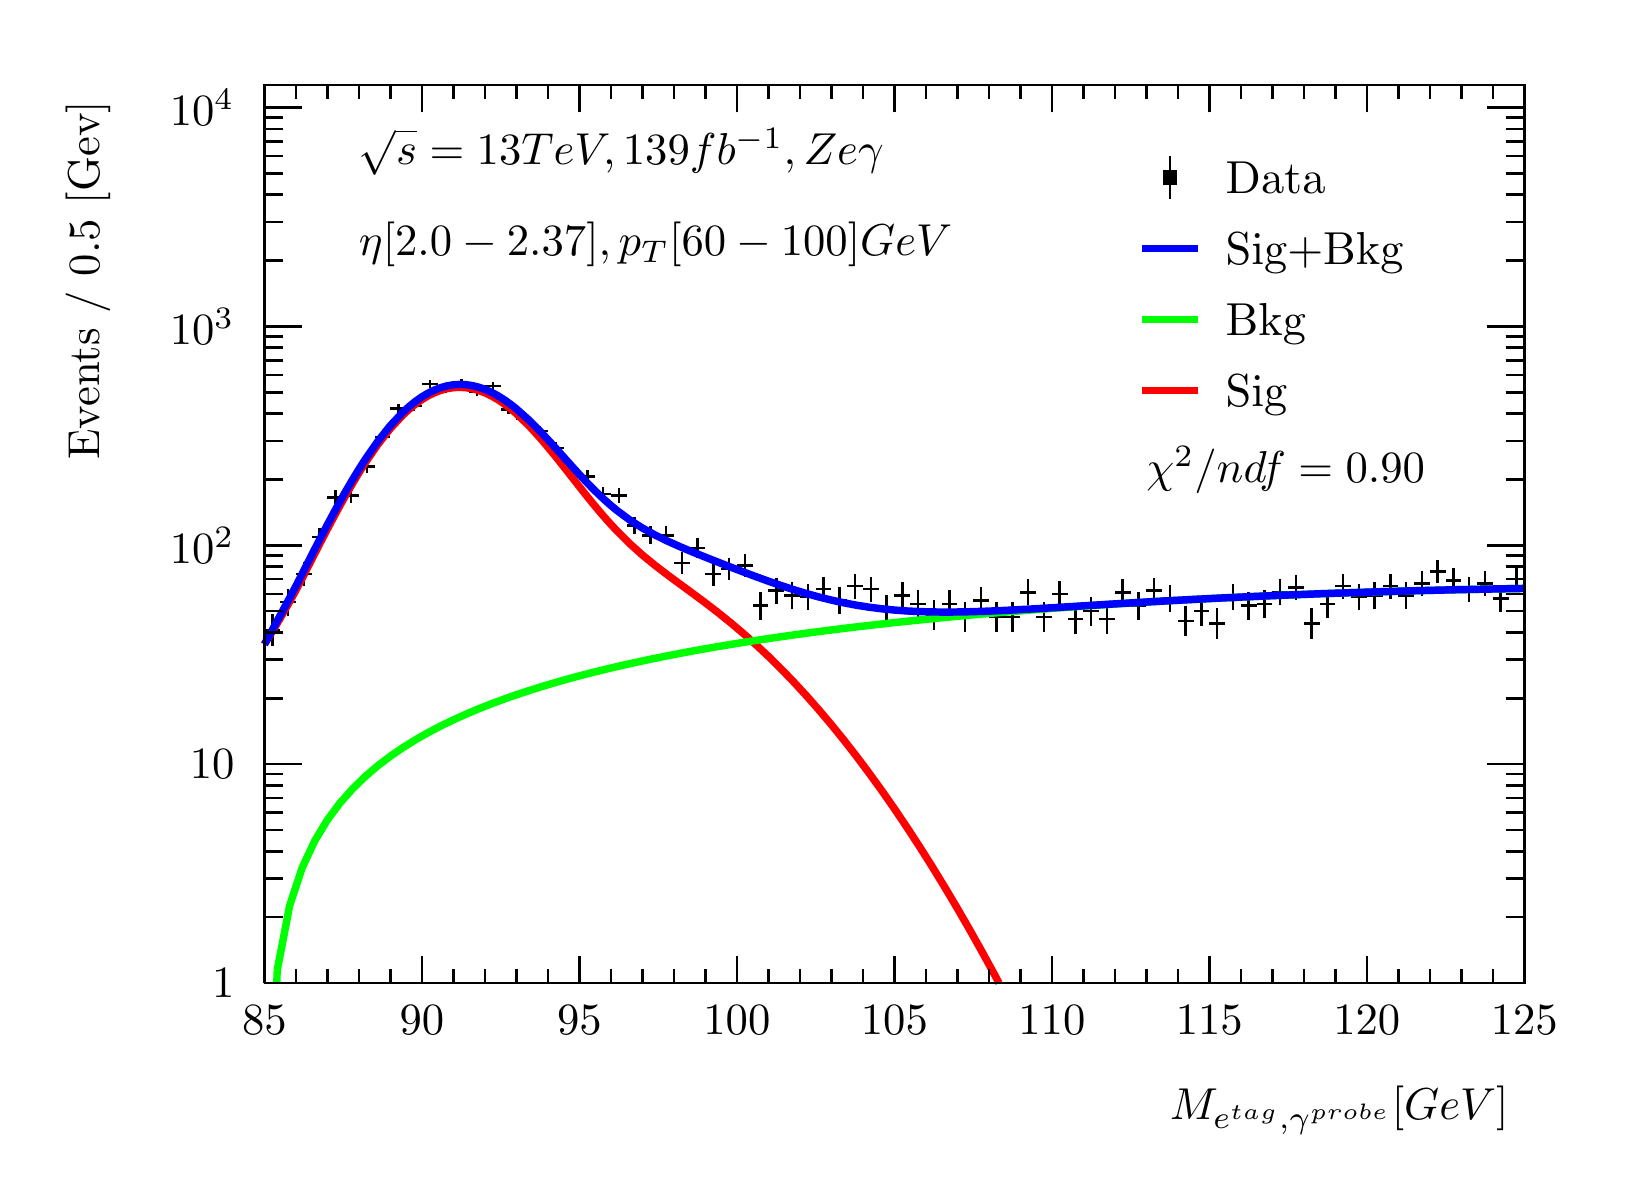
\begin{tikzpicture}
\pgfdeclareplotmark{cross} {
\pgfpathmoveto{\pgfpoint{-0.3\pgfplotmarksize}{\pgfplotmarksize}}
\pgfpathlineto{\pgfpoint{+0.3\pgfplotmarksize}{\pgfplotmarksize}}
\pgfpathlineto{\pgfpoint{+0.3\pgfplotmarksize}{0.3\pgfplotmarksize}}
\pgfpathlineto{\pgfpoint{+1\pgfplotmarksize}{0.3\pgfplotmarksize}}
\pgfpathlineto{\pgfpoint{+1\pgfplotmarksize}{-0.3\pgfplotmarksize}}
\pgfpathlineto{\pgfpoint{+0.3\pgfplotmarksize}{-0.3\pgfplotmarksize}}
\pgfpathlineto{\pgfpoint{+0.3\pgfplotmarksize}{-1.\pgfplotmarksize}}
\pgfpathlineto{\pgfpoint{-0.3\pgfplotmarksize}{-1.\pgfplotmarksize}}
\pgfpathlineto{\pgfpoint{-0.3\pgfplotmarksize}{-0.3\pgfplotmarksize}}
\pgfpathlineto{\pgfpoint{-1.\pgfplotmarksize}{-0.3\pgfplotmarksize}}
\pgfpathlineto{\pgfpoint{-1.\pgfplotmarksize}{0.3\pgfplotmarksize}}
\pgfpathlineto{\pgfpoint{-0.3\pgfplotmarksize}{0.3\pgfplotmarksize}}
\pgfpathclose
\pgfusepathqstroke
}
\pgfdeclareplotmark{cross*} {
\pgfpathmoveto{\pgfpoint{-0.3\pgfplotmarksize}{\pgfplotmarksize}}
\pgfpathlineto{\pgfpoint{+0.3\pgfplotmarksize}{\pgfplotmarksize}}
\pgfpathlineto{\pgfpoint{+0.3\pgfplotmarksize}{0.3\pgfplotmarksize}}
\pgfpathlineto{\pgfpoint{+1\pgfplotmarksize}{0.3\pgfplotmarksize}}
\pgfpathlineto{\pgfpoint{+1\pgfplotmarksize}{-0.3\pgfplotmarksize}}
\pgfpathlineto{\pgfpoint{+0.3\pgfplotmarksize}{-0.3\pgfplotmarksize}}
\pgfpathlineto{\pgfpoint{+0.3\pgfplotmarksize}{-1.\pgfplotmarksize}}
\pgfpathlineto{\pgfpoint{-0.3\pgfplotmarksize}{-1.\pgfplotmarksize}}
\pgfpathlineto{\pgfpoint{-0.3\pgfplotmarksize}{-0.3\pgfplotmarksize}}
\pgfpathlineto{\pgfpoint{-1.\pgfplotmarksize}{-0.3\pgfplotmarksize}}
\pgfpathlineto{\pgfpoint{-1.\pgfplotmarksize}{0.3\pgfplotmarksize}}
\pgfpathlineto{\pgfpoint{-0.3\pgfplotmarksize}{0.3\pgfplotmarksize}}
\pgfpathclose
\pgfusepathqfillstroke
}
\pgfdeclareplotmark{newstar} {
\pgfpathmoveto{\pgfqpoint{0pt}{\pgfplotmarksize}}
\pgfpathlineto{\pgfqpointpolar{44}{0.5\pgfplotmarksize}}
\pgfpathlineto{\pgfqpointpolar{18}{\pgfplotmarksize}}
\pgfpathlineto{\pgfqpointpolar{-20}{0.5\pgfplotmarksize}}
\pgfpathlineto{\pgfqpointpolar{-54}{\pgfplotmarksize}}
\pgfpathlineto{\pgfqpointpolar{-90}{0.5\pgfplotmarksize}}
\pgfpathlineto{\pgfqpointpolar{234}{\pgfplotmarksize}}
\pgfpathlineto{\pgfqpointpolar{198}{0.5\pgfplotmarksize}}
\pgfpathlineto{\pgfqpointpolar{162}{\pgfplotmarksize}}
\pgfpathlineto{\pgfqpointpolar{134}{0.5\pgfplotmarksize}}
\pgfpathclose
\pgfusepathqstroke
}
\pgfdeclareplotmark{newstar*} {
\pgfpathmoveto{\pgfqpoint{0pt}{\pgfplotmarksize}}
\pgfpathlineto{\pgfqpointpolar{44}{0.5\pgfplotmarksize}}
\pgfpathlineto{\pgfqpointpolar{18}{\pgfplotmarksize}}
\pgfpathlineto{\pgfqpointpolar{-20}{0.5\pgfplotmarksize}}
\pgfpathlineto{\pgfqpointpolar{-54}{\pgfplotmarksize}}
\pgfpathlineto{\pgfqpointpolar{-90}{0.5\pgfplotmarksize}}
\pgfpathlineto{\pgfqpointpolar{234}{\pgfplotmarksize}}
\pgfpathlineto{\pgfqpointpolar{198}{0.5\pgfplotmarksize}}
\pgfpathlineto{\pgfqpointpolar{162}{\pgfplotmarksize}}
\pgfpathlineto{\pgfqpointpolar{134}{0.5\pgfplotmarksize}}
\pgfpathclose
\pgfusepathqfillstroke
}
\definecolor{c}{rgb}{1,1,1};
\draw [color=c, fill=c] (0,0) rectangle (20,14.4361);
\draw [color=c, fill=c] (3,2.30977) rectangle (19,13.7143);
\definecolor{c}{rgb}{0,0,0};
\draw [c,line width=0.9] (3,2.30977) -- (3,13.7143) -- (19,13.7143) -- (19,2.30977) -- (3,2.30977);
\definecolor{c}{rgb}{1,1,1};
\draw [color=c, fill=c] (3,2.30977) rectangle (19,13.7143);
\definecolor{c}{rgb}{0,0,0};
\draw [c,line width=0.9] (3,2.30977) -- (3,13.7143) -- (19,13.7143) -- (19,2.30977) -- (3,2.30977);
\draw [c,line width=0.9] (3,2.30977) -- (19,2.30977);
\draw [c,line width=0.9] (3,2.65624) -- (3,2.30977);
\draw [c,line width=0.9] (3.4,2.48301) -- (3.4,2.30977);
\draw [c,line width=0.9] (3.8,2.48301) -- (3.8,2.30977);
\draw [c,line width=0.9] (4.2,2.48301) -- (4.2,2.30977);
\draw [c,line width=0.9] (4.6,2.48301) -- (4.6,2.30977);
\draw [c,line width=0.9] (5,2.65624) -- (5,2.30977);
\draw [c,line width=0.9] (5.4,2.48301) -- (5.4,2.30977);
\draw [c,line width=0.9] (5.8,2.48301) -- (5.8,2.30977);
\draw [c,line width=0.9] (6.2,2.48301) -- (6.2,2.30977);
\draw [c,line width=0.9] (6.6,2.48301) -- (6.6,2.30977);
\draw [c,line width=0.9] (7,2.65624) -- (7,2.30977);
\draw [c,line width=0.9] (7.4,2.48301) -- (7.4,2.30977);
\draw [c,line width=0.9] (7.8,2.48301) -- (7.8,2.30977);
\draw [c,line width=0.9] (8.2,2.48301) -- (8.2,2.30977);
\draw [c,line width=0.9] (8.6,2.48301) -- (8.6,2.30977);
\draw [c,line width=0.9] (9,2.65624) -- (9,2.30977);
\draw [c,line width=0.9] (9.4,2.48301) -- (9.4,2.30977);
\draw [c,line width=0.9] (9.8,2.48301) -- (9.8,2.30977);
\draw [c,line width=0.9] (10.2,2.48301) -- (10.2,2.30977);
\draw [c,line width=0.9] (10.6,2.48301) -- (10.6,2.30977);
\draw [c,line width=0.9] (11,2.65624) -- (11,2.30977);
\draw [c,line width=0.9] (11.4,2.48301) -- (11.4,2.30977);
\draw [c,line width=0.9] (11.8,2.48301) -- (11.8,2.30977);
\draw [c,line width=0.9] (12.2,2.48301) -- (12.2,2.30977);
\draw [c,line width=0.9] (12.6,2.48301) -- (12.6,2.30977);
\draw [c,line width=0.9] (13,2.65624) -- (13,2.30977);
\draw [c,line width=0.9] (13.4,2.48301) -- (13.4,2.30977);
\draw [c,line width=0.9] (13.8,2.48301) -- (13.8,2.30977);
\draw [c,line width=0.9] (14.2,2.48301) -- (14.2,2.30977);
\draw [c,line width=0.9] (14.6,2.48301) -- (14.6,2.30977);
\draw [c,line width=0.9] (15,2.65624) -- (15,2.30977);
\draw [c,line width=0.9] (15.4,2.48301) -- (15.4,2.30977);
\draw [c,line width=0.9] (15.8,2.48301) -- (15.8,2.30977);
\draw [c,line width=0.9] (16.2,2.48301) -- (16.2,2.30977);
\draw [c,line width=0.9] (16.6,2.48301) -- (16.6,2.30977);
\draw [c,line width=0.9] (17,2.65624) -- (17,2.30977);
\draw [c,line width=0.9] (17.4,2.48301) -- (17.4,2.30977);
\draw [c,line width=0.9] (17.8,2.48301) -- (17.8,2.30977);
\draw [c,line width=0.9] (18.2,2.48301) -- (18.2,2.30977);
\draw [c,line width=0.9] (18.6,2.48301) -- (18.6,2.30977);
\draw [c,line width=0.9] (19,2.65624) -- (19,2.30977);
\draw [anchor=base] (3,1.66015) node[scale=1.61424, color=c, rotate=0]{85};
\draw [anchor=base] (5,1.66015) node[scale=1.61424, color=c, rotate=0]{90};
\draw [anchor=base] (7,1.66015) node[scale=1.61424, color=c, rotate=0]{95};
\draw [anchor=base] (9,1.66015) node[scale=1.61424, color=c, rotate=0]{100};
\draw [anchor=base] (11,1.66015) node[scale=1.61424, color=c, rotate=0]{105};
\draw [anchor=base] (13,1.66015) node[scale=1.61424, color=c, rotate=0]{110};
\draw [anchor=base] (15,1.66015) node[scale=1.61424, color=c, rotate=0]{115};
\draw [anchor=base] (17,1.66015) node[scale=1.61424, color=c, rotate=0]{120};
\draw [anchor=base] (19,1.66015) node[scale=1.61424, color=c, rotate=0]{125};
\draw [anchor= east] (19,0.692932) node[scale=1.61424, color=c, rotate=0]{$M_{e^{tag}, \gamma^{probe}}  [GeV]$};
\draw [c,line width=0.9] (3,13.7143) -- (19,13.7143);
\draw [c,line width=0.9] (3,13.3678) -- (3,13.7143);
\draw [c,line width=0.9] (3.4,13.5411) -- (3.4,13.7143);
\draw [c,line width=0.9] (3.8,13.5411) -- (3.8,13.7143);
\draw [c,line width=0.9] (4.2,13.5411) -- (4.2,13.7143);
\draw [c,line width=0.9] (4.6,13.5411) -- (4.6,13.7143);
\draw [c,line width=0.9] (5,13.3678) -- (5,13.7143);
\draw [c,line width=0.9] (5.4,13.5411) -- (5.4,13.7143);
\draw [c,line width=0.9] (5.8,13.5411) -- (5.8,13.7143);
\draw [c,line width=0.9] (6.2,13.5411) -- (6.2,13.7143);
\draw [c,line width=0.9] (6.6,13.5411) -- (6.6,13.7143);
\draw [c,line width=0.9] (7,13.3678) -- (7,13.7143);
\draw [c,line width=0.9] (7.4,13.5411) -- (7.4,13.7143);
\draw [c,line width=0.9] (7.8,13.5411) -- (7.8,13.7143);
\draw [c,line width=0.9] (8.2,13.5411) -- (8.2,13.7143);
\draw [c,line width=0.9] (8.6,13.5411) -- (8.6,13.7143);
\draw [c,line width=0.9] (9,13.3678) -- (9,13.7143);
\draw [c,line width=0.9] (9.4,13.5411) -- (9.4,13.7143);
\draw [c,line width=0.9] (9.8,13.5411) -- (9.8,13.7143);
\draw [c,line width=0.9] (10.2,13.5411) -- (10.2,13.7143);
\draw [c,line width=0.9] (10.6,13.5411) -- (10.6,13.7143);
\draw [c,line width=0.9] (11,13.3678) -- (11,13.7143);
\draw [c,line width=0.9] (11.4,13.5411) -- (11.4,13.7143);
\draw [c,line width=0.9] (11.8,13.5411) -- (11.8,13.7143);
\draw [c,line width=0.9] (12.2,13.5411) -- (12.2,13.7143);
\draw [c,line width=0.9] (12.6,13.5411) -- (12.6,13.7143);
\draw [c,line width=0.9] (13,13.3678) -- (13,13.7143);
\draw [c,line width=0.9] (13.4,13.5411) -- (13.4,13.7143);
\draw [c,line width=0.9] (13.8,13.5411) -- (13.8,13.7143);
\draw [c,line width=0.9] (14.2,13.5411) -- (14.2,13.7143);
\draw [c,line width=0.9] (14.6,13.5411) -- (14.6,13.7143);
\draw [c,line width=0.9] (15,13.3678) -- (15,13.7143);
\draw [c,line width=0.9] (15.4,13.5411) -- (15.4,13.7143);
\draw [c,line width=0.9] (15.8,13.5411) -- (15.8,13.7143);
\draw [c,line width=0.9] (16.2,13.5411) -- (16.2,13.7143);
\draw [c,line width=0.9] (16.6,13.5411) -- (16.6,13.7143);
\draw [c,line width=0.9] (17,13.3678) -- (17,13.7143);
\draw [c,line width=0.9] (17.4,13.5411) -- (17.4,13.7143);
\draw [c,line width=0.9] (17.8,13.5411) -- (17.8,13.7143);
\draw [c,line width=0.9] (18.2,13.5411) -- (18.2,13.7143);
\draw [c,line width=0.9] (18.6,13.5411) -- (18.6,13.7143);
\draw [c,line width=0.9] (19,13.3678) -- (19,13.7143);
\draw [c,line width=0.9] (3,2.30977) -- (3,13.7143);
\draw [c,line width=0.9] (3.474,2.30978) -- (3,2.30978);
\draw [anchor= east] (2.82,2.30978) node[scale=1.61424, color=c, rotate=0]{1};
\draw [c,line width=0.9] (3.237,3.14655) -- (3,3.14655);
\draw [c,line width=0.9] (3.237,3.63603) -- (3,3.63603);
\draw [c,line width=0.9] (3.237,3.98333) -- (3,3.98333);
\draw [c,line width=0.9] (3.237,4.25271) -- (3,4.25271);
\draw [c,line width=0.9] (3.237,4.47281) -- (3,4.47281);
\draw [c,line width=0.9] (3.237,4.6589) -- (3,4.6589);
\draw [c,line width=0.9] (3.237,4.8201) -- (3,4.8201);
\draw [c,line width=0.9] (3.237,4.96229) -- (3,4.96229);
\draw [c,line width=0.9] (3.474,5.08948) -- (3,5.08948);
\draw [anchor= east] (2.82,5.08948) node[scale=1.61424, color=c, rotate=0]{10};
\draw [c,line width=0.9] (3.237,5.92626) -- (3,5.92626);
\draw [c,line width=0.9] (3.237,6.41574) -- (3,6.41574);
\draw [c,line width=0.9] (3.237,6.76303) -- (3,6.76303);
\draw [c,line width=0.9] (3.237,7.03241) -- (3,7.03241);
\draw [c,line width=0.9] (3.237,7.25251) -- (3,7.25251);
\draw [c,line width=0.9] (3.237,7.43861) -- (3,7.43861);
\draw [c,line width=0.9] (3.237,7.59981) -- (3,7.59981);
\draw [c,line width=0.9] (3.237,7.74199) -- (3,7.74199);
\draw [c,line width=0.9] (3.474,7.86919) -- (3,7.86919);
\draw [anchor= east] (2.82,7.86919) node[scale=1.61424, color=c, rotate=0]{$10^{2}$};
\draw [c,line width=0.9] (3.237,8.70596) -- (3,8.70596);
\draw [c,line width=0.9] (3.237,9.19544) -- (3,9.19544);
\draw [c,line width=0.9] (3.237,9.54274) -- (3,9.54274);
\draw [c,line width=0.9] (3.237,9.81212) -- (3,9.81212);
\draw [c,line width=0.9] (3.237,10.0322) -- (3,10.0322);
\draw [c,line width=0.9] (3.237,10.2183) -- (3,10.2183);
\draw [c,line width=0.9] (3.237,10.3795) -- (3,10.3795);
\draw [c,line width=0.9] (3.237,10.5217) -- (3,10.5217);
\draw [c,line width=0.9] (3.474,10.6489) -- (3,10.6489);
\draw [anchor= east] (2.82,10.6489) node[scale=1.61424, color=c, rotate=0]{$10^{3}$};
\draw [c,line width=0.9] (3.237,11.4857) -- (3,11.4857);
\draw [c,line width=0.9] (3.237,11.9751) -- (3,11.9751);
\draw [c,line width=0.9] (3.237,12.3224) -- (3,12.3224);
\draw [c,line width=0.9] (3.237,12.5918) -- (3,12.5918);
\draw [c,line width=0.9] (3.237,12.8119) -- (3,12.8119);
\draw [c,line width=0.9] (3.237,12.998) -- (3,12.998);
\draw [c,line width=0.9] (3.237,13.1592) -- (3,13.1592);
\draw [c,line width=0.9] (3.237,13.3014) -- (3,13.3014);
\draw [c,line width=0.9] (3.474,13.4286) -- (3,13.4286);
\draw [anchor= east] (2.82,13.4286) node[scale=1.61424, color=c, rotate=0]{$10^{4}$};
\draw [anchor= east] (0.76,13.7143) node[scale=1.61424, color=c, rotate=90]{Events / 0.5 [Gev]};
\draw [c,line width=0.9] (19,2.30977) -- (19,13.7143);
\draw [c,line width=0.9] (18.526,2.30978) -- (19,2.30978);
\draw [c,line width=0.9] (18.763,3.14655) -- (19,3.14655);
\draw [c,line width=0.9] (18.763,3.63603) -- (19,3.63603);
\draw [c,line width=0.9] (18.763,3.98333) -- (19,3.98333);
\draw [c,line width=0.9] (18.763,4.25271) -- (19,4.25271);
\draw [c,line width=0.9] (18.763,4.47281) -- (19,4.47281);
\draw [c,line width=0.9] (18.763,4.6589) -- (19,4.6589);
\draw [c,line width=0.9] (18.763,4.8201) -- (19,4.8201);
\draw [c,line width=0.9] (18.763,4.96229) -- (19,4.96229);
\draw [c,line width=0.9] (18.526,5.08948) -- (19,5.08948);
\draw [c,line width=0.9] (18.763,5.92626) -- (19,5.92626);
\draw [c,line width=0.9] (18.763,6.41574) -- (19,6.41574);
\draw [c,line width=0.9] (18.763,6.76303) -- (19,6.76303);
\draw [c,line width=0.9] (18.763,7.03241) -- (19,7.03241);
\draw [c,line width=0.9] (18.763,7.25251) -- (19,7.25251);
\draw [c,line width=0.9] (18.763,7.43861) -- (19,7.43861);
\draw [c,line width=0.9] (18.763,7.59981) -- (19,7.59981);
\draw [c,line width=0.9] (18.763,7.74199) -- (19,7.74199);
\draw [c,line width=0.9] (18.526,7.86919) -- (19,7.86919);
\draw [c,line width=0.9] (18.763,8.70596) -- (19,8.70596);
\draw [c,line width=0.9] (18.763,9.19544) -- (19,9.19544);
\draw [c,line width=0.9] (18.763,9.54274) -- (19,9.54274);
\draw [c,line width=0.9] (18.763,9.81212) -- (19,9.81212);
\draw [c,line width=0.9] (18.763,10.0322) -- (19,10.0322);
\draw [c,line width=0.9] (18.763,10.2183) -- (19,10.2183);
\draw [c,line width=0.9] (18.763,10.3795) -- (19,10.3795);
\draw [c,line width=0.9] (18.763,10.5217) -- (19,10.5217);
\draw [c,line width=0.9] (18.526,10.6489) -- (19,10.6489);
\draw [c,line width=0.9] (18.763,11.4857) -- (19,11.4857);
\draw [c,line width=0.9] (18.763,11.9751) -- (19,11.9751);
\draw [c,line width=0.9] (18.763,12.3224) -- (19,12.3224);
\draw [c,line width=0.9] (18.763,12.5918) -- (19,12.5918);
\draw [c,line width=0.9] (18.763,12.8119) -- (19,12.8119);
\draw [c,line width=0.9] (18.763,12.998) -- (19,12.998);
\draw [c,line width=0.9] (18.763,13.1592) -- (19,13.1592);
\draw [c,line width=0.9] (18.763,13.3014) -- (19,13.3014);
\draw [c,line width=0.9] (18.526,13.4286) -- (19,13.4286);
\draw [c,line width=0.9] (3.1,6.79284) -- (3,6.79284);
\draw [c,line width=0.9] (3,6.79284) -- (3,6.79284);
\draw [c,line width=0.9] (3.1,6.79284) -- (3.2,6.79284);
\draw [c,line width=0.9] (3.2,6.79284) -- (3.2,6.79284);
\draw [c,line width=0.9] (3.1,6.79284) -- (3.1,6.99452);
\draw [c,line width=0.9] (3.1,6.99452) -- (3.1,6.99452);
\draw [c,line width=0.9] (3.1,6.79284) -- (3.1,6.58876);
\draw [c,line width=0.9] (3.1,6.58876) -- (3.1,6.58876);
\draw [c,line width=0.9] (3.3,7.14747) -- (3.2,7.14747);
\draw [c,line width=0.9] (3.2,7.14747) -- (3.2,7.14747);
\draw [c,line width=0.9] (3.3,7.14747) -- (3.4,7.14747);
\draw [c,line width=0.9] (3.4,7.14747) -- (3.4,7.14747);
\draw [c,line width=0.9] (3.3,7.14747) -- (3.3,7.32022);
\draw [c,line width=0.9] (3.3,7.32022) -- (3.3,7.32022);
\draw [c,line width=0.9] (3.3,7.14747) -- (3.3,6.97319);
\draw [c,line width=0.9] (3.3,6.97319) -- (3.3,6.97319);
\draw [c,line width=0.9] (3.5,7.50569) -- (3.4,7.50569);
\draw [c,line width=0.9] (3.4,7.50569) -- (3.4,7.50569);
\draw [c,line width=0.9] (3.5,7.50569) -- (3.6,7.50569);
\draw [c,line width=0.9] (3.6,7.50569) -- (3.6,7.50569);
\draw [c,line width=0.9] (3.5,7.50569) -- (3.5,7.65354);
\draw [c,line width=0.9] (3.5,7.65354) -- (3.5,7.65354);
\draw [c,line width=0.9] (3.5,7.50569) -- (3.5,7.35686);
\draw [c,line width=0.9] (3.5,7.35686) -- (3.5,7.35686);
\draw [c,line width=0.9] (3.7,7.97322) -- (3.6,7.97322);
\draw [c,line width=0.9] (3.6,7.97322) -- (3.6,7.97322);
\draw [c,line width=0.9] (3.7,7.97322) -- (3.8,7.97322);
\draw [c,line width=0.9] (3.8,7.97322) -- (3.8,7.97322);
\draw [c,line width=0.9] (3.7,7.97322) -- (3.7,8.08881);
\draw [c,line width=0.9] (3.7,8.08881) -- (3.7,8.08881);
\draw [c,line width=0.9] (3.7,7.97322) -- (3.7,7.85763);
\draw [c,line width=0.9] (3.7,7.85763) -- (3.7,7.85763);
\draw [c,line width=0.9] (3.9,8.47373) -- (3.8,8.47373);
\draw [c,line width=0.9] (3.8,8.47373) -- (3.8,8.47373);
\draw [c,line width=0.9] (3.9,8.47373) -- (4,8.47373);
\draw [c,line width=0.9] (4,8.47373) -- (4,8.47373);
\draw [c,line width=0.9] (3.9,8.47373) -- (3.9,8.56769);
\draw [c,line width=0.9] (3.9,8.56769) -- (3.9,8.56769);
\draw [c,line width=0.9] (3.9,8.47373) -- (3.9,8.37977);
\draw [c,line width=0.9] (3.9,8.37977) -- (3.9,8.37977);
\draw [c,line width=0.9] (4.1,8.50264) -- (4,8.50264);
\draw [c,line width=0.9] (4,8.50264) -- (4,8.50264);
\draw [c,line width=0.9] (4.1,8.50264) -- (4.2,8.50264);
\draw [c,line width=0.9] (4.2,8.50264) -- (4.2,8.50264);
\draw [c,line width=0.9] (4.1,8.50264) -- (4.1,8.59548);
\draw [c,line width=0.9] (4.1,8.59548) -- (4.1,8.59548);
\draw [c,line width=0.9] (4.1,8.50264) -- (4.1,8.4098);
\draw [c,line width=0.9] (4.1,8.4098) -- (4.1,8.4098);
\draw [c,line width=0.9] (4.3,8.86942) -- (4.2,8.86942);
\draw [c,line width=0.9] (4.2,8.86942) -- (4.2,8.86942);
\draw [c,line width=0.9] (4.3,8.86942) -- (4.4,8.86942);
\draw [c,line width=0.9] (4.4,8.86942) -- (4.4,8.86942);
\draw [c,line width=0.9] (4.3,8.86942) -- (4.3,8.94918);
\draw [c,line width=0.9] (4.3,8.94918) -- (4.3,8.94918);
\draw [c,line width=0.9] (4.3,8.86942) -- (4.3,8.78966);
\draw [c,line width=0.9] (4.3,8.78966) -- (4.3,8.78966);
\draw [c,line width=0.9] (4.5,9.24665) -- (4.4,9.24665);
\draw [c,line width=0.9] (4.4,9.24665) -- (4.4,9.24665);
\draw [c,line width=0.9] (4.5,9.24665) -- (4.6,9.24665);
\draw [c,line width=0.9] (4.6,9.24665) -- (4.6,9.24665);
\draw [c,line width=0.9] (4.5,9.24665) -- (4.5,9.31488);
\draw [c,line width=0.9] (4.5,9.31488) -- (4.5,9.31488);
\draw [c,line width=0.9] (4.5,9.24665) -- (4.5,9.17843);
\draw [c,line width=0.9] (4.5,9.17843) -- (4.5,9.17843);
\draw [c,line width=0.9] (4.7,9.60451) -- (4.6,9.60451);
\draw [c,line width=0.9] (4.6,9.60451) -- (4.6,9.60451);
\draw [c,line width=0.9] (4.7,9.60451) -- (4.8,9.60451);
\draw [c,line width=0.9] (4.8,9.60451) -- (4.8,9.60451);
\draw [c,line width=0.9] (4.7,9.60451) -- (4.7,9.66334);
\draw [c,line width=0.9] (4.7,9.66334) -- (4.7,9.66334);
\draw [c,line width=0.9] (4.7,9.60451) -- (4.7,9.54568);
\draw [c,line width=0.9] (4.7,9.54568) -- (4.7,9.54568);
\draw [c,line width=0.9] (4.9,9.63843) -- (4.8,9.63843);
\draw [c,line width=0.9] (4.8,9.63843) -- (4.8,9.63843);
\draw [c,line width=0.9] (4.9,9.63843) -- (5,9.63843);
\draw [c,line width=0.9] (5,9.63843) -- (5,9.63843);
\draw [c,line width=0.9] (4.9,9.63843) -- (4.9,9.69644);
\draw [c,line width=0.9] (4.9,9.69644) -- (4.9,9.69644);
\draw [c,line width=0.9] (4.9,9.63843) -- (4.9,9.58043);
\draw [c,line width=0.9] (4.9,9.58043) -- (4.9,9.58043);
\draw [c,line width=0.9] (5.1,9.92057) -- (5,9.92057);
\draw [c,line width=0.9] (5,9.92057) -- (5,9.92057);
\draw [c,line width=0.9] (5.1,9.92057) -- (5.2,9.92057);
\draw [c,line width=0.9] (5.2,9.92057) -- (5.2,9.92057);
\draw [c,line width=0.9] (5.1,9.92057) -- (5.1,9.97219);
\draw [c,line width=0.9] (5.1,9.97219) -- (5.1,9.97219);
\draw [c,line width=0.9] (5.1,9.92057) -- (5.1,9.86896);
\draw [c,line width=0.9] (5.1,9.86896) -- (5.1,9.86896);
\draw [c,line width=0.9] (5.3,9.85481) -- (5.2,9.85481);
\draw [c,line width=0.9] (5.2,9.85481) -- (5.2,9.85481);
\draw [c,line width=0.9] (5.3,9.85481) -- (5.4,9.85481);
\draw [c,line width=0.9] (5.4,9.85481) -- (5.4,9.85481);
\draw [c,line width=0.9] (5.3,9.85481) -- (5.3,9.90785);
\draw [c,line width=0.9] (5.3,9.90785) -- (5.3,9.90785);
\draw [c,line width=0.9] (5.3,9.85481) -- (5.3,9.80177);
\draw [c,line width=0.9] (5.3,9.80177) -- (5.3,9.80177);
\draw [c,line width=0.9] (5.5,9.92718) -- (5.4,9.92718);
\draw [c,line width=0.9] (5.4,9.92718) -- (5.4,9.92718);
\draw [c,line width=0.9] (5.5,9.92718) -- (5.6,9.92718);
\draw [c,line width=0.9] (5.6,9.92718) -- (5.6,9.92718);
\draw [c,line width=0.9] (5.5,9.92718) -- (5.5,9.97865);
\draw [c,line width=0.9] (5.5,9.97865) -- (5.5,9.97865);
\draw [c,line width=0.9] (5.5,9.92718) -- (5.5,9.8757);
\draw [c,line width=0.9] (5.5,9.8757) -- (5.5,9.8757);
\draw [c,line width=0.9] (5.7,9.82174) -- (5.6,9.82174);
\draw [c,line width=0.9] (5.6,9.82174) -- (5.6,9.82174);
\draw [c,line width=0.9] (5.7,9.82174) -- (5.8,9.82174);
\draw [c,line width=0.9] (5.8,9.82174) -- (5.8,9.82174);
\draw [c,line width=0.9] (5.7,9.82174) -- (5.7,9.8755);
\draw [c,line width=0.9] (5.7,9.8755) -- (5.7,9.8755);
\draw [c,line width=0.9] (5.7,9.82174) -- (5.7,9.76797);
\draw [c,line width=0.9] (5.7,9.76797) -- (5.7,9.76797);
\draw [c,line width=0.9] (5.9,9.8938) -- (5.8,9.8938);
\draw [c,line width=0.9] (5.8,9.8938) -- (5.8,9.8938);
\draw [c,line width=0.9] (5.9,9.8938) -- (6,9.8938);
\draw [c,line width=0.9] (6,9.8938) -- (6,9.8938);
\draw [c,line width=0.9] (5.9,9.8938) -- (5.9,9.94598);
\draw [c,line width=0.9] (5.9,9.94598) -- (5.9,9.94598);
\draw [c,line width=0.9] (5.9,9.8938) -- (5.9,9.84161);
\draw [c,line width=0.9] (5.9,9.84161) -- (5.9,9.84161);
\draw [c,line width=0.9] (6.1,9.59298) -- (6,9.59298);
\draw [c,line width=0.9] (6,9.59298) -- (6,9.59298);
\draw [c,line width=0.9] (6.1,9.59298) -- (6.2,9.59298);
\draw [c,line width=0.9] (6.2,9.59298) -- (6.2,9.59298);
\draw [c,line width=0.9] (6.1,9.59298) -- (6.1,9.65209);
\draw [c,line width=0.9] (6.1,9.65209) -- (6.1,9.65209);
\draw [c,line width=0.9] (6.1,9.59298) -- (6.1,9.53387);
\draw [c,line width=0.9] (6.1,9.53387) -- (6.1,9.53387);
\draw [c,line width=0.9] (6.3,9.47124) -- (6.2,9.47124);
\draw [c,line width=0.9] (6.2,9.47124) -- (6.2,9.47124);
\draw [c,line width=0.9] (6.3,9.47124) -- (6.4,9.47124);
\draw [c,line width=0.9] (6.4,9.47124) -- (6.4,9.47124);
\draw [c,line width=0.9] (6.3,9.47124) -- (6.3,9.53341);
\draw [c,line width=0.9] (6.3,9.53341) -- (6.3,9.53341);
\draw [c,line width=0.9] (6.3,9.47124) -- (6.3,9.40908);
\draw [c,line width=0.9] (6.3,9.40908) -- (6.3,9.40908);
\draw [c,line width=0.9] (6.5,9.3178) -- (6.4,9.3178);
\draw [c,line width=0.9] (6.4,9.3178) -- (6.4,9.3178);
\draw [c,line width=0.9] (6.5,9.3178) -- (6.6,9.3178);
\draw [c,line width=0.9] (6.6,9.3178) -- (6.6,9.3178);
\draw [c,line width=0.9] (6.5,9.3178) -- (6.5,9.38404);
\draw [c,line width=0.9] (6.5,9.38404) -- (6.5,9.38404);
\draw [c,line width=0.9] (6.5,9.3178) -- (6.5,9.25155);
\draw [c,line width=0.9] (6.5,9.25155) -- (6.5,9.25155);
\draw [c,line width=0.9] (6.7,9.10783) -- (6.6,9.10783);
\draw [c,line width=0.9] (6.6,9.10783) -- (6.6,9.10783);
\draw [c,line width=0.9] (6.7,9.10783) -- (6.8,9.10783);
\draw [c,line width=0.9] (6.8,9.10783) -- (6.8,9.10783);
\draw [c,line width=0.9] (6.7,9.10783) -- (6.7,9.1801);
\draw [c,line width=0.9] (6.7,9.1801) -- (6.7,9.1801);
\draw [c,line width=0.9] (6.7,9.10783) -- (6.7,9.03557);
\draw [c,line width=0.9] (6.7,9.03557) -- (6.7,9.03557);
\draw [c,line width=0.9] (6.9,8.79887) -- (6.8,8.79887);
\draw [c,line width=0.9] (6.8,8.79887) -- (6.8,8.79887);
\draw [c,line width=0.9] (6.9,8.79887) -- (7,8.79887);
\draw [c,line width=0.9] (7,8.79887) -- (7,8.79887);
\draw [c,line width=0.9] (6.9,8.79887) -- (6.9,8.88099);
\draw [c,line width=0.9] (6.9,8.88099) -- (6.9,8.88099);
\draw [c,line width=0.9] (6.9,8.79887) -- (6.9,8.71674);
\draw [c,line width=0.9] (6.9,8.71674) -- (6.9,8.71674);
\draw [c,line width=0.9] (7.1,8.74164) -- (7,8.74164);
\draw [c,line width=0.9] (7,8.74164) -- (7,8.74164);
\draw [c,line width=0.9] (7.1,8.74164) -- (7.2,8.74164);
\draw [c,line width=0.9] (7.2,8.74164) -- (7.2,8.74164);
\draw [c,line width=0.9] (7.1,8.74164) -- (7.1,8.82574);
\draw [c,line width=0.9] (7.1,8.82574) -- (7.1,8.82574);
\draw [c,line width=0.9] (7.1,8.74164) -- (7.1,8.65755);
\draw [c,line width=0.9] (7.1,8.65755) -- (7.1,8.65755);
\draw [c,line width=0.9] (7.3,8.52389) -- (7.2,8.52389);
\draw [c,line width=0.9] (7.2,8.52389) -- (7.2,8.52389);
\draw [c,line width=0.9] (7.3,8.52389) -- (7.4,8.52389);
\draw [c,line width=0.9] (7.4,8.52389) -- (7.4,8.52389);
\draw [c,line width=0.9] (7.3,8.52389) -- (7.3,8.61591);
\draw [c,line width=0.9] (7.3,8.61591) -- (7.3,8.61591);
\draw [c,line width=0.9] (7.3,8.52389) -- (7.3,8.43186);
\draw [c,line width=0.9] (7.3,8.43186) -- (7.3,8.43186);
\draw [c,line width=0.9] (7.5,8.50264) -- (7.4,8.50264);
\draw [c,line width=0.9] (7.4,8.50264) -- (7.4,8.50264);
\draw [c,line width=0.9] (7.5,8.50264) -- (7.6,8.50264);
\draw [c,line width=0.9] (7.6,8.50264) -- (7.6,8.50264);
\draw [c,line width=0.9] (7.5,8.50264) -- (7.5,8.59548);
\draw [c,line width=0.9] (7.5,8.59548) -- (7.5,8.59548);
\draw [c,line width=0.9] (7.5,8.50264) -- (7.5,8.4098);
\draw [c,line width=0.9] (7.5,8.4098) -- (7.5,8.4098);
\draw [c,line width=0.9] (7.7,8.1191) -- (7.6,8.1191);
\draw [c,line width=0.9] (7.6,8.1191) -- (7.6,8.1191);
\draw [c,line width=0.9] (7.7,8.1191) -- (7.8,8.1191);
\draw [c,line width=0.9] (7.8,8.1191) -- (7.8,8.1191);
\draw [c,line width=0.9] (7.7,8.1191) -- (7.7,8.22791);
\draw [c,line width=0.9] (7.7,8.22791) -- (7.7,8.22791);
\draw [c,line width=0.9] (7.7,8.1191) -- (7.7,8.01028);
\draw [c,line width=0.9] (7.7,8.01028) -- (7.7,8.01028);
\draw [c,line width=0.9] (7.9,7.99517) -- (7.8,7.99517);
\draw [c,line width=0.9] (7.8,7.99517) -- (7.8,7.99517);
\draw [c,line width=0.9] (7.9,7.99517) -- (8,7.99517);
\draw [c,line width=0.9] (8,7.99517) -- (8,7.99517);
\draw [c,line width=0.9] (7.9,7.99517) -- (7.9,8.10971);
\draw [c,line width=0.9] (7.9,8.10971) -- (7.9,8.10971);
\draw [c,line width=0.9] (7.9,7.99517) -- (7.9,7.88063);
\draw [c,line width=0.9] (7.9,7.88063) -- (7.9,7.88063);
\draw [c,line width=0.9] (8.1,7.99517) -- (8,7.99517);
\draw [c,line width=0.9] (8,7.99517) -- (8,7.99517);
\draw [c,line width=0.9] (8.1,7.99517) -- (8.2,7.99517);
\draw [c,line width=0.9] (8.2,7.99517) -- (8.2,7.99517);
\draw [c,line width=0.9] (8.1,7.99517) -- (8.1,8.10971);
\draw [c,line width=0.9] (8.1,8.10971) -- (8.1,8.10971);
\draw [c,line width=0.9] (8.1,7.99517) -- (8.1,7.88063);
\draw [c,line width=0.9] (8.1,7.88063) -- (8.1,7.88063);
\draw [c,line width=0.9] (8.3,7.64425) -- (8.2,7.64425);
\draw [c,line width=0.9] (8.2,7.64425) -- (8.2,7.64425);
\draw [c,line width=0.9] (8.3,7.64425) -- (8.4,7.64425);
\draw [c,line width=0.9] (8.4,7.64425) -- (8.4,7.64425);
\draw [c,line width=0.9] (8.3,7.64425) -- (8.3,7.78348);
\draw [c,line width=0.9] (8.3,7.78348) -- (8.3,7.78348);
\draw [c,line width=0.9] (8.3,7.64425) -- (8.3,7.50419);
\draw [c,line width=0.9] (8.3,7.50419) -- (8.3,7.50419);
\draw [c,line width=0.9] (8.5,7.83242) -- (8.4,7.83242);
\draw [c,line width=0.9] (8.4,7.83242) -- (8.4,7.83242);
\draw [c,line width=0.9] (8.5,7.83242) -- (8.6,7.83242);
\draw [c,line width=0.9] (8.6,7.83242) -- (8.6,7.83242);
\draw [c,line width=0.9] (8.5,7.83242) -- (8.5,7.96078);
\draw [c,line width=0.9] (8.5,7.96078) -- (8.5,7.96078);
\draw [c,line width=0.9] (8.5,7.83242) -- (8.5,7.7034);
\draw [c,line width=0.9] (8.5,7.7034) -- (8.5,7.7034);
\draw [c,line width=0.9] (8.7,7.50569) -- (8.6,7.50569);
\draw [c,line width=0.9] (8.6,7.50569) -- (8.6,7.50569);
\draw [c,line width=0.9] (8.7,7.50569) -- (8.8,7.50569);
\draw [c,line width=0.9] (8.8,7.50569) -- (8.8,7.50569);
\draw [c,line width=0.9] (8.7,7.50569) -- (8.7,7.65354);
\draw [c,line width=0.9] (8.7,7.65354) -- (8.7,7.65354);
\draw [c,line width=0.9] (8.7,7.50569) -- (8.7,7.35686);
\draw [c,line width=0.9] (8.7,7.35686) -- (8.7,7.35686);
\draw [c,line width=0.9] (8.9,7.56924) -- (8.8,7.56924);
\draw [c,line width=0.9] (8.8,7.56924) -- (8.8,7.56924);
\draw [c,line width=0.9] (8.9,7.56924) -- (9,7.56924);
\draw [c,line width=0.9] (9,7.56924) -- (9,7.56924);
\draw [c,line width=0.9] (8.9,7.56924) -- (8.9,7.71307);
\draw [c,line width=0.9] (8.9,7.71307) -- (8.9,7.71307);
\draw [c,line width=0.9] (8.9,7.56924) -- (8.9,7.4245);
\draw [c,line width=0.9] (8.9,7.4245) -- (8.9,7.4245);
\draw [c,line width=0.9] (9.1,7.6148) -- (9,7.6148);
\draw [c,line width=0.9] (9,7.6148) -- (9,7.6148);
\draw [c,line width=0.9] (9.1,7.6148) -- (9.2,7.6148);
\draw [c,line width=0.9] (9.2,7.6148) -- (9.2,7.6148);
\draw [c,line width=0.9] (9.1,7.6148) -- (9.1,7.75582);
\draw [c,line width=0.9] (9.1,7.75582) -- (9.1,7.75582);
\draw [c,line width=0.9] (9.1,7.6148) -- (9.1,7.47292);
\draw [c,line width=0.9] (9.1,7.47292) -- (9.1,7.47292);
\draw [c,line width=0.9] (9.3,7.10275) -- (9.2,7.10275);
\draw [c,line width=0.9] (9.2,7.10275) -- (9.2,7.10275);
\draw [c,line width=0.9] (9.3,7.10275) -- (9.4,7.10275);
\draw [c,line width=0.9] (9.4,7.10275) -- (9.4,7.10275);
\draw [c,line width=0.9] (9.3,7.10275) -- (9.3,7.2789);
\draw [c,line width=0.9] (9.3,7.2789) -- (9.3,7.2789);
\draw [c,line width=0.9] (9.3,7.10275) -- (9.3,6.92499);
\draw [c,line width=0.9] (9.3,6.92499) -- (9.3,6.92499);
\draw [c,line width=0.9] (9.5,7.2921) -- (9.4,7.2921);
\draw [c,line width=0.9] (9.4,7.2921) -- (9.4,7.2921);
\draw [c,line width=0.9] (9.5,7.2921) -- (9.6,7.2921);
\draw [c,line width=0.9] (9.6,7.2921) -- (9.6,7.2921);
\draw [c,line width=0.9] (9.5,7.2921) -- (9.5,7.4543);
\draw [c,line width=0.9] (9.5,7.4543) -- (9.5,7.4543);
\draw [c,line width=0.9] (9.5,7.2921) -- (9.5,7.12861);
\draw [c,line width=0.9] (9.5,7.12861) -- (9.5,7.12861);
\draw [c,line width=0.9] (9.7,7.23222) -- (9.6,7.23222);
\draw [c,line width=0.9] (9.6,7.23222) -- (9.6,7.23222);
\draw [c,line width=0.9] (9.7,7.23222) -- (9.8,7.23222);
\draw [c,line width=0.9] (9.8,7.23222) -- (9.8,7.23222);
\draw [c,line width=0.9] (9.7,7.23222) -- (9.7,7.39871);
\draw [c,line width=0.9] (9.7,7.39871) -- (9.7,7.39871);
\draw [c,line width=0.9] (9.7,7.23222) -- (9.7,7.06435);
\draw [c,line width=0.9] (9.7,7.06435) -- (9.7,7.06435);
\draw [c,line width=0.9] (9.9,7.21159) -- (9.8,7.21159);
\draw [c,line width=0.9] (9.8,7.21159) -- (9.8,7.21159);
\draw [c,line width=0.9] (9.9,7.21159) -- (10,7.21159);
\draw [c,line width=0.9] (10,7.21159) -- (10,7.21159);
\draw [c,line width=0.9] (9.9,7.21159) -- (9.9,7.37958);
\draw [c,line width=0.9] (9.9,7.37958) -- (9.9,7.37958);
\draw [c,line width=0.9] (9.9,7.21159) -- (9.9,7.04218);
\draw [c,line width=0.9] (9.9,7.04218) -- (9.9,7.04218);
\draw [c,line width=0.9] (10.1,7.31141) -- (10,7.31141);
\draw [c,line width=0.9] (10,7.31141) -- (10,7.31141);
\draw [c,line width=0.9] (10.1,7.31141) -- (10.2,7.31141);
\draw [c,line width=0.9] (10.2,7.31141) -- (10.2,7.31141);
\draw [c,line width=0.9] (10.1,7.31141) -- (10.1,7.47226);
\draw [c,line width=0.9] (10.1,7.47226) -- (10.1,7.47226);
\draw [c,line width=0.9] (10.1,7.31141) -- (10.1,7.14931);
\draw [c,line width=0.9] (10.1,7.14931) -- (10.1,7.14931);
\draw [c,line width=0.9] (10.3,7.16922) -- (10.2,7.16922);
\draw [c,line width=0.9] (10.2,7.16922) -- (10.2,7.16922);
\draw [c,line width=0.9] (10.3,7.16922) -- (10.4,7.16922);
\draw [c,line width=0.9] (10.4,7.16922) -- (10.4,7.16922);
\draw [c,line width=0.9] (10.3,7.16922) -- (10.3,7.34034);
\draw [c,line width=0.9] (10.3,7.34034) -- (10.3,7.34034);
\draw [c,line width=0.9] (10.3,7.16922) -- (10.3,6.99661);
\draw [c,line width=0.9] (10.3,6.99661) -- (10.3,6.99661);
\draw [c,line width=0.9] (10.5,7.34914) -- (10.4,7.34914);
\draw [c,line width=0.9] (10.4,7.34914) -- (10.4,7.34914);
\draw [c,line width=0.9] (10.5,7.34914) -- (10.6,7.34914);
\draw [c,line width=0.9] (10.6,7.34914) -- (10.6,7.34914);
\draw [c,line width=0.9] (10.5,7.34914) -- (10.5,7.50738);
\draw [c,line width=0.9] (10.5,7.50738) -- (10.5,7.50738);
\draw [c,line width=0.9] (10.5,7.34914) -- (10.5,7.18971);
\draw [c,line width=0.9] (10.5,7.18971) -- (10.5,7.18971);
\draw [c,line width=0.9] (10.7,7.31141) -- (10.6,7.31141);
\draw [c,line width=0.9] (10.6,7.31141) -- (10.6,7.31141);
\draw [c,line width=0.9] (10.7,7.31141) -- (10.8,7.31141);
\draw [c,line width=0.9] (10.8,7.31141) -- (10.8,7.31141);
\draw [c,line width=0.9] (10.7,7.31141) -- (10.7,7.47226);
\draw [c,line width=0.9] (10.7,7.47226) -- (10.7,7.47226);
\draw [c,line width=0.9] (10.7,7.31141) -- (10.7,7.14931);
\draw [c,line width=0.9] (10.7,7.14931) -- (10.7,7.14931);
\draw [c,line width=0.9] (10.9,7.05632) -- (10.8,7.05632);
\draw [c,line width=0.9] (10.8,7.05632) -- (10.8,7.05632);
\draw [c,line width=0.9] (10.9,7.05632) -- (11,7.05632);
\draw [c,line width=0.9] (11,7.05632) -- (11,7.05632);
\draw [c,line width=0.9] (10.9,7.05632) -- (10.9,7.23606);
\draw [c,line width=0.9] (10.9,7.23606) -- (10.9,7.23606);
\draw [c,line width=0.9] (10.9,7.05632) -- (10.9,6.87485);
\draw [c,line width=0.9] (10.9,6.87485) -- (10.9,6.87485);
\draw [c,line width=0.9] (11.1,7.23222) -- (11,7.23222);
\draw [c,line width=0.9] (11,7.23222) -- (11,7.23222);
\draw [c,line width=0.9] (11.1,7.23222) -- (11.2,7.23222);
\draw [c,line width=0.9] (11.2,7.23222) -- (11.2,7.23222);
\draw [c,line width=0.9] (11.1,7.23222) -- (11.1,7.39871);
\draw [c,line width=0.9] (11.1,7.39871) -- (11.1,7.39871);
\draw [c,line width=0.9] (11.1,7.23222) -- (11.1,7.06435);
\draw [c,line width=0.9] (11.1,7.06435) -- (11.1,7.06435);
\draw [c,line width=0.9] (11.3,7.12532) -- (11.2,7.12532);
\draw [c,line width=0.9] (11.2,7.12532) -- (11.2,7.12532);
\draw [c,line width=0.9] (11.3,7.12532) -- (11.4,7.12532);
\draw [c,line width=0.9] (11.4,7.12532) -- (11.4,7.12532);
\draw [c,line width=0.9] (11.3,7.12532) -- (11.3,7.29974);
\draw [c,line width=0.9] (11.3,7.29974) -- (11.3,7.29974);
\draw [c,line width=0.9] (11.3,7.12532) -- (11.3,6.94932);
\draw [c,line width=0.9] (11.3,6.94932) -- (11.3,6.94932);
\draw [c,line width=0.9] (11.5,6.98313) -- (11.4,6.98313);
\draw [c,line width=0.9] (11.4,6.98313) -- (11.4,6.98313);
\draw [c,line width=0.9] (11.5,6.98313) -- (11.6,6.98313);
\draw [c,line width=0.9] (11.6,6.98313) -- (11.6,6.98313);
\draw [c,line width=0.9] (11.5,6.98313) -- (11.5,7.16871);
\draw [c,line width=0.9] (11.5,7.16871) -- (11.5,7.16871);
\draw [c,line width=0.9] (11.5,6.98313) -- (11.5,6.79566);
\draw [c,line width=0.9] (11.5,6.79566) -- (11.5,6.79566);
\draw [c,line width=0.9] (11.7,7.12532) -- (11.6,7.12532);
\draw [c,line width=0.9] (11.6,7.12532) -- (11.6,7.12532);
\draw [c,line width=0.9] (11.7,7.12532) -- (11.8,7.12532);
\draw [c,line width=0.9] (11.8,7.12532) -- (11.8,7.12532);
\draw [c,line width=0.9] (11.7,7.12532) -- (11.7,7.29974);
\draw [c,line width=0.9] (11.7,7.29974) -- (11.7,7.29974);
\draw [c,line width=0.9] (11.7,7.12532) -- (11.7,6.94932);
\draw [c,line width=0.9] (11.7,6.94932) -- (11.7,6.94932);
\draw [c,line width=0.9] (11.9,6.95771) -- (11.8,6.95771);
\draw [c,line width=0.9] (11.8,6.95771) -- (11.8,6.95771);
\draw [c,line width=0.9] (11.9,6.95771) -- (12,6.95771);
\draw [c,line width=0.9] (12,6.95771) -- (12,6.95771);
\draw [c,line width=0.9] (11.9,6.95771) -- (11.9,7.14537);
\draw [c,line width=0.9] (11.9,7.14537) -- (11.9,7.14537);
\draw [c,line width=0.9] (11.9,6.95771) -- (11.9,6.76811);
\draw [c,line width=0.9] (11.9,6.76811) -- (11.9,6.76811);
\draw [c,line width=0.9] (12.1,7.16922) -- (12,7.16922);
\draw [c,line width=0.9] (12,7.16922) -- (12,7.16922);
\draw [c,line width=0.9] (12.1,7.16922) -- (12.2,7.16922);
\draw [c,line width=0.9] (12.2,7.16922) -- (12.2,7.16922);
\draw [c,line width=0.9] (12.1,7.16922) -- (12.1,7.34034);
\draw [c,line width=0.9] (12.1,7.34034) -- (12.1,7.34034);
\draw [c,line width=0.9] (12.1,7.16922) -- (12.1,6.99661);
\draw [c,line width=0.9] (12.1,6.99661) -- (12.1,6.99661);
\draw [c,line width=0.9] (12.3,6.95771) -- (12.2,6.95771);
\draw [c,line width=0.9] (12.2,6.95771) -- (12.2,6.95771);
\draw [c,line width=0.9] (12.3,6.95771) -- (12.4,6.95771);
\draw [c,line width=0.9] (12.4,6.95771) -- (12.4,6.95771);
\draw [c,line width=0.9] (12.3,6.95771) -- (12.3,7.14537);
\draw [c,line width=0.9] (12.3,7.14537) -- (12.3,7.14537);
\draw [c,line width=0.9] (12.3,6.95771) -- (12.3,6.76811);
\draw [c,line width=0.9] (12.3,6.76811) -- (12.3,6.76811);
\draw [c,line width=0.9] (12.5,6.95771) -- (12.4,6.95771);
\draw [c,line width=0.9] (12.4,6.95771) -- (12.4,6.95771);
\draw [c,line width=0.9] (12.5,6.95771) -- (12.6,6.95771);
\draw [c,line width=0.9] (12.6,6.95771) -- (12.6,6.95771);
\draw [c,line width=0.9] (12.5,6.95771) -- (12.5,7.14537);
\draw [c,line width=0.9] (12.5,7.14537) -- (12.5,7.14537);
\draw [c,line width=0.9] (12.5,6.95771) -- (12.5,6.76811);
\draw [c,line width=0.9] (12.5,6.76811) -- (12.5,6.76811);
\draw [c,line width=0.9] (12.7,7.27247) -- (12.6,7.27247);
\draw [c,line width=0.9] (12.6,7.27247) -- (12.6,7.27247);
\draw [c,line width=0.9] (12.7,7.27247) -- (12.8,7.27247);
\draw [c,line width=0.9] (12.8,7.27247) -- (12.8,7.27247);
\draw [c,line width=0.9] (12.7,7.27247) -- (12.7,7.43607);
\draw [c,line width=0.9] (12.7,7.43607) -- (12.7,7.43607);
\draw [c,line width=0.9] (12.7,7.27247) -- (12.7,7.10756);
\draw [c,line width=0.9] (12.7,7.10756) -- (12.7,7.10756);
\draw [c,line width=0.9] (12.9,6.95771) -- (12.8,6.95771);
\draw [c,line width=0.9] (12.8,6.95771) -- (12.8,6.95771);
\draw [c,line width=0.9] (12.9,6.95771) -- (13,6.95771);
\draw [c,line width=0.9] (13,6.95771) -- (13,6.95771);
\draw [c,line width=0.9] (12.9,6.95771) -- (12.9,7.14537);
\draw [c,line width=0.9] (12.9,7.14537) -- (12.9,7.14537);
\draw [c,line width=0.9] (12.9,6.95771) -- (12.9,6.76811);
\draw [c,line width=0.9] (12.9,6.76811) -- (12.9,6.76811);
\draw [c,line width=0.9] (13.1,7.25251) -- (13,7.25251);
\draw [c,line width=0.9] (13,7.25251) -- (13,7.25251);
\draw [c,line width=0.9] (13.1,7.25251) -- (13.2,7.25251);
\draw [c,line width=0.9] (13.2,7.25251) -- (13.2,7.25251);
\draw [c,line width=0.9] (13.1,7.25251) -- (13.1,7.41754);
\draw [c,line width=0.9] (13.1,7.41754) -- (13.1,7.41754);
\draw [c,line width=0.9] (13.1,7.25251) -- (13.1,7.08614);
\draw [c,line width=0.9] (13.1,7.08614) -- (13.1,7.08614);
\draw [c,line width=0.9] (13.3,6.93175) -- (13.2,6.93175);
\draw [c,line width=0.9] (13.2,6.93175) -- (13.2,6.93175);
\draw [c,line width=0.9] (13.3,6.93175) -- (13.4,6.93175);
\draw [c,line width=0.9] (13.4,6.93175) -- (13.4,6.93175);
\draw [c,line width=0.9] (13.3,6.93175) -- (13.3,7.12155);
\draw [c,line width=0.9] (13.3,7.12155) -- (13.3,7.12155);
\draw [c,line width=0.9] (13.3,6.93175) -- (13.3,6.73995);
\draw [c,line width=0.9] (13.3,6.73995) -- (13.3,6.73995);
\draw [c,line width=0.9] (13.5,7.03241) -- (13.4,7.03241);
\draw [c,line width=0.9] (13.4,7.03241) -- (13.4,7.03241);
\draw [c,line width=0.9] (13.5,7.03241) -- (13.6,7.03241);
\draw [c,line width=0.9] (13.6,7.03241) -- (13.6,7.03241);
\draw [c,line width=0.9] (13.5,7.03241) -- (13.5,7.21404);
\draw [c,line width=0.9] (13.5,7.21404) -- (13.5,7.21404);
\draw [c,line width=0.9] (13.5,7.03241) -- (13.5,6.84901);
\draw [c,line width=0.9] (13.5,6.84901) -- (13.5,6.84901);
\draw [c,line width=0.9] (13.7,6.93175) -- (13.6,6.93175);
\draw [c,line width=0.9] (13.6,6.93175) -- (13.6,6.93175);
\draw [c,line width=0.9] (13.7,6.93175) -- (13.8,6.93175);
\draw [c,line width=0.9] (13.8,6.93175) -- (13.8,6.93175);
\draw [c,line width=0.9] (13.7,6.93175) -- (13.7,7.12155);
\draw [c,line width=0.9] (13.7,7.12155) -- (13.7,7.12155);
\draw [c,line width=0.9] (13.7,6.93175) -- (13.7,6.73995);
\draw [c,line width=0.9] (13.7,6.73995) -- (13.7,6.73995);
\draw [c,line width=0.9] (13.9,7.27247) -- (13.8,7.27247);
\draw [c,line width=0.9] (13.8,7.27247) -- (13.8,7.27247);
\draw [c,line width=0.9] (13.9,7.27247) -- (14,7.27247);
\draw [c,line width=0.9] (14,7.27247) -- (14,7.27247);
\draw [c,line width=0.9] (13.9,7.27247) -- (13.9,7.43607);
\draw [c,line width=0.9] (13.9,7.43607) -- (13.9,7.43607);
\draw [c,line width=0.9] (13.9,7.27247) -- (13.9,7.10756);
\draw [c,line width=0.9] (13.9,7.10756) -- (13.9,7.10756);
\draw [c,line width=0.9] (14.1,7.10275) -- (14,7.10275);
\draw [c,line width=0.9] (14,7.10275) -- (14,7.10275);
\draw [c,line width=0.9] (14.1,7.10275) -- (14.2,7.10275);
\draw [c,line width=0.9] (14.2,7.10275) -- (14.2,7.10275);
\draw [c,line width=0.9] (14.1,7.10275) -- (14.1,7.2789);
\draw [c,line width=0.9] (14.1,7.2789) -- (14.1,7.2789);
\draw [c,line width=0.9] (14.1,7.10275) -- (14.1,6.92499);
\draw [c,line width=0.9] (14.1,6.92499) -- (14.1,6.92499);
\draw [c,line width=0.9] (14.3,7.2921) -- (14.2,7.2921);
\draw [c,line width=0.9] (14.2,7.2921) -- (14.2,7.2921);
\draw [c,line width=0.9] (14.3,7.2921) -- (14.4,7.2921);
\draw [c,line width=0.9] (14.4,7.2921) -- (14.4,7.2921);
\draw [c,line width=0.9] (14.3,7.2921) -- (14.3,7.4543);
\draw [c,line width=0.9] (14.3,7.4543) -- (14.3,7.4543);
\draw [c,line width=0.9] (14.3,7.2921) -- (14.3,7.12861);
\draw [c,line width=0.9] (14.3,7.12861) -- (14.3,7.12861);
\draw [c,line width=0.9] (14.5,7.19059) -- (14.4,7.19059);
\draw [c,line width=0.9] (14.4,7.19059) -- (14.4,7.19059);
\draw [c,line width=0.9] (14.5,7.19059) -- (14.6,7.19059);
\draw [c,line width=0.9] (14.6,7.19059) -- (14.6,7.19059);
\draw [c,line width=0.9] (14.5,7.19059) -- (14.5,7.36012);
\draw [c,line width=0.9] (14.5,7.36012) -- (14.5,7.36012);
\draw [c,line width=0.9] (14.5,7.19059) -- (14.5,7.0196);
\draw [c,line width=0.9] (14.5,7.0196) -- (14.5,7.0196);
\draw [c,line width=0.9] (14.7,6.90522) -- (14.6,6.90522);
\draw [c,line width=0.9] (14.6,6.90522) -- (14.6,6.90522);
\draw [c,line width=0.9] (14.7,6.90522) -- (14.8,6.90522);
\draw [c,line width=0.9] (14.8,6.90522) -- (14.8,6.90522);
\draw [c,line width=0.9] (14.7,6.90522) -- (14.7,7.09723);
\draw [c,line width=0.9] (14.7,7.09723) -- (14.7,7.09723);
\draw [c,line width=0.9] (14.7,6.90522) -- (14.7,6.71113);
\draw [c,line width=0.9] (14.7,6.71113) -- (14.7,6.71113);
\draw [c,line width=0.9] (14.9,7.03241) -- (14.8,7.03241);
\draw [c,line width=0.9] (14.8,7.03241) -- (14.8,7.03241);
\draw [c,line width=0.9] (14.9,7.03241) -- (15,7.03241);
\draw [c,line width=0.9] (15,7.03241) -- (15,7.03241);
\draw [c,line width=0.9] (14.9,7.03241) -- (14.9,7.21404);
\draw [c,line width=0.9] (14.9,7.21404) -- (14.9,7.21404);
\draw [c,line width=0.9] (14.9,7.03241) -- (14.9,6.84901);
\draw [c,line width=0.9] (14.9,6.84901) -- (14.9,6.84901);
\draw [c,line width=0.9] (15.1,6.87809) -- (15,6.87809);
\draw [c,line width=0.9] (15,6.87809) -- (15,6.87809);
\draw [c,line width=0.9] (15.1,6.87809) -- (15.2,6.87809);
\draw [c,line width=0.9] (15.2,6.87809) -- (15.2,6.87809);
\draw [c,line width=0.9] (15.1,6.87809) -- (15.1,7.07239);
\draw [c,line width=0.9] (15.1,7.07239) -- (15.1,7.07239);
\draw [c,line width=0.9] (15.1,6.87809) -- (15.1,6.68164);
\draw [c,line width=0.9] (15.1,6.68164) -- (15.1,6.68164);
\draw [c,line width=0.9] (15.3,7.21159) -- (15.2,7.21159);
\draw [c,line width=0.9] (15.2,7.21159) -- (15.2,7.21159);
\draw [c,line width=0.9] (15.3,7.21159) -- (15.4,7.21159);
\draw [c,line width=0.9] (15.4,7.21159) -- (15.4,7.21159);
\draw [c,line width=0.9] (15.3,7.21159) -- (15.3,7.37958);
\draw [c,line width=0.9] (15.3,7.37958) -- (15.3,7.37958);
\draw [c,line width=0.9] (15.3,7.21159) -- (15.3,7.04218);
\draw [c,line width=0.9] (15.3,7.04218) -- (15.3,7.04218);
\draw [c,line width=0.9] (15.5,7.10275) -- (15.4,7.10275);
\draw [c,line width=0.9] (15.4,7.10275) -- (15.4,7.10275);
\draw [c,line width=0.9] (15.5,7.10275) -- (15.6,7.10275);
\draw [c,line width=0.9] (15.6,7.10275) -- (15.6,7.10275);
\draw [c,line width=0.9] (15.5,7.10275) -- (15.5,7.2789);
\draw [c,line width=0.9] (15.5,7.2789) -- (15.5,7.2789);
\draw [c,line width=0.9] (15.5,7.10275) -- (15.5,6.92499);
\draw [c,line width=0.9] (15.5,6.92499) -- (15.5,6.92499);
\draw [c,line width=0.9] (15.7,7.12532) -- (15.6,7.12532);
\draw [c,line width=0.9] (15.6,7.12532) -- (15.6,7.12532);
\draw [c,line width=0.9] (15.7,7.12532) -- (15.8,7.12532);
\draw [c,line width=0.9] (15.8,7.12532) -- (15.8,7.12532);
\draw [c,line width=0.9] (15.7,7.12532) -- (15.7,7.29974);
\draw [c,line width=0.9] (15.7,7.29974) -- (15.7,7.29974);
\draw [c,line width=0.9] (15.7,7.12532) -- (15.7,6.94932);
\draw [c,line width=0.9] (15.7,6.94932) -- (15.7,6.94932);
\draw [c,line width=0.9] (15.9,7.27247) -- (15.8,7.27247);
\draw [c,line width=0.9] (15.8,7.27247) -- (15.8,7.27247);
\draw [c,line width=0.9] (15.9,7.27247) -- (16,7.27247);
\draw [c,line width=0.9] (16,7.27247) -- (16,7.27247);
\draw [c,line width=0.9] (15.9,7.27247) -- (15.9,7.43607);
\draw [c,line width=0.9] (15.9,7.43607) -- (15.9,7.43607);
\draw [c,line width=0.9] (15.9,7.27247) -- (15.9,7.10756);
\draw [c,line width=0.9] (15.9,7.10756) -- (15.9,7.10756);
\draw [c,line width=0.9] (16.1,7.33042) -- (16,7.33042);
\draw [c,line width=0.9] (16,7.33042) -- (16,7.33042);
\draw [c,line width=0.9] (16.1,7.33042) -- (16.2,7.33042);
\draw [c,line width=0.9] (16.2,7.33042) -- (16.2,7.33042);
\draw [c,line width=0.9] (16.1,7.33042) -- (16.1,7.48995);
\draw [c,line width=0.9] (16.1,7.48995) -- (16.1,7.48995);
\draw [c,line width=0.9] (16.1,7.33042) -- (16.1,7.16967);
\draw [c,line width=0.9] (16.1,7.16967) -- (16.1,7.16967);
\draw [c,line width=0.9] (16.3,6.87809) -- (16.2,6.87809);
\draw [c,line width=0.9] (16.2,6.87809) -- (16.2,6.87809);
\draw [c,line width=0.9] (16.3,6.87809) -- (16.4,6.87809);
\draw [c,line width=0.9] (16.4,6.87809) -- (16.4,6.87809);
\draw [c,line width=0.9] (16.3,6.87809) -- (16.3,7.07239);
\draw [c,line width=0.9] (16.3,7.07239) -- (16.3,7.07239);
\draw [c,line width=0.9] (16.3,6.87809) -- (16.3,6.68164);
\draw [c,line width=0.9] (16.3,6.68164) -- (16.3,6.68164);
\draw [c,line width=0.9] (16.5,7.12532) -- (16.4,7.12532);
\draw [c,line width=0.9] (16.4,7.12532) -- (16.4,7.12532);
\draw [c,line width=0.9] (16.5,7.12532) -- (16.6,7.12532);
\draw [c,line width=0.9] (16.6,7.12532) -- (16.6,7.12532);
\draw [c,line width=0.9] (16.5,7.12532) -- (16.5,7.29974);
\draw [c,line width=0.9] (16.5,7.29974) -- (16.5,7.29974);
\draw [c,line width=0.9] (16.5,7.12532) -- (16.5,6.94932);
\draw [c,line width=0.9] (16.5,6.94932) -- (16.5,6.94932);
\draw [c,line width=0.9] (16.7,7.34914) -- (16.6,7.34914);
\draw [c,line width=0.9] (16.6,7.34914) -- (16.6,7.34914);
\draw [c,line width=0.9] (16.7,7.34914) -- (16.8,7.34914);
\draw [c,line width=0.9] (16.8,7.34914) -- (16.8,7.34914);
\draw [c,line width=0.9] (16.7,7.34914) -- (16.7,7.50738);
\draw [c,line width=0.9] (16.7,7.50738) -- (16.7,7.50738);
\draw [c,line width=0.9] (16.7,7.34914) -- (16.7,7.18971);
\draw [c,line width=0.9] (16.7,7.18971) -- (16.7,7.18971);
\draw [c,line width=0.9] (16.9,7.21159) -- (16.8,7.21159);
\draw [c,line width=0.9] (16.8,7.21159) -- (16.8,7.21159);
\draw [c,line width=0.9] (16.9,7.21159) -- (17,7.21159);
\draw [c,line width=0.9] (17,7.21159) -- (17,7.21159);
\draw [c,line width=0.9] (16.9,7.21159) -- (16.9,7.37958);
\draw [c,line width=0.9] (16.9,7.37958) -- (16.9,7.37958);
\draw [c,line width=0.9] (16.9,7.21159) -- (16.9,7.04218);
\draw [c,line width=0.9] (16.9,7.04218) -- (16.9,7.04218);
\draw [c,line width=0.9] (17.1,7.23222) -- (17,7.23222);
\draw [c,line width=0.9] (17,7.23222) -- (17,7.23222);
\draw [c,line width=0.9] (17.1,7.23222) -- (17.2,7.23222);
\draw [c,line width=0.9] (17.2,7.23222) -- (17.2,7.23222);
\draw [c,line width=0.9] (17.1,7.23222) -- (17.1,7.39871);
\draw [c,line width=0.9] (17.1,7.39871) -- (17.1,7.39871);
\draw [c,line width=0.9] (17.1,7.23222) -- (17.1,7.06435);
\draw [c,line width=0.9] (17.1,7.06435) -- (17.1,7.06435);
\draw [c,line width=0.9] (17.3,7.34914) -- (17.2,7.34914);
\draw [c,line width=0.9] (17.2,7.34914) -- (17.2,7.34914);
\draw [c,line width=0.9] (17.3,7.34914) -- (17.4,7.34914);
\draw [c,line width=0.9] (17.4,7.34914) -- (17.4,7.34914);
\draw [c,line width=0.9] (17.3,7.34914) -- (17.3,7.50738);
\draw [c,line width=0.9] (17.3,7.50738) -- (17.3,7.50738);
\draw [c,line width=0.9] (17.3,7.34914) -- (17.3,7.18971);
\draw [c,line width=0.9] (17.3,7.18971) -- (17.3,7.18971);
\draw [c,line width=0.9] (17.5,7.23222) -- (17.4,7.23222);
\draw [c,line width=0.9] (17.4,7.23222) -- (17.4,7.23222);
\draw [c,line width=0.9] (17.5,7.23222) -- (17.6,7.23222);
\draw [c,line width=0.9] (17.6,7.23222) -- (17.6,7.23222);
\draw [c,line width=0.9] (17.5,7.23222) -- (17.5,7.39871);
\draw [c,line width=0.9] (17.5,7.39871) -- (17.5,7.39871);
\draw [c,line width=0.9] (17.5,7.23222) -- (17.5,7.06435);
\draw [c,line width=0.9] (17.5,7.06435) -- (17.5,7.06435);
\draw [c,line width=0.9] (17.7,7.38573) -- (17.6,7.38573);
\draw [c,line width=0.9] (17.6,7.38573) -- (17.6,7.38573);
\draw [c,line width=0.9] (17.7,7.38573) -- (17.8,7.38573);
\draw [c,line width=0.9] (17.8,7.38573) -- (17.8,7.38573);
\draw [c,line width=0.9] (17.7,7.38573) -- (17.7,7.54147);
\draw [c,line width=0.9] (17.7,7.54147) -- (17.7,7.54147);
\draw [c,line width=0.9] (17.7,7.38573) -- (17.7,7.22884);
\draw [c,line width=0.9] (17.7,7.22884) -- (17.7,7.22884);
\draw [c,line width=0.9] (17.9,7.53788) -- (17.8,7.53788);
\draw [c,line width=0.9] (17.8,7.53788) -- (17.8,7.53788);
\draw [c,line width=0.9] (17.9,7.53788) -- (18,7.53788);
\draw [c,line width=0.9] (18,7.53788) -- (18,7.53788);
\draw [c,line width=0.9] (17.9,7.53788) -- (17.9,7.68368);
\draw [c,line width=0.9] (17.9,7.68368) -- (17.9,7.68368);
\draw [c,line width=0.9] (17.9,7.53788) -- (17.9,7.39114);
\draw [c,line width=0.9] (17.9,7.39114) -- (17.9,7.39114);
\draw [c,line width=0.9] (18.1,7.42123) -- (18,7.42123);
\draw [c,line width=0.9] (18,7.42123) -- (18,7.42123);
\draw [c,line width=0.9] (18.1,7.42123) -- (18.2,7.42123);
\draw [c,line width=0.9] (18.2,7.42123) -- (18.2,7.42123);
\draw [c,line width=0.9] (18.1,7.42123) -- (18.1,7.5746);
\draw [c,line width=0.9] (18.1,7.5746) -- (18.1,7.5746);
\draw [c,line width=0.9] (18.1,7.42123) -- (18.1,7.26678);
\draw [c,line width=0.9] (18.1,7.26678) -- (18.1,7.26678);
\draw [c,line width=0.9] (18.3,7.31141) -- (18.2,7.31141);
\draw [c,line width=0.9] (18.2,7.31141) -- (18.2,7.31141);
\draw [c,line width=0.9] (18.3,7.31141) -- (18.4,7.31141);
\draw [c,line width=0.9] (18.4,7.31141) -- (18.4,7.31141);
\draw [c,line width=0.9] (18.3,7.31141) -- (18.3,7.47226);
\draw [c,line width=0.9] (18.3,7.47226) -- (18.3,7.47226);
\draw [c,line width=0.9] (18.3,7.31141) -- (18.3,7.14931);
\draw [c,line width=0.9] (18.3,7.14931) -- (18.3,7.14931);
\draw [c,line width=0.9] (18.5,7.38573) -- (18.4,7.38573);
\draw [c,line width=0.9] (18.4,7.38573) -- (18.4,7.38573);
\draw [c,line width=0.9] (18.5,7.38573) -- (18.6,7.38573);
\draw [c,line width=0.9] (18.6,7.38573) -- (18.6,7.38573);
\draw [c,line width=0.9] (18.5,7.38573) -- (18.5,7.54147);
\draw [c,line width=0.9] (18.5,7.54147) -- (18.5,7.54147);
\draw [c,line width=0.9] (18.5,7.38573) -- (18.5,7.22884);
\draw [c,line width=0.9] (18.5,7.22884) -- (18.5,7.22884);
\draw [c,line width=0.9] (18.7,7.19059) -- (18.6,7.19059);
\draw [c,line width=0.9] (18.6,7.19059) -- (18.6,7.19059);
\draw [c,line width=0.9] (18.7,7.19059) -- (18.8,7.19059);
\draw [c,line width=0.9] (18.8,7.19059) -- (18.8,7.19059);
\draw [c,line width=0.9] (18.7,7.19059) -- (18.7,7.36012);
\draw [c,line width=0.9] (18.7,7.36012) -- (18.7,7.36012);
\draw [c,line width=0.9] (18.7,7.19059) -- (18.7,7.0196);
\draw [c,line width=0.9] (18.7,7.0196) -- (18.7,7.0196);
\draw [c,line width=0.9] (18.9,7.4386) -- (18.8,7.4386);
\draw [c,line width=0.9] (18.8,7.4386) -- (18.8,7.4386);
\draw [c,line width=0.9] (18.9,7.4386) -- (19,7.4386);
\draw [c,line width=0.9] (19,7.4386) -- (19,7.4386);
\draw [c,line width=0.9] (18.9,7.4386) -- (18.9,7.59081);
\draw [c,line width=0.9] (18.9,7.59081) -- (18.9,7.59081);
\draw [c,line width=0.9] (18.9,7.4386) -- (18.9,7.28533);
\draw [c,line width=0.9] (18.9,7.28533) -- (18.9,7.28533);
\foreach \P in {(3.1,6.79284), (3.3,7.14747), (3.5,7.50569), (3.7,7.97322), (3.9,8.47373), (4.1,8.50264), (4.3,8.86942), (4.5,9.24665), (4.7,9.60451), (4.9,9.63843), (5.1,9.92057), (5.3,9.85481), (5.5,9.92718), (5.7,9.82174), (5.9,9.8938),
 (6.1,9.59298), (6.3,9.47124), (6.5,9.3178), (6.7,9.10783), (6.9,8.79887), (7.1,8.74164), (7.3,8.52389), (7.5,8.50264), (7.7,8.1191), (7.9,7.99517), (8.1,7.99517), (8.3,7.64425), (8.5,7.83242), (8.7,7.50569), (8.9,7.56924), (9.1,7.6148),
 (9.3,7.10275), (9.5,7.2921), (9.7,7.23222), (9.9,7.21159), (10.1,7.31141), (10.3,7.16922), (10.5,7.34914), (10.7,7.31141), (10.9,7.05632), (11.1,7.23222), (11.3,7.12532), (11.5,6.98313), (11.7,7.12532), (11.9,6.95771), (12.1,7.16922),
 (12.3,6.95771), (12.5,6.95771), (12.7,7.27247), (12.9,6.95771), (13.1,7.25251), (13.3,6.93175), (13.5,7.03241), (13.7,6.93175), (13.9,7.27247), (14.1,7.10275), (14.3,7.2921), (14.5,7.19059), (14.7,6.90522), (14.9,7.03241), (15.1,6.87809),
 (15.3,7.21159), (15.5,7.10275), (15.7,7.12532), (15.9,7.27247), (16.1,7.33042), (16.3,6.87809), (16.5,7.12532), (16.7,7.34914), (16.9,7.21159), (17.1,7.23222), (17.3,7.34914), (17.5,7.23222), (17.7,7.38573), (17.9,7.53788), (18.1,7.42123),
 (18.3,7.31141), (18.5,7.38573), (18.7,7.19059), (18.9,7.4386)}{\draw[mark options={color=c,fill=c},mark size=2.882883pt,mark=] plot coordinates {\P};}
\definecolor{c}{rgb}{1,0,0};
\draw [c,line width=2.7] (3,6.61178) -- (3,6.61178);
\draw [c,line width=2.7] (3,6.61178) -- (3.16,6.87384) -- (3.32,7.15247) -- (3.4,7.29932) -- (3.48,7.45187) -- (3.56,7.60893) -- (3.64,7.76603) -- (3.72,7.92209) -- (3.8,8.07622) -- (3.88,8.22755) -- (3.96,8.3753) -- (4.04,8.51872) -- (4.12,8.65714)
 -- (4.2,8.78995) -- (4.28,8.91662) -- (4.44,9.14971) -- (4.6,9.35332) -- (4.76,9.52521) -- (4.84,9.59874) -- (4.92,9.66378) -- (5,9.72022) -- (5.08,9.76799) -- (5.16,9.80701) -- (5.24,9.83726) -- (5.32,9.85873) -- (5.4,9.87143) -- (5.48,9.87542) --
 (5.56,9.87075) -- (5.64,9.85752) -- (5.72,9.83586) -- (5.8,9.80592) -- (5.88,9.76791) -- (5.96,9.72204) -- (6.04,9.66859) -- (6.12,9.60789) -- (6.2,9.54032) -- (6.36,9.38633) -- (6.52,9.21086) -- (6.68,9.01922) -- (6.76,8.91929) -- (6.84,8.81775) --
 (6.92,8.7155) -- (7,8.61344) -- (7.08,8.51245) -- (7.16,8.41336) -- (7.24,8.31688) -- (7.32,8.22363) -- (7.4,8.13407) -- (7.48,8.04849) -- (7.64,7.8896) -- (7.8,7.74605) -- (7.96,7.61497) -- (8.12,7.49246) -- (8.28,7.37446) -- (8.44,7.25736) --
 (8.6,7.13829) -- (8.76,7.01511) -- (8.92,6.88637) -- (9.08,6.75107) -- (9.24,6.60863) -- (9.4,6.45866) -- (9.56,6.30096) -- (9.72,6.13541) -- (9.88,5.96193) -- (10.04,5.7805) -- (10.2,5.5911) -- (10.36,5.39371) -- (10.52,5.18834) -- (10.68,4.97498)
 -- (10.84,4.75363) -- (11,4.5243) -- (11.16,4.28698) -- (11.32,4.04167) -- (11.48,3.78836) -- (11.64,3.52708) -- (11.8,3.2578) -- (11.96,2.98053) -- (12.12,2.69528) -- (12.28,2.40203) -- (12.329,2.30977);
\definecolor{c}{rgb}{0,1,0};
\draw [c,line width=2.7] (3.15862,2.30977) -- (3.16,2.46093);
\draw [c,line width=2.7] (3.16,2.46093) -- (3.32,3.29233) -- (3.48,3.77642) -- (3.64,4.11829) -- (3.8,4.38223) -- (3.96,4.59686) -- (4.12,4.77745) -- (4.28,4.93313) -- (4.44,5.06978) -- (4.6,5.1914) -- (4.76,5.30086) -- (4.92,5.40028) --
 (5.08,5.49126) -- (5.24,5.57505) -- (5.4,5.65263) -- (5.56,5.72481) -- (5.72,5.79224) -- (5.88,5.85546) -- (6.04,5.91492) -- (6.2,5.971) -- (6.36,6.02403) -- (6.52,6.07429) -- (6.68,6.12203) -- (6.84,6.16745) -- (7,6.21075) -- (7.16,6.25208) --
 (7.32,6.2916) -- (7.48,6.32942) -- (7.64,6.36568) -- (7.8,6.40047) -- (7.96,6.43388) -- (8.12,6.46601) -- (8.28,6.49693) -- (8.44,6.5267) -- (8.6,6.5554) -- (8.76,6.58307) -- (8.92,6.60979) -- (9.08,6.63558) -- (9.24,6.66051) -- (9.4,6.68461) --
 (9.56,6.70791) -- (9.72,6.73047) -- (9.88,6.7523) -- (10.04,6.77345) -- (10.2,6.79393) -- (10.36,6.81379) -- (10.52,6.83303) -- (10.68,6.85169) -- (10.84,6.86979) -- (11,6.88734) -- (11.16,6.90438) -- (11.32,6.92091) -- (11.48,6.93696) --
 (11.64,6.95253) -- (11.8,6.96765) -- (11.96,6.98233) -- (12.12,6.99658) -- (12.28,7.01042) -- (12.44,7.02386) -- (12.6,7.03691) -- (12.76,7.04958) -- (12.92,7.06188) -- (13.08,7.07382) -- (13.24,7.08541) -- (13.4,7.09666) -- (13.56,7.10758) --
 (13.72,7.11817) -- (13.88,7.12845) -- (14.04,7.13842) -- (14.2,7.14809) -- (14.36,7.15745) -- (14.52,7.16654) -- (14.68,7.17533) -- (14.84,7.18385) -- (15,7.1921) -- (15.16,7.20008) -- (15.32,7.20779) -- (15.48,7.21525) -- (15.64,7.22246) --
 (15.8,7.22941) -- (15.96,7.23612) -- (16.12,7.24259) -- (16.28,7.24882) -- (16.44,7.25482) -- (16.6,7.26059) -- (16.76,7.26613) -- (16.92,7.27144) -- (17.08,7.27653) -- (17.24,7.28141) -- (17.4,7.28606) -- (17.56,7.29051) -- (17.72,7.29474) --
 (17.88,7.29876) -- (18.04,7.30257) -- (18.2,7.30618) -- (18.36,7.30959) -- (18.52,7.31279) -- (18.68,7.31579) -- (18.84,7.31859) -- (19,7.3212) -- (19,7.3212) -- (19,7.3212);
\definecolor{c}{rgb}{0,0,1};
\draw [c,line width=2.7] (3,6.61178) -- (3,6.61178);
\draw [c,line width=2.7] (3,6.61178) -- (3.16,6.90465) -- (3.32,7.20082) -- (3.4,7.3526) -- (3.48,7.50803) -- (3.56,7.6663) -- (3.64,7.82346) -- (3.72,7.97876) -- (3.8,8.13154) -- (3.88,8.28115) -- (3.96,8.42696) -- (4.04,8.56835) -- (4.12,8.70472)
 -- (4.2,8.83556) -- (4.28,8.96036) -- (4.44,9.19014) -- (4.6,9.39114) -- (4.76,9.56115) -- (4.84,9.63402) -- (4.92,9.69859) -- (5,9.75475) -- (5.08,9.80242) -- (5.16,9.84155) -- (5.24,9.8721) -- (5.32,9.89409) -- (5.4,9.90754) -- (5.48,9.9125) --
 (5.56,9.90906) -- (5.64,9.89735) -- (5.72,9.87751) -- (5.8,9.84973) -- (5.88,9.81424) -- (5.96,9.77132) -- (6.04,9.7213) -- (6.12,9.66455) -- (6.2,9.6015) -- (6.36,9.45863) -- (6.52,9.2975) -- (6.68,9.12406) -- (6.76,9.03484) -- (6.84,8.94516) --
 (6.92,8.85594) -- (7,8.76807) -- (7.08,8.68241) -- (7.16,8.5997) -- (7.24,8.52058) -- (7.32,8.44555) -- (7.4,8.37494) -- (7.48,8.3089) -- (7.64,8.19042) -- (7.8,8.08854) -- (7.96,8.00023) -- (8.12,7.92197) -- (8.28,7.85051) -- (8.44,7.78326) --
 (8.6,7.71846) -- (8.76,7.65509) -- (8.92,7.59275) -- (9.08,7.53148) -- (9.24,7.47162) -- (9.4,7.41369) -- (9.56,7.35828) -- (9.72,7.30601) -- (9.88,7.25745) -- (10.04,7.21308) -- (10.2,7.17328) -- (10.36,7.1383) -- (10.52,7.10824) -- (10.68,7.08308)
 -- (10.84,7.06269) -- (11,7.04681) -- (11.16,7.03513) -- (11.32,7.02725) -- (11.48,7.02277) -- (11.64,7.02125) -- (11.8,7.02226) -- (11.96,7.02542) -- (12.12,7.03034) -- (12.28,7.03668) -- (12.44,7.04414) -- (12.6,7.05247) -- (12.76,7.06143) --
 (12.92,7.07085) -- (13.08,7.08057) -- (13.24,7.09045) -- (13.4,7.1004) -- (13.56,7.11034) -- (13.72,7.1202) -- (13.88,7.12992) -- (14.04,7.13948) -- (14.2,7.14885) -- (14.36,7.158) -- (14.52,7.16692) -- (14.68,7.17561) -- (14.84,7.18404) --
 (15,7.19223) -- (15.16,7.20017) -- (15.32,7.20786) -- (15.48,7.21529) -- (15.64,7.22249) -- (15.8,7.22943) -- (15.96,7.23614) -- (16.12,7.2426) -- (16.28,7.24883) -- (16.44,7.25482) -- (16.6,7.26059) -- (16.76,7.26613) -- (16.92,7.27144) --
 (17.08,7.27653) -- (17.24,7.28141) -- (17.4,7.28606) -- (17.56,7.29051) -- (17.72,7.29474) -- (17.88,7.29876) -- (18.04,7.30257) -- (18.2,7.30618) -- (18.36,7.30959) -- (18.52,7.31279) -- (18.68,7.31579) -- (18.84,7.31859) -- (19,7.3212) --
 (19,7.3212) -- (19,7.3212);
\definecolor{c}{rgb}{0,0,0};
\draw [c,line width=0.9] (3,2.30977) -- (19,2.30977);
\draw [c,line width=0.9] (3,2.65624) -- (3,2.30977);
\draw [c,line width=0.9] (3.4,2.48301) -- (3.4,2.30977);
\draw [c,line width=0.9] (3.8,2.48301) -- (3.8,2.30977);
\draw [c,line width=0.9] (4.2,2.48301) -- (4.2,2.30977);
\draw [c,line width=0.9] (4.6,2.48301) -- (4.6,2.30977);
\draw [c,line width=0.9] (5,2.65624) -- (5,2.30977);
\draw [c,line width=0.9] (5.4,2.48301) -- (5.4,2.30977);
\draw [c,line width=0.9] (5.8,2.48301) -- (5.8,2.30977);
\draw [c,line width=0.9] (6.2,2.48301) -- (6.2,2.30977);
\draw [c,line width=0.9] (6.6,2.48301) -- (6.6,2.30977);
\draw [c,line width=0.9] (7,2.65624) -- (7,2.30977);
\draw [c,line width=0.9] (7.4,2.48301) -- (7.4,2.30977);
\draw [c,line width=0.9] (7.8,2.48301) -- (7.8,2.30977);
\draw [c,line width=0.9] (8.2,2.48301) -- (8.2,2.30977);
\draw [c,line width=0.9] (8.6,2.48301) -- (8.6,2.30977);
\draw [c,line width=0.9] (9,2.65624) -- (9,2.30977);
\draw [c,line width=0.9] (9.4,2.48301) -- (9.4,2.30977);
\draw [c,line width=0.9] (9.8,2.48301) -- (9.8,2.30977);
\draw [c,line width=0.9] (10.2,2.48301) -- (10.2,2.30977);
\draw [c,line width=0.9] (10.6,2.48301) -- (10.6,2.30977);
\draw [c,line width=0.9] (11,2.65624) -- (11,2.30977);
\draw [c,line width=0.9] (11.4,2.48301) -- (11.4,2.30977);
\draw [c,line width=0.9] (11.8,2.48301) -- (11.8,2.30977);
\draw [c,line width=0.9] (12.2,2.48301) -- (12.2,2.30977);
\draw [c,line width=0.9] (12.6,2.48301) -- (12.6,2.30977);
\draw [c,line width=0.9] (13,2.65624) -- (13,2.30977);
\draw [c,line width=0.9] (13.4,2.48301) -- (13.4,2.30977);
\draw [c,line width=0.9] (13.8,2.48301) -- (13.8,2.30977);
\draw [c,line width=0.9] (14.2,2.48301) -- (14.2,2.30977);
\draw [c,line width=0.9] (14.6,2.48301) -- (14.6,2.30977);
\draw [c,line width=0.9] (15,2.65624) -- (15,2.30977);
\draw [c,line width=0.9] (15.4,2.48301) -- (15.4,2.30977);
\draw [c,line width=0.9] (15.8,2.48301) -- (15.8,2.30977);
\draw [c,line width=0.9] (16.2,2.48301) -- (16.2,2.30977);
\draw [c,line width=0.9] (16.6,2.48301) -- (16.6,2.30977);
\draw [c,line width=0.9] (17,2.65624) -- (17,2.30977);
\draw [c,line width=0.9] (17.4,2.48301) -- (17.4,2.30977);
\draw [c,line width=0.9] (17.8,2.48301) -- (17.8,2.30977);
\draw [c,line width=0.9] (18.2,2.48301) -- (18.2,2.30977);
\draw [c,line width=0.9] (18.6,2.48301) -- (18.6,2.30977);
\draw [c,line width=0.9] (19,2.65624) -- (19,2.30977);
\draw [c,line width=0.9] (3,13.7143) -- (19,13.7143);
\draw [c,line width=0.9] (3,13.3678) -- (3,13.7143);
\draw [c,line width=0.9] (3.4,13.5411) -- (3.4,13.7143);
\draw [c,line width=0.9] (3.8,13.5411) -- (3.8,13.7143);
\draw [c,line width=0.9] (4.2,13.5411) -- (4.2,13.7143);
\draw [c,line width=0.9] (4.6,13.5411) -- (4.6,13.7143);
\draw [c,line width=0.9] (5,13.3678) -- (5,13.7143);
\draw [c,line width=0.9] (5.4,13.5411) -- (5.4,13.7143);
\draw [c,line width=0.9] (5.8,13.5411) -- (5.8,13.7143);
\draw [c,line width=0.9] (6.2,13.5411) -- (6.2,13.7143);
\draw [c,line width=0.9] (6.6,13.5411) -- (6.6,13.7143);
\draw [c,line width=0.9] (7,13.3678) -- (7,13.7143);
\draw [c,line width=0.9] (7.4,13.5411) -- (7.4,13.7143);
\draw [c,line width=0.9] (7.8,13.5411) -- (7.8,13.7143);
\draw [c,line width=0.9] (8.2,13.5411) -- (8.2,13.7143);
\draw [c,line width=0.9] (8.6,13.5411) -- (8.6,13.7143);
\draw [c,line width=0.9] (9,13.3678) -- (9,13.7143);
\draw [c,line width=0.9] (9.4,13.5411) -- (9.4,13.7143);
\draw [c,line width=0.9] (9.8,13.5411) -- (9.8,13.7143);
\draw [c,line width=0.9] (10.2,13.5411) -- (10.2,13.7143);
\draw [c,line width=0.9] (10.6,13.5411) -- (10.6,13.7143);
\draw [c,line width=0.9] (11,13.3678) -- (11,13.7143);
\draw [c,line width=0.9] (11.4,13.5411) -- (11.4,13.7143);
\draw [c,line width=0.9] (11.8,13.5411) -- (11.8,13.7143);
\draw [c,line width=0.9] (12.2,13.5411) -- (12.2,13.7143);
\draw [c,line width=0.9] (12.6,13.5411) -- (12.6,13.7143);
\draw [c,line width=0.9] (13,13.3678) -- (13,13.7143);
\draw [c,line width=0.9] (13.4,13.5411) -- (13.4,13.7143);
\draw [c,line width=0.9] (13.8,13.5411) -- (13.8,13.7143);
\draw [c,line width=0.9] (14.2,13.5411) -- (14.2,13.7143);
\draw [c,line width=0.9] (14.6,13.5411) -- (14.6,13.7143);
\draw [c,line width=0.9] (15,13.3678) -- (15,13.7143);
\draw [c,line width=0.9] (15.4,13.5411) -- (15.4,13.7143);
\draw [c,line width=0.9] (15.8,13.5411) -- (15.8,13.7143);
\draw [c,line width=0.9] (16.2,13.5411) -- (16.2,13.7143);
\draw [c,line width=0.9] (16.6,13.5411) -- (16.6,13.7143);
\draw [c,line width=0.9] (17,13.3678) -- (17,13.7143);
\draw [c,line width=0.9] (17.4,13.5411) -- (17.4,13.7143);
\draw [c,line width=0.9] (17.8,13.5411) -- (17.8,13.7143);
\draw [c,line width=0.9] (18.2,13.5411) -- (18.2,13.7143);
\draw [c,line width=0.9] (18.6,13.5411) -- (18.6,13.7143);
\draw [c,line width=0.9] (19,13.3678) -- (19,13.7143);
\draw [c,line width=0.9] (3,2.30977) -- (3,13.7143);
\draw [c,line width=0.9] (3.474,2.30978) -- (3,2.30978);
\draw [c,line width=0.9] (3.237,3.14655) -- (3,3.14655);
\draw [c,line width=0.9] (3.237,3.63603) -- (3,3.63603);
\draw [c,line width=0.9] (3.237,3.98333) -- (3,3.98333);
\draw [c,line width=0.9] (3.237,4.25271) -- (3,4.25271);
\draw [c,line width=0.9] (3.237,4.47281) -- (3,4.47281);
\draw [c,line width=0.9] (3.237,4.6589) -- (3,4.6589);
\draw [c,line width=0.9] (3.237,4.8201) -- (3,4.8201);
\draw [c,line width=0.9] (3.237,4.96229) -- (3,4.96229);
\draw [c,line width=0.9] (3.474,5.08948) -- (3,5.08948);
\draw [c,line width=0.9] (3.237,5.92626) -- (3,5.92626);
\draw [c,line width=0.9] (3.237,6.41574) -- (3,6.41574);
\draw [c,line width=0.9] (3.237,6.76303) -- (3,6.76303);
\draw [c,line width=0.9] (3.237,7.03241) -- (3,7.03241);
\draw [c,line width=0.9] (3.237,7.25251) -- (3,7.25251);
\draw [c,line width=0.9] (3.237,7.43861) -- (3,7.43861);
\draw [c,line width=0.9] (3.237,7.59981) -- (3,7.59981);
\draw [c,line width=0.9] (3.237,7.74199) -- (3,7.74199);
\draw [c,line width=0.9] (3.474,7.86919) -- (3,7.86919);
\draw [c,line width=0.9] (3.237,8.70596) -- (3,8.70596);
\draw [c,line width=0.9] (3.237,9.19544) -- (3,9.19544);
\draw [c,line width=0.9] (3.237,9.54274) -- (3,9.54274);
\draw [c,line width=0.9] (3.237,9.81212) -- (3,9.81212);
\draw [c,line width=0.9] (3.237,10.0322) -- (3,10.0322);
\draw [c,line width=0.9] (3.237,10.2183) -- (3,10.2183);
\draw [c,line width=0.9] (3.237,10.3795) -- (3,10.3795);
\draw [c,line width=0.9] (3.237,10.5217) -- (3,10.5217);
\draw [c,line width=0.9] (3.474,10.6489) -- (3,10.6489);
\draw [c,line width=0.9] (3.237,11.4857) -- (3,11.4857);
\draw [c,line width=0.9] (3.237,11.9751) -- (3,11.9751);
\draw [c,line width=0.9] (3.237,12.3224) -- (3,12.3224);
\draw [c,line width=0.9] (3.237,12.5918) -- (3,12.5918);
\draw [c,line width=0.9] (3.237,12.8119) -- (3,12.8119);
\draw [c,line width=0.9] (3.237,12.998) -- (3,12.998);
\draw [c,line width=0.9] (3.237,13.1592) -- (3,13.1592);
\draw [c,line width=0.9] (3.237,13.3014) -- (3,13.3014);
\draw [c,line width=0.9] (3.474,13.4286) -- (3,13.4286);
\draw [c,line width=0.9] (19,2.30977) -- (19,13.7143);
\draw [c,line width=0.9] (18.526,2.30978) -- (19,2.30978);
\draw [c,line width=0.9] (18.763,3.14655) -- (19,3.14655);
\draw [c,line width=0.9] (18.763,3.63603) -- (19,3.63603);
\draw [c,line width=0.9] (18.763,3.98333) -- (19,3.98333);
\draw [c,line width=0.9] (18.763,4.25271) -- (19,4.25271);
\draw [c,line width=0.9] (18.763,4.47281) -- (19,4.47281);
\draw [c,line width=0.9] (18.763,4.6589) -- (19,4.6589);
\draw [c,line width=0.9] (18.763,4.8201) -- (19,4.8201);
\draw [c,line width=0.9] (18.763,4.96229) -- (19,4.96229);
\draw [c,line width=0.9] (18.526,5.08948) -- (19,5.08948);
\draw [c,line width=0.9] (18.763,5.92626) -- (19,5.92626);
\draw [c,line width=0.9] (18.763,6.41574) -- (19,6.41574);
\draw [c,line width=0.9] (18.763,6.76303) -- (19,6.76303);
\draw [c,line width=0.9] (18.763,7.03241) -- (19,7.03241);
\draw [c,line width=0.9] (18.763,7.25251) -- (19,7.25251);
\draw [c,line width=0.9] (18.763,7.43861) -- (19,7.43861);
\draw [c,line width=0.9] (18.763,7.59981) -- (19,7.59981);
\draw [c,line width=0.9] (18.763,7.74199) -- (19,7.74199);
\draw [c,line width=0.9] (18.526,7.86919) -- (19,7.86919);
\draw [c,line width=0.9] (18.763,8.70596) -- (19,8.70596);
\draw [c,line width=0.9] (18.763,9.19544) -- (19,9.19544);
\draw [c,line width=0.9] (18.763,9.54274) -- (19,9.54274);
\draw [c,line width=0.9] (18.763,9.81212) -- (19,9.81212);
\draw [c,line width=0.9] (18.763,10.0322) -- (19,10.0322);
\draw [c,line width=0.9] (18.763,10.2183) -- (19,10.2183);
\draw [c,line width=0.9] (18.763,10.3795) -- (19,10.3795);
\draw [c,line width=0.9] (18.763,10.5217) -- (19,10.5217);
\draw [c,line width=0.9] (18.526,10.6489) -- (19,10.6489);
\draw [c,line width=0.9] (18.763,11.4857) -- (19,11.4857);
\draw [c,line width=0.9] (18.763,11.9751) -- (19,11.9751);
\draw [c,line width=0.9] (18.763,12.3224) -- (19,12.3224);
\draw [c,line width=0.9] (18.763,12.5918) -- (19,12.5918);
\draw [c,line width=0.9] (18.763,12.8119) -- (19,12.8119);
\draw [c,line width=0.9] (18.763,12.998) -- (19,12.998);
\draw [c,line width=0.9] (18.763,13.1592) -- (19,13.1592);
\draw [c,line width=0.9] (18.763,13.3014) -- (19,13.3014);
\draw [c,line width=0.9] (18.526,13.4286) -- (19,13.4286);
\definecolor{c}{rgb}{1,1,1};
\draw [color=c, fill=c] (14,9.38346) rectangle (18,12.9925);
\definecolor{c}{rgb}{0,0,0};
\draw [anchor=base west] (15,12.3383) node[scale=1.6699, color=c, rotate=0]{Data};
\draw [c,line width=0.9] (14.5,12.6416) -- (14.5,12.812);
\draw [c,line width=0.9] (14.5,12.4411) -- (14.5,12.2707);
\foreach \P in {(14.5,12.5414)}{\draw[mark options={color=c,fill=c},mark size=2.402402pt,mark=square*] plot coordinates {\P};}
\draw [anchor=base west] (15,11.4361) node[scale=1.6699, color=c, rotate=0]{Sig+Bkg};
\definecolor{c}{rgb}{0,0,1};
\draw [c,line width=2.7] (14.15,11.6391) -- (14.85,11.6391);
\definecolor{c}{rgb}{0,0,0};
\draw [anchor=base west] (15,10.5338) node[scale=1.6699, color=c, rotate=0]{Bkg};
\definecolor{c}{rgb}{0,1,0};
\draw [c,line width=2.7] (14.15,10.7368) -- (14.85,10.7368);
\definecolor{c}{rgb}{0,0,0};
\draw [anchor=base west] (15,9.63158) node[scale=1.6699, color=c, rotate=0]{Sig};
\definecolor{c}{rgb}{1,0,0};
\draw [c,line width=2.7] (14.15,9.83459) -- (14.85,9.83459);
\definecolor{c}{rgb}{0,0,0};
\draw [anchor=base west] (4,12.7038) node[scale=1.61424, color=c, rotate=0]{$\sqrt{s}= 13 TeV, 139fb^{-1}, Ze\gamma$};
\draw [anchor=base west] (4,11.5489) node[scale=1.61424, color=c, rotate=0]{$\eta[2.0-2.37], p_{T}[60-100]GeV$};
\draw [anchor=base west] (14,8.66165) node[scale=1.61424, color=c, rotate=0]{$\chi^{2}/ndf= 0.90$};
\end{tikzpicture}
}
\caption{The fits for systematic-1 (fitting range reduced by 10 GeV compare to nominal) in CR2 for all twenty $p_T-|\eta|$ bins.}
\label{fig:fit_cr2_sys1}
\end{center}
\end{figure}
